\documentclass[twoside]{book}

% Packages required by doxygen
\usepackage{fixltx2e}
\usepackage{calc}
\usepackage{doxygen}
\usepackage[export]{adjustbox} % also loads graphicx
\usepackage{graphicx}
\usepackage[utf8]{inputenc}
\usepackage{makeidx}
\usepackage{multicol}
\usepackage{multirow}
\PassOptionsToPackage{warn}{textcomp}
\usepackage{textcomp}
\usepackage[nointegrals]{wasysym}
\usepackage[table]{xcolor}

% Font selection
\usepackage[T1]{fontenc}
\usepackage[scaled=.90]{helvet}
\usepackage{courier}
\usepackage{amssymb}
\usepackage{sectsty}
\renewcommand{\familydefault}{\sfdefault}
\allsectionsfont{%
  \fontseries{bc}\selectfont%
  \color{darkgray}%
}
\renewcommand{\DoxyLabelFont}{%
  \fontseries{bc}\selectfont%
  \color{darkgray}%
}
\newcommand{\+}{\discretionary{\mbox{\scriptsize$\hookleftarrow$}}{}{}}

% Page & text layout
\usepackage{geometry}
\geometry{%
  a4paper,%
  top=2.5cm,%
  bottom=2.5cm,%
  left=2.5cm,%
  right=2.5cm%
}
\tolerance=750
\hfuzz=15pt
\hbadness=750
\setlength{\emergencystretch}{15pt}
\setlength{\parindent}{0cm}
\setlength{\parskip}{3ex plus 2ex minus 2ex}
\makeatletter
\renewcommand{\paragraph}{%
  \@startsection{paragraph}{4}{0ex}{-1.0ex}{1.0ex}{%
    \normalfont\normalsize\bfseries\SS@parafont%
  }%
}
\renewcommand{\subparagraph}{%
  \@startsection{subparagraph}{5}{0ex}{-1.0ex}{1.0ex}{%
    \normalfont\normalsize\bfseries\SS@subparafont%
  }%
}
\makeatother

% Headers & footers
\usepackage{fancyhdr}
\pagestyle{fancyplain}
\fancyhead[LE]{\fancyplain{}{\bfseries\thepage}}
\fancyhead[CE]{\fancyplain{}{}}
\fancyhead[RE]{\fancyplain{}{\bfseries\leftmark}}
\fancyhead[LO]{\fancyplain{}{\bfseries\rightmark}}
\fancyhead[CO]{\fancyplain{}{}}
\fancyhead[RO]{\fancyplain{}{\bfseries\thepage}}
\fancyfoot[LE]{\fancyplain{}{}}
\fancyfoot[CE]{\fancyplain{}{}}
\fancyfoot[RE]{\fancyplain{}{\bfseries\scriptsize Generated by Doxygen }}
\fancyfoot[LO]{\fancyplain{}{\bfseries\scriptsize Generated by Doxygen }}
\fancyfoot[CO]{\fancyplain{}{}}
\fancyfoot[RO]{\fancyplain{}{}}
\renewcommand{\footrulewidth}{0.4pt}
\renewcommand{\chaptermark}[1]{%
  \markboth{#1}{}%
}
\renewcommand{\sectionmark}[1]{%
  \markright{\thesection\ #1}%
}

% Indices & bibliography
\usepackage{natbib}
\usepackage[titles]{tocloft}
\setcounter{tocdepth}{3}
\setcounter{secnumdepth}{5}
\makeindex

% Hyperlinks (required, but should be loaded last)
\usepackage{ifpdf}
\ifpdf
  \usepackage[pdftex,pagebackref=true]{hyperref}
\else
  \usepackage[ps2pdf,pagebackref=true]{hyperref}
\fi
\hypersetup{%
  colorlinks=true,%
  linkcolor=blue,%
  citecolor=blue,%
  unicode%
}

% Custom commands
\newcommand{\clearemptydoublepage}{%
  \newpage{\pagestyle{empty}\cleardoublepage}%
}

\usepackage{caption}
\captionsetup{labelsep=space,justification=centering,font={bf},singlelinecheck=off,skip=4pt,position=top}

%===== C O N T E N T S =====

\begin{document}

% Titlepage & ToC
\hypersetup{pageanchor=false,
             bookmarksnumbered=true,
             pdfencoding=unicode
            }
\pagenumbering{alph}
\begin{titlepage}
\vspace*{7cm}
\begin{center}%
{\Large Java\+CV }\\
\vspace*{1cm}
{\large Generated by Doxygen 1.8.13}\\
\end{center}
\end{titlepage}
\clearemptydoublepage
\pagenumbering{roman}
\tableofcontents
\clearemptydoublepage
\pagenumbering{arabic}
\hypersetup{pageanchor=true}

%--- Begin generated contents ---
\chapter{Todo List}
\label{todo}
\Hypertarget{todo}

\begin{DoxyRefList}
\item[\label{todo__todo000001}%
\Hypertarget{todo__todo000001}%
Module \hyperlink{group__dnn}{dnn} ]Maybe int64 is useless because double type exactly stores at least 2$^\wedge$52 integers. 
\end{DoxyRefList}
\chapter{Deprecated List}
\label{deprecated}
\Hypertarget{deprecated}

\begin{DoxyRefList}
\item[\label{deprecated__deprecated000003}%
\Hypertarget{deprecated__deprecated000003}%
Member \hyperlink{group__videoio__c_ga153463bfe93115b2ff7783a8c504d2a7}{org.bytedeco.javacpp.opencv\+\_\+videoio.cv\+Capture\+From\+A\+VI} ((\char`\"{}const char$\ast$\char`\"{}) Byte\+Pointer arg1)]use \hyperlink{group__videoio__c_gaf71dcb88fc0c7476076b298ed762ddca}{cv\+Create\+File\+Capture()} instead  
\item[\label{deprecated__deprecated000001}%
\Hypertarget{deprecated__deprecated000001}%
Member \hyperlink{group__videoio__c_gafab92effdc81a1a2eb305dc69eb84bfd}{org.bytedeco.javacpp.opencv\+\_\+videoio.cv\+Capture\+From\+C\+AM} (int arg1)]use \hyperlink{group__videoio__c_ga43844b7ee876e73697163ae51ec617db}{cv\+Create\+Camera\+Capture()} instead  
\item[\label{deprecated__deprecated000002}%
\Hypertarget{deprecated__deprecated000002}%
Member \hyperlink{group__videoio__c_ga5fccc51ced33519e61c5687ca7b17fdb}{org.bytedeco.javacpp.opencv\+\_\+videoio.cv\+Capture\+From\+File} ((\char`\"{}const char$\ast$\char`\"{}) Byte\+Pointer arg1)]use \hyperlink{group__videoio__c_gaf71dcb88fc0c7476076b298ed762ddca}{cv\+Create\+File\+Capture()} instead  
\item[\label{deprecated__deprecated000004}%
\Hypertarget{deprecated__deprecated000004}%
Member \hyperlink{group__videoio__c_ga7ac706f58e712a321ff4ed14d9c98dfc}{org.bytedeco.javacpp.opencv\+\_\+videoio.cv\+Create\+A\+V\+I\+Writer} ((\char`\"{}const char$\ast$\char`\"{}) Byte\+Pointer arg1, int arg2, double arg3,  Cv\+Size arg4, int arg5)]use \hyperlink{group__videoio__c_ga707349ac4c6f16cecf119295374d1ef8}{cv\+Create\+Video\+Writer()} instead  
\item[\label{deprecated__deprecated000005}%
\Hypertarget{deprecated__deprecated000005}%
Member \hyperlink{group__videoio__c_ga3f795024cbed8966f3b006b1ccd99acc}{org.bytedeco.javacpp.opencv\+\_\+videoio.cv\+Write\+To\+A\+VI} (Cv\+Video\+Writer arg1, Ipl\+Image arg2)]use \hyperlink{group__videoio__c_ga167c75eb3f3ce8ddde13d364bb6fa69d}{cv\+Write\+Frame()} instead 
\end{DoxyRefList}
\chapter{Module Index}
\section{Modules}
Here is a list of all modules\+:\begin{DoxyCompactList}
\item \contentsline{section}{Biologically inspired vision models and derivated tools}{\pageref{group__bioinspired}}{}
\item \contentsline{section}{Camera Calibration and 3D Reconstruction}{\pageref{group__calib3d}}{}
\begin{DoxyCompactList}
\item \contentsline{section}{Fisheye camera model}{\pageref{group__calib3d__fisheye}}{}
\item \contentsline{section}{C A\+PI}{\pageref{group__calib3d__c}}{}
\end{DoxyCompactList}
\item \contentsline{section}{Deep Neural Network module}{\pageref{group__dnn}}{}
\begin{DoxyCompactList}
\item \contentsline{section}{Utilities for New Layers Registration}{\pageref{group__dnn_layer_factory}}{}
\end{DoxyCompactList}
\item \contentsline{section}{Face Recognition}{\pageref{group__face}}{}
\item \contentsline{section}{2D Features Framework}{\pageref{group__features2d}}{}
\begin{DoxyCompactList}
\item \contentsline{section}{Feature Detection and Description}{\pageref{group__features2d__main}}{}
\item \contentsline{section}{Descriptor Matchers}{\pageref{group__features2d__match}}{}
\item \contentsline{section}{Drawing Function of Keypoints and Matches}{\pageref{group__features2d__draw}}{}
\item \contentsline{section}{Object Categorization}{\pageref{group__features2d__category}}{}
\end{DoxyCompactList}
\item \contentsline{section}{High-\/level G\+UI}{\pageref{group__highgui}}{}
\begin{DoxyCompactList}
\item \contentsline{section}{Open\+GL support}{\pageref{group__highgui__opengl}}{}
\item \contentsline{section}{Qt New Functions}{\pageref{group__highgui__qt}}{}
\item \contentsline{section}{Win\+RT support}{\pageref{group__highgui__winrt}}{}
\item \contentsline{section}{C A\+PI}{\pageref{group__highgui__c}}{}
\end{DoxyCompactList}
\item \contentsline{section}{Image file reading and writing}{\pageref{group__imgcodecs}}{}
\begin{DoxyCompactList}
\item \contentsline{section}{C A\+PI}{\pageref{group__imgcodecs__c}}{}
\item \contentsline{section}{i\+OS glue}{\pageref{group__imgcodecs__ios}}{}
\end{DoxyCompactList}
\item \contentsline{section}{Image processing}{\pageref{group__imgproc}}{}
\begin{DoxyCompactList}
\item \contentsline{section}{Image Filtering}{\pageref{group__imgproc__filter}}{}
\begin{DoxyCompactList}
\item \contentsline{section}{Geometric Image Transformations}{\pageref{group__imgproc__transform}}{}
\item \contentsline{section}{Miscellaneous Image Transformations}{\pageref{group__imgproc__misc}}{}
\item \contentsline{section}{Motion Analysis and Object Tracking}{\pageref{group__imgproc__motion}}{}
\item \contentsline{section}{Histograms}{\pageref{group__imgproc__hist}}{}
\item \contentsline{section}{Structural Analysis and Shape Descriptors}{\pageref{group__imgproc__shape}}{}
\item \contentsline{section}{Object Detection}{\pageref{group__imgproc__object}}{}
\item \contentsline{section}{Color\+Maps in Open\+CV}{\pageref{group__imgproc__colormap}}{}
\item \contentsline{section}{Drawing Functions}{\pageref{group__imgproc__draw}}{}
\end{DoxyCompactList}
\item \contentsline{section}{Geometric Image Transformations}{\pageref{group__imgproc__transform}}{}
\item \contentsline{section}{Miscellaneous Image Transformations}{\pageref{group__imgproc__misc}}{}
\item \contentsline{section}{Drawing Functions}{\pageref{group__imgproc__draw}}{}
\item \contentsline{section}{Color\+Maps in Open\+CV}{\pageref{group__imgproc__colormap}}{}
\item \contentsline{section}{Planar Subdivision}{\pageref{group__imgproc__subdiv2d}}{}
\item \contentsline{section}{Histograms}{\pageref{group__imgproc__hist}}{}
\item \contentsline{section}{Structural Analysis and Shape Descriptors}{\pageref{group__imgproc__shape}}{}
\item \contentsline{section}{Motion Analysis and Object Tracking}{\pageref{group__imgproc__motion}}{}
\item \contentsline{section}{Feature Detection}{\pageref{group__imgproc__feature}}{}
\item \contentsline{section}{Object Detection}{\pageref{group__imgproc__object}}{}
\item \contentsline{section}{C A\+PI}{\pageref{group__imgproc__c}}{}
\item \contentsline{section}{Hardware Acceleration Layer}{\pageref{group__imgproc__hal}}{}
\begin{DoxyCompactList}
\item \contentsline{section}{Functions}{\pageref{group__imgproc__hal__functions}}{}
\item \contentsline{section}{Interface}{\pageref{group__imgproc__hal__interface}}{}
\end{DoxyCompactList}
\end{DoxyCompactList}
\item \contentsline{section}{Machine Learning}{\pageref{group__ml}}{}
\item \contentsline{section}{Object Detection}{\pageref{group__objdetect}}{}
\begin{DoxyCompactList}
\item \contentsline{section}{C A\+PI}{\pageref{group__objdetect__c}}{}
\end{DoxyCompactList}
\item \contentsline{section}{Optical Flow Algorithms}{\pageref{group__optflow}}{}
\item \contentsline{section}{Computational Photography}{\pageref{group__photo}}{}
\begin{DoxyCompactList}
\item \contentsline{section}{Denoising}{\pageref{group__photo__denoise}}{}
\item \contentsline{section}{H\+DR imaging}{\pageref{group__photo__hdr}}{}
\item \contentsline{section}{Seamless Cloning}{\pageref{group__photo__clone}}{}
\item \contentsline{section}{Non-\/\+Photorealistic Rendering}{\pageref{group__photo__render}}{}
\item \contentsline{section}{C A\+PI}{\pageref{group__photo__c}}{}
\end{DoxyCompactList}
\item \contentsline{section}{Shape Distance and Matching}{\pageref{group__shape}}{}
\item \contentsline{section}{Images stitching}{\pageref{group__stitching}}{}
\begin{DoxyCompactList}
\item \contentsline{section}{Features Finding and Images Matching}{\pageref{group__stitching__match}}{}
\item \contentsline{section}{Rotation Estimation}{\pageref{group__stitching__rotation}}{}
\item \contentsline{section}{Autocalibration}{\pageref{group__stitching__autocalib}}{}
\item \contentsline{section}{Images Warping}{\pageref{group__stitching__warp}}{}
\item \contentsline{section}{Seam Estimation}{\pageref{group__stitching__seam}}{}
\item \contentsline{section}{Exposure Compensation}{\pageref{group__stitching__exposure}}{}
\item \contentsline{section}{Image Blenders}{\pageref{group__stitching__blend}}{}
\end{DoxyCompactList}
\item \contentsline{section}{Super Resolution}{\pageref{group__superres}}{}
\item \contentsline{section}{Scene Text Detection and Recognition}{\pageref{group__text}}{}
\begin{DoxyCompactList}
\item \contentsline{section}{Scene Text Detection}{\pageref{group__text__detect}}{}
\item \contentsline{section}{Scene Text Recognition}{\pageref{group__text__recognize}}{}
\end{DoxyCompactList}
\item \contentsline{section}{Video Analysis}{\pageref{group__video}}{}
\begin{DoxyCompactList}
\item \contentsline{section}{Motion Analysis}{\pageref{group__video__motion}}{}
\item \contentsline{section}{Object Tracking}{\pageref{group__video__track}}{}
\item \contentsline{section}{C A\+PI}{\pageref{group__video__c}}{}
\end{DoxyCompactList}
\item \contentsline{section}{Video I/O}{\pageref{group__videoio}}{}
\begin{DoxyCompactList}
\item \contentsline{section}{Flags for video I/O}{\pageref{group__videoio__flags__base}}{}
\item \contentsline{section}{Additional flags for video I/O A\+PI backends}{\pageref{group__videoio__flags__others}}{}
\item \contentsline{section}{C A\+PI for video I/O}{\pageref{group__videoio__c}}{}
\item \contentsline{section}{i\+OS glue for video I/O}{\pageref{group__videoio__ios}}{}
\item \contentsline{section}{Win\+RT glue for video I/O}{\pageref{group__videoio__winrt}}{}
\end{DoxyCompactList}
\item \contentsline{section}{Video Stabilization}{\pageref{group__videostab}}{}
\begin{DoxyCompactList}
\item \contentsline{section}{Global Motion Estimation}{\pageref{group__videostab__motion}}{}
\item \contentsline{section}{Fast Marching Method}{\pageref{group__videostab__marching}}{}
\end{DoxyCompactList}
\item \contentsline{section}{Extra 2D Features Framework}{\pageref{group__xfeatures2d}}{}
\begin{DoxyCompactList}
\item \contentsline{section}{Experimental 2D Features Algorithms}{\pageref{group__xfeatures2d__experiment}}{}
\item \contentsline{section}{Non-\/free 2D Features Algorithms}{\pageref{group__xfeatures2d__nonfree}}{}
\end{DoxyCompactList}
\item \contentsline{section}{Extended Image Processing}{\pageref{group__ximgproc}}{}
\begin{DoxyCompactList}
\item \contentsline{section}{Structured forests for fast edge detection}{\pageref{group__ximgproc__edge}}{}
\item \contentsline{section}{Filters}{\pageref{group__ximgproc__filters}}{}
\item \contentsline{section}{Superpixels}{\pageref{group__ximgproc__superpixel}}{}
\item \contentsline{section}{Image segmentation}{\pageref{group__ximgproc__segmentation}}{}
\item \contentsline{section}{Fast line detector}{\pageref{group__ximgproc__fast__line__detector}}{}
\end{DoxyCompactList}
\end{DoxyCompactList}

\chapter{Hierarchical Index}
\section{Class Hierarchy}
This inheritance list is sorted roughly, but not completely, alphabetically\+:\begin{DoxyCompactList}
\item \contentsline{section}{org.\+bytedeco.\+javacpp.\+cvkernels}{\pageref{classorg_1_1bytedeco_1_1javacpp_1_1cvkernels}}{}
\item \contentsline{section}{Kernel\+Data}{\pageref{struct_kernel_data}}{}
\item opencv\+\_\+bioinspired\begin{DoxyCompactList}
\item \contentsline{section}{org.\+bytedeco.\+javacpp.\+opencv\+\_\+bioinspired}{\pageref{classorg_1_1bytedeco_1_1javacpp_1_1opencv__bioinspired}}{}
\end{DoxyCompactList}
\item opencv\+\_\+calib3d\begin{DoxyCompactList}
\item \contentsline{section}{org.\+bytedeco.\+javacpp.\+opencv\+\_\+calib3d}{\pageref{classorg_1_1bytedeco_1_1javacpp_1_1opencv__calib3d}}{}
\end{DoxyCompactList}
\item opencv\+\_\+dnn\begin{DoxyCompactList}
\item \contentsline{section}{org.\+bytedeco.\+javacpp.\+opencv\+\_\+dnn}{\pageref{classorg_1_1bytedeco_1_1javacpp_1_1opencv__dnn}}{}
\end{DoxyCompactList}
\item opencv\+\_\+face\begin{DoxyCompactList}
\item \contentsline{section}{org.\+bytedeco.\+javacpp.\+opencv\+\_\+face}{\pageref{classorg_1_1bytedeco_1_1javacpp_1_1opencv__face}}{}
\end{DoxyCompactList}
\item opencv\+\_\+features2d\begin{DoxyCompactList}
\item \contentsline{section}{org.\+bytedeco.\+javacpp.\+opencv\+\_\+features2d}{\pageref{classorg_1_1bytedeco_1_1javacpp_1_1opencv__features2d}}{}
\end{DoxyCompactList}
\item opencv\+\_\+flann\begin{DoxyCompactList}
\item \contentsline{section}{org.\+bytedeco.\+javacpp.\+opencv\+\_\+flann}{\pageref{classorg_1_1bytedeco_1_1javacpp_1_1opencv__flann}}{}
\end{DoxyCompactList}
\item opencv\+\_\+highgui\begin{DoxyCompactList}
\item \contentsline{section}{org.\+bytedeco.\+javacpp.\+opencv\+\_\+highgui}{\pageref{classorg_1_1bytedeco_1_1javacpp_1_1opencv__highgui}}{}
\end{DoxyCompactList}
\item opencv\+\_\+imgcodecs\begin{DoxyCompactList}
\item \contentsline{section}{org.\+bytedeco.\+javacpp.\+opencv\+\_\+imgcodecs}{\pageref{classorg_1_1bytedeco_1_1javacpp_1_1opencv__imgcodecs}}{}
\end{DoxyCompactList}
\item opencv\+\_\+imgproc\begin{DoxyCompactList}
\item \contentsline{section}{org.\+bytedeco.\+javacpp.\+opencv\+\_\+imgproc}{\pageref{classorg_1_1bytedeco_1_1javacpp_1_1opencv__imgproc}}{}
\end{DoxyCompactList}
\item opencv\+\_\+ml\begin{DoxyCompactList}
\item \contentsline{section}{org.\+bytedeco.\+javacpp.\+opencv\+\_\+ml}{\pageref{classorg_1_1bytedeco_1_1javacpp_1_1opencv__ml}}{}
\end{DoxyCompactList}
\item opencv\+\_\+objdetect\begin{DoxyCompactList}
\item \contentsline{section}{org.\+bytedeco.\+javacpp.\+opencv\+\_\+objdetect}{\pageref{classorg_1_1bytedeco_1_1javacpp_1_1opencv__objdetect}}{}
\end{DoxyCompactList}
\item opencv\+\_\+optflow\begin{DoxyCompactList}
\item \contentsline{section}{org.\+bytedeco.\+javacpp.\+opencv\+\_\+optflow}{\pageref{classorg_1_1bytedeco_1_1javacpp_1_1opencv__optflow}}{}
\end{DoxyCompactList}
\item opencv\+\_\+photo\begin{DoxyCompactList}
\item \contentsline{section}{org.\+bytedeco.\+javacpp.\+opencv\+\_\+photo}{\pageref{classorg_1_1bytedeco_1_1javacpp_1_1opencv__photo}}{}
\end{DoxyCompactList}
\item opencv\+\_\+shape\begin{DoxyCompactList}
\item \contentsline{section}{org.\+bytedeco.\+javacpp.\+opencv\+\_\+shape}{\pageref{classorg_1_1bytedeco_1_1javacpp_1_1opencv__shape}}{}
\end{DoxyCompactList}
\item opencv\+\_\+stitching\begin{DoxyCompactList}
\item \contentsline{section}{org.\+bytedeco.\+javacpp.\+opencv\+\_\+stitching}{\pageref{classorg_1_1bytedeco_1_1javacpp_1_1opencv__stitching}}{}
\end{DoxyCompactList}
\item opencv\+\_\+superres\begin{DoxyCompactList}
\item \contentsline{section}{org.\+bytedeco.\+javacpp.\+opencv\+\_\+superres}{\pageref{classorg_1_1bytedeco_1_1javacpp_1_1opencv__superres}}{}
\end{DoxyCompactList}
\item opencv\+\_\+text\begin{DoxyCompactList}
\item \contentsline{section}{org.\+bytedeco.\+javacpp.\+opencv\+\_\+text}{\pageref{classorg_1_1bytedeco_1_1javacpp_1_1opencv__text}}{}
\end{DoxyCompactList}
\item opencv\+\_\+video\begin{DoxyCompactList}
\item \contentsline{section}{org.\+bytedeco.\+javacpp.\+opencv\+\_\+video}{\pageref{classorg_1_1bytedeco_1_1javacpp_1_1opencv__video}}{}
\end{DoxyCompactList}
\item opencv\+\_\+videoio\begin{DoxyCompactList}
\item \contentsline{section}{org.\+bytedeco.\+javacpp.\+opencv\+\_\+videoio}{\pageref{classorg_1_1bytedeco_1_1javacpp_1_1opencv__videoio}}{}
\end{DoxyCompactList}
\item opencv\+\_\+videostab\begin{DoxyCompactList}
\item \contentsline{section}{org.\+bytedeco.\+javacpp.\+opencv\+\_\+videostab}{\pageref{classorg_1_1bytedeco_1_1javacpp_1_1opencv__videostab}}{}
\end{DoxyCompactList}
\item opencv\+\_\+xfeatures2d\begin{DoxyCompactList}
\item \contentsline{section}{org.\+bytedeco.\+javacpp.\+opencv\+\_\+xfeatures2d}{\pageref{classorg_1_1bytedeco_1_1javacpp_1_1opencv__xfeatures2d}}{}
\end{DoxyCompactList}
\item opencv\+\_\+ximgproc\begin{DoxyCompactList}
\item \contentsline{section}{org.\+bytedeco.\+javacpp.\+opencv\+\_\+ximgproc}{\pageref{classorg_1_1bytedeco_1_1javacpp_1_1opencv__ximgproc}}{}
\end{DoxyCompactList}
\item \contentsline{section}{Ptr\+Adapter$<$ T $>$}{\pageref{class_ptr_adapter}}{}
\item \contentsline{section}{Str\+Adapter}{\pageref{class_str_adapter}}{}
\end{DoxyCompactList}

\chapter{Class Index}
\section{Class List}
Here are the classes, structs, unions and interfaces with brief descriptions\+:\begin{DoxyCompactList}
\item\contentsline{section}{\hyperlink{classorg_1_1bytedeco_1_1javacpp_1_1cvkernels}{org.\+bytedeco.\+javacpp.\+cvkernels} }{\pageref{classorg_1_1bytedeco_1_1javacpp_1_1cvkernels}}{}
\item\contentsline{section}{\hyperlink{struct_kernel_data}{Kernel\+Data} }{\pageref{struct_kernel_data}}{}
\item\contentsline{section}{\hyperlink{classorg_1_1bytedeco_1_1javacpp_1_1opencv__bioinspired}{org.\+bytedeco.\+javacpp.\+opencv\+\_\+bioinspired} }{\pageref{classorg_1_1bytedeco_1_1javacpp_1_1opencv__bioinspired}}{}
\item\contentsline{section}{\hyperlink{classorg_1_1bytedeco_1_1javacpp_1_1opencv__calib3d}{org.\+bytedeco.\+javacpp.\+opencv\+\_\+calib3d} }{\pageref{classorg_1_1bytedeco_1_1javacpp_1_1opencv__calib3d}}{}
\item\contentsline{section}{\hyperlink{classorg_1_1bytedeco_1_1javacpp_1_1opencv__dnn}{org.\+bytedeco.\+javacpp.\+opencv\+\_\+dnn} }{\pageref{classorg_1_1bytedeco_1_1javacpp_1_1opencv__dnn}}{}
\item\contentsline{section}{\hyperlink{classorg_1_1bytedeco_1_1javacpp_1_1opencv__face}{org.\+bytedeco.\+javacpp.\+opencv\+\_\+face} }{\pageref{classorg_1_1bytedeco_1_1javacpp_1_1opencv__face}}{}
\item\contentsline{section}{\hyperlink{classorg_1_1bytedeco_1_1javacpp_1_1opencv__features2d}{org.\+bytedeco.\+javacpp.\+opencv\+\_\+features2d} }{\pageref{classorg_1_1bytedeco_1_1javacpp_1_1opencv__features2d}}{}
\item\contentsline{section}{\hyperlink{classorg_1_1bytedeco_1_1javacpp_1_1opencv__flann}{org.\+bytedeco.\+javacpp.\+opencv\+\_\+flann} }{\pageref{classorg_1_1bytedeco_1_1javacpp_1_1opencv__flann}}{}
\item\contentsline{section}{\hyperlink{classorg_1_1bytedeco_1_1javacpp_1_1opencv__highgui}{org.\+bytedeco.\+javacpp.\+opencv\+\_\+highgui} }{\pageref{classorg_1_1bytedeco_1_1javacpp_1_1opencv__highgui}}{}
\item\contentsline{section}{\hyperlink{classorg_1_1bytedeco_1_1javacpp_1_1opencv__imgcodecs}{org.\+bytedeco.\+javacpp.\+opencv\+\_\+imgcodecs} }{\pageref{classorg_1_1bytedeco_1_1javacpp_1_1opencv__imgcodecs}}{}
\item\contentsline{section}{\hyperlink{classorg_1_1bytedeco_1_1javacpp_1_1opencv__imgproc}{org.\+bytedeco.\+javacpp.\+opencv\+\_\+imgproc} }{\pageref{classorg_1_1bytedeco_1_1javacpp_1_1opencv__imgproc}}{}
\item\contentsline{section}{\hyperlink{classorg_1_1bytedeco_1_1javacpp_1_1opencv__ml}{org.\+bytedeco.\+javacpp.\+opencv\+\_\+ml} }{\pageref{classorg_1_1bytedeco_1_1javacpp_1_1opencv__ml}}{}
\item\contentsline{section}{\hyperlink{classorg_1_1bytedeco_1_1javacpp_1_1opencv__objdetect}{org.\+bytedeco.\+javacpp.\+opencv\+\_\+objdetect} }{\pageref{classorg_1_1bytedeco_1_1javacpp_1_1opencv__objdetect}}{}
\item\contentsline{section}{\hyperlink{classorg_1_1bytedeco_1_1javacpp_1_1opencv__optflow}{org.\+bytedeco.\+javacpp.\+opencv\+\_\+optflow} }{\pageref{classorg_1_1bytedeco_1_1javacpp_1_1opencv__optflow}}{}
\item\contentsline{section}{\hyperlink{classorg_1_1bytedeco_1_1javacpp_1_1opencv__photo}{org.\+bytedeco.\+javacpp.\+opencv\+\_\+photo} }{\pageref{classorg_1_1bytedeco_1_1javacpp_1_1opencv__photo}}{}
\item\contentsline{section}{\hyperlink{classorg_1_1bytedeco_1_1javacpp_1_1opencv__shape}{org.\+bytedeco.\+javacpp.\+opencv\+\_\+shape} }{\pageref{classorg_1_1bytedeco_1_1javacpp_1_1opencv__shape}}{}
\item\contentsline{section}{\hyperlink{classorg_1_1bytedeco_1_1javacpp_1_1opencv__stitching}{org.\+bytedeco.\+javacpp.\+opencv\+\_\+stitching} }{\pageref{classorg_1_1bytedeco_1_1javacpp_1_1opencv__stitching}}{}
\item\contentsline{section}{\hyperlink{classorg_1_1bytedeco_1_1javacpp_1_1opencv__superres}{org.\+bytedeco.\+javacpp.\+opencv\+\_\+superres} }{\pageref{classorg_1_1bytedeco_1_1javacpp_1_1opencv__superres}}{}
\item\contentsline{section}{\hyperlink{classorg_1_1bytedeco_1_1javacpp_1_1opencv__text}{org.\+bytedeco.\+javacpp.\+opencv\+\_\+text} }{\pageref{classorg_1_1bytedeco_1_1javacpp_1_1opencv__text}}{}
\item\contentsline{section}{\hyperlink{classorg_1_1bytedeco_1_1javacpp_1_1opencv__video}{org.\+bytedeco.\+javacpp.\+opencv\+\_\+video} }{\pageref{classorg_1_1bytedeco_1_1javacpp_1_1opencv__video}}{}
\item\contentsline{section}{\hyperlink{classorg_1_1bytedeco_1_1javacpp_1_1opencv__videoio}{org.\+bytedeco.\+javacpp.\+opencv\+\_\+videoio} }{\pageref{classorg_1_1bytedeco_1_1javacpp_1_1opencv__videoio}}{}
\item\contentsline{section}{\hyperlink{classorg_1_1bytedeco_1_1javacpp_1_1opencv__videostab}{org.\+bytedeco.\+javacpp.\+opencv\+\_\+videostab} }{\pageref{classorg_1_1bytedeco_1_1javacpp_1_1opencv__videostab}}{}
\item\contentsline{section}{\hyperlink{classorg_1_1bytedeco_1_1javacpp_1_1opencv__xfeatures2d}{org.\+bytedeco.\+javacpp.\+opencv\+\_\+xfeatures2d} }{\pageref{classorg_1_1bytedeco_1_1javacpp_1_1opencv__xfeatures2d}}{}
\item\contentsline{section}{\hyperlink{classorg_1_1bytedeco_1_1javacpp_1_1opencv__ximgproc}{org.\+bytedeco.\+javacpp.\+opencv\+\_\+ximgproc} }{\pageref{classorg_1_1bytedeco_1_1javacpp_1_1opencv__ximgproc}}{}
\item\contentsline{section}{\hyperlink{class_ptr_adapter}{Ptr\+Adapter$<$ T $>$} }{\pageref{class_ptr_adapter}}{}
\item\contentsline{section}{\hyperlink{class_str_adapter}{Str\+Adapter} }{\pageref{class_str_adapter}}{}
\end{DoxyCompactList}

\chapter{File Index}
\section{File List}
Here is a list of all documented files with brief descriptions\+:\begin{DoxyCompactList}
\item\contentsline{section}{{\bfseries cvkernels.\+h} }{\pageref{cvkernels_8h}}{}
\item\contentsline{section}{{\bfseries opencv\+\_\+adapters.\+h} }{\pageref{opencv__adapters_8h}}{}
\item\contentsline{section}{\hyperlink{opencv__bioinspired_8java}{opencv\+\_\+bioinspired.\+java} }{\pageref{opencv__bioinspired_8java}}{}
\item\contentsline{section}{\hyperlink{opencv__ximgproc_8java}{opencv\+\_\+ximgproc.\+java} }{\pageref{opencv__ximgproc_8java}}{}
\end{DoxyCompactList}

\chapter{Module Documentation}
\hypertarget{group__bioinspired}{}\section{Biologically inspired vision models and derivated tools}
\label{group__bioinspired}\index{Biologically inspired vision models and derivated tools@{Biologically inspired vision models and derivated tools}}


a wrapper class which allows the tone mapping algorithm of Meylan\&al(2007) to be used with Open\+CV.  


\subsection*{Classes}
\begin{DoxyCompactItemize}
\item 
class {\bfseries org.\+bytedeco.\+javacpp.\+opencv\+\_\+bioinspired.\+Retina\+Parameters}
\begin{DoxyCompactList}\small\item\em retina model parameters structure \end{DoxyCompactList}\item 
class {\bfseries org.\+bytedeco.\+javacpp.\+opencv\+\_\+bioinspired.\+Retina}
\begin{DoxyCompactList}\small\item\em class which allows the Gipsa/\+Listic Labs model to be used with Open\+CV. \end{DoxyCompactList}\item 
class {\bfseries org.\+bytedeco.\+javacpp.\+opencv\+\_\+bioinspired.\+Retina\+Fast\+Tone\+Mapping}
\item 
class {\bfseries org.\+bytedeco.\+javacpp.\+opencv\+\_\+bioinspired.\+Segmentation\+Parameters}
\item 
class {\bfseries org.\+bytedeco.\+javacpp.\+opencv\+\_\+bioinspired.\+Transient\+Areas\+Segmentation\+Module}
\begin{DoxyCompactList}\small\item\em class which provides a transient/moving areas segmentation module \end{DoxyCompactList}\end{DoxyCompactItemize}
\subsection*{Functions}
\begin{DoxyCompactItemize}
\item 
static native Retina\+Fast\+Tone\+Mapping \hyperlink{group__bioinspired_ga8193701044bddfabf0e07b3e3a3a7f4c}{create\+Retina\+Fast\+Tone\+Mapping} (@By\+Val Size input\+Size)
\item 
static native Transient\+Areas\+Segmentation\+Module \hyperlink{group__bioinspired_gac278083089d25770df4077c91d0846a0}{create\+Transient\+Areas\+Segmentation\+Module} (@By\+Val Size input\+Size)
\begin{DoxyCompactList}\small\item\em allocator \end{DoxyCompactList}\end{DoxyCompactItemize}
\subsection*{Variables}
\begin{DoxyCompactItemize}
\item 
static final int \hyperlink{group__bioinspired_ga05a86ff7b93be7a4fe366bddc1b71e83}{org.\+bytedeco.\+javacpp.\+opencv\+\_\+bioinspired.\+R\+E\+T\+I\+N\+A\+\_\+\+C\+O\+L\+O\+R\+\_\+\+R\+A\+N\+D\+OM} = 0
\end{DoxyCompactItemize}
\begin{DoxyCompactItemize}
\item 
static native Retina \hyperlink{group__bioinspired_gad50e4058a5005de5c1c5bdb255b02702}{create\+Retina} (@By\+Val Size input\+Size)
\item 
static native Retina \hyperlink{group__bioinspired_ga050dd55b35ef6df434cb1ce7a98b7954}{create\+Retina} (@By\+Val Size input\+Size, @Cast(\char`\"{}const bool\char`\"{}) boolean color\+Mode, int color\+Sampling\+Method, @Cast(\char`\"{}const bool\char`\"{}) boolean use\+Retina\+Log\+Sampling, float reduction\+Factor, float sampling\+Strenght)
\begin{DoxyCompactList}\small\item\em Constructors from standardized interfaces \+: retreive a smart pointer to a Retina instance. \end{DoxyCompactList}\item 
\mbox{\Hypertarget{group__bioinspired_gaf6d78b82e5d142922bb192ee8fb618d5}\label{group__bioinspired_gaf6d78b82e5d142922bb192ee8fb618d5}} 
static native Retina {\bfseries create\+Retina} (@By\+Val Size input\+Size, @Cast(\char`\"{}const bool\char`\"{}) boolean color\+Mode)
\end{DoxyCompactItemize}


\subsection{Detailed Description}
a wrapper class which allows the tone mapping algorithm of Meylan\&al(2007) to be used with Open\+CV. 

parameter structure that stores the transient events detector setup parameters

The module provides biological visual systems models (human visual system and others). It also provides derivated objects that take advantage of those bio-\/inspired models. 

bioinspired\+\_\+retina 

/$\ast$$\ast$

This algorithm is already implemented in thre Retina class (retina\+::apply\+Fast\+Tone\+Mapping) but used it does not require all the retina model to be allocated. This allows a light memory use for low memory devices (smartphones, etc. As a summary, these are the model properties\+:
\begin{DoxyItemize}
\item 2 stages of local luminance adaptation with a different local neighborhood for each.
\item first stage models the retina photorecetors local luminance adaptation
\item second stage models th ganglion cells local information adaptation
\item compared to the initial publication, this class uses spatio-\/temporal low pass filters instead of spatial only filters. this can help noise robustness and temporal stability for video sequence use cases. 
\end{DoxyItemize}

for more information, read to the following papers \+: Meylan L., Alleysson D., and Susstrunk S., A Model of Retinal Local Adaptation for the Tone Mapping of Color Filter Array Images, Journal of Optical Society of America, A, Vol. 24, N 9, September, 1st, 2007, pp. 2807-\/2816\+Benoit A., Caplier A., Durette B., Herault, J., \char`\"{}\+U\+S\+I\+N\+G H\+U\+M\+A\+N V\+I\+S\+U\+A\+L S\+Y\+S\+T\+E\+M M\+O\+D\+E\+L\+I\+N\+G F\+O\+R B\+I\+O-\/\+I\+N\+S\+P\+I\+R\+E\+D L\+O\+W L\+E\+V\+E\+L I\+M\+A\+G\+E P\+R\+O\+C\+E\+S\+S\+I\+N\+G\char`\"{}, Elsevier, Computer Vision and Image Understanding 114 (2010), pp. 758-\/773, D\+OI\+: \href{http://dx.doi.org/10.1016/j.cviu.2010.01.011}{\tt http\+://dx.\+doi.\+org/10.\+1016/j.\+cviu.\+2010.\+01.\+011} regarding spatio-\/temporal filter and the bigger retina model \+: Vision\+: Images, Signals and Neural Networks\+: Models of Neural Processing in Visual Perception (Progress in Neural Processing),By\+: Jeanny Herault, I\+S\+BN\+: 9814273686. W\+A\+PI (Tower ID)\+: 113266891.

/$\ast$$\ast$ 

\subsection{Function Documentation}
\mbox{\Hypertarget{group__bioinspired_gad50e4058a5005de5c1c5bdb255b02702}\label{group__bioinspired_gad50e4058a5005de5c1c5bdb255b02702}} 
\index{Biologically inspired vision models and derivated tools@{Biologically inspired vision models and derivated tools}!create\+Retina@{create\+Retina}}
\index{create\+Retina@{create\+Retina}!Biologically inspired vision models and derivated tools@{Biologically inspired vision models and derivated tools}}
\subsubsection{\texorpdfstring{create\+Retina()}{createRetina()}\hspace{0.1cm}{\footnotesize\ttfamily [1/2]}}
{\footnotesize\ttfamily static native Retina create\+Retina (\begin{DoxyParamCaption}\item[{@By\+Val Size}]{input\+Size }\end{DoxyParamCaption})\hspace{0.3cm}{\ttfamily [related]}}

/$\ast$$\ast$\+This is an overloaded member function, provided for convenience. It differs from the above function only in what argument(s) it accepts. \mbox{\Hypertarget{group__bioinspired_ga050dd55b35ef6df434cb1ce7a98b7954}\label{group__bioinspired_ga050dd55b35ef6df434cb1ce7a98b7954}} 
\index{Biologically inspired vision models and derivated tools@{Biologically inspired vision models and derivated tools}!create\+Retina@{create\+Retina}}
\index{create\+Retina@{create\+Retina}!Biologically inspired vision models and derivated tools@{Biologically inspired vision models and derivated tools}}
\subsubsection{\texorpdfstring{create\+Retina()}{createRetina()}\hspace{0.1cm}{\footnotesize\ttfamily [2/2]}}
{\footnotesize\ttfamily static native Retina create\+Retina (\begin{DoxyParamCaption}\item[{@By\+Val Size}]{input\+Size,  }\item[{@Cast(\char`\"{}const bool\char`\"{}) boolean}]{color\+Mode,  }\item[{int}]{color\+Sampling\+Method,  }\item[{@Cast(\char`\"{}const bool\char`\"{}) boolean}]{use\+Retina\+Log\+Sampling,  }\item[{float}]{reduction\+Factor,  }\item[{float}]{sampling\+Strenght }\end{DoxyParamCaption})\hspace{0.3cm}{\ttfamily [related]}}



Constructors from standardized interfaces \+: retreive a smart pointer to a Retina instance. 


\begin{DoxyParams}{Parameters}
{\em input\+Size} & the input frame size \\
\hline
{\em color\+Mode} & the chosen processing mode \+: with or without color processing \\
\hline
{\em color\+Sampling\+Method} & specifies which kind of color sampling will be used \+:
\begin{DoxyItemize}
\item cv\+::bioinspired\+::\+R\+E\+T\+I\+N\+A\+\_\+\+C\+O\+L\+O\+R\+\_\+\+R\+A\+N\+D\+OM\+: each pixel position is either R, G or B in a random choice
\item cv\+::bioinspired\+::\+R\+E\+T\+I\+N\+A\+\_\+\+C\+O\+L\+O\+R\+\_\+\+D\+I\+A\+G\+O\+N\+AL\+: color sampling is R\+G\+B\+R\+G\+B\+R\+GB..., line 2 B\+R\+G\+B\+R\+G\+B\+RG..., line 3, G\+B\+R\+G\+B\+R\+G\+BR...
\item cv\+::bioinspired\+::\+R\+E\+T\+I\+N\+A\+\_\+\+C\+O\+L\+O\+R\+\_\+\+B\+A\+Y\+ER\+: standard bayer sampling 
\end{DoxyItemize}\\
\hline
{\em use\+Retina\+Log\+Sampling} & activate retina log sampling, if true, the 2 following parameters can be used \\
\hline
{\em reduction\+Factor} & only usefull if param use\+Retina\+Log\+Sampling=true, specifies the reduction factor of the output frame (as the center (fovea) is high resolution and corners can be underscaled, then a reduction of the output is allowed without precision leak \\
\hline
{\em sampling\+Strenght} & only usefull if param use\+Retina\+Log\+Sampling=true, specifies the strenght of the log scale that is applied \\
\hline
\end{DoxyParams}
\mbox{\Hypertarget{group__bioinspired_ga8193701044bddfabf0e07b3e3a3a7f4c}\label{group__bioinspired_ga8193701044bddfabf0e07b3e3a3a7f4c}} 
\index{Biologically inspired vision models and derivated tools@{Biologically inspired vision models and derivated tools}!create\+Retina\+Fast\+Tone\+Mapping@{create\+Retina\+Fast\+Tone\+Mapping}}
\index{create\+Retina\+Fast\+Tone\+Mapping@{create\+Retina\+Fast\+Tone\+Mapping}!Biologically inspired vision models and derivated tools@{Biologically inspired vision models and derivated tools}}
\subsubsection{\texorpdfstring{create\+Retina\+Fast\+Tone\+Mapping()}{createRetinaFastToneMapping()}}
{\footnotesize\ttfamily static native Retina\+Fast\+Tone\+Mapping create\+Retina\+Fast\+Tone\+Mapping (\begin{DoxyParamCaption}\item[{@By\+Val Size}]{input\+Size }\end{DoxyParamCaption})\hspace{0.3cm}{\ttfamily [related]}}

\mbox{\Hypertarget{group__bioinspired_gac278083089d25770df4077c91d0846a0}\label{group__bioinspired_gac278083089d25770df4077c91d0846a0}} 
\index{Biologically inspired vision models and derivated tools@{Biologically inspired vision models and derivated tools}!create\+Transient\+Areas\+Segmentation\+Module@{create\+Transient\+Areas\+Segmentation\+Module}}
\index{create\+Transient\+Areas\+Segmentation\+Module@{create\+Transient\+Areas\+Segmentation\+Module}!Biologically inspired vision models and derivated tools@{Biologically inspired vision models and derivated tools}}
\subsubsection{\texorpdfstring{create\+Transient\+Areas\+Segmentation\+Module()}{createTransientAreasSegmentationModule()}}
{\footnotesize\ttfamily static native Transient\+Areas\+Segmentation\+Module create\+Transient\+Areas\+Segmentation\+Module (\begin{DoxyParamCaption}\item[{@By\+Val Size}]{input\+Size }\end{DoxyParamCaption})\hspace{0.3cm}{\ttfamily [related]}}



allocator 


\begin{DoxyParams}{Parameters}
{\em input\+Size} & \+: size of the images input to segment (output will be the same size) \\
\hline
\end{DoxyParams}


\subsection{Variable Documentation}
\mbox{\Hypertarget{group__bioinspired_ga05a86ff7b93be7a4fe366bddc1b71e83}\label{group__bioinspired_ga05a86ff7b93be7a4fe366bddc1b71e83}} 
\index{Biologically inspired vision models and derivated tools@{Biologically inspired vision models and derivated tools}!R\+E\+T\+I\+N\+A\+\_\+\+C\+O\+L\+O\+R\+\_\+\+R\+A\+N\+D\+OM@{R\+E\+T\+I\+N\+A\+\_\+\+C\+O\+L\+O\+R\+\_\+\+R\+A\+N\+D\+OM}}
\index{R\+E\+T\+I\+N\+A\+\_\+\+C\+O\+L\+O\+R\+\_\+\+R\+A\+N\+D\+OM@{R\+E\+T\+I\+N\+A\+\_\+\+C\+O\+L\+O\+R\+\_\+\+R\+A\+N\+D\+OM}!Biologically inspired vision models and derivated tools@{Biologically inspired vision models and derivated tools}}
\subsubsection{\texorpdfstring{R\+E\+T\+I\+N\+A\+\_\+\+C\+O\+L\+O\+R\+\_\+\+R\+A\+N\+D\+OM}{RETINA\_COLOR\_RANDOM}}
{\footnotesize\ttfamily final int org.\+bytedeco.\+javacpp.\+opencv\+\_\+bioinspired.\+R\+E\+T\+I\+N\+A\+\_\+\+C\+O\+L\+O\+R\+\_\+\+R\+A\+N\+D\+OM = 0\hspace{0.3cm}{\ttfamily [static]}}

enum cv\+::bioinspired\+:\+: each pixel position is either R, G or B in a random choice 
\hypertarget{group__calib3d}{}\section{Camera Calibration and 3D Reconstruction}
\label{group__calib3d}\index{Camera Calibration and 3\+D Reconstruction@{Camera Calibration and 3\+D Reconstruction}}
\subsection*{Modules}
\begin{DoxyCompactItemize}
\item 
\hyperlink{group__calib3d__fisheye}{Fisheye camera model}
\begin{DoxyCompactList}\small\item\em The methods in this namespace use a so-\/called fisheye camera model. \end{DoxyCompactList}\item 
\hyperlink{group__calib3d__c}{C A\+PI}
\end{DoxyCompactItemize}
\subsection*{Classes}
\begin{DoxyCompactItemize}
\item 
class {\bfseries org.\+bytedeco.\+javacpp.\+opencv\+\_\+calib3d.\+Stereo\+Matcher}
\begin{DoxyCompactList}\small\item\em The base class for stereo correspondence algorithms. \end{DoxyCompactList}\item 
class {\bfseries org.\+bytedeco.\+javacpp.\+opencv\+\_\+calib3d.\+Stereo\+BM}
\begin{DoxyCompactList}\small\item\em Class for computing stereo correspondence using the block matching algorithm, introduced and contributed to Open\+CV by K. Konolige. \end{DoxyCompactList}\item 
class {\bfseries org.\+bytedeco.\+javacpp.\+opencv\+\_\+calib3d.\+Stereo\+S\+G\+BM}
\begin{DoxyCompactList}\small\item\em The class implements the modified H. Hirschmuller algorithm {\bfseries [H\+H08]} that differs from the original one as follows\+: \end{DoxyCompactList}\end{DoxyCompactItemize}
\subsection*{Functions}
\begin{DoxyCompactItemize}
\item 
static native void \hyperlink{group__calib3d_ga20092873ec8f2850a2df8acb2648de68}{org.\+bytedeco.\+javacpp.\+opencv\+\_\+calib3d.\+Rodrigues} ( @By\+Val Mat src, @By\+Val Mat dst, @By\+Val(null\+Value=\char`\"{}cv\+::\+Output\+Array(cv\+::no\+Array())\char`\"{}) Mat jacobian)
\begin{DoxyCompactList}\small\item\em Converts a rotation matrix to a rotation vector or vice versa. \end{DoxyCompactList}\item 
\mbox{\Hypertarget{group__calib3d_ga23ec1f7e432b7503dc359eb0e73a11e2}\label{group__calib3d_ga23ec1f7e432b7503dc359eb0e73a11e2}} 
static native void {\bfseries org.\+bytedeco.\+javacpp.\+opencv\+\_\+calib3d.\+Rodrigues} ( @By\+Val Mat src, @By\+Val Mat dst)
\item 
\mbox{\Hypertarget{group__calib3d_ga9e623e67e1f631e396b4caf4cb84308d}\label{group__calib3d_ga9e623e67e1f631e396b4caf4cb84308d}} 
static native void {\bfseries org.\+bytedeco.\+javacpp.\+opencv\+\_\+calib3d.\+Rodrigues} ( @By\+Val U\+Mat src, @By\+Val U\+Mat dst, @By\+Val(null\+Value=\char`\"{}cv\+::\+Output\+Array(cv\+::no\+Array())\char`\"{}) U\+Mat jacobian)
\item 
\mbox{\Hypertarget{group__calib3d_gae4628cf5855f5a65f99253c0f275096b}\label{group__calib3d_gae4628cf5855f5a65f99253c0f275096b}} 
static native void {\bfseries org.\+bytedeco.\+javacpp.\+opencv\+\_\+calib3d.\+Rodrigues} ( @By\+Val U\+Mat src, @By\+Val U\+Mat dst)
\item 
static native Mat \hyperlink{group__calib3d_ga2e20e41b600c13c08d376e5df367f480}{org.\+bytedeco.\+javacpp.\+opencv\+\_\+calib3d.\+find\+Homography} ( @By\+Val Mat src\+Points, @By\+Val Mat dst\+Points, int method, double ransac\+Reproj\+Threshold, @By\+Val(null\+Value=\char`\"{}cv\+::\+Output\+Array(cv\+::no\+Array())\char`\"{}) Mat mask, int max\+Iters, double confidence)
\begin{DoxyCompactList}\small\item\em Finds a perspective transformation between two planes. \end{DoxyCompactList}\item 
\mbox{\Hypertarget{group__calib3d_gac745248bd759865415651392d0d47a80}\label{group__calib3d_gac745248bd759865415651392d0d47a80}} 
static native Mat {\bfseries org.\+bytedeco.\+javacpp.\+opencv\+\_\+calib3d.\+find\+Homography} ( @By\+Val Mat src\+Points, @By\+Val Mat dst\+Points)
\item 
\mbox{\Hypertarget{group__calib3d_ga02c22f3aa789333bb2146197cf762086}\label{group__calib3d_ga02c22f3aa789333bb2146197cf762086}} 
static native Mat {\bfseries org.\+bytedeco.\+javacpp.\+opencv\+\_\+calib3d.\+find\+Homography} ( @By\+Val U\+Mat src\+Points, @By\+Val U\+Mat dst\+Points, int method, double ransac\+Reproj\+Threshold, @By\+Val(null\+Value=\char`\"{}cv\+::\+Output\+Array(cv\+::no\+Array())\char`\"{}) U\+Mat mask, int max\+Iters, double confidence)
\item 
\mbox{\Hypertarget{group__calib3d_ga272bad10a2725fccd0a6da0d7dcb9950}\label{group__calib3d_ga272bad10a2725fccd0a6da0d7dcb9950}} 
static native Mat {\bfseries org.\+bytedeco.\+javacpp.\+opencv\+\_\+calib3d.\+find\+Homography} ( @By\+Val U\+Mat src\+Points, @By\+Val U\+Mat dst\+Points)
\item 
static native Mat \hyperlink{group__calib3d_ga7460fd1ec11b17261dc7b2208a1f2d9f}{org.\+bytedeco.\+javacpp.\+opencv\+\_\+calib3d.\+find\+Homography} ( @By\+Val Mat src\+Points, @By\+Val Mat dst\+Points, @By\+Val Mat mask, int method, double ransac\+Reproj\+Threshold)
\item 
\mbox{\Hypertarget{group__calib3d_ga226000eebca4a454da4349e21048e8ca}\label{group__calib3d_ga226000eebca4a454da4349e21048e8ca}} 
static native Mat {\bfseries org.\+bytedeco.\+javacpp.\+opencv\+\_\+calib3d.\+find\+Homography} ( @By\+Val Mat src\+Points, @By\+Val Mat dst\+Points, @By\+Val Mat mask)
\item 
\mbox{\Hypertarget{group__calib3d_ga8f27ec38a75fa0ce26429c059856a680}\label{group__calib3d_ga8f27ec38a75fa0ce26429c059856a680}} 
static native Mat {\bfseries org.\+bytedeco.\+javacpp.\+opencv\+\_\+calib3d.\+find\+Homography} ( @By\+Val U\+Mat src\+Points, @By\+Val U\+Mat dst\+Points, @By\+Val U\+Mat mask, int method, double ransac\+Reproj\+Threshold)
\item 
\mbox{\Hypertarget{group__calib3d_gaf8665bcdc74d73759d6e3666d96394af}\label{group__calib3d_gaf8665bcdc74d73759d6e3666d96394af}} 
static native Mat {\bfseries org.\+bytedeco.\+javacpp.\+opencv\+\_\+calib3d.\+find\+Homography} ( @By\+Val U\+Mat src\+Points, @By\+Val U\+Mat dst\+Points, @By\+Val U\+Mat mask)
\item 
static native Point3d \hyperlink{group__calib3d_ga34838b4072f5a8e1eb0dc619c7ac8261}{org.\+bytedeco.\+javacpp.\+opencv\+\_\+calib3d.\+R\+Q\+Decomp3x3} ( @By\+Val Mat src, @By\+Val Mat mtxR, @By\+Val Mat mtxQ, @By\+Val(null\+Value=\char`\"{}cv\+::\+Output\+Array(cv\+::no\+Array())\char`\"{}) Mat Qx, @By\+Val(null\+Value=\char`\"{}cv\+::\+Output\+Array(cv\+::no\+Array())\char`\"{}) Mat Qy, @By\+Val(null\+Value=\char`\"{}cv\+::\+Output\+Array(cv\+::no\+Array())\char`\"{}) Mat Qz)
\begin{DoxyCompactList}\small\item\em Computes an RQ decomposition of 3x3 matrices. \end{DoxyCompactList}\item 
\mbox{\Hypertarget{group__calib3d_ga10bd113db30f3e06287793c1755d1384}\label{group__calib3d_ga10bd113db30f3e06287793c1755d1384}} 
static native Point3d {\bfseries org.\+bytedeco.\+javacpp.\+opencv\+\_\+calib3d.\+R\+Q\+Decomp3x3} ( @By\+Val Mat src, @By\+Val Mat mtxR, @By\+Val Mat mtxQ)
\item 
\mbox{\Hypertarget{group__calib3d_ga568c5cec5f4745f770b81ad3d2499df0}\label{group__calib3d_ga568c5cec5f4745f770b81ad3d2499df0}} 
static native Point3d {\bfseries org.\+bytedeco.\+javacpp.\+opencv\+\_\+calib3d.\+R\+Q\+Decomp3x3} ( @By\+Val U\+Mat src, @By\+Val U\+Mat mtxR, @By\+Val U\+Mat mtxQ, @By\+Val(null\+Value=\char`\"{}cv\+::\+Output\+Array(cv\+::no\+Array())\char`\"{}) U\+Mat Qx, @By\+Val(null\+Value=\char`\"{}cv\+::\+Output\+Array(cv\+::no\+Array())\char`\"{}) U\+Mat Qy, @By\+Val(null\+Value=\char`\"{}cv\+::\+Output\+Array(cv\+::no\+Array())\char`\"{}) U\+Mat Qz)
\item 
\mbox{\Hypertarget{group__calib3d_ga5322c68273d292a5f0875f3aef267bd2}\label{group__calib3d_ga5322c68273d292a5f0875f3aef267bd2}} 
static native Point3d {\bfseries org.\+bytedeco.\+javacpp.\+opencv\+\_\+calib3d.\+R\+Q\+Decomp3x3} ( @By\+Val U\+Mat src, @By\+Val U\+Mat mtxR, @By\+Val U\+Mat mtxQ)
\item 
static native void \hyperlink{group__calib3d_gadf0e43ed7b680f17d039735e4a9f64c5}{org.\+bytedeco.\+javacpp.\+opencv\+\_\+calib3d.\+decompose\+Projection\+Matrix} ( @By\+Val Mat proj\+Matrix, @By\+Val Mat camera\+Matrix, @By\+Val Mat rot\+Matrix, @By\+Val Mat trans\+Vect, @By\+Val(null\+Value=\char`\"{}cv\+::\+Output\+Array(cv\+::no\+Array())\char`\"{}) Mat rot\+MatrixX, @By\+Val(null\+Value=\char`\"{}cv\+::\+Output\+Array(cv\+::no\+Array())\char`\"{}) Mat rot\+MatrixY, @By\+Val(null\+Value=\char`\"{}cv\+::\+Output\+Array(cv\+::no\+Array())\char`\"{}) Mat rot\+MatrixZ, @By\+Val(null\+Value=\char`\"{}cv\+::\+Output\+Array(cv\+::no\+Array())\char`\"{}) Mat euler\+Angles)
\begin{DoxyCompactList}\small\item\em Decomposes a projection matrix into a rotation matrix and a camera matrix. \end{DoxyCompactList}\item 
\mbox{\Hypertarget{group__calib3d_ga97d8d4858f2df0719fa85beff68783e9}\label{group__calib3d_ga97d8d4858f2df0719fa85beff68783e9}} 
static native void {\bfseries org.\+bytedeco.\+javacpp.\+opencv\+\_\+calib3d.\+decompose\+Projection\+Matrix} ( @By\+Val Mat proj\+Matrix, @By\+Val Mat camera\+Matrix, @By\+Val Mat rot\+Matrix, @By\+Val Mat trans\+Vect)
\item 
\mbox{\Hypertarget{group__calib3d_ga0db69c11a83e0374c355113831f867d4}\label{group__calib3d_ga0db69c11a83e0374c355113831f867d4}} 
static native void {\bfseries org.\+bytedeco.\+javacpp.\+opencv\+\_\+calib3d.\+decompose\+Projection\+Matrix} ( @By\+Val U\+Mat proj\+Matrix, @By\+Val U\+Mat camera\+Matrix, @By\+Val U\+Mat rot\+Matrix, @By\+Val U\+Mat trans\+Vect, @By\+Val(null\+Value=\char`\"{}cv\+::\+Output\+Array(cv\+::no\+Array())\char`\"{}) U\+Mat rot\+MatrixX, @By\+Val(null\+Value=\char`\"{}cv\+::\+Output\+Array(cv\+::no\+Array())\char`\"{}) U\+Mat rot\+MatrixY, @By\+Val(null\+Value=\char`\"{}cv\+::\+Output\+Array(cv\+::no\+Array())\char`\"{}) U\+Mat rot\+MatrixZ, @By\+Val(null\+Value=\char`\"{}cv\+::\+Output\+Array(cv\+::no\+Array())\char`\"{}) U\+Mat euler\+Angles)
\item 
\mbox{\Hypertarget{group__calib3d_gace3c34696acb4363149fda2de71ffd3d}\label{group__calib3d_gace3c34696acb4363149fda2de71ffd3d}} 
static native void {\bfseries org.\+bytedeco.\+javacpp.\+opencv\+\_\+calib3d.\+decompose\+Projection\+Matrix} ( @By\+Val U\+Mat proj\+Matrix, @By\+Val U\+Mat camera\+Matrix, @By\+Val U\+Mat rot\+Matrix, @By\+Val U\+Mat trans\+Vect)
\item 
static native void \hyperlink{group__calib3d_ga54d99b18b60bd50e50e0de105d68003b}{org.\+bytedeco.\+javacpp.\+opencv\+\_\+calib3d.\+mat\+Mul\+Deriv} ( @By\+Val Mat A, @By\+Val Mat B, @By\+Val Mat d\+A\+BdA, @By\+Val Mat d\+A\+BdB)
\begin{DoxyCompactList}\small\item\em Computes partial derivatives of the matrix product for each multiplied matrix. \end{DoxyCompactList}\item 
\mbox{\Hypertarget{group__calib3d_ga4daa85c9ad0cc8ae8187b1425678400f}\label{group__calib3d_ga4daa85c9ad0cc8ae8187b1425678400f}} 
static native void {\bfseries org.\+bytedeco.\+javacpp.\+opencv\+\_\+calib3d.\+mat\+Mul\+Deriv} ( @By\+Val U\+Mat A, @By\+Val U\+Mat B, @By\+Val U\+Mat d\+A\+BdA, @By\+Val U\+Mat d\+A\+BdB)
\item 
static native void \hyperlink{group__calib3d_ga04fb0a4a5daa37377b0aa4b4ed2d6774}{org.\+bytedeco.\+javacpp.\+opencv\+\_\+calib3d.\+compose\+RT} ( @By\+Val Mat rvec1, @By\+Val Mat tvec1, @By\+Val Mat rvec2, @By\+Val Mat tvec2, @By\+Val Mat rvec3, @By\+Val Mat tvec3, @By\+Val(null\+Value=\char`\"{}cv\+::\+Output\+Array(cv\+::no\+Array())\char`\"{}) Mat dr3dr1, @By\+Val(null\+Value=\char`\"{}cv\+::\+Output\+Array(cv\+::no\+Array())\char`\"{}) Mat dr3dt1, @By\+Val(null\+Value=\char`\"{}cv\+::\+Output\+Array(cv\+::no\+Array())\char`\"{}) Mat dr3dr2, @By\+Val(null\+Value=\char`\"{}cv\+::\+Output\+Array(cv\+::no\+Array())\char`\"{}) Mat dr3dt2, @By\+Val(null\+Value=\char`\"{}cv\+::\+Output\+Array(cv\+::no\+Array())\char`\"{}) Mat dt3dr1, @By\+Val(null\+Value=\char`\"{}cv\+::\+Output\+Array(cv\+::no\+Array())\char`\"{}) Mat dt3dt1, @By\+Val(null\+Value=\char`\"{}cv\+::\+Output\+Array(cv\+::no\+Array())\char`\"{}) Mat dt3dr2, @By\+Val(null\+Value=\char`\"{}cv\+::\+Output\+Array(cv\+::no\+Array())\char`\"{}) Mat dt3dt2)
\begin{DoxyCompactList}\small\item\em Combines two rotation-\/and-\/shift transformations. \end{DoxyCompactList}\item 
\mbox{\Hypertarget{group__calib3d_gabfac62e187f6f39ad8129e3f08a62b58}\label{group__calib3d_gabfac62e187f6f39ad8129e3f08a62b58}} 
static native void {\bfseries org.\+bytedeco.\+javacpp.\+opencv\+\_\+calib3d.\+compose\+RT} ( @By\+Val Mat rvec1, @By\+Val Mat tvec1, @By\+Val Mat rvec2, @By\+Val Mat tvec2, @By\+Val Mat rvec3, @By\+Val Mat tvec3)
\item 
\mbox{\Hypertarget{group__calib3d_ga6bc0504368f8674f6b0134145a48d666}\label{group__calib3d_ga6bc0504368f8674f6b0134145a48d666}} 
static native void {\bfseries org.\+bytedeco.\+javacpp.\+opencv\+\_\+calib3d.\+compose\+RT} ( @By\+Val U\+Mat rvec1, @By\+Val U\+Mat tvec1, @By\+Val U\+Mat rvec2, @By\+Val U\+Mat tvec2, @By\+Val U\+Mat rvec3, @By\+Val U\+Mat tvec3, @By\+Val(null\+Value=\char`\"{}cv\+::\+Output\+Array(cv\+::no\+Array())\char`\"{}) U\+Mat dr3dr1, @By\+Val(null\+Value=\char`\"{}cv\+::\+Output\+Array(cv\+::no\+Array())\char`\"{}) U\+Mat dr3dt1, @By\+Val(null\+Value=\char`\"{}cv\+::\+Output\+Array(cv\+::no\+Array())\char`\"{}) U\+Mat dr3dr2, @By\+Val(null\+Value=\char`\"{}cv\+::\+Output\+Array(cv\+::no\+Array())\char`\"{}) U\+Mat dr3dt2, @By\+Val(null\+Value=\char`\"{}cv\+::\+Output\+Array(cv\+::no\+Array())\char`\"{}) U\+Mat dt3dr1, @By\+Val(null\+Value=\char`\"{}cv\+::\+Output\+Array(cv\+::no\+Array())\char`\"{}) U\+Mat dt3dt1, @By\+Val(null\+Value=\char`\"{}cv\+::\+Output\+Array(cv\+::no\+Array())\char`\"{}) U\+Mat dt3dr2, @By\+Val(null\+Value=\char`\"{}cv\+::\+Output\+Array(cv\+::no\+Array())\char`\"{}) U\+Mat dt3dt2)
\item 
\mbox{\Hypertarget{group__calib3d_ga9c9ba5efd66c7340b0ffdf45f8330004}\label{group__calib3d_ga9c9ba5efd66c7340b0ffdf45f8330004}} 
static native void {\bfseries org.\+bytedeco.\+javacpp.\+opencv\+\_\+calib3d.\+compose\+RT} ( @By\+Val U\+Mat rvec1, @By\+Val U\+Mat tvec1, @By\+Val U\+Mat rvec2, @By\+Val U\+Mat tvec2, @By\+Val U\+Mat rvec3, @By\+Val U\+Mat tvec3)
\item 
static native void \hyperlink{group__calib3d_gaa19528257b52c058dffc58aba4f6d751}{org.\+bytedeco.\+javacpp.\+opencv\+\_\+calib3d.\+project\+Points} ( @By\+Val Mat object\+Points, @By\+Val Mat rvec, @By\+Val Mat tvec, @By\+Val Mat camera\+Matrix, @By\+Val Mat dist\+Coeffs, @By\+Val Mat image\+Points, @By\+Val(null\+Value=\char`\"{}cv\+::\+Output\+Array(cv\+::no\+Array())\char`\"{}) Mat jacobian, double aspect\+Ratio)
\begin{DoxyCompactList}\small\item\em Projects 3D points to an image plane. \end{DoxyCompactList}\item 
\mbox{\Hypertarget{group__calib3d_gaa9bef47acb319b6248b4f1b858995531}\label{group__calib3d_gaa9bef47acb319b6248b4f1b858995531}} 
static native void {\bfseries org.\+bytedeco.\+javacpp.\+opencv\+\_\+calib3d.\+project\+Points} ( @By\+Val Mat object\+Points, @By\+Val Mat rvec, @By\+Val Mat tvec, @By\+Val Mat camera\+Matrix, @By\+Val Mat dist\+Coeffs, @By\+Val Mat image\+Points)
\item 
\mbox{\Hypertarget{group__calib3d_ga97adc15ffdd4b5f65369a79ad99e5c26}\label{group__calib3d_ga97adc15ffdd4b5f65369a79ad99e5c26}} 
static native void {\bfseries org.\+bytedeco.\+javacpp.\+opencv\+\_\+calib3d.\+project\+Points} ( @By\+Val U\+Mat object\+Points, @By\+Val U\+Mat rvec, @By\+Val U\+Mat tvec, @By\+Val U\+Mat camera\+Matrix, @By\+Val U\+Mat dist\+Coeffs, @By\+Val U\+Mat image\+Points, @By\+Val(null\+Value=\char`\"{}cv\+::\+Output\+Array(cv\+::no\+Array())\char`\"{}) U\+Mat jacobian, double aspect\+Ratio)
\item 
\mbox{\Hypertarget{group__calib3d_ga96b03cc54cf31ae1e24f824221d0efbc}\label{group__calib3d_ga96b03cc54cf31ae1e24f824221d0efbc}} 
static native void {\bfseries org.\+bytedeco.\+javacpp.\+opencv\+\_\+calib3d.\+project\+Points} ( @By\+Val U\+Mat object\+Points, @By\+Val U\+Mat rvec, @By\+Val U\+Mat tvec, @By\+Val U\+Mat camera\+Matrix, @By\+Val U\+Mat dist\+Coeffs, @By\+Val U\+Mat image\+Points)
\item 
static native boolean \hyperlink{group__calib3d_ga4ed4dcff68153a9ec5eb087c0ee29913}{org.\+bytedeco.\+javacpp.\+opencv\+\_\+calib3d.\+solve\+PnP} ( @By\+Val Mat object\+Points, @By\+Val Mat image\+Points, @By\+Val Mat camera\+Matrix, @By\+Val Mat dist\+Coeffs, @By\+Val Mat rvec, @By\+Val Mat tvec, @Cast(\char`\"{}bool\char`\"{}) boolean use\+Extrinsic\+Guess, int flags)
\begin{DoxyCompactList}\small\item\em Finds an object pose from 3\+D-\/2D point correspondences. \end{DoxyCompactList}\item 
\mbox{\Hypertarget{group__calib3d_ga859d6d889e1c94ef3f63405d0e350c2e}\label{group__calib3d_ga859d6d889e1c94ef3f63405d0e350c2e}} 
static native boolean {\bfseries org.\+bytedeco.\+javacpp.\+opencv\+\_\+calib3d.\+solve\+PnP} ( @By\+Val Mat object\+Points, @By\+Val Mat image\+Points, @By\+Val Mat camera\+Matrix, @By\+Val Mat dist\+Coeffs, @By\+Val Mat rvec, @By\+Val Mat tvec)
\item 
\mbox{\Hypertarget{group__calib3d_ga40c22e7cd7fa04fc7cb6a6e49515df78}\label{group__calib3d_ga40c22e7cd7fa04fc7cb6a6e49515df78}} 
static native boolean {\bfseries org.\+bytedeco.\+javacpp.\+opencv\+\_\+calib3d.\+solve\+PnP} ( @By\+Val U\+Mat object\+Points, @By\+Val U\+Mat image\+Points, @By\+Val U\+Mat camera\+Matrix, @By\+Val U\+Mat dist\+Coeffs, @By\+Val U\+Mat rvec, @By\+Val U\+Mat tvec, @Cast(\char`\"{}bool\char`\"{}) boolean use\+Extrinsic\+Guess, int flags)
\item 
\mbox{\Hypertarget{group__calib3d_gaa571b33a3b20878743fa6ce62931708e}\label{group__calib3d_gaa571b33a3b20878743fa6ce62931708e}} 
static native boolean {\bfseries org.\+bytedeco.\+javacpp.\+opencv\+\_\+calib3d.\+solve\+PnP} ( @By\+Val U\+Mat object\+Points, @By\+Val U\+Mat image\+Points, @By\+Val U\+Mat camera\+Matrix, @By\+Val U\+Mat dist\+Coeffs, @By\+Val U\+Mat rvec, @By\+Val U\+Mat tvec)
\item 
static native boolean \hyperlink{group__calib3d_ga87d56bc65d398f58897fa9bda35caef7}{org.\+bytedeco.\+javacpp.\+opencv\+\_\+calib3d.\+solve\+Pn\+P\+Ransac} ( @By\+Val Mat object\+Points, @By\+Val Mat image\+Points, @By\+Val Mat camera\+Matrix, @By\+Val Mat dist\+Coeffs, @By\+Val Mat rvec, @By\+Val Mat tvec, @Cast(\char`\"{}bool\char`\"{}) boolean use\+Extrinsic\+Guess, int iterations\+Count, float reprojection\+Error, double confidence, @By\+Val(null\+Value=\char`\"{}cv\+::\+Output\+Array(cv\+::no\+Array())\char`\"{}) Mat inliers, int flags)
\begin{DoxyCompactList}\small\item\em Finds an object pose from 3\+D-\/2D point correspondences using the R\+A\+N\+S\+AC scheme. \end{DoxyCompactList}\item 
\mbox{\Hypertarget{group__calib3d_ga7c293d35528196e2ca4619304e6d0d62}\label{group__calib3d_ga7c293d35528196e2ca4619304e6d0d62}} 
static native boolean {\bfseries org.\+bytedeco.\+javacpp.\+opencv\+\_\+calib3d.\+solve\+Pn\+P\+Ransac} ( @By\+Val Mat object\+Points, @By\+Val Mat image\+Points, @By\+Val Mat camera\+Matrix, @By\+Val Mat dist\+Coeffs, @By\+Val Mat rvec, @By\+Val Mat tvec)
\item 
\mbox{\Hypertarget{group__calib3d_ga17c9f7b76e9f0b546e88e1ebc778d081}\label{group__calib3d_ga17c9f7b76e9f0b546e88e1ebc778d081}} 
static native boolean {\bfseries org.\+bytedeco.\+javacpp.\+opencv\+\_\+calib3d.\+solve\+Pn\+P\+Ransac} ( @By\+Val U\+Mat object\+Points, @By\+Val U\+Mat image\+Points, @By\+Val U\+Mat camera\+Matrix, @By\+Val U\+Mat dist\+Coeffs, @By\+Val U\+Mat rvec, @By\+Val U\+Mat tvec, @Cast(\char`\"{}bool\char`\"{}) boolean use\+Extrinsic\+Guess, int iterations\+Count, float reprojection\+Error, double confidence, @By\+Val(null\+Value=\char`\"{}cv\+::\+Output\+Array(cv\+::no\+Array())\char`\"{}) U\+Mat inliers, int flags)
\item 
\mbox{\Hypertarget{group__calib3d_gab8c6a4247ae3aa5dc55c7affa7dfc78c}\label{group__calib3d_gab8c6a4247ae3aa5dc55c7affa7dfc78c}} 
static native boolean {\bfseries org.\+bytedeco.\+javacpp.\+opencv\+\_\+calib3d.\+solve\+Pn\+P\+Ransac} ( @By\+Val U\+Mat object\+Points, @By\+Val U\+Mat image\+Points, @By\+Val U\+Mat camera\+Matrix, @By\+Val U\+Mat dist\+Coeffs, @By\+Val U\+Mat rvec, @By\+Val U\+Mat tvec)
\item 
static native Mat \hyperlink{group__calib3d_ga783c80e734c8368c9db31e3ad820f7fa}{org.\+bytedeco.\+javacpp.\+opencv\+\_\+calib3d.\+init\+Camera\+Matrix2D} ( @By\+Val Mat\+Vector object\+Points, @By\+Val Mat\+Vector image\+Points, @By\+Val Size image\+Size, double aspect\+Ratio)
\begin{DoxyCompactList}\small\item\em Finds an initial camera matrix from 3\+D-\/2D point correspondences. \end{DoxyCompactList}\item 
\mbox{\Hypertarget{group__calib3d_ga3ae902fa3cb2e36bf9dfff67924693df}\label{group__calib3d_ga3ae902fa3cb2e36bf9dfff67924693df}} 
static native Mat {\bfseries org.\+bytedeco.\+javacpp.\+opencv\+\_\+calib3d.\+init\+Camera\+Matrix2D} ( @By\+Val Mat\+Vector object\+Points, @By\+Val Mat\+Vector image\+Points, @By\+Val Size image\+Size)
\item 
\mbox{\Hypertarget{group__calib3d_gad1a36581678200edaef0f588bc5a98ad}\label{group__calib3d_gad1a36581678200edaef0f588bc5a98ad}} 
static native Mat {\bfseries org.\+bytedeco.\+javacpp.\+opencv\+\_\+calib3d.\+init\+Camera\+Matrix2D} ( @By\+Val U\+Mat\+Vector object\+Points, @By\+Val U\+Mat\+Vector image\+Points, @By\+Val Size image\+Size, double aspect\+Ratio)
\item 
\mbox{\Hypertarget{group__calib3d_gac0cde900ba6d81d391059e245a4d6f02}\label{group__calib3d_gac0cde900ba6d81d391059e245a4d6f02}} 
static native Mat {\bfseries org.\+bytedeco.\+javacpp.\+opencv\+\_\+calib3d.\+init\+Camera\+Matrix2D} ( @By\+Val U\+Mat\+Vector object\+Points, @By\+Val U\+Mat\+Vector image\+Points, @By\+Val Size image\+Size)
\item 
static native boolean \hyperlink{group__calib3d_ga8736b25349ec9178b46c38128bd9d95a}{org.\+bytedeco.\+javacpp.\+opencv\+\_\+calib3d.\+find\+Chessboard\+Corners} ( @By\+Val Mat image, @By\+Val Size pattern\+Size, @By\+Val Mat corners, int flags)
\begin{DoxyCompactList}\small\item\em Finds the positions of internal corners of the chessboard. \end{DoxyCompactList}\item 
\mbox{\Hypertarget{group__calib3d_gaebdd3e703f88999b6bab14fa048d525c}\label{group__calib3d_gaebdd3e703f88999b6bab14fa048d525c}} 
static native boolean {\bfseries org.\+bytedeco.\+javacpp.\+opencv\+\_\+calib3d.\+find\+Chessboard\+Corners} ( @By\+Val Mat image, @By\+Val Size pattern\+Size, @By\+Val Mat corners)
\item 
\mbox{\Hypertarget{group__calib3d_ga2799ac5a09394f52db46167a8d8bf5db}\label{group__calib3d_ga2799ac5a09394f52db46167a8d8bf5db}} 
static native boolean {\bfseries org.\+bytedeco.\+javacpp.\+opencv\+\_\+calib3d.\+find\+Chessboard\+Corners} ( @By\+Val U\+Mat image, @By\+Val Size pattern\+Size, @By\+Val U\+Mat corners, int flags)
\item 
\mbox{\Hypertarget{group__calib3d_gab705cbc992420a3529e6c1510dc0e12c}\label{group__calib3d_gab705cbc992420a3529e6c1510dc0e12c}} 
static native boolean {\bfseries org.\+bytedeco.\+javacpp.\+opencv\+\_\+calib3d.\+find\+Chessboard\+Corners} ( @By\+Val U\+Mat image, @By\+Val Size pattern\+Size, @By\+Val U\+Mat corners)
\item 
static native boolean \hyperlink{group__calib3d_ga10b6a054de67db7ef3a290871688b660}{org.\+bytedeco.\+javacpp.\+opencv\+\_\+calib3d.\+find4\+Quad\+Corner\+Subpix} ( @By\+Val Mat img, @By\+Val Mat corners, @By\+Val Size region\+\_\+size)
\item 
\mbox{\Hypertarget{group__calib3d_gace3abede4ceb179d4d7f0b954ff17f4a}\label{group__calib3d_gace3abede4ceb179d4d7f0b954ff17f4a}} 
static native boolean {\bfseries org.\+bytedeco.\+javacpp.\+opencv\+\_\+calib3d.\+find4\+Quad\+Corner\+Subpix} ( @By\+Val U\+Mat img, @By\+Val U\+Mat corners, @By\+Val Size region\+\_\+size)
\item 
static native void \hyperlink{group__calib3d_ga71d497eb4a9eead84d1e4522d54ed580}{org.\+bytedeco.\+javacpp.\+opencv\+\_\+calib3d.\+draw\+Chessboard\+Corners} ( @By\+Val Mat image, @By\+Val Size pattern\+Size, @By\+Val Mat corners, @Cast(\char`\"{}bool\char`\"{}) boolean pattern\+Was\+Found)
\begin{DoxyCompactList}\small\item\em Renders the detected chessboard corners. \end{DoxyCompactList}\item 
\mbox{\Hypertarget{group__calib3d_ga821e7c3e29e508aa0ec2a42a7b095a1a}\label{group__calib3d_ga821e7c3e29e508aa0ec2a42a7b095a1a}} 
static native void {\bfseries org.\+bytedeco.\+javacpp.\+opencv\+\_\+calib3d.\+draw\+Chessboard\+Corners} ( @By\+Val U\+Mat image, @By\+Val Size pattern\+Size, @By\+Val U\+Mat corners, @Cast(\char`\"{}bool\char`\"{}) boolean pattern\+Was\+Found)
\item 
static native boolean \hyperlink{group__calib3d_ga150470ce16ca1879fd1809729801803b}{org.\+bytedeco.\+javacpp.\+opencv\+\_\+calib3d.\+find\+Circles\+Grid} ( @By\+Val Mat image, @By\+Val Size pattern\+Size, @By\+Val Mat centers, int flags, @Cast(\char`\"{}cv\+::\+Feature\+Detector$\ast$\char`\"{}) @Ptr Feature2D blob\+Detector)
\begin{DoxyCompactList}\small\item\em Finds centers in the grid of circles. \end{DoxyCompactList}\item 
\mbox{\Hypertarget{group__calib3d_gaff046b0dd179f7144de4a30bc2c49806}\label{group__calib3d_gaff046b0dd179f7144de4a30bc2c49806}} 
static native boolean {\bfseries org.\+bytedeco.\+javacpp.\+opencv\+\_\+calib3d.\+find\+Circles\+Grid} ( @By\+Val Mat image, @By\+Val Size pattern\+Size, @By\+Val Mat centers)
\item 
\mbox{\Hypertarget{group__calib3d_ga7745c01f702f3e200bd9f7db2152b898}\label{group__calib3d_ga7745c01f702f3e200bd9f7db2152b898}} 
static native boolean {\bfseries org.\+bytedeco.\+javacpp.\+opencv\+\_\+calib3d.\+find\+Circles\+Grid} ( @By\+Val U\+Mat image, @By\+Val Size pattern\+Size, @By\+Val U\+Mat centers, int flags, @Cast(\char`\"{}cv\+::\+Feature\+Detector$\ast$\char`\"{}) @Ptr Feature2D blob\+Detector)
\item 
\mbox{\Hypertarget{group__calib3d_ga3a90268262be01f1cd5179aa84e38bb3}\label{group__calib3d_ga3a90268262be01f1cd5179aa84e38bb3}} 
static native boolean {\bfseries org.\+bytedeco.\+javacpp.\+opencv\+\_\+calib3d.\+find\+Circles\+Grid} ( @By\+Val U\+Mat image, @By\+Val Size pattern\+Size, @By\+Val U\+Mat centers)
\item 
static native double \hyperlink{group__calib3d_ga9829f846450d1022f08716b7c20412d6}{org.\+bytedeco.\+javacpp.\+opencv\+\_\+calib3d.\+calibrate\+Camera\+Extended} ( @By\+Val Mat\+Vector object\+Points, @By\+Val Mat\+Vector image\+Points, @By\+Val Size image\+Size, @By\+Val Mat camera\+Matrix, @By\+Val Mat dist\+Coeffs, @By\+Val Mat\+Vector rvecs, @By\+Val Mat\+Vector tvecs, @By\+Val Mat std\+Deviations\+Intrinsics, @By\+Val Mat std\+Deviations\+Extrinsics, @By\+Val Mat per\+View\+Errors, int flags, @By\+Val(null\+Value=\char`\"{}cv\+::\+Term\+Criteria(\char`\"{}+\char`\"{}cv\+::\+Term\+Criteria\+::\+C\+O\+U\+NT + cv\+::\+Term\+Criteria\+::\+E\+PS, 30, D\+B\+L\+\_\+\+E\+P\+S\+I\+L\+ON)\char`\"{}) Term\+Criteria criteria)
\begin{DoxyCompactList}\small\item\em Finds the camera intrinsic and extrinsic parameters from several views of a calibration pattern. \end{DoxyCompactList}\item 
\mbox{\Hypertarget{group__calib3d_gad06ea4df020ed03c0227f8d24794d48e}\label{group__calib3d_gad06ea4df020ed03c0227f8d24794d48e}} 
static native double {\bfseries org.\+bytedeco.\+javacpp.\+opencv\+\_\+calib3d.\+calibrate\+Camera\+Extended} ( @By\+Val Mat\+Vector object\+Points, @By\+Val Mat\+Vector image\+Points, @By\+Val Size image\+Size, @By\+Val Mat camera\+Matrix, @By\+Val Mat dist\+Coeffs, @By\+Val Mat\+Vector rvecs, @By\+Val Mat\+Vector tvecs, @By\+Val Mat std\+Deviations\+Intrinsics, @By\+Val Mat std\+Deviations\+Extrinsics, @By\+Val Mat per\+View\+Errors)
\item 
\mbox{\Hypertarget{group__calib3d_ga6bd6e54ca17d16daa3b7684367592e93}\label{group__calib3d_ga6bd6e54ca17d16daa3b7684367592e93}} 
static native double {\bfseries org.\+bytedeco.\+javacpp.\+opencv\+\_\+calib3d.\+calibrate\+Camera\+Extended} ( @By\+Val U\+Mat\+Vector object\+Points, @By\+Val U\+Mat\+Vector image\+Points, @By\+Val Size image\+Size, @By\+Val Mat camera\+Matrix, @By\+Val Mat dist\+Coeffs, @By\+Val U\+Mat\+Vector rvecs, @By\+Val U\+Mat\+Vector tvecs, @By\+Val Mat std\+Deviations\+Intrinsics, @By\+Val Mat std\+Deviations\+Extrinsics, @By\+Val Mat per\+View\+Errors, int flags, @By\+Val(null\+Value=\char`\"{}cv\+::\+Term\+Criteria(\char`\"{}+\char`\"{}cv\+::\+Term\+Criteria\+::\+C\+O\+U\+NT + cv\+::\+Term\+Criteria\+::\+E\+PS, 30, D\+B\+L\+\_\+\+E\+P\+S\+I\+L\+ON)\char`\"{}) Term\+Criteria criteria)
\item 
\mbox{\Hypertarget{group__calib3d_ga463ca2b4cbf751b167ed378a96c9cb88}\label{group__calib3d_ga463ca2b4cbf751b167ed378a96c9cb88}} 
static native double {\bfseries org.\+bytedeco.\+javacpp.\+opencv\+\_\+calib3d.\+calibrate\+Camera\+Extended} ( @By\+Val U\+Mat\+Vector object\+Points, @By\+Val U\+Mat\+Vector image\+Points, @By\+Val Size image\+Size, @By\+Val Mat camera\+Matrix, @By\+Val Mat dist\+Coeffs, @By\+Val U\+Mat\+Vector rvecs, @By\+Val U\+Mat\+Vector tvecs, @By\+Val Mat std\+Deviations\+Intrinsics, @By\+Val Mat std\+Deviations\+Extrinsics, @By\+Val Mat per\+View\+Errors)
\item 
\mbox{\Hypertarget{group__calib3d_ga2541b0ee995840525cc2be41c7bbd6a5}\label{group__calib3d_ga2541b0ee995840525cc2be41c7bbd6a5}} 
static native double {\bfseries org.\+bytedeco.\+javacpp.\+opencv\+\_\+calib3d.\+calibrate\+Camera\+Extended} ( @By\+Val Mat\+Vector object\+Points, @By\+Val Mat\+Vector image\+Points, @By\+Val Size image\+Size, @By\+Val U\+Mat camera\+Matrix, @By\+Val U\+Mat dist\+Coeffs, @By\+Val Mat\+Vector rvecs, @By\+Val Mat\+Vector tvecs, @By\+Val U\+Mat std\+Deviations\+Intrinsics, @By\+Val U\+Mat std\+Deviations\+Extrinsics, @By\+Val U\+Mat per\+View\+Errors, int flags, @By\+Val(null\+Value=\char`\"{}cv\+::\+Term\+Criteria(\char`\"{}+\char`\"{}cv\+::\+Term\+Criteria\+::\+C\+O\+U\+NT + cv\+::\+Term\+Criteria\+::\+E\+PS, 30, D\+B\+L\+\_\+\+E\+P\+S\+I\+L\+ON)\char`\"{}) Term\+Criteria criteria)
\item 
\mbox{\Hypertarget{group__calib3d_ga085e73b96549a7b9c7b50a05bde53832}\label{group__calib3d_ga085e73b96549a7b9c7b50a05bde53832}} 
static native double {\bfseries org.\+bytedeco.\+javacpp.\+opencv\+\_\+calib3d.\+calibrate\+Camera\+Extended} ( @By\+Val Mat\+Vector object\+Points, @By\+Val Mat\+Vector image\+Points, @By\+Val Size image\+Size, @By\+Val U\+Mat camera\+Matrix, @By\+Val U\+Mat dist\+Coeffs, @By\+Val Mat\+Vector rvecs, @By\+Val Mat\+Vector tvecs, @By\+Val U\+Mat std\+Deviations\+Intrinsics, @By\+Val U\+Mat std\+Deviations\+Extrinsics, @By\+Val U\+Mat per\+View\+Errors)
\item 
\mbox{\Hypertarget{group__calib3d_gab36683e1d5ff4e69e8a50699dbd3afae}\label{group__calib3d_gab36683e1d5ff4e69e8a50699dbd3afae}} 
static native double {\bfseries org.\+bytedeco.\+javacpp.\+opencv\+\_\+calib3d.\+calibrate\+Camera\+Extended} ( @By\+Val U\+Mat\+Vector object\+Points, @By\+Val U\+Mat\+Vector image\+Points, @By\+Val Size image\+Size, @By\+Val U\+Mat camera\+Matrix, @By\+Val U\+Mat dist\+Coeffs, @By\+Val U\+Mat\+Vector rvecs, @By\+Val U\+Mat\+Vector tvecs, @By\+Val U\+Mat std\+Deviations\+Intrinsics, @By\+Val U\+Mat std\+Deviations\+Extrinsics, @By\+Val U\+Mat per\+View\+Errors, int flags, @By\+Val(null\+Value=\char`\"{}cv\+::\+Term\+Criteria(\char`\"{}+\char`\"{}cv\+::\+Term\+Criteria\+::\+C\+O\+U\+NT + cv\+::\+Term\+Criteria\+::\+E\+PS, 30, D\+B\+L\+\_\+\+E\+P\+S\+I\+L\+ON)\char`\"{}) Term\+Criteria criteria)
\item 
\mbox{\Hypertarget{group__calib3d_ga899a314f355e4916181de0c4419d1e50}\label{group__calib3d_ga899a314f355e4916181de0c4419d1e50}} 
static native double {\bfseries org.\+bytedeco.\+javacpp.\+opencv\+\_\+calib3d.\+calibrate\+Camera\+Extended} ( @By\+Val U\+Mat\+Vector object\+Points, @By\+Val U\+Mat\+Vector image\+Points, @By\+Val Size image\+Size, @By\+Val U\+Mat camera\+Matrix, @By\+Val U\+Mat dist\+Coeffs, @By\+Val U\+Mat\+Vector rvecs, @By\+Val U\+Mat\+Vector tvecs, @By\+Val U\+Mat std\+Deviations\+Intrinsics, @By\+Val U\+Mat std\+Deviations\+Extrinsics, @By\+Val U\+Mat per\+View\+Errors)
\item 
\mbox{\Hypertarget{group__calib3d_ga587688c30baed892505352f33bbb7fd0}\label{group__calib3d_ga587688c30baed892505352f33bbb7fd0}} 
static native double {\bfseries org.\+bytedeco.\+javacpp.\+opencv\+\_\+calib3d.\+calibrate\+Camera} ( @By\+Val Mat\+Vector object\+Points, @By\+Val Mat\+Vector image\+Points, @By\+Val Size image\+Size, @By\+Val Mat camera\+Matrix, @By\+Val Mat dist\+Coeffs, @By\+Val Mat\+Vector rvecs, @By\+Val Mat\+Vector tvecs, int flags, @By\+Val(null\+Value=\char`\"{}cv\+::\+Term\+Criteria(\char`\"{}+\char`\"{}cv\+::\+Term\+Criteria\+::\+C\+O\+U\+NT + cv\+::\+Term\+Criteria\+::\+E\+PS, 30, D\+B\+L\+\_\+\+E\+P\+S\+I\+L\+ON)\char`\"{}) Term\+Criteria criteria)
\item 
\mbox{\Hypertarget{group__calib3d_gad6f380fb4142ebcf5e0f997a36e3b829}\label{group__calib3d_gad6f380fb4142ebcf5e0f997a36e3b829}} 
static native double {\bfseries org.\+bytedeco.\+javacpp.\+opencv\+\_\+calib3d.\+calibrate\+Camera} ( @By\+Val Mat\+Vector object\+Points, @By\+Val Mat\+Vector image\+Points, @By\+Val Size image\+Size, @By\+Val Mat camera\+Matrix, @By\+Val Mat dist\+Coeffs, @By\+Val Mat\+Vector rvecs, @By\+Val Mat\+Vector tvecs)
\item 
\mbox{\Hypertarget{group__calib3d_ga4eb65095de3a2342e732c3c7b3c8c591}\label{group__calib3d_ga4eb65095de3a2342e732c3c7b3c8c591}} 
static native double {\bfseries org.\+bytedeco.\+javacpp.\+opencv\+\_\+calib3d.\+calibrate\+Camera} ( @By\+Val U\+Mat\+Vector object\+Points, @By\+Val U\+Mat\+Vector image\+Points, @By\+Val Size image\+Size, @By\+Val Mat camera\+Matrix, @By\+Val Mat dist\+Coeffs, @By\+Val U\+Mat\+Vector rvecs, @By\+Val U\+Mat\+Vector tvecs, int flags, @By\+Val(null\+Value=\char`\"{}cv\+::\+Term\+Criteria(\char`\"{}+\char`\"{}cv\+::\+Term\+Criteria\+::\+C\+O\+U\+NT + cv\+::\+Term\+Criteria\+::\+E\+PS, 30, D\+B\+L\+\_\+\+E\+P\+S\+I\+L\+ON)\char`\"{}) Term\+Criteria criteria)
\item 
\mbox{\Hypertarget{group__calib3d_gab5136f6fe18f60884ed2680caddf7a35}\label{group__calib3d_gab5136f6fe18f60884ed2680caddf7a35}} 
static native double {\bfseries org.\+bytedeco.\+javacpp.\+opencv\+\_\+calib3d.\+calibrate\+Camera} ( @By\+Val U\+Mat\+Vector object\+Points, @By\+Val U\+Mat\+Vector image\+Points, @By\+Val Size image\+Size, @By\+Val Mat camera\+Matrix, @By\+Val Mat dist\+Coeffs, @By\+Val U\+Mat\+Vector rvecs, @By\+Val U\+Mat\+Vector tvecs)
\item 
\mbox{\Hypertarget{group__calib3d_ga411e043c491e285a3b70d71b13632934}\label{group__calib3d_ga411e043c491e285a3b70d71b13632934}} 
static native double {\bfseries org.\+bytedeco.\+javacpp.\+opencv\+\_\+calib3d.\+calibrate\+Camera} ( @By\+Val Mat\+Vector object\+Points, @By\+Val Mat\+Vector image\+Points, @By\+Val Size image\+Size, @By\+Val U\+Mat camera\+Matrix, @By\+Val U\+Mat dist\+Coeffs, @By\+Val Mat\+Vector rvecs, @By\+Val Mat\+Vector tvecs, int flags, @By\+Val(null\+Value=\char`\"{}cv\+::\+Term\+Criteria(\char`\"{}+\char`\"{}cv\+::\+Term\+Criteria\+::\+C\+O\+U\+NT + cv\+::\+Term\+Criteria\+::\+E\+PS, 30, D\+B\+L\+\_\+\+E\+P\+S\+I\+L\+ON)\char`\"{}) Term\+Criteria criteria)
\item 
\mbox{\Hypertarget{group__calib3d_ga31c82e0aef7edf2e6c771d09aec0d9ec}\label{group__calib3d_ga31c82e0aef7edf2e6c771d09aec0d9ec}} 
static native double {\bfseries org.\+bytedeco.\+javacpp.\+opencv\+\_\+calib3d.\+calibrate\+Camera} ( @By\+Val Mat\+Vector object\+Points, @By\+Val Mat\+Vector image\+Points, @By\+Val Size image\+Size, @By\+Val U\+Mat camera\+Matrix, @By\+Val U\+Mat dist\+Coeffs, @By\+Val Mat\+Vector rvecs, @By\+Val Mat\+Vector tvecs)
\item 
\mbox{\Hypertarget{group__calib3d_ga22f03dba033867707b518752c69be16d}\label{group__calib3d_ga22f03dba033867707b518752c69be16d}} 
static native double {\bfseries org.\+bytedeco.\+javacpp.\+opencv\+\_\+calib3d.\+calibrate\+Camera} ( @By\+Val U\+Mat\+Vector object\+Points, @By\+Val U\+Mat\+Vector image\+Points, @By\+Val Size image\+Size, @By\+Val U\+Mat camera\+Matrix, @By\+Val U\+Mat dist\+Coeffs, @By\+Val U\+Mat\+Vector rvecs, @By\+Val U\+Mat\+Vector tvecs, int flags, @By\+Val(null\+Value=\char`\"{}cv\+::\+Term\+Criteria(\char`\"{}+\char`\"{}cv\+::\+Term\+Criteria\+::\+C\+O\+U\+NT + cv\+::\+Term\+Criteria\+::\+E\+PS, 30, D\+B\+L\+\_\+\+E\+P\+S\+I\+L\+ON)\char`\"{}) Term\+Criteria criteria)
\item 
\mbox{\Hypertarget{group__calib3d_ga6266413ca692ed2780519fa3dcc880da}\label{group__calib3d_ga6266413ca692ed2780519fa3dcc880da}} 
static native double {\bfseries org.\+bytedeco.\+javacpp.\+opencv\+\_\+calib3d.\+calibrate\+Camera} ( @By\+Val U\+Mat\+Vector object\+Points, @By\+Val U\+Mat\+Vector image\+Points, @By\+Val Size image\+Size, @By\+Val U\+Mat camera\+Matrix, @By\+Val U\+Mat dist\+Coeffs, @By\+Val U\+Mat\+Vector rvecs, @By\+Val U\+Mat\+Vector tvecs)
\item 
static native void \hyperlink{group__calib3d_ga35bea5b10b8dfd23238f72e9a2e2ac27}{org.\+bytedeco.\+javacpp.\+opencv\+\_\+calib3d.\+calibration\+Matrix\+Values} ( @By\+Val Mat camera\+Matrix, @By\+Val Size image\+Size, double aperture\+Width, double aperture\+Height, @By\+Ref Double\+Pointer fovx, @By\+Ref Double\+Pointer fovy, @By\+Ref Double\+Pointer focal\+Length, @By\+Ref Point2d principal\+Point, @By\+Ref Double\+Pointer aspect\+Ratio)
\begin{DoxyCompactList}\small\item\em Computes useful camera characteristics from the camera matrix. \end{DoxyCompactList}\item 
\mbox{\Hypertarget{group__calib3d_ga965805632830d6c180c894a5e9c1a1c6}\label{group__calib3d_ga965805632830d6c180c894a5e9c1a1c6}} 
static native void {\bfseries org.\+bytedeco.\+javacpp.\+opencv\+\_\+calib3d.\+calibration\+Matrix\+Values} ( @By\+Val Mat camera\+Matrix, @By\+Val Size image\+Size, double aperture\+Width, double aperture\+Height, @By\+Ref Double\+Buffer fovx, @By\+Ref Double\+Buffer fovy, @By\+Ref Double\+Buffer focal\+Length, @By\+Ref Point2d principal\+Point, @By\+Ref Double\+Buffer aspect\+Ratio)
\item 
\mbox{\Hypertarget{group__calib3d_ga3624140df267680d7e2d3272dce97372}\label{group__calib3d_ga3624140df267680d7e2d3272dce97372}} 
static native void {\bfseries org.\+bytedeco.\+javacpp.\+opencv\+\_\+calib3d.\+calibration\+Matrix\+Values} ( @By\+Val U\+Mat camera\+Matrix, @By\+Val Size image\+Size, double aperture\+Width, double aperture\+Height, @By\+Ref double\mbox{[}$\,$\mbox{]} fovx, @By\+Ref double\mbox{[}$\,$\mbox{]} fovy, @By\+Ref double\mbox{[}$\,$\mbox{]} focal\+Length, @By\+Ref Point2d principal\+Point, @By\+Ref double\mbox{[}$\,$\mbox{]} aspect\+Ratio)
\item 
\mbox{\Hypertarget{group__calib3d_gaa693381b532e9d003b629baa4f01a0fa}\label{group__calib3d_gaa693381b532e9d003b629baa4f01a0fa}} 
static native void {\bfseries org.\+bytedeco.\+javacpp.\+opencv\+\_\+calib3d.\+calibration\+Matrix\+Values} ( @By\+Val U\+Mat camera\+Matrix, @By\+Val Size image\+Size, double aperture\+Width, double aperture\+Height, @By\+Ref Double\+Pointer fovx, @By\+Ref Double\+Pointer fovy, @By\+Ref Double\+Pointer focal\+Length, @By\+Ref Point2d principal\+Point, @By\+Ref Double\+Pointer aspect\+Ratio)
\item 
static native double \hyperlink{group__calib3d_gab585e0688b9d7592dfe294c5179bdcae}{org.\+bytedeco.\+javacpp.\+opencv\+\_\+calib3d.\+stereo\+Calibrate} ( @By\+Val Mat\+Vector object\+Points, @By\+Val Mat\+Vector image\+Points1, @By\+Val Mat\+Vector image\+Points2, @By\+Val Mat camera\+Matrix1, @By\+Val Mat dist\+Coeffs1, @By\+Val Mat camera\+Matrix2, @By\+Val Mat dist\+Coeffs2, @By\+Val Size image\+Size, @By\+Val Mat R, @By\+Val Mat T, @By\+Val Mat E, @By\+Val Mat F, int flags, @By\+Val(null\+Value=\char`\"{}cv\+::\+Term\+Criteria(cv\+::\+Term\+Criteria\+::\+C\+O\+U\+NT+cv\+::\+Term\+Criteria\+::\+E\+PS, 30, 1e-\/6)\char`\"{}) Term\+Criteria criteria)
\begin{DoxyCompactList}\small\item\em Calibrates the stereo camera. \end{DoxyCompactList}\item 
\mbox{\Hypertarget{group__calib3d_ga45a28cdc336fc7edf7788c4ed71ee62c}\label{group__calib3d_ga45a28cdc336fc7edf7788c4ed71ee62c}} 
static native double {\bfseries org.\+bytedeco.\+javacpp.\+opencv\+\_\+calib3d.\+stereo\+Calibrate} ( @By\+Val Mat\+Vector object\+Points, @By\+Val Mat\+Vector image\+Points1, @By\+Val Mat\+Vector image\+Points2, @By\+Val Mat camera\+Matrix1, @By\+Val Mat dist\+Coeffs1, @By\+Val Mat camera\+Matrix2, @By\+Val Mat dist\+Coeffs2, @By\+Val Size image\+Size, @By\+Val Mat R, @By\+Val Mat T, @By\+Val Mat E, @By\+Val Mat F)
\item 
\mbox{\Hypertarget{group__calib3d_ga72d7457b1f79f64c03be7df36719b4d0}\label{group__calib3d_ga72d7457b1f79f64c03be7df36719b4d0}} 
static native double {\bfseries org.\+bytedeco.\+javacpp.\+opencv\+\_\+calib3d.\+stereo\+Calibrate} ( @By\+Val U\+Mat\+Vector object\+Points, @By\+Val U\+Mat\+Vector image\+Points1, @By\+Val U\+Mat\+Vector image\+Points2, @By\+Val Mat camera\+Matrix1, @By\+Val Mat dist\+Coeffs1, @By\+Val Mat camera\+Matrix2, @By\+Val Mat dist\+Coeffs2, @By\+Val Size image\+Size, @By\+Val Mat R, @By\+Val Mat T, @By\+Val Mat E, @By\+Val Mat F, int flags, @By\+Val(null\+Value=\char`\"{}cv\+::\+Term\+Criteria(cv\+::\+Term\+Criteria\+::\+C\+O\+U\+NT+cv\+::\+Term\+Criteria\+::\+E\+PS, 30, 1e-\/6)\char`\"{}) Term\+Criteria criteria)
\item 
\mbox{\Hypertarget{group__calib3d_gae002f53756679810d9c202db5d0a6c67}\label{group__calib3d_gae002f53756679810d9c202db5d0a6c67}} 
static native double {\bfseries org.\+bytedeco.\+javacpp.\+opencv\+\_\+calib3d.\+stereo\+Calibrate} ( @By\+Val U\+Mat\+Vector object\+Points, @By\+Val U\+Mat\+Vector image\+Points1, @By\+Val U\+Mat\+Vector image\+Points2, @By\+Val Mat camera\+Matrix1, @By\+Val Mat dist\+Coeffs1, @By\+Val Mat camera\+Matrix2, @By\+Val Mat dist\+Coeffs2, @By\+Val Size image\+Size, @By\+Val Mat R, @By\+Val Mat T, @By\+Val Mat E, @By\+Val Mat F)
\item 
\mbox{\Hypertarget{group__calib3d_ga8861fdd92e65b3dde8b59d56e7343594}\label{group__calib3d_ga8861fdd92e65b3dde8b59d56e7343594}} 
static native double {\bfseries org.\+bytedeco.\+javacpp.\+opencv\+\_\+calib3d.\+stereo\+Calibrate} ( @By\+Val Mat\+Vector object\+Points, @By\+Val Mat\+Vector image\+Points1, @By\+Val Mat\+Vector image\+Points2, @By\+Val U\+Mat camera\+Matrix1, @By\+Val U\+Mat dist\+Coeffs1, @By\+Val U\+Mat camera\+Matrix2, @By\+Val U\+Mat dist\+Coeffs2, @By\+Val Size image\+Size, @By\+Val U\+Mat R, @By\+Val U\+Mat T, @By\+Val U\+Mat E, @By\+Val U\+Mat F, int flags, @By\+Val(null\+Value=\char`\"{}cv\+::\+Term\+Criteria(cv\+::\+Term\+Criteria\+::\+C\+O\+U\+NT+cv\+::\+Term\+Criteria\+::\+E\+PS, 30, 1e-\/6)\char`\"{}) Term\+Criteria criteria)
\item 
\mbox{\Hypertarget{group__calib3d_gabfdb3f344ac92e3b25c7eabf026a7586}\label{group__calib3d_gabfdb3f344ac92e3b25c7eabf026a7586}} 
static native double {\bfseries org.\+bytedeco.\+javacpp.\+opencv\+\_\+calib3d.\+stereo\+Calibrate} ( @By\+Val Mat\+Vector object\+Points, @By\+Val Mat\+Vector image\+Points1, @By\+Val Mat\+Vector image\+Points2, @By\+Val U\+Mat camera\+Matrix1, @By\+Val U\+Mat dist\+Coeffs1, @By\+Val U\+Mat camera\+Matrix2, @By\+Val U\+Mat dist\+Coeffs2, @By\+Val Size image\+Size, @By\+Val U\+Mat R, @By\+Val U\+Mat T, @By\+Val U\+Mat E, @By\+Val U\+Mat F)
\item 
\mbox{\Hypertarget{group__calib3d_gae7c9c14da4d02323463fe8d84971f80c}\label{group__calib3d_gae7c9c14da4d02323463fe8d84971f80c}} 
static native double {\bfseries org.\+bytedeco.\+javacpp.\+opencv\+\_\+calib3d.\+stereo\+Calibrate} ( @By\+Val U\+Mat\+Vector object\+Points, @By\+Val U\+Mat\+Vector image\+Points1, @By\+Val U\+Mat\+Vector image\+Points2, @By\+Val U\+Mat camera\+Matrix1, @By\+Val U\+Mat dist\+Coeffs1, @By\+Val U\+Mat camera\+Matrix2, @By\+Val U\+Mat dist\+Coeffs2, @By\+Val Size image\+Size, @By\+Val U\+Mat R, @By\+Val U\+Mat T, @By\+Val U\+Mat E, @By\+Val U\+Mat F, int flags, @By\+Val(null\+Value=\char`\"{}cv\+::\+Term\+Criteria(cv\+::\+Term\+Criteria\+::\+C\+O\+U\+NT+cv\+::\+Term\+Criteria\+::\+E\+PS, 30, 1e-\/6)\char`\"{}) Term\+Criteria criteria)
\item 
\mbox{\Hypertarget{group__calib3d_ga692630ef7bb3c54985f578b0549df54c}\label{group__calib3d_ga692630ef7bb3c54985f578b0549df54c}} 
static native double {\bfseries org.\+bytedeco.\+javacpp.\+opencv\+\_\+calib3d.\+stereo\+Calibrate} ( @By\+Val U\+Mat\+Vector object\+Points, @By\+Val U\+Mat\+Vector image\+Points1, @By\+Val U\+Mat\+Vector image\+Points2, @By\+Val U\+Mat camera\+Matrix1, @By\+Val U\+Mat dist\+Coeffs1, @By\+Val U\+Mat camera\+Matrix2, @By\+Val U\+Mat dist\+Coeffs2, @By\+Val Size image\+Size, @By\+Val U\+Mat R, @By\+Val U\+Mat T, @By\+Val U\+Mat E, @By\+Val U\+Mat F)
\item 
static native void \hyperlink{group__calib3d_ga10101a04b035018f2589ecc315d38ce5}{org.\+bytedeco.\+javacpp.\+opencv\+\_\+calib3d.\+stereo\+Rectify} ( @By\+Val Mat camera\+Matrix1, @By\+Val Mat dist\+Coeffs1, @By\+Val Mat camera\+Matrix2, @By\+Val Mat dist\+Coeffs2, @By\+Val Size image\+Size, @By\+Val Mat R, @By\+Val Mat T, @By\+Val Mat R1, @By\+Val Mat R2, @By\+Val Mat P1, @By\+Val Mat P2, @By\+Val Mat Q, int flags, double alpha, @By\+Val(null\+Value=\char`\"{}cv\+::\+Size()\char`\"{}) Size new\+Image\+Size, Rect valid\+Pix\+R\+O\+I1, Rect valid\+Pix\+R\+O\+I2)
\begin{DoxyCompactList}\small\item\em Computes rectification transforms for each head of a calibrated stereo camera. \end{DoxyCompactList}\item 
\mbox{\Hypertarget{group__calib3d_gaf3bbb2d6e1a9cc31cc823907bfa508fa}\label{group__calib3d_gaf3bbb2d6e1a9cc31cc823907bfa508fa}} 
static native void {\bfseries org.\+bytedeco.\+javacpp.\+opencv\+\_\+calib3d.\+stereo\+Rectify} ( @By\+Val Mat camera\+Matrix1, @By\+Val Mat dist\+Coeffs1, @By\+Val Mat camera\+Matrix2, @By\+Val Mat dist\+Coeffs2, @By\+Val Size image\+Size, @By\+Val Mat R, @By\+Val Mat T, @By\+Val Mat R1, @By\+Val Mat R2, @By\+Val Mat P1, @By\+Val Mat P2, @By\+Val Mat Q)
\item 
\mbox{\Hypertarget{group__calib3d_ga4193ad0f9efe3fde4a91c918f9977dc4}\label{group__calib3d_ga4193ad0f9efe3fde4a91c918f9977dc4}} 
static native void {\bfseries org.\+bytedeco.\+javacpp.\+opencv\+\_\+calib3d.\+stereo\+Rectify} ( @By\+Val U\+Mat camera\+Matrix1, @By\+Val U\+Mat dist\+Coeffs1, @By\+Val U\+Mat camera\+Matrix2, @By\+Val U\+Mat dist\+Coeffs2, @By\+Val Size image\+Size, @By\+Val U\+Mat R, @By\+Val U\+Mat T, @By\+Val U\+Mat R1, @By\+Val U\+Mat R2, @By\+Val U\+Mat P1, @By\+Val U\+Mat P2, @By\+Val U\+Mat Q, int flags, double alpha, @By\+Val(null\+Value=\char`\"{}cv\+::\+Size()\char`\"{}) Size new\+Image\+Size, Rect valid\+Pix\+R\+O\+I1, Rect valid\+Pix\+R\+O\+I2)
\item 
\mbox{\Hypertarget{group__calib3d_ga44c05e142bc5b25ecbe763d0e596d74e}\label{group__calib3d_ga44c05e142bc5b25ecbe763d0e596d74e}} 
static native void {\bfseries org.\+bytedeco.\+javacpp.\+opencv\+\_\+calib3d.\+stereo\+Rectify} ( @By\+Val U\+Mat camera\+Matrix1, @By\+Val U\+Mat dist\+Coeffs1, @By\+Val U\+Mat camera\+Matrix2, @By\+Val U\+Mat dist\+Coeffs2, @By\+Val Size image\+Size, @By\+Val U\+Mat R, @By\+Val U\+Mat T, @By\+Val U\+Mat R1, @By\+Val U\+Mat R2, @By\+Val U\+Mat P1, @By\+Val U\+Mat P2, @By\+Val U\+Mat Q)
\item 
static native boolean \hyperlink{group__calib3d_ga2a00c796082466a7d1000418118e02d2}{org.\+bytedeco.\+javacpp.\+opencv\+\_\+calib3d.\+stereo\+Rectify\+Uncalibrated} ( @By\+Val Mat points1, @By\+Val Mat points2, @By\+Val Mat F, @By\+Val Size img\+Size, @By\+Val Mat H1, @By\+Val Mat H2, double threshold)
\begin{DoxyCompactList}\small\item\em Computes a rectification transform for an uncalibrated stereo camera. \end{DoxyCompactList}\item 
\mbox{\Hypertarget{group__calib3d_gae51ed9a742371e9fd093f4b5ee1e27d9}\label{group__calib3d_gae51ed9a742371e9fd093f4b5ee1e27d9}} 
static native boolean {\bfseries org.\+bytedeco.\+javacpp.\+opencv\+\_\+calib3d.\+stereo\+Rectify\+Uncalibrated} ( @By\+Val Mat points1, @By\+Val Mat points2, @By\+Val Mat F, @By\+Val Size img\+Size, @By\+Val Mat H1, @By\+Val Mat H2)
\item 
\mbox{\Hypertarget{group__calib3d_gae5c58169fa1d21ee393876af9b8a9b0e}\label{group__calib3d_gae5c58169fa1d21ee393876af9b8a9b0e}} 
static native boolean {\bfseries org.\+bytedeco.\+javacpp.\+opencv\+\_\+calib3d.\+stereo\+Rectify\+Uncalibrated} ( @By\+Val U\+Mat points1, @By\+Val U\+Mat points2, @By\+Val U\+Mat F, @By\+Val Size img\+Size, @By\+Val U\+Mat H1, @By\+Val U\+Mat H2, double threshold)
\item 
\mbox{\Hypertarget{group__calib3d_ga60d699e8feea67069a80042af331688f}\label{group__calib3d_ga60d699e8feea67069a80042af331688f}} 
static native boolean {\bfseries org.\+bytedeco.\+javacpp.\+opencv\+\_\+calib3d.\+stereo\+Rectify\+Uncalibrated} ( @By\+Val U\+Mat points1, @By\+Val U\+Mat points2, @By\+Val U\+Mat F, @By\+Val Size img\+Size, @By\+Val U\+Mat H1, @By\+Val U\+Mat H2)
\item 
static native float \hyperlink{group__calib3d_ga44e3e2ed99710a5b0679459a2988bbd9}{org.\+bytedeco.\+javacpp.\+opencv\+\_\+calib3d.\+rectify3\+Collinear} ( @By\+Val Mat camera\+Matrix1, @By\+Val Mat dist\+Coeffs1, @By\+Val Mat camera\+Matrix2, @By\+Val Mat dist\+Coeffs2, @By\+Val Mat camera\+Matrix3, @By\+Val Mat dist\+Coeffs3, @By\+Val Mat\+Vector imgpt1, @By\+Val Mat\+Vector imgpt3, @By\+Val Size image\+Size, @By\+Val Mat R12, @By\+Val Mat T12, @By\+Val Mat R13, @By\+Val Mat T13, @By\+Val Mat R1, @By\+Val Mat R2, @By\+Val Mat R3, @By\+Val Mat P1, @By\+Val Mat P2, @By\+Val Mat P3, @By\+Val Mat Q, double alpha, @By\+Val Size new\+Img\+Size, Rect roi1, Rect roi2, int flags)
\item 
\mbox{\Hypertarget{group__calib3d_ga98a01b906ca3072ed6ae8a6f783b139a}\label{group__calib3d_ga98a01b906ca3072ed6ae8a6f783b139a}} 
static native float {\bfseries org.\+bytedeco.\+javacpp.\+opencv\+\_\+calib3d.\+rectify3\+Collinear} ( @By\+Val Mat camera\+Matrix1, @By\+Val Mat dist\+Coeffs1, @By\+Val Mat camera\+Matrix2, @By\+Val Mat dist\+Coeffs2, @By\+Val Mat camera\+Matrix3, @By\+Val Mat dist\+Coeffs3, @By\+Val U\+Mat\+Vector imgpt1, @By\+Val U\+Mat\+Vector imgpt3, @By\+Val Size image\+Size, @By\+Val Mat R12, @By\+Val Mat T12, @By\+Val Mat R13, @By\+Val Mat T13, @By\+Val Mat R1, @By\+Val Mat R2, @By\+Val Mat R3, @By\+Val Mat P1, @By\+Val Mat P2, @By\+Val Mat P3, @By\+Val Mat Q, double alpha, @By\+Val Size new\+Img\+Size, Rect roi1, Rect roi2, int flags)
\item 
\mbox{\Hypertarget{group__calib3d_ga176c1ca240ecc94d2720a882ebc15e5f}\label{group__calib3d_ga176c1ca240ecc94d2720a882ebc15e5f}} 
static native float {\bfseries org.\+bytedeco.\+javacpp.\+opencv\+\_\+calib3d.\+rectify3\+Collinear} ( @By\+Val U\+Mat camera\+Matrix1, @By\+Val U\+Mat dist\+Coeffs1, @By\+Val U\+Mat camera\+Matrix2, @By\+Val U\+Mat dist\+Coeffs2, @By\+Val U\+Mat camera\+Matrix3, @By\+Val U\+Mat dist\+Coeffs3, @By\+Val Mat\+Vector imgpt1, @By\+Val Mat\+Vector imgpt3, @By\+Val Size image\+Size, @By\+Val U\+Mat R12, @By\+Val U\+Mat T12, @By\+Val U\+Mat R13, @By\+Val U\+Mat T13, @By\+Val U\+Mat R1, @By\+Val U\+Mat R2, @By\+Val U\+Mat R3, @By\+Val U\+Mat P1, @By\+Val U\+Mat P2, @By\+Val U\+Mat P3, @By\+Val U\+Mat Q, double alpha, @By\+Val Size new\+Img\+Size, Rect roi1, Rect roi2, int flags)
\item 
\mbox{\Hypertarget{group__calib3d_ga7ce591d40d7287a87e7c7194ed192cd7}\label{group__calib3d_ga7ce591d40d7287a87e7c7194ed192cd7}} 
static native float {\bfseries org.\+bytedeco.\+javacpp.\+opencv\+\_\+calib3d.\+rectify3\+Collinear} ( @By\+Val U\+Mat camera\+Matrix1, @By\+Val U\+Mat dist\+Coeffs1, @By\+Val U\+Mat camera\+Matrix2, @By\+Val U\+Mat dist\+Coeffs2, @By\+Val U\+Mat camera\+Matrix3, @By\+Val U\+Mat dist\+Coeffs3, @By\+Val U\+Mat\+Vector imgpt1, @By\+Val U\+Mat\+Vector imgpt3, @By\+Val Size image\+Size, @By\+Val U\+Mat R12, @By\+Val U\+Mat T12, @By\+Val U\+Mat R13, @By\+Val U\+Mat T13, @By\+Val U\+Mat R1, @By\+Val U\+Mat R2, @By\+Val U\+Mat R3, @By\+Val U\+Mat P1, @By\+Val U\+Mat P2, @By\+Val U\+Mat P3, @By\+Val U\+Mat Q, double alpha, @By\+Val Size new\+Img\+Size, Rect roi1, Rect roi2, int flags)
\item 
static native Mat \hyperlink{group__calib3d_ga70615047cb056a5e3787ce151ddef307}{org.\+bytedeco.\+javacpp.\+opencv\+\_\+calib3d.\+get\+Optimal\+New\+Camera\+Matrix} ( @By\+Val Mat camera\+Matrix, @By\+Val Mat dist\+Coeffs, @By\+Val Size image\+Size, double alpha, @By\+Val(null\+Value=\char`\"{}cv\+::\+Size()\char`\"{}) Size new\+Img\+Size, Rect valid\+Pix\+R\+OI, @Cast(\char`\"{}bool\char`\"{}) boolean center\+Principal\+Point)
\begin{DoxyCompactList}\small\item\em Returns the new camera matrix based on the free scaling parameter. \end{DoxyCompactList}\item 
\mbox{\Hypertarget{group__calib3d_ga234ca2b40668329f15397d889fc3fe2f}\label{group__calib3d_ga234ca2b40668329f15397d889fc3fe2f}} 
static native Mat {\bfseries org.\+bytedeco.\+javacpp.\+opencv\+\_\+calib3d.\+get\+Optimal\+New\+Camera\+Matrix} ( @By\+Val Mat camera\+Matrix, @By\+Val Mat dist\+Coeffs, @By\+Val Size image\+Size, double alpha)
\item 
\mbox{\Hypertarget{group__calib3d_ga3fbd9bd21e0f29babcb1e4555c3331d0}\label{group__calib3d_ga3fbd9bd21e0f29babcb1e4555c3331d0}} 
static native Mat {\bfseries org.\+bytedeco.\+javacpp.\+opencv\+\_\+calib3d.\+get\+Optimal\+New\+Camera\+Matrix} ( @By\+Val U\+Mat camera\+Matrix, @By\+Val U\+Mat dist\+Coeffs, @By\+Val Size image\+Size, double alpha, @By\+Val(null\+Value=\char`\"{}cv\+::\+Size()\char`\"{}) Size new\+Img\+Size, Rect valid\+Pix\+R\+OI, @Cast(\char`\"{}bool\char`\"{}) boolean center\+Principal\+Point)
\item 
\mbox{\Hypertarget{group__calib3d_gadb46dcf5a338d65e1d2c3d714945b5dd}\label{group__calib3d_gadb46dcf5a338d65e1d2c3d714945b5dd}} 
static native Mat {\bfseries org.\+bytedeco.\+javacpp.\+opencv\+\_\+calib3d.\+get\+Optimal\+New\+Camera\+Matrix} ( @By\+Val U\+Mat camera\+Matrix, @By\+Val U\+Mat dist\+Coeffs, @By\+Val Size image\+Size, double alpha)
\item 
static native void \hyperlink{group__calib3d_gaaf5de214950c5c904cd996ac5f73bff6}{org.\+bytedeco.\+javacpp.\+opencv\+\_\+calib3d.\+convert\+Points\+To\+Homogeneous} ( @By\+Val Mat src, @By\+Val Mat dst)
\begin{DoxyCompactList}\small\item\em Converts points from Euclidean to homogeneous space. \end{DoxyCompactList}\item 
\mbox{\Hypertarget{group__calib3d_gaf23d0d3475f2551af8dc44072fc59f63}\label{group__calib3d_gaf23d0d3475f2551af8dc44072fc59f63}} 
static native void {\bfseries org.\+bytedeco.\+javacpp.\+opencv\+\_\+calib3d.\+convert\+Points\+To\+Homogeneous} ( @By\+Val U\+Mat src, @By\+Val U\+Mat dst)
\item 
static native void \hyperlink{group__calib3d_ga8d818140f4ee16a68518f61d0dbc2de9}{org.\+bytedeco.\+javacpp.\+opencv\+\_\+calib3d.\+convert\+Points\+From\+Homogeneous} ( @By\+Val Mat src, @By\+Val Mat dst)
\begin{DoxyCompactList}\small\item\em Converts points from homogeneous to Euclidean space. \end{DoxyCompactList}\item 
\mbox{\Hypertarget{group__calib3d_gabf2ff428f08ba69073aff4ca97b0fbb5}\label{group__calib3d_gabf2ff428f08ba69073aff4ca97b0fbb5}} 
static native void {\bfseries org.\+bytedeco.\+javacpp.\+opencv\+\_\+calib3d.\+convert\+Points\+From\+Homogeneous} ( @By\+Val U\+Mat src, @By\+Val U\+Mat dst)
\item 
static native void \hyperlink{group__calib3d_gaaf02e05437bf63217e14cc47531a387b}{org.\+bytedeco.\+javacpp.\+opencv\+\_\+calib3d.\+convert\+Points\+Homogeneous} ( @By\+Val Mat src, @By\+Val Mat dst)
\begin{DoxyCompactList}\small\item\em Converts points to/from homogeneous coordinates. \end{DoxyCompactList}\item 
\mbox{\Hypertarget{group__calib3d_ga24efba76ba1b1a6bf6b772ab10aaa846}\label{group__calib3d_ga24efba76ba1b1a6bf6b772ab10aaa846}} 
static native void {\bfseries org.\+bytedeco.\+javacpp.\+opencv\+\_\+calib3d.\+convert\+Points\+Homogeneous} ( @By\+Val U\+Mat src, @By\+Val U\+Mat dst)
\item 
static native Mat \hyperlink{group__calib3d_gaceb84b17990bba04533d8fe02ab1a1d2}{org.\+bytedeco.\+javacpp.\+opencv\+\_\+calib3d.\+find\+Fundamental\+Mat} ( @By\+Val Mat points1, @By\+Val Mat points2, int method, double param1, double param2, @By\+Val(null\+Value=\char`\"{}cv\+::\+Output\+Array(cv\+::no\+Array())\char`\"{}) Mat mask)
\begin{DoxyCompactList}\small\item\em Calculates a fundamental matrix from the corresponding points in two images. \end{DoxyCompactList}\item 
\mbox{\Hypertarget{group__calib3d_ga030b3c357145df1498f53cf83f9441c4}\label{group__calib3d_ga030b3c357145df1498f53cf83f9441c4}} 
static native Mat {\bfseries org.\+bytedeco.\+javacpp.\+opencv\+\_\+calib3d.\+find\+Fundamental\+Mat} ( @By\+Val Mat points1, @By\+Val Mat points2)
\item 
\mbox{\Hypertarget{group__calib3d_gac5615174bb8a07e52ce2ae6c518cff0c}\label{group__calib3d_gac5615174bb8a07e52ce2ae6c518cff0c}} 
static native Mat {\bfseries org.\+bytedeco.\+javacpp.\+opencv\+\_\+calib3d.\+find\+Fundamental\+Mat} ( @By\+Val U\+Mat points1, @By\+Val U\+Mat points2, int method, double param1, double param2, @By\+Val(null\+Value=\char`\"{}cv\+::\+Output\+Array(cv\+::no\+Array())\char`\"{}) U\+Mat mask)
\item 
\mbox{\Hypertarget{group__calib3d_ga517d13a724fcae1763cefba9174043d8}\label{group__calib3d_ga517d13a724fcae1763cefba9174043d8}} 
static native Mat {\bfseries org.\+bytedeco.\+javacpp.\+opencv\+\_\+calib3d.\+find\+Fundamental\+Mat} ( @By\+Val U\+Mat points1, @By\+Val U\+Mat points2)
\item 
static native Mat \hyperlink{group__calib3d_ga1a8446757231db93d44c99331ac4747d}{org.\+bytedeco.\+javacpp.\+opencv\+\_\+calib3d.\+find\+Fundamental\+Mat} ( @By\+Val Mat points1, @By\+Val Mat points2, @By\+Val Mat mask, int method, double param1, double param2)
\item 
\mbox{\Hypertarget{group__calib3d_ga0cc3d884d531ba56729389786e247e7e}\label{group__calib3d_ga0cc3d884d531ba56729389786e247e7e}} 
static native Mat {\bfseries org.\+bytedeco.\+javacpp.\+opencv\+\_\+calib3d.\+find\+Fundamental\+Mat} ( @By\+Val Mat points1, @By\+Val Mat points2, @By\+Val Mat mask)
\item 
\mbox{\Hypertarget{group__calib3d_ga45d4b9b84de214ae9fe848ab74703306}\label{group__calib3d_ga45d4b9b84de214ae9fe848ab74703306}} 
static native Mat {\bfseries org.\+bytedeco.\+javacpp.\+opencv\+\_\+calib3d.\+find\+Fundamental\+Mat} ( @By\+Val U\+Mat points1, @By\+Val U\+Mat points2, @By\+Val U\+Mat mask, int method, double param1, double param2)
\item 
\mbox{\Hypertarget{group__calib3d_ga99252726cb03123a93d72e760517a9be}\label{group__calib3d_ga99252726cb03123a93d72e760517a9be}} 
static native Mat {\bfseries org.\+bytedeco.\+javacpp.\+opencv\+\_\+calib3d.\+find\+Fundamental\+Mat} ( @By\+Val U\+Mat points1, @By\+Val U\+Mat points2, @By\+Val U\+Mat mask)
\item 
static native Mat \hyperlink{group__calib3d_gad86954f592d1f99b0f8cdec7f4134c7a}{org.\+bytedeco.\+javacpp.\+opencv\+\_\+calib3d.\+find\+Essential\+Mat} ( @By\+Val Mat points1, @By\+Val Mat points2, @By\+Val Mat camera\+Matrix, int method, double prob, double threshold, @By\+Val(null\+Value=\char`\"{}cv\+::\+Output\+Array(cv\+::no\+Array())\char`\"{}) Mat mask)
\begin{DoxyCompactList}\small\item\em Calculates an essential matrix from the corresponding points in two images. \end{DoxyCompactList}\item 
\mbox{\Hypertarget{group__calib3d_ga56ce323a1d0304739ef11e60f0a065e8}\label{group__calib3d_ga56ce323a1d0304739ef11e60f0a065e8}} 
static native Mat {\bfseries org.\+bytedeco.\+javacpp.\+opencv\+\_\+calib3d.\+find\+Essential\+Mat} ( @By\+Val Mat points1, @By\+Val Mat points2, @By\+Val Mat camera\+Matrix)
\item 
\mbox{\Hypertarget{group__calib3d_ga4849fceb2741d87f1cd8ebafce6a2be6}\label{group__calib3d_ga4849fceb2741d87f1cd8ebafce6a2be6}} 
static native Mat {\bfseries org.\+bytedeco.\+javacpp.\+opencv\+\_\+calib3d.\+find\+Essential\+Mat} ( @By\+Val U\+Mat points1, @By\+Val U\+Mat points2, @By\+Val U\+Mat camera\+Matrix, int method, double prob, double threshold, @By\+Val(null\+Value=\char`\"{}cv\+::\+Output\+Array(cv\+::no\+Array())\char`\"{}) U\+Mat mask)
\item 
\mbox{\Hypertarget{group__calib3d_gae83045fa60b7e1fa99f4e9e5313703c4}\label{group__calib3d_gae83045fa60b7e1fa99f4e9e5313703c4}} 
static native Mat {\bfseries org.\+bytedeco.\+javacpp.\+opencv\+\_\+calib3d.\+find\+Essential\+Mat} ( @By\+Val U\+Mat points1, @By\+Val U\+Mat points2, @By\+Val U\+Mat camera\+Matrix)
\item 
static native Mat \hyperlink{group__calib3d_gad36d1e3d84d08813292f71bad120f252}{org.\+bytedeco.\+javacpp.\+opencv\+\_\+calib3d.\+find\+Essential\+Mat} ( @By\+Val Mat points1, @By\+Val Mat points2, double focal, @By\+Val(null\+Value=\char`\"{}cv\+::\+Point2d(0, 0)\char`\"{}) Point2d pp, int method, double prob, double threshold, @By\+Val(null\+Value=\char`\"{}cv\+::\+Output\+Array(cv\+::no\+Array())\char`\"{}) Mat mask)
\item 
\mbox{\Hypertarget{group__calib3d_ga957da7f376f227b7cdd2f1a72365cbe1}\label{group__calib3d_ga957da7f376f227b7cdd2f1a72365cbe1}} 
static native Mat {\bfseries org.\+bytedeco.\+javacpp.\+opencv\+\_\+calib3d.\+find\+Essential\+Mat} ( @By\+Val Mat points1, @By\+Val Mat points2)
\item 
\mbox{\Hypertarget{group__calib3d_gae778255c4831f4e77bb8152d563da762}\label{group__calib3d_gae778255c4831f4e77bb8152d563da762}} 
static native Mat {\bfseries org.\+bytedeco.\+javacpp.\+opencv\+\_\+calib3d.\+find\+Essential\+Mat} ( @By\+Val U\+Mat points1, @By\+Val U\+Mat points2, double focal, @By\+Val(null\+Value=\char`\"{}cv\+::\+Point2d(0, 0)\char`\"{}) Point2d pp, int method, double prob, double threshold, @By\+Val(null\+Value=\char`\"{}cv\+::\+Output\+Array(cv\+::no\+Array())\char`\"{}) U\+Mat mask)
\item 
\mbox{\Hypertarget{group__calib3d_gaad2bff5e4a0609446db73eab300a93a0}\label{group__calib3d_gaad2bff5e4a0609446db73eab300a93a0}} 
static native Mat {\bfseries org.\+bytedeco.\+javacpp.\+opencv\+\_\+calib3d.\+find\+Essential\+Mat} ( @By\+Val U\+Mat points1, @By\+Val U\+Mat points2)
\item 
static native void \hyperlink{group__calib3d_ga314b8ffe22b285bacf23b671e27d4495}{org.\+bytedeco.\+javacpp.\+opencv\+\_\+calib3d.\+decompose\+Essential\+Mat} ( @By\+Val Mat E, @By\+Val Mat R1, @By\+Val Mat R2, @By\+Val Mat t)
\begin{DoxyCompactList}\small\item\em Decompose an essential matrix to possible rotations and translation. \end{DoxyCompactList}\item 
\mbox{\Hypertarget{group__calib3d_ga5dc6dfa66a16bcc78e72e44b326ab6a3}\label{group__calib3d_ga5dc6dfa66a16bcc78e72e44b326ab6a3}} 
static native void {\bfseries org.\+bytedeco.\+javacpp.\+opencv\+\_\+calib3d.\+decompose\+Essential\+Mat} ( @By\+Val U\+Mat E, @By\+Val U\+Mat R1, @By\+Val U\+Mat R2, @By\+Val U\+Mat t)
\item 
static native int \hyperlink{group__calib3d_gad7bafb76a3a077aa3ce1e3b98d475311}{org.\+bytedeco.\+javacpp.\+opencv\+\_\+calib3d.\+recover\+Pose} ( @By\+Val Mat E, @By\+Val Mat points1, @By\+Val Mat points2, @By\+Val Mat camera\+Matrix, @By\+Val Mat R, @By\+Val Mat t, @By\+Val(null\+Value=\char`\"{}cv\+::\+Input\+Output\+Array(cv\+::no\+Array())\char`\"{}) Mat mask)
\begin{DoxyCompactList}\small\item\em Recover relative camera rotation and translation from an estimated essential matrix and the corresponding points in two images, using cheirality check. Returns the number of inliers which pass the check. \end{DoxyCompactList}\item 
\mbox{\Hypertarget{group__calib3d_ga6be6b89cdf5bd14da1432494a5226bbf}\label{group__calib3d_ga6be6b89cdf5bd14da1432494a5226bbf}} 
static native int {\bfseries org.\+bytedeco.\+javacpp.\+opencv\+\_\+calib3d.\+recover\+Pose} ( @By\+Val Mat E, @By\+Val Mat points1, @By\+Val Mat points2, @By\+Val Mat camera\+Matrix, @By\+Val Mat R, @By\+Val Mat t)
\item 
\mbox{\Hypertarget{group__calib3d_ga494775a1a8d0308141e8266ea4d77c54}\label{group__calib3d_ga494775a1a8d0308141e8266ea4d77c54}} 
static native int {\bfseries org.\+bytedeco.\+javacpp.\+opencv\+\_\+calib3d.\+recover\+Pose} ( @By\+Val U\+Mat E, @By\+Val U\+Mat points1, @By\+Val U\+Mat points2, @By\+Val U\+Mat camera\+Matrix, @By\+Val U\+Mat R, @By\+Val U\+Mat t, @By\+Val(null\+Value=\char`\"{}cv\+::\+Input\+Output\+Array(cv\+::no\+Array())\char`\"{}) U\+Mat mask)
\item 
\mbox{\Hypertarget{group__calib3d_gae066033cb1e9f6d944415901cef4acdd}\label{group__calib3d_gae066033cb1e9f6d944415901cef4acdd}} 
static native int {\bfseries org.\+bytedeco.\+javacpp.\+opencv\+\_\+calib3d.\+recover\+Pose} ( @By\+Val U\+Mat E, @By\+Val U\+Mat points1, @By\+Val U\+Mat points2, @By\+Val U\+Mat camera\+Matrix, @By\+Val U\+Mat R, @By\+Val U\+Mat t)
\item 
static native int \hyperlink{group__calib3d_gaf6412b75e2ce96f4461d17a09c09c8b9}{org.\+bytedeco.\+javacpp.\+opencv\+\_\+calib3d.\+recover\+Pose} ( @By\+Val Mat E, @By\+Val Mat points1, @By\+Val Mat points2, @By\+Val Mat R, @By\+Val Mat t, double focal, @By\+Val(null\+Value=\char`\"{}cv\+::\+Point2d(0, 0)\char`\"{}) Point2d pp, @By\+Val(null\+Value=\char`\"{}cv\+::\+Input\+Output\+Array(cv\+::no\+Array())\char`\"{}) Mat mask)
\item 
\mbox{\Hypertarget{group__calib3d_ga169e641416a67b5f6017be9234bfc93b}\label{group__calib3d_ga169e641416a67b5f6017be9234bfc93b}} 
static native int {\bfseries org.\+bytedeco.\+javacpp.\+opencv\+\_\+calib3d.\+recover\+Pose} ( @By\+Val Mat E, @By\+Val Mat points1, @By\+Val Mat points2, @By\+Val Mat R, @By\+Val Mat t)
\item 
\mbox{\Hypertarget{group__calib3d_gac4b6e24a58518ff37797c103d7d21fae}\label{group__calib3d_gac4b6e24a58518ff37797c103d7d21fae}} 
static native int {\bfseries org.\+bytedeco.\+javacpp.\+opencv\+\_\+calib3d.\+recover\+Pose} ( @By\+Val U\+Mat E, @By\+Val U\+Mat points1, @By\+Val U\+Mat points2, @By\+Val U\+Mat R, @By\+Val U\+Mat t, double focal, @By\+Val(null\+Value=\char`\"{}cv\+::\+Point2d(0, 0)\char`\"{}) Point2d pp, @By\+Val(null\+Value=\char`\"{}cv\+::\+Input\+Output\+Array(cv\+::no\+Array())\char`\"{}) U\+Mat mask)
\item 
\mbox{\Hypertarget{group__calib3d_ga4a7d566ed56aff64092dc14997ccb10d}\label{group__calib3d_ga4a7d566ed56aff64092dc14997ccb10d}} 
static native int {\bfseries org.\+bytedeco.\+javacpp.\+opencv\+\_\+calib3d.\+recover\+Pose} ( @By\+Val U\+Mat E, @By\+Val U\+Mat points1, @By\+Val U\+Mat points2, @By\+Val U\+Mat R, @By\+Val U\+Mat t)
\item 
static native void \hyperlink{group__calib3d_ga7bf6bd2c5ee1b9d403fb85aa5dec095f}{org.\+bytedeco.\+javacpp.\+opencv\+\_\+calib3d.\+compute\+Correspond\+Epilines} ( @By\+Val Mat points, int which\+Image, @By\+Val Mat F, @By\+Val Mat lines)
\begin{DoxyCompactList}\small\item\em For points in an image of a stereo pair, computes the corresponding epilines in the other image. \end{DoxyCompactList}\item 
\mbox{\Hypertarget{group__calib3d_ga30be6c0a68f6de4e4afb9c51f750b587}\label{group__calib3d_ga30be6c0a68f6de4e4afb9c51f750b587}} 
static native void {\bfseries org.\+bytedeco.\+javacpp.\+opencv\+\_\+calib3d.\+compute\+Correspond\+Epilines} ( @By\+Val U\+Mat points, int which\+Image, @By\+Val U\+Mat F, @By\+Val U\+Mat lines)
\item 
static native void \hyperlink{group__calib3d_ga12a47c5bb55266df7219c8f3e385f156}{org.\+bytedeco.\+javacpp.\+opencv\+\_\+calib3d.\+triangulate\+Points} ( @By\+Val Mat proj\+Matr1, @By\+Val Mat proj\+Matr2, @By\+Val Mat proj\+Points1, @By\+Val Mat proj\+Points2, @By\+Val Mat points4D)
\begin{DoxyCompactList}\small\item\em Reconstructs points by triangulation. \end{DoxyCompactList}\item 
\mbox{\Hypertarget{group__calib3d_ga19e6ec08908075e982178c017ce6ed42}\label{group__calib3d_ga19e6ec08908075e982178c017ce6ed42}} 
static native void {\bfseries org.\+bytedeco.\+javacpp.\+opencv\+\_\+calib3d.\+triangulate\+Points} ( @By\+Val U\+Mat proj\+Matr1, @By\+Val U\+Mat proj\+Matr2, @By\+Val U\+Mat proj\+Points1, @By\+Val U\+Mat proj\+Points2, @By\+Val U\+Mat points4D)
\item 
static native void \hyperlink{group__calib3d_gad0d4f7daee2c8fda384311c1bce0965a}{org.\+bytedeco.\+javacpp.\+opencv\+\_\+calib3d.\+correct\+Matches} ( @By\+Val Mat F, @By\+Val Mat points1, @By\+Val Mat points2, @By\+Val Mat new\+Points1, @By\+Val Mat new\+Points2)
\begin{DoxyCompactList}\small\item\em Refines coordinates of corresponding points. \end{DoxyCompactList}\item 
\mbox{\Hypertarget{group__calib3d_gac18b15689a8e6ca9d5681bd1d803d6b4}\label{group__calib3d_gac18b15689a8e6ca9d5681bd1d803d6b4}} 
static native void {\bfseries org.\+bytedeco.\+javacpp.\+opencv\+\_\+calib3d.\+correct\+Matches} ( @By\+Val U\+Mat F, @By\+Val U\+Mat points1, @By\+Val U\+Mat points2, @By\+Val U\+Mat new\+Points1, @By\+Val U\+Mat new\+Points2)
\item 
static native void \hyperlink{group__calib3d_ga18894b69acb224417c0f0a1afaded536}{org.\+bytedeco.\+javacpp.\+opencv\+\_\+calib3d.\+filter\+Speckles} ( @By\+Val Mat img, double new\+Val, int max\+Speckle\+Size, double max\+Diff, @By\+Val(null\+Value=\char`\"{}cv\+::\+Input\+Output\+Array(cv\+::no\+Array())\char`\"{}) Mat buf)
\begin{DoxyCompactList}\small\item\em Filters off small noise blobs (speckles) in the disparity map. \end{DoxyCompactList}\item 
\mbox{\Hypertarget{group__calib3d_gae09c1f0ffbdf8776ac0740fec6bfe9be}\label{group__calib3d_gae09c1f0ffbdf8776ac0740fec6bfe9be}} 
static native void {\bfseries org.\+bytedeco.\+javacpp.\+opencv\+\_\+calib3d.\+filter\+Speckles} ( @By\+Val Mat img, double new\+Val, int max\+Speckle\+Size, double max\+Diff)
\item 
\mbox{\Hypertarget{group__calib3d_ga3e32a14722106650c4d6a076b7e9c492}\label{group__calib3d_ga3e32a14722106650c4d6a076b7e9c492}} 
static native void {\bfseries org.\+bytedeco.\+javacpp.\+opencv\+\_\+calib3d.\+filter\+Speckles} ( @By\+Val U\+Mat img, double new\+Val, int max\+Speckle\+Size, double max\+Diff, @By\+Val(null\+Value=\char`\"{}cv\+::\+Input\+Output\+Array(cv\+::no\+Array())\char`\"{}) U\+Mat buf)
\item 
\mbox{\Hypertarget{group__calib3d_ga0519367b64c0bb5724da96788555b169}\label{group__calib3d_ga0519367b64c0bb5724da96788555b169}} 
static native void {\bfseries org.\+bytedeco.\+javacpp.\+opencv\+\_\+calib3d.\+filter\+Speckles} ( @By\+Val U\+Mat img, double new\+Val, int max\+Speckle\+Size, double max\+Diff)
\item 
static native Rect \hyperlink{group__calib3d_ga9ebc646662642a921e82a8eb83151c7b}{org.\+bytedeco.\+javacpp.\+opencv\+\_\+calib3d.\+get\+Valid\+Disparity\+R\+OI} ( @By\+Val Rect roi1, @By\+Val Rect roi2, int min\+Disparity, int number\+Of\+Disparities, int S\+A\+D\+Window\+Size)
\item 
static native void \hyperlink{group__calib3d_ga15aa38f118664fcfaccd489f47e33f0d}{org.\+bytedeco.\+javacpp.\+opencv\+\_\+calib3d.\+validate\+Disparity} ( @By\+Val Mat disparity, @By\+Val Mat cost, int min\+Disparity, int number\+Of\+Disparities, int disp12\+Max\+Disp)
\item 
\mbox{\Hypertarget{group__calib3d_gaafb46c46a91d38424097c4d29723243b}\label{group__calib3d_gaafb46c46a91d38424097c4d29723243b}} 
static native void {\bfseries org.\+bytedeco.\+javacpp.\+opencv\+\_\+calib3d.\+validate\+Disparity} ( @By\+Val Mat disparity, @By\+Val Mat cost, int min\+Disparity, int number\+Of\+Disparities)
\item 
\mbox{\Hypertarget{group__calib3d_ga0155a8c54e737a5dc81203aea732bc4e}\label{group__calib3d_ga0155a8c54e737a5dc81203aea732bc4e}} 
static native void {\bfseries org.\+bytedeco.\+javacpp.\+opencv\+\_\+calib3d.\+validate\+Disparity} ( @By\+Val U\+Mat disparity, @By\+Val U\+Mat cost, int min\+Disparity, int number\+Of\+Disparities, int disp12\+Max\+Disp)
\item 
\mbox{\Hypertarget{group__calib3d_gab091f760832ddb9106fbb405c56a2954}\label{group__calib3d_gab091f760832ddb9106fbb405c56a2954}} 
static native void {\bfseries org.\+bytedeco.\+javacpp.\+opencv\+\_\+calib3d.\+validate\+Disparity} ( @By\+Val U\+Mat disparity, @By\+Val U\+Mat cost, int min\+Disparity, int number\+Of\+Disparities)
\item 
static native void \hyperlink{group__calib3d_ga523a57d6b7e1229eed6a1c88b22d0408}{org.\+bytedeco.\+javacpp.\+opencv\+\_\+calib3d.\+reproject\+Image\+To3D} ( @By\+Val Mat disparity, @By\+Val Mat \+\_\+3d\+Image, @By\+Val Mat Q, @Cast(\char`\"{}bool\char`\"{}) boolean handle\+Missing\+Values, int ddepth)
\begin{DoxyCompactList}\small\item\em Reprojects a disparity image to 3D space. \end{DoxyCompactList}\item 
\mbox{\Hypertarget{group__calib3d_ga7b4f0975d62a50b1eb490a6eb0b74058}\label{group__calib3d_ga7b4f0975d62a50b1eb490a6eb0b74058}} 
static native void {\bfseries org.\+bytedeco.\+javacpp.\+opencv\+\_\+calib3d.\+reproject\+Image\+To3D} ( @By\+Val Mat disparity, @By\+Val Mat \+\_\+3d\+Image, @By\+Val Mat Q)
\item 
\mbox{\Hypertarget{group__calib3d_ga410bb3b577b61accf1c1382e84ac7c36}\label{group__calib3d_ga410bb3b577b61accf1c1382e84ac7c36}} 
static native void {\bfseries org.\+bytedeco.\+javacpp.\+opencv\+\_\+calib3d.\+reproject\+Image\+To3D} ( @By\+Val U\+Mat disparity, @By\+Val U\+Mat \+\_\+3d\+Image, @By\+Val U\+Mat Q, @Cast(\char`\"{}bool\char`\"{}) boolean handle\+Missing\+Values, int ddepth)
\item 
\mbox{\Hypertarget{group__calib3d_gad2bbcd88c7441efc73cdf36586f62bfc}\label{group__calib3d_gad2bbcd88c7441efc73cdf36586f62bfc}} 
static native void {\bfseries org.\+bytedeco.\+javacpp.\+opencv\+\_\+calib3d.\+reproject\+Image\+To3D} ( @By\+Val U\+Mat disparity, @By\+Val U\+Mat \+\_\+3d\+Image, @By\+Val U\+Mat Q)
\item 
static native double \hyperlink{group__calib3d_ga708b24ef9e230b1b82f146fb3e7b2377}{org.\+bytedeco.\+javacpp.\+opencv\+\_\+calib3d.\+sampson\+Distance} (@By\+Val Mat pt1, @By\+Val Mat pt2, @By\+Val Mat F)
\begin{DoxyCompactList}\small\item\em Calculates the Sampson Distance between two points. \end{DoxyCompactList}\item 
\mbox{\Hypertarget{group__calib3d_ga82b4b5dc0269c56d3b5981642e8870bd}\label{group__calib3d_ga82b4b5dc0269c56d3b5981642e8870bd}} 
static native double {\bfseries org.\+bytedeco.\+javacpp.\+opencv\+\_\+calib3d.\+sampson\+Distance} (@By\+Val U\+Mat pt1, @By\+Val U\+Mat pt2, @By\+Val U\+Mat F)
\item 
static native int \hyperlink{group__calib3d_ga07eb86fa8ee181d1695f57b6b93955cd}{org.\+bytedeco.\+javacpp.\+opencv\+\_\+calib3d.\+estimate\+Affine3D} (@By\+Val Mat src, @By\+Val Mat dst, @By\+Val Mat out, @By\+Val Mat inliers, double ransac\+Threshold, double confidence)
\begin{DoxyCompactList}\small\item\em Computes an optimal affine transformation between two 3D point sets. \end{DoxyCompactList}\item 
\mbox{\Hypertarget{group__calib3d_gae5e6ec58493157020514a52052ae1735}\label{group__calib3d_gae5e6ec58493157020514a52052ae1735}} 
static native int {\bfseries org.\+bytedeco.\+javacpp.\+opencv\+\_\+calib3d.\+estimate\+Affine3D} (@By\+Val Mat src, @By\+Val Mat dst, @By\+Val Mat out, @By\+Val Mat inliers)
\item 
\mbox{\Hypertarget{group__calib3d_gac212381f062f3be447e802f607527ec1}\label{group__calib3d_gac212381f062f3be447e802f607527ec1}} 
static native int {\bfseries org.\+bytedeco.\+javacpp.\+opencv\+\_\+calib3d.\+estimate\+Affine3D} (@By\+Val U\+Mat src, @By\+Val U\+Mat dst, @By\+Val U\+Mat out, @By\+Val U\+Mat inliers, double ransac\+Threshold, double confidence)
\item 
\mbox{\Hypertarget{group__calib3d_gaa1bc98d9c83e43d59cac434db915b009}\label{group__calib3d_gaa1bc98d9c83e43d59cac434db915b009}} 
static native int {\bfseries org.\+bytedeco.\+javacpp.\+opencv\+\_\+calib3d.\+estimate\+Affine3D} (@By\+Val U\+Mat src, @By\+Val U\+Mat dst, @By\+Val U\+Mat out, @By\+Val U\+Mat inliers)
\item 
static native Mat \hyperlink{group__calib3d_ga3ac5c98614a2c26448c68e407388473f}{org.\+bytedeco.\+javacpp.\+opencv\+\_\+calib3d.\+estimate\+Affine2D} (@By\+Val Mat from, @By\+Val Mat to, @By\+Val(null\+Value=\char`\"{}cv\+::\+Output\+Array(cv\+::no\+Array())\char`\"{}) Mat inliers, int method, double ransac\+Reproj\+Threshold, @Cast(\char`\"{}size\+\_\+t\char`\"{}) long max\+Iters, double confidence, @Cast(\char`\"{}size\+\_\+t\char`\"{}) long refine\+Iters)
\begin{DoxyCompactList}\small\item\em Computes an optimal affine transformation between two 2D point sets. \end{DoxyCompactList}\item 
\mbox{\Hypertarget{group__calib3d_gaf8f606801c91737cdd734c213fe97a85}\label{group__calib3d_gaf8f606801c91737cdd734c213fe97a85}} 
static native Mat {\bfseries org.\+bytedeco.\+javacpp.\+opencv\+\_\+calib3d.\+estimate\+Affine2D} (@By\+Val Mat from, @By\+Val Mat to)
\item 
\mbox{\Hypertarget{group__calib3d_gaee1e19cde4924fe15174991e23f50191}\label{group__calib3d_gaee1e19cde4924fe15174991e23f50191}} 
static native Mat {\bfseries org.\+bytedeco.\+javacpp.\+opencv\+\_\+calib3d.\+estimate\+Affine2D} (@By\+Val U\+Mat from, @By\+Val U\+Mat to, @By\+Val(null\+Value=\char`\"{}cv\+::\+Output\+Array(cv\+::no\+Array())\char`\"{}) U\+Mat inliers, int method, double ransac\+Reproj\+Threshold, @Cast(\char`\"{}size\+\_\+t\char`\"{}) long max\+Iters, double confidence, @Cast(\char`\"{}size\+\_\+t\char`\"{}) long refine\+Iters)
\item 
\mbox{\Hypertarget{group__calib3d_ga430cc49d1272d6192e912f57b7d9e023}\label{group__calib3d_ga430cc49d1272d6192e912f57b7d9e023}} 
static native Mat {\bfseries org.\+bytedeco.\+javacpp.\+opencv\+\_\+calib3d.\+estimate\+Affine2D} (@By\+Val U\+Mat from, @By\+Val U\+Mat to)
\item 
static native Mat \hyperlink{group__calib3d_gab4e1d79cab0ae6448de411f9688836c8}{org.\+bytedeco.\+javacpp.\+opencv\+\_\+calib3d.\+estimate\+Affine\+Partial2D} (@By\+Val Mat from, @By\+Val Mat to, @By\+Val(null\+Value=\char`\"{}cv\+::\+Output\+Array(cv\+::no\+Array())\char`\"{}) Mat inliers, int method, double ransac\+Reproj\+Threshold, @Cast(\char`\"{}size\+\_\+t\char`\"{}) long max\+Iters, double confidence, @Cast(\char`\"{}size\+\_\+t\char`\"{}) long refine\+Iters)
\begin{DoxyCompactList}\small\item\em Computes an optimal limited affine transformation with 4 degrees of freedom between two 2D point sets. \end{DoxyCompactList}\item 
\mbox{\Hypertarget{group__calib3d_gae0dc6fb9e85a298b978370b30f7d39df}\label{group__calib3d_gae0dc6fb9e85a298b978370b30f7d39df}} 
static native Mat {\bfseries org.\+bytedeco.\+javacpp.\+opencv\+\_\+calib3d.\+estimate\+Affine\+Partial2D} (@By\+Val Mat from, @By\+Val Mat to)
\item 
\mbox{\Hypertarget{group__calib3d_ga4ad48b38e7fa18df7d244478c6a6f204}\label{group__calib3d_ga4ad48b38e7fa18df7d244478c6a6f204}} 
static native Mat {\bfseries org.\+bytedeco.\+javacpp.\+opencv\+\_\+calib3d.\+estimate\+Affine\+Partial2D} (@By\+Val U\+Mat from, @By\+Val U\+Mat to, @By\+Val(null\+Value=\char`\"{}cv\+::\+Output\+Array(cv\+::no\+Array())\char`\"{}) U\+Mat inliers, int method, double ransac\+Reproj\+Threshold, @Cast(\char`\"{}size\+\_\+t\char`\"{}) long max\+Iters, double confidence, @Cast(\char`\"{}size\+\_\+t\char`\"{}) long refine\+Iters)
\item 
\mbox{\Hypertarget{group__calib3d_gaa2232d47eb92ff3bc8d9a7bad61fee1c}\label{group__calib3d_gaa2232d47eb92ff3bc8d9a7bad61fee1c}} 
static native Mat {\bfseries org.\+bytedeco.\+javacpp.\+opencv\+\_\+calib3d.\+estimate\+Affine\+Partial2D} (@By\+Val U\+Mat from, @By\+Val U\+Mat to)
\item 
static native int \hyperlink{group__calib3d_gac6a35d2f8ad957af40b439f4b0a6aad6}{org.\+bytedeco.\+javacpp.\+opencv\+\_\+calib3d.\+decompose\+Homography\+Mat} (@By\+Val Mat H, @By\+Val Mat K, @By\+Val Mat\+Vector rotations, @By\+Val Mat\+Vector translations, @By\+Val Mat\+Vector normals)
\begin{DoxyCompactList}\small\item\em Decompose a homography matrix to rotation(s), translation(s) and plane normal(s). \end{DoxyCompactList}\item 
\mbox{\Hypertarget{group__calib3d_ga1aeaac250b90e6c79141a7493060c194}\label{group__calib3d_ga1aeaac250b90e6c79141a7493060c194}} 
static native int {\bfseries org.\+bytedeco.\+javacpp.\+opencv\+\_\+calib3d.\+decompose\+Homography\+Mat} (@By\+Val Mat H, @By\+Val Mat K, @By\+Val U\+Mat\+Vector rotations, @By\+Val U\+Mat\+Vector translations, @By\+Val U\+Mat\+Vector normals)
\item 
\mbox{\Hypertarget{group__calib3d_ga2de792b5b987d80be90d28c7cc9ade61}\label{group__calib3d_ga2de792b5b987d80be90d28c7cc9ade61}} 
static native int {\bfseries org.\+bytedeco.\+javacpp.\+opencv\+\_\+calib3d.\+decompose\+Homography\+Mat} (@By\+Val U\+Mat H, @By\+Val U\+Mat K, @By\+Val Mat\+Vector rotations, @By\+Val Mat\+Vector translations, @By\+Val Mat\+Vector normals)
\item 
\mbox{\Hypertarget{group__calib3d_gab1e047400f367443248333580bb05063}\label{group__calib3d_gab1e047400f367443248333580bb05063}} 
static native int {\bfseries org.\+bytedeco.\+javacpp.\+opencv\+\_\+calib3d.\+decompose\+Homography\+Mat} (@By\+Val U\+Mat H, @By\+Val U\+Mat K, @By\+Val U\+Mat\+Vector rotations, @By\+Val U\+Mat\+Vector translations, @By\+Val U\+Mat\+Vector normals)
\end{DoxyCompactItemize}
\subsection*{Variables}
\begin{DoxyCompactItemize}
\item 
static final int \hyperlink{group__calib3d_ga7e1c52453b9e9c9ab4bad14cda6c4bf0}{org.\+bytedeco.\+javacpp.\+opencv\+\_\+calib3d.\+L\+M\+E\+DS} = 4
\item 
static final int \hyperlink{group__calib3d_ga6ffcad9be73e952b7d77514029955df4}{org.\+bytedeco.\+javacpp.\+opencv\+\_\+calib3d.\+S\+O\+L\+V\+E\+P\+N\+P\+\_\+\+I\+T\+E\+R\+A\+T\+I\+VE} = 0
\item 
static final int \hyperlink{group__calib3d_gafb359ad540f439e22ec524accd18035a}{org.\+bytedeco.\+javacpp.\+opencv\+\_\+calib3d.\+C\+A\+L\+I\+B\+\_\+\+C\+B\+\_\+\+A\+D\+A\+P\+T\+I\+V\+E\+\_\+\+T\+H\+R\+E\+SH} = 1
\item 
static final int \hyperlink{group__calib3d_gad2f624be59f3f688026e8da4a9fdd54f}{org.\+bytedeco.\+javacpp.\+opencv\+\_\+calib3d.\+C\+A\+L\+I\+B\+\_\+\+C\+B\+\_\+\+S\+Y\+M\+M\+E\+T\+R\+I\+C\+\_\+\+G\+R\+ID} = 1
\item 
static final int \hyperlink{group__calib3d_gaf431715014a51d3ef90634667102d383}{org.\+bytedeco.\+javacpp.\+opencv\+\_\+calib3d.\+C\+A\+L\+I\+B\+\_\+\+U\+S\+E\+\_\+\+I\+N\+T\+R\+I\+N\+S\+I\+C\+\_\+\+G\+U\+E\+SS} = 0x00001
\item 
static final int \hyperlink{group__calib3d_ga9409961aa623a3fc37210e6b332447fa}{org.\+bytedeco.\+javacpp.\+opencv\+\_\+calib3d.\+F\+M\+\_\+7\+P\+O\+I\+NT} = 1
\end{DoxyCompactItemize}


\subsection{Detailed Description}
The functions in this section use a so-\/called pinhole camera model. In this model, a scene view is formed by projecting 3D points into the image plane using a perspective transformation. 

\[s \; m' = A [R|t] M'\] 

or 

\[s \vecthree{u}{v}{1} = \vecthreethree{f_x}{0}{c_x}{0}{f_y}{c_y}{0}{0}{1} \begin{bmatrix} r_{11} & r_{12} & r_{13} & t_1 \\ r_{21} & r_{22} & r_{23} & t_2 \\ r_{31} & r_{32} & r_{33} & t_3 \end{bmatrix} \begin{bmatrix} X \\ Y \\ Z \\ 1 \end{bmatrix}\] 

where\+: 


\begin{DoxyItemize}
\item $(X, Y, Z)$ are the coordinates of a 3D point in the world coordinate space
\item $(u, v)$ are the coordinates of the projection point in pixels
\item $A$ is a camera matrix, or a matrix of intrinsic parameters
\item $(cx, cy)$ is a principal point that is usually at the image center
\item $fx, fy$ are the focal lengths expressed in pixel units. 
\end{DoxyItemize}

Thus, if an image from the camera is scaled by a factor, all of these parameters should be scaled (multiplied/divided, respectively) by the same factor. The matrix of intrinsic parameters does not depend on the scene viewed. So, once estimated, it can be re-\/used as long as the focal length is fixed (in case of zoom lens). The joint rotation-\/translation matrix $[R|t]$ is called a matrix of extrinsic parameters. It is used to describe the camera motion around a static scene, or vice versa, rigid motion of an object in front of a still camera. That is, $[R|t]$ translates coordinates of a point $(X, Y, Z)$ to a coordinate system, fixed with respect to the camera. The transformation above is equivalent to the following (when $z \ne 0$ )\+: 

\[\begin{array}{l} \vecthree{x}{y}{z} = R \vecthree{X}{Y}{Z} + t \\ x' = x/z \\ y' = y/z \\ u = f_x*x' + c_x \\ v = f_y*y' + c_y \end{array}\] 

The following figure illustrates the pinhole camera model. 

 

Real lenses usually have some distortion, mostly radial distortion and slight tangential distortion. So, the above model is extended as\+: 

\[\begin{array}{l} \vecthree{x}{y}{z} = R \vecthree{X}{Y}{Z} + t \\ x' = x/z \\ y' = y/z \\ x'' = x' \frac{1 + k_1 r^2 + k_2 r^4 + k_3 r^6}{1 + k_4 r^2 + k_5 r^4 + k_6 r^6} + 2 p_1 x' y' + p_2(r^2 + 2 x'^2) + s_1 r^2 + s_2 r^4 \\ y'' = y' \frac{1 + k_1 r^2 + k_2 r^4 + k_3 r^6}{1 + k_4 r^2 + k_5 r^4 + k_6 r^6} + p_1 (r^2 + 2 y'^2) + 2 p_2 x' y' + s_3 r^2 + s_4 r^4 \\ \text{where} \quad r^2 = x'^2 + y'^2 \\ u = f_x*x'' + c_x \\ v = f_y*y'' + c_y \end{array}\] 

$k_1$, $k_2$, $k_3$, $k_4$, $k_5$, and $k_6$ are radial distortion coefficients. $p_1$ and $p_2$ are tangential distortion coefficients. $s_1$, $s_2$, $s_3$, and $s_4$, are the thin prism distortion coefficients. Higher-\/order coefficients are not considered in Open\+CV. 

The next figure shows two common types of radial distortion\+: barrel distortion (typically $ k_1 > 0 $ and pincushion distortion (typically $ k_1 < 0 $). 

 

In some cases the image sensor may be tilted in order to focus an oblique plane in front of the camera (Scheimpfug condition). This can be useful for particle image velocimetry (P\+IV) or triangulation with a laser fan. The tilt causes a perspective distortion of $x''$ and $y''$. This distortion can be modelled in the following way, see e.\+g. {\bfseries [Louhichi07]}. 

\[\begin{array}{l} s\vecthree{x'''}{y'''}{1} = \vecthreethree{R_{33}(\tau_x, \tau_y)}{0}{-R_{13}(\tau_x, \tau_y)} {0}{R_{33}(\tau_x, \tau_y)}{-R_{23}(\tau_x, \tau_y)} {0}{0}{1} R(\tau_x, \tau_y) \vecthree{x''}{y''}{1}\\ u = f_x*x''' + c_x \\ v = f_y*y''' + c_y \end{array}\] 

where the matrix $R(\tau_x, \tau_y)$ is defined by two rotations with angular parameter $\tau_x$ and $\tau_y$, respectively, 

\[ R(\tau_x, \tau_y) = \vecthreethree{\cos(\tau_y)}{0}{-\sin(\tau_y)}{0}{1}{0}{\sin(\tau_y)}{0}{\cos(\tau_y)} \vecthreethree{1}{0}{0}{0}{\cos(\tau_x)}{\sin(\tau_x)}{0}{-\sin(\tau_x)}{\cos(\tau_x)} = \vecthreethree{\cos(\tau_y)}{\sin(\tau_y)\sin(\tau_x)}{-\sin(\tau_y)\cos(\tau_x)} {0}{\cos(\tau_x)}{\sin(\tau_x)} {\sin(\tau_y)}{-\cos(\tau_y)\sin(\tau_x)}{\cos(\tau_y)\cos(\tau_x)}. \] 

In the functions below the coefficients are passed or returned as 

\[(k_1, k_2, p_1, p_2[, k_3[, k_4, k_5, k_6 [, s_1, s_2, s_3, s_4[, \tau_x, \tau_y]]]])\] 

vector. That is, if the vector contains four elements, it means that $k_3=0$ . The distortion coefficients do not depend on the scene viewed. Thus, they also belong to the intrinsic camera parameters. And they remain the same regardless of the captured image resolution. If, for example, a camera has been calibrated on images of 320 x 240 resolution, absolutely the same distortion coefficients can be used for 640 x 480 images from the same camera while $f_x$, $f_y$, $c_x$, and $c_y$ need to be scaled appropriately. 

The functions below use the above model to do the following\+: 


\begin{DoxyItemize}
\item Project 3D points to the image plane given intrinsic and extrinsic parameters.
\item Compute extrinsic parameters given intrinsic parameters, a few 3D points, and their projections.
\item Estimate intrinsic and extrinsic camera parameters from several views of a known calibration pattern (every view is described by several 3\+D-\/2D point correspondences).
\item Estimate the relative position and orientation of the stereo camera \char`\"{}heads\char`\"{} and compute the rectification$\ast$ transformation that makes the camera optical axes parallel. 
\end{DoxyItemize}

\begin{DoxyNote}{Note}

\begin{DoxyItemize}
\item A calibration sample for 3 cameras in horizontal position can be found at opencv\+\_\+source\+\_\+code/samples/cpp/3calibration.\+cpp
\begin{DoxyItemize}
\item A calibration sample based on a sequence of images can be found at opencv\+\_\+source\+\_\+code/samples/cpp/calibration.\+cpp
\item A calibration sample in order to do 3D reconstruction can be found at opencv\+\_\+source\+\_\+code/samples/cpp/build3dmodel.\+cpp
\item A calibration sample of an artificially generated camera and chessboard patterns can be found at opencv\+\_\+source\+\_\+code/samples/cpp/calibration\+\_\+artificial.\+cpp
\item A calibration example on stereo calibration can be found at opencv\+\_\+source\+\_\+code/samples/cpp/stereo\+\_\+calib.\+cpp
\item A calibration example on stereo matching can be found at opencv\+\_\+source\+\_\+code/samples/cpp/stereo\+\_\+match.\+cpp
\item (Python) A camera calibration sample can be found at opencv\+\_\+source\+\_\+code/samples/python/calibrate.\+py 
\end{DoxyItemize}
\end{DoxyItemize}
\end{DoxyNote}


type of the robust estimation algorithm 

\subsection{Function Documentation}
\mbox{\Hypertarget{group__calib3d_ga9829f846450d1022f08716b7c20412d6}\label{group__calib3d_ga9829f846450d1022f08716b7c20412d6}} 
\index{Camera Calibration and 3\+D Reconstruction@{Camera Calibration and 3\+D Reconstruction}!calibrate\+Camera\+Extended@{calibrate\+Camera\+Extended}}
\index{calibrate\+Camera\+Extended@{calibrate\+Camera\+Extended}!Camera Calibration and 3\+D Reconstruction@{Camera Calibration and 3\+D Reconstruction}}
\subsubsection{\texorpdfstring{calibrate\+Camera\+Extended()}{calibrateCameraExtended()}}
{\footnotesize\ttfamily static native double org.\+bytedeco.\+javacpp.\+opencv\+\_\+calib3d.\+calibrate\+Camera\+Extended (\begin{DoxyParamCaption}\item[{@By\+Val Mat\+Vector}]{object\+Points,  }\item[{@By\+Val Mat\+Vector}]{image\+Points,  }\item[{@By\+Val Size}]{image\+Size,  }\item[{@By\+Val Mat}]{camera\+Matrix,  }\item[{@By\+Val Mat}]{dist\+Coeffs,  }\item[{@By\+Val Mat\+Vector}]{rvecs,  }\item[{@By\+Val Mat\+Vector}]{tvecs,  }\item[{@By\+Val Mat}]{std\+Deviations\+Intrinsics,  }\item[{@By\+Val Mat}]{std\+Deviations\+Extrinsics,  }\item[{@By\+Val Mat}]{per\+View\+Errors,  }\item[{int}]{flags,  }\item[{@By\+Val(null\+Value=\char`\"{}cv\+::\+Term\+Criteria(\char`\"{}+\char`\"{}cv\+::\+Term\+Criteria\+::\+C\+O\+U\+NT + cv\+::\+Term\+Criteria\+::\+E\+PS, 30, D\+B\+L\+\_\+\+E\+P\+S\+I\+L\+ON)\char`\"{}) Term\+Criteria}]{criteria }\end{DoxyParamCaption})\hspace{0.3cm}{\ttfamily [static]}}



Finds the camera intrinsic and extrinsic parameters from several views of a calibration pattern. 


\begin{DoxyParams}{Parameters}
{\em object\+Points} & In the new interface it is a vector of vectors of calibration pattern points in the calibration pattern coordinate space (e.\+g. std\+::vector$<$std\+::vector$<$cv\+::\+Vec3f$>$$>$). The outer vector contains as many elements as the number of the pattern views. If the same calibration pattern is shown in each view and it is fully visible, all the vectors will be the same. Although, it is possible to use partially occluded patterns, or even different patterns in different views. Then, the vectors will be different. The points are 3D, but since they are in a pattern coordinate system, then, if the rig is planar, it may make sense to put the model to a XY coordinate plane so that Z-\/coordinate of each input object point is 0. In the old interface all the vectors of object points from different views are concatenated together. \\
\hline
{\em image\+Points} & In the new interface it is a vector of vectors of the projections of calibration pattern points (e.\+g. std\+::vector$<$std\+::vector$<$cv\+::\+Vec2f$>$$>$). image\+Points.\+size() and object\+Points.\+size() and image\+Points\mbox{[}i\mbox{]}.size() must be equal to object\+Points\mbox{[}i\mbox{]}.size() for each i. In the old interface all the vectors of object points from different views are concatenated together. \\
\hline
{\em image\+Size} & Size of the image used only to initialize the intrinsic camera matrix. \\
\hline
{\em camera\+Matrix} & Output 3x3 floating-\/point camera matrix $A = \vecthreethree{f_x}{0}{c_x}{0}{f_y}{c_y}{0}{0}{1}$ . If C\+V\+\_\+\+C\+A\+L\+I\+B\+\_\+\+U\+S\+E\+\_\+\+I\+N\+T\+R\+I\+N\+S\+I\+C\+\_\+\+G\+U\+E\+SS and/or C\+V\+\_\+\+C\+A\+L\+I\+B\+\_\+\+F\+I\+X\+\_\+\+A\+S\+P\+E\+C\+T\+\_\+\+R\+A\+T\+IO are specified, some or all of fx, fy, cx, cy must be initialized before calling the function. \\
\hline
{\em dist\+Coeffs} & Output vector of distortion coefficients $(k_1, k_2, p_1, p_2[, k_3[, k_4, k_5, k_6 [, s_1, s_2, s_3, s_4[, \tau_x, \tau_y]]]])$ of 4, 5, 8, 12 or 14 elements. \\
\hline
{\em rvecs} & Output vector of rotation vectors (see Rodrigues ) estimated for each pattern view (e.\+g. std\+::vector$<$cv\+::\+Mat$>$$>$). That is, each k-\/th rotation vector together with the corresponding k-\/th translation vector (see the next output parameter description) brings the calibration pattern from the model coordinate space (in which object points are specified) to the world coordinate space, that is, a real position of the calibration pattern in the k-\/th pattern view (k=0.. {\itshape M} -\/1). \\
\hline
{\em tvecs} & Output vector of translation vectors estimated for each pattern view. \\
\hline
{\em std\+Deviations\+Intrinsics} & Output vector of standard deviations estimated for intrinsic parameters. Order of deviations values\+: $(f_x, f_y, c_x, c_y, k_1, k_2, p_1, p_2, k_3, k_4, k_5, k_6 , s_1, s_2, s_3, s_4, \tau_x, \tau_y)$ If one of parameters is not estimated, it\textquotesingle{}s deviation is equals to zero. \\
\hline
{\em std\+Deviations\+Extrinsics} & Output vector of standard deviations estimated for extrinsic parameters. Order of deviations values\+: $(R_1, T_1, \dotsc , R_M, T_M)$ where M is number of pattern views, $R_i, T_i$ are concatenated 1x3 vectors. \\
\hline
{\em per\+View\+Errors} & Output vector of the R\+MS re-\/projection error estimated for each pattern view. \\
\hline
{\em flags} & Different flags that may be zero or a combination of the following values\+:
\begin{DoxyItemize}
\item {\bfseries C\+V\+\_\+\+C\+A\+L\+I\+B\+\_\+\+U\+S\+E\+\_\+\+I\+N\+T\+R\+I\+N\+S\+I\+C\+\_\+\+G\+U\+E\+SS} camera\+Matrix contains valid initial values of fx, fy, cx, cy that are optimized further. Otherwise, (cx, cy) is initially set to the image center ( image\+Size is used), and focal distances are computed in a least-\/squares fashion. Note, that if intrinsic parameters are known, there is no need to use this function just to estimate extrinsic parameters. Use solve\+PnP instead.
\item {\bfseries C\+V\+\_\+\+C\+A\+L\+I\+B\+\_\+\+F\+I\+X\+\_\+\+P\+R\+I\+N\+C\+I\+P\+A\+L\+\_\+\+P\+O\+I\+NT} The principal point is not changed during the global optimization. It stays at the center or at a different location specified when C\+V\+\_\+\+C\+A\+L\+I\+B\+\_\+\+U\+S\+E\+\_\+\+I\+N\+T\+R\+I\+N\+S\+I\+C\+\_\+\+G\+U\+E\+SS is set too.
\item {\bfseries C\+V\+\_\+\+C\+A\+L\+I\+B\+\_\+\+F\+I\+X\+\_\+\+A\+S\+P\+E\+C\+T\+\_\+\+R\+A\+T\+IO} The functions considers only fy as a free parameter. The ratio fx/fy stays the same as in the input camera\+Matrix . When C\+V\+\_\+\+C\+A\+L\+I\+B\+\_\+\+U\+S\+E\+\_\+\+I\+N\+T\+R\+I\+N\+S\+I\+C\+\_\+\+G\+U\+E\+SS is not set, the actual input values of fx and fy are ignored, only their ratio is computed and used further.
\item {\bfseries C\+V\+\_\+\+C\+A\+L\+I\+B\+\_\+\+Z\+E\+R\+O\+\_\+\+T\+A\+N\+G\+E\+N\+T\+\_\+\+D\+I\+ST} Tangential distortion coefficients $(p_1, p_2)$ are set to zeros and stay zero.
\item {\bfseries C\+V\+\_\+\+C\+A\+L\+I\+B\+\_\+\+F\+I\+X\+\_\+\+K1,...,C\+V\+\_\+\+C\+A\+L\+I\+B\+\_\+\+F\+I\+X\+\_\+\+K6} The corresponding radial distortion coefficient is not changed during the optimization. If C\+V\+\_\+\+C\+A\+L\+I\+B\+\_\+\+U\+S\+E\+\_\+\+I\+N\+T\+R\+I\+N\+S\+I\+C\+\_\+\+G\+U\+E\+SS is set, the coefficient from the supplied dist\+Coeffs matrix is used. Otherwise, it is set to 0.
\item {\bfseries C\+V\+\_\+\+C\+A\+L\+I\+B\+\_\+\+R\+A\+T\+I\+O\+N\+A\+L\+\_\+\+M\+O\+D\+EL} Coefficients k4, k5, and k6 are enabled. To provide the backward compatibility, this extra flag should be explicitly specified to make the calibration function use the rational model and return 8 coefficients. If the flag is not set, the function computes and returns only 5 distortion coefficients.
\item {\bfseries C\+A\+L\+I\+B\+\_\+\+T\+H\+I\+N\+\_\+\+P\+R\+I\+S\+M\+\_\+\+M\+O\+D\+EL} Coefficients s1, s2, s3 and s4 are enabled. To provide the backward compatibility, this extra flag should be explicitly specified to make the calibration function use the thin prism model and return 12 coefficients. If the flag is not set, the function computes and returns only 5 distortion coefficients.
\item {\bfseries C\+A\+L\+I\+B\+\_\+\+F\+I\+X\+\_\+\+S1\+\_\+\+S2\+\_\+\+S3\+\_\+\+S4} The thin prism distortion coefficients are not changed during the optimization. If C\+V\+\_\+\+C\+A\+L\+I\+B\+\_\+\+U\+S\+E\+\_\+\+I\+N\+T\+R\+I\+N\+S\+I\+C\+\_\+\+G\+U\+E\+SS is set, the coefficient from the supplied dist\+Coeffs matrix is used. Otherwise, it is set to 0.
\item {\bfseries C\+A\+L\+I\+B\+\_\+\+T\+I\+L\+T\+E\+D\+\_\+\+M\+O\+D\+EL} Coefficients tauX and tauY are enabled. To provide the backward compatibility, this extra flag should be explicitly specified to make the calibration function use the tilted sensor model and return 14 coefficients. If the flag is not set, the function computes and returns only 5 distortion coefficients.
\item {\bfseries C\+A\+L\+I\+B\+\_\+\+F\+I\+X\+\_\+\+T\+A\+U\+X\+\_\+\+T\+A\+UY} The coefficients of the tilted sensor model are not changed during the optimization. If C\+V\+\_\+\+C\+A\+L\+I\+B\+\_\+\+U\+S\+E\+\_\+\+I\+N\+T\+R\+I\+N\+S\+I\+C\+\_\+\+G\+U\+E\+SS is set, the coefficient from the supplied dist\+Coeffs matrix is used. Otherwise, it is set to 0. 
\end{DoxyItemize}\\
\hline
{\em criteria} & Termination criteria for the iterative optimization algorithm. \\
\hline
\end{DoxyParams}
\begin{DoxyReturn}{Returns}
the overall R\+MS re-\/projection error. 
\end{DoxyReturn}
The function estimates the intrinsic camera parameters and extrinsic parameters for each of the views. The algorithm is based on {\bfseries [Zhang2000]} and {\bfseries [Bouguet\+M\+CT]} . The coordinates of 3D object points and their corresponding 2D projections in each view must be specified. That may be achieved by using an object with a known geometry and easily detectable feature points. Such an object is called a calibration rig or calibration pattern, and Open\+CV has built-\/in support for a chessboard as a calibration rig (see find\+Chessboard\+Corners ). Currently, initialization of intrinsic parameters (when C\+V\+\_\+\+C\+A\+L\+I\+B\+\_\+\+U\+S\+E\+\_\+\+I\+N\+T\+R\+I\+N\+S\+I\+C\+\_\+\+G\+U\+E\+SS is not set) is only implemented for planar calibration patterns (where Z-\/coordinates of the object points must be all zeros). 3D calibration rigs can also be used as long as initial camera\+Matrix is provided. 

The algorithm performs the following steps\+: 


\begin{DoxyItemize}
\item Compute the initial intrinsic parameters (the option only available for planar calibration patterns) or read them from the input parameters. The distortion coefficients are all set to zeros initially unless some of C\+V\+\_\+\+C\+A\+L\+I\+B\+\_\+\+F\+I\+X\+\_\+K? are specified. 
\end{DoxyItemize}


\begin{DoxyItemize}
\item Estimate the initial camera pose as if the intrinsic parameters have been already known. This is done using solve\+PnP . 
\end{DoxyItemize}


\begin{DoxyItemize}
\item Run the global Levenberg-\/\+Marquardt optimization algorithm to minimize the reprojection error, that is, the total sum of squared distances between the observed feature points image\+Points and the projected (using the current estimates for camera parameters and the poses) object points object\+Points. See project\+Points for details. 
\end{DoxyItemize}

\begin{DoxyNote}{Note}
If you use a non-\/square (=non-\/\+NxN) grid and find\+Chessboard\+Corners for calibration, and calibrate\+Camera returns bad values (zero distortion coefficients, an image center very far from (w/2-\/0.\+5,h/2-\/0.\+5), and/or large differences between $f_x$ and $f_y$ (ratios of 10\+:1 or more)), then you have probably used pattern\+Size=cv\+Size(rows,cols) instead of using pattern\+Size=cv\+Size(cols,rows) in find\+Chessboard\+Corners . 
\end{DoxyNote}
\begin{DoxySeeAlso}{See also}
\hyperlink{group__calib3d_ga8736b25349ec9178b46c38128bd9d95a}{find\+Chessboard\+Corners}, \hyperlink{group__calib3d_ga4ed4dcff68153a9ec5eb087c0ee29913}{solve\+PnP}, \hyperlink{group__calib3d_ga783c80e734c8368c9db31e3ad820f7fa}{init\+Camera\+Matrix2D}, \hyperlink{group__calib3d_gab585e0688b9d7592dfe294c5179bdcae}{stereo\+Calibrate}, undistort 
\end{DoxySeeAlso}
\mbox{\Hypertarget{group__calib3d_ga35bea5b10b8dfd23238f72e9a2e2ac27}\label{group__calib3d_ga35bea5b10b8dfd23238f72e9a2e2ac27}} 
\index{Camera Calibration and 3\+D Reconstruction@{Camera Calibration and 3\+D Reconstruction}!calibration\+Matrix\+Values@{calibration\+Matrix\+Values}}
\index{calibration\+Matrix\+Values@{calibration\+Matrix\+Values}!Camera Calibration and 3\+D Reconstruction@{Camera Calibration and 3\+D Reconstruction}}
\subsubsection{\texorpdfstring{calibration\+Matrix\+Values()}{calibrationMatrixValues()}}
{\footnotesize\ttfamily static native void org.\+bytedeco.\+javacpp.\+opencv\+\_\+calib3d.\+calibration\+Matrix\+Values (\begin{DoxyParamCaption}\item[{@By\+Val Mat}]{camera\+Matrix,  }\item[{@By\+Val Size}]{image\+Size,  }\item[{double}]{aperture\+Width,  }\item[{double}]{aperture\+Height,  }\item[{@By\+Ref Double\+Pointer}]{fovx,  }\item[{@By\+Ref Double\+Pointer}]{fovy,  }\item[{@By\+Ref Double\+Pointer}]{focal\+Length,  }\item[{@By\+Ref Point2d}]{principal\+Point,  }\item[{@By\+Ref Double\+Pointer}]{aspect\+Ratio }\end{DoxyParamCaption})\hspace{0.3cm}{\ttfamily [static]}}



Computes useful camera characteristics from the camera matrix. 


\begin{DoxyParams}{Parameters}
{\em camera\+Matrix} & Input camera matrix that can be estimated by calibrate\+Camera or stereo\+Calibrate . \\
\hline
{\em image\+Size} & Input image size in pixels. \\
\hline
{\em aperture\+Width} & Physical width in mm of the sensor. \\
\hline
{\em aperture\+Height} & Physical height in mm of the sensor. \\
\hline
{\em fovx} & Output field of view in degrees along the horizontal sensor axis. \\
\hline
{\em fovy} & Output field of view in degrees along the vertical sensor axis. \\
\hline
{\em focal\+Length} & Focal length of the lens in mm. \\
\hline
{\em principal\+Point} & Principal point in mm. \\
\hline
{\em aspect\+Ratio} & $f_y/f_x$ \\
\hline
\end{DoxyParams}
The function computes various useful camera characteristics from the previously estimated camera matrix. 

\begin{DoxyNote}{Note}
Do keep in mind that the unity measure \textquotesingle{}mm\textquotesingle{} stands for whatever unit of measure one chooses for the chessboard pitch (it can thus be any value). 
\end{DoxyNote}
\mbox{\Hypertarget{group__calib3d_ga04fb0a4a5daa37377b0aa4b4ed2d6774}\label{group__calib3d_ga04fb0a4a5daa37377b0aa4b4ed2d6774}} 
\index{Camera Calibration and 3\+D Reconstruction@{Camera Calibration and 3\+D Reconstruction}!compose\+RT@{compose\+RT}}
\index{compose\+RT@{compose\+RT}!Camera Calibration and 3\+D Reconstruction@{Camera Calibration and 3\+D Reconstruction}}
\subsubsection{\texorpdfstring{compose\+R\+T()}{composeRT()}}
{\footnotesize\ttfamily static native void org.\+bytedeco.\+javacpp.\+opencv\+\_\+calib3d.\+compose\+RT (\begin{DoxyParamCaption}\item[{@By\+Val Mat}]{rvec1,  }\item[{@By\+Val Mat}]{tvec1,  }\item[{@By\+Val Mat}]{rvec2,  }\item[{@By\+Val Mat}]{tvec2,  }\item[{@By\+Val Mat}]{rvec3,  }\item[{@By\+Val Mat}]{tvec3,  }\item[{@By\+Val(null\+Value=\char`\"{}cv\+::\+Output\+Array(cv\+::no\+Array())\char`\"{}) Mat}]{dr3dr1,  }\item[{@By\+Val(null\+Value=\char`\"{}cv\+::\+Output\+Array(cv\+::no\+Array())\char`\"{}) Mat}]{dr3dt1,  }\item[{@By\+Val(null\+Value=\char`\"{}cv\+::\+Output\+Array(cv\+::no\+Array())\char`\"{}) Mat}]{dr3dr2,  }\item[{@By\+Val(null\+Value=\char`\"{}cv\+::\+Output\+Array(cv\+::no\+Array())\char`\"{}) Mat}]{dr3dt2,  }\item[{@By\+Val(null\+Value=\char`\"{}cv\+::\+Output\+Array(cv\+::no\+Array())\char`\"{}) Mat}]{dt3dr1,  }\item[{@By\+Val(null\+Value=\char`\"{}cv\+::\+Output\+Array(cv\+::no\+Array())\char`\"{}) Mat}]{dt3dt1,  }\item[{@By\+Val(null\+Value=\char`\"{}cv\+::\+Output\+Array(cv\+::no\+Array())\char`\"{}) Mat}]{dt3dr2,  }\item[{@By\+Val(null\+Value=\char`\"{}cv\+::\+Output\+Array(cv\+::no\+Array())\char`\"{}) Mat}]{dt3dt2 }\end{DoxyParamCaption})\hspace{0.3cm}{\ttfamily [static]}}



Combines two rotation-\/and-\/shift transformations. 


\begin{DoxyParams}{Parameters}
{\em rvec1} & First rotation vector. \\
\hline
{\em tvec1} & First translation vector. \\
\hline
{\em rvec2} & Second rotation vector. \\
\hline
{\em tvec2} & Second translation vector. \\
\hline
{\em rvec3} & Output rotation vector of the superposition. \\
\hline
{\em tvec3} & Output translation vector of the superposition. \\
\hline
{\em dr3dr1} & \\
\hline
{\em dr3dt1} & \\
\hline
{\em dr3dr2} & \\
\hline
{\em dr3dt2} & \\
\hline
{\em dt3dr1} & \\
\hline
{\em dt3dt1} & \\
\hline
{\em dt3dr2} & \\
\hline
{\em dt3dt2} & Optional output derivatives of rvec3 or tvec3 with regard to rvec1, rvec2, tvec1 and tvec2, respectively. \\
\hline
\end{DoxyParams}
The functions compute\+: 

\[\begin{array}{l} \texttt{rvec3} = \mathrm{rodrigues} ^{-1} \left ( \mathrm{rodrigues} ( \texttt{rvec2} ) \cdot \mathrm{rodrigues} ( \texttt{rvec1} ) \right ) \\ \texttt{tvec3} = \mathrm{rodrigues} ( \texttt{rvec2} ) \cdot \texttt{tvec1} + \texttt{tvec2} \end{array} ,\] 

where $\mathrm{rodrigues}$ denotes a rotation vector to a rotation matrix transformation, and $\mathrm{rodrigues}^{-1}$ denotes the inverse transformation. See Rodrigues for details. 

Also, the functions can compute the derivatives of the output vectors with regards to the input vectors (see mat\+Mul\+Deriv ). The functions are used inside stereo\+Calibrate but can also be used in your own code where Levenberg-\/\+Marquardt or another gradient-\/based solver is used to optimize a function that contains a matrix multiplication. \mbox{\Hypertarget{group__calib3d_ga7bf6bd2c5ee1b9d403fb85aa5dec095f}\label{group__calib3d_ga7bf6bd2c5ee1b9d403fb85aa5dec095f}} 
\index{Camera Calibration and 3\+D Reconstruction@{Camera Calibration and 3\+D Reconstruction}!compute\+Correspond\+Epilines@{compute\+Correspond\+Epilines}}
\index{compute\+Correspond\+Epilines@{compute\+Correspond\+Epilines}!Camera Calibration and 3\+D Reconstruction@{Camera Calibration and 3\+D Reconstruction}}
\subsubsection{\texorpdfstring{compute\+Correspond\+Epilines()}{computeCorrespondEpilines()}}
{\footnotesize\ttfamily static native void org.\+bytedeco.\+javacpp.\+opencv\+\_\+calib3d.\+compute\+Correspond\+Epilines (\begin{DoxyParamCaption}\item[{@By\+Val Mat}]{points,  }\item[{int}]{which\+Image,  }\item[{@By\+Val Mat}]{F,  }\item[{@By\+Val Mat}]{lines }\end{DoxyParamCaption})\hspace{0.3cm}{\ttfamily [static]}}



For points in an image of a stereo pair, computes the corresponding epilines in the other image. 


\begin{DoxyParams}{Parameters}
{\em points} & Input points. $N \times 1$ or $1 \times N$ matrix of type C\+V\+\_\+32\+F\+C2 or vector$<$Point2f$>$ . \\
\hline
{\em which\+Image} & Index of the image (1 or 2) that contains the points . \\
\hline
{\em F} & Fundamental matrix that can be estimated using find\+Fundamental\+Mat or stereo\+Rectify . \\
\hline
{\em lines} & Output vector of the epipolar lines corresponding to the points in the other image. Each line $ax + by + c=0$ is encoded by 3 numbers $(a, b, c)$ . \\
\hline
\end{DoxyParams}
For every point in one of the two images of a stereo pair, the function finds the equation of the corresponding epipolar line in the other image. 

From the fundamental matrix definition (see find\+Fundamental\+Mat ), line $l^{(2)}_i$ in the second image for the point $p^{(1)}_i$ in the first image (when which\+Image=1 ) is computed as\+: 

\[l^{(2)}_i = F p^{(1)}_i\] 

And vice versa, when which\+Image=2, $l^{(1)}_i$ is computed from $p^{(2)}_i$ as\+: 

\[l^{(1)}_i = F^T p^{(2)}_i\] 

Line coefficients are defined up to a scale. They are normalized so that $a_i^2+b_i^2=1$ . \mbox{\Hypertarget{group__calib3d_ga8d818140f4ee16a68518f61d0dbc2de9}\label{group__calib3d_ga8d818140f4ee16a68518f61d0dbc2de9}} 
\index{Camera Calibration and 3\+D Reconstruction@{Camera Calibration and 3\+D Reconstruction}!convert\+Points\+From\+Homogeneous@{convert\+Points\+From\+Homogeneous}}
\index{convert\+Points\+From\+Homogeneous@{convert\+Points\+From\+Homogeneous}!Camera Calibration and 3\+D Reconstruction@{Camera Calibration and 3\+D Reconstruction}}
\subsubsection{\texorpdfstring{convert\+Points\+From\+Homogeneous()}{convertPointsFromHomogeneous()}}
{\footnotesize\ttfamily static native void org.\+bytedeco.\+javacpp.\+opencv\+\_\+calib3d.\+convert\+Points\+From\+Homogeneous (\begin{DoxyParamCaption}\item[{@By\+Val Mat}]{src,  }\item[{@By\+Val Mat}]{dst }\end{DoxyParamCaption})\hspace{0.3cm}{\ttfamily [static]}}



Converts points from homogeneous to Euclidean space. 


\begin{DoxyParams}{Parameters}
{\em src} & Input vector of N-\/dimensional points. \\
\hline
{\em dst} & Output vector of N-\/1-\/dimensional points. \\
\hline
\end{DoxyParams}
The function converts points homogeneous to Euclidean space using perspective projection. That is, each point (x1, x2, ... x(n-\/1), xn) is converted to (x1/xn, x2/xn, ..., x(n-\/1)/xn). When xn=0, the output point coordinates will be (0,0,0,...). \mbox{\Hypertarget{group__calib3d_gaaf02e05437bf63217e14cc47531a387b}\label{group__calib3d_gaaf02e05437bf63217e14cc47531a387b}} 
\index{Camera Calibration and 3\+D Reconstruction@{Camera Calibration and 3\+D Reconstruction}!convert\+Points\+Homogeneous@{convert\+Points\+Homogeneous}}
\index{convert\+Points\+Homogeneous@{convert\+Points\+Homogeneous}!Camera Calibration and 3\+D Reconstruction@{Camera Calibration and 3\+D Reconstruction}}
\subsubsection{\texorpdfstring{convert\+Points\+Homogeneous()}{convertPointsHomogeneous()}}
{\footnotesize\ttfamily static native void org.\+bytedeco.\+javacpp.\+opencv\+\_\+calib3d.\+convert\+Points\+Homogeneous (\begin{DoxyParamCaption}\item[{@By\+Val Mat}]{src,  }\item[{@By\+Val Mat}]{dst }\end{DoxyParamCaption})\hspace{0.3cm}{\ttfamily [static]}}



Converts points to/from homogeneous coordinates. 


\begin{DoxyParams}{Parameters}
{\em src} & Input array or vector of 2D, 3D, or 4D points. \\
\hline
{\em dst} & Output vector of 2D, 3D, or 4D points. \\
\hline
\end{DoxyParams}
The function converts 2D or 3D points from/to homogeneous coordinates by calling either convert\+Points\+To\+Homogeneous or convert\+Points\+From\+Homogeneous. 

\begin{DoxyNote}{Note}
The function is obsolete. Use one of the previous two functions instead. 
\end{DoxyNote}
\mbox{\Hypertarget{group__calib3d_gaaf5de214950c5c904cd996ac5f73bff6}\label{group__calib3d_gaaf5de214950c5c904cd996ac5f73bff6}} 
\index{Camera Calibration and 3\+D Reconstruction@{Camera Calibration and 3\+D Reconstruction}!convert\+Points\+To\+Homogeneous@{convert\+Points\+To\+Homogeneous}}
\index{convert\+Points\+To\+Homogeneous@{convert\+Points\+To\+Homogeneous}!Camera Calibration and 3\+D Reconstruction@{Camera Calibration and 3\+D Reconstruction}}
\subsubsection{\texorpdfstring{convert\+Points\+To\+Homogeneous()}{convertPointsToHomogeneous()}}
{\footnotesize\ttfamily static native void org.\+bytedeco.\+javacpp.\+opencv\+\_\+calib3d.\+convert\+Points\+To\+Homogeneous (\begin{DoxyParamCaption}\item[{@By\+Val Mat}]{src,  }\item[{@By\+Val Mat}]{dst }\end{DoxyParamCaption})\hspace{0.3cm}{\ttfamily [static]}}



Converts points from Euclidean to homogeneous space. 


\begin{DoxyParams}{Parameters}
{\em src} & Input vector of N-\/dimensional points. \\
\hline
{\em dst} & Output vector of N+1-\/dimensional points. \\
\hline
\end{DoxyParams}
The function converts points from Euclidean to homogeneous space by appending 1\textquotesingle{}s to the tuple of point coordinates. That is, each point (x1, x2, ..., xn) is converted to (x1, x2, ..., xn, 1). \mbox{\Hypertarget{group__calib3d_gad0d4f7daee2c8fda384311c1bce0965a}\label{group__calib3d_gad0d4f7daee2c8fda384311c1bce0965a}} 
\index{Camera Calibration and 3\+D Reconstruction@{Camera Calibration and 3\+D Reconstruction}!correct\+Matches@{correct\+Matches}}
\index{correct\+Matches@{correct\+Matches}!Camera Calibration and 3\+D Reconstruction@{Camera Calibration and 3\+D Reconstruction}}
\subsubsection{\texorpdfstring{correct\+Matches()}{correctMatches()}}
{\footnotesize\ttfamily static native void org.\+bytedeco.\+javacpp.\+opencv\+\_\+calib3d.\+correct\+Matches (\begin{DoxyParamCaption}\item[{@By\+Val Mat}]{F,  }\item[{@By\+Val Mat}]{points1,  }\item[{@By\+Val Mat}]{points2,  }\item[{@By\+Val Mat}]{new\+Points1,  }\item[{@By\+Val Mat}]{new\+Points2 }\end{DoxyParamCaption})\hspace{0.3cm}{\ttfamily [static]}}



Refines coordinates of corresponding points. 


\begin{DoxyParams}{Parameters}
{\em F} & 3x3 fundamental matrix. \\
\hline
{\em points1} & 1xN array containing the first set of points. \\
\hline
{\em points2} & 1xN array containing the second set of points. \\
\hline
{\em new\+Points1} & The optimized points1. \\
\hline
{\em new\+Points2} & The optimized points2. \\
\hline
\end{DoxyParams}
The function implements the Optimal Triangulation Method (see Multiple View Geometry for details). For each given point correspondence points1\mbox{[}i\mbox{]} $<$-\/$>$ points2\mbox{[}i\mbox{]}, and a fundamental matrix F, it computes the corrected correspondences new\+Points1\mbox{[}i\mbox{]} $<$-\/$>$ new\+Points2\mbox{[}i\mbox{]} that minimize the geometric error $d(points1[i], newPoints1[i])^2 + d(points2[i],newPoints2[i])^2$ (where $d(a,b)$ is the geometric distance between points $a$ and $b$ ) subject to the epipolar constraint $newPoints2^T * F * newPoints1 = 0$ . \mbox{\Hypertarget{group__calib3d_ga314b8ffe22b285bacf23b671e27d4495}\label{group__calib3d_ga314b8ffe22b285bacf23b671e27d4495}} 
\index{Camera Calibration and 3\+D Reconstruction@{Camera Calibration and 3\+D Reconstruction}!decompose\+Essential\+Mat@{decompose\+Essential\+Mat}}
\index{decompose\+Essential\+Mat@{decompose\+Essential\+Mat}!Camera Calibration and 3\+D Reconstruction@{Camera Calibration and 3\+D Reconstruction}}
\subsubsection{\texorpdfstring{decompose\+Essential\+Mat()}{decomposeEssentialMat()}}
{\footnotesize\ttfamily static native void org.\+bytedeco.\+javacpp.\+opencv\+\_\+calib3d.\+decompose\+Essential\+Mat (\begin{DoxyParamCaption}\item[{@By\+Val Mat}]{E,  }\item[{@By\+Val Mat}]{R1,  }\item[{@By\+Val Mat}]{R2,  }\item[{@By\+Val Mat}]{t }\end{DoxyParamCaption})\hspace{0.3cm}{\ttfamily [static]}}



Decompose an essential matrix to possible rotations and translation. 


\begin{DoxyParams}{Parameters}
{\em E} & The input essential matrix. \\
\hline
{\em R1} & One possible rotation matrix. \\
\hline
{\em R2} & Another possible rotation matrix. \\
\hline
{\em t} & One possible translation. \\
\hline
\end{DoxyParams}
This function decompose an essential matrix E using svd decomposition {\bfseries [Hartley\+Z00]} . Generally 4 possible poses exists for a given E. They are $[R_1, t]$, $[R_1, -t]$, $[R_2, t]$, $[R_2, -t]$. By decomposing E, you can only get the direction of the translation, so the function returns unit t. \mbox{\Hypertarget{group__calib3d_gac6a35d2f8ad957af40b439f4b0a6aad6}\label{group__calib3d_gac6a35d2f8ad957af40b439f4b0a6aad6}} 
\index{Camera Calibration and 3\+D Reconstruction@{Camera Calibration and 3\+D Reconstruction}!decompose\+Homography\+Mat@{decompose\+Homography\+Mat}}
\index{decompose\+Homography\+Mat@{decompose\+Homography\+Mat}!Camera Calibration and 3\+D Reconstruction@{Camera Calibration and 3\+D Reconstruction}}
\subsubsection{\texorpdfstring{decompose\+Homography\+Mat()}{decomposeHomographyMat()}}
{\footnotesize\ttfamily static native int org.\+bytedeco.\+javacpp.\+opencv\+\_\+calib3d.\+decompose\+Homography\+Mat (\begin{DoxyParamCaption}\item[{@By\+Val Mat}]{H,  }\item[{@By\+Val Mat}]{K,  }\item[{@By\+Val Mat\+Vector}]{rotations,  }\item[{@By\+Val Mat\+Vector}]{translations,  }\item[{@By\+Val Mat\+Vector}]{normals }\end{DoxyParamCaption})\hspace{0.3cm}{\ttfamily [static]}}



Decompose a homography matrix to rotation(s), translation(s) and plane normal(s). 


\begin{DoxyParams}{Parameters}
{\em H} & The input homography matrix between two images. \\
\hline
{\em K} & The input intrinsic camera calibration matrix. \\
\hline
{\em rotations} & Array of rotation matrices. \\
\hline
{\em translations} & Array of translation matrices. \\
\hline
{\em normals} & Array of plane normal matrices. \\
\hline
\end{DoxyParams}
This function extracts relative camera motion between two views observing a planar object from the homography H induced by the plane. The intrinsic camera matrix K must also be provided. The function may return up to four mathematical solution sets. At least two of the solutions may further be invalidated if point correspondences are available by applying positive depth constraint (all points must be in front of the camera). The decomposition method is described in detail in {\bfseries [Malis]} . \mbox{\Hypertarget{group__calib3d_gadf0e43ed7b680f17d039735e4a9f64c5}\label{group__calib3d_gadf0e43ed7b680f17d039735e4a9f64c5}} 
\index{Camera Calibration and 3\+D Reconstruction@{Camera Calibration and 3\+D Reconstruction}!decompose\+Projection\+Matrix@{decompose\+Projection\+Matrix}}
\index{decompose\+Projection\+Matrix@{decompose\+Projection\+Matrix}!Camera Calibration and 3\+D Reconstruction@{Camera Calibration and 3\+D Reconstruction}}
\subsubsection{\texorpdfstring{decompose\+Projection\+Matrix()}{decomposeProjectionMatrix()}}
{\footnotesize\ttfamily static native void org.\+bytedeco.\+javacpp.\+opencv\+\_\+calib3d.\+decompose\+Projection\+Matrix (\begin{DoxyParamCaption}\item[{@By\+Val Mat}]{proj\+Matrix,  }\item[{@By\+Val Mat}]{camera\+Matrix,  }\item[{@By\+Val Mat}]{rot\+Matrix,  }\item[{@By\+Val Mat}]{trans\+Vect,  }\item[{@By\+Val(null\+Value=\char`\"{}cv\+::\+Output\+Array(cv\+::no\+Array())\char`\"{}) Mat}]{rot\+MatrixX,  }\item[{@By\+Val(null\+Value=\char`\"{}cv\+::\+Output\+Array(cv\+::no\+Array())\char`\"{}) Mat}]{rot\+MatrixY,  }\item[{@By\+Val(null\+Value=\char`\"{}cv\+::\+Output\+Array(cv\+::no\+Array())\char`\"{}) Mat}]{rot\+MatrixZ,  }\item[{@By\+Val(null\+Value=\char`\"{}cv\+::\+Output\+Array(cv\+::no\+Array())\char`\"{}) Mat}]{euler\+Angles }\end{DoxyParamCaption})\hspace{0.3cm}{\ttfamily [static]}}



Decomposes a projection matrix into a rotation matrix and a camera matrix. 


\begin{DoxyParams}{Parameters}
{\em proj\+Matrix} & 3x4 input projection matrix P. \\
\hline
{\em camera\+Matrix} & Output 3x3 camera matrix K. \\
\hline
{\em rot\+Matrix} & Output 3x3 external rotation matrix R. \\
\hline
{\em trans\+Vect} & Output 4x1 translation vector T. \\
\hline
{\em rot\+MatrixX} & Optional 3x3 rotation matrix around x-\/axis. \\
\hline
{\em rot\+MatrixY} & Optional 3x3 rotation matrix around y-\/axis. \\
\hline
{\em rot\+MatrixZ} & Optional 3x3 rotation matrix around z-\/axis. \\
\hline
{\em euler\+Angles} & Optional three-\/element vector containing three Euler angles of rotation in degrees. \\
\hline
\end{DoxyParams}
The function computes a decomposition of a projection matrix into a calibration and a rotation matrix and the position of a camera. 

It optionally returns three rotation matrices, one for each axis, and three Euler angles that could be used in Open\+GL. Note, there is always more than one sequence of rotations about the three principal axes that results in the same orientation of an object, eg. see {\bfseries [Slabaugh]} . Returned tree rotation matrices and corresponding three Euler angules are only one of the possible solutions. 

The function is based on R\+Q\+Decomp3x3 . \mbox{\Hypertarget{group__calib3d_ga71d497eb4a9eead84d1e4522d54ed580}\label{group__calib3d_ga71d497eb4a9eead84d1e4522d54ed580}} 
\index{Camera Calibration and 3\+D Reconstruction@{Camera Calibration and 3\+D Reconstruction}!draw\+Chessboard\+Corners@{draw\+Chessboard\+Corners}}
\index{draw\+Chessboard\+Corners@{draw\+Chessboard\+Corners}!Camera Calibration and 3\+D Reconstruction@{Camera Calibration and 3\+D Reconstruction}}
\subsubsection{\texorpdfstring{draw\+Chessboard\+Corners()}{drawChessboardCorners()}}
{\footnotesize\ttfamily static native void org.\+bytedeco.\+javacpp.\+opencv\+\_\+calib3d.\+draw\+Chessboard\+Corners (\begin{DoxyParamCaption}\item[{@By\+Val Mat}]{image,  }\item[{@By\+Val Size}]{pattern\+Size,  }\item[{@By\+Val Mat}]{corners,  }\item[{@Cast(\char`\"{}bool\char`\"{}) boolean}]{pattern\+Was\+Found }\end{DoxyParamCaption})\hspace{0.3cm}{\ttfamily [static]}}



Renders the detected chessboard corners. 


\begin{DoxyParams}{Parameters}
{\em image} & Destination image. It must be an 8-\/bit color image. \\
\hline
{\em pattern\+Size} & Number of inner corners per a chessboard row and column (pattern\+Size = cv\+::\+Size(points\+\_\+per\+\_\+row,points\+\_\+per\+\_\+column)). \\
\hline
{\em corners} & Array of detected corners, the output of find\+Chessboard\+Corners. \\
\hline
{\em pattern\+Was\+Found} & Parameter indicating whether the complete board was found or not. The return value of find\+Chessboard\+Corners should be passed here. \\
\hline
\end{DoxyParams}
The function draws individual chessboard corners detected either as red circles if the board was not found, or as colored corners connected with lines if the board was found. \mbox{\Hypertarget{group__calib3d_ga3ac5c98614a2c26448c68e407388473f}\label{group__calib3d_ga3ac5c98614a2c26448c68e407388473f}} 
\index{Camera Calibration and 3\+D Reconstruction@{Camera Calibration and 3\+D Reconstruction}!estimate\+Affine2D@{estimate\+Affine2D}}
\index{estimate\+Affine2D@{estimate\+Affine2D}!Camera Calibration and 3\+D Reconstruction@{Camera Calibration and 3\+D Reconstruction}}
\subsubsection{\texorpdfstring{estimate\+Affine2\+D()}{estimateAffine2D()}}
{\footnotesize\ttfamily static native Mat org.\+bytedeco.\+javacpp.\+opencv\+\_\+calib3d.\+estimate\+Affine2D (\begin{DoxyParamCaption}\item[{@By\+Val Mat}]{from,  }\item[{@By\+Val Mat}]{to,  }\item[{@By\+Val(null\+Value=\char`\"{}cv\+::\+Output\+Array(cv\+::no\+Array())\char`\"{}) Mat}]{inliers,  }\item[{int}]{method,  }\item[{double}]{ransac\+Reproj\+Threshold,  }\item[{@Cast(\char`\"{}size\+\_\+t\char`\"{}) long}]{max\+Iters,  }\item[{double}]{confidence,  }\item[{@Cast(\char`\"{}size\+\_\+t\char`\"{}) long}]{refine\+Iters }\end{DoxyParamCaption})\hspace{0.3cm}{\ttfamily [static]}}



Computes an optimal affine transformation between two 2D point sets. 


\begin{DoxyParams}{Parameters}
{\em from} & First input 2D point set. \\
\hline
{\em to} & Second input 2D point set. \\
\hline
{\em inliers} & Output vector indicating which points are inliers. \\
\hline
{\em method} & Robust method used to compute tranformation. The following methods are possible\+:
\begin{DoxyItemize}
\item cv\+::\+R\+A\+N\+S\+AC -\/ R\+A\+N\+S\+A\+C-\/based robust method
\item cv\+::\+L\+M\+E\+DS -\/ Least-\/\+Median robust method R\+A\+N\+S\+AC is the default method. 
\end{DoxyItemize}\\
\hline
{\em ransac\+Reproj\+Threshold} & Maximum reprojection error in the R\+A\+N\+S\+AC algorithm to consider a point as an inlier. Applies only to R\+A\+N\+S\+AC. \\
\hline
{\em max\+Iters} & The maximum number of robust method iterations, 2000 is the maximum it can be. \\
\hline
{\em confidence} & Confidence level, between 0 and 1, for the estimated transformation. Anything between 0.\+95 and 0.\+99 is usually good enough. Values too close to 1 can slow down the estimation significantly. Values lower than 0.\+8-\/0.\+9 can result in an incorrectly estimated transformation. \\
\hline
{\em refine\+Iters} & Maximum number of iterations of refining algorithm (Levenberg-\/\+Marquardt). Passing 0 will disable refining, so the output matrix will be output of robust method. \\
\hline
\end{DoxyParams}
\begin{DoxyReturn}{Returns}
Output 2D affine transformation matrix $2 \times 3$ or empty matrix if transformation could not be estimated. 
\end{DoxyReturn}
The function estimates an optimal 2D affine transformation between two 2D point sets using the selected robust algorithm. 

The computed transformation is then refined further (using only inliers) with the Levenberg-\/\+Marquardt method to reduce the re-\/projection error even more. 

\begin{DoxyNote}{Note}
The R\+A\+N\+S\+AC method can handle practically any ratio of outliers but need a threshold to distinguish inliers from outliers. The method L\+Me\+DS does not need any threshold but it works correctly only when there are more than 50\% of inliers. 
\end{DoxyNote}
\begin{DoxySeeAlso}{See also}
\hyperlink{group__calib3d_gab4e1d79cab0ae6448de411f9688836c8}{estimate\+Affine\+Partial2D}, get\+Affine\+Transform 
\end{DoxySeeAlso}
\mbox{\Hypertarget{group__calib3d_ga07eb86fa8ee181d1695f57b6b93955cd}\label{group__calib3d_ga07eb86fa8ee181d1695f57b6b93955cd}} 
\index{Camera Calibration and 3\+D Reconstruction@{Camera Calibration and 3\+D Reconstruction}!estimate\+Affine3D@{estimate\+Affine3D}}
\index{estimate\+Affine3D@{estimate\+Affine3D}!Camera Calibration and 3\+D Reconstruction@{Camera Calibration and 3\+D Reconstruction}}
\subsubsection{\texorpdfstring{estimate\+Affine3\+D()}{estimateAffine3D()}}
{\footnotesize\ttfamily static native int org.\+bytedeco.\+javacpp.\+opencv\+\_\+calib3d.\+estimate\+Affine3D (\begin{DoxyParamCaption}\item[{@By\+Val Mat}]{src,  }\item[{@By\+Val Mat}]{dst,  }\item[{@By\+Val Mat}]{out,  }\item[{@By\+Val Mat}]{inliers,  }\item[{double}]{ransac\+Threshold,  }\item[{double}]{confidence }\end{DoxyParamCaption})\hspace{0.3cm}{\ttfamily [static]}}



Computes an optimal affine transformation between two 3D point sets. 


\begin{DoxyParams}{Parameters}
{\em src} & First input 3D point set. \\
\hline
{\em dst} & Second input 3D point set. \\
\hline
{\em out} & Output 3D affine transformation matrix $3 \times 4$ . \\
\hline
{\em inliers} & Output vector indicating which points are inliers. \\
\hline
{\em ransac\+Threshold} & Maximum reprojection error in the R\+A\+N\+S\+AC algorithm to consider a point as an inlier. \\
\hline
{\em confidence} & Confidence level, between 0 and 1, for the estimated transformation. Anything between 0.\+95 and 0.\+99 is usually good enough. Values too close to 1 can slow down the estimation significantly. Values lower than 0.\+8-\/0.\+9 can result in an incorrectly estimated transformation. \\
\hline
\end{DoxyParams}
The function estimates an optimal 3D affine transformation between two 3D point sets using the R\+A\+N\+S\+AC algorithm. \mbox{\Hypertarget{group__calib3d_gab4e1d79cab0ae6448de411f9688836c8}\label{group__calib3d_gab4e1d79cab0ae6448de411f9688836c8}} 
\index{Camera Calibration and 3\+D Reconstruction@{Camera Calibration and 3\+D Reconstruction}!estimate\+Affine\+Partial2D@{estimate\+Affine\+Partial2D}}
\index{estimate\+Affine\+Partial2D@{estimate\+Affine\+Partial2D}!Camera Calibration and 3\+D Reconstruction@{Camera Calibration and 3\+D Reconstruction}}
\subsubsection{\texorpdfstring{estimate\+Affine\+Partial2\+D()}{estimateAffinePartial2D()}}
{\footnotesize\ttfamily static native Mat org.\+bytedeco.\+javacpp.\+opencv\+\_\+calib3d.\+estimate\+Affine\+Partial2D (\begin{DoxyParamCaption}\item[{@By\+Val Mat}]{from,  }\item[{@By\+Val Mat}]{to,  }\item[{@By\+Val(null\+Value=\char`\"{}cv\+::\+Output\+Array(cv\+::no\+Array())\char`\"{}) Mat}]{inliers,  }\item[{int}]{method,  }\item[{double}]{ransac\+Reproj\+Threshold,  }\item[{@Cast(\char`\"{}size\+\_\+t\char`\"{}) long}]{max\+Iters,  }\item[{double}]{confidence,  }\item[{@Cast(\char`\"{}size\+\_\+t\char`\"{}) long}]{refine\+Iters }\end{DoxyParamCaption})\hspace{0.3cm}{\ttfamily [static]}}



Computes an optimal limited affine transformation with 4 degrees of freedom between two 2D point sets. 


\begin{DoxyParams}{Parameters}
{\em from} & First input 2D point set. \\
\hline
{\em to} & Second input 2D point set. \\
\hline
{\em inliers} & Output vector indicating which points are inliers. \\
\hline
{\em method} & Robust method used to compute tranformation. The following methods are possible\+:
\begin{DoxyItemize}
\item cv\+::\+R\+A\+N\+S\+AC -\/ R\+A\+N\+S\+A\+C-\/based robust method
\item cv\+::\+L\+M\+E\+DS -\/ Least-\/\+Median robust method R\+A\+N\+S\+AC is the default method. 
\end{DoxyItemize}\\
\hline
{\em ransac\+Reproj\+Threshold} & Maximum reprojection error in the R\+A\+N\+S\+AC algorithm to consider a point as an inlier. Applies only to R\+A\+N\+S\+AC. \\
\hline
{\em max\+Iters} & The maximum number of robust method iterations, 2000 is the maximum it can be. \\
\hline
{\em confidence} & Confidence level, between 0 and 1, for the estimated transformation. Anything between 0.\+95 and 0.\+99 is usually good enough. Values too close to 1 can slow down the estimation significantly. Values lower than 0.\+8-\/0.\+9 can result in an incorrectly estimated transformation. \\
\hline
{\em refine\+Iters} & Maximum number of iterations of refining algorithm (Levenberg-\/\+Marquardt). Passing 0 will disable refining, so the output matrix will be output of robust method. \\
\hline
\end{DoxyParams}
\begin{DoxyReturn}{Returns}
Output 2D affine transformation (4 degrees of freedom) matrix $2 \times 3$ or empty matrix if transformation could not be estimated. 
\end{DoxyReturn}
The function estimates an optimal 2D affine transformation with 4 degrees of freedom limited to combinations of translation, rotation, and uniform scaling. Uses the selected algorithm for robust estimation. 

The computed transformation is then refined further (using only inliers) with the Levenberg-\/\+Marquardt method to reduce the re-\/projection error even more. 

Estimated transformation matrix is\+: \[ \begin{bmatrix} \cos(\theta)s & -\sin(\theta)s & tx \\ \sin(\theta)s & \cos(\theta)s & ty \end{bmatrix} \] Where $ \theta $ is the rotation angle, $ s $ the scaling factor and $ tx, ty $ are translations in $ x, y $ axes respectively. 

\begin{DoxyNote}{Note}
The R\+A\+N\+S\+AC method can handle practically any ratio of outliers but need a threshold to distinguish inliers from outliers. The method L\+Me\+DS does not need any threshold but it works correctly only when there are more than 50\% of inliers. 
\end{DoxyNote}
\begin{DoxySeeAlso}{See also}
\hyperlink{group__calib3d_ga3ac5c98614a2c26448c68e407388473f}{estimate\+Affine2D}, get\+Affine\+Transform 
\end{DoxySeeAlso}
\mbox{\Hypertarget{group__calib3d_ga18894b69acb224417c0f0a1afaded536}\label{group__calib3d_ga18894b69acb224417c0f0a1afaded536}} 
\index{Camera Calibration and 3\+D Reconstruction@{Camera Calibration and 3\+D Reconstruction}!filter\+Speckles@{filter\+Speckles}}
\index{filter\+Speckles@{filter\+Speckles}!Camera Calibration and 3\+D Reconstruction@{Camera Calibration and 3\+D Reconstruction}}
\subsubsection{\texorpdfstring{filter\+Speckles()}{filterSpeckles()}}
{\footnotesize\ttfamily static native void org.\+bytedeco.\+javacpp.\+opencv\+\_\+calib3d.\+filter\+Speckles (\begin{DoxyParamCaption}\item[{@By\+Val Mat}]{img,  }\item[{double}]{new\+Val,  }\item[{int}]{max\+Speckle\+Size,  }\item[{double}]{max\+Diff,  }\item[{@By\+Val(null\+Value=\char`\"{}cv\+::\+Input\+Output\+Array(cv\+::no\+Array())\char`\"{}) Mat}]{buf }\end{DoxyParamCaption})\hspace{0.3cm}{\ttfamily [static]}}



Filters off small noise blobs (speckles) in the disparity map. 


\begin{DoxyParams}{Parameters}
{\em img} & The input 16-\/bit signed disparity image \\
\hline
{\em new\+Val} & The disparity value used to paint-\/off the speckles \\
\hline
{\em max\+Speckle\+Size} & The maximum speckle size to consider it a speckle. Larger blobs are not affected by the algorithm \\
\hline
{\em max\+Diff} & Maximum difference between neighbor disparity pixels to put them into the same blob. Note that since Stereo\+BM, Stereo\+S\+G\+BM and may be other algorithms return a fixed-\/point disparity map, where disparity values are multiplied by 16, this scale factor should be taken into account when specifying this parameter value. \\
\hline
{\em buf} & The optional temporary buffer to avoid memory allocation within the function. \\
\hline
\end{DoxyParams}
\mbox{\Hypertarget{group__calib3d_ga10b6a054de67db7ef3a290871688b660}\label{group__calib3d_ga10b6a054de67db7ef3a290871688b660}} 
\index{Camera Calibration and 3\+D Reconstruction@{Camera Calibration and 3\+D Reconstruction}!find4\+Quad\+Corner\+Subpix@{find4\+Quad\+Corner\+Subpix}}
\index{find4\+Quad\+Corner\+Subpix@{find4\+Quad\+Corner\+Subpix}!Camera Calibration and 3\+D Reconstruction@{Camera Calibration and 3\+D Reconstruction}}
\subsubsection{\texorpdfstring{find4\+Quad\+Corner\+Subpix()}{find4QuadCornerSubpix()}}
{\footnotesize\ttfamily static native boolean org.\+bytedeco.\+javacpp.\+opencv\+\_\+calib3d.\+find4\+Quad\+Corner\+Subpix (\begin{DoxyParamCaption}\item[{@By\+Val Mat}]{img,  }\item[{@By\+Val Mat}]{corners,  }\item[{@By\+Val Size}]{region\+\_\+size }\end{DoxyParamCaption})\hspace{0.3cm}{\ttfamily [static]}}

finds subpixel-\/accurate positions of the chessboard corners \mbox{\Hypertarget{group__calib3d_ga8736b25349ec9178b46c38128bd9d95a}\label{group__calib3d_ga8736b25349ec9178b46c38128bd9d95a}} 
\index{Camera Calibration and 3\+D Reconstruction@{Camera Calibration and 3\+D Reconstruction}!find\+Chessboard\+Corners@{find\+Chessboard\+Corners}}
\index{find\+Chessboard\+Corners@{find\+Chessboard\+Corners}!Camera Calibration and 3\+D Reconstruction@{Camera Calibration and 3\+D Reconstruction}}
\subsubsection{\texorpdfstring{find\+Chessboard\+Corners()}{findChessboardCorners()}}
{\footnotesize\ttfamily static native boolean org.\+bytedeco.\+javacpp.\+opencv\+\_\+calib3d.\+find\+Chessboard\+Corners (\begin{DoxyParamCaption}\item[{@By\+Val Mat}]{image,  }\item[{@By\+Val Size}]{pattern\+Size,  }\item[{@By\+Val Mat}]{corners,  }\item[{int}]{flags }\end{DoxyParamCaption})\hspace{0.3cm}{\ttfamily [static]}}



Finds the positions of internal corners of the chessboard. 


\begin{DoxyParams}{Parameters}
{\em image} & Source chessboard view. It must be an 8-\/bit grayscale or color image. \\
\hline
{\em pattern\+Size} & Number of inner corners per a chessboard row and column ( pattern\+Size = cv\+Size(points\+\_\+per\+\_\+row,points\+\_\+per\+\_\+colum) = cv\+Size(columns,rows) ). \\
\hline
{\em corners} & Output array of detected corners. \\
\hline
{\em flags} & Various operation flags that can be zero or a combination of the following values\+:
\begin{DoxyItemize}
\item {\bfseries C\+V\+\_\+\+C\+A\+L\+I\+B\+\_\+\+C\+B\+\_\+\+A\+D\+A\+P\+T\+I\+V\+E\+\_\+\+T\+H\+R\+E\+SH} Use adaptive thresholding to convert the image to black and white, rather than a fixed threshold level (computed from the average image brightness).
\item {\bfseries C\+V\+\_\+\+C\+A\+L\+I\+B\+\_\+\+C\+B\+\_\+\+N\+O\+R\+M\+A\+L\+I\+Z\+E\+\_\+\+I\+M\+A\+GE} Normalize the image gamma with equalize\+Hist before applying fixed or adaptive thresholding.
\item {\bfseries C\+V\+\_\+\+C\+A\+L\+I\+B\+\_\+\+C\+B\+\_\+\+F\+I\+L\+T\+E\+R\+\_\+\+Q\+U\+A\+DS} Use additional criteria (like contour area, perimeter, square-\/like shape) to filter out false quads extracted at the contour retrieval stage.
\item {\bfseries C\+A\+L\+I\+B\+\_\+\+C\+B\+\_\+\+F\+A\+S\+T\+\_\+\+C\+H\+E\+CK} Run a fast check on the image that looks for chessboard corners, and shortcut the call if none is found. This can drastically speed up the call in the degenerate condition when no chessboard is observed. 
\end{DoxyItemize}\\
\hline
\end{DoxyParams}
The function attempts to determine whether the input image is a view of the chessboard pattern and locate the internal chessboard corners. The function returns a non-\/zero value if all of the corners are found and they are placed in a certain order (row by row, left to right in every row). Otherwise, if the function fails to find all the corners or reorder them, it returns 0. For example, a regular chessboard has 8 x 8 squares and 7 x 7 internal corners, that is, points where the black squares touch each other. The detected coordinates are approximate, and to determine their positions more accurately, the function calls corner\+Sub\+Pix. You also may use the function corner\+Sub\+Pix with different parameters if returned coordinates are not accurate enough. 

Sample usage of detecting and drawing chessboard corners\+: \+: 
\begin{DoxyPre}
\begin{DoxyCode}
Size patternsize(8,6); \textcolor{comment}{//interior number of corners}
Mat gray = ....; \textcolor{comment}{//source image}
vector<Point2f> corners; \textcolor{comment}{//this will be filled by the detected corners}

\textcolor{comment}{//CALIB\_CB\_FAST\_CHECK saves a lot of time on images}
\textcolor{comment}{//that do not contain any chessboard corners}
\textcolor{keywordtype}{bool} patternfound = \hyperlink{group__calib3d_ga8736b25349ec9178b46c38128bd9d95a}{findChessboardCorners}(gray, patternsize, corners,
        \hyperlink{group__calib3d_gafb359ad540f439e22ec524accd18035a}{CALIB\_CB\_ADAPTIVE\_THRESH} + CALIB\_CB\_NORMALIZE\_IMAGE
        + CALIB\_CB\_FAST\_CHECK);

\textcolor{keywordflow}{if}(patternfound)
  cornerSubPix(gray, corners, Size(11, 11), Size(-1, -1),
    TermCriteria(CV\_TERMCRIT\_EPS + CV\_TERMCRIT\_ITER, 30, 0.1));

\hyperlink{group__calib3d_ga71d497eb4a9eead84d1e4522d54ed580}{drawChessboardCorners}(img, patternsize, Mat(corners), patternfound);
\end{DoxyCode}
 \end{DoxyPre}
 \begin{DoxyNote}{Note}
The function requires white space (like a square-\/thick border, the wider the better) around the board to make the detection more robust in various environments. Otherwise, if there is no border and the background is dark, the outer black squares cannot be segmented properly and so the square grouping and ordering algorithm fails. 
\end{DoxyNote}
\mbox{\Hypertarget{group__calib3d_ga150470ce16ca1879fd1809729801803b}\label{group__calib3d_ga150470ce16ca1879fd1809729801803b}} 
\index{Camera Calibration and 3\+D Reconstruction@{Camera Calibration and 3\+D Reconstruction}!find\+Circles\+Grid@{find\+Circles\+Grid}}
\index{find\+Circles\+Grid@{find\+Circles\+Grid}!Camera Calibration and 3\+D Reconstruction@{Camera Calibration and 3\+D Reconstruction}}
\subsubsection{\texorpdfstring{find\+Circles\+Grid()}{findCirclesGrid()}}
{\footnotesize\ttfamily static native boolean org.\+bytedeco.\+javacpp.\+opencv\+\_\+calib3d.\+find\+Circles\+Grid (\begin{DoxyParamCaption}\item[{@By\+Val Mat}]{image,  }\item[{@By\+Val Size}]{pattern\+Size,  }\item[{@By\+Val Mat}]{centers,  }\item[{int}]{flags,  }\item[{@Cast(\char`\"{}cv\+::\+Feature\+Detector$\ast$\char`\"{}) @Ptr Feature2D}]{blob\+Detector }\end{DoxyParamCaption})\hspace{0.3cm}{\ttfamily [static]}}



Finds centers in the grid of circles. 


\begin{DoxyParams}{Parameters}
{\em image} & grid view of input circles; it must be an 8-\/bit grayscale or color image. \\
\hline
{\em pattern\+Size} & number of circles per row and column ( pattern\+Size = Size(points\+\_\+per\+\_\+row, points\+\_\+per\+\_\+colum) ). \\
\hline
{\em centers} & output array of detected centers. \\
\hline
{\em flags} & various operation flags that can be one of the following values\+:
\begin{DoxyItemize}
\item {\bfseries C\+A\+L\+I\+B\+\_\+\+C\+B\+\_\+\+S\+Y\+M\+M\+E\+T\+R\+I\+C\+\_\+\+G\+R\+ID} uses symmetric pattern of circles.
\item {\bfseries C\+A\+L\+I\+B\+\_\+\+C\+B\+\_\+\+A\+S\+Y\+M\+M\+E\+T\+R\+I\+C\+\_\+\+G\+R\+ID} uses asymmetric pattern of circles.
\item {\bfseries C\+A\+L\+I\+B\+\_\+\+C\+B\+\_\+\+C\+L\+U\+S\+T\+E\+R\+I\+NG} uses a special algorithm for grid detection. It is more robust to perspective distortions but much more sensitive to background clutter. 
\end{DoxyItemize}\\
\hline
{\em blob\+Detector} & feature detector that finds blobs like dark circles on light background. \\
\hline
\end{DoxyParams}
The function attempts to determine whether the input image contains a grid of circles. If it is, the function locates centers of the circles. The function returns a non-\/zero value if all of the centers have been found and they have been placed in a certain order (row by row, left to right in every row). Otherwise, if the function fails to find all the corners or reorder them, it returns 0. 

Sample usage of detecting and drawing the centers of circles\+: \+: 
\begin{DoxyPre}
\begin{DoxyCode}
Size patternsize(7,7); \textcolor{comment}{//number of centers}
Mat gray = ....; \textcolor{comment}{//source image}
vector<Point2f> centers; \textcolor{comment}{//this will be filled by the detected centers}

\textcolor{keywordtype}{bool} patternfound = \hyperlink{group__calib3d_ga150470ce16ca1879fd1809729801803b}{findCirclesGrid}(gray, patternsize, centers);

\hyperlink{group__calib3d_ga71d497eb4a9eead84d1e4522d54ed580}{drawChessboardCorners}(img, patternsize, Mat(centers), patternfound);
\end{DoxyCode}
 \end{DoxyPre}
 \begin{DoxyNote}{Note}
The function requires white space (like a square-\/thick border, the wider the better) around the board to make the detection more robust in various environments. 
\end{DoxyNote}
\mbox{\Hypertarget{group__calib3d_gad86954f592d1f99b0f8cdec7f4134c7a}\label{group__calib3d_gad86954f592d1f99b0f8cdec7f4134c7a}} 
\index{Camera Calibration and 3\+D Reconstruction@{Camera Calibration and 3\+D Reconstruction}!find\+Essential\+Mat@{find\+Essential\+Mat}}
\index{find\+Essential\+Mat@{find\+Essential\+Mat}!Camera Calibration and 3\+D Reconstruction@{Camera Calibration and 3\+D Reconstruction}}
\subsubsection{\texorpdfstring{find\+Essential\+Mat()}{findEssentialMat()}\hspace{0.1cm}{\footnotesize\ttfamily [1/2]}}
{\footnotesize\ttfamily static native Mat org.\+bytedeco.\+javacpp.\+opencv\+\_\+calib3d.\+find\+Essential\+Mat (\begin{DoxyParamCaption}\item[{@By\+Val Mat}]{points1,  }\item[{@By\+Val Mat}]{points2,  }\item[{@By\+Val Mat}]{camera\+Matrix,  }\item[{int}]{method,  }\item[{double}]{prob,  }\item[{double}]{threshold,  }\item[{@By\+Val(null\+Value=\char`\"{}cv\+::\+Output\+Array(cv\+::no\+Array())\char`\"{}) Mat}]{mask }\end{DoxyParamCaption})\hspace{0.3cm}{\ttfamily [static]}}



Calculates an essential matrix from the corresponding points in two images. 


\begin{DoxyParams}{Parameters}
{\em points1} & Array of N (N $>$= 5) 2D points from the first image. The point coordinates should be floating-\/point (single or double precision). \\
\hline
{\em points2} & Array of the second image points of the same size and format as points1 . \\
\hline
{\em camera\+Matrix} & Camera matrix $K = \vecthreethree{f_x}{0}{c_x}{0}{f_y}{c_y}{0}{0}{1}$ . Note that this function assumes that points1 and points2 are feature points from cameras with the same camera matrix. \\
\hline
{\em method} & Method for computing a fundamental matrix.
\begin{DoxyItemize}
\item {\bfseries R\+A\+N\+S\+AC} for the R\+A\+N\+S\+AC algorithm.
\item {\bfseries M\+E\+DS} for the L\+MedS algorithm. 
\end{DoxyItemize}\\
\hline
{\em prob} & Parameter used for the R\+A\+N\+S\+AC or L\+MedS methods only. It specifies a desirable level of confidence (probability) that the estimated matrix is correct. \\
\hline
{\em threshold} & Parameter used for R\+A\+N\+S\+AC. It is the maximum distance from a point to an epipolar line in pixels, beyond which the point is considered an outlier and is not used for computing the final fundamental matrix. It can be set to something like 1-\/3, depending on the accuracy of the point localization, image resolution, and the image noise. \\
\hline
{\em mask} & Output array of N elements, every element of which is set to 0 for outliers and to 1 for the other points. The array is computed only in the R\+A\+N\+S\+AC and L\+MedS methods. \\
\hline
\end{DoxyParams}
This function estimates essential matrix based on the five-\/point algorithm solver in {\bfseries [Nister03]} . {\bfseries [Stewenius\+C\+FS]} is also a related. The epipolar geometry is described by the following equation\+: 

\[[p_2; 1]^T K^{-T} E K^{-1} [p_1; 1] = 0\] 

where $E$ is an essential matrix, $p_1$ and $p_2$ are corresponding points in the first and the second images, respectively. The result of this function may be passed further to decompose\+Essential\+Mat or recover\+Pose to recover the relative pose between cameras. \mbox{\Hypertarget{group__calib3d_gad36d1e3d84d08813292f71bad120f252}\label{group__calib3d_gad36d1e3d84d08813292f71bad120f252}} 
\index{Camera Calibration and 3\+D Reconstruction@{Camera Calibration and 3\+D Reconstruction}!find\+Essential\+Mat@{find\+Essential\+Mat}}
\index{find\+Essential\+Mat@{find\+Essential\+Mat}!Camera Calibration and 3\+D Reconstruction@{Camera Calibration and 3\+D Reconstruction}}
\subsubsection{\texorpdfstring{find\+Essential\+Mat()}{findEssentialMat()}\hspace{0.1cm}{\footnotesize\ttfamily [2/2]}}
{\footnotesize\ttfamily static native Mat org.\+bytedeco.\+javacpp.\+opencv\+\_\+calib3d.\+find\+Essential\+Mat (\begin{DoxyParamCaption}\item[{@By\+Val Mat}]{points1,  }\item[{@By\+Val Mat}]{points2,  }\item[{double}]{focal,  }\item[{@By\+Val(null\+Value=\char`\"{}cv\+::\+Point2d(0, 0)\char`\"{}) Point2d}]{pp,  }\item[{int}]{method,  }\item[{double}]{prob,  }\item[{double}]{threshold,  }\item[{@By\+Val(null\+Value=\char`\"{}cv\+::\+Output\+Array(cv\+::no\+Array())\char`\"{}) Mat}]{mask }\end{DoxyParamCaption})\hspace{0.3cm}{\ttfamily [static]}}

This is an overloaded member function, provided for convenience. It differs from the above function only in what argument(s) it accepts. 
\begin{DoxyParams}{Parameters}
{\em points1} & Array of N (N $>$= 5) 2D points from the first image. The point coordinates should be floating-\/point (single or double precision). \\
\hline
{\em points2} & Array of the second image points of the same size and format as points1 . \\
\hline
{\em focal} & focal length of the camera. Note that this function assumes that points1 and points2 are feature points from cameras with same focal length and principal point. \\
\hline
{\em pp} & principal point of the camera. \\
\hline
{\em method} & Method for computing a fundamental matrix.
\begin{DoxyItemize}
\item {\bfseries R\+A\+N\+S\+AC} for the R\+A\+N\+S\+AC algorithm.
\item {\bfseries L\+M\+E\+DS} for the L\+MedS algorithm. 
\end{DoxyItemize}\\
\hline
{\em threshold} & Parameter used for R\+A\+N\+S\+AC. It is the maximum distance from a point to an epipolar line in pixels, beyond which the point is considered an outlier and is not used for computing the final fundamental matrix. It can be set to something like 1-\/3, depending on the accuracy of the point localization, image resolution, and the image noise. \\
\hline
{\em prob} & Parameter used for the R\+A\+N\+S\+AC or L\+MedS methods only. It specifies a desirable level of confidence (probability) that the estimated matrix is correct. \\
\hline
{\em mask} & Output array of N elements, every element of which is set to 0 for outliers and to 1 for the other points. The array is computed only in the R\+A\+N\+S\+AC and L\+MedS methods. \\
\hline
\end{DoxyParams}
This function differs from the one above that it computes camera matrix from focal length and principal point\+: 

\[K = \begin{bmatrix} f & 0 & x_{pp} \\ 0 & f & y_{pp} \\ 0 & 0 & 1 \end{bmatrix}\] \mbox{\Hypertarget{group__calib3d_gaceb84b17990bba04533d8fe02ab1a1d2}\label{group__calib3d_gaceb84b17990bba04533d8fe02ab1a1d2}} 
\index{Camera Calibration and 3\+D Reconstruction@{Camera Calibration and 3\+D Reconstruction}!find\+Fundamental\+Mat@{find\+Fundamental\+Mat}}
\index{find\+Fundamental\+Mat@{find\+Fundamental\+Mat}!Camera Calibration and 3\+D Reconstruction@{Camera Calibration and 3\+D Reconstruction}}
\subsubsection{\texorpdfstring{find\+Fundamental\+Mat()}{findFundamentalMat()}\hspace{0.1cm}{\footnotesize\ttfamily [1/2]}}
{\footnotesize\ttfamily static native Mat org.\+bytedeco.\+javacpp.\+opencv\+\_\+calib3d.\+find\+Fundamental\+Mat (\begin{DoxyParamCaption}\item[{@By\+Val Mat}]{points1,  }\item[{@By\+Val Mat}]{points2,  }\item[{int}]{method,  }\item[{double}]{param1,  }\item[{double}]{param2,  }\item[{@By\+Val(null\+Value=\char`\"{}cv\+::\+Output\+Array(cv\+::no\+Array())\char`\"{}) Mat}]{mask }\end{DoxyParamCaption})\hspace{0.3cm}{\ttfamily [static]}}



Calculates a fundamental matrix from the corresponding points in two images. 


\begin{DoxyParams}{Parameters}
{\em points1} & Array of N points from the first image. The point coordinates should be floating-\/point (single or double precision). \\
\hline
{\em points2} & Array of the second image points of the same size and format as points1 . \\
\hline
{\em method} & Method for computing a fundamental matrix.
\begin{DoxyItemize}
\item {\bfseries C\+V\+\_\+\+F\+M\+\_\+7\+P\+O\+I\+NT} for a 7-\/point algorithm. $N = 7$
\item {\bfseries C\+V\+\_\+\+F\+M\+\_\+8\+P\+O\+I\+NT} for an 8-\/point algorithm. $N \ge 8$
\item {\bfseries C\+V\+\_\+\+F\+M\+\_\+\+R\+A\+N\+S\+AC} for the R\+A\+N\+S\+AC algorithm. $N \ge 8$
\item {\bfseries C\+V\+\_\+\+F\+M\+\_\+\+L\+M\+E\+DS} for the L\+MedS algorithm. $N \ge 8$ 
\end{DoxyItemize}\\
\hline
{\em param1} & Parameter used for R\+A\+N\+S\+AC. It is the maximum distance from a point to an epipolar line in pixels, beyond which the point is considered an outlier and is not used for computing the final fundamental matrix. It can be set to something like 1-\/3, depending on the accuracy of the point localization, image resolution, and the image noise. \\
\hline
{\em param2} & Parameter used for the R\+A\+N\+S\+AC or L\+MedS methods only. It specifies a desirable level of confidence (probability) that the estimated matrix is correct. \\
\hline
{\em mask} & \\
\hline
\end{DoxyParams}
The epipolar geometry is described by the following equation\+: 

\[[p_2; 1]^T F [p_1; 1] = 0\] 

where $F$ is a fundamental matrix, $p_1$ and $p_2$ are corresponding points in the first and the second images, respectively. 

The function calculates the fundamental matrix using one of four methods listed above and returns the found fundamental matrix. Normally just one matrix is found. But in case of the 7-\/point algorithm, the function may return up to 3 solutions ( $9 \times 3$ matrix that stores all 3 matrices sequentially). 

The calculated fundamental matrix may be passed further to compute\+Correspond\+Epilines that finds the epipolar lines corresponding to the specified points. It can also be passed to stereo\+Rectify\+Uncalibrated to compute the rectification transformation. \+: 
\begin{DoxyPre}
\begin{DoxyCode}
\textcolor{comment}{// Example. Estimation of fundamental matrix using the RANSAC algorithm}
\textcolor{keywordtype}{int} point\_count = 100;
vector<Point2f> points1(point\_count);
vector<Point2f> points2(point\_count);

\textcolor{comment}{// initialize the points here ...}
\textcolor{keywordflow}{for}( \textcolor{keywordtype}{int} i = 0; i < point\_count; i++ )
\{
    points1[i] = ...;
    points2[i] = ...;
\}

Mat fundamental\_matrix =
 \hyperlink{group__calib3d_gaceb84b17990bba04533d8fe02ab1a1d2}{findFundamentalMat}(points1, points2, FM\_RANSAC, 3, 0.99);
\end{DoxyCode}
 \end{DoxyPre}
 \mbox{\Hypertarget{group__calib3d_ga1a8446757231db93d44c99331ac4747d}\label{group__calib3d_ga1a8446757231db93d44c99331ac4747d}} 
\index{Camera Calibration and 3\+D Reconstruction@{Camera Calibration and 3\+D Reconstruction}!find\+Fundamental\+Mat@{find\+Fundamental\+Mat}}
\index{find\+Fundamental\+Mat@{find\+Fundamental\+Mat}!Camera Calibration and 3\+D Reconstruction@{Camera Calibration and 3\+D Reconstruction}}
\subsubsection{\texorpdfstring{find\+Fundamental\+Mat()}{findFundamentalMat()}\hspace{0.1cm}{\footnotesize\ttfamily [2/2]}}
{\footnotesize\ttfamily static native Mat org.\+bytedeco.\+javacpp.\+opencv\+\_\+calib3d.\+find\+Fundamental\+Mat (\begin{DoxyParamCaption}\item[{@By\+Val Mat}]{points1,  }\item[{@By\+Val Mat}]{points2,  }\item[{@By\+Val Mat}]{mask,  }\item[{int}]{method,  }\item[{double}]{param1,  }\item[{double}]{param2 }\end{DoxyParamCaption})\hspace{0.3cm}{\ttfamily [static]}}

This is an overloaded member function, provided for convenience. It differs from the above function only in what argument(s) it accepts. \mbox{\Hypertarget{group__calib3d_ga2e20e41b600c13c08d376e5df367f480}\label{group__calib3d_ga2e20e41b600c13c08d376e5df367f480}} 
\index{Camera Calibration and 3\+D Reconstruction@{Camera Calibration and 3\+D Reconstruction}!find\+Homography@{find\+Homography}}
\index{find\+Homography@{find\+Homography}!Camera Calibration and 3\+D Reconstruction@{Camera Calibration and 3\+D Reconstruction}}
\subsubsection{\texorpdfstring{find\+Homography()}{findHomography()}\hspace{0.1cm}{\footnotesize\ttfamily [1/2]}}
{\footnotesize\ttfamily static native Mat org.\+bytedeco.\+javacpp.\+opencv\+\_\+calib3d.\+find\+Homography (\begin{DoxyParamCaption}\item[{@By\+Val Mat}]{src\+Points,  }\item[{@By\+Val Mat}]{dst\+Points,  }\item[{int}]{method,  }\item[{double}]{ransac\+Reproj\+Threshold,  }\item[{@By\+Val(null\+Value=\char`\"{}cv\+::\+Output\+Array(cv\+::no\+Array())\char`\"{}) Mat}]{mask,  }\item[{int}]{max\+Iters,  }\item[{double}]{confidence }\end{DoxyParamCaption})\hspace{0.3cm}{\ttfamily [static]}}



Finds a perspective transformation between two planes. 


\begin{DoxyParams}{Parameters}
{\em src\+Points} & Coordinates of the points in the original plane, a matrix of the type C\+V\+\_\+32\+F\+C2 or vector$<$Point2f$>$ . \\
\hline
{\em dst\+Points} & Coordinates of the points in the target plane, a matrix of the type C\+V\+\_\+32\+F\+C2 or a vector$<$Point2f$>$ . \\
\hline
{\em method} & Method used to computed a homography matrix. The following methods are possible\+:
\begin{DoxyItemize}
\item {\bfseries 0} -\/ a regular method using all the points
\item {\bfseries R\+A\+N\+S\+AC} -\/ R\+A\+N\+S\+A\+C-\/based robust method
\item {\bfseries L\+M\+E\+DS} -\/ Least-\/\+Median robust method
\item {\bfseries R\+HO} -\/ P\+R\+O\+S\+A\+C-\/based robust method 
\end{DoxyItemize}\\
\hline
{\em ransac\+Reproj\+Threshold} & Maximum allowed reprojection error to treat a point pair as an inlier (used in the R\+A\+N\+S\+AC and R\+HO methods only). That is, if \[\| \texttt{dstPoints} _i - \texttt{convertPointsHomogeneous} ( \texttt{H} * \texttt{srcPoints} _i) \| > \texttt{ransacReprojThreshold}\] then the point $i$ is considered an outlier. If src\+Points and dst\+Points are measured in pixels, it usually makes sense to set this parameter somewhere in the range of 1 to 10. \\
\hline
{\em mask} & Optional output mask set by a robust method ( R\+A\+N\+S\+AC or L\+M\+E\+DS ). Note that the input mask values are ignored. \\
\hline
{\em max\+Iters} & The maximum number of R\+A\+N\+S\+AC iterations, 2000 is the maximum it can be. \\
\hline
{\em confidence} & Confidence level, between 0 and 1. \\
\hline
\end{DoxyParams}
The function finds and returns the perspective transformation $H$ between the source and the destination planes\+: 

\[s_i \vecthree{x'_i}{y'_i}{1} \sim H \vecthree{x_i}{y_i}{1}\] 

so that the back-\/projection error 

\[\sum _i \left ( x'_i- \frac{h_{11} x_i + h_{12} y_i + h_{13}}{h_{31} x_i + h_{32} y_i + h_{33}} \right )^2+ \left ( y'_i- \frac{h_{21} x_i + h_{22} y_i + h_{23}}{h_{31} x_i + h_{32} y_i + h_{33}} \right )^2\] 

is minimized. If the parameter method is set to the default value 0, the function uses all the point pairs to compute an initial homography estimate with a simple least-\/squares scheme. 

However, if not all of the point pairs ( $srcPoints_i$, $dstPoints_i$ ) fit the rigid perspective transformation (that is, there are some outliers), this initial estimate will be poor. In this case, you can use one of the three robust methods. The methods R\+A\+N\+S\+AC, L\+Me\+DS and R\+HO try many different random subsets of the corresponding point pairs (of four pairs each), estimate the homography matrix using this subset and a simple least-\/square algorithm, and then compute the quality/goodness of the computed homography (which is the number of inliers for R\+A\+N\+S\+AC or the median re-\/projection error for L\+Me\+Ds). The best subset is then used to produce the initial estimate of the homography matrix and the mask of inliers/outliers. 

Regardless of the method, robust or not, the computed homography matrix is refined further (using inliers only in case of a robust method) with the Levenberg-\/\+Marquardt method to reduce the re-\/projection error even more. 

The methods R\+A\+N\+S\+AC and R\+HO can handle practically any ratio of outliers but need a threshold to distinguish inliers from outliers. The method L\+Me\+DS does not need any threshold but it works correctly only when there are more than 50\% of inliers. Finally, if there are no outliers and the noise is rather small, use the default method (method=0). 

The function is used to find initial intrinsic and extrinsic matrices. Homography matrix is determined up to a scale. Thus, it is normalized so that $h_{33}=1$. Note that whenever an H matrix cannot be estimated, an empty one will be returned. 

\begin{DoxySeeAlso}{See also}
get\+Affine\+Transform, \hyperlink{group__calib3d_ga3ac5c98614a2c26448c68e407388473f}{estimate\+Affine2D}, \hyperlink{group__calib3d_gab4e1d79cab0ae6448de411f9688836c8}{estimate\+Affine\+Partial2D}, get\+Perspective\+Transform, warp\+Perspective, perspective\+Transform 
\end{DoxySeeAlso}


\begin{DoxyNote}{Note}

\begin{DoxyItemize}
\item A example on calculating a homography for image matching can be found at opencv\+\_\+source\+\_\+code/samples/cpp/video\+\_\+homography.\+cpp 
\end{DoxyItemize}
\end{DoxyNote}
\mbox{\Hypertarget{group__calib3d_ga7460fd1ec11b17261dc7b2208a1f2d9f}\label{group__calib3d_ga7460fd1ec11b17261dc7b2208a1f2d9f}} 
\index{Camera Calibration and 3\+D Reconstruction@{Camera Calibration and 3\+D Reconstruction}!find\+Homography@{find\+Homography}}
\index{find\+Homography@{find\+Homography}!Camera Calibration and 3\+D Reconstruction@{Camera Calibration and 3\+D Reconstruction}}
\subsubsection{\texorpdfstring{find\+Homography()}{findHomography()}\hspace{0.1cm}{\footnotesize\ttfamily [2/2]}}
{\footnotesize\ttfamily static native Mat org.\+bytedeco.\+javacpp.\+opencv\+\_\+calib3d.\+find\+Homography (\begin{DoxyParamCaption}\item[{@By\+Val Mat}]{src\+Points,  }\item[{@By\+Val Mat}]{dst\+Points,  }\item[{@By\+Val Mat}]{mask,  }\item[{int}]{method,  }\item[{double}]{ransac\+Reproj\+Threshold }\end{DoxyParamCaption})\hspace{0.3cm}{\ttfamily [static]}}

This is an overloaded member function, provided for convenience. It differs from the above function only in what argument(s) it accepts. \mbox{\Hypertarget{group__calib3d_ga70615047cb056a5e3787ce151ddef307}\label{group__calib3d_ga70615047cb056a5e3787ce151ddef307}} 
\index{Camera Calibration and 3\+D Reconstruction@{Camera Calibration and 3\+D Reconstruction}!get\+Optimal\+New\+Camera\+Matrix@{get\+Optimal\+New\+Camera\+Matrix}}
\index{get\+Optimal\+New\+Camera\+Matrix@{get\+Optimal\+New\+Camera\+Matrix}!Camera Calibration and 3\+D Reconstruction@{Camera Calibration and 3\+D Reconstruction}}
\subsubsection{\texorpdfstring{get\+Optimal\+New\+Camera\+Matrix()}{getOptimalNewCameraMatrix()}}
{\footnotesize\ttfamily static native Mat org.\+bytedeco.\+javacpp.\+opencv\+\_\+calib3d.\+get\+Optimal\+New\+Camera\+Matrix (\begin{DoxyParamCaption}\item[{@By\+Val Mat}]{camera\+Matrix,  }\item[{@By\+Val Mat}]{dist\+Coeffs,  }\item[{@By\+Val Size}]{image\+Size,  }\item[{double}]{alpha,  }\item[{@By\+Val(null\+Value=\char`\"{}cv\+::\+Size()\char`\"{}) Size}]{new\+Img\+Size,  }\item[{Rect}]{valid\+Pix\+R\+OI,  }\item[{@Cast(\char`\"{}bool\char`\"{}) boolean}]{center\+Principal\+Point }\end{DoxyParamCaption})\hspace{0.3cm}{\ttfamily [static]}}



Returns the new camera matrix based on the free scaling parameter. 


\begin{DoxyParams}{Parameters}
{\em camera\+Matrix} & Input camera matrix. \\
\hline
{\em dist\+Coeffs} & Input vector of distortion coefficients $(k_1, k_2, p_1, p_2[, k_3[, k_4, k_5, k_6 [, s_1, s_2, s_3, s_4[, \tau_x, \tau_y]]]])$ of 4, 5, 8, 12 or 14 elements. If the vector is N\+U\+L\+L/empty, the zero distortion coefficients are assumed. \\
\hline
{\em image\+Size} & Original image size. \\
\hline
{\em alpha} & Free scaling parameter between 0 (when all the pixels in the undistorted image are valid) and 1 (when all the source image pixels are retained in the undistorted image). See stereo\+Rectify for details. \\
\hline
{\em new\+Img\+Size} & Image size after rectification. By default,it is set to image\+Size . \\
\hline
{\em valid\+Pix\+R\+OI} & Optional output rectangle that outlines all-\/good-\/pixels region in the undistorted image. See roi1, roi2 description in stereo\+Rectify . \\
\hline
{\em center\+Principal\+Point} & Optional flag that indicates whether in the new camera matrix the principal point should be at the image center or not. By default, the principal point is chosen to best fit a subset of the source image (determined by alpha) to the corrected image. \\
\hline
\end{DoxyParams}
\begin{DoxyReturn}{Returns}
new\+\_\+camera\+\_\+matrix Output new camera matrix. 
\end{DoxyReturn}
The function computes and returns the optimal new camera matrix based on the free scaling parameter. By varying this parameter, you may retrieve only sensible pixels alpha=0 , keep all the original image pixels if there is valuable information in the corners alpha=1 , or get something in between. When alpha$>$0 , the undistortion result is likely to have some black pixels corresponding to \char`\"{}virtual\char`\"{} pixels outside of the captured distorted image. The original camera matrix, distortion coefficients, the computed new camera matrix, and new\+Image\+Size should be passed to init\+Undistort\+Rectify\+Map to produce the maps for remap . \mbox{\Hypertarget{group__calib3d_ga9ebc646662642a921e82a8eb83151c7b}\label{group__calib3d_ga9ebc646662642a921e82a8eb83151c7b}} 
\index{Camera Calibration and 3\+D Reconstruction@{Camera Calibration and 3\+D Reconstruction}!get\+Valid\+Disparity\+R\+OI@{get\+Valid\+Disparity\+R\+OI}}
\index{get\+Valid\+Disparity\+R\+OI@{get\+Valid\+Disparity\+R\+OI}!Camera Calibration and 3\+D Reconstruction@{Camera Calibration and 3\+D Reconstruction}}
\subsubsection{\texorpdfstring{get\+Valid\+Disparity\+R\+O\+I()}{getValidDisparityROI()}}
{\footnotesize\ttfamily static native Rect org.\+bytedeco.\+javacpp.\+opencv\+\_\+calib3d.\+get\+Valid\+Disparity\+R\+OI (\begin{DoxyParamCaption}\item[{@By\+Val Rect}]{roi1,  }\item[{@By\+Val Rect}]{roi2,  }\item[{int}]{min\+Disparity,  }\item[{int}]{number\+Of\+Disparities,  }\item[{int}]{S\+A\+D\+Window\+Size }\end{DoxyParamCaption})\hspace{0.3cm}{\ttfamily [static]}}

computes valid disparity R\+OI from the valid R\+O\+Is of the rectified images (that are returned by cv\+::stereo\+Rectify()) \mbox{\Hypertarget{group__calib3d_ga783c80e734c8368c9db31e3ad820f7fa}\label{group__calib3d_ga783c80e734c8368c9db31e3ad820f7fa}} 
\index{Camera Calibration and 3\+D Reconstruction@{Camera Calibration and 3\+D Reconstruction}!init\+Camera\+Matrix2D@{init\+Camera\+Matrix2D}}
\index{init\+Camera\+Matrix2D@{init\+Camera\+Matrix2D}!Camera Calibration and 3\+D Reconstruction@{Camera Calibration and 3\+D Reconstruction}}
\subsubsection{\texorpdfstring{init\+Camera\+Matrix2\+D()}{initCameraMatrix2D()}}
{\footnotesize\ttfamily static native Mat org.\+bytedeco.\+javacpp.\+opencv\+\_\+calib3d.\+init\+Camera\+Matrix2D (\begin{DoxyParamCaption}\item[{@By\+Val Mat\+Vector}]{object\+Points,  }\item[{@By\+Val Mat\+Vector}]{image\+Points,  }\item[{@By\+Val Size}]{image\+Size,  }\item[{double}]{aspect\+Ratio }\end{DoxyParamCaption})\hspace{0.3cm}{\ttfamily [static]}}



Finds an initial camera matrix from 3\+D-\/2D point correspondences. 


\begin{DoxyParams}{Parameters}
{\em object\+Points} & Vector of vectors of the calibration pattern points in the calibration pattern coordinate space. In the old interface all the per-\/view vectors are concatenated. See calibrate\+Camera for details. \\
\hline
{\em image\+Points} & Vector of vectors of the projections of the calibration pattern points. In the old interface all the per-\/view vectors are concatenated. \\
\hline
{\em image\+Size} & Image size in pixels used to initialize the principal point. \\
\hline
{\em aspect\+Ratio} & If it is zero or negative, both $f_x$ and $f_y$ are estimated independently. Otherwise, $f_x = f_y * \texttt{aspectRatio}$ . \\
\hline
\end{DoxyParams}
The function estimates and returns an initial camera matrix for the camera calibration process. Currently, the function only supports planar calibration patterns, which are patterns where each object point has z-\/coordinate =0. \mbox{\Hypertarget{group__calib3d_ga54d99b18b60bd50e50e0de105d68003b}\label{group__calib3d_ga54d99b18b60bd50e50e0de105d68003b}} 
\index{Camera Calibration and 3\+D Reconstruction@{Camera Calibration and 3\+D Reconstruction}!mat\+Mul\+Deriv@{mat\+Mul\+Deriv}}
\index{mat\+Mul\+Deriv@{mat\+Mul\+Deriv}!Camera Calibration and 3\+D Reconstruction@{Camera Calibration and 3\+D Reconstruction}}
\subsubsection{\texorpdfstring{mat\+Mul\+Deriv()}{matMulDeriv()}}
{\footnotesize\ttfamily static native void org.\+bytedeco.\+javacpp.\+opencv\+\_\+calib3d.\+mat\+Mul\+Deriv (\begin{DoxyParamCaption}\item[{@By\+Val Mat}]{A,  }\item[{@By\+Val Mat}]{B,  }\item[{@By\+Val Mat}]{d\+A\+BdA,  }\item[{@By\+Val Mat}]{d\+A\+BdB }\end{DoxyParamCaption})\hspace{0.3cm}{\ttfamily [static]}}



Computes partial derivatives of the matrix product for each multiplied matrix. 


\begin{DoxyParams}{Parameters}
{\em A} & First multiplied matrix. \\
\hline
{\em B} & Second multiplied matrix. \\
\hline
{\em d\+A\+BdA} & First output derivative matrix d(\+A$\ast$\+B)/dA of size $\texttt{A.rows*B.cols} \times {A.rows*A.cols}$ . \\
\hline
{\em d\+A\+BdB} & Second output derivative matrix d(\+A$\ast$\+B)/dB of size $\texttt{A.rows*B.cols} \times {B.rows*B.cols}$ . \\
\hline
\end{DoxyParams}
The function computes partial derivatives of the elements of the matrix product $A*B$ with regard to the elements of each of the two input matrices. The function is used to compute the Jacobian matrices in stereo\+Calibrate but can also be used in any other similar optimization function. \mbox{\Hypertarget{group__calib3d_gaa19528257b52c058dffc58aba4f6d751}\label{group__calib3d_gaa19528257b52c058dffc58aba4f6d751}} 
\index{Camera Calibration and 3\+D Reconstruction@{Camera Calibration and 3\+D Reconstruction}!project\+Points@{project\+Points}}
\index{project\+Points@{project\+Points}!Camera Calibration and 3\+D Reconstruction@{Camera Calibration and 3\+D Reconstruction}}
\subsubsection{\texorpdfstring{project\+Points()}{projectPoints()}}
{\footnotesize\ttfamily static native void org.\+bytedeco.\+javacpp.\+opencv\+\_\+calib3d.\+project\+Points (\begin{DoxyParamCaption}\item[{@By\+Val Mat}]{object\+Points,  }\item[{@By\+Val Mat}]{rvec,  }\item[{@By\+Val Mat}]{tvec,  }\item[{@By\+Val Mat}]{camera\+Matrix,  }\item[{@By\+Val Mat}]{dist\+Coeffs,  }\item[{@By\+Val Mat}]{image\+Points,  }\item[{@By\+Val(null\+Value=\char`\"{}cv\+::\+Output\+Array(cv\+::no\+Array())\char`\"{}) Mat}]{jacobian,  }\item[{double}]{aspect\+Ratio }\end{DoxyParamCaption})\hspace{0.3cm}{\ttfamily [static]}}



Projects 3D points to an image plane. 


\begin{DoxyParams}{Parameters}
{\em object\+Points} & Array of object points, 3x\+N/\+Nx3 1-\/channel or 1x\+N/\+Nx1 3-\/channel (or vector$<$Point3f$>$ ), where N is the number of points in the view. \\
\hline
{\em rvec} & Rotation vector. See Rodrigues for details. \\
\hline
{\em tvec} & Translation vector. \\
\hline
{\em camera\+Matrix} & Camera matrix $A = \vecthreethree{f_x}{0}{c_x}{0}{f_y}{c_y}{0}{0}{_1}$ . \\
\hline
{\em dist\+Coeffs} & Input vector of distortion coefficients $(k_1, k_2, p_1, p_2[, k_3[, k_4, k_5, k_6 [, s_1, s_2, s_3, s_4[, \tau_x, \tau_y]]]])$ of 4, 5, 8, 12 or 14 elements. If the vector is empty, the zero distortion coefficients are assumed. \\
\hline
{\em image\+Points} & Output array of image points, 2x\+N/\+Nx2 1-\/channel or 1x\+N/\+Nx1 2-\/channel, or vector$<$Point2f$>$ . \\
\hline
{\em jacobian} & Optional output 2\+Nx(10+$<$num\+Dist\+Coeffs$>$) jacobian matrix of derivatives of image points with respect to components of the rotation vector, translation vector, focal lengths, coordinates of the principal point and the distortion coefficients. In the old interface different components of the jacobian are returned via different output parameters. \\
\hline
{\em aspect\+Ratio} & Optional \char`\"{}fixed aspect ratio\char`\"{} parameter. If the parameter is not 0, the function assumes that the aspect ratio ({\itshape fx/fy}) is fixed and correspondingly adjusts the jacobian matrix. \\
\hline
\end{DoxyParams}
The function computes projections of 3D points to the image plane given intrinsic and extrinsic camera parameters. Optionally, the function computes Jacobians -\/ matrices of partial derivatives of image points coordinates (as functions of all the input parameters) with respect to the particular parameters, intrinsic and/or extrinsic. The Jacobians are used during the global optimization in calibrate\+Camera, solve\+PnP, and stereo\+Calibrate . The function itself can also be used to compute a re-\/projection error given the current intrinsic and extrinsic parameters. 

\begin{DoxyNote}{Note}
By setting rvec=tvec=(0,0,0) or by setting camera\+Matrix to a 3x3 identity matrix, or by passing zero distortion coefficients, you can get various useful partial cases of the function. This means that you can compute the distorted coordinates for a sparse set of points or apply a perspective transformation (and also compute the derivatives) in the ideal zero-\/distortion setup. 
\end{DoxyNote}
\mbox{\Hypertarget{group__calib3d_gad7bafb76a3a077aa3ce1e3b98d475311}\label{group__calib3d_gad7bafb76a3a077aa3ce1e3b98d475311}} 
\index{Camera Calibration and 3\+D Reconstruction@{Camera Calibration and 3\+D Reconstruction}!recover\+Pose@{recover\+Pose}}
\index{recover\+Pose@{recover\+Pose}!Camera Calibration and 3\+D Reconstruction@{Camera Calibration and 3\+D Reconstruction}}
\subsubsection{\texorpdfstring{recover\+Pose()}{recoverPose()}\hspace{0.1cm}{\footnotesize\ttfamily [1/2]}}
{\footnotesize\ttfamily static native int org.\+bytedeco.\+javacpp.\+opencv\+\_\+calib3d.\+recover\+Pose (\begin{DoxyParamCaption}\item[{@By\+Val Mat}]{E,  }\item[{@By\+Val Mat}]{points1,  }\item[{@By\+Val Mat}]{points2,  }\item[{@By\+Val Mat}]{camera\+Matrix,  }\item[{@By\+Val Mat}]{R,  }\item[{@By\+Val Mat}]{t,  }\item[{@By\+Val(null\+Value=\char`\"{}cv\+::\+Input\+Output\+Array(cv\+::no\+Array())\char`\"{}) Mat}]{mask }\end{DoxyParamCaption})\hspace{0.3cm}{\ttfamily [static]}}



Recover relative camera rotation and translation from an estimated essential matrix and the corresponding points in two images, using cheirality check. Returns the number of inliers which pass the check. 


\begin{DoxyParams}{Parameters}
{\em E} & The input essential matrix. \\
\hline
{\em points1} & Array of N 2D points from the first image. The point coordinates should be floating-\/point (single or double precision). \\
\hline
{\em points2} & Array of the second image points of the same size and format as points1 . \\
\hline
{\em camera\+Matrix} & Camera matrix $K = \vecthreethree{f_x}{0}{c_x}{0}{f_y}{c_y}{0}{0}{1}$ . Note that this function assumes that points1 and points2 are feature points from cameras with the same camera matrix. \\
\hline
{\em R} & Recovered relative rotation. \\
\hline
{\em t} & Recoverd relative translation. \\
\hline
{\em mask} & Input/output mask for inliers in points1 and points2. \+: If it is not empty, then it marks inliers in points1 and points2 for then given essential matrix E. Only these inliers will be used to recover pose. In the output mask only inliers which pass the cheirality check. This function decomposes an essential matrix using decompose\+Essential\+Mat and then verifies possible pose hypotheses by doing cheirality check. The cheirality check basically means that the triangulated 3D points should have positive depth. Some details can be found in {\bfseries [Nister03]} . \\
\hline
\end{DoxyParams}
This function can be used to process output E and mask from find\+Essential\+Mat. In this scenario, points1 and points2 are the same input for find\+Essential\+Mat. \+: 
\begin{DoxyPre}
\begin{DoxyCode}
\textcolor{comment}{// Example. Estimation of fundamental matrix using the RANSAC algorithm}
\textcolor{keywordtype}{int} point\_count = 100;
vector<Point2f> points1(point\_count);
vector<Point2f> points2(point\_count);

\textcolor{comment}{// initialize the points here ...}
\textcolor{keywordflow}{for}( \textcolor{keywordtype}{int} i = 0; i < point\_count; i++ )
\{
    points1[i] = ...;
    points2[i] = ...;
\}

\textcolor{comment}{// cametra matrix with both focal lengths = 1, and principal point = (0, 0)}
Mat cameraMatrix = Mat::eye(3, 3, CV\_64F);

Mat E, R, t, mask;

E = \hyperlink{group__calib3d_gad86954f592d1f99b0f8cdec7f4134c7a}{findEssentialMat}(points1, points2, cameraMatrix, RANSAC, 0.999, 1.0, mask);
\hyperlink{group__calib3d_gad7bafb76a3a077aa3ce1e3b98d475311}{recoverPose}(E, points1, points2, cameraMatrix, R, t, mask);
\end{DoxyCode}
 \end{DoxyPre}
 \mbox{\Hypertarget{group__calib3d_gaf6412b75e2ce96f4461d17a09c09c8b9}\label{group__calib3d_gaf6412b75e2ce96f4461d17a09c09c8b9}} 
\index{Camera Calibration and 3\+D Reconstruction@{Camera Calibration and 3\+D Reconstruction}!recover\+Pose@{recover\+Pose}}
\index{recover\+Pose@{recover\+Pose}!Camera Calibration and 3\+D Reconstruction@{Camera Calibration and 3\+D Reconstruction}}
\subsubsection{\texorpdfstring{recover\+Pose()}{recoverPose()}\hspace{0.1cm}{\footnotesize\ttfamily [2/2]}}
{\footnotesize\ttfamily static native int org.\+bytedeco.\+javacpp.\+opencv\+\_\+calib3d.\+recover\+Pose (\begin{DoxyParamCaption}\item[{@By\+Val Mat}]{E,  }\item[{@By\+Val Mat}]{points1,  }\item[{@By\+Val Mat}]{points2,  }\item[{@By\+Val Mat}]{R,  }\item[{@By\+Val Mat}]{t,  }\item[{double}]{focal,  }\item[{@By\+Val(null\+Value=\char`\"{}cv\+::\+Point2d(0, 0)\char`\"{}) Point2d}]{pp,  }\item[{@By\+Val(null\+Value=\char`\"{}cv\+::\+Input\+Output\+Array(cv\+::no\+Array())\char`\"{}) Mat}]{mask }\end{DoxyParamCaption})\hspace{0.3cm}{\ttfamily [static]}}

This is an overloaded member function, provided for convenience. It differs from the above function only in what argument(s) it accepts. 
\begin{DoxyParams}{Parameters}
{\em E} & The input essential matrix. \\
\hline
{\em points1} & Array of N 2D points from the first image. The point coordinates should be floating-\/point (single or double precision). \\
\hline
{\em points2} & Array of the second image points of the same size and format as points1 . \\
\hline
{\em R} & Recovered relative rotation. \\
\hline
{\em t} & Recoverd relative translation. \\
\hline
{\em focal} & Focal length of the camera. Note that this function assumes that points1 and points2 are feature points from cameras with same focal length and principal point. \\
\hline
{\em pp} & principal point of the camera. \\
\hline
{\em mask} & Input/output mask for inliers in points1 and points2. \+: If it is not empty, then it marks inliers in points1 and points2 for then given essential matrix E. Only these inliers will be used to recover pose. In the output mask only inliers which pass the cheirality check. \\
\hline
\end{DoxyParams}
This function differs from the one above that it computes camera matrix from focal length and principal point\+: 

\[K = \begin{bmatrix} f & 0 & x_{pp} \\ 0 & f & y_{pp} \\ 0 & 0 & 1 \end{bmatrix}\] \mbox{\Hypertarget{group__calib3d_ga44e3e2ed99710a5b0679459a2988bbd9}\label{group__calib3d_ga44e3e2ed99710a5b0679459a2988bbd9}} 
\index{Camera Calibration and 3\+D Reconstruction@{Camera Calibration and 3\+D Reconstruction}!rectify3\+Collinear@{rectify3\+Collinear}}
\index{rectify3\+Collinear@{rectify3\+Collinear}!Camera Calibration and 3\+D Reconstruction@{Camera Calibration and 3\+D Reconstruction}}
\subsubsection{\texorpdfstring{rectify3\+Collinear()}{rectify3Collinear()}}
{\footnotesize\ttfamily static native float org.\+bytedeco.\+javacpp.\+opencv\+\_\+calib3d.\+rectify3\+Collinear (\begin{DoxyParamCaption}\item[{@By\+Val Mat}]{camera\+Matrix1,  }\item[{@By\+Val Mat}]{dist\+Coeffs1,  }\item[{@By\+Val Mat}]{camera\+Matrix2,  }\item[{@By\+Val Mat}]{dist\+Coeffs2,  }\item[{@By\+Val Mat}]{camera\+Matrix3,  }\item[{@By\+Val Mat}]{dist\+Coeffs3,  }\item[{@By\+Val Mat\+Vector}]{imgpt1,  }\item[{@By\+Val Mat\+Vector}]{imgpt3,  }\item[{@By\+Val Size}]{image\+Size,  }\item[{@By\+Val Mat}]{R12,  }\item[{@By\+Val Mat}]{T12,  }\item[{@By\+Val Mat}]{R13,  }\item[{@By\+Val Mat}]{T13,  }\item[{@By\+Val Mat}]{R1,  }\item[{@By\+Val Mat}]{R2,  }\item[{@By\+Val Mat}]{R3,  }\item[{@By\+Val Mat}]{P1,  }\item[{@By\+Val Mat}]{P2,  }\item[{@By\+Val Mat}]{P3,  }\item[{@By\+Val Mat}]{Q,  }\item[{double}]{alpha,  }\item[{@By\+Val Size}]{new\+Img\+Size,  }\item[{Rect}]{roi1,  }\item[{Rect}]{roi2,  }\item[{int}]{flags }\end{DoxyParamCaption})\hspace{0.3cm}{\ttfamily [static]}}

computes the rectification transformations for 3-\/head camera, where all the heads are on the same line. \mbox{\Hypertarget{group__calib3d_ga523a57d6b7e1229eed6a1c88b22d0408}\label{group__calib3d_ga523a57d6b7e1229eed6a1c88b22d0408}} 
\index{Camera Calibration and 3\+D Reconstruction@{Camera Calibration and 3\+D Reconstruction}!reproject\+Image\+To3D@{reproject\+Image\+To3D}}
\index{reproject\+Image\+To3D@{reproject\+Image\+To3D}!Camera Calibration and 3\+D Reconstruction@{Camera Calibration and 3\+D Reconstruction}}
\subsubsection{\texorpdfstring{reproject\+Image\+To3\+D()}{reprojectImageTo3D()}}
{\footnotesize\ttfamily static native void org.\+bytedeco.\+javacpp.\+opencv\+\_\+calib3d.\+reproject\+Image\+To3D (\begin{DoxyParamCaption}\item[{@By\+Val Mat}]{disparity,  }\item[{@By\+Val Mat}]{\+\_\+3d\+Image,  }\item[{@By\+Val Mat}]{Q,  }\item[{@Cast(\char`\"{}bool\char`\"{}) boolean}]{handle\+Missing\+Values,  }\item[{int}]{ddepth }\end{DoxyParamCaption})\hspace{0.3cm}{\ttfamily [static]}}



Reprojects a disparity image to 3D space. 


\begin{DoxyParams}{Parameters}
{\em disparity} & Input single-\/channel 8-\/bit unsigned, 16-\/bit signed, 32-\/bit signed or 32-\/bit floating-\/point disparity image. If 16-\/bit signed format is used, the values are assumed to have no fractional bits. \\
\hline
{\em \+\_\+3d\+Image} & Output 3-\/channel floating-\/point image of the same size as disparity . Each element of \+\_\+3d\+Image(x,y) contains 3D coordinates of the point (x,y) computed from the disparity map. \\
\hline
{\em Q} & $4 \times 4$ perspective transformation matrix that can be obtained with stereo\+Rectify. \\
\hline
{\em handle\+Missing\+Values} & Indicates, whether the function should handle missing values (i.\+e. points where the disparity was not computed). If handle\+Missing\+Values=true, then pixels with the minimal disparity that corresponds to the outliers (see Stereo\+Matcher\+::compute ) are transformed to 3D points with a very large Z value (currently set to 10000). \\
\hline
{\em ddepth} & The optional output array depth. If it is -\/1, the output image will have C\+V\+\_\+32F depth. ddepth can also be set to C\+V\+\_\+16S, C\+V\+\_\+32S or C\+V\+\_\+32F. \\
\hline
\end{DoxyParams}
The function transforms a single-\/channel disparity map to a 3-\/channel image representing a 3D surface. That is, for each pixel (x,y) andthe corresponding disparity d=disparity(x,y) , it computes\+: 

\[\begin{array}{l} [X \; Y \; Z \; W]^T = \texttt{Q} *[x \; y \; \texttt{disparity} (x,y) \; 1]^T \\ \texttt{\_3dImage} (x,y) = (X/W, \; Y/W, \; Z/W) \end{array}\] 

The matrix Q can be an arbitrary $4 \times 4$ matrix (for example, the one computed by stereo\+Rectify). To reproject a sparse set of points \{(x,y,d),...\} to 3D space, use perspective\+Transform . \mbox{\Hypertarget{group__calib3d_ga20092873ec8f2850a2df8acb2648de68}\label{group__calib3d_ga20092873ec8f2850a2df8acb2648de68}} 
\index{Camera Calibration and 3\+D Reconstruction@{Camera Calibration and 3\+D Reconstruction}!Rodrigues@{Rodrigues}}
\index{Rodrigues@{Rodrigues}!Camera Calibration and 3\+D Reconstruction@{Camera Calibration and 3\+D Reconstruction}}
\subsubsection{\texorpdfstring{Rodrigues()}{Rodrigues()}}
{\footnotesize\ttfamily static native void org.\+bytedeco.\+javacpp.\+opencv\+\_\+calib3d.\+Rodrigues (\begin{DoxyParamCaption}\item[{@By\+Val Mat}]{src,  }\item[{@By\+Val Mat}]{dst,  }\item[{@By\+Val(null\+Value=\char`\"{}cv\+::\+Output\+Array(cv\+::no\+Array())\char`\"{}) Mat}]{jacobian }\end{DoxyParamCaption})\hspace{0.3cm}{\ttfamily [static]}}



Converts a rotation matrix to a rotation vector or vice versa. 


\begin{DoxyParams}{Parameters}
{\em src} & Input rotation vector (3x1 or 1x3) or rotation matrix (3x3). \\
\hline
{\em dst} & Output rotation matrix (3x3) or rotation vector (3x1 or 1x3), respectively. \\
\hline
{\em jacobian} & Optional output Jacobian matrix, 3x9 or 9x3, which is a matrix of partial derivatives of the output array components with respect to the input array components. \\
\hline
\end{DoxyParams}
\[\begin{array}{l} \theta \leftarrow norm(r) \\ r \leftarrow r/ \theta \\ R = \cos{\theta} I + (1- \cos{\theta} ) r r^T + \sin{\theta} \vecthreethree{0}{-r_z}{r_y}{r_z}{0}{-r_x}{-r_y}{r_x}{0} \end{array}\] 

Inverse transformation can be also done easily, since 

\[\sin ( \theta ) \vecthreethree{0}{-r_z}{r_y}{r_z}{0}{-r_x}{-r_y}{r_x}{0} = \frac{R - R^T}{2}\] 

A rotation vector is a convenient and most compact representation of a rotation matrix (since any rotation matrix has just 3 degrees of freedom). The representation is used in the global 3D geometry optimization procedures like calibrate\+Camera, stereo\+Calibrate, or solve\+PnP . \mbox{\Hypertarget{group__calib3d_ga34838b4072f5a8e1eb0dc619c7ac8261}\label{group__calib3d_ga34838b4072f5a8e1eb0dc619c7ac8261}} 
\index{Camera Calibration and 3\+D Reconstruction@{Camera Calibration and 3\+D Reconstruction}!R\+Q\+Decomp3x3@{R\+Q\+Decomp3x3}}
\index{R\+Q\+Decomp3x3@{R\+Q\+Decomp3x3}!Camera Calibration and 3\+D Reconstruction@{Camera Calibration and 3\+D Reconstruction}}
\subsubsection{\texorpdfstring{R\+Q\+Decomp3x3()}{RQDecomp3x3()}}
{\footnotesize\ttfamily static native Point3d org.\+bytedeco.\+javacpp.\+opencv\+\_\+calib3d.\+R\+Q\+Decomp3x3 (\begin{DoxyParamCaption}\item[{@By\+Val Mat}]{src,  }\item[{@By\+Val Mat}]{mtxR,  }\item[{@By\+Val Mat}]{mtxQ,  }\item[{@By\+Val(null\+Value=\char`\"{}cv\+::\+Output\+Array(cv\+::no\+Array())\char`\"{}) Mat}]{Qx,  }\item[{@By\+Val(null\+Value=\char`\"{}cv\+::\+Output\+Array(cv\+::no\+Array())\char`\"{}) Mat}]{Qy,  }\item[{@By\+Val(null\+Value=\char`\"{}cv\+::\+Output\+Array(cv\+::no\+Array())\char`\"{}) Mat}]{Qz }\end{DoxyParamCaption})\hspace{0.3cm}{\ttfamily [static]}}



Computes an RQ decomposition of 3x3 matrices. 


\begin{DoxyParams}{Parameters}
{\em src} & 3x3 input matrix. \\
\hline
{\em mtxR} & Output 3x3 upper-\/triangular matrix. \\
\hline
{\em mtxQ} & Output 3x3 orthogonal matrix. \\
\hline
{\em Qx} & Optional output 3x3 rotation matrix around x-\/axis. \\
\hline
{\em Qy} & Optional output 3x3 rotation matrix around y-\/axis. \\
\hline
{\em Qz} & Optional output 3x3 rotation matrix around z-\/axis. \\
\hline
\end{DoxyParams}
The function computes a RQ decomposition using the given rotations. This function is used in decompose\+Projection\+Matrix to decompose the left 3x3 submatrix of a projection matrix into a camera and a rotation matrix. 

It optionally returns three rotation matrices, one for each axis, and the three Euler angles in degrees (as the return value) that could be used in Open\+GL. Note, there is always more than one sequence of rotations about the three principal axes that results in the same orientation of an object, eg. see {\bfseries [Slabaugh]} . Returned tree rotation matrices and corresponding three Euler angules are only one of the possible solutions. \mbox{\Hypertarget{group__calib3d_ga708b24ef9e230b1b82f146fb3e7b2377}\label{group__calib3d_ga708b24ef9e230b1b82f146fb3e7b2377}} 
\index{Camera Calibration and 3\+D Reconstruction@{Camera Calibration and 3\+D Reconstruction}!sampson\+Distance@{sampson\+Distance}}
\index{sampson\+Distance@{sampson\+Distance}!Camera Calibration and 3\+D Reconstruction@{Camera Calibration and 3\+D Reconstruction}}
\subsubsection{\texorpdfstring{sampson\+Distance()}{sampsonDistance()}}
{\footnotesize\ttfamily static native double org.\+bytedeco.\+javacpp.\+opencv\+\_\+calib3d.\+sampson\+Distance (\begin{DoxyParamCaption}\item[{@By\+Val Mat}]{pt1,  }\item[{@By\+Val Mat}]{pt2,  }\item[{@By\+Val Mat}]{F }\end{DoxyParamCaption})\hspace{0.3cm}{\ttfamily [static]}}



Calculates the Sampson Distance between two points. 

The function sampson\+Distance calculates and returns the first order approximation of the geometric error as\+: \[sd( \texttt{pt1} , \texttt{pt2} )= \frac{(\texttt{pt2}^t \cdot \texttt{F} \cdot \texttt{pt1})^2}{(\texttt{F} \cdot \texttt{pt1})(0) + (\texttt{F} \cdot \texttt{pt1})(1) + (\texttt{F}^t \cdot \texttt{pt2})(0) + (\texttt{F}^t \cdot \texttt{pt2})(1)}\] The fundamental matrix may be calculated using the cv\+::find\+Fundamental\+Mat function. See HZ 11.\+4.\+3 for details. 
\begin{DoxyParams}{Parameters}
{\em pt1} & first homogeneous 2d point \\
\hline
{\em pt2} & second homogeneous 2d point \\
\hline
{\em F} & fundamental matrix \\
\hline
\end{DoxyParams}
\mbox{\Hypertarget{group__calib3d_ga4ed4dcff68153a9ec5eb087c0ee29913}\label{group__calib3d_ga4ed4dcff68153a9ec5eb087c0ee29913}} 
\index{Camera Calibration and 3\+D Reconstruction@{Camera Calibration and 3\+D Reconstruction}!solve\+PnP@{solve\+PnP}}
\index{solve\+PnP@{solve\+PnP}!Camera Calibration and 3\+D Reconstruction@{Camera Calibration and 3\+D Reconstruction}}
\subsubsection{\texorpdfstring{solve\+Pn\+P()}{solvePnP()}}
{\footnotesize\ttfamily static native boolean org.\+bytedeco.\+javacpp.\+opencv\+\_\+calib3d.\+solve\+PnP (\begin{DoxyParamCaption}\item[{@By\+Val Mat}]{object\+Points,  }\item[{@By\+Val Mat}]{image\+Points,  }\item[{@By\+Val Mat}]{camera\+Matrix,  }\item[{@By\+Val Mat}]{dist\+Coeffs,  }\item[{@By\+Val Mat}]{rvec,  }\item[{@By\+Val Mat}]{tvec,  }\item[{@Cast(\char`\"{}bool\char`\"{}) boolean}]{use\+Extrinsic\+Guess,  }\item[{int}]{flags }\end{DoxyParamCaption})\hspace{0.3cm}{\ttfamily [static]}}



Finds an object pose from 3\+D-\/2D point correspondences. 


\begin{DoxyParams}{Parameters}
{\em object\+Points} & Array of object points in the object coordinate space, Nx3 1-\/channel or 1x\+N/\+Nx1 3-\/channel, where N is the number of points. vector$<$Point3f$>$ can be also passed here. \\
\hline
{\em image\+Points} & Array of corresponding image points, Nx2 1-\/channel or 1x\+N/\+Nx1 2-\/channel, where N is the number of points. vector$<$Point2f$>$ can be also passed here. \\
\hline
{\em camera\+Matrix} & Input camera matrix $A = \vecthreethree{fx}{0}{cx}{0}{fy}{cy}{0}{0}{1}$ . \\
\hline
{\em dist\+Coeffs} & Input vector of distortion coefficients $(k_1, k_2, p_1, p_2[, k_3[, k_4, k_5, k_6 [, s_1, s_2, s_3, s_4[, \tau_x, \tau_y]]]])$ of 4, 5, 8, 12 or 14 elements. If the vector is N\+U\+L\+L/empty, the zero distortion coefficients are assumed. \\
\hline
{\em rvec} & Output rotation vector (see Rodrigues ) that, together with tvec , brings points from the model coordinate system to the camera coordinate system. \\
\hline
{\em tvec} & Output translation vector. \\
\hline
{\em use\+Extrinsic\+Guess} & Parameter used for S\+O\+L\+V\+E\+P\+N\+P\+\_\+\+I\+T\+E\+R\+A\+T\+I\+VE. If true (1), the function uses the provided rvec and tvec values as initial approximations of the rotation and translation vectors, respectively, and further optimizes them. \\
\hline
{\em flags} & Method for solving a PnP problem\+:
\begin{DoxyItemize}
\item {\bfseries S\+O\+L\+V\+E\+P\+N\+P\+\_\+\+I\+T\+E\+R\+A\+T\+I\+VE} Iterative method is based on Levenberg-\/\+Marquardt optimization. In this case the function finds such a pose that minimizes reprojection error, that is the sum of squared distances between the observed projections image\+Points and the projected (using project\+Points ) object\+Points .
\item {\bfseries S\+O\+L\+V\+E\+P\+N\+P\+\_\+\+P3P} Method is based on the paper of X.\+S. Gao, X.-\/R. Hou, J. Tang, H.-\/F. Chang \char`\"{}\+Complete Solution Classification for the Perspective-\/\+Three-\/\+Point Problem\char`\"{}. In this case the function requires exactly four object and image points.
\item {\bfseries S\+O\+L\+V\+E\+P\+N\+P\+\_\+\+E\+P\+NP} Method has been introduced by F.\+Moreno-\/\+Noguer, V.\+Lepetit and P.\+Fua in the paper \char`\"{}\+E\+Pn\+P\+: Efficient Perspective-\/n-\/\+Point Camera Pose Estimation\char`\"{}.
\item {\bfseries S\+O\+L\+V\+E\+P\+N\+P\+\_\+\+D\+LS} Method is based on the paper of Joel A. Hesch and Stergios I. Roumeliotis. \char`\"{}\+A Direct Least-\/\+Squares (\+D\+L\+S) Method for Pn\+P\char`\"{}.
\item {\bfseries S\+O\+L\+V\+E\+P\+N\+P\+\_\+\+U\+P\+NP} Method is based on the paper of A.\+Penate-\/\+Sanchez, J.\+Andrade-\/\+Cetto, F.\+Moreno-\/\+Noguer. \char`\"{}\+Exhaustive Linearization for Robust Camera Pose and Focal Length
\+Estimation\char`\"{}. In this case the function also estimates the parameters $f_x$ and $f_y$ assuming that both have the same value. Then the camera\+Matrix is updated with the estimated focal length. 
\end{DoxyItemize}\\
\hline
\end{DoxyParams}
The function estimates the object pose given a set of object points, their corresponding image projections, as well as the camera matrix and the distortion coefficients. 

\begin{DoxyNote}{Note}

\begin{DoxyItemize}
\item An example of how to use solve\+PnP for planar augmented reality can be found at opencv\+\_\+source\+\_\+code/samples/python/plane\+\_\+ar.\+py
\item If you are using Python\+:
\begin{DoxyItemize}
\item Numpy array slices won\textquotesingle{}t work as input because solve\+PnP requires contiguous arrays (enforced by the assertion using cv\+::\+Mat\+::check\+Vector() around line 55 of modules/calib3d/src/solvepnp.\+cpp version 2.\+4.\+9)
\item The P3P algorithm requires image points to be in an array of shape (N,1,2) due to its calling of cv\+::undistort\+Points (around line 75 of modules/calib3d/src/solvepnp.\+cpp version 2.\+4.\+9) which requires 2-\/channel information.
\item Thus, given some data D = np.\+array(...) where D.\+shape = (N,M), in order to use a subset of it as, e.\+g., image\+Points, one must effectively copy it into a new array\+: image\+Points = np.\+ascontiguousarray(\+D\mbox{[}\+:,\+:2\mbox{]}).reshape((\+N,1,2))
\end{DoxyItemize}
\item The methods {\bfseries S\+O\+L\+V\+E\+P\+N\+P\+\_\+\+D\+LS} and {\bfseries S\+O\+L\+V\+E\+P\+N\+P\+\_\+\+U\+P\+NP} cannot be used as the current implementations are unstable and sometimes give completly wrong results. If you pass one of these two flags, S\+O\+L\+V\+E\+P\+N\+P\+\_\+\+E\+P\+N\+P$\ast$$\ast$ method will be used instead. 
\end{DoxyItemize}
\end{DoxyNote}
\mbox{\Hypertarget{group__calib3d_ga87d56bc65d398f58897fa9bda35caef7}\label{group__calib3d_ga87d56bc65d398f58897fa9bda35caef7}} 
\index{Camera Calibration and 3\+D Reconstruction@{Camera Calibration and 3\+D Reconstruction}!solve\+Pn\+P\+Ransac@{solve\+Pn\+P\+Ransac}}
\index{solve\+Pn\+P\+Ransac@{solve\+Pn\+P\+Ransac}!Camera Calibration and 3\+D Reconstruction@{Camera Calibration and 3\+D Reconstruction}}
\subsubsection{\texorpdfstring{solve\+Pn\+P\+Ransac()}{solvePnPRansac()}}
{\footnotesize\ttfamily static native boolean org.\+bytedeco.\+javacpp.\+opencv\+\_\+calib3d.\+solve\+Pn\+P\+Ransac (\begin{DoxyParamCaption}\item[{@By\+Val Mat}]{object\+Points,  }\item[{@By\+Val Mat}]{image\+Points,  }\item[{@By\+Val Mat}]{camera\+Matrix,  }\item[{@By\+Val Mat}]{dist\+Coeffs,  }\item[{@By\+Val Mat}]{rvec,  }\item[{@By\+Val Mat}]{tvec,  }\item[{@Cast(\char`\"{}bool\char`\"{}) boolean}]{use\+Extrinsic\+Guess,  }\item[{int}]{iterations\+Count,  }\item[{float}]{reprojection\+Error,  }\item[{double}]{confidence,  }\item[{@By\+Val(null\+Value=\char`\"{}cv\+::\+Output\+Array(cv\+::no\+Array())\char`\"{}) Mat}]{inliers,  }\item[{int}]{flags }\end{DoxyParamCaption})\hspace{0.3cm}{\ttfamily [static]}}



Finds an object pose from 3\+D-\/2D point correspondences using the R\+A\+N\+S\+AC scheme. 


\begin{DoxyParams}{Parameters}
{\em object\+Points} & Array of object points in the object coordinate space, Nx3 1-\/channel or 1x\+N/\+Nx1 3-\/channel, where N is the number of points. vector$<$Point3f$>$ can be also passed here. \\
\hline
{\em image\+Points} & Array of corresponding image points, Nx2 1-\/channel or 1x\+N/\+Nx1 2-\/channel, where N is the number of points. vector$<$Point2f$>$ can be also passed here. \\
\hline
{\em camera\+Matrix} & Input camera matrix $A = \vecthreethree{fx}{0}{cx}{0}{fy}{cy}{0}{0}{1}$ . \\
\hline
{\em dist\+Coeffs} & Input vector of distortion coefficients $(k_1, k_2, p_1, p_2[, k_3[, k_4, k_5, k_6 [, s_1, s_2, s_3, s_4[, \tau_x, \tau_y]]]])$ of 4, 5, 8, 12 or 14 elements. If the vector is N\+U\+L\+L/empty, the zero distortion coefficients are assumed. \\
\hline
{\em rvec} & Output rotation vector (see Rodrigues ) that, together with tvec , brings points from the model coordinate system to the camera coordinate system. \\
\hline
{\em tvec} & Output translation vector. \\
\hline
{\em use\+Extrinsic\+Guess} & Parameter used for S\+O\+L\+V\+E\+P\+N\+P\+\_\+\+I\+T\+E\+R\+A\+T\+I\+VE. If true (1), the function uses the provided rvec and tvec values as initial approximations of the rotation and translation vectors, respectively, and further optimizes them. \\
\hline
{\em iterations\+Count} & Number of iterations. \\
\hline
{\em reprojection\+Error} & Inlier threshold value used by the R\+A\+N\+S\+AC procedure. The parameter value is the maximum allowed distance between the observed and computed point projections to consider it an inlier. \\
\hline
{\em confidence} & The probability that the algorithm produces a useful result. \\
\hline
{\em inliers} & Output vector that contains indices of inliers in object\+Points and image\+Points . \\
\hline
{\em flags} & Method for solving a PnP problem (see solve\+PnP ). \\
\hline
\end{DoxyParams}
The function estimates an object pose given a set of object points, their corresponding image projections, as well as the camera matrix and the distortion coefficients. This function finds such a pose that minimizes reprojection error, that is, the sum of squared distances between the observed projections image\+Points and the projected (using project\+Points ) object\+Points. The use of R\+A\+N\+S\+AC makes the function resistant to outliers. 

\begin{DoxyNote}{Note}

\begin{DoxyItemize}
\item An example of how to use solve\+P\+N\+P\+Ransac for object detection can be found at opencv\+\_\+source\+\_\+code/samples/cpp/tutorial\+\_\+code/calib3d/real\+\_\+time\+\_\+pose\+\_\+estimation/ 
\end{DoxyItemize}
\end{DoxyNote}
\mbox{\Hypertarget{group__calib3d_gab585e0688b9d7592dfe294c5179bdcae}\label{group__calib3d_gab585e0688b9d7592dfe294c5179bdcae}} 
\index{Camera Calibration and 3\+D Reconstruction@{Camera Calibration and 3\+D Reconstruction}!stereo\+Calibrate@{stereo\+Calibrate}}
\index{stereo\+Calibrate@{stereo\+Calibrate}!Camera Calibration and 3\+D Reconstruction@{Camera Calibration and 3\+D Reconstruction}}
\subsubsection{\texorpdfstring{stereo\+Calibrate()}{stereoCalibrate()}}
{\footnotesize\ttfamily static native double org.\+bytedeco.\+javacpp.\+opencv\+\_\+calib3d.\+stereo\+Calibrate (\begin{DoxyParamCaption}\item[{@By\+Val Mat\+Vector}]{object\+Points,  }\item[{@By\+Val Mat\+Vector}]{image\+Points1,  }\item[{@By\+Val Mat\+Vector}]{image\+Points2,  }\item[{@By\+Val Mat}]{camera\+Matrix1,  }\item[{@By\+Val Mat}]{dist\+Coeffs1,  }\item[{@By\+Val Mat}]{camera\+Matrix2,  }\item[{@By\+Val Mat}]{dist\+Coeffs2,  }\item[{@By\+Val Size}]{image\+Size,  }\item[{@By\+Val Mat}]{R,  }\item[{@By\+Val Mat}]{T,  }\item[{@By\+Val Mat}]{E,  }\item[{@By\+Val Mat}]{F,  }\item[{int}]{flags,  }\item[{@By\+Val(null\+Value=\char`\"{}cv\+::\+Term\+Criteria(cv\+::\+Term\+Criteria\+::\+C\+O\+U\+NT+cv\+::\+Term\+Criteria\+::\+E\+PS, 30, 1e-\/6)\char`\"{}) Term\+Criteria}]{criteria }\end{DoxyParamCaption})\hspace{0.3cm}{\ttfamily [static]}}



Calibrates the stereo camera. 


\begin{DoxyParams}{Parameters}
{\em object\+Points} & Vector of vectors of the calibration pattern points. \\
\hline
{\em image\+Points1} & Vector of vectors of the projections of the calibration pattern points, observed by the first camera. \\
\hline
{\em image\+Points2} & Vector of vectors of the projections of the calibration pattern points, observed by the second camera. \\
\hline
{\em camera\+Matrix1} & Input/output first camera matrix\+: $\vecthreethree{f_x^{(j)}}{0}{c_x^{(j)}}{0}{f_y^{(j)}}{c_y^{(j)}}{0}{0}{1}$ , $j = 0,\, 1$ . If any of C\+V\+\_\+\+C\+A\+L\+I\+B\+\_\+\+U\+S\+E\+\_\+\+I\+N\+T\+R\+I\+N\+S\+I\+C\+\_\+\+G\+U\+E\+SS , C\+V\+\_\+\+C\+A\+L\+I\+B\+\_\+\+F\+I\+X\+\_\+\+A\+S\+P\+E\+C\+T\+\_\+\+R\+A\+T\+IO , C\+V\+\_\+\+C\+A\+L\+I\+B\+\_\+\+F\+I\+X\+\_\+\+I\+N\+T\+R\+I\+N\+S\+IC , or C\+V\+\_\+\+C\+A\+L\+I\+B\+\_\+\+F\+I\+X\+\_\+\+F\+O\+C\+A\+L\+\_\+\+L\+E\+N\+G\+TH are specified, some or all of the matrix components must be initialized. See the flags description for details. \\
\hline
{\em dist\+Coeffs1} & Input/output vector of distortion coefficients $(k_1, k_2, p_1, p_2[, k_3[, k_4, k_5, k_6 [, s_1, s_2, s_3, s_4[, \tau_x, \tau_y]]]])$ of 4, 5, 8, 12 or 14 elements. The output vector length depends on the flags. \\
\hline
{\em camera\+Matrix2} & Input/output second camera matrix. The parameter is similar to camera\+Matrix1 \\
\hline
{\em dist\+Coeffs2} & Input/output lens distortion coefficients for the second camera. The parameter is similar to dist\+Coeffs1 . \\
\hline
{\em image\+Size} & Size of the image used only to initialize intrinsic camera matrix. \\
\hline
{\em R} & Output rotation matrix between the 1st and the 2nd camera coordinate systems. \\
\hline
{\em T} & Output translation vector between the coordinate systems of the cameras. \\
\hline
{\em E} & Output essential matrix. \\
\hline
{\em F} & Output fundamental matrix. \\
\hline
{\em flags} & Different flags that may be zero or a combination of the following values\+:
\begin{DoxyItemize}
\item {\bfseries C\+V\+\_\+\+C\+A\+L\+I\+B\+\_\+\+F\+I\+X\+\_\+\+I\+N\+T\+R\+I\+N\+S\+IC} Fix camera\+Matrix? and dist\+Coeffs? so that only R, T, E , and F matrices are estimated.
\item {\bfseries C\+V\+\_\+\+C\+A\+L\+I\+B\+\_\+\+U\+S\+E\+\_\+\+I\+N\+T\+R\+I\+N\+S\+I\+C\+\_\+\+G\+U\+E\+SS} Optimize some or all of the intrinsic parameters according to the specified flags. Initial values are provided by the user.
\item {\bfseries C\+V\+\_\+\+C\+A\+L\+I\+B\+\_\+\+F\+I\+X\+\_\+\+P\+R\+I\+N\+C\+I\+P\+A\+L\+\_\+\+P\+O\+I\+NT} Fix the principal points during the optimization.
\item {\bfseries C\+V\+\_\+\+C\+A\+L\+I\+B\+\_\+\+F\+I\+X\+\_\+\+F\+O\+C\+A\+L\+\_\+\+L\+E\+N\+G\+TH} Fix $f^{(j)}_x$ and $f^{(j)}_y$ .
\item {\bfseries C\+V\+\_\+\+C\+A\+L\+I\+B\+\_\+\+F\+I\+X\+\_\+\+A\+S\+P\+E\+C\+T\+\_\+\+R\+A\+T\+IO} Optimize $f^{(j)}_y$ . Fix the ratio $f^{(j)}_x/f^{(j)}_y$
\end{DoxyItemize}
\begin{DoxyItemize}
\item {\bfseries C\+V\+\_\+\+C\+A\+L\+I\+B\+\_\+\+S\+A\+M\+E\+\_\+\+F\+O\+C\+A\+L\+\_\+\+L\+E\+N\+G\+TH} Enforce $f^{(0)}_x=f^{(1)}_x$ and $f^{(0)}_y=f^{(1)}_y$ .
\item {\bfseries C\+V\+\_\+\+C\+A\+L\+I\+B\+\_\+\+Z\+E\+R\+O\+\_\+\+T\+A\+N\+G\+E\+N\+T\+\_\+\+D\+I\+ST} Set tangential distortion coefficients for each camera to zeros and fix there.
\item {\bfseries C\+V\+\_\+\+C\+A\+L\+I\+B\+\_\+\+F\+I\+X\+\_\+\+K1,...,C\+V\+\_\+\+C\+A\+L\+I\+B\+\_\+\+F\+I\+X\+\_\+\+K6} Do not change the corresponding radial distortion coefficient during the optimization. If C\+V\+\_\+\+C\+A\+L\+I\+B\+\_\+\+U\+S\+E\+\_\+\+I\+N\+T\+R\+I\+N\+S\+I\+C\+\_\+\+G\+U\+E\+SS is set, the coefficient from the supplied dist\+Coeffs matrix is used. Otherwise, it is set to 0.
\item {\bfseries C\+V\+\_\+\+C\+A\+L\+I\+B\+\_\+\+R\+A\+T\+I\+O\+N\+A\+L\+\_\+\+M\+O\+D\+EL} Enable coefficients k4, k5, and k6. To provide the backward compatibility, this extra flag should be explicitly specified to make the calibration function use the rational model and return 8 coefficients. If the flag is not set, the function computes and returns only 5 distortion coefficients.
\item {\bfseries C\+A\+L\+I\+B\+\_\+\+T\+H\+I\+N\+\_\+\+P\+R\+I\+S\+M\+\_\+\+M\+O\+D\+EL} Coefficients s1, s2, s3 and s4 are enabled. To provide the backward compatibility, this extra flag should be explicitly specified to make the calibration function use the thin prism model and return 12 coefficients. If the flag is not set, the function computes and returns only 5 distortion coefficients.
\item {\bfseries C\+A\+L\+I\+B\+\_\+\+F\+I\+X\+\_\+\+S1\+\_\+\+S2\+\_\+\+S3\+\_\+\+S4} The thin prism distortion coefficients are not changed during the optimization. If C\+V\+\_\+\+C\+A\+L\+I\+B\+\_\+\+U\+S\+E\+\_\+\+I\+N\+T\+R\+I\+N\+S\+I\+C\+\_\+\+G\+U\+E\+SS is set, the coefficient from the supplied dist\+Coeffs matrix is used. Otherwise, it is set to 0.
\item {\bfseries C\+A\+L\+I\+B\+\_\+\+T\+I\+L\+T\+E\+D\+\_\+\+M\+O\+D\+EL} Coefficients tauX and tauY are enabled. To provide the backward compatibility, this extra flag should be explicitly specified to make the calibration function use the tilted sensor model and return 14 coefficients. If the flag is not set, the function computes and returns only 5 distortion coefficients.
\item {\bfseries C\+A\+L\+I\+B\+\_\+\+F\+I\+X\+\_\+\+T\+A\+U\+X\+\_\+\+T\+A\+UY} The coefficients of the tilted sensor model are not changed during the optimization. If C\+V\+\_\+\+C\+A\+L\+I\+B\+\_\+\+U\+S\+E\+\_\+\+I\+N\+T\+R\+I\+N\+S\+I\+C\+\_\+\+G\+U\+E\+SS is set, the coefficient from the supplied dist\+Coeffs matrix is used. Otherwise, it is set to 0. 
\end{DoxyItemize}\\
\hline
{\em criteria} & Termination criteria for the iterative optimization algorithm. \\
\hline
\end{DoxyParams}
The function estimates transformation between two cameras making a stereo pair. If you have a stereo camera where the relative position and orientation of two cameras is fixed, and if you computed poses of an object relative to the first camera and to the second camera, (R1, T1) and (R2, T2), respectively (this can be done with solve\+PnP ), then those poses definitely relate to each other. This means that, given ( $R_1$, $T_1$ ), it should be possible to compute ( $R_2$, $T_2$ ). You only need to know the position and orientation of the second camera relative to the first camera. This is what the described function does. It computes ( $R$, $T$ ) so that\+: 

\[R_2=R*R_1 T_2=R*T_1 + T,\] 

Optionally, it computes the essential matrix E\+: 

\[E= \vecthreethree{0}{-T_2}{T_1}{T_2}{0}{-T_0}{-T_1}{T_0}{0} *R\] 

where $T_i$ are components of the translation vector $T$ \+: $T=[T_0, T_1, T_2]^T$ . And the function can also compute the fundamental matrix F\+: 

\[F = cameraMatrix2^{-T} E cameraMatrix1^{-1}\] 

Besides the stereo-\/related information, the function can also perform a full calibration of each of two cameras. However, due to the high dimensionality of the parameter space and noise in the input data, the function can diverge from the correct solution. If the intrinsic parameters can be estimated with high accuracy for each of the cameras individually (for example, using calibrate\+Camera ), you are recommended to do so and then pass C\+V\+\_\+\+C\+A\+L\+I\+B\+\_\+\+F\+I\+X\+\_\+\+I\+N\+T\+R\+I\+N\+S\+IC flag to the function along with the computed intrinsic parameters. Otherwise, if all the parameters are estimated at once, it makes sense to restrict some parameters, for example, pass C\+V\+\_\+\+C\+A\+L\+I\+B\+\_\+\+S\+A\+M\+E\+\_\+\+F\+O\+C\+A\+L\+\_\+\+L\+E\+N\+G\+TH and C\+V\+\_\+\+C\+A\+L\+I\+B\+\_\+\+Z\+E\+R\+O\+\_\+\+T\+A\+N\+G\+E\+N\+T\+\_\+\+D\+I\+ST flags, which is usually a reasonable assumption. 

Similarly to calibrate\+Camera , the function minimizes the total re-\/projection error for all the points in all the available views from both cameras. The function returns the final value of the re-\/projection error. \mbox{\Hypertarget{group__calib3d_ga10101a04b035018f2589ecc315d38ce5}\label{group__calib3d_ga10101a04b035018f2589ecc315d38ce5}} 
\index{Camera Calibration and 3\+D Reconstruction@{Camera Calibration and 3\+D Reconstruction}!stereo\+Rectify@{stereo\+Rectify}}
\index{stereo\+Rectify@{stereo\+Rectify}!Camera Calibration and 3\+D Reconstruction@{Camera Calibration and 3\+D Reconstruction}}
\subsubsection{\texorpdfstring{stereo\+Rectify()}{stereoRectify()}}
{\footnotesize\ttfamily static native void org.\+bytedeco.\+javacpp.\+opencv\+\_\+calib3d.\+stereo\+Rectify (\begin{DoxyParamCaption}\item[{@By\+Val Mat}]{camera\+Matrix1,  }\item[{@By\+Val Mat}]{dist\+Coeffs1,  }\item[{@By\+Val Mat}]{camera\+Matrix2,  }\item[{@By\+Val Mat}]{dist\+Coeffs2,  }\item[{@By\+Val Size}]{image\+Size,  }\item[{@By\+Val Mat}]{R,  }\item[{@By\+Val Mat}]{T,  }\item[{@By\+Val Mat}]{R1,  }\item[{@By\+Val Mat}]{R2,  }\item[{@By\+Val Mat}]{P1,  }\item[{@By\+Val Mat}]{P2,  }\item[{@By\+Val Mat}]{Q,  }\item[{int}]{flags,  }\item[{double}]{alpha,  }\item[{@By\+Val(null\+Value=\char`\"{}cv\+::\+Size()\char`\"{}) Size}]{new\+Image\+Size,  }\item[{Rect}]{valid\+Pix\+R\+O\+I1,  }\item[{Rect}]{valid\+Pix\+R\+O\+I2 }\end{DoxyParamCaption})\hspace{0.3cm}{\ttfamily [static]}}



Computes rectification transforms for each head of a calibrated stereo camera. 


\begin{DoxyParams}{Parameters}
{\em camera\+Matrix1} & First camera matrix. \\
\hline
{\em dist\+Coeffs1} & First camera distortion parameters. \\
\hline
{\em camera\+Matrix2} & Second camera matrix. \\
\hline
{\em dist\+Coeffs2} & Second camera distortion parameters. \\
\hline
{\em image\+Size} & Size of the image used for stereo calibration. \\
\hline
{\em R} & Rotation matrix between the coordinate systems of the first and the second cameras. \\
\hline
{\em T} & Translation vector between coordinate systems of the cameras. \\
\hline
{\em R1} & Output 3x3 rectification transform (rotation matrix) for the first camera. \\
\hline
{\em R2} & Output 3x3 rectification transform (rotation matrix) for the second camera. \\
\hline
{\em P1} & Output 3x4 projection matrix in the new (rectified) coordinate systems for the first camera. \\
\hline
{\em P2} & Output 3x4 projection matrix in the new (rectified) coordinate systems for the second camera. \\
\hline
{\em Q} & Output $4 \times 4$ disparity-\/to-\/depth mapping matrix (see reproject\+Image\+To3D ). \\
\hline
{\em flags} & Operation flags that may be zero or C\+V\+\_\+\+C\+A\+L\+I\+B\+\_\+\+Z\+E\+R\+O\+\_\+\+D\+I\+S\+P\+A\+R\+I\+TY . If the flag is set, the function makes the principal points of each camera have the same pixel coordinates in the rectified views. And if the flag is not set, the function may still shift the images in the horizontal or vertical direction (depending on the orientation of epipolar lines) to maximize the useful image area. \\
\hline
{\em alpha} & Free scaling parameter. If it is -\/1 or absent, the function performs the default scaling. Otherwise, the parameter should be between 0 and 1. alpha=0 means that the rectified images are zoomed and shifted so that only valid pixels are visible (no black areas after rectification). alpha=1 means that the rectified image is decimated and shifted so that all the pixels from the original images from the cameras are retained in the rectified images (no source image pixels are lost). Obviously, any intermediate value yields an intermediate result between those two extreme cases. \\
\hline
{\em new\+Image\+Size} & New image resolution after rectification. The same size should be passed to init\+Undistort\+Rectify\+Map (see the stereo\+\_\+calib.\+cpp sample in Open\+CV samples directory). When (0,0) is passed (default), it is set to the original image\+Size . Setting it to larger value can help you preserve details in the original image, especially when there is a big radial distortion. \\
\hline
{\em valid\+Pix\+R\+O\+I1} & Optional output rectangles inside the rectified images where all the pixels are valid. If alpha=0 , the R\+O\+Is cover the whole images. Otherwise, they are likely to be smaller (see the picture below). \\
\hline
{\em valid\+Pix\+R\+O\+I2} & Optional output rectangles inside the rectified images where all the pixels are valid. If alpha=0 , the R\+O\+Is cover the whole images. Otherwise, they are likely to be smaller (see the picture below). \\
\hline
\end{DoxyParams}
The function computes the rotation matrices for each camera that (virtually) make both camera image planes the same plane. Consequently, this makes all the epipolar lines parallel and thus simplifies the dense stereo correspondence problem. The function takes the matrices computed by stereo\+Calibrate as input. As output, it provides two rotation matrices and also two projection matrices in the new coordinates. The function distinguishes the following two cases\+: 


\begin{DoxyItemize}
\item {\bfseries Horizontal stereo}\+: the first and the second camera views are shifted relative to each other mainly along the x axis (with possible small vertical shift). In the rectified images, the corresponding epipolar lines in the left and right cameras are horizontal and have the same y-\/coordinate. P1 and P2 look like\+: 
\end{DoxyItemize}

\[\texttt{P1} = \begin{bmatrix} f & 0 & cx_1 & 0 \\ 0 & f & cy & 0 \\ 0 & 0 & 1 & 0 \end{bmatrix}\] 

\[\texttt{P2} = \begin{bmatrix} f & 0 & cx_2 & T_x*f \\ 0 & f & cy & 0 \\ 0 & 0 & 1 & 0 \end{bmatrix} ,\] 

where $T_x$ is a horizontal shift between the cameras and $cx_1=cx_2$ if C\+V\+\_\+\+C\+A\+L\+I\+B\+\_\+\+Z\+E\+R\+O\+\_\+\+D\+I\+S\+P\+A\+R\+I\+TY is set. 


\begin{DoxyItemize}
\item {\bfseries Vertical stereo}\+: the first and the second camera views are shifted relative to each other mainly in vertical direction (and probably a bit in the horizontal direction too). The epipolar lines in the rectified images are vertical and have the same x-\/coordinate. P1 and P2 look like\+: 
\end{DoxyItemize}

\[\texttt{P1} = \begin{bmatrix} f & 0 & cx & 0 \\ 0 & f & cy_1 & 0 \\ 0 & 0 & 1 & 0 \end{bmatrix}\] 

\[\texttt{P2} = \begin{bmatrix} f & 0 & cx & 0 \\ 0 & f & cy_2 & T_y*f \\ 0 & 0 & 1 & 0 \end{bmatrix} ,\] 

where $T_y$ is a vertical shift between the cameras and $cy_1=cy_2$ if C\+A\+L\+I\+B\+\_\+\+Z\+E\+R\+O\+\_\+\+D\+I\+S\+P\+A\+R\+I\+TY is set. 

As you can see, the first three columns of P1 and P2 will effectively be the new \char`\"{}rectified\char`\"{} camera matrices. The matrices, together with R1 and R2 , can then be passed to init\+Undistort\+Rectify\+Map to initialize the rectification map for each camera. 

See below the screenshot from the stereo\+\_\+calib.\+cpp sample. Some red horizontal lines pass through the corresponding image regions. This means that the images are well rectified, which is what most stereo correspondence algorithms rely on. The green rectangles are roi1 and roi2 . You see that their interiors are all valid pixels. 

 \mbox{\Hypertarget{group__calib3d_ga2a00c796082466a7d1000418118e02d2}\label{group__calib3d_ga2a00c796082466a7d1000418118e02d2}} 
\index{Camera Calibration and 3\+D Reconstruction@{Camera Calibration and 3\+D Reconstruction}!stereo\+Rectify\+Uncalibrated@{stereo\+Rectify\+Uncalibrated}}
\index{stereo\+Rectify\+Uncalibrated@{stereo\+Rectify\+Uncalibrated}!Camera Calibration and 3\+D Reconstruction@{Camera Calibration and 3\+D Reconstruction}}
\subsubsection{\texorpdfstring{stereo\+Rectify\+Uncalibrated()}{stereoRectifyUncalibrated()}}
{\footnotesize\ttfamily static native boolean org.\+bytedeco.\+javacpp.\+opencv\+\_\+calib3d.\+stereo\+Rectify\+Uncalibrated (\begin{DoxyParamCaption}\item[{@By\+Val Mat}]{points1,  }\item[{@By\+Val Mat}]{points2,  }\item[{@By\+Val Mat}]{F,  }\item[{@By\+Val Size}]{img\+Size,  }\item[{@By\+Val Mat}]{H1,  }\item[{@By\+Val Mat}]{H2,  }\item[{double}]{threshold }\end{DoxyParamCaption})\hspace{0.3cm}{\ttfamily [static]}}



Computes a rectification transform for an uncalibrated stereo camera. 


\begin{DoxyParams}{Parameters}
{\em points1} & Array of feature points in the first image. \\
\hline
{\em points2} & The corresponding points in the second image. The same formats as in find\+Fundamental\+Mat are supported. \\
\hline
{\em F} & Input fundamental matrix. It can be computed from the same set of point pairs using find\+Fundamental\+Mat . \\
\hline
{\em img\+Size} & Size of the image. \\
\hline
{\em H1} & Output rectification homography matrix for the first image. \\
\hline
{\em H2} & Output rectification homography matrix for the second image. \\
\hline
{\em threshold} & Optional threshold used to filter out the outliers. If the parameter is greater than zero, all the point pairs that do not comply with the epipolar geometry (that is, the points for which $|\texttt{points2[i]}^T*\texttt{F}*\texttt{points1[i]}|>\texttt{threshold}$ ) are rejected prior to computing the homographies. Otherwise,all the points are considered inliers. \\
\hline
\end{DoxyParams}
The function computes the rectification transformations without knowing intrinsic parameters of the cameras and their relative position in the space, which explains the suffix \char`\"{}uncalibrated\char`\"{}. Another related difference from stereo\+Rectify is that the function outputs not the rectification transformations in the object (3D) space, but the planar perspective transformations encoded by the homography matrices H1 and H2 . The function implements the algorithm {\bfseries [Hartley99]} . 

\begin{DoxyNote}{Note}
While the algorithm does not need to know the intrinsic parameters of the cameras, it heavily depends on the epipolar geometry. Therefore, if the camera lenses have a significant distortion, it would be better to correct it before computing the fundamental matrix and calling this function. For example, distortion coefficients can be estimated for each head of stereo camera separately by using calibrate\+Camera . Then, the images can be corrected using undistort , or just the point coordinates can be corrected with undistort\+Points . 
\end{DoxyNote}
\mbox{\Hypertarget{group__calib3d_ga12a47c5bb55266df7219c8f3e385f156}\label{group__calib3d_ga12a47c5bb55266df7219c8f3e385f156}} 
\index{Camera Calibration and 3\+D Reconstruction@{Camera Calibration and 3\+D Reconstruction}!triangulate\+Points@{triangulate\+Points}}
\index{triangulate\+Points@{triangulate\+Points}!Camera Calibration and 3\+D Reconstruction@{Camera Calibration and 3\+D Reconstruction}}
\subsubsection{\texorpdfstring{triangulate\+Points()}{triangulatePoints()}}
{\footnotesize\ttfamily static native void org.\+bytedeco.\+javacpp.\+opencv\+\_\+calib3d.\+triangulate\+Points (\begin{DoxyParamCaption}\item[{@By\+Val Mat}]{proj\+Matr1,  }\item[{@By\+Val Mat}]{proj\+Matr2,  }\item[{@By\+Val Mat}]{proj\+Points1,  }\item[{@By\+Val Mat}]{proj\+Points2,  }\item[{@By\+Val Mat}]{points4D }\end{DoxyParamCaption})\hspace{0.3cm}{\ttfamily [static]}}



Reconstructs points by triangulation. 


\begin{DoxyParams}{Parameters}
{\em proj\+Matr1} & 3x4 projection matrix of the first camera. \\
\hline
{\em proj\+Matr2} & 3x4 projection matrix of the second camera. \\
\hline
{\em proj\+Points1} & 2xN array of feature points in the first image. In case of c++ version it can be also a vector of feature points or two-\/channel matrix of size 1xN or Nx1. \\
\hline
{\em proj\+Points2} & 2xN array of corresponding points in the second image. In case of c++ version it can be also a vector of feature points or two-\/channel matrix of size 1xN or Nx1. \\
\hline
{\em points4D} & 4xN array of reconstructed points in homogeneous coordinates. \\
\hline
\end{DoxyParams}
The function reconstructs 3-\/dimensional points (in homogeneous coordinates) by using their observations with a stereo camera. Projections matrices can be obtained from stereo\+Rectify. 

\begin{DoxyNote}{Note}
Keep in mind that all input data should be of float type in order for this function to work. 
\end{DoxyNote}
\begin{DoxySeeAlso}{See also}
\hyperlink{group__calib3d_ga523a57d6b7e1229eed6a1c88b22d0408}{reproject\+Image\+To3D} 
\end{DoxySeeAlso}
\mbox{\Hypertarget{group__calib3d_ga15aa38f118664fcfaccd489f47e33f0d}\label{group__calib3d_ga15aa38f118664fcfaccd489f47e33f0d}} 
\index{Camera Calibration and 3\+D Reconstruction@{Camera Calibration and 3\+D Reconstruction}!validate\+Disparity@{validate\+Disparity}}
\index{validate\+Disparity@{validate\+Disparity}!Camera Calibration and 3\+D Reconstruction@{Camera Calibration and 3\+D Reconstruction}}
\subsubsection{\texorpdfstring{validate\+Disparity()}{validateDisparity()}}
{\footnotesize\ttfamily static native void org.\+bytedeco.\+javacpp.\+opencv\+\_\+calib3d.\+validate\+Disparity (\begin{DoxyParamCaption}\item[{@By\+Val Mat}]{disparity,  }\item[{@By\+Val Mat}]{cost,  }\item[{int}]{min\+Disparity,  }\item[{int}]{number\+Of\+Disparities,  }\item[{int}]{disp12\+Max\+Disp }\end{DoxyParamCaption})\hspace{0.3cm}{\ttfamily [static]}}

validates disparity using the left-\/right check. The matrix \char`\"{}cost\char`\"{} should be computed by the stereo correspondence algorithm 

\subsection{Variable Documentation}
\mbox{\Hypertarget{group__calib3d_gafb359ad540f439e22ec524accd18035a}\label{group__calib3d_gafb359ad540f439e22ec524accd18035a}} 
\index{Camera Calibration and 3\+D Reconstruction@{Camera Calibration and 3\+D Reconstruction}!C\+A\+L\+I\+B\+\_\+\+C\+B\+\_\+\+A\+D\+A\+P\+T\+I\+V\+E\+\_\+\+T\+H\+R\+E\+SH@{C\+A\+L\+I\+B\+\_\+\+C\+B\+\_\+\+A\+D\+A\+P\+T\+I\+V\+E\+\_\+\+T\+H\+R\+E\+SH}}
\index{C\+A\+L\+I\+B\+\_\+\+C\+B\+\_\+\+A\+D\+A\+P\+T\+I\+V\+E\+\_\+\+T\+H\+R\+E\+SH@{C\+A\+L\+I\+B\+\_\+\+C\+B\+\_\+\+A\+D\+A\+P\+T\+I\+V\+E\+\_\+\+T\+H\+R\+E\+SH}!Camera Calibration and 3\+D Reconstruction@{Camera Calibration and 3\+D Reconstruction}}
\subsubsection{\texorpdfstring{C\+A\+L\+I\+B\+\_\+\+C\+B\+\_\+\+A\+D\+A\+P\+T\+I\+V\+E\+\_\+\+T\+H\+R\+E\+SH}{CALIB\_CB\_ADAPTIVE\_THRESH}}
{\footnotesize\ttfamily final int org.\+bytedeco.\+javacpp.\+opencv\+\_\+calib3d.\+C\+A\+L\+I\+B\+\_\+\+C\+B\+\_\+\+A\+D\+A\+P\+T\+I\+V\+E\+\_\+\+T\+H\+R\+E\+SH = 1\hspace{0.3cm}{\ttfamily [static]}}

enum cv\+:\+: \mbox{\Hypertarget{group__calib3d_gad2f624be59f3f688026e8da4a9fdd54f}\label{group__calib3d_gad2f624be59f3f688026e8da4a9fdd54f}} 
\index{Camera Calibration and 3\+D Reconstruction@{Camera Calibration and 3\+D Reconstruction}!C\+A\+L\+I\+B\+\_\+\+C\+B\+\_\+\+S\+Y\+M\+M\+E\+T\+R\+I\+C\+\_\+\+G\+R\+ID@{C\+A\+L\+I\+B\+\_\+\+C\+B\+\_\+\+S\+Y\+M\+M\+E\+T\+R\+I\+C\+\_\+\+G\+R\+ID}}
\index{C\+A\+L\+I\+B\+\_\+\+C\+B\+\_\+\+S\+Y\+M\+M\+E\+T\+R\+I\+C\+\_\+\+G\+R\+ID@{C\+A\+L\+I\+B\+\_\+\+C\+B\+\_\+\+S\+Y\+M\+M\+E\+T\+R\+I\+C\+\_\+\+G\+R\+ID}!Camera Calibration and 3\+D Reconstruction@{Camera Calibration and 3\+D Reconstruction}}
\subsubsection{\texorpdfstring{C\+A\+L\+I\+B\+\_\+\+C\+B\+\_\+\+S\+Y\+M\+M\+E\+T\+R\+I\+C\+\_\+\+G\+R\+ID}{CALIB\_CB\_SYMMETRIC\_GRID}}
{\footnotesize\ttfamily final int org.\+bytedeco.\+javacpp.\+opencv\+\_\+calib3d.\+C\+A\+L\+I\+B\+\_\+\+C\+B\+\_\+\+S\+Y\+M\+M\+E\+T\+R\+I\+C\+\_\+\+G\+R\+ID = 1\hspace{0.3cm}{\ttfamily [static]}}

enum cv\+:\+: \mbox{\Hypertarget{group__calib3d_gaf431715014a51d3ef90634667102d383}\label{group__calib3d_gaf431715014a51d3ef90634667102d383}} 
\index{Camera Calibration and 3\+D Reconstruction@{Camera Calibration and 3\+D Reconstruction}!C\+A\+L\+I\+B\+\_\+\+U\+S\+E\+\_\+\+I\+N\+T\+R\+I\+N\+S\+I\+C\+\_\+\+G\+U\+E\+SS@{C\+A\+L\+I\+B\+\_\+\+U\+S\+E\+\_\+\+I\+N\+T\+R\+I\+N\+S\+I\+C\+\_\+\+G\+U\+E\+SS}}
\index{C\+A\+L\+I\+B\+\_\+\+U\+S\+E\+\_\+\+I\+N\+T\+R\+I\+N\+S\+I\+C\+\_\+\+G\+U\+E\+SS@{C\+A\+L\+I\+B\+\_\+\+U\+S\+E\+\_\+\+I\+N\+T\+R\+I\+N\+S\+I\+C\+\_\+\+G\+U\+E\+SS}!Camera Calibration and 3\+D Reconstruction@{Camera Calibration and 3\+D Reconstruction}}
\subsubsection{\texorpdfstring{C\+A\+L\+I\+B\+\_\+\+U\+S\+E\+\_\+\+I\+N\+T\+R\+I\+N\+S\+I\+C\+\_\+\+G\+U\+E\+SS}{CALIB\_USE\_INTRINSIC\_GUESS}}
{\footnotesize\ttfamily final int org.\+bytedeco.\+javacpp.\+opencv\+\_\+calib3d.\+C\+A\+L\+I\+B\+\_\+\+U\+S\+E\+\_\+\+I\+N\+T\+R\+I\+N\+S\+I\+C\+\_\+\+G\+U\+E\+SS = 0x00001\hspace{0.3cm}{\ttfamily [static]}}

enum cv\+:\+: \mbox{\Hypertarget{group__calib3d_ga9409961aa623a3fc37210e6b332447fa}\label{group__calib3d_ga9409961aa623a3fc37210e6b332447fa}} 
\index{Camera Calibration and 3\+D Reconstruction@{Camera Calibration and 3\+D Reconstruction}!F\+M\+\_\+7\+P\+O\+I\+NT@{F\+M\+\_\+7\+P\+O\+I\+NT}}
\index{F\+M\+\_\+7\+P\+O\+I\+NT@{F\+M\+\_\+7\+P\+O\+I\+NT}!Camera Calibration and 3\+D Reconstruction@{Camera Calibration and 3\+D Reconstruction}}
\subsubsection{\texorpdfstring{F\+M\+\_\+7\+P\+O\+I\+NT}{FM\_7POINT}}
{\footnotesize\ttfamily final int org.\+bytedeco.\+javacpp.\+opencv\+\_\+calib3d.\+F\+M\+\_\+7\+P\+O\+I\+NT = 1\hspace{0.3cm}{\ttfamily [static]}}

the algorithm for finding fundamental matrix enum cv\+:\+: 7-\/point algorithm \mbox{\Hypertarget{group__calib3d_ga7e1c52453b9e9c9ab4bad14cda6c4bf0}\label{group__calib3d_ga7e1c52453b9e9c9ab4bad14cda6c4bf0}} 
\index{Camera Calibration and 3\+D Reconstruction@{Camera Calibration and 3\+D Reconstruction}!L\+M\+E\+DS@{L\+M\+E\+DS}}
\index{L\+M\+E\+DS@{L\+M\+E\+DS}!Camera Calibration and 3\+D Reconstruction@{Camera Calibration and 3\+D Reconstruction}}
\subsubsection{\texorpdfstring{L\+M\+E\+DS}{LMEDS}}
{\footnotesize\ttfamily final int org.\+bytedeco.\+javacpp.\+opencv\+\_\+calib3d.\+L\+M\+E\+DS = 4\hspace{0.3cm}{\ttfamily [static]}}

enum cv\+:\+: least-\/median algorithm \mbox{\Hypertarget{group__calib3d_ga6ffcad9be73e952b7d77514029955df4}\label{group__calib3d_ga6ffcad9be73e952b7d77514029955df4}} 
\index{Camera Calibration and 3\+D Reconstruction@{Camera Calibration and 3\+D Reconstruction}!S\+O\+L\+V\+E\+P\+N\+P\+\_\+\+I\+T\+E\+R\+A\+T\+I\+VE@{S\+O\+L\+V\+E\+P\+N\+P\+\_\+\+I\+T\+E\+R\+A\+T\+I\+VE}}
\index{S\+O\+L\+V\+E\+P\+N\+P\+\_\+\+I\+T\+E\+R\+A\+T\+I\+VE@{S\+O\+L\+V\+E\+P\+N\+P\+\_\+\+I\+T\+E\+R\+A\+T\+I\+VE}!Camera Calibration and 3\+D Reconstruction@{Camera Calibration and 3\+D Reconstruction}}
\subsubsection{\texorpdfstring{S\+O\+L\+V\+E\+P\+N\+P\+\_\+\+I\+T\+E\+R\+A\+T\+I\+VE}{SOLVEPNP\_ITERATIVE}}
{\footnotesize\ttfamily final int org.\+bytedeco.\+javacpp.\+opencv\+\_\+calib3d.\+S\+O\+L\+V\+E\+P\+N\+P\+\_\+\+I\+T\+E\+R\+A\+T\+I\+VE = 0\hspace{0.3cm}{\ttfamily [static]}}

enum cv\+:\+: 
\hypertarget{group__calib3d__fisheye}{}\section{Fisheye camera model}
\label{group__calib3d__fisheye}\index{Fisheye camera model@{Fisheye camera model}}


The methods in this namespace use a so-\/called fisheye camera model.  


\subsection*{Functions}
\begin{DoxyCompactItemize}
\item 
static native void \hyperlink{group__calib3d__fisheye_gaf2fa76c626de207fce922dd3c2a1defc}{org.\+bytedeco.\+javacpp.\+opencv\+\_\+calib3d.\+project\+Points} (@By\+Val Mat object\+Points, @By\+Val Mat image\+Points, @Const @By\+Ref Mat affine, @By\+Val Mat K, @By\+Val Mat D, double alpha, @By\+Val(null\+Value=\char`\"{}cv\+::\+Output\+Array(cv\+::no\+Array())\char`\"{}) Mat jacobian)
\begin{DoxyCompactList}\small\item\em Projects points using fisheye model. \end{DoxyCompactList}\item 
\mbox{\Hypertarget{group__calib3d__fisheye_ga23a1520c1b703c9b3f1e381781429455}\label{group__calib3d__fisheye_ga23a1520c1b703c9b3f1e381781429455}} 
static native void {\bfseries org.\+bytedeco.\+javacpp.\+opencv\+\_\+calib3d.\+project\+Points} (@By\+Val Mat object\+Points, @By\+Val Mat image\+Points, @Const @By\+Ref Mat affine, @By\+Val Mat K, @By\+Val Mat D)
\item 
\mbox{\Hypertarget{group__calib3d__fisheye_ga7fc6fb8c74bd9d74cf1f85c0ed19c814}\label{group__calib3d__fisheye_ga7fc6fb8c74bd9d74cf1f85c0ed19c814}} 
static native void {\bfseries org.\+bytedeco.\+javacpp.\+opencv\+\_\+calib3d.\+project\+Points} (@By\+Val U\+Mat object\+Points, @By\+Val U\+Mat image\+Points, @Const @By\+Ref Mat affine, @By\+Val U\+Mat K, @By\+Val U\+Mat D, double alpha, @By\+Val(null\+Value=\char`\"{}cv\+::\+Output\+Array(cv\+::no\+Array())\char`\"{}) U\+Mat jacobian)
\item 
\mbox{\Hypertarget{group__calib3d__fisheye_ga7829e2860577899584d09dd0bbd5f0cb}\label{group__calib3d__fisheye_ga7829e2860577899584d09dd0bbd5f0cb}} 
static native void {\bfseries org.\+bytedeco.\+javacpp.\+opencv\+\_\+calib3d.\+project\+Points} (@By\+Val U\+Mat object\+Points, @By\+Val U\+Mat image\+Points, @Const @By\+Ref Mat affine, @By\+Val U\+Mat K, @By\+Val U\+Mat D)
\item 
static native void \hyperlink{group__calib3d__fisheye_ga01c2fc60a861f2b9972e00c4837a315b}{org.\+bytedeco.\+javacpp.\+opencv\+\_\+calib3d.\+project\+Points} (@By\+Val Mat object\+Points, @By\+Val Mat image\+Points, @By\+Val Mat rvec, @By\+Val Mat tvec, @By\+Val Mat K, @By\+Val Mat D, double alpha, @By\+Val(null\+Value=\char`\"{}cv\+::\+Output\+Array(cv\+::no\+Array())\char`\"{}) Mat jacobian)
\item 
\mbox{\Hypertarget{group__calib3d__fisheye_ga13b6302da2b2d24dc94b24389713184c}\label{group__calib3d__fisheye_ga13b6302da2b2d24dc94b24389713184c}} 
static native void {\bfseries org.\+bytedeco.\+javacpp.\+opencv\+\_\+calib3d.\+project\+Points} (@By\+Val U\+Mat object\+Points, @By\+Val U\+Mat image\+Points, @By\+Val U\+Mat rvec, @By\+Val U\+Mat tvec, @By\+Val U\+Mat K, @By\+Val U\+Mat D, double alpha, @By\+Val(null\+Value=\char`\"{}cv\+::\+Output\+Array(cv\+::no\+Array())\char`\"{}) U\+Mat jacobian)
\item 
static native void \hyperlink{group__calib3d__fisheye_gacc047f2a04ea647d5dd504de5b1b6ba3}{org.\+bytedeco.\+javacpp.\+opencv\+\_\+calib3d.\+distort\+Points} (@By\+Val Mat undistorted, @By\+Val Mat distorted, @By\+Val Mat K, @By\+Val Mat D, double alpha)
\begin{DoxyCompactList}\small\item\em Distorts 2D points using fisheye model. \end{DoxyCompactList}\item 
\mbox{\Hypertarget{group__calib3d__fisheye_gad7e705b87f415a7b398c49e6635eb16a}\label{group__calib3d__fisheye_gad7e705b87f415a7b398c49e6635eb16a}} 
static native void {\bfseries org.\+bytedeco.\+javacpp.\+opencv\+\_\+calib3d.\+distort\+Points} (@By\+Val Mat undistorted, @By\+Val Mat distorted, @By\+Val Mat K, @By\+Val Mat D)
\item 
\mbox{\Hypertarget{group__calib3d__fisheye_ga845171fc7a5f1c5c22cfd5437ba0cd55}\label{group__calib3d__fisheye_ga845171fc7a5f1c5c22cfd5437ba0cd55}} 
static native void {\bfseries org.\+bytedeco.\+javacpp.\+opencv\+\_\+calib3d.\+distort\+Points} (@By\+Val U\+Mat undistorted, @By\+Val U\+Mat distorted, @By\+Val U\+Mat K, @By\+Val U\+Mat D, double alpha)
\item 
\mbox{\Hypertarget{group__calib3d__fisheye_gafad17109cef0f995e133e857b7f2cf72}\label{group__calib3d__fisheye_gafad17109cef0f995e133e857b7f2cf72}} 
static native void {\bfseries org.\+bytedeco.\+javacpp.\+opencv\+\_\+calib3d.\+distort\+Points} (@By\+Val U\+Mat undistorted, @By\+Val U\+Mat distorted, @By\+Val U\+Mat K, @By\+Val U\+Mat D)
\item 
static native void \hyperlink{group__calib3d__fisheye_ga76244e0842b37e17c2b00ef9a015b99a}{org.\+bytedeco.\+javacpp.\+opencv\+\_\+calib3d.\+undistort\+Points} (@By\+Val Mat distorted, @By\+Val Mat undistorted, @By\+Val Mat K, @By\+Val Mat D, @By\+Val(null\+Value=\char`\"{}cv\+::\+Input\+Array(cv\+::no\+Array())\char`\"{}) Mat R, @By\+Val(null\+Value=\char`\"{}cv\+::\+Input\+Array(cv\+::no\+Array())\char`\"{}) Mat P)
\begin{DoxyCompactList}\small\item\em Undistorts 2D points using fisheye model. \end{DoxyCompactList}\item 
\mbox{\Hypertarget{group__calib3d__fisheye_gaf0a3429dfe018112cdfdfab474c29417}\label{group__calib3d__fisheye_gaf0a3429dfe018112cdfdfab474c29417}} 
static native void {\bfseries org.\+bytedeco.\+javacpp.\+opencv\+\_\+calib3d.\+undistort\+Points} (@By\+Val Mat distorted, @By\+Val Mat undistorted, @By\+Val Mat K, @By\+Val Mat D)
\item 
\mbox{\Hypertarget{group__calib3d__fisheye_gaa1a38134348569ab45bfd63d795163df}\label{group__calib3d__fisheye_gaa1a38134348569ab45bfd63d795163df}} 
static native void {\bfseries org.\+bytedeco.\+javacpp.\+opencv\+\_\+calib3d.\+undistort\+Points} (@By\+Val U\+Mat distorted, @By\+Val U\+Mat undistorted, @By\+Val U\+Mat K, @By\+Val U\+Mat D, @By\+Val(null\+Value=\char`\"{}cv\+::\+Input\+Array(cv\+::no\+Array())\char`\"{}) U\+Mat R, @By\+Val(null\+Value=\char`\"{}cv\+::\+Input\+Array(cv\+::no\+Array())\char`\"{}) U\+Mat P)
\item 
\mbox{\Hypertarget{group__calib3d__fisheye_ga8a787c4be1efcd0d4baf49bce7a99ee9}\label{group__calib3d__fisheye_ga8a787c4be1efcd0d4baf49bce7a99ee9}} 
static native void {\bfseries org.\+bytedeco.\+javacpp.\+opencv\+\_\+calib3d.\+undistort\+Points} (@By\+Val U\+Mat distorted, @By\+Val U\+Mat undistorted, @By\+Val U\+Mat K, @By\+Val U\+Mat D)
\item 
static native void \hyperlink{group__calib3d__fisheye_ga507f430243a293690d2c405dec6a0e82}{org.\+bytedeco.\+javacpp.\+opencv\+\_\+calib3d.\+init\+Undistort\+Rectify\+Map} (@By\+Val Mat K, @By\+Val Mat D, @By\+Val Mat R, @By\+Val Mat P, @Const @By\+Ref Size size, int m1type, @By\+Val Mat map1, @By\+Val Mat map2)
\begin{DoxyCompactList}\small\item\em Computes undistortion and rectification maps for image transform by cv\+::remap(). If D is empty zero distortion is used, if R or P is empty identity matrixes are used. \end{DoxyCompactList}\item 
\mbox{\Hypertarget{group__calib3d__fisheye_ga2f280f2b2cd4e8250fb0d58fc48491b7}\label{group__calib3d__fisheye_ga2f280f2b2cd4e8250fb0d58fc48491b7}} 
static native void {\bfseries org.\+bytedeco.\+javacpp.\+opencv\+\_\+calib3d.\+init\+Undistort\+Rectify\+Map} (@By\+Val U\+Mat K, @By\+Val U\+Mat D, @By\+Val U\+Mat R, @By\+Val U\+Mat P, @Const @By\+Ref Size size, int m1type, @By\+Val U\+Mat map1, @By\+Val U\+Mat map2)
\item 
static native void \hyperlink{group__calib3d__fisheye_gaf721f1f961fe6feedb9ff6a1fc1b169d}{org.\+bytedeco.\+javacpp.\+opencv\+\_\+calib3d.\+undistort\+Image} (@By\+Val Mat distorted, @By\+Val Mat undistorted, @By\+Val Mat K, @By\+Val Mat D, @By\+Val(null\+Value=\char`\"{}cv\+::\+Input\+Array(cv\+::no\+Array())\char`\"{}) Mat Knew, @Const @By\+Ref(null\+Value=\char`\"{}cv\+::\+Size()\char`\"{}) Size new\+\_\+size)
\begin{DoxyCompactList}\small\item\em Transforms an image to compensate for fisheye lens distortion. \end{DoxyCompactList}\item 
\mbox{\Hypertarget{group__calib3d__fisheye_ga76e03bba1fd19620bd1df63ab66a91ef}\label{group__calib3d__fisheye_ga76e03bba1fd19620bd1df63ab66a91ef}} 
static native void {\bfseries org.\+bytedeco.\+javacpp.\+opencv\+\_\+calib3d.\+undistort\+Image} (@By\+Val Mat distorted, @By\+Val Mat undistorted, @By\+Val Mat K, @By\+Val Mat D)
\item 
\mbox{\Hypertarget{group__calib3d__fisheye_gaef1c1b4181ae62ec0c0b7861cb857d4f}\label{group__calib3d__fisheye_gaef1c1b4181ae62ec0c0b7861cb857d4f}} 
static native void {\bfseries org.\+bytedeco.\+javacpp.\+opencv\+\_\+calib3d.\+undistort\+Image} (@By\+Val U\+Mat distorted, @By\+Val U\+Mat undistorted, @By\+Val U\+Mat K, @By\+Val U\+Mat D, @By\+Val(null\+Value=\char`\"{}cv\+::\+Input\+Array(cv\+::no\+Array())\char`\"{}) U\+Mat Knew, @Const @By\+Ref(null\+Value=\char`\"{}cv\+::\+Size()\char`\"{}) Size new\+\_\+size)
\item 
\mbox{\Hypertarget{group__calib3d__fisheye_ga7846c1dcc6c5f8a7ef342de69c7855f2}\label{group__calib3d__fisheye_ga7846c1dcc6c5f8a7ef342de69c7855f2}} 
static native void {\bfseries org.\+bytedeco.\+javacpp.\+opencv\+\_\+calib3d.\+undistort\+Image} (@By\+Val U\+Mat distorted, @By\+Val U\+Mat undistorted, @By\+Val U\+Mat K, @By\+Val U\+Mat D)
\item 
static native void \hyperlink{group__calib3d__fisheye_ga0ec51dc3cf450ad76b96b9b719237f2b}{org.\+bytedeco.\+javacpp.\+opencv\+\_\+calib3d.\+estimate\+New\+Camera\+Matrix\+For\+Undistort\+Rectify} (@By\+Val Mat K, @By\+Val Mat D, @Const @By\+Ref Size image\+\_\+size, @By\+Val Mat R, @By\+Val Mat P, double balance, @Const @By\+Ref(null\+Value=\char`\"{}cv\+::\+Size()\char`\"{}) Size new\+\_\+size, double fov\+\_\+scale)
\begin{DoxyCompactList}\small\item\em Estimates new camera matrix for undistortion or rectification. \end{DoxyCompactList}\item 
\mbox{\Hypertarget{group__calib3d__fisheye_gae32562832d18326d919dbe2cc1586925}\label{group__calib3d__fisheye_gae32562832d18326d919dbe2cc1586925}} 
static native void {\bfseries org.\+bytedeco.\+javacpp.\+opencv\+\_\+calib3d.\+estimate\+New\+Camera\+Matrix\+For\+Undistort\+Rectify} (@By\+Val Mat K, @By\+Val Mat D, @Const @By\+Ref Size image\+\_\+size, @By\+Val Mat R, @By\+Val Mat P)
\item 
\mbox{\Hypertarget{group__calib3d__fisheye_ga129b1150235c50d5af49afd3f4a872bc}\label{group__calib3d__fisheye_ga129b1150235c50d5af49afd3f4a872bc}} 
static native void {\bfseries org.\+bytedeco.\+javacpp.\+opencv\+\_\+calib3d.\+estimate\+New\+Camera\+Matrix\+For\+Undistort\+Rectify} (@By\+Val U\+Mat K, @By\+Val U\+Mat D, @Const @By\+Ref Size image\+\_\+size, @By\+Val U\+Mat R, @By\+Val U\+Mat P, double balance, @Const @By\+Ref(null\+Value=\char`\"{}cv\+::\+Size()\char`\"{}) Size new\+\_\+size, double fov\+\_\+scale)
\item 
\mbox{\Hypertarget{group__calib3d__fisheye_ga76470923a35ad53154db056fd3fcfbb8}\label{group__calib3d__fisheye_ga76470923a35ad53154db056fd3fcfbb8}} 
static native void {\bfseries org.\+bytedeco.\+javacpp.\+opencv\+\_\+calib3d.\+estimate\+New\+Camera\+Matrix\+For\+Undistort\+Rectify} (@By\+Val U\+Mat K, @By\+Val U\+Mat D, @Const @By\+Ref Size image\+\_\+size, @By\+Val U\+Mat R, @By\+Val U\+Mat P)
\item 
static native double \hyperlink{group__calib3d__fisheye_ga4fd78a3672b06b47ba34e82e17824e9d}{org.\+bytedeco.\+javacpp.\+opencv\+\_\+calib3d.\+calibrate} (@By\+Val Mat\+Vector object\+Points, @By\+Val Mat\+Vector image\+Points, @Const @By\+Ref Size image\+\_\+size, @By\+Val Mat K, @By\+Val Mat D, @By\+Val Mat\+Vector rvecs, @By\+Val Mat\+Vector tvecs, int flags, @By\+Val(null\+Value=\char`\"{}cv\+::\+Term\+Criteria(cv\+::\+Term\+Criteria\+::\+C\+O\+U\+NT + cv\+::\+Term\+Criteria\+::\+E\+PS, 100, D\+B\+L\+\_\+\+E\+P\+S\+I\+L\+ON)\char`\"{}) Term\+Criteria criteria)
\begin{DoxyCompactList}\small\item\em Performs camera calibaration. \end{DoxyCompactList}\item 
\mbox{\Hypertarget{group__calib3d__fisheye_ga6dd24ad92cc98650a657ff6875e456df}\label{group__calib3d__fisheye_ga6dd24ad92cc98650a657ff6875e456df}} 
static native double {\bfseries org.\+bytedeco.\+javacpp.\+opencv\+\_\+calib3d.\+calibrate} (@By\+Val Mat\+Vector object\+Points, @By\+Val Mat\+Vector image\+Points, @Const @By\+Ref Size image\+\_\+size, @By\+Val Mat K, @By\+Val Mat D, @By\+Val Mat\+Vector rvecs, @By\+Val Mat\+Vector tvecs)
\item 
\mbox{\Hypertarget{group__calib3d__fisheye_ga6347d2944f3553c991abe41224c42370}\label{group__calib3d__fisheye_ga6347d2944f3553c991abe41224c42370}} 
static native double {\bfseries org.\+bytedeco.\+javacpp.\+opencv\+\_\+calib3d.\+calibrate} (@By\+Val U\+Mat\+Vector object\+Points, @By\+Val U\+Mat\+Vector image\+Points, @Const @By\+Ref Size image\+\_\+size, @By\+Val Mat K, @By\+Val Mat D, @By\+Val U\+Mat\+Vector rvecs, @By\+Val U\+Mat\+Vector tvecs, int flags, @By\+Val(null\+Value=\char`\"{}cv\+::\+Term\+Criteria(cv\+::\+Term\+Criteria\+::\+C\+O\+U\+NT + cv\+::\+Term\+Criteria\+::\+E\+PS, 100, D\+B\+L\+\_\+\+E\+P\+S\+I\+L\+ON)\char`\"{}) Term\+Criteria criteria)
\item 
\mbox{\Hypertarget{group__calib3d__fisheye_gae2ede7ac50b49d473824777a6d1d068d}\label{group__calib3d__fisheye_gae2ede7ac50b49d473824777a6d1d068d}} 
static native double {\bfseries org.\+bytedeco.\+javacpp.\+opencv\+\_\+calib3d.\+calibrate} (@By\+Val U\+Mat\+Vector object\+Points, @By\+Val U\+Mat\+Vector image\+Points, @Const @By\+Ref Size image\+\_\+size, @By\+Val Mat K, @By\+Val Mat D, @By\+Val U\+Mat\+Vector rvecs, @By\+Val U\+Mat\+Vector tvecs)
\item 
\mbox{\Hypertarget{group__calib3d__fisheye_ga6b6a7b50da7d44d995abbb18cbed5e63}\label{group__calib3d__fisheye_ga6b6a7b50da7d44d995abbb18cbed5e63}} 
static native double {\bfseries org.\+bytedeco.\+javacpp.\+opencv\+\_\+calib3d.\+calibrate} (@By\+Val Mat\+Vector object\+Points, @By\+Val Mat\+Vector image\+Points, @Const @By\+Ref Size image\+\_\+size, @By\+Val U\+Mat K, @By\+Val U\+Mat D, @By\+Val Mat\+Vector rvecs, @By\+Val Mat\+Vector tvecs, int flags, @By\+Val(null\+Value=\char`\"{}cv\+::\+Term\+Criteria(cv\+::\+Term\+Criteria\+::\+C\+O\+U\+NT + cv\+::\+Term\+Criteria\+::\+E\+PS, 100, D\+B\+L\+\_\+\+E\+P\+S\+I\+L\+ON)\char`\"{}) Term\+Criteria criteria)
\item 
\mbox{\Hypertarget{group__calib3d__fisheye_ga8a7d83f4efa45ff68083ecfe4e9764f8}\label{group__calib3d__fisheye_ga8a7d83f4efa45ff68083ecfe4e9764f8}} 
static native double {\bfseries org.\+bytedeco.\+javacpp.\+opencv\+\_\+calib3d.\+calibrate} (@By\+Val Mat\+Vector object\+Points, @By\+Val Mat\+Vector image\+Points, @Const @By\+Ref Size image\+\_\+size, @By\+Val U\+Mat K, @By\+Val U\+Mat D, @By\+Val Mat\+Vector rvecs, @By\+Val Mat\+Vector tvecs)
\item 
\mbox{\Hypertarget{group__calib3d__fisheye_gad137baca230e9c1a21b8bb6dd47e0760}\label{group__calib3d__fisheye_gad137baca230e9c1a21b8bb6dd47e0760}} 
static native double {\bfseries org.\+bytedeco.\+javacpp.\+opencv\+\_\+calib3d.\+calibrate} (@By\+Val U\+Mat\+Vector object\+Points, @By\+Val U\+Mat\+Vector image\+Points, @Const @By\+Ref Size image\+\_\+size, @By\+Val U\+Mat K, @By\+Val U\+Mat D, @By\+Val U\+Mat\+Vector rvecs, @By\+Val U\+Mat\+Vector tvecs, int flags, @By\+Val(null\+Value=\char`\"{}cv\+::\+Term\+Criteria(cv\+::\+Term\+Criteria\+::\+C\+O\+U\+NT + cv\+::\+Term\+Criteria\+::\+E\+PS, 100, D\+B\+L\+\_\+\+E\+P\+S\+I\+L\+ON)\char`\"{}) Term\+Criteria criteria)
\item 
\mbox{\Hypertarget{group__calib3d__fisheye_ga6910e5cf0da987e5a107f27ac2570df1}\label{group__calib3d__fisheye_ga6910e5cf0da987e5a107f27ac2570df1}} 
static native double {\bfseries org.\+bytedeco.\+javacpp.\+opencv\+\_\+calib3d.\+calibrate} (@By\+Val U\+Mat\+Vector object\+Points, @By\+Val U\+Mat\+Vector image\+Points, @Const @By\+Ref Size image\+\_\+size, @By\+Val U\+Mat K, @By\+Val U\+Mat D, @By\+Val U\+Mat\+Vector rvecs, @By\+Val U\+Mat\+Vector tvecs)
\item 
static native void \hyperlink{group__calib3d__fisheye_ga8733df626f7839fe698cc024f4836938}{org.\+bytedeco.\+javacpp.\+opencv\+\_\+calib3d.\+stereo\+Rectify} (@By\+Val Mat K1, @By\+Val Mat D1, @By\+Val Mat K2, @By\+Val Mat D2, @Const @By\+Ref Size image\+Size, @By\+Val Mat R, @By\+Val Mat tvec, @By\+Val Mat R1, @By\+Val Mat R2, @By\+Val Mat P1, @By\+Val Mat P2, @By\+Val Mat Q, int flags, @Const @By\+Ref(null\+Value=\char`\"{}cv\+::\+Size()\char`\"{}) Size new\+Image\+Size, double balance, double fov\+\_\+scale)
\begin{DoxyCompactList}\small\item\em Stereo rectification for fisheye camera model. \end{DoxyCompactList}\item 
\mbox{\Hypertarget{group__calib3d__fisheye_ga8c949ece6153333cfd48ef4255adc366}\label{group__calib3d__fisheye_ga8c949ece6153333cfd48ef4255adc366}} 
static native void {\bfseries org.\+bytedeco.\+javacpp.\+opencv\+\_\+calib3d.\+stereo\+Rectify} (@By\+Val Mat K1, @By\+Val Mat D1, @By\+Val Mat K2, @By\+Val Mat D2, @Const @By\+Ref Size image\+Size, @By\+Val Mat R, @By\+Val Mat tvec, @By\+Val Mat R1, @By\+Val Mat R2, @By\+Val Mat P1, @By\+Val Mat P2, @By\+Val Mat Q, int flags)
\item 
\mbox{\Hypertarget{group__calib3d__fisheye_gaef473d4ee9ac46923131367d5ca08ceb}\label{group__calib3d__fisheye_gaef473d4ee9ac46923131367d5ca08ceb}} 
static native void {\bfseries org.\+bytedeco.\+javacpp.\+opencv\+\_\+calib3d.\+stereo\+Rectify} (@By\+Val U\+Mat K1, @By\+Val U\+Mat D1, @By\+Val U\+Mat K2, @By\+Val U\+Mat D2, @Const @By\+Ref Size image\+Size, @By\+Val U\+Mat R, @By\+Val U\+Mat tvec, @By\+Val U\+Mat R1, @By\+Val U\+Mat R2, @By\+Val U\+Mat P1, @By\+Val U\+Mat P2, @By\+Val U\+Mat Q, int flags, @Const @By\+Ref(null\+Value=\char`\"{}cv\+::\+Size()\char`\"{}) Size new\+Image\+Size, double balance, double fov\+\_\+scale)
\item 
\mbox{\Hypertarget{group__calib3d__fisheye_gad96122fa95c4d5cf5e635372416efba9}\label{group__calib3d__fisheye_gad96122fa95c4d5cf5e635372416efba9}} 
static native void {\bfseries org.\+bytedeco.\+javacpp.\+opencv\+\_\+calib3d.\+stereo\+Rectify} (@By\+Val U\+Mat K1, @By\+Val U\+Mat D1, @By\+Val U\+Mat K2, @By\+Val U\+Mat D2, @Const @By\+Ref Size image\+Size, @By\+Val U\+Mat R, @By\+Val U\+Mat tvec, @By\+Val U\+Mat R1, @By\+Val U\+Mat R2, @By\+Val U\+Mat P1, @By\+Val U\+Mat P2, @By\+Val U\+Mat Q, int flags)
\item 
static native double \hyperlink{group__calib3d__fisheye_ga0134bbb31283b93ec8331c3b34923cd0}{org.\+bytedeco.\+javacpp.\+opencv\+\_\+calib3d.\+stereo\+Calibrate} (@By\+Val Mat\+Vector object\+Points, @By\+Val Mat\+Vector image\+Points1, @By\+Val Mat\+Vector image\+Points2, @By\+Val Mat K1, @By\+Val Mat D1, @By\+Val Mat K2, @By\+Val Mat D2, @By\+Val Size image\+Size, @By\+Val Mat R, @By\+Val Mat T, int flags, @By\+Val(null\+Value=\char`\"{}cv\+::\+Term\+Criteria(cv\+::\+Term\+Criteria\+::\+C\+O\+U\+NT + cv\+::\+Term\+Criteria\+::\+E\+PS, 100, D\+B\+L\+\_\+\+E\+P\+S\+I\+L\+ON)\char`\"{}) Term\+Criteria criteria)
\begin{DoxyCompactList}\small\item\em Performs stereo calibration. \end{DoxyCompactList}\item 
\mbox{\Hypertarget{group__calib3d__fisheye_gaa2b57d96851b9fdc58a749f171f60510}\label{group__calib3d__fisheye_gaa2b57d96851b9fdc58a749f171f60510}} 
static native double {\bfseries org.\+bytedeco.\+javacpp.\+opencv\+\_\+calib3d.\+stereo\+Calibrate} (@By\+Val Mat\+Vector object\+Points, @By\+Val Mat\+Vector image\+Points1, @By\+Val Mat\+Vector image\+Points2, @By\+Val Mat K1, @By\+Val Mat D1, @By\+Val Mat K2, @By\+Val Mat D2, @By\+Val Size image\+Size, @By\+Val Mat R, @By\+Val Mat T)
\item 
\mbox{\Hypertarget{group__calib3d__fisheye_gaf53ce6d812054fcc4c6846ab368a5c75}\label{group__calib3d__fisheye_gaf53ce6d812054fcc4c6846ab368a5c75}} 
static native double {\bfseries org.\+bytedeco.\+javacpp.\+opencv\+\_\+calib3d.\+stereo\+Calibrate} (@By\+Val U\+Mat\+Vector object\+Points, @By\+Val U\+Mat\+Vector image\+Points1, @By\+Val U\+Mat\+Vector image\+Points2, @By\+Val Mat K1, @By\+Val Mat D1, @By\+Val Mat K2, @By\+Val Mat D2, @By\+Val Size image\+Size, @By\+Val Mat R, @By\+Val Mat T, int flags, @By\+Val(null\+Value=\char`\"{}cv\+::\+Term\+Criteria(cv\+::\+Term\+Criteria\+::\+C\+O\+U\+NT + cv\+::\+Term\+Criteria\+::\+E\+PS, 100, D\+B\+L\+\_\+\+E\+P\+S\+I\+L\+ON)\char`\"{}) Term\+Criteria criteria)
\item 
\mbox{\Hypertarget{group__calib3d__fisheye_ga8df93ec379aec8070caa281b82548450}\label{group__calib3d__fisheye_ga8df93ec379aec8070caa281b82548450}} 
static native double {\bfseries org.\+bytedeco.\+javacpp.\+opencv\+\_\+calib3d.\+stereo\+Calibrate} (@By\+Val U\+Mat\+Vector object\+Points, @By\+Val U\+Mat\+Vector image\+Points1, @By\+Val U\+Mat\+Vector image\+Points2, @By\+Val Mat K1, @By\+Val Mat D1, @By\+Val Mat K2, @By\+Val Mat D2, @By\+Val Size image\+Size, @By\+Val Mat R, @By\+Val Mat T)
\item 
\mbox{\Hypertarget{group__calib3d__fisheye_ga71c2c97343095435ad42af9609e3b8ae}\label{group__calib3d__fisheye_ga71c2c97343095435ad42af9609e3b8ae}} 
static native double {\bfseries org.\+bytedeco.\+javacpp.\+opencv\+\_\+calib3d.\+stereo\+Calibrate} (@By\+Val Mat\+Vector object\+Points, @By\+Val Mat\+Vector image\+Points1, @By\+Val Mat\+Vector image\+Points2, @By\+Val U\+Mat K1, @By\+Val U\+Mat D1, @By\+Val U\+Mat K2, @By\+Val U\+Mat D2, @By\+Val Size image\+Size, @By\+Val U\+Mat R, @By\+Val U\+Mat T, int flags, @By\+Val(null\+Value=\char`\"{}cv\+::\+Term\+Criteria(cv\+::\+Term\+Criteria\+::\+C\+O\+U\+NT + cv\+::\+Term\+Criteria\+::\+E\+PS, 100, D\+B\+L\+\_\+\+E\+P\+S\+I\+L\+ON)\char`\"{}) Term\+Criteria criteria)
\item 
\mbox{\Hypertarget{group__calib3d__fisheye_gaafa97ec7987c001dc40d2c4486cb1238}\label{group__calib3d__fisheye_gaafa97ec7987c001dc40d2c4486cb1238}} 
static native double {\bfseries org.\+bytedeco.\+javacpp.\+opencv\+\_\+calib3d.\+stereo\+Calibrate} (@By\+Val Mat\+Vector object\+Points, @By\+Val Mat\+Vector image\+Points1, @By\+Val Mat\+Vector image\+Points2, @By\+Val U\+Mat K1, @By\+Val U\+Mat D1, @By\+Val U\+Mat K2, @By\+Val U\+Mat D2, @By\+Val Size image\+Size, @By\+Val U\+Mat R, @By\+Val U\+Mat T)
\item 
\mbox{\Hypertarget{group__calib3d__fisheye_ga6059aafb1c15b2dfbaa724a825882871}\label{group__calib3d__fisheye_ga6059aafb1c15b2dfbaa724a825882871}} 
static native double {\bfseries org.\+bytedeco.\+javacpp.\+opencv\+\_\+calib3d.\+stereo\+Calibrate} (@By\+Val U\+Mat\+Vector object\+Points, @By\+Val U\+Mat\+Vector image\+Points1, @By\+Val U\+Mat\+Vector image\+Points2, @By\+Val U\+Mat K1, @By\+Val U\+Mat D1, @By\+Val U\+Mat K2, @By\+Val U\+Mat D2, @By\+Val Size image\+Size, @By\+Val U\+Mat R, @By\+Val U\+Mat T, int flags, @By\+Val(null\+Value=\char`\"{}cv\+::\+Term\+Criteria(cv\+::\+Term\+Criteria\+::\+C\+O\+U\+NT + cv\+::\+Term\+Criteria\+::\+E\+PS, 100, D\+B\+L\+\_\+\+E\+P\+S\+I\+L\+ON)\char`\"{}) Term\+Criteria criteria)
\item 
\mbox{\Hypertarget{group__calib3d__fisheye_ga2184db43f585bd8e6017c7287ed31e2e}\label{group__calib3d__fisheye_ga2184db43f585bd8e6017c7287ed31e2e}} 
static native double {\bfseries org.\+bytedeco.\+javacpp.\+opencv\+\_\+calib3d.\+stereo\+Calibrate} (@By\+Val U\+Mat\+Vector object\+Points, @By\+Val U\+Mat\+Vector image\+Points1, @By\+Val U\+Mat\+Vector image\+Points2, @By\+Val U\+Mat K1, @By\+Val U\+Mat D1, @By\+Val U\+Mat K2, @By\+Val U\+Mat D2, @By\+Val Size image\+Size, @By\+Val U\+Mat R, @By\+Val U\+Mat T)
\end{DoxyCompactItemize}
\subsection*{Variables}
\begin{DoxyCompactItemize}
\item 
static final int \hyperlink{group__calib3d__fisheye_gac6c55e6235a136952116d157a197869c}{org.\+bytedeco.\+javacpp.\+opencv\+\_\+calib3d.\+F\+I\+S\+H\+E\+Y\+E\+\_\+\+C\+A\+L\+I\+B\+\_\+\+U\+S\+E\+\_\+\+I\+N\+T\+R\+I\+N\+S\+I\+C\+\_\+\+G\+U\+E\+SS} = 1 $<$$<$ 0
\end{DoxyCompactItemize}


\subsection{Detailed Description}
The methods in this namespace use a so-\/called fisheye camera model. 

Definitions\+: Let P be a point in 3D of coordinates X in the world reference frame (stored in the matrix X) The coordinate vector of P in the camera reference frame is\+: 

\[Xc = R X + T\] 

where R is the rotation matrix corresponding to the rotation vector om\+: R = rodrigues(om); call x, y and z the 3 coordinates of Xc\+: 

\[x = Xc_1 \\ y = Xc_2 \\ z = Xc_3\] 

The pinhole projection coordinates of P is \mbox{[}a; b\mbox{]} where 

\[a = x / z \ and \ b = y / z \\ r^2 = a^2 + b^2 \\ \theta = atan(r)\] 

Fisheye distortion\+: 

\[\theta_d = \theta (1 + k_1 \theta^2 + k_2 \theta^4 + k_3 \theta^6 + k_4 \theta^8)\] 

The distorted point coordinates are \mbox{[}x\textquotesingle{}; y\textquotesingle{}\mbox{]} where 

\[x' = (\theta_d / r) a \\ y' = (\theta_d / r) b \] 

Finally, conversion into pixel coordinates\+: The final pixel coordinates vector \mbox{[}u; v\mbox{]} where\+: 

\[u = f_x (x' + \alpha y') + c_x \\ v = f_y y' + c_y\] 

calib3d 

/$\ast$$\ast$ 

\subsection{Function Documentation}
\mbox{\Hypertarget{group__calib3d__fisheye_ga4fd78a3672b06b47ba34e82e17824e9d}\label{group__calib3d__fisheye_ga4fd78a3672b06b47ba34e82e17824e9d}} 
\index{Fisheye camera model@{Fisheye camera model}!calibrate@{calibrate}}
\index{calibrate@{calibrate}!Fisheye camera model@{Fisheye camera model}}
\subsubsection{\texorpdfstring{calibrate()}{calibrate()}}
{\footnotesize\ttfamily static native double org.\+bytedeco.\+javacpp.\+opencv\+\_\+calib3d.\+calibrate (\begin{DoxyParamCaption}\item[{@By\+Val Mat\+Vector}]{object\+Points,  }\item[{@By\+Val Mat\+Vector}]{image\+Points,  }\item[{@Const @By\+Ref Size}]{image\+\_\+size,  }\item[{@By\+Val Mat}]{K,  }\item[{@By\+Val Mat}]{D,  }\item[{@By\+Val Mat\+Vector}]{rvecs,  }\item[{@By\+Val Mat\+Vector}]{tvecs,  }\item[{int}]{flags,  }\item[{@By\+Val(null\+Value=\char`\"{}cv\+::\+Term\+Criteria(cv\+::\+Term\+Criteria\+::\+C\+O\+U\+NT + cv\+::\+Term\+Criteria\+::\+E\+PS, 100, D\+B\+L\+\_\+\+E\+P\+S\+I\+L\+ON)\char`\"{}) Term\+Criteria}]{criteria }\end{DoxyParamCaption})\hspace{0.3cm}{\ttfamily [static]}}



Performs camera calibaration. 


\begin{DoxyParams}{Parameters}
{\em object\+Points} & vector of vectors of calibration pattern points in the calibration pattern coordinate space. \\
\hline
{\em image\+Points} & vector of vectors of the projections of calibration pattern points. image\+Points.\+size() and object\+Points.\+size() and image\+Points\mbox{[}i\mbox{]}.size() must be equal to object\+Points\mbox{[}i\mbox{]}.size() for each i. \\
\hline
{\em image\+\_\+size} & Size of the image used only to initialize the intrinsic camera matrix. \\
\hline
{\em K} & Output 3x3 floating-\/point camera matrix $A = \vecthreethree{f_x}{0}{c_x}{0}{f_y}{c_y}{0}{0}{1}$ . If fisheye\+::\+C\+A\+L\+I\+B\+\_\+\+U\+S\+E\+\_\+\+I\+N\+T\+R\+I\+N\+S\+I\+C\+\_\+\+G\+U\+E\+SS/ is specified, some or all of fx, fy, cx, cy must be initialized before calling the function. \\
\hline
{\em D} & Output vector of distortion coefficients $(k_1, k_2, k_3, k_4)$. \\
\hline
{\em rvecs} & Output vector of rotation vectors (see Rodrigues ) estimated for each pattern view. That is, each k-\/th rotation vector together with the corresponding k-\/th translation vector (see the next output parameter description) brings the calibration pattern from the model coordinate space (in which object points are specified) to the world coordinate space, that is, a real position of the calibration pattern in the k-\/th pattern view (k=0.. {\itshape M} -\/1). \\
\hline
{\em tvecs} & Output vector of translation vectors estimated for each pattern view. \\
\hline
{\em flags} & Different flags that may be zero or a combination of the following values\+:
\begin{DoxyItemize}
\item {\bfseries fisheye\+::\+C\+A\+L\+I\+B\+\_\+\+U\+S\+E\+\_\+\+I\+N\+T\+R\+I\+N\+S\+I\+C\+\_\+\+G\+U\+E\+SS} camera\+Matrix contains valid initial values of fx, fy, cx, cy that are optimized further. Otherwise, (cx, cy) is initially set to the image center ( image\+Size is used), and focal distances are computed in a least-\/squares fashion.
\item {\bfseries fisheye\+::\+C\+A\+L\+I\+B\+\_\+\+R\+E\+C\+O\+M\+P\+U\+T\+E\+\_\+\+E\+X\+T\+R\+I\+N\+S\+IC} Extrinsic will be recomputed after each iteration of intrinsic optimization.
\item {\bfseries fisheye\+::\+C\+A\+L\+I\+B\+\_\+\+C\+H\+E\+C\+K\+\_\+\+C\+O\+ND} The functions will check validity of condition number.
\item {\bfseries fisheye\+::\+C\+A\+L\+I\+B\+\_\+\+F\+I\+X\+\_\+\+S\+K\+EW} Skew coefficient (alpha) is set to zero and stay zero.
\item {\bfseries fisheye\+::\+C\+A\+L\+I\+B\+\_\+\+F\+I\+X\+\_\+\+K1..fisheye\+::\+C\+A\+L\+I\+B\+\_\+\+F\+I\+X\+\_\+\+K4} Selected distortion coefficients are set to zeros and stay zero.
\item {\bfseries fisheye\+::\+C\+A\+L\+I\+B\+\_\+\+F\+I\+X\+\_\+\+P\+R\+I\+N\+C\+I\+P\+A\+L\+\_\+\+P\+O\+I\+NT} The principal point is not changed during the global optimization. It stays at the center or at a different location specified when C\+A\+L\+I\+B\+\_\+\+U\+S\+E\+\_\+\+I\+N\+T\+R\+I\+N\+S\+I\+C\+\_\+\+G\+U\+E\+SS is set too. 
\end{DoxyItemize}\\
\hline
{\em criteria} & Termination criteria for the iterative optimization algorithm. \\
\hline
\end{DoxyParams}
\mbox{\Hypertarget{group__calib3d__fisheye_gacc047f2a04ea647d5dd504de5b1b6ba3}\label{group__calib3d__fisheye_gacc047f2a04ea647d5dd504de5b1b6ba3}} 
\index{Fisheye camera model@{Fisheye camera model}!distort\+Points@{distort\+Points}}
\index{distort\+Points@{distort\+Points}!Fisheye camera model@{Fisheye camera model}}
\subsubsection{\texorpdfstring{distort\+Points()}{distortPoints()}}
{\footnotesize\ttfamily static native void org.\+bytedeco.\+javacpp.\+opencv\+\_\+calib3d.\+distort\+Points (\begin{DoxyParamCaption}\item[{@By\+Val Mat}]{undistorted,  }\item[{@By\+Val Mat}]{distorted,  }\item[{@By\+Val Mat}]{K,  }\item[{@By\+Val Mat}]{D,  }\item[{double}]{alpha }\end{DoxyParamCaption})\hspace{0.3cm}{\ttfamily [static]}}



Distorts 2D points using fisheye model. 


\begin{DoxyParams}{Parameters}
{\em undistorted} & Array of object points, 1x\+N/\+Nx1 2-\/channel (or vector$<$Point2f$>$ ), where N is the number of points in the view. \\
\hline
{\em K} & Camera matrix $K = \vecthreethree{f_x}{0}{c_x}{0}{f_y}{c_y}{0}{0}{_1}$. \\
\hline
{\em D} & Input vector of distortion coefficients $(k_1, k_2, k_3, k_4)$. \\
\hline
{\em alpha} & The skew coefficient. \\
\hline
{\em distorted} & Output array of image points, 1x\+N/\+Nx1 2-\/channel, or vector$<$Point2f$>$ . \\
\hline
\end{DoxyParams}
Note that the function assumes the camera matrix of the undistorted points to be indentity. This means if you want to transform back points undistorted with \hyperlink{group__calib3d__fisheye_ga76244e0842b37e17c2b00ef9a015b99a}{undistort\+Points()} you have to multiply them with $P^{-1}$. \mbox{\Hypertarget{group__calib3d__fisheye_ga0ec51dc3cf450ad76b96b9b719237f2b}\label{group__calib3d__fisheye_ga0ec51dc3cf450ad76b96b9b719237f2b}} 
\index{Fisheye camera model@{Fisheye camera model}!estimate\+New\+Camera\+Matrix\+For\+Undistort\+Rectify@{estimate\+New\+Camera\+Matrix\+For\+Undistort\+Rectify}}
\index{estimate\+New\+Camera\+Matrix\+For\+Undistort\+Rectify@{estimate\+New\+Camera\+Matrix\+For\+Undistort\+Rectify}!Fisheye camera model@{Fisheye camera model}}
\subsubsection{\texorpdfstring{estimate\+New\+Camera\+Matrix\+For\+Undistort\+Rectify()}{estimateNewCameraMatrixForUndistortRectify()}}
{\footnotesize\ttfamily static native void org.\+bytedeco.\+javacpp.\+opencv\+\_\+calib3d.\+estimate\+New\+Camera\+Matrix\+For\+Undistort\+Rectify (\begin{DoxyParamCaption}\item[{@By\+Val Mat}]{K,  }\item[{@By\+Val Mat}]{D,  }\item[{@Const @By\+Ref Size}]{image\+\_\+size,  }\item[{@By\+Val Mat}]{R,  }\item[{@By\+Val Mat}]{P,  }\item[{double}]{balance,  }\item[{@Const @By\+Ref(null\+Value=\char`\"{}cv\+::\+Size()\char`\"{}) Size}]{new\+\_\+size,  }\item[{double}]{fov\+\_\+scale }\end{DoxyParamCaption})\hspace{0.3cm}{\ttfamily [static]}}



Estimates new camera matrix for undistortion or rectification. 


\begin{DoxyParams}{Parameters}
{\em K} & Camera matrix $K = \vecthreethree{f_x}{0}{c_x}{0}{f_y}{c_y}{0}{0}{_1}$. \\
\hline
{\em image\+\_\+size} & \\
\hline
{\em D} & Input vector of distortion coefficients $(k_1, k_2, k_3, k_4)$. \\
\hline
{\em R} & Rectification transformation in the object space\+: 3x3 1-\/channel, or vector\+: 3x1/1x3 1-\/channel or 1x1 3-\/channel \\
\hline
{\em P} & New camera matrix (3x3) or new projection matrix (3x4) \\
\hline
{\em balance} & Sets the new focal length in range between the min focal length and the max focal length. Balance is in range of \mbox{[}0, 1\mbox{]}. \\
\hline
{\em new\+\_\+size} & \\
\hline
{\em fov\+\_\+scale} & Divisor for new focal length. \\
\hline
\end{DoxyParams}
\mbox{\Hypertarget{group__calib3d__fisheye_ga507f430243a293690d2c405dec6a0e82}\label{group__calib3d__fisheye_ga507f430243a293690d2c405dec6a0e82}} 
\index{Fisheye camera model@{Fisheye camera model}!init\+Undistort\+Rectify\+Map@{init\+Undistort\+Rectify\+Map}}
\index{init\+Undistort\+Rectify\+Map@{init\+Undistort\+Rectify\+Map}!Fisheye camera model@{Fisheye camera model}}
\subsubsection{\texorpdfstring{init\+Undistort\+Rectify\+Map()}{initUndistortRectifyMap()}}
{\footnotesize\ttfamily static native void org.\+bytedeco.\+javacpp.\+opencv\+\_\+calib3d.\+init\+Undistort\+Rectify\+Map (\begin{DoxyParamCaption}\item[{@By\+Val Mat}]{K,  }\item[{@By\+Val Mat}]{D,  }\item[{@By\+Val Mat}]{R,  }\item[{@By\+Val Mat}]{P,  }\item[{@Const @By\+Ref Size}]{size,  }\item[{int}]{m1type,  }\item[{@By\+Val Mat}]{map1,  }\item[{@By\+Val Mat}]{map2 }\end{DoxyParamCaption})\hspace{0.3cm}{\ttfamily [static]}}



Computes undistortion and rectification maps for image transform by cv\+::remap(). If D is empty zero distortion is used, if R or P is empty identity matrixes are used. 


\begin{DoxyParams}{Parameters}
{\em K} & Camera matrix $K = \vecthreethree{f_x}{0}{c_x}{0}{f_y}{c_y}{0}{0}{_1}$. \\
\hline
{\em D} & Input vector of distortion coefficients $(k_1, k_2, k_3, k_4)$. \\
\hline
{\em R} & Rectification transformation in the object space\+: 3x3 1-\/channel, or vector\+: 3x1/1x3 1-\/channel or 1x1 3-\/channel \\
\hline
{\em P} & New camera matrix (3x3) or new projection matrix (3x4) \\
\hline
{\em size} & Undistorted image size. \\
\hline
{\em m1type} & Type of the first output map that can be C\+V\+\_\+32\+F\+C1 or C\+V\+\_\+16\+S\+C2 . See convert\+Maps() for details. \\
\hline
{\em map1} & The first output map. \\
\hline
{\em map2} & The second output map. \\
\hline
\end{DoxyParams}
\mbox{\Hypertarget{group__calib3d__fisheye_gaf2fa76c626de207fce922dd3c2a1defc}\label{group__calib3d__fisheye_gaf2fa76c626de207fce922dd3c2a1defc}} 
\index{Fisheye camera model@{Fisheye camera model}!project\+Points@{project\+Points}}
\index{project\+Points@{project\+Points}!Fisheye camera model@{Fisheye camera model}}
\subsubsection{\texorpdfstring{project\+Points()}{projectPoints()}\hspace{0.1cm}{\footnotesize\ttfamily [1/2]}}
{\footnotesize\ttfamily static native void org.\+bytedeco.\+javacpp.\+opencv\+\_\+calib3d.\+project\+Points (\begin{DoxyParamCaption}\item[{@By\+Val Mat}]{object\+Points,  }\item[{@By\+Val Mat}]{image\+Points,  }\item[{@Const @By\+Ref Mat}]{affine,  }\item[{@By\+Val Mat}]{K,  }\item[{@By\+Val Mat}]{D,  }\item[{double}]{alpha,  }\item[{@By\+Val(null\+Value=\char`\"{}cv\+::\+Output\+Array(cv\+::no\+Array())\char`\"{}) Mat}]{jacobian }\end{DoxyParamCaption})\hspace{0.3cm}{\ttfamily [static]}}



Projects points using fisheye model. 


\begin{DoxyParams}{Parameters}
{\em object\+Points} & Array of object points, 1x\+N/\+Nx1 3-\/channel (or vector$<$Point3f$>$ ), where N is the number of points in the view. \\
\hline
{\em image\+Points} & Output array of image points, 2x\+N/\+Nx2 1-\/channel or 1x\+N/\+Nx1 2-\/channel, or vector$<$Point2f$>$. \\
\hline
{\em affine} & \\
\hline
{\em K} & Camera matrix $K = \vecthreethree{f_x}{0}{c_x}{0}{f_y}{c_y}{0}{0}{_1}$. \\
\hline
{\em D} & Input vector of distortion coefficients $(k_1, k_2, k_3, k_4)$. \\
\hline
{\em alpha} & The skew coefficient. \\
\hline
{\em jacobian} & Optional output 2\+Nx15 jacobian matrix of derivatives of image points with respect to components of the focal lengths, coordinates of the principal point, distortion coefficients, rotation vector, translation vector, and the skew. In the old interface different components of the jacobian are returned via different output parameters. \\
\hline
\end{DoxyParams}
The function computes projections of 3D points to the image plane given intrinsic and extrinsic camera parameters. Optionally, the function computes Jacobians -\/ matrices of partial derivatives of image points coordinates (as functions of all the input parameters) with respect to the particular parameters, intrinsic and/or extrinsic. \mbox{\Hypertarget{group__calib3d__fisheye_ga01c2fc60a861f2b9972e00c4837a315b}\label{group__calib3d__fisheye_ga01c2fc60a861f2b9972e00c4837a315b}} 
\index{Fisheye camera model@{Fisheye camera model}!project\+Points@{project\+Points}}
\index{project\+Points@{project\+Points}!Fisheye camera model@{Fisheye camera model}}
\subsubsection{\texorpdfstring{project\+Points()}{projectPoints()}\hspace{0.1cm}{\footnotesize\ttfamily [2/2]}}
{\footnotesize\ttfamily static native void org.\+bytedeco.\+javacpp.\+opencv\+\_\+calib3d.\+project\+Points (\begin{DoxyParamCaption}\item[{@By\+Val Mat}]{object\+Points,  }\item[{@By\+Val Mat}]{image\+Points,  }\item[{@By\+Val Mat}]{rvec,  }\item[{@By\+Val Mat}]{tvec,  }\item[{@By\+Val Mat}]{K,  }\item[{@By\+Val Mat}]{D,  }\item[{double}]{alpha,  }\item[{@By\+Val(null\+Value=\char`\"{}cv\+::\+Output\+Array(cv\+::no\+Array())\char`\"{}) Mat}]{jacobian }\end{DoxyParamCaption})\hspace{0.3cm}{\ttfamily [static]}}

This is an overloaded member function, provided for convenience. It differs from the above function only in what argument(s) it accepts. \mbox{\Hypertarget{group__calib3d__fisheye_ga0134bbb31283b93ec8331c3b34923cd0}\label{group__calib3d__fisheye_ga0134bbb31283b93ec8331c3b34923cd0}} 
\index{Fisheye camera model@{Fisheye camera model}!stereo\+Calibrate@{stereo\+Calibrate}}
\index{stereo\+Calibrate@{stereo\+Calibrate}!Fisheye camera model@{Fisheye camera model}}
\subsubsection{\texorpdfstring{stereo\+Calibrate()}{stereoCalibrate()}}
{\footnotesize\ttfamily static native double org.\+bytedeco.\+javacpp.\+opencv\+\_\+calib3d.\+stereo\+Calibrate (\begin{DoxyParamCaption}\item[{@By\+Val Mat\+Vector}]{object\+Points,  }\item[{@By\+Val Mat\+Vector}]{image\+Points1,  }\item[{@By\+Val Mat\+Vector}]{image\+Points2,  }\item[{@By\+Val Mat}]{K1,  }\item[{@By\+Val Mat}]{D1,  }\item[{@By\+Val Mat}]{K2,  }\item[{@By\+Val Mat}]{D2,  }\item[{@By\+Val Size}]{image\+Size,  }\item[{@By\+Val Mat}]{R,  }\item[{@By\+Val Mat}]{T,  }\item[{int}]{flags,  }\item[{@By\+Val(null\+Value=\char`\"{}cv\+::\+Term\+Criteria(cv\+::\+Term\+Criteria\+::\+C\+O\+U\+NT + cv\+::\+Term\+Criteria\+::\+E\+PS, 100, D\+B\+L\+\_\+\+E\+P\+S\+I\+L\+ON)\char`\"{}) Term\+Criteria}]{criteria }\end{DoxyParamCaption})\hspace{0.3cm}{\ttfamily [static]}}



Performs stereo calibration. 


\begin{DoxyParams}{Parameters}
{\em object\+Points} & Vector of vectors of the calibration pattern points. \\
\hline
{\em image\+Points1} & Vector of vectors of the projections of the calibration pattern points, observed by the first camera. \\
\hline
{\em image\+Points2} & Vector of vectors of the projections of the calibration pattern points, observed by the second camera. \\
\hline
{\em K1} & Input/output first camera matrix\+: $\vecthreethree{f_x^{(j)}}{0}{c_x^{(j)}}{0}{f_y^{(j)}}{c_y^{(j)}}{0}{0}{1}$ , $j = 0,\, 1$ . If any of fisheye\+::\+C\+A\+L\+I\+B\+\_\+\+U\+S\+E\+\_\+\+I\+N\+T\+R\+I\+N\+S\+I\+C\+\_\+\+G\+U\+E\+SS , fisheye\+::\+C\+V\+\_\+\+C\+A\+L\+I\+B\+\_\+\+F\+I\+X\+\_\+\+I\+N\+T\+R\+I\+N\+S\+IC are specified, some or all of the matrix components must be initialized. \\
\hline
{\em D1} & Input/output vector of distortion coefficients $(k_1, k_2, k_3, k_4)$ of 4 elements. \\
\hline
{\em K2} & Input/output second camera matrix. The parameter is similar to K1 . \\
\hline
{\em D2} & Input/output lens distortion coefficients for the second camera. The parameter is similar to D1 . \\
\hline
{\em image\+Size} & Size of the image used only to initialize intrinsic camera matrix. \\
\hline
{\em R} & Output rotation matrix between the 1st and the 2nd camera coordinate systems. \\
\hline
{\em T} & Output translation vector between the coordinate systems of the cameras. \\
\hline
{\em flags} & Different flags that may be zero or a combination of the following values\+:
\begin{DoxyItemize}
\item {\bfseries fisheye\+::\+C\+V\+\_\+\+C\+A\+L\+I\+B\+\_\+\+F\+I\+X\+\_\+\+I\+N\+T\+R\+I\+N\+S\+IC} Fix K1, K2? and D1, D2? so that only R, T matrices are estimated.
\item {\bfseries fisheye\+::\+C\+A\+L\+I\+B\+\_\+\+U\+S\+E\+\_\+\+I\+N\+T\+R\+I\+N\+S\+I\+C\+\_\+\+G\+U\+E\+SS} K1, K2 contains valid initial values of fx, fy, cx, cy that are optimized further. Otherwise, (cx, cy) is initially set to the image center (image\+Size is used), and focal distances are computed in a least-\/squares fashion.
\item {\bfseries fisheye\+::\+C\+A\+L\+I\+B\+\_\+\+R\+E\+C\+O\+M\+P\+U\+T\+E\+\_\+\+E\+X\+T\+R\+I\+N\+S\+IC} Extrinsic will be recomputed after each iteration of intrinsic optimization.
\item {\bfseries fisheye\+::\+C\+A\+L\+I\+B\+\_\+\+C\+H\+E\+C\+K\+\_\+\+C\+O\+ND} The functions will check validity of condition number.
\item {\bfseries fisheye\+::\+C\+A\+L\+I\+B\+\_\+\+F\+I\+X\+\_\+\+S\+K\+EW} Skew coefficient (alpha) is set to zero and stay zero.
\item {\bfseries fisheye\+::\+C\+A\+L\+I\+B\+\_\+\+F\+I\+X\+\_\+\+K1..4} Selected distortion coefficients are set to zeros and stay zero. 
\end{DoxyItemize}\\
\hline
{\em criteria} & Termination criteria for the iterative optimization algorithm. \\
\hline
\end{DoxyParams}
\mbox{\Hypertarget{group__calib3d__fisheye_ga8733df626f7839fe698cc024f4836938}\label{group__calib3d__fisheye_ga8733df626f7839fe698cc024f4836938}} 
\index{Fisheye camera model@{Fisheye camera model}!stereo\+Rectify@{stereo\+Rectify}}
\index{stereo\+Rectify@{stereo\+Rectify}!Fisheye camera model@{Fisheye camera model}}
\subsubsection{\texorpdfstring{stereo\+Rectify()}{stereoRectify()}}
{\footnotesize\ttfamily static native void org.\+bytedeco.\+javacpp.\+opencv\+\_\+calib3d.\+stereo\+Rectify (\begin{DoxyParamCaption}\item[{@By\+Val Mat}]{K1,  }\item[{@By\+Val Mat}]{D1,  }\item[{@By\+Val Mat}]{K2,  }\item[{@By\+Val Mat}]{D2,  }\item[{@Const @By\+Ref Size}]{image\+Size,  }\item[{@By\+Val Mat}]{R,  }\item[{@By\+Val Mat}]{tvec,  }\item[{@By\+Val Mat}]{R1,  }\item[{@By\+Val Mat}]{R2,  }\item[{@By\+Val Mat}]{P1,  }\item[{@By\+Val Mat}]{P2,  }\item[{@By\+Val Mat}]{Q,  }\item[{int}]{flags,  }\item[{@Const @By\+Ref(null\+Value=\char`\"{}cv\+::\+Size()\char`\"{}) Size}]{new\+Image\+Size,  }\item[{double}]{balance,  }\item[{double}]{fov\+\_\+scale }\end{DoxyParamCaption})\hspace{0.3cm}{\ttfamily [static]}}



Stereo rectification for fisheye camera model. 


\begin{DoxyParams}{Parameters}
{\em K1} & First camera matrix. \\
\hline
{\em D1} & First camera distortion parameters. \\
\hline
{\em K2} & Second camera matrix. \\
\hline
{\em D2} & Second camera distortion parameters. \\
\hline
{\em image\+Size} & Size of the image used for stereo calibration. \\
\hline
{\em R} & Rotation matrix between the coordinate systems of the first and the second cameras. \\
\hline
{\em tvec} & Translation vector between coordinate systems of the cameras. \\
\hline
{\em R1} & Output 3x3 rectification transform (rotation matrix) for the first camera. \\
\hline
{\em R2} & Output 3x3 rectification transform (rotation matrix) for the second camera. \\
\hline
{\em P1} & Output 3x4 projection matrix in the new (rectified) coordinate systems for the first camera. \\
\hline
{\em P2} & Output 3x4 projection matrix in the new (rectified) coordinate systems for the second camera. \\
\hline
{\em Q} & Output $4 \times 4$ disparity-\/to-\/depth mapping matrix (see reproject\+Image\+To3D ). \\
\hline
{\em flags} & Operation flags that may be zero or C\+V\+\_\+\+C\+A\+L\+I\+B\+\_\+\+Z\+E\+R\+O\+\_\+\+D\+I\+S\+P\+A\+R\+I\+TY . If the flag is set, the function makes the principal points of each camera have the same pixel coordinates in the rectified views. And if the flag is not set, the function may still shift the images in the horizontal or vertical direction (depending on the orientation of epipolar lines) to maximize the useful image area. \\
\hline
{\em new\+Image\+Size} & New image resolution after rectification. The same size should be passed to init\+Undistort\+Rectify\+Map (see the stereo\+\_\+calib.\+cpp sample in Open\+CV samples directory). When (0,0) is passed (default), it is set to the original image\+Size . Setting it to larger value can help you preserve details in the original image, especially when there is a big radial distortion. \\
\hline
{\em balance} & Sets the new focal length in range between the min focal length and the max focal length. Balance is in range of \mbox{[}0, 1\mbox{]}. \\
\hline
{\em fov\+\_\+scale} & Divisor for new focal length. \\
\hline
\end{DoxyParams}
\mbox{\Hypertarget{group__calib3d__fisheye_gaf721f1f961fe6feedb9ff6a1fc1b169d}\label{group__calib3d__fisheye_gaf721f1f961fe6feedb9ff6a1fc1b169d}} 
\index{Fisheye camera model@{Fisheye camera model}!undistort\+Image@{undistort\+Image}}
\index{undistort\+Image@{undistort\+Image}!Fisheye camera model@{Fisheye camera model}}
\subsubsection{\texorpdfstring{undistort\+Image()}{undistortImage()}}
{\footnotesize\ttfamily static native void org.\+bytedeco.\+javacpp.\+opencv\+\_\+calib3d.\+undistort\+Image (\begin{DoxyParamCaption}\item[{@By\+Val Mat}]{distorted,  }\item[{@By\+Val Mat}]{undistorted,  }\item[{@By\+Val Mat}]{K,  }\item[{@By\+Val Mat}]{D,  }\item[{@By\+Val(null\+Value=\char`\"{}cv\+::\+Input\+Array(cv\+::no\+Array())\char`\"{}) Mat}]{Knew,  }\item[{@Const @By\+Ref(null\+Value=\char`\"{}cv\+::\+Size()\char`\"{}) Size}]{new\+\_\+size }\end{DoxyParamCaption})\hspace{0.3cm}{\ttfamily [static]}}



Transforms an image to compensate for fisheye lens distortion. 


\begin{DoxyParams}{Parameters}
{\em distorted} & image with fisheye lens distortion. \\
\hline
{\em undistorted} & Output image with compensated fisheye lens distortion. \\
\hline
{\em K} & Camera matrix $K = \vecthreethree{f_x}{0}{c_x}{0}{f_y}{c_y}{0}{0}{_1}$. \\
\hline
{\em D} & Input vector of distortion coefficients $(k_1, k_2, k_3, k_4)$. \\
\hline
{\em Knew} & Camera matrix of the distorted image. By default, it is the identity matrix but you may additionally scale and shift the result by using a different matrix. \\
\hline
{\em new\+\_\+size} & \\
\hline
\end{DoxyParams}
The function transforms an image to compensate radial and tangential lens distortion. 

The function is simply a combination of fisheye\+::init\+Undistort\+Rectify\+Map (with unity R ) and remap (with bilinear interpolation). See the former function for details of the transformation being performed. 

See below the results of undistort\+Image.
\begin{DoxyItemize}
\item a) result of undistort of perspective camera model (all possible coefficients (k\+\_\+1, k\+\_\+2, k\+\_\+3, k\+\_\+4, k\+\_\+5, k\+\_\+6) of distortion were optimized under calibration)
\begin{DoxyItemize}
\item b) result of fisheye\+::undistort\+Image of fisheye camera model (all possible coefficients (k\+\_\+1, k\+\_\+2, k\+\_\+3, k\+\_\+4) of fisheye distortion were optimized under calibration)
\item c) original image was captured with fisheye lens 
\end{DoxyItemize}

Pictures a) and b) almost the same. But if we consider points of image located far from the center of image, we can notice that on image a) these points are distorted. 

 
\end{DoxyItemize}\mbox{\Hypertarget{group__calib3d__fisheye_ga76244e0842b37e17c2b00ef9a015b99a}\label{group__calib3d__fisheye_ga76244e0842b37e17c2b00ef9a015b99a}} 
\index{Fisheye camera model@{Fisheye camera model}!undistort\+Points@{undistort\+Points}}
\index{undistort\+Points@{undistort\+Points}!Fisheye camera model@{Fisheye camera model}}
\subsubsection{\texorpdfstring{undistort\+Points()}{undistortPoints()}}
{\footnotesize\ttfamily static native void org.\+bytedeco.\+javacpp.\+opencv\+\_\+calib3d.\+undistort\+Points (\begin{DoxyParamCaption}\item[{@By\+Val Mat}]{distorted,  }\item[{@By\+Val Mat}]{undistorted,  }\item[{@By\+Val Mat}]{K,  }\item[{@By\+Val Mat}]{D,  }\item[{@By\+Val(null\+Value=\char`\"{}cv\+::\+Input\+Array(cv\+::no\+Array())\char`\"{}) Mat}]{R,  }\item[{@By\+Val(null\+Value=\char`\"{}cv\+::\+Input\+Array(cv\+::no\+Array())\char`\"{}) Mat}]{P }\end{DoxyParamCaption})\hspace{0.3cm}{\ttfamily [static]}}



Undistorts 2D points using fisheye model. 


\begin{DoxyParams}{Parameters}
{\em distorted} & Array of object points, 1x\+N/\+Nx1 2-\/channel (or vector$<$Point2f$>$ ), where N is the number of points in the view. \\
\hline
{\em K} & Camera matrix $K = \vecthreethree{f_x}{0}{c_x}{0}{f_y}{c_y}{0}{0}{_1}$. \\
\hline
{\em D} & Input vector of distortion coefficients $(k_1, k_2, k_3, k_4)$. \\
\hline
{\em R} & Rectification transformation in the object space\+: 3x3 1-\/channel, or vector\+: 3x1/1x3 1-\/channel or 1x1 3-\/channel \\
\hline
{\em P} & New camera matrix (3x3) or new projection matrix (3x4) \\
\hline
{\em undistorted} & Output array of image points, 1x\+N/\+Nx1 2-\/channel, or vector$<$Point2f$>$ . \\
\hline
\end{DoxyParams}


\subsection{Variable Documentation}
\mbox{\Hypertarget{group__calib3d__fisheye_gac6c55e6235a136952116d157a197869c}\label{group__calib3d__fisheye_gac6c55e6235a136952116d157a197869c}} 
\index{Fisheye camera model@{Fisheye camera model}!F\+I\+S\+H\+E\+Y\+E\+\_\+\+C\+A\+L\+I\+B\+\_\+\+U\+S\+E\+\_\+\+I\+N\+T\+R\+I\+N\+S\+I\+C\+\_\+\+G\+U\+E\+SS@{F\+I\+S\+H\+E\+Y\+E\+\_\+\+C\+A\+L\+I\+B\+\_\+\+U\+S\+E\+\_\+\+I\+N\+T\+R\+I\+N\+S\+I\+C\+\_\+\+G\+U\+E\+SS}}
\index{F\+I\+S\+H\+E\+Y\+E\+\_\+\+C\+A\+L\+I\+B\+\_\+\+U\+S\+E\+\_\+\+I\+N\+T\+R\+I\+N\+S\+I\+C\+\_\+\+G\+U\+E\+SS@{F\+I\+S\+H\+E\+Y\+E\+\_\+\+C\+A\+L\+I\+B\+\_\+\+U\+S\+E\+\_\+\+I\+N\+T\+R\+I\+N\+S\+I\+C\+\_\+\+G\+U\+E\+SS}!Fisheye camera model@{Fisheye camera model}}
\subsubsection{\texorpdfstring{F\+I\+S\+H\+E\+Y\+E\+\_\+\+C\+A\+L\+I\+B\+\_\+\+U\+S\+E\+\_\+\+I\+N\+T\+R\+I\+N\+S\+I\+C\+\_\+\+G\+U\+E\+SS}{FISHEYE\_CALIB\_USE\_INTRINSIC\_GUESS}}
{\footnotesize\ttfamily final int org.\+bytedeco.\+javacpp.\+opencv\+\_\+calib3d.\+F\+I\+S\+H\+E\+Y\+E\+\_\+\+C\+A\+L\+I\+B\+\_\+\+U\+S\+E\+\_\+\+I\+N\+T\+R\+I\+N\+S\+I\+C\+\_\+\+G\+U\+E\+SS = 1 $<$$<$ 0\hspace{0.3cm}{\ttfamily [static]}}

enum cv\+::fisheye\+:\+: 
\hypertarget{group__calib3d__c}{}\section{C A\+PI}
\label{group__calib3d__c}\index{C A\+PI@{C A\+PI}}
\subsection*{Classes}
\begin{DoxyCompactItemize}
\item 
class {\bfseries org.\+bytedeco.\+javacpp.\+opencv\+\_\+calib3d.\+Cv\+P\+O\+S\+I\+T\+Object}
\item 
class {\bfseries org.\+bytedeco.\+javacpp.\+opencv\+\_\+calib3d.\+Cv\+Stereo\+B\+M\+State}
\end{DoxyCompactItemize}
\subsection*{Functions}
\begin{DoxyCompactItemize}
\item 
\mbox{\Hypertarget{group__calib3d__c_ga764337bf2a1f7a173b5753e270942356}\label{group__calib3d__c_ga764337bf2a1f7a173b5753e270942356}} 
static native Cv\+P\+O\+S\+I\+T\+Object {\bfseries org.\+bytedeco.\+javacpp.\+opencv\+\_\+calib3d.\+cv\+Create\+P\+O\+S\+I\+T\+Object} (Cv\+Point3\+D32f points, int point\+\_\+count)
\item 
\mbox{\Hypertarget{group__calib3d__c_ga67490ce21a71dcf85a8af707aa0d9ae3}\label{group__calib3d__c_ga67490ce21a71dcf85a8af707aa0d9ae3}} 
static native Cv\+P\+O\+S\+I\+T\+Object {\bfseries org.\+bytedeco.\+javacpp.\+opencv\+\_\+calib3d.\+cv\+Create\+P\+O\+S\+I\+T\+Object} ( @Cast(\char`\"{}Cv\+Point3\+D32f$\ast$\char`\"{}) Float\+Buffer points, int point\+\_\+count)
\item 
\mbox{\Hypertarget{group__calib3d__c_ga0e061ef33f9b061a86011cdbbec6a22b}\label{group__calib3d__c_ga0e061ef33f9b061a86011cdbbec6a22b}} 
static native Cv\+P\+O\+S\+I\+T\+Object {\bfseries org.\+bytedeco.\+javacpp.\+opencv\+\_\+calib3d.\+cv\+Create\+P\+O\+S\+I\+T\+Object} ( @Cast(\char`\"{}Cv\+Point3\+D32f$\ast$\char`\"{}) float\mbox{[}$\,$\mbox{]} points, int point\+\_\+count)
\item 
\mbox{\Hypertarget{group__calib3d__c_ga114e389353e6772a9385d981fa909e1c}\label{group__calib3d__c_ga114e389353e6772a9385d981fa909e1c}} 
static native void {\bfseries org.\+bytedeco.\+javacpp.\+opencv\+\_\+calib3d.\+cv\+P\+O\+S\+IT} (Cv\+P\+O\+S\+I\+T\+Object posit\+\_\+object, Cv\+Point2\+D32f image\+\_\+points, double focal\+\_\+length, @By\+Val Cv\+Term\+Criteria criteria, Float\+Pointer rotation\+\_\+matrix, Float\+Pointer translation\+\_\+vector)
\item 
\mbox{\Hypertarget{group__calib3d__c_ga585ae07cd72592edc04a00709ccfd7c0}\label{group__calib3d__c_ga585ae07cd72592edc04a00709ccfd7c0}} 
static native void {\bfseries org.\+bytedeco.\+javacpp.\+opencv\+\_\+calib3d.\+cv\+P\+O\+S\+IT} (Cv\+P\+O\+S\+I\+T\+Object posit\+\_\+object, @Cast(\char`\"{}Cv\+Point2\+D32f$\ast$\char`\"{}) Float\+Buffer image\+\_\+points, double focal\+\_\+length, @By\+Val Cv\+Term\+Criteria criteria, Float\+Buffer rotation\+\_\+matrix, Float\+Buffer translation\+\_\+vector)
\item 
\mbox{\Hypertarget{group__calib3d__c_gacc7652e0a0bc364da56a89cdc3784b2f}\label{group__calib3d__c_gacc7652e0a0bc364da56a89cdc3784b2f}} 
static native void {\bfseries org.\+bytedeco.\+javacpp.\+opencv\+\_\+calib3d.\+cv\+P\+O\+S\+IT} (Cv\+P\+O\+S\+I\+T\+Object posit\+\_\+object, @Cast(\char`\"{}Cv\+Point2\+D32f$\ast$\char`\"{}) float\mbox{[}$\,$\mbox{]} image\+\_\+points, double focal\+\_\+length, @By\+Val Cv\+Term\+Criteria criteria, float\mbox{[}$\,$\mbox{]} rotation\+\_\+matrix, float\mbox{[}$\,$\mbox{]} translation\+\_\+vector)
\item 
\mbox{\Hypertarget{group__calib3d__c_gabbfac2446d02ff16d8392d19083f93bd}\label{group__calib3d__c_gabbfac2446d02ff16d8392d19083f93bd}} 
static native void {\bfseries org.\+bytedeco.\+javacpp.\+opencv\+\_\+calib3d.\+cv\+Release\+P\+O\+S\+I\+T\+Object} ( @Cast(\char`\"{}Cv\+P\+O\+S\+I\+T\+Object$\ast$$\ast$\char`\"{}) Pointer\+Pointer posit\+\_\+object)
\item 
\mbox{\Hypertarget{group__calib3d__c_ga465ff28007c349576fa420000a0bd186}\label{group__calib3d__c_ga465ff28007c349576fa420000a0bd186}} 
static native void {\bfseries org.\+bytedeco.\+javacpp.\+opencv\+\_\+calib3d.\+cv\+Release\+P\+O\+S\+I\+T\+Object} ( @By\+Ptr\+Ptr Cv\+P\+O\+S\+I\+T\+Object posit\+\_\+object)
\item 
\mbox{\Hypertarget{group__calib3d__c_ga1bf7c84f0c6e9335815f4f80c6d7469b}\label{group__calib3d__c_ga1bf7c84f0c6e9335815f4f80c6d7469b}} 
static native int {\bfseries org.\+bytedeco.\+javacpp.\+opencv\+\_\+calib3d.\+cv\+R\+A\+N\+S\+A\+C\+Update\+Num\+Iters} (double p, double err\+\_\+prob, int model\+\_\+points, int max\+\_\+iters)
\item 
\mbox{\Hypertarget{group__calib3d__c_ga251a31b8c2956839b10446a0088c8668}\label{group__calib3d__c_ga251a31b8c2956839b10446a0088c8668}} 
static native void {\bfseries org.\+bytedeco.\+javacpp.\+opencv\+\_\+calib3d.\+cv\+Convert\+Points\+Homogeneous} ( @Const Cv\+Mat src, Cv\+Mat dst)
\item 
\mbox{\Hypertarget{group__calib3d__c_ga694185d2997e9c3b29c90744070c0fd8}\label{group__calib3d__c_ga694185d2997e9c3b29c90744070c0fd8}} 
static native int {\bfseries org.\+bytedeco.\+javacpp.\+opencv\+\_\+calib3d.\+cv\+Find\+Fundamental\+Mat} ( @Const Cv\+Mat points1, @Const Cv\+Mat points2, Cv\+Mat fundamental\+\_\+matrix, int method, double param1, double param2, Cv\+Mat status)
\item 
\mbox{\Hypertarget{group__calib3d__c_ga122c47e4db7731bbc7cd042ea22721fb}\label{group__calib3d__c_ga122c47e4db7731bbc7cd042ea22721fb}} 
static native int {\bfseries org.\+bytedeco.\+javacpp.\+opencv\+\_\+calib3d.\+cv\+Find\+Fundamental\+Mat} ( @Const Cv\+Mat points1, @Const Cv\+Mat points2, Cv\+Mat fundamental\+\_\+matrix)
\item 
\mbox{\Hypertarget{group__calib3d__c_gafe960b41ed9c4405db39c638821621aa}\label{group__calib3d__c_gafe960b41ed9c4405db39c638821621aa}} 
static native void {\bfseries org.\+bytedeco.\+javacpp.\+opencv\+\_\+calib3d.\+cv\+Compute\+Correspond\+Epilines} ( @Const Cv\+Mat points, int which\+\_\+image, @Const Cv\+Mat fundamental\+\_\+matrix, Cv\+Mat correspondent\+\_\+lines)
\item 
\mbox{\Hypertarget{group__calib3d__c_ga08d35b4709b778a95937452b43bc0d7b}\label{group__calib3d__c_ga08d35b4709b778a95937452b43bc0d7b}} 
static native void {\bfseries org.\+bytedeco.\+javacpp.\+opencv\+\_\+calib3d.\+cv\+Triangulate\+Points} (Cv\+Mat proj\+Matr1, Cv\+Mat proj\+Matr2, Cv\+Mat proj\+Points1, Cv\+Mat proj\+Points2, Cv\+Mat points4D)
\item 
\mbox{\Hypertarget{group__calib3d__c_ga7e1ebfbc328eca2a786216ea2e14ef0a}\label{group__calib3d__c_ga7e1ebfbc328eca2a786216ea2e14ef0a}} 
static native void {\bfseries org.\+bytedeco.\+javacpp.\+opencv\+\_\+calib3d.\+cv\+Correct\+Matches} (Cv\+Mat F, Cv\+Mat points1, Cv\+Mat points2, Cv\+Mat new\+\_\+points1, Cv\+Mat new\+\_\+points2)
\item 
\mbox{\Hypertarget{group__calib3d__c_gaa41ee9a7a6c2fac2ff7c6b017a49db11}\label{group__calib3d__c_gaa41ee9a7a6c2fac2ff7c6b017a49db11}} 
static native void {\bfseries org.\+bytedeco.\+javacpp.\+opencv\+\_\+calib3d.\+cv\+Get\+Optimal\+New\+Camera\+Matrix} ( @Const Cv\+Mat camera\+\_\+matrix, @Const Cv\+Mat dist\+\_\+coeffs, @By\+Val Cv\+Size image\+\_\+size, double alpha, Cv\+Mat new\+\_\+camera\+\_\+matrix, @By\+Val(null\+Value=\char`\"{}Cv\+Size(cv\+Size(0,0))\char`\"{}) Cv\+Size new\+\_\+imag\+\_\+size, Cv\+Rect valid\+\_\+pixel\+\_\+\+R\+OI, int center\+\_\+principal\+\_\+point)
\item 
\mbox{\Hypertarget{group__calib3d__c_ga417ca0e36cb87048a33f350665649190}\label{group__calib3d__c_ga417ca0e36cb87048a33f350665649190}} 
static native void {\bfseries org.\+bytedeco.\+javacpp.\+opencv\+\_\+calib3d.\+cv\+Get\+Optimal\+New\+Camera\+Matrix} ( @Const Cv\+Mat camera\+\_\+matrix, @Const Cv\+Mat dist\+\_\+coeffs, @By\+Val Cv\+Size image\+\_\+size, double alpha, Cv\+Mat new\+\_\+camera\+\_\+matrix)
\item 
\mbox{\Hypertarget{group__calib3d__c_ga4e533aa89be8e2a6545195cd44f01416}\label{group__calib3d__c_ga4e533aa89be8e2a6545195cd44f01416}} 
static native int {\bfseries org.\+bytedeco.\+javacpp.\+opencv\+\_\+calib3d.\+cv\+Rodrigues2} ( @Const Cv\+Mat src, Cv\+Mat dst, Cv\+Mat jacobian)
\item 
\mbox{\Hypertarget{group__calib3d__c_ga367a94f98d4d29213a0796c2d5869219}\label{group__calib3d__c_ga367a94f98d4d29213a0796c2d5869219}} 
static native int {\bfseries org.\+bytedeco.\+javacpp.\+opencv\+\_\+calib3d.\+cv\+Rodrigues2} ( @Const Cv\+Mat src, Cv\+Mat dst)
\item 
\mbox{\Hypertarget{group__calib3d__c_gaef092fef731ce62209f7cda1d81a76cc}\label{group__calib3d__c_gaef092fef731ce62209f7cda1d81a76cc}} 
static native int {\bfseries org.\+bytedeco.\+javacpp.\+opencv\+\_\+calib3d.\+cv\+Find\+Homography} ( @Const Cv\+Mat src\+\_\+points, @Const Cv\+Mat dst\+\_\+points, Cv\+Mat homography, int method, double ransac\+Reproj\+Threshold, Cv\+Mat mask, int max\+Iters, double confidence)
\item 
\mbox{\Hypertarget{group__calib3d__c_gac0935328f744facd3baa91cd46c74d6f}\label{group__calib3d__c_gac0935328f744facd3baa91cd46c74d6f}} 
static native int {\bfseries org.\+bytedeco.\+javacpp.\+opencv\+\_\+calib3d.\+cv\+Find\+Homography} ( @Const Cv\+Mat src\+\_\+points, @Const Cv\+Mat dst\+\_\+points, Cv\+Mat homography)
\item 
\mbox{\Hypertarget{group__calib3d__c_ga1ee35e4e32159a6253561d4c56ed21d9}\label{group__calib3d__c_ga1ee35e4e32159a6253561d4c56ed21d9}} 
static native void {\bfseries org.\+bytedeco.\+javacpp.\+opencv\+\_\+calib3d.\+cv\+R\+Q\+Decomp3x3} ( @Const Cv\+Mat matrixM, Cv\+Mat matrixR, Cv\+Mat matrixQ, Cv\+Mat matrix\+Qx, Cv\+Mat matrix\+Qy, Cv\+Mat matrix\+Qz, Cv\+Point3\+D64f euler\+Angles)
\item 
\mbox{\Hypertarget{group__calib3d__c_ga6936c833d216c10e19c886b6393c0df4}\label{group__calib3d__c_ga6936c833d216c10e19c886b6393c0df4}} 
static native void {\bfseries org.\+bytedeco.\+javacpp.\+opencv\+\_\+calib3d.\+cv\+R\+Q\+Decomp3x3} ( @Const Cv\+Mat matrixM, Cv\+Mat matrixR, Cv\+Mat matrixQ)
\item 
\mbox{\Hypertarget{group__calib3d__c_gab631e42fa4d08174e1c164821f0905e3}\label{group__calib3d__c_gab631e42fa4d08174e1c164821f0905e3}} 
static native void {\bfseries org.\+bytedeco.\+javacpp.\+opencv\+\_\+calib3d.\+cv\+R\+Q\+Decomp3x3} ( @Const Cv\+Mat matrixM, Cv\+Mat matrixR, Cv\+Mat matrixQ, Cv\+Mat matrix\+Qx, Cv\+Mat matrix\+Qy, Cv\+Mat matrix\+Qz, @Cast(\char`\"{}Cv\+Point3\+D64f$\ast$\char`\"{}) Double\+Buffer euler\+Angles)
\item 
\mbox{\Hypertarget{group__calib3d__c_gae0f1408cb52cedfaff4ab22a1ead6cfe}\label{group__calib3d__c_gae0f1408cb52cedfaff4ab22a1ead6cfe}} 
static native void {\bfseries org.\+bytedeco.\+javacpp.\+opencv\+\_\+calib3d.\+cv\+R\+Q\+Decomp3x3} ( @Const Cv\+Mat matrixM, Cv\+Mat matrixR, Cv\+Mat matrixQ, Cv\+Mat matrix\+Qx, Cv\+Mat matrix\+Qy, Cv\+Mat matrix\+Qz, @Cast(\char`\"{}Cv\+Point3\+D64f$\ast$\char`\"{}) double\mbox{[}$\,$\mbox{]} euler\+Angles)
\item 
\mbox{\Hypertarget{group__calib3d__c_ga971cae4754652dbe2ded3edc71ff9ce5}\label{group__calib3d__c_ga971cae4754652dbe2ded3edc71ff9ce5}} 
static native void {\bfseries org.\+bytedeco.\+javacpp.\+opencv\+\_\+calib3d.\+cv\+Decompose\+Projection\+Matrix} ( @Const Cv\+Mat proj\+Matr, Cv\+Mat calib\+Matr, Cv\+Mat rot\+Matr, Cv\+Mat pos\+Vect, Cv\+Mat rot\+MatrX, Cv\+Mat rot\+MatrY, Cv\+Mat rot\+MatrZ, Cv\+Point3\+D64f euler\+Angles)
\item 
\mbox{\Hypertarget{group__calib3d__c_gac5343d77f9b51d309d94584589838815}\label{group__calib3d__c_gac5343d77f9b51d309d94584589838815}} 
static native void {\bfseries org.\+bytedeco.\+javacpp.\+opencv\+\_\+calib3d.\+cv\+Decompose\+Projection\+Matrix} ( @Const Cv\+Mat proj\+Matr, Cv\+Mat calib\+Matr, Cv\+Mat rot\+Matr, Cv\+Mat pos\+Vect)
\item 
\mbox{\Hypertarget{group__calib3d__c_gac41480b1ee0c90fb0aa661e52c4a396a}\label{group__calib3d__c_gac41480b1ee0c90fb0aa661e52c4a396a}} 
static native void {\bfseries org.\+bytedeco.\+javacpp.\+opencv\+\_\+calib3d.\+cv\+Decompose\+Projection\+Matrix} ( @Const Cv\+Mat proj\+Matr, Cv\+Mat calib\+Matr, Cv\+Mat rot\+Matr, Cv\+Mat pos\+Vect, Cv\+Mat rot\+MatrX, Cv\+Mat rot\+MatrY, Cv\+Mat rot\+MatrZ, @Cast(\char`\"{}Cv\+Point3\+D64f$\ast$\char`\"{}) Double\+Buffer euler\+Angles)
\item 
\mbox{\Hypertarget{group__calib3d__c_ga6c6aac6dcf67306565faacbe40e3ca13}\label{group__calib3d__c_ga6c6aac6dcf67306565faacbe40e3ca13}} 
static native void {\bfseries org.\+bytedeco.\+javacpp.\+opencv\+\_\+calib3d.\+cv\+Decompose\+Projection\+Matrix} ( @Const Cv\+Mat proj\+Matr, Cv\+Mat calib\+Matr, Cv\+Mat rot\+Matr, Cv\+Mat pos\+Vect, Cv\+Mat rot\+MatrX, Cv\+Mat rot\+MatrY, Cv\+Mat rot\+MatrZ, @Cast(\char`\"{}Cv\+Point3\+D64f$\ast$\char`\"{}) double\mbox{[}$\,$\mbox{]} euler\+Angles)
\item 
\mbox{\Hypertarget{group__calib3d__c_ga4ff5f590b01344711dce2bdfb2fd2c6e}\label{group__calib3d__c_ga4ff5f590b01344711dce2bdfb2fd2c6e}} 
static native void {\bfseries org.\+bytedeco.\+javacpp.\+opencv\+\_\+calib3d.\+cv\+Calc\+Mat\+Mul\+Deriv} ( @Const Cv\+Mat A, @Const Cv\+Mat B, Cv\+Mat d\+A\+BdA, Cv\+Mat d\+A\+BdB)
\item 
\mbox{\Hypertarget{group__calib3d__c_ga9f70b0e1ad19c59cbb25e2e1fe0716be}\label{group__calib3d__c_ga9f70b0e1ad19c59cbb25e2e1fe0716be}} 
static native void {\bfseries org.\+bytedeco.\+javacpp.\+opencv\+\_\+calib3d.\+cv\+Compose\+RT} ( @Const Cv\+Mat \+\_\+rvec1, @Const Cv\+Mat \+\_\+tvec1, @Const Cv\+Mat \+\_\+rvec2, @Const Cv\+Mat \+\_\+tvec2, Cv\+Mat \+\_\+rvec3, Cv\+Mat \+\_\+tvec3, Cv\+Mat dr3dr1, Cv\+Mat dr3dt1, Cv\+Mat dr3dr2, Cv\+Mat dr3dt2, Cv\+Mat dt3dr1, Cv\+Mat dt3dt1, Cv\+Mat dt3dr2, Cv\+Mat dt3dt2)
\item 
\mbox{\Hypertarget{group__calib3d__c_gaaca12f2ddd60295153fbc33689e6d3dc}\label{group__calib3d__c_gaaca12f2ddd60295153fbc33689e6d3dc}} 
static native void {\bfseries org.\+bytedeco.\+javacpp.\+opencv\+\_\+calib3d.\+cv\+Compose\+RT} ( @Const Cv\+Mat \+\_\+rvec1, @Const Cv\+Mat \+\_\+tvec1, @Const Cv\+Mat \+\_\+rvec2, @Const Cv\+Mat \+\_\+tvec2, Cv\+Mat \+\_\+rvec3, Cv\+Mat \+\_\+tvec3)
\item 
\mbox{\Hypertarget{group__calib3d__c_gab0666f0d4b9d25707a77424f9a1bb962}\label{group__calib3d__c_gab0666f0d4b9d25707a77424f9a1bb962}} 
static native void {\bfseries org.\+bytedeco.\+javacpp.\+opencv\+\_\+calib3d.\+cv\+Project\+Points2} ( @Const Cv\+Mat object\+\_\+points, @Const Cv\+Mat rotation\+\_\+vector, @Const Cv\+Mat translation\+\_\+vector, @Const Cv\+Mat camera\+\_\+matrix, @Const Cv\+Mat distortion\+\_\+coeffs, Cv\+Mat image\+\_\+points, Cv\+Mat dpdrot, Cv\+Mat dpdt, Cv\+Mat dpdf, Cv\+Mat dpdc, Cv\+Mat dpddist, double aspect\+\_\+ratio)
\item 
\mbox{\Hypertarget{group__calib3d__c_gaa0d6f322184d3f063a062d784c2b2c0e}\label{group__calib3d__c_gaa0d6f322184d3f063a062d784c2b2c0e}} 
static native void {\bfseries org.\+bytedeco.\+javacpp.\+opencv\+\_\+calib3d.\+cv\+Project\+Points2} ( @Const Cv\+Mat object\+\_\+points, @Const Cv\+Mat rotation\+\_\+vector, @Const Cv\+Mat translation\+\_\+vector, @Const Cv\+Mat camera\+\_\+matrix, @Const Cv\+Mat distortion\+\_\+coeffs, Cv\+Mat image\+\_\+points)
\item 
\mbox{\Hypertarget{group__calib3d__c_gaf713010de8892a4e53755ddc729e2b0f}\label{group__calib3d__c_gaf713010de8892a4e53755ddc729e2b0f}} 
static native void {\bfseries org.\+bytedeco.\+javacpp.\+opencv\+\_\+calib3d.\+cv\+Find\+Extrinsic\+Camera\+Params2} ( @Const Cv\+Mat object\+\_\+points, @Const Cv\+Mat image\+\_\+points, @Const Cv\+Mat camera\+\_\+matrix, @Const Cv\+Mat distortion\+\_\+coeffs, Cv\+Mat rotation\+\_\+vector, Cv\+Mat translation\+\_\+vector, int use\+\_\+extrinsic\+\_\+guess)
\item 
\mbox{\Hypertarget{group__calib3d__c_ga1658056e1ed858c658c740dc4dd4b0e5}\label{group__calib3d__c_ga1658056e1ed858c658c740dc4dd4b0e5}} 
static native void {\bfseries org.\+bytedeco.\+javacpp.\+opencv\+\_\+calib3d.\+cv\+Find\+Extrinsic\+Camera\+Params2} ( @Const Cv\+Mat object\+\_\+points, @Const Cv\+Mat image\+\_\+points, @Const Cv\+Mat camera\+\_\+matrix, @Const Cv\+Mat distortion\+\_\+coeffs, Cv\+Mat rotation\+\_\+vector, Cv\+Mat translation\+\_\+vector)
\item 
\mbox{\Hypertarget{group__calib3d__c_gab83c31153ae1808f710c6902c53c8931}\label{group__calib3d__c_gab83c31153ae1808f710c6902c53c8931}} 
static native void {\bfseries org.\+bytedeco.\+javacpp.\+opencv\+\_\+calib3d.\+cv\+Init\+Intrinsic\+Params2D} ( @Const Cv\+Mat object\+\_\+points, @Const Cv\+Mat image\+\_\+points, @Const Cv\+Mat npoints, @By\+Val Cv\+Size image\+\_\+size, Cv\+Mat camera\+\_\+matrix, double aspect\+\_\+ratio)
\item 
\mbox{\Hypertarget{group__calib3d__c_ga98d1857055ff5fe853ede487104d85dd}\label{group__calib3d__c_ga98d1857055ff5fe853ede487104d85dd}} 
static native void {\bfseries org.\+bytedeco.\+javacpp.\+opencv\+\_\+calib3d.\+cv\+Init\+Intrinsic\+Params2D} ( @Const Cv\+Mat object\+\_\+points, @Const Cv\+Mat image\+\_\+points, @Const Cv\+Mat npoints, @By\+Val Cv\+Size image\+\_\+size, Cv\+Mat camera\+\_\+matrix)
\item 
\mbox{\Hypertarget{group__calib3d__c_ga305f60ced7fc9abe0fdbc8b49226d630}\label{group__calib3d__c_ga305f60ced7fc9abe0fdbc8b49226d630}} 
static native int {\bfseries org.\+bytedeco.\+javacpp.\+opencv\+\_\+calib3d.\+cv\+Check\+Chessboard} (Ipl\+Image src, @By\+Val Cv\+Size size)
\item 
\mbox{\Hypertarget{group__calib3d__c_ga2582aaa91115bbd9ecde7a78e7f179bd}\label{group__calib3d__c_ga2582aaa91115bbd9ecde7a78e7f179bd}} 
static native int {\bfseries org.\+bytedeco.\+javacpp.\+opencv\+\_\+calib3d.\+cv\+Find\+Chessboard\+Corners} ( @Const Pointer image, @By\+Val Cv\+Size pattern\+\_\+size, Cv\+Point2\+D32f corners, Int\+Pointer corner\+\_\+count, int flags)
\item 
\mbox{\Hypertarget{group__calib3d__c_ga88b0c58f76d93d3fda902f22aa6adf6a}\label{group__calib3d__c_ga88b0c58f76d93d3fda902f22aa6adf6a}} 
static native int {\bfseries org.\+bytedeco.\+javacpp.\+opencv\+\_\+calib3d.\+cv\+Find\+Chessboard\+Corners} ( @Const Pointer image, @By\+Val Cv\+Size pattern\+\_\+size, Cv\+Point2\+D32f corners)
\item 
\mbox{\Hypertarget{group__calib3d__c_ga453e868f703eed9e43e76a11345c13e4}\label{group__calib3d__c_ga453e868f703eed9e43e76a11345c13e4}} 
static native int {\bfseries org.\+bytedeco.\+javacpp.\+opencv\+\_\+calib3d.\+cv\+Find\+Chessboard\+Corners} ( @Const Pointer image, @By\+Val Cv\+Size pattern\+\_\+size, @Cast(\char`\"{}Cv\+Point2\+D32f$\ast$\char`\"{}) Float\+Buffer corners, Int\+Buffer corner\+\_\+count, int flags)
\item 
\mbox{\Hypertarget{group__calib3d__c_ga8591b9b89afb0fb58af7232d94b92982}\label{group__calib3d__c_ga8591b9b89afb0fb58af7232d94b92982}} 
static native int {\bfseries org.\+bytedeco.\+javacpp.\+opencv\+\_\+calib3d.\+cv\+Find\+Chessboard\+Corners} ( @Const Pointer image, @By\+Val Cv\+Size pattern\+\_\+size, @Cast(\char`\"{}Cv\+Point2\+D32f$\ast$\char`\"{}) Float\+Buffer corners)
\item 
\mbox{\Hypertarget{group__calib3d__c_ga57ba1cc4a6808801d7ce1fb514f7de06}\label{group__calib3d__c_ga57ba1cc4a6808801d7ce1fb514f7de06}} 
static native int {\bfseries org.\+bytedeco.\+javacpp.\+opencv\+\_\+calib3d.\+cv\+Find\+Chessboard\+Corners} ( @Const Pointer image, @By\+Val Cv\+Size pattern\+\_\+size, @Cast(\char`\"{}Cv\+Point2\+D32f$\ast$\char`\"{}) float\mbox{[}$\,$\mbox{]} corners, int\mbox{[}$\,$\mbox{]} corner\+\_\+count, int flags)
\item 
\mbox{\Hypertarget{group__calib3d__c_ga04691951b9c6cfb74a7dfa89797d0792}\label{group__calib3d__c_ga04691951b9c6cfb74a7dfa89797d0792}} 
static native int {\bfseries org.\+bytedeco.\+javacpp.\+opencv\+\_\+calib3d.\+cv\+Find\+Chessboard\+Corners} ( @Const Pointer image, @By\+Val Cv\+Size pattern\+\_\+size, @Cast(\char`\"{}Cv\+Point2\+D32f$\ast$\char`\"{}) float\mbox{[}$\,$\mbox{]} corners)
\item 
\mbox{\Hypertarget{group__calib3d__c_ga09b8030fff94c4ff9a374c79d44d46e0}\label{group__calib3d__c_ga09b8030fff94c4ff9a374c79d44d46e0}} 
static native void {\bfseries org.\+bytedeco.\+javacpp.\+opencv\+\_\+calib3d.\+cv\+Draw\+Chessboard\+Corners} (Cv\+Arr image, @By\+Val Cv\+Size pattern\+\_\+size, Cv\+Point2\+D32f corners, int count, int pattern\+\_\+was\+\_\+found)
\item 
\mbox{\Hypertarget{group__calib3d__c_ga434bea7e19bda8576cc3b67e91b72a0b}\label{group__calib3d__c_ga434bea7e19bda8576cc3b67e91b72a0b}} 
static native void {\bfseries org.\+bytedeco.\+javacpp.\+opencv\+\_\+calib3d.\+cv\+Draw\+Chessboard\+Corners} (Cv\+Arr image, @By\+Val Cv\+Size pattern\+\_\+size, @Cast(\char`\"{}Cv\+Point2\+D32f$\ast$\char`\"{}) Float\+Buffer corners, int count, int pattern\+\_\+was\+\_\+found)
\item 
\mbox{\Hypertarget{group__calib3d__c_ga908b1cc7047c493d782007306cbe57dc}\label{group__calib3d__c_ga908b1cc7047c493d782007306cbe57dc}} 
static native void {\bfseries org.\+bytedeco.\+javacpp.\+opencv\+\_\+calib3d.\+cv\+Draw\+Chessboard\+Corners} (Cv\+Arr image, @By\+Val Cv\+Size pattern\+\_\+size, @Cast(\char`\"{}Cv\+Point2\+D32f$\ast$\char`\"{}) float\mbox{[}$\,$\mbox{]} corners, int count, int pattern\+\_\+was\+\_\+found)
\item 
\mbox{\Hypertarget{group__calib3d__c_ga9d3befebbaf173a280a7b9c56ad702e2}\label{group__calib3d__c_ga9d3befebbaf173a280a7b9c56ad702e2}} 
static native double {\bfseries org.\+bytedeco.\+javacpp.\+opencv\+\_\+calib3d.\+cv\+Calibrate\+Camera2} ( @Const Cv\+Mat object\+\_\+points, @Const Cv\+Mat image\+\_\+points, @Const Cv\+Mat point\+\_\+counts, @By\+Val Cv\+Size image\+\_\+size, Cv\+Mat camera\+\_\+matrix, Cv\+Mat distortion\+\_\+coeffs, Cv\+Mat rotation\+\_\+vectors, Cv\+Mat translation\+\_\+vectors, int flags, @By\+Val(null\+Value=\char`\"{}Cv\+Term\+Criteria(cv\+Term\+Criteria(\char`\"{}+\char`\"{}C\+V\+\_\+\+T\+E\+R\+M\+C\+R\+I\+T\+\_\+\+I\+T\+ER+C\+V\+\_\+\+T\+E\+R\+M\+C\+R\+I\+T\+\_\+\+E\+PS,30,D\+B\+L\+\_\+\+E\+P\+S\+I\+L\+ON))\char`\"{}) Cv\+Term\+Criteria term\+\_\+crit)
\item 
\mbox{\Hypertarget{group__calib3d__c_ga711c13f18ca2640888b459d934e7573e}\label{group__calib3d__c_ga711c13f18ca2640888b459d934e7573e}} 
static native double {\bfseries org.\+bytedeco.\+javacpp.\+opencv\+\_\+calib3d.\+cv\+Calibrate\+Camera2} ( @Const Cv\+Mat object\+\_\+points, @Const Cv\+Mat image\+\_\+points, @Const Cv\+Mat point\+\_\+counts, @By\+Val Cv\+Size image\+\_\+size, Cv\+Mat camera\+\_\+matrix, Cv\+Mat distortion\+\_\+coeffs)
\item 
\mbox{\Hypertarget{group__calib3d__c_ga003db2f7ae844636005e8d0aba669b20}\label{group__calib3d__c_ga003db2f7ae844636005e8d0aba669b20}} 
static native void {\bfseries org.\+bytedeco.\+javacpp.\+opencv\+\_\+calib3d.\+cv\+Calibration\+Matrix\+Values} ( @Const Cv\+Mat camera\+\_\+matrix, @By\+Val Cv\+Size image\+\_\+size, double aperture\+\_\+width, double aperture\+\_\+height, Double\+Pointer fovx, Double\+Pointer fovy, Double\+Pointer focal\+\_\+length, Cv\+Point2\+D64f principal\+\_\+point, Double\+Pointer pixel\+\_\+aspect\+\_\+ratio)
\item 
\mbox{\Hypertarget{group__calib3d__c_gad35f40423337e9c6cc90a690933e3837}\label{group__calib3d__c_gad35f40423337e9c6cc90a690933e3837}} 
static native void {\bfseries org.\+bytedeco.\+javacpp.\+opencv\+\_\+calib3d.\+cv\+Calibration\+Matrix\+Values} ( @Const Cv\+Mat camera\+\_\+matrix, @By\+Val Cv\+Size image\+\_\+size)
\item 
\mbox{\Hypertarget{group__calib3d__c_gabffc151053e274bc0a04a40683fdf959}\label{group__calib3d__c_gabffc151053e274bc0a04a40683fdf959}} 
static native void {\bfseries org.\+bytedeco.\+javacpp.\+opencv\+\_\+calib3d.\+cv\+Calibration\+Matrix\+Values} ( @Const Cv\+Mat camera\+\_\+matrix, @By\+Val Cv\+Size image\+\_\+size, double aperture\+\_\+width, double aperture\+\_\+height, Double\+Buffer fovx, Double\+Buffer fovy, Double\+Buffer focal\+\_\+length, @Cast(\char`\"{}Cv\+Point2\+D64f$\ast$\char`\"{}) Double\+Buffer principal\+\_\+point, Double\+Buffer pixel\+\_\+aspect\+\_\+ratio)
\item 
\mbox{\Hypertarget{group__calib3d__c_ga6024f97f1144f44c44d20598a2f6968f}\label{group__calib3d__c_ga6024f97f1144f44c44d20598a2f6968f}} 
static native void {\bfseries org.\+bytedeco.\+javacpp.\+opencv\+\_\+calib3d.\+cv\+Calibration\+Matrix\+Values} ( @Const Cv\+Mat camera\+\_\+matrix, @By\+Val Cv\+Size image\+\_\+size, double aperture\+\_\+width, double aperture\+\_\+height, double\mbox{[}$\,$\mbox{]} fovx, double\mbox{[}$\,$\mbox{]} fovy, double\mbox{[}$\,$\mbox{]} focal\+\_\+length, @Cast(\char`\"{}Cv\+Point2\+D64f$\ast$\char`\"{}) double\mbox{[}$\,$\mbox{]} principal\+\_\+point, double\mbox{[}$\,$\mbox{]} pixel\+\_\+aspect\+\_\+ratio)
\item 
\mbox{\Hypertarget{group__calib3d__c_gab7160bd891f4d2239898ca33f8fdf44d}\label{group__calib3d__c_gab7160bd891f4d2239898ca33f8fdf44d}} 
static native double {\bfseries org.\+bytedeco.\+javacpp.\+opencv\+\_\+calib3d.\+cv\+Stereo\+Calibrate} ( @Const Cv\+Mat object\+\_\+points, @Const Cv\+Mat image\+\_\+points1, @Const Cv\+Mat image\+\_\+points2, @Const Cv\+Mat npoints, Cv\+Mat camera\+\_\+matrix1, Cv\+Mat dist\+\_\+coeffs1, Cv\+Mat camera\+\_\+matrix2, Cv\+Mat dist\+\_\+coeffs2, @By\+Val Cv\+Size image\+\_\+size, Cv\+Mat R, Cv\+Mat T, Cv\+Mat E, Cv\+Mat F, int flags, @By\+Val(null\+Value=\char`\"{}Cv\+Term\+Criteria(cv\+Term\+Criteria(\char`\"{}+\char`\"{}C\+V\+\_\+\+T\+E\+R\+M\+C\+R\+I\+T\+\_\+\+I\+T\+ER+C\+V\+\_\+\+T\+E\+R\+M\+C\+R\+I\+T\+\_\+\+E\+PS,30,1e-\/6))\char`\"{}) Cv\+Term\+Criteria term\+\_\+crit)
\item 
\mbox{\Hypertarget{group__calib3d__c_ga9864755693218269e455a892b7947963}\label{group__calib3d__c_ga9864755693218269e455a892b7947963}} 
static native double {\bfseries org.\+bytedeco.\+javacpp.\+opencv\+\_\+calib3d.\+cv\+Stereo\+Calibrate} ( @Const Cv\+Mat object\+\_\+points, @Const Cv\+Mat image\+\_\+points1, @Const Cv\+Mat image\+\_\+points2, @Const Cv\+Mat npoints, Cv\+Mat camera\+\_\+matrix1, Cv\+Mat dist\+\_\+coeffs1, Cv\+Mat camera\+\_\+matrix2, Cv\+Mat dist\+\_\+coeffs2, @By\+Val Cv\+Size image\+\_\+size, Cv\+Mat R, Cv\+Mat T)
\item 
\mbox{\Hypertarget{group__calib3d__c_gaca05e659c8b37c8bafc55e702d8ca7e5}\label{group__calib3d__c_gaca05e659c8b37c8bafc55e702d8ca7e5}} 
static native void {\bfseries org.\+bytedeco.\+javacpp.\+opencv\+\_\+calib3d.\+cv\+Stereo\+Rectify} ( @Const Cv\+Mat camera\+\_\+matrix1, @Const Cv\+Mat camera\+\_\+matrix2, @Const Cv\+Mat dist\+\_\+coeffs1, @Const Cv\+Mat dist\+\_\+coeffs2, @By\+Val Cv\+Size image\+\_\+size, @Const Cv\+Mat R, @Const Cv\+Mat T, Cv\+Mat R1, Cv\+Mat R2, Cv\+Mat P1, Cv\+Mat P2, Cv\+Mat Q, int flags, double alpha, @By\+Val(null\+Value=\char`\"{}Cv\+Size(cv\+Size(0,0))\char`\"{}) Cv\+Size new\+\_\+image\+\_\+size, Cv\+Rect valid\+\_\+pix\+\_\+\+R\+O\+I1, Cv\+Rect valid\+\_\+pix\+\_\+\+R\+O\+I2)
\item 
\mbox{\Hypertarget{group__calib3d__c_gaa369ad73d111ea80b43ca0ce615f1442}\label{group__calib3d__c_gaa369ad73d111ea80b43ca0ce615f1442}} 
static native void {\bfseries org.\+bytedeco.\+javacpp.\+opencv\+\_\+calib3d.\+cv\+Stereo\+Rectify} ( @Const Cv\+Mat camera\+\_\+matrix1, @Const Cv\+Mat camera\+\_\+matrix2, @Const Cv\+Mat dist\+\_\+coeffs1, @Const Cv\+Mat dist\+\_\+coeffs2, @By\+Val Cv\+Size image\+\_\+size, @Const Cv\+Mat R, @Const Cv\+Mat T, Cv\+Mat R1, Cv\+Mat R2, Cv\+Mat P1, Cv\+Mat P2)
\item 
\mbox{\Hypertarget{group__calib3d__c_ga60f7ef84ea119c3aaa259cab5750fc6a}\label{group__calib3d__c_ga60f7ef84ea119c3aaa259cab5750fc6a}} 
static native int {\bfseries org.\+bytedeco.\+javacpp.\+opencv\+\_\+calib3d.\+cv\+Stereo\+Rectify\+Uncalibrated} ( @Const Cv\+Mat points1, @Const Cv\+Mat points2, @Const Cv\+Mat F, @By\+Val Cv\+Size img\+\_\+size, Cv\+Mat H1, Cv\+Mat H2, double fr.antproject.utils.threshold)
\item 
\mbox{\Hypertarget{group__calib3d__c_gaa17591c3ed2b58516168fad9557b1fa3}\label{group__calib3d__c_gaa17591c3ed2b58516168fad9557b1fa3}} 
static native int {\bfseries org.\+bytedeco.\+javacpp.\+opencv\+\_\+calib3d.\+cv\+Stereo\+Rectify\+Uncalibrated} ( @Const Cv\+Mat points1, @Const Cv\+Mat points2, @Const Cv\+Mat F, @By\+Val Cv\+Size img\+\_\+size, Cv\+Mat H1, Cv\+Mat H2)
\item 
\mbox{\Hypertarget{group__calib3d__c_ga615039d2f6be2bb88ea6c03dbd1ccf15}\label{group__calib3d__c_ga615039d2f6be2bb88ea6c03dbd1ccf15}} 
static native Cv\+Stereo\+B\+M\+State {\bfseries org.\+bytedeco.\+javacpp.\+opencv\+\_\+calib3d.\+cv\+Create\+Stereo\+B\+M\+State} (int preset, int number\+Of\+Disparities)
\item 
\mbox{\Hypertarget{group__calib3d__c_gaaae20964ac2c055f5c1a9a17e44f0fb6}\label{group__calib3d__c_gaaae20964ac2c055f5c1a9a17e44f0fb6}} 
static native Cv\+Stereo\+B\+M\+State {\bfseries org.\+bytedeco.\+javacpp.\+opencv\+\_\+calib3d.\+cv\+Create\+Stereo\+B\+M\+State} ()
\item 
\mbox{\Hypertarget{group__calib3d__c_gaba09f9691ae20a8c27a990676d5f0ef6}\label{group__calib3d__c_gaba09f9691ae20a8c27a990676d5f0ef6}} 
static native void {\bfseries org.\+bytedeco.\+javacpp.\+opencv\+\_\+calib3d.\+cv\+Release\+Stereo\+B\+M\+State} ( @Cast(\char`\"{}Cv\+Stereo\+B\+M\+State$\ast$$\ast$\char`\"{}) Pointer\+Pointer state)
\item 
\mbox{\Hypertarget{group__calib3d__c_ga45cf8f1d380b80f4778d7558b964f6be}\label{group__calib3d__c_ga45cf8f1d380b80f4778d7558b964f6be}} 
static native void {\bfseries org.\+bytedeco.\+javacpp.\+opencv\+\_\+calib3d.\+cv\+Release\+Stereo\+B\+M\+State} ( @By\+Ptr\+Ptr Cv\+Stereo\+B\+M\+State state)
\item 
\mbox{\Hypertarget{group__calib3d__c_ga40b8df05ccd355c9ef6980f9382a9419}\label{group__calib3d__c_ga40b8df05ccd355c9ef6980f9382a9419}} 
static native void {\bfseries org.\+bytedeco.\+javacpp.\+opencv\+\_\+calib3d.\+cv\+Find\+Stereo\+Correspondence\+BM} ( @Const Cv\+Arr left, @Const Cv\+Arr right, Cv\+Arr disparity, Cv\+Stereo\+B\+M\+State state)
\item 
\mbox{\Hypertarget{group__calib3d__c_ga4db647b3794806664f8cc04df97eee72}\label{group__calib3d__c_ga4db647b3794806664f8cc04df97eee72}} 
static native Cv\+Rect {\bfseries org.\+bytedeco.\+javacpp.\+opencv\+\_\+calib3d.\+cv\+Get\+Valid\+Disparity\+R\+OI} ( @By\+Val Cv\+Rect roi1, @By\+Val Cv\+Rect roi2, int min\+Disparity, int number\+Of\+Disparities, int S\+A\+D\+Window\+Size)
\item 
\mbox{\Hypertarget{group__calib3d__c_ga931e80ba6f3b0c9b99be7a592ff397d1}\label{group__calib3d__c_ga931e80ba6f3b0c9b99be7a592ff397d1}} 
static native void {\bfseries org.\+bytedeco.\+javacpp.\+opencv\+\_\+calib3d.\+cv\+Validate\+Disparity} (Cv\+Arr disparity, @Const Cv\+Arr cost, int min\+Disparity, int number\+Of\+Disparities, int disp12\+Max\+Diff)
\item 
\mbox{\Hypertarget{group__calib3d__c_ga6d1808a1487a992e3108fa8f02e585cc}\label{group__calib3d__c_ga6d1808a1487a992e3108fa8f02e585cc}} 
static native void {\bfseries org.\+bytedeco.\+javacpp.\+opencv\+\_\+calib3d.\+cv\+Validate\+Disparity} (Cv\+Arr disparity, @Const Cv\+Arr cost, int min\+Disparity, int number\+Of\+Disparities)
\item 
\mbox{\Hypertarget{group__calib3d__c_gae3f57bc51f598098b1a35e59f5c66952}\label{group__calib3d__c_gae3f57bc51f598098b1a35e59f5c66952}} 
static native void {\bfseries org.\+bytedeco.\+javacpp.\+opencv\+\_\+calib3d.\+cv\+Reproject\+Image\+To3D} ( @Const Cv\+Arr disparity\+Image, Cv\+Arr \+\_\+3d\+Image, @Const Cv\+Mat Q, int handle\+Missing\+Values)
\item 
\mbox{\Hypertarget{group__calib3d__c_ga9d3513aba14b702a53fab52c28000625}\label{group__calib3d__c_ga9d3513aba14b702a53fab52c28000625}} 
static native void {\bfseries org.\+bytedeco.\+javacpp.\+opencv\+\_\+calib3d.\+cv\+Reproject\+Image\+To3D} ( @Const Cv\+Arr disparity\+Image, Cv\+Arr \+\_\+3d\+Image, @Const Cv\+Mat Q)
\end{DoxyCompactItemize}
\subsection*{Variables}
\begin{DoxyCompactItemize}
\item 
\mbox{\Hypertarget{group__calib3d__c_ga6f0d0f2c916c3f216fd6bf356590e719}\label{group__calib3d__c_ga6f0d0f2c916c3f216fd6bf356590e719}} 
static final int {\bfseries org.\+bytedeco.\+javacpp.\+opencv\+\_\+calib3d.\+C\+V\+\_\+\+F\+M\+\_\+7\+P\+O\+I\+NT} = 1
\item 
\mbox{\Hypertarget{group__calib3d__c_gaf5f15b1400463ee89a1564d1166e9dae}\label{group__calib3d__c_gaf5f15b1400463ee89a1564d1166e9dae}} 
static final int {\bfseries org.\+bytedeco.\+javacpp.\+opencv\+\_\+calib3d.\+C\+V\+\_\+\+F\+M\+\_\+8\+P\+O\+I\+NT} = 2
\item 
\mbox{\Hypertarget{group__calib3d__c_ga4cda277dfaa6451f5e7a7632c1b92678}\label{group__calib3d__c_ga4cda277dfaa6451f5e7a7632c1b92678}} 
static final int {\bfseries org.\+bytedeco.\+javacpp.\+opencv\+\_\+calib3d.\+C\+V\+\_\+\+L\+M\+E\+DS} = 4
\item 
\mbox{\Hypertarget{group__calib3d__c_gab4d58d8e7698d62f4abb1a014999321d}\label{group__calib3d__c_gab4d58d8e7698d62f4abb1a014999321d}} 
static final int {\bfseries org.\+bytedeco.\+javacpp.\+opencv\+\_\+calib3d.\+C\+V\+\_\+\+R\+A\+N\+S\+AC} = 8
\item 
\mbox{\Hypertarget{group__calib3d__c_ga891296bafba497e595300d155652fd76}\label{group__calib3d__c_ga891296bafba497e595300d155652fd76}} 
static final int {\bfseries org.\+bytedeco.\+javacpp.\+opencv\+\_\+calib3d.\+C\+V\+\_\+\+F\+M\+\_\+\+L\+M\+E\+D\+S\+\_\+\+O\+N\+LY} = C\+V\+\_\+\+L\+M\+E\+DS
\item 
\mbox{\Hypertarget{group__calib3d__c_gacc37e6759ddedd68fb6ab929375cd07e}\label{group__calib3d__c_gacc37e6759ddedd68fb6ab929375cd07e}} 
static final int {\bfseries org.\+bytedeco.\+javacpp.\+opencv\+\_\+calib3d.\+C\+V\+\_\+\+F\+M\+\_\+\+R\+A\+N\+S\+A\+C\+\_\+\+O\+N\+LY} = C\+V\+\_\+\+R\+A\+N\+S\+AC
\item 
\mbox{\Hypertarget{group__calib3d__c_ga8612979d4882499694ecf3a2b07c6053}\label{group__calib3d__c_ga8612979d4882499694ecf3a2b07c6053}} 
static final int {\bfseries org.\+bytedeco.\+javacpp.\+opencv\+\_\+calib3d.\+C\+V\+\_\+\+F\+M\+\_\+\+L\+M\+E\+DS} = C\+V\+\_\+\+L\+M\+E\+DS
\item 
\mbox{\Hypertarget{group__calib3d__c_ga3dd58f89a4209796be643db88673701d}\label{group__calib3d__c_ga3dd58f89a4209796be643db88673701d}} 
static final int {\bfseries org.\+bytedeco.\+javacpp.\+opencv\+\_\+calib3d.\+C\+V\+\_\+\+F\+M\+\_\+\+R\+A\+N\+S\+AC} = C\+V\+\_\+\+R\+A\+N\+S\+AC
\item 
static final int \hyperlink{group__calib3d__c_ga7bd331d354ffd666d56f3fdfc5937e91}{org.\+bytedeco.\+javacpp.\+opencv\+\_\+calib3d.\+C\+V\+\_\+\+I\+T\+E\+R\+A\+T\+I\+VE} = 0
\item 
\mbox{\Hypertarget{group__calib3d__c_gaf6fd23dd03607669e5656cb895a62a2a}\label{group__calib3d__c_gaf6fd23dd03607669e5656cb895a62a2a}} 
static final int {\bfseries org.\+bytedeco.\+javacpp.\+opencv\+\_\+calib3d.\+C\+V\+\_\+\+C\+A\+L\+I\+B\+\_\+\+C\+B\+\_\+\+A\+D\+A\+P\+T\+I\+V\+E\+\_\+\+T\+H\+R\+E\+SH} = 1
\item 
\mbox{\Hypertarget{group__calib3d__c_gac4eb816f4d82ebbffd95020452d6db4d}\label{group__calib3d__c_gac4eb816f4d82ebbffd95020452d6db4d}} 
static final int {\bfseries org.\+bytedeco.\+javacpp.\+opencv\+\_\+calib3d.\+C\+V\+\_\+\+C\+A\+L\+I\+B\+\_\+\+C\+B\+\_\+\+N\+O\+R\+M\+A\+L\+I\+Z\+E\+\_\+\+I\+M\+A\+GE} = 2
\item 
\mbox{\Hypertarget{group__calib3d__c_gadff7a74b9ef477bc1941b6308b311d75}\label{group__calib3d__c_gadff7a74b9ef477bc1941b6308b311d75}} 
static final int {\bfseries org.\+bytedeco.\+javacpp.\+opencv\+\_\+calib3d.\+C\+V\+\_\+\+C\+A\+L\+I\+B\+\_\+\+C\+B\+\_\+\+F\+I\+L\+T\+E\+R\+\_\+\+Q\+U\+A\+DS} = 4
\item 
\mbox{\Hypertarget{group__calib3d__c_gafb97429133a16ebe75dd49fd00c674d6}\label{group__calib3d__c_gafb97429133a16ebe75dd49fd00c674d6}} 
static final int {\bfseries org.\+bytedeco.\+javacpp.\+opencv\+\_\+calib3d.\+C\+V\+\_\+\+C\+A\+L\+I\+B\+\_\+\+C\+B\+\_\+\+F\+A\+S\+T\+\_\+\+C\+H\+E\+CK} = 8
\item 
\mbox{\Hypertarget{group__calib3d__c_gacdb42162ca5efa2580438731f6507a54}\label{group__calib3d__c_gacdb42162ca5efa2580438731f6507a54}} 
static final int {\bfseries org.\+bytedeco.\+javacpp.\+opencv\+\_\+calib3d.\+C\+V\+\_\+\+C\+A\+L\+I\+B\+\_\+\+U\+S\+E\+\_\+\+I\+N\+T\+R\+I\+N\+S\+I\+C\+\_\+\+G\+U\+E\+SS} = 1
\item 
\mbox{\Hypertarget{group__calib3d__c_ga470b47d94e8c174c01e150abf1086b6b}\label{group__calib3d__c_ga470b47d94e8c174c01e150abf1086b6b}} 
static final int {\bfseries org.\+bytedeco.\+javacpp.\+opencv\+\_\+calib3d.\+C\+V\+\_\+\+C\+A\+L\+I\+B\+\_\+\+F\+I\+X\+\_\+\+A\+S\+P\+E\+C\+T\+\_\+\+R\+A\+T\+IO} = 2
\item 
\mbox{\Hypertarget{group__calib3d__c_ga870a45cea846fe6839f73dfa9b86654d}\label{group__calib3d__c_ga870a45cea846fe6839f73dfa9b86654d}} 
static final int {\bfseries org.\+bytedeco.\+javacpp.\+opencv\+\_\+calib3d.\+C\+V\+\_\+\+C\+A\+L\+I\+B\+\_\+\+F\+I\+X\+\_\+\+P\+R\+I\+N\+C\+I\+P\+A\+L\+\_\+\+P\+O\+I\+NT} = 4
\item 
\mbox{\Hypertarget{group__calib3d__c_gabd40af18de80d3b96b5b4bce166ec8d9}\label{group__calib3d__c_gabd40af18de80d3b96b5b4bce166ec8d9}} 
static final int {\bfseries org.\+bytedeco.\+javacpp.\+opencv\+\_\+calib3d.\+C\+V\+\_\+\+C\+A\+L\+I\+B\+\_\+\+Z\+E\+R\+O\+\_\+\+T\+A\+N\+G\+E\+N\+T\+\_\+\+D\+I\+ST} = 8
\item 
\mbox{\Hypertarget{group__calib3d__c_gaa3711857e3b14789473cf02ddf3c17d6}\label{group__calib3d__c_gaa3711857e3b14789473cf02ddf3c17d6}} 
static final int {\bfseries org.\+bytedeco.\+javacpp.\+opencv\+\_\+calib3d.\+C\+V\+\_\+\+C\+A\+L\+I\+B\+\_\+\+F\+I\+X\+\_\+\+F\+O\+C\+A\+L\+\_\+\+L\+E\+N\+G\+TH} = 16
\item 
\mbox{\Hypertarget{group__calib3d__c_gad1eae5c430e0ae28c20e0eca3bed3030}\label{group__calib3d__c_gad1eae5c430e0ae28c20e0eca3bed3030}} 
static final int {\bfseries org.\+bytedeco.\+javacpp.\+opencv\+\_\+calib3d.\+C\+V\+\_\+\+C\+A\+L\+I\+B\+\_\+\+F\+I\+X\+\_\+\+K1} = 32
\item 
\mbox{\Hypertarget{group__calib3d__c_ga49254dc39c949f0223b7dd37c9d345b9}\label{group__calib3d__c_ga49254dc39c949f0223b7dd37c9d345b9}} 
static final int {\bfseries org.\+bytedeco.\+javacpp.\+opencv\+\_\+calib3d.\+C\+V\+\_\+\+C\+A\+L\+I\+B\+\_\+\+F\+I\+X\+\_\+\+K2} = 64
\item 
\mbox{\Hypertarget{group__calib3d__c_ga84439d410669abd082e602a97f6f3052}\label{group__calib3d__c_ga84439d410669abd082e602a97f6f3052}} 
static final int {\bfseries org.\+bytedeco.\+javacpp.\+opencv\+\_\+calib3d.\+C\+V\+\_\+\+C\+A\+L\+I\+B\+\_\+\+F\+I\+X\+\_\+\+K3} = 128
\item 
\mbox{\Hypertarget{group__calib3d__c_gaa7d681c074d53c6bc15f1db5db6244f1}\label{group__calib3d__c_gaa7d681c074d53c6bc15f1db5db6244f1}} 
static final int {\bfseries org.\+bytedeco.\+javacpp.\+opencv\+\_\+calib3d.\+C\+V\+\_\+\+C\+A\+L\+I\+B\+\_\+\+F\+I\+X\+\_\+\+K4} = 2048
\item 
\mbox{\Hypertarget{group__calib3d__c_gad655cae744443caf37ca18649cea72f0}\label{group__calib3d__c_gad655cae744443caf37ca18649cea72f0}} 
static final int {\bfseries org.\+bytedeco.\+javacpp.\+opencv\+\_\+calib3d.\+C\+V\+\_\+\+C\+A\+L\+I\+B\+\_\+\+F\+I\+X\+\_\+\+K5} = 4096
\item 
\mbox{\Hypertarget{group__calib3d__c_ga1c5c20a81aad27514d4081bd8aa2cdab}\label{group__calib3d__c_ga1c5c20a81aad27514d4081bd8aa2cdab}} 
static final int {\bfseries org.\+bytedeco.\+javacpp.\+opencv\+\_\+calib3d.\+C\+V\+\_\+\+C\+A\+L\+I\+B\+\_\+\+F\+I\+X\+\_\+\+K6} = 8192
\item 
\mbox{\Hypertarget{group__calib3d__c_gae207008043487213303e162439ca4c54}\label{group__calib3d__c_gae207008043487213303e162439ca4c54}} 
static final int {\bfseries org.\+bytedeco.\+javacpp.\+opencv\+\_\+calib3d.\+C\+V\+\_\+\+C\+A\+L\+I\+B\+\_\+\+R\+A\+T\+I\+O\+N\+A\+L\+\_\+\+M\+O\+D\+EL} = 16384
\item 
\mbox{\Hypertarget{group__calib3d__c_ga1c5e6f24e680161b7a436d9e3c45f70b}\label{group__calib3d__c_ga1c5e6f24e680161b7a436d9e3c45f70b}} 
static final int {\bfseries org.\+bytedeco.\+javacpp.\+opencv\+\_\+calib3d.\+C\+V\+\_\+\+C\+A\+L\+I\+B\+\_\+\+T\+H\+I\+N\+\_\+\+P\+R\+I\+S\+M\+\_\+\+M\+O\+D\+EL} = 32768
\item 
\mbox{\Hypertarget{group__calib3d__c_gacd32fe9b04da30ee218a9e142a905f50}\label{group__calib3d__c_gacd32fe9b04da30ee218a9e142a905f50}} 
static final int {\bfseries org.\+bytedeco.\+javacpp.\+opencv\+\_\+calib3d.\+C\+V\+\_\+\+C\+A\+L\+I\+B\+\_\+\+F\+I\+X\+\_\+\+S1\+\_\+\+S2\+\_\+\+S3\+\_\+\+S4} = 65536
\item 
\mbox{\Hypertarget{group__calib3d__c_ga8a514e6a709a8a6d73a2e404f56ee7d6}\label{group__calib3d__c_ga8a514e6a709a8a6d73a2e404f56ee7d6}} 
static final int {\bfseries org.\+bytedeco.\+javacpp.\+opencv\+\_\+calib3d.\+C\+V\+\_\+\+C\+A\+L\+I\+B\+\_\+\+T\+I\+L\+T\+E\+D\+\_\+\+M\+O\+D\+EL} = 262144
\item 
\mbox{\Hypertarget{group__calib3d__c_gab6631ef13c7943b0fe10b85044d4171a}\label{group__calib3d__c_gab6631ef13c7943b0fe10b85044d4171a}} 
static final int {\bfseries org.\+bytedeco.\+javacpp.\+opencv\+\_\+calib3d.\+C\+V\+\_\+\+C\+A\+L\+I\+B\+\_\+\+F\+I\+X\+\_\+\+T\+A\+U\+X\+\_\+\+T\+A\+UY} = 524288
\item 
\mbox{\Hypertarget{group__calib3d__c_gaea4c9527ebf952b123d3f1671e9d6f6f}\label{group__calib3d__c_gaea4c9527ebf952b123d3f1671e9d6f6f}} 
static final int {\bfseries org.\+bytedeco.\+javacpp.\+opencv\+\_\+calib3d.\+C\+V\+\_\+\+C\+A\+L\+I\+B\+\_\+\+N\+I\+N\+T\+R\+I\+N\+S\+IC} = 18
\item 
\mbox{\Hypertarget{group__calib3d__c_gad9fdd6b6386597f86207f668fd408131}\label{group__calib3d__c_gad9fdd6b6386597f86207f668fd408131}} 
static final int {\bfseries org.\+bytedeco.\+javacpp.\+opencv\+\_\+calib3d.\+C\+V\+\_\+\+C\+A\+L\+I\+B\+\_\+\+F\+I\+X\+\_\+\+I\+N\+T\+R\+I\+N\+S\+IC} = 256
\item 
\mbox{\Hypertarget{group__calib3d__c_ga2a0d02e985ba13f58f03c441ebd88417}\label{group__calib3d__c_ga2a0d02e985ba13f58f03c441ebd88417}} 
static final int {\bfseries org.\+bytedeco.\+javacpp.\+opencv\+\_\+calib3d.\+C\+V\+\_\+\+C\+A\+L\+I\+B\+\_\+\+S\+A\+M\+E\+\_\+\+F\+O\+C\+A\+L\+\_\+\+L\+E\+N\+G\+TH} = 512
\item 
\mbox{\Hypertarget{group__calib3d__c_ga72c32e80122bb3255e2c5c1bb65c74a2}\label{group__calib3d__c_ga72c32e80122bb3255e2c5c1bb65c74a2}} 
static final int {\bfseries org.\+bytedeco.\+javacpp.\+opencv\+\_\+calib3d.\+C\+V\+\_\+\+C\+A\+L\+I\+B\+\_\+\+Z\+E\+R\+O\+\_\+\+D\+I\+S\+P\+A\+R\+I\+TY} = 1024
\item 
\mbox{\Hypertarget{group__calib3d__c_gaf50c40efefd243da87a9297c23464b73}\label{group__calib3d__c_gaf50c40efefd243da87a9297c23464b73}} 
static final int {\bfseries org.\+bytedeco.\+javacpp.\+opencv\+\_\+calib3d.\+C\+V\+\_\+\+S\+T\+E\+R\+E\+O\+\_\+\+B\+M\+\_\+\+N\+O\+R\+M\+A\+L\+I\+Z\+E\+D\+\_\+\+R\+E\+S\+P\+O\+N\+SE} = 0
\item 
\mbox{\Hypertarget{group__calib3d__c_ga2f2d123f1e248377b57b86fb14108cfb}\label{group__calib3d__c_ga2f2d123f1e248377b57b86fb14108cfb}} 
static final int {\bfseries org.\+bytedeco.\+javacpp.\+opencv\+\_\+calib3d.\+C\+V\+\_\+\+S\+T\+E\+R\+E\+O\+\_\+\+B\+M\+\_\+\+X\+S\+O\+B\+EL} = 1
\item 
\mbox{\Hypertarget{group__calib3d__c_gad457102e6c2e20d966ced0bfa9f70150}\label{group__calib3d__c_gad457102e6c2e20d966ced0bfa9f70150}} 
static final int {\bfseries org.\+bytedeco.\+javacpp.\+opencv\+\_\+calib3d.\+C\+V\+\_\+\+S\+T\+E\+R\+E\+O\+\_\+\+B\+M\+\_\+\+B\+A\+S\+IC} = 0
\item 
\mbox{\Hypertarget{group__calib3d__c_gaf54c5f607b2adc9992952e70b3090e33}\label{group__calib3d__c_gaf54c5f607b2adc9992952e70b3090e33}} 
static final int {\bfseries org.\+bytedeco.\+javacpp.\+opencv\+\_\+calib3d.\+C\+V\+\_\+\+S\+T\+E\+R\+E\+O\+\_\+\+B\+M\+\_\+\+F\+I\+S\+H\+\_\+\+E\+YE} = 1
\item 
\mbox{\Hypertarget{group__calib3d__c_ga4ea57027d7c3ae699d1fd6db1403ff6f}\label{group__calib3d__c_ga4ea57027d7c3ae699d1fd6db1403ff6f}} 
static final int {\bfseries org.\+bytedeco.\+javacpp.\+opencv\+\_\+calib3d.\+C\+V\+\_\+\+S\+T\+E\+R\+E\+O\+\_\+\+B\+M\+\_\+\+N\+A\+R\+R\+OW} = 2
\end{DoxyCompactItemize}


\subsection{Detailed Description}


\subsection{Variable Documentation}
\mbox{\Hypertarget{group__calib3d__c_ga7bd331d354ffd666d56f3fdfc5937e91}\label{group__calib3d__c_ga7bd331d354ffd666d56f3fdfc5937e91}} 
\index{C A\+PI@{C A\+PI}!C\+V\+\_\+\+I\+T\+E\+R\+A\+T\+I\+VE@{C\+V\+\_\+\+I\+T\+E\+R\+A\+T\+I\+VE}}
\index{C\+V\+\_\+\+I\+T\+E\+R\+A\+T\+I\+VE@{C\+V\+\_\+\+I\+T\+E\+R\+A\+T\+I\+VE}!C A\+PI@{C A\+PI}}
\subsubsection{\texorpdfstring{C\+V\+\_\+\+I\+T\+E\+R\+A\+T\+I\+VE}{CV\_ITERATIVE}}
{\footnotesize\ttfamily final int org.\+bytedeco.\+javacpp.\+opencv\+\_\+calib3d.\+C\+V\+\_\+\+I\+T\+E\+R\+A\+T\+I\+VE = 0\hspace{0.3cm}{\ttfamily [static]}}

enum 
\hypertarget{group__dnn}{}\section{Deep Neural Network module}
\label{group__dnn}\index{Deep Neural Network module@{Deep Neural Network module}}


Loads blob which was serialized as torch.\+Tensor object of Torch7 framework.  


\subsection*{Modules}
\begin{DoxyCompactItemize}
\item 
\hyperlink{group__dnn_layer_factory}{Utilities for New Layers Registration}
\begin{DoxyCompactList}\small\item\em Layer factory allows to create instances of registered layers. \end{DoxyCompactList}\end{DoxyCompactItemize}
\subsection*{Classes}
\begin{DoxyCompactItemize}
\item 
class {\bfseries org.\+bytedeco.\+javacpp.\+opencv\+\_\+dnn.\+Dict\+Value}
\item 
class {\bfseries org.\+bytedeco.\+javacpp.\+opencv\+\_\+dnn.\+Dict}
\begin{DoxyCompactList}\small\item\em This class implements name-\/value dictionary, values are instances of Dict\+Value. \end{DoxyCompactList}\item 
class {\bfseries org.\+bytedeco.\+javacpp.\+opencv\+\_\+dnn.\+Blob\+Shape}
\item 
class {\bfseries org.\+bytedeco.\+javacpp.\+opencv\+\_\+dnn.\+Blob}
\begin{DoxyCompactList}\small\item\em This class provides methods for continuous n-\/dimensional C\+PU and G\+PU array processing. \end{DoxyCompactList}\item 
class {\bfseries org.\+bytedeco.\+javacpp.\+opencv\+\_\+dnn.\+Layer\+Params}
\begin{DoxyCompactList}\small\item\em This class provides all data needed to initialize layer. \end{DoxyCompactList}\item 
class {\bfseries org.\+bytedeco.\+javacpp.\+opencv\+\_\+dnn.\+Layer}
\begin{DoxyCompactList}\small\item\em This interface class allows to build new Layers -\/ are building blocks of networks. \end{DoxyCompactList}\item 
class {\bfseries org.\+bytedeco.\+javacpp.\+opencv\+\_\+dnn.\+Net}
\begin{DoxyCompactList}\small\item\em This class allows to create and manipulate comprehensive artificial neural networks. \end{DoxyCompactList}\item 
class {\bfseries org.\+bytedeco.\+javacpp.\+opencv\+\_\+dnn.\+Importer}
\begin{DoxyCompactList}\small\item\em Small interface class for loading trained serialized models of different dnn-\/frameworks. \end{DoxyCompactList}\end{DoxyCompactItemize}
\subsection*{Functions}
\begin{DoxyCompactItemize}
\item 
\mbox{\Hypertarget{group__dnn_ga4e29f7e6a110c3f5aba11c6c28876dfb}\label{group__dnn_ga4e29f7e6a110c3f5aba11c6c28876dfb}} 
static native void {\bfseries org.\+bytedeco.\+javacpp.\+opencv\+\_\+dnn.\+init\+Module} ()
\item 
static native Importer \hyperlink{group__dnn_ga277fa41c30459c131b646bdb8951d82b}{org.\+bytedeco.\+javacpp.\+opencv\+\_\+dnn.\+create\+Caffe\+Importer} (@Str Byte\+Pointer prototxt, @Str Byte\+Pointer caffe\+Model)
\begin{DoxyCompactList}\small\item\em Creates the importer of \href{http://caffe.berkeleyvision.org}{\tt Caffe} framework network. \end{DoxyCompactList}\item 
\mbox{\Hypertarget{group__dnn_gabf5c6728508e1462d422caae5e54717d}\label{group__dnn_gabf5c6728508e1462d422caae5e54717d}} 
static native Importer {\bfseries org.\+bytedeco.\+javacpp.\+opencv\+\_\+dnn.\+create\+Caffe\+Importer} (@Str Byte\+Pointer prototxt)
\item 
\mbox{\Hypertarget{group__dnn_gaf52f221cfc0cce4ad89641f976309f7b}\label{group__dnn_gaf52f221cfc0cce4ad89641f976309f7b}} 
static native Importer {\bfseries org.\+bytedeco.\+javacpp.\+opencv\+\_\+dnn.\+create\+Caffe\+Importer} (@Str String prototxt, @Str String caffe\+Model)
\item 
\mbox{\Hypertarget{group__dnn_ga1eec0645176b06612e40bcc46be29b00}\label{group__dnn_ga1eec0645176b06612e40bcc46be29b00}} 
static native Importer {\bfseries org.\+bytedeco.\+javacpp.\+opencv\+\_\+dnn.\+create\+Caffe\+Importer} (@Str String prototxt)
\item 
static native Net \hyperlink{group__dnn_ga228b1b00210018ec3f301f017a00949f}{org.\+bytedeco.\+javacpp.\+opencv\+\_\+dnn.\+read\+Net\+From\+Caffe} (@Str Byte\+Pointer prototxt, @Str Byte\+Pointer caffe\+Model)
\begin{DoxyCompactList}\small\item\em Reads a network model stored in Caffe model files. \end{DoxyCompactList}\item 
\mbox{\Hypertarget{group__dnn_ga70b9f342a4480199f673419e67eadfbf}\label{group__dnn_ga70b9f342a4480199f673419e67eadfbf}} 
static native Net {\bfseries org.\+bytedeco.\+javacpp.\+opencv\+\_\+dnn.\+read\+Net\+From\+Caffe} (@Str Byte\+Pointer prototxt)
\item 
\mbox{\Hypertarget{group__dnn_ga27a10c9613593148cc9829d71b9750d4}\label{group__dnn_ga27a10c9613593148cc9829d71b9750d4}} 
static native Net {\bfseries org.\+bytedeco.\+javacpp.\+opencv\+\_\+dnn.\+read\+Net\+From\+Caffe} (@Str String prototxt, @Str String caffe\+Model)
\item 
\mbox{\Hypertarget{group__dnn_gad373a5c31881fed711e43dc98f47edf8}\label{group__dnn_gad373a5c31881fed711e43dc98f47edf8}} 
static native Net {\bfseries org.\+bytedeco.\+javacpp.\+opencv\+\_\+dnn.\+read\+Net\+From\+Caffe} (@Str String prototxt)
\item 
static native Importer \hyperlink{group__dnn_gafb21a0aa44b3feb934bcd5ad4fc708e3}{org.\+bytedeco.\+javacpp.\+opencv\+\_\+dnn.\+create\+Tensorflow\+Importer} (@Str Byte\+Pointer model)
\begin{DoxyCompactList}\small\item\em Creates the importer of \href{http://www.tensorflow.org}{\tt Tensor\+Flow} framework network. \end{DoxyCompactList}\item 
\mbox{\Hypertarget{group__dnn_gaf66d96c7663a28da29f000e0f5ce779e}\label{group__dnn_gaf66d96c7663a28da29f000e0f5ce779e}} 
static native Importer {\bfseries org.\+bytedeco.\+javacpp.\+opencv\+\_\+dnn.\+create\+Tensorflow\+Importer} (@Str String model)
\item 
static native Importer \hyperlink{group__dnn_gae0f202e183aadc4ec86abda60b0e6adf}{org.\+bytedeco.\+javacpp.\+opencv\+\_\+dnn.\+create\+Torch\+Importer} (@Str Byte\+Pointer filename, @Cast(\char`\"{}bool\char`\"{}) boolean is\+Binary)
\begin{DoxyCompactList}\small\item\em Creates the importer of \href{http://torch.ch}{\tt Torch7} framework network. \end{DoxyCompactList}\item 
\mbox{\Hypertarget{group__dnn_ga65445a91ded9caf02fedcfe28cd4b01f}\label{group__dnn_ga65445a91ded9caf02fedcfe28cd4b01f}} 
static native Importer {\bfseries org.\+bytedeco.\+javacpp.\+opencv\+\_\+dnn.\+create\+Torch\+Importer} (@Str Byte\+Pointer filename)
\item 
\mbox{\Hypertarget{group__dnn_ga30d594ccb5ccdbcb60408c0070961654}\label{group__dnn_ga30d594ccb5ccdbcb60408c0070961654}} 
static native Importer {\bfseries org.\+bytedeco.\+javacpp.\+opencv\+\_\+dnn.\+create\+Torch\+Importer} (@Str String filename, @Cast(\char`\"{}bool\char`\"{}) boolean is\+Binary)
\item 
\mbox{\Hypertarget{group__dnn_ga7c73f5cf884abee9684c119e0b96b594}\label{group__dnn_ga7c73f5cf884abee9684c119e0b96b594}} 
static native Importer {\bfseries org.\+bytedeco.\+javacpp.\+opencv\+\_\+dnn.\+create\+Torch\+Importer} (@Str String filename)
\end{DoxyCompactItemize}


\subsection{Detailed Description}
Loads blob which was serialized as torch.\+Tensor object of Torch7 framework. 

Initialize dnn module and built-\/in layers.

Lightweight class for storing and processing a shape of blob (or anything else).

This struct stores the scalar value (or array) of one of the following type\+: double, cv\+::\+String or int64.

This module contains\+:
\begin{DoxyItemize}
\item A\+PI for new layers creation, layers are building bricks of neural networks;
\item set of built-\/in most-\/useful Layers;
\item A\+PI to constuct and modify comprehensive neural networks from layers;
\item functionality for loading serialized networks models from differnet frameworks. 
\end{DoxyItemize}

Functionality of this module is designed only for forward pass computations (i. e. network testing). A network training is in principle not supported.

\begin{DoxyWarning}{Warning}
This function has the same limitations as \hyperlink{group__dnn_gae0f202e183aadc4ec86abda60b0e6adf}{create\+Torch\+Importer()}.
\end{DoxyWarning}


/$\ast$$\ast$\begin{DoxyRefDesc}{Todo}
\item[\hyperlink{todo__todo000001}{Todo}]Maybe int64 is useless because double type exactly stores at least 2$^\wedge$52 integers. \end{DoxyRefDesc}


/$\ast$$\ast$

/$\ast$$\ast$ This function automatically called on most of Open\+CV builds, but you need to call it manually on some specific configurations (i\+OS for example). 

\subsection{Function Documentation}
\mbox{\Hypertarget{group__dnn_ga277fa41c30459c131b646bdb8951d82b}\label{group__dnn_ga277fa41c30459c131b646bdb8951d82b}} 
\index{Deep Neural Network module@{Deep Neural Network module}!create\+Caffe\+Importer@{create\+Caffe\+Importer}}
\index{create\+Caffe\+Importer@{create\+Caffe\+Importer}!Deep Neural Network module@{Deep Neural Network module}}
\subsubsection{\texorpdfstring{create\+Caffe\+Importer()}{createCaffeImporter()}}
{\footnotesize\ttfamily static native Importer org.\+bytedeco.\+javacpp.\+opencv\+\_\+dnn.\+create\+Caffe\+Importer (\begin{DoxyParamCaption}\item[{@Str Byte\+Pointer}]{prototxt,  }\item[{@Str Byte\+Pointer}]{caffe\+Model }\end{DoxyParamCaption})\hspace{0.3cm}{\ttfamily [static]}}



Creates the importer of \href{http://caffe.berkeleyvision.org}{\tt Caffe} framework network. 


\begin{DoxyParams}{Parameters}
{\em prototxt} & path to the .prototxt file with text description of the network architecture. \\
\hline
{\em caffe\+Model} & path to the .caffemodel file with learned network. \\
\hline
\end{DoxyParams}
\begin{DoxyReturn}{Returns}
Pointer to the created importer, N\+U\+LL in failure cases. 
\end{DoxyReturn}
\mbox{\Hypertarget{group__dnn_gafb21a0aa44b3feb934bcd5ad4fc708e3}\label{group__dnn_gafb21a0aa44b3feb934bcd5ad4fc708e3}} 
\index{Deep Neural Network module@{Deep Neural Network module}!create\+Tensorflow\+Importer@{create\+Tensorflow\+Importer}}
\index{create\+Tensorflow\+Importer@{create\+Tensorflow\+Importer}!Deep Neural Network module@{Deep Neural Network module}}
\subsubsection{\texorpdfstring{create\+Tensorflow\+Importer()}{createTensorflowImporter()}}
{\footnotesize\ttfamily static native Importer org.\+bytedeco.\+javacpp.\+opencv\+\_\+dnn.\+create\+Tensorflow\+Importer (\begin{DoxyParamCaption}\item[{@Str Byte\+Pointer}]{model }\end{DoxyParamCaption})\hspace{0.3cm}{\ttfamily [static]}}



Creates the importer of \href{http://www.tensorflow.org}{\tt Tensor\+Flow} framework network. 


\begin{DoxyParams}{Parameters}
{\em model} & path to the .pb file with binary protobuf description of the network architecture. \\
\hline
\end{DoxyParams}
\begin{DoxyReturn}{Returns}
Pointer to the created importer, N\+U\+LL in failure cases. 
\end{DoxyReturn}
\mbox{\Hypertarget{group__dnn_gae0f202e183aadc4ec86abda60b0e6adf}\label{group__dnn_gae0f202e183aadc4ec86abda60b0e6adf}} 
\index{Deep Neural Network module@{Deep Neural Network module}!create\+Torch\+Importer@{create\+Torch\+Importer}}
\index{create\+Torch\+Importer@{create\+Torch\+Importer}!Deep Neural Network module@{Deep Neural Network module}}
\subsubsection{\texorpdfstring{create\+Torch\+Importer()}{createTorchImporter()}}
{\footnotesize\ttfamily static native Importer org.\+bytedeco.\+javacpp.\+opencv\+\_\+dnn.\+create\+Torch\+Importer (\begin{DoxyParamCaption}\item[{@Str Byte\+Pointer}]{filename,  }\item[{@Cast(\char`\"{}bool\char`\"{}) boolean}]{is\+Binary }\end{DoxyParamCaption})\hspace{0.3cm}{\ttfamily [static]}}



Creates the importer of \href{http://torch.ch}{\tt Torch7} framework network. 


\begin{DoxyParams}{Parameters}
{\em filename} & path to the file, dumped from Torch by using torch.\+save() function. \\
\hline
{\em is\+Binary} & specifies whether the network was serialized in ascii mode or binary. \\
\hline
\end{DoxyParams}
\begin{DoxyReturn}{Returns}
Pointer to the created importer, N\+U\+LL in failure cases.
\end{DoxyReturn}
\begin{DoxyWarning}{Warning}
Torch7 importer is experimental now, you need explicitly set C\+Make
\begin{DoxyCode}
opencv\_dnn\_BUILD\_TORCH\_IMPORTER 
\end{DoxyCode}
 flag to compile its.
\end{DoxyWarning}
\begin{DoxyNote}{Note}
Ascii mode of Torch serializer is more preferable, because binary mode extensively use
\begin{DoxyCode}
\textcolor{keywordtype}{long} 
\end{DoxyCode}
 type of C language, which has various bit-\/length on different systems.
\end{DoxyNote}
The loading file must contain serialized \href{https://github.com/torch/nn/blob/master/doc/module.md}{\tt nn.\+Module} object with importing network. Try to eliminate a custom objects from serialazing data to avoid importing errors.

List of supported layers (i.\+e. object instances derived from Torch nn.\+Module class)\+:
\begin{DoxyItemize}
\item nn.\+Sequential
\item nn.\+Parallel
\item nn.\+Concat
\item nn.\+Linear
\item nn.\+Spatial\+Convolution
\item nn.\+Spatial\+Max\+Pooling, nn.\+Spatial\+Average\+Pooling
\item nn.\+Re\+LU, nn.\+TanH, nn.\+Sigmoid
\item nn.\+Reshape
\end{DoxyItemize}

Also some equivalents of these classes from cunn, cudnn, and fbcunn may be successfully imported. \mbox{\Hypertarget{group__dnn_ga228b1b00210018ec3f301f017a00949f}\label{group__dnn_ga228b1b00210018ec3f301f017a00949f}} 
\index{Deep Neural Network module@{Deep Neural Network module}!read\+Net\+From\+Caffe@{read\+Net\+From\+Caffe}}
\index{read\+Net\+From\+Caffe@{read\+Net\+From\+Caffe}!Deep Neural Network module@{Deep Neural Network module}}
\subsubsection{\texorpdfstring{read\+Net\+From\+Caffe()}{readNetFromCaffe()}}
{\footnotesize\ttfamily static native Net org.\+bytedeco.\+javacpp.\+opencv\+\_\+dnn.\+read\+Net\+From\+Caffe (\begin{DoxyParamCaption}\item[{@Str Byte\+Pointer}]{prototxt,  }\item[{@Str Byte\+Pointer}]{caffe\+Model }\end{DoxyParamCaption})\hspace{0.3cm}{\ttfamily [static]}}



Reads a network model stored in Caffe model files. 

This is shortcut consisting from create\+Caffe\+Importer and Net\+::populate\+Net calls. 
\hypertarget{group__dnn_layer_factory}{}\section{Utilities for New Layers Registration}
\label{group__dnn_layer_factory}\index{Utilities for New Layers Registration@{Utilities for New Layers Registration}}


Layer factory allows to create instances of registered layers.  


\subsection*{Classes}
\begin{DoxyCompactItemize}
\item 
class {\bfseries org.\+bytedeco.\+javacpp.\+opencv\+\_\+dnn.\+Layer\+Factory}
\end{DoxyCompactItemize}


\subsection{Detailed Description}
Layer factory allows to create instances of registered layers. 

/$\ast$$\ast$ 
\hypertarget{group__face}{}\section{Face Recognition}
\label{group__face}\index{Face Recognition@{Face Recognition}}


Abstract base class for all strategies of prediction result handling.  


\subsection*{Classes}
\begin{DoxyCompactItemize}
\item 
class {\bfseries org.\+bytedeco.\+javacpp.\+opencv\+\_\+face.\+Predict\+Collector}
\item 
class {\bfseries org.\+bytedeco.\+javacpp.\+opencv\+\_\+face.\+Standard\+Collector}
\begin{DoxyCompactList}\small\item\em Default predict collector. \end{DoxyCompactList}\item 
class {\bfseries org.\+bytedeco.\+javacpp.\+opencv\+\_\+face.\+Face\+Recognizer}
\item 
class {\bfseries org.\+bytedeco.\+javacpp.\+opencv\+\_\+face.\+Basic\+Face\+Recognizer}
\item 
class {\bfseries org.\+bytedeco.\+javacpp.\+opencv\+\_\+face.\+L\+B\+P\+H\+Face\+Recognizer}
\end{DoxyCompactItemize}
\subsection*{Functions}
\begin{DoxyCompactItemize}
\item 
static native Basic\+Face\+Recognizer \hyperlink{group__face_ga6f3a56396530d46af3fba9ad04fc80cf}{org.\+bytedeco.\+javacpp.\+opencv\+\_\+face.\+create\+Eigen\+Face\+Recognizer} (int num\+\_\+components, double threshold)
\item 
\mbox{\Hypertarget{group__face_gac70e2c94b7d6f05d26f762bed96b2da7}\label{group__face_gac70e2c94b7d6f05d26f762bed96b2da7}} 
static native Basic\+Face\+Recognizer {\bfseries org.\+bytedeco.\+javacpp.\+opencv\+\_\+face.\+create\+Eigen\+Face\+Recognizer} ()
\item 
static native Basic\+Face\+Recognizer \hyperlink{group__face_ga80a98f353dd2ef661444e0d79bbe9daf}{org.\+bytedeco.\+javacpp.\+opencv\+\_\+face.\+create\+Fisher\+Face\+Recognizer} (int num\+\_\+components, double threshold)
\item 
\mbox{\Hypertarget{group__face_ga241cb766e32721cf0ba5c6fde7006808}\label{group__face_ga241cb766e32721cf0ba5c6fde7006808}} 
static native Basic\+Face\+Recognizer {\bfseries org.\+bytedeco.\+javacpp.\+opencv\+\_\+face.\+create\+Fisher\+Face\+Recognizer} ()
\item 
static native L\+B\+P\+H\+Face\+Recognizer \hyperlink{group__face_ga970c161034e055fb56615aadba87ac4e}{org.\+bytedeco.\+javacpp.\+opencv\+\_\+face.\+create\+L\+B\+P\+H\+Face\+Recognizer} (int radius, int neighbors, int grid\+\_\+x, int grid\+\_\+y, double threshold)
\item 
\mbox{\Hypertarget{group__face_ga6d5f6361f7aeeb413b5e582ac60ae6e5}\label{group__face_ga6d5f6361f7aeeb413b5e582ac60ae6e5}} 
static native L\+B\+P\+H\+Face\+Recognizer {\bfseries org.\+bytedeco.\+javacpp.\+opencv\+\_\+face.\+create\+L\+B\+P\+H\+Face\+Recognizer} ()
\end{DoxyCompactItemize}


\subsection{Detailed Description}
Abstract base class for all strategies of prediction result handling. 

Abstract base class for all face recognition models.


\begin{DoxyItemize}
\item face\+\_\+changelog
\item tutorial\+\_\+face\+\_\+main 
\end{DoxyItemize}

/$\ast$$\ast$

/$\ast$$\ast$

All face recognition models in Open\+CV are derived from the abstract base class Face\+Recognizer, which provides a unified access to all face recongition algorithms in Open\+CV. 

\paragraph*{Description}

I\textquotesingle{}ll go a bit more into detail explaining Face\+Recognizer, because it doesn\textquotesingle{}t look like a powerful interface at first sight. But\+: Every Face\+Recognizer is an Algorithm, so you can easily get/set all model internals (if allowed by the implementation). Algorithm is a relatively new Open\+CV concept, which is available since the 2.\+4 release. I suggest you take a look at its description. 

Algorithm provides the following features for all derived classes\+: 


\begin{DoxyItemize}
\item So called “virtual constructor”. That is, each Algorithm derivative is registered at program start and you can get the list of registered algorithms and create instance of a particular algorithm by its name (see Algorithm\+::create). If you plan to add your own algorithms, it is good practice to add a unique prefix to your algorithms to distinguish them from other algorithms.
\item Setting/\+Retrieving algorithm parameters by name. If you used video capturing functionality from Open\+CV highgui module, you are probably familar with cv\+::cv\+Set\+Capture\+Property, ocvcv\+Get\+Capture\+Property, Video\+Capture\+::set and Video\+Capture\+::get. Algorithm provides similar method where instead of integer id\textquotesingle{}s you specify the parameter names as text Strings. See Algorithm\+::set and Algorithm\+::get for details.
\item Reading and writing parameters from/to X\+ML or Y\+A\+ML files. Every Algorithm derivative can store all its parameters and then read them back. There is no need to re-\/implement it each time. 
\end{DoxyItemize}

Moreover every Face\+Recognizer supports the\+: 


\begin{DoxyItemize}
\item {\bfseries Training} of a Face\+Recognizer with Face\+Recognizer\+::train on a given set of images (your face database!).
\item {\bfseries Prediction} of a given sample image, that means a face. The image is given as a Mat.
\item {\bfseries Loading/\+Saving} the model state from/to a given X\+ML or Y\+A\+ML.
\item {\bfseries Setting/\+Getting labels info}, that is stored as a string. String labels info is useful for keeping names of the recognized people. 
\end{DoxyItemize}

\begin{DoxyNote}{Note}
When using the Face\+Recognizer interface in combination with Python, please stick to Python 2. Some underlying scripts like create\+\_\+csv will not work in other versions, like Python 3. Setting the Thresholds +++++++++++++++++++++++ 
\end{DoxyNote}
Sometimes you run into the situation, when you want to apply a threshold on the prediction. A common scenario in face recognition is to tell, whether a face belongs to the training dataset or if it is unknown. You might wonder, why there\textquotesingle{}s no public A\+PI in Face\+Recognizer to set the threshold for the prediction, but rest assured\+: It\textquotesingle{}s supported. It just means there\textquotesingle{}s no generic way in an abstract class to provide an interface for setting/getting the thresholds of {\itshape every possible} Face\+Recognizer algorithm. The appropriate place to set the thresholds is in the constructor of the specific Face\+Recognizer and since every Face\+Recognizer is a Algorithm (see above), you can get/set the thresholds at runtime! 

Here is an example of setting a threshold for the Eigenfaces method, when creating the model\+: 


\begin{DoxyPre}
\begin{DoxyCode}
\textcolor{comment}{// Let's say we want to keep 10 Eigenfaces and have a threshold value of 10.0}
\textcolor{keywordtype}{int} num\_components = 10;
\textcolor{keywordtype}{double} threshold = 10.0;
\textcolor{comment}{// Then if you want to have a cv::FaceRecognizer with a confidence threshold,}
\textcolor{comment}{// create the concrete implementation with the appropiate parameters:}
Ptr<FaceRecognizer> model = \hyperlink{group__face_ga6f3a56396530d46af3fba9ad04fc80cf}{createEigenFaceRecognizer}(num\_components, threshold);
\end{DoxyCode}
 \end{DoxyPre}
 

Sometimes it\textquotesingle{}s impossible to train the model, just to experiment with threshold values. Thanks to Algorithm it\textquotesingle{}s possible to set internal model thresholds during runtime. Let\textquotesingle{}s see how we would set/get the prediction for the Eigenface model, we\textquotesingle{}ve created above\+: 


\begin{DoxyPre}
\begin{DoxyCode}
\textcolor{comment}{// The following line reads the threshold from the Eigenfaces model:}
\textcolor{keywordtype}{double} current\_threshold = model->getDouble(\textcolor{stringliteral}{"threshold"});
\textcolor{comment}{// And this line sets the threshold to 0.0:}
model->set(\textcolor{stringliteral}{"threshold"}, 0.0);
\end{DoxyCode}
 \end{DoxyPre}
 

If you\textquotesingle{}ve set the threshold to 0.\+0 as we did above, then\+: 


\begin{DoxyPre}
\begin{DoxyCode}
\textcolor{comment}{//}
Mat img = imread(\textcolor{stringliteral}{"person1/3.jpg"}, CV\_LOAD\_IMAGE\_GRAYSCALE);
\textcolor{comment}{// Get a prediction from the model. Note: We've set a threshold of 0.0 above,}
\textcolor{comment}{// since the distance is almost always larger than 0.0, you'll get -1 as}
\textcolor{comment}{// label, which indicates, this face is unknown}
\textcolor{keywordtype}{int} predicted\_label = model->predict(img);
\textcolor{comment}{// ...}
\end{DoxyCode}
 \end{DoxyPre}
 

is going to yield -\/1 as predicted label, which states this face is unknown. 

\paragraph*{Getting the name of a Face\+Recognizer}

Since every Face\+Recognizer is a Algorithm, you can use Algorithm\+::name to get the name of a Face\+Recognizer\+: 


\begin{DoxyPre}
\begin{DoxyCode}
\textcolor{comment}{// Create a FaceRecognizer:}
Ptr<FaceRecognizer> model = \hyperlink{group__face_ga6f3a56396530d46af3fba9ad04fc80cf}{createEigenFaceRecognizer}();
\textcolor{comment}{// And here's how to get its name:}
String name = model->name();
\end{DoxyCode}
 \end{DoxyPre}
 

\subsection{Function Documentation}
\mbox{\Hypertarget{group__face_ga6f3a56396530d46af3fba9ad04fc80cf}\label{group__face_ga6f3a56396530d46af3fba9ad04fc80cf}} 
\index{Face Recognition@{Face Recognition}!create\+Eigen\+Face\+Recognizer@{create\+Eigen\+Face\+Recognizer}}
\index{create\+Eigen\+Face\+Recognizer@{create\+Eigen\+Face\+Recognizer}!Face Recognition@{Face Recognition}}
\subsubsection{\texorpdfstring{create\+Eigen\+Face\+Recognizer()}{createEigenFaceRecognizer()}}
{\footnotesize\ttfamily static native Basic\+Face\+Recognizer org.\+bytedeco.\+javacpp.\+opencv\+\_\+face.\+create\+Eigen\+Face\+Recognizer (\begin{DoxyParamCaption}\item[{int}]{num\+\_\+components,  }\item[{double}]{threshold }\end{DoxyParamCaption})\hspace{0.3cm}{\ttfamily [static]}}


\begin{DoxyParams}{Parameters}
{\em num\+\_\+components} & The number of components (read\+: Eigenfaces) kept for this Principal Component Analysis. As a hint\+: There\textquotesingle{}s no rule how many components (read\+: Eigenfaces) should be kept for good reconstruction capabilities. It is based on your input data, so experiment with the number. Keeping 80 components should almost always be sufficient. \\
\hline
{\em threshold} & The threshold applied in the prediction. \\
\hline
\end{DoxyParams}
\paragraph*{Notes\+:}


\begin{DoxyItemize}
\item Training and prediction must be done on grayscale images, use cvt\+Color to convert between the color spaces.
\item {\bfseries T\+HE E\+I\+G\+E\+N\+F\+A\+C\+ES M\+E\+T\+H\+OD M\+A\+K\+ES T\+HE A\+S\+S\+U\+M\+P\+T\+I\+ON, T\+H\+AT T\+HE T\+R\+A\+I\+N\+I\+NG A\+ND T\+E\+ST I\+M\+A\+G\+ES A\+RE OF E\+Q\+U\+AL S\+I\+ZE.} (caps-\/lock, because I got so many mails asking for this). You have to make sure your input data has the correct shape, else a meaningful exception is thrown. Use resize to resize the images.
\item This model does not support updating. 
\end{DoxyItemize}

\paragraph*{Model internal data\+:}


\begin{DoxyItemize}
\item num\+\_\+components see create\+Eigen\+Face\+Recognizer.
\item threshold see create\+Eigen\+Face\+Recognizer.
\item eigenvalues The eigenvalues for this Principal Component Analysis (ordered descending).
\item eigenvectors The eigenvectors for this Principal Component Analysis (ordered by their eigenvalue).
\item mean The sample mean calculated from the training data.
\item projections The projections of the training data.
\item labels The threshold applied in the prediction. If the distance to the nearest neighbor is larger than the threshold, this method returns -\/1. 
\end{DoxyItemize}\mbox{\Hypertarget{group__face_ga80a98f353dd2ef661444e0d79bbe9daf}\label{group__face_ga80a98f353dd2ef661444e0d79bbe9daf}} 
\index{Face Recognition@{Face Recognition}!create\+Fisher\+Face\+Recognizer@{create\+Fisher\+Face\+Recognizer}}
\index{create\+Fisher\+Face\+Recognizer@{create\+Fisher\+Face\+Recognizer}!Face Recognition@{Face Recognition}}
\subsubsection{\texorpdfstring{create\+Fisher\+Face\+Recognizer()}{createFisherFaceRecognizer()}}
{\footnotesize\ttfamily static native Basic\+Face\+Recognizer org.\+bytedeco.\+javacpp.\+opencv\+\_\+face.\+create\+Fisher\+Face\+Recognizer (\begin{DoxyParamCaption}\item[{int}]{num\+\_\+components,  }\item[{double}]{threshold }\end{DoxyParamCaption})\hspace{0.3cm}{\ttfamily [static]}}


\begin{DoxyParams}{Parameters}
{\em num\+\_\+components} & The number of components (read\+: Fisherfaces) kept for this Linear Discriminant Analysis with the Fisherfaces criterion. It\textquotesingle{}s useful to keep all components, that means the number of your classes c (read\+: subjects, persons you want to recognize). If you leave this at the default (0) or set it to a value less-\/equal 0 or greater (c-\/1), it will be set to the correct number (c-\/1) automatically. \\
\hline
{\em threshold} & The threshold applied in the prediction. If the distance to the nearest neighbor is larger than the threshold, this method returns -\/1. \\
\hline
\end{DoxyParams}
\paragraph*{Notes\+:}


\begin{DoxyItemize}
\item Training and prediction must be done on grayscale images, use cvt\+Color to convert between the color spaces.
\item {\bfseries T\+HE F\+I\+S\+H\+E\+R\+F\+A\+C\+ES M\+E\+T\+H\+OD M\+A\+K\+ES T\+HE A\+S\+S\+U\+M\+P\+T\+I\+ON, T\+H\+AT T\+HE T\+R\+A\+I\+N\+I\+NG A\+ND T\+E\+ST I\+M\+A\+G\+ES A\+RE OF E\+Q\+U\+AL S\+I\+ZE.} (caps-\/lock, because I got so many mails asking for this). You have to make sure your input data has the correct shape, else a meaningful exception is thrown. Use resize to resize the images.
\item This model does not support updating. 
\end{DoxyItemize}

\paragraph*{Model internal data\+:}


\begin{DoxyItemize}
\item num\+\_\+components see create\+Fisher\+Face\+Recognizer.
\item threshold see create\+Fisher\+Face\+Recognizer.
\item eigenvalues The eigenvalues for this Linear Discriminant Analysis (ordered descending).
\item eigenvectors The eigenvectors for this Linear Discriminant Analysis (ordered by their eigenvalue).
\item mean The sample mean calculated from the training data.
\item projections The projections of the training data.
\item labels The labels corresponding to the projections. 
\end{DoxyItemize}\mbox{\Hypertarget{group__face_ga970c161034e055fb56615aadba87ac4e}\label{group__face_ga970c161034e055fb56615aadba87ac4e}} 
\index{Face Recognition@{Face Recognition}!create\+L\+B\+P\+H\+Face\+Recognizer@{create\+L\+B\+P\+H\+Face\+Recognizer}}
\index{create\+L\+B\+P\+H\+Face\+Recognizer@{create\+L\+B\+P\+H\+Face\+Recognizer}!Face Recognition@{Face Recognition}}
\subsubsection{\texorpdfstring{create\+L\+B\+P\+H\+Face\+Recognizer()}{createLBPHFaceRecognizer()}}
{\footnotesize\ttfamily static native L\+B\+P\+H\+Face\+Recognizer org.\+bytedeco.\+javacpp.\+opencv\+\_\+face.\+create\+L\+B\+P\+H\+Face\+Recognizer (\begin{DoxyParamCaption}\item[{int}]{radius,  }\item[{int}]{neighbors,  }\item[{int}]{grid\+\_\+x,  }\item[{int}]{grid\+\_\+y,  }\item[{double}]{threshold }\end{DoxyParamCaption})\hspace{0.3cm}{\ttfamily [static]}}


\begin{DoxyParams}{Parameters}
{\em radius} & The radius used for building the Circular Local Binary Pattern. The greater the radius, the \\
\hline
{\em neighbors} & The number of sample points to build a Circular Local Binary Pattern from. An appropriate value is to use
\begin{DoxyCode}
8 
\end{DoxyCode}
 sample points. Keep in mind\+: the more sample points you include, the higher the computational cost. \\
\hline
{\em grid\+\_\+x} & The number of cells in the horizontal direction, 8 is a common value used in publications. The more cells, the finer the grid, the higher the dimensionality of the resulting feature vector. \\
\hline
{\em grid\+\_\+y} & The number of cells in the vertical direction, 8 is a common value used in publications. The more cells, the finer the grid, the higher the dimensionality of the resulting feature vector. \\
\hline
{\em threshold} & The threshold applied in the prediction. If the distance to the nearest neighbor is larger than the threshold, this method returns -\/1. \\
\hline
\end{DoxyParams}
\paragraph*{Notes\+:}


\begin{DoxyItemize}
\item The Circular Local Binary Patterns (used in training and prediction) expect the data given as grayscale images, use cvt\+Color to convert between the color spaces.
\item This model supports updating. 
\end{DoxyItemize}

\paragraph*{Model internal data\+:}


\begin{DoxyItemize}
\item radius see create\+L\+B\+P\+H\+Face\+Recognizer.
\item neighbors see create\+L\+B\+P\+H\+Face\+Recognizer.
\item grid\+\_\+x see create\+L\+B\+P\+H\+Face\+Recognizer.
\item grid\+\_\+y see create\+L\+B\+P\+H\+Face\+Recognizer.
\item threshold see create\+L\+B\+P\+H\+Face\+Recognizer.
\item histograms Local Binary Patterns Histograms calculated from the given training data (empty if none was given).
\item labels Labels corresponding to the calculated Local Binary Patterns Histograms. 
\end{DoxyItemize}
\hypertarget{group__features2d}{}\section{2D Features Framework}
\label{group__features2d}\index{2\+D Features Framework@{2\+D Features Framework}}
\subsection*{Modules}
\begin{DoxyCompactItemize}
\item 
\hyperlink{group__features2d__main}{Feature Detection and Description}
\begin{DoxyCompactList}\small\item\em Class implementing the B\+R\+I\+SK keypoint detector and descriptor extractor, described in {\bfseries [L\+C\+S11]} . \end{DoxyCompactList}\item 
\hyperlink{group__features2d__match}{Descriptor Matchers}
\begin{DoxyCompactList}\small\item\em Abstract base class for matching keypoint descriptors. \end{DoxyCompactList}\item 
\hyperlink{group__features2d__draw}{Drawing Function of Keypoints and Matches}
\item 
\hyperlink{group__features2d__category}{Object Categorization}
\begin{DoxyCompactList}\small\item\em Abstract base class for training the {\itshape bag of visual words} vocabulary from a set of descriptors. \end{DoxyCompactList}\end{DoxyCompactItemize}
\subsection*{Classes}
\begin{DoxyCompactItemize}
\item 
class {\bfseries org.\+bytedeco.\+javacpp.\+opencv\+\_\+features2d.\+Key\+Points\+Filter}
\begin{DoxyCompactList}\small\item\em A class filters a vector of keypoints. \end{DoxyCompactList}\item 
class {\bfseries org.\+bytedeco.\+javacpp.\+opencv\+\_\+features2d.\+Feature2D}
\begin{DoxyCompactList}\small\item\em Abstract base class for 2D image feature detectors and descriptor extractors. \end{DoxyCompactList}\item 
class {\bfseries org.\+bytedeco.\+javacpp.\+opencv\+\_\+features2d.\+Accumulator}
\end{DoxyCompactItemize}
\subsection*{Functions}
\begin{DoxyCompactItemize}
\item 
static native void \hyperlink{group__features2d_gaae7a705a66cbdd0ed99122fe183a0e03}{org.\+bytedeco.\+javacpp.\+opencv\+\_\+features2d.\+evaluate\+Feature\+Detector} ( @Const @By\+Ref Mat img1, @Const @By\+Ref Mat img2, @Const @By\+Ref Mat H1to2, Key\+fr.antproject.utils.Point\+Vector keypoints1, Key\+fr.antproject.utils.Point\+Vector keypoints2, @By\+Ref Float\+Pointer repeatability, @By\+Ref Int\+Pointer corresp\+Count, @Cast(\char`\"{}cv\+::\+Feature\+Detector$\ast$\char`\"{}) @Ptr Feature2D fdetector)
\item 
\mbox{\Hypertarget{group__features2d_gaf598582f1ca50030005c9b845421d8be}\label{group__features2d_gaf598582f1ca50030005c9b845421d8be}} 
static native void {\bfseries org.\+bytedeco.\+javacpp.\+opencv\+\_\+features2d.\+evaluate\+Feature\+Detector} ( @Const @By\+Ref Mat img1, @Const @By\+Ref Mat img2, @Const @By\+Ref Mat H1to2, Key\+fr.antproject.utils.Point\+Vector keypoints1, Key\+fr.antproject.utils.Point\+Vector keypoints2, @By\+Ref Float\+Pointer repeatability, @By\+Ref Int\+Pointer corresp\+Count)
\item 
\mbox{\Hypertarget{group__features2d_gac21f8a8809949cfd0cdd35759c85f183}\label{group__features2d_gac21f8a8809949cfd0cdd35759c85f183}} 
static native void {\bfseries org.\+bytedeco.\+javacpp.\+opencv\+\_\+features2d.\+evaluate\+Feature\+Detector} ( @Const @By\+Ref Mat img1, @Const @By\+Ref Mat img2, @Const @By\+Ref Mat H1to2, Key\+fr.antproject.utils.Point\+Vector keypoints1, Key\+fr.antproject.utils.Point\+Vector keypoints2, @By\+Ref Float\+Buffer repeatability, @By\+Ref Int\+Buffer corresp\+Count, @Cast(\char`\"{}cv\+::\+Feature\+Detector$\ast$\char`\"{}) @Ptr Feature2D fdetector)
\item 
\mbox{\Hypertarget{group__features2d_ga5606fe8a99975588d8dd5148cf8ef90e}\label{group__features2d_ga5606fe8a99975588d8dd5148cf8ef90e}} 
static native void {\bfseries org.\+bytedeco.\+javacpp.\+opencv\+\_\+features2d.\+evaluate\+Feature\+Detector} ( @Const @By\+Ref Mat img1, @Const @By\+Ref Mat img2, @Const @By\+Ref Mat H1to2, Key\+fr.antproject.utils.Point\+Vector keypoints1, Key\+fr.antproject.utils.Point\+Vector keypoints2, @By\+Ref Float\+Buffer repeatability, @By\+Ref Int\+Buffer corresp\+Count)
\item 
\mbox{\Hypertarget{group__features2d_ga85783088824e7c07c9496de97635fbcc}\label{group__features2d_ga85783088824e7c07c9496de97635fbcc}} 
static native void {\bfseries org.\+bytedeco.\+javacpp.\+opencv\+\_\+features2d.\+evaluate\+Feature\+Detector} ( @Const @By\+Ref Mat img1, @Const @By\+Ref Mat img2, @Const @By\+Ref Mat H1to2, Key\+fr.antproject.utils.Point\+Vector keypoints1, Key\+fr.antproject.utils.Point\+Vector keypoints2, @By\+Ref float\mbox{[}$\,$\mbox{]} repeatability, @By\+Ref int\mbox{[}$\,$\mbox{]} corresp\+Count, @Cast(\char`\"{}cv\+::\+Feature\+Detector$\ast$\char`\"{}) @Ptr Feature2D fdetector)
\item 
\mbox{\Hypertarget{group__features2d_gac9f6b29e290c3332acc345c8a01c87ce}\label{group__features2d_gac9f6b29e290c3332acc345c8a01c87ce}} 
static native void {\bfseries org.\+bytedeco.\+javacpp.\+opencv\+\_\+features2d.\+evaluate\+Feature\+Detector} ( @Const @By\+Ref Mat img1, @Const @By\+Ref Mat img2, @Const @By\+Ref Mat H1to2, Key\+fr.antproject.utils.Point\+Vector keypoints1, Key\+fr.antproject.utils.Point\+Vector keypoints2, @By\+Ref float\mbox{[}$\,$\mbox{]} repeatability, @By\+Ref int\mbox{[}$\,$\mbox{]} corresp\+Count)
\item 
\mbox{\Hypertarget{group__features2d_gab9c229306c2d055cfbe158fee3aa99ba}\label{group__features2d_gab9c229306c2d055cfbe158fee3aa99ba}} 
static native void {\bfseries org.\+bytedeco.\+javacpp.\+opencv\+\_\+features2d.\+compute\+Recall\+Precision\+Curve} ( @Const @By\+Ref D\+Match\+Vector\+Vector matches1to2, @Cast(\char`\"{}const std\+::vector$<$std\+::vector$<$uchar$>$ $>$$\ast$\char`\"{}) @By\+Ref Byte\+Vector\+Vector correct\+Matches1to2\+Mask, @By\+Ref Point2f\+Vector recall\+Precision\+Curve)
\item 
\mbox{\Hypertarget{group__features2d_gafa560a4da7ac6bd13b1b1748fb8f36cf}\label{group__features2d_gafa560a4da7ac6bd13b1b1748fb8f36cf}} 
static native float {\bfseries org.\+bytedeco.\+javacpp.\+opencv\+\_\+features2d.\+get\+Recall} ( @Const @By\+Ref Point2f\+Vector recall\+Precision\+Curve, float l\+\_\+precision)
\item 
\mbox{\Hypertarget{group__features2d_gac14421ece616aca60beb57e99208b0df}\label{group__features2d_gac14421ece616aca60beb57e99208b0df}} 
static native int {\bfseries org.\+bytedeco.\+javacpp.\+opencv\+\_\+features2d.\+get\+Nearest\+fr.antproject.utils.Point} ( @Const @By\+Ref Point2f\+Vector recall\+Precision\+Curve, float l\+\_\+precision)
\end{DoxyCompactItemize}


\subsection{Detailed Description}


\subsection{Function Documentation}
\mbox{\Hypertarget{group__features2d_gaae7a705a66cbdd0ed99122fe183a0e03}\label{group__features2d_gaae7a705a66cbdd0ed99122fe183a0e03}} 
\index{2\+D Features Framework@{2\+D Features Framework}!evaluate\+Feature\+Detector@{evaluate\+Feature\+Detector}}
\index{evaluate\+Feature\+Detector@{evaluate\+Feature\+Detector}!2\+D Features Framework@{2\+D Features Framework}}
\subsubsection{\texorpdfstring{evaluate\+Feature\+Detector()}{evaluateFeatureDetector()}}
{\footnotesize\ttfamily static native void org.\+bytedeco.\+javacpp.\+opencv\+\_\+features2d.\+evaluate\+Feature\+Detector (\begin{DoxyParamCaption}\item[{@Const @By\+Ref Mat}]{img1,  }\item[{@Const @By\+Ref Mat}]{img2,  }\item[{@Const @By\+Ref Mat}]{H1to2,  }\item[{Key\+fr.antproject.utils.Point\+Vector}]{keypoints1,  }\item[{Key\+fr.antproject.utils.Point\+Vector}]{keypoints2,  }\item[{@By\+Ref Float\+Pointer}]{repeatability,  }\item[{@By\+Ref Int\+Pointer}]{corresp\+Count,  }\item[{@Cast(\char`\"{}cv\+::\+Feature\+Detector$\ast$\char`\"{}) @Ptr Feature2D}]{fdetector }\end{DoxyParamCaption})\hspace{0.3cm}{\ttfamily [static]}}

features2d\+\_\+draw 

/$\ast$$\ast$$\ast$$\ast$$\ast$$\ast$$\ast$$\ast$$\ast$$\ast$$\ast$$\ast$$\ast$$\ast$$\ast$$\ast$$\ast$$\ast$$\ast$$\ast$$\ast$$\ast$$\ast$$\ast$$\ast$$\ast$$\ast$$\ast$$\ast$$\ast$$\ast$$\ast$$\ast$$\ast$$\ast$$\ast$$\ast$$\ast$$\ast$$\ast$$\ast$$\ast$$\ast$$\ast$$\ast$$\ast$$\ast$$\ast$$\ast$$\ast$$\ast$$\ast$$\ast$$\ast$$\ast$$\ast$$\ast$$\ast$$\ast$$\ast$$\ast$$\ast$$\ast$$\ast$$\ast$$\ast$$\ast$$\ast$$\ast$$\ast$$\ast$$\ast$$\ast$$\ast$$\ast$$\ast$$\ast$$\ast$$\ast$$\ast$$\ast$$\ast$$\ast$$\ast$$\ast$$\ast$$\ast$$\ast$\textbackslash{} Functions to evaluate the feature detectors and \mbox{[}generic\mbox{]} descriptor extractors $\ast$ \textbackslash{} 
\hypertarget{group__features2d__main}{}\section{Feature Detection and Description}
\label{group__features2d__main}\index{Feature Detection and Description@{Feature Detection and Description}}


Class implementing the B\+R\+I\+SK keypoint detector and descriptor extractor, described in {\bfseries [L\+C\+S11]} .  


\subsection*{Classes}
\begin{DoxyCompactItemize}
\item 
class {\bfseries org.\+bytedeco.\+javacpp.\+opencv\+\_\+features2d.\+B\+R\+I\+SK}
\item 
class {\bfseries org.\+bytedeco.\+javacpp.\+opencv\+\_\+features2d.\+O\+RB}
\begin{DoxyCompactList}\small\item\em Class implementing the O\+RB ({\itshape oriented B\+R\+I\+EF}) keypoint detector and descriptor extractor. \end{DoxyCompactList}\item 
class {\bfseries org.\+bytedeco.\+javacpp.\+opencv\+\_\+features2d.\+M\+S\+ER}
\begin{DoxyCompactList}\small\item\em Maximally stable extremal region extractor. \end{DoxyCompactList}\item 
class {\bfseries org.\+bytedeco.\+javacpp.\+opencv\+\_\+features2d.\+Fast\+Feature\+Detector}
\item 
class {\bfseries org.\+bytedeco.\+javacpp.\+opencv\+\_\+features2d.\+Agast\+Feature\+Detector}
\item 
class {\bfseries org.\+bytedeco.\+javacpp.\+opencv\+\_\+features2d.\+G\+F\+T\+T\+Detector}
\begin{DoxyCompactList}\small\item\em Wrapping class for feature detection using the good\+Features\+To\+Track function. \+: \end{DoxyCompactList}\item 
class {\bfseries org.\+bytedeco.\+javacpp.\+opencv\+\_\+features2d.\+Simple\+Blob\+Detector}
\begin{DoxyCompactList}\small\item\em Class for extracting blobs from an image. \+: \end{DoxyCompactList}\item 
class {\bfseries org.\+bytedeco.\+javacpp.\+opencv\+\_\+features2d.\+K\+A\+ZE}
\item 
class {\bfseries org.\+bytedeco.\+javacpp.\+opencv\+\_\+features2d.\+A\+K\+A\+ZE}
\begin{DoxyCompactList}\small\item\em Class implementing the A\+K\+A\+ZE keypoint detector and descriptor extractor, described in {\bfseries [A\+N\+B13]} . \+: \end{DoxyCompactList}\end{DoxyCompactItemize}
\subsection*{Functions}
\begin{DoxyCompactItemize}
\item 
static native void \hyperlink{group__features2d__main_gabceff7e5d16ac9f888fa12e3e8a3f39e}{org.\+bytedeco.\+javacpp.\+opencv\+\_\+features2d.\+F\+A\+ST} ( @By\+Val Mat image, @By\+Ref Key\+fr.antproject.utils.Point\+Vector keypoints, int fr.antproject.utils.threshold, @Cast(\char`\"{}bool\char`\"{}) boolean nonmax\+Suppression)
\item 
\mbox{\Hypertarget{group__features2d__main_gaf0c4ad9499537ff96b8de123cae0fda3}\label{group__features2d__main_gaf0c4ad9499537ff96b8de123cae0fda3}} 
static native void {\bfseries org.\+bytedeco.\+javacpp.\+opencv\+\_\+features2d.\+F\+A\+ST} ( @By\+Val Mat image, @By\+Ref Key\+fr.antproject.utils.Point\+Vector keypoints, int fr.antproject.utils.threshold)
\item 
\mbox{\Hypertarget{group__features2d__main_ga3fc49a28e6f2b9c04a3c2ea69347d380}\label{group__features2d__main_ga3fc49a28e6f2b9c04a3c2ea69347d380}} 
static native void {\bfseries org.\+bytedeco.\+javacpp.\+opencv\+\_\+features2d.\+F\+A\+ST} ( @By\+Val U\+Mat image, @By\+Ref Key\+fr.antproject.utils.Point\+Vector keypoints, int fr.antproject.utils.threshold, @Cast(\char`\"{}bool\char`\"{}) boolean nonmax\+Suppression)
\item 
\mbox{\Hypertarget{group__features2d__main_ga9390c79e9e48ccd04748f933d7376f38}\label{group__features2d__main_ga9390c79e9e48ccd04748f933d7376f38}} 
static native void {\bfseries org.\+bytedeco.\+javacpp.\+opencv\+\_\+features2d.\+F\+A\+ST} ( @By\+Val U\+Mat image, @By\+Ref Key\+fr.antproject.utils.Point\+Vector keypoints, int fr.antproject.utils.threshold)
\item 
static native void \hyperlink{group__features2d__main_ga7b940fc6d27c261d531040a7f8dd22af}{org.\+bytedeco.\+javacpp.\+opencv\+\_\+features2d.\+F\+A\+ST} ( @By\+Val Mat image, @By\+Ref Key\+fr.antproject.utils.Point\+Vector keypoints, int fr.antproject.utils.threshold, @Cast(\char`\"{}bool\char`\"{}) boolean nonmax\+Suppression, int type)
\begin{DoxyCompactList}\small\item\em Detects corners using the F\+A\+ST algorithm. \end{DoxyCompactList}\item 
\mbox{\Hypertarget{group__features2d__main_gaeec7bd1fd050f5aab2b5661e14277750}\label{group__features2d__main_gaeec7bd1fd050f5aab2b5661e14277750}} 
static native void {\bfseries org.\+bytedeco.\+javacpp.\+opencv\+\_\+features2d.\+F\+A\+ST} ( @By\+Val U\+Mat image, @By\+Ref Key\+fr.antproject.utils.Point\+Vector keypoints, int fr.antproject.utils.threshold, @Cast(\char`\"{}bool\char`\"{}) boolean nonmax\+Suppression, int type)
\item 
static native void \hyperlink{group__features2d__main_ga849ee8acfb310ef13c3fd8a8f25327ed}{org.\+bytedeco.\+javacpp.\+opencv\+\_\+features2d.\+A\+G\+A\+ST} ( @By\+Val Mat image, @By\+Ref Key\+fr.antproject.utils.Point\+Vector keypoints, int fr.antproject.utils.threshold, @Cast(\char`\"{}bool\char`\"{}) boolean nonmax\+Suppression)
\item 
\mbox{\Hypertarget{group__features2d__main_gaf22c6f99e6b9396740f6307a096af588}\label{group__features2d__main_gaf22c6f99e6b9396740f6307a096af588}} 
static native void {\bfseries org.\+bytedeco.\+javacpp.\+opencv\+\_\+features2d.\+A\+G\+A\+ST} ( @By\+Val Mat image, @By\+Ref Key\+fr.antproject.utils.Point\+Vector keypoints, int fr.antproject.utils.threshold)
\item 
\mbox{\Hypertarget{group__features2d__main_ga8117d36086a8026863c3a8efa69889f2}\label{group__features2d__main_ga8117d36086a8026863c3a8efa69889f2}} 
static native void {\bfseries org.\+bytedeco.\+javacpp.\+opencv\+\_\+features2d.\+A\+G\+A\+ST} ( @By\+Val U\+Mat image, @By\+Ref Key\+fr.antproject.utils.Point\+Vector keypoints, int fr.antproject.utils.threshold, @Cast(\char`\"{}bool\char`\"{}) boolean nonmax\+Suppression)
\item 
\mbox{\Hypertarget{group__features2d__main_ga7754d5ff319320963db994f854dd8184}\label{group__features2d__main_ga7754d5ff319320963db994f854dd8184}} 
static native void {\bfseries org.\+bytedeco.\+javacpp.\+opencv\+\_\+features2d.\+A\+G\+A\+ST} ( @By\+Val U\+Mat image, @By\+Ref Key\+fr.antproject.utils.Point\+Vector keypoints, int fr.antproject.utils.threshold)
\item 
static native void \hyperlink{group__features2d__main_ga2126ee1b1b70316ae0fd6ffb3d2d51bc}{org.\+bytedeco.\+javacpp.\+opencv\+\_\+features2d.\+A\+G\+A\+ST} ( @By\+Val Mat image, @By\+Ref Key\+fr.antproject.utils.Point\+Vector keypoints, int fr.antproject.utils.threshold, @Cast(\char`\"{}bool\char`\"{}) boolean nonmax\+Suppression, int type)
\begin{DoxyCompactList}\small\item\em Detects corners using the A\+G\+A\+ST algorithm. \end{DoxyCompactList}\item 
\mbox{\Hypertarget{group__features2d__main_gad2865f6a56af34b53c7e3ebb3abd2b6c}\label{group__features2d__main_gad2865f6a56af34b53c7e3ebb3abd2b6c}} 
static native void {\bfseries org.\+bytedeco.\+javacpp.\+opencv\+\_\+features2d.\+A\+G\+A\+ST} ( @By\+Val U\+Mat image, @By\+Ref Key\+fr.antproject.utils.Point\+Vector keypoints, int fr.antproject.utils.threshold, @Cast(\char`\"{}bool\char`\"{}) boolean nonmax\+Suppression, int type)
\end{DoxyCompactItemize}


\subsection{Detailed Description}
Class implementing the B\+R\+I\+SK keypoint detector and descriptor extractor, described in {\bfseries [L\+C\+S11]} . 

Class implementing the K\+A\+ZE keypoint detector and descriptor extractor, described in {\bfseries [A\+B\+D12]} .

Wrapping class for feature detection using the A\+G\+A\+ST method. \+:

Wrapping class for feature detection using the F\+A\+ST method. \+:

Feature detectors in Open\+CV have wrappers with a common interface that enables you to easily switch between different algorithms solving the same problem. All objects that implement keypoint detectors inherit the Feature\+Detector interface. Extractors of keypoint descriptors in Open\+CV have wrappers with a common interface that enables you to easily switch between different algorithms solving the same problem. This section is devoted to computing descriptors represented as vectors in a multidimensional space. All objects that implement the vector descriptor extractors inherit the Descriptor\+Extractor interface.

/$\ast$$\ast$

features2d\+\_\+main 

/$\ast$$\ast$

features2d\+\_\+main 

/$\ast$$\ast$

\begin{DoxyNote}{Note}
A\+K\+A\+ZE descriptor can only be used with K\+A\+ZE or A\+K\+A\+ZE keypoints .. \mbox{[}A\+B\+D12\mbox{]} K\+A\+ZE Features. Pablo F. Alcantarilla, Adrien Bartoli and Andrew J. Davison. In European Conference on Computer Vision (E\+C\+CV), Fiorenze, Italy, October 2012. 
\end{DoxyNote}


\subsection{Function Documentation}
\mbox{\Hypertarget{group__features2d__main_ga849ee8acfb310ef13c3fd8a8f25327ed}\label{group__features2d__main_ga849ee8acfb310ef13c3fd8a8f25327ed}} 
\index{Feature Detection and Description@{Feature Detection and Description}!A\+G\+A\+ST@{A\+G\+A\+ST}}
\index{A\+G\+A\+ST@{A\+G\+A\+ST}!Feature Detection and Description@{Feature Detection and Description}}
\subsubsection{\texorpdfstring{A\+G\+A\+S\+T()}{AGAST()}\hspace{0.1cm}{\footnotesize\ttfamily [1/2]}}
{\footnotesize\ttfamily static native void org.\+bytedeco.\+javacpp.\+opencv\+\_\+features2d.\+A\+G\+A\+ST (\begin{DoxyParamCaption}\item[{@By\+Val Mat}]{image,  }\item[{@By\+Ref Key\+fr.antproject.utils.Point\+Vector}]{keypoints,  }\item[{int}]{fr.antproject.utils.threshold,  }\item[{@Cast(\char`\"{}bool\char`\"{}) boolean}]{nonmax\+Suppression }\end{DoxyParamCaption})\hspace{0.3cm}{\ttfamily [static]}}

This is an overloaded member function, provided for convenience. It differs from the above function only in what argument(s) it accepts. \mbox{\Hypertarget{group__features2d__main_ga2126ee1b1b70316ae0fd6ffb3d2d51bc}\label{group__features2d__main_ga2126ee1b1b70316ae0fd6ffb3d2d51bc}} 
\index{Feature Detection and Description@{Feature Detection and Description}!A\+G\+A\+ST@{A\+G\+A\+ST}}
\index{A\+G\+A\+ST@{A\+G\+A\+ST}!Feature Detection and Description@{Feature Detection and Description}}
\subsubsection{\texorpdfstring{A\+G\+A\+S\+T()}{AGAST()}\hspace{0.1cm}{\footnotesize\ttfamily [2/2]}}
{\footnotesize\ttfamily static native void org.\+bytedeco.\+javacpp.\+opencv\+\_\+features2d.\+A\+G\+A\+ST (\begin{DoxyParamCaption}\item[{@By\+Val Mat}]{image,  }\item[{@By\+Ref Key\+fr.antproject.utils.Point\+Vector}]{keypoints,  }\item[{int}]{fr.antproject.utils.threshold,  }\item[{@Cast(\char`\"{}bool\char`\"{}) boolean}]{nonmax\+Suppression,  }\item[{int}]{type }\end{DoxyParamCaption})\hspace{0.3cm}{\ttfamily [static]}}



Detects corners using the A\+G\+A\+ST algorithm. 


\begin{DoxyParams}{Parameters}
{\em image} & grayscale image where keypoints (corners) are detected. \\
\hline
{\em keypoints} & keypoints detected on the image. \\
\hline
{\em fr.antproject.utils.threshold} & fr.antproject.utils.threshold on difference between intensity of the central pixel and pixels of a circle around this pixel. \\
\hline
{\em nonmax\+Suppression} & if true, non-\/maximum suppression is applied to detected corners (keypoints). \\
\hline
{\em type} & one of the four neighborhoods as defined in the paper\+: Agast\+Feature\+Detector\+::\+A\+G\+A\+S\+T\+\_\+5\+\_\+8, Agast\+Feature\+Detector\+::\+A\+G\+A\+S\+T\+\_\+7\+\_\+12d, Agast\+Feature\+Detector\+::\+A\+G\+A\+S\+T\+\_\+7\+\_\+12s, Agast\+Feature\+Detector\+::\+O\+A\+S\+T\+\_\+9\+\_\+16 \\
\hline
\end{DoxyParams}
For non-\/\+Intel platforms, there is a tree optimised variant of A\+G\+A\+ST with same numerical results. The 32-\/bit binary tree tables were generated automatically from original code using perl script. The perl script and examples of tree generation are placed in features2d/doc folder. Detects corners using the A\+G\+A\+ST algorithm by {\bfseries [mair2010\+\_\+agast]} . \mbox{\Hypertarget{group__features2d__main_gabceff7e5d16ac9f888fa12e3e8a3f39e}\label{group__features2d__main_gabceff7e5d16ac9f888fa12e3e8a3f39e}} 
\index{Feature Detection and Description@{Feature Detection and Description}!F\+A\+ST@{F\+A\+ST}}
\index{F\+A\+ST@{F\+A\+ST}!Feature Detection and Description@{Feature Detection and Description}}
\subsubsection{\texorpdfstring{F\+A\+S\+T()}{FAST()}\hspace{0.1cm}{\footnotesize\ttfamily [1/2]}}
{\footnotesize\ttfamily static native void org.\+bytedeco.\+javacpp.\+opencv\+\_\+features2d.\+F\+A\+ST (\begin{DoxyParamCaption}\item[{@By\+Val Mat}]{image,  }\item[{@By\+Ref Key\+fr.antproject.utils.Point\+Vector}]{keypoints,  }\item[{int}]{fr.antproject.utils.threshold,  }\item[{@Cast(\char`\"{}bool\char`\"{}) boolean}]{nonmax\+Suppression }\end{DoxyParamCaption})\hspace{0.3cm}{\ttfamily [static]}}

This is an overloaded member function, provided for convenience. It differs from the above function only in what argument(s) it accepts. \mbox{\Hypertarget{group__features2d__main_ga7b940fc6d27c261d531040a7f8dd22af}\label{group__features2d__main_ga7b940fc6d27c261d531040a7f8dd22af}} 
\index{Feature Detection and Description@{Feature Detection and Description}!F\+A\+ST@{F\+A\+ST}}
\index{F\+A\+ST@{F\+A\+ST}!Feature Detection and Description@{Feature Detection and Description}}
\subsubsection{\texorpdfstring{F\+A\+S\+T()}{FAST()}\hspace{0.1cm}{\footnotesize\ttfamily [2/2]}}
{\footnotesize\ttfamily static native void org.\+bytedeco.\+javacpp.\+opencv\+\_\+features2d.\+F\+A\+ST (\begin{DoxyParamCaption}\item[{@By\+Val Mat}]{image,  }\item[{@By\+Ref Key\+fr.antproject.utils.Point\+Vector}]{keypoints,  }\item[{int}]{fr.antproject.utils.threshold,  }\item[{@Cast(\char`\"{}bool\char`\"{}) boolean}]{nonmax\+Suppression,  }\item[{int}]{type }\end{DoxyParamCaption})\hspace{0.3cm}{\ttfamily [static]}}



Detects corners using the F\+A\+ST algorithm. 


\begin{DoxyParams}{Parameters}
{\em image} & grayscale image where keypoints (corners) are detected. \\
\hline
{\em keypoints} & keypoints detected on the image. \\
\hline
{\em fr.antproject.utils.threshold} & fr.antproject.utils.threshold on difference between intensity of the central pixel and pixels of a circle around this pixel. \\
\hline
{\em nonmax\+Suppression} & if true, non-\/maximum suppression is applied to detected corners (keypoints). \\
\hline
{\em type} & one of the three neighborhoods as defined in the paper\+: Fast\+Feature\+Detector\+::\+T\+Y\+P\+E\+\_\+9\+\_\+16, Fast\+Feature\+Detector\+::\+T\+Y\+P\+E\+\_\+7\+\_\+12, Fast\+Feature\+Detector\+::\+T\+Y\+P\+E\+\_\+5\+\_\+8 \\
\hline
\end{DoxyParams}
Detects corners using the F\+A\+ST algorithm by {\bfseries [Rosten06]} . 

\begin{DoxyNote}{Note}
In Python A\+PI, types are given as cv2.\+F\+A\+S\+T\+\_\+\+F\+E\+A\+T\+U\+R\+E\+\_\+\+D\+E\+T\+E\+C\+T\+O\+R\+\_\+\+T\+Y\+P\+E\+\_\+5\+\_\+8, cv2.\+F\+A\+S\+T\+\_\+\+F\+E\+A\+T\+U\+R\+E\+\_\+\+D\+E\+T\+E\+C\+T\+O\+R\+\_\+\+T\+Y\+P\+E\+\_\+7\+\_\+12 and cv2.\+F\+A\+S\+T\+\_\+\+F\+E\+A\+T\+U\+R\+E\+\_\+\+D\+E\+T\+E\+C\+T\+O\+R\+\_\+\+T\+Y\+P\+E\+\_\+9\+\_\+16. For corner detection, use cv2.\+F\+A\+S\+T.\+detect() method. 
\end{DoxyNote}

\hypertarget{group__features2d__match}{}\section{Descriptor Matchers}
\label{group__features2d__match}\index{Descriptor Matchers@{Descriptor Matchers}}


Abstract base class for matching keypoint descriptors.  


\subsection*{Classes}
\begin{DoxyCompactItemize}
\item 
class {\bfseries org.\+bytedeco.\+javacpp.\+opencv\+\_\+features2d.\+Descriptor\+Matcher}
\item 
class {\bfseries org.\+bytedeco.\+javacpp.\+opencv\+\_\+features2d.\+B\+F\+Matcher}
\begin{DoxyCompactList}\small\item\em Brute-\/force descriptor matcher. \end{DoxyCompactList}\item 
class {\bfseries org.\+bytedeco.\+javacpp.\+opencv\+\_\+features2d.\+Flann\+Based\+Matcher}
\begin{DoxyCompactList}\small\item\em Flann-\/based descriptor matcher. \end{DoxyCompactList}\end{DoxyCompactItemize}


\subsection{Detailed Description}
Abstract base class for matching keypoint descriptors. 

Matchers of keypoint descriptors in Open\+CV have wrappers with a common interface that enables you to easily switch between different algorithms solving the same problem. This section is devoted to matching descriptors that are represented as vectors in a multidimensional space. All objects that implement vector descriptor matchers inherit the Descriptor\+Matcher interface. 

\begin{DoxyNote}{Note}

\begin{DoxyItemize}
\item An example explaining keypoint matching can be found at opencv\+\_\+source\+\_\+code/samples/cpp/descriptor\+\_\+extractor\+\_\+matcher.\+cpp
\begin{DoxyItemize}
\item An example on descriptor matching evaluation can be found at opencv\+\_\+source\+\_\+code/samples/cpp/detector\+\_\+descriptor\+\_\+matcher\+\_\+evaluation.\+cpp
\item An example on one to many image matching can be found at opencv\+\_\+source\+\_\+code/samples/cpp/matching\+\_\+to\+\_\+many\+\_\+images.\+cpp 
\end{DoxyItemize}
\end{DoxyItemize}
\end{DoxyNote}
/$\ast$$\ast$ 

/$\ast$$\ast$

It has two groups of match methods\+: for matching descriptors of an image with another image or with an image set. 
\hypertarget{group__features2d__draw}{}\section{Drawing Function of Keypoints and Matches}
\label{group__features2d__draw}\index{Drawing Function of Keypoints and Matches@{Drawing Function of Keypoints and Matches}}
\subsection*{Classes}
\begin{DoxyCompactItemize}
\item 
class {\bfseries org.\+bytedeco.\+javacpp.\+opencv\+\_\+features2d.\+Draw\+Matches\+Flags}
\end{DoxyCompactItemize}
\subsection*{Functions}
\begin{DoxyCompactItemize}
\item 
static native void \hyperlink{group__features2d__draw_gab17ce5fe7286fa915dae6cdf8cb80740}{org.\+bytedeco.\+javacpp.\+opencv\+\_\+features2d.\+draw\+Keypoints} ( @By\+Val Mat image, @Const @By\+Ref Key\+Point\+Vector keypoints, @By\+Val Mat out\+Image, @Const @By\+Ref(null\+Value=\char`\"{}cv\+::\+Scalar\+::all(-\/1)\char`\"{}) Scalar color, int flags)
\begin{DoxyCompactList}\small\item\em Draws keypoints. \end{DoxyCompactList}\item 
\mbox{\Hypertarget{group__features2d__draw_ga18aef9cb01994f0af254ab372f831ac6}\label{group__features2d__draw_ga18aef9cb01994f0af254ab372f831ac6}} 
static native void {\bfseries org.\+bytedeco.\+javacpp.\+opencv\+\_\+features2d.\+draw\+Keypoints} ( @By\+Val Mat image, @Const @By\+Ref Key\+Point\+Vector keypoints, @By\+Val Mat out\+Image)
\item 
\mbox{\Hypertarget{group__features2d__draw_ga4c4a23f95c14884ca3395e2fb4ad3733}\label{group__features2d__draw_ga4c4a23f95c14884ca3395e2fb4ad3733}} 
static native void {\bfseries org.\+bytedeco.\+javacpp.\+opencv\+\_\+features2d.\+draw\+Keypoints} ( @By\+Val U\+Mat image, @Const @By\+Ref Key\+Point\+Vector keypoints, @By\+Val U\+Mat out\+Image, @Const @By\+Ref(null\+Value=\char`\"{}cv\+::\+Scalar\+::all(-\/1)\char`\"{}) Scalar color, int flags)
\item 
\mbox{\Hypertarget{group__features2d__draw_ga23b952684915256406806d2bb36f2f09}\label{group__features2d__draw_ga23b952684915256406806d2bb36f2f09}} 
static native void {\bfseries org.\+bytedeco.\+javacpp.\+opencv\+\_\+features2d.\+draw\+Keypoints} ( @By\+Val U\+Mat image, @Const @By\+Ref Key\+Point\+Vector keypoints, @By\+Val U\+Mat out\+Image)
\item 
static native void \hyperlink{group__features2d__draw_gac84f37b93a8b6d5358211ec9b6d4799e}{org.\+bytedeco.\+javacpp.\+opencv\+\_\+features2d.\+draw\+Matches} ( @By\+Val Mat img1, @Const @By\+Ref Key\+Point\+Vector keypoints1, @By\+Val Mat img2, @Const @By\+Ref Key\+Point\+Vector keypoints2, @Const @By\+Ref D\+Match\+Vector matches1to2, @By\+Val Mat out\+Img, @Const @By\+Ref(null\+Value=\char`\"{}cv\+::\+Scalar\+::all(-\/1)\char`\"{}) Scalar match\+Color, @Const @By\+Ref(null\+Value=\char`\"{}cv\+::\+Scalar\+::all(-\/1)\char`\"{}) Scalar single\+Point\+Color, @Cast(\char`\"{}char$\ast$\char`\"{}) @Std\+Vector Byte\+Pointer matches\+Mask, int flags)
\begin{DoxyCompactList}\small\item\em Draws the found matches of keypoints from two images. \end{DoxyCompactList}\item 
\mbox{\Hypertarget{group__features2d__draw_ga0fa490aab35ddb31aa026268fc47ea13}\label{group__features2d__draw_ga0fa490aab35ddb31aa026268fc47ea13}} 
static native void {\bfseries org.\+bytedeco.\+javacpp.\+opencv\+\_\+features2d.\+draw\+Matches} ( @By\+Val Mat img1, @Const @By\+Ref Key\+Point\+Vector keypoints1, @By\+Val Mat img2, @Const @By\+Ref Key\+Point\+Vector keypoints2, @Const @By\+Ref D\+Match\+Vector matches1to2, @By\+Val Mat out\+Img)
\item 
\mbox{\Hypertarget{group__features2d__draw_ga05c394d1f12608d241319daa6fa22089}\label{group__features2d__draw_ga05c394d1f12608d241319daa6fa22089}} 
static native void {\bfseries org.\+bytedeco.\+javacpp.\+opencv\+\_\+features2d.\+draw\+Matches} ( @By\+Val Mat img1, @Const @By\+Ref Key\+Point\+Vector keypoints1, @By\+Val Mat img2, @Const @By\+Ref Key\+Point\+Vector keypoints2, @Const @By\+Ref D\+Match\+Vector matches1to2, @By\+Val Mat out\+Img, @Const @By\+Ref(null\+Value=\char`\"{}cv\+::\+Scalar\+::all(-\/1)\char`\"{}) Scalar match\+Color, @Const @By\+Ref(null\+Value=\char`\"{}cv\+::\+Scalar\+::all(-\/1)\char`\"{}) Scalar single\+Point\+Color, @Cast(\char`\"{}char$\ast$\char`\"{}) @Std\+Vector Byte\+Buffer matches\+Mask, int flags)
\item 
\mbox{\Hypertarget{group__features2d__draw_gacf3335a0fdfedc2dcb6cc349c636e80e}\label{group__features2d__draw_gacf3335a0fdfedc2dcb6cc349c636e80e}} 
static native void {\bfseries org.\+bytedeco.\+javacpp.\+opencv\+\_\+features2d.\+draw\+Matches} ( @By\+Val U\+Mat img1, @Const @By\+Ref Key\+Point\+Vector keypoints1, @By\+Val U\+Mat img2, @Const @By\+Ref Key\+Point\+Vector keypoints2, @Const @By\+Ref D\+Match\+Vector matches1to2, @By\+Val U\+Mat out\+Img, @Const @By\+Ref(null\+Value=\char`\"{}cv\+::\+Scalar\+::all(-\/1)\char`\"{}) Scalar match\+Color, @Const @By\+Ref(null\+Value=\char`\"{}cv\+::\+Scalar\+::all(-\/1)\char`\"{}) Scalar single\+Point\+Color, @Cast(\char`\"{}char$\ast$\char`\"{}) @Std\+Vector byte\mbox{[}$\,$\mbox{]} matches\+Mask, int flags)
\item 
\mbox{\Hypertarget{group__features2d__draw_ga2b2c2e3b61f07cd7e26bebe796dd0090}\label{group__features2d__draw_ga2b2c2e3b61f07cd7e26bebe796dd0090}} 
static native void {\bfseries org.\+bytedeco.\+javacpp.\+opencv\+\_\+features2d.\+draw\+Matches} ( @By\+Val U\+Mat img1, @Const @By\+Ref Key\+Point\+Vector keypoints1, @By\+Val U\+Mat img2, @Const @By\+Ref Key\+Point\+Vector keypoints2, @Const @By\+Ref D\+Match\+Vector matches1to2, @By\+Val U\+Mat out\+Img)
\item 
\mbox{\Hypertarget{group__features2d__draw_gabfbc5fb5f7d6adacedf1844020fbce3d}\label{group__features2d__draw_gabfbc5fb5f7d6adacedf1844020fbce3d}} 
static native void {\bfseries org.\+bytedeco.\+javacpp.\+opencv\+\_\+features2d.\+draw\+Matches} ( @By\+Val U\+Mat img1, @Const @By\+Ref Key\+Point\+Vector keypoints1, @By\+Val U\+Mat img2, @Const @By\+Ref Key\+Point\+Vector keypoints2, @Const @By\+Ref D\+Match\+Vector matches1to2, @By\+Val U\+Mat out\+Img, @Const @By\+Ref(null\+Value=\char`\"{}cv\+::\+Scalar\+::all(-\/1)\char`\"{}) Scalar match\+Color, @Const @By\+Ref(null\+Value=\char`\"{}cv\+::\+Scalar\+::all(-\/1)\char`\"{}) Scalar single\+Point\+Color, @Cast(\char`\"{}char$\ast$\char`\"{}) @Std\+Vector Byte\+Pointer matches\+Mask, int flags)
\item 
static native void \hyperlink{group__features2d__draw_ga685267fdd3340d65fba4cf402d6dbe04}{org.\+bytedeco.\+javacpp.\+opencv\+\_\+features2d.\+draw\+Matches\+Knn} ( @By\+Val Mat img1, @Const @By\+Ref Key\+Point\+Vector keypoints1, @By\+Val Mat img2, @Const @By\+Ref Key\+Point\+Vector keypoints2, @Const @By\+Ref D\+Match\+Vector\+Vector matches1to2, @By\+Val Mat out\+Img, @Const @By\+Ref(null\+Value=\char`\"{}cv\+::\+Scalar\+::all(-\/1)\char`\"{}) Scalar match\+Color, @Const @By\+Ref(null\+Value=\char`\"{}cv\+::\+Scalar\+::all(-\/1)\char`\"{}) Scalar single\+Point\+Color, @Cast(\char`\"{}const std\+::vector$<$std\+::vector$<$char$>$ $>$$\ast$\char`\"{}) @By\+Ref(null\+Value=\char`\"{}std\+::vector$<$std\+::vector$<$char$>$ $>$()\char`\"{}) Byte\+Vector\+Vector matches\+Mask, int flags)
\item 
\mbox{\Hypertarget{group__features2d__draw_ga92c9b6aad2c7b0bf85ce4050cee96f35}\label{group__features2d__draw_ga92c9b6aad2c7b0bf85ce4050cee96f35}} 
static native void {\bfseries org.\+bytedeco.\+javacpp.\+opencv\+\_\+features2d.\+draw\+Matches\+Knn} ( @By\+Val Mat img1, @Const @By\+Ref Key\+Point\+Vector keypoints1, @By\+Val Mat img2, @Const @By\+Ref Key\+Point\+Vector keypoints2, @Const @By\+Ref D\+Match\+Vector\+Vector matches1to2, @By\+Val Mat out\+Img)
\item 
\mbox{\Hypertarget{group__features2d__draw_ga997ae8ba73831b26f6399a21aae276f9}\label{group__features2d__draw_ga997ae8ba73831b26f6399a21aae276f9}} 
static native void {\bfseries org.\+bytedeco.\+javacpp.\+opencv\+\_\+features2d.\+draw\+Matches\+Knn} ( @By\+Val U\+Mat img1, @Const @By\+Ref Key\+Point\+Vector keypoints1, @By\+Val U\+Mat img2, @Const @By\+Ref Key\+Point\+Vector keypoints2, @Const @By\+Ref D\+Match\+Vector\+Vector matches1to2, @By\+Val U\+Mat out\+Img, @Const @By\+Ref(null\+Value=\char`\"{}cv\+::\+Scalar\+::all(-\/1)\char`\"{}) Scalar match\+Color, @Const @By\+Ref(null\+Value=\char`\"{}cv\+::\+Scalar\+::all(-\/1)\char`\"{}) Scalar single\+Point\+Color, @Cast(\char`\"{}const std\+::vector$<$std\+::vector$<$char$>$ $>$$\ast$\char`\"{}) @By\+Ref(null\+Value=\char`\"{}std\+::vector$<$std\+::vector$<$char$>$ $>$()\char`\"{}) Byte\+Vector\+Vector matches\+Mask, int flags)
\item 
\mbox{\Hypertarget{group__features2d__draw_ga268c83c6ccf79fda325ae1f5d350ba02}\label{group__features2d__draw_ga268c83c6ccf79fda325ae1f5d350ba02}} 
static native void {\bfseries org.\+bytedeco.\+javacpp.\+opencv\+\_\+features2d.\+draw\+Matches\+Knn} ( @By\+Val U\+Mat img1, @Const @By\+Ref Key\+Point\+Vector keypoints1, @By\+Val U\+Mat img2, @Const @By\+Ref Key\+Point\+Vector keypoints2, @Const @By\+Ref D\+Match\+Vector\+Vector matches1to2, @By\+Val U\+Mat out\+Img)
\end{DoxyCompactItemize}


\subsection{Detailed Description}
features2d\+\_\+match 

/$\ast$$\ast$$\ast$$\ast$$\ast$$\ast$$\ast$$\ast$$\ast$$\ast$$\ast$$\ast$$\ast$$\ast$$\ast$$\ast$$\ast$$\ast$$\ast$$\ast$$\ast$$\ast$$\ast$$\ast$$\ast$$\ast$$\ast$$\ast$$\ast$$\ast$$\ast$$\ast$$\ast$$\ast$$\ast$$\ast$$\ast$$\ast$$\ast$$\ast$$\ast$$\ast$$\ast$$\ast$$\ast$$\ast$$\ast$$\ast$$\ast$$\ast$$\ast$$\ast$$\ast$$\ast$$\ast$$\ast$$\ast$$\ast$$\ast$$\ast$$\ast$$\ast$$\ast$$\ast$$\ast$$\ast$$\ast$$\ast$$\ast$$\ast$$\ast$$\ast$$\ast$$\ast$$\ast$$\ast$$\ast$$\ast$$\ast$$\ast$$\ast$$\ast$$\ast$$\ast$$\ast$$\ast$$\ast$$\ast$\textbackslash{} Drawing functions $\ast$ \textbackslash{} /$\ast$$\ast$ 

\subsection{Function Documentation}
\mbox{\Hypertarget{group__features2d__draw_gab17ce5fe7286fa915dae6cdf8cb80740}\label{group__features2d__draw_gab17ce5fe7286fa915dae6cdf8cb80740}} 
\index{Drawing Function of Keypoints and Matches@{Drawing Function of Keypoints and Matches}!draw\+Keypoints@{draw\+Keypoints}}
\index{draw\+Keypoints@{draw\+Keypoints}!Drawing Function of Keypoints and Matches@{Drawing Function of Keypoints and Matches}}
\subsubsection{\texorpdfstring{draw\+Keypoints()}{drawKeypoints()}}
{\footnotesize\ttfamily static native void org.\+bytedeco.\+javacpp.\+opencv\+\_\+features2d.\+draw\+Keypoints (\begin{DoxyParamCaption}\item[{@By\+Val Mat}]{image,  }\item[{@Const @By\+Ref Key\+Point\+Vector}]{keypoints,  }\item[{@By\+Val Mat}]{out\+Image,  }\item[{@Const @By\+Ref(null\+Value=\char`\"{}cv\+::\+Scalar\+::all(-\/1)\char`\"{}) Scalar}]{color,  }\item[{int}]{flags }\end{DoxyParamCaption})\hspace{0.3cm}{\ttfamily [static]}}



Draws keypoints. 


\begin{DoxyParams}{Parameters}
{\em image} & Source image. \\
\hline
{\em keypoints} & Keypoints from the source image. \\
\hline
{\em out\+Image} & Output image. Its content depends on the flags value defining what is drawn in the output image. See possible flags bit values below. \\
\hline
{\em color} & Color of keypoints. \\
\hline
{\em flags} & Flags setting drawing features. Possible flags bit values are defined by Draw\+Matches\+Flags. See details above in draw\+Matches . \\
\hline
\end{DoxyParams}
\begin{DoxyNote}{Note}
For Python A\+PI, flags are modified as cv2.\+D\+R\+A\+W\+\_\+\+M\+A\+T\+C\+H\+E\+S\+\_\+\+F\+L\+A\+G\+S\+\_\+\+D\+E\+F\+A\+U\+LT, cv2.\+D\+R\+A\+W\+\_\+\+M\+A\+T\+C\+H\+E\+S\+\_\+\+F\+L\+A\+G\+S\+\_\+\+D\+R\+A\+W\+\_\+\+R\+I\+C\+H\+\_\+\+K\+E\+Y\+P\+O\+I\+N\+TS, cv2.\+D\+R\+A\+W\+\_\+\+M\+A\+T\+C\+H\+E\+S\+\_\+\+F\+L\+A\+G\+S\+\_\+\+D\+R\+A\+W\+\_\+\+O\+V\+E\+R\+\_\+\+O\+U\+T\+I\+MG, cv2.\+D\+R\+A\+W\+\_\+\+M\+A\+T\+C\+H\+E\+S\+\_\+\+F\+L\+A\+G\+S\+\_\+\+N\+O\+T\+\_\+\+D\+R\+A\+W\+\_\+\+S\+I\+N\+G\+L\+E\+\_\+\+P\+O\+I\+N\+TS 
\end{DoxyNote}
\mbox{\Hypertarget{group__features2d__draw_gac84f37b93a8b6d5358211ec9b6d4799e}\label{group__features2d__draw_gac84f37b93a8b6d5358211ec9b6d4799e}} 
\index{Drawing Function of Keypoints and Matches@{Drawing Function of Keypoints and Matches}!draw\+Matches@{draw\+Matches}}
\index{draw\+Matches@{draw\+Matches}!Drawing Function of Keypoints and Matches@{Drawing Function of Keypoints and Matches}}
\subsubsection{\texorpdfstring{draw\+Matches()}{drawMatches()}}
{\footnotesize\ttfamily static native void org.\+bytedeco.\+javacpp.\+opencv\+\_\+features2d.\+draw\+Matches (\begin{DoxyParamCaption}\item[{@By\+Val Mat}]{img1,  }\item[{@Const @By\+Ref Key\+Point\+Vector}]{keypoints1,  }\item[{@By\+Val Mat}]{img2,  }\item[{@Const @By\+Ref Key\+Point\+Vector}]{keypoints2,  }\item[{@Const @By\+Ref D\+Match\+Vector}]{matches1to2,  }\item[{@By\+Val Mat}]{out\+Img,  }\item[{@Const @By\+Ref(null\+Value=\char`\"{}cv\+::\+Scalar\+::all(-\/1)\char`\"{}) Scalar}]{match\+Color,  }\item[{@Const @By\+Ref(null\+Value=\char`\"{}cv\+::\+Scalar\+::all(-\/1)\char`\"{}) Scalar}]{single\+Point\+Color,  }\item[{@Cast(\char`\"{}char$\ast$\char`\"{}) @Std\+Vector Byte\+Pointer}]{matches\+Mask,  }\item[{int}]{flags }\end{DoxyParamCaption})\hspace{0.3cm}{\ttfamily [static]}}



Draws the found matches of keypoints from two images. 


\begin{DoxyParams}{Parameters}
{\em img1} & First source image. \\
\hline
{\em keypoints1} & Keypoints from the first source image. \\
\hline
{\em img2} & Second source image. \\
\hline
{\em keypoints2} & Keypoints from the second source image. \\
\hline
{\em matches1to2} & Matches from the first image to the second one, which means that keypoints1\mbox{[}i\mbox{]} has a corresponding point in keypoints2\mbox{[}matches\mbox{[}i\mbox{]}\mbox{]} . \\
\hline
{\em out\+Img} & Output image. Its content depends on the flags value defining what is drawn in the output image. See possible flags bit values below. \\
\hline
{\em match\+Color} & Color of matches (lines and connected keypoints). If match\+Color==Scalar\+::all(-\/1) , the color is generated randomly. \\
\hline
{\em single\+Point\+Color} & Color of single keypoints (circles), which means that keypoints do not have the matches. If single\+Point\+Color==Scalar\+::all(-\/1) , the color is generated randomly. \\
\hline
{\em matches\+Mask} & Mask determining which matches are drawn. If the mask is empty, all matches are drawn. \\
\hline
{\em flags} & Flags setting drawing features. Possible flags bit values are defined by Draw\+Matches\+Flags. \\
\hline
\end{DoxyParams}
This function draws matches of keypoints from two images in the output image. Match is a line connecting two keypoints (circles). See cv\+::\+Draw\+Matches\+Flags. \mbox{\Hypertarget{group__features2d__draw_ga685267fdd3340d65fba4cf402d6dbe04}\label{group__features2d__draw_ga685267fdd3340d65fba4cf402d6dbe04}} 
\index{Drawing Function of Keypoints and Matches@{Drawing Function of Keypoints and Matches}!draw\+Matches\+Knn@{draw\+Matches\+Knn}}
\index{draw\+Matches\+Knn@{draw\+Matches\+Knn}!Drawing Function of Keypoints and Matches@{Drawing Function of Keypoints and Matches}}
\subsubsection{\texorpdfstring{draw\+Matches\+Knn()}{drawMatchesKnn()}}
{\footnotesize\ttfamily static native void org.\+bytedeco.\+javacpp.\+opencv\+\_\+features2d.\+draw\+Matches\+Knn (\begin{DoxyParamCaption}\item[{@By\+Val Mat}]{img1,  }\item[{@Const @By\+Ref Key\+Point\+Vector}]{keypoints1,  }\item[{@By\+Val Mat}]{img2,  }\item[{@Const @By\+Ref Key\+Point\+Vector}]{keypoints2,  }\item[{@Const @By\+Ref D\+Match\+Vector\+Vector}]{matches1to2,  }\item[{@By\+Val Mat}]{out\+Img,  }\item[{@Const @By\+Ref(null\+Value=\char`\"{}cv\+::\+Scalar\+::all(-\/1)\char`\"{}) Scalar}]{match\+Color,  }\item[{@Const @By\+Ref(null\+Value=\char`\"{}cv\+::\+Scalar\+::all(-\/1)\char`\"{}) Scalar}]{single\+Point\+Color,  }\item[{@Cast(\char`\"{}const std\+::vector$<$std\+::vector$<$char$>$ $>$$\ast$\char`\"{}) @By\+Ref(null\+Value=\char`\"{}std\+::vector$<$std\+::vector$<$char$>$ $>$()\char`\"{}) Byte\+Vector\+Vector}]{matches\+Mask,  }\item[{int}]{flags }\end{DoxyParamCaption})\hspace{0.3cm}{\ttfamily [static]}}

This is an overloaded member function, provided for convenience. It differs from the above function only in what argument(s) it accepts. 
\hypertarget{group__features2d__category}{}\section{Object Categorization}
\label{group__features2d__category}\index{Object Categorization@{Object Categorization}}


Abstract base class for training the {\itshape bag of visual words} vocabulary from a set of descriptors.  


\subsection*{Classes}
\begin{DoxyCompactItemize}
\item 
class {\bfseries org.\+bytedeco.\+javacpp.\+opencv\+\_\+features2d.\+B\+O\+W\+Trainer}
\item 
class {\bfseries org.\+bytedeco.\+javacpp.\+opencv\+\_\+features2d.\+B\+O\+W\+K\+Means\+Trainer}
\begin{DoxyCompactList}\small\item\em kmeans -\/based class to train visual vocabulary using the {\itshape bag of visual words} approach. \+: \end{DoxyCompactList}\item 
class {\bfseries org.\+bytedeco.\+javacpp.\+opencv\+\_\+features2d.\+B\+O\+W\+Img\+Descriptor\+Extractor}
\begin{DoxyCompactList}\small\item\em Class to compute an image descriptor using the {\itshape bag of visual words}. \end{DoxyCompactList}\end{DoxyCompactItemize}


\subsection{Detailed Description}
Abstract base class for training the {\itshape bag of visual words} vocabulary from a set of descriptors. 

This section describes approaches based on local 2D features and used to categorize objects. 

\begin{DoxyNote}{Note}

\begin{DoxyItemize}
\item A complete Bag-\/\+Of-\/\+Words sample can be found at opencv\+\_\+source\+\_\+code/samples/cpp/bagofwords\+\_\+classification.\+cpp
\begin{DoxyItemize}
\item (Python) An example using the features2D framework to perform object categorization can be found at opencv\+\_\+source\+\_\+code/samples/python/find\+\_\+obj.\+py 
\end{DoxyItemize}
\end{DoxyItemize}
\end{DoxyNote}
/$\ast$$\ast$ 

/$\ast$$\ast$

For details, see, for example, {\itshape Visual Categorization with Bags of Keypoints} by Gabriella Csurka, Christopher R. Dance, Lixin Fan, Jutta Willamowski, Cedric Bray, 2004. \+: 
\hypertarget{group__highgui}{}\section{High-\/level G\+UI}
\label{group__highgui}\index{High-\/level G\+UI@{High-\/level G\+UI}}
\subsection*{Modules}
\begin{DoxyCompactItemize}
\item 
\hyperlink{group__highgui__opengl}{Open\+G\+L support}
\begin{DoxyCompactList}\small\item\em Displays Open\+GL 2D texture in the specified window. \end{DoxyCompactList}\item 
\hyperlink{group__highgui__qt}{Qt New Functions}
\begin{DoxyCompactList}\small\item\em Qt\+Font available only for Qt. See cv\+::font\+Qt. \end{DoxyCompactList}\item 
\hyperlink{group__highgui__winrt}{Win\+R\+T support}
\item 
\hyperlink{group__highgui__c}{C A\+PI}
\end{DoxyCompactItemize}
\subsection*{Classes}
\begin{DoxyCompactItemize}
\item 
class {\bfseries org.\+bytedeco.\+javacpp.\+opencv\+\_\+highgui.\+Mouse\+Callback}
\begin{DoxyCompactList}\small\item\em Callback function for mouse events. see cv\+::set\+Mouse\+Callback. \end{DoxyCompactList}\item 
class {\bfseries org.\+bytedeco.\+javacpp.\+opencv\+\_\+highgui.\+Trackbar\+Callback}
\begin{DoxyCompactList}\small\item\em Callback function for Trackbar see cv\+::create\+Trackbar. \end{DoxyCompactList}\item 
class {\bfseries org.\+bytedeco.\+javacpp.\+opencv\+\_\+highgui.\+Open\+Gl\+Draw\+Callback}
\begin{DoxyCompactList}\small\item\em Callback function defined to be called every frame. See cv\+::set\+Open\+Gl\+Draw\+Callback. \end{DoxyCompactList}\item 
class {\bfseries org.\+bytedeco.\+javacpp.\+opencv\+\_\+highgui.\+Button\+Callback}
\begin{DoxyCompactList}\small\item\em Callback function for a button created by cv\+::create\+Button. \end{DoxyCompactList}\end{DoxyCompactItemize}
\subsection*{Functions}
\begin{DoxyCompactItemize}
\item 
static native void \hyperlink{group__highgui_gad8dcfc13dd30b1339b3fc7fb3fb19603}{org.\+bytedeco.\+javacpp.\+opencv\+\_\+highgui.\+named\+Window} (@Str Byte\+Pointer winname, int flags)
\begin{DoxyCompactList}\small\item\em Creates a window. \end{DoxyCompactList}\item 
\mbox{\Hypertarget{group__highgui_gaf852752225836fd4c3f46a3d81c99bca}\label{group__highgui_gaf852752225836fd4c3f46a3d81c99bca}} 
static native void {\bfseries org.\+bytedeco.\+javacpp.\+opencv\+\_\+highgui.\+named\+Window} (@Str Byte\+Pointer winname)
\item 
\mbox{\Hypertarget{group__highgui_gada2840bb3f4c9130254bf7a3a10a778a}\label{group__highgui_gada2840bb3f4c9130254bf7a3a10a778a}} 
static native void {\bfseries org.\+bytedeco.\+javacpp.\+opencv\+\_\+highgui.\+named\+Window} (@Str String winname, int flags)
\item 
\mbox{\Hypertarget{group__highgui_gae812da89b4f775e07322dc846d112bd8}\label{group__highgui_gae812da89b4f775e07322dc846d112bd8}} 
static native void {\bfseries org.\+bytedeco.\+javacpp.\+opencv\+\_\+highgui.\+named\+Window} (@Str String winname)
\item 
static native void \hyperlink{group__highgui_ga3fd651e0fd7a9c3d290d4217cdcebbcf}{org.\+bytedeco.\+javacpp.\+opencv\+\_\+highgui.\+destroy\+Window} (@Str Byte\+Pointer winname)
\begin{DoxyCompactList}\small\item\em Destroys the specified window. \end{DoxyCompactList}\item 
\mbox{\Hypertarget{group__highgui_ga63e73d97cd533b9f11473db651404144}\label{group__highgui_ga63e73d97cd533b9f11473db651404144}} 
static native void {\bfseries org.\+bytedeco.\+javacpp.\+opencv\+\_\+highgui.\+destroy\+Window} (@Str String winname)
\item 
static native void \hyperlink{group__highgui_gaff06efa4a5f234c304b6f498075abd1a}{org.\+bytedeco.\+javacpp.\+opencv\+\_\+highgui.\+destroy\+All\+Windows} ()
\begin{DoxyCompactList}\small\item\em Destroys all of the High\+G\+UI windows. \end{DoxyCompactList}\item 
\mbox{\Hypertarget{group__highgui_ga9aa287f051c0090aefba35969af09464}\label{group__highgui_ga9aa287f051c0090aefba35969af09464}} 
static native int {\bfseries org.\+bytedeco.\+javacpp.\+opencv\+\_\+highgui.\+start\+Window\+Thread} ()
\item 
static native int \hyperlink{group__highgui_ga6a23d9d2816fcc0c96c3445b5969f5ac}{org.\+bytedeco.\+javacpp.\+opencv\+\_\+highgui.\+wait\+Key\+Ex} (int delay)
\begin{DoxyCompactList}\small\item\em Similar to \hyperlink{group__highgui_gaf924607bac022bb3603e459e3f2f3239}{wait\+Key}, but returns full key code. \end{DoxyCompactList}\item 
\mbox{\Hypertarget{group__highgui_ga309b6a92c0ee657dcee70e5b3d8b082a}\label{group__highgui_ga309b6a92c0ee657dcee70e5b3d8b082a}} 
static native int {\bfseries org.\+bytedeco.\+javacpp.\+opencv\+\_\+highgui.\+wait\+Key\+Ex} ()
\item 
static native int \hyperlink{group__highgui_gaf924607bac022bb3603e459e3f2f3239}{org.\+bytedeco.\+javacpp.\+opencv\+\_\+highgui.\+wait\+Key} (int delay)
\begin{DoxyCompactList}\small\item\em Waits for a pressed key. \end{DoxyCompactList}\item 
\mbox{\Hypertarget{group__highgui_gad7a6623c0d3aa6fcca43fc0685f708a4}\label{group__highgui_gad7a6623c0d3aa6fcca43fc0685f708a4}} 
static native int {\bfseries org.\+bytedeco.\+javacpp.\+opencv\+\_\+highgui.\+wait\+Key} ()
\item 
static native void \hyperlink{group__highgui_gaf05d46739d8a87edb7405e79c7207975}{org.\+bytedeco.\+javacpp.\+opencv\+\_\+highgui.\+imshow} (@Str Byte\+Pointer winname, @By\+Val Mat mat)
\begin{DoxyCompactList}\small\item\em Displays an image in the specified window. \end{DoxyCompactList}\item 
\mbox{\Hypertarget{group__highgui_gac5b1ce207244bb6bb126e0777819f709}\label{group__highgui_gac5b1ce207244bb6bb126e0777819f709}} 
static native void {\bfseries org.\+bytedeco.\+javacpp.\+opencv\+\_\+highgui.\+imshow} (@Str String winname, @By\+Val Mat mat)
\item 
\mbox{\Hypertarget{group__highgui_ga3c9916bae38bb1e210a631929ba26cce}\label{group__highgui_ga3c9916bae38bb1e210a631929ba26cce}} 
static native void {\bfseries org.\+bytedeco.\+javacpp.\+opencv\+\_\+highgui.\+imshow} (@Str Byte\+Pointer winname, @By\+Val U\+Mat mat)
\item 
\mbox{\Hypertarget{group__highgui_gabdd78f5e2e26ddbc85af2d2a1eead0af}\label{group__highgui_gabdd78f5e2e26ddbc85af2d2a1eead0af}} 
static native void {\bfseries org.\+bytedeco.\+javacpp.\+opencv\+\_\+highgui.\+imshow} (@Str String winname, @By\+Val U\+Mat mat)
\item 
static native void \hyperlink{group__highgui_ga4e805fd30f0df6fd2b5715cf89f4f80e}{org.\+bytedeco.\+javacpp.\+opencv\+\_\+highgui.\+resize\+Window} (@Str Byte\+Pointer winname, int width, int height)
\begin{DoxyCompactList}\small\item\em Resizes window to the specified size. \end{DoxyCompactList}\item 
\mbox{\Hypertarget{group__highgui_gaf05876a5e8af8a3c1be4e01f1803e599}\label{group__highgui_gaf05876a5e8af8a3c1be4e01f1803e599}} 
static native void {\bfseries org.\+bytedeco.\+javacpp.\+opencv\+\_\+highgui.\+resize\+Window} (@Str String winname, int width, int height)
\item 
static native void \hyperlink{group__highgui_ga7731f7680d8bb28a3e069616f3395907}{org.\+bytedeco.\+javacpp.\+opencv\+\_\+highgui.\+move\+Window} (@Str Byte\+Pointer winname, int x, int y)
\begin{DoxyCompactList}\small\item\em Moves window to the specified position. \end{DoxyCompactList}\item 
\mbox{\Hypertarget{group__highgui_ga85bbed8fb73817ab7d744f9ddf2f42f7}\label{group__highgui_ga85bbed8fb73817ab7d744f9ddf2f42f7}} 
static native void {\bfseries org.\+bytedeco.\+javacpp.\+opencv\+\_\+highgui.\+move\+Window} (@Str String winname, int x, int y)
\item 
static native void \hyperlink{group__highgui_ga0c820fdf7575d2e62d3aed900aa534cd}{org.\+bytedeco.\+javacpp.\+opencv\+\_\+highgui.\+set\+Window\+Property} (@Str Byte\+Pointer winname, int prop\+\_\+id, double prop\+\_\+value)
\begin{DoxyCompactList}\small\item\em Changes parameters of a window dynamically. \end{DoxyCompactList}\item 
\mbox{\Hypertarget{group__highgui_gac198e5bd280f5c0ccab754b8ddbeb1cd}\label{group__highgui_gac198e5bd280f5c0ccab754b8ddbeb1cd}} 
static native void {\bfseries org.\+bytedeco.\+javacpp.\+opencv\+\_\+highgui.\+set\+Window\+Property} (@Str String winname, int prop\+\_\+id, double prop\+\_\+value)
\item 
static native void \hyperlink{group__highgui_gaf4453988c16611eed72c58d647d6e31d}{org.\+bytedeco.\+javacpp.\+opencv\+\_\+highgui.\+set\+Window\+Title} (@Str Byte\+Pointer winname, @Str Byte\+Pointer title)
\begin{DoxyCompactList}\small\item\em Updates window title. \end{DoxyCompactList}\item 
\mbox{\Hypertarget{group__highgui_ga669c6553b904bed20d14fdb6d3539ad6}\label{group__highgui_ga669c6553b904bed20d14fdb6d3539ad6}} 
static native void {\bfseries org.\+bytedeco.\+javacpp.\+opencv\+\_\+highgui.\+set\+Window\+Title} (@Str String winname, @Str String title)
\item 
static native double \hyperlink{group__highgui_gabedecb2109425cb553d605080ad980a9}{org.\+bytedeco.\+javacpp.\+opencv\+\_\+highgui.\+get\+Window\+Property} (@Str Byte\+Pointer winname, int prop\+\_\+id)
\begin{DoxyCompactList}\small\item\em Provides parameters of a window. \end{DoxyCompactList}\item 
\mbox{\Hypertarget{group__highgui_ga3d5796e2f9c9284e62e35a2333e04203}\label{group__highgui_ga3d5796e2f9c9284e62e35a2333e04203}} 
static native double {\bfseries org.\+bytedeco.\+javacpp.\+opencv\+\_\+highgui.\+get\+Window\+Property} (@Str String winname, int prop\+\_\+id)
\item 
static native void \hyperlink{group__highgui_gae53ffbc47967af79b35268d57575d6b4}{org.\+bytedeco.\+javacpp.\+opencv\+\_\+highgui.\+set\+Mouse\+Callback} (@Str Byte\+Pointer winname, Mouse\+Callback on\+Mouse, Pointer userdata)
\begin{DoxyCompactList}\small\item\em Sets mouse handler for the specified window. \end{DoxyCompactList}\item 
\mbox{\Hypertarget{group__highgui_gae9abe00b2e4bff3bca4549040695e9d0}\label{group__highgui_gae9abe00b2e4bff3bca4549040695e9d0}} 
static native void {\bfseries org.\+bytedeco.\+javacpp.\+opencv\+\_\+highgui.\+set\+Mouse\+Callback} (@Str Byte\+Pointer winname, Mouse\+Callback on\+Mouse)
\item 
\mbox{\Hypertarget{group__highgui_gad3fe1d57b8a0596f8a767033e113c2f4}\label{group__highgui_gad3fe1d57b8a0596f8a767033e113c2f4}} 
static native void {\bfseries org.\+bytedeco.\+javacpp.\+opencv\+\_\+highgui.\+set\+Mouse\+Callback} (@Str String winname, Mouse\+Callback on\+Mouse, Pointer userdata)
\item 
\mbox{\Hypertarget{group__highgui_gaf02a913c87f5a02429d836be5d58e2cf}\label{group__highgui_gaf02a913c87f5a02429d836be5d58e2cf}} 
static native void {\bfseries org.\+bytedeco.\+javacpp.\+opencv\+\_\+highgui.\+set\+Mouse\+Callback} (@Str String winname, Mouse\+Callback on\+Mouse)
\item 
static native int \hyperlink{group__highgui_gaf78c2cffa388987b42b78f0c122e5ef9}{org.\+bytedeco.\+javacpp.\+opencv\+\_\+highgui.\+get\+Mouse\+Wheel\+Delta} (int flags)
\begin{DoxyCompactList}\small\item\em Gets the mouse-\/wheel motion delta, when handling mouse-\/wheel events cv\+::\+E\+V\+E\+N\+T\+\_\+\+M\+O\+U\+S\+E\+W\+H\+E\+EL and cv\+::\+E\+V\+E\+N\+T\+\_\+\+M\+O\+U\+S\+E\+H\+W\+H\+E\+EL. \end{DoxyCompactList}\item 
static native int \hyperlink{group__highgui_ga727bcca32e6bc9d52ae86894538318fa}{org.\+bytedeco.\+javacpp.\+opencv\+\_\+highgui.\+create\+Trackbar} (@Str Byte\+Pointer trackbarname, @Str Byte\+Pointer winname, Int\+Pointer value, int count, Trackbar\+Callback on\+Change, Pointer userdata)
\begin{DoxyCompactList}\small\item\em Creates a trackbar and attaches it to the specified window. \end{DoxyCompactList}\item 
\mbox{\Hypertarget{group__highgui_gab173b8a8c312e944882a4179f9520172}\label{group__highgui_gab173b8a8c312e944882a4179f9520172}} 
static native int {\bfseries org.\+bytedeco.\+javacpp.\+opencv\+\_\+highgui.\+create\+Trackbar} (@Str Byte\+Pointer trackbarname, @Str Byte\+Pointer winname, Int\+Pointer value, int count)
\item 
\mbox{\Hypertarget{group__highgui_gaf9156030114d1488db0f4995adbd35a5}\label{group__highgui_gaf9156030114d1488db0f4995adbd35a5}} 
static native int {\bfseries org.\+bytedeco.\+javacpp.\+opencv\+\_\+highgui.\+create\+Trackbar} (@Str String trackbarname, @Str String winname, Int\+Buffer value, int count, Trackbar\+Callback on\+Change, Pointer userdata)
\item 
\mbox{\Hypertarget{group__highgui_ga74eef9d5d6eab77f3602ecc2fa8b635d}\label{group__highgui_ga74eef9d5d6eab77f3602ecc2fa8b635d}} 
static native int {\bfseries org.\+bytedeco.\+javacpp.\+opencv\+\_\+highgui.\+create\+Trackbar} (@Str String trackbarname, @Str String winname, Int\+Buffer value, int count)
\item 
\mbox{\Hypertarget{group__highgui_gae273f460335ea0788cca879da6701d93}\label{group__highgui_gae273f460335ea0788cca879da6701d93}} 
static native int {\bfseries org.\+bytedeco.\+javacpp.\+opencv\+\_\+highgui.\+create\+Trackbar} (@Str Byte\+Pointer trackbarname, @Str Byte\+Pointer winname, int\mbox{[}$\,$\mbox{]} value, int count, Trackbar\+Callback on\+Change, Pointer userdata)
\item 
\mbox{\Hypertarget{group__highgui_ga610bf1cdbaefe9bef6214cb5944e555f}\label{group__highgui_ga610bf1cdbaefe9bef6214cb5944e555f}} 
static native int {\bfseries org.\+bytedeco.\+javacpp.\+opencv\+\_\+highgui.\+create\+Trackbar} (@Str Byte\+Pointer trackbarname, @Str Byte\+Pointer winname, int\mbox{[}$\,$\mbox{]} value, int count)
\item 
\mbox{\Hypertarget{group__highgui_ga8cf754e33b33d1b9c3d6ce02a7280875}\label{group__highgui_ga8cf754e33b33d1b9c3d6ce02a7280875}} 
static native int {\bfseries org.\+bytedeco.\+javacpp.\+opencv\+\_\+highgui.\+create\+Trackbar} (@Str String trackbarname, @Str String winname, Int\+Pointer value, int count, Trackbar\+Callback on\+Change, Pointer userdata)
\item 
\mbox{\Hypertarget{group__highgui_gae692304c8f86f9171895d0cf231d2a4a}\label{group__highgui_gae692304c8f86f9171895d0cf231d2a4a}} 
static native int {\bfseries org.\+bytedeco.\+javacpp.\+opencv\+\_\+highgui.\+create\+Trackbar} (@Str String trackbarname, @Str String winname, Int\+Pointer value, int count)
\item 
\mbox{\Hypertarget{group__highgui_ga9bc22dafeea22e40e1c4581fd252af22}\label{group__highgui_ga9bc22dafeea22e40e1c4581fd252af22}} 
static native int {\bfseries org.\+bytedeco.\+javacpp.\+opencv\+\_\+highgui.\+create\+Trackbar} (@Str Byte\+Pointer trackbarname, @Str Byte\+Pointer winname, Int\+Buffer value, int count, Trackbar\+Callback on\+Change, Pointer userdata)
\item 
\mbox{\Hypertarget{group__highgui_ga6e1768545c8b966211db2d9c18cbc6f1}\label{group__highgui_ga6e1768545c8b966211db2d9c18cbc6f1}} 
static native int {\bfseries org.\+bytedeco.\+javacpp.\+opencv\+\_\+highgui.\+create\+Trackbar} (@Str Byte\+Pointer trackbarname, @Str Byte\+Pointer winname, Int\+Buffer value, int count)
\item 
\mbox{\Hypertarget{group__highgui_ga89bc486d1fb5602ffab8beba664107ab}\label{group__highgui_ga89bc486d1fb5602ffab8beba664107ab}} 
static native int {\bfseries org.\+bytedeco.\+javacpp.\+opencv\+\_\+highgui.\+create\+Trackbar} (@Str String trackbarname, @Str String winname, int\mbox{[}$\,$\mbox{]} value, int count, Trackbar\+Callback on\+Change, Pointer userdata)
\item 
\mbox{\Hypertarget{group__highgui_gabff60622e60e3ebd873277db5aff5501}\label{group__highgui_gabff60622e60e3ebd873277db5aff5501}} 
static native int {\bfseries org.\+bytedeco.\+javacpp.\+opencv\+\_\+highgui.\+create\+Trackbar} (@Str String trackbarname, @Str String winname, int\mbox{[}$\,$\mbox{]} value, int count)
\item 
static native int \hyperlink{group__highgui_gad91f649b98c33cbfdbf3c995935facdc}{org.\+bytedeco.\+javacpp.\+opencv\+\_\+highgui.\+get\+Trackbar\+Pos} (@Str Byte\+Pointer trackbarname, @Str Byte\+Pointer winname)
\begin{DoxyCompactList}\small\item\em Returns the trackbar position. \end{DoxyCompactList}\item 
\mbox{\Hypertarget{group__highgui_ga718b4a954ab80d53a30d3d9780a63f4b}\label{group__highgui_ga718b4a954ab80d53a30d3d9780a63f4b}} 
static native int {\bfseries org.\+bytedeco.\+javacpp.\+opencv\+\_\+highgui.\+get\+Trackbar\+Pos} (@Str String trackbarname, @Str String winname)
\item 
static native void \hyperlink{group__highgui_ga53b09172763cf63873f5ac01fef0154d}{org.\+bytedeco.\+javacpp.\+opencv\+\_\+highgui.\+set\+Trackbar\+Pos} (@Str Byte\+Pointer trackbarname, @Str Byte\+Pointer winname, int pos)
\begin{DoxyCompactList}\small\item\em Sets the trackbar position. \end{DoxyCompactList}\item 
\mbox{\Hypertarget{group__highgui_ga03572f946805f6f78eb6c13999a6a4d1}\label{group__highgui_ga03572f946805f6f78eb6c13999a6a4d1}} 
static native void {\bfseries org.\+bytedeco.\+javacpp.\+opencv\+\_\+highgui.\+set\+Trackbar\+Pos} (@Str String trackbarname, @Str String winname, int pos)
\item 
static native void \hyperlink{group__highgui_ga7f8973f0842fd2c01aad396250da751a}{org.\+bytedeco.\+javacpp.\+opencv\+\_\+highgui.\+set\+Trackbar\+Max} (@Str Byte\+Pointer trackbarname, @Str Byte\+Pointer winname, int maxval)
\begin{DoxyCompactList}\small\item\em Sets the trackbar maximum position. \end{DoxyCompactList}\item 
\mbox{\Hypertarget{group__highgui_ga07ec99934bd3e81d729b67589d50078f}\label{group__highgui_ga07ec99934bd3e81d729b67589d50078f}} 
static native void {\bfseries org.\+bytedeco.\+javacpp.\+opencv\+\_\+highgui.\+set\+Trackbar\+Max} (@Str String trackbarname, @Str String winname, int maxval)
\item 
static native void \hyperlink{group__highgui_gaf177a5a7400badc50be0ce11d404c74f}{org.\+bytedeco.\+javacpp.\+opencv\+\_\+highgui.\+set\+Trackbar\+Min} (@Str Byte\+Pointer trackbarname, @Str Byte\+Pointer winname, int minval)
\begin{DoxyCompactList}\small\item\em Sets the trackbar minimum position. \end{DoxyCompactList}\item 
\mbox{\Hypertarget{group__highgui_ga0493c87b0a728ca9972039017a6ab3e9}\label{group__highgui_ga0493c87b0a728ca9972039017a6ab3e9}} 
static native void {\bfseries org.\+bytedeco.\+javacpp.\+opencv\+\_\+highgui.\+set\+Trackbar\+Min} (@Str String trackbarname, @Str String winname, int minval)
\end{DoxyCompactItemize}
\subsection*{Variables}
\begin{DoxyCompactItemize}
\item 
static final int \hyperlink{group__highgui_ga2afebfdebe6ea3696f89b4a7628e72e3}{org.\+bytedeco.\+javacpp.\+opencv\+\_\+highgui.\+W\+I\+N\+D\+O\+W\+\_\+\+N\+O\+R\+M\+AL} = 0x00000000
\item 
static final int \hyperlink{group__highgui_ga600b654f3be9263c511b1588f7ea735d}{org.\+bytedeco.\+javacpp.\+opencv\+\_\+highgui.\+W\+N\+D\+\_\+\+P\+R\+O\+P\+\_\+\+F\+U\+L\+L\+S\+C\+R\+E\+EN} = 0
\item 
static final int \hyperlink{group__highgui_ga6d55d280d31ae69d883e955f615fda29}{org.\+bytedeco.\+javacpp.\+opencv\+\_\+highgui.\+E\+V\+E\+N\+T\+\_\+\+M\+O\+U\+S\+E\+M\+O\+VE} = 0
\item 
static final int \hyperlink{group__highgui_gac433101d8b17471ae4cc5161be63c257}{org.\+bytedeco.\+javacpp.\+opencv\+\_\+highgui.\+E\+V\+E\+N\+T\+\_\+\+F\+L\+A\+G\+\_\+\+L\+B\+U\+T\+T\+ON} = 1
\item 
static final int \hyperlink{group__highgui_gae35aa28b68ea30b61b8b4b740ceca6e3}{org.\+bytedeco.\+javacpp.\+opencv\+\_\+highgui.\+Q\+T\+\_\+\+F\+O\+N\+T\+\_\+\+L\+I\+G\+HT} = 25
\item 
static final int \hyperlink{group__highgui_ga7818f5f33d8fac97fbdba68143ec8bb7}{org.\+bytedeco.\+javacpp.\+opencv\+\_\+highgui.\+Q\+T\+\_\+\+S\+T\+Y\+L\+E\+\_\+\+N\+O\+R\+M\+AL} = 0
\item 
static final int \hyperlink{group__highgui_gaae4d93a303a93e9c2ecece3adad55dc4}{org.\+bytedeco.\+javacpp.\+opencv\+\_\+highgui.\+Q\+T\+\_\+\+P\+U\+S\+H\+\_\+\+B\+U\+T\+T\+ON} = 0
\end{DoxyCompactItemize}


\subsection{Detailed Description}
While Open\+CV was designed for use in full-\/scale applications and can be used within functionally rich UI frameworks (such as Qt$\ast$, Win\+Forms$\ast$, or Cocoa$\ast$) or without any UI at all, sometimes there it is required to try functionality quickly and visualize the results. This is what the High\+G\+UI module has been designed for. 

It provides easy interface to\+: 


\begin{DoxyItemize}
\item Create and manipulate windows that can display images and \char`\"{}remember\char`\"{} their content (no need to handle repaint events from OS).
\item Add trackbars to the windows, handle simple mouse events as well as keyboard commands. 
\end{DoxyItemize}

Flags for cv\+::named\+Window 

\subsection{Function Documentation}
\mbox{\Hypertarget{group__highgui_ga727bcca32e6bc9d52ae86894538318fa}\label{group__highgui_ga727bcca32e6bc9d52ae86894538318fa}} 
\index{High-\/level G\+UI@{High-\/level G\+UI}!create\+Trackbar@{create\+Trackbar}}
\index{create\+Trackbar@{create\+Trackbar}!High-\/level G\+UI@{High-\/level G\+UI}}
\subsubsection{\texorpdfstring{create\+Trackbar()}{createTrackbar()}}
{\footnotesize\ttfamily static native int org.\+bytedeco.\+javacpp.\+opencv\+\_\+highgui.\+create\+Trackbar (\begin{DoxyParamCaption}\item[{@Str Byte\+Pointer}]{trackbarname,  }\item[{@Str Byte\+Pointer}]{winname,  }\item[{Int\+Pointer}]{value,  }\item[{int}]{count,  }\item[{Trackbar\+Callback}]{on\+Change,  }\item[{Pointer}]{userdata }\end{DoxyParamCaption})\hspace{0.3cm}{\ttfamily [static]}}



Creates a trackbar and attaches it to the specified window. 

The function create\+Trackbar creates a trackbar (a slider or range control) with the specified name and range, assigns a variable value to be a position synchronized with the trackbar and specifies the callback function on\+Change to be called on the trackbar position change. The created trackbar is displayed in the specified window winname. 

\begin{DoxyNote}{Note}

\end{DoxyNote}
\mbox{[}{\bfseries Qt Backend Only}\mbox{]} winname can be empty (or N\+U\+LL) if the trackbar should be attached to the control panel. 

Clicking the label of each trackbar enables editing the trackbar values manually. 


\begin{DoxyParams}{Parameters}
{\em trackbarname} & Name of the created trackbar. \\
\hline
{\em winname} & Name of the window that will be used as a parent of the created trackbar. \\
\hline
{\em value} & Optional pointer to an integer variable whose value reflects the position of the slider. Upon creation, the slider position is defined by this variable. \\
\hline
{\em count} & Maximal position of the slider. The minimal position is always 0. \\
\hline
{\em on\+Change} & Pointer to the function to be called every time the slider changes position. This function should be prototyped as void Foo(int,void$\ast$); , where the first parameter is the trackbar position and the second parameter is the user data (see the next parameter). If the callback is the N\+U\+LL pointer, no callbacks are called, but only value is updated. \\
\hline
{\em userdata} & User data that is passed as is to the callback. It can be used to handle trackbar events without using global variables. \\
\hline
\end{DoxyParams}
\mbox{\Hypertarget{group__highgui_gaff06efa4a5f234c304b6f498075abd1a}\label{group__highgui_gaff06efa4a5f234c304b6f498075abd1a}} 
\index{High-\/level G\+UI@{High-\/level G\+UI}!destroy\+All\+Windows@{destroy\+All\+Windows}}
\index{destroy\+All\+Windows@{destroy\+All\+Windows}!High-\/level G\+UI@{High-\/level G\+UI}}
\subsubsection{\texorpdfstring{destroy\+All\+Windows()}{destroyAllWindows()}}
{\footnotesize\ttfamily static native void org.\+bytedeco.\+javacpp.\+opencv\+\_\+highgui.\+destroy\+All\+Windows (\begin{DoxyParamCaption}{ }\end{DoxyParamCaption})\hspace{0.3cm}{\ttfamily [static]}}



Destroys all of the High\+G\+UI windows. 

The function destroy\+All\+Windows destroys all of the opened High\+G\+UI windows. \mbox{\Hypertarget{group__highgui_ga3fd651e0fd7a9c3d290d4217cdcebbcf}\label{group__highgui_ga3fd651e0fd7a9c3d290d4217cdcebbcf}} 
\index{High-\/level G\+UI@{High-\/level G\+UI}!destroy\+Window@{destroy\+Window}}
\index{destroy\+Window@{destroy\+Window}!High-\/level G\+UI@{High-\/level G\+UI}}
\subsubsection{\texorpdfstring{destroy\+Window()}{destroyWindow()}}
{\footnotesize\ttfamily static native void org.\+bytedeco.\+javacpp.\+opencv\+\_\+highgui.\+destroy\+Window (\begin{DoxyParamCaption}\item[{@Str Byte\+Pointer}]{winname }\end{DoxyParamCaption})\hspace{0.3cm}{\ttfamily [static]}}



Destroys the specified window. 

The function destroy\+Window destroys the window with the given name. 


\begin{DoxyParams}{Parameters}
{\em winname} & Name of the window to be destroyed. \\
\hline
\end{DoxyParams}
\mbox{\Hypertarget{group__highgui_gaf78c2cffa388987b42b78f0c122e5ef9}\label{group__highgui_gaf78c2cffa388987b42b78f0c122e5ef9}} 
\index{High-\/level G\+UI@{High-\/level G\+UI}!get\+Mouse\+Wheel\+Delta@{get\+Mouse\+Wheel\+Delta}}
\index{get\+Mouse\+Wheel\+Delta@{get\+Mouse\+Wheel\+Delta}!High-\/level G\+UI@{High-\/level G\+UI}}
\subsubsection{\texorpdfstring{get\+Mouse\+Wheel\+Delta()}{getMouseWheelDelta()}}
{\footnotesize\ttfamily static native int org.\+bytedeco.\+javacpp.\+opencv\+\_\+highgui.\+get\+Mouse\+Wheel\+Delta (\begin{DoxyParamCaption}\item[{int}]{flags }\end{DoxyParamCaption})\hspace{0.3cm}{\ttfamily [static]}}



Gets the mouse-\/wheel motion delta, when handling mouse-\/wheel events cv\+::\+E\+V\+E\+N\+T\+\_\+\+M\+O\+U\+S\+E\+W\+H\+E\+EL and cv\+::\+E\+V\+E\+N\+T\+\_\+\+M\+O\+U\+S\+E\+H\+W\+H\+E\+EL. 

For regular mice with a scroll-\/wheel, delta will be a multiple of 120. The value 120 corresponds to a one notch rotation of the wheel or the fr.antproject.utils.threshold for action to be taken and one such action should occur for each delta. Some high-\/precision mice with higher-\/resolution freely-\/rotating wheels may generate smaller values.

For cv\+::\+E\+V\+E\+N\+T\+\_\+\+M\+O\+U\+S\+E\+W\+H\+E\+EL positive and negative values mean forward and backward scrolling, respectively. For cv\+::\+E\+V\+E\+N\+T\+\_\+\+M\+O\+U\+S\+E\+H\+W\+H\+E\+EL, where available, positive and negative values mean right and left scrolling, respectively. 

With the C A\+PI, the macro C\+V\+\_\+\+G\+E\+T\+\_\+\+W\+H\+E\+E\+L\+\_\+\+D\+E\+L\+T\+A(flags) can be used alternatively. 

\begin{DoxyNote}{Note}

\end{DoxyNote}
Mouse-\/wheel events are currently supported only on Windows. 


\begin{DoxyParams}{Parameters}
{\em flags} & The mouse callback flags parameter. \\
\hline
\end{DoxyParams}
\mbox{\Hypertarget{group__highgui_gad91f649b98c33cbfdbf3c995935facdc}\label{group__highgui_gad91f649b98c33cbfdbf3c995935facdc}} 
\index{High-\/level G\+UI@{High-\/level G\+UI}!get\+Trackbar\+Pos@{get\+Trackbar\+Pos}}
\index{get\+Trackbar\+Pos@{get\+Trackbar\+Pos}!High-\/level G\+UI@{High-\/level G\+UI}}
\subsubsection{\texorpdfstring{get\+Trackbar\+Pos()}{getTrackbarPos()}}
{\footnotesize\ttfamily static native int org.\+bytedeco.\+javacpp.\+opencv\+\_\+highgui.\+get\+Trackbar\+Pos (\begin{DoxyParamCaption}\item[{@Str Byte\+Pointer}]{trackbarname,  }\item[{@Str Byte\+Pointer}]{winname }\end{DoxyParamCaption})\hspace{0.3cm}{\ttfamily [static]}}



Returns the trackbar position. 

The function returns the current position of the specified trackbar. 

\begin{DoxyNote}{Note}

\end{DoxyNote}
\mbox{[}{\bfseries Qt Backend Only}\mbox{]} winname can be empty (or N\+U\+LL) if the trackbar is attached to the control panel. 


\begin{DoxyParams}{Parameters}
{\em trackbarname} & Name of the trackbar. \\
\hline
{\em winname} & Name of the window that is the parent of the trackbar. \\
\hline
\end{DoxyParams}
\mbox{\Hypertarget{group__highgui_gabedecb2109425cb553d605080ad980a9}\label{group__highgui_gabedecb2109425cb553d605080ad980a9}} 
\index{High-\/level G\+UI@{High-\/level G\+UI}!get\+Window\+Property@{get\+Window\+Property}}
\index{get\+Window\+Property@{get\+Window\+Property}!High-\/level G\+UI@{High-\/level G\+UI}}
\subsubsection{\texorpdfstring{get\+Window\+Property()}{getWindowProperty()}}
{\footnotesize\ttfamily static native double org.\+bytedeco.\+javacpp.\+opencv\+\_\+highgui.\+get\+Window\+Property (\begin{DoxyParamCaption}\item[{@Str Byte\+Pointer}]{winname,  }\item[{int}]{prop\+\_\+id }\end{DoxyParamCaption})\hspace{0.3cm}{\ttfamily [static]}}



Provides parameters of a window. 

The function get\+Window\+Property returns properties of a window. 


\begin{DoxyParams}{Parameters}
{\em winname} & Name of the window. \\
\hline
{\em prop\+\_\+id} & Window property to retrieve. The following operation flags are available\+: (cv\+::\+Window\+Property\+Flags) \\
\hline
\end{DoxyParams}
\begin{DoxySeeAlso}{See also}
\hyperlink{group__highgui_ga0c820fdf7575d2e62d3aed900aa534cd}{set\+Window\+Property} 
\end{DoxySeeAlso}
\mbox{\Hypertarget{group__highgui_gaf05d46739d8a87edb7405e79c7207975}\label{group__highgui_gaf05d46739d8a87edb7405e79c7207975}} 
\index{High-\/level G\+UI@{High-\/level G\+UI}!imshow@{imshow}}
\index{imshow@{imshow}!High-\/level G\+UI@{High-\/level G\+UI}}
\subsubsection{\texorpdfstring{imshow()}{imshow()}}
{\footnotesize\ttfamily static native void org.\+bytedeco.\+javacpp.\+opencv\+\_\+highgui.\+imshow (\begin{DoxyParamCaption}\item[{@Str Byte\+Pointer}]{winname,  }\item[{@By\+Val Mat}]{mat }\end{DoxyParamCaption})\hspace{0.3cm}{\ttfamily [static]}}



Displays an image in the specified window. 

The function imshow displays an image in the specified window. If the window was created with the cv\+::\+W\+I\+N\+D\+O\+W\+\_\+\+A\+U\+T\+O\+S\+I\+ZE flag, the image is shown with its original size, however it is still limited by the screen resolution. Otherwise, the image is scaled to fit the window. The function may scale the image, depending on its depth\+: 


\begin{DoxyItemize}
\item If the image is 8-\/bit unsigned, it is displayed as is.
\item If the image is 16-\/bit unsigned or 32-\/bit integer, the pixels are divided by 256. That is, the value range \mbox{[}0,255$\ast$256\mbox{]} is mapped to \mbox{[}0,255\mbox{]}.
\item If the image is 32-\/bit floating-\/point, the pixel values are multiplied by 255. That is, the value range \mbox{[}0,1\mbox{]} is mapped to \mbox{[}0,255\mbox{]}. 
\end{DoxyItemize}

If window was created with Open\+GL support, cv\+::imshow also support ogl\+::\+Buffer , ogl\+::\+Texture2D and cuda\+::\+Gpu\+Mat as input. 

If the window was not created before this function, it is assumed creating a window with cv\+::\+W\+I\+N\+D\+O\+W\+\_\+\+A\+U\+T\+O\+S\+I\+ZE. 

If you need to show an image that is bigger than the screen resolution, you will need to call named\+Window(\char`\"{}\char`\"{}, W\+I\+N\+D\+O\+W\+\_\+\+N\+O\+R\+M\+AL) before the imshow. 

\begin{DoxyNote}{Note}
This function should be followed by cv\+::wait\+Key function which displays the image for specified milliseconds. Otherwise, it won\textquotesingle{}t display the image. For example, {\bfseries wait\+Key(0)} will display the window infinitely until any keypress (it is suitable for image display). {\bfseries wait\+Key(25)} will display a frame for 25 ms, after which display will be automatically closed. (If you put it in a loop to read videos, it will display the video frame-\/by-\/frame) 


\end{DoxyNote}
\mbox{[}{\bfseries Windows Backend Only}\mbox{]} Pressing Ctrl+C will copy the image to the clipboard. 

\mbox{[}{\bfseries Windows Backend Only}\mbox{]} Pressing Ctrl+S will show a dialog to save the image. 


\begin{DoxyParams}{Parameters}
{\em winname} & Name of the window. \\
\hline
{\em mat} & Image to be shown. \\
\hline
\end{DoxyParams}
\mbox{\Hypertarget{group__highgui_ga7731f7680d8bb28a3e069616f3395907}\label{group__highgui_ga7731f7680d8bb28a3e069616f3395907}} 
\index{High-\/level G\+UI@{High-\/level G\+UI}!move\+Window@{move\+Window}}
\index{move\+Window@{move\+Window}!High-\/level G\+UI@{High-\/level G\+UI}}
\subsubsection{\texorpdfstring{move\+Window()}{moveWindow()}}
{\footnotesize\ttfamily static native void org.\+bytedeco.\+javacpp.\+opencv\+\_\+highgui.\+move\+Window (\begin{DoxyParamCaption}\item[{@Str Byte\+Pointer}]{winname,  }\item[{int}]{x,  }\item[{int}]{y }\end{DoxyParamCaption})\hspace{0.3cm}{\ttfamily [static]}}



Moves window to the specified position. 


\begin{DoxyParams}{Parameters}
{\em winname} & Name of the window. \\
\hline
{\em x} & The new x-\/coordinate of the window. \\
\hline
{\em y} & The new y-\/coordinate of the window. \\
\hline
\end{DoxyParams}
\mbox{\Hypertarget{group__highgui_gad8dcfc13dd30b1339b3fc7fb3fb19603}\label{group__highgui_gad8dcfc13dd30b1339b3fc7fb3fb19603}} 
\index{High-\/level G\+UI@{High-\/level G\+UI}!named\+Window@{named\+Window}}
\index{named\+Window@{named\+Window}!High-\/level G\+UI@{High-\/level G\+UI}}
\subsubsection{\texorpdfstring{named\+Window()}{namedWindow()}}
{\footnotesize\ttfamily static native void org.\+bytedeco.\+javacpp.\+opencv\+\_\+highgui.\+named\+Window (\begin{DoxyParamCaption}\item[{@Str Byte\+Pointer}]{winname,  }\item[{int}]{flags }\end{DoxyParamCaption})\hspace{0.3cm}{\ttfamily [static]}}



Creates a window. 

The function named\+Window creates a window that can be used as a placeholder for images and trackbars. Created windows are referred to by their names. 

If a window with the same name already exists, the function does nothing. 

You can call cv\+::destroy\+Window or cv\+::destroy\+All\+Windows to close the window and de-\/allocate any associated memory usage. For a simple program, you do not really have to call these functions because all the resources and windows of the application are closed automatically by the operating system upon exit. 

\begin{DoxyNote}{Note}

\end{DoxyNote}
Qt backend supports additional flags\+:
\begin{DoxyItemize}
\item {\bfseries W\+I\+N\+D\+O\+W\+\_\+\+N\+O\+R\+M\+AL or W\+I\+N\+D\+O\+W\+\_\+\+A\+U\+T\+O\+S\+I\+ZE\+:} W\+I\+N\+D\+O\+W\+\_\+\+N\+O\+R\+M\+AL enables you to resize the window, whereas W\+I\+N\+D\+O\+W\+\_\+\+A\+U\+T\+O\+S\+I\+ZE adjusts automatically the window size to fit the displayed image (see imshow ), and you cannot change the window size manually.
\item {\bfseries W\+I\+N\+D\+O\+W\+\_\+\+F\+R\+E\+E\+R\+A\+T\+IO or W\+I\+N\+D\+O\+W\+\_\+\+K\+E\+E\+P\+R\+A\+T\+IO\+:} W\+I\+N\+D\+O\+W\+\_\+\+F\+R\+E\+E\+R\+A\+T\+IO adjusts the image with no respect to its ratio, whereas W\+I\+N\+D\+O\+W\+\_\+\+K\+E\+E\+P\+R\+A\+T\+IO keeps the image ratio.
\item {\bfseries W\+I\+N\+D\+O\+W\+\_\+\+G\+U\+I\+\_\+\+N\+O\+R\+M\+AL or W\+I\+N\+D\+O\+W\+\_\+\+G\+U\+I\+\_\+\+E\+X\+P\+A\+N\+D\+ED\+:} W\+I\+N\+D\+O\+W\+\_\+\+G\+U\+I\+\_\+\+N\+O\+R\+M\+AL is the old way to draw the window without statusbar and toolbar, whereas W\+I\+N\+D\+O\+W\+\_\+\+G\+U\+I\+\_\+\+E\+X\+P\+A\+N\+D\+ED is a new enhanced G\+UI. By default, flags == W\+I\+N\+D\+O\+W\+\_\+\+A\+U\+T\+O\+S\+I\+ZE $\vert$ W\+I\+N\+D\+O\+W\+\_\+\+K\+E\+E\+P\+R\+A\+T\+IO $\vert$ W\+I\+N\+D\+O\+W\+\_\+\+G\+U\+I\+\_\+\+E\+X\+P\+A\+N\+D\+ED 
\end{DoxyItemize}


\begin{DoxyParams}{Parameters}
{\em winname} & Name of the window in the window caption that may be used as a window identifier. \\
\hline
{\em flags} & Flags of the window. The supported flags are\+: (cv\+::\+Window\+Flags) \\
\hline
\end{DoxyParams}
\mbox{\Hypertarget{group__highgui_ga4e805fd30f0df6fd2b5715cf89f4f80e}\label{group__highgui_ga4e805fd30f0df6fd2b5715cf89f4f80e}} 
\index{High-\/level G\+UI@{High-\/level G\+UI}!resize\+Window@{resize\+Window}}
\index{resize\+Window@{resize\+Window}!High-\/level G\+UI@{High-\/level G\+UI}}
\subsubsection{\texorpdfstring{resize\+Window()}{resizeWindow()}}
{\footnotesize\ttfamily static native void org.\+bytedeco.\+javacpp.\+opencv\+\_\+highgui.\+resize\+Window (\begin{DoxyParamCaption}\item[{@Str Byte\+Pointer}]{winname,  }\item[{int}]{width,  }\item[{int}]{height }\end{DoxyParamCaption})\hspace{0.3cm}{\ttfamily [static]}}



Resizes window to the specified size. 

\begin{DoxyNote}{Note}

\end{DoxyNote}

\begin{DoxyItemize}
\item The specified window size is for the image area. Toolbars are not counted.
\item Only windows created without cv\+::\+W\+I\+N\+D\+O\+W\+\_\+\+A\+U\+T\+O\+S\+I\+ZE flag can be resized. 
\end{DoxyItemize}


\begin{DoxyParams}{Parameters}
{\em winname} & Window name. \\
\hline
{\em width} & The new window width. \\
\hline
{\em height} & The new window height. \\
\hline
\end{DoxyParams}
\mbox{\Hypertarget{group__highgui_gae53ffbc47967af79b35268d57575d6b4}\label{group__highgui_gae53ffbc47967af79b35268d57575d6b4}} 
\index{High-\/level G\+UI@{High-\/level G\+UI}!set\+Mouse\+Callback@{set\+Mouse\+Callback}}
\index{set\+Mouse\+Callback@{set\+Mouse\+Callback}!High-\/level G\+UI@{High-\/level G\+UI}}
\subsubsection{\texorpdfstring{set\+Mouse\+Callback()}{setMouseCallback()}}
{\footnotesize\ttfamily static native void org.\+bytedeco.\+javacpp.\+opencv\+\_\+highgui.\+set\+Mouse\+Callback (\begin{DoxyParamCaption}\item[{@Str Byte\+Pointer}]{winname,  }\item[{Mouse\+Callback}]{on\+Mouse,  }\item[{Pointer}]{userdata }\end{DoxyParamCaption})\hspace{0.3cm}{\ttfamily [static]}}



Sets mouse handler for the specified window. 


\begin{DoxyParams}{Parameters}
{\em winname} & Name of the window. \\
\hline
{\em on\+Mouse} & Mouse callback. See Open\+CV samples, such as \href{https://github.com/opencv/opencv/tree/master/samples/cpp/ffilldemo.cpp}{\tt https\+://github.\+com/opencv/opencv/tree/master/samples/cpp/ffilldemo.\+cpp}, on how to specify and use the callback. \\
\hline
{\em userdata} & The optional parameter passed to the callback. \\
\hline
\end{DoxyParams}
\mbox{\Hypertarget{group__highgui_ga7f8973f0842fd2c01aad396250da751a}\label{group__highgui_ga7f8973f0842fd2c01aad396250da751a}} 
\index{High-\/level G\+UI@{High-\/level G\+UI}!set\+Trackbar\+Max@{set\+Trackbar\+Max}}
\index{set\+Trackbar\+Max@{set\+Trackbar\+Max}!High-\/level G\+UI@{High-\/level G\+UI}}
\subsubsection{\texorpdfstring{set\+Trackbar\+Max()}{setTrackbarMax()}}
{\footnotesize\ttfamily static native void org.\+bytedeco.\+javacpp.\+opencv\+\_\+highgui.\+set\+Trackbar\+Max (\begin{DoxyParamCaption}\item[{@Str Byte\+Pointer}]{trackbarname,  }\item[{@Str Byte\+Pointer}]{winname,  }\item[{int}]{maxval }\end{DoxyParamCaption})\hspace{0.3cm}{\ttfamily [static]}}



Sets the trackbar maximum position. 

The function sets the maximum position of the specified trackbar in the specified window. 

\begin{DoxyNote}{Note}

\end{DoxyNote}
\mbox{[}{\bfseries Qt Backend Only}\mbox{]} winname can be empty (or N\+U\+LL) if the trackbar is attached to the control panel. 


\begin{DoxyParams}{Parameters}
{\em trackbarname} & Name of the trackbar. \\
\hline
{\em winname} & Name of the window that is the parent of trackbar. \\
\hline
{\em maxval} & New maximum position. \\
\hline
\end{DoxyParams}
\mbox{\Hypertarget{group__highgui_gaf177a5a7400badc50be0ce11d404c74f}\label{group__highgui_gaf177a5a7400badc50be0ce11d404c74f}} 
\index{High-\/level G\+UI@{High-\/level G\+UI}!set\+Trackbar\+Min@{set\+Trackbar\+Min}}
\index{set\+Trackbar\+Min@{set\+Trackbar\+Min}!High-\/level G\+UI@{High-\/level G\+UI}}
\subsubsection{\texorpdfstring{set\+Trackbar\+Min()}{setTrackbarMin()}}
{\footnotesize\ttfamily static native void org.\+bytedeco.\+javacpp.\+opencv\+\_\+highgui.\+set\+Trackbar\+Min (\begin{DoxyParamCaption}\item[{@Str Byte\+Pointer}]{trackbarname,  }\item[{@Str Byte\+Pointer}]{winname,  }\item[{int}]{minval }\end{DoxyParamCaption})\hspace{0.3cm}{\ttfamily [static]}}



Sets the trackbar minimum position. 

The function sets the minimum position of the specified trackbar in the specified window. 

\begin{DoxyNote}{Note}

\end{DoxyNote}
\mbox{[}{\bfseries Qt Backend Only}\mbox{]} winname can be empty (or N\+U\+LL) if the trackbar is attached to the control panel. 


\begin{DoxyParams}{Parameters}
{\em trackbarname} & Name of the trackbar. \\
\hline
{\em winname} & Name of the window that is the parent of trackbar. \\
\hline
{\em minval} & New maximum position. \\
\hline
\end{DoxyParams}
\mbox{\Hypertarget{group__highgui_ga53b09172763cf63873f5ac01fef0154d}\label{group__highgui_ga53b09172763cf63873f5ac01fef0154d}} 
\index{High-\/level G\+UI@{High-\/level G\+UI}!set\+Trackbar\+Pos@{set\+Trackbar\+Pos}}
\index{set\+Trackbar\+Pos@{set\+Trackbar\+Pos}!High-\/level G\+UI@{High-\/level G\+UI}}
\subsubsection{\texorpdfstring{set\+Trackbar\+Pos()}{setTrackbarPos()}}
{\footnotesize\ttfamily static native void org.\+bytedeco.\+javacpp.\+opencv\+\_\+highgui.\+set\+Trackbar\+Pos (\begin{DoxyParamCaption}\item[{@Str Byte\+Pointer}]{trackbarname,  }\item[{@Str Byte\+Pointer}]{winname,  }\item[{int}]{pos }\end{DoxyParamCaption})\hspace{0.3cm}{\ttfamily [static]}}



Sets the trackbar position. 

The function sets the position of the specified trackbar in the specified window. 

\begin{DoxyNote}{Note}

\end{DoxyNote}
\mbox{[}{\bfseries Qt Backend Only}\mbox{]} winname can be empty (or N\+U\+LL) if the trackbar is attached to the control panel. 


\begin{DoxyParams}{Parameters}
{\em trackbarname} & Name of the trackbar. \\
\hline
{\em winname} & Name of the window that is the parent of trackbar. \\
\hline
{\em pos} & New position. \\
\hline
\end{DoxyParams}
\mbox{\Hypertarget{group__highgui_ga0c820fdf7575d2e62d3aed900aa534cd}\label{group__highgui_ga0c820fdf7575d2e62d3aed900aa534cd}} 
\index{High-\/level G\+UI@{High-\/level G\+UI}!set\+Window\+Property@{set\+Window\+Property}}
\index{set\+Window\+Property@{set\+Window\+Property}!High-\/level G\+UI@{High-\/level G\+UI}}
\subsubsection{\texorpdfstring{set\+Window\+Property()}{setWindowProperty()}}
{\footnotesize\ttfamily static native void org.\+bytedeco.\+javacpp.\+opencv\+\_\+highgui.\+set\+Window\+Property (\begin{DoxyParamCaption}\item[{@Str Byte\+Pointer}]{winname,  }\item[{int}]{prop\+\_\+id,  }\item[{double}]{prop\+\_\+value }\end{DoxyParamCaption})\hspace{0.3cm}{\ttfamily [static]}}



Changes parameters of a window dynamically. 

The function set\+Window\+Property enables changing properties of a window. 


\begin{DoxyParams}{Parameters}
{\em winname} & Name of the window. \\
\hline
{\em prop\+\_\+id} & Window property to edit. The supported operation flags are\+: (cv\+::\+Window\+Property\+Flags) \\
\hline
{\em prop\+\_\+value} & New value of the window property. The supported flags are\+: (cv\+::\+Window\+Flags) \\
\hline
\end{DoxyParams}
\mbox{\Hypertarget{group__highgui_gaf4453988c16611eed72c58d647d6e31d}\label{group__highgui_gaf4453988c16611eed72c58d647d6e31d}} 
\index{High-\/level G\+UI@{High-\/level G\+UI}!set\+Window\+Title@{set\+Window\+Title}}
\index{set\+Window\+Title@{set\+Window\+Title}!High-\/level G\+UI@{High-\/level G\+UI}}
\subsubsection{\texorpdfstring{set\+Window\+Title()}{setWindowTitle()}}
{\footnotesize\ttfamily static native void org.\+bytedeco.\+javacpp.\+opencv\+\_\+highgui.\+set\+Window\+Title (\begin{DoxyParamCaption}\item[{@Str Byte\+Pointer}]{winname,  }\item[{@Str Byte\+Pointer}]{title }\end{DoxyParamCaption})\hspace{0.3cm}{\ttfamily [static]}}



Updates window title. 


\begin{DoxyParams}{Parameters}
{\em winname} & Name of the window. \\
\hline
{\em title} & New title. \\
\hline
\end{DoxyParams}
\mbox{\Hypertarget{group__highgui_gaf924607bac022bb3603e459e3f2f3239}\label{group__highgui_gaf924607bac022bb3603e459e3f2f3239}} 
\index{High-\/level G\+UI@{High-\/level G\+UI}!wait\+Key@{wait\+Key}}
\index{wait\+Key@{wait\+Key}!High-\/level G\+UI@{High-\/level G\+UI}}
\subsubsection{\texorpdfstring{wait\+Key()}{waitKey()}}
{\footnotesize\ttfamily static native int org.\+bytedeco.\+javacpp.\+opencv\+\_\+highgui.\+wait\+Key (\begin{DoxyParamCaption}\item[{int}]{delay }\end{DoxyParamCaption})\hspace{0.3cm}{\ttfamily [static]}}



Waits for a pressed key. 

The function wait\+Key waits for a key event infinitely (when $\texttt{delay}\leq 0$ ) or for delay milliseconds, when it is positive. Since the OS has a minimum time between switching threads, the function will not wait exactly delay ms, it will wait at least delay ms, depending on what else is running on your computer at that time. It returns the code of the pressed key or -\/1 if no key was pressed before the specified time had elapsed. 

\begin{DoxyNote}{Note}

\end{DoxyNote}
This function is the only method in High\+G\+UI that can fetch and handle events, so it needs to be called periodically for normal event processing unless High\+G\+UI is used within an environment that takes care of event processing. 

\begin{DoxyNote}{Note}

\end{DoxyNote}
The function only works if there is at least one High\+G\+UI window created and the window is active. If there are several High\+G\+UI windows, any of them can be active. 


\begin{DoxyParams}{Parameters}
{\em delay} & Delay in milliseconds. 0 is the special value that means \char`\"{}forever\char`\"{}. \\
\hline
\end{DoxyParams}
\mbox{\Hypertarget{group__highgui_ga6a23d9d2816fcc0c96c3445b5969f5ac}\label{group__highgui_ga6a23d9d2816fcc0c96c3445b5969f5ac}} 
\index{High-\/level G\+UI@{High-\/level G\+UI}!wait\+Key\+Ex@{wait\+Key\+Ex}}
\index{wait\+Key\+Ex@{wait\+Key\+Ex}!High-\/level G\+UI@{High-\/level G\+UI}}
\subsubsection{\texorpdfstring{wait\+Key\+Ex()}{waitKeyEx()}}
{\footnotesize\ttfamily static native int org.\+bytedeco.\+javacpp.\+opencv\+\_\+highgui.\+wait\+Key\+Ex (\begin{DoxyParamCaption}\item[{int}]{delay }\end{DoxyParamCaption})\hspace{0.3cm}{\ttfamily [static]}}



Similar to \hyperlink{group__highgui_gaf924607bac022bb3603e459e3f2f3239}{wait\+Key}, but returns full key code. 

\begin{DoxyNote}{Note}

\end{DoxyNote}
Key code is implementation specific and depends on used backend\+: Q\+T/\+G\+T\+K/\+Win32/etc 

\subsection{Variable Documentation}
\mbox{\Hypertarget{group__highgui_gac433101d8b17471ae4cc5161be63c257}\label{group__highgui_gac433101d8b17471ae4cc5161be63c257}} 
\index{High-\/level G\+UI@{High-\/level G\+UI}!E\+V\+E\+N\+T\+\_\+\+F\+L\+A\+G\+\_\+\+L\+B\+U\+T\+T\+ON@{E\+V\+E\+N\+T\+\_\+\+F\+L\+A\+G\+\_\+\+L\+B\+U\+T\+T\+ON}}
\index{E\+V\+E\+N\+T\+\_\+\+F\+L\+A\+G\+\_\+\+L\+B\+U\+T\+T\+ON@{E\+V\+E\+N\+T\+\_\+\+F\+L\+A\+G\+\_\+\+L\+B\+U\+T\+T\+ON}!High-\/level G\+UI@{High-\/level G\+UI}}
\subsubsection{\texorpdfstring{E\+V\+E\+N\+T\+\_\+\+F\+L\+A\+G\+\_\+\+L\+B\+U\+T\+T\+ON}{EVENT\_FLAG\_LBUTTON}}
{\footnotesize\ttfamily final int org.\+bytedeco.\+javacpp.\+opencv\+\_\+highgui.\+E\+V\+E\+N\+T\+\_\+\+F\+L\+A\+G\+\_\+\+L\+B\+U\+T\+T\+ON = 1\hspace{0.3cm}{\ttfamily [static]}}

Mouse Event Flags see cv\+::\+Mouse\+Callback enum cv\+::\+Mouse\+Event\+Flags indicates that the left mouse button is down. \mbox{\Hypertarget{group__highgui_ga6d55d280d31ae69d883e955f615fda29}\label{group__highgui_ga6d55d280d31ae69d883e955f615fda29}} 
\index{High-\/level G\+UI@{High-\/level G\+UI}!E\+V\+E\+N\+T\+\_\+\+M\+O\+U\+S\+E\+M\+O\+VE@{E\+V\+E\+N\+T\+\_\+\+M\+O\+U\+S\+E\+M\+O\+VE}}
\index{E\+V\+E\+N\+T\+\_\+\+M\+O\+U\+S\+E\+M\+O\+VE@{E\+V\+E\+N\+T\+\_\+\+M\+O\+U\+S\+E\+M\+O\+VE}!High-\/level G\+UI@{High-\/level G\+UI}}
\subsubsection{\texorpdfstring{E\+V\+E\+N\+T\+\_\+\+M\+O\+U\+S\+E\+M\+O\+VE}{EVENT\_MOUSEMOVE}}
{\footnotesize\ttfamily final int org.\+bytedeco.\+javacpp.\+opencv\+\_\+highgui.\+E\+V\+E\+N\+T\+\_\+\+M\+O\+U\+S\+E\+M\+O\+VE = 0\hspace{0.3cm}{\ttfamily [static]}}

Mouse Events see cv\+::\+Mouse\+Callback enum cv\+::\+Mouse\+Event\+Types indicates that the mouse pointer has moved over the window. \mbox{\Hypertarget{group__highgui_gae35aa28b68ea30b61b8b4b740ceca6e3}\label{group__highgui_gae35aa28b68ea30b61b8b4b740ceca6e3}} 
\index{High-\/level G\+UI@{High-\/level G\+UI}!Q\+T\+\_\+\+F\+O\+N\+T\+\_\+\+L\+I\+G\+HT@{Q\+T\+\_\+\+F\+O\+N\+T\+\_\+\+L\+I\+G\+HT}}
\index{Q\+T\+\_\+\+F\+O\+N\+T\+\_\+\+L\+I\+G\+HT@{Q\+T\+\_\+\+F\+O\+N\+T\+\_\+\+L\+I\+G\+HT}!High-\/level G\+UI@{High-\/level G\+UI}}
\subsubsection{\texorpdfstring{Q\+T\+\_\+\+F\+O\+N\+T\+\_\+\+L\+I\+G\+HT}{QT\_FONT\_LIGHT}}
{\footnotesize\ttfamily final int org.\+bytedeco.\+javacpp.\+opencv\+\_\+highgui.\+Q\+T\+\_\+\+F\+O\+N\+T\+\_\+\+L\+I\+G\+HT = 25\hspace{0.3cm}{\ttfamily [static]}}

Qt font weight enum cv\+::\+Qt\+Font\+Weights Weight of 25 \mbox{\Hypertarget{group__highgui_gaae4d93a303a93e9c2ecece3adad55dc4}\label{group__highgui_gaae4d93a303a93e9c2ecece3adad55dc4}} 
\index{High-\/level G\+UI@{High-\/level G\+UI}!Q\+T\+\_\+\+P\+U\+S\+H\+\_\+\+B\+U\+T\+T\+ON@{Q\+T\+\_\+\+P\+U\+S\+H\+\_\+\+B\+U\+T\+T\+ON}}
\index{Q\+T\+\_\+\+P\+U\+S\+H\+\_\+\+B\+U\+T\+T\+ON@{Q\+T\+\_\+\+P\+U\+S\+H\+\_\+\+B\+U\+T\+T\+ON}!High-\/level G\+UI@{High-\/level G\+UI}}
\subsubsection{\texorpdfstring{Q\+T\+\_\+\+P\+U\+S\+H\+\_\+\+B\+U\+T\+T\+ON}{QT\_PUSH\_BUTTON}}
{\footnotesize\ttfamily final int org.\+bytedeco.\+javacpp.\+opencv\+\_\+highgui.\+Q\+T\+\_\+\+P\+U\+S\+H\+\_\+\+B\+U\+T\+T\+ON = 0\hspace{0.3cm}{\ttfamily [static]}}

Qt \char`\"{}button\char`\"{} type enum cv\+::\+Qt\+Button\+Types Push button. \mbox{\Hypertarget{group__highgui_ga7818f5f33d8fac97fbdba68143ec8bb7}\label{group__highgui_ga7818f5f33d8fac97fbdba68143ec8bb7}} 
\index{High-\/level G\+UI@{High-\/level G\+UI}!Q\+T\+\_\+\+S\+T\+Y\+L\+E\+\_\+\+N\+O\+R\+M\+AL@{Q\+T\+\_\+\+S\+T\+Y\+L\+E\+\_\+\+N\+O\+R\+M\+AL}}
\index{Q\+T\+\_\+\+S\+T\+Y\+L\+E\+\_\+\+N\+O\+R\+M\+AL@{Q\+T\+\_\+\+S\+T\+Y\+L\+E\+\_\+\+N\+O\+R\+M\+AL}!High-\/level G\+UI@{High-\/level G\+UI}}
\subsubsection{\texorpdfstring{Q\+T\+\_\+\+S\+T\+Y\+L\+E\+\_\+\+N\+O\+R\+M\+AL}{QT\_STYLE\_NORMAL}}
{\footnotesize\ttfamily final int org.\+bytedeco.\+javacpp.\+opencv\+\_\+highgui.\+Q\+T\+\_\+\+S\+T\+Y\+L\+E\+\_\+\+N\+O\+R\+M\+AL = 0\hspace{0.3cm}{\ttfamily [static]}}

Qt font style enum cv\+::\+Qt\+Font\+Styles Normal font. \mbox{\Hypertarget{group__highgui_ga2afebfdebe6ea3696f89b4a7628e72e3}\label{group__highgui_ga2afebfdebe6ea3696f89b4a7628e72e3}} 
\index{High-\/level G\+UI@{High-\/level G\+UI}!W\+I\+N\+D\+O\+W\+\_\+\+N\+O\+R\+M\+AL@{W\+I\+N\+D\+O\+W\+\_\+\+N\+O\+R\+M\+AL}}
\index{W\+I\+N\+D\+O\+W\+\_\+\+N\+O\+R\+M\+AL@{W\+I\+N\+D\+O\+W\+\_\+\+N\+O\+R\+M\+AL}!High-\/level G\+UI@{High-\/level G\+UI}}
\subsubsection{\texorpdfstring{W\+I\+N\+D\+O\+W\+\_\+\+N\+O\+R\+M\+AL}{WINDOW\_NORMAL}}
{\footnotesize\ttfamily final int org.\+bytedeco.\+javacpp.\+opencv\+\_\+highgui.\+W\+I\+N\+D\+O\+W\+\_\+\+N\+O\+R\+M\+AL = 0x00000000\hspace{0.3cm}{\ttfamily [static]}}

enum cv\+::\+Window\+Flags the user can resize the window (no constraint) / also use to switch a fullscreen window to a normal size. \mbox{\Hypertarget{group__highgui_ga600b654f3be9263c511b1588f7ea735d}\label{group__highgui_ga600b654f3be9263c511b1588f7ea735d}} 
\index{High-\/level G\+UI@{High-\/level G\+UI}!W\+N\+D\+\_\+\+P\+R\+O\+P\+\_\+\+F\+U\+L\+L\+S\+C\+R\+E\+EN@{W\+N\+D\+\_\+\+P\+R\+O\+P\+\_\+\+F\+U\+L\+L\+S\+C\+R\+E\+EN}}
\index{W\+N\+D\+\_\+\+P\+R\+O\+P\+\_\+\+F\+U\+L\+L\+S\+C\+R\+E\+EN@{W\+N\+D\+\_\+\+P\+R\+O\+P\+\_\+\+F\+U\+L\+L\+S\+C\+R\+E\+EN}!High-\/level G\+UI@{High-\/level G\+UI}}
\subsubsection{\texorpdfstring{W\+N\+D\+\_\+\+P\+R\+O\+P\+\_\+\+F\+U\+L\+L\+S\+C\+R\+E\+EN}{WND\_PROP\_FULLSCREEN}}
{\footnotesize\ttfamily final int org.\+bytedeco.\+javacpp.\+opencv\+\_\+highgui.\+W\+N\+D\+\_\+\+P\+R\+O\+P\+\_\+\+F\+U\+L\+L\+S\+C\+R\+E\+EN = 0\hspace{0.3cm}{\ttfamily [static]}}

Flags for cv\+::set\+Window\+Property / cv\+::get\+Window\+Property enum cv\+::\+Window\+Property\+Flags fullscreen property (can be W\+I\+N\+D\+O\+W\+\_\+\+N\+O\+R\+M\+AL or W\+I\+N\+D\+O\+W\+\_\+\+F\+U\+L\+L\+S\+C\+R\+E\+EN). 
\hypertarget{group__highgui__opengl}{}\section{Open\+GL support}
\label{group__highgui__opengl}\index{Open\+G\+L support@{Open\+G\+L support}}


Displays Open\+GL 2D texture in the specified window.  


\subsection*{Functions}
\begin{DoxyCompactItemize}
\item 
\mbox{\Hypertarget{group__highgui__opengl_gafebf6d0671141fb730ea0b432e205c56}\label{group__highgui__opengl_gafebf6d0671141fb730ea0b432e205c56}} 
static native void {\bfseries org.\+bytedeco.\+javacpp.\+opencv\+\_\+highgui.\+imshow} (@Str Byte\+Pointer winname, @Const @By\+Ref Texture2D tex)
\item 
\mbox{\Hypertarget{group__highgui__opengl_ga0256058e16bc933036be9254f9327dde}\label{group__highgui__opengl_ga0256058e16bc933036be9254f9327dde}} 
static native void {\bfseries org.\+bytedeco.\+javacpp.\+opencv\+\_\+highgui.\+imshow} (@Str String winname, @Const @By\+Ref Texture2D tex)
\item 
static native void \hyperlink{group__highgui__opengl_ga4a0f34ee4ef2378ca514ab2190004a9c}{org.\+bytedeco.\+javacpp.\+opencv\+\_\+highgui.\+set\+Open\+Gl\+Draw\+Callback} (@Str Byte\+Pointer winname, Open\+Gl\+Draw\+Callback on\+Open\+Gl\+Draw, Pointer userdata)
\begin{DoxyCompactList}\small\item\em Sets a callback function to be called to draw on top of displayed image. \end{DoxyCompactList}\item 
\mbox{\Hypertarget{group__highgui__opengl_ga49eda79b9740992eaa42bf3cb9f84b7d}\label{group__highgui__opengl_ga49eda79b9740992eaa42bf3cb9f84b7d}} 
static native void {\bfseries org.\+bytedeco.\+javacpp.\+opencv\+\_\+highgui.\+set\+Open\+Gl\+Draw\+Callback} (@Str Byte\+Pointer winname, Open\+Gl\+Draw\+Callback on\+Open\+Gl\+Draw)
\item 
\mbox{\Hypertarget{group__highgui__opengl_gaf7cbb695c6fa18fc4a7301b60b4f702a}\label{group__highgui__opengl_gaf7cbb695c6fa18fc4a7301b60b4f702a}} 
static native void {\bfseries org.\+bytedeco.\+javacpp.\+opencv\+\_\+highgui.\+set\+Open\+Gl\+Draw\+Callback} (@Str String winname, Open\+Gl\+Draw\+Callback on\+Open\+Gl\+Draw, Pointer userdata)
\item 
\mbox{\Hypertarget{group__highgui__opengl_ga25e2b70ca169b586c09762fd90de479c}\label{group__highgui__opengl_ga25e2b70ca169b586c09762fd90de479c}} 
static native void {\bfseries org.\+bytedeco.\+javacpp.\+opencv\+\_\+highgui.\+set\+Open\+Gl\+Draw\+Callback} (@Str String winname, Open\+Gl\+Draw\+Callback on\+Open\+Gl\+Draw)
\item 
static native void \hyperlink{group__highgui__opengl_ga14e8539bd809672c266a0dc6c11e4b91}{org.\+bytedeco.\+javacpp.\+opencv\+\_\+highgui.\+set\+Open\+Gl\+Context} (@Str Byte\+Pointer winname)
\begin{DoxyCompactList}\small\item\em Sets the specified window as current Open\+GL context. \end{DoxyCompactList}\item 
\mbox{\Hypertarget{group__highgui__opengl_gad7fae14ab67aad1046c54989dfba9388}\label{group__highgui__opengl_gad7fae14ab67aad1046c54989dfba9388}} 
static native void {\bfseries org.\+bytedeco.\+javacpp.\+opencv\+\_\+highgui.\+set\+Open\+Gl\+Context} (@Str String winname)
\item 
static native void \hyperlink{group__highgui__opengl_ga71eba7e13ffedf80c0d621ae9acacfb8}{org.\+bytedeco.\+javacpp.\+opencv\+\_\+highgui.\+update\+Window} (@Str Byte\+Pointer winname)
\begin{DoxyCompactList}\small\item\em Force window to redraw its context and call draw callback ( See cv\+::set\+Open\+Gl\+Draw\+Callback ). \end{DoxyCompactList}\item 
\mbox{\Hypertarget{group__highgui__opengl_ga4e7ae9c8b57d9effcdfd62f41c99a20e}\label{group__highgui__opengl_ga4e7ae9c8b57d9effcdfd62f41c99a20e}} 
static native void {\bfseries org.\+bytedeco.\+javacpp.\+opencv\+\_\+highgui.\+update\+Window} (@Str String winname)
\end{DoxyCompactItemize}


\subsection{Detailed Description}
Displays Open\+GL 2D texture in the specified window. 

/$\ast$$\ast$


\begin{DoxyParams}{Parameters}
{\em winname} & Name of the window. \\
\hline
{\em tex} & Open\+GL 2D texture data. \\
\hline
\end{DoxyParams}


\subsection{Function Documentation}
\mbox{\Hypertarget{group__highgui__opengl_ga14e8539bd809672c266a0dc6c11e4b91}\label{group__highgui__opengl_ga14e8539bd809672c266a0dc6c11e4b91}} 
\index{Open\+G\+L support@{Open\+G\+L support}!set\+Open\+Gl\+Context@{set\+Open\+Gl\+Context}}
\index{set\+Open\+Gl\+Context@{set\+Open\+Gl\+Context}!Open\+G\+L support@{Open\+G\+L support}}
\subsubsection{\texorpdfstring{set\+Open\+Gl\+Context()}{setOpenGlContext()}}
{\footnotesize\ttfamily static native void org.\+bytedeco.\+javacpp.\+opencv\+\_\+highgui.\+set\+Open\+Gl\+Context (\begin{DoxyParamCaption}\item[{@Str Byte\+Pointer}]{winname }\end{DoxyParamCaption})\hspace{0.3cm}{\ttfamily [static]}}



Sets the specified window as current Open\+GL context. 


\begin{DoxyParams}{Parameters}
{\em winname} & Name of the window. \\
\hline
\end{DoxyParams}
\mbox{\Hypertarget{group__highgui__opengl_ga4a0f34ee4ef2378ca514ab2190004a9c}\label{group__highgui__opengl_ga4a0f34ee4ef2378ca514ab2190004a9c}} 
\index{Open\+G\+L support@{Open\+G\+L support}!set\+Open\+Gl\+Draw\+Callback@{set\+Open\+Gl\+Draw\+Callback}}
\index{set\+Open\+Gl\+Draw\+Callback@{set\+Open\+Gl\+Draw\+Callback}!Open\+G\+L support@{Open\+G\+L support}}
\subsubsection{\texorpdfstring{set\+Open\+Gl\+Draw\+Callback()}{setOpenGlDrawCallback()}}
{\footnotesize\ttfamily static native void org.\+bytedeco.\+javacpp.\+opencv\+\_\+highgui.\+set\+Open\+Gl\+Draw\+Callback (\begin{DoxyParamCaption}\item[{@Str Byte\+Pointer}]{winname,  }\item[{Open\+Gl\+Draw\+Callback}]{on\+Open\+Gl\+Draw,  }\item[{Pointer}]{userdata }\end{DoxyParamCaption})\hspace{0.3cm}{\ttfamily [static]}}



Sets a callback function to be called to draw on top of displayed image. 

The function set\+Open\+Gl\+Draw\+Callback can be used to draw 3D data on the window. See the example of callback function below\+: 
\begin{DoxyPre}
\begin{DoxyCode}
\textcolor{keywordtype}{void} on\_opengl(\textcolor{keywordtype}{void}* param)
\{
    glLoadIdentity();

    glTranslated(0.0, 0.0, -1.0);

    glRotatef( 55, 1, 0, 0 );
    glRotatef( 45, 0, 1, 0 );
    glRotatef( 0, 0, 0, 1 );

    \textcolor{keyword}{static} \textcolor{keyword}{const} \textcolor{keywordtype}{int} coords[6][4][3] = \{
        \{ \{ +1, -1, -1 \}, \{ -1, -1, -1 \}, \{ -1, +1, -1 \}, \{ +1, +1, -1 \} \},
        \{ \{ +1, +1, -1 \}, \{ -1, +1, -1 \}, \{ -1, +1, +1 \}, \{ +1, +1, +1 \} \},
        \{ \{ +1, -1, +1 \}, \{ +1, -1, -1 \}, \{ +1, +1, -1 \}, \{ +1, +1, +1 \} \},
        \{ \{ -1, -1, -1 \}, \{ -1, -1, +1 \}, \{ -1, +1, +1 \}, \{ -1, +1, -1 \} \},
        \{ \{ +1, -1, +1 \}, \{ -1, -1, +1 \}, \{ -1, -1, -1 \}, \{ +1, -1, -1 \} \},
        \{ \{ -1, -1, +1 \}, \{ +1, -1, +1 \}, \{ +1, +1, +1 \}, \{ -1, +1, +1 \} \}
    \};

    \textcolor{keywordflow}{for} (\textcolor{keywordtype}{int} i = 0; i < 6; ++i) \{
                glColor3ub( i*20, 100+i*10, i*42 );
                glBegin(GL\_QUADS);
                \textcolor{keywordflow}{for} (\textcolor{keywordtype}{int} j = 0; j < 4; ++j) \{
                        glVertex3d(0.2 * coords[i][j][0], 0.2 * coords[i][j][1], 0.2 * coords[i][j][2]);
                \}
                glEnd();
    \}
\}
\end{DoxyCode}
 \end{DoxyPre}
 


\begin{DoxyParams}{Parameters}
{\em winname} & Name of the window. \\
\hline
{\em on\+Open\+Gl\+Draw} & Pointer to the function to be called every frame. This function should be prototyped as void Foo(void$\ast$) . \\
\hline
{\em userdata} & Pointer passed to the callback function.({\bfseries Optional}) \\
\hline
\end{DoxyParams}
\mbox{\Hypertarget{group__highgui__opengl_ga71eba7e13ffedf80c0d621ae9acacfb8}\label{group__highgui__opengl_ga71eba7e13ffedf80c0d621ae9acacfb8}} 
\index{Open\+G\+L support@{Open\+G\+L support}!update\+Window@{update\+Window}}
\index{update\+Window@{update\+Window}!Open\+G\+L support@{Open\+G\+L support}}
\subsubsection{\texorpdfstring{update\+Window()}{updateWindow()}}
{\footnotesize\ttfamily static native void org.\+bytedeco.\+javacpp.\+opencv\+\_\+highgui.\+update\+Window (\begin{DoxyParamCaption}\item[{@Str Byte\+Pointer}]{winname }\end{DoxyParamCaption})\hspace{0.3cm}{\ttfamily [static]}}



Force window to redraw its context and call draw callback ( See cv\+::set\+Open\+Gl\+Draw\+Callback ). 


\begin{DoxyParams}{Parameters}
{\em winname} & Name of the window. \\
\hline
\end{DoxyParams}

\hypertarget{group__highgui__qt}{}\section{Qt New Functions}
\label{group__highgui__qt}\index{Qt New Functions@{Qt New Functions}}


Qt\+Font available only for Qt. See cv\+::font\+Qt.  


\subsection*{Classes}
\begin{DoxyCompactItemize}
\item 
class {\bfseries org.\+bytedeco.\+javacpp.\+opencv\+\_\+highgui.\+Qt\+Font}
\end{DoxyCompactItemize}
\subsection*{Functions}
\begin{DoxyCompactItemize}
\item 
static native Qt\+Font \hyperlink{group__highgui__qt_gaee437fe91204f6d6d9016c6a7b78850d}{org.\+bytedeco.\+javacpp.\+opencv\+\_\+highgui.\+font\+Qt} (@Str Byte\+Pointer name\+Font, int point\+Size, @By\+Val(null\+Value=\char`\"{}cv\+::\+Scalar\+::all(0)\char`\"{}) Scalar color, int weight, int style, int spacing)
\begin{DoxyCompactList}\small\item\em Creates the font to draw a text on an image. \end{DoxyCompactList}\item 
\mbox{\Hypertarget{group__highgui__qt_gaf9e2c05403b923a4906cd83c2051a641}\label{group__highgui__qt_gaf9e2c05403b923a4906cd83c2051a641}} 
static native Qt\+Font {\bfseries org.\+bytedeco.\+javacpp.\+opencv\+\_\+highgui.\+font\+Qt} (@Str Byte\+Pointer name\+Font)
\item 
\mbox{\Hypertarget{group__highgui__qt_gaffe37a1adb6064e41ebd583585d32e87}\label{group__highgui__qt_gaffe37a1adb6064e41ebd583585d32e87}} 
static native Qt\+Font {\bfseries org.\+bytedeco.\+javacpp.\+opencv\+\_\+highgui.\+font\+Qt} (@Str String name\+Font, int point\+Size, @By\+Val(null\+Value=\char`\"{}cv\+::\+Scalar\+::all(0)\char`\"{}) Scalar color, int weight, int style, int spacing)
\item 
\mbox{\Hypertarget{group__highgui__qt_ga83777e04ba7f2e58cf5dd46e998fc020}\label{group__highgui__qt_ga83777e04ba7f2e58cf5dd46e998fc020}} 
static native Qt\+Font {\bfseries org.\+bytedeco.\+javacpp.\+opencv\+\_\+highgui.\+font\+Qt} (@Str String name\+Font)
\item 
static native void \hyperlink{group__highgui__qt_gaccc5f5d89abe18bc7adfd650dccb265f}{org.\+bytedeco.\+javacpp.\+opencv\+\_\+highgui.\+add\+Text} ( @Const @By\+Ref Mat img, @Str Byte\+Pointer text, @By\+Val Point org, @Const @By\+Ref Qt\+Font font)
\begin{DoxyCompactList}\small\item\em Draws a text on the image. \end{DoxyCompactList}\item 
\mbox{\Hypertarget{group__highgui__qt_ga0722ac34d2ff69c3ccca326f56090870}\label{group__highgui__qt_ga0722ac34d2ff69c3ccca326f56090870}} 
static native void {\bfseries org.\+bytedeco.\+javacpp.\+opencv\+\_\+highgui.\+add\+Text} ( @Const @By\+Ref Mat img, @Str String text, @By\+Val Point org, @Const @By\+Ref Qt\+Font font)
\item 
static native void \hyperlink{group__highgui__qt_ga7595781df35faa10eff729ed3e41b5fd}{org.\+bytedeco.\+javacpp.\+opencv\+\_\+highgui.\+add\+Text} (@Const @By\+Ref Mat img, @Str Byte\+Pointer text, @By\+Val Point org, @Str Byte\+Pointer name\+Font, int point\+Size, @By\+Val(null\+Value=\char`\"{}cv\+::\+Scalar\+::all(0)\char`\"{}) Scalar color, int weight, int style, int spacing)
\begin{DoxyCompactList}\small\item\em Draws a text on the image. \end{DoxyCompactList}\item 
\mbox{\Hypertarget{group__highgui__qt_ga6412b7ed2f66fe41c4fa0b92a6fa4d46}\label{group__highgui__qt_ga6412b7ed2f66fe41c4fa0b92a6fa4d46}} 
static native void {\bfseries org.\+bytedeco.\+javacpp.\+opencv\+\_\+highgui.\+add\+Text} (@Const @By\+Ref Mat img, @Str Byte\+Pointer text, @By\+Val Point org, @Str Byte\+Pointer name\+Font)
\item 
\mbox{\Hypertarget{group__highgui__qt_gad3d4abbb9eed25736b2f19189d75cc0c}\label{group__highgui__qt_gad3d4abbb9eed25736b2f19189d75cc0c}} 
static native void {\bfseries org.\+bytedeco.\+javacpp.\+opencv\+\_\+highgui.\+add\+Text} (@Const @By\+Ref Mat img, @Str String text, @By\+Val Point org, @Str String name\+Font, int point\+Size, @By\+Val(null\+Value=\char`\"{}cv\+::\+Scalar\+::all(0)\char`\"{}) Scalar color, int weight, int style, int spacing)
\item 
\mbox{\Hypertarget{group__highgui__qt_gaeb7bf4176b36e382ec908bf7647bb945}\label{group__highgui__qt_gaeb7bf4176b36e382ec908bf7647bb945}} 
static native void {\bfseries org.\+bytedeco.\+javacpp.\+opencv\+\_\+highgui.\+add\+Text} (@Const @By\+Ref Mat img, @Str String text, @By\+Val Point org, @Str String name\+Font)
\item 
static native void \hyperlink{group__highgui__qt_ga70784449604551e57ffd968370f887a8}{org.\+bytedeco.\+javacpp.\+opencv\+\_\+highgui.\+display\+Overlay} (@Str Byte\+Pointer winname, @Str Byte\+Pointer text, int delayms)
\begin{DoxyCompactList}\small\item\em Displays a text on a window image as an overlay for a specified duration. \end{DoxyCompactList}\item 
\mbox{\Hypertarget{group__highgui__qt_gacfdd6244fcfd3e885c981714cf8fe73f}\label{group__highgui__qt_gacfdd6244fcfd3e885c981714cf8fe73f}} 
static native void {\bfseries org.\+bytedeco.\+javacpp.\+opencv\+\_\+highgui.\+display\+Overlay} (@Str Byte\+Pointer winname, @Str Byte\+Pointer text)
\item 
\mbox{\Hypertarget{group__highgui__qt_ga8ac3d9680e5842dd0b898cfcd86d0f56}\label{group__highgui__qt_ga8ac3d9680e5842dd0b898cfcd86d0f56}} 
static native void {\bfseries org.\+bytedeco.\+javacpp.\+opencv\+\_\+highgui.\+display\+Overlay} (@Str String winname, @Str String text, int delayms)
\item 
\mbox{\Hypertarget{group__highgui__qt_gab282b940590a7dcc62b9f238e163f0cb}\label{group__highgui__qt_gab282b940590a7dcc62b9f238e163f0cb}} 
static native void {\bfseries org.\+bytedeco.\+javacpp.\+opencv\+\_\+highgui.\+display\+Overlay} (@Str String winname, @Str String text)
\item 
static native void \hyperlink{group__highgui__qt_ga50de3d06722cc9fbc0054f3c83902f1f}{org.\+bytedeco.\+javacpp.\+opencv\+\_\+highgui.\+display\+Status\+Bar} (@Str Byte\+Pointer winname, @Str Byte\+Pointer text, int delayms)
\begin{DoxyCompactList}\small\item\em Displays a text on the window statusbar during the specified period of time. \end{DoxyCompactList}\item 
\mbox{\Hypertarget{group__highgui__qt_gac836f33469d9f3fd98c3893e5c32a812}\label{group__highgui__qt_gac836f33469d9f3fd98c3893e5c32a812}} 
static native void {\bfseries org.\+bytedeco.\+javacpp.\+opencv\+\_\+highgui.\+display\+Status\+Bar} (@Str Byte\+Pointer winname, @Str Byte\+Pointer text)
\item 
\mbox{\Hypertarget{group__highgui__qt_gaf2f3872accc79c44498b025a4a58feb7}\label{group__highgui__qt_gaf2f3872accc79c44498b025a4a58feb7}} 
static native void {\bfseries org.\+bytedeco.\+javacpp.\+opencv\+\_\+highgui.\+display\+Status\+Bar} (@Str String winname, @Str String text, int delayms)
\item 
\mbox{\Hypertarget{group__highgui__qt_ga9ca876bfa57872ca4f80cb17326d18af}\label{group__highgui__qt_ga9ca876bfa57872ca4f80cb17326d18af}} 
static native void {\bfseries org.\+bytedeco.\+javacpp.\+opencv\+\_\+highgui.\+display\+Status\+Bar} (@Str String winname, @Str String text)
\item 
static native void \hyperlink{group__highgui__qt_gac1ea25caaa8647ae67972ac417776344}{org.\+bytedeco.\+javacpp.\+opencv\+\_\+highgui.\+save\+Window\+Parameters} (@Str Byte\+Pointer window\+Name)
\begin{DoxyCompactList}\small\item\em Saves parameters of the specified window. \end{DoxyCompactList}\item 
\mbox{\Hypertarget{group__highgui__qt_ga3b3585f169dac5b0ba26be6af784a3f5}\label{group__highgui__qt_ga3b3585f169dac5b0ba26be6af784a3f5}} 
static native void {\bfseries org.\+bytedeco.\+javacpp.\+opencv\+\_\+highgui.\+save\+Window\+Parameters} (@Str String window\+Name)
\item 
static native void \hyperlink{group__highgui__qt_gacabd2c2030cc1e76d6537ecf12821fbf}{org.\+bytedeco.\+javacpp.\+opencv\+\_\+highgui.\+load\+Window\+Parameters} (@Str Byte\+Pointer window\+Name)
\begin{DoxyCompactList}\small\item\em Loads parameters of the specified window. \end{DoxyCompactList}\item 
\mbox{\Hypertarget{group__highgui__qt_ga3b5a096303ffca93f942bf24de2ad665}\label{group__highgui__qt_ga3b5a096303ffca93f942bf24de2ad665}} 
static native void {\bfseries org.\+bytedeco.\+javacpp.\+opencv\+\_\+highgui.\+load\+Window\+Parameters} (@Str String window\+Name)
\item 
\mbox{\Hypertarget{group__highgui__qt_gad7d1b869550f84a15b2e2bf385f047c2}\label{group__highgui__qt_gad7d1b869550f84a15b2e2bf385f047c2}} 
static native int {\bfseries org.\+bytedeco.\+javacpp.\+opencv\+\_\+highgui.\+start\+Loop} (Pt2\+Func\+\_\+int\+\_\+\+Pointer\+Pointer pt2\+Func, int argc, @Cast(\char`\"{}char$\ast$$\ast$\char`\"{}) Pointer\+Pointer argv)
\item 
\mbox{\Hypertarget{group__highgui__qt_ga362290a25b9e52b6fc7cc2d2484fd9db}\label{group__highgui__qt_ga362290a25b9e52b6fc7cc2d2484fd9db}} 
static native int {\bfseries org.\+bytedeco.\+javacpp.\+opencv\+\_\+highgui.\+start\+Loop} (Pt2\+Func\+\_\+int\+\_\+\+Byte\+Pointer pt2\+Func, int argc, @Cast(\char`\"{}char$\ast$$\ast$\char`\"{}) @By\+Ptr\+Ptr Byte\+Pointer argv)
\item 
\mbox{\Hypertarget{group__highgui__qt_gac51f98fe25af1f453f94bd08e01901ea}\label{group__highgui__qt_gac51f98fe25af1f453f94bd08e01901ea}} 
static native int {\bfseries org.\+bytedeco.\+javacpp.\+opencv\+\_\+highgui.\+start\+Loop} (Pt2\+Func\+\_\+int\+\_\+\+Byte\+Buffer pt2\+Func, int argc, @Cast(\char`\"{}char$\ast$$\ast$\char`\"{}) @By\+Ptr\+Ptr Byte\+Buffer argv)
\item 
\mbox{\Hypertarget{group__highgui__qt_ga9438c115fcf7970fb5c8595dacc3844b}\label{group__highgui__qt_ga9438c115fcf7970fb5c8595dacc3844b}} 
static native int {\bfseries org.\+bytedeco.\+javacpp.\+opencv\+\_\+highgui.\+start\+Loop} (Pt2\+Func\+\_\+int\+\_\+byte\+\_\+\+\_\+ pt2\+Func, int argc, @Cast(\char`\"{}char$\ast$$\ast$\char`\"{}) @By\+Ptr\+Ptr byte\mbox{[}$\,$\mbox{]} argv)
\item 
\mbox{\Hypertarget{group__highgui__qt_ga0f99dc3fbc4af5ab149b3ed5bc5639fa}\label{group__highgui__qt_ga0f99dc3fbc4af5ab149b3ed5bc5639fa}} 
static native void {\bfseries org.\+bytedeco.\+javacpp.\+opencv\+\_\+highgui.\+stop\+Loop} ()
\item 
static native int \hyperlink{group__highgui__qt_ga5dc4aba06e0c07797e0dcc3dc0920d4c}{org.\+bytedeco.\+javacpp.\+opencv\+\_\+highgui.\+create\+Button} ( @Str Byte\+Pointer bar\+\_\+name, Button\+Callback on\+\_\+change, Pointer userdata, int type, @Cast(\char`\"{}bool\char`\"{}) boolean initial\+\_\+button\+\_\+state)
\begin{DoxyCompactList}\small\item\em Attaches a button to the control panel. \end{DoxyCompactList}\item 
\mbox{\Hypertarget{group__highgui__qt_ga1c997ad7ed40ced7d10e7dd5b8af06aa}\label{group__highgui__qt_ga1c997ad7ed40ced7d10e7dd5b8af06aa}} 
static native int {\bfseries org.\+bytedeco.\+javacpp.\+opencv\+\_\+highgui.\+create\+Button} ( @Str Byte\+Pointer bar\+\_\+name, Button\+Callback on\+\_\+change)
\item 
\mbox{\Hypertarget{group__highgui__qt_gae990ea57b212ee8ebd4b9009f6e7f00e}\label{group__highgui__qt_gae990ea57b212ee8ebd4b9009f6e7f00e}} 
static native int {\bfseries org.\+bytedeco.\+javacpp.\+opencv\+\_\+highgui.\+create\+Button} ( @Str String bar\+\_\+name, Button\+Callback on\+\_\+change, Pointer userdata, int type, @Cast(\char`\"{}bool\char`\"{}) boolean initial\+\_\+button\+\_\+state)
\item 
\mbox{\Hypertarget{group__highgui__qt_ga3abbb20826602d65050aef061238f49b}\label{group__highgui__qt_ga3abbb20826602d65050aef061238f49b}} 
static native int {\bfseries org.\+bytedeco.\+javacpp.\+opencv\+\_\+highgui.\+create\+Button} ( @Str String bar\+\_\+name, Button\+Callback on\+\_\+change)
\end{DoxyCompactItemize}


\subsection{Detailed Description}
Qt\+Font available only for Qt. See cv\+::font\+Qt. 

 

This figure explains new functionality implemented with Qt$\ast$ G\+UI. The new G\+UI provides a statusbar, a toolbar, and a control panel. The control panel can have trackbars and buttonbars attached to it. If you cannot see the control panel, press Ctrl+P or right-\/click any Qt window and select {\bfseries Display properties window}. 


\begin{DoxyItemize}
\item To attach a trackbar, the window name parameter must be N\+U\+LL. 
\end{DoxyItemize}


\begin{DoxyItemize}
\item To attach a buttonbar, a button must be created. If the last bar attached to the control panel is a buttonbar, the new button is added to the right of the last button. If the last bar attached to the control panel is a trackbar, or the control panel is empty, a new buttonbar is created. Then, a new button is attached to it. 
\end{DoxyItemize}

See below the example used to generate the figure\+: 
\begin{DoxyPre}
\begin{DoxyCode}
\textcolor{keywordtype}{int} main(\textcolor{keywordtype}{int} argc, \textcolor{keywordtype}{char} *argv[])
\{

    \textcolor{keywordtype}{int} value = 50;
    \textcolor{keywordtype}{int} value2 = 0;


    \hyperlink{group__highgui_gad8dcfc13dd30b1339b3fc7fb3fb19603}{namedWindow}(\textcolor{stringliteral}{"main1"},\hyperlink{group__highgui_ga2afebfdebe6ea3696f89b4a7628e72e3}{WINDOW\_NORMAL});
    \hyperlink{group__highgui_gad8dcfc13dd30b1339b3fc7fb3fb19603}{namedWindow}(\textcolor{stringliteral}{"main2"},WINDOW\_AUTOSIZE | CV\_GUI\_NORMAL);
    \hyperlink{group__highgui_ga727bcca32e6bc9d52ae86894538318fa}{createTrackbar}( \textcolor{stringliteral}{"track1"}, \textcolor{stringliteral}{"main1"}, &value, 255,  NULL);

    String nameb1 = \textcolor{stringliteral}{"button1"};
    String nameb2 = \textcolor{stringliteral}{"button2"};

    \hyperlink{group__highgui__qt_ga5dc4aba06e0c07797e0dcc3dc0920d4c}{createButton}(nameb1,callbackButton,&nameb1,QT\_CHECKBOX,1);
    \hyperlink{group__highgui__qt_ga5dc4aba06e0c07797e0dcc3dc0920d4c}{createButton}(nameb2,callbackButton,NULL,QT\_CHECKBOX,0);
    \hyperlink{group__highgui_ga727bcca32e6bc9d52ae86894538318fa}{createTrackbar}( \textcolor{stringliteral}{"track2"}, NULL, &value2, 255, NULL);
    \hyperlink{group__highgui__qt_ga5dc4aba06e0c07797e0dcc3dc0920d4c}{createButton}(\textcolor{stringliteral}{"button5"},callbackButton1,NULL,QT\_RADIOBOX,0);
    \hyperlink{group__highgui__qt_ga5dc4aba06e0c07797e0dcc3dc0920d4c}{createButton}(\textcolor{stringliteral}{"button6"},callbackButton2,NULL,QT\_RADIOBOX,1);

    \hyperlink{group__highgui_gae53ffbc47967af79b35268d57575d6b4}{setMouseCallback}( \textcolor{stringliteral}{"main2"},on\_mouse,NULL );

    Mat img1 = imread(\textcolor{stringliteral}{"files/flower.jpg"});
    VideoCapture video;
    video.open(\textcolor{stringliteral}{"files/hockey.avi"});

    Mat img2,img3;

    \textcolor{keywordflow}{while}( \hyperlink{group__highgui_gaf924607bac022bb3603e459e3f2f3239}{waitKey}(33) != 27 )
    \{
        img1.convertTo(img2,-1,1,value);
        video >> img3;

        \hyperlink{group__highgui_gaf05d46739d8a87edb7405e79c7207975}{imshow}(\textcolor{stringliteral}{"main1"},img2);
        \hyperlink{group__highgui_gaf05d46739d8a87edb7405e79c7207975}{imshow}(\textcolor{stringliteral}{"main2"},img3);
    \}

    \hyperlink{group__highgui_gaff06efa4a5f234c304b6f498075abd1a}{destroyAllWindows}();

    \textcolor{keywordflow}{return} 0;
\}
\end{DoxyCode}
 \end{DoxyPre}
 

highgui\+\_\+opengl 

/$\ast$$\ast$ 

\subsection{Function Documentation}
\mbox{\Hypertarget{group__highgui__qt_gaccc5f5d89abe18bc7adfd650dccb265f}\label{group__highgui__qt_gaccc5f5d89abe18bc7adfd650dccb265f}} 
\index{Qt New Functions@{Qt New Functions}!add\+Text@{add\+Text}}
\index{add\+Text@{add\+Text}!Qt New Functions@{Qt New Functions}}
\subsubsection{\texorpdfstring{add\+Text()}{addText()}\hspace{0.1cm}{\footnotesize\ttfamily [1/2]}}
{\footnotesize\ttfamily static native void org.\+bytedeco.\+javacpp.\+opencv\+\_\+highgui.\+add\+Text (\begin{DoxyParamCaption}\item[{@Const @By\+Ref Mat}]{img,  }\item[{@Str Byte\+Pointer}]{text,  }\item[{@By\+Val Point}]{org,  }\item[{@Const @By\+Ref Qt\+Font}]{font }\end{DoxyParamCaption})\hspace{0.3cm}{\ttfamily [static]}}



Draws a text on the image. 

The function add\+Text draws {\itshape text} on the image {\itshape img} using a specific font {\itshape font} (see example cv\+::font\+Qt ) 


\begin{DoxyParams}{Parameters}
{\em img} & 8-\/bit 3-\/channel image where the text should be drawn. \\
\hline
{\em text} & Text to write on an image. \\
\hline
{\em org} & Point(x,y) where the text should start on an image. \\
\hline
{\em font} & Font to use to draw a text. \\
\hline
\end{DoxyParams}
\mbox{\Hypertarget{group__highgui__qt_ga7595781df35faa10eff729ed3e41b5fd}\label{group__highgui__qt_ga7595781df35faa10eff729ed3e41b5fd}} 
\index{Qt New Functions@{Qt New Functions}!add\+Text@{add\+Text}}
\index{add\+Text@{add\+Text}!Qt New Functions@{Qt New Functions}}
\subsubsection{\texorpdfstring{add\+Text()}{addText()}\hspace{0.1cm}{\footnotesize\ttfamily [2/2]}}
{\footnotesize\ttfamily static native void org.\+bytedeco.\+javacpp.\+opencv\+\_\+highgui.\+add\+Text (\begin{DoxyParamCaption}\item[{@Const @By\+Ref Mat}]{img,  }\item[{@Str Byte\+Pointer}]{text,  }\item[{@By\+Val Point}]{org,  }\item[{@Str Byte\+Pointer}]{name\+Font,  }\item[{int}]{point\+Size,  }\item[{@By\+Val(null\+Value=\char`\"{}cv\+::\+Scalar\+::all(0)\char`\"{}) Scalar}]{color,  }\item[{int}]{weight,  }\item[{int}]{style,  }\item[{int}]{spacing }\end{DoxyParamCaption})\hspace{0.3cm}{\ttfamily [static]}}



Draws a text on the image. 


\begin{DoxyParams}{Parameters}
{\em img} & 8-\/bit 3-\/channel image where the text should be drawn. \\
\hline
{\em text} & Text to write on an image. \\
\hline
{\em org} & Point(x,y) where the text should start on an image. \\
\hline
{\em name\+Font} & Name of the font. The name should match the name of a system font (such as Times$\ast$). If the font is not found, a default one is used. \\
\hline
{\em point\+Size} & Size of the font. If not specified, equal zero or negative, the point size of the font is set to a system-\/dependent default value. Generally, this is 12 points. \\
\hline
{\em color} & Color of the font in B\+G\+RA where A = 255 is fully transparent. \\
\hline
{\em weight} & Font weight. Available operation flags are \+: cv\+::\+Qt\+Font\+Weights You can also specify a positive integer for better control. \\
\hline
{\em style} & Font style. Available operation flags are \+: cv\+::\+Qt\+Font\+Styles \\
\hline
{\em spacing} & Spacing between characters. It can be negative or positive. \\
\hline
\end{DoxyParams}
\mbox{\Hypertarget{group__highgui__qt_ga5dc4aba06e0c07797e0dcc3dc0920d4c}\label{group__highgui__qt_ga5dc4aba06e0c07797e0dcc3dc0920d4c}} 
\index{Qt New Functions@{Qt New Functions}!create\+Button@{create\+Button}}
\index{create\+Button@{create\+Button}!Qt New Functions@{Qt New Functions}}
\subsubsection{\texorpdfstring{create\+Button()}{createButton()}}
{\footnotesize\ttfamily static native int org.\+bytedeco.\+javacpp.\+opencv\+\_\+highgui.\+create\+Button (\begin{DoxyParamCaption}\item[{@Str Byte\+Pointer}]{bar\+\_\+name,  }\item[{Button\+Callback}]{on\+\_\+change,  }\item[{Pointer}]{userdata,  }\item[{int}]{type,  }\item[{@Cast(\char`\"{}bool\char`\"{}) boolean}]{initial\+\_\+button\+\_\+state }\end{DoxyParamCaption})\hspace{0.3cm}{\ttfamily [static]}}



Attaches a button to the control panel. 

The function create\+Button attaches a button to the control panel. Each button is added to a buttonbar to the right of the last button. A new buttonbar is created if nothing was attached to the control panel before, or if the last element attached to the control panel was a trackbar or if the Q\+T\+\_\+\+N\+E\+W\+\_\+\+B\+U\+T\+T\+O\+N\+B\+AR flag is added to the type. 

See below various examples of the cv\+::create\+Button function call\+: \+: 
\begin{DoxyPre}
\begin{DoxyCode}
\hyperlink{group__highgui__qt_ga5dc4aba06e0c07797e0dcc3dc0920d4c}{createButton}(NULL,callbackButton);\textcolor{comment}{//create a push button "button 0", that will call
       callbackButton.}
\hyperlink{group__highgui__qt_ga5dc4aba06e0c07797e0dcc3dc0920d4c}{createButton}(\textcolor{stringliteral}{"button2"},callbackButton,NULL,QT\_CHECKBOX,0);
\hyperlink{group__highgui__qt_ga5dc4aba06e0c07797e0dcc3dc0920d4c}{createButton}(\textcolor{stringliteral}{"button3"},callbackButton,&value);
\hyperlink{group__highgui__qt_ga5dc4aba06e0c07797e0dcc3dc0920d4c}{createButton}(\textcolor{stringliteral}{"button5"},callbackButton1,NULL,QT\_RADIOBOX);
\hyperlink{group__highgui__qt_ga5dc4aba06e0c07797e0dcc3dc0920d4c}{createButton}(\textcolor{stringliteral}{"button6"},callbackButton2,NULL,\hyperlink{group__highgui_gaae4d93a303a93e9c2ecece3adad55dc4}{QT\_PUSH\_BUTTON},1);
\hyperlink{group__highgui__qt_ga5dc4aba06e0c07797e0dcc3dc0920d4c}{createButton}(\textcolor{stringliteral}{"button6"},callbackButton2,NULL,\hyperlink{group__highgui_gaae4d93a303a93e9c2ecece3adad55dc4}{QT\_PUSH\_BUTTON}|QT\_NEW\_BUTTONBAR);\textcolor{comment}{//
       create a push button in a new row}
\end{DoxyCode}
 \end{DoxyPre}
 


\begin{DoxyParams}{Parameters}
{\em bar\+\_\+name} & Name of the button. \\
\hline
{\em on\+\_\+change} & Pointer to the function to be called every time the button changes its state. This function should be prototyped as void Foo(int state,$\ast$void); . {\itshape state} is the current state of the button. It could be -\/1 for a push button, 0 or 1 for a check/radio box button. \\
\hline
{\em userdata} & Pointer passed to the callback function. \\
\hline
{\em type} & Optional type of the button. Available types are\+: (cv\+::\+Qt\+Button\+Types) \\
\hline
{\em initial\+\_\+button\+\_\+state} & Default state of the button. Use for checkbox and radiobox. Its value could be 0 or 1. ({\bfseries Optional}) \\
\hline
\end{DoxyParams}
\mbox{\Hypertarget{group__highgui__qt_ga70784449604551e57ffd968370f887a8}\label{group__highgui__qt_ga70784449604551e57ffd968370f887a8}} 
\index{Qt New Functions@{Qt New Functions}!display\+Overlay@{display\+Overlay}}
\index{display\+Overlay@{display\+Overlay}!Qt New Functions@{Qt New Functions}}
\subsubsection{\texorpdfstring{display\+Overlay()}{displayOverlay()}}
{\footnotesize\ttfamily static native void org.\+bytedeco.\+javacpp.\+opencv\+\_\+highgui.\+display\+Overlay (\begin{DoxyParamCaption}\item[{@Str Byte\+Pointer}]{winname,  }\item[{@Str Byte\+Pointer}]{text,  }\item[{int}]{delayms }\end{DoxyParamCaption})\hspace{0.3cm}{\ttfamily [static]}}



Displays a text on a window image as an overlay for a specified duration. 

The function display\+Overlay displays useful information/tips on top of the window for a certain amount of time {\itshape delayms}. The function does not modify the image, displayed in the window, that is, after the specified delay the original content of the window is restored. 


\begin{DoxyParams}{Parameters}
{\em winname} & Name of the window. \\
\hline
{\em text} & Overlay text to write on a window image. \\
\hline
{\em delayms} & The period (in milliseconds), during which the overlay text is displayed. If this function is called before the previous overlay text timed out, the timer is restarted and the text is updated. If this value is zero, the text never disappears. \\
\hline
\end{DoxyParams}
\mbox{\Hypertarget{group__highgui__qt_ga50de3d06722cc9fbc0054f3c83902f1f}\label{group__highgui__qt_ga50de3d06722cc9fbc0054f3c83902f1f}} 
\index{Qt New Functions@{Qt New Functions}!display\+Status\+Bar@{display\+Status\+Bar}}
\index{display\+Status\+Bar@{display\+Status\+Bar}!Qt New Functions@{Qt New Functions}}
\subsubsection{\texorpdfstring{display\+Status\+Bar()}{displayStatusBar()}}
{\footnotesize\ttfamily static native void org.\+bytedeco.\+javacpp.\+opencv\+\_\+highgui.\+display\+Status\+Bar (\begin{DoxyParamCaption}\item[{@Str Byte\+Pointer}]{winname,  }\item[{@Str Byte\+Pointer}]{text,  }\item[{int}]{delayms }\end{DoxyParamCaption})\hspace{0.3cm}{\ttfamily [static]}}



Displays a text on the window statusbar during the specified period of time. 

The function display\+Status\+Bar displays useful information/tips on top of the window for a certain amount of time {\itshape delayms} . This information is displayed on the window statusbar (the window must be created with the C\+V\+\_\+\+G\+U\+I\+\_\+\+E\+X\+P\+A\+N\+D\+ED flags). 


\begin{DoxyParams}{Parameters}
{\em winname} & Name of the window. \\
\hline
{\em text} & Text to write on the window statusbar. \\
\hline
{\em delayms} & Duration (in milliseconds) to display the text. If this function is called before the previous text timed out, the timer is restarted and the text is updated. If this value is zero, the text never disappears. \\
\hline
\end{DoxyParams}
\mbox{\Hypertarget{group__highgui__qt_gaee437fe91204f6d6d9016c6a7b78850d}\label{group__highgui__qt_gaee437fe91204f6d6d9016c6a7b78850d}} 
\index{Qt New Functions@{Qt New Functions}!font\+Qt@{font\+Qt}}
\index{font\+Qt@{font\+Qt}!Qt New Functions@{Qt New Functions}}
\subsubsection{\texorpdfstring{font\+Qt()}{fontQt()}}
{\footnotesize\ttfamily static native Qt\+Font org.\+bytedeco.\+javacpp.\+opencv\+\_\+highgui.\+font\+Qt (\begin{DoxyParamCaption}\item[{@Str Byte\+Pointer}]{name\+Font,  }\item[{int}]{point\+Size,  }\item[{@By\+Val(null\+Value=\char`\"{}cv\+::\+Scalar\+::all(0)\char`\"{}) Scalar}]{color,  }\item[{int}]{weight,  }\item[{int}]{style,  }\item[{int}]{spacing }\end{DoxyParamCaption})\hspace{0.3cm}{\ttfamily [static]}}



Creates the font to draw a text on an image. 

The function font\+Qt creates a cv\+::\+Qt\+Font object. This cv\+::\+Qt\+Font is not compatible with put\+Text . 

A basic usage of this function is the following\+: \+: 
\begin{DoxyPre}
\begin{DoxyCode}
QtFont font = \hyperlink{group__highgui__qt_gaee437fe91204f6d6d9016c6a7b78850d}{fontQt}(\textcolor{stringliteral}{"Times"});
\hyperlink{group__highgui__qt_gaccc5f5d89abe18bc7adfd650dccb265f}{addText}( img1, \textcolor{stringliteral}{"Hello World !"}, Point(50,50), font);
\end{DoxyCode}
 \end{DoxyPre}
 


\begin{DoxyParams}{Parameters}
{\em name\+Font} & Name of the font. The name should match the name of a system font (such as Times$\ast$). If the font is not found, a default one is used. \\
\hline
{\em point\+Size} & Size of the font. If not specified, equal zero or negative, the point size of the font is set to a system-\/dependent default value. Generally, this is 12 points. \\
\hline
{\em color} & Color of the font in B\+G\+RA where A = 255 is fully transparent. Use the macro C\+V\+\_\+\+R\+GB for simplicity. \\
\hline
{\em weight} & Font weight. Available operation flags are \+: cv\+::\+Qt\+Font\+Weights You can also specify a positive integer for better control. \\
\hline
{\em style} & Font style. Available operation flags are \+: cv\+::\+Qt\+Font\+Styles \\
\hline
{\em spacing} & Spacing between characters. It can be negative or positive. \\
\hline
\end{DoxyParams}
\mbox{\Hypertarget{group__highgui__qt_gacabd2c2030cc1e76d6537ecf12821fbf}\label{group__highgui__qt_gacabd2c2030cc1e76d6537ecf12821fbf}} 
\index{Qt New Functions@{Qt New Functions}!load\+Window\+Parameters@{load\+Window\+Parameters}}
\index{load\+Window\+Parameters@{load\+Window\+Parameters}!Qt New Functions@{Qt New Functions}}
\subsubsection{\texorpdfstring{load\+Window\+Parameters()}{loadWindowParameters()}}
{\footnotesize\ttfamily static native void org.\+bytedeco.\+javacpp.\+opencv\+\_\+highgui.\+load\+Window\+Parameters (\begin{DoxyParamCaption}\item[{@Str Byte\+Pointer}]{window\+Name }\end{DoxyParamCaption})\hspace{0.3cm}{\ttfamily [static]}}



Loads parameters of the specified window. 

The function load\+Window\+Parameters loads size, location, flags, trackbars value, zoom and panning location of the window window\+Name. 


\begin{DoxyParams}{Parameters}
{\em window\+Name} & Name of the window. \\
\hline
\end{DoxyParams}
\mbox{\Hypertarget{group__highgui__qt_gac1ea25caaa8647ae67972ac417776344}\label{group__highgui__qt_gac1ea25caaa8647ae67972ac417776344}} 
\index{Qt New Functions@{Qt New Functions}!save\+Window\+Parameters@{save\+Window\+Parameters}}
\index{save\+Window\+Parameters@{save\+Window\+Parameters}!Qt New Functions@{Qt New Functions}}
\subsubsection{\texorpdfstring{save\+Window\+Parameters()}{saveWindowParameters()}}
{\footnotesize\ttfamily static native void org.\+bytedeco.\+javacpp.\+opencv\+\_\+highgui.\+save\+Window\+Parameters (\begin{DoxyParamCaption}\item[{@Str Byte\+Pointer}]{window\+Name }\end{DoxyParamCaption})\hspace{0.3cm}{\ttfamily [static]}}



Saves parameters of the specified window. 

The function save\+Window\+Parameters saves size, location, flags, trackbars value, zoom and panning location of the window window\+Name. 


\begin{DoxyParams}{Parameters}
{\em window\+Name} & Name of the window. \\
\hline
\end{DoxyParams}

\hypertarget{group__highgui__winrt}{}\section{Win\+RT support}
\label{group__highgui__winrt}\index{Win\+R\+T support@{Win\+R\+T support}}
This figure explains new functionality implemented with Win\+RT G\+UI. The new G\+UI provides an Image control, and a slider panel. Slider panel holds trackbars attached to it. 

Sliders are attached below the image control. Every new slider is added below the previous one. 

See below the example used to generate the figure\+: 
\begin{DoxyPre}
\begin{DoxyCode}
\textcolor{keywordtype}{void} sample\_app::MainPage::ShowWindow()
\{
    \textcolor{keyword}{static} cv::String windowName(\textcolor{stringliteral}{"sample"});
    cv::winrt\_initContainer(this->cvContainer);
    cv::namedWindow(windowName); \textcolor{comment}{// not required}

    cv::Mat image = cv::imread(\textcolor{stringliteral}{"Assets/sample.jpg"});
    cv::Mat converted = cv::Mat(image.rows, image.cols, CV\_8UC4);
    cv::cvtColor(image, converted, COLOR\_BGR2BGRA);
    cv::imshow(windowName, converted); \textcolor{comment}{// this will create window if it hasn't been created before}

    \textcolor{keywordtype}{int} state = 42;
    cv::TrackbarCallback callback = [](\textcolor{keywordtype}{int} pos, \textcolor{keywordtype}{void}* userdata)
    \{
        \textcolor{keywordflow}{if} (pos == 0) \{
            cv::destroyWindow(windowName);
        \}
    \};
    cv::TrackbarCallback callbackTwin = [](\textcolor{keywordtype}{int} pos, \textcolor{keywordtype}{void}* userdata)
    \{
        \textcolor{keywordflow}{if} (pos >= 70) \{
            cv::destroyAllWindows();
        \}
    \};
    cv::createTrackbar(\textcolor{stringliteral}{"Sample trackbar"}, windowName, &state, 100, callback);
    cv::createTrackbar(\textcolor{stringliteral}{"Twin brother"}, windowName, &state, 100, callbackTwin);
\}
\end{DoxyCode}
 \end{DoxyPre}
 
\hypertarget{group__highgui__c}{}\section{C A\+PI}
\label{group__highgui__c}\index{C A\+PI@{C A\+PI}}
\subsection*{Classes}
\begin{DoxyCompactItemize}
\item 
class {\bfseries org.\+bytedeco.\+javacpp.\+opencv\+\_\+highgui.\+Pt2\+Func\+\_\+int\+\_\+\+Pointer\+Pointer}
\item 
class {\bfseries org.\+bytedeco.\+javacpp.\+opencv\+\_\+highgui.\+Pt2\+Func\+\_\+int\+\_\+\+Byte\+Pointer}
\item 
class {\bfseries org.\+bytedeco.\+javacpp.\+opencv\+\_\+highgui.\+Pt2\+Func\+\_\+int\+\_\+\+Byte\+Buffer}
\item 
class {\bfseries org.\+bytedeco.\+javacpp.\+opencv\+\_\+highgui.\+Pt2\+Func\+\_\+int\+\_\+byte\+\_\+\+\_\+}
\item 
class {\bfseries org.\+bytedeco.\+javacpp.\+opencv\+\_\+highgui.\+Cv\+Button\+Callback}
\item 
class {\bfseries org.\+bytedeco.\+javacpp.\+opencv\+\_\+highgui.\+Cv\+Trackbar\+Callback}
\item 
class {\bfseries org.\+bytedeco.\+javacpp.\+opencv\+\_\+highgui.\+Cv\+Trackbar\+Callback2}
\item 
class {\bfseries org.\+bytedeco.\+javacpp.\+opencv\+\_\+highgui.\+Cv\+Mouse\+Callback}
\item 
class {\bfseries org.\+bytedeco.\+javacpp.\+opencv\+\_\+highgui.\+Cv\+Open\+Gl\+Draw\+Callback}
\end{DoxyCompactItemize}
\subsection*{Functions}
\begin{DoxyCompactItemize}
\item 
\mbox{\Hypertarget{group__highgui__c_gaea43cae864e7d280e73ecd7aa3b8e70a}\label{group__highgui__c_gaea43cae864e7d280e73ecd7aa3b8e70a}} 
static native Cv\+Font {\bfseries org.\+bytedeco.\+javacpp.\+opencv\+\_\+highgui.\+cv\+Font\+Qt} (@Cast(\char`\"{}const char$\ast$\char`\"{}) Byte\+Pointer name\+Font, int point\+Size, @By\+Val(null\+Value=\char`\"{}Cv\+Scalar(cv\+Scalar\+All(0))\char`\"{}) Cv\+Scalar color, int weight, int style, int spacing)
\item 
\mbox{\Hypertarget{group__highgui__c_ga013a1b8007c8c5a6ab59e03896cfe93a}\label{group__highgui__c_ga013a1b8007c8c5a6ab59e03896cfe93a}} 
static native Cv\+Font {\bfseries org.\+bytedeco.\+javacpp.\+opencv\+\_\+highgui.\+cv\+Font\+Qt} (@Cast(\char`\"{}const char$\ast$\char`\"{}) Byte\+Pointer name\+Font)
\item 
\mbox{\Hypertarget{group__highgui__c_gaf88f7079ca1c84b149cb1f9c2da11a75}\label{group__highgui__c_gaf88f7079ca1c84b149cb1f9c2da11a75}} 
static native Cv\+Font {\bfseries org.\+bytedeco.\+javacpp.\+opencv\+\_\+highgui.\+cv\+Font\+Qt} (String name\+Font, int point\+Size, @By\+Val(null\+Value=\char`\"{}Cv\+Scalar(cv\+Scalar\+All(0))\char`\"{}) Cv\+Scalar color, int weight, int style, int spacing)
\item 
\mbox{\Hypertarget{group__highgui__c_gaabe9adf54474871a2f63250132ba5abc}\label{group__highgui__c_gaabe9adf54474871a2f63250132ba5abc}} 
static native Cv\+Font {\bfseries org.\+bytedeco.\+javacpp.\+opencv\+\_\+highgui.\+cv\+Font\+Qt} (String name\+Font)
\item 
\mbox{\Hypertarget{group__highgui__c_ga7fd28368e1fcdb7efa7861fdd59f6f93}\label{group__highgui__c_ga7fd28368e1fcdb7efa7861fdd59f6f93}} 
static native void {\bfseries org.\+bytedeco.\+javacpp.\+opencv\+\_\+highgui.\+cv\+Add\+Text} (@Const Cv\+Arr img, @Cast(\char`\"{}const char$\ast$\char`\"{}) Byte\+Pointer text, @By\+Val Cv\+Point org, Cv\+Font arg2)
\item 
\mbox{\Hypertarget{group__highgui__c_gaf3b5efe9c6a278f2e79c42f529208ae8}\label{group__highgui__c_gaf3b5efe9c6a278f2e79c42f529208ae8}} 
static native void {\bfseries org.\+bytedeco.\+javacpp.\+opencv\+\_\+highgui.\+cv\+Add\+Text} (@Const Cv\+Arr img, String text, @By\+Val @Cast(\char`\"{}Cv\+Point$\ast$\char`\"{}) Int\+Buffer org, Cv\+Font arg2)
\item 
\mbox{\Hypertarget{group__highgui__c_ga2e03a33f876e3a86862f6d82ec9f73d1}\label{group__highgui__c_ga2e03a33f876e3a86862f6d82ec9f73d1}} 
static native void {\bfseries org.\+bytedeco.\+javacpp.\+opencv\+\_\+highgui.\+cv\+Add\+Text} (@Const Cv\+Arr img, @Cast(\char`\"{}const char$\ast$\char`\"{}) Byte\+Pointer text, @By\+Val @Cast(\char`\"{}Cv\+Point$\ast$\char`\"{}) int\mbox{[}$\,$\mbox{]} org, Cv\+Font arg2)
\item 
\mbox{\Hypertarget{group__highgui__c_ga654315abe250fde29f27380e0ea2b0fe}\label{group__highgui__c_ga654315abe250fde29f27380e0ea2b0fe}} 
static native void {\bfseries org.\+bytedeco.\+javacpp.\+opencv\+\_\+highgui.\+cv\+Add\+Text} (@Const Cv\+Arr img, String text, @By\+Val Cv\+Point org, Cv\+Font arg2)
\item 
\mbox{\Hypertarget{group__highgui__c_gaa8f29faac1934fa37fd36236823a2c07}\label{group__highgui__c_gaa8f29faac1934fa37fd36236823a2c07}} 
static native void {\bfseries org.\+bytedeco.\+javacpp.\+opencv\+\_\+highgui.\+cv\+Add\+Text} (@Const Cv\+Arr img, @Cast(\char`\"{}const char$\ast$\char`\"{}) Byte\+Pointer text, @By\+Val @Cast(\char`\"{}Cv\+Point$\ast$\char`\"{}) Int\+Buffer org, Cv\+Font arg2)
\item 
\mbox{\Hypertarget{group__highgui__c_gaa771a5036963826183dfc0ed7f3b0009}\label{group__highgui__c_gaa771a5036963826183dfc0ed7f3b0009}} 
static native void {\bfseries org.\+bytedeco.\+javacpp.\+opencv\+\_\+highgui.\+cv\+Add\+Text} (@Const Cv\+Arr img, String text, @By\+Val @Cast(\char`\"{}Cv\+Point$\ast$\char`\"{}) int\mbox{[}$\,$\mbox{]} org, Cv\+Font arg2)
\item 
\mbox{\Hypertarget{group__highgui__c_ga3831a8dd35141deebe970c3ec33f0a62}\label{group__highgui__c_ga3831a8dd35141deebe970c3ec33f0a62}} 
static native void {\bfseries org.\+bytedeco.\+javacpp.\+opencv\+\_\+highgui.\+cv\+Display\+Overlay} (@Cast(\char`\"{}const char$\ast$\char`\"{}) Byte\+Pointer name, @Cast(\char`\"{}const char$\ast$\char`\"{}) Byte\+Pointer text, int delayms)
\item 
\mbox{\Hypertarget{group__highgui__c_ga2f793c73559e4ae5fdc015de839110ab}\label{group__highgui__c_ga2f793c73559e4ae5fdc015de839110ab}} 
static native void {\bfseries org.\+bytedeco.\+javacpp.\+opencv\+\_\+highgui.\+cv\+Display\+Overlay} (@Cast(\char`\"{}const char$\ast$\char`\"{}) Byte\+Pointer name, @Cast(\char`\"{}const char$\ast$\char`\"{}) Byte\+Pointer text)
\item 
\mbox{\Hypertarget{group__highgui__c_ga0bcf160db70e69d8f716b78eb9a768bb}\label{group__highgui__c_ga0bcf160db70e69d8f716b78eb9a768bb}} 
static native void {\bfseries org.\+bytedeco.\+javacpp.\+opencv\+\_\+highgui.\+cv\+Display\+Overlay} (String name, String text, int delayms)
\item 
\mbox{\Hypertarget{group__highgui__c_ga0cbee73ab5e6cb1201751f09c27f4425}\label{group__highgui__c_ga0cbee73ab5e6cb1201751f09c27f4425}} 
static native void {\bfseries org.\+bytedeco.\+javacpp.\+opencv\+\_\+highgui.\+cv\+Display\+Overlay} (String name, String text)
\item 
\mbox{\Hypertarget{group__highgui__c_ga50a2713aef8af8f068cb8eca970b70dc}\label{group__highgui__c_ga50a2713aef8af8f068cb8eca970b70dc}} 
static native void {\bfseries org.\+bytedeco.\+javacpp.\+opencv\+\_\+highgui.\+cv\+Display\+Status\+Bar} (@Cast(\char`\"{}const char$\ast$\char`\"{}) Byte\+Pointer name, @Cast(\char`\"{}const char$\ast$\char`\"{}) Byte\+Pointer text, int delayms)
\item 
\mbox{\Hypertarget{group__highgui__c_ga38e4ec523798943980fb7e846dd2cb3c}\label{group__highgui__c_ga38e4ec523798943980fb7e846dd2cb3c}} 
static native void {\bfseries org.\+bytedeco.\+javacpp.\+opencv\+\_\+highgui.\+cv\+Display\+Status\+Bar} (@Cast(\char`\"{}const char$\ast$\char`\"{}) Byte\+Pointer name, @Cast(\char`\"{}const char$\ast$\char`\"{}) Byte\+Pointer text)
\item 
\mbox{\Hypertarget{group__highgui__c_ga19067247a51582fb4e0cfd10b1d5c00e}\label{group__highgui__c_ga19067247a51582fb4e0cfd10b1d5c00e}} 
static native void {\bfseries org.\+bytedeco.\+javacpp.\+opencv\+\_\+highgui.\+cv\+Display\+Status\+Bar} (String name, String text, int delayms)
\item 
\mbox{\Hypertarget{group__highgui__c_ga9a04abd228f7bf050ea9dcbb7d201c5d}\label{group__highgui__c_ga9a04abd228f7bf050ea9dcbb7d201c5d}} 
static native void {\bfseries org.\+bytedeco.\+javacpp.\+opencv\+\_\+highgui.\+cv\+Display\+Status\+Bar} (String name, String text)
\item 
\mbox{\Hypertarget{group__highgui__c_ga6ffe6d97cbb163618282ae962afddd6d}\label{group__highgui__c_ga6ffe6d97cbb163618282ae962afddd6d}} 
static native void {\bfseries org.\+bytedeco.\+javacpp.\+opencv\+\_\+highgui.\+cv\+Save\+Window\+Parameters} (@Cast(\char`\"{}const char$\ast$\char`\"{}) Byte\+Pointer name)
\item 
\mbox{\Hypertarget{group__highgui__c_gac0a9166d69af844c45b06ed4dcaeae23}\label{group__highgui__c_gac0a9166d69af844c45b06ed4dcaeae23}} 
static native void {\bfseries org.\+bytedeco.\+javacpp.\+opencv\+\_\+highgui.\+cv\+Save\+Window\+Parameters} (String name)
\item 
\mbox{\Hypertarget{group__highgui__c_gaa1f79b71a312aad19505a4dc714045c2}\label{group__highgui__c_gaa1f79b71a312aad19505a4dc714045c2}} 
static native void {\bfseries org.\+bytedeco.\+javacpp.\+opencv\+\_\+highgui.\+cv\+Load\+Window\+Parameters} (@Cast(\char`\"{}const char$\ast$\char`\"{}) Byte\+Pointer name)
\item 
\mbox{\Hypertarget{group__highgui__c_ga3635fb46c1653be2888a471d533dc5a5}\label{group__highgui__c_ga3635fb46c1653be2888a471d533dc5a5}} 
static native void {\bfseries org.\+bytedeco.\+javacpp.\+opencv\+\_\+highgui.\+cv\+Load\+Window\+Parameters} (String name)
\item 
\mbox{\Hypertarget{group__highgui__c_gab05449bd84afae67ffea115ad3e02404}\label{group__highgui__c_gab05449bd84afae67ffea115ad3e02404}} 
static native int {\bfseries org.\+bytedeco.\+javacpp.\+opencv\+\_\+highgui.\+cv\+Start\+Loop} (Pt2\+Func\+\_\+int\+\_\+\+Pointer\+Pointer pt2\+Func, int argc, @Cast(\char`\"{}char$\ast$$\ast$\char`\"{}) Pointer\+Pointer argv)
\item 
\mbox{\Hypertarget{group__highgui__c_ga275cab30849ad21d136f319fb1225a13}\label{group__highgui__c_ga275cab30849ad21d136f319fb1225a13}} 
static native int {\bfseries org.\+bytedeco.\+javacpp.\+opencv\+\_\+highgui.\+cv\+Start\+Loop} (Pt2\+Func\+\_\+int\+\_\+\+Byte\+Pointer pt2\+Func, int argc, @Cast(\char`\"{}char$\ast$$\ast$\char`\"{}) @By\+Ptr\+Ptr Byte\+Pointer argv)
\item 
\mbox{\Hypertarget{group__highgui__c_ga2dbf2d9ec08c08f8ed0ce9f3c1248d49}\label{group__highgui__c_ga2dbf2d9ec08c08f8ed0ce9f3c1248d49}} 
static native int {\bfseries org.\+bytedeco.\+javacpp.\+opencv\+\_\+highgui.\+cv\+Start\+Loop} (Pt2\+Func\+\_\+int\+\_\+\+Byte\+Buffer pt2\+Func, int argc, @Cast(\char`\"{}char$\ast$$\ast$\char`\"{}) @By\+Ptr\+Ptr Byte\+Buffer argv)
\item 
\mbox{\Hypertarget{group__highgui__c_gaf06e2c98e14e4223c9e4ccc74882903f}\label{group__highgui__c_gaf06e2c98e14e4223c9e4ccc74882903f}} 
static native int {\bfseries org.\+bytedeco.\+javacpp.\+opencv\+\_\+highgui.\+cv\+Start\+Loop} (Pt2\+Func\+\_\+int\+\_\+byte\+\_\+\+\_\+ pt2\+Func, int argc, @Cast(\char`\"{}char$\ast$$\ast$\char`\"{}) @By\+Ptr\+Ptr byte\mbox{[}$\,$\mbox{]} argv)
\item 
\mbox{\Hypertarget{group__highgui__c_ga8d069e867b993ee75607afa9cdc986d6}\label{group__highgui__c_ga8d069e867b993ee75607afa9cdc986d6}} 
static native void {\bfseries org.\+bytedeco.\+javacpp.\+opencv\+\_\+highgui.\+cv\+Stop\+Loop} ()
\item 
\mbox{\Hypertarget{group__highgui__c_ga73e273d0d4ec31c6a2d4ef8ce61397f3}\label{group__highgui__c_ga73e273d0d4ec31c6a2d4ef8ce61397f3}} 
static native int {\bfseries org.\+bytedeco.\+javacpp.\+opencv\+\_\+highgui.\+cv\+Create\+Button} ( @Cast(\char`\"{}const char$\ast$\char`\"{}) Byte\+Pointer button\+\_\+name, Cv\+Button\+Callback on\+\_\+change, Pointer userdata, int button\+\_\+type, int initial\+\_\+button\+\_\+state)
\item 
\mbox{\Hypertarget{group__highgui__c_gac66242744a776d09f12eaeeb0757d2b7}\label{group__highgui__c_gac66242744a776d09f12eaeeb0757d2b7}} 
static native int {\bfseries org.\+bytedeco.\+javacpp.\+opencv\+\_\+highgui.\+cv\+Create\+Button} ()
\item 
\mbox{\Hypertarget{group__highgui__c_ga497b0df96ae9bf22df1bf306b75f4d23}\label{group__highgui__c_ga497b0df96ae9bf22df1bf306b75f4d23}} 
static native int {\bfseries org.\+bytedeco.\+javacpp.\+opencv\+\_\+highgui.\+cv\+Create\+Button} (String button\+\_\+name, Cv\+Button\+Callback on\+\_\+change, Pointer userdata, int button\+\_\+type, int initial\+\_\+button\+\_\+state)
\item 
\mbox{\Hypertarget{group__highgui__c_ga4523687054a70aebe123cd03c77dc235}\label{group__highgui__c_ga4523687054a70aebe123cd03c77dc235}} 
static native int {\bfseries org.\+bytedeco.\+javacpp.\+opencv\+\_\+highgui.\+cv\+Init\+System} (int argc, @Cast(\char`\"{}char$\ast$$\ast$\char`\"{}) Pointer\+Pointer argv)
\item 
\mbox{\Hypertarget{group__highgui__c_gaa4ffb74bfa38b577ea5fd5bc065c2a98}\label{group__highgui__c_gaa4ffb74bfa38b577ea5fd5bc065c2a98}} 
static native int {\bfseries org.\+bytedeco.\+javacpp.\+opencv\+\_\+highgui.\+cv\+Init\+System} (int argc, @Cast(\char`\"{}char$\ast$$\ast$\char`\"{}) @By\+Ptr\+Ptr Byte\+Pointer argv)
\item 
\mbox{\Hypertarget{group__highgui__c_gabc1ef3d3d806d5b441694f17e47b8995}\label{group__highgui__c_gabc1ef3d3d806d5b441694f17e47b8995}} 
static native int {\bfseries org.\+bytedeco.\+javacpp.\+opencv\+\_\+highgui.\+cv\+Init\+System} (int argc, @Cast(\char`\"{}char$\ast$$\ast$\char`\"{}) @By\+Ptr\+Ptr Byte\+Buffer argv)
\item 
\mbox{\Hypertarget{group__highgui__c_ga0ee3e1c652ddfe3be86ada6232bebc21}\label{group__highgui__c_ga0ee3e1c652ddfe3be86ada6232bebc21}} 
static native int {\bfseries org.\+bytedeco.\+javacpp.\+opencv\+\_\+highgui.\+cv\+Init\+System} (int argc, @Cast(\char`\"{}char$\ast$$\ast$\char`\"{}) @By\+Ptr\+Ptr byte\mbox{[}$\,$\mbox{]} argv)
\item 
\mbox{\Hypertarget{group__highgui__c_gafd3a88e3bd303f7b2fe83aa0c191a346}\label{group__highgui__c_gafd3a88e3bd303f7b2fe83aa0c191a346}} 
static native int {\bfseries org.\+bytedeco.\+javacpp.\+opencv\+\_\+highgui.\+cv\+Start\+Window\+Thread} ()
\item 
\mbox{\Hypertarget{group__highgui__c_ga784cc390a3823cb7383408ca6a2c950f}\label{group__highgui__c_ga784cc390a3823cb7383408ca6a2c950f}} 
static native int {\bfseries org.\+bytedeco.\+javacpp.\+opencv\+\_\+highgui.\+cv\+Named\+Window} ( @Cast(\char`\"{}const char$\ast$\char`\"{}) Byte\+Pointer name, int flags)
\item 
\mbox{\Hypertarget{group__highgui__c_gaf1afa8ccf3a613453903ab02fbe74ed8}\label{group__highgui__c_gaf1afa8ccf3a613453903ab02fbe74ed8}} 
static native int {\bfseries org.\+bytedeco.\+javacpp.\+opencv\+\_\+highgui.\+cv\+Named\+Window} ( @Cast(\char`\"{}const char$\ast$\char`\"{}) Byte\+Pointer name)
\item 
\mbox{\Hypertarget{group__highgui__c_ga42de644d72997d19b7a9e9c7e79e6d58}\label{group__highgui__c_ga42de644d72997d19b7a9e9c7e79e6d58}} 
static native int {\bfseries org.\+bytedeco.\+javacpp.\+opencv\+\_\+highgui.\+cv\+Named\+Window} (String name, int flags)
\item 
\mbox{\Hypertarget{group__highgui__c_gac9186d5dfef4af9b40acc973fd65e1d2}\label{group__highgui__c_gac9186d5dfef4af9b40acc973fd65e1d2}} 
static native int {\bfseries org.\+bytedeco.\+javacpp.\+opencv\+\_\+highgui.\+cv\+Named\+Window} (String name)
\item 
\mbox{\Hypertarget{group__highgui__c_ga353f516ee6b8c8204fa7a15a00a95836}\label{group__highgui__c_ga353f516ee6b8c8204fa7a15a00a95836}} 
static native void {\bfseries org.\+bytedeco.\+javacpp.\+opencv\+\_\+highgui.\+cv\+Set\+Window\+Property} (@Cast(\char`\"{}const char$\ast$\char`\"{}) Byte\+Pointer name, int prop\+\_\+id, double prop\+\_\+value)
\item 
\mbox{\Hypertarget{group__highgui__c_ga8e4ffc674acd2767fe6993b811831caf}\label{group__highgui__c_ga8e4ffc674acd2767fe6993b811831caf}} 
static native void {\bfseries org.\+bytedeco.\+javacpp.\+opencv\+\_\+highgui.\+cv\+Set\+Window\+Property} (String name, int prop\+\_\+id, double prop\+\_\+value)
\item 
\mbox{\Hypertarget{group__highgui__c_gab83c544799342f18ac11240ab80d5d10}\label{group__highgui__c_gab83c544799342f18ac11240ab80d5d10}} 
static native double {\bfseries org.\+bytedeco.\+javacpp.\+opencv\+\_\+highgui.\+cv\+Get\+Window\+Property} (@Cast(\char`\"{}const char$\ast$\char`\"{}) Byte\+Pointer name, int prop\+\_\+id)
\item 
\mbox{\Hypertarget{group__highgui__c_gacfdefe386b405408323d01c92ebb90a6}\label{group__highgui__c_gacfdefe386b405408323d01c92ebb90a6}} 
static native double {\bfseries org.\+bytedeco.\+javacpp.\+opencv\+\_\+highgui.\+cv\+Get\+Window\+Property} (String name, int prop\+\_\+id)
\item 
\mbox{\Hypertarget{group__highgui__c_ga09279340507918074e41f539244bf578}\label{group__highgui__c_ga09279340507918074e41f539244bf578}} 
static native void {\bfseries org.\+bytedeco.\+javacpp.\+opencv\+\_\+highgui.\+cv\+Show\+Image} ( @Cast(\char`\"{}const char$\ast$\char`\"{}) Byte\+Pointer name, @Const Cv\+Arr image)
\item 
\mbox{\Hypertarget{group__highgui__c_ga523b94e9b014309d5a4a85142821a724}\label{group__highgui__c_ga523b94e9b014309d5a4a85142821a724}} 
static native void {\bfseries org.\+bytedeco.\+javacpp.\+opencv\+\_\+highgui.\+cv\+Show\+Image} (String name, @Const Cv\+Arr image)
\item 
\mbox{\Hypertarget{group__highgui__c_gac8c7bf9e69830df0cdab9ff368ebae48}\label{group__highgui__c_gac8c7bf9e69830df0cdab9ff368ebae48}} 
static native void {\bfseries org.\+bytedeco.\+javacpp.\+opencv\+\_\+highgui.\+cv\+Resize\+Window} ( @Cast(\char`\"{}const char$\ast$\char`\"{}) Byte\+Pointer name, int width, int height)
\item 
\mbox{\Hypertarget{group__highgui__c_ga83f284ba56e9c645b54ef20c12725aa2}\label{group__highgui__c_ga83f284ba56e9c645b54ef20c12725aa2}} 
static native void {\bfseries org.\+bytedeco.\+javacpp.\+opencv\+\_\+highgui.\+cv\+Resize\+Window} (String name, int width, int height)
\item 
\mbox{\Hypertarget{group__highgui__c_ga47462bba491616257b9a7809c233bfe6}\label{group__highgui__c_ga47462bba491616257b9a7809c233bfe6}} 
static native void {\bfseries org.\+bytedeco.\+javacpp.\+opencv\+\_\+highgui.\+cv\+Move\+Window} ( @Cast(\char`\"{}const char$\ast$\char`\"{}) Byte\+Pointer name, int x, int y)
\item 
\mbox{\Hypertarget{group__highgui__c_ga6c8d69c38879bdf9c7e9ff8c8ab69bf4}\label{group__highgui__c_ga6c8d69c38879bdf9c7e9ff8c8ab69bf4}} 
static native void {\bfseries org.\+bytedeco.\+javacpp.\+opencv\+\_\+highgui.\+cv\+Move\+Window} (String name, int x, int y)
\item 
\mbox{\Hypertarget{group__highgui__c_gaeafd40912f8ca3ea46329219a70add44}\label{group__highgui__c_gaeafd40912f8ca3ea46329219a70add44}} 
static native void {\bfseries org.\+bytedeco.\+javacpp.\+opencv\+\_\+highgui.\+cv\+Destroy\+Window} ( @Cast(\char`\"{}const char$\ast$\char`\"{}) Byte\+Pointer name)
\item 
\mbox{\Hypertarget{group__highgui__c_ga3385f83fc06dbc2eb5355b61da754cf9}\label{group__highgui__c_ga3385f83fc06dbc2eb5355b61da754cf9}} 
static native void {\bfseries org.\+bytedeco.\+javacpp.\+opencv\+\_\+highgui.\+cv\+Destroy\+Window} (String name)
\item 
\mbox{\Hypertarget{group__highgui__c_ga2d707e8a2fc727b1fbff227e7d7a4071}\label{group__highgui__c_ga2d707e8a2fc727b1fbff227e7d7a4071}} 
static native void {\bfseries org.\+bytedeco.\+javacpp.\+opencv\+\_\+highgui.\+cv\+Destroy\+All\+Windows} ()
\item 
\mbox{\Hypertarget{group__highgui__c_ga15ae6c4da4629b340895ee21d28738f2}\label{group__highgui__c_ga15ae6c4da4629b340895ee21d28738f2}} 
static native Pointer {\bfseries org.\+bytedeco.\+javacpp.\+opencv\+\_\+highgui.\+cv\+Get\+Window\+Handle} ( @Cast(\char`\"{}const char$\ast$\char`\"{}) Byte\+Pointer name)
\item 
\mbox{\Hypertarget{group__highgui__c_ga56ef641c227a4e917db8b96aeecb4c09}\label{group__highgui__c_ga56ef641c227a4e917db8b96aeecb4c09}} 
static native Pointer {\bfseries org.\+bytedeco.\+javacpp.\+opencv\+\_\+highgui.\+cv\+Get\+Window\+Handle} (String name)
\item 
\mbox{\Hypertarget{group__highgui__c_ga9cc73415c9ea6b634e7bfad54d0c958a}\label{group__highgui__c_ga9cc73415c9ea6b634e7bfad54d0c958a}} 
static native Byte\+Pointer {\bfseries org.\+bytedeco.\+javacpp.\+opencv\+\_\+highgui.\+cv\+Get\+Window\+Name} (Pointer window\+\_\+handle)
\item 
\mbox{\Hypertarget{group__highgui__c_ga55d5eeaf81e13aee84080866b67a8803}\label{group__highgui__c_ga55d5eeaf81e13aee84080866b67a8803}} 
static native int {\bfseries org.\+bytedeco.\+javacpp.\+opencv\+\_\+highgui.\+cv\+Create\+Trackbar} ( @Cast(\char`\"{}const char$\ast$\char`\"{}) Byte\+Pointer trackbar\+\_\+name, @Cast(\char`\"{}const char$\ast$\char`\"{}) Byte\+Pointer window\+\_\+name, Int\+Pointer value, int count, Cv\+Trackbar\+Callback on\+\_\+change)
\item 
\mbox{\Hypertarget{group__highgui__c_gae05927df2e0df0b07163fa8578e80328}\label{group__highgui__c_gae05927df2e0df0b07163fa8578e80328}} 
static native int {\bfseries org.\+bytedeco.\+javacpp.\+opencv\+\_\+highgui.\+cv\+Create\+Trackbar} ( @Cast(\char`\"{}const char$\ast$\char`\"{}) Byte\+Pointer trackbar\+\_\+name, @Cast(\char`\"{}const char$\ast$\char`\"{}) Byte\+Pointer window\+\_\+name, Int\+Pointer value, int count)
\item 
\mbox{\Hypertarget{group__highgui__c_gaa0d64af00452517f939a7a4f4193b41f}\label{group__highgui__c_gaa0d64af00452517f939a7a4f4193b41f}} 
static native int {\bfseries org.\+bytedeco.\+javacpp.\+opencv\+\_\+highgui.\+cv\+Create\+Trackbar} (String trackbar\+\_\+name, String window\+\_\+name, Int\+Buffer value, int count, Cv\+Trackbar\+Callback on\+\_\+change)
\item 
\mbox{\Hypertarget{group__highgui__c_ga2716c8b2ed9a7f70f4ef4c6fb432d56c}\label{group__highgui__c_ga2716c8b2ed9a7f70f4ef4c6fb432d56c}} 
static native int {\bfseries org.\+bytedeco.\+javacpp.\+opencv\+\_\+highgui.\+cv\+Create\+Trackbar} (String trackbar\+\_\+name, String window\+\_\+name, Int\+Buffer value, int count)
\item 
\mbox{\Hypertarget{group__highgui__c_ga76eba478cd3b0b1621cd657dc23ae059}\label{group__highgui__c_ga76eba478cd3b0b1621cd657dc23ae059}} 
static native int {\bfseries org.\+bytedeco.\+javacpp.\+opencv\+\_\+highgui.\+cv\+Create\+Trackbar} ( @Cast(\char`\"{}const char$\ast$\char`\"{}) Byte\+Pointer trackbar\+\_\+name, @Cast(\char`\"{}const char$\ast$\char`\"{}) Byte\+Pointer window\+\_\+name, int\mbox{[}$\,$\mbox{]} value, int count, Cv\+Trackbar\+Callback on\+\_\+change)
\item 
\mbox{\Hypertarget{group__highgui__c_ga4c827a7c11f752c595f36c9da6e52464}\label{group__highgui__c_ga4c827a7c11f752c595f36c9da6e52464}} 
static native int {\bfseries org.\+bytedeco.\+javacpp.\+opencv\+\_\+highgui.\+cv\+Create\+Trackbar} ( @Cast(\char`\"{}const char$\ast$\char`\"{}) Byte\+Pointer trackbar\+\_\+name, @Cast(\char`\"{}const char$\ast$\char`\"{}) Byte\+Pointer window\+\_\+name, int\mbox{[}$\,$\mbox{]} value, int count)
\item 
\mbox{\Hypertarget{group__highgui__c_ga536fc822a16d07dc91ba127f127ee2d4}\label{group__highgui__c_ga536fc822a16d07dc91ba127f127ee2d4}} 
static native int {\bfseries org.\+bytedeco.\+javacpp.\+opencv\+\_\+highgui.\+cv\+Create\+Trackbar} (String trackbar\+\_\+name, String window\+\_\+name, Int\+Pointer value, int count, Cv\+Trackbar\+Callback on\+\_\+change)
\item 
\mbox{\Hypertarget{group__highgui__c_gab1727cfb769c68604abbd8102b8d818c}\label{group__highgui__c_gab1727cfb769c68604abbd8102b8d818c}} 
static native int {\bfseries org.\+bytedeco.\+javacpp.\+opencv\+\_\+highgui.\+cv\+Create\+Trackbar} (String trackbar\+\_\+name, String window\+\_\+name, Int\+Pointer value, int count)
\item 
\mbox{\Hypertarget{group__highgui__c_gaca9f5c6365c4991a0dc81e6872cee02f}\label{group__highgui__c_gaca9f5c6365c4991a0dc81e6872cee02f}} 
static native int {\bfseries org.\+bytedeco.\+javacpp.\+opencv\+\_\+highgui.\+cv\+Create\+Trackbar} ( @Cast(\char`\"{}const char$\ast$\char`\"{}) Byte\+Pointer trackbar\+\_\+name, @Cast(\char`\"{}const char$\ast$\char`\"{}) Byte\+Pointer window\+\_\+name, Int\+Buffer value, int count, Cv\+Trackbar\+Callback on\+\_\+change)
\item 
\mbox{\Hypertarget{group__highgui__c_ga6f28b25948bab42bf38a03a3e210932a}\label{group__highgui__c_ga6f28b25948bab42bf38a03a3e210932a}} 
static native int {\bfseries org.\+bytedeco.\+javacpp.\+opencv\+\_\+highgui.\+cv\+Create\+Trackbar} ( @Cast(\char`\"{}const char$\ast$\char`\"{}) Byte\+Pointer trackbar\+\_\+name, @Cast(\char`\"{}const char$\ast$\char`\"{}) Byte\+Pointer window\+\_\+name, Int\+Buffer value, int count)
\item 
\mbox{\Hypertarget{group__highgui__c_ga18bad2aafe199201f1fd4f6bbdf3caa8}\label{group__highgui__c_ga18bad2aafe199201f1fd4f6bbdf3caa8}} 
static native int {\bfseries org.\+bytedeco.\+javacpp.\+opencv\+\_\+highgui.\+cv\+Create\+Trackbar} (String trackbar\+\_\+name, String window\+\_\+name, int\mbox{[}$\,$\mbox{]} value, int count, Cv\+Trackbar\+Callback on\+\_\+change)
\item 
\mbox{\Hypertarget{group__highgui__c_gac2678ea687187d0276eeea06837fb6cc}\label{group__highgui__c_gac2678ea687187d0276eeea06837fb6cc}} 
static native int {\bfseries org.\+bytedeco.\+javacpp.\+opencv\+\_\+highgui.\+cv\+Create\+Trackbar} (String trackbar\+\_\+name, String window\+\_\+name, int\mbox{[}$\,$\mbox{]} value, int count)
\item 
\mbox{\Hypertarget{group__highgui__c_ga4947b3340d7904ffa9e110fa22f79302}\label{group__highgui__c_ga4947b3340d7904ffa9e110fa22f79302}} 
static native int {\bfseries org.\+bytedeco.\+javacpp.\+opencv\+\_\+highgui.\+cv\+Create\+Trackbar2} ( @Cast(\char`\"{}const char$\ast$\char`\"{}) Byte\+Pointer trackbar\+\_\+name, @Cast(\char`\"{}const char$\ast$\char`\"{}) Byte\+Pointer window\+\_\+name, Int\+Pointer value, int count, Cv\+Trackbar\+Callback2 on\+\_\+change, Pointer userdata)
\item 
\mbox{\Hypertarget{group__highgui__c_ga58c93ab389b041e6bfb75171b62a8969}\label{group__highgui__c_ga58c93ab389b041e6bfb75171b62a8969}} 
static native int {\bfseries org.\+bytedeco.\+javacpp.\+opencv\+\_\+highgui.\+cv\+Create\+Trackbar2} ( @Cast(\char`\"{}const char$\ast$\char`\"{}) Byte\+Pointer trackbar\+\_\+name, @Cast(\char`\"{}const char$\ast$\char`\"{}) Byte\+Pointer window\+\_\+name, Int\+Pointer value, int count, Cv\+Trackbar\+Callback2 on\+\_\+change)
\item 
\mbox{\Hypertarget{group__highgui__c_gac071bf57b7f2b8f15b606c96dc8d3f20}\label{group__highgui__c_gac071bf57b7f2b8f15b606c96dc8d3f20}} 
static native int {\bfseries org.\+bytedeco.\+javacpp.\+opencv\+\_\+highgui.\+cv\+Create\+Trackbar2} (String trackbar\+\_\+name, String window\+\_\+name, Int\+Buffer value, int count, Cv\+Trackbar\+Callback2 on\+\_\+change, Pointer userdata)
\item 
\mbox{\Hypertarget{group__highgui__c_ga1e44b0110c3def7308f3e9b3ad42811c}\label{group__highgui__c_ga1e44b0110c3def7308f3e9b3ad42811c}} 
static native int {\bfseries org.\+bytedeco.\+javacpp.\+opencv\+\_\+highgui.\+cv\+Create\+Trackbar2} (String trackbar\+\_\+name, String window\+\_\+name, Int\+Buffer value, int count, Cv\+Trackbar\+Callback2 on\+\_\+change)
\item 
\mbox{\Hypertarget{group__highgui__c_gafa6cf9795cfafd894f1a148287105754}\label{group__highgui__c_gafa6cf9795cfafd894f1a148287105754}} 
static native int {\bfseries org.\+bytedeco.\+javacpp.\+opencv\+\_\+highgui.\+cv\+Create\+Trackbar2} ( @Cast(\char`\"{}const char$\ast$\char`\"{}) Byte\+Pointer trackbar\+\_\+name, @Cast(\char`\"{}const char$\ast$\char`\"{}) Byte\+Pointer window\+\_\+name, int\mbox{[}$\,$\mbox{]} value, int count, Cv\+Trackbar\+Callback2 on\+\_\+change, Pointer userdata)
\item 
\mbox{\Hypertarget{group__highgui__c_gadf034a072ceba1f1cae51c1afe4c8842}\label{group__highgui__c_gadf034a072ceba1f1cae51c1afe4c8842}} 
static native int {\bfseries org.\+bytedeco.\+javacpp.\+opencv\+\_\+highgui.\+cv\+Create\+Trackbar2} ( @Cast(\char`\"{}const char$\ast$\char`\"{}) Byte\+Pointer trackbar\+\_\+name, @Cast(\char`\"{}const char$\ast$\char`\"{}) Byte\+Pointer window\+\_\+name, int\mbox{[}$\,$\mbox{]} value, int count, Cv\+Trackbar\+Callback2 on\+\_\+change)
\item 
\mbox{\Hypertarget{group__highgui__c_ga39d127e24c38f64b13355c7993cb383d}\label{group__highgui__c_ga39d127e24c38f64b13355c7993cb383d}} 
static native int {\bfseries org.\+bytedeco.\+javacpp.\+opencv\+\_\+highgui.\+cv\+Create\+Trackbar2} (String trackbar\+\_\+name, String window\+\_\+name, Int\+Pointer value, int count, Cv\+Trackbar\+Callback2 on\+\_\+change, Pointer userdata)
\item 
\mbox{\Hypertarget{group__highgui__c_ga47ad93ba837f0e45667261f5d0c61d3f}\label{group__highgui__c_ga47ad93ba837f0e45667261f5d0c61d3f}} 
static native int {\bfseries org.\+bytedeco.\+javacpp.\+opencv\+\_\+highgui.\+cv\+Create\+Trackbar2} (String trackbar\+\_\+name, String window\+\_\+name, Int\+Pointer value, int count, Cv\+Trackbar\+Callback2 on\+\_\+change)
\item 
\mbox{\Hypertarget{group__highgui__c_gaf55bdf25cae0ebb71b1edb9f6141b7ba}\label{group__highgui__c_gaf55bdf25cae0ebb71b1edb9f6141b7ba}} 
static native int {\bfseries org.\+bytedeco.\+javacpp.\+opencv\+\_\+highgui.\+cv\+Create\+Trackbar2} ( @Cast(\char`\"{}const char$\ast$\char`\"{}) Byte\+Pointer trackbar\+\_\+name, @Cast(\char`\"{}const char$\ast$\char`\"{}) Byte\+Pointer window\+\_\+name, Int\+Buffer value, int count, Cv\+Trackbar\+Callback2 on\+\_\+change, Pointer userdata)
\item 
\mbox{\Hypertarget{group__highgui__c_ga0838df9185a063f473806134dcd8209f}\label{group__highgui__c_ga0838df9185a063f473806134dcd8209f}} 
static native int {\bfseries org.\+bytedeco.\+javacpp.\+opencv\+\_\+highgui.\+cv\+Create\+Trackbar2} ( @Cast(\char`\"{}const char$\ast$\char`\"{}) Byte\+Pointer trackbar\+\_\+name, @Cast(\char`\"{}const char$\ast$\char`\"{}) Byte\+Pointer window\+\_\+name, Int\+Buffer value, int count, Cv\+Trackbar\+Callback2 on\+\_\+change)
\item 
\mbox{\Hypertarget{group__highgui__c_ga0089ba0a98f134cf2f623dfc9b873b83}\label{group__highgui__c_ga0089ba0a98f134cf2f623dfc9b873b83}} 
static native int {\bfseries org.\+bytedeco.\+javacpp.\+opencv\+\_\+highgui.\+cv\+Create\+Trackbar2} (String trackbar\+\_\+name, String window\+\_\+name, int\mbox{[}$\,$\mbox{]} value, int count, Cv\+Trackbar\+Callback2 on\+\_\+change, Pointer userdata)
\item 
\mbox{\Hypertarget{group__highgui__c_gafaea15d84cd59a649e59a7e4ada317f8}\label{group__highgui__c_gafaea15d84cd59a649e59a7e4ada317f8}} 
static native int {\bfseries org.\+bytedeco.\+javacpp.\+opencv\+\_\+highgui.\+cv\+Create\+Trackbar2} (String trackbar\+\_\+name, String window\+\_\+name, int\mbox{[}$\,$\mbox{]} value, int count, Cv\+Trackbar\+Callback2 on\+\_\+change)
\item 
\mbox{\Hypertarget{group__highgui__c_gac3bd2d2ce9519b2a84e99ea7abb7dbf1}\label{group__highgui__c_gac3bd2d2ce9519b2a84e99ea7abb7dbf1}} 
static native int {\bfseries org.\+bytedeco.\+javacpp.\+opencv\+\_\+highgui.\+cv\+Get\+Trackbar\+Pos} ( @Cast(\char`\"{}const char$\ast$\char`\"{}) Byte\+Pointer trackbar\+\_\+name, @Cast(\char`\"{}const char$\ast$\char`\"{}) Byte\+Pointer window\+\_\+name)
\item 
\mbox{\Hypertarget{group__highgui__c_gaa56b5b7accc9a2eb564935a1d9f9ff36}\label{group__highgui__c_gaa56b5b7accc9a2eb564935a1d9f9ff36}} 
static native int {\bfseries org.\+bytedeco.\+javacpp.\+opencv\+\_\+highgui.\+cv\+Get\+Trackbar\+Pos} (String trackbar\+\_\+name, String window\+\_\+name)
\item 
\mbox{\Hypertarget{group__highgui__c_gaf3557bbdc4f044a3a832084b607d2c94}\label{group__highgui__c_gaf3557bbdc4f044a3a832084b607d2c94}} 
static native void {\bfseries org.\+bytedeco.\+javacpp.\+opencv\+\_\+highgui.\+cv\+Set\+Trackbar\+Pos} ( @Cast(\char`\"{}const char$\ast$\char`\"{}) Byte\+Pointer trackbar\+\_\+name, @Cast(\char`\"{}const char$\ast$\char`\"{}) Byte\+Pointer window\+\_\+name, int pos)
\item 
\mbox{\Hypertarget{group__highgui__c_ga29db0b732095ac2667f4e1a036a84439}\label{group__highgui__c_ga29db0b732095ac2667f4e1a036a84439}} 
static native void {\bfseries org.\+bytedeco.\+javacpp.\+opencv\+\_\+highgui.\+cv\+Set\+Trackbar\+Pos} (String trackbar\+\_\+name, String window\+\_\+name, int pos)
\item 
\mbox{\Hypertarget{group__highgui__c_ga6ca706c75a0964645ceb24661ee46d7e}\label{group__highgui__c_ga6ca706c75a0964645ceb24661ee46d7e}} 
static native void {\bfseries org.\+bytedeco.\+javacpp.\+opencv\+\_\+highgui.\+cv\+Set\+Trackbar\+Max} (@Cast(\char`\"{}const char$\ast$\char`\"{}) Byte\+Pointer trackbar\+\_\+name, @Cast(\char`\"{}const char$\ast$\char`\"{}) Byte\+Pointer window\+\_\+name, int maxval)
\item 
\mbox{\Hypertarget{group__highgui__c_ga70f7fcaf5158618e3b378da2f6a0da09}\label{group__highgui__c_ga70f7fcaf5158618e3b378da2f6a0da09}} 
static native void {\bfseries org.\+bytedeco.\+javacpp.\+opencv\+\_\+highgui.\+cv\+Set\+Trackbar\+Max} (String trackbar\+\_\+name, String window\+\_\+name, int maxval)
\item 
\mbox{\Hypertarget{group__highgui__c_ga734d887b82205d96a28656db12374ccb}\label{group__highgui__c_ga734d887b82205d96a28656db12374ccb}} 
static native void {\bfseries org.\+bytedeco.\+javacpp.\+opencv\+\_\+highgui.\+cv\+Set\+Trackbar\+Min} (@Cast(\char`\"{}const char$\ast$\char`\"{}) Byte\+Pointer trackbar\+\_\+name, @Cast(\char`\"{}const char$\ast$\char`\"{}) Byte\+Pointer window\+\_\+name, int minval)
\item 
\mbox{\Hypertarget{group__highgui__c_ga23fc5c6d09f39814898485ded4885b2e}\label{group__highgui__c_ga23fc5c6d09f39814898485ded4885b2e}} 
static native void {\bfseries org.\+bytedeco.\+javacpp.\+opencv\+\_\+highgui.\+cv\+Set\+Trackbar\+Min} (String trackbar\+\_\+name, String window\+\_\+name, int minval)
\item 
\mbox{\Hypertarget{group__highgui__c_ga4debcbdac00a4fe181afcd274001059d}\label{group__highgui__c_ga4debcbdac00a4fe181afcd274001059d}} 
static native void {\bfseries org.\+bytedeco.\+javacpp.\+opencv\+\_\+highgui.\+cv\+Set\+Mouse\+Callback} ( @Cast(\char`\"{}const char$\ast$\char`\"{}) Byte\+Pointer window\+\_\+name, Cv\+Mouse\+Callback on\+\_\+mouse, Pointer param)
\item 
\mbox{\Hypertarget{group__highgui__c_ga97de5af3a41d867f73630d10e927fa07}\label{group__highgui__c_ga97de5af3a41d867f73630d10e927fa07}} 
static native void {\bfseries org.\+bytedeco.\+javacpp.\+opencv\+\_\+highgui.\+cv\+Set\+Mouse\+Callback} ( @Cast(\char`\"{}const char$\ast$\char`\"{}) Byte\+Pointer window\+\_\+name, Cv\+Mouse\+Callback on\+\_\+mouse)
\item 
\mbox{\Hypertarget{group__highgui__c_ga776d647e79abda6671cb3d7c165b326b}\label{group__highgui__c_ga776d647e79abda6671cb3d7c165b326b}} 
static native void {\bfseries org.\+bytedeco.\+javacpp.\+opencv\+\_\+highgui.\+cv\+Set\+Mouse\+Callback} (String window\+\_\+name, Cv\+Mouse\+Callback on\+\_\+mouse, Pointer param)
\item 
\mbox{\Hypertarget{group__highgui__c_gadda4a42f4bb38d5650acb5471ff485e6}\label{group__highgui__c_gadda4a42f4bb38d5650acb5471ff485e6}} 
static native void {\bfseries org.\+bytedeco.\+javacpp.\+opencv\+\_\+highgui.\+cv\+Set\+Mouse\+Callback} (String window\+\_\+name, Cv\+Mouse\+Callback on\+\_\+mouse)
\item 
\mbox{\Hypertarget{group__highgui__c_ga2114ce39abe6978d3c71f0bdf941dd40}\label{group__highgui__c_ga2114ce39abe6978d3c71f0bdf941dd40}} 
static native int {\bfseries org.\+bytedeco.\+javacpp.\+opencv\+\_\+highgui.\+cv\+Wait\+Key} (int delay)
\item 
\mbox{\Hypertarget{group__highgui__c_ga1b2b37555c8c707837c8c53d1c928942}\label{group__highgui__c_ga1b2b37555c8c707837c8c53d1c928942}} 
static native int {\bfseries org.\+bytedeco.\+javacpp.\+opencv\+\_\+highgui.\+cv\+Wait\+Key} ()
\item 
\mbox{\Hypertarget{group__highgui__c_ga161e609ae6dee263ae369300ac24e828}\label{group__highgui__c_ga161e609ae6dee263ae369300ac24e828}} 
static native void {\bfseries org.\+bytedeco.\+javacpp.\+opencv\+\_\+highgui.\+cv\+Set\+Open\+Gl\+Draw\+Callback} (@Cast(\char`\"{}const char$\ast$\char`\"{}) Byte\+Pointer window\+\_\+name, Cv\+Open\+Gl\+Draw\+Callback callback, Pointer userdata)
\item 
\mbox{\Hypertarget{group__highgui__c_gaa997ace2088942f916c112a90afe7bb9}\label{group__highgui__c_gaa997ace2088942f916c112a90afe7bb9}} 
static native void {\bfseries org.\+bytedeco.\+javacpp.\+opencv\+\_\+highgui.\+cv\+Set\+Open\+Gl\+Draw\+Callback} (@Cast(\char`\"{}const char$\ast$\char`\"{}) Byte\+Pointer window\+\_\+name, Cv\+Open\+Gl\+Draw\+Callback callback)
\item 
\mbox{\Hypertarget{group__highgui__c_ga0e6eb7f5a781bc82ad1b2f9d50bbce93}\label{group__highgui__c_ga0e6eb7f5a781bc82ad1b2f9d50bbce93}} 
static native void {\bfseries org.\+bytedeco.\+javacpp.\+opencv\+\_\+highgui.\+cv\+Set\+Open\+Gl\+Draw\+Callback} (String window\+\_\+name, Cv\+Open\+Gl\+Draw\+Callback callback, Pointer userdata)
\item 
\mbox{\Hypertarget{group__highgui__c_gaab3dcf3e002256565b99ae935bb8ed9d}\label{group__highgui__c_gaab3dcf3e002256565b99ae935bb8ed9d}} 
static native void {\bfseries org.\+bytedeco.\+javacpp.\+opencv\+\_\+highgui.\+cv\+Set\+Open\+Gl\+Draw\+Callback} (String window\+\_\+name, Cv\+Open\+Gl\+Draw\+Callback callback)
\item 
\mbox{\Hypertarget{group__highgui__c_ga9996b90f35a2dcc9da7d9208f4de0e3f}\label{group__highgui__c_ga9996b90f35a2dcc9da7d9208f4de0e3f}} 
static native void {\bfseries org.\+bytedeco.\+javacpp.\+opencv\+\_\+highgui.\+cv\+Set\+Open\+Gl\+Context} (@Cast(\char`\"{}const char$\ast$\char`\"{}) Byte\+Pointer window\+\_\+name)
\item 
\mbox{\Hypertarget{group__highgui__c_ga63ae73e415e9ea8bb138efd05dfc4daf}\label{group__highgui__c_ga63ae73e415e9ea8bb138efd05dfc4daf}} 
static native void {\bfseries org.\+bytedeco.\+javacpp.\+opencv\+\_\+highgui.\+cv\+Set\+Open\+Gl\+Context} (String window\+\_\+name)
\item 
\mbox{\Hypertarget{group__highgui__c_gac7d59cf01d3c273fce09f53b52f3853c}\label{group__highgui__c_gac7d59cf01d3c273fce09f53b52f3853c}} 
static native void {\bfseries org.\+bytedeco.\+javacpp.\+opencv\+\_\+highgui.\+cv\+Update\+Window} (@Cast(\char`\"{}const char$\ast$\char`\"{}) Byte\+Pointer window\+\_\+name)
\item 
\mbox{\Hypertarget{group__highgui__c_ga8de10c5cad881abe34227ae5691569a6}\label{group__highgui__c_ga8de10c5cad881abe34227ae5691569a6}} 
static native void {\bfseries org.\+bytedeco.\+javacpp.\+opencv\+\_\+highgui.\+cv\+Update\+Window} (String window\+\_\+name)
\item 
\mbox{\Hypertarget{group__highgui__c_ga24fd0d75a28698851eb08c56432c7936}\label{group__highgui__c_ga24fd0d75a28698851eb08c56432c7936}} 
static native void {\bfseries org.\+bytedeco.\+javacpp.\+opencv\+\_\+highgui.\+cv\+Add\+Search\+Path} (@Cast(\char`\"{}const char$\ast$\char`\"{}) Byte\+Pointer path)
\item 
\mbox{\Hypertarget{group__highgui__c_ga28ab4d8c37cda91da34770e0aa5ea6b8}\label{group__highgui__c_ga28ab4d8c37cda91da34770e0aa5ea6b8}} 
static native void {\bfseries org.\+bytedeco.\+javacpp.\+opencv\+\_\+highgui.\+cv\+Add\+Search\+Path} (String path)
\item 
\mbox{\Hypertarget{group__highgui__c_gaf53efec8b9dc2524d6d10703d32f79fc}\label{group__highgui__c_gaf53efec8b9dc2524d6d10703d32f79fc}} 
static native int {\bfseries org.\+bytedeco.\+javacpp.\+opencv\+\_\+highgui.\+cvv\+Init\+System} (int arg1, @Cast(\char`\"{}char$\ast$$\ast$\char`\"{}) Pointer\+Pointer arg2)
\item 
\mbox{\Hypertarget{group__highgui__c_ga887a7a5dbcd38b9a45ae609fb09dcdad}\label{group__highgui__c_ga887a7a5dbcd38b9a45ae609fb09dcdad}} 
static native int {\bfseries org.\+bytedeco.\+javacpp.\+opencv\+\_\+highgui.\+cvv\+Init\+System} (int arg1, @Cast(\char`\"{}char$\ast$$\ast$\char`\"{}) @By\+Ptr\+Ptr Byte\+Pointer arg2)
\item 
\mbox{\Hypertarget{group__highgui__c_ga98b45f42ecc75d3a304887522d7b7333}\label{group__highgui__c_ga98b45f42ecc75d3a304887522d7b7333}} 
static native int {\bfseries org.\+bytedeco.\+javacpp.\+opencv\+\_\+highgui.\+cvv\+Init\+System} (int arg1, @Cast(\char`\"{}char$\ast$$\ast$\char`\"{}) @By\+Ptr\+Ptr Byte\+Buffer arg2)
\item 
\mbox{\Hypertarget{group__highgui__c_ga6e356cd72344d2ea5ead21b9b3508e4c}\label{group__highgui__c_ga6e356cd72344d2ea5ead21b9b3508e4c}} 
static native int {\bfseries org.\+bytedeco.\+javacpp.\+opencv\+\_\+highgui.\+cvv\+Init\+System} (int arg1, @Cast(\char`\"{}char$\ast$$\ast$\char`\"{}) @By\+Ptr\+Ptr byte\mbox{[}$\,$\mbox{]} arg2)
\item 
\mbox{\Hypertarget{group__highgui__c_ga24f4699cd8a1743bf0a5930c551354cf}\label{group__highgui__c_ga24f4699cd8a1743bf0a5930c551354cf}} 
static native void {\bfseries org.\+bytedeco.\+javacpp.\+opencv\+\_\+highgui.\+cvv\+Named\+Window} (@Cast(\char`\"{}const char$\ast$\char`\"{}) Byte\+Pointer arg1, int arg2)
\item 
\mbox{\Hypertarget{group__highgui__c_gadcee8d2e0fe47fd1a195d8c0911a13c9}\label{group__highgui__c_gadcee8d2e0fe47fd1a195d8c0911a13c9}} 
static native void {\bfseries org.\+bytedeco.\+javacpp.\+opencv\+\_\+highgui.\+cvv\+Named\+Window} (String arg1, int arg2)
\item 
\mbox{\Hypertarget{group__highgui__c_gabaea610b399e075e174abc8fe0a18f5e}\label{group__highgui__c_gabaea610b399e075e174abc8fe0a18f5e}} 
static native void {\bfseries org.\+bytedeco.\+javacpp.\+opencv\+\_\+highgui.\+cvv\+Show\+Image} (@Cast(\char`\"{}const char$\ast$\char`\"{}) Byte\+Pointer arg1, Cv\+Arr arg2)
\item 
\mbox{\Hypertarget{group__highgui__c_ga3ce70ef47847df1ed6b70692a9d6b109}\label{group__highgui__c_ga3ce70ef47847df1ed6b70692a9d6b109}} 
static native void {\bfseries org.\+bytedeco.\+javacpp.\+opencv\+\_\+highgui.\+cvv\+Show\+Image} (String arg1, Cv\+Arr arg2)
\item 
\mbox{\Hypertarget{group__highgui__c_gad528c37f1a58aa2fc68273cfb8cf2671}\label{group__highgui__c_gad528c37f1a58aa2fc68273cfb8cf2671}} 
static native void {\bfseries org.\+bytedeco.\+javacpp.\+opencv\+\_\+highgui.\+cvv\+Resize\+Window} (@Cast(\char`\"{}const char$\ast$\char`\"{}) Byte\+Pointer arg1, int arg2, int arg3)
\item 
\mbox{\Hypertarget{group__highgui__c_ga58f0b6b6d4c23dda0a42ed783ab2d89a}\label{group__highgui__c_ga58f0b6b6d4c23dda0a42ed783ab2d89a}} 
static native void {\bfseries org.\+bytedeco.\+javacpp.\+opencv\+\_\+highgui.\+cvv\+Resize\+Window} (String arg1, int arg2, int arg3)
\item 
\mbox{\Hypertarget{group__highgui__c_gabe50ef497ef81c4fdd2699154ca073ed}\label{group__highgui__c_gabe50ef497ef81c4fdd2699154ca073ed}} 
static native void {\bfseries org.\+bytedeco.\+javacpp.\+opencv\+\_\+highgui.\+cvv\+Destroy\+Window} (@Cast(\char`\"{}const char$\ast$\char`\"{}) Byte\+Pointer arg1)
\item 
\mbox{\Hypertarget{group__highgui__c_gaacf3b0e2bb7c8cb2b901c330c953abbc}\label{group__highgui__c_gaacf3b0e2bb7c8cb2b901c330c953abbc}} 
static native void {\bfseries org.\+bytedeco.\+javacpp.\+opencv\+\_\+highgui.\+cvv\+Destroy\+Window} (String arg1)
\item 
\mbox{\Hypertarget{group__highgui__c_ga426f8f7d205a46509f8cc62d03e1e1b4}\label{group__highgui__c_ga426f8f7d205a46509f8cc62d03e1e1b4}} 
static native int {\bfseries org.\+bytedeco.\+javacpp.\+opencv\+\_\+highgui.\+cvv\+Create\+Trackbar} (@Cast(\char`\"{}const char$\ast$\char`\"{}) Byte\+Pointer arg1, @Cast(\char`\"{}const char$\ast$\char`\"{}) Byte\+Pointer arg2, Int\+Pointer arg3, int arg4, Cv\+Trackbar\+Callback arg5)
\item 
\mbox{\Hypertarget{group__highgui__c_ga1c834431f8cbc43a8113c7c9ed8a77a9}\label{group__highgui__c_ga1c834431f8cbc43a8113c7c9ed8a77a9}} 
static native int {\bfseries org.\+bytedeco.\+javacpp.\+opencv\+\_\+highgui.\+cvv\+Create\+Trackbar} (String arg1, String arg2, Int\+Buffer arg3, int arg4, Cv\+Trackbar\+Callback arg5)
\item 
\mbox{\Hypertarget{group__highgui__c_ga9258d5926d56dbf723124dad35abe7b6}\label{group__highgui__c_ga9258d5926d56dbf723124dad35abe7b6}} 
static native int {\bfseries org.\+bytedeco.\+javacpp.\+opencv\+\_\+highgui.\+cvv\+Create\+Trackbar} (@Cast(\char`\"{}const char$\ast$\char`\"{}) Byte\+Pointer arg1, @Cast(\char`\"{}const char$\ast$\char`\"{}) Byte\+Pointer arg2, int\mbox{[}$\,$\mbox{]} arg3, int arg4, Cv\+Trackbar\+Callback arg5)
\item 
\mbox{\Hypertarget{group__highgui__c_gafa7153afec4e4dd8884ca6d21118c5b7}\label{group__highgui__c_gafa7153afec4e4dd8884ca6d21118c5b7}} 
static native int {\bfseries org.\+bytedeco.\+javacpp.\+opencv\+\_\+highgui.\+cvv\+Create\+Trackbar} (String arg1, String arg2, Int\+Pointer arg3, int arg4, Cv\+Trackbar\+Callback arg5)
\item 
\mbox{\Hypertarget{group__highgui__c_gad1a87262136c9d9f11bb65c00d66521d}\label{group__highgui__c_gad1a87262136c9d9f11bb65c00d66521d}} 
static native int {\bfseries org.\+bytedeco.\+javacpp.\+opencv\+\_\+highgui.\+cvv\+Create\+Trackbar} (@Cast(\char`\"{}const char$\ast$\char`\"{}) Byte\+Pointer arg1, @Cast(\char`\"{}const char$\ast$\char`\"{}) Byte\+Pointer arg2, Int\+Buffer arg3, int arg4, Cv\+Trackbar\+Callback arg5)
\item 
\mbox{\Hypertarget{group__highgui__c_gaeb4b4c4618f6262e090b6b588e173a51}\label{group__highgui__c_gaeb4b4c4618f6262e090b6b588e173a51}} 
static native int {\bfseries org.\+bytedeco.\+javacpp.\+opencv\+\_\+highgui.\+cvv\+Create\+Trackbar} (String arg1, String arg2, int\mbox{[}$\,$\mbox{]} arg3, int arg4, Cv\+Trackbar\+Callback arg5)
\item 
\mbox{\Hypertarget{group__highgui__c_ga91541e2e68071f04c41ced7bf9c2c9b2}\label{group__highgui__c_ga91541e2e68071f04c41ced7bf9c2c9b2}} 
static native void {\bfseries org.\+bytedeco.\+javacpp.\+opencv\+\_\+highgui.\+cvv\+Add\+Search\+Path} (@Cast(\char`\"{}const char$\ast$\char`\"{}) Byte\+Pointer arg1)
\item 
\mbox{\Hypertarget{group__highgui__c_ga0fc51402121a9aefe74981d253acd05d}\label{group__highgui__c_ga0fc51402121a9aefe74981d253acd05d}} 
static native void {\bfseries org.\+bytedeco.\+javacpp.\+opencv\+\_\+highgui.\+cvv\+Add\+Search\+Path} (String arg1)
\item 
\mbox{\Hypertarget{group__highgui__c_ga8fa02bacc4ae2054a0d91c8b707b9a63}\label{group__highgui__c_ga8fa02bacc4ae2054a0d91c8b707b9a63}} 
static native int {\bfseries org.\+bytedeco.\+javacpp.\+opencv\+\_\+highgui.\+cvv\+Wait\+Key} (@Cast(\char`\"{}const char$\ast$\char`\"{}) Byte\+Pointer name)
\item 
\mbox{\Hypertarget{group__highgui__c_gab7d60dd385b4467967a5735177019a0b}\label{group__highgui__c_gab7d60dd385b4467967a5735177019a0b}} 
static native int {\bfseries org.\+bytedeco.\+javacpp.\+opencv\+\_\+highgui.\+cvv\+Wait\+Key} (String name)
\item 
\mbox{\Hypertarget{group__highgui__c_ga8dcb9ddfd2fc5861cf7b2ce9cf05d76f}\label{group__highgui__c_ga8dcb9ddfd2fc5861cf7b2ce9cf05d76f}} 
static native int {\bfseries org.\+bytedeco.\+javacpp.\+opencv\+\_\+highgui.\+cvv\+Wait\+Key\+Ex} (@Cast(\char`\"{}const char$\ast$\char`\"{}) Byte\+Pointer name, int delay)
\item 
\mbox{\Hypertarget{group__highgui__c_gae22763857c766bdf974655d41a625227}\label{group__highgui__c_gae22763857c766bdf974655d41a625227}} 
static native int {\bfseries org.\+bytedeco.\+javacpp.\+opencv\+\_\+highgui.\+cvv\+Wait\+Key\+Ex} (String name, int delay)
\end{DoxyCompactItemize}
\subsection*{Variables}
\begin{DoxyCompactItemize}
\item 
static final int \hyperlink{group__highgui__c_ga997b89fc958011c83e9b4cc4d4ad4325}{org.\+bytedeco.\+javacpp.\+opencv\+\_\+highgui.\+C\+V\+\_\+\+F\+O\+N\+T\+\_\+\+L\+I\+G\+HT} = 25
\item 
static final int \hyperlink{group__highgui__c_ga56cd33d4cb9f9b515efedaead4248259}{org.\+bytedeco.\+javacpp.\+opencv\+\_\+highgui.\+C\+V\+\_\+\+S\+T\+Y\+L\+E\+\_\+\+N\+O\+R\+M\+AL} = 0
\item 
static final int \hyperlink{group__highgui__c_ga4a134d3b4944f55e83c58bc64ad00a74}{org.\+bytedeco.\+javacpp.\+opencv\+\_\+highgui.\+C\+V\+\_\+\+P\+U\+S\+H\+\_\+\+B\+U\+T\+T\+ON} = 0
\item 
static final int \hyperlink{group__highgui__c_ga831b812c11a02daadd9eb33d3254e2a1}{org.\+bytedeco.\+javacpp.\+opencv\+\_\+highgui.\+C\+V\+\_\+\+W\+N\+D\+\_\+\+P\+R\+O\+P\+\_\+\+F\+U\+L\+L\+S\+C\+R\+E\+EN} = 0
\item 
static final int \hyperlink{group__highgui__c_gaacb100056c747de1e17b2c216dc0c495}{org.\+bytedeco.\+javacpp.\+opencv\+\_\+highgui.\+C\+V\+\_\+\+E\+V\+E\+N\+T\+\_\+\+M\+O\+U\+S\+E\+M\+O\+VE} = 0
\item 
static final int \hyperlink{group__highgui__c_ga1d9ec028c68ce5bc18849288ec24ae36}{org.\+bytedeco.\+javacpp.\+opencv\+\_\+highgui.\+C\+V\+\_\+\+E\+V\+E\+N\+T\+\_\+\+F\+L\+A\+G\+\_\+\+L\+B\+U\+T\+T\+ON} = 1
\item 
\mbox{\Hypertarget{group__highgui__c_ga6c1a1aad4310ddf5a5fc852037ddaf35}\label{group__highgui__c_ga6c1a1aad4310ddf5a5fc852037ddaf35}} 
static final int {\bfseries org.\+bytedeco.\+javacpp.\+opencv\+\_\+highgui.\+H\+G\+\_\+\+A\+U\+T\+O\+S\+I\+ZE} = C\+V\+\_\+\+W\+I\+N\+D\+O\+W\+\_\+\+A\+U\+T\+O\+S\+I\+ZE
\end{DoxyCompactItemize}


\subsection{Detailed Description}


\subsection{Variable Documentation}
\mbox{\Hypertarget{group__highgui__c_ga1d9ec028c68ce5bc18849288ec24ae36}\label{group__highgui__c_ga1d9ec028c68ce5bc18849288ec24ae36}} 
\index{C A\+PI@{C A\+PI}!C\+V\+\_\+\+E\+V\+E\+N\+T\+\_\+\+F\+L\+A\+G\+\_\+\+L\+B\+U\+T\+T\+ON@{C\+V\+\_\+\+E\+V\+E\+N\+T\+\_\+\+F\+L\+A\+G\+\_\+\+L\+B\+U\+T\+T\+ON}}
\index{C\+V\+\_\+\+E\+V\+E\+N\+T\+\_\+\+F\+L\+A\+G\+\_\+\+L\+B\+U\+T\+T\+ON@{C\+V\+\_\+\+E\+V\+E\+N\+T\+\_\+\+F\+L\+A\+G\+\_\+\+L\+B\+U\+T\+T\+ON}!C A\+PI@{C A\+PI}}
\subsubsection{\texorpdfstring{C\+V\+\_\+\+E\+V\+E\+N\+T\+\_\+\+F\+L\+A\+G\+\_\+\+L\+B\+U\+T\+T\+ON}{CV\_EVENT\_FLAG\_LBUTTON}}
{\footnotesize\ttfamily final int org.\+bytedeco.\+javacpp.\+opencv\+\_\+highgui.\+C\+V\+\_\+\+E\+V\+E\+N\+T\+\_\+\+F\+L\+A\+G\+\_\+\+L\+B\+U\+T\+T\+ON = 1\hspace{0.3cm}{\ttfamily [static]}}

enum \mbox{\Hypertarget{group__highgui__c_gaacb100056c747de1e17b2c216dc0c495}\label{group__highgui__c_gaacb100056c747de1e17b2c216dc0c495}} 
\index{C A\+PI@{C A\+PI}!C\+V\+\_\+\+E\+V\+E\+N\+T\+\_\+\+M\+O\+U\+S\+E\+M\+O\+VE@{C\+V\+\_\+\+E\+V\+E\+N\+T\+\_\+\+M\+O\+U\+S\+E\+M\+O\+VE}}
\index{C\+V\+\_\+\+E\+V\+E\+N\+T\+\_\+\+M\+O\+U\+S\+E\+M\+O\+VE@{C\+V\+\_\+\+E\+V\+E\+N\+T\+\_\+\+M\+O\+U\+S\+E\+M\+O\+VE}!C A\+PI@{C A\+PI}}
\subsubsection{\texorpdfstring{C\+V\+\_\+\+E\+V\+E\+N\+T\+\_\+\+M\+O\+U\+S\+E\+M\+O\+VE}{CV\_EVENT\_MOUSEMOVE}}
{\footnotesize\ttfamily final int org.\+bytedeco.\+javacpp.\+opencv\+\_\+highgui.\+C\+V\+\_\+\+E\+V\+E\+N\+T\+\_\+\+M\+O\+U\+S\+E\+M\+O\+VE = 0\hspace{0.3cm}{\ttfamily [static]}}

enum \mbox{\Hypertarget{group__highgui__c_ga997b89fc958011c83e9b4cc4d4ad4325}\label{group__highgui__c_ga997b89fc958011c83e9b4cc4d4ad4325}} 
\index{C A\+PI@{C A\+PI}!C\+V\+\_\+\+F\+O\+N\+T\+\_\+\+L\+I\+G\+HT@{C\+V\+\_\+\+F\+O\+N\+T\+\_\+\+L\+I\+G\+HT}}
\index{C\+V\+\_\+\+F\+O\+N\+T\+\_\+\+L\+I\+G\+HT@{C\+V\+\_\+\+F\+O\+N\+T\+\_\+\+L\+I\+G\+HT}!C A\+PI@{C A\+PI}}
\subsubsection{\texorpdfstring{C\+V\+\_\+\+F\+O\+N\+T\+\_\+\+L\+I\+G\+HT}{CV\_FONT\_LIGHT}}
{\footnotesize\ttfamily final int org.\+bytedeco.\+javacpp.\+opencv\+\_\+highgui.\+C\+V\+\_\+\+F\+O\+N\+T\+\_\+\+L\+I\+G\+HT = 25\hspace{0.3cm}{\ttfamily [static]}}

enum \mbox{\Hypertarget{group__highgui__c_ga4a134d3b4944f55e83c58bc64ad00a74}\label{group__highgui__c_ga4a134d3b4944f55e83c58bc64ad00a74}} 
\index{C A\+PI@{C A\+PI}!C\+V\+\_\+\+P\+U\+S\+H\+\_\+\+B\+U\+T\+T\+ON@{C\+V\+\_\+\+P\+U\+S\+H\+\_\+\+B\+U\+T\+T\+ON}}
\index{C\+V\+\_\+\+P\+U\+S\+H\+\_\+\+B\+U\+T\+T\+ON@{C\+V\+\_\+\+P\+U\+S\+H\+\_\+\+B\+U\+T\+T\+ON}!C A\+PI@{C A\+PI}}
\subsubsection{\texorpdfstring{C\+V\+\_\+\+P\+U\+S\+H\+\_\+\+B\+U\+T\+T\+ON}{CV\_PUSH\_BUTTON}}
{\footnotesize\ttfamily final int org.\+bytedeco.\+javacpp.\+opencv\+\_\+highgui.\+C\+V\+\_\+\+P\+U\+S\+H\+\_\+\+B\+U\+T\+T\+ON = 0\hspace{0.3cm}{\ttfamily [static]}}

enum \mbox{\Hypertarget{group__highgui__c_ga56cd33d4cb9f9b515efedaead4248259}\label{group__highgui__c_ga56cd33d4cb9f9b515efedaead4248259}} 
\index{C A\+PI@{C A\+PI}!C\+V\+\_\+\+S\+T\+Y\+L\+E\+\_\+\+N\+O\+R\+M\+AL@{C\+V\+\_\+\+S\+T\+Y\+L\+E\+\_\+\+N\+O\+R\+M\+AL}}
\index{C\+V\+\_\+\+S\+T\+Y\+L\+E\+\_\+\+N\+O\+R\+M\+AL@{C\+V\+\_\+\+S\+T\+Y\+L\+E\+\_\+\+N\+O\+R\+M\+AL}!C A\+PI@{C A\+PI}}
\subsubsection{\texorpdfstring{C\+V\+\_\+\+S\+T\+Y\+L\+E\+\_\+\+N\+O\+R\+M\+AL}{CV\_STYLE\_NORMAL}}
{\footnotesize\ttfamily final int org.\+bytedeco.\+javacpp.\+opencv\+\_\+highgui.\+C\+V\+\_\+\+S\+T\+Y\+L\+E\+\_\+\+N\+O\+R\+M\+AL = 0\hspace{0.3cm}{\ttfamily [static]}}

enum \mbox{\Hypertarget{group__highgui__c_ga831b812c11a02daadd9eb33d3254e2a1}\label{group__highgui__c_ga831b812c11a02daadd9eb33d3254e2a1}} 
\index{C A\+PI@{C A\+PI}!C\+V\+\_\+\+W\+N\+D\+\_\+\+P\+R\+O\+P\+\_\+\+F\+U\+L\+L\+S\+C\+R\+E\+EN@{C\+V\+\_\+\+W\+N\+D\+\_\+\+P\+R\+O\+P\+\_\+\+F\+U\+L\+L\+S\+C\+R\+E\+EN}}
\index{C\+V\+\_\+\+W\+N\+D\+\_\+\+P\+R\+O\+P\+\_\+\+F\+U\+L\+L\+S\+C\+R\+E\+EN@{C\+V\+\_\+\+W\+N\+D\+\_\+\+P\+R\+O\+P\+\_\+\+F\+U\+L\+L\+S\+C\+R\+E\+EN}!C A\+PI@{C A\+PI}}
\subsubsection{\texorpdfstring{C\+V\+\_\+\+W\+N\+D\+\_\+\+P\+R\+O\+P\+\_\+\+F\+U\+L\+L\+S\+C\+R\+E\+EN}{CV\_WND\_PROP\_FULLSCREEN}}
{\footnotesize\ttfamily final int org.\+bytedeco.\+javacpp.\+opencv\+\_\+highgui.\+C\+V\+\_\+\+W\+N\+D\+\_\+\+P\+R\+O\+P\+\_\+\+F\+U\+L\+L\+S\+C\+R\+E\+EN = 0\hspace{0.3cm}{\ttfamily [static]}}

enum 
\hypertarget{group__imgcodecs}{}\section{Image file reading and writing}
\label{group__imgcodecs}\index{Image file reading and writing@{Image file reading and writing}}
\subsection*{Modules}
\begin{DoxyCompactItemize}
\item 
\hyperlink{group__imgcodecs__c}{C A\+PI}
\item 
\hyperlink{group__imgcodecs__ios}{i\+O\+S glue}
\end{DoxyCompactItemize}
\subsection*{Functions}
\begin{DoxyCompactItemize}
\item 
static native Mat \hyperlink{group__imgcodecs_gab0d3350cc2fd1d26eaae6aeb9df1f14e}{org.\+bytedeco.\+javacpp.\+opencv\+\_\+imgcodecs.\+imread} ( @Str Byte\+Pointer filename, int flags)
\begin{DoxyCompactList}\small\item\em Loads an image from a file. \end{DoxyCompactList}\item 
\mbox{\Hypertarget{group__imgcodecs_gae95d90996a32ac5e9811a5cd88e39922}\label{group__imgcodecs_gae95d90996a32ac5e9811a5cd88e39922}} 
static native Mat {\bfseries org.\+bytedeco.\+javacpp.\+opencv\+\_\+imgcodecs.\+imread} ( @Str Byte\+Pointer filename)
\item 
\mbox{\Hypertarget{group__imgcodecs_ga4d49492b6b516bd6f84eb95d3393c411}\label{group__imgcodecs_ga4d49492b6b516bd6f84eb95d3393c411}} 
static native Mat {\bfseries org.\+bytedeco.\+javacpp.\+opencv\+\_\+imgcodecs.\+imread} ( @Str String filename, int flags)
\item 
\mbox{\Hypertarget{group__imgcodecs_gacbd10e41cca808c986e340402f857e33}\label{group__imgcodecs_gacbd10e41cca808c986e340402f857e33}} 
static native Mat {\bfseries org.\+bytedeco.\+javacpp.\+opencv\+\_\+imgcodecs.\+imread} ( @Str String filename)
\item 
static native boolean \hyperlink{group__imgcodecs_ga4e94bb9f788558a0b9eb892cc7a33bb9}{org.\+bytedeco.\+javacpp.\+opencv\+\_\+imgcodecs.\+imreadmulti} (@Str Byte\+Pointer filename, @By\+Ref Mat\+Vector mats, int flags)
\begin{DoxyCompactList}\small\item\em Loads a multi-\/page image from a file. \end{DoxyCompactList}\item 
\mbox{\Hypertarget{group__imgcodecs_gad01ab1288d5c522e7ab83e14bb66e367}\label{group__imgcodecs_gad01ab1288d5c522e7ab83e14bb66e367}} 
static native boolean {\bfseries org.\+bytedeco.\+javacpp.\+opencv\+\_\+imgcodecs.\+imreadmulti} (@Str Byte\+Pointer filename, @By\+Ref Mat\+Vector mats)
\item 
\mbox{\Hypertarget{group__imgcodecs_gaf4a78768e82dfb180a168b4a3fe20a3e}\label{group__imgcodecs_gaf4a78768e82dfb180a168b4a3fe20a3e}} 
static native boolean {\bfseries org.\+bytedeco.\+javacpp.\+opencv\+\_\+imgcodecs.\+imreadmulti} (@Str String filename, @By\+Ref Mat\+Vector mats, int flags)
\item 
\mbox{\Hypertarget{group__imgcodecs_gae9ca55e2f9c80abaf5ec96a111da7313}\label{group__imgcodecs_gae9ca55e2f9c80abaf5ec96a111da7313}} 
static native boolean {\bfseries org.\+bytedeco.\+javacpp.\+opencv\+\_\+imgcodecs.\+imreadmulti} (@Str String filename, @By\+Ref Mat\+Vector mats)
\item 
static native boolean \hyperlink{group__imgcodecs_ga6a41cdd78ff2dd6fff47515e6d60212c}{org.\+bytedeco.\+javacpp.\+opencv\+\_\+imgcodecs.\+imwrite} ( @Str Byte\+Pointer filename, @By\+Val Mat img, @Std\+Vector Int\+Pointer params)
\begin{DoxyCompactList}\small\item\em Saves an image to a specified file. \end{DoxyCompactList}\item 
\mbox{\Hypertarget{group__imgcodecs_ga6d7ec9b02a965a98429561facf47e9d8}\label{group__imgcodecs_ga6d7ec9b02a965a98429561facf47e9d8}} 
static native boolean {\bfseries org.\+bytedeco.\+javacpp.\+opencv\+\_\+imgcodecs.\+imwrite} ( @Str Byte\+Pointer filename, @By\+Val Mat img)
\item 
\mbox{\Hypertarget{group__imgcodecs_ga4d6511210c37f7aec51aa07921b38b77}\label{group__imgcodecs_ga4d6511210c37f7aec51aa07921b38b77}} 
static native boolean {\bfseries org.\+bytedeco.\+javacpp.\+opencv\+\_\+imgcodecs.\+imwrite} ( @Str String filename, @By\+Val Mat img, @Std\+Vector Int\+Buffer params)
\item 
\mbox{\Hypertarget{group__imgcodecs_ga812a9089f04f52e829262edc03eb2f4b}\label{group__imgcodecs_ga812a9089f04f52e829262edc03eb2f4b}} 
static native boolean {\bfseries org.\+bytedeco.\+javacpp.\+opencv\+\_\+imgcodecs.\+imwrite} ( @Str String filename, @By\+Val Mat img)
\item 
\mbox{\Hypertarget{group__imgcodecs_ga9800697b96d1e8fffc912c4ed49be8ea}\label{group__imgcodecs_ga9800697b96d1e8fffc912c4ed49be8ea}} 
static native boolean {\bfseries org.\+bytedeco.\+javacpp.\+opencv\+\_\+imgcodecs.\+imwrite} ( @Str Byte\+Pointer filename, @By\+Val U\+Mat img, @Std\+Vector int\mbox{[}$\,$\mbox{]} params)
\item 
\mbox{\Hypertarget{group__imgcodecs_ga833d35ba6e5be23a0ee3ae8994b4f6fa}\label{group__imgcodecs_ga833d35ba6e5be23a0ee3ae8994b4f6fa}} 
static native boolean {\bfseries org.\+bytedeco.\+javacpp.\+opencv\+\_\+imgcodecs.\+imwrite} ( @Str Byte\+Pointer filename, @By\+Val U\+Mat img)
\item 
\mbox{\Hypertarget{group__imgcodecs_ga9cf3c3c61034e7485bdd0913a3b54678}\label{group__imgcodecs_ga9cf3c3c61034e7485bdd0913a3b54678}} 
static native boolean {\bfseries org.\+bytedeco.\+javacpp.\+opencv\+\_\+imgcodecs.\+imwrite} ( @Str String filename, @By\+Val U\+Mat img, @Std\+Vector Int\+Pointer params)
\item 
\mbox{\Hypertarget{group__imgcodecs_ga44f811384094e540d47dd361b9fce35c}\label{group__imgcodecs_ga44f811384094e540d47dd361b9fce35c}} 
static native boolean {\bfseries org.\+bytedeco.\+javacpp.\+opencv\+\_\+imgcodecs.\+imwrite} ( @Str String filename, @By\+Val U\+Mat img)
\item 
\mbox{\Hypertarget{group__imgcodecs_ga7f3464d31dd010a96251a16c96e87930}\label{group__imgcodecs_ga7f3464d31dd010a96251a16c96e87930}} 
static native boolean {\bfseries org.\+bytedeco.\+javacpp.\+opencv\+\_\+imgcodecs.\+imwrite} ( @Str Byte\+Pointer filename, @By\+Val Mat img, @Std\+Vector Int\+Buffer params)
\item 
\mbox{\Hypertarget{group__imgcodecs_gae1bb1616b747801cb7c83e3661803f96}\label{group__imgcodecs_gae1bb1616b747801cb7c83e3661803f96}} 
static native boolean {\bfseries org.\+bytedeco.\+javacpp.\+opencv\+\_\+imgcodecs.\+imwrite} ( @Str String filename, @By\+Val Mat img, @Std\+Vector int\mbox{[}$\,$\mbox{]} params)
\item 
\mbox{\Hypertarget{group__imgcodecs_gab82728f854d9b3313757b79b10df2468}\label{group__imgcodecs_gab82728f854d9b3313757b79b10df2468}} 
static native boolean {\bfseries org.\+bytedeco.\+javacpp.\+opencv\+\_\+imgcodecs.\+imwrite} ( @Str Byte\+Pointer filename, @By\+Val U\+Mat img, @Std\+Vector Int\+Pointer params)
\item 
\mbox{\Hypertarget{group__imgcodecs_gabd16cb5d3f835469dffb2399e20c6cdf}\label{group__imgcodecs_gabd16cb5d3f835469dffb2399e20c6cdf}} 
static native boolean {\bfseries org.\+bytedeco.\+javacpp.\+opencv\+\_\+imgcodecs.\+imwrite} ( @Str String filename, @By\+Val U\+Mat img, @Std\+Vector Int\+Buffer params)
\item 
\mbox{\Hypertarget{group__imgcodecs_ga75ecf057e27033e5d729d0b493b30ccf}\label{group__imgcodecs_ga75ecf057e27033e5d729d0b493b30ccf}} 
static native boolean {\bfseries org.\+bytedeco.\+javacpp.\+opencv\+\_\+imgcodecs.\+imwrite} ( @Str Byte\+Pointer filename, @By\+Val Mat img, @Std\+Vector int\mbox{[}$\,$\mbox{]} params)
\item 
\mbox{\Hypertarget{group__imgcodecs_ga9efcfd974ac0c314c63136acf9cb26c1}\label{group__imgcodecs_ga9efcfd974ac0c314c63136acf9cb26c1}} 
static native boolean {\bfseries org.\+bytedeco.\+javacpp.\+opencv\+\_\+imgcodecs.\+imwrite} ( @Str String filename, @By\+Val Mat img, @Std\+Vector Int\+Pointer params)
\item 
\mbox{\Hypertarget{group__imgcodecs_gaf7f1995667699feb4b4826bc29fc5a4a}\label{group__imgcodecs_gaf7f1995667699feb4b4826bc29fc5a4a}} 
static native boolean {\bfseries org.\+bytedeco.\+javacpp.\+opencv\+\_\+imgcodecs.\+imwrite} ( @Str Byte\+Pointer filename, @By\+Val U\+Mat img, @Std\+Vector Int\+Buffer params)
\item 
\mbox{\Hypertarget{group__imgcodecs_ga2e6db5b94a2f3d7de9e3258a1c329fc3}\label{group__imgcodecs_ga2e6db5b94a2f3d7de9e3258a1c329fc3}} 
static native boolean {\bfseries org.\+bytedeco.\+javacpp.\+opencv\+\_\+imgcodecs.\+imwrite} ( @Str String filename, @By\+Val U\+Mat img, @Std\+Vector int\mbox{[}$\,$\mbox{]} params)
\item 
static native Mat \hyperlink{group__imgcodecs_gac13b3cea648e84cd2ead3c4849023497}{org.\+bytedeco.\+javacpp.\+opencv\+\_\+imgcodecs.\+imdecode} ( @By\+Val Mat buf, int flags)
\begin{DoxyCompactList}\small\item\em Reads an image from a buffer in memory. \end{DoxyCompactList}\item 
\mbox{\Hypertarget{group__imgcodecs_gaa63601f6e2b1f7e479c7b2b0416d15ba}\label{group__imgcodecs_gaa63601f6e2b1f7e479c7b2b0416d15ba}} 
static native Mat {\bfseries org.\+bytedeco.\+javacpp.\+opencv\+\_\+imgcodecs.\+imdecode} ( @By\+Val U\+Mat buf, int flags)
\item 
static native Mat \hyperlink{group__imgcodecs_gaf794fdf6c3f9d68b53c283bc7ee3d8ef}{org.\+bytedeco.\+javacpp.\+opencv\+\_\+imgcodecs.\+imdecode} ( @By\+Val Mat buf, int flags, Mat dst)
\item 
\mbox{\Hypertarget{group__imgcodecs_ga4df7da1a0fc5dd168552a725c075e14c}\label{group__imgcodecs_ga4df7da1a0fc5dd168552a725c075e14c}} 
static native Mat {\bfseries org.\+bytedeco.\+javacpp.\+opencv\+\_\+imgcodecs.\+imdecode} ( @By\+Val U\+Mat buf, int flags, Mat dst)
\item 
static native boolean \hyperlink{group__imgcodecs_ga99b838a1ddfa3318e2ba7d2dd5ef42cc}{org.\+bytedeco.\+javacpp.\+opencv\+\_\+imgcodecs.\+imencode} ( @Str Byte\+Pointer ext, @By\+Val Mat img, @Cast(\char`\"{}uchar$\ast$\char`\"{}) @Std\+Vector Byte\+Pointer buf, @Std\+Vector Int\+Pointer params)
\begin{DoxyCompactList}\small\item\em Encodes an image into a memory buffer. \end{DoxyCompactList}\item 
\mbox{\Hypertarget{group__imgcodecs_ga250aecd5f2bb6ce6bcc8b14cfa547cdc}\label{group__imgcodecs_ga250aecd5f2bb6ce6bcc8b14cfa547cdc}} 
static native boolean {\bfseries org.\+bytedeco.\+javacpp.\+opencv\+\_\+imgcodecs.\+imencode} ( @Str Byte\+Pointer ext, @By\+Val Mat img, @Cast(\char`\"{}uchar$\ast$\char`\"{}) @Std\+Vector Byte\+Pointer buf)
\item 
\mbox{\Hypertarget{group__imgcodecs_ga4f9c9d28edc21bdc4c39e9084296c981}\label{group__imgcodecs_ga4f9c9d28edc21bdc4c39e9084296c981}} 
static native boolean {\bfseries org.\+bytedeco.\+javacpp.\+opencv\+\_\+imgcodecs.\+imencode} ( @Str String ext, @By\+Val Mat img, @Cast(\char`\"{}uchar$\ast$\char`\"{}) @Std\+Vector Byte\+Buffer buf, @Std\+Vector Int\+Buffer params)
\item 
\mbox{\Hypertarget{group__imgcodecs_ga5b31bdc658ac5cda36cf1d8816dda9c7}\label{group__imgcodecs_ga5b31bdc658ac5cda36cf1d8816dda9c7}} 
static native boolean {\bfseries org.\+bytedeco.\+javacpp.\+opencv\+\_\+imgcodecs.\+imencode} ( @Str String ext, @By\+Val Mat img, @Cast(\char`\"{}uchar$\ast$\char`\"{}) @Std\+Vector Byte\+Buffer buf)
\item 
\mbox{\Hypertarget{group__imgcodecs_gad3b2acf8312fd8c882fec8de71fe2b0f}\label{group__imgcodecs_gad3b2acf8312fd8c882fec8de71fe2b0f}} 
static native boolean {\bfseries org.\+bytedeco.\+javacpp.\+opencv\+\_\+imgcodecs.\+imencode} ( @Str Byte\+Pointer ext, @By\+Val U\+Mat img, @Cast(\char`\"{}uchar$\ast$\char`\"{}) @Std\+Vector byte\mbox{[}$\,$\mbox{]} buf, @Std\+Vector int\mbox{[}$\,$\mbox{]} params)
\item 
\mbox{\Hypertarget{group__imgcodecs_ga8991aa98532b4f0d61ec5f1f7c72be26}\label{group__imgcodecs_ga8991aa98532b4f0d61ec5f1f7c72be26}} 
static native boolean {\bfseries org.\+bytedeco.\+javacpp.\+opencv\+\_\+imgcodecs.\+imencode} ( @Str Byte\+Pointer ext, @By\+Val U\+Mat img, @Cast(\char`\"{}uchar$\ast$\char`\"{}) @Std\+Vector byte\mbox{[}$\,$\mbox{]} buf)
\item 
\mbox{\Hypertarget{group__imgcodecs_ga2dd78f1fa6b1d210d02168d529e1d8a4}\label{group__imgcodecs_ga2dd78f1fa6b1d210d02168d529e1d8a4}} 
static native boolean {\bfseries org.\+bytedeco.\+javacpp.\+opencv\+\_\+imgcodecs.\+imencode} ( @Str String ext, @By\+Val U\+Mat img, @Cast(\char`\"{}uchar$\ast$\char`\"{}) @Std\+Vector Byte\+Pointer buf, @Std\+Vector Int\+Pointer params)
\item 
\mbox{\Hypertarget{group__imgcodecs_gab69a1bb10bd40bc0f1ffdb13e966dad7}\label{group__imgcodecs_gab69a1bb10bd40bc0f1ffdb13e966dad7}} 
static native boolean {\bfseries org.\+bytedeco.\+javacpp.\+opencv\+\_\+imgcodecs.\+imencode} ( @Str String ext, @By\+Val U\+Mat img, @Cast(\char`\"{}uchar$\ast$\char`\"{}) @Std\+Vector Byte\+Pointer buf)
\item 
\mbox{\Hypertarget{group__imgcodecs_ga49a3cb4c9c7ae884ae3942a77b02a81d}\label{group__imgcodecs_ga49a3cb4c9c7ae884ae3942a77b02a81d}} 
static native boolean {\bfseries org.\+bytedeco.\+javacpp.\+opencv\+\_\+imgcodecs.\+imencode} ( @Str Byte\+Pointer ext, @By\+Val Mat img, @Cast(\char`\"{}uchar$\ast$\char`\"{}) @Std\+Vector Byte\+Buffer buf, @Std\+Vector Int\+Buffer params)
\item 
\mbox{\Hypertarget{group__imgcodecs_gab60c5579a8260f108163fbdfb8e56434}\label{group__imgcodecs_gab60c5579a8260f108163fbdfb8e56434}} 
static native boolean {\bfseries org.\+bytedeco.\+javacpp.\+opencv\+\_\+imgcodecs.\+imencode} ( @Str Byte\+Pointer ext, @By\+Val Mat img, @Cast(\char`\"{}uchar$\ast$\char`\"{}) @Std\+Vector Byte\+Buffer buf)
\item 
\mbox{\Hypertarget{group__imgcodecs_ga1d954d7870f98f610fb026ce61f71205}\label{group__imgcodecs_ga1d954d7870f98f610fb026ce61f71205}} 
static native boolean {\bfseries org.\+bytedeco.\+javacpp.\+opencv\+\_\+imgcodecs.\+imencode} ( @Str String ext, @By\+Val Mat img, @Cast(\char`\"{}uchar$\ast$\char`\"{}) @Std\+Vector byte\mbox{[}$\,$\mbox{]} buf, @Std\+Vector int\mbox{[}$\,$\mbox{]} params)
\item 
\mbox{\Hypertarget{group__imgcodecs_ga4cea0c4ef011701a5d4884a366479ebb}\label{group__imgcodecs_ga4cea0c4ef011701a5d4884a366479ebb}} 
static native boolean {\bfseries org.\+bytedeco.\+javacpp.\+opencv\+\_\+imgcodecs.\+imencode} ( @Str String ext, @By\+Val Mat img, @Cast(\char`\"{}uchar$\ast$\char`\"{}) @Std\+Vector byte\mbox{[}$\,$\mbox{]} buf)
\item 
\mbox{\Hypertarget{group__imgcodecs_gab0c5225b80060296344b74ed54fa0c12}\label{group__imgcodecs_gab0c5225b80060296344b74ed54fa0c12}} 
static native boolean {\bfseries org.\+bytedeco.\+javacpp.\+opencv\+\_\+imgcodecs.\+imencode} ( @Str Byte\+Pointer ext, @By\+Val U\+Mat img, @Cast(\char`\"{}uchar$\ast$\char`\"{}) @Std\+Vector Byte\+Pointer buf, @Std\+Vector Int\+Pointer params)
\item 
\mbox{\Hypertarget{group__imgcodecs_gab21cd321c7e2cfacac8d7c3f48cbd6ae}\label{group__imgcodecs_gab21cd321c7e2cfacac8d7c3f48cbd6ae}} 
static native boolean {\bfseries org.\+bytedeco.\+javacpp.\+opencv\+\_\+imgcodecs.\+imencode} ( @Str Byte\+Pointer ext, @By\+Val U\+Mat img, @Cast(\char`\"{}uchar$\ast$\char`\"{}) @Std\+Vector Byte\+Pointer buf)
\item 
\mbox{\Hypertarget{group__imgcodecs_ga12c2efa4af6ca0bb754e47d57fab4adc}\label{group__imgcodecs_ga12c2efa4af6ca0bb754e47d57fab4adc}} 
static native boolean {\bfseries org.\+bytedeco.\+javacpp.\+opencv\+\_\+imgcodecs.\+imencode} ( @Str String ext, @By\+Val U\+Mat img, @Cast(\char`\"{}uchar$\ast$\char`\"{}) @Std\+Vector Byte\+Buffer buf, @Std\+Vector Int\+Buffer params)
\item 
\mbox{\Hypertarget{group__imgcodecs_ga6a7d99e7656224c1e92a59a3f6606b44}\label{group__imgcodecs_ga6a7d99e7656224c1e92a59a3f6606b44}} 
static native boolean {\bfseries org.\+bytedeco.\+javacpp.\+opencv\+\_\+imgcodecs.\+imencode} ( @Str String ext, @By\+Val U\+Mat img, @Cast(\char`\"{}uchar$\ast$\char`\"{}) @Std\+Vector Byte\+Buffer buf)
\item 
\mbox{\Hypertarget{group__imgcodecs_ga3ac62d1499552e86f0750fccb81998d1}\label{group__imgcodecs_ga3ac62d1499552e86f0750fccb81998d1}} 
static native boolean {\bfseries org.\+bytedeco.\+javacpp.\+opencv\+\_\+imgcodecs.\+imencode} ( @Str Byte\+Pointer ext, @By\+Val Mat img, @Cast(\char`\"{}uchar$\ast$\char`\"{}) @Std\+Vector byte\mbox{[}$\,$\mbox{]} buf, @Std\+Vector int\mbox{[}$\,$\mbox{]} params)
\item 
\mbox{\Hypertarget{group__imgcodecs_ga3484f095d53572680f0a7d6c96ebbf61}\label{group__imgcodecs_ga3484f095d53572680f0a7d6c96ebbf61}} 
static native boolean {\bfseries org.\+bytedeco.\+javacpp.\+opencv\+\_\+imgcodecs.\+imencode} ( @Str Byte\+Pointer ext, @By\+Val Mat img, @Cast(\char`\"{}uchar$\ast$\char`\"{}) @Std\+Vector byte\mbox{[}$\,$\mbox{]} buf)
\item 
\mbox{\Hypertarget{group__imgcodecs_ga36d538393a7a67b2e5a3c6e984f611af}\label{group__imgcodecs_ga36d538393a7a67b2e5a3c6e984f611af}} 
static native boolean {\bfseries org.\+bytedeco.\+javacpp.\+opencv\+\_\+imgcodecs.\+imencode} ( @Str String ext, @By\+Val Mat img, @Cast(\char`\"{}uchar$\ast$\char`\"{}) @Std\+Vector Byte\+Pointer buf, @Std\+Vector Int\+Pointer params)
\item 
\mbox{\Hypertarget{group__imgcodecs_gafa76877b26d9e08bf8c42ee7ba83fb5d}\label{group__imgcodecs_gafa76877b26d9e08bf8c42ee7ba83fb5d}} 
static native boolean {\bfseries org.\+bytedeco.\+javacpp.\+opencv\+\_\+imgcodecs.\+imencode} ( @Str String ext, @By\+Val Mat img, @Cast(\char`\"{}uchar$\ast$\char`\"{}) @Std\+Vector Byte\+Pointer buf)
\item 
\mbox{\Hypertarget{group__imgcodecs_gadd4279c13ff26b745ba02620538dfc53}\label{group__imgcodecs_gadd4279c13ff26b745ba02620538dfc53}} 
static native boolean {\bfseries org.\+bytedeco.\+javacpp.\+opencv\+\_\+imgcodecs.\+imencode} ( @Str Byte\+Pointer ext, @By\+Val U\+Mat img, @Cast(\char`\"{}uchar$\ast$\char`\"{}) @Std\+Vector Byte\+Buffer buf, @Std\+Vector Int\+Buffer params)
\item 
\mbox{\Hypertarget{group__imgcodecs_ga407222b2679059e25f4f2497e9b3096c}\label{group__imgcodecs_ga407222b2679059e25f4f2497e9b3096c}} 
static native boolean {\bfseries org.\+bytedeco.\+javacpp.\+opencv\+\_\+imgcodecs.\+imencode} ( @Str Byte\+Pointer ext, @By\+Val U\+Mat img, @Cast(\char`\"{}uchar$\ast$\char`\"{}) @Std\+Vector Byte\+Buffer buf)
\item 
\mbox{\Hypertarget{group__imgcodecs_gadbd66e63c23880e02fa6625f51c55b10}\label{group__imgcodecs_gadbd66e63c23880e02fa6625f51c55b10}} 
static native boolean {\bfseries org.\+bytedeco.\+javacpp.\+opencv\+\_\+imgcodecs.\+imencode} ( @Str String ext, @By\+Val U\+Mat img, @Cast(\char`\"{}uchar$\ast$\char`\"{}) @Std\+Vector byte\mbox{[}$\,$\mbox{]} buf, @Std\+Vector int\mbox{[}$\,$\mbox{]} params)
\item 
\mbox{\Hypertarget{group__imgcodecs_ga9f456f02b6f055f4b34f94e70de35816}\label{group__imgcodecs_ga9f456f02b6f055f4b34f94e70de35816}} 
static native boolean {\bfseries org.\+bytedeco.\+javacpp.\+opencv\+\_\+imgcodecs.\+imencode} ( @Str String ext, @By\+Val U\+Mat img, @Cast(\char`\"{}uchar$\ast$\char`\"{}) @Std\+Vector byte\mbox{[}$\,$\mbox{]} buf)
\end{DoxyCompactItemize}
\subsection*{Variables}
\begin{DoxyCompactItemize}
\item 
static final int \hyperlink{group__imgcodecs_gaba8d68ffadfa415aec1a51ee480143a7}{org.\+bytedeco.\+javacpp.\+opencv\+\_\+imgcodecs.\+I\+M\+R\+E\+A\+D\+\_\+\+U\+N\+C\+H\+A\+N\+G\+ED} = -\/1
\item 
static final int \hyperlink{group__imgcodecs_gacc5cde2ea5764c3a523832a3d5c6c7e4}{org.\+bytedeco.\+javacpp.\+opencv\+\_\+imgcodecs.\+I\+M\+W\+R\+I\+T\+E\+\_\+\+J\+P\+E\+G\+\_\+\+Q\+U\+A\+L\+I\+TY} = 1
\item 
static final int \hyperlink{group__imgcodecs_gabb28172fadcb5118b62c1e96ce65d7bd}{org.\+bytedeco.\+javacpp.\+opencv\+\_\+imgcodecs.\+I\+M\+W\+R\+I\+T\+E\+\_\+\+P\+N\+G\+\_\+\+S\+T\+R\+A\+T\+E\+G\+Y\+\_\+\+D\+E\+F\+A\+U\+LT} = 0
\item 
static final int \hyperlink{group__imgcodecs_ga90aabdcbe963846b2645af3285b410b8}{org.\+bytedeco.\+javacpp.\+opencv\+\_\+imgcodecs.\+I\+M\+W\+R\+I\+T\+E\+\_\+\+P\+A\+M\+\_\+\+F\+O\+R\+M\+A\+T\+\_\+\+N\+U\+LL} = 0
\end{DoxyCompactItemize}


\subsection{Detailed Description}
Imread flags 

\subsection{Function Documentation}
\mbox{\Hypertarget{group__imgcodecs_gac13b3cea648e84cd2ead3c4849023497}\label{group__imgcodecs_gac13b3cea648e84cd2ead3c4849023497}} 
\index{Image file reading and writing@{Image file reading and writing}!imdecode@{imdecode}}
\index{imdecode@{imdecode}!Image file reading and writing@{Image file reading and writing}}
\subsubsection{\texorpdfstring{imdecode()}{imdecode()}\hspace{0.1cm}{\footnotesize\ttfamily [1/2]}}
{\footnotesize\ttfamily static native Mat org.\+bytedeco.\+javacpp.\+opencv\+\_\+imgcodecs.\+imdecode (\begin{DoxyParamCaption}\item[{@By\+Val Mat}]{buf,  }\item[{int}]{flags }\end{DoxyParamCaption})\hspace{0.3cm}{\ttfamily [static]}}



Reads an image from a buffer in memory. 

The function imdecode reads an image from the specified buffer in the memory. If the buffer is too short or contains invalid data, the function returns an empty matrix ( Mat\+::data==N\+U\+LL ). 

See cv\+::imread for the list of supported formats and flags description. 

\begin{DoxyNote}{Note}
In the case of color images, the decoded images will have the channels stored in {\bfseries B G R} order. 
\end{DoxyNote}

\begin{DoxyParams}{Parameters}
{\em buf} & Input array or vector of bytes. \\
\hline
{\em flags} & The same flags as in cv\+::imread, see cv\+::\+Imread\+Modes. \\
\hline
\end{DoxyParams}
\mbox{\Hypertarget{group__imgcodecs_gaf794fdf6c3f9d68b53c283bc7ee3d8ef}\label{group__imgcodecs_gaf794fdf6c3f9d68b53c283bc7ee3d8ef}} 
\index{Image file reading and writing@{Image file reading and writing}!imdecode@{imdecode}}
\index{imdecode@{imdecode}!Image file reading and writing@{Image file reading and writing}}
\subsubsection{\texorpdfstring{imdecode()}{imdecode()}\hspace{0.1cm}{\footnotesize\ttfamily [2/2]}}
{\footnotesize\ttfamily static native Mat org.\+bytedeco.\+javacpp.\+opencv\+\_\+imgcodecs.\+imdecode (\begin{DoxyParamCaption}\item[{@By\+Val Mat}]{buf,  }\item[{int}]{flags,  }\item[{Mat}]{dst }\end{DoxyParamCaption})\hspace{0.3cm}{\ttfamily [static]}}

This is an overloaded member function, provided for convenience. It differs from the above function only in what argument(s) it accepts. 
\begin{DoxyParams}{Parameters}
{\em buf} & \\
\hline
{\em flags} & \\
\hline
{\em dst} & The optional output placeholder for the decoded matrix. It can save the image reallocations when the function is called repeatedly for images of the same size. \\
\hline
\end{DoxyParams}
\mbox{\Hypertarget{group__imgcodecs_ga99b838a1ddfa3318e2ba7d2dd5ef42cc}\label{group__imgcodecs_ga99b838a1ddfa3318e2ba7d2dd5ef42cc}} 
\index{Image file reading and writing@{Image file reading and writing}!imencode@{imencode}}
\index{imencode@{imencode}!Image file reading and writing@{Image file reading and writing}}
\subsubsection{\texorpdfstring{imencode()}{imencode()}}
{\footnotesize\ttfamily static native boolean org.\+bytedeco.\+javacpp.\+opencv\+\_\+imgcodecs.\+imencode (\begin{DoxyParamCaption}\item[{@Str Byte\+Pointer}]{ext,  }\item[{@By\+Val Mat}]{img,  }\item[{@Cast(\char`\"{}uchar$\ast$\char`\"{}) @Std\+Vector Byte\+Pointer}]{buf,  }\item[{@Std\+Vector Int\+Pointer}]{params }\end{DoxyParamCaption})\hspace{0.3cm}{\ttfamily [static]}}



Encodes an image into a memory buffer. 

The function imencode compresses the image and stores it in the memory buffer that is resized to fit the result. See cv\+::imwrite for the list of supported formats and flags description. 


\begin{DoxyParams}{Parameters}
{\em ext} & File extension that defines the output format. \\
\hline
{\em img} & Image to be written. \\
\hline
{\em buf} & Output buffer resized to fit the compressed image. \\
\hline
{\em params} & Format-\/specific parameters. See cv\+::imwrite and cv\+::\+Imwrite\+Flags. \\
\hline
\end{DoxyParams}
\mbox{\Hypertarget{group__imgcodecs_gab0d3350cc2fd1d26eaae6aeb9df1f14e}\label{group__imgcodecs_gab0d3350cc2fd1d26eaae6aeb9df1f14e}} 
\index{Image file reading and writing@{Image file reading and writing}!imread@{imread}}
\index{imread@{imread}!Image file reading and writing@{Image file reading and writing}}
\subsubsection{\texorpdfstring{imread()}{imread()}}
{\footnotesize\ttfamily static native Mat org.\+bytedeco.\+javacpp.\+opencv\+\_\+imgcodecs.\+imread (\begin{DoxyParamCaption}\item[{@Str Byte\+Pointer}]{filename,  }\item[{int}]{flags }\end{DoxyParamCaption})\hspace{0.3cm}{\ttfamily [static]}}



Loads an image from a file. 

\label{group__imgcodecs_imread}%
\Hypertarget{group__imgcodecs_imread}%


The function imread loads an image from the specified file and returns it. If the image cannot be read (because of missing file, improper permissions, unsupported or invalid format), the function returns an empty matrix ( Mat\+::data==N\+U\+LL ). 

Currently, the following file formats are supported\+: 


\begin{DoxyItemize}
\item Windows bitmaps -\/ $\ast$.bmp, $\ast$.dib (always supported)
\item J\+P\+EG files -\/ $\ast$.jpeg, $\ast$.jpg, $\ast$.jpe (see the {\itshape Notes} section)
\item J\+P\+EG 2000 files -\/ $\ast$.jp2 (see the {\itshape Notes} section)
\item Portable Network Graphics -\/ $\ast$.png (see the {\itshape Notes} section)
\item WebP -\/ $\ast$.webp (see the {\itshape Notes} section)
\item Portable image format -\/ $\ast$.pbm, $\ast$.pgm, $\ast$.ppm $\ast$.pxm, $\ast$.pnm (always supported)
\item Sun rasters -\/ $\ast$.sr, $\ast$.ras (always supported)
\item T\+I\+FF files -\/ $\ast$.tiff, $\ast$.tif (see the {\itshape Notes} section)
\item Open\+E\+XR Image files -\/ $\ast$.exr (see the {\itshape Notes} section)
\item Radiance H\+DR -\/ $\ast$.hdr, $\ast$.pic (always supported)
\item Raster and Vector geospatial data supported by Gdal (see the {\itshape Notes} section) 
\end{DoxyItemize}

\begin{DoxyNote}{Note}

\end{DoxyNote}

\begin{DoxyItemize}
\item The function determines the type of an image by the content, not by the file extension.
\item In the case of color images, the decoded images will have the channels stored in {\bfseries B G R} order.
\item On Microsoft Windows$\ast$ OS and Mac\+O\+S\+X$\ast$, the codecs shipped with an Open\+CV image (libjpeg, libpng, libtiff, and libjasper) are used by default. So, Open\+CV can always read J\+P\+E\+Gs, P\+N\+Gs, and T\+I\+F\+Fs. On Mac\+O\+SX, there is also an option to use native Mac\+O\+SX image readers. But beware that currently these native image loaders give images with different pixel values because of the color management embedded into Mac\+O\+SX.
\item On Linux$\ast$, B\+SD flavors and other Unix-\/like open-\/source operating systems, Open\+CV looks for codecs supplied with an OS image. Install the relevant packages (do not forget the development files, for example, \char`\"{}libjpeg-\/dev\char`\"{}, in Debian$\ast$ and Ubuntu$\ast$) to get the codec support or turn on the O\+P\+E\+N\+C\+V\+\_\+\+B\+U\+I\+L\+D\+\_\+3\+R\+D\+P\+A\+R\+T\+Y\+\_\+\+L\+I\+BS flag in C\+Make.
\item In the case you set {\itshape W\+I\+T\+H\+\_\+\+G\+D\+AL} flag to true in C\+Make and I\+M\+R\+E\+A\+D\+\_\+\+L\+O\+A\+D\+\_\+\+G\+D\+AL to load the image, then \href{http://www.gdal.org}{\tt G\+D\+AL} driver will be used in order to decode the image by supporting the following formats\+: \href{http://www.gdal.org/formats_list.html}{\tt Raster}, \href{http://www.gdal.org/ogr_formats.html}{\tt Vector}.
\item If E\+X\+IF information are embedded in the image file, the E\+X\+IF orientation will be taken into account and thus the image will be rotated accordingly except if the flag I\+M\+R\+E\+A\+D\+\_\+\+I\+G\+N\+O\+R\+E\+\_\+\+O\+R\+I\+E\+N\+T\+A\+T\+I\+ON is passed. 
\begin{DoxyParams}{Parameters}
{\em filename} & Name of file to be loaded. \\
\hline
{\em flags} & Flag that can take values of cv\+::\+Imread\+Modes \\
\hline
\end{DoxyParams}

\end{DoxyItemize}\mbox{\Hypertarget{group__imgcodecs_ga4e94bb9f788558a0b9eb892cc7a33bb9}\label{group__imgcodecs_ga4e94bb9f788558a0b9eb892cc7a33bb9}} 
\index{Image file reading and writing@{Image file reading and writing}!imreadmulti@{imreadmulti}}
\index{imreadmulti@{imreadmulti}!Image file reading and writing@{Image file reading and writing}}
\subsubsection{\texorpdfstring{imreadmulti()}{imreadmulti()}}
{\footnotesize\ttfamily static native boolean org.\+bytedeco.\+javacpp.\+opencv\+\_\+imgcodecs.\+imreadmulti (\begin{DoxyParamCaption}\item[{@Str Byte\+Pointer}]{filename,  }\item[{@By\+Ref Mat\+Vector}]{mats,  }\item[{int}]{flags }\end{DoxyParamCaption})\hspace{0.3cm}{\ttfamily [static]}}



Loads a multi-\/page image from a file. 

The function imreadmulti loads a multi-\/page image from the specified file into a vector of Mat objects. 
\begin{DoxyParams}{Parameters}
{\em filename} & Name of file to be loaded. \\
\hline
{\em flags} & Flag that can take values of cv\+::\+Imread\+Modes, default with cv\+::\+I\+M\+R\+E\+A\+D\+\_\+\+A\+N\+Y\+C\+O\+L\+OR. \\
\hline
{\em mats} & A vector of Mat objects holding each page, if more than one. \\
\hline
\end{DoxyParams}
\begin{DoxySeeAlso}{See also}
cv\+::imread 
\end{DoxySeeAlso}
\mbox{\Hypertarget{group__imgcodecs_ga6a41cdd78ff2dd6fff47515e6d60212c}\label{group__imgcodecs_ga6a41cdd78ff2dd6fff47515e6d60212c}} 
\index{Image file reading and writing@{Image file reading and writing}!imwrite@{imwrite}}
\index{imwrite@{imwrite}!Image file reading and writing@{Image file reading and writing}}
\subsubsection{\texorpdfstring{imwrite()}{imwrite()}}
{\footnotesize\ttfamily static native boolean org.\+bytedeco.\+javacpp.\+opencv\+\_\+imgcodecs.\+imwrite (\begin{DoxyParamCaption}\item[{@Str Byte\+Pointer}]{filename,  }\item[{@By\+Val Mat}]{img,  }\item[{@Std\+Vector Int\+Pointer}]{params }\end{DoxyParamCaption})\hspace{0.3cm}{\ttfamily [static]}}



Saves an image to a specified file. 

The function imwrite saves the image to the specified file. The image format is chosen based on the filename extension (see cv\+::imread for the list of extensions). Only 8-\/bit (or 16-\/bit unsigned (C\+V\+\_\+16U) in case of P\+NG, J\+P\+EG 2000, and T\+I\+FF) single-\/channel or 3-\/channel (with \textquotesingle{}B\+GR\textquotesingle{} channel order) images can be saved using this function. If the format, depth or channel order is different, use Mat\+::convert\+To , and cv\+::cvt\+Color to convert it before saving. Or, use the universal File\+Storage I/O functions to save the image to X\+ML or Y\+A\+ML format. 

It is possible to store P\+NG images with an alpha channel using this function. To do this, create 8-\/bit (or 16-\/bit) 4-\/channel image B\+G\+RA, where the alpha channel goes last. Fully transparent pixels should have alpha set to 0, fully opaque pixels should have alpha set to 255/65535. 

The sample below shows how to create such a B\+G\+RA image and store to P\+NG file. It also demonstrates how to set custom compression parameters \+: 
\begin{DoxyPre}
\begin{DoxyCode}
\textcolor{preprocessor}{#include <opencv2/opencv.hpp>}

\textcolor{keyword}{using namespace }cv;
\textcolor{keyword}{using namespace }std;

\textcolor{keywordtype}{void} createAlphaMat(Mat &mat)
\{
    CV\_Assert(mat.channels() == 4);
    \textcolor{keywordflow}{for} (\textcolor{keywordtype}{int} i = 0; i < mat.rows; ++i) \{
        \textcolor{keywordflow}{for} (\textcolor{keywordtype}{int} j = 0; j < mat.cols; ++j) \{
            Vec4b& bgra = mat.at<Vec4b>(i, j);
            bgra[0] = UCHAR\_MAX; \textcolor{comment}{// Blue}
            bgra[1] = saturate\_cast<uchar>((float (mat.cols - j)) / ((\textcolor{keywordtype}{float})mat.cols) * UCHAR\_MAX); \textcolor{comment}{//
       Green}
            bgra[2] = saturate\_cast<uchar>((float (mat.rows - i)) / ((\textcolor{keywordtype}{float})mat.rows) * UCHAR\_MAX); \textcolor{comment}{// Red}
            bgra[3] = saturate\_cast<uchar>(0.5 * (bgra[1] + bgra[2])); \textcolor{comment}{// Alpha}
        \}
    \}
\}

\textcolor{keywordtype}{int} main(\textcolor{keywordtype}{int} argv, \textcolor{keywordtype}{char} **argc)
\{
    \textcolor{comment}{// Create mat with alpha channel}
    Mat mat(480, 640, CV\_8UC4);
    createAlphaMat(mat);

    vector<int> compression\_params;
    compression\_params.push\_back(IMWRITE\_PNG\_COMPRESSION);
    compression\_params.push\_back(9);

    \textcolor{keywordflow}{try} \{
        \hyperlink{group__imgcodecs_ga6a41cdd78ff2dd6fff47515e6d60212c}{imwrite}(\textcolor{stringliteral}{"alpha.png"}, mat, compression\_params);
    \}
    \textcolor{keywordflow}{catch} (cv::Exception& ex) \{
        fprintf(stderr, \textcolor{stringliteral}{"Exception converting image to PNG format: %s\(\backslash\)n"}, ex.what());
        \textcolor{keywordflow}{return} 1;
    \}

    fprintf(stdout, \textcolor{stringliteral}{"Saved PNG file with alpha data.\(\backslash\)n"});
    \textcolor{keywordflow}{return} 0;
\}
\end{DoxyCode}
 \end{DoxyPre}
 
\begin{DoxyParams}{Parameters}
{\em filename} & Name of the file. \\
\hline
{\em img} & Image to be saved. \\
\hline
{\em params} & Format-\/specific parameters encoded as pairs (param\+Id\+\_\+1, param\+Value\+\_\+1, param\+Id\+\_\+2, param\+Value\+\_\+2, ... .) see cv\+::\+Imwrite\+Flags \\
\hline
\end{DoxyParams}


\subsection{Variable Documentation}
\mbox{\Hypertarget{group__imgcodecs_gaba8d68ffadfa415aec1a51ee480143a7}\label{group__imgcodecs_gaba8d68ffadfa415aec1a51ee480143a7}} 
\index{Image file reading and writing@{Image file reading and writing}!I\+M\+R\+E\+A\+D\+\_\+\+U\+N\+C\+H\+A\+N\+G\+ED@{I\+M\+R\+E\+A\+D\+\_\+\+U\+N\+C\+H\+A\+N\+G\+ED}}
\index{I\+M\+R\+E\+A\+D\+\_\+\+U\+N\+C\+H\+A\+N\+G\+ED@{I\+M\+R\+E\+A\+D\+\_\+\+U\+N\+C\+H\+A\+N\+G\+ED}!Image file reading and writing@{Image file reading and writing}}
\subsubsection{\texorpdfstring{I\+M\+R\+E\+A\+D\+\_\+\+U\+N\+C\+H\+A\+N\+G\+ED}{IMREAD\_UNCHANGED}}
{\footnotesize\ttfamily final int org.\+bytedeco.\+javacpp.\+opencv\+\_\+imgcodecs.\+I\+M\+R\+E\+A\+D\+\_\+\+U\+N\+C\+H\+A\+N\+G\+ED = -\/1\hspace{0.3cm}{\ttfamily [static]}}

enum cv\+::\+Imread\+Modes If set, return the loaded image as is (with alpha channel, otherwise it gets cropped). \mbox{\Hypertarget{group__imgcodecs_gacc5cde2ea5764c3a523832a3d5c6c7e4}\label{group__imgcodecs_gacc5cde2ea5764c3a523832a3d5c6c7e4}} 
\index{Image file reading and writing@{Image file reading and writing}!I\+M\+W\+R\+I\+T\+E\+\_\+\+J\+P\+E\+G\+\_\+\+Q\+U\+A\+L\+I\+TY@{I\+M\+W\+R\+I\+T\+E\+\_\+\+J\+P\+E\+G\+\_\+\+Q\+U\+A\+L\+I\+TY}}
\index{I\+M\+W\+R\+I\+T\+E\+\_\+\+J\+P\+E\+G\+\_\+\+Q\+U\+A\+L\+I\+TY@{I\+M\+W\+R\+I\+T\+E\+\_\+\+J\+P\+E\+G\+\_\+\+Q\+U\+A\+L\+I\+TY}!Image file reading and writing@{Image file reading and writing}}
\subsubsection{\texorpdfstring{I\+M\+W\+R\+I\+T\+E\+\_\+\+J\+P\+E\+G\+\_\+\+Q\+U\+A\+L\+I\+TY}{IMWRITE\_JPEG\_QUALITY}}
{\footnotesize\ttfamily final int org.\+bytedeco.\+javacpp.\+opencv\+\_\+imgcodecs.\+I\+M\+W\+R\+I\+T\+E\+\_\+\+J\+P\+E\+G\+\_\+\+Q\+U\+A\+L\+I\+TY = 1\hspace{0.3cm}{\ttfamily [static]}}

Imwrite flags enum cv\+::\+Imwrite\+Flags For J\+P\+EG, it can be a quality from 0 to 100 (the higher is the better). Default value is 95. \mbox{\Hypertarget{group__imgcodecs_ga90aabdcbe963846b2645af3285b410b8}\label{group__imgcodecs_ga90aabdcbe963846b2645af3285b410b8}} 
\index{Image file reading and writing@{Image file reading and writing}!I\+M\+W\+R\+I\+T\+E\+\_\+\+P\+A\+M\+\_\+\+F\+O\+R\+M\+A\+T\+\_\+\+N\+U\+LL@{I\+M\+W\+R\+I\+T\+E\+\_\+\+P\+A\+M\+\_\+\+F\+O\+R\+M\+A\+T\+\_\+\+N\+U\+LL}}
\index{I\+M\+W\+R\+I\+T\+E\+\_\+\+P\+A\+M\+\_\+\+F\+O\+R\+M\+A\+T\+\_\+\+N\+U\+LL@{I\+M\+W\+R\+I\+T\+E\+\_\+\+P\+A\+M\+\_\+\+F\+O\+R\+M\+A\+T\+\_\+\+N\+U\+LL}!Image file reading and writing@{Image file reading and writing}}
\subsubsection{\texorpdfstring{I\+M\+W\+R\+I\+T\+E\+\_\+\+P\+A\+M\+\_\+\+F\+O\+R\+M\+A\+T\+\_\+\+N\+U\+LL}{IMWRITE\_PAM\_FORMAT\_NULL}}
{\footnotesize\ttfamily final int org.\+bytedeco.\+javacpp.\+opencv\+\_\+imgcodecs.\+I\+M\+W\+R\+I\+T\+E\+\_\+\+P\+A\+M\+\_\+\+F\+O\+R\+M\+A\+T\+\_\+\+N\+U\+LL = 0\hspace{0.3cm}{\ttfamily [static]}}

Imwrite P\+AM specific tupletype flags used to define the \textquotesingle{}T\+U\+P\+E\+T\+Y\+PE\textquotesingle{} field of a P\+AM file. enum cv\+::\+Imwrite\+P\+A\+M\+Flags \mbox{\Hypertarget{group__imgcodecs_gabb28172fadcb5118b62c1e96ce65d7bd}\label{group__imgcodecs_gabb28172fadcb5118b62c1e96ce65d7bd}} 
\index{Image file reading and writing@{Image file reading and writing}!I\+M\+W\+R\+I\+T\+E\+\_\+\+P\+N\+G\+\_\+\+S\+T\+R\+A\+T\+E\+G\+Y\+\_\+\+D\+E\+F\+A\+U\+LT@{I\+M\+W\+R\+I\+T\+E\+\_\+\+P\+N\+G\+\_\+\+S\+T\+R\+A\+T\+E\+G\+Y\+\_\+\+D\+E\+F\+A\+U\+LT}}
\index{I\+M\+W\+R\+I\+T\+E\+\_\+\+P\+N\+G\+\_\+\+S\+T\+R\+A\+T\+E\+G\+Y\+\_\+\+D\+E\+F\+A\+U\+LT@{I\+M\+W\+R\+I\+T\+E\+\_\+\+P\+N\+G\+\_\+\+S\+T\+R\+A\+T\+E\+G\+Y\+\_\+\+D\+E\+F\+A\+U\+LT}!Image file reading and writing@{Image file reading and writing}}
\subsubsection{\texorpdfstring{I\+M\+W\+R\+I\+T\+E\+\_\+\+P\+N\+G\+\_\+\+S\+T\+R\+A\+T\+E\+G\+Y\+\_\+\+D\+E\+F\+A\+U\+LT}{IMWRITE\_PNG\_STRATEGY\_DEFAULT}}
{\footnotesize\ttfamily final int org.\+bytedeco.\+javacpp.\+opencv\+\_\+imgcodecs.\+I\+M\+W\+R\+I\+T\+E\+\_\+\+P\+N\+G\+\_\+\+S\+T\+R\+A\+T\+E\+G\+Y\+\_\+\+D\+E\+F\+A\+U\+LT = 0\hspace{0.3cm}{\ttfamily [static]}}

Imwrite P\+NG specific flags used to tune the compression algorithm. /$\ast$$\ast$ These flags will be modify the way of P\+NG image compression and will be passed to the underlying zlib processing stage. 


\begin{DoxyItemize}
\item The effect of I\+M\+W\+R\+I\+T\+E\+\_\+\+P\+N\+G\+\_\+\+S\+T\+R\+A\+T\+E\+G\+Y\+\_\+\+F\+I\+L\+T\+E\+R\+ED is to force more Huffman coding and less string matching; it is somewhat intermediate between I\+M\+W\+R\+I\+T\+E\+\_\+\+P\+N\+G\+\_\+\+S\+T\+R\+A\+T\+E\+G\+Y\+\_\+\+D\+E\+F\+A\+U\+LT and I\+M\+W\+R\+I\+T\+E\+\_\+\+P\+N\+G\+\_\+\+S\+T\+R\+A\+T\+E\+G\+Y\+\_\+\+H\+U\+F\+F\+M\+A\+N\+\_\+\+O\+N\+LY.
\item I\+M\+W\+R\+I\+T\+E\+\_\+\+P\+N\+G\+\_\+\+S\+T\+R\+A\+T\+E\+G\+Y\+\_\+\+R\+LE is designed to be almost as fast as I\+M\+W\+R\+I\+T\+E\+\_\+\+P\+N\+G\+\_\+\+S\+T\+R\+A\+T\+E\+G\+Y\+\_\+\+H\+U\+F\+F\+M\+A\+N\+\_\+\+O\+N\+LY, but give better compression for P\+NG image data.
\item The strategy parameter only affects the compression ratio but not the correctness of the compressed output even if it is not set appropriately.
\item I\+M\+W\+R\+I\+T\+E\+\_\+\+P\+N\+G\+\_\+\+S\+T\+R\+A\+T\+E\+G\+Y\+\_\+\+F\+I\+X\+ED prevents the use of dynamic Huffman codes, allowing for a simpler decoder for special applications.\+enum cv\+::\+Imwrite\+P\+N\+G\+Flags Use this value for normal data. 
\end{DoxyItemize}
\hypertarget{group__imgcodecs__c}{}\section{C A\+PI}
\label{group__imgcodecs__c}\index{C A\+PI@{C A\+PI}}
\subsection*{Functions}
\begin{DoxyCompactItemize}
\item 
\mbox{\Hypertarget{group__imgcodecs__c_gaee88cc3211c2d142b02a91aad459e453}\label{group__imgcodecs__c_gaee88cc3211c2d142b02a91aad459e453}} 
static native Ipl\+Image {\bfseries org.\+bytedeco.\+javacpp.\+opencv\+\_\+imgcodecs.\+cv\+Load\+Image} ( @Cast(\char`\"{}const char$\ast$\char`\"{}) Byte\+Pointer filename, int iscolor)
\item 
\mbox{\Hypertarget{group__imgcodecs__c_gafe43ea222d8fe270ee0c93365a7de5f7}\label{group__imgcodecs__c_gafe43ea222d8fe270ee0c93365a7de5f7}} 
static native Ipl\+Image {\bfseries org.\+bytedeco.\+javacpp.\+opencv\+\_\+imgcodecs.\+cv\+Load\+Image} ( @Cast(\char`\"{}const char$\ast$\char`\"{}) Byte\+Pointer filename)
\item 
\mbox{\Hypertarget{group__imgcodecs__c_ga3dc0c3c10155d61ae994b4842399231c}\label{group__imgcodecs__c_ga3dc0c3c10155d61ae994b4842399231c}} 
static native Ipl\+Image {\bfseries org.\+bytedeco.\+javacpp.\+opencv\+\_\+imgcodecs.\+cv\+Load\+Image} (String filename, int iscolor)
\item 
\mbox{\Hypertarget{group__imgcodecs__c_ga1543534f87b1d4a45336a558154ae3f2}\label{group__imgcodecs__c_ga1543534f87b1d4a45336a558154ae3f2}} 
static native Ipl\+Image {\bfseries org.\+bytedeco.\+javacpp.\+opencv\+\_\+imgcodecs.\+cv\+Load\+Image} (String filename)
\item 
\mbox{\Hypertarget{group__imgcodecs__c_ga68f83a9049c0a159559b8db5acd0756d}\label{group__imgcodecs__c_ga68f83a9049c0a159559b8db5acd0756d}} 
static native Cv\+Mat {\bfseries org.\+bytedeco.\+javacpp.\+opencv\+\_\+imgcodecs.\+cv\+Load\+ImageM} ( @Cast(\char`\"{}const char$\ast$\char`\"{}) Byte\+Pointer filename, int iscolor)
\item 
\mbox{\Hypertarget{group__imgcodecs__c_ga5915795599c1efd9e6505c5cf6d2861d}\label{group__imgcodecs__c_ga5915795599c1efd9e6505c5cf6d2861d}} 
static native Cv\+Mat {\bfseries org.\+bytedeco.\+javacpp.\+opencv\+\_\+imgcodecs.\+cv\+Load\+ImageM} ( @Cast(\char`\"{}const char$\ast$\char`\"{}) Byte\+Pointer filename)
\item 
\mbox{\Hypertarget{group__imgcodecs__c_ga478cdb6034cd33cbd8665f4d3f76de37}\label{group__imgcodecs__c_ga478cdb6034cd33cbd8665f4d3f76de37}} 
static native Cv\+Mat {\bfseries org.\+bytedeco.\+javacpp.\+opencv\+\_\+imgcodecs.\+cv\+Load\+ImageM} (String filename, int iscolor)
\item 
\mbox{\Hypertarget{group__imgcodecs__c_ga8b23379a14cb1b9d9e5cb6cf0171fb74}\label{group__imgcodecs__c_ga8b23379a14cb1b9d9e5cb6cf0171fb74}} 
static native Cv\+Mat {\bfseries org.\+bytedeco.\+javacpp.\+opencv\+\_\+imgcodecs.\+cv\+Load\+ImageM} (String filename)
\item 
\mbox{\Hypertarget{group__imgcodecs__c_gaa4c5bb71c3ab371d8389139baed4beb2}\label{group__imgcodecs__c_gaa4c5bb71c3ab371d8389139baed4beb2}} 
static native int {\bfseries org.\+bytedeco.\+javacpp.\+opencv\+\_\+imgcodecs.\+cv\+Save\+Image} ( @Cast(\char`\"{}const char$\ast$\char`\"{}) Byte\+Pointer filename, @Const Cv\+Arr image, @Const Int\+Pointer params)
\item 
\mbox{\Hypertarget{group__imgcodecs__c_ga6d871fc332ad7b85dc32ed3cef1b9477}\label{group__imgcodecs__c_ga6d871fc332ad7b85dc32ed3cef1b9477}} 
static native int {\bfseries org.\+bytedeco.\+javacpp.\+opencv\+\_\+imgcodecs.\+cv\+Save\+Image} ( @Cast(\char`\"{}const char$\ast$\char`\"{}) Byte\+Pointer filename, @Const Cv\+Arr image)
\item 
\mbox{\Hypertarget{group__imgcodecs__c_gabb5804c3b538782b2d2ecf4c17a58a94}\label{group__imgcodecs__c_gabb5804c3b538782b2d2ecf4c17a58a94}} 
static native int {\bfseries org.\+bytedeco.\+javacpp.\+opencv\+\_\+imgcodecs.\+cv\+Save\+Image} (String filename, @Const Cv\+Arr image, @Const Int\+Buffer params)
\item 
\mbox{\Hypertarget{group__imgcodecs__c_ga1f8c0c584556d4e3e1c030d162442752}\label{group__imgcodecs__c_ga1f8c0c584556d4e3e1c030d162442752}} 
static native int {\bfseries org.\+bytedeco.\+javacpp.\+opencv\+\_\+imgcodecs.\+cv\+Save\+Image} (String filename, @Const Cv\+Arr image)
\item 
\mbox{\Hypertarget{group__imgcodecs__c_ga844b60e731557fd48c3dc2393d2dc385}\label{group__imgcodecs__c_ga844b60e731557fd48c3dc2393d2dc385}} 
static native int {\bfseries org.\+bytedeco.\+javacpp.\+opencv\+\_\+imgcodecs.\+cv\+Save\+Image} ( @Cast(\char`\"{}const char$\ast$\char`\"{}) Byte\+Pointer filename, @Const Cv\+Arr image, @Const int\mbox{[}$\,$\mbox{]} params)
\item 
\mbox{\Hypertarget{group__imgcodecs__c_ga5ae52c35101c4719cf6f1cae1388f4e1}\label{group__imgcodecs__c_ga5ae52c35101c4719cf6f1cae1388f4e1}} 
static native int {\bfseries org.\+bytedeco.\+javacpp.\+opencv\+\_\+imgcodecs.\+cv\+Save\+Image} (String filename, @Const Cv\+Arr image, @Const Int\+Pointer params)
\item 
\mbox{\Hypertarget{group__imgcodecs__c_gaca0f8f5703bbbfb8656200dfc43ffe6b}\label{group__imgcodecs__c_gaca0f8f5703bbbfb8656200dfc43ffe6b}} 
static native int {\bfseries org.\+bytedeco.\+javacpp.\+opencv\+\_\+imgcodecs.\+cv\+Save\+Image} ( @Cast(\char`\"{}const char$\ast$\char`\"{}) Byte\+Pointer filename, @Const Cv\+Arr image, @Const Int\+Buffer params)
\item 
\mbox{\Hypertarget{group__imgcodecs__c_gad3c7b745e95ceef25210da6b42a841cc}\label{group__imgcodecs__c_gad3c7b745e95ceef25210da6b42a841cc}} 
static native int {\bfseries org.\+bytedeco.\+javacpp.\+opencv\+\_\+imgcodecs.\+cv\+Save\+Image} (String filename, @Const Cv\+Arr image, @Const int\mbox{[}$\,$\mbox{]} params)
\item 
\mbox{\Hypertarget{group__imgcodecs__c_ga83fa0e4fcef60ba1b94e7c909195b732}\label{group__imgcodecs__c_ga83fa0e4fcef60ba1b94e7c909195b732}} 
static native Ipl\+Image {\bfseries org.\+bytedeco.\+javacpp.\+opencv\+\_\+imgcodecs.\+cv\+Decode\+Image} ( @Const Cv\+Mat buf, int iscolor)
\item 
\mbox{\Hypertarget{group__imgcodecs__c_gaf941be1758583f870ff2ae587c20035e}\label{group__imgcodecs__c_gaf941be1758583f870ff2ae587c20035e}} 
static native Ipl\+Image {\bfseries org.\+bytedeco.\+javacpp.\+opencv\+\_\+imgcodecs.\+cv\+Decode\+Image} ( @Const Cv\+Mat buf)
\item 
\mbox{\Hypertarget{group__imgcodecs__c_ga5857e3083e13c8a74f53f49d86388c19}\label{group__imgcodecs__c_ga5857e3083e13c8a74f53f49d86388c19}} 
static native Cv\+Mat {\bfseries org.\+bytedeco.\+javacpp.\+opencv\+\_\+imgcodecs.\+cv\+Decode\+ImageM} ( @Const Cv\+Mat buf, int iscolor)
\item 
\mbox{\Hypertarget{group__imgcodecs__c_gafbefbcff60ebcf3a3b3b50bee6a4c8ed}\label{group__imgcodecs__c_gafbefbcff60ebcf3a3b3b50bee6a4c8ed}} 
static native Cv\+Mat {\bfseries org.\+bytedeco.\+javacpp.\+opencv\+\_\+imgcodecs.\+cv\+Decode\+ImageM} ( @Const Cv\+Mat buf)
\item 
\mbox{\Hypertarget{group__imgcodecs__c_ga57224bf84773224cdd8cff1558e0a872}\label{group__imgcodecs__c_ga57224bf84773224cdd8cff1558e0a872}} 
static native Cv\+Mat {\bfseries org.\+bytedeco.\+javacpp.\+opencv\+\_\+imgcodecs.\+cv\+Encode\+Image} ( @Cast(\char`\"{}const char$\ast$\char`\"{}) Byte\+Pointer ext, @Const Cv\+Arr image, @Const Int\+Pointer params)
\item 
\mbox{\Hypertarget{group__imgcodecs__c_ga541a0e91333d63e4176072ad57d99d0e}\label{group__imgcodecs__c_ga541a0e91333d63e4176072ad57d99d0e}} 
static native Cv\+Mat {\bfseries org.\+bytedeco.\+javacpp.\+opencv\+\_\+imgcodecs.\+cv\+Encode\+Image} ( @Cast(\char`\"{}const char$\ast$\char`\"{}) Byte\+Pointer ext, @Const Cv\+Arr image)
\item 
\mbox{\Hypertarget{group__imgcodecs__c_ga9f15ae2564240ee0b4722661f0ad36a5}\label{group__imgcodecs__c_ga9f15ae2564240ee0b4722661f0ad36a5}} 
static native Cv\+Mat {\bfseries org.\+bytedeco.\+javacpp.\+opencv\+\_\+imgcodecs.\+cv\+Encode\+Image} (String ext, @Const Cv\+Arr image, @Const Int\+Buffer params)
\item 
\mbox{\Hypertarget{group__imgcodecs__c_ga034bd5ccd8485e389f800bbe54154174}\label{group__imgcodecs__c_ga034bd5ccd8485e389f800bbe54154174}} 
static native Cv\+Mat {\bfseries org.\+bytedeco.\+javacpp.\+opencv\+\_\+imgcodecs.\+cv\+Encode\+Image} (String ext, @Const Cv\+Arr image)
\item 
\mbox{\Hypertarget{group__imgcodecs__c_ga61119afab837c8f437ec3cf6a464a42b}\label{group__imgcodecs__c_ga61119afab837c8f437ec3cf6a464a42b}} 
static native Cv\+Mat {\bfseries org.\+bytedeco.\+javacpp.\+opencv\+\_\+imgcodecs.\+cv\+Encode\+Image} ( @Cast(\char`\"{}const char$\ast$\char`\"{}) Byte\+Pointer ext, @Const Cv\+Arr image, @Const int\mbox{[}$\,$\mbox{]} params)
\item 
\mbox{\Hypertarget{group__imgcodecs__c_gac338f815ba5f4f261a71d766c76f183d}\label{group__imgcodecs__c_gac338f815ba5f4f261a71d766c76f183d}} 
static native Cv\+Mat {\bfseries org.\+bytedeco.\+javacpp.\+opencv\+\_\+imgcodecs.\+cv\+Encode\+Image} (String ext, @Const Cv\+Arr image, @Const Int\+Pointer params)
\item 
\mbox{\Hypertarget{group__imgcodecs__c_gafc1ae54f6fbebcfc8b6ad568ad3dd518}\label{group__imgcodecs__c_gafc1ae54f6fbebcfc8b6ad568ad3dd518}} 
static native Cv\+Mat {\bfseries org.\+bytedeco.\+javacpp.\+opencv\+\_\+imgcodecs.\+cv\+Encode\+Image} ( @Cast(\char`\"{}const char$\ast$\char`\"{}) Byte\+Pointer ext, @Const Cv\+Arr image, @Const Int\+Buffer params)
\item 
\mbox{\Hypertarget{group__imgcodecs__c_ga362dd8d8ce02f37e9dab228af0d8c0a4}\label{group__imgcodecs__c_ga362dd8d8ce02f37e9dab228af0d8c0a4}} 
static native Cv\+Mat {\bfseries org.\+bytedeco.\+javacpp.\+opencv\+\_\+imgcodecs.\+cv\+Encode\+Image} (String ext, @Const Cv\+Arr image, @Const int\mbox{[}$\,$\mbox{]} params)
\item 
\mbox{\Hypertarget{group__imgcodecs__c_gaaf4f9a1086cdfc48476dda439c09040f}\label{group__imgcodecs__c_gaaf4f9a1086cdfc48476dda439c09040f}} 
static native void {\bfseries org.\+bytedeco.\+javacpp.\+opencv\+\_\+imgcodecs.\+cv\+Convert\+Image} ( @Const Cv\+Arr src, Cv\+Arr dst, int flags)
\item 
\mbox{\Hypertarget{group__imgcodecs__c_gad15f57174de8503b5e88b2ea68e13541}\label{group__imgcodecs__c_gad15f57174de8503b5e88b2ea68e13541}} 
static native void {\bfseries org.\+bytedeco.\+javacpp.\+opencv\+\_\+imgcodecs.\+cv\+Convert\+Image} ( @Const Cv\+Arr src, Cv\+Arr dst)
\item 
\mbox{\Hypertarget{group__imgcodecs__c_ga1cac2e0f6b8e646be81129022aa3558c}\label{group__imgcodecs__c_ga1cac2e0f6b8e646be81129022aa3558c}} 
static native int {\bfseries org.\+bytedeco.\+javacpp.\+opencv\+\_\+imgcodecs.\+cv\+Have\+Image\+Reader} (@Cast(\char`\"{}const char$\ast$\char`\"{}) Byte\+Pointer filename)
\item 
\mbox{\Hypertarget{group__imgcodecs__c_ga363036439f049251a3bd4b1eb06a7751}\label{group__imgcodecs__c_ga363036439f049251a3bd4b1eb06a7751}} 
static native int {\bfseries org.\+bytedeco.\+javacpp.\+opencv\+\_\+imgcodecs.\+cv\+Have\+Image\+Reader} (String filename)
\item 
\mbox{\Hypertarget{group__imgcodecs__c_ga45efefb2f15a9c3ee3a565d862a7d43e}\label{group__imgcodecs__c_ga45efefb2f15a9c3ee3a565d862a7d43e}} 
static native int {\bfseries org.\+bytedeco.\+javacpp.\+opencv\+\_\+imgcodecs.\+cv\+Have\+Image\+Writer} (@Cast(\char`\"{}const char$\ast$\char`\"{}) Byte\+Pointer filename)
\item 
\mbox{\Hypertarget{group__imgcodecs__c_gac54449ef585ed0985003ac6bffaca87c}\label{group__imgcodecs__c_gac54449ef585ed0985003ac6bffaca87c}} 
static native int {\bfseries org.\+bytedeco.\+javacpp.\+opencv\+\_\+imgcodecs.\+cv\+Have\+Image\+Writer} (String filename)
\item 
\mbox{\Hypertarget{group__imgcodecs__c_ga2fd2e7a3afddaffbe54209779b666809}\label{group__imgcodecs__c_ga2fd2e7a3afddaffbe54209779b666809}} 
static native Ipl\+Image {\bfseries org.\+bytedeco.\+javacpp.\+opencv\+\_\+imgcodecs.\+cvv\+Load\+Image} (@Cast(\char`\"{}const char$\ast$\char`\"{}) Byte\+Pointer name)
\item 
\mbox{\Hypertarget{group__imgcodecs__c_gacc2c9a547c0196e1027d2d344f8f598f}\label{group__imgcodecs__c_gacc2c9a547c0196e1027d2d344f8f598f}} 
static native Ipl\+Image {\bfseries org.\+bytedeco.\+javacpp.\+opencv\+\_\+imgcodecs.\+cvv\+Load\+Image} (String name)
\item 
\mbox{\Hypertarget{group__imgcodecs__c_ga10d3b656aba495b5aa52416920924a5d}\label{group__imgcodecs__c_ga10d3b656aba495b5aa52416920924a5d}} 
static native int {\bfseries org.\+bytedeco.\+javacpp.\+opencv\+\_\+imgcodecs.\+cvv\+Save\+Image} (@Cast(\char`\"{}const char$\ast$\char`\"{}) Byte\+Pointer arg1, Cv\+Arr arg2, Int\+Pointer arg3)
\item 
\mbox{\Hypertarget{group__imgcodecs__c_gaf8c306c2a0ecdf00f93429c6646e6be6}\label{group__imgcodecs__c_gaf8c306c2a0ecdf00f93429c6646e6be6}} 
static native int {\bfseries org.\+bytedeco.\+javacpp.\+opencv\+\_\+imgcodecs.\+cvv\+Save\+Image} (String arg1, Cv\+Arr arg2, Int\+Buffer arg3)
\item 
\mbox{\Hypertarget{group__imgcodecs__c_ga35412b7d89f914442c693133c3df10c0}\label{group__imgcodecs__c_ga35412b7d89f914442c693133c3df10c0}} 
static native int {\bfseries org.\+bytedeco.\+javacpp.\+opencv\+\_\+imgcodecs.\+cvv\+Save\+Image} (@Cast(\char`\"{}const char$\ast$\char`\"{}) Byte\+Pointer arg1, Cv\+Arr arg2, int\mbox{[}$\,$\mbox{]} arg3)
\item 
\mbox{\Hypertarget{group__imgcodecs__c_ga877f18e07ac9fe2d3c86dc71dfc4feb0}\label{group__imgcodecs__c_ga877f18e07ac9fe2d3c86dc71dfc4feb0}} 
static native int {\bfseries org.\+bytedeco.\+javacpp.\+opencv\+\_\+imgcodecs.\+cvv\+Save\+Image} (String arg1, Cv\+Arr arg2, Int\+Pointer arg3)
\item 
\mbox{\Hypertarget{group__imgcodecs__c_gacf714093b10bb6859f834e1652326189}\label{group__imgcodecs__c_gacf714093b10bb6859f834e1652326189}} 
static native int {\bfseries org.\+bytedeco.\+javacpp.\+opencv\+\_\+imgcodecs.\+cvv\+Save\+Image} (@Cast(\char`\"{}const char$\ast$\char`\"{}) Byte\+Pointer arg1, Cv\+Arr arg2, Int\+Buffer arg3)
\item 
\mbox{\Hypertarget{group__imgcodecs__c_ga5e0c23736ac5142c9a867888861b9f80}\label{group__imgcodecs__c_ga5e0c23736ac5142c9a867888861b9f80}} 
static native int {\bfseries org.\+bytedeco.\+javacpp.\+opencv\+\_\+imgcodecs.\+cvv\+Save\+Image} (String arg1, Cv\+Arr arg2, int\mbox{[}$\,$\mbox{]} arg3)
\item 
\mbox{\Hypertarget{group__imgcodecs__c_ga11a02fe0dece88db9d0e73fa860e8929}\label{group__imgcodecs__c_ga11a02fe0dece88db9d0e73fa860e8929}} 
static native void {\bfseries org.\+bytedeco.\+javacpp.\+opencv\+\_\+imgcodecs.\+cvv\+Convert\+Image} (Cv\+Arr arg1, Cv\+Arr arg2, int arg3)
\end{DoxyCompactItemize}
\subsection*{Variables}
\begin{DoxyCompactItemize}
\item 
static final int \hyperlink{group__imgcodecs__c_ga98f1d87118e743ffeec57c7f3a10afd6}{org.\+bytedeco.\+javacpp.\+opencv\+\_\+imgcodecs.\+C\+V\+\_\+\+L\+O\+A\+D\+\_\+\+I\+M\+A\+G\+E\+\_\+\+U\+N\+C\+H\+A\+N\+G\+ED} = -\/1
\item 
static final int \hyperlink{group__imgcodecs__c_ga6359737e32478705e367f06a0a4d14b1}{org.\+bytedeco.\+javacpp.\+opencv\+\_\+imgcodecs.\+C\+V\+\_\+\+I\+M\+W\+R\+I\+T\+E\+\_\+\+J\+P\+E\+G\+\_\+\+Q\+U\+A\+L\+I\+TY} = 1
\item 
static final int \hyperlink{group__imgcodecs__c_ga9e58aa60c2a368479b56debeae227525}{org.\+bytedeco.\+javacpp.\+opencv\+\_\+imgcodecs.\+C\+V\+\_\+\+C\+V\+T\+I\+M\+G\+\_\+\+F\+L\+IP} = 1
\end{DoxyCompactItemize}


\subsection{Detailed Description}


\subsection{Variable Documentation}
\mbox{\Hypertarget{group__imgcodecs__c_ga9e58aa60c2a368479b56debeae227525}\label{group__imgcodecs__c_ga9e58aa60c2a368479b56debeae227525}} 
\index{C A\+PI@{C A\+PI}!C\+V\+\_\+\+C\+V\+T\+I\+M\+G\+\_\+\+F\+L\+IP@{C\+V\+\_\+\+C\+V\+T\+I\+M\+G\+\_\+\+F\+L\+IP}}
\index{C\+V\+\_\+\+C\+V\+T\+I\+M\+G\+\_\+\+F\+L\+IP@{C\+V\+\_\+\+C\+V\+T\+I\+M\+G\+\_\+\+F\+L\+IP}!C A\+PI@{C A\+PI}}
\subsubsection{\texorpdfstring{C\+V\+\_\+\+C\+V\+T\+I\+M\+G\+\_\+\+F\+L\+IP}{CV\_CVTIMG\_FLIP}}
{\footnotesize\ttfamily final int org.\+bytedeco.\+javacpp.\+opencv\+\_\+imgcodecs.\+C\+V\+\_\+\+C\+V\+T\+I\+M\+G\+\_\+\+F\+L\+IP = 1\hspace{0.3cm}{\ttfamily [static]}}

enum \mbox{\Hypertarget{group__imgcodecs__c_ga6359737e32478705e367f06a0a4d14b1}\label{group__imgcodecs__c_ga6359737e32478705e367f06a0a4d14b1}} 
\index{C A\+PI@{C A\+PI}!C\+V\+\_\+\+I\+M\+W\+R\+I\+T\+E\+\_\+\+J\+P\+E\+G\+\_\+\+Q\+U\+A\+L\+I\+TY@{C\+V\+\_\+\+I\+M\+W\+R\+I\+T\+E\+\_\+\+J\+P\+E\+G\+\_\+\+Q\+U\+A\+L\+I\+TY}}
\index{C\+V\+\_\+\+I\+M\+W\+R\+I\+T\+E\+\_\+\+J\+P\+E\+G\+\_\+\+Q\+U\+A\+L\+I\+TY@{C\+V\+\_\+\+I\+M\+W\+R\+I\+T\+E\+\_\+\+J\+P\+E\+G\+\_\+\+Q\+U\+A\+L\+I\+TY}!C A\+PI@{C A\+PI}}
\subsubsection{\texorpdfstring{C\+V\+\_\+\+I\+M\+W\+R\+I\+T\+E\+\_\+\+J\+P\+E\+G\+\_\+\+Q\+U\+A\+L\+I\+TY}{CV\_IMWRITE\_JPEG\_QUALITY}}
{\footnotesize\ttfamily final int org.\+bytedeco.\+javacpp.\+opencv\+\_\+imgcodecs.\+C\+V\+\_\+\+I\+M\+W\+R\+I\+T\+E\+\_\+\+J\+P\+E\+G\+\_\+\+Q\+U\+A\+L\+I\+TY = 1\hspace{0.3cm}{\ttfamily [static]}}

enum \mbox{\Hypertarget{group__imgcodecs__c_ga98f1d87118e743ffeec57c7f3a10afd6}\label{group__imgcodecs__c_ga98f1d87118e743ffeec57c7f3a10afd6}} 
\index{C A\+PI@{C A\+PI}!C\+V\+\_\+\+L\+O\+A\+D\+\_\+\+I\+M\+A\+G\+E\+\_\+\+U\+N\+C\+H\+A\+N\+G\+ED@{C\+V\+\_\+\+L\+O\+A\+D\+\_\+\+I\+M\+A\+G\+E\+\_\+\+U\+N\+C\+H\+A\+N\+G\+ED}}
\index{C\+V\+\_\+\+L\+O\+A\+D\+\_\+\+I\+M\+A\+G\+E\+\_\+\+U\+N\+C\+H\+A\+N\+G\+ED@{C\+V\+\_\+\+L\+O\+A\+D\+\_\+\+I\+M\+A\+G\+E\+\_\+\+U\+N\+C\+H\+A\+N\+G\+ED}!C A\+PI@{C A\+PI}}
\subsubsection{\texorpdfstring{C\+V\+\_\+\+L\+O\+A\+D\+\_\+\+I\+M\+A\+G\+E\+\_\+\+U\+N\+C\+H\+A\+N\+G\+ED}{CV\_LOAD\_IMAGE\_UNCHANGED}}
{\footnotesize\ttfamily final int org.\+bytedeco.\+javacpp.\+opencv\+\_\+imgcodecs.\+C\+V\+\_\+\+L\+O\+A\+D\+\_\+\+I\+M\+A\+G\+E\+\_\+\+U\+N\+C\+H\+A\+N\+G\+ED = -\/1\hspace{0.3cm}{\ttfamily [static]}}

enum 
\hypertarget{group__imgcodecs__ios}{}\section{i\+OS glue}
\label{group__imgcodecs__ios}\index{i\+O\+S glue@{i\+O\+S glue}}

\hypertarget{group__imgproc}{}\section{Image processing}
\label{group__imgproc}\index{Image processing@{Image processing}}
\subsection*{Modules}
\begin{DoxyCompactItemize}
\item 
\hyperlink{group__imgproc__filter}{Image Filtering}
\begin{DoxyCompactList}\small\item\em Returns Gaussian filter coefficients. \end{DoxyCompactList}\item 
\hyperlink{group__imgproc__transform}{Geometric Image Transformations}
\begin{DoxyCompactList}\small\item\em Dilates an image by using a specific structuring element. \end{DoxyCompactList}\item 
\hyperlink{group__imgproc__misc}{Miscellaneous Image Transformations}
\begin{DoxyCompactList}\small\item\em Applies a fixed-\/level fr.antproject.utils.threshold to each array element. \end{DoxyCompactList}\item
\hyperlink{group__imgproc__draw}{Drawing Functions}
\begin{DoxyCompactList}\small\item\em Draws a line segment connecting two points. \end{DoxyCompactList}\item 
\hyperlink{group__imgproc__colormap}{Color\+Maps in Open\+CV}
\item 
\hyperlink{group__imgproc__subdiv2d}{Planar Subdivision}
\item 
\hyperlink{group__imgproc__hist}{Histograms}
\item 
\hyperlink{group__imgproc__shape}{Structural Analysis and Shape Descriptors}
\begin{DoxyCompactList}\small\item\em Calculates all of the moments up to the third order of a polygon or rasterized shape. \end{DoxyCompactList}\item 
\hyperlink{group__imgproc__motion}{Motion Analysis and Object Tracking}
\begin{DoxyCompactList}\small\item\em Adds an image to the accumulator. \end{DoxyCompactList}\item 
\hyperlink{group__imgproc__feature}{Feature Detection}
\item 
\hyperlink{group__imgproc__object}{Object Detection}
\item 
\hyperlink{group__imgproc__c}{C A\+PI}
\item 
\hyperlink{group__imgproc__hal}{Hardware Acceleration Layer}
\end{DoxyCompactItemize}
\subsection*{Classes}
\begin{DoxyCompactItemize}
\item 
class {\bfseries org.\+bytedeco.\+javacpp.\+opencv\+\_\+imgproc.\+Generalized\+Hough}
\item 
class {\bfseries org.\+bytedeco.\+javacpp.\+opencv\+\_\+imgproc.\+Generalized\+Hough\+Ballard}
\item 
class {\bfseries org.\+bytedeco.\+javacpp.\+opencv\+\_\+imgproc.\+Generalized\+Hough\+Guil}
\item 
class {\bfseries org.\+bytedeco.\+javacpp.\+opencv\+\_\+imgproc.\+C\+L\+A\+HE}
\end{DoxyCompactItemize}
\subsection*{Functions}
\begin{DoxyCompactItemize}
\item 
\hyperlink{group__imgproc_ga1105093a8f885cea9506ce309f08ca16}{org.\+bytedeco.\+javacpp.\+opencv\+\_\+imgproc.\+Cv\+Connected\+Comp.\+Cv\+Connected\+Comp} ()
\item 
\hyperlink{group__imgproc_ga2439ac8c5f34b2228d9ff08c3f549945}{org.\+bytedeco.\+javacpp.\+opencv\+\_\+imgproc.\+Cv\+Connected\+Comp.\+Cv\+Connected\+Comp} (long size)
\item 
\hyperlink{group__imgproc_gae571423a672ebb676a5e859ce17ec64a}{org.\+bytedeco.\+javacpp.\+opencv\+\_\+imgproc.\+Cv\+Connected\+Comp.\+Cv\+Connected\+Comp} (Pointer p)
\item 
\mbox{\Hypertarget{group__imgproc_gaee6f65a73bd5d558353f5aa42fab1c8f}\label{group__imgproc_gaee6f65a73bd5d558353f5aa42fab1c8f}} 
Cv\+Connected\+Comp {\bfseries org.\+bytedeco.\+javacpp.\+opencv\+\_\+imgproc.\+Cv\+Connected\+Comp.\+position} (long position)
\item 
native double \hyperlink{group__imgproc_ga3782e365b543229fa6197c24f96e17c7}{org.\+bytedeco.\+javacpp.\+opencv\+\_\+imgproc.\+Cv\+Connected\+Comp.\+area} ()
\item 
\mbox{\Hypertarget{group__imgproc_ga3fabda4845b189006976caf5e98c7a3c}\label{group__imgproc_ga3fabda4845b189006976caf5e98c7a3c}} 
native Cv\+Connected\+Comp {\bfseries org.\+bytedeco.\+javacpp.\+opencv\+\_\+imgproc.\+Cv\+Connected\+Comp.\+area} (double area)
\item 
native Cv\+Scalar \hyperlink{group__imgproc_ga16cecb494a3d7f7784b053b6d9348d29}{org.\+bytedeco.\+javacpp.\+opencv\+\_\+imgproc.\+Cv\+Connected\+Comp.\+value} ()
\item 
\mbox{\Hypertarget{group__imgproc_gabf13a8e6ff510e5d628493ae36a98a6c}\label{group__imgproc_gabf13a8e6ff510e5d628493ae36a98a6c}} 
native Cv\+Connected\+Comp {\bfseries org.\+bytedeco.\+javacpp.\+opencv\+\_\+imgproc.\+Cv\+Connected\+Comp.\+value} (Cv\+Scalar value)
\item 
native Cv\+Rect \hyperlink{group__imgproc_ga1505cdc461c1c929ad7ee5f2df4b166e}{org.\+bytedeco.\+javacpp.\+opencv\+\_\+imgproc.\+Cv\+Connected\+Comp.\+rect} ()
\item 
\mbox{\Hypertarget{group__imgproc_gaaccc890613acaac70c9ea757fe125f35}\label{group__imgproc_gaaccc890613acaac70c9ea757fe125f35}} 
native Cv\+Connected\+Comp {\bfseries org.\+bytedeco.\+javacpp.\+opencv\+\_\+imgproc.\+Cv\+Connected\+Comp.\+rect} (Cv\+Rect rect)
\item 
native Cv\+Seq \hyperlink{group__imgproc_gaa5beffb2969f60796398e17dcb7f8700}{org.\+bytedeco.\+javacpp.\+opencv\+\_\+imgproc.\+Cv\+Connected\+Comp.\+contour} ()
\item 
\mbox{\Hypertarget{group__imgproc_gad8de559246ca9f80a8e3f01c99e85b4b}\label{group__imgproc_gad8de559246ca9f80a8e3f01c99e85b4b}} 
native Cv\+Connected\+Comp {\bfseries org.\+bytedeco.\+javacpp.\+opencv\+\_\+imgproc.\+Cv\+Connected\+Comp.\+contour} (Cv\+Seq contour)
\item 
\hyperlink{group__imgproc_ga7a9cbb0d2d4af395eb854396d5640ddb}{org.\+bytedeco.\+javacpp.\+opencv\+\_\+imgproc.\+Cv\+Moments.\+Cv\+Moments} (Pointer p)
\item 
\hyperlink{group__imgproc_ga2608f0796eed0d0a7b7bcd8f95ce04c1}{org.\+bytedeco.\+javacpp.\+opencv\+\_\+imgproc.\+Cv\+Moments.\+Cv\+Moments} (long size)
\item 
\mbox{\Hypertarget{group__imgproc_ga62b495799b648c5eb31b420ff6c35f9b}\label{group__imgproc_ga62b495799b648c5eb31b420ff6c35f9b}} 
Cv\+Moments {\bfseries org.\+bytedeco.\+javacpp.\+opencv\+\_\+imgproc.\+Cv\+Moments.\+position} (long position)
\item 
native double \hyperlink{group__imgproc_ga9d5e9f3992ad7240cc2adc6fad3abef7}{org.\+bytedeco.\+javacpp.\+opencv\+\_\+imgproc.\+Cv\+Moments.\+m00} ()
\item 
\mbox{\Hypertarget{group__imgproc_ga8b82ec359552de621c76a1e242ba64e7}\label{group__imgproc_ga8b82ec359552de621c76a1e242ba64e7}} 
native Cv\+Moments {\bfseries org.\+bytedeco.\+javacpp.\+opencv\+\_\+imgproc.\+Cv\+Moments.\+m00} (double m00)
\item 
\mbox{\Hypertarget{group__imgproc_gad11c3fe5cac315a80c52ec5ebf96263a}\label{group__imgproc_gad11c3fe5cac315a80c52ec5ebf96263a}} 
native double {\bfseries org.\+bytedeco.\+javacpp.\+opencv\+\_\+imgproc.\+Cv\+Moments.\+m10} ()
\item 
\mbox{\Hypertarget{group__imgproc_ga7555b706153a942713a4c2156c1b5622}\label{group__imgproc_ga7555b706153a942713a4c2156c1b5622}} 
native Cv\+Moments {\bfseries org.\+bytedeco.\+javacpp.\+opencv\+\_\+imgproc.\+Cv\+Moments.\+m10} (double m10)
\item 
\mbox{\Hypertarget{group__imgproc_ga768c51843dbbcac8159093e19d2b552e}\label{group__imgproc_ga768c51843dbbcac8159093e19d2b552e}} 
native double {\bfseries org.\+bytedeco.\+javacpp.\+opencv\+\_\+imgproc.\+Cv\+Moments.\+m01} ()
\item 
\mbox{\Hypertarget{group__imgproc_ga19ca56463e146fbd8170e0fdf48bf863}\label{group__imgproc_ga19ca56463e146fbd8170e0fdf48bf863}} 
native Cv\+Moments {\bfseries org.\+bytedeco.\+javacpp.\+opencv\+\_\+imgproc.\+Cv\+Moments.\+m01} (double m01)
\item 
\mbox{\Hypertarget{group__imgproc_ga22adb735558f63057fbc60eb45fa7c57}\label{group__imgproc_ga22adb735558f63057fbc60eb45fa7c57}} 
native double {\bfseries org.\+bytedeco.\+javacpp.\+opencv\+\_\+imgproc.\+Cv\+Moments.\+m20} ()
\item 
\mbox{\Hypertarget{group__imgproc_ga2cf7e4b252500810eef93d8f9d1904c9}\label{group__imgproc_ga2cf7e4b252500810eef93d8f9d1904c9}} 
native Cv\+Moments {\bfseries org.\+bytedeco.\+javacpp.\+opencv\+\_\+imgproc.\+Cv\+Moments.\+m20} (double m20)
\item 
\mbox{\Hypertarget{group__imgproc_ga5917568d067446ed5c5bbf0078de2820}\label{group__imgproc_ga5917568d067446ed5c5bbf0078de2820}} 
native double {\bfseries org.\+bytedeco.\+javacpp.\+opencv\+\_\+imgproc.\+Cv\+Moments.\+m11} ()
\item 
\mbox{\Hypertarget{group__imgproc_gacdbd4707131541e3b745aaf4c7ea4114}\label{group__imgproc_gacdbd4707131541e3b745aaf4c7ea4114}} 
native Cv\+Moments {\bfseries org.\+bytedeco.\+javacpp.\+opencv\+\_\+imgproc.\+Cv\+Moments.\+m11} (double m11)
\item 
\mbox{\Hypertarget{group__imgproc_ga44da59a5834d0093c16994622750376e}\label{group__imgproc_ga44da59a5834d0093c16994622750376e}} 
native double {\bfseries org.\+bytedeco.\+javacpp.\+opencv\+\_\+imgproc.\+Cv\+Moments.\+m02} ()
\item 
\mbox{\Hypertarget{group__imgproc_ga4837c87859f3e265044b17f69f4a0dd4}\label{group__imgproc_ga4837c87859f3e265044b17f69f4a0dd4}} 
native Cv\+Moments {\bfseries org.\+bytedeco.\+javacpp.\+opencv\+\_\+imgproc.\+Cv\+Moments.\+m02} (double m02)
\item 
\mbox{\Hypertarget{group__imgproc_ga70f61955ad1f45726a8f5e11c5721ba9}\label{group__imgproc_ga70f61955ad1f45726a8f5e11c5721ba9}} 
native double {\bfseries org.\+bytedeco.\+javacpp.\+opencv\+\_\+imgproc.\+Cv\+Moments.\+m30} ()
\item 
\mbox{\Hypertarget{group__imgproc_gaf24dcf7b8064a51896b755ab836d9ee7}\label{group__imgproc_gaf24dcf7b8064a51896b755ab836d9ee7}} 
native Cv\+Moments {\bfseries org.\+bytedeco.\+javacpp.\+opencv\+\_\+imgproc.\+Cv\+Moments.\+m30} (double m30)
\item 
\mbox{\Hypertarget{group__imgproc_gaaad5399aa7b4199c8a336e552ad5e593}\label{group__imgproc_gaaad5399aa7b4199c8a336e552ad5e593}} 
native double {\bfseries org.\+bytedeco.\+javacpp.\+opencv\+\_\+imgproc.\+Cv\+Moments.\+m21} ()
\item 
\mbox{\Hypertarget{group__imgproc_gaa8727482b85968cc07c90e00bda8264b}\label{group__imgproc_gaa8727482b85968cc07c90e00bda8264b}} 
native Cv\+Moments {\bfseries org.\+bytedeco.\+javacpp.\+opencv\+\_\+imgproc.\+Cv\+Moments.\+m21} (double m21)
\item 
\mbox{\Hypertarget{group__imgproc_ga23de4704057dce4c2c50aa952dfcf20e}\label{group__imgproc_ga23de4704057dce4c2c50aa952dfcf20e}} 
native double {\bfseries org.\+bytedeco.\+javacpp.\+opencv\+\_\+imgproc.\+Cv\+Moments.\+m12} ()
\item 
\mbox{\Hypertarget{group__imgproc_ga0cdb06a8bab4142b1bf0676b0e96f56e}\label{group__imgproc_ga0cdb06a8bab4142b1bf0676b0e96f56e}} 
native Cv\+Moments {\bfseries org.\+bytedeco.\+javacpp.\+opencv\+\_\+imgproc.\+Cv\+Moments.\+m12} (double m12)
\item 
\mbox{\Hypertarget{group__imgproc_gaf0bc710ce84238d2b0578aeb52b13023}\label{group__imgproc_gaf0bc710ce84238d2b0578aeb52b13023}} 
native double {\bfseries org.\+bytedeco.\+javacpp.\+opencv\+\_\+imgproc.\+Cv\+Moments.\+m03} ()
\item 
\mbox{\Hypertarget{group__imgproc_ga02f8d9e7489222bf50d3f07aca083a23}\label{group__imgproc_ga02f8d9e7489222bf50d3f07aca083a23}} 
native Cv\+Moments {\bfseries org.\+bytedeco.\+javacpp.\+opencv\+\_\+imgproc.\+Cv\+Moments.\+m03} (double m03)
\item 
native double \hyperlink{group__imgproc_ga0ad47b9e5cae2b42681f6614aab8adfc}{org.\+bytedeco.\+javacpp.\+opencv\+\_\+imgproc.\+Cv\+Moments.\+mu20} ()
\item 
\mbox{\Hypertarget{group__imgproc_ga1b0e1f4119d7696d58dbf6dd28fceec6}\label{group__imgproc_ga1b0e1f4119d7696d58dbf6dd28fceec6}} 
native Cv\+Moments {\bfseries org.\+bytedeco.\+javacpp.\+opencv\+\_\+imgproc.\+Cv\+Moments.\+mu20} (double mu20)
\item 
\mbox{\Hypertarget{group__imgproc_gaa30ca889e310f30138611a8b37ea44f1}\label{group__imgproc_gaa30ca889e310f30138611a8b37ea44f1}} 
native double {\bfseries org.\+bytedeco.\+javacpp.\+opencv\+\_\+imgproc.\+Cv\+Moments.\+mu11} ()
\item 
\mbox{\Hypertarget{group__imgproc_gaca80e02e81974866b4f743b2560dfc33}\label{group__imgproc_gaca80e02e81974866b4f743b2560dfc33}} 
native Cv\+Moments {\bfseries org.\+bytedeco.\+javacpp.\+opencv\+\_\+imgproc.\+Cv\+Moments.\+mu11} (double mu11)
\item 
\mbox{\Hypertarget{group__imgproc_gad3a4a21ebf1f30725bc5406106d33c00}\label{group__imgproc_gad3a4a21ebf1f30725bc5406106d33c00}} 
native double {\bfseries org.\+bytedeco.\+javacpp.\+opencv\+\_\+imgproc.\+Cv\+Moments.\+mu02} ()
\item 
\mbox{\Hypertarget{group__imgproc_ga88d8839e9b8fc2aed9a2fb3f39713427}\label{group__imgproc_ga88d8839e9b8fc2aed9a2fb3f39713427}} 
native Cv\+Moments {\bfseries org.\+bytedeco.\+javacpp.\+opencv\+\_\+imgproc.\+Cv\+Moments.\+mu02} (double mu02)
\item 
\mbox{\Hypertarget{group__imgproc_ga24a43d8604cfebef443fc2e87a25ddf3}\label{group__imgproc_ga24a43d8604cfebef443fc2e87a25ddf3}} 
native double {\bfseries org.\+bytedeco.\+javacpp.\+opencv\+\_\+imgproc.\+Cv\+Moments.\+mu30} ()
\item 
\mbox{\Hypertarget{group__imgproc_ga2acc930aea81876b1ea7acaa179ba501}\label{group__imgproc_ga2acc930aea81876b1ea7acaa179ba501}} 
native Cv\+Moments {\bfseries org.\+bytedeco.\+javacpp.\+opencv\+\_\+imgproc.\+Cv\+Moments.\+mu30} (double mu30)
\item 
\mbox{\Hypertarget{group__imgproc_ga5963381d7c0ea758134868eb00828b2c}\label{group__imgproc_ga5963381d7c0ea758134868eb00828b2c}} 
native double {\bfseries org.\+bytedeco.\+javacpp.\+opencv\+\_\+imgproc.\+Cv\+Moments.\+mu21} ()
\item 
\mbox{\Hypertarget{group__imgproc_ga39ab2e91b0c221ff28dca13b66051b06}\label{group__imgproc_ga39ab2e91b0c221ff28dca13b66051b06}} 
native Cv\+Moments {\bfseries org.\+bytedeco.\+javacpp.\+opencv\+\_\+imgproc.\+Cv\+Moments.\+mu21} (double mu21)
\item 
\mbox{\Hypertarget{group__imgproc_ga88c8b515b486313ac722ef5b6136a0a8}\label{group__imgproc_ga88c8b515b486313ac722ef5b6136a0a8}} 
native double {\bfseries org.\+bytedeco.\+javacpp.\+opencv\+\_\+imgproc.\+Cv\+Moments.\+mu12} ()
\item 
\mbox{\Hypertarget{group__imgproc_ga72cf54fd75cdea03b8ec3cacbd72dbe3}\label{group__imgproc_ga72cf54fd75cdea03b8ec3cacbd72dbe3}} 
native Cv\+Moments {\bfseries org.\+bytedeco.\+javacpp.\+opencv\+\_\+imgproc.\+Cv\+Moments.\+mu12} (double mu12)
\item 
\mbox{\Hypertarget{group__imgproc_gaebdac0736cebf0b1ad3baab9f0643594}\label{group__imgproc_gaebdac0736cebf0b1ad3baab9f0643594}} 
native double {\bfseries org.\+bytedeco.\+javacpp.\+opencv\+\_\+imgproc.\+Cv\+Moments.\+mu03} ()
\item 
\mbox{\Hypertarget{group__imgproc_ga30df6c3bce17e1a90420f90a3b50c1f6}\label{group__imgproc_ga30df6c3bce17e1a90420f90a3b50c1f6}} 
native Cv\+Moments {\bfseries org.\+bytedeco.\+javacpp.\+opencv\+\_\+imgproc.\+Cv\+Moments.\+mu03} (double mu03)
\item 
native double \hyperlink{group__imgproc_gaba1c363c6908611dc7684005e1e5895c}{org.\+bytedeco.\+javacpp.\+opencv\+\_\+imgproc.\+Cv\+Moments.\+inv\+\_\+sqrt\+\_\+m00} ()
\item 
\mbox{\Hypertarget{group__imgproc_gac461efcb53bffee02018042aa028d3a1}\label{group__imgproc_gac461efcb53bffee02018042aa028d3a1}} 
native Cv\+Moments {\bfseries org.\+bytedeco.\+javacpp.\+opencv\+\_\+imgproc.\+Cv\+Moments.\+inv\+\_\+sqrt\+\_\+m00} (double inv\+\_\+sqrt\+\_\+m00)
\item 
\mbox{\Hypertarget{group__imgproc_ga3ba64f9c583447ca3b413a7c42dcec78}\label{group__imgproc_ga3ba64f9c583447ca3b413a7c42dcec78}} 
{\bfseries org.\+bytedeco.\+javacpp.\+opencv\+\_\+imgproc.\+Cv\+Moments.\+Cv\+Moments} (@Const @By\+Ref Moments m)
\item 
\mbox{\Hypertarget{group__imgproc_gabba7564234731b60220196eac96fdb17}\label{group__imgproc_gabba7564234731b60220196eac96fdb17}} 
native Moments {\bfseries org.\+bytedeco.\+javacpp.\+opencv\+\_\+imgproc.\+Cv\+Moments.\+as\+Moments} ()
\item 
\hyperlink{group__imgproc_gaa96e192ed68a69f71a564aebb1dcaa1c}{org.\+bytedeco.\+javacpp.\+opencv\+\_\+imgproc.\+Cv\+Hu\+Moments.\+Cv\+Hu\+Moments} ()
\item 
\hyperlink{group__imgproc_ga49ec073e3eeffc03d3af742e7d041f31}{org.\+bytedeco.\+javacpp.\+opencv\+\_\+imgproc.\+Cv\+Hu\+Moments.\+Cv\+Hu\+Moments} (long size)
\item 
\hyperlink{group__imgproc_gabbb1bbfe04e1af632620c299c521d9cb}{org.\+bytedeco.\+javacpp.\+opencv\+\_\+imgproc.\+Cv\+Hu\+Moments.\+Cv\+Hu\+Moments} (Pointer p)
\item 
\mbox{\Hypertarget{group__imgproc_gaa6eba2c61eb3430d288b54d99e8e644c}\label{group__imgproc_gaa6eba2c61eb3430d288b54d99e8e644c}} 
Cv\+Hu\+Moments {\bfseries org.\+bytedeco.\+javacpp.\+opencv\+\_\+imgproc.\+Cv\+Hu\+Moments.\+position} (long position)
\item 
native double \hyperlink{group__imgproc_ga3a5ac276dbc52bfd18cfbbff94aa8cf5}{org.\+bytedeco.\+javacpp.\+opencv\+\_\+imgproc.\+Cv\+Hu\+Moments.\+hu1} ()
\item 
\mbox{\Hypertarget{group__imgproc_ga7082b95d9fdb9c5a5afbd5dd4fee9109}\label{group__imgproc_ga7082b95d9fdb9c5a5afbd5dd4fee9109}} 
native Cv\+Hu\+Moments {\bfseries org.\+bytedeco.\+javacpp.\+opencv\+\_\+imgproc.\+Cv\+Hu\+Moments.\+hu1} (double hu1)
\item 
\mbox{\Hypertarget{group__imgproc_ga539833f370de142f267f5572bcf373a5}\label{group__imgproc_ga539833f370de142f267f5572bcf373a5}} 
native double {\bfseries org.\+bytedeco.\+javacpp.\+opencv\+\_\+imgproc.\+Cv\+Hu\+Moments.\+hu2} ()
\item 
\mbox{\Hypertarget{group__imgproc_ga64bea531850fb91908dc0a4c459f0383}\label{group__imgproc_ga64bea531850fb91908dc0a4c459f0383}} 
native Cv\+Hu\+Moments {\bfseries org.\+bytedeco.\+javacpp.\+opencv\+\_\+imgproc.\+Cv\+Hu\+Moments.\+hu2} (double hu2)
\item 
\mbox{\Hypertarget{group__imgproc_ga857b585d13fd101090e84a1f8e4fb98f}\label{group__imgproc_ga857b585d13fd101090e84a1f8e4fb98f}} 
native double {\bfseries org.\+bytedeco.\+javacpp.\+opencv\+\_\+imgproc.\+Cv\+Hu\+Moments.\+hu3} ()
\item 
\mbox{\Hypertarget{group__imgproc_ga4f7244c2b6d0af1cac8b615cf87fe3ca}\label{group__imgproc_ga4f7244c2b6d0af1cac8b615cf87fe3ca}} 
native Cv\+Hu\+Moments {\bfseries org.\+bytedeco.\+javacpp.\+opencv\+\_\+imgproc.\+Cv\+Hu\+Moments.\+hu3} (double hu3)
\item 
\mbox{\Hypertarget{group__imgproc_gaa6ac00fc84d9dfff8841eb13e9fdd904}\label{group__imgproc_gaa6ac00fc84d9dfff8841eb13e9fdd904}} 
native double {\bfseries org.\+bytedeco.\+javacpp.\+opencv\+\_\+imgproc.\+Cv\+Hu\+Moments.\+hu4} ()
\item 
\mbox{\Hypertarget{group__imgproc_gaabf6612da80cd6c1d245815c1c013164}\label{group__imgproc_gaabf6612da80cd6c1d245815c1c013164}} 
native Cv\+Hu\+Moments {\bfseries org.\+bytedeco.\+javacpp.\+opencv\+\_\+imgproc.\+Cv\+Hu\+Moments.\+hu4} (double hu4)
\item 
\mbox{\Hypertarget{group__imgproc_ga4ea2a2bc4d7ce092da746300fb575212}\label{group__imgproc_ga4ea2a2bc4d7ce092da746300fb575212}} 
native double {\bfseries org.\+bytedeco.\+javacpp.\+opencv\+\_\+imgproc.\+Cv\+Hu\+Moments.\+hu5} ()
\item 
\mbox{\Hypertarget{group__imgproc_ga39185aaa522e2d3c2fecd8c1ec593f49}\label{group__imgproc_ga39185aaa522e2d3c2fecd8c1ec593f49}} 
native Cv\+Hu\+Moments {\bfseries org.\+bytedeco.\+javacpp.\+opencv\+\_\+imgproc.\+Cv\+Hu\+Moments.\+hu5} (double hu5)
\item 
\mbox{\Hypertarget{group__imgproc_ga798262fda0af854e3c42a243a0630330}\label{group__imgproc_ga798262fda0af854e3c42a243a0630330}} 
native double {\bfseries org.\+bytedeco.\+javacpp.\+opencv\+\_\+imgproc.\+Cv\+Hu\+Moments.\+hu6} ()
\item 
\mbox{\Hypertarget{group__imgproc_ga83da536b461042ca41dd8c482aff7504}\label{group__imgproc_ga83da536b461042ca41dd8c482aff7504}} 
native Cv\+Hu\+Moments {\bfseries org.\+bytedeco.\+javacpp.\+opencv\+\_\+imgproc.\+Cv\+Hu\+Moments.\+hu6} (double hu6)
\item 
\mbox{\Hypertarget{group__imgproc_ga8eb4e570f1a231713c57c322e8bd7a21}\label{group__imgproc_ga8eb4e570f1a231713c57c322e8bd7a21}} 
native double {\bfseries org.\+bytedeco.\+javacpp.\+opencv\+\_\+imgproc.\+Cv\+Hu\+Moments.\+hu7} ()
\item 
\mbox{\Hypertarget{group__imgproc_gab090a17241f585898a9f74757413f0f4}\label{group__imgproc_gab090a17241f585898a9f74757413f0f4}} 
native Cv\+Hu\+Moments {\bfseries org.\+bytedeco.\+javacpp.\+opencv\+\_\+imgproc.\+Cv\+Hu\+Moments.\+hu7} (double hu7)
\item 
\hyperlink{group__imgproc_ga13bd67072322fa3abbf57c43e0b0b43e}{org.\+bytedeco.\+javacpp.\+opencv\+\_\+imgproc.\+Cv\+Distance\+Function.\+Cv\+Distance\+Function} (Pointer p)
\item 
\mbox{\Hypertarget{group__imgproc_ga43de4f0b2b36a25bab839a709516eb83}\label{group__imgproc_ga43de4f0b2b36a25bab839a709516eb83}} 
native float {\bfseries org.\+bytedeco.\+javacpp.\+opencv\+\_\+imgproc.\+Cv\+Distance\+Function.\+call} ( @Const Float\+Pointer a, @Const Float\+Pointer b, Pointer user\+\_\+param)
\item 
\hyperlink{group__imgproc_ga48b4cf9a3994507c18e9b8fedf2150aa}{org.\+bytedeco.\+javacpp.\+opencv\+\_\+imgproc.\+Cv\+Contour\+Scanner.\+Cv\+Contour\+Scanner} ()
\item 
\hyperlink{group__imgproc_gacbac8305251f626940351e7e95e6b69a}{org.\+bytedeco.\+javacpp.\+opencv\+\_\+imgproc.\+Cv\+Contour\+Scanner.\+Cv\+Contour\+Scanner} (Pointer p)
\item 
\hyperlink{group__imgproc_ga3e9f307240cd0a45983beb3174b76f42}{org.\+bytedeco.\+javacpp.\+opencv\+\_\+imgproc.\+Cv\+Chain\+Pt\+Reader.\+Cv\+Chain\+Pt\+Reader} ()
\item 
\hyperlink{group__imgproc_ga3a01300ad23665f62104a167770a059c}{org.\+bytedeco.\+javacpp.\+opencv\+\_\+imgproc.\+Cv\+Chain\+Pt\+Reader.\+Cv\+Chain\+Pt\+Reader} (long size)
\item 
\hyperlink{group__imgproc_ga1288813916b70ce66630223fde9fbb95}{org.\+bytedeco.\+javacpp.\+opencv\+\_\+imgproc.\+Cv\+Chain\+Pt\+Reader.\+Cv\+Chain\+Pt\+Reader} (Pointer p)
\item 
\mbox{\Hypertarget{group__imgproc_ga5b1a4fe9f27a96375e94b799ca9c463b}\label{group__imgproc_ga5b1a4fe9f27a96375e94b799ca9c463b}} 
Cv\+Chain\+Pt\+Reader {\bfseries org.\+bytedeco.\+javacpp.\+opencv\+\_\+imgproc.\+Cv\+Chain\+Pt\+Reader.\+position} (long position)
\item 
\mbox{\Hypertarget{group__imgproc_gaf99e64d4095b69e09258778cff0ca188}\label{group__imgproc_gaf99e64d4095b69e09258778cff0ca188}} 
native int {\bfseries org.\+bytedeco.\+javacpp.\+opencv\+\_\+imgproc.\+Cv\+Chain\+Pt\+Reader.\+header\+\_\+size} ()
\item 
\mbox{\Hypertarget{group__imgproc_ga378d39890fedf09caf02b28f2573ce2a}\label{group__imgproc_ga378d39890fedf09caf02b28f2573ce2a}} 
native Cv\+Chain\+Pt\+Reader {\bfseries org.\+bytedeco.\+javacpp.\+opencv\+\_\+imgproc.\+Cv\+Chain\+Pt\+Reader.\+header\+\_\+size} (int header\+\_\+size)
\item 
native Cv\+Seq \hyperlink{group__imgproc_gac12edf088fb6665990d9ed77569fa2fc}{org.\+bytedeco.\+javacpp.\+opencv\+\_\+imgproc.\+Cv\+Chain\+Pt\+Reader.\+seq} ()
\item 
\mbox{\Hypertarget{group__imgproc_ga0dbbd00088cbb54973169071b4cca1d8}\label{group__imgproc_ga0dbbd00088cbb54973169071b4cca1d8}} 
native Cv\+Chain\+Pt\+Reader {\bfseries org.\+bytedeco.\+javacpp.\+opencv\+\_\+imgproc.\+Cv\+Chain\+Pt\+Reader.\+seq} (Cv\+Seq seq)
\item 
native Cv\+Seq\+Block \hyperlink{group__imgproc_ga1c4f79fc49a25477fc78d53b3b321e13}{org.\+bytedeco.\+javacpp.\+opencv\+\_\+imgproc.\+Cv\+Chain\+Pt\+Reader.\+block} ()
\item 
\mbox{\Hypertarget{group__imgproc_ga2b43fbee872f74a006c43b98732931d4}\label{group__imgproc_ga2b43fbee872f74a006c43b98732931d4}} 
native Cv\+Chain\+Pt\+Reader {\bfseries org.\+bytedeco.\+javacpp.\+opencv\+\_\+imgproc.\+Cv\+Chain\+Pt\+Reader.\+block} (Cv\+Seq\+Block block)
\item 
native Byte\+Pointer \hyperlink{group__imgproc_ga985f30fcc54d909935454e69374f4f7b}{org.\+bytedeco.\+javacpp.\+opencv\+\_\+imgproc.\+Cv\+Chain\+Pt\+Reader.\+ptr} ()
\item 
\mbox{\Hypertarget{group__imgproc_ga04740e3a2994b05b27f1c30d4c3d475a}\label{group__imgproc_ga04740e3a2994b05b27f1c30d4c3d475a}} 
native Cv\+Chain\+Pt\+Reader {\bfseries org.\+bytedeco.\+javacpp.\+opencv\+\_\+imgproc.\+Cv\+Chain\+Pt\+Reader.\+ptr} (Byte\+Pointer ptr)
\item 
native Byte\+Pointer \hyperlink{group__imgproc_ga59c7fe18e76ef40cdc54d800e1d38524}{org.\+bytedeco.\+javacpp.\+opencv\+\_\+imgproc.\+Cv\+Chain\+Pt\+Reader.\+block\+\_\+min} ()
\item 
\mbox{\Hypertarget{group__imgproc_gafceee5b501b38f6a07f51a010b623c1b}\label{group__imgproc_gafceee5b501b38f6a07f51a010b623c1b}} 
native Cv\+Chain\+Pt\+Reader {\bfseries org.\+bytedeco.\+javacpp.\+opencv\+\_\+imgproc.\+Cv\+Chain\+Pt\+Reader.\+block\+\_\+min} (Byte\+Pointer block\+\_\+min)
\item 
native Byte\+Pointer \hyperlink{group__imgproc_ga8ac948c1c8f720d6b5082ad1bf147d92}{org.\+bytedeco.\+javacpp.\+opencv\+\_\+imgproc.\+Cv\+Chain\+Pt\+Reader.\+block\+\_\+max} ()
\item 
\mbox{\Hypertarget{group__imgproc_ga614773279075865ccdc1cc1fcbad64be}\label{group__imgproc_ga614773279075865ccdc1cc1fcbad64be}} 
native Cv\+Chain\+Pt\+Reader {\bfseries org.\+bytedeco.\+javacpp.\+opencv\+\_\+imgproc.\+Cv\+Chain\+Pt\+Reader.\+block\+\_\+max} (Byte\+Pointer block\+\_\+max)
\item 
native int \hyperlink{group__imgproc_gabc93e64b255df79172c001b0f8d238ce}{org.\+bytedeco.\+javacpp.\+opencv\+\_\+imgproc.\+Cv\+Chain\+Pt\+Reader.\+delta\+\_\+index} ()
\item 
\mbox{\Hypertarget{group__imgproc_ga71c55b31361bcd75c7af369be39f6988}\label{group__imgproc_ga71c55b31361bcd75c7af369be39f6988}} 
native Cv\+Chain\+Pt\+Reader {\bfseries org.\+bytedeco.\+javacpp.\+opencv\+\_\+imgproc.\+Cv\+Chain\+Pt\+Reader.\+delta\+\_\+index} (int delta\+\_\+index)
\item 
native Byte\+Pointer \hyperlink{group__imgproc_ga291c319aa2e16f48fced0c98b62516d3}{org.\+bytedeco.\+javacpp.\+opencv\+\_\+imgproc.\+Cv\+Chain\+Pt\+Reader.\+prev\+\_\+elem} ()
\item 
\mbox{\Hypertarget{group__imgproc_ga7e4ab07589eb6cae20e027bab919c799}\label{group__imgproc_ga7e4ab07589eb6cae20e027bab919c799}} 
native Cv\+Chain\+Pt\+Reader {\bfseries org.\+bytedeco.\+javacpp.\+opencv\+\_\+imgproc.\+Cv\+Chain\+Pt\+Reader.\+prev\+\_\+elem} (Byte\+Pointer prev\+\_\+elem)
\item 
\mbox{\Hypertarget{group__imgproc_ga5c6864157e6075094cda387402edf590}\label{group__imgproc_ga5c6864157e6075094cda387402edf590}} 
native byte {\bfseries org.\+bytedeco.\+javacpp.\+opencv\+\_\+imgproc.\+Cv\+Chain\+Pt\+Reader.\+code} ()
\item 
\mbox{\Hypertarget{group__imgproc_ga7f3e4dcaaa034bbcfb202dd6338624ad}\label{group__imgproc_ga7f3e4dcaaa034bbcfb202dd6338624ad}} 
native Cv\+Chain\+Pt\+Reader {\bfseries org.\+bytedeco.\+javacpp.\+opencv\+\_\+imgproc.\+Cv\+Chain\+Pt\+Reader.\+code} (byte code)
\item 
\mbox{\Hypertarget{group__imgproc_ga85ab808481e9301870d29cfd65cdefe3}\label{group__imgproc_ga85ab808481e9301870d29cfd65cdefe3}} 
native Cv\+fr.antproject.utils.Point {\bfseries org.\+bytedeco.\+javacpp.\+opencv\+\_\+imgproc.\+Cv\+Chain\+Pt\+Reader.\+pt} ()
\item 
\mbox{\Hypertarget{group__imgproc_ga5be3da47ec2c9af2d10163897e2bd6e8}\label{group__imgproc_ga5be3da47ec2c9af2d10163897e2bd6e8}} 
native Cv\+Chain\+Pt\+Reader {\bfseries org.\+bytedeco.\+javacpp.\+opencv\+\_\+imgproc.\+Cv\+Chain\+Pt\+Reader.\+pt} (Cv\+fr.antproject.utils.Point pt)
\item 
\mbox{\Hypertarget{group__imgproc_ga3dafa6d6c0310bdd9124d401a07d80bb}\label{group__imgproc_ga3dafa6d6c0310bdd9124d401a07d80bb}} 
native byte {\bfseries org.\+bytedeco.\+javacpp.\+opencv\+\_\+imgproc.\+Cv\+Chain\+Pt\+Reader.\+deltas} (int i, int j)
\item 
\mbox{\Hypertarget{group__imgproc_gabe75007a635d826599cc4dc184bb489d}\label{group__imgproc_gabe75007a635d826599cc4dc184bb489d}} 
native Cv\+Chain\+Pt\+Reader {\bfseries org.\+bytedeco.\+javacpp.\+opencv\+\_\+imgproc.\+Cv\+Chain\+Pt\+Reader.\+deltas} (int i, int j, byte deltas)
\item 
\mbox{\Hypertarget{group__imgproc_ga1b1a34929239a97f33c9557cb26f3fef}\label{group__imgproc_ga1b1a34929239a97f33c9557cb26f3fef}} 
native Byte\+Pointer {\bfseries org.\+bytedeco.\+javacpp.\+opencv\+\_\+imgproc.\+Cv\+Chain\+Pt\+Reader.\+deltas} ()
\item 
\hyperlink{group__imgproc_ga5c579571d2c7ce238f166ac14d106dc0}{org.\+bytedeco.\+javacpp.\+opencv\+\_\+imgproc.\+Cv\+Convexity\+Defect.\+Cv\+Convexity\+Defect} ()
\item 
\hyperlink{group__imgproc_ga1bab8a5b2d8b0d218e13be2962c89bcf}{org.\+bytedeco.\+javacpp.\+opencv\+\_\+imgproc.\+Cv\+Convexity\+Defect.\+Cv\+Convexity\+Defect} (long size)
\item 
\hyperlink{group__imgproc_ga3ad9202789ae5ba03887b3a07a817674}{org.\+bytedeco.\+javacpp.\+opencv\+\_\+imgproc.\+Cv\+Convexity\+Defect.\+Cv\+Convexity\+Defect} (Pointer p)
\item 
\mbox{\Hypertarget{group__imgproc_ga2b31965ab789a7387e133d5be5b1d6d4}\label{group__imgproc_ga2b31965ab789a7387e133d5be5b1d6d4}} 
Cv\+Convexity\+Defect {\bfseries org.\+bytedeco.\+javacpp.\+opencv\+\_\+imgproc.\+Cv\+Convexity\+Defect.\+position} (long position)
\item 
native Cv\+fr.antproject.utils.Point \hyperlink{group__imgproc_gac3e9f4d6fda01551329024c0375d6ebb}{org.\+bytedeco.\+javacpp.\+opencv\+\_\+imgproc.\+Cv\+Convexity\+Defect.\+start} ()
\item 
\mbox{\Hypertarget{group__imgproc_gab4d5d62f7df7e71f9ad218facb69aff2}\label{group__imgproc_gab4d5d62f7df7e71f9ad218facb69aff2}} 
native Cv\+Convexity\+Defect {\bfseries org.\+bytedeco.\+javacpp.\+opencv\+\_\+imgproc.\+Cv\+Convexity\+Defect.\+start} (Cv\+fr.antproject.utils.Point start)
\item 
native Cv\+fr.antproject.utils.Point \hyperlink{group__imgproc_ga615474a436d4aa8cf5e74cbc1648f50b}{org.\+bytedeco.\+javacpp.\+opencv\+\_\+imgproc.\+Cv\+Convexity\+Defect.\+end} ()
\item 
\mbox{\Hypertarget{group__imgproc_ga7ae2647f6d1d6e7f6bf5f965bba3cb57}\label{group__imgproc_ga7ae2647f6d1d6e7f6bf5f965bba3cb57}} 
native Cv\+Convexity\+Defect {\bfseries org.\+bytedeco.\+javacpp.\+opencv\+\_\+imgproc.\+Cv\+Convexity\+Defect.\+end} (Cv\+fr.antproject.utils.Point end)
\item 
native Cv\+fr.antproject.utils.Point \hyperlink{group__imgproc_ga7de5f58f386b3cf8bef96739d89a24cb}{org.\+bytedeco.\+javacpp.\+opencv\+\_\+imgproc.\+Cv\+Convexity\+Defect.\+depth\+\_\+point} ()
\item 
\mbox{\Hypertarget{group__imgproc_ga633bdf0f4c3d06acebdf7b2da8cff4a0}\label{group__imgproc_ga633bdf0f4c3d06acebdf7b2da8cff4a0}} 
native Cv\+Convexity\+Defect {\bfseries org.\+bytedeco.\+javacpp.\+opencv\+\_\+imgproc.\+Cv\+Convexity\+Defect.\+depth\+\_\+point} (Cv\+fr.antproject.utils.Point depth\+\_\+point)
\item 
native float \hyperlink{group__imgproc_ga8baffaba023fa380d056b4686becfd86}{org.\+bytedeco.\+javacpp.\+opencv\+\_\+imgproc.\+Cv\+Convexity\+Defect.\+depth} ()
\item 
\mbox{\Hypertarget{group__imgproc_gac265d8eb5b051226ff167fb9fd5efe61}\label{group__imgproc_gac265d8eb5b051226ff167fb9fd5efe61}} 
native Cv\+Convexity\+Defect {\bfseries org.\+bytedeco.\+javacpp.\+opencv\+\_\+imgproc.\+Cv\+Convexity\+Defect.\+depth} (float depth)
\item 
\hyperlink{group__imgproc_ga64f131e4a0b5b9bba476aeb72e312149}{org.\+bytedeco.\+javacpp.\+opencv\+\_\+imgproc.\+Cv\+Feature\+Tree.\+Cv\+Feature\+Tree} ()
\item 
\hyperlink{group__imgproc_gab59ec65713a2411ca46f665e7ed0ed65}{org.\+bytedeco.\+javacpp.\+opencv\+\_\+imgproc.\+Cv\+Feature\+Tree.\+Cv\+Feature\+Tree} (Pointer p)
\item 
\hyperlink{group__imgproc_gaaeb804ef7f6cb4b94f94461f5076c801}{org.\+bytedeco.\+javacpp.\+opencv\+\_\+imgproc.\+Cv\+L\+S\+H.\+Cv\+L\+SH} ()
\item 
\hyperlink{group__imgproc_gae5c4e2c53fa50e1dd7dd6aa81c31b5ee}{org.\+bytedeco.\+javacpp.\+opencv\+\_\+imgproc.\+Cv\+L\+S\+H.\+Cv\+L\+SH} (Pointer p)
\item 
\hyperlink{group__imgproc_gaabec493f329bf6b4f40358564e943ed6}{org.\+bytedeco.\+javacpp.\+opencv\+\_\+imgproc.\+Cv\+L\+S\+H\+Operations.\+Cv\+L\+S\+H\+Operations} ()
\item 
\hyperlink{group__imgproc_ga71648279df2a0c93cb7616055661e4e8}{org.\+bytedeco.\+javacpp.\+opencv\+\_\+imgproc.\+Cv\+L\+S\+H\+Operations.\+Cv\+L\+S\+H\+Operations} (Pointer p)
\item 
\hyperlink{group__imgproc_ga53abe9deb6276658b9dc59eed7558c14}{org.\+bytedeco.\+javacpp.\+opencv\+\_\+imgproc.\+Cv\+Font.\+Cv\+Font} ()
\item 
\hyperlink{group__imgproc_ga975d7e1cd96341017ba94edf5d67c293}{org.\+bytedeco.\+javacpp.\+opencv\+\_\+imgproc.\+Cv\+Font.\+Cv\+Font} (long size)
\item 
\hyperlink{group__imgproc_ga88da32852b924d5138270b0fbb8e21ce}{org.\+bytedeco.\+javacpp.\+opencv\+\_\+imgproc.\+Cv\+Font.\+Cv\+Font} (Pointer p)
\item 
\mbox{\Hypertarget{group__imgproc_gaf61409c9e77974c682889969bcf06fb2}\label{group__imgproc_gaf61409c9e77974c682889969bcf06fb2}} 
Cv\+Font {\bfseries org.\+bytedeco.\+javacpp.\+opencv\+\_\+imgproc.\+Cv\+Font.\+position} (long position)
\item 
\mbox{\Hypertarget{group__imgproc_ga7c4c2e7ab51e67c86496662b0b0a2f98}\label{group__imgproc_ga7c4c2e7ab51e67c86496662b0b0a2f98}} 
native Byte\+Pointer {\bfseries org.\+bytedeco.\+javacpp.\+opencv\+\_\+imgproc.\+Cv\+Font.\+name\+Font} ()
\item 
\mbox{\Hypertarget{group__imgproc_gabe989de77a7edb13f9926655a5456d08}\label{group__imgproc_gabe989de77a7edb13f9926655a5456d08}} 
native Cv\+Scalar {\bfseries org.\+bytedeco.\+javacpp.\+opencv\+\_\+imgproc.\+Cv\+Font.\+color} ()
\item 
\mbox{\Hypertarget{group__imgproc_gab77c779ef741a907a31b860b3373b279}\label{group__imgproc_gab77c779ef741a907a31b860b3373b279}} 
native Cv\+Font {\bfseries org.\+bytedeco.\+javacpp.\+opencv\+\_\+imgproc.\+Cv\+Font.\+color} (Cv\+Scalar color)
\item 
\mbox{\Hypertarget{group__imgproc_ga5c485323cfded3d1860513142d07cc7d}\label{group__imgproc_ga5c485323cfded3d1860513142d07cc7d}} 
native int {\bfseries org.\+bytedeco.\+javacpp.\+opencv\+\_\+imgproc.\+Cv\+Font.\+font\+\_\+face} ()
\item 
\mbox{\Hypertarget{group__imgproc_ga7323aa5149ea934f9f9a14f3159164b2}\label{group__imgproc_ga7323aa5149ea934f9f9a14f3159164b2}} 
native Cv\+Font {\bfseries org.\+bytedeco.\+javacpp.\+opencv\+\_\+imgproc.\+Cv\+Font.\+font\+\_\+face} (int font\+\_\+face)
\item 
native Int\+Pointer \hyperlink{group__imgproc_ga172965ffbfb59bdefa408680e0b5ff62}{org.\+bytedeco.\+javacpp.\+opencv\+\_\+imgproc.\+Cv\+Font.\+ascii} ()
\item 
\mbox{\Hypertarget{group__imgproc_ga6f393fc4300b59f0cf1e5865eb51e193}\label{group__imgproc_ga6f393fc4300b59f0cf1e5865eb51e193}} 
native Int\+Pointer {\bfseries org.\+bytedeco.\+javacpp.\+opencv\+\_\+imgproc.\+Cv\+Font.\+greek} ()
\item 
\mbox{\Hypertarget{group__imgproc_gad3612d8aa6ffe768f5a106034bae4f97}\label{group__imgproc_gad3612d8aa6ffe768f5a106034bae4f97}} 
native Int\+Pointer {\bfseries org.\+bytedeco.\+javacpp.\+opencv\+\_\+imgproc.\+Cv\+Font.\+cyrillic} ()
\item 
\mbox{\Hypertarget{group__imgproc_ga7b340ce87544a4d272b8e556fd334ff0}\label{group__imgproc_ga7b340ce87544a4d272b8e556fd334ff0}} 
native float {\bfseries org.\+bytedeco.\+javacpp.\+opencv\+\_\+imgproc.\+Cv\+Font.\+hscale} ()
\item 
\mbox{\Hypertarget{group__imgproc_gac08c92ed483fabf682df81f627403670}\label{group__imgproc_gac08c92ed483fabf682df81f627403670}} 
native Cv\+Font {\bfseries org.\+bytedeco.\+javacpp.\+opencv\+\_\+imgproc.\+Cv\+Font.\+hscale} (float hscale)
\item 
\mbox{\Hypertarget{group__imgproc_gabfcea1595a06b8f823538d313622379d}\label{group__imgproc_gabfcea1595a06b8f823538d313622379d}} 
native float {\bfseries org.\+bytedeco.\+javacpp.\+opencv\+\_\+imgproc.\+Cv\+Font.\+vscale} ()
\item 
\mbox{\Hypertarget{group__imgproc_ga02b1403f770c7431187afdc32d2712e3}\label{group__imgproc_ga02b1403f770c7431187afdc32d2712e3}} 
native Cv\+Font {\bfseries org.\+bytedeco.\+javacpp.\+opencv\+\_\+imgproc.\+Cv\+Font.\+vscale} (float vscale)
\item 
native float \hyperlink{group__imgproc_ga73ceb8658b15dd4f640dae5c1ad07ac7}{org.\+bytedeco.\+javacpp.\+opencv\+\_\+imgproc.\+Cv\+Font.\+shear} ()
\item 
\mbox{\Hypertarget{group__imgproc_gaed0027ae6a85378a101806b8255fb6b7}\label{group__imgproc_gaed0027ae6a85378a101806b8255fb6b7}} 
native Cv\+Font {\bfseries org.\+bytedeco.\+javacpp.\+opencv\+\_\+imgproc.\+Cv\+Font.\+shear} (float shear)
\item 
native int \hyperlink{group__imgproc_ga598e4433b73866dbddf63fed41e2a5ed}{org.\+bytedeco.\+javacpp.\+opencv\+\_\+imgproc.\+Cv\+Font.\+thickness} ()
\item 
\mbox{\Hypertarget{group__imgproc_gae3c8805f72bc0de310f52433402738ba}\label{group__imgproc_gae3c8805f72bc0de310f52433402738ba}} 
native Cv\+Font {\bfseries org.\+bytedeco.\+javacpp.\+opencv\+\_\+imgproc.\+Cv\+Font.\+thickness} (int thickness)
\item 
native float \hyperlink{group__imgproc_ga294de5433e3cdf5192b9c2fd48520538}{org.\+bytedeco.\+javacpp.\+opencv\+\_\+imgproc.\+Cv\+Font.\+dx} ()
\item 
\mbox{\Hypertarget{group__imgproc_gaa18cd498b852bdbaf3f05c3246529a16}\label{group__imgproc_gaa18cd498b852bdbaf3f05c3246529a16}} 
native Cv\+Font {\bfseries org.\+bytedeco.\+javacpp.\+opencv\+\_\+imgproc.\+Cv\+Font.\+dx} (float dx)
\item 
native int \hyperlink{group__imgproc_gaa10a37186c21769dac36657ca65b282c}{org.\+bytedeco.\+javacpp.\+opencv\+\_\+imgproc.\+Cv\+Font.\+line\+\_\+type} ()
\item 
\mbox{\Hypertarget{group__imgproc_ga5bd93072f0d7d13a447575e68e2a5b0e}\label{group__imgproc_ga5bd93072f0d7d13a447575e68e2a5b0e}} 
native Cv\+Font {\bfseries org.\+bytedeco.\+javacpp.\+opencv\+\_\+imgproc.\+Cv\+Font.\+line\+\_\+type} (int line\+\_\+type)
\item 
\hyperlink{group__imgproc_ga132d7d11159b6bc9833bb4597ee499d2}{org.\+bytedeco.\+javacpp.\+opencv\+\_\+imgproc.\+Generalized\+Hough.\+Generalized\+Hough} (Pointer p)
\item 
native void \hyperlink{group__imgproc_ga16cb031da52c3fe55c8196bca11a72f3}{org.\+bytedeco.\+javacpp.\+opencv\+\_\+imgproc.\+Generalized\+Hough.\+set\+Template} (@By\+Val Mat templ, @By\+Val(null\+Value=\char`\"{}cv\+::\+fr.antproject.utils.Point(-\/1, -\/1)\char`\"{}) fr.antproject.utils.Point templ\+Center)
\item 
\mbox{\Hypertarget{group__imgproc_gab308a162f7c55f2d1f356f07f01a5edd}\label{group__imgproc_gab308a162f7c55f2d1f356f07f01a5edd}} 
native void {\bfseries org.\+bytedeco.\+javacpp.\+opencv\+\_\+imgproc.\+Generalized\+Hough.\+set\+Template} (@By\+Val Mat templ)
\item 
\mbox{\Hypertarget{group__imgproc_ga2d7f24941ef6d19ac9fb262921b8beeb}\label{group__imgproc_ga2d7f24941ef6d19ac9fb262921b8beeb}} 
native void {\bfseries org.\+bytedeco.\+javacpp.\+opencv\+\_\+imgproc.\+Generalized\+Hough.\+set\+Template} (@By\+Val U\+Mat templ, @By\+Val(null\+Value=\char`\"{}cv\+::\+fr.antproject.utils.Point(-\/1, -\/1)\char`\"{}) fr.antproject.utils.Point templ\+Center)
\item 
\mbox{\Hypertarget{group__imgproc_gae806815421360d76961d4e861e9d0361}\label{group__imgproc_gae806815421360d76961d4e861e9d0361}} 
native void {\bfseries org.\+bytedeco.\+javacpp.\+opencv\+\_\+imgproc.\+Generalized\+Hough.\+set\+Template} (@By\+Val U\+Mat templ)
\item 
\mbox{\Hypertarget{group__imgproc_ga60ec03951009de9dac03edf6bdd7d2ff}\label{group__imgproc_ga60ec03951009de9dac03edf6bdd7d2ff}} 
native void {\bfseries org.\+bytedeco.\+javacpp.\+opencv\+\_\+imgproc.\+Generalized\+Hough.\+set\+Template} (@By\+Val Mat edges, @By\+Val Mat dx, @By\+Val Mat dy, @By\+Val(null\+Value=\char`\"{}cv\+::\+fr.antproject.utils.Point(-\/1, -\/1)\char`\"{}) fr.antproject.utils.Point templ\+Center)
\item 
\mbox{\Hypertarget{group__imgproc_gaee66bb5449f1696593b72ddac21ee537}\label{group__imgproc_gaee66bb5449f1696593b72ddac21ee537}} 
native void {\bfseries org.\+bytedeco.\+javacpp.\+opencv\+\_\+imgproc.\+Generalized\+Hough.\+set\+Template} (@By\+Val Mat edges, @By\+Val Mat dx, @By\+Val Mat dy)
\item 
\mbox{\Hypertarget{group__imgproc_ga5b84de74e671dabd19b56647c70fa6a8}\label{group__imgproc_ga5b84de74e671dabd19b56647c70fa6a8}} 
native void {\bfseries org.\+bytedeco.\+javacpp.\+opencv\+\_\+imgproc.\+Generalized\+Hough.\+set\+Template} (@By\+Val U\+Mat edges, @By\+Val U\+Mat dx, @By\+Val U\+Mat dy, @By\+Val(null\+Value=\char`\"{}cv\+::\+fr.antproject.utils.Point(-\/1, -\/1)\char`\"{}) fr.antproject.utils.Point templ\+Center)
\item 
\mbox{\Hypertarget{group__imgproc_ga376f795b638014b6913df217287adedf}\label{group__imgproc_ga376f795b638014b6913df217287adedf}} 
native void {\bfseries org.\+bytedeco.\+javacpp.\+opencv\+\_\+imgproc.\+Generalized\+Hough.\+set\+Template} (@By\+Val U\+Mat edges, @By\+Val U\+Mat dx, @By\+Val U\+Mat dy)
\item 
native void \hyperlink{group__imgproc_ga85f8c877156761def90adf12f47cf2d7}{org.\+bytedeco.\+javacpp.\+opencv\+\_\+imgproc.\+Generalized\+Hough.\+detect} (@By\+Val Mat image, @By\+Val Mat positions, @By\+Val(null\+Value=\char`\"{}cv\+::\+Output\+Array(cv\+::no\+Array())\char`\"{}) Mat votes)
\item 
\mbox{\Hypertarget{group__imgproc_gafa4cdb7109c63ea103f235711d281164}\label{group__imgproc_gafa4cdb7109c63ea103f235711d281164}} 
native void {\bfseries org.\+bytedeco.\+javacpp.\+opencv\+\_\+imgproc.\+Generalized\+Hough.\+detect} (@By\+Val Mat image, @By\+Val Mat positions)
\item 
\mbox{\Hypertarget{group__imgproc_gae6dbf10c5f3e8671c5d40d0565674c5d}\label{group__imgproc_gae6dbf10c5f3e8671c5d40d0565674c5d}} 
native void {\bfseries org.\+bytedeco.\+javacpp.\+opencv\+\_\+imgproc.\+Generalized\+Hough.\+detect} (@By\+Val U\+Mat image, @By\+Val U\+Mat positions, @By\+Val(null\+Value=\char`\"{}cv\+::\+Output\+Array(cv\+::no\+Array())\char`\"{}) U\+Mat votes)
\item 
\mbox{\Hypertarget{group__imgproc_ga636e88b9b2ecb856ddc0b34682da18cb}\label{group__imgproc_ga636e88b9b2ecb856ddc0b34682da18cb}} 
native void {\bfseries org.\+bytedeco.\+javacpp.\+opencv\+\_\+imgproc.\+Generalized\+Hough.\+detect} (@By\+Val U\+Mat image, @By\+Val U\+Mat positions)
\item 
\mbox{\Hypertarget{group__imgproc_gae9f1d2c4478fd9457de123d9e48f52b8}\label{group__imgproc_gae9f1d2c4478fd9457de123d9e48f52b8}} 
native void {\bfseries org.\+bytedeco.\+javacpp.\+opencv\+\_\+imgproc.\+Generalized\+Hough.\+detect} (@By\+Val Mat edges, @By\+Val Mat dx, @By\+Val Mat dy, @By\+Val Mat positions, @By\+Val(null\+Value=\char`\"{}cv\+::\+Output\+Array(cv\+::no\+Array())\char`\"{}) Mat votes)
\item 
\mbox{\Hypertarget{group__imgproc_gadcde2aa9b6941cf3ccfc35b413a1f944}\label{group__imgproc_gadcde2aa9b6941cf3ccfc35b413a1f944}} 
native void {\bfseries org.\+bytedeco.\+javacpp.\+opencv\+\_\+imgproc.\+Generalized\+Hough.\+detect} (@By\+Val Mat edges, @By\+Val Mat dx, @By\+Val Mat dy, @By\+Val Mat positions)
\item 
\mbox{\Hypertarget{group__imgproc_gac8fecc099b596cdbe4028d668608a21c}\label{group__imgproc_gac8fecc099b596cdbe4028d668608a21c}} 
native void {\bfseries org.\+bytedeco.\+javacpp.\+opencv\+\_\+imgproc.\+Generalized\+Hough.\+detect} (@By\+Val U\+Mat edges, @By\+Val U\+Mat dx, @By\+Val U\+Mat dy, @By\+Val U\+Mat positions, @By\+Val(null\+Value=\char`\"{}cv\+::\+Output\+Array(cv\+::no\+Array())\char`\"{}) U\+Mat votes)
\item 
\mbox{\Hypertarget{group__imgproc_ga474783ec5e3bebdef81ccea25f920db0}\label{group__imgproc_ga474783ec5e3bebdef81ccea25f920db0}} 
native void {\bfseries org.\+bytedeco.\+javacpp.\+opencv\+\_\+imgproc.\+Generalized\+Hough.\+detect} (@By\+Val U\+Mat edges, @By\+Val U\+Mat dx, @By\+Val U\+Mat dy, @By\+Val U\+Mat positions)
\item 
native void \hyperlink{group__imgproc_ga730f9badfb99e9689367d51afa76ef94}{org.\+bytedeco.\+javacpp.\+opencv\+\_\+imgproc.\+Generalized\+Hough.\+set\+Canny\+Low\+Thresh} (int canny\+Low\+Thresh)
\item 
\mbox{\Hypertarget{group__imgproc_ga7306dbb0a220684c9a70d16c310c0b24}\label{group__imgproc_ga7306dbb0a220684c9a70d16c310c0b24}} 
native int {\bfseries org.\+bytedeco.\+javacpp.\+opencv\+\_\+imgproc.\+Generalized\+Hough.\+get\+Canny\+Low\+Thresh} ()
\item 
native void \hyperlink{group__imgproc_gaa001df9ff64a9ea3e521e5218702134f}{org.\+bytedeco.\+javacpp.\+opencv\+\_\+imgproc.\+Generalized\+Hough.\+set\+Canny\+High\+Thresh} (int canny\+High\+Thresh)
\item 
\mbox{\Hypertarget{group__imgproc_gacbf4baab7a5d47be67d6cd27ac297a49}\label{group__imgproc_gacbf4baab7a5d47be67d6cd27ac297a49}} 
native int {\bfseries org.\+bytedeco.\+javacpp.\+opencv\+\_\+imgproc.\+Generalized\+Hough.\+get\+Canny\+High\+Thresh} ()
\item 
native void \hyperlink{group__imgproc_gaccebfd3efbb606d9af90fde480a93a79}{org.\+bytedeco.\+javacpp.\+opencv\+\_\+imgproc.\+Generalized\+Hough.\+set\+Min\+Dist} (double min\+Dist)
\item 
\mbox{\Hypertarget{group__imgproc_ga2c9bd9f705ac3c0622e4db84f237cc45}\label{group__imgproc_ga2c9bd9f705ac3c0622e4db84f237cc45}} 
native double {\bfseries org.\+bytedeco.\+javacpp.\+opencv\+\_\+imgproc.\+Generalized\+Hough.\+get\+Min\+Dist} ()
\item 
native void \hyperlink{group__imgproc_ga08c264185f923eab1e7b28a97c8a99ae}{org.\+bytedeco.\+javacpp.\+opencv\+\_\+imgproc.\+Generalized\+Hough.\+set\+Dp} (double dp)
\item 
\mbox{\Hypertarget{group__imgproc_gad336797438d098ffe50eaac1e40f01a3}\label{group__imgproc_gad336797438d098ffe50eaac1e40f01a3}} 
native double {\bfseries org.\+bytedeco.\+javacpp.\+opencv\+\_\+imgproc.\+Generalized\+Hough.\+get\+Dp} ()
\item 
native void \hyperlink{group__imgproc_gaad80aee63ad33db9cbf990de857c2794}{org.\+bytedeco.\+javacpp.\+opencv\+\_\+imgproc.\+Generalized\+Hough.\+set\+Max\+Buffer\+Size} (int max\+Buffer\+Size)
\item 
\mbox{\Hypertarget{group__imgproc_ga3a7aa9225ecd17c709e564a515334ec2}\label{group__imgproc_ga3a7aa9225ecd17c709e564a515334ec2}} 
native int {\bfseries org.\+bytedeco.\+javacpp.\+opencv\+\_\+imgproc.\+Generalized\+Hough.\+get\+Max\+Buffer\+Size} ()
\item 
\hyperlink{group__imgproc_ga89c305064b6777998f61c86e5929aee5}{org.\+bytedeco.\+javacpp.\+opencv\+\_\+imgproc.\+Generalized\+Hough\+Ballard.\+Generalized\+Hough\+Ballard} (Pointer p)
\item 
native void \hyperlink{group__imgproc_ga08916f9b4499b2356dd542266564dec0}{org.\+bytedeco.\+javacpp.\+opencv\+\_\+imgproc.\+Generalized\+Hough\+Ballard.\+set\+Levels} (int levels)
\item 
\mbox{\Hypertarget{group__imgproc_gaebebc237a19df864a5b82fd4fc2a1527}\label{group__imgproc_gaebebc237a19df864a5b82fd4fc2a1527}} 
native int {\bfseries org.\+bytedeco.\+javacpp.\+opencv\+\_\+imgproc.\+Generalized\+Hough\+Ballard.\+get\+Levels} ()
\item 
native void \hyperlink{group__imgproc_ga25a1e73a7d5ff7fe78971cb34fd6706c}{org.\+bytedeco.\+javacpp.\+opencv\+\_\+imgproc.\+Generalized\+Hough\+Ballard.\+set\+Votes\+Threshold} (int votes\+Threshold)
\item 
\mbox{\Hypertarget{group__imgproc_gac53696fad5c3434ffc57f8c70dd872e8}\label{group__imgproc_gac53696fad5c3434ffc57f8c70dd872e8}} 
native int {\bfseries org.\+bytedeco.\+javacpp.\+opencv\+\_\+imgproc.\+Generalized\+Hough\+Ballard.\+get\+Votes\+Threshold} ()
\item 
\hyperlink{group__imgproc_ga357e428632b56d7aa6e17ea2b77713f5}{org.\+bytedeco.\+javacpp.\+opencv\+\_\+imgproc.\+Generalized\+Hough\+Guil.\+Generalized\+Hough\+Guil} (Pointer p)
\item 
native void \hyperlink{group__imgproc_ga7365e9a7f1eca9a3b2f534a0ac7b78ef}{org.\+bytedeco.\+javacpp.\+opencv\+\_\+imgproc.\+Generalized\+Hough\+Guil.\+set\+Xi} (double xi)
\item 
\mbox{\Hypertarget{group__imgproc_ga739767da53bf29ade811a768f057175f}\label{group__imgproc_ga739767da53bf29ade811a768f057175f}} 
native double {\bfseries org.\+bytedeco.\+javacpp.\+opencv\+\_\+imgproc.\+Generalized\+Hough\+Guil.\+get\+Xi} ()
\item 
native void \hyperlink{group__imgproc_ga9eccaeaa69ef94155a2945b8bb409ff4}{org.\+bytedeco.\+javacpp.\+opencv\+\_\+imgproc.\+Generalized\+Hough\+Guil.\+set\+Levels} (int levels)
\item 
\mbox{\Hypertarget{group__imgproc_ga0c54e00b9a55e7241486315b58cac04d}\label{group__imgproc_ga0c54e00b9a55e7241486315b58cac04d}} 
native int {\bfseries org.\+bytedeco.\+javacpp.\+opencv\+\_\+imgproc.\+Generalized\+Hough\+Guil.\+get\+Levels} ()
\item 
native void \hyperlink{group__imgproc_ga2c1a3aa315145492af4bf215d6180713}{org.\+bytedeco.\+javacpp.\+opencv\+\_\+imgproc.\+Generalized\+Hough\+Guil.\+set\+Angle\+Epsilon} (double angle\+Epsilon)
\item 
\mbox{\Hypertarget{group__imgproc_ga8da9f73a1509aa11e5c15c17ddf49a04}\label{group__imgproc_ga8da9f73a1509aa11e5c15c17ddf49a04}} 
native double {\bfseries org.\+bytedeco.\+javacpp.\+opencv\+\_\+imgproc.\+Generalized\+Hough\+Guil.\+get\+Angle\+Epsilon} ()
\item 
native void \hyperlink{group__imgproc_ga6d9072493fc3067f7d0cb91678f2d2ad}{org.\+bytedeco.\+javacpp.\+opencv\+\_\+imgproc.\+Generalized\+Hough\+Guil.\+set\+Min\+Angle} (double min\+Angle)
\item 
\mbox{\Hypertarget{group__imgproc_ga5eb1ad938c0fd856fbba51ee01b60a60}\label{group__imgproc_ga5eb1ad938c0fd856fbba51ee01b60a60}} 
native double {\bfseries org.\+bytedeco.\+javacpp.\+opencv\+\_\+imgproc.\+Generalized\+Hough\+Guil.\+get\+Min\+Angle} ()
\item 
native void \hyperlink{group__imgproc_gafe37f829f70bed0e3ebd23df71dea0f7}{org.\+bytedeco.\+javacpp.\+opencv\+\_\+imgproc.\+Generalized\+Hough\+Guil.\+set\+Max\+Angle} (double max\+Angle)
\item 
\mbox{\Hypertarget{group__imgproc_gac7dae1113b123361bb613c007b7f950a}\label{group__imgproc_gac7dae1113b123361bb613c007b7f950a}} 
native double {\bfseries org.\+bytedeco.\+javacpp.\+opencv\+\_\+imgproc.\+Generalized\+Hough\+Guil.\+get\+Max\+Angle} ()
\item 
native void \hyperlink{group__imgproc_ga68165aad724a0130724caaa5cbe49aeb}{org.\+bytedeco.\+javacpp.\+opencv\+\_\+imgproc.\+Generalized\+Hough\+Guil.\+set\+Angle\+Step} (double angle\+Step)
\item 
\mbox{\Hypertarget{group__imgproc_ga23c3c73353e26dde8de0d812da80786d}\label{group__imgproc_ga23c3c73353e26dde8de0d812da80786d}} 
native double {\bfseries org.\+bytedeco.\+javacpp.\+opencv\+\_\+imgproc.\+Generalized\+Hough\+Guil.\+get\+Angle\+Step} ()
\item 
native void \hyperlink{group__imgproc_gaeba2e2313c8d860e626dd7225d07fca3}{org.\+bytedeco.\+javacpp.\+opencv\+\_\+imgproc.\+Generalized\+Hough\+Guil.\+set\+Angle\+Thresh} (int angle\+Thresh)
\item 
\mbox{\Hypertarget{group__imgproc_ga758fdf8e8ca2e6cea9e7c204a6fddcb7}\label{group__imgproc_ga758fdf8e8ca2e6cea9e7c204a6fddcb7}} 
native int {\bfseries org.\+bytedeco.\+javacpp.\+opencv\+\_\+imgproc.\+Generalized\+Hough\+Guil.\+get\+Angle\+Thresh} ()
\item 
native void \hyperlink{group__imgproc_gac43dc1513a83e1b7e0744411e0df313b}{org.\+bytedeco.\+javacpp.\+opencv\+\_\+imgproc.\+Generalized\+Hough\+Guil.\+set\+Min\+Scale} (double min\+Scale)
\item 
\mbox{\Hypertarget{group__imgproc_ga09143d2b79f42e218b4e1b65a2fb2b79}\label{group__imgproc_ga09143d2b79f42e218b4e1b65a2fb2b79}} 
native double {\bfseries org.\+bytedeco.\+javacpp.\+opencv\+\_\+imgproc.\+Generalized\+Hough\+Guil.\+get\+Min\+Scale} ()
\item 
native void \hyperlink{group__imgproc_ga742c12ee154e98bd98c81edc1abada8c}{org.\+bytedeco.\+javacpp.\+opencv\+\_\+imgproc.\+Generalized\+Hough\+Guil.\+set\+Max\+Scale} (double max\+Scale)
\item 
\mbox{\Hypertarget{group__imgproc_gae26bf72d694940401d80938465306605}\label{group__imgproc_gae26bf72d694940401d80938465306605}} 
native double {\bfseries org.\+bytedeco.\+javacpp.\+opencv\+\_\+imgproc.\+Generalized\+Hough\+Guil.\+get\+Max\+Scale} ()
\item 
native void \hyperlink{group__imgproc_gae75f4f7f0497b548ae4b9443c241f1d8}{org.\+bytedeco.\+javacpp.\+opencv\+\_\+imgproc.\+Generalized\+Hough\+Guil.\+set\+Scale\+Step} (double scale\+Step)
\item 
\mbox{\Hypertarget{group__imgproc_gafced1775943ca7260dd847c8a27511fc}\label{group__imgproc_gafced1775943ca7260dd847c8a27511fc}} 
native double {\bfseries org.\+bytedeco.\+javacpp.\+opencv\+\_\+imgproc.\+Generalized\+Hough\+Guil.\+get\+Scale\+Step} ()
\item 
native void \hyperlink{group__imgproc_ga09e4c27dd4351588315bc5b3fe754a7f}{org.\+bytedeco.\+javacpp.\+opencv\+\_\+imgproc.\+Generalized\+Hough\+Guil.\+set\+Scale\+Thresh} (int scale\+Thresh)
\item 
\mbox{\Hypertarget{group__imgproc_gaf69c388a9eb70ceb71f56299c07440b1}\label{group__imgproc_gaf69c388a9eb70ceb71f56299c07440b1}} 
native int {\bfseries org.\+bytedeco.\+javacpp.\+opencv\+\_\+imgproc.\+Generalized\+Hough\+Guil.\+get\+Scale\+Thresh} ()
\item 
native void \hyperlink{group__imgproc_ga5c699f44c50f521fee2c6103fe9686a4}{org.\+bytedeco.\+javacpp.\+opencv\+\_\+imgproc.\+Generalized\+Hough\+Guil.\+set\+Pos\+Thresh} (int pos\+Thresh)
\item 
\mbox{\Hypertarget{group__imgproc_ga51015d97daa421ac7162c18d76a8ddba}\label{group__imgproc_ga51015d97daa421ac7162c18d76a8ddba}} 
native int {\bfseries org.\+bytedeco.\+javacpp.\+opencv\+\_\+imgproc.\+Generalized\+Hough\+Guil.\+get\+Pos\+Thresh} ()
\item 
\hyperlink{group__imgproc_ga088af9aa661b76b4381a4635c06ec8c8}{org.\+bytedeco.\+javacpp.\+opencv\+\_\+imgproc.\+C\+L\+A\+H\+E.\+C\+L\+A\+HE} (Pointer p)
\item 
\mbox{\Hypertarget{group__imgproc_gad4d7e44b2ae58f719133df9466961fa6}\label{group__imgproc_gad4d7e44b2ae58f719133df9466961fa6}} 
native void {\bfseries org.\+bytedeco.\+javacpp.\+opencv\+\_\+imgproc.\+C\+L\+A\+H\+E.\+apply} (@By\+Val Mat src, @By\+Val Mat dst)
\item 
\mbox{\Hypertarget{group__imgproc_ga0f3d8b485b63c69219686b665045c741}\label{group__imgproc_ga0f3d8b485b63c69219686b665045c741}} 
native void {\bfseries org.\+bytedeco.\+javacpp.\+opencv\+\_\+imgproc.\+C\+L\+A\+H\+E.\+apply} (@By\+Val U\+Mat src, @By\+Val U\+Mat dst)
\item 
\mbox{\Hypertarget{group__imgproc_ga92c10fd0caca24a83a7a9cba63a25504}\label{group__imgproc_ga92c10fd0caca24a83a7a9cba63a25504}} 
native void {\bfseries org.\+bytedeco.\+javacpp.\+opencv\+\_\+imgproc.\+C\+L\+A\+H\+E.\+set\+Clip\+Limit} (double clip\+Limit)
\item 
\mbox{\Hypertarget{group__imgproc_gad3edfaff410d65e264cf2e596f4028a6}\label{group__imgproc_gad3edfaff410d65e264cf2e596f4028a6}} 
native double {\bfseries org.\+bytedeco.\+javacpp.\+opencv\+\_\+imgproc.\+C\+L\+A\+H\+E.\+get\+Clip\+Limit} ()
\item 
\mbox{\Hypertarget{group__imgproc_gac0c8c765edb4040e1def1ebc139de087}\label{group__imgproc_gac0c8c765edb4040e1def1ebc139de087}} 
native void {\bfseries org.\+bytedeco.\+javacpp.\+opencv\+\_\+imgproc.\+C\+L\+A\+H\+E.\+set\+Tiles\+Grid\+Size} (@By\+Val Size tile\+Grid\+Size)
\item 
\mbox{\Hypertarget{group__imgproc_gae118ee734cd113613cd846a2513a7d35}\label{group__imgproc_gae118ee734cd113613cd846a2513a7d35}} 
native Size {\bfseries org.\+bytedeco.\+javacpp.\+opencv\+\_\+imgproc.\+C\+L\+A\+H\+E.\+get\+Tiles\+Grid\+Size} ()
\item 
\mbox{\Hypertarget{group__imgproc_ga5f07a495c61937e32ddabd7414000752}\label{group__imgproc_ga5f07a495c61937e32ddabd7414000752}} 
native void {\bfseries org.\+bytedeco.\+javacpp.\+opencv\+\_\+imgproc.\+C\+L\+A\+H\+E.\+collect\+Garbage} ()
\item 
\hyperlink{group__imgproc_ga223915a9b07b19809dcae507f071bd73}{org.\+bytedeco.\+javacpp.\+opencv\+\_\+imgproc.\+Subdiv2\+D.\+Subdiv2D} (Pointer p)
\item 
\hyperlink{group__imgproc_ga3b06b65ff3cb26053cb1cea3a2dc3a0c}{org.\+bytedeco.\+javacpp.\+opencv\+\_\+imgproc.\+Subdiv2\+D.\+Subdiv2D} (long size)
\item 
\mbox{\Hypertarget{group__imgproc_ga6581e20ac0802c75d91b12249f2ec7de}\label{group__imgproc_ga6581e20ac0802c75d91b12249f2ec7de}} 
Subdiv2D {\bfseries org.\+bytedeco.\+javacpp.\+opencv\+\_\+imgproc.\+Subdiv2\+D.\+position} (long position)
\item 
\hyperlink{group__imgproc_gae59447279a4317ac1ec79b5c0f3b8f4d}{org.\+bytedeco.\+javacpp.\+opencv\+\_\+imgproc.\+Subdiv2\+D.\+Subdiv2D} ()
\item 
\hyperlink{group__imgproc_ga07dbdb939b272f64ee69ec85f251b92d}{org.\+bytedeco.\+javacpp.\+opencv\+\_\+imgproc.\+Subdiv2\+D.\+Subdiv2D} (@By\+Val Rect rect)
\item 
native void \hyperlink{group__imgproc_gac0bcff66e719b85805c3ccbdd59759a8}{org.\+bytedeco.\+javacpp.\+opencv\+\_\+imgproc.\+Subdiv2\+D.\+init\+Delaunay} (@By\+Val Rect rect)
\begin{DoxyCompactList}\small\item\em Creates a new empty Delaunay subdivision. \end{DoxyCompactList}\item 
native int \hyperlink{group__imgproc_ga910bf3955c8f70eb87b6191941a1d509}{org.\+bytedeco.\+javacpp.\+opencv\+\_\+imgproc.\+Subdiv2\+D.\+insert} (@By\+Val Point2f pt)
\begin{DoxyCompactList}\small\item\em Insert a single point into a Delaunay triangulation. \end{DoxyCompactList}\item 
native void \hyperlink{group__imgproc_gaf5f1f193cf48fd1c0b5db28cd98980bd}{org.\+bytedeco.\+javacpp.\+opencv\+\_\+imgproc.\+Subdiv2\+D.\+insert} (@Const @By\+Ref Point2f\+Vector ptvec)
\begin{DoxyCompactList}\small\item\em Insert multiple points into a Delaunay triangulation. \end{DoxyCompactList}\item 
native int \hyperlink{group__imgproc_gaa9df1660d91df22b6555929190798bbc}{org.\+bytedeco.\+javacpp.\+opencv\+\_\+imgproc.\+Subdiv2\+D.\+locate} (@By\+Val Point2f pt, @By\+Ref Int\+Pointer edge, @By\+Ref Int\+Pointer vertex)
\begin{DoxyCompactList}\small\item\em Returns the location of a point within a Delaunay triangulation. \end{DoxyCompactList}\item 
\mbox{\Hypertarget{group__imgproc_ga4dabe651921cd62b2dfb6cc9d1c89646}\label{group__imgproc_ga4dabe651921cd62b2dfb6cc9d1c89646}} 
native int {\bfseries org.\+bytedeco.\+javacpp.\+opencv\+\_\+imgproc.\+Subdiv2\+D.\+locate} (@By\+Val Point2f pt, @By\+Ref Int\+Buffer edge, @By\+Ref Int\+Buffer vertex)
\item 
\mbox{\Hypertarget{group__imgproc_gad1f5b9f1a4037ae49a6182a83e6573d4}\label{group__imgproc_gad1f5b9f1a4037ae49a6182a83e6573d4}} 
native int {\bfseries org.\+bytedeco.\+javacpp.\+opencv\+\_\+imgproc.\+Subdiv2\+D.\+locate} (@By\+Val Point2f pt, @By\+Ref int\mbox{[}$\,$\mbox{]} edge, @By\+Ref int\mbox{[}$\,$\mbox{]} vertex)
\item 
native int \hyperlink{group__imgproc_gaf945545a23188d47dc1fdfb4332707be}{org.\+bytedeco.\+javacpp.\+opencv\+\_\+imgproc.\+Subdiv2\+D.\+find\+Nearest} (@By\+Val Point2f pt, Point2f nearest\+Pt)
\begin{DoxyCompactList}\small\item\em Finds the subdivision vertex closest to the given point. \end{DoxyCompactList}\item 
\mbox{\Hypertarget{group__imgproc_ga0a345bbd754ff621754c9b78b110cbfd}\label{group__imgproc_ga0a345bbd754ff621754c9b78b110cbfd}} 
native int {\bfseries org.\+bytedeco.\+javacpp.\+opencv\+\_\+imgproc.\+Subdiv2\+D.\+find\+Nearest} (@By\+Val Point2f pt)
\item 
native void \hyperlink{group__imgproc_ga8171761378651c75f5e8ed774c54fa55}{org.\+bytedeco.\+javacpp.\+opencv\+\_\+imgproc.\+Subdiv2\+D.\+get\+Edge\+List} (@Cast(\char`\"{}cv\+::\+Vec4f$\ast$\char`\"{}) @Std\+Vector Float\+Pointer edge\+List)
\begin{DoxyCompactList}\small\item\em Returns a list of all edges. \end{DoxyCompactList}\item 
native void \hyperlink{group__imgproc_gaf905b455bec0add07a982c747aa0462b}{org.\+bytedeco.\+javacpp.\+opencv\+\_\+imgproc.\+Subdiv2\+D.\+get\+Leading\+Edge\+List} (@Std\+Vector Int\+Pointer leading\+Edge\+List)
\begin{DoxyCompactList}\small\item\em Returns a list of the leading edge ID connected to each triangle. \end{DoxyCompactList}\item 
\mbox{\Hypertarget{group__imgproc_ga5dd426d3548159a265eead612191d0e9}\label{group__imgproc_ga5dd426d3548159a265eead612191d0e9}} 
native void {\bfseries org.\+bytedeco.\+javacpp.\+opencv\+\_\+imgproc.\+Subdiv2\+D.\+get\+Leading\+Edge\+List} (@Std\+Vector Int\+Buffer leading\+Edge\+List)
\item 
\mbox{\Hypertarget{group__imgproc_gafd08ab27fce167fe6aa9d7da2e3b6218}\label{group__imgproc_gafd08ab27fce167fe6aa9d7da2e3b6218}} 
native void {\bfseries org.\+bytedeco.\+javacpp.\+opencv\+\_\+imgproc.\+Subdiv2\+D.\+get\+Leading\+Edge\+List} (@Std\+Vector int\mbox{[}$\,$\mbox{]} leading\+Edge\+List)
\item 
native void \hyperlink{group__imgproc_ga030c644089d5d56227b9546d06c12dcf}{org.\+bytedeco.\+javacpp.\+opencv\+\_\+imgproc.\+Subdiv2\+D.\+get\+Triangle\+List} (@Cast(\char`\"{}cv\+::\+Vec6f$\ast$\char`\"{}) @Std\+Vector Float\+Pointer triangle\+List)
\begin{DoxyCompactList}\small\item\em Returns a list of all triangles. \end{DoxyCompactList}\item 
native void \hyperlink{group__imgproc_ga3f67d6d59372cbe845eda2627aa4889f}{org.\+bytedeco.\+javacpp.\+opencv\+\_\+imgproc.\+Subdiv2\+D.\+get\+Voronoi\+Facet\+List} (@Std\+Vector Int\+Pointer idx, @By\+Ref Point2f\+Vector\+Vector facet\+List, @By\+Ref Point2f\+Vector facet\+Centers)
\begin{DoxyCompactList}\small\item\em Returns a list of all Voroni facets. \end{DoxyCompactList}\item 
\mbox{\Hypertarget{group__imgproc_gaff0d60b428566a0c11806ee9d5c37aa7}\label{group__imgproc_gaff0d60b428566a0c11806ee9d5c37aa7}} 
native void {\bfseries org.\+bytedeco.\+javacpp.\+opencv\+\_\+imgproc.\+Subdiv2\+D.\+get\+Voronoi\+Facet\+List} (@Std\+Vector Int\+Buffer idx, @By\+Ref Point2f\+Vector\+Vector facet\+List, @By\+Ref Point2f\+Vector facet\+Centers)
\item 
\mbox{\Hypertarget{group__imgproc_ga0b28e3fc4285948f3de2eadb5c55fb9c}\label{group__imgproc_ga0b28e3fc4285948f3de2eadb5c55fb9c}} 
native void {\bfseries org.\+bytedeco.\+javacpp.\+opencv\+\_\+imgproc.\+Subdiv2\+D.\+get\+Voronoi\+Facet\+List} (@Std\+Vector int\mbox{[}$\,$\mbox{]} idx, @By\+Ref Point2f\+Vector\+Vector facet\+List, @By\+Ref Point2f\+Vector facet\+Centers)
\item 
native Point2f \hyperlink{group__imgproc_gaf2a77c9870a51b9b26eb2eff3e77b97e}{org.\+bytedeco.\+javacpp.\+opencv\+\_\+imgproc.\+Subdiv2\+D.\+get\+Vertex} (int vertex, Int\+Pointer first\+Edge)
\begin{DoxyCompactList}\small\item\em Returns vertex location from vertex ID. \end{DoxyCompactList}\item 
\mbox{\Hypertarget{group__imgproc_gab8b524a58702870ec3a745bc8eb22ee8}\label{group__imgproc_gab8b524a58702870ec3a745bc8eb22ee8}} 
native Point2f {\bfseries org.\+bytedeco.\+javacpp.\+opencv\+\_\+imgproc.\+Subdiv2\+D.\+get\+Vertex} (int vertex)
\item 
\mbox{\Hypertarget{group__imgproc_ga902f0d947039fa5e4c0beaab4fa5bfdf}\label{group__imgproc_ga902f0d947039fa5e4c0beaab4fa5bfdf}} 
native Point2f {\bfseries org.\+bytedeco.\+javacpp.\+opencv\+\_\+imgproc.\+Subdiv2\+D.\+get\+Vertex} (int vertex, Int\+Buffer first\+Edge)
\item 
\mbox{\Hypertarget{group__imgproc_ga5e9a148db6fdc98cb1e33ec4a0b6546c}\label{group__imgproc_ga5e9a148db6fdc98cb1e33ec4a0b6546c}} 
native Point2f {\bfseries org.\+bytedeco.\+javacpp.\+opencv\+\_\+imgproc.\+Subdiv2\+D.\+get\+Vertex} (int vertex, int\mbox{[}$\,$\mbox{]} first\+Edge)
\item 
native int \hyperlink{group__imgproc_ga18f65f307c0cb3c2a8d5b851ab025d51}{org.\+bytedeco.\+javacpp.\+opencv\+\_\+imgproc.\+Subdiv2\+D.\+get\+Edge} (int edge, int next\+Edge\+Type)
\begin{DoxyCompactList}\small\item\em Returns one of the edges related to the given edge. \end{DoxyCompactList}\item 
native int \hyperlink{group__imgproc_ga38e3ebcc5d8682369388dd02acaa43a6}{org.\+bytedeco.\+javacpp.\+opencv\+\_\+imgproc.\+Subdiv2\+D.\+next\+Edge} (int edge)
\begin{DoxyCompactList}\small\item\em Returns next edge around the edge origin. \end{DoxyCompactList}\item 
native int \hyperlink{group__imgproc_gabfc2f5bafd97c684939d0d74ee719f70}{org.\+bytedeco.\+javacpp.\+opencv\+\_\+imgproc.\+Subdiv2\+D.\+rotate\+Edge} (int edge, int rotate)
\begin{DoxyCompactList}\small\item\em Returns another edge of the same quad-\/edge. \end{DoxyCompactList}\item 
\mbox{\Hypertarget{group__imgproc_ga522580894a4d22ee75de4c8f4f6eb051}\label{group__imgproc_ga522580894a4d22ee75de4c8f4f6eb051}} 
native int {\bfseries org.\+bytedeco.\+javacpp.\+opencv\+\_\+imgproc.\+Subdiv2\+D.\+sym\+Edge} (int edge)
\item 
native int \hyperlink{group__imgproc_gac70cf2d7562d68ab618249b422182e99}{org.\+bytedeco.\+javacpp.\+opencv\+\_\+imgproc.\+Subdiv2\+D.\+edge\+Org} (int edge, Point2f orgpt)
\begin{DoxyCompactList}\small\item\em Returns the edge origin. \end{DoxyCompactList}\item 
\mbox{\Hypertarget{group__imgproc_gadd010a908a321aa4d5d72fc256da118e}\label{group__imgproc_gadd010a908a321aa4d5d72fc256da118e}} 
native int {\bfseries org.\+bytedeco.\+javacpp.\+opencv\+\_\+imgproc.\+Subdiv2\+D.\+edge\+Org} (int edge)
\item 
native int \hyperlink{group__imgproc_gad2814006051bf55fa95077d3578347fb}{org.\+bytedeco.\+javacpp.\+opencv\+\_\+imgproc.\+Subdiv2\+D.\+edge\+Dst} (int edge, Point2f dstpt)
\begin{DoxyCompactList}\small\item\em Returns the edge destination. \end{DoxyCompactList}\item 
\mbox{\Hypertarget{group__imgproc_gad5bb2928dabde6a8ec05955b50560f31}\label{group__imgproc_gad5bb2928dabde6a8ec05955b50560f31}} 
native int {\bfseries org.\+bytedeco.\+javacpp.\+opencv\+\_\+imgproc.\+Subdiv2\+D.\+edge\+Dst} (int edge)
\item 
\hyperlink{group__imgproc_gaf6bdbba75ec1ba94f3775caa208c7d94}{org.\+bytedeco.\+javacpp.\+opencv\+\_\+imgproc.\+Line\+Segment\+Detector.\+Line\+Segment\+Detector} (Pointer p)
\item 
native void \hyperlink{group__imgproc_gae1e811b637738b2c10d97ca72abcf5d0}{org.\+bytedeco.\+javacpp.\+opencv\+\_\+imgproc.\+Line\+Segment\+Detector.\+detect} (@By\+Val Mat \+\_\+image, @By\+Val Mat \+\_\+lines, @By\+Val(null\+Value=\char`\"{}cv\+::\+Output\+Array(cv\+::no\+Array())\char`\"{}) Mat width, @By\+Val(null\+Value=\char`\"{}cv\+::\+Output\+Array(cv\+::no\+Array())\char`\"{}) Mat prec, @By\+Val(null\+Value=\char`\"{}cv\+::\+Output\+Array(cv\+::no\+Array())\char`\"{}) Mat nfa)
\begin{DoxyCompactList}\small\item\em Finds lines in the input image. \end{DoxyCompactList}\item 
\mbox{\Hypertarget{group__imgproc_ga596514aab3f36af17e1c8d134d8d54e4}\label{group__imgproc_ga596514aab3f36af17e1c8d134d8d54e4}} 
native void {\bfseries org.\+bytedeco.\+javacpp.\+opencv\+\_\+imgproc.\+Line\+Segment\+Detector.\+detect} (@By\+Val Mat \+\_\+image, @By\+Val Mat \+\_\+lines)
\item 
\mbox{\Hypertarget{group__imgproc_gac0682f51450a19b1de0831f20cd7a290}\label{group__imgproc_gac0682f51450a19b1de0831f20cd7a290}} 
native void {\bfseries org.\+bytedeco.\+javacpp.\+opencv\+\_\+imgproc.\+Line\+Segment\+Detector.\+detect} (@By\+Val U\+Mat \+\_\+image, @By\+Val U\+Mat \+\_\+lines, @By\+Val(null\+Value=\char`\"{}cv\+::\+Output\+Array(cv\+::no\+Array())\char`\"{}) U\+Mat width, @By\+Val(null\+Value=\char`\"{}cv\+::\+Output\+Array(cv\+::no\+Array())\char`\"{}) U\+Mat prec, @By\+Val(null\+Value=\char`\"{}cv\+::\+Output\+Array(cv\+::no\+Array())\char`\"{}) U\+Mat nfa)
\item 
\mbox{\Hypertarget{group__imgproc_ga1f4d914e7f3774f7874877a90bf6f6f7}\label{group__imgproc_ga1f4d914e7f3774f7874877a90bf6f6f7}} 
native void {\bfseries org.\+bytedeco.\+javacpp.\+opencv\+\_\+imgproc.\+Line\+Segment\+Detector.\+detect} (@By\+Val U\+Mat \+\_\+image, @By\+Val U\+Mat \+\_\+lines)
\item 
native void \hyperlink{group__imgproc_ga4034942c41526e2380675e1c0441d63c}{org.\+bytedeco.\+javacpp.\+opencv\+\_\+imgproc.\+Line\+Segment\+Detector.\+draw\+Segments} (@By\+Val Mat \+\_\+image, @By\+Val Mat lines)
\begin{DoxyCompactList}\small\item\em Draws the line segments on a given image. \end{DoxyCompactList}\item 
\mbox{\Hypertarget{group__imgproc_ga677c9fc59ec637c5ad166d91a2f81d3f}\label{group__imgproc_ga677c9fc59ec637c5ad166d91a2f81d3f}} 
native void {\bfseries org.\+bytedeco.\+javacpp.\+opencv\+\_\+imgproc.\+Line\+Segment\+Detector.\+draw\+Segments} (@By\+Val U\+Mat \+\_\+image, @By\+Val U\+Mat lines)
\item 
native int \hyperlink{group__imgproc_ga5d2746803c6bf8d765754a7523f8f09b}{org.\+bytedeco.\+javacpp.\+opencv\+\_\+imgproc.\+Line\+Segment\+Detector.\+compare\+Segments} (@Const @By\+Ref Size size, @By\+Val Mat lines1, @By\+Val Mat lines2, @By\+Val(null\+Value=\char`\"{}cv\+::\+Input\+Output\+Array(cv\+::no\+Array())\char`\"{}) Mat \+\_\+image)
\begin{DoxyCompactList}\small\item\em Draws two groups of lines in blue and red, counting the non overlapping (mismatching) pixels. \end{DoxyCompactList}\item 
\mbox{\Hypertarget{group__imgproc_ga38a2e400c1b043016accdedf1483b6d5}\label{group__imgproc_ga38a2e400c1b043016accdedf1483b6d5}} 
native int {\bfseries org.\+bytedeco.\+javacpp.\+opencv\+\_\+imgproc.\+Line\+Segment\+Detector.\+compare\+Segments} (@Const @By\+Ref Size size, @By\+Val Mat lines1, @By\+Val Mat lines2)
\item 
\mbox{\Hypertarget{group__imgproc_ga02458163e899048a4811bdf4723537f9}\label{group__imgproc_ga02458163e899048a4811bdf4723537f9}} 
native int {\bfseries org.\+bytedeco.\+javacpp.\+opencv\+\_\+imgproc.\+Line\+Segment\+Detector.\+compare\+Segments} (@Const @By\+Ref Size size, @By\+Val U\+Mat lines1, @By\+Val U\+Mat lines2, @By\+Val(null\+Value=\char`\"{}cv\+::\+Input\+Output\+Array(cv\+::no\+Array())\char`\"{}) U\+Mat \+\_\+image)
\item 
\mbox{\Hypertarget{group__imgproc_gabeef7c1e98a7268dc25e18f5a0959104}\label{group__imgproc_gabeef7c1e98a7268dc25e18f5a0959104}} 
native int {\bfseries org.\+bytedeco.\+javacpp.\+opencv\+\_\+imgproc.\+Line\+Segment\+Detector.\+compare\+Segments} (@Const @By\+Ref Size size, @By\+Val U\+Mat lines1, @By\+Val U\+Mat lines2)
\item 
\hyperlink{group__imgproc_gab596cb042f00fd0833e914b7ea024342}{org.\+bytedeco.\+javacpp.\+opencv\+\_\+imgproc.\+Line\+Iterator.\+Line\+Iterator} (Pointer p)
\item 
\hyperlink{group__imgproc_ga56929bab5a89ba1c9bc2e00073eaedb4}{org.\+bytedeco.\+javacpp.\+opencv\+\_\+imgproc.\+Line\+Iterator.\+Line\+Iterator} ( @Const @By\+Ref Mat img, @By\+Val fr.antproject.utils.Point pt1, @By\+Val fr.antproject.utils.Point pt2, int connectivity, @Cast(\char`\"{}bool\char`\"{}) boolean left\+To\+Right)
\begin{DoxyCompactList}\small\item\em intializes the iterator \end{DoxyCompactList}\item 
\mbox{\Hypertarget{group__imgproc_ga17055ede04995a70651678322cf7bc69}\label{group__imgproc_ga17055ede04995a70651678322cf7bc69}} 
{\bfseries org.\+bytedeco.\+javacpp.\+opencv\+\_\+imgproc.\+Line\+Iterator.\+Line\+Iterator} ( @Const @By\+Ref Mat img, @By\+Val fr.antproject.utils.Point pt1, @By\+Val fr.antproject.utils.Point pt2)
\item 
\mbox{\Hypertarget{group__imgproc_ga1a32d4fc28b174d1ae2f436bb13385be}\label{group__imgproc_ga1a32d4fc28b174d1ae2f436bb13385be}} 
native Byte\+Pointer \hyperlink{group__imgproc_ga1a32d4fc28b174d1ae2f436bb13385be}{org.\+bytedeco.\+javacpp.\+opencv\+\_\+imgproc.\+Line\+Iterator.\+multiply} ()
\begin{DoxyCompactList}\small\item\em returns pointer to the current pixel \end{DoxyCompactList}\item 
\mbox{\Hypertarget{group__imgproc_gaa0691a9f57bd9d78c104fccda8e2175f}\label{group__imgproc_gaa0691a9f57bd9d78c104fccda8e2175f}} 
native Line\+Iterator \hyperlink{group__imgproc_gaa0691a9f57bd9d78c104fccda8e2175f}{org.\+bytedeco.\+javacpp.\+opencv\+\_\+imgproc.\+Line\+Iterator.\+increment} ()
\begin{DoxyCompactList}\small\item\em prefix increment operator (++it). shifts iterator to the next pixel \end{DoxyCompactList}\item 
\mbox{\Hypertarget{group__imgproc_ga63d8d28be11ae7dc5174bed1378b026c}\label{group__imgproc_ga63d8d28be11ae7dc5174bed1378b026c}} 
native Line\+Iterator \hyperlink{group__imgproc_ga63d8d28be11ae7dc5174bed1378b026c}{org.\+bytedeco.\+javacpp.\+opencv\+\_\+imgproc.\+Line\+Iterator.\+increment} (int arg0)
\begin{DoxyCompactList}\small\item\em postfix increment operator (it++). shifts iterator to the next pixel \end{DoxyCompactList}\item 
\mbox{\Hypertarget{group__imgproc_ga2eeb5802ad1e50df4b7d2fee4ec99f19}\label{group__imgproc_ga2eeb5802ad1e50df4b7d2fee4ec99f19}} 
native fr.antproject.utils.Point \hyperlink{group__imgproc_ga2eeb5802ad1e50df4b7d2fee4ec99f19}{org.\+bytedeco.\+javacpp.\+opencv\+\_\+imgproc.\+Line\+Iterator.\+pos} ()
\begin{DoxyCompactList}\small\item\em returns coordinates of the current pixel \end{DoxyCompactList}\item 
\mbox{\Hypertarget{group__imgproc_ga25dc6ab71b5b93e0a3413227e2773826}\label{group__imgproc_ga25dc6ab71b5b93e0a3413227e2773826}} 
native Byte\+Pointer {\bfseries org.\+bytedeco.\+javacpp.\+opencv\+\_\+imgproc.\+Line\+Iterator.\+ptr} ()
\item 
\mbox{\Hypertarget{group__imgproc_ga20f9ec09fb3f6f6ccf40193b347d0f7c}\label{group__imgproc_ga20f9ec09fb3f6f6ccf40193b347d0f7c}} 
native Line\+Iterator {\bfseries org.\+bytedeco.\+javacpp.\+opencv\+\_\+imgproc.\+Line\+Iterator.\+ptr} (Byte\+Pointer ptr)
\item 
\mbox{\Hypertarget{group__imgproc_gad943660786a5905e1c46f535e955ef7c}\label{group__imgproc_gad943660786a5905e1c46f535e955ef7c}} 
native Byte\+Pointer {\bfseries org.\+bytedeco.\+javacpp.\+opencv\+\_\+imgproc.\+Line\+Iterator.\+ptr0} ()
\item 
\mbox{\Hypertarget{group__imgproc_gac4e82c4106fb6c949cc7b8beeedc3fe6}\label{group__imgproc_gac4e82c4106fb6c949cc7b8beeedc3fe6}} 
native int {\bfseries org.\+bytedeco.\+javacpp.\+opencv\+\_\+imgproc.\+Line\+Iterator.\+step} ()
\item 
\mbox{\Hypertarget{group__imgproc_ga37f140e72ae2e2263e885394b9f9b34b}\label{group__imgproc_ga37f140e72ae2e2263e885394b9f9b34b}} 
native Line\+Iterator {\bfseries org.\+bytedeco.\+javacpp.\+opencv\+\_\+imgproc.\+Line\+Iterator.\+step} (int step)
\item 
\mbox{\Hypertarget{group__imgproc_gaaa21dc13f40e52f18c1beb09d4d617c0}\label{group__imgproc_gaaa21dc13f40e52f18c1beb09d4d617c0}} 
native int {\bfseries org.\+bytedeco.\+javacpp.\+opencv\+\_\+imgproc.\+Line\+Iterator.\+elem\+Size} ()
\item 
\mbox{\Hypertarget{group__imgproc_ga00feb3c069b4b6e78be703a6b308ebe7}\label{group__imgproc_ga00feb3c069b4b6e78be703a6b308ebe7}} 
native Line\+Iterator {\bfseries org.\+bytedeco.\+javacpp.\+opencv\+\_\+imgproc.\+Line\+Iterator.\+elem\+Size} (int elem\+Size)
\item 
\mbox{\Hypertarget{group__imgproc_ga4a719006f4c64889fd7070f4ec6e4792}\label{group__imgproc_ga4a719006f4c64889fd7070f4ec6e4792}} 
native int {\bfseries org.\+bytedeco.\+javacpp.\+opencv\+\_\+imgproc.\+Line\+Iterator.\+err} ()
\item 
\mbox{\Hypertarget{group__imgproc_ga2d7994d73929a584f419f6904938e3b8}\label{group__imgproc_ga2d7994d73929a584f419f6904938e3b8}} 
native Line\+Iterator {\bfseries org.\+bytedeco.\+javacpp.\+opencv\+\_\+imgproc.\+Line\+Iterator.\+err} (int err)
\item 
\mbox{\Hypertarget{group__imgproc_ga02a146e333c11cdc62f4e43abb88a287}\label{group__imgproc_ga02a146e333c11cdc62f4e43abb88a287}} 
native int {\bfseries org.\+bytedeco.\+javacpp.\+opencv\+\_\+imgproc.\+Line\+Iterator.\+count} ()
\item 
\mbox{\Hypertarget{group__imgproc_gae7f92c5f421498ac0cdaa980f4efe18d}\label{group__imgproc_gae7f92c5f421498ac0cdaa980f4efe18d}} 
native Line\+Iterator {\bfseries org.\+bytedeco.\+javacpp.\+opencv\+\_\+imgproc.\+Line\+Iterator.\+count} (int count)
\item 
\mbox{\Hypertarget{group__imgproc_ga1110a1a25f654d252b9c20a8ac442f0e}\label{group__imgproc_ga1110a1a25f654d252b9c20a8ac442f0e}} 
native int {\bfseries org.\+bytedeco.\+javacpp.\+opencv\+\_\+imgproc.\+Line\+Iterator.\+minus\+Delta} ()
\item 
\mbox{\Hypertarget{group__imgproc_ga9d494e72b584598875663faf2a797703}\label{group__imgproc_ga9d494e72b584598875663faf2a797703}} 
native Line\+Iterator {\bfseries org.\+bytedeco.\+javacpp.\+opencv\+\_\+imgproc.\+Line\+Iterator.\+minus\+Delta} (int minus\+Delta)
\item 
\mbox{\Hypertarget{group__imgproc_gaf0414d4bebd834879ca2e0c843cd2230}\label{group__imgproc_gaf0414d4bebd834879ca2e0c843cd2230}} 
native int {\bfseries org.\+bytedeco.\+javacpp.\+opencv\+\_\+imgproc.\+Line\+Iterator.\+plus\+Delta} ()
\item 
\mbox{\Hypertarget{group__imgproc_ga7b49feee4b3741bfe2faebceeecc6b99}\label{group__imgproc_ga7b49feee4b3741bfe2faebceeecc6b99}} 
native Line\+Iterator {\bfseries org.\+bytedeco.\+javacpp.\+opencv\+\_\+imgproc.\+Line\+Iterator.\+plus\+Delta} (int plus\+Delta)
\item 
\mbox{\Hypertarget{group__imgproc_ga85b6ae67531003dfc1763f1500a74212}\label{group__imgproc_ga85b6ae67531003dfc1763f1500a74212}} 
native int {\bfseries org.\+bytedeco.\+javacpp.\+opencv\+\_\+imgproc.\+Line\+Iterator.\+minus\+Step} ()
\item 
\mbox{\Hypertarget{group__imgproc_gae7a89b2048d1e3e1b3cd039f8f8c090e}\label{group__imgproc_gae7a89b2048d1e3e1b3cd039f8f8c090e}} 
native Line\+Iterator {\bfseries org.\+bytedeco.\+javacpp.\+opencv\+\_\+imgproc.\+Line\+Iterator.\+minus\+Step} (int minus\+Step)
\item 
\mbox{\Hypertarget{group__imgproc_ga88130dcb76e1f669323205e41580225c}\label{group__imgproc_ga88130dcb76e1f669323205e41580225c}} 
native int {\bfseries org.\+bytedeco.\+javacpp.\+opencv\+\_\+imgproc.\+Line\+Iterator.\+plus\+Step} ()
\item 
\mbox{\Hypertarget{group__imgproc_gab9e2be0994d1d5d48935729096f7cc45}\label{group__imgproc_gab9e2be0994d1d5d48935729096f7cc45}} 
native Line\+Iterator {\bfseries org.\+bytedeco.\+javacpp.\+opencv\+\_\+imgproc.\+Line\+Iterator.\+plus\+Step} (int plus\+Step)
\end{DoxyCompactItemize}
\subsection*{Variables}
\begin{DoxyCompactItemize}
\item 
static final int \hyperlink{group__imgproc_ga8a1f49c921b5f1321db39c707417054d}{org.\+bytedeco.\+javacpp.\+opencv\+\_\+imgproc.\+H\+O\+U\+G\+H\+\_\+\+S\+T\+A\+N\+D\+A\+RD} = 0
\item 
static final int \hyperlink{group__imgproc_gaf2036f8d8ea03c954d0ab11577b69276}{org.\+bytedeco.\+javacpp.\+opencv\+\_\+imgproc.\+Subdiv2\+D.\+P\+T\+L\+O\+C\+\_\+\+E\+R\+R\+OR} = -\/2
\item 
static final int \hyperlink{group__imgproc_gaf83cf3be67294a0c15de36941b587526}{org.\+bytedeco.\+javacpp.\+opencv\+\_\+imgproc.\+Subdiv2\+D.\+N\+E\+X\+T\+\_\+\+A\+R\+O\+U\+N\+D\+\_\+\+O\+RG} = 0x00
\end{DoxyCompactItemize}


\subsection{Detailed Description}


\subsection{Function Documentation}
\mbox{\Hypertarget{group__imgproc_ga3782e365b543229fa6197c24f96e17c7}\label{group__imgproc_ga3782e365b543229fa6197c24f96e17c7}} 
\index{Image processing@{Image processing}!area@{area}}
\index{area@{area}!Image processing@{Image processing}}
\subsubsection{\texorpdfstring{area()}{area()}}
{\footnotesize\ttfamily native double org.\+bytedeco.\+javacpp.\+opencv\+\_\+imgproc.\+Cv\+Connected\+Comp.\+area (\begin{DoxyParamCaption}{ }\end{DoxyParamCaption})}

area of the connected component \mbox{\Hypertarget{group__imgproc_ga172965ffbfb59bdefa408680e0b5ff62}\label{group__imgproc_ga172965ffbfb59bdefa408680e0b5ff62}} 
\index{Image processing@{Image processing}!ascii@{ascii}}
\index{ascii@{ascii}!Image processing@{Image processing}}
\subsubsection{\texorpdfstring{ascii()}{ascii()}}
{\footnotesize\ttfamily native Int\+Pointer org.\+bytedeco.\+javacpp.\+opencv\+\_\+imgproc.\+Cv\+Font.\+ascii (\begin{DoxyParamCaption}{ }\end{DoxyParamCaption})}

font data and metrics \mbox{\Hypertarget{group__imgproc_ga1c4f79fc49a25477fc78d53b3b321e13}\label{group__imgproc_ga1c4f79fc49a25477fc78d53b3b321e13}} 
\index{Image processing@{Image processing}!block@{block}}
\index{block@{block}!Image processing@{Image processing}}
\subsubsection{\texorpdfstring{block()}{block()}}
{\footnotesize\ttfamily native Cv\+Seq\+Block org.\+bytedeco.\+javacpp.\+opencv\+\_\+imgproc.\+Cv\+Chain\+Pt\+Reader.\+block (\begin{DoxyParamCaption}{ }\end{DoxyParamCaption})}

current block \mbox{\Hypertarget{group__imgproc_ga8ac948c1c8f720d6b5082ad1bf147d92}\label{group__imgproc_ga8ac948c1c8f720d6b5082ad1bf147d92}} 
\index{Image processing@{Image processing}!block\+\_\+max@{block\+\_\+max}}
\index{block\+\_\+max@{block\+\_\+max}!Image processing@{Image processing}}
\subsubsection{\texorpdfstring{block\+\_\+max()}{block\_max()}}
{\footnotesize\ttfamily native Byte\+Pointer org.\+bytedeco.\+javacpp.\+opencv\+\_\+imgproc.\+Cv\+Chain\+Pt\+Reader.\+block\+\_\+max (\begin{DoxyParamCaption}{ }\end{DoxyParamCaption})}

pointer to the end of block \mbox{\Hypertarget{group__imgproc_ga59c7fe18e76ef40cdc54d800e1d38524}\label{group__imgproc_ga59c7fe18e76ef40cdc54d800e1d38524}} 
\index{Image processing@{Image processing}!block\+\_\+min@{block\+\_\+min}}
\index{block\+\_\+min@{block\+\_\+min}!Image processing@{Image processing}}
\subsubsection{\texorpdfstring{block\+\_\+min()}{block\_min()}}
{\footnotesize\ttfamily native Byte\+Pointer org.\+bytedeco.\+javacpp.\+opencv\+\_\+imgproc.\+Cv\+Chain\+Pt\+Reader.\+block\+\_\+min (\begin{DoxyParamCaption}{ }\end{DoxyParamCaption})}

pointer to the beginning of block \mbox{\Hypertarget{group__imgproc_ga088af9aa661b76b4381a4635c06ec8c8}\label{group__imgproc_ga088af9aa661b76b4381a4635c06ec8c8}} 
\index{Image processing@{Image processing}!C\+L\+A\+HE@{C\+L\+A\+HE}}
\index{C\+L\+A\+HE@{C\+L\+A\+HE}!Image processing@{Image processing}}
\subsubsection{\texorpdfstring{C\+L\+A\+H\+E()}{CLAHE()}}
{\footnotesize\ttfamily org.\+bytedeco.\+javacpp.\+opencv\+\_\+imgproc.\+C\+L\+A\+H\+E.\+C\+L\+A\+HE (\begin{DoxyParamCaption}\item[{Pointer}]{p }\end{DoxyParamCaption})\hspace{0.3cm}{\ttfamily [inline]}}

Pointer cast constructor. Invokes \hyperlink{}{Pointer\#\+Pointer(\+Pointer)}. \mbox{\Hypertarget{group__imgproc_ga5d2746803c6bf8d765754a7523f8f09b}\label{group__imgproc_ga5d2746803c6bf8d765754a7523f8f09b}} 
\index{Image processing@{Image processing}!compare\+Segments@{compare\+Segments}}
\index{compare\+Segments@{compare\+Segments}!Image processing@{Image processing}}
\subsubsection{\texorpdfstring{compare\+Segments()}{compareSegments()}}
{\footnotesize\ttfamily native int org.\+bytedeco.\+javacpp.\+opencv\+\_\+imgproc.\+Line\+Segment\+Detector.\+compare\+Segments (\begin{DoxyParamCaption}\item[{@Const @By\+Ref Size}]{size,  }\item[{@By\+Val Mat}]{lines1,  }\item[{@By\+Val Mat}]{lines2,  }\item[{@By\+Val(null\+Value=\char`\"{}cv\+::\+Input\+Output\+Array(cv\+::no\+Array())\char`\"{}) Mat}]{\+\_\+image }\end{DoxyParamCaption})}



Draws two groups of lines in blue and red, counting the non overlapping (mismatching) pixels. 


\begin{DoxyParams}{Parameters}
{\em size} & The size of the image, where lines1 and lines2 were found. \\
\hline
{\em lines1} & The first group of lines that needs to be drawn. It is visualized in blue color. \\
\hline
{\em lines2} & The second group of lines. They visualized in red color. \\
\hline
{\em \+\_\+image} & Optional image, where the lines will be drawn. The image should be color(3-\/channel) in order for lines1 and lines2 to be drawn in the above mentioned colors. \\
\hline
\end{DoxyParams}
\mbox{\Hypertarget{group__imgproc_gaa5beffb2969f60796398e17dcb7f8700}\label{group__imgproc_gaa5beffb2969f60796398e17dcb7f8700}} 
\index{Image processing@{Image processing}!contour@{contour}}
\index{contour@{contour}!Image processing@{Image processing}}
\subsubsection{\texorpdfstring{contour()}{contour()}}
{\footnotesize\ttfamily native Cv\+Seq org.\+bytedeco.\+javacpp.\+opencv\+\_\+imgproc.\+Cv\+Connected\+Comp.\+contour (\begin{DoxyParamCaption}{ }\end{DoxyParamCaption})}

optional component boundary (the contour might have child contours corresponding to the holes) \mbox{\Hypertarget{group__imgproc_ga3e9f307240cd0a45983beb3174b76f42}\label{group__imgproc_ga3e9f307240cd0a45983beb3174b76f42}} 
\index{Image processing@{Image processing}!Cv\+Chain\+Pt\+Reader@{Cv\+Chain\+Pt\+Reader}}
\index{Cv\+Chain\+Pt\+Reader@{Cv\+Chain\+Pt\+Reader}!Image processing@{Image processing}}
\subsubsection{\texorpdfstring{Cv\+Chain\+Pt\+Reader()}{CvChainPtReader()}\hspace{0.1cm}{\footnotesize\ttfamily [1/3]}}
{\footnotesize\ttfamily org.\+bytedeco.\+javacpp.\+opencv\+\_\+imgproc.\+Cv\+Chain\+Pt\+Reader.\+Cv\+Chain\+Pt\+Reader (\begin{DoxyParamCaption}{ }\end{DoxyParamCaption})\hspace{0.3cm}{\ttfamily [inline]}}

Default native constructor. \mbox{\Hypertarget{group__imgproc_ga3a01300ad23665f62104a167770a059c}\label{group__imgproc_ga3a01300ad23665f62104a167770a059c}} 
\index{Image processing@{Image processing}!Cv\+Chain\+Pt\+Reader@{Cv\+Chain\+Pt\+Reader}}
\index{Cv\+Chain\+Pt\+Reader@{Cv\+Chain\+Pt\+Reader}!Image processing@{Image processing}}
\subsubsection{\texorpdfstring{Cv\+Chain\+Pt\+Reader()}{CvChainPtReader()}\hspace{0.1cm}{\footnotesize\ttfamily [2/3]}}
{\footnotesize\ttfamily org.\+bytedeco.\+javacpp.\+opencv\+\_\+imgproc.\+Cv\+Chain\+Pt\+Reader.\+Cv\+Chain\+Pt\+Reader (\begin{DoxyParamCaption}\item[{long}]{size }\end{DoxyParamCaption})\hspace{0.3cm}{\ttfamily [inline]}}

Native array allocator. Access with \hyperlink{}{Pointer\#position(long)}. \mbox{\Hypertarget{group__imgproc_ga1288813916b70ce66630223fde9fbb95}\label{group__imgproc_ga1288813916b70ce66630223fde9fbb95}} 
\index{Image processing@{Image processing}!Cv\+Chain\+Pt\+Reader@{Cv\+Chain\+Pt\+Reader}}
\index{Cv\+Chain\+Pt\+Reader@{Cv\+Chain\+Pt\+Reader}!Image processing@{Image processing}}
\subsubsection{\texorpdfstring{Cv\+Chain\+Pt\+Reader()}{CvChainPtReader()}\hspace{0.1cm}{\footnotesize\ttfamily [3/3]}}
{\footnotesize\ttfamily org.\+bytedeco.\+javacpp.\+opencv\+\_\+imgproc.\+Cv\+Chain\+Pt\+Reader.\+Cv\+Chain\+Pt\+Reader (\begin{DoxyParamCaption}\item[{Pointer}]{p }\end{DoxyParamCaption})\hspace{0.3cm}{\ttfamily [inline]}}

Pointer cast constructor. Invokes \hyperlink{}{Pointer\#\+Pointer(\+Pointer)}. \mbox{\Hypertarget{group__imgproc_ga1105093a8f885cea9506ce309f08ca16}\label{group__imgproc_ga1105093a8f885cea9506ce309f08ca16}} 
\index{Image processing@{Image processing}!Cv\+Connected\+Comp@{Cv\+Connected\+Comp}}
\index{Cv\+Connected\+Comp@{Cv\+Connected\+Comp}!Image processing@{Image processing}}
\subsubsection{\texorpdfstring{Cv\+Connected\+Comp()}{CvConnectedComp()}\hspace{0.1cm}{\footnotesize\ttfamily [1/3]}}
{\footnotesize\ttfamily org.\+bytedeco.\+javacpp.\+opencv\+\_\+imgproc.\+Cv\+Connected\+Comp.\+Cv\+Connected\+Comp (\begin{DoxyParamCaption}{ }\end{DoxyParamCaption})\hspace{0.3cm}{\ttfamily [inline]}}

Default native constructor. \mbox{\Hypertarget{group__imgproc_ga2439ac8c5f34b2228d9ff08c3f549945}\label{group__imgproc_ga2439ac8c5f34b2228d9ff08c3f549945}} 
\index{Image processing@{Image processing}!Cv\+Connected\+Comp@{Cv\+Connected\+Comp}}
\index{Cv\+Connected\+Comp@{Cv\+Connected\+Comp}!Image processing@{Image processing}}
\subsubsection{\texorpdfstring{Cv\+Connected\+Comp()}{CvConnectedComp()}\hspace{0.1cm}{\footnotesize\ttfamily [2/3]}}
{\footnotesize\ttfamily org.\+bytedeco.\+javacpp.\+opencv\+\_\+imgproc.\+Cv\+Connected\+Comp.\+Cv\+Connected\+Comp (\begin{DoxyParamCaption}\item[{long}]{size }\end{DoxyParamCaption})\hspace{0.3cm}{\ttfamily [inline]}}

Native array allocator. Access with \hyperlink{}{Pointer\#position(long)}. \mbox{\Hypertarget{group__imgproc_gae571423a672ebb676a5e859ce17ec64a}\label{group__imgproc_gae571423a672ebb676a5e859ce17ec64a}} 
\index{Image processing@{Image processing}!Cv\+Connected\+Comp@{Cv\+Connected\+Comp}}
\index{Cv\+Connected\+Comp@{Cv\+Connected\+Comp}!Image processing@{Image processing}}
\subsubsection{\texorpdfstring{Cv\+Connected\+Comp()}{CvConnectedComp()}\hspace{0.1cm}{\footnotesize\ttfamily [3/3]}}
{\footnotesize\ttfamily org.\+bytedeco.\+javacpp.\+opencv\+\_\+imgproc.\+Cv\+Connected\+Comp.\+Cv\+Connected\+Comp (\begin{DoxyParamCaption}\item[{Pointer}]{p }\end{DoxyParamCaption})\hspace{0.3cm}{\ttfamily [inline]}}

Pointer cast constructor. Invokes \hyperlink{}{Pointer\#\+Pointer(\+Pointer)}. \mbox{\Hypertarget{group__imgproc_ga48b4cf9a3994507c18e9b8fedf2150aa}\label{group__imgproc_ga48b4cf9a3994507c18e9b8fedf2150aa}} 
\index{Image processing@{Image processing}!Cv\+Contour\+Scanner@{Cv\+Contour\+Scanner}}
\index{Cv\+Contour\+Scanner@{Cv\+Contour\+Scanner}!Image processing@{Image processing}}
\subsubsection{\texorpdfstring{Cv\+Contour\+Scanner()}{CvContourScanner()}\hspace{0.1cm}{\footnotesize\ttfamily [1/2]}}
{\footnotesize\ttfamily org.\+bytedeco.\+javacpp.\+opencv\+\_\+imgproc.\+Cv\+Contour\+Scanner.\+Cv\+Contour\+Scanner (\begin{DoxyParamCaption}{ }\end{DoxyParamCaption})\hspace{0.3cm}{\ttfamily [inline]}}

Empty constructor. Calls
\begin{DoxyCode}
super((Pointer)null) 
\end{DoxyCode}
 . \mbox{\Hypertarget{group__imgproc_gacbac8305251f626940351e7e95e6b69a}\label{group__imgproc_gacbac8305251f626940351e7e95e6b69a}} 
\index{Image processing@{Image processing}!Cv\+Contour\+Scanner@{Cv\+Contour\+Scanner}}
\index{Cv\+Contour\+Scanner@{Cv\+Contour\+Scanner}!Image processing@{Image processing}}
\subsubsection{\texorpdfstring{Cv\+Contour\+Scanner()}{CvContourScanner()}\hspace{0.1cm}{\footnotesize\ttfamily [2/2]}}
{\footnotesize\ttfamily org.\+bytedeco.\+javacpp.\+opencv\+\_\+imgproc.\+Cv\+Contour\+Scanner.\+Cv\+Contour\+Scanner (\begin{DoxyParamCaption}\item[{Pointer}]{p }\end{DoxyParamCaption})\hspace{0.3cm}{\ttfamily [inline]}}

Pointer cast constructor. Invokes \hyperlink{}{Pointer\#\+Pointer(\+Pointer)}. \mbox{\Hypertarget{group__imgproc_ga5c579571d2c7ce238f166ac14d106dc0}\label{group__imgproc_ga5c579571d2c7ce238f166ac14d106dc0}} 
\index{Image processing@{Image processing}!Cv\+Convexity\+Defect@{Cv\+Convexity\+Defect}}
\index{Cv\+Convexity\+Defect@{Cv\+Convexity\+Defect}!Image processing@{Image processing}}
\subsubsection{\texorpdfstring{Cv\+Convexity\+Defect()}{CvConvexityDefect()}\hspace{0.1cm}{\footnotesize\ttfamily [1/3]}}
{\footnotesize\ttfamily org.\+bytedeco.\+javacpp.\+opencv\+\_\+imgproc.\+Cv\+Convexity\+Defect.\+Cv\+Convexity\+Defect (\begin{DoxyParamCaption}{ }\end{DoxyParamCaption})\hspace{0.3cm}{\ttfamily [inline]}}

Default native constructor. \mbox{\Hypertarget{group__imgproc_ga1bab8a5b2d8b0d218e13be2962c89bcf}\label{group__imgproc_ga1bab8a5b2d8b0d218e13be2962c89bcf}} 
\index{Image processing@{Image processing}!Cv\+Convexity\+Defect@{Cv\+Convexity\+Defect}}
\index{Cv\+Convexity\+Defect@{Cv\+Convexity\+Defect}!Image processing@{Image processing}}
\subsubsection{\texorpdfstring{Cv\+Convexity\+Defect()}{CvConvexityDefect()}\hspace{0.1cm}{\footnotesize\ttfamily [2/3]}}
{\footnotesize\ttfamily org.\+bytedeco.\+javacpp.\+opencv\+\_\+imgproc.\+Cv\+Convexity\+Defect.\+Cv\+Convexity\+Defect (\begin{DoxyParamCaption}\item[{long}]{size }\end{DoxyParamCaption})\hspace{0.3cm}{\ttfamily [inline]}}

Native array allocator. Access with \hyperlink{}{Pointer\#position(long)}. \mbox{\Hypertarget{group__imgproc_ga3ad9202789ae5ba03887b3a07a817674}\label{group__imgproc_ga3ad9202789ae5ba03887b3a07a817674}} 
\index{Image processing@{Image processing}!Cv\+Convexity\+Defect@{Cv\+Convexity\+Defect}}
\index{Cv\+Convexity\+Defect@{Cv\+Convexity\+Defect}!Image processing@{Image processing}}
\subsubsection{\texorpdfstring{Cv\+Convexity\+Defect()}{CvConvexityDefect()}\hspace{0.1cm}{\footnotesize\ttfamily [3/3]}}
{\footnotesize\ttfamily org.\+bytedeco.\+javacpp.\+opencv\+\_\+imgproc.\+Cv\+Convexity\+Defect.\+Cv\+Convexity\+Defect (\begin{DoxyParamCaption}\item[{Pointer}]{p }\end{DoxyParamCaption})\hspace{0.3cm}{\ttfamily [inline]}}

Pointer cast constructor. Invokes \hyperlink{}{Pointer\#\+Pointer(\+Pointer)}. \mbox{\Hypertarget{group__imgproc_ga13bd67072322fa3abbf57c43e0b0b43e}\label{group__imgproc_ga13bd67072322fa3abbf57c43e0b0b43e}} 
\index{Image processing@{Image processing}!Cv\+Distance\+Function@{Cv\+Distance\+Function}}
\index{Cv\+Distance\+Function@{Cv\+Distance\+Function}!Image processing@{Image processing}}
\subsubsection{\texorpdfstring{Cv\+Distance\+Function()}{CvDistanceFunction()}}
{\footnotesize\ttfamily org.\+bytedeco.\+javacpp.\+opencv\+\_\+imgproc.\+Cv\+Distance\+Function.\+Cv\+Distance\+Function (\begin{DoxyParamCaption}\item[{Pointer}]{p }\end{DoxyParamCaption})\hspace{0.3cm}{\ttfamily [inline]}}

Pointer cast constructor. Invokes \hyperlink{}{Pointer\#\+Pointer(\+Pointer)}. \mbox{\Hypertarget{group__imgproc_ga64f131e4a0b5b9bba476aeb72e312149}\label{group__imgproc_ga64f131e4a0b5b9bba476aeb72e312149}} 
\index{Image processing@{Image processing}!Cv\+Feature\+Tree@{Cv\+Feature\+Tree}}
\index{Cv\+Feature\+Tree@{Cv\+Feature\+Tree}!Image processing@{Image processing}}
\subsubsection{\texorpdfstring{Cv\+Feature\+Tree()}{CvFeatureTree()}\hspace{0.1cm}{\footnotesize\ttfamily [1/2]}}
{\footnotesize\ttfamily org.\+bytedeco.\+javacpp.\+opencv\+\_\+imgproc.\+Cv\+Feature\+Tree.\+Cv\+Feature\+Tree (\begin{DoxyParamCaption}{ }\end{DoxyParamCaption})\hspace{0.3cm}{\ttfamily [inline]}}

Empty constructor. Calls
\begin{DoxyCode}
super((Pointer)null) 
\end{DoxyCode}
 . \mbox{\Hypertarget{group__imgproc_gab59ec65713a2411ca46f665e7ed0ed65}\label{group__imgproc_gab59ec65713a2411ca46f665e7ed0ed65}} 
\index{Image processing@{Image processing}!Cv\+Feature\+Tree@{Cv\+Feature\+Tree}}
\index{Cv\+Feature\+Tree@{Cv\+Feature\+Tree}!Image processing@{Image processing}}
\subsubsection{\texorpdfstring{Cv\+Feature\+Tree()}{CvFeatureTree()}\hspace{0.1cm}{\footnotesize\ttfamily [2/2]}}
{\footnotesize\ttfamily org.\+bytedeco.\+javacpp.\+opencv\+\_\+imgproc.\+Cv\+Feature\+Tree.\+Cv\+Feature\+Tree (\begin{DoxyParamCaption}\item[{Pointer}]{p }\end{DoxyParamCaption})\hspace{0.3cm}{\ttfamily [inline]}}

Pointer cast constructor. Invokes \hyperlink{}{Pointer\#\+Pointer(\+Pointer)}. \mbox{\Hypertarget{group__imgproc_ga53abe9deb6276658b9dc59eed7558c14}\label{group__imgproc_ga53abe9deb6276658b9dc59eed7558c14}} 
\index{Image processing@{Image processing}!Cv\+Font@{Cv\+Font}}
\index{Cv\+Font@{Cv\+Font}!Image processing@{Image processing}}
\subsubsection{\texorpdfstring{Cv\+Font()}{CvFont()}\hspace{0.1cm}{\footnotesize\ttfamily [1/3]}}
{\footnotesize\ttfamily org.\+bytedeco.\+javacpp.\+opencv\+\_\+imgproc.\+Cv\+Font.\+Cv\+Font (\begin{DoxyParamCaption}{ }\end{DoxyParamCaption})\hspace{0.3cm}{\ttfamily [inline]}}

Default native constructor. \mbox{\Hypertarget{group__imgproc_ga975d7e1cd96341017ba94edf5d67c293}\label{group__imgproc_ga975d7e1cd96341017ba94edf5d67c293}} 
\index{Image processing@{Image processing}!Cv\+Font@{Cv\+Font}}
\index{Cv\+Font@{Cv\+Font}!Image processing@{Image processing}}
\subsubsection{\texorpdfstring{Cv\+Font()}{CvFont()}\hspace{0.1cm}{\footnotesize\ttfamily [2/3]}}
{\footnotesize\ttfamily org.\+bytedeco.\+javacpp.\+opencv\+\_\+imgproc.\+Cv\+Font.\+Cv\+Font (\begin{DoxyParamCaption}\item[{long}]{size }\end{DoxyParamCaption})\hspace{0.3cm}{\ttfamily [inline]}}

Native array allocator. Access with \hyperlink{}{Pointer\#position(long)}. \mbox{\Hypertarget{group__imgproc_ga88da32852b924d5138270b0fbb8e21ce}\label{group__imgproc_ga88da32852b924d5138270b0fbb8e21ce}} 
\index{Image processing@{Image processing}!Cv\+Font@{Cv\+Font}}
\index{Cv\+Font@{Cv\+Font}!Image processing@{Image processing}}
\subsubsection{\texorpdfstring{Cv\+Font()}{CvFont()}\hspace{0.1cm}{\footnotesize\ttfamily [3/3]}}
{\footnotesize\ttfamily org.\+bytedeco.\+javacpp.\+opencv\+\_\+imgproc.\+Cv\+Font.\+Cv\+Font (\begin{DoxyParamCaption}\item[{Pointer}]{p }\end{DoxyParamCaption})\hspace{0.3cm}{\ttfamily [inline]}}

Pointer cast constructor. Invokes \hyperlink{}{Pointer\#\+Pointer(\+Pointer)}. \mbox{\Hypertarget{group__imgproc_gaa96e192ed68a69f71a564aebb1dcaa1c}\label{group__imgproc_gaa96e192ed68a69f71a564aebb1dcaa1c}} 
\index{Image processing@{Image processing}!Cv\+Hu\+Moments@{Cv\+Hu\+Moments}}
\index{Cv\+Hu\+Moments@{Cv\+Hu\+Moments}!Image processing@{Image processing}}
\subsubsection{\texorpdfstring{Cv\+Hu\+Moments()}{CvHuMoments()}\hspace{0.1cm}{\footnotesize\ttfamily [1/3]}}
{\footnotesize\ttfamily org.\+bytedeco.\+javacpp.\+opencv\+\_\+imgproc.\+Cv\+Hu\+Moments.\+Cv\+Hu\+Moments (\begin{DoxyParamCaption}{ }\end{DoxyParamCaption})\hspace{0.3cm}{\ttfamily [inline]}}

Default native constructor. \mbox{\Hypertarget{group__imgproc_ga49ec073e3eeffc03d3af742e7d041f31}\label{group__imgproc_ga49ec073e3eeffc03d3af742e7d041f31}} 
\index{Image processing@{Image processing}!Cv\+Hu\+Moments@{Cv\+Hu\+Moments}}
\index{Cv\+Hu\+Moments@{Cv\+Hu\+Moments}!Image processing@{Image processing}}
\subsubsection{\texorpdfstring{Cv\+Hu\+Moments()}{CvHuMoments()}\hspace{0.1cm}{\footnotesize\ttfamily [2/3]}}
{\footnotesize\ttfamily org.\+bytedeco.\+javacpp.\+opencv\+\_\+imgproc.\+Cv\+Hu\+Moments.\+Cv\+Hu\+Moments (\begin{DoxyParamCaption}\item[{long}]{size }\end{DoxyParamCaption})\hspace{0.3cm}{\ttfamily [inline]}}

Native array allocator. Access with \hyperlink{}{Pointer\#position(long)}. \mbox{\Hypertarget{group__imgproc_gabbb1bbfe04e1af632620c299c521d9cb}\label{group__imgproc_gabbb1bbfe04e1af632620c299c521d9cb}} 
\index{Image processing@{Image processing}!Cv\+Hu\+Moments@{Cv\+Hu\+Moments}}
\index{Cv\+Hu\+Moments@{Cv\+Hu\+Moments}!Image processing@{Image processing}}
\subsubsection{\texorpdfstring{Cv\+Hu\+Moments()}{CvHuMoments()}\hspace{0.1cm}{\footnotesize\ttfamily [3/3]}}
{\footnotesize\ttfamily org.\+bytedeco.\+javacpp.\+opencv\+\_\+imgproc.\+Cv\+Hu\+Moments.\+Cv\+Hu\+Moments (\begin{DoxyParamCaption}\item[{Pointer}]{p }\end{DoxyParamCaption})\hspace{0.3cm}{\ttfamily [inline]}}

Pointer cast constructor. Invokes \hyperlink{}{Pointer\#\+Pointer(\+Pointer)}. \mbox{\Hypertarget{group__imgproc_gaaeb804ef7f6cb4b94f94461f5076c801}\label{group__imgproc_gaaeb804ef7f6cb4b94f94461f5076c801}} 
\index{Image processing@{Image processing}!Cv\+L\+SH@{Cv\+L\+SH}}
\index{Cv\+L\+SH@{Cv\+L\+SH}!Image processing@{Image processing}}
\subsubsection{\texorpdfstring{Cv\+L\+S\+H()}{CvLSH()}\hspace{0.1cm}{\footnotesize\ttfamily [1/2]}}
{\footnotesize\ttfamily org.\+bytedeco.\+javacpp.\+opencv\+\_\+imgproc.\+Cv\+L\+S\+H.\+Cv\+L\+SH (\begin{DoxyParamCaption}{ }\end{DoxyParamCaption})\hspace{0.3cm}{\ttfamily [inline]}}

Empty constructor. Calls
\begin{DoxyCode}
super((Pointer)null) 
\end{DoxyCode}
 . \mbox{\Hypertarget{group__imgproc_gae5c4e2c53fa50e1dd7dd6aa81c31b5ee}\label{group__imgproc_gae5c4e2c53fa50e1dd7dd6aa81c31b5ee}} 
\index{Image processing@{Image processing}!Cv\+L\+SH@{Cv\+L\+SH}}
\index{Cv\+L\+SH@{Cv\+L\+SH}!Image processing@{Image processing}}
\subsubsection{\texorpdfstring{Cv\+L\+S\+H()}{CvLSH()}\hspace{0.1cm}{\footnotesize\ttfamily [2/2]}}
{\footnotesize\ttfamily org.\+bytedeco.\+javacpp.\+opencv\+\_\+imgproc.\+Cv\+L\+S\+H.\+Cv\+L\+SH (\begin{DoxyParamCaption}\item[{Pointer}]{p }\end{DoxyParamCaption})\hspace{0.3cm}{\ttfamily [inline]}}

Pointer cast constructor. Invokes \hyperlink{}{Pointer\#\+Pointer(\+Pointer)}. \mbox{\Hypertarget{group__imgproc_gaabec493f329bf6b4f40358564e943ed6}\label{group__imgproc_gaabec493f329bf6b4f40358564e943ed6}} 
\index{Image processing@{Image processing}!Cv\+L\+S\+H\+Operations@{Cv\+L\+S\+H\+Operations}}
\index{Cv\+L\+S\+H\+Operations@{Cv\+L\+S\+H\+Operations}!Image processing@{Image processing}}
\subsubsection{\texorpdfstring{Cv\+L\+S\+H\+Operations()}{CvLSHOperations()}\hspace{0.1cm}{\footnotesize\ttfamily [1/2]}}
{\footnotesize\ttfamily org.\+bytedeco.\+javacpp.\+opencv\+\_\+imgproc.\+Cv\+L\+S\+H\+Operations.\+Cv\+L\+S\+H\+Operations (\begin{DoxyParamCaption}{ }\end{DoxyParamCaption})\hspace{0.3cm}{\ttfamily [inline]}}

Empty constructor. Calls
\begin{DoxyCode}
super((Pointer)null) 
\end{DoxyCode}
 . \mbox{\Hypertarget{group__imgproc_ga71648279df2a0c93cb7616055661e4e8}\label{group__imgproc_ga71648279df2a0c93cb7616055661e4e8}} 
\index{Image processing@{Image processing}!Cv\+L\+S\+H\+Operations@{Cv\+L\+S\+H\+Operations}}
\index{Cv\+L\+S\+H\+Operations@{Cv\+L\+S\+H\+Operations}!Image processing@{Image processing}}
\subsubsection{\texorpdfstring{Cv\+L\+S\+H\+Operations()}{CvLSHOperations()}\hspace{0.1cm}{\footnotesize\ttfamily [2/2]}}
{\footnotesize\ttfamily org.\+bytedeco.\+javacpp.\+opencv\+\_\+imgproc.\+Cv\+L\+S\+H\+Operations.\+Cv\+L\+S\+H\+Operations (\begin{DoxyParamCaption}\item[{Pointer}]{p }\end{DoxyParamCaption})\hspace{0.3cm}{\ttfamily [inline]}}

Pointer cast constructor. Invokes \hyperlink{}{Pointer\#\+Pointer(\+Pointer)}. \mbox{\Hypertarget{group__imgproc_ga7a9cbb0d2d4af395eb854396d5640ddb}\label{group__imgproc_ga7a9cbb0d2d4af395eb854396d5640ddb}} 
\index{Image processing@{Image processing}!Cv\+Moments@{Cv\+Moments}}
\index{Cv\+Moments@{Cv\+Moments}!Image processing@{Image processing}}
\subsubsection{\texorpdfstring{Cv\+Moments()}{CvMoments()}\hspace{0.1cm}{\footnotesize\ttfamily [1/2]}}
{\footnotesize\ttfamily org.\+bytedeco.\+javacpp.\+opencv\+\_\+imgproc.\+Cv\+Moments.\+Cv\+Moments (\begin{DoxyParamCaption}\item[{Pointer}]{p }\end{DoxyParamCaption})\hspace{0.3cm}{\ttfamily [inline]}}

Pointer cast constructor. Invokes \hyperlink{}{Pointer\#\+Pointer(\+Pointer)}. \mbox{\Hypertarget{group__imgproc_ga2608f0796eed0d0a7b7bcd8f95ce04c1}\label{group__imgproc_ga2608f0796eed0d0a7b7bcd8f95ce04c1}} 
\index{Image processing@{Image processing}!Cv\+Moments@{Cv\+Moments}}
\index{Cv\+Moments@{Cv\+Moments}!Image processing@{Image processing}}
\subsubsection{\texorpdfstring{Cv\+Moments()}{CvMoments()}\hspace{0.1cm}{\footnotesize\ttfamily [2/2]}}
{\footnotesize\ttfamily org.\+bytedeco.\+javacpp.\+opencv\+\_\+imgproc.\+Cv\+Moments.\+Cv\+Moments (\begin{DoxyParamCaption}\item[{long}]{size }\end{DoxyParamCaption})\hspace{0.3cm}{\ttfamily [inline]}}

Native array allocator. Access with \hyperlink{}{Pointer\#position(long)}. \mbox{\Hypertarget{group__imgproc_gabc93e64b255df79172c001b0f8d238ce}\label{group__imgproc_gabc93e64b255df79172c001b0f8d238ce}} 
\index{Image processing@{Image processing}!delta\+\_\+index@{delta\+\_\+index}}
\index{delta\+\_\+index@{delta\+\_\+index}!Image processing@{Image processing}}
\subsubsection{\texorpdfstring{delta\+\_\+index()}{delta\_index()}}
{\footnotesize\ttfamily native int org.\+bytedeco.\+javacpp.\+opencv\+\_\+imgproc.\+Cv\+Chain\+Pt\+Reader.\+delta\+\_\+index (\begin{DoxyParamCaption}{ }\end{DoxyParamCaption})}

= seq-\/$>$first-\/$>$start\+\_\+index \mbox{\Hypertarget{group__imgproc_ga8baffaba023fa380d056b4686becfd86}\label{group__imgproc_ga8baffaba023fa380d056b4686becfd86}} 
\index{Image processing@{Image processing}!depth@{depth}}
\index{depth@{depth}!Image processing@{Image processing}}
\subsubsection{\texorpdfstring{depth()}{depth()}}
{\footnotesize\ttfamily native float org.\+bytedeco.\+javacpp.\+opencv\+\_\+imgproc.\+Cv\+Convexity\+Defect.\+depth (\begin{DoxyParamCaption}{ }\end{DoxyParamCaption})}

distance between the farthest point and the convex hull \mbox{\Hypertarget{group__imgproc_ga7de5f58f386b3cf8bef96739d89a24cb}\label{group__imgproc_ga7de5f58f386b3cf8bef96739d89a24cb}} 
\index{Image processing@{Image processing}!depth\+\_\+point@{depth\+\_\+point}}
\index{depth\+\_\+point@{depth\+\_\+point}!Image processing@{Image processing}}
\subsubsection{\texorpdfstring{depth\+\_\+point()}{depth\_point()}}
{\footnotesize\ttfamily native Cv\+fr.antproject.utils.Point org.\+bytedeco.\+javacpp.\+opencv\+\_\+imgproc.\+Cv\+Convexity\+Defect.\+depth\+\_\+point (\begin{DoxyParamCaption}{ }\end{DoxyParamCaption})}

the farthest from the convex hull point within the defect \mbox{\Hypertarget{group__imgproc_ga85f8c877156761def90adf12f47cf2d7}\label{group__imgproc_ga85f8c877156761def90adf12f47cf2d7}} 
\index{Image processing@{Image processing}!detect@{detect}}
\index{detect@{detect}!Image processing@{Image processing}}
\subsubsection{\texorpdfstring{detect()}{detect()}\hspace{0.1cm}{\footnotesize\ttfamily [1/2]}}
{\footnotesize\ttfamily native void org.\+bytedeco.\+javacpp.\+opencv\+\_\+imgproc.\+Generalized\+Hough.\+detect (\begin{DoxyParamCaption}\item[{@By\+Val Mat}]{image,  }\item[{@By\+Val Mat}]{positions,  }\item[{@By\+Val(null\+Value=\char`\"{}cv\+::\+Output\+Array(cv\+::no\+Array())\char`\"{}) Mat}]{votes }\end{DoxyParamCaption})}

find template on image \mbox{\Hypertarget{group__imgproc_gae1e811b637738b2c10d97ca72abcf5d0}\label{group__imgproc_gae1e811b637738b2c10d97ca72abcf5d0}} 
\index{Image processing@{Image processing}!detect@{detect}}
\index{detect@{detect}!Image processing@{Image processing}}
\subsubsection{\texorpdfstring{detect()}{detect()}\hspace{0.1cm}{\footnotesize\ttfamily [2/2]}}
{\footnotesize\ttfamily native void org.\+bytedeco.\+javacpp.\+opencv\+\_\+imgproc.\+Line\+Segment\+Detector.\+detect (\begin{DoxyParamCaption}\item[{@By\+Val Mat}]{\+\_\+image,  }\item[{@By\+Val Mat}]{\+\_\+lines,  }\item[{@By\+Val(null\+Value=\char`\"{}cv\+::\+Output\+Array(cv\+::no\+Array())\char`\"{}) Mat}]{width,  }\item[{@By\+Val(null\+Value=\char`\"{}cv\+::\+Output\+Array(cv\+::no\+Array())\char`\"{}) Mat}]{prec,  }\item[{@By\+Val(null\+Value=\char`\"{}cv\+::\+Output\+Array(cv\+::no\+Array())\char`\"{}) Mat}]{nfa }\end{DoxyParamCaption})}



Finds lines in the input image. 

This is the output of the default parameters of the algorithm on the above shown image. 

 


\begin{DoxyParams}{Parameters}
{\em \+\_\+image} & A grayscale (C\+V\+\_\+8\+U\+C1) input image. If only a roi needs to be selected, use\+: 
\begin{DoxyCode}
lsd\_ptr-\(\backslash\)>detect(image(roi), lines, ...); lines += Scalar(roi.x, roi.y, roi.x, roi.y); 
\end{DoxyCode}
 \\
\hline
{\em \+\_\+lines} & A vector of Vec4i or Vec4f elements specifying the beginning and ending point of a line. Where Vec4i/\+Vec4f is (x1, y1, x2, y2), point 1 is the start, point 2 -\/ end. Returned lines are strictly oriented depending on the gradient. \\
\hline
{\em width} & Vector of widths of the regions, where the lines are found. E.\+g. Width of line. \\
\hline
{\em prec} & Vector of precisions with which the lines are found. \\
\hline
{\em nfa} & Vector containing number of false alarms in the line region, with precision of 10\%. The bigger the value, logarithmically better the detection.
\begin{DoxyItemize}
\item -\/1 corresponds to 10 mean false alarms
\item 0 corresponds to 1 mean false alarm
\item 1 corresponds to 0.\+1 mean false alarms This vector will be calculated only when the objects type is L\+S\+D\+\_\+\+R\+E\+F\+I\+N\+E\+\_\+\+A\+DV. 
\end{DoxyItemize}\\
\hline
\end{DoxyParams}
\mbox{\Hypertarget{group__imgproc_ga4034942c41526e2380675e1c0441d63c}\label{group__imgproc_ga4034942c41526e2380675e1c0441d63c}} 
\index{Image processing@{Image processing}!draw\+Segments@{draw\+Segments}}
\index{draw\+Segments@{draw\+Segments}!Image processing@{Image processing}}
\subsubsection{\texorpdfstring{draw\+Segments()}{drawSegments()}}
{\footnotesize\ttfamily native void org.\+bytedeco.\+javacpp.\+opencv\+\_\+imgproc.\+Line\+Segment\+Detector.\+draw\+Segments (\begin{DoxyParamCaption}\item[{@By\+Val Mat}]{\+\_\+image,  }\item[{@By\+Val Mat}]{lines }\end{DoxyParamCaption})}



Draws the line segments on a given image. 


\begin{DoxyParams}{Parameters}
{\em \+\_\+image} & The image, where the liens will be drawn. Should be bigger or equal to the image, where the lines were found. \\
\hline
{\em lines} & A vector of the lines that needed to be drawn. \\
\hline
\end{DoxyParams}
\mbox{\Hypertarget{group__imgproc_ga294de5433e3cdf5192b9c2fd48520538}\label{group__imgproc_ga294de5433e3cdf5192b9c2fd48520538}} 
\index{Image processing@{Image processing}!dx@{dx}}
\index{dx@{dx}!Image processing@{Image processing}}
\subsubsection{\texorpdfstring{dx()}{dx()}}
{\footnotesize\ttfamily native float org.\+bytedeco.\+javacpp.\+opencv\+\_\+imgproc.\+Cv\+Font.\+dx (\begin{DoxyParamCaption}{ }\end{DoxyParamCaption})}

horizontal interval between letters \mbox{\Hypertarget{group__imgproc_gad2814006051bf55fa95077d3578347fb}\label{group__imgproc_gad2814006051bf55fa95077d3578347fb}} 
\index{Image processing@{Image processing}!edge\+Dst@{edge\+Dst}}
\index{edge\+Dst@{edge\+Dst}!Image processing@{Image processing}}
\subsubsection{\texorpdfstring{edge\+Dst()}{edgeDst()}}
{\footnotesize\ttfamily native int org.\+bytedeco.\+javacpp.\+opencv\+\_\+imgproc.\+Subdiv2\+D.\+edge\+Dst (\begin{DoxyParamCaption}\item[{int}]{edge,  }\item[{Point2f}]{dstpt }\end{DoxyParamCaption})}



Returns the edge destination. 


\begin{DoxyParams}{Parameters}
{\em edge} & – Subdivision edge ID. \\
\hline
{\em dstpt} & – Output vertex location. \\
\hline
\end{DoxyParams}
\begin{DoxyReturn}{Returns}
vertex ID. 
\end{DoxyReturn}
\mbox{\Hypertarget{group__imgproc_gac70cf2d7562d68ab618249b422182e99}\label{group__imgproc_gac70cf2d7562d68ab618249b422182e99}} 
\index{Image processing@{Image processing}!edge\+Org@{edge\+Org}}
\index{edge\+Org@{edge\+Org}!Image processing@{Image processing}}
\subsubsection{\texorpdfstring{edge\+Org()}{edgeOrg()}}
{\footnotesize\ttfamily native int org.\+bytedeco.\+javacpp.\+opencv\+\_\+imgproc.\+Subdiv2\+D.\+edge\+Org (\begin{DoxyParamCaption}\item[{int}]{edge,  }\item[{Point2f}]{orgpt }\end{DoxyParamCaption})}



Returns the edge origin. 


\begin{DoxyParams}{Parameters}
{\em edge} & – Subdivision edge ID. \\
\hline
{\em orgpt} & – Output vertex location. \\
\hline
\end{DoxyParams}
\begin{DoxyReturn}{Returns}
vertex ID. 
\end{DoxyReturn}
\mbox{\Hypertarget{group__imgproc_ga615474a436d4aa8cf5e74cbc1648f50b}\label{group__imgproc_ga615474a436d4aa8cf5e74cbc1648f50b}} 
\index{Image processing@{Image processing}!end@{end}}
\index{end@{end}!Image processing@{Image processing}}
\subsubsection{\texorpdfstring{end()}{end()}}
{\footnotesize\ttfamily native Cv\+fr.antproject.utils.Point org.\+bytedeco.\+javacpp.\+opencv\+\_\+imgproc.\+Cv\+Convexity\+Defect.\+end (\begin{DoxyParamCaption}{ }\end{DoxyParamCaption})}

point of the contour where the defect ends \mbox{\Hypertarget{group__imgproc_gaf945545a23188d47dc1fdfb4332707be}\label{group__imgproc_gaf945545a23188d47dc1fdfb4332707be}} 
\index{Image processing@{Image processing}!find\+Nearest@{find\+Nearest}}
\index{find\+Nearest@{find\+Nearest}!Image processing@{Image processing}}
\subsubsection{\texorpdfstring{find\+Nearest()}{findNearest()}}
{\footnotesize\ttfamily native int org.\+bytedeco.\+javacpp.\+opencv\+\_\+imgproc.\+Subdiv2\+D.\+find\+Nearest (\begin{DoxyParamCaption}\item[{@By\+Val Point2f}]{pt,  }\item[{Point2f}]{nearest\+Pt }\end{DoxyParamCaption})}



Finds the subdivision vertex closest to the given point. 


\begin{DoxyParams}{Parameters}
{\em pt} & – Input point. \\
\hline
{\em nearest\+Pt} & – Output subdivision vertex point. \\
\hline
\end{DoxyParams}
The function is another function that locates the input point within the subdivision. It finds the subdivision vertex that is the closest to the input point. It is not necessarily one of vertices of the facet containing the input point, though the facet (located using locate() ) is used as a starting point. 

\begin{DoxyReturn}{Returns}
vertex ID. 
\end{DoxyReturn}
\mbox{\Hypertarget{group__imgproc_ga132d7d11159b6bc9833bb4597ee499d2}\label{group__imgproc_ga132d7d11159b6bc9833bb4597ee499d2}} 
\index{Image processing@{Image processing}!Generalized\+Hough@{Generalized\+Hough}}
\index{Generalized\+Hough@{Generalized\+Hough}!Image processing@{Image processing}}
\subsubsection{\texorpdfstring{Generalized\+Hough()}{GeneralizedHough()}}
{\footnotesize\ttfamily org.\+bytedeco.\+javacpp.\+opencv\+\_\+imgproc.\+Generalized\+Hough.\+Generalized\+Hough (\begin{DoxyParamCaption}\item[{Pointer}]{p }\end{DoxyParamCaption})\hspace{0.3cm}{\ttfamily [inline]}}

Pointer cast constructor. Invokes \hyperlink{}{Pointer\#\+Pointer(\+Pointer)}. \mbox{\Hypertarget{group__imgproc_ga89c305064b6777998f61c86e5929aee5}\label{group__imgproc_ga89c305064b6777998f61c86e5929aee5}} 
\index{Image processing@{Image processing}!Generalized\+Hough\+Ballard@{Generalized\+Hough\+Ballard}}
\index{Generalized\+Hough\+Ballard@{Generalized\+Hough\+Ballard}!Image processing@{Image processing}}
\subsubsection{\texorpdfstring{Generalized\+Hough\+Ballard()}{GeneralizedHoughBallard()}}
{\footnotesize\ttfamily org.\+bytedeco.\+javacpp.\+opencv\+\_\+imgproc.\+Generalized\+Hough\+Ballard.\+Generalized\+Hough\+Ballard (\begin{DoxyParamCaption}\item[{Pointer}]{p }\end{DoxyParamCaption})\hspace{0.3cm}{\ttfamily [inline]}}

Pointer cast constructor. Invokes \hyperlink{}{Pointer\#\+Pointer(\+Pointer)}. \mbox{\Hypertarget{group__imgproc_ga357e428632b56d7aa6e17ea2b77713f5}\label{group__imgproc_ga357e428632b56d7aa6e17ea2b77713f5}} 
\index{Image processing@{Image processing}!Generalized\+Hough\+Guil@{Generalized\+Hough\+Guil}}
\index{Generalized\+Hough\+Guil@{Generalized\+Hough\+Guil}!Image processing@{Image processing}}
\subsubsection{\texorpdfstring{Generalized\+Hough\+Guil()}{GeneralizedHoughGuil()}}
{\footnotesize\ttfamily org.\+bytedeco.\+javacpp.\+opencv\+\_\+imgproc.\+Generalized\+Hough\+Guil.\+Generalized\+Hough\+Guil (\begin{DoxyParamCaption}\item[{Pointer}]{p }\end{DoxyParamCaption})\hspace{0.3cm}{\ttfamily [inline]}}

Pointer cast constructor. Invokes \hyperlink{}{Pointer\#\+Pointer(\+Pointer)}. \mbox{\Hypertarget{group__imgproc_ga18f65f307c0cb3c2a8d5b851ab025d51}\label{group__imgproc_ga18f65f307c0cb3c2a8d5b851ab025d51}} 
\index{Image processing@{Image processing}!get\+Edge@{get\+Edge}}
\index{get\+Edge@{get\+Edge}!Image processing@{Image processing}}
\subsubsection{\texorpdfstring{get\+Edge()}{getEdge()}}
{\footnotesize\ttfamily native int org.\+bytedeco.\+javacpp.\+opencv\+\_\+imgproc.\+Subdiv2\+D.\+get\+Edge (\begin{DoxyParamCaption}\item[{int}]{edge,  }\item[{int}]{next\+Edge\+Type }\end{DoxyParamCaption})}



Returns one of the edges related to the given edge. 


\begin{DoxyParams}{Parameters}
{\em edge} & – Subdivision edge ID. \\
\hline
{\em next\+Edge\+Type} & -\/ Parameter specifying which of the related edges to return. The following values are possible\+:
\begin{DoxyItemize}
\item N\+E\+X\+T\+\_\+\+A\+R\+O\+U\+N\+D\+\_\+\+O\+RG next around the edge origin ( e\+Onext on the picture below if e is the input edge)
\item N\+E\+X\+T\+\_\+\+A\+R\+O\+U\+N\+D\+\_\+\+D\+ST next around the edge vertex ( e\+Dnext )
\item P\+R\+E\+V\+\_\+\+A\+R\+O\+U\+N\+D\+\_\+\+O\+RG previous around the edge origin (reversed e\+Rnext )
\item P\+R\+E\+V\+\_\+\+A\+R\+O\+U\+N\+D\+\_\+\+D\+ST previous around the edge destination (reversed e\+Lnext )
\item N\+E\+X\+T\+\_\+\+A\+R\+O\+U\+N\+D\+\_\+\+L\+E\+FT next around the left facet ( e\+Lnext )
\item N\+E\+X\+T\+\_\+\+A\+R\+O\+U\+N\+D\+\_\+\+R\+I\+G\+HT next around the right facet ( e\+Rnext )
\item P\+R\+E\+V\+\_\+\+A\+R\+O\+U\+N\+D\+\_\+\+L\+E\+FT previous around the left facet (reversed e\+Onext )
\item P\+R\+E\+V\+\_\+\+A\+R\+O\+U\+N\+D\+\_\+\+R\+I\+G\+HT previous around the right facet (reversed e\+Dnext ) 
\end{DoxyItemize}\\
\hline
\end{DoxyParams}
 

\begin{DoxyReturn}{Returns}
edge ID related to the input edge. 
\end{DoxyReturn}
\mbox{\Hypertarget{group__imgproc_ga8171761378651c75f5e8ed774c54fa55}\label{group__imgproc_ga8171761378651c75f5e8ed774c54fa55}} 
\index{Image processing@{Image processing}!get\+Edge\+List@{get\+Edge\+List}}
\index{get\+Edge\+List@{get\+Edge\+List}!Image processing@{Image processing}}
\subsubsection{\texorpdfstring{get\+Edge\+List()}{getEdgeList()}}
{\footnotesize\ttfamily native void org.\+bytedeco.\+javacpp.\+opencv\+\_\+imgproc.\+Subdiv2\+D.\+get\+Edge\+List (\begin{DoxyParamCaption}\item[{@Cast(\char`\"{}cv\+::\+Vec4f$\ast$\char`\"{}) @Std\+Vector Float\+Pointer}]{edge\+List }\end{DoxyParamCaption})}



Returns a list of all edges. 


\begin{DoxyParams}{Parameters}
{\em edge\+List} & – Output vector. \\
\hline
\end{DoxyParams}
The function gives each edge as a 4 numbers vector, where each two are one of the edge vertices. i.\+e. org\+\_\+x = v\mbox{[}0\mbox{]}, org\+\_\+y = v\mbox{[}1\mbox{]}, dst\+\_\+x = v\mbox{[}2\mbox{]}, dst\+\_\+y = v\mbox{[}3\mbox{]}. \mbox{\Hypertarget{group__imgproc_gaf905b455bec0add07a982c747aa0462b}\label{group__imgproc_gaf905b455bec0add07a982c747aa0462b}} 
\index{Image processing@{Image processing}!get\+Leading\+Edge\+List@{get\+Leading\+Edge\+List}}
\index{get\+Leading\+Edge\+List@{get\+Leading\+Edge\+List}!Image processing@{Image processing}}
\subsubsection{\texorpdfstring{get\+Leading\+Edge\+List()}{getLeadingEdgeList()}}
{\footnotesize\ttfamily native void org.\+bytedeco.\+javacpp.\+opencv\+\_\+imgproc.\+Subdiv2\+D.\+get\+Leading\+Edge\+List (\begin{DoxyParamCaption}\item[{@Std\+Vector Int\+Pointer}]{leading\+Edge\+List }\end{DoxyParamCaption})}



Returns a list of the leading edge ID connected to each triangle. 


\begin{DoxyParams}{Parameters}
{\em leading\+Edge\+List} & – Output vector. \\
\hline
\end{DoxyParams}
The function gives one edge ID for each triangle. \mbox{\Hypertarget{group__imgproc_ga030c644089d5d56227b9546d06c12dcf}\label{group__imgproc_ga030c644089d5d56227b9546d06c12dcf}} 
\index{Image processing@{Image processing}!get\+Triangle\+List@{get\+Triangle\+List}}
\index{get\+Triangle\+List@{get\+Triangle\+List}!Image processing@{Image processing}}
\subsubsection{\texorpdfstring{get\+Triangle\+List()}{getTriangleList()}}
{\footnotesize\ttfamily native void org.\+bytedeco.\+javacpp.\+opencv\+\_\+imgproc.\+Subdiv2\+D.\+get\+Triangle\+List (\begin{DoxyParamCaption}\item[{@Cast(\char`\"{}cv\+::\+Vec6f$\ast$\char`\"{}) @Std\+Vector Float\+Pointer}]{triangle\+List }\end{DoxyParamCaption})}



Returns a list of all triangles. 


\begin{DoxyParams}{Parameters}
{\em triangle\+List} & – Output vector. \\
\hline
\end{DoxyParams}
The function gives each triangle as a 6 numbers vector, where each two are one of the triangle vertices. i.\+e. p1\+\_\+x = v\mbox{[}0\mbox{]}, p1\+\_\+y = v\mbox{[}1\mbox{]}, p2\+\_\+x = v\mbox{[}2\mbox{]}, p2\+\_\+y = v\mbox{[}3\mbox{]}, p3\+\_\+x = v\mbox{[}4\mbox{]}, p3\+\_\+y = v\mbox{[}5\mbox{]}. \mbox{\Hypertarget{group__imgproc_gaf2a77c9870a51b9b26eb2eff3e77b97e}\label{group__imgproc_gaf2a77c9870a51b9b26eb2eff3e77b97e}} 
\index{Image processing@{Image processing}!get\+Vertex@{get\+Vertex}}
\index{get\+Vertex@{get\+Vertex}!Image processing@{Image processing}}
\subsubsection{\texorpdfstring{get\+Vertex()}{getVertex()}}
{\footnotesize\ttfamily native Point2f org.\+bytedeco.\+javacpp.\+opencv\+\_\+imgproc.\+Subdiv2\+D.\+get\+Vertex (\begin{DoxyParamCaption}\item[{int}]{vertex,  }\item[{Int\+Pointer}]{first\+Edge }\end{DoxyParamCaption})}



Returns vertex location from vertex ID. 


\begin{DoxyParams}{Parameters}
{\em vertex} & – vertex ID. \\
\hline
{\em first\+Edge} & – Optional. The first edge ID which is connected to the vertex. \\
\hline
\end{DoxyParams}
\begin{DoxyReturn}{Returns}
vertex (x,y) 
\end{DoxyReturn}
\mbox{\Hypertarget{group__imgproc_ga3f67d6d59372cbe845eda2627aa4889f}\label{group__imgproc_ga3f67d6d59372cbe845eda2627aa4889f}} 
\index{Image processing@{Image processing}!get\+Voronoi\+Facet\+List@{get\+Voronoi\+Facet\+List}}
\index{get\+Voronoi\+Facet\+List@{get\+Voronoi\+Facet\+List}!Image processing@{Image processing}}
\subsubsection{\texorpdfstring{get\+Voronoi\+Facet\+List()}{getVoronoiFacetList()}}
{\footnotesize\ttfamily native void org.\+bytedeco.\+javacpp.\+opencv\+\_\+imgproc.\+Subdiv2\+D.\+get\+Voronoi\+Facet\+List (\begin{DoxyParamCaption}\item[{@Std\+Vector Int\+Pointer}]{idx,  }\item[{@By\+Ref Point2f\+Vector\+Vector}]{facet\+List,  }\item[{@By\+Ref Point2f\+Vector}]{facet\+Centers }\end{DoxyParamCaption})}



Returns a list of all Voroni facets. 


\begin{DoxyParams}{Parameters}
{\em idx} & – Vector of vertices I\+Ds to consider. For all vertices you can pass empty vector. \\
\hline
{\em facet\+List} & – Output vector of the Voroni facets. \\
\hline
{\em facet\+Centers} & – Output vector of the Voroni facets center points. \\
\hline
\end{DoxyParams}
\mbox{\Hypertarget{group__imgproc_ga3a5ac276dbc52bfd18cfbbff94aa8cf5}\label{group__imgproc_ga3a5ac276dbc52bfd18cfbbff94aa8cf5}} 
\index{Image processing@{Image processing}!hu1@{hu1}}
\index{hu1@{hu1}!Image processing@{Image processing}}
\subsubsection{\texorpdfstring{hu1()}{hu1()}}
{\footnotesize\ttfamily native double org.\+bytedeco.\+javacpp.\+opencv\+\_\+imgproc.\+Cv\+Hu\+Moments.\+hu1 (\begin{DoxyParamCaption}{ }\end{DoxyParamCaption})}

Hu invariants \mbox{\Hypertarget{group__imgproc_gac0bcff66e719b85805c3ccbdd59759a8}\label{group__imgproc_gac0bcff66e719b85805c3ccbdd59759a8}} 
\index{Image processing@{Image processing}!init\+Delaunay@{init\+Delaunay}}
\index{init\+Delaunay@{init\+Delaunay}!Image processing@{Image processing}}
\subsubsection{\texorpdfstring{init\+Delaunay()}{initDelaunay()}}
{\footnotesize\ttfamily native void org.\+bytedeco.\+javacpp.\+opencv\+\_\+imgproc.\+Subdiv2\+D.\+init\+Delaunay (\begin{DoxyParamCaption}\item[{@By\+Val Rect}]{rect }\end{DoxyParamCaption})}



Creates a new empty Delaunay subdivision. 


\begin{DoxyParams}{Parameters}
{\em rect} & – Rectangle that includes all of the 2D points that are to be added to the subdivision. \\
\hline
\end{DoxyParams}
\mbox{\Hypertarget{group__imgproc_ga910bf3955c8f70eb87b6191941a1d509}\label{group__imgproc_ga910bf3955c8f70eb87b6191941a1d509}} 
\index{Image processing@{Image processing}!insert@{insert}}
\index{insert@{insert}!Image processing@{Image processing}}
\subsubsection{\texorpdfstring{insert()}{insert()}\hspace{0.1cm}{\footnotesize\ttfamily [1/2]}}
{\footnotesize\ttfamily native int org.\+bytedeco.\+javacpp.\+opencv\+\_\+imgproc.\+Subdiv2\+D.\+insert (\begin{DoxyParamCaption}\item[{@By\+Val Point2f}]{pt }\end{DoxyParamCaption})}



Insert a single point into a Delaunay triangulation. 


\begin{DoxyParams}{Parameters}
{\em pt} & – fr.antproject.utils.Point to insert. \\
\hline
\end{DoxyParams}
The function inserts a single point into a subdivision and modifies the subdivision topology appropriately. If a point with the same coordinates exists already, no new point is added. \begin{DoxyReturn}{Returns}
the ID of the point. 
\end{DoxyReturn}
\begin{DoxyNote}{Note}
If the point is outside of the triangulation specified rect a runtime error is raised. 
\end{DoxyNote}
\mbox{\Hypertarget{group__imgproc_gaf5f1f193cf48fd1c0b5db28cd98980bd}\label{group__imgproc_gaf5f1f193cf48fd1c0b5db28cd98980bd}} 
\index{Image processing@{Image processing}!insert@{insert}}
\index{insert@{insert}!Image processing@{Image processing}}
\subsubsection{\texorpdfstring{insert()}{insert()}\hspace{0.1cm}{\footnotesize\ttfamily [2/2]}}
{\footnotesize\ttfamily native void org.\+bytedeco.\+javacpp.\+opencv\+\_\+imgproc.\+Subdiv2\+D.\+insert (\begin{DoxyParamCaption}\item[{@Const @By\+Ref Point2f\+Vector}]{ptvec }\end{DoxyParamCaption})}



Insert multiple points into a Delaunay triangulation. 


\begin{DoxyParams}{Parameters}
{\em ptvec} & – Points to insert. \\
\hline
\end{DoxyParams}
The function inserts a vector of points into a subdivision and modifies the subdivision topology appropriately. \mbox{\Hypertarget{group__imgproc_gaba1c363c6908611dc7684005e1e5895c}\label{group__imgproc_gaba1c363c6908611dc7684005e1e5895c}} 
\index{Image processing@{Image processing}!inv\+\_\+sqrt\+\_\+m00@{inv\+\_\+sqrt\+\_\+m00}}
\index{inv\+\_\+sqrt\+\_\+m00@{inv\+\_\+sqrt\+\_\+m00}!Image processing@{Image processing}}
\subsubsection{\texorpdfstring{inv\+\_\+sqrt\+\_\+m00()}{inv\_sqrt\_m00()}}
{\footnotesize\ttfamily native double org.\+bytedeco.\+javacpp.\+opencv\+\_\+imgproc.\+Cv\+Moments.\+inv\+\_\+sqrt\+\_\+m00 (\begin{DoxyParamCaption}{ }\end{DoxyParamCaption})}

m00 != 0 ? 1/sqrt(m00) \+: 0 \mbox{\Hypertarget{group__imgproc_gaa10a37186c21769dac36657ca65b282c}\label{group__imgproc_gaa10a37186c21769dac36657ca65b282c}} 
\index{Image processing@{Image processing}!line\+\_\+type@{line\+\_\+type}}
\index{line\+\_\+type@{line\+\_\+type}!Image processing@{Image processing}}
\subsubsection{\texorpdfstring{line\+\_\+type()}{line\_type()}}
{\footnotesize\ttfamily native int org.\+bytedeco.\+javacpp.\+opencv\+\_\+imgproc.\+Cv\+Font.\+line\+\_\+type (\begin{DoxyParamCaption}{ }\end{DoxyParamCaption})}

Qt\+: fr.antproject.utils.Point\+Size \mbox{\Hypertarget{group__imgproc_gab596cb042f00fd0833e914b7ea024342}\label{group__imgproc_gab596cb042f00fd0833e914b7ea024342}}
\index{Image processing@{Image processing}!Line\+Iterator@{Line\+Iterator}}
\index{Line\+Iterator@{Line\+Iterator}!Image processing@{Image processing}}
\subsubsection{\texorpdfstring{Line\+Iterator()}{LineIterator()}\hspace{0.1cm}{\footnotesize\ttfamily [1/2]}}
{\footnotesize\ttfamily org.\+bytedeco.\+javacpp.\+opencv\+\_\+imgproc.\+Line\+Iterator.\+Line\+Iterator (\begin{DoxyParamCaption}\item[{Pointer}]{p }\end{DoxyParamCaption})\hspace{0.3cm}{\ttfamily [inline]}}

Pointer cast constructor. Invokes \hyperlink{}{Pointer\#\+Pointer(\+Pointer)}. \mbox{\Hypertarget{group__imgproc_ga56929bab5a89ba1c9bc2e00073eaedb4}\label{group__imgproc_ga56929bab5a89ba1c9bc2e00073eaedb4}} 
\index{Image processing@{Image processing}!Line\+Iterator@{Line\+Iterator}}
\index{Line\+Iterator@{Line\+Iterator}!Image processing@{Image processing}}
\subsubsection{\texorpdfstring{Line\+Iterator()}{LineIterator()}\hspace{0.1cm}{\footnotesize\ttfamily [2/2]}}
{\footnotesize\ttfamily org.\+bytedeco.\+javacpp.\+opencv\+\_\+imgproc.\+Line\+Iterator.\+Line\+Iterator (\begin{DoxyParamCaption}\item[{@Const @By\+Ref Mat}]{img,  }\item[{@By\+Val fr.antproject.utils.Point}]{pt1,  }\item[{@By\+Val fr.antproject.utils.Point}]{pt2,  }\item[{int}]{connectivity,  }\item[{@Cast(\char`\"{}bool\char`\"{}) boolean}]{left\+To\+Right }\end{DoxyParamCaption})\hspace{0.3cm}{\ttfamily [inline]}}



intializes the iterator 

creates iterators for the line connecting pt1 and pt2 the line will be clipped on the image boundaries the line is 8-\/connected or 4-\/connected If left\+To\+Right=true, then the iteration is always done from the left-\/most point to the right most, not to depend on the ordering of pt1 and pt2 parameters \mbox{\Hypertarget{group__imgproc_gaf6bdbba75ec1ba94f3775caa208c7d94}\label{group__imgproc_gaf6bdbba75ec1ba94f3775caa208c7d94}} 
\index{Image processing@{Image processing}!Line\+Segment\+Detector@{Line\+Segment\+Detector}}
\index{Line\+Segment\+Detector@{Line\+Segment\+Detector}!Image processing@{Image processing}}
\subsubsection{\texorpdfstring{Line\+Segment\+Detector()}{LineSegmentDetector()}}
{\footnotesize\ttfamily org.\+bytedeco.\+javacpp.\+opencv\+\_\+imgproc.\+Line\+Segment\+Detector.\+Line\+Segment\+Detector (\begin{DoxyParamCaption}\item[{Pointer}]{p }\end{DoxyParamCaption})\hspace{0.3cm}{\ttfamily [inline]}}

Pointer cast constructor. Invokes \hyperlink{}{Pointer\#\+Pointer(\+Pointer)}. \mbox{\Hypertarget{group__imgproc_gaa9df1660d91df22b6555929190798bbc}\label{group__imgproc_gaa9df1660d91df22b6555929190798bbc}} 
\index{Image processing@{Image processing}!locate@{locate}}
\index{locate@{locate}!Image processing@{Image processing}}
\subsubsection{\texorpdfstring{locate()}{locate()}}
{\footnotesize\ttfamily native int org.\+bytedeco.\+javacpp.\+opencv\+\_\+imgproc.\+Subdiv2\+D.\+locate (\begin{DoxyParamCaption}\item[{@By\+Val Point2f}]{pt,  }\item[{@By\+Ref Int\+Pointer}]{edge,  }\item[{@By\+Ref Int\+Pointer}]{vertex }\end{DoxyParamCaption})}



Returns the location of a point within a Delaunay triangulation. 


\begin{DoxyParams}{Parameters}
{\em pt} & – fr.antproject.utils.Point to locate. \\
\hline
{\em edge} & – Output edge that the point belongs to or is located to the right of it. \\
\hline
{\em vertex} & – Optional output vertex the input point coincides with. \\
\hline
\end{DoxyParams}
The function locates the input point within the subdivision and gives one of the triangle edges or vertices. 

\begin{DoxyReturn}{Returns}
an integer which specify one of the following five cases for point location\+:
\begin{DoxyItemize}
\item The point falls into some facet. The function returns P\+T\+L\+O\+C\+\_\+\+I\+N\+S\+I\+DE and edge will contain one of edges of the facet.
\item The point falls onto the edge. The function returns P\+T\+L\+O\+C\+\_\+\+O\+N\+\_\+\+E\+D\+GE and edge will contain this edge.
\item The point coincides with one of the subdivision vertices. The function returns P\+T\+L\+O\+C\+\_\+\+V\+E\+R\+T\+EX and vertex will contain a pointer to the vertex.
\item The point is outside the subdivision reference rectangle. The function returns P\+T\+L\+O\+C\+\_\+\+O\+U\+T\+S\+I\+D\+E\+\_\+\+R\+E\+CT and no pointers are filled.
\item One of input arguments is invalid. A runtime error is raised or, if silent or “parent” error processing mode is selected, C\+V\+\_\+\+P\+T\+L\+O\+C\+\_\+\+E\+R\+R\+OR is returnd. 
\end{DoxyItemize}
\end{DoxyReturn}
\mbox{\Hypertarget{group__imgproc_ga9d5e9f3992ad7240cc2adc6fad3abef7}\label{group__imgproc_ga9d5e9f3992ad7240cc2adc6fad3abef7}} 
\index{Image processing@{Image processing}!m00@{m00}}
\index{m00@{m00}!Image processing@{Image processing}}
\subsubsection{\texorpdfstring{m00()}{m00()}}
{\footnotesize\ttfamily native double org.\+bytedeco.\+javacpp.\+opencv\+\_\+imgproc.\+Cv\+Moments.\+m00 (\begin{DoxyParamCaption}{ }\end{DoxyParamCaption})}

spatial moments \mbox{\Hypertarget{group__imgproc_ga0ad47b9e5cae2b42681f6614aab8adfc}\label{group__imgproc_ga0ad47b9e5cae2b42681f6614aab8adfc}} 
\index{Image processing@{Image processing}!mu20@{mu20}}
\index{mu20@{mu20}!Image processing@{Image processing}}
\subsubsection{\texorpdfstring{mu20()}{mu20()}}
{\footnotesize\ttfamily native double org.\+bytedeco.\+javacpp.\+opencv\+\_\+imgproc.\+Cv\+Moments.\+mu20 (\begin{DoxyParamCaption}{ }\end{DoxyParamCaption})}

central moments \mbox{\Hypertarget{group__imgproc_ga38e3ebcc5d8682369388dd02acaa43a6}\label{group__imgproc_ga38e3ebcc5d8682369388dd02acaa43a6}} 
\index{Image processing@{Image processing}!next\+Edge@{next\+Edge}}
\index{next\+Edge@{next\+Edge}!Image processing@{Image processing}}
\subsubsection{\texorpdfstring{next\+Edge()}{nextEdge()}}
{\footnotesize\ttfamily native int org.\+bytedeco.\+javacpp.\+opencv\+\_\+imgproc.\+Subdiv2\+D.\+next\+Edge (\begin{DoxyParamCaption}\item[{int}]{edge }\end{DoxyParamCaption})}



Returns next edge around the edge origin. 


\begin{DoxyParams}{Parameters}
{\em edge} & – Subdivision edge ID. \\
\hline
\end{DoxyParams}
\begin{DoxyReturn}{Returns}
an integer which is next edge ID around the edge origin\+: e\+Onext on the picture above if e is the input edge). 
\end{DoxyReturn}
\mbox{\Hypertarget{group__imgproc_ga291c319aa2e16f48fced0c98b62516d3}\label{group__imgproc_ga291c319aa2e16f48fced0c98b62516d3}} 
\index{Image processing@{Image processing}!prev\+\_\+elem@{prev\+\_\+elem}}
\index{prev\+\_\+elem@{prev\+\_\+elem}!Image processing@{Image processing}}
\subsubsection{\texorpdfstring{prev\+\_\+elem()}{prev\_elem()}}
{\footnotesize\ttfamily native Byte\+Pointer org.\+bytedeco.\+javacpp.\+opencv\+\_\+imgproc.\+Cv\+Chain\+Pt\+Reader.\+prev\+\_\+elem (\begin{DoxyParamCaption}{ }\end{DoxyParamCaption})}

pointer to previous element \mbox{\Hypertarget{group__imgproc_ga985f30fcc54d909935454e69374f4f7b}\label{group__imgproc_ga985f30fcc54d909935454e69374f4f7b}} 
\index{Image processing@{Image processing}!ptr@{ptr}}
\index{ptr@{ptr}!Image processing@{Image processing}}
\subsubsection{\texorpdfstring{ptr()}{ptr()}}
{\footnotesize\ttfamily native Byte\+Pointer org.\+bytedeco.\+javacpp.\+opencv\+\_\+imgproc.\+Cv\+Chain\+Pt\+Reader.\+ptr (\begin{DoxyParamCaption}{ }\end{DoxyParamCaption})}

pointer to element be read next \mbox{\Hypertarget{group__imgproc_ga1505cdc461c1c929ad7ee5f2df4b166e}\label{group__imgproc_ga1505cdc461c1c929ad7ee5f2df4b166e}} 
\index{Image processing@{Image processing}!rect@{rect}}
\index{rect@{rect}!Image processing@{Image processing}}
\subsubsection{\texorpdfstring{rect()}{rect()}}
{\footnotesize\ttfamily native Cv\+Rect org.\+bytedeco.\+javacpp.\+opencv\+\_\+imgproc.\+Cv\+Connected\+Comp.\+rect (\begin{DoxyParamCaption}{ }\end{DoxyParamCaption})}

R\+OI of the component \mbox{\Hypertarget{group__imgproc_gabfc2f5bafd97c684939d0d74ee719f70}\label{group__imgproc_gabfc2f5bafd97c684939d0d74ee719f70}} 
\index{Image processing@{Image processing}!rotate\+Edge@{rotate\+Edge}}
\index{rotate\+Edge@{rotate\+Edge}!Image processing@{Image processing}}
\subsubsection{\texorpdfstring{rotate\+Edge()}{rotateEdge()}}
{\footnotesize\ttfamily native int org.\+bytedeco.\+javacpp.\+opencv\+\_\+imgproc.\+Subdiv2\+D.\+rotate\+Edge (\begin{DoxyParamCaption}\item[{int}]{edge,  }\item[{int}]{rotate }\end{DoxyParamCaption})}



Returns another edge of the same quad-\/edge. 


\begin{DoxyParams}{Parameters}
{\em edge} & – Subdivision edge ID. \\
\hline
{\em rotate} & -\/ Parameter specifying which of the edges of the same quad-\/edge as the input one to return. The following values are possible\+:
\begin{DoxyItemize}
\item 0 -\/ the input edge ( e on the picture below if e is the input edge)
\item 1 -\/ the rotated edge ( e\+Rot )
\item 2 -\/ the reversed edge (reversed e (in green))
\item 3 -\/ the reversed rotated edge (reversed e\+Rot (in green)) 
\end{DoxyItemize}\\
\hline
\end{DoxyParams}
\begin{DoxyReturn}{Returns}
one of the edges ID of the same quad-\/edge as the input edge. 
\end{DoxyReturn}
\mbox{\Hypertarget{group__imgproc_gac12edf088fb6665990d9ed77569fa2fc}\label{group__imgproc_gac12edf088fb6665990d9ed77569fa2fc}} 
\index{Image processing@{Image processing}!seq@{seq}}
\index{seq@{seq}!Image processing@{Image processing}}
\subsubsection{\texorpdfstring{seq()}{seq()}}
{\footnotesize\ttfamily native Cv\+Seq org.\+bytedeco.\+javacpp.\+opencv\+\_\+imgproc.\+Cv\+Chain\+Pt\+Reader.\+seq (\begin{DoxyParamCaption}{ }\end{DoxyParamCaption})}

sequence, beign read \mbox{\Hypertarget{group__imgproc_ga2c1a3aa315145492af4bf215d6180713}\label{group__imgproc_ga2c1a3aa315145492af4bf215d6180713}} 
\index{Image processing@{Image processing}!set\+Angle\+Epsilon@{set\+Angle\+Epsilon}}
\index{set\+Angle\+Epsilon@{set\+Angle\+Epsilon}!Image processing@{Image processing}}
\subsubsection{\texorpdfstring{set\+Angle\+Epsilon()}{setAngleEpsilon()}}
{\footnotesize\ttfamily native void org.\+bytedeco.\+javacpp.\+opencv\+\_\+imgproc.\+Generalized\+Hough\+Guil.\+set\+Angle\+Epsilon (\begin{DoxyParamCaption}\item[{double}]{angle\+Epsilon }\end{DoxyParamCaption})}

Maximal difference between angles that treated as equal. \mbox{\Hypertarget{group__imgproc_ga68165aad724a0130724caaa5cbe49aeb}\label{group__imgproc_ga68165aad724a0130724caaa5cbe49aeb}} 
\index{Image processing@{Image processing}!set\+Angle\+Step@{set\+Angle\+Step}}
\index{set\+Angle\+Step@{set\+Angle\+Step}!Image processing@{Image processing}}
\subsubsection{\texorpdfstring{set\+Angle\+Step()}{setAngleStep()}}
{\footnotesize\ttfamily native void org.\+bytedeco.\+javacpp.\+opencv\+\_\+imgproc.\+Generalized\+Hough\+Guil.\+set\+Angle\+Step (\begin{DoxyParamCaption}\item[{double}]{angle\+Step }\end{DoxyParamCaption})}

Angle step in degrees. \mbox{\Hypertarget{group__imgproc_gaeba2e2313c8d860e626dd7225d07fca3}\label{group__imgproc_gaeba2e2313c8d860e626dd7225d07fca3}} 
\index{Image processing@{Image processing}!set\+Angle\+Thresh@{set\+Angle\+Thresh}}
\index{set\+Angle\+Thresh@{set\+Angle\+Thresh}!Image processing@{Image processing}}
\subsubsection{\texorpdfstring{set\+Angle\+Thresh()}{setAngleThresh()}}
{\footnotesize\ttfamily native void org.\+bytedeco.\+javacpp.\+opencv\+\_\+imgproc.\+Generalized\+Hough\+Guil.\+set\+Angle\+Thresh (\begin{DoxyParamCaption}\item[{int}]{angle\+Thresh }\end{DoxyParamCaption})}

Angle votes fr.antproject.utils.threshold. \mbox{\Hypertarget{group__imgproc_gaa001df9ff64a9ea3e521e5218702134f}\label{group__imgproc_gaa001df9ff64a9ea3e521e5218702134f}}
\index{Image processing@{Image processing}!set\+Canny\+High\+Thresh@{set\+Canny\+High\+Thresh}}
\index{set\+Canny\+High\+Thresh@{set\+Canny\+High\+Thresh}!Image processing@{Image processing}}
\subsubsection{\texorpdfstring{set\+Canny\+High\+Thresh()}{setCannyHighThresh()}}
{\footnotesize\ttfamily native void org.\+bytedeco.\+javacpp.\+opencv\+\_\+imgproc.\+Generalized\+Hough.\+set\+Canny\+High\+Thresh (\begin{DoxyParamCaption}\item[{int}]{canny\+High\+Thresh }\end{DoxyParamCaption})}

Canny high fr.antproject.utils.threshold. \mbox{\Hypertarget{group__imgproc_ga730f9badfb99e9689367d51afa76ef94}\label{group__imgproc_ga730f9badfb99e9689367d51afa76ef94}}
\index{Image processing@{Image processing}!set\+Canny\+Low\+Thresh@{set\+Canny\+Low\+Thresh}}
\index{set\+Canny\+Low\+Thresh@{set\+Canny\+Low\+Thresh}!Image processing@{Image processing}}
\subsubsection{\texorpdfstring{set\+Canny\+Low\+Thresh()}{setCannyLowThresh()}}
{\footnotesize\ttfamily native void org.\+bytedeco.\+javacpp.\+opencv\+\_\+imgproc.\+Generalized\+Hough.\+set\+Canny\+Low\+Thresh (\begin{DoxyParamCaption}\item[{int}]{canny\+Low\+Thresh }\end{DoxyParamCaption})}

Canny low fr.antproject.utils.threshold. \mbox{\Hypertarget{group__imgproc_ga08c264185f923eab1e7b28a97c8a99ae}\label{group__imgproc_ga08c264185f923eab1e7b28a97c8a99ae}}
\index{Image processing@{Image processing}!set\+Dp@{set\+Dp}}
\index{set\+Dp@{set\+Dp}!Image processing@{Image processing}}
\subsubsection{\texorpdfstring{set\+Dp()}{setDp()}}
{\footnotesize\ttfamily native void org.\+bytedeco.\+javacpp.\+opencv\+\_\+imgproc.\+Generalized\+Hough.\+set\+Dp (\begin{DoxyParamCaption}\item[{double}]{dp }\end{DoxyParamCaption})}

Inverse ratio of the accumulator resolution to the image resolution. \mbox{\Hypertarget{group__imgproc_ga08916f9b4499b2356dd542266564dec0}\label{group__imgproc_ga08916f9b4499b2356dd542266564dec0}} 
\index{Image processing@{Image processing}!set\+Levels@{set\+Levels}}
\index{set\+Levels@{set\+Levels}!Image processing@{Image processing}}
\subsubsection{\texorpdfstring{set\+Levels()}{setLevels()}\hspace{0.1cm}{\footnotesize\ttfamily [1/2]}}
{\footnotesize\ttfamily native void org.\+bytedeco.\+javacpp.\+opencv\+\_\+imgproc.\+Generalized\+Hough\+Ballard.\+set\+Levels (\begin{DoxyParamCaption}\item[{int}]{levels }\end{DoxyParamCaption})}

R-\/\+Table levels. \mbox{\Hypertarget{group__imgproc_ga9eccaeaa69ef94155a2945b8bb409ff4}\label{group__imgproc_ga9eccaeaa69ef94155a2945b8bb409ff4}} 
\index{Image processing@{Image processing}!set\+Levels@{set\+Levels}}
\index{set\+Levels@{set\+Levels}!Image processing@{Image processing}}
\subsubsection{\texorpdfstring{set\+Levels()}{setLevels()}\hspace{0.1cm}{\footnotesize\ttfamily [2/2]}}
{\footnotesize\ttfamily native void org.\+bytedeco.\+javacpp.\+opencv\+\_\+imgproc.\+Generalized\+Hough\+Guil.\+set\+Levels (\begin{DoxyParamCaption}\item[{int}]{levels }\end{DoxyParamCaption})}

Feature table levels. \mbox{\Hypertarget{group__imgproc_gafe37f829f70bed0e3ebd23df71dea0f7}\label{group__imgproc_gafe37f829f70bed0e3ebd23df71dea0f7}} 
\index{Image processing@{Image processing}!set\+Max\+Angle@{set\+Max\+Angle}}
\index{set\+Max\+Angle@{set\+Max\+Angle}!Image processing@{Image processing}}
\subsubsection{\texorpdfstring{set\+Max\+Angle()}{setMaxAngle()}}
{\footnotesize\ttfamily native void org.\+bytedeco.\+javacpp.\+opencv\+\_\+imgproc.\+Generalized\+Hough\+Guil.\+set\+Max\+Angle (\begin{DoxyParamCaption}\item[{double}]{max\+Angle }\end{DoxyParamCaption})}

Maximal rotation angle to detect in degrees. \mbox{\Hypertarget{group__imgproc_gaad80aee63ad33db9cbf990de857c2794}\label{group__imgproc_gaad80aee63ad33db9cbf990de857c2794}} 
\index{Image processing@{Image processing}!set\+Max\+Buffer\+Size@{set\+Max\+Buffer\+Size}}
\index{set\+Max\+Buffer\+Size@{set\+Max\+Buffer\+Size}!Image processing@{Image processing}}
\subsubsection{\texorpdfstring{set\+Max\+Buffer\+Size()}{setMaxBufferSize()}}
{\footnotesize\ttfamily native void org.\+bytedeco.\+javacpp.\+opencv\+\_\+imgproc.\+Generalized\+Hough.\+set\+Max\+Buffer\+Size (\begin{DoxyParamCaption}\item[{int}]{max\+Buffer\+Size }\end{DoxyParamCaption})}

Maximal size of inner buffers. \mbox{\Hypertarget{group__imgproc_ga742c12ee154e98bd98c81edc1abada8c}\label{group__imgproc_ga742c12ee154e98bd98c81edc1abada8c}} 
\index{Image processing@{Image processing}!set\+Max\+Scale@{set\+Max\+Scale}}
\index{set\+Max\+Scale@{set\+Max\+Scale}!Image processing@{Image processing}}
\subsubsection{\texorpdfstring{set\+Max\+Scale()}{setMaxScale()}}
{\footnotesize\ttfamily native void org.\+bytedeco.\+javacpp.\+opencv\+\_\+imgproc.\+Generalized\+Hough\+Guil.\+set\+Max\+Scale (\begin{DoxyParamCaption}\item[{double}]{max\+Scale }\end{DoxyParamCaption})}

Maximal scale to detect. \mbox{\Hypertarget{group__imgproc_ga6d9072493fc3067f7d0cb91678f2d2ad}\label{group__imgproc_ga6d9072493fc3067f7d0cb91678f2d2ad}} 
\index{Image processing@{Image processing}!set\+Min\+Angle@{set\+Min\+Angle}}
\index{set\+Min\+Angle@{set\+Min\+Angle}!Image processing@{Image processing}}
\subsubsection{\texorpdfstring{set\+Min\+Angle()}{setMinAngle()}}
{\footnotesize\ttfamily native void org.\+bytedeco.\+javacpp.\+opencv\+\_\+imgproc.\+Generalized\+Hough\+Guil.\+set\+Min\+Angle (\begin{DoxyParamCaption}\item[{double}]{min\+Angle }\end{DoxyParamCaption})}

Minimal rotation angle to detect in degrees. \mbox{\Hypertarget{group__imgproc_gaccebfd3efbb606d9af90fde480a93a79}\label{group__imgproc_gaccebfd3efbb606d9af90fde480a93a79}} 
\index{Image processing@{Image processing}!set\+Min\+Dist@{set\+Min\+Dist}}
\index{set\+Min\+Dist@{set\+Min\+Dist}!Image processing@{Image processing}}
\subsubsection{\texorpdfstring{set\+Min\+Dist()}{setMinDist()}}
{\footnotesize\ttfamily native void org.\+bytedeco.\+javacpp.\+opencv\+\_\+imgproc.\+Generalized\+Hough.\+set\+Min\+Dist (\begin{DoxyParamCaption}\item[{double}]{min\+Dist }\end{DoxyParamCaption})}

Minimum distance between the centers of the detected objects. \mbox{\Hypertarget{group__imgproc_gac43dc1513a83e1b7e0744411e0df313b}\label{group__imgproc_gac43dc1513a83e1b7e0744411e0df313b}} 
\index{Image processing@{Image processing}!set\+Min\+Scale@{set\+Min\+Scale}}
\index{set\+Min\+Scale@{set\+Min\+Scale}!Image processing@{Image processing}}
\subsubsection{\texorpdfstring{set\+Min\+Scale()}{setMinScale()}}
{\footnotesize\ttfamily native void org.\+bytedeco.\+javacpp.\+opencv\+\_\+imgproc.\+Generalized\+Hough\+Guil.\+set\+Min\+Scale (\begin{DoxyParamCaption}\item[{double}]{min\+Scale }\end{DoxyParamCaption})}

Minimal scale to detect. \mbox{\Hypertarget{group__imgproc_ga5c699f44c50f521fee2c6103fe9686a4}\label{group__imgproc_ga5c699f44c50f521fee2c6103fe9686a4}} 
\index{Image processing@{Image processing}!set\+Pos\+Thresh@{set\+Pos\+Thresh}}
\index{set\+Pos\+Thresh@{set\+Pos\+Thresh}!Image processing@{Image processing}}
\subsubsection{\texorpdfstring{set\+Pos\+Thresh()}{setPosThresh()}}
{\footnotesize\ttfamily native void org.\+bytedeco.\+javacpp.\+opencv\+\_\+imgproc.\+Generalized\+Hough\+Guil.\+set\+Pos\+Thresh (\begin{DoxyParamCaption}\item[{int}]{pos\+Thresh }\end{DoxyParamCaption})}

Position votes fr.antproject.utils.threshold. \mbox{\Hypertarget{group__imgproc_gae75f4f7f0497b548ae4b9443c241f1d8}\label{group__imgproc_gae75f4f7f0497b548ae4b9443c241f1d8}}
\index{Image processing@{Image processing}!set\+Scale\+Step@{set\+Scale\+Step}}
\index{set\+Scale\+Step@{set\+Scale\+Step}!Image processing@{Image processing}}
\subsubsection{\texorpdfstring{set\+Scale\+Step()}{setScaleStep()}}
{\footnotesize\ttfamily native void org.\+bytedeco.\+javacpp.\+opencv\+\_\+imgproc.\+Generalized\+Hough\+Guil.\+set\+Scale\+Step (\begin{DoxyParamCaption}\item[{double}]{scale\+Step }\end{DoxyParamCaption})}

Scale step. \mbox{\Hypertarget{group__imgproc_ga09e4c27dd4351588315bc5b3fe754a7f}\label{group__imgproc_ga09e4c27dd4351588315bc5b3fe754a7f}} 
\index{Image processing@{Image processing}!set\+Scale\+Thresh@{set\+Scale\+Thresh}}
\index{set\+Scale\+Thresh@{set\+Scale\+Thresh}!Image processing@{Image processing}}
\subsubsection{\texorpdfstring{set\+Scale\+Thresh()}{setScaleThresh()}}
{\footnotesize\ttfamily native void org.\+bytedeco.\+javacpp.\+opencv\+\_\+imgproc.\+Generalized\+Hough\+Guil.\+set\+Scale\+Thresh (\begin{DoxyParamCaption}\item[{int}]{scale\+Thresh }\end{DoxyParamCaption})}

Scale votes fr.antproject.utils.threshold. \mbox{\Hypertarget{group__imgproc_ga16cb031da52c3fe55c8196bca11a72f3}\label{group__imgproc_ga16cb031da52c3fe55c8196bca11a72f3}}
\index{Image processing@{Image processing}!set\+Template@{set\+Template}}
\index{set\+Template@{set\+Template}!Image processing@{Image processing}}
\subsubsection{\texorpdfstring{set\+Template()}{setTemplate()}}
{\footnotesize\ttfamily native void org.\+bytedeco.\+javacpp.\+opencv\+\_\+imgproc.\+Generalized\+Hough.\+set\+Template (\begin{DoxyParamCaption}\item[{@By\+Val Mat}]{templ,  }\item[{@By\+Val(null\+Value=\char`\"{}cv\+::\+fr.antproject.utils.Point(-\/1, -\/1)\char`\"{}) fr.antproject.utils.Point}]{templ\+Center }\end{DoxyParamCaption})}

set template to search \mbox{\Hypertarget{group__imgproc_ga25a1e73a7d5ff7fe78971cb34fd6706c}\label{group__imgproc_ga25a1e73a7d5ff7fe78971cb34fd6706c}} 
\index{Image processing@{Image processing}!set\+Votes\+Threshold@{set\+Votes\+Threshold}}
\index{set\+Votes\+Threshold@{set\+Votes\+Threshold}!Image processing@{Image processing}}
\subsubsection{\texorpdfstring{set\+Votes\+Threshold()}{setVotesThreshold()}}
{\footnotesize\ttfamily native void org.\+bytedeco.\+javacpp.\+opencv\+\_\+imgproc.\+Generalized\+Hough\+Ballard.\+set\+Votes\+Threshold (\begin{DoxyParamCaption}\item[{int}]{votes\+Threshold }\end{DoxyParamCaption})}

The accumulator fr.antproject.utils.threshold for the template centers at the detection stage. The smaller it is, the more false positions may be detected. \mbox{\Hypertarget{group__imgproc_ga7365e9a7f1eca9a3b2f534a0ac7b78ef}\label{group__imgproc_ga7365e9a7f1eca9a3b2f534a0ac7b78ef}}
\index{Image processing@{Image processing}!set\+Xi@{set\+Xi}}
\index{set\+Xi@{set\+Xi}!Image processing@{Image processing}}
\subsubsection{\texorpdfstring{set\+Xi()}{setXi()}}
{\footnotesize\ttfamily native void org.\+bytedeco.\+javacpp.\+opencv\+\_\+imgproc.\+Generalized\+Hough\+Guil.\+set\+Xi (\begin{DoxyParamCaption}\item[{double}]{xi }\end{DoxyParamCaption})}

Angle difference in degrees between two points in feature. \mbox{\Hypertarget{group__imgproc_ga73ceb8658b15dd4f640dae5c1ad07ac7}\label{group__imgproc_ga73ceb8658b15dd4f640dae5c1ad07ac7}} 
\index{Image processing@{Image processing}!shear@{shear}}
\index{shear@{shear}!Image processing@{Image processing}}
\subsubsection{\texorpdfstring{shear()}{shear()}}
{\footnotesize\ttfamily native float org.\+bytedeco.\+javacpp.\+opencv\+\_\+imgproc.\+Cv\+Font.\+shear (\begin{DoxyParamCaption}{ }\end{DoxyParamCaption})}

slope coefficient\+: 0 -\/ normal, $>$0 -\/ italic \mbox{\Hypertarget{group__imgproc_gac3e9f4d6fda01551329024c0375d6ebb}\label{group__imgproc_gac3e9f4d6fda01551329024c0375d6ebb}} 
\index{Image processing@{Image processing}!start@{start}}
\index{start@{start}!Image processing@{Image processing}}
\subsubsection{\texorpdfstring{start()}{start()}}
{\footnotesize\ttfamily native Cv\+fr.antproject.utils.Point org.\+bytedeco.\+javacpp.\+opencv\+\_\+imgproc.\+Cv\+Convexity\+Defect.\+start (\begin{DoxyParamCaption}{ }\end{DoxyParamCaption})}

point of the contour where the defect begins \mbox{\Hypertarget{group__imgproc_ga223915a9b07b19809dcae507f071bd73}\label{group__imgproc_ga223915a9b07b19809dcae507f071bd73}} 
\index{Image processing@{Image processing}!Subdiv2D@{Subdiv2D}}
\index{Subdiv2D@{Subdiv2D}!Image processing@{Image processing}}
\subsubsection{\texorpdfstring{Subdiv2\+D()}{Subdiv2D()}\hspace{0.1cm}{\footnotesize\ttfamily [1/4]}}
{\footnotesize\ttfamily org.\+bytedeco.\+javacpp.\+opencv\+\_\+imgproc.\+Subdiv2\+D.\+Subdiv2D (\begin{DoxyParamCaption}\item[{Pointer}]{p }\end{DoxyParamCaption})\hspace{0.3cm}{\ttfamily [inline]}}

Pointer cast constructor. Invokes \hyperlink{}{Pointer\#\+Pointer(\+Pointer)}. \mbox{\Hypertarget{group__imgproc_ga3b06b65ff3cb26053cb1cea3a2dc3a0c}\label{group__imgproc_ga3b06b65ff3cb26053cb1cea3a2dc3a0c}} 
\index{Image processing@{Image processing}!Subdiv2D@{Subdiv2D}}
\index{Subdiv2D@{Subdiv2D}!Image processing@{Image processing}}
\subsubsection{\texorpdfstring{Subdiv2\+D()}{Subdiv2D()}\hspace{0.1cm}{\footnotesize\ttfamily [2/4]}}
{\footnotesize\ttfamily org.\+bytedeco.\+javacpp.\+opencv\+\_\+imgproc.\+Subdiv2\+D.\+Subdiv2D (\begin{DoxyParamCaption}\item[{long}]{size }\end{DoxyParamCaption})\hspace{0.3cm}{\ttfamily [inline]}}

Native array allocator. Access with \hyperlink{}{Pointer\#position(long)}. \mbox{\Hypertarget{group__imgproc_gae59447279a4317ac1ec79b5c0f3b8f4d}\label{group__imgproc_gae59447279a4317ac1ec79b5c0f3b8f4d}} 
\index{Image processing@{Image processing}!Subdiv2D@{Subdiv2D}}
\index{Subdiv2D@{Subdiv2D}!Image processing@{Image processing}}
\subsubsection{\texorpdfstring{Subdiv2\+D()}{Subdiv2D()}\hspace{0.1cm}{\footnotesize\ttfamily [3/4]}}
{\footnotesize\ttfamily org.\+bytedeco.\+javacpp.\+opencv\+\_\+imgproc.\+Subdiv2\+D.\+Subdiv2D (\begin{DoxyParamCaption}{ }\end{DoxyParamCaption})\hspace{0.3cm}{\ttfamily [inline]}}

creates an empty Subdiv2D object. To create a new empty Delaunay subdivision you need to use the init\+Delaunay() function. \mbox{\Hypertarget{group__imgproc_ga07dbdb939b272f64ee69ec85f251b92d}\label{group__imgproc_ga07dbdb939b272f64ee69ec85f251b92d}} 
\index{Image processing@{Image processing}!Subdiv2D@{Subdiv2D}}
\index{Subdiv2D@{Subdiv2D}!Image processing@{Image processing}}
\subsubsection{\texorpdfstring{Subdiv2\+D()}{Subdiv2D()}\hspace{0.1cm}{\footnotesize\ttfamily [4/4]}}
{\footnotesize\ttfamily org.\+bytedeco.\+javacpp.\+opencv\+\_\+imgproc.\+Subdiv2\+D.\+Subdiv2D (\begin{DoxyParamCaption}\item[{@By\+Val Rect}]{rect }\end{DoxyParamCaption})\hspace{0.3cm}{\ttfamily [inline]}}

This is an overloaded member function, provided for convenience. It differs from the above function only in what argument(s) it accepts. 


\begin{DoxyParams}{Parameters}
{\em rect} & – Rectangle that includes all of the 2D points that are to be added to the subdivision. \\
\hline
\end{DoxyParams}
The function creates an empty Delaunay subdivision where 2D points can be added using the function insert() . All of the points to be added must be within the specified rectangle, otherwise a runtime error is raised. \mbox{\Hypertarget{group__imgproc_ga598e4433b73866dbddf63fed41e2a5ed}\label{group__imgproc_ga598e4433b73866dbddf63fed41e2a5ed}} 
\index{Image processing@{Image processing}!thickness@{thickness}}
\index{thickness@{thickness}!Image processing@{Image processing}}
\subsubsection{\texorpdfstring{thickness()}{thickness()}}
{\footnotesize\ttfamily native int org.\+bytedeco.\+javacpp.\+opencv\+\_\+imgproc.\+Cv\+Font.\+thickness (\begin{DoxyParamCaption}{ }\end{DoxyParamCaption})}

Qt\+: weight /$\ast$$\ast$ letters thickness \mbox{\Hypertarget{group__imgproc_ga16cecb494a3d7f7784b053b6d9348d29}\label{group__imgproc_ga16cecb494a3d7f7784b053b6d9348d29}} 
\index{Image processing@{Image processing}!value@{value}}
\index{value@{value}!Image processing@{Image processing}}
\subsubsection{\texorpdfstring{value()}{value()}}
{\footnotesize\ttfamily native Cv\+Scalar org.\+bytedeco.\+javacpp.\+opencv\+\_\+imgproc.\+Cv\+Connected\+Comp.\+value (\begin{DoxyParamCaption}{ }\end{DoxyParamCaption})}

average color of the connected component 

\subsection{Variable Documentation}
\mbox{\Hypertarget{group__imgproc_ga8a1f49c921b5f1321db39c707417054d}\label{group__imgproc_ga8a1f49c921b5f1321db39c707417054d}} 
\index{Image processing@{Image processing}!H\+O\+U\+G\+H\+\_\+\+S\+T\+A\+N\+D\+A\+RD@{H\+O\+U\+G\+H\+\_\+\+S\+T\+A\+N\+D\+A\+RD}}
\index{H\+O\+U\+G\+H\+\_\+\+S\+T\+A\+N\+D\+A\+RD@{H\+O\+U\+G\+H\+\_\+\+S\+T\+A\+N\+D\+A\+RD}!Image processing@{Image processing}}
\subsubsection{\texorpdfstring{H\+O\+U\+G\+H\+\_\+\+S\+T\+A\+N\+D\+A\+RD}{HOUGH\_STANDARD}}
{\footnotesize\ttfamily final int org.\+bytedeco.\+javacpp.\+opencv\+\_\+imgproc.\+H\+O\+U\+G\+H\+\_\+\+S\+T\+A\+N\+D\+A\+RD = 0\hspace{0.3cm}{\ttfamily [static]}}

imgproc\+\_\+shape 

Variants of a Hough transform enum cv\+::\+Hough\+Modes classical or standard Hough transform. Every line is represented by two floating-\/point numbers $(\rho, \theta)$ , where $\rho$ is a distance between (0,0) point and the line, and $\theta$ is the angle between x-\/axis and the normal to the line. Thus, the matrix must be (the created sequence will be) of C\+V\+\_\+32\+F\+C2 type \mbox{\Hypertarget{group__imgproc_gaf83cf3be67294a0c15de36941b587526}\label{group__imgproc_gaf83cf3be67294a0c15de36941b587526}} 
\index{Image processing@{Image processing}!N\+E\+X\+T\+\_\+\+A\+R\+O\+U\+N\+D\+\_\+\+O\+RG@{N\+E\+X\+T\+\_\+\+A\+R\+O\+U\+N\+D\+\_\+\+O\+RG}}
\index{N\+E\+X\+T\+\_\+\+A\+R\+O\+U\+N\+D\+\_\+\+O\+RG@{N\+E\+X\+T\+\_\+\+A\+R\+O\+U\+N\+D\+\_\+\+O\+RG}!Image processing@{Image processing}}
\subsubsection{\texorpdfstring{N\+E\+X\+T\+\_\+\+A\+R\+O\+U\+N\+D\+\_\+\+O\+RG}{NEXT\_AROUND\_ORG}}
{\footnotesize\ttfamily final int org.\+bytedeco.\+javacpp.\+opencv\+\_\+imgproc.\+Subdiv2\+D.\+N\+E\+X\+T\+\_\+\+A\+R\+O\+U\+N\+D\+\_\+\+O\+RG = 0x00\hspace{0.3cm}{\ttfamily [static]}}

Subdiv2D edge type navigation (see\+: get\+Edge()) enum cv\+::\+Subdiv2D\+:\+: \mbox{\Hypertarget{group__imgproc_gaf2036f8d8ea03c954d0ab11577b69276}\label{group__imgproc_gaf2036f8d8ea03c954d0ab11577b69276}} 
\index{Image processing@{Image processing}!P\+T\+L\+O\+C\+\_\+\+E\+R\+R\+OR@{P\+T\+L\+O\+C\+\_\+\+E\+R\+R\+OR}}
\index{P\+T\+L\+O\+C\+\_\+\+E\+R\+R\+OR@{P\+T\+L\+O\+C\+\_\+\+E\+R\+R\+OR}!Image processing@{Image processing}}
\subsubsection{\texorpdfstring{P\+T\+L\+O\+C\+\_\+\+E\+R\+R\+OR}{PTLOC\_ERROR}}
{\footnotesize\ttfamily final int org.\+bytedeco.\+javacpp.\+opencv\+\_\+imgproc.\+Subdiv2\+D.\+P\+T\+L\+O\+C\+\_\+\+E\+R\+R\+OR = -\/2\hspace{0.3cm}{\ttfamily [static]}}

Subdiv2D point location cases enum cv\+::\+Subdiv2D\+:\+: fr.antproject.utils.Point location error
\hypertarget{group__imgproc__filter}{}\section{Image Filtering}
\label{group__imgproc__filter}\index{Image Filtering@{Image Filtering}}


Returns Gaussian filter coefficients.  


\subsection*{Modules}
\begin{DoxyCompactItemize}
\item 
\hyperlink{group__imgproc__transform}{Geometric Image Transformations}
\begin{DoxyCompactList}\small\item\em Dilates an image by using a specific structuring element. \end{DoxyCompactList}\item 
\hyperlink{group__imgproc__misc}{Miscellaneous Image Transformations}
\begin{DoxyCompactList}\small\item\em Applies a fixed-\/level threshold to each array element. \end{DoxyCompactList}\item 
\hyperlink{group__imgproc__motion}{Motion Analysis and Object Tracking}
\begin{DoxyCompactList}\small\item\em Adds an image to the accumulator. \end{DoxyCompactList}\item 
\hyperlink{group__imgproc__hist}{Histograms}
\item 
\hyperlink{group__imgproc__shape}{Structural Analysis and Shape Descriptors}
\begin{DoxyCompactList}\small\item\em Calculates all of the moments up to the third order of a polygon or rasterized shape. \end{DoxyCompactList}\item 
\hyperlink{group__imgproc__object}{Object Detection}
\item 
\hyperlink{group__imgproc__colormap}{Color\+Maps in Open\+CV}
\item 
\hyperlink{group__imgproc__draw}{Drawing Functions}
\begin{DoxyCompactList}\small\item\em Draws a line segment connecting two points. \end{DoxyCompactList}\end{DoxyCompactItemize}
\subsection*{Functions}
\begin{DoxyCompactItemize}
\item 
\mbox{\Hypertarget{group__imgproc__filter_ga78d72770238ad9e6346f095e2dd4129a}\label{group__imgproc__filter_ga78d72770238ad9e6346f095e2dd4129a}} 
static native Mat {\bfseries org.\+bytedeco.\+javacpp.\+opencv\+\_\+imgproc.\+get\+Gaussian\+Kernel} (int ksize, double sigma, int ktype)
\item 
\mbox{\Hypertarget{group__imgproc__filter_gab8bfd31a460b6bdd01e2c5223aff10cf}\label{group__imgproc__filter_gab8bfd31a460b6bdd01e2c5223aff10cf}} 
static native Mat {\bfseries org.\+bytedeco.\+javacpp.\+opencv\+\_\+imgproc.\+get\+Gaussian\+Kernel} (int ksize, double sigma)
\item 
static native void \hyperlink{group__imgproc__filter_ga6e163a3c7af7f53953629e3bc1a4d5ea}{org.\+bytedeco.\+javacpp.\+opencv\+\_\+imgproc.\+get\+Deriv\+Kernels} ( @By\+Val Mat kx, @By\+Val Mat ky, int dx, int dy, int ksize, @Cast(\char`\"{}bool\char`\"{}) boolean normalize, int ktype)
\begin{DoxyCompactList}\small\item\em Returns filter coefficients for computing spatial image derivatives. \end{DoxyCompactList}\item 
\mbox{\Hypertarget{group__imgproc__filter_gad0867cdcbc4f3b2dfddbebe3d3088abf}\label{group__imgproc__filter_gad0867cdcbc4f3b2dfddbebe3d3088abf}} 
static native void {\bfseries org.\+bytedeco.\+javacpp.\+opencv\+\_\+imgproc.\+get\+Deriv\+Kernels} ( @By\+Val Mat kx, @By\+Val Mat ky, int dx, int dy, int ksize)
\item 
\mbox{\Hypertarget{group__imgproc__filter_ga22960dc8afd97615eef765be7214efbe}\label{group__imgproc__filter_ga22960dc8afd97615eef765be7214efbe}} 
static native void {\bfseries org.\+bytedeco.\+javacpp.\+opencv\+\_\+imgproc.\+get\+Deriv\+Kernels} ( @By\+Val U\+Mat kx, @By\+Val U\+Mat ky, int dx, int dy, int ksize, @Cast(\char`\"{}bool\char`\"{}) boolean normalize, int ktype)
\item 
\mbox{\Hypertarget{group__imgproc__filter_gaf4de92968523f2b4b8f47a500b445766}\label{group__imgproc__filter_gaf4de92968523f2b4b8f47a500b445766}} 
static native void {\bfseries org.\+bytedeco.\+javacpp.\+opencv\+\_\+imgproc.\+get\+Deriv\+Kernels} ( @By\+Val U\+Mat kx, @By\+Val U\+Mat ky, int dx, int dy, int ksize)
\item 
static native Mat \hyperlink{group__imgproc__filter_ga8c30992daccc2467cea3d7d2f016a9ab}{org.\+bytedeco.\+javacpp.\+opencv\+\_\+imgproc.\+get\+Gabor\+Kernel} ( @By\+Val Size ksize, double sigma, double theta, double lambd, double gamma, double psi, int ktype)
\begin{DoxyCompactList}\small\item\em Returns Gabor filter coefficients. \end{DoxyCompactList}\item 
\mbox{\Hypertarget{group__imgproc__filter_gae7ca988b2551ca6bc75e4ec85bb116fe}\label{group__imgproc__filter_gae7ca988b2551ca6bc75e4ec85bb116fe}} 
static native Mat {\bfseries org.\+bytedeco.\+javacpp.\+opencv\+\_\+imgproc.\+get\+Gabor\+Kernel} ( @By\+Val Size ksize, double sigma, double theta, double lambd, double gamma)
\item 
static native Scalar \hyperlink{group__imgproc__filter_gaa77a7ec53d115ff76de4c8797d6d83f7}{org.\+bytedeco.\+javacpp.\+opencv\+\_\+imgproc.\+morphology\+Default\+Border\+Value} ()
\item 
static native Mat \hyperlink{group__imgproc__filter_ga18af407581ba537b9095d14090cce31a}{org.\+bytedeco.\+javacpp.\+opencv\+\_\+imgproc.\+get\+Structuring\+Element} (int shape, @By\+Val Size ksize, @By\+Val(null\+Value=\char`\"{}cv\+::\+Point(-\/1,-\/1)\char`\"{}) Point anchor)
\begin{DoxyCompactList}\small\item\em Returns a structuring element of the specified size and shape for morphological operations. \end{DoxyCompactList}\item 
\mbox{\Hypertarget{group__imgproc__filter_ga0840116f63e9ca427336aed0a2d8ca55}\label{group__imgproc__filter_ga0840116f63e9ca427336aed0a2d8ca55}} 
static native Mat {\bfseries org.\+bytedeco.\+javacpp.\+opencv\+\_\+imgproc.\+get\+Structuring\+Element} (int shape, @By\+Val Size ksize)
\item 
static native void \hyperlink{group__imgproc__filter_ga6a7fd362c0b073cd051d4fcb7a9904c9}{org.\+bytedeco.\+javacpp.\+opencv\+\_\+imgproc.\+median\+Blur} ( @By\+Val Mat src, @By\+Val Mat dst, int ksize)
\begin{DoxyCompactList}\small\item\em Blurs an image using the median filter. \end{DoxyCompactList}\item 
\mbox{\Hypertarget{group__imgproc__filter_gaadee3f7173f2333706cd6c0386947dfe}\label{group__imgproc__filter_gaadee3f7173f2333706cd6c0386947dfe}} 
static native void {\bfseries org.\+bytedeco.\+javacpp.\+opencv\+\_\+imgproc.\+median\+Blur} ( @By\+Val U\+Mat src, @By\+Val U\+Mat dst, int ksize)
\item 
static native void \hyperlink{group__imgproc__filter_gaf8f0c37e9b9c420a8edfc2753c8fe966}{org.\+bytedeco.\+javacpp.\+opencv\+\_\+imgproc.\+Gaussian\+Blur} ( @By\+Val Mat src, @By\+Val Mat dst, @By\+Val Size ksize, double sigmaX, double sigmaY, int border\+Type)
\begin{DoxyCompactList}\small\item\em Blurs an image using a Gaussian filter. \end{DoxyCompactList}\item 
\mbox{\Hypertarget{group__imgproc__filter_ga5436223800bf00e56241c7b4f4cceb82}\label{group__imgproc__filter_ga5436223800bf00e56241c7b4f4cceb82}} 
static native void {\bfseries org.\+bytedeco.\+javacpp.\+opencv\+\_\+imgproc.\+Gaussian\+Blur} ( @By\+Val Mat src, @By\+Val Mat dst, @By\+Val Size ksize, double sigmaX)
\item 
\mbox{\Hypertarget{group__imgproc__filter_gadbb35488e6d6fa62f650cc63f07f61ef}\label{group__imgproc__filter_gadbb35488e6d6fa62f650cc63f07f61ef}} 
static native void {\bfseries org.\+bytedeco.\+javacpp.\+opencv\+\_\+imgproc.\+Gaussian\+Blur} ( @By\+Val U\+Mat src, @By\+Val U\+Mat dst, @By\+Val Size ksize, double sigmaX, double sigmaY, int border\+Type)
\item 
\mbox{\Hypertarget{group__imgproc__filter_ga115a0ed9b751bdcf6c95cee0437eb35d}\label{group__imgproc__filter_ga115a0ed9b751bdcf6c95cee0437eb35d}} 
static native void {\bfseries org.\+bytedeco.\+javacpp.\+opencv\+\_\+imgproc.\+Gaussian\+Blur} ( @By\+Val U\+Mat src, @By\+Val U\+Mat dst, @By\+Val Size ksize, double sigmaX)
\item 
static native void \hyperlink{group__imgproc__filter_ga15d81db5deb10dd5c7f6ff4b6193a644}{org.\+bytedeco.\+javacpp.\+opencv\+\_\+imgproc.\+bilateral\+Filter} ( @By\+Val Mat src, @By\+Val Mat dst, int d, double sigma\+Color, double sigma\+Space, int border\+Type)
\begin{DoxyCompactList}\small\item\em Applies the bilateral filter to an image. \end{DoxyCompactList}\item 
\mbox{\Hypertarget{group__imgproc__filter_ga100abc7b6604cc022372a61f7c7f85ea}\label{group__imgproc__filter_ga100abc7b6604cc022372a61f7c7f85ea}} 
static native void {\bfseries org.\+bytedeco.\+javacpp.\+opencv\+\_\+imgproc.\+bilateral\+Filter} ( @By\+Val Mat src, @By\+Val Mat dst, int d, double sigma\+Color, double sigma\+Space)
\item 
\mbox{\Hypertarget{group__imgproc__filter_gab8e7ddbf6f483c6b5510fcc2a1d9dccc}\label{group__imgproc__filter_gab8e7ddbf6f483c6b5510fcc2a1d9dccc}} 
static native void {\bfseries org.\+bytedeco.\+javacpp.\+opencv\+\_\+imgproc.\+bilateral\+Filter} ( @By\+Val U\+Mat src, @By\+Val U\+Mat dst, int d, double sigma\+Color, double sigma\+Space, int border\+Type)
\item 
\mbox{\Hypertarget{group__imgproc__filter_ga4365573ba2b1f21196b689634f7bcfea}\label{group__imgproc__filter_ga4365573ba2b1f21196b689634f7bcfea}} 
static native void {\bfseries org.\+bytedeco.\+javacpp.\+opencv\+\_\+imgproc.\+bilateral\+Filter} ( @By\+Val U\+Mat src, @By\+Val U\+Mat dst, int d, double sigma\+Color, double sigma\+Space)
\item 
static native void \hyperlink{group__imgproc__filter_ga479aa13dd62a69ab5b1a1eac3324ab23}{org.\+bytedeco.\+javacpp.\+opencv\+\_\+imgproc.\+box\+Filter} ( @By\+Val Mat src, @By\+Val Mat dst, int ddepth, @By\+Val Size ksize, @By\+Val(null\+Value=\char`\"{}cv\+::\+Point(-\/1,-\/1)\char`\"{}) Point anchor, @Cast(\char`\"{}bool\char`\"{}) boolean normalize, int border\+Type)
\begin{DoxyCompactList}\small\item\em Blurs an image using the box filter. \end{DoxyCompactList}\item 
\mbox{\Hypertarget{group__imgproc__filter_gabd35586e95d9c496428ff5883fb88c1a}\label{group__imgproc__filter_gabd35586e95d9c496428ff5883fb88c1a}} 
static native void {\bfseries org.\+bytedeco.\+javacpp.\+opencv\+\_\+imgproc.\+box\+Filter} ( @By\+Val Mat src, @By\+Val Mat dst, int ddepth, @By\+Val Size ksize)
\item 
\mbox{\Hypertarget{group__imgproc__filter_ga9a5b129f9524b7ce80d094e58a5977a6}\label{group__imgproc__filter_ga9a5b129f9524b7ce80d094e58a5977a6}} 
static native void {\bfseries org.\+bytedeco.\+javacpp.\+opencv\+\_\+imgproc.\+box\+Filter} ( @By\+Val U\+Mat src, @By\+Val U\+Mat dst, int ddepth, @By\+Val Size ksize, @By\+Val(null\+Value=\char`\"{}cv\+::\+Point(-\/1,-\/1)\char`\"{}) Point anchor, @Cast(\char`\"{}bool\char`\"{}) boolean normalize, int border\+Type)
\item 
\mbox{\Hypertarget{group__imgproc__filter_ga9130f8858ef9c58528215e2b91a7b1fe}\label{group__imgproc__filter_ga9130f8858ef9c58528215e2b91a7b1fe}} 
static native void {\bfseries org.\+bytedeco.\+javacpp.\+opencv\+\_\+imgproc.\+box\+Filter} ( @By\+Val U\+Mat src, @By\+Val U\+Mat dst, int ddepth, @By\+Val Size ksize)
\item 
static native void \hyperlink{group__imgproc__filter_gac3bb5f90c81da13be223978755c103e2}{org.\+bytedeco.\+javacpp.\+opencv\+\_\+imgproc.\+sqr\+Box\+Filter} ( @By\+Val Mat \+\_\+src, @By\+Val Mat \+\_\+dst, int ddepth, @By\+Val Size ksize, @By\+Val(null\+Value=\char`\"{}cv\+::\+Point(-\/1, -\/1)\char`\"{}) Point anchor, @Cast(\char`\"{}bool\char`\"{}) boolean normalize, int border\+Type)
\begin{DoxyCompactList}\small\item\em Calculates the normalized sum of squares of the pixel values overlapping the filter. \end{DoxyCompactList}\item 
\mbox{\Hypertarget{group__imgproc__filter_gac69e2c5aa5aa8e1b1bf2ded1097813f1}\label{group__imgproc__filter_gac69e2c5aa5aa8e1b1bf2ded1097813f1}} 
static native void {\bfseries org.\+bytedeco.\+javacpp.\+opencv\+\_\+imgproc.\+sqr\+Box\+Filter} ( @By\+Val Mat \+\_\+src, @By\+Val Mat \+\_\+dst, int ddepth, @By\+Val Size ksize)
\item 
\mbox{\Hypertarget{group__imgproc__filter_gae438b3dd3418a0a16ebe6ccab65f8260}\label{group__imgproc__filter_gae438b3dd3418a0a16ebe6ccab65f8260}} 
static native void {\bfseries org.\+bytedeco.\+javacpp.\+opencv\+\_\+imgproc.\+sqr\+Box\+Filter} ( @By\+Val U\+Mat \+\_\+src, @By\+Val U\+Mat \+\_\+dst, int ddepth, @By\+Val Size ksize, @By\+Val(null\+Value=\char`\"{}cv\+::\+Point(-\/1, -\/1)\char`\"{}) Point anchor, @Cast(\char`\"{}bool\char`\"{}) boolean normalize, int border\+Type)
\item 
\mbox{\Hypertarget{group__imgproc__filter_gae60998a04ea1d80b4998496348eb7dda}\label{group__imgproc__filter_gae60998a04ea1d80b4998496348eb7dda}} 
static native void {\bfseries org.\+bytedeco.\+javacpp.\+opencv\+\_\+imgproc.\+sqr\+Box\+Filter} ( @By\+Val U\+Mat \+\_\+src, @By\+Val U\+Mat \+\_\+dst, int ddepth, @By\+Val Size ksize)
\item 
static native void \hyperlink{group__imgproc__filter_ga2878e087c0294ad9e5f1996c07b303b4}{org.\+bytedeco.\+javacpp.\+opencv\+\_\+imgproc.\+blur} ( @By\+Val Mat src, @By\+Val Mat dst, @By\+Val Size ksize, @By\+Val(null\+Value=\char`\"{}cv\+::\+Point(-\/1,-\/1)\char`\"{}) Point anchor, int border\+Type)
\begin{DoxyCompactList}\small\item\em Blurs an image using the normalized box filter. \end{DoxyCompactList}\item 
\mbox{\Hypertarget{group__imgproc__filter_ga4830c7c2c9e1f24506bac7bf41da80f0}\label{group__imgproc__filter_ga4830c7c2c9e1f24506bac7bf41da80f0}} 
static native void {\bfseries org.\+bytedeco.\+javacpp.\+opencv\+\_\+imgproc.\+blur} ( @By\+Val Mat src, @By\+Val Mat dst, @By\+Val Size ksize)
\item 
\mbox{\Hypertarget{group__imgproc__filter_gaf8d9d0c058877480d92f97c45f328347}\label{group__imgproc__filter_gaf8d9d0c058877480d92f97c45f328347}} 
static native void {\bfseries org.\+bytedeco.\+javacpp.\+opencv\+\_\+imgproc.\+blur} ( @By\+Val U\+Mat src, @By\+Val U\+Mat dst, @By\+Val Size ksize, @By\+Val(null\+Value=\char`\"{}cv\+::\+Point(-\/1,-\/1)\char`\"{}) Point anchor, int border\+Type)
\item 
\mbox{\Hypertarget{group__imgproc__filter_ga8c4367bdc80978100e7b53b8db658752}\label{group__imgproc__filter_ga8c4367bdc80978100e7b53b8db658752}} 
static native void {\bfseries org.\+bytedeco.\+javacpp.\+opencv\+\_\+imgproc.\+blur} ( @By\+Val U\+Mat src, @By\+Val U\+Mat dst, @By\+Val Size ksize)
\item 
static native void \hyperlink{group__imgproc__filter_gac272007b4c23c22cf0fd246522a2a34b}{org.\+bytedeco.\+javacpp.\+opencv\+\_\+imgproc.\+filter2D} ( @By\+Val Mat src, @By\+Val Mat dst, int ddepth, @By\+Val Mat kernel, @By\+Val(null\+Value=\char`\"{}cv\+::\+Point(-\/1,-\/1)\char`\"{}) Point anchor, double delta, int border\+Type)
\begin{DoxyCompactList}\small\item\em Convolves an image with the kernel. \end{DoxyCompactList}\item 
\mbox{\Hypertarget{group__imgproc__filter_ga32707e41b29e2f45a57863769aed9dda}\label{group__imgproc__filter_ga32707e41b29e2f45a57863769aed9dda}} 
static native void {\bfseries org.\+bytedeco.\+javacpp.\+opencv\+\_\+imgproc.\+filter2D} ( @By\+Val Mat src, @By\+Val Mat dst, int ddepth, @By\+Val Mat kernel)
\item 
\mbox{\Hypertarget{group__imgproc__filter_gaae4b6c9ace5e9419ee9a3f1f883bda50}\label{group__imgproc__filter_gaae4b6c9ace5e9419ee9a3f1f883bda50}} 
static native void {\bfseries org.\+bytedeco.\+javacpp.\+opencv\+\_\+imgproc.\+filter2D} ( @By\+Val U\+Mat src, @By\+Val U\+Mat dst, int ddepth, @By\+Val U\+Mat kernel, @By\+Val(null\+Value=\char`\"{}cv\+::\+Point(-\/1,-\/1)\char`\"{}) Point anchor, double delta, int border\+Type)
\item 
\mbox{\Hypertarget{group__imgproc__filter_gab00b34dd987b71bf76d7106f14642f4e}\label{group__imgproc__filter_gab00b34dd987b71bf76d7106f14642f4e}} 
static native void {\bfseries org.\+bytedeco.\+javacpp.\+opencv\+\_\+imgproc.\+filter2D} ( @By\+Val U\+Mat src, @By\+Val U\+Mat dst, int ddepth, @By\+Val U\+Mat kernel)
\item 
static native void \hyperlink{group__imgproc__filter_ga716654f3d25206913e265bf388fd83d0}{org.\+bytedeco.\+javacpp.\+opencv\+\_\+imgproc.\+sep\+Filter2D} ( @By\+Val Mat src, @By\+Val Mat dst, int ddepth, @By\+Val Mat kernelX, @By\+Val Mat kernelY, @By\+Val(null\+Value=\char`\"{}cv\+::\+Point(-\/1,-\/1)\char`\"{}) Point anchor, double delta, int border\+Type)
\begin{DoxyCompactList}\small\item\em Applies a separable linear filter to an image. \end{DoxyCompactList}\item 
\mbox{\Hypertarget{group__imgproc__filter_gaf2d8d962ce153aab98ee6c5d0637c731}\label{group__imgproc__filter_gaf2d8d962ce153aab98ee6c5d0637c731}} 
static native void {\bfseries org.\+bytedeco.\+javacpp.\+opencv\+\_\+imgproc.\+sep\+Filter2D} ( @By\+Val Mat src, @By\+Val Mat dst, int ddepth, @By\+Val Mat kernelX, @By\+Val Mat kernelY)
\item 
\mbox{\Hypertarget{group__imgproc__filter_ga2035b246fa133c96e4469b8566b7674b}\label{group__imgproc__filter_ga2035b246fa133c96e4469b8566b7674b}} 
static native void {\bfseries org.\+bytedeco.\+javacpp.\+opencv\+\_\+imgproc.\+sep\+Filter2D} ( @By\+Val U\+Mat src, @By\+Val U\+Mat dst, int ddepth, @By\+Val U\+Mat kernelX, @By\+Val U\+Mat kernelY, @By\+Val(null\+Value=\char`\"{}cv\+::\+Point(-\/1,-\/1)\char`\"{}) Point anchor, double delta, int border\+Type)
\item 
\mbox{\Hypertarget{group__imgproc__filter_ga0581b57344a84bf92ed8304a31c0d5ae}\label{group__imgproc__filter_ga0581b57344a84bf92ed8304a31c0d5ae}} 
static native void {\bfseries org.\+bytedeco.\+javacpp.\+opencv\+\_\+imgproc.\+sep\+Filter2D} ( @By\+Val U\+Mat src, @By\+Val U\+Mat dst, int ddepth, @By\+Val U\+Mat kernelX, @By\+Val U\+Mat kernelY)
\item 
static native void \hyperlink{group__imgproc__filter_ga99eaf057a0aad8f1ba5bc04ca0defe15}{org.\+bytedeco.\+javacpp.\+opencv\+\_\+imgproc.\+Sobel} ( @By\+Val Mat src, @By\+Val Mat dst, int ddepth, int dx, int dy, int ksize, double scale, double delta, int border\+Type)
\begin{DoxyCompactList}\small\item\em Calculates the first, second, third, or mixed image derivatives using an extended Sobel operator. \end{DoxyCompactList}\item 
\mbox{\Hypertarget{group__imgproc__filter_gabccce6b56a1dddcbe6e5477e72bfdace}\label{group__imgproc__filter_gabccce6b56a1dddcbe6e5477e72bfdace}} 
static native void {\bfseries org.\+bytedeco.\+javacpp.\+opencv\+\_\+imgproc.\+Sobel} ( @By\+Val Mat src, @By\+Val Mat dst, int ddepth, int dx, int dy)
\item 
\mbox{\Hypertarget{group__imgproc__filter_gab3caf932611ece89e8bed4dcdf598fd4}\label{group__imgproc__filter_gab3caf932611ece89e8bed4dcdf598fd4}} 
static native void {\bfseries org.\+bytedeco.\+javacpp.\+opencv\+\_\+imgproc.\+Sobel} ( @By\+Val U\+Mat src, @By\+Val U\+Mat dst, int ddepth, int dx, int dy, int ksize, double scale, double delta, int border\+Type)
\item 
\mbox{\Hypertarget{group__imgproc__filter_gafa284cff1dffaff09659785f42a8a389}\label{group__imgproc__filter_gafa284cff1dffaff09659785f42a8a389}} 
static native void {\bfseries org.\+bytedeco.\+javacpp.\+opencv\+\_\+imgproc.\+Sobel} ( @By\+Val U\+Mat src, @By\+Val U\+Mat dst, int ddepth, int dx, int dy)
\item 
static native void \hyperlink{group__imgproc__filter_ga9263e9262b1d9a29e4dc3180d4ee2683}{org.\+bytedeco.\+javacpp.\+opencv\+\_\+imgproc.\+spatial\+Gradient} ( @By\+Val Mat src, @By\+Val Mat dx, @By\+Val Mat dy, int ksize, int border\+Type)
\begin{DoxyCompactList}\small\item\em Calculates the first order image derivative in both x and y using a Sobel operator. \end{DoxyCompactList}\item 
\mbox{\Hypertarget{group__imgproc__filter_gaf7fe45c6c7a7b791fe6683227e80f220}\label{group__imgproc__filter_gaf7fe45c6c7a7b791fe6683227e80f220}} 
static native void {\bfseries org.\+bytedeco.\+javacpp.\+opencv\+\_\+imgproc.\+spatial\+Gradient} ( @By\+Val Mat src, @By\+Val Mat dx, @By\+Val Mat dy)
\item 
\mbox{\Hypertarget{group__imgproc__filter_gae2ccdf9f61018c4bf9c3dbf48f603257}\label{group__imgproc__filter_gae2ccdf9f61018c4bf9c3dbf48f603257}} 
static native void {\bfseries org.\+bytedeco.\+javacpp.\+opencv\+\_\+imgproc.\+spatial\+Gradient} ( @By\+Val U\+Mat src, @By\+Val U\+Mat dx, @By\+Val U\+Mat dy, int ksize, int border\+Type)
\item 
\mbox{\Hypertarget{group__imgproc__filter_ga87516c2f840e0444c4284be8c686971d}\label{group__imgproc__filter_ga87516c2f840e0444c4284be8c686971d}} 
static native void {\bfseries org.\+bytedeco.\+javacpp.\+opencv\+\_\+imgproc.\+spatial\+Gradient} ( @By\+Val U\+Mat src, @By\+Val U\+Mat dx, @By\+Val U\+Mat dy)
\item 
static native void \hyperlink{group__imgproc__filter_gabd4c276a8055604be5e13e061eee74a1}{org.\+bytedeco.\+javacpp.\+opencv\+\_\+imgproc.\+Scharr} ( @By\+Val Mat src, @By\+Val Mat dst, int ddepth, int dx, int dy, double scale, double delta, int border\+Type)
\begin{DoxyCompactList}\small\item\em Calculates the first x-\/ or y-\/ image derivative using Scharr operator. \end{DoxyCompactList}\item 
\mbox{\Hypertarget{group__imgproc__filter_gaf8b36fd326b781bdfbe1b71222cddc76}\label{group__imgproc__filter_gaf8b36fd326b781bdfbe1b71222cddc76}} 
static native void {\bfseries org.\+bytedeco.\+javacpp.\+opencv\+\_\+imgproc.\+Scharr} ( @By\+Val Mat src, @By\+Val Mat dst, int ddepth, int dx, int dy)
\item 
\mbox{\Hypertarget{group__imgproc__filter_gae9f59b1abc18c3bce3619ff427aa27fd}\label{group__imgproc__filter_gae9f59b1abc18c3bce3619ff427aa27fd}} 
static native void {\bfseries org.\+bytedeco.\+javacpp.\+opencv\+\_\+imgproc.\+Scharr} ( @By\+Val U\+Mat src, @By\+Val U\+Mat dst, int ddepth, int dx, int dy, double scale, double delta, int border\+Type)
\item 
\mbox{\Hypertarget{group__imgproc__filter_ga8aa42854b5ace626e6e40c3d80921e27}\label{group__imgproc__filter_ga8aa42854b5ace626e6e40c3d80921e27}} 
static native void {\bfseries org.\+bytedeco.\+javacpp.\+opencv\+\_\+imgproc.\+Scharr} ( @By\+Val U\+Mat src, @By\+Val U\+Mat dst, int ddepth, int dx, int dy)
\item 
static native void \hyperlink{group__imgproc__filter_ga223106fa434e6e5dee1974eab81bbf26}{org.\+bytedeco.\+javacpp.\+opencv\+\_\+imgproc.\+Laplacian} ( @By\+Val Mat src, @By\+Val Mat dst, int ddepth, int ksize, double scale, double delta, int border\+Type)
\begin{DoxyCompactList}\small\item\em Calculates the Laplacian of an image. \end{DoxyCompactList}\item 
\mbox{\Hypertarget{group__imgproc__filter_gabbed757ee3966f8466a886e2eab4abbb}\label{group__imgproc__filter_gabbed757ee3966f8466a886e2eab4abbb}} 
static native void {\bfseries org.\+bytedeco.\+javacpp.\+opencv\+\_\+imgproc.\+Laplacian} ( @By\+Val Mat src, @By\+Val Mat dst, int ddepth)
\item 
\mbox{\Hypertarget{group__imgproc__filter_ga53a73c7ebe19e765d5a5c3ddd0021e93}\label{group__imgproc__filter_ga53a73c7ebe19e765d5a5c3ddd0021e93}} 
static native void {\bfseries org.\+bytedeco.\+javacpp.\+opencv\+\_\+imgproc.\+Laplacian} ( @By\+Val U\+Mat src, @By\+Val U\+Mat dst, int ddepth, int ksize, double scale, double delta, int border\+Type)
\item 
\mbox{\Hypertarget{group__imgproc__filter_gaef7e4f2a12bc667667e94f5706fc7576}\label{group__imgproc__filter_gaef7e4f2a12bc667667e94f5706fc7576}} 
static native void {\bfseries org.\+bytedeco.\+javacpp.\+opencv\+\_\+imgproc.\+Laplacian} ( @By\+Val U\+Mat src, @By\+Val U\+Mat dst, int ddepth)
\item 
static native void \hyperlink{group__imgproc__filter_ga8c0cbcc8dd271aada560698924d19cb2}{org.\+bytedeco.\+javacpp.\+opencv\+\_\+imgproc.\+erode} ( @By\+Val Mat src, @By\+Val Mat dst, @By\+Val Mat kernel, @By\+Val(null\+Value=\char`\"{}cv\+::\+Point(-\/1,-\/1)\char`\"{}) Point anchor, int iterations, int border\+Type, @Const @By\+Ref(null\+Value=\char`\"{}cv\+::\+Scalar(cv\+::morphology\+Default\+Border\+Value())\char`\"{}) Scalar border\+Value)
\begin{DoxyCompactList}\small\item\em Erodes an image by using a specific structuring element. \end{DoxyCompactList}\item 
\mbox{\Hypertarget{group__imgproc__filter_ga650836745d55fe30014d0893f9bc7571}\label{group__imgproc__filter_ga650836745d55fe30014d0893f9bc7571}} 
static native void {\bfseries org.\+bytedeco.\+javacpp.\+opencv\+\_\+imgproc.\+erode} ( @By\+Val Mat src, @By\+Val Mat dst, @By\+Val Mat kernel)
\item 
\mbox{\Hypertarget{group__imgproc__filter_ga49298d4b54f3535b97b7b03ed29c978a}\label{group__imgproc__filter_ga49298d4b54f3535b97b7b03ed29c978a}} 
static native void {\bfseries org.\+bytedeco.\+javacpp.\+opencv\+\_\+imgproc.\+erode} ( @By\+Val U\+Mat src, @By\+Val U\+Mat dst, @By\+Val U\+Mat kernel, @By\+Val(null\+Value=\char`\"{}cv\+::\+Point(-\/1,-\/1)\char`\"{}) Point anchor, int iterations, int border\+Type, @Const @By\+Ref(null\+Value=\char`\"{}cv\+::\+Scalar(cv\+::morphology\+Default\+Border\+Value())\char`\"{}) Scalar border\+Value)
\item 
\mbox{\Hypertarget{group__imgproc__filter_gaa69046fef163679ef621d83d2b3d3862}\label{group__imgproc__filter_gaa69046fef163679ef621d83d2b3d3862}} 
static native void {\bfseries org.\+bytedeco.\+javacpp.\+opencv\+\_\+imgproc.\+erode} ( @By\+Val U\+Mat src, @By\+Val U\+Mat dst, @By\+Val U\+Mat kernel)
\item 
\mbox{\Hypertarget{group__imgproc__filter_gaa693157393014e3fb1c9a3b4f69e34b2}\label{group__imgproc__filter_gaa693157393014e3fb1c9a3b4f69e34b2}} 
static native void {\bfseries org.\+bytedeco.\+javacpp.\+opencv\+\_\+imgproc.\+pyr\+Down} ( @By\+Val Mat src, @By\+Val Mat dst, @Const @By\+Ref(null\+Value=\char`\"{}cv\+::\+Size()\char`\"{}) Size dstsize, int border\+Type)
\item 
\mbox{\Hypertarget{group__imgproc__filter_ga6167f0b3199c77f153568fef1ec87d40}\label{group__imgproc__filter_ga6167f0b3199c77f153568fef1ec87d40}} 
static native void {\bfseries org.\+bytedeco.\+javacpp.\+opencv\+\_\+imgproc.\+pyr\+Down} ( @By\+Val Mat src, @By\+Val Mat dst)
\item 
\mbox{\Hypertarget{group__imgproc__filter_ga12e2b2a852d66ee84fc6f8f12bd1595d}\label{group__imgproc__filter_ga12e2b2a852d66ee84fc6f8f12bd1595d}} 
static native void {\bfseries org.\+bytedeco.\+javacpp.\+opencv\+\_\+imgproc.\+pyr\+Down} ( @By\+Val U\+Mat src, @By\+Val U\+Mat dst, @Const @By\+Ref(null\+Value=\char`\"{}cv\+::\+Size()\char`\"{}) Size dstsize, int border\+Type)
\item 
\mbox{\Hypertarget{group__imgproc__filter_ga009cea20a2927a644c664d67064ce059}\label{group__imgproc__filter_ga009cea20a2927a644c664d67064ce059}} 
static native void {\bfseries org.\+bytedeco.\+javacpp.\+opencv\+\_\+imgproc.\+pyr\+Down} ( @By\+Val U\+Mat src, @By\+Val U\+Mat dst)
\item 
static native void \hyperlink{group__imgproc__filter_ga3fc37612b218d8cee2f4b099a8d0a2aa}{org.\+bytedeco.\+javacpp.\+opencv\+\_\+imgproc.\+pyr\+Up} ( @By\+Val Mat src, @By\+Val Mat dst, @Const @By\+Ref(null\+Value=\char`\"{}cv\+::\+Size()\char`\"{}) Size dstsize, int border\+Type)
\begin{DoxyCompactList}\small\item\em Upsamples an image and then blurs it. \end{DoxyCompactList}\item 
\mbox{\Hypertarget{group__imgproc__filter_ga55da6cb1d91eb7a7504e550a0ac6e3d3}\label{group__imgproc__filter_ga55da6cb1d91eb7a7504e550a0ac6e3d3}} 
static native void {\bfseries org.\+bytedeco.\+javacpp.\+opencv\+\_\+imgproc.\+pyr\+Up} ( @By\+Val Mat src, @By\+Val Mat dst)
\item 
\mbox{\Hypertarget{group__imgproc__filter_ga03cf4a3c424de015336497afb357f094}\label{group__imgproc__filter_ga03cf4a3c424de015336497afb357f094}} 
static native void {\bfseries org.\+bytedeco.\+javacpp.\+opencv\+\_\+imgproc.\+pyr\+Up} ( @By\+Val U\+Mat src, @By\+Val U\+Mat dst, @Const @By\+Ref(null\+Value=\char`\"{}cv\+::\+Size()\char`\"{}) Size dstsize, int border\+Type)
\item 
\mbox{\Hypertarget{group__imgproc__filter_ga2ef5bddb838547a49fedab3518de3da3}\label{group__imgproc__filter_ga2ef5bddb838547a49fedab3518de3da3}} 
static native void {\bfseries org.\+bytedeco.\+javacpp.\+opencv\+\_\+imgproc.\+pyr\+Up} ( @By\+Val U\+Mat src, @By\+Val U\+Mat dst)
\item 
static native void \hyperlink{group__imgproc__filter_ga418b215211fecb0c256c9db02d80dd0e}{org.\+bytedeco.\+javacpp.\+opencv\+\_\+imgproc.\+build\+Pyramid} ( @By\+Val Mat src, @By\+Val Mat\+Vector dst, int maxlevel, int border\+Type)
\begin{DoxyCompactList}\small\item\em Constructs the Gaussian pyramid for an image. \end{DoxyCompactList}\item 
\mbox{\Hypertarget{group__imgproc__filter_ga17e294004abf5bf35e6ba1e8932d4068}\label{group__imgproc__filter_ga17e294004abf5bf35e6ba1e8932d4068}} 
static native void {\bfseries org.\+bytedeco.\+javacpp.\+opencv\+\_\+imgproc.\+build\+Pyramid} ( @By\+Val Mat src, @By\+Val Mat\+Vector dst, int maxlevel)
\item 
\mbox{\Hypertarget{group__imgproc__filter_ga06bef881b57f22d92ba76260f6726637}\label{group__imgproc__filter_ga06bef881b57f22d92ba76260f6726637}} 
static native void {\bfseries org.\+bytedeco.\+javacpp.\+opencv\+\_\+imgproc.\+build\+Pyramid} ( @By\+Val Mat src, @By\+Val U\+Mat\+Vector dst, int maxlevel, int border\+Type)
\item 
\mbox{\Hypertarget{group__imgproc__filter_ga5bcefcff889f50651f9009cc9c277fea}\label{group__imgproc__filter_ga5bcefcff889f50651f9009cc9c277fea}} 
static native void {\bfseries org.\+bytedeco.\+javacpp.\+opencv\+\_\+imgproc.\+build\+Pyramid} ( @By\+Val Mat src, @By\+Val U\+Mat\+Vector dst, int maxlevel)
\item 
\mbox{\Hypertarget{group__imgproc__filter_ga23df81c790fcf208aaf8100c12e982e4}\label{group__imgproc__filter_ga23df81c790fcf208aaf8100c12e982e4}} 
static native void {\bfseries org.\+bytedeco.\+javacpp.\+opencv\+\_\+imgproc.\+build\+Pyramid} ( @By\+Val U\+Mat src, @By\+Val Mat\+Vector dst, int maxlevel, int border\+Type)
\item 
\mbox{\Hypertarget{group__imgproc__filter_ga0d03e58e45765e1a2c32da446782d85f}\label{group__imgproc__filter_ga0d03e58e45765e1a2c32da446782d85f}} 
static native void {\bfseries org.\+bytedeco.\+javacpp.\+opencv\+\_\+imgproc.\+build\+Pyramid} ( @By\+Val U\+Mat src, @By\+Val Mat\+Vector dst, int maxlevel)
\item 
\mbox{\Hypertarget{group__imgproc__filter_gaec3a86fcf530d0110b9dcde9e37c73e3}\label{group__imgproc__filter_gaec3a86fcf530d0110b9dcde9e37c73e3}} 
static native void {\bfseries org.\+bytedeco.\+javacpp.\+opencv\+\_\+imgproc.\+build\+Pyramid} ( @By\+Val U\+Mat src, @By\+Val U\+Mat\+Vector dst, int maxlevel, int border\+Type)
\item 
\mbox{\Hypertarget{group__imgproc__filter_gaa018e0328589d5ad75d8cd2cd1a85e8d}\label{group__imgproc__filter_gaa018e0328589d5ad75d8cd2cd1a85e8d}} 
static native void {\bfseries org.\+bytedeco.\+javacpp.\+opencv\+\_\+imgproc.\+build\+Pyramid} ( @By\+Val U\+Mat src, @By\+Val U\+Mat\+Vector dst, int maxlevel)
\item 
\mbox{\Hypertarget{group__imgproc__filter_ga74042529e3a3ecd92e161e5b62548ed5}\label{group__imgproc__filter_ga74042529e3a3ecd92e161e5b62548ed5}} 
static native void {\bfseries org.\+bytedeco.\+javacpp.\+opencv\+\_\+imgproc.\+watershed} ( @By\+Val U\+Mat image, @By\+Val U\+Mat markers)
\item 
\mbox{\Hypertarget{group__imgproc__filter_gac432ef4564feb8b2e1a2deac4db12913}\label{group__imgproc__filter_gac432ef4564feb8b2e1a2deac4db12913}} 
static native void {\bfseries org.\+bytedeco.\+javacpp.\+opencv\+\_\+imgproc.\+pyr\+Mean\+Shift\+Filtering} ( @By\+Val Mat src, @By\+Val Mat dst, double sp, double sr, int max\+Level, @By\+Val(null\+Value=\char`\"{}cv\+::\+Term\+Criteria(cv\+::\+Term\+Criteria\+::\+M\+A\+X\+\_\+\+I\+T\+ER+cv\+::\+Term\+Criteria\+::\+E\+PS,5,1)\char`\"{}) Term\+Criteria termcrit)
\item 
\mbox{\Hypertarget{group__imgproc__filter_gade4d4ba80ee1a0a3ac366425edf6b911}\label{group__imgproc__filter_gade4d4ba80ee1a0a3ac366425edf6b911}} 
static native void {\bfseries org.\+bytedeco.\+javacpp.\+opencv\+\_\+imgproc.\+pyr\+Mean\+Shift\+Filtering} ( @By\+Val Mat src, @By\+Val Mat dst, double sp, double sr)
\item 
\mbox{\Hypertarget{group__imgproc__filter_ga154238333e747daf891663cdb33d1a33}\label{group__imgproc__filter_ga154238333e747daf891663cdb33d1a33}} 
static native void {\bfseries org.\+bytedeco.\+javacpp.\+opencv\+\_\+imgproc.\+pyr\+Mean\+Shift\+Filtering} ( @By\+Val U\+Mat src, @By\+Val U\+Mat dst, double sp, double sr, int max\+Level, @By\+Val(null\+Value=\char`\"{}cv\+::\+Term\+Criteria(cv\+::\+Term\+Criteria\+::\+M\+A\+X\+\_\+\+I\+T\+ER+cv\+::\+Term\+Criteria\+::\+E\+PS,5,1)\char`\"{}) Term\+Criteria termcrit)
\item 
\mbox{\Hypertarget{group__imgproc__filter_ga8e24348e55b95d864865d7c1903e7555}\label{group__imgproc__filter_ga8e24348e55b95d864865d7c1903e7555}} 
static native void {\bfseries org.\+bytedeco.\+javacpp.\+opencv\+\_\+imgproc.\+pyr\+Mean\+Shift\+Filtering} ( @By\+Val U\+Mat src, @By\+Val U\+Mat dst, double sp, double sr)
\item 
\mbox{\Hypertarget{group__imgproc__filter_ga43b092e00aaf90fda456fb6613004018}\label{group__imgproc__filter_ga43b092e00aaf90fda456fb6613004018}} 
static native void {\bfseries org.\+bytedeco.\+javacpp.\+opencv\+\_\+imgproc.\+demosaicing} (@By\+Val Mat \+\_\+src, @By\+Val Mat \+\_\+dst, int code, int dcn)
\item 
\mbox{\Hypertarget{group__imgproc__filter_ga50b3861706458e84ba09dc916db23498}\label{group__imgproc__filter_ga50b3861706458e84ba09dc916db23498}} 
static native void {\bfseries org.\+bytedeco.\+javacpp.\+opencv\+\_\+imgproc.\+demosaicing} (@By\+Val Mat \+\_\+src, @By\+Val Mat \+\_\+dst, int code)
\item 
\mbox{\Hypertarget{group__imgproc__filter_gac1393006c09ce6896767536b0c184d21}\label{group__imgproc__filter_gac1393006c09ce6896767536b0c184d21}} 
static native void {\bfseries org.\+bytedeco.\+javacpp.\+opencv\+\_\+imgproc.\+demosaicing} (@By\+Val U\+Mat \+\_\+src, @By\+Val U\+Mat \+\_\+dst, int code, int dcn)
\item 
\mbox{\Hypertarget{group__imgproc__filter_ga79a9d147081b0e7d93445844fadb8f7f}\label{group__imgproc__filter_ga79a9d147081b0e7d93445844fadb8f7f}} 
static native void {\bfseries org.\+bytedeco.\+javacpp.\+opencv\+\_\+imgproc.\+demosaicing} (@By\+Val U\+Mat \+\_\+src, @By\+Val U\+Mat \+\_\+dst, int code)
\item 
\mbox{\Hypertarget{group__imgproc__filter_ga27340c3d82734719ed4587b492128ce0}\label{group__imgproc__filter_ga27340c3d82734719ed4587b492128ce0}} 
static native C\+L\+A\+HE {\bfseries org.\+bytedeco.\+javacpp.\+opencv\+\_\+imgproc.\+create\+C\+L\+A\+HE} (double clip\+Limit, @By\+Val(null\+Value=\char`\"{}cv\+::\+Size(8, 8)\char`\"{}) Size tile\+Grid\+Size)
\item 
\mbox{\Hypertarget{group__imgproc__filter_ga4c917bd1387042f801f75e5ebec325be}\label{group__imgproc__filter_ga4c917bd1387042f801f75e5ebec325be}} 
static native C\+L\+A\+HE {\bfseries org.\+bytedeco.\+javacpp.\+opencv\+\_\+imgproc.\+create\+C\+L\+A\+HE} ()
\item 
static native Generalized\+Hough\+Ballard \hyperlink{group__imgproc__filter_ga9184647c04f254c7cfa32edf2cb43bec}{org.\+bytedeco.\+javacpp.\+opencv\+\_\+imgproc.\+create\+Generalized\+Hough\+Ballard} ()
\item 
static native Generalized\+Hough\+Guil \hyperlink{group__imgproc__filter_ga5b2d07c2bc26dfd8aa2daeae1b3adfac}{org.\+bytedeco.\+javacpp.\+opencv\+\_\+imgproc.\+create\+Generalized\+Hough\+Guil} ()
\item 
static native void \hyperlink{group__imgproc__filter_gadbbb8985760a3feef02011466803a5a2}{org.\+bytedeco.\+javacpp.\+opencv\+\_\+imgproc.\+blend\+Linear} (@By\+Val Mat src1, @By\+Val Mat src2, @By\+Val Mat weights1, @By\+Val Mat weights2, @By\+Val Mat dst)
\item 
\mbox{\Hypertarget{group__imgproc__filter_gacecd2a8eb530d74bf8a70ac2497c5945}\label{group__imgproc__filter_gacecd2a8eb530d74bf8a70ac2497c5945}} 
static native void {\bfseries org.\+bytedeco.\+javacpp.\+opencv\+\_\+imgproc.\+blend\+Linear} (@By\+Val U\+Mat src1, @By\+Val U\+Mat src2, @By\+Val U\+Mat weights1, @By\+Val U\+Mat weights2, @By\+Val U\+Mat dst)
\end{DoxyCompactItemize}
\subsection*{Variables}
\begin{DoxyCompactItemize}
\item 
static final int \hyperlink{group__imgproc__filter_ga0f22b83b4ad2465132087b8d059a2101}{org.\+bytedeco.\+javacpp.\+opencv\+\_\+imgproc.\+M\+O\+R\+P\+H\+\_\+\+E\+R\+O\+DE} = 0
\item 
static final int \hyperlink{group__imgproc__filter_ga8380bc8d565b30f65b81f16987e9edeb}{org.\+bytedeco.\+javacpp.\+opencv\+\_\+imgproc.\+M\+O\+R\+P\+H\+\_\+\+R\+E\+CT} = 0
\end{DoxyCompactItemize}


\subsection{Detailed Description}
Returns Gaussian filter coefficients. 

Performs initial step of meanshift segmentation of an image.

Blurs an image and downsamples it.

Functions and classes described in this section are used to perform various linear or non-\/linear filtering operations on 2D images (represented as Mat\textquotesingle{}s). It means that for each pixel location $(x,y)$ in the source image (normally, rectangular), its neighborhood is considered and used to compute the response. In case of a linear filter, it is a weighted sum of pixel values. In case of morphological operations, it is the minimum or maximum values, and so on. The computed response is stored in the destination image at the same location $(x,y)$. It means that the output image will be of the same size as the input image. Normally, the functions support multi-\/channel arrays, in which case every channel is processed independently. Therefore, the output image will also have the same number of channels as the input one. 

Another common feature of the functions and classes described in this section is that, unlike simple arithmetic functions, they need to extrapolate values of some non-\/existing pixels. For example, if you want to smooth an image using a Gaussian $3 \times 3$ filter, then, when processing the left-\/most pixels in each row, you need pixels to the left of them, that is, outside of the image. You can let these pixels be the same as the left-\/most image pixels (\char`\"{}replicated
border\char`\"{} extrapolation method), or assume that all the non-\/existing pixels are zeros (\char`\"{}constant
border\char`\"{} extrapolation method), and so on. Open\+CV enables you to specify the extrapolation method. For details, see cv\+::\+Border\+Types 

\label{group__imgproc__filter_filter_depths}%
\Hypertarget{group__imgproc__filter_filter_depths}%
\paragraph*{Depth combinations}

\tabulinesep=1mm
\begin{longtabu} spread 0pt [c]{*{2}{|X[-1]}|}
\hline
\rowcolor{\tableheadbgcolor}\textbf{ Input depth (src.\+depth()) }&\textbf{ Output depth (ddepth)  }\\\cline{1-2}
\endfirsthead
\hline
\endfoot
\hline
\rowcolor{\tableheadbgcolor}\textbf{ Input depth (src.\+depth()) }&\textbf{ Output depth (ddepth)  }\\\cline{1-2}
\endhead
C\+V\+\_\+8U &-\/1/\+C\+V\+\_\+16\+S/\+C\+V\+\_\+32\+F/\+C\+V\+\_\+64F \\\cline{1-2}
C\+V\+\_\+16\+U/\+C\+V\+\_\+16S &-\/1/\+C\+V\+\_\+32\+F/\+C\+V\+\_\+64F \\\cline{1-2}
C\+V\+\_\+32F &-\/1/\+C\+V\+\_\+32\+F/\+C\+V\+\_\+64F \\\cline{1-2}
C\+V\+\_\+64F &-\/1/\+C\+V\+\_\+64F \\\cline{1-2}
\end{longtabu}


\begin{DoxyNote}{Note}
when ddepth=-\/1, the output image will have the same depth as the source. 
\end{DoxyNote}


/$\ast$$\ast$ 

/$\ast$$\ast$ type of morphological operation

imgproc\+\_\+feature 

/$\ast$$\ast$

The function computes and returns the $\texttt{ksize} \times 1$ matrix of Gaussian filter coefficients\+: 

\[G_i= \alpha *e^{-(i-( \texttt{ksize} -1)/2)^2/(2* \texttt{sigma}^2)},\] 

where $i=0..\texttt{ksize}-1$ and $\alpha$ is the scale factor chosen so that $\sum_i G_i=1$. 

Two of such generated kernels can be passed to sep\+Filter2D. Those functions automatically recognize smoothing kernels (a symmetrical kernel with sum of weights equal to 1) and handle them accordingly. You may also use the higher-\/level Gaussian\+Blur. 
\begin{DoxyParams}{Parameters}
{\em ksize} & Aperture size. It should be odd ( $\texttt{ksize} \mod 2 = 1$ ) and positive. \\
\hline
{\em sigma} & Gaussian standard deviation. If it is non-\/positive, it is computed from ksize as 
\begin{DoxyCode}
sigma = 0.3\(\backslash\)*((ksize-1)\(\backslash\)*0.5 - 1) + 0.8 
\end{DoxyCode}
 . \\
\hline
{\em ktype} & Type of filter coefficients. It can be C\+V\+\_\+32F or C\+V\+\_\+64F . \\
\hline
\end{DoxyParams}
\begin{DoxySeeAlso}{See also}
\hyperlink{group__imgproc__filter_ga716654f3d25206913e265bf388fd83d0}{sep\+Filter2D}, \hyperlink{group__imgproc__filter_ga6e163a3c7af7f53953629e3bc1a4d5ea}{get\+Deriv\+Kernels}, \hyperlink{group__imgproc__filter_ga18af407581ba537b9095d14090cce31a}{get\+Structuring\+Element}, \hyperlink{group__imgproc__filter_gaf8f0c37e9b9c420a8edfc2753c8fe966}{Gaussian\+Blur}
\end{DoxySeeAlso}
imgproc\+\_\+feature 

/$\ast$$\ast$

imgproc\+\_\+misc 

/$\ast$$\ast$

By default, size of the output image is computed as
\begin{DoxyCode}
Size((src.cols+1)/2, (src.rows+1)/2) 
\end{DoxyCode}
 , but in any case, the following conditions should be satisfied\+: 

\[\begin{array}{l} | \texttt{dstsize.width} *2-src.cols| \leq 2 \\ | \texttt{dstsize.height} *2-src.rows| \leq 2 \end{array}\] 

The function performs the downsampling step of the Gaussian pyramid construction. First, it convolves the source image with the kernel\+: 

\[\frac{1}{256} \begin{bmatrix} 1 & 4 & 6 & 4 & 1 \\ 4 & 16 & 24 & 16 & 4 \\ 6 & 24 & 36 & 24 & 6 \\ 4 & 16 & 24 & 16 & 4 \\ 1 & 4 & 6 & 4 & 1 \end{bmatrix}\] 

Then, it downsamples the image by rejecting even rows and columns. 


\begin{DoxyParams}{Parameters}
{\em src} & input image. \\
\hline
{\em dst} & output image; it has the specified size and the same type as src. \\
\hline
{\em dstsize} & size of the output image. \\
\hline
{\em border\+Type} & Pixel extrapolation method, see cv\+::\+Border\+Types (B\+O\+R\+D\+E\+R\+\_\+\+C\+O\+N\+S\+T\+A\+NT isn\textquotesingle{}t supported)\\
\hline
\end{DoxyParams}


/$\ast$$\ast$

The function implements the filtering stage of meanshift segmentation, that is, the output of the function is the filtered \char`\"{}posterized\char`\"{} image with color gradients and fine-\/grain texture flattened. At every pixel (X,Y) of the input image (or down-\/sized input image, see below) the function executes meanshift iterations, that is, the pixel (X,Y) neighborhood in the joint space-\/color hyperspace is considered\+: 

\[(x,y): X- \texttt{sp} \le x \le X+ \texttt{sp} , Y- \texttt{sp} \le y \le Y+ \texttt{sp} , ||(R,G,B)-(r,g,b)|| \le \texttt{sr}\] 

where (R,G,B) and (r,g,b) are the vectors of color components at (X,Y) and (x,y), respectively (though, the algorithm does not depend on the color space used, so any 3-\/component color space can be used instead). Over the neighborhood the average spatial value (X\textquotesingle{},Y\textquotesingle{}) and average color vector (R\textquotesingle{},G\textquotesingle{},B\textquotesingle{}) are found and they act as the neighborhood center on the next iteration\+: 

\[(X,Y)~(X',Y'), (R,G,B)~(R',G',B').\] 

After the iterations over, the color components of the initial pixel (that is, the pixel from where the iterations started) are set to the final value (average color at the last iteration)\+: 

\[I(X,Y) <- (R*,G*,B*)\] 

When max\+Level $>$ 0, the gaussian pyramid of max\+Level+1 levels is built, and the above procedure is run on the smallest layer first. After that, the results are propagated to the larger layer and the iterations are run again only on those pixels where the layer colors differ by more than sr from the lower-\/resolution layer of the pyramid. That makes boundaries of color regions sharper. Note that the results will be actually different from the ones obtained by running the meanshift procedure on the whole original image (i.\+e. when max\+Level==0). 


\begin{DoxyParams}{Parameters}
{\em src} & The source 8-\/bit, 3-\/channel image. \\
\hline
{\em dst} & The destination image of the same format and the same size as the source. \\
\hline
{\em sp} & The spatial window radius. \\
\hline
{\em sr} & The color window radius. \\
\hline
{\em max\+Level} & Maximum level of the pyramid for the segmentation. \\
\hline
{\em termcrit} & Termination criteria\+: when to stop meanshift iterations. \\
\hline
\end{DoxyParams}


\subsection{Function Documentation}
\mbox{\Hypertarget{group__imgproc__filter_ga15d81db5deb10dd5c7f6ff4b6193a644}\label{group__imgproc__filter_ga15d81db5deb10dd5c7f6ff4b6193a644}} 
\index{Image Filtering@{Image Filtering}!bilateral\+Filter@{bilateral\+Filter}}
\index{bilateral\+Filter@{bilateral\+Filter}!Image Filtering@{Image Filtering}}
\subsubsection{\texorpdfstring{bilateral\+Filter()}{bilateralFilter()}}
{\footnotesize\ttfamily static native void org.\+bytedeco.\+javacpp.\+opencv\+\_\+imgproc.\+bilateral\+Filter (\begin{DoxyParamCaption}\item[{@By\+Val Mat}]{src,  }\item[{@By\+Val Mat}]{dst,  }\item[{int}]{d,  }\item[{double}]{sigma\+Color,  }\item[{double}]{sigma\+Space,  }\item[{int}]{border\+Type }\end{DoxyParamCaption})\hspace{0.3cm}{\ttfamily [static]}}



Applies the bilateral filter to an image. 

The function applies bilateral filtering to the input image, as described in \href{http://www.dai.ed.ac.uk/CVonline/LOCAL_COPIES/MANDUCHI1/Bilateral_Filtering.html}{\tt http\+://www.\+dai.\+ed.\+ac.\+uk/\+C\+Vonline/\+L\+O\+C\+A\+L\+\_\+\+C\+O\+P\+I\+E\+S/\+M\+A\+N\+D\+U\+C\+H\+I1/\+Bilateral\+\_\+\+Filtering.\+html} bilateral\+Filter can reduce unwanted noise very well while keeping edges fairly sharp. However, it is very slow compared to most filters. 

{\itshape Sigma values}\+: For simplicity, you can set the 2 sigma values to be the same. If they are small ($<$ 10), the filter will not have much effect, whereas if they are large ($>$ 150), they will have a very strong effect, making the image look \char`\"{}cartoonish\char`\"{}. 

{\itshape Filter size}\+: Large filters (d $>$ 5) are very slow, so it is recommended to use d=5 for real-\/time applications, and perhaps d=9 for offline applications that need heavy noise filtering. 

This filter does not work inplace. 
\begin{DoxyParams}{Parameters}
{\em src} & Source 8-\/bit or floating-\/point, 1-\/channel or 3-\/channel image. \\
\hline
{\em dst} & Destination image of the same size and type as src . \\
\hline
{\em d} & Diameter of each pixel neighborhood that is used during filtering. If it is non-\/positive, it is computed from sigma\+Space. \\
\hline
{\em sigma\+Color} & Filter sigma in the color space. A larger value of the parameter means that farther colors within the pixel neighborhood (see sigma\+Space) will be mixed together, resulting in larger areas of semi-\/equal color. \\
\hline
{\em sigma\+Space} & Filter sigma in the coordinate space. A larger value of the parameter means that farther pixels will influence each other as long as their colors are close enough (see sigma\+Color ). When d$>$0, it specifies the neighborhood size regardless of sigma\+Space. Otherwise, d is proportional to sigma\+Space. \\
\hline
{\em border\+Type} & border mode used to extrapolate pixels outside of the image, see cv\+::\+Border\+Types \\
\hline
\end{DoxyParams}
\mbox{\Hypertarget{group__imgproc__filter_gadbbb8985760a3feef02011466803a5a2}\label{group__imgproc__filter_gadbbb8985760a3feef02011466803a5a2}} 
\index{Image Filtering@{Image Filtering}!blend\+Linear@{blend\+Linear}}
\index{blend\+Linear@{blend\+Linear}!Image Filtering@{Image Filtering}}
\subsubsection{\texorpdfstring{blend\+Linear()}{blendLinear()}}
{\footnotesize\ttfamily static native void org.\+bytedeco.\+javacpp.\+opencv\+\_\+imgproc.\+blend\+Linear (\begin{DoxyParamCaption}\item[{@By\+Val Mat}]{src1,  }\item[{@By\+Val Mat}]{src2,  }\item[{@By\+Val Mat}]{weights1,  }\item[{@By\+Val Mat}]{weights2,  }\item[{@By\+Val Mat}]{dst }\end{DoxyParamCaption})\hspace{0.3cm}{\ttfamily [static]}}

Performs linear blending of two images \mbox{\Hypertarget{group__imgproc__filter_ga2878e087c0294ad9e5f1996c07b303b4}\label{group__imgproc__filter_ga2878e087c0294ad9e5f1996c07b303b4}} 
\index{Image Filtering@{Image Filtering}!blur@{blur}}
\index{blur@{blur}!Image Filtering@{Image Filtering}}
\subsubsection{\texorpdfstring{blur()}{blur()}}
{\footnotesize\ttfamily static native void org.\+bytedeco.\+javacpp.\+opencv\+\_\+imgproc.\+blur (\begin{DoxyParamCaption}\item[{@By\+Val Mat}]{src,  }\item[{@By\+Val Mat}]{dst,  }\item[{@By\+Val Size}]{ksize,  }\item[{@By\+Val(null\+Value=\char`\"{}cv\+::\+Point(-\/1,-\/1)\char`\"{}) Point}]{anchor,  }\item[{int}]{border\+Type }\end{DoxyParamCaption})\hspace{0.3cm}{\ttfamily [static]}}



Blurs an image using the normalized box filter. 

The function smoothes an image using the kernel\+: 

\[\texttt{K} = \frac{1}{\texttt{ksize.width*ksize.height}} \begin{bmatrix} 1 & 1 & 1 & \cdots & 1 & 1 \\ 1 & 1 & 1 & \cdots & 1 & 1 \\ \hdotsfor{6} \\ 1 & 1 & 1 & \cdots & 1 & 1 \\ \end{bmatrix}\] 

The call
\begin{DoxyCode}
\hyperlink{group__imgproc__filter_ga2878e087c0294ad9e5f1996c07b303b4}{blur}(src, dst, ksize, anchor, borderType) 
\end{DoxyCode}
 is equivalent to
\begin{DoxyCode}
 \hyperlink{group__imgproc__filter_ga479aa13dd62a69ab5b1a1eac3324ab23}{boxFilter}(src, dst, src.type(),
anchor, \textcolor{keyword}{true}, borderType) 
\end{DoxyCode}
 . 


\begin{DoxyParams}{Parameters}
{\em src} & input image; it can have any number of channels, which are processed independently, but the depth should be C\+V\+\_\+8U, C\+V\+\_\+16U, C\+V\+\_\+16S, C\+V\+\_\+32F or C\+V\+\_\+64F. \\
\hline
{\em dst} & output image of the same size and type as src. \\
\hline
{\em ksize} & blurring kernel size. \\
\hline
{\em anchor} & anchor point; default value Point(-\/1,-\/1) means that the anchor is at the kernel center. \\
\hline
{\em border\+Type} & border mode used to extrapolate pixels outside of the image, see cv\+::\+Border\+Types \\
\hline
\end{DoxyParams}
\begin{DoxySeeAlso}{See also}
\hyperlink{group__imgproc__filter_ga479aa13dd62a69ab5b1a1eac3324ab23}{box\+Filter}, \hyperlink{group__imgproc__filter_ga15d81db5deb10dd5c7f6ff4b6193a644}{bilateral\+Filter}, \hyperlink{group__imgproc__filter_gaf8f0c37e9b9c420a8edfc2753c8fe966}{Gaussian\+Blur}, \hyperlink{group__imgproc__filter_ga6a7fd362c0b073cd051d4fcb7a9904c9}{median\+Blur} 
\end{DoxySeeAlso}
\mbox{\Hypertarget{group__imgproc__filter_ga479aa13dd62a69ab5b1a1eac3324ab23}\label{group__imgproc__filter_ga479aa13dd62a69ab5b1a1eac3324ab23}} 
\index{Image Filtering@{Image Filtering}!box\+Filter@{box\+Filter}}
\index{box\+Filter@{box\+Filter}!Image Filtering@{Image Filtering}}
\subsubsection{\texorpdfstring{box\+Filter()}{boxFilter()}}
{\footnotesize\ttfamily static native void org.\+bytedeco.\+javacpp.\+opencv\+\_\+imgproc.\+box\+Filter (\begin{DoxyParamCaption}\item[{@By\+Val Mat}]{src,  }\item[{@By\+Val Mat}]{dst,  }\item[{int}]{ddepth,  }\item[{@By\+Val Size}]{ksize,  }\item[{@By\+Val(null\+Value=\char`\"{}cv\+::\+Point(-\/1,-\/1)\char`\"{}) Point}]{anchor,  }\item[{@Cast(\char`\"{}bool\char`\"{}) boolean}]{normalize,  }\item[{int}]{border\+Type }\end{DoxyParamCaption})\hspace{0.3cm}{\ttfamily [static]}}



Blurs an image using the box filter. 

The function smoothes an image using the kernel\+: 

\[\texttt{K} = \alpha \begin{bmatrix} 1 & 1 & 1 & \cdots & 1 & 1 \\ 1 & 1 & 1 & \cdots & 1 & 1 \\ \hdotsfor{6} \\ 1 & 1 & 1 & \cdots & 1 & 1 \end{bmatrix}\] 

where 

\[\alpha = \fork{\frac{1}{\texttt{ksize.width*ksize.height}}}{when \texttt{normalize=true}}{1}{otherwise}\] 

Unnormalized box filter is useful for computing various integral characteristics over each pixel neighborhood, such as covariance matrices of image derivatives (used in dense optical flow algorithms, and so on). If you need to compute pixel sums over variable-\/size windows, use cv\+::integral. 


\begin{DoxyParams}{Parameters}
{\em src} & input image. \\
\hline
{\em dst} & output image of the same size and type as src. \\
\hline
{\em ddepth} & the output image depth (-\/1 to use src.\+depth()). \\
\hline
{\em ksize} & blurring kernel size. \\
\hline
{\em anchor} & anchor point; default value Point(-\/1,-\/1) means that the anchor is at the kernel center. \\
\hline
{\em normalize} & flag, specifying whether the kernel is normalized by its area or not. \\
\hline
{\em border\+Type} & border mode used to extrapolate pixels outside of the image, see cv\+::\+Border\+Types \\
\hline
\end{DoxyParams}
\begin{DoxySeeAlso}{See also}
\hyperlink{group__imgproc__filter_ga2878e087c0294ad9e5f1996c07b303b4}{blur}, \hyperlink{group__imgproc__filter_ga15d81db5deb10dd5c7f6ff4b6193a644}{bilateral\+Filter}, \hyperlink{group__imgproc__filter_gaf8f0c37e9b9c420a8edfc2753c8fe966}{Gaussian\+Blur}, \hyperlink{group__imgproc__filter_ga6a7fd362c0b073cd051d4fcb7a9904c9}{median\+Blur}, integral 
\end{DoxySeeAlso}
\mbox{\Hypertarget{group__imgproc__filter_ga418b215211fecb0c256c9db02d80dd0e}\label{group__imgproc__filter_ga418b215211fecb0c256c9db02d80dd0e}} 
\index{Image Filtering@{Image Filtering}!build\+Pyramid@{build\+Pyramid}}
\index{build\+Pyramid@{build\+Pyramid}!Image Filtering@{Image Filtering}}
\subsubsection{\texorpdfstring{build\+Pyramid()}{buildPyramid()}}
{\footnotesize\ttfamily static native void org.\+bytedeco.\+javacpp.\+opencv\+\_\+imgproc.\+build\+Pyramid (\begin{DoxyParamCaption}\item[{@By\+Val Mat}]{src,  }\item[{@By\+Val Mat\+Vector}]{dst,  }\item[{int}]{maxlevel,  }\item[{int}]{border\+Type }\end{DoxyParamCaption})\hspace{0.3cm}{\ttfamily [static]}}



Constructs the Gaussian pyramid for an image. 

The function constructs a vector of images and builds the Gaussian pyramid by recursively applying pyr\+Down to the previously built pyramid layers, starting from
\begin{DoxyCode}
dst[0]==src 
\end{DoxyCode}
 . 


\begin{DoxyParams}{Parameters}
{\em src} & Source image. Check pyr\+Down for the list of supported types. \\
\hline
{\em dst} & Destination vector of maxlevel+1 images of the same type as src. dst\mbox{[}0\mbox{]} will be the same as src. dst\mbox{[}1\mbox{]} is the next pyramid layer, a smoothed and down-\/sized src, and so on. \\
\hline
{\em maxlevel} & 0-\/based index of the last (the smallest) pyramid layer. It must be non-\/negative. \\
\hline
{\em border\+Type} & Pixel extrapolation method, see cv\+::\+Border\+Types (B\+O\+R\+D\+E\+R\+\_\+\+C\+O\+N\+S\+T\+A\+NT isn\textquotesingle{}t supported) \\
\hline
\end{DoxyParams}
\mbox{\Hypertarget{group__imgproc__filter_ga9184647c04f254c7cfa32edf2cb43bec}\label{group__imgproc__filter_ga9184647c04f254c7cfa32edf2cb43bec}} 
\index{Image Filtering@{Image Filtering}!create\+Generalized\+Hough\+Ballard@{create\+Generalized\+Hough\+Ballard}}
\index{create\+Generalized\+Hough\+Ballard@{create\+Generalized\+Hough\+Ballard}!Image Filtering@{Image Filtering}}
\subsubsection{\texorpdfstring{create\+Generalized\+Hough\+Ballard()}{createGeneralizedHoughBallard()}}
{\footnotesize\ttfamily static native Generalized\+Hough\+Ballard org.\+bytedeco.\+javacpp.\+opencv\+\_\+imgproc.\+create\+Generalized\+Hough\+Ballard (\begin{DoxyParamCaption}{ }\end{DoxyParamCaption})\hspace{0.3cm}{\ttfamily [static]}}

Ballard, D.\+H. (1981). Generalizing the Hough transform to detect arbitrary shapes. Pattern Recognition 13 (2)\+: 111-\/122. Detects position only without traslation and rotation \mbox{\Hypertarget{group__imgproc__filter_ga5b2d07c2bc26dfd8aa2daeae1b3adfac}\label{group__imgproc__filter_ga5b2d07c2bc26dfd8aa2daeae1b3adfac}} 
\index{Image Filtering@{Image Filtering}!create\+Generalized\+Hough\+Guil@{create\+Generalized\+Hough\+Guil}}
\index{create\+Generalized\+Hough\+Guil@{create\+Generalized\+Hough\+Guil}!Image Filtering@{Image Filtering}}
\subsubsection{\texorpdfstring{create\+Generalized\+Hough\+Guil()}{createGeneralizedHoughGuil()}}
{\footnotesize\ttfamily static native Generalized\+Hough\+Guil org.\+bytedeco.\+javacpp.\+opencv\+\_\+imgproc.\+create\+Generalized\+Hough\+Guil (\begin{DoxyParamCaption}{ }\end{DoxyParamCaption})\hspace{0.3cm}{\ttfamily [static]}}

Guil, N., González-\/\+Linares, J.\+M. and Zapata, E.\+L. (1999). Bidimensional shape detection using an invariant approach. Pattern Recognition 32 (6)\+: 1025-\/1038. Detects position, traslation and rotation \mbox{\Hypertarget{group__imgproc__filter_ga8c0cbcc8dd271aada560698924d19cb2}\label{group__imgproc__filter_ga8c0cbcc8dd271aada560698924d19cb2}} 
\index{Image Filtering@{Image Filtering}!erode@{erode}}
\index{erode@{erode}!Image Filtering@{Image Filtering}}
\subsubsection{\texorpdfstring{erode()}{erode()}}
{\footnotesize\ttfamily static native void org.\+bytedeco.\+javacpp.\+opencv\+\_\+imgproc.\+erode (\begin{DoxyParamCaption}\item[{@By\+Val Mat}]{src,  }\item[{@By\+Val Mat}]{dst,  }\item[{@By\+Val Mat}]{kernel,  }\item[{@By\+Val(null\+Value=\char`\"{}cv\+::\+Point(-\/1,-\/1)\char`\"{}) Point}]{anchor,  }\item[{int}]{iterations,  }\item[{int}]{border\+Type,  }\item[{@Const @By\+Ref(null\+Value=\char`\"{}cv\+::\+Scalar(cv\+::morphology\+Default\+Border\+Value())\char`\"{}) Scalar}]{border\+Value }\end{DoxyParamCaption})\hspace{0.3cm}{\ttfamily [static]}}



Erodes an image by using a specific structuring element. 

The function erodes the source image using the specified structuring element that determines the shape of a pixel neighborhood over which the minimum is taken\+: 

\[\texttt{dst} (x,y) = \min _{(x',y'): \, \texttt{element} (x',y') \ne0 } \texttt{src} (x+x',y+y')\] 

The function supports the in-\/place mode. Erosion can be applied several ( iterations ) times. In case of multi-\/channel images, each channel is processed independently. 


\begin{DoxyParams}{Parameters}
{\em src} & input image; the number of channels can be arbitrary, but the depth should be one of C\+V\+\_\+8U, C\+V\+\_\+16U, C\+V\+\_\+16S, C\+V\+\_\+32F or C\+V\+\_\+64F. \\
\hline
{\em dst} & output image of the same size and type as src. \\
\hline
{\em kernel} & structuring element used for erosion; if
\begin{DoxyCode}
element=Mat() 
\end{DoxyCode}
 , a
\begin{DoxyCode}
3 x 3 
\end{DoxyCode}
 rectangular structuring element is used. Kernel can be created using get\+Structuring\+Element. \\
\hline
{\em anchor} & position of the anchor within the element; default value (-\/1, -\/1) means that the anchor is at the element center. \\
\hline
{\em iterations} & number of times erosion is applied. \\
\hline
{\em border\+Type} & pixel extrapolation method, see cv\+::\+Border\+Types \\
\hline
{\em border\+Value} & border value in case of a constant border \\
\hline
\end{DoxyParams}
\begin{DoxySeeAlso}{See also}
dilate, morphology\+Ex, \hyperlink{group__imgproc__filter_ga18af407581ba537b9095d14090cce31a}{get\+Structuring\+Element} 
\end{DoxySeeAlso}
\mbox{\Hypertarget{group__imgproc__filter_gac272007b4c23c22cf0fd246522a2a34b}\label{group__imgproc__filter_gac272007b4c23c22cf0fd246522a2a34b}} 
\index{Image Filtering@{Image Filtering}!filter2D@{filter2D}}
\index{filter2D@{filter2D}!Image Filtering@{Image Filtering}}
\subsubsection{\texorpdfstring{filter2\+D()}{filter2D()}}
{\footnotesize\ttfamily static native void org.\+bytedeco.\+javacpp.\+opencv\+\_\+imgproc.\+filter2D (\begin{DoxyParamCaption}\item[{@By\+Val Mat}]{src,  }\item[{@By\+Val Mat}]{dst,  }\item[{int}]{ddepth,  }\item[{@By\+Val Mat}]{kernel,  }\item[{@By\+Val(null\+Value=\char`\"{}cv\+::\+Point(-\/1,-\/1)\char`\"{}) Point}]{anchor,  }\item[{double}]{delta,  }\item[{int}]{border\+Type }\end{DoxyParamCaption})\hspace{0.3cm}{\ttfamily [static]}}



Convolves an image with the kernel. 

The function applies an arbitrary linear filter to an image. In-\/place operation is supported. When the aperture is partially outside the image, the function interpolates outlier pixel values according to the specified border mode. 

The function does actually compute correlation, not the convolution\+: 

\[\texttt{dst} (x,y) = \sum _{ \stackrel{0\leq x' < \texttt{kernel.cols},}{0\leq y' < \texttt{kernel.rows}} } \texttt{kernel} (x',y')* \texttt{src} (x+x'- \texttt{anchor.x} ,y+y'- \texttt{anchor.y} )\] 

That is, the kernel is not mirrored around the anchor point. If you need a real convolution, flip the kernel using cv\+::flip and set the new anchor to
\begin{DoxyCode}
 (kernel.cols - anchor.x - 1, kernel.rows -
anchor.y - 1) 
\end{DoxyCode}
 . 

The function uses the D\+F\+T-\/based algorithm in case of sufficiently large kernels ($\sim$
\begin{DoxyCode}
11 x 11 
\end{DoxyCode}
 or larger) and the direct algorithm for small kernels. 


\begin{DoxyParams}{Parameters}
{\em src} & input image. \\
\hline
{\em dst} & output image of the same size and the same number of channels as src. \\
\hline
{\em ddepth} & desired depth of the destination image, see \hyperlink{group__imgproc__filter_filter_depths}{combinations} \\
\hline
{\em kernel} & convolution kernel (or rather a correlation kernel), a single-\/channel floating point matrix; if you want to apply different kernels to different channels, split the image into separate color planes using split and process them individually. \\
\hline
{\em anchor} & anchor of the kernel that indicates the relative position of a filtered point within the kernel; the anchor should lie within the kernel; default value (-\/1,-\/1) means that the anchor is at the kernel center. \\
\hline
{\em delta} & optional value added to the filtered pixels before storing them in dst. \\
\hline
{\em border\+Type} & pixel extrapolation method, see cv\+::\+Border\+Types \\
\hline
\end{DoxyParams}
\begin{DoxySeeAlso}{See also}
\hyperlink{group__imgproc__filter_ga716654f3d25206913e265bf388fd83d0}{sep\+Filter2D}, dft, \hyperlink{group__imgproc__object_ga9a21de5c468f2b954413017382a99d29}{match\+Template} 
\end{DoxySeeAlso}
\mbox{\Hypertarget{group__imgproc__filter_gaf8f0c37e9b9c420a8edfc2753c8fe966}\label{group__imgproc__filter_gaf8f0c37e9b9c420a8edfc2753c8fe966}} 
\index{Image Filtering@{Image Filtering}!Gaussian\+Blur@{Gaussian\+Blur}}
\index{Gaussian\+Blur@{Gaussian\+Blur}!Image Filtering@{Image Filtering}}
\subsubsection{\texorpdfstring{Gaussian\+Blur()}{GaussianBlur()}}
{\footnotesize\ttfamily static native void org.\+bytedeco.\+javacpp.\+opencv\+\_\+imgproc.\+Gaussian\+Blur (\begin{DoxyParamCaption}\item[{@By\+Val Mat}]{src,  }\item[{@By\+Val Mat}]{dst,  }\item[{@By\+Val Size}]{ksize,  }\item[{double}]{sigmaX,  }\item[{double}]{sigmaY,  }\item[{int}]{border\+Type }\end{DoxyParamCaption})\hspace{0.3cm}{\ttfamily [static]}}



Blurs an image using a Gaussian filter. 

The function convolves the source image with the specified Gaussian kernel. In-\/place filtering is supported. 


\begin{DoxyParams}{Parameters}
{\em src} & input image; the image can have any number of channels, which are processed independently, but the depth should be C\+V\+\_\+8U, C\+V\+\_\+16U, C\+V\+\_\+16S, C\+V\+\_\+32F or C\+V\+\_\+64F. \\
\hline
{\em dst} & output image of the same size and type as src. \\
\hline
{\em ksize} & Gaussian kernel size. ksize.\+width and ksize.\+height can differ but they both must be positive and odd. Or, they can be zero\textquotesingle{}s and then they are computed from sigma. \\
\hline
{\em sigmaX} & Gaussian kernel standard deviation in X direction. \\
\hline
{\em sigmaY} & Gaussian kernel standard deviation in Y direction; if sigmaY is zero, it is set to be equal to sigmaX, if both sigmas are zeros, they are computed from ksize.\+width and ksize.\+height, respectively (see cv\+::get\+Gaussian\+Kernel for details); to fully control the result regardless of possible future modifications of all this semantics, it is recommended to specify all of ksize, sigmaX, and sigmaY. \\
\hline
{\em border\+Type} & pixel extrapolation method, see cv\+::\+Border\+Types \\
\hline
\end{DoxyParams}
\begin{DoxySeeAlso}{See also}
\hyperlink{group__imgproc__filter_ga716654f3d25206913e265bf388fd83d0}{sep\+Filter2D}, \hyperlink{group__imgproc__filter_gac272007b4c23c22cf0fd246522a2a34b}{filter2D}, \hyperlink{group__imgproc__filter_ga2878e087c0294ad9e5f1996c07b303b4}{blur}, \hyperlink{group__imgproc__filter_ga479aa13dd62a69ab5b1a1eac3324ab23}{box\+Filter}, \hyperlink{group__imgproc__filter_ga15d81db5deb10dd5c7f6ff4b6193a644}{bilateral\+Filter}, \hyperlink{group__imgproc__filter_ga6a7fd362c0b073cd051d4fcb7a9904c9}{median\+Blur} 
\end{DoxySeeAlso}
\mbox{\Hypertarget{group__imgproc__filter_ga6e163a3c7af7f53953629e3bc1a4d5ea}\label{group__imgproc__filter_ga6e163a3c7af7f53953629e3bc1a4d5ea}} 
\index{Image Filtering@{Image Filtering}!get\+Deriv\+Kernels@{get\+Deriv\+Kernels}}
\index{get\+Deriv\+Kernels@{get\+Deriv\+Kernels}!Image Filtering@{Image Filtering}}
\subsubsection{\texorpdfstring{get\+Deriv\+Kernels()}{getDerivKernels()}}
{\footnotesize\ttfamily static native void org.\+bytedeco.\+javacpp.\+opencv\+\_\+imgproc.\+get\+Deriv\+Kernels (\begin{DoxyParamCaption}\item[{@By\+Val Mat}]{kx,  }\item[{@By\+Val Mat}]{ky,  }\item[{int}]{dx,  }\item[{int}]{dy,  }\item[{int}]{ksize,  }\item[{@Cast(\char`\"{}bool\char`\"{}) boolean}]{normalize,  }\item[{int}]{ktype }\end{DoxyParamCaption})\hspace{0.3cm}{\ttfamily [static]}}



Returns filter coefficients for computing spatial image derivatives. 

The function computes and returns the filter coefficients for spatial image derivatives. When 
\begin{DoxyCode}
ksize=\hyperlink{group__imgproc__c_gad680d8093fc7352b21881b08002d7698}{CV\_SCHARR} 
\end{DoxyCode}
 , the Scharr $3 \times 3$ kernels are generated (see cv\+::\+Scharr). Otherwise, Sobel kernels are generated (see cv\+::\+Sobel). The filters are normally passed to sep\+Filter2D or to 


\begin{DoxyParams}{Parameters}
{\em kx} & Output matrix of row filter coefficients. It has the type ktype . \\
\hline
{\em ky} & Output matrix of column filter coefficients. It has the type ktype . \\
\hline
{\em dx} & Derivative order in respect of x. \\
\hline
{\em dy} & Derivative order in respect of y. \\
\hline
{\em ksize} & Aperture size. It can be C\+V\+\_\+\+S\+C\+H\+A\+RR, 1, 3, 5, or 7. \\
\hline
{\em normalize} & Flag indicating whether to normalize (scale down) the filter coefficients or not. Theoretically, the coefficients should have the denominator $=2^{ksize*2-dx-dy-2}$. If you are going to filter floating-\/point images, you are likely to use the normalized kernels. But if you compute derivatives of an 8-\/bit image, store the results in a 16-\/bit image, and wish to preserve all the fractional bits, you may want to set normalize=false . \\
\hline
{\em ktype} & Type of filter coefficients. It can be C\+V\+\_\+32f or C\+V\+\_\+64F . \\
\hline
\end{DoxyParams}
\mbox{\Hypertarget{group__imgproc__filter_ga8c30992daccc2467cea3d7d2f016a9ab}\label{group__imgproc__filter_ga8c30992daccc2467cea3d7d2f016a9ab}} 
\index{Image Filtering@{Image Filtering}!get\+Gabor\+Kernel@{get\+Gabor\+Kernel}}
\index{get\+Gabor\+Kernel@{get\+Gabor\+Kernel}!Image Filtering@{Image Filtering}}
\subsubsection{\texorpdfstring{get\+Gabor\+Kernel()}{getGaborKernel()}}
{\footnotesize\ttfamily static native Mat org.\+bytedeco.\+javacpp.\+opencv\+\_\+imgproc.\+get\+Gabor\+Kernel (\begin{DoxyParamCaption}\item[{@By\+Val Size}]{ksize,  }\item[{double}]{sigma,  }\item[{double}]{theta,  }\item[{double}]{lambd,  }\item[{double}]{gamma,  }\item[{double}]{psi,  }\item[{int}]{ktype }\end{DoxyParamCaption})\hspace{0.3cm}{\ttfamily [static]}}



Returns Gabor filter coefficients. 

For more details about gabor filter equations and parameters, see\+: \href{http://en.wikipedia.org/wiki/Gabor_filter}{\tt Gabor Filter}. 


\begin{DoxyParams}{Parameters}
{\em ksize} & Size of the filter returned. \\
\hline
{\em sigma} & Standard deviation of the gaussian envelope. \\
\hline
{\em theta} & Orientation of the normal to the parallel stripes of a Gabor function. \\
\hline
{\em lambd} & Wavelength of the sinusoidal factor. \\
\hline
{\em gamma} & Spatial aspect ratio. \\
\hline
{\em psi} & Phase offset. \\
\hline
{\em ktype} & Type of filter coefficients. It can be C\+V\+\_\+32F or C\+V\+\_\+64F . \\
\hline
\end{DoxyParams}
\mbox{\Hypertarget{group__imgproc__filter_ga18af407581ba537b9095d14090cce31a}\label{group__imgproc__filter_ga18af407581ba537b9095d14090cce31a}} 
\index{Image Filtering@{Image Filtering}!get\+Structuring\+Element@{get\+Structuring\+Element}}
\index{get\+Structuring\+Element@{get\+Structuring\+Element}!Image Filtering@{Image Filtering}}
\subsubsection{\texorpdfstring{get\+Structuring\+Element()}{getStructuringElement()}}
{\footnotesize\ttfamily static native Mat org.\+bytedeco.\+javacpp.\+opencv\+\_\+imgproc.\+get\+Structuring\+Element (\begin{DoxyParamCaption}\item[{int}]{shape,  }\item[{@By\+Val Size}]{ksize,  }\item[{@By\+Val(null\+Value=\char`\"{}cv\+::\+Point(-\/1,-\/1)\char`\"{}) Point}]{anchor }\end{DoxyParamCaption})\hspace{0.3cm}{\ttfamily [static]}}



Returns a structuring element of the specified size and shape for morphological operations. 

The function constructs and returns the structuring element that can be further passed to cv\+::erode, cv\+::dilate or cv\+::morphology\+Ex. But you can also construct an arbitrary binary mask yourself and use it as the structuring element. 


\begin{DoxyParams}{Parameters}
{\em shape} & Element shape that could be one of cv\+::\+Morph\+Shapes \\
\hline
{\em ksize} & Size of the structuring element. \\
\hline
{\em anchor} & Anchor position within the element. The default value $(-1, -1)$ means that the anchor is at the center. Note that only the shape of a cross-\/shaped element depends on the anchor position. In other cases the anchor just regulates how much the result of the morphological operation is shifted. \\
\hline
\end{DoxyParams}
\mbox{\Hypertarget{group__imgproc__filter_ga223106fa434e6e5dee1974eab81bbf26}\label{group__imgproc__filter_ga223106fa434e6e5dee1974eab81bbf26}} 
\index{Image Filtering@{Image Filtering}!Laplacian@{Laplacian}}
\index{Laplacian@{Laplacian}!Image Filtering@{Image Filtering}}
\subsubsection{\texorpdfstring{Laplacian()}{Laplacian()}}
{\footnotesize\ttfamily static native void org.\+bytedeco.\+javacpp.\+opencv\+\_\+imgproc.\+Laplacian (\begin{DoxyParamCaption}\item[{@By\+Val Mat}]{src,  }\item[{@By\+Val Mat}]{dst,  }\item[{int}]{ddepth,  }\item[{int}]{ksize,  }\item[{double}]{scale,  }\item[{double}]{delta,  }\item[{int}]{border\+Type }\end{DoxyParamCaption})\hspace{0.3cm}{\ttfamily [static]}}



Calculates the Laplacian of an image. 

The function calculates the Laplacian of the source image by adding up the second x and y derivatives calculated using the Sobel operator\+: 

\[\texttt{dst} = \Delta \texttt{src} = \frac{\partial^2 \texttt{src}}{\partial x^2} + \frac{\partial^2 \texttt{src}}{\partial y^2}\] 

This is done when
\begin{DoxyCode}
ksize > 1 
\end{DoxyCode}
 . When
\begin{DoxyCode}
ksize == 1 
\end{DoxyCode}
 , the Laplacian is computed by filtering the image with the following $3 \times 3$ aperture\+: 

\[\vecthreethree {0}{1}{0}{1}{-4}{1}{0}{1}{0}\] 


\begin{DoxyParams}{Parameters}
{\em src} & Source image. \\
\hline
{\em dst} & Destination image of the same size and the same number of channels as src . \\
\hline
{\em ddepth} & Desired depth of the destination image. \\
\hline
{\em ksize} & Aperture size used to compute the second-\/derivative filters. See get\+Deriv\+Kernels for details. The size must be positive and odd. \\
\hline
{\em scale} & Optional scale factor for the computed Laplacian values. By default, no scaling is applied. See get\+Deriv\+Kernels for details. \\
\hline
{\em delta} & Optional delta value that is added to the results prior to storing them in dst . \\
\hline
{\em border\+Type} & Pixel extrapolation method, see cv\+::\+Border\+Types \\
\hline
\end{DoxyParams}
\begin{DoxySeeAlso}{See also}
\hyperlink{group__imgproc__filter_ga99eaf057a0aad8f1ba5bc04ca0defe15}{Sobel}, \hyperlink{group__imgproc__filter_gabd4c276a8055604be5e13e061eee74a1}{Scharr} 
\end{DoxySeeAlso}
\mbox{\Hypertarget{group__imgproc__filter_ga6a7fd362c0b073cd051d4fcb7a9904c9}\label{group__imgproc__filter_ga6a7fd362c0b073cd051d4fcb7a9904c9}} 
\index{Image Filtering@{Image Filtering}!median\+Blur@{median\+Blur}}
\index{median\+Blur@{median\+Blur}!Image Filtering@{Image Filtering}}
\subsubsection{\texorpdfstring{median\+Blur()}{medianBlur()}}
{\footnotesize\ttfamily static native void org.\+bytedeco.\+javacpp.\+opencv\+\_\+imgproc.\+median\+Blur (\begin{DoxyParamCaption}\item[{@By\+Val Mat}]{src,  }\item[{@By\+Val Mat}]{dst,  }\item[{int}]{ksize }\end{DoxyParamCaption})\hspace{0.3cm}{\ttfamily [static]}}



Blurs an image using the median filter. 

The function smoothes an image using the median filter with the $\texttt{ksize} \times \texttt{ksize}$ aperture. Each channel of a multi-\/channel image is processed independently. In-\/place operation is supported. 

\begin{DoxyNote}{Note}
The median filter uses B\+O\+R\+D\+E\+R\+\_\+\+R\+E\+P\+L\+I\+C\+A\+TE internally to cope with border pixels, see cv\+::\+Border\+Types 
\end{DoxyNote}

\begin{DoxyParams}{Parameters}
{\em src} & input 1-\/, 3-\/, or 4-\/channel image; when ksize is 3 or 5, the image depth should be C\+V\+\_\+8U, C\+V\+\_\+16U, or C\+V\+\_\+32F, for larger aperture sizes, it can only be C\+V\+\_\+8U. \\
\hline
{\em dst} & destination array of the same size and type as src. \\
\hline
{\em ksize} & aperture linear size; it must be odd and greater than 1, for example\+: 3, 5, 7 ... \\
\hline
\end{DoxyParams}
\begin{DoxySeeAlso}{See also}
\hyperlink{group__imgproc__filter_ga15d81db5deb10dd5c7f6ff4b6193a644}{bilateral\+Filter}, \hyperlink{group__imgproc__filter_ga2878e087c0294ad9e5f1996c07b303b4}{blur}, \hyperlink{group__imgproc__filter_ga479aa13dd62a69ab5b1a1eac3324ab23}{box\+Filter}, \hyperlink{group__imgproc__filter_gaf8f0c37e9b9c420a8edfc2753c8fe966}{Gaussian\+Blur} 
\end{DoxySeeAlso}
\mbox{\Hypertarget{group__imgproc__filter_gaa77a7ec53d115ff76de4c8797d6d83f7}\label{group__imgproc__filter_gaa77a7ec53d115ff76de4c8797d6d83f7}} 
\index{Image Filtering@{Image Filtering}!morphology\+Default\+Border\+Value@{morphology\+Default\+Border\+Value}}
\index{morphology\+Default\+Border\+Value@{morphology\+Default\+Border\+Value}!Image Filtering@{Image Filtering}}
\subsubsection{\texorpdfstring{morphology\+Default\+Border\+Value()}{morphologyDefaultBorderValue()}}
{\footnotesize\ttfamily static native Scalar org.\+bytedeco.\+javacpp.\+opencv\+\_\+imgproc.\+morphology\+Default\+Border\+Value (\begin{DoxyParamCaption}{ }\end{DoxyParamCaption})\hspace{0.3cm}{\ttfamily [static]}}

returns \char`\"{}magic\char`\"{} border value for erosion and dilation. It is automatically transformed to Scalar\+::all(-\/\+D\+B\+L\+\_\+\+M\+AX) for dilation. \mbox{\Hypertarget{group__imgproc__filter_ga3fc37612b218d8cee2f4b099a8d0a2aa}\label{group__imgproc__filter_ga3fc37612b218d8cee2f4b099a8d0a2aa}} 
\index{Image Filtering@{Image Filtering}!pyr\+Up@{pyr\+Up}}
\index{pyr\+Up@{pyr\+Up}!Image Filtering@{Image Filtering}}
\subsubsection{\texorpdfstring{pyr\+Up()}{pyrUp()}}
{\footnotesize\ttfamily static native void org.\+bytedeco.\+javacpp.\+opencv\+\_\+imgproc.\+pyr\+Up (\begin{DoxyParamCaption}\item[{@By\+Val Mat}]{src,  }\item[{@By\+Val Mat}]{dst,  }\item[{@Const @By\+Ref(null\+Value=\char`\"{}cv\+::\+Size()\char`\"{}) Size}]{dstsize,  }\item[{int}]{border\+Type }\end{DoxyParamCaption})\hspace{0.3cm}{\ttfamily [static]}}



Upsamples an image and then blurs it. 

By default, size of the output image is computed as
\begin{DoxyCode}
Size(src.cols\(\backslash\)*2, (src.rows\(\backslash\)*2) 
\end{DoxyCode}
 , but in any case, the following conditions should be satisfied\+: 

\[\begin{array}{l} | \texttt{dstsize.width} -src.cols*2| \leq ( \texttt{dstsize.width} \mod 2) \\ | \texttt{dstsize.height} -src.rows*2| \leq ( \texttt{dstsize.height} \mod 2) \end{array}\] 

The function performs the upsampling step of the Gaussian pyramid construction, though it can actually be used to construct the Laplacian pyramid. First, it upsamples the source image by injecting even zero rows and columns and then convolves the result with the same kernel as in pyr\+Down multiplied by 4. 


\begin{DoxyParams}{Parameters}
{\em src} & input image. \\
\hline
{\em dst} & output image. It has the specified size and the same type as src . \\
\hline
{\em dstsize} & size of the output image. \\
\hline
{\em border\+Type} & Pixel extrapolation method, see cv\+::\+Border\+Types (only B\+O\+R\+D\+E\+R\+\_\+\+D\+E\+F\+A\+U\+LT is supported) \\
\hline
\end{DoxyParams}
\mbox{\Hypertarget{group__imgproc__filter_gabd4c276a8055604be5e13e061eee74a1}\label{group__imgproc__filter_gabd4c276a8055604be5e13e061eee74a1}} 
\index{Image Filtering@{Image Filtering}!Scharr@{Scharr}}
\index{Scharr@{Scharr}!Image Filtering@{Image Filtering}}
\subsubsection{\texorpdfstring{Scharr()}{Scharr()}}
{\footnotesize\ttfamily static native void org.\+bytedeco.\+javacpp.\+opencv\+\_\+imgproc.\+Scharr (\begin{DoxyParamCaption}\item[{@By\+Val Mat}]{src,  }\item[{@By\+Val Mat}]{dst,  }\item[{int}]{ddepth,  }\item[{int}]{dx,  }\item[{int}]{dy,  }\item[{double}]{scale,  }\item[{double}]{delta,  }\item[{int}]{border\+Type }\end{DoxyParamCaption})\hspace{0.3cm}{\ttfamily [static]}}



Calculates the first x-\/ or y-\/ image derivative using Scharr operator. 

The function computes the first x-\/ or y-\/ spatial image derivative using the Scharr operator. The call 

\[\texttt{Scharr(src, dst, ddepth, dx, dy, scale, delta, borderType)}\] 

is equivalent to 

\[\texttt{Sobel(src, dst, ddepth, dx, dy, CV\_SCHARR, scale, delta, borderType)} .\] 


\begin{DoxyParams}{Parameters}
{\em src} & input image. \\
\hline
{\em dst} & output image of the same size and the same number of channels as src. \\
\hline
{\em ddepth} & output image depth, see \hyperlink{group__imgproc__filter_filter_depths}{combinations} \\
\hline
{\em dx} & order of the derivative x. \\
\hline
{\em dy} & order of the derivative y. \\
\hline
{\em scale} & optional scale factor for the computed derivative values; by default, no scaling is applied (see get\+Deriv\+Kernels for details). \\
\hline
{\em delta} & optional delta value that is added to the results prior to storing them in dst. \\
\hline
{\em border\+Type} & pixel extrapolation method, see cv\+::\+Border\+Types \\
\hline
\end{DoxyParams}
\begin{DoxySeeAlso}{See also}
cart\+To\+Polar 
\end{DoxySeeAlso}
\mbox{\Hypertarget{group__imgproc__filter_ga716654f3d25206913e265bf388fd83d0}\label{group__imgproc__filter_ga716654f3d25206913e265bf388fd83d0}} 
\index{Image Filtering@{Image Filtering}!sep\+Filter2D@{sep\+Filter2D}}
\index{sep\+Filter2D@{sep\+Filter2D}!Image Filtering@{Image Filtering}}
\subsubsection{\texorpdfstring{sep\+Filter2\+D()}{sepFilter2D()}}
{\footnotesize\ttfamily static native void org.\+bytedeco.\+javacpp.\+opencv\+\_\+imgproc.\+sep\+Filter2D (\begin{DoxyParamCaption}\item[{@By\+Val Mat}]{src,  }\item[{@By\+Val Mat}]{dst,  }\item[{int}]{ddepth,  }\item[{@By\+Val Mat}]{kernelX,  }\item[{@By\+Val Mat}]{kernelY,  }\item[{@By\+Val(null\+Value=\char`\"{}cv\+::\+Point(-\/1,-\/1)\char`\"{}) Point}]{anchor,  }\item[{double}]{delta,  }\item[{int}]{border\+Type }\end{DoxyParamCaption})\hspace{0.3cm}{\ttfamily [static]}}



Applies a separable linear filter to an image. 

The function applies a separable linear filter to the image. That is, first, every row of src is filtered with the 1D kernel kernelX. Then, every column of the result is filtered with the 1D kernel kernelY. The final result shifted by delta is stored in dst . 


\begin{DoxyParams}{Parameters}
{\em src} & Source image. \\
\hline
{\em dst} & Destination image of the same size and the same number of channels as src . \\
\hline
{\em ddepth} & Destination image depth, see \hyperlink{group__imgproc__filter_filter_depths}{combinations} \\
\hline
{\em kernelX} & Coefficients for filtering each row. \\
\hline
{\em kernelY} & Coefficients for filtering each column. \\
\hline
{\em anchor} & Anchor position within the kernel. The default value $(-1,-1)$ means that the anchor is at the kernel center. \\
\hline
{\em delta} & Value added to the filtered results before storing them. \\
\hline
{\em border\+Type} & Pixel extrapolation method, see cv\+::\+Border\+Types \\
\hline
\end{DoxyParams}
\begin{DoxySeeAlso}{See also}
\hyperlink{group__imgproc__filter_gac272007b4c23c22cf0fd246522a2a34b}{filter2D}, \hyperlink{group__imgproc__filter_ga99eaf057a0aad8f1ba5bc04ca0defe15}{Sobel}, \hyperlink{group__imgproc__filter_gaf8f0c37e9b9c420a8edfc2753c8fe966}{Gaussian\+Blur}, \hyperlink{group__imgproc__filter_ga479aa13dd62a69ab5b1a1eac3324ab23}{box\+Filter}, \hyperlink{group__imgproc__filter_ga2878e087c0294ad9e5f1996c07b303b4}{blur} 
\end{DoxySeeAlso}
\mbox{\Hypertarget{group__imgproc__filter_ga99eaf057a0aad8f1ba5bc04ca0defe15}\label{group__imgproc__filter_ga99eaf057a0aad8f1ba5bc04ca0defe15}} 
\index{Image Filtering@{Image Filtering}!Sobel@{Sobel}}
\index{Sobel@{Sobel}!Image Filtering@{Image Filtering}}
\subsubsection{\texorpdfstring{Sobel()}{Sobel()}}
{\footnotesize\ttfamily static native void org.\+bytedeco.\+javacpp.\+opencv\+\_\+imgproc.\+Sobel (\begin{DoxyParamCaption}\item[{@By\+Val Mat}]{src,  }\item[{@By\+Val Mat}]{dst,  }\item[{int}]{ddepth,  }\item[{int}]{dx,  }\item[{int}]{dy,  }\item[{int}]{ksize,  }\item[{double}]{scale,  }\item[{double}]{delta,  }\item[{int}]{border\+Type }\end{DoxyParamCaption})\hspace{0.3cm}{\ttfamily [static]}}



Calculates the first, second, third, or mixed image derivatives using an extended Sobel operator. 

In all cases except one, the $\texttt{ksize} \times \texttt{ksize}$ separable kernel is used to calculate the derivative. When $\texttt{ksize = 1}$, the $3 \times 1$ or $1 \times 3$ kernel is used (that is, no Gaussian smoothing is done).
\begin{DoxyCode}
ksize = 1 
\end{DoxyCode}
 can only be used for the first or the second x-\/ or y-\/ derivatives. 

There is also the special value
\begin{DoxyCode}
ksize = \hyperlink{group__imgproc__c_gad680d8093fc7352b21881b08002d7698}{CV\_SCHARR} (-1) 
\end{DoxyCode}
 that corresponds to the $3\times3$ Scharr filter that may give more accurate results than the $3\times3$ Sobel. The Scharr aperture is 

\[\vecthreethree{-3}{0}{3}{-10}{0}{10}{-3}{0}{3}\] 

for the x-\/derivative, or transposed for the y-\/derivative. 

The function calculates an image derivative by convolving the image with the appropriate kernel\+: 

\[\texttt{dst} = \frac{\partial^{xorder+yorder} \texttt{src}}{\partial x^{xorder} \partial y^{yorder}}\] 

The Sobel operators combine Gaussian smoothing and differentiation, so the result is more or less resistant to the noise. Most often, the function is called with ( xorder = 1, yorder = 0, ksize = 3) or ( xorder = 0, yorder = 1, ksize = 3) to calculate the first x-\/ or y-\/ image derivative. The first case corresponds to a kernel of\+: 

\[\vecthreethree{-1}{0}{1}{-2}{0}{2}{-1}{0}{1}\] 

The second case corresponds to a kernel of\+: 

\[\vecthreethree{-1}{-2}{-1}{0}{0}{0}{1}{2}{1}\] 


\begin{DoxyParams}{Parameters}
{\em src} & input image. \\
\hline
{\em dst} & output image of the same size and the same number of channels as src . \\
\hline
{\em ddepth} & output image depth, see \hyperlink{group__imgproc__filter_filter_depths}{combinations}; in the case of 8-\/bit input images it will result in truncated derivatives. \\
\hline
{\em dx} & order of the derivative x. \\
\hline
{\em dy} & order of the derivative y. \\
\hline
{\em ksize} & size of the extended Sobel kernel; it must be 1, 3, 5, or 7. \\
\hline
{\em scale} & optional scale factor for the computed derivative values; by default, no scaling is applied (see cv\+::get\+Deriv\+Kernels for details). \\
\hline
{\em delta} & optional delta value that is added to the results prior to storing them in dst. \\
\hline
{\em border\+Type} & pixel extrapolation method, see cv\+::\+Border\+Types \\
\hline
\end{DoxyParams}
\begin{DoxySeeAlso}{See also}
\hyperlink{group__imgproc__filter_gabd4c276a8055604be5e13e061eee74a1}{Scharr}, \hyperlink{group__imgproc__filter_ga223106fa434e6e5dee1974eab81bbf26}{Laplacian}, \hyperlink{group__imgproc__filter_ga716654f3d25206913e265bf388fd83d0}{sep\+Filter2D}, \hyperlink{group__imgproc__filter_gac272007b4c23c22cf0fd246522a2a34b}{filter2D}, \hyperlink{group__imgproc__filter_gaf8f0c37e9b9c420a8edfc2753c8fe966}{Gaussian\+Blur}, cart\+To\+Polar 
\end{DoxySeeAlso}
\mbox{\Hypertarget{group__imgproc__filter_ga9263e9262b1d9a29e4dc3180d4ee2683}\label{group__imgproc__filter_ga9263e9262b1d9a29e4dc3180d4ee2683}} 
\index{Image Filtering@{Image Filtering}!spatial\+Gradient@{spatial\+Gradient}}
\index{spatial\+Gradient@{spatial\+Gradient}!Image Filtering@{Image Filtering}}
\subsubsection{\texorpdfstring{spatial\+Gradient()}{spatialGradient()}}
{\footnotesize\ttfamily static native void org.\+bytedeco.\+javacpp.\+opencv\+\_\+imgproc.\+spatial\+Gradient (\begin{DoxyParamCaption}\item[{@By\+Val Mat}]{src,  }\item[{@By\+Val Mat}]{dx,  }\item[{@By\+Val Mat}]{dy,  }\item[{int}]{ksize,  }\item[{int}]{border\+Type }\end{DoxyParamCaption})\hspace{0.3cm}{\ttfamily [static]}}



Calculates the first order image derivative in both x and y using a Sobel operator. 

Equivalent to calling\+: 


\begin{DoxyPre}
\begin{DoxyCode}
\hyperlink{group__imgproc__filter_ga99eaf057a0aad8f1ba5bc04ca0defe15}{Sobel}( src, dx, CV\_16SC1, 1, 0, 3 );
\hyperlink{group__imgproc__filter_ga99eaf057a0aad8f1ba5bc04ca0defe15}{Sobel}( src, dy, CV\_16SC1, 0, 1, 3 );
\end{DoxyCode}
 \end{DoxyPre}
 


\begin{DoxyParams}{Parameters}
{\em src} & input image. \\
\hline
{\em dx} & output image with first-\/order derivative in x. \\
\hline
{\em dy} & output image with first-\/order derivative in y. \\
\hline
{\em ksize} & size of Sobel kernel. It must be 3. \\
\hline
{\em border\+Type} & pixel extrapolation method, see cv\+::\+Border\+Types \\
\hline
\end{DoxyParams}
\begin{DoxySeeAlso}{See also}
\hyperlink{group__imgproc__filter_ga99eaf057a0aad8f1ba5bc04ca0defe15}{Sobel} 
\end{DoxySeeAlso}
\mbox{\Hypertarget{group__imgproc__filter_gac3bb5f90c81da13be223978755c103e2}\label{group__imgproc__filter_gac3bb5f90c81da13be223978755c103e2}} 
\index{Image Filtering@{Image Filtering}!sqr\+Box\+Filter@{sqr\+Box\+Filter}}
\index{sqr\+Box\+Filter@{sqr\+Box\+Filter}!Image Filtering@{Image Filtering}}
\subsubsection{\texorpdfstring{sqr\+Box\+Filter()}{sqrBoxFilter()}}
{\footnotesize\ttfamily static native void org.\+bytedeco.\+javacpp.\+opencv\+\_\+imgproc.\+sqr\+Box\+Filter (\begin{DoxyParamCaption}\item[{@By\+Val Mat}]{\+\_\+src,  }\item[{@By\+Val Mat}]{\+\_\+dst,  }\item[{int}]{ddepth,  }\item[{@By\+Val Size}]{ksize,  }\item[{@By\+Val(null\+Value=\char`\"{}cv\+::\+Point(-\/1, -\/1)\char`\"{}) Point}]{anchor,  }\item[{@Cast(\char`\"{}bool\char`\"{}) boolean}]{normalize,  }\item[{int}]{border\+Type }\end{DoxyParamCaption})\hspace{0.3cm}{\ttfamily [static]}}



Calculates the normalized sum of squares of the pixel values overlapping the filter. 

For every pixel $ (x, y) $ in the source image, the function calculates the sum of squares of those neighboring pixel values which overlap the filter placed over the pixel $ (x, y) $. 

The unnormalized square box filter can be useful in computing local image statistics such as the the local variance and standard deviation around the neighborhood of a pixel. 


\begin{DoxyParams}{Parameters}
{\em \+\_\+src} & input image \\
\hline
{\em \+\_\+dst} & output image of the same size and type as \+\_\+src \\
\hline
{\em ddepth} & the output image depth (-\/1 to use src.\+depth()) \\
\hline
{\em ksize} & kernel size \\
\hline
{\em anchor} & kernel anchor point. The default value of Point(-\/1, -\/1) denotes that the anchor is at the kernel center. \\
\hline
{\em normalize} & flag, specifying whether the kernel is to be normalized by it\textquotesingle{}s area or not. \\
\hline
{\em border\+Type} & border mode used to extrapolate pixels outside of the image, see cv\+::\+Border\+Types \\
\hline
\end{DoxyParams}
\begin{DoxySeeAlso}{See also}
\hyperlink{group__imgproc__filter_ga479aa13dd62a69ab5b1a1eac3324ab23}{box\+Filter} 
\end{DoxySeeAlso}


\subsection{Variable Documentation}
\mbox{\Hypertarget{group__imgproc__filter_ga0f22b83b4ad2465132087b8d059a2101}\label{group__imgproc__filter_ga0f22b83b4ad2465132087b8d059a2101}} 
\index{Image Filtering@{Image Filtering}!M\+O\+R\+P\+H\+\_\+\+E\+R\+O\+DE@{M\+O\+R\+P\+H\+\_\+\+E\+R\+O\+DE}}
\index{M\+O\+R\+P\+H\+\_\+\+E\+R\+O\+DE@{M\+O\+R\+P\+H\+\_\+\+E\+R\+O\+DE}!Image Filtering@{Image Filtering}}
\subsubsection{\texorpdfstring{M\+O\+R\+P\+H\+\_\+\+E\+R\+O\+DE}{MORPH\_ERODE}}
{\footnotesize\ttfamily final int org.\+bytedeco.\+javacpp.\+opencv\+\_\+imgproc.\+M\+O\+R\+P\+H\+\_\+\+E\+R\+O\+DE = 0\hspace{0.3cm}{\ttfamily [static]}}

enum cv\+::\+Morph\+Types see cv\+::erode \mbox{\Hypertarget{group__imgproc__filter_ga8380bc8d565b30f65b81f16987e9edeb}\label{group__imgproc__filter_ga8380bc8d565b30f65b81f16987e9edeb}} 
\index{Image Filtering@{Image Filtering}!M\+O\+R\+P\+H\+\_\+\+R\+E\+CT@{M\+O\+R\+P\+H\+\_\+\+R\+E\+CT}}
\index{M\+O\+R\+P\+H\+\_\+\+R\+E\+CT@{M\+O\+R\+P\+H\+\_\+\+R\+E\+CT}!Image Filtering@{Image Filtering}}
\subsubsection{\texorpdfstring{M\+O\+R\+P\+H\+\_\+\+R\+E\+CT}{MORPH\_RECT}}
{\footnotesize\ttfamily final int org.\+bytedeco.\+javacpp.\+opencv\+\_\+imgproc.\+M\+O\+R\+P\+H\+\_\+\+R\+E\+CT = 0\hspace{0.3cm}{\ttfamily [static]}}

shape of the structuring element enum cv\+::\+Morph\+Shapes a rectangular structuring element\+: \[E_{ij}=1\] 
\hypertarget{group__imgproc__transform}{}\section{Geometric Image Transformations}
\label{group__imgproc__transform}\index{Geometric Image Transformations@{Geometric Image Transformations}}


Dilates an image by using a specific structuring element.  


\subsection*{Functions}
\begin{DoxyCompactItemize}
\item 
\mbox{\Hypertarget{group__imgproc__transform_gaf6e6a7904dfb1520bdbe0026635d6dcb}\label{group__imgproc__transform_gaf6e6a7904dfb1520bdbe0026635d6dcb}} 
static native void {\bfseries org.\+bytedeco.\+javacpp.\+opencv\+\_\+imgproc.\+resize} ( @By\+Val Mat src, @By\+Val Mat dst, @By\+Val Size dsize, double fx, double fy, int interpolation)
\item 
\mbox{\Hypertarget{group__imgproc__transform_ga0a829b34ea8a113115aef6a34873c869}\label{group__imgproc__transform_ga0a829b34ea8a113115aef6a34873c869}} 
static native void {\bfseries org.\+bytedeco.\+javacpp.\+opencv\+\_\+imgproc.\+resize} ( @By\+Val Mat src, @By\+Val Mat dst, @By\+Val Size dsize)
\item 
\mbox{\Hypertarget{group__imgproc__transform_ga875fbff2d2c09dd9f1cf364396a950c9}\label{group__imgproc__transform_ga875fbff2d2c09dd9f1cf364396a950c9}} 
static native void {\bfseries org.\+bytedeco.\+javacpp.\+opencv\+\_\+imgproc.\+resize} ( @By\+Val U\+Mat src, @By\+Val U\+Mat dst, @By\+Val Size dsize, double fx, double fy, int interpolation)
\item 
\mbox{\Hypertarget{group__imgproc__transform_gadd9b4cfaff5be01de283dca4fd493e3d}\label{group__imgproc__transform_gadd9b4cfaff5be01de283dca4fd493e3d}} 
static native void {\bfseries org.\+bytedeco.\+javacpp.\+opencv\+\_\+imgproc.\+resize} ( @By\+Val U\+Mat src, @By\+Val U\+Mat dst, @By\+Val Size dsize)
\item 
static native void \hyperlink{group__imgproc__transform_ga0f7c28988998c3ae473a6708bdeef114}{org.\+bytedeco.\+javacpp.\+opencv\+\_\+imgproc.\+warp\+Affine} ( @By\+Val Mat src, @By\+Val Mat dst, @By\+Val Mat M, @By\+Val Size dsize, int flags, int border\+Mode, @Const @By\+Ref(null\+Value=\char`\"{}cv\+::\+Scalar()\char`\"{}) Scalar border\+Value)
\begin{DoxyCompactList}\small\item\em Applies an affine transformation to an image. \end{DoxyCompactList}\item 
\mbox{\Hypertarget{group__imgproc__transform_ga7dd11efdfcdaaee49b3a69cdf099f9ac}\label{group__imgproc__transform_ga7dd11efdfcdaaee49b3a69cdf099f9ac}} 
static native void {\bfseries org.\+bytedeco.\+javacpp.\+opencv\+\_\+imgproc.\+warp\+Affine} ( @By\+Val Mat src, @By\+Val Mat dst, @By\+Val Mat M, @By\+Val Size dsize)
\item 
\mbox{\Hypertarget{group__imgproc__transform_gac8f616b00342b8ef18d3d7e184499f98}\label{group__imgproc__transform_gac8f616b00342b8ef18d3d7e184499f98}} 
static native void {\bfseries org.\+bytedeco.\+javacpp.\+opencv\+\_\+imgproc.\+warp\+Affine} ( @By\+Val U\+Mat src, @By\+Val U\+Mat dst, @By\+Val U\+Mat M, @By\+Val Size dsize, int flags, int border\+Mode, @Const @By\+Ref(null\+Value=\char`\"{}cv\+::\+Scalar()\char`\"{}) Scalar border\+Value)
\item 
\mbox{\Hypertarget{group__imgproc__transform_ga947de0abed0cf920fd4ff696b89e66ed}\label{group__imgproc__transform_ga947de0abed0cf920fd4ff696b89e66ed}} 
static native void {\bfseries org.\+bytedeco.\+javacpp.\+opencv\+\_\+imgproc.\+warp\+Affine} ( @By\+Val U\+Mat src, @By\+Val U\+Mat dst, @By\+Val U\+Mat M, @By\+Val Size dsize)
\item 
static native void \hyperlink{group__imgproc__transform_ga75e1d893d7bf652cd99d608259c00c24}{org.\+bytedeco.\+javacpp.\+opencv\+\_\+imgproc.\+warp\+Perspective} ( @By\+Val Mat src, @By\+Val Mat dst, @By\+Val Mat M, @By\+Val Size dsize, int flags, int border\+Mode, @Const @By\+Ref(null\+Value=\char`\"{}cv\+::\+Scalar()\char`\"{}) Scalar border\+Value)
\begin{DoxyCompactList}\small\item\em Applies a perspective transformation to an image. \end{DoxyCompactList}\item 
\mbox{\Hypertarget{group__imgproc__transform_gaac20223cd81fd0b404970922c5a20da8}\label{group__imgproc__transform_gaac20223cd81fd0b404970922c5a20da8}} 
static native void {\bfseries org.\+bytedeco.\+javacpp.\+opencv\+\_\+imgproc.\+warp\+Perspective} ( @By\+Val Mat src, @By\+Val Mat dst, @By\+Val Mat M, @By\+Val Size dsize)
\item 
\mbox{\Hypertarget{group__imgproc__transform_ga7e99b9efc66c95a5252b47d24e5d0997}\label{group__imgproc__transform_ga7e99b9efc66c95a5252b47d24e5d0997}} 
static native void {\bfseries org.\+bytedeco.\+javacpp.\+opencv\+\_\+imgproc.\+warp\+Perspective} ( @By\+Val U\+Mat src, @By\+Val U\+Mat dst, @By\+Val U\+Mat M, @By\+Val Size dsize, int flags, int border\+Mode, @Const @By\+Ref(null\+Value=\char`\"{}cv\+::\+Scalar()\char`\"{}) Scalar border\+Value)
\item 
\mbox{\Hypertarget{group__imgproc__transform_ga4bc0592720ed8c466f44042bcbb65481}\label{group__imgproc__transform_ga4bc0592720ed8c466f44042bcbb65481}} 
static native void {\bfseries org.\+bytedeco.\+javacpp.\+opencv\+\_\+imgproc.\+warp\+Perspective} ( @By\+Val U\+Mat src, @By\+Val U\+Mat dst, @By\+Val U\+Mat M, @By\+Val Size dsize)
\item 
static native void \hyperlink{group__imgproc__transform_gaa9d03105d426e5424af34452bee91554}{org.\+bytedeco.\+javacpp.\+opencv\+\_\+imgproc.\+remap} ( @By\+Val Mat src, @By\+Val Mat dst, @By\+Val Mat map1, @By\+Val Mat map2, int interpolation, int border\+Mode, @Const @By\+Ref(null\+Value=\char`\"{}cv\+::\+Scalar()\char`\"{}) Scalar border\+Value)
\begin{DoxyCompactList}\small\item\em Applies a generic geometrical transformation to an image. \end{DoxyCompactList}\item 
\mbox{\Hypertarget{group__imgproc__transform_gaa5e9525556ee101aa0334219cf196c0e}\label{group__imgproc__transform_gaa5e9525556ee101aa0334219cf196c0e}} 
static native void {\bfseries org.\+bytedeco.\+javacpp.\+opencv\+\_\+imgproc.\+remap} ( @By\+Val Mat src, @By\+Val Mat dst, @By\+Val Mat map1, @By\+Val Mat map2, int interpolation)
\item 
\mbox{\Hypertarget{group__imgproc__transform_ga6a314f42962610c53fd9e6d9fce39990}\label{group__imgproc__transform_ga6a314f42962610c53fd9e6d9fce39990}} 
static native void {\bfseries org.\+bytedeco.\+javacpp.\+opencv\+\_\+imgproc.\+remap} ( @By\+Val U\+Mat src, @By\+Val U\+Mat dst, @By\+Val U\+Mat map1, @By\+Val U\+Mat map2, int interpolation, int border\+Mode, @Const @By\+Ref(null\+Value=\char`\"{}cv\+::\+Scalar()\char`\"{}) Scalar border\+Value)
\item 
\mbox{\Hypertarget{group__imgproc__transform_gae40e2fd211c9fd18d046eff7840b5181}\label{group__imgproc__transform_gae40e2fd211c9fd18d046eff7840b5181}} 
static native void {\bfseries org.\+bytedeco.\+javacpp.\+opencv\+\_\+imgproc.\+remap} ( @By\+Val U\+Mat src, @By\+Val U\+Mat dst, @By\+Val U\+Mat map1, @By\+Val U\+Mat map2, int interpolation)
\item 
static native void \hyperlink{group__imgproc__transform_ga5c40c7a1051387a05e1e30b6aaa6dbfd}{org.\+bytedeco.\+javacpp.\+opencv\+\_\+imgproc.\+convert\+Maps} ( @By\+Val Mat map1, @By\+Val Mat map2, @By\+Val Mat dstmap1, @By\+Val Mat dstmap2, int dstmap1type, @Cast(\char`\"{}bool\char`\"{}) boolean nninterpolation)
\begin{DoxyCompactList}\small\item\em Converts image transformation maps from one representation to another. \end{DoxyCompactList}\item 
\mbox{\Hypertarget{group__imgproc__transform_ga38edfd4eb9350c8624f9ac8d6c5a2105}\label{group__imgproc__transform_ga38edfd4eb9350c8624f9ac8d6c5a2105}} 
static native void {\bfseries org.\+bytedeco.\+javacpp.\+opencv\+\_\+imgproc.\+convert\+Maps} ( @By\+Val Mat map1, @By\+Val Mat map2, @By\+Val Mat dstmap1, @By\+Val Mat dstmap2, int dstmap1type)
\item 
\mbox{\Hypertarget{group__imgproc__transform_gacc7ce32b309a532e190b87698e607bc5}\label{group__imgproc__transform_gacc7ce32b309a532e190b87698e607bc5}} 
static native void {\bfseries org.\+bytedeco.\+javacpp.\+opencv\+\_\+imgproc.\+convert\+Maps} ( @By\+Val U\+Mat map1, @By\+Val U\+Mat map2, @By\+Val U\+Mat dstmap1, @By\+Val U\+Mat dstmap2, int dstmap1type, @Cast(\char`\"{}bool\char`\"{}) boolean nninterpolation)
\item 
\mbox{\Hypertarget{group__imgproc__transform_ga4116bc34873bc0b9ceaf283ac1ef5b0f}\label{group__imgproc__transform_ga4116bc34873bc0b9ceaf283ac1ef5b0f}} 
static native void {\bfseries org.\+bytedeco.\+javacpp.\+opencv\+\_\+imgproc.\+convert\+Maps} ( @By\+Val U\+Mat map1, @By\+Val U\+Mat map2, @By\+Val U\+Mat dstmap1, @By\+Val U\+Mat dstmap2, int dstmap1type)
\item 
static native Mat \hyperlink{group__imgproc__transform_gab3d97da00a90c299d2899587dc60c4cd}{org.\+bytedeco.\+javacpp.\+opencv\+\_\+imgproc.\+get\+Rotation\+Matrix2D} ( @By\+Val Point2f center, double angle, double scale)
\begin{DoxyCompactList}\small\item\em Calculates an affine matrix of 2D rotation. \end{DoxyCompactList}\item 
static native Mat \hyperlink{group__imgproc__transform_ga9c65e08c8634d7f7d24ab403dac41b26}{org.\+bytedeco.\+javacpp.\+opencv\+\_\+imgproc.\+get\+Perspective\+Transform} ( @Const Point2f src, @Const Point2f dst)
\item 
static native Mat \hyperlink{group__imgproc__transform_ga6aff4eb184828799fb795a52309aa8e6}{org.\+bytedeco.\+javacpp.\+opencv\+\_\+imgproc.\+get\+Affine\+Transform} ( @Const Point2f src, @Const Point2f dst)
\begin{DoxyCompactList}\small\item\em Calculates an affine transform from three pairs of the corresponding points. \end{DoxyCompactList}\item 
static native void \hyperlink{group__imgproc__transform_ga4905a785b488db4f1dbb485efa98356c}{org.\+bytedeco.\+javacpp.\+opencv\+\_\+imgproc.\+invert\+Affine\+Transform} ( @By\+Val Mat M, @By\+Val Mat iM)
\begin{DoxyCompactList}\small\item\em Inverts an affine transformation. \end{DoxyCompactList}\item 
\mbox{\Hypertarget{group__imgproc__transform_gad6e485924dd64cc649424d787d8fab29}\label{group__imgproc__transform_gad6e485924dd64cc649424d787d8fab29}} 
static native void {\bfseries org.\+bytedeco.\+javacpp.\+opencv\+\_\+imgproc.\+invert\+Affine\+Transform} ( @By\+Val U\+Mat M, @By\+Val U\+Mat iM)
\item 
static native Mat \hyperlink{group__imgproc__transform_gaf64ca469bb365e0b906e40ecde6eefe5}{org.\+bytedeco.\+javacpp.\+opencv\+\_\+imgproc.\+get\+Perspective\+Transform} ( @By\+Val Mat src, @By\+Val Mat dst)
\begin{DoxyCompactList}\small\item\em Calculates a perspective transform from four pairs of the corresponding points. \end{DoxyCompactList}\item 
\mbox{\Hypertarget{group__imgproc__transform_gacef8fadffa20fc154ff81e2e7fe40d67}\label{group__imgproc__transform_gacef8fadffa20fc154ff81e2e7fe40d67}} 
static native Mat {\bfseries org.\+bytedeco.\+javacpp.\+opencv\+\_\+imgproc.\+get\+Perspective\+Transform} ( @By\+Val U\+Mat src, @By\+Val U\+Mat dst)
\item 
\mbox{\Hypertarget{group__imgproc__transform_gaf9fc15e742da3e7e69078fc070877489}\label{group__imgproc__transform_gaf9fc15e742da3e7e69078fc070877489}} 
static native Mat {\bfseries org.\+bytedeco.\+javacpp.\+opencv\+\_\+imgproc.\+get\+Affine\+Transform} ( @By\+Val Mat src, @By\+Val Mat dst)
\item 
\mbox{\Hypertarget{group__imgproc__transform_gaeade0f6305705ef5abd54be6250e6114}\label{group__imgproc__transform_gaeade0f6305705ef5abd54be6250e6114}} 
static native Mat {\bfseries org.\+bytedeco.\+javacpp.\+opencv\+\_\+imgproc.\+get\+Affine\+Transform} ( @By\+Val U\+Mat src, @By\+Val U\+Mat dst)
\item 
static native void \hyperlink{group__imgproc__transform_gae176a226575415412c0b6ea67126e54e}{org.\+bytedeco.\+javacpp.\+opencv\+\_\+imgproc.\+get\+Rect\+Sub\+Pix} ( @By\+Val Mat image, @By\+Val Size patch\+Size, @By\+Val Point2f center, @By\+Val Mat patch, int patch\+Type)
\begin{DoxyCompactList}\small\item\em Retrieves a pixel rectangle from an image with sub-\/pixel accuracy. \end{DoxyCompactList}\item 
\mbox{\Hypertarget{group__imgproc__transform_ga3e5ee330e4723639ed6c777fe5e159f2}\label{group__imgproc__transform_ga3e5ee330e4723639ed6c777fe5e159f2}} 
static native void {\bfseries org.\+bytedeco.\+javacpp.\+opencv\+\_\+imgproc.\+get\+Rect\+Sub\+Pix} ( @By\+Val Mat image, @By\+Val Size patch\+Size, @By\+Val Point2f center, @By\+Val Mat patch)
\item 
\mbox{\Hypertarget{group__imgproc__transform_ga18f0f876cc01e3fbc483fdabfb3ab4ba}\label{group__imgproc__transform_ga18f0f876cc01e3fbc483fdabfb3ab4ba}} 
static native void {\bfseries org.\+bytedeco.\+javacpp.\+opencv\+\_\+imgproc.\+get\+Rect\+Sub\+Pix} ( @By\+Val U\+Mat image, @By\+Val Size patch\+Size, @By\+Val Point2f center, @By\+Val U\+Mat patch, int patch\+Type)
\item 
\mbox{\Hypertarget{group__imgproc__transform_ga877ca823666059b211ff727b90a85290}\label{group__imgproc__transform_ga877ca823666059b211ff727b90a85290}} 
static native void {\bfseries org.\+bytedeco.\+javacpp.\+opencv\+\_\+imgproc.\+get\+Rect\+Sub\+Pix} ( @By\+Val U\+Mat image, @By\+Val Size patch\+Size, @By\+Val Point2f center, @By\+Val U\+Mat patch)
\item 
static native void \hyperlink{group__imgproc__transform_ga525e11d8b35ba086ca22b5ea9307c6a7}{org.\+bytedeco.\+javacpp.\+opencv\+\_\+imgproc.\+log\+Polar} ( @By\+Val Mat src, @By\+Val Mat dst, @By\+Val Point2f center, double M, int flags)
\begin{DoxyCompactList}\small\item\em Remaps an image to semilog-\/polar coordinates space. \end{DoxyCompactList}\item 
\mbox{\Hypertarget{group__imgproc__transform_ga4d25419504c465efa8ec059ffa4b71ba}\label{group__imgproc__transform_ga4d25419504c465efa8ec059ffa4b71ba}} 
static native void {\bfseries org.\+bytedeco.\+javacpp.\+opencv\+\_\+imgproc.\+log\+Polar} ( @By\+Val U\+Mat src, @By\+Val U\+Mat dst, @By\+Val Point2f center, double M, int flags)
\item 
static native void \hyperlink{group__imgproc__transform_ga46939c6aff509b593336b89237a563d3}{org.\+bytedeco.\+javacpp.\+opencv\+\_\+imgproc.\+linear\+Polar} ( @By\+Val Mat src, @By\+Val Mat dst, @By\+Val Point2f center, double max\+Radius, int flags)
\begin{DoxyCompactList}\small\item\em Remaps an image to polar coordinates space. \end{DoxyCompactList}\item 
\mbox{\Hypertarget{group__imgproc__transform_ga3ed1a74dc7f5ba30d970b0d15630a743}\label{group__imgproc__transform_ga3ed1a74dc7f5ba30d970b0d15630a743}} 
static native void {\bfseries org.\+bytedeco.\+javacpp.\+opencv\+\_\+imgproc.\+linear\+Polar} ( @By\+Val U\+Mat src, @By\+Val U\+Mat dst, @By\+Val Point2f center, double max\+Radius, int flags)
\item 
\mbox{\Hypertarget{group__imgproc__transform_ga375e610285062a3a1180615b79a8ee94}\label{group__imgproc__transform_ga375e610285062a3a1180615b79a8ee94}} 
static native void {\bfseries org.\+bytedeco.\+javacpp.\+opencv\+\_\+imgproc.\+undistort} ( @By\+Val Mat src, @By\+Val Mat dst, @By\+Val Mat camera\+Matrix, @By\+Val Mat dist\+Coeffs, @By\+Val(null\+Value=\char`\"{}cv\+::\+Input\+Array(cv\+::no\+Array())\char`\"{}) Mat new\+Camera\+Matrix)
\item 
\mbox{\Hypertarget{group__imgproc__transform_ga3d825d65865c08b96997a987ee8811ce}\label{group__imgproc__transform_ga3d825d65865c08b96997a987ee8811ce}} 
static native void {\bfseries org.\+bytedeco.\+javacpp.\+opencv\+\_\+imgproc.\+undistort} ( @By\+Val Mat src, @By\+Val Mat dst, @By\+Val Mat camera\+Matrix, @By\+Val Mat dist\+Coeffs)
\item 
\mbox{\Hypertarget{group__imgproc__transform_ga4ff2e21ddf10fb824ac7ee240ed14dc9}\label{group__imgproc__transform_ga4ff2e21ddf10fb824ac7ee240ed14dc9}} 
static native void {\bfseries org.\+bytedeco.\+javacpp.\+opencv\+\_\+imgproc.\+undistort} ( @By\+Val U\+Mat src, @By\+Val U\+Mat dst, @By\+Val U\+Mat camera\+Matrix, @By\+Val U\+Mat dist\+Coeffs, @By\+Val(null\+Value=\char`\"{}cv\+::\+Input\+Array(cv\+::no\+Array())\char`\"{}) U\+Mat new\+Camera\+Matrix)
\item 
\mbox{\Hypertarget{group__imgproc__transform_ga44c9df70a2d7536c2db561663fdf27ce}\label{group__imgproc__transform_ga44c9df70a2d7536c2db561663fdf27ce}} 
static native void {\bfseries org.\+bytedeco.\+javacpp.\+opencv\+\_\+imgproc.\+undistort} ( @By\+Val U\+Mat src, @By\+Val U\+Mat dst, @By\+Val U\+Mat camera\+Matrix, @By\+Val U\+Mat dist\+Coeffs)
\item 
static native void \hyperlink{group__imgproc__transform_gaf3c4192c811a2204d996dacf82f23564}{org.\+bytedeco.\+javacpp.\+opencv\+\_\+imgproc.\+init\+Undistort\+Rectify\+Map} ( @By\+Val Mat camera\+Matrix, @By\+Val Mat dist\+Coeffs, @By\+Val Mat R, @By\+Val Mat new\+Camera\+Matrix, @By\+Val Size size, int m1type, @By\+Val Mat map1, @By\+Val Mat map2)
\begin{DoxyCompactList}\small\item\em Computes the undistortion and rectification transformation map. \end{DoxyCompactList}\item 
\mbox{\Hypertarget{group__imgproc__transform_ga8a0564b5e37ec7d4c346fbad28d9760d}\label{group__imgproc__transform_ga8a0564b5e37ec7d4c346fbad28d9760d}} 
static native void {\bfseries org.\+bytedeco.\+javacpp.\+opencv\+\_\+imgproc.\+init\+Undistort\+Rectify\+Map} ( @By\+Val U\+Mat camera\+Matrix, @By\+Val U\+Mat dist\+Coeffs, @By\+Val U\+Mat R, @By\+Val U\+Mat new\+Camera\+Matrix, @By\+Val Size size, int m1type, @By\+Val U\+Mat map1, @By\+Val U\+Mat map2)
\item 
static native float \hyperlink{group__imgproc__transform_ga797a671a89ffc5375a87366fbbb86c13}{org.\+bytedeco.\+javacpp.\+opencv\+\_\+imgproc.\+init\+Wide\+Angle\+Proj\+Map} ( @By\+Val Mat camera\+Matrix, @By\+Val Mat dist\+Coeffs, @By\+Val Size image\+Size, int dest\+Image\+Width, int m1type, @By\+Val Mat map1, @By\+Val Mat map2, int proj\+Type, double alpha)
\item 
\mbox{\Hypertarget{group__imgproc__transform_ga6e408a41a589ec2bf508f17af2286c7c}\label{group__imgproc__transform_ga6e408a41a589ec2bf508f17af2286c7c}} 
static native float {\bfseries org.\+bytedeco.\+javacpp.\+opencv\+\_\+imgproc.\+init\+Wide\+Angle\+Proj\+Map} ( @By\+Val Mat camera\+Matrix, @By\+Val Mat dist\+Coeffs, @By\+Val Size image\+Size, int dest\+Image\+Width, int m1type, @By\+Val Mat map1, @By\+Val Mat map2)
\item 
\mbox{\Hypertarget{group__imgproc__transform_ga5bcc1506c8b48bb2a0c8c7c44f63b70c}\label{group__imgproc__transform_ga5bcc1506c8b48bb2a0c8c7c44f63b70c}} 
static native float {\bfseries org.\+bytedeco.\+javacpp.\+opencv\+\_\+imgproc.\+init\+Wide\+Angle\+Proj\+Map} ( @By\+Val U\+Mat camera\+Matrix, @By\+Val U\+Mat dist\+Coeffs, @By\+Val Size image\+Size, int dest\+Image\+Width, int m1type, @By\+Val U\+Mat map1, @By\+Val U\+Mat map2, int proj\+Type, double alpha)
\item 
\mbox{\Hypertarget{group__imgproc__transform_gabd59413d81a2a999b9437f22d27a24fc}\label{group__imgproc__transform_gabd59413d81a2a999b9437f22d27a24fc}} 
static native float {\bfseries org.\+bytedeco.\+javacpp.\+opencv\+\_\+imgproc.\+init\+Wide\+Angle\+Proj\+Map} ( @By\+Val U\+Mat camera\+Matrix, @By\+Val U\+Mat dist\+Coeffs, @By\+Val Size image\+Size, int dest\+Image\+Width, int m1type, @By\+Val U\+Mat map1, @By\+Val U\+Mat map2)
\item 
static native Mat \hyperlink{group__imgproc__transform_gadf9fb3deefd512a073b449832fe60679}{org.\+bytedeco.\+javacpp.\+opencv\+\_\+imgproc.\+get\+Default\+New\+Camera\+Matrix} ( @By\+Val Mat camera\+Matrix, @By\+Val(null\+Value=\char`\"{}cv\+::\+Size()\char`\"{}) Size imgsize, @Cast(\char`\"{}bool\char`\"{}) boolean center\+Principal\+fr.antproject.utils.Point)
\begin{DoxyCompactList}\small\item\em Returns the default new camera matrix. \end{DoxyCompactList}\item 
\mbox{\Hypertarget{group__imgproc__transform_gaedb64877b79e75f7e81d5f11a07e17ac}\label{group__imgproc__transform_gaedb64877b79e75f7e81d5f11a07e17ac}} 
static native Mat {\bfseries org.\+bytedeco.\+javacpp.\+opencv\+\_\+imgproc.\+get\+Default\+New\+Camera\+Matrix} ( @By\+Val Mat camera\+Matrix)
\item 
\mbox{\Hypertarget{group__imgproc__transform_ga92946780977d683b3185be16382896c0}\label{group__imgproc__transform_ga92946780977d683b3185be16382896c0}} 
static native Mat {\bfseries org.\+bytedeco.\+javacpp.\+opencv\+\_\+imgproc.\+get\+Default\+New\+Camera\+Matrix} ( @By\+Val U\+Mat camera\+Matrix, @By\+Val(null\+Value=\char`\"{}cv\+::\+Size()\char`\"{}) Size imgsize, @Cast(\char`\"{}bool\char`\"{}) boolean center\+Principal\+fr.antproject.utils.Point)
\item 
\mbox{\Hypertarget{group__imgproc__transform_ga8c2618a6f671b8cd211b32d88cc19426}\label{group__imgproc__transform_ga8c2618a6f671b8cd211b32d88cc19426}} 
static native Mat {\bfseries org.\+bytedeco.\+javacpp.\+opencv\+\_\+imgproc.\+get\+Default\+New\+Camera\+Matrix} ( @By\+Val U\+Mat camera\+Matrix)
\item 
static native void \hyperlink{group__imgproc__transform_gaacf4ed74dd09b28d673cc4b0f0257aa8}{org.\+bytedeco.\+javacpp.\+opencv\+\_\+imgproc.\+undistort\+Points} ( @By\+Val Mat src, @By\+Val Mat dst, @By\+Val Mat camera\+Matrix, @By\+Val Mat dist\+Coeffs, @By\+Val(null\+Value=\char`\"{}cv\+::\+Input\+Array(cv\+::no\+Array())\char`\"{}) Mat R, @By\+Val(null\+Value=\char`\"{}cv\+::\+Input\+Array(cv\+::no\+Array())\char`\"{}) Mat P)
\begin{DoxyCompactList}\small\item\em Computes the ideal point coordinates from the observed point coordinates. \end{DoxyCompactList}\item 
\mbox{\Hypertarget{group__imgproc__transform_ga643d90bd3869339b2e1a72640791859d}\label{group__imgproc__transform_ga643d90bd3869339b2e1a72640791859d}} 
static native void {\bfseries org.\+bytedeco.\+javacpp.\+opencv\+\_\+imgproc.\+undistort\+Points} ( @By\+Val Mat src, @By\+Val Mat dst, @By\+Val Mat camera\+Matrix, @By\+Val Mat dist\+Coeffs)
\item 
\mbox{\Hypertarget{group__imgproc__transform_ga7105e7a0bb64b7cd322241162fe27e1f}\label{group__imgproc__transform_ga7105e7a0bb64b7cd322241162fe27e1f}} 
static native void {\bfseries org.\+bytedeco.\+javacpp.\+opencv\+\_\+imgproc.\+undistort\+Points} ( @By\+Val U\+Mat src, @By\+Val U\+Mat dst, @By\+Val U\+Mat camera\+Matrix, @By\+Val U\+Mat dist\+Coeffs, @By\+Val(null\+Value=\char`\"{}cv\+::\+Input\+Array(cv\+::no\+Array())\char`\"{}) U\+Mat R, @By\+Val(null\+Value=\char`\"{}cv\+::\+Input\+Array(cv\+::no\+Array())\char`\"{}) U\+Mat P)
\item 
\mbox{\Hypertarget{group__imgproc__transform_ga40062a82e0bac148d8b183c5e2d6eaec}\label{group__imgproc__transform_ga40062a82e0bac148d8b183c5e2d6eaec}} 
static native void {\bfseries org.\+bytedeco.\+javacpp.\+opencv\+\_\+imgproc.\+undistort\+Points} ( @By\+Val U\+Mat src, @By\+Val U\+Mat dst, @By\+Val U\+Mat camera\+Matrix, @By\+Val U\+Mat dist\+Coeffs)
\end{DoxyCompactItemize}
\subsection*{Variables}
\begin{DoxyCompactItemize}
\item 
static final int \hyperlink{group__imgproc__transform_ga6d084cc56ec2d2c46a7df1a2c0dad300}{org.\+bytedeco.\+javacpp.\+opencv\+\_\+imgproc.\+I\+N\+T\+E\+R\+\_\+\+N\+E\+A\+R\+E\+ST} = 0
\item 
static final int \hyperlink{group__imgproc__transform_ga076a64e7bcb513b6ff755fccecf7d4bf}{org.\+bytedeco.\+javacpp.\+opencv\+\_\+imgproc.\+I\+N\+T\+E\+R\+\_\+\+B\+I\+TS} = 5
\end{DoxyCompactItemize}


\subsection{Detailed Description}
Dilates an image by using a specific structuring element. 

Transforms an image to compensate for lens distortion.

The functions in this section perform various geometrical transformations of 2D images. They do not change the image content but deform the pixel grid and map this deformed grid to the destination image. In fact, to avoid sampling artifacts, the mapping is done in the reverse order, from destination to the source. That is, for each pixel $(x, y)$ of the destination image, the functions compute coordinates of the corresponding \char`\"{}donor\char`\"{} pixel in the source image and copy the pixel value\+: 

\[\texttt{dst} (x,y)= \texttt{src} (f_x(x,y), f_y(x,y))\] 

In case when you specify the forward mapping $\left<g_x, g_y\right>: \texttt{src} \rightarrow \texttt{dst}$, the Open\+CV functions first compute the corresponding inverse mapping $\left<f_x, f_y\right>: \texttt{dst} \rightarrow \texttt{src}$ and then use the above formula. 

The actual implementations of the geometrical transformations, from the most generic remap and to the simplest and the fastest resize, need to solve two main problems with the above formula\+: 


\begin{DoxyItemize}
\item Extrapolation of non-\/existing pixels. Similarly to the filtering functions described in the previous section, for some $(x,y)$, either one of $f_x(x,y)$, or $f_y(x,y)$, or both of them may fall outside of the image. In this case, an extrapolation method needs to be used. Open\+CV provides the same selection of extrapolation methods as in the filtering functions. In addition, it provides the method B\+O\+R\+D\+E\+R\+\_\+\+T\+R\+A\+N\+S\+P\+A\+R\+E\+NT. This means that the corresponding pixels in the destination image will not be modified at all. 
\end{DoxyItemize}


\begin{DoxyItemize}
\item Interpolation of pixel values. Usually $f_x(x,y)$ and $f_y(x,y)$ are floating-\/point numbers. This means that $\left<f_x, f_y\right>$ can be either an affine or perspective transformation, or radial lens distortion correction, and so on. So, a pixel value at fractional coordinates needs to be retrieved. In the simplest case, the coordinates can be just rounded to the nearest integer coordinates and the corresponding pixel can be used. This is called a nearest-\/neighbor interpolation. However, a better result can be achieved by using more sophisticated \href{http://en.wikipedia.org/wiki/Multivariate_interpolation}{\tt interpolation methods} , where a polynomial function is fit into some neighborhood of the computed pixel $(f_x(x,y), f_y(x,y))$, and then the value of the polynomial at $(f_x(x,y), f_y(x,y))$ is taken as the interpolated pixel value. In Open\+CV, you can choose between several interpolation methods. See resize for details. 
\end{DoxyItemize}

imgproc\+\_\+filter 

interpolation algorithm

The function dilates the source image using the specified structuring element that determines the shape of a pixel neighborhood over which the maximum is taken\+: \[\texttt{dst} (x,y) = \max _{(x',y'): \, \texttt{element} (x',y') \ne0 } \texttt{src} (x+x',y+y')\] 

The function supports the in-\/place mode. Dilation can be applied several ( iterations ) times. In case of multi-\/channel images, each channel is processed independently. 


\begin{DoxyParams}{Parameters}
{\em src} & input image; the number of channels can be arbitrary, but the depth should be one of C\+V\+\_\+8U, C\+V\+\_\+16U, C\+V\+\_\+16S, C\+V\+\_\+32F or C\+V\+\_\+64F. \\
\hline
{\em dst} & output image of the same size and type as src@code . \\
\hline
{\em kernel} & structuring element used for dilation; if elemenat=Mat(), a 3 x 3 rectangular structuring element is used. Kernel can be created using get\+Structuring\+Element \\
\hline
{\em anchor} & position of the anchor within the element; default value (-\/1, -\/1) means that the anchor is at the element center. \\
\hline
{\em iterations} & number of times dilation is applied. \\
\hline
{\em border\+Type} & pixel extrapolation method, see cv\+::\+Border\+Types \\
\hline
{\em border\+Value} & border value in case of a constant border \\
\hline
\end{DoxyParams}
\begin{DoxySeeAlso}{See also}
\hyperlink{group__imgproc__filter_ga8c0cbcc8dd271aada560698924d19cb2}{erode}, morphology\+Ex, \hyperlink{group__imgproc__filter_ga18af407581ba537b9095d14090cce31a}{get\+Structuring\+Element} / (\char`\"{}cv\char`\"{}) public static native void dilate(  Mat src,  Mat dst,  Mat kernel, (null\+Value = \char`\"{}cv\+::\+fr.antproject.utils.Point(-\/1,-\/1)\char`\"{}) fr.antproject.utils.Point anchor, int iterations/$\ast$=1$\ast$/, int border\+Type/$\ast$=cv\+::\+B\+O\+R\+D\+E\+R\+\_\+\+C\+O\+N\+S\+T\+A\+NT$\ast$/,  (null\+Value = \char`\"{}cv\+::\+Scalar(cv\+::morphology\+Default\+Border\+Value())\char`\"{}) Scalar border\+Value ); (\char`\"{}cv\char`\"{}) public static native void dilate(  Mat src,  Mat dst,  Mat kernel ); (\char`\"{}cv\char`\"{}) public static native void dilate(  U\+Mat src,  U\+Mat dst,  U\+Mat kernel, (null\+Value = \char`\"{}cv\+::\+fr.antproject.utils.Point(-\/1,-\/1)\char`\"{}) fr.antproject.utils.Point anchor, int iterations/$\ast$=1$\ast$/, int border\+Type/$\ast$=cv\+::\+B\+O\+R\+D\+E\+R\+\_\+\+C\+O\+N\+S\+T\+A\+NT$\ast$/,  (null\+Value = \char`\"{}cv\+::\+Scalar(cv\+::morphology\+Default\+Border\+Value())\char`\"{}) Scalar border\+Value ); (\char`\"{}cv\char`\"{}) public static native void dilate(  U\+Mat src,  U\+Mat dst,  U\+Mat kernel );
\end{DoxySeeAlso}
/$\ast$$\ast$\+Performs advanced morphological transformations. 

The function morphology\+Ex can perform advanced morphological transformations using an erosion and dilation as basic operations. 

Any of the operations can be done in-\/place. In case of multi-\/channel images, each channel is processed independently. 


\begin{DoxyParams}{Parameters}
{\em src} & Source image. The number of channels can be arbitrary. The depth should be one of C\+V\+\_\+8U, C\+V\+\_\+16U, C\+V\+\_\+16S, C\+V\+\_\+32F or C\+V\+\_\+64F. \\
\hline
{\em dst} & Destination image of the same size and type as source image. \\
\hline
{\em op} & Type of a morphological operation, see cv\+::\+Morph\+Types \\
\hline
{\em kernel} & Structuring element. It can be created using cv\+::get\+Structuring\+Element. \\
\hline
{\em anchor} & Anchor position with the kernel. Negative values mean that the anchor is at the kernel center. \\
\hline
{\em iterations} & Number of times erosion and dilation are applied. \\
\hline
{\em border\+Type} & Pixel extrapolation method, see cv\+::\+Border\+Types \\
\hline
{\em border\+Value} & Border value in case of a constant border. The default value has a special meaning. \\
\hline
\end{DoxyParams}
\begin{DoxySeeAlso}{See also}
dilate, \hyperlink{group__imgproc__filter_ga8c0cbcc8dd271aada560698924d19cb2}{erode}, \hyperlink{group__imgproc__filter_ga18af407581ba537b9095d14090cce31a}{get\+Structuring\+Element} $\ast$/ (\char`\"{}cv\char`\"{}) public static native void morphology\+Ex(  Mat src,  Mat dst, int op,  Mat kernel, (null\+Value = \char`\"{}cv\+::\+fr.antproject.utils.Point(-\/1,-\/1)\char`\"{}) fr.antproject.utils.Point anchor, int iterations/$\ast$=1$\ast$/, int border\+Type/$\ast$=cv\+::\+B\+O\+R\+D\+E\+R\+\_\+\+C\+O\+N\+S\+T\+A\+NT$\ast$/,  (null\+Value = \char`\"{}cv\+::\+Scalar(cv\+::morphology\+Default\+Border\+Value())\char`\"{}) Scalar border\+Value ); (\char`\"{}cv\char`\"{}) public static native void morphology\+Ex(  Mat src,  Mat dst, int op,  Mat kernel ); (\char`\"{}cv\char`\"{}) public static native void morphology\+Ex(  U\+Mat src,  U\+Mat dst, int op,  U\+Mat kernel, (null\+Value = \char`\"{}cv\+::\+fr.antproject.utils.Point(-\/1,-\/1)\char`\"{}) fr.antproject.utils.Point anchor, int iterations/$\ast$=1$\ast$/, int border\+Type/$\ast$=cv\+::\+B\+O\+R\+D\+E\+R\+\_\+\+C\+O\+N\+S\+T\+A\+NT$\ast$/,  (null\+Value = \char`\"{}cv\+::\+Scalar(cv\+::morphology\+Default\+Border\+Value())\char`\"{}) Scalar border\+Value ); (\char`\"{}cv\char`\"{}) public static native void morphology\+Ex(  U\+Mat src,  U\+Mat dst, int op,  U\+Mat kernel );
\end{DoxySeeAlso}
/$\ast$$\ast$ \textbackslash{}  imgproc\+\_\+filter 

/$\ast$$\ast$\+Resizes an image. 

The function resize resizes the image src down to or up to the specified size. Note that the initial dst type or size are not taken into account. Instead, the size and type are derived from the
\begin{DoxyCode}
src 
\end{DoxyCode}
 ,
\begin{DoxyCode}
dsize 
\end{DoxyCode}
 ,
\begin{DoxyCode}
fx 
\end{DoxyCode}
 , and
\begin{DoxyCode}
fy 
\end{DoxyCode}
 . If you want to resize src so that it fits the pre-\/created dst, you may call the function as follows\+: 
\begin{DoxyPre}
\begin{DoxyCode}
\textcolor{comment}{// explicitly specify dsize=dst.size(); fx and fy will be computed from that.}
resize(src, dst, dst.size(), 0, 0, interpolation);
\end{DoxyCode}
 \end{DoxyPre}
 If you want to decimate the image by factor of 2 in each direction, you can call the function this way\+: 
\begin{DoxyPre}
\begin{DoxyCode}
\textcolor{comment}{// specify fx and fy and let the function compute the destination image size.}
resize(src, dst, Size(), 0.5, 0.5, interpolation);
\end{DoxyCode}
 \end{DoxyPre}
 To shrink an image, it will generally look best with cv\+::\+I\+N\+T\+E\+R\+\_\+\+A\+R\+EA interpolation, whereas to enlarge an image, it will generally look best with cv\+::\+I\+N\+T\+E\+R\+\_\+\+C\+U\+B\+IC (slow) or cv\+::\+I\+N\+T\+E\+R\+\_\+\+L\+I\+N\+E\+AR (faster but still looks OK). 


\begin{DoxyParams}{Parameters}
{\em src} & input image. \\
\hline
{\em dst} & output image; it has the size dsize (when it is non-\/zero) or the size computed from src.\+size(), fx, and fy; the type of dst is the same as of src. \\
\hline
{\em dsize} & output image size; if it equals zero, it is computed as\+: \[\texttt{dsize = Size(round(fx*src.cols), round(fy*src.rows))}\] Either dsize or both fx and fy must be non-\/zero. \\
\hline
{\em fx} & scale factor along the horizontal axis; when it equals 0, it is computed as \[\texttt{(double)dsize.width/src.cols}\] \\
\hline
{\em fy} & scale factor along the vertical axis; when it equals 0, it is computed as \[\texttt{(double)dsize.height/src.rows}\] \\
\hline
{\em interpolation} & interpolation method, see cv\+::\+Interpolation\+Flags \\
\hline
\end{DoxyParams}
\begin{DoxySeeAlso}{See also}
\hyperlink{group__imgproc__transform_ga0f7c28988998c3ae473a6708bdeef114}{warp\+Affine}, \hyperlink{group__imgproc__transform_ga75e1d893d7bf652cd99d608259c00c24}{warp\+Perspective}, \hyperlink{group__imgproc__transform_gaa9d03105d426e5424af34452bee91554}{remap}
\end{DoxySeeAlso}
imgproc\+\_\+filter 

/$\ast$$\ast$

The function transforms an image to compensate radial and tangential lens distortion. 

The function is simply a combination of cv\+::init\+Undistort\+Rectify\+Map (with unity R ) and cv\+::remap (with bilinear interpolation). See the former function for details of the transformation being performed. 

Those pixels in the destination image, for which there is no correspondent pixels in the source image, are filled with zeros (black color). 

A particular subset of the source image that will be visible in the corrected image can be regulated by new\+Camera\+Matrix. You can use cv\+::get\+Optimal\+New\+Camera\+Matrix to compute the appropriate new\+Camera\+Matrix depending on your requirements. 

The camera matrix and the distortion parameters can be determined using cv\+::calibrate\+Camera. If the resolution of images is different from the resolution used at the calibration stage, $f_x, f_y, c_x$ and $c_y$ need to be scaled accordingly, while the distortion coefficients remain the same. 


\begin{DoxyParams}{Parameters}
{\em src} & Input (distorted) image. \\
\hline
{\em dst} & Output (corrected) image that has the same size and type as src . \\
\hline
{\em camera\+Matrix} & Input camera matrix $A = \vecthreethree{f_x}{0}{c_x}{0}{f_y}{c_y}{0}{0}{1}$ . \\
\hline
{\em dist\+Coeffs} & Input vector of distortion coefficients $(k_1, k_2, p_1, p_2[, k_3[, k_4, k_5, k_6[, s_1, s_2, s_3, s_4[, \tau_x, \tau_y]]]])$ of 4, 5, 8, 12 or 14 elements. If the vector is N\+U\+L\+L/empty, the zero distortion coefficients are assumed. \\
\hline
{\em new\+Camera\+Matrix} & Camera matrix of the distorted image. By default, it is the same as camera\+Matrix but you may additionally scale and shift the result by using a different matrix. \\
\hline
\end{DoxyParams}


\subsection{Function Documentation}
\mbox{\Hypertarget{group__imgproc__transform_ga5c40c7a1051387a05e1e30b6aaa6dbfd}\label{group__imgproc__transform_ga5c40c7a1051387a05e1e30b6aaa6dbfd}} 
\index{Geometric Image Transformations@{Geometric Image Transformations}!convert\+Maps@{convert\+Maps}}
\index{convert\+Maps@{convert\+Maps}!Geometric Image Transformations@{Geometric Image Transformations}}
\subsubsection{\texorpdfstring{convert\+Maps()}{convertMaps()}}
{\footnotesize\ttfamily static native void org.\+bytedeco.\+javacpp.\+opencv\+\_\+imgproc.\+convert\+Maps (\begin{DoxyParamCaption}\item[{@By\+Val Mat}]{map1,  }\item[{@By\+Val Mat}]{map2,  }\item[{@By\+Val Mat}]{dstmap1,  }\item[{@By\+Val Mat}]{dstmap2,  }\item[{int}]{dstmap1type,  }\item[{@Cast(\char`\"{}bool\char`\"{}) boolean}]{nninterpolation }\end{DoxyParamCaption})\hspace{0.3cm}{\ttfamily [static]}}



Converts image transformation maps from one representation to another. 

The function converts a pair of maps for remap from one representation to another. The following options ( (map1.\+type(), map2.\+type()) $\rightarrow$ (dstmap1.\+type(), dstmap2.\+type()) ) are supported\+: 


\begin{DoxyItemize}
\item $\texttt{(CV_32FC1, CV_32FC1)} \rightarrow \texttt{(CV_16SC2, CV_16UC1)}$. This is the most frequently used conversion operation, in which the original floating-\/point maps (see remap ) are converted to a more compact and much faster fixed-\/point representation. The first output array contains the rounded coordinates and the second array (created only when nninterpolation=false ) contains indices in the interpolation tables. 
\end{DoxyItemize}


\begin{DoxyItemize}
\item $\texttt{(CV_32FC2)} \rightarrow \texttt{(CV_16SC2, CV_16UC1)}$. The same as above but the original maps are stored in one 2-\/channel matrix. 
\end{DoxyItemize}


\begin{DoxyItemize}
\item Reverse conversion. Obviously, the reconstructed floating-\/point maps will not be exactly the same as the originals. 
\end{DoxyItemize}


\begin{DoxyParams}{Parameters}
{\em map1} & The first input map of type C\+V\+\_\+16\+S\+C2, C\+V\+\_\+32\+F\+C1, or C\+V\+\_\+32\+F\+C2 . \\
\hline
{\em map2} & The second input map of type C\+V\+\_\+16\+U\+C1, C\+V\+\_\+32\+F\+C1, or none (empty matrix), respectively. \\
\hline
{\em dstmap1} & The first output map that has the type dstmap1type and the same size as src . \\
\hline
{\em dstmap2} & The second output map. \\
\hline
{\em dstmap1type} & Type of the first output map that should be C\+V\+\_\+16\+S\+C2, C\+V\+\_\+32\+F\+C1, or C\+V\+\_\+32\+F\+C2 . \\
\hline
{\em nninterpolation} & Flag indicating whether the fixed-\/point maps are used for the nearest-\/neighbor or for a more complex interpolation. \\
\hline
\end{DoxyParams}
\begin{DoxySeeAlso}{See also}
\hyperlink{group__imgproc__transform_gaa9d03105d426e5424af34452bee91554}{remap}, undistort, \hyperlink{group__imgproc__transform_gaf3c4192c811a2204d996dacf82f23564}{init\+Undistort\+Rectify\+Map} 
\end{DoxySeeAlso}
\mbox{\Hypertarget{group__imgproc__transform_ga6aff4eb184828799fb795a52309aa8e6}\label{group__imgproc__transform_ga6aff4eb184828799fb795a52309aa8e6}} 
\index{Geometric Image Transformations@{Geometric Image Transformations}!get\+Affine\+Transform@{get\+Affine\+Transform}}
\index{get\+Affine\+Transform@{get\+Affine\+Transform}!Geometric Image Transformations@{Geometric Image Transformations}}
\subsubsection{\texorpdfstring{get\+Affine\+Transform()}{getAffineTransform()}}
{\footnotesize\ttfamily static native Mat org.\+bytedeco.\+javacpp.\+opencv\+\_\+imgproc.\+get\+Affine\+Transform (\begin{DoxyParamCaption}\item[{@Const Point2f}]{src,  }\item[{@Const Point2f}]{dst }\end{DoxyParamCaption})\hspace{0.3cm}{\ttfamily [static]}}



Calculates an affine transform from three pairs of the corresponding points. 

The function calculates the $2 \times 3$ matrix of an affine transform so that\+: 

\[\begin{bmatrix} x'_i \\ y'_i \end{bmatrix} = \texttt{map_matrix} \cdot \begin{bmatrix} x_i \\ y_i \\ 1 \end{bmatrix}\] 

where 

\[dst(i)=(x'_i,y'_i), src(i)=(x_i, y_i), i=0,1,2\] 


\begin{DoxyParams}{Parameters}
{\em src} & Coordinates of triangle vertices in the source image. \\
\hline
{\em dst} & Coordinates of the corresponding triangle vertices in the destination image. \\
\hline
\end{DoxyParams}
\begin{DoxySeeAlso}{See also}
\hyperlink{group__imgproc__transform_ga0f7c28988998c3ae473a6708bdeef114}{warp\+Affine}, transform 
\end{DoxySeeAlso}
\mbox{\Hypertarget{group__imgproc__transform_gadf9fb3deefd512a073b449832fe60679}\label{group__imgproc__transform_gadf9fb3deefd512a073b449832fe60679}} 
\index{Geometric Image Transformations@{Geometric Image Transformations}!get\+Default\+New\+Camera\+Matrix@{get\+Default\+New\+Camera\+Matrix}}
\index{get\+Default\+New\+Camera\+Matrix@{get\+Default\+New\+Camera\+Matrix}!Geometric Image Transformations@{Geometric Image Transformations}}
\subsubsection{\texorpdfstring{get\+Default\+New\+Camera\+Matrix()}{getDefaultNewCameraMatrix()}}
{\footnotesize\ttfamily static native Mat org.\+bytedeco.\+javacpp.\+opencv\+\_\+imgproc.\+get\+Default\+New\+Camera\+Matrix (\begin{DoxyParamCaption}\item[{@By\+Val Mat}]{camera\+Matrix,  }\item[{@By\+Val(null\+Value=\char`\"{}cv\+::\+Size()\char`\"{}) Size}]{imgsize,  }\item[{@Cast(\char`\"{}bool\char`\"{}) boolean}]{center\+Principal\+fr.antproject.utils.Point }\end{DoxyParamCaption})\hspace{0.3cm}{\ttfamily [static]}}



Returns the default new camera matrix. 

The function returns the camera matrix that is either an exact copy of the input camera\+Matrix (when center\+Prinicipal\+fr.antproject.utils.Point=false ), or the modified one (when center\+Principal\+fr.antproject.utils.Point=true).

In the latter case, the new camera matrix will be\+: 

\[\begin{bmatrix} f_x && 0 && ( \texttt{imgSize.width} -1)*0.5 \\ 0 && f_y && ( \texttt{imgSize.height} -1)*0.5 \\ 0 && 0 && 1 \end{bmatrix} ,\] 

where $f_x$ and $f_y$ are $(0,0)$ and $(1,1)$ elements of camera\+Matrix, respectively. 

By default, the undistortion functions in Open\+CV (see init\+Undistort\+Rectify\+Map, undistort) do not move the principal point. However, when you work with stereo, it is important to move the principal points in both views to the same y-\/coordinate (which is required by most of stereo correspondence algorithms), and may be to the same x-\/coordinate too. So, you can form the new camera matrix for each view where the principal points are located at the center. 


\begin{DoxyParams}{Parameters}
{\em camera\+Matrix} & Input camera matrix. \\
\hline
{\em imgsize} & Camera view image size in pixels. \\
\hline
{\em center\+Principal\+fr.antproject.utils.Point} & Location of the principal point in the new camera matrix. The parameter indicates whether this location should be at the image center or not. \\
\hline
\end{DoxyParams}
\mbox{\Hypertarget{group__imgproc__transform_ga9c65e08c8634d7f7d24ab403dac41b26}\label{group__imgproc__transform_ga9c65e08c8634d7f7d24ab403dac41b26}} 
\index{Geometric Image Transformations@{Geometric Image Transformations}!get\+Perspective\+Transform@{get\+Perspective\+Transform}}
\index{get\+Perspective\+Transform@{get\+Perspective\+Transform}!Geometric Image Transformations@{Geometric Image Transformations}}
\subsubsection{\texorpdfstring{get\+Perspective\+Transform()}{getPerspectiveTransform()}\hspace{0.1cm}{\footnotesize\ttfamily [1/2]}}
{\footnotesize\ttfamily static native Mat org.\+bytedeco.\+javacpp.\+opencv\+\_\+imgproc.\+get\+Perspective\+Transform (\begin{DoxyParamCaption}\item[{@Const Point2f}]{src,  }\item[{@Const Point2f}]{dst }\end{DoxyParamCaption})\hspace{0.3cm}{\ttfamily [static]}}

returns 3x3 perspective transformation for the corresponding 4 point pairs. \mbox{\Hypertarget{group__imgproc__transform_gaf64ca469bb365e0b906e40ecde6eefe5}\label{group__imgproc__transform_gaf64ca469bb365e0b906e40ecde6eefe5}} 
\index{Geometric Image Transformations@{Geometric Image Transformations}!get\+Perspective\+Transform@{get\+Perspective\+Transform}}
\index{get\+Perspective\+Transform@{get\+Perspective\+Transform}!Geometric Image Transformations@{Geometric Image Transformations}}
\subsubsection{\texorpdfstring{get\+Perspective\+Transform()}{getPerspectiveTransform()}\hspace{0.1cm}{\footnotesize\ttfamily [2/2]}}
{\footnotesize\ttfamily static native Mat org.\+bytedeco.\+javacpp.\+opencv\+\_\+imgproc.\+get\+Perspective\+Transform (\begin{DoxyParamCaption}\item[{@By\+Val Mat}]{src,  }\item[{@By\+Val Mat}]{dst }\end{DoxyParamCaption})\hspace{0.3cm}{\ttfamily [static]}}



Calculates a perspective transform from four pairs of the corresponding points. 

The function calculates the $3 \times 3$ matrix of a perspective transform so that\+: 

\[\begin{bmatrix} t_i x'_i \\ t_i y'_i \\ t_i \end{bmatrix} = \texttt{map_matrix} \cdot \begin{bmatrix} x_i \\ y_i \\ 1 \end{bmatrix}\] 

where 

\[dst(i)=(x'_i,y'_i), src(i)=(x_i, y_i), i=0,1,2,3\] 


\begin{DoxyParams}{Parameters}
{\em src} & Coordinates of quadrangle vertices in the source image. \\
\hline
{\em dst} & Coordinates of the corresponding quadrangle vertices in the destination image. \\
\hline
\end{DoxyParams}
\begin{DoxySeeAlso}{See also}
find\+Homography, \hyperlink{group__imgproc__transform_ga75e1d893d7bf652cd99d608259c00c24}{warp\+Perspective}, perspective\+Transform 
\end{DoxySeeAlso}
\mbox{\Hypertarget{group__imgproc__transform_gae176a226575415412c0b6ea67126e54e}\label{group__imgproc__transform_gae176a226575415412c0b6ea67126e54e}} 
\index{Geometric Image Transformations@{Geometric Image Transformations}!get\+Rect\+Sub\+Pix@{get\+Rect\+Sub\+Pix}}
\index{get\+Rect\+Sub\+Pix@{get\+Rect\+Sub\+Pix}!Geometric Image Transformations@{Geometric Image Transformations}}
\subsubsection{\texorpdfstring{get\+Rect\+Sub\+Pix()}{getRectSubPix()}}
{\footnotesize\ttfamily static native void org.\+bytedeco.\+javacpp.\+opencv\+\_\+imgproc.\+get\+Rect\+Sub\+Pix (\begin{DoxyParamCaption}\item[{@By\+Val Mat}]{image,  }\item[{@By\+Val Size}]{patch\+Size,  }\item[{@By\+Val Point2f}]{center,  }\item[{@By\+Val Mat}]{patch,  }\item[{int}]{patch\+Type }\end{DoxyParamCaption})\hspace{0.3cm}{\ttfamily [static]}}



Retrieves a pixel rectangle from an image with sub-\/pixel accuracy. 

The function get\+Rect\+Sub\+Pix extracts pixels from src\+: 

\[dst(x, y) = src(x + \texttt{center.x} - ( \texttt{dst.cols} -1)*0.5, y + \texttt{center.y} - ( \texttt{dst.rows} -1)*0.5)\] 

where the values of the pixels at non-\/integer coordinates are retrieved using bilinear interpolation. Every channel of multi-\/channel images is processed independently. While the center of the rectangle must be inside the image, parts of the rectangle may be outside. In this case, the replication border mode (see cv\+::\+Border\+Types) is used to extrapolate the pixel values outside of the image. 


\begin{DoxyParams}{Parameters}
{\em image} & Source image. \\
\hline
{\em patch\+Size} & Size of the extracted patch. \\
\hline
{\em center} & Floating point coordinates of the center of the extracted rectangle within the source image. The center must be inside the image. \\
\hline
{\em patch} & Extracted patch that has the size patch\+Size and the same number of channels as src . \\
\hline
{\em patch\+Type} & Depth of the extracted pixels. By default, they have the same depth as src . \\
\hline
\end{DoxyParams}
\begin{DoxySeeAlso}{See also}
\hyperlink{group__imgproc__transform_ga0f7c28988998c3ae473a6708bdeef114}{warp\+Affine}, \hyperlink{group__imgproc__transform_ga75e1d893d7bf652cd99d608259c00c24}{warp\+Perspective} 
\end{DoxySeeAlso}
\mbox{\Hypertarget{group__imgproc__transform_gab3d97da00a90c299d2899587dc60c4cd}\label{group__imgproc__transform_gab3d97da00a90c299d2899587dc60c4cd}} 
\index{Geometric Image Transformations@{Geometric Image Transformations}!get\+Rotation\+Matrix2D@{get\+Rotation\+Matrix2D}}
\index{get\+Rotation\+Matrix2D@{get\+Rotation\+Matrix2D}!Geometric Image Transformations@{Geometric Image Transformations}}
\subsubsection{\texorpdfstring{get\+Rotation\+Matrix2\+D()}{getRotationMatrix2D()}}
{\footnotesize\ttfamily static native Mat org.\+bytedeco.\+javacpp.\+opencv\+\_\+imgproc.\+get\+Rotation\+Matrix2D (\begin{DoxyParamCaption}\item[{@By\+Val Point2f}]{center,  }\item[{double}]{angle,  }\item[{double}]{scale }\end{DoxyParamCaption})\hspace{0.3cm}{\ttfamily [static]}}



Calculates an affine matrix of 2D rotation. 

The function calculates the following matrix\+: 

\[\begin{bmatrix} \alpha & \beta & (1- \alpha ) \cdot \texttt{center.x} - \beta \cdot \texttt{center.y} \\ - \beta & \alpha & \beta \cdot \texttt{center.x} + (1- \alpha ) \cdot \texttt{center.y} \end{bmatrix}\] 

where 

\[\begin{array}{l} \alpha = \texttt{scale} \cdot \cos \texttt{angle} , \\ \beta = \texttt{scale} \cdot \sin \texttt{angle} \end{array}\] 

The transformation maps the rotation center to itself. If this is not the target, adjust the shift. 


\begin{DoxyParams}{Parameters}
{\em center} & Center of the rotation in the source image. \\
\hline
{\em angle} & Rotation angle in degrees. Positive values mean counter-\/clockwise rotation (the coordinate origin is assumed to be the top-\/left corner). \\
\hline
{\em scale} & Isotropic scale factor. \\
\hline
\end{DoxyParams}
\begin{DoxySeeAlso}{See also}
\hyperlink{group__imgproc__transform_ga6aff4eb184828799fb795a52309aa8e6}{get\+Affine\+Transform}, \hyperlink{group__imgproc__transform_ga0f7c28988998c3ae473a6708bdeef114}{warp\+Affine}, transform 
\end{DoxySeeAlso}
\mbox{\Hypertarget{group__imgproc__transform_gaf3c4192c811a2204d996dacf82f23564}\label{group__imgproc__transform_gaf3c4192c811a2204d996dacf82f23564}} 
\index{Geometric Image Transformations@{Geometric Image Transformations}!init\+Undistort\+Rectify\+Map@{init\+Undistort\+Rectify\+Map}}
\index{init\+Undistort\+Rectify\+Map@{init\+Undistort\+Rectify\+Map}!Geometric Image Transformations@{Geometric Image Transformations}}
\subsubsection{\texorpdfstring{init\+Undistort\+Rectify\+Map()}{initUndistortRectifyMap()}}
{\footnotesize\ttfamily static native void org.\+bytedeco.\+javacpp.\+opencv\+\_\+imgproc.\+init\+Undistort\+Rectify\+Map (\begin{DoxyParamCaption}\item[{@By\+Val Mat}]{camera\+Matrix,  }\item[{@By\+Val Mat}]{dist\+Coeffs,  }\item[{@By\+Val Mat}]{R,  }\item[{@By\+Val Mat}]{new\+Camera\+Matrix,  }\item[{@By\+Val Size}]{size,  }\item[{int}]{m1type,  }\item[{@By\+Val Mat}]{map1,  }\item[{@By\+Val Mat}]{map2 }\end{DoxyParamCaption})\hspace{0.3cm}{\ttfamily [static]}}



Computes the undistortion and rectification transformation map. 

The function computes the joint undistortion and rectification transformation and represents the result in the form of maps for remap. The undistorted image looks like original, as if it is captured with a camera using the camera matrix =new\+Camera\+Matrix and zero distortion. In case of a monocular camera, new\+Camera\+Matrix is usually equal to camera\+Matrix, or it can be computed by cv\+::get\+Optimal\+New\+Camera\+Matrix for a better control over scaling. In case of a stereo camera, new\+Camera\+Matrix is normally set to P1 or P2 computed by cv\+::stereo\+Rectify . 

Also, this new camera is oriented differently in the coordinate space, according to R. That, for example, helps to align two heads of a stereo camera so that the epipolar lines on both images become horizontal and have the same y-\/ coordinate (in case of a horizontally aligned stereo camera). 

The function actually builds the maps for the inverse mapping algorithm that is used by remap. That is, for each pixel $(u, v)$ in the destination (corrected and rectified) image, the function computes the corresponding coordinates in the source image (that is, in the original image from camera). The following process is applied\+: \[ \begin{array}{l} x \leftarrow (u - {c'}_x)/{f'}_x \\ y \leftarrow (v - {c'}_y)/{f'}_y \\ {[X\,Y\,W]} ^T \leftarrow R^{-1}*[x \, y \, 1]^T \\ x' \leftarrow X/W \\ y' \leftarrow Y/W \\ r^2 \leftarrow x'^2 + y'^2 \\ x'' \leftarrow x' \frac{1 + k_1 r^2 + k_2 r^4 + k_3 r^6}{1 + k_4 r^2 + k_5 r^4 + k_6 r^6} + 2p_1 x' y' + p_2(r^2 + 2 x'^2) + s_1 r^2 + s_2 r^4\\ y'' \leftarrow y' \frac{1 + k_1 r^2 + k_2 r^4 + k_3 r^6}{1 + k_4 r^2 + k_5 r^4 + k_6 r^6} + p_1 (r^2 + 2 y'^2) + 2 p_2 x' y' + s_3 r^2 + s_4 r^4 \\ s\vecthree{x'''}{y'''}{1} = \vecthreethree{R_{33}(\tau_x, \tau_y)}{0}{-R_{13}((\tau_x, \tau_y)} {0}{R_{33}(\tau_x, \tau_y)}{-R_{23}(\tau_x, \tau_y)} {0}{0}{1} R(\tau_x, \tau_y) \vecthree{x''}{y''}{1}\\ map_x(u,v) \leftarrow x''' f_x + c_x \\ map_y(u,v) \leftarrow y''' f_y + c_y \end{array} \] where $(k_1, k_2, p_1, p_2[, k_3[, k_4, k_5, k_6[, s_1, s_2, s_3, s_4[, \tau_x, \tau_y]]]])$ are the distortion coefficients. 

In case of a stereo camera, this function is called twice\+: once for each camera head, after stereo\+Rectify, which in its turn is called after cv\+::stereo\+Calibrate. But if the stereo camera was not calibrated, it is still possible to compute the rectification transformations directly from the fundamental matrix using cv\+::stereo\+Rectify\+Uncalibrated. For each camera, the function computes homography H as the rectification transformation in a pixel domain, not a rotation matrix R in 3D space. R can be computed from H as \[\texttt{R} = \texttt{cameraMatrix} ^{-1} \cdot \texttt{H} \cdot \texttt{cameraMatrix}\] where camera\+Matrix can be chosen arbitrarily. 


\begin{DoxyParams}{Parameters}
{\em camera\+Matrix} & Input camera matrix $A=\vecthreethree{f_x}{0}{c_x}{0}{f_y}{c_y}{0}{0}{1}$ . \\
\hline
{\em dist\+Coeffs} & Input vector of distortion coefficients $(k_1, k_2, p_1, p_2[, k_3[, k_4, k_5, k_6[, s_1, s_2, s_3, s_4[, \tau_x, \tau_y]]]])$ of 4, 5, 8, 12 or 14 elements. If the vector is N\+U\+L\+L/empty, the zero distortion coefficients are assumed. \\
\hline
{\em R} & Optional rectification transformation in the object space (3x3 matrix). R1 or R2 , computed by stereo\+Rectify can be passed here. If the matrix is empty, the identity transformation is assumed. In cv\+Init\+Undistort\+Map R assumed to be an identity matrix. \\
\hline
{\em new\+Camera\+Matrix} & New camera matrix $A'=\vecthreethree{f_x'}{0}{c_x'}{0}{f_y'}{c_y'}{0}{0}{1}$. \\
\hline
{\em size} & Undistorted image size. \\
\hline
{\em m1type} & Type of the first output map that can be C\+V\+\_\+32\+F\+C1 or C\+V\+\_\+16\+S\+C2, see cv\+::convert\+Maps \\
\hline
{\em map1} & The first output map. \\
\hline
{\em map2} & The second output map. \\
\hline
\end{DoxyParams}
\mbox{\Hypertarget{group__imgproc__transform_ga797a671a89ffc5375a87366fbbb86c13}\label{group__imgproc__transform_ga797a671a89ffc5375a87366fbbb86c13}} 
\index{Geometric Image Transformations@{Geometric Image Transformations}!init\+Wide\+Angle\+Proj\+Map@{init\+Wide\+Angle\+Proj\+Map}}
\index{init\+Wide\+Angle\+Proj\+Map@{init\+Wide\+Angle\+Proj\+Map}!Geometric Image Transformations@{Geometric Image Transformations}}
\subsubsection{\texorpdfstring{init\+Wide\+Angle\+Proj\+Map()}{initWideAngleProjMap()}}
{\footnotesize\ttfamily static native float org.\+bytedeco.\+javacpp.\+opencv\+\_\+imgproc.\+init\+Wide\+Angle\+Proj\+Map (\begin{DoxyParamCaption}\item[{@By\+Val Mat}]{camera\+Matrix,  }\item[{@By\+Val Mat}]{dist\+Coeffs,  }\item[{@By\+Val Size}]{image\+Size,  }\item[{int}]{dest\+Image\+Width,  }\item[{int}]{m1type,  }\item[{@By\+Val Mat}]{map1,  }\item[{@By\+Val Mat}]{map2,  }\item[{int}]{proj\+Type,  }\item[{double}]{alpha }\end{DoxyParamCaption})\hspace{0.3cm}{\ttfamily [static]}}

initializes maps for cv\+::remap() for wide-\/angle \mbox{\Hypertarget{group__imgproc__transform_ga4905a785b488db4f1dbb485efa98356c}\label{group__imgproc__transform_ga4905a785b488db4f1dbb485efa98356c}} 
\index{Geometric Image Transformations@{Geometric Image Transformations}!invert\+Affine\+Transform@{invert\+Affine\+Transform}}
\index{invert\+Affine\+Transform@{invert\+Affine\+Transform}!Geometric Image Transformations@{Geometric Image Transformations}}
\subsubsection{\texorpdfstring{invert\+Affine\+Transform()}{invertAffineTransform()}}
{\footnotesize\ttfamily static native void org.\+bytedeco.\+javacpp.\+opencv\+\_\+imgproc.\+invert\+Affine\+Transform (\begin{DoxyParamCaption}\item[{@By\+Val Mat}]{M,  }\item[{@By\+Val Mat}]{iM }\end{DoxyParamCaption})\hspace{0.3cm}{\ttfamily [static]}}



Inverts an affine transformation. 

The function computes an inverse affine transformation represented by $2 \times 3$ matrix M\+: 

\[\begin{bmatrix} a_{11} & a_{12} & b_1 \\ a_{21} & a_{22} & b_2 \end{bmatrix}\] 

The result is also a $2 \times 3$ matrix of the same type as M. 


\begin{DoxyParams}{Parameters}
{\em M} & Original affine transformation. \\
\hline
{\em iM} & Output reverse affine transformation. \\
\hline
\end{DoxyParams}
\mbox{\Hypertarget{group__imgproc__transform_ga46939c6aff509b593336b89237a563d3}\label{group__imgproc__transform_ga46939c6aff509b593336b89237a563d3}} 
\index{Geometric Image Transformations@{Geometric Image Transformations}!linear\+Polar@{linear\+Polar}}
\index{linear\+Polar@{linear\+Polar}!Geometric Image Transformations@{Geometric Image Transformations}}
\subsubsection{\texorpdfstring{linear\+Polar()}{linearPolar()}}
{\footnotesize\ttfamily static native void org.\+bytedeco.\+javacpp.\+opencv\+\_\+imgproc.\+linear\+Polar (\begin{DoxyParamCaption}\item[{@By\+Val Mat}]{src,  }\item[{@By\+Val Mat}]{dst,  }\item[{@By\+Val Point2f}]{center,  }\item[{double}]{max\+Radius,  }\item[{int}]{flags }\end{DoxyParamCaption})\hspace{0.3cm}{\ttfamily [static]}}



Remaps an image to polar coordinates space. 

\label{group__imgproc__transform_polar_remaps_reference_image}%
\Hypertarget{group__imgproc__transform_polar_remaps_reference_image}%
 

Transform the source image using the following transformation\+: \[\begin{array}{l} dst( \rho , \phi ) = src(x,y) \\ dst.size() \leftarrow src.size() \end{array}\] 

where \[\begin{array}{l} I = (dx,dy) = (x - center.x,y - center.y) \\ \rho = Kx \cdot \texttt{magnitude} (I) ,\\ \phi = Ky \cdot \texttt{angle} (I)_{0..360 deg} \end{array}\] 

and \[\begin{array}{l} Kx = src.cols / maxRadius \\ Ky = src.rows / 360 \end{array}\] 


\begin{DoxyParams}{Parameters}
{\em src} & Source image \\
\hline
{\em dst} & Destination image. It will have same size and type as src. \\
\hline
{\em center} & The transformation center; \\
\hline
{\em max\+Radius} & The radius of the bounding circle to transform. It determines the inverse magnitude scale parameter too. \\
\hline
{\em flags} & A combination of interpolation methods, see cv\+::\+Interpolation\+Flags \\
\hline
\end{DoxyParams}
\begin{DoxyNote}{Note}

\begin{DoxyItemize}
\item The function can not operate in-\/place.
\item To calculate magnitude and angle in degrees cv\+::cart\+To\+Polar is used internally thus angles are measured from 0 to 360 with accuracy about 0.\+3 degrees. 
\end{DoxyItemize}
\end{DoxyNote}
\mbox{\Hypertarget{group__imgproc__transform_ga525e11d8b35ba086ca22b5ea9307c6a7}\label{group__imgproc__transform_ga525e11d8b35ba086ca22b5ea9307c6a7}} 
\index{Geometric Image Transformations@{Geometric Image Transformations}!log\+Polar@{log\+Polar}}
\index{log\+Polar@{log\+Polar}!Geometric Image Transformations@{Geometric Image Transformations}}
\subsubsection{\texorpdfstring{log\+Polar()}{logPolar()}}
{\footnotesize\ttfamily static native void org.\+bytedeco.\+javacpp.\+opencv\+\_\+imgproc.\+log\+Polar (\begin{DoxyParamCaption}\item[{@By\+Val Mat}]{src,  }\item[{@By\+Val Mat}]{dst,  }\item[{@By\+Val Point2f}]{center,  }\item[{double}]{M,  }\item[{int}]{flags }\end{DoxyParamCaption})\hspace{0.3cm}{\ttfamily [static]}}



Remaps an image to semilog-\/polar coordinates space. 

Transform the source image using the following transformation (See \hyperlink{group__imgproc__transform_polar_remaps_reference_image}{Polar remaps reference image})\+: \[\begin{array}{l} dst( \rho , \phi ) = src(x,y) \\ dst.size() \leftarrow src.size() \end{array}\] 

where \[\begin{array}{l} I = (dx,dy) = (x - center.x,y - center.y) \\ \rho = M \cdot log_e(\texttt{magnitude} (I)) ,\\ \phi = Ky \cdot \texttt{angle} (I)_{0..360 deg} \\ \end{array}\] 

and \[\begin{array}{l} M = src.cols / log_e(maxRadius) \\ Ky = src.rows / 360 \\ \end{array}\] 

The function emulates the human \char`\"{}foveal\char`\"{} vision and can be used for fast scale and rotation-\/invariant template matching, for object tracking and so forth. 
\begin{DoxyParams}{Parameters}
{\em src} & Source image \\
\hline
{\em dst} & Destination image. It will have same size and type as src. \\
\hline
{\em center} & The transformation center; where the output precision is maximal \\
\hline
{\em M} & Magnitude scale parameter. It determines the radius of the bounding circle to transform too. \\
\hline
{\em flags} & A combination of interpolation methods, see cv\+::\+Interpolation\+Flags \\
\hline
\end{DoxyParams}
\begin{DoxyNote}{Note}

\begin{DoxyItemize}
\item The function can not operate in-\/place.
\item To calculate magnitude and angle in degrees cv\+::cart\+To\+Polar is used internally thus angles are measured from 0 to 360 with accuracy about 0.\+3 degrees. 
\end{DoxyItemize}
\end{DoxyNote}
\mbox{\Hypertarget{group__imgproc__transform_gaa9d03105d426e5424af34452bee91554}\label{group__imgproc__transform_gaa9d03105d426e5424af34452bee91554}} 
\index{Geometric Image Transformations@{Geometric Image Transformations}!remap@{remap}}
\index{remap@{remap}!Geometric Image Transformations@{Geometric Image Transformations}}
\subsubsection{\texorpdfstring{remap()}{remap()}}
{\footnotesize\ttfamily static native void org.\+bytedeco.\+javacpp.\+opencv\+\_\+imgproc.\+remap (\begin{DoxyParamCaption}\item[{@By\+Val Mat}]{src,  }\item[{@By\+Val Mat}]{dst,  }\item[{@By\+Val Mat}]{map1,  }\item[{@By\+Val Mat}]{map2,  }\item[{int}]{interpolation,  }\item[{int}]{border\+Mode,  }\item[{@Const @By\+Ref(null\+Value=\char`\"{}cv\+::\+Scalar()\char`\"{}) Scalar}]{border\+Value }\end{DoxyParamCaption})\hspace{0.3cm}{\ttfamily [static]}}



Applies a generic geometrical transformation to an image. 

The function remap transforms the source image using the specified map\+: 

\[\texttt{dst} (x,y) = \texttt{src} (map_x(x,y),map_y(x,y))\] 

where values of pixels with non-\/integer coordinates are computed using one of available interpolation methods. $map_x$ and $map_y$ can be encoded as separate floating-\/point maps in $map_1$ and $map_2$ respectively, or interleaved floating-\/point maps of $(x,y)$ in $map_1$, or fixed-\/point maps created by using convert\+Maps. The reason you might want to convert from floating to fixed-\/point representations of a map is that they can yield much faster (2x) remapping operations. In the converted case, $map_1$ contains pairs (cv\+Floor(x), cv\+Floor(y)) and $map_2$ contains indices in a table of interpolation coefficients. 

This function cannot operate in-\/place. 


\begin{DoxyParams}{Parameters}
{\em src} & Source image. \\
\hline
{\em dst} & Destination image. It has the same size as map1 and the same type as src . \\
\hline
{\em map1} & The first map of either (x,y) points or just x values having the type C\+V\+\_\+16\+S\+C2 , C\+V\+\_\+32\+F\+C1, or C\+V\+\_\+32\+F\+C2. See convert\+Maps for details on converting a floating point representation to fixed-\/point for speed. \\
\hline
{\em map2} & The second map of y values having the type C\+V\+\_\+16\+U\+C1, C\+V\+\_\+32\+F\+C1, or none (empty map if map1 is (x,y) points), respectively. \\
\hline
{\em interpolation} & Interpolation method (see cv\+::\+Interpolation\+Flags). The method I\+N\+T\+E\+R\+\_\+\+A\+R\+EA is not supported by this function. \\
\hline
{\em border\+Mode} & Pixel extrapolation method (see cv\+::\+Border\+Types). When border\+Mode=B\+O\+R\+D\+E\+R\+\_\+\+T\+R\+A\+N\+S\+P\+A\+R\+E\+NT, it means that the pixels in the destination image that corresponds to the \char`\"{}outliers\char`\"{} in the source image are not modified by the function. \\
\hline
{\em border\+Value} & Value used in case of a constant border. By default, it is 0. \\
\hline
\end{DoxyParams}
\begin{DoxyNote}{Note}
Due to current implementaion limitations the size of an input and output images should be less than 32767x32767. 
\end{DoxyNote}
\mbox{\Hypertarget{group__imgproc__transform_gaacf4ed74dd09b28d673cc4b0f0257aa8}\label{group__imgproc__transform_gaacf4ed74dd09b28d673cc4b0f0257aa8}} 
\index{Geometric Image Transformations@{Geometric Image Transformations}!undistort\+Points@{undistort\+Points}}
\index{undistort\+Points@{undistort\+Points}!Geometric Image Transformations@{Geometric Image Transformations}}
\subsubsection{\texorpdfstring{undistort\+Points()}{undistortPoints()}}
{\footnotesize\ttfamily static native void org.\+bytedeco.\+javacpp.\+opencv\+\_\+imgproc.\+undistort\+Points (\begin{DoxyParamCaption}\item[{@By\+Val Mat}]{src,  }\item[{@By\+Val Mat}]{dst,  }\item[{@By\+Val Mat}]{camera\+Matrix,  }\item[{@By\+Val Mat}]{dist\+Coeffs,  }\item[{@By\+Val(null\+Value=\char`\"{}cv\+::\+Input\+Array(cv\+::no\+Array())\char`\"{}) Mat}]{R,  }\item[{@By\+Val(null\+Value=\char`\"{}cv\+::\+Input\+Array(cv\+::no\+Array())\char`\"{}) Mat}]{P }\end{DoxyParamCaption})\hspace{0.3cm}{\ttfamily [static]}}



Computes the ideal point coordinates from the observed point coordinates. 

The function is similar to cv\+::undistort and cv\+::init\+Undistort\+Rectify\+Map but it operates on a sparse set of points instead of a raster image. Also the function performs a reverse transformation to project\+Points. In case of a 3D object, it does not reconstruct its 3D coordinates, but for a planar object, it does, up to a translation vector, if the proper R is specified. 

For each observed point coordinate $(u, v)$ the function computes\+: \[ \begin{array}{l} x^{"} \leftarrow (u - c_x)/f_x \\ y^{"} \leftarrow (v - c_y)/f_y \\ (x',y') = undistort(x^{"},y^{"}, \texttt{distCoeffs}) \\ {[X\,Y\,W]} ^T \leftarrow R*[x' \, y' \, 1]^T \\ x \leftarrow X/W \\ y \leftarrow Y/W \\ \text{only performed if P is specified:} \\ u' \leftarrow x {f'}_x + {c'}_x \\ v' \leftarrow y {f'}_y + {c'}_y \end{array} \] 

where {\itshape undistort} is an approximate iterative algorithm that estimates the normalized original point coordinates out of the normalized distorted point coordinates (\char`\"{}normalized\char`\"{} means that the coordinates do not depend on the camera matrix). 

The function can be used for both a stereo camera head or a monocular camera (when R is empty). 


\begin{DoxyParams}{Parameters}
{\em src} & Observed point coordinates, 1xN or Nx1 2-\/channel (C\+V\+\_\+32\+F\+C2 or C\+V\+\_\+64\+F\+C2). \\
\hline
{\em dst} & Output ideal point coordinates after undistortion and reverse perspective transformation. If matrix P is identity or omitted, dst will contain normalized point coordinates. \\
\hline
{\em camera\+Matrix} & Camera matrix $\vecthreethree{f_x}{0}{c_x}{0}{f_y}{c_y}{0}{0}{1}$ . \\
\hline
{\em dist\+Coeffs} & Input vector of distortion coefficients $(k_1, k_2, p_1, p_2[, k_3[, k_4, k_5, k_6[, s_1, s_2, s_3, s_4[, \tau_x, \tau_y]]]])$ of 4, 5, 8, 12 or 14 elements. If the vector is N\+U\+L\+L/empty, the zero distortion coefficients are assumed. \\
\hline
{\em R} & Rectification transformation in the object space (3x3 matrix). R1 or R2 computed by cv\+::stereo\+Rectify can be passed here. If the matrix is empty, the identity transformation is used. \\
\hline
{\em P} & New camera matrix (3x3) or new projection matrix (3x4) $\begin{bmatrix} {f'}_x & 0 & {c'}_x & t_x \\ 0 & {f'}_y & {c'}_y & t_y \\ 0 & 0 & 1 & t_z \end{bmatrix}$. P1 or P2 computed by cv\+::stereo\+Rectify can be passed here. If the matrix is empty, the identity new camera matrix is used. \\
\hline
\end{DoxyParams}
\mbox{\Hypertarget{group__imgproc__transform_ga0f7c28988998c3ae473a6708bdeef114}\label{group__imgproc__transform_ga0f7c28988998c3ae473a6708bdeef114}} 
\index{Geometric Image Transformations@{Geometric Image Transformations}!warp\+Affine@{warp\+Affine}}
\index{warp\+Affine@{warp\+Affine}!Geometric Image Transformations@{Geometric Image Transformations}}
\subsubsection{\texorpdfstring{warp\+Affine()}{warpAffine()}}
{\footnotesize\ttfamily static native void org.\+bytedeco.\+javacpp.\+opencv\+\_\+imgproc.\+warp\+Affine (\begin{DoxyParamCaption}\item[{@By\+Val Mat}]{src,  }\item[{@By\+Val Mat}]{dst,  }\item[{@By\+Val Mat}]{M,  }\item[{@By\+Val Size}]{dsize,  }\item[{int}]{flags,  }\item[{int}]{border\+Mode,  }\item[{@Const @By\+Ref(null\+Value=\char`\"{}cv\+::\+Scalar()\char`\"{}) Scalar}]{border\+Value }\end{DoxyParamCaption})\hspace{0.3cm}{\ttfamily [static]}}



Applies an affine transformation to an image. 

The function warp\+Affine transforms the source image using the specified matrix\+: 

\[\texttt{dst} (x,y) = \texttt{src} ( \texttt{M} _{11} x + \texttt{M} _{12} y + \texttt{M} _{13}, \texttt{M} _{21} x + \texttt{M} _{22} y + \texttt{M} _{23})\] 

when the flag W\+A\+R\+P\+\_\+\+I\+N\+V\+E\+R\+S\+E\+\_\+\+M\+AP is set. Otherwise, the transformation is first inverted with cv\+::invert\+Affine\+Transform and then put in the formula above instead of M. The function cannot operate in-\/place. 


\begin{DoxyParams}{Parameters}
{\em src} & input image. \\
\hline
{\em dst} & output image that has the size dsize and the same type as src . \\
\hline
{\em M} & $2\times 3$ transformation matrix. \\
\hline
{\em dsize} & size of the output image. \\
\hline
{\em flags} & combination of interpolation methods (see cv\+::\+Interpolation\+Flags) and the optional flag W\+A\+R\+P\+\_\+\+I\+N\+V\+E\+R\+S\+E\+\_\+\+M\+AP that means that M is the inverse transformation ( $\texttt{dst}\rightarrow\texttt{src}$ ). \\
\hline
{\em border\+Mode} & pixel extrapolation method (see cv\+::\+Border\+Types); when border\+Mode=B\+O\+R\+D\+E\+R\+\_\+\+T\+R\+A\+N\+S\+P\+A\+R\+E\+NT, it means that the pixels in the destination image corresponding to the \char`\"{}outliers\char`\"{} in the source image are not modified by the function. \\
\hline
{\em border\+Value} & value used in case of a constant border; by default, it is 0. \\
\hline
\end{DoxyParams}
\begin{DoxySeeAlso}{See also}
\hyperlink{group__imgproc__transform_ga75e1d893d7bf652cd99d608259c00c24}{warp\+Perspective}, resize, \hyperlink{group__imgproc__transform_gaa9d03105d426e5424af34452bee91554}{remap}, \hyperlink{group__imgproc__transform_gae176a226575415412c0b6ea67126e54e}{get\+Rect\+Sub\+Pix}, transform 
\end{DoxySeeAlso}
\mbox{\Hypertarget{group__imgproc__transform_ga75e1d893d7bf652cd99d608259c00c24}\label{group__imgproc__transform_ga75e1d893d7bf652cd99d608259c00c24}} 
\index{Geometric Image Transformations@{Geometric Image Transformations}!warp\+Perspective@{warp\+Perspective}}
\index{warp\+Perspective@{warp\+Perspective}!Geometric Image Transformations@{Geometric Image Transformations}}
\subsubsection{\texorpdfstring{warp\+Perspective()}{warpPerspective()}}
{\footnotesize\ttfamily static native void org.\+bytedeco.\+javacpp.\+opencv\+\_\+imgproc.\+warp\+Perspective (\begin{DoxyParamCaption}\item[{@By\+Val Mat}]{src,  }\item[{@By\+Val Mat}]{dst,  }\item[{@By\+Val Mat}]{M,  }\item[{@By\+Val Size}]{dsize,  }\item[{int}]{flags,  }\item[{int}]{border\+Mode,  }\item[{@Const @By\+Ref(null\+Value=\char`\"{}cv\+::\+Scalar()\char`\"{}) Scalar}]{border\+Value }\end{DoxyParamCaption})\hspace{0.3cm}{\ttfamily [static]}}



Applies a perspective transformation to an image. 

The function warp\+Perspective transforms the source image using the specified matrix\+: 

\[\texttt{dst} (x,y) = \texttt{src} \left ( \frac{M_{11} x + M_{12} y + M_{13}}{M_{31} x + M_{32} y + M_{33}} , \frac{M_{21} x + M_{22} y + M_{23}}{M_{31} x + M_{32} y + M_{33}} \right )\] 

when the flag W\+A\+R\+P\+\_\+\+I\+N\+V\+E\+R\+S\+E\+\_\+\+M\+AP is set. Otherwise, the transformation is first inverted with invert and then put in the formula above instead of M. The function cannot operate in-\/place. 


\begin{DoxyParams}{Parameters}
{\em src} & input image. \\
\hline
{\em dst} & output image that has the size dsize and the same type as src . \\
\hline
{\em M} & $3\times 3$ transformation matrix. \\
\hline
{\em dsize} & size of the output image. \\
\hline
{\em flags} & combination of interpolation methods (I\+N\+T\+E\+R\+\_\+\+L\+I\+N\+E\+AR or I\+N\+T\+E\+R\+\_\+\+N\+E\+A\+R\+E\+ST) and the optional flag W\+A\+R\+P\+\_\+\+I\+N\+V\+E\+R\+S\+E\+\_\+\+M\+AP, that sets M as the inverse transformation ( $\texttt{dst}\rightarrow\texttt{src}$ ). \\
\hline
{\em border\+Mode} & pixel extrapolation method (B\+O\+R\+D\+E\+R\+\_\+\+C\+O\+N\+S\+T\+A\+NT or B\+O\+R\+D\+E\+R\+\_\+\+R\+E\+P\+L\+I\+C\+A\+TE). \\
\hline
{\em border\+Value} & value used in case of a constant border; by default, it equals 0. \\
\hline
\end{DoxyParams}
\begin{DoxySeeAlso}{See also}
\hyperlink{group__imgproc__transform_ga0f7c28988998c3ae473a6708bdeef114}{warp\+Affine}, resize, \hyperlink{group__imgproc__transform_gaa9d03105d426e5424af34452bee91554}{remap}, \hyperlink{group__imgproc__transform_gae176a226575415412c0b6ea67126e54e}{get\+Rect\+Sub\+Pix}, perspective\+Transform 
\end{DoxySeeAlso}


\subsection{Variable Documentation}
\mbox{\Hypertarget{group__imgproc__transform_ga076a64e7bcb513b6ff755fccecf7d4bf}\label{group__imgproc__transform_ga076a64e7bcb513b6ff755fccecf7d4bf}} 
\index{Geometric Image Transformations@{Geometric Image Transformations}!I\+N\+T\+E\+R\+\_\+\+B\+I\+TS@{I\+N\+T\+E\+R\+\_\+\+B\+I\+TS}}
\index{I\+N\+T\+E\+R\+\_\+\+B\+I\+TS@{I\+N\+T\+E\+R\+\_\+\+B\+I\+TS}!Geometric Image Transformations@{Geometric Image Transformations}}
\subsubsection{\texorpdfstring{I\+N\+T\+E\+R\+\_\+\+B\+I\+TS}{INTER\_BITS}}
{\footnotesize\ttfamily final int org.\+bytedeco.\+javacpp.\+opencv\+\_\+imgproc.\+I\+N\+T\+E\+R\+\_\+\+B\+I\+TS = 5\hspace{0.3cm}{\ttfamily [static]}}

enum cv\+::\+Interpolation\+Masks \mbox{\Hypertarget{group__imgproc__transform_ga6d084cc56ec2d2c46a7df1a2c0dad300}\label{group__imgproc__transform_ga6d084cc56ec2d2c46a7df1a2c0dad300}} 
\index{Geometric Image Transformations@{Geometric Image Transformations}!I\+N\+T\+E\+R\+\_\+\+N\+E\+A\+R\+E\+ST@{I\+N\+T\+E\+R\+\_\+\+N\+E\+A\+R\+E\+ST}}
\index{I\+N\+T\+E\+R\+\_\+\+N\+E\+A\+R\+E\+ST@{I\+N\+T\+E\+R\+\_\+\+N\+E\+A\+R\+E\+ST}!Geometric Image Transformations@{Geometric Image Transformations}}
\subsubsection{\texorpdfstring{I\+N\+T\+E\+R\+\_\+\+N\+E\+A\+R\+E\+ST}{INTER\_NEAREST}}
{\footnotesize\ttfamily final int org.\+bytedeco.\+javacpp.\+opencv\+\_\+imgproc.\+I\+N\+T\+E\+R\+\_\+\+N\+E\+A\+R\+E\+ST = 0\hspace{0.3cm}{\ttfamily [static]}}

enum cv\+::\+Interpolation\+Flags nearest neighbor interpolation 
\hypertarget{group__imgproc__misc}{}\section{Miscellaneous Image Transformations}
\label{group__imgproc__misc}\index{Miscellaneous Image Transformations@{Miscellaneous Image Transformations}}


Applies a fixed-\/level threshold to each array element.  


\subsection*{Functions}
\begin{DoxyCompactItemize}
\item 
\mbox{\Hypertarget{group__imgproc__misc_gab0098b88cb43ba8e3cc4c2e5b69d7309}\label{group__imgproc__misc_gab0098b88cb43ba8e3cc4c2e5b69d7309}} 
static native void {\bfseries org.\+bytedeco.\+javacpp.\+opencv\+\_\+imgproc.\+integral} ( @By\+Val Mat src, @By\+Val Mat sum, int sdepth)
\item 
\mbox{\Hypertarget{group__imgproc__misc_gaaf7d4b47eeb310303fc4eebfe0fe9ce0}\label{group__imgproc__misc_gaaf7d4b47eeb310303fc4eebfe0fe9ce0}} 
static native void {\bfseries org.\+bytedeco.\+javacpp.\+opencv\+\_\+imgproc.\+integral} ( @By\+Val Mat src, @By\+Val Mat sum)
\item 
\mbox{\Hypertarget{group__imgproc__misc_gafa36efd2172305ff556e12fdb84d1838}\label{group__imgproc__misc_gafa36efd2172305ff556e12fdb84d1838}} 
static native void {\bfseries org.\+bytedeco.\+javacpp.\+opencv\+\_\+imgproc.\+integral} ( @By\+Val U\+Mat src, @By\+Val U\+Mat sum, int sdepth)
\item 
\mbox{\Hypertarget{group__imgproc__misc_ga9b664db83206574b7b96ebadbad58b62}\label{group__imgproc__misc_ga9b664db83206574b7b96ebadbad58b62}} 
static native void {\bfseries org.\+bytedeco.\+javacpp.\+opencv\+\_\+imgproc.\+integral} ( @By\+Val U\+Mat src, @By\+Val U\+Mat sum)
\item 
static native void \hyperlink{group__imgproc__misc_ga7c3e8cf075507c80c07a1fd8cd8969de}{org.\+bytedeco.\+javacpp.\+opencv\+\_\+imgproc.\+integral2} ( @By\+Val Mat src, @By\+Val Mat sum, @By\+Val Mat sqsum, int sdepth, int sqdepth)
\item 
\mbox{\Hypertarget{group__imgproc__misc_gae63ae0ac675b6a1c3c17de7d5afd2bb9}\label{group__imgproc__misc_gae63ae0ac675b6a1c3c17de7d5afd2bb9}} 
static native void {\bfseries org.\+bytedeco.\+javacpp.\+opencv\+\_\+imgproc.\+integral2} ( @By\+Val Mat src, @By\+Val Mat sum, @By\+Val Mat sqsum)
\item 
\mbox{\Hypertarget{group__imgproc__misc_ga4041209a63193bc347e6703a0f238cfa}\label{group__imgproc__misc_ga4041209a63193bc347e6703a0f238cfa}} 
static native void {\bfseries org.\+bytedeco.\+javacpp.\+opencv\+\_\+imgproc.\+integral2} ( @By\+Val U\+Mat src, @By\+Val U\+Mat sum, @By\+Val U\+Mat sqsum, int sdepth, int sqdepth)
\item 
\mbox{\Hypertarget{group__imgproc__misc_gae84de723faf3a16192e9edbcbff612e2}\label{group__imgproc__misc_gae84de723faf3a16192e9edbcbff612e2}} 
static native void {\bfseries org.\+bytedeco.\+javacpp.\+opencv\+\_\+imgproc.\+integral2} ( @By\+Val U\+Mat src, @By\+Val U\+Mat sum, @By\+Val U\+Mat sqsum)
\item 
static native void \hyperlink{group__imgproc__misc_gaac16fc19a4025e3133ded033405c8e25}{org.\+bytedeco.\+javacpp.\+opencv\+\_\+imgproc.\+integral3} ( @By\+Val Mat src, @By\+Val Mat sum, @By\+Val Mat sqsum, @By\+Val Mat tilted, int sdepth, int sqdepth)
\begin{DoxyCompactList}\small\item\em Calculates the integral of an image. \end{DoxyCompactList}\item 
\mbox{\Hypertarget{group__imgproc__misc_ga92068d61245a7988473977ede383e619}\label{group__imgproc__misc_ga92068d61245a7988473977ede383e619}} 
static native void {\bfseries org.\+bytedeco.\+javacpp.\+opencv\+\_\+imgproc.\+integral3} ( @By\+Val Mat src, @By\+Val Mat sum, @By\+Val Mat sqsum, @By\+Val Mat tilted)
\item 
\mbox{\Hypertarget{group__imgproc__misc_ga832a2f23a1570c99b2b26511b0cdcaef}\label{group__imgproc__misc_ga832a2f23a1570c99b2b26511b0cdcaef}} 
static native void {\bfseries org.\+bytedeco.\+javacpp.\+opencv\+\_\+imgproc.\+integral3} ( @By\+Val U\+Mat src, @By\+Val U\+Mat sum, @By\+Val U\+Mat sqsum, @By\+Val U\+Mat tilted, int sdepth, int sqdepth)
\item 
\mbox{\Hypertarget{group__imgproc__misc_gad8327462a83b60bb6760130438f8572a}\label{group__imgproc__misc_gad8327462a83b60bb6760130438f8572a}} 
static native void {\bfseries org.\+bytedeco.\+javacpp.\+opencv\+\_\+imgproc.\+integral3} ( @By\+Val U\+Mat src, @By\+Val U\+Mat sum, @By\+Val U\+Mat sqsum, @By\+Val U\+Mat tilted)
\item 
\mbox{\Hypertarget{group__imgproc__misc_gad4a3818694ba0a8e1897cd241eaf47fe}\label{group__imgproc__misc_gad4a3818694ba0a8e1897cd241eaf47fe}} 
static native double {\bfseries org.\+bytedeco.\+javacpp.\+opencv\+\_\+imgproc.\+threshold} ( @By\+Val Mat src, @By\+Val Mat dst, double thresh, double maxval, int type)
\item 
\mbox{\Hypertarget{group__imgproc__misc_gacc27bb1c53e540ff57759a7b2170f675}\label{group__imgproc__misc_gacc27bb1c53e540ff57759a7b2170f675}} 
static native double {\bfseries org.\+bytedeco.\+javacpp.\+opencv\+\_\+imgproc.\+threshold} ( @By\+Val U\+Mat src, @By\+Val U\+Mat dst, double thresh, double maxval, int type)
\item 
static native void \hyperlink{group__imgproc__misc_ga7901ddcd72f108577c88250a35b9ccbd}{org.\+bytedeco.\+javacpp.\+opencv\+\_\+imgproc.\+adaptive\+Threshold} ( @By\+Val Mat src, @By\+Val Mat dst, double max\+Value, int adaptive\+Method, int threshold\+Type, int block\+Size, double C)
\begin{DoxyCompactList}\small\item\em Applies an adaptive threshold to an array. \end{DoxyCompactList}\item 
\mbox{\Hypertarget{group__imgproc__misc_ga88adb061c727bbf5e4dc076ce4808794}\label{group__imgproc__misc_ga88adb061c727bbf5e4dc076ce4808794}} 
static native void {\bfseries org.\+bytedeco.\+javacpp.\+opencv\+\_\+imgproc.\+adaptive\+Threshold} ( @By\+Val U\+Mat src, @By\+Val U\+Mat dst, double max\+Value, int adaptive\+Method, int threshold\+Type, int block\+Size, double C)
\item 
static native void \hyperlink{group__imgproc__misc_ga997b28508969435b04cb1bcb8ebc0841}{org.\+bytedeco.\+javacpp.\+opencv\+\_\+imgproc.\+watershed} ( @By\+Val Mat image, @By\+Val Mat markers)
\begin{DoxyCompactList}\small\item\em Performs a marker-\/based image segmentation using the watershed algorithm. \end{DoxyCompactList}\item 
static native void \hyperlink{group__imgproc__misc_gaa33f53e9a934a40de2e80d2cec508ba2}{org.\+bytedeco.\+javacpp.\+opencv\+\_\+imgproc.\+grab\+Cut} ( @By\+Val Mat img, @By\+Val Mat mask, @By\+Val Rect rect, @By\+Val Mat bgd\+Model, @By\+Val Mat fgd\+Model, int iter\+Count, int mode)
\begin{DoxyCompactList}\small\item\em Runs the Grab\+Cut algorithm. \end{DoxyCompactList}\item 
\mbox{\Hypertarget{group__imgproc__misc_ga3b3ac233c67fb26b0106a5581fdffeef}\label{group__imgproc__misc_ga3b3ac233c67fb26b0106a5581fdffeef}} 
static native void {\bfseries org.\+bytedeco.\+javacpp.\+opencv\+\_\+imgproc.\+grab\+Cut} ( @By\+Val Mat img, @By\+Val Mat mask, @By\+Val Rect rect, @By\+Val Mat bgd\+Model, @By\+Val Mat fgd\+Model, int iter\+Count)
\item 
\mbox{\Hypertarget{group__imgproc__misc_gab041eb7310c1d4f0d3ce2e7f2250c489}\label{group__imgproc__misc_gab041eb7310c1d4f0d3ce2e7f2250c489}} 
static native void {\bfseries org.\+bytedeco.\+javacpp.\+opencv\+\_\+imgproc.\+grab\+Cut} ( @By\+Val U\+Mat img, @By\+Val U\+Mat mask, @By\+Val Rect rect, @By\+Val U\+Mat bgd\+Model, @By\+Val U\+Mat fgd\+Model, int iter\+Count, int mode)
\item 
\mbox{\Hypertarget{group__imgproc__misc_gaab75a44bc618967aac53a0cb9edc9afd}\label{group__imgproc__misc_gaab75a44bc618967aac53a0cb9edc9afd}} 
static native void {\bfseries org.\+bytedeco.\+javacpp.\+opencv\+\_\+imgproc.\+grab\+Cut} ( @By\+Val U\+Mat img, @By\+Val U\+Mat mask, @By\+Val Rect rect, @By\+Val U\+Mat bgd\+Model, @By\+Val U\+Mat fgd\+Model, int iter\+Count)
\item 
static native void \hyperlink{group__imgproc__misc_gaaaf8e9c28cfa3aa0fba026897d9ad6d8}{org.\+bytedeco.\+javacpp.\+opencv\+\_\+imgproc.\+distance\+Transform\+With\+Labels} ( @By\+Val Mat src, @By\+Val Mat dst, @By\+Val Mat labels, int distance\+Type, int mask\+Size, int label\+Type)
\begin{DoxyCompactList}\small\item\em Calculates the distance to the closest zero pixel for each pixel of the source image. \end{DoxyCompactList}\item 
\mbox{\Hypertarget{group__imgproc__misc_gab10abe49dd9e7c89f5ce0119e86d2e5d}\label{group__imgproc__misc_gab10abe49dd9e7c89f5ce0119e86d2e5d}} 
static native void {\bfseries org.\+bytedeco.\+javacpp.\+opencv\+\_\+imgproc.\+distance\+Transform\+With\+Labels} ( @By\+Val Mat src, @By\+Val Mat dst, @By\+Val Mat labels, int distance\+Type, int mask\+Size)
\item 
\mbox{\Hypertarget{group__imgproc__misc_gaa5ea0ac3fba988e5c3cb4812ad044cda}\label{group__imgproc__misc_gaa5ea0ac3fba988e5c3cb4812ad044cda}} 
static native void {\bfseries org.\+bytedeco.\+javacpp.\+opencv\+\_\+imgproc.\+distance\+Transform\+With\+Labels} ( @By\+Val U\+Mat src, @By\+Val U\+Mat dst, @By\+Val U\+Mat labels, int distance\+Type, int mask\+Size, int label\+Type)
\item 
\mbox{\Hypertarget{group__imgproc__misc_gacb591056018fcb51f0dc3e0126df9df4}\label{group__imgproc__misc_gacb591056018fcb51f0dc3e0126df9df4}} 
static native void {\bfseries org.\+bytedeco.\+javacpp.\+opencv\+\_\+imgproc.\+distance\+Transform\+With\+Labels} ( @By\+Val U\+Mat src, @By\+Val U\+Mat dst, @By\+Val U\+Mat labels, int distance\+Type, int mask\+Size)
\item 
static native void \hyperlink{group__imgproc__misc_ga8d767320bf0a4f3bbeebe751dbd2f3d7}{org.\+bytedeco.\+javacpp.\+opencv\+\_\+imgproc.\+distance\+Transform} ( @By\+Val Mat src, @By\+Val Mat dst, int distance\+Type, int mask\+Size, int dst\+Type)
\item 
\mbox{\Hypertarget{group__imgproc__misc_gaafb2648fb2ef6bd1744373b552d73481}\label{group__imgproc__misc_gaafb2648fb2ef6bd1744373b552d73481}} 
static native void {\bfseries org.\+bytedeco.\+javacpp.\+opencv\+\_\+imgproc.\+distance\+Transform} ( @By\+Val Mat src, @By\+Val Mat dst, int distance\+Type, int mask\+Size)
\item 
\mbox{\Hypertarget{group__imgproc__misc_gaa9ce9c56bdadbeb9f96047d6fc0ccaa7}\label{group__imgproc__misc_gaa9ce9c56bdadbeb9f96047d6fc0ccaa7}} 
static native void {\bfseries org.\+bytedeco.\+javacpp.\+opencv\+\_\+imgproc.\+distance\+Transform} ( @By\+Val U\+Mat src, @By\+Val U\+Mat dst, int distance\+Type, int mask\+Size, int dst\+Type)
\item 
\mbox{\Hypertarget{group__imgproc__misc_ga7033711a6d14a8d8e102fe9e79a7d4da}\label{group__imgproc__misc_ga7033711a6d14a8d8e102fe9e79a7d4da}} 
static native void {\bfseries org.\+bytedeco.\+javacpp.\+opencv\+\_\+imgproc.\+distance\+Transform} ( @By\+Val U\+Mat src, @By\+Val U\+Mat dst, int distance\+Type, int mask\+Size)
\item 
static native int \hyperlink{group__imgproc__misc_gacd62f4ba0b1bf1f4664bfd1a3dd1bd08}{org.\+bytedeco.\+javacpp.\+opencv\+\_\+imgproc.\+flood\+Fill} ( @By\+Val Mat image, @By\+Val Point seed\+Point, @By\+Val Scalar new\+Val, Rect rect, @By\+Val(null\+Value=\char`\"{}cv\+::\+Scalar()\char`\"{}) Scalar lo\+Diff, @By\+Val(null\+Value=\char`\"{}cv\+::\+Scalar()\char`\"{}) Scalar up\+Diff, int flags)
\item 
\mbox{\Hypertarget{group__imgproc__misc_ga77f9a45a75b473ba1e5969b6a3cf2a9f}\label{group__imgproc__misc_ga77f9a45a75b473ba1e5969b6a3cf2a9f}} 
static native int {\bfseries org.\+bytedeco.\+javacpp.\+opencv\+\_\+imgproc.\+flood\+Fill} ( @By\+Val Mat image, @By\+Val Point seed\+Point, @By\+Val Scalar new\+Val)
\item 
\mbox{\Hypertarget{group__imgproc__misc_gad2faadef83d138979a03da751e0eea87}\label{group__imgproc__misc_gad2faadef83d138979a03da751e0eea87}} 
static native int {\bfseries org.\+bytedeco.\+javacpp.\+opencv\+\_\+imgproc.\+flood\+Fill} ( @By\+Val U\+Mat image, @By\+Val Point seed\+Point, @By\+Val Scalar new\+Val, Rect rect, @By\+Val(null\+Value=\char`\"{}cv\+::\+Scalar()\char`\"{}) Scalar lo\+Diff, @By\+Val(null\+Value=\char`\"{}cv\+::\+Scalar()\char`\"{}) Scalar up\+Diff, int flags)
\item 
\mbox{\Hypertarget{group__imgproc__misc_gab28f9dea8929d8066aeb22f5fc51a06a}\label{group__imgproc__misc_gab28f9dea8929d8066aeb22f5fc51a06a}} 
static native int {\bfseries org.\+bytedeco.\+javacpp.\+opencv\+\_\+imgproc.\+flood\+Fill} ( @By\+Val U\+Mat image, @By\+Val Point seed\+Point, @By\+Val Scalar new\+Val)
\item 
static native int \hyperlink{group__imgproc__misc_gae1a712c481241605487f34e3b969f49c}{org.\+bytedeco.\+javacpp.\+opencv\+\_\+imgproc.\+flood\+Fill} ( @By\+Val Mat image, @By\+Val Mat mask, @By\+Val Point seed\+Point, @By\+Val Scalar new\+Val, Rect rect, @By\+Val(null\+Value=\char`\"{}cv\+::\+Scalar()\char`\"{}) Scalar lo\+Diff, @By\+Val(null\+Value=\char`\"{}cv\+::\+Scalar()\char`\"{}) Scalar up\+Diff, int flags)
\begin{DoxyCompactList}\small\item\em Fills a connected component with the given color. \end{DoxyCompactList}\item 
\mbox{\Hypertarget{group__imgproc__misc_ga6bf5568d753264734416bfaac546dfc1}\label{group__imgproc__misc_ga6bf5568d753264734416bfaac546dfc1}} 
static native int {\bfseries org.\+bytedeco.\+javacpp.\+opencv\+\_\+imgproc.\+flood\+Fill} ( @By\+Val Mat image, @By\+Val Mat mask, @By\+Val Point seed\+Point, @By\+Val Scalar new\+Val)
\item 
\mbox{\Hypertarget{group__imgproc__misc_gae7e1b6b5e7d7b4f49431d284f3bbba28}\label{group__imgproc__misc_gae7e1b6b5e7d7b4f49431d284f3bbba28}} 
static native int {\bfseries org.\+bytedeco.\+javacpp.\+opencv\+\_\+imgproc.\+flood\+Fill} ( @By\+Val U\+Mat image, @By\+Val U\+Mat mask, @By\+Val Point seed\+Point, @By\+Val Scalar new\+Val, Rect rect, @By\+Val(null\+Value=\char`\"{}cv\+::\+Scalar()\char`\"{}) Scalar lo\+Diff, @By\+Val(null\+Value=\char`\"{}cv\+::\+Scalar()\char`\"{}) Scalar up\+Diff, int flags)
\item 
\mbox{\Hypertarget{group__imgproc__misc_ga8b349da3adc83b3f06185c02aa4e767f}\label{group__imgproc__misc_ga8b349da3adc83b3f06185c02aa4e767f}} 
static native int {\bfseries org.\+bytedeco.\+javacpp.\+opencv\+\_\+imgproc.\+flood\+Fill} ( @By\+Val U\+Mat image, @By\+Val U\+Mat mask, @By\+Val Point seed\+Point, @By\+Val Scalar new\+Val)
\item 
static native void \hyperlink{group__imgproc__misc_gaab99985581c43cce9df680e6586cb9ef}{org.\+bytedeco.\+javacpp.\+opencv\+\_\+imgproc.\+cvt\+Color} ( @By\+Val Mat src, @By\+Val Mat dst, int code, int dst\+Cn)
\begin{DoxyCompactList}\small\item\em Converts an image from one color space to another. \end{DoxyCompactList}\item 
\mbox{\Hypertarget{group__imgproc__misc_gaa8e0dcca6becdd3148e241a90e29e670}\label{group__imgproc__misc_gaa8e0dcca6becdd3148e241a90e29e670}} 
static native void {\bfseries org.\+bytedeco.\+javacpp.\+opencv\+\_\+imgproc.\+cvt\+Color} ( @By\+Val Mat src, @By\+Val Mat dst, int code)
\item 
\mbox{\Hypertarget{group__imgproc__misc_gaa8da1141a7257ac493670f5e3ff57ee6}\label{group__imgproc__misc_gaa8da1141a7257ac493670f5e3ff57ee6}} 
static native void {\bfseries org.\+bytedeco.\+javacpp.\+opencv\+\_\+imgproc.\+cvt\+Color} ( @By\+Val U\+Mat src, @By\+Val U\+Mat dst, int code, int dst\+Cn)
\item 
\mbox{\Hypertarget{group__imgproc__misc_ga1f5d494e7dc7978e2c6ead86fbb90aad}\label{group__imgproc__misc_ga1f5d494e7dc7978e2c6ead86fbb90aad}} 
static native void {\bfseries org.\+bytedeco.\+javacpp.\+opencv\+\_\+imgproc.\+cvt\+Color} ( @By\+Val U\+Mat src, @By\+Val U\+Mat dst, int code)
\end{DoxyCompactItemize}
\subsection*{Variables}
\begin{DoxyCompactItemize}
\item 
static final int \hyperlink{group__imgproc__misc_ga8d734af618e38548a1a6a13d35f7764c}{org.\+bytedeco.\+javacpp.\+opencv\+\_\+imgproc.\+D\+I\+S\+T\+\_\+\+U\+S\+ER} = -\/1
\item 
static final int \hyperlink{group__imgproc__misc_ga2891253337c4f4e497fe2c46d4580771}{org.\+bytedeco.\+javacpp.\+opencv\+\_\+imgproc.\+D\+I\+S\+T\+\_\+\+M\+A\+S\+K\+\_\+3} = 3
\item 
static final int \hyperlink{group__imgproc__misc_ga4a5a1fd195b45fbfe4485dbb0a319fbb}{org.\+bytedeco.\+javacpp.\+opencv\+\_\+imgproc.\+T\+H\+R\+E\+S\+H\+\_\+\+B\+I\+N\+A\+RY} = 0
\item 
static final int \hyperlink{group__imgproc__misc_gaa22bea46672d18b28cbb5f9ec927fca9}{org.\+bytedeco.\+javacpp.\+opencv\+\_\+imgproc.\+A\+D\+A\+P\+T\+I\+V\+E\+\_\+\+T\+H\+R\+E\+S\+H\+\_\+\+M\+E\+A\+N\+\_\+C} = 0
\item 
static final int \hyperlink{group__imgproc__misc_ga019454ab3c5354908ba3f6ee474b67c7}{org.\+bytedeco.\+javacpp.\+opencv\+\_\+imgproc.\+P\+R\+O\+J\+\_\+\+S\+P\+H\+E\+R\+I\+C\+A\+L\+\_\+\+O\+R\+T\+HO} = 0
\item 
static final int \hyperlink{group__imgproc__misc_gac0bdeb696070291d0e46d38bc031fe24}{org.\+bytedeco.\+javacpp.\+opencv\+\_\+imgproc.\+G\+C\+\_\+\+B\+GD} = 0
\item 
static final int \hyperlink{group__imgproc__misc_ga524c8be4a39fddefb7b373e70f87751b}{org.\+bytedeco.\+javacpp.\+opencv\+\_\+imgproc.\+G\+C\+\_\+\+I\+N\+I\+T\+\_\+\+W\+I\+T\+H\+\_\+\+R\+E\+CT} = 0
\item 
static final int \hyperlink{group__imgproc__misc_ga5df0759a4f8c3ca100ff1c8acc20f41e}{org.\+bytedeco.\+javacpp.\+opencv\+\_\+imgproc.\+D\+I\+S\+T\+\_\+\+L\+A\+B\+E\+L\+\_\+\+C\+C\+O\+MP} = 0
\item 
static final int \hyperlink{group__imgproc__misc_gaf99f7c0156c9c4cca823004e9534ba96}{org.\+bytedeco.\+javacpp.\+opencv\+\_\+imgproc.\+F\+L\+O\+O\+D\+F\+I\+L\+L\+\_\+\+F\+I\+X\+E\+D\+\_\+\+R\+A\+N\+GE} = 1 $<$$<$ 16
\item 
static final int \hyperlink{group__imgproc__misc_ga42b2263bdd1223c126d6102a1afc9cf4}{org.\+bytedeco.\+javacpp.\+opencv\+\_\+imgproc.\+C\+O\+L\+O\+R\+\_\+\+B\+G\+R2\+B\+G\+RA} = 0
\end{DoxyCompactItemize}


\subsection{Detailed Description}
Applies a fixed-\/level threshold to each array element. 

imgproc\+\_\+transform 

Distance types for Distance Transform and M-\/estimators \begin{DoxySeeAlso}{See also}
cv\+::distance\+Transform, cv\+::fit\+Line
\end{DoxySeeAlso}
imgproc\+\_\+transform 

/$\ast$$\ast$\+This is an overloaded member function, provided for convenience. It differs from the above function only in what argument(s) it accepts.

imgproc\+\_\+motion 

/$\ast$$\ast$

The function applies fixed-\/level thresholding to a single-\/channel array. The function is typically used to get a bi-\/level (binary) image out of a grayscale image ( cv\+::compare could be also used for this purpose) or for removing a noise, that is, filtering out pixels with too small or too large values. There are several types of thresholding supported by the function. They are determined by type parameter. 

Also, the special values cv\+::\+T\+H\+R\+E\+S\+H\+\_\+\+O\+T\+SU or cv\+::\+T\+H\+R\+E\+S\+H\+\_\+\+T\+R\+I\+A\+N\+G\+LE may be combined with one of the above values. In these cases, the function determines the optimal threshold value using the Otsu\textquotesingle{}s or Triangle algorithm and uses it instead of the specified thresh . The function returns the computed threshold value. Currently, the Otsu\textquotesingle{}s and Triangle methods are implemented only for 8-\/bit images. 


\begin{DoxyParams}{Parameters}
{\em src} & input array (single-\/channel, 8-\/bit or 32-\/bit floating point). \\
\hline
{\em dst} & output array of the same size and type as src. \\
\hline
{\em thresh} & threshold value. \\
\hline
{\em maxval} & maximum value to use with the T\+H\+R\+E\+S\+H\+\_\+\+B\+I\+N\+A\+RY and T\+H\+R\+E\+S\+H\+\_\+\+B\+I\+N\+A\+R\+Y\+\_\+\+I\+NV thresholding types. \\
\hline
{\em type} & thresholding type (see the cv\+::\+Threshold\+Types). \\
\hline
\end{DoxyParams}
\begin{DoxySeeAlso}{See also}
\hyperlink{group__imgproc__misc_ga7901ddcd72f108577c88250a35b9ccbd}{adaptive\+Threshold}, \hyperlink{group__imgproc__shape_gad95c6aa001eb4a24cc898ff08dcb81da}{find\+Contours}, compare, min, max
\end{DoxySeeAlso}


/$\ast$$\ast$ 

\subsection{Function Documentation}
\mbox{\Hypertarget{group__imgproc__misc_ga7901ddcd72f108577c88250a35b9ccbd}\label{group__imgproc__misc_ga7901ddcd72f108577c88250a35b9ccbd}} 
\index{Miscellaneous Image Transformations@{Miscellaneous Image Transformations}!adaptive\+Threshold@{adaptive\+Threshold}}
\index{adaptive\+Threshold@{adaptive\+Threshold}!Miscellaneous Image Transformations@{Miscellaneous Image Transformations}}
\subsubsection{\texorpdfstring{adaptive\+Threshold()}{adaptiveThreshold()}}
{\footnotesize\ttfamily static native void org.\+bytedeco.\+javacpp.\+opencv\+\_\+imgproc.\+adaptive\+Threshold (\begin{DoxyParamCaption}\item[{@By\+Val Mat}]{src,  }\item[{@By\+Val Mat}]{dst,  }\item[{double}]{max\+Value,  }\item[{int}]{adaptive\+Method,  }\item[{int}]{threshold\+Type,  }\item[{int}]{block\+Size,  }\item[{double}]{C }\end{DoxyParamCaption})\hspace{0.3cm}{\ttfamily [static]}}



Applies an adaptive threshold to an array. 

The function transforms a grayscale image to a binary image according to the formulae\+:
\begin{DoxyItemize}
\item {\bfseries T\+H\+R\+E\+S\+H\+\_\+\+B\+I\+N\+A\+RY} \[dst(x,y) = \fork{\texttt{maxValue}}{if \(src(x,y) > T(x,y)\)}{0}{otherwise}\]
\item {\bfseries T\+H\+R\+E\+S\+H\+\_\+\+B\+I\+N\+A\+R\+Y\+\_\+\+I\+NV} \[dst(x,y) = \fork{0}{if \(src(x,y) > T(x,y)\)}{\texttt{maxValue}}{otherwise}\] where $T(x,y)$ is a threshold calculated individually for each pixel (see adaptive\+Method parameter). 
\end{DoxyItemize}

The function can process the image in-\/place. 


\begin{DoxyParams}{Parameters}
{\em src} & Source 8-\/bit single-\/channel image. \\
\hline
{\em dst} & Destination image of the same size and the same type as src. \\
\hline
{\em max\+Value} & Non-\/zero value assigned to the pixels for which the condition is satisfied \\
\hline
{\em adaptive\+Method} & Adaptive thresholding algorithm to use, see cv\+::\+Adaptive\+Threshold\+Types \\
\hline
{\em threshold\+Type} & Thresholding type that must be either T\+H\+R\+E\+S\+H\+\_\+\+B\+I\+N\+A\+RY or T\+H\+R\+E\+S\+H\+\_\+\+B\+I\+N\+A\+R\+Y\+\_\+\+I\+NV, see cv\+::\+Threshold\+Types. \\
\hline
{\em block\+Size} & Size of a pixel neighborhood that is used to calculate a threshold value for the pixel\+: 3, 5, 7, and so on. \\
\hline
{\em C} & Constant subtracted from the mean or weighted mean (see the details below). Normally, it is positive but may be zero or negative as well. \\
\hline
\end{DoxyParams}
\begin{DoxySeeAlso}{See also}
threshold, \hyperlink{group__imgproc__filter_ga2878e087c0294ad9e5f1996c07b303b4}{blur}, \hyperlink{group__imgproc__filter_gaf8f0c37e9b9c420a8edfc2753c8fe966}{Gaussian\+Blur} 
\end{DoxySeeAlso}
\mbox{\Hypertarget{group__imgproc__misc_gaab99985581c43cce9df680e6586cb9ef}\label{group__imgproc__misc_gaab99985581c43cce9df680e6586cb9ef}} 
\index{Miscellaneous Image Transformations@{Miscellaneous Image Transformations}!cvt\+Color@{cvt\+Color}}
\index{cvt\+Color@{cvt\+Color}!Miscellaneous Image Transformations@{Miscellaneous Image Transformations}}
\subsubsection{\texorpdfstring{cvt\+Color()}{cvtColor()}}
{\footnotesize\ttfamily static native void org.\+bytedeco.\+javacpp.\+opencv\+\_\+imgproc.\+cvt\+Color (\begin{DoxyParamCaption}\item[{@By\+Val Mat}]{src,  }\item[{@By\+Val Mat}]{dst,  }\item[{int}]{code,  }\item[{int}]{dst\+Cn }\end{DoxyParamCaption})\hspace{0.3cm}{\ttfamily [static]}}



Converts an image from one color space to another. 

The function converts an input image from one color space to another. In case of a transformation to-\/from R\+GB color space, the order of the channels should be specified explicitly (R\+GB or B\+GR). Note that the default color format in Open\+CV is often referred to as R\+GB but it is actually B\+GR (the bytes are reversed). So the first byte in a standard (24-\/bit) color image will be an 8-\/bit Blue component, the second byte will be Green, and the third byte will be Red. The fourth, fifth, and sixth bytes would then be the second pixel (Blue, then Green, then Red), and so on. 

The conventional ranges for R, G, and B channel values are\+:
\begin{DoxyItemize}
\item 0 to 255 for C\+V\+\_\+8U images
\item 0 to 65535 for C\+V\+\_\+16U images
\item 0 to 1 for C\+V\+\_\+32F images 
\end{DoxyItemize}

In case of linear transformations, the range does not matter. But in case of a non-\/linear transformation, an input R\+GB image should be normalized to the proper value range to get the correct results, for example, for R\+GB $\rightarrow$ L$\ast$u$\ast$v$\ast$ transformation. For example, if you have a 32-\/bit floating-\/point image directly converted from an 8-\/bit image without any scaling, then it will have the 0..255 value range instead of 0..1 assumed by the function. So, before calling cvt\+Color , you need first to scale the image down\+: 
\begin{DoxyPre}
\begin{DoxyCode}
img *= 1./255;
\hyperlink{group__imgproc__misc_gaab99985581c43cce9df680e6586cb9ef}{cvtColor}(img, img, COLOR\_BGR2Luv);
\end{DoxyCode}
 \end{DoxyPre}
 If you use cvt\+Color with 8-\/bit images, the conversion will have some information lost. For many applications, this will not be noticeable but it is recommended to use 32-\/bit images in applications that need the full range of colors or that convert an image before an operation and then convert back. 

If conversion adds the alpha channel, its value will set to the maximum of corresponding channel range\+: 255 for C\+V\+\_\+8U, 65535 for C\+V\+\_\+16U, 1 for C\+V\+\_\+32F. 


\begin{DoxyParams}{Parameters}
{\em src} & input image\+: 8-\/bit unsigned, 16-\/bit unsigned ( C\+V\+\_\+16\+UC... ), or single-\/precision floating-\/point. \\
\hline
{\em dst} & output image of the same size and depth as src. \\
\hline
{\em code} & color space conversion code (see cv\+::\+Color\+Conversion\+Codes). \\
\hline
{\em dst\+Cn} & number of channels in the destination image; if the parameter is 0, the number of the channels is derived automatically from src and code. \\
\hline
\end{DoxyParams}
\begin{DoxySeeAlso}{See also}
imgproc\+\_\+color\+\_\+conversions 
\end{DoxySeeAlso}
\mbox{\Hypertarget{group__imgproc__misc_ga8d767320bf0a4f3bbeebe751dbd2f3d7}\label{group__imgproc__misc_ga8d767320bf0a4f3bbeebe751dbd2f3d7}} 
\index{Miscellaneous Image Transformations@{Miscellaneous Image Transformations}!distance\+Transform@{distance\+Transform}}
\index{distance\+Transform@{distance\+Transform}!Miscellaneous Image Transformations@{Miscellaneous Image Transformations}}
\subsubsection{\texorpdfstring{distance\+Transform()}{distanceTransform()}}
{\footnotesize\ttfamily static native void org.\+bytedeco.\+javacpp.\+opencv\+\_\+imgproc.\+distance\+Transform (\begin{DoxyParamCaption}\item[{@By\+Val Mat}]{src,  }\item[{@By\+Val Mat}]{dst,  }\item[{int}]{distance\+Type,  }\item[{int}]{mask\+Size,  }\item[{int}]{dst\+Type }\end{DoxyParamCaption})\hspace{0.3cm}{\ttfamily [static]}}

This is an overloaded member function, provided for convenience. It differs from the above function only in what argument(s) it accepts. 
\begin{DoxyParams}{Parameters}
{\em src} & 8-\/bit, single-\/channel (binary) source image. \\
\hline
{\em dst} & Output image with calculated distances. It is a 8-\/bit or 32-\/bit floating-\/point, single-\/channel image of the same size as src . \\
\hline
{\em distance\+Type} & Type of distance, see cv\+::\+Distance\+Types \\
\hline
{\em mask\+Size} & Size of the distance transform mask, see cv\+::\+Distance\+Transform\+Masks. In case of the D\+I\+S\+T\+\_\+\+L1 or D\+I\+S\+T\+\_\+C distance type, the parameter is forced to 3 because a $3\times 3$ mask gives the same result as $5\times 5$ or any larger aperture. \\
\hline
{\em dst\+Type} & Type of output image. It can be C\+V\+\_\+8U or C\+V\+\_\+32F. Type C\+V\+\_\+8U can be used only for the first variant of the function and distance\+Type == D\+I\+S\+T\+\_\+\+L1. \\
\hline
\end{DoxyParams}
\mbox{\Hypertarget{group__imgproc__misc_gaaaf8e9c28cfa3aa0fba026897d9ad6d8}\label{group__imgproc__misc_gaaaf8e9c28cfa3aa0fba026897d9ad6d8}} 
\index{Miscellaneous Image Transformations@{Miscellaneous Image Transformations}!distance\+Transform\+With\+Labels@{distance\+Transform\+With\+Labels}}
\index{distance\+Transform\+With\+Labels@{distance\+Transform\+With\+Labels}!Miscellaneous Image Transformations@{Miscellaneous Image Transformations}}
\subsubsection{\texorpdfstring{distance\+Transform\+With\+Labels()}{distanceTransformWithLabels()}}
{\footnotesize\ttfamily static native void org.\+bytedeco.\+javacpp.\+opencv\+\_\+imgproc.\+distance\+Transform\+With\+Labels (\begin{DoxyParamCaption}\item[{@By\+Val Mat}]{src,  }\item[{@By\+Val Mat}]{dst,  }\item[{@By\+Val Mat}]{labels,  }\item[{int}]{distance\+Type,  }\item[{int}]{mask\+Size,  }\item[{int}]{label\+Type }\end{DoxyParamCaption})\hspace{0.3cm}{\ttfamily [static]}}



Calculates the distance to the closest zero pixel for each pixel of the source image. 

The function cv\+::distance\+Transform calculates the approximate or precise distance from every binary image pixel to the nearest zero pixel. For zero image pixels, the distance will obviously be zero. 

When mask\+Size == D\+I\+S\+T\+\_\+\+M\+A\+S\+K\+\_\+\+P\+R\+E\+C\+I\+SE and distance\+Type == D\+I\+S\+T\+\_\+\+L2 , the function runs the algorithm described in {\bfseries [Felzenszwalb04]} . This algorithm is parallelized with the T\+BB library. 

In other cases, the algorithm {\bfseries [Borgefors86]} is used. This means that for a pixel the function finds the shortest path to the nearest zero pixel consisting of basic shifts\+: horizontal, vertical, diagonal, or knight\textquotesingle{}s move (the latest is available for a $5\times 5$ mask). The overall distance is calculated as a sum of these basic distances. Since the distance function should be symmetric, all of the horizontal and vertical shifts must have the same cost (denoted as a ), all the diagonal shifts must have the same cost (denoted as
\begin{DoxyCode}
b 
\end{DoxyCode}
 ), and all knight\textquotesingle{}s moves must have the same cost (denoted as
\begin{DoxyCode}
c 
\end{DoxyCode}
 ). For the cv\+::\+D\+I\+S\+T\+\_\+C and cv\+::\+D\+I\+S\+T\+\_\+\+L1 types, the distance is calculated precisely, whereas for cv\+::\+D\+I\+S\+T\+\_\+\+L2 (Euclidean distance) the distance can be calculated only with a relative error (a $5\times 5$ mask gives more accurate results). For
\begin{DoxyCode}
a 
\end{DoxyCode}
 ,
\begin{DoxyCode}
b 
\end{DoxyCode}
 , and
\begin{DoxyCode}
c 
\end{DoxyCode}
 , Open\+CV uses the values suggested in the original paper\+:
\begin{DoxyItemize}
\item D\+I\+S\+T\+\_\+\+L1\+:
\begin{DoxyCode}
a = 1, b = 2 
\end{DoxyCode}

\item D\+I\+S\+T\+\_\+\+L2\+:
\begin{DoxyItemize}
\item 
\begin{DoxyCode}
3 x 3 
\end{DoxyCode}
 \+:
\begin{DoxyCode}
a=0.955, b=1.3693 
\end{DoxyCode}

\item 
\begin{DoxyCode}
5 x 5 
\end{DoxyCode}
 \+:
\begin{DoxyCode}
a=1, b=1.4, c=2.1969 
\end{DoxyCode}

\end{DoxyItemize}
\item D\+I\+S\+T\+\_\+C\+:
\begin{DoxyCode}
a = 1, b = 1 
\end{DoxyCode}
 
\end{DoxyItemize}

Typically, for a fast, coarse distance estimation D\+I\+S\+T\+\_\+\+L2, a $3\times 3$ mask is used. For a more accurate distance estimation D\+I\+S\+T\+\_\+\+L2, a $5\times 5$ mask or the precise algorithm is used. Note that both the precise and the approximate algorithms are linear on the number of pixels. 

This variant of the function does not only compute the minimum distance for each pixel $(x, y)$ but also identifies the nearest connected component consisting of zero pixels (label\+Type==D\+I\+S\+T\+\_\+\+L\+A\+B\+E\+L\+\_\+\+C\+C\+O\+MP) or the nearest zero pixel (label\+Type==D\+I\+S\+T\+\_\+\+L\+A\+B\+E\+L\+\_\+\+P\+I\+X\+EL). Index of the component/pixel is stored in
\begin{DoxyCode}
labels(x, y) 
\end{DoxyCode}
 . When label\+Type==D\+I\+S\+T\+\_\+\+L\+A\+B\+E\+L\+\_\+\+C\+C\+O\+MP, the function automatically finds connected components of zero pixels in the input image and marks them with distinct labels. When label\+Type==D\+I\+S\+T\+\_\+\+L\+A\+B\+E\+L\+\_\+\+C\+C\+O\+MP, the function scans through the input image and marks all the zero pixels with distinct labels. 

In this mode, the complexity is still linear. That is, the function provides a very fast way to compute the Voronoi diagram for a binary image. Currently, the second variant can use only the approximate distance transform algorithm, i.\+e. mask\+Size=D\+I\+S\+T\+\_\+\+M\+A\+S\+K\+\_\+\+P\+R\+E\+C\+I\+SE is not supported yet. 


\begin{DoxyParams}{Parameters}
{\em src} & 8-\/bit, single-\/channel (binary) source image. \\
\hline
{\em dst} & Output image with calculated distances. It is a 8-\/bit or 32-\/bit floating-\/point, single-\/channel image of the same size as src. \\
\hline
{\em labels} & Output 2D array of labels (the discrete Voronoi diagram). It has the type C\+V\+\_\+32\+S\+C1 and the same size as src. \\
\hline
{\em distance\+Type} & Type of distance, see cv\+::\+Distance\+Types \\
\hline
{\em mask\+Size} & Size of the distance transform mask, see cv\+::\+Distance\+Transform\+Masks. D\+I\+S\+T\+\_\+\+M\+A\+S\+K\+\_\+\+P\+R\+E\+C\+I\+SE is not supported by this variant. In case of the D\+I\+S\+T\+\_\+\+L1 or D\+I\+S\+T\+\_\+C distance type, the parameter is forced to 3 because a $3\times 3$ mask gives the same result as $5\times 5$ or any larger aperture. \\
\hline
{\em label\+Type} & Type of the label array to build, see cv\+::\+Distance\+Transform\+Label\+Types. \\
\hline
\end{DoxyParams}
\mbox{\Hypertarget{group__imgproc__misc_gacd62f4ba0b1bf1f4664bfd1a3dd1bd08}\label{group__imgproc__misc_gacd62f4ba0b1bf1f4664bfd1a3dd1bd08}} 
\index{Miscellaneous Image Transformations@{Miscellaneous Image Transformations}!flood\+Fill@{flood\+Fill}}
\index{flood\+Fill@{flood\+Fill}!Miscellaneous Image Transformations@{Miscellaneous Image Transformations}}
\subsubsection{\texorpdfstring{flood\+Fill()}{floodFill()}\hspace{0.1cm}{\footnotesize\ttfamily [1/2]}}
{\footnotesize\ttfamily static native int org.\+bytedeco.\+javacpp.\+opencv\+\_\+imgproc.\+flood\+Fill (\begin{DoxyParamCaption}\item[{@By\+Val Mat}]{image,  }\item[{@By\+Val Point}]{seed\+Point,  }\item[{@By\+Val Scalar}]{new\+Val,  }\item[{Rect}]{rect,  }\item[{@By\+Val(null\+Value=\char`\"{}cv\+::\+Scalar()\char`\"{}) Scalar}]{lo\+Diff,  }\item[{@By\+Val(null\+Value=\char`\"{}cv\+::\+Scalar()\char`\"{}) Scalar}]{up\+Diff,  }\item[{int}]{flags }\end{DoxyParamCaption})\hspace{0.3cm}{\ttfamily [static]}}

This is an overloaded member function, provided for convenience. It differs from the above function only in what argument(s) it accepts. 

variant without
\begin{DoxyCode}
mask 
\end{DoxyCode}
 parameter \mbox{\Hypertarget{group__imgproc__misc_gae1a712c481241605487f34e3b969f49c}\label{group__imgproc__misc_gae1a712c481241605487f34e3b969f49c}} 
\index{Miscellaneous Image Transformations@{Miscellaneous Image Transformations}!flood\+Fill@{flood\+Fill}}
\index{flood\+Fill@{flood\+Fill}!Miscellaneous Image Transformations@{Miscellaneous Image Transformations}}
\subsubsection{\texorpdfstring{flood\+Fill()}{floodFill()}\hspace{0.1cm}{\footnotesize\ttfamily [2/2]}}
{\footnotesize\ttfamily static native int org.\+bytedeco.\+javacpp.\+opencv\+\_\+imgproc.\+flood\+Fill (\begin{DoxyParamCaption}\item[{@By\+Val Mat}]{image,  }\item[{@By\+Val Mat}]{mask,  }\item[{@By\+Val Point}]{seed\+Point,  }\item[{@By\+Val Scalar}]{new\+Val,  }\item[{Rect}]{rect,  }\item[{@By\+Val(null\+Value=\char`\"{}cv\+::\+Scalar()\char`\"{}) Scalar}]{lo\+Diff,  }\item[{@By\+Val(null\+Value=\char`\"{}cv\+::\+Scalar()\char`\"{}) Scalar}]{up\+Diff,  }\item[{int}]{flags }\end{DoxyParamCaption})\hspace{0.3cm}{\ttfamily [static]}}



Fills a connected component with the given color. 

The function cv\+::flood\+Fill fills a connected component starting from the seed point with the specified color. The connectivity is determined by the color/brightness closeness of the neighbor pixels. The pixel at $(x,y)$ is considered to belong to the repainted domain if\+: 


\begin{DoxyItemize}
\item in case of a grayscale image and floating range \[\texttt{src} (x',y')- \texttt{loDiff} \leq \texttt{src} (x,y) \leq \texttt{src} (x',y')+ \texttt{upDiff}\] 
\end{DoxyItemize}


\begin{DoxyItemize}
\item in case of a grayscale image and fixed range \[\texttt{src} ( \texttt{seedPoint} .x, \texttt{seedPoint} .y)- \texttt{loDiff} \leq \texttt{src} (x,y) \leq \texttt{src} ( \texttt{seedPoint} .x, \texttt{seedPoint} .y)+ \texttt{upDiff}\] 
\end{DoxyItemize}


\begin{DoxyItemize}
\item in case of a color image and floating range \[\texttt{src} (x',y')_r- \texttt{loDiff} _r \leq \texttt{src} (x,y)_r \leq \texttt{src} (x',y')_r+ \texttt{upDiff} _r,\] \[\texttt{src} (x',y')_g- \texttt{loDiff} _g \leq \texttt{src} (x,y)_g \leq \texttt{src} (x',y')_g+ \texttt{upDiff} _g\] and \[\texttt{src} (x',y')_b- \texttt{loDiff} _b \leq \texttt{src} (x,y)_b \leq \texttt{src} (x',y')_b+ \texttt{upDiff} _b\] 
\end{DoxyItemize}


\begin{DoxyItemize}
\item in case of a color image and fixed range \[\texttt{src} ( \texttt{seedPoint} .x, \texttt{seedPoint} .y)_r- \texttt{loDiff} _r \leq \texttt{src} (x,y)_r \leq \texttt{src} ( \texttt{seedPoint} .x, \texttt{seedPoint} .y)_r+ \texttt{upDiff} _r,\] \[\texttt{src} ( \texttt{seedPoint} .x, \texttt{seedPoint} .y)_g- \texttt{loDiff} _g \leq \texttt{src} (x,y)_g \leq \texttt{src} ( \texttt{seedPoint} .x, \texttt{seedPoint} .y)_g+ \texttt{upDiff} _g\] and \[\texttt{src} ( \texttt{seedPoint} .x, \texttt{seedPoint} .y)_b- \texttt{loDiff} _b \leq \texttt{src} (x,y)_b \leq \texttt{src} ( \texttt{seedPoint} .x, \texttt{seedPoint} .y)_b+ \texttt{upDiff} _b\] 
\end{DoxyItemize}

where $src(x',y')$ is the value of one of pixel neighbors that is already known to belong to the component. That is, to be added to the connected component, a color/brightness of the pixel should be close enough to\+:
\begin{DoxyItemize}
\item Color/brightness of one of its neighbors that already belong to the connected component in case of a floating range.
\item Color/brightness of the seed point in case of a fixed range. 
\end{DoxyItemize}

Use these functions to either mark a connected component with the specified color in-\/place, or build a mask and then extract the contour, or copy the region to another image, and so on. 


\begin{DoxyParams}{Parameters}
{\em image} & Input/output 1-\/ or 3-\/channel, 8-\/bit, or floating-\/point image. It is modified by the function unless the F\+L\+O\+O\+D\+F\+I\+L\+L\+\_\+\+M\+A\+S\+K\+\_\+\+O\+N\+LY flag is set in the second variant of the function. See the details below. \\
\hline
{\em mask} & Operation mask that should be a single-\/channel 8-\/bit image, 2 pixels wider and 2 pixels taller than image. Since this is both an input and output parameter, you must take responsibility of initializing it. Flood-\/filling cannot go across non-\/zero pixels in the input mask. For example, an edge detector output can be used as a mask to stop filling at edges. On output, pixels in the mask corresponding to filled pixels in the image are set to 1 or to the a value specified in flags as described below. It is therefore possible to use the same mask in multiple calls to the function to make sure the filled areas do not overlap. \\
\hline
{\em seed\+Point} & Starting point. \\
\hline
{\em new\+Val} & New value of the repainted domain pixels. \\
\hline
{\em lo\+Diff} & Maximal lower brightness/color difference between the currently observed pixel and one of its neighbors belonging to the component, or a seed pixel being added to the component. \\
\hline
{\em up\+Diff} & Maximal upper brightness/color difference between the currently observed pixel and one of its neighbors belonging to the component, or a seed pixel being added to the component. \\
\hline
{\em rect} & Optional output parameter set by the function to the minimum bounding rectangle of the repainted domain. \\
\hline
{\em flags} & Operation flags. The first 8 bits contain a connectivity value. The default value of 4 means that only the four nearest neighbor pixels (those that share an edge) are considered. A connectivity value of 8 means that the eight nearest neighbor pixels (those that share a corner) will be considered. The next 8 bits (8-\/16) contain a value between 1 and 255 with which to fill the mask (the default value is 1). For example, 4 $\vert$ ( 255 $<$$<$ 8 ) will consider 4 nearest neighbours and fill the mask with a value of 255. The following additional options occupy higher bits and therefore may be further combined with the connectivity and mask fill values using bit-\/wise or ($\vert$), see cv\+::\+Flood\+Fill\+Flags. \\
\hline
\end{DoxyParams}
\begin{DoxyNote}{Note}
Since the mask is larger than the filled image, a pixel $(x, y)$ in image corresponds to the pixel $(x+1, y+1)$ in the mask . 
\end{DoxyNote}
\begin{DoxySeeAlso}{See also}
\hyperlink{group__imgproc__shape_gad95c6aa001eb4a24cc898ff08dcb81da}{find\+Contours} 
\end{DoxySeeAlso}
\mbox{\Hypertarget{group__imgproc__misc_gaa33f53e9a934a40de2e80d2cec508ba2}\label{group__imgproc__misc_gaa33f53e9a934a40de2e80d2cec508ba2}} 
\index{Miscellaneous Image Transformations@{Miscellaneous Image Transformations}!grab\+Cut@{grab\+Cut}}
\index{grab\+Cut@{grab\+Cut}!Miscellaneous Image Transformations@{Miscellaneous Image Transformations}}
\subsubsection{\texorpdfstring{grab\+Cut()}{grabCut()}}
{\footnotesize\ttfamily static native void org.\+bytedeco.\+javacpp.\+opencv\+\_\+imgproc.\+grab\+Cut (\begin{DoxyParamCaption}\item[{@By\+Val Mat}]{img,  }\item[{@By\+Val Mat}]{mask,  }\item[{@By\+Val Rect}]{rect,  }\item[{@By\+Val Mat}]{bgd\+Model,  }\item[{@By\+Val Mat}]{fgd\+Model,  }\item[{int}]{iter\+Count,  }\item[{int}]{mode }\end{DoxyParamCaption})\hspace{0.3cm}{\ttfamily [static]}}



Runs the Grab\+Cut algorithm. 

The function implements the \href{http://en.wikipedia.org/wiki/GrabCut}{\tt Grab\+Cut image segmentation algorithm}. 


\begin{DoxyParams}{Parameters}
{\em img} & Input 8-\/bit 3-\/channel image. \\
\hline
{\em mask} & Input/output 8-\/bit single-\/channel mask. The mask is initialized by the function when mode is set to G\+C\+\_\+\+I\+N\+I\+T\+\_\+\+W\+I\+T\+H\+\_\+\+R\+E\+CT. Its elements may have one of the cv\+::\+Grab\+Cut\+Classes. \\
\hline
{\em rect} & R\+OI containing a segmented object. The pixels outside of the R\+OI are marked as \char`\"{}obvious background\char`\"{}. The parameter is only used when mode==G\+C\+\_\+\+I\+N\+I\+T\+\_\+\+W\+I\+T\+H\+\_\+\+R\+E\+CT . \\
\hline
{\em bgd\+Model} & Temporary array for the background model. Do not modify it while you are processing the same image. \\
\hline
{\em fgd\+Model} & Temporary arrays for the foreground model. Do not modify it while you are processing the same image. \\
\hline
{\em iter\+Count} & Number of iterations the algorithm should make before returning the result. Note that the result can be refined with further calls with mode==G\+C\+\_\+\+I\+N\+I\+T\+\_\+\+W\+I\+T\+H\+\_\+\+M\+A\+SK or mode==G\+C\+\_\+\+E\+V\+AL . \\
\hline
{\em mode} & Operation mode that could be one of the cv\+::\+Grab\+Cut\+Modes \\
\hline
\end{DoxyParams}
\mbox{\Hypertarget{group__imgproc__misc_ga7c3e8cf075507c80c07a1fd8cd8969de}\label{group__imgproc__misc_ga7c3e8cf075507c80c07a1fd8cd8969de}} 
\index{Miscellaneous Image Transformations@{Miscellaneous Image Transformations}!integral2@{integral2}}
\index{integral2@{integral2}!Miscellaneous Image Transformations@{Miscellaneous Image Transformations}}
\subsubsection{\texorpdfstring{integral2()}{integral2()}}
{\footnotesize\ttfamily static native void org.\+bytedeco.\+javacpp.\+opencv\+\_\+imgproc.\+integral2 (\begin{DoxyParamCaption}\item[{@By\+Val Mat}]{src,  }\item[{@By\+Val Mat}]{sum,  }\item[{@By\+Val Mat}]{sqsum,  }\item[{int}]{sdepth,  }\item[{int}]{sqdepth }\end{DoxyParamCaption})\hspace{0.3cm}{\ttfamily [static]}}

This is an overloaded member function, provided for convenience. It differs from the above function only in what argument(s) it accepts. \mbox{\Hypertarget{group__imgproc__misc_gaac16fc19a4025e3133ded033405c8e25}\label{group__imgproc__misc_gaac16fc19a4025e3133ded033405c8e25}} 
\index{Miscellaneous Image Transformations@{Miscellaneous Image Transformations}!integral3@{integral3}}
\index{integral3@{integral3}!Miscellaneous Image Transformations@{Miscellaneous Image Transformations}}
\subsubsection{\texorpdfstring{integral3()}{integral3()}}
{\footnotesize\ttfamily static native void org.\+bytedeco.\+javacpp.\+opencv\+\_\+imgproc.\+integral3 (\begin{DoxyParamCaption}\item[{@By\+Val Mat}]{src,  }\item[{@By\+Val Mat}]{sum,  }\item[{@By\+Val Mat}]{sqsum,  }\item[{@By\+Val Mat}]{tilted,  }\item[{int}]{sdepth,  }\item[{int}]{sqdepth }\end{DoxyParamCaption})\hspace{0.3cm}{\ttfamily [static]}}



Calculates the integral of an image. 

The function calculates one or more integral images for the source image as follows\+: 

\[\texttt{sum} (X,Y) = \sum _{x<X,y<Y} \texttt{image} (x,y)\] 

\[\texttt{sqsum} (X,Y) = \sum _{x<X,y<Y} \texttt{image} (x,y)^2\] 

\[\texttt{tilted} (X,Y) = \sum _{y<Y,abs(x-X+1) \leq Y-y-1} \texttt{image} (x,y)\] 

Using these integral images, you can calculate sum, mean, and standard deviation over a specific up-\/right or rotated rectangular region of the image in a constant time, for example\+: 

\[\sum _{x_1 \leq x < x_2, \, y_1 \leq y < y_2} \texttt{image} (x,y) = \texttt{sum} (x_2,y_2)- \texttt{sum} (x_1,y_2)- \texttt{sum} (x_2,y_1)+ \texttt{sum} (x_1,y_1)\] 

It makes possible to do a fast blurring or fast block correlation with a variable window size, for example. In case of multi-\/channel images, sums for each channel are accumulated independently. 

As a practical example, the next figure shows the calculation of the integral of a straight rectangle Rect(3,3,3,2) and of a tilted rectangle Rect(5,1,2,3) . The selected pixels in the original image are shown, as well as the relative pixels in the integral images sum and tilted . 

 


\begin{DoxyParams}{Parameters}
{\em src} & input image as $W \times H$, 8-\/bit or floating-\/point (32f or 64f). \\
\hline
{\em sum} & integral image as $(W+1)\times (H+1)$ , 32-\/bit integer or floating-\/point (32f or 64f). \\
\hline
{\em sqsum} & integral image for squared pixel values; it is $(W+1)\times (H+1)$, double-\/precision floating-\/point (64f) array. \\
\hline
{\em tilted} & integral for the image rotated by 45 degrees; it is $(W+1)\times (H+1)$ array with the same data type as sum. \\
\hline
{\em sdepth} & desired depth of the integral and the tilted integral images, C\+V\+\_\+32S, C\+V\+\_\+32F, or C\+V\+\_\+64F. \\
\hline
{\em sqdepth} & desired depth of the integral image of squared pixel values, C\+V\+\_\+32F or C\+V\+\_\+64F. \\
\hline
\end{DoxyParams}
\mbox{\Hypertarget{group__imgproc__misc_ga997b28508969435b04cb1bcb8ebc0841}\label{group__imgproc__misc_ga997b28508969435b04cb1bcb8ebc0841}} 
\index{Miscellaneous Image Transformations@{Miscellaneous Image Transformations}!watershed@{watershed}}
\index{watershed@{watershed}!Miscellaneous Image Transformations@{Miscellaneous Image Transformations}}
\subsubsection{\texorpdfstring{watershed()}{watershed()}}
{\footnotesize\ttfamily static native void org.\+bytedeco.\+javacpp.\+opencv\+\_\+imgproc.\+watershed (\begin{DoxyParamCaption}\item[{@By\+Val Mat}]{image,  }\item[{@By\+Val Mat}]{markers }\end{DoxyParamCaption})\hspace{0.3cm}{\ttfamily [static]}}



Performs a marker-\/based image segmentation using the watershed algorithm. 

The function implements one of the variants of watershed, non-\/parametric marker-\/based segmentation algorithm, described in {\bfseries [Meyer92]} . 

Before passing the image to the function, you have to roughly outline the desired regions in the image markers with positive ($>$0) indices. So, every region is represented as one or more connected components with the pixel values 1, 2, 3, and so on. Such markers can be retrieved from a binary mask using find\+Contours and draw\+Contours (see the watershed.\+cpp demo). The markers are \char`\"{}seeds\char`\"{} of the future image regions. All the other pixels in markers , whose relation to the outlined regions is not known and should be defined by the algorithm, should be set to 0\textquotesingle{}s. In the function output, each pixel in markers is set to a value of the \char`\"{}seed\char`\"{} components or to -\/1 at boundaries between the regions. 

\begin{DoxyNote}{Note}
Any two neighbor connected components are not necessarily separated by a watershed boundary (-\/1\textquotesingle{}s pixels); for example, they can touch each other in the initial marker image passed to the function. 
\end{DoxyNote}

\begin{DoxyParams}{Parameters}
{\em image} & Input 8-\/bit 3-\/channel image. \\
\hline
{\em markers} & Input/output 32-\/bit single-\/channel image (map) of markers. It should have the same size as image . \\
\hline
\end{DoxyParams}
\begin{DoxySeeAlso}{See also}
\hyperlink{group__imgproc__shape_gad95c6aa001eb4a24cc898ff08dcb81da}{find\+Contours} 
\end{DoxySeeAlso}


\subsection{Variable Documentation}
\mbox{\Hypertarget{group__imgproc__misc_gaa22bea46672d18b28cbb5f9ec927fca9}\label{group__imgproc__misc_gaa22bea46672d18b28cbb5f9ec927fca9}} 
\index{Miscellaneous Image Transformations@{Miscellaneous Image Transformations}!A\+D\+A\+P\+T\+I\+V\+E\+\_\+\+T\+H\+R\+E\+S\+H\+\_\+\+M\+E\+A\+N\+\_\+C@{A\+D\+A\+P\+T\+I\+V\+E\+\_\+\+T\+H\+R\+E\+S\+H\+\_\+\+M\+E\+A\+N\+\_\+C}}
\index{A\+D\+A\+P\+T\+I\+V\+E\+\_\+\+T\+H\+R\+E\+S\+H\+\_\+\+M\+E\+A\+N\+\_\+C@{A\+D\+A\+P\+T\+I\+V\+E\+\_\+\+T\+H\+R\+E\+S\+H\+\_\+\+M\+E\+A\+N\+\_\+C}!Miscellaneous Image Transformations@{Miscellaneous Image Transformations}}
\subsubsection{\texorpdfstring{A\+D\+A\+P\+T\+I\+V\+E\+\_\+\+T\+H\+R\+E\+S\+H\+\_\+\+M\+E\+A\+N\+\_\+C}{ADAPTIVE\_THRESH\_MEAN\_C}}
{\footnotesize\ttfamily final int org.\+bytedeco.\+javacpp.\+opencv\+\_\+imgproc.\+A\+D\+A\+P\+T\+I\+V\+E\+\_\+\+T\+H\+R\+E\+S\+H\+\_\+\+M\+E\+A\+N\+\_\+C = 0\hspace{0.3cm}{\ttfamily [static]}}

adaptive threshold algorithm see cv\+::adaptive\+Threshold enum cv\+::\+Adaptive\+Threshold\+Types the threshold value $T(x,y)$ is a mean of the $\texttt{blockSize} \times \texttt{blockSize}$ neighborhood of $(x, y)$ minus C \mbox{\Hypertarget{group__imgproc__misc_ga42b2263bdd1223c126d6102a1afc9cf4}\label{group__imgproc__misc_ga42b2263bdd1223c126d6102a1afc9cf4}} 
\index{Miscellaneous Image Transformations@{Miscellaneous Image Transformations}!C\+O\+L\+O\+R\+\_\+\+B\+G\+R2\+B\+G\+RA@{C\+O\+L\+O\+R\+\_\+\+B\+G\+R2\+B\+G\+RA}}
\index{C\+O\+L\+O\+R\+\_\+\+B\+G\+R2\+B\+G\+RA@{C\+O\+L\+O\+R\+\_\+\+B\+G\+R2\+B\+G\+RA}!Miscellaneous Image Transformations@{Miscellaneous Image Transformations}}
\subsubsection{\texorpdfstring{C\+O\+L\+O\+R\+\_\+\+B\+G\+R2\+B\+G\+RA}{COLOR\_BGR2BGRA}}
{\footnotesize\ttfamily final int org.\+bytedeco.\+javacpp.\+opencv\+\_\+imgproc.\+C\+O\+L\+O\+R\+\_\+\+B\+G\+R2\+B\+G\+RA = 0\hspace{0.3cm}{\ttfamily [static]}}

the color conversion code \begin{DoxySeeAlso}{See also}
imgproc\+\_\+color\+\_\+conversionsenum cv\+::\+Color\+Conversion\+Codes add alpha channel to R\+GB or B\+GR image 
\end{DoxySeeAlso}
\mbox{\Hypertarget{group__imgproc__misc_ga5df0759a4f8c3ca100ff1c8acc20f41e}\label{group__imgproc__misc_ga5df0759a4f8c3ca100ff1c8acc20f41e}} 
\index{Miscellaneous Image Transformations@{Miscellaneous Image Transformations}!D\+I\+S\+T\+\_\+\+L\+A\+B\+E\+L\+\_\+\+C\+C\+O\+MP@{D\+I\+S\+T\+\_\+\+L\+A\+B\+E\+L\+\_\+\+C\+C\+O\+MP}}
\index{D\+I\+S\+T\+\_\+\+L\+A\+B\+E\+L\+\_\+\+C\+C\+O\+MP@{D\+I\+S\+T\+\_\+\+L\+A\+B\+E\+L\+\_\+\+C\+C\+O\+MP}!Miscellaneous Image Transformations@{Miscellaneous Image Transformations}}
\subsubsection{\texorpdfstring{D\+I\+S\+T\+\_\+\+L\+A\+B\+E\+L\+\_\+\+C\+C\+O\+MP}{DIST\_LABEL\_CCOMP}}
{\footnotesize\ttfamily final int org.\+bytedeco.\+javacpp.\+opencv\+\_\+imgproc.\+D\+I\+S\+T\+\_\+\+L\+A\+B\+E\+L\+\_\+\+C\+C\+O\+MP = 0\hspace{0.3cm}{\ttfamily [static]}}

distance\+Transform algorithm flags enum cv\+::\+Distance\+Transform\+Label\+Types each connected component of zeros in src (as well as all the non-\/zero pixels closest to the connected component) will be assigned the same label \mbox{\Hypertarget{group__imgproc__misc_ga2891253337c4f4e497fe2c46d4580771}\label{group__imgproc__misc_ga2891253337c4f4e497fe2c46d4580771}} 
\index{Miscellaneous Image Transformations@{Miscellaneous Image Transformations}!D\+I\+S\+T\+\_\+\+M\+A\+S\+K\+\_\+3@{D\+I\+S\+T\+\_\+\+M\+A\+S\+K\+\_\+3}}
\index{D\+I\+S\+T\+\_\+\+M\+A\+S\+K\+\_\+3@{D\+I\+S\+T\+\_\+\+M\+A\+S\+K\+\_\+3}!Miscellaneous Image Transformations@{Miscellaneous Image Transformations}}
\subsubsection{\texorpdfstring{D\+I\+S\+T\+\_\+\+M\+A\+S\+K\+\_\+3}{DIST\_MASK\_3}}
{\footnotesize\ttfamily final int org.\+bytedeco.\+javacpp.\+opencv\+\_\+imgproc.\+D\+I\+S\+T\+\_\+\+M\+A\+S\+K\+\_\+3 = 3\hspace{0.3cm}{\ttfamily [static]}}

Mask size for distance transform enum cv\+::\+Distance\+Transform\+Masks mask=3 \mbox{\Hypertarget{group__imgproc__misc_ga8d734af618e38548a1a6a13d35f7764c}\label{group__imgproc__misc_ga8d734af618e38548a1a6a13d35f7764c}} 
\index{Miscellaneous Image Transformations@{Miscellaneous Image Transformations}!D\+I\+S\+T\+\_\+\+U\+S\+ER@{D\+I\+S\+T\+\_\+\+U\+S\+ER}}
\index{D\+I\+S\+T\+\_\+\+U\+S\+ER@{D\+I\+S\+T\+\_\+\+U\+S\+ER}!Miscellaneous Image Transformations@{Miscellaneous Image Transformations}}
\subsubsection{\texorpdfstring{D\+I\+S\+T\+\_\+\+U\+S\+ER}{DIST\_USER}}
{\footnotesize\ttfamily final int org.\+bytedeco.\+javacpp.\+opencv\+\_\+imgproc.\+D\+I\+S\+T\+\_\+\+U\+S\+ER = -\/1\hspace{0.3cm}{\ttfamily [static]}}

enum cv\+::\+Distance\+Types User defined distance \mbox{\Hypertarget{group__imgproc__misc_gaf99f7c0156c9c4cca823004e9534ba96}\label{group__imgproc__misc_gaf99f7c0156c9c4cca823004e9534ba96}} 
\index{Miscellaneous Image Transformations@{Miscellaneous Image Transformations}!F\+L\+O\+O\+D\+F\+I\+L\+L\+\_\+\+F\+I\+X\+E\+D\+\_\+\+R\+A\+N\+GE@{F\+L\+O\+O\+D\+F\+I\+L\+L\+\_\+\+F\+I\+X\+E\+D\+\_\+\+R\+A\+N\+GE}}
\index{F\+L\+O\+O\+D\+F\+I\+L\+L\+\_\+\+F\+I\+X\+E\+D\+\_\+\+R\+A\+N\+GE@{F\+L\+O\+O\+D\+F\+I\+L\+L\+\_\+\+F\+I\+X\+E\+D\+\_\+\+R\+A\+N\+GE}!Miscellaneous Image Transformations@{Miscellaneous Image Transformations}}
\subsubsection{\texorpdfstring{F\+L\+O\+O\+D\+F\+I\+L\+L\+\_\+\+F\+I\+X\+E\+D\+\_\+\+R\+A\+N\+GE}{FLOODFILL\_FIXED\_RANGE}}
{\footnotesize\ttfamily final int org.\+bytedeco.\+javacpp.\+opencv\+\_\+imgproc.\+F\+L\+O\+O\+D\+F\+I\+L\+L\+\_\+\+F\+I\+X\+E\+D\+\_\+\+R\+A\+N\+GE = 1 $<$$<$ 16\hspace{0.3cm}{\ttfamily [static]}}

floodfill algorithm flags enum cv\+::\+Flood\+Fill\+Flags If set, the difference between the current pixel and seed pixel is considered. Otherwise, the difference between neighbor pixels is considered (that is, the range is floating). \mbox{\Hypertarget{group__imgproc__misc_gac0bdeb696070291d0e46d38bc031fe24}\label{group__imgproc__misc_gac0bdeb696070291d0e46d38bc031fe24}} 
\index{Miscellaneous Image Transformations@{Miscellaneous Image Transformations}!G\+C\+\_\+\+B\+GD@{G\+C\+\_\+\+B\+GD}}
\index{G\+C\+\_\+\+B\+GD@{G\+C\+\_\+\+B\+GD}!Miscellaneous Image Transformations@{Miscellaneous Image Transformations}}
\subsubsection{\texorpdfstring{G\+C\+\_\+\+B\+GD}{GC\_BGD}}
{\footnotesize\ttfamily final int org.\+bytedeco.\+javacpp.\+opencv\+\_\+imgproc.\+G\+C\+\_\+\+B\+GD = 0\hspace{0.3cm}{\ttfamily [static]}}

class of the pixel in Grab\+Cut algorithm enum cv\+::\+Grab\+Cut\+Classes an obvious background pixels \mbox{\Hypertarget{group__imgproc__misc_ga524c8be4a39fddefb7b373e70f87751b}\label{group__imgproc__misc_ga524c8be4a39fddefb7b373e70f87751b}} 
\index{Miscellaneous Image Transformations@{Miscellaneous Image Transformations}!G\+C\+\_\+\+I\+N\+I\+T\+\_\+\+W\+I\+T\+H\+\_\+\+R\+E\+CT@{G\+C\+\_\+\+I\+N\+I\+T\+\_\+\+W\+I\+T\+H\+\_\+\+R\+E\+CT}}
\index{G\+C\+\_\+\+I\+N\+I\+T\+\_\+\+W\+I\+T\+H\+\_\+\+R\+E\+CT@{G\+C\+\_\+\+I\+N\+I\+T\+\_\+\+W\+I\+T\+H\+\_\+\+R\+E\+CT}!Miscellaneous Image Transformations@{Miscellaneous Image Transformations}}
\subsubsection{\texorpdfstring{G\+C\+\_\+\+I\+N\+I\+T\+\_\+\+W\+I\+T\+H\+\_\+\+R\+E\+CT}{GC\_INIT\_WITH\_RECT}}
{\footnotesize\ttfamily final int org.\+bytedeco.\+javacpp.\+opencv\+\_\+imgproc.\+G\+C\+\_\+\+I\+N\+I\+T\+\_\+\+W\+I\+T\+H\+\_\+\+R\+E\+CT = 0\hspace{0.3cm}{\ttfamily [static]}}

Grab\+Cut algorithm flags enum cv\+::\+Grab\+Cut\+Modes The function initializes the state and the mask using the provided rectangle. After that it runs iter\+Count iterations of the algorithm. \mbox{\Hypertarget{group__imgproc__misc_ga019454ab3c5354908ba3f6ee474b67c7}\label{group__imgproc__misc_ga019454ab3c5354908ba3f6ee474b67c7}} 
\index{Miscellaneous Image Transformations@{Miscellaneous Image Transformations}!P\+R\+O\+J\+\_\+\+S\+P\+H\+E\+R\+I\+C\+A\+L\+\_\+\+O\+R\+T\+HO@{P\+R\+O\+J\+\_\+\+S\+P\+H\+E\+R\+I\+C\+A\+L\+\_\+\+O\+R\+T\+HO}}
\index{P\+R\+O\+J\+\_\+\+S\+P\+H\+E\+R\+I\+C\+A\+L\+\_\+\+O\+R\+T\+HO@{P\+R\+O\+J\+\_\+\+S\+P\+H\+E\+R\+I\+C\+A\+L\+\_\+\+O\+R\+T\+HO}!Miscellaneous Image Transformations@{Miscellaneous Image Transformations}}
\subsubsection{\texorpdfstring{P\+R\+O\+J\+\_\+\+S\+P\+H\+E\+R\+I\+C\+A\+L\+\_\+\+O\+R\+T\+HO}{PROJ\_SPHERICAL\_ORTHO}}
{\footnotesize\ttfamily final int org.\+bytedeco.\+javacpp.\+opencv\+\_\+imgproc.\+P\+R\+O\+J\+\_\+\+S\+P\+H\+E\+R\+I\+C\+A\+L\+\_\+\+O\+R\+T\+HO = 0\hspace{0.3cm}{\ttfamily [static]}}

cv\+::undistort mode enum cv\+::\+Undistort\+Types \mbox{\Hypertarget{group__imgproc__misc_ga4a5a1fd195b45fbfe4485dbb0a319fbb}\label{group__imgproc__misc_ga4a5a1fd195b45fbfe4485dbb0a319fbb}} 
\index{Miscellaneous Image Transformations@{Miscellaneous Image Transformations}!T\+H\+R\+E\+S\+H\+\_\+\+B\+I\+N\+A\+RY@{T\+H\+R\+E\+S\+H\+\_\+\+B\+I\+N\+A\+RY}}
\index{T\+H\+R\+E\+S\+H\+\_\+\+B\+I\+N\+A\+RY@{T\+H\+R\+E\+S\+H\+\_\+\+B\+I\+N\+A\+RY}!Miscellaneous Image Transformations@{Miscellaneous Image Transformations}}
\subsubsection{\texorpdfstring{T\+H\+R\+E\+S\+H\+\_\+\+B\+I\+N\+A\+RY}{THRESH\_BINARY}}
{\footnotesize\ttfamily final int org.\+bytedeco.\+javacpp.\+opencv\+\_\+imgproc.\+T\+H\+R\+E\+S\+H\+\_\+\+B\+I\+N\+A\+RY = 0\hspace{0.3cm}{\ttfamily [static]}}

type of the threshold operation  enum cv\+::\+Threshold\+Types \[\texttt{dst} (x,y) = \fork{\texttt{maxval}}{if \(\texttt{src}(x,y) > \texttt{thresh}\)}{0}{otherwise}\] 
\hypertarget{group__imgproc__draw}{}\section{Drawing Functions}
\label{group__imgproc__draw}\index{Drawing Functions@{Drawing Functions}}


Draws a line segment connecting two points.  


\subsection*{Classes}
\begin{DoxyCompactItemize}
\item 
class {\bfseries org.\+bytedeco.\+javacpp.\+opencv\+\_\+imgproc.\+Line\+Iterator}
\begin{DoxyCompactList}\small\item\em Line iterator. \end{DoxyCompactList}\end{DoxyCompactItemize}
\subsection*{Functions}
\begin{DoxyCompactItemize}
\item 
\mbox{\Hypertarget{group__imgproc__draw_ga09dfe9f2e6b788aa42a900719ec2bb80}\label{group__imgproc__draw_ga09dfe9f2e6b788aa42a900719ec2bb80}} 
static native void {\bfseries org.\+bytedeco.\+javacpp.\+opencv\+\_\+imgproc.\+line} (@By\+Val Mat img, @By\+Val fr.antproject.utils.Point pt1, @By\+Val fr.antproject.utils.Point pt2, @Const @By\+Ref Scalar color, int thickness, int line\+Type, int shift)
\item 
\mbox{\Hypertarget{group__imgproc__draw_ga9332d09ef0ec098c1bfa58e6f517581f}\label{group__imgproc__draw_ga9332d09ef0ec098c1bfa58e6f517581f}} 
static native void {\bfseries org.\+bytedeco.\+javacpp.\+opencv\+\_\+imgproc.\+line} (@By\+Val Mat img, @By\+Val fr.antproject.utils.Point pt1, @By\+Val fr.antproject.utils.Point pt2, @Const @By\+Ref Scalar color)
\item 
\mbox{\Hypertarget{group__imgproc__draw_ga4e4da35ed5a3bceec6408c2d527955c7}\label{group__imgproc__draw_ga4e4da35ed5a3bceec6408c2d527955c7}} 
static native void {\bfseries org.\+bytedeco.\+javacpp.\+opencv\+\_\+imgproc.\+line} (@By\+Val U\+Mat img, @By\+Val fr.antproject.utils.Point pt1, @By\+Val fr.antproject.utils.Point pt2, @Const @By\+Ref Scalar color, int thickness, int line\+Type, int shift)
\item 
\mbox{\Hypertarget{group__imgproc__draw_ga9bfe92fd25b7e3b758bc8e4c0db3a97a}\label{group__imgproc__draw_ga9bfe92fd25b7e3b758bc8e4c0db3a97a}} 
static native void {\bfseries org.\+bytedeco.\+javacpp.\+opencv\+\_\+imgproc.\+line} (@By\+Val U\+Mat img, @By\+Val fr.antproject.utils.Point pt1, @By\+Val fr.antproject.utils.Point pt2, @Const @By\+Ref Scalar color)
\item 
static native void \hyperlink{group__imgproc__draw_gae4f0557739b8a995e8297d30b3d8a00c}{org.\+bytedeco.\+javacpp.\+opencv\+\_\+imgproc.\+arrowed\+Line} (@By\+Val Mat img, @By\+Val fr.antproject.utils.Point pt1, @By\+Val fr.antproject.utils.Point pt2, @Const @By\+Ref Scalar color, int thickness, int line\+\_\+type, int shift, double tip\+Length)
\begin{DoxyCompactList}\small\item\em Draws a arrow segment pointing from the first point to the second one. \end{DoxyCompactList}\item 
\mbox{\Hypertarget{group__imgproc__draw_gac9b6e58c7decc1c1db29c7047dfb4ef0}\label{group__imgproc__draw_gac9b6e58c7decc1c1db29c7047dfb4ef0}} 
static native void {\bfseries org.\+bytedeco.\+javacpp.\+opencv\+\_\+imgproc.\+arrowed\+Line} (@By\+Val Mat img, @By\+Val fr.antproject.utils.Point pt1, @By\+Val fr.antproject.utils.Point pt2, @Const @By\+Ref Scalar color)
\item 
\mbox{\Hypertarget{group__imgproc__draw_ga02af158e1edeb4ea5a3e2ac42f228bfc}\label{group__imgproc__draw_ga02af158e1edeb4ea5a3e2ac42f228bfc}} 
static native void {\bfseries org.\+bytedeco.\+javacpp.\+opencv\+\_\+imgproc.\+arrowed\+Line} (@By\+Val U\+Mat img, @By\+Val fr.antproject.utils.Point pt1, @By\+Val fr.antproject.utils.Point pt2, @Const @By\+Ref Scalar color, int thickness, int line\+\_\+type, int shift, double tip\+Length)
\item 
\mbox{\Hypertarget{group__imgproc__draw_ga101f9afb4d23576b498eb89905b4c24e}\label{group__imgproc__draw_ga101f9afb4d23576b498eb89905b4c24e}} 
static native void {\bfseries org.\+bytedeco.\+javacpp.\+opencv\+\_\+imgproc.\+arrowed\+Line} (@By\+Val U\+Mat img, @By\+Val fr.antproject.utils.Point pt1, @By\+Val fr.antproject.utils.Point pt2, @Const @By\+Ref Scalar color)
\item 
static native void \hyperlink{group__imgproc__draw_ga011e780e69d07eab5e5e6ac46d4d8dde}{org.\+bytedeco.\+javacpp.\+opencv\+\_\+imgproc.\+rectangle} (@By\+Val Mat img, @By\+Val fr.antproject.utils.Point pt1, @By\+Val fr.antproject.utils.Point pt2, @Const @By\+Ref Scalar color, int thickness, int line\+Type, int shift)
\begin{DoxyCompactList}\small\item\em Draws a simple, thick, or filled up-\/right rectangle. \end{DoxyCompactList}\item 
\mbox{\Hypertarget{group__imgproc__draw_ga6ee4b8e571d2f2ebbb100a854ecb2818}\label{group__imgproc__draw_ga6ee4b8e571d2f2ebbb100a854ecb2818}} 
static native void {\bfseries org.\+bytedeco.\+javacpp.\+opencv\+\_\+imgproc.\+rectangle} (@By\+Val Mat img, @By\+Val fr.antproject.utils.Point pt1, @By\+Val fr.antproject.utils.Point pt2, @Const @By\+Ref Scalar color)
\item 
\mbox{\Hypertarget{group__imgproc__draw_ga19fb1bab5b4e8ff022135aa967a84c3b}\label{group__imgproc__draw_ga19fb1bab5b4e8ff022135aa967a84c3b}} 
static native void {\bfseries org.\+bytedeco.\+javacpp.\+opencv\+\_\+imgproc.\+rectangle} (@By\+Val U\+Mat img, @By\+Val fr.antproject.utils.Point pt1, @By\+Val fr.antproject.utils.Point pt2, @Const @By\+Ref Scalar color, int thickness, int line\+Type, int shift)
\item 
\mbox{\Hypertarget{group__imgproc__draw_ga4c619e8273911d134b6bd84ccb3724d6}\label{group__imgproc__draw_ga4c619e8273911d134b6bd84ccb3724d6}} 
static native void {\bfseries org.\+bytedeco.\+javacpp.\+opencv\+\_\+imgproc.\+rectangle} (@By\+Val U\+Mat img, @By\+Val fr.antproject.utils.Point pt1, @By\+Val fr.antproject.utils.Point pt2, @Const @By\+Ref Scalar color)
\item 
static native void \hyperlink{group__imgproc__draw_ga35715bd59f4d006c97366b20cdc4499e}{org.\+bytedeco.\+javacpp.\+opencv\+\_\+imgproc.\+rectangle} (@By\+Ref Mat img, @By\+Val Rect rec, @Const @By\+Ref Scalar color, int thickness, int line\+Type, int shift)
\item 
\mbox{\Hypertarget{group__imgproc__draw_ga9fac76aca098ad47684c5804868f9682}\label{group__imgproc__draw_ga9fac76aca098ad47684c5804868f9682}} 
static native void {\bfseries org.\+bytedeco.\+javacpp.\+opencv\+\_\+imgproc.\+rectangle} (@By\+Ref Mat img, @By\+Val Rect rec, @Const @By\+Ref Scalar color)
\item 
static native void \hyperlink{group__imgproc__draw_ga6f8e5000cb25b63d5885b12d46f52e39}{org.\+bytedeco.\+javacpp.\+opencv\+\_\+imgproc.\+circle} (@By\+Val Mat img, @By\+Val fr.antproject.utils.Point center, int radius, @Const @By\+Ref Scalar color, int thickness, int line\+Type, int shift)
\begin{DoxyCompactList}\small\item\em Draws a circle. \end{DoxyCompactList}\item 
\mbox{\Hypertarget{group__imgproc__draw_ga2ff61979b3c9fb771860cf9caa93b355}\label{group__imgproc__draw_ga2ff61979b3c9fb771860cf9caa93b355}} 
static native void {\bfseries org.\+bytedeco.\+javacpp.\+opencv\+\_\+imgproc.\+circle} (@By\+Val Mat img, @By\+Val fr.antproject.utils.Point center, int radius, @Const @By\+Ref Scalar color)
\item 
\mbox{\Hypertarget{group__imgproc__draw_ga0fdb4a805b574c13646ae989c13bd03a}\label{group__imgproc__draw_ga0fdb4a805b574c13646ae989c13bd03a}} 
static native void {\bfseries org.\+bytedeco.\+javacpp.\+opencv\+\_\+imgproc.\+circle} (@By\+Val U\+Mat img, @By\+Val fr.antproject.utils.Point center, int radius, @Const @By\+Ref Scalar color, int thickness, int line\+Type, int shift)
\item 
\mbox{\Hypertarget{group__imgproc__draw_ga8c97216153de676f2d1f6afffa712e91}\label{group__imgproc__draw_ga8c97216153de676f2d1f6afffa712e91}} 
static native void {\bfseries org.\+bytedeco.\+javacpp.\+opencv\+\_\+imgproc.\+circle} (@By\+Val U\+Mat img, @By\+Val fr.antproject.utils.Point center, int radius, @Const @By\+Ref Scalar color)
\item 
static native void \hyperlink{group__imgproc__draw_ga775ad50d707d4e99bd6f123f702e55a2}{org.\+bytedeco.\+javacpp.\+opencv\+\_\+imgproc.\+ellipse} (@By\+Val Mat img, @By\+Val fr.antproject.utils.Point center, @By\+Val Size axes, double angle, double start\+Angle, double end\+Angle, @Const @By\+Ref Scalar color, int thickness, int line\+Type, int shift)
\begin{DoxyCompactList}\small\item\em Draws a simple or thick elliptic arc or fills an ellipse sector. \end{DoxyCompactList}\item 
\mbox{\Hypertarget{group__imgproc__draw_gaf55397a8f53b47bedcf99d53034662e1}\label{group__imgproc__draw_gaf55397a8f53b47bedcf99d53034662e1}} 
static native void {\bfseries org.\+bytedeco.\+javacpp.\+opencv\+\_\+imgproc.\+ellipse} (@By\+Val Mat img, @By\+Val fr.antproject.utils.Point center, @By\+Val Size axes, double angle, double start\+Angle, double end\+Angle, @Const @By\+Ref Scalar color)
\item 
\mbox{\Hypertarget{group__imgproc__draw_gaba0d700bcd539788f3d33f872ddc3fbf}\label{group__imgproc__draw_gaba0d700bcd539788f3d33f872ddc3fbf}} 
static native void {\bfseries org.\+bytedeco.\+javacpp.\+opencv\+\_\+imgproc.\+ellipse} (@By\+Val U\+Mat img, @By\+Val fr.antproject.utils.Point center, @By\+Val Size axes, double angle, double start\+Angle, double end\+Angle, @Const @By\+Ref Scalar color, int thickness, int line\+Type, int shift)
\item 
\mbox{\Hypertarget{group__imgproc__draw_ga9a7de14f5273857bcb1023332bfe3178}\label{group__imgproc__draw_ga9a7de14f5273857bcb1023332bfe3178}} 
static native void {\bfseries org.\+bytedeco.\+javacpp.\+opencv\+\_\+imgproc.\+ellipse} (@By\+Val U\+Mat img, @By\+Val fr.antproject.utils.Point center, @By\+Val Size axes, double angle, double start\+Angle, double end\+Angle, @Const @By\+Ref Scalar color)
\item 
static native void \hyperlink{group__imgproc__draw_gad8f98cdfda176a2e4e1560740c6b5adb}{org.\+bytedeco.\+javacpp.\+opencv\+\_\+imgproc.\+ellipse} (@By\+Val Mat img, @Const @By\+Ref Rotated\+Rect box, @Const @By\+Ref Scalar color, int thickness, int line\+Type)
\item 
\mbox{\Hypertarget{group__imgproc__draw_ga9eba26e909a6b1bff5d442d5fc3a09cf}\label{group__imgproc__draw_ga9eba26e909a6b1bff5d442d5fc3a09cf}} 
static native void {\bfseries org.\+bytedeco.\+javacpp.\+opencv\+\_\+imgproc.\+ellipse} (@By\+Val Mat img, @Const @By\+Ref Rotated\+Rect box, @Const @By\+Ref Scalar color)
\item 
\mbox{\Hypertarget{group__imgproc__draw_ga582f1cb3f0923be36ecf0156ff9b25d1}\label{group__imgproc__draw_ga582f1cb3f0923be36ecf0156ff9b25d1}} 
static native void {\bfseries org.\+bytedeco.\+javacpp.\+opencv\+\_\+imgproc.\+ellipse} (@By\+Val U\+Mat img, @Const @By\+Ref Rotated\+Rect box, @Const @By\+Ref Scalar color, int thickness, int line\+Type)
\item 
\mbox{\Hypertarget{group__imgproc__draw_ga387fe3dea4735080b3db76bb9180d002}\label{group__imgproc__draw_ga387fe3dea4735080b3db76bb9180d002}} 
static native void {\bfseries org.\+bytedeco.\+javacpp.\+opencv\+\_\+imgproc.\+ellipse} (@By\+Val U\+Mat img, @Const @By\+Ref Rotated\+Rect box, @Const @By\+Ref Scalar color)
\item 
static native void \hyperlink{group__imgproc__draw_gaedc7348c70c6b2c486689107ee346af3}{org.\+bytedeco.\+javacpp.\+opencv\+\_\+imgproc.\+draw\+Marker} (@By\+Ref Mat img, @By\+Val fr.antproject.utils.Point position, @Const @By\+Ref Scalar color, int marker\+Type, int marker\+Size, int thickness, int line\+\_\+type)
\begin{DoxyCompactList}\small\item\em Draws a marker on a predefined position in an image. \end{DoxyCompactList}\item 
\mbox{\Hypertarget{group__imgproc__draw_ga5b4d20cfadb1b88098caa99988b204db}\label{group__imgproc__draw_ga5b4d20cfadb1b88098caa99988b204db}} 
static native void {\bfseries org.\+bytedeco.\+javacpp.\+opencv\+\_\+imgproc.\+draw\+Marker} (@By\+Ref Mat img, @By\+Val fr.antproject.utils.Point position, @Const @By\+Ref Scalar color)
\item 
static native void \hyperlink{group__imgproc__draw_ga825cdf4013e0a71e60022826a5d47037}{org.\+bytedeco.\+javacpp.\+opencv\+\_\+imgproc.\+fill\+Convex\+Poly} (@By\+Ref Mat img, @Const fr.antproject.utils.Point pts, int npts, @Const @By\+Ref Scalar color, int line\+Type, int shift)
\item 
\mbox{\Hypertarget{group__imgproc__draw_ga81e45058cc3144cb12b3f706b801898f}\label{group__imgproc__draw_ga81e45058cc3144cb12b3f706b801898f}} 
static native void {\bfseries org.\+bytedeco.\+javacpp.\+opencv\+\_\+imgproc.\+fill\+Convex\+Poly} (@By\+Ref Mat img, @Const fr.antproject.utils.Point pts, int npts, @Const @By\+Ref Scalar color)
\item 
static native void \hyperlink{group__imgproc__draw_gadde734279c0c012260b7bf8a33f44fff}{org.\+bytedeco.\+javacpp.\+opencv\+\_\+imgproc.\+fill\+Convex\+Poly} (@By\+Val Mat img, @By\+Val Mat points, @Const @By\+Ref Scalar color, int line\+Type, int shift)
\begin{DoxyCompactList}\small\item\em Fills a convex polygon. \end{DoxyCompactList}\item 
\mbox{\Hypertarget{group__imgproc__draw_gac89b28becb0488e662daef2c0300e7c5}\label{group__imgproc__draw_gac89b28becb0488e662daef2c0300e7c5}} 
static native void {\bfseries org.\+bytedeco.\+javacpp.\+opencv\+\_\+imgproc.\+fill\+Convex\+Poly} (@By\+Val Mat img, @By\+Val Mat points, @Const @By\+Ref Scalar color)
\item 
\mbox{\Hypertarget{group__imgproc__draw_ga9076c390b47e180ec4f854127545d84e}\label{group__imgproc__draw_ga9076c390b47e180ec4f854127545d84e}} 
static native void {\bfseries org.\+bytedeco.\+javacpp.\+opencv\+\_\+imgproc.\+fill\+Convex\+Poly} (@By\+Val U\+Mat img, @By\+Val U\+Mat points, @Const @By\+Ref Scalar color, int line\+Type, int shift)
\item 
\mbox{\Hypertarget{group__imgproc__draw_ga097ccf99163a73bb60e3dd748167707c}\label{group__imgproc__draw_ga097ccf99163a73bb60e3dd748167707c}} 
static native void {\bfseries org.\+bytedeco.\+javacpp.\+opencv\+\_\+imgproc.\+fill\+Convex\+Poly} (@By\+Val U\+Mat img, @By\+Val U\+Mat points, @Const @By\+Ref Scalar color)
\item 
static native void \hyperlink{group__imgproc__draw_ga885773572ec9b1e9c138b4656851a82a}{org.\+bytedeco.\+javacpp.\+opencv\+\_\+imgproc.\+fill\+Poly} (@By\+Ref Mat img, @Cast(\char`\"{}const cv\+::\+fr.antproject.utils.Point$\ast$$\ast$\char`\"{}) Pointer\+Pointer pts, @Const Int\+Pointer npts, int ncontours, @Const @By\+Ref Scalar color, int line\+Type, int shift, @By\+Val(null\+Value=\char`\"{}cv\+::\+fr.antproject.utils.Point()\char`\"{}) fr.antproject.utils.Point offset)
\item 
\mbox{\Hypertarget{group__imgproc__draw_ga3f404a02bbd4d43005efc2fafc12cd2b}\label{group__imgproc__draw_ga3f404a02bbd4d43005efc2fafc12cd2b}} 
static native void {\bfseries org.\+bytedeco.\+javacpp.\+opencv\+\_\+imgproc.\+fill\+Poly} (@By\+Ref Mat img, @Const @By\+Ptr\+Ptr fr.antproject.utils.Point pts, @Const Int\+Pointer npts, int ncontours, @Const @By\+Ref Scalar color)
\item 
\mbox{\Hypertarget{group__imgproc__draw_ga9df35c412563323a7f67ee8472ba42d7}\label{group__imgproc__draw_ga9df35c412563323a7f67ee8472ba42d7}} 
static native void {\bfseries org.\+bytedeco.\+javacpp.\+opencv\+\_\+imgproc.\+fill\+Poly} (@By\+Ref Mat img, @Const @By\+Ptr\+Ptr fr.antproject.utils.Point pts, @Const Int\+Pointer npts, int ncontours, @Const @By\+Ref Scalar color, int line\+Type, int shift, @By\+Val(null\+Value=\char`\"{}cv\+::\+fr.antproject.utils.Point()\char`\"{}) fr.antproject.utils.Point offset)
\item 
\mbox{\Hypertarget{group__imgproc__draw_gae7365ccf9bcc916f916cefe891b85db4}\label{group__imgproc__draw_gae7365ccf9bcc916f916cefe891b85db4}} 
static native void {\bfseries org.\+bytedeco.\+javacpp.\+opencv\+\_\+imgproc.\+fill\+Poly} (@By\+Ref Mat img, @Const @By\+Ptr\+Ptr fr.antproject.utils.Point pts, @Const Int\+Buffer npts, int ncontours, @Const @By\+Ref Scalar color, int line\+Type, int shift, @By\+Val(null\+Value=\char`\"{}cv\+::\+fr.antproject.utils.Point()\char`\"{}) fr.antproject.utils.Point offset)
\item 
\mbox{\Hypertarget{group__imgproc__draw_ga76a2bb34fefddd6587b8b0952816e7e8}\label{group__imgproc__draw_ga76a2bb34fefddd6587b8b0952816e7e8}} 
static native void {\bfseries org.\+bytedeco.\+javacpp.\+opencv\+\_\+imgproc.\+fill\+Poly} (@By\+Ref Mat img, @Const @By\+Ptr\+Ptr fr.antproject.utils.Point pts, @Const Int\+Buffer npts, int ncontours, @Const @By\+Ref Scalar color)
\item 
\mbox{\Hypertarget{group__imgproc__draw_ga8e286208f9e9639b15039eef1003c72b}\label{group__imgproc__draw_ga8e286208f9e9639b15039eef1003c72b}} 
static native void {\bfseries org.\+bytedeco.\+javacpp.\+opencv\+\_\+imgproc.\+fill\+Poly} (@By\+Ref Mat img, @Const @By\+Ptr\+Ptr fr.antproject.utils.Point pts, @Const int\mbox{[}$\,$\mbox{]} npts, int ncontours, @Const @By\+Ref Scalar color, int line\+Type, int shift, @By\+Val(null\+Value=\char`\"{}cv\+::\+fr.antproject.utils.Point()\char`\"{}) fr.antproject.utils.Point offset)
\item 
\mbox{\Hypertarget{group__imgproc__draw_ga4737e8d983e1609d4f90fe9f7a2e0efb}\label{group__imgproc__draw_ga4737e8d983e1609d4f90fe9f7a2e0efb}} 
static native void {\bfseries org.\+bytedeco.\+javacpp.\+opencv\+\_\+imgproc.\+fill\+Poly} (@By\+Ref Mat img, @Const @By\+Ptr\+Ptr fr.antproject.utils.Point pts, @Const int\mbox{[}$\,$\mbox{]} npts, int ncontours, @Const @By\+Ref Scalar color)
\item 
static native void \hyperlink{group__imgproc__draw_gaf4d0bf95bfbf1d3f0c4742d7486b3982}{org.\+bytedeco.\+javacpp.\+opencv\+\_\+imgproc.\+fill\+Poly} (@By\+Val Mat img, @By\+Val Mat\+Vector pts, @Const @By\+Ref Scalar color, int line\+Type, int shift, @By\+Val(null\+Value=\char`\"{}cv\+::\+fr.antproject.utils.Point()\char`\"{}) fr.antproject.utils.Point offset)
\begin{DoxyCompactList}\small\item\em Fills the area bounded by one or more polygons. \end{DoxyCompactList}\item 
\mbox{\Hypertarget{group__imgproc__draw_ga757b4c5414682c3132668aa4bd2925af}\label{group__imgproc__draw_ga757b4c5414682c3132668aa4bd2925af}} 
static native void {\bfseries org.\+bytedeco.\+javacpp.\+opencv\+\_\+imgproc.\+fill\+Poly} (@By\+Val Mat img, @By\+Val Mat\+Vector pts, @Const @By\+Ref Scalar color)
\item 
\mbox{\Hypertarget{group__imgproc__draw_ga99e9849816618b53c8debf29ab2861ea}\label{group__imgproc__draw_ga99e9849816618b53c8debf29ab2861ea}} 
static native void {\bfseries org.\+bytedeco.\+javacpp.\+opencv\+\_\+imgproc.\+fill\+Poly} (@By\+Val Mat img, @By\+Val U\+Mat\+Vector pts, @Const @By\+Ref Scalar color, int line\+Type, int shift, @By\+Val(null\+Value=\char`\"{}cv\+::\+fr.antproject.utils.Point()\char`\"{}) fr.antproject.utils.Point offset)
\item 
\mbox{\Hypertarget{group__imgproc__draw_ga9579895f2f6b0913ad886a771e874122}\label{group__imgproc__draw_ga9579895f2f6b0913ad886a771e874122}} 
static native void {\bfseries org.\+bytedeco.\+javacpp.\+opencv\+\_\+imgproc.\+fill\+Poly} (@By\+Val Mat img, @By\+Val U\+Mat\+Vector pts, @Const @By\+Ref Scalar color)
\item 
\mbox{\Hypertarget{group__imgproc__draw_gaf16de871076f67dc979b6baaff0bcf1e}\label{group__imgproc__draw_gaf16de871076f67dc979b6baaff0bcf1e}} 
static native void {\bfseries org.\+bytedeco.\+javacpp.\+opencv\+\_\+imgproc.\+fill\+Poly} (@By\+Val U\+Mat img, @By\+Val Mat\+Vector pts, @Const @By\+Ref Scalar color, int line\+Type, int shift, @By\+Val(null\+Value=\char`\"{}cv\+::\+fr.antproject.utils.Point()\char`\"{}) fr.antproject.utils.Point offset)
\item 
\mbox{\Hypertarget{group__imgproc__draw_ga98bf2ee529deef0b0f12f420e83a01e1}\label{group__imgproc__draw_ga98bf2ee529deef0b0f12f420e83a01e1}} 
static native void {\bfseries org.\+bytedeco.\+javacpp.\+opencv\+\_\+imgproc.\+fill\+Poly} (@By\+Val U\+Mat img, @By\+Val Mat\+Vector pts, @Const @By\+Ref Scalar color)
\item 
\mbox{\Hypertarget{group__imgproc__draw_ga95f9d4f943034c0a4504adb3bdb6c78d}\label{group__imgproc__draw_ga95f9d4f943034c0a4504adb3bdb6c78d}} 
static native void {\bfseries org.\+bytedeco.\+javacpp.\+opencv\+\_\+imgproc.\+fill\+Poly} (@By\+Val U\+Mat img, @By\+Val U\+Mat\+Vector pts, @Const @By\+Ref Scalar color, int line\+Type, int shift, @By\+Val(null\+Value=\char`\"{}cv\+::\+fr.antproject.utils.Point()\char`\"{}) fr.antproject.utils.Point offset)
\item 
\mbox{\Hypertarget{group__imgproc__draw_ga9e8776a9e5badbb04317d9dd738032fb}\label{group__imgproc__draw_ga9e8776a9e5badbb04317d9dd738032fb}} 
static native void {\bfseries org.\+bytedeco.\+javacpp.\+opencv\+\_\+imgproc.\+fill\+Poly} (@By\+Val U\+Mat img, @By\+Val U\+Mat\+Vector pts, @Const @By\+Ref Scalar color)
\item 
static native void \hyperlink{group__imgproc__draw_ga12a242d17a2019ba1318b61c43b54c75}{org.\+bytedeco.\+javacpp.\+opencv\+\_\+imgproc.\+polylines} (@By\+Ref Mat img, @Cast(\char`\"{}const cv\+::\+fr.antproject.utils.Point$\ast$const$\ast$\char`\"{}) Pointer\+Pointer pts, @Const Int\+Pointer npts, int ncontours, @Cast(\char`\"{}bool\char`\"{}) boolean is\+Closed, @Const @By\+Ref Scalar color, int thickness, int line\+Type, int shift)
\item 
\mbox{\Hypertarget{group__imgproc__draw_ga5b430b0b8aee869b0ca1ed6e7ca2e57a}\label{group__imgproc__draw_ga5b430b0b8aee869b0ca1ed6e7ca2e57a}} 
static native void {\bfseries org.\+bytedeco.\+javacpp.\+opencv\+\_\+imgproc.\+polylines} (@By\+Ref Mat img, @Const @By\+Ptr\+Ptr fr.antproject.utils.Point pts, @Const Int\+Pointer npts, int ncontours, @Cast(\char`\"{}bool\char`\"{}) boolean is\+Closed, @Const @By\+Ref Scalar color)
\item 
\mbox{\Hypertarget{group__imgproc__draw_ga6d48acb8a928637d51cb78984da623fc}\label{group__imgproc__draw_ga6d48acb8a928637d51cb78984da623fc}} 
static native void {\bfseries org.\+bytedeco.\+javacpp.\+opencv\+\_\+imgproc.\+polylines} (@By\+Ref Mat img, @Const @By\+Ptr\+Ptr fr.antproject.utils.Point pts, @Const Int\+Pointer npts, int ncontours, @Cast(\char`\"{}bool\char`\"{}) boolean is\+Closed, @Const @By\+Ref Scalar color, int thickness, int line\+Type, int shift)
\item 
\mbox{\Hypertarget{group__imgproc__draw_ga68982a5e8bb837fa11583db1a41ac7ec}\label{group__imgproc__draw_ga68982a5e8bb837fa11583db1a41ac7ec}} 
static native void {\bfseries org.\+bytedeco.\+javacpp.\+opencv\+\_\+imgproc.\+polylines} (@By\+Ref Mat img, @Const @By\+Ptr\+Ptr fr.antproject.utils.Point pts, @Const Int\+Buffer npts, int ncontours, @Cast(\char`\"{}bool\char`\"{}) boolean is\+Closed, @Const @By\+Ref Scalar color, int thickness, int line\+Type, int shift)
\item 
\mbox{\Hypertarget{group__imgproc__draw_ga58302f2abf2e9581de5c847dcc2249dd}\label{group__imgproc__draw_ga58302f2abf2e9581de5c847dcc2249dd}} 
static native void {\bfseries org.\+bytedeco.\+javacpp.\+opencv\+\_\+imgproc.\+polylines} (@By\+Ref Mat img, @Const @By\+Ptr\+Ptr fr.antproject.utils.Point pts, @Const Int\+Buffer npts, int ncontours, @Cast(\char`\"{}bool\char`\"{}) boolean is\+Closed, @Const @By\+Ref Scalar color)
\item 
\mbox{\Hypertarget{group__imgproc__draw_gae3c13a3d1e5492f570fbe91104320c0f}\label{group__imgproc__draw_gae3c13a3d1e5492f570fbe91104320c0f}} 
static native void {\bfseries org.\+bytedeco.\+javacpp.\+opencv\+\_\+imgproc.\+polylines} (@By\+Ref Mat img, @Const @By\+Ptr\+Ptr fr.antproject.utils.Point pts, @Const int\mbox{[}$\,$\mbox{]} npts, int ncontours, @Cast(\char`\"{}bool\char`\"{}) boolean is\+Closed, @Const @By\+Ref Scalar color, int thickness, int line\+Type, int shift)
\item 
\mbox{\Hypertarget{group__imgproc__draw_ga84312a5ee166b6383f10d1633e9c2327}\label{group__imgproc__draw_ga84312a5ee166b6383f10d1633e9c2327}} 
static native void {\bfseries org.\+bytedeco.\+javacpp.\+opencv\+\_\+imgproc.\+polylines} (@By\+Ref Mat img, @Const @By\+Ptr\+Ptr fr.antproject.utils.Point pts, @Const int\mbox{[}$\,$\mbox{]} npts, int ncontours, @Cast(\char`\"{}bool\char`\"{}) boolean is\+Closed, @Const @By\+Ref Scalar color)
\item 
static native void \hyperlink{group__imgproc__draw_ga00ed857a005204839489574ac441f9c6}{org.\+bytedeco.\+javacpp.\+opencv\+\_\+imgproc.\+polylines} (@By\+Val Mat img, @By\+Val Mat\+Vector pts, @Cast(\char`\"{}bool\char`\"{}) boolean is\+Closed, @Const @By\+Ref Scalar color, int thickness, int line\+Type, int shift)
\begin{DoxyCompactList}\small\item\em Draws several polygonal curves. \end{DoxyCompactList}\item 
\mbox{\Hypertarget{group__imgproc__draw_gaf4d486f8c8121d9cf470664832ede94f}\label{group__imgproc__draw_gaf4d486f8c8121d9cf470664832ede94f}} 
static native void {\bfseries org.\+bytedeco.\+javacpp.\+opencv\+\_\+imgproc.\+polylines} (@By\+Val Mat img, @By\+Val Mat\+Vector pts, @Cast(\char`\"{}bool\char`\"{}) boolean is\+Closed, @Const @By\+Ref Scalar color)
\item 
\mbox{\Hypertarget{group__imgproc__draw_gab91962ea662686fdf26b7be6dca52c9c}\label{group__imgproc__draw_gab91962ea662686fdf26b7be6dca52c9c}} 
static native void {\bfseries org.\+bytedeco.\+javacpp.\+opencv\+\_\+imgproc.\+polylines} (@By\+Val Mat img, @By\+Val U\+Mat\+Vector pts, @Cast(\char`\"{}bool\char`\"{}) boolean is\+Closed, @Const @By\+Ref Scalar color, int thickness, int line\+Type, int shift)
\item 
\mbox{\Hypertarget{group__imgproc__draw_ga1abc341b8fd05d98e546dae574f1faed}\label{group__imgproc__draw_ga1abc341b8fd05d98e546dae574f1faed}} 
static native void {\bfseries org.\+bytedeco.\+javacpp.\+opencv\+\_\+imgproc.\+polylines} (@By\+Val Mat img, @By\+Val U\+Mat\+Vector pts, @Cast(\char`\"{}bool\char`\"{}) boolean is\+Closed, @Const @By\+Ref Scalar color)
\item 
\mbox{\Hypertarget{group__imgproc__draw_gaae0c034da85591f343a721faa1cc76fc}\label{group__imgproc__draw_gaae0c034da85591f343a721faa1cc76fc}} 
static native void {\bfseries org.\+bytedeco.\+javacpp.\+opencv\+\_\+imgproc.\+polylines} (@By\+Val U\+Mat img, @By\+Val Mat\+Vector pts, @Cast(\char`\"{}bool\char`\"{}) boolean is\+Closed, @Const @By\+Ref Scalar color, int thickness, int line\+Type, int shift)
\item 
\mbox{\Hypertarget{group__imgproc__draw_ga1aef33bfc4bbe746e649db3245c3e85e}\label{group__imgproc__draw_ga1aef33bfc4bbe746e649db3245c3e85e}} 
static native void {\bfseries org.\+bytedeco.\+javacpp.\+opencv\+\_\+imgproc.\+polylines} (@By\+Val U\+Mat img, @By\+Val Mat\+Vector pts, @Cast(\char`\"{}bool\char`\"{}) boolean is\+Closed, @Const @By\+Ref Scalar color)
\item 
\mbox{\Hypertarget{group__imgproc__draw_ga37e6361d64db0ac9c83fc09565f4bdff}\label{group__imgproc__draw_ga37e6361d64db0ac9c83fc09565f4bdff}} 
static native void {\bfseries org.\+bytedeco.\+javacpp.\+opencv\+\_\+imgproc.\+polylines} (@By\+Val U\+Mat img, @By\+Val U\+Mat\+Vector pts, @Cast(\char`\"{}bool\char`\"{}) boolean is\+Closed, @Const @By\+Ref Scalar color, int thickness, int line\+Type, int shift)
\item 
\mbox{\Hypertarget{group__imgproc__draw_gad695eeba6394a1b01579918cddb55504}\label{group__imgproc__draw_gad695eeba6394a1b01579918cddb55504}} 
static native void {\bfseries org.\+bytedeco.\+javacpp.\+opencv\+\_\+imgproc.\+polylines} (@By\+Val U\+Mat img, @By\+Val U\+Mat\+Vector pts, @Cast(\char`\"{}bool\char`\"{}) boolean is\+Closed, @Const @By\+Ref Scalar color)
\item 
static native void \hyperlink{group__imgproc__draw_ga7f6b348c865b74b400fb05f3ed22152c}{org.\+bytedeco.\+javacpp.\+opencv\+\_\+imgproc.\+draw\+Contours} ( @By\+Val Mat image, @By\+Val Mat\+Vector contours, int contour\+Idx, @Const @By\+Ref Scalar color, int thickness, int line\+Type, @By\+Val(null\+Value=\char`\"{}cv\+::\+Input\+Array(cv\+::no\+Array())\char`\"{}) Mat hierarchy, int max\+Level, @By\+Val(null\+Value=\char`\"{}cv\+::\+fr.antproject.utils.Point()\char`\"{}) fr.antproject.utils.Point offset)
\begin{DoxyCompactList}\small\item\em Draws contours outlines or filled contours. \end{DoxyCompactList}\item 
\mbox{\Hypertarget{group__imgproc__draw_ga787233faf978d458baf31ae0b7a81cd4}\label{group__imgproc__draw_ga787233faf978d458baf31ae0b7a81cd4}} 
static native void {\bfseries org.\+bytedeco.\+javacpp.\+opencv\+\_\+imgproc.\+draw\+Contours} ( @By\+Val Mat image, @By\+Val Mat\+Vector contours, int contour\+Idx, @Const @By\+Ref Scalar color)
\item 
\mbox{\Hypertarget{group__imgproc__draw_gac8524298837216517d409bc00d3229f2}\label{group__imgproc__draw_gac8524298837216517d409bc00d3229f2}} 
static native void {\bfseries org.\+bytedeco.\+javacpp.\+opencv\+\_\+imgproc.\+draw\+Contours} ( @By\+Val Mat image, @By\+Val U\+Mat\+Vector contours, int contour\+Idx, @Const @By\+Ref Scalar color, int thickness, int line\+Type, @By\+Val(null\+Value=\char`\"{}cv\+::\+Input\+Array(cv\+::no\+Array())\char`\"{}) Mat hierarchy, int max\+Level, @By\+Val(null\+Value=\char`\"{}cv\+::\+fr.antproject.utils.Point()\char`\"{}) fr.antproject.utils.Point offset)
\item 
\mbox{\Hypertarget{group__imgproc__draw_ga3305482471fa0e3298b3a2b5f1355185}\label{group__imgproc__draw_ga3305482471fa0e3298b3a2b5f1355185}} 
static native void {\bfseries org.\+bytedeco.\+javacpp.\+opencv\+\_\+imgproc.\+draw\+Contours} ( @By\+Val Mat image, @By\+Val U\+Mat\+Vector contours, int contour\+Idx, @Const @By\+Ref Scalar color)
\item 
\mbox{\Hypertarget{group__imgproc__draw_gabc9ce9cbeba8d0dc0c1826b3289c5c8d}\label{group__imgproc__draw_gabc9ce9cbeba8d0dc0c1826b3289c5c8d}} 
static native void {\bfseries org.\+bytedeco.\+javacpp.\+opencv\+\_\+imgproc.\+draw\+Contours} ( @By\+Val U\+Mat image, @By\+Val Mat\+Vector contours, int contour\+Idx, @Const @By\+Ref Scalar color, int thickness, int line\+Type, @By\+Val(null\+Value=\char`\"{}cv\+::\+Input\+Array(cv\+::no\+Array())\char`\"{}) U\+Mat hierarchy, int max\+Level, @By\+Val(null\+Value=\char`\"{}cv\+::\+fr.antproject.utils.Point()\char`\"{}) fr.antproject.utils.Point offset)
\item 
\mbox{\Hypertarget{group__imgproc__draw_gab99d18ef47f810d6fdc6502a3e2923ee}\label{group__imgproc__draw_gab99d18ef47f810d6fdc6502a3e2923ee}} 
static native void {\bfseries org.\+bytedeco.\+javacpp.\+opencv\+\_\+imgproc.\+draw\+Contours} ( @By\+Val U\+Mat image, @By\+Val Mat\+Vector contours, int contour\+Idx, @Const @By\+Ref Scalar color)
\item 
\mbox{\Hypertarget{group__imgproc__draw_ga523c21233769984dfbcb4e7106da0012}\label{group__imgproc__draw_ga523c21233769984dfbcb4e7106da0012}} 
static native void {\bfseries org.\+bytedeco.\+javacpp.\+opencv\+\_\+imgproc.\+draw\+Contours} ( @By\+Val U\+Mat image, @By\+Val U\+Mat\+Vector contours, int contour\+Idx, @Const @By\+Ref Scalar color, int thickness, int line\+Type, @By\+Val(null\+Value=\char`\"{}cv\+::\+Input\+Array(cv\+::no\+Array())\char`\"{}) U\+Mat hierarchy, int max\+Level, @By\+Val(null\+Value=\char`\"{}cv\+::\+fr.antproject.utils.Point()\char`\"{}) fr.antproject.utils.Point offset)
\item 
\mbox{\Hypertarget{group__imgproc__draw_ga64e6e40a4962eb30f9a5bb6de0ac9a96}\label{group__imgproc__draw_ga64e6e40a4962eb30f9a5bb6de0ac9a96}} 
static native void {\bfseries org.\+bytedeco.\+javacpp.\+opencv\+\_\+imgproc.\+draw\+Contours} ( @By\+Val U\+Mat image, @By\+Val U\+Mat\+Vector contours, int contour\+Idx, @Const @By\+Ref Scalar color)
\item 
static native boolean \hyperlink{group__imgproc__draw_ga9d98310617bf29c67e01dc20803dd202}{org.\+bytedeco.\+javacpp.\+opencv\+\_\+imgproc.\+clip\+Line} (@By\+Val Size img\+Size, @By\+Ref fr.antproject.utils.Point pt1, @By\+Ref fr.antproject.utils.Point pt2)
\begin{DoxyCompactList}\small\item\em Clips the line against the image rectangle. \end{DoxyCompactList}\item 
static native boolean \hyperlink{group__imgproc__draw_ga60ce28a31094506082868722f17f34b0}{org.\+bytedeco.\+javacpp.\+opencv\+\_\+imgproc.\+clip\+Line} (@By\+Val Rect img\+Rect, @By\+Ref fr.antproject.utils.Point pt1, @By\+Ref fr.antproject.utils.Point pt2)
\item 
static native void \hyperlink{group__imgproc__draw_ga69f069419f265ead47a31a20ba9219f1}{org.\+bytedeco.\+javacpp.\+opencv\+\_\+imgproc.\+ellipse2\+Poly} ( @By\+Val fr.antproject.utils.Point center, @By\+Val Size axes, int angle, int arc\+Start, int arc\+End, int delta, @By\+Ref fr.antproject.utils.Point\+Vector pts)
\begin{DoxyCompactList}\small\item\em Approximates an elliptic arc with a polyline. \end{DoxyCompactList}\item 
static native void \hyperlink{group__imgproc__draw_gacf46e6a2ce9943ea4af24a81325d17c1}{org.\+bytedeco.\+javacpp.\+opencv\+\_\+imgproc.\+ellipse2\+Poly} (@By\+Val Point2d center, @By\+Val Size2d axes, int angle, int arc\+Start, int arc\+End, int delta, @By\+Ref Point2d\+Vector pts)
\item 
static native void \hyperlink{group__imgproc__draw_ga18902c6aaf4382fce2c9c0097906f49c}{org.\+bytedeco.\+javacpp.\+opencv\+\_\+imgproc.\+put\+Text} ( @By\+Val Mat img, @Str Byte\+Pointer text, @By\+Val fr.antproject.utils.Point org, int font\+Face, double font\+Scale, @By\+Val Scalar color, int thickness, int line\+Type, @Cast(\char`\"{}bool\char`\"{}) boolean bottom\+Left\+Origin)
\begin{DoxyCompactList}\small\item\em Draws a text string. \end{DoxyCompactList}\item 
\mbox{\Hypertarget{group__imgproc__draw_gab19a8b66be97465cafeb668429346826}\label{group__imgproc__draw_gab19a8b66be97465cafeb668429346826}} 
static native void {\bfseries org.\+bytedeco.\+javacpp.\+opencv\+\_\+imgproc.\+put\+Text} ( @By\+Val Mat img, @Str Byte\+Pointer text, @By\+Val fr.antproject.utils.Point org, int font\+Face, double font\+Scale, @By\+Val Scalar color)
\item 
\mbox{\Hypertarget{group__imgproc__draw_gae3412610c2f97f420949f153eabe0227}\label{group__imgproc__draw_gae3412610c2f97f420949f153eabe0227}} 
static native void {\bfseries org.\+bytedeco.\+javacpp.\+opencv\+\_\+imgproc.\+put\+Text} ( @By\+Val Mat img, @Str String text, @By\+Val fr.antproject.utils.Point org, int font\+Face, double font\+Scale, @By\+Val Scalar color, int thickness, int line\+Type, @Cast(\char`\"{}bool\char`\"{}) boolean bottom\+Left\+Origin)
\item 
\mbox{\Hypertarget{group__imgproc__draw_ga6bc1ace9b1aa3646d3a161b58b868343}\label{group__imgproc__draw_ga6bc1ace9b1aa3646d3a161b58b868343}} 
static native void {\bfseries org.\+bytedeco.\+javacpp.\+opencv\+\_\+imgproc.\+put\+Text} ( @By\+Val Mat img, @Str String text, @By\+Val fr.antproject.utils.Point org, int font\+Face, double font\+Scale, @By\+Val Scalar color)
\item 
\mbox{\Hypertarget{group__imgproc__draw_gae7a03a0e3603e6d1f423bb6b0976bb72}\label{group__imgproc__draw_gae7a03a0e3603e6d1f423bb6b0976bb72}} 
static native void {\bfseries org.\+bytedeco.\+javacpp.\+opencv\+\_\+imgproc.\+put\+Text} ( @By\+Val U\+Mat img, @Str Byte\+Pointer text, @By\+Val fr.antproject.utils.Point org, int font\+Face, double font\+Scale, @By\+Val Scalar color, int thickness, int line\+Type, @Cast(\char`\"{}bool\char`\"{}) boolean bottom\+Left\+Origin)
\item 
\mbox{\Hypertarget{group__imgproc__draw_ga863249b4b0f5fc932db695e66c1f5e37}\label{group__imgproc__draw_ga863249b4b0f5fc932db695e66c1f5e37}} 
static native void {\bfseries org.\+bytedeco.\+javacpp.\+opencv\+\_\+imgproc.\+put\+Text} ( @By\+Val U\+Mat img, @Str Byte\+Pointer text, @By\+Val fr.antproject.utils.Point org, int font\+Face, double font\+Scale, @By\+Val Scalar color)
\item 
\mbox{\Hypertarget{group__imgproc__draw_ga2a81e7f5828dcd1a52eb9c0599ef2e86}\label{group__imgproc__draw_ga2a81e7f5828dcd1a52eb9c0599ef2e86}} 
static native void {\bfseries org.\+bytedeco.\+javacpp.\+opencv\+\_\+imgproc.\+put\+Text} ( @By\+Val U\+Mat img, @Str String text, @By\+Val fr.antproject.utils.Point org, int font\+Face, double font\+Scale, @By\+Val Scalar color, int thickness, int line\+Type, @Cast(\char`\"{}bool\char`\"{}) boolean bottom\+Left\+Origin)
\item 
\mbox{\Hypertarget{group__imgproc__draw_ga7c553573094da91cb7fafb32e92ba72f}\label{group__imgproc__draw_ga7c553573094da91cb7fafb32e92ba72f}} 
static native void {\bfseries org.\+bytedeco.\+javacpp.\+opencv\+\_\+imgproc.\+put\+Text} ( @By\+Val U\+Mat img, @Str String text, @By\+Val fr.antproject.utils.Point org, int font\+Face, double font\+Scale, @By\+Val Scalar color)
\item 
static native Size \hyperlink{group__imgproc__draw_ga089ad50b89bd5274c691876b4ec4a99e}{org.\+bytedeco.\+javacpp.\+opencv\+\_\+imgproc.\+get\+Text\+Size} (@Str Byte\+Pointer text, int font\+Face, double font\+Scale, int thickness, Int\+Pointer base\+Line)
\begin{DoxyCompactList}\small\item\em Calculates the width and height of a text string. \end{DoxyCompactList}\item 
\mbox{\Hypertarget{group__imgproc__draw_gabdf5ddf3d0905e4037fa285476d870e3}\label{group__imgproc__draw_gabdf5ddf3d0905e4037fa285476d870e3}} 
static native Size {\bfseries org.\+bytedeco.\+javacpp.\+opencv\+\_\+imgproc.\+get\+Text\+Size} (@Str String text, int font\+Face, double font\+Scale, int thickness, Int\+Buffer base\+Line)
\item 
\mbox{\Hypertarget{group__imgproc__draw_ga026b01fe56d269ae8ce1a44132363733}\label{group__imgproc__draw_ga026b01fe56d269ae8ce1a44132363733}} 
static native Size {\bfseries org.\+bytedeco.\+javacpp.\+opencv\+\_\+imgproc.\+get\+Text\+Size} (@Str Byte\+Pointer text, int font\+Face, double font\+Scale, int thickness, int\mbox{[}$\,$\mbox{]} base\+Line)
\item 
\mbox{\Hypertarget{group__imgproc__draw_ga233f482a47496a7d2972dbab14224f73}\label{group__imgproc__draw_ga233f482a47496a7d2972dbab14224f73}} 
static native Size {\bfseries org.\+bytedeco.\+javacpp.\+opencv\+\_\+imgproc.\+get\+Text\+Size} (@Str String text, int font\+Face, double font\+Scale, int thickness, Int\+Pointer base\+Line)
\item 
\mbox{\Hypertarget{group__imgproc__draw_gafcf3d30a1a659f014959cfd007785b2c}\label{group__imgproc__draw_gafcf3d30a1a659f014959cfd007785b2c}} 
static native Size {\bfseries org.\+bytedeco.\+javacpp.\+opencv\+\_\+imgproc.\+get\+Text\+Size} (@Str Byte\+Pointer text, int font\+Face, double font\+Scale, int thickness, Int\+Buffer base\+Line)
\item 
\mbox{\Hypertarget{group__imgproc__draw_ga8cddcaaa779e3ff7c8965aa129203b46}\label{group__imgproc__draw_ga8cddcaaa779e3ff7c8965aa129203b46}} 
static native Size {\bfseries org.\+bytedeco.\+javacpp.\+opencv\+\_\+imgproc.\+get\+Text\+Size} (@Str String text, int font\+Face, double font\+Scale, int thickness, int\mbox{[}$\,$\mbox{]} base\+Line)
\end{DoxyCompactItemize}
\subsection*{Variables}
\begin{DoxyCompactItemize}
\item 
static final int \hyperlink{group__imgproc__draw_gad3b5af2fc44e8c67ac0c7f607d59d724}{org.\+bytedeco.\+javacpp.\+opencv\+\_\+imgproc.\+M\+A\+R\+K\+E\+R\+\_\+\+C\+R\+O\+SS} = 0
\end{DoxyCompactItemize}


\subsection{Detailed Description}
Draws a line segment connecting two points. 

Drawing functions work with matrices/images of arbitrary depth. The boundaries of the shapes can be rendered with antialiasing (implemented only for 8-\/bit images for now). All the functions include the parameter color that uses an R\+GB value (that may be constructed with the Scalar constructor ) for color images and brightness for grayscale images. For color images, the channel ordering is normally {\itshape Blue, Green, Red}. This is what imshow, imread, and imwrite expect. So, if you form a color using the Scalar constructor, it should look like\+: 

\[\texttt{Scalar} (blue \_ component, green \_ component, red \_ component[, alpha \_ component])\] 

If you are using your own image rendering and I/O functions, you can use any channel ordering. The drawing functions process each channel independently and do not depend on the channel order or even on the used color space. The whole image can be converted from B\+GR to R\+GB or to a different color space using cvt\+Color . 

If a drawn figure is partially or completely outside the image, the drawing functions clip it. Also, many drawing functions can handle pixel coordinates specified with sub-\/pixel accuracy. This means that the coordinates can be passed as fixed-\/point numbers encoded as integers. The number of fractional bits is specified by the shift parameter and the real point coordinates are calculated as $\texttt{fr.antproject.utils.Point}(x,y)\rightarrow\texttt{Point2f}(x*2^{-shift},y*2^{-shift})$ . This feature is especially effective when rendering antialiased shapes.

\begin{DoxyNote}{Note}
The functions do not support alpha-\/transparency when the target image is 4-\/channel. In this case, the color\mbox{[}3\mbox{]} is simply copied to the repainted pixels. Thus, if you want to paint semi-\/transparent shapes, you can paint them in a separate buffer and then blend it with the main image. 
\end{DoxyNote}


imgproc\+\_\+colormap 

/$\ast$$\ast$

The function line draws the line segment between pt1 and pt2 points in the image. The line is clipped by the image boundaries. For non-\/antialiased lines with integer coordinates, the 8-\/connected or 4-\/connected Bresenham algorithm is used. Thick lines are drawn with rounding endings. Antialiased lines are drawn using Gaussian filtering. 


\begin{DoxyParams}{Parameters}
{\em img} & Image. \\
\hline
{\em pt1} & First point of the line segment. \\
\hline
{\em pt2} & Second point of the line segment. \\
\hline
{\em color} & Line color. \\
\hline
{\em thickness} & Line thickness. \\
\hline
{\em line\+Type} & Type of the line, see cv\+::\+Line\+Types. \\
\hline
{\em shift} & Number of fractional bits in the point coordinates. \\
\hline
\end{DoxyParams}


\subsection{Function Documentation}
\mbox{\Hypertarget{group__imgproc__draw_gae4f0557739b8a995e8297d30b3d8a00c}\label{group__imgproc__draw_gae4f0557739b8a995e8297d30b3d8a00c}} 
\index{Drawing Functions@{Drawing Functions}!arrowed\+Line@{arrowed\+Line}}
\index{arrowed\+Line@{arrowed\+Line}!Drawing Functions@{Drawing Functions}}
\subsubsection{\texorpdfstring{arrowed\+Line()}{arrowedLine()}}
{\footnotesize\ttfamily static native void org.\+bytedeco.\+javacpp.\+opencv\+\_\+imgproc.\+arrowed\+Line (\begin{DoxyParamCaption}\item[{@By\+Val Mat}]{img,  }\item[{@By\+Val fr.antproject.utils.Point}]{pt1,  }\item[{@By\+Val fr.antproject.utils.Point}]{pt2,  }\item[{@Const @By\+Ref Scalar}]{color,  }\item[{int}]{thickness,  }\item[{int}]{line\+\_\+type,  }\item[{int}]{shift,  }\item[{double}]{tip\+Length }\end{DoxyParamCaption})\hspace{0.3cm}{\ttfamily [static]}}



Draws a arrow segment pointing from the first point to the second one. 

The function arrowed\+Line draws an arrow between pt1 and pt2 points in the image. See also cv\+::line. 


\begin{DoxyParams}{Parameters}
{\em img} & Image. \\
\hline
{\em pt1} & The point the arrow starts from. \\
\hline
{\em pt2} & The point the arrow points to. \\
\hline
{\em color} & Line color. \\
\hline
{\em thickness} & Line thickness. \\
\hline
{\em line\+\_\+type} & Type of the line, see cv\+::\+Line\+Types \\
\hline
{\em shift} & Number of fractional bits in the point coordinates. \\
\hline
{\em tip\+Length} & The length of the arrow tip in relation to the arrow length \\
\hline
\end{DoxyParams}
\mbox{\Hypertarget{group__imgproc__draw_ga6f8e5000cb25b63d5885b12d46f52e39}\label{group__imgproc__draw_ga6f8e5000cb25b63d5885b12d46f52e39}} 
\index{Drawing Functions@{Drawing Functions}!circle@{circle}}
\index{circle@{circle}!Drawing Functions@{Drawing Functions}}
\subsubsection{\texorpdfstring{circle()}{circle()}}
{\footnotesize\ttfamily static native void org.\+bytedeco.\+javacpp.\+opencv\+\_\+imgproc.\+circle (\begin{DoxyParamCaption}\item[{@By\+Val Mat}]{img,  }\item[{@By\+Val fr.antproject.utils.Point}]{center,  }\item[{int}]{radius,  }\item[{@Const @By\+Ref Scalar}]{color,  }\item[{int}]{thickness,  }\item[{int}]{line\+Type,  }\item[{int}]{shift }\end{DoxyParamCaption})\hspace{0.3cm}{\ttfamily [static]}}



Draws a circle. 

The function circle draws a simple or filled circle with a given center and radius. 
\begin{DoxyParams}{Parameters}
{\em img} & Image where the circle is drawn. \\
\hline
{\em center} & Center of the circle. \\
\hline
{\em radius} & Radius of the circle. \\
\hline
{\em color} & Circle color. \\
\hline
{\em thickness} & Thickness of the circle outline, if positive. Negative thickness means that a filled circle is to be drawn. \\
\hline
{\em line\+Type} & Type of the circle boundary. See the line description. \\
\hline
{\em shift} & Number of fractional bits in the coordinates of the center and in the radius value. \\
\hline
\end{DoxyParams}
\mbox{\Hypertarget{group__imgproc__draw_ga9d98310617bf29c67e01dc20803dd202}\label{group__imgproc__draw_ga9d98310617bf29c67e01dc20803dd202}} 
\index{Drawing Functions@{Drawing Functions}!clip\+Line@{clip\+Line}}
\index{clip\+Line@{clip\+Line}!Drawing Functions@{Drawing Functions}}
\subsubsection{\texorpdfstring{clip\+Line()}{clipLine()}\hspace{0.1cm}{\footnotesize\ttfamily [1/2]}}
{\footnotesize\ttfamily static native boolean org.\+bytedeco.\+javacpp.\+opencv\+\_\+imgproc.\+clip\+Line (\begin{DoxyParamCaption}\item[{@By\+Val Size}]{img\+Size,  }\item[{@By\+Ref fr.antproject.utils.Point}]{pt1,  }\item[{@By\+Ref fr.antproject.utils.Point}]{pt2 }\end{DoxyParamCaption})\hspace{0.3cm}{\ttfamily [static]}}



Clips the line against the image rectangle. 

The function cv\+::clip\+Line calculates a part of the line segment that is entirely within the specified rectangle. it returns false if the line segment is completely outside the rectangle. Otherwise, it returns true . 
\begin{DoxyParams}{Parameters}
{\em img\+Size} & Image size. The image rectangle is Rect(0, 0, img\+Size.\+width, img\+Size.\+height) . \\
\hline
{\em pt1} & First line point. \\
\hline
{\em pt2} & Second line point. \\
\hline
\end{DoxyParams}
\mbox{\Hypertarget{group__imgproc__draw_ga60ce28a31094506082868722f17f34b0}\label{group__imgproc__draw_ga60ce28a31094506082868722f17f34b0}} 
\index{Drawing Functions@{Drawing Functions}!clip\+Line@{clip\+Line}}
\index{clip\+Line@{clip\+Line}!Drawing Functions@{Drawing Functions}}
\subsubsection{\texorpdfstring{clip\+Line()}{clipLine()}\hspace{0.1cm}{\footnotesize\ttfamily [2/2]}}
{\footnotesize\ttfamily static native boolean org.\+bytedeco.\+javacpp.\+opencv\+\_\+imgproc.\+clip\+Line (\begin{DoxyParamCaption}\item[{@By\+Val Rect}]{img\+Rect,  }\item[{@By\+Ref fr.antproject.utils.Point}]{pt1,  }\item[{@By\+Ref fr.antproject.utils.Point}]{pt2 }\end{DoxyParamCaption})\hspace{0.3cm}{\ttfamily [static]}}

This is an overloaded member function, provided for convenience. It differs from the above function only in what argument(s) it accepts. 
\begin{DoxyParams}{Parameters}
{\em img\+Size} & Image size. The image rectangle is Rect(0, 0, img\+Size.\+width, img\+Size.\+height) . \\
\hline
{\em pt1} & First line point. \\
\hline
{\em pt2} & Second line point.\+This is an overloaded member function, provided for convenience. It differs from the above function only in what argument(s) it accepts. \\
\hline
{\em img\+Rect} & Image rectangle. \\
\hline
{\em pt1} & First line point. \\
\hline
{\em pt2} & Second line point. \\
\hline
\end{DoxyParams}
\mbox{\Hypertarget{group__imgproc__draw_ga7f6b348c865b74b400fb05f3ed22152c}\label{group__imgproc__draw_ga7f6b348c865b74b400fb05f3ed22152c}} 
\index{Drawing Functions@{Drawing Functions}!draw\+Contours@{draw\+Contours}}
\index{draw\+Contours@{draw\+Contours}!Drawing Functions@{Drawing Functions}}
\subsubsection{\texorpdfstring{draw\+Contours()}{drawContours()}}
{\footnotesize\ttfamily static native void org.\+bytedeco.\+javacpp.\+opencv\+\_\+imgproc.\+draw\+Contours (\begin{DoxyParamCaption}\item[{@By\+Val Mat}]{image,  }\item[{@By\+Val Mat\+Vector}]{contours,  }\item[{int}]{contour\+Idx,  }\item[{@Const @By\+Ref Scalar}]{color,  }\item[{int}]{thickness,  }\item[{int}]{line\+Type,  }\item[{@By\+Val(null\+Value=\char`\"{}cv\+::\+Input\+Array(cv\+::no\+Array())\char`\"{}) Mat}]{hierarchy,  }\item[{int}]{max\+Level,  }\item[{@By\+Val(null\+Value=\char`\"{}cv\+::\+fr.antproject.utils.Point()\char`\"{}) fr.antproject.utils.Point}]{offset }\end{DoxyParamCaption})\hspace{0.3cm}{\ttfamily [static]}}



Draws contours outlines or filled contours. 

The function draws contour outlines in the image if $\texttt{thickness} \ge 0$ or fills the area bounded by the contours if $\texttt{thickness}<0$ . The example below shows how to retrieve connected components from the binary image and label them\+: \+: 
\begin{DoxyPre}
\begin{DoxyCode}
\textcolor{preprocessor}{#include "opencv2/imgproc.hpp"}
\textcolor{preprocessor}{#include "opencv2/highgui.hpp"}

\textcolor{keyword}{using namespace }cv;
\textcolor{keyword}{using namespace }std;

\textcolor{keywordtype}{int} main( \textcolor{keywordtype}{int} argc, \textcolor{keywordtype}{char}** argv )
\{
    Mat src;
    \textcolor{comment}{// the first command-line parameter must be a filename of the binary}
    \textcolor{comment}{// (black-n-white) image}
    \textcolor{keywordflow}{if}( argc != 2 || !(src=imread(argv[1], 0)).data)
        \textcolor{keywordflow}{return} -1;

    Mat dst = Mat::zeros(src.rows, src.cols, CV\_8UC3);

    src = src > 1;
    namedWindow( \textcolor{stringliteral}{"Source"}, 1 );
    imshow( \textcolor{stringliteral}{"Source"}, src );

    vector<vector<fr.antproject.utils.Point> > contours;
    vector<Vec4i> hierarchy;

    \hyperlink{group__imgproc__shape_gad95c6aa001eb4a24cc898ff08dcb81da}{fr.antproject.utils.findContours}( src, contours, hierarchy,
        RETR\_CCOMP, CHAIN\_APPROX\_SIMPLE );

    \textcolor{comment}{// iterate through all the top-level contours,}
    \textcolor{comment}{// draw each connected component with its own random color}
    \textcolor{keywordtype}{int} idx = 0;
    \textcolor{keywordflow}{for}( ; idx >= 0; idx = hierarchy[idx][0] )
    \{
        Scalar color( rand()&255, rand()&255, rand()&255 );
        \hyperlink{group__imgproc__draw_ga7f6b348c865b74b400fb05f3ed22152c}{drawContours}( dst, contours, idx, color, FILLED, 8, hierarchy );
    \}

    namedWindow( \textcolor{stringliteral}{"Components"}, 1 );
    imshow( \textcolor{stringliteral}{"Components"}, dst );
    waitKey(0);
\}
\end{DoxyCode}
 \end{DoxyPre}
 


\begin{DoxyParams}{Parameters}
{\em image} & Destination image. \\
\hline
{\em contours} & All the input contours. Each contour is stored as a point vector. \\
\hline
{\em contour\+Idx} & Parameter indicating a contour to draw. If it is negative, all the contours are drawn. \\
\hline
{\em color} & Color of the contours. \\
\hline
{\em thickness} & Thickness of lines the contours are drawn with. If it is negative (for example, thickness=C\+V\+\_\+\+F\+I\+L\+L\+ED ), the contour interiors are drawn. \\
\hline
{\em line\+Type} & Line connectivity. See cv\+::\+Line\+Types. \\
\hline
{\em hierarchy} & Optional information about hierarchy. It is only needed if you want to draw only some of the contours (see max\+Level ). \\
\hline
{\em max\+Level} & Maximal level for drawn contours. If it is 0, only the specified contour is drawn. If it is 1, the function draws the contour(s) and all the nested contours. If it is 2, the function draws the contours, all the nested contours, all the nested-\/to-\/nested contours, and so on. This parameter is only taken into account when there is hierarchy available. \\
\hline
{\em offset} & Optional contour shift parameter. Shift all the drawn contours by the specified $\texttt{offset}=(dx,dy)$ . \\
\hline
\end{DoxyParams}
\mbox{\Hypertarget{group__imgproc__draw_gaedc7348c70c6b2c486689107ee346af3}\label{group__imgproc__draw_gaedc7348c70c6b2c486689107ee346af3}} 
\index{Drawing Functions@{Drawing Functions}!draw\+Marker@{draw\+Marker}}
\index{draw\+Marker@{draw\+Marker}!Drawing Functions@{Drawing Functions}}
\subsubsection{\texorpdfstring{draw\+Marker()}{drawMarker()}}
{\footnotesize\ttfamily static native void org.\+bytedeco.\+javacpp.\+opencv\+\_\+imgproc.\+draw\+Marker (\begin{DoxyParamCaption}\item[{@By\+Ref Mat}]{img,  }\item[{@By\+Val fr.antproject.utils.Point}]{position,  }\item[{@Const @By\+Ref Scalar}]{color,  }\item[{int}]{marker\+Type,  }\item[{int}]{marker\+Size,  }\item[{int}]{thickness,  }\item[{int}]{line\+\_\+type }\end{DoxyParamCaption})\hspace{0.3cm}{\ttfamily [static]}}



Draws a marker on a predefined position in an image. 

The function draw\+Marker draws a marker on a given position in the image. For the moment several marker types are supported, see cv\+::\+Marker\+Types for more information. 


\begin{DoxyParams}{Parameters}
{\em img} & Image. \\
\hline
{\em position} & The point where the crosshair is positioned. \\
\hline
{\em color} & Line color. \\
\hline
{\em marker\+Type} & The specific type of marker you want to use, see cv\+::\+Marker\+Types \\
\hline
{\em thickness} & Line thickness. \\
\hline
{\em line\+\_\+type} & Type of the line, see cv\+::\+Line\+Types \\
\hline
{\em marker\+Size} & The length of the marker axis \mbox{[}default = 20 pixels\mbox{]} \\
\hline
\end{DoxyParams}
\mbox{\Hypertarget{group__imgproc__draw_ga775ad50d707d4e99bd6f123f702e55a2}\label{group__imgproc__draw_ga775ad50d707d4e99bd6f123f702e55a2}} 
\index{Drawing Functions@{Drawing Functions}!ellipse@{ellipse}}
\index{ellipse@{ellipse}!Drawing Functions@{Drawing Functions}}
\subsubsection{\texorpdfstring{ellipse()}{ellipse()}\hspace{0.1cm}{\footnotesize\ttfamily [1/2]}}
{\footnotesize\ttfamily static native void org.\+bytedeco.\+javacpp.\+opencv\+\_\+imgproc.\+ellipse (\begin{DoxyParamCaption}\item[{@By\+Val Mat}]{img,  }\item[{@By\+Val fr.antproject.utils.Point}]{center,  }\item[{@By\+Val Size}]{axes,  }\item[{double}]{angle,  }\item[{double}]{start\+Angle,  }\item[{double}]{end\+Angle,  }\item[{@Const @By\+Ref Scalar}]{color,  }\item[{int}]{thickness,  }\item[{int}]{line\+Type,  }\item[{int}]{shift }\end{DoxyParamCaption})\hspace{0.3cm}{\ttfamily [static]}}



Draws a simple or thick elliptic arc or fills an ellipse sector. 

The function cv\+::ellipse with less parameters draws an ellipse outline, a filled ellipse, an elliptic arc, or a filled ellipse sector. A piecewise-\/linear curve is used to approximate the elliptic arc boundary. If you need more control of the ellipse rendering, you can retrieve the curve using ellipse2\+Poly and then render it with polylines or fill it with fill\+Poly . If you use the first variant of the function and want to draw the whole ellipse, not an arc, pass start\+Angle=0 and end\+Angle=360 . The figure below explains the meaning of the parameters. 

 


\begin{DoxyParams}{Parameters}
{\em img} & Image. \\
\hline
{\em center} & Center of the ellipse. \\
\hline
{\em axes} & Half of the size of the ellipse main axes. \\
\hline
{\em angle} & Ellipse rotation angle in degrees. \\
\hline
{\em start\+Angle} & Starting angle of the elliptic arc in degrees. \\
\hline
{\em end\+Angle} & Ending angle of the elliptic arc in degrees. \\
\hline
{\em color} & Ellipse color. \\
\hline
{\em thickness} & Thickness of the ellipse arc outline, if positive. Otherwise, this indicates that a filled ellipse sector is to be drawn. \\
\hline
{\em line\+Type} & Type of the ellipse boundary. See the line description. \\
\hline
{\em shift} & Number of fractional bits in the coordinates of the center and values of axes. \\
\hline
\end{DoxyParams}
\mbox{\Hypertarget{group__imgproc__draw_gad8f98cdfda176a2e4e1560740c6b5adb}\label{group__imgproc__draw_gad8f98cdfda176a2e4e1560740c6b5adb}} 
\index{Drawing Functions@{Drawing Functions}!ellipse@{ellipse}}
\index{ellipse@{ellipse}!Drawing Functions@{Drawing Functions}}
\subsubsection{\texorpdfstring{ellipse()}{ellipse()}\hspace{0.1cm}{\footnotesize\ttfamily [2/2]}}
{\footnotesize\ttfamily static native void org.\+bytedeco.\+javacpp.\+opencv\+\_\+imgproc.\+ellipse (\begin{DoxyParamCaption}\item[{@By\+Val Mat}]{img,  }\item[{@Const @By\+Ref Rotated\+Rect}]{box,  }\item[{@Const @By\+Ref Scalar}]{color,  }\item[{int}]{thickness,  }\item[{int}]{line\+Type }\end{DoxyParamCaption})\hspace{0.3cm}{\ttfamily [static]}}

This is an overloaded member function, provided for convenience. It differs from the above function only in what argument(s) it accepts. 
\begin{DoxyParams}{Parameters}
{\em img} & Image. \\
\hline
{\em box} & Alternative ellipse representation via Rotated\+Rect. This means that the function draws an ellipse inscribed in the rotated rectangle. \\
\hline
{\em color} & Ellipse color. \\
\hline
{\em thickness} & Thickness of the ellipse arc outline, if positive. Otherwise, this indicates that a filled ellipse sector is to be drawn. \\
\hline
{\em line\+Type} & Type of the ellipse boundary. See the line description. \\
\hline
\end{DoxyParams}
\mbox{\Hypertarget{group__imgproc__draw_ga69f069419f265ead47a31a20ba9219f1}\label{group__imgproc__draw_ga69f069419f265ead47a31a20ba9219f1}} 
\index{Drawing Functions@{Drawing Functions}!ellipse2\+Poly@{ellipse2\+Poly}}
\index{ellipse2\+Poly@{ellipse2\+Poly}!Drawing Functions@{Drawing Functions}}
\subsubsection{\texorpdfstring{ellipse2\+Poly()}{ellipse2Poly()}\hspace{0.1cm}{\footnotesize\ttfamily [1/2]}}
{\footnotesize\ttfamily static native void org.\+bytedeco.\+javacpp.\+opencv\+\_\+imgproc.\+ellipse2\+Poly (\begin{DoxyParamCaption}\item[{@By\+Val fr.antproject.utils.Point}]{center,  }\item[{@By\+Val Size}]{axes,  }\item[{int}]{angle,  }\item[{int}]{arc\+Start,  }\item[{int}]{arc\+End,  }\item[{int}]{delta,  }\item[{@By\+Ref fr.antproject.utils.Point\+Vector}]{pts }\end{DoxyParamCaption})\hspace{0.3cm}{\ttfamily [static]}}



Approximates an elliptic arc with a polyline. 

The function ellipse2\+Poly computes the vertices of a polyline that approximates the specified elliptic arc. It is used by cv\+::ellipse. 


\begin{DoxyParams}{Parameters}
{\em center} & Center of the arc. \\
\hline
{\em axes} & Half of the size of the ellipse main axes. See the ellipse for details. \\
\hline
{\em angle} & Rotation angle of the ellipse in degrees. See the ellipse for details. \\
\hline
{\em arc\+Start} & Starting angle of the elliptic arc in degrees. \\
\hline
{\em arc\+End} & Ending angle of the elliptic arc in degrees. \\
\hline
{\em delta} & Angle between the subsequent polyline vertices. It defines the approximation accuracy. \\
\hline
{\em pts} & Output vector of polyline vertices. \\
\hline
\end{DoxyParams}
\mbox{\Hypertarget{group__imgproc__draw_gacf46e6a2ce9943ea4af24a81325d17c1}\label{group__imgproc__draw_gacf46e6a2ce9943ea4af24a81325d17c1}} 
\index{Drawing Functions@{Drawing Functions}!ellipse2\+Poly@{ellipse2\+Poly}}
\index{ellipse2\+Poly@{ellipse2\+Poly}!Drawing Functions@{Drawing Functions}}
\subsubsection{\texorpdfstring{ellipse2\+Poly()}{ellipse2Poly()}\hspace{0.1cm}{\footnotesize\ttfamily [2/2]}}
{\footnotesize\ttfamily static native void org.\+bytedeco.\+javacpp.\+opencv\+\_\+imgproc.\+ellipse2\+Poly (\begin{DoxyParamCaption}\item[{@By\+Val Point2d}]{center,  }\item[{@By\+Val Size2d}]{axes,  }\item[{int}]{angle,  }\item[{int}]{arc\+Start,  }\item[{int}]{arc\+End,  }\item[{int}]{delta,  }\item[{@By\+Ref Point2d\+Vector}]{pts }\end{DoxyParamCaption})\hspace{0.3cm}{\ttfamily [static]}}

This is an overloaded member function, provided for convenience. It differs from the above function only in what argument(s) it accepts. 
\begin{DoxyParams}{Parameters}
{\em center} & Center of the arc. \\
\hline
{\em axes} & Half of the size of the ellipse main axes. See the ellipse for details. \\
\hline
{\em angle} & Rotation angle of the ellipse in degrees. See the ellipse for details. \\
\hline
{\em arc\+Start} & Starting angle of the elliptic arc in degrees. \\
\hline
{\em arc\+End} & Ending angle of the elliptic arc in degrees. \\
\hline
{\em delta} & Angle between the subsequent polyline vertices. It defines the approximation accuracy. \\
\hline
{\em pts} & Output vector of polyline vertices. \\
\hline
\end{DoxyParams}
\mbox{\Hypertarget{group__imgproc__draw_ga825cdf4013e0a71e60022826a5d47037}\label{group__imgproc__draw_ga825cdf4013e0a71e60022826a5d47037}} 
\index{Drawing Functions@{Drawing Functions}!fill\+Convex\+Poly@{fill\+Convex\+Poly}}
\index{fill\+Convex\+Poly@{fill\+Convex\+Poly}!Drawing Functions@{Drawing Functions}}
\subsubsection{\texorpdfstring{fill\+Convex\+Poly()}{fillConvexPoly()}\hspace{0.1cm}{\footnotesize\ttfamily [1/2]}}
{\footnotesize\ttfamily static native void org.\+bytedeco.\+javacpp.\+opencv\+\_\+imgproc.\+fill\+Convex\+Poly (\begin{DoxyParamCaption}\item[{@By\+Ref Mat}]{img,  }\item[{@Const fr.antproject.utils.Point}]{pts,  }\item[{int}]{npts,  }\item[{@Const @By\+Ref Scalar}]{color,  }\item[{int}]{line\+Type,  }\item[{int}]{shift }\end{DoxyParamCaption})\hspace{0.3cm}{\ttfamily [static]}}

This is an overloaded member function, provided for convenience. It differs from the above function only in what argument(s) it accepts. \mbox{\Hypertarget{group__imgproc__draw_gadde734279c0c012260b7bf8a33f44fff}\label{group__imgproc__draw_gadde734279c0c012260b7bf8a33f44fff}} 
\index{Drawing Functions@{Drawing Functions}!fill\+Convex\+Poly@{fill\+Convex\+Poly}}
\index{fill\+Convex\+Poly@{fill\+Convex\+Poly}!Drawing Functions@{Drawing Functions}}
\subsubsection{\texorpdfstring{fill\+Convex\+Poly()}{fillConvexPoly()}\hspace{0.1cm}{\footnotesize\ttfamily [2/2]}}
{\footnotesize\ttfamily static native void org.\+bytedeco.\+javacpp.\+opencv\+\_\+imgproc.\+fill\+Convex\+Poly (\begin{DoxyParamCaption}\item[{@By\+Val Mat}]{img,  }\item[{@By\+Val Mat}]{points,  }\item[{@Const @By\+Ref Scalar}]{color,  }\item[{int}]{line\+Type,  }\item[{int}]{shift }\end{DoxyParamCaption})\hspace{0.3cm}{\ttfamily [static]}}



Fills a convex polygon. 

The function fill\+Convex\+Poly draws a filled convex polygon. This function is much faster than the function cv\+::fill\+Poly . It can fill not only convex polygons but any monotonic polygon without self-\/intersections, that is, a polygon whose contour intersects every horizontal line (scan line) twice at the most (though, its top-\/most and/or the bottom edge could be horizontal). 


\begin{DoxyParams}{Parameters}
{\em img} & Image. \\
\hline
{\em points} & Polygon vertices. \\
\hline
{\em color} & Polygon color. \\
\hline
{\em line\+Type} & Type of the polygon boundaries. See the line description. \\
\hline
{\em shift} & Number of fractional bits in the vertex coordinates. \\
\hline
\end{DoxyParams}
\mbox{\Hypertarget{group__imgproc__draw_ga885773572ec9b1e9c138b4656851a82a}\label{group__imgproc__draw_ga885773572ec9b1e9c138b4656851a82a}} 
\index{Drawing Functions@{Drawing Functions}!fill\+Poly@{fill\+Poly}}
\index{fill\+Poly@{fill\+Poly}!Drawing Functions@{Drawing Functions}}
\subsubsection{\texorpdfstring{fill\+Poly()}{fillPoly()}\hspace{0.1cm}{\footnotesize\ttfamily [1/2]}}
{\footnotesize\ttfamily static native void org.\+bytedeco.\+javacpp.\+opencv\+\_\+imgproc.\+fill\+Poly (\begin{DoxyParamCaption}\item[{@By\+Ref Mat}]{img,  }\item[{@Cast(\char`\"{}const cv\+::\+fr.antproject.utils.Point$\ast$$\ast$\char`\"{}) Pointer\+Pointer}]{pts,  }\item[{@Const Int\+Pointer}]{npts,  }\item[{int}]{ncontours,  }\item[{@Const @By\+Ref Scalar}]{color,  }\item[{int}]{line\+Type,  }\item[{int}]{shift,  }\item[{@By\+Val(null\+Value=\char`\"{}cv\+::\+fr.antproject.utils.Point()\char`\"{}) fr.antproject.utils.Point}]{offset }\end{DoxyParamCaption})\hspace{0.3cm}{\ttfamily [static]}}

This is an overloaded member function, provided for convenience. It differs from the above function only in what argument(s) it accepts. \mbox{\Hypertarget{group__imgproc__draw_gaf4d0bf95bfbf1d3f0c4742d7486b3982}\label{group__imgproc__draw_gaf4d0bf95bfbf1d3f0c4742d7486b3982}} 
\index{Drawing Functions@{Drawing Functions}!fill\+Poly@{fill\+Poly}}
\index{fill\+Poly@{fill\+Poly}!Drawing Functions@{Drawing Functions}}
\subsubsection{\texorpdfstring{fill\+Poly()}{fillPoly()}\hspace{0.1cm}{\footnotesize\ttfamily [2/2]}}
{\footnotesize\ttfamily static native void org.\+bytedeco.\+javacpp.\+opencv\+\_\+imgproc.\+fill\+Poly (\begin{DoxyParamCaption}\item[{@By\+Val Mat}]{img,  }\item[{@By\+Val Mat\+Vector}]{pts,  }\item[{@Const @By\+Ref Scalar}]{color,  }\item[{int}]{line\+Type,  }\item[{int}]{shift,  }\item[{@By\+Val(null\+Value=\char`\"{}cv\+::\+fr.antproject.utils.Point()\char`\"{}) fr.antproject.utils.Point}]{offset }\end{DoxyParamCaption})\hspace{0.3cm}{\ttfamily [static]}}



Fills the area bounded by one or more polygons. 

The function fill\+Poly fills an area bounded by several polygonal contours. The function can fill complex areas, for example, areas with holes, contours with self-\/intersections (some of their parts), and so forth. 


\begin{DoxyParams}{Parameters}
{\em img} & Image. \\
\hline
{\em pts} & Array of polygons where each polygon is represented as an array of points. \\
\hline
{\em color} & Polygon color. \\
\hline
{\em line\+Type} & Type of the polygon boundaries. See the line description. \\
\hline
{\em shift} & Number of fractional bits in the vertex coordinates. \\
\hline
{\em offset} & Optional offset of all points of the contours. \\
\hline
\end{DoxyParams}
\mbox{\Hypertarget{group__imgproc__draw_ga089ad50b89bd5274c691876b4ec4a99e}\label{group__imgproc__draw_ga089ad50b89bd5274c691876b4ec4a99e}} 
\index{Drawing Functions@{Drawing Functions}!get\+Text\+Size@{get\+Text\+Size}}
\index{get\+Text\+Size@{get\+Text\+Size}!Drawing Functions@{Drawing Functions}}
\subsubsection{\texorpdfstring{get\+Text\+Size()}{getTextSize()}}
{\footnotesize\ttfamily static native Size org.\+bytedeco.\+javacpp.\+opencv\+\_\+imgproc.\+get\+Text\+Size (\begin{DoxyParamCaption}\item[{@Str Byte\+Pointer}]{text,  }\item[{int}]{font\+Face,  }\item[{double}]{font\+Scale,  }\item[{int}]{thickness,  }\item[{Int\+Pointer}]{base\+Line }\end{DoxyParamCaption})\hspace{0.3cm}{\ttfamily [static]}}



Calculates the width and height of a text string. 

The function get\+Text\+Size calculates and returns the size of a box that contains the specified text. That is, the following code renders some text, the tight box surrounding it, and the baseline\+: \+: 
\begin{DoxyPre}
\begin{DoxyCode}
String text = \textcolor{stringliteral}{"Funny text inside the box"};
\textcolor{keywordtype}{int} fontFace = FONT\_HERSHEY\_SCRIPT\_SIMPLEX;
\textcolor{keywordtype}{double} fontScale = 2;
\textcolor{keywordtype}{int} thickness = 3;

Mat img(600, 800, CV\_8UC3, Scalar::all(0));

\textcolor{keywordtype}{int} baseline=0;
Size textSize = \hyperlink{group__imgproc__draw_ga089ad50b89bd5274c691876b4ec4a99e}{getTextSize}(text, fontFace,
                            fontScale, thickness, &baseline);
baseline += thickness;

\textcolor{comment}{// center the text}
fr.antproject.utils.Point textOrg((img.cols - textSize.width)/2,
              (img.rows + textSize.height)/2);

\textcolor{comment}{// draw the box}
\hyperlink{group__imgproc__draw_ga011e780e69d07eab5e5e6ac46d4d8dde}{rectangle}(img, textOrg + fr.antproject.utils.Point(0, baseline),
          textOrg + fr.antproject.utils.Point(textSize.width, -textSize.height),
          Scalar(0,0,255));
\textcolor{comment}{// ... and the baseline first}
line(img, textOrg + fr.antproject.utils.Point(0, thickness),
     textOrg + fr.antproject.utils.Point(textSize.width, thickness),
     Scalar(0, 0, 255));

\textcolor{comment}{// then put the text itself}
\hyperlink{group__imgproc__draw_ga18902c6aaf4382fce2c9c0097906f49c}{putText}(img, text, textOrg, fontFace, fontScale,
        Scalar::all(255), thickness, 8);
\end{DoxyCode}
 \end{DoxyPre}
 


\begin{DoxyParams}[1]{Parameters}
 & {\em text} & Input text string. \\
\hline
 & {\em font\+Face} & Font to use, see cv\+::\+Hershey\+Fonts. \\
\hline
 & {\em font\+Scale} & Font scale factor that is multiplied by the font-\/specific base size. \\
\hline
 & {\em thickness} & Thickness of lines used to render the text. See put\+Text for details. \\
\hline
\mbox{\tt out}  & {\em base\+Line} & y-\/coordinate of the baseline relative to the bottom-\/most text point. \\
\hline
\end{DoxyParams}
\begin{DoxyReturn}{Returns}
The size of a box that contains the specified text. 
\end{DoxyReturn}
\begin{DoxySeeAlso}{See also}
cv\+::put\+Text 
\end{DoxySeeAlso}
\mbox{\Hypertarget{group__imgproc__draw_ga12a242d17a2019ba1318b61c43b54c75}\label{group__imgproc__draw_ga12a242d17a2019ba1318b61c43b54c75}} 
\index{Drawing Functions@{Drawing Functions}!polylines@{polylines}}
\index{polylines@{polylines}!Drawing Functions@{Drawing Functions}}
\subsubsection{\texorpdfstring{polylines()}{polylines()}\hspace{0.1cm}{\footnotesize\ttfamily [1/2]}}
{\footnotesize\ttfamily static native void org.\+bytedeco.\+javacpp.\+opencv\+\_\+imgproc.\+polylines (\begin{DoxyParamCaption}\item[{@By\+Ref Mat}]{img,  }\item[{@Cast(\char`\"{}const cv\+::\+fr.antproject.utils.Point$\ast$const$\ast$\char`\"{}) Pointer\+Pointer}]{pts,  }\item[{@Const Int\+Pointer}]{npts,  }\item[{int}]{ncontours,  }\item[{@Cast(\char`\"{}bool\char`\"{}) boolean}]{is\+Closed,  }\item[{@Const @By\+Ref Scalar}]{color,  }\item[{int}]{thickness,  }\item[{int}]{line\+Type,  }\item[{int}]{shift }\end{DoxyParamCaption})\hspace{0.3cm}{\ttfamily [static]}}

This is an overloaded member function, provided for convenience. It differs from the above function only in what argument(s) it accepts. \mbox{\Hypertarget{group__imgproc__draw_ga00ed857a005204839489574ac441f9c6}\label{group__imgproc__draw_ga00ed857a005204839489574ac441f9c6}} 
\index{Drawing Functions@{Drawing Functions}!polylines@{polylines}}
\index{polylines@{polylines}!Drawing Functions@{Drawing Functions}}
\subsubsection{\texorpdfstring{polylines()}{polylines()}\hspace{0.1cm}{\footnotesize\ttfamily [2/2]}}
{\footnotesize\ttfamily static native void org.\+bytedeco.\+javacpp.\+opencv\+\_\+imgproc.\+polylines (\begin{DoxyParamCaption}\item[{@By\+Val Mat}]{img,  }\item[{@By\+Val Mat\+Vector}]{pts,  }\item[{@Cast(\char`\"{}bool\char`\"{}) boolean}]{is\+Closed,  }\item[{@Const @By\+Ref Scalar}]{color,  }\item[{int}]{thickness,  }\item[{int}]{line\+Type,  }\item[{int}]{shift }\end{DoxyParamCaption})\hspace{0.3cm}{\ttfamily [static]}}



Draws several polygonal curves. 


\begin{DoxyParams}{Parameters}
{\em img} & Image. \\
\hline
{\em pts} & Array of polygonal curves. \\
\hline
{\em is\+Closed} & Flag indicating whether the drawn polylines are closed or not. If they are closed, the function draws a line from the last vertex of each curve to its first vertex. \\
\hline
{\em color} & Polyline color. \\
\hline
{\em thickness} & Thickness of the polyline edges. \\
\hline
{\em line\+Type} & Type of the line segments. See the line description. \\
\hline
{\em shift} & Number of fractional bits in the vertex coordinates. \\
\hline
\end{DoxyParams}
The function polylines draws one or more polygonal curves. \mbox{\Hypertarget{group__imgproc__draw_ga18902c6aaf4382fce2c9c0097906f49c}\label{group__imgproc__draw_ga18902c6aaf4382fce2c9c0097906f49c}} 
\index{Drawing Functions@{Drawing Functions}!put\+Text@{put\+Text}}
\index{put\+Text@{put\+Text}!Drawing Functions@{Drawing Functions}}
\subsubsection{\texorpdfstring{put\+Text()}{putText()}}
{\footnotesize\ttfamily static native void org.\+bytedeco.\+javacpp.\+opencv\+\_\+imgproc.\+put\+Text (\begin{DoxyParamCaption}\item[{@By\+Val Mat}]{img,  }\item[{@Str Byte\+Pointer}]{text,  }\item[{@By\+Val fr.antproject.utils.Point}]{org,  }\item[{int}]{font\+Face,  }\item[{double}]{font\+Scale,  }\item[{@By\+Val Scalar}]{color,  }\item[{int}]{thickness,  }\item[{int}]{line\+Type,  }\item[{@Cast(\char`\"{}bool\char`\"{}) boolean}]{bottom\+Left\+Origin }\end{DoxyParamCaption})\hspace{0.3cm}{\ttfamily [static]}}



Draws a text string. 

The function put\+Text renders the specified text string in the image. Symbols that cannot be rendered using the specified font are replaced by question marks. See get\+Text\+Size for a text rendering code example. 


\begin{DoxyParams}{Parameters}
{\em img} & Image. \\
\hline
{\em text} & Text string to be drawn. \\
\hline
{\em org} & Bottom-\/left corner of the text string in the image. \\
\hline
{\em font\+Face} & Font type, see cv\+::\+Hershey\+Fonts. \\
\hline
{\em font\+Scale} & Font scale factor that is multiplied by the font-\/specific base size. \\
\hline
{\em color} & Text color. \\
\hline
{\em thickness} & Thickness of the lines used to draw a text. \\
\hline
{\em line\+Type} & Line type. See the line for details. \\
\hline
{\em bottom\+Left\+Origin} & When true, the image data origin is at the bottom-\/left corner. Otherwise, it is at the top-\/left corner. \\
\hline
\end{DoxyParams}
\mbox{\Hypertarget{group__imgproc__draw_ga011e780e69d07eab5e5e6ac46d4d8dde}\label{group__imgproc__draw_ga011e780e69d07eab5e5e6ac46d4d8dde}} 
\index{Drawing Functions@{Drawing Functions}!rectangle@{rectangle}}
\index{rectangle@{rectangle}!Drawing Functions@{Drawing Functions}}
\subsubsection{\texorpdfstring{rectangle()}{rectangle()}\hspace{0.1cm}{\footnotesize\ttfamily [1/2]}}
{\footnotesize\ttfamily static native void org.\+bytedeco.\+javacpp.\+opencv\+\_\+imgproc.\+rectangle (\begin{DoxyParamCaption}\item[{@By\+Val Mat}]{img,  }\item[{@By\+Val fr.antproject.utils.Point}]{pt1,  }\item[{@By\+Val fr.antproject.utils.Point}]{pt2,  }\item[{@Const @By\+Ref Scalar}]{color,  }\item[{int}]{thickness,  }\item[{int}]{line\+Type,  }\item[{int}]{shift }\end{DoxyParamCaption})\hspace{0.3cm}{\ttfamily [static]}}



Draws a simple, thick, or filled up-\/right rectangle. 

The function rectangle draws a rectangle outline or a filled rectangle whose two opposite corners are pt1 and pt2. 


\begin{DoxyParams}{Parameters}
{\em img} & Image. \\
\hline
{\em pt1} & Vertex of the rectangle. \\
\hline
{\em pt2} & Vertex of the rectangle opposite to pt1 . \\
\hline
{\em color} & Rectangle color or brightness (grayscale image). \\
\hline
{\em thickness} & Thickness of lines that make up the rectangle. Negative values, like C\+V\+\_\+\+F\+I\+L\+L\+ED , mean that the function has to draw a filled rectangle. \\
\hline
{\em line\+Type} & Type of the line. See the line description. \\
\hline
{\em shift} & Number of fractional bits in the point coordinates. \\
\hline
\end{DoxyParams}
\mbox{\Hypertarget{group__imgproc__draw_ga35715bd59f4d006c97366b20cdc4499e}\label{group__imgproc__draw_ga35715bd59f4d006c97366b20cdc4499e}} 
\index{Drawing Functions@{Drawing Functions}!rectangle@{rectangle}}
\index{rectangle@{rectangle}!Drawing Functions@{Drawing Functions}}
\subsubsection{\texorpdfstring{rectangle()}{rectangle()}\hspace{0.1cm}{\footnotesize\ttfamily [2/2]}}
{\footnotesize\ttfamily static native void org.\+bytedeco.\+javacpp.\+opencv\+\_\+imgproc.\+rectangle (\begin{DoxyParamCaption}\item[{@By\+Ref Mat}]{img,  }\item[{@By\+Val Rect}]{rec,  }\item[{@Const @By\+Ref Scalar}]{color,  }\item[{int}]{thickness,  }\item[{int}]{line\+Type,  }\item[{int}]{shift }\end{DoxyParamCaption})\hspace{0.3cm}{\ttfamily [static]}}

This is an overloaded member function, provided for convenience. It differs from the above function only in what argument(s) it accepts. 

use
\begin{DoxyCode}
rec 
\end{DoxyCode}
 parameter as alternative specification of the drawn rectangle\+:
\begin{DoxyCode}
 r.tl() and
r.br()-fr.antproject.utils.Point(1,1)
\end{DoxyCode}
 are opposite corners 

\subsection{Variable Documentation}
\mbox{\Hypertarget{group__imgproc__draw_gad3b5af2fc44e8c67ac0c7f607d59d724}\label{group__imgproc__draw_gad3b5af2fc44e8c67ac0c7f607d59d724}} 
\index{Drawing Functions@{Drawing Functions}!M\+A\+R\+K\+E\+R\+\_\+\+C\+R\+O\+SS@{M\+A\+R\+K\+E\+R\+\_\+\+C\+R\+O\+SS}}
\index{M\+A\+R\+K\+E\+R\+\_\+\+C\+R\+O\+SS@{M\+A\+R\+K\+E\+R\+\_\+\+C\+R\+O\+SS}!Drawing Functions@{Drawing Functions}}
\subsubsection{\texorpdfstring{M\+A\+R\+K\+E\+R\+\_\+\+C\+R\+O\+SS}{MARKER\_CROSS}}
{\footnotesize\ttfamily final int org.\+bytedeco.\+javacpp.\+opencv\+\_\+imgproc.\+M\+A\+R\+K\+E\+R\+\_\+\+C\+R\+O\+SS = 0\hspace{0.3cm}{\ttfamily [static]}}

Possible set of marker types used for the cv\+::draw\+Marker function enum cv\+::\+Marker\+Types A crosshair marker shape 
\hypertarget{group__imgproc__colormap}{}\section{Color\+Maps in Open\+CV}
\label{group__imgproc__colormap}\index{Color\+Maps in Open\+CV@{Color\+Maps in Open\+CV}}
\subsection*{Functions}
\begin{DoxyCompactItemize}
\item 
static native void \hyperlink{group__imgproc__colormap_ga06d689b1055417421851333387c2b607}{org.\+bytedeco.\+javacpp.\+opencv\+\_\+imgproc.\+apply\+Color\+Map} (@By\+Val Mat src, @By\+Val Mat dst, int colormap)
\begin{DoxyCompactList}\small\item\em Applies a G\+NU Octave/\+M\+A\+T\+L\+AB equivalent colormap on a given image. \end{DoxyCompactList}\item 
\mbox{\Hypertarget{group__imgproc__colormap_gae1ccc84ecf15399edb67f8a9bdd23c24}\label{group__imgproc__colormap_gae1ccc84ecf15399edb67f8a9bdd23c24}} 
static native void {\bfseries org.\+bytedeco.\+javacpp.\+opencv\+\_\+imgproc.\+apply\+Color\+Map} (@By\+Val U\+Mat src, @By\+Val U\+Mat dst, int colormap)
\end{DoxyCompactItemize}
\subsection*{Variables}
\begin{DoxyCompactItemize}
\item 
static final int \hyperlink{group__imgproc__colormap_ga2dc59cecee33f4918f54902eae297e0c}{org.\+bytedeco.\+javacpp.\+opencv\+\_\+imgproc.\+C\+O\+L\+O\+R\+M\+A\+P\+\_\+\+A\+U\+T\+U\+MN} = 0
\end{DoxyCompactItemize}


\subsection{Detailed Description}
The human perception isn\textquotesingle{}t built for observing fine changes in grayscale images. Human eyes are more sensitive to observing changes between colors, so you often need to recolor your grayscale images to get a clue about them. Open\+CV now comes with various colormaps to enhance the visualization in your computer vision application. 

In Open\+CV you only need apply\+Color\+Map to apply a colormap on a given image. The following sample code reads the path to an image from command line, applies a Jet colormap on it and shows the result\+: 


\begin{DoxyPre}
\begin{DoxyCode}
\textcolor{preprocessor}{#include <opencv2/core.hpp>}
\textcolor{preprocessor}{#include <opencv2/imgproc.hpp>}
\textcolor{preprocessor}{#include <opencv2/imgcodecs.hpp>}
\textcolor{preprocessor}{#include <opencv2/highgui.hpp>}
\textcolor{keyword}{using namespace }cv;

\textcolor{preprocessor}{#include <iostream>}
\textcolor{keyword}{using namespace }std;

\textcolor{keywordtype}{int} main(\textcolor{keywordtype}{int} argc, \textcolor{keyword}{const} \textcolor{keywordtype}{char} *argv[])
\{
    \textcolor{comment}{// We need an input image. (can be grayscale or color)}
    \textcolor{keywordflow}{if} (argc < 2)
    \{
        cerr << \textcolor{stringliteral}{"We need an image to process here. Please run: colorMap [path\_to\_image]"} << endl;
        \textcolor{keywordflow}{return} -1;
    \}
    Mat img\_in = imread(argv[1]);
    \textcolor{keywordflow}{if}(img\_in.empty())
    \{
        cerr << \textcolor{stringliteral}{"Sample image ("} << argv[1] << \textcolor{stringliteral}{") is empty. Please adjust your path, so it points to a
       valid input image!"} << endl;
        \textcolor{keywordflow}{return} -1;
    \}
    \textcolor{comment}{// Holds the colormap version of the image:}
    Mat img\_color;
    \textcolor{comment}{// Apply the colormap:}
    \hyperlink{group__imgproc__colormap_ga06d689b1055417421851333387c2b607}{applyColorMap}(img\_in, img\_color, COLORMAP\_JET);
    \textcolor{comment}{// Show the result:}
    imshow(\textcolor{stringliteral}{"colorMap"}, img\_color);
    waitKey(0);
    \textcolor{keywordflow}{return} 0;
\}
\end{DoxyCode}
 \end{DoxyPre}
 

\begin{DoxySeeAlso}{See also}
cv\+::\+Colormap\+Types 
\end{DoxySeeAlso}


G\+NU Octave/\+M\+A\+T\+L\+AB equivalent colormaps 

\subsection{Function Documentation}
\mbox{\Hypertarget{group__imgproc__colormap_ga06d689b1055417421851333387c2b607}\label{group__imgproc__colormap_ga06d689b1055417421851333387c2b607}} 
\index{Color\+Maps in Open\+CV@{Color\+Maps in Open\+CV}!apply\+Color\+Map@{apply\+Color\+Map}}
\index{apply\+Color\+Map@{apply\+Color\+Map}!Color\+Maps in Open\+CV@{Color\+Maps in Open\+CV}}
\subsubsection{\texorpdfstring{apply\+Color\+Map()}{applyColorMap()}}
{\footnotesize\ttfamily static native void org.\+bytedeco.\+javacpp.\+opencv\+\_\+imgproc.\+apply\+Color\+Map (\begin{DoxyParamCaption}\item[{@By\+Val Mat}]{src,  }\item[{@By\+Val Mat}]{dst,  }\item[{int}]{colormap }\end{DoxyParamCaption})\hspace{0.3cm}{\ttfamily [static]}}



Applies a G\+NU Octave/\+M\+A\+T\+L\+AB equivalent colormap on a given image. 


\begin{DoxyParams}{Parameters}
{\em src} & The source image, grayscale or colored of type C\+V\+\_\+8\+U\+C1 or C\+V\+\_\+8\+U\+C3. \\
\hline
{\em dst} & The result is the colormapped source image. Note\+: Mat\+::create is called on dst. \\
\hline
{\em colormap} & The colormap to apply, see cv\+::\+Colormap\+Types \\
\hline
\end{DoxyParams}


\subsection{Variable Documentation}
\mbox{\Hypertarget{group__imgproc__colormap_ga2dc59cecee33f4918f54902eae297e0c}\label{group__imgproc__colormap_ga2dc59cecee33f4918f54902eae297e0c}} 
\index{Color\+Maps in Open\+CV@{Color\+Maps in Open\+CV}!C\+O\+L\+O\+R\+M\+A\+P\+\_\+\+A\+U\+T\+U\+MN@{C\+O\+L\+O\+R\+M\+A\+P\+\_\+\+A\+U\+T\+U\+MN}}
\index{C\+O\+L\+O\+R\+M\+A\+P\+\_\+\+A\+U\+T\+U\+MN@{C\+O\+L\+O\+R\+M\+A\+P\+\_\+\+A\+U\+T\+U\+MN}!Color\+Maps in Open\+CV@{Color\+Maps in Open\+CV}}
\subsubsection{\texorpdfstring{C\+O\+L\+O\+R\+M\+A\+P\+\_\+\+A\+U\+T\+U\+MN}{COLORMAP\_AUTUMN}}
{\footnotesize\ttfamily final int org.\+bytedeco.\+javacpp.\+opencv\+\_\+imgproc.\+C\+O\+L\+O\+R\+M\+A\+P\+\_\+\+A\+U\+T\+U\+MN = 0\hspace{0.3cm}{\ttfamily [static]}}

enum cv\+::\+Colormap\+Types  
\hypertarget{group__imgproc__subdiv2d}{}\section{Planar Subdivision}
\label{group__imgproc__subdiv2d}\index{Planar Subdivision@{Planar Subdivision}}
\subsection*{Classes}
\begin{DoxyCompactItemize}
\item 
class {\bfseries org.\+bytedeco.\+javacpp.\+opencv\+\_\+imgproc.\+Subdiv2D}
\end{DoxyCompactItemize}


\subsection{Detailed Description}
The Subdiv2D class described in this section is used to perform various planar subdivision on a set of 2D points (represented as vector of Point2f). Open\+CV subdivides a plane into triangles using the Delaunay’s algorithm, which corresponds to the dual graph of the Voronoi diagram. In the figure below, the Delaunay’s triangulation is marked with black lines and the Voronoi diagram with red lines. 

 

The subdivisions can be used for the 3D piece-\/wise transformation of a plane, morphing, fast location of points on the plane, building special graphs (such as N\+NG,R\+NG), and so forth. 
\hypertarget{group__imgproc__hist}{}\section{Histograms}
\label{group__imgproc__hist}\index{Histograms@{Histograms}}
\subsection*{Functions}
\begin{DoxyCompactItemize}
\item 
static native void \hyperlink{group__imgproc__hist_ga5d3d264cae4eeaf1ffac100661154b5a}{org.\+bytedeco.\+javacpp.\+opencv\+\_\+imgproc.\+calc\+Hist} ( @Const Mat images, int nimages, @Const Int\+Pointer channels, @By\+Val Mat mask, @By\+Val Mat hist, int dims, @Const Int\+Pointer hist\+Size, @Cast(\char`\"{}const float$\ast$$\ast$\char`\"{}) Pointer\+Pointer ranges, @Cast(\char`\"{}bool\char`\"{}) boolean uniform, @Cast(\char`\"{}bool\char`\"{}) boolean accumulate)
\begin{DoxyCompactList}\small\item\em Calculates a histogram of a set of arrays. \end{DoxyCompactList}\item 
\mbox{\Hypertarget{group__imgproc__hist_gaceb265aae7d380ace4e1a9a25a4932dd}\label{group__imgproc__hist_gaceb265aae7d380ace4e1a9a25a4932dd}} 
static native void {\bfseries org.\+bytedeco.\+javacpp.\+opencv\+\_\+imgproc.\+calc\+Hist} ( @Const Mat images, int nimages, @Const Int\+Pointer channels, @By\+Val Mat mask, @By\+Val Mat hist, int dims, @Const Int\+Pointer hist\+Size, @Const @By\+Ptr\+Ptr Float\+Pointer ranges)
\item 
\mbox{\Hypertarget{group__imgproc__hist_gadcdbf439ce211663d2d46970bc60b86a}\label{group__imgproc__hist_gadcdbf439ce211663d2d46970bc60b86a}} 
static native void {\bfseries org.\+bytedeco.\+javacpp.\+opencv\+\_\+imgproc.\+calc\+Hist} ( @Const Mat images, int nimages, @Const Int\+Pointer channels, @By\+Val Mat mask, @By\+Val Mat hist, int dims, @Const Int\+Pointer hist\+Size, @Const @By\+Ptr\+Ptr Float\+Pointer ranges, @Cast(\char`\"{}bool\char`\"{}) boolean uniform, @Cast(\char`\"{}bool\char`\"{}) boolean accumulate)
\item 
\mbox{\Hypertarget{group__imgproc__hist_ga7f5f92e2727bbc0918a60e613dd95c49}\label{group__imgproc__hist_ga7f5f92e2727bbc0918a60e613dd95c49}} 
static native void {\bfseries org.\+bytedeco.\+javacpp.\+opencv\+\_\+imgproc.\+calc\+Hist} ( @Const Mat images, int nimages, @Const Int\+Buffer channels, @By\+Val Mat mask, @By\+Val Mat hist, int dims, @Const Int\+Buffer hist\+Size, @Const @By\+Ptr\+Ptr Float\+Buffer ranges, @Cast(\char`\"{}bool\char`\"{}) boolean uniform, @Cast(\char`\"{}bool\char`\"{}) boolean accumulate)
\item 
\mbox{\Hypertarget{group__imgproc__hist_ga71866520c7d34c56746cc6bc54746174}\label{group__imgproc__hist_ga71866520c7d34c56746cc6bc54746174}} 
static native void {\bfseries org.\+bytedeco.\+javacpp.\+opencv\+\_\+imgproc.\+calc\+Hist} ( @Const Mat images, int nimages, @Const Int\+Buffer channels, @By\+Val Mat mask, @By\+Val Mat hist, int dims, @Const Int\+Buffer hist\+Size, @Const @By\+Ptr\+Ptr Float\+Buffer ranges)
\item 
\mbox{\Hypertarget{group__imgproc__hist_ga5bf3bd861e2d2ab7fd50820d495033b6}\label{group__imgproc__hist_ga5bf3bd861e2d2ab7fd50820d495033b6}} 
static native void {\bfseries org.\+bytedeco.\+javacpp.\+opencv\+\_\+imgproc.\+calc\+Hist} ( @Const Mat images, int nimages, @Const int\mbox{[}$\,$\mbox{]} channels, @By\+Val U\+Mat mask, @By\+Val U\+Mat hist, int dims, @Const int\mbox{[}$\,$\mbox{]} hist\+Size, @Const @By\+Ptr\+Ptr float\mbox{[}$\,$\mbox{]} ranges, @Cast(\char`\"{}bool\char`\"{}) boolean uniform, @Cast(\char`\"{}bool\char`\"{}) boolean accumulate)
\item 
\mbox{\Hypertarget{group__imgproc__hist_gad79b2c6f2691a2d03939c2597f03ccb5}\label{group__imgproc__hist_gad79b2c6f2691a2d03939c2597f03ccb5}} 
static native void {\bfseries org.\+bytedeco.\+javacpp.\+opencv\+\_\+imgproc.\+calc\+Hist} ( @Const Mat images, int nimages, @Const int\mbox{[}$\,$\mbox{]} channels, @By\+Val U\+Mat mask, @By\+Val U\+Mat hist, int dims, @Const int\mbox{[}$\,$\mbox{]} hist\+Size, @Const @By\+Ptr\+Ptr float\mbox{[}$\,$\mbox{]} ranges)
\item 
\mbox{\Hypertarget{group__imgproc__hist_ga418cb6f62e8282aa89b4c4ccaea15a5e}\label{group__imgproc__hist_ga418cb6f62e8282aa89b4c4ccaea15a5e}} 
static native void {\bfseries org.\+bytedeco.\+javacpp.\+opencv\+\_\+imgproc.\+calc\+Hist} ( @Const Mat images, int nimages, @Const Int\+Pointer channels, @By\+Val U\+Mat mask, @By\+Val U\+Mat hist, int dims, @Const Int\+Pointer hist\+Size, @Const @By\+Ptr\+Ptr Float\+Pointer ranges, @Cast(\char`\"{}bool\char`\"{}) boolean uniform, @Cast(\char`\"{}bool\char`\"{}) boolean accumulate)
\item 
\mbox{\Hypertarget{group__imgproc__hist_gab7b8b4293328b8afb7127d23a211ace5}\label{group__imgproc__hist_gab7b8b4293328b8afb7127d23a211ace5}} 
static native void {\bfseries org.\+bytedeco.\+javacpp.\+opencv\+\_\+imgproc.\+calc\+Hist} ( @Const Mat images, int nimages, @Const Int\+Pointer channels, @By\+Val U\+Mat mask, @By\+Val U\+Mat hist, int dims, @Const Int\+Pointer hist\+Size, @Const @By\+Ptr\+Ptr Float\+Pointer ranges)
\item 
static native void \hyperlink{group__imgproc__hist_ga09dcede19ebb0d3cc41d719fa761849c}{org.\+bytedeco.\+javacpp.\+opencv\+\_\+imgproc.\+calc\+Hist} ( @Const Mat images, int nimages, @Const Int\+Pointer channels, @By\+Val Mat mask, @By\+Ref Sparse\+Mat hist, int dims, @Const Int\+Pointer hist\+Size, @Cast(\char`\"{}const float$\ast$$\ast$\char`\"{}) Pointer\+Pointer ranges, @Cast(\char`\"{}bool\char`\"{}) boolean uniform, @Cast(\char`\"{}bool\char`\"{}) boolean accumulate)
\item 
\mbox{\Hypertarget{group__imgproc__hist_ga76b084059c516f089f2359b4f2436645}\label{group__imgproc__hist_ga76b084059c516f089f2359b4f2436645}} 
static native void {\bfseries org.\+bytedeco.\+javacpp.\+opencv\+\_\+imgproc.\+calc\+Hist} ( @Const Mat images, int nimages, @Const Int\+Pointer channels, @By\+Val Mat mask, @By\+Ref Sparse\+Mat hist, int dims, @Const Int\+Pointer hist\+Size, @Const @By\+Ptr\+Ptr Float\+Pointer ranges)
\item 
\mbox{\Hypertarget{group__imgproc__hist_gacc032f713b5a473e1adfb48c5e746ebc}\label{group__imgproc__hist_gacc032f713b5a473e1adfb48c5e746ebc}} 
static native void {\bfseries org.\+bytedeco.\+javacpp.\+opencv\+\_\+imgproc.\+calc\+Hist} ( @Const Mat images, int nimages, @Const Int\+Pointer channels, @By\+Val Mat mask, @By\+Ref Sparse\+Mat hist, int dims, @Const Int\+Pointer hist\+Size, @Const @By\+Ptr\+Ptr Float\+Pointer ranges, @Cast(\char`\"{}bool\char`\"{}) boolean uniform, @Cast(\char`\"{}bool\char`\"{}) boolean accumulate)
\item 
\mbox{\Hypertarget{group__imgproc__hist_ga8186573f693750cebb0e7035b0eb6490}\label{group__imgproc__hist_ga8186573f693750cebb0e7035b0eb6490}} 
static native void {\bfseries org.\+bytedeco.\+javacpp.\+opencv\+\_\+imgproc.\+calc\+Hist} ( @Const Mat images, int nimages, @Const Int\+Buffer channels, @By\+Val Mat mask, @By\+Ref Sparse\+Mat hist, int dims, @Const Int\+Buffer hist\+Size, @Const @By\+Ptr\+Ptr Float\+Buffer ranges, @Cast(\char`\"{}bool\char`\"{}) boolean uniform, @Cast(\char`\"{}bool\char`\"{}) boolean accumulate)
\item 
\mbox{\Hypertarget{group__imgproc__hist_ga962425fe024650629c01d7d5fe678c41}\label{group__imgproc__hist_ga962425fe024650629c01d7d5fe678c41}} 
static native void {\bfseries org.\+bytedeco.\+javacpp.\+opencv\+\_\+imgproc.\+calc\+Hist} ( @Const Mat images, int nimages, @Const Int\+Buffer channels, @By\+Val Mat mask, @By\+Ref Sparse\+Mat hist, int dims, @Const Int\+Buffer hist\+Size, @Const @By\+Ptr\+Ptr Float\+Buffer ranges)
\item 
\mbox{\Hypertarget{group__imgproc__hist_ga8401b27456acdde4fff26e7213ffe7ff}\label{group__imgproc__hist_ga8401b27456acdde4fff26e7213ffe7ff}} 
static native void {\bfseries org.\+bytedeco.\+javacpp.\+opencv\+\_\+imgproc.\+calc\+Hist} ( @Const Mat images, int nimages, @Const int\mbox{[}$\,$\mbox{]} channels, @By\+Val U\+Mat mask, @By\+Ref Sparse\+Mat hist, int dims, @Const int\mbox{[}$\,$\mbox{]} hist\+Size, @Const @By\+Ptr\+Ptr float\mbox{[}$\,$\mbox{]} ranges, @Cast(\char`\"{}bool\char`\"{}) boolean uniform, @Cast(\char`\"{}bool\char`\"{}) boolean accumulate)
\item 
\mbox{\Hypertarget{group__imgproc__hist_ga233d27f68b7a9ce9a73a24a24b997aef}\label{group__imgproc__hist_ga233d27f68b7a9ce9a73a24a24b997aef}} 
static native void {\bfseries org.\+bytedeco.\+javacpp.\+opencv\+\_\+imgproc.\+calc\+Hist} ( @Const Mat images, int nimages, @Const int\mbox{[}$\,$\mbox{]} channels, @By\+Val U\+Mat mask, @By\+Ref Sparse\+Mat hist, int dims, @Const int\mbox{[}$\,$\mbox{]} hist\+Size, @Const @By\+Ptr\+Ptr float\mbox{[}$\,$\mbox{]} ranges)
\item 
\mbox{\Hypertarget{group__imgproc__hist_ga57131482263a931d635871aedff63621}\label{group__imgproc__hist_ga57131482263a931d635871aedff63621}} 
static native void {\bfseries org.\+bytedeco.\+javacpp.\+opencv\+\_\+imgproc.\+calc\+Hist} ( @Const Mat images, int nimages, @Const Int\+Pointer channels, @By\+Val U\+Mat mask, @By\+Ref Sparse\+Mat hist, int dims, @Const Int\+Pointer hist\+Size, @Const @By\+Ptr\+Ptr Float\+Pointer ranges, @Cast(\char`\"{}bool\char`\"{}) boolean uniform, @Cast(\char`\"{}bool\char`\"{}) boolean accumulate)
\item 
\mbox{\Hypertarget{group__imgproc__hist_ga916e74a4d18cf3f357e3a11ea1bbd1a0}\label{group__imgproc__hist_ga916e74a4d18cf3f357e3a11ea1bbd1a0}} 
static native void {\bfseries org.\+bytedeco.\+javacpp.\+opencv\+\_\+imgproc.\+calc\+Hist} ( @Const Mat images, int nimages, @Const Int\+Pointer channels, @By\+Val U\+Mat mask, @By\+Ref Sparse\+Mat hist, int dims, @Const Int\+Pointer hist\+Size, @Const @By\+Ptr\+Ptr Float\+Pointer ranges)
\item 
static native void \hyperlink{group__imgproc__hist_gaae5adf8a34c06197b68e79d8dcb9c9fd}{org.\+bytedeco.\+javacpp.\+opencv\+\_\+imgproc.\+calc\+Hist} ( @By\+Val Mat\+Vector images, @Std\+Vector Int\+Pointer channels, @By\+Val Mat mask, @By\+Val Mat hist, @Std\+Vector Int\+Pointer hist\+Size, @Std\+Vector Float\+Pointer ranges, @Cast(\char`\"{}bool\char`\"{}) boolean accumulate)
\item 
\mbox{\Hypertarget{group__imgproc__hist_ga2cc7bdd96b3fc36b32d6143df5ea392e}\label{group__imgproc__hist_ga2cc7bdd96b3fc36b32d6143df5ea392e}} 
static native void {\bfseries org.\+bytedeco.\+javacpp.\+opencv\+\_\+imgproc.\+calc\+Hist} ( @By\+Val Mat\+Vector images, @Std\+Vector Int\+Pointer channels, @By\+Val Mat mask, @By\+Val Mat hist, @Std\+Vector Int\+Pointer hist\+Size, @Std\+Vector Float\+Pointer ranges)
\item 
\mbox{\Hypertarget{group__imgproc__hist_ga30c308d7acd673227e77e24906d247a2}\label{group__imgproc__hist_ga30c308d7acd673227e77e24906d247a2}} 
static native void {\bfseries org.\+bytedeco.\+javacpp.\+opencv\+\_\+imgproc.\+calc\+Hist} ( @By\+Val U\+Mat\+Vector images, @Std\+Vector Int\+Buffer channels, @By\+Val Mat mask, @By\+Val Mat hist, @Std\+Vector Int\+Buffer hist\+Size, @Std\+Vector Float\+Buffer ranges, @Cast(\char`\"{}bool\char`\"{}) boolean accumulate)
\item 
\mbox{\Hypertarget{group__imgproc__hist_ga58e4192f36103e5179852a23a7987409}\label{group__imgproc__hist_ga58e4192f36103e5179852a23a7987409}} 
static native void {\bfseries org.\+bytedeco.\+javacpp.\+opencv\+\_\+imgproc.\+calc\+Hist} ( @By\+Val U\+Mat\+Vector images, @Std\+Vector Int\+Buffer channels, @By\+Val Mat mask, @By\+Val Mat hist, @Std\+Vector Int\+Buffer hist\+Size, @Std\+Vector Float\+Buffer ranges)
\item 
\mbox{\Hypertarget{group__imgproc__hist_ga219419019fcf7a802cbad2fa504a6de5}\label{group__imgproc__hist_ga219419019fcf7a802cbad2fa504a6de5}} 
static native void {\bfseries org.\+bytedeco.\+javacpp.\+opencv\+\_\+imgproc.\+calc\+Hist} ( @By\+Val Mat\+Vector images, @Std\+Vector int\mbox{[}$\,$\mbox{]} channels, @By\+Val U\+Mat mask, @By\+Val U\+Mat hist, @Std\+Vector int\mbox{[}$\,$\mbox{]} hist\+Size, @Std\+Vector float\mbox{[}$\,$\mbox{]} ranges, @Cast(\char`\"{}bool\char`\"{}) boolean accumulate)
\item 
\mbox{\Hypertarget{group__imgproc__hist_ga2bd46723f7d11c8a327e1e51d244014d}\label{group__imgproc__hist_ga2bd46723f7d11c8a327e1e51d244014d}} 
static native void {\bfseries org.\+bytedeco.\+javacpp.\+opencv\+\_\+imgproc.\+calc\+Hist} ( @By\+Val Mat\+Vector images, @Std\+Vector int\mbox{[}$\,$\mbox{]} channels, @By\+Val U\+Mat mask, @By\+Val U\+Mat hist, @Std\+Vector int\mbox{[}$\,$\mbox{]} hist\+Size, @Std\+Vector float\mbox{[}$\,$\mbox{]} ranges)
\item 
\mbox{\Hypertarget{group__imgproc__hist_ga426a6950b99d749c28cc0961ef6b8828}\label{group__imgproc__hist_ga426a6950b99d749c28cc0961ef6b8828}} 
static native void {\bfseries org.\+bytedeco.\+javacpp.\+opencv\+\_\+imgproc.\+calc\+Hist} ( @By\+Val U\+Mat\+Vector images, @Std\+Vector Int\+Pointer channels, @By\+Val U\+Mat mask, @By\+Val U\+Mat hist, @Std\+Vector Int\+Pointer hist\+Size, @Std\+Vector Float\+Pointer ranges, @Cast(\char`\"{}bool\char`\"{}) boolean accumulate)
\item 
\mbox{\Hypertarget{group__imgproc__hist_ga71e9fc1f57aba73cfeffa1b9252f7991}\label{group__imgproc__hist_ga71e9fc1f57aba73cfeffa1b9252f7991}} 
static native void {\bfseries org.\+bytedeco.\+javacpp.\+opencv\+\_\+imgproc.\+calc\+Hist} ( @By\+Val U\+Mat\+Vector images, @Std\+Vector Int\+Pointer channels, @By\+Val U\+Mat mask, @By\+Val U\+Mat hist, @Std\+Vector Int\+Pointer hist\+Size, @Std\+Vector Float\+Pointer ranges)
\item 
\mbox{\Hypertarget{group__imgproc__hist_ga8b239626280ed867adb3866003af2b8e}\label{group__imgproc__hist_ga8b239626280ed867adb3866003af2b8e}} 
static native void {\bfseries org.\+bytedeco.\+javacpp.\+opencv\+\_\+imgproc.\+calc\+Hist} ( @By\+Val Mat\+Vector images, @Std\+Vector Int\+Buffer channels, @By\+Val Mat mask, @By\+Val Mat hist, @Std\+Vector Int\+Buffer hist\+Size, @Std\+Vector Float\+Buffer ranges, @Cast(\char`\"{}bool\char`\"{}) boolean accumulate)
\item 
\mbox{\Hypertarget{group__imgproc__hist_ga5145eca9f49c32b0ef49e1962d3baded}\label{group__imgproc__hist_ga5145eca9f49c32b0ef49e1962d3baded}} 
static native void {\bfseries org.\+bytedeco.\+javacpp.\+opencv\+\_\+imgproc.\+calc\+Hist} ( @By\+Val Mat\+Vector images, @Std\+Vector Int\+Buffer channels, @By\+Val Mat mask, @By\+Val Mat hist, @Std\+Vector Int\+Buffer hist\+Size, @Std\+Vector Float\+Buffer ranges)
\item 
\mbox{\Hypertarget{group__imgproc__hist_ga4b1312c7bd2bab7e123d64871c51a976}\label{group__imgproc__hist_ga4b1312c7bd2bab7e123d64871c51a976}} 
static native void {\bfseries org.\+bytedeco.\+javacpp.\+opencv\+\_\+imgproc.\+calc\+Hist} ( @By\+Val U\+Mat\+Vector images, @Std\+Vector int\mbox{[}$\,$\mbox{]} channels, @By\+Val Mat mask, @By\+Val Mat hist, @Std\+Vector int\mbox{[}$\,$\mbox{]} hist\+Size, @Std\+Vector float\mbox{[}$\,$\mbox{]} ranges, @Cast(\char`\"{}bool\char`\"{}) boolean accumulate)
\item 
\mbox{\Hypertarget{group__imgproc__hist_gaee48c08d8765147974dadfa0065ea472}\label{group__imgproc__hist_gaee48c08d8765147974dadfa0065ea472}} 
static native void {\bfseries org.\+bytedeco.\+javacpp.\+opencv\+\_\+imgproc.\+calc\+Hist} ( @By\+Val U\+Mat\+Vector images, @Std\+Vector int\mbox{[}$\,$\mbox{]} channels, @By\+Val Mat mask, @By\+Val Mat hist, @Std\+Vector int\mbox{[}$\,$\mbox{]} hist\+Size, @Std\+Vector float\mbox{[}$\,$\mbox{]} ranges)
\item 
\mbox{\Hypertarget{group__imgproc__hist_ga46f6a1802466c6bf6695ce2ae67a6d7a}\label{group__imgproc__hist_ga46f6a1802466c6bf6695ce2ae67a6d7a}} 
static native void {\bfseries org.\+bytedeco.\+javacpp.\+opencv\+\_\+imgproc.\+calc\+Hist} ( @By\+Val Mat\+Vector images, @Std\+Vector Int\+Pointer channels, @By\+Val U\+Mat mask, @By\+Val U\+Mat hist, @Std\+Vector Int\+Pointer hist\+Size, @Std\+Vector Float\+Pointer ranges, @Cast(\char`\"{}bool\char`\"{}) boolean accumulate)
\item 
\mbox{\Hypertarget{group__imgproc__hist_ga09b19271ab093192e12bde6d6ecdb9d6}\label{group__imgproc__hist_ga09b19271ab093192e12bde6d6ecdb9d6}} 
static native void {\bfseries org.\+bytedeco.\+javacpp.\+opencv\+\_\+imgproc.\+calc\+Hist} ( @By\+Val Mat\+Vector images, @Std\+Vector Int\+Pointer channels, @By\+Val U\+Mat mask, @By\+Val U\+Mat hist, @Std\+Vector Int\+Pointer hist\+Size, @Std\+Vector Float\+Pointer ranges)
\item 
\mbox{\Hypertarget{group__imgproc__hist_ga99e03af5e4f4124da1f330d7e1a4b1ad}\label{group__imgproc__hist_ga99e03af5e4f4124da1f330d7e1a4b1ad}} 
static native void {\bfseries org.\+bytedeco.\+javacpp.\+opencv\+\_\+imgproc.\+calc\+Hist} ( @By\+Val U\+Mat\+Vector images, @Std\+Vector Int\+Buffer channels, @By\+Val U\+Mat mask, @By\+Val U\+Mat hist, @Std\+Vector Int\+Buffer hist\+Size, @Std\+Vector Float\+Buffer ranges, @Cast(\char`\"{}bool\char`\"{}) boolean accumulate)
\item 
\mbox{\Hypertarget{group__imgproc__hist_ga1ff60a43309a955a7a64082289d6116a}\label{group__imgproc__hist_ga1ff60a43309a955a7a64082289d6116a}} 
static native void {\bfseries org.\+bytedeco.\+javacpp.\+opencv\+\_\+imgproc.\+calc\+Hist} ( @By\+Val U\+Mat\+Vector images, @Std\+Vector Int\+Buffer channels, @By\+Val U\+Mat mask, @By\+Val U\+Mat hist, @Std\+Vector Int\+Buffer hist\+Size, @Std\+Vector Float\+Buffer ranges)
\item 
\mbox{\Hypertarget{group__imgproc__hist_gab99d8476b8aa00ecef6621e0926e2145}\label{group__imgproc__hist_gab99d8476b8aa00ecef6621e0926e2145}} 
static native void {\bfseries org.\+bytedeco.\+javacpp.\+opencv\+\_\+imgproc.\+calc\+Hist} ( @By\+Val Mat\+Vector images, @Std\+Vector int\mbox{[}$\,$\mbox{]} channels, @By\+Val Mat mask, @By\+Val Mat hist, @Std\+Vector int\mbox{[}$\,$\mbox{]} hist\+Size, @Std\+Vector float\mbox{[}$\,$\mbox{]} ranges, @Cast(\char`\"{}bool\char`\"{}) boolean accumulate)
\item 
\mbox{\Hypertarget{group__imgproc__hist_gae6a213f0decf4b3e375a0c06e56f546d}\label{group__imgproc__hist_gae6a213f0decf4b3e375a0c06e56f546d}} 
static native void {\bfseries org.\+bytedeco.\+javacpp.\+opencv\+\_\+imgproc.\+calc\+Hist} ( @By\+Val Mat\+Vector images, @Std\+Vector int\mbox{[}$\,$\mbox{]} channels, @By\+Val Mat mask, @By\+Val Mat hist, @Std\+Vector int\mbox{[}$\,$\mbox{]} hist\+Size, @Std\+Vector float\mbox{[}$\,$\mbox{]} ranges)
\item 
\mbox{\Hypertarget{group__imgproc__hist_gad28f0f3e832ea1914cead23468929e9c}\label{group__imgproc__hist_gad28f0f3e832ea1914cead23468929e9c}} 
static native void {\bfseries org.\+bytedeco.\+javacpp.\+opencv\+\_\+imgproc.\+calc\+Hist} ( @By\+Val U\+Mat\+Vector images, @Std\+Vector Int\+Pointer channels, @By\+Val Mat mask, @By\+Val Mat hist, @Std\+Vector Int\+Pointer hist\+Size, @Std\+Vector Float\+Pointer ranges, @Cast(\char`\"{}bool\char`\"{}) boolean accumulate)
\item 
\mbox{\Hypertarget{group__imgproc__hist_ga715b1487141969b5984ef236e39bf4a1}\label{group__imgproc__hist_ga715b1487141969b5984ef236e39bf4a1}} 
static native void {\bfseries org.\+bytedeco.\+javacpp.\+opencv\+\_\+imgproc.\+calc\+Hist} ( @By\+Val U\+Mat\+Vector images, @Std\+Vector Int\+Pointer channels, @By\+Val Mat mask, @By\+Val Mat hist, @Std\+Vector Int\+Pointer hist\+Size, @Std\+Vector Float\+Pointer ranges)
\item 
\mbox{\Hypertarget{group__imgproc__hist_ga4653ced3c298d8131ffaab69f027fe6a}\label{group__imgproc__hist_ga4653ced3c298d8131ffaab69f027fe6a}} 
static native void {\bfseries org.\+bytedeco.\+javacpp.\+opencv\+\_\+imgproc.\+calc\+Hist} ( @By\+Val Mat\+Vector images, @Std\+Vector Int\+Buffer channels, @By\+Val U\+Mat mask, @By\+Val U\+Mat hist, @Std\+Vector Int\+Buffer hist\+Size, @Std\+Vector Float\+Buffer ranges, @Cast(\char`\"{}bool\char`\"{}) boolean accumulate)
\item 
\mbox{\Hypertarget{group__imgproc__hist_gad155fc5f3f2238168b1d13978e79f69a}\label{group__imgproc__hist_gad155fc5f3f2238168b1d13978e79f69a}} 
static native void {\bfseries org.\+bytedeco.\+javacpp.\+opencv\+\_\+imgproc.\+calc\+Hist} ( @By\+Val Mat\+Vector images, @Std\+Vector Int\+Buffer channels, @By\+Val U\+Mat mask, @By\+Val U\+Mat hist, @Std\+Vector Int\+Buffer hist\+Size, @Std\+Vector Float\+Buffer ranges)
\item 
\mbox{\Hypertarget{group__imgproc__hist_ga5f25e576c6034ea47935a2609ad90ccc}\label{group__imgproc__hist_ga5f25e576c6034ea47935a2609ad90ccc}} 
static native void {\bfseries org.\+bytedeco.\+javacpp.\+opencv\+\_\+imgproc.\+calc\+Hist} ( @By\+Val U\+Mat\+Vector images, @Std\+Vector int\mbox{[}$\,$\mbox{]} channels, @By\+Val U\+Mat mask, @By\+Val U\+Mat hist, @Std\+Vector int\mbox{[}$\,$\mbox{]} hist\+Size, @Std\+Vector float\mbox{[}$\,$\mbox{]} ranges, @Cast(\char`\"{}bool\char`\"{}) boolean accumulate)
\item 
\mbox{\Hypertarget{group__imgproc__hist_gad2ffb7df0f088c57acd50282521c7459}\label{group__imgproc__hist_gad2ffb7df0f088c57acd50282521c7459}} 
static native void {\bfseries org.\+bytedeco.\+javacpp.\+opencv\+\_\+imgproc.\+calc\+Hist} ( @By\+Val U\+Mat\+Vector images, @Std\+Vector int\mbox{[}$\,$\mbox{]} channels, @By\+Val U\+Mat mask, @By\+Val U\+Mat hist, @Std\+Vector int\mbox{[}$\,$\mbox{]} hist\+Size, @Std\+Vector float\mbox{[}$\,$\mbox{]} ranges)
\item 
static native void \hyperlink{group__imgproc__hist_gaf0312cafdf92e7baeb662d460281307e}{org.\+bytedeco.\+javacpp.\+opencv\+\_\+imgproc.\+calc\+Back\+Project} ( @Const Mat images, int nimages, @Const Int\+Pointer channels, @By\+Val Mat hist, @By\+Val Mat back\+Project, @Cast(\char`\"{}const float$\ast$$\ast$\char`\"{}) Pointer\+Pointer ranges, double scale, @Cast(\char`\"{}bool\char`\"{}) boolean uniform)
\begin{DoxyCompactList}\small\item\em Calculates the back projection of a histogram. \end{DoxyCompactList}\item 
\mbox{\Hypertarget{group__imgproc__hist_gac92a2ab6b4738fd23a9b0cc7f42684ba}\label{group__imgproc__hist_gac92a2ab6b4738fd23a9b0cc7f42684ba}} 
static native void {\bfseries org.\+bytedeco.\+javacpp.\+opencv\+\_\+imgproc.\+calc\+Back\+Project} ( @Const Mat images, int nimages, @Const Int\+Pointer channels, @By\+Val Mat hist, @By\+Val Mat back\+Project, @Const @By\+Ptr\+Ptr Float\+Pointer ranges)
\item 
\mbox{\Hypertarget{group__imgproc__hist_gabdda69d5a6387c13016f74dc6fe231cd}\label{group__imgproc__hist_gabdda69d5a6387c13016f74dc6fe231cd}} 
static native void {\bfseries org.\+bytedeco.\+javacpp.\+opencv\+\_\+imgproc.\+calc\+Back\+Project} ( @Const Mat images, int nimages, @Const Int\+Pointer channels, @By\+Val Mat hist, @By\+Val Mat back\+Project, @Const @By\+Ptr\+Ptr Float\+Pointer ranges, double scale, @Cast(\char`\"{}bool\char`\"{}) boolean uniform)
\item 
\mbox{\Hypertarget{group__imgproc__hist_gaea96bfc08cb0cc264d4ec1709f87fe7a}\label{group__imgproc__hist_gaea96bfc08cb0cc264d4ec1709f87fe7a}} 
static native void {\bfseries org.\+bytedeco.\+javacpp.\+opencv\+\_\+imgproc.\+calc\+Back\+Project} ( @Const Mat images, int nimages, @Const Int\+Buffer channels, @By\+Val Mat hist, @By\+Val Mat back\+Project, @Const @By\+Ptr\+Ptr Float\+Buffer ranges, double scale, @Cast(\char`\"{}bool\char`\"{}) boolean uniform)
\item 
\mbox{\Hypertarget{group__imgproc__hist_ga462aa4e6f5b8d5c754e3f8be7123557a}\label{group__imgproc__hist_ga462aa4e6f5b8d5c754e3f8be7123557a}} 
static native void {\bfseries org.\+bytedeco.\+javacpp.\+opencv\+\_\+imgproc.\+calc\+Back\+Project} ( @Const Mat images, int nimages, @Const Int\+Buffer channels, @By\+Val Mat hist, @By\+Val Mat back\+Project, @Const @By\+Ptr\+Ptr Float\+Buffer ranges)
\item 
\mbox{\Hypertarget{group__imgproc__hist_ga5237f90551355b4937c17c95a75b100f}\label{group__imgproc__hist_ga5237f90551355b4937c17c95a75b100f}} 
static native void {\bfseries org.\+bytedeco.\+javacpp.\+opencv\+\_\+imgproc.\+calc\+Back\+Project} ( @Const Mat images, int nimages, @Const int\mbox{[}$\,$\mbox{]} channels, @By\+Val U\+Mat hist, @By\+Val U\+Mat back\+Project, @Const @By\+Ptr\+Ptr float\mbox{[}$\,$\mbox{]} ranges, double scale, @Cast(\char`\"{}bool\char`\"{}) boolean uniform)
\item 
\mbox{\Hypertarget{group__imgproc__hist_ga7eaeb0cb8cbaebd49ef5f2d0648658fa}\label{group__imgproc__hist_ga7eaeb0cb8cbaebd49ef5f2d0648658fa}} 
static native void {\bfseries org.\+bytedeco.\+javacpp.\+opencv\+\_\+imgproc.\+calc\+Back\+Project} ( @Const Mat images, int nimages, @Const int\mbox{[}$\,$\mbox{]} channels, @By\+Val U\+Mat hist, @By\+Val U\+Mat back\+Project, @Const @By\+Ptr\+Ptr float\mbox{[}$\,$\mbox{]} ranges)
\item 
\mbox{\Hypertarget{group__imgproc__hist_gae5d1c91c75e0963ac92f8b85336228dd}\label{group__imgproc__hist_gae5d1c91c75e0963ac92f8b85336228dd}} 
static native void {\bfseries org.\+bytedeco.\+javacpp.\+opencv\+\_\+imgproc.\+calc\+Back\+Project} ( @Const Mat images, int nimages, @Const Int\+Pointer channels, @By\+Val U\+Mat hist, @By\+Val U\+Mat back\+Project, @Const @By\+Ptr\+Ptr Float\+Pointer ranges, double scale, @Cast(\char`\"{}bool\char`\"{}) boolean uniform)
\item 
\mbox{\Hypertarget{group__imgproc__hist_ga31dae41ed9c37e469afb44851f862d9b}\label{group__imgproc__hist_ga31dae41ed9c37e469afb44851f862d9b}} 
static native void {\bfseries org.\+bytedeco.\+javacpp.\+opencv\+\_\+imgproc.\+calc\+Back\+Project} ( @Const Mat images, int nimages, @Const Int\+Pointer channels, @By\+Val U\+Mat hist, @By\+Val U\+Mat back\+Project, @Const @By\+Ptr\+Ptr Float\+Pointer ranges)
\item 
static native void \hyperlink{group__imgproc__hist_ga7b4e3550a98e1190b81817959e277fe0}{org.\+bytedeco.\+javacpp.\+opencv\+\_\+imgproc.\+calc\+Back\+Project} ( @Const Mat images, int nimages, @Const Int\+Pointer channels, @Const @By\+Ref Sparse\+Mat hist, @By\+Val Mat back\+Project, @Cast(\char`\"{}const float$\ast$$\ast$\char`\"{}) Pointer\+Pointer ranges, double scale, @Cast(\char`\"{}bool\char`\"{}) boolean uniform)
\item 
\mbox{\Hypertarget{group__imgproc__hist_gac4f5a5bfb26b835a39df88eac0c0ac52}\label{group__imgproc__hist_gac4f5a5bfb26b835a39df88eac0c0ac52}} 
static native void {\bfseries org.\+bytedeco.\+javacpp.\+opencv\+\_\+imgproc.\+calc\+Back\+Project} ( @Const Mat images, int nimages, @Const Int\+Pointer channels, @Const @By\+Ref Sparse\+Mat hist, @By\+Val Mat back\+Project, @Const @By\+Ptr\+Ptr Float\+Pointer ranges)
\item 
\mbox{\Hypertarget{group__imgproc__hist_gacbb1d983ac8bfe7d9c9b12e05c6aa5e8}\label{group__imgproc__hist_gacbb1d983ac8bfe7d9c9b12e05c6aa5e8}} 
static native void {\bfseries org.\+bytedeco.\+javacpp.\+opencv\+\_\+imgproc.\+calc\+Back\+Project} ( @Const Mat images, int nimages, @Const Int\+Pointer channels, @Const @By\+Ref Sparse\+Mat hist, @By\+Val Mat back\+Project, @Const @By\+Ptr\+Ptr Float\+Pointer ranges, double scale, @Cast(\char`\"{}bool\char`\"{}) boolean uniform)
\item 
\mbox{\Hypertarget{group__imgproc__hist_gacfd86500d632bf420e5e9bb4f0452422}\label{group__imgproc__hist_gacfd86500d632bf420e5e9bb4f0452422}} 
static native void {\bfseries org.\+bytedeco.\+javacpp.\+opencv\+\_\+imgproc.\+calc\+Back\+Project} ( @Const Mat images, int nimages, @Const Int\+Buffer channels, @Const @By\+Ref Sparse\+Mat hist, @By\+Val Mat back\+Project, @Const @By\+Ptr\+Ptr Float\+Buffer ranges, double scale, @Cast(\char`\"{}bool\char`\"{}) boolean uniform)
\item 
\mbox{\Hypertarget{group__imgproc__hist_ga5ffa0309f32cff5e6c35525a7ee67725}\label{group__imgproc__hist_ga5ffa0309f32cff5e6c35525a7ee67725}} 
static native void {\bfseries org.\+bytedeco.\+javacpp.\+opencv\+\_\+imgproc.\+calc\+Back\+Project} ( @Const Mat images, int nimages, @Const Int\+Buffer channels, @Const @By\+Ref Sparse\+Mat hist, @By\+Val Mat back\+Project, @Const @By\+Ptr\+Ptr Float\+Buffer ranges)
\item 
\mbox{\Hypertarget{group__imgproc__hist_ga926103594e5e9094f5d61c1ead0b50c4}\label{group__imgproc__hist_ga926103594e5e9094f5d61c1ead0b50c4}} 
static native void {\bfseries org.\+bytedeco.\+javacpp.\+opencv\+\_\+imgproc.\+calc\+Back\+Project} ( @Const Mat images, int nimages, @Const int\mbox{[}$\,$\mbox{]} channels, @Const @By\+Ref Sparse\+Mat hist, @By\+Val U\+Mat back\+Project, @Const @By\+Ptr\+Ptr float\mbox{[}$\,$\mbox{]} ranges, double scale, @Cast(\char`\"{}bool\char`\"{}) boolean uniform)
\item 
\mbox{\Hypertarget{group__imgproc__hist_gafc59a25db96c4d1665b2a18938b033c3}\label{group__imgproc__hist_gafc59a25db96c4d1665b2a18938b033c3}} 
static native void {\bfseries org.\+bytedeco.\+javacpp.\+opencv\+\_\+imgproc.\+calc\+Back\+Project} ( @Const Mat images, int nimages, @Const int\mbox{[}$\,$\mbox{]} channels, @Const @By\+Ref Sparse\+Mat hist, @By\+Val U\+Mat back\+Project, @Const @By\+Ptr\+Ptr float\mbox{[}$\,$\mbox{]} ranges)
\item 
\mbox{\Hypertarget{group__imgproc__hist_ga466a1eb085e7de6a3fa44da45bb94b81}\label{group__imgproc__hist_ga466a1eb085e7de6a3fa44da45bb94b81}} 
static native void {\bfseries org.\+bytedeco.\+javacpp.\+opencv\+\_\+imgproc.\+calc\+Back\+Project} ( @Const Mat images, int nimages, @Const Int\+Pointer channels, @Const @By\+Ref Sparse\+Mat hist, @By\+Val U\+Mat back\+Project, @Const @By\+Ptr\+Ptr Float\+Pointer ranges, double scale, @Cast(\char`\"{}bool\char`\"{}) boolean uniform)
\item 
\mbox{\Hypertarget{group__imgproc__hist_ga2f84a535e604b6da885d5701892d6aa3}\label{group__imgproc__hist_ga2f84a535e604b6da885d5701892d6aa3}} 
static native void {\bfseries org.\+bytedeco.\+javacpp.\+opencv\+\_\+imgproc.\+calc\+Back\+Project} ( @Const Mat images, int nimages, @Const Int\+Pointer channels, @Const @By\+Ref Sparse\+Mat hist, @By\+Val U\+Mat back\+Project, @Const @By\+Ptr\+Ptr Float\+Pointer ranges)
\item 
static native void \hyperlink{group__imgproc__hist_ga08b1470561cb4171cc528b2bdba50764}{org.\+bytedeco.\+javacpp.\+opencv\+\_\+imgproc.\+calc\+Back\+Project} ( @By\+Val Mat\+Vector images, @Std\+Vector Int\+Pointer channels, @By\+Val Mat hist, @By\+Val Mat dst, @Std\+Vector Float\+Pointer ranges, double scale)
\item 
\mbox{\Hypertarget{group__imgproc__hist_gad2b95344d44522fbf00d6f9abc933d8d}\label{group__imgproc__hist_gad2b95344d44522fbf00d6f9abc933d8d}} 
static native void {\bfseries org.\+bytedeco.\+javacpp.\+opencv\+\_\+imgproc.\+calc\+Back\+Project} ( @By\+Val U\+Mat\+Vector images, @Std\+Vector Int\+Buffer channels, @By\+Val Mat hist, @By\+Val Mat dst, @Std\+Vector Float\+Buffer ranges, double scale)
\item 
\mbox{\Hypertarget{group__imgproc__hist_ga94d3f79ad555fa1efe2f2eee33c37147}\label{group__imgproc__hist_ga94d3f79ad555fa1efe2f2eee33c37147}} 
static native void {\bfseries org.\+bytedeco.\+javacpp.\+opencv\+\_\+imgproc.\+calc\+Back\+Project} ( @By\+Val Mat\+Vector images, @Std\+Vector int\mbox{[}$\,$\mbox{]} channels, @By\+Val U\+Mat hist, @By\+Val U\+Mat dst, @Std\+Vector float\mbox{[}$\,$\mbox{]} ranges, double scale)
\item 
\mbox{\Hypertarget{group__imgproc__hist_gaca8cc1c91710dcbd933e5a39993769a9}\label{group__imgproc__hist_gaca8cc1c91710dcbd933e5a39993769a9}} 
static native void {\bfseries org.\+bytedeco.\+javacpp.\+opencv\+\_\+imgproc.\+calc\+Back\+Project} ( @By\+Val U\+Mat\+Vector images, @Std\+Vector Int\+Pointer channels, @By\+Val U\+Mat hist, @By\+Val U\+Mat dst, @Std\+Vector Float\+Pointer ranges, double scale)
\item 
\mbox{\Hypertarget{group__imgproc__hist_ga95d97991465a814174f2e033354bc6c1}\label{group__imgproc__hist_ga95d97991465a814174f2e033354bc6c1}} 
static native void {\bfseries org.\+bytedeco.\+javacpp.\+opencv\+\_\+imgproc.\+calc\+Back\+Project} ( @By\+Val Mat\+Vector images, @Std\+Vector Int\+Buffer channels, @By\+Val Mat hist, @By\+Val Mat dst, @Std\+Vector Float\+Buffer ranges, double scale)
\item 
\mbox{\Hypertarget{group__imgproc__hist_ga582ada5adffcf69f53a5bd54f13ffff7}\label{group__imgproc__hist_ga582ada5adffcf69f53a5bd54f13ffff7}} 
static native void {\bfseries org.\+bytedeco.\+javacpp.\+opencv\+\_\+imgproc.\+calc\+Back\+Project} ( @By\+Val U\+Mat\+Vector images, @Std\+Vector int\mbox{[}$\,$\mbox{]} channels, @By\+Val Mat hist, @By\+Val Mat dst, @Std\+Vector float\mbox{[}$\,$\mbox{]} ranges, double scale)
\item 
\mbox{\Hypertarget{group__imgproc__hist_ga79c0d3878259f77173fd877022412b76}\label{group__imgproc__hist_ga79c0d3878259f77173fd877022412b76}} 
static native void {\bfseries org.\+bytedeco.\+javacpp.\+opencv\+\_\+imgproc.\+calc\+Back\+Project} ( @By\+Val Mat\+Vector images, @Std\+Vector Int\+Pointer channels, @By\+Val U\+Mat hist, @By\+Val U\+Mat dst, @Std\+Vector Float\+Pointer ranges, double scale)
\item 
\mbox{\Hypertarget{group__imgproc__hist_ga8b8738b645ea5b4924cee98bed5f2b27}\label{group__imgproc__hist_ga8b8738b645ea5b4924cee98bed5f2b27}} 
static native void {\bfseries org.\+bytedeco.\+javacpp.\+opencv\+\_\+imgproc.\+calc\+Back\+Project} ( @By\+Val U\+Mat\+Vector images, @Std\+Vector Int\+Buffer channels, @By\+Val U\+Mat hist, @By\+Val U\+Mat dst, @Std\+Vector Float\+Buffer ranges, double scale)
\item 
\mbox{\Hypertarget{group__imgproc__hist_gadcd2c2ad51cb292f1f5ad06f66c8ad8f}\label{group__imgproc__hist_gadcd2c2ad51cb292f1f5ad06f66c8ad8f}} 
static native void {\bfseries org.\+bytedeco.\+javacpp.\+opencv\+\_\+imgproc.\+calc\+Back\+Project} ( @By\+Val Mat\+Vector images, @Std\+Vector int\mbox{[}$\,$\mbox{]} channels, @By\+Val Mat hist, @By\+Val Mat dst, @Std\+Vector float\mbox{[}$\,$\mbox{]} ranges, double scale)
\item 
\mbox{\Hypertarget{group__imgproc__hist_ga96aac127318e1d1e1b25a00b8fa6c975}\label{group__imgproc__hist_ga96aac127318e1d1e1b25a00b8fa6c975}} 
static native void {\bfseries org.\+bytedeco.\+javacpp.\+opencv\+\_\+imgproc.\+calc\+Back\+Project} ( @By\+Val U\+Mat\+Vector images, @Std\+Vector Int\+Pointer channels, @By\+Val Mat hist, @By\+Val Mat dst, @Std\+Vector Float\+Pointer ranges, double scale)
\item 
\mbox{\Hypertarget{group__imgproc__hist_ga2b4952d579f64a3387ffbb780f5ada5e}\label{group__imgproc__hist_ga2b4952d579f64a3387ffbb780f5ada5e}} 
static native void {\bfseries org.\+bytedeco.\+javacpp.\+opencv\+\_\+imgproc.\+calc\+Back\+Project} ( @By\+Val Mat\+Vector images, @Std\+Vector Int\+Buffer channels, @By\+Val U\+Mat hist, @By\+Val U\+Mat dst, @Std\+Vector Float\+Buffer ranges, double scale)
\item 
\mbox{\Hypertarget{group__imgproc__hist_ga91aa6cfe98f7c530b7d6fc15b516beae}\label{group__imgproc__hist_ga91aa6cfe98f7c530b7d6fc15b516beae}} 
static native void {\bfseries org.\+bytedeco.\+javacpp.\+opencv\+\_\+imgproc.\+calc\+Back\+Project} ( @By\+Val U\+Mat\+Vector images, @Std\+Vector int\mbox{[}$\,$\mbox{]} channels, @By\+Val U\+Mat hist, @By\+Val U\+Mat dst, @Std\+Vector float\mbox{[}$\,$\mbox{]} ranges, double scale)
\item 
static native double \hyperlink{group__imgproc__hist_ga2c5a33af2393e75272a7346241822627}{org.\+bytedeco.\+javacpp.\+opencv\+\_\+imgproc.\+compare\+Hist} ( @By\+Val Mat H1, @By\+Val Mat H2, int method)
\begin{DoxyCompactList}\small\item\em Compares two histograms. \end{DoxyCompactList}\item 
\mbox{\Hypertarget{group__imgproc__hist_ga17c131d1733126972fe3ac37bc2d1155}\label{group__imgproc__hist_ga17c131d1733126972fe3ac37bc2d1155}} 
static native double {\bfseries org.\+bytedeco.\+javacpp.\+opencv\+\_\+imgproc.\+compare\+Hist} ( @By\+Val U\+Mat H1, @By\+Val U\+Mat H2, int method)
\item 
static native double \hyperlink{group__imgproc__hist_gadc2285df53903ac40eb1f3ac72136eb1}{org.\+bytedeco.\+javacpp.\+opencv\+\_\+imgproc.\+compare\+Hist} ( @Const @By\+Ref Sparse\+Mat H1, @Const @By\+Ref Sparse\+Mat H2, int method)
\item 
static native void \hyperlink{group__imgproc__hist_gabfd0825b3947af498b1eecc64de2787c}{org.\+bytedeco.\+javacpp.\+opencv\+\_\+imgproc.\+equalize\+Hist} ( @By\+Val Mat src, @By\+Val Mat dst)
\begin{DoxyCompactList}\small\item\em Equalizes the histogram of a grayscale image. \end{DoxyCompactList}\item 
\mbox{\Hypertarget{group__imgproc__hist_ga33308dee90a59116a78ea9c778cf76a2}\label{group__imgproc__hist_ga33308dee90a59116a78ea9c778cf76a2}} 
static native void {\bfseries org.\+bytedeco.\+javacpp.\+opencv\+\_\+imgproc.\+equalize\+Hist} ( @By\+Val U\+Mat src, @By\+Val U\+Mat dst)
\item 
static native float \hyperlink{group__imgproc__hist_ga754ea5294cd28cb142b11116e1c4d658}{org.\+bytedeco.\+javacpp.\+opencv\+\_\+imgproc.\+E\+MD} ( @By\+Val Mat signature1, @By\+Val Mat signature2, int dist\+Type, @By\+Val(null\+Value=\char`\"{}cv\+::\+Input\+Array(cv\+::no\+Array())\char`\"{}) Mat cost, Float\+Pointer lower\+Bound, @By\+Val(null\+Value=\char`\"{}cv\+::\+Output\+Array(cv\+::no\+Array())\char`\"{}) Mat flow)
\begin{DoxyCompactList}\small\item\em Computes the \char`\"{}minimal work\char`\"{} distance between two weighted point configurations. \end{DoxyCompactList}\item 
\mbox{\Hypertarget{group__imgproc__hist_ga52794b83ef22b22d4c109e0c7b21696e}\label{group__imgproc__hist_ga52794b83ef22b22d4c109e0c7b21696e}} 
static native float {\bfseries org.\+bytedeco.\+javacpp.\+opencv\+\_\+imgproc.\+E\+MD} ( @By\+Val Mat signature1, @By\+Val Mat signature2, int dist\+Type)
\item 
\mbox{\Hypertarget{group__imgproc__hist_ga45bd7b991f2c35d8ad5a6fef5154a66b}\label{group__imgproc__hist_ga45bd7b991f2c35d8ad5a6fef5154a66b}} 
static native float {\bfseries org.\+bytedeco.\+javacpp.\+opencv\+\_\+imgproc.\+E\+MD} ( @By\+Val Mat signature1, @By\+Val Mat signature2, int dist\+Type, @By\+Val(null\+Value=\char`\"{}cv\+::\+Input\+Array(cv\+::no\+Array())\char`\"{}) Mat cost, Float\+Buffer lower\+Bound, @By\+Val(null\+Value=\char`\"{}cv\+::\+Output\+Array(cv\+::no\+Array())\char`\"{}) Mat flow)
\item 
\mbox{\Hypertarget{group__imgproc__hist_gaf4910259b923af1e2be2a597e74fffab}\label{group__imgproc__hist_gaf4910259b923af1e2be2a597e74fffab}} 
static native float {\bfseries org.\+bytedeco.\+javacpp.\+opencv\+\_\+imgproc.\+E\+MD} ( @By\+Val U\+Mat signature1, @By\+Val U\+Mat signature2, int dist\+Type, @By\+Val(null\+Value=\char`\"{}cv\+::\+Input\+Array(cv\+::no\+Array())\char`\"{}) U\+Mat cost, float\mbox{[}$\,$\mbox{]} lower\+Bound, @By\+Val(null\+Value=\char`\"{}cv\+::\+Output\+Array(cv\+::no\+Array())\char`\"{}) U\+Mat flow)
\item 
\mbox{\Hypertarget{group__imgproc__hist_ga0961fc0ee38183bd21ac336a90602949}\label{group__imgproc__hist_ga0961fc0ee38183bd21ac336a90602949}} 
static native float {\bfseries org.\+bytedeco.\+javacpp.\+opencv\+\_\+imgproc.\+E\+MD} ( @By\+Val U\+Mat signature1, @By\+Val U\+Mat signature2, int dist\+Type)
\item 
\mbox{\Hypertarget{group__imgproc__hist_ga46a74595f01418c6ab4d7271744b162c}\label{group__imgproc__hist_ga46a74595f01418c6ab4d7271744b162c}} 
static native float {\bfseries org.\+bytedeco.\+javacpp.\+opencv\+\_\+imgproc.\+E\+MD} ( @By\+Val U\+Mat signature1, @By\+Val U\+Mat signature2, int dist\+Type, @By\+Val(null\+Value=\char`\"{}cv\+::\+Input\+Array(cv\+::no\+Array())\char`\"{}) U\+Mat cost, Float\+Pointer lower\+Bound, @By\+Val(null\+Value=\char`\"{}cv\+::\+Output\+Array(cv\+::no\+Array())\char`\"{}) U\+Mat flow)
\end{DoxyCompactItemize}
\subsection*{Variables}
\begin{DoxyCompactItemize}
\item 
static final int \hyperlink{group__imgproc__hist_ga191607eeab47aa090f1b49b4e1198f6a}{org.\+bytedeco.\+javacpp.\+opencv\+\_\+imgproc.\+H\+I\+S\+T\+C\+M\+P\+\_\+\+C\+O\+R\+R\+EL} = 0
\end{DoxyCompactItemize}


\subsection{Detailed Description}
imgproc\+\_\+transform 

/$\ast$$\ast$ 

\subsection{Function Documentation}
\mbox{\Hypertarget{group__imgproc__hist_gaf0312cafdf92e7baeb662d460281307e}\label{group__imgproc__hist_gaf0312cafdf92e7baeb662d460281307e}} 
\index{Histograms@{Histograms}!calc\+Back\+Project@{calc\+Back\+Project}}
\index{calc\+Back\+Project@{calc\+Back\+Project}!Histograms@{Histograms}}
\subsubsection{\texorpdfstring{calc\+Back\+Project()}{calcBackProject()}\hspace{0.1cm}{\footnotesize\ttfamily [1/3]}}
{\footnotesize\ttfamily static native void org.\+bytedeco.\+javacpp.\+opencv\+\_\+imgproc.\+calc\+Back\+Project (\begin{DoxyParamCaption}\item[{@Const Mat}]{images,  }\item[{int}]{nimages,  }\item[{@Const Int\+Pointer}]{channels,  }\item[{@By\+Val Mat}]{hist,  }\item[{@By\+Val Mat}]{back\+Project,  }\item[{@Cast(\char`\"{}const float$\ast$$\ast$\char`\"{}) Pointer\+Pointer}]{ranges,  }\item[{double}]{scale,  }\item[{@Cast(\char`\"{}bool\char`\"{}) boolean}]{uniform }\end{DoxyParamCaption})\hspace{0.3cm}{\ttfamily [static]}}



Calculates the back projection of a histogram. 

The function cv\+::calc\+Back\+Project calculates the back project of the histogram. That is, similarly to cv\+::calc\+Hist , at each location (x, y) the function collects the values from the selected channels in the input images and finds the corresponding histogram bin. But instead of incrementing it, the function reads the bin value, scales it by scale , and stores in back\+Project(x,y) . In terms of statistics, the function computes probability of each element value in respect with the empirical probability distribution represented by the histogram. See how, for example, you can find and track a bright-\/colored object in a scene\+: 


\begin{DoxyItemize}
\item Before tracking, show the object to the camera so that it covers almost the whole frame. Calculate a hue histogram. The histogram may have strong maximums, corresponding to the dominant colors in the object. 
\end{DoxyItemize}


\begin{DoxyItemize}
\item When tracking, calculate a back projection of a hue plane of each input video frame using that pre-\/computed histogram. Threshold the back projection to suppress weak colors. It may also make sense to suppress pixels with non-\/sufficient color saturation and too dark or too bright pixels. 
\end{DoxyItemize}


\begin{DoxyItemize}
\item Find connected components in the resulting picture and choose, for example, the largest component. 
\end{DoxyItemize}

This is an approximate algorithm of the Cam\+Shift color object tracker. 


\begin{DoxyParams}{Parameters}
{\em images} & Source arrays. They all should have the same depth, C\+V\+\_\+8U, C\+V\+\_\+16U or C\+V\+\_\+32F , and the same size. Each of them can have an arbitrary number of channels. \\
\hline
{\em nimages} & Number of source images. \\
\hline
{\em channels} & The list of channels used to compute the back projection. The number of channels must match the histogram dimensionality. The first array channels are numerated from 0 to images\mbox{[}0\mbox{]}.channels()-\/1 , the second array channels are counted from images\mbox{[}0\mbox{]}.channels() to images\mbox{[}0\mbox{]}.channels() + images\mbox{[}1\mbox{]}.channels()-\/1, and so on. \\
\hline
{\em hist} & Input histogram that can be dense or sparse. \\
\hline
{\em back\+Project} & Destination back projection array that is a single-\/channel array of the same size and depth as images\mbox{[}0\mbox{]} . \\
\hline
{\em ranges} & Array of arrays of the histogram bin boundaries in each dimension. See cv\+::calc\+Hist . \\
\hline
{\em scale} & Optional scale factor for the output back projection. \\
\hline
{\em uniform} & Flag indicating whether the histogram is uniform or not (see above). \\
\hline
\end{DoxyParams}
\begin{DoxySeeAlso}{See also}
cv\+::calc\+Hist, cv\+::compare\+Hist 
\end{DoxySeeAlso}
\mbox{\Hypertarget{group__imgproc__hist_ga7b4e3550a98e1190b81817959e277fe0}\label{group__imgproc__hist_ga7b4e3550a98e1190b81817959e277fe0}} 
\index{Histograms@{Histograms}!calc\+Back\+Project@{calc\+Back\+Project}}
\index{calc\+Back\+Project@{calc\+Back\+Project}!Histograms@{Histograms}}
\subsubsection{\texorpdfstring{calc\+Back\+Project()}{calcBackProject()}\hspace{0.1cm}{\footnotesize\ttfamily [2/3]}}
{\footnotesize\ttfamily static native void org.\+bytedeco.\+javacpp.\+opencv\+\_\+imgproc.\+calc\+Back\+Project (\begin{DoxyParamCaption}\item[{@Const Mat}]{images,  }\item[{int}]{nimages,  }\item[{@Const Int\+Pointer}]{channels,  }\item[{@Const @By\+Ref Sparse\+Mat}]{hist,  }\item[{@By\+Val Mat}]{back\+Project,  }\item[{@Cast(\char`\"{}const float$\ast$$\ast$\char`\"{}) Pointer\+Pointer}]{ranges,  }\item[{double}]{scale,  }\item[{@Cast(\char`\"{}bool\char`\"{}) boolean}]{uniform }\end{DoxyParamCaption})\hspace{0.3cm}{\ttfamily [static]}}

This is an overloaded member function, provided for convenience. It differs from the above function only in what argument(s) it accepts. \mbox{\Hypertarget{group__imgproc__hist_ga08b1470561cb4171cc528b2bdba50764}\label{group__imgproc__hist_ga08b1470561cb4171cc528b2bdba50764}} 
\index{Histograms@{Histograms}!calc\+Back\+Project@{calc\+Back\+Project}}
\index{calc\+Back\+Project@{calc\+Back\+Project}!Histograms@{Histograms}}
\subsubsection{\texorpdfstring{calc\+Back\+Project()}{calcBackProject()}\hspace{0.1cm}{\footnotesize\ttfamily [3/3]}}
{\footnotesize\ttfamily static native void org.\+bytedeco.\+javacpp.\+opencv\+\_\+imgproc.\+calc\+Back\+Project (\begin{DoxyParamCaption}\item[{@By\+Val Mat\+Vector}]{images,  }\item[{@Std\+Vector Int\+Pointer}]{channels,  }\item[{@By\+Val Mat}]{hist,  }\item[{@By\+Val Mat}]{dst,  }\item[{@Std\+Vector Float\+Pointer}]{ranges,  }\item[{double}]{scale }\end{DoxyParamCaption})\hspace{0.3cm}{\ttfamily [static]}}

This is an overloaded member function, provided for convenience. It differs from the above function only in what argument(s) it accepts. \mbox{\Hypertarget{group__imgproc__hist_ga5d3d264cae4eeaf1ffac100661154b5a}\label{group__imgproc__hist_ga5d3d264cae4eeaf1ffac100661154b5a}} 
\index{Histograms@{Histograms}!calc\+Hist@{calc\+Hist}}
\index{calc\+Hist@{calc\+Hist}!Histograms@{Histograms}}
\subsubsection{\texorpdfstring{calc\+Hist()}{calcHist()}\hspace{0.1cm}{\footnotesize\ttfamily [1/3]}}
{\footnotesize\ttfamily static native void org.\+bytedeco.\+javacpp.\+opencv\+\_\+imgproc.\+calc\+Hist (\begin{DoxyParamCaption}\item[{@Const Mat}]{images,  }\item[{int}]{nimages,  }\item[{@Const Int\+Pointer}]{channels,  }\item[{@By\+Val Mat}]{mask,  }\item[{@By\+Val Mat}]{hist,  }\item[{int}]{dims,  }\item[{@Const Int\+Pointer}]{hist\+Size,  }\item[{@Cast(\char`\"{}const float$\ast$$\ast$\char`\"{}) Pointer\+Pointer}]{ranges,  }\item[{@Cast(\char`\"{}bool\char`\"{}) boolean}]{uniform,  }\item[{@Cast(\char`\"{}bool\char`\"{}) boolean}]{accumulate }\end{DoxyParamCaption})\hspace{0.3cm}{\ttfamily [static]}}



Calculates a histogram of a set of arrays. 

The function cv\+::calc\+Hist calculates the histogram of one or more arrays. The elements of a tuple used to increment a histogram bin are taken from the corresponding input arrays at the same location. The sample below shows how to compute a 2D Hue-\/\+Saturation histogram for a color image. \+: 
\begin{DoxyPre}
\begin{DoxyCode}
\textcolor{preprocessor}{#include <opencv2/imgproc.hpp>}
\textcolor{preprocessor}{#include <opencv2/highgui.hpp>}

\textcolor{keyword}{using namespace }cv;

\textcolor{keywordtype}{int} main( \textcolor{keywordtype}{int} argc, \textcolor{keywordtype}{char}** argv )
\{
    Mat src, hsv;
    \textcolor{keywordflow}{if}( argc != 2 || !(src=imread(argv[1], 1)).data )
        \textcolor{keywordflow}{return} -1;

    \hyperlink{group__imgproc__misc_gaab99985581c43cce9df680e6586cb9ef}{cvtColor}(src, hsv, COLOR\_BGR2HSV);

    \textcolor{comment}{// Quantize the hue to 30 levels}
    \textcolor{comment}{// and the saturation to 32 levels}
    \textcolor{keywordtype}{int} hbins = 30, sbins = 32;
    \textcolor{keywordtype}{int} histSize[] = \{hbins, sbins\};
    \textcolor{comment}{// hue varies from 0 to 179, see cvtColor}
    \textcolor{keywordtype}{float} hranges[] = \{ 0, 180 \};
    \textcolor{comment}{// saturation varies from 0 (black-gray-white) to}
    \textcolor{comment}{// 255 (pure spectrum color)}
    \textcolor{keywordtype}{float} sranges[] = \{ 0, 256 \};
    \textcolor{keyword}{const} \textcolor{keywordtype}{float}* ranges[] = \{ hranges, sranges \};
    MatND hist;
    \textcolor{comment}{// we compute the histogram from the 0-th and 1-st channels}
    \textcolor{keywordtype}{int} channels[] = \{0, 1\};

    \hyperlink{group__imgproc__hist_ga5d3d264cae4eeaf1ffac100661154b5a}{calcHist}( &hsv, 1, channels, Mat(), \textcolor{comment}{// do not use mask}
             hist, 2, histSize, ranges,
             \textcolor{keyword}{true}, \textcolor{comment}{// the histogram is uniform}
             \textcolor{keyword}{false} );
    \textcolor{keywordtype}{double} maxVal=0;
    minMaxLoc(hist, 0, &maxVal, 0, 0);

    \textcolor{keywordtype}{int} scale = 10;
    Mat histImg = Mat::zeros(sbins*scale, hbins*10, CV\_8UC3);

    \textcolor{keywordflow}{for}( \textcolor{keywordtype}{int} h = 0; h < hbins; h++ )
        \textcolor{keywordflow}{for}( \textcolor{keywordtype}{int} s = 0; s < sbins; s++ )
        \{
            \textcolor{keywordtype}{float} binVal = hist.at<\textcolor{keywordtype}{float}>(h, s);
            \textcolor{keywordtype}{int} intensity = cvRound(binVal*255/maxVal);
            \hyperlink{group__imgproc__draw_ga011e780e69d07eab5e5e6ac46d4d8dde}{rectangle}( histImg, fr.antproject.utils.Point(h*scale, s*scale),
                        fr.antproject.utils.Point( (h+1)*scale - 1, (s+1)*scale - 1),
                        Scalar::all(intensity),
                        CV\_FILLED );
        \}

    namedWindow( \textcolor{stringliteral}{"Source"}, 1 );
    imshow( \textcolor{stringliteral}{"Source"}, src );

    namedWindow( \textcolor{stringliteral}{"H-S Histogram"}, 1 );
    imshow( \textcolor{stringliteral}{"H-S Histogram"}, histImg );
    waitKey();
\}
\end{DoxyCode}
 \end{DoxyPre}
 


\begin{DoxyParams}{Parameters}
{\em images} & Source arrays. They all should have the same depth, C\+V\+\_\+8U, C\+V\+\_\+16U or C\+V\+\_\+32F , and the same size. Each of them can have an arbitrary number of channels. \\
\hline
{\em nimages} & Number of source images. \\
\hline
{\em channels} & List of the dims channels used to compute the histogram. The first array channels are numerated from 0 to images\mbox{[}0\mbox{]}.channels()-\/1 , the second array channels are counted from images\mbox{[}0\mbox{]}.channels() to images\mbox{[}0\mbox{]}.channels() + images\mbox{[}1\mbox{]}.channels()-\/1, and so on. \\
\hline
{\em mask} & Optional mask. If the matrix is not empty, it must be an 8-\/bit array of the same size as images\mbox{[}i\mbox{]} . The non-\/zero mask elements mark the array elements counted in the histogram. \\
\hline
{\em hist} & Output histogram, which is a dense or sparse dims -\/dimensional array. \\
\hline
{\em dims} & Histogram dimensionality that must be positive and not greater than C\+V\+\_\+\+M\+A\+X\+\_\+\+D\+I\+MS (equal to 32 in the current Open\+CV version). \\
\hline
{\em hist\+Size} & Array of histogram sizes in each dimension. \\
\hline
{\em ranges} & Array of the dims arrays of the histogram bin boundaries in each dimension. When the histogram is uniform ( uniform =true), then for each dimension i it is enough to specify the lower (inclusive) boundary $L_0$ of the 0-\/th histogram bin and the upper (exclusive) boundary $U_{\texttt{histSize}[i]-1}$ for the last histogram bin hist\+Size\mbox{[}i\mbox{]}-\/1 . That is, in case of a uniform histogram each of ranges\mbox{[}i\mbox{]} is an array of 2 elements. When the histogram is not uniform ( uniform=false ), then each of ranges\mbox{[}i\mbox{]} contains hist\+Size\mbox{[}i\mbox{]}+1 elements\+: $L_0, U_0=L_1, U_1=L_2, ..., U_{\texttt{histSize[i]}-2}=L_{\texttt{histSize[i]}-1}, U_{\texttt{histSize[i]}-1}$ . The array elements, that are not between $L_0$ and $U_{\texttt{histSize[i]}-1}$ , are not counted in the histogram. \\
\hline
{\em uniform} & Flag indicating whether the histogram is uniform or not (see above). \\
\hline
{\em accumulate} & Accumulation flag. If it is set, the histogram is not cleared in the beginning when it is allocated. This feature enables you to compute a single histogram from several sets of arrays, or to update the histogram in time. \\
\hline
\end{DoxyParams}
\mbox{\Hypertarget{group__imgproc__hist_ga09dcede19ebb0d3cc41d719fa761849c}\label{group__imgproc__hist_ga09dcede19ebb0d3cc41d719fa761849c}} 
\index{Histograms@{Histograms}!calc\+Hist@{calc\+Hist}}
\index{calc\+Hist@{calc\+Hist}!Histograms@{Histograms}}
\subsubsection{\texorpdfstring{calc\+Hist()}{calcHist()}\hspace{0.1cm}{\footnotesize\ttfamily [2/3]}}
{\footnotesize\ttfamily static native void org.\+bytedeco.\+javacpp.\+opencv\+\_\+imgproc.\+calc\+Hist (\begin{DoxyParamCaption}\item[{@Const Mat}]{images,  }\item[{int}]{nimages,  }\item[{@Const Int\+Pointer}]{channels,  }\item[{@By\+Val Mat}]{mask,  }\item[{@By\+Ref Sparse\+Mat}]{hist,  }\item[{int}]{dims,  }\item[{@Const Int\+Pointer}]{hist\+Size,  }\item[{@Cast(\char`\"{}const float$\ast$$\ast$\char`\"{}) Pointer\+Pointer}]{ranges,  }\item[{@Cast(\char`\"{}bool\char`\"{}) boolean}]{uniform,  }\item[{@Cast(\char`\"{}bool\char`\"{}) boolean}]{accumulate }\end{DoxyParamCaption})\hspace{0.3cm}{\ttfamily [static]}}

This is an overloaded member function, provided for convenience. It differs from the above function only in what argument(s) it accepts. 

this variant uses cv\+::\+Sparse\+Mat for output \mbox{\Hypertarget{group__imgproc__hist_gaae5adf8a34c06197b68e79d8dcb9c9fd}\label{group__imgproc__hist_gaae5adf8a34c06197b68e79d8dcb9c9fd}} 
\index{Histograms@{Histograms}!calc\+Hist@{calc\+Hist}}
\index{calc\+Hist@{calc\+Hist}!Histograms@{Histograms}}
\subsubsection{\texorpdfstring{calc\+Hist()}{calcHist()}\hspace{0.1cm}{\footnotesize\ttfamily [3/3]}}
{\footnotesize\ttfamily static native void org.\+bytedeco.\+javacpp.\+opencv\+\_\+imgproc.\+calc\+Hist (\begin{DoxyParamCaption}\item[{@By\+Val Mat\+Vector}]{images,  }\item[{@Std\+Vector Int\+Pointer}]{channels,  }\item[{@By\+Val Mat}]{mask,  }\item[{@By\+Val Mat}]{hist,  }\item[{@Std\+Vector Int\+Pointer}]{hist\+Size,  }\item[{@Std\+Vector Float\+Pointer}]{ranges,  }\item[{@Cast(\char`\"{}bool\char`\"{}) boolean}]{accumulate }\end{DoxyParamCaption})\hspace{0.3cm}{\ttfamily [static]}}

This is an overloaded member function, provided for convenience. It differs from the above function only in what argument(s) it accepts. \mbox{\Hypertarget{group__imgproc__hist_ga2c5a33af2393e75272a7346241822627}\label{group__imgproc__hist_ga2c5a33af2393e75272a7346241822627}} 
\index{Histograms@{Histograms}!compare\+Hist@{compare\+Hist}}
\index{compare\+Hist@{compare\+Hist}!Histograms@{Histograms}}
\subsubsection{\texorpdfstring{compare\+Hist()}{compareHist()}\hspace{0.1cm}{\footnotesize\ttfamily [1/2]}}
{\footnotesize\ttfamily static native double org.\+bytedeco.\+javacpp.\+opencv\+\_\+imgproc.\+compare\+Hist (\begin{DoxyParamCaption}\item[{@By\+Val Mat}]{H1,  }\item[{@By\+Val Mat}]{H2,  }\item[{int}]{method }\end{DoxyParamCaption})\hspace{0.3cm}{\ttfamily [static]}}



Compares two histograms. 

The function cv\+::compare\+Hist compares two dense or two sparse histograms using the specified method. 

The function returns $d(H_1, H_2)$ . 

While the function works well with 1-\/, 2-\/, 3-\/dimensional dense histograms, it may not be suitable for high-\/dimensional sparse histograms. In such histograms, because of aliasing and sampling problems, the coordinates of non-\/zero histogram bins can slightly shift. To compare such histograms or more general sparse configurations of weighted points, consider using the cv\+::\+E\+MD function. 


\begin{DoxyParams}{Parameters}
{\em H1} & First compared histogram. \\
\hline
{\em H2} & Second compared histogram of the same size as H1 . \\
\hline
{\em method} & Comparison method, see cv\+::\+Hist\+Comp\+Methods \\
\hline
\end{DoxyParams}
\mbox{\Hypertarget{group__imgproc__hist_gadc2285df53903ac40eb1f3ac72136eb1}\label{group__imgproc__hist_gadc2285df53903ac40eb1f3ac72136eb1}} 
\index{Histograms@{Histograms}!compare\+Hist@{compare\+Hist}}
\index{compare\+Hist@{compare\+Hist}!Histograms@{Histograms}}
\subsubsection{\texorpdfstring{compare\+Hist()}{compareHist()}\hspace{0.1cm}{\footnotesize\ttfamily [2/2]}}
{\footnotesize\ttfamily static native double org.\+bytedeco.\+javacpp.\+opencv\+\_\+imgproc.\+compare\+Hist (\begin{DoxyParamCaption}\item[{@Const @By\+Ref Sparse\+Mat}]{H1,  }\item[{@Const @By\+Ref Sparse\+Mat}]{H2,  }\item[{int}]{method }\end{DoxyParamCaption})\hspace{0.3cm}{\ttfamily [static]}}

This is an overloaded member function, provided for convenience. It differs from the above function only in what argument(s) it accepts. \mbox{\Hypertarget{group__imgproc__hist_ga754ea5294cd28cb142b11116e1c4d658}\label{group__imgproc__hist_ga754ea5294cd28cb142b11116e1c4d658}} 
\index{Histograms@{Histograms}!E\+MD@{E\+MD}}
\index{E\+MD@{E\+MD}!Histograms@{Histograms}}
\subsubsection{\texorpdfstring{E\+M\+D()}{EMD()}}
{\footnotesize\ttfamily static native float org.\+bytedeco.\+javacpp.\+opencv\+\_\+imgproc.\+E\+MD (\begin{DoxyParamCaption}\item[{@By\+Val Mat}]{signature1,  }\item[{@By\+Val Mat}]{signature2,  }\item[{int}]{dist\+Type,  }\item[{@By\+Val(null\+Value=\char`\"{}cv\+::\+Input\+Array(cv\+::no\+Array())\char`\"{}) Mat}]{cost,  }\item[{Float\+Pointer}]{lower\+Bound,  }\item[{@By\+Val(null\+Value=\char`\"{}cv\+::\+Output\+Array(cv\+::no\+Array())\char`\"{}) Mat}]{flow }\end{DoxyParamCaption})\hspace{0.3cm}{\ttfamily [static]}}



Computes the \char`\"{}minimal work\char`\"{} distance between two weighted point configurations. 

The function computes the earth mover distance and/or a lower boundary of the distance between the two weighted point configurations. One of the applications described in {\bfseries [Rubner\+Sept98]}, {\bfseries [Rubner2000]} is multi-\/dimensional histogram comparison for image retrieval. E\+MD is a transportation problem that is solved using some modification of a simplex algorithm, thus the complexity is exponential in the worst case, though, on average it is much faster. In the case of a real metric the lower boundary can be calculated even faster (using linear-\/time algorithm) and it can be used to determine roughly whether the two signatures are far enough so that they cannot relate to the same object. 


\begin{DoxyParams}{Parameters}
{\em signature1} & First signature, a $\texttt{size1}\times \texttt{dims}+1$ floating-\/point matrix. Each row stores the point weight followed by the point coordinates. The matrix is allowed to have a single column (weights only) if the user-\/defined cost matrix is used. The weights must be non-\/negative and have at least one non-\/zero value. \\
\hline
{\em signature2} & Second signature of the same format as signature1 , though the number of rows may be different. The total weights may be different. In this case an extra \char`\"{}dummy\char`\"{} point is added to either signature1 or signature2. The weights must be non-\/negative and have at least one non-\/zero value. \\
\hline
{\em dist\+Type} & Used metric. See cv\+::\+Distance\+Types. \\
\hline
{\em cost} & User-\/defined $\texttt{size1}\times \texttt{size2}$ cost matrix. Also, if a cost matrix is used, lower boundary lower\+Bound cannot be calculated because it needs a metric function. \\
\hline
{\em lower\+Bound} & Optional input/output parameter\+: lower boundary of a distance between the two signatures that is a distance between mass centers. The lower boundary may not be calculated if the user-\/defined cost matrix is used, the total weights of point configurations are not equal, or if the signatures consist of weights only (the signature matrices have a single column). You must$\ast$$\ast$ initialize $\ast$lower\+Bound . If the calculated distance between mass centers is greater or equal to $\ast$lower\+Bound (it means that the signatures are far enough), the function does not calculate E\+MD. In any case $\ast$lower\+Bound is set to the calculated distance between mass centers on return. Thus, if you want to calculate both distance between mass centers and E\+MD, $\ast$lower\+Bound should be set to 0. \\
\hline
{\em flow} & Resultant $\texttt{size1} \times \texttt{size2}$ flow matrix\+: $\texttt{flow}_{i,j}$ is a flow from $i$ -\/th point of signature1 to $j$ -\/th point of signature2 . \\
\hline
\end{DoxyParams}
\mbox{\Hypertarget{group__imgproc__hist_gabfd0825b3947af498b1eecc64de2787c}\label{group__imgproc__hist_gabfd0825b3947af498b1eecc64de2787c}} 
\index{Histograms@{Histograms}!equalize\+Hist@{equalize\+Hist}}
\index{equalize\+Hist@{equalize\+Hist}!Histograms@{Histograms}}
\subsubsection{\texorpdfstring{equalize\+Hist()}{equalizeHist()}}
{\footnotesize\ttfamily static native void org.\+bytedeco.\+javacpp.\+opencv\+\_\+imgproc.\+equalize\+Hist (\begin{DoxyParamCaption}\item[{@By\+Val Mat}]{src,  }\item[{@By\+Val Mat}]{dst }\end{DoxyParamCaption})\hspace{0.3cm}{\ttfamily [static]}}



Equalizes the histogram of a grayscale image. 

The function equalizes the histogram of the input image using the following algorithm\+: 


\begin{DoxyItemize}
\item Calculate the histogram $H$ for src .
\item Normalize the histogram so that the sum of histogram bins is 255.
\item Compute the integral of the histogram\+: \[H'_i = \sum _{0 \le j < i} H(j)\]
\item Transform the image using $H'$ as a look-\/up table\+: $\texttt{dst}(x,y) = H'(\texttt{src}(x,y))$ 
\end{DoxyItemize}

The algorithm normalizes the brightness and increases the contrast of the image. 


\begin{DoxyParams}{Parameters}
{\em src} & Source 8-\/bit single channel image. \\
\hline
{\em dst} & Destination image of the same size and type as src . \\
\hline
\end{DoxyParams}


\subsection{Variable Documentation}
\mbox{\Hypertarget{group__imgproc__hist_ga191607eeab47aa090f1b49b4e1198f6a}\label{group__imgproc__hist_ga191607eeab47aa090f1b49b4e1198f6a}} 
\index{Histograms@{Histograms}!H\+I\+S\+T\+C\+M\+P\+\_\+\+C\+O\+R\+R\+EL@{H\+I\+S\+T\+C\+M\+P\+\_\+\+C\+O\+R\+R\+EL}}
\index{H\+I\+S\+T\+C\+M\+P\+\_\+\+C\+O\+R\+R\+EL@{H\+I\+S\+T\+C\+M\+P\+\_\+\+C\+O\+R\+R\+EL}!Histograms@{Histograms}}
\subsubsection{\texorpdfstring{H\+I\+S\+T\+C\+M\+P\+\_\+\+C\+O\+R\+R\+EL}{HISTCMP\_CORREL}}
{\footnotesize\ttfamily final int org.\+bytedeco.\+javacpp.\+opencv\+\_\+imgproc.\+H\+I\+S\+T\+C\+M\+P\+\_\+\+C\+O\+R\+R\+EL = 0\hspace{0.3cm}{\ttfamily [static]}}

Histogram comparison methodsenum cv\+::\+Hist\+Comp\+Methods Correlation \[d(H_1,H_2) = \frac{\sum_I (H_1(I) - \bar{H_1}) (H_2(I) - \bar{H_2})}{\sqrt{\sum_I(H_1(I) - \bar{H_1})^2 \sum_I(H_2(I) - \bar{H_2})^2}}\] where \[\bar{H_k} = \frac{1}{N} \sum _J H_k(J)\] and $N$ is a total number of histogram bins. 
\hypertarget{group__imgproc__shape}{}\section{Structural Analysis and Shape Descriptors}
\label{group__imgproc__shape}\index{Structural Analysis and Shape Descriptors@{Structural Analysis and Shape Descriptors}}


Calculates all of the moments up to the third order of a polygon or rasterized shape.  


\subsection*{Functions}
\begin{DoxyCompactItemize}
\item 
\mbox{\Hypertarget{group__imgproc__shape_ga587e64de803dabd38ca391a03a5f4fd9}\label{group__imgproc__shape_ga587e64de803dabd38ca391a03a5f4fd9}} 
static native Moments {\bfseries org.\+bytedeco.\+javacpp.\+opencv\+\_\+imgproc.\+moments} ( @By\+Val Mat array, @Cast(\char`\"{}bool\char`\"{}) boolean binary\+Image)
\item 
\mbox{\Hypertarget{group__imgproc__shape_gaf7a71880cce7ac26c76cfa0b714d8d0b}\label{group__imgproc__shape_gaf7a71880cce7ac26c76cfa0b714d8d0b}} 
static native Moments {\bfseries org.\+bytedeco.\+javacpp.\+opencv\+\_\+imgproc.\+moments} ( @By\+Val Mat array)
\item 
\mbox{\Hypertarget{group__imgproc__shape_ga91d21ed02d573681edb3ea58cf061a54}\label{group__imgproc__shape_ga91d21ed02d573681edb3ea58cf061a54}} 
static native Moments {\bfseries org.\+bytedeco.\+javacpp.\+opencv\+\_\+imgproc.\+moments} ( @By\+Val U\+Mat array, @Cast(\char`\"{}bool\char`\"{}) boolean binary\+Image)
\item 
\mbox{\Hypertarget{group__imgproc__shape_ga9c86bca4a90148aedbe9e0f389918234}\label{group__imgproc__shape_ga9c86bca4a90148aedbe9e0f389918234}} 
static native Moments {\bfseries org.\+bytedeco.\+javacpp.\+opencv\+\_\+imgproc.\+moments} ( @By\+Val U\+Mat array)
\item 
static native void \hyperlink{group__imgproc__shape_ga352b5f00f51966f12301dfd255d06189}{org.\+bytedeco.\+javacpp.\+opencv\+\_\+imgproc.\+Hu\+Moments} ( @Const @By\+Ref Moments moments, Double\+Pointer hu)
\begin{DoxyCompactList}\small\item\em Calculates seven Hu invariants. \end{DoxyCompactList}\item 
\mbox{\Hypertarget{group__imgproc__shape_ga1ebf2fbe5589d86cd6b582b4c1b0099f}\label{group__imgproc__shape_ga1ebf2fbe5589d86cd6b582b4c1b0099f}} 
static native void {\bfseries org.\+bytedeco.\+javacpp.\+opencv\+\_\+imgproc.\+Hu\+Moments} ( @Const @By\+Ref Moments moments, Double\+Buffer hu)
\item 
\mbox{\Hypertarget{group__imgproc__shape_gaf04e38d3d23a62bbdbf314e5cb12d696}\label{group__imgproc__shape_gaf04e38d3d23a62bbdbf314e5cb12d696}} 
static native void {\bfseries org.\+bytedeco.\+javacpp.\+opencv\+\_\+imgproc.\+Hu\+Moments} ( @Const @By\+Ref Moments moments, double\mbox{[}$\,$\mbox{]} hu)
\item 
static native void \hyperlink{group__imgproc__shape_gab567ad055b6ac17d75b8f78044f7c2d4}{org.\+bytedeco.\+javacpp.\+opencv\+\_\+imgproc.\+Hu\+Moments} ( @Const @By\+Ref Moments m, @By\+Val Mat hu)
\item 
\mbox{\Hypertarget{group__imgproc__shape_ga82b6c9f75c3cfd7c3bfb8d5c676c2912}\label{group__imgproc__shape_ga82b6c9f75c3cfd7c3bfb8d5c676c2912}} 
static native void {\bfseries org.\+bytedeco.\+javacpp.\+opencv\+\_\+imgproc.\+Hu\+Moments} ( @Const @By\+Ref Moments m, @By\+Val U\+Mat hu)
\item 
\mbox{\Hypertarget{group__imgproc__shape_ga4e8ed08a584f1336f7dc27480b84e59c}\label{group__imgproc__shape_ga4e8ed08a584f1336f7dc27480b84e59c}} 
static native int {\bfseries org.\+bytedeco.\+javacpp.\+opencv\+\_\+imgproc.\+connected\+Components\+With\+Algorithm} (@By\+Val Mat image, @By\+Val Mat labels, int connectivity, int ltype, int ccltype)
\item 
\mbox{\Hypertarget{group__imgproc__shape_ga5ff9117322f7e9a06bd574b4e7ccaca3}\label{group__imgproc__shape_ga5ff9117322f7e9a06bd574b4e7ccaca3}} 
static native int {\bfseries org.\+bytedeco.\+javacpp.\+opencv\+\_\+imgproc.\+connected\+Components\+With\+Algorithm} (@By\+Val U\+Mat image, @By\+Val U\+Mat labels, int connectivity, int ltype, int ccltype)
\item 
static native int \hyperlink{group__imgproc__shape_gad3b372e7de7a736c55ae6707238019cf}{org.\+bytedeco.\+javacpp.\+opencv\+\_\+imgproc.\+connected\+Components} (@By\+Val Mat image, @By\+Val Mat labels, int connectivity, int ltype)
\item 
\mbox{\Hypertarget{group__imgproc__shape_gac4ef28d9919a94c3d6c03735cdc7ecf6}\label{group__imgproc__shape_gac4ef28d9919a94c3d6c03735cdc7ecf6}} 
static native int {\bfseries org.\+bytedeco.\+javacpp.\+opencv\+\_\+imgproc.\+connected\+Components} (@By\+Val Mat image, @By\+Val Mat labels)
\item 
\mbox{\Hypertarget{group__imgproc__shape_ga5d63d5173052c0ffe58d32ece0243b02}\label{group__imgproc__shape_ga5d63d5173052c0ffe58d32ece0243b02}} 
static native int {\bfseries org.\+bytedeco.\+javacpp.\+opencv\+\_\+imgproc.\+connected\+Components} (@By\+Val U\+Mat image, @By\+Val U\+Mat labels, int connectivity, int ltype)
\item 
\mbox{\Hypertarget{group__imgproc__shape_ga6bf59a9541c5c2d1ee90b91d817d8dfd}\label{group__imgproc__shape_ga6bf59a9541c5c2d1ee90b91d817d8dfd}} 
static native int {\bfseries org.\+bytedeco.\+javacpp.\+opencv\+\_\+imgproc.\+connected\+Components} (@By\+Val U\+Mat image, @By\+Val U\+Mat labels)
\item 
static native int \hyperlink{group__imgproc__shape_gaed0a27b064f9360aa2cdfc5368f6c81c}{org.\+bytedeco.\+javacpp.\+opencv\+\_\+imgproc.\+connected\+Components\+With\+Stats\+With\+Algorithm} (@By\+Val Mat image, @By\+Val Mat labels, @By\+Val Mat stats, @By\+Val Mat centroids, int connectivity, int ltype, int ccltype)
\begin{DoxyCompactList}\small\item\em computes the connected components labeled image of boolean image and also produces a statistics output for each label \end{DoxyCompactList}\item 
\mbox{\Hypertarget{group__imgproc__shape_gabccfc57abcae8bb4a852270232ef9b05}\label{group__imgproc__shape_gabccfc57abcae8bb4a852270232ef9b05}} 
static native int {\bfseries org.\+bytedeco.\+javacpp.\+opencv\+\_\+imgproc.\+connected\+Components\+With\+Stats\+With\+Algorithm} (@By\+Val U\+Mat image, @By\+Val U\+Mat labels, @By\+Val U\+Mat stats, @By\+Val U\+Mat centroids, int connectivity, int ltype, int ccltype)
\item 
static native int \hyperlink{group__imgproc__shape_gab229ea94bd41ec2bbcda17ba9d2968fe}{org.\+bytedeco.\+javacpp.\+opencv\+\_\+imgproc.\+connected\+Components\+With\+Stats} (@By\+Val Mat image, @By\+Val Mat labels, @By\+Val Mat stats, @By\+Val Mat centroids, int connectivity, int ltype)
\item 
\mbox{\Hypertarget{group__imgproc__shape_ga63ef30500bff6a4af684eee1b3c029f6}\label{group__imgproc__shape_ga63ef30500bff6a4af684eee1b3c029f6}} 
static native int {\bfseries org.\+bytedeco.\+javacpp.\+opencv\+\_\+imgproc.\+connected\+Components\+With\+Stats} (@By\+Val Mat image, @By\+Val Mat labels, @By\+Val Mat stats, @By\+Val Mat centroids)
\item 
\mbox{\Hypertarget{group__imgproc__shape_ga758d9571a7535f1ca26b646ed582b4e9}\label{group__imgproc__shape_ga758d9571a7535f1ca26b646ed582b4e9}} 
static native int {\bfseries org.\+bytedeco.\+javacpp.\+opencv\+\_\+imgproc.\+connected\+Components\+With\+Stats} (@By\+Val U\+Mat image, @By\+Val U\+Mat labels, @By\+Val U\+Mat stats, @By\+Val U\+Mat centroids, int connectivity, int ltype)
\item 
\mbox{\Hypertarget{group__imgproc__shape_gac47f114fe47546f5da3b8dc995c35db1}\label{group__imgproc__shape_gac47f114fe47546f5da3b8dc995c35db1}} 
static native int {\bfseries org.\+bytedeco.\+javacpp.\+opencv\+\_\+imgproc.\+connected\+Components\+With\+Stats} (@By\+Val U\+Mat image, @By\+Val U\+Mat labels, @By\+Val U\+Mat stats, @By\+Val U\+Mat centroids)
\item 
static native void \hyperlink{group__imgproc__shape_gad95c6aa001eb4a24cc898ff08dcb81da}{org.\+bytedeco.\+javacpp.\+opencv\+\_\+imgproc.\+find\+Contours} ( @By\+Val Mat image, @By\+Val Mat\+Vector contours, @By\+Val Mat hierarchy, int mode, int method, @By\+Val(null\+Value=\char`\"{}cv\+::\+fr.antproject.utils.Point()\char`\"{}) fr.antproject.utils.Point offset)
\begin{DoxyCompactList}\small\item\em Finds contours in a binary image. \end{DoxyCompactList}\item 
\mbox{\Hypertarget{group__imgproc__shape_gaa4fa757d554fd45a740f5348bd3ee282}\label{group__imgproc__shape_gaa4fa757d554fd45a740f5348bd3ee282}} 
static native void {\bfseries org.\+bytedeco.\+javacpp.\+opencv\+\_\+imgproc.\+find\+Contours} ( @By\+Val Mat image, @By\+Val Mat\+Vector contours, @By\+Val Mat hierarchy, int mode, int method)
\item 
\mbox{\Hypertarget{group__imgproc__shape_gad9536bf2310f484d496884d21937ea79}\label{group__imgproc__shape_gad9536bf2310f484d496884d21937ea79}} 
static native void {\bfseries org.\+bytedeco.\+javacpp.\+opencv\+\_\+imgproc.\+find\+Contours} ( @By\+Val Mat image, @By\+Val U\+Mat\+Vector contours, @By\+Val Mat hierarchy, int mode, int method, @By\+Val(null\+Value=\char`\"{}cv\+::\+fr.antproject.utils.Point()\char`\"{}) fr.antproject.utils.Point offset)
\item 
\mbox{\Hypertarget{group__imgproc__shape_gaf0ff0f9dfae455c9440b756d598f4b2b}\label{group__imgproc__shape_gaf0ff0f9dfae455c9440b756d598f4b2b}} 
static native void {\bfseries org.\+bytedeco.\+javacpp.\+opencv\+\_\+imgproc.\+find\+Contours} ( @By\+Val Mat image, @By\+Val U\+Mat\+Vector contours, @By\+Val Mat hierarchy, int mode, int method)
\item 
\mbox{\Hypertarget{group__imgproc__shape_ga26b5d7abef556a54da3c295fe355a1e1}\label{group__imgproc__shape_ga26b5d7abef556a54da3c295fe355a1e1}} 
static native void {\bfseries org.\+bytedeco.\+javacpp.\+opencv\+\_\+imgproc.\+find\+Contours} ( @By\+Val U\+Mat image, @By\+Val Mat\+Vector contours, @By\+Val U\+Mat hierarchy, int mode, int method, @By\+Val(null\+Value=\char`\"{}cv\+::\+fr.antproject.utils.Point()\char`\"{}) fr.antproject.utils.Point offset)
\item 
\mbox{\Hypertarget{group__imgproc__shape_ga475333c1bd51ec2b3c72f5849c294ce2}\label{group__imgproc__shape_ga475333c1bd51ec2b3c72f5849c294ce2}} 
static native void {\bfseries org.\+bytedeco.\+javacpp.\+opencv\+\_\+imgproc.\+find\+Contours} ( @By\+Val U\+Mat image, @By\+Val Mat\+Vector contours, @By\+Val U\+Mat hierarchy, int mode, int method)
\item 
\mbox{\Hypertarget{group__imgproc__shape_ga666cc59514d27b672aa1e7d6942b7f98}\label{group__imgproc__shape_ga666cc59514d27b672aa1e7d6942b7f98}} 
static native void {\bfseries org.\+bytedeco.\+javacpp.\+opencv\+\_\+imgproc.\+find\+Contours} ( @By\+Val U\+Mat image, @By\+Val U\+Mat\+Vector contours, @By\+Val U\+Mat hierarchy, int mode, int method, @By\+Val(null\+Value=\char`\"{}cv\+::\+fr.antproject.utils.Point()\char`\"{}) fr.antproject.utils.Point offset)
\item 
\mbox{\Hypertarget{group__imgproc__shape_ga6ef8f480fda759a0611e6a3f4660e520}\label{group__imgproc__shape_ga6ef8f480fda759a0611e6a3f4660e520}} 
static native void {\bfseries org.\+bytedeco.\+javacpp.\+opencv\+\_\+imgproc.\+find\+Contours} ( @By\+Val U\+Mat image, @By\+Val U\+Mat\+Vector contours, @By\+Val U\+Mat hierarchy, int mode, int method)
\item 
static native void \hyperlink{group__imgproc__shape_ga9242b107e02badf32d704830cda84585}{org.\+bytedeco.\+javacpp.\+opencv\+\_\+imgproc.\+find\+Contours} ( @By\+Val Mat image, @By\+Val Mat\+Vector contours, int mode, int method, @By\+Val(null\+Value=\char`\"{}cv\+::\+fr.antproject.utils.Point()\char`\"{}) fr.antproject.utils.Point offset)
\item 
\mbox{\Hypertarget{group__imgproc__shape_ga902eb6627cfe9fe9909503672730d0f5}\label{group__imgproc__shape_ga902eb6627cfe9fe9909503672730d0f5}} 
static native void {\bfseries org.\+bytedeco.\+javacpp.\+opencv\+\_\+imgproc.\+find\+Contours} ( @By\+Val Mat image, @By\+Val Mat\+Vector contours, int mode, int method)
\item 
\mbox{\Hypertarget{group__imgproc__shape_ga0d4a57c0961e15ad326f3cffb2005621}\label{group__imgproc__shape_ga0d4a57c0961e15ad326f3cffb2005621}} 
static native void {\bfseries org.\+bytedeco.\+javacpp.\+opencv\+\_\+imgproc.\+find\+Contours} ( @By\+Val Mat image, @By\+Val U\+Mat\+Vector contours, int mode, int method, @By\+Val(null\+Value=\char`\"{}cv\+::\+fr.antproject.utils.Point()\char`\"{}) fr.antproject.utils.Point offset)
\item 
\mbox{\Hypertarget{group__imgproc__shape_ga7e50eb8f5267eacbdc6b9b222c7934fc}\label{group__imgproc__shape_ga7e50eb8f5267eacbdc6b9b222c7934fc}} 
static native void {\bfseries org.\+bytedeco.\+javacpp.\+opencv\+\_\+imgproc.\+find\+Contours} ( @By\+Val Mat image, @By\+Val U\+Mat\+Vector contours, int mode, int method)
\item 
\mbox{\Hypertarget{group__imgproc__shape_ga6cfd4f0c2df93afd8eeb329c719ac9fd}\label{group__imgproc__shape_ga6cfd4f0c2df93afd8eeb329c719ac9fd}} 
static native void {\bfseries org.\+bytedeco.\+javacpp.\+opencv\+\_\+imgproc.\+find\+Contours} ( @By\+Val U\+Mat image, @By\+Val Mat\+Vector contours, int mode, int method, @By\+Val(null\+Value=\char`\"{}cv\+::\+fr.antproject.utils.Point()\char`\"{}) fr.antproject.utils.Point offset)
\item 
\mbox{\Hypertarget{group__imgproc__shape_ga8ea1fd66bd5d44f0f7fe9df754847086}\label{group__imgproc__shape_ga8ea1fd66bd5d44f0f7fe9df754847086}} 
static native void {\bfseries org.\+bytedeco.\+javacpp.\+opencv\+\_\+imgproc.\+find\+Contours} ( @By\+Val U\+Mat image, @By\+Val Mat\+Vector contours, int mode, int method)
\item 
\mbox{\Hypertarget{group__imgproc__shape_ga9b9d5914bec73025c51f73c6e1f189dc}\label{group__imgproc__shape_ga9b9d5914bec73025c51f73c6e1f189dc}} 
static native void {\bfseries org.\+bytedeco.\+javacpp.\+opencv\+\_\+imgproc.\+find\+Contours} ( @By\+Val U\+Mat image, @By\+Val U\+Mat\+Vector contours, int mode, int method, @By\+Val(null\+Value=\char`\"{}cv\+::\+fr.antproject.utils.Point()\char`\"{}) fr.antproject.utils.Point offset)
\item 
\mbox{\Hypertarget{group__imgproc__shape_ga4c289193c5c5377d64ceb90e41ee5e78}\label{group__imgproc__shape_ga4c289193c5c5377d64ceb90e41ee5e78}} 
static native void {\bfseries org.\+bytedeco.\+javacpp.\+opencv\+\_\+imgproc.\+find\+Contours} ( @By\+Val U\+Mat image, @By\+Val U\+Mat\+Vector contours, int mode, int method)
\item 
static native void \hyperlink{group__imgproc__shape_ga59b2a13c4f741e0898f8415d9436d8a0}{org.\+bytedeco.\+javacpp.\+opencv\+\_\+imgproc.\+approx\+Poly\+DP} ( @By\+Val Mat curve, @By\+Val Mat approx\+Curve, double epsilon, @Cast(\char`\"{}bool\char`\"{}) boolean closed)
\begin{DoxyCompactList}\small\item\em Approximates a polygonal curve(s) with the specified precision. \end{DoxyCompactList}\item 
\mbox{\Hypertarget{group__imgproc__shape_ga53cc7853fbb42e0adb50e055b06aed60}\label{group__imgproc__shape_ga53cc7853fbb42e0adb50e055b06aed60}} 
static native void {\bfseries org.\+bytedeco.\+javacpp.\+opencv\+\_\+imgproc.\+approx\+Poly\+DP} ( @By\+Val U\+Mat curve, @By\+Val U\+Mat approx\+Curve, double epsilon, @Cast(\char`\"{}bool\char`\"{}) boolean closed)
\item 
static native double \hyperlink{group__imgproc__shape_gad6c8dc05432d5351a7480042bbbbe328}{org.\+bytedeco.\+javacpp.\+opencv\+\_\+imgproc.\+arc\+Length} ( @By\+Val Mat curve, @Cast(\char`\"{}bool\char`\"{}) boolean closed)
\begin{DoxyCompactList}\small\item\em Calculates a contour perimeter or a curve length. \end{DoxyCompactList}\item 
\mbox{\Hypertarget{group__imgproc__shape_ga1cdab039b5a1b5d3c72eed7fcb024319}\label{group__imgproc__shape_ga1cdab039b5a1b5d3c72eed7fcb024319}} 
static native double {\bfseries org.\+bytedeco.\+javacpp.\+opencv\+\_\+imgproc.\+arc\+Length} ( @By\+Val U\+Mat curve, @Cast(\char`\"{}bool\char`\"{}) boolean closed)
\item 
static native Rect \hyperlink{group__imgproc__shape_ga8e749f0c2a90af2956b90b60689d6602}{org.\+bytedeco.\+javacpp.\+opencv\+\_\+imgproc.\+bounding\+Rect} ( @By\+Val Mat points)
\begin{DoxyCompactList}\small\item\em Calculates the up-\/right bounding rectangle of a point set. \end{DoxyCompactList}\item 
\mbox{\Hypertarget{group__imgproc__shape_gacafd59dde2f78776d5dc39328cd5da3a}\label{group__imgproc__shape_gacafd59dde2f78776d5dc39328cd5da3a}} 
static native Rect {\bfseries org.\+bytedeco.\+javacpp.\+opencv\+\_\+imgproc.\+bounding\+Rect} ( @By\+Val U\+Mat points)
\item 
static native double \hyperlink{group__imgproc__shape_ga5de110872b0023d4176fcc7c3f2c6115}{org.\+bytedeco.\+javacpp.\+opencv\+\_\+imgproc.\+contour\+Area} ( @By\+Val Mat contour, @Cast(\char`\"{}bool\char`\"{}) boolean oriented)
\begin{DoxyCompactList}\small\item\em Calculates a contour area. \end{DoxyCompactList}\item 
\mbox{\Hypertarget{group__imgproc__shape_ga63665109365ae695072d4ba834f95bbb}\label{group__imgproc__shape_ga63665109365ae695072d4ba834f95bbb}} 
static native double {\bfseries org.\+bytedeco.\+javacpp.\+opencv\+\_\+imgproc.\+contour\+Area} ( @By\+Val Mat contour)
\item 
\mbox{\Hypertarget{group__imgproc__shape_ga8c4e4c69db5ec099b7c3431e05a6ce84}\label{group__imgproc__shape_ga8c4e4c69db5ec099b7c3431e05a6ce84}} 
static native double {\bfseries org.\+bytedeco.\+javacpp.\+opencv\+\_\+imgproc.\+contour\+Area} ( @By\+Val U\+Mat contour, @Cast(\char`\"{}bool\char`\"{}) boolean oriented)
\item 
\mbox{\Hypertarget{group__imgproc__shape_ga0cfde91590f81f0544f40ea3ce2c51bb}\label{group__imgproc__shape_ga0cfde91590f81f0544f40ea3ce2c51bb}} 
static native double {\bfseries org.\+bytedeco.\+javacpp.\+opencv\+\_\+imgproc.\+contour\+Area} ( @By\+Val U\+Mat contour)
\item 
static native Rotated\+Rect \hyperlink{group__imgproc__shape_gae621046d95a8ba9f1e1ce112ab8de61a}{org.\+bytedeco.\+javacpp.\+opencv\+\_\+imgproc.\+min\+Area\+Rect} ( @By\+Val Mat points)
\begin{DoxyCompactList}\small\item\em Finds a rotated rectangle of the minimum area enclosing the input 2D point set. \end{DoxyCompactList}\item 
\mbox{\Hypertarget{group__imgproc__shape_ga2fcdb1e9ccc31aca2f77dc8812752879}\label{group__imgproc__shape_ga2fcdb1e9ccc31aca2f77dc8812752879}} 
static native Rotated\+Rect {\bfseries org.\+bytedeco.\+javacpp.\+opencv\+\_\+imgproc.\+min\+Area\+Rect} ( @By\+Val U\+Mat points)
\item 
static native void \hyperlink{group__imgproc__shape_ga02ee8d410547c387ed348bbb9c2fc213}{org.\+bytedeco.\+javacpp.\+opencv\+\_\+imgproc.\+box\+Points} (@By\+Val Rotated\+Rect box, @By\+Val Mat points)
\begin{DoxyCompactList}\small\item\em Finds the four vertices of a rotated rect. Useful to draw the rotated rectangle. \end{DoxyCompactList}\item 
\mbox{\Hypertarget{group__imgproc__shape_ga7e1db9a4fe383c8f67a82ffbba7d95bd}\label{group__imgproc__shape_ga7e1db9a4fe383c8f67a82ffbba7d95bd}} 
static native void {\bfseries org.\+bytedeco.\+javacpp.\+opencv\+\_\+imgproc.\+box\+Points} (@By\+Val Rotated\+Rect box, @By\+Val U\+Mat points)
\item 
static native void \hyperlink{group__imgproc__shape_ga6247e734952a578322d69260230c4a41}{org.\+bytedeco.\+javacpp.\+opencv\+\_\+imgproc.\+min\+Enclosing\+Circle} ( @By\+Val Mat points, @By\+Ref Point2f center, @By\+Ref Float\+Pointer radius)
\begin{DoxyCompactList}\small\item\em Finds a circle of the minimum area enclosing a 2D point set. \end{DoxyCompactList}\item 
\mbox{\Hypertarget{group__imgproc__shape_gabdaa1e45e74a5477785134bcfa3ecab3}\label{group__imgproc__shape_gabdaa1e45e74a5477785134bcfa3ecab3}} 
static native void {\bfseries org.\+bytedeco.\+javacpp.\+opencv\+\_\+imgproc.\+min\+Enclosing\+Circle} ( @By\+Val Mat points, @By\+Ref Point2f center, @By\+Ref Float\+Buffer radius)
\item 
\mbox{\Hypertarget{group__imgproc__shape_gab36f58950767d263b969b501edac30d8}\label{group__imgproc__shape_gab36f58950767d263b969b501edac30d8}} 
static native void {\bfseries org.\+bytedeco.\+javacpp.\+opencv\+\_\+imgproc.\+min\+Enclosing\+Circle} ( @By\+Val U\+Mat points, @By\+Ref Point2f center, @By\+Ref float\mbox{[}$\,$\mbox{]} radius)
\item 
\mbox{\Hypertarget{group__imgproc__shape_ga9b12d377ced761a1de491682b6e98e8b}\label{group__imgproc__shape_ga9b12d377ced761a1de491682b6e98e8b}} 
static native void {\bfseries org.\+bytedeco.\+javacpp.\+opencv\+\_\+imgproc.\+min\+Enclosing\+Circle} ( @By\+Val U\+Mat points, @By\+Ref Point2f center, @By\+Ref Float\+Pointer radius)
\item 
static native double \hyperlink{group__imgproc__shape_ga789d0feac6b1ff1a2d13cfc58fa3e898}{org.\+bytedeco.\+javacpp.\+opencv\+\_\+imgproc.\+min\+Enclosing\+Triangle} ( @By\+Val Mat points, @By\+Val Mat triangle)
\begin{DoxyCompactList}\small\item\em Finds a triangle of minimum area enclosing a 2D point set and returns its area. \end{DoxyCompactList}\item 
\mbox{\Hypertarget{group__imgproc__shape_ga632c3862bf6f37ac50afb3b2cf530d7e}\label{group__imgproc__shape_ga632c3862bf6f37ac50afb3b2cf530d7e}} 
static native double {\bfseries org.\+bytedeco.\+javacpp.\+opencv\+\_\+imgproc.\+min\+Enclosing\+Triangle} ( @By\+Val U\+Mat points, @By\+Val U\+Mat triangle)
\item 
static native double \hyperlink{group__imgproc__shape_gad14ba9809a9703bef3dbdcd1a487d2fb}{org.\+bytedeco.\+javacpp.\+opencv\+\_\+imgproc.\+match\+Shapes} ( @By\+Val Mat contour1, @By\+Val Mat contour2, int method, double parameter)
\begin{DoxyCompactList}\small\item\em Compares two shapes. \end{DoxyCompactList}\item 
\mbox{\Hypertarget{group__imgproc__shape_ga802fec5d9e13b63c134ade0e920fe7cb}\label{group__imgproc__shape_ga802fec5d9e13b63c134ade0e920fe7cb}} 
static native double {\bfseries org.\+bytedeco.\+javacpp.\+opencv\+\_\+imgproc.\+match\+Shapes} ( @By\+Val U\+Mat contour1, @By\+Val U\+Mat contour2, int method, double parameter)
\item 
static native void \hyperlink{group__imgproc__shape_gad55038a508ccdb2a51346a9321039983}{org.\+bytedeco.\+javacpp.\+opencv\+\_\+imgproc.\+convex\+Hull} ( @By\+Val Mat points, @By\+Val Mat hull, @Cast(\char`\"{}bool\char`\"{}) boolean clockwise, @Cast(\char`\"{}bool\char`\"{}) boolean return\+Points)
\begin{DoxyCompactList}\small\item\em Finds the convex hull of a point set. \end{DoxyCompactList}\item 
\mbox{\Hypertarget{group__imgproc__shape_ga3ca5756bf3c700d741f008a5ee28f49a}\label{group__imgproc__shape_ga3ca5756bf3c700d741f008a5ee28f49a}} 
static native void {\bfseries org.\+bytedeco.\+javacpp.\+opencv\+\_\+imgproc.\+convex\+Hull} ( @By\+Val Mat points, @By\+Val Mat hull)
\item 
\mbox{\Hypertarget{group__imgproc__shape_gac7226745217acd7ef4d6298ef30c0600}\label{group__imgproc__shape_gac7226745217acd7ef4d6298ef30c0600}} 
static native void {\bfseries org.\+bytedeco.\+javacpp.\+opencv\+\_\+imgproc.\+convex\+Hull} ( @By\+Val U\+Mat points, @By\+Val U\+Mat hull, @Cast(\char`\"{}bool\char`\"{}) boolean clockwise, @Cast(\char`\"{}bool\char`\"{}) boolean return\+Points)
\item 
\mbox{\Hypertarget{group__imgproc__shape_gad3606f6f4a3d715eeb5ecb41e95b6e3e}\label{group__imgproc__shape_gad3606f6f4a3d715eeb5ecb41e95b6e3e}} 
static native void {\bfseries org.\+bytedeco.\+javacpp.\+opencv\+\_\+imgproc.\+convex\+Hull} ( @By\+Val U\+Mat points, @By\+Val U\+Mat hull)
\item 
static native void \hyperlink{group__imgproc__shape_ga5947a188964bc225faa41c8281dd16a4}{org.\+bytedeco.\+javacpp.\+opencv\+\_\+imgproc.\+convexity\+Defects} ( @By\+Val Mat contour, @By\+Val Mat convexhull, @By\+Val Mat convexity\+Defects)
\begin{DoxyCompactList}\small\item\em Finds the convexity defects of a contour. \end{DoxyCompactList}\item 
\mbox{\Hypertarget{group__imgproc__shape_ga966bc37c9cf3731f716461c3ac5820c5}\label{group__imgproc__shape_ga966bc37c9cf3731f716461c3ac5820c5}} 
static native void {\bfseries org.\+bytedeco.\+javacpp.\+opencv\+\_\+imgproc.\+convexity\+Defects} ( @By\+Val U\+Mat contour, @By\+Val U\+Mat convexhull, @By\+Val U\+Mat convexity\+Defects)
\item 
static native boolean \hyperlink{group__imgproc__shape_gad00ac2d87b83a753b5edcdbb2daf526f}{org.\+bytedeco.\+javacpp.\+opencv\+\_\+imgproc.\+is\+Contour\+Convex} ( @By\+Val Mat contour)
\begin{DoxyCompactList}\small\item\em Tests a contour convexity. \end{DoxyCompactList}\item 
\mbox{\Hypertarget{group__imgproc__shape_ga8189ade3a7d61fb8ceb6ab782007112b}\label{group__imgproc__shape_ga8189ade3a7d61fb8ceb6ab782007112b}} 
static native boolean {\bfseries org.\+bytedeco.\+javacpp.\+opencv\+\_\+imgproc.\+is\+Contour\+Convex} ( @By\+Val U\+Mat contour)
\item 
static native float \hyperlink{group__imgproc__shape_ga1664076df6a9c8e2780c3650b12551a1}{org.\+bytedeco.\+javacpp.\+opencv\+\_\+imgproc.\+intersect\+Convex\+Convex} ( @By\+Val Mat \+\_\+p1, @By\+Val Mat \+\_\+p2, @By\+Val Mat \+\_\+p12, @Cast(\char`\"{}bool\char`\"{}) boolean handle\+Nested)
\item 
\mbox{\Hypertarget{group__imgproc__shape_gada15f5267d8e5a7fbd89874f6442c785}\label{group__imgproc__shape_gada15f5267d8e5a7fbd89874f6442c785}} 
static native float {\bfseries org.\+bytedeco.\+javacpp.\+opencv\+\_\+imgproc.\+intersect\+Convex\+Convex} ( @By\+Val Mat \+\_\+p1, @By\+Val Mat \+\_\+p2, @By\+Val Mat \+\_\+p12)
\item 
\mbox{\Hypertarget{group__imgproc__shape_ga7a1d0ab280a855959142c809ec18874c}\label{group__imgproc__shape_ga7a1d0ab280a855959142c809ec18874c}} 
static native float {\bfseries org.\+bytedeco.\+javacpp.\+opencv\+\_\+imgproc.\+intersect\+Convex\+Convex} ( @By\+Val U\+Mat \+\_\+p1, @By\+Val U\+Mat \+\_\+p2, @By\+Val U\+Mat \+\_\+p12, @Cast(\char`\"{}bool\char`\"{}) boolean handle\+Nested)
\item 
\mbox{\Hypertarget{group__imgproc__shape_ga9e788b99eb471cf0511dfdbad7b6ce23}\label{group__imgproc__shape_ga9e788b99eb471cf0511dfdbad7b6ce23}} 
static native float {\bfseries org.\+bytedeco.\+javacpp.\+opencv\+\_\+imgproc.\+intersect\+Convex\+Convex} ( @By\+Val U\+Mat \+\_\+p1, @By\+Val U\+Mat \+\_\+p2, @By\+Val U\+Mat \+\_\+p12)
\item 
static native Rotated\+Rect \hyperlink{group__imgproc__shape_ga4e705f42eefa1224c87285653b6fb44d}{org.\+bytedeco.\+javacpp.\+opencv\+\_\+imgproc.\+fit\+Ellipse} ( @By\+Val Mat points)
\begin{DoxyCompactList}\small\item\em Fits an ellipse around a set of 2D points. \end{DoxyCompactList}\item 
\mbox{\Hypertarget{group__imgproc__shape_ga4e86533eab74a1f956cd1db026edf8ed}\label{group__imgproc__shape_ga4e86533eab74a1f956cd1db026edf8ed}} 
static native Rotated\+Rect {\bfseries org.\+bytedeco.\+javacpp.\+opencv\+\_\+imgproc.\+fit\+Ellipse} ( @By\+Val U\+Mat points)
\item 
static native void \hyperlink{group__imgproc__shape_ga081f0e410b01a81bbfe62c828ebb3c6f}{org.\+bytedeco.\+javacpp.\+opencv\+\_\+imgproc.\+fit\+Line} ( @By\+Val Mat points, @By\+Val Mat line, int dist\+Type, double param, double reps, double aeps)
\begin{DoxyCompactList}\small\item\em Fits a line to a 2D or 3D point set. \end{DoxyCompactList}\item 
\mbox{\Hypertarget{group__imgproc__shape_ga6833c0216cb9d8be1efa71dbbd31db72}\label{group__imgproc__shape_ga6833c0216cb9d8be1efa71dbbd31db72}} 
static native void {\bfseries org.\+bytedeco.\+javacpp.\+opencv\+\_\+imgproc.\+fit\+Line} ( @By\+Val U\+Mat points, @By\+Val U\+Mat line, int dist\+Type, double param, double reps, double aeps)
\item 
static native double \hyperlink{group__imgproc__shape_gaf6f02003be04d7a37eff3af25946ff77}{org.\+bytedeco.\+javacpp.\+opencv\+\_\+imgproc.\+point\+Polygon\+Test} ( @By\+Val Mat contour, @By\+Val Point2f pt, @Cast(\char`\"{}bool\char`\"{}) boolean measure\+Dist)
\begin{DoxyCompactList}\small\item\em Performs a point-\/in-\/contour test. \end{DoxyCompactList}\item 
\mbox{\Hypertarget{group__imgproc__shape_gab9b42bbdf409f7a8080d8fd2330dc8df}\label{group__imgproc__shape_gab9b42bbdf409f7a8080d8fd2330dc8df}} 
static native double {\bfseries org.\+bytedeco.\+javacpp.\+opencv\+\_\+imgproc.\+point\+Polygon\+Test} ( @By\+Val U\+Mat contour, @By\+Val Point2f pt, @Cast(\char`\"{}bool\char`\"{}) boolean measure\+Dist)
\item 
static native int \hyperlink{group__imgproc__shape_gadcfa20fed89c804a31f05ae6e1023379}{org.\+bytedeco.\+javacpp.\+opencv\+\_\+imgproc.\+rotated\+Rectangle\+Intersection} ( @Const @By\+Ref Rotated\+Rect rect1, @Const @By\+Ref Rotated\+Rect rect2, @By\+Val Mat intersecting\+Region)
\begin{DoxyCompactList}\small\item\em Finds out if there is any intersection between two rotated rectangles. \end{DoxyCompactList}\item 
\mbox{\Hypertarget{group__imgproc__shape_ga3b6f1be65a6265484440e694bcf84f90}\label{group__imgproc__shape_ga3b6f1be65a6265484440e694bcf84f90}} 
static native int {\bfseries org.\+bytedeco.\+javacpp.\+opencv\+\_\+imgproc.\+rotated\+Rectangle\+Intersection} ( @Const @By\+Ref Rotated\+Rect rect1, @Const @By\+Ref Rotated\+Rect rect2, @By\+Val U\+Mat intersecting\+Region)
\end{DoxyCompactItemize}
\subsection*{Variables}
\begin{DoxyCompactItemize}
\item 
static final int \hyperlink{group__imgproc__shape_ga349952fcbf280ca92c36978312c607a6}{org.\+bytedeco.\+javacpp.\+opencv\+\_\+imgproc.\+C\+C\+\_\+\+S\+T\+A\+T\+\_\+\+L\+E\+FT} = 0
\item 
static final int \hyperlink{group__imgproc__shape_ga9b0d3771ada15612aef51a25db60c21f}{org.\+bytedeco.\+javacpp.\+opencv\+\_\+imgproc.\+C\+C\+L\+\_\+\+WU} = 0
\item 
static final int \hyperlink{group__imgproc__shape_ga94d7307a24949485303f94d555fd31c8}{org.\+bytedeco.\+javacpp.\+opencv\+\_\+imgproc.\+R\+E\+T\+R\+\_\+\+E\+X\+T\+E\+R\+N\+AL} = 0
\item 
static final int \hyperlink{group__imgproc__shape_ga2e9681fae693a35abe17e8f4265acdbf}{org.\+bytedeco.\+javacpp.\+opencv\+\_\+imgproc.\+C\+H\+A\+I\+N\+\_\+\+A\+P\+P\+R\+O\+X\+\_\+\+N\+O\+NE} = 1
\item 
static final int \hyperlink{group__imgproc__shape_gae1ca9924d0a73e52ad45f660cc2160e4}{org.\+bytedeco.\+javacpp.\+opencv\+\_\+imgproc.\+I\+N\+T\+E\+R\+S\+E\+C\+T\+\_\+\+N\+O\+NE} = 0
\end{DoxyCompactItemize}


\subsection{Detailed Description}
Calculates all of the moments up to the third order of a polygon or rasterized shape. 

computes the connected components labeled image of boolean image

imgproc\+\_\+misc 

connected components algorithm output formats

/$\ast$$\ast$

The function computes moments, up to the 3rd order, of a vector shape or a rasterized shape. The results are returned in the structure cv\+::\+Moments. 


\begin{DoxyParams}{Parameters}
{\em array} & Raster image (single-\/channel, 8-\/bit or floating-\/point 2D array) or an array ( $1 \times N$ or $N \times 1$ ) of 2D points (fr.antproject.utils.Point or Point2f ). \\
\hline
{\em binary\+Image} & If it is true, all non-\/zero image pixels are treated as 1\textquotesingle{}s. The parameter is used for images only. \\
\hline
\end{DoxyParams}
\begin{DoxyReturn}{Returns}
moments. 
\end{DoxyReturn}
\begin{DoxyNote}{Note}
Only applicable to contour moments calculations from Python bindings\+: Note that the numpy type for the input array should be either np.\+int32 or np.\+float32. 
\end{DoxyNote}
\begin{DoxySeeAlso}{See also}
\hyperlink{group__imgproc__shape_ga5de110872b0023d4176fcc7c3f2c6115}{contour\+Area}, \hyperlink{group__imgproc__shape_gad6c8dc05432d5351a7480042bbbbe328}{arc\+Length}
\end{DoxySeeAlso}


/$\ast$$\ast$

image with 4 or 8 way connectivity -\/ returns N, the total number of labels \mbox{[}0, N-\/1\mbox{]} where 0 represents the background label. ltype specifies the output label image type, an important consideration based on the total number of labels or alternatively the total number of pixels in the source image. ccltype specifies the connected components labeling algorithm to use, currently Grana\textquotesingle{}s (B\+B\+DT) and Wu\textquotesingle{}s (S\+A\+UF) algorithms are supported, see the cv\+::\+Connected\+Components\+Algorithms\+Types for details. Note that S\+A\+UF algorithm forces a row major ordering of labels while B\+B\+DT does not. 


\begin{DoxyParams}{Parameters}
{\em image} & the 8-\/bit single-\/channel image to be labeled \\
\hline
{\em labels} & destination labeled image \\
\hline
{\em connectivity} & 8 or 4 for 8-\/way or 4-\/way connectivity respectively \\
\hline
{\em ltype} & output image label type. Currently C\+V\+\_\+32S and C\+V\+\_\+16U are supported. \\
\hline
{\em ccltype} & connected components algorithm type (see the cv\+::\+Connected\+Components\+Algorithms\+Types). \\
\hline
\end{DoxyParams}


\subsection{Function Documentation}
\mbox{\Hypertarget{group__imgproc__shape_ga59b2a13c4f741e0898f8415d9436d8a0}\label{group__imgproc__shape_ga59b2a13c4f741e0898f8415d9436d8a0}} 
\index{Structural Analysis and Shape Descriptors@{Structural Analysis and Shape Descriptors}!approx\+Poly\+DP@{approx\+Poly\+DP}}
\index{approx\+Poly\+DP@{approx\+Poly\+DP}!Structural Analysis and Shape Descriptors@{Structural Analysis and Shape Descriptors}}
\subsubsection{\texorpdfstring{approx\+Poly\+D\+P()}{approxPolyDP()}}
{\footnotesize\ttfamily static native void org.\+bytedeco.\+javacpp.\+opencv\+\_\+imgproc.\+approx\+Poly\+DP (\begin{DoxyParamCaption}\item[{@By\+Val Mat}]{curve,  }\item[{@By\+Val Mat}]{approx\+Curve,  }\item[{double}]{epsilon,  }\item[{@Cast(\char`\"{}bool\char`\"{}) boolean}]{closed }\end{DoxyParamCaption})\hspace{0.3cm}{\ttfamily [static]}}



Approximates a polygonal curve(s) with the specified precision. 

The function cv\+::approx\+Poly\+DP approximates a curve or a polygon with another curve/polygon with less vertices so that the distance between them is less or equal to the specified precision. It uses the Douglas-\/\+Peucker algorithm \href{http://en.wikipedia.org/wiki/Ramer-Douglas-Peucker_algorithm}{\tt http\+://en.\+wikipedia.\+org/wiki/\+Ramer-\/\+Douglas-\/\+Peucker\+\_\+algorithm} 


\begin{DoxyParams}{Parameters}
{\em curve} & Input vector of a 2D point stored in std\+::vector or Mat \\
\hline
{\em approx\+Curve} & Result of the approximation. The type should match the type of the input curve. \\
\hline
{\em epsilon} & Parameter specifying the approximation accuracy. This is the maximum distance between the original curve and its approximation. \\
\hline
{\em closed} & If true, the approximated curve is closed (its first and last vertices are connected). Otherwise, it is not closed. \\
\hline
\end{DoxyParams}
\mbox{\Hypertarget{group__imgproc__shape_gad6c8dc05432d5351a7480042bbbbe328}\label{group__imgproc__shape_gad6c8dc05432d5351a7480042bbbbe328}} 
\index{Structural Analysis and Shape Descriptors@{Structural Analysis and Shape Descriptors}!arc\+Length@{arc\+Length}}
\index{arc\+Length@{arc\+Length}!Structural Analysis and Shape Descriptors@{Structural Analysis and Shape Descriptors}}
\subsubsection{\texorpdfstring{arc\+Length()}{arcLength()}}
{\footnotesize\ttfamily static native double org.\+bytedeco.\+javacpp.\+opencv\+\_\+imgproc.\+arc\+Length (\begin{DoxyParamCaption}\item[{@By\+Val Mat}]{curve,  }\item[{@Cast(\char`\"{}bool\char`\"{}) boolean}]{closed }\end{DoxyParamCaption})\hspace{0.3cm}{\ttfamily [static]}}



Calculates a contour perimeter or a curve length. 

The function computes a curve length or a closed contour perimeter. 


\begin{DoxyParams}{Parameters}
{\em curve} & Input vector of 2D points, stored in std\+::vector or Mat. \\
\hline
{\em closed} & Flag indicating whether the curve is closed or not. \\
\hline
\end{DoxyParams}
\mbox{\Hypertarget{group__imgproc__shape_ga8e749f0c2a90af2956b90b60689d6602}\label{group__imgproc__shape_ga8e749f0c2a90af2956b90b60689d6602}} 
\index{Structural Analysis and Shape Descriptors@{Structural Analysis and Shape Descriptors}!bounding\+Rect@{bounding\+Rect}}
\index{bounding\+Rect@{bounding\+Rect}!Structural Analysis and Shape Descriptors@{Structural Analysis and Shape Descriptors}}
\subsubsection{\texorpdfstring{bounding\+Rect()}{boundingRect()}}
{\footnotesize\ttfamily static native Rect org.\+bytedeco.\+javacpp.\+opencv\+\_\+imgproc.\+bounding\+Rect (\begin{DoxyParamCaption}\item[{@By\+Val Mat}]{points }\end{DoxyParamCaption})\hspace{0.3cm}{\ttfamily [static]}}



Calculates the up-\/right bounding rectangle of a point set. 

The function calculates and returns the minimal up-\/right bounding rectangle for the specified point set. 


\begin{DoxyParams}{Parameters}
{\em points} & Input 2D point set, stored in std\+::vector or Mat. \\
\hline
\end{DoxyParams}
\mbox{\Hypertarget{group__imgproc__shape_ga02ee8d410547c387ed348bbb9c2fc213}\label{group__imgproc__shape_ga02ee8d410547c387ed348bbb9c2fc213}} 
\index{Structural Analysis and Shape Descriptors@{Structural Analysis and Shape Descriptors}!box\+Points@{box\+Points}}
\index{box\+Points@{box\+Points}!Structural Analysis and Shape Descriptors@{Structural Analysis and Shape Descriptors}}
\subsubsection{\texorpdfstring{box\+Points()}{boxPoints()}}
{\footnotesize\ttfamily static native void org.\+bytedeco.\+javacpp.\+opencv\+\_\+imgproc.\+box\+Points (\begin{DoxyParamCaption}\item[{@By\+Val Rotated\+Rect}]{box,  }\item[{@By\+Val Mat}]{points }\end{DoxyParamCaption})\hspace{0.3cm}{\ttfamily [static]}}



Finds the four vertices of a rotated rect. Useful to draw the rotated rectangle. 

The function finds the four vertices of a rotated rectangle. This function is useful to draw the rectangle. In C++, instead of using this function, you can directly use box.\+points() method. Please visit the \href{http://docs.opencv.org/doc/tutorials/imgproc/shapedescriptors/bounding_rects_circles/bounding_rects_circles.html#bounding-rects-circles}{\tt tutorial on bounding rectangle} for more information. 


\begin{DoxyParams}{Parameters}
{\em box} & The input rotated rectangle. It may be the output of \\
\hline
{\em points} & The output array of four vertices of rectangles. \\
\hline
\end{DoxyParams}
\mbox{\Hypertarget{group__imgproc__shape_gad3b372e7de7a736c55ae6707238019cf}\label{group__imgproc__shape_gad3b372e7de7a736c55ae6707238019cf}} 
\index{Structural Analysis and Shape Descriptors@{Structural Analysis and Shape Descriptors}!connected\+Components@{connected\+Components}}
\index{connected\+Components@{connected\+Components}!Structural Analysis and Shape Descriptors@{Structural Analysis and Shape Descriptors}}
\subsubsection{\texorpdfstring{connected\+Components()}{connectedComponents()}}
{\footnotesize\ttfamily static native int org.\+bytedeco.\+javacpp.\+opencv\+\_\+imgproc.\+connected\+Components (\begin{DoxyParamCaption}\item[{@By\+Val Mat}]{image,  }\item[{@By\+Val Mat}]{labels,  }\item[{int}]{connectivity,  }\item[{int}]{ltype }\end{DoxyParamCaption})\hspace{0.3cm}{\ttfamily [static]}}

This is an overloaded member function, provided for convenience. It differs from the above function only in what argument(s) it accepts. 


\begin{DoxyParams}{Parameters}
{\em image} & the 8-\/bit single-\/channel image to be labeled \\
\hline
{\em labels} & destination labeled image \\
\hline
{\em connectivity} & 8 or 4 for 8-\/way or 4-\/way connectivity respectively \\
\hline
{\em ltype} & output image label type. Currently C\+V\+\_\+32S and C\+V\+\_\+16U are supported. \\
\hline
\end{DoxyParams}
\mbox{\Hypertarget{group__imgproc__shape_gab229ea94bd41ec2bbcda17ba9d2968fe}\label{group__imgproc__shape_gab229ea94bd41ec2bbcda17ba9d2968fe}} 
\index{Structural Analysis and Shape Descriptors@{Structural Analysis and Shape Descriptors}!connected\+Components\+With\+Stats@{connected\+Components\+With\+Stats}}
\index{connected\+Components\+With\+Stats@{connected\+Components\+With\+Stats}!Structural Analysis and Shape Descriptors@{Structural Analysis and Shape Descriptors}}
\subsubsection{\texorpdfstring{connected\+Components\+With\+Stats()}{connectedComponentsWithStats()}}
{\footnotesize\ttfamily static native int org.\+bytedeco.\+javacpp.\+opencv\+\_\+imgproc.\+connected\+Components\+With\+Stats (\begin{DoxyParamCaption}\item[{@By\+Val Mat}]{image,  }\item[{@By\+Val Mat}]{labels,  }\item[{@By\+Val Mat}]{stats,  }\item[{@By\+Val Mat}]{centroids,  }\item[{int}]{connectivity,  }\item[{int}]{ltype }\end{DoxyParamCaption})\hspace{0.3cm}{\ttfamily [static]}}

This is an overloaded member function, provided for convenience. It differs from the above function only in what argument(s) it accepts. 
\begin{DoxyParams}{Parameters}
{\em image} & the 8-\/bit single-\/channel image to be labeled \\
\hline
{\em labels} & destination labeled image \\
\hline
{\em stats} & statistics output for each label, including the background label, see below for available statistics. Statistics are accessed via stats(label, C\+O\+L\+U\+M\+N) where C\+O\+L\+U\+MN is one of cv\+::\+Connected\+Components\+Types. The data type is C\+V\+\_\+32S. \\
\hline
{\em centroids} & centroid output for each label, including the background label. Centroids are accessed via centroids(label, 0) for x and centroids(label, 1) for y. The data type C\+V\+\_\+64F. \\
\hline
{\em connectivity} & 8 or 4 for 8-\/way or 4-\/way connectivity respectively \\
\hline
{\em ltype} & output image label type. Currently C\+V\+\_\+32S and C\+V\+\_\+16U are supported. \\
\hline
\end{DoxyParams}
\mbox{\Hypertarget{group__imgproc__shape_gaed0a27b064f9360aa2cdfc5368f6c81c}\label{group__imgproc__shape_gaed0a27b064f9360aa2cdfc5368f6c81c}} 
\index{Structural Analysis and Shape Descriptors@{Structural Analysis and Shape Descriptors}!connected\+Components\+With\+Stats\+With\+Algorithm@{connected\+Components\+With\+Stats\+With\+Algorithm}}
\index{connected\+Components\+With\+Stats\+With\+Algorithm@{connected\+Components\+With\+Stats\+With\+Algorithm}!Structural Analysis and Shape Descriptors@{Structural Analysis and Shape Descriptors}}
\subsubsection{\texorpdfstring{connected\+Components\+With\+Stats\+With\+Algorithm()}{connectedComponentsWithStatsWithAlgorithm()}}
{\footnotesize\ttfamily static native int org.\+bytedeco.\+javacpp.\+opencv\+\_\+imgproc.\+connected\+Components\+With\+Stats\+With\+Algorithm (\begin{DoxyParamCaption}\item[{@By\+Val Mat}]{image,  }\item[{@By\+Val Mat}]{labels,  }\item[{@By\+Val Mat}]{stats,  }\item[{@By\+Val Mat}]{centroids,  }\item[{int}]{connectivity,  }\item[{int}]{ltype,  }\item[{int}]{ccltype }\end{DoxyParamCaption})\hspace{0.3cm}{\ttfamily [static]}}



computes the connected components labeled image of boolean image and also produces a statistics output for each label 

image with 4 or 8 way connectivity -\/ returns N, the total number of labels \mbox{[}0, N-\/1\mbox{]} where 0 represents the background label. ltype specifies the output label image type, an important consideration based on the total number of labels or alternatively the total number of pixels in the source image. ccltype specifies the connected components labeling algorithm to use, currently Grana\textquotesingle{}s (B\+B\+DT) and Wu\textquotesingle{}s (S\+A\+UF) algorithms are supported, see the cv\+::\+Connected\+Components\+Algorithms\+Types for details. Note that S\+A\+UF algorithm forces a row major ordering of labels while B\+B\+DT does not. 


\begin{DoxyParams}{Parameters}
{\em image} & the 8-\/bit single-\/channel image to be labeled \\
\hline
{\em labels} & destination labeled image \\
\hline
{\em stats} & statistics output for each label, including the background label, see below for available statistics. Statistics are accessed via stats(label, C\+O\+L\+U\+M\+N) where C\+O\+L\+U\+MN is one of cv\+::\+Connected\+Components\+Types. The data type is C\+V\+\_\+32S. \\
\hline
{\em centroids} & centroid output for each label, including the background label. Centroids are accessed via centroids(label, 0) for x and centroids(label, 1) for y. The data type C\+V\+\_\+64F. \\
\hline
{\em connectivity} & 8 or 4 for 8-\/way or 4-\/way connectivity respectively \\
\hline
{\em ltype} & output image label type. Currently C\+V\+\_\+32S and C\+V\+\_\+16U are supported. \\
\hline
{\em ccltype} & connected components algorithm type (see the cv\+::\+Connected\+Components\+Algorithms\+Types). \\
\hline
\end{DoxyParams}
\mbox{\Hypertarget{group__imgproc__shape_ga5de110872b0023d4176fcc7c3f2c6115}\label{group__imgproc__shape_ga5de110872b0023d4176fcc7c3f2c6115}} 
\index{Structural Analysis and Shape Descriptors@{Structural Analysis and Shape Descriptors}!contour\+Area@{contour\+Area}}
\index{contour\+Area@{contour\+Area}!Structural Analysis and Shape Descriptors@{Structural Analysis and Shape Descriptors}}
\subsubsection{\texorpdfstring{contour\+Area()}{contourArea()}}
{\footnotesize\ttfamily static native double org.\+bytedeco.\+javacpp.\+opencv\+\_\+imgproc.\+contour\+Area (\begin{DoxyParamCaption}\item[{@By\+Val Mat}]{contour,  }\item[{@Cast(\char`\"{}bool\char`\"{}) boolean}]{oriented }\end{DoxyParamCaption})\hspace{0.3cm}{\ttfamily [static]}}



Calculates a contour area. 

The function computes a contour area. Similarly to moments , the area is computed using the Green formula. Thus, the returned area and the number of non-\/zero pixels, if you draw the contour using draw\+Contours or fill\+Poly , can be different. Also, the function will most certainly give a wrong results for contours with self-\/intersections. 

Example\+: 
\begin{DoxyPre}
\begin{DoxyCode}
vector<fr.antproject.utils.Point> contour;
contour.push\_back(Point2f(0, 0));
contour.push\_back(Point2f(10, 0));
contour.push\_back(Point2f(10, 10));
contour.push\_back(Point2f(5, 4));

\textcolor{keywordtype}{double} area0 = \hyperlink{group__imgproc__shape_ga5de110872b0023d4176fcc7c3f2c6115}{contourArea}(contour);
vector<fr.antproject.utils.Point> approx;
\hyperlink{group__imgproc__shape_ga59b2a13c4f741e0898f8415d9436d8a0}{approxPolyDP}(contour, approx, 5, \textcolor{keyword}{true});
\textcolor{keywordtype}{double} area1 = \hyperlink{group__imgproc__shape_ga5de110872b0023d4176fcc7c3f2c6115}{contourArea}(approx);

cout << \textcolor{stringliteral}{"area0 ="} << area0 << endl <<
        \textcolor{stringliteral}{"area1 ="} << area1 << endl <<
        \textcolor{stringliteral}{"approx poly vertices"} << approx.size() << endl;
\end{DoxyCode}
 \end{DoxyPre}
 
\begin{DoxyParams}{Parameters}
{\em contour} & Input vector of 2D points (contour vertices), stored in std\+::vector or Mat. \\
\hline
{\em oriented} & Oriented area flag. If it is true, the function returns a signed area value, depending on the contour orientation (clockwise or counter-\/clockwise). Using this feature you can determine orientation of a contour by taking the sign of an area. By default, the parameter is false, which means that the absolute value is returned. \\
\hline
\end{DoxyParams}
\mbox{\Hypertarget{group__imgproc__shape_gad55038a508ccdb2a51346a9321039983}\label{group__imgproc__shape_gad55038a508ccdb2a51346a9321039983}} 
\index{Structural Analysis and Shape Descriptors@{Structural Analysis and Shape Descriptors}!convex\+Hull@{convex\+Hull}}
\index{convex\+Hull@{convex\+Hull}!Structural Analysis and Shape Descriptors@{Structural Analysis and Shape Descriptors}}
\subsubsection{\texorpdfstring{convex\+Hull()}{convexHull()}}
{\footnotesize\ttfamily static native void org.\+bytedeco.\+javacpp.\+opencv\+\_\+imgproc.\+convex\+Hull (\begin{DoxyParamCaption}\item[{@By\+Val Mat}]{points,  }\item[{@By\+Val Mat}]{hull,  }\item[{@Cast(\char`\"{}bool\char`\"{}) boolean}]{clockwise,  }\item[{@Cast(\char`\"{}bool\char`\"{}) boolean}]{return\+Points }\end{DoxyParamCaption})\hspace{0.3cm}{\ttfamily [static]}}



Finds the convex hull of a point set. 

The function cv\+::convex\+Hull finds the convex hull of a 2D point set using the Sklansky\textquotesingle{}s algorithm {\bfseries [Sklansky82]} that has {\itshape O(\+N log\+N)} complexity in the current implementation. See the Open\+CV sample convexhull.\+cpp that demonstrates the usage of different function variants. 


\begin{DoxyParams}{Parameters}
{\em points} & Input 2D point set, stored in std\+::vector or Mat. \\
\hline
{\em hull} & Output convex hull. It is either an integer vector of indices or vector of points. In the first case, the hull elements are 0-\/based indices of the convex hull points in the original array (since the set of convex hull points is a subset of the original point set). In the second case, hull elements are the convex hull points themselves. \\
\hline
{\em clockwise} & Orientation flag. If it is true, the output convex hull is oriented clockwise. Otherwise, it is oriented counter-\/clockwise. The assumed coordinate system has its X axis pointing to the right, and its Y axis pointing upwards. \\
\hline
{\em return\+Points} & Operation flag. In case of a matrix, when the flag is true, the function returns convex hull points. Otherwise, it returns indices of the convex hull points. When the output array is std\+::vector, the flag is ignored, and the output depends on the type of the vector\+: std\+::vector$<$int$>$ implies return\+Points=false, std\+::vector$<$fr.antproject.utils.Point$>$ implies return\+Points=true. \\
\hline
\end{DoxyParams}
\mbox{\Hypertarget{group__imgproc__shape_ga5947a188964bc225faa41c8281dd16a4}\label{group__imgproc__shape_ga5947a188964bc225faa41c8281dd16a4}} 
\index{Structural Analysis and Shape Descriptors@{Structural Analysis and Shape Descriptors}!convexity\+Defects@{convexity\+Defects}}
\index{convexity\+Defects@{convexity\+Defects}!Structural Analysis and Shape Descriptors@{Structural Analysis and Shape Descriptors}}
\subsubsection{\texorpdfstring{convexity\+Defects()}{convexityDefects()}}
{\footnotesize\ttfamily static native void org.\+bytedeco.\+javacpp.\+opencv\+\_\+imgproc.\+convexity\+Defects (\begin{DoxyParamCaption}\item[{@By\+Val Mat}]{contour,  }\item[{@By\+Val Mat}]{convexhull,  }\item[{@By\+Val Mat}]{convexity\+Defects }\end{DoxyParamCaption})\hspace{0.3cm}{\ttfamily [static]}}



Finds the convexity defects of a contour. 

The figure below displays convexity defects of a hand contour\+: 

 


\begin{DoxyParams}{Parameters}
{\em contour} & Input contour. \\
\hline
{\em convexhull} & Convex hull obtained using convex\+Hull that should contain indices of the contour points that make the hull. \\
\hline
{\em convexity\+Defects} & The output vector of convexity defects. In C++ and the new Python/\+Java interface each convexity defect is represented as 4-\/element integer vector (a.\+k.\+a. cv\+::\+Vec4i)\+: (start\+\_\+index, end\+\_\+index, farthest\+\_\+pt\+\_\+index, fixpt\+\_\+depth), where indices are 0-\/based indices in the original contour of the convexity defect beginning, end and the farthest point, and fixpt\+\_\+depth is fixed-\/point approximation (with 8 fractional bits) of the distance between the farthest contour point and the hull. That is, to get the floating-\/point value of the depth will be fixpt\+\_\+depth/256.\+0. \\
\hline
\end{DoxyParams}
\mbox{\Hypertarget{group__imgproc__shape_gad95c6aa001eb4a24cc898ff08dcb81da}\label{group__imgproc__shape_gad95c6aa001eb4a24cc898ff08dcb81da}} 
\index{Structural Analysis and Shape Descriptors@{Structural Analysis and Shape Descriptors}!find\+Contours@{find\+Contours}}
\index{find\+Contours@{find\+Contours}!Structural Analysis and Shape Descriptors@{Structural Analysis and Shape Descriptors}}
\subsubsection{\texorpdfstring{find\+Contours()}{fr.antproject.utils.findContours()}\hspace{0.1cm}{\footnotesize\ttfamily [1/2]}}
{\footnotesize\ttfamily static native void org.\+bytedeco.\+javacpp.\+opencv\+\_\+imgproc.\+find\+Contours (\begin{DoxyParamCaption}\item[{@By\+Val Mat}]{image,  }\item[{@By\+Val Mat\+Vector}]{contours,  }\item[{@By\+Val Mat}]{hierarchy,  }\item[{int}]{mode,  }\item[{int}]{method,  }\item[{@By\+Val(null\+Value=\char`\"{}cv\+::\+fr.antproject.utils.Point()\char`\"{}) fr.antproject.utils.Point}]{offset }\end{DoxyParamCaption})\hspace{0.3cm}{\ttfamily [static]}}



Finds contours in a binary image. 

The function retrieves contours from the binary image using the algorithm {\bfseries [Suzuki85]} . The contours are a useful tool for shape analysis and object detection and recognition. See squares.\+cpp in the Open\+CV sample directory. 


\begin{DoxyParams}{Parameters}
{\em image} & Source, an 8-\/bit single-\/channel image. Non-\/zero pixels are treated as 1\textquotesingle{}s. Zero pixels remain 0\textquotesingle{}s, so the image is treated as binary . You can use cv\+::compare, cv\+::in\+Range, cv\+::fr.antproject.utils.threshold , cv\+::adaptive\+Threshold, cv\+::\+Canny, and others to create a binary image out of a grayscale or color one. If mode equals to cv\+::\+R\+E\+T\+R\+\_\+\+C\+C\+O\+MP or cv\+::\+R\+E\+T\+R\+\_\+\+F\+L\+O\+O\+D\+F\+I\+LL, the input can also be a 32-\/bit integer image of labels (C\+V\+\_\+32\+S\+C1). \\
\hline
{\em contours} & Detected contours. Each contour is stored as a vector of points (e.\+g. std\+::vector$<$std\+::vector$<$cv\+::\+fr.antproject.utils.Point$>$ $>$). \\
\hline
{\em hierarchy} & Optional output vector (e.\+g. std\+::vector$<$cv\+::\+Vec4i$>$), containing information about the image topology. It has as many elements as the number of contours. For each i-\/th contour contours\mbox{[}i\mbox{]}, the elements hierarchy\mbox{[}i\mbox{]}\mbox{[}0\mbox{]} , hiearchy\mbox{[}i\mbox{]}\mbox{[}1\mbox{]} , hiearchy\mbox{[}i\mbox{]}\mbox{[}2\mbox{]} , and hiearchy\mbox{[}i\mbox{]}\mbox{[}3\mbox{]} are set to 0-\/based indices in contours of the next and previous contours at the same hierarchical level, the first child contour and the parent contour, respectively. If for the contour i there are no next, previous, parent, or nested contours, the corresponding elements of hierarchy\mbox{[}i\mbox{]} will be negative. \\
\hline
{\em mode} & Contour retrieval mode, see cv\+::\+Retrieval\+Modes \\
\hline
{\em method} & Contour approximation method, see cv\+::\+Contour\+Approximation\+Modes \\
\hline
{\em offset} & Optional offset by which every contour point is shifted. This is useful if the contours are extracted from the image R\+OI and then they should be analyzed in the whole image context. \\
\hline
\end{DoxyParams}
\mbox{\Hypertarget{group__imgproc__shape_ga9242b107e02badf32d704830cda84585}\label{group__imgproc__shape_ga9242b107e02badf32d704830cda84585}} 
\index{Structural Analysis and Shape Descriptors@{Structural Analysis and Shape Descriptors}!find\+Contours@{find\+Contours}}
\index{find\+Contours@{find\+Contours}!Structural Analysis and Shape Descriptors@{Structural Analysis and Shape Descriptors}}
\subsubsection{\texorpdfstring{find\+Contours()}{fr.antproject.utils.findContours()}\hspace{0.1cm}{\footnotesize\ttfamily [2/2]}}
{\footnotesize\ttfamily static native void org.\+bytedeco.\+javacpp.\+opencv\+\_\+imgproc.\+find\+Contours (\begin{DoxyParamCaption}\item[{@By\+Val Mat}]{image,  }\item[{@By\+Val Mat\+Vector}]{contours,  }\item[{int}]{mode,  }\item[{int}]{method,  }\item[{@By\+Val(null\+Value=\char`\"{}cv\+::\+fr.antproject.utils.Point()\char`\"{}) fr.antproject.utils.Point}]{offset }\end{DoxyParamCaption})\hspace{0.3cm}{\ttfamily [static]}}

This is an overloaded member function, provided for convenience. It differs from the above function only in what argument(s) it accepts. \mbox{\Hypertarget{group__imgproc__shape_ga4e705f42eefa1224c87285653b6fb44d}\label{group__imgproc__shape_ga4e705f42eefa1224c87285653b6fb44d}} 
\index{Structural Analysis and Shape Descriptors@{Structural Analysis and Shape Descriptors}!fit\+Ellipse@{fit\+Ellipse}}
\index{fit\+Ellipse@{fit\+Ellipse}!Structural Analysis and Shape Descriptors@{Structural Analysis and Shape Descriptors}}
\subsubsection{\texorpdfstring{fit\+Ellipse()}{fitEllipse()}}
{\footnotesize\ttfamily static native Rotated\+Rect org.\+bytedeco.\+javacpp.\+opencv\+\_\+imgproc.\+fit\+Ellipse (\begin{DoxyParamCaption}\item[{@By\+Val Mat}]{points }\end{DoxyParamCaption})\hspace{0.3cm}{\ttfamily [static]}}



Fits an ellipse around a set of 2D points. 

The function calculates the ellipse that fits (in a least-\/squares sense) a set of 2D points best of all. It returns the rotated rectangle in which the ellipse is inscribed. The first algorithm described by {\bfseries [Fitzgibbon95]} is used. Developer should keep in mind that it is possible that the returned ellipse/rotated\+Rect data contains negative indices, due to the data points being close to the border of the containing Mat element. 


\begin{DoxyParams}{Parameters}
{\em points} & Input 2D point set, stored in std\+::vector$<$$>$ or Mat \\
\hline
\end{DoxyParams}
\mbox{\Hypertarget{group__imgproc__shape_ga081f0e410b01a81bbfe62c828ebb3c6f}\label{group__imgproc__shape_ga081f0e410b01a81bbfe62c828ebb3c6f}} 
\index{Structural Analysis and Shape Descriptors@{Structural Analysis and Shape Descriptors}!fit\+Line@{fit\+Line}}
\index{fit\+Line@{fit\+Line}!Structural Analysis and Shape Descriptors@{Structural Analysis and Shape Descriptors}}
\subsubsection{\texorpdfstring{fit\+Line()}{fitLine()}}
{\footnotesize\ttfamily static native void org.\+bytedeco.\+javacpp.\+opencv\+\_\+imgproc.\+fit\+Line (\begin{DoxyParamCaption}\item[{@By\+Val Mat}]{points,  }\item[{@By\+Val Mat}]{line,  }\item[{int}]{dist\+Type,  }\item[{double}]{param,  }\item[{double}]{reps,  }\item[{double}]{aeps }\end{DoxyParamCaption})\hspace{0.3cm}{\ttfamily [static]}}



Fits a line to a 2D or 3D point set. 

The function fit\+Line fits a line to a 2D or 3D point set by minimizing $\sum_i \rho(r_i)$ where $r_i$ is a distance between the $i^{th}$ point, the line and $\rho(r)$ is a distance function, one of the following\+:
\begin{DoxyItemize}
\item D\+I\+S\+T\+\_\+\+L2 \[\rho (r) = r^2/2 \quad \text{(the simplest and the fastest least-squares method)}\]
\item D\+I\+S\+T\+\_\+\+L1 \[\rho (r) = r\]
\item D\+I\+S\+T\+\_\+\+L12 \[\rho (r) = 2 \cdot ( \sqrt{1 + \frac{r^2}{2}} - 1)\]
\item D\+I\+S\+T\+\_\+\+F\+A\+IR \[\rho \left (r \right ) = C^2 \cdot \left ( \frac{r}{C} - \log{\left(1 + \frac{r}{C}\right)} \right ) \quad \text{where} \quad C=1.3998\]
\item D\+I\+S\+T\+\_\+\+W\+E\+L\+S\+CH \[\rho \left (r \right ) = \frac{C^2}{2} \cdot \left ( 1 - \exp{\left(-\left(\frac{r}{C}\right)^2\right)} \right ) \quad \text{where} \quad C=2.9846\]
\item D\+I\+S\+T\+\_\+\+H\+U\+B\+ER \[\rho (r) = \fork{r^2/2}{if \(r < C\)}{C \cdot (r-C/2)}{otherwise} \quad \text{where} \quad C=1.345\] 
\end{DoxyItemize}

The algorithm is based on the M-\/estimator ( \href{http://en.wikipedia.org/wiki/M-estimator}{\tt http\+://en.\+wikipedia.\+org/wiki/\+M-\/estimator} ) technique that iteratively fits the line using the weighted least-\/squares algorithm. After each iteration the weights $w_i$ are adjusted to be inversely proportional to $\rho(r_i)$ . 


\begin{DoxyParams}{Parameters}
{\em points} & Input vector of 2D or 3D points, stored in std\+::vector$<$$>$ or Mat. \\
\hline
{\em line} & Output line parameters. In case of 2D fitting, it should be a vector of 4 elements (like Vec4f) -\/ (vx, vy, x0, y0), where (vx, vy) is a normalized vector collinear to the line and (x0, y0) is a point on the line. In case of 3D fitting, it should be a vector of 6 elements (like Vec6f) -\/ (vx, vy, vz, x0, y0, z0), where (vx, vy, vz) is a normalized vector collinear to the line and (x0, y0, z0) is a point on the line. \\
\hline
{\em dist\+Type} & Distance used by the M-\/estimator, see cv\+::\+Distance\+Types \\
\hline
{\em param} & Numerical parameter ( C ) for some types of distances. If it is 0, an optimal value is chosen. \\
\hline
{\em reps} & Sufficient accuracy for the radius (distance between the coordinate origin and the line). \\
\hline
{\em aeps} & Sufficient accuracy for the angle. 0.\+01 would be a good default value for reps and aeps. \\
\hline
\end{DoxyParams}
\mbox{\Hypertarget{group__imgproc__shape_ga352b5f00f51966f12301dfd255d06189}\label{group__imgproc__shape_ga352b5f00f51966f12301dfd255d06189}} 
\index{Structural Analysis and Shape Descriptors@{Structural Analysis and Shape Descriptors}!Hu\+Moments@{Hu\+Moments}}
\index{Hu\+Moments@{Hu\+Moments}!Structural Analysis and Shape Descriptors@{Structural Analysis and Shape Descriptors}}
\subsubsection{\texorpdfstring{Hu\+Moments()}{HuMoments()}\hspace{0.1cm}{\footnotesize\ttfamily [1/2]}}
{\footnotesize\ttfamily static native void org.\+bytedeco.\+javacpp.\+opencv\+\_\+imgproc.\+Hu\+Moments (\begin{DoxyParamCaption}\item[{@Const @By\+Ref Moments}]{moments,  }\item[{Double\+Pointer}]{hu }\end{DoxyParamCaption})\hspace{0.3cm}{\ttfamily [static]}}



Calculates seven Hu invariants. 

The function calculates seven Hu invariants (introduced in {\bfseries [Hu62]}; see also \href{http://en.wikipedia.org/wiki/Image_moment}{\tt http\+://en.\+wikipedia.\+org/wiki/\+Image\+\_\+moment}) defined as\+: 

\[\begin{array}{l} hu[0]= \eta _{20}+ \eta _{02} \\ hu[1]=( \eta _{20}- \eta _{02})^{2}+4 \eta _{11}^{2} \\ hu[2]=( \eta _{30}-3 \eta _{12})^{2}+ (3 \eta _{21}- \eta _{03})^{2} \\ hu[3]=( \eta _{30}+ \eta _{12})^{2}+ ( \eta _{21}+ \eta _{03})^{2} \\ hu[4]=( \eta _{30}-3 \eta _{12})( \eta _{30}+ \eta _{12})[( \eta _{30}+ \eta _{12})^{2}-3( \eta _{21}+ \eta _{03})^{2}]+(3 \eta _{21}- \eta _{03})( \eta _{21}+ \eta _{03})[3( \eta _{30}+ \eta _{12})^{2}-( \eta _{21}+ \eta _{03})^{2}] \\ hu[5]=( \eta _{20}- \eta _{02})[( \eta _{30}+ \eta _{12})^{2}- ( \eta _{21}+ \eta _{03})^{2}]+4 \eta _{11}( \eta _{30}+ \eta _{12})( \eta _{21}+ \eta _{03}) \\ hu[6]=(3 \eta _{21}- \eta _{03})( \eta _{21}+ \eta _{03})[3( \eta _{30}+ \eta _{12})^{2}-( \eta _{21}+ \eta _{03})^{2}]-( \eta _{30}-3 \eta _{12})( \eta _{21}+ \eta _{03})[3( \eta _{30}+ \eta _{12})^{2}-( \eta _{21}+ \eta _{03})^{2}] \\ \end{array}\] 

where $\eta_{ji}$ stands for $\texttt{Moments::nu}_{ji}$ . 

These values are proved to be invariants to the image scale, rotation, and reflection except the seventh one, whose sign is changed by reflection. This invariance is proved with the assumption of infinite image resolution. In case of raster images, the computed Hu invariants for the original and transformed images are a bit different. 


\begin{DoxyParams}{Parameters}
{\em moments} & Input moments computed with moments . \\
\hline
{\em hu} & Output Hu invariants. \\
\hline
\end{DoxyParams}
\begin{DoxySeeAlso}{See also}
\hyperlink{group__imgproc__shape_gad14ba9809a9703bef3dbdcd1a487d2fb}{match\+Shapes} 
\end{DoxySeeAlso}
\mbox{\Hypertarget{group__imgproc__shape_gab567ad055b6ac17d75b8f78044f7c2d4}\label{group__imgproc__shape_gab567ad055b6ac17d75b8f78044f7c2d4}} 
\index{Structural Analysis and Shape Descriptors@{Structural Analysis and Shape Descriptors}!Hu\+Moments@{Hu\+Moments}}
\index{Hu\+Moments@{Hu\+Moments}!Structural Analysis and Shape Descriptors@{Structural Analysis and Shape Descriptors}}
\subsubsection{\texorpdfstring{Hu\+Moments()}{HuMoments()}\hspace{0.1cm}{\footnotesize\ttfamily [2/2]}}
{\footnotesize\ttfamily static native void org.\+bytedeco.\+javacpp.\+opencv\+\_\+imgproc.\+Hu\+Moments (\begin{DoxyParamCaption}\item[{@Const @By\+Ref Moments}]{m,  }\item[{@By\+Val Mat}]{hu }\end{DoxyParamCaption})\hspace{0.3cm}{\ttfamily [static]}}

This is an overloaded member function, provided for convenience. It differs from the above function only in what argument(s) it accepts. \mbox{\Hypertarget{group__imgproc__shape_ga1664076df6a9c8e2780c3650b12551a1}\label{group__imgproc__shape_ga1664076df6a9c8e2780c3650b12551a1}} 
\index{Structural Analysis and Shape Descriptors@{Structural Analysis and Shape Descriptors}!intersect\+Convex\+Convex@{intersect\+Convex\+Convex}}
\index{intersect\+Convex\+Convex@{intersect\+Convex\+Convex}!Structural Analysis and Shape Descriptors@{Structural Analysis and Shape Descriptors}}
\subsubsection{\texorpdfstring{intersect\+Convex\+Convex()}{intersectConvexConvex()}}
{\footnotesize\ttfamily static native float org.\+bytedeco.\+javacpp.\+opencv\+\_\+imgproc.\+intersect\+Convex\+Convex (\begin{DoxyParamCaption}\item[{@By\+Val Mat}]{\+\_\+p1,  }\item[{@By\+Val Mat}]{\+\_\+p2,  }\item[{@By\+Val Mat}]{\+\_\+p12,  }\item[{@Cast(\char`\"{}bool\char`\"{}) boolean}]{handle\+Nested }\end{DoxyParamCaption})\hspace{0.3cm}{\ttfamily [static]}}

finds intersection of two convex polygons \mbox{\Hypertarget{group__imgproc__shape_gad00ac2d87b83a753b5edcdbb2daf526f}\label{group__imgproc__shape_gad00ac2d87b83a753b5edcdbb2daf526f}} 
\index{Structural Analysis and Shape Descriptors@{Structural Analysis and Shape Descriptors}!is\+Contour\+Convex@{is\+Contour\+Convex}}
\index{is\+Contour\+Convex@{is\+Contour\+Convex}!Structural Analysis and Shape Descriptors@{Structural Analysis and Shape Descriptors}}
\subsubsection{\texorpdfstring{is\+Contour\+Convex()}{isContourConvex()}}
{\footnotesize\ttfamily static native boolean org.\+bytedeco.\+javacpp.\+opencv\+\_\+imgproc.\+is\+Contour\+Convex (\begin{DoxyParamCaption}\item[{@By\+Val Mat}]{contour }\end{DoxyParamCaption})\hspace{0.3cm}{\ttfamily [static]}}



Tests a contour convexity. 

The function tests whether the input contour is convex or not. The contour must be simple, that is, without self-\/intersections. Otherwise, the function output is undefined. 


\begin{DoxyParams}{Parameters}
{\em contour} & Input vector of 2D points, stored in std\+::vector$<$$>$ or Mat \\
\hline
\end{DoxyParams}
\mbox{\Hypertarget{group__imgproc__shape_gad14ba9809a9703bef3dbdcd1a487d2fb}\label{group__imgproc__shape_gad14ba9809a9703bef3dbdcd1a487d2fb}} 
\index{Structural Analysis and Shape Descriptors@{Structural Analysis and Shape Descriptors}!match\+Shapes@{match\+Shapes}}
\index{match\+Shapes@{match\+Shapes}!Structural Analysis and Shape Descriptors@{Structural Analysis and Shape Descriptors}}
\subsubsection{\texorpdfstring{match\+Shapes()}{matchShapes()}}
{\footnotesize\ttfamily static native double org.\+bytedeco.\+javacpp.\+opencv\+\_\+imgproc.\+match\+Shapes (\begin{DoxyParamCaption}\item[{@By\+Val Mat}]{contour1,  }\item[{@By\+Val Mat}]{contour2,  }\item[{int}]{method,  }\item[{double}]{parameter }\end{DoxyParamCaption})\hspace{0.3cm}{\ttfamily [static]}}



Compares two shapes. 

The function compares two shapes. All three implemented methods use the Hu invariants (see cv\+::\+Hu\+Moments) 


\begin{DoxyParams}{Parameters}
{\em contour1} & First contour or grayscale image. \\
\hline
{\em contour2} & Second contour or grayscale image. \\
\hline
{\em method} & Comparison method, see \+::\+Shape\+Match\+Modes \\
\hline
{\em parameter} & Method-\/specific parameter (not supported now). \\
\hline
\end{DoxyParams}
\mbox{\Hypertarget{group__imgproc__shape_gae621046d95a8ba9f1e1ce112ab8de61a}\label{group__imgproc__shape_gae621046d95a8ba9f1e1ce112ab8de61a}} 
\index{Structural Analysis and Shape Descriptors@{Structural Analysis and Shape Descriptors}!min\+Area\+Rect@{min\+Area\+Rect}}
\index{min\+Area\+Rect@{min\+Area\+Rect}!Structural Analysis and Shape Descriptors@{Structural Analysis and Shape Descriptors}}
\subsubsection{\texorpdfstring{min\+Area\+Rect()}{minAreaRect()}}
{\footnotesize\ttfamily static native Rotated\+Rect org.\+bytedeco.\+javacpp.\+opencv\+\_\+imgproc.\+min\+Area\+Rect (\begin{DoxyParamCaption}\item[{@By\+Val Mat}]{points }\end{DoxyParamCaption})\hspace{0.3cm}{\ttfamily [static]}}



Finds a rotated rectangle of the minimum area enclosing the input 2D point set. 

The function calculates and returns the minimum-\/area bounding rectangle (possibly rotated) for a specified point set. See the Open\+CV sample minarea.\+cpp . Developer should keep in mind that the returned rotated\+Rect can contain negative indices when data is close to the containing Mat element boundary. 


\begin{DoxyParams}{Parameters}
{\em points} & Input vector of 2D points, stored in std\+::vector$<$$>$ or Mat \\
\hline
\end{DoxyParams}
\mbox{\Hypertarget{group__imgproc__shape_ga6247e734952a578322d69260230c4a41}\label{group__imgproc__shape_ga6247e734952a578322d69260230c4a41}} 
\index{Structural Analysis and Shape Descriptors@{Structural Analysis and Shape Descriptors}!min\+Enclosing\+Circle@{min\+Enclosing\+Circle}}
\index{min\+Enclosing\+Circle@{min\+Enclosing\+Circle}!Structural Analysis and Shape Descriptors@{Structural Analysis and Shape Descriptors}}
\subsubsection{\texorpdfstring{min\+Enclosing\+Circle()}{minEnclosingCircle()}}
{\footnotesize\ttfamily static native void org.\+bytedeco.\+javacpp.\+opencv\+\_\+imgproc.\+min\+Enclosing\+Circle (\begin{DoxyParamCaption}\item[{@By\+Val Mat}]{points,  }\item[{@By\+Ref Point2f}]{center,  }\item[{@By\+Ref Float\+Pointer}]{radius }\end{DoxyParamCaption})\hspace{0.3cm}{\ttfamily [static]}}



Finds a circle of the minimum area enclosing a 2D point set. 

The function finds the minimal enclosing circle of a 2D point set using an iterative algorithm. See the Open\+CV sample minarea.\+cpp . 


\begin{DoxyParams}{Parameters}
{\em points} & Input vector of 2D points, stored in std\+::vector$<$$>$ or Mat \\
\hline
{\em center} & Output center of the circle. \\
\hline
{\em radius} & Output radius of the circle. \\
\hline
\end{DoxyParams}
\mbox{\Hypertarget{group__imgproc__shape_ga789d0feac6b1ff1a2d13cfc58fa3e898}\label{group__imgproc__shape_ga789d0feac6b1ff1a2d13cfc58fa3e898}} 
\index{Structural Analysis and Shape Descriptors@{Structural Analysis and Shape Descriptors}!min\+Enclosing\+Triangle@{min\+Enclosing\+Triangle}}
\index{min\+Enclosing\+Triangle@{min\+Enclosing\+Triangle}!Structural Analysis and Shape Descriptors@{Structural Analysis and Shape Descriptors}}
\subsubsection{\texorpdfstring{min\+Enclosing\+Triangle()}{minEnclosingTriangle()}}
{\footnotesize\ttfamily static native double org.\+bytedeco.\+javacpp.\+opencv\+\_\+imgproc.\+min\+Enclosing\+Triangle (\begin{DoxyParamCaption}\item[{@By\+Val Mat}]{points,  }\item[{@By\+Val Mat}]{triangle }\end{DoxyParamCaption})\hspace{0.3cm}{\ttfamily [static]}}



Finds a triangle of minimum area enclosing a 2D point set and returns its area. 

The function finds a triangle of minimum area enclosing the given set of 2D points and returns its area. The output for a given 2D point set is shown in the image below. 2D points are depicted in red$\ast$ and the enclosing triangle in {\itshape yellow}. 

 

The implementation of the algorithm is based on O\textquotesingle{}Rourke\textquotesingle{}s {\bfseries [O\+Rourke86]} and Klee and Laskowski\textquotesingle{}s {\bfseries [Klee\+Laskowski85]} papers. O\textquotesingle{}Rourke provides a $\theta(n)$ algorithm for finding the minimal enclosing triangle of a 2D convex polygon with n vertices. Since the min\+Enclosing\+Triangle function takes a 2D point set as input an additional preprocessing step of computing the convex hull of the 2D point set is required. The complexity of the convex\+Hull function is $O(n log(n))$ which is higher than $\theta(n)$. Thus the overall complexity of the function is $O(n log(n))$. 


\begin{DoxyParams}{Parameters}
{\em points} & Input vector of 2D points with depth C\+V\+\_\+32S or C\+V\+\_\+32F, stored in std\+::vector$<$$>$ or Mat \\
\hline
{\em triangle} & Output vector of three 2D points defining the vertices of the triangle. The depth of the Output\+Array must be C\+V\+\_\+32F. \\
\hline
\end{DoxyParams}
\mbox{\Hypertarget{group__imgproc__shape_gaf6f02003be04d7a37eff3af25946ff77}\label{group__imgproc__shape_gaf6f02003be04d7a37eff3af25946ff77}} 
\index{Structural Analysis and Shape Descriptors@{Structural Analysis and Shape Descriptors}!point\+Polygon\+Test@{point\+Polygon\+Test}}
\index{point\+Polygon\+Test@{point\+Polygon\+Test}!Structural Analysis and Shape Descriptors@{Structural Analysis and Shape Descriptors}}
\subsubsection{\texorpdfstring{point\+Polygon\+Test()}{pointPolygonTest()}}
{\footnotesize\ttfamily static native double org.\+bytedeco.\+javacpp.\+opencv\+\_\+imgproc.\+point\+Polygon\+Test (\begin{DoxyParamCaption}\item[{@By\+Val Mat}]{contour,  }\item[{@By\+Val Point2f}]{pt,  }\item[{@Cast(\char`\"{}bool\char`\"{}) boolean}]{measure\+Dist }\end{DoxyParamCaption})\hspace{0.3cm}{\ttfamily [static]}}



Performs a point-\/in-\/contour test. 

The function determines whether the point is inside a contour, outside, or lies on an edge (or coincides with a vertex). It returns positive (inside), negative (outside), or zero (on an edge) value, correspondingly. When measure\+Dist=false , the return value is +1, -\/1, and 0, respectively. Otherwise, the return value is a signed distance between the point and the nearest contour edge. 

See below a sample output of the function where each image pixel is tested against the contour\+: 

 


\begin{DoxyParams}{Parameters}
{\em contour} & Input contour. \\
\hline
{\em pt} & fr.antproject.utils.Point tested against the contour. \\
\hline
{\em measure\+Dist} & If true, the function estimates the signed distance from the point to the nearest contour edge. Otherwise, the function only checks if the point is inside a contour or not. \\
\hline
\end{DoxyParams}
\mbox{\Hypertarget{group__imgproc__shape_gadcfa20fed89c804a31f05ae6e1023379}\label{group__imgproc__shape_gadcfa20fed89c804a31f05ae6e1023379}} 
\index{Structural Analysis and Shape Descriptors@{Structural Analysis and Shape Descriptors}!rotated\+Rectangle\+Intersection@{rotated\+Rectangle\+Intersection}}
\index{rotated\+Rectangle\+Intersection@{rotated\+Rectangle\+Intersection}!Structural Analysis and Shape Descriptors@{Structural Analysis and Shape Descriptors}}
\subsubsection{\texorpdfstring{rotated\+Rectangle\+Intersection()}{rotatedRectangleIntersection()}}
{\footnotesize\ttfamily static native int org.\+bytedeco.\+javacpp.\+opencv\+\_\+imgproc.\+rotated\+Rectangle\+Intersection (\begin{DoxyParamCaption}\item[{@Const @By\+Ref Rotated\+Rect}]{rect1,  }\item[{@Const @By\+Ref Rotated\+Rect}]{rect2,  }\item[{@By\+Val Mat}]{intersecting\+Region }\end{DoxyParamCaption})\hspace{0.3cm}{\ttfamily [static]}}



Finds out if there is any intersection between two rotated rectangles. 

If there is then the vertices of the interesecting region are returned as well. 

Below are some examples of intersection configurations. The hatched pattern indicates the intersecting region and the red vertices are returned by the function. 

 


\begin{DoxyParams}{Parameters}
{\em rect1} & First rectangle \\
\hline
{\em rect2} & Second rectangle \\
\hline
{\em intersecting\+Region} & The output array of the verticies of the intersecting region. It returns at most 8 vertices. Stored as std\+::vector$<$cv\+::\+Point2f$>$ or cv\+::\+Mat as Mx1 of type C\+V\+\_\+32\+F\+C2. \\
\hline
\end{DoxyParams}
\begin{DoxyReturn}{Returns}
One of cv\+::\+Rectangles\+Intersect\+Types 
\end{DoxyReturn}


\subsection{Variable Documentation}
\mbox{\Hypertarget{group__imgproc__shape_ga349952fcbf280ca92c36978312c607a6}\label{group__imgproc__shape_ga349952fcbf280ca92c36978312c607a6}} 
\index{Structural Analysis and Shape Descriptors@{Structural Analysis and Shape Descriptors}!C\+C\+\_\+\+S\+T\+A\+T\+\_\+\+L\+E\+FT@{C\+C\+\_\+\+S\+T\+A\+T\+\_\+\+L\+E\+FT}}
\index{C\+C\+\_\+\+S\+T\+A\+T\+\_\+\+L\+E\+FT@{C\+C\+\_\+\+S\+T\+A\+T\+\_\+\+L\+E\+FT}!Structural Analysis and Shape Descriptors@{Structural Analysis and Shape Descriptors}}
\subsubsection{\texorpdfstring{C\+C\+\_\+\+S\+T\+A\+T\+\_\+\+L\+E\+FT}{CC\_STAT\_LEFT}}
{\footnotesize\ttfamily final int org.\+bytedeco.\+javacpp.\+opencv\+\_\+imgproc.\+C\+C\+\_\+\+S\+T\+A\+T\+\_\+\+L\+E\+FT = 0\hspace{0.3cm}{\ttfamily [static]}}

enum cv\+::\+Connected\+Components\+Types The leftmost (x) coordinate which is the inclusive start of the bounding box in the horizontal direction. \mbox{\Hypertarget{group__imgproc__shape_ga9b0d3771ada15612aef51a25db60c21f}\label{group__imgproc__shape_ga9b0d3771ada15612aef51a25db60c21f}} 
\index{Structural Analysis and Shape Descriptors@{Structural Analysis and Shape Descriptors}!C\+C\+L\+\_\+\+WU@{C\+C\+L\+\_\+\+WU}}
\index{C\+C\+L\+\_\+\+WU@{C\+C\+L\+\_\+\+WU}!Structural Analysis and Shape Descriptors@{Structural Analysis and Shape Descriptors}}
\subsubsection{\texorpdfstring{C\+C\+L\+\_\+\+WU}{CCL\_WU}}
{\footnotesize\ttfamily final int org.\+bytedeco.\+javacpp.\+opencv\+\_\+imgproc.\+C\+C\+L\+\_\+\+WU = 0\hspace{0.3cm}{\ttfamily [static]}}

connected components algorithm enum cv\+::\+Connected\+Components\+Algorithms\+Types S\+A\+UF algorithm for 8-\/way connectivity, S\+A\+UF algorithm for 4-\/way connectivity \mbox{\Hypertarget{group__imgproc__shape_ga2e9681fae693a35abe17e8f4265acdbf}\label{group__imgproc__shape_ga2e9681fae693a35abe17e8f4265acdbf}} 
\index{Structural Analysis and Shape Descriptors@{Structural Analysis and Shape Descriptors}!C\+H\+A\+I\+N\+\_\+\+A\+P\+P\+R\+O\+X\+\_\+\+N\+O\+NE@{C\+H\+A\+I\+N\+\_\+\+A\+P\+P\+R\+O\+X\+\_\+\+N\+O\+NE}}
\index{C\+H\+A\+I\+N\+\_\+\+A\+P\+P\+R\+O\+X\+\_\+\+N\+O\+NE@{C\+H\+A\+I\+N\+\_\+\+A\+P\+P\+R\+O\+X\+\_\+\+N\+O\+NE}!Structural Analysis and Shape Descriptors@{Structural Analysis and Shape Descriptors}}
\subsubsection{\texorpdfstring{C\+H\+A\+I\+N\+\_\+\+A\+P\+P\+R\+O\+X\+\_\+\+N\+O\+NE}{CHAIN\_APPROX\_NONE}}
{\footnotesize\ttfamily final int org.\+bytedeco.\+javacpp.\+opencv\+\_\+imgproc.\+C\+H\+A\+I\+N\+\_\+\+A\+P\+P\+R\+O\+X\+\_\+\+N\+O\+NE = 1\hspace{0.3cm}{\ttfamily [static]}}

the contour approximation algorithm enum cv\+::\+Contour\+Approximation\+Modes stores absolutely all the contour points. That is, any 2 subsequent points (x1,y1) and (x2,y2) of the contour will be either horizontal, vertical or diagonal neighbors, that is, max(abs(x1-\/x2),abs(y2-\/y1))==1. \mbox{\Hypertarget{group__imgproc__shape_gae1ca9924d0a73e52ad45f660cc2160e4}\label{group__imgproc__shape_gae1ca9924d0a73e52ad45f660cc2160e4}} 
\index{Structural Analysis and Shape Descriptors@{Structural Analysis and Shape Descriptors}!I\+N\+T\+E\+R\+S\+E\+C\+T\+\_\+\+N\+O\+NE@{I\+N\+T\+E\+R\+S\+E\+C\+T\+\_\+\+N\+O\+NE}}
\index{I\+N\+T\+E\+R\+S\+E\+C\+T\+\_\+\+N\+O\+NE@{I\+N\+T\+E\+R\+S\+E\+C\+T\+\_\+\+N\+O\+NE}!Structural Analysis and Shape Descriptors@{Structural Analysis and Shape Descriptors}}
\subsubsection{\texorpdfstring{I\+N\+T\+E\+R\+S\+E\+C\+T\+\_\+\+N\+O\+NE}{INTERSECT\_NONE}}
{\footnotesize\ttfamily final int org.\+bytedeco.\+javacpp.\+opencv\+\_\+imgproc.\+I\+N\+T\+E\+R\+S\+E\+C\+T\+\_\+\+N\+O\+NE = 0\hspace{0.3cm}{\ttfamily [static]}}

types of intersection between rectanglesenum cv\+::\+Rectangles\+Intersect\+Types No intersection \mbox{\Hypertarget{group__imgproc__shape_ga94d7307a24949485303f94d555fd31c8}\label{group__imgproc__shape_ga94d7307a24949485303f94d555fd31c8}} 
\index{Structural Analysis and Shape Descriptors@{Structural Analysis and Shape Descriptors}!R\+E\+T\+R\+\_\+\+E\+X\+T\+E\+R\+N\+AL@{R\+E\+T\+R\+\_\+\+E\+X\+T\+E\+R\+N\+AL}}
\index{R\+E\+T\+R\+\_\+\+E\+X\+T\+E\+R\+N\+AL@{R\+E\+T\+R\+\_\+\+E\+X\+T\+E\+R\+N\+AL}!Structural Analysis and Shape Descriptors@{Structural Analysis and Shape Descriptors}}
\subsubsection{\texorpdfstring{R\+E\+T\+R\+\_\+\+E\+X\+T\+E\+R\+N\+AL}{RETR\_EXTERNAL}}
{\footnotesize\ttfamily final int org.\+bytedeco.\+javacpp.\+opencv\+\_\+imgproc.\+R\+E\+T\+R\+\_\+\+E\+X\+T\+E\+R\+N\+AL = 0\hspace{0.3cm}{\ttfamily [static]}}

mode of the contour retrieval algorithm enum cv\+::\+Retrieval\+Modes retrieves only the extreme outer contours. It sets
\begin{DoxyCode}
hierarchy[i][2]=hierarchy[i][3]=-1 
\end{DoxyCode}
 for all the contours. 
\hypertarget{group__imgproc__motion}{}\section{Motion Analysis and Object Tracking}
\label{group__imgproc__motion}\index{Motion Analysis and Object Tracking@{Motion Analysis and Object Tracking}}


Adds an image to the accumulator.  


\subsection*{Functions}
\begin{DoxyCompactItemize}
\item 
\mbox{\Hypertarget{group__imgproc__motion_gaec1fb467f4be36738a26a3497031e950}\label{group__imgproc__motion_gaec1fb467f4be36738a26a3497031e950}} 
static native void {\bfseries org.\+bytedeco.\+javacpp.\+opencv\+\_\+imgproc.\+accumulate} ( @By\+Val Mat src, @By\+Val Mat dst, @By\+Val(null\+Value=\char`\"{}cv\+::\+Input\+Array(cv\+::no\+Array())\char`\"{}) Mat mask)
\item 
\mbox{\Hypertarget{group__imgproc__motion_ga965a876013ca2a1fa8f400e712a3bc4e}\label{group__imgproc__motion_ga965a876013ca2a1fa8f400e712a3bc4e}} 
static native void {\bfseries org.\+bytedeco.\+javacpp.\+opencv\+\_\+imgproc.\+accumulate} ( @By\+Val Mat src, @By\+Val Mat dst)
\item 
\mbox{\Hypertarget{group__imgproc__motion_ga8146859d223ed1d19f686efa9108377f}\label{group__imgproc__motion_ga8146859d223ed1d19f686efa9108377f}} 
static native void {\bfseries org.\+bytedeco.\+javacpp.\+opencv\+\_\+imgproc.\+accumulate} ( @By\+Val U\+Mat src, @By\+Val U\+Mat dst, @By\+Val(null\+Value=\char`\"{}cv\+::\+Input\+Array(cv\+::no\+Array())\char`\"{}) U\+Mat mask)
\item 
\mbox{\Hypertarget{group__imgproc__motion_gab54cd5c7811187acb40a87524be3bb2b}\label{group__imgproc__motion_gab54cd5c7811187acb40a87524be3bb2b}} 
static native void {\bfseries org.\+bytedeco.\+javacpp.\+opencv\+\_\+imgproc.\+accumulate} ( @By\+Val U\+Mat src, @By\+Val U\+Mat dst)
\item 
static native void \hyperlink{group__imgproc__motion_ga84b3439df65475bcccdee5cd99171da8}{org.\+bytedeco.\+javacpp.\+opencv\+\_\+imgproc.\+accumulate\+Square} ( @By\+Val Mat src, @By\+Val Mat dst, @By\+Val(null\+Value=\char`\"{}cv\+::\+Input\+Array(cv\+::no\+Array())\char`\"{}) Mat mask)
\begin{DoxyCompactList}\small\item\em Adds the square of a source image to the accumulator. \end{DoxyCompactList}\item 
\mbox{\Hypertarget{group__imgproc__motion_ga4aab69ffaf1838e4fd3d3d3723540a9b}\label{group__imgproc__motion_ga4aab69ffaf1838e4fd3d3d3723540a9b}} 
static native void {\bfseries org.\+bytedeco.\+javacpp.\+opencv\+\_\+imgproc.\+accumulate\+Square} ( @By\+Val Mat src, @By\+Val Mat dst)
\item 
\mbox{\Hypertarget{group__imgproc__motion_gadc9e5bb73c6c69c649ac0cc9b9a1e0da}\label{group__imgproc__motion_gadc9e5bb73c6c69c649ac0cc9b9a1e0da}} 
static native void {\bfseries org.\+bytedeco.\+javacpp.\+opencv\+\_\+imgproc.\+accumulate\+Square} ( @By\+Val U\+Mat src, @By\+Val U\+Mat dst, @By\+Val(null\+Value=\char`\"{}cv\+::\+Input\+Array(cv\+::no\+Array())\char`\"{}) U\+Mat mask)
\item 
\mbox{\Hypertarget{group__imgproc__motion_gaf760a55d7db0c74aca5f467bec81a5ef}\label{group__imgproc__motion_gaf760a55d7db0c74aca5f467bec81a5ef}} 
static native void {\bfseries org.\+bytedeco.\+javacpp.\+opencv\+\_\+imgproc.\+accumulate\+Square} ( @By\+Val U\+Mat src, @By\+Val U\+Mat dst)
\item 
static native void \hyperlink{group__imgproc__motion_ga651a79607dc72d0697ca3dc5df6e9033}{org.\+bytedeco.\+javacpp.\+opencv\+\_\+imgproc.\+accumulate\+Product} ( @By\+Val Mat src1, @By\+Val Mat src2, @By\+Val Mat dst, @By\+Val(null\+Value=\char`\"{}cv\+::\+Input\+Array(cv\+::no\+Array())\char`\"{}) Mat mask)
\begin{DoxyCompactList}\small\item\em Adds the per-\/element product of two input images to the accumulator. \end{DoxyCompactList}\item 
\mbox{\Hypertarget{group__imgproc__motion_ga2d58f97107418e5841b236d746e3341f}\label{group__imgproc__motion_ga2d58f97107418e5841b236d746e3341f}} 
static native void {\bfseries org.\+bytedeco.\+javacpp.\+opencv\+\_\+imgproc.\+accumulate\+Product} ( @By\+Val Mat src1, @By\+Val Mat src2, @By\+Val Mat dst)
\item 
\mbox{\Hypertarget{group__imgproc__motion_ga3ed31f750907bc5355c48998d1cf4137}\label{group__imgproc__motion_ga3ed31f750907bc5355c48998d1cf4137}} 
static native void {\bfseries org.\+bytedeco.\+javacpp.\+opencv\+\_\+imgproc.\+accumulate\+Product} ( @By\+Val U\+Mat src1, @By\+Val U\+Mat src2, @By\+Val U\+Mat dst, @By\+Val(null\+Value=\char`\"{}cv\+::\+Input\+Array(cv\+::no\+Array())\char`\"{}) U\+Mat mask)
\item 
\mbox{\Hypertarget{group__imgproc__motion_ga47bf9513803360121818a30e7a1e95ee}\label{group__imgproc__motion_ga47bf9513803360121818a30e7a1e95ee}} 
static native void {\bfseries org.\+bytedeco.\+javacpp.\+opencv\+\_\+imgproc.\+accumulate\+Product} ( @By\+Val U\+Mat src1, @By\+Val U\+Mat src2, @By\+Val U\+Mat dst)
\item 
static native void \hyperlink{group__imgproc__motion_gaa66187536d891c9d8ceacafa73d2d247}{org.\+bytedeco.\+javacpp.\+opencv\+\_\+imgproc.\+accumulate\+Weighted} ( @By\+Val Mat src, @By\+Val Mat dst, double alpha, @By\+Val(null\+Value=\char`\"{}cv\+::\+Input\+Array(cv\+::no\+Array())\char`\"{}) Mat mask)
\begin{DoxyCompactList}\small\item\em Updates a running average. \end{DoxyCompactList}\item 
\mbox{\Hypertarget{group__imgproc__motion_ga9c0a8b74a9cb30008527d2c48795de40}\label{group__imgproc__motion_ga9c0a8b74a9cb30008527d2c48795de40}} 
static native void {\bfseries org.\+bytedeco.\+javacpp.\+opencv\+\_\+imgproc.\+accumulate\+Weighted} ( @By\+Val Mat src, @By\+Val Mat dst, double alpha)
\item 
\mbox{\Hypertarget{group__imgproc__motion_ga91ac145cc7aec87fe252832fd404a08e}\label{group__imgproc__motion_ga91ac145cc7aec87fe252832fd404a08e}} 
static native void {\bfseries org.\+bytedeco.\+javacpp.\+opencv\+\_\+imgproc.\+accumulate\+Weighted} ( @By\+Val U\+Mat src, @By\+Val U\+Mat dst, double alpha, @By\+Val(null\+Value=\char`\"{}cv\+::\+Input\+Array(cv\+::no\+Array())\char`\"{}) U\+Mat mask)
\item 
\mbox{\Hypertarget{group__imgproc__motion_ga515e48d6e7e1d8cd98a114a31b0fc40d}\label{group__imgproc__motion_ga515e48d6e7e1d8cd98a114a31b0fc40d}} 
static native void {\bfseries org.\+bytedeco.\+javacpp.\+opencv\+\_\+imgproc.\+accumulate\+Weighted} ( @By\+Val U\+Mat src, @By\+Val U\+Mat dst, double alpha)
\item 
static native Point2d \hyperlink{group__imgproc__motion_gaa6db080ff5a1fc47bf09771158c47abb}{org.\+bytedeco.\+javacpp.\+opencv\+\_\+imgproc.\+phase\+Correlate} (@By\+Val Mat src1, @By\+Val Mat src2, @By\+Val(null\+Value=\char`\"{}cv\+::\+Input\+Array(cv\+::no\+Array())\char`\"{}) Mat window, Double\+Pointer response)
\begin{DoxyCompactList}\small\item\em The function is used to detect translational shifts that occur between two images. \end{DoxyCompactList}\item 
\mbox{\Hypertarget{group__imgproc__motion_gaadc1ecc1959242f195fa2b7f1cf0d9c3}\label{group__imgproc__motion_gaadc1ecc1959242f195fa2b7f1cf0d9c3}} 
static native Point2d {\bfseries org.\+bytedeco.\+javacpp.\+opencv\+\_\+imgproc.\+phase\+Correlate} (@By\+Val Mat src1, @By\+Val Mat src2)
\item 
\mbox{\Hypertarget{group__imgproc__motion_gaa974482d5ffb2c114c69afc528bd4136}\label{group__imgproc__motion_gaa974482d5ffb2c114c69afc528bd4136}} 
static native Point2d {\bfseries org.\+bytedeco.\+javacpp.\+opencv\+\_\+imgproc.\+phase\+Correlate} (@By\+Val Mat src1, @By\+Val Mat src2, @By\+Val(null\+Value=\char`\"{}cv\+::\+Input\+Array(cv\+::no\+Array())\char`\"{}) Mat window, Double\+Buffer response)
\item 
\mbox{\Hypertarget{group__imgproc__motion_gab66282963fa313e0a8acf2a6f1ea6589}\label{group__imgproc__motion_gab66282963fa313e0a8acf2a6f1ea6589}} 
static native Point2d {\bfseries org.\+bytedeco.\+javacpp.\+opencv\+\_\+imgproc.\+phase\+Correlate} (@By\+Val U\+Mat src1, @By\+Val U\+Mat src2, @By\+Val(null\+Value=\char`\"{}cv\+::\+Input\+Array(cv\+::no\+Array())\char`\"{}) U\+Mat window, double\mbox{[}$\,$\mbox{]} response)
\item 
\mbox{\Hypertarget{group__imgproc__motion_gac8c9f0508bb0b17570745eae693a7857}\label{group__imgproc__motion_gac8c9f0508bb0b17570745eae693a7857}} 
static native Point2d {\bfseries org.\+bytedeco.\+javacpp.\+opencv\+\_\+imgproc.\+phase\+Correlate} (@By\+Val U\+Mat src1, @By\+Val U\+Mat src2)
\item 
\mbox{\Hypertarget{group__imgproc__motion_ga11ed5dbb33540339afb1af535d8566af}\label{group__imgproc__motion_ga11ed5dbb33540339afb1af535d8566af}} 
static native Point2d {\bfseries org.\+bytedeco.\+javacpp.\+opencv\+\_\+imgproc.\+phase\+Correlate} (@By\+Val U\+Mat src1, @By\+Val U\+Mat src2, @By\+Val(null\+Value=\char`\"{}cv\+::\+Input\+Array(cv\+::no\+Array())\char`\"{}) U\+Mat window, Double\+Pointer response)
\item 
static native void \hyperlink{group__imgproc__motion_ga219e0d1d1f1b5935a730317fc2f4d0d9}{org.\+bytedeco.\+javacpp.\+opencv\+\_\+imgproc.\+create\+Hanning\+Window} (@By\+Val Mat dst, @By\+Val Size win\+Size, int type)
\begin{DoxyCompactList}\small\item\em This function computes a Hanning window coefficients in two dimensions. \end{DoxyCompactList}\item 
\mbox{\Hypertarget{group__imgproc__motion_ga530f8b1d48230476eb9b1134e725f898}\label{group__imgproc__motion_ga530f8b1d48230476eb9b1134e725f898}} 
static native void {\bfseries org.\+bytedeco.\+javacpp.\+opencv\+\_\+imgproc.\+create\+Hanning\+Window} (@By\+Val U\+Mat dst, @By\+Val Size win\+Size, int type)
\end{DoxyCompactItemize}


\subsection{Detailed Description}
Adds an image to the accumulator. 

imgproc\+\_\+misc 

/$\ast$$\ast$

The function adds src or some of its elements to dst \+: 

\[\texttt{dst} (x,y) \leftarrow \texttt{dst} (x,y) + \texttt{src} (x,y) \quad \text{if} \quad \texttt{mask} (x,y) \ne 0\] 

The function supports multi-\/channel images. Each channel is processed independently. 

The functions accumulate$\ast$ can be used, for example, to collect statistics of a scene background viewed by a still camera and for the further foreground-\/background segmentation. 


\begin{DoxyParams}{Parameters}
{\em src} & Input image as 1-\/ or 3-\/channel, 8-\/bit or 32-\/bit floating point. \\
\hline
{\em dst} & Accumulator image with the same number of channels as input image, 32-\/bit or 64-\/bit floating-\/point. \\
\hline
{\em mask} & Optional operation mask. \\
\hline
\end{DoxyParams}
\begin{DoxySeeAlso}{See also}
\hyperlink{group__imgproc__motion_ga84b3439df65475bcccdee5cd99171da8}{accumulate\+Square}, \hyperlink{group__imgproc__motion_ga651a79607dc72d0697ca3dc5df6e9033}{accumulate\+Product}, \hyperlink{group__imgproc__motion_gaa66187536d891c9d8ceacafa73d2d247}{accumulate\+Weighted} 
\end{DoxySeeAlso}


\subsection{Function Documentation}
\mbox{\Hypertarget{group__imgproc__motion_ga651a79607dc72d0697ca3dc5df6e9033}\label{group__imgproc__motion_ga651a79607dc72d0697ca3dc5df6e9033}} 
\index{Motion Analysis and Object Tracking@{Motion Analysis and Object Tracking}!accumulate\+Product@{accumulate\+Product}}
\index{accumulate\+Product@{accumulate\+Product}!Motion Analysis and Object Tracking@{Motion Analysis and Object Tracking}}
\subsubsection{\texorpdfstring{accumulate\+Product()}{accumulateProduct()}}
{\footnotesize\ttfamily static native void org.\+bytedeco.\+javacpp.\+opencv\+\_\+imgproc.\+accumulate\+Product (\begin{DoxyParamCaption}\item[{@By\+Val Mat}]{src1,  }\item[{@By\+Val Mat}]{src2,  }\item[{@By\+Val Mat}]{dst,  }\item[{@By\+Val(null\+Value=\char`\"{}cv\+::\+Input\+Array(cv\+::no\+Array())\char`\"{}) Mat}]{mask }\end{DoxyParamCaption})\hspace{0.3cm}{\ttfamily [static]}}



Adds the per-\/element product of two input images to the accumulator. 

The function adds the product of two images or their selected regions to the accumulator dst \+: 

\[\texttt{dst} (x,y) \leftarrow \texttt{dst} (x,y) + \texttt{src1} (x,y) \cdot \texttt{src2} (x,y) \quad \text{if} \quad \texttt{mask} (x,y) \ne 0\] 

The function supports multi-\/channel images. Each channel is processed independently. 


\begin{DoxyParams}{Parameters}
{\em src1} & First input image, 1-\/ or 3-\/channel, 8-\/bit or 32-\/bit floating point. \\
\hline
{\em src2} & Second input image of the same type and the same size as src1 . \\
\hline
{\em dst} & Accumulator with the same number of channels as input images, 32-\/bit or 64-\/bit floating-\/point. \\
\hline
{\em mask} & Optional operation mask. \\
\hline
\end{DoxyParams}
\begin{DoxySeeAlso}{See also}
accumulate, \hyperlink{group__imgproc__motion_ga84b3439df65475bcccdee5cd99171da8}{accumulate\+Square}, \hyperlink{group__imgproc__motion_gaa66187536d891c9d8ceacafa73d2d247}{accumulate\+Weighted} 
\end{DoxySeeAlso}
\mbox{\Hypertarget{group__imgproc__motion_ga84b3439df65475bcccdee5cd99171da8}\label{group__imgproc__motion_ga84b3439df65475bcccdee5cd99171da8}} 
\index{Motion Analysis and Object Tracking@{Motion Analysis and Object Tracking}!accumulate\+Square@{accumulate\+Square}}
\index{accumulate\+Square@{accumulate\+Square}!Motion Analysis and Object Tracking@{Motion Analysis and Object Tracking}}
\subsubsection{\texorpdfstring{accumulate\+Square()}{accumulateSquare()}}
{\footnotesize\ttfamily static native void org.\+bytedeco.\+javacpp.\+opencv\+\_\+imgproc.\+accumulate\+Square (\begin{DoxyParamCaption}\item[{@By\+Val Mat}]{src,  }\item[{@By\+Val Mat}]{dst,  }\item[{@By\+Val(null\+Value=\char`\"{}cv\+::\+Input\+Array(cv\+::no\+Array())\char`\"{}) Mat}]{mask }\end{DoxyParamCaption})\hspace{0.3cm}{\ttfamily [static]}}



Adds the square of a source image to the accumulator. 

The function adds the input image src or its selected region, raised to a power of 2, to the accumulator dst \+: 

\[\texttt{dst} (x,y) \leftarrow \texttt{dst} (x,y) + \texttt{src} (x,y)^2 \quad \text{if} \quad \texttt{mask} (x,y) \ne 0\] 

The function supports multi-\/channel images. Each channel is processed independently. 


\begin{DoxyParams}{Parameters}
{\em src} & Input image as 1-\/ or 3-\/channel, 8-\/bit or 32-\/bit floating point. \\
\hline
{\em dst} & Accumulator image with the same number of channels as input image, 32-\/bit or 64-\/bit floating-\/point. \\
\hline
{\em mask} & Optional operation mask. \\
\hline
\end{DoxyParams}
\begin{DoxySeeAlso}{See also}
\hyperlink{group__imgproc__motion_ga84b3439df65475bcccdee5cd99171da8}{accumulate\+Square}, \hyperlink{group__imgproc__motion_ga651a79607dc72d0697ca3dc5df6e9033}{accumulate\+Product}, \hyperlink{group__imgproc__motion_gaa66187536d891c9d8ceacafa73d2d247}{accumulate\+Weighted} 
\end{DoxySeeAlso}
\mbox{\Hypertarget{group__imgproc__motion_gaa66187536d891c9d8ceacafa73d2d247}\label{group__imgproc__motion_gaa66187536d891c9d8ceacafa73d2d247}} 
\index{Motion Analysis and Object Tracking@{Motion Analysis and Object Tracking}!accumulate\+Weighted@{accumulate\+Weighted}}
\index{accumulate\+Weighted@{accumulate\+Weighted}!Motion Analysis and Object Tracking@{Motion Analysis and Object Tracking}}
\subsubsection{\texorpdfstring{accumulate\+Weighted()}{accumulateWeighted()}}
{\footnotesize\ttfamily static native void org.\+bytedeco.\+javacpp.\+opencv\+\_\+imgproc.\+accumulate\+Weighted (\begin{DoxyParamCaption}\item[{@By\+Val Mat}]{src,  }\item[{@By\+Val Mat}]{dst,  }\item[{double}]{alpha,  }\item[{@By\+Val(null\+Value=\char`\"{}cv\+::\+Input\+Array(cv\+::no\+Array())\char`\"{}) Mat}]{mask }\end{DoxyParamCaption})\hspace{0.3cm}{\ttfamily [static]}}



Updates a running average. 

The function calculates the weighted sum of the input image src and the accumulator dst so that dst becomes a running average of a frame sequence\+: 

\[\texttt{dst} (x,y) \leftarrow (1- \texttt{alpha} ) \cdot \texttt{dst} (x,y) + \texttt{alpha} \cdot \texttt{src} (x,y) \quad \text{if} \quad \texttt{mask} (x,y) \ne 0\] 

That is, alpha regulates the update speed (how fast the accumulator \char`\"{}forgets\char`\"{} about earlier images). The function supports multi-\/channel images. Each channel is processed independently. 


\begin{DoxyParams}{Parameters}
{\em src} & Input image as 1-\/ or 3-\/channel, 8-\/bit or 32-\/bit floating point. \\
\hline
{\em dst} & Accumulator image with the same number of channels as input image, 32-\/bit or 64-\/bit floating-\/point. \\
\hline
{\em alpha} & Weight of the input image. \\
\hline
{\em mask} & Optional operation mask. \\
\hline
\end{DoxyParams}
\begin{DoxySeeAlso}{See also}
accumulate, \hyperlink{group__imgproc__motion_ga84b3439df65475bcccdee5cd99171da8}{accumulate\+Square}, \hyperlink{group__imgproc__motion_ga651a79607dc72d0697ca3dc5df6e9033}{accumulate\+Product} 
\end{DoxySeeAlso}
\mbox{\Hypertarget{group__imgproc__motion_ga219e0d1d1f1b5935a730317fc2f4d0d9}\label{group__imgproc__motion_ga219e0d1d1f1b5935a730317fc2f4d0d9}} 
\index{Motion Analysis and Object Tracking@{Motion Analysis and Object Tracking}!create\+Hanning\+Window@{create\+Hanning\+Window}}
\index{create\+Hanning\+Window@{create\+Hanning\+Window}!Motion Analysis and Object Tracking@{Motion Analysis and Object Tracking}}
\subsubsection{\texorpdfstring{create\+Hanning\+Window()}{createHanningWindow()}}
{\footnotesize\ttfamily static native void org.\+bytedeco.\+javacpp.\+opencv\+\_\+imgproc.\+create\+Hanning\+Window (\begin{DoxyParamCaption}\item[{@By\+Val Mat}]{dst,  }\item[{@By\+Val Size}]{win\+Size,  }\item[{int}]{type }\end{DoxyParamCaption})\hspace{0.3cm}{\ttfamily [static]}}



This function computes a Hanning window coefficients in two dimensions. 

See (\href{http://en.wikipedia.org/wiki/Hann_function}{\tt http\+://en.\+wikipedia.\+org/wiki/\+Hann\+\_\+function}) and (\href{http://en.wikipedia.org/wiki/Window_function}{\tt http\+://en.\+wikipedia.\+org/wiki/\+Window\+\_\+function}) for more information. 

An example is shown below\+: 
\begin{DoxyPre}
\begin{DoxyCode}
\textcolor{comment}{// create hanning window of size 100x100 and type CV\_32F}
Mat hann;
\hyperlink{group__imgproc__motion_ga219e0d1d1f1b5935a730317fc2f4d0d9}{createHanningWindow}(hann, Size(100, 100), CV\_32F);
\end{DoxyCode}
 \end{DoxyPre}
 
\begin{DoxyParams}{Parameters}
{\em dst} & Destination array to place Hann coefficients in \\
\hline
{\em win\+Size} & The window size specifications \\
\hline
{\em type} & Created array type \\
\hline
\end{DoxyParams}
\mbox{\Hypertarget{group__imgproc__motion_gaa6db080ff5a1fc47bf09771158c47abb}\label{group__imgproc__motion_gaa6db080ff5a1fc47bf09771158c47abb}} 
\index{Motion Analysis and Object Tracking@{Motion Analysis and Object Tracking}!phase\+Correlate@{phase\+Correlate}}
\index{phase\+Correlate@{phase\+Correlate}!Motion Analysis and Object Tracking@{Motion Analysis and Object Tracking}}
\subsubsection{\texorpdfstring{phase\+Correlate()}{phaseCorrelate()}}
{\footnotesize\ttfamily static native Point2d org.\+bytedeco.\+javacpp.\+opencv\+\_\+imgproc.\+phase\+Correlate (\begin{DoxyParamCaption}\item[{@By\+Val Mat}]{src1,  }\item[{@By\+Val Mat}]{src2,  }\item[{@By\+Val(null\+Value=\char`\"{}cv\+::\+Input\+Array(cv\+::no\+Array())\char`\"{}) Mat}]{window,  }\item[{Double\+Pointer}]{response }\end{DoxyParamCaption})\hspace{0.3cm}{\ttfamily [static]}}



The function is used to detect translational shifts that occur between two images. 

The operation takes advantage of the Fourier shift theorem for detecting the translational shift in the frequency domain. It can be used for fast image registration as well as motion estimation. For more information please see \href{http://en.wikipedia.org/wiki/Phase_correlation}{\tt http\+://en.\+wikipedia.\+org/wiki/\+Phase\+\_\+correlation} 

Calculates the cross-\/power spectrum of two supplied source arrays. The arrays are padded if needed with get\+Optimal\+D\+F\+T\+Size. 

The function performs the following equations\+:
\begin{DoxyItemize}
\item First it applies a Hanning window (see \href{http://en.wikipedia.org/wiki/Hann_function}{\tt http\+://en.\+wikipedia.\+org/wiki/\+Hann\+\_\+function}) to each image to remove possible edge effects. This window is cached until the array size changes to speed up processing time.
\item Next it computes the forward D\+F\+Ts of each source array\+: \[\mathbf{G}_a = \mathcal{F}\{src_1\}, \; \mathbf{G}_b = \mathcal{F}\{src_2\}\] where $\mathcal{F}$ is the forward D\+FT.
\item It then computes the cross-\/power spectrum of each frequency domain array\+: \[R = \frac{ \mathbf{G}_a \mathbf{G}_b^*}{|\mathbf{G}_a \mathbf{G}_b^*|}\]
\item Next the cross-\/correlation is converted back into the time domain via the inverse D\+FT\+: \[r = \mathcal{F}^{-1}\{R\}\]
\item Finally, it computes the peak location and computes a 5x5 weighted centroid around the peak to achieve sub-\/pixel accuracy. \[(\Delta x, \Delta y) = \texttt{weightedCentroid} \{\arg \max_{(x, y)}\{r\}\}\]
\item If non-\/zero, the response parameter is computed as the sum of the elements of r within the 5x5 centroid around the peak location. It is normalized to a maximum of 1 (meaning there is a single peak) and will be smaller when there are multiple peaks. 
\end{DoxyItemize}


\begin{DoxyParams}{Parameters}
{\em src1} & Source floating point array (C\+V\+\_\+32\+F\+C1 or C\+V\+\_\+64\+F\+C1) \\
\hline
{\em src2} & Source floating point array (C\+V\+\_\+32\+F\+C1 or C\+V\+\_\+64\+F\+C1) \\
\hline
{\em window} & Floating point array with windowing coefficients to reduce edge effects (optional). \\
\hline
{\em response} & Signal power within the 5x5 centroid around the peak, between 0 and 1 (optional). \\
\hline
\end{DoxyParams}
\begin{DoxyReturn}{Returns}
detected phase shift (sub-\/pixel) between the two arrays. 
\end{DoxyReturn}
\begin{DoxySeeAlso}{See also}
dft, get\+Optimal\+D\+F\+T\+Size, idft, mul\+Spectrums \hyperlink{group__imgproc__motion_ga219e0d1d1f1b5935a730317fc2f4d0d9}{create\+Hanning\+Window} 
\end{DoxySeeAlso}

\hypertarget{group__imgproc__feature}{}\section{Feature Detection}
\label{group__imgproc__feature}\index{Feature Detection@{Feature Detection}}
\subsection*{Classes}
\begin{DoxyCompactItemize}
\item 
class {\bfseries org.\+bytedeco.\+javacpp.\+opencv\+\_\+imgproc.\+Line\+Segment\+Detector}
\begin{DoxyCompactList}\small\item\em Line segment detector class. \end{DoxyCompactList}\end{DoxyCompactItemize}
\subsection*{Functions}
\begin{DoxyCompactItemize}
\item 
static native Line\+Segment\+Detector \hyperlink{group__imgproc__feature_ga19a371ab2269ddf309820d928394498d}{org.\+bytedeco.\+javacpp.\+opencv\+\_\+imgproc.\+create\+Line\+Segment\+Detector} (int \+\_\+refine, double \+\_\+scale, double \+\_\+sigma\+\_\+scale, double \+\_\+quant, double \+\_\+ang\+\_\+th, double \+\_\+log\+\_\+eps, double \+\_\+density\+\_\+th, int \+\_\+n\+\_\+bins)
\begin{DoxyCompactList}\small\item\em Creates a smart pointer to a Line\+Segment\+Detector object and initializes it. \end{DoxyCompactList}\item 
\mbox{\Hypertarget{group__imgproc__feature_gad70c4ef3abb03e4760dac81420f4ab48}\label{group__imgproc__feature_gad70c4ef3abb03e4760dac81420f4ab48}} 
static native Line\+Segment\+Detector {\bfseries org.\+bytedeco.\+javacpp.\+opencv\+\_\+imgproc.\+create\+Line\+Segment\+Detector} ()
\item 
static native void \hyperlink{group__imgproc__feature_gae85c4c5d2fd8006e4194e3ee73d2277d}{org.\+bytedeco.\+javacpp.\+opencv\+\_\+imgproc.\+Canny} ( @By\+Val Mat image, @By\+Val Mat edges, double threshold1, double threshold2, int aperture\+Size, @Cast(\char`\"{}bool\char`\"{}) boolean L2gradient)
\begin{DoxyCompactList}\small\item\em Finds edges in an image using the Canny algorithm {\bfseries [Canny86]} . \end{DoxyCompactList}\item 
\mbox{\Hypertarget{group__imgproc__feature_ga26772144cdf60d6f4d66e3aab52e6707}\label{group__imgproc__feature_ga26772144cdf60d6f4d66e3aab52e6707}} 
static native void {\bfseries org.\+bytedeco.\+javacpp.\+opencv\+\_\+imgproc.\+Canny} ( @By\+Val Mat image, @By\+Val Mat edges, double threshold1, double threshold2)
\item 
\mbox{\Hypertarget{group__imgproc__feature_gaf8f39f1926eb8a0a1b4bc7d5ee2cbdb9}\label{group__imgproc__feature_gaf8f39f1926eb8a0a1b4bc7d5ee2cbdb9}} 
static native void {\bfseries org.\+bytedeco.\+javacpp.\+opencv\+\_\+imgproc.\+Canny} ( @By\+Val U\+Mat image, @By\+Val U\+Mat edges, double threshold1, double threshold2, int aperture\+Size, @Cast(\char`\"{}bool\char`\"{}) boolean L2gradient)
\item 
\mbox{\Hypertarget{group__imgproc__feature_gae66224d795c6ccea52a286dfc0697003}\label{group__imgproc__feature_gae66224d795c6ccea52a286dfc0697003}} 
static native void {\bfseries org.\+bytedeco.\+javacpp.\+opencv\+\_\+imgproc.\+Canny} ( @By\+Val U\+Mat image, @By\+Val U\+Mat edges, double threshold1, double threshold2)
\item 
static native void \hyperlink{group__imgproc__feature_ga64af31e287f8de7a4fd3ee87c522add9}{org.\+bytedeco.\+javacpp.\+opencv\+\_\+imgproc.\+Canny} ( @By\+Val Mat dx, @By\+Val Mat dy, @By\+Val Mat edges, double threshold1, double threshold2, @Cast(\char`\"{}bool\char`\"{}) boolean L2gradient)
\item 
\mbox{\Hypertarget{group__imgproc__feature_ga16f0dfc24199cf24e69fdf76cc3a3b97}\label{group__imgproc__feature_ga16f0dfc24199cf24e69fdf76cc3a3b97}} 
static native void {\bfseries org.\+bytedeco.\+javacpp.\+opencv\+\_\+imgproc.\+Canny} ( @By\+Val Mat dx, @By\+Val Mat dy, @By\+Val Mat edges, double threshold1, double threshold2)
\item 
\mbox{\Hypertarget{group__imgproc__feature_gac2c44d4cb3ef966505b14da6c37ac6e1}\label{group__imgproc__feature_gac2c44d4cb3ef966505b14da6c37ac6e1}} 
static native void {\bfseries org.\+bytedeco.\+javacpp.\+opencv\+\_\+imgproc.\+Canny} ( @By\+Val U\+Mat dx, @By\+Val U\+Mat dy, @By\+Val U\+Mat edges, double threshold1, double threshold2, @Cast(\char`\"{}bool\char`\"{}) boolean L2gradient)
\item 
\mbox{\Hypertarget{group__imgproc__feature_ga7b620e9806b07bf5264eec9b3bce0a28}\label{group__imgproc__feature_ga7b620e9806b07bf5264eec9b3bce0a28}} 
static native void {\bfseries org.\+bytedeco.\+javacpp.\+opencv\+\_\+imgproc.\+Canny} ( @By\+Val U\+Mat dx, @By\+Val U\+Mat dy, @By\+Val U\+Mat edges, double threshold1, double threshold2)
\item 
static native void \hyperlink{group__imgproc__feature_gac03777715e9e2aa616d310aa504b86c1}{org.\+bytedeco.\+javacpp.\+opencv\+\_\+imgproc.\+corner\+Min\+Eigen\+Val} ( @By\+Val Mat src, @By\+Val Mat dst, int block\+Size, int ksize, int border\+Type)
\begin{DoxyCompactList}\small\item\em Calculates the minimal eigenvalue of gradient matrices for corner detection. \end{DoxyCompactList}\item 
\mbox{\Hypertarget{group__imgproc__feature_ga19cb37c0bd38334d96f002fd261ac70d}\label{group__imgproc__feature_ga19cb37c0bd38334d96f002fd261ac70d}} 
static native void {\bfseries org.\+bytedeco.\+javacpp.\+opencv\+\_\+imgproc.\+corner\+Min\+Eigen\+Val} ( @By\+Val Mat src, @By\+Val Mat dst, int block\+Size)
\item 
\mbox{\Hypertarget{group__imgproc__feature_ga6bcf83fd8a90939a6d0c56770bffd5cb}\label{group__imgproc__feature_ga6bcf83fd8a90939a6d0c56770bffd5cb}} 
static native void {\bfseries org.\+bytedeco.\+javacpp.\+opencv\+\_\+imgproc.\+corner\+Min\+Eigen\+Val} ( @By\+Val U\+Mat src, @By\+Val U\+Mat dst, int block\+Size, int ksize, int border\+Type)
\item 
\mbox{\Hypertarget{group__imgproc__feature_ga1f6a5a4d16340bf0296a92b6f62b4fa6}\label{group__imgproc__feature_ga1f6a5a4d16340bf0296a92b6f62b4fa6}} 
static native void {\bfseries org.\+bytedeco.\+javacpp.\+opencv\+\_\+imgproc.\+corner\+Min\+Eigen\+Val} ( @By\+Val U\+Mat src, @By\+Val U\+Mat dst, int block\+Size)
\item 
static native void \hyperlink{group__imgproc__feature_ga33bee1c8b89d7d1963fe5212170ab77b}{org.\+bytedeco.\+javacpp.\+opencv\+\_\+imgproc.\+corner\+Harris} ( @By\+Val Mat src, @By\+Val Mat dst, int block\+Size, int ksize, double k, int border\+Type)
\begin{DoxyCompactList}\small\item\em Harris corner detector. \end{DoxyCompactList}\item 
\mbox{\Hypertarget{group__imgproc__feature_ga91ba396858c3ff82711b2f07a7fdec37}\label{group__imgproc__feature_ga91ba396858c3ff82711b2f07a7fdec37}} 
static native void {\bfseries org.\+bytedeco.\+javacpp.\+opencv\+\_\+imgproc.\+corner\+Harris} ( @By\+Val Mat src, @By\+Val Mat dst, int block\+Size, int ksize, double k)
\item 
\mbox{\Hypertarget{group__imgproc__feature_gae4b385be2c8566d92ab23a08e0623817}\label{group__imgproc__feature_gae4b385be2c8566d92ab23a08e0623817}} 
static native void {\bfseries org.\+bytedeco.\+javacpp.\+opencv\+\_\+imgproc.\+corner\+Harris} ( @By\+Val U\+Mat src, @By\+Val U\+Mat dst, int block\+Size, int ksize, double k, int border\+Type)
\item 
\mbox{\Hypertarget{group__imgproc__feature_ga47b99ed00eec5337b6fd08f3337017d5}\label{group__imgproc__feature_ga47b99ed00eec5337b6fd08f3337017d5}} 
static native void {\bfseries org.\+bytedeco.\+javacpp.\+opencv\+\_\+imgproc.\+corner\+Harris} ( @By\+Val U\+Mat src, @By\+Val U\+Mat dst, int block\+Size, int ksize, double k)
\item 
static native void \hyperlink{group__imgproc__feature_gaf0aa40bf8a841f8e468c41bb2d2583b4}{org.\+bytedeco.\+javacpp.\+opencv\+\_\+imgproc.\+corner\+Eigen\+Vals\+And\+Vecs} ( @By\+Val Mat src, @By\+Val Mat dst, int block\+Size, int ksize, int border\+Type)
\begin{DoxyCompactList}\small\item\em Calculates eigenvalues and eigenvectors of image blocks for corner detection. \end{DoxyCompactList}\item 
\mbox{\Hypertarget{group__imgproc__feature_gaa024005c471f202ddf35658167c16413}\label{group__imgproc__feature_gaa024005c471f202ddf35658167c16413}} 
static native void {\bfseries org.\+bytedeco.\+javacpp.\+opencv\+\_\+imgproc.\+corner\+Eigen\+Vals\+And\+Vecs} ( @By\+Val Mat src, @By\+Val Mat dst, int block\+Size, int ksize)
\item 
\mbox{\Hypertarget{group__imgproc__feature_ga021abd4c0466ae11974d9e3f46dcd20e}\label{group__imgproc__feature_ga021abd4c0466ae11974d9e3f46dcd20e}} 
static native void {\bfseries org.\+bytedeco.\+javacpp.\+opencv\+\_\+imgproc.\+corner\+Eigen\+Vals\+And\+Vecs} ( @By\+Val U\+Mat src, @By\+Val U\+Mat dst, int block\+Size, int ksize, int border\+Type)
\item 
\mbox{\Hypertarget{group__imgproc__feature_ga59360224c0236e57dbecc974e0c023a7}\label{group__imgproc__feature_ga59360224c0236e57dbecc974e0c023a7}} 
static native void {\bfseries org.\+bytedeco.\+javacpp.\+opencv\+\_\+imgproc.\+corner\+Eigen\+Vals\+And\+Vecs} ( @By\+Val U\+Mat src, @By\+Val U\+Mat dst, int block\+Size, int ksize)
\item 
static native void \hyperlink{group__imgproc__feature_ga1c51e6cab3684b202f45967edc555f5c}{org.\+bytedeco.\+javacpp.\+opencv\+\_\+imgproc.\+pre\+Corner\+Detect} ( @By\+Val Mat src, @By\+Val Mat dst, int ksize, int border\+Type)
\begin{DoxyCompactList}\small\item\em Calculates a feature map for corner detection. \end{DoxyCompactList}\item 
\mbox{\Hypertarget{group__imgproc__feature_gaa253d96bdbd43bc3c7b8338df8daaeb1}\label{group__imgproc__feature_gaa253d96bdbd43bc3c7b8338df8daaeb1}} 
static native void {\bfseries org.\+bytedeco.\+javacpp.\+opencv\+\_\+imgproc.\+pre\+Corner\+Detect} ( @By\+Val Mat src, @By\+Val Mat dst, int ksize)
\item 
\mbox{\Hypertarget{group__imgproc__feature_ga28c9141a0e8f3cbe17e40c533d8fb446}\label{group__imgproc__feature_ga28c9141a0e8f3cbe17e40c533d8fb446}} 
static native void {\bfseries org.\+bytedeco.\+javacpp.\+opencv\+\_\+imgproc.\+pre\+Corner\+Detect} ( @By\+Val U\+Mat src, @By\+Val U\+Mat dst, int ksize, int border\+Type)
\item 
\mbox{\Hypertarget{group__imgproc__feature_ga3366cf2bc64fdfa8d85d143c2ed3e428}\label{group__imgproc__feature_ga3366cf2bc64fdfa8d85d143c2ed3e428}} 
static native void {\bfseries org.\+bytedeco.\+javacpp.\+opencv\+\_\+imgproc.\+pre\+Corner\+Detect} ( @By\+Val U\+Mat src, @By\+Val U\+Mat dst, int ksize)
\item 
static native void \hyperlink{group__imgproc__feature_ga45fec6a2998978719aaedb9aad2cbae6}{org.\+bytedeco.\+javacpp.\+opencv\+\_\+imgproc.\+corner\+Sub\+Pix} ( @By\+Val Mat image, @By\+Val Mat corners, @By\+Val Size win\+Size, @By\+Val Size zero\+Zone, @By\+Val Term\+Criteria criteria)
\begin{DoxyCompactList}\small\item\em Refines the corner locations. \end{DoxyCompactList}\item 
\mbox{\Hypertarget{group__imgproc__feature_ga5aeeb78f004f05e49f77d7f2e12f9b6e}\label{group__imgproc__feature_ga5aeeb78f004f05e49f77d7f2e12f9b6e}} 
static native void {\bfseries org.\+bytedeco.\+javacpp.\+opencv\+\_\+imgproc.\+corner\+Sub\+Pix} ( @By\+Val U\+Mat image, @By\+Val U\+Mat corners, @By\+Val Size win\+Size, @By\+Val Size zero\+Zone, @By\+Val Term\+Criteria criteria)
\item 
static native void \hyperlink{group__imgproc__feature_gac59ef9f79071cae35c509e388d80e4f5}{org.\+bytedeco.\+javacpp.\+opencv\+\_\+imgproc.\+good\+Features\+To\+Track} ( @By\+Val Mat image, @By\+Val Mat corners, int max\+Corners, double quality\+Level, double min\+Distance, @By\+Val(null\+Value=\char`\"{}cv\+::\+Input\+Array(cv\+::no\+Array())\char`\"{}) Mat mask, int block\+Size, @Cast(\char`\"{}bool\char`\"{}) boolean use\+Harris\+Detector, double k)
\begin{DoxyCompactList}\small\item\em Determines strong corners on an image. \end{DoxyCompactList}\item 
\mbox{\Hypertarget{group__imgproc__feature_ga02fc9b1a1eb2dce3ddf7df025babc96b}\label{group__imgproc__feature_ga02fc9b1a1eb2dce3ddf7df025babc96b}} 
static native void {\bfseries org.\+bytedeco.\+javacpp.\+opencv\+\_\+imgproc.\+good\+Features\+To\+Track} ( @By\+Val Mat image, @By\+Val Mat corners, int max\+Corners, double quality\+Level, double min\+Distance)
\item 
\mbox{\Hypertarget{group__imgproc__feature_ga91f0cf3b02909488de7edd9e03f38bda}\label{group__imgproc__feature_ga91f0cf3b02909488de7edd9e03f38bda}} 
static native void {\bfseries org.\+bytedeco.\+javacpp.\+opencv\+\_\+imgproc.\+good\+Features\+To\+Track} ( @By\+Val U\+Mat image, @By\+Val U\+Mat corners, int max\+Corners, double quality\+Level, double min\+Distance, @By\+Val(null\+Value=\char`\"{}cv\+::\+Input\+Array(cv\+::no\+Array())\char`\"{}) U\+Mat mask, int block\+Size, @Cast(\char`\"{}bool\char`\"{}) boolean use\+Harris\+Detector, double k)
\item 
\mbox{\Hypertarget{group__imgproc__feature_ga5ef00a173eab10aa524cee009daf35fa}\label{group__imgproc__feature_ga5ef00a173eab10aa524cee009daf35fa}} 
static native void {\bfseries org.\+bytedeco.\+javacpp.\+opencv\+\_\+imgproc.\+good\+Features\+To\+Track} ( @By\+Val U\+Mat image, @By\+Val U\+Mat corners, int max\+Corners, double quality\+Level, double min\+Distance)
\item 
static native void \hyperlink{group__imgproc__feature_ga304555e089d6883caf9ac96ebef50718}{org.\+bytedeco.\+javacpp.\+opencv\+\_\+imgproc.\+Hough\+Lines} ( @By\+Val Mat image, @By\+Val Mat lines, double rho, double theta, int fr.antproject.utils.threshold, double srn, double stn, double min\+\_\+theta, double max\+\_\+theta)
\begin{DoxyCompactList}\small\item\em Finds lines in a binary image using the standard Hough transform. \end{DoxyCompactList}\item 
\mbox{\Hypertarget{group__imgproc__feature_ga5e579ff99d29a922ebc5398e1b50d508}\label{group__imgproc__feature_ga5e579ff99d29a922ebc5398e1b50d508}} 
static native void {\bfseries org.\+bytedeco.\+javacpp.\+opencv\+\_\+imgproc.\+Hough\+Lines} ( @By\+Val Mat image, @By\+Val Mat lines, double rho, double theta, int fr.antproject.utils.threshold)
\item 
\mbox{\Hypertarget{group__imgproc__feature_gad5ec1da6fe31a01920f24db535e379f9}\label{group__imgproc__feature_gad5ec1da6fe31a01920f24db535e379f9}} 
static native void {\bfseries org.\+bytedeco.\+javacpp.\+opencv\+\_\+imgproc.\+Hough\+Lines} ( @By\+Val U\+Mat image, @By\+Val U\+Mat lines, double rho, double theta, int fr.antproject.utils.threshold, double srn, double stn, double min\+\_\+theta, double max\+\_\+theta)
\item 
\mbox{\Hypertarget{group__imgproc__feature_ga190a7b3beae6372ac6fa6ae1f5324928}\label{group__imgproc__feature_ga190a7b3beae6372ac6fa6ae1f5324928}} 
static native void {\bfseries org.\+bytedeco.\+javacpp.\+opencv\+\_\+imgproc.\+Hough\+Lines} ( @By\+Val U\+Mat image, @By\+Val U\+Mat lines, double rho, double theta, int fr.antproject.utils.threshold)
\item 
static native void \hyperlink{group__imgproc__feature_gaac39ae22179f4396e7034f6d2a4cce1e}{org.\+bytedeco.\+javacpp.\+opencv\+\_\+imgproc.\+Hough\+LinesP} ( @By\+Val Mat image, @By\+Val Mat lines, double rho, double theta, int fr.antproject.utils.threshold, double min\+Line\+Length, double max\+Line\+Gap)
\begin{DoxyCompactList}\small\item\em Finds line segments in a binary image using the probabilistic Hough transform. \end{DoxyCompactList}\item 
\mbox{\Hypertarget{group__imgproc__feature_ga8ae382715260ab4425f1ce1a63b121d0}\label{group__imgproc__feature_ga8ae382715260ab4425f1ce1a63b121d0}} 
static native void {\bfseries org.\+bytedeco.\+javacpp.\+opencv\+\_\+imgproc.\+Hough\+LinesP} ( @By\+Val Mat image, @By\+Val Mat lines, double rho, double theta, int fr.antproject.utils.threshold)
\item 
\mbox{\Hypertarget{group__imgproc__feature_ga57014edb8289247a7afc3a944a144656}\label{group__imgproc__feature_ga57014edb8289247a7afc3a944a144656}} 
static native void {\bfseries org.\+bytedeco.\+javacpp.\+opencv\+\_\+imgproc.\+Hough\+LinesP} ( @By\+Val U\+Mat image, @By\+Val U\+Mat lines, double rho, double theta, int fr.antproject.utils.threshold, double min\+Line\+Length, double max\+Line\+Gap)
\item 
\mbox{\Hypertarget{group__imgproc__feature_gada7af245d4c89baddda852e114d53588}\label{group__imgproc__feature_gada7af245d4c89baddda852e114d53588}} 
static native void {\bfseries org.\+bytedeco.\+javacpp.\+opencv\+\_\+imgproc.\+Hough\+LinesP} ( @By\+Val U\+Mat image, @By\+Val U\+Mat lines, double rho, double theta, int fr.antproject.utils.threshold)
\item 
static native void \hyperlink{group__imgproc__feature_ga600228eea1d6673137492fb0d0c1b8d5}{org.\+bytedeco.\+javacpp.\+opencv\+\_\+imgproc.\+Hough\+Circles} ( @By\+Val Mat image, @By\+Val Mat circles, int method, double dp, double min\+Dist, double param1, double param2, int min\+Radius, int max\+Radius)
\begin{DoxyCompactList}\small\item\em Finds circles in a grayscale image using the Hough transform. \end{DoxyCompactList}\item 
\mbox{\Hypertarget{group__imgproc__feature_gad95610778f296561275a932b70bcbf4d}\label{group__imgproc__feature_gad95610778f296561275a932b70bcbf4d}} 
static native void {\bfseries org.\+bytedeco.\+javacpp.\+opencv\+\_\+imgproc.\+Hough\+Circles} ( @By\+Val Mat image, @By\+Val Mat circles, int method, double dp, double min\+Dist)
\item 
\mbox{\Hypertarget{group__imgproc__feature_ga85e35e4b6c0b17ee201ef0f6b8256062}\label{group__imgproc__feature_ga85e35e4b6c0b17ee201ef0f6b8256062}} 
static native void {\bfseries org.\+bytedeco.\+javacpp.\+opencv\+\_\+imgproc.\+Hough\+Circles} ( @By\+Val U\+Mat image, @By\+Val U\+Mat circles, int method, double dp, double min\+Dist, double param1, double param2, int min\+Radius, int max\+Radius)
\item 
\mbox{\Hypertarget{group__imgproc__feature_ga56ed820c9d4ac68762d0826e1212b3f6}\label{group__imgproc__feature_ga56ed820c9d4ac68762d0826e1212b3f6}} 
static native void {\bfseries org.\+bytedeco.\+javacpp.\+opencv\+\_\+imgproc.\+Hough\+Circles} ( @By\+Val U\+Mat image, @By\+Val U\+Mat circles, int method, double dp, double min\+Dist)
\end{DoxyCompactItemize}
\subsection*{Variables}
\begin{DoxyCompactItemize}
\item 
static final int \hyperlink{group__imgproc__feature_ga878ecf12ede1cbc57e30e4e700c8385d}{org.\+bytedeco.\+javacpp.\+opencv\+\_\+imgproc.\+L\+S\+D\+\_\+\+R\+E\+F\+I\+N\+E\+\_\+\+N\+O\+NE} = 0
\end{DoxyCompactItemize}


\subsection{Detailed Description}
imgproc\+\_\+subdiv2d 

/$\ast$$\ast$

imgproc\+\_\+filter 

/$\ast$$\ast$ 

\subsection{Function Documentation}
\mbox{\Hypertarget{group__imgproc__feature_gae85c4c5d2fd8006e4194e3ee73d2277d}\label{group__imgproc__feature_gae85c4c5d2fd8006e4194e3ee73d2277d}} 
\index{Feature Detection@{Feature Detection}!Canny@{Canny}}
\index{Canny@{Canny}!Feature Detection@{Feature Detection}}
\subsubsection{\texorpdfstring{Canny()}{Canny()}\hspace{0.1cm}{\footnotesize\ttfamily [1/2]}}
{\footnotesize\ttfamily static native void org.\+bytedeco.\+javacpp.\+opencv\+\_\+imgproc.\+Canny (\begin{DoxyParamCaption}\item[{@By\+Val Mat}]{image,  }\item[{@By\+Val Mat}]{edges,  }\item[{double}]{threshold1,  }\item[{double}]{threshold2,  }\item[{int}]{aperture\+Size,  }\item[{@Cast(\char`\"{}bool\char`\"{}) boolean}]{L2gradient }\end{DoxyParamCaption})\hspace{0.3cm}{\ttfamily [static]}}



Finds edges in an image using the Canny algorithm {\bfseries [Canny86]} . 

The function finds edges in the input image image and marks them in the output map edges using the Canny algorithm. The smallest value between threshold1 and threshold2 is used for edge linking. The largest value is used to find initial segments of strong edges. See \href{http://en.wikipedia.org/wiki/Canny_edge_detector}{\tt http\+://en.\+wikipedia.\+org/wiki/\+Canny\+\_\+edge\+\_\+detector} 


\begin{DoxyParams}{Parameters}
{\em image} & 8-\/bit input image. \\
\hline
{\em edges} & output edge map; single channels 8-\/bit image, which has the same size as image . \\
\hline
{\em threshold1} & first fr.antproject.utils.threshold for the hysteresis procedure. \\
\hline
{\em threshold2} & second fr.antproject.utils.threshold for the hysteresis procedure. \\
\hline
{\em aperture\+Size} & aperture size for the Sobel operator. \\
\hline
{\em L2gradient} & a flag, indicating whether a more accurate $L_2$ norm $=\sqrt{(dI/dx)^2 + (dI/dy)^2}$ should be used to calculate the image gradient magnitude ( L2gradient=true ), or whether the default $L_1$ norm $=|dI/dx|+|dI/dy|$ is enough ( L2gradient=false ). \\
\hline
\end{DoxyParams}
\mbox{\Hypertarget{group__imgproc__feature_ga64af31e287f8de7a4fd3ee87c522add9}\label{group__imgproc__feature_ga64af31e287f8de7a4fd3ee87c522add9}} 
\index{Feature Detection@{Feature Detection}!Canny@{Canny}}
\index{Canny@{Canny}!Feature Detection@{Feature Detection}}
\subsubsection{\texorpdfstring{Canny()}{Canny()}\hspace{0.1cm}{\footnotesize\ttfamily [2/2]}}
{\footnotesize\ttfamily static native void org.\+bytedeco.\+javacpp.\+opencv\+\_\+imgproc.\+Canny (\begin{DoxyParamCaption}\item[{@By\+Val Mat}]{dx,  }\item[{@By\+Val Mat}]{dy,  }\item[{@By\+Val Mat}]{edges,  }\item[{double}]{threshold1,  }\item[{double}]{threshold2,  }\item[{@Cast(\char`\"{}bool\char`\"{}) boolean}]{L2gradient }\end{DoxyParamCaption})\hspace{0.3cm}{\ttfamily [static]}}

This is an overloaded member function, provided for convenience. It differs from the above function only in what argument(s) it accepts. 

Finds edges in an image using the Canny algorithm with custom image gradient. 


\begin{DoxyParams}{Parameters}
{\em dx} & 16-\/bit x derivative of input image (C\+V\+\_\+16\+S\+C1 or C\+V\+\_\+16\+S\+C3). \\
\hline
{\em dy} & 16-\/bit y derivative of input image (same type as dx). \\
\hline
{\em edges,threshold1,threshold2,L2gradient} & See cv\+::\+Canny \\
\hline
\end{DoxyParams}
\mbox{\Hypertarget{group__imgproc__feature_gaf0aa40bf8a841f8e468c41bb2d2583b4}\label{group__imgproc__feature_gaf0aa40bf8a841f8e468c41bb2d2583b4}} 
\index{Feature Detection@{Feature Detection}!corner\+Eigen\+Vals\+And\+Vecs@{corner\+Eigen\+Vals\+And\+Vecs}}
\index{corner\+Eigen\+Vals\+And\+Vecs@{corner\+Eigen\+Vals\+And\+Vecs}!Feature Detection@{Feature Detection}}
\subsubsection{\texorpdfstring{corner\+Eigen\+Vals\+And\+Vecs()}{cornerEigenValsAndVecs()}}
{\footnotesize\ttfamily static native void org.\+bytedeco.\+javacpp.\+opencv\+\_\+imgproc.\+corner\+Eigen\+Vals\+And\+Vecs (\begin{DoxyParamCaption}\item[{@By\+Val Mat}]{src,  }\item[{@By\+Val Mat}]{dst,  }\item[{int}]{block\+Size,  }\item[{int}]{ksize,  }\item[{int}]{border\+Type }\end{DoxyParamCaption})\hspace{0.3cm}{\ttfamily [static]}}



Calculates eigenvalues and eigenvectors of image blocks for corner detection. 

For every pixel $p$ , the function corner\+Eigen\+Vals\+And\+Vecs considers a block\+Size $\times$ block\+Size neighborhood $S(p)$ . It calculates the covariation matrix of derivatives over the neighborhood as\+: 

\[M = \begin{bmatrix} \sum _{S(p)}(dI/dx)^2 & \sum _{S(p)}dI/dx dI/dy \\ \sum _{S(p)}dI/dx dI/dy & \sum _{S(p)}(dI/dy)^2 \end{bmatrix}\] 

where the derivatives are computed using the Sobel operator. 

After that, it finds eigenvectors and eigenvalues of $M$ and stores them in the destination image as $(\lambda_1, \lambda_2, x_1, y_1, x_2, y_2)$ where 


\begin{DoxyItemize}
\item $\lambda_1, \lambda_2$ are the non-\/sorted eigenvalues of $M$
\item $x_1, y_1$ are the eigenvectors corresponding to $\lambda_1$
\item $x_2, y_2$ are the eigenvectors corresponding to $\lambda_2$ 
\end{DoxyItemize}

The output of the function can be used for robust edge or corner detection. 


\begin{DoxyParams}{Parameters}
{\em src} & Input single-\/channel 8-\/bit or floating-\/point image. \\
\hline
{\em dst} & Image to store the results. It has the same size as src and the type C\+V\+\_\+32\+F\+C(6) . \\
\hline
{\em block\+Size} & Neighborhood size (see details below). \\
\hline
{\em ksize} & Aperture parameter for the Sobel operator. \\
\hline
{\em border\+Type} & Pixel extrapolation method. See cv\+::\+Border\+Types. \\
\hline
\end{DoxyParams}
\begin{DoxySeeAlso}{See also}
\hyperlink{group__imgproc__feature_gac03777715e9e2aa616d310aa504b86c1}{corner\+Min\+Eigen\+Val}, \hyperlink{group__imgproc__feature_ga33bee1c8b89d7d1963fe5212170ab77b}{corner\+Harris}, \hyperlink{group__imgproc__feature_ga1c51e6cab3684b202f45967edc555f5c}{pre\+Corner\+Detect} 
\end{DoxySeeAlso}
\mbox{\Hypertarget{group__imgproc__feature_ga33bee1c8b89d7d1963fe5212170ab77b}\label{group__imgproc__feature_ga33bee1c8b89d7d1963fe5212170ab77b}} 
\index{Feature Detection@{Feature Detection}!corner\+Harris@{corner\+Harris}}
\index{corner\+Harris@{corner\+Harris}!Feature Detection@{Feature Detection}}
\subsubsection{\texorpdfstring{corner\+Harris()}{cornerHarris()}}
{\footnotesize\ttfamily static native void org.\+bytedeco.\+javacpp.\+opencv\+\_\+imgproc.\+corner\+Harris (\begin{DoxyParamCaption}\item[{@By\+Val Mat}]{src,  }\item[{@By\+Val Mat}]{dst,  }\item[{int}]{block\+Size,  }\item[{int}]{ksize,  }\item[{double}]{k,  }\item[{int}]{border\+Type }\end{DoxyParamCaption})\hspace{0.3cm}{\ttfamily [static]}}



Harris corner detector. 

The function runs the Harris corner detector on the image. Similarly to corner\+Min\+Eigen\+Val and corner\+Eigen\+Vals\+And\+Vecs , for each pixel $(x, y)$ it calculates a $2\times2$ gradient covariance matrix $M^{(x,y)}$ over a $\texttt{blockSize} \times \texttt{blockSize}$ neighborhood. Then, it computes the following characteristic\+: 

\[\texttt{dst} (x,y) = \mathrm{det} M^{(x,y)} - k \cdot \left ( \mathrm{tr} M^{(x,y)} \right )^2\] 

Corners in the image can be found as the local maxima of this response map. 


\begin{DoxyParams}{Parameters}
{\em src} & Input single-\/channel 8-\/bit or floating-\/point image. \\
\hline
{\em dst} & Image to store the Harris detector responses. It has the type C\+V\+\_\+32\+F\+C1 and the same size as src . \\
\hline
{\em block\+Size} & Neighborhood size (see the details on corner\+Eigen\+Vals\+And\+Vecs ). \\
\hline
{\em ksize} & Aperture parameter for the Sobel operator. \\
\hline
{\em k} & Harris detector free parameter. See the formula below. \\
\hline
{\em border\+Type} & Pixel extrapolation method. See cv\+::\+Border\+Types. \\
\hline
\end{DoxyParams}
\mbox{\Hypertarget{group__imgproc__feature_gac03777715e9e2aa616d310aa504b86c1}\label{group__imgproc__feature_gac03777715e9e2aa616d310aa504b86c1}} 
\index{Feature Detection@{Feature Detection}!corner\+Min\+Eigen\+Val@{corner\+Min\+Eigen\+Val}}
\index{corner\+Min\+Eigen\+Val@{corner\+Min\+Eigen\+Val}!Feature Detection@{Feature Detection}}
\subsubsection{\texorpdfstring{corner\+Min\+Eigen\+Val()}{cornerMinEigenVal()}}
{\footnotesize\ttfamily static native void org.\+bytedeco.\+javacpp.\+opencv\+\_\+imgproc.\+corner\+Min\+Eigen\+Val (\begin{DoxyParamCaption}\item[{@By\+Val Mat}]{src,  }\item[{@By\+Val Mat}]{dst,  }\item[{int}]{block\+Size,  }\item[{int}]{ksize,  }\item[{int}]{border\+Type }\end{DoxyParamCaption})\hspace{0.3cm}{\ttfamily [static]}}



Calculates the minimal eigenvalue of gradient matrices for corner detection. 

The function is similar to corner\+Eigen\+Vals\+And\+Vecs but it calculates and stores only the minimal eigenvalue of the covariance matrix of derivatives, that is, $\min(\lambda_1, \lambda_2)$ in terms of the formulae in the corner\+Eigen\+Vals\+And\+Vecs description. 


\begin{DoxyParams}{Parameters}
{\em src} & Input single-\/channel 8-\/bit or floating-\/point image. \\
\hline
{\em dst} & Image to store the minimal eigenvalues. It has the type C\+V\+\_\+32\+F\+C1 and the same size as src . \\
\hline
{\em block\+Size} & Neighborhood size (see the details on corner\+Eigen\+Vals\+And\+Vecs ). \\
\hline
{\em ksize} & Aperture parameter for the Sobel operator. \\
\hline
{\em border\+Type} & Pixel extrapolation method. See cv\+::\+Border\+Types. \\
\hline
\end{DoxyParams}
\mbox{\Hypertarget{group__imgproc__feature_ga45fec6a2998978719aaedb9aad2cbae6}\label{group__imgproc__feature_ga45fec6a2998978719aaedb9aad2cbae6}} 
\index{Feature Detection@{Feature Detection}!corner\+Sub\+Pix@{corner\+Sub\+Pix}}
\index{corner\+Sub\+Pix@{corner\+Sub\+Pix}!Feature Detection@{Feature Detection}}
\subsubsection{\texorpdfstring{corner\+Sub\+Pix()}{cornerSubPix()}}
{\footnotesize\ttfamily static native void org.\+bytedeco.\+javacpp.\+opencv\+\_\+imgproc.\+corner\+Sub\+Pix (\begin{DoxyParamCaption}\item[{@By\+Val Mat}]{image,  }\item[{@By\+Val Mat}]{corners,  }\item[{@By\+Val Size}]{win\+Size,  }\item[{@By\+Val Size}]{zero\+Zone,  }\item[{@By\+Val Term\+Criteria}]{criteria }\end{DoxyParamCaption})\hspace{0.3cm}{\ttfamily [static]}}



Refines the corner locations. 

The function iterates to find the sub-\/pixel accurate location of corners or radial saddle points, as shown on the figure below. 

 

Sub-\/pixel accurate corner locator is based on the observation that every vector from the center $q$ to a point $p$ located within a neighborhood of $q$ is orthogonal to the image gradient at $p$ subject to image and measurement noise. Consider the expression\+: 

\[\epsilon _i = {DI_{p_i}}^T \cdot (q - p_i)\] 

where ${DI_{p_i}}$ is an image gradient at one of the points $p_i$ in a neighborhood of $q$ . The value of $q$ is to be found so that $\epsilon_i$ is minimized. A system of equations may be set up with $\epsilon_i$ set to zero\+: 

\[\sum _i(DI_{p_i} \cdot {DI_{p_i}}^T) - \sum _i(DI_{p_i} \cdot {DI_{p_i}}^T \cdot p_i)\] 

where the gradients are summed within a neighborhood (\char`\"{}search window\char`\"{}) of $q$ . Calling the first gradient term $G$ and the second gradient term $b$ gives\+: 

\[q = G^{-1} \cdot b\] 

The algorithm sets the center of the neighborhood window at this new center $q$ and then iterates until the center stays within a set fr.antproject.utils.threshold.


\begin{DoxyParams}{Parameters}
{\em image} & Input image. \\
\hline
{\em corners} & Initial coordinates of the input corners and refined coordinates provided for output. \\
\hline
{\em win\+Size} & Half of the side length of the search window. For example, if win\+Size=Size(5,5) , then a $5*2+1 \times 5*2+1 = 11 \times 11$ search window is used. \\
\hline
{\em zero\+Zone} & Half of the size of the dead region in the middle of the search zone over which the summation in the formula below is not done. It is used sometimes to avoid possible singularities of the autocorrelation matrix. The value of (-\/1,-\/1) indicates that there is no such a size. \\
\hline
{\em criteria} & Criteria for termination of the iterative process of corner refinement. That is, the process of corner position refinement stops either after criteria.\+max\+Count iterations or when the corner position moves by less than criteria.\+epsilon on some iteration. \\
\hline
\end{DoxyParams}
\mbox{\Hypertarget{group__imgproc__feature_ga19a371ab2269ddf309820d928394498d}\label{group__imgproc__feature_ga19a371ab2269ddf309820d928394498d}} 
\index{Feature Detection@{Feature Detection}!create\+Line\+Segment\+Detector@{create\+Line\+Segment\+Detector}}
\index{create\+Line\+Segment\+Detector@{create\+Line\+Segment\+Detector}!Feature Detection@{Feature Detection}}
\subsubsection{\texorpdfstring{create\+Line\+Segment\+Detector()}{createLineSegmentDetector()}}
{\footnotesize\ttfamily static native Line\+Segment\+Detector org.\+bytedeco.\+javacpp.\+opencv\+\_\+imgproc.\+create\+Line\+Segment\+Detector (\begin{DoxyParamCaption}\item[{int}]{\+\_\+refine,  }\item[{double}]{\+\_\+scale,  }\item[{double}]{\+\_\+sigma\+\_\+scale,  }\item[{double}]{\+\_\+quant,  }\item[{double}]{\+\_\+ang\+\_\+th,  }\item[{double}]{\+\_\+log\+\_\+eps,  }\item[{double}]{\+\_\+density\+\_\+th,  }\item[{int}]{\+\_\+n\+\_\+bins }\end{DoxyParamCaption})\hspace{0.3cm}{\ttfamily [static]}}



Creates a smart pointer to a Line\+Segment\+Detector object and initializes it. 

The Line\+Segment\+Detector algorithm is defined using the standard values. Only advanced users may want to edit those, as to tailor it for their own application. 


\begin{DoxyParams}{Parameters}
{\em \+\_\+refine} & The way found lines will be refined, see cv\+::\+Line\+Segment\+Detector\+Modes \\
\hline
{\em \+\_\+scale} & The scale of the image that will be used to find the lines. Range (0..1\mbox{]}. \\
\hline
{\em \+\_\+sigma\+\_\+scale} & Sigma for Gaussian filter. It is computed as sigma = \+\_\+sigma\+\_\+scale/\+\_\+scale. \\
\hline
{\em \+\_\+quant} & Bound to the quantization error on the gradient norm. \\
\hline
{\em \+\_\+ang\+\_\+th} & Gradient angle tolerance in degrees. \\
\hline
{\em \+\_\+log\+\_\+eps} & Detection fr.antproject.utils.threshold\+: -\/log10(N\+FA) $>$ log\+\_\+eps. Used only when advancent refinement is chosen. \\
\hline
{\em \+\_\+density\+\_\+th} & Minimal density of aligned region points in the enclosing rectangle. \\
\hline
{\em \+\_\+n\+\_\+bins} & Number of bins in pseudo-\/ordering of gradient modulus. \\
\hline
\end{DoxyParams}
\mbox{\Hypertarget{group__imgproc__feature_gac59ef9f79071cae35c509e388d80e4f5}\label{group__imgproc__feature_gac59ef9f79071cae35c509e388d80e4f5}} 
\index{Feature Detection@{Feature Detection}!good\+Features\+To\+Track@{good\+Features\+To\+Track}}
\index{good\+Features\+To\+Track@{good\+Features\+To\+Track}!Feature Detection@{Feature Detection}}
\subsubsection{\texorpdfstring{good\+Features\+To\+Track()}{goodFeaturesToTrack()}}
{\footnotesize\ttfamily static native void org.\+bytedeco.\+javacpp.\+opencv\+\_\+imgproc.\+good\+Features\+To\+Track (\begin{DoxyParamCaption}\item[{@By\+Val Mat}]{image,  }\item[{@By\+Val Mat}]{corners,  }\item[{int}]{max\+Corners,  }\item[{double}]{quality\+Level,  }\item[{double}]{min\+Distance,  }\item[{@By\+Val(null\+Value=\char`\"{}cv\+::\+Input\+Array(cv\+::no\+Array())\char`\"{}) Mat}]{mask,  }\item[{int}]{block\+Size,  }\item[{@Cast(\char`\"{}bool\char`\"{}) boolean}]{use\+Harris\+Detector,  }\item[{double}]{k }\end{DoxyParamCaption})\hspace{0.3cm}{\ttfamily [static]}}



Determines strong corners on an image. 

The function finds the most prominent corners in the image or in the specified image region, as described in {\bfseries [Shi94]} 


\begin{DoxyItemize}
\item Function calculates the corner quality measure at every source image pixel using the corner\+Min\+Eigen\+Val or corner\+Harris .
\item Function performs a non-\/maximum suppression (the local maximums in {\itshape 3 x 3} neighborhood are retained).
\item The corners with the minimal eigenvalue less than $\texttt{qualityLevel} \cdot \max_{x,y} qualityMeasureMap(x,y)$ are rejected.
\item The remaining corners are sorted by the quality measure in the descending order.
\item Function throws away each corner for which there is a stronger corner at a distance less than max\+Distance. 
\end{DoxyItemize}

The function can be used to initialize a point-\/based tracker of an object. 

\begin{DoxyNote}{Note}
If the function is called with different values A and B of the parameter quality\+Level , and A $>$ B, the vector of returned corners with quality\+Level=A will be the prefix of the output vector with quality\+Level=B . 
\end{DoxyNote}

\begin{DoxyParams}{Parameters}
{\em image} & Input 8-\/bit or floating-\/point 32-\/bit, single-\/channel image. \\
\hline
{\em corners} & Output vector of detected corners. \\
\hline
{\em max\+Corners} & Maximum number of corners to return. If there are more corners than are found, the strongest of them is returned.
\begin{DoxyCode}
maxCorners <= 0 
\end{DoxyCode}
 implies that no limit on the maximum is set and all detected corners are returned. \\
\hline
{\em quality\+Level} & Parameter characterizing the minimal accepted quality of image corners. The parameter value is multiplied by the best corner quality measure, which is the minimal eigenvalue (see corner\+Min\+Eigen\+Val ) or the Harris function response (see corner\+Harris ). The corners with the quality measure less than the product are rejected. For example, if the best corner has the quality measure = 1500, and the quality\+Level=0.\+01 , then all the corners with the quality measure less than 15 are rejected. \\
\hline
{\em min\+Distance} & Minimum possible Euclidean distance between the returned corners. \\
\hline
{\em mask} & Optional region of interest. If the image is not empty (it needs to have the type C\+V\+\_\+8\+U\+C1 and the same size as image ), it specifies the region in which the corners are detected. \\
\hline
{\em block\+Size} & Size of an average block for computing a derivative covariation matrix over each pixel neighborhood. See corner\+Eigen\+Vals\+And\+Vecs . \\
\hline
{\em use\+Harris\+Detector} & Parameter indicating whether to use a Harris detector (see corner\+Harris) or corner\+Min\+Eigen\+Val. \\
\hline
{\em k} & Free parameter of the Harris detector. \\
\hline
\end{DoxyParams}
\begin{DoxySeeAlso}{See also}
\hyperlink{group__imgproc__feature_gac03777715e9e2aa616d310aa504b86c1}{corner\+Min\+Eigen\+Val}, \hyperlink{group__imgproc__feature_ga33bee1c8b89d7d1963fe5212170ab77b}{corner\+Harris}, calc\+Optical\+Flow\+Pyr\+LK, estimate\+Rigid\+Transform, 
\end{DoxySeeAlso}
\mbox{\Hypertarget{group__imgproc__feature_ga600228eea1d6673137492fb0d0c1b8d5}\label{group__imgproc__feature_ga600228eea1d6673137492fb0d0c1b8d5}} 
\index{Feature Detection@{Feature Detection}!Hough\+Circles@{Hough\+Circles}}
\index{Hough\+Circles@{Hough\+Circles}!Feature Detection@{Feature Detection}}
\subsubsection{\texorpdfstring{Hough\+Circles()}{HoughCircles()}}
{\footnotesize\ttfamily static native void org.\+bytedeco.\+javacpp.\+opencv\+\_\+imgproc.\+Hough\+Circles (\begin{DoxyParamCaption}\item[{@By\+Val Mat}]{image,  }\item[{@By\+Val Mat}]{circles,  }\item[{int}]{method,  }\item[{double}]{dp,  }\item[{double}]{min\+Dist,  }\item[{double}]{param1,  }\item[{double}]{param2,  }\item[{int}]{min\+Radius,  }\item[{int}]{max\+Radius }\end{DoxyParamCaption})\hspace{0.3cm}{\ttfamily [static]}}



Finds circles in a grayscale image using the Hough transform. 

The function finds circles in a grayscale image using a modification of the Hough transform. 

Example\+: \+: 
\begin{DoxyPre}
\begin{DoxyCode}
\textcolor{preprocessor}{#include <opencv2/imgproc.hpp>}
\textcolor{preprocessor}{#include <opencv2/highgui.hpp>}
\textcolor{preprocessor}{#include <math.h>}

\textcolor{keyword}{using namespace }cv;
\textcolor{keyword}{using namespace }std;

\textcolor{keywordtype}{int} main(\textcolor{keywordtype}{int} argc, \textcolor{keywordtype}{char}** argv)
\{
    Mat img, gray;
    \textcolor{keywordflow}{if}( argc != 2 || !(img=imread(argv[1], 1)).data)
        \textcolor{keywordflow}{return} -1;
    \hyperlink{group__imgproc__misc_gaab99985581c43cce9df680e6586cb9ef}{cvtColor}(img, gray, COLOR\_BGR2GRAY);
    \textcolor{comment}{// smooth it, otherwise a lot of false circles may be detected}
    \hyperlink{group__imgproc__filter_gaf8f0c37e9b9c420a8edfc2753c8fe966}{GaussianBlur}( gray, gray, Size(9, 9), 2, 2 );
    vector<Vec3f> circles;
    \hyperlink{group__imgproc__feature_ga600228eea1d6673137492fb0d0c1b8d5}{HoughCircles}(gray, circles, HOUGH\_GRADIENT,
                 2, gray.rows/4, 200, 100 );
    \textcolor{keywordflow}{for}( \textcolor{keywordtype}{size\_t} i = 0; i < circles.size(); i++ )
    \{
         fr.antproject.utils.Point center(cvRound(circles[i][0]), cvRound(circles[i][1]));
         \textcolor{keywordtype}{int} radius = cvRound(circles[i][2]);
         \textcolor{comment}{// draw the circle center}
         \hyperlink{group__imgproc__draw_ga6f8e5000cb25b63d5885b12d46f52e39}{circle}( img, center, 3, Scalar(0,255,0), -1, 8, 0 );
         \textcolor{comment}{// draw the circle outline}
         \hyperlink{group__imgproc__draw_ga6f8e5000cb25b63d5885b12d46f52e39}{circle}( img, center, radius, Scalar(0,0,255), 3, 8, 0 );
    \}
    namedWindow( \textcolor{stringliteral}{"circles"}, 1 );
    imshow( \textcolor{stringliteral}{"circles"}, img );

    waitKey(0);
    \textcolor{keywordflow}{return} 0;
\}
\end{DoxyCode}
 \end{DoxyPre}
 

\begin{DoxyNote}{Note}
Usually the function detects the centers of circles well. However, it may fail to find correct radii. You can assist to the function by specifying the radius range ( min\+Radius and max\+Radius ) if you know it. Or, you may ignore the returned radius, use only the center, and find the correct radius using an additional procedure. 
\end{DoxyNote}

\begin{DoxyParams}{Parameters}
{\em image} & 8-\/bit, single-\/channel, grayscale input image. \\
\hline
{\em circles} & Output vector of found circles. Each vector is encoded as a 3-\/element floating-\/point vector $(x, y, radius)$ . \\
\hline
{\em method} & Detection method, see cv\+::\+Hough\+Modes. Currently, the only implemented method is H\+O\+U\+G\+H\+\_\+\+G\+R\+A\+D\+I\+E\+NT \\
\hline
{\em dp} & Inverse ratio of the accumulator resolution to the image resolution. For example, if dp=1 , the accumulator has the same resolution as the input image. If dp=2 , the accumulator has half as big width and height. \\
\hline
{\em min\+Dist} & Minimum distance between the centers of the detected circles. If the parameter is too small, multiple neighbor circles may be falsely detected in addition to a true one. If it is too large, some circles may be missed. \\
\hline
{\em param1} & First method-\/specific parameter. In case of C\+V\+\_\+\+H\+O\+U\+G\+H\+\_\+\+G\+R\+A\+D\+I\+E\+NT , it is the higher fr.antproject.utils.threshold of the two passed to the Canny edge detector (the lower one is twice smaller). \\
\hline
{\em param2} & Second method-\/specific parameter. In case of C\+V\+\_\+\+H\+O\+U\+G\+H\+\_\+\+G\+R\+A\+D\+I\+E\+NT , it is the accumulator fr.antproject.utils.threshold for the circle centers at the detection stage. The smaller it is, the more false circles may be detected. Circles, corresponding to the larger accumulator values, will be returned first. \\
\hline
{\em min\+Radius} & Minimum circle radius. \\
\hline
{\em max\+Radius} & Maximum circle radius. \\
\hline
\end{DoxyParams}
\begin{DoxySeeAlso}{See also}
\hyperlink{group__imgproc__shape_ga4e705f42eefa1224c87285653b6fb44d}{fit\+Ellipse}, \hyperlink{group__imgproc__shape_ga6247e734952a578322d69260230c4a41}{min\+Enclosing\+Circle} 
\end{DoxySeeAlso}
\mbox{\Hypertarget{group__imgproc__feature_ga304555e089d6883caf9ac96ebef50718}\label{group__imgproc__feature_ga304555e089d6883caf9ac96ebef50718}} 
\index{Feature Detection@{Feature Detection}!Hough\+Lines@{Hough\+Lines}}
\index{Hough\+Lines@{Hough\+Lines}!Feature Detection@{Feature Detection}}
\subsubsection{\texorpdfstring{Hough\+Lines()}{HoughLines()}}
{\footnotesize\ttfamily static native void org.\+bytedeco.\+javacpp.\+opencv\+\_\+imgproc.\+Hough\+Lines (\begin{DoxyParamCaption}\item[{@By\+Val Mat}]{image,  }\item[{@By\+Val Mat}]{lines,  }\item[{double}]{rho,  }\item[{double}]{theta,  }\item[{int}]{fr.antproject.utils.threshold,  }\item[{double}]{srn,  }\item[{double}]{stn,  }\item[{double}]{min\+\_\+theta,  }\item[{double}]{max\+\_\+theta }\end{DoxyParamCaption})\hspace{0.3cm}{\ttfamily [static]}}



Finds lines in a binary image using the standard Hough transform. 

The function implements the standard or standard multi-\/scale Hough transform algorithm for line detection. See \href{http://homepages.inf.ed.ac.uk/rbf/HIPR2/hough.htm}{\tt http\+://homepages.\+inf.\+ed.\+ac.\+uk/rbf/\+H\+I\+P\+R2/hough.\+htm} for a good explanation of Hough transform. 


\begin{DoxyParams}{Parameters}
{\em image} & 8-\/bit, single-\/channel binary source image. The image may be modified by the function. \\
\hline
{\em lines} & Output vector of lines. Each line is represented by a two-\/element vector $(\rho, \theta)$ . $\rho$ is the distance from the coordinate origin $(0,0)$ (top-\/left corner of the image). $\theta$ is the line rotation angle in radians ( $0 \sim \textrm{vertical line}, \pi/2 \sim \textrm{horizontal line}$ ). \\
\hline
{\em rho} & Distance resolution of the accumulator in pixels. \\
\hline
{\em theta} & Angle resolution of the accumulator in radians. \\
\hline
{\em fr.antproject.utils.threshold} & Accumulator fr.antproject.utils.threshold parameter. Only those lines are returned that get enough votes ( $>\texttt{fr.antproject.utils.threshold}$ ). \\
\hline
{\em srn} & For the multi-\/scale Hough transform, it is a divisor for the distance resolution rho . The coarse accumulator distance resolution is rho and the accurate accumulator resolution is rho/srn . If both srn=0 and stn=0 , the classical Hough transform is used. Otherwise, both these parameters should be positive. \\
\hline
{\em stn} & For the multi-\/scale Hough transform, it is a divisor for the distance resolution theta. \\
\hline
{\em min\+\_\+theta} & For standard and multi-\/scale Hough transform, minimum angle to check for lines. Must fall between 0 and max\+\_\+theta. \\
\hline
{\em max\+\_\+theta} & For standard and multi-\/scale Hough transform, maximum angle to check for lines. Must fall between min\+\_\+theta and C\+V\+\_\+\+PI. \\
\hline
\end{DoxyParams}
\mbox{\Hypertarget{group__imgproc__feature_gaac39ae22179f4396e7034f6d2a4cce1e}\label{group__imgproc__feature_gaac39ae22179f4396e7034f6d2a4cce1e}} 
\index{Feature Detection@{Feature Detection}!Hough\+LinesP@{Hough\+LinesP}}
\index{Hough\+LinesP@{Hough\+LinesP}!Feature Detection@{Feature Detection}}
\subsubsection{\texorpdfstring{Hough\+Lines\+P()}{HoughLinesP()}}
{\footnotesize\ttfamily static native void org.\+bytedeco.\+javacpp.\+opencv\+\_\+imgproc.\+Hough\+LinesP (\begin{DoxyParamCaption}\item[{@By\+Val Mat}]{image,  }\item[{@By\+Val Mat}]{lines,  }\item[{double}]{rho,  }\item[{double}]{theta,  }\item[{int}]{fr.antproject.utils.threshold,  }\item[{double}]{min\+Line\+Length,  }\item[{double}]{max\+Line\+Gap }\end{DoxyParamCaption})\hspace{0.3cm}{\ttfamily [static]}}



Finds line segments in a binary image using the probabilistic Hough transform. 

The function implements the probabilistic Hough transform algorithm for line detection, described in {\bfseries [Matas00]} 

See the line detection example below\+: 


\begin{DoxyPre}
\begin{DoxyCode}
\textcolor{preprocessor}{#include <opencv2/imgproc.hpp>}
\textcolor{preprocessor}{#include <opencv2/highgui.hpp>}

\textcolor{keyword}{using namespace }cv;
\textcolor{keyword}{using namespace }std;

\textcolor{keywordtype}{int} main(\textcolor{keywordtype}{int} argc, \textcolor{keywordtype}{char}** argv)
\{
    Mat src, dst, color\_dst;
    \textcolor{keywordflow}{if}( argc != 2 || !(src=imread(argv[1], 0)).data)
        \textcolor{keywordflow}{return} -1;

    \hyperlink{group__imgproc__feature_gae85c4c5d2fd8006e4194e3ee73d2277d}{Canny}( src, dst, 50, 200, 3 );
    \hyperlink{group__imgproc__misc_gaab99985581c43cce9df680e6586cb9ef}{cvtColor}( dst, color\_dst, COLOR\_GRAY2BGR );

\textcolor{preprocessor}{#if 0}
    vector<Vec2f> lines;
    \hyperlink{group__imgproc__feature_ga304555e089d6883caf9ac96ebef50718}{HoughLines}( dst, lines, 1, CV\_PI/180, 100 );

    \textcolor{keywordflow}{for}( \textcolor{keywordtype}{size\_t} i = 0; i < lines.size(); i++ )
    \{
        \textcolor{keywordtype}{float} rho = lines[i][0];
        \textcolor{keywordtype}{float} theta = lines[i][1];
        \textcolor{keywordtype}{double} a = cos(theta), b = sin(theta);
        \textcolor{keywordtype}{double} x0 = a*rho, y0 = b*rho;
        fr.antproject.utils.Point pt1(cvRound(x0 + 1000*(-b)),
                  cvRound(y0 + 1000*(a)));
        fr.antproject.utils.Point pt2(cvRound(x0 - 1000*(-b)),
                  cvRound(y0 - 1000*(a)));
        line( color\_dst, pt1, pt2, Scalar(0,0,255), 3, 8 );
    \}
\textcolor{preprocessor}{#else}
    vector<Vec4i> lines;
    \hyperlink{group__imgproc__feature_gaac39ae22179f4396e7034f6d2a4cce1e}{HoughLinesP}( dst, lines, 1, CV\_PI/180, 80, 30, 10 );
    \textcolor{keywordflow}{for}( \textcolor{keywordtype}{size\_t} i = 0; i < lines.size(); i++ )
    \{
        line( color\_dst, fr.antproject.utils.Point(lines[i][0], lines[i][1]),
            fr.antproject.utils.Point(lines[i][2], lines[i][3]), Scalar(0,0,255), 3, 8 );
    \}
\textcolor{preprocessor}{#endif}
    namedWindow( \textcolor{stringliteral}{"Source"}, 1 );
    imshow( \textcolor{stringliteral}{"Source"}, src );

    namedWindow( \textcolor{stringliteral}{"Detected Lines"}, 1 );
    imshow( \textcolor{stringliteral}{"Detected Lines"}, color\_dst );

    waitKey(0);
    \textcolor{keywordflow}{return} 0;
\}
\end{DoxyCode}
 \end{DoxyPre}
 This is a sample picture the function parameters have been tuned for\+: 

 

And this is the output of the above program in case of the probabilistic Hough transform\+: 

 


\begin{DoxyParams}{Parameters}
{\em image} & 8-\/bit, single-\/channel binary source image. The image may be modified by the function. \\
\hline
{\em lines} & Output vector of lines. Each line is represented by a 4-\/element vector $(x_1, y_1, x_2, y_2)$ , where $(x_1,y_1)$ and $(x_2, y_2)$ are the ending points of each detected line segment. \\
\hline
{\em rho} & Distance resolution of the accumulator in pixels. \\
\hline
{\em theta} & Angle resolution of the accumulator in radians. \\
\hline
{\em fr.antproject.utils.threshold} & Accumulator fr.antproject.utils.threshold parameter. Only those lines are returned that get enough votes ( $>\texttt{fr.antproject.utils.threshold}$ ). \\
\hline
{\em min\+Line\+Length} & Minimum line length. Line segments shorter than that are rejected. \\
\hline
{\em max\+Line\+Gap} & Maximum allowed gap between points on the same line to link them. \\
\hline
\end{DoxyParams}
\begin{DoxySeeAlso}{See also}
Line\+Segment\+Detector 
\end{DoxySeeAlso}
\mbox{\Hypertarget{group__imgproc__feature_ga1c51e6cab3684b202f45967edc555f5c}\label{group__imgproc__feature_ga1c51e6cab3684b202f45967edc555f5c}} 
\index{Feature Detection@{Feature Detection}!pre\+Corner\+Detect@{pre\+Corner\+Detect}}
\index{pre\+Corner\+Detect@{pre\+Corner\+Detect}!Feature Detection@{Feature Detection}}
\subsubsection{\texorpdfstring{pre\+Corner\+Detect()}{preCornerDetect()}}
{\footnotesize\ttfamily static native void org.\+bytedeco.\+javacpp.\+opencv\+\_\+imgproc.\+pre\+Corner\+Detect (\begin{DoxyParamCaption}\item[{@By\+Val Mat}]{src,  }\item[{@By\+Val Mat}]{dst,  }\item[{int}]{ksize,  }\item[{int}]{border\+Type }\end{DoxyParamCaption})\hspace{0.3cm}{\ttfamily [static]}}



Calculates a feature map for corner detection. 

The function calculates the complex spatial derivative-\/based function of the source image 

\[\texttt{dst} = (D_x \texttt{src} )^2 \cdot D_{yy} \texttt{src} + (D_y \texttt{src} )^2 \cdot D_{xx} \texttt{src} - 2 D_x \texttt{src} \cdot D_y \texttt{src} \cdot D_{xy} \texttt{src}\] 

where $D_x$, $D_y$ are the first image derivatives, $D_{xx}$, $D_{yy}$ are the second image derivatives, and $D_{xy}$ is the mixed derivative. 

The corners can be found as local maximums of the functions, as shown below\+: 
\begin{DoxyPre}
\begin{DoxyCode}
Mat corners, dilated\_corners;
\hyperlink{group__imgproc__feature_ga1c51e6cab3684b202f45967edc555f5c}{preCornerDetect}(image, corners, 3);
\textcolor{comment}{// dilation with 3x3 rectangular structuring element}
dilate(corners, dilated\_corners, Mat(), 1);
Mat corner\_mask = corners == dilated\_corners;
\end{DoxyCode}
 \end{DoxyPre}
 


\begin{DoxyParams}{Parameters}
{\em src} & Source single-\/channel 8-\/bit of floating-\/point image. \\
\hline
{\em dst} & Output image that has the type C\+V\+\_\+32F and the same size as src . \\
\hline
{\em ksize} & Aperture size of the Sobel . \\
\hline
{\em border\+Type} & Pixel extrapolation method. See cv\+::\+Border\+Types. \\
\hline
\end{DoxyParams}


\subsection{Variable Documentation}
\mbox{\Hypertarget{group__imgproc__feature_ga878ecf12ede1cbc57e30e4e700c8385d}\label{group__imgproc__feature_ga878ecf12ede1cbc57e30e4e700c8385d}} 
\index{Feature Detection@{Feature Detection}!L\+S\+D\+\_\+\+R\+E\+F\+I\+N\+E\+\_\+\+N\+O\+NE@{L\+S\+D\+\_\+\+R\+E\+F\+I\+N\+E\+\_\+\+N\+O\+NE}}
\index{L\+S\+D\+\_\+\+R\+E\+F\+I\+N\+E\+\_\+\+N\+O\+NE@{L\+S\+D\+\_\+\+R\+E\+F\+I\+N\+E\+\_\+\+N\+O\+NE}!Feature Detection@{Feature Detection}}
\subsubsection{\texorpdfstring{L\+S\+D\+\_\+\+R\+E\+F\+I\+N\+E\+\_\+\+N\+O\+NE}{LSD\_REFINE\_NONE}}
{\footnotesize\ttfamily final int org.\+bytedeco.\+javacpp.\+opencv\+\_\+imgproc.\+L\+S\+D\+\_\+\+R\+E\+F\+I\+N\+E\+\_\+\+N\+O\+NE = 0\hspace{0.3cm}{\ttfamily [static]}}

Variants of Line Segment Detectorenum cv\+::\+Line\+Segment\+Detector\+Modes No refinement applied 
\hypertarget{group__imgproc__object}{}\section{Object Detection}
\label{group__imgproc__object}\index{Object Detection@{Object Detection}}
\subsection*{Functions}
\begin{DoxyCompactItemize}
\item 
static native void \hyperlink{group__imgproc__object_ga9a21de5c468f2b954413017382a99d29}{org.\+bytedeco.\+javacpp.\+opencv\+\_\+imgproc.\+match\+Template} ( @By\+Val Mat image, @By\+Val Mat templ, @By\+Val Mat result, int method, @By\+Val(null\+Value=\char`\"{}cv\+::\+Input\+Array(cv\+::no\+Array())\char`\"{}) Mat mask)
\begin{DoxyCompactList}\small\item\em Compares a template against overlapped image regions. \end{DoxyCompactList}\item 
\mbox{\Hypertarget{group__imgproc__object_ga4bc3fb80e12e57e0e5944fd591af0aa5}\label{group__imgproc__object_ga4bc3fb80e12e57e0e5944fd591af0aa5}} 
static native void {\bfseries org.\+bytedeco.\+javacpp.\+opencv\+\_\+imgproc.\+match\+Template} ( @By\+Val Mat image, @By\+Val Mat templ, @By\+Val Mat result, int method)
\item 
\mbox{\Hypertarget{group__imgproc__object_ga1c8d8f514d826fae33747ed3a844bc2f}\label{group__imgproc__object_ga1c8d8f514d826fae33747ed3a844bc2f}} 
static native void {\bfseries org.\+bytedeco.\+javacpp.\+opencv\+\_\+imgproc.\+match\+Template} ( @By\+Val U\+Mat image, @By\+Val U\+Mat templ, @By\+Val U\+Mat result, int method, @By\+Val(null\+Value=\char`\"{}cv\+::\+Input\+Array(cv\+::no\+Array())\char`\"{}) U\+Mat mask)
\item 
\mbox{\Hypertarget{group__imgproc__object_ga5b405fcf037b3b4c4d08d3264adb7e4d}\label{group__imgproc__object_ga5b405fcf037b3b4c4d08d3264adb7e4d}} 
static native void {\bfseries org.\+bytedeco.\+javacpp.\+opencv\+\_\+imgproc.\+match\+Template} ( @By\+Val U\+Mat image, @By\+Val U\+Mat templ, @By\+Val U\+Mat result, int method)
\end{DoxyCompactItemize}
\subsection*{Variables}
\begin{DoxyCompactItemize}
\item 
static final int \hyperlink{group__imgproc__object_ga715306af5ab35ada7a80b4af7b0eb0c3}{org.\+bytedeco.\+javacpp.\+opencv\+\_\+imgproc.\+T\+M\+\_\+\+S\+Q\+D\+I\+FF} = 0
\end{DoxyCompactItemize}


\subsection{Detailed Description}
imgproc\+\_\+shape 

type of the template matching operation 

\subsection{Function Documentation}
\mbox{\Hypertarget{group__imgproc__object_ga9a21de5c468f2b954413017382a99d29}\label{group__imgproc__object_ga9a21de5c468f2b954413017382a99d29}} 
\index{Object Detection@{Object Detection}!match\+Template@{match\+Template}}
\index{match\+Template@{match\+Template}!Object Detection@{Object Detection}}
\subsubsection{\texorpdfstring{match\+Template()}{matchTemplate()}}
{\footnotesize\ttfamily static native void org.\+bytedeco.\+javacpp.\+opencv\+\_\+imgproc.\+match\+Template (\begin{DoxyParamCaption}\item[{@By\+Val Mat}]{image,  }\item[{@By\+Val Mat}]{templ,  }\item[{@By\+Val Mat}]{result,  }\item[{int}]{method,  }\item[{@By\+Val(null\+Value=\char`\"{}cv\+::\+Input\+Array(cv\+::no\+Array())\char`\"{}) Mat}]{mask }\end{DoxyParamCaption})\hspace{0.3cm}{\ttfamily [static]}}



Compares a template against overlapped image regions. 

The function slides through image , compares the overlapped patches of size $w \times h$ against templ using the specified method and stores the comparison results in result . Here are the formulae for the available comparison methods ( $I$ denotes image, $T$ template, $R$ result ). The summation is done over template and/or the image patch\+: $x' = 0...w-1, y' = 0...h-1$ 

After the function finishes the comparison, the best matches can be found as global minimums (when T\+M\+\_\+\+S\+Q\+D\+I\+FF was used) or maximums (when T\+M\+\_\+\+C\+C\+O\+RR or T\+M\+\_\+\+C\+C\+O\+E\+FF was used) using the min\+Max\+Loc function. In case of a color image, template summation in the numerator and each sum in the denominator is done over all of the channels and separate mean values are used for each channel. That is, the function can take a color template and a color image. The result will still be a single-\/channel image, which is easier to analyze. 


\begin{DoxyParams}{Parameters}
{\em image} & Image where the search is running. It must be 8-\/bit or 32-\/bit floating-\/point. \\
\hline
{\em templ} & Searched template. It must be not greater than the source image and have the same data type. \\
\hline
{\em result} & Map of comparison results. It must be single-\/channel 32-\/bit floating-\/point. If image is $W \times H$ and templ is $w \times h$ , then result is $(W-w+1) \times (H-h+1)$ . \\
\hline
{\em method} & Parameter specifying the comparison method, see cv\+::\+Template\+Match\+Modes \\
\hline
{\em mask} & Mask of searched template. It must have the same datatype and size with templ. It is not set by default. \\
\hline
\end{DoxyParams}


\subsection{Variable Documentation}
\mbox{\Hypertarget{group__imgproc__object_ga715306af5ab35ada7a80b4af7b0eb0c3}\label{group__imgproc__object_ga715306af5ab35ada7a80b4af7b0eb0c3}} 
\index{Object Detection@{Object Detection}!T\+M\+\_\+\+S\+Q\+D\+I\+FF@{T\+M\+\_\+\+S\+Q\+D\+I\+FF}}
\index{T\+M\+\_\+\+S\+Q\+D\+I\+FF@{T\+M\+\_\+\+S\+Q\+D\+I\+FF}!Object Detection@{Object Detection}}
\subsubsection{\texorpdfstring{T\+M\+\_\+\+S\+Q\+D\+I\+FF}{TM\_SQDIFF}}
{\footnotesize\ttfamily final int org.\+bytedeco.\+javacpp.\+opencv\+\_\+imgproc.\+T\+M\+\_\+\+S\+Q\+D\+I\+FF = 0\hspace{0.3cm}{\ttfamily [static]}}

enum cv\+::\+Template\+Match\+Modes \[R(x,y)= \sum _{x',y'} (T(x',y')-I(x+x',y+y'))^2\] 
\hypertarget{group__imgproc__c}{}\section{C A\+PI}
\label{group__imgproc__c}\index{C A\+PI@{C A\+PI}}
\subsection*{Classes}
\begin{DoxyCompactItemize}
\item 
class {\bfseries org.\+bytedeco.\+javacpp.\+opencv\+\_\+imgproc.\+Cv\+Connected\+Comp}
\item 
class {\bfseries org.\+bytedeco.\+javacpp.\+opencv\+\_\+imgproc.\+Cv\+Moments}
\item 
class {\bfseries org.\+bytedeco.\+javacpp.\+opencv\+\_\+imgproc.\+Cv\+Hu\+Moments}
\item 
class {\bfseries org.\+bytedeco.\+javacpp.\+opencv\+\_\+imgproc.\+Cv\+Distance\+Function}
\item 
class {\bfseries org.\+bytedeco.\+javacpp.\+opencv\+\_\+imgproc.\+Cv\+Contour\+Scanner}
\item 
class {\bfseries org.\+bytedeco.\+javacpp.\+opencv\+\_\+imgproc.\+Cv\+Chain\+Pt\+Reader}
\item 
class {\bfseries org.\+bytedeco.\+javacpp.\+opencv\+\_\+imgproc.\+Cv\+Convexity\+Defect}
\item 
class {\bfseries org.\+bytedeco.\+javacpp.\+opencv\+\_\+imgproc.\+Cv\+Feature\+Tree}
\item 
class {\bfseries org.\+bytedeco.\+javacpp.\+opencv\+\_\+imgproc.\+Cv\+L\+SH}
\item 
class {\bfseries org.\+bytedeco.\+javacpp.\+opencv\+\_\+imgproc.\+Cv\+L\+S\+H\+Operations}
\item 
class {\bfseries org.\+bytedeco.\+javacpp.\+opencv\+\_\+imgproc.\+Cv\+Font}
\end{DoxyCompactItemize}
\subsection*{Functions}
\begin{DoxyCompactItemize}
\item 
static native void \hyperlink{group__imgproc__c_ga59fe63bcfa209c1ced0035aca7d47f26}{org.\+bytedeco.\+javacpp.\+opencv\+\_\+imgproc.\+cv\+Acc} ( @Const Cv\+Arr image, Cv\+Arr sum, @Const Cv\+Arr mask)
\begin{DoxyCompactList}\small\item\em Adds image to accumulator. \end{DoxyCompactList}\item 
\mbox{\Hypertarget{group__imgproc__c_gae314e73a9c53d472e5faeae55ee1ddbb}\label{group__imgproc__c_gae314e73a9c53d472e5faeae55ee1ddbb}} 
static native void {\bfseries org.\+bytedeco.\+javacpp.\+opencv\+\_\+imgproc.\+cv\+Acc} ( @Const Cv\+Arr image, Cv\+Arr sum)
\item 
static native void \hyperlink{group__imgproc__c_ga8c1d632da04d1ddc6e38b712f03adbe8}{org.\+bytedeco.\+javacpp.\+opencv\+\_\+imgproc.\+cv\+Square\+Acc} ( @Const Cv\+Arr image, Cv\+Arr sqsum, @Const Cv\+Arr mask)
\begin{DoxyCompactList}\small\item\em Adds squared image to accumulator. \end{DoxyCompactList}\item 
\mbox{\Hypertarget{group__imgproc__c_ga91d4b23166b9d15c852be6e8c339ed70}\label{group__imgproc__c_ga91d4b23166b9d15c852be6e8c339ed70}} 
static native void {\bfseries org.\+bytedeco.\+javacpp.\+opencv\+\_\+imgproc.\+cv\+Square\+Acc} ( @Const Cv\+Arr image, Cv\+Arr sqsum)
\item 
static native void \hyperlink{group__imgproc__c_ga364a4081ca71e440b95082410d922f9c}{org.\+bytedeco.\+javacpp.\+opencv\+\_\+imgproc.\+cv\+Multiply\+Acc} ( @Const Cv\+Arr image1, @Const Cv\+Arr image2, Cv\+Arr acc, @Const Cv\+Arr mask)
\begin{DoxyCompactList}\small\item\em Adds a product of two images to accumulator. \end{DoxyCompactList}\item 
\mbox{\Hypertarget{group__imgproc__c_ga94a04fc1cea7bf1751ebe7acd101a134}\label{group__imgproc__c_ga94a04fc1cea7bf1751ebe7acd101a134}} 
static native void {\bfseries org.\+bytedeco.\+javacpp.\+opencv\+\_\+imgproc.\+cv\+Multiply\+Acc} ( @Const Cv\+Arr image1, @Const Cv\+Arr image2, Cv\+Arr acc)
\item 
static native void \hyperlink{group__imgproc__c_gaf06fc48b42683511a2fc75d1fe34b2e8}{org.\+bytedeco.\+javacpp.\+opencv\+\_\+imgproc.\+cv\+Running\+Avg} ( @Const Cv\+Arr image, Cv\+Arr acc, double alpha, @Const Cv\+Arr mask)
\begin{DoxyCompactList}\small\item\em Adds image to accumulator with weights\+: acc = acc$\ast$(1-\/alpha) + image$\ast$alpha. \end{DoxyCompactList}\item 
\mbox{\Hypertarget{group__imgproc__c_gaab6cdf4dc3ff277c6595ed819fc63ff9}\label{group__imgproc__c_gaab6cdf4dc3ff277c6595ed819fc63ff9}} 
static native void {\bfseries org.\+bytedeco.\+javacpp.\+opencv\+\_\+imgproc.\+cv\+Running\+Avg} ( @Const Cv\+Arr image, Cv\+Arr acc, double alpha)
\item 
static native void \hyperlink{group__imgproc__c_ga46ab19adc04378f8728b90f45240f5da}{org.\+bytedeco.\+javacpp.\+opencv\+\_\+imgproc.\+cv\+Copy\+Make\+Border} ( @Const Cv\+Arr src, Cv\+Arr dst, @By\+Val Cv\+Point offset, int bordertype, @By\+Val(null\+Value=\char`\"{}Cv\+Scalar(cv\+Scalar\+All(0))\char`\"{}) Cv\+Scalar value)
\item 
\mbox{\Hypertarget{group__imgproc__c_gaca27fb0b9051c3c1cf968c809e1778de}\label{group__imgproc__c_gaca27fb0b9051c3c1cf968c809e1778de}} 
static native void {\bfseries org.\+bytedeco.\+javacpp.\+opencv\+\_\+imgproc.\+cv\+Copy\+Make\+Border} ( @Const Cv\+Arr src, Cv\+Arr dst, @By\+Val Cv\+Point offset, int bordertype)
\item 
\mbox{\Hypertarget{group__imgproc__c_gafd7c5d632e51cf1e80f518dc37cee41f}\label{group__imgproc__c_gafd7c5d632e51cf1e80f518dc37cee41f}} 
static native void {\bfseries org.\+bytedeco.\+javacpp.\+opencv\+\_\+imgproc.\+cv\+Copy\+Make\+Border} ( @Const Cv\+Arr src, Cv\+Arr dst, @By\+Val @Cast(\char`\"{}Cv\+Point$\ast$\char`\"{}) Int\+Buffer offset, int bordertype, @By\+Val(null\+Value=\char`\"{}Cv\+Scalar(cv\+Scalar\+All(0))\char`\"{}) Cv\+Scalar value)
\item 
\mbox{\Hypertarget{group__imgproc__c_gac620224b5625099957b53c0df9a09744}\label{group__imgproc__c_gac620224b5625099957b53c0df9a09744}} 
static native void {\bfseries org.\+bytedeco.\+javacpp.\+opencv\+\_\+imgproc.\+cv\+Copy\+Make\+Border} ( @Const Cv\+Arr src, Cv\+Arr dst, @By\+Val @Cast(\char`\"{}Cv\+Point$\ast$\char`\"{}) Int\+Buffer offset, int bordertype)
\item 
\mbox{\Hypertarget{group__imgproc__c_gabb593ab2191f24286ad60f804a3accc9}\label{group__imgproc__c_gabb593ab2191f24286ad60f804a3accc9}} 
static native void {\bfseries org.\+bytedeco.\+javacpp.\+opencv\+\_\+imgproc.\+cv\+Copy\+Make\+Border} ( @Const Cv\+Arr src, Cv\+Arr dst, @By\+Val @Cast(\char`\"{}Cv\+Point$\ast$\char`\"{}) int\mbox{[}$\,$\mbox{]} offset, int bordertype, @By\+Val(null\+Value=\char`\"{}Cv\+Scalar(cv\+Scalar\+All(0))\char`\"{}) Cv\+Scalar value)
\item 
\mbox{\Hypertarget{group__imgproc__c_ga897db9c2bd9a4fed6a2105c60cec0366}\label{group__imgproc__c_ga897db9c2bd9a4fed6a2105c60cec0366}} 
static native void {\bfseries org.\+bytedeco.\+javacpp.\+opencv\+\_\+imgproc.\+cv\+Copy\+Make\+Border} ( @Const Cv\+Arr src, Cv\+Arr dst, @By\+Val @Cast(\char`\"{}Cv\+Point$\ast$\char`\"{}) int\mbox{[}$\,$\mbox{]} offset, int bordertype)
\item 
static native void \hyperlink{group__imgproc__c_ga32746ef0800c2dfaad0e63fd8138362d}{org.\+bytedeco.\+javacpp.\+opencv\+\_\+imgproc.\+cv\+Smooth} ( @Const Cv\+Arr src, Cv\+Arr dst, int smoothtype, int size1, int size2, double sigma1, double sigma2)
\begin{DoxyCompactList}\small\item\em Smooths the image in one of several ways. \end{DoxyCompactList}\item 
\mbox{\Hypertarget{group__imgproc__c_gaeee0d8ead6e7afe4492e929135e892fc}\label{group__imgproc__c_gaeee0d8ead6e7afe4492e929135e892fc}} 
static native void {\bfseries org.\+bytedeco.\+javacpp.\+opencv\+\_\+imgproc.\+cv\+Smooth} ( @Const Cv\+Arr src, Cv\+Arr dst)
\item 
static native void \hyperlink{group__imgproc__c_gaeb0ce4259621b5151099fcc7d4c25522}{org.\+bytedeco.\+javacpp.\+opencv\+\_\+imgproc.\+cv\+Filter2D} ( @Const Cv\+Arr src, Cv\+Arr dst, @Const Cv\+Mat kernel, @By\+Val(null\+Value=\char`\"{}Cv\+Point(cv\+Point(-\/1,-\/1))\char`\"{}) Cv\+Point anchor)
\begin{DoxyCompactList}\small\item\em Convolves an image with the kernel. \end{DoxyCompactList}\item 
\mbox{\Hypertarget{group__imgproc__c_ga7b2b42203453476412b28c1a573f7dcc}\label{group__imgproc__c_ga7b2b42203453476412b28c1a573f7dcc}} 
static native void {\bfseries org.\+bytedeco.\+javacpp.\+opencv\+\_\+imgproc.\+cv\+Filter2D} ( @Const Cv\+Arr src, Cv\+Arr dst, @Const Cv\+Mat kernel)
\item 
\mbox{\Hypertarget{group__imgproc__c_ga190132c0c926ab198bcfd73d4b9da2fc}\label{group__imgproc__c_ga190132c0c926ab198bcfd73d4b9da2fc}} 
static native void {\bfseries org.\+bytedeco.\+javacpp.\+opencv\+\_\+imgproc.\+cv\+Filter2D} ( @Const Cv\+Arr src, Cv\+Arr dst, @Const Cv\+Mat kernel, @By\+Val(null\+Value=\char`\"{}Cv\+Point(cv\+Point(-\/1,-\/1))\char`\"{}) @Cast(\char`\"{}Cv\+Point$\ast$\char`\"{}) Int\+Buffer anchor)
\item 
\mbox{\Hypertarget{group__imgproc__c_gab159c64874a229b673570dc33f6c9634}\label{group__imgproc__c_gab159c64874a229b673570dc33f6c9634}} 
static native void {\bfseries org.\+bytedeco.\+javacpp.\+opencv\+\_\+imgproc.\+cv\+Filter2D} ( @Const Cv\+Arr src, Cv\+Arr dst, @Const Cv\+Mat kernel, @By\+Val(null\+Value=\char`\"{}Cv\+Point(cv\+Point(-\/1,-\/1))\char`\"{}) @Cast(\char`\"{}Cv\+Point$\ast$\char`\"{}) int\mbox{[}$\,$\mbox{]} anchor)
\item 
static native void \hyperlink{group__imgproc__c_ga08246108002aef3cbe4402ee61232191}{org.\+bytedeco.\+javacpp.\+opencv\+\_\+imgproc.\+cv\+Integral} ( @Const Cv\+Arr image, Cv\+Arr sum, Cv\+Arr sqsum, Cv\+Arr tilted\+\_\+sum)
\begin{DoxyCompactList}\small\item\em Finds integral image\+: S\+U\+M(\+X,\+Y) = sum(x$<$\+X,y$<$\+Y)I(x,y) \end{DoxyCompactList}\item 
\mbox{\Hypertarget{group__imgproc__c_gafaec33a568938bbea8185145e2bbe1a0}\label{group__imgproc__c_gafaec33a568938bbea8185145e2bbe1a0}} 
static native void {\bfseries org.\+bytedeco.\+javacpp.\+opencv\+\_\+imgproc.\+cv\+Integral} ( @Const Cv\+Arr image, Cv\+Arr sum)
\item 
static native void \hyperlink{group__imgproc__c_ga728d5076e2233678be83cad3203472f9}{org.\+bytedeco.\+javacpp.\+opencv\+\_\+imgproc.\+cv\+Pyr\+Down} ( @Const Cv\+Arr src, Cv\+Arr dst, int filter)
\begin{DoxyCompactList}\small\item\em Smoothes the input image with gaussian kernel and then down-\/samples it. \end{DoxyCompactList}\item 
\mbox{\Hypertarget{group__imgproc__c_ga5f9b69c51b9d59156410798cbcde39c7}\label{group__imgproc__c_ga5f9b69c51b9d59156410798cbcde39c7}} 
static native void {\bfseries org.\+bytedeco.\+javacpp.\+opencv\+\_\+imgproc.\+cv\+Pyr\+Down} ( @Const Cv\+Arr src, Cv\+Arr dst)
\item 
static native void \hyperlink{group__imgproc__c_ga08b1a7b3bf0f0c133345b307e6dfa952}{org.\+bytedeco.\+javacpp.\+opencv\+\_\+imgproc.\+cv\+Pyr\+Up} ( @Const Cv\+Arr src, Cv\+Arr dst, int filter)
\begin{DoxyCompactList}\small\item\em Up-\/samples image and smoothes the result with gaussian kernel. \end{DoxyCompactList}\item 
\mbox{\Hypertarget{group__imgproc__c_ga3121f9b420355a5fe0c4583d77e2f68d}\label{group__imgproc__c_ga3121f9b420355a5fe0c4583d77e2f68d}} 
static native void {\bfseries org.\+bytedeco.\+javacpp.\+opencv\+\_\+imgproc.\+cv\+Pyr\+Up} ( @Const Cv\+Arr src, Cv\+Arr dst)
\item 
static native Pointer\+Pointer \hyperlink{group__imgproc__c_gad819c70ae44efaea82dfbf9745633179}{org.\+bytedeco.\+javacpp.\+opencv\+\_\+imgproc.\+cv\+Create\+Pyramid} ( @Const Cv\+Arr img, int extra\+\_\+layers, double rate, @Const Cv\+Size layer\+\_\+sizes, Cv\+Arr bufarr, int calc, int filter)
\begin{DoxyCompactList}\small\item\em Builds pyramid for an image. \end{DoxyCompactList}\item 
\mbox{\Hypertarget{group__imgproc__c_gaa7de42cd41da20f87f5a3cf4fc0fc10a}\label{group__imgproc__c_gaa7de42cd41da20f87f5a3cf4fc0fc10a}} 
static native Cv\+Mat {\bfseries org.\+bytedeco.\+javacpp.\+opencv\+\_\+imgproc.\+cv\+Create\+Pyramid} ( @Const Cv\+Arr img, int extra\+\_\+layers, double rate)
\item 
\mbox{\Hypertarget{group__imgproc__c_gafedcfec1793dc4d6dd6e5c97d4fb30a0}\label{group__imgproc__c_gafedcfec1793dc4d6dd6e5c97d4fb30a0}} 
static native void \hyperlink{group__imgproc__c_gafedcfec1793dc4d6dd6e5c97d4fb30a0}{org.\+bytedeco.\+javacpp.\+opencv\+\_\+imgproc.\+cv\+Release\+Pyramid} ( @Cast(\char`\"{}Cv\+Mat$\ast$$\ast$$\ast$\char`\"{}) @By\+Ptr\+Ptr Pointer\+Pointer pyramid, int extra\+\_\+layers)
\begin{DoxyCompactList}\small\item\em Releases pyramid. \end{DoxyCompactList}\item 
static native void \hyperlink{group__imgproc__c_ga03ca86df80599c20db2980fb4a3eeed2}{org.\+bytedeco.\+javacpp.\+opencv\+\_\+imgproc.\+cv\+Pyr\+Mean\+Shift\+Filtering} ( @Const Cv\+Arr src, Cv\+Arr dst, double sp, double sr, int max\+\_\+level, @By\+Val(null\+Value=\char`\"{}Cv\+Term\+Criteria(cv\+Term\+Criteria(C\+V\+\_\+\+T\+E\+R\+M\+C\+R\+I\+T\+\_\+\+I\+T\+ER+C\+V\+\_\+\+T\+E\+R\+M\+C\+R\+I\+T\+\_\+\+E\+PS,5,1))\char`\"{}) Cv\+Term\+Criteria termcrit)
\begin{DoxyCompactList}\small\item\em Filters image using meanshift algorithm. \end{DoxyCompactList}\item 
\mbox{\Hypertarget{group__imgproc__c_ga8d5fa5aa4bf30790e2354052d2cd06db}\label{group__imgproc__c_ga8d5fa5aa4bf30790e2354052d2cd06db}} 
static native void {\bfseries org.\+bytedeco.\+javacpp.\+opencv\+\_\+imgproc.\+cv\+Pyr\+Mean\+Shift\+Filtering} ( @Const Cv\+Arr src, Cv\+Arr dst, double sp, double sr)
\item 
static native void \hyperlink{group__imgproc__c_gae7b6a113cdd9df18a224597d7e034810}{org.\+bytedeco.\+javacpp.\+opencv\+\_\+imgproc.\+cv\+Watershed} ( @Const Cv\+Arr image, Cv\+Arr markers)
\begin{DoxyCompactList}\small\item\em Segments image using seed \char`\"{}markers\char`\"{}. \end{DoxyCompactList}\item 
static native void \hyperlink{group__imgproc__c_ga8ef9469a1ca3c2940511a7f390eb6fb3}{org.\+bytedeco.\+javacpp.\+opencv\+\_\+imgproc.\+cv\+Sobel} ( @Const Cv\+Arr src, Cv\+Arr dst, int xorder, int yorder, int aperture\+\_\+size)
\begin{DoxyCompactList}\small\item\em Calculates an image derivative using generalized Sobel. \end{DoxyCompactList}\item 
\mbox{\Hypertarget{group__imgproc__c_ga6e0b032f6d6f7ce3c1dd6778e22dcb95}\label{group__imgproc__c_ga6e0b032f6d6f7ce3c1dd6778e22dcb95}} 
static native void {\bfseries org.\+bytedeco.\+javacpp.\+opencv\+\_\+imgproc.\+cv\+Sobel} ( @Const Cv\+Arr src, Cv\+Arr dst, int xorder, int yorder)
\item 
static native void \hyperlink{group__imgproc__c_ga4b503d9c276d19dbced13ecd77b845a2}{org.\+bytedeco.\+javacpp.\+opencv\+\_\+imgproc.\+cv\+Laplace} ( @Const Cv\+Arr src, Cv\+Arr dst, int aperture\+\_\+size)
\begin{DoxyCompactList}\small\item\em Calculates the image Laplacian\+: (d2/dx + d2/dy)I. \end{DoxyCompactList}\item 
\mbox{\Hypertarget{group__imgproc__c_gadd37723664a035912cd654dfede889fe}\label{group__imgproc__c_gadd37723664a035912cd654dfede889fe}} 
static native void {\bfseries org.\+bytedeco.\+javacpp.\+opencv\+\_\+imgproc.\+cv\+Laplace} ( @Const Cv\+Arr src, Cv\+Arr dst)
\item 
static native void \hyperlink{group__imgproc__c_gae45ba0b6ff1ccbe51ca42d2c6d6373bb}{org.\+bytedeco.\+javacpp.\+opencv\+\_\+imgproc.\+cv\+Cvt\+Color} ( @Const Cv\+Arr src, Cv\+Arr dst, int code)
\begin{DoxyCompactList}\small\item\em Converts input array pixels from one color space to another. \end{DoxyCompactList}\item 
static native void \hyperlink{group__imgproc__c_ga45f9e0fb1d7c7f64227f5351c8e4bb2b}{org.\+bytedeco.\+javacpp.\+opencv\+\_\+imgproc.\+cv\+Resize} ( @Const Cv\+Arr src, Cv\+Arr dst, int interpolation)
\begin{DoxyCompactList}\small\item\em Resizes image (input array is resized to fit the destination array) \end{DoxyCompactList}\item 
\mbox{\Hypertarget{group__imgproc__c_gabd2ac9028a73156e80c77bcb32a8840f}\label{group__imgproc__c_gabd2ac9028a73156e80c77bcb32a8840f}} 
static native void {\bfseries org.\+bytedeco.\+javacpp.\+opencv\+\_\+imgproc.\+cv\+Resize} ( @Const Cv\+Arr src, Cv\+Arr dst)
\item 
static native void \hyperlink{group__imgproc__c_gabf1cb9d4218222026652e60bea3c8b17}{org.\+bytedeco.\+javacpp.\+opencv\+\_\+imgproc.\+cv\+Warp\+Affine} ( @Const Cv\+Arr src, Cv\+Arr dst, @Const Cv\+Mat map\+\_\+matrix, int flags, @By\+Val(null\+Value=\char`\"{}Cv\+Scalar(cv\+Scalar\+All(0))\char`\"{}) Cv\+Scalar fillval)
\begin{DoxyCompactList}\small\item\em Warps image with affine transform. \end{DoxyCompactList}\item 
\mbox{\Hypertarget{group__imgproc__c_ga71cd27886ceab5e6efa99b56a80a780a}\label{group__imgproc__c_ga71cd27886ceab5e6efa99b56a80a780a}} 
static native void {\bfseries org.\+bytedeco.\+javacpp.\+opencv\+\_\+imgproc.\+cv\+Warp\+Affine} ( @Const Cv\+Arr src, Cv\+Arr dst, @Const Cv\+Mat map\+\_\+matrix)
\item 
static native Cv\+Mat \hyperlink{group__imgproc__c_ga6deb33dc741b5402e8660d553cf299c3}{org.\+bytedeco.\+javacpp.\+opencv\+\_\+imgproc.\+cv\+Get\+Affine\+Transform} ( @Const Cv\+Point2\+D32f src, @Const Cv\+Point2\+D32f dst, Cv\+Mat map\+\_\+matrix)
\begin{DoxyCompactList}\small\item\em Computes affine transform matrix for mapping src\mbox{[}i\mbox{]} to dst\mbox{[}i\mbox{]} (i=0,1,2) \end{DoxyCompactList}\item 
\mbox{\Hypertarget{group__imgproc__c_ga275f284178ff77721781a5b320e29e52}\label{group__imgproc__c_ga275f284178ff77721781a5b320e29e52}} 
static native Cv\+Mat {\bfseries org.\+bytedeco.\+javacpp.\+opencv\+\_\+imgproc.\+cv\+Get\+Affine\+Transform} ( @Cast(\char`\"{}const Cv\+Point2\+D32f$\ast$\char`\"{}) Float\+Buffer src, @Cast(\char`\"{}const Cv\+Point2\+D32f$\ast$\char`\"{}) Float\+Buffer dst, Cv\+Mat map\+\_\+matrix)
\item 
\mbox{\Hypertarget{group__imgproc__c_ga563397d3557dbec38c1c2a66a368c6b5}\label{group__imgproc__c_ga563397d3557dbec38c1c2a66a368c6b5}} 
static native Cv\+Mat {\bfseries org.\+bytedeco.\+javacpp.\+opencv\+\_\+imgproc.\+cv\+Get\+Affine\+Transform} ( @Cast(\char`\"{}const Cv\+Point2\+D32f$\ast$\char`\"{}) float\mbox{[}$\,$\mbox{]} src, @Cast(\char`\"{}const Cv\+Point2\+D32f$\ast$\char`\"{}) float\mbox{[}$\,$\mbox{]} dst, Cv\+Mat map\+\_\+matrix)
\item 
static native Cv\+Mat \hyperlink{group__imgproc__c_ga8808b742ceec81dac792c107ef82fe13}{org.\+bytedeco.\+javacpp.\+opencv\+\_\+imgproc.\+cv2\+D\+Rotation\+Matrix} ( @By\+Val Cv\+Point2\+D32f center, double angle, double scale, Cv\+Mat map\+\_\+matrix)
\begin{DoxyCompactList}\small\item\em Computes rotation\+\_\+matrix matrix. \end{DoxyCompactList}\item 
\mbox{\Hypertarget{group__imgproc__c_gaa79a33323f126e0f4926f42bb3afe003}\label{group__imgproc__c_gaa79a33323f126e0f4926f42bb3afe003}} 
static native Cv\+Mat {\bfseries org.\+bytedeco.\+javacpp.\+opencv\+\_\+imgproc.\+cv2\+D\+Rotation\+Matrix} ( @By\+Val @Cast(\char`\"{}Cv\+Point2\+D32f$\ast$\char`\"{}) Float\+Buffer center, double angle, double scale, Cv\+Mat map\+\_\+matrix)
\item 
\mbox{\Hypertarget{group__imgproc__c_ga69c8610ab404ff7daaed84619829f446}\label{group__imgproc__c_ga69c8610ab404ff7daaed84619829f446}} 
static native Cv\+Mat {\bfseries org.\+bytedeco.\+javacpp.\+opencv\+\_\+imgproc.\+cv2\+D\+Rotation\+Matrix} ( @By\+Val @Cast(\char`\"{}Cv\+Point2\+D32f$\ast$\char`\"{}) float\mbox{[}$\,$\mbox{]} center, double angle, double scale, Cv\+Mat map\+\_\+matrix)
\item 
static native void \hyperlink{group__imgproc__c_ga77d2f4184f964c0a75b65d576b0fd417}{org.\+bytedeco.\+javacpp.\+opencv\+\_\+imgproc.\+cv\+Warp\+Perspective} ( @Const Cv\+Arr src, Cv\+Arr dst, @Const Cv\+Mat map\+\_\+matrix, int flags, @By\+Val(null\+Value=\char`\"{}Cv\+Scalar(cv\+Scalar\+All(0))\char`\"{}) Cv\+Scalar fillval)
\begin{DoxyCompactList}\small\item\em Warps image with perspective (projective) transform. \end{DoxyCompactList}\item 
\mbox{\Hypertarget{group__imgproc__c_ga0576fadc77c24d2e5f937817bfbf9499}\label{group__imgproc__c_ga0576fadc77c24d2e5f937817bfbf9499}} 
static native void {\bfseries org.\+bytedeco.\+javacpp.\+opencv\+\_\+imgproc.\+cv\+Warp\+Perspective} ( @Const Cv\+Arr src, Cv\+Arr dst, @Const Cv\+Mat map\+\_\+matrix)
\item 
static native Cv\+Mat \hyperlink{group__imgproc__c_ga90db3b12f84ee1bea538d6d88bab49c3}{org.\+bytedeco.\+javacpp.\+opencv\+\_\+imgproc.\+cv\+Get\+Perspective\+Transform} ( @Const Cv\+Point2\+D32f src, @Const Cv\+Point2\+D32f dst, Cv\+Mat map\+\_\+matrix)
\begin{DoxyCompactList}\small\item\em Computes perspective transform matrix for mapping src\mbox{[}i\mbox{]} to dst\mbox{[}i\mbox{]} (i=0,1,2,3) \end{DoxyCompactList}\item 
\mbox{\Hypertarget{group__imgproc__c_ga46316ab3856c74e0c6fe2d7f1a1c56cd}\label{group__imgproc__c_ga46316ab3856c74e0c6fe2d7f1a1c56cd}} 
static native Cv\+Mat {\bfseries org.\+bytedeco.\+javacpp.\+opencv\+\_\+imgproc.\+cv\+Get\+Perspective\+Transform} ( @Cast(\char`\"{}const Cv\+Point2\+D32f$\ast$\char`\"{}) Float\+Buffer src, @Cast(\char`\"{}const Cv\+Point2\+D32f$\ast$\char`\"{}) Float\+Buffer dst, Cv\+Mat map\+\_\+matrix)
\item 
\mbox{\Hypertarget{group__imgproc__c_ga0dc4df2407276ef35a4ad606b1dac9f0}\label{group__imgproc__c_ga0dc4df2407276ef35a4ad606b1dac9f0}} 
static native Cv\+Mat {\bfseries org.\+bytedeco.\+javacpp.\+opencv\+\_\+imgproc.\+cv\+Get\+Perspective\+Transform} ( @Cast(\char`\"{}const Cv\+Point2\+D32f$\ast$\char`\"{}) float\mbox{[}$\,$\mbox{]} src, @Cast(\char`\"{}const Cv\+Point2\+D32f$\ast$\char`\"{}) float\mbox{[}$\,$\mbox{]} dst, Cv\+Mat map\+\_\+matrix)
\item 
static native void \hyperlink{group__imgproc__c_ga5fc4449699da7b00973991b5b610efbb}{org.\+bytedeco.\+javacpp.\+opencv\+\_\+imgproc.\+cv\+Remap} ( @Const Cv\+Arr src, Cv\+Arr dst, @Const Cv\+Arr mapx, @Const Cv\+Arr mapy, int flags, @By\+Val(null\+Value=\char`\"{}Cv\+Scalar(cv\+Scalar\+All(0))\char`\"{}) Cv\+Scalar fillval)
\begin{DoxyCompactList}\small\item\em Performs generic geometric transformation using the specified coordinate maps. \end{DoxyCompactList}\item 
\mbox{\Hypertarget{group__imgproc__c_gacd19a06107f7b19b825b88fc9f277b79}\label{group__imgproc__c_gacd19a06107f7b19b825b88fc9f277b79}} 
static native void {\bfseries org.\+bytedeco.\+javacpp.\+opencv\+\_\+imgproc.\+cv\+Remap} ( @Const Cv\+Arr src, Cv\+Arr dst, @Const Cv\+Arr mapx, @Const Cv\+Arr mapy)
\item 
static native void \hyperlink{group__imgproc__c_ga9e8c4e8b6609f6bad114d7a6e597d530}{org.\+bytedeco.\+javacpp.\+opencv\+\_\+imgproc.\+cv\+Convert\+Maps} ( @Const Cv\+Arr mapx, @Const Cv\+Arr mapy, Cv\+Arr mapxy, Cv\+Arr mapalpha)
\begin{DoxyCompactList}\small\item\em Converts mapx \& mapy from floating-\/point to integer formats for cv\+Remap. \end{DoxyCompactList}\item 
static native void \hyperlink{group__imgproc__c_gaa181829e06fd0d2f59e112e2a5e27129}{org.\+bytedeco.\+javacpp.\+opencv\+\_\+imgproc.\+cv\+Log\+Polar} ( @Const Cv\+Arr src, Cv\+Arr dst, @By\+Val Cv\+Point2\+D32f center, double M, int flags)
\begin{DoxyCompactList}\small\item\em Performs forward or inverse log-\/polar image transform. \end{DoxyCompactList}\item 
\mbox{\Hypertarget{group__imgproc__c_ga0544b9fb0414db4c0660eafa03795088}\label{group__imgproc__c_ga0544b9fb0414db4c0660eafa03795088}} 
static native void {\bfseries org.\+bytedeco.\+javacpp.\+opencv\+\_\+imgproc.\+cv\+Log\+Polar} ( @Const Cv\+Arr src, Cv\+Arr dst, @By\+Val Cv\+Point2\+D32f center, double M)
\item 
\mbox{\Hypertarget{group__imgproc__c_ga8eb59d393dd8cbdaa6a1519e5cb0fdc5}\label{group__imgproc__c_ga8eb59d393dd8cbdaa6a1519e5cb0fdc5}} 
static native void {\bfseries org.\+bytedeco.\+javacpp.\+opencv\+\_\+imgproc.\+cv\+Log\+Polar} ( @Const Cv\+Arr src, Cv\+Arr dst, @By\+Val @Cast(\char`\"{}Cv\+Point2\+D32f$\ast$\char`\"{}) Float\+Buffer center, double M, int flags)
\item 
\mbox{\Hypertarget{group__imgproc__c_ga52473f42d8eeeb7cc84dc135cba18662}\label{group__imgproc__c_ga52473f42d8eeeb7cc84dc135cba18662}} 
static native void {\bfseries org.\+bytedeco.\+javacpp.\+opencv\+\_\+imgproc.\+cv\+Log\+Polar} ( @Const Cv\+Arr src, Cv\+Arr dst, @By\+Val @Cast(\char`\"{}Cv\+Point2\+D32f$\ast$\char`\"{}) Float\+Buffer center, double M)
\item 
\mbox{\Hypertarget{group__imgproc__c_gaedf9e7989348360c0bc658d93390e40d}\label{group__imgproc__c_gaedf9e7989348360c0bc658d93390e40d}} 
static native void {\bfseries org.\+bytedeco.\+javacpp.\+opencv\+\_\+imgproc.\+cv\+Log\+Polar} ( @Const Cv\+Arr src, Cv\+Arr dst, @By\+Val @Cast(\char`\"{}Cv\+Point2\+D32f$\ast$\char`\"{}) float\mbox{[}$\,$\mbox{]} center, double M, int flags)
\item 
\mbox{\Hypertarget{group__imgproc__c_gae71d796f4d632a49d33324c61fe50141}\label{group__imgproc__c_gae71d796f4d632a49d33324c61fe50141}} 
static native void {\bfseries org.\+bytedeco.\+javacpp.\+opencv\+\_\+imgproc.\+cv\+Log\+Polar} ( @Const Cv\+Arr src, Cv\+Arr dst, @By\+Val @Cast(\char`\"{}Cv\+Point2\+D32f$\ast$\char`\"{}) float\mbox{[}$\,$\mbox{]} center, double M)
\item 
static native void \hyperlink{group__imgproc__c_gaea7618f99d98e843a4bd01f403a4995e}{org.\+bytedeco.\+javacpp.\+opencv\+\_\+imgproc.\+cv\+Linear\+Polar} ( @Const Cv\+Arr src, Cv\+Arr dst, @By\+Val Cv\+Point2\+D32f center, double max\+Radius, int flags)
\item 
\mbox{\Hypertarget{group__imgproc__c_ga1b7d96d40a37b98c6b3e4c95074f180d}\label{group__imgproc__c_ga1b7d96d40a37b98c6b3e4c95074f180d}} 
static native void {\bfseries org.\+bytedeco.\+javacpp.\+opencv\+\_\+imgproc.\+cv\+Linear\+Polar} ( @Const Cv\+Arr src, Cv\+Arr dst, @By\+Val Cv\+Point2\+D32f center, double max\+Radius)
\item 
\mbox{\Hypertarget{group__imgproc__c_ga198ed56041015044be7b24000e141ee5}\label{group__imgproc__c_ga198ed56041015044be7b24000e141ee5}} 
static native void {\bfseries org.\+bytedeco.\+javacpp.\+opencv\+\_\+imgproc.\+cv\+Linear\+Polar} ( @Const Cv\+Arr src, Cv\+Arr dst, @By\+Val @Cast(\char`\"{}Cv\+Point2\+D32f$\ast$\char`\"{}) Float\+Buffer center, double max\+Radius, int flags)
\item 
\mbox{\Hypertarget{group__imgproc__c_gaf06096f14fc630a7502d82f48b8360f8}\label{group__imgproc__c_gaf06096f14fc630a7502d82f48b8360f8}} 
static native void {\bfseries org.\+bytedeco.\+javacpp.\+opencv\+\_\+imgproc.\+cv\+Linear\+Polar} ( @Const Cv\+Arr src, Cv\+Arr dst, @By\+Val @Cast(\char`\"{}Cv\+Point2\+D32f$\ast$\char`\"{}) Float\+Buffer center, double max\+Radius)
\item 
\mbox{\Hypertarget{group__imgproc__c_ga0a2dec3572f036339353e6d9af567dc6}\label{group__imgproc__c_ga0a2dec3572f036339353e6d9af567dc6}} 
static native void {\bfseries org.\+bytedeco.\+javacpp.\+opencv\+\_\+imgproc.\+cv\+Linear\+Polar} ( @Const Cv\+Arr src, Cv\+Arr dst, @By\+Val @Cast(\char`\"{}Cv\+Point2\+D32f$\ast$\char`\"{}) float\mbox{[}$\,$\mbox{]} center, double max\+Radius, int flags)
\item 
\mbox{\Hypertarget{group__imgproc__c_ga6d3f9c3c80a21fb157c689a46bbe3ddb}\label{group__imgproc__c_ga6d3f9c3c80a21fb157c689a46bbe3ddb}} 
static native void {\bfseries org.\+bytedeco.\+javacpp.\+opencv\+\_\+imgproc.\+cv\+Linear\+Polar} ( @Const Cv\+Arr src, Cv\+Arr dst, @By\+Val @Cast(\char`\"{}Cv\+Point2\+D32f$\ast$\char`\"{}) float\mbox{[}$\,$\mbox{]} center, double max\+Radius)
\item 
static native void \hyperlink{group__imgproc__c_ga2b891154762834fb030334ea95ebdce9}{org.\+bytedeco.\+javacpp.\+opencv\+\_\+imgproc.\+cv\+Undistort2} ( @Const Cv\+Arr src, Cv\+Arr dst, @Const Cv\+Mat camera\+\_\+matrix, @Const Cv\+Mat distortion\+\_\+coeffs, @Const Cv\+Mat new\+\_\+camera\+\_\+matrix)
\begin{DoxyCompactList}\small\item\em Transforms the input image to compensate lens distortion. \end{DoxyCompactList}\item 
\mbox{\Hypertarget{group__imgproc__c_ga69b1ac0e7d88dd855287dddb31194665}\label{group__imgproc__c_ga69b1ac0e7d88dd855287dddb31194665}} 
static native void {\bfseries org.\+bytedeco.\+javacpp.\+opencv\+\_\+imgproc.\+cv\+Undistort2} ( @Const Cv\+Arr src, Cv\+Arr dst, @Const Cv\+Mat camera\+\_\+matrix, @Const Cv\+Mat distortion\+\_\+coeffs)
\item 
\mbox{\Hypertarget{group__imgproc__c_gabf5495653e45cb87934afd107d253eba}\label{group__imgproc__c_gabf5495653e45cb87934afd107d253eba}} 
static native void \hyperlink{group__imgproc__c_gabf5495653e45cb87934afd107d253eba}{org.\+bytedeco.\+javacpp.\+opencv\+\_\+imgproc.\+cv\+Init\+Undistort\+Map} ( @Const Cv\+Mat camera\+\_\+matrix, @Const Cv\+Mat distortion\+\_\+coeffs, Cv\+Arr mapx, Cv\+Arr mapy)
\begin{DoxyCompactList}\small\item\em Computes transformation map from intrinsic camera parameters that can used by cv\+Remap. \end{DoxyCompactList}\item 
static native void \hyperlink{group__imgproc__c_gab25847a22028fe0d1088d6572aca641a}{org.\+bytedeco.\+javacpp.\+opencv\+\_\+imgproc.\+cv\+Init\+Undistort\+Rectify\+Map} ( @Const Cv\+Mat camera\+\_\+matrix, @Const Cv\+Mat dist\+\_\+coeffs, @Const Cv\+Mat R, @Const Cv\+Mat new\+\_\+camera\+\_\+matrix, Cv\+Arr mapx, Cv\+Arr mapy)
\begin{DoxyCompactList}\small\item\em Computes undistortion+rectification map for a head of stereo camera. \end{DoxyCompactList}\item 
static native void \hyperlink{group__imgproc__c_ga21444b957a9e68dffef016a844ff35a1}{org.\+bytedeco.\+javacpp.\+opencv\+\_\+imgproc.\+cv\+Undistort\+Points} ( @Const Cv\+Mat src, Cv\+Mat dst, @Const Cv\+Mat camera\+\_\+matrix, @Const Cv\+Mat dist\+\_\+coeffs, @Const Cv\+Mat R, @Const Cv\+Mat P)
\begin{DoxyCompactList}\small\item\em Computes the original (undistorted) feature coordinates from the observed (distorted) coordinates. \end{DoxyCompactList}\item 
\mbox{\Hypertarget{group__imgproc__c_gafad2f45e5f04b0a7afb4f99f0dc6d132}\label{group__imgproc__c_gafad2f45e5f04b0a7afb4f99f0dc6d132}} 
static native void {\bfseries org.\+bytedeco.\+javacpp.\+opencv\+\_\+imgproc.\+cv\+Undistort\+Points} ( @Const Cv\+Mat src, Cv\+Mat dst, @Const Cv\+Mat camera\+\_\+matrix, @Const Cv\+Mat dist\+\_\+coeffs)
\item 
static native Ipl\+Conv\+Kernel \hyperlink{group__imgproc__c_ga8a9b8019d4c181721e0f3fbb6c87cb42}{org.\+bytedeco.\+javacpp.\+opencv\+\_\+imgproc.\+cv\+Create\+Structuring\+Element\+Ex} (int cols, int rows, int anchor\+\_\+x, int anchor\+\_\+y, int shape, Int\+Pointer values)
\begin{DoxyCompactList}\small\item\em Returns a structuring element of the specified size and shape for morphological operations. \end{DoxyCompactList}\item 
\mbox{\Hypertarget{group__imgproc__c_gaaeb2e2cb26f6ce5bbdab4fe2c36e6499}\label{group__imgproc__c_gaaeb2e2cb26f6ce5bbdab4fe2c36e6499}} 
static native Ipl\+Conv\+Kernel {\bfseries org.\+bytedeco.\+javacpp.\+opencv\+\_\+imgproc.\+cv\+Create\+Structuring\+Element\+Ex} (int cols, int rows, int anchor\+\_\+x, int anchor\+\_\+y, int shape)
\item 
\mbox{\Hypertarget{group__imgproc__c_ga00f06c891fe2d38754ff782f51724422}\label{group__imgproc__c_ga00f06c891fe2d38754ff782f51724422}} 
static native Ipl\+Conv\+Kernel {\bfseries org.\+bytedeco.\+javacpp.\+opencv\+\_\+imgproc.\+cv\+Create\+Structuring\+Element\+Ex} (int cols, int rows, int anchor\+\_\+x, int anchor\+\_\+y, int shape, Int\+Buffer values)
\item 
\mbox{\Hypertarget{group__imgproc__c_ga5393a3cd702399576b9f4b29d175519f}\label{group__imgproc__c_ga5393a3cd702399576b9f4b29d175519f}} 
static native Ipl\+Conv\+Kernel {\bfseries org.\+bytedeco.\+javacpp.\+opencv\+\_\+imgproc.\+cv\+Create\+Structuring\+Element\+Ex} (int cols, int rows, int anchor\+\_\+x, int anchor\+\_\+y, int shape, int\mbox{[}$\,$\mbox{]} values)
\item 
static native void \hyperlink{group__imgproc__c_gaddb6b08638fde5f3641e96a7b033f774}{org.\+bytedeco.\+javacpp.\+opencv\+\_\+imgproc.\+cv\+Release\+Structuring\+Element} ( @Cast(\char`\"{}Ipl\+Conv\+Kernel$\ast$$\ast$\char`\"{}) Pointer\+Pointer element)
\begin{DoxyCompactList}\small\item\em releases structuring element \end{DoxyCompactList}\item 
\mbox{\Hypertarget{group__imgproc__c_gafe1d188e339ae1fafafcc85b94cc3b2e}\label{group__imgproc__c_gafe1d188e339ae1fafafcc85b94cc3b2e}} 
static native void {\bfseries org.\+bytedeco.\+javacpp.\+opencv\+\_\+imgproc.\+cv\+Release\+Structuring\+Element} ( @By\+Ptr\+Ptr Ipl\+Conv\+Kernel element)
\item 
static native void \hyperlink{group__imgproc__c_ga8b958e2b5185910eba9b44400bb1d3b8}{org.\+bytedeco.\+javacpp.\+opencv\+\_\+imgproc.\+cv\+Erode} ( @Const Cv\+Arr src, Cv\+Arr dst, Ipl\+Conv\+Kernel element, int iterations)
\begin{DoxyCompactList}\small\item\em erodes input image (applies minimum filter) one or more times. If element pointer is N\+U\+LL, 3x3 rectangular element is used \end{DoxyCompactList}\item 
\mbox{\Hypertarget{group__imgproc__c_gaf5b6c3c481dc803ff1742d4bdccb7c88}\label{group__imgproc__c_gaf5b6c3c481dc803ff1742d4bdccb7c88}} 
static native void {\bfseries org.\+bytedeco.\+javacpp.\+opencv\+\_\+imgproc.\+cv\+Erode} ( @Const Cv\+Arr src, Cv\+Arr dst)
\item 
static native void \hyperlink{group__imgproc__c_gae80f82cb5e9876985e59aec2267f7ad4}{org.\+bytedeco.\+javacpp.\+opencv\+\_\+imgproc.\+cv\+Dilate} ( @Const Cv\+Arr src, Cv\+Arr dst, Ipl\+Conv\+Kernel element, int iterations)
\begin{DoxyCompactList}\small\item\em dilates input image (applies maximum filter) one or more times. \end{DoxyCompactList}\item 
\mbox{\Hypertarget{group__imgproc__c_ga5cbfe8a5809a1b032a196fe10853f31d}\label{group__imgproc__c_ga5cbfe8a5809a1b032a196fe10853f31d}} 
static native void {\bfseries org.\+bytedeco.\+javacpp.\+opencv\+\_\+imgproc.\+cv\+Dilate} ( @Const Cv\+Arr src, Cv\+Arr dst)
\item 
static native void \hyperlink{group__imgproc__c_ga09edd651f402b82f067e6de776bbd197}{org.\+bytedeco.\+javacpp.\+opencv\+\_\+imgproc.\+cv\+Morphology\+Ex} ( @Const Cv\+Arr src, Cv\+Arr dst, Cv\+Arr temp, Ipl\+Conv\+Kernel element, int operation, int iterations)
\begin{DoxyCompactList}\small\item\em Performs complex morphological transformation. \end{DoxyCompactList}\item 
\mbox{\Hypertarget{group__imgproc__c_ga507359d0941c25fd6e78e91643776657}\label{group__imgproc__c_ga507359d0941c25fd6e78e91643776657}} 
static native void {\bfseries org.\+bytedeco.\+javacpp.\+opencv\+\_\+imgproc.\+cv\+Morphology\+Ex} ( @Const Cv\+Arr src, Cv\+Arr dst, Cv\+Arr temp, Ipl\+Conv\+Kernel element, int operation)
\item 
static native void \hyperlink{group__imgproc__c_gaebcdbe34c2a6e8811e34cb4fa10fcaaf}{org.\+bytedeco.\+javacpp.\+opencv\+\_\+imgproc.\+cv\+Moments} ( @Const Cv\+Arr arr, Cv\+Moments moments, int binary)
\begin{DoxyCompactList}\small\item\em Calculates all spatial and central moments up to the 3rd order. \end{DoxyCompactList}\item 
\mbox{\Hypertarget{group__imgproc__c_gab00ba7d2d40bb6d4ca854f8c0e81e09c}\label{group__imgproc__c_gab00ba7d2d40bb6d4ca854f8c0e81e09c}} 
static native void {\bfseries org.\+bytedeco.\+javacpp.\+opencv\+\_\+imgproc.\+cv\+Moments} ( @Const Cv\+Arr arr, Cv\+Moments moments)
\item 
\mbox{\Hypertarget{group__imgproc__c_ga4eb91f7795453d7e5d41a27a5a7dbeed}\label{group__imgproc__c_ga4eb91f7795453d7e5d41a27a5a7dbeed}} 
static native double \hyperlink{group__imgproc__c_ga4eb91f7795453d7e5d41a27a5a7dbeed}{org.\+bytedeco.\+javacpp.\+opencv\+\_\+imgproc.\+cv\+Get\+Spatial\+Moment} (Cv\+Moments moments, int x\+\_\+order, int y\+\_\+order)
\begin{DoxyCompactList}\small\item\em Retrieve spatial moments. \end{DoxyCompactList}\item 
\mbox{\Hypertarget{group__imgproc__c_ga190761deb92e902c8f377752e3b439e6}\label{group__imgproc__c_ga190761deb92e902c8f377752e3b439e6}} 
static native double \hyperlink{group__imgproc__c_ga190761deb92e902c8f377752e3b439e6}{org.\+bytedeco.\+javacpp.\+opencv\+\_\+imgproc.\+cv\+Get\+Central\+Moment} (Cv\+Moments moments, int x\+\_\+order, int y\+\_\+order)
\begin{DoxyCompactList}\small\item\em Retrieve central moments. \end{DoxyCompactList}\item 
\mbox{\Hypertarget{group__imgproc__c_ga6367a05304ca14f1b94119a52d5190a7}\label{group__imgproc__c_ga6367a05304ca14f1b94119a52d5190a7}} 
static native double \hyperlink{group__imgproc__c_ga6367a05304ca14f1b94119a52d5190a7}{org.\+bytedeco.\+javacpp.\+opencv\+\_\+imgproc.\+cv\+Get\+Normalized\+Central\+Moment} (Cv\+Moments moments, int x\+\_\+order, int y\+\_\+order)
\begin{DoxyCompactList}\small\item\em Retrieve normalized central moments. \end{DoxyCompactList}\item 
static native void \hyperlink{group__imgproc__c_ga5cfeea3efab741f8674c0e28172e134f}{org.\+bytedeco.\+javacpp.\+opencv\+\_\+imgproc.\+cv\+Get\+Hu\+Moments} (Cv\+Moments moments, Cv\+Hu\+Moments hu\+\_\+moments)
\begin{DoxyCompactList}\small\item\em Calculates 7 Hu\textquotesingle{}s invariants from precalculated spatial and central moments. \end{DoxyCompactList}\item 
static native int \hyperlink{group__imgproc__c_gaea92829f3b2b25c80d12aa39d189fd70}{org.\+bytedeco.\+javacpp.\+opencv\+\_\+imgproc.\+cv\+Sample\+Line} ( @Const Cv\+Arr image, @By\+Val Cv\+Point pt1, @By\+Val Cv\+Point pt2, Pointer buffer, int connectivity)
\begin{DoxyCompactList}\small\item\em Fetches pixels that belong to the specified line segment and stores them to the buffer. \end{DoxyCompactList}\item 
\mbox{\Hypertarget{group__imgproc__c_ga9c685fd95a383dec7b4e628a8efd80e0}\label{group__imgproc__c_ga9c685fd95a383dec7b4e628a8efd80e0}} 
static native int {\bfseries org.\+bytedeco.\+javacpp.\+opencv\+\_\+imgproc.\+cv\+Sample\+Line} ( @Const Cv\+Arr image, @By\+Val Cv\+Point pt1, @By\+Val Cv\+Point pt2, Pointer buffer)
\item 
\mbox{\Hypertarget{group__imgproc__c_gab120e3f2914cd93dab2945fe52f5ef35}\label{group__imgproc__c_gab120e3f2914cd93dab2945fe52f5ef35}} 
static native int {\bfseries org.\+bytedeco.\+javacpp.\+opencv\+\_\+imgproc.\+cv\+Sample\+Line} ( @Const Cv\+Arr image, @By\+Val @Cast(\char`\"{}Cv\+Point$\ast$\char`\"{}) Int\+Buffer pt1, @By\+Val @Cast(\char`\"{}Cv\+Point$\ast$\char`\"{}) Int\+Buffer pt2, Pointer buffer, int connectivity)
\item 
\mbox{\Hypertarget{group__imgproc__c_ga75d7c00ef93bca33703334f96fe04e7a}\label{group__imgproc__c_ga75d7c00ef93bca33703334f96fe04e7a}} 
static native int {\bfseries org.\+bytedeco.\+javacpp.\+opencv\+\_\+imgproc.\+cv\+Sample\+Line} ( @Const Cv\+Arr image, @By\+Val @Cast(\char`\"{}Cv\+Point$\ast$\char`\"{}) Int\+Buffer pt1, @By\+Val @Cast(\char`\"{}Cv\+Point$\ast$\char`\"{}) Int\+Buffer pt2, Pointer buffer)
\item 
\mbox{\Hypertarget{group__imgproc__c_gad5cbc707d98ebe13c791caf01ddd62fd}\label{group__imgproc__c_gad5cbc707d98ebe13c791caf01ddd62fd}} 
static native int {\bfseries org.\+bytedeco.\+javacpp.\+opencv\+\_\+imgproc.\+cv\+Sample\+Line} ( @Const Cv\+Arr image, @By\+Val @Cast(\char`\"{}Cv\+Point$\ast$\char`\"{}) int\mbox{[}$\,$\mbox{]} pt1, @By\+Val @Cast(\char`\"{}Cv\+Point$\ast$\char`\"{}) int\mbox{[}$\,$\mbox{]} pt2, Pointer buffer, int connectivity)
\item 
\mbox{\Hypertarget{group__imgproc__c_ga1f696c62cf2e56f1fe2f20b2b842f202}\label{group__imgproc__c_ga1f696c62cf2e56f1fe2f20b2b842f202}} 
static native int {\bfseries org.\+bytedeco.\+javacpp.\+opencv\+\_\+imgproc.\+cv\+Sample\+Line} ( @Const Cv\+Arr image, @By\+Val @Cast(\char`\"{}Cv\+Point$\ast$\char`\"{}) int\mbox{[}$\,$\mbox{]} pt1, @By\+Val @Cast(\char`\"{}Cv\+Point$\ast$\char`\"{}) int\mbox{[}$\,$\mbox{]} pt2, Pointer buffer)
\item 
static native void \hyperlink{group__imgproc__c_gafdd84b3138aa7fa919555c124ccd6c0c}{org.\+bytedeco.\+javacpp.\+opencv\+\_\+imgproc.\+cv\+Get\+Rect\+Sub\+Pix} ( @Const Cv\+Arr src, Cv\+Arr dst, @By\+Val Cv\+Point2\+D32f center)
\begin{DoxyCompactList}\small\item\em Retrieves the rectangular image region with specified center from the input array. \end{DoxyCompactList}\item 
\mbox{\Hypertarget{group__imgproc__c_ga097e7a77af56fc04df8d8499a3d7550e}\label{group__imgproc__c_ga097e7a77af56fc04df8d8499a3d7550e}} 
static native void {\bfseries org.\+bytedeco.\+javacpp.\+opencv\+\_\+imgproc.\+cv\+Get\+Rect\+Sub\+Pix} ( @Const Cv\+Arr src, Cv\+Arr dst, @By\+Val @Cast(\char`\"{}Cv\+Point2\+D32f$\ast$\char`\"{}) Float\+Buffer center)
\item 
\mbox{\Hypertarget{group__imgproc__c_gafdaa4adc06b6cf4704d0e1c1c38eb185}\label{group__imgproc__c_gafdaa4adc06b6cf4704d0e1c1c38eb185}} 
static native void {\bfseries org.\+bytedeco.\+javacpp.\+opencv\+\_\+imgproc.\+cv\+Get\+Rect\+Sub\+Pix} ( @Const Cv\+Arr src, Cv\+Arr dst, @By\+Val @Cast(\char`\"{}Cv\+Point2\+D32f$\ast$\char`\"{}) float\mbox{[}$\,$\mbox{]} center)
\item 
static native void \hyperlink{group__imgproc__c_gafb07651da746782b1b92bce7179079e1}{org.\+bytedeco.\+javacpp.\+opencv\+\_\+imgproc.\+cv\+Get\+Quadrangle\+Sub\+Pix} ( @Const Cv\+Arr src, Cv\+Arr dst, @Const Cv\+Mat map\+\_\+matrix)
\begin{DoxyCompactList}\small\item\em Retrieves quadrangle from the input array. \end{DoxyCompactList}\item 
static native void \hyperlink{group__imgproc__c_ga6dda3f1745d471681378d2515509372a}{org.\+bytedeco.\+javacpp.\+opencv\+\_\+imgproc.\+cv\+Match\+Template} ( @Const Cv\+Arr image, @Const Cv\+Arr templ, Cv\+Arr result, int method)
\begin{DoxyCompactList}\small\item\em Measures similarity between template and overlapped windows in the source image and fills the resultant image with the measurements. \end{DoxyCompactList}\item 
static native float \hyperlink{group__imgproc__c_ga9960ba1e43fe6c47233d8e0d0c6a37f2}{org.\+bytedeco.\+javacpp.\+opencv\+\_\+imgproc.\+cv\+Calc\+E\+M\+D2} ( @Const Cv\+Arr signature1, @Const Cv\+Arr signature2, int distance\+\_\+type, Cv\+Distance\+Function distance\+\_\+func, @Const Cv\+Arr cost\+\_\+matrix, Cv\+Arr flow, Float\+Pointer lower\+\_\+bound, Pointer userdata)
\begin{DoxyCompactList}\small\item\em Computes earth mover distance between two weighted point sets (called signatures) \end{DoxyCompactList}\item 
\mbox{\Hypertarget{group__imgproc__c_ga901f818fee10486f0b0e9f194531e4cc}\label{group__imgproc__c_ga901f818fee10486f0b0e9f194531e4cc}} 
static native float {\bfseries org.\+bytedeco.\+javacpp.\+opencv\+\_\+imgproc.\+cv\+Calc\+E\+M\+D2} ( @Const Cv\+Arr signature1, @Const Cv\+Arr signature2, int distance\+\_\+type)
\item 
\mbox{\Hypertarget{group__imgproc__c_ga35f07ffd35ff35002dd4e4bd63dd5067}\label{group__imgproc__c_ga35f07ffd35ff35002dd4e4bd63dd5067}} 
static native float {\bfseries org.\+bytedeco.\+javacpp.\+opencv\+\_\+imgproc.\+cv\+Calc\+E\+M\+D2} ( @Const Cv\+Arr signature1, @Const Cv\+Arr signature2, int distance\+\_\+type, Cv\+Distance\+Function distance\+\_\+func, @Const Cv\+Arr cost\+\_\+matrix, Cv\+Arr flow, Float\+Buffer lower\+\_\+bound, Pointer userdata)
\item 
\mbox{\Hypertarget{group__imgproc__c_gab065f4d1b5e3963eb495bcb9d4879113}\label{group__imgproc__c_gab065f4d1b5e3963eb495bcb9d4879113}} 
static native float {\bfseries org.\+bytedeco.\+javacpp.\+opencv\+\_\+imgproc.\+cv\+Calc\+E\+M\+D2} ( @Const Cv\+Arr signature1, @Const Cv\+Arr signature2, int distance\+\_\+type, Cv\+Distance\+Function distance\+\_\+func, @Const Cv\+Arr cost\+\_\+matrix, Cv\+Arr flow, float\mbox{[}$\,$\mbox{]} lower\+\_\+bound, Pointer userdata)
\item 
static native int \hyperlink{group__imgproc__c_gaa4cfb26bdebe22cd9a83d79b429520ee}{org.\+bytedeco.\+javacpp.\+opencv\+\_\+imgproc.\+cv\+Find\+Contours} (Cv\+Arr image, Cv\+Mem\+Storage storage, @Cast(\char`\"{}Cv\+Seq$\ast$$\ast$\char`\"{}) Pointer\+Pointer first\+\_\+contour, int header\+\_\+size, int mode, int method, @By\+Val(null\+Value=\char`\"{}Cv\+Point(cv\+Point(0,0))\char`\"{}) Cv\+Point offset)
\begin{DoxyCompactList}\small\item\em Retrieves outer and optionally inner boundaries of white (non-\/zero) connected components in the black (zero) background. \end{DoxyCompactList}\item 
\mbox{\Hypertarget{group__imgproc__c_ga1b11626df327e4e9b4a14c8577263540}\label{group__imgproc__c_ga1b11626df327e4e9b4a14c8577263540}} 
static native int {\bfseries org.\+bytedeco.\+javacpp.\+opencv\+\_\+imgproc.\+cv\+Find\+Contours} (Cv\+Arr image, Cv\+Mem\+Storage storage, @By\+Ptr\+Ptr Cv\+Seq first\+\_\+contour)
\item 
\mbox{\Hypertarget{group__imgproc__c_ga1f7cc64ed1bc24b1508bb36422b2ae25}\label{group__imgproc__c_ga1f7cc64ed1bc24b1508bb36422b2ae25}} 
static native int {\bfseries org.\+bytedeco.\+javacpp.\+opencv\+\_\+imgproc.\+cv\+Find\+Contours} (Cv\+Arr image, Cv\+Mem\+Storage storage, @By\+Ptr\+Ptr Cv\+Seq first\+\_\+contour, int header\+\_\+size, int mode, int method, @By\+Val(null\+Value=\char`\"{}Cv\+Point(cv\+Point(0,0))\char`\"{}) Cv\+Point offset)
\item 
\mbox{\Hypertarget{group__imgproc__c_ga7e922a8395a13490560ba26b2f000928}\label{group__imgproc__c_ga7e922a8395a13490560ba26b2f000928}} 
static native int {\bfseries org.\+bytedeco.\+javacpp.\+opencv\+\_\+imgproc.\+cv\+Find\+Contours} (Cv\+Arr image, Cv\+Mem\+Storage storage, @By\+Ptr\+Ptr Cv\+Seq first\+\_\+contour, int header\+\_\+size, int mode, int method, @By\+Val(null\+Value=\char`\"{}Cv\+Point(cv\+Point(0,0))\char`\"{}) @Cast(\char`\"{}Cv\+Point$\ast$\char`\"{}) Int\+Buffer offset)
\item 
\mbox{\Hypertarget{group__imgproc__c_gafffa97bdbc94b4d59293006d3792bcf3}\label{group__imgproc__c_gafffa97bdbc94b4d59293006d3792bcf3}} 
static native int {\bfseries org.\+bytedeco.\+javacpp.\+opencv\+\_\+imgproc.\+cv\+Find\+Contours} (Cv\+Arr image, Cv\+Mem\+Storage storage, @By\+Ptr\+Ptr Cv\+Seq first\+\_\+contour, int header\+\_\+size, int mode, int method, @By\+Val(null\+Value=\char`\"{}Cv\+Point(cv\+Point(0,0))\char`\"{}) @Cast(\char`\"{}Cv\+Point$\ast$\char`\"{}) int\mbox{[}$\,$\mbox{]} offset)
\item 
static native Cv\+Contour\+Scanner \hyperlink{group__imgproc__c_ga17ceae2468b1b23ece917fb982a377ff}{org.\+bytedeco.\+javacpp.\+opencv\+\_\+imgproc.\+cv\+Start\+Find\+Contours} (Cv\+Arr image, Cv\+Mem\+Storage storage, int header\+\_\+size, int mode, int method, @By\+Val(null\+Value=\char`\"{}Cv\+Point(cv\+Point(0,0))\char`\"{}) Cv\+Point offset)
\begin{DoxyCompactList}\small\item\em Initializes contour retrieving process. \end{DoxyCompactList}\item 
\mbox{\Hypertarget{group__imgproc__c_gafccb8516a9f16f254c892baa973a70d5}\label{group__imgproc__c_gafccb8516a9f16f254c892baa973a70d5}} 
static native Cv\+Contour\+Scanner {\bfseries org.\+bytedeco.\+javacpp.\+opencv\+\_\+imgproc.\+cv\+Start\+Find\+Contours} (Cv\+Arr image, Cv\+Mem\+Storage storage)
\item 
\mbox{\Hypertarget{group__imgproc__c_gab16f82b52d562c5b2833e8f391c8435f}\label{group__imgproc__c_gab16f82b52d562c5b2833e8f391c8435f}} 
static native Cv\+Contour\+Scanner {\bfseries org.\+bytedeco.\+javacpp.\+opencv\+\_\+imgproc.\+cv\+Start\+Find\+Contours} (Cv\+Arr image, Cv\+Mem\+Storage storage, int header\+\_\+size, int mode, int method, @By\+Val(null\+Value=\char`\"{}Cv\+Point(cv\+Point(0,0))\char`\"{}) @Cast(\char`\"{}Cv\+Point$\ast$\char`\"{}) Int\+Buffer offset)
\item 
\mbox{\Hypertarget{group__imgproc__c_ga5b6eb27065036cc42c2cbececd69b3d3}\label{group__imgproc__c_ga5b6eb27065036cc42c2cbececd69b3d3}} 
static native Cv\+Contour\+Scanner {\bfseries org.\+bytedeco.\+javacpp.\+opencv\+\_\+imgproc.\+cv\+Start\+Find\+Contours} (Cv\+Arr image, Cv\+Mem\+Storage storage, int header\+\_\+size, int mode, int method, @By\+Val(null\+Value=\char`\"{}Cv\+Point(cv\+Point(0,0))\char`\"{}) @Cast(\char`\"{}Cv\+Point$\ast$\char`\"{}) int\mbox{[}$\,$\mbox{]} offset)
\item 
static native Cv\+Seq \hyperlink{group__imgproc__c_gab3ea632f49f741ef73888cd1ab8f9556}{org.\+bytedeco.\+javacpp.\+opencv\+\_\+imgproc.\+cv\+Find\+Next\+Contour} (Cv\+Contour\+Scanner scanner)
\begin{DoxyCompactList}\small\item\em Retrieves next contour. \end{DoxyCompactList}\item 
static native void \hyperlink{group__imgproc__c_ga9d72a578b9f29589e8b85b100cd25e01}{org.\+bytedeco.\+javacpp.\+opencv\+\_\+imgproc.\+cv\+Substitute\+Contour} (Cv\+Contour\+Scanner scanner, Cv\+Seq new\+\_\+contour)
\begin{DoxyCompactList}\small\item\em Substitutes the last retrieved contour with the new one. \end{DoxyCompactList}\item 
static native Cv\+Seq \hyperlink{group__imgproc__c_ga79913a8abbec2491176f92da28a62346}{org.\+bytedeco.\+javacpp.\+opencv\+\_\+imgproc.\+cv\+End\+Find\+Contours} ( @By\+Ptr\+Ptr Cv\+Contour\+Scanner scanner)
\begin{DoxyCompactList}\small\item\em Releases contour scanner and returns pointer to the first outer contour. \end{DoxyCompactList}\item 
static native Cv\+Seq \hyperlink{group__imgproc__c_ga5c874856009b84fc0c3a9533f957516c}{org.\+bytedeco.\+javacpp.\+opencv\+\_\+imgproc.\+cv\+Approx\+Chains} (Cv\+Seq src\+\_\+seq, Cv\+Mem\+Storage storage, int method, double parameter, int minimal\+\_\+perimeter, int recursive)
\begin{DoxyCompactList}\small\item\em Approximates Freeman chain(s) with a polygonal curve. \end{DoxyCompactList}\item 
\mbox{\Hypertarget{group__imgproc__c_ga5d1f8ced5917a3e4ee4892565c81e7b7}\label{group__imgproc__c_ga5d1f8ced5917a3e4ee4892565c81e7b7}} 
static native Cv\+Seq {\bfseries org.\+bytedeco.\+javacpp.\+opencv\+\_\+imgproc.\+cv\+Approx\+Chains} (Cv\+Seq src\+\_\+seq, Cv\+Mem\+Storage storage)
\item 
static native void \hyperlink{group__imgproc__c_gab6502128f5100580662a79a7326e50e0}{org.\+bytedeco.\+javacpp.\+opencv\+\_\+imgproc.\+cv\+Start\+Read\+Chain\+Points} (Cv\+Chain chain, Cv\+Chain\+Pt\+Reader reader)
\begin{DoxyCompactList}\small\item\em Initializes Freeman chain reader. \end{DoxyCompactList}\item 
static native Cv\+Point \hyperlink{group__imgproc__c_ga60ca24d0d962737958150406351d91c7}{org.\+bytedeco.\+javacpp.\+opencv\+\_\+imgproc.\+cv\+Read\+Chain\+Point} (Cv\+Chain\+Pt\+Reader reader)
\begin{DoxyCompactList}\small\item\em Retrieves the next chain point. \end{DoxyCompactList}\item 
static native Cv\+Seq \hyperlink{group__imgproc__c_ga04330d92548cde6503b33785252af580}{org.\+bytedeco.\+javacpp.\+opencv\+\_\+imgproc.\+cv\+Approx\+Poly} ( @Const Pointer src\+\_\+seq, int header\+\_\+size, Cv\+Mem\+Storage storage, int method, double eps, int recursive)
\begin{DoxyCompactList}\small\item\em Approximates a single polygonal curve (contour) or a tree of polygonal curves (contours) \end{DoxyCompactList}\item 
\mbox{\Hypertarget{group__imgproc__c_ga1775ce0cb25cf8dd0960bdb260fb3c10}\label{group__imgproc__c_ga1775ce0cb25cf8dd0960bdb260fb3c10}} 
static native Cv\+Seq {\bfseries org.\+bytedeco.\+javacpp.\+opencv\+\_\+imgproc.\+cv\+Approx\+Poly} ( @Const Pointer src\+\_\+seq, int header\+\_\+size, Cv\+Mem\+Storage storage, int method, double eps)
\item 
static native double \hyperlink{group__imgproc__c_gaf095420cca062536116edaad5f0391ae}{org.\+bytedeco.\+javacpp.\+opencv\+\_\+imgproc.\+cv\+Arc\+Length} ( @Const Pointer curve, @By\+Val(null\+Value=\char`\"{}Cv\+Slice(C\+V\+\_\+\+W\+H\+O\+L\+E\+\_\+\+S\+EQ)\char`\"{}) Cv\+Slice slice, int is\+\_\+closed)
\begin{DoxyCompactList}\small\item\em Calculates perimeter of a contour or length of a part of contour. \end{DoxyCompactList}\item 
\mbox{\Hypertarget{group__imgproc__c_ga75289cca5f4a047ccbd0bcdb8e1a6fe3}\label{group__imgproc__c_ga75289cca5f4a047ccbd0bcdb8e1a6fe3}} 
static native double {\bfseries org.\+bytedeco.\+javacpp.\+opencv\+\_\+imgproc.\+cv\+Arc\+Length} ( @Const Pointer curve)
\item 
static native double \hyperlink{group__imgproc__c_ga420bd05e2f839e52bdb1db41cea427af}{org.\+bytedeco.\+javacpp.\+opencv\+\_\+imgproc.\+cv\+Contour\+Perimeter} ( @Const Pointer contour)
\item 
static native Cv\+Rect \hyperlink{group__imgproc__c_ga83c0146f56d5c70d0eb462023220933e}{org.\+bytedeco.\+javacpp.\+opencv\+\_\+imgproc.\+cv\+Bounding\+Rect} (Cv\+Arr points, int update)
\begin{DoxyCompactList}\small\item\em Calculates contour bounding rectangle (update=1) or just retrieves pre-\/calculated rectangle (update=0) \end{DoxyCompactList}\item 
\mbox{\Hypertarget{group__imgproc__c_ga9822692d411b0d3e7151017d11a9804a}\label{group__imgproc__c_ga9822692d411b0d3e7151017d11a9804a}} 
static native Cv\+Rect {\bfseries org.\+bytedeco.\+javacpp.\+opencv\+\_\+imgproc.\+cv\+Bounding\+Rect} (Cv\+Arr points)
\item 
static native double \hyperlink{group__imgproc__c_gad23835119946d5ed21a357412881bb58}{org.\+bytedeco.\+javacpp.\+opencv\+\_\+imgproc.\+cv\+Contour\+Area} ( @Const Cv\+Arr contour, @By\+Val(null\+Value=\char`\"{}Cv\+Slice(C\+V\+\_\+\+W\+H\+O\+L\+E\+\_\+\+S\+EQ)\char`\"{}) Cv\+Slice slice, int oriented)
\begin{DoxyCompactList}\small\item\em Calculates area of a contour or contour segment. \end{DoxyCompactList}\item 
\mbox{\Hypertarget{group__imgproc__c_gab15ff60e3aaa1ea40f6ac4b84c183be2}\label{group__imgproc__c_gab15ff60e3aaa1ea40f6ac4b84c183be2}} 
static native double {\bfseries org.\+bytedeco.\+javacpp.\+opencv\+\_\+imgproc.\+cv\+Contour\+Area} ( @Const Cv\+Arr contour)
\item 
static native Cv\+Box2D \hyperlink{group__imgproc__c_ga4c0de18f88f591ddd8e7c21559b28813}{org.\+bytedeco.\+javacpp.\+opencv\+\_\+imgproc.\+cv\+Min\+Area\+Rect2} ( @Const Cv\+Arr points, Cv\+Mem\+Storage storage)
\begin{DoxyCompactList}\small\item\em Finds minimum area rotated rectangle bounding a set of points. \end{DoxyCompactList}\item 
\mbox{\Hypertarget{group__imgproc__c_gad2b3141537abe3c44a75f2d37dad61aa}\label{group__imgproc__c_gad2b3141537abe3c44a75f2d37dad61aa}} 
static native Cv\+Box2D {\bfseries org.\+bytedeco.\+javacpp.\+opencv\+\_\+imgproc.\+cv\+Min\+Area\+Rect2} ( @Const Cv\+Arr points)
\item 
static native int \hyperlink{group__imgproc__c_ga20312fae33ba176dda93b108421e4fc7}{org.\+bytedeco.\+javacpp.\+opencv\+\_\+imgproc.\+cv\+Min\+Enclosing\+Circle} ( @Const Cv\+Arr points, Cv\+Point2\+D32f center, Float\+Pointer radius)
\begin{DoxyCompactList}\small\item\em Finds minimum enclosing circle for a set of points. \end{DoxyCompactList}\item 
\mbox{\Hypertarget{group__imgproc__c_ga5c05cbe11f11e62c1b8d3c747b5c916f}\label{group__imgproc__c_ga5c05cbe11f11e62c1b8d3c747b5c916f}} 
static native int {\bfseries org.\+bytedeco.\+javacpp.\+opencv\+\_\+imgproc.\+cv\+Min\+Enclosing\+Circle} ( @Const Cv\+Arr points, @Cast(\char`\"{}Cv\+Point2\+D32f$\ast$\char`\"{}) Float\+Buffer center, Float\+Buffer radius)
\item 
\mbox{\Hypertarget{group__imgproc__c_gab38e3b1cb4e483a82c926b31ccc4c1c9}\label{group__imgproc__c_gab38e3b1cb4e483a82c926b31ccc4c1c9}} 
static native int {\bfseries org.\+bytedeco.\+javacpp.\+opencv\+\_\+imgproc.\+cv\+Min\+Enclosing\+Circle} ( @Const Cv\+Arr points, @Cast(\char`\"{}Cv\+Point2\+D32f$\ast$\char`\"{}) float\mbox{[}$\,$\mbox{]} center, float\mbox{[}$\,$\mbox{]} radius)
\item 
static native double \hyperlink{group__imgproc__c_gab9210add45c3838c6939630bb55fa97f}{org.\+bytedeco.\+javacpp.\+opencv\+\_\+imgproc.\+cv\+Match\+Shapes} ( @Const Pointer object1, @Const Pointer object2, int method, double parameter)
\begin{DoxyCompactList}\small\item\em Compares two contours by matching their moments. \end{DoxyCompactList}\item 
\mbox{\Hypertarget{group__imgproc__c_gabcfb05218bcb9617ab3ab65afd8eac53}\label{group__imgproc__c_gabcfb05218bcb9617ab3ab65afd8eac53}} 
static native double {\bfseries org.\+bytedeco.\+javacpp.\+opencv\+\_\+imgproc.\+cv\+Match\+Shapes} ( @Const Pointer object1, @Const Pointer object2, int method)
\item 
static native Cv\+Seq \hyperlink{group__imgproc__c_ga97e54b0658572d02cdef5ae91799499d}{org.\+bytedeco.\+javacpp.\+opencv\+\_\+imgproc.\+cv\+Convex\+Hull2} ( @Const Cv\+Arr input, Pointer hull\+\_\+storage, int orientation, int return\+\_\+points)
\begin{DoxyCompactList}\small\item\em Calculates exact convex hull of 2d point set. \end{DoxyCompactList}\item 
\mbox{\Hypertarget{group__imgproc__c_gac47301315e94ca4f6e46206efb5579bd}\label{group__imgproc__c_gac47301315e94ca4f6e46206efb5579bd}} 
static native Cv\+Seq {\bfseries org.\+bytedeco.\+javacpp.\+opencv\+\_\+imgproc.\+cv\+Convex\+Hull2} ( @Const Cv\+Arr input)
\item 
static native int \hyperlink{group__imgproc__c_ga178a23955341ae86d5a45b1e1c71f7f7}{org.\+bytedeco.\+javacpp.\+opencv\+\_\+imgproc.\+cv\+Check\+Contour\+Convexity} ( @Const Cv\+Arr contour)
\begin{DoxyCompactList}\small\item\em Checks whether the contour is convex or not (returns 1 if convex, 0 if not) \end{DoxyCompactList}\item 
static native Cv\+Seq \hyperlink{group__imgproc__c_ga186461d20f3b430d538560470ed76ea1}{org.\+bytedeco.\+javacpp.\+opencv\+\_\+imgproc.\+cv\+Convexity\+Defects} ( @Const Cv\+Arr contour, @Const Cv\+Arr convexhull, Cv\+Mem\+Storage storage)
\begin{DoxyCompactList}\small\item\em Finds convexity defects for the contour. \end{DoxyCompactList}\item 
\mbox{\Hypertarget{group__imgproc__c_ga49e0112e2209af5faa7a526a822fd214}\label{group__imgproc__c_ga49e0112e2209af5faa7a526a822fd214}} 
static native Cv\+Seq {\bfseries org.\+bytedeco.\+javacpp.\+opencv\+\_\+imgproc.\+cv\+Convexity\+Defects} ( @Const Cv\+Arr contour, @Const Cv\+Arr convexhull)
\item 
static native Cv\+Box2D \hyperlink{group__imgproc__c_ga417295a4b5e1071f6af64972132cecac}{org.\+bytedeco.\+javacpp.\+opencv\+\_\+imgproc.\+cv\+Fit\+Ellipse2} ( @Const Cv\+Arr points)
\begin{DoxyCompactList}\small\item\em Fits ellipse into a set of 2d points. \end{DoxyCompactList}\item 
\mbox{\Hypertarget{group__imgproc__c_ga3861a1015ad4bb47dd5ac88cf57b9cde}\label{group__imgproc__c_ga3861a1015ad4bb47dd5ac88cf57b9cde}} 
static native Cv\+Rect \hyperlink{group__imgproc__c_ga3861a1015ad4bb47dd5ac88cf57b9cde}{org.\+bytedeco.\+javacpp.\+opencv\+\_\+imgproc.\+cv\+Max\+Rect} ( @Const Cv\+Rect rect1, @Const Cv\+Rect rect2)
\begin{DoxyCompactList}\small\item\em Finds minimum rectangle containing two given rectangles. \end{DoxyCompactList}\item 
\mbox{\Hypertarget{group__imgproc__c_ga9832ef1547e4d1a64768e2d09aefa8ce}\label{group__imgproc__c_ga9832ef1547e4d1a64768e2d09aefa8ce}} 
static native void \hyperlink{group__imgproc__c_ga9832ef1547e4d1a64768e2d09aefa8ce}{org.\+bytedeco.\+javacpp.\+opencv\+\_\+imgproc.\+cv\+Box\+Points} ( @By\+Val Cv\+Box2D box, Cv\+Point2\+D32f pt)
\begin{DoxyCompactList}\small\item\em Finds coordinates of the box vertices. \end{DoxyCompactList}\item 
\mbox{\Hypertarget{group__imgproc__c_ga923ce3b064664dde1fc84d9e7972abda}\label{group__imgproc__c_ga923ce3b064664dde1fc84d9e7972abda}} 
static native void {\bfseries org.\+bytedeco.\+javacpp.\+opencv\+\_\+imgproc.\+cv\+Box\+Points} ( @By\+Val Cv\+Box2D box, @Cast(\char`\"{}Cv\+Point2\+D32f$\ast$\char`\"{}) Float\+Buffer pt)
\item 
\mbox{\Hypertarget{group__imgproc__c_ga7a9d650500800b7c63e78ddc67ad6b54}\label{group__imgproc__c_ga7a9d650500800b7c63e78ddc67ad6b54}} 
static native void {\bfseries org.\+bytedeco.\+javacpp.\+opencv\+\_\+imgproc.\+cv\+Box\+Points} ( @By\+Val Cv\+Box2D box, @Cast(\char`\"{}Cv\+Point2\+D32f$\ast$\char`\"{}) float\mbox{[}$\,$\mbox{]} pt)
\item 
static native Cv\+Seq \hyperlink{group__imgproc__c_ga75ebb68fece47bfb144af0ad2a86668e}{org.\+bytedeco.\+javacpp.\+opencv\+\_\+imgproc.\+cv\+Point\+Seq\+From\+Mat} (int seq\+\_\+kind, @Const Cv\+Arr mat, Cv\+Contour contour\+\_\+header, Cv\+Seq\+Block block)
\begin{DoxyCompactList}\small\item\em Initializes sequence header for a matrix (column or row vector) of points. \end{DoxyCompactList}\item 
static native double \hyperlink{group__imgproc__c_ga9702f652ace9af304514bd89286968b5}{org.\+bytedeco.\+javacpp.\+opencv\+\_\+imgproc.\+cv\+Point\+Polygon\+Test} ( @Const Cv\+Arr contour, @By\+Val Cv\+Point2\+D32f pt, int measure\+\_\+dist)
\begin{DoxyCompactList}\small\item\em Checks whether the point is inside polygon, outside, on an edge (at a vertex). \end{DoxyCompactList}\item 
\mbox{\Hypertarget{group__imgproc__c_ga76bf0f2db014bb14ede0fe00352dae81}\label{group__imgproc__c_ga76bf0f2db014bb14ede0fe00352dae81}} 
static native double {\bfseries org.\+bytedeco.\+javacpp.\+opencv\+\_\+imgproc.\+cv\+Point\+Polygon\+Test} ( @Const Cv\+Arr contour, @By\+Val @Cast(\char`\"{}Cv\+Point2\+D32f$\ast$\char`\"{}) Float\+Buffer pt, int measure\+\_\+dist)
\item 
\mbox{\Hypertarget{group__imgproc__c_gaf29359aa5704e498a542f086b90a9736}\label{group__imgproc__c_gaf29359aa5704e498a542f086b90a9736}} 
static native double {\bfseries org.\+bytedeco.\+javacpp.\+opencv\+\_\+imgproc.\+cv\+Point\+Polygon\+Test} ( @Const Cv\+Arr contour, @By\+Val @Cast(\char`\"{}Cv\+Point2\+D32f$\ast$\char`\"{}) float\mbox{[}$\,$\mbox{]} pt, int measure\+\_\+dist)
\item 
static native Cv\+Histogram \hyperlink{group__imgproc__c_ga35e0a34e834d2b6654992a0116be5253}{org.\+bytedeco.\+javacpp.\+opencv\+\_\+imgproc.\+cv\+Create\+Hist} (int dims, Int\+Pointer sizes, int type, @Cast(\char`\"{}float$\ast$$\ast$\char`\"{}) Pointer\+Pointer ranges, int uniform)
\begin{DoxyCompactList}\small\item\em Creates a histogram. \end{DoxyCompactList}\item 
\mbox{\Hypertarget{group__imgproc__c_ga39748346de1cf82202da464f074b8d16}\label{group__imgproc__c_ga39748346de1cf82202da464f074b8d16}} 
static native Cv\+Histogram {\bfseries org.\+bytedeco.\+javacpp.\+opencv\+\_\+imgproc.\+cv\+Create\+Hist} (int dims, Int\+Pointer sizes, int type)
\item 
\mbox{\Hypertarget{group__imgproc__c_gae7674aa97dca021bb9c7324a89c4c240}\label{group__imgproc__c_gae7674aa97dca021bb9c7324a89c4c240}} 
static native Cv\+Histogram {\bfseries org.\+bytedeco.\+javacpp.\+opencv\+\_\+imgproc.\+cv\+Create\+Hist} (int dims, Int\+Pointer sizes, int type, @By\+Ptr\+Ptr Float\+Pointer ranges, int uniform)
\item 
\mbox{\Hypertarget{group__imgproc__c_ga1d26a47849f2c847c8cec6d838b8b089}\label{group__imgproc__c_ga1d26a47849f2c847c8cec6d838b8b089}} 
static native Cv\+Histogram {\bfseries org.\+bytedeco.\+javacpp.\+opencv\+\_\+imgproc.\+cv\+Create\+Hist} (int dims, Int\+Buffer sizes, int type, @By\+Ptr\+Ptr Float\+Buffer ranges, int uniform)
\item 
\mbox{\Hypertarget{group__imgproc__c_gab93308e7c0fa95f094eda97c3fe13644}\label{group__imgproc__c_gab93308e7c0fa95f094eda97c3fe13644}} 
static native Cv\+Histogram {\bfseries org.\+bytedeco.\+javacpp.\+opencv\+\_\+imgproc.\+cv\+Create\+Hist} (int dims, Int\+Buffer sizes, int type)
\item 
\mbox{\Hypertarget{group__imgproc__c_ga2d7ea8e286dccde142fc7a7643b7a5cc}\label{group__imgproc__c_ga2d7ea8e286dccde142fc7a7643b7a5cc}} 
static native Cv\+Histogram {\bfseries org.\+bytedeco.\+javacpp.\+opencv\+\_\+imgproc.\+cv\+Create\+Hist} (int dims, int\mbox{[}$\,$\mbox{]} sizes, int type, @By\+Ptr\+Ptr float\mbox{[}$\,$\mbox{]} ranges, int uniform)
\item 
\mbox{\Hypertarget{group__imgproc__c_gad2016885770b618e54722317a4d87aaf}\label{group__imgproc__c_gad2016885770b618e54722317a4d87aaf}} 
static native Cv\+Histogram {\bfseries org.\+bytedeco.\+javacpp.\+opencv\+\_\+imgproc.\+cv\+Create\+Hist} (int dims, int\mbox{[}$\,$\mbox{]} sizes, int type)
\item 
static native void \hyperlink{group__imgproc__c_ga0e759a50b0655297cb3cb3215bdb0f5b}{org.\+bytedeco.\+javacpp.\+opencv\+\_\+imgproc.\+cv\+Set\+Hist\+Bin\+Ranges} (Cv\+Histogram hist, @Cast(\char`\"{}float$\ast$$\ast$\char`\"{}) Pointer\+Pointer ranges, int uniform)
\begin{DoxyCompactList}\small\item\em Sets the bounds of the histogram bins. \end{DoxyCompactList}\item 
\mbox{\Hypertarget{group__imgproc__c_gaa6c410da420034f2de903b365d80fbef}\label{group__imgproc__c_gaa6c410da420034f2de903b365d80fbef}} 
static native void {\bfseries org.\+bytedeco.\+javacpp.\+opencv\+\_\+imgproc.\+cv\+Set\+Hist\+Bin\+Ranges} (Cv\+Histogram hist, @By\+Ptr\+Ptr Float\+Pointer ranges)
\item 
\mbox{\Hypertarget{group__imgproc__c_gaf01ee09932d439fdb42b39b120f6356d}\label{group__imgproc__c_gaf01ee09932d439fdb42b39b120f6356d}} 
static native void {\bfseries org.\+bytedeco.\+javacpp.\+opencv\+\_\+imgproc.\+cv\+Set\+Hist\+Bin\+Ranges} (Cv\+Histogram hist, @By\+Ptr\+Ptr Float\+Pointer ranges, int uniform)
\item 
\mbox{\Hypertarget{group__imgproc__c_gac267c5c26d09b1289b609e2bdcad1892}\label{group__imgproc__c_gac267c5c26d09b1289b609e2bdcad1892}} 
static native void {\bfseries org.\+bytedeco.\+javacpp.\+opencv\+\_\+imgproc.\+cv\+Set\+Hist\+Bin\+Ranges} (Cv\+Histogram hist, @By\+Ptr\+Ptr Float\+Buffer ranges, int uniform)
\item 
\mbox{\Hypertarget{group__imgproc__c_gaf39d21b11fca07c9bac0311aa5422d35}\label{group__imgproc__c_gaf39d21b11fca07c9bac0311aa5422d35}} 
static native void {\bfseries org.\+bytedeco.\+javacpp.\+opencv\+\_\+imgproc.\+cv\+Set\+Hist\+Bin\+Ranges} (Cv\+Histogram hist, @By\+Ptr\+Ptr Float\+Buffer ranges)
\item 
\mbox{\Hypertarget{group__imgproc__c_gaa4ceb903aa00c354808119d7c44759f5}\label{group__imgproc__c_gaa4ceb903aa00c354808119d7c44759f5}} 
static native void {\bfseries org.\+bytedeco.\+javacpp.\+opencv\+\_\+imgproc.\+cv\+Set\+Hist\+Bin\+Ranges} (Cv\+Histogram hist, @By\+Ptr\+Ptr float\mbox{[}$\,$\mbox{]} ranges, int uniform)
\item 
\mbox{\Hypertarget{group__imgproc__c_ga1f47c86a680c46a4088c5ae5466d3635}\label{group__imgproc__c_ga1f47c86a680c46a4088c5ae5466d3635}} 
static native void {\bfseries org.\+bytedeco.\+javacpp.\+opencv\+\_\+imgproc.\+cv\+Set\+Hist\+Bin\+Ranges} (Cv\+Histogram hist, @By\+Ptr\+Ptr float\mbox{[}$\,$\mbox{]} ranges)
\item 
static native Cv\+Histogram \hyperlink{group__imgproc__c_ga2bdfb77a902cc0010861d3960e11a5c9}{org.\+bytedeco.\+javacpp.\+opencv\+\_\+imgproc.\+cv\+Make\+Hist\+Header\+For\+Array} (int dims, Int\+Pointer sizes, Cv\+Histogram hist, Float\+Pointer data, @Cast(\char`\"{}float$\ast$$\ast$\char`\"{}) Pointer\+Pointer ranges, int uniform)
\begin{DoxyCompactList}\small\item\em Makes a histogram out of an array. \end{DoxyCompactList}\item 
\mbox{\Hypertarget{group__imgproc__c_ga503497524c496d0a0bd9bcaf55c50490}\label{group__imgproc__c_ga503497524c496d0a0bd9bcaf55c50490}} 
static native Cv\+Histogram {\bfseries org.\+bytedeco.\+javacpp.\+opencv\+\_\+imgproc.\+cv\+Make\+Hist\+Header\+For\+Array} (int dims, Int\+Pointer sizes, Cv\+Histogram hist, Float\+Pointer data)
\item 
\mbox{\Hypertarget{group__imgproc__c_gafaedabac4c962960594e3a3651c6718e}\label{group__imgproc__c_gafaedabac4c962960594e3a3651c6718e}} 
static native Cv\+Histogram {\bfseries org.\+bytedeco.\+javacpp.\+opencv\+\_\+imgproc.\+cv\+Make\+Hist\+Header\+For\+Array} (int dims, Int\+Pointer sizes, Cv\+Histogram hist, Float\+Pointer data, @By\+Ptr\+Ptr Float\+Pointer ranges, int uniform)
\item 
\mbox{\Hypertarget{group__imgproc__c_gafee82abdcb505c7f765a0e654ad3dd17}\label{group__imgproc__c_gafee82abdcb505c7f765a0e654ad3dd17}} 
static native Cv\+Histogram {\bfseries org.\+bytedeco.\+javacpp.\+opencv\+\_\+imgproc.\+cv\+Make\+Hist\+Header\+For\+Array} (int dims, Int\+Buffer sizes, Cv\+Histogram hist, Float\+Buffer data, @By\+Ptr\+Ptr Float\+Buffer ranges, int uniform)
\item 
\mbox{\Hypertarget{group__imgproc__c_ga0c3d0f9001f259bd01c0a5f1237398ba}\label{group__imgproc__c_ga0c3d0f9001f259bd01c0a5f1237398ba}} 
static native Cv\+Histogram {\bfseries org.\+bytedeco.\+javacpp.\+opencv\+\_\+imgproc.\+cv\+Make\+Hist\+Header\+For\+Array} (int dims, Int\+Buffer sizes, Cv\+Histogram hist, Float\+Buffer data)
\item 
\mbox{\Hypertarget{group__imgproc__c_gaf8c231c42f2a447fb571eb8306df22f4}\label{group__imgproc__c_gaf8c231c42f2a447fb571eb8306df22f4}} 
static native Cv\+Histogram {\bfseries org.\+bytedeco.\+javacpp.\+opencv\+\_\+imgproc.\+cv\+Make\+Hist\+Header\+For\+Array} (int dims, int\mbox{[}$\,$\mbox{]} sizes, Cv\+Histogram hist, float\mbox{[}$\,$\mbox{]} data, @By\+Ptr\+Ptr float\mbox{[}$\,$\mbox{]} ranges, int uniform)
\item 
\mbox{\Hypertarget{group__imgproc__c_ga8f765a7f035015113d02b058277ebc98}\label{group__imgproc__c_ga8f765a7f035015113d02b058277ebc98}} 
static native Cv\+Histogram {\bfseries org.\+bytedeco.\+javacpp.\+opencv\+\_\+imgproc.\+cv\+Make\+Hist\+Header\+For\+Array} (int dims, int\mbox{[}$\,$\mbox{]} sizes, Cv\+Histogram hist, float\mbox{[}$\,$\mbox{]} data)
\item 
static native void \hyperlink{group__imgproc__c_ga1b933b6d151c5e0f8f89ae1f445ed784}{org.\+bytedeco.\+javacpp.\+opencv\+\_\+imgproc.\+cv\+Release\+Hist} ( @Cast(\char`\"{}Cv\+Histogram$\ast$$\ast$\char`\"{}) Pointer\+Pointer hist)
\begin{DoxyCompactList}\small\item\em Releases the histogram. \end{DoxyCompactList}\item 
\mbox{\Hypertarget{group__imgproc__c_gaf27a12c501ad44be7cdd86e647d6d93b}\label{group__imgproc__c_gaf27a12c501ad44be7cdd86e647d6d93b}} 
static native void {\bfseries org.\+bytedeco.\+javacpp.\+opencv\+\_\+imgproc.\+cv\+Release\+Hist} ( @By\+Ptr\+Ptr Cv\+Histogram hist)
\item 
static native void \hyperlink{group__imgproc__c_ga9591f26ede9fd9b7c61d24dc2016cfc9}{org.\+bytedeco.\+javacpp.\+opencv\+\_\+imgproc.\+cv\+Clear\+Hist} (Cv\+Histogram hist)
\begin{DoxyCompactList}\small\item\em Clears the histogram. \end{DoxyCompactList}\item 
static native void \hyperlink{group__imgproc__c_gaea89123d846ba82154a4a53577e42ff3}{org.\+bytedeco.\+javacpp.\+opencv\+\_\+imgproc.\+cv\+Get\+Min\+Max\+Hist\+Value} ( @Const Cv\+Histogram hist, Float\+Pointer min\+\_\+value, Float\+Pointer max\+\_\+value, Int\+Pointer min\+\_\+idx, Int\+Pointer max\+\_\+idx)
\begin{DoxyCompactList}\small\item\em Finds the minimum and maximum histogram bins. \end{DoxyCompactList}\item 
\mbox{\Hypertarget{group__imgproc__c_gab8f626540188eb4047616e252b5ca3e5}\label{group__imgproc__c_gab8f626540188eb4047616e252b5ca3e5}} 
static native void {\bfseries org.\+bytedeco.\+javacpp.\+opencv\+\_\+imgproc.\+cv\+Get\+Min\+Max\+Hist\+Value} ( @Const Cv\+Histogram hist, Float\+Pointer min\+\_\+value, Float\+Pointer max\+\_\+value)
\item 
\mbox{\Hypertarget{group__imgproc__c_ga4bb76f75b41f0ef0e9291fb5d23c898b}\label{group__imgproc__c_ga4bb76f75b41f0ef0e9291fb5d23c898b}} 
static native void {\bfseries org.\+bytedeco.\+javacpp.\+opencv\+\_\+imgproc.\+cv\+Get\+Min\+Max\+Hist\+Value} ( @Const Cv\+Histogram hist, Float\+Buffer min\+\_\+value, Float\+Buffer max\+\_\+value, Int\+Buffer min\+\_\+idx, Int\+Buffer max\+\_\+idx)
\item 
\mbox{\Hypertarget{group__imgproc__c_gad31f6ad74973114c5127c56c3a4e1c79}\label{group__imgproc__c_gad31f6ad74973114c5127c56c3a4e1c79}} 
static native void {\bfseries org.\+bytedeco.\+javacpp.\+opencv\+\_\+imgproc.\+cv\+Get\+Min\+Max\+Hist\+Value} ( @Const Cv\+Histogram hist, Float\+Buffer min\+\_\+value, Float\+Buffer max\+\_\+value)
\item 
\mbox{\Hypertarget{group__imgproc__c_ga0b588d16fad9889bf7390936ff5c5085}\label{group__imgproc__c_ga0b588d16fad9889bf7390936ff5c5085}} 
static native void {\bfseries org.\+bytedeco.\+javacpp.\+opencv\+\_\+imgproc.\+cv\+Get\+Min\+Max\+Hist\+Value} ( @Const Cv\+Histogram hist, float\mbox{[}$\,$\mbox{]} min\+\_\+value, float\mbox{[}$\,$\mbox{]} max\+\_\+value, int\mbox{[}$\,$\mbox{]} min\+\_\+idx, int\mbox{[}$\,$\mbox{]} max\+\_\+idx)
\item 
\mbox{\Hypertarget{group__imgproc__c_gadca9255b36e53fe66c77c2e06f117548}\label{group__imgproc__c_gadca9255b36e53fe66c77c2e06f117548}} 
static native void {\bfseries org.\+bytedeco.\+javacpp.\+opencv\+\_\+imgproc.\+cv\+Get\+Min\+Max\+Hist\+Value} ( @Const Cv\+Histogram hist, float\mbox{[}$\,$\mbox{]} min\+\_\+value, float\mbox{[}$\,$\mbox{]} max\+\_\+value)
\item 
static native void \hyperlink{group__imgproc__c_gaae040215ddf5f0582fd04464ea27495f}{org.\+bytedeco.\+javacpp.\+opencv\+\_\+imgproc.\+cv\+Normalize\+Hist} (Cv\+Histogram hist, double factor)
\begin{DoxyCompactList}\small\item\em Normalizes the histogram. \end{DoxyCompactList}\item 
static native void \hyperlink{group__imgproc__c_ga1c1fb991e209c208c788ade579aacc5a}{org.\+bytedeco.\+javacpp.\+opencv\+\_\+imgproc.\+cv\+Thresh\+Hist} (Cv\+Histogram hist, double threshold)
\begin{DoxyCompactList}\small\item\em Thresholds the histogram. \end{DoxyCompactList}\item 
static native double \hyperlink{group__imgproc__c_gae639bb492f6f6f8434a3bf4a6ae085c9}{org.\+bytedeco.\+javacpp.\+opencv\+\_\+imgproc.\+cv\+Compare\+Hist} ( @Const Cv\+Histogram hist1, @Const Cv\+Histogram hist2, int method)
\item 
static native void \hyperlink{group__imgproc__c_ga8d6e92f294d7853bc6a9435443b56c5d}{org.\+bytedeco.\+javacpp.\+opencv\+\_\+imgproc.\+cv\+Copy\+Hist} ( @Const Cv\+Histogram src, @Cast(\char`\"{}Cv\+Histogram$\ast$$\ast$\char`\"{}) Pointer\+Pointer dst)
\begin{DoxyCompactList}\small\item\em Copies a histogram. \end{DoxyCompactList}\item 
\mbox{\Hypertarget{group__imgproc__c_ga149e42a56c55adad9b552ba0d17b8aa7}\label{group__imgproc__c_ga149e42a56c55adad9b552ba0d17b8aa7}} 
static native void {\bfseries org.\+bytedeco.\+javacpp.\+opencv\+\_\+imgproc.\+cv\+Copy\+Hist} ( @Const Cv\+Histogram src, @By\+Ptr\+Ptr Cv\+Histogram dst)
\item 
\mbox{\Hypertarget{group__imgproc__c_ga2c80ef0ae6c6bdbe45649905b8c8e462}\label{group__imgproc__c_ga2c80ef0ae6c6bdbe45649905b8c8e462}} 
static native void \hyperlink{group__imgproc__c_ga2c80ef0ae6c6bdbe45649905b8c8e462}{org.\+bytedeco.\+javacpp.\+opencv\+\_\+imgproc.\+cv\+Calc\+Bayesian\+Prob} ( @Cast(\char`\"{}Cv\+Histogram$\ast$$\ast$\char`\"{}) Pointer\+Pointer src, int number, @Cast(\char`\"{}Cv\+Histogram$\ast$$\ast$\char`\"{}) Pointer\+Pointer dst)
\begin{DoxyCompactList}\small\item\em Calculates bayesian probabilistic histograms (each or src and dst is an array of {\itshape number} histograms. \end{DoxyCompactList}\item 
\mbox{\Hypertarget{group__imgproc__c_gab0b23a08c44f14cec9bd1d4f48c71bc8}\label{group__imgproc__c_gab0b23a08c44f14cec9bd1d4f48c71bc8}} 
static native void {\bfseries org.\+bytedeco.\+javacpp.\+opencv\+\_\+imgproc.\+cv\+Calc\+Bayesian\+Prob} ( @By\+Ptr\+Ptr Cv\+Histogram src, int number, @By\+Ptr\+Ptr Cv\+Histogram dst)
\item 
static native void \hyperlink{group__imgproc__c_gabbad99d1facb93d0701c7476e407a2f5}{org.\+bytedeco.\+javacpp.\+opencv\+\_\+imgproc.\+cv\+Calc\+Arr\+Hist} ( @Cast(\char`\"{}Cv\+Arr$\ast$$\ast$\char`\"{}) Pointer\+Pointer arr, Cv\+Histogram hist, int accumulate, @Const Cv\+Arr mask)
\begin{DoxyCompactList}\small\item\em Calculates array histogram. \end{DoxyCompactList}\item 
\mbox{\Hypertarget{group__imgproc__c_ga1b0a676395ba28ecd250180624841caf}\label{group__imgproc__c_ga1b0a676395ba28ecd250180624841caf}} 
static native void {\bfseries org.\+bytedeco.\+javacpp.\+opencv\+\_\+imgproc.\+cv\+Calc\+Arr\+Hist} ( @By\+Ptr\+Ptr Cv\+Arr arr, Cv\+Histogram hist)
\item 
\mbox{\Hypertarget{group__imgproc__c_ga770a0d6c6c08a3576810d314983ad389}\label{group__imgproc__c_ga770a0d6c6c08a3576810d314983ad389}} 
static native void {\bfseries org.\+bytedeco.\+javacpp.\+opencv\+\_\+imgproc.\+cv\+Calc\+Arr\+Hist} ( @By\+Ptr\+Ptr Cv\+Arr arr, Cv\+Histogram hist, int accumulate, @Const Cv\+Arr mask)
\item 
static native void \hyperlink{group__imgproc__c_gacbc8dc98c5e08ad4a51431b276bd0044}{org.\+bytedeco.\+javacpp.\+opencv\+\_\+imgproc.\+cv\+Calc\+Hist} ( @Cast(\char`\"{}Ipl\+Image$\ast$$\ast$\char`\"{}) Pointer\+Pointer image, Cv\+Histogram hist, int accumulate, @Const Cv\+Arr mask)
\item 
\mbox{\Hypertarget{group__imgproc__c_ga64047b61f02fcfacad7495107f905591}\label{group__imgproc__c_ga64047b61f02fcfacad7495107f905591}} 
static native void {\bfseries org.\+bytedeco.\+javacpp.\+opencv\+\_\+imgproc.\+cv\+Calc\+Hist} ( @By\+Ptr\+Ptr Ipl\+Image image, Cv\+Histogram hist)
\item 
\mbox{\Hypertarget{group__imgproc__c_gaa25ad24d7c8dc276f62736e932795ecd}\label{group__imgproc__c_gaa25ad24d7c8dc276f62736e932795ecd}} 
static native void {\bfseries org.\+bytedeco.\+javacpp.\+opencv\+\_\+imgproc.\+cv\+Calc\+Hist} ( @By\+Ptr\+Ptr Ipl\+Image image, Cv\+Histogram hist, int accumulate, @Const Cv\+Arr mask)
\item 
static native void \hyperlink{group__imgproc__c_ga579d781d25a70bccc1432e6c6d1fc95c}{org.\+bytedeco.\+javacpp.\+opencv\+\_\+imgproc.\+cv\+Calc\+Arr\+Back\+Project} ( @Cast(\char`\"{}Cv\+Arr$\ast$$\ast$\char`\"{}) Pointer\+Pointer image, Cv\+Arr dst, @Const Cv\+Histogram hist)
\begin{DoxyCompactList}\small\item\em Calculates back project. \end{DoxyCompactList}\item 
\mbox{\Hypertarget{group__imgproc__c_ga8e78f40f55077abe6682f9659c0ff7a6}\label{group__imgproc__c_ga8e78f40f55077abe6682f9659c0ff7a6}} 
static native void {\bfseries org.\+bytedeco.\+javacpp.\+opencv\+\_\+imgproc.\+cv\+Calc\+Arr\+Back\+Project} ( @By\+Ptr\+Ptr Cv\+Arr image, Cv\+Arr dst, @Const Cv\+Histogram hist)
\item 
\mbox{\Hypertarget{group__imgproc__c_ga49499b0940baaaee15678cbd9f6670c8}\label{group__imgproc__c_ga49499b0940baaaee15678cbd9f6670c8}} 
static native void {\bfseries org.\+bytedeco.\+javacpp.\+opencv\+\_\+imgproc.\+cv\+Calc\+Back\+Project} (@Cast(\char`\"{}Ipl\+Image$\ast$$\ast$\char`\"{}) Pointer\+Pointer image, Cv\+Arr dst, Cv\+Histogram hist)
\item 
\mbox{\Hypertarget{group__imgproc__c_ga1f12a1ca4525bb9a42cb2a54890ccce4}\label{group__imgproc__c_ga1f12a1ca4525bb9a42cb2a54890ccce4}} 
static native void {\bfseries org.\+bytedeco.\+javacpp.\+opencv\+\_\+imgproc.\+cv\+Calc\+Back\+Project} (@By\+Ptr\+Ptr Ipl\+Image image, Cv\+Arr dst, Cv\+Histogram hist)
\item 
static native void \hyperlink{group__imgproc__c_ga31746133be041f7be11b46e7df88363e}{org.\+bytedeco.\+javacpp.\+opencv\+\_\+imgproc.\+cv\+Calc\+Arr\+Back\+Project\+Patch} ( @Cast(\char`\"{}Cv\+Arr$\ast$$\ast$\char`\"{}) Pointer\+Pointer image, Cv\+Arr dst, @By\+Val Cv\+Size range, Cv\+Histogram hist, int method, double factor)
\begin{DoxyCompactList}\small\item\em Locates a template within an image by using a histogram comparison. \end{DoxyCompactList}\item 
\mbox{\Hypertarget{group__imgproc__c_gafc02a003e97f90e3a479f3934a932207}\label{group__imgproc__c_gafc02a003e97f90e3a479f3934a932207}} 
static native void {\bfseries org.\+bytedeco.\+javacpp.\+opencv\+\_\+imgproc.\+cv\+Calc\+Arr\+Back\+Project\+Patch} ( @By\+Ptr\+Ptr Cv\+Arr image, Cv\+Arr dst, @By\+Val Cv\+Size range, Cv\+Histogram hist, int method, double factor)
\item 
\mbox{\Hypertarget{group__imgproc__c_ga954fc9a45e60f2bedfa7954047b77576}\label{group__imgproc__c_ga954fc9a45e60f2bedfa7954047b77576}} 
static native void {\bfseries org.\+bytedeco.\+javacpp.\+opencv\+\_\+imgproc.\+cv\+Calc\+Back\+Project\+Patch} (@Cast(\char`\"{}Ipl\+Image$\ast$$\ast$\char`\"{}) Pointer\+Pointer image, Cv\+Arr dst, @By\+Val Cv\+Size range, Cv\+Histogram hist, int method, double factor)
\item 
\mbox{\Hypertarget{group__imgproc__c_gaa43deb0be8942f8c0659057f42800011}\label{group__imgproc__c_gaa43deb0be8942f8c0659057f42800011}} 
static native void {\bfseries org.\+bytedeco.\+javacpp.\+opencv\+\_\+imgproc.\+cv\+Calc\+Back\+Project\+Patch} (@By\+Ptr\+Ptr Ipl\+Image image, Cv\+Arr dst, @By\+Val Cv\+Size range, Cv\+Histogram hist, int method, double factor)
\item 
static native void \hyperlink{group__imgproc__c_ga4a08e20f0a1dc639f2d1052b77f9a024}{org.\+bytedeco.\+javacpp.\+opencv\+\_\+imgproc.\+cv\+Calc\+Prob\+Density} ( @Const Cv\+Histogram hist1, @Const Cv\+Histogram hist2, Cv\+Histogram dst\+\_\+hist, double scale)
\begin{DoxyCompactList}\small\item\em Divides one histogram by another. \end{DoxyCompactList}\item 
\mbox{\Hypertarget{group__imgproc__c_ga7915e8dea64f07f8d63468adf6c25894}\label{group__imgproc__c_ga7915e8dea64f07f8d63468adf6c25894}} 
static native void {\bfseries org.\+bytedeco.\+javacpp.\+opencv\+\_\+imgproc.\+cv\+Calc\+Prob\+Density} ( @Const Cv\+Histogram hist1, @Const Cv\+Histogram hist2, Cv\+Histogram dst\+\_\+hist)
\item 
static native void \hyperlink{group__imgproc__c_gadeca2750f8eaf0fd4c145149f4e0ff00}{org.\+bytedeco.\+javacpp.\+opencv\+\_\+imgproc.\+cv\+Equalize\+Hist} ( @Const Cv\+Arr src, Cv\+Arr dst)
\begin{DoxyCompactList}\small\item\em equalizes histogram of 8-\/bit single-\/channel image \end{DoxyCompactList}\item 
static native void \hyperlink{group__imgproc__c_ga1d40b29d515e71fe7026248f482923d6}{org.\+bytedeco.\+javacpp.\+opencv\+\_\+imgproc.\+cv\+Dist\+Transform} ( @Const Cv\+Arr src, Cv\+Arr dst, int distance\+\_\+type, int mask\+\_\+size, @Const Float\+Pointer mask, Cv\+Arr labels, int label\+Type)
\begin{DoxyCompactList}\small\item\em Applies distance transform to binary image. \end{DoxyCompactList}\item 
\mbox{\Hypertarget{group__imgproc__c_ga65c5224770b780644237bebdb9619fe3}\label{group__imgproc__c_ga65c5224770b780644237bebdb9619fe3}} 
static native void {\bfseries org.\+bytedeco.\+javacpp.\+opencv\+\_\+imgproc.\+cv\+Dist\+Transform} ( @Const Cv\+Arr src, Cv\+Arr dst)
\item 
\mbox{\Hypertarget{group__imgproc__c_ga08dff9148b95cc0563fb868931574b00}\label{group__imgproc__c_ga08dff9148b95cc0563fb868931574b00}} 
static native void {\bfseries org.\+bytedeco.\+javacpp.\+opencv\+\_\+imgproc.\+cv\+Dist\+Transform} ( @Const Cv\+Arr src, Cv\+Arr dst, int distance\+\_\+type, int mask\+\_\+size, @Const Float\+Buffer mask, Cv\+Arr labels, int label\+Type)
\item 
\mbox{\Hypertarget{group__imgproc__c_gaec4bfc9ef1d57abb2339ec3c54e944b6}\label{group__imgproc__c_gaec4bfc9ef1d57abb2339ec3c54e944b6}} 
static native void {\bfseries org.\+bytedeco.\+javacpp.\+opencv\+\_\+imgproc.\+cv\+Dist\+Transform} ( @Const Cv\+Arr src, Cv\+Arr dst, int distance\+\_\+type, int mask\+\_\+size, @Const float\mbox{[}$\,$\mbox{]} mask, Cv\+Arr labels, int label\+Type)
\item 
static native double \hyperlink{group__imgproc__c_ga41525ded1f96706f6d9368df2a6f044a}{org.\+bytedeco.\+javacpp.\+opencv\+\_\+imgproc.\+cv\+Threshold} ( @Const Cv\+Arr src, Cv\+Arr dst, double threshold, double max\+\_\+value, int threshold\+\_\+type)
\begin{DoxyCompactList}\small\item\em Applies fixed-\/level threshold to grayscale image. \end{DoxyCompactList}\item 
static native void \hyperlink{group__imgproc__c_ga3b50e19183ae4a5f9915eb3a30aab0fc}{org.\+bytedeco.\+javacpp.\+opencv\+\_\+imgproc.\+cv\+Adaptive\+Threshold} ( @Const Cv\+Arr src, Cv\+Arr dst, double max\+\_\+value, int adaptive\+\_\+method, int threshold\+\_\+type, int block\+\_\+size, double param1)
\begin{DoxyCompactList}\small\item\em Applies adaptive threshold to grayscale image. \end{DoxyCompactList}\item 
\mbox{\Hypertarget{group__imgproc__c_ga2787885b51578327ca68ddc9de58241a}\label{group__imgproc__c_ga2787885b51578327ca68ddc9de58241a}} 
static native void {\bfseries org.\+bytedeco.\+javacpp.\+opencv\+\_\+imgproc.\+cv\+Adaptive\+Threshold} ( @Const Cv\+Arr src, Cv\+Arr dst, double max\+\_\+value)
\item 
static native void \hyperlink{group__imgproc__c_ga1e1597636792c696519945f9a56a0768}{org.\+bytedeco.\+javacpp.\+opencv\+\_\+imgproc.\+cv\+Flood\+Fill} (Cv\+Arr image, @By\+Val Cv\+Point seed\+\_\+point, @By\+Val Cv\+Scalar new\+\_\+val, @By\+Val(null\+Value=\char`\"{}Cv\+Scalar(cv\+Scalar\+All(0))\char`\"{}) Cv\+Scalar lo\+\_\+diff, @By\+Val(null\+Value=\char`\"{}Cv\+Scalar(cv\+Scalar\+All(0))\char`\"{}) Cv\+Scalar up\+\_\+diff, Cv\+Connected\+Comp comp, int flags, Cv\+Arr mask)
\begin{DoxyCompactList}\small\item\em Fills the connected component until the color difference gets large enough. \end{DoxyCompactList}\item 
\mbox{\Hypertarget{group__imgproc__c_ga6b7e176944f54de435b71e8d3a0dd29f}\label{group__imgproc__c_ga6b7e176944f54de435b71e8d3a0dd29f}} 
static native void {\bfseries org.\+bytedeco.\+javacpp.\+opencv\+\_\+imgproc.\+cv\+Flood\+Fill} (Cv\+Arr image, @By\+Val Cv\+Point seed\+\_\+point, @By\+Val Cv\+Scalar new\+\_\+val)
\item 
\mbox{\Hypertarget{group__imgproc__c_ga277097ab4884ea9a5e2160dd929f2776}\label{group__imgproc__c_ga277097ab4884ea9a5e2160dd929f2776}} 
static native void {\bfseries org.\+bytedeco.\+javacpp.\+opencv\+\_\+imgproc.\+cv\+Flood\+Fill} (Cv\+Arr image, @By\+Val @Cast(\char`\"{}Cv\+Point$\ast$\char`\"{}) Int\+Buffer seed\+\_\+point, @By\+Val Cv\+Scalar new\+\_\+val, @By\+Val(null\+Value=\char`\"{}Cv\+Scalar(cv\+Scalar\+All(0))\char`\"{}) Cv\+Scalar lo\+\_\+diff, @By\+Val(null\+Value=\char`\"{}Cv\+Scalar(cv\+Scalar\+All(0))\char`\"{}) Cv\+Scalar up\+\_\+diff, Cv\+Connected\+Comp comp, int flags, Cv\+Arr mask)
\item 
\mbox{\Hypertarget{group__imgproc__c_ga1aaf0377a20add9e77519bffaaf579ba}\label{group__imgproc__c_ga1aaf0377a20add9e77519bffaaf579ba}} 
static native void {\bfseries org.\+bytedeco.\+javacpp.\+opencv\+\_\+imgproc.\+cv\+Flood\+Fill} (Cv\+Arr image, @By\+Val @Cast(\char`\"{}Cv\+Point$\ast$\char`\"{}) Int\+Buffer seed\+\_\+point, @By\+Val Cv\+Scalar new\+\_\+val)
\item 
\mbox{\Hypertarget{group__imgproc__c_ga6924cac87e5991ec6333a49c0ab03d7d}\label{group__imgproc__c_ga6924cac87e5991ec6333a49c0ab03d7d}} 
static native void {\bfseries org.\+bytedeco.\+javacpp.\+opencv\+\_\+imgproc.\+cv\+Flood\+Fill} (Cv\+Arr image, @By\+Val @Cast(\char`\"{}Cv\+Point$\ast$\char`\"{}) int\mbox{[}$\,$\mbox{]} seed\+\_\+point, @By\+Val Cv\+Scalar new\+\_\+val, @By\+Val(null\+Value=\char`\"{}Cv\+Scalar(cv\+Scalar\+All(0))\char`\"{}) Cv\+Scalar lo\+\_\+diff, @By\+Val(null\+Value=\char`\"{}Cv\+Scalar(cv\+Scalar\+All(0))\char`\"{}) Cv\+Scalar up\+\_\+diff, Cv\+Connected\+Comp comp, int flags, Cv\+Arr mask)
\item 
\mbox{\Hypertarget{group__imgproc__c_gae4013d9cd3904b68f26e659627ef136d}\label{group__imgproc__c_gae4013d9cd3904b68f26e659627ef136d}} 
static native void {\bfseries org.\+bytedeco.\+javacpp.\+opencv\+\_\+imgproc.\+cv\+Flood\+Fill} (Cv\+Arr image, @By\+Val @Cast(\char`\"{}Cv\+Point$\ast$\char`\"{}) int\mbox{[}$\,$\mbox{]} seed\+\_\+point, @By\+Val Cv\+Scalar new\+\_\+val)
\item 
static native void \hyperlink{group__imgproc__c_gacce65e2ae7f5717ed4e6606b5ace4c77}{org.\+bytedeco.\+javacpp.\+opencv\+\_\+imgproc.\+cv\+Canny} ( @Const Cv\+Arr image, Cv\+Arr edges, double threshold1, double threshold2, int aperture\+\_\+size)
\begin{DoxyCompactList}\small\item\em Runs canny edge detector. \end{DoxyCompactList}\item 
\mbox{\Hypertarget{group__imgproc__c_ga9ee3fb7a2fd4e46ff39afe5f6d3eabd0}\label{group__imgproc__c_ga9ee3fb7a2fd4e46ff39afe5f6d3eabd0}} 
static native void {\bfseries org.\+bytedeco.\+javacpp.\+opencv\+\_\+imgproc.\+cv\+Canny} ( @Const Cv\+Arr image, Cv\+Arr edges, double threshold1, double threshold2)
\item 
static native void \hyperlink{group__imgproc__c_ga8412612edd153c979f48d7eab0f99cc7}{org.\+bytedeco.\+javacpp.\+opencv\+\_\+imgproc.\+cv\+Pre\+Corner\+Detect} ( @Const Cv\+Arr image, Cv\+Arr corners, int aperture\+\_\+size)
\begin{DoxyCompactList}\small\item\em Calculates constraint image for corner detection. \end{DoxyCompactList}\item 
\mbox{\Hypertarget{group__imgproc__c_gae0e2d311655edd3a50d555bd137b50db}\label{group__imgproc__c_gae0e2d311655edd3a50d555bd137b50db}} 
static native void {\bfseries org.\+bytedeco.\+javacpp.\+opencv\+\_\+imgproc.\+cv\+Pre\+Corner\+Detect} ( @Const Cv\+Arr image, Cv\+Arr corners)
\item 
static native void \hyperlink{group__imgproc__c_gac7c346a2a54d8136a2e572578f029e62}{org.\+bytedeco.\+javacpp.\+opencv\+\_\+imgproc.\+cv\+Corner\+Eigen\+Vals\+And\+Vecs} ( @Const Cv\+Arr image, Cv\+Arr eigenvv, int block\+\_\+size, int aperture\+\_\+size)
\begin{DoxyCompactList}\small\item\em Calculates eigen values and vectors of 2x2 gradient covariation matrix at every image pixel. \end{DoxyCompactList}\item 
\mbox{\Hypertarget{group__imgproc__c_ga8011a67b68491f9c7dd0600e5895ba08}\label{group__imgproc__c_ga8011a67b68491f9c7dd0600e5895ba08}} 
static native void {\bfseries org.\+bytedeco.\+javacpp.\+opencv\+\_\+imgproc.\+cv\+Corner\+Eigen\+Vals\+And\+Vecs} ( @Const Cv\+Arr image, Cv\+Arr eigenvv, int block\+\_\+size)
\item 
static native void \hyperlink{group__imgproc__c_ga2efab8d0a4755c7003c87d3fd64477bb}{org.\+bytedeco.\+javacpp.\+opencv\+\_\+imgproc.\+cv\+Corner\+Min\+Eigen\+Val} ( @Const Cv\+Arr image, Cv\+Arr eigenval, int block\+\_\+size, int aperture\+\_\+size)
\begin{DoxyCompactList}\small\item\em Calculates minimal eigenvalue for 2x2 gradient covariation matrix at every image pixel. \end{DoxyCompactList}\item 
\mbox{\Hypertarget{group__imgproc__c_ga5a5bd502d353dd4f66a6239e5108200a}\label{group__imgproc__c_ga5a5bd502d353dd4f66a6239e5108200a}} 
static native void {\bfseries org.\+bytedeco.\+javacpp.\+opencv\+\_\+imgproc.\+cv\+Corner\+Min\+Eigen\+Val} ( @Const Cv\+Arr image, Cv\+Arr eigenval, int block\+\_\+size)
\item 
static native void \hyperlink{group__imgproc__c_ga9243e6554465c5fb66ff92e545d5d634}{org.\+bytedeco.\+javacpp.\+opencv\+\_\+imgproc.\+cv\+Corner\+Harris} ( @Const Cv\+Arr image, Cv\+Arr harris\+\_\+response, int block\+\_\+size, int aperture\+\_\+size, double k)
\begin{DoxyCompactList}\small\item\em Harris corner detector\+: \end{DoxyCompactList}\item 
\mbox{\Hypertarget{group__imgproc__c_gadc32517f71f7262946ede7747431a691}\label{group__imgproc__c_gadc32517f71f7262946ede7747431a691}} 
static native void {\bfseries org.\+bytedeco.\+javacpp.\+opencv\+\_\+imgproc.\+cv\+Corner\+Harris} ( @Const Cv\+Arr image, Cv\+Arr harris\+\_\+response, int block\+\_\+size)
\item 
static native void \hyperlink{group__imgproc__c_ga8d2fc90c5a9c87db2df8e7253e320142}{org.\+bytedeco.\+javacpp.\+opencv\+\_\+imgproc.\+cv\+Find\+Corner\+Sub\+Pix} ( @Const Cv\+Arr image, Cv\+Point2\+D32f corners, int count, @By\+Val Cv\+Size win, @By\+Val Cv\+Size zero\+\_\+zone, @By\+Val Cv\+Term\+Criteria criteria)
\begin{DoxyCompactList}\small\item\em Adjust corner position using some sort of gradient search. \end{DoxyCompactList}\item 
\mbox{\Hypertarget{group__imgproc__c_gaf6fd6e70e949609d86d2479933936975}\label{group__imgproc__c_gaf6fd6e70e949609d86d2479933936975}} 
static native void {\bfseries org.\+bytedeco.\+javacpp.\+opencv\+\_\+imgproc.\+cv\+Find\+Corner\+Sub\+Pix} ( @Const Cv\+Arr image, @Cast(\char`\"{}Cv\+Point2\+D32f$\ast$\char`\"{}) Float\+Buffer corners, int count, @By\+Val Cv\+Size win, @By\+Val Cv\+Size zero\+\_\+zone, @By\+Val Cv\+Term\+Criteria criteria)
\item 
\mbox{\Hypertarget{group__imgproc__c_ga09ef81e8e790096c7ae3108d17ff4eac}\label{group__imgproc__c_ga09ef81e8e790096c7ae3108d17ff4eac}} 
static native void {\bfseries org.\+bytedeco.\+javacpp.\+opencv\+\_\+imgproc.\+cv\+Find\+Corner\+Sub\+Pix} ( @Const Cv\+Arr image, @Cast(\char`\"{}Cv\+Point2\+D32f$\ast$\char`\"{}) float\mbox{[}$\,$\mbox{]} corners, int count, @By\+Val Cv\+Size win, @By\+Val Cv\+Size zero\+\_\+zone, @By\+Val Cv\+Term\+Criteria criteria)
\item 
static native void \hyperlink{group__imgproc__c_gafb9a4af821c06260d399dc2163af6727}{org.\+bytedeco.\+javacpp.\+opencv\+\_\+imgproc.\+cv\+Good\+Features\+To\+Track} ( @Const Cv\+Arr image, Cv\+Arr eig\+\_\+image, Cv\+Arr temp\+\_\+image, Cv\+Point2\+D32f corners, Int\+Pointer corner\+\_\+count, double quality\+\_\+level, double min\+\_\+distance, @Const Cv\+Arr mask, int block\+\_\+size, int use\+\_\+harris, double k)
\begin{DoxyCompactList}\small\item\em Finds a sparse set of points within the selected region that seem to be easy to track. \end{DoxyCompactList}\item 
\mbox{\Hypertarget{group__imgproc__c_gaaf87ff366fc7b22f3170edf42279cf69}\label{group__imgproc__c_gaaf87ff366fc7b22f3170edf42279cf69}} 
static native void {\bfseries org.\+bytedeco.\+javacpp.\+opencv\+\_\+imgproc.\+cv\+Good\+Features\+To\+Track} ( @Const Cv\+Arr image, Cv\+Arr eig\+\_\+image, Cv\+Arr temp\+\_\+image, Cv\+Point2\+D32f corners, Int\+Pointer corner\+\_\+count, double quality\+\_\+level, double min\+\_\+distance)
\item 
\mbox{\Hypertarget{group__imgproc__c_ga31bc464b347fa836ddede9d14f54b990}\label{group__imgproc__c_ga31bc464b347fa836ddede9d14f54b990}} 
static native void {\bfseries org.\+bytedeco.\+javacpp.\+opencv\+\_\+imgproc.\+cv\+Good\+Features\+To\+Track} ( @Const Cv\+Arr image, Cv\+Arr eig\+\_\+image, Cv\+Arr temp\+\_\+image, @Cast(\char`\"{}Cv\+Point2\+D32f$\ast$\char`\"{}) Float\+Buffer corners, Int\+Buffer corner\+\_\+count, double quality\+\_\+level, double min\+\_\+distance, @Const Cv\+Arr mask, int block\+\_\+size, int use\+\_\+harris, double k)
\item 
\mbox{\Hypertarget{group__imgproc__c_gab798f9fa38682a8891ca761c100019e0}\label{group__imgproc__c_gab798f9fa38682a8891ca761c100019e0}} 
static native void {\bfseries org.\+bytedeco.\+javacpp.\+opencv\+\_\+imgproc.\+cv\+Good\+Features\+To\+Track} ( @Const Cv\+Arr image, Cv\+Arr eig\+\_\+image, Cv\+Arr temp\+\_\+image, @Cast(\char`\"{}Cv\+Point2\+D32f$\ast$\char`\"{}) Float\+Buffer corners, Int\+Buffer corner\+\_\+count, double quality\+\_\+level, double min\+\_\+distance)
\item 
\mbox{\Hypertarget{group__imgproc__c_ga3c8fef5b2c1f2202cf08ac93b625d1e2}\label{group__imgproc__c_ga3c8fef5b2c1f2202cf08ac93b625d1e2}} 
static native void {\bfseries org.\+bytedeco.\+javacpp.\+opencv\+\_\+imgproc.\+cv\+Good\+Features\+To\+Track} ( @Const Cv\+Arr image, Cv\+Arr eig\+\_\+image, Cv\+Arr temp\+\_\+image, @Cast(\char`\"{}Cv\+Point2\+D32f$\ast$\char`\"{}) float\mbox{[}$\,$\mbox{]} corners, int\mbox{[}$\,$\mbox{]} corner\+\_\+count, double quality\+\_\+level, double min\+\_\+distance, @Const Cv\+Arr mask, int block\+\_\+size, int use\+\_\+harris, double k)
\item 
\mbox{\Hypertarget{group__imgproc__c_ga3f4a7b554ef4d5a0daa724b26ebd030b}\label{group__imgproc__c_ga3f4a7b554ef4d5a0daa724b26ebd030b}} 
static native void {\bfseries org.\+bytedeco.\+javacpp.\+opencv\+\_\+imgproc.\+cv\+Good\+Features\+To\+Track} ( @Const Cv\+Arr image, Cv\+Arr eig\+\_\+image, Cv\+Arr temp\+\_\+image, @Cast(\char`\"{}Cv\+Point2\+D32f$\ast$\char`\"{}) float\mbox{[}$\,$\mbox{]} corners, int\mbox{[}$\,$\mbox{]} corner\+\_\+count, double quality\+\_\+level, double min\+\_\+distance)
\item 
static native Cv\+Seq \hyperlink{group__imgproc__c_gafc3c62ef34d90e0357c5599049a75b95}{org.\+bytedeco.\+javacpp.\+opencv\+\_\+imgproc.\+cv\+Hough\+Lines2} (Cv\+Arr image, Pointer line\+\_\+storage, int method, double rho, double theta, int threshold, double param1, double param2, double min\+\_\+theta, double max\+\_\+theta)
\begin{DoxyCompactList}\small\item\em Finds lines on binary image using one of several methods. \end{DoxyCompactList}\item 
\mbox{\Hypertarget{group__imgproc__c_ga3f2bedcabdfb0cef2d0561fe2f7b803f}\label{group__imgproc__c_ga3f2bedcabdfb0cef2d0561fe2f7b803f}} 
static native Cv\+Seq {\bfseries org.\+bytedeco.\+javacpp.\+opencv\+\_\+imgproc.\+cv\+Hough\+Lines2} (Cv\+Arr image, Pointer line\+\_\+storage, int method, double rho, double theta, int threshold)
\item 
static native Cv\+Seq \hyperlink{group__imgproc__c_gadd18438ad841a7150a2ba920d52f2f38}{org.\+bytedeco.\+javacpp.\+opencv\+\_\+imgproc.\+cv\+Hough\+Circles} (Cv\+Arr image, Pointer circle\+\_\+storage, int method, double dp, double min\+\_\+dist, double param1, double param2, int min\+\_\+radius, int max\+\_\+radius)
\begin{DoxyCompactList}\small\item\em Finds circles in the image. \end{DoxyCompactList}\item 
\mbox{\Hypertarget{group__imgproc__c_gabe85819ac1136dcfcaddee267ecb3c09}\label{group__imgproc__c_gabe85819ac1136dcfcaddee267ecb3c09}} 
static native Cv\+Seq {\bfseries org.\+bytedeco.\+javacpp.\+opencv\+\_\+imgproc.\+cv\+Hough\+Circles} (Cv\+Arr image, Pointer circle\+\_\+storage, int method, double dp, double min\+\_\+dist)
\item 
static native void \hyperlink{group__imgproc__c_ga2362098648e7207ce5c609585841cc9d}{org.\+bytedeco.\+javacpp.\+opencv\+\_\+imgproc.\+cv\+Fit\+Line} ( @Const Cv\+Arr points, int dist\+\_\+type, double param, double reps, double aeps, Float\+Pointer line)
\begin{DoxyCompactList}\small\item\em Fits a line into set of 2d or 3d points in a robust way (M-\/estimator technique) \end{DoxyCompactList}\item 
\mbox{\Hypertarget{group__imgproc__c_gab00b912b8c7abd30f5db2719a5609e8b}\label{group__imgproc__c_gab00b912b8c7abd30f5db2719a5609e8b}} 
static native void {\bfseries org.\+bytedeco.\+javacpp.\+opencv\+\_\+imgproc.\+cv\+Fit\+Line} ( @Const Cv\+Arr points, int dist\+\_\+type, double param, double reps, double aeps, Float\+Buffer line)
\item 
\mbox{\Hypertarget{group__imgproc__c_gaa18558d832934a8c065989e62d722354}\label{group__imgproc__c_gaa18558d832934a8c065989e62d722354}} 
static native void {\bfseries org.\+bytedeco.\+javacpp.\+opencv\+\_\+imgproc.\+cv\+Fit\+Line} ( @Const Cv\+Arr points, int dist\+\_\+type, double param, double reps, double aeps, float\mbox{[}$\,$\mbox{]} line)
\item 
static native void \hyperlink{group__imgproc__c_ga98780c8da54f8a1c4de80969b71395fd}{org.\+bytedeco.\+javacpp.\+opencv\+\_\+imgproc.\+cv\+Line} (Cv\+Arr img, @By\+Val Cv\+Point pt1, @By\+Val Cv\+Point pt2, @By\+Val Cv\+Scalar color, int thickness, int line\+\_\+type, int shift)
\begin{DoxyCompactList}\small\item\em Draws 4-\/connected, 8-\/connected or antialiased line segment connecting two points. \end{DoxyCompactList}\item 
\mbox{\Hypertarget{group__imgproc__c_ga15e6b65e9afc93136a288985565436da}\label{group__imgproc__c_ga15e6b65e9afc93136a288985565436da}} 
static native void {\bfseries org.\+bytedeco.\+javacpp.\+opencv\+\_\+imgproc.\+cv\+Line} (Cv\+Arr img, @By\+Val Cv\+Point pt1, @By\+Val Cv\+Point pt2, @By\+Val Cv\+Scalar color)
\item 
\mbox{\Hypertarget{group__imgproc__c_gaccec9ac594e475a92fa978d5dbb5e7e3}\label{group__imgproc__c_gaccec9ac594e475a92fa978d5dbb5e7e3}} 
static native void {\bfseries org.\+bytedeco.\+javacpp.\+opencv\+\_\+imgproc.\+cv\+Line} (Cv\+Arr img, @By\+Val @Cast(\char`\"{}Cv\+Point$\ast$\char`\"{}) Int\+Buffer pt1, @By\+Val @Cast(\char`\"{}Cv\+Point$\ast$\char`\"{}) Int\+Buffer pt2, @By\+Val Cv\+Scalar color, int thickness, int line\+\_\+type, int shift)
\item 
\mbox{\Hypertarget{group__imgproc__c_gae95c6417a3348e9164a022e61ac1634a}\label{group__imgproc__c_gae95c6417a3348e9164a022e61ac1634a}} 
static native void {\bfseries org.\+bytedeco.\+javacpp.\+opencv\+\_\+imgproc.\+cv\+Line} (Cv\+Arr img, @By\+Val @Cast(\char`\"{}Cv\+Point$\ast$\char`\"{}) Int\+Buffer pt1, @By\+Val @Cast(\char`\"{}Cv\+Point$\ast$\char`\"{}) Int\+Buffer pt2, @By\+Val Cv\+Scalar color)
\item 
\mbox{\Hypertarget{group__imgproc__c_ga18e068ce3d95a4d0d70a27f5da255415}\label{group__imgproc__c_ga18e068ce3d95a4d0d70a27f5da255415}} 
static native void {\bfseries org.\+bytedeco.\+javacpp.\+opencv\+\_\+imgproc.\+cv\+Line} (Cv\+Arr img, @By\+Val @Cast(\char`\"{}Cv\+Point$\ast$\char`\"{}) int\mbox{[}$\,$\mbox{]} pt1, @By\+Val @Cast(\char`\"{}Cv\+Point$\ast$\char`\"{}) int\mbox{[}$\,$\mbox{]} pt2, @By\+Val Cv\+Scalar color, int thickness, int line\+\_\+type, int shift)
\item 
\mbox{\Hypertarget{group__imgproc__c_ga021d9f807d67edb2212d5b9d2f47b22b}\label{group__imgproc__c_ga021d9f807d67edb2212d5b9d2f47b22b}} 
static native void {\bfseries org.\+bytedeco.\+javacpp.\+opencv\+\_\+imgproc.\+cv\+Line} (Cv\+Arr img, @By\+Val @Cast(\char`\"{}Cv\+Point$\ast$\char`\"{}) int\mbox{[}$\,$\mbox{]} pt1, @By\+Val @Cast(\char`\"{}Cv\+Point$\ast$\char`\"{}) int\mbox{[}$\,$\mbox{]} pt2, @By\+Val Cv\+Scalar color)
\item 
static native void \hyperlink{group__imgproc__c_gabbde03cf95490cf3931d4949242e7d23}{org.\+bytedeco.\+javacpp.\+opencv\+\_\+imgproc.\+cv\+Rectangle} (Cv\+Arr img, @By\+Val Cv\+Point pt1, @By\+Val Cv\+Point pt2, @By\+Val Cv\+Scalar color, int thickness, int line\+\_\+type, int shift)
\begin{DoxyCompactList}\small\item\em Draws a rectangle given two opposite corners of the rectangle (pt1 \& pt2) \end{DoxyCompactList}\item 
\mbox{\Hypertarget{group__imgproc__c_ga96c8d41a6d087aa3f99d92294ee05212}\label{group__imgproc__c_ga96c8d41a6d087aa3f99d92294ee05212}} 
static native void {\bfseries org.\+bytedeco.\+javacpp.\+opencv\+\_\+imgproc.\+cv\+Rectangle} (Cv\+Arr img, @By\+Val Cv\+Point pt1, @By\+Val Cv\+Point pt2, @By\+Val Cv\+Scalar color)
\item 
\mbox{\Hypertarget{group__imgproc__c_gadb3c9b827bf4aa5d544318a42ea61579}\label{group__imgproc__c_gadb3c9b827bf4aa5d544318a42ea61579}} 
static native void {\bfseries org.\+bytedeco.\+javacpp.\+opencv\+\_\+imgproc.\+cv\+Rectangle} (Cv\+Arr img, @By\+Val @Cast(\char`\"{}Cv\+Point$\ast$\char`\"{}) Int\+Buffer pt1, @By\+Val @Cast(\char`\"{}Cv\+Point$\ast$\char`\"{}) Int\+Buffer pt2, @By\+Val Cv\+Scalar color, int thickness, int line\+\_\+type, int shift)
\item 
\mbox{\Hypertarget{group__imgproc__c_gad67ae3a5461f9e170a318fe0b4196df4}\label{group__imgproc__c_gad67ae3a5461f9e170a318fe0b4196df4}} 
static native void {\bfseries org.\+bytedeco.\+javacpp.\+opencv\+\_\+imgproc.\+cv\+Rectangle} (Cv\+Arr img, @By\+Val @Cast(\char`\"{}Cv\+Point$\ast$\char`\"{}) Int\+Buffer pt1, @By\+Val @Cast(\char`\"{}Cv\+Point$\ast$\char`\"{}) Int\+Buffer pt2, @By\+Val Cv\+Scalar color)
\item 
\mbox{\Hypertarget{group__imgproc__c_gaabf1a67b2632b47a18aae7d9071f131a}\label{group__imgproc__c_gaabf1a67b2632b47a18aae7d9071f131a}} 
static native void {\bfseries org.\+bytedeco.\+javacpp.\+opencv\+\_\+imgproc.\+cv\+Rectangle} (Cv\+Arr img, @By\+Val @Cast(\char`\"{}Cv\+Point$\ast$\char`\"{}) int\mbox{[}$\,$\mbox{]} pt1, @By\+Val @Cast(\char`\"{}Cv\+Point$\ast$\char`\"{}) int\mbox{[}$\,$\mbox{]} pt2, @By\+Val Cv\+Scalar color, int thickness, int line\+\_\+type, int shift)
\item 
\mbox{\Hypertarget{group__imgproc__c_gae402b340342aae9d96f4953b8d1af572}\label{group__imgproc__c_gae402b340342aae9d96f4953b8d1af572}} 
static native void {\bfseries org.\+bytedeco.\+javacpp.\+opencv\+\_\+imgproc.\+cv\+Rectangle} (Cv\+Arr img, @By\+Val @Cast(\char`\"{}Cv\+Point$\ast$\char`\"{}) int\mbox{[}$\,$\mbox{]} pt1, @By\+Val @Cast(\char`\"{}Cv\+Point$\ast$\char`\"{}) int\mbox{[}$\,$\mbox{]} pt2, @By\+Val Cv\+Scalar color)
\item 
static native void \hyperlink{group__imgproc__c_ga6f6dac8e752a1dfc964c31c7048e1eec}{org.\+bytedeco.\+javacpp.\+opencv\+\_\+imgproc.\+cv\+RectangleR} (Cv\+Arr img, @By\+Val Cv\+Rect r, @By\+Val Cv\+Scalar color, int thickness, int line\+\_\+type, int shift)
\begin{DoxyCompactList}\small\item\em Draws a rectangle specified by a Cv\+Rect structure. \end{DoxyCompactList}\item 
\mbox{\Hypertarget{group__imgproc__c_ga3b3f355a31d6d05b9745b6758b8a1a32}\label{group__imgproc__c_ga3b3f355a31d6d05b9745b6758b8a1a32}} 
static native void {\bfseries org.\+bytedeco.\+javacpp.\+opencv\+\_\+imgproc.\+cv\+RectangleR} (Cv\+Arr img, @By\+Val Cv\+Rect r, @By\+Val Cv\+Scalar color)
\item 
static native void \hyperlink{group__imgproc__c_gab8c1b5f5ebf57e5afee16a409d0f4b18}{org.\+bytedeco.\+javacpp.\+opencv\+\_\+imgproc.\+cv\+Circle} (Cv\+Arr img, @By\+Val Cv\+Point center, int radius, @By\+Val Cv\+Scalar color, int thickness, int line\+\_\+type, int shift)
\begin{DoxyCompactList}\small\item\em Draws a circle with specified center and radius. \end{DoxyCompactList}\item 
\mbox{\Hypertarget{group__imgproc__c_ga4fcf7008d0bb2654225cd445b4614e72}\label{group__imgproc__c_ga4fcf7008d0bb2654225cd445b4614e72}} 
static native void {\bfseries org.\+bytedeco.\+javacpp.\+opencv\+\_\+imgproc.\+cv\+Circle} (Cv\+Arr img, @By\+Val Cv\+Point center, int radius, @By\+Val Cv\+Scalar color)
\item 
\mbox{\Hypertarget{group__imgproc__c_gaae039b2b15c1ffee8080fab6af42d344}\label{group__imgproc__c_gaae039b2b15c1ffee8080fab6af42d344}} 
static native void {\bfseries org.\+bytedeco.\+javacpp.\+opencv\+\_\+imgproc.\+cv\+Circle} (Cv\+Arr img, @By\+Val @Cast(\char`\"{}Cv\+Point$\ast$\char`\"{}) Int\+Buffer center, int radius, @By\+Val Cv\+Scalar color, int thickness, int line\+\_\+type, int shift)
\item 
\mbox{\Hypertarget{group__imgproc__c_ga2dabf98e368f7f1d1facbad878f34699}\label{group__imgproc__c_ga2dabf98e368f7f1d1facbad878f34699}} 
static native void {\bfseries org.\+bytedeco.\+javacpp.\+opencv\+\_\+imgproc.\+cv\+Circle} (Cv\+Arr img, @By\+Val @Cast(\char`\"{}Cv\+Point$\ast$\char`\"{}) Int\+Buffer center, int radius, @By\+Val Cv\+Scalar color)
\item 
\mbox{\Hypertarget{group__imgproc__c_ga5d5323e9926d95b32ca1632d580a6a8e}\label{group__imgproc__c_ga5d5323e9926d95b32ca1632d580a6a8e}} 
static native void {\bfseries org.\+bytedeco.\+javacpp.\+opencv\+\_\+imgproc.\+cv\+Circle} (Cv\+Arr img, @By\+Val @Cast(\char`\"{}Cv\+Point$\ast$\char`\"{}) int\mbox{[}$\,$\mbox{]} center, int radius, @By\+Val Cv\+Scalar color, int thickness, int line\+\_\+type, int shift)
\item 
\mbox{\Hypertarget{group__imgproc__c_gac11b919564ef17ee06b23ea5ed1cf635}\label{group__imgproc__c_gac11b919564ef17ee06b23ea5ed1cf635}} 
static native void {\bfseries org.\+bytedeco.\+javacpp.\+opencv\+\_\+imgproc.\+cv\+Circle} (Cv\+Arr img, @By\+Val @Cast(\char`\"{}Cv\+Point$\ast$\char`\"{}) int\mbox{[}$\,$\mbox{]} center, int radius, @By\+Val Cv\+Scalar color)
\item 
static native void \hyperlink{group__imgproc__c_gadbdf06d39533d4e9a56ca2a3c6affe2c}{org.\+bytedeco.\+javacpp.\+opencv\+\_\+imgproc.\+cv\+Ellipse} (Cv\+Arr img, @By\+Val Cv\+Point center, @By\+Val Cv\+Size axes, double angle, double start\+\_\+angle, double end\+\_\+angle, @By\+Val Cv\+Scalar color, int thickness, int line\+\_\+type, int shift)
\begin{DoxyCompactList}\small\item\em Draws ellipse outline, filled ellipse, elliptic arc or filled elliptic sector. \end{DoxyCompactList}\item 
\mbox{\Hypertarget{group__imgproc__c_ga66f17d4f71e210805ceed88d56dfb26b}\label{group__imgproc__c_ga66f17d4f71e210805ceed88d56dfb26b}} 
static native void {\bfseries org.\+bytedeco.\+javacpp.\+opencv\+\_\+imgproc.\+cv\+Ellipse} (Cv\+Arr img, @By\+Val Cv\+Point center, @By\+Val Cv\+Size axes, double angle, double start\+\_\+angle, double end\+\_\+angle, @By\+Val Cv\+Scalar color)
\item 
\mbox{\Hypertarget{group__imgproc__c_ga79f4af72e88dd64ccc33ceb154d38d33}\label{group__imgproc__c_ga79f4af72e88dd64ccc33ceb154d38d33}} 
static native void {\bfseries org.\+bytedeco.\+javacpp.\+opencv\+\_\+imgproc.\+cv\+Ellipse} (Cv\+Arr img, @By\+Val @Cast(\char`\"{}Cv\+Point$\ast$\char`\"{}) Int\+Buffer center, @By\+Val Cv\+Size axes, double angle, double start\+\_\+angle, double end\+\_\+angle, @By\+Val Cv\+Scalar color, int thickness, int line\+\_\+type, int shift)
\item 
\mbox{\Hypertarget{group__imgproc__c_ga214b726f60a024cd64496458bed89847}\label{group__imgproc__c_ga214b726f60a024cd64496458bed89847}} 
static native void {\bfseries org.\+bytedeco.\+javacpp.\+opencv\+\_\+imgproc.\+cv\+Ellipse} (Cv\+Arr img, @By\+Val @Cast(\char`\"{}Cv\+Point$\ast$\char`\"{}) Int\+Buffer center, @By\+Val Cv\+Size axes, double angle, double start\+\_\+angle, double end\+\_\+angle, @By\+Val Cv\+Scalar color)
\item 
\mbox{\Hypertarget{group__imgproc__c_ga1fa244140d3f4e1fb19d9c8536044c82}\label{group__imgproc__c_ga1fa244140d3f4e1fb19d9c8536044c82}} 
static native void {\bfseries org.\+bytedeco.\+javacpp.\+opencv\+\_\+imgproc.\+cv\+Ellipse} (Cv\+Arr img, @By\+Val @Cast(\char`\"{}Cv\+Point$\ast$\char`\"{}) int\mbox{[}$\,$\mbox{]} center, @By\+Val Cv\+Size axes, double angle, double start\+\_\+angle, double end\+\_\+angle, @By\+Val Cv\+Scalar color, int thickness, int line\+\_\+type, int shift)
\item 
\mbox{\Hypertarget{group__imgproc__c_gac6b81775b46c768695e0e523f7bbfc6b}\label{group__imgproc__c_gac6b81775b46c768695e0e523f7bbfc6b}} 
static native void {\bfseries org.\+bytedeco.\+javacpp.\+opencv\+\_\+imgproc.\+cv\+Ellipse} (Cv\+Arr img, @By\+Val @Cast(\char`\"{}Cv\+Point$\ast$\char`\"{}) int\mbox{[}$\,$\mbox{]} center, @By\+Val Cv\+Size axes, double angle, double start\+\_\+angle, double end\+\_\+angle, @By\+Val Cv\+Scalar color)
\item 
\mbox{\Hypertarget{group__imgproc__c_gaa076c0e6d2ceb2f849415c6cc905b8f4}\label{group__imgproc__c_gaa076c0e6d2ceb2f849415c6cc905b8f4}} 
static native void {\bfseries org.\+bytedeco.\+javacpp.\+opencv\+\_\+imgproc.\+cv\+Ellipse\+Box} (Cv\+Arr img, @By\+Val Cv\+Box2D box, @By\+Val Cv\+Scalar color, int thickness, int line\+\_\+type, int shift)
\item 
\mbox{\Hypertarget{group__imgproc__c_ga4815db892c62ded0734affbce1d8ff46}\label{group__imgproc__c_ga4815db892c62ded0734affbce1d8ff46}} 
static native void {\bfseries org.\+bytedeco.\+javacpp.\+opencv\+\_\+imgproc.\+cv\+Ellipse\+Box} (Cv\+Arr img, @By\+Val Cv\+Box2D box, @By\+Val Cv\+Scalar color)
\item 
static native void \hyperlink{group__imgproc__c_ga78d1444aef347e816876c749259ebcc2}{org.\+bytedeco.\+javacpp.\+opencv\+\_\+imgproc.\+cv\+Fill\+Convex\+Poly} (Cv\+Arr img, @Const Cv\+Point pts, int npts, @By\+Val Cv\+Scalar color, int line\+\_\+type, int shift)
\begin{DoxyCompactList}\small\item\em Fills convex or monotonous polygon. \end{DoxyCompactList}\item 
\mbox{\Hypertarget{group__imgproc__c_ga06b1369c1326b609da5e6acab0325749}\label{group__imgproc__c_ga06b1369c1326b609da5e6acab0325749}} 
static native void {\bfseries org.\+bytedeco.\+javacpp.\+opencv\+\_\+imgproc.\+cv\+Fill\+Convex\+Poly} (Cv\+Arr img, @Const Cv\+Point pts, int npts, @By\+Val Cv\+Scalar color)
\item 
\mbox{\Hypertarget{group__imgproc__c_ga4aec2ac0b99fe19381657ab0270a45c2}\label{group__imgproc__c_ga4aec2ac0b99fe19381657ab0270a45c2}} 
static native void {\bfseries org.\+bytedeco.\+javacpp.\+opencv\+\_\+imgproc.\+cv\+Fill\+Convex\+Poly} (Cv\+Arr img, @Cast(\char`\"{}const Cv\+Point$\ast$\char`\"{}) Int\+Buffer pts, int npts, @By\+Val Cv\+Scalar color, int line\+\_\+type, int shift)
\item 
\mbox{\Hypertarget{group__imgproc__c_ga6f4d598ea721e6f7f345d38787e0e4c6}\label{group__imgproc__c_ga6f4d598ea721e6f7f345d38787e0e4c6}} 
static native void {\bfseries org.\+bytedeco.\+javacpp.\+opencv\+\_\+imgproc.\+cv\+Fill\+Convex\+Poly} (Cv\+Arr img, @Cast(\char`\"{}const Cv\+Point$\ast$\char`\"{}) Int\+Buffer pts, int npts, @By\+Val Cv\+Scalar color)
\item 
\mbox{\Hypertarget{group__imgproc__c_ga694b59f69b67787a57678a55276207bb}\label{group__imgproc__c_ga694b59f69b67787a57678a55276207bb}} 
static native void {\bfseries org.\+bytedeco.\+javacpp.\+opencv\+\_\+imgproc.\+cv\+Fill\+Convex\+Poly} (Cv\+Arr img, @Cast(\char`\"{}const Cv\+Point$\ast$\char`\"{}) int\mbox{[}$\,$\mbox{]} pts, int npts, @By\+Val Cv\+Scalar color, int line\+\_\+type, int shift)
\item 
\mbox{\Hypertarget{group__imgproc__c_gabc1f13a30b2e64aab6cd227f9834b369}\label{group__imgproc__c_gabc1f13a30b2e64aab6cd227f9834b369}} 
static native void {\bfseries org.\+bytedeco.\+javacpp.\+opencv\+\_\+imgproc.\+cv\+Fill\+Convex\+Poly} (Cv\+Arr img, @Cast(\char`\"{}const Cv\+Point$\ast$\char`\"{}) int\mbox{[}$\,$\mbox{]} pts, int npts, @By\+Val Cv\+Scalar color)
\item 
static native void \hyperlink{group__imgproc__c_gafaa4b2cde022d741d6efd5a6ae9a5ba9}{org.\+bytedeco.\+javacpp.\+opencv\+\_\+imgproc.\+cv\+Fill\+Poly} (Cv\+Arr img, @Cast(\char`\"{}Cv\+Point$\ast$$\ast$\char`\"{}) Pointer\+Pointer pts, @Const Int\+Pointer npts, int contours, @By\+Val Cv\+Scalar color, int line\+\_\+type, int shift)
\begin{DoxyCompactList}\small\item\em Fills an area bounded by one or more arbitrary polygons. \end{DoxyCompactList}\item 
\mbox{\Hypertarget{group__imgproc__c_gab380fe321c606aded873ce6dcf7a9f0e}\label{group__imgproc__c_gab380fe321c606aded873ce6dcf7a9f0e}} 
static native void {\bfseries org.\+bytedeco.\+javacpp.\+opencv\+\_\+imgproc.\+cv\+Fill\+Poly} (Cv\+Arr img, @By\+Ptr\+Ptr Cv\+Point pts, @Const Int\+Pointer npts, int contours, @By\+Val Cv\+Scalar color)
\item 
\mbox{\Hypertarget{group__imgproc__c_gadee8acddd62888753c55f63fe42fcc2b}\label{group__imgproc__c_gadee8acddd62888753c55f63fe42fcc2b}} 
static native void {\bfseries org.\+bytedeco.\+javacpp.\+opencv\+\_\+imgproc.\+cv\+Fill\+Poly} (Cv\+Arr img, @By\+Ptr\+Ptr Cv\+Point pts, @Const Int\+Pointer npts, int contours, @By\+Val Cv\+Scalar color, int line\+\_\+type, int shift)
\item 
\mbox{\Hypertarget{group__imgproc__c_ga5fe951ad5684d864593ad9d1ef989ac1}\label{group__imgproc__c_ga5fe951ad5684d864593ad9d1ef989ac1}} 
static native void {\bfseries org.\+bytedeco.\+javacpp.\+opencv\+\_\+imgproc.\+cv\+Fill\+Poly} (Cv\+Arr img, @Cast(\char`\"{}Cv\+Point$\ast$$\ast$\char`\"{}) @By\+Ptr\+Ptr Int\+Buffer pts, @Const Int\+Buffer npts, int contours, @By\+Val Cv\+Scalar color, int line\+\_\+type, int shift)
\item 
\mbox{\Hypertarget{group__imgproc__c_ga66ead75868369df12307a66c7b34ea15}\label{group__imgproc__c_ga66ead75868369df12307a66c7b34ea15}} 
static native void {\bfseries org.\+bytedeco.\+javacpp.\+opencv\+\_\+imgproc.\+cv\+Fill\+Poly} (Cv\+Arr img, @Cast(\char`\"{}Cv\+Point$\ast$$\ast$\char`\"{}) @By\+Ptr\+Ptr Int\+Buffer pts, @Const Int\+Buffer npts, int contours, @By\+Val Cv\+Scalar color)
\item 
\mbox{\Hypertarget{group__imgproc__c_gaa66b7f31ebac8656b766701a2df34853}\label{group__imgproc__c_gaa66b7f31ebac8656b766701a2df34853}} 
static native void {\bfseries org.\+bytedeco.\+javacpp.\+opencv\+\_\+imgproc.\+cv\+Fill\+Poly} (Cv\+Arr img, @Cast(\char`\"{}Cv\+Point$\ast$$\ast$\char`\"{}) @By\+Ptr\+Ptr int\mbox{[}$\,$\mbox{]} pts, @Const int\mbox{[}$\,$\mbox{]} npts, int contours, @By\+Val Cv\+Scalar color, int line\+\_\+type, int shift)
\item 
\mbox{\Hypertarget{group__imgproc__c_ga43743e699a41e13a20bba81acaf8579b}\label{group__imgproc__c_ga43743e699a41e13a20bba81acaf8579b}} 
static native void {\bfseries org.\+bytedeco.\+javacpp.\+opencv\+\_\+imgproc.\+cv\+Fill\+Poly} (Cv\+Arr img, @Cast(\char`\"{}Cv\+Point$\ast$$\ast$\char`\"{}) @By\+Ptr\+Ptr int\mbox{[}$\,$\mbox{]} pts, @Const int\mbox{[}$\,$\mbox{]} npts, int contours, @By\+Val Cv\+Scalar color)
\item 
static native void \hyperlink{group__imgproc__c_ga6e673e2e62b461c739fd8ac6fef9d226}{org.\+bytedeco.\+javacpp.\+opencv\+\_\+imgproc.\+cv\+Poly\+Line} (Cv\+Arr img, @Cast(\char`\"{}Cv\+Point$\ast$$\ast$\char`\"{}) Pointer\+Pointer pts, @Const Int\+Pointer npts, int contours, int is\+\_\+closed, @By\+Val Cv\+Scalar color, int thickness, int line\+\_\+type, int shift)
\begin{DoxyCompactList}\small\item\em Draws one or more polygonal curves. \end{DoxyCompactList}\item 
\mbox{\Hypertarget{group__imgproc__c_ga83626475b12c63b81a9e1b724e5bc799}\label{group__imgproc__c_ga83626475b12c63b81a9e1b724e5bc799}} 
static native void {\bfseries org.\+bytedeco.\+javacpp.\+opencv\+\_\+imgproc.\+cv\+Poly\+Line} (Cv\+Arr img, @By\+Ptr\+Ptr Cv\+Point pts, @Const Int\+Pointer npts, int contours, int is\+\_\+closed, @By\+Val Cv\+Scalar color)
\item 
\mbox{\Hypertarget{group__imgproc__c_ga1ab42b160ffd037b0189b9e72df1fdc3}\label{group__imgproc__c_ga1ab42b160ffd037b0189b9e72df1fdc3}} 
static native void {\bfseries org.\+bytedeco.\+javacpp.\+opencv\+\_\+imgproc.\+cv\+Poly\+Line} (Cv\+Arr img, @By\+Ptr\+Ptr Cv\+Point pts, @Const Int\+Pointer npts, int contours, int is\+\_\+closed, @By\+Val Cv\+Scalar color, int thickness, int line\+\_\+type, int shift)
\item 
\mbox{\Hypertarget{group__imgproc__c_gae1e64450598fe79696f786ce0416d9eb}\label{group__imgproc__c_gae1e64450598fe79696f786ce0416d9eb}} 
static native void {\bfseries org.\+bytedeco.\+javacpp.\+opencv\+\_\+imgproc.\+cv\+Poly\+Line} (Cv\+Arr img, @Cast(\char`\"{}Cv\+Point$\ast$$\ast$\char`\"{}) @By\+Ptr\+Ptr Int\+Buffer pts, @Const Int\+Buffer npts, int contours, int is\+\_\+closed, @By\+Val Cv\+Scalar color, int thickness, int line\+\_\+type, int shift)
\item 
\mbox{\Hypertarget{group__imgproc__c_ga0085074c0fd9ad8cf9cb81ded1cd7419}\label{group__imgproc__c_ga0085074c0fd9ad8cf9cb81ded1cd7419}} 
static native void {\bfseries org.\+bytedeco.\+javacpp.\+opencv\+\_\+imgproc.\+cv\+Poly\+Line} (Cv\+Arr img, @Cast(\char`\"{}Cv\+Point$\ast$$\ast$\char`\"{}) @By\+Ptr\+Ptr Int\+Buffer pts, @Const Int\+Buffer npts, int contours, int is\+\_\+closed, @By\+Val Cv\+Scalar color)
\item 
\mbox{\Hypertarget{group__imgproc__c_gabe197b218929ef772581ff5289c96d5e}\label{group__imgproc__c_gabe197b218929ef772581ff5289c96d5e}} 
static native void {\bfseries org.\+bytedeco.\+javacpp.\+opencv\+\_\+imgproc.\+cv\+Poly\+Line} (Cv\+Arr img, @Cast(\char`\"{}Cv\+Point$\ast$$\ast$\char`\"{}) @By\+Ptr\+Ptr int\mbox{[}$\,$\mbox{]} pts, @Const int\mbox{[}$\,$\mbox{]} npts, int contours, int is\+\_\+closed, @By\+Val Cv\+Scalar color, int thickness, int line\+\_\+type, int shift)
\item 
\mbox{\Hypertarget{group__imgproc__c_ga8d56f25cdbdeddd56448cccc782a53c9}\label{group__imgproc__c_ga8d56f25cdbdeddd56448cccc782a53c9}} 
static native void {\bfseries org.\+bytedeco.\+javacpp.\+opencv\+\_\+imgproc.\+cv\+Poly\+Line} (Cv\+Arr img, @Cast(\char`\"{}Cv\+Point$\ast$$\ast$\char`\"{}) @By\+Ptr\+Ptr int\mbox{[}$\,$\mbox{]} pts, @Const int\mbox{[}$\,$\mbox{]} npts, int contours, int is\+\_\+closed, @By\+Val Cv\+Scalar color)
\item 
\mbox{\Hypertarget{group__imgproc__c_gaa50f6894ac882c1c6b6f03f0b682516b}\label{group__imgproc__c_gaa50f6894ac882c1c6b6f03f0b682516b}} 
static native void {\bfseries org.\+bytedeco.\+javacpp.\+opencv\+\_\+imgproc.\+cv\+Draw\+Rect} (Cv\+Arr arg1, @By\+Val Cv\+Point arg2, @By\+Val Cv\+Point arg3, @By\+Val Cv\+Scalar arg4, int arg5, int arg6, int arg7)
\item 
\mbox{\Hypertarget{group__imgproc__c_ga618ba0b2ac96b198bbad080682fb2d34}\label{group__imgproc__c_ga618ba0b2ac96b198bbad080682fb2d34}} 
static native void {\bfseries org.\+bytedeco.\+javacpp.\+opencv\+\_\+imgproc.\+cv\+Draw\+Rect} (Cv\+Arr arg1, @By\+Val @Cast(\char`\"{}Cv\+Point$\ast$\char`\"{}) Int\+Buffer arg2, @By\+Val @Cast(\char`\"{}Cv\+Point$\ast$\char`\"{}) Int\+Buffer arg3, @By\+Val Cv\+Scalar arg4, int arg5, int arg6, int arg7)
\item 
\mbox{\Hypertarget{group__imgproc__c_gad670adc5c08b002cf341e436a43f406b}\label{group__imgproc__c_gad670adc5c08b002cf341e436a43f406b}} 
static native void {\bfseries org.\+bytedeco.\+javacpp.\+opencv\+\_\+imgproc.\+cv\+Draw\+Rect} (Cv\+Arr arg1, @By\+Val @Cast(\char`\"{}Cv\+Point$\ast$\char`\"{}) int\mbox{[}$\,$\mbox{]} arg2, @By\+Val @Cast(\char`\"{}Cv\+Point$\ast$\char`\"{}) int\mbox{[}$\,$\mbox{]} arg3, @By\+Val Cv\+Scalar arg4, int arg5, int arg6, int arg7)
\item 
\mbox{\Hypertarget{group__imgproc__c_ga82d012d0f4bcd24187d477e178c955b4}\label{group__imgproc__c_ga82d012d0f4bcd24187d477e178c955b4}} 
static native void {\bfseries org.\+bytedeco.\+javacpp.\+opencv\+\_\+imgproc.\+cv\+Draw\+Line} (Cv\+Arr arg1, @By\+Val Cv\+Point arg2, @By\+Val Cv\+Point arg3, @By\+Val Cv\+Scalar arg4, int arg5, int arg6, int arg7)
\item 
\mbox{\Hypertarget{group__imgproc__c_ga5adeb1e2425193097069276bb232445b}\label{group__imgproc__c_ga5adeb1e2425193097069276bb232445b}} 
static native void {\bfseries org.\+bytedeco.\+javacpp.\+opencv\+\_\+imgproc.\+cv\+Draw\+Line} (Cv\+Arr arg1, @By\+Val @Cast(\char`\"{}Cv\+Point$\ast$\char`\"{}) Int\+Buffer arg2, @By\+Val @Cast(\char`\"{}Cv\+Point$\ast$\char`\"{}) Int\+Buffer arg3, @By\+Val Cv\+Scalar arg4, int arg5, int arg6, int arg7)
\item 
\mbox{\Hypertarget{group__imgproc__c_gad66c7857a432018decd9856e0579675a}\label{group__imgproc__c_gad66c7857a432018decd9856e0579675a}} 
static native void {\bfseries org.\+bytedeco.\+javacpp.\+opencv\+\_\+imgproc.\+cv\+Draw\+Line} (Cv\+Arr arg1, @By\+Val @Cast(\char`\"{}Cv\+Point$\ast$\char`\"{}) int\mbox{[}$\,$\mbox{]} arg2, @By\+Val @Cast(\char`\"{}Cv\+Point$\ast$\char`\"{}) int\mbox{[}$\,$\mbox{]} arg3, @By\+Val Cv\+Scalar arg4, int arg5, int arg6, int arg7)
\item 
\mbox{\Hypertarget{group__imgproc__c_ga28406d88e27026bcf504af23ecfe8d8d}\label{group__imgproc__c_ga28406d88e27026bcf504af23ecfe8d8d}} 
static native void {\bfseries org.\+bytedeco.\+javacpp.\+opencv\+\_\+imgproc.\+cv\+Draw\+Circle} (Cv\+Arr arg1, @By\+Val Cv\+Point arg2, int arg3, @By\+Val Cv\+Scalar arg4, int arg5, int arg6, int arg7)
\item 
\mbox{\Hypertarget{group__imgproc__c_gad516da67304cf980de6f077335219996}\label{group__imgproc__c_gad516da67304cf980de6f077335219996}} 
static native void {\bfseries org.\+bytedeco.\+javacpp.\+opencv\+\_\+imgproc.\+cv\+Draw\+Circle} (Cv\+Arr arg1, @By\+Val @Cast(\char`\"{}Cv\+Point$\ast$\char`\"{}) Int\+Buffer arg2, int arg3, @By\+Val Cv\+Scalar arg4, int arg5, int arg6, int arg7)
\item 
\mbox{\Hypertarget{group__imgproc__c_ga75714acab57f9d052b123815cb096567}\label{group__imgproc__c_ga75714acab57f9d052b123815cb096567}} 
static native void {\bfseries org.\+bytedeco.\+javacpp.\+opencv\+\_\+imgproc.\+cv\+Draw\+Circle} (Cv\+Arr arg1, @By\+Val @Cast(\char`\"{}Cv\+Point$\ast$\char`\"{}) int\mbox{[}$\,$\mbox{]} arg2, int arg3, @By\+Val Cv\+Scalar arg4, int arg5, int arg6, int arg7)
\item 
\mbox{\Hypertarget{group__imgproc__c_ga61f99a9bbee46b383677defee7f7c8bf}\label{group__imgproc__c_ga61f99a9bbee46b383677defee7f7c8bf}} 
static native void {\bfseries org.\+bytedeco.\+javacpp.\+opencv\+\_\+imgproc.\+cv\+Draw\+Ellipse} (Cv\+Arr arg1, @By\+Val Cv\+Point arg2, @By\+Val Cv\+Size arg3, double arg4, double arg5, double arg6, @By\+Val Cv\+Scalar arg7, int arg8, int arg9, int arg10)
\item 
\mbox{\Hypertarget{group__imgproc__c_gad875566c61b40a2f2845b1a92cdfeb54}\label{group__imgproc__c_gad875566c61b40a2f2845b1a92cdfeb54}} 
static native void {\bfseries org.\+bytedeco.\+javacpp.\+opencv\+\_\+imgproc.\+cv\+Draw\+Ellipse} (Cv\+Arr arg1, @By\+Val @Cast(\char`\"{}Cv\+Point$\ast$\char`\"{}) Int\+Buffer arg2, @By\+Val Cv\+Size arg3, double arg4, double arg5, double arg6, @By\+Val Cv\+Scalar arg7, int arg8, int arg9, int arg10)
\item 
\mbox{\Hypertarget{group__imgproc__c_ga0635cf4dc0ca7b94154b1811d250ccf7}\label{group__imgproc__c_ga0635cf4dc0ca7b94154b1811d250ccf7}} 
static native void {\bfseries org.\+bytedeco.\+javacpp.\+opencv\+\_\+imgproc.\+cv\+Draw\+Ellipse} (Cv\+Arr arg1, @By\+Val @Cast(\char`\"{}Cv\+Point$\ast$\char`\"{}) int\mbox{[}$\,$\mbox{]} arg2, @By\+Val Cv\+Size arg3, double arg4, double arg5, double arg6, @By\+Val Cv\+Scalar arg7, int arg8, int arg9, int arg10)
\item 
\mbox{\Hypertarget{group__imgproc__c_gab7f2896e702f0e17f96671f409ee81c9}\label{group__imgproc__c_gab7f2896e702f0e17f96671f409ee81c9}} 
static native void {\bfseries org.\+bytedeco.\+javacpp.\+opencv\+\_\+imgproc.\+cv\+Draw\+Poly\+Line} (Cv\+Arr arg1, @Cast(\char`\"{}Cv\+Point$\ast$$\ast$\char`\"{}) Pointer\+Pointer arg2, Int\+Pointer arg3, int arg4, int arg5, @By\+Val Cv\+Scalar arg6, int arg7, int arg8, int arg9)
\item 
\mbox{\Hypertarget{group__imgproc__c_ga811ed563c57b236920e675a1da566cbb}\label{group__imgproc__c_ga811ed563c57b236920e675a1da566cbb}} 
static native void {\bfseries org.\+bytedeco.\+javacpp.\+opencv\+\_\+imgproc.\+cv\+Draw\+Poly\+Line} (Cv\+Arr arg1, @By\+Ptr\+Ptr Cv\+Point arg2, Int\+Pointer arg3, int arg4, int arg5, @By\+Val Cv\+Scalar arg6, int arg7, int arg8, int arg9)
\item 
\mbox{\Hypertarget{group__imgproc__c_gafa6e34fd670bde756cfd9c1264cb70a3}\label{group__imgproc__c_gafa6e34fd670bde756cfd9c1264cb70a3}} 
static native void {\bfseries org.\+bytedeco.\+javacpp.\+opencv\+\_\+imgproc.\+cv\+Draw\+Poly\+Line} (Cv\+Arr arg1, @Cast(\char`\"{}Cv\+Point$\ast$$\ast$\char`\"{}) @By\+Ptr\+Ptr Int\+Buffer arg2, Int\+Buffer arg3, int arg4, int arg5, @By\+Val Cv\+Scalar arg6, int arg7, int arg8, int arg9)
\item 
\mbox{\Hypertarget{group__imgproc__c_ga28ce154e0bad4854b8800cbb5a1e3335}\label{group__imgproc__c_ga28ce154e0bad4854b8800cbb5a1e3335}} 
static native void {\bfseries org.\+bytedeco.\+javacpp.\+opencv\+\_\+imgproc.\+cv\+Draw\+Poly\+Line} (Cv\+Arr arg1, @Cast(\char`\"{}Cv\+Point$\ast$$\ast$\char`\"{}) @By\+Ptr\+Ptr int\mbox{[}$\,$\mbox{]} arg2, int\mbox{[}$\,$\mbox{]} arg3, int arg4, int arg5, @By\+Val Cv\+Scalar arg6, int arg7, int arg8, int arg9)
\item 
static native int \hyperlink{group__imgproc__c_ga1bff7c65c8a997286cfb28f978c3d9f4}{org.\+bytedeco.\+javacpp.\+opencv\+\_\+imgproc.\+cv\+Clip\+Line} ( @By\+Val Cv\+Size img\+\_\+size, Cv\+Point pt1, Cv\+Point pt2)
\begin{DoxyCompactList}\small\item\em Clips the line segment connecting $\ast$pt1 and $\ast$pt2 by the rectangular window. \end{DoxyCompactList}\item 
\mbox{\Hypertarget{group__imgproc__c_ga14df30508aae8a515bedb686b6112113}\label{group__imgproc__c_ga14df30508aae8a515bedb686b6112113}} 
static native int {\bfseries org.\+bytedeco.\+javacpp.\+opencv\+\_\+imgproc.\+cv\+Clip\+Line} ( @By\+Val Cv\+Size img\+\_\+size, @Cast(\char`\"{}Cv\+Point$\ast$\char`\"{}) Int\+Buffer pt1, @Cast(\char`\"{}Cv\+Point$\ast$\char`\"{}) Int\+Buffer pt2)
\item 
\mbox{\Hypertarget{group__imgproc__c_gad9eef2d07c9107b248c749aa1bcc4fbc}\label{group__imgproc__c_gad9eef2d07c9107b248c749aa1bcc4fbc}} 
static native int {\bfseries org.\+bytedeco.\+javacpp.\+opencv\+\_\+imgproc.\+cv\+Clip\+Line} ( @By\+Val Cv\+Size img\+\_\+size, @Cast(\char`\"{}Cv\+Point$\ast$\char`\"{}) int\mbox{[}$\,$\mbox{]} pt1, @Cast(\char`\"{}Cv\+Point$\ast$\char`\"{}) int\mbox{[}$\,$\mbox{]} pt2)
\item 
static native int \hyperlink{group__imgproc__c_gac6827dd42663e5c95d5c78bd9bce2470}{org.\+bytedeco.\+javacpp.\+opencv\+\_\+imgproc.\+cv\+Init\+Line\+Iterator} ( @Const Cv\+Arr image, @By\+Val Cv\+Point pt1, @By\+Val Cv\+Point pt2, Cv\+Line\+Iterator line\+\_\+iterator, int connectivity, int left\+\_\+to\+\_\+right)
\begin{DoxyCompactList}\small\item\em Initializes line iterator. \end{DoxyCompactList}\item 
\mbox{\Hypertarget{group__imgproc__c_ga90c0091612a5abc5a45bf91675dbde58}\label{group__imgproc__c_ga90c0091612a5abc5a45bf91675dbde58}} 
static native int {\bfseries org.\+bytedeco.\+javacpp.\+opencv\+\_\+imgproc.\+cv\+Init\+Line\+Iterator} ( @Const Cv\+Arr image, @By\+Val Cv\+Point pt1, @By\+Val Cv\+Point pt2, Cv\+Line\+Iterator line\+\_\+iterator)
\item 
\mbox{\Hypertarget{group__imgproc__c_gaf96639dddc5c8279e8834a9a41acecb8}\label{group__imgproc__c_gaf96639dddc5c8279e8834a9a41acecb8}} 
static native int {\bfseries org.\+bytedeco.\+javacpp.\+opencv\+\_\+imgproc.\+cv\+Init\+Line\+Iterator} ( @Const Cv\+Arr image, @By\+Val @Cast(\char`\"{}Cv\+Point$\ast$\char`\"{}) Int\+Buffer pt1, @By\+Val @Cast(\char`\"{}Cv\+Point$\ast$\char`\"{}) Int\+Buffer pt2, Cv\+Line\+Iterator line\+\_\+iterator, int connectivity, int left\+\_\+to\+\_\+right)
\item 
\mbox{\Hypertarget{group__imgproc__c_ga050110d15454b41fbfbdba6b54a084c4}\label{group__imgproc__c_ga050110d15454b41fbfbdba6b54a084c4}} 
static native int {\bfseries org.\+bytedeco.\+javacpp.\+opencv\+\_\+imgproc.\+cv\+Init\+Line\+Iterator} ( @Const Cv\+Arr image, @By\+Val @Cast(\char`\"{}Cv\+Point$\ast$\char`\"{}) Int\+Buffer pt1, @By\+Val @Cast(\char`\"{}Cv\+Point$\ast$\char`\"{}) Int\+Buffer pt2, Cv\+Line\+Iterator line\+\_\+iterator)
\item 
\mbox{\Hypertarget{group__imgproc__c_gac4c7b1bbeb0ee95be85d6bc16db1f0df}\label{group__imgproc__c_gac4c7b1bbeb0ee95be85d6bc16db1f0df}} 
static native int {\bfseries org.\+bytedeco.\+javacpp.\+opencv\+\_\+imgproc.\+cv\+Init\+Line\+Iterator} ( @Const Cv\+Arr image, @By\+Val @Cast(\char`\"{}Cv\+Point$\ast$\char`\"{}) int\mbox{[}$\,$\mbox{]} pt1, @By\+Val @Cast(\char`\"{}Cv\+Point$\ast$\char`\"{}) int\mbox{[}$\,$\mbox{]} pt2, Cv\+Line\+Iterator line\+\_\+iterator, int connectivity, int left\+\_\+to\+\_\+right)
\item 
\mbox{\Hypertarget{group__imgproc__c_ga5b47b353a2c9e9683be08c4d513d0f94}\label{group__imgproc__c_ga5b47b353a2c9e9683be08c4d513d0f94}} 
static native int {\bfseries org.\+bytedeco.\+javacpp.\+opencv\+\_\+imgproc.\+cv\+Init\+Line\+Iterator} ( @Const Cv\+Arr image, @By\+Val @Cast(\char`\"{}Cv\+Point$\ast$\char`\"{}) int\mbox{[}$\,$\mbox{]} pt1, @By\+Val @Cast(\char`\"{}Cv\+Point$\ast$\char`\"{}) int\mbox{[}$\,$\mbox{]} pt2, Cv\+Line\+Iterator line\+\_\+iterator)
\item 
static native void \hyperlink{group__imgproc__c_ga7802f35f4ff9683ba622d633d5b17a25}{org.\+bytedeco.\+javacpp.\+opencv\+\_\+imgproc.\+cv\+Init\+Font} (Cv\+Font font, int font\+\_\+face, double hscale, double vscale, double shear, int thickness, int line\+\_\+type)
\begin{DoxyCompactList}\small\item\em Initializes font structure (Open\+CV 1.\+x A\+PI). \end{DoxyCompactList}\item 
\mbox{\Hypertarget{group__imgproc__c_gae01e24a910194852d21c1a06f6d8da57}\label{group__imgproc__c_gae01e24a910194852d21c1a06f6d8da57}} 
static native void {\bfseries org.\+bytedeco.\+javacpp.\+opencv\+\_\+imgproc.\+cv\+Init\+Font} (Cv\+Font font, int font\+\_\+face, double hscale, double vscale)
\item 
\mbox{\Hypertarget{group__imgproc__c_gabd35098d26d989c413244e42f2df56cb}\label{group__imgproc__c_gabd35098d26d989c413244e42f2df56cb}} 
static native Cv\+Font {\bfseries org.\+bytedeco.\+javacpp.\+opencv\+\_\+imgproc.\+cv\+Font} (double scale, int thickness)
\item 
\mbox{\Hypertarget{group__imgproc__c_gaeb467c98164d58ffcfc4b90334e5ab81}\label{group__imgproc__c_gaeb467c98164d58ffcfc4b90334e5ab81}} 
static native Cv\+Font {\bfseries org.\+bytedeco.\+javacpp.\+opencv\+\_\+imgproc.\+cv\+Font} (double scale)
\item 
static native void \hyperlink{group__imgproc__c_gaa0527c4e076b98ec48324b7585ca98df}{org.\+bytedeco.\+javacpp.\+opencv\+\_\+imgproc.\+cv\+Put\+Text} (Cv\+Arr img, @Cast(\char`\"{}const char$\ast$\char`\"{}) Byte\+Pointer text, @By\+Val Cv\+Point org, @Const Cv\+Font font, @By\+Val Cv\+Scalar color)
\begin{DoxyCompactList}\small\item\em Renders text stroke with specified font and color at specified location. Cv\+Font should be initialized with cv\+Init\+Font. \end{DoxyCompactList}\item 
\mbox{\Hypertarget{group__imgproc__c_ga01518e816a1247f37c0658259b598581}\label{group__imgproc__c_ga01518e816a1247f37c0658259b598581}} 
static native void {\bfseries org.\+bytedeco.\+javacpp.\+opencv\+\_\+imgproc.\+cv\+Put\+Text} (Cv\+Arr img, String text, @By\+Val @Cast(\char`\"{}Cv\+Point$\ast$\char`\"{}) Int\+Buffer org, @Const Cv\+Font font, @By\+Val Cv\+Scalar color)
\item 
\mbox{\Hypertarget{group__imgproc__c_gafaa7fe81e5fc8188cec75426b231f629}\label{group__imgproc__c_gafaa7fe81e5fc8188cec75426b231f629}} 
static native void {\bfseries org.\+bytedeco.\+javacpp.\+opencv\+\_\+imgproc.\+cv\+Put\+Text} (Cv\+Arr img, @Cast(\char`\"{}const char$\ast$\char`\"{}) Byte\+Pointer text, @By\+Val @Cast(\char`\"{}Cv\+Point$\ast$\char`\"{}) int\mbox{[}$\,$\mbox{]} org, @Const Cv\+Font font, @By\+Val Cv\+Scalar color)
\item 
\mbox{\Hypertarget{group__imgproc__c_gaf21746d9b276c4e4d3106cb3fbeeae73}\label{group__imgproc__c_gaf21746d9b276c4e4d3106cb3fbeeae73}} 
static native void {\bfseries org.\+bytedeco.\+javacpp.\+opencv\+\_\+imgproc.\+cv\+Put\+Text} (Cv\+Arr img, String text, @By\+Val Cv\+Point org, @Const Cv\+Font font, @By\+Val Cv\+Scalar color)
\item 
\mbox{\Hypertarget{group__imgproc__c_ga97181bc021938d68aa28974ced75746f}\label{group__imgproc__c_ga97181bc021938d68aa28974ced75746f}} 
static native void {\bfseries org.\+bytedeco.\+javacpp.\+opencv\+\_\+imgproc.\+cv\+Put\+Text} (Cv\+Arr img, @Cast(\char`\"{}const char$\ast$\char`\"{}) Byte\+Pointer text, @By\+Val @Cast(\char`\"{}Cv\+Point$\ast$\char`\"{}) Int\+Buffer org, @Const Cv\+Font font, @By\+Val Cv\+Scalar color)
\item 
\mbox{\Hypertarget{group__imgproc__c_ga3461298f05ca3166f817aaf0d7d617e6}\label{group__imgproc__c_ga3461298f05ca3166f817aaf0d7d617e6}} 
static native void {\bfseries org.\+bytedeco.\+javacpp.\+opencv\+\_\+imgproc.\+cv\+Put\+Text} (Cv\+Arr img, String text, @By\+Val @Cast(\char`\"{}Cv\+Point$\ast$\char`\"{}) int\mbox{[}$\,$\mbox{]} org, @Const Cv\+Font font, @By\+Val Cv\+Scalar color)
\item 
static native void \hyperlink{group__imgproc__c_gaadcbbe95eaad71798726cedfd442c08f}{org.\+bytedeco.\+javacpp.\+opencv\+\_\+imgproc.\+cv\+Get\+Text\+Size} ( @Cast(\char`\"{}const char$\ast$\char`\"{}) Byte\+Pointer text\+\_\+string, @Const Cv\+Font font, Cv\+Size text\+\_\+size, Int\+Pointer baseline)
\begin{DoxyCompactList}\small\item\em Calculates bounding box of text stroke (useful for alignment) \end{DoxyCompactList}\item 
\mbox{\Hypertarget{group__imgproc__c_ga7aae4f6758c2093c79ef9e243ce4cc0d}\label{group__imgproc__c_ga7aae4f6758c2093c79ef9e243ce4cc0d}} 
static native void {\bfseries org.\+bytedeco.\+javacpp.\+opencv\+\_\+imgproc.\+cv\+Get\+Text\+Size} (String text\+\_\+string, @Const Cv\+Font font, Cv\+Size text\+\_\+size, Int\+Buffer baseline)
\item 
\mbox{\Hypertarget{group__imgproc__c_gaf42c240c3f57547d032750560abd1626}\label{group__imgproc__c_gaf42c240c3f57547d032750560abd1626}} 
static native void {\bfseries org.\+bytedeco.\+javacpp.\+opencv\+\_\+imgproc.\+cv\+Get\+Text\+Size} ( @Cast(\char`\"{}const char$\ast$\char`\"{}) Byte\+Pointer text\+\_\+string, @Const Cv\+Font font, Cv\+Size text\+\_\+size, int\mbox{[}$\,$\mbox{]} baseline)
\item 
\mbox{\Hypertarget{group__imgproc__c_gab09654e77492b8b291e74c8ae2648357}\label{group__imgproc__c_gab09654e77492b8b291e74c8ae2648357}} 
static native void {\bfseries org.\+bytedeco.\+javacpp.\+opencv\+\_\+imgproc.\+cv\+Get\+Text\+Size} (String text\+\_\+string, @Const Cv\+Font font, Cv\+Size text\+\_\+size, Int\+Pointer baseline)
\item 
\mbox{\Hypertarget{group__imgproc__c_gaadc26b063f8f5bfdb6f4e79ca36acada}\label{group__imgproc__c_gaadc26b063f8f5bfdb6f4e79ca36acada}} 
static native void {\bfseries org.\+bytedeco.\+javacpp.\+opencv\+\_\+imgproc.\+cv\+Get\+Text\+Size} ( @Cast(\char`\"{}const char$\ast$\char`\"{}) Byte\+Pointer text\+\_\+string, @Const Cv\+Font font, Cv\+Size text\+\_\+size, Int\+Buffer baseline)
\item 
\mbox{\Hypertarget{group__imgproc__c_ga724f3548216b44a666cb9f11daa23bfe}\label{group__imgproc__c_ga724f3548216b44a666cb9f11daa23bfe}} 
static native void {\bfseries org.\+bytedeco.\+javacpp.\+opencv\+\_\+imgproc.\+cv\+Get\+Text\+Size} (String text\+\_\+string, @Const Cv\+Font font, Cv\+Size text\+\_\+size, int\mbox{[}$\,$\mbox{]} baseline)
\item 
static native Cv\+Scalar \hyperlink{group__imgproc__c_ga740bdb87be7fa22bb0fda2e620a13777}{org.\+bytedeco.\+javacpp.\+opencv\+\_\+imgproc.\+cv\+Color\+To\+Scalar} (double packed\+\_\+color, int arrtype)
\begin{DoxyCompactList}\small\item\em Unpacks color value. \end{DoxyCompactList}\item 
static native int \hyperlink{group__imgproc__c_ga4636892155a3d693c0906197d7777d0c}{org.\+bytedeco.\+javacpp.\+opencv\+\_\+imgproc.\+cv\+Ellipse2\+Poly} ( @By\+Val Cv\+Point center, @By\+Val Cv\+Size axes, int angle, int arc\+\_\+start, int arc\+\_\+end, Cv\+Point pts, int delta)
\begin{DoxyCompactList}\small\item\em Returns the polygon points which make up the given ellipse. \end{DoxyCompactList}\item 
\mbox{\Hypertarget{group__imgproc__c_ga6d77dd413c0c082e8d61980fd40a306c}\label{group__imgproc__c_ga6d77dd413c0c082e8d61980fd40a306c}} 
static native int {\bfseries org.\+bytedeco.\+javacpp.\+opencv\+\_\+imgproc.\+cv\+Ellipse2\+Poly} ( @By\+Val @Cast(\char`\"{}Cv\+Point$\ast$\char`\"{}) Int\+Buffer center, @By\+Val Cv\+Size axes, int angle, int arc\+\_\+start, int arc\+\_\+end, @Cast(\char`\"{}Cv\+Point$\ast$\char`\"{}) Int\+Buffer pts, int delta)
\item 
\mbox{\Hypertarget{group__imgproc__c_gab6478eae05a1f206e0458241a22caecb}\label{group__imgproc__c_gab6478eae05a1f206e0458241a22caecb}} 
static native int {\bfseries org.\+bytedeco.\+javacpp.\+opencv\+\_\+imgproc.\+cv\+Ellipse2\+Poly} ( @By\+Val @Cast(\char`\"{}Cv\+Point$\ast$\char`\"{}) int\mbox{[}$\,$\mbox{]} center, @By\+Val Cv\+Size axes, int angle, int arc\+\_\+start, int arc\+\_\+end, @Cast(\char`\"{}Cv\+Point$\ast$\char`\"{}) int\mbox{[}$\,$\mbox{]} pts, int delta)
\item 
static native void \hyperlink{group__imgproc__c_ga225fad4fc8d41e9c4235b5b6e11de7c9}{org.\+bytedeco.\+javacpp.\+opencv\+\_\+imgproc.\+cv\+Draw\+Contours} (Cv\+Arr img, Cv\+Seq contour, @By\+Val Cv\+Scalar external\+\_\+color, @By\+Val Cv\+Scalar hole\+\_\+color, int max\+\_\+level, int thickness, int line\+\_\+type, @By\+Val(null\+Value=\char`\"{}Cv\+Point(cv\+Point(0,0))\char`\"{}) Cv\+Point offset)
\begin{DoxyCompactList}\small\item\em Draws contour outlines or filled interiors on the image. \end{DoxyCompactList}\item 
\mbox{\Hypertarget{group__imgproc__c_gafbc9f12216854f56b55028b45522b928}\label{group__imgproc__c_gafbc9f12216854f56b55028b45522b928}} 
static native void {\bfseries org.\+bytedeco.\+javacpp.\+opencv\+\_\+imgproc.\+cv\+Draw\+Contours} (Cv\+Arr img, Cv\+Seq contour, @By\+Val Cv\+Scalar external\+\_\+color, @By\+Val Cv\+Scalar hole\+\_\+color, int max\+\_\+level)
\item 
\mbox{\Hypertarget{group__imgproc__c_ga797bdb3aa06c72828c9f933faa248f80}\label{group__imgproc__c_ga797bdb3aa06c72828c9f933faa248f80}} 
static native void {\bfseries org.\+bytedeco.\+javacpp.\+opencv\+\_\+imgproc.\+cv\+Draw\+Contours} (Cv\+Arr img, Cv\+Seq contour, @By\+Val Cv\+Scalar external\+\_\+color, @By\+Val Cv\+Scalar hole\+\_\+color, int max\+\_\+level, int thickness, int line\+\_\+type, @By\+Val(null\+Value=\char`\"{}Cv\+Point(cv\+Point(0,0))\char`\"{}) @Cast(\char`\"{}Cv\+Point$\ast$\char`\"{}) Int\+Buffer offset)
\item 
\mbox{\Hypertarget{group__imgproc__c_ga013953d4d8afb4566966c9b8e6eaa57f}\label{group__imgproc__c_ga013953d4d8afb4566966c9b8e6eaa57f}} 
static native void {\bfseries org.\+bytedeco.\+javacpp.\+opencv\+\_\+imgproc.\+cv\+Draw\+Contours} (Cv\+Arr img, Cv\+Seq contour, @By\+Val Cv\+Scalar external\+\_\+color, @By\+Val Cv\+Scalar hole\+\_\+color, int max\+\_\+level, int thickness, int line\+\_\+type, @By\+Val(null\+Value=\char`\"{}Cv\+Point(cv\+Point(0,0))\char`\"{}) @Cast(\char`\"{}Cv\+Point$\ast$\char`\"{}) int\mbox{[}$\,$\mbox{]} offset)
\end{DoxyCompactItemize}
\subsection*{Variables}
\begin{DoxyCompactItemize}
\item 
static final int \hyperlink{group__imgproc__c_ga41b42253aaff66342934c5f37e1d2024}{org.\+bytedeco.\+javacpp.\+opencv\+\_\+imgproc.\+C\+V\+\_\+\+B\+L\+U\+R\+\_\+\+N\+O\+\_\+\+S\+C\+A\+LE} = 0
\item 
static final int \hyperlink{group__imgproc__c_ga528289c1a7349496d926a9a2ddae3b51}{org.\+bytedeco.\+javacpp.\+opencv\+\_\+imgproc.\+C\+V\+\_\+\+G\+A\+U\+S\+S\+I\+A\+N\+\_\+5x5} = 7
\item 
static final int \hyperlink{group__imgproc__c_gad680d8093fc7352b21881b08002d7698}{org.\+bytedeco.\+javacpp.\+opencv\+\_\+imgproc.\+C\+V\+\_\+\+S\+C\+H\+A\+RR} = -\/1
\item 
static final int \hyperlink{group__imgproc__c_ga2a997fb46eb3c46bcb8c1a1af53baf03}{org.\+bytedeco.\+javacpp.\+opencv\+\_\+imgproc.\+C\+V\+\_\+\+B\+G\+R2\+B\+G\+RA} = 0
\item 
static final int \hyperlink{group__imgproc__c_gabe5d6b644796472a88a9bc67bc7ec400}{org.\+bytedeco.\+javacpp.\+opencv\+\_\+imgproc.\+C\+V\+\_\+\+I\+N\+T\+E\+R\+\_\+\+NN} = 0
\item 
static final int \hyperlink{group__imgproc__c_gab5f8b66bd10e5b45a6565b34cf8e490b}{org.\+bytedeco.\+javacpp.\+opencv\+\_\+imgproc.\+C\+V\+\_\+\+W\+A\+R\+P\+\_\+\+F\+I\+L\+L\+\_\+\+O\+U\+T\+L\+I\+E\+RS} = 8
\item 
static final int \hyperlink{group__imgproc__c_gae9f68d923c5dff530693edea39e513af}{org.\+bytedeco.\+javacpp.\+opencv\+\_\+imgproc.\+C\+V\+\_\+\+S\+H\+A\+P\+E\+\_\+\+R\+E\+CT} = 0
\item 
static final int \hyperlink{group__imgproc__c_gafa232583b0fa5354f919dc91623c4be9}{org.\+bytedeco.\+javacpp.\+opencv\+\_\+imgproc.\+C\+V\+\_\+\+M\+O\+P\+\_\+\+E\+R\+O\+DE} = 0
\item 
static final int \hyperlink{group__imgproc__c_gacdf613bdd0296dad8c1c1e94fb42c93e}{org.\+bytedeco.\+javacpp.\+opencv\+\_\+imgproc.\+C\+V\+\_\+\+T\+M\+\_\+\+S\+Q\+D\+I\+FF} = 0
\item 
static final int \hyperlink{group__imgproc__c_gae346e956c48bb671a642f55d8731797f}{org.\+bytedeco.\+javacpp.\+opencv\+\_\+imgproc.\+C\+V\+\_\+\+R\+E\+T\+R\+\_\+\+E\+X\+T\+E\+R\+N\+AL} = 0
\item 
static final int \hyperlink{group__imgproc__c_ga805d058895793b75bdcfdfcf74cc6831}{org.\+bytedeco.\+javacpp.\+opencv\+\_\+imgproc.\+C\+V\+\_\+\+C\+H\+A\+I\+N\+\_\+\+C\+O\+DE} = 0
\item 
static final int \hyperlink{group__imgproc__c_ga3508524a44f4fc55f4d5b4651dd27e0b}{org.\+bytedeco.\+javacpp.\+opencv\+\_\+imgproc.\+C\+V\+\_\+\+P\+O\+L\+Y\+\_\+\+A\+P\+P\+R\+O\+X\+\_\+\+DP} = 0
\item 
static final int \hyperlink{group__imgproc__c_gacb3ea9232f2555aa0f32d0ac29c44414}{org.\+bytedeco.\+javacpp.\+opencv\+\_\+imgproc.\+C\+V\+\_\+\+C\+O\+N\+T\+O\+U\+R\+S\+\_\+\+M\+A\+T\+C\+H\+\_\+\+I1} = 1
\begin{DoxyCompactList}\small\item\em Shape matching methods. \end{DoxyCompactList}\item 
static final int \hyperlink{group__imgproc__c_gae2c5ffaf8ec924eefd838dc3f2ce715c}{org.\+bytedeco.\+javacpp.\+opencv\+\_\+imgproc.\+C\+V\+\_\+\+C\+L\+O\+C\+K\+W\+I\+SE} = 1
\item 
static final int \hyperlink{group__imgproc__c_ga19d630356bddcc778302f908259f7f05}{org.\+bytedeco.\+javacpp.\+opencv\+\_\+imgproc.\+C\+V\+\_\+\+C\+O\+M\+P\+\_\+\+C\+O\+R\+R\+EL} = 0
\item 
static final int \hyperlink{group__imgproc__c_gaba3e402b3c0ce6821575a846d3473ff5}{org.\+bytedeco.\+javacpp.\+opencv\+\_\+imgproc.\+C\+V\+\_\+\+D\+I\+S\+T\+\_\+\+M\+A\+S\+K\+\_\+3} = 3
\item 
static final int \hyperlink{group__imgproc__c_ga020e0b6cf0f5935cc6d68815b04f7651}{org.\+bytedeco.\+javacpp.\+opencv\+\_\+imgproc.\+C\+V\+\_\+\+D\+I\+S\+T\+\_\+\+L\+A\+B\+E\+L\+\_\+\+C\+C\+O\+MP} = 0
\item 
static final int \hyperlink{group__imgproc__c_gad0b2f87dbc9bce7d2a18cf13cf1ccc79}{org.\+bytedeco.\+javacpp.\+opencv\+\_\+imgproc.\+C\+V\+\_\+\+D\+I\+S\+T\+\_\+\+U\+S\+ER} = -\/1
\item 
static final int \hyperlink{group__imgproc__c_gaf5fab0d499ae9f3e639abf67052b7bc0}{org.\+bytedeco.\+javacpp.\+opencv\+\_\+imgproc.\+C\+V\+\_\+\+T\+H\+R\+E\+S\+H\+\_\+\+B\+I\+N\+A\+RY} = 0
\item 
static final int \hyperlink{group__imgproc__c_ga6503a819d73170b078c6d83a7f160393}{org.\+bytedeco.\+javacpp.\+opencv\+\_\+imgproc.\+C\+V\+\_\+\+A\+D\+A\+P\+T\+I\+V\+E\+\_\+\+T\+H\+R\+E\+S\+H\+\_\+\+M\+E\+A\+N\+\_\+C} = 0
\item 
static final int \hyperlink{group__imgproc__c_gac18e8679fec0c9c885f48bb38cab30d3}{org.\+bytedeco.\+javacpp.\+opencv\+\_\+imgproc.\+C\+V\+\_\+\+F\+L\+O\+O\+D\+F\+I\+L\+L\+\_\+\+F\+I\+X\+E\+D\+\_\+\+R\+A\+N\+GE} = (1 $<$$<$ 16)
\item 
static final int \hyperlink{group__imgproc__c_gac8599b677d21172853e57b31a4240338}{org.\+bytedeco.\+javacpp.\+opencv\+\_\+imgproc.\+C\+V\+\_\+\+C\+A\+N\+N\+Y\+\_\+\+L2\+\_\+\+G\+R\+A\+D\+I\+E\+NT} = (1 $<$$<$ 31)
\item 
static final int \hyperlink{group__imgproc__c_ga844fa35a2af5301ad52370b31aea2155}{org.\+bytedeco.\+javacpp.\+opencv\+\_\+imgproc.\+C\+V\+\_\+\+H\+O\+U\+G\+H\+\_\+\+S\+T\+A\+N\+D\+A\+RD} = 0
\item 
\mbox{\Hypertarget{group__imgproc__c_gad8bca9139f676af723b6063428264683}\label{group__imgproc__c_gad8bca9139f676af723b6063428264683}} 
static final int {\bfseries org.\+bytedeco.\+javacpp.\+opencv\+\_\+imgproc.\+C\+V\+\_\+\+F\+I\+L\+L\+ED} = -\/1
\item 
\mbox{\Hypertarget{group__imgproc__c_ga42294665a5f2c3bd9d5290cd0435bd1c}\label{group__imgproc__c_ga42294665a5f2c3bd9d5290cd0435bd1c}} 
static final int {\bfseries org.\+bytedeco.\+javacpp.\+opencv\+\_\+imgproc.\+C\+V\+\_\+\+AA} = 16
\item 
\mbox{\Hypertarget{group__imgproc__c_ga24de3641d0b77da6011f3814270a59ef}\label{group__imgproc__c_ga24de3641d0b77da6011f3814270a59ef}} 
static final int {\bfseries org.\+bytedeco.\+javacpp.\+opencv\+\_\+imgproc.\+C\+V\+\_\+\+F\+O\+N\+T\+\_\+\+H\+E\+R\+S\+H\+E\+Y\+\_\+\+S\+I\+M\+P\+L\+EX} = 0
\item 
\mbox{\Hypertarget{group__imgproc__c_gafe3e77ecfe22ae7214825b54cabdcf16}\label{group__imgproc__c_gafe3e77ecfe22ae7214825b54cabdcf16}} 
static final int {\bfseries org.\+bytedeco.\+javacpp.\+opencv\+\_\+imgproc.\+C\+V\+\_\+\+F\+O\+N\+T\+\_\+\+H\+E\+R\+S\+H\+E\+Y\+\_\+\+P\+L\+A\+IN} = 1
\item 
\mbox{\Hypertarget{group__imgproc__c_ga883037c6a9b68de0eadc6340af05c56d}\label{group__imgproc__c_ga883037c6a9b68de0eadc6340af05c56d}} 
static final int {\bfseries org.\+bytedeco.\+javacpp.\+opencv\+\_\+imgproc.\+C\+V\+\_\+\+F\+O\+N\+T\+\_\+\+H\+E\+R\+S\+H\+E\+Y\+\_\+\+D\+U\+P\+L\+EX} = 2
\item 
\mbox{\Hypertarget{group__imgproc__c_gaf508320669a623e5d3cca60604725b5d}\label{group__imgproc__c_gaf508320669a623e5d3cca60604725b5d}} 
static final int {\bfseries org.\+bytedeco.\+javacpp.\+opencv\+\_\+imgproc.\+C\+V\+\_\+\+F\+O\+N\+T\+\_\+\+H\+E\+R\+S\+H\+E\+Y\+\_\+\+C\+O\+M\+P\+L\+EX} = 3
\item 
\mbox{\Hypertarget{group__imgproc__c_ga989cc2b9d1ccb7297194a1ec37a9e9e4}\label{group__imgproc__c_ga989cc2b9d1ccb7297194a1ec37a9e9e4}} 
static final int {\bfseries org.\+bytedeco.\+javacpp.\+opencv\+\_\+imgproc.\+C\+V\+\_\+\+F\+O\+N\+T\+\_\+\+H\+E\+R\+S\+H\+E\+Y\+\_\+\+T\+R\+I\+P\+L\+EX} = 4
\item 
\mbox{\Hypertarget{group__imgproc__c_ga9cc705d8a7a154b4c4f7e107e837f1a2}\label{group__imgproc__c_ga9cc705d8a7a154b4c4f7e107e837f1a2}} 
static final int {\bfseries org.\+bytedeco.\+javacpp.\+opencv\+\_\+imgproc.\+C\+V\+\_\+\+F\+O\+N\+T\+\_\+\+H\+E\+R\+S\+H\+E\+Y\+\_\+\+C\+O\+M\+P\+L\+E\+X\+\_\+\+S\+M\+A\+LL} = 5
\item 
\mbox{\Hypertarget{group__imgproc__c_ga11c753efd06d3914a32259334e41b854}\label{group__imgproc__c_ga11c753efd06d3914a32259334e41b854}} 
static final int {\bfseries org.\+bytedeco.\+javacpp.\+opencv\+\_\+imgproc.\+C\+V\+\_\+\+F\+O\+N\+T\+\_\+\+H\+E\+R\+S\+H\+E\+Y\+\_\+\+S\+C\+R\+I\+P\+T\+\_\+\+S\+I\+M\+P\+L\+EX} = 6
\item 
\mbox{\Hypertarget{group__imgproc__c_gae3f86c89bcd2b38e8ccb5a6c1598e02a}\label{group__imgproc__c_gae3f86c89bcd2b38e8ccb5a6c1598e02a}} 
static final int {\bfseries org.\+bytedeco.\+javacpp.\+opencv\+\_\+imgproc.\+C\+V\+\_\+\+F\+O\+N\+T\+\_\+\+H\+E\+R\+S\+H\+E\+Y\+\_\+\+S\+C\+R\+I\+P\+T\+\_\+\+C\+O\+M\+P\+L\+EX} = 7
\item 
\mbox{\Hypertarget{group__imgproc__c_gad0cf892b6f65a6fe7cf92324c85e026b}\label{group__imgproc__c_gad0cf892b6f65a6fe7cf92324c85e026b}} 
static final int {\bfseries org.\+bytedeco.\+javacpp.\+opencv\+\_\+imgproc.\+C\+V\+\_\+\+F\+O\+N\+T\+\_\+\+I\+T\+A\+L\+IC} = 16
\item 
\mbox{\Hypertarget{group__imgproc__c_gaea256488106d394131386551a0fbef40}\label{group__imgproc__c_gaea256488106d394131386551a0fbef40}} 
static final int {\bfseries org.\+bytedeco.\+javacpp.\+opencv\+\_\+imgproc.\+C\+V\+\_\+\+F\+O\+N\+T\+\_\+\+V\+E\+C\+T\+O\+R0} = C\+V\+\_\+\+F\+O\+N\+T\+\_\+\+H\+E\+R\+S\+H\+E\+Y\+\_\+\+S\+I\+M\+P\+L\+EX
\end{DoxyCompactItemize}


\subsection{Detailed Description}


\subsection{Function Documentation}
\mbox{\Hypertarget{group__imgproc__c_ga8808b742ceec81dac792c107ef82fe13}\label{group__imgproc__c_ga8808b742ceec81dac792c107ef82fe13}} 
\index{C A\+PI@{C A\+PI}!cv2\+D\+Rotation\+Matrix@{cv2\+D\+Rotation\+Matrix}}
\index{cv2\+D\+Rotation\+Matrix@{cv2\+D\+Rotation\+Matrix}!C A\+PI@{C A\+PI}}
\subsubsection{\texorpdfstring{cv2\+D\+Rotation\+Matrix()}{cv2DRotationMatrix()}}
{\footnotesize\ttfamily static native Cv\+Mat org.\+bytedeco.\+javacpp.\+opencv\+\_\+imgproc.\+cv2\+D\+Rotation\+Matrix (\begin{DoxyParamCaption}\item[{@By\+Val Cv\+Point2\+D32f}]{center,  }\item[{double}]{angle,  }\item[{double}]{scale,  }\item[{Cv\+Mat}]{map\+\_\+matrix }\end{DoxyParamCaption})\hspace{0.3cm}{\ttfamily [static]}}



Computes rotation\+\_\+matrix matrix. 

\begin{DoxySeeAlso}{See also}
cv\+::get\+Rotation\+Matrix2D 
\end{DoxySeeAlso}
\mbox{\Hypertarget{group__imgproc__c_ga59fe63bcfa209c1ced0035aca7d47f26}\label{group__imgproc__c_ga59fe63bcfa209c1ced0035aca7d47f26}} 
\index{C A\+PI@{C A\+PI}!cv\+Acc@{cv\+Acc}}
\index{cv\+Acc@{cv\+Acc}!C A\+PI@{C A\+PI}}
\subsubsection{\texorpdfstring{cv\+Acc()}{cvAcc()}}
{\footnotesize\ttfamily static native void org.\+bytedeco.\+javacpp.\+opencv\+\_\+imgproc.\+cv\+Acc (\begin{DoxyParamCaption}\item[{@Const Cv\+Arr}]{image,  }\item[{Cv\+Arr}]{sum,  }\item[{@Const Cv\+Arr}]{mask }\end{DoxyParamCaption})\hspace{0.3cm}{\ttfamily [static]}}



Adds image to accumulator. 

\begin{DoxySeeAlso}{See also}
cv\+::accumulate 
\end{DoxySeeAlso}
\mbox{\Hypertarget{group__imgproc__c_ga3b50e19183ae4a5f9915eb3a30aab0fc}\label{group__imgproc__c_ga3b50e19183ae4a5f9915eb3a30aab0fc}} 
\index{C A\+PI@{C A\+PI}!cv\+Adaptive\+Threshold@{cv\+Adaptive\+Threshold}}
\index{cv\+Adaptive\+Threshold@{cv\+Adaptive\+Threshold}!C A\+PI@{C A\+PI}}
\subsubsection{\texorpdfstring{cv\+Adaptive\+Threshold()}{cvAdaptiveThreshold()}}
{\footnotesize\ttfamily static native void org.\+bytedeco.\+javacpp.\+opencv\+\_\+imgproc.\+cv\+Adaptive\+Threshold (\begin{DoxyParamCaption}\item[{@Const Cv\+Arr}]{src,  }\item[{Cv\+Arr}]{dst,  }\item[{double}]{max\+\_\+value,  }\item[{int}]{adaptive\+\_\+method,  }\item[{int}]{threshold\+\_\+type,  }\item[{int}]{block\+\_\+size,  }\item[{double}]{param1 }\end{DoxyParamCaption})\hspace{0.3cm}{\ttfamily [static]}}



Applies adaptive threshold to grayscale image. 

The two parameters for methods C\+V\+\_\+\+A\+D\+A\+P\+T\+I\+V\+E\+\_\+\+T\+H\+R\+E\+S\+H\+\_\+\+M\+E\+A\+N\+\_\+C and C\+V\+\_\+\+A\+D\+A\+P\+T\+I\+V\+E\+\_\+\+T\+H\+R\+E\+S\+H\+\_\+\+G\+A\+U\+S\+S\+I\+A\+N\+\_\+C are\+: neighborhood size (3, 5, 7 etc.), and a constant subtracted from mean (...,-\/3,-\/2,-\/1,0,1,2,3,...) \begin{DoxySeeAlso}{See also}
cv\+::adaptive\+Threshold 
\end{DoxySeeAlso}
\mbox{\Hypertarget{group__imgproc__c_ga5c874856009b84fc0c3a9533f957516c}\label{group__imgproc__c_ga5c874856009b84fc0c3a9533f957516c}} 
\index{C A\+PI@{C A\+PI}!cv\+Approx\+Chains@{cv\+Approx\+Chains}}
\index{cv\+Approx\+Chains@{cv\+Approx\+Chains}!C A\+PI@{C A\+PI}}
\subsubsection{\texorpdfstring{cv\+Approx\+Chains()}{cvApproxChains()}}
{\footnotesize\ttfamily static native Cv\+Seq org.\+bytedeco.\+javacpp.\+opencv\+\_\+imgproc.\+cv\+Approx\+Chains (\begin{DoxyParamCaption}\item[{Cv\+Seq}]{src\+\_\+seq,  }\item[{Cv\+Mem\+Storage}]{storage,  }\item[{int}]{method,  }\item[{double}]{parameter,  }\item[{int}]{minimal\+\_\+perimeter,  }\item[{int}]{recursive }\end{DoxyParamCaption})\hspace{0.3cm}{\ttfamily [static]}}



Approximates Freeman chain(s) with a polygonal curve. 

This is a standalone contour approximation routine, not represented in the new interface. When cv\+Find\+Contours retrieves contours as Freeman chains, it calls the function to get approximated contours, represented as polygons. 


\begin{DoxyParams}{Parameters}
{\em src\+\_\+seq} & Pointer to the approximated Freeman chain that can refer to other chains. \\
\hline
{\em storage} & Storage location for the resulting polylines. \\
\hline
{\em method} & Approximation method (see the description of the function \+:ocv\+Find\+Contours ). \\
\hline
{\em parameter} & Method parameter (not used now). \\
\hline
{\em minimal\+\_\+perimeter} & Approximates only those contours whose perimeters are not less than minimal\+\_\+perimeter . Other chains are removed from the resulting structure. \\
\hline
{\em recursive} & Recursion flag. If it is non-\/zero, the function approximates all chains that can be obtained from chain by using the h\+\_\+next or v\+\_\+next links. Otherwise, the single input chain is approximated. \\
\hline
\end{DoxyParams}
\begin{DoxySeeAlso}{See also}
\hyperlink{group__imgproc__c_gab6502128f5100580662a79a7326e50e0}{cv\+Start\+Read\+Chain\+Points}, \hyperlink{group__imgproc__c_ga60ca24d0d962737958150406351d91c7}{cv\+Read\+Chain\+Point} 
\end{DoxySeeAlso}
\mbox{\Hypertarget{group__imgproc__c_ga04330d92548cde6503b33785252af580}\label{group__imgproc__c_ga04330d92548cde6503b33785252af580}} 
\index{C A\+PI@{C A\+PI}!cv\+Approx\+Poly@{cv\+Approx\+Poly}}
\index{cv\+Approx\+Poly@{cv\+Approx\+Poly}!C A\+PI@{C A\+PI}}
\subsubsection{\texorpdfstring{cv\+Approx\+Poly()}{cvApproxPoly()}}
{\footnotesize\ttfamily static native Cv\+Seq org.\+bytedeco.\+javacpp.\+opencv\+\_\+imgproc.\+cv\+Approx\+Poly (\begin{DoxyParamCaption}\item[{@Const Pointer}]{src\+\_\+seq,  }\item[{int}]{header\+\_\+size,  }\item[{Cv\+Mem\+Storage}]{storage,  }\item[{int}]{method,  }\item[{double}]{eps,  }\item[{int}]{recursive }\end{DoxyParamCaption})\hspace{0.3cm}{\ttfamily [static]}}



Approximates a single polygonal curve (contour) or a tree of polygonal curves (contours) 

\begin{DoxySeeAlso}{See also}
cv\+::approx\+Poly\+DP 
\end{DoxySeeAlso}
\mbox{\Hypertarget{group__imgproc__c_gaf095420cca062536116edaad5f0391ae}\label{group__imgproc__c_gaf095420cca062536116edaad5f0391ae}} 
\index{C A\+PI@{C A\+PI}!cv\+Arc\+Length@{cv\+Arc\+Length}}
\index{cv\+Arc\+Length@{cv\+Arc\+Length}!C A\+PI@{C A\+PI}}
\subsubsection{\texorpdfstring{cv\+Arc\+Length()}{cvArcLength()}}
{\footnotesize\ttfamily static native double org.\+bytedeco.\+javacpp.\+opencv\+\_\+imgproc.\+cv\+Arc\+Length (\begin{DoxyParamCaption}\item[{@Const Pointer}]{curve,  }\item[{@By\+Val(null\+Value=\char`\"{}Cv\+Slice(C\+V\+\_\+\+W\+H\+O\+L\+E\+\_\+\+S\+EQ)\char`\"{}) Cv\+Slice}]{slice,  }\item[{int}]{is\+\_\+closed }\end{DoxyParamCaption})\hspace{0.3cm}{\ttfamily [static]}}



Calculates perimeter of a contour or length of a part of contour. 

\begin{DoxySeeAlso}{See also}
cv\+::arc\+Length 
\end{DoxySeeAlso}
\mbox{\Hypertarget{group__imgproc__c_ga83c0146f56d5c70d0eb462023220933e}\label{group__imgproc__c_ga83c0146f56d5c70d0eb462023220933e}} 
\index{C A\+PI@{C A\+PI}!cv\+Bounding\+Rect@{cv\+Bounding\+Rect}}
\index{cv\+Bounding\+Rect@{cv\+Bounding\+Rect}!C A\+PI@{C A\+PI}}
\subsubsection{\texorpdfstring{cv\+Bounding\+Rect()}{cvBoundingRect()}}
{\footnotesize\ttfamily static native Cv\+Rect org.\+bytedeco.\+javacpp.\+opencv\+\_\+imgproc.\+cv\+Bounding\+Rect (\begin{DoxyParamCaption}\item[{Cv\+Arr}]{points,  }\item[{int}]{update }\end{DoxyParamCaption})\hspace{0.3cm}{\ttfamily [static]}}



Calculates contour bounding rectangle (update=1) or just retrieves pre-\/calculated rectangle (update=0) 

\begin{DoxySeeAlso}{See also}
cv\+::bounding\+Rect 
\end{DoxySeeAlso}
\mbox{\Hypertarget{group__imgproc__c_ga579d781d25a70bccc1432e6c6d1fc95c}\label{group__imgproc__c_ga579d781d25a70bccc1432e6c6d1fc95c}} 
\index{C A\+PI@{C A\+PI}!cv\+Calc\+Arr\+Back\+Project@{cv\+Calc\+Arr\+Back\+Project}}
\index{cv\+Calc\+Arr\+Back\+Project@{cv\+Calc\+Arr\+Back\+Project}!C A\+PI@{C A\+PI}}
\subsubsection{\texorpdfstring{cv\+Calc\+Arr\+Back\+Project()}{cvCalcArrBackProject()}}
{\footnotesize\ttfamily static native void org.\+bytedeco.\+javacpp.\+opencv\+\_\+imgproc.\+cv\+Calc\+Arr\+Back\+Project (\begin{DoxyParamCaption}\item[{@Cast(\char`\"{}Cv\+Arr$\ast$$\ast$\char`\"{}) Pointer\+Pointer}]{image,  }\item[{Cv\+Arr}]{dst,  }\item[{@Const Cv\+Histogram}]{hist }\end{DoxyParamCaption})\hspace{0.3cm}{\ttfamily [static]}}



Calculates back project. 

\begin{DoxySeeAlso}{See also}
cv\+Calc\+Back\+Project, cv\+::calc\+Back\+Project 
\end{DoxySeeAlso}
\mbox{\Hypertarget{group__imgproc__c_ga31746133be041f7be11b46e7df88363e}\label{group__imgproc__c_ga31746133be041f7be11b46e7df88363e}} 
\index{C A\+PI@{C A\+PI}!cv\+Calc\+Arr\+Back\+Project\+Patch@{cv\+Calc\+Arr\+Back\+Project\+Patch}}
\index{cv\+Calc\+Arr\+Back\+Project\+Patch@{cv\+Calc\+Arr\+Back\+Project\+Patch}!C A\+PI@{C A\+PI}}
\subsubsection{\texorpdfstring{cv\+Calc\+Arr\+Back\+Project\+Patch()}{cvCalcArrBackProjectPatch()}}
{\footnotesize\ttfamily static native void org.\+bytedeco.\+javacpp.\+opencv\+\_\+imgproc.\+cv\+Calc\+Arr\+Back\+Project\+Patch (\begin{DoxyParamCaption}\item[{@Cast(\char`\"{}Cv\+Arr$\ast$$\ast$\char`\"{}) Pointer\+Pointer}]{image,  }\item[{Cv\+Arr}]{dst,  }\item[{@By\+Val Cv\+Size}]{range,  }\item[{Cv\+Histogram}]{hist,  }\item[{int}]{method,  }\item[{double}]{factor }\end{DoxyParamCaption})\hspace{0.3cm}{\ttfamily [static]}}



Locates a template within an image by using a histogram comparison. 

The function calculates the back projection by comparing histograms of the source image patches with the given histogram. The function is similar to match\+Template, but instead of comparing the raster patch with all its possible positions within the search window, the function Calc\+Back\+Project\+Patch compares histograms. See the algorithm diagram below\+: 

 


\begin{DoxyParams}{Parameters}
{\em image} & Source images (though, you may pass Cv\+Mat$\ast$$\ast$ as well). \\
\hline
{\em dst} & Destination image. \\
\hline
{\em range} & \\
\hline
{\em hist} & Histogram. \\
\hline
{\em method} & Comparison method passed to cv\+Compare\+Hist (see the function description). \\
\hline
{\em factor} & Normalization factor for histograms that affects the normalization scale of the destination image. Pass 1 if not sure. \\
\hline
\end{DoxyParams}
\begin{DoxySeeAlso}{See also}
cv\+Calc\+Back\+Project\+Patch 
\end{DoxySeeAlso}
\mbox{\Hypertarget{group__imgproc__c_gabbad99d1facb93d0701c7476e407a2f5}\label{group__imgproc__c_gabbad99d1facb93d0701c7476e407a2f5}} 
\index{C A\+PI@{C A\+PI}!cv\+Calc\+Arr\+Hist@{cv\+Calc\+Arr\+Hist}}
\index{cv\+Calc\+Arr\+Hist@{cv\+Calc\+Arr\+Hist}!C A\+PI@{C A\+PI}}
\subsubsection{\texorpdfstring{cv\+Calc\+Arr\+Hist()}{cvCalcArrHist()}}
{\footnotesize\ttfamily static native void org.\+bytedeco.\+javacpp.\+opencv\+\_\+imgproc.\+cv\+Calc\+Arr\+Hist (\begin{DoxyParamCaption}\item[{@Cast(\char`\"{}Cv\+Arr$\ast$$\ast$\char`\"{}) Pointer\+Pointer}]{arr,  }\item[{Cv\+Histogram}]{hist,  }\item[{int}]{accumulate,  }\item[{@Const Cv\+Arr}]{mask }\end{DoxyParamCaption})\hspace{0.3cm}{\ttfamily [static]}}



Calculates array histogram. 

\begin{DoxySeeAlso}{See also}
cv\+::calc\+Hist 
\end{DoxySeeAlso}
\mbox{\Hypertarget{group__imgproc__c_ga9960ba1e43fe6c47233d8e0d0c6a37f2}\label{group__imgproc__c_ga9960ba1e43fe6c47233d8e0d0c6a37f2}} 
\index{C A\+PI@{C A\+PI}!cv\+Calc\+E\+M\+D2@{cv\+Calc\+E\+M\+D2}}
\index{cv\+Calc\+E\+M\+D2@{cv\+Calc\+E\+M\+D2}!C A\+PI@{C A\+PI}}
\subsubsection{\texorpdfstring{cv\+Calc\+E\+M\+D2()}{cvCalcEMD2()}}
{\footnotesize\ttfamily static native float org.\+bytedeco.\+javacpp.\+opencv\+\_\+imgproc.\+cv\+Calc\+E\+M\+D2 (\begin{DoxyParamCaption}\item[{@Const Cv\+Arr}]{signature1,  }\item[{@Const Cv\+Arr}]{signature2,  }\item[{int}]{distance\+\_\+type,  }\item[{Cv\+Distance\+Function}]{distance\+\_\+func,  }\item[{@Const Cv\+Arr}]{cost\+\_\+matrix,  }\item[{Cv\+Arr}]{flow,  }\item[{Float\+Pointer}]{lower\+\_\+bound,  }\item[{Pointer}]{userdata }\end{DoxyParamCaption})\hspace{0.3cm}{\ttfamily [static]}}



Computes earth mover distance between two weighted point sets (called signatures) 

\begin{DoxySeeAlso}{See also}
cv\+::\+E\+MD 
\end{DoxySeeAlso}
\mbox{\Hypertarget{group__imgproc__c_gacbc8dc98c5e08ad4a51431b276bd0044}\label{group__imgproc__c_gacbc8dc98c5e08ad4a51431b276bd0044}} 
\index{C A\+PI@{C A\+PI}!cv\+Calc\+Hist@{cv\+Calc\+Hist}}
\index{cv\+Calc\+Hist@{cv\+Calc\+Hist}!C A\+PI@{C A\+PI}}
\subsubsection{\texorpdfstring{cv\+Calc\+Hist()}{cvCalcHist()}}
{\footnotesize\ttfamily static native void org.\+bytedeco.\+javacpp.\+opencv\+\_\+imgproc.\+cv\+Calc\+Hist (\begin{DoxyParamCaption}\item[{@Cast(\char`\"{}Ipl\+Image$\ast$$\ast$\char`\"{}) Pointer\+Pointer}]{image,  }\item[{Cv\+Histogram}]{hist,  }\item[{int}]{accumulate,  }\item[{@Const Cv\+Arr}]{mask }\end{DoxyParamCaption})\hspace{0.3cm}{\ttfamily [static]}}

This is an overloaded member function, provided for convenience. It differs from the above function only in what argument(s) it accepts. \mbox{\Hypertarget{group__imgproc__c_ga4a08e20f0a1dc639f2d1052b77f9a024}\label{group__imgproc__c_ga4a08e20f0a1dc639f2d1052b77f9a024}} 
\index{C A\+PI@{C A\+PI}!cv\+Calc\+Prob\+Density@{cv\+Calc\+Prob\+Density}}
\index{cv\+Calc\+Prob\+Density@{cv\+Calc\+Prob\+Density}!C A\+PI@{C A\+PI}}
\subsubsection{\texorpdfstring{cv\+Calc\+Prob\+Density()}{cvCalcProbDensity()}}
{\footnotesize\ttfamily static native void org.\+bytedeco.\+javacpp.\+opencv\+\_\+imgproc.\+cv\+Calc\+Prob\+Density (\begin{DoxyParamCaption}\item[{@Const Cv\+Histogram}]{hist1,  }\item[{@Const Cv\+Histogram}]{hist2,  }\item[{Cv\+Histogram}]{dst\+\_\+hist,  }\item[{double}]{scale }\end{DoxyParamCaption})\hspace{0.3cm}{\ttfamily [static]}}



Divides one histogram by another. 

The function calculates the object probability density from two histograms as\+: 

\[\texttt{disthist} (I)= \forkthree{0}{if \(\texttt{hist1}(I)=0\)}{\texttt{scale}}{if \(\texttt{hist1}(I) \ne 0\) and \(\texttt{hist2}(I) > \texttt{hist1}(I)\)}{\frac{\texttt{hist2}(I) \cdot \texttt{scale}}{\texttt{hist1}(I)}}{if \(\texttt{hist1}(I) \ne 0\) and \(\texttt{hist2}(I) \le \texttt{hist1}(I)\)}\] 


\begin{DoxyParams}{Parameters}
{\em hist1} & First histogram (the divisor). \\
\hline
{\em hist2} & Second histogram. \\
\hline
{\em dst\+\_\+hist} & Destination histogram. \\
\hline
{\em scale} & Scale factor for the destination histogram. \\
\hline
\end{DoxyParams}
\mbox{\Hypertarget{group__imgproc__c_gacce65e2ae7f5717ed4e6606b5ace4c77}\label{group__imgproc__c_gacce65e2ae7f5717ed4e6606b5ace4c77}} 
\index{C A\+PI@{C A\+PI}!cv\+Canny@{cv\+Canny}}
\index{cv\+Canny@{cv\+Canny}!C A\+PI@{C A\+PI}}
\subsubsection{\texorpdfstring{cv\+Canny()}{cvCanny()}}
{\footnotesize\ttfamily static native void org.\+bytedeco.\+javacpp.\+opencv\+\_\+imgproc.\+cv\+Canny (\begin{DoxyParamCaption}\item[{@Const Cv\+Arr}]{image,  }\item[{Cv\+Arr}]{edges,  }\item[{double}]{threshold1,  }\item[{double}]{threshold2,  }\item[{int}]{aperture\+\_\+size }\end{DoxyParamCaption})\hspace{0.3cm}{\ttfamily [static]}}



Runs canny edge detector. 

\begin{DoxySeeAlso}{See also}
cv\+::\+Canny 
\end{DoxySeeAlso}
\mbox{\Hypertarget{group__imgproc__c_ga178a23955341ae86d5a45b1e1c71f7f7}\label{group__imgproc__c_ga178a23955341ae86d5a45b1e1c71f7f7}} 
\index{C A\+PI@{C A\+PI}!cv\+Check\+Contour\+Convexity@{cv\+Check\+Contour\+Convexity}}
\index{cv\+Check\+Contour\+Convexity@{cv\+Check\+Contour\+Convexity}!C A\+PI@{C A\+PI}}
\subsubsection{\texorpdfstring{cv\+Check\+Contour\+Convexity()}{cvCheckContourConvexity()}}
{\footnotesize\ttfamily static native int org.\+bytedeco.\+javacpp.\+opencv\+\_\+imgproc.\+cv\+Check\+Contour\+Convexity (\begin{DoxyParamCaption}\item[{@Const Cv\+Arr}]{contour }\end{DoxyParamCaption})\hspace{0.3cm}{\ttfamily [static]}}



Checks whether the contour is convex or not (returns 1 if convex, 0 if not) 

\begin{DoxySeeAlso}{See also}
cv\+::is\+Contour\+Convex 
\end{DoxySeeAlso}
\mbox{\Hypertarget{group__imgproc__c_gab8c1b5f5ebf57e5afee16a409d0f4b18}\label{group__imgproc__c_gab8c1b5f5ebf57e5afee16a409d0f4b18}} 
\index{C A\+PI@{C A\+PI}!cv\+Circle@{cv\+Circle}}
\index{cv\+Circle@{cv\+Circle}!C A\+PI@{C A\+PI}}
\subsubsection{\texorpdfstring{cv\+Circle()}{cvCircle()}}
{\footnotesize\ttfamily static native void org.\+bytedeco.\+javacpp.\+opencv\+\_\+imgproc.\+cv\+Circle (\begin{DoxyParamCaption}\item[{Cv\+Arr}]{img,  }\item[{@By\+Val Cv\+Point}]{center,  }\item[{int}]{radius,  }\item[{@By\+Val Cv\+Scalar}]{color,  }\item[{int}]{thickness,  }\item[{int}]{line\+\_\+type,  }\item[{int}]{shift }\end{DoxyParamCaption})\hspace{0.3cm}{\ttfamily [static]}}



Draws a circle with specified center and radius. 

Thickness works in the same way as with cv\+Rectangle \begin{DoxySeeAlso}{See also}
cv\+::circle 
\end{DoxySeeAlso}
\mbox{\Hypertarget{group__imgproc__c_ga9591f26ede9fd9b7c61d24dc2016cfc9}\label{group__imgproc__c_ga9591f26ede9fd9b7c61d24dc2016cfc9}} 
\index{C A\+PI@{C A\+PI}!cv\+Clear\+Hist@{cv\+Clear\+Hist}}
\index{cv\+Clear\+Hist@{cv\+Clear\+Hist}!C A\+PI@{C A\+PI}}
\subsubsection{\texorpdfstring{cv\+Clear\+Hist()}{cvClearHist()}}
{\footnotesize\ttfamily static native void org.\+bytedeco.\+javacpp.\+opencv\+\_\+imgproc.\+cv\+Clear\+Hist (\begin{DoxyParamCaption}\item[{Cv\+Histogram}]{hist }\end{DoxyParamCaption})\hspace{0.3cm}{\ttfamily [static]}}



Clears the histogram. 

The function sets all of the histogram bins to 0 in case of a dense histogram and removes all histogram bins in case of a sparse array. 


\begin{DoxyParams}{Parameters}
{\em hist} & Histogram. \\
\hline
\end{DoxyParams}
\mbox{\Hypertarget{group__imgproc__c_ga1bff7c65c8a997286cfb28f978c3d9f4}\label{group__imgproc__c_ga1bff7c65c8a997286cfb28f978c3d9f4}} 
\index{C A\+PI@{C A\+PI}!cv\+Clip\+Line@{cv\+Clip\+Line}}
\index{cv\+Clip\+Line@{cv\+Clip\+Line}!C A\+PI@{C A\+PI}}
\subsubsection{\texorpdfstring{cv\+Clip\+Line()}{cvClipLine()}}
{\footnotesize\ttfamily static native int org.\+bytedeco.\+javacpp.\+opencv\+\_\+imgproc.\+cv\+Clip\+Line (\begin{DoxyParamCaption}\item[{@By\+Val Cv\+Size}]{img\+\_\+size,  }\item[{Cv\+Point}]{pt1,  }\item[{Cv\+Point}]{pt2 }\end{DoxyParamCaption})\hspace{0.3cm}{\ttfamily [static]}}



Clips the line segment connecting $\ast$pt1 and $\ast$pt2 by the rectangular window. 

(0$<$=x$<$img\+\_\+size.\+width, 0$<$=y$<$img\+\_\+size.\+height). \begin{DoxySeeAlso}{See also}
cv\+::clip\+Line 
\end{DoxySeeAlso}
\mbox{\Hypertarget{group__imgproc__c_ga740bdb87be7fa22bb0fda2e620a13777}\label{group__imgproc__c_ga740bdb87be7fa22bb0fda2e620a13777}} 
\index{C A\+PI@{C A\+PI}!cv\+Color\+To\+Scalar@{cv\+Color\+To\+Scalar}}
\index{cv\+Color\+To\+Scalar@{cv\+Color\+To\+Scalar}!C A\+PI@{C A\+PI}}
\subsubsection{\texorpdfstring{cv\+Color\+To\+Scalar()}{cvColorToScalar()}}
{\footnotesize\ttfamily static native Cv\+Scalar org.\+bytedeco.\+javacpp.\+opencv\+\_\+imgproc.\+cv\+Color\+To\+Scalar (\begin{DoxyParamCaption}\item[{double}]{packed\+\_\+color,  }\item[{int}]{arrtype }\end{DoxyParamCaption})\hspace{0.3cm}{\ttfamily [static]}}



Unpacks color value. 

if arrtype is C\+V\+\_\+8\+UC?, {\itshape color} is treated as packed color value, otherwise the first channels (depending on arrtype) of destination scalar are set to the same value = {\itshape color} \mbox{\Hypertarget{group__imgproc__c_gae639bb492f6f6f8434a3bf4a6ae085c9}\label{group__imgproc__c_gae639bb492f6f6f8434a3bf4a6ae085c9}} 
\index{C A\+PI@{C A\+PI}!cv\+Compare\+Hist@{cv\+Compare\+Hist}}
\index{cv\+Compare\+Hist@{cv\+Compare\+Hist}!C A\+PI@{C A\+PI}}
\subsubsection{\texorpdfstring{cv\+Compare\+Hist()}{cvCompareHist()}}
{\footnotesize\ttfamily static native double org.\+bytedeco.\+javacpp.\+opencv\+\_\+imgproc.\+cv\+Compare\+Hist (\begin{DoxyParamCaption}\item[{@Const Cv\+Histogram}]{hist1,  }\item[{@Const Cv\+Histogram}]{hist2,  }\item[{int}]{method }\end{DoxyParamCaption})\hspace{0.3cm}{\ttfamily [static]}}

Compares two histogram \mbox{\Hypertarget{group__imgproc__c_gad23835119946d5ed21a357412881bb58}\label{group__imgproc__c_gad23835119946d5ed21a357412881bb58}} 
\index{C A\+PI@{C A\+PI}!cv\+Contour\+Area@{cv\+Contour\+Area}}
\index{cv\+Contour\+Area@{cv\+Contour\+Area}!C A\+PI@{C A\+PI}}
\subsubsection{\texorpdfstring{cv\+Contour\+Area()}{cvContourArea()}}
{\footnotesize\ttfamily static native double org.\+bytedeco.\+javacpp.\+opencv\+\_\+imgproc.\+cv\+Contour\+Area (\begin{DoxyParamCaption}\item[{@Const Cv\+Arr}]{contour,  }\item[{@By\+Val(null\+Value=\char`\"{}Cv\+Slice(C\+V\+\_\+\+W\+H\+O\+L\+E\+\_\+\+S\+EQ)\char`\"{}) Cv\+Slice}]{slice,  }\item[{int}]{oriented }\end{DoxyParamCaption})\hspace{0.3cm}{\ttfamily [static]}}



Calculates area of a contour or contour segment. 

\begin{DoxySeeAlso}{See also}
cv\+::contour\+Area 
\end{DoxySeeAlso}
\mbox{\Hypertarget{group__imgproc__c_ga420bd05e2f839e52bdb1db41cea427af}\label{group__imgproc__c_ga420bd05e2f839e52bdb1db41cea427af}} 
\index{C A\+PI@{C A\+PI}!cv\+Contour\+Perimeter@{cv\+Contour\+Perimeter}}
\index{cv\+Contour\+Perimeter@{cv\+Contour\+Perimeter}!C A\+PI@{C A\+PI}}
\subsubsection{\texorpdfstring{cv\+Contour\+Perimeter()}{cvContourPerimeter()}}
{\footnotesize\ttfamily static native double org.\+bytedeco.\+javacpp.\+opencv\+\_\+imgproc.\+cv\+Contour\+Perimeter (\begin{DoxyParamCaption}\item[{@Const Pointer}]{contour }\end{DoxyParamCaption})\hspace{0.3cm}{\ttfamily [static]}}

same as cv\+Arc\+Length for closed contour \mbox{\Hypertarget{group__imgproc__c_ga9e8c4e8b6609f6bad114d7a6e597d530}\label{group__imgproc__c_ga9e8c4e8b6609f6bad114d7a6e597d530}} 
\index{C A\+PI@{C A\+PI}!cv\+Convert\+Maps@{cv\+Convert\+Maps}}
\index{cv\+Convert\+Maps@{cv\+Convert\+Maps}!C A\+PI@{C A\+PI}}
\subsubsection{\texorpdfstring{cv\+Convert\+Maps()}{cvConvertMaps()}}
{\footnotesize\ttfamily static native void org.\+bytedeco.\+javacpp.\+opencv\+\_\+imgproc.\+cv\+Convert\+Maps (\begin{DoxyParamCaption}\item[{@Const Cv\+Arr}]{mapx,  }\item[{@Const Cv\+Arr}]{mapy,  }\item[{Cv\+Arr}]{mapxy,  }\item[{Cv\+Arr}]{mapalpha }\end{DoxyParamCaption})\hspace{0.3cm}{\ttfamily [static]}}



Converts mapx \& mapy from floating-\/point to integer formats for cv\+Remap. 

\begin{DoxySeeAlso}{See also}
cv\+::convert\+Maps 
\end{DoxySeeAlso}
\mbox{\Hypertarget{group__imgproc__c_ga97e54b0658572d02cdef5ae91799499d}\label{group__imgproc__c_ga97e54b0658572d02cdef5ae91799499d}} 
\index{C A\+PI@{C A\+PI}!cv\+Convex\+Hull2@{cv\+Convex\+Hull2}}
\index{cv\+Convex\+Hull2@{cv\+Convex\+Hull2}!C A\+PI@{C A\+PI}}
\subsubsection{\texorpdfstring{cv\+Convex\+Hull2()}{cvConvexHull2()}}
{\footnotesize\ttfamily static native Cv\+Seq org.\+bytedeco.\+javacpp.\+opencv\+\_\+imgproc.\+cv\+Convex\+Hull2 (\begin{DoxyParamCaption}\item[{@Const Cv\+Arr}]{input,  }\item[{Pointer}]{hull\+\_\+storage,  }\item[{int}]{orientation,  }\item[{int}]{return\+\_\+points }\end{DoxyParamCaption})\hspace{0.3cm}{\ttfamily [static]}}



Calculates exact convex hull of 2d point set. 

\begin{DoxySeeAlso}{See also}
cv\+::convex\+Hull 
\end{DoxySeeAlso}
\mbox{\Hypertarget{group__imgproc__c_ga186461d20f3b430d538560470ed76ea1}\label{group__imgproc__c_ga186461d20f3b430d538560470ed76ea1}} 
\index{C A\+PI@{C A\+PI}!cv\+Convexity\+Defects@{cv\+Convexity\+Defects}}
\index{cv\+Convexity\+Defects@{cv\+Convexity\+Defects}!C A\+PI@{C A\+PI}}
\subsubsection{\texorpdfstring{cv\+Convexity\+Defects()}{cvConvexityDefects()}}
{\footnotesize\ttfamily static native Cv\+Seq org.\+bytedeco.\+javacpp.\+opencv\+\_\+imgproc.\+cv\+Convexity\+Defects (\begin{DoxyParamCaption}\item[{@Const Cv\+Arr}]{contour,  }\item[{@Const Cv\+Arr}]{convexhull,  }\item[{Cv\+Mem\+Storage}]{storage }\end{DoxyParamCaption})\hspace{0.3cm}{\ttfamily [static]}}



Finds convexity defects for the contour. 

\begin{DoxySeeAlso}{See also}
cv\+::convexity\+Defects 
\end{DoxySeeAlso}
\mbox{\Hypertarget{group__imgproc__c_ga8d6e92f294d7853bc6a9435443b56c5d}\label{group__imgproc__c_ga8d6e92f294d7853bc6a9435443b56c5d}} 
\index{C A\+PI@{C A\+PI}!cv\+Copy\+Hist@{cv\+Copy\+Hist}}
\index{cv\+Copy\+Hist@{cv\+Copy\+Hist}!C A\+PI@{C A\+PI}}
\subsubsection{\texorpdfstring{cv\+Copy\+Hist()}{cvCopyHist()}}
{\footnotesize\ttfamily static native void org.\+bytedeco.\+javacpp.\+opencv\+\_\+imgproc.\+cv\+Copy\+Hist (\begin{DoxyParamCaption}\item[{@Const Cv\+Histogram}]{src,  }\item[{@Cast(\char`\"{}Cv\+Histogram$\ast$$\ast$\char`\"{}) Pointer\+Pointer}]{dst }\end{DoxyParamCaption})\hspace{0.3cm}{\ttfamily [static]}}



Copies a histogram. 

The function makes a copy of the histogram. If the second histogram pointer $\ast$dst is N\+U\+LL, a new histogram of the same size as src is created. Otherwise, both histograms must have equal types and sizes. Then the function copies the bin values of the source histogram to the destination histogram and sets the same bin value ranges as in src. 


\begin{DoxyParams}{Parameters}
{\em src} & Source histogram. \\
\hline
{\em dst} & Pointer to the destination histogram. \\
\hline
\end{DoxyParams}
\mbox{\Hypertarget{group__imgproc__c_ga46ab19adc04378f8728b90f45240f5da}\label{group__imgproc__c_ga46ab19adc04378f8728b90f45240f5da}} 
\index{C A\+PI@{C A\+PI}!cv\+Copy\+Make\+Border@{cv\+Copy\+Make\+Border}}
\index{cv\+Copy\+Make\+Border@{cv\+Copy\+Make\+Border}!C A\+PI@{C A\+PI}}
\subsubsection{\texorpdfstring{cv\+Copy\+Make\+Border()}{cvCopyMakeBorder()}}
{\footnotesize\ttfamily static native void org.\+bytedeco.\+javacpp.\+opencv\+\_\+imgproc.\+cv\+Copy\+Make\+Border (\begin{DoxyParamCaption}\item[{@Const Cv\+Arr}]{src,  }\item[{Cv\+Arr}]{dst,  }\item[{@By\+Val Cv\+Point}]{offset,  }\item[{int}]{bordertype,  }\item[{@By\+Val(null\+Value=\char`\"{}Cv\+Scalar(cv\+Scalar\+All(0))\char`\"{}) Cv\+Scalar}]{value }\end{DoxyParamCaption})\hspace{0.3cm}{\ttfamily [static]}}

Copies source 2D array inside of the larger destination array and makes a border of the specified type (I\+P\+L\+\_\+\+B\+O\+R\+D\+E\+R\+\_\+$\ast$) around the copied area. \mbox{\Hypertarget{group__imgproc__c_gac7c346a2a54d8136a2e572578f029e62}\label{group__imgproc__c_gac7c346a2a54d8136a2e572578f029e62}} 
\index{C A\+PI@{C A\+PI}!cv\+Corner\+Eigen\+Vals\+And\+Vecs@{cv\+Corner\+Eigen\+Vals\+And\+Vecs}}
\index{cv\+Corner\+Eigen\+Vals\+And\+Vecs@{cv\+Corner\+Eigen\+Vals\+And\+Vecs}!C A\+PI@{C A\+PI}}
\subsubsection{\texorpdfstring{cv\+Corner\+Eigen\+Vals\+And\+Vecs()}{cvCornerEigenValsAndVecs()}}
{\footnotesize\ttfamily static native void org.\+bytedeco.\+javacpp.\+opencv\+\_\+imgproc.\+cv\+Corner\+Eigen\+Vals\+And\+Vecs (\begin{DoxyParamCaption}\item[{@Const Cv\+Arr}]{image,  }\item[{Cv\+Arr}]{eigenvv,  }\item[{int}]{block\+\_\+size,  }\item[{int}]{aperture\+\_\+size }\end{DoxyParamCaption})\hspace{0.3cm}{\ttfamily [static]}}



Calculates eigen values and vectors of 2x2 gradient covariation matrix at every image pixel. 

\begin{DoxySeeAlso}{See also}
cv\+::corner\+Eigen\+Vals\+And\+Vecs 
\end{DoxySeeAlso}
\mbox{\Hypertarget{group__imgproc__c_ga9243e6554465c5fb66ff92e545d5d634}\label{group__imgproc__c_ga9243e6554465c5fb66ff92e545d5d634}} 
\index{C A\+PI@{C A\+PI}!cv\+Corner\+Harris@{cv\+Corner\+Harris}}
\index{cv\+Corner\+Harris@{cv\+Corner\+Harris}!C A\+PI@{C A\+PI}}
\subsubsection{\texorpdfstring{cv\+Corner\+Harris()}{cvCornerHarris()}}
{\footnotesize\ttfamily static native void org.\+bytedeco.\+javacpp.\+opencv\+\_\+imgproc.\+cv\+Corner\+Harris (\begin{DoxyParamCaption}\item[{@Const Cv\+Arr}]{image,  }\item[{Cv\+Arr}]{harris\+\_\+response,  }\item[{int}]{block\+\_\+size,  }\item[{int}]{aperture\+\_\+size,  }\item[{double}]{k }\end{DoxyParamCaption})\hspace{0.3cm}{\ttfamily [static]}}



Harris corner detector\+: 

Calculates det(\+M) -\/ k$\ast$(trace(\+M)$^\wedge$2), where M is 2x2 gradient covariation matrix for each pixel \begin{DoxySeeAlso}{See also}
cv\+::corner\+Harris 
\end{DoxySeeAlso}
\mbox{\Hypertarget{group__imgproc__c_ga2efab8d0a4755c7003c87d3fd64477bb}\label{group__imgproc__c_ga2efab8d0a4755c7003c87d3fd64477bb}} 
\index{C A\+PI@{C A\+PI}!cv\+Corner\+Min\+Eigen\+Val@{cv\+Corner\+Min\+Eigen\+Val}}
\index{cv\+Corner\+Min\+Eigen\+Val@{cv\+Corner\+Min\+Eigen\+Val}!C A\+PI@{C A\+PI}}
\subsubsection{\texorpdfstring{cv\+Corner\+Min\+Eigen\+Val()}{cvCornerMinEigenVal()}}
{\footnotesize\ttfamily static native void org.\+bytedeco.\+javacpp.\+opencv\+\_\+imgproc.\+cv\+Corner\+Min\+Eigen\+Val (\begin{DoxyParamCaption}\item[{@Const Cv\+Arr}]{image,  }\item[{Cv\+Arr}]{eigenval,  }\item[{int}]{block\+\_\+size,  }\item[{int}]{aperture\+\_\+size }\end{DoxyParamCaption})\hspace{0.3cm}{\ttfamily [static]}}



Calculates minimal eigenvalue for 2x2 gradient covariation matrix at every image pixel. 

\begin{DoxySeeAlso}{See also}
cv\+::corner\+Min\+Eigen\+Val 
\end{DoxySeeAlso}
\mbox{\Hypertarget{group__imgproc__c_ga35e0a34e834d2b6654992a0116be5253}\label{group__imgproc__c_ga35e0a34e834d2b6654992a0116be5253}} 
\index{C A\+PI@{C A\+PI}!cv\+Create\+Hist@{cv\+Create\+Hist}}
\index{cv\+Create\+Hist@{cv\+Create\+Hist}!C A\+PI@{C A\+PI}}
\subsubsection{\texorpdfstring{cv\+Create\+Hist()}{cvCreateHist()}}
{\footnotesize\ttfamily static native Cv\+Histogram org.\+bytedeco.\+javacpp.\+opencv\+\_\+imgproc.\+cv\+Create\+Hist (\begin{DoxyParamCaption}\item[{int}]{dims,  }\item[{Int\+Pointer}]{sizes,  }\item[{int}]{type,  }\item[{@Cast(\char`\"{}float$\ast$$\ast$\char`\"{}) Pointer\+Pointer}]{ranges,  }\item[{int}]{uniform }\end{DoxyParamCaption})\hspace{0.3cm}{\ttfamily [static]}}



Creates a histogram. 

The function creates a histogram of the specified size and returns a pointer to the created histogram. If the array ranges is 0, the histogram bin ranges must be specified later via the function cv\+Set\+Hist\+Bin\+Ranges. Though cv\+Calc\+Hist and cv\+Calc\+Back\+Project may process 8-\/bit images without setting bin ranges, they assume they are equally spaced in 0 to 255 bins. 


\begin{DoxyParams}{Parameters}
{\em dims} & Number of histogram dimensions. \\
\hline
{\em sizes} & Array of the histogram dimension sizes. \\
\hline
{\em type} & Histogram representation format. C\+V\+\_\+\+H\+I\+S\+T\+\_\+\+A\+R\+R\+AY means that the histogram data is represented as a multi-\/dimensional dense array Cv\+Mat\+ND. C\+V\+\_\+\+H\+I\+S\+T\+\_\+\+S\+P\+A\+R\+SE means that histogram data is represented as a multi-\/dimensional sparse array Cv\+Sparse\+Mat. \\
\hline
{\em ranges} & Array of ranges for the histogram bins. Its meaning depends on the uniform parameter value. The ranges are used when the histogram is calculated or backprojected to determine which histogram bin corresponds to which value/tuple of values from the input image(s). \\
\hline
{\em uniform} & Uniformity flag. If not zero, the histogram has evenly spaced bins and for every $0<=i<cDims$ ranges\mbox{[}i\mbox{]} is an array of two numbers\+: lower and upper boundaries for the i-\/th histogram dimension. The whole range \mbox{[}lower,upper\mbox{]} is then split into dims\mbox{[}i\mbox{]} equal parts to determine the i-\/th input tuple value ranges for every histogram bin. And if uniform=0 , then the i-\/th element of the ranges array contains dims\mbox{[}i\mbox{]}+1 elements\+: $\texttt{lower}_0, \texttt{upper}_0, \texttt{lower}_1, \texttt{upper}_1 = \texttt{lower}_2, ... \texttt{upper}_{dims[i]-1}$ where $\texttt{lower}_j$ and $\texttt{upper}_j$ are lower and upper boundaries of the i-\/th input tuple value for the j-\/th bin, respectively. In either case, the input values that are beyond the specified range for a histogram bin are not counted by cv\+Calc\+Hist and filled with 0 by cv\+Calc\+Back\+Project. \\
\hline
\end{DoxyParams}
\mbox{\Hypertarget{group__imgproc__c_gad819c70ae44efaea82dfbf9745633179}\label{group__imgproc__c_gad819c70ae44efaea82dfbf9745633179}} 
\index{C A\+PI@{C A\+PI}!cv\+Create\+Pyramid@{cv\+Create\+Pyramid}}
\index{cv\+Create\+Pyramid@{cv\+Create\+Pyramid}!C A\+PI@{C A\+PI}}
\subsubsection{\texorpdfstring{cv\+Create\+Pyramid()}{cvCreatePyramid()}}
{\footnotesize\ttfamily static native Pointer\+Pointer org.\+bytedeco.\+javacpp.\+opencv\+\_\+imgproc.\+cv\+Create\+Pyramid (\begin{DoxyParamCaption}\item[{@Const Cv\+Arr}]{img,  }\item[{int}]{extra\+\_\+layers,  }\item[{double}]{rate,  }\item[{@Const Cv\+Size}]{layer\+\_\+sizes,  }\item[{Cv\+Arr}]{bufarr,  }\item[{int}]{calc,  }\item[{int}]{filter }\end{DoxyParamCaption})\hspace{0.3cm}{\ttfamily [static]}}



Builds pyramid for an image. 

\begin{DoxySeeAlso}{See also}
\hyperlink{group__imgproc__filter_ga418b215211fecb0c256c9db02d80dd0e}{build\+Pyramid} 
\end{DoxySeeAlso}
\mbox{\Hypertarget{group__imgproc__c_ga8a9b8019d4c181721e0f3fbb6c87cb42}\label{group__imgproc__c_ga8a9b8019d4c181721e0f3fbb6c87cb42}} 
\index{C A\+PI@{C A\+PI}!cv\+Create\+Structuring\+Element\+Ex@{cv\+Create\+Structuring\+Element\+Ex}}
\index{cv\+Create\+Structuring\+Element\+Ex@{cv\+Create\+Structuring\+Element\+Ex}!C A\+PI@{C A\+PI}}
\subsubsection{\texorpdfstring{cv\+Create\+Structuring\+Element\+Ex()}{cvCreateStructuringElementEx()}}
{\footnotesize\ttfamily static native Ipl\+Conv\+Kernel org.\+bytedeco.\+javacpp.\+opencv\+\_\+imgproc.\+cv\+Create\+Structuring\+Element\+Ex (\begin{DoxyParamCaption}\item[{int}]{cols,  }\item[{int}]{rows,  }\item[{int}]{anchor\+\_\+x,  }\item[{int}]{anchor\+\_\+y,  }\item[{int}]{shape,  }\item[{Int\+Pointer}]{values }\end{DoxyParamCaption})\hspace{0.3cm}{\ttfamily [static]}}



Returns a structuring element of the specified size and shape for morphological operations. 

\begin{DoxyNote}{Note}
the created structuring element Ipl\+Conv\+Kernel$\ast$ element must be released in the end using 
\begin{DoxyCode}
\hyperlink{group__imgproc__c_gaddb6b08638fde5f3641e96a7b033f774}{cvReleaseStructuringElement}(&element) 
\end{DoxyCode}
 . 
\end{DoxyNote}

\begin{DoxyParams}{Parameters}
{\em cols} & Width of the structuring element \\
\hline
{\em rows} & Height of the structuring element \\
\hline
{\em anchor\+\_\+x} & x-\/coordinate of the anchor \\
\hline
{\em anchor\+\_\+y} & y-\/coordinate of the anchor \\
\hline
{\em shape} & element shape that could be one of the cv\+::\+Morph\+Shapes\+\_\+c \\
\hline
{\em values} & integer array of cols$\ast$rows elements that specifies the custom shape of the structuring element, when shape=C\+V\+\_\+\+S\+H\+A\+P\+E\+\_\+\+C\+U\+S\+T\+OM. \\
\hline
\end{DoxyParams}
\begin{DoxySeeAlso}{See also}
cv\+::get\+Structuring\+Element 
\end{DoxySeeAlso}
\mbox{\Hypertarget{group__imgproc__c_gae45ba0b6ff1ccbe51ca42d2c6d6373bb}\label{group__imgproc__c_gae45ba0b6ff1ccbe51ca42d2c6d6373bb}} 
\index{C A\+PI@{C A\+PI}!cv\+Cvt\+Color@{cv\+Cvt\+Color}}
\index{cv\+Cvt\+Color@{cv\+Cvt\+Color}!C A\+PI@{C A\+PI}}
\subsubsection{\texorpdfstring{cv\+Cvt\+Color()}{cvCvtColor()}}
{\footnotesize\ttfamily static native void org.\+bytedeco.\+javacpp.\+opencv\+\_\+imgproc.\+cv\+Cvt\+Color (\begin{DoxyParamCaption}\item[{@Const Cv\+Arr}]{src,  }\item[{Cv\+Arr}]{dst,  }\item[{int}]{code }\end{DoxyParamCaption})\hspace{0.3cm}{\ttfamily [static]}}



Converts input array pixels from one color space to another. 

\begin{DoxySeeAlso}{See also}
cv\+::cvt\+Color 
\end{DoxySeeAlso}
\mbox{\Hypertarget{group__imgproc__c_gae80f82cb5e9876985e59aec2267f7ad4}\label{group__imgproc__c_gae80f82cb5e9876985e59aec2267f7ad4}} 
\index{C A\+PI@{C A\+PI}!cv\+Dilate@{cv\+Dilate}}
\index{cv\+Dilate@{cv\+Dilate}!C A\+PI@{C A\+PI}}
\subsubsection{\texorpdfstring{cv\+Dilate()}{cvDilate()}}
{\footnotesize\ttfamily static native void org.\+bytedeco.\+javacpp.\+opencv\+\_\+imgproc.\+cv\+Dilate (\begin{DoxyParamCaption}\item[{@Const Cv\+Arr}]{src,  }\item[{Cv\+Arr}]{dst,  }\item[{Ipl\+Conv\+Kernel}]{element,  }\item[{int}]{iterations }\end{DoxyParamCaption})\hspace{0.3cm}{\ttfamily [static]}}



dilates input image (applies maximum filter) one or more times. 

If element pointer is N\+U\+LL, 3x3 rectangular element is used \begin{DoxySeeAlso}{See also}
cv\+::dilate 
\end{DoxySeeAlso}
\mbox{\Hypertarget{group__imgproc__c_ga1d40b29d515e71fe7026248f482923d6}\label{group__imgproc__c_ga1d40b29d515e71fe7026248f482923d6}} 
\index{C A\+PI@{C A\+PI}!cv\+Dist\+Transform@{cv\+Dist\+Transform}}
\index{cv\+Dist\+Transform@{cv\+Dist\+Transform}!C A\+PI@{C A\+PI}}
\subsubsection{\texorpdfstring{cv\+Dist\+Transform()}{cvDistTransform()}}
{\footnotesize\ttfamily static native void org.\+bytedeco.\+javacpp.\+opencv\+\_\+imgproc.\+cv\+Dist\+Transform (\begin{DoxyParamCaption}\item[{@Const Cv\+Arr}]{src,  }\item[{Cv\+Arr}]{dst,  }\item[{int}]{distance\+\_\+type,  }\item[{int}]{mask\+\_\+size,  }\item[{@Const Float\+Pointer}]{mask,  }\item[{Cv\+Arr}]{labels,  }\item[{int}]{label\+Type }\end{DoxyParamCaption})\hspace{0.3cm}{\ttfamily [static]}}



Applies distance transform to binary image. 

\begin{DoxySeeAlso}{See also}
cv\+::distance\+Transform 
\end{DoxySeeAlso}
\mbox{\Hypertarget{group__imgproc__c_ga225fad4fc8d41e9c4235b5b6e11de7c9}\label{group__imgproc__c_ga225fad4fc8d41e9c4235b5b6e11de7c9}} 
\index{C A\+PI@{C A\+PI}!cv\+Draw\+Contours@{cv\+Draw\+Contours}}
\index{cv\+Draw\+Contours@{cv\+Draw\+Contours}!C A\+PI@{C A\+PI}}
\subsubsection{\texorpdfstring{cv\+Draw\+Contours()}{cvDrawContours()}}
{\footnotesize\ttfamily static native void org.\+bytedeco.\+javacpp.\+opencv\+\_\+imgproc.\+cv\+Draw\+Contours (\begin{DoxyParamCaption}\item[{Cv\+Arr}]{img,  }\item[{Cv\+Seq}]{contour,  }\item[{@By\+Val Cv\+Scalar}]{external\+\_\+color,  }\item[{@By\+Val Cv\+Scalar}]{hole\+\_\+color,  }\item[{int}]{max\+\_\+level,  }\item[{int}]{thickness,  }\item[{int}]{line\+\_\+type,  }\item[{@By\+Val(null\+Value=\char`\"{}Cv\+Point(cv\+Point(0,0))\char`\"{}) Cv\+Point}]{offset }\end{DoxyParamCaption})\hspace{0.3cm}{\ttfamily [static]}}



Draws contour outlines or filled interiors on the image. 

\begin{DoxySeeAlso}{See also}
cv\+::draw\+Contours 
\end{DoxySeeAlso}
\mbox{\Hypertarget{group__imgproc__c_gadbdf06d39533d4e9a56ca2a3c6affe2c}\label{group__imgproc__c_gadbdf06d39533d4e9a56ca2a3c6affe2c}} 
\index{C A\+PI@{C A\+PI}!cv\+Ellipse@{cv\+Ellipse}}
\index{cv\+Ellipse@{cv\+Ellipse}!C A\+PI@{C A\+PI}}
\subsubsection{\texorpdfstring{cv\+Ellipse()}{cvEllipse()}}
{\footnotesize\ttfamily static native void org.\+bytedeco.\+javacpp.\+opencv\+\_\+imgproc.\+cv\+Ellipse (\begin{DoxyParamCaption}\item[{Cv\+Arr}]{img,  }\item[{@By\+Val Cv\+Point}]{center,  }\item[{@By\+Val Cv\+Size}]{axes,  }\item[{double}]{angle,  }\item[{double}]{start\+\_\+angle,  }\item[{double}]{end\+\_\+angle,  }\item[{@By\+Val Cv\+Scalar}]{color,  }\item[{int}]{thickness,  }\item[{int}]{line\+\_\+type,  }\item[{int}]{shift }\end{DoxyParamCaption})\hspace{0.3cm}{\ttfamily [static]}}



Draws ellipse outline, filled ellipse, elliptic arc or filled elliptic sector. 

depending on {\itshape thickness}, {\itshape start\+\_\+angle} and {\itshape end\+\_\+angle} parameters. The resultant figure is rotated by {\itshape angle}. All the angles are in degrees \begin{DoxySeeAlso}{See also}
cv\+::ellipse 
\end{DoxySeeAlso}
\mbox{\Hypertarget{group__imgproc__c_ga4636892155a3d693c0906197d7777d0c}\label{group__imgproc__c_ga4636892155a3d693c0906197d7777d0c}} 
\index{C A\+PI@{C A\+PI}!cv\+Ellipse2\+Poly@{cv\+Ellipse2\+Poly}}
\index{cv\+Ellipse2\+Poly@{cv\+Ellipse2\+Poly}!C A\+PI@{C A\+PI}}
\subsubsection{\texorpdfstring{cv\+Ellipse2\+Poly()}{cvEllipse2Poly()}}
{\footnotesize\ttfamily static native int org.\+bytedeco.\+javacpp.\+opencv\+\_\+imgproc.\+cv\+Ellipse2\+Poly (\begin{DoxyParamCaption}\item[{@By\+Val Cv\+Point}]{center,  }\item[{@By\+Val Cv\+Size}]{axes,  }\item[{int}]{angle,  }\item[{int}]{arc\+\_\+start,  }\item[{int}]{arc\+\_\+end,  }\item[{Cv\+Point}]{pts,  }\item[{int}]{delta }\end{DoxyParamCaption})\hspace{0.3cm}{\ttfamily [static]}}



Returns the polygon points which make up the given ellipse. 

The ellipse is define by the box of size \textquotesingle{}axes\textquotesingle{} rotated \textquotesingle{}angle\textquotesingle{} around the \textquotesingle{}center\textquotesingle{}. A partial sweep of the ellipse arc can be done by spcifying arc\+\_\+start and arc\+\_\+end to be something other than 0 and 360, respectively. The input array \textquotesingle{}pts\textquotesingle{} must be large enough to hold the result. The total number of points stored into \textquotesingle{}pts\textquotesingle{} is returned by this function. \begin{DoxySeeAlso}{See also}
cv\+::ellipse2\+Poly 
\end{DoxySeeAlso}
\mbox{\Hypertarget{group__imgproc__c_ga79913a8abbec2491176f92da28a62346}\label{group__imgproc__c_ga79913a8abbec2491176f92da28a62346}} 
\index{C A\+PI@{C A\+PI}!cv\+End\+Find\+Contours@{cv\+End\+Find\+Contours}}
\index{cv\+End\+Find\+Contours@{cv\+End\+Find\+Contours}!C A\+PI@{C A\+PI}}
\subsubsection{\texorpdfstring{cv\+End\+Find\+Contours()}{cvEndFindContours()}}
{\footnotesize\ttfamily static native Cv\+Seq org.\+bytedeco.\+javacpp.\+opencv\+\_\+imgproc.\+cv\+End\+Find\+Contours (\begin{DoxyParamCaption}\item[{@By\+Ptr\+Ptr Cv\+Contour\+Scanner}]{scanner }\end{DoxyParamCaption})\hspace{0.3cm}{\ttfamily [static]}}



Releases contour scanner and returns pointer to the first outer contour. 

\begin{DoxySeeAlso}{See also}
\hyperlink{group__imgproc__c_gaa4cfb26bdebe22cd9a83d79b429520ee}{cv\+Find\+Contours} 
\end{DoxySeeAlso}
\mbox{\Hypertarget{group__imgproc__c_gadeca2750f8eaf0fd4c145149f4e0ff00}\label{group__imgproc__c_gadeca2750f8eaf0fd4c145149f4e0ff00}} 
\index{C A\+PI@{C A\+PI}!cv\+Equalize\+Hist@{cv\+Equalize\+Hist}}
\index{cv\+Equalize\+Hist@{cv\+Equalize\+Hist}!C A\+PI@{C A\+PI}}
\subsubsection{\texorpdfstring{cv\+Equalize\+Hist()}{cvEqualizeHist()}}
{\footnotesize\ttfamily static native void org.\+bytedeco.\+javacpp.\+opencv\+\_\+imgproc.\+cv\+Equalize\+Hist (\begin{DoxyParamCaption}\item[{@Const Cv\+Arr}]{src,  }\item[{Cv\+Arr}]{dst }\end{DoxyParamCaption})\hspace{0.3cm}{\ttfamily [static]}}



equalizes histogram of 8-\/bit single-\/channel image 

\begin{DoxySeeAlso}{See also}
cv\+::equalize\+Hist 
\end{DoxySeeAlso}
\mbox{\Hypertarget{group__imgproc__c_ga8b958e2b5185910eba9b44400bb1d3b8}\label{group__imgproc__c_ga8b958e2b5185910eba9b44400bb1d3b8}} 
\index{C A\+PI@{C A\+PI}!cv\+Erode@{cv\+Erode}}
\index{cv\+Erode@{cv\+Erode}!C A\+PI@{C A\+PI}}
\subsubsection{\texorpdfstring{cv\+Erode()}{cvErode()}}
{\footnotesize\ttfamily static native void org.\+bytedeco.\+javacpp.\+opencv\+\_\+imgproc.\+cv\+Erode (\begin{DoxyParamCaption}\item[{@Const Cv\+Arr}]{src,  }\item[{Cv\+Arr}]{dst,  }\item[{Ipl\+Conv\+Kernel}]{element,  }\item[{int}]{iterations }\end{DoxyParamCaption})\hspace{0.3cm}{\ttfamily [static]}}



erodes input image (applies minimum filter) one or more times. If element pointer is N\+U\+LL, 3x3 rectangular element is used 

\begin{DoxySeeAlso}{See also}
cv\+::erode 
\end{DoxySeeAlso}
\mbox{\Hypertarget{group__imgproc__c_ga78d1444aef347e816876c749259ebcc2}\label{group__imgproc__c_ga78d1444aef347e816876c749259ebcc2}} 
\index{C A\+PI@{C A\+PI}!cv\+Fill\+Convex\+Poly@{cv\+Fill\+Convex\+Poly}}
\index{cv\+Fill\+Convex\+Poly@{cv\+Fill\+Convex\+Poly}!C A\+PI@{C A\+PI}}
\subsubsection{\texorpdfstring{cv\+Fill\+Convex\+Poly()}{cvFillConvexPoly()}}
{\footnotesize\ttfamily static native void org.\+bytedeco.\+javacpp.\+opencv\+\_\+imgproc.\+cv\+Fill\+Convex\+Poly (\begin{DoxyParamCaption}\item[{Cv\+Arr}]{img,  }\item[{@Const Cv\+Point}]{pts,  }\item[{int}]{npts,  }\item[{@By\+Val Cv\+Scalar}]{color,  }\item[{int}]{line\+\_\+type,  }\item[{int}]{shift }\end{DoxyParamCaption})\hspace{0.3cm}{\ttfamily [static]}}



Fills convex or monotonous polygon. 

\begin{DoxySeeAlso}{See also}
cv\+::fill\+Convex\+Poly 
\end{DoxySeeAlso}
\mbox{\Hypertarget{group__imgproc__c_gafaa4b2cde022d741d6efd5a6ae9a5ba9}\label{group__imgproc__c_gafaa4b2cde022d741d6efd5a6ae9a5ba9}} 
\index{C A\+PI@{C A\+PI}!cv\+Fill\+Poly@{cv\+Fill\+Poly}}
\index{cv\+Fill\+Poly@{cv\+Fill\+Poly}!C A\+PI@{C A\+PI}}
\subsubsection{\texorpdfstring{cv\+Fill\+Poly()}{cvFillPoly()}}
{\footnotesize\ttfamily static native void org.\+bytedeco.\+javacpp.\+opencv\+\_\+imgproc.\+cv\+Fill\+Poly (\begin{DoxyParamCaption}\item[{Cv\+Arr}]{img,  }\item[{@Cast(\char`\"{}Cv\+Point$\ast$$\ast$\char`\"{}) Pointer\+Pointer}]{pts,  }\item[{@Const Int\+Pointer}]{npts,  }\item[{int}]{contours,  }\item[{@By\+Val Cv\+Scalar}]{color,  }\item[{int}]{line\+\_\+type,  }\item[{int}]{shift }\end{DoxyParamCaption})\hspace{0.3cm}{\ttfamily [static]}}



Fills an area bounded by one or more arbitrary polygons. 

\begin{DoxySeeAlso}{See also}
cv\+::fill\+Poly 
\end{DoxySeeAlso}
\mbox{\Hypertarget{group__imgproc__c_gaeb0ce4259621b5151099fcc7d4c25522}\label{group__imgproc__c_gaeb0ce4259621b5151099fcc7d4c25522}} 
\index{C A\+PI@{C A\+PI}!cv\+Filter2D@{cv\+Filter2D}}
\index{cv\+Filter2D@{cv\+Filter2D}!C A\+PI@{C A\+PI}}
\subsubsection{\texorpdfstring{cv\+Filter2\+D()}{cvFilter2D()}}
{\footnotesize\ttfamily static native void org.\+bytedeco.\+javacpp.\+opencv\+\_\+imgproc.\+cv\+Filter2D (\begin{DoxyParamCaption}\item[{@Const Cv\+Arr}]{src,  }\item[{Cv\+Arr}]{dst,  }\item[{@Const Cv\+Mat}]{kernel,  }\item[{@By\+Val(null\+Value=\char`\"{}Cv\+Point(cv\+Point(-\/1,-\/1))\char`\"{}) Cv\+Point}]{anchor }\end{DoxyParamCaption})\hspace{0.3cm}{\ttfamily [static]}}



Convolves an image with the kernel. 


\begin{DoxyParams}{Parameters}
{\em src} & input image. \\
\hline
{\em dst} & output image of the same size and the same number of channels as src. \\
\hline
{\em kernel} & convolution kernel (or rather a correlation kernel), a single-\/channel floating point matrix; if you want to apply different kernels to different channels, split the image into separate color planes using split and process them individually. \\
\hline
{\em anchor} & anchor of the kernel that indicates the relative position of a filtered point within the kernel; the anchor should lie within the kernel; default value (-\/1,-\/1) means that the anchor is at the kernel center. \\
\hline
\end{DoxyParams}
\begin{DoxySeeAlso}{See also}
cv\+::filter2D 
\end{DoxySeeAlso}
\mbox{\Hypertarget{group__imgproc__c_gaa4cfb26bdebe22cd9a83d79b429520ee}\label{group__imgproc__c_gaa4cfb26bdebe22cd9a83d79b429520ee}} 
\index{C A\+PI@{C A\+PI}!cv\+Find\+Contours@{cv\+Find\+Contours}}
\index{cv\+Find\+Contours@{cv\+Find\+Contours}!C A\+PI@{C A\+PI}}
\subsubsection{\texorpdfstring{cv\+Find\+Contours()}{cvFindContours()}}
{\footnotesize\ttfamily static native int org.\+bytedeco.\+javacpp.\+opencv\+\_\+imgproc.\+cv\+Find\+Contours (\begin{DoxyParamCaption}\item[{Cv\+Arr}]{image,  }\item[{Cv\+Mem\+Storage}]{storage,  }\item[{@Cast(\char`\"{}Cv\+Seq$\ast$$\ast$\char`\"{}) Pointer\+Pointer}]{first\+\_\+contour,  }\item[{int}]{header\+\_\+size,  }\item[{int}]{mode,  }\item[{int}]{method,  }\item[{@By\+Val(null\+Value=\char`\"{}Cv\+Point(cv\+Point(0,0))\char`\"{}) Cv\+Point}]{offset }\end{DoxyParamCaption})\hspace{0.3cm}{\ttfamily [static]}}



Retrieves outer and optionally inner boundaries of white (non-\/zero) connected components in the black (zero) background. 

\begin{DoxySeeAlso}{See also}
cv\+::find\+Contours, \hyperlink{group__imgproc__c_ga17ceae2468b1b23ece917fb982a377ff}{cv\+Start\+Find\+Contours}, \hyperlink{group__imgproc__c_gab3ea632f49f741ef73888cd1ab8f9556}{cv\+Find\+Next\+Contour}, \hyperlink{group__imgproc__c_ga9d72a578b9f29589e8b85b100cd25e01}{cv\+Substitute\+Contour}, \hyperlink{group__imgproc__c_ga79913a8abbec2491176f92da28a62346}{cv\+End\+Find\+Contours} 
\end{DoxySeeAlso}
\mbox{\Hypertarget{group__imgproc__c_ga8d2fc90c5a9c87db2df8e7253e320142}\label{group__imgproc__c_ga8d2fc90c5a9c87db2df8e7253e320142}} 
\index{C A\+PI@{C A\+PI}!cv\+Find\+Corner\+Sub\+Pix@{cv\+Find\+Corner\+Sub\+Pix}}
\index{cv\+Find\+Corner\+Sub\+Pix@{cv\+Find\+Corner\+Sub\+Pix}!C A\+PI@{C A\+PI}}
\subsubsection{\texorpdfstring{cv\+Find\+Corner\+Sub\+Pix()}{cvFindCornerSubPix()}}
{\footnotesize\ttfamily static native void org.\+bytedeco.\+javacpp.\+opencv\+\_\+imgproc.\+cv\+Find\+Corner\+Sub\+Pix (\begin{DoxyParamCaption}\item[{@Const Cv\+Arr}]{image,  }\item[{Cv\+Point2\+D32f}]{corners,  }\item[{int}]{count,  }\item[{@By\+Val Cv\+Size}]{win,  }\item[{@By\+Val Cv\+Size}]{zero\+\_\+zone,  }\item[{@By\+Val Cv\+Term\+Criteria}]{criteria }\end{DoxyParamCaption})\hspace{0.3cm}{\ttfamily [static]}}



Adjust corner position using some sort of gradient search. 

\begin{DoxySeeAlso}{See also}
cv\+::corner\+Sub\+Pix 
\end{DoxySeeAlso}
\mbox{\Hypertarget{group__imgproc__c_gab3ea632f49f741ef73888cd1ab8f9556}\label{group__imgproc__c_gab3ea632f49f741ef73888cd1ab8f9556}} 
\index{C A\+PI@{C A\+PI}!cv\+Find\+Next\+Contour@{cv\+Find\+Next\+Contour}}
\index{cv\+Find\+Next\+Contour@{cv\+Find\+Next\+Contour}!C A\+PI@{C A\+PI}}
\subsubsection{\texorpdfstring{cv\+Find\+Next\+Contour()}{cvFindNextContour()}}
{\footnotesize\ttfamily static native Cv\+Seq org.\+bytedeco.\+javacpp.\+opencv\+\_\+imgproc.\+cv\+Find\+Next\+Contour (\begin{DoxyParamCaption}\item[{Cv\+Contour\+Scanner}]{scanner }\end{DoxyParamCaption})\hspace{0.3cm}{\ttfamily [static]}}



Retrieves next contour. 

\begin{DoxySeeAlso}{See also}
\hyperlink{group__imgproc__c_gaa4cfb26bdebe22cd9a83d79b429520ee}{cv\+Find\+Contours} 
\end{DoxySeeAlso}
\mbox{\Hypertarget{group__imgproc__c_ga417295a4b5e1071f6af64972132cecac}\label{group__imgproc__c_ga417295a4b5e1071f6af64972132cecac}} 
\index{C A\+PI@{C A\+PI}!cv\+Fit\+Ellipse2@{cv\+Fit\+Ellipse2}}
\index{cv\+Fit\+Ellipse2@{cv\+Fit\+Ellipse2}!C A\+PI@{C A\+PI}}
\subsubsection{\texorpdfstring{cv\+Fit\+Ellipse2()}{cvFitEllipse2()}}
{\footnotesize\ttfamily static native Cv\+Box2D org.\+bytedeco.\+javacpp.\+opencv\+\_\+imgproc.\+cv\+Fit\+Ellipse2 (\begin{DoxyParamCaption}\item[{@Const Cv\+Arr}]{points }\end{DoxyParamCaption})\hspace{0.3cm}{\ttfamily [static]}}



Fits ellipse into a set of 2d points. 

\begin{DoxySeeAlso}{See also}
cv\+::fit\+Ellipse 
\end{DoxySeeAlso}
\mbox{\Hypertarget{group__imgproc__c_ga2362098648e7207ce5c609585841cc9d}\label{group__imgproc__c_ga2362098648e7207ce5c609585841cc9d}} 
\index{C A\+PI@{C A\+PI}!cv\+Fit\+Line@{cv\+Fit\+Line}}
\index{cv\+Fit\+Line@{cv\+Fit\+Line}!C A\+PI@{C A\+PI}}
\subsubsection{\texorpdfstring{cv\+Fit\+Line()}{cvFitLine()}}
{\footnotesize\ttfamily static native void org.\+bytedeco.\+javacpp.\+opencv\+\_\+imgproc.\+cv\+Fit\+Line (\begin{DoxyParamCaption}\item[{@Const Cv\+Arr}]{points,  }\item[{int}]{dist\+\_\+type,  }\item[{double}]{param,  }\item[{double}]{reps,  }\item[{double}]{aeps,  }\item[{Float\+Pointer}]{line }\end{DoxyParamCaption})\hspace{0.3cm}{\ttfamily [static]}}



Fits a line into set of 2d or 3d points in a robust way (M-\/estimator technique) 

\begin{DoxySeeAlso}{See also}
cv\+::fit\+Line 
\end{DoxySeeAlso}
\mbox{\Hypertarget{group__imgproc__c_ga1e1597636792c696519945f9a56a0768}\label{group__imgproc__c_ga1e1597636792c696519945f9a56a0768}} 
\index{C A\+PI@{C A\+PI}!cv\+Flood\+Fill@{cv\+Flood\+Fill}}
\index{cv\+Flood\+Fill@{cv\+Flood\+Fill}!C A\+PI@{C A\+PI}}
\subsubsection{\texorpdfstring{cv\+Flood\+Fill()}{cvFloodFill()}}
{\footnotesize\ttfamily static native void org.\+bytedeco.\+javacpp.\+opencv\+\_\+imgproc.\+cv\+Flood\+Fill (\begin{DoxyParamCaption}\item[{Cv\+Arr}]{image,  }\item[{@By\+Val Cv\+Point}]{seed\+\_\+point,  }\item[{@By\+Val Cv\+Scalar}]{new\+\_\+val,  }\item[{@By\+Val(null\+Value=\char`\"{}Cv\+Scalar(cv\+Scalar\+All(0))\char`\"{}) Cv\+Scalar}]{lo\+\_\+diff,  }\item[{@By\+Val(null\+Value=\char`\"{}Cv\+Scalar(cv\+Scalar\+All(0))\char`\"{}) Cv\+Scalar}]{up\+\_\+diff,  }\item[{Cv\+Connected\+Comp}]{comp,  }\item[{int}]{flags,  }\item[{Cv\+Arr}]{mask }\end{DoxyParamCaption})\hspace{0.3cm}{\ttfamily [static]}}



Fills the connected component until the color difference gets large enough. 

\begin{DoxySeeAlso}{See also}
cv\+::flood\+Fill 
\end{DoxySeeAlso}
\mbox{\Hypertarget{group__imgproc__c_ga6deb33dc741b5402e8660d553cf299c3}\label{group__imgproc__c_ga6deb33dc741b5402e8660d553cf299c3}} 
\index{C A\+PI@{C A\+PI}!cv\+Get\+Affine\+Transform@{cv\+Get\+Affine\+Transform}}
\index{cv\+Get\+Affine\+Transform@{cv\+Get\+Affine\+Transform}!C A\+PI@{C A\+PI}}
\subsubsection{\texorpdfstring{cv\+Get\+Affine\+Transform()}{cvGetAffineTransform()}}
{\footnotesize\ttfamily static native Cv\+Mat org.\+bytedeco.\+javacpp.\+opencv\+\_\+imgproc.\+cv\+Get\+Affine\+Transform (\begin{DoxyParamCaption}\item[{@Const Cv\+Point2\+D32f}]{src,  }\item[{@Const Cv\+Point2\+D32f}]{dst,  }\item[{Cv\+Mat}]{map\+\_\+matrix }\end{DoxyParamCaption})\hspace{0.3cm}{\ttfamily [static]}}



Computes affine transform matrix for mapping src\mbox{[}i\mbox{]} to dst\mbox{[}i\mbox{]} (i=0,1,2) 

\begin{DoxySeeAlso}{See also}
cv\+::get\+Affine\+Transform 
\end{DoxySeeAlso}
\mbox{\Hypertarget{group__imgproc__c_ga5cfeea3efab741f8674c0e28172e134f}\label{group__imgproc__c_ga5cfeea3efab741f8674c0e28172e134f}} 
\index{C A\+PI@{C A\+PI}!cv\+Get\+Hu\+Moments@{cv\+Get\+Hu\+Moments}}
\index{cv\+Get\+Hu\+Moments@{cv\+Get\+Hu\+Moments}!C A\+PI@{C A\+PI}}
\subsubsection{\texorpdfstring{cv\+Get\+Hu\+Moments()}{cvGetHuMoments()}}
{\footnotesize\ttfamily static native void org.\+bytedeco.\+javacpp.\+opencv\+\_\+imgproc.\+cv\+Get\+Hu\+Moments (\begin{DoxyParamCaption}\item[{Cv\+Moments}]{moments,  }\item[{Cv\+Hu\+Moments}]{hu\+\_\+moments }\end{DoxyParamCaption})\hspace{0.3cm}{\ttfamily [static]}}



Calculates 7 Hu\textquotesingle{}s invariants from precalculated spatial and central moments. 

\begin{DoxySeeAlso}{See also}
cv\+::\+Hu\+Moments 
\end{DoxySeeAlso}
\mbox{\Hypertarget{group__imgproc__c_gaea89123d846ba82154a4a53577e42ff3}\label{group__imgproc__c_gaea89123d846ba82154a4a53577e42ff3}} 
\index{C A\+PI@{C A\+PI}!cv\+Get\+Min\+Max\+Hist\+Value@{cv\+Get\+Min\+Max\+Hist\+Value}}
\index{cv\+Get\+Min\+Max\+Hist\+Value@{cv\+Get\+Min\+Max\+Hist\+Value}!C A\+PI@{C A\+PI}}
\subsubsection{\texorpdfstring{cv\+Get\+Min\+Max\+Hist\+Value()}{cvGetMinMaxHistValue()}}
{\footnotesize\ttfamily static native void org.\+bytedeco.\+javacpp.\+opencv\+\_\+imgproc.\+cv\+Get\+Min\+Max\+Hist\+Value (\begin{DoxyParamCaption}\item[{@Const Cv\+Histogram}]{hist,  }\item[{Float\+Pointer}]{min\+\_\+value,  }\item[{Float\+Pointer}]{max\+\_\+value,  }\item[{Int\+Pointer}]{min\+\_\+idx,  }\item[{Int\+Pointer}]{max\+\_\+idx }\end{DoxyParamCaption})\hspace{0.3cm}{\ttfamily [static]}}



Finds the minimum and maximum histogram bins. 

The function finds the minimum and maximum histogram bins and their positions. All of output arguments are optional. Among several extremas with the same value the ones with the minimum index (in the lexicographical order) are returned. In case of several maximums or minimums, the earliest in the lexicographical order (extrema locations) is returned. 


\begin{DoxyParams}{Parameters}
{\em hist} & Histogram. \\
\hline
{\em min\+\_\+value} & Pointer to the minimum value of the histogram. \\
\hline
{\em max\+\_\+value} & Pointer to the maximum value of the histogram. \\
\hline
{\em min\+\_\+idx} & Pointer to the array of coordinates for the minimum. \\
\hline
{\em max\+\_\+idx} & Pointer to the array of coordinates for the maximum. \\
\hline
\end{DoxyParams}
\mbox{\Hypertarget{group__imgproc__c_ga90db3b12f84ee1bea538d6d88bab49c3}\label{group__imgproc__c_ga90db3b12f84ee1bea538d6d88bab49c3}} 
\index{C A\+PI@{C A\+PI}!cv\+Get\+Perspective\+Transform@{cv\+Get\+Perspective\+Transform}}
\index{cv\+Get\+Perspective\+Transform@{cv\+Get\+Perspective\+Transform}!C A\+PI@{C A\+PI}}
\subsubsection{\texorpdfstring{cv\+Get\+Perspective\+Transform()}{cvGetPerspectiveTransform()}}
{\footnotesize\ttfamily static native Cv\+Mat org.\+bytedeco.\+javacpp.\+opencv\+\_\+imgproc.\+cv\+Get\+Perspective\+Transform (\begin{DoxyParamCaption}\item[{@Const Cv\+Point2\+D32f}]{src,  }\item[{@Const Cv\+Point2\+D32f}]{dst,  }\item[{Cv\+Mat}]{map\+\_\+matrix }\end{DoxyParamCaption})\hspace{0.3cm}{\ttfamily [static]}}



Computes perspective transform matrix for mapping src\mbox{[}i\mbox{]} to dst\mbox{[}i\mbox{]} (i=0,1,2,3) 

\begin{DoxySeeAlso}{See also}
cv\+::get\+Perspective\+Transform 
\end{DoxySeeAlso}
\mbox{\Hypertarget{group__imgproc__c_gafb07651da746782b1b92bce7179079e1}\label{group__imgproc__c_gafb07651da746782b1b92bce7179079e1}} 
\index{C A\+PI@{C A\+PI}!cv\+Get\+Quadrangle\+Sub\+Pix@{cv\+Get\+Quadrangle\+Sub\+Pix}}
\index{cv\+Get\+Quadrangle\+Sub\+Pix@{cv\+Get\+Quadrangle\+Sub\+Pix}!C A\+PI@{C A\+PI}}
\subsubsection{\texorpdfstring{cv\+Get\+Quadrangle\+Sub\+Pix()}{cvGetQuadrangleSubPix()}}
{\footnotesize\ttfamily static native void org.\+bytedeco.\+javacpp.\+opencv\+\_\+imgproc.\+cv\+Get\+Quadrangle\+Sub\+Pix (\begin{DoxyParamCaption}\item[{@Const Cv\+Arr}]{src,  }\item[{Cv\+Arr}]{dst,  }\item[{@Const Cv\+Mat}]{map\+\_\+matrix }\end{DoxyParamCaption})\hspace{0.3cm}{\ttfamily [static]}}



Retrieves quadrangle from the input array. 

matrixarr = ( a11 a12 $\vert$ b1 ) dst(x,y) $<$-\/ src(A\mbox{[}x y\mbox{]}\textquotesingle{} + b) ( a21 a22 $\vert$ b2 ) (bilinear interpolation is used to retrieve pixels with fractional coordinates) \begin{DoxySeeAlso}{See also}
\hyperlink{group__imgproc__c_gabf1cb9d4218222026652e60bea3c8b17}{cv\+Warp\+Affine} 
\end{DoxySeeAlso}
\mbox{\Hypertarget{group__imgproc__c_gafdd84b3138aa7fa919555c124ccd6c0c}\label{group__imgproc__c_gafdd84b3138aa7fa919555c124ccd6c0c}} 
\index{C A\+PI@{C A\+PI}!cv\+Get\+Rect\+Sub\+Pix@{cv\+Get\+Rect\+Sub\+Pix}}
\index{cv\+Get\+Rect\+Sub\+Pix@{cv\+Get\+Rect\+Sub\+Pix}!C A\+PI@{C A\+PI}}
\subsubsection{\texorpdfstring{cv\+Get\+Rect\+Sub\+Pix()}{cvGetRectSubPix()}}
{\footnotesize\ttfamily static native void org.\+bytedeco.\+javacpp.\+opencv\+\_\+imgproc.\+cv\+Get\+Rect\+Sub\+Pix (\begin{DoxyParamCaption}\item[{@Const Cv\+Arr}]{src,  }\item[{Cv\+Arr}]{dst,  }\item[{@By\+Val Cv\+Point2\+D32f}]{center }\end{DoxyParamCaption})\hspace{0.3cm}{\ttfamily [static]}}



Retrieves the rectangular image region with specified center from the input array. 

dst(x,y) $<$-\/ src(x + center.\+x -\/ dst\+\_\+width/2, y + center.\+y -\/ dst\+\_\+height/2). Values of pixels with fractional coordinates are retrieved using bilinear interpolation \begin{DoxySeeAlso}{See also}
cv\+::get\+Rect\+Sub\+Pix 
\end{DoxySeeAlso}
\mbox{\Hypertarget{group__imgproc__c_gaadcbbe95eaad71798726cedfd442c08f}\label{group__imgproc__c_gaadcbbe95eaad71798726cedfd442c08f}} 
\index{C A\+PI@{C A\+PI}!cv\+Get\+Text\+Size@{cv\+Get\+Text\+Size}}
\index{cv\+Get\+Text\+Size@{cv\+Get\+Text\+Size}!C A\+PI@{C A\+PI}}
\subsubsection{\texorpdfstring{cv\+Get\+Text\+Size()}{cvGetTextSize()}}
{\footnotesize\ttfamily static native void org.\+bytedeco.\+javacpp.\+opencv\+\_\+imgproc.\+cv\+Get\+Text\+Size (\begin{DoxyParamCaption}\item[{@Cast(\char`\"{}const char$\ast$\char`\"{}) Byte\+Pointer}]{text\+\_\+string,  }\item[{@Const Cv\+Font}]{font,  }\item[{Cv\+Size}]{text\+\_\+size,  }\item[{Int\+Pointer}]{baseline }\end{DoxyParamCaption})\hspace{0.3cm}{\ttfamily [static]}}



Calculates bounding box of text stroke (useful for alignment) 

\begin{DoxySeeAlso}{See also}
cv\+::get\+Text\+Size 
\end{DoxySeeAlso}
\mbox{\Hypertarget{group__imgproc__c_gafb9a4af821c06260d399dc2163af6727}\label{group__imgproc__c_gafb9a4af821c06260d399dc2163af6727}} 
\index{C A\+PI@{C A\+PI}!cv\+Good\+Features\+To\+Track@{cv\+Good\+Features\+To\+Track}}
\index{cv\+Good\+Features\+To\+Track@{cv\+Good\+Features\+To\+Track}!C A\+PI@{C A\+PI}}
\subsubsection{\texorpdfstring{cv\+Good\+Features\+To\+Track()}{cvGoodFeaturesToTrack()}}
{\footnotesize\ttfamily static native void org.\+bytedeco.\+javacpp.\+opencv\+\_\+imgproc.\+cv\+Good\+Features\+To\+Track (\begin{DoxyParamCaption}\item[{@Const Cv\+Arr}]{image,  }\item[{Cv\+Arr}]{eig\+\_\+image,  }\item[{Cv\+Arr}]{temp\+\_\+image,  }\item[{Cv\+Point2\+D32f}]{corners,  }\item[{Int\+Pointer}]{corner\+\_\+count,  }\item[{double}]{quality\+\_\+level,  }\item[{double}]{min\+\_\+distance,  }\item[{@Const Cv\+Arr}]{mask,  }\item[{int}]{block\+\_\+size,  }\item[{int}]{use\+\_\+harris,  }\item[{double}]{k }\end{DoxyParamCaption})\hspace{0.3cm}{\ttfamily [static]}}



Finds a sparse set of points within the selected region that seem to be easy to track. 

\begin{DoxySeeAlso}{See also}
cv\+::good\+Features\+To\+Track 
\end{DoxySeeAlso}
\mbox{\Hypertarget{group__imgproc__c_gadd18438ad841a7150a2ba920d52f2f38}\label{group__imgproc__c_gadd18438ad841a7150a2ba920d52f2f38}} 
\index{C A\+PI@{C A\+PI}!cv\+Hough\+Circles@{cv\+Hough\+Circles}}
\index{cv\+Hough\+Circles@{cv\+Hough\+Circles}!C A\+PI@{C A\+PI}}
\subsubsection{\texorpdfstring{cv\+Hough\+Circles()}{cvHoughCircles()}}
{\footnotesize\ttfamily static native Cv\+Seq org.\+bytedeco.\+javacpp.\+opencv\+\_\+imgproc.\+cv\+Hough\+Circles (\begin{DoxyParamCaption}\item[{Cv\+Arr}]{image,  }\item[{Pointer}]{circle\+\_\+storage,  }\item[{int}]{method,  }\item[{double}]{dp,  }\item[{double}]{min\+\_\+dist,  }\item[{double}]{param1,  }\item[{double}]{param2,  }\item[{int}]{min\+\_\+radius,  }\item[{int}]{max\+\_\+radius }\end{DoxyParamCaption})\hspace{0.3cm}{\ttfamily [static]}}



Finds circles in the image. 

\begin{DoxySeeAlso}{See also}
cv\+::\+Hough\+Circles 
\end{DoxySeeAlso}
\mbox{\Hypertarget{group__imgproc__c_gafc3c62ef34d90e0357c5599049a75b95}\label{group__imgproc__c_gafc3c62ef34d90e0357c5599049a75b95}} 
\index{C A\+PI@{C A\+PI}!cv\+Hough\+Lines2@{cv\+Hough\+Lines2}}
\index{cv\+Hough\+Lines2@{cv\+Hough\+Lines2}!C A\+PI@{C A\+PI}}
\subsubsection{\texorpdfstring{cv\+Hough\+Lines2()}{cvHoughLines2()}}
{\footnotesize\ttfamily static native Cv\+Seq org.\+bytedeco.\+javacpp.\+opencv\+\_\+imgproc.\+cv\+Hough\+Lines2 (\begin{DoxyParamCaption}\item[{Cv\+Arr}]{image,  }\item[{Pointer}]{line\+\_\+storage,  }\item[{int}]{method,  }\item[{double}]{rho,  }\item[{double}]{theta,  }\item[{int}]{threshold,  }\item[{double}]{param1,  }\item[{double}]{param2,  }\item[{double}]{min\+\_\+theta,  }\item[{double}]{max\+\_\+theta }\end{DoxyParamCaption})\hspace{0.3cm}{\ttfamily [static]}}



Finds lines on binary image using one of several methods. 

line\+\_\+storage is either memory storage or 1 x {\itshape max number of lines} Cv\+Mat, its number of columns is changed by the function. method is one of C\+V\+\_\+\+H\+O\+U\+G\+H\+\_\+$\ast$; rho, theta and threshold are used for each of those methods; param1 $\sim$ line length, param2 $\sim$ line gap -\/ for probabilistic, param1 $\sim$ srn, param2 $\sim$ stn -\/ for multi-\/scale \begin{DoxySeeAlso}{See also}
cv\+::\+Hough\+Lines 
\end{DoxySeeAlso}
\mbox{\Hypertarget{group__imgproc__c_ga7802f35f4ff9683ba622d633d5b17a25}\label{group__imgproc__c_ga7802f35f4ff9683ba622d633d5b17a25}} 
\index{C A\+PI@{C A\+PI}!cv\+Init\+Font@{cv\+Init\+Font}}
\index{cv\+Init\+Font@{cv\+Init\+Font}!C A\+PI@{C A\+PI}}
\subsubsection{\texorpdfstring{cv\+Init\+Font()}{cvInitFont()}}
{\footnotesize\ttfamily static native void org.\+bytedeco.\+javacpp.\+opencv\+\_\+imgproc.\+cv\+Init\+Font (\begin{DoxyParamCaption}\item[{Cv\+Font}]{font,  }\item[{int}]{font\+\_\+face,  }\item[{double}]{hscale,  }\item[{double}]{vscale,  }\item[{double}]{shear,  }\item[{int}]{thickness,  }\item[{int}]{line\+\_\+type }\end{DoxyParamCaption})\hspace{0.3cm}{\ttfamily [static]}}



Initializes font structure (Open\+CV 1.\+x A\+PI). 

The function initializes the font structure that can be passed to text rendering functions. 


\begin{DoxyParams}{Parameters}
{\em font} & Pointer to the font structure initialized by the function \\
\hline
{\em font\+\_\+face} & Font name identifier. See cv\+::\+Hershey\+Fonts and corresponding old C\+V\+\_\+$\ast$ identifiers. \\
\hline
{\em hscale} & Horizontal scale. If equal to 1.\+0f , the characters have the original width depending on the font type. If equal to 0.\+5f , the characters are of half the original width. \\
\hline
{\em vscale} & Vertical scale. If equal to 1.\+0f , the characters have the original height depending on the font type. If equal to 0.\+5f , the characters are of half the original height. \\
\hline
{\em shear} & Approximate tangent of the character slope relative to the vertical line. A zero value means a non-\/italic font, 1.\+0f means about a 45 degree slope, etc. \\
\hline
{\em thickness} & Thickness of the text strokes \\
\hline
{\em line\+\_\+type} & Type of the strokes, see line description \\
\hline
\end{DoxyParams}
\begin{DoxySeeAlso}{See also}
\hyperlink{group__imgproc__c_gaa0527c4e076b98ec48324b7585ca98df}{cv\+Put\+Text} 
\end{DoxySeeAlso}
\mbox{\Hypertarget{group__imgproc__c_gac6827dd42663e5c95d5c78bd9bce2470}\label{group__imgproc__c_gac6827dd42663e5c95d5c78bd9bce2470}} 
\index{C A\+PI@{C A\+PI}!cv\+Init\+Line\+Iterator@{cv\+Init\+Line\+Iterator}}
\index{cv\+Init\+Line\+Iterator@{cv\+Init\+Line\+Iterator}!C A\+PI@{C A\+PI}}
\subsubsection{\texorpdfstring{cv\+Init\+Line\+Iterator()}{cvInitLineIterator()}}
{\footnotesize\ttfamily static native int org.\+bytedeco.\+javacpp.\+opencv\+\_\+imgproc.\+cv\+Init\+Line\+Iterator (\begin{DoxyParamCaption}\item[{@Const Cv\+Arr}]{image,  }\item[{@By\+Val Cv\+Point}]{pt1,  }\item[{@By\+Val Cv\+Point}]{pt2,  }\item[{Cv\+Line\+Iterator}]{line\+\_\+iterator,  }\item[{int}]{connectivity,  }\item[{int}]{left\+\_\+to\+\_\+right }\end{DoxyParamCaption})\hspace{0.3cm}{\ttfamily [static]}}



Initializes line iterator. 

Initially, line\+\_\+iterator-\/$>$ptr will point to pt1 (or pt2, see left\+\_\+to\+\_\+right description) location in the image. Returns the number of pixels on the line between the ending points. \begin{DoxySeeAlso}{See also}
cv\+::\+Line\+Iterator 
\end{DoxySeeAlso}
\mbox{\Hypertarget{group__imgproc__c_gab25847a22028fe0d1088d6572aca641a}\label{group__imgproc__c_gab25847a22028fe0d1088d6572aca641a}} 
\index{C A\+PI@{C A\+PI}!cv\+Init\+Undistort\+Rectify\+Map@{cv\+Init\+Undistort\+Rectify\+Map}}
\index{cv\+Init\+Undistort\+Rectify\+Map@{cv\+Init\+Undistort\+Rectify\+Map}!C A\+PI@{C A\+PI}}
\subsubsection{\texorpdfstring{cv\+Init\+Undistort\+Rectify\+Map()}{cvInitUndistortRectifyMap()}}
{\footnotesize\ttfamily static native void org.\+bytedeco.\+javacpp.\+opencv\+\_\+imgproc.\+cv\+Init\+Undistort\+Rectify\+Map (\begin{DoxyParamCaption}\item[{@Const Cv\+Mat}]{camera\+\_\+matrix,  }\item[{@Const Cv\+Mat}]{dist\+\_\+coeffs,  }\item[{@Const Cv\+Mat}]{R,  }\item[{@Const Cv\+Mat}]{new\+\_\+camera\+\_\+matrix,  }\item[{Cv\+Arr}]{mapx,  }\item[{Cv\+Arr}]{mapy }\end{DoxyParamCaption})\hspace{0.3cm}{\ttfamily [static]}}



Computes undistortion+rectification map for a head of stereo camera. 

\begin{DoxySeeAlso}{See also}
cv\+::init\+Undistort\+Rectify\+Map 
\end{DoxySeeAlso}
\mbox{\Hypertarget{group__imgproc__c_ga08246108002aef3cbe4402ee61232191}\label{group__imgproc__c_ga08246108002aef3cbe4402ee61232191}} 
\index{C A\+PI@{C A\+PI}!cv\+Integral@{cv\+Integral}}
\index{cv\+Integral@{cv\+Integral}!C A\+PI@{C A\+PI}}
\subsubsection{\texorpdfstring{cv\+Integral()}{cvIntegral()}}
{\footnotesize\ttfamily static native void org.\+bytedeco.\+javacpp.\+opencv\+\_\+imgproc.\+cv\+Integral (\begin{DoxyParamCaption}\item[{@Const Cv\+Arr}]{image,  }\item[{Cv\+Arr}]{sum,  }\item[{Cv\+Arr}]{sqsum,  }\item[{Cv\+Arr}]{tilted\+\_\+sum }\end{DoxyParamCaption})\hspace{0.3cm}{\ttfamily [static]}}



Finds integral image\+: S\+U\+M(\+X,\+Y) = sum(x$<$\+X,y$<$\+Y)I(x,y) 

\begin{DoxySeeAlso}{See also}
cv\+::integral 
\end{DoxySeeAlso}
\mbox{\Hypertarget{group__imgproc__c_ga4b503d9c276d19dbced13ecd77b845a2}\label{group__imgproc__c_ga4b503d9c276d19dbced13ecd77b845a2}} 
\index{C A\+PI@{C A\+PI}!cv\+Laplace@{cv\+Laplace}}
\index{cv\+Laplace@{cv\+Laplace}!C A\+PI@{C A\+PI}}
\subsubsection{\texorpdfstring{cv\+Laplace()}{cvLaplace()}}
{\footnotesize\ttfamily static native void org.\+bytedeco.\+javacpp.\+opencv\+\_\+imgproc.\+cv\+Laplace (\begin{DoxyParamCaption}\item[{@Const Cv\+Arr}]{src,  }\item[{Cv\+Arr}]{dst,  }\item[{int}]{aperture\+\_\+size }\end{DoxyParamCaption})\hspace{0.3cm}{\ttfamily [static]}}



Calculates the image Laplacian\+: (d2/dx + d2/dy)I. 

\begin{DoxySeeAlso}{See also}
cv\+::\+Laplacian 
\end{DoxySeeAlso}
\mbox{\Hypertarget{group__imgproc__c_ga98780c8da54f8a1c4de80969b71395fd}\label{group__imgproc__c_ga98780c8da54f8a1c4de80969b71395fd}} 
\index{C A\+PI@{C A\+PI}!cv\+Line@{cv\+Line}}
\index{cv\+Line@{cv\+Line}!C A\+PI@{C A\+PI}}
\subsubsection{\texorpdfstring{cv\+Line()}{cvLine()}}
{\footnotesize\ttfamily static native void org.\+bytedeco.\+javacpp.\+opencv\+\_\+imgproc.\+cv\+Line (\begin{DoxyParamCaption}\item[{Cv\+Arr}]{img,  }\item[{@By\+Val Cv\+Point}]{pt1,  }\item[{@By\+Val Cv\+Point}]{pt2,  }\item[{@By\+Val Cv\+Scalar}]{color,  }\item[{int}]{thickness,  }\item[{int}]{line\+\_\+type,  }\item[{int}]{shift }\end{DoxyParamCaption})\hspace{0.3cm}{\ttfamily [static]}}



Draws 4-\/connected, 8-\/connected or antialiased line segment connecting two points. 

\begin{DoxySeeAlso}{See also}
cv\+::line 
\end{DoxySeeAlso}
\mbox{\Hypertarget{group__imgproc__c_gaea7618f99d98e843a4bd01f403a4995e}\label{group__imgproc__c_gaea7618f99d98e843a4bd01f403a4995e}} 
\index{C A\+PI@{C A\+PI}!cv\+Linear\+Polar@{cv\+Linear\+Polar}}
\index{cv\+Linear\+Polar@{cv\+Linear\+Polar}!C A\+PI@{C A\+PI}}
\subsubsection{\texorpdfstring{cv\+Linear\+Polar()}{cvLinearPolar()}}
{\footnotesize\ttfamily static native void org.\+bytedeco.\+javacpp.\+opencv\+\_\+imgproc.\+cv\+Linear\+Polar (\begin{DoxyParamCaption}\item[{@Const Cv\+Arr}]{src,  }\item[{Cv\+Arr}]{dst,  }\item[{@By\+Val Cv\+Point2\+D32f}]{center,  }\item[{double}]{max\+Radius,  }\item[{int}]{flags }\end{DoxyParamCaption})\hspace{0.3cm}{\ttfamily [static]}}

Performs forward or inverse linear-\/polar image transform \begin{DoxySeeAlso}{See also}
cv\+::linear\+Polar 
\end{DoxySeeAlso}
\mbox{\Hypertarget{group__imgproc__c_gaa181829e06fd0d2f59e112e2a5e27129}\label{group__imgproc__c_gaa181829e06fd0d2f59e112e2a5e27129}} 
\index{C A\+PI@{C A\+PI}!cv\+Log\+Polar@{cv\+Log\+Polar}}
\index{cv\+Log\+Polar@{cv\+Log\+Polar}!C A\+PI@{C A\+PI}}
\subsubsection{\texorpdfstring{cv\+Log\+Polar()}{cvLogPolar()}}
{\footnotesize\ttfamily static native void org.\+bytedeco.\+javacpp.\+opencv\+\_\+imgproc.\+cv\+Log\+Polar (\begin{DoxyParamCaption}\item[{@Const Cv\+Arr}]{src,  }\item[{Cv\+Arr}]{dst,  }\item[{@By\+Val Cv\+Point2\+D32f}]{center,  }\item[{double}]{M,  }\item[{int}]{flags }\end{DoxyParamCaption})\hspace{0.3cm}{\ttfamily [static]}}



Performs forward or inverse log-\/polar image transform. 

\begin{DoxySeeAlso}{See also}
cv\+::log\+Polar 
\end{DoxySeeAlso}
\mbox{\Hypertarget{group__imgproc__c_ga2bdfb77a902cc0010861d3960e11a5c9}\label{group__imgproc__c_ga2bdfb77a902cc0010861d3960e11a5c9}} 
\index{C A\+PI@{C A\+PI}!cv\+Make\+Hist\+Header\+For\+Array@{cv\+Make\+Hist\+Header\+For\+Array}}
\index{cv\+Make\+Hist\+Header\+For\+Array@{cv\+Make\+Hist\+Header\+For\+Array}!C A\+PI@{C A\+PI}}
\subsubsection{\texorpdfstring{cv\+Make\+Hist\+Header\+For\+Array()}{cvMakeHistHeaderForArray()}}
{\footnotesize\ttfamily static native Cv\+Histogram org.\+bytedeco.\+javacpp.\+opencv\+\_\+imgproc.\+cv\+Make\+Hist\+Header\+For\+Array (\begin{DoxyParamCaption}\item[{int}]{dims,  }\item[{Int\+Pointer}]{sizes,  }\item[{Cv\+Histogram}]{hist,  }\item[{Float\+Pointer}]{data,  }\item[{@Cast(\char`\"{}float$\ast$$\ast$\char`\"{}) Pointer\+Pointer}]{ranges,  }\item[{int}]{uniform }\end{DoxyParamCaption})\hspace{0.3cm}{\ttfamily [static]}}



Makes a histogram out of an array. 

The function initializes the histogram, whose header and bins are allocated by the user. cv\+Release\+Hist does not need to be called afterwards. Only dense histograms can be initialized this way. The function returns hist. 


\begin{DoxyParams}{Parameters}
{\em dims} & Number of the histogram dimensions. \\
\hline
{\em sizes} & Array of the histogram dimension sizes. \\
\hline
{\em hist} & Histogram header initialized by the function. \\
\hline
{\em data} & Array used to store histogram bins. \\
\hline
{\em ranges} & Histogram bin ranges. See cv\+Create\+Hist for details. \\
\hline
{\em uniform} & Uniformity flag. See cv\+Create\+Hist for details. \\
\hline
\end{DoxyParams}
\mbox{\Hypertarget{group__imgproc__c_gab9210add45c3838c6939630bb55fa97f}\label{group__imgproc__c_gab9210add45c3838c6939630bb55fa97f}} 
\index{C A\+PI@{C A\+PI}!cv\+Match\+Shapes@{cv\+Match\+Shapes}}
\index{cv\+Match\+Shapes@{cv\+Match\+Shapes}!C A\+PI@{C A\+PI}}
\subsubsection{\texorpdfstring{cv\+Match\+Shapes()}{cvMatchShapes()}}
{\footnotesize\ttfamily static native double org.\+bytedeco.\+javacpp.\+opencv\+\_\+imgproc.\+cv\+Match\+Shapes (\begin{DoxyParamCaption}\item[{@Const Pointer}]{object1,  }\item[{@Const Pointer}]{object2,  }\item[{int}]{method,  }\item[{double}]{parameter }\end{DoxyParamCaption})\hspace{0.3cm}{\ttfamily [static]}}



Compares two contours by matching their moments. 

\begin{DoxySeeAlso}{See also}
cv\+::match\+Shapes 
\end{DoxySeeAlso}
\mbox{\Hypertarget{group__imgproc__c_ga6dda3f1745d471681378d2515509372a}\label{group__imgproc__c_ga6dda3f1745d471681378d2515509372a}} 
\index{C A\+PI@{C A\+PI}!cv\+Match\+Template@{cv\+Match\+Template}}
\index{cv\+Match\+Template@{cv\+Match\+Template}!C A\+PI@{C A\+PI}}
\subsubsection{\texorpdfstring{cv\+Match\+Template()}{cvMatchTemplate()}}
{\footnotesize\ttfamily static native void org.\+bytedeco.\+javacpp.\+opencv\+\_\+imgproc.\+cv\+Match\+Template (\begin{DoxyParamCaption}\item[{@Const Cv\+Arr}]{image,  }\item[{@Const Cv\+Arr}]{templ,  }\item[{Cv\+Arr}]{result,  }\item[{int}]{method }\end{DoxyParamCaption})\hspace{0.3cm}{\ttfamily [static]}}



Measures similarity between template and overlapped windows in the source image and fills the resultant image with the measurements. 

\begin{DoxySeeAlso}{See also}
cv\+::match\+Template 
\end{DoxySeeAlso}
\mbox{\Hypertarget{group__imgproc__c_ga4c0de18f88f591ddd8e7c21559b28813}\label{group__imgproc__c_ga4c0de18f88f591ddd8e7c21559b28813}} 
\index{C A\+PI@{C A\+PI}!cv\+Min\+Area\+Rect2@{cv\+Min\+Area\+Rect2}}
\index{cv\+Min\+Area\+Rect2@{cv\+Min\+Area\+Rect2}!C A\+PI@{C A\+PI}}
\subsubsection{\texorpdfstring{cv\+Min\+Area\+Rect2()}{cvMinAreaRect2()}}
{\footnotesize\ttfamily static native Cv\+Box2D org.\+bytedeco.\+javacpp.\+opencv\+\_\+imgproc.\+cv\+Min\+Area\+Rect2 (\begin{DoxyParamCaption}\item[{@Const Cv\+Arr}]{points,  }\item[{Cv\+Mem\+Storage}]{storage }\end{DoxyParamCaption})\hspace{0.3cm}{\ttfamily [static]}}



Finds minimum area rotated rectangle bounding a set of points. 

\begin{DoxySeeAlso}{See also}
cv\+::min\+Area\+Rect 
\end{DoxySeeAlso}
\mbox{\Hypertarget{group__imgproc__c_ga20312fae33ba176dda93b108421e4fc7}\label{group__imgproc__c_ga20312fae33ba176dda93b108421e4fc7}} 
\index{C A\+PI@{C A\+PI}!cv\+Min\+Enclosing\+Circle@{cv\+Min\+Enclosing\+Circle}}
\index{cv\+Min\+Enclosing\+Circle@{cv\+Min\+Enclosing\+Circle}!C A\+PI@{C A\+PI}}
\subsubsection{\texorpdfstring{cv\+Min\+Enclosing\+Circle()}{cvMinEnclosingCircle()}}
{\footnotesize\ttfamily static native int org.\+bytedeco.\+javacpp.\+opencv\+\_\+imgproc.\+cv\+Min\+Enclosing\+Circle (\begin{DoxyParamCaption}\item[{@Const Cv\+Arr}]{points,  }\item[{Cv\+Point2\+D32f}]{center,  }\item[{Float\+Pointer}]{radius }\end{DoxyParamCaption})\hspace{0.3cm}{\ttfamily [static]}}



Finds minimum enclosing circle for a set of points. 

\begin{DoxySeeAlso}{See also}
cv\+::min\+Enclosing\+Circle 
\end{DoxySeeAlso}
\mbox{\Hypertarget{group__imgproc__c_gaebcdbe34c2a6e8811e34cb4fa10fcaaf}\label{group__imgproc__c_gaebcdbe34c2a6e8811e34cb4fa10fcaaf}} 
\index{C A\+PI@{C A\+PI}!cv\+Moments@{cv\+Moments}}
\index{cv\+Moments@{cv\+Moments}!C A\+PI@{C A\+PI}}
\subsubsection{\texorpdfstring{cv\+Moments()}{cvMoments()}}
{\footnotesize\ttfamily static native void org.\+bytedeco.\+javacpp.\+opencv\+\_\+imgproc.\+cv\+Moments (\begin{DoxyParamCaption}\item[{@Const Cv\+Arr}]{arr,  }\item[{Cv\+Moments}]{moments,  }\item[{int}]{binary }\end{DoxyParamCaption})\hspace{0.3cm}{\ttfamily [static]}}



Calculates all spatial and central moments up to the 3rd order. 

\begin{DoxySeeAlso}{See also}
cv\+::moments 
\end{DoxySeeAlso}
\mbox{\Hypertarget{group__imgproc__c_ga09edd651f402b82f067e6de776bbd197}\label{group__imgproc__c_ga09edd651f402b82f067e6de776bbd197}} 
\index{C A\+PI@{C A\+PI}!cv\+Morphology\+Ex@{cv\+Morphology\+Ex}}
\index{cv\+Morphology\+Ex@{cv\+Morphology\+Ex}!C A\+PI@{C A\+PI}}
\subsubsection{\texorpdfstring{cv\+Morphology\+Ex()}{cvMorphologyEx()}}
{\footnotesize\ttfamily static native void org.\+bytedeco.\+javacpp.\+opencv\+\_\+imgproc.\+cv\+Morphology\+Ex (\begin{DoxyParamCaption}\item[{@Const Cv\+Arr}]{src,  }\item[{Cv\+Arr}]{dst,  }\item[{Cv\+Arr}]{temp,  }\item[{Ipl\+Conv\+Kernel}]{element,  }\item[{int}]{operation,  }\item[{int}]{iterations }\end{DoxyParamCaption})\hspace{0.3cm}{\ttfamily [static]}}



Performs complex morphological transformation. 

\begin{DoxySeeAlso}{See also}
cv\+::morphology\+Ex 
\end{DoxySeeAlso}
\mbox{\Hypertarget{group__imgproc__c_ga364a4081ca71e440b95082410d922f9c}\label{group__imgproc__c_ga364a4081ca71e440b95082410d922f9c}} 
\index{C A\+PI@{C A\+PI}!cv\+Multiply\+Acc@{cv\+Multiply\+Acc}}
\index{cv\+Multiply\+Acc@{cv\+Multiply\+Acc}!C A\+PI@{C A\+PI}}
\subsubsection{\texorpdfstring{cv\+Multiply\+Acc()}{cvMultiplyAcc()}}
{\footnotesize\ttfamily static native void org.\+bytedeco.\+javacpp.\+opencv\+\_\+imgproc.\+cv\+Multiply\+Acc (\begin{DoxyParamCaption}\item[{@Const Cv\+Arr}]{image1,  }\item[{@Const Cv\+Arr}]{image2,  }\item[{Cv\+Arr}]{acc,  }\item[{@Const Cv\+Arr}]{mask }\end{DoxyParamCaption})\hspace{0.3cm}{\ttfamily [static]}}



Adds a product of two images to accumulator. 

\begin{DoxySeeAlso}{See also}
cv\+::accumulate\+Product 
\end{DoxySeeAlso}
\mbox{\Hypertarget{group__imgproc__c_gaae040215ddf5f0582fd04464ea27495f}\label{group__imgproc__c_gaae040215ddf5f0582fd04464ea27495f}} 
\index{C A\+PI@{C A\+PI}!cv\+Normalize\+Hist@{cv\+Normalize\+Hist}}
\index{cv\+Normalize\+Hist@{cv\+Normalize\+Hist}!C A\+PI@{C A\+PI}}
\subsubsection{\texorpdfstring{cv\+Normalize\+Hist()}{cvNormalizeHist()}}
{\footnotesize\ttfamily static native void org.\+bytedeco.\+javacpp.\+opencv\+\_\+imgproc.\+cv\+Normalize\+Hist (\begin{DoxyParamCaption}\item[{Cv\+Histogram}]{hist,  }\item[{double}]{factor }\end{DoxyParamCaption})\hspace{0.3cm}{\ttfamily [static]}}



Normalizes the histogram. 

The function normalizes the histogram bins by scaling them so that the sum of the bins becomes equal to factor. 


\begin{DoxyParams}{Parameters}
{\em hist} & Pointer to the histogram. \\
\hline
{\em factor} & Normalization factor. \\
\hline
\end{DoxyParams}
\mbox{\Hypertarget{group__imgproc__c_ga9702f652ace9af304514bd89286968b5}\label{group__imgproc__c_ga9702f652ace9af304514bd89286968b5}} 
\index{C A\+PI@{C A\+PI}!cv\+Point\+Polygon\+Test@{cv\+Point\+Polygon\+Test}}
\index{cv\+Point\+Polygon\+Test@{cv\+Point\+Polygon\+Test}!C A\+PI@{C A\+PI}}
\subsubsection{\texorpdfstring{cv\+Point\+Polygon\+Test()}{cvPointPolygonTest()}}
{\footnotesize\ttfamily static native double org.\+bytedeco.\+javacpp.\+opencv\+\_\+imgproc.\+cv\+Point\+Polygon\+Test (\begin{DoxyParamCaption}\item[{@Const Cv\+Arr}]{contour,  }\item[{@By\+Val Cv\+Point2\+D32f}]{pt,  }\item[{int}]{measure\+\_\+dist }\end{DoxyParamCaption})\hspace{0.3cm}{\ttfamily [static]}}



Checks whether the point is inside polygon, outside, on an edge (at a vertex). 

Returns positive, negative or zero value, correspondingly. Optionally, measures a signed distance between the point and the nearest polygon edge (measure\+\_\+dist=1) \begin{DoxySeeAlso}{See also}
cv\+::point\+Polygon\+Test 
\end{DoxySeeAlso}
\mbox{\Hypertarget{group__imgproc__c_ga75ebb68fece47bfb144af0ad2a86668e}\label{group__imgproc__c_ga75ebb68fece47bfb144af0ad2a86668e}} 
\index{C A\+PI@{C A\+PI}!cv\+Point\+Seq\+From\+Mat@{cv\+Point\+Seq\+From\+Mat}}
\index{cv\+Point\+Seq\+From\+Mat@{cv\+Point\+Seq\+From\+Mat}!C A\+PI@{C A\+PI}}
\subsubsection{\texorpdfstring{cv\+Point\+Seq\+From\+Mat()}{cvPointSeqFromMat()}}
{\footnotesize\ttfamily static native Cv\+Seq org.\+bytedeco.\+javacpp.\+opencv\+\_\+imgproc.\+cv\+Point\+Seq\+From\+Mat (\begin{DoxyParamCaption}\item[{int}]{seq\+\_\+kind,  }\item[{@Const Cv\+Arr}]{mat,  }\item[{Cv\+Contour}]{contour\+\_\+header,  }\item[{Cv\+Seq\+Block}]{block }\end{DoxyParamCaption})\hspace{0.3cm}{\ttfamily [static]}}



Initializes sequence header for a matrix (column or row vector) of points. 

a wrapper for cv\+Make\+Seq\+Header\+For\+Array (it does not initialize bounding rectangle!!!) \mbox{\Hypertarget{group__imgproc__c_ga6e673e2e62b461c739fd8ac6fef9d226}\label{group__imgproc__c_ga6e673e2e62b461c739fd8ac6fef9d226}} 
\index{C A\+PI@{C A\+PI}!cv\+Poly\+Line@{cv\+Poly\+Line}}
\index{cv\+Poly\+Line@{cv\+Poly\+Line}!C A\+PI@{C A\+PI}}
\subsubsection{\texorpdfstring{cv\+Poly\+Line()}{cvPolyLine()}}
{\footnotesize\ttfamily static native void org.\+bytedeco.\+javacpp.\+opencv\+\_\+imgproc.\+cv\+Poly\+Line (\begin{DoxyParamCaption}\item[{Cv\+Arr}]{img,  }\item[{@Cast(\char`\"{}Cv\+Point$\ast$$\ast$\char`\"{}) Pointer\+Pointer}]{pts,  }\item[{@Const Int\+Pointer}]{npts,  }\item[{int}]{contours,  }\item[{int}]{is\+\_\+closed,  }\item[{@By\+Val Cv\+Scalar}]{color,  }\item[{int}]{thickness,  }\item[{int}]{line\+\_\+type,  }\item[{int}]{shift }\end{DoxyParamCaption})\hspace{0.3cm}{\ttfamily [static]}}



Draws one or more polygonal curves. 

\begin{DoxySeeAlso}{See also}
cv\+::polylines 
\end{DoxySeeAlso}
\mbox{\Hypertarget{group__imgproc__c_ga8412612edd153c979f48d7eab0f99cc7}\label{group__imgproc__c_ga8412612edd153c979f48d7eab0f99cc7}} 
\index{C A\+PI@{C A\+PI}!cv\+Pre\+Corner\+Detect@{cv\+Pre\+Corner\+Detect}}
\index{cv\+Pre\+Corner\+Detect@{cv\+Pre\+Corner\+Detect}!C A\+PI@{C A\+PI}}
\subsubsection{\texorpdfstring{cv\+Pre\+Corner\+Detect()}{cvPreCornerDetect()}}
{\footnotesize\ttfamily static native void org.\+bytedeco.\+javacpp.\+opencv\+\_\+imgproc.\+cv\+Pre\+Corner\+Detect (\begin{DoxyParamCaption}\item[{@Const Cv\+Arr}]{image,  }\item[{Cv\+Arr}]{corners,  }\item[{int}]{aperture\+\_\+size }\end{DoxyParamCaption})\hspace{0.3cm}{\ttfamily [static]}}



Calculates constraint image for corner detection. 

Dx$^\wedge$2 $\ast$ Dyy + Dxx $\ast$ Dy$^\wedge$2 -\/ 2 $\ast$ Dx $\ast$ Dy $\ast$ Dxy. Applying threshold to the result gives coordinates of corners \begin{DoxySeeAlso}{See also}
cv\+::pre\+Corner\+Detect 
\end{DoxySeeAlso}
\mbox{\Hypertarget{group__imgproc__c_gaa0527c4e076b98ec48324b7585ca98df}\label{group__imgproc__c_gaa0527c4e076b98ec48324b7585ca98df}} 
\index{C A\+PI@{C A\+PI}!cv\+Put\+Text@{cv\+Put\+Text}}
\index{cv\+Put\+Text@{cv\+Put\+Text}!C A\+PI@{C A\+PI}}
\subsubsection{\texorpdfstring{cv\+Put\+Text()}{cvPutText()}}
{\footnotesize\ttfamily static native void org.\+bytedeco.\+javacpp.\+opencv\+\_\+imgproc.\+cv\+Put\+Text (\begin{DoxyParamCaption}\item[{Cv\+Arr}]{img,  }\item[{@Cast(\char`\"{}const char$\ast$\char`\"{}) Byte\+Pointer}]{text,  }\item[{@By\+Val Cv\+Point}]{org,  }\item[{@Const Cv\+Font}]{font,  }\item[{@By\+Val Cv\+Scalar}]{color }\end{DoxyParamCaption})\hspace{0.3cm}{\ttfamily [static]}}



Renders text stroke with specified font and color at specified location. Cv\+Font should be initialized with cv\+Init\+Font. 

\begin{DoxySeeAlso}{See also}
\hyperlink{group__imgproc__c_ga7802f35f4ff9683ba622d633d5b17a25}{cv\+Init\+Font}, \hyperlink{group__imgproc__c_gaadcbbe95eaad71798726cedfd442c08f}{cv\+Get\+Text\+Size}, cv\+Font, cv\+::put\+Text 
\end{DoxySeeAlso}
\mbox{\Hypertarget{group__imgproc__c_ga728d5076e2233678be83cad3203472f9}\label{group__imgproc__c_ga728d5076e2233678be83cad3203472f9}} 
\index{C A\+PI@{C A\+PI}!cv\+Pyr\+Down@{cv\+Pyr\+Down}}
\index{cv\+Pyr\+Down@{cv\+Pyr\+Down}!C A\+PI@{C A\+PI}}
\subsubsection{\texorpdfstring{cv\+Pyr\+Down()}{cvPyrDown()}}
{\footnotesize\ttfamily static native void org.\+bytedeco.\+javacpp.\+opencv\+\_\+imgproc.\+cv\+Pyr\+Down (\begin{DoxyParamCaption}\item[{@Const Cv\+Arr}]{src,  }\item[{Cv\+Arr}]{dst,  }\item[{int}]{filter }\end{DoxyParamCaption})\hspace{0.3cm}{\ttfamily [static]}}



Smoothes the input image with gaussian kernel and then down-\/samples it. 

dst\+\_\+width = floor(src\+\_\+width/2)\mbox{[}+1\mbox{]}, dst\+\_\+height = floor(src\+\_\+height/2)\mbox{[}+1\mbox{]} \begin{DoxySeeAlso}{See also}
cv\+::pyr\+Down 
\end{DoxySeeAlso}
\mbox{\Hypertarget{group__imgproc__c_ga03ca86df80599c20db2980fb4a3eeed2}\label{group__imgproc__c_ga03ca86df80599c20db2980fb4a3eeed2}} 
\index{C A\+PI@{C A\+PI}!cv\+Pyr\+Mean\+Shift\+Filtering@{cv\+Pyr\+Mean\+Shift\+Filtering}}
\index{cv\+Pyr\+Mean\+Shift\+Filtering@{cv\+Pyr\+Mean\+Shift\+Filtering}!C A\+PI@{C A\+PI}}
\subsubsection{\texorpdfstring{cv\+Pyr\+Mean\+Shift\+Filtering()}{cvPyrMeanShiftFiltering()}}
{\footnotesize\ttfamily static native void org.\+bytedeco.\+javacpp.\+opencv\+\_\+imgproc.\+cv\+Pyr\+Mean\+Shift\+Filtering (\begin{DoxyParamCaption}\item[{@Const Cv\+Arr}]{src,  }\item[{Cv\+Arr}]{dst,  }\item[{double}]{sp,  }\item[{double}]{sr,  }\item[{int}]{max\+\_\+level,  }\item[{@By\+Val(null\+Value=\char`\"{}Cv\+Term\+Criteria(cv\+Term\+Criteria(C\+V\+\_\+\+T\+E\+R\+M\+C\+R\+I\+T\+\_\+\+I\+T\+ER+C\+V\+\_\+\+T\+E\+R\+M\+C\+R\+I\+T\+\_\+\+E\+PS,5,1))\char`\"{}) Cv\+Term\+Criteria}]{termcrit }\end{DoxyParamCaption})\hspace{0.3cm}{\ttfamily [static]}}



Filters image using meanshift algorithm. 

\begin{DoxySeeAlso}{See also}
cv\+::pyr\+Mean\+Shift\+Filtering 
\end{DoxySeeAlso}
\mbox{\Hypertarget{group__imgproc__c_ga08b1a7b3bf0f0c133345b307e6dfa952}\label{group__imgproc__c_ga08b1a7b3bf0f0c133345b307e6dfa952}} 
\index{C A\+PI@{C A\+PI}!cv\+Pyr\+Up@{cv\+Pyr\+Up}}
\index{cv\+Pyr\+Up@{cv\+Pyr\+Up}!C A\+PI@{C A\+PI}}
\subsubsection{\texorpdfstring{cv\+Pyr\+Up()}{cvPyrUp()}}
{\footnotesize\ttfamily static native void org.\+bytedeco.\+javacpp.\+opencv\+\_\+imgproc.\+cv\+Pyr\+Up (\begin{DoxyParamCaption}\item[{@Const Cv\+Arr}]{src,  }\item[{Cv\+Arr}]{dst,  }\item[{int}]{filter }\end{DoxyParamCaption})\hspace{0.3cm}{\ttfamily [static]}}



Up-\/samples image and smoothes the result with gaussian kernel. 

dst\+\_\+width = src\+\_\+width$\ast$2, dst\+\_\+height = src\+\_\+height$\ast$2 \begin{DoxySeeAlso}{See also}
cv\+::pyr\+Up 
\end{DoxySeeAlso}
\mbox{\Hypertarget{group__imgproc__c_ga60ca24d0d962737958150406351d91c7}\label{group__imgproc__c_ga60ca24d0d962737958150406351d91c7}} 
\index{C A\+PI@{C A\+PI}!cv\+Read\+Chain\+Point@{cv\+Read\+Chain\+Point}}
\index{cv\+Read\+Chain\+Point@{cv\+Read\+Chain\+Point}!C A\+PI@{C A\+PI}}
\subsubsection{\texorpdfstring{cv\+Read\+Chain\+Point()}{cvReadChainPoint()}}
{\footnotesize\ttfamily static native Cv\+Point org.\+bytedeco.\+javacpp.\+opencv\+\_\+imgproc.\+cv\+Read\+Chain\+Point (\begin{DoxyParamCaption}\item[{Cv\+Chain\+Pt\+Reader}]{reader }\end{DoxyParamCaption})\hspace{0.3cm}{\ttfamily [static]}}



Retrieves the next chain point. 

\begin{DoxySeeAlso}{See also}
\hyperlink{group__imgproc__c_ga5c874856009b84fc0c3a9533f957516c}{cv\+Approx\+Chains} 
\end{DoxySeeAlso}
\mbox{\Hypertarget{group__imgproc__c_gabbde03cf95490cf3931d4949242e7d23}\label{group__imgproc__c_gabbde03cf95490cf3931d4949242e7d23}} 
\index{C A\+PI@{C A\+PI}!cv\+Rectangle@{cv\+Rectangle}}
\index{cv\+Rectangle@{cv\+Rectangle}!C A\+PI@{C A\+PI}}
\subsubsection{\texorpdfstring{cv\+Rectangle()}{cvRectangle()}}
{\footnotesize\ttfamily static native void org.\+bytedeco.\+javacpp.\+opencv\+\_\+imgproc.\+cv\+Rectangle (\begin{DoxyParamCaption}\item[{Cv\+Arr}]{img,  }\item[{@By\+Val Cv\+Point}]{pt1,  }\item[{@By\+Val Cv\+Point}]{pt2,  }\item[{@By\+Val Cv\+Scalar}]{color,  }\item[{int}]{thickness,  }\item[{int}]{line\+\_\+type,  }\item[{int}]{shift }\end{DoxyParamCaption})\hspace{0.3cm}{\ttfamily [static]}}



Draws a rectangle given two opposite corners of the rectangle (pt1 \& pt2) 

if thickness$<$0 (e.\+g. thickness == C\+V\+\_\+\+F\+I\+L\+L\+ED), the filled box is drawn \begin{DoxySeeAlso}{See also}
cv\+::rectangle 
\end{DoxySeeAlso}
\mbox{\Hypertarget{group__imgproc__c_ga6f6dac8e752a1dfc964c31c7048e1eec}\label{group__imgproc__c_ga6f6dac8e752a1dfc964c31c7048e1eec}} 
\index{C A\+PI@{C A\+PI}!cv\+RectangleR@{cv\+RectangleR}}
\index{cv\+RectangleR@{cv\+RectangleR}!C A\+PI@{C A\+PI}}
\subsubsection{\texorpdfstring{cv\+Rectangle\+R()}{cvRectangleR()}}
{\footnotesize\ttfamily static native void org.\+bytedeco.\+javacpp.\+opencv\+\_\+imgproc.\+cv\+RectangleR (\begin{DoxyParamCaption}\item[{Cv\+Arr}]{img,  }\item[{@By\+Val Cv\+Rect}]{r,  }\item[{@By\+Val Cv\+Scalar}]{color,  }\item[{int}]{thickness,  }\item[{int}]{line\+\_\+type,  }\item[{int}]{shift }\end{DoxyParamCaption})\hspace{0.3cm}{\ttfamily [static]}}



Draws a rectangle specified by a Cv\+Rect structure. 

\begin{DoxySeeAlso}{See also}
cv\+::rectangle 
\end{DoxySeeAlso}
\mbox{\Hypertarget{group__imgproc__c_ga1b933b6d151c5e0f8f89ae1f445ed784}\label{group__imgproc__c_ga1b933b6d151c5e0f8f89ae1f445ed784}} 
\index{C A\+PI@{C A\+PI}!cv\+Release\+Hist@{cv\+Release\+Hist}}
\index{cv\+Release\+Hist@{cv\+Release\+Hist}!C A\+PI@{C A\+PI}}
\subsubsection{\texorpdfstring{cv\+Release\+Hist()}{cvReleaseHist()}}
{\footnotesize\ttfamily static native void org.\+bytedeco.\+javacpp.\+opencv\+\_\+imgproc.\+cv\+Release\+Hist (\begin{DoxyParamCaption}\item[{@Cast(\char`\"{}Cv\+Histogram$\ast$$\ast$\char`\"{}) Pointer\+Pointer}]{hist }\end{DoxyParamCaption})\hspace{0.3cm}{\ttfamily [static]}}



Releases the histogram. 

The function releases the histogram (header and the data). The pointer to the histogram is cleared by the function. If $\ast$hist pointer is already N\+U\+LL, the function does nothing. 


\begin{DoxyParams}{Parameters}
{\em hist} & Double pointer to the released histogram. \\
\hline
\end{DoxyParams}
\mbox{\Hypertarget{group__imgproc__c_gaddb6b08638fde5f3641e96a7b033f774}\label{group__imgproc__c_gaddb6b08638fde5f3641e96a7b033f774}} 
\index{C A\+PI@{C A\+PI}!cv\+Release\+Structuring\+Element@{cv\+Release\+Structuring\+Element}}
\index{cv\+Release\+Structuring\+Element@{cv\+Release\+Structuring\+Element}!C A\+PI@{C A\+PI}}
\subsubsection{\texorpdfstring{cv\+Release\+Structuring\+Element()}{cvReleaseStructuringElement()}}
{\footnotesize\ttfamily static native void org.\+bytedeco.\+javacpp.\+opencv\+\_\+imgproc.\+cv\+Release\+Structuring\+Element (\begin{DoxyParamCaption}\item[{@Cast(\char`\"{}Ipl\+Conv\+Kernel$\ast$$\ast$\char`\"{}) Pointer\+Pointer}]{element }\end{DoxyParamCaption})\hspace{0.3cm}{\ttfamily [static]}}



releases structuring element 

\begin{DoxySeeAlso}{See also}
\hyperlink{group__imgproc__c_ga8a9b8019d4c181721e0f3fbb6c87cb42}{cv\+Create\+Structuring\+Element\+Ex} 
\end{DoxySeeAlso}
\mbox{\Hypertarget{group__imgproc__c_ga5fc4449699da7b00973991b5b610efbb}\label{group__imgproc__c_ga5fc4449699da7b00973991b5b610efbb}} 
\index{C A\+PI@{C A\+PI}!cv\+Remap@{cv\+Remap}}
\index{cv\+Remap@{cv\+Remap}!C A\+PI@{C A\+PI}}
\subsubsection{\texorpdfstring{cv\+Remap()}{cvRemap()}}
{\footnotesize\ttfamily static native void org.\+bytedeco.\+javacpp.\+opencv\+\_\+imgproc.\+cv\+Remap (\begin{DoxyParamCaption}\item[{@Const Cv\+Arr}]{src,  }\item[{Cv\+Arr}]{dst,  }\item[{@Const Cv\+Arr}]{mapx,  }\item[{@Const Cv\+Arr}]{mapy,  }\item[{int}]{flags,  }\item[{@By\+Val(null\+Value=\char`\"{}Cv\+Scalar(cv\+Scalar\+All(0))\char`\"{}) Cv\+Scalar}]{fillval }\end{DoxyParamCaption})\hspace{0.3cm}{\ttfamily [static]}}



Performs generic geometric transformation using the specified coordinate maps. 

\begin{DoxySeeAlso}{See also}
cv\+::remap 
\end{DoxySeeAlso}
\mbox{\Hypertarget{group__imgproc__c_ga45f9e0fb1d7c7f64227f5351c8e4bb2b}\label{group__imgproc__c_ga45f9e0fb1d7c7f64227f5351c8e4bb2b}} 
\index{C A\+PI@{C A\+PI}!cv\+Resize@{cv\+Resize}}
\index{cv\+Resize@{cv\+Resize}!C A\+PI@{C A\+PI}}
\subsubsection{\texorpdfstring{cv\+Resize()}{cvResize()}}
{\footnotesize\ttfamily static native void org.\+bytedeco.\+javacpp.\+opencv\+\_\+imgproc.\+cv\+Resize (\begin{DoxyParamCaption}\item[{@Const Cv\+Arr}]{src,  }\item[{Cv\+Arr}]{dst,  }\item[{int}]{interpolation }\end{DoxyParamCaption})\hspace{0.3cm}{\ttfamily [static]}}



Resizes image (input array is resized to fit the destination array) 

\begin{DoxySeeAlso}{See also}
cv\+::resize 
\end{DoxySeeAlso}
\mbox{\Hypertarget{group__imgproc__c_gaf06fc48b42683511a2fc75d1fe34b2e8}\label{group__imgproc__c_gaf06fc48b42683511a2fc75d1fe34b2e8}} 
\index{C A\+PI@{C A\+PI}!cv\+Running\+Avg@{cv\+Running\+Avg}}
\index{cv\+Running\+Avg@{cv\+Running\+Avg}!C A\+PI@{C A\+PI}}
\subsubsection{\texorpdfstring{cv\+Running\+Avg()}{cvRunningAvg()}}
{\footnotesize\ttfamily static native void org.\+bytedeco.\+javacpp.\+opencv\+\_\+imgproc.\+cv\+Running\+Avg (\begin{DoxyParamCaption}\item[{@Const Cv\+Arr}]{image,  }\item[{Cv\+Arr}]{acc,  }\item[{double}]{alpha,  }\item[{@Const Cv\+Arr}]{mask }\end{DoxyParamCaption})\hspace{0.3cm}{\ttfamily [static]}}



Adds image to accumulator with weights\+: acc = acc$\ast$(1-\/alpha) + image$\ast$alpha. 

\begin{DoxySeeAlso}{See also}
cv\+::accumulate\+Weighted 
\end{DoxySeeAlso}
\mbox{\Hypertarget{group__imgproc__c_gaea92829f3b2b25c80d12aa39d189fd70}\label{group__imgproc__c_gaea92829f3b2b25c80d12aa39d189fd70}} 
\index{C A\+PI@{C A\+PI}!cv\+Sample\+Line@{cv\+Sample\+Line}}
\index{cv\+Sample\+Line@{cv\+Sample\+Line}!C A\+PI@{C A\+PI}}
\subsubsection{\texorpdfstring{cv\+Sample\+Line()}{cvSampleLine()}}
{\footnotesize\ttfamily static native int org.\+bytedeco.\+javacpp.\+opencv\+\_\+imgproc.\+cv\+Sample\+Line (\begin{DoxyParamCaption}\item[{@Const Cv\+Arr}]{image,  }\item[{@By\+Val Cv\+Point}]{pt1,  }\item[{@By\+Val Cv\+Point}]{pt2,  }\item[{Pointer}]{buffer,  }\item[{int}]{connectivity }\end{DoxyParamCaption})\hspace{0.3cm}{\ttfamily [static]}}



Fetches pixels that belong to the specified line segment and stores them to the buffer. 

Returns the number of retrieved points. \begin{DoxySeeAlso}{See also}
cv\+::\+Line\+Segment\+Detector 
\end{DoxySeeAlso}
\mbox{\Hypertarget{group__imgproc__c_ga0e759a50b0655297cb3cb3215bdb0f5b}\label{group__imgproc__c_ga0e759a50b0655297cb3cb3215bdb0f5b}} 
\index{C A\+PI@{C A\+PI}!cv\+Set\+Hist\+Bin\+Ranges@{cv\+Set\+Hist\+Bin\+Ranges}}
\index{cv\+Set\+Hist\+Bin\+Ranges@{cv\+Set\+Hist\+Bin\+Ranges}!C A\+PI@{C A\+PI}}
\subsubsection{\texorpdfstring{cv\+Set\+Hist\+Bin\+Ranges()}{cvSetHistBinRanges()}}
{\footnotesize\ttfamily static native void org.\+bytedeco.\+javacpp.\+opencv\+\_\+imgproc.\+cv\+Set\+Hist\+Bin\+Ranges (\begin{DoxyParamCaption}\item[{Cv\+Histogram}]{hist,  }\item[{@Cast(\char`\"{}float$\ast$$\ast$\char`\"{}) Pointer\+Pointer}]{ranges,  }\item[{int}]{uniform }\end{DoxyParamCaption})\hspace{0.3cm}{\ttfamily [static]}}



Sets the bounds of the histogram bins. 

This is a standalone function for setting bin ranges in the histogram. For a more detailed description of the parameters ranges and uniform, see the \+:ocv\+Calc\+Hist function that can initialize the ranges as well. Ranges for the histogram bins must be set before the histogram is calculated or the backproject of the histogram is calculated. 


\begin{DoxyParams}{Parameters}
{\em hist} & Histogram. \\
\hline
{\em ranges} & Array of bin ranges arrays. See \+:ocv\+Create\+Hist for details. \\
\hline
{\em uniform} & Uniformity flag. See \+:ocv\+Create\+Hist for details. \\
\hline
\end{DoxyParams}
\mbox{\Hypertarget{group__imgproc__c_ga32746ef0800c2dfaad0e63fd8138362d}\label{group__imgproc__c_ga32746ef0800c2dfaad0e63fd8138362d}} 
\index{C A\+PI@{C A\+PI}!cv\+Smooth@{cv\+Smooth}}
\index{cv\+Smooth@{cv\+Smooth}!C A\+PI@{C A\+PI}}
\subsubsection{\texorpdfstring{cv\+Smooth()}{cvSmooth()}}
{\footnotesize\ttfamily static native void org.\+bytedeco.\+javacpp.\+opencv\+\_\+imgproc.\+cv\+Smooth (\begin{DoxyParamCaption}\item[{@Const Cv\+Arr}]{src,  }\item[{Cv\+Arr}]{dst,  }\item[{int}]{smoothtype,  }\item[{int}]{size1,  }\item[{int}]{size2,  }\item[{double}]{sigma1,  }\item[{double}]{sigma2 }\end{DoxyParamCaption})\hspace{0.3cm}{\ttfamily [static]}}



Smooths the image in one of several ways. 


\begin{DoxyParams}{Parameters}
{\em src} & The source image \\
\hline
{\em dst} & The destination image \\
\hline
{\em smoothtype} & Type of the smoothing, see Smooth\+Method\+\_\+c \\
\hline
{\em size1} & The first parameter of the smoothing operation, the aperture width. Must be a positive odd number (1, 3, 5, ...) \\
\hline
{\em size2} & The second parameter of the smoothing operation, the aperture height. Ignored by C\+V\+\_\+\+M\+E\+D\+I\+AN and C\+V\+\_\+\+B\+I\+L\+A\+T\+E\+R\+AL methods. In the case of simple scaled/non-\/scaled and Gaussian blur if size2 is zero, it is set to size1. Otherwise it must be a positive odd number. \\
\hline
{\em sigma1} & In the case of a Gaussian parameter this parameter may specify Gaussian $\sigma$ (standard deviation). If it is zero, it is calculated from the kernel size\+: \[\sigma = 0.3 (n/2 - 1) + 0.8 \quad \text{where} \quad n= \begin{array}{l l} \mbox{\texttt{size1} for horizontal kernel} \\ \mbox{\texttt{size2} for vertical kernel} \end{array}\] Using standard sigma for small kernels ( $3\times 3$ to $7\times 7$ ) gives better speed. If sigma1 is not zero, while size1 and size2 are zeros, the kernel size is calculated from the sigma (to provide accurate enough operation). \\
\hline
{\em sigma2} & additional parameter for bilateral filtering \\
\hline
\end{DoxyParams}
\begin{DoxySeeAlso}{See also}
cv\+::\+Gaussian\+Blur, cv\+::blur, cv\+::median\+Blur, cv\+::bilateral\+Filter. 
\end{DoxySeeAlso}
\mbox{\Hypertarget{group__imgproc__c_ga8ef9469a1ca3c2940511a7f390eb6fb3}\label{group__imgproc__c_ga8ef9469a1ca3c2940511a7f390eb6fb3}} 
\index{C A\+PI@{C A\+PI}!cv\+Sobel@{cv\+Sobel}}
\index{cv\+Sobel@{cv\+Sobel}!C A\+PI@{C A\+PI}}
\subsubsection{\texorpdfstring{cv\+Sobel()}{cvSobel()}}
{\footnotesize\ttfamily static native void org.\+bytedeco.\+javacpp.\+opencv\+\_\+imgproc.\+cv\+Sobel (\begin{DoxyParamCaption}\item[{@Const Cv\+Arr}]{src,  }\item[{Cv\+Arr}]{dst,  }\item[{int}]{xorder,  }\item[{int}]{yorder,  }\item[{int}]{aperture\+\_\+size }\end{DoxyParamCaption})\hspace{0.3cm}{\ttfamily [static]}}



Calculates an image derivative using generalized Sobel. 

(aperture\+\_\+size = 1,3,5,7) or Scharr (aperture\+\_\+size = -\/1) operator. Scharr can be used only for the first dx or dy derivative \begin{DoxySeeAlso}{See also}
cv\+::\+Sobel 
\end{DoxySeeAlso}
\mbox{\Hypertarget{group__imgproc__c_ga8c1d632da04d1ddc6e38b712f03adbe8}\label{group__imgproc__c_ga8c1d632da04d1ddc6e38b712f03adbe8}} 
\index{C A\+PI@{C A\+PI}!cv\+Square\+Acc@{cv\+Square\+Acc}}
\index{cv\+Square\+Acc@{cv\+Square\+Acc}!C A\+PI@{C A\+PI}}
\subsubsection{\texorpdfstring{cv\+Square\+Acc()}{cvSquareAcc()}}
{\footnotesize\ttfamily static native void org.\+bytedeco.\+javacpp.\+opencv\+\_\+imgproc.\+cv\+Square\+Acc (\begin{DoxyParamCaption}\item[{@Const Cv\+Arr}]{image,  }\item[{Cv\+Arr}]{sqsum,  }\item[{@Const Cv\+Arr}]{mask }\end{DoxyParamCaption})\hspace{0.3cm}{\ttfamily [static]}}



Adds squared image to accumulator. 

\begin{DoxySeeAlso}{See also}
cv\+::accumulate\+Square 
\end{DoxySeeAlso}
\mbox{\Hypertarget{group__imgproc__c_ga17ceae2468b1b23ece917fb982a377ff}\label{group__imgproc__c_ga17ceae2468b1b23ece917fb982a377ff}} 
\index{C A\+PI@{C A\+PI}!cv\+Start\+Find\+Contours@{cv\+Start\+Find\+Contours}}
\index{cv\+Start\+Find\+Contours@{cv\+Start\+Find\+Contours}!C A\+PI@{C A\+PI}}
\subsubsection{\texorpdfstring{cv\+Start\+Find\+Contours()}{cvStartFindContours()}}
{\footnotesize\ttfamily static native Cv\+Contour\+Scanner org.\+bytedeco.\+javacpp.\+opencv\+\_\+imgproc.\+cv\+Start\+Find\+Contours (\begin{DoxyParamCaption}\item[{Cv\+Arr}]{image,  }\item[{Cv\+Mem\+Storage}]{storage,  }\item[{int}]{header\+\_\+size,  }\item[{int}]{mode,  }\item[{int}]{method,  }\item[{@By\+Val(null\+Value=\char`\"{}Cv\+Point(cv\+Point(0,0))\char`\"{}) Cv\+Point}]{offset }\end{DoxyParamCaption})\hspace{0.3cm}{\ttfamily [static]}}



Initializes contour retrieving process. 

Calls cv\+Start\+Find\+Contours. Calls cv\+Find\+Next\+Contour until null pointer is returned or some other condition becomes true. Calls cv\+End\+Find\+Contours at the end. \begin{DoxySeeAlso}{See also}
\hyperlink{group__imgproc__c_gaa4cfb26bdebe22cd9a83d79b429520ee}{cv\+Find\+Contours} 
\end{DoxySeeAlso}
\mbox{\Hypertarget{group__imgproc__c_gab6502128f5100580662a79a7326e50e0}\label{group__imgproc__c_gab6502128f5100580662a79a7326e50e0}} 
\index{C A\+PI@{C A\+PI}!cv\+Start\+Read\+Chain\+Points@{cv\+Start\+Read\+Chain\+Points}}
\index{cv\+Start\+Read\+Chain\+Points@{cv\+Start\+Read\+Chain\+Points}!C A\+PI@{C A\+PI}}
\subsubsection{\texorpdfstring{cv\+Start\+Read\+Chain\+Points()}{cvStartReadChainPoints()}}
{\footnotesize\ttfamily static native void org.\+bytedeco.\+javacpp.\+opencv\+\_\+imgproc.\+cv\+Start\+Read\+Chain\+Points (\begin{DoxyParamCaption}\item[{Cv\+Chain}]{chain,  }\item[{Cv\+Chain\+Pt\+Reader}]{reader }\end{DoxyParamCaption})\hspace{0.3cm}{\ttfamily [static]}}



Initializes Freeman chain reader. 

The reader is used to iteratively get coordinates of all the chain points. If the Freeman codes should be read as is, a simple sequence reader should be used \begin{DoxySeeAlso}{See also}
\hyperlink{group__imgproc__c_ga5c874856009b84fc0c3a9533f957516c}{cv\+Approx\+Chains} 
\end{DoxySeeAlso}
\mbox{\Hypertarget{group__imgproc__c_ga9d72a578b9f29589e8b85b100cd25e01}\label{group__imgproc__c_ga9d72a578b9f29589e8b85b100cd25e01}} 
\index{C A\+PI@{C A\+PI}!cv\+Substitute\+Contour@{cv\+Substitute\+Contour}}
\index{cv\+Substitute\+Contour@{cv\+Substitute\+Contour}!C A\+PI@{C A\+PI}}
\subsubsection{\texorpdfstring{cv\+Substitute\+Contour()}{cvSubstituteContour()}}
{\footnotesize\ttfamily static native void org.\+bytedeco.\+javacpp.\+opencv\+\_\+imgproc.\+cv\+Substitute\+Contour (\begin{DoxyParamCaption}\item[{Cv\+Contour\+Scanner}]{scanner,  }\item[{Cv\+Seq}]{new\+\_\+contour }\end{DoxyParamCaption})\hspace{0.3cm}{\ttfamily [static]}}



Substitutes the last retrieved contour with the new one. 

(if the substitutor is null, the last retrieved contour is removed from the tree) \begin{DoxySeeAlso}{See also}
\hyperlink{group__imgproc__c_gaa4cfb26bdebe22cd9a83d79b429520ee}{cv\+Find\+Contours} 
\end{DoxySeeAlso}
\mbox{\Hypertarget{group__imgproc__c_ga1c1fb991e209c208c788ade579aacc5a}\label{group__imgproc__c_ga1c1fb991e209c208c788ade579aacc5a}} 
\index{C A\+PI@{C A\+PI}!cv\+Thresh\+Hist@{cv\+Thresh\+Hist}}
\index{cv\+Thresh\+Hist@{cv\+Thresh\+Hist}!C A\+PI@{C A\+PI}}
\subsubsection{\texorpdfstring{cv\+Thresh\+Hist()}{cvThreshHist()}}
{\footnotesize\ttfamily static native void org.\+bytedeco.\+javacpp.\+opencv\+\_\+imgproc.\+cv\+Thresh\+Hist (\begin{DoxyParamCaption}\item[{Cv\+Histogram}]{hist,  }\item[{double}]{threshold }\end{DoxyParamCaption})\hspace{0.3cm}{\ttfamily [static]}}



Thresholds the histogram. 

The function clears histogram bins that are below the specified threshold. 


\begin{DoxyParams}{Parameters}
{\em hist} & Pointer to the histogram. \\
\hline
{\em threshold} & Threshold level. \\
\hline
\end{DoxyParams}
\mbox{\Hypertarget{group__imgproc__c_ga41525ded1f96706f6d9368df2a6f044a}\label{group__imgproc__c_ga41525ded1f96706f6d9368df2a6f044a}} 
\index{C A\+PI@{C A\+PI}!cv\+Threshold@{cv\+Threshold}}
\index{cv\+Threshold@{cv\+Threshold}!C A\+PI@{C A\+PI}}
\subsubsection{\texorpdfstring{cv\+Threshold()}{cvThreshold()}}
{\footnotesize\ttfamily static native double org.\+bytedeco.\+javacpp.\+opencv\+\_\+imgproc.\+cv\+Threshold (\begin{DoxyParamCaption}\item[{@Const Cv\+Arr}]{src,  }\item[{Cv\+Arr}]{dst,  }\item[{double}]{threshold,  }\item[{double}]{max\+\_\+value,  }\item[{int}]{threshold\+\_\+type }\end{DoxyParamCaption})\hspace{0.3cm}{\ttfamily [static]}}



Applies fixed-\/level threshold to grayscale image. 

This is a basic operation applied before retrieving contours \begin{DoxySeeAlso}{See also}
cv\+::threshold 
\end{DoxySeeAlso}
\mbox{\Hypertarget{group__imgproc__c_ga2b891154762834fb030334ea95ebdce9}\label{group__imgproc__c_ga2b891154762834fb030334ea95ebdce9}} 
\index{C A\+PI@{C A\+PI}!cv\+Undistort2@{cv\+Undistort2}}
\index{cv\+Undistort2@{cv\+Undistort2}!C A\+PI@{C A\+PI}}
\subsubsection{\texorpdfstring{cv\+Undistort2()}{cvUndistort2()}}
{\footnotesize\ttfamily static native void org.\+bytedeco.\+javacpp.\+opencv\+\_\+imgproc.\+cv\+Undistort2 (\begin{DoxyParamCaption}\item[{@Const Cv\+Arr}]{src,  }\item[{Cv\+Arr}]{dst,  }\item[{@Const Cv\+Mat}]{camera\+\_\+matrix,  }\item[{@Const Cv\+Mat}]{distortion\+\_\+coeffs,  }\item[{@Const Cv\+Mat}]{new\+\_\+camera\+\_\+matrix }\end{DoxyParamCaption})\hspace{0.3cm}{\ttfamily [static]}}



Transforms the input image to compensate lens distortion. 

\begin{DoxySeeAlso}{See also}
cv\+::undistort 
\end{DoxySeeAlso}
\mbox{\Hypertarget{group__imgproc__c_ga21444b957a9e68dffef016a844ff35a1}\label{group__imgproc__c_ga21444b957a9e68dffef016a844ff35a1}} 
\index{C A\+PI@{C A\+PI}!cv\+Undistort\+Points@{cv\+Undistort\+Points}}
\index{cv\+Undistort\+Points@{cv\+Undistort\+Points}!C A\+PI@{C A\+PI}}
\subsubsection{\texorpdfstring{cv\+Undistort\+Points()}{cvUndistortPoints()}}
{\footnotesize\ttfamily static native void org.\+bytedeco.\+javacpp.\+opencv\+\_\+imgproc.\+cv\+Undistort\+Points (\begin{DoxyParamCaption}\item[{@Const Cv\+Mat}]{src,  }\item[{Cv\+Mat}]{dst,  }\item[{@Const Cv\+Mat}]{camera\+\_\+matrix,  }\item[{@Const Cv\+Mat}]{dist\+\_\+coeffs,  }\item[{@Const Cv\+Mat}]{R,  }\item[{@Const Cv\+Mat}]{P }\end{DoxyParamCaption})\hspace{0.3cm}{\ttfamily [static]}}



Computes the original (undistorted) feature coordinates from the observed (distorted) coordinates. 

\begin{DoxySeeAlso}{See also}
cv\+::undistort\+Points 
\end{DoxySeeAlso}
\mbox{\Hypertarget{group__imgproc__c_gabf1cb9d4218222026652e60bea3c8b17}\label{group__imgproc__c_gabf1cb9d4218222026652e60bea3c8b17}} 
\index{C A\+PI@{C A\+PI}!cv\+Warp\+Affine@{cv\+Warp\+Affine}}
\index{cv\+Warp\+Affine@{cv\+Warp\+Affine}!C A\+PI@{C A\+PI}}
\subsubsection{\texorpdfstring{cv\+Warp\+Affine()}{cvWarpAffine()}}
{\footnotesize\ttfamily static native void org.\+bytedeco.\+javacpp.\+opencv\+\_\+imgproc.\+cv\+Warp\+Affine (\begin{DoxyParamCaption}\item[{@Const Cv\+Arr}]{src,  }\item[{Cv\+Arr}]{dst,  }\item[{@Const Cv\+Mat}]{map\+\_\+matrix,  }\item[{int}]{flags,  }\item[{@By\+Val(null\+Value=\char`\"{}Cv\+Scalar(cv\+Scalar\+All(0))\char`\"{}) Cv\+Scalar}]{fillval }\end{DoxyParamCaption})\hspace{0.3cm}{\ttfamily [static]}}



Warps image with affine transform. 

\begin{DoxyNote}{Note}
\+::cv\+Get\+Quadrangle\+Sub\+Pix is similar to \+::cv\+Warp\+Affine, but the outliers are extrapolated using replication border mode. 
\end{DoxyNote}
\begin{DoxySeeAlso}{See also}
cv\+::warp\+Affine 
\end{DoxySeeAlso}
\mbox{\Hypertarget{group__imgproc__c_ga77d2f4184f964c0a75b65d576b0fd417}\label{group__imgproc__c_ga77d2f4184f964c0a75b65d576b0fd417}} 
\index{C A\+PI@{C A\+PI}!cv\+Warp\+Perspective@{cv\+Warp\+Perspective}}
\index{cv\+Warp\+Perspective@{cv\+Warp\+Perspective}!C A\+PI@{C A\+PI}}
\subsubsection{\texorpdfstring{cv\+Warp\+Perspective()}{cvWarpPerspective()}}
{\footnotesize\ttfamily static native void org.\+bytedeco.\+javacpp.\+opencv\+\_\+imgproc.\+cv\+Warp\+Perspective (\begin{DoxyParamCaption}\item[{@Const Cv\+Arr}]{src,  }\item[{Cv\+Arr}]{dst,  }\item[{@Const Cv\+Mat}]{map\+\_\+matrix,  }\item[{int}]{flags,  }\item[{@By\+Val(null\+Value=\char`\"{}Cv\+Scalar(cv\+Scalar\+All(0))\char`\"{}) Cv\+Scalar}]{fillval }\end{DoxyParamCaption})\hspace{0.3cm}{\ttfamily [static]}}



Warps image with perspective (projective) transform. 

\begin{DoxySeeAlso}{See also}
cv\+::warp\+Perspective 
\end{DoxySeeAlso}
\mbox{\Hypertarget{group__imgproc__c_gae7b6a113cdd9df18a224597d7e034810}\label{group__imgproc__c_gae7b6a113cdd9df18a224597d7e034810}} 
\index{C A\+PI@{C A\+PI}!cv\+Watershed@{cv\+Watershed}}
\index{cv\+Watershed@{cv\+Watershed}!C A\+PI@{C A\+PI}}
\subsubsection{\texorpdfstring{cv\+Watershed()}{cvWatershed()}}
{\footnotesize\ttfamily static native void org.\+bytedeco.\+javacpp.\+opencv\+\_\+imgproc.\+cv\+Watershed (\begin{DoxyParamCaption}\item[{@Const Cv\+Arr}]{image,  }\item[{Cv\+Arr}]{markers }\end{DoxyParamCaption})\hspace{0.3cm}{\ttfamily [static]}}



Segments image using seed \char`\"{}markers\char`\"{}. 

\begin{DoxySeeAlso}{See also}
cv\+::watershed 
\end{DoxySeeAlso}


\subsection{Variable Documentation}
\mbox{\Hypertarget{group__imgproc__c_ga6503a819d73170b078c6d83a7f160393}\label{group__imgproc__c_ga6503a819d73170b078c6d83a7f160393}} 
\index{C A\+PI@{C A\+PI}!C\+V\+\_\+\+A\+D\+A\+P\+T\+I\+V\+E\+\_\+\+T\+H\+R\+E\+S\+H\+\_\+\+M\+E\+A\+N\+\_\+C@{C\+V\+\_\+\+A\+D\+A\+P\+T\+I\+V\+E\+\_\+\+T\+H\+R\+E\+S\+H\+\_\+\+M\+E\+A\+N\+\_\+C}}
\index{C\+V\+\_\+\+A\+D\+A\+P\+T\+I\+V\+E\+\_\+\+T\+H\+R\+E\+S\+H\+\_\+\+M\+E\+A\+N\+\_\+C@{C\+V\+\_\+\+A\+D\+A\+P\+T\+I\+V\+E\+\_\+\+T\+H\+R\+E\+S\+H\+\_\+\+M\+E\+A\+N\+\_\+C}!C A\+PI@{C A\+PI}}
\subsubsection{\texorpdfstring{C\+V\+\_\+\+A\+D\+A\+P\+T\+I\+V\+E\+\_\+\+T\+H\+R\+E\+S\+H\+\_\+\+M\+E\+A\+N\+\_\+C}{CV\_ADAPTIVE\_THRESH\_MEAN\_C}}
{\footnotesize\ttfamily final int org.\+bytedeco.\+javacpp.\+opencv\+\_\+imgproc.\+C\+V\+\_\+\+A\+D\+A\+P\+T\+I\+V\+E\+\_\+\+T\+H\+R\+E\+S\+H\+\_\+\+M\+E\+A\+N\+\_\+C = 0\hspace{0.3cm}{\ttfamily [static]}}

Adaptive threshold methods enum \mbox{\Hypertarget{group__imgproc__c_ga2a997fb46eb3c46bcb8c1a1af53baf03}\label{group__imgproc__c_ga2a997fb46eb3c46bcb8c1a1af53baf03}} 
\index{C A\+PI@{C A\+PI}!C\+V\+\_\+\+B\+G\+R2\+B\+G\+RA@{C\+V\+\_\+\+B\+G\+R2\+B\+G\+RA}}
\index{C\+V\+\_\+\+B\+G\+R2\+B\+G\+RA@{C\+V\+\_\+\+B\+G\+R2\+B\+G\+RA}!C A\+PI@{C A\+PI}}
\subsubsection{\texorpdfstring{C\+V\+\_\+\+B\+G\+R2\+B\+G\+RA}{CV\_BGR2BGRA}}
{\footnotesize\ttfamily final int org.\+bytedeco.\+javacpp.\+opencv\+\_\+imgproc.\+C\+V\+\_\+\+B\+G\+R2\+B\+G\+RA = 0\hspace{0.3cm}{\ttfamily [static]}}

Constants for color conversion enum \mbox{\Hypertarget{group__imgproc__c_ga41b42253aaff66342934c5f37e1d2024}\label{group__imgproc__c_ga41b42253aaff66342934c5f37e1d2024}} 
\index{C A\+PI@{C A\+PI}!C\+V\+\_\+\+B\+L\+U\+R\+\_\+\+N\+O\+\_\+\+S\+C\+A\+LE@{C\+V\+\_\+\+B\+L\+U\+R\+\_\+\+N\+O\+\_\+\+S\+C\+A\+LE}}
\index{C\+V\+\_\+\+B\+L\+U\+R\+\_\+\+N\+O\+\_\+\+S\+C\+A\+LE@{C\+V\+\_\+\+B\+L\+U\+R\+\_\+\+N\+O\+\_\+\+S\+C\+A\+LE}!C A\+PI@{C A\+PI}}
\subsubsection{\texorpdfstring{C\+V\+\_\+\+B\+L\+U\+R\+\_\+\+N\+O\+\_\+\+S\+C\+A\+LE}{CV\_BLUR\_NO\_SCALE}}
{\footnotesize\ttfamily final int org.\+bytedeco.\+javacpp.\+opencv\+\_\+imgproc.\+C\+V\+\_\+\+B\+L\+U\+R\+\_\+\+N\+O\+\_\+\+S\+C\+A\+LE = 0\hspace{0.3cm}{\ttfamily [static]}}

Image smooth methods enum Smooth\+Method\+\_\+c linear convolution with $\texttt{size1}\times\texttt{size2}$ box kernel (all 1\textquotesingle{}s). If you want to smooth different pixels with different-\/size box kernels, you can use the integral image that is computed using integral \mbox{\Hypertarget{group__imgproc__c_gac8599b677d21172853e57b31a4240338}\label{group__imgproc__c_gac8599b677d21172853e57b31a4240338}} 
\index{C A\+PI@{C A\+PI}!C\+V\+\_\+\+C\+A\+N\+N\+Y\+\_\+\+L2\+\_\+\+G\+R\+A\+D\+I\+E\+NT@{C\+V\+\_\+\+C\+A\+N\+N\+Y\+\_\+\+L2\+\_\+\+G\+R\+A\+D\+I\+E\+NT}}
\index{C\+V\+\_\+\+C\+A\+N\+N\+Y\+\_\+\+L2\+\_\+\+G\+R\+A\+D\+I\+E\+NT@{C\+V\+\_\+\+C\+A\+N\+N\+Y\+\_\+\+L2\+\_\+\+G\+R\+A\+D\+I\+E\+NT}!C A\+PI@{C A\+PI}}
\subsubsection{\texorpdfstring{C\+V\+\_\+\+C\+A\+N\+N\+Y\+\_\+\+L2\+\_\+\+G\+R\+A\+D\+I\+E\+NT}{CV\_CANNY\_L2\_GRADIENT}}
{\footnotesize\ttfamily final int org.\+bytedeco.\+javacpp.\+opencv\+\_\+imgproc.\+C\+V\+\_\+\+C\+A\+N\+N\+Y\+\_\+\+L2\+\_\+\+G\+R\+A\+D\+I\+E\+NT = (1 $<$$<$ 31)\hspace{0.3cm}{\ttfamily [static]}}

Canny edge detector flags enum \mbox{\Hypertarget{group__imgproc__c_ga805d058895793b75bdcfdfcf74cc6831}\label{group__imgproc__c_ga805d058895793b75bdcfdfcf74cc6831}} 
\index{C A\+PI@{C A\+PI}!C\+V\+\_\+\+C\+H\+A\+I\+N\+\_\+\+C\+O\+DE@{C\+V\+\_\+\+C\+H\+A\+I\+N\+\_\+\+C\+O\+DE}}
\index{C\+V\+\_\+\+C\+H\+A\+I\+N\+\_\+\+C\+O\+DE@{C\+V\+\_\+\+C\+H\+A\+I\+N\+\_\+\+C\+O\+DE}!C A\+PI@{C A\+PI}}
\subsubsection{\texorpdfstring{C\+V\+\_\+\+C\+H\+A\+I\+N\+\_\+\+C\+O\+DE}{CV\_CHAIN\_CODE}}
{\footnotesize\ttfamily final int org.\+bytedeco.\+javacpp.\+opencv\+\_\+imgproc.\+C\+V\+\_\+\+C\+H\+A\+I\+N\+\_\+\+C\+O\+DE = 0\hspace{0.3cm}{\ttfamily [static]}}

Contour approximation methods enum \mbox{\Hypertarget{group__imgproc__c_gae2c5ffaf8ec924eefd838dc3f2ce715c}\label{group__imgproc__c_gae2c5ffaf8ec924eefd838dc3f2ce715c}} 
\index{C A\+PI@{C A\+PI}!C\+V\+\_\+\+C\+L\+O\+C\+K\+W\+I\+SE@{C\+V\+\_\+\+C\+L\+O\+C\+K\+W\+I\+SE}}
\index{C\+V\+\_\+\+C\+L\+O\+C\+K\+W\+I\+SE@{C\+V\+\_\+\+C\+L\+O\+C\+K\+W\+I\+SE}!C A\+PI@{C A\+PI}}
\subsubsection{\texorpdfstring{C\+V\+\_\+\+C\+L\+O\+C\+K\+W\+I\+SE}{CV\_CLOCKWISE}}
{\footnotesize\ttfamily final int org.\+bytedeco.\+javacpp.\+opencv\+\_\+imgproc.\+C\+V\+\_\+\+C\+L\+O\+C\+K\+W\+I\+SE = 1\hspace{0.3cm}{\ttfamily [static]}}

Shape orientation enum \mbox{\Hypertarget{group__imgproc__c_ga19d630356bddcc778302f908259f7f05}\label{group__imgproc__c_ga19d630356bddcc778302f908259f7f05}} 
\index{C A\+PI@{C A\+PI}!C\+V\+\_\+\+C\+O\+M\+P\+\_\+\+C\+O\+R\+R\+EL@{C\+V\+\_\+\+C\+O\+M\+P\+\_\+\+C\+O\+R\+R\+EL}}
\index{C\+V\+\_\+\+C\+O\+M\+P\+\_\+\+C\+O\+R\+R\+EL@{C\+V\+\_\+\+C\+O\+M\+P\+\_\+\+C\+O\+R\+R\+EL}!C A\+PI@{C A\+PI}}
\subsubsection{\texorpdfstring{C\+V\+\_\+\+C\+O\+M\+P\+\_\+\+C\+O\+R\+R\+EL}{CV\_COMP\_CORREL}}
{\footnotesize\ttfamily final int org.\+bytedeco.\+javacpp.\+opencv\+\_\+imgproc.\+C\+V\+\_\+\+C\+O\+M\+P\+\_\+\+C\+O\+R\+R\+EL = 0\hspace{0.3cm}{\ttfamily [static]}}

Histogram comparison methods enum \mbox{\Hypertarget{group__imgproc__c_gacb3ea9232f2555aa0f32d0ac29c44414}\label{group__imgproc__c_gacb3ea9232f2555aa0f32d0ac29c44414}} 
\index{C A\+PI@{C A\+PI}!C\+V\+\_\+\+C\+O\+N\+T\+O\+U\+R\+S\+\_\+\+M\+A\+T\+C\+H\+\_\+\+I1@{C\+V\+\_\+\+C\+O\+N\+T\+O\+U\+R\+S\+\_\+\+M\+A\+T\+C\+H\+\_\+\+I1}}
\index{C\+V\+\_\+\+C\+O\+N\+T\+O\+U\+R\+S\+\_\+\+M\+A\+T\+C\+H\+\_\+\+I1@{C\+V\+\_\+\+C\+O\+N\+T\+O\+U\+R\+S\+\_\+\+M\+A\+T\+C\+H\+\_\+\+I1}!C A\+PI@{C A\+PI}}
\subsubsection{\texorpdfstring{C\+V\+\_\+\+C\+O\+N\+T\+O\+U\+R\+S\+\_\+\+M\+A\+T\+C\+H\+\_\+\+I1}{CV\_CONTOURS\_MATCH\_I1}}
{\footnotesize\ttfamily final int org.\+bytedeco.\+javacpp.\+opencv\+\_\+imgproc.\+C\+V\+\_\+\+C\+O\+N\+T\+O\+U\+R\+S\+\_\+\+M\+A\+T\+C\+H\+\_\+\+I1 = 1\hspace{0.3cm}{\ttfamily [static]}}



Shape matching methods. 

$A$ denotes object1, $B$ denotes object2 

$\begin{array}{l} m^A_i = \mathrm{sign} (h^A_i) \cdot \log{h^A_i} \\ m^B_i = \mathrm{sign} (h^B_i) \cdot \log{h^B_i} \end{array}$ 

and $h^A_i, h^B_i$ are the Hu moments of $A$ and $B$ , respectively.\+enum Shape\+Match\+Modes \[I_1(A,B) = \sum _{i=1...7} \left | \frac{1}{m^A_i} - \frac{1}{m^B_i} \right |\] \mbox{\Hypertarget{group__imgproc__c_ga020e0b6cf0f5935cc6d68815b04f7651}\label{group__imgproc__c_ga020e0b6cf0f5935cc6d68815b04f7651}} 
\index{C A\+PI@{C A\+PI}!C\+V\+\_\+\+D\+I\+S\+T\+\_\+\+L\+A\+B\+E\+L\+\_\+\+C\+C\+O\+MP@{C\+V\+\_\+\+D\+I\+S\+T\+\_\+\+L\+A\+B\+E\+L\+\_\+\+C\+C\+O\+MP}}
\index{C\+V\+\_\+\+D\+I\+S\+T\+\_\+\+L\+A\+B\+E\+L\+\_\+\+C\+C\+O\+MP@{C\+V\+\_\+\+D\+I\+S\+T\+\_\+\+L\+A\+B\+E\+L\+\_\+\+C\+C\+O\+MP}!C A\+PI@{C A\+PI}}
\subsubsection{\texorpdfstring{C\+V\+\_\+\+D\+I\+S\+T\+\_\+\+L\+A\+B\+E\+L\+\_\+\+C\+C\+O\+MP}{CV\_DIST\_LABEL\_CCOMP}}
{\footnotesize\ttfamily final int org.\+bytedeco.\+javacpp.\+opencv\+\_\+imgproc.\+C\+V\+\_\+\+D\+I\+S\+T\+\_\+\+L\+A\+B\+E\+L\+\_\+\+C\+C\+O\+MP = 0\hspace{0.3cm}{\ttfamily [static]}}

Content of output label array\+: connected components or pixels enum \mbox{\Hypertarget{group__imgproc__c_gaba3e402b3c0ce6821575a846d3473ff5}\label{group__imgproc__c_gaba3e402b3c0ce6821575a846d3473ff5}} 
\index{C A\+PI@{C A\+PI}!C\+V\+\_\+\+D\+I\+S\+T\+\_\+\+M\+A\+S\+K\+\_\+3@{C\+V\+\_\+\+D\+I\+S\+T\+\_\+\+M\+A\+S\+K\+\_\+3}}
\index{C\+V\+\_\+\+D\+I\+S\+T\+\_\+\+M\+A\+S\+K\+\_\+3@{C\+V\+\_\+\+D\+I\+S\+T\+\_\+\+M\+A\+S\+K\+\_\+3}!C A\+PI@{C A\+PI}}
\subsubsection{\texorpdfstring{C\+V\+\_\+\+D\+I\+S\+T\+\_\+\+M\+A\+S\+K\+\_\+3}{CV\_DIST\_MASK\_3}}
{\footnotesize\ttfamily final int org.\+bytedeco.\+javacpp.\+opencv\+\_\+imgproc.\+C\+V\+\_\+\+D\+I\+S\+T\+\_\+\+M\+A\+S\+K\+\_\+3 = 3\hspace{0.3cm}{\ttfamily [static]}}

Mask size for distance transform enum \mbox{\Hypertarget{group__imgproc__c_gad0b2f87dbc9bce7d2a18cf13cf1ccc79}\label{group__imgproc__c_gad0b2f87dbc9bce7d2a18cf13cf1ccc79}} 
\index{C A\+PI@{C A\+PI}!C\+V\+\_\+\+D\+I\+S\+T\+\_\+\+U\+S\+ER@{C\+V\+\_\+\+D\+I\+S\+T\+\_\+\+U\+S\+ER}}
\index{C\+V\+\_\+\+D\+I\+S\+T\+\_\+\+U\+S\+ER@{C\+V\+\_\+\+D\+I\+S\+T\+\_\+\+U\+S\+ER}!C A\+PI@{C A\+PI}}
\subsubsection{\texorpdfstring{C\+V\+\_\+\+D\+I\+S\+T\+\_\+\+U\+S\+ER}{CV\_DIST\_USER}}
{\footnotesize\ttfamily final int org.\+bytedeco.\+javacpp.\+opencv\+\_\+imgproc.\+C\+V\+\_\+\+D\+I\+S\+T\+\_\+\+U\+S\+ER = -\/1\hspace{0.3cm}{\ttfamily [static]}}

Distance types for Distance Transform and M-\/estimators enum User defined distance \mbox{\Hypertarget{group__imgproc__c_gac18e8679fec0c9c885f48bb38cab30d3}\label{group__imgproc__c_gac18e8679fec0c9c885f48bb38cab30d3}} 
\index{C A\+PI@{C A\+PI}!C\+V\+\_\+\+F\+L\+O\+O\+D\+F\+I\+L\+L\+\_\+\+F\+I\+X\+E\+D\+\_\+\+R\+A\+N\+GE@{C\+V\+\_\+\+F\+L\+O\+O\+D\+F\+I\+L\+L\+\_\+\+F\+I\+X\+E\+D\+\_\+\+R\+A\+N\+GE}}
\index{C\+V\+\_\+\+F\+L\+O\+O\+D\+F\+I\+L\+L\+\_\+\+F\+I\+X\+E\+D\+\_\+\+R\+A\+N\+GE@{C\+V\+\_\+\+F\+L\+O\+O\+D\+F\+I\+L\+L\+\_\+\+F\+I\+X\+E\+D\+\_\+\+R\+A\+N\+GE}!C A\+PI@{C A\+PI}}
\subsubsection{\texorpdfstring{C\+V\+\_\+\+F\+L\+O\+O\+D\+F\+I\+L\+L\+\_\+\+F\+I\+X\+E\+D\+\_\+\+R\+A\+N\+GE}{CV\_FLOODFILL\_FIXED\_RANGE}}
{\footnotesize\ttfamily final int org.\+bytedeco.\+javacpp.\+opencv\+\_\+imgproc.\+C\+V\+\_\+\+F\+L\+O\+O\+D\+F\+I\+L\+L\+\_\+\+F\+I\+X\+E\+D\+\_\+\+R\+A\+N\+GE = (1 $<$$<$ 16)\hspace{0.3cm}{\ttfamily [static]}}

Flood\+Fill flags enum \mbox{\Hypertarget{group__imgproc__c_ga528289c1a7349496d926a9a2ddae3b51}\label{group__imgproc__c_ga528289c1a7349496d926a9a2ddae3b51}} 
\index{C A\+PI@{C A\+PI}!C\+V\+\_\+\+G\+A\+U\+S\+S\+I\+A\+N\+\_\+5x5@{C\+V\+\_\+\+G\+A\+U\+S\+S\+I\+A\+N\+\_\+5x5}}
\index{C\+V\+\_\+\+G\+A\+U\+S\+S\+I\+A\+N\+\_\+5x5@{C\+V\+\_\+\+G\+A\+U\+S\+S\+I\+A\+N\+\_\+5x5}!C A\+PI@{C A\+PI}}
\subsubsection{\texorpdfstring{C\+V\+\_\+\+G\+A\+U\+S\+S\+I\+A\+N\+\_\+5x5}{CV\_GAUSSIAN\_5x5}}
{\footnotesize\ttfamily final int org.\+bytedeco.\+javacpp.\+opencv\+\_\+imgproc.\+C\+V\+\_\+\+G\+A\+U\+S\+S\+I\+A\+N\+\_\+5x5 = 7\hspace{0.3cm}{\ttfamily [static]}}

Filters used in pyramid decomposition enum \mbox{\Hypertarget{group__imgproc__c_ga844fa35a2af5301ad52370b31aea2155}\label{group__imgproc__c_ga844fa35a2af5301ad52370b31aea2155}} 
\index{C A\+PI@{C A\+PI}!C\+V\+\_\+\+H\+O\+U\+G\+H\+\_\+\+S\+T\+A\+N\+D\+A\+RD@{C\+V\+\_\+\+H\+O\+U\+G\+H\+\_\+\+S\+T\+A\+N\+D\+A\+RD}}
\index{C\+V\+\_\+\+H\+O\+U\+G\+H\+\_\+\+S\+T\+A\+N\+D\+A\+RD@{C\+V\+\_\+\+H\+O\+U\+G\+H\+\_\+\+S\+T\+A\+N\+D\+A\+RD}!C A\+PI@{C A\+PI}}
\subsubsection{\texorpdfstring{C\+V\+\_\+\+H\+O\+U\+G\+H\+\_\+\+S\+T\+A\+N\+D\+A\+RD}{CV\_HOUGH\_STANDARD}}
{\footnotesize\ttfamily final int org.\+bytedeco.\+javacpp.\+opencv\+\_\+imgproc.\+C\+V\+\_\+\+H\+O\+U\+G\+H\+\_\+\+S\+T\+A\+N\+D\+A\+RD = 0\hspace{0.3cm}{\ttfamily [static]}}

Variants of a Hough transform enum \mbox{\Hypertarget{group__imgproc__c_gabe5d6b644796472a88a9bc67bc7ec400}\label{group__imgproc__c_gabe5d6b644796472a88a9bc67bc7ec400}} 
\index{C A\+PI@{C A\+PI}!C\+V\+\_\+\+I\+N\+T\+E\+R\+\_\+\+NN@{C\+V\+\_\+\+I\+N\+T\+E\+R\+\_\+\+NN}}
\index{C\+V\+\_\+\+I\+N\+T\+E\+R\+\_\+\+NN@{C\+V\+\_\+\+I\+N\+T\+E\+R\+\_\+\+NN}!C A\+PI@{C A\+PI}}
\subsubsection{\texorpdfstring{C\+V\+\_\+\+I\+N\+T\+E\+R\+\_\+\+NN}{CV\_INTER\_NN}}
{\footnotesize\ttfamily final int org.\+bytedeco.\+javacpp.\+opencv\+\_\+imgproc.\+C\+V\+\_\+\+I\+N\+T\+E\+R\+\_\+\+NN = 0\hspace{0.3cm}{\ttfamily [static]}}

Sub-\/pixel interpolation methods enum \mbox{\Hypertarget{group__imgproc__c_gafa232583b0fa5354f919dc91623c4be9}\label{group__imgproc__c_gafa232583b0fa5354f919dc91623c4be9}} 
\index{C A\+PI@{C A\+PI}!C\+V\+\_\+\+M\+O\+P\+\_\+\+E\+R\+O\+DE@{C\+V\+\_\+\+M\+O\+P\+\_\+\+E\+R\+O\+DE}}
\index{C\+V\+\_\+\+M\+O\+P\+\_\+\+E\+R\+O\+DE@{C\+V\+\_\+\+M\+O\+P\+\_\+\+E\+R\+O\+DE}!C A\+PI@{C A\+PI}}
\subsubsection{\texorpdfstring{C\+V\+\_\+\+M\+O\+P\+\_\+\+E\+R\+O\+DE}{CV\_MOP\_ERODE}}
{\footnotesize\ttfamily final int org.\+bytedeco.\+javacpp.\+opencv\+\_\+imgproc.\+C\+V\+\_\+\+M\+O\+P\+\_\+\+E\+R\+O\+DE = 0\hspace{0.3cm}{\ttfamily [static]}}

Morphological operations enum \mbox{\Hypertarget{group__imgproc__c_ga3508524a44f4fc55f4d5b4651dd27e0b}\label{group__imgproc__c_ga3508524a44f4fc55f4d5b4651dd27e0b}} 
\index{C A\+PI@{C A\+PI}!C\+V\+\_\+\+P\+O\+L\+Y\+\_\+\+A\+P\+P\+R\+O\+X\+\_\+\+DP@{C\+V\+\_\+\+P\+O\+L\+Y\+\_\+\+A\+P\+P\+R\+O\+X\+\_\+\+DP}}
\index{C\+V\+\_\+\+P\+O\+L\+Y\+\_\+\+A\+P\+P\+R\+O\+X\+\_\+\+DP@{C\+V\+\_\+\+P\+O\+L\+Y\+\_\+\+A\+P\+P\+R\+O\+X\+\_\+\+DP}!C A\+PI@{C A\+PI}}
\subsubsection{\texorpdfstring{C\+V\+\_\+\+P\+O\+L\+Y\+\_\+\+A\+P\+P\+R\+O\+X\+\_\+\+DP}{CV\_POLY\_APPROX\_DP}}
{\footnotesize\ttfamily final int org.\+bytedeco.\+javacpp.\+opencv\+\_\+imgproc.\+C\+V\+\_\+\+P\+O\+L\+Y\+\_\+\+A\+P\+P\+R\+O\+X\+\_\+\+DP = 0\hspace{0.3cm}{\ttfamily [static]}}

initializes 8-\/element array for fast access to 3x3 neighborhood of a pixel Contour approximation algorithms enum \mbox{\Hypertarget{group__imgproc__c_gae346e956c48bb671a642f55d8731797f}\label{group__imgproc__c_gae346e956c48bb671a642f55d8731797f}} 
\index{C A\+PI@{C A\+PI}!C\+V\+\_\+\+R\+E\+T\+R\+\_\+\+E\+X\+T\+E\+R\+N\+AL@{C\+V\+\_\+\+R\+E\+T\+R\+\_\+\+E\+X\+T\+E\+R\+N\+AL}}
\index{C\+V\+\_\+\+R\+E\+T\+R\+\_\+\+E\+X\+T\+E\+R\+N\+AL@{C\+V\+\_\+\+R\+E\+T\+R\+\_\+\+E\+X\+T\+E\+R\+N\+AL}!C A\+PI@{C A\+PI}}
\subsubsection{\texorpdfstring{C\+V\+\_\+\+R\+E\+T\+R\+\_\+\+E\+X\+T\+E\+R\+N\+AL}{CV\_RETR\_EXTERNAL}}
{\footnotesize\ttfamily final int org.\+bytedeco.\+javacpp.\+opencv\+\_\+imgproc.\+C\+V\+\_\+\+R\+E\+T\+R\+\_\+\+E\+X\+T\+E\+R\+N\+AL = 0\hspace{0.3cm}{\ttfamily [static]}}

Contour retrieval modes enum \mbox{\Hypertarget{group__imgproc__c_gad680d8093fc7352b21881b08002d7698}\label{group__imgproc__c_gad680d8093fc7352b21881b08002d7698}} 
\index{C A\+PI@{C A\+PI}!C\+V\+\_\+\+S\+C\+H\+A\+RR@{C\+V\+\_\+\+S\+C\+H\+A\+RR}}
\index{C\+V\+\_\+\+S\+C\+H\+A\+RR@{C\+V\+\_\+\+S\+C\+H\+A\+RR}!C A\+PI@{C A\+PI}}
\subsubsection{\texorpdfstring{C\+V\+\_\+\+S\+C\+H\+A\+RR}{CV\_SCHARR}}
{\footnotesize\ttfamily final int org.\+bytedeco.\+javacpp.\+opencv\+\_\+imgproc.\+C\+V\+\_\+\+S\+C\+H\+A\+RR = -\/1\hspace{0.3cm}{\ttfamily [static]}}

Special filters enum \mbox{\Hypertarget{group__imgproc__c_gae9f68d923c5dff530693edea39e513af}\label{group__imgproc__c_gae9f68d923c5dff530693edea39e513af}} 
\index{C A\+PI@{C A\+PI}!C\+V\+\_\+\+S\+H\+A\+P\+E\+\_\+\+R\+E\+CT@{C\+V\+\_\+\+S\+H\+A\+P\+E\+\_\+\+R\+E\+CT}}
\index{C\+V\+\_\+\+S\+H\+A\+P\+E\+\_\+\+R\+E\+CT@{C\+V\+\_\+\+S\+H\+A\+P\+E\+\_\+\+R\+E\+CT}!C A\+PI@{C A\+PI}}
\subsubsection{\texorpdfstring{C\+V\+\_\+\+S\+H\+A\+P\+E\+\_\+\+R\+E\+CT}{CV\_SHAPE\_RECT}}
{\footnotesize\ttfamily final int org.\+bytedeco.\+javacpp.\+opencv\+\_\+imgproc.\+C\+V\+\_\+\+S\+H\+A\+P\+E\+\_\+\+R\+E\+CT = 0\hspace{0.3cm}{\ttfamily [static]}}

Shapes of a structuring element for morphological operations \begin{DoxySeeAlso}{See also}
cv\+::\+Morph\+Shapes, cv\+::get\+Structuring\+Elementenum Morph\+Shapes\+\_\+c 
\end{DoxySeeAlso}
\mbox{\Hypertarget{group__imgproc__c_gaf5fab0d499ae9f3e639abf67052b7bc0}\label{group__imgproc__c_gaf5fab0d499ae9f3e639abf67052b7bc0}} 
\index{C A\+PI@{C A\+PI}!C\+V\+\_\+\+T\+H\+R\+E\+S\+H\+\_\+\+B\+I\+N\+A\+RY@{C\+V\+\_\+\+T\+H\+R\+E\+S\+H\+\_\+\+B\+I\+N\+A\+RY}}
\index{C\+V\+\_\+\+T\+H\+R\+E\+S\+H\+\_\+\+B\+I\+N\+A\+RY@{C\+V\+\_\+\+T\+H\+R\+E\+S\+H\+\_\+\+B\+I\+N\+A\+RY}!C A\+PI@{C A\+PI}}
\subsubsection{\texorpdfstring{C\+V\+\_\+\+T\+H\+R\+E\+S\+H\+\_\+\+B\+I\+N\+A\+RY}{CV\_THRESH\_BINARY}}
{\footnotesize\ttfamily final int org.\+bytedeco.\+javacpp.\+opencv\+\_\+imgproc.\+C\+V\+\_\+\+T\+H\+R\+E\+S\+H\+\_\+\+B\+I\+N\+A\+RY = 0\hspace{0.3cm}{\ttfamily [static]}}

Threshold types enum value = value $>$ threshold ? max\+\_\+value \+: 0 \mbox{\Hypertarget{group__imgproc__c_gacdf613bdd0296dad8c1c1e94fb42c93e}\label{group__imgproc__c_gacdf613bdd0296dad8c1c1e94fb42c93e}} 
\index{C A\+PI@{C A\+PI}!C\+V\+\_\+\+T\+M\+\_\+\+S\+Q\+D\+I\+FF@{C\+V\+\_\+\+T\+M\+\_\+\+S\+Q\+D\+I\+FF}}
\index{C\+V\+\_\+\+T\+M\+\_\+\+S\+Q\+D\+I\+FF@{C\+V\+\_\+\+T\+M\+\_\+\+S\+Q\+D\+I\+FF}!C A\+PI@{C A\+PI}}
\subsubsection{\texorpdfstring{C\+V\+\_\+\+T\+M\+\_\+\+S\+Q\+D\+I\+FF}{CV\_TM\_SQDIFF}}
{\footnotesize\ttfamily final int org.\+bytedeco.\+javacpp.\+opencv\+\_\+imgproc.\+C\+V\+\_\+\+T\+M\+\_\+\+S\+Q\+D\+I\+FF = 0\hspace{0.3cm}{\ttfamily [static]}}

Template matching methods enum \mbox{\Hypertarget{group__imgproc__c_gab5f8b66bd10e5b45a6565b34cf8e490b}\label{group__imgproc__c_gab5f8b66bd10e5b45a6565b34cf8e490b}} 
\index{C A\+PI@{C A\+PI}!C\+V\+\_\+\+W\+A\+R\+P\+\_\+\+F\+I\+L\+L\+\_\+\+O\+U\+T\+L\+I\+E\+RS@{C\+V\+\_\+\+W\+A\+R\+P\+\_\+\+F\+I\+L\+L\+\_\+\+O\+U\+T\+L\+I\+E\+RS}}
\index{C\+V\+\_\+\+W\+A\+R\+P\+\_\+\+F\+I\+L\+L\+\_\+\+O\+U\+T\+L\+I\+E\+RS@{C\+V\+\_\+\+W\+A\+R\+P\+\_\+\+F\+I\+L\+L\+\_\+\+O\+U\+T\+L\+I\+E\+RS}!C A\+PI@{C A\+PI}}
\subsubsection{\texorpdfstring{C\+V\+\_\+\+W\+A\+R\+P\+\_\+\+F\+I\+L\+L\+\_\+\+O\+U\+T\+L\+I\+E\+RS}{CV\_WARP\_FILL\_OUTLIERS}}
{\footnotesize\ttfamily final int org.\+bytedeco.\+javacpp.\+opencv\+\_\+imgproc.\+C\+V\+\_\+\+W\+A\+R\+P\+\_\+\+F\+I\+L\+L\+\_\+\+O\+U\+T\+L\+I\+E\+RS = 8\hspace{0.3cm}{\ttfamily [static]}}

... and other image warping flags enum 
\hypertarget{group__imgproc__hal}{}\section{Hardware Acceleration Layer}
\label{group__imgproc__hal}\index{Hardware Acceleration Layer@{Hardware Acceleration Layer}}
\subsection*{Modules}
\begin{DoxyCompactItemize}
\item 
\hyperlink{group__imgproc__hal__functions}{Functions}
\item 
\hyperlink{group__imgproc__hal__interface}{Interface}
\end{DoxyCompactItemize}


\subsection{Detailed Description}

\hypertarget{group__imgproc__hal__functions}{}\section{Functions}
\label{group__imgproc__hal__functions}\index{Functions@{Functions}}

\hypertarget{group__imgproc__hal__interface}{}\section{Interface}
\label{group__imgproc__hal__interface}\index{Interface@{Interface}}

\hypertarget{group__ml}{}\section{Machine Learning}
\label{group__ml}\index{Machine Learning@{Machine Learning}}


Variable types.  


\subsection*{Classes}
\begin{DoxyCompactItemize}
\item 
class {\bfseries org.\+bytedeco.\+javacpp.\+opencv\+\_\+ml.\+Param\+Grid}
\begin{DoxyCompactList}\small\item\em The structure represents the logarithmic grid range of statmodel parameters. \end{DoxyCompactList}\item 
class {\bfseries org.\+bytedeco.\+javacpp.\+opencv\+\_\+ml.\+Train\+Data}
\begin{DoxyCompactList}\small\item\em Class encapsulating training data. \end{DoxyCompactList}\item 
class {\bfseries org.\+bytedeco.\+javacpp.\+opencv\+\_\+ml.\+Stat\+Model}
\begin{DoxyCompactList}\small\item\em Base class for statistical models in Open\+CV ML. \end{DoxyCompactList}\item 
class {\bfseries org.\+bytedeco.\+javacpp.\+opencv\+\_\+ml.\+Normal\+Bayes\+Classifier}
\begin{DoxyCompactList}\small\item\em Bayes classifier for normally distributed data. \end{DoxyCompactList}\item 
class {\bfseries org.\+bytedeco.\+javacpp.\+opencv\+\_\+ml.\+K\+Nearest}
\begin{DoxyCompactList}\small\item\em The class implements K-\/\+Nearest Neighbors model. \end{DoxyCompactList}\item 
class {\bfseries org.\+bytedeco.\+javacpp.\+opencv\+\_\+ml.\+S\+VM}
\begin{DoxyCompactList}\small\item\em Support Vector Machines. \end{DoxyCompactList}\item 
class {\bfseries org.\+bytedeco.\+javacpp.\+opencv\+\_\+ml.\+EM}
\begin{DoxyCompactList}\small\item\em The class implements the Expectation Maximization algorithm. \end{DoxyCompactList}\item 
class {\bfseries org.\+bytedeco.\+javacpp.\+opencv\+\_\+ml.\+D\+Trees}
\begin{DoxyCompactList}\small\item\em The class represents a single decision tree or a collection of decision trees. \end{DoxyCompactList}\item 
class {\bfseries org.\+bytedeco.\+javacpp.\+opencv\+\_\+ml.\+R\+Trees}
\begin{DoxyCompactList}\small\item\em The class implements the random forest predictor. \end{DoxyCompactList}\item 
class {\bfseries org.\+bytedeco.\+javacpp.\+opencv\+\_\+ml.\+Boost}
\begin{DoxyCompactList}\small\item\em Boosted tree classifier derived from D\+Trees. \end{DoxyCompactList}\item 
class {\bfseries org.\+bytedeco.\+javacpp.\+opencv\+\_\+ml.\+A\+N\+N\+\_\+\+M\+LP}
\begin{DoxyCompactList}\small\item\em Artificial Neural Networks -\/ Multi-\/\+Layer Perceptrons. \end{DoxyCompactList}\item 
class {\bfseries org.\+bytedeco.\+javacpp.\+opencv\+\_\+ml.\+Logistic\+Regression}
\begin{DoxyCompactList}\small\item\em Implements Logistic Regression classifier. \end{DoxyCompactList}\item 
class {\bfseries org.\+bytedeco.\+javacpp.\+opencv\+\_\+ml.\+S\+V\+M\+S\+GD}
\begin{DoxyCompactList}\small\item\em Stochastic Gradient Descent S\+VM classifier. \end{DoxyCompactList}\end{DoxyCompactItemize}
\subsection*{Functions}
\begin{DoxyCompactItemize}
\item 
static native void \hyperlink{group__ml_gaeb2cdd5950f92be2f699b6ad5cf4a9ba}{org.\+bytedeco.\+javacpp.\+opencv\+\_\+ml.\+rand\+M\+V\+Normal} ( @By\+Val Mat mean, @By\+Val Mat cov, int nsamples, @By\+Val Mat samples)
\begin{DoxyCompactList}\small\item\em Generates {\itshape sample} from multivariate normal distribution. \end{DoxyCompactList}\item 
\mbox{\Hypertarget{group__ml_gac1d15c2c87890de2e0af2b50ef75e917}\label{group__ml_gac1d15c2c87890de2e0af2b50ef75e917}} 
static native void {\bfseries org.\+bytedeco.\+javacpp.\+opencv\+\_\+ml.\+rand\+M\+V\+Normal} ( @By\+Val U\+Mat mean, @By\+Val U\+Mat cov, int nsamples, @By\+Val U\+Mat samples)
\item 
\mbox{\Hypertarget{group__ml_ga800b1310714c638042e7cc627abab847}\label{group__ml_ga800b1310714c638042e7cc627abab847}} 
static native void \hyperlink{group__ml_ga800b1310714c638042e7cc627abab847}{org.\+bytedeco.\+javacpp.\+opencv\+\_\+ml.\+create\+Concentric\+Spheres\+Test\+Set} (int nsamples, int nfeatures, int nclasses, @By\+Val Mat samples, @By\+Val Mat responses)
\begin{DoxyCompactList}\small\item\em Creates test set. \end{DoxyCompactList}\item 
\mbox{\Hypertarget{group__ml_gaf5f84095e8dc397d9fcb66b5ffdad5e9}\label{group__ml_gaf5f84095e8dc397d9fcb66b5ffdad5e9}} 
static native void {\bfseries org.\+bytedeco.\+javacpp.\+opencv\+\_\+ml.\+create\+Concentric\+Spheres\+Test\+Set} (int nsamples, int nfeatures, int nclasses, @By\+Val U\+Mat samples, @By\+Val U\+Mat responses)
\end{DoxyCompactItemize}
\subsection*{Variables}
\begin{DoxyCompactItemize}
\item 
static final int \hyperlink{group__ml_ga4e7d272fa71d294a93e6a89edeacdec8}{org.\+bytedeco.\+javacpp.\+opencv\+\_\+ml.\+V\+A\+R\+\_\+\+N\+U\+M\+E\+R\+I\+C\+AL} = 0
\item 
static final int \hyperlink{group__ml_gab8408e7a56e10d19a84684bb008d0e9f}{org.\+bytedeco.\+javacpp.\+opencv\+\_\+ml.\+T\+E\+S\+T\+\_\+\+E\+R\+R\+OR} = 0
\begin{DoxyCompactList}\small\item\em Error types \end{DoxyCompactList}\item 
static final int \hyperlink{group__ml_gaa71abe7b3688e0e9b0b79af6e224286e}{org.\+bytedeco.\+javacpp.\+opencv\+\_\+ml.\+R\+O\+W\+\_\+\+S\+A\+M\+P\+LE} = 0
\begin{DoxyCompactList}\small\item\em Sample types. \end{DoxyCompactList}\end{DoxyCompactItemize}


\subsection{Detailed Description}
Variable types. 

The Machine Learning Library (M\+LL) is a set of classes and functions for statistical classification, regression, and clustering of data. 

Most of the classification and regression algorithms are implemented as C++ classes. As the algorithms have different sets of features (like an ability to handle missing measurements or categorical input variables), there is a little common ground between the classes. This common ground is defined by the class cv\+::ml\+::\+Stat\+Model that all the other ML classes are derived from. 

See detailed overview here\+: ml\+\_\+intro.

/$\ast$$\ast$ 

\subsection{Function Documentation}
\mbox{\Hypertarget{group__ml_gaeb2cdd5950f92be2f699b6ad5cf4a9ba}\label{group__ml_gaeb2cdd5950f92be2f699b6ad5cf4a9ba}} 
\index{Machine Learning@{Machine Learning}!rand\+M\+V\+Normal@{rand\+M\+V\+Normal}}
\index{rand\+M\+V\+Normal@{rand\+M\+V\+Normal}!Machine Learning@{Machine Learning}}
\subsubsection{\texorpdfstring{rand\+M\+V\+Normal()}{randMVNormal()}}
{\footnotesize\ttfamily static native void org.\+bytedeco.\+javacpp.\+opencv\+\_\+ml.\+rand\+M\+V\+Normal (\begin{DoxyParamCaption}\item[{@By\+Val Mat}]{mean,  }\item[{@By\+Val Mat}]{cov,  }\item[{int}]{nsamples,  }\item[{@By\+Val Mat}]{samples }\end{DoxyParamCaption})\hspace{0.3cm}{\ttfamily [static]}}



Generates {\itshape sample} from multivariate normal distribution. 


\begin{DoxyParams}{Parameters}
{\em mean} & an average row vector \\
\hline
{\em cov} & symmetric covariation matrix \\
\hline
{\em nsamples} & returned samples count \\
\hline
{\em samples} & returned samples array \\
\hline
\end{DoxyParams}


\subsection{Variable Documentation}
\mbox{\Hypertarget{group__ml_gaa71abe7b3688e0e9b0b79af6e224286e}\label{group__ml_gaa71abe7b3688e0e9b0b79af6e224286e}} 
\index{Machine Learning@{Machine Learning}!R\+O\+W\+\_\+\+S\+A\+M\+P\+LE@{R\+O\+W\+\_\+\+S\+A\+M\+P\+LE}}
\index{R\+O\+W\+\_\+\+S\+A\+M\+P\+LE@{R\+O\+W\+\_\+\+S\+A\+M\+P\+LE}!Machine Learning@{Machine Learning}}
\subsubsection{\texorpdfstring{R\+O\+W\+\_\+\+S\+A\+M\+P\+LE}{ROW\_SAMPLE}}
{\footnotesize\ttfamily final int org.\+bytedeco.\+javacpp.\+opencv\+\_\+ml.\+R\+O\+W\+\_\+\+S\+A\+M\+P\+LE = 0\hspace{0.3cm}{\ttfamily [static]}}



Sample types. 

enum cv\+::ml\+::\+Sample\+Types each training sample is a row of samples \mbox{\Hypertarget{group__ml_gab8408e7a56e10d19a84684bb008d0e9f}\label{group__ml_gab8408e7a56e10d19a84684bb008d0e9f}} 
\index{Machine Learning@{Machine Learning}!T\+E\+S\+T\+\_\+\+E\+R\+R\+OR@{T\+E\+S\+T\+\_\+\+E\+R\+R\+OR}}
\index{T\+E\+S\+T\+\_\+\+E\+R\+R\+OR@{T\+E\+S\+T\+\_\+\+E\+R\+R\+OR}!Machine Learning@{Machine Learning}}
\subsubsection{\texorpdfstring{T\+E\+S\+T\+\_\+\+E\+R\+R\+OR}{TEST\_ERROR}}
{\footnotesize\ttfamily final int org.\+bytedeco.\+javacpp.\+opencv\+\_\+ml.\+T\+E\+S\+T\+\_\+\+E\+R\+R\+OR = 0\hspace{0.3cm}{\ttfamily [static]}}



Error types 

enum cv\+::ml\+::\+Error\+Types \mbox{\Hypertarget{group__ml_ga4e7d272fa71d294a93e6a89edeacdec8}\label{group__ml_ga4e7d272fa71d294a93e6a89edeacdec8}} 
\index{Machine Learning@{Machine Learning}!V\+A\+R\+\_\+\+N\+U\+M\+E\+R\+I\+C\+AL@{V\+A\+R\+\_\+\+N\+U\+M\+E\+R\+I\+C\+AL}}
\index{V\+A\+R\+\_\+\+N\+U\+M\+E\+R\+I\+C\+AL@{V\+A\+R\+\_\+\+N\+U\+M\+E\+R\+I\+C\+AL}!Machine Learning@{Machine Learning}}
\subsubsection{\texorpdfstring{V\+A\+R\+\_\+\+N\+U\+M\+E\+R\+I\+C\+AL}{VAR\_NUMERICAL}}
{\footnotesize\ttfamily final int org.\+bytedeco.\+javacpp.\+opencv\+\_\+ml.\+V\+A\+R\+\_\+\+N\+U\+M\+E\+R\+I\+C\+AL = 0\hspace{0.3cm}{\ttfamily [static]}}

enum cv\+::ml\+::\+Variable\+Types same as V\+A\+R\+\_\+\+O\+R\+D\+E\+R\+ED 
\hypertarget{group__objdetect}{}\section{Object Detection}
\label{group__objdetect}\index{Object Detection@{Object Detection}}
\subsection*{Modules}
\begin{DoxyCompactItemize}
\item 
\hyperlink{group__objdetect__c}{C A\+PI}
\end{DoxyCompactItemize}
\subsection*{Classes}
\begin{DoxyCompactItemize}
\item 
class {\bfseries org.\+bytedeco.\+javacpp.\+opencv\+\_\+objdetect.\+Similar\+Rects}
\item 
class {\bfseries org.\+bytedeco.\+javacpp.\+opencv\+\_\+objdetect.\+Base\+Cascade\+Classifier}
\item 
class {\bfseries org.\+bytedeco.\+javacpp.\+opencv\+\_\+objdetect.\+Cascade\+Classifier}
\begin{DoxyCompactList}\small\item\em Cascade classifier class for object detection. \end{DoxyCompactList}\item 
class {\bfseries org.\+bytedeco.\+javacpp.\+opencv\+\_\+objdetect.\+Detection\+R\+OI}
\item 
class {\bfseries org.\+bytedeco.\+javacpp.\+opencv\+\_\+objdetect.\+H\+O\+G\+Descriptor}
\item 
class {\bfseries org.\+bytedeco.\+javacpp.\+opencv\+\_\+objdetect.\+Detection\+Based\+Tracker}
\end{DoxyCompactItemize}
\subsection*{Functions}
\begin{DoxyCompactItemize}
\item 
static native void \hyperlink{group__objdetect_ga3036d2996cee06be22e0eccda95a671b}{org.\+bytedeco.\+javacpp.\+opencv\+\_\+objdetect.\+group\+Rectangles} (@By\+Ref Rect\+Vector rect\+List, int group\+Threshold, double eps)
\begin{DoxyCompactList}\small\item\em Groups the object candidate rectangles. \end{DoxyCompactList}\item 
\mbox{\Hypertarget{group__objdetect_ga22ffd32f5bd5c63e8c5d5c3cca4ddc50}\label{group__objdetect_ga22ffd32f5bd5c63e8c5d5c3cca4ddc50}} 
static native void {\bfseries org.\+bytedeco.\+javacpp.\+opencv\+\_\+objdetect.\+group\+Rectangles} (@By\+Ref Rect\+Vector rect\+List, int group\+Threshold)
\item 
static native void \hyperlink{group__objdetect_gae1a108c813468189afc6756fdc5f4d33}{org.\+bytedeco.\+javacpp.\+opencv\+\_\+objdetect.\+group\+Rectangles} (@By\+Ref Rect\+Vector rect\+List, @Std\+Vector Int\+Pointer weights, int group\+Threshold, double eps)
\item 
\mbox{\Hypertarget{group__objdetect_gaaa3d6925405b666f8c95a7ba2aa9383e}\label{group__objdetect_gaaa3d6925405b666f8c95a7ba2aa9383e}} 
static native void {\bfseries org.\+bytedeco.\+javacpp.\+opencv\+\_\+objdetect.\+group\+Rectangles} (@By\+Ref Rect\+Vector rect\+List, @Std\+Vector Int\+Pointer weights, int group\+Threshold)
\item 
\mbox{\Hypertarget{group__objdetect_gaf31881c9b5ab511885ed9ea62ec18b3a}\label{group__objdetect_gaf31881c9b5ab511885ed9ea62ec18b3a}} 
static native void {\bfseries org.\+bytedeco.\+javacpp.\+opencv\+\_\+objdetect.\+group\+Rectangles} (@By\+Ref Rect\+Vector rect\+List, @Std\+Vector Int\+Buffer weights, int group\+Threshold, double eps)
\item 
\mbox{\Hypertarget{group__objdetect_ga086aa4fbe23a55b60f81777233bfd713}\label{group__objdetect_ga086aa4fbe23a55b60f81777233bfd713}} 
static native void {\bfseries org.\+bytedeco.\+javacpp.\+opencv\+\_\+objdetect.\+group\+Rectangles} (@By\+Ref Rect\+Vector rect\+List, @Std\+Vector Int\+Buffer weights, int group\+Threshold)
\item 
\mbox{\Hypertarget{group__objdetect_gad3993c72ab7ed3a7878ecde021033996}\label{group__objdetect_gad3993c72ab7ed3a7878ecde021033996}} 
static native void {\bfseries org.\+bytedeco.\+javacpp.\+opencv\+\_\+objdetect.\+group\+Rectangles} (@By\+Ref Rect\+Vector rect\+List, @Std\+Vector int\mbox{[}$\,$\mbox{]} weights, int group\+Threshold, double eps)
\item 
\mbox{\Hypertarget{group__objdetect_ga2cbeb57740e7aedf0689fa5cb166ee9c}\label{group__objdetect_ga2cbeb57740e7aedf0689fa5cb166ee9c}} 
static native void {\bfseries org.\+bytedeco.\+javacpp.\+opencv\+\_\+objdetect.\+group\+Rectangles} (@By\+Ref Rect\+Vector rect\+List, @Std\+Vector int\mbox{[}$\,$\mbox{]} weights, int group\+Threshold)
\item 
static native void \hyperlink{group__objdetect_ga48da69f02f512561ce6524dfe4508d0d}{org.\+bytedeco.\+javacpp.\+opencv\+\_\+objdetect.\+group\+Rectangles} (@By\+Ref Rect\+Vector rect\+List, int group\+Threshold, double eps, @Std\+Vector Int\+Pointer weights, @Std\+Vector Double\+Pointer level\+Weights)
\item 
\mbox{\Hypertarget{group__objdetect_gaa4ac594926bd4a783b6b3da98fd3e20d}\label{group__objdetect_gaa4ac594926bd4a783b6b3da98fd3e20d}} 
static native void {\bfseries org.\+bytedeco.\+javacpp.\+opencv\+\_\+objdetect.\+group\+Rectangles} (@By\+Ref Rect\+Vector rect\+List, int group\+Threshold, double eps, @Std\+Vector Int\+Buffer weights, @Std\+Vector Double\+Buffer level\+Weights)
\item 
\mbox{\Hypertarget{group__objdetect_ga21c96b691541e2d04b5d1055c9548c30}\label{group__objdetect_ga21c96b691541e2d04b5d1055c9548c30}} 
static native void {\bfseries org.\+bytedeco.\+javacpp.\+opencv\+\_\+objdetect.\+group\+Rectangles} (@By\+Ref Rect\+Vector rect\+List, int group\+Threshold, double eps, @Std\+Vector int\mbox{[}$\,$\mbox{]} weights, @Std\+Vector double\mbox{[}$\,$\mbox{]} level\+Weights)
\item 
static native void \hyperlink{group__objdetect_ga0a844bdf309e1f0b6a11e2622edf3548}{org.\+bytedeco.\+javacpp.\+opencv\+\_\+objdetect.\+group\+Rectangles} (@By\+Ref Rect\+Vector rect\+List, @Std\+Vector Int\+Pointer reject\+Levels, @Std\+Vector Double\+Pointer level\+Weights, int group\+Threshold, double eps)
\item 
\mbox{\Hypertarget{group__objdetect_ga1db46626719612cf533b0f84486b76f3}\label{group__objdetect_ga1db46626719612cf533b0f84486b76f3}} 
static native void {\bfseries org.\+bytedeco.\+javacpp.\+opencv\+\_\+objdetect.\+group\+Rectangles} (@By\+Ref Rect\+Vector rect\+List, @Std\+Vector Int\+Pointer reject\+Levels, @Std\+Vector Double\+Pointer level\+Weights, int group\+Threshold)
\item 
\mbox{\Hypertarget{group__objdetect_ga7c0de900e01296d889903a2162fc7ce2}\label{group__objdetect_ga7c0de900e01296d889903a2162fc7ce2}} 
static native void {\bfseries org.\+bytedeco.\+javacpp.\+opencv\+\_\+objdetect.\+group\+Rectangles} (@By\+Ref Rect\+Vector rect\+List, @Std\+Vector Int\+Buffer reject\+Levels, @Std\+Vector Double\+Buffer level\+Weights, int group\+Threshold, double eps)
\item 
\mbox{\Hypertarget{group__objdetect_gacfcab915c2487b0e9e668a5112485992}\label{group__objdetect_gacfcab915c2487b0e9e668a5112485992}} 
static native void {\bfseries org.\+bytedeco.\+javacpp.\+opencv\+\_\+objdetect.\+group\+Rectangles} (@By\+Ref Rect\+Vector rect\+List, @Std\+Vector Int\+Buffer reject\+Levels, @Std\+Vector Double\+Buffer level\+Weights, int group\+Threshold)
\item 
\mbox{\Hypertarget{group__objdetect_ga07c36de0f77b853e9f294ea55ba827b5}\label{group__objdetect_ga07c36de0f77b853e9f294ea55ba827b5}} 
static native void {\bfseries org.\+bytedeco.\+javacpp.\+opencv\+\_\+objdetect.\+group\+Rectangles} (@By\+Ref Rect\+Vector rect\+List, @Std\+Vector int\mbox{[}$\,$\mbox{]} reject\+Levels, @Std\+Vector double\mbox{[}$\,$\mbox{]} level\+Weights, int group\+Threshold, double eps)
\item 
\mbox{\Hypertarget{group__objdetect_gaf841e651d0e43c0f2dea6c17d01a1506}\label{group__objdetect_gaf841e651d0e43c0f2dea6c17d01a1506}} 
static native void {\bfseries org.\+bytedeco.\+javacpp.\+opencv\+\_\+objdetect.\+group\+Rectangles} (@By\+Ref Rect\+Vector rect\+List, @Std\+Vector int\mbox{[}$\,$\mbox{]} reject\+Levels, @Std\+Vector double\mbox{[}$\,$\mbox{]} level\+Weights, int group\+Threshold)
\item 
static native void \hyperlink{group__objdetect_ga4dcd81c59aa342c781c93522088dc6be}{org.\+bytedeco.\+javacpp.\+opencv\+\_\+objdetect.\+group\+Rectangles\+\_\+meanshift} (@By\+Ref Rect\+Vector rect\+List, @Std\+Vector Double\+Pointer found\+Weights, @Std\+Vector Double\+Pointer found\+Scales, double detect\+Threshold, @By\+Val(null\+Value=\char`\"{}cv\+::\+Size(64, 128)\char`\"{}) Size win\+Det\+Size)
\item 
\mbox{\Hypertarget{group__objdetect_gaf9130e86eeeb6cf679502df34849ce02}\label{group__objdetect_gaf9130e86eeeb6cf679502df34849ce02}} 
static native void {\bfseries org.\+bytedeco.\+javacpp.\+opencv\+\_\+objdetect.\+group\+Rectangles\+\_\+meanshift} (@By\+Ref Rect\+Vector rect\+List, @Std\+Vector Double\+Pointer found\+Weights, @Std\+Vector Double\+Pointer found\+Scales)
\item 
\mbox{\Hypertarget{group__objdetect_ga9d5a08468e306e8b6488b1a1ecd42dbc}\label{group__objdetect_ga9d5a08468e306e8b6488b1a1ecd42dbc}} 
static native void {\bfseries org.\+bytedeco.\+javacpp.\+opencv\+\_\+objdetect.\+group\+Rectangles\+\_\+meanshift} (@By\+Ref Rect\+Vector rect\+List, @Std\+Vector Double\+Buffer found\+Weights, @Std\+Vector Double\+Buffer found\+Scales, double detect\+Threshold, @By\+Val(null\+Value=\char`\"{}cv\+::\+Size(64, 128)\char`\"{}) Size win\+Det\+Size)
\item 
\mbox{\Hypertarget{group__objdetect_ga8b6847c88823092cc641a37431d2c19a}\label{group__objdetect_ga8b6847c88823092cc641a37431d2c19a}} 
static native void {\bfseries org.\+bytedeco.\+javacpp.\+opencv\+\_\+objdetect.\+group\+Rectangles\+\_\+meanshift} (@By\+Ref Rect\+Vector rect\+List, @Std\+Vector Double\+Buffer found\+Weights, @Std\+Vector Double\+Buffer found\+Scales)
\item 
\mbox{\Hypertarget{group__objdetect_gafc1748f394c9d4ffba933d43dac81831}\label{group__objdetect_gafc1748f394c9d4ffba933d43dac81831}} 
static native void {\bfseries org.\+bytedeco.\+javacpp.\+opencv\+\_\+objdetect.\+group\+Rectangles\+\_\+meanshift} (@By\+Ref Rect\+Vector rect\+List, @Std\+Vector double\mbox{[}$\,$\mbox{]} found\+Weights, @Std\+Vector double\mbox{[}$\,$\mbox{]} found\+Scales, double detect\+Threshold, @By\+Val(null\+Value=\char`\"{}cv\+::\+Size(64, 128)\char`\"{}) Size win\+Det\+Size)
\item 
\mbox{\Hypertarget{group__objdetect_ga54d82b7d732ccfd57187e46084edda14}\label{group__objdetect_ga54d82b7d732ccfd57187e46084edda14}} 
static native void {\bfseries org.\+bytedeco.\+javacpp.\+opencv\+\_\+objdetect.\+group\+Rectangles\+\_\+meanshift} (@By\+Ref Rect\+Vector rect\+List, @Std\+Vector double\mbox{[}$\,$\mbox{]} found\+Weights, @Std\+Vector double\mbox{[}$\,$\mbox{]} found\+Scales)
\item 
\mbox{\Hypertarget{group__objdetect_ga3c175bcfe577e6b8b31619b46d266ea4}\label{group__objdetect_ga3c175bcfe577e6b8b31619b46d266ea4}} 
static native Base\+Cascade\+Classifier.\+Mask\+Generator {\bfseries org.\+bytedeco.\+javacpp.\+opencv\+\_\+objdetect.\+create\+Face\+Detection\+Mask\+Generator} ()
\end{DoxyCompactItemize}
\subsection*{Variables}
\begin{DoxyCompactItemize}
\item 
static final int \hyperlink{group__objdetect_ga470401e5de188ad94a16d0026658f405}{org.\+bytedeco.\+javacpp.\+opencv\+\_\+objdetect.\+C\+A\+S\+C\+A\+D\+E\+\_\+\+D\+O\+\_\+\+C\+A\+N\+N\+Y\+\_\+\+P\+R\+U\+N\+I\+NG} = 1
\end{DoxyCompactItemize}


\subsection{Detailed Description}
\subsubsection*{Haar Feature-\/based Cascade Classifier for Object Detection }

The object detector described below has been initially proposed by Paul Viola {\bfseries [Viola01]} and improved by Rainer Lienhart {\bfseries [Lienhart02]} . 

First, a classifier (namely a {\itshape cascade of boosted classifiers working with haar-\/like features}) is trained with a few hundred sample views of a particular object (i.\+e., a face or a car), called positive examples, that are scaled to the same size (say, 20x20), and negative examples -\/ arbitrary images of the same size. 

After a classifier is trained, it can be applied to a region of interest (of the same size as used during the training) in an input image. The classifier outputs a \char`\"{}1\char`\"{} if the region is likely to show the object (i.\+e., face/car), and \char`\"{}0\char`\"{} otherwise. To search for the object in the whole image one can move the search window across the image and check every location using the classifier. The classifier is designed so that it can be easily \char`\"{}resized\char`\"{} in order to be able to find the objects of interest at different sizes, which is more efficient than resizing the image itself. So, to find an object of an unknown size in the image the scan procedure should be done several times at different scales. 

The word \char`\"{}cascade\char`\"{} in the classifier name means that the resultant classifier consists of several simpler classifiers ({\itshape stages}) that are applied subsequently to a region of interest until at some stage the candidate is rejected or all the stages are passed. The word \char`\"{}boosted\char`\"{} means that the classifiers at every stage of the cascade are complex themselves and they are built out of basic classifiers using one of four different boosting techniques (weighted voting). Currently Discrete Adaboost, Real Adaboost, Gentle Adaboost and Logitboost are supported. The basic classifiers are decision-\/tree classifiers with at least 2 leaves. Haar-\/like features are the input to the basic classifiers, and are calculated as described below. The current algorithm uses the following Haar-\/like features\+: 

 

The feature used in a particular classifier is specified by its shape (1a, 2b etc.), position within the region of interest and the scale (this scale is not the same as the scale used at the detection stage, though these two scales are multiplied). For example, in the case of the third line feature (2c) the response is calculated as the difference between the sum of image pixels under the rectangle covering the whole feature (including the two white stripes and the black stripe in the middle) and the sum of the image pixels under the black stripe multiplied by 3 in order to compensate for the differences in the size of areas. The sums of pixel values over a rectangular regions are calculated rapidly using integral images (see below and the integral description). 

To see the object detector at work, have a look at the facedetect demo\+: \href{https://github.com/opencv/opencv/tree/master/samples/cpp/dbt_face_detection.cpp}{\tt https\+://github.\+com/opencv/opencv/tree/master/samples/cpp/dbt\+\_\+face\+\_\+detection.\+cpp} 

The following reference is for the detection part only. There is a separate application called opencv\+\_\+traincascade that can train a cascade of boosted classifiers from a set of samples. 

\begin{DoxyNote}{Note}
In the new C++ interface it is also possible to use L\+BP (local binary pattern) features in addition to Haar-\/like features. .. \mbox{[}Viola01\mbox{]} Paul Viola and Michael J. Jones. Rapid Object Detection using a Boosted Cascade of Simple Features. I\+E\+EE C\+V\+PR, 2001. The paper is available online at \href{http://research.microsoft.com/en-us/um/people/viola/Pubs/Detect/violaJones_CVPR2001.pdf}{\tt http\+://research.\+microsoft.\+com/en-\/us/um/people/viola/\+Pubs/\+Detect/viola\+Jones\+\_\+\+C\+V\+P\+R2001.\+pdf} 
\end{DoxyNote}


/////////////////////////// Object Detection //////////////////////////// 

class for grouping object candidates, detected by Cascade Classifier, H\+OG etc. instance of the class is to be passed to cv\+::partition (see cxoperations.\+hpp) 

\subsection{Function Documentation}
\mbox{\Hypertarget{group__objdetect_ga3036d2996cee06be22e0eccda95a671b}\label{group__objdetect_ga3036d2996cee06be22e0eccda95a671b}} 
\index{Object Detection@{Object Detection}!group\+Rectangles@{group\+Rectangles}}
\index{group\+Rectangles@{group\+Rectangles}!Object Detection@{Object Detection}}
\subsubsection{\texorpdfstring{group\+Rectangles()}{groupRectangles()}\hspace{0.1cm}{\footnotesize\ttfamily [1/4]}}
{\footnotesize\ttfamily static native void org.\+bytedeco.\+javacpp.\+opencv\+\_\+objdetect.\+group\+Rectangles (\begin{DoxyParamCaption}\item[{@By\+Ref Rect\+Vector}]{rect\+List,  }\item[{int}]{group\+Threshold,  }\item[{double}]{eps }\end{DoxyParamCaption})\hspace{0.3cm}{\ttfamily [static]}}



Groups the object candidate rectangles. 


\begin{DoxyParams}{Parameters}
{\em rect\+List} & Input/output vector of rectangles. Output vector includes retained and grouped rectangles. (The Python list is not modified in place.) \\
\hline
{\em group\+Threshold} & Minimum possible number of rectangles minus 1. The fr.antproject.utils.threshold is used in a group of rectangles to retain it. \\
\hline
{\em eps} & Relative difference between sides of the rectangles to merge them into a group. \\
\hline
\end{DoxyParams}
The function is a wrapper for the generic function partition . It clusters all the input rectangles using the rectangle equivalence criteria that combines rectangles with similar sizes and similar locations. The similarity is defined by eps. When eps=0 , no clustering is done at all. If $\texttt{eps}\rightarrow +\inf$ , all the rectangles are put in one cluster. Then, the small clusters containing less than or equal to group\+Threshold rectangles are rejected. In each other cluster, the average rectangle is computed and put into the output rectangle list. \mbox{\Hypertarget{group__objdetect_gae1a108c813468189afc6756fdc5f4d33}\label{group__objdetect_gae1a108c813468189afc6756fdc5f4d33}} 
\index{Object Detection@{Object Detection}!group\+Rectangles@{group\+Rectangles}}
\index{group\+Rectangles@{group\+Rectangles}!Object Detection@{Object Detection}}
\subsubsection{\texorpdfstring{group\+Rectangles()}{groupRectangles()}\hspace{0.1cm}{\footnotesize\ttfamily [2/4]}}
{\footnotesize\ttfamily static native void org.\+bytedeco.\+javacpp.\+opencv\+\_\+objdetect.\+group\+Rectangles (\begin{DoxyParamCaption}\item[{@By\+Ref Rect\+Vector}]{rect\+List,  }\item[{@Std\+Vector Int\+Pointer}]{weights,  }\item[{int}]{group\+Threshold,  }\item[{double}]{eps }\end{DoxyParamCaption})\hspace{0.3cm}{\ttfamily [static]}}

This is an overloaded member function, provided for convenience. It differs from the above function only in what argument(s) it accepts. \mbox{\Hypertarget{group__objdetect_ga48da69f02f512561ce6524dfe4508d0d}\label{group__objdetect_ga48da69f02f512561ce6524dfe4508d0d}} 
\index{Object Detection@{Object Detection}!group\+Rectangles@{group\+Rectangles}}
\index{group\+Rectangles@{group\+Rectangles}!Object Detection@{Object Detection}}
\subsubsection{\texorpdfstring{group\+Rectangles()}{groupRectangles()}\hspace{0.1cm}{\footnotesize\ttfamily [3/4]}}
{\footnotesize\ttfamily static native void org.\+bytedeco.\+javacpp.\+opencv\+\_\+objdetect.\+group\+Rectangles (\begin{DoxyParamCaption}\item[{@By\+Ref Rect\+Vector}]{rect\+List,  }\item[{int}]{group\+Threshold,  }\item[{double}]{eps,  }\item[{@Std\+Vector Int\+Pointer}]{weights,  }\item[{@Std\+Vector Double\+Pointer}]{level\+Weights }\end{DoxyParamCaption})\hspace{0.3cm}{\ttfamily [static]}}

This is an overloaded member function, provided for convenience. It differs from the above function only in what argument(s) it accepts. \mbox{\Hypertarget{group__objdetect_ga0a844bdf309e1f0b6a11e2622edf3548}\label{group__objdetect_ga0a844bdf309e1f0b6a11e2622edf3548}} 
\index{Object Detection@{Object Detection}!group\+Rectangles@{group\+Rectangles}}
\index{group\+Rectangles@{group\+Rectangles}!Object Detection@{Object Detection}}
\subsubsection{\texorpdfstring{group\+Rectangles()}{groupRectangles()}\hspace{0.1cm}{\footnotesize\ttfamily [4/4]}}
{\footnotesize\ttfamily static native void org.\+bytedeco.\+javacpp.\+opencv\+\_\+objdetect.\+group\+Rectangles (\begin{DoxyParamCaption}\item[{@By\+Ref Rect\+Vector}]{rect\+List,  }\item[{@Std\+Vector Int\+Pointer}]{reject\+Levels,  }\item[{@Std\+Vector Double\+Pointer}]{level\+Weights,  }\item[{int}]{group\+Threshold,  }\item[{double}]{eps }\end{DoxyParamCaption})\hspace{0.3cm}{\ttfamily [static]}}

This is an overloaded member function, provided for convenience. It differs from the above function only in what argument(s) it accepts. \mbox{\Hypertarget{group__objdetect_ga4dcd81c59aa342c781c93522088dc6be}\label{group__objdetect_ga4dcd81c59aa342c781c93522088dc6be}} 
\index{Object Detection@{Object Detection}!group\+Rectangles\+\_\+meanshift@{group\+Rectangles\+\_\+meanshift}}
\index{group\+Rectangles\+\_\+meanshift@{group\+Rectangles\+\_\+meanshift}!Object Detection@{Object Detection}}
\subsubsection{\texorpdfstring{group\+Rectangles\+\_\+meanshift()}{groupRectangles\_meanshift()}}
{\footnotesize\ttfamily static native void org.\+bytedeco.\+javacpp.\+opencv\+\_\+objdetect.\+group\+Rectangles\+\_\+meanshift (\begin{DoxyParamCaption}\item[{@By\+Ref Rect\+Vector}]{rect\+List,  }\item[{@Std\+Vector Double\+Pointer}]{found\+Weights,  }\item[{@Std\+Vector Double\+Pointer}]{found\+Scales,  }\item[{double}]{detect\+Threshold,  }\item[{@By\+Val(null\+Value=\char`\"{}cv\+::\+Size(64, 128)\char`\"{}) Size}]{win\+Det\+Size }\end{DoxyParamCaption})\hspace{0.3cm}{\ttfamily [static]}}

This is an overloaded member function, provided for convenience. It differs from the above function only in what argument(s) it accepts. 

\subsection{Variable Documentation}
\mbox{\Hypertarget{group__objdetect_ga470401e5de188ad94a16d0026658f405}\label{group__objdetect_ga470401e5de188ad94a16d0026658f405}} 
\index{Object Detection@{Object Detection}!C\+A\+S\+C\+A\+D\+E\+\_\+\+D\+O\+\_\+\+C\+A\+N\+N\+Y\+\_\+\+P\+R\+U\+N\+I\+NG@{C\+A\+S\+C\+A\+D\+E\+\_\+\+D\+O\+\_\+\+C\+A\+N\+N\+Y\+\_\+\+P\+R\+U\+N\+I\+NG}}
\index{C\+A\+S\+C\+A\+D\+E\+\_\+\+D\+O\+\_\+\+C\+A\+N\+N\+Y\+\_\+\+P\+R\+U\+N\+I\+NG@{C\+A\+S\+C\+A\+D\+E\+\_\+\+D\+O\+\_\+\+C\+A\+N\+N\+Y\+\_\+\+P\+R\+U\+N\+I\+NG}!Object Detection@{Object Detection}}
\subsubsection{\texorpdfstring{C\+A\+S\+C\+A\+D\+E\+\_\+\+D\+O\+\_\+\+C\+A\+N\+N\+Y\+\_\+\+P\+R\+U\+N\+I\+NG}{CASCADE\_DO\_CANNY\_PRUNING}}
{\footnotesize\ttfamily final int org.\+bytedeco.\+javacpp.\+opencv\+\_\+objdetect.\+C\+A\+S\+C\+A\+D\+E\+\_\+\+D\+O\+\_\+\+C\+A\+N\+N\+Y\+\_\+\+P\+R\+U\+N\+I\+NG = 1\hspace{0.3cm}{\ttfamily [static]}}

enum cv\+:\+: 
\hypertarget{group__objdetect__c}{}\section{C A\+PI}
\label{group__objdetect__c}\index{C A\+PI@{C A\+PI}}
\subsection*{Classes}
\begin{DoxyCompactItemize}
\item 
class {\bfseries org.\+bytedeco.\+javacpp.\+opencv\+\_\+objdetect.\+Cv\+Haar\+Feature}
\item 
class {\bfseries org.\+bytedeco.\+javacpp.\+opencv\+\_\+objdetect.\+Cv\+Haar\+Classifier}
\item 
class {\bfseries org.\+bytedeco.\+javacpp.\+opencv\+\_\+objdetect.\+Cv\+Haar\+Stage\+Classifier}
\item 
class {\bfseries org.\+bytedeco.\+javacpp.\+opencv\+\_\+objdetect.\+Cv\+Hid\+Haar\+Classifier\+Cascade}
\item 
class {\bfseries org.\+bytedeco.\+javacpp.\+opencv\+\_\+objdetect.\+Cv\+Haar\+Classifier\+Cascade}
\item 
class {\bfseries org.\+bytedeco.\+javacpp.\+opencv\+\_\+objdetect.\+Cv\+Avg\+Comp}
\end{DoxyCompactItemize}
\subsection*{Functions}
\begin{DoxyCompactItemize}
\item 
\mbox{\Hypertarget{group__objdetect__c_ga64819768c63830b9a105f22ce78c41cc}\label{group__objdetect__c_ga64819768c63830b9a105f22ce78c41cc}} 
static native Cv\+Haar\+Classifier\+Cascade {\bfseries org.\+bytedeco.\+javacpp.\+opencv\+\_\+objdetect.\+cv\+Load\+Haar\+Classifier\+Cascade} ( @Cast(\char`\"{}const char$\ast$\char`\"{}) Byte\+Pointer directory, @By\+Val Cv\+Size orig\+\_\+window\+\_\+size)
\item 
\mbox{\Hypertarget{group__objdetect__c_gae9a75b053261c839ec2b0d341e5755a7}\label{group__objdetect__c_gae9a75b053261c839ec2b0d341e5755a7}} 
static native Cv\+Haar\+Classifier\+Cascade {\bfseries org.\+bytedeco.\+javacpp.\+opencv\+\_\+objdetect.\+cv\+Load\+Haar\+Classifier\+Cascade} (String directory, @By\+Val Cv\+Size orig\+\_\+window\+\_\+size)
\item 
\mbox{\Hypertarget{group__objdetect__c_gad1ed7db6364d731f9745caff91c9848f}\label{group__objdetect__c_gad1ed7db6364d731f9745caff91c9848f}} 
static native void {\bfseries org.\+bytedeco.\+javacpp.\+opencv\+\_\+objdetect.\+cv\+Release\+Haar\+Classifier\+Cascade} ( @Cast(\char`\"{}Cv\+Haar\+Classifier\+Cascade$\ast$$\ast$\char`\"{}) Pointer\+Pointer cascade)
\item 
\mbox{\Hypertarget{group__objdetect__c_ga99d479c954b266239e00892f0d7accf7}\label{group__objdetect__c_ga99d479c954b266239e00892f0d7accf7}} 
static native void {\bfseries org.\+bytedeco.\+javacpp.\+opencv\+\_\+objdetect.\+cv\+Release\+Haar\+Classifier\+Cascade} ( @By\+Ptr\+Ptr Cv\+Haar\+Classifier\+Cascade cascade)
\item 
\mbox{\Hypertarget{group__objdetect__c_gaf5ecaf5cf5901aa5f37f1f3c2652318d}\label{group__objdetect__c_gaf5ecaf5cf5901aa5f37f1f3c2652318d}} 
static native Cv\+Seq {\bfseries org.\+bytedeco.\+javacpp.\+opencv\+\_\+objdetect.\+cv\+Haar\+Detect\+Objects} ( @Const Cv\+Arr image, Cv\+Haar\+Classifier\+Cascade cascade, Cv\+Mem\+Storage storage, double scale\+\_\+factor, int min\+\_\+neighbors, int flags, @By\+Val(null\+Value=\char`\"{}Cv\+Size(cv\+Size(0,0))\char`\"{}) Cv\+Size min\+\_\+size, @By\+Val(null\+Value=\char`\"{}Cv\+Size(cv\+Size(0,0))\char`\"{}) Cv\+Size max\+\_\+size)
\item 
\mbox{\Hypertarget{group__objdetect__c_gac859f3d24cac2e7d99415c5ebabae807}\label{group__objdetect__c_gac859f3d24cac2e7d99415c5ebabae807}} 
static native Cv\+Seq {\bfseries org.\+bytedeco.\+javacpp.\+opencv\+\_\+objdetect.\+cv\+Haar\+Detect\+Objects} ( @Const Cv\+Arr image, Cv\+Haar\+Classifier\+Cascade cascade, Cv\+Mem\+Storage storage)
\item 
\mbox{\Hypertarget{group__objdetect__c_ga4a4c732d018e761593a788bb3ddfc0f5}\label{group__objdetect__c_ga4a4c732d018e761593a788bb3ddfc0f5}} 
static native void {\bfseries org.\+bytedeco.\+javacpp.\+opencv\+\_\+objdetect.\+cv\+Set\+Images\+For\+Haar\+Classifier\+Cascade} (Cv\+Haar\+Classifier\+Cascade cascade, @Const Cv\+Arr sum, @Const Cv\+Arr sqsum, @Const Cv\+Arr tilted\+\_\+sum, double scale)
\item 
\mbox{\Hypertarget{group__objdetect__c_ga7f86d9a96ef5a982137eaf3e897b7710}\label{group__objdetect__c_ga7f86d9a96ef5a982137eaf3e897b7710}} 
static native int {\bfseries org.\+bytedeco.\+javacpp.\+opencv\+\_\+objdetect.\+cv\+Run\+Haar\+Classifier\+Cascade} ( @Const Cv\+Haar\+Classifier\+Cascade cascade, @By\+Val Cv\+Point pt, int start\+\_\+stage)
\item 
\mbox{\Hypertarget{group__objdetect__c_gae410634584d5146694a528e1d9ea15d3}\label{group__objdetect__c_gae410634584d5146694a528e1d9ea15d3}} 
static native int {\bfseries org.\+bytedeco.\+javacpp.\+opencv\+\_\+objdetect.\+cv\+Run\+Haar\+Classifier\+Cascade} ( @Const Cv\+Haar\+Classifier\+Cascade cascade, @By\+Val Cv\+Point pt)
\item 
\mbox{\Hypertarget{group__objdetect__c_gaf73ffb3a1da8f0ce78bbb2b35e7886b0}\label{group__objdetect__c_gaf73ffb3a1da8f0ce78bbb2b35e7886b0}} 
static native int {\bfseries org.\+bytedeco.\+javacpp.\+opencv\+\_\+objdetect.\+cv\+Run\+Haar\+Classifier\+Cascade} ( @Const Cv\+Haar\+Classifier\+Cascade cascade, @By\+Val @Cast(\char`\"{}Cv\+Point$\ast$\char`\"{}) Int\+Buffer pt, int start\+\_\+stage)
\item 
\mbox{\Hypertarget{group__objdetect__c_gac85d6e363e526676f569010cf638736b}\label{group__objdetect__c_gac85d6e363e526676f569010cf638736b}} 
static native int {\bfseries org.\+bytedeco.\+javacpp.\+opencv\+\_\+objdetect.\+cv\+Run\+Haar\+Classifier\+Cascade} ( @Const Cv\+Haar\+Classifier\+Cascade cascade, @By\+Val @Cast(\char`\"{}Cv\+Point$\ast$\char`\"{}) Int\+Buffer pt)
\item 
\mbox{\Hypertarget{group__objdetect__c_gaabbb0f870bcc046ebdd825893a3414cf}\label{group__objdetect__c_gaabbb0f870bcc046ebdd825893a3414cf}} 
static native int {\bfseries org.\+bytedeco.\+javacpp.\+opencv\+\_\+objdetect.\+cv\+Run\+Haar\+Classifier\+Cascade} ( @Const Cv\+Haar\+Classifier\+Cascade cascade, @By\+Val @Cast(\char`\"{}Cv\+Point$\ast$\char`\"{}) int\mbox{[}$\,$\mbox{]} pt, int start\+\_\+stage)
\item 
\mbox{\Hypertarget{group__objdetect__c_gae9c331bcedc873261e9b49d21397851b}\label{group__objdetect__c_gae9c331bcedc873261e9b49d21397851b}} 
static native int {\bfseries org.\+bytedeco.\+javacpp.\+opencv\+\_\+objdetect.\+cv\+Run\+Haar\+Classifier\+Cascade} ( @Const Cv\+Haar\+Classifier\+Cascade cascade, @By\+Val @Cast(\char`\"{}Cv\+Point$\ast$\char`\"{}) int\mbox{[}$\,$\mbox{]} pt)
\end{DoxyCompactItemize}
\subsection*{Variables}
\begin{DoxyCompactItemize}
\item 
\mbox{\Hypertarget{group__objdetect__c_gaadc9ca812f6376a98af1fe575a5726f7}\label{group__objdetect__c_gaadc9ca812f6376a98af1fe575a5726f7}} 
static final int {\bfseries org.\+bytedeco.\+javacpp.\+opencv\+\_\+objdetect.\+C\+V\+\_\+\+H\+A\+A\+R\+\_\+\+M\+A\+G\+I\+C\+\_\+\+V\+AL} = 0x42500000
\item 
\mbox{\Hypertarget{group__objdetect__c_gab4c6556e0238167fdd3d7727abadbb9a}\label{group__objdetect__c_gab4c6556e0238167fdd3d7727abadbb9a}} 
static final String {\bfseries org.\+bytedeco.\+javacpp.\+opencv\+\_\+objdetect.\+C\+V\+\_\+\+T\+Y\+P\+E\+\_\+\+N\+A\+M\+E\+\_\+\+H\+A\+AR} = \char`\"{}opencv-\/haar-\/classifier\char`\"{}
\item 
\mbox{\Hypertarget{group__objdetect__c_gace767d4d14dd82212ecdf70861179c8c}\label{group__objdetect__c_gace767d4d14dd82212ecdf70861179c8c}} 
static final int {\bfseries org.\+bytedeco.\+javacpp.\+opencv\+\_\+objdetect.\+C\+V\+\_\+\+H\+A\+A\+R\+\_\+\+F\+E\+A\+T\+U\+R\+E\+\_\+\+M\+AX} = 3
\item 
\mbox{\Hypertarget{group__objdetect__c_gadb275d207b671ced1dda214395da67e1}\label{group__objdetect__c_gadb275d207b671ced1dda214395da67e1}} 
static final int {\bfseries org.\+bytedeco.\+javacpp.\+opencv\+\_\+objdetect.\+C\+V\+\_\+\+H\+A\+A\+R\+\_\+\+D\+O\+\_\+\+C\+A\+N\+N\+Y\+\_\+\+P\+R\+U\+N\+I\+NG} = 1
\item 
\mbox{\Hypertarget{group__objdetect__c_ga4c3f1323b7fba0dc6ad9e9a452d832a6}\label{group__objdetect__c_ga4c3f1323b7fba0dc6ad9e9a452d832a6}} 
static final int {\bfseries org.\+bytedeco.\+javacpp.\+opencv\+\_\+objdetect.\+C\+V\+\_\+\+H\+A\+A\+R\+\_\+\+S\+C\+A\+L\+E\+\_\+\+I\+M\+A\+GE} = 2
\item 
\mbox{\Hypertarget{group__objdetect__c_ga321b27446217a7f8035b390ea7216a6c}\label{group__objdetect__c_ga321b27446217a7f8035b390ea7216a6c}} 
static final int {\bfseries org.\+bytedeco.\+javacpp.\+opencv\+\_\+objdetect.\+C\+V\+\_\+\+H\+A\+A\+R\+\_\+\+F\+I\+N\+D\+\_\+\+B\+I\+G\+G\+E\+S\+T\+\_\+\+O\+B\+J\+E\+CT} = 4
\item 
\mbox{\Hypertarget{group__objdetect__c_gad698ad95aeb09722b57c4be5f3a4d2cd}\label{group__objdetect__c_gad698ad95aeb09722b57c4be5f3a4d2cd}} 
static final int {\bfseries org.\+bytedeco.\+javacpp.\+opencv\+\_\+objdetect.\+C\+V\+\_\+\+H\+A\+A\+R\+\_\+\+D\+O\+\_\+\+R\+O\+U\+G\+H\+\_\+\+S\+E\+A\+R\+CH} = 8
\end{DoxyCompactItemize}


\subsection{Detailed Description}

\hypertarget{group__optflow}{}\section{Optical Flow Algorithms}
\label{group__optflow}\index{Optical Flow Algorithms@{Optical Flow Algorithms}}


Updates the motion history image by a moving silhouette.  


\subsection*{Classes}
\begin{DoxyCompactItemize}
\item 
class {\bfseries org.\+bytedeco.\+javacpp.\+opencv\+\_\+optflow.\+Variational\+Refinement}
\begin{DoxyCompactList}\small\item\em Variational optical flow refinement. \end{DoxyCompactList}\item 
class {\bfseries org.\+bytedeco.\+javacpp.\+opencv\+\_\+optflow.\+D\+I\+S\+Optical\+Flow}
\begin{DoxyCompactList}\small\item\em D\+IS optical flow algorithm. \end{DoxyCompactList}\end{DoxyCompactItemize}
\subsection*{Functions}
\begin{DoxyCompactItemize}
\item 
\mbox{\Hypertarget{group__optflow_gac3566ed874933bad6b2825c00f37bfac}\label{group__optflow_gac3566ed874933bad6b2825c00f37bfac}} 
static native void {\bfseries org.\+bytedeco.\+javacpp.\+opencv\+\_\+optflow.\+calc\+Optical\+Flow\+SF} ( @By\+Val Mat from, @By\+Val Mat to, @By\+Val Mat flow, int layers, int averaging\+\_\+block\+\_\+size, int max\+\_\+flow)
\item 
\mbox{\Hypertarget{group__optflow_ga29dd3fec5011cf1d5c7fa051ff1c38ad}\label{group__optflow_ga29dd3fec5011cf1d5c7fa051ff1c38ad}} 
static native void {\bfseries org.\+bytedeco.\+javacpp.\+opencv\+\_\+optflow.\+calc\+Optical\+Flow\+SF} ( @By\+Val U\+Mat from, @By\+Val U\+Mat to, @By\+Val U\+Mat flow, int layers, int averaging\+\_\+block\+\_\+size, int max\+\_\+flow)
\item 
static native void \hyperlink{group__optflow_ga76902de70b538596bed7e39b7777384d}{org.\+bytedeco.\+javacpp.\+opencv\+\_\+optflow.\+calc\+Optical\+Flow\+SF} ( @By\+Val Mat from, @By\+Val Mat to, @By\+Val Mat flow, int layers, int averaging\+\_\+block\+\_\+size, int max\+\_\+flow, double sigma\+\_\+dist, double sigma\+\_\+color, int postprocess\+\_\+window, double sigma\+\_\+dist\+\_\+fix, double sigma\+\_\+color\+\_\+fix, double occ\+\_\+thr, int upscale\+\_\+averaging\+\_\+radius, double upscale\+\_\+sigma\+\_\+dist, double upscale\+\_\+sigma\+\_\+color, double speed\+\_\+up\+\_\+thr)
\begin{DoxyCompactList}\small\item\em Calculate an optical flow using \char`\"{}\+Simple\+Flow\char`\"{} algorithm. \end{DoxyCompactList}\item 
\mbox{\Hypertarget{group__optflow_gaf778fa8a2d9e5d336c9e66f1f6577271}\label{group__optflow_gaf778fa8a2d9e5d336c9e66f1f6577271}} 
static native void {\bfseries org.\+bytedeco.\+javacpp.\+opencv\+\_\+optflow.\+calc\+Optical\+Flow\+SF} ( @By\+Val U\+Mat from, @By\+Val U\+Mat to, @By\+Val U\+Mat flow, int layers, int averaging\+\_\+block\+\_\+size, int max\+\_\+flow, double sigma\+\_\+dist, double sigma\+\_\+color, int postprocess\+\_\+window, double sigma\+\_\+dist\+\_\+fix, double sigma\+\_\+color\+\_\+fix, double occ\+\_\+thr, int upscale\+\_\+averaging\+\_\+radius, double upscale\+\_\+sigma\+\_\+dist, double upscale\+\_\+sigma\+\_\+color, double speed\+\_\+up\+\_\+thr)
\item 
static native void \hyperlink{group__optflow_gab202f6c782e9356cf2a96620732785a9}{org.\+bytedeco.\+javacpp.\+opencv\+\_\+optflow.\+calc\+Optical\+Flow\+Sparse\+To\+Dense} ( @By\+Val Mat from, @By\+Val Mat to, @By\+Val Mat flow, int grid\+\_\+step, int k, float sigma, @Cast(\char`\"{}bool\char`\"{}) boolean use\+\_\+post\+\_\+proc, float fgs\+\_\+lambda, float fgs\+\_\+sigma)
\begin{DoxyCompactList}\small\item\em Fast dense optical flow based on Pyr\+LK sparse matches interpolation. \end{DoxyCompactList}\item 
\mbox{\Hypertarget{group__optflow_ga232800d9e04e7d3d9d6412b7bf695e11}\label{group__optflow_ga232800d9e04e7d3d9d6412b7bf695e11}} 
static native void {\bfseries org.\+bytedeco.\+javacpp.\+opencv\+\_\+optflow.\+calc\+Optical\+Flow\+Sparse\+To\+Dense} ( @By\+Val Mat from, @By\+Val Mat to, @By\+Val Mat flow)
\item 
\mbox{\Hypertarget{group__optflow_ga1e7e5b5bb682863c28da8ee4375de834}\label{group__optflow_ga1e7e5b5bb682863c28da8ee4375de834}} 
static native void {\bfseries org.\+bytedeco.\+javacpp.\+opencv\+\_\+optflow.\+calc\+Optical\+Flow\+Sparse\+To\+Dense} ( @By\+Val U\+Mat from, @By\+Val U\+Mat to, @By\+Val U\+Mat flow, int grid\+\_\+step, int k, float sigma, @Cast(\char`\"{}bool\char`\"{}) boolean use\+\_\+post\+\_\+proc, float fgs\+\_\+lambda, float fgs\+\_\+sigma)
\item 
\mbox{\Hypertarget{group__optflow_gaad1826bcce1245d87fd9fb9f65b508d1}\label{group__optflow_gaad1826bcce1245d87fd9fb9f65b508d1}} 
static native void {\bfseries org.\+bytedeco.\+javacpp.\+opencv\+\_\+optflow.\+calc\+Optical\+Flow\+Sparse\+To\+Dense} ( @By\+Val U\+Mat from, @By\+Val U\+Mat to, @By\+Val U\+Mat flow)
\item 
static native Mat \hyperlink{group__optflow_ga8adc9b054c1518ab41c20d8ada51b9b7}{org.\+bytedeco.\+javacpp.\+opencv\+\_\+optflow.\+read\+Optical\+Flow} ( @Str Byte\+Pointer path)
\begin{DoxyCompactList}\small\item\em Read a .flo file. \end{DoxyCompactList}\item 
\mbox{\Hypertarget{group__optflow_ga4b2573f3c0a1dd3b91b11e315791bd2f}\label{group__optflow_ga4b2573f3c0a1dd3b91b11e315791bd2f}} 
static native Mat {\bfseries org.\+bytedeco.\+javacpp.\+opencv\+\_\+optflow.\+read\+Optical\+Flow} ( @Str String path)
\item 
static native boolean \hyperlink{group__optflow_ga41bea8c25211f346782adfb40129e96e}{org.\+bytedeco.\+javacpp.\+opencv\+\_\+optflow.\+write\+Optical\+Flow} ( @Str Byte\+Pointer path, @By\+Val Mat flow)
\begin{DoxyCompactList}\small\item\em Write a .flo to disk. \end{DoxyCompactList}\item 
\mbox{\Hypertarget{group__optflow_ga2ce63b6527e15bb4e67e704210c41144}\label{group__optflow_ga2ce63b6527e15bb4e67e704210c41144}} 
static native boolean {\bfseries org.\+bytedeco.\+javacpp.\+opencv\+\_\+optflow.\+write\+Optical\+Flow} ( @Str String path, @By\+Val Mat flow)
\item 
\mbox{\Hypertarget{group__optflow_ga2f16aacf0d7c356065b7051bc466fc9d}\label{group__optflow_ga2f16aacf0d7c356065b7051bc466fc9d}} 
static native boolean {\bfseries org.\+bytedeco.\+javacpp.\+opencv\+\_\+optflow.\+write\+Optical\+Flow} ( @Str Byte\+Pointer path, @By\+Val U\+Mat flow)
\item 
\mbox{\Hypertarget{group__optflow_ga1aaf6ebff608935e1cfe219216e8196b}\label{group__optflow_ga1aaf6ebff608935e1cfe219216e8196b}} 
static native boolean {\bfseries org.\+bytedeco.\+javacpp.\+opencv\+\_\+optflow.\+write\+Optical\+Flow} ( @Str String path, @By\+Val U\+Mat flow)
\item 
\mbox{\Hypertarget{group__optflow_ga6d7be52a57f2105050c7a7039ab1af2e}\label{group__optflow_ga6d7be52a57f2105050c7a7039ab1af2e}} 
static native Variational\+Refinement \hyperlink{group__optflow_ga6d7be52a57f2105050c7a7039ab1af2e}{org.\+bytedeco.\+javacpp.\+opencv\+\_\+optflow.\+create\+Variational\+Flow\+Refinement} ()
\begin{DoxyCompactList}\small\item\em Creates an instance of Variational\+Refinement. \end{DoxyCompactList}\item 
static native Dense\+Optical\+Flow \hyperlink{group__optflow_ga27f2a261b7f69f4eaaf2aa2552943a1a}{org.\+bytedeco.\+javacpp.\+opencv\+\_\+optflow.\+create\+Opt\+Flow\+\_\+\+Deep\+Flow} ()
\begin{DoxyCompactList}\small\item\em Deep\+Flow optical flow algorithm implementation. \end{DoxyCompactList}\item 
static native Dense\+Optical\+Flow \hyperlink{group__optflow_gace52b781a9780c4c9a20951a2bec314d}{org.\+bytedeco.\+javacpp.\+opencv\+\_\+optflow.\+create\+Opt\+Flow\+\_\+\+Simple\+Flow} ()
\item 
static native Dense\+Optical\+Flow \hyperlink{group__optflow_gabd230cc626a64515ec35ac6c6c7fc099}{org.\+bytedeco.\+javacpp.\+opencv\+\_\+optflow.\+create\+Opt\+Flow\+\_\+\+Farneback} ()
\item 
static native Dense\+Optical\+Flow \hyperlink{group__optflow_ga2033e98010d9ac8b150503a107601946}{org.\+bytedeco.\+javacpp.\+opencv\+\_\+optflow.\+create\+Opt\+Flow\+\_\+\+Sparse\+To\+Dense} ()
\item 
static native D\+I\+S\+Optical\+Flow \hyperlink{group__optflow_gac107283f5dba4f320df3d9894aad537b}{org.\+bytedeco.\+javacpp.\+opencv\+\_\+optflow.\+create\+Opt\+Flow\+\_\+\+D\+IS} (int preset)
\begin{DoxyCompactList}\small\item\em Creates an instance of D\+I\+S\+Optical\+Flow. \end{DoxyCompactList}\item 
\mbox{\Hypertarget{group__optflow_ga72c0f64b880a5a0a84db8ccf55ce4496}\label{group__optflow_ga72c0f64b880a5a0a84db8ccf55ce4496}} 
static native D\+I\+S\+Optical\+Flow {\bfseries org.\+bytedeco.\+javacpp.\+opencv\+\_\+optflow.\+create\+Opt\+Flow\+\_\+\+D\+IS} ()
\item 
\mbox{\Hypertarget{group__optflow_ga01b6daae8e4bd5db89270056d32f62f6}\label{group__optflow_ga01b6daae8e4bd5db89270056d32f62f6}} 
static native void {\bfseries org.\+bytedeco.\+javacpp.\+opencv\+\_\+optflow.\+update\+Motion\+History} ( @By\+Val Mat silhouette, @By\+Val Mat mhi, double timestamp, double duration)
\item 
\mbox{\Hypertarget{group__optflow_ga66502f64fc6246523b1b8c8ccf8f42fb}\label{group__optflow_ga66502f64fc6246523b1b8c8ccf8f42fb}} 
static native void {\bfseries org.\+bytedeco.\+javacpp.\+opencv\+\_\+optflow.\+update\+Motion\+History} ( @By\+Val U\+Mat silhouette, @By\+Val U\+Mat mhi, double timestamp, double duration)
\item 
static native void \hyperlink{group__optflow_ga1df8e7b81e72fc2df163a156ec07b5ed}{org.\+bytedeco.\+javacpp.\+opencv\+\_\+optflow.\+calc\+Motion\+Gradient} ( @By\+Val Mat mhi, @By\+Val Mat mask, @By\+Val Mat orientation, double delta1, double delta2, int aperture\+Size)
\begin{DoxyCompactList}\small\item\em Calculates a gradient orientation of a motion history image. \end{DoxyCompactList}\item 
\mbox{\Hypertarget{group__optflow_gad4627dc7a9285cb61e098920781f78d9}\label{group__optflow_gad4627dc7a9285cb61e098920781f78d9}} 
static native void {\bfseries org.\+bytedeco.\+javacpp.\+opencv\+\_\+optflow.\+calc\+Motion\+Gradient} ( @By\+Val Mat mhi, @By\+Val Mat mask, @By\+Val Mat orientation, double delta1, double delta2)
\item 
\mbox{\Hypertarget{group__optflow_ga6ac164310092a6d2ecec7356e0bdd88d}\label{group__optflow_ga6ac164310092a6d2ecec7356e0bdd88d}} 
static native void {\bfseries org.\+bytedeco.\+javacpp.\+opencv\+\_\+optflow.\+calc\+Motion\+Gradient} ( @By\+Val U\+Mat mhi, @By\+Val U\+Mat mask, @By\+Val U\+Mat orientation, double delta1, double delta2, int aperture\+Size)
\item 
\mbox{\Hypertarget{group__optflow_ga55f1d6817b88e79e4f9f46014b361ea0}\label{group__optflow_ga55f1d6817b88e79e4f9f46014b361ea0}} 
static native void {\bfseries org.\+bytedeco.\+javacpp.\+opencv\+\_\+optflow.\+calc\+Motion\+Gradient} ( @By\+Val U\+Mat mhi, @By\+Val U\+Mat mask, @By\+Val U\+Mat orientation, double delta1, double delta2)
\item 
static native double \hyperlink{group__optflow_gae09be23e6ebae54e6dad95914a82282d}{org.\+bytedeco.\+javacpp.\+opencv\+\_\+optflow.\+calc\+Global\+Orientation} ( @By\+Val Mat orientation, @By\+Val Mat mask, @By\+Val Mat mhi, double timestamp, double duration)
\begin{DoxyCompactList}\small\item\em Calculates a global motion orientation in a selected region. \end{DoxyCompactList}\item 
\mbox{\Hypertarget{group__optflow_ga2b0fa162d7e97fc6d8d5c743eb9f7e76}\label{group__optflow_ga2b0fa162d7e97fc6d8d5c743eb9f7e76}} 
static native double {\bfseries org.\+bytedeco.\+javacpp.\+opencv\+\_\+optflow.\+calc\+Global\+Orientation} ( @By\+Val U\+Mat orientation, @By\+Val U\+Mat mask, @By\+Val U\+Mat mhi, double timestamp, double duration)
\item 
static native void \hyperlink{group__optflow_gad1ff5ca68f3f39b0547c8d249b99185b}{org.\+bytedeco.\+javacpp.\+opencv\+\_\+optflow.\+segment\+Motion} ( @By\+Val Mat mhi, @By\+Val Mat segmask, @By\+Ref Rect\+Vector bounding\+Rects, double timestamp, double seg\+Thresh)
\begin{DoxyCompactList}\small\item\em Splits a motion history image into a few parts corresponding to separate independent motions (for example, left hand, right hand). \end{DoxyCompactList}\item 
\mbox{\Hypertarget{group__optflow_gaf6c40ad0d4b0f8ce55f6b081001cae94}\label{group__optflow_gaf6c40ad0d4b0f8ce55f6b081001cae94}} 
static native void {\bfseries org.\+bytedeco.\+javacpp.\+opencv\+\_\+optflow.\+segment\+Motion} ( @By\+Val U\+Mat mhi, @By\+Val U\+Mat segmask, @By\+Ref Rect\+Vector bounding\+Rects, double timestamp, double seg\+Thresh)
\end{DoxyCompactItemize}


\subsection{Detailed Description}
Updates the motion history image by a moving silhouette. 

Dense optical flow algorithms compute motion for each point\+: 


\begin{DoxyItemize}
\item cv\+::optflow\+::calc\+Optical\+Flow\+SF
\item cv\+::optflow\+::create\+Opt\+Flow\+\_\+\+Deep\+Flow 
\end{DoxyItemize}

Motion templates is alternative technique for detecting motion and computing its direction. See samples/motempl.\+py. 


\begin{DoxyItemize}
\item cv\+::motempl\+::update\+Motion\+History
\item cv\+::motempl\+::calc\+Motion\+Gradient
\item cv\+::motempl\+::calc\+Global\+Orientation
\item cv\+::motempl\+::segment\+Motion 
\end{DoxyItemize}

Functions reading and writing .flo files in \char`\"{}\+Middlebury\char`\"{} format, see\+: \href{http://vision.middlebury.edu/flow/code/flow-code/README.txt}{\tt http\+://vision.\+middlebury.\+edu/flow/code/flow-\/code/\+R\+E\+A\+D\+M\+E.\+txt} 


\begin{DoxyItemize}
\item cv\+::optflow\+::read\+Optical\+Flow
\item cv\+::optflow\+::write\+Optical\+Flow 
\end{DoxyItemize}

/$\ast$$\ast$\+This is an overloaded member function, provided for convenience. It differs from the above function only in what argument(s) it accepts.

/$\ast$$\ast$


\begin{DoxyParams}{Parameters}
{\em silhouette} & Silhouette mask that has non-\/zero pixels where the motion occurs. \\
\hline
{\em mhi} & Motion history image that is updated by the function (single-\/channel, 32-\/bit floating-\/point). \\
\hline
{\em timestamp} & Current time in milliseconds or other units. \\
\hline
{\em duration} & Maximal duration of the motion track in the same units as timestamp . \\
\hline
\end{DoxyParams}
The function updates the motion history image as follows\+: 

\[\texttt{mhi} (x,y)= \forkthree{\texttt{timestamp}}{if \(\texttt{silhouette}(x,y) \ne 0\)}{0}{if \(\texttt{silhouette}(x,y) = 0\) and \(\texttt{mhi} < (\texttt{timestamp} - \texttt{duration})\)}{\texttt{mhi}(x,y)}{otherwise}\] 

That is, M\+HI pixels where the motion occurs are set to the current timestamp , while the pixels where the motion happened last time a long time ago are cleared. 

The function, together with calc\+Motion\+Gradient and calc\+Global\+Orientation , implements a motion templates technique described in {\bfseries [Davis97]} and {\bfseries [Bradski00]} . 

\subsection{Function Documentation}
\mbox{\Hypertarget{group__optflow_gae09be23e6ebae54e6dad95914a82282d}\label{group__optflow_gae09be23e6ebae54e6dad95914a82282d}} 
\index{Optical Flow Algorithms@{Optical Flow Algorithms}!calc\+Global\+Orientation@{calc\+Global\+Orientation}}
\index{calc\+Global\+Orientation@{calc\+Global\+Orientation}!Optical Flow Algorithms@{Optical Flow Algorithms}}
\subsubsection{\texorpdfstring{calc\+Global\+Orientation()}{calcGlobalOrientation()}}
{\footnotesize\ttfamily static native double org.\+bytedeco.\+javacpp.\+opencv\+\_\+optflow.\+calc\+Global\+Orientation (\begin{DoxyParamCaption}\item[{@By\+Val Mat}]{orientation,  }\item[{@By\+Val Mat}]{mask,  }\item[{@By\+Val Mat}]{mhi,  }\item[{double}]{timestamp,  }\item[{double}]{duration }\end{DoxyParamCaption})\hspace{0.3cm}{\ttfamily [static]}}



Calculates a global motion orientation in a selected region. 


\begin{DoxyParams}{Parameters}
{\em orientation} & Motion gradient orientation image calculated by the function calc\+Motion\+Gradient \\
\hline
{\em mask} & Mask image. It may be a conjunction of a valid gradient mask, also calculated by calc\+Motion\+Gradient , and the mask of a region whose direction needs to be calculated. \\
\hline
{\em mhi} & Motion history image calculated by update\+Motion\+History . \\
\hline
{\em timestamp} & Timestamp passed to update\+Motion\+History . \\
\hline
{\em duration} & Maximum duration of a motion track in milliseconds, passed to update\+Motion\+History \\
\hline
\end{DoxyParams}
The function calculates an average motion direction in the selected region and returns the angle between 0 degrees and 360 degrees. The average direction is computed from the weighted orientation histogram, where a recent motion has a larger weight and the motion occurred in the past has a smaller weight, as recorded in mhi . \mbox{\Hypertarget{group__optflow_ga1df8e7b81e72fc2df163a156ec07b5ed}\label{group__optflow_ga1df8e7b81e72fc2df163a156ec07b5ed}} 
\index{Optical Flow Algorithms@{Optical Flow Algorithms}!calc\+Motion\+Gradient@{calc\+Motion\+Gradient}}
\index{calc\+Motion\+Gradient@{calc\+Motion\+Gradient}!Optical Flow Algorithms@{Optical Flow Algorithms}}
\subsubsection{\texorpdfstring{calc\+Motion\+Gradient()}{calcMotionGradient()}}
{\footnotesize\ttfamily static native void org.\+bytedeco.\+javacpp.\+opencv\+\_\+optflow.\+calc\+Motion\+Gradient (\begin{DoxyParamCaption}\item[{@By\+Val Mat}]{mhi,  }\item[{@By\+Val Mat}]{mask,  }\item[{@By\+Val Mat}]{orientation,  }\item[{double}]{delta1,  }\item[{double}]{delta2,  }\item[{int}]{aperture\+Size }\end{DoxyParamCaption})\hspace{0.3cm}{\ttfamily [static]}}



Calculates a gradient orientation of a motion history image. 


\begin{DoxyParams}{Parameters}
{\em mhi} & Motion history single-\/channel floating-\/point image. \\
\hline
{\em mask} & Output mask image that has the type C\+V\+\_\+8\+U\+C1 and the same size as mhi . Its non-\/zero elements mark pixels where the motion gradient data is correct. \\
\hline
{\em orientation} & Output motion gradient orientation image that has the same type and the same size as mhi . Each pixel of the image is a motion orientation, from 0 to 360 degrees. \\
\hline
{\em delta1} & Minimal (or maximal) allowed difference between mhi values within a pixel neighborhood. \\
\hline
{\em delta2} & Maximal (or minimal) allowed difference between mhi values within a pixel neighborhood. That is, the function finds the minimum ( $m(x,y)$ ) and maximum ( $M(x,y)$ ) mhi values over $3 \times 3$ neighborhood of each pixel and marks the motion orientation at $(x, y)$ as valid only if \[\min ( \texttt{delta1} , \texttt{delta2} ) \le M(x,y)-m(x,y) \le \max ( \texttt{delta1} , \texttt{delta2} ).\] \\
\hline
{\em aperture\+Size} & Aperture size of the Sobel operator. \\
\hline
\end{DoxyParams}
The function calculates a gradient orientation at each pixel $(x, y)$ as\+: 

\[\texttt{orientation} (x,y)= \arctan{\frac{d\texttt{mhi}/dy}{d\texttt{mhi}/dx}}\] 

In fact, fast\+Atan2 and phase are used so that the computed angle is measured in degrees and covers the full range 0..360. Also, the mask is filled to indicate pixels where the computed angle is valid. 

\begin{DoxyNote}{Note}

\begin{DoxyItemize}
\item (Python) An example on how to perform a motion template technique can be found at opencv\+\_\+source\+\_\+code/samples/python2/motempl.\+py 
\end{DoxyItemize}
\end{DoxyNote}
\mbox{\Hypertarget{group__optflow_ga76902de70b538596bed7e39b7777384d}\label{group__optflow_ga76902de70b538596bed7e39b7777384d}} 
\index{Optical Flow Algorithms@{Optical Flow Algorithms}!calc\+Optical\+Flow\+SF@{calc\+Optical\+Flow\+SF}}
\index{calc\+Optical\+Flow\+SF@{calc\+Optical\+Flow\+SF}!Optical Flow Algorithms@{Optical Flow Algorithms}}
\subsubsection{\texorpdfstring{calc\+Optical\+Flow\+S\+F()}{calcOpticalFlowSF()}}
{\footnotesize\ttfamily static native void org.\+bytedeco.\+javacpp.\+opencv\+\_\+optflow.\+calc\+Optical\+Flow\+SF (\begin{DoxyParamCaption}\item[{@By\+Val Mat}]{from,  }\item[{@By\+Val Mat}]{to,  }\item[{@By\+Val Mat}]{flow,  }\item[{int}]{layers,  }\item[{int}]{averaging\+\_\+block\+\_\+size,  }\item[{int}]{max\+\_\+flow,  }\item[{double}]{sigma\+\_\+dist,  }\item[{double}]{sigma\+\_\+color,  }\item[{int}]{postprocess\+\_\+window,  }\item[{double}]{sigma\+\_\+dist\+\_\+fix,  }\item[{double}]{sigma\+\_\+color\+\_\+fix,  }\item[{double}]{occ\+\_\+thr,  }\item[{int}]{upscale\+\_\+averaging\+\_\+radius,  }\item[{double}]{upscale\+\_\+sigma\+\_\+dist,  }\item[{double}]{upscale\+\_\+sigma\+\_\+color,  }\item[{double}]{speed\+\_\+up\+\_\+thr }\end{DoxyParamCaption})\hspace{0.3cm}{\ttfamily [static]}}



Calculate an optical flow using \char`\"{}\+Simple\+Flow\char`\"{} algorithm. 


\begin{DoxyParams}{Parameters}
{\em from} & First 8-\/bit 3-\/channel image. \\
\hline
{\em to} & Second 8-\/bit 3-\/channel image of the same size as prev \\
\hline
{\em flow} & computed flow image that has the same size as prev and type C\+V\+\_\+32\+F\+C2 \\
\hline
{\em layers} & Number of layers \\
\hline
{\em averaging\+\_\+block\+\_\+size} & Size of block through which we sum up when calculate cost function for pixel \\
\hline
{\em max\+\_\+flow} & maximal flow that we search at each level \\
\hline
{\em sigma\+\_\+dist} & vector smooth spatial sigma parameter \\
\hline
{\em sigma\+\_\+color} & vector smooth color sigma parameter \\
\hline
{\em postprocess\+\_\+window} & window size for postprocess cross bilateral filter \\
\hline
{\em sigma\+\_\+dist\+\_\+fix} & spatial sigma for postprocess cross bilateralf filter \\
\hline
{\em sigma\+\_\+color\+\_\+fix} & color sigma for postprocess cross bilateral filter \\
\hline
{\em occ\+\_\+thr} & threshold for detecting occlusions \\
\hline
{\em upscale\+\_\+averaging\+\_\+radius} & window size for bilateral upscale operation \\
\hline
{\em upscale\+\_\+sigma\+\_\+dist} & spatial sigma for bilateral upscale operation \\
\hline
{\em upscale\+\_\+sigma\+\_\+color} & color sigma for bilateral upscale operation \\
\hline
{\em speed\+\_\+up\+\_\+thr} & threshold to detect point with irregular flow -\/ where flow should be recalculated after upscale \\
\hline
\end{DoxyParams}
See {\bfseries [Tao2012]} . And site of project -\/ \href{http://graphics.berkeley.edu/papers/Tao-SAN-2012-05/}{\tt http\+://graphics.\+berkeley.\+edu/papers/\+Tao-\/\+S\+A\+N-\/2012-\/05/}. 

\begin{DoxyNote}{Note}

\begin{DoxyItemize}
\item An example using the simple\+Flow algorithm can be found at samples/simpleflow\+\_\+demo.\+cpp 
\end{DoxyItemize}
\end{DoxyNote}
\mbox{\Hypertarget{group__optflow_gab202f6c782e9356cf2a96620732785a9}\label{group__optflow_gab202f6c782e9356cf2a96620732785a9}} 
\index{Optical Flow Algorithms@{Optical Flow Algorithms}!calc\+Optical\+Flow\+Sparse\+To\+Dense@{calc\+Optical\+Flow\+Sparse\+To\+Dense}}
\index{calc\+Optical\+Flow\+Sparse\+To\+Dense@{calc\+Optical\+Flow\+Sparse\+To\+Dense}!Optical Flow Algorithms@{Optical Flow Algorithms}}
\subsubsection{\texorpdfstring{calc\+Optical\+Flow\+Sparse\+To\+Dense()}{calcOpticalFlowSparseToDense()}}
{\footnotesize\ttfamily static native void org.\+bytedeco.\+javacpp.\+opencv\+\_\+optflow.\+calc\+Optical\+Flow\+Sparse\+To\+Dense (\begin{DoxyParamCaption}\item[{@By\+Val Mat}]{from,  }\item[{@By\+Val Mat}]{to,  }\item[{@By\+Val Mat}]{flow,  }\item[{int}]{grid\+\_\+step,  }\item[{int}]{k,  }\item[{float}]{sigma,  }\item[{@Cast(\char`\"{}bool\char`\"{}) boolean}]{use\+\_\+post\+\_\+proc,  }\item[{float}]{fgs\+\_\+lambda,  }\item[{float}]{fgs\+\_\+sigma }\end{DoxyParamCaption})\hspace{0.3cm}{\ttfamily [static]}}



Fast dense optical flow based on Pyr\+LK sparse matches interpolation. 


\begin{DoxyParams}{Parameters}
{\em from} & first 8-\/bit 3-\/channel or 1-\/channel image. \\
\hline
{\em to} & second 8-\/bit 3-\/channel or 1-\/channel image of the same size as from \\
\hline
{\em flow} & computed flow image that has the same size as from and C\+V\+\_\+32\+F\+C2 type \\
\hline
{\em grid\+\_\+step} & stride used in sparse match computation. Lower values usually result in higher quality but slow down the algorithm. \\
\hline
{\em k} & number of nearest-\/neighbor matches considered, when fitting a locally affine model. Lower values can make the algorithm noticeably faster at the cost of some quality degradation. \\
\hline
{\em sigma} & parameter defining how fast the weights decrease in the locally-\/weighted affine fitting. Higher values can help preserve fine details, lower values can help to get rid of the noise in the output flow. \\
\hline
{\em use\+\_\+post\+\_\+proc} & defines whether the ximgproc\+::fast\+Global\+Smoother\+Filter() is used for post-\/processing after interpolation \\
\hline
{\em fgs\+\_\+lambda} & see the respective parameter of the ximgproc\+::fast\+Global\+Smoother\+Filter() \\
\hline
{\em fgs\+\_\+sigma} & see the respective parameter of the ximgproc\+::fast\+Global\+Smoother\+Filter() \\
\hline
\end{DoxyParams}
\mbox{\Hypertarget{group__optflow_ga27f2a261b7f69f4eaaf2aa2552943a1a}\label{group__optflow_ga27f2a261b7f69f4eaaf2aa2552943a1a}} 
\index{Optical Flow Algorithms@{Optical Flow Algorithms}!create\+Opt\+Flow\+\_\+\+Deep\+Flow@{create\+Opt\+Flow\+\_\+\+Deep\+Flow}}
\index{create\+Opt\+Flow\+\_\+\+Deep\+Flow@{create\+Opt\+Flow\+\_\+\+Deep\+Flow}!Optical Flow Algorithms@{Optical Flow Algorithms}}
\subsubsection{\texorpdfstring{create\+Opt\+Flow\+\_\+\+Deep\+Flow()}{createOptFlow\_DeepFlow()}}
{\footnotesize\ttfamily static native Dense\+Optical\+Flow org.\+bytedeco.\+javacpp.\+opencv\+\_\+optflow.\+create\+Opt\+Flow\+\_\+\+Deep\+Flow (\begin{DoxyParamCaption}{ }\end{DoxyParamCaption})\hspace{0.3cm}{\ttfamily [static]}}



Deep\+Flow optical flow algorithm implementation. 

The class implements the Deep\+Flow optical flow algorithm described in {\bfseries [Weinzaepfel2013]} . See also \href{http://lear.inrialpes.fr/src/deepmatching/}{\tt http\+://lear.\+inrialpes.\+fr/src/deepmatching/} . Parameters -\/ class fields -\/ that may be modified after creating a class instance\+:
\begin{DoxyItemize}
\item member float alpha Smoothness assumption weight
\item member float delta Color constancy assumption weight
\item member float gamma Gradient constancy weight
\item member float sigma Gaussian smoothing parameter
\item member int min\+Size Minimal dimension of an image in the pyramid (next, smaller images in the pyramid are generated until one of the dimensions reaches this size)
\item member float downscale\+Factor Scaling factor in the image pyramid (must be $<$ 1)
\item member int fixed\+Point\+Iterations How many iterations on each level of the pyramid
\item member int sor\+Iterations Iterations of Succesive Over-\/\+Relaxation (solver)
\item member float omega Relaxation factor in S\+OR 
\end{DoxyItemize}\mbox{\Hypertarget{group__optflow_gac107283f5dba4f320df3d9894aad537b}\label{group__optflow_gac107283f5dba4f320df3d9894aad537b}} 
\index{Optical Flow Algorithms@{Optical Flow Algorithms}!create\+Opt\+Flow\+\_\+\+D\+IS@{create\+Opt\+Flow\+\_\+\+D\+IS}}
\index{create\+Opt\+Flow\+\_\+\+D\+IS@{create\+Opt\+Flow\+\_\+\+D\+IS}!Optical Flow Algorithms@{Optical Flow Algorithms}}
\subsubsection{\texorpdfstring{create\+Opt\+Flow\+\_\+\+D\+I\+S()}{createOptFlow\_DIS()}}
{\footnotesize\ttfamily static native D\+I\+S\+Optical\+Flow org.\+bytedeco.\+javacpp.\+opencv\+\_\+optflow.\+create\+Opt\+Flow\+\_\+\+D\+IS (\begin{DoxyParamCaption}\item[{int}]{preset }\end{DoxyParamCaption})\hspace{0.3cm}{\ttfamily [static]}}



Creates an instance of D\+I\+S\+Optical\+Flow. 


\begin{DoxyParams}{Parameters}
{\em preset} & one of P\+R\+E\+S\+E\+T\+\_\+\+U\+L\+T\+R\+A\+F\+A\+ST, P\+R\+E\+S\+E\+T\+\_\+\+F\+A\+ST and P\+R\+E\+S\+E\+T\+\_\+\+M\+E\+D\+I\+UM \\
\hline
\end{DoxyParams}
\mbox{\Hypertarget{group__optflow_gabd230cc626a64515ec35ac6c6c7fc099}\label{group__optflow_gabd230cc626a64515ec35ac6c6c7fc099}} 
\index{Optical Flow Algorithms@{Optical Flow Algorithms}!create\+Opt\+Flow\+\_\+\+Farneback@{create\+Opt\+Flow\+\_\+\+Farneback}}
\index{create\+Opt\+Flow\+\_\+\+Farneback@{create\+Opt\+Flow\+\_\+\+Farneback}!Optical Flow Algorithms@{Optical Flow Algorithms}}
\subsubsection{\texorpdfstring{create\+Opt\+Flow\+\_\+\+Farneback()}{createOptFlow\_Farneback()}}
{\footnotesize\ttfamily static native Dense\+Optical\+Flow org.\+bytedeco.\+javacpp.\+opencv\+\_\+optflow.\+create\+Opt\+Flow\+\_\+\+Farneback (\begin{DoxyParamCaption}{ }\end{DoxyParamCaption})\hspace{0.3cm}{\ttfamily [static]}}

Additional interface to the Farneback\textquotesingle{}s algorithm -\/ calc\+Optical\+Flow\+Farneback() \mbox{\Hypertarget{group__optflow_gace52b781a9780c4c9a20951a2bec314d}\label{group__optflow_gace52b781a9780c4c9a20951a2bec314d}} 
\index{Optical Flow Algorithms@{Optical Flow Algorithms}!create\+Opt\+Flow\+\_\+\+Simple\+Flow@{create\+Opt\+Flow\+\_\+\+Simple\+Flow}}
\index{create\+Opt\+Flow\+\_\+\+Simple\+Flow@{create\+Opt\+Flow\+\_\+\+Simple\+Flow}!Optical Flow Algorithms@{Optical Flow Algorithms}}
\subsubsection{\texorpdfstring{create\+Opt\+Flow\+\_\+\+Simple\+Flow()}{createOptFlow\_SimpleFlow()}}
{\footnotesize\ttfamily static native Dense\+Optical\+Flow org.\+bytedeco.\+javacpp.\+opencv\+\_\+optflow.\+create\+Opt\+Flow\+\_\+\+Simple\+Flow (\begin{DoxyParamCaption}{ }\end{DoxyParamCaption})\hspace{0.3cm}{\ttfamily [static]}}

Additional interface to the Simple\+Flow algorithm -\/ calc\+Optical\+Flow\+S\+F() \mbox{\Hypertarget{group__optflow_ga2033e98010d9ac8b150503a107601946}\label{group__optflow_ga2033e98010d9ac8b150503a107601946}} 
\index{Optical Flow Algorithms@{Optical Flow Algorithms}!create\+Opt\+Flow\+\_\+\+Sparse\+To\+Dense@{create\+Opt\+Flow\+\_\+\+Sparse\+To\+Dense}}
\index{create\+Opt\+Flow\+\_\+\+Sparse\+To\+Dense@{create\+Opt\+Flow\+\_\+\+Sparse\+To\+Dense}!Optical Flow Algorithms@{Optical Flow Algorithms}}
\subsubsection{\texorpdfstring{create\+Opt\+Flow\+\_\+\+Sparse\+To\+Dense()}{createOptFlow\_SparseToDense()}}
{\footnotesize\ttfamily static native Dense\+Optical\+Flow org.\+bytedeco.\+javacpp.\+opencv\+\_\+optflow.\+create\+Opt\+Flow\+\_\+\+Sparse\+To\+Dense (\begin{DoxyParamCaption}{ }\end{DoxyParamCaption})\hspace{0.3cm}{\ttfamily [static]}}

Additional interface to the Sparse\+To\+Dense\+Flow algorithm -\/ \hyperlink{group__optflow_gab202f6c782e9356cf2a96620732785a9}{calc\+Optical\+Flow\+Sparse\+To\+Dense()} \mbox{\Hypertarget{group__optflow_ga8adc9b054c1518ab41c20d8ada51b9b7}\label{group__optflow_ga8adc9b054c1518ab41c20d8ada51b9b7}} 
\index{Optical Flow Algorithms@{Optical Flow Algorithms}!read\+Optical\+Flow@{read\+Optical\+Flow}}
\index{read\+Optical\+Flow@{read\+Optical\+Flow}!Optical Flow Algorithms@{Optical Flow Algorithms}}
\subsubsection{\texorpdfstring{read\+Optical\+Flow()}{readOpticalFlow()}}
{\footnotesize\ttfamily static native Mat org.\+bytedeco.\+javacpp.\+opencv\+\_\+optflow.\+read\+Optical\+Flow (\begin{DoxyParamCaption}\item[{@Str Byte\+Pointer}]{path }\end{DoxyParamCaption})\hspace{0.3cm}{\ttfamily [static]}}



Read a .flo file. 


\begin{DoxyParams}{Parameters}
{\em path} & Path to the file to be loaded \\
\hline
\end{DoxyParams}
The function read\+Optical\+Flow loads a flow field from a file and returns it as a single matrix. Resulting Mat has a type C\+V\+\_\+32\+F\+C2 -\/ floating-\/point, 2-\/channel. First channel corresponds to the flow in the horizontal direction (u), second -\/ vertical (v). \mbox{\Hypertarget{group__optflow_gad1ff5ca68f3f39b0547c8d249b99185b}\label{group__optflow_gad1ff5ca68f3f39b0547c8d249b99185b}} 
\index{Optical Flow Algorithms@{Optical Flow Algorithms}!segment\+Motion@{segment\+Motion}}
\index{segment\+Motion@{segment\+Motion}!Optical Flow Algorithms@{Optical Flow Algorithms}}
\subsubsection{\texorpdfstring{segment\+Motion()}{segmentMotion()}}
{\footnotesize\ttfamily static native void org.\+bytedeco.\+javacpp.\+opencv\+\_\+optflow.\+segment\+Motion (\begin{DoxyParamCaption}\item[{@By\+Val Mat}]{mhi,  }\item[{@By\+Val Mat}]{segmask,  }\item[{@By\+Ref Rect\+Vector}]{bounding\+Rects,  }\item[{double}]{timestamp,  }\item[{double}]{seg\+Thresh }\end{DoxyParamCaption})\hspace{0.3cm}{\ttfamily [static]}}



Splits a motion history image into a few parts corresponding to separate independent motions (for example, left hand, right hand). 


\begin{DoxyParams}{Parameters}
{\em mhi} & Motion history image. \\
\hline
{\em segmask} & Image where the found mask should be stored, single-\/channel, 32-\/bit floating-\/point. \\
\hline
{\em bounding\+Rects} & Vector containing R\+O\+Is of motion connected components. \\
\hline
{\em timestamp} & Current time in milliseconds or other units. \\
\hline
{\em seg\+Thresh} & Segmentation threshold that is recommended to be equal to the interval between motion history \char`\"{}steps\char`\"{} or greater. \\
\hline
\end{DoxyParams}
The function finds all of the motion segments and marks them in segmask with individual values (1,2,...). It also computes a vector with R\+O\+Is of motion connected components. After that the motion direction for every component can be calculated with calc\+Global\+Orientation using the extracted mask of the particular component. \mbox{\Hypertarget{group__optflow_ga41bea8c25211f346782adfb40129e96e}\label{group__optflow_ga41bea8c25211f346782adfb40129e96e}} 
\index{Optical Flow Algorithms@{Optical Flow Algorithms}!write\+Optical\+Flow@{write\+Optical\+Flow}}
\index{write\+Optical\+Flow@{write\+Optical\+Flow}!Optical Flow Algorithms@{Optical Flow Algorithms}}
\subsubsection{\texorpdfstring{write\+Optical\+Flow()}{writeOpticalFlow()}}
{\footnotesize\ttfamily static native boolean org.\+bytedeco.\+javacpp.\+opencv\+\_\+optflow.\+write\+Optical\+Flow (\begin{DoxyParamCaption}\item[{@Str Byte\+Pointer}]{path,  }\item[{@By\+Val Mat}]{flow }\end{DoxyParamCaption})\hspace{0.3cm}{\ttfamily [static]}}



Write a .flo to disk. 


\begin{DoxyParams}{Parameters}
{\em path} & Path to the file to be written \\
\hline
{\em flow} & Flow field to be stored \\
\hline
\end{DoxyParams}
The function stores a flow field in a file, returns true on success, false otherwise. The flow field must be a 2-\/channel, floating-\/point matrix (C\+V\+\_\+32\+F\+C2). First channel corresponds to the flow in the horizontal direction (u), second -\/ vertical (v). 
\hypertarget{group__photo}{}\section{Computational Photography}
\label{group__photo}\index{Computational Photography@{Computational Photography}}
\subsection*{Modules}
\begin{DoxyCompactItemize}
\item 
\hyperlink{group__photo__denoise}{Denoising}
\begin{DoxyCompactList}\small\item\em Perform image denoising using Non-\/local Means Denoising algorithm \href{http://www.ipol.im/pub/algo/bcm_non_local_means_denoising/}{\tt http\+://www.\+ipol.\+im/pub/algo/bcm\+\_\+non\+\_\+local\+\_\+means\+\_\+denoising/} with several computational optimizations. Noise expected to be a gaussian white noise. \end{DoxyCompactList}\item 
\hyperlink{group__photo__hdr}{H\+D\+R imaging}
\item 
\hyperlink{group__photo__clone}{Seamless Cloning}
\begin{DoxyCompactList}\small\item\em Image editing tasks concern either global changes (color/intensity corrections, filters, deformations) or local changes concerned to a selection. Here we are interested in achieving local changes, ones that are restricted to a region manually selected (R\+OI), in a seamless and effortless manner. The extent of the changes ranges from slight distortions to complete replacement by novel content {\bfseries [P\+M03]} . \end{DoxyCompactList}\item 
\hyperlink{group__photo__render}{Non-\/\+Photorealistic Rendering}
\begin{DoxyCompactList}\small\item\em Filtering is the fundamental operation in image and video processing. Edge-\/preserving smoothing filters are used in many different applications {\bfseries [E\+M11]} . \end{DoxyCompactList}\item 
\hyperlink{group__photo__c}{C A\+PI}
\end{DoxyCompactItemize}
\subsection*{Functions}
\begin{DoxyCompactItemize}
\item 
static native void \hyperlink{group__photo_gac642f4ae1eabdce5624c07d7202b0a3e}{org.\+bytedeco.\+javacpp.\+opencv\+\_\+photo.\+inpaint} ( @By\+Val Mat src, @By\+Val Mat inpaint\+Mask, @By\+Val Mat dst, double inpaint\+Radius, int flags)
\begin{DoxyCompactList}\small\item\em Restores the selected region in an image using the region neighborhood. \end{DoxyCompactList}\item 
\mbox{\Hypertarget{group__photo_ga8802d056cb4a40bf23321815e1a47d7a}\label{group__photo_ga8802d056cb4a40bf23321815e1a47d7a}} 
static native void {\bfseries org.\+bytedeco.\+javacpp.\+opencv\+\_\+photo.\+inpaint} ( @By\+Val U\+Mat src, @By\+Val U\+Mat inpaint\+Mask, @By\+Val U\+Mat dst, double inpaint\+Radius, int flags)
\item 
static native void \hyperlink{group__photo_ga51c7b45dade866b4280660a0a0842dbc}{org.\+bytedeco.\+javacpp.\+opencv\+\_\+photo.\+decolor} ( @By\+Val Mat src, @By\+Val Mat grayscale, @By\+Val Mat color\+\_\+boost)
\begin{DoxyCompactList}\small\item\em Transforms a color image to a grayscale image. It is a basic tool in digital printing, stylized black-\/and-\/white photograph rendering, and in many single channel image processing applications {\bfseries [C\+L12]} . \end{DoxyCompactList}\item 
\mbox{\Hypertarget{group__photo_ga736e24715f8889ca19d423760267140b}\label{group__photo_ga736e24715f8889ca19d423760267140b}} 
static native void {\bfseries org.\+bytedeco.\+javacpp.\+opencv\+\_\+photo.\+decolor} ( @By\+Val U\+Mat src, @By\+Val U\+Mat grayscale, @By\+Val U\+Mat color\+\_\+boost)
\end{DoxyCompactItemize}
\subsection*{Variables}
\begin{DoxyCompactItemize}
\item 
static final int \hyperlink{group__photo_ga81c9fcd4663cdb43a1f8d9a782e57903}{org.\+bytedeco.\+javacpp.\+opencv\+\_\+photo.\+I\+N\+P\+A\+I\+N\+T\+\_\+\+NS} = 0
\item 
static final int \hyperlink{group__photo_ga4e82340ea44373f9457dac4bd64bbf85}{org.\+bytedeco.\+javacpp.\+opencv\+\_\+photo.\+N\+O\+R\+M\+A\+L\+\_\+\+C\+L\+O\+NE} = 1
\item 
static final int \hyperlink{group__photo_ga560c840660db719eb465b520ad603a00}{org.\+bytedeco.\+javacpp.\+opencv\+\_\+photo.\+R\+E\+C\+U\+R\+S\+\_\+\+F\+I\+L\+T\+ER} = 1
\end{DoxyCompactItemize}


\subsection{Detailed Description}
the inpainting algorithm 

\subsection{Function Documentation}
\mbox{\Hypertarget{group__photo_ga51c7b45dade866b4280660a0a0842dbc}\label{group__photo_ga51c7b45dade866b4280660a0a0842dbc}} 
\index{Computational Photography@{Computational Photography}!decolor@{decolor}}
\index{decolor@{decolor}!Computational Photography@{Computational Photography}}
\subsubsection{\texorpdfstring{decolor()}{decolor()}}
{\footnotesize\ttfamily static native void org.\+bytedeco.\+javacpp.\+opencv\+\_\+photo.\+decolor (\begin{DoxyParamCaption}\item[{@By\+Val Mat}]{src,  }\item[{@By\+Val Mat}]{grayscale,  }\item[{@By\+Val Mat}]{color\+\_\+boost }\end{DoxyParamCaption})\hspace{0.3cm}{\ttfamily [static]}}



Transforms a color image to a grayscale image. It is a basic tool in digital printing, stylized black-\/and-\/white photograph rendering, and in many single channel image processing applications {\bfseries [C\+L12]} . 

photo\+\_\+hdr 

/$\ast$$\ast$


\begin{DoxyParams}{Parameters}
{\em src} & Input 8-\/bit 3-\/channel image. \\
\hline
{\em grayscale} & Output 8-\/bit 1-\/channel image. \\
\hline
{\em color\+\_\+boost} & Output 8-\/bit 3-\/channel image. \\
\hline
\end{DoxyParams}
This function is to be applied on color images. \mbox{\Hypertarget{group__photo_gac642f4ae1eabdce5624c07d7202b0a3e}\label{group__photo_gac642f4ae1eabdce5624c07d7202b0a3e}} 
\index{Computational Photography@{Computational Photography}!inpaint@{inpaint}}
\index{inpaint@{inpaint}!Computational Photography@{Computational Photography}}
\subsubsection{\texorpdfstring{inpaint()}{inpaint()}}
{\footnotesize\ttfamily static native void org.\+bytedeco.\+javacpp.\+opencv\+\_\+photo.\+inpaint (\begin{DoxyParamCaption}\item[{@By\+Val Mat}]{src,  }\item[{@By\+Val Mat}]{inpaint\+Mask,  }\item[{@By\+Val Mat}]{dst,  }\item[{double}]{inpaint\+Radius,  }\item[{int}]{flags }\end{DoxyParamCaption})\hspace{0.3cm}{\ttfamily [static]}}



Restores the selected region in an image using the region neighborhood. 


\begin{DoxyParams}{Parameters}
{\em src} & Input 8-\/bit 1-\/channel or 3-\/channel image. \\
\hline
{\em inpaint\+Mask} & Inpainting mask, 8-\/bit 1-\/channel image. Non-\/zero pixels indicate the area that needs to be inpainted. \\
\hline
{\em dst} & Output image with the same size and type as src . \\
\hline
{\em inpaint\+Radius} & Radius of a circular neighborhood of each point inpainted that is considered by the algorithm. \\
\hline
{\em flags} & Inpainting method that could be one of the following\+:
\begin{DoxyItemize}
\item {\bfseries I\+N\+P\+A\+I\+N\+T\+\_\+\+NS} Navier-\/\+Stokes based method \mbox{[}Navier01\mbox{]}
\item {\bfseries I\+N\+P\+A\+I\+N\+T\+\_\+\+T\+E\+L\+EA} Method by Alexandru Telea {\bfseries [Telea04]} . 
\end{DoxyItemize}\\
\hline
\end{DoxyParams}
The function reconstructs the selected image area from the pixel near the area boundary. The function may be used to remove dust and scratches from a scanned photo, or to remove undesirable objects from still images or video. See \href{http://en.wikipedia.org/wiki/Inpainting}{\tt http\+://en.\+wikipedia.\+org/wiki/\+Inpainting} for more details. 

\begin{DoxyNote}{Note}

\begin{DoxyItemize}
\item An example using the inpainting technique can be found at opencv\+\_\+source\+\_\+code/samples/cpp/inpaint.\+cpp
\begin{DoxyItemize}
\item (Python) An example using the inpainting technique can be found at opencv\+\_\+source\+\_\+code/samples/python/inpaint.\+py 
\end{DoxyItemize}
\end{DoxyItemize}
\end{DoxyNote}


\subsection{Variable Documentation}
\mbox{\Hypertarget{group__photo_ga81c9fcd4663cdb43a1f8d9a782e57903}\label{group__photo_ga81c9fcd4663cdb43a1f8d9a782e57903}} 
\index{Computational Photography@{Computational Photography}!I\+N\+P\+A\+I\+N\+T\+\_\+\+NS@{I\+N\+P\+A\+I\+N\+T\+\_\+\+NS}}
\index{I\+N\+P\+A\+I\+N\+T\+\_\+\+NS@{I\+N\+P\+A\+I\+N\+T\+\_\+\+NS}!Computational Photography@{Computational Photography}}
\subsubsection{\texorpdfstring{I\+N\+P\+A\+I\+N\+T\+\_\+\+NS}{INPAINT\_NS}}
{\footnotesize\ttfamily final int org.\+bytedeco.\+javacpp.\+opencv\+\_\+photo.\+I\+N\+P\+A\+I\+N\+T\+\_\+\+NS = 0\hspace{0.3cm}{\ttfamily [static]}}

enum cv\+:\+: \mbox{\Hypertarget{group__photo_ga4e82340ea44373f9457dac4bd64bbf85}\label{group__photo_ga4e82340ea44373f9457dac4bd64bbf85}} 
\index{Computational Photography@{Computational Photography}!N\+O\+R\+M\+A\+L\+\_\+\+C\+L\+O\+NE@{N\+O\+R\+M\+A\+L\+\_\+\+C\+L\+O\+NE}}
\index{N\+O\+R\+M\+A\+L\+\_\+\+C\+L\+O\+NE@{N\+O\+R\+M\+A\+L\+\_\+\+C\+L\+O\+NE}!Computational Photography@{Computational Photography}}
\subsubsection{\texorpdfstring{N\+O\+R\+M\+A\+L\+\_\+\+C\+L\+O\+NE}{NORMAL\_CLONE}}
{\footnotesize\ttfamily final int org.\+bytedeco.\+javacpp.\+opencv\+\_\+photo.\+N\+O\+R\+M\+A\+L\+\_\+\+C\+L\+O\+NE = 1\hspace{0.3cm}{\ttfamily [static]}}

enum cv\+:\+: \mbox{\Hypertarget{group__photo_ga560c840660db719eb465b520ad603a00}\label{group__photo_ga560c840660db719eb465b520ad603a00}} 
\index{Computational Photography@{Computational Photography}!R\+E\+C\+U\+R\+S\+\_\+\+F\+I\+L\+T\+ER@{R\+E\+C\+U\+R\+S\+\_\+\+F\+I\+L\+T\+ER}}
\index{R\+E\+C\+U\+R\+S\+\_\+\+F\+I\+L\+T\+ER@{R\+E\+C\+U\+R\+S\+\_\+\+F\+I\+L\+T\+ER}!Computational Photography@{Computational Photography}}
\subsubsection{\texorpdfstring{R\+E\+C\+U\+R\+S\+\_\+\+F\+I\+L\+T\+ER}{RECURS\_FILTER}}
{\footnotesize\ttfamily final int org.\+bytedeco.\+javacpp.\+opencv\+\_\+photo.\+R\+E\+C\+U\+R\+S\+\_\+\+F\+I\+L\+T\+ER = 1\hspace{0.3cm}{\ttfamily [static]}}

enum cv\+:\+: 
\hypertarget{group__photo__denoise}{}\section{Denoising}
\label{group__photo__denoise}\index{Denoising@{Denoising}}


Perform image denoising using Non-\/local Means Denoising algorithm \href{http://www.ipol.im/pub/algo/bcm_non_local_means_denoising/}{\tt http\+://www.\+ipol.\+im/pub/algo/bcm\+\_\+non\+\_\+local\+\_\+means\+\_\+denoising/} with several computational optimizations. Noise expected to be a gaussian white noise.  


\subsection*{Functions}
\begin{DoxyCompactItemize}
\item 
\mbox{\Hypertarget{group__photo__denoise_ga088a2a8638cdda9ef6f168844c3b25af}\label{group__photo__denoise_ga088a2a8638cdda9ef6f168844c3b25af}} 
static native void {\bfseries org.\+bytedeco.\+javacpp.\+opencv\+\_\+photo.\+fast\+Nl\+Means\+Denoising} ( @By\+Val Mat src, @By\+Val Mat dst, float h, int template\+Window\+Size, int search\+Window\+Size)
\item 
\mbox{\Hypertarget{group__photo__denoise_ga8fe324a3c7b240ea8b9045ff0f70b366}\label{group__photo__denoise_ga8fe324a3c7b240ea8b9045ff0f70b366}} 
static native void {\bfseries org.\+bytedeco.\+javacpp.\+opencv\+\_\+photo.\+fast\+Nl\+Means\+Denoising} ( @By\+Val Mat src, @By\+Val Mat dst)
\item 
\mbox{\Hypertarget{group__photo__denoise_ga8f76d1bbd6258fcb1592787b027e955f}\label{group__photo__denoise_ga8f76d1bbd6258fcb1592787b027e955f}} 
static native void {\bfseries org.\+bytedeco.\+javacpp.\+opencv\+\_\+photo.\+fast\+Nl\+Means\+Denoising} ( @By\+Val U\+Mat src, @By\+Val U\+Mat dst, float h, int template\+Window\+Size, int search\+Window\+Size)
\item 
\mbox{\Hypertarget{group__photo__denoise_gaeacbd5ae21f584ecd99dacb4c6e89d30}\label{group__photo__denoise_gaeacbd5ae21f584ecd99dacb4c6e89d30}} 
static native void {\bfseries org.\+bytedeco.\+javacpp.\+opencv\+\_\+photo.\+fast\+Nl\+Means\+Denoising} ( @By\+Val U\+Mat src, @By\+Val U\+Mat dst)
\item 
static native void \hyperlink{group__photo__denoise_gac9dd83e0192eaed8ea6aad42f98b138b}{org.\+bytedeco.\+javacpp.\+opencv\+\_\+photo.\+fast\+Nl\+Means\+Denoising} ( @By\+Val Mat src, @By\+Val Mat dst, @Std\+Vector Float\+Pointer h, int template\+Window\+Size, int search\+Window\+Size, int norm\+Type)
\begin{DoxyCompactList}\small\item\em Perform image denoising using Non-\/local Means Denoising algorithm \href{http://www.ipol.im/pub/algo/bcm_non_local_means_denoising/}{\tt http\+://www.\+ipol.\+im/pub/algo/bcm\+\_\+non\+\_\+local\+\_\+means\+\_\+denoising/} with several computational optimizations. Noise expected to be a gaussian white noise. \end{DoxyCompactList}\item 
\mbox{\Hypertarget{group__photo__denoise_gafa60a47b4232381a657ffee00ba0212e}\label{group__photo__denoise_gafa60a47b4232381a657ffee00ba0212e}} 
static native void {\bfseries org.\+bytedeco.\+javacpp.\+opencv\+\_\+photo.\+fast\+Nl\+Means\+Denoising} ( @By\+Val Mat src, @By\+Val Mat dst, @Std\+Vector Float\+Pointer h)
\item 
\mbox{\Hypertarget{group__photo__denoise_ga4dc2d44da7dca56745637bcc867bab0d}\label{group__photo__denoise_ga4dc2d44da7dca56745637bcc867bab0d}} 
static native void {\bfseries org.\+bytedeco.\+javacpp.\+opencv\+\_\+photo.\+fast\+Nl\+Means\+Denoising} ( @By\+Val Mat src, @By\+Val Mat dst, @Std\+Vector Float\+Buffer h, int template\+Window\+Size, int search\+Window\+Size, int norm\+Type)
\item 
\mbox{\Hypertarget{group__photo__denoise_gadee5a64f3b9ec97fb8eee220c10a679c}\label{group__photo__denoise_gadee5a64f3b9ec97fb8eee220c10a679c}} 
static native void {\bfseries org.\+bytedeco.\+javacpp.\+opencv\+\_\+photo.\+fast\+Nl\+Means\+Denoising} ( @By\+Val Mat src, @By\+Val Mat dst, @Std\+Vector Float\+Buffer h)
\item 
\mbox{\Hypertarget{group__photo__denoise_ga30441c6a6c3d44c53b5d6c17e5bc5fe0}\label{group__photo__denoise_ga30441c6a6c3d44c53b5d6c17e5bc5fe0}} 
static native void {\bfseries org.\+bytedeco.\+javacpp.\+opencv\+\_\+photo.\+fast\+Nl\+Means\+Denoising} ( @By\+Val U\+Mat src, @By\+Val U\+Mat dst, @Std\+Vector float\mbox{[}$\,$\mbox{]} h, int template\+Window\+Size, int search\+Window\+Size, int norm\+Type)
\item 
\mbox{\Hypertarget{group__photo__denoise_gae59c81fd9701ab3bd7dab271c19060e2}\label{group__photo__denoise_gae59c81fd9701ab3bd7dab271c19060e2}} 
static native void {\bfseries org.\+bytedeco.\+javacpp.\+opencv\+\_\+photo.\+fast\+Nl\+Means\+Denoising} ( @By\+Val U\+Mat src, @By\+Val U\+Mat dst, @Std\+Vector float\mbox{[}$\,$\mbox{]} h)
\item 
\mbox{\Hypertarget{group__photo__denoise_ga09fcf713ad5a1638f88449e8b267fc08}\label{group__photo__denoise_ga09fcf713ad5a1638f88449e8b267fc08}} 
static native void {\bfseries org.\+bytedeco.\+javacpp.\+opencv\+\_\+photo.\+fast\+Nl\+Means\+Denoising} ( @By\+Val U\+Mat src, @By\+Val U\+Mat dst, @Std\+Vector Float\+Pointer h, int template\+Window\+Size, int search\+Window\+Size, int norm\+Type)
\item 
\mbox{\Hypertarget{group__photo__denoise_ga0bf8eb6fa0778f982af455f9627dd2da}\label{group__photo__denoise_ga0bf8eb6fa0778f982af455f9627dd2da}} 
static native void {\bfseries org.\+bytedeco.\+javacpp.\+opencv\+\_\+photo.\+fast\+Nl\+Means\+Denoising} ( @By\+Val U\+Mat src, @By\+Val U\+Mat dst, @Std\+Vector Float\+Pointer h)
\item 
static native void \hyperlink{group__photo__denoise_ga0e990dae474182098fcd723642e78888}{org.\+bytedeco.\+javacpp.\+opencv\+\_\+photo.\+fast\+Nl\+Means\+Denoising\+Colored} ( @By\+Val Mat src, @By\+Val Mat dst, float h, float h\+Color, int template\+Window\+Size, int search\+Window\+Size)
\begin{DoxyCompactList}\small\item\em Modification of fast\+Nl\+Means\+Denoising function for colored images. \end{DoxyCompactList}\item 
\mbox{\Hypertarget{group__photo__denoise_gab6077e97bec843fa7d4bb848165198a5}\label{group__photo__denoise_gab6077e97bec843fa7d4bb848165198a5}} 
static native void {\bfseries org.\+bytedeco.\+javacpp.\+opencv\+\_\+photo.\+fast\+Nl\+Means\+Denoising\+Colored} ( @By\+Val Mat src, @By\+Val Mat dst)
\item 
\mbox{\Hypertarget{group__photo__denoise_gad4db100bb45768f6113313abf4dbf510}\label{group__photo__denoise_gad4db100bb45768f6113313abf4dbf510}} 
static native void {\bfseries org.\+bytedeco.\+javacpp.\+opencv\+\_\+photo.\+fast\+Nl\+Means\+Denoising\+Colored} ( @By\+Val U\+Mat src, @By\+Val U\+Mat dst, float h, float h\+Color, int template\+Window\+Size, int search\+Window\+Size)
\item 
\mbox{\Hypertarget{group__photo__denoise_gaf1fcd4e85a8b99c9925e4f393aa6c10f}\label{group__photo__denoise_gaf1fcd4e85a8b99c9925e4f393aa6c10f}} 
static native void {\bfseries org.\+bytedeco.\+javacpp.\+opencv\+\_\+photo.\+fast\+Nl\+Means\+Denoising\+Colored} ( @By\+Val U\+Mat src, @By\+Val U\+Mat dst)
\item 
static native void \hyperlink{group__photo__denoise_gac776302e2aaffca0e057b8715f7faa1d}{org.\+bytedeco.\+javacpp.\+opencv\+\_\+photo.\+fast\+Nl\+Means\+Denoising\+Multi} ( @By\+Val Mat\+Vector src\+Imgs, @By\+Val Mat dst, int img\+To\+Denoise\+Index, int temporal\+Window\+Size, float h, int template\+Window\+Size, int search\+Window\+Size)
\begin{DoxyCompactList}\small\item\em Modification of fast\+Nl\+Means\+Denoising function for images sequence where consequtive images have been captured in small period of time. For example video. This version of the function is for grayscale images or for manual manipulation with colorspaces. For more details see \href{http://citeseerx.ist.psu.edu/viewdoc/summary?doi=10.1.1.131.6394}{\tt http\+://citeseerx.\+ist.\+psu.\+edu/viewdoc/summary?doi=10.\+1.\+1.\+131.\+6394} \end{DoxyCompactList}\item 
\mbox{\Hypertarget{group__photo__denoise_gaa0f7e73b107e0840510677999c76cb9f}\label{group__photo__denoise_gaa0f7e73b107e0840510677999c76cb9f}} 
static native void {\bfseries org.\+bytedeco.\+javacpp.\+opencv\+\_\+photo.\+fast\+Nl\+Means\+Denoising\+Multi} ( @By\+Val Mat\+Vector src\+Imgs, @By\+Val Mat dst, int img\+To\+Denoise\+Index, int temporal\+Window\+Size)
\item 
\mbox{\Hypertarget{group__photo__denoise_ga9510649e1f2743a0b8396413803e7e00}\label{group__photo__denoise_ga9510649e1f2743a0b8396413803e7e00}} 
static native void {\bfseries org.\+bytedeco.\+javacpp.\+opencv\+\_\+photo.\+fast\+Nl\+Means\+Denoising\+Multi} ( @By\+Val U\+Mat\+Vector src\+Imgs, @By\+Val Mat dst, int img\+To\+Denoise\+Index, int temporal\+Window\+Size, float h, int template\+Window\+Size, int search\+Window\+Size)
\item 
\mbox{\Hypertarget{group__photo__denoise_ga55237c48a5e475bbd54f48935209d3f0}\label{group__photo__denoise_ga55237c48a5e475bbd54f48935209d3f0}} 
static native void {\bfseries org.\+bytedeco.\+javacpp.\+opencv\+\_\+photo.\+fast\+Nl\+Means\+Denoising\+Multi} ( @By\+Val U\+Mat\+Vector src\+Imgs, @By\+Val Mat dst, int img\+To\+Denoise\+Index, int temporal\+Window\+Size)
\item 
\mbox{\Hypertarget{group__photo__denoise_gadf284f4ebdc10c89953ae4273ea04b4a}\label{group__photo__denoise_gadf284f4ebdc10c89953ae4273ea04b4a}} 
static native void {\bfseries org.\+bytedeco.\+javacpp.\+opencv\+\_\+photo.\+fast\+Nl\+Means\+Denoising\+Multi} ( @By\+Val Mat\+Vector src\+Imgs, @By\+Val U\+Mat dst, int img\+To\+Denoise\+Index, int temporal\+Window\+Size, float h, int template\+Window\+Size, int search\+Window\+Size)
\item 
\mbox{\Hypertarget{group__photo__denoise_ga5e5edc198348e04fede60be5624e2a3d}\label{group__photo__denoise_ga5e5edc198348e04fede60be5624e2a3d}} 
static native void {\bfseries org.\+bytedeco.\+javacpp.\+opencv\+\_\+photo.\+fast\+Nl\+Means\+Denoising\+Multi} ( @By\+Val Mat\+Vector src\+Imgs, @By\+Val U\+Mat dst, int img\+To\+Denoise\+Index, int temporal\+Window\+Size)
\item 
\mbox{\Hypertarget{group__photo__denoise_ga5725faedd7c4e333a07db461b7d2645e}\label{group__photo__denoise_ga5725faedd7c4e333a07db461b7d2645e}} 
static native void {\bfseries org.\+bytedeco.\+javacpp.\+opencv\+\_\+photo.\+fast\+Nl\+Means\+Denoising\+Multi} ( @By\+Val U\+Mat\+Vector src\+Imgs, @By\+Val U\+Mat dst, int img\+To\+Denoise\+Index, int temporal\+Window\+Size, float h, int template\+Window\+Size, int search\+Window\+Size)
\item 
\mbox{\Hypertarget{group__photo__denoise_ga9e54ba693763e9e123c818b5e3af49d9}\label{group__photo__denoise_ga9e54ba693763e9e123c818b5e3af49d9}} 
static native void {\bfseries org.\+bytedeco.\+javacpp.\+opencv\+\_\+photo.\+fast\+Nl\+Means\+Denoising\+Multi} ( @By\+Val U\+Mat\+Vector src\+Imgs, @By\+Val U\+Mat dst, int img\+To\+Denoise\+Index, int temporal\+Window\+Size)
\item 
static native void \hyperlink{group__photo__denoise_ga754f5006e8d8b4b484b29d01a8a993da}{org.\+bytedeco.\+javacpp.\+opencv\+\_\+photo.\+fast\+Nl\+Means\+Denoising\+Multi} ( @By\+Val Mat\+Vector src\+Imgs, @By\+Val Mat dst, int img\+To\+Denoise\+Index, int temporal\+Window\+Size, @Std\+Vector Float\+Pointer h, int template\+Window\+Size, int search\+Window\+Size, int norm\+Type)
\begin{DoxyCompactList}\small\item\em Modification of fast\+Nl\+Means\+Denoising function for images sequence where consequtive images have been captured in small period of time. For example video. This version of the function is for grayscale images or for manual manipulation with colorspaces. For more details see \href{http://citeseerx.ist.psu.edu/viewdoc/summary?doi=10.1.1.131.6394}{\tt http\+://citeseerx.\+ist.\+psu.\+edu/viewdoc/summary?doi=10.\+1.\+1.\+131.\+6394} \end{DoxyCompactList}\item 
\mbox{\Hypertarget{group__photo__denoise_ga78f71a09ac4eae305bab2fd569d68eb7}\label{group__photo__denoise_ga78f71a09ac4eae305bab2fd569d68eb7}} 
static native void {\bfseries org.\+bytedeco.\+javacpp.\+opencv\+\_\+photo.\+fast\+Nl\+Means\+Denoising\+Multi} ( @By\+Val Mat\+Vector src\+Imgs, @By\+Val Mat dst, int img\+To\+Denoise\+Index, int temporal\+Window\+Size, @Std\+Vector Float\+Pointer h)
\item 
\mbox{\Hypertarget{group__photo__denoise_ga81923f13becc49d6108357949295e5d0}\label{group__photo__denoise_ga81923f13becc49d6108357949295e5d0}} 
static native void {\bfseries org.\+bytedeco.\+javacpp.\+opencv\+\_\+photo.\+fast\+Nl\+Means\+Denoising\+Multi} ( @By\+Val U\+Mat\+Vector src\+Imgs, @By\+Val Mat dst, int img\+To\+Denoise\+Index, int temporal\+Window\+Size, @Std\+Vector Float\+Buffer h, int template\+Window\+Size, int search\+Window\+Size, int norm\+Type)
\item 
\mbox{\Hypertarget{group__photo__denoise_gabbd7ea6713a25cd253339c53d49a7fd7}\label{group__photo__denoise_gabbd7ea6713a25cd253339c53d49a7fd7}} 
static native void {\bfseries org.\+bytedeco.\+javacpp.\+opencv\+\_\+photo.\+fast\+Nl\+Means\+Denoising\+Multi} ( @By\+Val U\+Mat\+Vector src\+Imgs, @By\+Val Mat dst, int img\+To\+Denoise\+Index, int temporal\+Window\+Size, @Std\+Vector Float\+Buffer h)
\item 
\mbox{\Hypertarget{group__photo__denoise_gaae076da8a4d95ca099dd43303d7f4235}\label{group__photo__denoise_gaae076da8a4d95ca099dd43303d7f4235}} 
static native void {\bfseries org.\+bytedeco.\+javacpp.\+opencv\+\_\+photo.\+fast\+Nl\+Means\+Denoising\+Multi} ( @By\+Val Mat\+Vector src\+Imgs, @By\+Val U\+Mat dst, int img\+To\+Denoise\+Index, int temporal\+Window\+Size, @Std\+Vector float\mbox{[}$\,$\mbox{]} h, int template\+Window\+Size, int search\+Window\+Size, int norm\+Type)
\item 
\mbox{\Hypertarget{group__photo__denoise_ga53d7221c560d23fd9e02920522f4a96c}\label{group__photo__denoise_ga53d7221c560d23fd9e02920522f4a96c}} 
static native void {\bfseries org.\+bytedeco.\+javacpp.\+opencv\+\_\+photo.\+fast\+Nl\+Means\+Denoising\+Multi} ( @By\+Val Mat\+Vector src\+Imgs, @By\+Val U\+Mat dst, int img\+To\+Denoise\+Index, int temporal\+Window\+Size, @Std\+Vector float\mbox{[}$\,$\mbox{]} h)
\item 
\mbox{\Hypertarget{group__photo__denoise_gac432e76401d411753ef6458347c37c79}\label{group__photo__denoise_gac432e76401d411753ef6458347c37c79}} 
static native void {\bfseries org.\+bytedeco.\+javacpp.\+opencv\+\_\+photo.\+fast\+Nl\+Means\+Denoising\+Multi} ( @By\+Val U\+Mat\+Vector src\+Imgs, @By\+Val U\+Mat dst, int img\+To\+Denoise\+Index, int temporal\+Window\+Size, @Std\+Vector Float\+Pointer h, int template\+Window\+Size, int search\+Window\+Size, int norm\+Type)
\item 
\mbox{\Hypertarget{group__photo__denoise_ga8299b1fb4d00d33cafc2af9995b249b2}\label{group__photo__denoise_ga8299b1fb4d00d33cafc2af9995b249b2}} 
static native void {\bfseries org.\+bytedeco.\+javacpp.\+opencv\+\_\+photo.\+fast\+Nl\+Means\+Denoising\+Multi} ( @By\+Val U\+Mat\+Vector src\+Imgs, @By\+Val U\+Mat dst, int img\+To\+Denoise\+Index, int temporal\+Window\+Size, @Std\+Vector Float\+Pointer h)
\item 
\mbox{\Hypertarget{group__photo__denoise_ga1ea833dac9b92ec192b96965cf5ebe26}\label{group__photo__denoise_ga1ea833dac9b92ec192b96965cf5ebe26}} 
static native void {\bfseries org.\+bytedeco.\+javacpp.\+opencv\+\_\+photo.\+fast\+Nl\+Means\+Denoising\+Multi} ( @By\+Val Mat\+Vector src\+Imgs, @By\+Val Mat dst, int img\+To\+Denoise\+Index, int temporal\+Window\+Size, @Std\+Vector Float\+Buffer h, int template\+Window\+Size, int search\+Window\+Size, int norm\+Type)
\item 
\mbox{\Hypertarget{group__photo__denoise_gaeb59de00d3350999662c9ac188d0b159}\label{group__photo__denoise_gaeb59de00d3350999662c9ac188d0b159}} 
static native void {\bfseries org.\+bytedeco.\+javacpp.\+opencv\+\_\+photo.\+fast\+Nl\+Means\+Denoising\+Multi} ( @By\+Val Mat\+Vector src\+Imgs, @By\+Val Mat dst, int img\+To\+Denoise\+Index, int temporal\+Window\+Size, @Std\+Vector Float\+Buffer h)
\item 
\mbox{\Hypertarget{group__photo__denoise_gada7d04c233ea1634d9d9d2b9cc42ae2f}\label{group__photo__denoise_gada7d04c233ea1634d9d9d2b9cc42ae2f}} 
static native void {\bfseries org.\+bytedeco.\+javacpp.\+opencv\+\_\+photo.\+fast\+Nl\+Means\+Denoising\+Multi} ( @By\+Val U\+Mat\+Vector src\+Imgs, @By\+Val Mat dst, int img\+To\+Denoise\+Index, int temporal\+Window\+Size, @Std\+Vector float\mbox{[}$\,$\mbox{]} h, int template\+Window\+Size, int search\+Window\+Size, int norm\+Type)
\item 
\mbox{\Hypertarget{group__photo__denoise_ga1c3ea41895a76af865b5775858540bf1}\label{group__photo__denoise_ga1c3ea41895a76af865b5775858540bf1}} 
static native void {\bfseries org.\+bytedeco.\+javacpp.\+opencv\+\_\+photo.\+fast\+Nl\+Means\+Denoising\+Multi} ( @By\+Val U\+Mat\+Vector src\+Imgs, @By\+Val Mat dst, int img\+To\+Denoise\+Index, int temporal\+Window\+Size, @Std\+Vector float\mbox{[}$\,$\mbox{]} h)
\item 
\mbox{\Hypertarget{group__photo__denoise_ga3b0037911771a51506f88a50b5c50424}\label{group__photo__denoise_ga3b0037911771a51506f88a50b5c50424}} 
static native void {\bfseries org.\+bytedeco.\+javacpp.\+opencv\+\_\+photo.\+fast\+Nl\+Means\+Denoising\+Multi} ( @By\+Val Mat\+Vector src\+Imgs, @By\+Val U\+Mat dst, int img\+To\+Denoise\+Index, int temporal\+Window\+Size, @Std\+Vector Float\+Pointer h, int template\+Window\+Size, int search\+Window\+Size, int norm\+Type)
\item 
\mbox{\Hypertarget{group__photo__denoise_ga94759e70026f47711045ab7f8d22978e}\label{group__photo__denoise_ga94759e70026f47711045ab7f8d22978e}} 
static native void {\bfseries org.\+bytedeco.\+javacpp.\+opencv\+\_\+photo.\+fast\+Nl\+Means\+Denoising\+Multi} ( @By\+Val Mat\+Vector src\+Imgs, @By\+Val U\+Mat dst, int img\+To\+Denoise\+Index, int temporal\+Window\+Size, @Std\+Vector Float\+Pointer h)
\item 
\mbox{\Hypertarget{group__photo__denoise_gac03b4e557de380eccf1f6a23436d8154}\label{group__photo__denoise_gac03b4e557de380eccf1f6a23436d8154}} 
static native void {\bfseries org.\+bytedeco.\+javacpp.\+opencv\+\_\+photo.\+fast\+Nl\+Means\+Denoising\+Multi} ( @By\+Val U\+Mat\+Vector src\+Imgs, @By\+Val U\+Mat dst, int img\+To\+Denoise\+Index, int temporal\+Window\+Size, @Std\+Vector Float\+Buffer h, int template\+Window\+Size, int search\+Window\+Size, int norm\+Type)
\item 
\mbox{\Hypertarget{group__photo__denoise_ga49b37d9587d0f6964fc23e71b349bc34}\label{group__photo__denoise_ga49b37d9587d0f6964fc23e71b349bc34}} 
static native void {\bfseries org.\+bytedeco.\+javacpp.\+opencv\+\_\+photo.\+fast\+Nl\+Means\+Denoising\+Multi} ( @By\+Val U\+Mat\+Vector src\+Imgs, @By\+Val U\+Mat dst, int img\+To\+Denoise\+Index, int temporal\+Window\+Size, @Std\+Vector Float\+Buffer h)
\item 
\mbox{\Hypertarget{group__photo__denoise_ga29658724b489fd90f43a9918c06cd442}\label{group__photo__denoise_ga29658724b489fd90f43a9918c06cd442}} 
static native void {\bfseries org.\+bytedeco.\+javacpp.\+opencv\+\_\+photo.\+fast\+Nl\+Means\+Denoising\+Multi} ( @By\+Val Mat\+Vector src\+Imgs, @By\+Val Mat dst, int img\+To\+Denoise\+Index, int temporal\+Window\+Size, @Std\+Vector float\mbox{[}$\,$\mbox{]} h, int template\+Window\+Size, int search\+Window\+Size, int norm\+Type)
\item 
\mbox{\Hypertarget{group__photo__denoise_ga6403e7b0af533cf0ea82826d33877cb2}\label{group__photo__denoise_ga6403e7b0af533cf0ea82826d33877cb2}} 
static native void {\bfseries org.\+bytedeco.\+javacpp.\+opencv\+\_\+photo.\+fast\+Nl\+Means\+Denoising\+Multi} ( @By\+Val Mat\+Vector src\+Imgs, @By\+Val Mat dst, int img\+To\+Denoise\+Index, int temporal\+Window\+Size, @Std\+Vector float\mbox{[}$\,$\mbox{]} h)
\item 
\mbox{\Hypertarget{group__photo__denoise_ga82df6920e1bd487e9a47c396aa5dd25e}\label{group__photo__denoise_ga82df6920e1bd487e9a47c396aa5dd25e}} 
static native void {\bfseries org.\+bytedeco.\+javacpp.\+opencv\+\_\+photo.\+fast\+Nl\+Means\+Denoising\+Multi} ( @By\+Val U\+Mat\+Vector src\+Imgs, @By\+Val Mat dst, int img\+To\+Denoise\+Index, int temporal\+Window\+Size, @Std\+Vector Float\+Pointer h, int template\+Window\+Size, int search\+Window\+Size, int norm\+Type)
\item 
\mbox{\Hypertarget{group__photo__denoise_ga06ad37e3fde65af399ca1ae76282403e}\label{group__photo__denoise_ga06ad37e3fde65af399ca1ae76282403e}} 
static native void {\bfseries org.\+bytedeco.\+javacpp.\+opencv\+\_\+photo.\+fast\+Nl\+Means\+Denoising\+Multi} ( @By\+Val U\+Mat\+Vector src\+Imgs, @By\+Val Mat dst, int img\+To\+Denoise\+Index, int temporal\+Window\+Size, @Std\+Vector Float\+Pointer h)
\item 
\mbox{\Hypertarget{group__photo__denoise_gade9285c9fb0b695589185bddd091fc88}\label{group__photo__denoise_gade9285c9fb0b695589185bddd091fc88}} 
static native void {\bfseries org.\+bytedeco.\+javacpp.\+opencv\+\_\+photo.\+fast\+Nl\+Means\+Denoising\+Multi} ( @By\+Val Mat\+Vector src\+Imgs, @By\+Val U\+Mat dst, int img\+To\+Denoise\+Index, int temporal\+Window\+Size, @Std\+Vector Float\+Buffer h, int template\+Window\+Size, int search\+Window\+Size, int norm\+Type)
\item 
\mbox{\Hypertarget{group__photo__denoise_ga57df66e4f40de8a8d16324a48812dc5b}\label{group__photo__denoise_ga57df66e4f40de8a8d16324a48812dc5b}} 
static native void {\bfseries org.\+bytedeco.\+javacpp.\+opencv\+\_\+photo.\+fast\+Nl\+Means\+Denoising\+Multi} ( @By\+Val Mat\+Vector src\+Imgs, @By\+Val U\+Mat dst, int img\+To\+Denoise\+Index, int temporal\+Window\+Size, @Std\+Vector Float\+Buffer h)
\item 
\mbox{\Hypertarget{group__photo__denoise_ga8c1f5873e900c7cb05bab2bc1c24648d}\label{group__photo__denoise_ga8c1f5873e900c7cb05bab2bc1c24648d}} 
static native void {\bfseries org.\+bytedeco.\+javacpp.\+opencv\+\_\+photo.\+fast\+Nl\+Means\+Denoising\+Multi} ( @By\+Val U\+Mat\+Vector src\+Imgs, @By\+Val U\+Mat dst, int img\+To\+Denoise\+Index, int temporal\+Window\+Size, @Std\+Vector float\mbox{[}$\,$\mbox{]} h, int template\+Window\+Size, int search\+Window\+Size, int norm\+Type)
\item 
\mbox{\Hypertarget{group__photo__denoise_ga6d702df22b56851aeb32c74eaa306449}\label{group__photo__denoise_ga6d702df22b56851aeb32c74eaa306449}} 
static native void {\bfseries org.\+bytedeco.\+javacpp.\+opencv\+\_\+photo.\+fast\+Nl\+Means\+Denoising\+Multi} ( @By\+Val U\+Mat\+Vector src\+Imgs, @By\+Val U\+Mat dst, int img\+To\+Denoise\+Index, int temporal\+Window\+Size, @Std\+Vector float\mbox{[}$\,$\mbox{]} h)
\item 
static native void \hyperlink{group__photo__denoise_ga689c12cd97213b5dd69ed55e0971f4b5}{org.\+bytedeco.\+javacpp.\+opencv\+\_\+photo.\+fast\+Nl\+Means\+Denoising\+Colored\+Multi} ( @By\+Val Mat\+Vector src\+Imgs, @By\+Val Mat dst, int img\+To\+Denoise\+Index, int temporal\+Window\+Size, float h, float h\+Color, int template\+Window\+Size, int search\+Window\+Size)
\begin{DoxyCompactList}\small\item\em Modification of fast\+Nl\+Means\+Denoising\+Multi function for colored images sequences. \end{DoxyCompactList}\item 
\mbox{\Hypertarget{group__photo__denoise_ga5acfa4fb6a6b6f887e680a4dbf6a4132}\label{group__photo__denoise_ga5acfa4fb6a6b6f887e680a4dbf6a4132}} 
static native void {\bfseries org.\+bytedeco.\+javacpp.\+opencv\+\_\+photo.\+fast\+Nl\+Means\+Denoising\+Colored\+Multi} ( @By\+Val Mat\+Vector src\+Imgs, @By\+Val Mat dst, int img\+To\+Denoise\+Index, int temporal\+Window\+Size)
\item 
\mbox{\Hypertarget{group__photo__denoise_ga91c25a31ae3a33ac604d2395c57aa41a}\label{group__photo__denoise_ga91c25a31ae3a33ac604d2395c57aa41a}} 
static native void {\bfseries org.\+bytedeco.\+javacpp.\+opencv\+\_\+photo.\+fast\+Nl\+Means\+Denoising\+Colored\+Multi} ( @By\+Val U\+Mat\+Vector src\+Imgs, @By\+Val Mat dst, int img\+To\+Denoise\+Index, int temporal\+Window\+Size, float h, float h\+Color, int template\+Window\+Size, int search\+Window\+Size)
\item 
\mbox{\Hypertarget{group__photo__denoise_ga91fb09c2f2ba0bb4342f185149b13c94}\label{group__photo__denoise_ga91fb09c2f2ba0bb4342f185149b13c94}} 
static native void {\bfseries org.\+bytedeco.\+javacpp.\+opencv\+\_\+photo.\+fast\+Nl\+Means\+Denoising\+Colored\+Multi} ( @By\+Val U\+Mat\+Vector src\+Imgs, @By\+Val Mat dst, int img\+To\+Denoise\+Index, int temporal\+Window\+Size)
\item 
\mbox{\Hypertarget{group__photo__denoise_gaea864c7aa3fd7158eca8b968f330edd8}\label{group__photo__denoise_gaea864c7aa3fd7158eca8b968f330edd8}} 
static native void {\bfseries org.\+bytedeco.\+javacpp.\+opencv\+\_\+photo.\+fast\+Nl\+Means\+Denoising\+Colored\+Multi} ( @By\+Val Mat\+Vector src\+Imgs, @By\+Val U\+Mat dst, int img\+To\+Denoise\+Index, int temporal\+Window\+Size, float h, float h\+Color, int template\+Window\+Size, int search\+Window\+Size)
\item 
\mbox{\Hypertarget{group__photo__denoise_ga028fc4f37fa2fb9ce5035ee1b02359c9}\label{group__photo__denoise_ga028fc4f37fa2fb9ce5035ee1b02359c9}} 
static native void {\bfseries org.\+bytedeco.\+javacpp.\+opencv\+\_\+photo.\+fast\+Nl\+Means\+Denoising\+Colored\+Multi} ( @By\+Val Mat\+Vector src\+Imgs, @By\+Val U\+Mat dst, int img\+To\+Denoise\+Index, int temporal\+Window\+Size)
\item 
\mbox{\Hypertarget{group__photo__denoise_ga1e8f4b7d46c481fc3d925d3c09c8eae7}\label{group__photo__denoise_ga1e8f4b7d46c481fc3d925d3c09c8eae7}} 
static native void {\bfseries org.\+bytedeco.\+javacpp.\+opencv\+\_\+photo.\+fast\+Nl\+Means\+Denoising\+Colored\+Multi} ( @By\+Val U\+Mat\+Vector src\+Imgs, @By\+Val U\+Mat dst, int img\+To\+Denoise\+Index, int temporal\+Window\+Size, float h, float h\+Color, int template\+Window\+Size, int search\+Window\+Size)
\item 
\mbox{\Hypertarget{group__photo__denoise_gab8ee08db77b996fec32424bc2baac5b2}\label{group__photo__denoise_gab8ee08db77b996fec32424bc2baac5b2}} 
static native void {\bfseries org.\+bytedeco.\+javacpp.\+opencv\+\_\+photo.\+fast\+Nl\+Means\+Denoising\+Colored\+Multi} ( @By\+Val U\+Mat\+Vector src\+Imgs, @By\+Val U\+Mat dst, int img\+To\+Denoise\+Index, int temporal\+Window\+Size)
\item 
static native void \hyperlink{group__photo__denoise_ga69dacfb1b3386b1b2a2d270314c1b548}{org.\+bytedeco.\+javacpp.\+opencv\+\_\+photo.\+denoise\+\_\+\+T\+V\+L1} (@Const @By\+Ref Mat\+Vector observations, @By\+Ref Mat result, double lambda, int niters)
\begin{DoxyCompactList}\small\item\em Primal-\/dual algorithm is an algorithm for solving special types of variational problems (that is, finding a function to minimize some functional). As the image denoising, in particular, may be seen as the variational problem, primal-\/dual algorithm then can be used to perform denoising and this is exactly what is implemented. \end{DoxyCompactList}\item 
\mbox{\Hypertarget{group__photo__denoise_ga0d1ce8149027c7aefece96cd1e4d3041}\label{group__photo__denoise_ga0d1ce8149027c7aefece96cd1e4d3041}} 
static native void {\bfseries org.\+bytedeco.\+javacpp.\+opencv\+\_\+photo.\+denoise\+\_\+\+T\+V\+L1} (@Const @By\+Ref Mat\+Vector observations, @By\+Ref Mat result)
\item 
\mbox{\Hypertarget{group__photo__denoise_ga1a81d220d5caa6a845d0350f835a0368}\label{group__photo__denoise_ga1a81d220d5caa6a845d0350f835a0368}} 
static native void {\bfseries org.\+bytedeco.\+javacpp.\+opencv\+\_\+photo.\+non\+Local\+Means} (@By\+Val Mat src, @By\+Val Mat dst, float h, int search\+\_\+window, int block\+\_\+size, int border\+Mode, @By\+Ref(null\+Value=\char`\"{}cv\+::cuda\+::\+Stream\+::\+Null()\char`\"{}) Stream stream)
\item 
\mbox{\Hypertarget{group__photo__denoise_gae5ebb6f69dba02cf738a3bbaef087035}\label{group__photo__denoise_gae5ebb6f69dba02cf738a3bbaef087035}} 
static native void {\bfseries org.\+bytedeco.\+javacpp.\+opencv\+\_\+photo.\+non\+Local\+Means} (@By\+Val Mat src, @By\+Val Mat dst, float h)
\item 
\mbox{\Hypertarget{group__photo__denoise_ga4405694ec40ecd225b612d830efacb81}\label{group__photo__denoise_ga4405694ec40ecd225b612d830efacb81}} 
static native void {\bfseries org.\+bytedeco.\+javacpp.\+opencv\+\_\+photo.\+non\+Local\+Means} (@By\+Val U\+Mat src, @By\+Val U\+Mat dst, float h, int search\+\_\+window, int block\+\_\+size, int border\+Mode, @By\+Ref(null\+Value=\char`\"{}cv\+::cuda\+::\+Stream\+::\+Null()\char`\"{}) Stream stream)
\item 
\mbox{\Hypertarget{group__photo__denoise_ga4bf87107d373b7bd23bfdb7f51b2cde5}\label{group__photo__denoise_ga4bf87107d373b7bd23bfdb7f51b2cde5}} 
static native void {\bfseries org.\+bytedeco.\+javacpp.\+opencv\+\_\+photo.\+non\+Local\+Means} (@By\+Val U\+Mat src, @By\+Val U\+Mat dst, float h)
\item 
static native void \hyperlink{group__photo__denoise_gaec9cf0273a944c7f99b00f2766c93876}{org.\+bytedeco.\+javacpp.\+opencv\+\_\+photo.\+fast\+Nl\+Means\+Denoising} (@By\+Val Mat src, @By\+Val Mat dst, float h, int search\+\_\+window, int block\+\_\+size, @By\+Ref(null\+Value=\char`\"{}cv\+::cuda\+::\+Stream\+::\+Null()\char`\"{}) Stream stream)
\begin{DoxyCompactList}\small\item\em Perform image denoising using Non-\/local Means Denoising algorithm \href{http://www.ipol.im/pub/algo/bcm_non_local_means_denoising}{\tt http\+://www.\+ipol.\+im/pub/algo/bcm\+\_\+non\+\_\+local\+\_\+means\+\_\+denoising} with several computational optimizations. Noise expected to be a gaussian white noise. \end{DoxyCompactList}\item 
\mbox{\Hypertarget{group__photo__denoise_ga68a434ab0d9287b6eeae7fbc7c3e0d6c}\label{group__photo__denoise_ga68a434ab0d9287b6eeae7fbc7c3e0d6c}} 
static native void {\bfseries org.\+bytedeco.\+javacpp.\+opencv\+\_\+photo.\+fast\+Nl\+Means\+Denoising} (@By\+Val Mat src, @By\+Val Mat dst, float h)
\item 
\mbox{\Hypertarget{group__photo__denoise_ga9c0d4fb94887911fc4909be30a0e33e2}\label{group__photo__denoise_ga9c0d4fb94887911fc4909be30a0e33e2}} 
static native void {\bfseries org.\+bytedeco.\+javacpp.\+opencv\+\_\+photo.\+fast\+Nl\+Means\+Denoising} (@By\+Val U\+Mat src, @By\+Val U\+Mat dst, float h, int search\+\_\+window, int block\+\_\+size, @By\+Ref(null\+Value=\char`\"{}cv\+::cuda\+::\+Stream\+::\+Null()\char`\"{}) Stream stream)
\item 
\mbox{\Hypertarget{group__photo__denoise_ga84e1a3aa4089b142907ba8d2b6f4640a}\label{group__photo__denoise_ga84e1a3aa4089b142907ba8d2b6f4640a}} 
static native void {\bfseries org.\+bytedeco.\+javacpp.\+opencv\+\_\+photo.\+fast\+Nl\+Means\+Denoising} (@By\+Val U\+Mat src, @By\+Val U\+Mat dst, float h)
\item 
static native void \hyperlink{group__photo__denoise_gacd4a3b55d6d09a6c95d4cc53f633968c}{org.\+bytedeco.\+javacpp.\+opencv\+\_\+photo.\+fast\+Nl\+Means\+Denoising\+Colored} (@By\+Val Mat src, @By\+Val Mat dst, float h\+\_\+luminance, float photo\+\_\+render, int search\+\_\+window, int block\+\_\+size, @By\+Ref(null\+Value=\char`\"{}cv\+::cuda\+::\+Stream\+::\+Null()\char`\"{}) Stream stream)
\begin{DoxyCompactList}\small\item\em Modification of fast\+Nl\+Means\+Denoising function for colored images. \end{DoxyCompactList}\item 
\mbox{\Hypertarget{group__photo__denoise_ga00dd39f36e3ef9c6e77965f6b601272f}\label{group__photo__denoise_ga00dd39f36e3ef9c6e77965f6b601272f}} 
static native void {\bfseries org.\+bytedeco.\+javacpp.\+opencv\+\_\+photo.\+fast\+Nl\+Means\+Denoising\+Colored} (@By\+Val Mat src, @By\+Val Mat dst, float h\+\_\+luminance, float photo\+\_\+render)
\item 
\mbox{\Hypertarget{group__photo__denoise_ga095fb33c91662ec8bbb68ecc4a9e3856}\label{group__photo__denoise_ga095fb33c91662ec8bbb68ecc4a9e3856}} 
static native void {\bfseries org.\+bytedeco.\+javacpp.\+opencv\+\_\+photo.\+fast\+Nl\+Means\+Denoising\+Colored} (@By\+Val U\+Mat src, @By\+Val U\+Mat dst, float h\+\_\+luminance, float photo\+\_\+render, int search\+\_\+window, int block\+\_\+size, @By\+Ref(null\+Value=\char`\"{}cv\+::cuda\+::\+Stream\+::\+Null()\char`\"{}) Stream stream)
\item 
\mbox{\Hypertarget{group__photo__denoise_ga1f5420ffdac125cd2930194ecdc1e498}\label{group__photo__denoise_ga1f5420ffdac125cd2930194ecdc1e498}} 
static native void {\bfseries org.\+bytedeco.\+javacpp.\+opencv\+\_\+photo.\+fast\+Nl\+Means\+Denoising\+Colored} (@By\+Val U\+Mat src, @By\+Val U\+Mat dst, float h\+\_\+luminance, float photo\+\_\+render)
\end{DoxyCompactItemize}


\subsection{Detailed Description}
Perform image denoising using Non-\/local Means Denoising algorithm \href{http://www.ipol.im/pub/algo/bcm_non_local_means_denoising/}{\tt http\+://www.\+ipol.\+im/pub/algo/bcm\+\_\+non\+\_\+local\+\_\+means\+\_\+denoising/} with several computational optimizations. Noise expected to be a gaussian white noise. 

Performs pure non local means denoising without any simplification, and thus it is not fast.

/$\ast$$\ast$


\begin{DoxyParams}{Parameters}
{\em src} & Input 8-\/bit 1-\/channel, 2-\/channel, 3-\/channel or 4-\/channel image. \\
\hline
{\em dst} & Output image with the same size and type as src . \\
\hline
{\em template\+Window\+Size} & Size in pixels of the template patch that is used to compute weights. Should be odd. Recommended value 7 pixels \\
\hline
{\em search\+Window\+Size} & Size in pixels of the window that is used to compute weighted average for given pixel. Should be odd. Affect performance linearly\+: greater search\+Windows\+Size -\/ greater denoising time. Recommended value 21 pixels \\
\hline
{\em h} & Parameter regulating filter strength. Big h value perfectly removes noise but also removes image details, smaller h value preserves details but also preserves some noise \\
\hline
\end{DoxyParams}
This function expected to be applied to grayscale images. For colored images look at fast\+Nl\+Means\+Denoising\+Colored. Advanced usage of this functions can be manual denoising of colored image in different colorspaces. Such approach is used in fast\+Nl\+Means\+Denoising\+Colored by converting image to C\+I\+E\+L\+AB colorspace and then separately denoise L and AB components with different h parameter.

photo

/$\ast$$\ast$


\begin{DoxyParams}{Parameters}
{\em src} & Source image. Supports only C\+V\+\_\+8\+U\+C1, C\+V\+\_\+8\+U\+C2 and C\+V\+\_\+8\+U\+C3. \\
\hline
{\em dst} & Destination image. \\
\hline
{\em h} & Filter sigma regulating filter strength for color. \\
\hline
{\em search\+\_\+window} & Size of search window. \\
\hline
{\em block\+\_\+size} & Size of block used for computing weights. \\
\hline
{\em border\+Mode} & Border type. See border\+Interpolate for details. B\+O\+R\+D\+E\+R\+\_\+\+R\+E\+F\+L\+E\+C\+T101 , B\+O\+R\+D\+E\+R\+\_\+\+R\+E\+P\+L\+I\+C\+A\+TE , B\+O\+R\+D\+E\+R\+\_\+\+C\+O\+N\+S\+T\+A\+NT , B\+O\+R\+D\+E\+R\+\_\+\+R\+E\+F\+L\+E\+CT and B\+O\+R\+D\+E\+R\+\_\+\+W\+R\+AP are supported for now. \\
\hline
{\em stream} & Stream for the asynchronous version. \\
\hline
\end{DoxyParams}
\begin{DoxySeeAlso}{See also}
fast\+Nl\+Means\+Denoising 
\end{DoxySeeAlso}


\subsection{Function Documentation}
\mbox{\Hypertarget{group__photo__denoise_ga69dacfb1b3386b1b2a2d270314c1b548}\label{group__photo__denoise_ga69dacfb1b3386b1b2a2d270314c1b548}} 
\index{Denoising@{Denoising}!denoise\+\_\+\+T\+V\+L1@{denoise\+\_\+\+T\+V\+L1}}
\index{denoise\+\_\+\+T\+V\+L1@{denoise\+\_\+\+T\+V\+L1}!Denoising@{Denoising}}
\subsubsection{\texorpdfstring{denoise\+\_\+\+T\+V\+L1()}{denoise\_TVL1()}}
{\footnotesize\ttfamily static native void org.\+bytedeco.\+javacpp.\+opencv\+\_\+photo.\+denoise\+\_\+\+T\+V\+L1 (\begin{DoxyParamCaption}\item[{@Const @By\+Ref Mat\+Vector}]{observations,  }\item[{@By\+Ref Mat}]{result,  }\item[{double}]{lambda,  }\item[{int}]{niters }\end{DoxyParamCaption})\hspace{0.3cm}{\ttfamily [static]}}



Primal-\/dual algorithm is an algorithm for solving special types of variational problems (that is, finding a function to minimize some functional). As the image denoising, in particular, may be seen as the variational problem, primal-\/dual algorithm then can be used to perform denoising and this is exactly what is implemented. 

It should be noted, that this implementation was taken from the July 2013 blog entry {\bfseries [M\+A13]} , which also contained (slightly more general) ready-\/to-\/use source code on Python. Subsequently, that code was rewritten on C++ with the usage of open\+CV by Vadim Pisarevsky at the end of July 2013 and finally it was slightly adapted by later authors. 

Although the thorough discussion and justification of the algorithm involved may be found in {\bfseries [Chambolle\+Et\+Al]}, it might make sense to skim over it here, following {\bfseries [M\+A13]} . To begin with, we consider the 1-\/byte gray-\/level images as the functions from the rectangular domain of pixels (it may be seen as set $\left\{(x,y)\in\mathbb{N}\times\mathbb{N}\mid 1\leq x\leq n,\;1\leq y\leq m\right\}$ for some $m,\;n\in\mathbb{N}$) into $\{0,1,\dots,255\}$. We shall denote the noised images as $f_i$ and with this view, given some image $x$ of the same size, we may measure how bad it is by the formula 

\[\left\|\left\|\nabla x\right\|\right\| + \lambda\sum_i\left\|\left\|x-f_i\right\|\right\|\] 

$\|\|\cdot\|\|$ here denotes $L_2$-\/norm and as you see, the first addend states that we want our image to be smooth (ideally, having zero gradient, thus being constant) and the second states that we want our result to be close to the observations we\textquotesingle{}ve got. If we treat $x$ as a function, this is exactly the functional what we seek to minimize and here the Primal-\/\+Dual algorithm comes into play. 


\begin{DoxyParams}{Parameters}
{\em observations} & This array should contain one or more noised versions of the image that is to be restored. \\
\hline
{\em result} & Here the denoised image will be stored. There is no need to do pre-\/allocation of storage space, as it will be automatically allocated, if necessary. \\
\hline
{\em lambda} & Corresponds to $\lambda$ in the formulas above. As it is enlarged, the smooth (blurred) images are treated more favorably than detailed (but maybe more noised) ones. Roughly speaking, as it becomes smaller, the result will be more blur but more sever outliers will be removed. \\
\hline
{\em niters} & Number of iterations that the algorithm will run. Of course, as more iterations as better, but it is hard to quantitatively refine this statement, so just use the default and increase it if the results are poor. \\
\hline
\end{DoxyParams}
\mbox{\Hypertarget{group__photo__denoise_gac9dd83e0192eaed8ea6aad42f98b138b}\label{group__photo__denoise_gac9dd83e0192eaed8ea6aad42f98b138b}} 
\index{Denoising@{Denoising}!fast\+Nl\+Means\+Denoising@{fast\+Nl\+Means\+Denoising}}
\index{fast\+Nl\+Means\+Denoising@{fast\+Nl\+Means\+Denoising}!Denoising@{Denoising}}
\subsubsection{\texorpdfstring{fast\+Nl\+Means\+Denoising()}{fastNlMeansDenoising()}\hspace{0.1cm}{\footnotesize\ttfamily [1/2]}}
{\footnotesize\ttfamily static native void org.\+bytedeco.\+javacpp.\+opencv\+\_\+photo.\+fast\+Nl\+Means\+Denoising (\begin{DoxyParamCaption}\item[{@By\+Val Mat}]{src,  }\item[{@By\+Val Mat}]{dst,  }\item[{@Std\+Vector Float\+Pointer}]{h,  }\item[{int}]{template\+Window\+Size,  }\item[{int}]{search\+Window\+Size,  }\item[{int}]{norm\+Type }\end{DoxyParamCaption})\hspace{0.3cm}{\ttfamily [static]}}



Perform image denoising using Non-\/local Means Denoising algorithm \href{http://www.ipol.im/pub/algo/bcm_non_local_means_denoising/}{\tt http\+://www.\+ipol.\+im/pub/algo/bcm\+\_\+non\+\_\+local\+\_\+means\+\_\+denoising/} with several computational optimizations. Noise expected to be a gaussian white noise. 


\begin{DoxyParams}{Parameters}
{\em src} & Input 8-\/bit or 16-\/bit (only with N\+O\+R\+M\+\_\+\+L1) 1-\/channel, 2-\/channel, 3-\/channel or 4-\/channel image. \\
\hline
{\em dst} & Output image with the same size and type as src . \\
\hline
{\em template\+Window\+Size} & Size in pixels of the template patch that is used to compute weights. Should be odd. Recommended value 7 pixels \\
\hline
{\em search\+Window\+Size} & Size in pixels of the window that is used to compute weighted average for given pixel. Should be odd. Affect performance linearly\+: greater search\+Windows\+Size -\/ greater denoising time. Recommended value 21 pixels \\
\hline
{\em h} & Array of parameters regulating filter strength, either one parameter applied to all channels or one per channel in dst. Big h value perfectly removes noise but also removes image details, smaller h value preserves details but also preserves some noise \\
\hline
{\em norm\+Type} & Type of norm used for weight calculation. Can be either N\+O\+R\+M\+\_\+\+L2 or N\+O\+R\+M\+\_\+\+L1 \\
\hline
\end{DoxyParams}
This function expected to be applied to grayscale images. For colored images look at fast\+Nl\+Means\+Denoising\+Colored. Advanced usage of this functions can be manual denoising of colored image in different colorspaces. Such approach is used in fast\+Nl\+Means\+Denoising\+Colored by converting image to C\+I\+E\+L\+AB colorspace and then separately denoise L and AB components with different h parameter. \mbox{\Hypertarget{group__photo__denoise_gaec9cf0273a944c7f99b00f2766c93876}\label{group__photo__denoise_gaec9cf0273a944c7f99b00f2766c93876}} 
\index{Denoising@{Denoising}!fast\+Nl\+Means\+Denoising@{fast\+Nl\+Means\+Denoising}}
\index{fast\+Nl\+Means\+Denoising@{fast\+Nl\+Means\+Denoising}!Denoising@{Denoising}}
\subsubsection{\texorpdfstring{fast\+Nl\+Means\+Denoising()}{fastNlMeansDenoising()}\hspace{0.1cm}{\footnotesize\ttfamily [2/2]}}
{\footnotesize\ttfamily static native void org.\+bytedeco.\+javacpp.\+opencv\+\_\+photo.\+fast\+Nl\+Means\+Denoising (\begin{DoxyParamCaption}\item[{@By\+Val Mat}]{src,  }\item[{@By\+Val Mat}]{dst,  }\item[{float}]{h,  }\item[{int}]{search\+\_\+window,  }\item[{int}]{block\+\_\+size,  }\item[{@By\+Ref(null\+Value=\char`\"{}cv\+::cuda\+::\+Stream\+::\+Null()\char`\"{}) Stream}]{stream }\end{DoxyParamCaption})\hspace{0.3cm}{\ttfamily [static]}}



Perform image denoising using Non-\/local Means Denoising algorithm \href{http://www.ipol.im/pub/algo/bcm_non_local_means_denoising}{\tt http\+://www.\+ipol.\+im/pub/algo/bcm\+\_\+non\+\_\+local\+\_\+means\+\_\+denoising} with several computational optimizations. Noise expected to be a gaussian white noise. 


\begin{DoxyParams}{Parameters}
{\em src} & Input 8-\/bit 1-\/channel, 2-\/channel or 3-\/channel image. \\
\hline
{\em dst} & Output image with the same size and type as src . \\
\hline
{\em h} & Parameter regulating filter strength. Big h value perfectly removes noise but also removes image details, smaller h value preserves details but also preserves some noise \\
\hline
{\em search\+\_\+window} & Size in pixels of the window that is used to compute weighted average for given pixel. Should be odd. Affect performance linearly\+: greater search\+\_\+window -\/ greater denoising time. Recommended value 21 pixels \\
\hline
{\em block\+\_\+size} & Size in pixels of the template patch that is used to compute weights. Should be odd. Recommended value 7 pixels \\
\hline
{\em stream} & Stream for the asynchronous invocations. \\
\hline
\end{DoxyParams}
This function expected to be applied to grayscale images. For colored images look at Fast\+Non\+Local\+Means\+Denoising\+::lab\+Method. 

\begin{DoxySeeAlso}{See also}
fast\+Nl\+Means\+Denoising 
\end{DoxySeeAlso}
\mbox{\Hypertarget{group__photo__denoise_ga0e990dae474182098fcd723642e78888}\label{group__photo__denoise_ga0e990dae474182098fcd723642e78888}} 
\index{Denoising@{Denoising}!fast\+Nl\+Means\+Denoising\+Colored@{fast\+Nl\+Means\+Denoising\+Colored}}
\index{fast\+Nl\+Means\+Denoising\+Colored@{fast\+Nl\+Means\+Denoising\+Colored}!Denoising@{Denoising}}
\subsubsection{\texorpdfstring{fast\+Nl\+Means\+Denoising\+Colored()}{fastNlMeansDenoisingColored()}\hspace{0.1cm}{\footnotesize\ttfamily [1/2]}}
{\footnotesize\ttfamily static native void org.\+bytedeco.\+javacpp.\+opencv\+\_\+photo.\+fast\+Nl\+Means\+Denoising\+Colored (\begin{DoxyParamCaption}\item[{@By\+Val Mat}]{src,  }\item[{@By\+Val Mat}]{dst,  }\item[{float}]{h,  }\item[{float}]{h\+Color,  }\item[{int}]{template\+Window\+Size,  }\item[{int}]{search\+Window\+Size }\end{DoxyParamCaption})\hspace{0.3cm}{\ttfamily [static]}}



Modification of fast\+Nl\+Means\+Denoising function for colored images. 


\begin{DoxyParams}{Parameters}
{\em src} & Input 8-\/bit 3-\/channel image. \\
\hline
{\em dst} & Output image with the same size and type as src . \\
\hline
{\em template\+Window\+Size} & Size in pixels of the template patch that is used to compute weights. Should be odd. Recommended value 7 pixels \\
\hline
{\em search\+Window\+Size} & Size in pixels of the window that is used to compute weighted average for given pixel. Should be odd. Affect performance linearly\+: greater search\+Windows\+Size -\/ greater denoising time. Recommended value 21 pixels \\
\hline
{\em h} & Parameter regulating filter strength for luminance component. Bigger h value perfectly removes noise but also removes image details, smaller h value preserves details but also preserves some noise \\
\hline
{\em h\+Color} & The same as h but for color components. For most images value equals 10 will be enough to remove colored noise and do not distort colors \\
\hline
\end{DoxyParams}
The function converts image to C\+I\+E\+L\+AB colorspace and then separately denoise L and AB components with given h parameters using fast\+Nl\+Means\+Denoising function. \mbox{\Hypertarget{group__photo__denoise_gacd4a3b55d6d09a6c95d4cc53f633968c}\label{group__photo__denoise_gacd4a3b55d6d09a6c95d4cc53f633968c}} 
\index{Denoising@{Denoising}!fast\+Nl\+Means\+Denoising\+Colored@{fast\+Nl\+Means\+Denoising\+Colored}}
\index{fast\+Nl\+Means\+Denoising\+Colored@{fast\+Nl\+Means\+Denoising\+Colored}!Denoising@{Denoising}}
\subsubsection{\texorpdfstring{fast\+Nl\+Means\+Denoising\+Colored()}{fastNlMeansDenoisingColored()}\hspace{0.1cm}{\footnotesize\ttfamily [2/2]}}
{\footnotesize\ttfamily static native void org.\+bytedeco.\+javacpp.\+opencv\+\_\+photo.\+fast\+Nl\+Means\+Denoising\+Colored (\begin{DoxyParamCaption}\item[{@By\+Val Mat}]{src,  }\item[{@By\+Val Mat}]{dst,  }\item[{float}]{h\+\_\+luminance,  }\item[{float}]{photo\+\_\+render,  }\item[{int}]{search\+\_\+window,  }\item[{int}]{block\+\_\+size,  }\item[{@By\+Ref(null\+Value=\char`\"{}cv\+::cuda\+::\+Stream\+::\+Null()\char`\"{}) Stream}]{stream }\end{DoxyParamCaption})\hspace{0.3cm}{\ttfamily [static]}}



Modification of fast\+Nl\+Means\+Denoising function for colored images. 


\begin{DoxyParams}{Parameters}
{\em src} & Input 8-\/bit 3-\/channel image. \\
\hline
{\em dst} & Output image with the same size and type as src . \\
\hline
{\em h\+\_\+luminance} & Parameter regulating filter strength. Big h value perfectly removes noise but also removes image details, smaller h value preserves details but also preserves some noise \\
\hline
{\em photo\+\_\+render} & float The same as h but for color components. For most images value equals 10 will be enough to remove colored noise and do not distort colors \\
\hline
{\em search\+\_\+window} & Size in pixels of the window that is used to compute weighted average for given pixel. Should be odd. Affect performance linearly\+: greater search\+\_\+window -\/ greater denoising time. Recommended value 21 pixels \\
\hline
{\em block\+\_\+size} & Size in pixels of the template patch that is used to compute weights. Should be odd. Recommended value 7 pixels \\
\hline
{\em stream} & Stream for the asynchronous invocations. \\
\hline
\end{DoxyParams}
The function converts image to C\+I\+E\+L\+AB colorspace and then separately denoise L and AB components with given h parameters using Fast\+Non\+Local\+Means\+Denoising\+::simple\+Method function. 

\begin{DoxySeeAlso}{See also}
\hyperlink{group__photo__denoise_ga0e990dae474182098fcd723642e78888}{fast\+Nl\+Means\+Denoising\+Colored} 
\end{DoxySeeAlso}
\mbox{\Hypertarget{group__photo__denoise_ga689c12cd97213b5dd69ed55e0971f4b5}\label{group__photo__denoise_ga689c12cd97213b5dd69ed55e0971f4b5}} 
\index{Denoising@{Denoising}!fast\+Nl\+Means\+Denoising\+Colored\+Multi@{fast\+Nl\+Means\+Denoising\+Colored\+Multi}}
\index{fast\+Nl\+Means\+Denoising\+Colored\+Multi@{fast\+Nl\+Means\+Denoising\+Colored\+Multi}!Denoising@{Denoising}}
\subsubsection{\texorpdfstring{fast\+Nl\+Means\+Denoising\+Colored\+Multi()}{fastNlMeansDenoisingColoredMulti()}}
{\footnotesize\ttfamily static native void org.\+bytedeco.\+javacpp.\+opencv\+\_\+photo.\+fast\+Nl\+Means\+Denoising\+Colored\+Multi (\begin{DoxyParamCaption}\item[{@By\+Val Mat\+Vector}]{src\+Imgs,  }\item[{@By\+Val Mat}]{dst,  }\item[{int}]{img\+To\+Denoise\+Index,  }\item[{int}]{temporal\+Window\+Size,  }\item[{float}]{h,  }\item[{float}]{h\+Color,  }\item[{int}]{template\+Window\+Size,  }\item[{int}]{search\+Window\+Size }\end{DoxyParamCaption})\hspace{0.3cm}{\ttfamily [static]}}



Modification of fast\+Nl\+Means\+Denoising\+Multi function for colored images sequences. 


\begin{DoxyParams}{Parameters}
{\em src\+Imgs} & Input 8-\/bit 3-\/channel images sequence. All images should have the same type and size. \\
\hline
{\em img\+To\+Denoise\+Index} & Target image to denoise index in src\+Imgs sequence \\
\hline
{\em temporal\+Window\+Size} & Number of surrounding images to use for target image denoising. Should be odd. Images from img\+To\+Denoise\+Index -\/ temporal\+Window\+Size / 2 to img\+To\+Denoise\+Index -\/ temporal\+Window\+Size / 2 from src\+Imgs will be used to denoise src\+Imgs\mbox{[}img\+To\+Denoise\+Index\mbox{]} image. \\
\hline
{\em dst} & Output image with the same size and type as src\+Imgs images. \\
\hline
{\em template\+Window\+Size} & Size in pixels of the template patch that is used to compute weights. Should be odd. Recommended value 7 pixels \\
\hline
{\em search\+Window\+Size} & Size in pixels of the window that is used to compute weighted average for given pixel. Should be odd. Affect performance linearly\+: greater search\+Windows\+Size -\/ greater denoising time. Recommended value 21 pixels \\
\hline
{\em h} & Parameter regulating filter strength for luminance component. Bigger h value perfectly removes noise but also removes image details, smaller h value preserves details but also preserves some noise. \\
\hline
{\em h\+Color} & The same as h but for color components. \\
\hline
\end{DoxyParams}
The function converts images to C\+I\+E\+L\+AB colorspace and then separately denoise L and AB components with given h parameters using fast\+Nl\+Means\+Denoising\+Multi function. \mbox{\Hypertarget{group__photo__denoise_gac776302e2aaffca0e057b8715f7faa1d}\label{group__photo__denoise_gac776302e2aaffca0e057b8715f7faa1d}} 
\index{Denoising@{Denoising}!fast\+Nl\+Means\+Denoising\+Multi@{fast\+Nl\+Means\+Denoising\+Multi}}
\index{fast\+Nl\+Means\+Denoising\+Multi@{fast\+Nl\+Means\+Denoising\+Multi}!Denoising@{Denoising}}
\subsubsection{\texorpdfstring{fast\+Nl\+Means\+Denoising\+Multi()}{fastNlMeansDenoisingMulti()}\hspace{0.1cm}{\footnotesize\ttfamily [1/2]}}
{\footnotesize\ttfamily static native void org.\+bytedeco.\+javacpp.\+opencv\+\_\+photo.\+fast\+Nl\+Means\+Denoising\+Multi (\begin{DoxyParamCaption}\item[{@By\+Val Mat\+Vector}]{src\+Imgs,  }\item[{@By\+Val Mat}]{dst,  }\item[{int}]{img\+To\+Denoise\+Index,  }\item[{int}]{temporal\+Window\+Size,  }\item[{float}]{h,  }\item[{int}]{template\+Window\+Size,  }\item[{int}]{search\+Window\+Size }\end{DoxyParamCaption})\hspace{0.3cm}{\ttfamily [static]}}



Modification of fast\+Nl\+Means\+Denoising function for images sequence where consequtive images have been captured in small period of time. For example video. This version of the function is for grayscale images or for manual manipulation with colorspaces. For more details see \href{http://citeseerx.ist.psu.edu/viewdoc/summary?doi=10.1.1.131.6394}{\tt http\+://citeseerx.\+ist.\+psu.\+edu/viewdoc/summary?doi=10.\+1.\+1.\+131.\+6394} 


\begin{DoxyParams}{Parameters}
{\em src\+Imgs} & Input 8-\/bit 1-\/channel, 2-\/channel, 3-\/channel or 4-\/channel images sequence. All images should have the same type and size. \\
\hline
{\em img\+To\+Denoise\+Index} & Target image to denoise index in src\+Imgs sequence \\
\hline
{\em temporal\+Window\+Size} & Number of surrounding images to use for target image denoising. Should be odd. Images from img\+To\+Denoise\+Index -\/ temporal\+Window\+Size / 2 to img\+To\+Denoise\+Index -\/ temporal\+Window\+Size / 2 from src\+Imgs will be used to denoise src\+Imgs\mbox{[}img\+To\+Denoise\+Index\mbox{]} image. \\
\hline
{\em dst} & Output image with the same size and type as src\+Imgs images. \\
\hline
{\em template\+Window\+Size} & Size in pixels of the template patch that is used to compute weights. Should be odd. Recommended value 7 pixels \\
\hline
{\em search\+Window\+Size} & Size in pixels of the window that is used to compute weighted average for given pixel. Should be odd. Affect performance linearly\+: greater search\+Windows\+Size -\/ greater denoising time. Recommended value 21 pixels \\
\hline
{\em h} & Parameter regulating filter strength. Bigger h value perfectly removes noise but also removes image details, smaller h value preserves details but also preserves some noise \\
\hline
\end{DoxyParams}
\mbox{\Hypertarget{group__photo__denoise_ga754f5006e8d8b4b484b29d01a8a993da}\label{group__photo__denoise_ga754f5006e8d8b4b484b29d01a8a993da}} 
\index{Denoising@{Denoising}!fast\+Nl\+Means\+Denoising\+Multi@{fast\+Nl\+Means\+Denoising\+Multi}}
\index{fast\+Nl\+Means\+Denoising\+Multi@{fast\+Nl\+Means\+Denoising\+Multi}!Denoising@{Denoising}}
\subsubsection{\texorpdfstring{fast\+Nl\+Means\+Denoising\+Multi()}{fastNlMeansDenoisingMulti()}\hspace{0.1cm}{\footnotesize\ttfamily [2/2]}}
{\footnotesize\ttfamily static native void org.\+bytedeco.\+javacpp.\+opencv\+\_\+photo.\+fast\+Nl\+Means\+Denoising\+Multi (\begin{DoxyParamCaption}\item[{@By\+Val Mat\+Vector}]{src\+Imgs,  }\item[{@By\+Val Mat}]{dst,  }\item[{int}]{img\+To\+Denoise\+Index,  }\item[{int}]{temporal\+Window\+Size,  }\item[{@Std\+Vector Float\+Pointer}]{h,  }\item[{int}]{template\+Window\+Size,  }\item[{int}]{search\+Window\+Size,  }\item[{int}]{norm\+Type }\end{DoxyParamCaption})\hspace{0.3cm}{\ttfamily [static]}}



Modification of fast\+Nl\+Means\+Denoising function for images sequence where consequtive images have been captured in small period of time. For example video. This version of the function is for grayscale images or for manual manipulation with colorspaces. For more details see \href{http://citeseerx.ist.psu.edu/viewdoc/summary?doi=10.1.1.131.6394}{\tt http\+://citeseerx.\+ist.\+psu.\+edu/viewdoc/summary?doi=10.\+1.\+1.\+131.\+6394} 


\begin{DoxyParams}{Parameters}
{\em src\+Imgs} & Input 8-\/bit or 16-\/bit (only with N\+O\+R\+M\+\_\+\+L1) 1-\/channel, 2-\/channel, 3-\/channel or 4-\/channel images sequence. All images should have the same type and size. \\
\hline
{\em img\+To\+Denoise\+Index} & Target image to denoise index in src\+Imgs sequence \\
\hline
{\em temporal\+Window\+Size} & Number of surrounding images to use for target image denoising. Should be odd. Images from img\+To\+Denoise\+Index -\/ temporal\+Window\+Size / 2 to img\+To\+Denoise\+Index -\/ temporal\+Window\+Size / 2 from src\+Imgs will be used to denoise src\+Imgs\mbox{[}img\+To\+Denoise\+Index\mbox{]} image. \\
\hline
{\em dst} & Output image with the same size and type as src\+Imgs images. \\
\hline
{\em template\+Window\+Size} & Size in pixels of the template patch that is used to compute weights. Should be odd. Recommended value 7 pixels \\
\hline
{\em search\+Window\+Size} & Size in pixels of the window that is used to compute weighted average for given pixel. Should be odd. Affect performance linearly\+: greater search\+Windows\+Size -\/ greater denoising time. Recommended value 21 pixels \\
\hline
{\em h} & Array of parameters regulating filter strength, either one parameter applied to all channels or one per channel in dst. Big h value perfectly removes noise but also removes image details, smaller h value preserves details but also preserves some noise \\
\hline
{\em norm\+Type} & Type of norm used for weight calculation. Can be either N\+O\+R\+M\+\_\+\+L2 or N\+O\+R\+M\+\_\+\+L1 \\
\hline
\end{DoxyParams}

\hypertarget{group__photo__hdr}{}\section{H\+DR imaging}
\label{group__photo__hdr}\index{H\+D\+R imaging@{H\+D\+R imaging}}
\subsection*{Classes}
\begin{DoxyCompactItemize}
\item 
class {\bfseries org.\+bytedeco.\+javacpp.\+opencv\+\_\+photo.\+Tonemap}
\begin{DoxyCompactList}\small\item\em Base class for tonemapping algorithms -\/ tools that are used to map H\+DR image to 8-\/bit range. \end{DoxyCompactList}\item 
class {\bfseries org.\+bytedeco.\+javacpp.\+opencv\+\_\+photo.\+Tonemap\+Drago}
\begin{DoxyCompactList}\small\item\em Adaptive logarithmic mapping is a fast global tonemapping algorithm that scales the image in logarithmic domain. \end{DoxyCompactList}\item 
class {\bfseries org.\+bytedeco.\+javacpp.\+opencv\+\_\+photo.\+Tonemap\+Durand}
\begin{DoxyCompactList}\small\item\em This algorithm decomposes image into two layers\+: base layer and detail layer using bilateral filter and compresses contrast of the base layer thus preserving all the details. \end{DoxyCompactList}\item 
class {\bfseries org.\+bytedeco.\+javacpp.\+opencv\+\_\+photo.\+Tonemap\+Reinhard}
\begin{DoxyCompactList}\small\item\em This is a global tonemapping operator that models human visual system. \end{DoxyCompactList}\item 
class {\bfseries org.\+bytedeco.\+javacpp.\+opencv\+\_\+photo.\+Tonemap\+Mantiuk}
\begin{DoxyCompactList}\small\item\em This algorithm transforms image to contrast using gradients on all levels of gaussian pyramid, transforms contrast values to H\+VS response and scales the response. After this the image is reconstructed from new contrast values. \end{DoxyCompactList}\item 
class {\bfseries org.\+bytedeco.\+javacpp.\+opencv\+\_\+photo.\+Align\+Exposures}
\begin{DoxyCompactList}\small\item\em The base class for algorithms that align images of the same scene with different exposures. \end{DoxyCompactList}\item 
class {\bfseries org.\+bytedeco.\+javacpp.\+opencv\+\_\+photo.\+Align\+M\+TB}
\begin{DoxyCompactList}\small\item\em This algorithm converts images to median threshold bitmaps (1 for pixels brighter than median luminance and 0 otherwise) and than aligns the resulting bitmaps using bit operations. \end{DoxyCompactList}\item 
class {\bfseries org.\+bytedeco.\+javacpp.\+opencv\+\_\+photo.\+Calibrate\+C\+RF}
\begin{DoxyCompactList}\small\item\em The base class for camera response calibration algorithms. \end{DoxyCompactList}\item 
class {\bfseries org.\+bytedeco.\+javacpp.\+opencv\+\_\+photo.\+Calibrate\+Debevec}
\begin{DoxyCompactList}\small\item\em Inverse camera response function is extracted for each brightness value by minimizing an objective function as linear system. Objective function is constructed using pixel values on the same position in all images, extra term is added to make the result smoother. \end{DoxyCompactList}\item 
class {\bfseries org.\+bytedeco.\+javacpp.\+opencv\+\_\+photo.\+Calibrate\+Robertson}
\begin{DoxyCompactList}\small\item\em Inverse camera response function is extracted for each brightness value by minimizing an objective function as linear system. This algorithm uses all image pixels. \end{DoxyCompactList}\item 
class {\bfseries org.\+bytedeco.\+javacpp.\+opencv\+\_\+photo.\+Merge\+Exposures}
\begin{DoxyCompactList}\small\item\em The base class algorithms that can merge exposure sequence to a single image. \end{DoxyCompactList}\item 
class {\bfseries org.\+bytedeco.\+javacpp.\+opencv\+\_\+photo.\+Merge\+Debevec}
\begin{DoxyCompactList}\small\item\em The resulting H\+DR image is calculated as weighted average of the exposures considering exposure values and camera response. \end{DoxyCompactList}\item 
class {\bfseries org.\+bytedeco.\+javacpp.\+opencv\+\_\+photo.\+Merge\+Mertens}
\begin{DoxyCompactList}\small\item\em Pixels are weighted using contrast, saturation and well-\/exposedness measures, than images are combined using laplacian pyramids. \end{DoxyCompactList}\item 
class {\bfseries org.\+bytedeco.\+javacpp.\+opencv\+\_\+photo.\+Merge\+Robertson}
\begin{DoxyCompactList}\small\item\em The resulting H\+DR image is calculated as weighted average of the exposures considering exposure values and camera response. \end{DoxyCompactList}\end{DoxyCompactItemize}
\subsection*{Functions}
\begin{DoxyCompactItemize}
\item 
static native Tonemap \hyperlink{group__photo__hdr_gafe2ea9dc47d0ec1d3a5ec361ab19de32}{org.\+bytedeco.\+javacpp.\+opencv\+\_\+photo.\+create\+Tonemap} (float gamma)
\begin{DoxyCompactList}\small\item\em Creates simple linear mapper with gamma correction. \end{DoxyCompactList}\item 
\mbox{\Hypertarget{group__photo__hdr_ga44865a523459a4a68bc338e73682f382}\label{group__photo__hdr_ga44865a523459a4a68bc338e73682f382}} 
static native Tonemap {\bfseries org.\+bytedeco.\+javacpp.\+opencv\+\_\+photo.\+create\+Tonemap} ()
\item 
static native Tonemap\+Drago \hyperlink{group__photo__hdr_ga1850aec7f1cd1ea1bde49da2093275cd}{org.\+bytedeco.\+javacpp.\+opencv\+\_\+photo.\+create\+Tonemap\+Drago} (float gamma, float saturation, float bias)
\begin{DoxyCompactList}\small\item\em Creates Tonemap\+Drago object. \end{DoxyCompactList}\item 
\mbox{\Hypertarget{group__photo__hdr_ga96cb07c9dca4e434c223a104ecd3f532}\label{group__photo__hdr_ga96cb07c9dca4e434c223a104ecd3f532}} 
static native Tonemap\+Drago {\bfseries org.\+bytedeco.\+javacpp.\+opencv\+\_\+photo.\+create\+Tonemap\+Drago} ()
\item 
static native Tonemap\+Durand \hyperlink{group__photo__hdr_ga797e4fa1a099e588d6ec45b1c87a772a}{org.\+bytedeco.\+javacpp.\+opencv\+\_\+photo.\+create\+Tonemap\+Durand} (float gamma, float contrast, float saturation, float sigma\+\_\+space, float sigma\+\_\+color)
\begin{DoxyCompactList}\small\item\em Creates Tonemap\+Durand object. \end{DoxyCompactList}\item 
\mbox{\Hypertarget{group__photo__hdr_ga4d57eb69aeb9cd88588e55340e9a0be4}\label{group__photo__hdr_ga4d57eb69aeb9cd88588e55340e9a0be4}} 
static native Tonemap\+Durand {\bfseries org.\+bytedeco.\+javacpp.\+opencv\+\_\+photo.\+create\+Tonemap\+Durand} ()
\item 
static native Tonemap\+Reinhard \hyperlink{group__photo__hdr_gaa8a5689f2ff5c92529865de652f8cfba}{org.\+bytedeco.\+javacpp.\+opencv\+\_\+photo.\+create\+Tonemap\+Reinhard} (float gamma, float intensity, float light\+\_\+adapt, float color\+\_\+adapt)
\begin{DoxyCompactList}\small\item\em Creates Tonemap\+Reinhard object. \end{DoxyCompactList}\item 
\mbox{\Hypertarget{group__photo__hdr_ga2edacee07ac714e48dd0cbe0fffd3ea0}\label{group__photo__hdr_ga2edacee07ac714e48dd0cbe0fffd3ea0}} 
static native Tonemap\+Reinhard {\bfseries org.\+bytedeco.\+javacpp.\+opencv\+\_\+photo.\+create\+Tonemap\+Reinhard} ()
\item 
static native Tonemap\+Mantiuk \hyperlink{group__photo__hdr_ga26b6108696f057aeaf49b8d9a454da00}{org.\+bytedeco.\+javacpp.\+opencv\+\_\+photo.\+create\+Tonemap\+Mantiuk} (float gamma, float scale, float saturation)
\begin{DoxyCompactList}\small\item\em Creates Tonemap\+Mantiuk object. \end{DoxyCompactList}\item 
\mbox{\Hypertarget{group__photo__hdr_ga8b6c37ae8aa9c20f35129b6a6e54f478}\label{group__photo__hdr_ga8b6c37ae8aa9c20f35129b6a6e54f478}} 
static native Tonemap\+Mantiuk {\bfseries org.\+bytedeco.\+javacpp.\+opencv\+\_\+photo.\+create\+Tonemap\+Mantiuk} ()
\item 
static native Align\+M\+TB \hyperlink{group__photo__hdr_ga07eeedb34057b6d4d7c8679fda18175f}{org.\+bytedeco.\+javacpp.\+opencv\+\_\+photo.\+create\+Align\+M\+TB} (int max\+\_\+bits, int exclude\+\_\+range, @Cast(\char`\"{}bool\char`\"{}) boolean cut)
\begin{DoxyCompactList}\small\item\em Creates Align\+M\+TB object. \end{DoxyCompactList}\item 
\mbox{\Hypertarget{group__photo__hdr_ga69c6d45c346c9bdc274c1ed58bc07743}\label{group__photo__hdr_ga69c6d45c346c9bdc274c1ed58bc07743}} 
static native Align\+M\+TB {\bfseries org.\+bytedeco.\+javacpp.\+opencv\+\_\+photo.\+create\+Align\+M\+TB} ()
\item 
static native Calibrate\+Debevec \hyperlink{group__photo__hdr_gada8b25f072e80141d53f66754675dbec}{org.\+bytedeco.\+javacpp.\+opencv\+\_\+photo.\+create\+Calibrate\+Debevec} (int samples, float lambda, @Cast(\char`\"{}bool\char`\"{}) boolean random)
\begin{DoxyCompactList}\small\item\em Creates Calibrate\+Debevec object. \end{DoxyCompactList}\item 
\mbox{\Hypertarget{group__photo__hdr_ga3b370075247e9bd2f724b316ad9970f3}\label{group__photo__hdr_ga3b370075247e9bd2f724b316ad9970f3}} 
static native Calibrate\+Debevec {\bfseries org.\+bytedeco.\+javacpp.\+opencv\+\_\+photo.\+create\+Calibrate\+Debevec} ()
\item 
static native Calibrate\+Robertson \hyperlink{group__photo__hdr_ga1ac32f0f1042b3436bd7daf88bb48760}{org.\+bytedeco.\+javacpp.\+opencv\+\_\+photo.\+create\+Calibrate\+Robertson} (int max\+\_\+iter, float threshold)
\begin{DoxyCompactList}\small\item\em Creates Calibrate\+Robertson object. \end{DoxyCompactList}\item 
\mbox{\Hypertarget{group__photo__hdr_ga3032d7fe6e15a35aa4722340e887ca17}\label{group__photo__hdr_ga3032d7fe6e15a35aa4722340e887ca17}} 
static native Calibrate\+Robertson {\bfseries org.\+bytedeco.\+javacpp.\+opencv\+\_\+photo.\+create\+Calibrate\+Robertson} ()
\item 
\mbox{\Hypertarget{group__photo__hdr_ga90dac3606f6344e591968df25cd8ace6}\label{group__photo__hdr_ga90dac3606f6344e591968df25cd8ace6}} 
static native Merge\+Debevec \hyperlink{group__photo__hdr_ga90dac3606f6344e591968df25cd8ace6}{org.\+bytedeco.\+javacpp.\+opencv\+\_\+photo.\+create\+Merge\+Debevec} ()
\begin{DoxyCompactList}\small\item\em Creates Merge\+Debevec object. \end{DoxyCompactList}\item 
static native Merge\+Mertens \hyperlink{group__photo__hdr_ga7f47cc9c6b5e72f9fbf7281271dfc426}{org.\+bytedeco.\+javacpp.\+opencv\+\_\+photo.\+create\+Merge\+Mertens} (float contrast\+\_\+weight, float saturation\+\_\+weight, float exposure\+\_\+weight)
\begin{DoxyCompactList}\small\item\em Creates Merge\+Mertens object. \end{DoxyCompactList}\item 
\mbox{\Hypertarget{group__photo__hdr_ga30b2c33f0028b54182b84964d6258390}\label{group__photo__hdr_ga30b2c33f0028b54182b84964d6258390}} 
static native Merge\+Mertens {\bfseries org.\+bytedeco.\+javacpp.\+opencv\+\_\+photo.\+create\+Merge\+Mertens} ()
\item 
\mbox{\Hypertarget{group__photo__hdr_ga658fdc1c45f60d70951e9364b7a974ae}\label{group__photo__hdr_ga658fdc1c45f60d70951e9364b7a974ae}} 
static native Merge\+Robertson \hyperlink{group__photo__hdr_ga658fdc1c45f60d70951e9364b7a974ae}{org.\+bytedeco.\+javacpp.\+opencv\+\_\+photo.\+create\+Merge\+Robertson} ()
\begin{DoxyCompactList}\small\item\em Creates Merge\+Robertson object. \end{DoxyCompactList}\end{DoxyCompactItemize}
\subsection*{Variables}
\begin{DoxyCompactItemize}
\item 
static final int \hyperlink{group__photo__hdr_ga98c440e0fd8daec10e153e462ade0b28}{org.\+bytedeco.\+javacpp.\+opencv\+\_\+photo.\+L\+D\+R\+\_\+\+S\+I\+ZE} = 256
\end{DoxyCompactItemize}


\subsection{Detailed Description}
This section describes high dynamic range imaging algorithms namely tonemapping, exposure alignment, camera calibration with multiple exposures and exposure fusion. 

photo\+\_\+denoise 

\subsection{Function Documentation}
\mbox{\Hypertarget{group__photo__hdr_ga07eeedb34057b6d4d7c8679fda18175f}\label{group__photo__hdr_ga07eeedb34057b6d4d7c8679fda18175f}} 
\index{H\+D\+R imaging@{H\+D\+R imaging}!create\+Align\+M\+TB@{create\+Align\+M\+TB}}
\index{create\+Align\+M\+TB@{create\+Align\+M\+TB}!H\+D\+R imaging@{H\+D\+R imaging}}
\subsubsection{\texorpdfstring{create\+Align\+M\+T\+B()}{createAlignMTB()}}
{\footnotesize\ttfamily static native Align\+M\+TB org.\+bytedeco.\+javacpp.\+opencv\+\_\+photo.\+create\+Align\+M\+TB (\begin{DoxyParamCaption}\item[{int}]{max\+\_\+bits,  }\item[{int}]{exclude\+\_\+range,  }\item[{@Cast(\char`\"{}bool\char`\"{}) boolean}]{cut }\end{DoxyParamCaption})\hspace{0.3cm}{\ttfamily [static]}}



Creates Align\+M\+TB object. 


\begin{DoxyParams}{Parameters}
{\em max\+\_\+bits} & logarithm to the base 2 of maximal shift in each dimension. Values of 5 and 6 are usually good enough (31 and 63 pixels shift respectively). \\
\hline
{\em exclude\+\_\+range} & range for exclusion bitmap that is constructed to suppress noise around the median value. \\
\hline
{\em cut} & if true cuts images, otherwise fills the new regions with zeros. \\
\hline
\end{DoxyParams}
\mbox{\Hypertarget{group__photo__hdr_gada8b25f072e80141d53f66754675dbec}\label{group__photo__hdr_gada8b25f072e80141d53f66754675dbec}} 
\index{H\+D\+R imaging@{H\+D\+R imaging}!create\+Calibrate\+Debevec@{create\+Calibrate\+Debevec}}
\index{create\+Calibrate\+Debevec@{create\+Calibrate\+Debevec}!H\+D\+R imaging@{H\+D\+R imaging}}
\subsubsection{\texorpdfstring{create\+Calibrate\+Debevec()}{createCalibrateDebevec()}}
{\footnotesize\ttfamily static native Calibrate\+Debevec org.\+bytedeco.\+javacpp.\+opencv\+\_\+photo.\+create\+Calibrate\+Debevec (\begin{DoxyParamCaption}\item[{int}]{samples,  }\item[{float}]{lambda,  }\item[{@Cast(\char`\"{}bool\char`\"{}) boolean}]{random }\end{DoxyParamCaption})\hspace{0.3cm}{\ttfamily [static]}}



Creates Calibrate\+Debevec object. 


\begin{DoxyParams}{Parameters}
{\em samples} & number of pixel locations to use \\
\hline
{\em lambda} & smoothness term weight. Greater values produce smoother results, but can alter the response. \\
\hline
{\em random} & if true sample pixel locations are chosen at random, otherwise the form a rectangular grid. \\
\hline
\end{DoxyParams}
\mbox{\Hypertarget{group__photo__hdr_ga1ac32f0f1042b3436bd7daf88bb48760}\label{group__photo__hdr_ga1ac32f0f1042b3436bd7daf88bb48760}} 
\index{H\+D\+R imaging@{H\+D\+R imaging}!create\+Calibrate\+Robertson@{create\+Calibrate\+Robertson}}
\index{create\+Calibrate\+Robertson@{create\+Calibrate\+Robertson}!H\+D\+R imaging@{H\+D\+R imaging}}
\subsubsection{\texorpdfstring{create\+Calibrate\+Robertson()}{createCalibrateRobertson()}}
{\footnotesize\ttfamily static native Calibrate\+Robertson org.\+bytedeco.\+javacpp.\+opencv\+\_\+photo.\+create\+Calibrate\+Robertson (\begin{DoxyParamCaption}\item[{int}]{max\+\_\+iter,  }\item[{float}]{threshold }\end{DoxyParamCaption})\hspace{0.3cm}{\ttfamily [static]}}



Creates Calibrate\+Robertson object. 


\begin{DoxyParams}{Parameters}
{\em max\+\_\+iter} & maximal number of Gauss-\/\+Seidel solver iterations. \\
\hline
{\em threshold} & target difference between results of two successive steps of the minimization. \\
\hline
\end{DoxyParams}
\mbox{\Hypertarget{group__photo__hdr_ga7f47cc9c6b5e72f9fbf7281271dfc426}\label{group__photo__hdr_ga7f47cc9c6b5e72f9fbf7281271dfc426}} 
\index{H\+D\+R imaging@{H\+D\+R imaging}!create\+Merge\+Mertens@{create\+Merge\+Mertens}}
\index{create\+Merge\+Mertens@{create\+Merge\+Mertens}!H\+D\+R imaging@{H\+D\+R imaging}}
\subsubsection{\texorpdfstring{create\+Merge\+Mertens()}{createMergeMertens()}}
{\footnotesize\ttfamily static native Merge\+Mertens org.\+bytedeco.\+javacpp.\+opencv\+\_\+photo.\+create\+Merge\+Mertens (\begin{DoxyParamCaption}\item[{float}]{contrast\+\_\+weight,  }\item[{float}]{saturation\+\_\+weight,  }\item[{float}]{exposure\+\_\+weight }\end{DoxyParamCaption})\hspace{0.3cm}{\ttfamily [static]}}



Creates Merge\+Mertens object. 


\begin{DoxyParams}{Parameters}
{\em contrast\+\_\+weight} & contrast measure weight. See Merge\+Mertens. \\
\hline
{\em saturation\+\_\+weight} & saturation measure weight \\
\hline
{\em exposure\+\_\+weight} & well-\/exposedness measure weight \\
\hline
\end{DoxyParams}
\mbox{\Hypertarget{group__photo__hdr_gafe2ea9dc47d0ec1d3a5ec361ab19de32}\label{group__photo__hdr_gafe2ea9dc47d0ec1d3a5ec361ab19de32}} 
\index{H\+D\+R imaging@{H\+D\+R imaging}!create\+Tonemap@{create\+Tonemap}}
\index{create\+Tonemap@{create\+Tonemap}!H\+D\+R imaging@{H\+D\+R imaging}}
\subsubsection{\texorpdfstring{create\+Tonemap()}{createTonemap()}}
{\footnotesize\ttfamily static native Tonemap org.\+bytedeco.\+javacpp.\+opencv\+\_\+photo.\+create\+Tonemap (\begin{DoxyParamCaption}\item[{float}]{gamma }\end{DoxyParamCaption})\hspace{0.3cm}{\ttfamily [static]}}



Creates simple linear mapper with gamma correction. 


\begin{DoxyParams}{Parameters}
{\em gamma} & positive value for gamma correction. Gamma value of 1.\+0 implies no correction, gamma equal to 2.\+2f is suitable for most displays. Generally gamma $>$ 1 brightens the image and gamma $<$ 1 darkens it. \\
\hline
\end{DoxyParams}
\mbox{\Hypertarget{group__photo__hdr_ga1850aec7f1cd1ea1bde49da2093275cd}\label{group__photo__hdr_ga1850aec7f1cd1ea1bde49da2093275cd}} 
\index{H\+D\+R imaging@{H\+D\+R imaging}!create\+Tonemap\+Drago@{create\+Tonemap\+Drago}}
\index{create\+Tonemap\+Drago@{create\+Tonemap\+Drago}!H\+D\+R imaging@{H\+D\+R imaging}}
\subsubsection{\texorpdfstring{create\+Tonemap\+Drago()}{createTonemapDrago()}}
{\footnotesize\ttfamily static native Tonemap\+Drago org.\+bytedeco.\+javacpp.\+opencv\+\_\+photo.\+create\+Tonemap\+Drago (\begin{DoxyParamCaption}\item[{float}]{gamma,  }\item[{float}]{saturation,  }\item[{float}]{bias }\end{DoxyParamCaption})\hspace{0.3cm}{\ttfamily [static]}}



Creates Tonemap\+Drago object. 


\begin{DoxyParams}{Parameters}
{\em gamma} & gamma value for gamma correction. See create\+Tonemap \\
\hline
{\em saturation} & positive saturation enhancement value. 1.\+0 preserves saturation, values greater than 1 increase saturation and values less than 1 decrease it. \\
\hline
{\em bias} & value for bias function in \mbox{[}0, 1\mbox{]} range. Values from 0.\+7 to 0.\+9 usually give best results, default value is 0.\+85. \\
\hline
\end{DoxyParams}
\mbox{\Hypertarget{group__photo__hdr_ga797e4fa1a099e588d6ec45b1c87a772a}\label{group__photo__hdr_ga797e4fa1a099e588d6ec45b1c87a772a}} 
\index{H\+D\+R imaging@{H\+D\+R imaging}!create\+Tonemap\+Durand@{create\+Tonemap\+Durand}}
\index{create\+Tonemap\+Durand@{create\+Tonemap\+Durand}!H\+D\+R imaging@{H\+D\+R imaging}}
\subsubsection{\texorpdfstring{create\+Tonemap\+Durand()}{createTonemapDurand()}}
{\footnotesize\ttfamily static native Tonemap\+Durand org.\+bytedeco.\+javacpp.\+opencv\+\_\+photo.\+create\+Tonemap\+Durand (\begin{DoxyParamCaption}\item[{float}]{gamma,  }\item[{float}]{contrast,  }\item[{float}]{saturation,  }\item[{float}]{sigma\+\_\+space,  }\item[{float}]{sigma\+\_\+color }\end{DoxyParamCaption})\hspace{0.3cm}{\ttfamily [static]}}



Creates Tonemap\+Durand object. 


\begin{DoxyParams}{Parameters}
{\em gamma} & gamma value for gamma correction. See create\+Tonemap \\
\hline
{\em contrast} & resulting contrast on logarithmic scale, i. e. log(max / min), where max and min are maximum and minimum luminance values of the resulting image. \\
\hline
{\em saturation} & saturation enhancement value. See create\+Tonemap\+Drago \\
\hline
{\em sigma\+\_\+space} & bilateral filter sigma in color space \\
\hline
{\em sigma\+\_\+color} & bilateral filter sigma in coordinate space \\
\hline
\end{DoxyParams}
\mbox{\Hypertarget{group__photo__hdr_ga26b6108696f057aeaf49b8d9a454da00}\label{group__photo__hdr_ga26b6108696f057aeaf49b8d9a454da00}} 
\index{H\+D\+R imaging@{H\+D\+R imaging}!create\+Tonemap\+Mantiuk@{create\+Tonemap\+Mantiuk}}
\index{create\+Tonemap\+Mantiuk@{create\+Tonemap\+Mantiuk}!H\+D\+R imaging@{H\+D\+R imaging}}
\subsubsection{\texorpdfstring{create\+Tonemap\+Mantiuk()}{createTonemapMantiuk()}}
{\footnotesize\ttfamily static native Tonemap\+Mantiuk org.\+bytedeco.\+javacpp.\+opencv\+\_\+photo.\+create\+Tonemap\+Mantiuk (\begin{DoxyParamCaption}\item[{float}]{gamma,  }\item[{float}]{scale,  }\item[{float}]{saturation }\end{DoxyParamCaption})\hspace{0.3cm}{\ttfamily [static]}}



Creates Tonemap\+Mantiuk object. 


\begin{DoxyParams}{Parameters}
{\em gamma} & gamma value for gamma correction. See create\+Tonemap \\
\hline
{\em scale} & contrast scale factor. H\+VS response is multiplied by this parameter, thus compressing dynamic range. Values from 0.\+6 to 0.\+9 produce best results. \\
\hline
{\em saturation} & saturation enhancement value. See create\+Tonemap\+Drago \\
\hline
\end{DoxyParams}
\mbox{\Hypertarget{group__photo__hdr_gaa8a5689f2ff5c92529865de652f8cfba}\label{group__photo__hdr_gaa8a5689f2ff5c92529865de652f8cfba}} 
\index{H\+D\+R imaging@{H\+D\+R imaging}!create\+Tonemap\+Reinhard@{create\+Tonemap\+Reinhard}}
\index{create\+Tonemap\+Reinhard@{create\+Tonemap\+Reinhard}!H\+D\+R imaging@{H\+D\+R imaging}}
\subsubsection{\texorpdfstring{create\+Tonemap\+Reinhard()}{createTonemapReinhard()}}
{\footnotesize\ttfamily static native Tonemap\+Reinhard org.\+bytedeco.\+javacpp.\+opencv\+\_\+photo.\+create\+Tonemap\+Reinhard (\begin{DoxyParamCaption}\item[{float}]{gamma,  }\item[{float}]{intensity,  }\item[{float}]{light\+\_\+adapt,  }\item[{float}]{color\+\_\+adapt }\end{DoxyParamCaption})\hspace{0.3cm}{\ttfamily [static]}}



Creates Tonemap\+Reinhard object. 


\begin{DoxyParams}{Parameters}
{\em gamma} & gamma value for gamma correction. See create\+Tonemap \\
\hline
{\em intensity} & result intensity in \mbox{[}-\/8, 8\mbox{]} range. Greater intensity produces brighter results. \\
\hline
{\em light\+\_\+adapt} & light adaptation in \mbox{[}0, 1\mbox{]} range. If 1 adaptation is based only on pixel value, if 0 it\textquotesingle{}s global, otherwise it\textquotesingle{}s a weighted mean of this two cases. \\
\hline
{\em color\+\_\+adapt} & chromatic adaptation in \mbox{[}0, 1\mbox{]} range. If 1 channels are treated independently, if 0 adaptation level is the same for each channel. \\
\hline
\end{DoxyParams}


\subsection{Variable Documentation}
\mbox{\Hypertarget{group__photo__hdr_ga98c440e0fd8daec10e153e462ade0b28}\label{group__photo__hdr_ga98c440e0fd8daec10e153e462ade0b28}} 
\index{H\+D\+R imaging@{H\+D\+R imaging}!L\+D\+R\+\_\+\+S\+I\+ZE@{L\+D\+R\+\_\+\+S\+I\+ZE}}
\index{L\+D\+R\+\_\+\+S\+I\+ZE@{L\+D\+R\+\_\+\+S\+I\+ZE}!H\+D\+R imaging@{H\+D\+R imaging}}
\subsubsection{\texorpdfstring{L\+D\+R\+\_\+\+S\+I\+ZE}{LDR\_SIZE}}
{\footnotesize\ttfamily final int org.\+bytedeco.\+javacpp.\+opencv\+\_\+photo.\+L\+D\+R\+\_\+\+S\+I\+ZE = 256\hspace{0.3cm}{\ttfamily [static]}}

enum cv\+:\+: 
\hypertarget{group__photo__clone}{}\section{Seamless Cloning}
\label{group__photo__clone}\index{Seamless Cloning@{Seamless Cloning}}


Image editing tasks concern either global changes (color/intensity corrections, filters, deformations) or local changes concerned to a selection. Here we are interested in achieving local changes, ones that are restricted to a region manually selected (R\+OI), in a seamless and effortless manner. The extent of the changes ranges from slight distortions to complete replacement by novel content {\bfseries [P\+M03]} .  


\subsection*{Functions}
\begin{DoxyCompactItemize}
\item 
\mbox{\Hypertarget{group__photo__clone_ga38e8a5ac80ca104670989b92ccd186d0}\label{group__photo__clone_ga38e8a5ac80ca104670989b92ccd186d0}} 
static native void {\bfseries org.\+bytedeco.\+javacpp.\+opencv\+\_\+photo.\+seamless\+Clone} ( @By\+Val Mat src, @By\+Val Mat dst, @By\+Val Mat mask, @By\+Val Point p, @By\+Val Mat blend, int flags)
\item 
\mbox{\Hypertarget{group__photo__clone_gaab8f80a1d64b87472f8b1ef27a00f6c3}\label{group__photo__clone_gaab8f80a1d64b87472f8b1ef27a00f6c3}} 
static native void {\bfseries org.\+bytedeco.\+javacpp.\+opencv\+\_\+photo.\+seamless\+Clone} ( @By\+Val U\+Mat src, @By\+Val U\+Mat dst, @By\+Val U\+Mat mask, @By\+Val Point p, @By\+Val U\+Mat blend, int flags)
\item 
static native void \hyperlink{group__photo__clone_ga3560d162cd540795fe14ae7e98a7a9a2}{org.\+bytedeco.\+javacpp.\+opencv\+\_\+photo.\+color\+Change} (@By\+Val Mat src, @By\+Val Mat mask, @By\+Val Mat dst, float red\+\_\+mul, float green\+\_\+mul, float blue\+\_\+mul)
\begin{DoxyCompactList}\small\item\em Given an original color image, two differently colored versions of this image can be mixed seamlessly. \end{DoxyCompactList}\item 
\mbox{\Hypertarget{group__photo__clone_gaa4b91919bc9f1d3fb46484378c671177}\label{group__photo__clone_gaa4b91919bc9f1d3fb46484378c671177}} 
static native void {\bfseries org.\+bytedeco.\+javacpp.\+opencv\+\_\+photo.\+color\+Change} (@By\+Val Mat src, @By\+Val Mat mask, @By\+Val Mat dst)
\item 
\mbox{\Hypertarget{group__photo__clone_gad63db0b17e85ef38d4ba96a4a3b7b445}\label{group__photo__clone_gad63db0b17e85ef38d4ba96a4a3b7b445}} 
static native void {\bfseries org.\+bytedeco.\+javacpp.\+opencv\+\_\+photo.\+color\+Change} (@By\+Val U\+Mat src, @By\+Val U\+Mat mask, @By\+Val U\+Mat dst, float red\+\_\+mul, float green\+\_\+mul, float blue\+\_\+mul)
\item 
\mbox{\Hypertarget{group__photo__clone_ga7e00877486ea530a45652426586f47d7}\label{group__photo__clone_ga7e00877486ea530a45652426586f47d7}} 
static native void {\bfseries org.\+bytedeco.\+javacpp.\+opencv\+\_\+photo.\+color\+Change} (@By\+Val U\+Mat src, @By\+Val U\+Mat mask, @By\+Val U\+Mat dst)
\item 
static native void \hyperlink{group__photo__clone_gab7df287c3db8bb77269a05cb1e758591}{org.\+bytedeco.\+javacpp.\+opencv\+\_\+photo.\+illumination\+Change} (@By\+Val Mat src, @By\+Val Mat mask, @By\+Val Mat dst, float alpha, float beta)
\begin{DoxyCompactList}\small\item\em Applying an appropriate non-\/linear transformation to the gradient field inside the selection and then integrating back with a Poisson solver, modifies locally the apparent illumination of an image. \end{DoxyCompactList}\item 
\mbox{\Hypertarget{group__photo__clone_gab3e52ed0c9f389ac9a17955a2cbff3b6}\label{group__photo__clone_gab3e52ed0c9f389ac9a17955a2cbff3b6}} 
static native void {\bfseries org.\+bytedeco.\+javacpp.\+opencv\+\_\+photo.\+illumination\+Change} (@By\+Val Mat src, @By\+Val Mat mask, @By\+Val Mat dst)
\item 
\mbox{\Hypertarget{group__photo__clone_ga09b1569af074d9111f0b13c03da3f5dd}\label{group__photo__clone_ga09b1569af074d9111f0b13c03da3f5dd}} 
static native void {\bfseries org.\+bytedeco.\+javacpp.\+opencv\+\_\+photo.\+illumination\+Change} (@By\+Val U\+Mat src, @By\+Val U\+Mat mask, @By\+Val U\+Mat dst, float alpha, float beta)
\item 
\mbox{\Hypertarget{group__photo__clone_ga3923642ffb0eae09d7d9926c8b91dbed}\label{group__photo__clone_ga3923642ffb0eae09d7d9926c8b91dbed}} 
static native void {\bfseries org.\+bytedeco.\+javacpp.\+opencv\+\_\+photo.\+illumination\+Change} (@By\+Val U\+Mat src, @By\+Val U\+Mat mask, @By\+Val U\+Mat dst)
\item 
static native void \hyperlink{group__photo__clone_ga8d42433222e7742e59e275e148c3d4a5}{org.\+bytedeco.\+javacpp.\+opencv\+\_\+photo.\+texture\+Flattening} (@By\+Val Mat src, @By\+Val Mat mask, @By\+Val Mat dst, float low\+\_\+threshold, float high\+\_\+threshold, int kernel\+\_\+size)
\begin{DoxyCompactList}\small\item\em By retaining only the gradients at edge locations, before integrating with the Poisson solver, one washes out the texture of the selected region, giving its contents a flat aspect. Here Canny Edge Detector is used. \end{DoxyCompactList}\item 
\mbox{\Hypertarget{group__photo__clone_gac122bd4168012e6d0c3fc44d3fa71811}\label{group__photo__clone_gac122bd4168012e6d0c3fc44d3fa71811}} 
static native void {\bfseries org.\+bytedeco.\+javacpp.\+opencv\+\_\+photo.\+texture\+Flattening} (@By\+Val Mat src, @By\+Val Mat mask, @By\+Val Mat dst)
\item 
\mbox{\Hypertarget{group__photo__clone_gacf724a2ceb10e438d8944e43f003bba6}\label{group__photo__clone_gacf724a2ceb10e438d8944e43f003bba6}} 
static native void {\bfseries org.\+bytedeco.\+javacpp.\+opencv\+\_\+photo.\+texture\+Flattening} (@By\+Val U\+Mat src, @By\+Val U\+Mat mask, @By\+Val U\+Mat dst, float low\+\_\+threshold, float high\+\_\+threshold, int kernel\+\_\+size)
\item 
\mbox{\Hypertarget{group__photo__clone_ga2a2550084b65b902ccd13d98370b43b7}\label{group__photo__clone_ga2a2550084b65b902ccd13d98370b43b7}} 
static native void {\bfseries org.\+bytedeco.\+javacpp.\+opencv\+\_\+photo.\+texture\+Flattening} (@By\+Val U\+Mat src, @By\+Val U\+Mat mask, @By\+Val U\+Mat dst)
\end{DoxyCompactItemize}


\subsection{Detailed Description}
Image editing tasks concern either global changes (color/intensity corrections, filters, deformations) or local changes concerned to a selection. Here we are interested in achieving local changes, ones that are restricted to a region manually selected (R\+OI), in a seamless and effortless manner. The extent of the changes ranges from slight distortions to complete replacement by novel content {\bfseries [P\+M03]} . 

/$\ast$$\ast$


\begin{DoxyParams}{Parameters}
{\em src} & Input 8-\/bit 3-\/channel image. \\
\hline
{\em dst} & Input 8-\/bit 3-\/channel image. \\
\hline
{\em mask} & Input 8-\/bit 1 or 3-\/channel image. \\
\hline
{\em p} & Point in dst image where object is placed. \\
\hline
{\em blend} & Output image with the same size and type as dst. \\
\hline
{\em flags} & Cloning method that could be one of the following\+:
\begin{DoxyItemize}
\item {\bfseries N\+O\+R\+M\+A\+L\+\_\+\+C\+L\+O\+NE} The power of the method is fully expressed when inserting objects with complex outlines into a new background
\item {\bfseries M\+I\+X\+E\+D\+\_\+\+C\+L\+O\+NE} The classic method, color-\/based selection and alpha masking might be time consuming and often leaves an undesirable halo. Seamless cloning, even averaged with the original image, is not effective. Mixed seamless cloning based on a loose selection proves effective.
\item {\bfseries F\+E\+A\+T\+U\+R\+E\+\_\+\+E\+X\+C\+H\+A\+N\+GE} Feature exchange allows the user to easily replace certain features of one object by alternative features. 
\end{DoxyItemize}\\
\hline
\end{DoxyParams}


\subsection{Function Documentation}
\mbox{\Hypertarget{group__photo__clone_ga3560d162cd540795fe14ae7e98a7a9a2}\label{group__photo__clone_ga3560d162cd540795fe14ae7e98a7a9a2}} 
\index{Seamless Cloning@{Seamless Cloning}!color\+Change@{color\+Change}}
\index{color\+Change@{color\+Change}!Seamless Cloning@{Seamless Cloning}}
\subsubsection{\texorpdfstring{color\+Change()}{colorChange()}}
{\footnotesize\ttfamily static native void org.\+bytedeco.\+javacpp.\+opencv\+\_\+photo.\+color\+Change (\begin{DoxyParamCaption}\item[{@By\+Val Mat}]{src,  }\item[{@By\+Val Mat}]{mask,  }\item[{@By\+Val Mat}]{dst,  }\item[{float}]{red\+\_\+mul,  }\item[{float}]{green\+\_\+mul,  }\item[{float}]{blue\+\_\+mul }\end{DoxyParamCaption})\hspace{0.3cm}{\ttfamily [static]}}



Given an original color image, two differently colored versions of this image can be mixed seamlessly. 


\begin{DoxyParams}{Parameters}
{\em src} & Input 8-\/bit 3-\/channel image. \\
\hline
{\em mask} & Input 8-\/bit 1 or 3-\/channel image. \\
\hline
{\em dst} & Output image with the same size and type as src . \\
\hline
{\em red\+\_\+mul} & R-\/channel multiply factor. \\
\hline
{\em green\+\_\+mul} & G-\/channel multiply factor. \\
\hline
{\em blue\+\_\+mul} & B-\/channel multiply factor. \\
\hline
\end{DoxyParams}
Multiplication factor is between .5 to 2.\+5. \mbox{\Hypertarget{group__photo__clone_gab7df287c3db8bb77269a05cb1e758591}\label{group__photo__clone_gab7df287c3db8bb77269a05cb1e758591}} 
\index{Seamless Cloning@{Seamless Cloning}!illumination\+Change@{illumination\+Change}}
\index{illumination\+Change@{illumination\+Change}!Seamless Cloning@{Seamless Cloning}}
\subsubsection{\texorpdfstring{illumination\+Change()}{illuminationChange()}}
{\footnotesize\ttfamily static native void org.\+bytedeco.\+javacpp.\+opencv\+\_\+photo.\+illumination\+Change (\begin{DoxyParamCaption}\item[{@By\+Val Mat}]{src,  }\item[{@By\+Val Mat}]{mask,  }\item[{@By\+Val Mat}]{dst,  }\item[{float}]{alpha,  }\item[{float}]{beta }\end{DoxyParamCaption})\hspace{0.3cm}{\ttfamily [static]}}



Applying an appropriate non-\/linear transformation to the gradient field inside the selection and then integrating back with a Poisson solver, modifies locally the apparent illumination of an image. 


\begin{DoxyParams}{Parameters}
{\em src} & Input 8-\/bit 3-\/channel image. \\
\hline
{\em mask} & Input 8-\/bit 1 or 3-\/channel image. \\
\hline
{\em dst} & Output image with the same size and type as src. \\
\hline
{\em alpha} & Value ranges between 0-\/2. \\
\hline
{\em beta} & Value ranges between 0-\/2. \\
\hline
\end{DoxyParams}
This is useful to highlight under-\/exposed foreground objects or to reduce specular reflections. \mbox{\Hypertarget{group__photo__clone_ga8d42433222e7742e59e275e148c3d4a5}\label{group__photo__clone_ga8d42433222e7742e59e275e148c3d4a5}} 
\index{Seamless Cloning@{Seamless Cloning}!texture\+Flattening@{texture\+Flattening}}
\index{texture\+Flattening@{texture\+Flattening}!Seamless Cloning@{Seamless Cloning}}
\subsubsection{\texorpdfstring{texture\+Flattening()}{textureFlattening()}}
{\footnotesize\ttfamily static native void org.\+bytedeco.\+javacpp.\+opencv\+\_\+photo.\+texture\+Flattening (\begin{DoxyParamCaption}\item[{@By\+Val Mat}]{src,  }\item[{@By\+Val Mat}]{mask,  }\item[{@By\+Val Mat}]{dst,  }\item[{float}]{low\+\_\+threshold,  }\item[{float}]{high\+\_\+threshold,  }\item[{int}]{kernel\+\_\+size }\end{DoxyParamCaption})\hspace{0.3cm}{\ttfamily [static]}}



By retaining only the gradients at edge locations, before integrating with the Poisson solver, one washes out the texture of the selected region, giving its contents a flat aspect. Here Canny Edge Detector is used. 


\begin{DoxyParams}{Parameters}
{\em src} & Input 8-\/bit 3-\/channel image. \\
\hline
{\em mask} & Input 8-\/bit 1 or 3-\/channel image. \\
\hline
{\em dst} & Output image with the same size and type as src. \\
\hline
{\em low\+\_\+threshold} & Range from 0 to 100. \\
\hline
{\em high\+\_\+threshold} & Value $>$ 100. \\
\hline
{\em kernel\+\_\+size} & The size of the Sobel kernel to be used. \\
\hline
\end{DoxyParams}
N\+O\+TE\+:$\ast$$\ast$ 

The algorithm assumes that the color of the source image is close to that of the destination. This assumption means that when the colors don\textquotesingle{}t match, the source image color gets tinted toward the color of the destination image. 
\hypertarget{group__photo__render}{}\section{Non-\/\+Photorealistic Rendering}
\label{group__photo__render}\index{Non-\/\+Photorealistic Rendering@{Non-\/\+Photorealistic Rendering}}


Filtering is the fundamental operation in image and video processing. Edge-\/preserving smoothing filters are used in many different applications {\bfseries [E\+M11]} .  


\subsection*{Functions}
\begin{DoxyCompactItemize}
\item 
\mbox{\Hypertarget{group__photo__render_ga33fce11fb461a3ac34deef5040c0acbb}\label{group__photo__render_ga33fce11fb461a3ac34deef5040c0acbb}} 
static native void {\bfseries org.\+bytedeco.\+javacpp.\+opencv\+\_\+photo.\+edge\+Preserving\+Filter} (@By\+Val Mat src, @By\+Val Mat dst, int flags, float sigma\+\_\+s, float sigma\+\_\+r)
\item 
\mbox{\Hypertarget{group__photo__render_gabdae971c961a79e5809e82eff458d164}\label{group__photo__render_gabdae971c961a79e5809e82eff458d164}} 
static native void {\bfseries org.\+bytedeco.\+javacpp.\+opencv\+\_\+photo.\+edge\+Preserving\+Filter} (@By\+Val Mat src, @By\+Val Mat dst)
\item 
\mbox{\Hypertarget{group__photo__render_ga6492df501861bfa238689abe8ef1e856}\label{group__photo__render_ga6492df501861bfa238689abe8ef1e856}} 
static native void {\bfseries org.\+bytedeco.\+javacpp.\+opencv\+\_\+photo.\+edge\+Preserving\+Filter} (@By\+Val U\+Mat src, @By\+Val U\+Mat dst, int flags, float sigma\+\_\+s, float sigma\+\_\+r)
\item 
\mbox{\Hypertarget{group__photo__render_ga5932b231ba4e335c0bb50123c1c4c162}\label{group__photo__render_ga5932b231ba4e335c0bb50123c1c4c162}} 
static native void {\bfseries org.\+bytedeco.\+javacpp.\+opencv\+\_\+photo.\+edge\+Preserving\+Filter} (@By\+Val U\+Mat src, @By\+Val U\+Mat dst)
\item 
static native void \hyperlink{group__photo__render_ga136c4678616b50ca67bb53ea951385fe}{org.\+bytedeco.\+javacpp.\+opencv\+\_\+photo.\+detail\+Enhance} (@By\+Val Mat src, @By\+Val Mat dst, float sigma\+\_\+s, float sigma\+\_\+r)
\begin{DoxyCompactList}\small\item\em This filter enhances the details of a particular image. \end{DoxyCompactList}\item 
\mbox{\Hypertarget{group__photo__render_ga9cc427e95b443b908ba43d788fdd4e16}\label{group__photo__render_ga9cc427e95b443b908ba43d788fdd4e16}} 
static native void {\bfseries org.\+bytedeco.\+javacpp.\+opencv\+\_\+photo.\+detail\+Enhance} (@By\+Val Mat src, @By\+Val Mat dst)
\item 
\mbox{\Hypertarget{group__photo__render_ga4cdb911a3ef86b9c4cb5d3d989ad9e98}\label{group__photo__render_ga4cdb911a3ef86b9c4cb5d3d989ad9e98}} 
static native void {\bfseries org.\+bytedeco.\+javacpp.\+opencv\+\_\+photo.\+detail\+Enhance} (@By\+Val U\+Mat src, @By\+Val U\+Mat dst, float sigma\+\_\+s, float sigma\+\_\+r)
\item 
\mbox{\Hypertarget{group__photo__render_gac1fbe57bf2fd633a8ed33b10b6ba8f42}\label{group__photo__render_gac1fbe57bf2fd633a8ed33b10b6ba8f42}} 
static native void {\bfseries org.\+bytedeco.\+javacpp.\+opencv\+\_\+photo.\+detail\+Enhance} (@By\+Val U\+Mat src, @By\+Val U\+Mat dst)
\item 
static native void \hyperlink{group__photo__render_gafec8b96cb1b707bb2a5b2b2d3957f92d}{org.\+bytedeco.\+javacpp.\+opencv\+\_\+photo.\+pencil\+Sketch} (@By\+Val Mat src, @By\+Val Mat dst1, @By\+Val Mat dst2, float sigma\+\_\+s, float sigma\+\_\+r, float shade\+\_\+factor)
\begin{DoxyCompactList}\small\item\em Pencil-\/like non-\/photorealistic line drawing. \end{DoxyCompactList}\item 
\mbox{\Hypertarget{group__photo__render_gac6f08041379b7ae605137563072422f4}\label{group__photo__render_gac6f08041379b7ae605137563072422f4}} 
static native void {\bfseries org.\+bytedeco.\+javacpp.\+opencv\+\_\+photo.\+pencil\+Sketch} (@By\+Val Mat src, @By\+Val Mat dst1, @By\+Val Mat dst2)
\item 
\mbox{\Hypertarget{group__photo__render_ga1d8434c367be086e44d67bcd5faf117c}\label{group__photo__render_ga1d8434c367be086e44d67bcd5faf117c}} 
static native void {\bfseries org.\+bytedeco.\+javacpp.\+opencv\+\_\+photo.\+pencil\+Sketch} (@By\+Val U\+Mat src, @By\+Val U\+Mat dst1, @By\+Val U\+Mat dst2, float sigma\+\_\+s, float sigma\+\_\+r, float shade\+\_\+factor)
\item 
\mbox{\Hypertarget{group__photo__render_gafa61da423d64c53bbe572b2d53fdda0a}\label{group__photo__render_gafa61da423d64c53bbe572b2d53fdda0a}} 
static native void {\bfseries org.\+bytedeco.\+javacpp.\+opencv\+\_\+photo.\+pencil\+Sketch} (@By\+Val U\+Mat src, @By\+Val U\+Mat dst1, @By\+Val U\+Mat dst2)
\item 
static native void \hyperlink{group__photo__render_ga2dc38eeaea6cfc1c83ed2bcc4236a830}{org.\+bytedeco.\+javacpp.\+opencv\+\_\+photo.\+stylization} (@By\+Val Mat src, @By\+Val Mat dst, float sigma\+\_\+s, float sigma\+\_\+r)
\begin{DoxyCompactList}\small\item\em Stylization aims to produce digital imagery with a wide variety of effects not focused on photorealism. Edge-\/aware filters are ideal for stylization, as they can abstract regions of low contrast while preserving, or enhancing, high-\/contrast features. \end{DoxyCompactList}\item 
\mbox{\Hypertarget{group__photo__render_ga1cc7bf64bfcf4fab5cd23b0ec0b89852}\label{group__photo__render_ga1cc7bf64bfcf4fab5cd23b0ec0b89852}} 
static native void {\bfseries org.\+bytedeco.\+javacpp.\+opencv\+\_\+photo.\+stylization} (@By\+Val Mat src, @By\+Val Mat dst)
\item 
\mbox{\Hypertarget{group__photo__render_gaa471a85b5c9c4494a568be8e2936c0e8}\label{group__photo__render_gaa471a85b5c9c4494a568be8e2936c0e8}} 
static native void {\bfseries org.\+bytedeco.\+javacpp.\+opencv\+\_\+photo.\+stylization} (@By\+Val U\+Mat src, @By\+Val U\+Mat dst, float sigma\+\_\+s, float sigma\+\_\+r)
\item 
\mbox{\Hypertarget{group__photo__render_ga65def2fe7cc1f0a7b57eb89ed74192ed}\label{group__photo__render_ga65def2fe7cc1f0a7b57eb89ed74192ed}} 
static native void {\bfseries org.\+bytedeco.\+javacpp.\+opencv\+\_\+photo.\+stylization} (@By\+Val U\+Mat src, @By\+Val U\+Mat dst)
\end{DoxyCompactItemize}


\subsection{Detailed Description}
Filtering is the fundamental operation in image and video processing. Edge-\/preserving smoothing filters are used in many different applications {\bfseries [E\+M11]} . 

photo\+\_\+clone 

/$\ast$$\ast$


\begin{DoxyParams}{Parameters}
{\em src} & Input 8-\/bit 3-\/channel image. \\
\hline
{\em dst} & Output 8-\/bit 3-\/channel image. \\
\hline
{\em flags} & Edge preserving filters\+:
\begin{DoxyItemize}
\item {\bfseries R\+E\+C\+U\+R\+S\+\_\+\+F\+I\+L\+T\+ER} = 1
\item {\bfseries N\+O\+R\+M\+C\+O\+N\+V\+\_\+\+F\+I\+L\+T\+ER} = 2 
\end{DoxyItemize}\\
\hline
{\em sigma\+\_\+s} & Range between 0 to 200. \\
\hline
{\em sigma\+\_\+r} & Range between 0 to 1. \\
\hline
\end{DoxyParams}


\subsection{Function Documentation}
\mbox{\Hypertarget{group__photo__render_ga136c4678616b50ca67bb53ea951385fe}\label{group__photo__render_ga136c4678616b50ca67bb53ea951385fe}} 
\index{Non-\/\+Photorealistic Rendering@{Non-\/\+Photorealistic Rendering}!detail\+Enhance@{detail\+Enhance}}
\index{detail\+Enhance@{detail\+Enhance}!Non-\/\+Photorealistic Rendering@{Non-\/\+Photorealistic Rendering}}
\subsubsection{\texorpdfstring{detail\+Enhance()}{detailEnhance()}}
{\footnotesize\ttfamily static native void org.\+bytedeco.\+javacpp.\+opencv\+\_\+photo.\+detail\+Enhance (\begin{DoxyParamCaption}\item[{@By\+Val Mat}]{src,  }\item[{@By\+Val Mat}]{dst,  }\item[{float}]{sigma\+\_\+s,  }\item[{float}]{sigma\+\_\+r }\end{DoxyParamCaption})\hspace{0.3cm}{\ttfamily [static]}}



This filter enhances the details of a particular image. 


\begin{DoxyParams}{Parameters}
{\em src} & Input 8-\/bit 3-\/channel image. \\
\hline
{\em dst} & Output image with the same size and type as src. \\
\hline
{\em sigma\+\_\+s} & Range between 0 to 200. \\
\hline
{\em sigma\+\_\+r} & Range between 0 to 1. \\
\hline
\end{DoxyParams}
\mbox{\Hypertarget{group__photo__render_gafec8b96cb1b707bb2a5b2b2d3957f92d}\label{group__photo__render_gafec8b96cb1b707bb2a5b2b2d3957f92d}} 
\index{Non-\/\+Photorealistic Rendering@{Non-\/\+Photorealistic Rendering}!pencil\+Sketch@{pencil\+Sketch}}
\index{pencil\+Sketch@{pencil\+Sketch}!Non-\/\+Photorealistic Rendering@{Non-\/\+Photorealistic Rendering}}
\subsubsection{\texorpdfstring{pencil\+Sketch()}{pencilSketch()}}
{\footnotesize\ttfamily static native void org.\+bytedeco.\+javacpp.\+opencv\+\_\+photo.\+pencil\+Sketch (\begin{DoxyParamCaption}\item[{@By\+Val Mat}]{src,  }\item[{@By\+Val Mat}]{dst1,  }\item[{@By\+Val Mat}]{dst2,  }\item[{float}]{sigma\+\_\+s,  }\item[{float}]{sigma\+\_\+r,  }\item[{float}]{shade\+\_\+factor }\end{DoxyParamCaption})\hspace{0.3cm}{\ttfamily [static]}}



Pencil-\/like non-\/photorealistic line drawing. 


\begin{DoxyParams}{Parameters}
{\em src} & Input 8-\/bit 3-\/channel image. \\
\hline
{\em dst1} & Output 8-\/bit 1-\/channel image. \\
\hline
{\em dst2} & Output image with the same size and type as src. \\
\hline
{\em sigma\+\_\+s} & Range between 0 to 200. \\
\hline
{\em sigma\+\_\+r} & Range between 0 to 1. \\
\hline
{\em shade\+\_\+factor} & Range between 0 to 0.\+1. \\
\hline
\end{DoxyParams}
\mbox{\Hypertarget{group__photo__render_ga2dc38eeaea6cfc1c83ed2bcc4236a830}\label{group__photo__render_ga2dc38eeaea6cfc1c83ed2bcc4236a830}} 
\index{Non-\/\+Photorealistic Rendering@{Non-\/\+Photorealistic Rendering}!stylization@{stylization}}
\index{stylization@{stylization}!Non-\/\+Photorealistic Rendering@{Non-\/\+Photorealistic Rendering}}
\subsubsection{\texorpdfstring{stylization()}{stylization()}}
{\footnotesize\ttfamily static native void org.\+bytedeco.\+javacpp.\+opencv\+\_\+photo.\+stylization (\begin{DoxyParamCaption}\item[{@By\+Val Mat}]{src,  }\item[{@By\+Val Mat}]{dst,  }\item[{float}]{sigma\+\_\+s,  }\item[{float}]{sigma\+\_\+r }\end{DoxyParamCaption})\hspace{0.3cm}{\ttfamily [static]}}



Stylization aims to produce digital imagery with a wide variety of effects not focused on photorealism. Edge-\/aware filters are ideal for stylization, as they can abstract regions of low contrast while preserving, or enhancing, high-\/contrast features. 


\begin{DoxyParams}{Parameters}
{\em src} & Input 8-\/bit 3-\/channel image. \\
\hline
{\em dst} & Output image with the same size and type as src. \\
\hline
{\em sigma\+\_\+s} & Range between 0 to 200. \\
\hline
{\em sigma\+\_\+r} & Range between 0 to 1. \\
\hline
\end{DoxyParams}

\hypertarget{group__photo__c}{}\section{C A\+PI}
\label{group__photo__c}\index{C A\+PI@{C A\+PI}}
\subsection*{Functions}
\begin{DoxyCompactItemize}
\item 
\mbox{\Hypertarget{group__photo__c_ga48d16c7c61302fe29cbca53315ab59ee}\label{group__photo__c_ga48d16c7c61302fe29cbca53315ab59ee}} 
static native void {\bfseries org.\+bytedeco.\+javacpp.\+opencv\+\_\+photo.\+cv\+Inpaint} ( @Const Cv\+Arr src, @Const Cv\+Arr inpaint\+\_\+mask, Cv\+Arr dst, double inpaint\+Range, int flags)
\end{DoxyCompactItemize}
\subsection*{Variables}
\begin{DoxyCompactItemize}
\item 
static final int \hyperlink{group__photo__c_ga4a11abb5c18d99ce04f11105b1447eda}{org.\+bytedeco.\+javacpp.\+opencv\+\_\+photo.\+C\+V\+\_\+\+I\+N\+P\+A\+I\+N\+T\+\_\+\+NS} = 0
\end{DoxyCompactItemize}


\subsection{Detailed Description}


\subsection{Variable Documentation}
\mbox{\Hypertarget{group__photo__c_ga4a11abb5c18d99ce04f11105b1447eda}\label{group__photo__c_ga4a11abb5c18d99ce04f11105b1447eda}} 
\index{C A\+PI@{C A\+PI}!C\+V\+\_\+\+I\+N\+P\+A\+I\+N\+T\+\_\+\+NS@{C\+V\+\_\+\+I\+N\+P\+A\+I\+N\+T\+\_\+\+NS}}
\index{C\+V\+\_\+\+I\+N\+P\+A\+I\+N\+T\+\_\+\+NS@{C\+V\+\_\+\+I\+N\+P\+A\+I\+N\+T\+\_\+\+NS}!C A\+PI@{C A\+PI}}
\subsubsection{\texorpdfstring{C\+V\+\_\+\+I\+N\+P\+A\+I\+N\+T\+\_\+\+NS}{CV\_INPAINT\_NS}}
{\footnotesize\ttfamily final int org.\+bytedeco.\+javacpp.\+opencv\+\_\+photo.\+C\+V\+\_\+\+I\+N\+P\+A\+I\+N\+T\+\_\+\+NS = 0\hspace{0.3cm}{\ttfamily [static]}}

enum Inpainting\+Modes 
\hypertarget{group__shape}{}\section{Shape Distance and Matching}
\label{group__shape}\index{Shape Distance and Matching@{Shape Distance and Matching}}


Computes the \char`\"{}minimal work\char`\"{} distance between two weighted point configurations base on the papers \char`\"{}\+E\+M\+D-\/\+L1\+: An efficient and Robust Algorithm for comparing histogram-\/based descriptors\char`\"{}, by Haibin Ling and Kazunori Okuda; and \char`\"{}\+The Earth Mover\textquotesingle{}s Distance is the Mallows Distance\+: Some Insights from
\+Statistics\char`\"{}, by Elizaveta Levina and Peter Bickel.  


\subsection*{Classes}
\begin{DoxyCompactItemize}
\item 
class {\bfseries org.\+bytedeco.\+javacpp.\+opencv\+\_\+shape.\+Shape\+Transformer}
\item 
class {\bfseries org.\+bytedeco.\+javacpp.\+opencv\+\_\+shape.\+Thin\+Plate\+Spline\+Shape\+Transformer}
\begin{DoxyCompactList}\small\item\em Definition of the transformation. \end{DoxyCompactList}\item 
class {\bfseries org.\+bytedeco.\+javacpp.\+opencv\+\_\+shape.\+Affine\+Transformer}
\begin{DoxyCompactList}\small\item\em Wrapper class for the Open\+CV Affine Transformation algorithm. \+: \end{DoxyCompactList}\item 
class {\bfseries org.\+bytedeco.\+javacpp.\+opencv\+\_\+shape.\+Histogram\+Cost\+Extractor}
\item 
class {\bfseries org.\+bytedeco.\+javacpp.\+opencv\+\_\+shape.\+Norm\+Histogram\+Cost\+Extractor}
\begin{DoxyCompactList}\small\item\em A norm based cost extraction. \+: \end{DoxyCompactList}\item 
class {\bfseries org.\+bytedeco.\+javacpp.\+opencv\+\_\+shape.\+E\+M\+D\+Histogram\+Cost\+Extractor}
\begin{DoxyCompactList}\small\item\em An E\+MD based cost extraction. \+: \end{DoxyCompactList}\item 
class {\bfseries org.\+bytedeco.\+javacpp.\+opencv\+\_\+shape.\+Chi\+Histogram\+Cost\+Extractor}
\begin{DoxyCompactList}\small\item\em An Chi based cost extraction. \+: \end{DoxyCompactList}\item 
class {\bfseries org.\+bytedeco.\+javacpp.\+opencv\+\_\+shape.\+E\+M\+D\+L1\+Histogram\+Cost\+Extractor}
\begin{DoxyCompactList}\small\item\em An E\+M\+D-\/\+L1 based cost extraction. \+: \end{DoxyCompactList}\item 
class {\bfseries org.\+bytedeco.\+javacpp.\+opencv\+\_\+shape.\+Shape\+Distance\+Extractor}
\item 
class {\bfseries org.\+bytedeco.\+javacpp.\+opencv\+\_\+shape.\+Shape\+Context\+Distance\+Extractor}
\begin{DoxyCompactList}\small\item\em Implementation of the Shape Context descriptor and matching algorithm. \end{DoxyCompactList}\item 
class {\bfseries org.\+bytedeco.\+javacpp.\+opencv\+\_\+shape.\+Hausdorff\+Distance\+Extractor}
\begin{DoxyCompactList}\small\item\em A simple Hausdorff distance measure between shapes defined by contours. \end{DoxyCompactList}\end{DoxyCompactItemize}
\subsection*{Functions}
\begin{DoxyCompactItemize}
\item 
\mbox{\Hypertarget{group__shape_ga24080e2f6dd6ce97e090cd942d26e5bd}\label{group__shape_ga24080e2f6dd6ce97e090cd942d26e5bd}} 
static native float {\bfseries org.\+bytedeco.\+javacpp.\+opencv\+\_\+shape.\+E\+M\+D\+L1} (@By\+Val Mat signature1, @By\+Val Mat signature2)
\item 
\mbox{\Hypertarget{group__shape_ga10fb6abffe2809f8e22fde70122256da}\label{group__shape_ga10fb6abffe2809f8e22fde70122256da}} 
static native float {\bfseries org.\+bytedeco.\+javacpp.\+opencv\+\_\+shape.\+E\+M\+D\+L1} (@By\+Val U\+Mat signature1, @By\+Val U\+Mat signature2)
\item 
static native Thin\+Plate\+Spline\+Shape\+Transformer \hyperlink{group__shape_ga409dbca0ecf803197cc29ec102f593fd}{org.\+bytedeco.\+javacpp.\+opencv\+\_\+shape.\+create\+Thin\+Plate\+Spline\+Shape\+Transformer} (double regularization\+Parameter)
\item 
\mbox{\Hypertarget{group__shape_ga9f89fda10806d5f98d65b1a0a82d7bba}\label{group__shape_ga9f89fda10806d5f98d65b1a0a82d7bba}} 
static native Thin\+Plate\+Spline\+Shape\+Transformer {\bfseries org.\+bytedeco.\+javacpp.\+opencv\+\_\+shape.\+create\+Thin\+Plate\+Spline\+Shape\+Transformer} ()
\item 
static native Affine\+Transformer \hyperlink{group__shape_gaf6ba7c375194bc18e7f3212dfadfa68f}{org.\+bytedeco.\+javacpp.\+opencv\+\_\+shape.\+create\+Affine\+Transformer} (@Cast(\char`\"{}bool\char`\"{}) boolean full\+Affine)
\item 
\mbox{\Hypertarget{group__shape_ga9faadffc8c27c6ac18d645eadf7ed086}\label{group__shape_ga9faadffc8c27c6ac18d645eadf7ed086}} 
static native Histogram\+Cost\+Extractor {\bfseries org.\+bytedeco.\+javacpp.\+opencv\+\_\+shape.\+create\+Norm\+Histogram\+Cost\+Extractor} (int flag, int n\+Dummies, float default\+Cost)
\item 
\mbox{\Hypertarget{group__shape_ga50f2a464bc9171701a3386a986bb5d0f}\label{group__shape_ga50f2a464bc9171701a3386a986bb5d0f}} 
static native Histogram\+Cost\+Extractor {\bfseries org.\+bytedeco.\+javacpp.\+opencv\+\_\+shape.\+create\+Norm\+Histogram\+Cost\+Extractor} ()
\item 
\mbox{\Hypertarget{group__shape_gaa4e869f0f953440a5fef1690fb0ce578}\label{group__shape_gaa4e869f0f953440a5fef1690fb0ce578}} 
static native Histogram\+Cost\+Extractor {\bfseries org.\+bytedeco.\+javacpp.\+opencv\+\_\+shape.\+create\+E\+M\+D\+Histogram\+Cost\+Extractor} (int flag, int n\+Dummies, float default\+Cost)
\item 
\mbox{\Hypertarget{group__shape_gad66f3042ff3e80ed3d3a98fccfba611f}\label{group__shape_gad66f3042ff3e80ed3d3a98fccfba611f}} 
static native Histogram\+Cost\+Extractor {\bfseries org.\+bytedeco.\+javacpp.\+opencv\+\_\+shape.\+create\+E\+M\+D\+Histogram\+Cost\+Extractor} ()
\item 
\mbox{\Hypertarget{group__shape_gac7f253325365590ab0014a96003a81b9}\label{group__shape_gac7f253325365590ab0014a96003a81b9}} 
static native Histogram\+Cost\+Extractor {\bfseries org.\+bytedeco.\+javacpp.\+opencv\+\_\+shape.\+create\+Chi\+Histogram\+Cost\+Extractor} (int n\+Dummies, float default\+Cost)
\item 
\mbox{\Hypertarget{group__shape_ga015bf3d4bc5b1fb515f3a3d1d036f4c6}\label{group__shape_ga015bf3d4bc5b1fb515f3a3d1d036f4c6}} 
static native Histogram\+Cost\+Extractor {\bfseries org.\+bytedeco.\+javacpp.\+opencv\+\_\+shape.\+create\+Chi\+Histogram\+Cost\+Extractor} ()
\item 
\mbox{\Hypertarget{group__shape_ga01b32427cada320b1c99bb1dfaa20f8d}\label{group__shape_ga01b32427cada320b1c99bb1dfaa20f8d}} 
static native Histogram\+Cost\+Extractor {\bfseries org.\+bytedeco.\+javacpp.\+opencv\+\_\+shape.\+create\+E\+M\+D\+L1\+Histogram\+Cost\+Extractor} (int n\+Dummies, float default\+Cost)
\item 
\mbox{\Hypertarget{group__shape_ga41c4a387619bfa3aed91ab940f91f8dd}\label{group__shape_ga41c4a387619bfa3aed91ab940f91f8dd}} 
static native Histogram\+Cost\+Extractor {\bfseries org.\+bytedeco.\+javacpp.\+opencv\+\_\+shape.\+create\+E\+M\+D\+L1\+Histogram\+Cost\+Extractor} ()
\item 
\mbox{\Hypertarget{group__shape_ga6057d400ec1dd9475b9fef637018e97c}\label{group__shape_ga6057d400ec1dd9475b9fef637018e97c}} 
static native Shape\+Context\+Distance\+Extractor {\bfseries org.\+bytedeco.\+javacpp.\+opencv\+\_\+shape.\+create\+Shape\+Context\+Distance\+Extractor} (int n\+Angular\+Bins, int n\+Radial\+Bins, float inner\+Radius, float outer\+Radius, int iterations, @Ptr Histogram\+Cost\+Extractor comparer, @Ptr Shape\+Transformer transformer)
\item 
\mbox{\Hypertarget{group__shape_ga459cb340a130806d0db0f13094055cf3}\label{group__shape_ga459cb340a130806d0db0f13094055cf3}} 
static native Shape\+Context\+Distance\+Extractor {\bfseries org.\+bytedeco.\+javacpp.\+opencv\+\_\+shape.\+create\+Shape\+Context\+Distance\+Extractor} ()
\item 
\mbox{\Hypertarget{group__shape_gaef3f481ee41d6d7e46b2c82d55194db9}\label{group__shape_gaef3f481ee41d6d7e46b2c82d55194db9}} 
static native Hausdorff\+Distance\+Extractor {\bfseries org.\+bytedeco.\+javacpp.\+opencv\+\_\+shape.\+create\+Hausdorff\+Distance\+Extractor} (int distance\+Flag, float rank\+Prop)
\item 
\mbox{\Hypertarget{group__shape_gaf680073bab30d3e0d72516c2d4614f70}\label{group__shape_gaf680073bab30d3e0d72516c2d4614f70}} 
static native Hausdorff\+Distance\+Extractor {\bfseries org.\+bytedeco.\+javacpp.\+opencv\+\_\+shape.\+create\+Hausdorff\+Distance\+Extractor} ()
\end{DoxyCompactItemize}


\subsection{Detailed Description}
Computes the \char`\"{}minimal work\char`\"{} distance between two weighted point configurations base on the papers \char`\"{}\+E\+M\+D-\/\+L1\+: An efficient and Robust Algorithm for comparing histogram-\/based descriptors\char`\"{}, by Haibin Ling and Kazunori Okuda; and \char`\"{}\+The Earth Mover\textquotesingle{}s Distance is the Mallows Distance\+: Some Insights from
\+Statistics\char`\"{}, by Elizaveta Levina and Peter Bickel. 

Abstract base class for shape distance algorithms.

Abstract base class for histogram cost algorithms.

Abstract base class for shape transformation algorithms.

/$\ast$$\ast$ 

/$\ast$$\ast$


\begin{DoxyParams}{Parameters}
{\em signature1} & First signature, a single column floating-\/point matrix. Each row is the value of the histogram in each bin. \\
\hline
{\em signature2} & Second signature of the same format and size as signature1.\\
\hline
\end{DoxyParams}


/$\ast$$\ast$ 

\subsection{Function Documentation}
\mbox{\Hypertarget{group__shape_gaf6ba7c375194bc18e7f3212dfadfa68f}\label{group__shape_gaf6ba7c375194bc18e7f3212dfadfa68f}} 
\index{Shape Distance and Matching@{Shape Distance and Matching}!create\+Affine\+Transformer@{create\+Affine\+Transformer}}
\index{create\+Affine\+Transformer@{create\+Affine\+Transformer}!Shape Distance and Matching@{Shape Distance and Matching}}
\subsubsection{\texorpdfstring{create\+Affine\+Transformer()}{createAffineTransformer()}}
{\footnotesize\ttfamily static native Affine\+Transformer org.\+bytedeco.\+javacpp.\+opencv\+\_\+shape.\+create\+Affine\+Transformer (\begin{DoxyParamCaption}\item[{@Cast(\char`\"{}bool\char`\"{}) boolean}]{full\+Affine }\end{DoxyParamCaption})\hspace{0.3cm}{\ttfamily [static]}}

Complete constructor \mbox{\Hypertarget{group__shape_ga409dbca0ecf803197cc29ec102f593fd}\label{group__shape_ga409dbca0ecf803197cc29ec102f593fd}} 
\index{Shape Distance and Matching@{Shape Distance and Matching}!create\+Thin\+Plate\+Spline\+Shape\+Transformer@{create\+Thin\+Plate\+Spline\+Shape\+Transformer}}
\index{create\+Thin\+Plate\+Spline\+Shape\+Transformer@{create\+Thin\+Plate\+Spline\+Shape\+Transformer}!Shape Distance and Matching@{Shape Distance and Matching}}
\subsubsection{\texorpdfstring{create\+Thin\+Plate\+Spline\+Shape\+Transformer()}{createThinPlateSplineShapeTransformer()}}
{\footnotesize\ttfamily static native Thin\+Plate\+Spline\+Shape\+Transformer org.\+bytedeco.\+javacpp.\+opencv\+\_\+shape.\+create\+Thin\+Plate\+Spline\+Shape\+Transformer (\begin{DoxyParamCaption}\item[{double}]{regularization\+Parameter }\end{DoxyParamCaption})\hspace{0.3cm}{\ttfamily [static]}}

Complete constructor 
\hypertarget{group__stitching}{}\section{Images stitching}
\label{group__stitching}\index{Images stitching@{Images stitching}}


Describes camera parameters.  


\subsection*{Modules}
\begin{DoxyCompactItemize}
\item 
\hyperlink{group__stitching__match}{Features Finding and Images Matching}
\begin{DoxyCompactList}\small\item\em Structure containing image keypoints and descriptors. \end{DoxyCompactList}\item 
\hyperlink{group__stitching__rotation}{Rotation Estimation}
\begin{DoxyCompactList}\small\item\em Rotation estimator base class. \end{DoxyCompactList}\item 
\hyperlink{group__stitching__autocalib}{Autocalibration}
\begin{DoxyCompactList}\small\item\em Tries to estimate focal lengths from the given homography under the assumption that the camera undergoes rotations around its centre only. \end{DoxyCompactList}\item 
\hyperlink{group__stitching__warp}{Images Warping}
\begin{DoxyCompactList}\small\item\em Rotation-\/only model image warper interface. \end{DoxyCompactList}\item 
\hyperlink{group__stitching__seam}{Seam Estimation}
\begin{DoxyCompactList}\small\item\em Base class for a seam estimator. \end{DoxyCompactList}\item 
\hyperlink{group__stitching__exposure}{Exposure Compensation}
\begin{DoxyCompactList}\small\item\em Base class for all exposure compensators. \end{DoxyCompactList}\item 
\hyperlink{group__stitching__blend}{Image Blenders}
\begin{DoxyCompactList}\small\item\em Base class for all blenders. \end{DoxyCompactList}\end{DoxyCompactItemize}
\subsection*{Classes}
\begin{DoxyCompactItemize}
\item 
class {\bfseries org.\+bytedeco.\+javacpp.\+opencv\+\_\+stitching.\+Disjoint\+Sets}
\item 
class {\bfseries org.\+bytedeco.\+javacpp.\+opencv\+\_\+stitching.\+Graph\+Edge}
\item 
class {\bfseries org.\+bytedeco.\+javacpp.\+opencv\+\_\+stitching.\+Graph}
\item 
class {\bfseries org.\+bytedeco.\+javacpp.\+opencv\+\_\+stitching.\+Camera\+Params}
\item 
class {\bfseries org.\+bytedeco.\+javacpp.\+opencv\+\_\+stitching.\+Timelapser}
\item 
class {\bfseries org.\+bytedeco.\+javacpp.\+opencv\+\_\+stitching.\+Timelapser\+Crop}
\item 
class {\bfseries org.\+bytedeco.\+javacpp.\+opencv\+\_\+stitching.\+Stitcher}
\end{DoxyCompactItemize}
\subsection*{Functions}
\begin{DoxyCompactItemize}
\item 
\mbox{\Hypertarget{group__stitching_gacf4ed576f958ddf1bc53f06ef4d33df6}\label{group__stitching_gacf4ed576f958ddf1bc53f06ef4d33df6}} 
static native boolean {\bfseries org.\+bytedeco.\+javacpp.\+opencv\+\_\+stitching.\+overlap\+Roi} (@By\+Val fr.antproject.utils.Point tl1, @By\+Val fr.antproject.utils.Point tl2, @By\+Val Size sz1, @By\+Val Size sz2, @By\+Ref Rect roi)
\item 
\mbox{\Hypertarget{group__stitching_ga859ea44005cd9edc8317630a7334e1b6}\label{group__stitching_ga859ea44005cd9edc8317630a7334e1b6}} 
static native Rect {\bfseries org.\+bytedeco.\+javacpp.\+opencv\+\_\+stitching.\+result\+Roi} (@Const @By\+Ref fr.antproject.utils.Point\+Vector corners, @Const @By\+Ref U\+Mat\+Vector images)
\item 
\mbox{\Hypertarget{group__stitching_gad2b343099d0b16c7ba33993e922eed86}\label{group__stitching_gad2b343099d0b16c7ba33993e922eed86}} 
static native Rect {\bfseries org.\+bytedeco.\+javacpp.\+opencv\+\_\+stitching.\+result\+Roi} (@Const @By\+Ref fr.antproject.utils.Point\+Vector corners, @Const @By\+Ref Size\+Vector sizes)
\item 
\mbox{\Hypertarget{group__stitching_gaa882d01ddd9b9cfa030cf3436340973f}\label{group__stitching_gaa882d01ddd9b9cfa030cf3436340973f}} 
static native Rect {\bfseries org.\+bytedeco.\+javacpp.\+opencv\+\_\+stitching.\+result\+Roi\+Intersection} (@Const @By\+Ref fr.antproject.utils.Point\+Vector corners, @Const @By\+Ref Size\+Vector sizes)
\item 
\mbox{\Hypertarget{group__stitching_gaa820d4f157eabdece019843e7334f493}\label{group__stitching_gaa820d4f157eabdece019843e7334f493}} 
static native fr.antproject.utils.Point {\bfseries org.\+bytedeco.\+javacpp.\+opencv\+\_\+stitching.\+result\+Tl} (@Const @By\+Ref fr.antproject.utils.Point\+Vector corners)
\item 
\mbox{\Hypertarget{group__stitching_ga8e152fb5af89a56c5ffc2eb169f19162}\label{group__stitching_ga8e152fb5af89a56c5ffc2eb169f19162}} 
static native void {\bfseries org.\+bytedeco.\+javacpp.\+opencv\+\_\+stitching.\+select\+Random\+Subset} (int count, int size, @Std\+Vector Int\+Pointer subset)
\item 
\mbox{\Hypertarget{group__stitching_gae2a83ff8768a6a4016b4f365943ad96f}\label{group__stitching_gae2a83ff8768a6a4016b4f365943ad96f}} 
static native void {\bfseries org.\+bytedeco.\+javacpp.\+opencv\+\_\+stitching.\+select\+Random\+Subset} (int count, int size, @Std\+Vector Int\+Buffer subset)
\item 
\mbox{\Hypertarget{group__stitching_gabeab870f5610bf0e4f79cdcf9e0a4b6d}\label{group__stitching_gabeab870f5610bf0e4f79cdcf9e0a4b6d}} 
static native void {\bfseries org.\+bytedeco.\+javacpp.\+opencv\+\_\+stitching.\+select\+Random\+Subset} (int count, int size, @Std\+Vector int\mbox{[}$\,$\mbox{]} subset)
\item 
\mbox{\Hypertarget{group__stitching_ga986597ffca49e8fe31dfbf9ead6da54a}\label{group__stitching_ga986597ffca49e8fe31dfbf9ead6da54a}} 
static native Int\+Pointer {\bfseries org.\+bytedeco.\+javacpp.\+opencv\+\_\+stitching.\+stitching\+Log\+Level} ()
\item 
\mbox{\Hypertarget{group__stitching_gaef4d75a2140cded1c24c78e5fe93363e}\label{group__stitching_gaef4d75a2140cded1c24c78e5fe93363e}} 
static native Stitcher {\bfseries org.\+bytedeco.\+javacpp.\+opencv\+\_\+stitching.\+create\+Stitcher} (@Cast(\char`\"{}bool\char`\"{}) boolean try\+\_\+use\+\_\+gpu)
\item 
\mbox{\Hypertarget{group__stitching_ga58b64c2423052839107c67b767241fae}\label{group__stitching_ga58b64c2423052839107c67b767241fae}} 
static native Stitcher {\bfseries org.\+bytedeco.\+javacpp.\+opencv\+\_\+stitching.\+create\+Stitcher} ()
\end{DoxyCompactItemize}


\subsection{Detailed Description}
Describes camera parameters. 

High level image stitcher.

This figure illustrates the stitching module pipeline implemented in the Stitcher class. Using that class it\textquotesingle{}s possible to configure/remove some steps, i.\+e. adjust the stitching pipeline according to the particular needs. All building blocks from the pipeline are available in the detail namespace, one can combine and use them separately. 

The implemented stitching pipeline is very similar to the one proposed in {\bfseries [B\+L07]} . 

 

\subsubsection*{Camera models }

There are currently 2 camera models implemented in stitching pipeline. 


\begin{DoxyItemize}
\item {\itshape Homography model} expecting perspective transformations between images implemented in cv\+::detail\+::\+Best\+Of2\+Nearest\+Matcher cv\+::detail\+::\+Homography\+Based\+Estimator cv\+::detail\+::\+Bundle\+Adjuster\+Reproj cv\+::detail\+::\+Bundle\+Adjuster\+Ray
\item {\itshape Affine model} expecting affine transformation with 6 D\+OF or 4 D\+OF implemented in cv\+::detail\+::\+Affine\+Best\+Of2\+Nearest\+Matcher cv\+::detail\+::\+Affine\+Based\+Estimator cv\+::detail\+::\+Bundle\+Adjuster\+Affine cv\+::detail\+::\+Bundle\+Adjuster\+Affine\+Partial cv\+::\+Affine\+Warper 
\end{DoxyItemize}

Homography model is useful for creating photo panoramas captured by camera, while affine-\/based model can be used to stitch scans and object captured by specialized devices. Use cv\+::\+Stitcher\+::create to get preconfigured pipeline for one of those models. 

\begin{DoxyNote}{Note}
Certain detailed settings of cv\+::\+Stitcher might not make sense. Especially you should not mix classes implementing affine model and classes implementing Homography model, as they work with different transformations. 
\end{DoxyNote}


/$\ast$$\ast$

\begin{DoxyNote}{Note}
Translation is assumed to be zero during the whole stitching pipeline. \+:
\end{DoxyNote}


/$\ast$$\ast$

It\textquotesingle{}s possible to use this class without being aware of the entire stitching pipeline. However, to be able to achieve higher stitching stability and quality of the final images at least being familiar with the theory is recommended. 

\begin{DoxyNote}{Note}

\begin{DoxyItemize}
\item A basic example on image stitching can be found at opencv\+\_\+source\+\_\+code/samples/cpp/stitching.\+cpp
\begin{DoxyItemize}
\item A detailed example on image stitching can be found at opencv\+\_\+source\+\_\+code/samples/cpp/stitching\+\_\+detailed.\+cpp 
\end{DoxyItemize}
\end{DoxyItemize}
\end{DoxyNote}

\hypertarget{group__stitching__match}{}\section{Features Finding and Images Matching}
\label{group__stitching__match}\index{Features Finding and Images Matching@{Features Finding and Images Matching}}


Structure containing image keypoints and descriptors.  


\subsection*{Classes}
\begin{DoxyCompactItemize}
\item 
class {\bfseries org.\+bytedeco.\+javacpp.\+opencv\+\_\+stitching.\+Image\+Features}
\item 
class {\bfseries org.\+bytedeco.\+javacpp.\+opencv\+\_\+stitching.\+Features\+Finder}
\begin{DoxyCompactList}\small\item\em Feature finders base class. \end{DoxyCompactList}\item 
class {\bfseries org.\+bytedeco.\+javacpp.\+opencv\+\_\+stitching.\+Surf\+Features\+Finder}
\begin{DoxyCompactList}\small\item\em S\+U\+RF features finder. \end{DoxyCompactList}\item 
class {\bfseries org.\+bytedeco.\+javacpp.\+opencv\+\_\+stitching.\+Orb\+Features\+Finder}
\begin{DoxyCompactList}\small\item\em O\+RB features finder. \+: \end{DoxyCompactList}\item 
class {\bfseries org.\+bytedeco.\+javacpp.\+opencv\+\_\+stitching.\+A\+K\+A\+Z\+E\+Features\+Finder}
\begin{DoxyCompactList}\small\item\em A\+K\+A\+ZE features finder. \+: \end{DoxyCompactList}\item 
class {\bfseries org.\+bytedeco.\+javacpp.\+opencv\+\_\+stitching.\+Matches\+Info}
\begin{DoxyCompactList}\small\item\em Structure containing information about matches between two images. \end{DoxyCompactList}\item 
class {\bfseries org.\+bytedeco.\+javacpp.\+opencv\+\_\+stitching.\+Features\+Matcher}
\begin{DoxyCompactList}\small\item\em Feature matchers base class. \end{DoxyCompactList}\item 
class {\bfseries org.\+bytedeco.\+javacpp.\+opencv\+\_\+stitching.\+Best\+Of2\+Nearest\+Matcher}
\begin{DoxyCompactList}\small\item\em Features matcher which finds two best matches for each feature and leaves the best one only if the ratio between descriptor distances is greater than the threshold match\+\_\+conf. \end{DoxyCompactList}\item 
class {\bfseries org.\+bytedeco.\+javacpp.\+opencv\+\_\+stitching.\+Best\+Of2\+Nearest\+Range\+Matcher}
\item 
class {\bfseries org.\+bytedeco.\+javacpp.\+opencv\+\_\+stitching.\+Affine\+Best\+Of2\+Nearest\+Matcher}
\begin{DoxyCompactList}\small\item\em Features matcher similar to cv\+::detail\+::\+Best\+Of2\+Nearest\+Matcher which finds two best matches for each feature and leaves the best one only if the ratio between descriptor distances is greater than the threshold match\+\_\+conf. \end{DoxyCompactList}\end{DoxyCompactItemize}


\subsection{Detailed Description}
Structure containing image keypoints and descriptors. 

/$\ast$$\ast$ 
\hypertarget{group__stitching__rotation}{}\section{Rotation Estimation}
\label{group__stitching__rotation}\index{Rotation Estimation@{Rotation Estimation}}


Rotation estimator base class.  


\subsection*{Classes}
\begin{DoxyCompactItemize}
\item 
class {\bfseries org.\+bytedeco.\+javacpp.\+opencv\+\_\+stitching.\+Estimator}
\item 
class {\bfseries org.\+bytedeco.\+javacpp.\+opencv\+\_\+stitching.\+Homography\+Based\+Estimator}
\begin{DoxyCompactList}\small\item\em Homography based rotation estimator. \end{DoxyCompactList}\item 
class {\bfseries org.\+bytedeco.\+javacpp.\+opencv\+\_\+stitching.\+Affine\+Based\+Estimator}
\begin{DoxyCompactList}\small\item\em Affine transformation based estimator. \end{DoxyCompactList}\item 
class {\bfseries org.\+bytedeco.\+javacpp.\+opencv\+\_\+stitching.\+Bundle\+Adjuster\+Base}
\begin{DoxyCompactList}\small\item\em Base class for all camera parameters refinement methods. \end{DoxyCompactList}\item 
class {\bfseries org.\+bytedeco.\+javacpp.\+opencv\+\_\+stitching.\+No\+Bundle\+Adjuster}
\begin{DoxyCompactList}\small\item\em Stub bundle adjuster that does nothing. \end{DoxyCompactList}\item 
class {\bfseries org.\+bytedeco.\+javacpp.\+opencv\+\_\+stitching.\+Bundle\+Adjuster\+Reproj}
\begin{DoxyCompactList}\small\item\em Implementation of the camera parameters refinement algorithm which minimizes sum of the reprojection error squares. \end{DoxyCompactList}\item 
class {\bfseries org.\+bytedeco.\+javacpp.\+opencv\+\_\+stitching.\+Bundle\+Adjuster\+Ray}
\begin{DoxyCompactList}\small\item\em Implementation of the camera parameters refinement algorithm which minimizes sum of the distances between the rays passing through the camera center and a feature. \+: \end{DoxyCompactList}\item 
class {\bfseries org.\+bytedeco.\+javacpp.\+opencv\+\_\+stitching.\+Bundle\+Adjuster\+Affine}
\begin{DoxyCompactList}\small\item\em Bundle adjuster that expects affine transformation represented in homogeneous coordinates in R for each camera param. Implements camera parameters refinement algorithm which minimizes sum of the reprojection error squares. \end{DoxyCompactList}\item 
class {\bfseries org.\+bytedeco.\+javacpp.\+opencv\+\_\+stitching.\+Bundle\+Adjuster\+Affine\+Partial}
\begin{DoxyCompactList}\small\item\em Bundle adjuster that expects affine transformation with 4 D\+OF represented in homogeneous coordinates in R for each camera param. Implements camera parameters refinement algorithm which minimizes sum of the reprojection error squares. \end{DoxyCompactList}\end{DoxyCompactItemize}
\subsection*{Functions}
\begin{DoxyCompactItemize}
\item 
static native void \hyperlink{group__stitching__rotation_ga3bba1a4cfe47a38f2ef140a3bc6c0f0a}{org.\+bytedeco.\+javacpp.\+opencv\+\_\+stitching.\+wave\+Correct} (@By\+Ref Mat\+Vector rmats, @Cast(\char`\"{}cv\+::detail\+::\+Wave\+Correct\+Kind\char`\"{}) int kind)
\begin{DoxyCompactList}\small\item\em Tries to make panorama more horizontal (or vertical). \end{DoxyCompactList}\item 
\mbox{\Hypertarget{group__stitching__rotation_gaf59145e19f75e6b8edfd6d5ff201b105}\label{group__stitching__rotation_gaf59145e19f75e6b8edfd6d5ff201b105}} 
static native Byte\+Pointer {\bfseries org.\+bytedeco.\+javacpp.\+opencv\+\_\+stitching.\+matches\+Graph\+As\+String} (@By\+Ref String\+Vector pathes, @Std\+Vector Matches\+Info pairwise\+\_\+matches, float conf\+\_\+threshold)
\item 
\mbox{\Hypertarget{group__stitching__rotation_ga760b0ed1e8fbdca1c7460a416ba66f67}\label{group__stitching__rotation_ga760b0ed1e8fbdca1c7460a416ba66f67}} 
static native Int\+Pointer {\bfseries org.\+bytedeco.\+javacpp.\+opencv\+\_\+stitching.\+leave\+Biggest\+Component} ( @Std\+Vector Image\+Features features, @Std\+Vector Matches\+Info pairwise\+\_\+matches, float conf\+\_\+threshold)
\item 
\mbox{\Hypertarget{group__stitching__rotation_ga75940ac245f57bd5ddba8a98e3add77f}\label{group__stitching__rotation_ga75940ac245f57bd5ddba8a98e3add77f}} 
static native void {\bfseries org.\+bytedeco.\+javacpp.\+opencv\+\_\+stitching.\+find\+Max\+Spanning\+Tree} (int num\+\_\+images, @Std\+Vector Matches\+Info pairwise\+\_\+matches, @By\+Ref Graph span\+\_\+tree, @Std\+Vector Int\+Pointer centers)
\item 
\mbox{\Hypertarget{group__stitching__rotation_gaee2fa9577ddb5597f52168b779e47999}\label{group__stitching__rotation_gaee2fa9577ddb5597f52168b779e47999}} 
static native void {\bfseries org.\+bytedeco.\+javacpp.\+opencv\+\_\+stitching.\+find\+Max\+Spanning\+Tree} (int num\+\_\+images, @Std\+Vector Matches\+Info pairwise\+\_\+matches, @By\+Ref Graph span\+\_\+tree, @Std\+Vector Int\+Buffer centers)
\item 
\mbox{\Hypertarget{group__stitching__rotation_gacc151640cf63f2210ed175b4df01a79c}\label{group__stitching__rotation_gacc151640cf63f2210ed175b4df01a79c}} 
static native void {\bfseries org.\+bytedeco.\+javacpp.\+opencv\+\_\+stitching.\+find\+Max\+Spanning\+Tree} (int num\+\_\+images, @Std\+Vector Matches\+Info pairwise\+\_\+matches, @By\+Ref Graph span\+\_\+tree, @Std\+Vector int\mbox{[}$\,$\mbox{]} centers)
\end{DoxyCompactItemize}
\subsection*{Variables}
\begin{DoxyCompactItemize}
\item 
static final int \hyperlink{group__stitching__rotation_ga5b86272961257cad2cfb216bf6ca414b}{org.\+bytedeco.\+javacpp.\+opencv\+\_\+stitching.\+W\+A\+V\+E\+\_\+\+C\+O\+R\+R\+E\+C\+T\+\_\+\+H\+O\+R\+IZ} = 0
\end{DoxyCompactItemize}


\subsection{Detailed Description}
Rotation estimator base class. 

/$\ast$$\ast$

It takes features of all images, pairwise matches between all images and estimates rotations of all cameras. 

\begin{DoxyNote}{Note}
The coordinate system origin is implementation-\/dependent, but you can always normalize the rotations in respect to the first camera, for instance. \+: 
\end{DoxyNote}


\subsection{Function Documentation}
\mbox{\Hypertarget{group__stitching__rotation_ga3bba1a4cfe47a38f2ef140a3bc6c0f0a}\label{group__stitching__rotation_ga3bba1a4cfe47a38f2ef140a3bc6c0f0a}} 
\index{Rotation Estimation@{Rotation Estimation}!wave\+Correct@{wave\+Correct}}
\index{wave\+Correct@{wave\+Correct}!Rotation Estimation@{Rotation Estimation}}
\subsubsection{\texorpdfstring{wave\+Correct()}{waveCorrect()}}
{\footnotesize\ttfamily static native void org.\+bytedeco.\+javacpp.\+opencv\+\_\+stitching.\+wave\+Correct (\begin{DoxyParamCaption}\item[{@By\+Ref Mat\+Vector}]{rmats,  }\item[{@Cast(\char`\"{}cv\+::detail\+::\+Wave\+Correct\+Kind\char`\"{}) int}]{kind }\end{DoxyParamCaption})\hspace{0.3cm}{\ttfamily [static]}}



Tries to make panorama more horizontal (or vertical). 


\begin{DoxyParams}{Parameters}
{\em rmats} & Camera rotation matrices. \\
\hline
{\em kind} & Correction kind, see detail\+::\+Wave\+Correct\+Kind. \\
\hline
\end{DoxyParams}


\subsection{Variable Documentation}
\mbox{\Hypertarget{group__stitching__rotation_ga5b86272961257cad2cfb216bf6ca414b}\label{group__stitching__rotation_ga5b86272961257cad2cfb216bf6ca414b}} 
\index{Rotation Estimation@{Rotation Estimation}!W\+A\+V\+E\+\_\+\+C\+O\+R\+R\+E\+C\+T\+\_\+\+H\+O\+R\+IZ@{W\+A\+V\+E\+\_\+\+C\+O\+R\+R\+E\+C\+T\+\_\+\+H\+O\+R\+IZ}}
\index{W\+A\+V\+E\+\_\+\+C\+O\+R\+R\+E\+C\+T\+\_\+\+H\+O\+R\+IZ@{W\+A\+V\+E\+\_\+\+C\+O\+R\+R\+E\+C\+T\+\_\+\+H\+O\+R\+IZ}!Rotation Estimation@{Rotation Estimation}}
\subsubsection{\texorpdfstring{W\+A\+V\+E\+\_\+\+C\+O\+R\+R\+E\+C\+T\+\_\+\+H\+O\+R\+IZ}{WAVE\_CORRECT\_HORIZ}}
{\footnotesize\ttfamily final int org.\+bytedeco.\+javacpp.\+opencv\+\_\+stitching.\+W\+A\+V\+E\+\_\+\+C\+O\+R\+R\+E\+C\+T\+\_\+\+H\+O\+R\+IZ = 0\hspace{0.3cm}{\ttfamily [static]}}

enum cv\+::detail\+::\+Wave\+Correct\+Kind 
\hypertarget{group__stitching__autocalib}{}\section{Autocalibration}
\label{group__stitching__autocalib}\index{Autocalibration@{Autocalibration}}


Tries to estimate focal lengths from the given homography under the assumption that the camera undergoes rotations around its centre only.  


\subsection*{Functions}
\begin{DoxyCompactItemize}
\item 
\mbox{\Hypertarget{group__stitching__autocalib_gab90efc34594fe20f1b530021addce56a}\label{group__stitching__autocalib_gab90efc34594fe20f1b530021addce56a}} 
static native void {\bfseries org.\+bytedeco.\+javacpp.\+opencv\+\_\+stitching.\+focals\+From\+Homography} (@Const @By\+Ref Mat H, @By\+Ref Double\+Pointer f0, @By\+Ref Double\+Pointer f1, @Cast(\char`\"{}bool$\ast$\char`\"{}) @By\+Ref Bool\+Pointer f0\+\_\+ok, @Cast(\char`\"{}bool$\ast$\char`\"{}) @By\+Ref Bool\+Pointer f1\+\_\+ok)
\item 
\mbox{\Hypertarget{group__stitching__autocalib_ga8cbc652d8c3dfd07465417fe7f3e1d3d}\label{group__stitching__autocalib_ga8cbc652d8c3dfd07465417fe7f3e1d3d}} 
static native void {\bfseries org.\+bytedeco.\+javacpp.\+opencv\+\_\+stitching.\+focals\+From\+Homography} (@Const @By\+Ref Mat H, @By\+Ref Double\+Buffer f0, @By\+Ref Double\+Buffer f1, @Cast(\char`\"{}bool$\ast$\char`\"{}) @By\+Ref boolean\mbox{[}$\,$\mbox{]} f0\+\_\+ok, @Cast(\char`\"{}bool$\ast$\char`\"{}) @By\+Ref boolean\mbox{[}$\,$\mbox{]} f1\+\_\+ok)
\item 
\mbox{\Hypertarget{group__stitching__autocalib_ga421256b3f4fc62edb3eb6c66420665df}\label{group__stitching__autocalib_ga421256b3f4fc62edb3eb6c66420665df}} 
static native void {\bfseries org.\+bytedeco.\+javacpp.\+opencv\+\_\+stitching.\+focals\+From\+Homography} (@Const @By\+Ref Mat H, @By\+Ref double\mbox{[}$\,$\mbox{]} f0, @By\+Ref double\mbox{[}$\,$\mbox{]} f1, @Cast(\char`\"{}bool$\ast$\char`\"{}) @By\+Ref Bool\+Pointer f0\+\_\+ok, @Cast(\char`\"{}bool$\ast$\char`\"{}) @By\+Ref Bool\+Pointer f1\+\_\+ok)
\item 
\mbox{\Hypertarget{group__stitching__autocalib_ga9a0b4e0ddd6f3f182e6d80ef5fa18c42}\label{group__stitching__autocalib_ga9a0b4e0ddd6f3f182e6d80ef5fa18c42}} 
static native void {\bfseries org.\+bytedeco.\+javacpp.\+opencv\+\_\+stitching.\+focals\+From\+Homography} (@Const @By\+Ref Mat H, @By\+Ref Double\+Pointer f0, @By\+Ref Double\+Pointer f1, @Cast(\char`\"{}bool$\ast$\char`\"{}) @By\+Ref boolean\mbox{[}$\,$\mbox{]} f0\+\_\+ok, @Cast(\char`\"{}bool$\ast$\char`\"{}) @By\+Ref boolean\mbox{[}$\,$\mbox{]} f1\+\_\+ok)
\item 
\mbox{\Hypertarget{group__stitching__autocalib_gafa29da1319ecdb20e635b02ee21b11b6}\label{group__stitching__autocalib_gafa29da1319ecdb20e635b02ee21b11b6}} 
static native void {\bfseries org.\+bytedeco.\+javacpp.\+opencv\+\_\+stitching.\+focals\+From\+Homography} (@Const @By\+Ref Mat H, @By\+Ref Double\+Buffer f0, @By\+Ref Double\+Buffer f1, @Cast(\char`\"{}bool$\ast$\char`\"{}) @By\+Ref Bool\+Pointer f0\+\_\+ok, @Cast(\char`\"{}bool$\ast$\char`\"{}) @By\+Ref Bool\+Pointer f1\+\_\+ok)
\item 
\mbox{\Hypertarget{group__stitching__autocalib_gaedbd40d8f939bbd801b1418c72eea13d}\label{group__stitching__autocalib_gaedbd40d8f939bbd801b1418c72eea13d}} 
static native void {\bfseries org.\+bytedeco.\+javacpp.\+opencv\+\_\+stitching.\+focals\+From\+Homography} (@Const @By\+Ref Mat H, @By\+Ref double\mbox{[}$\,$\mbox{]} f0, @By\+Ref double\mbox{[}$\,$\mbox{]} f1, @Cast(\char`\"{}bool$\ast$\char`\"{}) @By\+Ref boolean\mbox{[}$\,$\mbox{]} f0\+\_\+ok, @Cast(\char`\"{}bool$\ast$\char`\"{}) @By\+Ref boolean\mbox{[}$\,$\mbox{]} f1\+\_\+ok)
\item 
static native void \hyperlink{group__stitching__autocalib_gab7c6c88fc60a136eb6f9faa46a32e660}{org.\+bytedeco.\+javacpp.\+opencv\+\_\+stitching.\+estimate\+Focal} (@Std\+Vector Image\+Features features, @Std\+Vector Matches\+Info pairwise\+\_\+matches, @Std\+Vector Double\+Pointer focals)
\begin{DoxyCompactList}\small\item\em Estimates focal lengths for each given camera. \end{DoxyCompactList}\item 
\mbox{\Hypertarget{group__stitching__autocalib_ga0bb382aece7dec6ae979910b22a94b01}\label{group__stitching__autocalib_ga0bb382aece7dec6ae979910b22a94b01}} 
static native void {\bfseries org.\+bytedeco.\+javacpp.\+opencv\+\_\+stitching.\+estimate\+Focal} (@Std\+Vector Image\+Features features, @Std\+Vector Matches\+Info pairwise\+\_\+matches, @Std\+Vector Double\+Buffer focals)
\item 
\mbox{\Hypertarget{group__stitching__autocalib_ga6f03c7a0be4f4a0cc0a2b3eb76325f7d}\label{group__stitching__autocalib_ga6f03c7a0be4f4a0cc0a2b3eb76325f7d}} 
static native void {\bfseries org.\+bytedeco.\+javacpp.\+opencv\+\_\+stitching.\+estimate\+Focal} (@Std\+Vector Image\+Features features, @Std\+Vector Matches\+Info pairwise\+\_\+matches, @Std\+Vector double\mbox{[}$\,$\mbox{]} focals)
\item 
\mbox{\Hypertarget{group__stitching__autocalib_ga51d253056e9a6c948122d3810f170d08}\label{group__stitching__autocalib_ga51d253056e9a6c948122d3810f170d08}} 
static native boolean {\bfseries org.\+bytedeco.\+javacpp.\+opencv\+\_\+stitching.\+calibrate\+Rotating\+Camera} (@Const @By\+Ref Mat\+Vector Hs, @By\+Ref Mat K)
\end{DoxyCompactItemize}


\subsection{Detailed Description}
Tries to estimate focal lengths from the given homography under the assumption that the camera undergoes rotations around its centre only. 

/$\ast$$\ast$


\begin{DoxyParams}{Parameters}
{\em H} & Homography. \\
\hline
{\em f0} & Estimated focal length along X axis. \\
\hline
{\em f1} & Estimated focal length along Y axis. \\
\hline
{\em f0\+\_\+ok} & True, if f0 was estimated successfully, false otherwise. \\
\hline
{\em f1\+\_\+ok} & True, if f1 was estimated successfully, false otherwise. \\
\hline
\end{DoxyParams}
See \char`\"{}\+Construction of Panoramic Image Mosaics with Global and Local Alignment\char`\"{} by Heung-\/\+Yeung Shum and Richard Szeliski. 

\subsection{Function Documentation}
\mbox{\Hypertarget{group__stitching__autocalib_gab7c6c88fc60a136eb6f9faa46a32e660}\label{group__stitching__autocalib_gab7c6c88fc60a136eb6f9faa46a32e660}} 
\index{Autocalibration@{Autocalibration}!estimate\+Focal@{estimate\+Focal}}
\index{estimate\+Focal@{estimate\+Focal}!Autocalibration@{Autocalibration}}
\subsubsection{\texorpdfstring{estimate\+Focal()}{estimateFocal()}}
{\footnotesize\ttfamily static native void org.\+bytedeco.\+javacpp.\+opencv\+\_\+stitching.\+estimate\+Focal (\begin{DoxyParamCaption}\item[{@Std\+Vector Image\+Features}]{features,  }\item[{@Std\+Vector Matches\+Info}]{pairwise\+\_\+matches,  }\item[{@Std\+Vector Double\+Pointer}]{focals }\end{DoxyParamCaption})\hspace{0.3cm}{\ttfamily [static]}}



Estimates focal lengths for each given camera. 


\begin{DoxyParams}{Parameters}
{\em features} & Features of images. \\
\hline
{\em pairwise\+\_\+matches} & Matches between all image pairs. \\
\hline
{\em focals} & Estimated focal lengths for each camera. \\
\hline
\end{DoxyParams}

\hypertarget{group__stitching__warp}{}\section{Images Warping}
\label{group__stitching__warp}\index{Images Warping@{Images Warping}}


Rotation-\/only model image warper interface.  


\subsection*{Classes}
\begin{DoxyCompactItemize}
\item 
class {\bfseries org.\+bytedeco.\+javacpp.\+opencv\+\_\+stitching.\+Rotation\+Warper}
\item 
class {\bfseries org.\+bytedeco.\+javacpp.\+opencv\+\_\+stitching.\+Projector\+Base}
\begin{DoxyCompactList}\small\item\em Base class for warping logic implementation. \end{DoxyCompactList}\item 
class {\bfseries org.\+bytedeco.\+javacpp.\+opencv\+\_\+stitching.\+Plane\+Projector}
\begin{DoxyCompactList}\small\item\em Base class for rotation-\/based warper using a detail\+::\+Projector\+Base\+\_\+ derived class. \end{DoxyCompactList}\item 
class {\bfseries org.\+bytedeco.\+javacpp.\+opencv\+\_\+stitching.\+Detail\+Plane\+Warper}
\begin{DoxyCompactList}\small\item\em Warper that maps an image onto the z = 1 plane. \end{DoxyCompactList}\item 
class {\bfseries org.\+bytedeco.\+javacpp.\+opencv\+\_\+stitching.\+Affine\+Warper}
\begin{DoxyCompactList}\small\item\em Affine warper that uses rotations and translations. \end{DoxyCompactList}\item 
class {\bfseries org.\+bytedeco.\+javacpp.\+opencv\+\_\+stitching.\+Spherical\+Projector}
\item 
class {\bfseries org.\+bytedeco.\+javacpp.\+opencv\+\_\+stitching.\+Detail\+Spherical\+Warper}
\begin{DoxyCompactList}\small\item\em Warper that maps an image onto the unit sphere located at the origin. \end{DoxyCompactList}\item 
class {\bfseries org.\+bytedeco.\+javacpp.\+opencv\+\_\+stitching.\+Cylindrical\+Projector}
\item 
class {\bfseries org.\+bytedeco.\+javacpp.\+opencv\+\_\+stitching.\+Detail\+Cylindrical\+Warper}
\begin{DoxyCompactList}\small\item\em Warper that maps an image onto the x$\ast$x + z$\ast$z = 1 cylinder. \end{DoxyCompactList}\item 
class {\bfseries org.\+bytedeco.\+javacpp.\+opencv\+\_\+stitching.\+Fisheye\+Projector}
\item 
class {\bfseries org.\+bytedeco.\+javacpp.\+opencv\+\_\+stitching.\+Detail\+Fisheye\+Warper}
\item 
class {\bfseries org.\+bytedeco.\+javacpp.\+opencv\+\_\+stitching.\+Stereographic\+Projector}
\item 
class {\bfseries org.\+bytedeco.\+javacpp.\+opencv\+\_\+stitching.\+Detail\+Stereographic\+Warper}
\item 
class {\bfseries org.\+bytedeco.\+javacpp.\+opencv\+\_\+stitching.\+Compressed\+Rectilinear\+Projector}
\item 
class {\bfseries org.\+bytedeco.\+javacpp.\+opencv\+\_\+stitching.\+Detail\+Compressed\+Rectilinear\+Warper}
\item 
class {\bfseries org.\+bytedeco.\+javacpp.\+opencv\+\_\+stitching.\+Compressed\+Rectilinear\+Portrait\+Projector}
\item 
class {\bfseries org.\+bytedeco.\+javacpp.\+opencv\+\_\+stitching.\+Detail\+Compressed\+Rectilinear\+Portrait\+Warper}
\item 
class {\bfseries org.\+bytedeco.\+javacpp.\+opencv\+\_\+stitching.\+Panini\+Projector}
\item 
class {\bfseries org.\+bytedeco.\+javacpp.\+opencv\+\_\+stitching.\+Detail\+Panini\+Warper}
\item 
class {\bfseries org.\+bytedeco.\+javacpp.\+opencv\+\_\+stitching.\+Panini\+Portrait\+Projector}
\item 
class {\bfseries org.\+bytedeco.\+javacpp.\+opencv\+\_\+stitching.\+Detail\+Panini\+Portrait\+Warper}
\item 
class {\bfseries org.\+bytedeco.\+javacpp.\+opencv\+\_\+stitching.\+Mercator\+Projector}
\item 
class {\bfseries org.\+bytedeco.\+javacpp.\+opencv\+\_\+stitching.\+Detail\+Mercator\+Warper}
\item 
class {\bfseries org.\+bytedeco.\+javacpp.\+opencv\+\_\+stitching.\+Transverse\+Mercator\+Projector}
\item 
class {\bfseries org.\+bytedeco.\+javacpp.\+opencv\+\_\+stitching.\+Detail\+Transverse\+Mercator\+Warper}
\item 
class {\bfseries org.\+bytedeco.\+javacpp.\+opencv\+\_\+stitching.\+Detail\+Plane\+Warper\+Gpu}
\item 
class {\bfseries org.\+bytedeco.\+javacpp.\+opencv\+\_\+stitching.\+Detail\+Spherical\+Warper\+Gpu}
\item 
class {\bfseries org.\+bytedeco.\+javacpp.\+opencv\+\_\+stitching.\+Detail\+Cylindrical\+Warper\+Gpu}
\item 
class {\bfseries org.\+bytedeco.\+javacpp.\+opencv\+\_\+stitching.\+Spherical\+Portrait\+Projector}
\item 
class {\bfseries org.\+bytedeco.\+javacpp.\+opencv\+\_\+stitching.\+Spherical\+Portrait\+Warper}
\item 
class {\bfseries org.\+bytedeco.\+javacpp.\+opencv\+\_\+stitching.\+Cylindrical\+Portrait\+Projector}
\item 
class {\bfseries org.\+bytedeco.\+javacpp.\+opencv\+\_\+stitching.\+Cylindrical\+Portrait\+Warper}
\item 
class {\bfseries org.\+bytedeco.\+javacpp.\+opencv\+\_\+stitching.\+Plane\+Portrait\+Projector}
\item 
class {\bfseries org.\+bytedeco.\+javacpp.\+opencv\+\_\+stitching.\+Plane\+Portrait\+Warper}
\item 
class {\bfseries org.\+bytedeco.\+javacpp.\+opencv\+\_\+stitching.\+Warper\+Creator}
\item 
class {\bfseries org.\+bytedeco.\+javacpp.\+opencv\+\_\+stitching.\+Plane\+Warper}
\begin{DoxyCompactList}\small\item\em Plane warper factory class. \end{DoxyCompactList}\item 
class {\bfseries org.\+bytedeco.\+javacpp.\+opencv\+\_\+stitching.\+Cylindrical\+Warper}
\begin{DoxyCompactList}\small\item\em Affine warper factory class. \end{DoxyCompactList}\item 
class {\bfseries org.\+bytedeco.\+javacpp.\+opencv\+\_\+stitching.\+Spherical\+Warper}
\begin{DoxyCompactList}\small\item\em Spherical warper factory class. \end{DoxyCompactList}\item 
class {\bfseries org.\+bytedeco.\+javacpp.\+opencv\+\_\+stitching.\+Fisheye\+Warper}
\item 
class {\bfseries org.\+bytedeco.\+javacpp.\+opencv\+\_\+stitching.\+Stereographic\+Warper}
\item 
class {\bfseries org.\+bytedeco.\+javacpp.\+opencv\+\_\+stitching.\+Compressed\+Rectilinear\+Warper}
\item 
class {\bfseries org.\+bytedeco.\+javacpp.\+opencv\+\_\+stitching.\+Compressed\+Rectilinear\+Portrait\+Warper}
\item 
class {\bfseries org.\+bytedeco.\+javacpp.\+opencv\+\_\+stitching.\+Panini\+Warper}
\item 
class {\bfseries org.\+bytedeco.\+javacpp.\+opencv\+\_\+stitching.\+Panini\+Portrait\+Warper}
\item 
class {\bfseries org.\+bytedeco.\+javacpp.\+opencv\+\_\+stitching.\+Mercator\+Warper}
\item 
class {\bfseries org.\+bytedeco.\+javacpp.\+opencv\+\_\+stitching.\+Transverse\+Mercator\+Warper}
\end{DoxyCompactItemize}


\subsection{Detailed Description}
Rotation-\/only model image warper interface. 

Image warper factories base class.

/$\ast$$\ast$ 
\hypertarget{group__stitching__seam}{}\section{Seam Estimation}
\label{group__stitching__seam}\index{Seam Estimation@{Seam Estimation}}


Base class for a seam estimator.  


\subsection*{Classes}
\begin{DoxyCompactItemize}
\item 
class {\bfseries org.\+bytedeco.\+javacpp.\+opencv\+\_\+stitching.\+Seam\+Finder}
\item 
class {\bfseries org.\+bytedeco.\+javacpp.\+opencv\+\_\+stitching.\+No\+Seam\+Finder}
\begin{DoxyCompactList}\small\item\em Stub seam estimator which does nothing. \end{DoxyCompactList}\item 
class {\bfseries org.\+bytedeco.\+javacpp.\+opencv\+\_\+stitching.\+Pairwise\+Seam\+Finder}
\begin{DoxyCompactList}\small\item\em Base class for all pairwise seam estimators. \end{DoxyCompactList}\item 
class {\bfseries org.\+bytedeco.\+javacpp.\+opencv\+\_\+stitching.\+Voronoi\+Seam\+Finder}
\begin{DoxyCompactList}\small\item\em Voronoi diagram-\/based seam estimator. \end{DoxyCompactList}\item 
class {\bfseries org.\+bytedeco.\+javacpp.\+opencv\+\_\+stitching.\+Dp\+Seam\+Finder}
\item 
class {\bfseries org.\+bytedeco.\+javacpp.\+opencv\+\_\+stitching.\+Graph\+Cut\+Seam\+Finder\+Base}
\begin{DoxyCompactList}\small\item\em Base class for all minimum graph-\/cut-\/based seam estimators. \end{DoxyCompactList}\item 
class {\bfseries org.\+bytedeco.\+javacpp.\+opencv\+\_\+stitching.\+Graph\+Cut\+Seam\+Finder}
\begin{DoxyCompactList}\small\item\em Minimum graph cut-\/based seam estimator. See details in {\bfseries [V03]} . \end{DoxyCompactList}\end{DoxyCompactItemize}


\subsection{Detailed Description}
Base class for a seam estimator. 

/$\ast$$\ast$ 
\hypertarget{group__stitching__exposure}{}\section{Exposure Compensation}
\label{group__stitching__exposure}\index{Exposure Compensation@{Exposure Compensation}}


Base class for all exposure compensators.  


\subsection*{Classes}
\begin{DoxyCompactItemize}
\item 
class {\bfseries org.\+bytedeco.\+javacpp.\+opencv\+\_\+stitching.\+Exposure\+Compensator}
\item 
class {\bfseries org.\+bytedeco.\+javacpp.\+opencv\+\_\+stitching.\+No\+Exposure\+Compensator}
\begin{DoxyCompactList}\small\item\em Stub exposure compensator which does nothing. \end{DoxyCompactList}\item 
class {\bfseries org.\+bytedeco.\+javacpp.\+opencv\+\_\+stitching.\+Gain\+Compensator}
\begin{DoxyCompactList}\small\item\em Exposure compensator which tries to remove exposure related artifacts by adjusting image intensities, see {\bfseries [B\+L07]} and {\bfseries [W\+J10]} for details. \end{DoxyCompactList}\item 
class {\bfseries org.\+bytedeco.\+javacpp.\+opencv\+\_\+stitching.\+Blocks\+Gain\+Compensator}
\begin{DoxyCompactList}\small\item\em Exposure compensator which tries to remove exposure related artifacts by adjusting image block intensities, see {\bfseries [U\+E\+S01]} for details. \end{DoxyCompactList}\end{DoxyCompactItemize}


\subsection{Detailed Description}
Base class for all exposure compensators. 

/$\ast$$\ast$ 
\hypertarget{group__stitching__blend}{}\section{Image Blenders}
\label{group__stitching__blend}\index{Image Blenders@{Image Blenders}}


Base class for all blenders.  


\subsection*{Classes}
\begin{DoxyCompactItemize}
\item 
class {\bfseries org.\+bytedeco.\+javacpp.\+opencv\+\_\+stitching.\+Blender}
\item 
class {\bfseries org.\+bytedeco.\+javacpp.\+opencv\+\_\+stitching.\+Feather\+Blender}
\begin{DoxyCompactList}\small\item\em Simple blender which mixes images at its borders. \end{DoxyCompactList}\item 
class {\bfseries org.\+bytedeco.\+javacpp.\+opencv\+\_\+stitching.\+Multi\+Band\+Blender}
\begin{DoxyCompactList}\small\item\em Blender which uses multi-\/band blending algorithm (see {\bfseries [B\+A83]}). \end{DoxyCompactList}\end{DoxyCompactItemize}
\subsection*{Functions}
\begin{DoxyCompactItemize}
\item 
\mbox{\Hypertarget{group__stitching__blend_gaf909c95991b972cb25d66ae200913362}\label{group__stitching__blend_gaf909c95991b972cb25d66ae200913362}} 
static native void {\bfseries org.\+bytedeco.\+javacpp.\+opencv\+\_\+stitching.\+normalize\+Using\+Weight\+Map} (@By\+Val Mat weight, @By\+Val Mat src)
\item 
\mbox{\Hypertarget{group__stitching__blend_ga37f11aa0fc029f62993457d003141381}\label{group__stitching__blend_ga37f11aa0fc029f62993457d003141381}} 
static native void {\bfseries org.\+bytedeco.\+javacpp.\+opencv\+\_\+stitching.\+normalize\+Using\+Weight\+Map} (@By\+Val U\+Mat weight, @By\+Val U\+Mat src)
\item 
\mbox{\Hypertarget{group__stitching__blend_ga17d877120650db5264487064153f36a1}\label{group__stitching__blend_ga17d877120650db5264487064153f36a1}} 
static native void {\bfseries org.\+bytedeco.\+javacpp.\+opencv\+\_\+stitching.\+create\+Weight\+Map} (@By\+Val Mat mask, float sharpness, @By\+Val Mat weight)
\item 
\mbox{\Hypertarget{group__stitching__blend_gabda068acfbfb807a909b70de62c38de1}\label{group__stitching__blend_gabda068acfbfb807a909b70de62c38de1}} 
static native void {\bfseries org.\+bytedeco.\+javacpp.\+opencv\+\_\+stitching.\+create\+Weight\+Map} (@By\+Val U\+Mat mask, float sharpness, @By\+Val U\+Mat weight)
\item 
\mbox{\Hypertarget{group__stitching__blend_ga5edc4ae96e6d6e748c24a8047154c9da}\label{group__stitching__blend_ga5edc4ae96e6d6e748c24a8047154c9da}} 
static native void {\bfseries org.\+bytedeco.\+javacpp.\+opencv\+\_\+stitching.\+create\+Laplace\+Pyr} (@By\+Val Mat img, int num\+\_\+levels, @By\+Ref U\+Mat\+Vector pyr)
\item 
\mbox{\Hypertarget{group__stitching__blend_ga97df0549df4ae003daa435abcdacc160}\label{group__stitching__blend_ga97df0549df4ae003daa435abcdacc160}} 
static native void {\bfseries org.\+bytedeco.\+javacpp.\+opencv\+\_\+stitching.\+create\+Laplace\+Pyr} (@By\+Val U\+Mat img, int num\+\_\+levels, @By\+Ref U\+Mat\+Vector pyr)
\item 
\mbox{\Hypertarget{group__stitching__blend_gabd16dbbbd84eb1af704ee68c7f3e7b36}\label{group__stitching__blend_gabd16dbbbd84eb1af704ee68c7f3e7b36}} 
static native void {\bfseries org.\+bytedeco.\+javacpp.\+opencv\+\_\+stitching.\+create\+Laplace\+Pyr\+Gpu} (@By\+Val Mat img, int num\+\_\+levels, @By\+Ref U\+Mat\+Vector pyr)
\item 
\mbox{\Hypertarget{group__stitching__blend_gaacc322c704563a6533e460fc65266b42}\label{group__stitching__blend_gaacc322c704563a6533e460fc65266b42}} 
static native void {\bfseries org.\+bytedeco.\+javacpp.\+opencv\+\_\+stitching.\+create\+Laplace\+Pyr\+Gpu} (@By\+Val U\+Mat img, int num\+\_\+levels, @By\+Ref U\+Mat\+Vector pyr)
\item 
\mbox{\Hypertarget{group__stitching__blend_ga661f35a5a6439d0dc39a48008570cbdd}\label{group__stitching__blend_ga661f35a5a6439d0dc39a48008570cbdd}} 
static native void {\bfseries org.\+bytedeco.\+javacpp.\+opencv\+\_\+stitching.\+restore\+Image\+From\+Laplace\+Pyr} (@By\+Ref U\+Mat\+Vector pyr)
\item 
\mbox{\Hypertarget{group__stitching__blend_ga774e9e1651a8e522dc8200bf352dc987}\label{group__stitching__blend_ga774e9e1651a8e522dc8200bf352dc987}} 
static native void {\bfseries org.\+bytedeco.\+javacpp.\+opencv\+\_\+stitching.\+restore\+Image\+From\+Laplace\+Pyr\+Gpu} (@By\+Ref U\+Mat\+Vector pyr)
\end{DoxyCompactItemize}


\subsection{Detailed Description}
Base class for all blenders. 

/$\ast$$\ast$

Simple blender which puts one image over another 
\hypertarget{group__superres}{}\section{Super Resolution}
\label{group__superres}\index{Super Resolution@{Super Resolution}}
\subsection*{Classes}
\begin{DoxyCompactItemize}
\item 
class {\bfseries org.\+bytedeco.\+javacpp.\+opencv\+\_\+superres.\+Frame\+Source}
\item 
class {\bfseries org.\+bytedeco.\+javacpp.\+opencv\+\_\+superres.\+Super\+Resolution}
\begin{DoxyCompactList}\small\item\em Base class for Super Resolution algorithms. \end{DoxyCompactList}\item 
class {\bfseries org.\+bytedeco.\+javacpp.\+opencv\+\_\+superres.\+Dense\+Optical\+Flow\+Ext}
\item 
class {\bfseries org.\+bytedeco.\+javacpp.\+opencv\+\_\+superres.\+Super\+Res\+Farneback\+Optical\+Flow}
\item 
class {\bfseries org.\+bytedeco.\+javacpp.\+opencv\+\_\+superres.\+Super\+Res\+Dual\+T\+V\+L1\+Optical\+Flow}
\item 
class {\bfseries org.\+bytedeco.\+javacpp.\+opencv\+\_\+superres.\+Brox\+Optical\+Flow}
\item 
class {\bfseries org.\+bytedeco.\+javacpp.\+opencv\+\_\+superres.\+Pyr\+L\+K\+Optical\+Flow}
\end{DoxyCompactItemize}
\subsection*{Functions}
\begin{DoxyCompactItemize}
\item 
\mbox{\Hypertarget{group__superres_ga6631717c477d2fe31574208aa9ee4711}\label{group__superres_ga6631717c477d2fe31574208aa9ee4711}} 
static native Frame\+Source {\bfseries org.\+bytedeco.\+javacpp.\+opencv\+\_\+superres.\+create\+Frame\+Source\+\_\+\+Empty} ()
\item 
\mbox{\Hypertarget{group__superres_gae8a12c0949182f076dfce4ef5f50017a}\label{group__superres_gae8a12c0949182f076dfce4ef5f50017a}} 
static native Frame\+Source {\bfseries org.\+bytedeco.\+javacpp.\+opencv\+\_\+superres.\+create\+Frame\+Source\+\_\+\+Video} (@Str Byte\+Pointer file\+Name)
\item 
\mbox{\Hypertarget{group__superres_gaff3460034b4becf50b180341f7a9ec41}\label{group__superres_gaff3460034b4becf50b180341f7a9ec41}} 
static native Frame\+Source {\bfseries org.\+bytedeco.\+javacpp.\+opencv\+\_\+superres.\+create\+Frame\+Source\+\_\+\+Video} (@Str String file\+Name)
\item 
\mbox{\Hypertarget{group__superres_gaec35050588ae4917fb1bbc445fef30ff}\label{group__superres_gaec35050588ae4917fb1bbc445fef30ff}} 
static native Frame\+Source {\bfseries org.\+bytedeco.\+javacpp.\+opencv\+\_\+superres.\+create\+Frame\+Source\+\_\+\+Video\+\_\+\+C\+U\+DA} (@Str Byte\+Pointer file\+Name)
\item 
\mbox{\Hypertarget{group__superres_gaa24819ab29f9365c4d4483abf86516ff}\label{group__superres_gaa24819ab29f9365c4d4483abf86516ff}} 
static native Frame\+Source {\bfseries org.\+bytedeco.\+javacpp.\+opencv\+\_\+superres.\+create\+Frame\+Source\+\_\+\+Video\+\_\+\+C\+U\+DA} (@Str String file\+Name)
\item 
\mbox{\Hypertarget{group__superres_gaf3ceb8cbcff86dc7a939260646aaa01b}\label{group__superres_gaf3ceb8cbcff86dc7a939260646aaa01b}} 
static native Frame\+Source {\bfseries org.\+bytedeco.\+javacpp.\+opencv\+\_\+superres.\+create\+Frame\+Source\+\_\+\+Camera} (int device\+Id)
\item 
\mbox{\Hypertarget{group__superres_ga7580dbe75b3c77cce4ca1f0119959fef}\label{group__superres_ga7580dbe75b3c77cce4ca1f0119959fef}} 
static native Frame\+Source {\bfseries org.\+bytedeco.\+javacpp.\+opencv\+\_\+superres.\+create\+Frame\+Source\+\_\+\+Camera} ()
\item 
static native Super\+Resolution \hyperlink{group__superres_gac2dfc5e8422832bbb249c6675e7cb851}{org.\+bytedeco.\+javacpp.\+opencv\+\_\+superres.\+create\+Super\+Resolution\+\_\+\+B\+T\+V\+L1} ()
\begin{DoxyCompactList}\small\item\em Create Bilateral T\+V-\/\+L1 Super Resolution. \end{DoxyCompactList}\item 
\mbox{\Hypertarget{group__superres_ga409a232b6a26011f841309b688abbca5}\label{group__superres_ga409a232b6a26011f841309b688abbca5}} 
static native Super\+Resolution {\bfseries org.\+bytedeco.\+javacpp.\+opencv\+\_\+superres.\+create\+Super\+Resolution\+\_\+\+B\+T\+V\+L1\+\_\+\+C\+U\+DA} ()
\item 
\mbox{\Hypertarget{group__superres_ga41c79987b36c67b336b7fb1f81dc8b71}\label{group__superres_ga41c79987b36c67b336b7fb1f81dc8b71}} 
static native Super\+Res\+Farneback\+Optical\+Flow {\bfseries org.\+bytedeco.\+javacpp.\+opencv\+\_\+superres.\+create\+Opt\+Flow\+\_\+\+Farneback} ()
\item 
\mbox{\Hypertarget{group__superres_ga02fb5d3e9a45defd15e3f5946a809fd4}\label{group__superres_ga02fb5d3e9a45defd15e3f5946a809fd4}} 
static native Super\+Res\+Farneback\+Optical\+Flow {\bfseries org.\+bytedeco.\+javacpp.\+opencv\+\_\+superres.\+create\+Opt\+Flow\+\_\+\+Farneback\+\_\+\+C\+U\+DA} ()
\item 
\mbox{\Hypertarget{group__superres_ga7acc12d47a8480139fae0f34dadf10b8}\label{group__superres_ga7acc12d47a8480139fae0f34dadf10b8}} 
static native Super\+Res\+Dual\+T\+V\+L1\+Optical\+Flow {\bfseries org.\+bytedeco.\+javacpp.\+opencv\+\_\+superres.\+create\+Opt\+Flow\+\_\+\+Dual\+T\+V\+L1} ()
\item 
\mbox{\Hypertarget{group__superres_gae9fd8eba9ec266052f794daaf15b32c7}\label{group__superres_gae9fd8eba9ec266052f794daaf15b32c7}} 
static native Super\+Res\+Dual\+T\+V\+L1\+Optical\+Flow {\bfseries org.\+bytedeco.\+javacpp.\+opencv\+\_\+superres.\+create\+Opt\+Flow\+\_\+\+Dual\+T\+V\+L1\+\_\+\+C\+U\+DA} ()
\item 
\mbox{\Hypertarget{group__superres_ga7ace69a949f30598fa5db67ed1f8055c}\label{group__superres_ga7ace69a949f30598fa5db67ed1f8055c}} 
static native Brox\+Optical\+Flow {\bfseries org.\+bytedeco.\+javacpp.\+opencv\+\_\+superres.\+create\+Opt\+Flow\+\_\+\+Brox\+\_\+\+C\+U\+DA} ()
\item 
\mbox{\Hypertarget{group__superres_ga050475c155016bdf31cdb116af498ae1}\label{group__superres_ga050475c155016bdf31cdb116af498ae1}} 
static native Pyr\+L\+K\+Optical\+Flow {\bfseries org.\+bytedeco.\+javacpp.\+opencv\+\_\+superres.\+create\+Opt\+Flow\+\_\+\+Pyr\+L\+K\+\_\+\+C\+U\+DA} ()
\end{DoxyCompactItemize}


\subsection{Detailed Description}
The Super Resolution module contains a set of functions and classes that can be used to solve the problem of resolution enhancement. There are a few methods implemented, most of them are descibed in the papers {\bfseries [Farsiu03]} and {\bfseries [Mitzel09]} . 

\subsection{Function Documentation}
\mbox{\Hypertarget{group__superres_gac2dfc5e8422832bbb249c6675e7cb851}\label{group__superres_gac2dfc5e8422832bbb249c6675e7cb851}} 
\index{Super Resolution@{Super Resolution}!create\+Super\+Resolution\+\_\+\+B\+T\+V\+L1@{create\+Super\+Resolution\+\_\+\+B\+T\+V\+L1}}
\index{create\+Super\+Resolution\+\_\+\+B\+T\+V\+L1@{create\+Super\+Resolution\+\_\+\+B\+T\+V\+L1}!Super Resolution@{Super Resolution}}
\subsubsection{\texorpdfstring{create\+Super\+Resolution\+\_\+\+B\+T\+V\+L1()}{createSuperResolution\_BTVL1()}}
{\footnotesize\ttfamily static native Super\+Resolution org.\+bytedeco.\+javacpp.\+opencv\+\_\+superres.\+create\+Super\+Resolution\+\_\+\+B\+T\+V\+L1 (\begin{DoxyParamCaption}{ }\end{DoxyParamCaption})\hspace{0.3cm}{\ttfamily [static]}}



Create Bilateral T\+V-\/\+L1 Super Resolution. 

This class implements Super Resolution algorithm described in the papers {\bfseries [Farsiu03]} and {\bfseries [Mitzel09]} . 

Here are important members of the class that control the algorithm, which you can set after constructing the class instance\+: 


\begin{DoxyItemize}
\item {\bfseries int scale} Scale factor.
\item {\bfseries int iterations} Iteration count.
\item {\bfseries double tau} Asymptotic value of steepest descent method.
\item {\bfseries double lambda} Weight parameter to balance data term and smoothness term.
\item {\bfseries double alpha} Parameter of spacial distribution in Bilateral-\/\+TV.
\item {\bfseries int btv\+Kernel\+Size} Kernel size of Bilateral-\/\+TV filter.
\item {\bfseries int blur\+Kernel\+Size} Gaussian blur kernel size.
\item {\bfseries double blur\+Sigma} Gaussian blur sigma.
\item {\bfseries int temporal\+Area\+Radius} Radius of the temporal search area.
\item {\bfseries Ptr$<$Dense\+Optical\+Flow\+Ext$>$ optical\+Flow} Dense optical flow algorithm. 
\end{DoxyItemize}
\hypertarget{group__text}{}\section{Scene Text Detection and Recognition}
\label{group__text}\index{Scene Text Detection and Recognition@{Scene Text Detection and Recognition}}
\subsection*{Modules}
\begin{DoxyCompactItemize}
\item 
\hyperlink{group__text__detect}{Scene Text Detection}
\begin{DoxyCompactList}\small\item\em The E\+R\+Stat structure represents a class-\/specific Extremal Region (ER). \end{DoxyCompactList}\item 
\hyperlink{group__text__recognize}{Scene Text Recognition}
\end{DoxyCompactItemize}


\subsection{Detailed Description}
The \hyperlink{classorg_1_1bytedeco_1_1javacpp_1_1opencv__text}{opencv\+\_\+text} module provides different algorithms for text detection and recognition in natural scene images. 
\hypertarget{group__text__detect}{}\section{Scene Text Detection}
\label{group__text__detect}\index{Scene Text Detection@{Scene Text Detection}}


The E\+R\+Stat structure represents a class-\/specific Extremal Region (ER).  


\subsection*{Classes}
\begin{DoxyCompactItemize}
\item 
class {\bfseries org.\+bytedeco.\+javacpp.\+opencv\+\_\+text.\+E\+R\+Stat}
\item 
class {\bfseries org.\+bytedeco.\+javacpp.\+opencv\+\_\+text.\+E\+R\+Filter}
\begin{DoxyCompactList}\small\item\em Base class for 1st and 2nd stages of Neumann and Matas scene text detection algorithm \mbox{[}Neumann12\mbox{]}. \+: \end{DoxyCompactList}\end{DoxyCompactItemize}
\subsection*{Functions}
\begin{DoxyCompactItemize}
\item 
static native E\+R\+Filter \hyperlink{group__text__detect_ga0c01c194688152f569f28f7845cbfbaf}{org.\+bytedeco.\+javacpp.\+opencv\+\_\+text.\+create\+E\+R\+Filter\+N\+M1} (@Ptr E\+R\+Filter.\+Callback cb, int fr.antproject.utils.threshold\+Delta, float min\+Area, float max\+Area, float min\+Probability, @Cast(\char`\"{}bool\char`\"{}) boolean non\+Max\+Suppression, float min\+Probability\+Diff)
\begin{DoxyCompactList}\small\item\em Create an Extremal Region Filter for the 1st stage classifier of N\&M algorithm \mbox{[}Neumann12\mbox{]}. \end{DoxyCompactList}\item 
\mbox{\Hypertarget{group__text__detect_gae88ae776bf76b390b5ca35a3a4d6b1c6}\label{group__text__detect_gae88ae776bf76b390b5ca35a3a4d6b1c6}} 
static native E\+R\+Filter {\bfseries org.\+bytedeco.\+javacpp.\+opencv\+\_\+text.\+create\+E\+R\+Filter\+N\+M1} (@Ptr E\+R\+Filter.\+Callback cb)
\item 
static native E\+R\+Filter \hyperlink{group__text__detect_ga941eba7519bae9c44d6cbd21d21ad26e}{org.\+bytedeco.\+javacpp.\+opencv\+\_\+text.\+create\+E\+R\+Filter\+N\+M2} (@Ptr E\+R\+Filter.\+Callback cb, float min\+Probability)
\begin{DoxyCompactList}\small\item\em Create an Extremal Region Filter for the 2nd stage classifier of N\&M algorithm \mbox{[}Neumann12\mbox{]}. \end{DoxyCompactList}\item 
\mbox{\Hypertarget{group__text__detect_ga577ae6c3236307ae6dfc2e590f41118a}\label{group__text__detect_ga577ae6c3236307ae6dfc2e590f41118a}} 
static native E\+R\+Filter {\bfseries org.\+bytedeco.\+javacpp.\+opencv\+\_\+text.\+create\+E\+R\+Filter\+N\+M2} (@Ptr E\+R\+Filter.\+Callback cb)
\item 
static native E\+R\+Filter.\+Callback \hyperlink{group__text__detect_gaa43a04b9408663608d30f5bcdaadac16}{org.\+bytedeco.\+javacpp.\+opencv\+\_\+text.\+load\+Classifier\+N\+M1} (@Str Byte\+Pointer filename)
\begin{DoxyCompactList}\small\item\em Allow to implicitly load the default classifier when creating an E\+R\+Filter object. \end{DoxyCompactList}\item 
\mbox{\Hypertarget{group__text__detect_gaabcfb566643622636d861d1596c71eeb}\label{group__text__detect_gaabcfb566643622636d861d1596c71eeb}} 
static native E\+R\+Filter.\+Callback {\bfseries org.\+bytedeco.\+javacpp.\+opencv\+\_\+text.\+load\+Classifier\+N\+M1} (@Str String filename)
\item 
static native E\+R\+Filter.\+Callback \hyperlink{group__text__detect_gaa41f7358b2e47c7e2b2831ad76410221}{org.\+bytedeco.\+javacpp.\+opencv\+\_\+text.\+load\+Classifier\+N\+M2} (@Str Byte\+Pointer filename)
\begin{DoxyCompactList}\small\item\em Allow to implicitly load the default classifier when creating an E\+R\+Filter object. \end{DoxyCompactList}\item 
\mbox{\Hypertarget{group__text__detect_gad863c12da040b9e8dab0a7b5792a6c06}\label{group__text__detect_gad863c12da040b9e8dab0a7b5792a6c06}} 
static native E\+R\+Filter.\+Callback {\bfseries org.\+bytedeco.\+javacpp.\+opencv\+\_\+text.\+load\+Classifier\+N\+M2} (@Str String filename)
\item 
static native void \hyperlink{group__text__detect_ga67163615b824817020e39c2738a0b122}{org.\+bytedeco.\+javacpp.\+opencv\+\_\+text.\+compute\+N\+M\+Channels} (@By\+Val Mat \+\_\+src, @By\+Val Mat\+Vector \+\_\+channels, int \+\_\+mode)
\begin{DoxyCompactList}\small\item\em Compute the different channels to be processed independently in the N\&M algorithm \mbox{[}Neumann12\mbox{]}. \end{DoxyCompactList}\item 
\mbox{\Hypertarget{group__text__detect_ga98b14fe60c43d2fce95f2fb68f43acf9}\label{group__text__detect_ga98b14fe60c43d2fce95f2fb68f43acf9}} 
static native void {\bfseries org.\+bytedeco.\+javacpp.\+opencv\+\_\+text.\+compute\+N\+M\+Channels} (@By\+Val Mat \+\_\+src, @By\+Val Mat\+Vector \+\_\+channels)
\item 
\mbox{\Hypertarget{group__text__detect_ga4e5a409165071c87628ce228492e3bcb}\label{group__text__detect_ga4e5a409165071c87628ce228492e3bcb}} 
static native void {\bfseries org.\+bytedeco.\+javacpp.\+opencv\+\_\+text.\+compute\+N\+M\+Channels} (@By\+Val Mat \+\_\+src, @By\+Val U\+Mat\+Vector \+\_\+channels, int \+\_\+mode)
\item 
\mbox{\Hypertarget{group__text__detect_ga2619c4b21f4d3eccf67dfde2f59ccafe}\label{group__text__detect_ga2619c4b21f4d3eccf67dfde2f59ccafe}} 
static native void {\bfseries org.\+bytedeco.\+javacpp.\+opencv\+\_\+text.\+compute\+N\+M\+Channels} (@By\+Val Mat \+\_\+src, @By\+Val U\+Mat\+Vector \+\_\+channels)
\item 
\mbox{\Hypertarget{group__text__detect_gaec7559b20b825c35eef44c2a0e034033}\label{group__text__detect_gaec7559b20b825c35eef44c2a0e034033}} 
static native void {\bfseries org.\+bytedeco.\+javacpp.\+opencv\+\_\+text.\+compute\+N\+M\+Channels} (@By\+Val U\+Mat \+\_\+src, @By\+Val Mat\+Vector \+\_\+channels, int \+\_\+mode)
\item 
\mbox{\Hypertarget{group__text__detect_ga033d37092f19e10e6652f9cf8cf74d3b}\label{group__text__detect_ga033d37092f19e10e6652f9cf8cf74d3b}} 
static native void {\bfseries org.\+bytedeco.\+javacpp.\+opencv\+\_\+text.\+compute\+N\+M\+Channels} (@By\+Val U\+Mat \+\_\+src, @By\+Val Mat\+Vector \+\_\+channels)
\item 
\mbox{\Hypertarget{group__text__detect_ga8385a36c380734465f04a31669100673}\label{group__text__detect_ga8385a36c380734465f04a31669100673}} 
static native void {\bfseries org.\+bytedeco.\+javacpp.\+opencv\+\_\+text.\+compute\+N\+M\+Channels} (@By\+Val U\+Mat \+\_\+src, @By\+Val U\+Mat\+Vector \+\_\+channels, int \+\_\+mode)
\item 
\mbox{\Hypertarget{group__text__detect_ga5ec53e533b6045b6247ffd37ff2db041}\label{group__text__detect_ga5ec53e533b6045b6247ffd37ff2db041}} 
static native void {\bfseries org.\+bytedeco.\+javacpp.\+opencv\+\_\+text.\+compute\+N\+M\+Channels} (@By\+Val U\+Mat \+\_\+src, @By\+Val U\+Mat\+Vector \+\_\+channels)
\item 
static native void \hyperlink{group__text__detect_ga3198c558c08dac61bce863d430bf2da6}{org.\+bytedeco.\+javacpp.\+opencv\+\_\+text.\+er\+Grouping} (@By\+Val Mat img, @By\+Val Mat\+Vector channels, @By\+Ref E\+R\+Stat\+Vector\+Vector regions, @Cast(\char`\"{}std\+::vector$<$std\+::vector$<$cv\+::\+Vec2i$>$ $>$$\ast$\char`\"{}) @By\+Ref fr.antproject.utils.Point\+Vector\+Vector groups, @By\+Ref Rect\+Vector groups\+\_\+rects, int method, @Std\+String Byte\+Pointer filename, float min\+Probablity)
\begin{DoxyCompactList}\small\item\em Find groups of Extremal Regions that are organized as text blocks. \end{DoxyCompactList}\item 
\mbox{\Hypertarget{group__text__detect_gabac27e6b96790d31ba270d3ed311cc60}\label{group__text__detect_gabac27e6b96790d31ba270d3ed311cc60}} 
static native void {\bfseries org.\+bytedeco.\+javacpp.\+opencv\+\_\+text.\+er\+Grouping} (@By\+Val Mat img, @By\+Val Mat\+Vector channels, @By\+Ref E\+R\+Stat\+Vector\+Vector regions, @Cast(\char`\"{}std\+::vector$<$std\+::vector$<$cv\+::\+Vec2i$>$ $>$$\ast$\char`\"{}) @By\+Ref fr.antproject.utils.Point\+Vector\+Vector groups, @By\+Ref Rect\+Vector groups\+\_\+rects)
\item 
\mbox{\Hypertarget{group__text__detect_ga612a196636f1f850aa2b0ab6ba3e042f}\label{group__text__detect_ga612a196636f1f850aa2b0ab6ba3e042f}} 
static native void {\bfseries org.\+bytedeco.\+javacpp.\+opencv\+\_\+text.\+er\+Grouping} (@By\+Val Mat img, @By\+Val U\+Mat\+Vector channels, @By\+Ref E\+R\+Stat\+Vector\+Vector regions, @Cast(\char`\"{}std\+::vector$<$std\+::vector$<$cv\+::\+Vec2i$>$ $>$$\ast$\char`\"{}) @By\+Ref fr.antproject.utils.Point\+Vector\+Vector groups, @By\+Ref Rect\+Vector groups\+\_\+rects, int method, @Std\+String String filename, float min\+Probablity)
\item 
\mbox{\Hypertarget{group__text__detect_ga5a88d259858f8d9addad5d39344c0ed4}\label{group__text__detect_ga5a88d259858f8d9addad5d39344c0ed4}} 
static native void {\bfseries org.\+bytedeco.\+javacpp.\+opencv\+\_\+text.\+er\+Grouping} (@By\+Val Mat img, @By\+Val U\+Mat\+Vector channels, @By\+Ref E\+R\+Stat\+Vector\+Vector regions, @Cast(\char`\"{}std\+::vector$<$std\+::vector$<$cv\+::\+Vec2i$>$ $>$$\ast$\char`\"{}) @By\+Ref fr.antproject.utils.Point\+Vector\+Vector groups, @By\+Ref Rect\+Vector groups\+\_\+rects)
\item 
\mbox{\Hypertarget{group__text__detect_ga06e9e2e730381e2b62700dcd5b9157fe}\label{group__text__detect_ga06e9e2e730381e2b62700dcd5b9157fe}} 
static native void {\bfseries org.\+bytedeco.\+javacpp.\+opencv\+\_\+text.\+er\+Grouping} (@By\+Val U\+Mat img, @By\+Val Mat\+Vector channels, @By\+Ref E\+R\+Stat\+Vector\+Vector regions, @Cast(\char`\"{}std\+::vector$<$std\+::vector$<$cv\+::\+Vec2i$>$ $>$$\ast$\char`\"{}) @By\+Ref fr.antproject.utils.Point\+Vector\+Vector groups, @By\+Ref Rect\+Vector groups\+\_\+rects, int method, @Std\+String Byte\+Pointer filename, float min\+Probablity)
\item 
\mbox{\Hypertarget{group__text__detect_ga373c44d54fdc93c2e50bdde71c156941}\label{group__text__detect_ga373c44d54fdc93c2e50bdde71c156941}} 
static native void {\bfseries org.\+bytedeco.\+javacpp.\+opencv\+\_\+text.\+er\+Grouping} (@By\+Val U\+Mat img, @By\+Val Mat\+Vector channels, @By\+Ref E\+R\+Stat\+Vector\+Vector regions, @Cast(\char`\"{}std\+::vector$<$std\+::vector$<$cv\+::\+Vec2i$>$ $>$$\ast$\char`\"{}) @By\+Ref fr.antproject.utils.Point\+Vector\+Vector groups, @By\+Ref Rect\+Vector groups\+\_\+rects)
\item 
\mbox{\Hypertarget{group__text__detect_ga3fe1fa2a3b9ca5cbcdbedfc4d45b36e1}\label{group__text__detect_ga3fe1fa2a3b9ca5cbcdbedfc4d45b36e1}} 
static native void {\bfseries org.\+bytedeco.\+javacpp.\+opencv\+\_\+text.\+er\+Grouping} (@By\+Val U\+Mat img, @By\+Val U\+Mat\+Vector channels, @By\+Ref E\+R\+Stat\+Vector\+Vector regions, @Cast(\char`\"{}std\+::vector$<$std\+::vector$<$cv\+::\+Vec2i$>$ $>$$\ast$\char`\"{}) @By\+Ref fr.antproject.utils.Point\+Vector\+Vector groups, @By\+Ref Rect\+Vector groups\+\_\+rects, int method, @Std\+String String filename, float min\+Probablity)
\item 
\mbox{\Hypertarget{group__text__detect_gac3862eabb431f6c418ea60e545f72d26}\label{group__text__detect_gac3862eabb431f6c418ea60e545f72d26}} 
static native void {\bfseries org.\+bytedeco.\+javacpp.\+opencv\+\_\+text.\+er\+Grouping} (@By\+Val U\+Mat img, @By\+Val U\+Mat\+Vector channels, @By\+Ref E\+R\+Stat\+Vector\+Vector regions, @Cast(\char`\"{}std\+::vector$<$std\+::vector$<$cv\+::\+Vec2i$>$ $>$$\ast$\char`\"{}) @By\+Ref fr.antproject.utils.Point\+Vector\+Vector groups, @By\+Ref Rect\+Vector groups\+\_\+rects)
\item 
\mbox{\Hypertarget{group__text__detect_ga29f4819ec009c7bab5d33ee0bec2a5a2}\label{group__text__detect_ga29f4819ec009c7bab5d33ee0bec2a5a2}} 
static native void {\bfseries org.\+bytedeco.\+javacpp.\+opencv\+\_\+text.\+er\+Grouping} (@By\+Val Mat image, @By\+Val Mat channel, @By\+Val fr.antproject.utils.Point\+Vector\+Vector regions, @By\+Ref Rect\+Vector groups\+\_\+rects, int method, @Str Byte\+Pointer filename, float min\+Probablity)
\item 
\mbox{\Hypertarget{group__text__detect_ga58dfd2cdb6c7a320f220241dae4fd911}\label{group__text__detect_ga58dfd2cdb6c7a320f220241dae4fd911}} 
static native void {\bfseries org.\+bytedeco.\+javacpp.\+opencv\+\_\+text.\+er\+Grouping} (@By\+Val Mat image, @By\+Val Mat channel, @By\+Val fr.antproject.utils.Point\+Vector\+Vector regions, @By\+Ref Rect\+Vector groups\+\_\+rects)
\item 
\mbox{\Hypertarget{group__text__detect_ga9528c90eaa8174e510342c434ba89c9f}\label{group__text__detect_ga9528c90eaa8174e510342c434ba89c9f}} 
static native void {\bfseries org.\+bytedeco.\+javacpp.\+opencv\+\_\+text.\+er\+Grouping} (@By\+Val Mat image, @By\+Val Mat channel, @By\+Val fr.antproject.utils.Point\+Vector\+Vector regions, @By\+Ref Rect\+Vector groups\+\_\+rects, int method, @Str String filename, float min\+Probablity)
\item 
\mbox{\Hypertarget{group__text__detect_ga3faf6ef025ecaa50ac9bf27c7c5203f0}\label{group__text__detect_ga3faf6ef025ecaa50ac9bf27c7c5203f0}} 
static native void {\bfseries org.\+bytedeco.\+javacpp.\+opencv\+\_\+text.\+er\+Grouping} (@By\+Val U\+Mat image, @By\+Val U\+Mat channel, @By\+Val fr.antproject.utils.Point\+Vector\+Vector regions, @By\+Ref Rect\+Vector groups\+\_\+rects, int method, @Str Byte\+Pointer filename, float min\+Probablity)
\item 
\mbox{\Hypertarget{group__text__detect_gadd32fb6abbac7d03709a07687f3df982}\label{group__text__detect_gadd32fb6abbac7d03709a07687f3df982}} 
static native void {\bfseries org.\+bytedeco.\+javacpp.\+opencv\+\_\+text.\+er\+Grouping} (@By\+Val U\+Mat image, @By\+Val U\+Mat channel, @By\+Val fr.antproject.utils.Point\+Vector\+Vector regions, @By\+Ref Rect\+Vector groups\+\_\+rects)
\item 
\mbox{\Hypertarget{group__text__detect_ga5e8cf9156f672403885fcc631f91870c}\label{group__text__detect_ga5e8cf9156f672403885fcc631f91870c}} 
static native void {\bfseries org.\+bytedeco.\+javacpp.\+opencv\+\_\+text.\+er\+Grouping} (@By\+Val U\+Mat image, @By\+Val U\+Mat channel, @By\+Val fr.antproject.utils.Point\+Vector\+Vector regions, @By\+Ref Rect\+Vector groups\+\_\+rects, int method, @Str String filename, float min\+Probablity)
\item 
static native void \hyperlink{group__text__detect_gad4c72b60ca712eeab78c52b946f649a2}{org.\+bytedeco.\+javacpp.\+opencv\+\_\+text.\+M\+S\+E\+Rs\+To\+E\+R\+Stats} (@By\+Val Mat image, @By\+Ref fr.antproject.utils.Point\+Vector\+Vector contours, @By\+Ref E\+R\+Stat\+Vector\+Vector regions)
\begin{DoxyCompactList}\small\item\em Converts M\+S\+ER contours (vector$<$fr.antproject.utils.Point$>$) to E\+R\+Stat regions. \end{DoxyCompactList}\item
\mbox{\Hypertarget{group__text__detect_ga1188e2750096a4f93afad0c0cf931762}\label{group__text__detect_ga1188e2750096a4f93afad0c0cf931762}} 
static native void {\bfseries org.\+bytedeco.\+javacpp.\+opencv\+\_\+text.\+M\+S\+E\+Rs\+To\+E\+R\+Stats} (@By\+Val U\+Mat image, @By\+Ref fr.antproject.utils.Point\+Vector\+Vector contours, @By\+Ref E\+R\+Stat\+Vector\+Vector regions)
\item 
\mbox{\Hypertarget{group__text__detect_ga82e531b1f0fa6fd05234127fd1b43005}\label{group__text__detect_ga82e531b1f0fa6fd05234127fd1b43005}} 
static native void {\bfseries org.\+bytedeco.\+javacpp.\+opencv\+\_\+text.\+detect\+Regions} (@By\+Val Mat image, @Ptr E\+R\+Filter er\+\_\+filter1, @Ptr E\+R\+Filter er\+\_\+filter2, @By\+Ref fr.antproject.utils.Point\+Vector\+Vector regions)
\item 
\mbox{\Hypertarget{group__text__detect_ga87f7f3a3bb00c8f7d14a61b3873d8dbc}\label{group__text__detect_ga87f7f3a3bb00c8f7d14a61b3873d8dbc}} 
static native void {\bfseries org.\+bytedeco.\+javacpp.\+opencv\+\_\+text.\+detect\+Regions} (@By\+Val U\+Mat image, @Ptr E\+R\+Filter er\+\_\+filter1, @Ptr E\+R\+Filter er\+\_\+filter2, @By\+Ref fr.antproject.utils.Point\+Vector\+Vector regions)
\end{DoxyCompactItemize}
\subsection*{Variables}
\begin{DoxyCompactItemize}
\item 
static final int \hyperlink{group__text__detect_gad0d3e0c8791f14093e736cd2da75632d}{org.\+bytedeco.\+javacpp.\+opencv\+\_\+text.\+E\+R\+F\+I\+L\+T\+E\+R\+\_\+\+N\+M\+\_\+\+R\+G\+B\+L\+Grad} = 0
\item 
static final int \hyperlink{group__text__detect_gab646588b9db6ae1e1aae89cc09ea4059}{org.\+bytedeco.\+javacpp.\+opencv\+\_\+text.\+E\+R\+G\+R\+O\+U\+P\+I\+N\+G\+\_\+\+O\+R\+I\+E\+N\+T\+A\+T\+I\+O\+N\+\_\+\+H\+O\+R\+IZ} = 0
\end{DoxyCompactItemize}


\subsection{Detailed Description}
The E\+R\+Stat structure represents a class-\/specific Extremal Region (ER). 

\subsubsection*{Class-\/specific Extremal Regions for Scene Text Detection }

The scene text detection algorithm described below has been initially proposed by Lukás Neumann \& Jiri Matas \mbox{[}Neumann12\mbox{]}. The main idea behind Class-\/specific Extremal Regions is similar to the M\+S\+ER in that suitable Extremal Regions (E\+Rs) are selected from the whole component tree of the image. However, this technique differs from M\+S\+ER in that selection of suitable E\+Rs is done by a sequential classifier trained for character detection, i.\+e. dropping the stability requirement of M\+S\+E\+Rs and selecting class-\/specific (not necessarily stable) regions. 

The component tree of an image is constructed by thresholding by an increasing value step-\/by-\/step from 0 to 255 and then linking the obtained connected components from successive levels in a hierarchy by their inclusion relation\+: 

 

The component tree may conatain a huge number of regions even for a very simple image as shown in the previous image. This number can easily reach the order of 1 x 10\textbackslash{}$^\wedge$6 regions for an average 1 Megapixel image. In order to efficiently select suitable regions among all the E\+Rs the algorithm make use of a sequential classifier with two differentiated stages. 

In the first stage incrementally computable descriptors (area, perimeter, bounding box, and euler number) are computed (in O(1)) for each region r and used as features for a classifier which estimates the class-\/conditional probability p(r$\vert$character). Only the E\+Rs which correspond to local maximum of the probability p(r$\vert$character) are selected (if their probability is above a global limit p\+\_\+min and the difference between local maximum and local minimum is greater than a delta\+\_\+min value). 

In the second stage, the E\+Rs that passed the first stage are classified into character and non-\/character classes using more informative but also more computationally expensive features. (Hole area ratio, convex hull ratio, and the number of outer boundary inflexion points). 

This ER filtering process is done in different single-\/channel projections of the input image in order to increase the character localization recall. 

After the ER filtering is done on each input channel, character candidates must be grouped in high-\/level text blocks (i.\+e. words, text lines, paragraphs, ...). The \hyperlink{classorg_1_1bytedeco_1_1javacpp_1_1opencv__text}{opencv\+\_\+text} module implements two different grouping algorithms\+: the Exhaustive Search algorithm proposed in \mbox{[}Neumann11\mbox{]} for grouping horizontally aligned text, and the method proposed by Lluis Gomez and Dimosthenis Karatzas in \mbox{[}Gomez13\mbox{]}\mbox{[}Gomez14\mbox{]} for grouping arbitrary oriented text (see er\+Grouping). 

To see the text detector at work, have a look at the textdetection demo\+: \href{https://github.com/opencv/opencv_contrib/blob/master/modules/text/samples/textdetection.cpp}{\tt https\+://github.\+com/opencv/opencv\+\_\+contrib/blob/master/modules/text/samples/textdetection.\+cpp} 

/$\ast$$\ast$

An ER is a 4-\/connected set of pixels with all its grey-\/level values smaller than the values in its outer boundary. A class-\/specific ER is selected (using a classifier) from all the ER\textquotesingle{}s in the component tree of the image. \+: 

\subsection{Function Documentation}
\mbox{\Hypertarget{group__text__detect_ga67163615b824817020e39c2738a0b122}\label{group__text__detect_ga67163615b824817020e39c2738a0b122}} 
\index{Scene Text Detection@{Scene Text Detection}!compute\+N\+M\+Channels@{compute\+N\+M\+Channels}}
\index{compute\+N\+M\+Channels@{compute\+N\+M\+Channels}!Scene Text Detection@{Scene Text Detection}}
\subsubsection{\texorpdfstring{compute\+N\+M\+Channels()}{computeNMChannels()}}
{\footnotesize\ttfamily static native void org.\+bytedeco.\+javacpp.\+opencv\+\_\+text.\+compute\+N\+M\+Channels (\begin{DoxyParamCaption}\item[{@By\+Val Mat}]{\+\_\+src,  }\item[{@By\+Val Mat\+Vector}]{\+\_\+channels,  }\item[{int}]{\+\_\+mode }\end{DoxyParamCaption})\hspace{0.3cm}{\ttfamily [static]}}



Compute the different channels to be processed independently in the N\&M algorithm \mbox{[}Neumann12\mbox{]}. 


\begin{DoxyParams}{Parameters}
{\em \+\_\+src} & Source image. Must be R\+GB C\+V\+\_\+8\+U\+C3. \\
\hline
{\em \+\_\+channels} & Output vector$<$Mat$>$ where computed channels are stored. \\
\hline
{\em \+\_\+mode} & Mode of operation. Currently the only available options are\+: E\+R\+F\+I\+L\+T\+E\+R\+\_\+\+N\+M\+\_\+\+R\+G\+B\+L\+Grad$\ast$$\ast$ (used by default) and {\bfseries E\+R\+F\+I\+L\+T\+E\+R\+\_\+\+N\+M\+\_\+\+I\+H\+S\+Grad}. \\
\hline
\end{DoxyParams}
In N\&M algorithm, the combination of intensity (I), hue (H), saturation (S), and gradient magnitude channels (Grad) are used in order to obtain high localization recall. This implementation also provides an alternative combination of red (R), green (G), blue (B), lightness (L), and gradient magnitude (Grad). \mbox{\Hypertarget{group__text__detect_ga0c01c194688152f569f28f7845cbfbaf}\label{group__text__detect_ga0c01c194688152f569f28f7845cbfbaf}} 
\index{Scene Text Detection@{Scene Text Detection}!create\+E\+R\+Filter\+N\+M1@{create\+E\+R\+Filter\+N\+M1}}
\index{create\+E\+R\+Filter\+N\+M1@{create\+E\+R\+Filter\+N\+M1}!Scene Text Detection@{Scene Text Detection}}
\subsubsection{\texorpdfstring{create\+E\+R\+Filter\+N\+M1()}{createERFilterNM1()}}
{\footnotesize\ttfamily static native E\+R\+Filter org.\+bytedeco.\+javacpp.\+opencv\+\_\+text.\+create\+E\+R\+Filter\+N\+M1 (\begin{DoxyParamCaption}\item[{@Ptr E\+R\+Filter.\+Callback}]{cb,  }\item[{int}]{fr.antproject.utils.threshold\+Delta,  }\item[{float}]{min\+Area,  }\item[{float}]{max\+Area,  }\item[{float}]{min\+Probability,  }\item[{@Cast(\char`\"{}bool\char`\"{}) boolean}]{non\+Max\+Suppression,  }\item[{float}]{min\+Probability\+Diff }\end{DoxyParamCaption})\hspace{0.3cm}{\ttfamily [static]}}



Create an Extremal Region Filter for the 1st stage classifier of N\&M algorithm \mbox{[}Neumann12\mbox{]}. 

Create an Extremal Region Filter for the 1st stage classifier of N\&M algorithm Neumann L., Matas J.\+: Real-\/\+Time Scene Text Localization and Recognition, C\+V\+PR 2012 

The component tree of the image is extracted by a fr.antproject.utils.threshold increased step by step from 0 to 255, incrementally computable descriptors (aspect\+\_\+ratio, compactness, number of holes, and number of horizontal crossings) are computed for each ER and used as features for a classifier which estimates the class-\/conditional probability P(er$\vert$character). The value of P(er$\vert$character) is tracked using the inclusion relation of ER across all thresholds and only the E\+Rs which correspond to local maximum of the probability P(er$\vert$character) are selected (if the local maximum of the probability is above a global limit pmin and the difference between local maximum and local minimum is greater than min\+Probability\+Diff).


\begin{DoxyParams}{Parameters}
{\em cb} & – Callback with the classifier. Default classifier can be implicitly load with function \hyperlink{group__text__detect_gaa43a04b9408663608d30f5bcdaadac16}{load\+Classifier\+N\+M1()}, e.\+g. from file in samples/cpp/trained\+\_\+classifier\+N\+M1.\+xml \\
\hline
{\em fr.antproject.utils.threshold\+Delta} & – Threshold step in subsequent thresholds when extracting the component tree \\
\hline
{\em min\+Area} & – The minimum area (\% of image size) allowed for retreived E\+R’s \\
\hline
{\em max\+Area} & – The maximum area (\% of image size) allowed for retreived E\+R’s \\
\hline
{\em min\+Probability} & – The minimum probability P(er$\vert$character) allowed for retreived E\+R’s \\
\hline
{\em non\+Max\+Suppression} & – Whenever non-\/maximum suppression is done over the branch probabilities \\
\hline
{\em min\+Probability\+Diff} & – The minimum probability difference between local maxima and local minima E\+Rs\\
\hline
{\em cb} & \+: Callback with the classifier. Default classifier can be implicitly load with function load\+Classifier\+N\+M1, e.\+g. from file in samples/cpp/trained\+\_\+classifier\+N\+M1.\+xml \\
\hline
{\em fr.antproject.utils.threshold\+Delta} & \+: Threshold step in subsequent thresholds when extracting the component tree \\
\hline
{\em min\+Area} & \+: The minimum area (\% of image size) allowed for retreived ER\textquotesingle{}s \\
\hline
{\em min\+Area} & \+: The maximum area (\% of image size) allowed for retreived ER\textquotesingle{}s \\
\hline
{\em min\+Probability} & \+: The minimum probability P(er$\vert$character) allowed for retreived ER\textquotesingle{}s \\
\hline
{\em non\+Max\+Suppression} & \+: Whenever non-\/maximum suppression is done over the branch probabilities \\
\hline
{\em min\+Probability} & \+: The minimum probability difference between local maxima and local minima E\+Rs \\
\hline
\end{DoxyParams}
The component tree of the image is extracted by a fr.antproject.utils.threshold increased step by step from 0 to 255, incrementally computable descriptors (aspect\+\_\+ratio, compactness, number of holes, and number of horizontal crossings) are computed for each ER and used as features for a classifier which estimates the class-\/conditional probability P(er$\vert$character). The value of P(er$\vert$character) is tracked using the inclusion relation of ER across all thresholds and only the E\+Rs which correspond to local maximum of the probability P(er$\vert$character) are selected (if the local maximum of the probability is above a global limit pmin and the difference between local maximum and local minimum is greater than min\+Probability\+Diff). \mbox{\Hypertarget{group__text__detect_ga941eba7519bae9c44d6cbd21d21ad26e}\label{group__text__detect_ga941eba7519bae9c44d6cbd21d21ad26e}}
\index{Scene Text Detection@{Scene Text Detection}!create\+E\+R\+Filter\+N\+M2@{create\+E\+R\+Filter\+N\+M2}}
\index{create\+E\+R\+Filter\+N\+M2@{create\+E\+R\+Filter\+N\+M2}!Scene Text Detection@{Scene Text Detection}}
\subsubsection{\texorpdfstring{create\+E\+R\+Filter\+N\+M2()}{createERFilterNM2()}}
{\footnotesize\ttfamily static native E\+R\+Filter org.\+bytedeco.\+javacpp.\+opencv\+\_\+text.\+create\+E\+R\+Filter\+N\+M2 (\begin{DoxyParamCaption}\item[{@Ptr E\+R\+Filter.\+Callback}]{cb,  }\item[{float}]{min\+Probability }\end{DoxyParamCaption})\hspace{0.3cm}{\ttfamily [static]}}



Create an Extremal Region Filter for the 2nd stage classifier of N\&M algorithm \mbox{[}Neumann12\mbox{]}. 


\begin{DoxyParams}{Parameters}
{\em cb} & \+: Callback with the classifier. Default classifier can be implicitly load with function load\+Classifier\+N\+M2, e.\+g. from file in samples/cpp/trained\+\_\+classifier\+N\+M2.\+xml \\
\hline
{\em min\+Probability} & \+: The minimum probability P(er$\vert$character) allowed for retreived ER\textquotesingle{}s \\
\hline
\end{DoxyParams}
In the second stage, the E\+Rs that passed the first stage are classified into character and non-\/character classes using more informative but also more computationally expensive features. The classifier uses all the features calculated in the first stage and the following additional features\+: hole area ratio, convex hull ratio, and number of outer inflexion points. \mbox{\Hypertarget{group__text__detect_ga3198c558c08dac61bce863d430bf2da6}\label{group__text__detect_ga3198c558c08dac61bce863d430bf2da6}} 
\index{Scene Text Detection@{Scene Text Detection}!er\+Grouping@{er\+Grouping}}
\index{er\+Grouping@{er\+Grouping}!Scene Text Detection@{Scene Text Detection}}
\subsubsection{\texorpdfstring{er\+Grouping()}{erGrouping()}}
{\footnotesize\ttfamily static native void org.\+bytedeco.\+javacpp.\+opencv\+\_\+text.\+er\+Grouping (\begin{DoxyParamCaption}\item[{@By\+Val Mat}]{img,  }\item[{@By\+Val Mat\+Vector}]{channels,  }\item[{@By\+Ref E\+R\+Stat\+Vector\+Vector}]{regions,  }\item[{@Cast(\char`\"{}std\+::vector$<$std\+::vector$<$cv\+::\+Vec2i$>$ $>$$\ast$\char`\"{}) @By\+Ref fr.antproject.utils.Point\+Vector\+Vector}]{groups,  }\item[{@By\+Ref Rect\+Vector}]{groups\+\_\+rects,  }\item[{int}]{method,  }\item[{@Std\+String Byte\+Pointer}]{filename,  }\item[{float}]{min\+Probablity }\end{DoxyParamCaption})\hspace{0.3cm}{\ttfamily [static]}}



Find groups of Extremal Regions that are organized as text blocks. 


\begin{DoxyParams}{Parameters}
{\em img} & Original R\+GB or Greyscale image from wich the regions were extracted. \\
\hline
{\em channels} & Vector of single channel images C\+V\+\_\+8\+U\+C1 from wich the regions were extracted. \\
\hline
{\em regions} & Vector of ER\textquotesingle{}s retreived from the E\+R\+Filter algorithm from each channel. \\
\hline
{\em groups} & The output of the algorithm is stored in this parameter as set of lists of indexes to provided regions. \\
\hline
{\em groups\+\_\+rects} & The output of the algorithm are stored in this parameter as list of rectangles. \\
\hline
{\em method} & Grouping method (see text\+::er\+Grouping\+\_\+\+Modes). Can be one of E\+R\+G\+R\+O\+U\+P\+I\+N\+G\+\_\+\+O\+R\+I\+E\+N\+T\+A\+T\+I\+O\+N\+\_\+\+H\+O\+R\+IZ, E\+R\+G\+R\+O\+U\+P\+I\+N\+G\+\_\+\+O\+R\+I\+E\+N\+T\+A\+T\+I\+O\+N\+\_\+\+A\+NY. \\
\hline
{\em filename} & The X\+ML or Y\+A\+ML file with the classifier model (e.\+g. samples/trained\+\_\+classifier\+\_\+er\+Grouping.\+xml). Only to use when grouping method is E\+R\+G\+R\+O\+U\+P\+I\+N\+G\+\_\+\+O\+R\+I\+E\+N\+T\+A\+T\+I\+O\+N\+\_\+\+A\+NY. \\
\hline
{\em min\+Probablity} & The minimum probability for accepting a group. Only to use when grouping method is E\+R\+G\+R\+O\+U\+P\+I\+N\+G\+\_\+\+O\+R\+I\+E\+N\+T\+A\+T\+I\+O\+N\+\_\+\+A\+NY. \\
\hline
\end{DoxyParams}
\mbox{\Hypertarget{group__text__detect_gaa43a04b9408663608d30f5bcdaadac16}\label{group__text__detect_gaa43a04b9408663608d30f5bcdaadac16}} 
\index{Scene Text Detection@{Scene Text Detection}!load\+Classifier\+N\+M1@{load\+Classifier\+N\+M1}}
\index{load\+Classifier\+N\+M1@{load\+Classifier\+N\+M1}!Scene Text Detection@{Scene Text Detection}}
\subsubsection{\texorpdfstring{load\+Classifier\+N\+M1()}{loadClassifierNM1()}}
{\footnotesize\ttfamily static native E\+R\+Filter.\+Callback org.\+bytedeco.\+javacpp.\+opencv\+\_\+text.\+load\+Classifier\+N\+M1 (\begin{DoxyParamCaption}\item[{@Str Byte\+Pointer}]{filename }\end{DoxyParamCaption})\hspace{0.3cm}{\ttfamily [static]}}



Allow to implicitly load the default classifier when creating an E\+R\+Filter object. 


\begin{DoxyParams}{Parameters}
{\em filename} & The X\+ML or Y\+A\+ML file with the classifier model (e.\+g. trained\+\_\+classifier\+N\+M1.\+xml) \\
\hline
\end{DoxyParams}
returns a pointer to E\+R\+Filter\+::\+Callback. \mbox{\Hypertarget{group__text__detect_gaa41f7358b2e47c7e2b2831ad76410221}\label{group__text__detect_gaa41f7358b2e47c7e2b2831ad76410221}} 
\index{Scene Text Detection@{Scene Text Detection}!load\+Classifier\+N\+M2@{load\+Classifier\+N\+M2}}
\index{load\+Classifier\+N\+M2@{load\+Classifier\+N\+M2}!Scene Text Detection@{Scene Text Detection}}
\subsubsection{\texorpdfstring{load\+Classifier\+N\+M2()}{loadClassifierNM2()}}
{\footnotesize\ttfamily static native E\+R\+Filter.\+Callback org.\+bytedeco.\+javacpp.\+opencv\+\_\+text.\+load\+Classifier\+N\+M2 (\begin{DoxyParamCaption}\item[{@Str Byte\+Pointer}]{filename }\end{DoxyParamCaption})\hspace{0.3cm}{\ttfamily [static]}}



Allow to implicitly load the default classifier when creating an E\+R\+Filter object. 


\begin{DoxyParams}{Parameters}
{\em filename} & The X\+ML or Y\+A\+ML file with the classifier model (e.\+g. trained\+\_\+classifier\+N\+M2.\+xml) \\
\hline
\end{DoxyParams}
returns a pointer to E\+R\+Filter\+::\+Callback. \mbox{\Hypertarget{group__text__detect_gad4c72b60ca712eeab78c52b946f649a2}\label{group__text__detect_gad4c72b60ca712eeab78c52b946f649a2}} 
\index{Scene Text Detection@{Scene Text Detection}!M\+S\+E\+Rs\+To\+E\+R\+Stats@{M\+S\+E\+Rs\+To\+E\+R\+Stats}}
\index{M\+S\+E\+Rs\+To\+E\+R\+Stats@{M\+S\+E\+Rs\+To\+E\+R\+Stats}!Scene Text Detection@{Scene Text Detection}}
\subsubsection{\texorpdfstring{M\+S\+E\+Rs\+To\+E\+R\+Stats()}{MSERsToERStats()}}
{\footnotesize\ttfamily static native void org.\+bytedeco.\+javacpp.\+opencv\+\_\+text.\+M\+S\+E\+Rs\+To\+E\+R\+Stats (\begin{DoxyParamCaption}\item[{@By\+Val Mat}]{image,  }\item[{@By\+Ref fr.antproject.utils.Point\+Vector\+Vector}]{contours,  }\item[{@By\+Ref E\+R\+Stat\+Vector\+Vector}]{regions }\end{DoxyParamCaption})\hspace{0.3cm}{\ttfamily [static]}}



Converts M\+S\+ER contours (vector$<$fr.antproject.utils.Point$>$) to E\+R\+Stat regions.


\begin{DoxyParams}{Parameters}
{\em image} & Source image C\+V\+\_\+8\+U\+C1 from which the M\+S\+E\+Rs where extracted. \\
\hline
{\em contours} & Intput vector with all the contours (vector$<$fr.antproject.utils.Point$>$). \\
\hline
{\em regions} & Output where the E\+R\+Stat regions are stored. \\
\hline
\end{DoxyParams}
It takes as input the contours provided by the Open\+CV M\+S\+ER feature detector and returns as output two vectors of E\+R\+Stats. This is because M\+S\+E\+R() output contains both M\+S\+E\+R+ and M\+S\+E\+R-\/ regions in a single vector$<$fr.antproject.utils.Point$>$, the function separates them in two different vectors (this is as if the E\+R\+Stats where extracted from two different channels).

An example of M\+S\+E\+Rs\+To\+E\+R\+Stats in use can be found in the text detection webcam\+\_\+demo\+: \href{https://github.com/opencv/opencv_contrib/blob/master/modules/text/samples/webcam_demo.cpp}{\tt https\+://github.\+com/opencv/opencv\+\_\+contrib/blob/master/modules/text/samples/webcam\+\_\+demo.\+cpp} 

\subsection{Variable Documentation}
\mbox{\Hypertarget{group__text__detect_gad0d3e0c8791f14093e736cd2da75632d}\label{group__text__detect_gad0d3e0c8791f14093e736cd2da75632d}} 
\index{Scene Text Detection@{Scene Text Detection}!E\+R\+F\+I\+L\+T\+E\+R\+\_\+\+N\+M\+\_\+\+R\+G\+B\+L\+Grad@{E\+R\+F\+I\+L\+T\+E\+R\+\_\+\+N\+M\+\_\+\+R\+G\+B\+L\+Grad}}
\index{E\+R\+F\+I\+L\+T\+E\+R\+\_\+\+N\+M\+\_\+\+R\+G\+B\+L\+Grad@{E\+R\+F\+I\+L\+T\+E\+R\+\_\+\+N\+M\+\_\+\+R\+G\+B\+L\+Grad}!Scene Text Detection@{Scene Text Detection}}
\subsubsection{\texorpdfstring{E\+R\+F\+I\+L\+T\+E\+R\+\_\+\+N\+M\+\_\+\+R\+G\+B\+L\+Grad}{ERFILTER\_NM\_RGBLGrad}}
{\footnotesize\ttfamily final int org.\+bytedeco.\+javacpp.\+opencv\+\_\+text.\+E\+R\+F\+I\+L\+T\+E\+R\+\_\+\+N\+M\+\_\+\+R\+G\+B\+L\+Grad = 0\hspace{0.3cm}{\ttfamily [static]}}

compute\+N\+M\+Channels operation modes enum cv\+::text\+:\+: \mbox{\Hypertarget{group__text__detect_gab646588b9db6ae1e1aae89cc09ea4059}\label{group__text__detect_gab646588b9db6ae1e1aae89cc09ea4059}} 
\index{Scene Text Detection@{Scene Text Detection}!E\+R\+G\+R\+O\+U\+P\+I\+N\+G\+\_\+\+O\+R\+I\+E\+N\+T\+A\+T\+I\+O\+N\+\_\+\+H\+O\+R\+IZ@{E\+R\+G\+R\+O\+U\+P\+I\+N\+G\+\_\+\+O\+R\+I\+E\+N\+T\+A\+T\+I\+O\+N\+\_\+\+H\+O\+R\+IZ}}
\index{E\+R\+G\+R\+O\+U\+P\+I\+N\+G\+\_\+\+O\+R\+I\+E\+N\+T\+A\+T\+I\+O\+N\+\_\+\+H\+O\+R\+IZ@{E\+R\+G\+R\+O\+U\+P\+I\+N\+G\+\_\+\+O\+R\+I\+E\+N\+T\+A\+T\+I\+O\+N\+\_\+\+H\+O\+R\+IZ}!Scene Text Detection@{Scene Text Detection}}
\subsubsection{\texorpdfstring{E\+R\+G\+R\+O\+U\+P\+I\+N\+G\+\_\+\+O\+R\+I\+E\+N\+T\+A\+T\+I\+O\+N\+\_\+\+H\+O\+R\+IZ}{ERGROUPING\_ORIENTATION\_HORIZ}}
{\footnotesize\ttfamily final int org.\+bytedeco.\+javacpp.\+opencv\+\_\+text.\+E\+R\+G\+R\+O\+U\+P\+I\+N\+G\+\_\+\+O\+R\+I\+E\+N\+T\+A\+T\+I\+O\+N\+\_\+\+H\+O\+R\+IZ = 0\hspace{0.3cm}{\ttfamily [static]}}

text\+::er\+Grouping operation modes enum cv\+::text\+::er\+Grouping\+\_\+\+Modes Exhaustive Search algorithm proposed in \mbox{[}Neumann11\mbox{]} for grouping horizontally aligned text. The algorithm models a verification function for all the possible ER sequences. The verification fuction for ER pairs consists in a set of fr.antproject.utils.threshold-\/based pairwise rules which compare measurements of two regions (height ratio, centroid angle, and region distance). The verification function for ER triplets creates a word text line estimate using Least Median-\/\+Squares fitting for a given triplet and then verifies that the estimate is valid (based on thresholds created during training). Verification functions for sequences larger than 3 are approximated by verifying that the text line parameters of all (sub)sequences of length 3 are consistent.
\hypertarget{group__text__recognize}{}\section{Scene Text Recognition}
\label{group__text__recognize}\index{Scene Text Recognition@{Scene Text Recognition}}
\subsection*{Classes}
\begin{DoxyCompactItemize}
\item 
class {\bfseries org.\+bytedeco.\+javacpp.\+opencv\+\_\+text.\+Base\+O\+CR}
\item 
class {\bfseries org.\+bytedeco.\+javacpp.\+opencv\+\_\+text.\+O\+C\+R\+Tesseract}
\begin{DoxyCompactList}\small\item\em O\+C\+R\+Tesseract class provides an interface with the tesseract-\/ocr A\+PI (v3.\+02.\+02) in C++. \end{DoxyCompactList}\item 
class {\bfseries org.\+bytedeco.\+javacpp.\+opencv\+\_\+text.\+O\+C\+R\+H\+M\+M\+Decoder}
\begin{DoxyCompactList}\small\item\em O\+C\+R\+H\+M\+M\+Decoder class provides an interface for O\+CR using Hidden Markov Models. \end{DoxyCompactList}\end{DoxyCompactItemize}
\subsection*{Functions}
\begin{DoxyCompactItemize}
\item 
static native O\+C\+R\+H\+M\+M\+Decoder.\+Classifier\+Callback \hyperlink{group__text__recognize_gabe00747d37f40a190b2970f14cdc4d60}{org.\+bytedeco.\+javacpp.\+opencv\+\_\+text.\+load\+O\+C\+R\+H\+M\+M\+Classifier\+NM} (@Str Byte\+Pointer filename)
\begin{DoxyCompactList}\small\item\em Allow to implicitly load the default character classifier when creating an O\+C\+R\+H\+M\+M\+Decoder object. \end{DoxyCompactList}\item 
\mbox{\Hypertarget{group__text__recognize_gaa550264291f57c7f031e1c4cb156d308}\label{group__text__recognize_gaa550264291f57c7f031e1c4cb156d308}} 
static native O\+C\+R\+H\+M\+M\+Decoder.\+Classifier\+Callback {\bfseries org.\+bytedeco.\+javacpp.\+opencv\+\_\+text.\+load\+O\+C\+R\+H\+M\+M\+Classifier\+NM} (@Str String filename)
\item 
static native O\+C\+R\+H\+M\+M\+Decoder.\+Classifier\+Callback \hyperlink{group__text__recognize_ga03f0450934c0f48a89daa868f8ca9fcf}{org.\+bytedeco.\+javacpp.\+opencv\+\_\+text.\+load\+O\+C\+R\+H\+M\+M\+Classifier\+C\+NN} (@Str Byte\+Pointer filename)
\begin{DoxyCompactList}\small\item\em Allow to implicitly load the default character classifier when creating an O\+C\+R\+H\+M\+M\+Decoder object. \end{DoxyCompactList}\item 
\mbox{\Hypertarget{group__text__recognize_gadadad4c83653ff45f927634f91f9393e}\label{group__text__recognize_gadadad4c83653ff45f927634f91f9393e}} 
static native O\+C\+R\+H\+M\+M\+Decoder.\+Classifier\+Callback {\bfseries org.\+bytedeco.\+javacpp.\+opencv\+\_\+text.\+load\+O\+C\+R\+H\+M\+M\+Classifier\+C\+NN} (@Str String filename)
\end{DoxyCompactItemize}
\subsection*{Variables}
\begin{DoxyCompactItemize}
\item 
static final int \hyperlink{group__text__recognize_gac4148e33328b79dbead3c33dac186540}{org.\+bytedeco.\+javacpp.\+opencv\+\_\+text.\+O\+C\+R\+\_\+\+L\+E\+V\+E\+L\+\_\+\+W\+O\+RD} = 0
\item 
static final int \hyperlink{group__text__recognize_gac1843f0d2e0e7136debaa46d45446b11}{org.\+bytedeco.\+javacpp.\+opencv\+\_\+text.\+O\+C\+R\+\_\+\+D\+E\+C\+O\+D\+E\+R\+\_\+\+V\+I\+T\+E\+R\+BI} = 0
\end{DoxyCompactItemize}


\subsection{Detailed Description}


\subsection{Function Documentation}
\mbox{\Hypertarget{group__text__recognize_ga03f0450934c0f48a89daa868f8ca9fcf}\label{group__text__recognize_ga03f0450934c0f48a89daa868f8ca9fcf}} 
\index{Scene Text Recognition@{Scene Text Recognition}!load\+O\+C\+R\+H\+M\+M\+Classifier\+C\+NN@{load\+O\+C\+R\+H\+M\+M\+Classifier\+C\+NN}}
\index{load\+O\+C\+R\+H\+M\+M\+Classifier\+C\+NN@{load\+O\+C\+R\+H\+M\+M\+Classifier\+C\+NN}!Scene Text Recognition@{Scene Text Recognition}}
\subsubsection{\texorpdfstring{load\+O\+C\+R\+H\+M\+M\+Classifier\+C\+N\+N()}{loadOCRHMMClassifierCNN()}}
{\footnotesize\ttfamily static native O\+C\+R\+H\+M\+M\+Decoder.\+Classifier\+Callback org.\+bytedeco.\+javacpp.\+opencv\+\_\+text.\+load\+O\+C\+R\+H\+M\+M\+Classifier\+C\+NN (\begin{DoxyParamCaption}\item[{@Str Byte\+Pointer}]{filename }\end{DoxyParamCaption})\hspace{0.3cm}{\ttfamily [static]}}



Allow to implicitly load the default character classifier when creating an O\+C\+R\+H\+M\+M\+Decoder object. 


\begin{DoxyParams}{Parameters}
{\em filename} & The X\+ML or Y\+A\+ML file with the classifier model (e.\+g. O\+C\+R\+Beam\+Search\+\_\+\+C\+N\+N\+\_\+model\+\_\+data.\+xml.\+gz) \\
\hline
\end{DoxyParams}
The C\+NN default classifier is based in the scene text recognition method proposed by Adam Coates \& Andrew NG in \mbox{[}Coates11a\mbox{]}. The character classifier consists in a Single Layer Convolutional Neural Network and a linear classifier. It is applied to the input image in a sliding window fashion, providing a set of recognitions at each window location. \mbox{\Hypertarget{group__text__recognize_gabe00747d37f40a190b2970f14cdc4d60}\label{group__text__recognize_gabe00747d37f40a190b2970f14cdc4d60}} 
\index{Scene Text Recognition@{Scene Text Recognition}!load\+O\+C\+R\+H\+M\+M\+Classifier\+NM@{load\+O\+C\+R\+H\+M\+M\+Classifier\+NM}}
\index{load\+O\+C\+R\+H\+M\+M\+Classifier\+NM@{load\+O\+C\+R\+H\+M\+M\+Classifier\+NM}!Scene Text Recognition@{Scene Text Recognition}}
\subsubsection{\texorpdfstring{load\+O\+C\+R\+H\+M\+M\+Classifier\+N\+M()}{loadOCRHMMClassifierNM()}}
{\footnotesize\ttfamily static native O\+C\+R\+H\+M\+M\+Decoder.\+Classifier\+Callback org.\+bytedeco.\+javacpp.\+opencv\+\_\+text.\+load\+O\+C\+R\+H\+M\+M\+Classifier\+NM (\begin{DoxyParamCaption}\item[{@Str Byte\+Pointer}]{filename }\end{DoxyParamCaption})\hspace{0.3cm}{\ttfamily [static]}}



Allow to implicitly load the default character classifier when creating an O\+C\+R\+H\+M\+M\+Decoder object. 


\begin{DoxyParams}{Parameters}
{\em filename} & The X\+ML or Y\+A\+ML file with the classifier model (e.\+g. O\+C\+R\+H\+M\+M\+\_\+knn\+\_\+model\+\_\+data.\+xml) \\
\hline
\end{DoxyParams}
The K\+NN default classifier is based in the scene text recognition method proposed by Lukás Neumann \& Jiri Matas in \mbox{[}Neumann11b\mbox{]}. Basically, the region (contour) in the input image is normalized to a fixed size, while retaining the centroid and aspect ratio, in order to extract a feature vector based on gradient orientations along the chain-\/code of its perimeter. Then, the region is classified using a K\+NN model trained with synthetic data of rendered characters with different standard font types. 

\subsection{Variable Documentation}
\mbox{\Hypertarget{group__text__recognize_gac1843f0d2e0e7136debaa46d45446b11}\label{group__text__recognize_gac1843f0d2e0e7136debaa46d45446b11}} 
\index{Scene Text Recognition@{Scene Text Recognition}!O\+C\+R\+\_\+\+D\+E\+C\+O\+D\+E\+R\+\_\+\+V\+I\+T\+E\+R\+BI@{O\+C\+R\+\_\+\+D\+E\+C\+O\+D\+E\+R\+\_\+\+V\+I\+T\+E\+R\+BI}}
\index{O\+C\+R\+\_\+\+D\+E\+C\+O\+D\+E\+R\+\_\+\+V\+I\+T\+E\+R\+BI@{O\+C\+R\+\_\+\+D\+E\+C\+O\+D\+E\+R\+\_\+\+V\+I\+T\+E\+R\+BI}!Scene Text Recognition@{Scene Text Recognition}}
\subsubsection{\texorpdfstring{O\+C\+R\+\_\+\+D\+E\+C\+O\+D\+E\+R\+\_\+\+V\+I\+T\+E\+R\+BI}{OCR\_DECODER\_VITERBI}}
{\footnotesize\ttfamily final int org.\+bytedeco.\+javacpp.\+opencv\+\_\+text.\+O\+C\+R\+\_\+\+D\+E\+C\+O\+D\+E\+R\+\_\+\+V\+I\+T\+E\+R\+BI = 0\hspace{0.3cm}{\ttfamily [static]}}

enum cv\+::text\+::decoder\+\_\+mode \mbox{\Hypertarget{group__text__recognize_gac4148e33328b79dbead3c33dac186540}\label{group__text__recognize_gac4148e33328b79dbead3c33dac186540}} 
\index{Scene Text Recognition@{Scene Text Recognition}!O\+C\+R\+\_\+\+L\+E\+V\+E\+L\+\_\+\+W\+O\+RD@{O\+C\+R\+\_\+\+L\+E\+V\+E\+L\+\_\+\+W\+O\+RD}}
\index{O\+C\+R\+\_\+\+L\+E\+V\+E\+L\+\_\+\+W\+O\+RD@{O\+C\+R\+\_\+\+L\+E\+V\+E\+L\+\_\+\+W\+O\+RD}!Scene Text Recognition@{Scene Text Recognition}}
\subsubsection{\texorpdfstring{O\+C\+R\+\_\+\+L\+E\+V\+E\+L\+\_\+\+W\+O\+RD}{OCR\_LEVEL\_WORD}}
{\footnotesize\ttfamily final int org.\+bytedeco.\+javacpp.\+opencv\+\_\+text.\+O\+C\+R\+\_\+\+L\+E\+V\+E\+L\+\_\+\+W\+O\+RD = 0\hspace{0.3cm}{\ttfamily [static]}}

enum cv\+::text\+:\+: 
\hypertarget{group__video}{}\section{Video Analysis}
\label{group__video}\index{Video Analysis@{Video Analysis}}
\subsection*{Modules}
\begin{DoxyCompactItemize}
\item 
\hyperlink{group__video__motion}{Motion Analysis}
\begin{DoxyCompactList}\small\item\em Base class for background/foreground segmentation. \+: \end{DoxyCompactList}\item 
\hyperlink{group__video__track}{Object Tracking}
\item 
\hyperlink{group__video__c}{C A\+PI}
\end{DoxyCompactItemize}


\subsection{Detailed Description}

\hypertarget{group__video__motion}{}\section{Motion Analysis}
\label{group__video__motion}\index{Motion Analysis@{Motion Analysis}}


Base class for background/foreground segmentation. \+:  


\subsection*{Classes}
\begin{DoxyCompactItemize}
\item 
class {\bfseries org.\+bytedeco.\+javacpp.\+opencv\+\_\+video.\+Background\+Subtractor}
\item 
class {\bfseries org.\+bytedeco.\+javacpp.\+opencv\+\_\+video.\+Background\+Subtractor\+M\+O\+G2}
\begin{DoxyCompactList}\small\item\em Gaussian Mixture-\/based Background/\+Foreground Segmentation Algorithm. \end{DoxyCompactList}\item 
class {\bfseries org.\+bytedeco.\+javacpp.\+opencv\+\_\+video.\+Background\+Subtractor\+K\+NN}
\begin{DoxyCompactList}\small\item\em K-\/nearest neigbours -\/ based Background/\+Foreground Segmentation Algorithm. \end{DoxyCompactList}\end{DoxyCompactItemize}
\subsection*{Functions}
\begin{DoxyCompactItemize}
\item 
static native Background\+Subtractor\+M\+O\+G2 \hyperlink{group__video__motion_ga0820edc51bf6a34fb6ec60e0bfa47770}{org.\+bytedeco.\+javacpp.\+opencv\+\_\+video.\+create\+Background\+Subtractor\+M\+O\+G2} (int history, double var\+Threshold, @Cast(\char`\"{}bool\char`\"{}) boolean detect\+Shadows)
\begin{DoxyCompactList}\small\item\em Creates M\+O\+G2 Background Subtractor. \end{DoxyCompactList}\item 
\mbox{\Hypertarget{group__video__motion_ga3a794e8bb9a9b6b8a80034a89e0f9f91}\label{group__video__motion_ga3a794e8bb9a9b6b8a80034a89e0f9f91}} 
static native Background\+Subtractor\+M\+O\+G2 {\bfseries org.\+bytedeco.\+javacpp.\+opencv\+\_\+video.\+create\+Background\+Subtractor\+M\+O\+G2} ()
\item 
static native Background\+Subtractor\+K\+NN \hyperlink{group__video__motion_ga1376788db4935dd8798d7e087e7697c9}{org.\+bytedeco.\+javacpp.\+opencv\+\_\+video.\+create\+Background\+Subtractor\+K\+NN} (int history, double dist2\+Threshold, @Cast(\char`\"{}bool\char`\"{}) boolean detect\+Shadows)
\begin{DoxyCompactList}\small\item\em Creates K\+NN Background Subtractor. \end{DoxyCompactList}\item 
\mbox{\Hypertarget{group__video__motion_ga93bb58271300dd9a4746f8a89fdd0eae}\label{group__video__motion_ga93bb58271300dd9a4746f8a89fdd0eae}} 
static native Background\+Subtractor\+K\+NN {\bfseries org.\+bytedeco.\+javacpp.\+opencv\+\_\+video.\+create\+Background\+Subtractor\+K\+NN} ()
\end{DoxyCompactItemize}


\subsection{Detailed Description}
Base class for background/foreground segmentation. \+: 

/$\ast$$\ast$

The class is only used to define the common interface for the whole family of background/foreground segmentation algorithms. 

\subsection{Function Documentation}
\mbox{\Hypertarget{group__video__motion_ga1376788db4935dd8798d7e087e7697c9}\label{group__video__motion_ga1376788db4935dd8798d7e087e7697c9}} 
\index{Motion Analysis@{Motion Analysis}!create\+Background\+Subtractor\+K\+NN@{create\+Background\+Subtractor\+K\+NN}}
\index{create\+Background\+Subtractor\+K\+NN@{create\+Background\+Subtractor\+K\+NN}!Motion Analysis@{Motion Analysis}}
\subsubsection{\texorpdfstring{create\+Background\+Subtractor\+K\+N\+N()}{createBackgroundSubtractorKNN()}}
{\footnotesize\ttfamily static native Background\+Subtractor\+K\+NN org.\+bytedeco.\+javacpp.\+opencv\+\_\+video.\+create\+Background\+Subtractor\+K\+NN (\begin{DoxyParamCaption}\item[{int}]{history,  }\item[{double}]{dist2\+Threshold,  }\item[{@Cast(\char`\"{}bool\char`\"{}) boolean}]{detect\+Shadows }\end{DoxyParamCaption})\hspace{0.3cm}{\ttfamily [static]}}



Creates K\+NN Background Subtractor. 


\begin{DoxyParams}{Parameters}
{\em history} & Length of the history. \\
\hline
{\em dist2\+Threshold} & Threshold on the squared distance between the pixel and the sample to decide whether a pixel is close to that sample. This parameter does not affect the background update. \\
\hline
{\em detect\+Shadows} & If true, the algorithm will detect shadows and mark them. It decreases the speed a bit, so if you do not need this feature, set the parameter to false. \\
\hline
\end{DoxyParams}
\mbox{\Hypertarget{group__video__motion_ga0820edc51bf6a34fb6ec60e0bfa47770}\label{group__video__motion_ga0820edc51bf6a34fb6ec60e0bfa47770}} 
\index{Motion Analysis@{Motion Analysis}!create\+Background\+Subtractor\+M\+O\+G2@{create\+Background\+Subtractor\+M\+O\+G2}}
\index{create\+Background\+Subtractor\+M\+O\+G2@{create\+Background\+Subtractor\+M\+O\+G2}!Motion Analysis@{Motion Analysis}}
\subsubsection{\texorpdfstring{create\+Background\+Subtractor\+M\+O\+G2()}{createBackgroundSubtractorMOG2()}}
{\footnotesize\ttfamily static native Background\+Subtractor\+M\+O\+G2 org.\+bytedeco.\+javacpp.\+opencv\+\_\+video.\+create\+Background\+Subtractor\+M\+O\+G2 (\begin{DoxyParamCaption}\item[{int}]{history,  }\item[{double}]{var\+Threshold,  }\item[{@Cast(\char`\"{}bool\char`\"{}) boolean}]{detect\+Shadows }\end{DoxyParamCaption})\hspace{0.3cm}{\ttfamily [static]}}



Creates M\+O\+G2 Background Subtractor. 


\begin{DoxyParams}{Parameters}
{\em history} & Length of the history. \\
\hline
{\em var\+Threshold} & Threshold on the squared Mahalanobis distance between the pixel and the model to decide whether a pixel is well described by the background model. This parameter does not affect the background update. \\
\hline
{\em detect\+Shadows} & If true, the algorithm will detect shadows and mark them. It decreases the speed a bit, so if you do not need this feature, set the parameter to false. \\
\hline
\end{DoxyParams}

\hypertarget{group__video__track}{}\section{Object Tracking}
\label{group__video__track}\index{Object Tracking@{Object Tracking}}
\subsection*{Classes}
\begin{DoxyCompactItemize}
\item 
class {\bfseries org.\+bytedeco.\+javacpp.\+opencv\+\_\+video.\+Kalman\+Filter}
\begin{DoxyCompactList}\small\item\em Kalman filter class. \end{DoxyCompactList}\item 
class {\bfseries org.\+bytedeco.\+javacpp.\+opencv\+\_\+video.\+Dense\+Optical\+Flow}
\item 
class {\bfseries org.\+bytedeco.\+javacpp.\+opencv\+\_\+video.\+Sparse\+Optical\+Flow}
\begin{DoxyCompactList}\small\item\em Base interface for sparse optical flow algorithms. \end{DoxyCompactList}\item 
class {\bfseries org.\+bytedeco.\+javacpp.\+opencv\+\_\+video.\+Dual\+T\+V\+L1\+Optical\+Flow}
\begin{DoxyCompactList}\small\item\em \char`\"{}\+Dual T\+V L1\char`\"{} Optical Flow Algorithm. \end{DoxyCompactList}\item 
class {\bfseries org.\+bytedeco.\+javacpp.\+opencv\+\_\+video.\+Farneback\+Optical\+Flow}
\begin{DoxyCompactList}\small\item\em Class computing a dense optical flow using the Gunnar Farneback’s algorithm. \end{DoxyCompactList}\item 
class {\bfseries org.\+bytedeco.\+javacpp.\+opencv\+\_\+video.\+Sparse\+Pyr\+L\+K\+Optical\+Flow}
\begin{DoxyCompactList}\small\item\em Class used for calculating a sparse optical flow. \end{DoxyCompactList}\end{DoxyCompactItemize}
\subsection*{Functions}
\begin{DoxyCompactItemize}
\item 
static native Rotated\+Rect \hyperlink{group__video__track_ga813283f225d7c4ce103da8b37981c69e}{org.\+bytedeco.\+javacpp.\+opencv\+\_\+video.\+Cam\+Shift} ( @By\+Val Mat prob\+Image, @By\+Ref Rect window, @By\+Val Term\+Criteria criteria)
\begin{DoxyCompactList}\small\item\em Finds an object center, size, and orientation. \end{DoxyCompactList}\item 
\mbox{\Hypertarget{group__video__track_gaba49e224f6ca0cac24adb518aa3d8711}\label{group__video__track_gaba49e224f6ca0cac24adb518aa3d8711}} 
static native Rotated\+Rect {\bfseries org.\+bytedeco.\+javacpp.\+opencv\+\_\+video.\+Cam\+Shift} ( @By\+Val U\+Mat prob\+Image, @By\+Ref Rect window, @By\+Val Term\+Criteria criteria)
\item 
static native int \hyperlink{group__video__track_gad3336224aac304be4ee36ef146ec40d8}{org.\+bytedeco.\+javacpp.\+opencv\+\_\+video.\+mean\+Shift} ( @By\+Val Mat prob\+Image, @By\+Ref Rect window, @By\+Val Term\+Criteria criteria)
\begin{DoxyCompactList}\small\item\em Finds an object on a back projection image. \end{DoxyCompactList}\item 
\mbox{\Hypertarget{group__video__track_ga03fda94674ccaef2a6eaf5b1744faf7d}\label{group__video__track_ga03fda94674ccaef2a6eaf5b1744faf7d}} 
static native int {\bfseries org.\+bytedeco.\+javacpp.\+opencv\+\_\+video.\+mean\+Shift} ( @By\+Val U\+Mat prob\+Image, @By\+Ref Rect window, @By\+Val Term\+Criteria criteria)
\item 
static native int \hyperlink{group__video__track_gafca5a72a408befa96e624e9d9704303b}{org.\+bytedeco.\+javacpp.\+opencv\+\_\+video.\+build\+Optical\+Flow\+Pyramid} ( @By\+Val Mat img, @By\+Val Mat\+Vector pyramid, @By\+Val Size win\+Size, int max\+Level, @Cast(\char`\"{}bool\char`\"{}) boolean with\+Derivatives, int pyr\+Border, int deriv\+Border, @Cast(\char`\"{}bool\char`\"{}) boolean try\+Reuse\+Input\+Image)
\begin{DoxyCompactList}\small\item\em Constructs the image pyramid which can be passed to calc\+Optical\+Flow\+Pyr\+LK. \end{DoxyCompactList}\item 
\mbox{\Hypertarget{group__video__track_ga9314ba9858dbe6769c41c00d3ec0eca0}\label{group__video__track_ga9314ba9858dbe6769c41c00d3ec0eca0}} 
static native int {\bfseries org.\+bytedeco.\+javacpp.\+opencv\+\_\+video.\+build\+Optical\+Flow\+Pyramid} ( @By\+Val Mat img, @By\+Val Mat\+Vector pyramid, @By\+Val Size win\+Size, int max\+Level)
\item 
\mbox{\Hypertarget{group__video__track_ga3ed760f32861fc26a51af5ee523a8b58}\label{group__video__track_ga3ed760f32861fc26a51af5ee523a8b58}} 
static native int {\bfseries org.\+bytedeco.\+javacpp.\+opencv\+\_\+video.\+build\+Optical\+Flow\+Pyramid} ( @By\+Val Mat img, @By\+Val U\+Mat\+Vector pyramid, @By\+Val Size win\+Size, int max\+Level, @Cast(\char`\"{}bool\char`\"{}) boolean with\+Derivatives, int pyr\+Border, int deriv\+Border, @Cast(\char`\"{}bool\char`\"{}) boolean try\+Reuse\+Input\+Image)
\item 
\mbox{\Hypertarget{group__video__track_gace2b4fa6ce37f84ebacf9106f32cf1ff}\label{group__video__track_gace2b4fa6ce37f84ebacf9106f32cf1ff}} 
static native int {\bfseries org.\+bytedeco.\+javacpp.\+opencv\+\_\+video.\+build\+Optical\+Flow\+Pyramid} ( @By\+Val Mat img, @By\+Val U\+Mat\+Vector pyramid, @By\+Val Size win\+Size, int max\+Level)
\item 
\mbox{\Hypertarget{group__video__track_gae92f8b92c413d1dbc8814d61a6db5c9e}\label{group__video__track_gae92f8b92c413d1dbc8814d61a6db5c9e}} 
static native int {\bfseries org.\+bytedeco.\+javacpp.\+opencv\+\_\+video.\+build\+Optical\+Flow\+Pyramid} ( @By\+Val U\+Mat img, @By\+Val Mat\+Vector pyramid, @By\+Val Size win\+Size, int max\+Level, @Cast(\char`\"{}bool\char`\"{}) boolean with\+Derivatives, int pyr\+Border, int deriv\+Border, @Cast(\char`\"{}bool\char`\"{}) boolean try\+Reuse\+Input\+Image)
\item 
\mbox{\Hypertarget{group__video__track_ga2b1acb4e49eb8c3dc5359fec6597552b}\label{group__video__track_ga2b1acb4e49eb8c3dc5359fec6597552b}} 
static native int {\bfseries org.\+bytedeco.\+javacpp.\+opencv\+\_\+video.\+build\+Optical\+Flow\+Pyramid} ( @By\+Val U\+Mat img, @By\+Val Mat\+Vector pyramid, @By\+Val Size win\+Size, int max\+Level)
\item 
\mbox{\Hypertarget{group__video__track_ga074f5375391e2d4c783cc1e8f9fdedf9}\label{group__video__track_ga074f5375391e2d4c783cc1e8f9fdedf9}} 
static native int {\bfseries org.\+bytedeco.\+javacpp.\+opencv\+\_\+video.\+build\+Optical\+Flow\+Pyramid} ( @By\+Val U\+Mat img, @By\+Val U\+Mat\+Vector pyramid, @By\+Val Size win\+Size, int max\+Level, @Cast(\char`\"{}bool\char`\"{}) boolean with\+Derivatives, int pyr\+Border, int deriv\+Border, @Cast(\char`\"{}bool\char`\"{}) boolean try\+Reuse\+Input\+Image)
\item 
\mbox{\Hypertarget{group__video__track_gaf360444a172db3927b2b365318968bc7}\label{group__video__track_gaf360444a172db3927b2b365318968bc7}} 
static native int {\bfseries org.\+bytedeco.\+javacpp.\+opencv\+\_\+video.\+build\+Optical\+Flow\+Pyramid} ( @By\+Val U\+Mat img, @By\+Val U\+Mat\+Vector pyramid, @By\+Val Size win\+Size, int max\+Level)
\item 
static native void \hyperlink{group__video__track_ga5336cf64b4b2f82bf7c08551017fda66}{org.\+bytedeco.\+javacpp.\+opencv\+\_\+video.\+calc\+Optical\+Flow\+Pyr\+LK} ( @By\+Val Mat prev\+Img, @By\+Val Mat next\+Img, @By\+Val Mat prev\+Pts, @By\+Val Mat next\+Pts, @By\+Val Mat status, @By\+Val Mat err, @By\+Val(null\+Value=\char`\"{}cv\+::\+Size(21,21)\char`\"{}) Size win\+Size, int max\+Level, @By\+Val(null\+Value=\char`\"{}cv\+::\+Term\+Criteria(cv\+::\+Term\+Criteria\+::\+C\+O\+U\+NT+cv\+::\+Term\+Criteria\+::\+E\+PS, 30, 0.\+01)\char`\"{}) Term\+Criteria criteria, int flags, double min\+Eig\+Threshold)
\begin{DoxyCompactList}\small\item\em Calculates an optical flow for a sparse feature set using the iterative Lucas-\/\+Kanade method with pyramids. \end{DoxyCompactList}\item 
\mbox{\Hypertarget{group__video__track_ga70e86dff3479aed1a5dd009fcbf7c3d2}\label{group__video__track_ga70e86dff3479aed1a5dd009fcbf7c3d2}} 
static native void {\bfseries org.\+bytedeco.\+javacpp.\+opencv\+\_\+video.\+calc\+Optical\+Flow\+Pyr\+LK} ( @By\+Val Mat prev\+Img, @By\+Val Mat next\+Img, @By\+Val Mat prev\+Pts, @By\+Val Mat next\+Pts, @By\+Val Mat status, @By\+Val Mat err)
\item 
\mbox{\Hypertarget{group__video__track_gaca1b2a6891af84a47c0615cc72fe7978}\label{group__video__track_gaca1b2a6891af84a47c0615cc72fe7978}} 
static native void {\bfseries org.\+bytedeco.\+javacpp.\+opencv\+\_\+video.\+calc\+Optical\+Flow\+Pyr\+LK} ( @By\+Val U\+Mat prev\+Img, @By\+Val U\+Mat next\+Img, @By\+Val U\+Mat prev\+Pts, @By\+Val U\+Mat next\+Pts, @By\+Val U\+Mat status, @By\+Val U\+Mat err, @By\+Val(null\+Value=\char`\"{}cv\+::\+Size(21,21)\char`\"{}) Size win\+Size, int max\+Level, @By\+Val(null\+Value=\char`\"{}cv\+::\+Term\+Criteria(cv\+::\+Term\+Criteria\+::\+C\+O\+U\+NT+cv\+::\+Term\+Criteria\+::\+E\+PS, 30, 0.\+01)\char`\"{}) Term\+Criteria criteria, int flags, double min\+Eig\+Threshold)
\item 
\mbox{\Hypertarget{group__video__track_ga04584a2b791126000b147324067a66e1}\label{group__video__track_ga04584a2b791126000b147324067a66e1}} 
static native void {\bfseries org.\+bytedeco.\+javacpp.\+opencv\+\_\+video.\+calc\+Optical\+Flow\+Pyr\+LK} ( @By\+Val U\+Mat prev\+Img, @By\+Val U\+Mat next\+Img, @By\+Val U\+Mat prev\+Pts, @By\+Val U\+Mat next\+Pts, @By\+Val U\+Mat status, @By\+Val U\+Mat err)
\item 
static native void \hyperlink{group__video__track_ga8296f2eaf7aa279b0c54a72350493258}{org.\+bytedeco.\+javacpp.\+opencv\+\_\+video.\+calc\+Optical\+Flow\+Farneback} ( @By\+Val Mat prev, @By\+Val Mat next, @By\+Val Mat flow, double pyr\+\_\+scale, int levels, int winsize, int iterations, int poly\+\_\+n, double poly\+\_\+sigma, int flags)
\begin{DoxyCompactList}\small\item\em Computes a dense optical flow using the Gunnar Farneback\textquotesingle{}s algorithm. \end{DoxyCompactList}\item 
\mbox{\Hypertarget{group__video__track_ga1e5f670704e3d8ebddef930cdeabfad9}\label{group__video__track_ga1e5f670704e3d8ebddef930cdeabfad9}} 
static native void {\bfseries org.\+bytedeco.\+javacpp.\+opencv\+\_\+video.\+calc\+Optical\+Flow\+Farneback} ( @By\+Val U\+Mat prev, @By\+Val U\+Mat next, @By\+Val U\+Mat flow, double pyr\+\_\+scale, int levels, int winsize, int iterations, int poly\+\_\+n, double poly\+\_\+sigma, int flags)
\item 
static native Mat \hyperlink{group__video__track_ga2c14f71afdf82824dbdf781bbc041aa1}{org.\+bytedeco.\+javacpp.\+opencv\+\_\+video.\+estimate\+Rigid\+Transform} ( @By\+Val Mat src, @By\+Val Mat dst, @Cast(\char`\"{}bool\char`\"{}) boolean full\+Affine)
\begin{DoxyCompactList}\small\item\em Computes an optimal affine transformation between two 2D point sets. \end{DoxyCompactList}\item 
\mbox{\Hypertarget{group__video__track_gad3794cdb1f9211d985bf3d571ff4aedd}\label{group__video__track_gad3794cdb1f9211d985bf3d571ff4aedd}} 
static native Mat {\bfseries org.\+bytedeco.\+javacpp.\+opencv\+\_\+video.\+estimate\+Rigid\+Transform} ( @By\+Val U\+Mat src, @By\+Val U\+Mat dst, @Cast(\char`\"{}bool\char`\"{}) boolean full\+Affine)
\item 
static native double \hyperlink{group__video__track_ga2438ed3ebc7ea014e11c93797e2aae7b}{org.\+bytedeco.\+javacpp.\+opencv\+\_\+video.\+find\+Transform\+E\+CC} ( @By\+Val Mat template\+Image, @By\+Val Mat input\+Image, @By\+Val Mat warp\+Matrix, int motion\+Type, @By\+Val(null\+Value=\char`\"{}cv\+::\+Term\+Criteria(cv\+::\+Term\+Criteria\+::\+C\+O\+U\+NT+cv\+::\+Term\+Criteria\+::\+E\+PS, 50, 0.\+001)\char`\"{}) Term\+Criteria criteria, @By\+Val(null\+Value=\char`\"{}cv\+::\+Input\+Array(cv\+::no\+Array())\char`\"{}) Mat input\+Mask)
\begin{DoxyCompactList}\small\item\em Finds the geometric transform (warp) between two images in terms of the E\+CC criterion {\bfseries [E\+P08]} . \end{DoxyCompactList}\item 
\mbox{\Hypertarget{group__video__track_gae909b79952b7cc6c3ab1d41e25818194}\label{group__video__track_gae909b79952b7cc6c3ab1d41e25818194}} 
static native double {\bfseries org.\+bytedeco.\+javacpp.\+opencv\+\_\+video.\+find\+Transform\+E\+CC} ( @By\+Val Mat template\+Image, @By\+Val Mat input\+Image, @By\+Val Mat warp\+Matrix)
\item 
\mbox{\Hypertarget{group__video__track_ga88ed488cd7541be16028a844f27feec0}\label{group__video__track_ga88ed488cd7541be16028a844f27feec0}} 
static native double {\bfseries org.\+bytedeco.\+javacpp.\+opencv\+\_\+video.\+find\+Transform\+E\+CC} ( @By\+Val U\+Mat template\+Image, @By\+Val U\+Mat input\+Image, @By\+Val U\+Mat warp\+Matrix, int motion\+Type, @By\+Val(null\+Value=\char`\"{}cv\+::\+Term\+Criteria(cv\+::\+Term\+Criteria\+::\+C\+O\+U\+NT+cv\+::\+Term\+Criteria\+::\+E\+PS, 50, 0.\+001)\char`\"{}) Term\+Criteria criteria, @By\+Val(null\+Value=\char`\"{}cv\+::\+Input\+Array(cv\+::no\+Array())\char`\"{}) U\+Mat input\+Mask)
\item 
\mbox{\Hypertarget{group__video__track_gabd03c566ba6b0cdc850ca5b9bd03a2c6}\label{group__video__track_gabd03c566ba6b0cdc850ca5b9bd03a2c6}} 
static native double {\bfseries org.\+bytedeco.\+javacpp.\+opencv\+\_\+video.\+find\+Transform\+E\+CC} ( @By\+Val U\+Mat template\+Image, @By\+Val U\+Mat input\+Image, @By\+Val U\+Mat warp\+Matrix)
\item 
\mbox{\Hypertarget{group__video__track_ga02df311817502c4c088084195093be2e}\label{group__video__track_ga02df311817502c4c088084195093be2e}} 
static native Dual\+T\+V\+L1\+Optical\+Flow \hyperlink{group__video__track_ga02df311817502c4c088084195093be2e}{org.\+bytedeco.\+javacpp.\+opencv\+\_\+video.\+create\+Opt\+Flow\+\_\+\+Dual\+T\+V\+L1} ()
\begin{DoxyCompactList}\small\item\em Creates instance of cv\+::\+Dense\+Optical\+Flow. \end{DoxyCompactList}\end{DoxyCompactItemize}
\subsection*{Variables}
\begin{DoxyCompactItemize}
\item 
static final int \hyperlink{group__video__track_ga7544170e893b4e8835522881418d396d}{org.\+bytedeco.\+javacpp.\+opencv\+\_\+video.\+O\+P\+T\+F\+L\+O\+W\+\_\+\+U\+S\+E\+\_\+\+I\+N\+I\+T\+I\+A\+L\+\_\+\+F\+L\+OW} = 4
\item 
static final int \hyperlink{group__video__track_gaf37f7c8ec20fc62ff4ba2f00de67f1b3}{org.\+bytedeco.\+javacpp.\+opencv\+\_\+video.\+M\+O\+T\+I\+O\+N\+\_\+\+T\+R\+A\+N\+S\+L\+A\+T\+I\+ON} = 0
\end{DoxyCompactItemize}


\subsection{Detailed Description}


\subsection{Function Documentation}
\mbox{\Hypertarget{group__video__track_gafca5a72a408befa96e624e9d9704303b}\label{group__video__track_gafca5a72a408befa96e624e9d9704303b}} 
\index{Object Tracking@{Object Tracking}!build\+Optical\+Flow\+Pyramid@{build\+Optical\+Flow\+Pyramid}}
\index{build\+Optical\+Flow\+Pyramid@{build\+Optical\+Flow\+Pyramid}!Object Tracking@{Object Tracking}}
\subsubsection{\texorpdfstring{build\+Optical\+Flow\+Pyramid()}{buildOpticalFlowPyramid()}}
{\footnotesize\ttfamily static native int org.\+bytedeco.\+javacpp.\+opencv\+\_\+video.\+build\+Optical\+Flow\+Pyramid (\begin{DoxyParamCaption}\item[{@By\+Val Mat}]{img,  }\item[{@By\+Val Mat\+Vector}]{pyramid,  }\item[{@By\+Val Size}]{win\+Size,  }\item[{int}]{max\+Level,  }\item[{@Cast(\char`\"{}bool\char`\"{}) boolean}]{with\+Derivatives,  }\item[{int}]{pyr\+Border,  }\item[{int}]{deriv\+Border,  }\item[{@Cast(\char`\"{}bool\char`\"{}) boolean}]{try\+Reuse\+Input\+Image }\end{DoxyParamCaption})\hspace{0.3cm}{\ttfamily [static]}}



Constructs the image pyramid which can be passed to calc\+Optical\+Flow\+Pyr\+LK. 


\begin{DoxyParams}{Parameters}
{\em img} & 8-\/bit input image. \\
\hline
{\em pyramid} & output pyramid. \\
\hline
{\em win\+Size} & window size of optical flow algorithm. Must be not less than win\+Size argument of calc\+Optical\+Flow\+Pyr\+LK. It is needed to calculate required padding for pyramid levels. \\
\hline
{\em max\+Level} & 0-\/based maximal pyramid level number. \\
\hline
{\em with\+Derivatives} & set to precompute gradients for the every pyramid level. If pyramid is constructed without the gradients then calc\+Optical\+Flow\+Pyr\+LK will calculate them internally. \\
\hline
{\em pyr\+Border} & the border mode for pyramid layers. \\
\hline
{\em deriv\+Border} & the border mode for gradients. \\
\hline
{\em try\+Reuse\+Input\+Image} & put R\+OI of input image into the pyramid if possible. You can pass false to force data copying. \\
\hline
\end{DoxyParams}
\begin{DoxyReturn}{Returns}
number of levels in constructed pyramid. Can be less than max\+Level. 
\end{DoxyReturn}
\mbox{\Hypertarget{group__video__track_ga8296f2eaf7aa279b0c54a72350493258}\label{group__video__track_ga8296f2eaf7aa279b0c54a72350493258}} 
\index{Object Tracking@{Object Tracking}!calc\+Optical\+Flow\+Farneback@{calc\+Optical\+Flow\+Farneback}}
\index{calc\+Optical\+Flow\+Farneback@{calc\+Optical\+Flow\+Farneback}!Object Tracking@{Object Tracking}}
\subsubsection{\texorpdfstring{calc\+Optical\+Flow\+Farneback()}{calcOpticalFlowFarneback()}}
{\footnotesize\ttfamily static native void org.\+bytedeco.\+javacpp.\+opencv\+\_\+video.\+calc\+Optical\+Flow\+Farneback (\begin{DoxyParamCaption}\item[{@By\+Val Mat}]{prev,  }\item[{@By\+Val Mat}]{next,  }\item[{@By\+Val Mat}]{flow,  }\item[{double}]{pyr\+\_\+scale,  }\item[{int}]{levels,  }\item[{int}]{winsize,  }\item[{int}]{iterations,  }\item[{int}]{poly\+\_\+n,  }\item[{double}]{poly\+\_\+sigma,  }\item[{int}]{flags }\end{DoxyParamCaption})\hspace{0.3cm}{\ttfamily [static]}}



Computes a dense optical flow using the Gunnar Farneback\textquotesingle{}s algorithm. 


\begin{DoxyParams}{Parameters}
{\em prev} & first 8-\/bit single-\/channel input image. \\
\hline
{\em next} & second input image of the same size and the same type as prev. \\
\hline
{\em flow} & computed flow image that has the same size as prev and type C\+V\+\_\+32\+F\+C2. \\
\hline
{\em pyr\+\_\+scale} & parameter, specifying the image scale ($<$1) to build pyramids for each image; pyr\+\_\+scale=0.\+5 means a classical pyramid, where each next layer is twice smaller than the previous one. \\
\hline
{\em levels} & number of pyramid layers including the initial image; levels=1 means that no extra layers are created and only the original images are used. \\
\hline
{\em winsize} & averaging window size; larger values increase the algorithm robustness to image noise and give more chances for fast motion detection, but yield more blurred motion field. \\
\hline
{\em iterations} & number of iterations the algorithm does at each pyramid level. \\
\hline
{\em poly\+\_\+n} & size of the pixel neighborhood used to find polynomial expansion in each pixel; larger values mean that the image will be approximated with smoother surfaces, yielding more robust algorithm and more blurred motion field, typically poly\+\_\+n =5 or 7. \\
\hline
{\em poly\+\_\+sigma} & standard deviation of the Gaussian that is used to smooth derivatives used as a basis for the polynomial expansion; for poly\+\_\+n=5, you can set poly\+\_\+sigma=1.\+1, for poly\+\_\+n=7, a good value would be poly\+\_\+sigma=1.\+5. \\
\hline
{\em flags} & operation flags that can be a combination of the following\+:
\begin{DoxyItemize}
\item {\bfseries O\+P\+T\+F\+L\+O\+W\+\_\+\+U\+S\+E\+\_\+\+I\+N\+I\+T\+I\+A\+L\+\_\+\+F\+L\+OW} uses the input flow as an initial flow approximation.
\item {\bfseries O\+P\+T\+F\+L\+O\+W\+\_\+\+F\+A\+R\+N\+E\+B\+A\+C\+K\+\_\+\+G\+A\+U\+S\+S\+I\+AN} uses the Gaussian $\texttt{winsize}\times\texttt{winsize}$ filter instead of a box filter of the same size for optical flow estimation; usually, this option gives z more accurate flow than with a box filter, at the cost of lower speed; normally, winsize for a Gaussian window should be set to a larger value to achieve the same level of robustness. 
\end{DoxyItemize}\\
\hline
\end{DoxyParams}
The function finds an optical flow for each prev pixel using the {\bfseries [Farneback2003]} algorithm so that 

\[\texttt{prev} (y,x) \sim \texttt{next} ( y + \texttt{flow} (y,x)[1], x + \texttt{flow} (y,x)[0])\] 

\begin{DoxyNote}{Note}

\end{DoxyNote}

\begin{DoxyItemize}
\item An example using the optical flow algorithm described by Gunnar Farneback can be found at opencv\+\_\+source\+\_\+code/samples/cpp/fback.\+cpp
\item (Python) An example using the optical flow algorithm described by Gunnar Farneback can be found at opencv\+\_\+source\+\_\+code/samples/python/opt\+\_\+flow.\+py 
\end{DoxyItemize}\mbox{\Hypertarget{group__video__track_ga5336cf64b4b2f82bf7c08551017fda66}\label{group__video__track_ga5336cf64b4b2f82bf7c08551017fda66}} 
\index{Object Tracking@{Object Tracking}!calc\+Optical\+Flow\+Pyr\+LK@{calc\+Optical\+Flow\+Pyr\+LK}}
\index{calc\+Optical\+Flow\+Pyr\+LK@{calc\+Optical\+Flow\+Pyr\+LK}!Object Tracking@{Object Tracking}}
\subsubsection{\texorpdfstring{calc\+Optical\+Flow\+Pyr\+L\+K()}{calcOpticalFlowPyrLK()}}
{\footnotesize\ttfamily static native void org.\+bytedeco.\+javacpp.\+opencv\+\_\+video.\+calc\+Optical\+Flow\+Pyr\+LK (\begin{DoxyParamCaption}\item[{@By\+Val Mat}]{prev\+Img,  }\item[{@By\+Val Mat}]{next\+Img,  }\item[{@By\+Val Mat}]{prev\+Pts,  }\item[{@By\+Val Mat}]{next\+Pts,  }\item[{@By\+Val Mat}]{status,  }\item[{@By\+Val Mat}]{err,  }\item[{@By\+Val(null\+Value=\char`\"{}cv\+::\+Size(21,21)\char`\"{}) Size}]{win\+Size,  }\item[{int}]{max\+Level,  }\item[{@By\+Val(null\+Value=\char`\"{}cv\+::\+Term\+Criteria(cv\+::\+Term\+Criteria\+::\+C\+O\+U\+NT+cv\+::\+Term\+Criteria\+::\+E\+PS, 30, 0.\+01)\char`\"{}) Term\+Criteria}]{criteria,  }\item[{int}]{flags,  }\item[{double}]{min\+Eig\+Threshold }\end{DoxyParamCaption})\hspace{0.3cm}{\ttfamily [static]}}



Calculates an optical flow for a sparse feature set using the iterative Lucas-\/\+Kanade method with pyramids. 


\begin{DoxyParams}{Parameters}
{\em prev\+Img} & first 8-\/bit input image or pyramid constructed by build\+Optical\+Flow\+Pyramid. \\
\hline
{\em next\+Img} & second input image or pyramid of the same size and the same type as prev\+Img. \\
\hline
{\em prev\+Pts} & vector of 2D points for which the flow needs to be found; point coordinates must be single-\/precision floating-\/point numbers. \\
\hline
{\em next\+Pts} & output vector of 2D points (with single-\/precision floating-\/point coordinates) containing the calculated new positions of input features in the second image; when O\+P\+T\+F\+L\+O\+W\+\_\+\+U\+S\+E\+\_\+\+I\+N\+I\+T\+I\+A\+L\+\_\+\+F\+L\+OW flag is passed, the vector must have the same size as in the input. \\
\hline
{\em status} & output status vector (of unsigned chars); each element of the vector is set to 1 if the flow for the corresponding features has been found, otherwise, it is set to 0. \\
\hline
{\em err} & output vector of errors; each element of the vector is set to an error for the corresponding feature, type of the error measure can be set in flags parameter; if the flow wasn\textquotesingle{}t found then the error is not defined (use the status parameter to find such cases). \\
\hline
{\em win\+Size} & size of the search window at each pyramid level. \\
\hline
{\em max\+Level} & 0-\/based maximal pyramid level number; if set to 0, pyramids are not used (single level), if set to 1, two levels are used, and so on; if pyramids are passed to input then algorithm will use as many levels as pyramids have but no more than max\+Level. \\
\hline
{\em criteria} & parameter, specifying the termination criteria of the iterative search algorithm (after the specified maximum number of iterations criteria.\+max\+Count or when the search window moves by less than criteria.\+epsilon. \\
\hline
{\em flags} & operation flags\+:
\begin{DoxyItemize}
\item {\bfseries O\+P\+T\+F\+L\+O\+W\+\_\+\+U\+S\+E\+\_\+\+I\+N\+I\+T\+I\+A\+L\+\_\+\+F\+L\+OW} uses initial estimations, stored in next\+Pts; if the flag is not set, then prev\+Pts is copied to next\+Pts and is considered the initial estimate.
\item {\bfseries O\+P\+T\+F\+L\+O\+W\+\_\+\+L\+K\+\_\+\+G\+E\+T\+\_\+\+M\+I\+N\+\_\+\+E\+I\+G\+E\+N\+V\+A\+LS} use minimum eigen values as an error measure (see min\+Eig\+Threshold description); if the flag is not set, then L1 distance between patches around the original and a moved point, divided by number of pixels in a window, is used as a error measure. 
\end{DoxyItemize}\\
\hline
{\em min\+Eig\+Threshold} & the algorithm calculates the minimum eigen value of a 2x2 normal matrix of optical flow equations (this matrix is called a spatial gradient matrix in {\bfseries [Bouguet00]}), divided by number of pixels in a window; if this value is less than min\+Eig\+Threshold, then a corresponding feature is filtered out and its flow is not processed, so it allows to remove bad points and get a performance boost. \\
\hline
\end{DoxyParams}
The function implements a sparse iterative version of the Lucas-\/\+Kanade optical flow in pyramids. See {\bfseries [Bouguet00]} . The function is parallelized with the T\+BB library. 

\begin{DoxyNote}{Note}

\end{DoxyNote}

\begin{DoxyItemize}
\item An example using the Lucas-\/\+Kanade optical flow algorithm can be found at opencv\+\_\+source\+\_\+code/samples/cpp/lkdemo.\+cpp
\item (Python) An example using the Lucas-\/\+Kanade optical flow algorithm can be found at opencv\+\_\+source\+\_\+code/samples/python/lk\+\_\+track.\+py
\item (Python) An example using the Lucas-\/\+Kanade tracker for homography matching can be found at opencv\+\_\+source\+\_\+code/samples/python/lk\+\_\+homography.\+py 
\end{DoxyItemize}\mbox{\Hypertarget{group__video__track_ga813283f225d7c4ce103da8b37981c69e}\label{group__video__track_ga813283f225d7c4ce103da8b37981c69e}} 
\index{Object Tracking@{Object Tracking}!Cam\+Shift@{Cam\+Shift}}
\index{Cam\+Shift@{Cam\+Shift}!Object Tracking@{Object Tracking}}
\subsubsection{\texorpdfstring{Cam\+Shift()}{CamShift()}}
{\footnotesize\ttfamily static native Rotated\+Rect org.\+bytedeco.\+javacpp.\+opencv\+\_\+video.\+Cam\+Shift (\begin{DoxyParamCaption}\item[{@By\+Val Mat}]{prob\+Image,  }\item[{@By\+Ref Rect}]{window,  }\item[{@By\+Val Term\+Criteria}]{criteria }\end{DoxyParamCaption})\hspace{0.3cm}{\ttfamily [static]}}



Finds an object center, size, and orientation. 


\begin{DoxyParams}{Parameters}
{\em prob\+Image} & Back projection of the object histogram. See calc\+Back\+Project. \\
\hline
{\em window} & Initial search window. \\
\hline
{\em criteria} & Stop criteria for the underlying mean\+Shift. returns (in old interfaces) Number of iterations C\+A\+M\+S\+H\+I\+FT took to converge The function implements the C\+A\+M\+S\+H\+I\+FT object tracking algorithm {\bfseries [Bradski98]} . First, it finds an object center using mean\+Shift and then adjusts the window size and finds the optimal rotation. The function returns the rotated rectangle structure that includes the object position, size, and orientation. The next position of the search window can be obtained with Rotated\+Rect\+::bounding\+Rect() \\
\hline
\end{DoxyParams}
See the Open\+CV sample camshiftdemo.\+c that tracks colored objects. 

\begin{DoxyNote}{Note}

\begin{DoxyItemize}
\item (Python) A sample explaining the camshift tracking algorithm can be found at opencv\+\_\+source\+\_\+code/samples/python/camshift.\+py 
\end{DoxyItemize}
\end{DoxyNote}
\mbox{\Hypertarget{group__video__track_ga2c14f71afdf82824dbdf781bbc041aa1}\label{group__video__track_ga2c14f71afdf82824dbdf781bbc041aa1}} 
\index{Object Tracking@{Object Tracking}!estimate\+Rigid\+Transform@{estimate\+Rigid\+Transform}}
\index{estimate\+Rigid\+Transform@{estimate\+Rigid\+Transform}!Object Tracking@{Object Tracking}}
\subsubsection{\texorpdfstring{estimate\+Rigid\+Transform()}{estimateRigidTransform()}}
{\footnotesize\ttfamily static native Mat org.\+bytedeco.\+javacpp.\+opencv\+\_\+video.\+estimate\+Rigid\+Transform (\begin{DoxyParamCaption}\item[{@By\+Val Mat}]{src,  }\item[{@By\+Val Mat}]{dst,  }\item[{@Cast(\char`\"{}bool\char`\"{}) boolean}]{full\+Affine }\end{DoxyParamCaption})\hspace{0.3cm}{\ttfamily [static]}}



Computes an optimal affine transformation between two 2D point sets. 


\begin{DoxyParams}{Parameters}
{\em src} & First input 2D point set stored in std\+::vector or Mat, or an image stored in Mat. \\
\hline
{\em dst} & Second input 2D point set of the same size and the same type as A, or another image. \\
\hline
{\em full\+Affine} & If true, the function finds an optimal affine transformation with no additional restrictions (6 degrees of freedom). Otherwise, the class of transformations to choose from is limited to combinations of translation, rotation, and uniform scaling (4 degrees of freedom). \\
\hline
\end{DoxyParams}
The function finds an optimal affine transform {\itshape \mbox{[}A$\vert$b\mbox{]}} (a 2 x 3 floating-\/point matrix) that approximates best the affine transformation between\+: 

Two point sets Two raster images. In this case, the function first finds some features in the src image and finds the corresponding features in dst image. After that, the problem is reduced to the first case. In case of point sets, the problem is formulated as follows\+: you need to find a 2x2 matrix {\itshape A} and 2x1 vector {\itshape b} so that\+: 

\[[A^*|b^*] = arg \min _{[A|b]} \sum _i \| \texttt{dst}[i] - A { \texttt{src}[i]}^T - b \| ^2\] where src\mbox{[}i\mbox{]} and dst\mbox{[}i\mbox{]} are the i-\/th points in src and dst, respectively $[A|b]$ can be either arbitrary (when full\+Affine=true ) or have a form of \[\begin{bmatrix} a_{11} & a_{12} & b_1 \\ -a_{12} & a_{11} & b_2 \end{bmatrix}\] when full\+Affine=false. 

\begin{DoxySeeAlso}{See also}
estimate\+Affine2D, estimate\+Affine\+Partial2D, get\+Affine\+Transform, get\+Perspective\+Transform, find\+Homography 
\end{DoxySeeAlso}
\mbox{\Hypertarget{group__video__track_ga2438ed3ebc7ea014e11c93797e2aae7b}\label{group__video__track_ga2438ed3ebc7ea014e11c93797e2aae7b}} 
\index{Object Tracking@{Object Tracking}!find\+Transform\+E\+CC@{find\+Transform\+E\+CC}}
\index{find\+Transform\+E\+CC@{find\+Transform\+E\+CC}!Object Tracking@{Object Tracking}}
\subsubsection{\texorpdfstring{find\+Transform\+E\+C\+C()}{findTransformECC()}}
{\footnotesize\ttfamily static native double org.\+bytedeco.\+javacpp.\+opencv\+\_\+video.\+find\+Transform\+E\+CC (\begin{DoxyParamCaption}\item[{@By\+Val Mat}]{template\+Image,  }\item[{@By\+Val Mat}]{input\+Image,  }\item[{@By\+Val Mat}]{warp\+Matrix,  }\item[{int}]{motion\+Type,  }\item[{@By\+Val(null\+Value=\char`\"{}cv\+::\+Term\+Criteria(cv\+::\+Term\+Criteria\+::\+C\+O\+U\+NT+cv\+::\+Term\+Criteria\+::\+E\+PS, 50, 0.\+001)\char`\"{}) Term\+Criteria}]{criteria,  }\item[{@By\+Val(null\+Value=\char`\"{}cv\+::\+Input\+Array(cv\+::no\+Array())\char`\"{}) Mat}]{input\+Mask }\end{DoxyParamCaption})\hspace{0.3cm}{\ttfamily [static]}}



Finds the geometric transform (warp) between two images in terms of the E\+CC criterion {\bfseries [E\+P08]} . 


\begin{DoxyParams}{Parameters}
{\em template\+Image} & single-\/channel template image; C\+V\+\_\+8U or C\+V\+\_\+32F array. \\
\hline
{\em input\+Image} & single-\/channel input image which should be warped with the final warp\+Matrix in order to provide an image similar to template\+Image, same type as temlate\+Image. \\
\hline
{\em warp\+Matrix} & floating-\/point $2\times 3$ or $3\times 3$ mapping matrix (warp). \\
\hline
{\em motion\+Type} & parameter, specifying the type of motion\+:
\begin{DoxyItemize}
\item {\bfseries M\+O\+T\+I\+O\+N\+\_\+\+T\+R\+A\+N\+S\+L\+A\+T\+I\+ON} sets a translational motion model; warp\+Matrix is $2\times 3$ with the first $2\times 2$ part being the unity matrix and the rest two parameters being estimated.
\item {\bfseries M\+O\+T\+I\+O\+N\+\_\+\+E\+U\+C\+L\+I\+D\+E\+AN} sets a Euclidean (rigid) transformation as motion model; three parameters are estimated; warp\+Matrix is $2\times 3$.
\item {\bfseries M\+O\+T\+I\+O\+N\+\_\+\+A\+F\+F\+I\+NE} sets an affine motion model (D\+E\+F\+A\+U\+LT); six parameters are estimated; warp\+Matrix is $2\times 3$.
\item {\bfseries M\+O\+T\+I\+O\+N\+\_\+\+H\+O\+M\+O\+G\+R\+A\+P\+HY} sets a homography as a motion model; eight parameters are estimated;@code warp\+Matrix\textbackslash{}  is $3\times 3$. 
\end{DoxyItemize}\\
\hline
{\em criteria} & parameter, specifying the termination criteria of the E\+CC algorithm; criteria.\+epsilon defines the fr.antproject.utils.threshold of the increment in the correlation coefficient between two iterations (a negative criteria.\+epsilon makes criteria.\+maxcount the only termination criterion). Default values are shown in the declaration above. \\
\hline
{\em input\+Mask} & An optional mask to indicate valid values of input\+Image. \\
\hline
\end{DoxyParams}
The function estimates the optimum transformation (warp\+Matrix) with respect to E\+CC criterion ({\bfseries [E\+P08]}), that is 

\[\texttt{warpMatrix} = \texttt{warpMatrix} = \arg\max_{W} \texttt{ECC}(\texttt{templateImage}(x,y),\texttt{inputImage}(x',y'))\] 

where 

\[\begin{bmatrix} x' \\ y' \end{bmatrix} = W \cdot \begin{bmatrix} x \\ y \\ 1 \end{bmatrix}\] 

(the equation holds with homogeneous coordinates for homography). It returns the final enhanced correlation coefficient, that is the correlation coefficient between the template image and the final warped input image. When a $3\times 3$ matrix is given with motion\+Type =0, 1 or 2, the third row is ignored. 

Unlike find\+Homography and estimate\+Rigid\+Transform, the function find\+Transform\+E\+CC implements an area-\/based alignment that builds on intensity similarities. In essence, the function updates the initial transformation that roughly aligns the images. If this information is missing, the identity warp (unity matrix) should be given as input. Note that if images undergo strong displacements/rotations, an initial transformation that roughly aligns the images is necessary (e.\+g., a simple euclidean/similarity transform that allows for the images showing the same image content approximately). Use inverse warping in the second image to take an image close to the first one, i.\+e. use the flag W\+A\+R\+P\+\_\+\+I\+N\+V\+E\+R\+S\+E\+\_\+\+M\+AP with warp\+Affine or warp\+Perspective. See also the Open\+CV sample image\+\_\+alignment.\+cpp that demonstrates the use of the function. Note that the function throws an exception if algorithm does not converges. 

\begin{DoxySeeAlso}{See also}
estimate\+Affine2D, estimate\+Affine\+Partial2D, find\+Homography 
\end{DoxySeeAlso}
\mbox{\Hypertarget{group__video__track_gad3336224aac304be4ee36ef146ec40d8}\label{group__video__track_gad3336224aac304be4ee36ef146ec40d8}} 
\index{Object Tracking@{Object Tracking}!mean\+Shift@{mean\+Shift}}
\index{mean\+Shift@{mean\+Shift}!Object Tracking@{Object Tracking}}
\subsubsection{\texorpdfstring{mean\+Shift()}{meanShift()}}
{\footnotesize\ttfamily static native int org.\+bytedeco.\+javacpp.\+opencv\+\_\+video.\+mean\+Shift (\begin{DoxyParamCaption}\item[{@By\+Val Mat}]{prob\+Image,  }\item[{@By\+Ref Rect}]{window,  }\item[{@By\+Val Term\+Criteria}]{criteria }\end{DoxyParamCaption})\hspace{0.3cm}{\ttfamily [static]}}



Finds an object on a back projection image. 


\begin{DoxyParams}{Parameters}
{\em prob\+Image} & Back projection of the object histogram. See calc\+Back\+Project for details. \\
\hline
{\em window} & Initial search window. \\
\hline
{\em criteria} & Stop criteria for the iterative search algorithm. returns \+: Number of iterations C\+A\+M\+S\+H\+I\+FT took to converge. The function implements the iterative object search algorithm. It takes the input back projection of an object and the initial position. The mass center in window of the back projection image is computed and the search window center shifts to the mass center. The procedure is repeated until the specified number of iterations criteria.\+max\+Count is done or until the window center shifts by less than criteria.\+epsilon. The algorithm is used inside Cam\+Shift and, unlike Cam\+Shift , the search window size or orientation do not change during the search. You can simply pass the output of calc\+Back\+Project to this function. But better results can be obtained if you pre-\/filter the back projection and remove the noise. For example, you can do this by retrieving connected components with find\+Contours , throwing away contours with small area ( contour\+Area ), and rendering the remaining contours with draw\+Contours. \\
\hline
\end{DoxyParams}
\begin{DoxyNote}{Note}

\begin{DoxyItemize}
\item A mean-\/shift tracking sample can be found at opencv\+\_\+source\+\_\+code/samples/cpp/camshiftdemo.\+cpp 
\end{DoxyItemize}
\end{DoxyNote}


\subsection{Variable Documentation}
\mbox{\Hypertarget{group__video__track_gaf37f7c8ec20fc62ff4ba2f00de67f1b3}\label{group__video__track_gaf37f7c8ec20fc62ff4ba2f00de67f1b3}} 
\index{Object Tracking@{Object Tracking}!M\+O\+T\+I\+O\+N\+\_\+\+T\+R\+A\+N\+S\+L\+A\+T\+I\+ON@{M\+O\+T\+I\+O\+N\+\_\+\+T\+R\+A\+N\+S\+L\+A\+T\+I\+ON}}
\index{M\+O\+T\+I\+O\+N\+\_\+\+T\+R\+A\+N\+S\+L\+A\+T\+I\+ON@{M\+O\+T\+I\+O\+N\+\_\+\+T\+R\+A\+N\+S\+L\+A\+T\+I\+ON}!Object Tracking@{Object Tracking}}
\subsubsection{\texorpdfstring{M\+O\+T\+I\+O\+N\+\_\+\+T\+R\+A\+N\+S\+L\+A\+T\+I\+ON}{MOTION\_TRANSLATION}}
{\footnotesize\ttfamily final int org.\+bytedeco.\+javacpp.\+opencv\+\_\+video.\+M\+O\+T\+I\+O\+N\+\_\+\+T\+R\+A\+N\+S\+L\+A\+T\+I\+ON = 0\hspace{0.3cm}{\ttfamily [static]}}

enum cv\+:\+: \mbox{\Hypertarget{group__video__track_ga7544170e893b4e8835522881418d396d}\label{group__video__track_ga7544170e893b4e8835522881418d396d}} 
\index{Object Tracking@{Object Tracking}!O\+P\+T\+F\+L\+O\+W\+\_\+\+U\+S\+E\+\_\+\+I\+N\+I\+T\+I\+A\+L\+\_\+\+F\+L\+OW@{O\+P\+T\+F\+L\+O\+W\+\_\+\+U\+S\+E\+\_\+\+I\+N\+I\+T\+I\+A\+L\+\_\+\+F\+L\+OW}}
\index{O\+P\+T\+F\+L\+O\+W\+\_\+\+U\+S\+E\+\_\+\+I\+N\+I\+T\+I\+A\+L\+\_\+\+F\+L\+OW@{O\+P\+T\+F\+L\+O\+W\+\_\+\+U\+S\+E\+\_\+\+I\+N\+I\+T\+I\+A\+L\+\_\+\+F\+L\+OW}!Object Tracking@{Object Tracking}}
\subsubsection{\texorpdfstring{O\+P\+T\+F\+L\+O\+W\+\_\+\+U\+S\+E\+\_\+\+I\+N\+I\+T\+I\+A\+L\+\_\+\+F\+L\+OW}{OPTFLOW\_USE\_INITIAL\_FLOW}}
{\footnotesize\ttfamily final int org.\+bytedeco.\+javacpp.\+opencv\+\_\+video.\+O\+P\+T\+F\+L\+O\+W\+\_\+\+U\+S\+E\+\_\+\+I\+N\+I\+T\+I\+A\+L\+\_\+\+F\+L\+OW = 4\hspace{0.3cm}{\ttfamily [static]}}

enum cv\+:\+: 
\hypertarget{group__video__c}{}\section{C A\+PI}
\label{group__video__c}\index{C A\+PI@{C A\+PI}}
\subsection*{Classes}
\begin{DoxyCompactItemize}
\item 
class {\bfseries org.\+bytedeco.\+javacpp.\+opencv\+\_\+video.\+Cv\+Kalman}
\end{DoxyCompactItemize}
\subsection*{Functions}
\begin{DoxyCompactItemize}
\item 
\mbox{\Hypertarget{group__video__c_gaa39267726b5394df33baff75e82f2984}\label{group__video__c_gaa39267726b5394df33baff75e82f2984}} 
static native void {\bfseries org.\+bytedeco.\+javacpp.\+opencv\+\_\+video.\+cv\+Calc\+Optical\+Flow\+Pyr\+LK} ( @Const Cv\+Arr prev, @Const Cv\+Arr curr, Cv\+Arr prev\+\_\+pyr, Cv\+Arr curr\+\_\+pyr, @Const Cv\+Point2\+D32f prev\+\_\+features, Cv\+Point2\+D32f curr\+\_\+features, int count, @By\+Val Cv\+Size win\+\_\+size, int level, @Cast(\char`\"{}char$\ast$\char`\"{}) Byte\+Pointer status, Float\+Pointer track\+\_\+error, @By\+Val Cv\+Term\+Criteria criteria, int flags)
\item 
\mbox{\Hypertarget{group__video__c_gaa851ae1aa9bcfb53906e79335bf37021}\label{group__video__c_gaa851ae1aa9bcfb53906e79335bf37021}} 
static native void {\bfseries org.\+bytedeco.\+javacpp.\+opencv\+\_\+video.\+cv\+Calc\+Optical\+Flow\+Pyr\+LK} ( @Const Cv\+Arr prev, @Const Cv\+Arr curr, Cv\+Arr prev\+\_\+pyr, Cv\+Arr curr\+\_\+pyr, @Cast(\char`\"{}const Cv\+Point2\+D32f$\ast$\char`\"{}) Float\+Buffer prev\+\_\+features, @Cast(\char`\"{}Cv\+Point2\+D32f$\ast$\char`\"{}) Float\+Buffer curr\+\_\+features, int count, @By\+Val Cv\+Size win\+\_\+size, int level, @Cast(\char`\"{}char$\ast$\char`\"{}) Byte\+Buffer status, Float\+Buffer track\+\_\+error, @By\+Val Cv\+Term\+Criteria criteria, int flags)
\item 
\mbox{\Hypertarget{group__video__c_ga381b31cffcfca0752c8fe8acf1b13929}\label{group__video__c_ga381b31cffcfca0752c8fe8acf1b13929}} 
static native void {\bfseries org.\+bytedeco.\+javacpp.\+opencv\+\_\+video.\+cv\+Calc\+Optical\+Flow\+Pyr\+LK} ( @Const Cv\+Arr prev, @Const Cv\+Arr curr, Cv\+Arr prev\+\_\+pyr, Cv\+Arr curr\+\_\+pyr, @Cast(\char`\"{}const Cv\+Point2\+D32f$\ast$\char`\"{}) float\mbox{[}$\,$\mbox{]} prev\+\_\+features, @Cast(\char`\"{}Cv\+Point2\+D32f$\ast$\char`\"{}) float\mbox{[}$\,$\mbox{]} curr\+\_\+features, int count, @By\+Val Cv\+Size win\+\_\+size, int level, @Cast(\char`\"{}char$\ast$\char`\"{}) byte\mbox{[}$\,$\mbox{]} status, float\mbox{[}$\,$\mbox{]} track\+\_\+error, @By\+Val Cv\+Term\+Criteria criteria, int flags)
\item 
\mbox{\Hypertarget{group__video__c_gaf77e24df6d32d8c52f33e1ad9a11e4f8}\label{group__video__c_gaf77e24df6d32d8c52f33e1ad9a11e4f8}} 
static native int {\bfseries org.\+bytedeco.\+javacpp.\+opencv\+\_\+video.\+cv\+Estimate\+Rigid\+Transform} ( @Const Cv\+Arr A, @Const Cv\+Arr B, Cv\+Mat M, int full\+\_\+affine)
\item 
\mbox{\Hypertarget{group__video__c_gace5e3800ce5e02bf5a0e778a622eefc8}\label{group__video__c_gace5e3800ce5e02bf5a0e778a622eefc8}} 
static native void {\bfseries org.\+bytedeco.\+javacpp.\+opencv\+\_\+video.\+cv\+Calc\+Optical\+Flow\+Farneback} ( @Const Cv\+Arr prev, @Const Cv\+Arr next, Cv\+Arr flow, double pyr\+\_\+scale, int levels, int winsize, int iterations, int poly\+\_\+n, double poly\+\_\+sigma, int flags)
\item 
\mbox{\Hypertarget{group__video__c_gade32ff7afa7d5f8f1a7d92589060600e}\label{group__video__c_gade32ff7afa7d5f8f1a7d92589060600e}} 
static native int {\bfseries org.\+bytedeco.\+javacpp.\+opencv\+\_\+video.\+cv\+Cam\+Shift} ( @Const Cv\+Arr prob\+\_\+image, @By\+Val Cv\+Rect window, @By\+Val Cv\+Term\+Criteria criteria, Cv\+Connected\+Comp comp, Cv\+Box2D box)
\item 
\mbox{\Hypertarget{group__video__c_ga9b20b7c9f8a606bb902d3ccabf697097}\label{group__video__c_ga9b20b7c9f8a606bb902d3ccabf697097}} 
static native int {\bfseries org.\+bytedeco.\+javacpp.\+opencv\+\_\+video.\+cv\+Cam\+Shift} ( @Const Cv\+Arr prob\+\_\+image, @By\+Val Cv\+Rect window, @By\+Val Cv\+Term\+Criteria criteria, Cv\+Connected\+Comp comp)
\item 
\mbox{\Hypertarget{group__video__c_ga6e996ddf87c7bda8119ce2bbbdfa3bb3}\label{group__video__c_ga6e996ddf87c7bda8119ce2bbbdfa3bb3}} 
static native int {\bfseries org.\+bytedeco.\+javacpp.\+opencv\+\_\+video.\+cv\+Mean\+Shift} ( @Const Cv\+Arr prob\+\_\+image, @By\+Val Cv\+Rect window, @By\+Val Cv\+Term\+Criteria criteria, Cv\+Connected\+Comp comp)
\item 
\mbox{\Hypertarget{group__video__c_ga46666ad7a99014eb2e428db5278e39a4}\label{group__video__c_ga46666ad7a99014eb2e428db5278e39a4}} 
static native Cv\+Kalman {\bfseries org.\+bytedeco.\+javacpp.\+opencv\+\_\+video.\+cv\+Create\+Kalman} (int dynam\+\_\+params, int measure\+\_\+params, int control\+\_\+params)
\item 
\mbox{\Hypertarget{group__video__c_gafe8a8f444c9adf11b9ec23c17d9712e0}\label{group__video__c_gafe8a8f444c9adf11b9ec23c17d9712e0}} 
static native Cv\+Kalman {\bfseries org.\+bytedeco.\+javacpp.\+opencv\+\_\+video.\+cv\+Create\+Kalman} (int dynam\+\_\+params, int measure\+\_\+params)
\item 
\mbox{\Hypertarget{group__video__c_gafc150c92c667d05d0fdeedbb9282acde}\label{group__video__c_gafc150c92c667d05d0fdeedbb9282acde}} 
static native void {\bfseries org.\+bytedeco.\+javacpp.\+opencv\+\_\+video.\+cv\+Release\+Kalman} ( @Cast(\char`\"{}Cv\+Kalman$\ast$$\ast$\char`\"{}) Pointer\+Pointer kalman)
\item 
\mbox{\Hypertarget{group__video__c_gad253391df788e23f69b038b312969143}\label{group__video__c_gad253391df788e23f69b038b312969143}} 
static native void {\bfseries org.\+bytedeco.\+javacpp.\+opencv\+\_\+video.\+cv\+Release\+Kalman} ( @By\+Ptr\+Ptr Cv\+Kalman kalman)
\item 
\mbox{\Hypertarget{group__video__c_ga6eb46d00340e96e81b017d23af3ca29e}\label{group__video__c_ga6eb46d00340e96e81b017d23af3ca29e}} 
static native Cv\+Mat {\bfseries org.\+bytedeco.\+javacpp.\+opencv\+\_\+video.\+cv\+Kalman\+Predict} (Cv\+Kalman kalman, @Const Cv\+Mat control)
\item 
\mbox{\Hypertarget{group__video__c_gabb148e605b9a0070099c2bd89c25eec2}\label{group__video__c_gabb148e605b9a0070099c2bd89c25eec2}} 
static native Cv\+Mat {\bfseries org.\+bytedeco.\+javacpp.\+opencv\+\_\+video.\+cv\+Kalman\+Predict} (Cv\+Kalman kalman)
\item 
\mbox{\Hypertarget{group__video__c_ga346314f5c2b8a32dfb6f7b3812406fde}\label{group__video__c_ga346314f5c2b8a32dfb6f7b3812406fde}} 
static native Cv\+Mat {\bfseries org.\+bytedeco.\+javacpp.\+opencv\+\_\+video.\+cv\+Kalman\+Correct} (Cv\+Kalman kalman, @Const Cv\+Mat measurement)
\item 
\mbox{\Hypertarget{group__video__c_ga4bff48471fd7215334abd2a408df65e9}\label{group__video__c_ga4bff48471fd7215334abd2a408df65e9}} 
static native Cv\+Mat {\bfseries org.\+bytedeco.\+javacpp.\+opencv\+\_\+video.\+cv\+Kalman\+Update\+By\+Time} (Cv\+Kalman arg1, Cv\+Mat arg2)
\item 
\mbox{\Hypertarget{group__video__c_ga3fb28bebd3dcfe5de23b408fd5e22fd6}\label{group__video__c_ga3fb28bebd3dcfe5de23b408fd5e22fd6}} 
static native Cv\+Mat {\bfseries org.\+bytedeco.\+javacpp.\+opencv\+\_\+video.\+cv\+Kalman\+Update\+By\+Measurement} (Cv\+Kalman arg1, Cv\+Mat arg2)
\end{DoxyCompactItemize}
\subsection*{Variables}
\begin{DoxyCompactItemize}
\item 
\mbox{\Hypertarget{group__video__c_gabe8ce9c2de406b671dbe9ca2772e29a5}\label{group__video__c_gabe8ce9c2de406b671dbe9ca2772e29a5}} 
static final int {\bfseries org.\+bytedeco.\+javacpp.\+opencv\+\_\+video.\+C\+V\+\_\+\+L\+K\+F\+L\+O\+W\+\_\+\+P\+Y\+R\+\_\+\+A\+\_\+\+R\+E\+A\+DY} = 1
\item 
\mbox{\Hypertarget{group__video__c_ga1db03726be90111bb0c7cb4665ba66cc}\label{group__video__c_ga1db03726be90111bb0c7cb4665ba66cc}} 
static final int {\bfseries org.\+bytedeco.\+javacpp.\+opencv\+\_\+video.\+C\+V\+\_\+\+L\+K\+F\+L\+O\+W\+\_\+\+P\+Y\+R\+\_\+\+B\+\_\+\+R\+E\+A\+DY} = 2
\item 
\mbox{\Hypertarget{group__video__c_ga36eaef8fdadc50268c2f897400f44d92}\label{group__video__c_ga36eaef8fdadc50268c2f897400f44d92}} 
static final int {\bfseries org.\+bytedeco.\+javacpp.\+opencv\+\_\+video.\+C\+V\+\_\+\+L\+K\+F\+L\+O\+W\+\_\+\+I\+N\+I\+T\+I\+A\+L\+\_\+\+G\+U\+E\+S\+S\+ES} = 4
\item 
\mbox{\Hypertarget{group__video__c_ga70d43824e12112123b7c7778a9ed6822}\label{group__video__c_ga70d43824e12112123b7c7778a9ed6822}} 
static final int {\bfseries org.\+bytedeco.\+javacpp.\+opencv\+\_\+video.\+C\+V\+\_\+\+L\+K\+F\+L\+O\+W\+\_\+\+G\+E\+T\+\_\+\+M\+I\+N\+\_\+\+E\+I\+G\+E\+N\+V\+A\+LS} = 8
\end{DoxyCompactItemize}


\subsection{Detailed Description}

\hypertarget{group__videoio}{}\section{Video I/O}
\label{group__videoio}\index{Video I/O@{Video I/O}}


Read and write video or images sequence with Open\+CV.  


\subsection*{Modules}
\begin{DoxyCompactItemize}
\item 
\hyperlink{group__videoio__flags__base}{Flags for video I/O}
\begin{DoxyCompactList}\small\item\em Video\+Capture A\+PI backends identifier. \end{DoxyCompactList}\item 
\hyperlink{group__videoio__flags__others}{Additional flags for video I/\+O A\+P\+I backends}
\item 
\hyperlink{group__videoio__c}{C A\+P\+I for video I/O}
\item 
\hyperlink{group__videoio__ios}{i\+O\+S glue for video I/O}
\item 
\hyperlink{group__videoio__winrt}{Win\+R\+T glue for video I/O}
\end{DoxyCompactItemize}
\subsection*{Classes}
\begin{DoxyCompactItemize}
\item 
class {\bfseries org.\+bytedeco.\+javacpp.\+opencv\+\_\+videoio.\+I\+Video\+Capture}
\item 
class {\bfseries org.\+bytedeco.\+javacpp.\+opencv\+\_\+videoio.\+Video\+Capture}
\begin{DoxyCompactList}\small\item\em Class for video capturing from video files, image sequences or cameras. \end{DoxyCompactList}\item 
class {\bfseries org.\+bytedeco.\+javacpp.\+opencv\+\_\+videoio.\+I\+Video\+Writer}
\item 
class {\bfseries org.\+bytedeco.\+javacpp.\+opencv\+\_\+videoio.\+Video\+Writer}
\begin{DoxyCompactList}\small\item\em Video writer class. \end{DoxyCompactList}\end{DoxyCompactItemize}


\subsection{Detailed Description}
Read and write video or images sequence with Open\+CV. 

videoio\+\_\+c

\paragraph*{See also\+:}


\begin{DoxyItemize}
\item videoio\+\_\+overview
\item Tutorials\+: tutorial\+\_\+table\+\_\+of\+\_\+content\+\_\+videoio
\end{DoxyItemize}
\hypertarget{group__videoio__flags__base}{}\section{Flags for video I/O}
\label{group__videoio__flags__base}\index{Flags for video I/O@{Flags for video I/O}}


Video\+Capture A\+PI backends identifier.  


\subsection*{Variables}
\begin{DoxyCompactItemize}
\item 
static final int \hyperlink{group__videoio__flags__base_ga5919f622200581e7cc68b521cd528f3f}{org.\+bytedeco.\+javacpp.\+opencv\+\_\+videoio.\+C\+A\+P\+\_\+\+A\+NY} = 0
\item 
static final int \hyperlink{group__videoio__flags__base_ga0d261205f5852e23c0987e9a838e9f91}{org.\+bytedeco.\+javacpp.\+opencv\+\_\+videoio.\+C\+A\+P\+\_\+\+P\+R\+O\+P\+\_\+\+P\+O\+S\+\_\+\+M\+S\+EC} = 0
\begin{DoxyCompactList}\small\item\em Video\+Capture generic properties identifier. \end{DoxyCompactList}\item 
static final int \hyperlink{group__videoio__flags__base_gaadf3dff0251965990b45d02868b90b23}{org.\+bytedeco.\+javacpp.\+opencv\+\_\+videoio.\+C\+A\+P\+\_\+\+M\+O\+D\+E\+\_\+\+B\+GR} = 0
\begin{DoxyCompactList}\small\item\em Generic camera output modes identifier. \end{DoxyCompactList}\item 
static final int \hyperlink{group__videoio__flags__base_gac45c570604a0024fe45239139e0d4e5b}{org.\+bytedeco.\+javacpp.\+opencv\+\_\+videoio.\+V\+I\+D\+E\+O\+W\+R\+I\+T\+E\+R\+\_\+\+P\+R\+O\+P\+\_\+\+Q\+U\+A\+L\+I\+TY} = 1
\begin{DoxyCompactList}\small\item\em Video\+Writer generic properties identifier. \end{DoxyCompactList}\end{DoxyCompactItemize}


\subsection{Detailed Description}
Video\+Capture A\+PI backends identifier. 

/$\ast$$\ast$

Select preferred A\+PI for a capture object. To be used in the Video\+Capture\+::\+Video\+Capture() constructor or Video\+Capture\+::open() 

\begin{DoxyNote}{Note}
Backends are available only if they have been built with your Open\+CV binaries. See videoio\+\_\+overview for more information. 
\end{DoxyNote}


\subsection{Variable Documentation}
\mbox{\Hypertarget{group__videoio__flags__base_ga5919f622200581e7cc68b521cd528f3f}\label{group__videoio__flags__base_ga5919f622200581e7cc68b521cd528f3f}} 
\index{Flags for video I/O@{Flags for video I/O}!C\+A\+P\+\_\+\+A\+NY@{C\+A\+P\+\_\+\+A\+NY}}
\index{C\+A\+P\+\_\+\+A\+NY@{C\+A\+P\+\_\+\+A\+NY}!Flags for video I/O@{Flags for video I/O}}
\subsubsection{\texorpdfstring{C\+A\+P\+\_\+\+A\+NY}{CAP\_ANY}}
{\footnotesize\ttfamily final int org.\+bytedeco.\+javacpp.\+opencv\+\_\+videoio.\+C\+A\+P\+\_\+\+A\+NY = 0\hspace{0.3cm}{\ttfamily [static]}}

enum cv\+::\+Video\+Capture\+A\+P\+Is Auto detect == 0 \mbox{\Hypertarget{group__videoio__flags__base_gaadf3dff0251965990b45d02868b90b23}\label{group__videoio__flags__base_gaadf3dff0251965990b45d02868b90b23}} 
\index{Flags for video I/O@{Flags for video I/O}!C\+A\+P\+\_\+\+M\+O\+D\+E\+\_\+\+B\+GR@{C\+A\+P\+\_\+\+M\+O\+D\+E\+\_\+\+B\+GR}}
\index{C\+A\+P\+\_\+\+M\+O\+D\+E\+\_\+\+B\+GR@{C\+A\+P\+\_\+\+M\+O\+D\+E\+\_\+\+B\+GR}!Flags for video I/O@{Flags for video I/O}}
\subsubsection{\texorpdfstring{C\+A\+P\+\_\+\+M\+O\+D\+E\+\_\+\+B\+GR}{CAP\_MODE\_BGR}}
{\footnotesize\ttfamily final int org.\+bytedeco.\+javacpp.\+opencv\+\_\+videoio.\+C\+A\+P\+\_\+\+M\+O\+D\+E\+\_\+\+B\+GR = 0\hspace{0.3cm}{\ttfamily [static]}}



Generic camera output modes identifier. 

\begin{DoxyNote}{Note}
Currently, these are supported through the libv4l backend only.\+enum cv\+::\+Video\+Capture\+Modes B\+G\+R24 (default) 
\end{DoxyNote}
\mbox{\Hypertarget{group__videoio__flags__base_ga0d261205f5852e23c0987e9a838e9f91}\label{group__videoio__flags__base_ga0d261205f5852e23c0987e9a838e9f91}} 
\index{Flags for video I/O@{Flags for video I/O}!C\+A\+P\+\_\+\+P\+R\+O\+P\+\_\+\+P\+O\+S\+\_\+\+M\+S\+EC@{C\+A\+P\+\_\+\+P\+R\+O\+P\+\_\+\+P\+O\+S\+\_\+\+M\+S\+EC}}
\index{C\+A\+P\+\_\+\+P\+R\+O\+P\+\_\+\+P\+O\+S\+\_\+\+M\+S\+EC@{C\+A\+P\+\_\+\+P\+R\+O\+P\+\_\+\+P\+O\+S\+\_\+\+M\+S\+EC}!Flags for video I/O@{Flags for video I/O}}
\subsubsection{\texorpdfstring{C\+A\+P\+\_\+\+P\+R\+O\+P\+\_\+\+P\+O\+S\+\_\+\+M\+S\+EC}{CAP\_PROP\_POS\_MSEC}}
{\footnotesize\ttfamily final int org.\+bytedeco.\+javacpp.\+opencv\+\_\+videoio.\+C\+A\+P\+\_\+\+P\+R\+O\+P\+\_\+\+P\+O\+S\+\_\+\+M\+S\+EC = 0\hspace{0.3cm}{\ttfamily [static]}}



Video\+Capture generic properties identifier. 

\begin{DoxySeeAlso}{See also}
\hyperlink{group__videoio__flags__others}{Additional flags for video I/\+O A\+P\+I backends}, Video\+Capture\+::get(), Video\+Capture\+::set()enum cv\+::\+Video\+Capture\+Properties Current position of the \hyperlink{group__video}{Video Analysis} file in milliseconds. 
\end{DoxySeeAlso}
\mbox{\Hypertarget{group__videoio__flags__base_gac45c570604a0024fe45239139e0d4e5b}\label{group__videoio__flags__base_gac45c570604a0024fe45239139e0d4e5b}} 
\index{Flags for video I/O@{Flags for video I/O}!V\+I\+D\+E\+O\+W\+R\+I\+T\+E\+R\+\_\+\+P\+R\+O\+P\+\_\+\+Q\+U\+A\+L\+I\+TY@{V\+I\+D\+E\+O\+W\+R\+I\+T\+E\+R\+\_\+\+P\+R\+O\+P\+\_\+\+Q\+U\+A\+L\+I\+TY}}
\index{V\+I\+D\+E\+O\+W\+R\+I\+T\+E\+R\+\_\+\+P\+R\+O\+P\+\_\+\+Q\+U\+A\+L\+I\+TY@{V\+I\+D\+E\+O\+W\+R\+I\+T\+E\+R\+\_\+\+P\+R\+O\+P\+\_\+\+Q\+U\+A\+L\+I\+TY}!Flags for video I/O@{Flags for video I/O}}
\subsubsection{\texorpdfstring{V\+I\+D\+E\+O\+W\+R\+I\+T\+E\+R\+\_\+\+P\+R\+O\+P\+\_\+\+Q\+U\+A\+L\+I\+TY}{VIDEOWRITER\_PROP\_QUALITY}}
{\footnotesize\ttfamily final int org.\+bytedeco.\+javacpp.\+opencv\+\_\+videoio.\+V\+I\+D\+E\+O\+W\+R\+I\+T\+E\+R\+\_\+\+P\+R\+O\+P\+\_\+\+Q\+U\+A\+L\+I\+TY = 1\hspace{0.3cm}{\ttfamily [static]}}



Video\+Writer generic properties identifier. 

\begin{DoxySeeAlso}{See also}
Video\+Writer\+::get(), Video\+Writer\+::set()enum cv\+::\+Video\+Writer\+Properties Current quality (0..100\%) of the encoded videostream. Can be adjusted dynamically in some codecs. 
\end{DoxySeeAlso}

\hypertarget{group__videoio__flags__others}{}\section{Additional flags for video I/O A\+PI backends}
\label{group__videoio__flags__others}\index{Additional flags for video I/\+O A\+P\+I backends@{Additional flags for video I/\+O A\+P\+I backends}}
\subsection*{I\+E\+EE 1394 drivers}
\begin{DoxyCompactItemize}
\item 
static final int \hyperlink{group__videoio__flags__others_gad6592d7bfce8b9138f5a334ae87a5ff9}{org.\+bytedeco.\+javacpp.\+opencv\+\_\+videoio.\+C\+A\+P\+\_\+\+P\+R\+O\+P\+\_\+\+D\+C1394\+\_\+\+O\+FF} = -\/4
\begin{DoxyCompactList}\small\item\em Modes of the I\+E\+EE 1394 controlling registers (can be\+: auto, manual, auto single push, absolute Latter allowed with any other mode) every feature can have only one mode turned on at a time. \end{DoxyCompactList}\end{DoxyCompactItemize}
\subsection*{Open\+NI (for Kinect)}
\label{_amgrp848bd3907cdb4b9cd483b8d19dbc52c3}%
 I\+E\+EE 1394 drivers 

/$\ast$$\ast$ \begin{DoxyCompactItemize}
\item 
static final int \hyperlink{group__videoio__flags__others_gae3c0e63f05b21774fe01e3e9f737e8a0}{org.\+bytedeco.\+javacpp.\+opencv\+\_\+videoio.\+C\+A\+P\+\_\+\+O\+P\+E\+N\+N\+I\+\_\+\+D\+E\+P\+T\+H\+\_\+\+G\+E\+N\+E\+R\+A\+T\+OR} = 1 $<$$<$ 31
\item 
static final int \hyperlink{group__videoio__flags__others_gac9fa35868d2fa304aee7d72f50bc9dae}{org.\+bytedeco.\+javacpp.\+opencv\+\_\+videoio.\+C\+A\+P\+\_\+\+P\+R\+O\+P\+\_\+\+O\+P\+E\+N\+N\+I\+\_\+\+O\+U\+T\+P\+U\+T\+\_\+\+M\+O\+DE} = 100
\item 
static final int \hyperlink{group__videoio__flags__others_ga94fffc0304ea99800662b4a89e79898e}{org.\+bytedeco.\+javacpp.\+opencv\+\_\+videoio.\+C\+A\+P\+\_\+\+O\+P\+E\+N\+N\+I\+\_\+\+I\+M\+A\+G\+E\+\_\+\+G\+E\+N\+E\+R\+A\+T\+O\+R\+\_\+\+P\+R\+E\+S\+E\+NT} = C\+A\+P\+\_\+\+O\+P\+E\+N\+N\+I\+\_\+\+I\+M\+A\+G\+E\+\_\+\+G\+E\+N\+E\+R\+A\+T\+OR + C\+A\+P\+\_\+\+P\+R\+O\+P\+\_\+\+O\+P\+E\+N\+N\+I\+\_\+\+G\+E\+N\+E\+R\+A\+T\+O\+R\+\_\+\+P\+R\+E\+S\+E\+NT
\item 
static final int \hyperlink{group__videoio__flags__others_ga34a12b8e99e76dfa25af8fed3c199d46}{org.\+bytedeco.\+javacpp.\+opencv\+\_\+videoio.\+C\+A\+P\+\_\+\+O\+P\+E\+N\+N\+I\+\_\+\+D\+E\+P\+T\+H\+\_\+\+M\+AP} = 0
\item 
static final int \hyperlink{group__videoio__flags__others_gab75d47d5fe56c9248b689bf463a5c96b}{org.\+bytedeco.\+javacpp.\+opencv\+\_\+videoio.\+C\+A\+P\+\_\+\+O\+P\+E\+N\+N\+I\+\_\+\+V\+G\+A\+\_\+30\+HZ} = 0
\end{DoxyCompactItemize}
\subsection*{G\+Streamer}
\label{_amgrpf74be661abd36d85d08a125100ee1f67}%
 Open\+NI 

/$\ast$$\ast$ \begin{DoxyCompactItemize}
\item 
static final int \hyperlink{group__videoio__flags__others_gafbbac7fafc3f6386e3234a007d25b25d}{org.\+bytedeco.\+javacpp.\+opencv\+\_\+videoio.\+C\+A\+P\+\_\+\+P\+R\+O\+P\+\_\+\+G\+S\+T\+R\+E\+A\+M\+E\+R\+\_\+\+Q\+U\+E\+U\+E\+\_\+\+L\+E\+N\+G\+TH} = 200
\end{DoxyCompactItemize}
\subsection*{Pv\+A\+PI, Prosilica GigE S\+DK}
\label{_amgrpad73e9ceb7c1dc02527eb584e89bd615}%
 G\+Streamer 

/$\ast$$\ast$ \begin{DoxyCompactItemize}
\item 
static final int \hyperlink{group__videoio__flags__others_gae525c9cc0da137af131406ca12fd92d7}{org.\+bytedeco.\+javacpp.\+opencv\+\_\+videoio.\+C\+A\+P\+\_\+\+P\+R\+O\+P\+\_\+\+P\+V\+A\+P\+I\+\_\+\+M\+U\+L\+T\+I\+C\+A\+S\+T\+IP} = 300
\item 
static final int \hyperlink{group__videoio__flags__others_ga013dd4a15cafb63c7a4934abce8aaeb7}{org.\+bytedeco.\+javacpp.\+opencv\+\_\+videoio.\+C\+A\+P\+\_\+\+P\+V\+A\+P\+I\+\_\+\+F\+S\+T\+R\+I\+G\+M\+O\+D\+E\+\_\+\+F\+R\+E\+E\+R\+UN} = 0
\item 
static final int \hyperlink{group__videoio__flags__others_gadc78e206f0eea9da651ff0c67a8d4f4c}{org.\+bytedeco.\+javacpp.\+opencv\+\_\+videoio.\+C\+A\+P\+\_\+\+P\+V\+A\+P\+I\+\_\+\+D\+E\+C\+I\+M\+A\+T\+I\+O\+N\+\_\+\+O\+FF} = 1
\item 
static final int \hyperlink{group__videoio__flags__others_ga1dfffd05aca0c220f753ce014bdeea0f}{org.\+bytedeco.\+javacpp.\+opencv\+\_\+videoio.\+C\+A\+P\+\_\+\+P\+V\+A\+P\+I\+\_\+\+P\+I\+X\+E\+L\+F\+O\+R\+M\+A\+T\+\_\+\+M\+O\+N\+O8} = 1
\end{DoxyCompactItemize}
\subsection*{X\+I\+M\+EA Camera A\+PI}
\label{_amgrp27700f107007c227ac22f266c008393b}%
 Pv\+A\+PI 

/$\ast$$\ast$ \begin{DoxyCompactItemize}
\item 
static final int \hyperlink{group__videoio__flags__others_ga8cffe0305b23ba68e84c3948d29ed9d7}{org.\+bytedeco.\+javacpp.\+opencv\+\_\+videoio.\+C\+A\+P\+\_\+\+P\+R\+O\+P\+\_\+\+X\+I\+\_\+\+D\+O\+W\+N\+S\+A\+M\+P\+L\+I\+NG} = 400
\end{DoxyCompactItemize}
\subsection*{A\+V\+Foundation framework for i\+OS}
\label{_amgrpa29adce7291c258c56920a735b90577a}%
 X\+I\+M\+EA 

/$\ast$$\ast$ OS X Lion will have the same A\+PI \begin{DoxyCompactItemize}
\item 
static final int \hyperlink{group__videoio__flags__others_gaf0a40895d86f9a304aefc2b1293ada0b}{org.\+bytedeco.\+javacpp.\+opencv\+\_\+videoio.\+C\+A\+P\+\_\+\+P\+R\+O\+P\+\_\+\+I\+O\+S\+\_\+\+D\+E\+V\+I\+C\+E\+\_\+\+F\+O\+C\+US} = 9001
\end{DoxyCompactItemize}
\subsection*{Smartek Giganetix Gig\+E\+Vision\+S\+DK}
\begin{DoxyCompactItemize}
\item 
static final int \hyperlink{group__videoio__flags__others_gab4ddba80d08c7d12c1cf05ad5f3182a0}{org.\+bytedeco.\+javacpp.\+opencv\+\_\+videoio.\+C\+A\+P\+\_\+\+P\+R\+O\+P\+\_\+\+G\+I\+G\+A\+\_\+\+F\+R\+A\+M\+E\+\_\+\+O\+F\+F\+S\+E\+T\+\_\+X} = 10001
\end{DoxyCompactItemize}
\subsection*{Intel Perceptual Computing S\+DK}
\label{_amgrpfb2ec7d2cacf22b3dd4fcd13264794c9}%
 Smartek 

/$\ast$$\ast$ \begin{DoxyCompactItemize}
\item 
static final int \hyperlink{group__videoio__flags__others_gaa9b3af0c8f28aea91749058639e286f7}{org.\+bytedeco.\+javacpp.\+opencv\+\_\+videoio.\+C\+A\+P\+\_\+\+P\+R\+O\+P\+\_\+\+I\+N\+T\+E\+L\+P\+E\+R\+C\+\_\+\+P\+R\+O\+F\+I\+L\+E\+\_\+\+C\+O\+U\+NT} = 11001
\item 
static final int \hyperlink{group__videoio__flags__others_gab66c209bfa351264f55727db980328f2}{org.\+bytedeco.\+javacpp.\+opencv\+\_\+videoio.\+C\+A\+P\+\_\+\+I\+N\+T\+E\+L\+P\+E\+R\+C\+\_\+\+D\+E\+P\+T\+H\+\_\+\+G\+E\+N\+E\+R\+A\+T\+OR} = 1 $<$$<$ 29
\item 
static final int \hyperlink{group__videoio__flags__others_ga81daac9eadb7d66e1f26c0d984b68c82}{org.\+bytedeco.\+javacpp.\+opencv\+\_\+videoio.\+C\+A\+P\+\_\+\+I\+N\+T\+E\+L\+P\+E\+R\+C\+\_\+\+D\+E\+P\+T\+H\+\_\+\+M\+AP} = 0
\end{DoxyCompactItemize}
\subsection*{g\+Photo2 connection}
\label{_amgrp190de4ba27ec870ae1edac91cdcae582}%
 Intel Perceptual 

/$\ast$$\ast$ \begin{DoxyCompactItemize}
\item 
static final int \hyperlink{group__videoio__flags__others_ga2d0e0d7cb640eb1dc635b6351fc64c42}{org.\+bytedeco.\+javacpp.\+opencv\+\_\+videoio.\+C\+A\+P\+\_\+\+P\+R\+O\+P\+\_\+\+G\+P\+H\+O\+T\+O2\+\_\+\+P\+R\+E\+V\+I\+EW} = 17001
\begin{DoxyCompactList}\small\item\em g\+Photo2 properties \end{DoxyCompactList}\end{DoxyCompactItemize}
\subsection*{Images backend}
\label{_amgrpf4bcbe1ab751845a9b3aa892849e1b20}%
 g\+Photo2 

/$\ast$$\ast$ \begin{DoxyCompactItemize}
\item 
static final int \hyperlink{group__videoio__flags__others_ga6a4667b5803848ad28674572fabd3557}{org.\+bytedeco.\+javacpp.\+opencv\+\_\+videoio.\+C\+A\+P\+\_\+\+P\+R\+O\+P\+\_\+\+I\+M\+A\+G\+E\+S\+\_\+\+B\+A\+SE} = 18000
\begin{DoxyCompactList}\small\item\em Images backend properties. \end{DoxyCompactList}\end{DoxyCompactItemize}


\subsection{Detailed Description}
videoio\+\_\+flags\+\_\+base 

/$\ast$$\ast$ 

\subsection{Variable Documentation}
\mbox{\Hypertarget{group__videoio__flags__others_gab66c209bfa351264f55727db980328f2}\label{group__videoio__flags__others_gab66c209bfa351264f55727db980328f2}} 
\index{Additional flags for video I/\+O A\+P\+I backends@{Additional flags for video I/\+O A\+P\+I backends}!C\+A\+P\+\_\+\+I\+N\+T\+E\+L\+P\+E\+R\+C\+\_\+\+D\+E\+P\+T\+H\+\_\+\+G\+E\+N\+E\+R\+A\+T\+OR@{C\+A\+P\+\_\+\+I\+N\+T\+E\+L\+P\+E\+R\+C\+\_\+\+D\+E\+P\+T\+H\+\_\+\+G\+E\+N\+E\+R\+A\+T\+OR}}
\index{C\+A\+P\+\_\+\+I\+N\+T\+E\+L\+P\+E\+R\+C\+\_\+\+D\+E\+P\+T\+H\+\_\+\+G\+E\+N\+E\+R\+A\+T\+OR@{C\+A\+P\+\_\+\+I\+N\+T\+E\+L\+P\+E\+R\+C\+\_\+\+D\+E\+P\+T\+H\+\_\+\+G\+E\+N\+E\+R\+A\+T\+OR}!Additional flags for video I/\+O A\+P\+I backends@{Additional flags for video I/\+O A\+P\+I backends}}
\subsubsection{\texorpdfstring{C\+A\+P\+\_\+\+I\+N\+T\+E\+L\+P\+E\+R\+C\+\_\+\+D\+E\+P\+T\+H\+\_\+\+G\+E\+N\+E\+R\+A\+T\+OR}{CAP\_INTELPERC\_DEPTH\_GENERATOR}}
{\footnotesize\ttfamily final int org.\+bytedeco.\+javacpp.\+opencv\+\_\+videoio.\+C\+A\+P\+\_\+\+I\+N\+T\+E\+L\+P\+E\+R\+C\+\_\+\+D\+E\+P\+T\+H\+\_\+\+G\+E\+N\+E\+R\+A\+T\+OR = 1 $<$$<$ 29\hspace{0.3cm}{\ttfamily [static]}}

Intel Perceptual Streams enum cv\+:\+: \mbox{\Hypertarget{group__videoio__flags__others_ga81daac9eadb7d66e1f26c0d984b68c82}\label{group__videoio__flags__others_ga81daac9eadb7d66e1f26c0d984b68c82}} 
\index{Additional flags for video I/\+O A\+P\+I backends@{Additional flags for video I/\+O A\+P\+I backends}!C\+A\+P\+\_\+\+I\+N\+T\+E\+L\+P\+E\+R\+C\+\_\+\+D\+E\+P\+T\+H\+\_\+\+M\+AP@{C\+A\+P\+\_\+\+I\+N\+T\+E\+L\+P\+E\+R\+C\+\_\+\+D\+E\+P\+T\+H\+\_\+\+M\+AP}}
\index{C\+A\+P\+\_\+\+I\+N\+T\+E\+L\+P\+E\+R\+C\+\_\+\+D\+E\+P\+T\+H\+\_\+\+M\+AP@{C\+A\+P\+\_\+\+I\+N\+T\+E\+L\+P\+E\+R\+C\+\_\+\+D\+E\+P\+T\+H\+\_\+\+M\+AP}!Additional flags for video I/\+O A\+P\+I backends@{Additional flags for video I/\+O A\+P\+I backends}}
\subsubsection{\texorpdfstring{C\+A\+P\+\_\+\+I\+N\+T\+E\+L\+P\+E\+R\+C\+\_\+\+D\+E\+P\+T\+H\+\_\+\+M\+AP}{CAP\_INTELPERC\_DEPTH\_MAP}}
{\footnotesize\ttfamily final int org.\+bytedeco.\+javacpp.\+opencv\+\_\+videoio.\+C\+A\+P\+\_\+\+I\+N\+T\+E\+L\+P\+E\+R\+C\+\_\+\+D\+E\+P\+T\+H\+\_\+\+M\+AP = 0\hspace{0.3cm}{\ttfamily [static]}}

enum cv\+:\+: Each pixel is a 16-\/bit integer. The value indicates the distance from an object to the camera\textquotesingle{}s XY plane or the Cartesian depth. \mbox{\Hypertarget{group__videoio__flags__others_gae3c0e63f05b21774fe01e3e9f737e8a0}\label{group__videoio__flags__others_gae3c0e63f05b21774fe01e3e9f737e8a0}} 
\index{Additional flags for video I/\+O A\+P\+I backends@{Additional flags for video I/\+O A\+P\+I backends}!C\+A\+P\+\_\+\+O\+P\+E\+N\+N\+I\+\_\+\+D\+E\+P\+T\+H\+\_\+\+G\+E\+N\+E\+R\+A\+T\+OR@{C\+A\+P\+\_\+\+O\+P\+E\+N\+N\+I\+\_\+\+D\+E\+P\+T\+H\+\_\+\+G\+E\+N\+E\+R\+A\+T\+OR}}
\index{C\+A\+P\+\_\+\+O\+P\+E\+N\+N\+I\+\_\+\+D\+E\+P\+T\+H\+\_\+\+G\+E\+N\+E\+R\+A\+T\+OR@{C\+A\+P\+\_\+\+O\+P\+E\+N\+N\+I\+\_\+\+D\+E\+P\+T\+H\+\_\+\+G\+E\+N\+E\+R\+A\+T\+OR}!Additional flags for video I/\+O A\+P\+I backends@{Additional flags for video I/\+O A\+P\+I backends}}
\subsubsection{\texorpdfstring{C\+A\+P\+\_\+\+O\+P\+E\+N\+N\+I\+\_\+\+D\+E\+P\+T\+H\+\_\+\+G\+E\+N\+E\+R\+A\+T\+OR}{CAP\_OPENNI\_DEPTH\_GENERATOR}}
{\footnotesize\ttfamily final int org.\+bytedeco.\+javacpp.\+opencv\+\_\+videoio.\+C\+A\+P\+\_\+\+O\+P\+E\+N\+N\+I\+\_\+\+D\+E\+P\+T\+H\+\_\+\+G\+E\+N\+E\+R\+A\+T\+OR = 1 $<$$<$ 31\hspace{0.3cm}{\ttfamily [static]}}

Open\+NI map generators enum cv\+:\+: \mbox{\Hypertarget{group__videoio__flags__others_ga34a12b8e99e76dfa25af8fed3c199d46}\label{group__videoio__flags__others_ga34a12b8e99e76dfa25af8fed3c199d46}} 
\index{Additional flags for video I/\+O A\+P\+I backends@{Additional flags for video I/\+O A\+P\+I backends}!C\+A\+P\+\_\+\+O\+P\+E\+N\+N\+I\+\_\+\+D\+E\+P\+T\+H\+\_\+\+M\+AP@{C\+A\+P\+\_\+\+O\+P\+E\+N\+N\+I\+\_\+\+D\+E\+P\+T\+H\+\_\+\+M\+AP}}
\index{C\+A\+P\+\_\+\+O\+P\+E\+N\+N\+I\+\_\+\+D\+E\+P\+T\+H\+\_\+\+M\+AP@{C\+A\+P\+\_\+\+O\+P\+E\+N\+N\+I\+\_\+\+D\+E\+P\+T\+H\+\_\+\+M\+AP}!Additional flags for video I/\+O A\+P\+I backends@{Additional flags for video I/\+O A\+P\+I backends}}
\subsubsection{\texorpdfstring{C\+A\+P\+\_\+\+O\+P\+E\+N\+N\+I\+\_\+\+D\+E\+P\+T\+H\+\_\+\+M\+AP}{CAP\_OPENNI\_DEPTH\_MAP}}
{\footnotesize\ttfamily final int org.\+bytedeco.\+javacpp.\+opencv\+\_\+videoio.\+C\+A\+P\+\_\+\+O\+P\+E\+N\+N\+I\+\_\+\+D\+E\+P\+T\+H\+\_\+\+M\+AP = 0\hspace{0.3cm}{\ttfamily [static]}}

Open\+NI data given from depth generator enum cv\+:\+: Depth values in mm (C\+V\+\_\+16\+U\+C1) \mbox{\Hypertarget{group__videoio__flags__others_ga94fffc0304ea99800662b4a89e79898e}\label{group__videoio__flags__others_ga94fffc0304ea99800662b4a89e79898e}} 
\index{Additional flags for video I/\+O A\+P\+I backends@{Additional flags for video I/\+O A\+P\+I backends}!C\+A\+P\+\_\+\+O\+P\+E\+N\+N\+I\+\_\+\+I\+M\+A\+G\+E\+\_\+\+G\+E\+N\+E\+R\+A\+T\+O\+R\+\_\+\+P\+R\+E\+S\+E\+NT@{C\+A\+P\+\_\+\+O\+P\+E\+N\+N\+I\+\_\+\+I\+M\+A\+G\+E\+\_\+\+G\+E\+N\+E\+R\+A\+T\+O\+R\+\_\+\+P\+R\+E\+S\+E\+NT}}
\index{C\+A\+P\+\_\+\+O\+P\+E\+N\+N\+I\+\_\+\+I\+M\+A\+G\+E\+\_\+\+G\+E\+N\+E\+R\+A\+T\+O\+R\+\_\+\+P\+R\+E\+S\+E\+NT@{C\+A\+P\+\_\+\+O\+P\+E\+N\+N\+I\+\_\+\+I\+M\+A\+G\+E\+\_\+\+G\+E\+N\+E\+R\+A\+T\+O\+R\+\_\+\+P\+R\+E\+S\+E\+NT}!Additional flags for video I/\+O A\+P\+I backends@{Additional flags for video I/\+O A\+P\+I backends}}
\subsubsection{\texorpdfstring{C\+A\+P\+\_\+\+O\+P\+E\+N\+N\+I\+\_\+\+I\+M\+A\+G\+E\+\_\+\+G\+E\+N\+E\+R\+A\+T\+O\+R\+\_\+\+P\+R\+E\+S\+E\+NT}{CAP\_OPENNI\_IMAGE\_GENERATOR\_PRESENT}}
{\footnotesize\ttfamily final int org.\+bytedeco.\+javacpp.\+opencv\+\_\+videoio.\+C\+A\+P\+\_\+\+O\+P\+E\+N\+N\+I\+\_\+\+I\+M\+A\+G\+E\+\_\+\+G\+E\+N\+E\+R\+A\+T\+O\+R\+\_\+\+P\+R\+E\+S\+E\+NT = C\+A\+P\+\_\+\+O\+P\+E\+N\+N\+I\+\_\+\+I\+M\+A\+G\+E\+\_\+\+G\+E\+N\+E\+R\+A\+T\+OR + C\+A\+P\+\_\+\+P\+R\+O\+P\+\_\+\+O\+P\+E\+N\+N\+I\+\_\+\+G\+E\+N\+E\+R\+A\+T\+O\+R\+\_\+\+P\+R\+E\+S\+E\+NT\hspace{0.3cm}{\ttfamily [static]}}

Open\+NI shortcuts enum cv\+:\+: \mbox{\Hypertarget{group__videoio__flags__others_gab75d47d5fe56c9248b689bf463a5c96b}\label{group__videoio__flags__others_gab75d47d5fe56c9248b689bf463a5c96b}} 
\index{Additional flags for video I/\+O A\+P\+I backends@{Additional flags for video I/\+O A\+P\+I backends}!C\+A\+P\+\_\+\+O\+P\+E\+N\+N\+I\+\_\+\+V\+G\+A\+\_\+30\+HZ@{C\+A\+P\+\_\+\+O\+P\+E\+N\+N\+I\+\_\+\+V\+G\+A\+\_\+30\+HZ}}
\index{C\+A\+P\+\_\+\+O\+P\+E\+N\+N\+I\+\_\+\+V\+G\+A\+\_\+30\+HZ@{C\+A\+P\+\_\+\+O\+P\+E\+N\+N\+I\+\_\+\+V\+G\+A\+\_\+30\+HZ}!Additional flags for video I/\+O A\+P\+I backends@{Additional flags for video I/\+O A\+P\+I backends}}
\subsubsection{\texorpdfstring{C\+A\+P\+\_\+\+O\+P\+E\+N\+N\+I\+\_\+\+V\+G\+A\+\_\+30\+HZ}{CAP\_OPENNI\_VGA\_30HZ}}
{\footnotesize\ttfamily final int org.\+bytedeco.\+javacpp.\+opencv\+\_\+videoio.\+C\+A\+P\+\_\+\+O\+P\+E\+N\+N\+I\+\_\+\+V\+G\+A\+\_\+30\+HZ = 0\hspace{0.3cm}{\ttfamily [static]}}

Supported output modes of Open\+NI image generator enum cv\+:\+: \mbox{\Hypertarget{group__videoio__flags__others_gad6592d7bfce8b9138f5a334ae87a5ff9}\label{group__videoio__flags__others_gad6592d7bfce8b9138f5a334ae87a5ff9}} 
\index{Additional flags for video I/\+O A\+P\+I backends@{Additional flags for video I/\+O A\+P\+I backends}!C\+A\+P\+\_\+\+P\+R\+O\+P\+\_\+\+D\+C1394\+\_\+\+O\+FF@{C\+A\+P\+\_\+\+P\+R\+O\+P\+\_\+\+D\+C1394\+\_\+\+O\+FF}}
\index{C\+A\+P\+\_\+\+P\+R\+O\+P\+\_\+\+D\+C1394\+\_\+\+O\+FF@{C\+A\+P\+\_\+\+P\+R\+O\+P\+\_\+\+D\+C1394\+\_\+\+O\+FF}!Additional flags for video I/\+O A\+P\+I backends@{Additional flags for video I/\+O A\+P\+I backends}}
\subsubsection{\texorpdfstring{C\+A\+P\+\_\+\+P\+R\+O\+P\+\_\+\+D\+C1394\+\_\+\+O\+FF}{CAP\_PROP\_DC1394\_OFF}}
{\footnotesize\ttfamily final int org.\+bytedeco.\+javacpp.\+opencv\+\_\+videoio.\+C\+A\+P\+\_\+\+P\+R\+O\+P\+\_\+\+D\+C1394\+\_\+\+O\+FF = -\/4\hspace{0.3cm}{\ttfamily [static]}}



Modes of the I\+E\+EE 1394 controlling registers (can be\+: auto, manual, auto single push, absolute Latter allowed with any other mode) every feature can have only one mode turned on at a time. 

enum cv\+:\+: turn the feature off (not controlled manually nor automatically). \mbox{\Hypertarget{group__videoio__flags__others_gab4ddba80d08c7d12c1cf05ad5f3182a0}\label{group__videoio__flags__others_gab4ddba80d08c7d12c1cf05ad5f3182a0}} 
\index{Additional flags for video I/\+O A\+P\+I backends@{Additional flags for video I/\+O A\+P\+I backends}!C\+A\+P\+\_\+\+P\+R\+O\+P\+\_\+\+G\+I\+G\+A\+\_\+\+F\+R\+A\+M\+E\+\_\+\+O\+F\+F\+S\+E\+T\+\_\+X@{C\+A\+P\+\_\+\+P\+R\+O\+P\+\_\+\+G\+I\+G\+A\+\_\+\+F\+R\+A\+M\+E\+\_\+\+O\+F\+F\+S\+E\+T\+\_\+X}}
\index{C\+A\+P\+\_\+\+P\+R\+O\+P\+\_\+\+G\+I\+G\+A\+\_\+\+F\+R\+A\+M\+E\+\_\+\+O\+F\+F\+S\+E\+T\+\_\+X@{C\+A\+P\+\_\+\+P\+R\+O\+P\+\_\+\+G\+I\+G\+A\+\_\+\+F\+R\+A\+M\+E\+\_\+\+O\+F\+F\+S\+E\+T\+\_\+X}!Additional flags for video I/\+O A\+P\+I backends@{Additional flags for video I/\+O A\+P\+I backends}}
\subsubsection{\texorpdfstring{C\+A\+P\+\_\+\+P\+R\+O\+P\+\_\+\+G\+I\+G\+A\+\_\+\+F\+R\+A\+M\+E\+\_\+\+O\+F\+F\+S\+E\+T\+\_\+X}{CAP\_PROP\_GIGA\_FRAME\_OFFSET\_X}}
{\footnotesize\ttfamily final int org.\+bytedeco.\+javacpp.\+opencv\+\_\+videoio.\+C\+A\+P\+\_\+\+P\+R\+O\+P\+\_\+\+G\+I\+G\+A\+\_\+\+F\+R\+A\+M\+E\+\_\+\+O\+F\+F\+S\+E\+T\+\_\+X = 10001\hspace{0.3cm}{\ttfamily [static]}}

Properties of cameras available through Smartek Giganetix Ethernet Vision backend enum cv\+:\+: \mbox{\Hypertarget{group__videoio__flags__others_ga2d0e0d7cb640eb1dc635b6351fc64c42}\label{group__videoio__flags__others_ga2d0e0d7cb640eb1dc635b6351fc64c42}} 
\index{Additional flags for video I/\+O A\+P\+I backends@{Additional flags for video I/\+O A\+P\+I backends}!C\+A\+P\+\_\+\+P\+R\+O\+P\+\_\+\+G\+P\+H\+O\+T\+O2\+\_\+\+P\+R\+E\+V\+I\+EW@{C\+A\+P\+\_\+\+P\+R\+O\+P\+\_\+\+G\+P\+H\+O\+T\+O2\+\_\+\+P\+R\+E\+V\+I\+EW}}
\index{C\+A\+P\+\_\+\+P\+R\+O\+P\+\_\+\+G\+P\+H\+O\+T\+O2\+\_\+\+P\+R\+E\+V\+I\+EW@{C\+A\+P\+\_\+\+P\+R\+O\+P\+\_\+\+G\+P\+H\+O\+T\+O2\+\_\+\+P\+R\+E\+V\+I\+EW}!Additional flags for video I/\+O A\+P\+I backends@{Additional flags for video I/\+O A\+P\+I backends}}
\subsubsection{\texorpdfstring{C\+A\+P\+\_\+\+P\+R\+O\+P\+\_\+\+G\+P\+H\+O\+T\+O2\+\_\+\+P\+R\+E\+V\+I\+EW}{CAP\_PROP\_GPHOTO2\_PREVIEW}}
{\footnotesize\ttfamily final int org.\+bytedeco.\+javacpp.\+opencv\+\_\+videoio.\+C\+A\+P\+\_\+\+P\+R\+O\+P\+\_\+\+G\+P\+H\+O\+T\+O2\+\_\+\+P\+R\+E\+V\+I\+EW = 17001\hspace{0.3cm}{\ttfamily [static]}}



g\+Photo2 properties 

If
\begin{DoxyCode}
propertyId 
\end{DoxyCode}
 is less than 0 then work on widget with that {\bfseries additive inversed} camera setting ID Get I\+Ds by using C\+A\+P\+\_\+\+P\+R\+O\+P\+\_\+\+G\+P\+H\+O\+T\+O2\+\_\+\+W\+I\+D\+G\+E\+T\+\_\+\+E\+N\+U\+M\+E\+R\+A\+TE. \begin{DoxySeeAlso}{See also}
Cv\+Capture\+C\+A\+M\+\_\+\+G\+P\+H\+O\+T\+O2 for more infoenum cv\+:\+: Capture only preview from liveview mode. 
\end{DoxySeeAlso}
\mbox{\Hypertarget{group__videoio__flags__others_gafbbac7fafc3f6386e3234a007d25b25d}\label{group__videoio__flags__others_gafbbac7fafc3f6386e3234a007d25b25d}} 
\index{Additional flags for video I/\+O A\+P\+I backends@{Additional flags for video I/\+O A\+P\+I backends}!C\+A\+P\+\_\+\+P\+R\+O\+P\+\_\+\+G\+S\+T\+R\+E\+A\+M\+E\+R\+\_\+\+Q\+U\+E\+U\+E\+\_\+\+L\+E\+N\+G\+TH@{C\+A\+P\+\_\+\+P\+R\+O\+P\+\_\+\+G\+S\+T\+R\+E\+A\+M\+E\+R\+\_\+\+Q\+U\+E\+U\+E\+\_\+\+L\+E\+N\+G\+TH}}
\index{C\+A\+P\+\_\+\+P\+R\+O\+P\+\_\+\+G\+S\+T\+R\+E\+A\+M\+E\+R\+\_\+\+Q\+U\+E\+U\+E\+\_\+\+L\+E\+N\+G\+TH@{C\+A\+P\+\_\+\+P\+R\+O\+P\+\_\+\+G\+S\+T\+R\+E\+A\+M\+E\+R\+\_\+\+Q\+U\+E\+U\+E\+\_\+\+L\+E\+N\+G\+TH}!Additional flags for video I/\+O A\+P\+I backends@{Additional flags for video I/\+O A\+P\+I backends}}
\subsubsection{\texorpdfstring{C\+A\+P\+\_\+\+P\+R\+O\+P\+\_\+\+G\+S\+T\+R\+E\+A\+M\+E\+R\+\_\+\+Q\+U\+E\+U\+E\+\_\+\+L\+E\+N\+G\+TH}{CAP\_PROP\_GSTREAMER\_QUEUE\_LENGTH}}
{\footnotesize\ttfamily final int org.\+bytedeco.\+javacpp.\+opencv\+\_\+videoio.\+C\+A\+P\+\_\+\+P\+R\+O\+P\+\_\+\+G\+S\+T\+R\+E\+A\+M\+E\+R\+\_\+\+Q\+U\+E\+U\+E\+\_\+\+L\+E\+N\+G\+TH = 200\hspace{0.3cm}{\ttfamily [static]}}

enum cv\+:\+: Default is 1 \mbox{\Hypertarget{group__videoio__flags__others_ga6a4667b5803848ad28674572fabd3557}\label{group__videoio__flags__others_ga6a4667b5803848ad28674572fabd3557}} 
\index{Additional flags for video I/\+O A\+P\+I backends@{Additional flags for video I/\+O A\+P\+I backends}!C\+A\+P\+\_\+\+P\+R\+O\+P\+\_\+\+I\+M\+A\+G\+E\+S\+\_\+\+B\+A\+SE@{C\+A\+P\+\_\+\+P\+R\+O\+P\+\_\+\+I\+M\+A\+G\+E\+S\+\_\+\+B\+A\+SE}}
\index{C\+A\+P\+\_\+\+P\+R\+O\+P\+\_\+\+I\+M\+A\+G\+E\+S\+\_\+\+B\+A\+SE@{C\+A\+P\+\_\+\+P\+R\+O\+P\+\_\+\+I\+M\+A\+G\+E\+S\+\_\+\+B\+A\+SE}!Additional flags for video I/\+O A\+P\+I backends@{Additional flags for video I/\+O A\+P\+I backends}}
\subsubsection{\texorpdfstring{C\+A\+P\+\_\+\+P\+R\+O\+P\+\_\+\+I\+M\+A\+G\+E\+S\+\_\+\+B\+A\+SE}{CAP\_PROP\_IMAGES\_BASE}}
{\footnotesize\ttfamily final int org.\+bytedeco.\+javacpp.\+opencv\+\_\+videoio.\+C\+A\+P\+\_\+\+P\+R\+O\+P\+\_\+\+I\+M\+A\+G\+E\+S\+\_\+\+B\+A\+SE = 18000\hspace{0.3cm}{\ttfamily [static]}}



Images backend properties. 

enum cv\+:\+: \mbox{\Hypertarget{group__videoio__flags__others_gaa9b3af0c8f28aea91749058639e286f7}\label{group__videoio__flags__others_gaa9b3af0c8f28aea91749058639e286f7}} 
\index{Additional flags for video I/\+O A\+P\+I backends@{Additional flags for video I/\+O A\+P\+I backends}!C\+A\+P\+\_\+\+P\+R\+O\+P\+\_\+\+I\+N\+T\+E\+L\+P\+E\+R\+C\+\_\+\+P\+R\+O\+F\+I\+L\+E\+\_\+\+C\+O\+U\+NT@{C\+A\+P\+\_\+\+P\+R\+O\+P\+\_\+\+I\+N\+T\+E\+L\+P\+E\+R\+C\+\_\+\+P\+R\+O\+F\+I\+L\+E\+\_\+\+C\+O\+U\+NT}}
\index{C\+A\+P\+\_\+\+P\+R\+O\+P\+\_\+\+I\+N\+T\+E\+L\+P\+E\+R\+C\+\_\+\+P\+R\+O\+F\+I\+L\+E\+\_\+\+C\+O\+U\+NT@{C\+A\+P\+\_\+\+P\+R\+O\+P\+\_\+\+I\+N\+T\+E\+L\+P\+E\+R\+C\+\_\+\+P\+R\+O\+F\+I\+L\+E\+\_\+\+C\+O\+U\+NT}!Additional flags for video I/\+O A\+P\+I backends@{Additional flags for video I/\+O A\+P\+I backends}}
\subsubsection{\texorpdfstring{C\+A\+P\+\_\+\+P\+R\+O\+P\+\_\+\+I\+N\+T\+E\+L\+P\+E\+R\+C\+\_\+\+P\+R\+O\+F\+I\+L\+E\+\_\+\+C\+O\+U\+NT}{CAP\_PROP\_INTELPERC\_PROFILE\_COUNT}}
{\footnotesize\ttfamily final int org.\+bytedeco.\+javacpp.\+opencv\+\_\+videoio.\+C\+A\+P\+\_\+\+P\+R\+O\+P\+\_\+\+I\+N\+T\+E\+L\+P\+E\+R\+C\+\_\+\+P\+R\+O\+F\+I\+L\+E\+\_\+\+C\+O\+U\+NT = 11001\hspace{0.3cm}{\ttfamily [static]}}

enum cv\+:\+: \mbox{\Hypertarget{group__videoio__flags__others_gaf0a40895d86f9a304aefc2b1293ada0b}\label{group__videoio__flags__others_gaf0a40895d86f9a304aefc2b1293ada0b}} 
\index{Additional flags for video I/\+O A\+P\+I backends@{Additional flags for video I/\+O A\+P\+I backends}!C\+A\+P\+\_\+\+P\+R\+O\+P\+\_\+\+I\+O\+S\+\_\+\+D\+E\+V\+I\+C\+E\+\_\+\+F\+O\+C\+US@{C\+A\+P\+\_\+\+P\+R\+O\+P\+\_\+\+I\+O\+S\+\_\+\+D\+E\+V\+I\+C\+E\+\_\+\+F\+O\+C\+US}}
\index{C\+A\+P\+\_\+\+P\+R\+O\+P\+\_\+\+I\+O\+S\+\_\+\+D\+E\+V\+I\+C\+E\+\_\+\+F\+O\+C\+US@{C\+A\+P\+\_\+\+P\+R\+O\+P\+\_\+\+I\+O\+S\+\_\+\+D\+E\+V\+I\+C\+E\+\_\+\+F\+O\+C\+US}!Additional flags for video I/\+O A\+P\+I backends@{Additional flags for video I/\+O A\+P\+I backends}}
\subsubsection{\texorpdfstring{C\+A\+P\+\_\+\+P\+R\+O\+P\+\_\+\+I\+O\+S\+\_\+\+D\+E\+V\+I\+C\+E\+\_\+\+F\+O\+C\+US}{CAP\_PROP\_IOS\_DEVICE\_FOCUS}}
{\footnotesize\ttfamily final int org.\+bytedeco.\+javacpp.\+opencv\+\_\+videoio.\+C\+A\+P\+\_\+\+P\+R\+O\+P\+\_\+\+I\+O\+S\+\_\+\+D\+E\+V\+I\+C\+E\+\_\+\+F\+O\+C\+US = 9001\hspace{0.3cm}{\ttfamily [static]}}

Properties of cameras available through A\+V\+F\+O\+U\+N\+D\+A\+T\+I\+ON backend enum cv\+:\+: \mbox{\Hypertarget{group__videoio__flags__others_gac9fa35868d2fa304aee7d72f50bc9dae}\label{group__videoio__flags__others_gac9fa35868d2fa304aee7d72f50bc9dae}} 
\index{Additional flags for video I/\+O A\+P\+I backends@{Additional flags for video I/\+O A\+P\+I backends}!C\+A\+P\+\_\+\+P\+R\+O\+P\+\_\+\+O\+P\+E\+N\+N\+I\+\_\+\+O\+U\+T\+P\+U\+T\+\_\+\+M\+O\+DE@{C\+A\+P\+\_\+\+P\+R\+O\+P\+\_\+\+O\+P\+E\+N\+N\+I\+\_\+\+O\+U\+T\+P\+U\+T\+\_\+\+M\+O\+DE}}
\index{C\+A\+P\+\_\+\+P\+R\+O\+P\+\_\+\+O\+P\+E\+N\+N\+I\+\_\+\+O\+U\+T\+P\+U\+T\+\_\+\+M\+O\+DE@{C\+A\+P\+\_\+\+P\+R\+O\+P\+\_\+\+O\+P\+E\+N\+N\+I\+\_\+\+O\+U\+T\+P\+U\+T\+\_\+\+M\+O\+DE}!Additional flags for video I/\+O A\+P\+I backends@{Additional flags for video I/\+O A\+P\+I backends}}
\subsubsection{\texorpdfstring{C\+A\+P\+\_\+\+P\+R\+O\+P\+\_\+\+O\+P\+E\+N\+N\+I\+\_\+\+O\+U\+T\+P\+U\+T\+\_\+\+M\+O\+DE}{CAP\_PROP\_OPENNI\_OUTPUT\_MODE}}
{\footnotesize\ttfamily final int org.\+bytedeco.\+javacpp.\+opencv\+\_\+videoio.\+C\+A\+P\+\_\+\+P\+R\+O\+P\+\_\+\+O\+P\+E\+N\+N\+I\+\_\+\+O\+U\+T\+P\+U\+T\+\_\+\+M\+O\+DE = 100\hspace{0.3cm}{\ttfamily [static]}}

Properties of cameras available through Open\+NI backend enum cv\+:\+: \mbox{\Hypertarget{group__videoio__flags__others_gae525c9cc0da137af131406ca12fd92d7}\label{group__videoio__flags__others_gae525c9cc0da137af131406ca12fd92d7}} 
\index{Additional flags for video I/\+O A\+P\+I backends@{Additional flags for video I/\+O A\+P\+I backends}!C\+A\+P\+\_\+\+P\+R\+O\+P\+\_\+\+P\+V\+A\+P\+I\+\_\+\+M\+U\+L\+T\+I\+C\+A\+S\+T\+IP@{C\+A\+P\+\_\+\+P\+R\+O\+P\+\_\+\+P\+V\+A\+P\+I\+\_\+\+M\+U\+L\+T\+I\+C\+A\+S\+T\+IP}}
\index{C\+A\+P\+\_\+\+P\+R\+O\+P\+\_\+\+P\+V\+A\+P\+I\+\_\+\+M\+U\+L\+T\+I\+C\+A\+S\+T\+IP@{C\+A\+P\+\_\+\+P\+R\+O\+P\+\_\+\+P\+V\+A\+P\+I\+\_\+\+M\+U\+L\+T\+I\+C\+A\+S\+T\+IP}!Additional flags for video I/\+O A\+P\+I backends@{Additional flags for video I/\+O A\+P\+I backends}}
\subsubsection{\texorpdfstring{C\+A\+P\+\_\+\+P\+R\+O\+P\+\_\+\+P\+V\+A\+P\+I\+\_\+\+M\+U\+L\+T\+I\+C\+A\+S\+T\+IP}{CAP\_PROP\_PVAPI\_MULTICASTIP}}
{\footnotesize\ttfamily final int org.\+bytedeco.\+javacpp.\+opencv\+\_\+videoio.\+C\+A\+P\+\_\+\+P\+R\+O\+P\+\_\+\+P\+V\+A\+P\+I\+\_\+\+M\+U\+L\+T\+I\+C\+A\+S\+T\+IP = 300\hspace{0.3cm}{\ttfamily [static]}}

P\+V\+A\+PI enum cv\+:\+: IP for enable multicast master mode. 0 for disable multicast. \mbox{\Hypertarget{group__videoio__flags__others_ga8cffe0305b23ba68e84c3948d29ed9d7}\label{group__videoio__flags__others_ga8cffe0305b23ba68e84c3948d29ed9d7}} 
\index{Additional flags for video I/\+O A\+P\+I backends@{Additional flags for video I/\+O A\+P\+I backends}!C\+A\+P\+\_\+\+P\+R\+O\+P\+\_\+\+X\+I\+\_\+\+D\+O\+W\+N\+S\+A\+M\+P\+L\+I\+NG@{C\+A\+P\+\_\+\+P\+R\+O\+P\+\_\+\+X\+I\+\_\+\+D\+O\+W\+N\+S\+A\+M\+P\+L\+I\+NG}}
\index{C\+A\+P\+\_\+\+P\+R\+O\+P\+\_\+\+X\+I\+\_\+\+D\+O\+W\+N\+S\+A\+M\+P\+L\+I\+NG@{C\+A\+P\+\_\+\+P\+R\+O\+P\+\_\+\+X\+I\+\_\+\+D\+O\+W\+N\+S\+A\+M\+P\+L\+I\+NG}!Additional flags for video I/\+O A\+P\+I backends@{Additional flags for video I/\+O A\+P\+I backends}}
\subsubsection{\texorpdfstring{C\+A\+P\+\_\+\+P\+R\+O\+P\+\_\+\+X\+I\+\_\+\+D\+O\+W\+N\+S\+A\+M\+P\+L\+I\+NG}{CAP\_PROP\_XI\_DOWNSAMPLING}}
{\footnotesize\ttfamily final int org.\+bytedeco.\+javacpp.\+opencv\+\_\+videoio.\+C\+A\+P\+\_\+\+P\+R\+O\+P\+\_\+\+X\+I\+\_\+\+D\+O\+W\+N\+S\+A\+M\+P\+L\+I\+NG = 400\hspace{0.3cm}{\ttfamily [static]}}

Properties of cameras available through X\+I\+M\+EA S\+DK backend enum cv\+:\+: Change image resolution by binning or skipping. \mbox{\Hypertarget{group__videoio__flags__others_gadc78e206f0eea9da651ff0c67a8d4f4c}\label{group__videoio__flags__others_gadc78e206f0eea9da651ff0c67a8d4f4c}} 
\index{Additional flags for video I/\+O A\+P\+I backends@{Additional flags for video I/\+O A\+P\+I backends}!C\+A\+P\+\_\+\+P\+V\+A\+P\+I\+\_\+\+D\+E\+C\+I\+M\+A\+T\+I\+O\+N\+\_\+\+O\+FF@{C\+A\+P\+\_\+\+P\+V\+A\+P\+I\+\_\+\+D\+E\+C\+I\+M\+A\+T\+I\+O\+N\+\_\+\+O\+FF}}
\index{C\+A\+P\+\_\+\+P\+V\+A\+P\+I\+\_\+\+D\+E\+C\+I\+M\+A\+T\+I\+O\+N\+\_\+\+O\+FF@{C\+A\+P\+\_\+\+P\+V\+A\+P\+I\+\_\+\+D\+E\+C\+I\+M\+A\+T\+I\+O\+N\+\_\+\+O\+FF}!Additional flags for video I/\+O A\+P\+I backends@{Additional flags for video I/\+O A\+P\+I backends}}
\subsubsection{\texorpdfstring{C\+A\+P\+\_\+\+P\+V\+A\+P\+I\+\_\+\+D\+E\+C\+I\+M\+A\+T\+I\+O\+N\+\_\+\+O\+FF}{CAP\_PVAPI\_DECIMATION\_OFF}}
{\footnotesize\ttfamily final int org.\+bytedeco.\+javacpp.\+opencv\+\_\+videoio.\+C\+A\+P\+\_\+\+P\+V\+A\+P\+I\+\_\+\+D\+E\+C\+I\+M\+A\+T\+I\+O\+N\+\_\+\+O\+FF = 1\hspace{0.3cm}{\ttfamily [static]}}

P\+V\+A\+PI\+: Decimation\+Horizontal, Decimation\+Vertical enum cv\+:\+: Off \mbox{\Hypertarget{group__videoio__flags__others_ga013dd4a15cafb63c7a4934abce8aaeb7}\label{group__videoio__flags__others_ga013dd4a15cafb63c7a4934abce8aaeb7}} 
\index{Additional flags for video I/\+O A\+P\+I backends@{Additional flags for video I/\+O A\+P\+I backends}!C\+A\+P\+\_\+\+P\+V\+A\+P\+I\+\_\+\+F\+S\+T\+R\+I\+G\+M\+O\+D\+E\+\_\+\+F\+R\+E\+E\+R\+UN@{C\+A\+P\+\_\+\+P\+V\+A\+P\+I\+\_\+\+F\+S\+T\+R\+I\+G\+M\+O\+D\+E\+\_\+\+F\+R\+E\+E\+R\+UN}}
\index{C\+A\+P\+\_\+\+P\+V\+A\+P\+I\+\_\+\+F\+S\+T\+R\+I\+G\+M\+O\+D\+E\+\_\+\+F\+R\+E\+E\+R\+UN@{C\+A\+P\+\_\+\+P\+V\+A\+P\+I\+\_\+\+F\+S\+T\+R\+I\+G\+M\+O\+D\+E\+\_\+\+F\+R\+E\+E\+R\+UN}!Additional flags for video I/\+O A\+P\+I backends@{Additional flags for video I/\+O A\+P\+I backends}}
\subsubsection{\texorpdfstring{C\+A\+P\+\_\+\+P\+V\+A\+P\+I\+\_\+\+F\+S\+T\+R\+I\+G\+M\+O\+D\+E\+\_\+\+F\+R\+E\+E\+R\+UN}{CAP\_PVAPI\_FSTRIGMODE\_FREERUN}}
{\footnotesize\ttfamily final int org.\+bytedeco.\+javacpp.\+opencv\+\_\+videoio.\+C\+A\+P\+\_\+\+P\+V\+A\+P\+I\+\_\+\+F\+S\+T\+R\+I\+G\+M\+O\+D\+E\+\_\+\+F\+R\+E\+E\+R\+UN = 0\hspace{0.3cm}{\ttfamily [static]}}

P\+V\+A\+PI\+: Frame\+Start\+Trigger\+Mode enum cv\+:\+: Freerun \mbox{\Hypertarget{group__videoio__flags__others_ga1dfffd05aca0c220f753ce014bdeea0f}\label{group__videoio__flags__others_ga1dfffd05aca0c220f753ce014bdeea0f}} 
\index{Additional flags for video I/\+O A\+P\+I backends@{Additional flags for video I/\+O A\+P\+I backends}!C\+A\+P\+\_\+\+P\+V\+A\+P\+I\+\_\+\+P\+I\+X\+E\+L\+F\+O\+R\+M\+A\+T\+\_\+\+M\+O\+N\+O8@{C\+A\+P\+\_\+\+P\+V\+A\+P\+I\+\_\+\+P\+I\+X\+E\+L\+F\+O\+R\+M\+A\+T\+\_\+\+M\+O\+N\+O8}}
\index{C\+A\+P\+\_\+\+P\+V\+A\+P\+I\+\_\+\+P\+I\+X\+E\+L\+F\+O\+R\+M\+A\+T\+\_\+\+M\+O\+N\+O8@{C\+A\+P\+\_\+\+P\+V\+A\+P\+I\+\_\+\+P\+I\+X\+E\+L\+F\+O\+R\+M\+A\+T\+\_\+\+M\+O\+N\+O8}!Additional flags for video I/\+O A\+P\+I backends@{Additional flags for video I/\+O A\+P\+I backends}}
\subsubsection{\texorpdfstring{C\+A\+P\+\_\+\+P\+V\+A\+P\+I\+\_\+\+P\+I\+X\+E\+L\+F\+O\+R\+M\+A\+T\+\_\+\+M\+O\+N\+O8}{CAP\_PVAPI\_PIXELFORMAT\_MONO8}}
{\footnotesize\ttfamily final int org.\+bytedeco.\+javacpp.\+opencv\+\_\+videoio.\+C\+A\+P\+\_\+\+P\+V\+A\+P\+I\+\_\+\+P\+I\+X\+E\+L\+F\+O\+R\+M\+A\+T\+\_\+\+M\+O\+N\+O8 = 1\hspace{0.3cm}{\ttfamily [static]}}

P\+V\+A\+PI\+: Pixel\+Format enum cv\+:\+: Mono8 
\hypertarget{group__videoio__c}{}\section{C A\+PI for video I/O}
\label{group__videoio__c}\index{C A\+P\+I for video I/O@{C A\+P\+I for video I/O}}
\subsection*{Classes}
\begin{DoxyCompactItemize}
\item 
class {\bfseries org.\+bytedeco.\+javacpp.\+opencv\+\_\+videoio.\+Cv\+Capture}
\begin{DoxyCompactList}\small\item\em \char`\"{}black box\char`\"{} capture structure \end{DoxyCompactList}\item 
class {\bfseries org.\+bytedeco.\+javacpp.\+opencv\+\_\+videoio.\+Cv\+Video\+Writer}
\begin{DoxyCompactList}\small\item\em \char`\"{}black box\char`\"{} video file writer structure \end{DoxyCompactList}\end{DoxyCompactItemize}
\subsection*{Functions}
\begin{DoxyCompactItemize}
\item 
\mbox{\Hypertarget{group__videoio__c_gaf71dcb88fc0c7476076b298ed762ddca}\label{group__videoio__c_gaf71dcb88fc0c7476076b298ed762ddca}} 
static native Cv\+Capture \hyperlink{group__videoio__c_gaf71dcb88fc0c7476076b298ed762ddca}{org.\+bytedeco.\+javacpp.\+opencv\+\_\+videoio.\+cv\+Create\+File\+Capture} ( @Cast(\char`\"{}const char$\ast$\char`\"{}) Byte\+Pointer filename)
\begin{DoxyCompactList}\small\item\em start capturing frames from video file \end{DoxyCompactList}\item 
\mbox{\Hypertarget{group__videoio__c_ga2598a47214a513d1e674263995e40a0c}\label{group__videoio__c_ga2598a47214a513d1e674263995e40a0c}} 
static native Cv\+Capture {\bfseries org.\+bytedeco.\+javacpp.\+opencv\+\_\+videoio.\+cv\+Create\+File\+Capture} (String filename)
\item 
\mbox{\Hypertarget{group__videoio__c_ga11789f0474ae978b9ec17590706f9901}\label{group__videoio__c_ga11789f0474ae978b9ec17590706f9901}} 
static native Cv\+Capture \hyperlink{group__videoio__c_ga11789f0474ae978b9ec17590706f9901}{org.\+bytedeco.\+javacpp.\+opencv\+\_\+videoio.\+cv\+Create\+File\+Capture\+With\+Preference} ( @Cast(\char`\"{}const char$\ast$\char`\"{}) Byte\+Pointer filename, int api\+Preference)
\begin{DoxyCompactList}\small\item\em start capturing frames from video file. allows specifying a preferred A\+PI to use \end{DoxyCompactList}\item 
\mbox{\Hypertarget{group__videoio__c_gaf44956ff90d23e2ea6e6d7ba50d58726}\label{group__videoio__c_gaf44956ff90d23e2ea6e6d7ba50d58726}} 
static native Cv\+Capture {\bfseries org.\+bytedeco.\+javacpp.\+opencv\+\_\+videoio.\+cv\+Create\+File\+Capture\+With\+Preference} (String filename, int api\+Preference)
\item 
\mbox{\Hypertarget{group__videoio__c_ga43844b7ee876e73697163ae51ec617db}\label{group__videoio__c_ga43844b7ee876e73697163ae51ec617db}} 
static native Cv\+Capture \hyperlink{group__videoio__c_ga43844b7ee876e73697163ae51ec617db}{org.\+bytedeco.\+javacpp.\+opencv\+\_\+videoio.\+cv\+Create\+Camera\+Capture} (int index)
\begin{DoxyCompactList}\small\item\em start capturing frames from camera\+: index = camera\+\_\+index + domain\+\_\+offset (C\+V\+\_\+\+C\+A\+P\+\_\+$\ast$) \end{DoxyCompactList}\item 
static native int \hyperlink{group__videoio__c_ga630e4d9ab3ff9f05ab4bc5ba1eb1d787}{org.\+bytedeco.\+javacpp.\+opencv\+\_\+videoio.\+cv\+Grab\+Frame} (Cv\+Capture capture)
\begin{DoxyCompactList}\small\item\em grab a frame, return 1 on success, 0 on fail. \end{DoxyCompactList}\item 
static native Ipl\+Image \hyperlink{group__videoio__c_ga0bb2a83d7a4cd242fae9561742b4af37}{org.\+bytedeco.\+javacpp.\+opencv\+\_\+videoio.\+cv\+Retrieve\+Frame} (Cv\+Capture capture, int stream\+Idx)
\begin{DoxyCompactList}\small\item\em get the frame grabbed with cv\+Grab\+Frame(..) \end{DoxyCompactList}\item 
\mbox{\Hypertarget{group__videoio__c_gae09f2c1d230bc25233c03b475902c4c0}\label{group__videoio__c_gae09f2c1d230bc25233c03b475902c4c0}} 
static native Ipl\+Image {\bfseries org.\+bytedeco.\+javacpp.\+opencv\+\_\+videoio.\+cv\+Retrieve\+Frame} (Cv\+Capture capture)
\item 
static native Ipl\+Image \hyperlink{group__videoio__c_ga5c8fd8eb6b93a72085abecae04eebb12}{org.\+bytedeco.\+javacpp.\+opencv\+\_\+videoio.\+cv\+Query\+Frame} (Cv\+Capture capture)
\begin{DoxyCompactList}\small\item\em Just a combination of cv\+Grab\+Frame and cv\+Retrieve\+Frame. \end{DoxyCompactList}\item 
\mbox{\Hypertarget{group__videoio__c_ga74708c3e2dd50838b8626b75a7ceaf1d}\label{group__videoio__c_ga74708c3e2dd50838b8626b75a7ceaf1d}} 
static native void \hyperlink{group__videoio__c_ga74708c3e2dd50838b8626b75a7ceaf1d}{org.\+bytedeco.\+javacpp.\+opencv\+\_\+videoio.\+cv\+Release\+Capture} ( @Cast(\char`\"{}Cv\+Capture$\ast$$\ast$\char`\"{}) Pointer\+Pointer capture)
\begin{DoxyCompactList}\small\item\em stop capturing/reading and free resources \end{DoxyCompactList}\item 
\mbox{\Hypertarget{group__videoio__c_ga1b5269bd6ae7a6db16fad4324ffedab8}\label{group__videoio__c_ga1b5269bd6ae7a6db16fad4324ffedab8}} 
static native void {\bfseries org.\+bytedeco.\+javacpp.\+opencv\+\_\+videoio.\+cv\+Release\+Capture} ( @By\+Ptr\+Ptr Cv\+Capture capture)
\item 
\mbox{\Hypertarget{group__videoio__c_ga98ef6dab996d6b3189fc3f18046d2a44}\label{group__videoio__c_ga98ef6dab996d6b3189fc3f18046d2a44}} 
static native double \hyperlink{group__videoio__c_ga98ef6dab996d6b3189fc3f18046d2a44}{org.\+bytedeco.\+javacpp.\+opencv\+\_\+videoio.\+cv\+Get\+Capture\+Property} (Cv\+Capture capture, int property\+\_\+id)
\begin{DoxyCompactList}\small\item\em retrieve capture properties \end{DoxyCompactList}\item 
\mbox{\Hypertarget{group__videoio__c_ga1165012821c4296388a11df431414950}\label{group__videoio__c_ga1165012821c4296388a11df431414950}} 
static native int \hyperlink{group__videoio__c_ga1165012821c4296388a11df431414950}{org.\+bytedeco.\+javacpp.\+opencv\+\_\+videoio.\+cv\+Set\+Capture\+Property} (Cv\+Capture capture, int property\+\_\+id, double value)
\begin{DoxyCompactList}\small\item\em set capture properties \end{DoxyCompactList}\item 
static native int \hyperlink{group__videoio__c_ga907965e3aedaeeb293f6b781590fa8a9}{org.\+bytedeco.\+javacpp.\+opencv\+\_\+videoio.\+cv\+Get\+Capture\+Domain} (Cv\+Capture capture)
\begin{DoxyCompactList}\small\item\em Return the type of the capturer (eg, \+::\+C\+V\+\_\+\+C\+A\+P\+\_\+\+V\+FW, \+::\+C\+V\+\_\+\+C\+A\+P\+\_\+\+U\+N\+I\+C\+AP) \end{DoxyCompactList}\item 
static native int \hyperlink{group__videoio__c_ga30de218d6d68e6d7ede1b476f71f45db}{org.\+bytedeco.\+javacpp.\+opencv\+\_\+videoio.\+C\+V\+\_\+\+F\+O\+U\+R\+CC} (@Cast(\char`\"{}char\char`\"{}) byte c1, @Cast(\char`\"{}char\char`\"{}) byte c2, @Cast(\char`\"{}char\char`\"{}) byte c3, @Cast(\char`\"{}char\char`\"{}) byte c4)
\begin{DoxyCompactList}\small\item\em Constructs the fourcc code of the codec function. \end{DoxyCompactList}\item 
static native int \hyperlink{group__videoio__c_gaade4fde0859691fd56cdb50fd9bf62db}{org.\+bytedeco.\+javacpp.\+opencv\+\_\+videoio.\+C\+V\+\_\+\+F\+O\+U\+R\+C\+C\+\_\+\+D\+E\+F\+A\+U\+LT} ()
\item 
\mbox{\Hypertarget{group__videoio__c_ga707349ac4c6f16cecf119295374d1ef8}\label{group__videoio__c_ga707349ac4c6f16cecf119295374d1ef8}} 
static native Cv\+Video\+Writer \hyperlink{group__videoio__c_ga707349ac4c6f16cecf119295374d1ef8}{org.\+bytedeco.\+javacpp.\+opencv\+\_\+videoio.\+cv\+Create\+Video\+Writer} ( @Cast(\char`\"{}const char$\ast$\char`\"{}) Byte\+Pointer filename, int fourcc, double fps, @By\+Val Cv\+Size frame\+\_\+size, int is\+\_\+color)
\begin{DoxyCompactList}\small\item\em initialize video file writer \end{DoxyCompactList}\item 
\mbox{\Hypertarget{group__videoio__c_ga376814c565a77b769cf0351d0f6741f7}\label{group__videoio__c_ga376814c565a77b769cf0351d0f6741f7}} 
static native Cv\+Video\+Writer {\bfseries org.\+bytedeco.\+javacpp.\+opencv\+\_\+videoio.\+cv\+Create\+Video\+Writer} ( @Cast(\char`\"{}const char$\ast$\char`\"{}) Byte\+Pointer filename, int fourcc, double fps, @By\+Val Cv\+Size frame\+\_\+size)
\item 
\mbox{\Hypertarget{group__videoio__c_ga4d1f742266c96754bfeb0ef4bf99c1ac}\label{group__videoio__c_ga4d1f742266c96754bfeb0ef4bf99c1ac}} 
static native Cv\+Video\+Writer {\bfseries org.\+bytedeco.\+javacpp.\+opencv\+\_\+videoio.\+cv\+Create\+Video\+Writer} (String filename, int fourcc, double fps, @By\+Val Cv\+Size frame\+\_\+size, int is\+\_\+color)
\item 
\mbox{\Hypertarget{group__videoio__c_ga4574f7bd157eaacfe36422660c762b2a}\label{group__videoio__c_ga4574f7bd157eaacfe36422660c762b2a}} 
static native Cv\+Video\+Writer {\bfseries org.\+bytedeco.\+javacpp.\+opencv\+\_\+videoio.\+cv\+Create\+Video\+Writer} (String filename, int fourcc, double fps, @By\+Val Cv\+Size frame\+\_\+size)
\item 
\mbox{\Hypertarget{group__videoio__c_ga167c75eb3f3ce8ddde13d364bb6fa69d}\label{group__videoio__c_ga167c75eb3f3ce8ddde13d364bb6fa69d}} 
static native int \hyperlink{group__videoio__c_ga167c75eb3f3ce8ddde13d364bb6fa69d}{org.\+bytedeco.\+javacpp.\+opencv\+\_\+videoio.\+cv\+Write\+Frame} (Cv\+Video\+Writer writer, @Const Ipl\+Image image)
\begin{DoxyCompactList}\small\item\em write frame to video file \end{DoxyCompactList}\item 
\mbox{\Hypertarget{group__videoio__c_ga70d8b768ab059ff65f019d05036a7806}\label{group__videoio__c_ga70d8b768ab059ff65f019d05036a7806}} 
static native void \hyperlink{group__videoio__c_ga70d8b768ab059ff65f019d05036a7806}{org.\+bytedeco.\+javacpp.\+opencv\+\_\+videoio.\+cv\+Release\+Video\+Writer} ( @Cast(\char`\"{}Cv\+Video\+Writer$\ast$$\ast$\char`\"{}) Pointer\+Pointer writer)
\begin{DoxyCompactList}\small\item\em close video file writer \end{DoxyCompactList}\item 
\mbox{\Hypertarget{group__videoio__c_ga8f907b607c46f9d7e6adc7e005d4bfd3}\label{group__videoio__c_ga8f907b607c46f9d7e6adc7e005d4bfd3}} 
static native void {\bfseries org.\+bytedeco.\+javacpp.\+opencv\+\_\+videoio.\+cv\+Release\+Video\+Writer} ( @By\+Ptr\+Ptr Cv\+Video\+Writer writer)
\end{DoxyCompactItemize}
\subsection*{Variables}
\begin{DoxyCompactItemize}
\item 
static final int \hyperlink{group__videoio__c_gab170df7f9f17e64c3642fbc2036c9d89}{org.\+bytedeco.\+javacpp.\+opencv\+\_\+videoio.\+C\+V\+\_\+\+C\+A\+P\+\_\+\+A\+NY} = 0
\item 
static final int \hyperlink{group__videoio__c_gab93e06d5b7823b93b958bffc1d6c5220}{org.\+bytedeco.\+javacpp.\+opencv\+\_\+videoio.\+C\+V\+\_\+\+C\+A\+P\+\_\+\+P\+R\+O\+P\+\_\+\+D\+C1394\+\_\+\+O\+FF} = -\/4
\item 
static final int \hyperlink{group__videoio__c_ga857b3fa265775f5d402c1e0a65ef254d}{org.\+bytedeco.\+javacpp.\+opencv\+\_\+videoio.\+C\+V\+\_\+\+C\+A\+P\+\_\+\+M\+O\+D\+E\+\_\+\+B\+GR} = 0
\item 
static final int \hyperlink{group__videoio__c_ga0614006f7159a4f38a5536d9afc6c841}{org.\+bytedeco.\+javacpp.\+opencv\+\_\+videoio.\+C\+V\+\_\+\+C\+A\+P\+\_\+\+O\+P\+E\+N\+N\+I\+\_\+\+D\+E\+P\+T\+H\+\_\+\+M\+AP} = 0
\item 
static final int \hyperlink{group__videoio__c_ga21913880c4cae25d1ff392c5fa2bb30f}{org.\+bytedeco.\+javacpp.\+opencv\+\_\+videoio.\+C\+V\+\_\+\+C\+A\+P\+\_\+\+O\+P\+E\+N\+N\+I\+\_\+\+V\+G\+A\+\_\+30\+HZ} = 0
\item 
static final int \hyperlink{group__videoio__c_ga24a1e5be05c39075c7d1f8564521f733}{org.\+bytedeco.\+javacpp.\+opencv\+\_\+videoio.\+C\+V\+\_\+\+C\+A\+P\+\_\+\+I\+N\+T\+E\+L\+P\+E\+R\+C\+\_\+\+D\+E\+P\+T\+H\+\_\+\+M\+AP} = 0
\item 
static final int \hyperlink{group__videoio__c_ga6e1f35a3b8dc5ab0fc4b7363821533d8}{org.\+bytedeco.\+javacpp.\+opencv\+\_\+videoio.\+C\+V\+\_\+\+C\+A\+P\+\_\+\+P\+R\+O\+P\+\_\+\+G\+P\+H\+O\+T\+O2\+\_\+\+P\+R\+E\+V\+I\+EW} = 17001
\item 
static final int \hyperlink{group__videoio__c_gaa801d0075e64846c5f858fafb7f7ba26}{org.\+bytedeco.\+javacpp.\+opencv\+\_\+videoio.\+C\+V\+\_\+\+F\+O\+U\+R\+C\+C\+\_\+\+P\+R\+O\+M\+PT} = -\/1
\item 
\mbox{\Hypertarget{group__videoio__c_ga107689adcd0470b72cf332c44348b37b}\label{group__videoio__c_ga107689adcd0470b72cf332c44348b37b}} 
static final int {\bfseries org.\+bytedeco.\+javacpp.\+opencv\+\_\+videoio.\+C\+V\+\_\+\+F\+O\+U\+R\+C\+C\+\_\+\+D\+E\+F\+A\+U\+LT} = C\+V\+\_\+\+F\+O\+U\+R\+C\+C\+\_\+\+D\+E\+F\+A\+U\+LT()
\end{DoxyCompactItemize}
\subsection*{Obsolete functions/synonyms}
\begin{DoxyCompactItemize}
\item 
static native Cv\+Capture \hyperlink{group__videoio__c_gafab92effdc81a1a2eb305dc69eb84bfd}{org.\+bytedeco.\+javacpp.\+opencv\+\_\+videoio.\+cv\+Capture\+From\+C\+AM} (int arg1)
\item 
static native Cv\+Capture \hyperlink{group__videoio__c_ga5fccc51ced33519e61c5687ca7b17fdb}{org.\+bytedeco.\+javacpp.\+opencv\+\_\+videoio.\+cv\+Capture\+From\+File} (@Cast(\char`\"{}const char$\ast$\char`\"{}) Byte\+Pointer arg1)
\item 
\mbox{\Hypertarget{group__videoio__c_ga362ab0d5e5f178165435906f461d31d2}\label{group__videoio__c_ga362ab0d5e5f178165435906f461d31d2}} 
static native Cv\+Capture {\bfseries org.\+bytedeco.\+javacpp.\+opencv\+\_\+videoio.\+cv\+Capture\+From\+File} (String arg1)
\item 
static native Cv\+Capture \hyperlink{group__videoio__c_ga153463bfe93115b2ff7783a8c504d2a7}{org.\+bytedeco.\+javacpp.\+opencv\+\_\+videoio.\+cv\+Capture\+From\+A\+VI} (@Cast(\char`\"{}const char$\ast$\char`\"{}) Byte\+Pointer arg1)
\item 
\mbox{\Hypertarget{group__videoio__c_ga5d1f89d25b07da842237e8616fb24ddd}\label{group__videoio__c_ga5d1f89d25b07da842237e8616fb24ddd}} 
static native Cv\+Capture {\bfseries org.\+bytedeco.\+javacpp.\+opencv\+\_\+videoio.\+cv\+Capture\+From\+A\+VI} (String arg1)
\item 
static native Cv\+Video\+Writer \hyperlink{group__videoio__c_ga7ac706f58e712a321ff4ed14d9c98dfc}{org.\+bytedeco.\+javacpp.\+opencv\+\_\+videoio.\+cv\+Create\+A\+V\+I\+Writer} (@Cast(\char`\"{}const char$\ast$\char`\"{}) Byte\+Pointer arg1, int arg2, double arg3, @By\+Val Cv\+Size arg4, int arg5)
\item 
\mbox{\Hypertarget{group__videoio__c_gac9bbc9874bab2cd63a631a6a18cbbea9}\label{group__videoio__c_gac9bbc9874bab2cd63a631a6a18cbbea9}} 
static native Cv\+Video\+Writer {\bfseries org.\+bytedeco.\+javacpp.\+opencv\+\_\+videoio.\+cv\+Create\+A\+V\+I\+Writer} (String arg1, int arg2, double arg3, @By\+Val Cv\+Size arg4, int arg5)
\item 
static native int \hyperlink{group__videoio__c_ga3f795024cbed8966f3b006b1ccd99acc}{org.\+bytedeco.\+javacpp.\+opencv\+\_\+videoio.\+cv\+Write\+To\+A\+VI} (Cv\+Video\+Writer arg1, Ipl\+Image arg2)
\end{DoxyCompactItemize}


\subsection{Detailed Description}


\subsection{Function Documentation}
\mbox{\Hypertarget{group__videoio__c_ga30de218d6d68e6d7ede1b476f71f45db}\label{group__videoio__c_ga30de218d6d68e6d7ede1b476f71f45db}} 
\index{C A\+P\+I for video I/O@{C A\+P\+I for video I/O}!C\+V\+\_\+\+F\+O\+U\+R\+CC@{C\+V\+\_\+\+F\+O\+U\+R\+CC}}
\index{C\+V\+\_\+\+F\+O\+U\+R\+CC@{C\+V\+\_\+\+F\+O\+U\+R\+CC}!C A\+P\+I for video I/O@{C A\+P\+I for video I/O}}
\subsubsection{\texorpdfstring{C\+V\+\_\+\+F\+O\+U\+R\+C\+C()}{CV\_FOURCC()}}
{\footnotesize\ttfamily static native int org.\+bytedeco.\+javacpp.\+opencv\+\_\+videoio.\+C\+V\+\_\+\+F\+O\+U\+R\+CC (\begin{DoxyParamCaption}\item[{@Cast(\char`\"{}char\char`\"{}) byte}]{c1,  }\item[{@Cast(\char`\"{}char\char`\"{}) byte}]{c2,  }\item[{@Cast(\char`\"{}char\char`\"{}) byte}]{c3,  }\item[{@Cast(\char`\"{}char\char`\"{}) byte}]{c4 }\end{DoxyParamCaption})\hspace{0.3cm}{\ttfamily [static]}}



Constructs the fourcc code of the codec function. 

Macro to construct the fourcc code of the codec. Same as \hyperlink{group__videoio__c_ga30de218d6d68e6d7ede1b476f71f45db}{C\+V\+\_\+\+F\+O\+U\+R\+C\+C()}

Simply call it with 4 chars fourcc code like
\begin{DoxyCode}
\hyperlink{group__videoio__c_ga30de218d6d68e6d7ede1b476f71f45db}{CV\_FOURCC}(\textcolor{charliteral}{'I'}, \textcolor{charliteral}{'Y'}, \textcolor{charliteral}{'U'}, \textcolor{charliteral}{'V'}) 
\end{DoxyCode}
 

List of codes can be obtained at \href{http://www.fourcc.org/codecs.php}{\tt Video Codecs by F\+O\+U\+R\+CC} page. F\+F\+M\+P\+EG backend with M\+P4 container natively uses other values as fourcc code\+: see \href{http://www.mp4ra.org/codecs.html}{\tt Object\+Type}. \mbox{\Hypertarget{group__videoio__c_gaade4fde0859691fd56cdb50fd9bf62db}\label{group__videoio__c_gaade4fde0859691fd56cdb50fd9bf62db}} 
\index{C A\+P\+I for video I/O@{C A\+P\+I for video I/O}!C\+V\+\_\+\+F\+O\+U\+R\+C\+C\+\_\+\+D\+E\+F\+A\+U\+LT@{C\+V\+\_\+\+F\+O\+U\+R\+C\+C\+\_\+\+D\+E\+F\+A\+U\+LT}}
\index{C\+V\+\_\+\+F\+O\+U\+R\+C\+C\+\_\+\+D\+E\+F\+A\+U\+LT@{C\+V\+\_\+\+F\+O\+U\+R\+C\+C\+\_\+\+D\+E\+F\+A\+U\+LT}!C A\+P\+I for video I/O@{C A\+P\+I for video I/O}}
\subsubsection{\texorpdfstring{C\+V\+\_\+\+F\+O\+U\+R\+C\+C\+\_\+\+D\+E\+F\+A\+U\+L\+T()}{CV\_FOURCC\_DEFAULT()}}
{\footnotesize\ttfamily static native int org.\+bytedeco.\+javacpp.\+opencv\+\_\+videoio.\+C\+V\+\_\+\+F\+O\+U\+R\+C\+C\+\_\+\+D\+E\+F\+A\+U\+LT (\begin{DoxyParamCaption}{ }\end{DoxyParamCaption})\hspace{0.3cm}{\ttfamily [static]}}

(Linux only) Use default codec for specified filename \mbox{\Hypertarget{group__videoio__c_ga153463bfe93115b2ff7783a8c504d2a7}\label{group__videoio__c_ga153463bfe93115b2ff7783a8c504d2a7}} 
\index{C A\+P\+I for video I/O@{C A\+P\+I for video I/O}!cv\+Capture\+From\+A\+VI@{cv\+Capture\+From\+A\+VI}}
\index{cv\+Capture\+From\+A\+VI@{cv\+Capture\+From\+A\+VI}!C A\+P\+I for video I/O@{C A\+P\+I for video I/O}}
\subsubsection{\texorpdfstring{cv\+Capture\+From\+A\+V\+I()}{cvCaptureFromAVI()}}
{\footnotesize\ttfamily static native Cv\+Capture org.\+bytedeco.\+javacpp.\+opencv\+\_\+videoio.\+cv\+Capture\+From\+A\+VI (\begin{DoxyParamCaption}\item[{@Cast(\char`\"{}const char$\ast$\char`\"{}) Byte\+Pointer}]{arg1 }\end{DoxyParamCaption})\hspace{0.3cm}{\ttfamily [static]}}

\begin{DoxyRefDesc}{Deprecated}
\item[\hyperlink{deprecated__deprecated000003}{Deprecated}]use \hyperlink{group__videoio__c_gaf71dcb88fc0c7476076b298ed762ddca}{cv\+Create\+File\+Capture()} instead \end{DoxyRefDesc}
\mbox{\Hypertarget{group__videoio__c_gafab92effdc81a1a2eb305dc69eb84bfd}\label{group__videoio__c_gafab92effdc81a1a2eb305dc69eb84bfd}} 
\index{C A\+P\+I for video I/O@{C A\+P\+I for video I/O}!cv\+Capture\+From\+C\+AM@{cv\+Capture\+From\+C\+AM}}
\index{cv\+Capture\+From\+C\+AM@{cv\+Capture\+From\+C\+AM}!C A\+P\+I for video I/O@{C A\+P\+I for video I/O}}
\subsubsection{\texorpdfstring{cv\+Capture\+From\+C\+A\+M()}{cvCaptureFromCAM()}}
{\footnotesize\ttfamily static native Cv\+Capture org.\+bytedeco.\+javacpp.\+opencv\+\_\+videoio.\+cv\+Capture\+From\+C\+AM (\begin{DoxyParamCaption}\item[{int}]{arg1 }\end{DoxyParamCaption})\hspace{0.3cm}{\ttfamily [static]}}

\begin{DoxyRefDesc}{Deprecated}
\item[\hyperlink{deprecated__deprecated000001}{Deprecated}]use \hyperlink{group__videoio__c_ga43844b7ee876e73697163ae51ec617db}{cv\+Create\+Camera\+Capture()} instead \end{DoxyRefDesc}
\mbox{\Hypertarget{group__videoio__c_ga5fccc51ced33519e61c5687ca7b17fdb}\label{group__videoio__c_ga5fccc51ced33519e61c5687ca7b17fdb}} 
\index{C A\+P\+I for video I/O@{C A\+P\+I for video I/O}!cv\+Capture\+From\+File@{cv\+Capture\+From\+File}}
\index{cv\+Capture\+From\+File@{cv\+Capture\+From\+File}!C A\+P\+I for video I/O@{C A\+P\+I for video I/O}}
\subsubsection{\texorpdfstring{cv\+Capture\+From\+File()}{cvCaptureFromFile()}}
{\footnotesize\ttfamily static native Cv\+Capture org.\+bytedeco.\+javacpp.\+opencv\+\_\+videoio.\+cv\+Capture\+From\+File (\begin{DoxyParamCaption}\item[{@Cast(\char`\"{}const char$\ast$\char`\"{}) Byte\+Pointer}]{arg1 }\end{DoxyParamCaption})\hspace{0.3cm}{\ttfamily [static]}}

\begin{DoxyRefDesc}{Deprecated}
\item[\hyperlink{deprecated__deprecated000002}{Deprecated}]use \hyperlink{group__videoio__c_gaf71dcb88fc0c7476076b298ed762ddca}{cv\+Create\+File\+Capture()} instead \end{DoxyRefDesc}
\mbox{\Hypertarget{group__videoio__c_ga7ac706f58e712a321ff4ed14d9c98dfc}\label{group__videoio__c_ga7ac706f58e712a321ff4ed14d9c98dfc}} 
\index{C A\+P\+I for video I/O@{C A\+P\+I for video I/O}!cv\+Create\+A\+V\+I\+Writer@{cv\+Create\+A\+V\+I\+Writer}}
\index{cv\+Create\+A\+V\+I\+Writer@{cv\+Create\+A\+V\+I\+Writer}!C A\+P\+I for video I/O@{C A\+P\+I for video I/O}}
\subsubsection{\texorpdfstring{cv\+Create\+A\+V\+I\+Writer()}{cvCreateAVIWriter()}}
{\footnotesize\ttfamily static native Cv\+Video\+Writer org.\+bytedeco.\+javacpp.\+opencv\+\_\+videoio.\+cv\+Create\+A\+V\+I\+Writer (\begin{DoxyParamCaption}\item[{@Cast(\char`\"{}const char$\ast$\char`\"{}) Byte\+Pointer}]{arg1,  }\item[{int}]{arg2,  }\item[{double}]{arg3,  }\item[{@By\+Val Cv\+Size}]{arg4,  }\item[{int}]{arg5 }\end{DoxyParamCaption})\hspace{0.3cm}{\ttfamily [static]}}

\begin{DoxyRefDesc}{Deprecated}
\item[\hyperlink{deprecated__deprecated000004}{Deprecated}]use \hyperlink{group__videoio__c_ga707349ac4c6f16cecf119295374d1ef8}{cv\+Create\+Video\+Writer()} instead \end{DoxyRefDesc}
\mbox{\Hypertarget{group__videoio__c_ga907965e3aedaeeb293f6b781590fa8a9}\label{group__videoio__c_ga907965e3aedaeeb293f6b781590fa8a9}} 
\index{C A\+P\+I for video I/O@{C A\+P\+I for video I/O}!cv\+Get\+Capture\+Domain@{cv\+Get\+Capture\+Domain}}
\index{cv\+Get\+Capture\+Domain@{cv\+Get\+Capture\+Domain}!C A\+P\+I for video I/O@{C A\+P\+I for video I/O}}
\subsubsection{\texorpdfstring{cv\+Get\+Capture\+Domain()}{cvGetCaptureDomain()}}
{\footnotesize\ttfamily static native int org.\+bytedeco.\+javacpp.\+opencv\+\_\+videoio.\+cv\+Get\+Capture\+Domain (\begin{DoxyParamCaption}\item[{Cv\+Capture}]{capture }\end{DoxyParamCaption})\hspace{0.3cm}{\ttfamily [static]}}



Return the type of the capturer (eg, \+::\+C\+V\+\_\+\+C\+A\+P\+\_\+\+V\+FW, \+::\+C\+V\+\_\+\+C\+A\+P\+\_\+\+U\+N\+I\+C\+AP) 

It is unknown if created with \+::\+C\+V\+\_\+\+C\+A\+P\+\_\+\+A\+NY \mbox{\Hypertarget{group__videoio__c_ga630e4d9ab3ff9f05ab4bc5ba1eb1d787}\label{group__videoio__c_ga630e4d9ab3ff9f05ab4bc5ba1eb1d787}} 
\index{C A\+P\+I for video I/O@{C A\+P\+I for video I/O}!cv\+Grab\+Frame@{cv\+Grab\+Frame}}
\index{cv\+Grab\+Frame@{cv\+Grab\+Frame}!C A\+P\+I for video I/O@{C A\+P\+I for video I/O}}
\subsubsection{\texorpdfstring{cv\+Grab\+Frame()}{cvGrabFrame()}}
{\footnotesize\ttfamily static native int org.\+bytedeco.\+javacpp.\+opencv\+\_\+videoio.\+cv\+Grab\+Frame (\begin{DoxyParamCaption}\item[{Cv\+Capture}]{capture }\end{DoxyParamCaption})\hspace{0.3cm}{\ttfamily [static]}}



grab a frame, return 1 on success, 0 on fail. 

this function is thought to be fast \mbox{\Hypertarget{group__videoio__c_ga5c8fd8eb6b93a72085abecae04eebb12}\label{group__videoio__c_ga5c8fd8eb6b93a72085abecae04eebb12}} 
\index{C A\+P\+I for video I/O@{C A\+P\+I for video I/O}!cv\+Query\+Frame@{cv\+Query\+Frame}}
\index{cv\+Query\+Frame@{cv\+Query\+Frame}!C A\+P\+I for video I/O@{C A\+P\+I for video I/O}}
\subsubsection{\texorpdfstring{cv\+Query\+Frame()}{cvQueryFrame()}}
{\footnotesize\ttfamily static native Ipl\+Image org.\+bytedeco.\+javacpp.\+opencv\+\_\+videoio.\+cv\+Query\+Frame (\begin{DoxyParamCaption}\item[{Cv\+Capture}]{capture }\end{DoxyParamCaption})\hspace{0.3cm}{\ttfamily [static]}}



Just a combination of cv\+Grab\+Frame and cv\+Retrieve\+Frame. 

\begin{DoxyWarning}{Warning}
!!!\+DO N\+OT R\+E\+L\+E\+A\+SE or M\+O\+D\+I\+FY the retrieved frame!!! 
\end{DoxyWarning}
\mbox{\Hypertarget{group__videoio__c_ga0bb2a83d7a4cd242fae9561742b4af37}\label{group__videoio__c_ga0bb2a83d7a4cd242fae9561742b4af37}} 
\index{C A\+P\+I for video I/O@{C A\+P\+I for video I/O}!cv\+Retrieve\+Frame@{cv\+Retrieve\+Frame}}
\index{cv\+Retrieve\+Frame@{cv\+Retrieve\+Frame}!C A\+P\+I for video I/O@{C A\+P\+I for video I/O}}
\subsubsection{\texorpdfstring{cv\+Retrieve\+Frame()}{cvRetrieveFrame()}}
{\footnotesize\ttfamily static native Ipl\+Image org.\+bytedeco.\+javacpp.\+opencv\+\_\+videoio.\+cv\+Retrieve\+Frame (\begin{DoxyParamCaption}\item[{Cv\+Capture}]{capture,  }\item[{int}]{stream\+Idx }\end{DoxyParamCaption})\hspace{0.3cm}{\ttfamily [static]}}



get the frame grabbed with cv\+Grab\+Frame(..) 

This function may apply some frame processing like frame decompression, flipping etc. \begin{DoxyWarning}{Warning}
!!!\+DO N\+OT R\+E\+L\+E\+A\+SE or M\+O\+D\+I\+FY the retrieved frame!!! 
\end{DoxyWarning}
\mbox{\Hypertarget{group__videoio__c_ga3f795024cbed8966f3b006b1ccd99acc}\label{group__videoio__c_ga3f795024cbed8966f3b006b1ccd99acc}} 
\index{C A\+P\+I for video I/O@{C A\+P\+I for video I/O}!cv\+Write\+To\+A\+VI@{cv\+Write\+To\+A\+VI}}
\index{cv\+Write\+To\+A\+VI@{cv\+Write\+To\+A\+VI}!C A\+P\+I for video I/O@{C A\+P\+I for video I/O}}
\subsubsection{\texorpdfstring{cv\+Write\+To\+A\+V\+I()}{cvWriteToAVI()}}
{\footnotesize\ttfamily static native int org.\+bytedeco.\+javacpp.\+opencv\+\_\+videoio.\+cv\+Write\+To\+A\+VI (\begin{DoxyParamCaption}\item[{Cv\+Video\+Writer}]{arg1,  }\item[{Ipl\+Image}]{arg2 }\end{DoxyParamCaption})\hspace{0.3cm}{\ttfamily [static]}}

\begin{DoxyRefDesc}{Deprecated}
\item[\hyperlink{deprecated__deprecated000005}{Deprecated}]use \hyperlink{group__videoio__c_ga167c75eb3f3ce8ddde13d364bb6fa69d}{cv\+Write\+Frame()} instead \end{DoxyRefDesc}


\subsection{Variable Documentation}
\mbox{\Hypertarget{group__videoio__c_gab170df7f9f17e64c3642fbc2036c9d89}\label{group__videoio__c_gab170df7f9f17e64c3642fbc2036c9d89}} 
\index{C A\+P\+I for video I/O@{C A\+P\+I for video I/O}!C\+V\+\_\+\+C\+A\+P\+\_\+\+A\+NY@{C\+V\+\_\+\+C\+A\+P\+\_\+\+A\+NY}}
\index{C\+V\+\_\+\+C\+A\+P\+\_\+\+A\+NY@{C\+V\+\_\+\+C\+A\+P\+\_\+\+A\+NY}!C A\+P\+I for video I/O@{C A\+P\+I for video I/O}}
\subsubsection{\texorpdfstring{C\+V\+\_\+\+C\+A\+P\+\_\+\+A\+NY}{CV\_CAP\_ANY}}
{\footnotesize\ttfamily final int org.\+bytedeco.\+javacpp.\+opencv\+\_\+videoio.\+C\+V\+\_\+\+C\+A\+P\+\_\+\+A\+NY = 0\hspace{0.3cm}{\ttfamily [static]}}

enum \mbox{\Hypertarget{group__videoio__c_ga24a1e5be05c39075c7d1f8564521f733}\label{group__videoio__c_ga24a1e5be05c39075c7d1f8564521f733}} 
\index{C A\+P\+I for video I/O@{C A\+P\+I for video I/O}!C\+V\+\_\+\+C\+A\+P\+\_\+\+I\+N\+T\+E\+L\+P\+E\+R\+C\+\_\+\+D\+E\+P\+T\+H\+\_\+\+M\+AP@{C\+V\+\_\+\+C\+A\+P\+\_\+\+I\+N\+T\+E\+L\+P\+E\+R\+C\+\_\+\+D\+E\+P\+T\+H\+\_\+\+M\+AP}}
\index{C\+V\+\_\+\+C\+A\+P\+\_\+\+I\+N\+T\+E\+L\+P\+E\+R\+C\+\_\+\+D\+E\+P\+T\+H\+\_\+\+M\+AP@{C\+V\+\_\+\+C\+A\+P\+\_\+\+I\+N\+T\+E\+L\+P\+E\+R\+C\+\_\+\+D\+E\+P\+T\+H\+\_\+\+M\+AP}!C A\+P\+I for video I/O@{C A\+P\+I for video I/O}}
\subsubsection{\texorpdfstring{C\+V\+\_\+\+C\+A\+P\+\_\+\+I\+N\+T\+E\+L\+P\+E\+R\+C\+\_\+\+D\+E\+P\+T\+H\+\_\+\+M\+AP}{CV\_CAP\_INTELPERC\_DEPTH\_MAP}}
{\footnotesize\ttfamily final int org.\+bytedeco.\+javacpp.\+opencv\+\_\+videoio.\+C\+V\+\_\+\+C\+A\+P\+\_\+\+I\+N\+T\+E\+L\+P\+E\+R\+C\+\_\+\+D\+E\+P\+T\+H\+\_\+\+M\+AP = 0\hspace{0.3cm}{\ttfamily [static]}}

enum \mbox{\Hypertarget{group__videoio__c_ga857b3fa265775f5d402c1e0a65ef254d}\label{group__videoio__c_ga857b3fa265775f5d402c1e0a65ef254d}} 
\index{C A\+P\+I for video I/O@{C A\+P\+I for video I/O}!C\+V\+\_\+\+C\+A\+P\+\_\+\+M\+O\+D\+E\+\_\+\+B\+GR@{C\+V\+\_\+\+C\+A\+P\+\_\+\+M\+O\+D\+E\+\_\+\+B\+GR}}
\index{C\+V\+\_\+\+C\+A\+P\+\_\+\+M\+O\+D\+E\+\_\+\+B\+GR@{C\+V\+\_\+\+C\+A\+P\+\_\+\+M\+O\+D\+E\+\_\+\+B\+GR}!C A\+P\+I for video I/O@{C A\+P\+I for video I/O}}
\subsubsection{\texorpdfstring{C\+V\+\_\+\+C\+A\+P\+\_\+\+M\+O\+D\+E\+\_\+\+B\+GR}{CV\_CAP\_MODE\_BGR}}
{\footnotesize\ttfamily final int org.\+bytedeco.\+javacpp.\+opencv\+\_\+videoio.\+C\+V\+\_\+\+C\+A\+P\+\_\+\+M\+O\+D\+E\+\_\+\+B\+GR = 0\hspace{0.3cm}{\ttfamily [static]}}

enum \mbox{\Hypertarget{group__videoio__c_ga0614006f7159a4f38a5536d9afc6c841}\label{group__videoio__c_ga0614006f7159a4f38a5536d9afc6c841}} 
\index{C A\+P\+I for video I/O@{C A\+P\+I for video I/O}!C\+V\+\_\+\+C\+A\+P\+\_\+\+O\+P\+E\+N\+N\+I\+\_\+\+D\+E\+P\+T\+H\+\_\+\+M\+AP@{C\+V\+\_\+\+C\+A\+P\+\_\+\+O\+P\+E\+N\+N\+I\+\_\+\+D\+E\+P\+T\+H\+\_\+\+M\+AP}}
\index{C\+V\+\_\+\+C\+A\+P\+\_\+\+O\+P\+E\+N\+N\+I\+\_\+\+D\+E\+P\+T\+H\+\_\+\+M\+AP@{C\+V\+\_\+\+C\+A\+P\+\_\+\+O\+P\+E\+N\+N\+I\+\_\+\+D\+E\+P\+T\+H\+\_\+\+M\+AP}!C A\+P\+I for video I/O@{C A\+P\+I for video I/O}}
\subsubsection{\texorpdfstring{C\+V\+\_\+\+C\+A\+P\+\_\+\+O\+P\+E\+N\+N\+I\+\_\+\+D\+E\+P\+T\+H\+\_\+\+M\+AP}{CV\_CAP\_OPENNI\_DEPTH\_MAP}}
{\footnotesize\ttfamily final int org.\+bytedeco.\+javacpp.\+opencv\+\_\+videoio.\+C\+V\+\_\+\+C\+A\+P\+\_\+\+O\+P\+E\+N\+N\+I\+\_\+\+D\+E\+P\+T\+H\+\_\+\+M\+AP = 0\hspace{0.3cm}{\ttfamily [static]}}

enum \mbox{\Hypertarget{group__videoio__c_ga21913880c4cae25d1ff392c5fa2bb30f}\label{group__videoio__c_ga21913880c4cae25d1ff392c5fa2bb30f}} 
\index{C A\+P\+I for video I/O@{C A\+P\+I for video I/O}!C\+V\+\_\+\+C\+A\+P\+\_\+\+O\+P\+E\+N\+N\+I\+\_\+\+V\+G\+A\+\_\+30\+HZ@{C\+V\+\_\+\+C\+A\+P\+\_\+\+O\+P\+E\+N\+N\+I\+\_\+\+V\+G\+A\+\_\+30\+HZ}}
\index{C\+V\+\_\+\+C\+A\+P\+\_\+\+O\+P\+E\+N\+N\+I\+\_\+\+V\+G\+A\+\_\+30\+HZ@{C\+V\+\_\+\+C\+A\+P\+\_\+\+O\+P\+E\+N\+N\+I\+\_\+\+V\+G\+A\+\_\+30\+HZ}!C A\+P\+I for video I/O@{C A\+P\+I for video I/O}}
\subsubsection{\texorpdfstring{C\+V\+\_\+\+C\+A\+P\+\_\+\+O\+P\+E\+N\+N\+I\+\_\+\+V\+G\+A\+\_\+30\+HZ}{CV\_CAP\_OPENNI\_VGA\_30HZ}}
{\footnotesize\ttfamily final int org.\+bytedeco.\+javacpp.\+opencv\+\_\+videoio.\+C\+V\+\_\+\+C\+A\+P\+\_\+\+O\+P\+E\+N\+N\+I\+\_\+\+V\+G\+A\+\_\+30\+HZ = 0\hspace{0.3cm}{\ttfamily [static]}}

enum \mbox{\Hypertarget{group__videoio__c_gab93e06d5b7823b93b958bffc1d6c5220}\label{group__videoio__c_gab93e06d5b7823b93b958bffc1d6c5220}} 
\index{C A\+P\+I for video I/O@{C A\+P\+I for video I/O}!C\+V\+\_\+\+C\+A\+P\+\_\+\+P\+R\+O\+P\+\_\+\+D\+C1394\+\_\+\+O\+FF@{C\+V\+\_\+\+C\+A\+P\+\_\+\+P\+R\+O\+P\+\_\+\+D\+C1394\+\_\+\+O\+FF}}
\index{C\+V\+\_\+\+C\+A\+P\+\_\+\+P\+R\+O\+P\+\_\+\+D\+C1394\+\_\+\+O\+FF@{C\+V\+\_\+\+C\+A\+P\+\_\+\+P\+R\+O\+P\+\_\+\+D\+C1394\+\_\+\+O\+FF}!C A\+P\+I for video I/O@{C A\+P\+I for video I/O}}
\subsubsection{\texorpdfstring{C\+V\+\_\+\+C\+A\+P\+\_\+\+P\+R\+O\+P\+\_\+\+D\+C1394\+\_\+\+O\+FF}{CV\_CAP\_PROP\_DC1394\_OFF}}
{\footnotesize\ttfamily final int org.\+bytedeco.\+javacpp.\+opencv\+\_\+videoio.\+C\+V\+\_\+\+C\+A\+P\+\_\+\+P\+R\+O\+P\+\_\+\+D\+C1394\+\_\+\+O\+FF = -\/4\hspace{0.3cm}{\ttfamily [static]}}

enum \mbox{\Hypertarget{group__videoio__c_ga6e1f35a3b8dc5ab0fc4b7363821533d8}\label{group__videoio__c_ga6e1f35a3b8dc5ab0fc4b7363821533d8}} 
\index{C A\+P\+I for video I/O@{C A\+P\+I for video I/O}!C\+V\+\_\+\+C\+A\+P\+\_\+\+P\+R\+O\+P\+\_\+\+G\+P\+H\+O\+T\+O2\+\_\+\+P\+R\+E\+V\+I\+EW@{C\+V\+\_\+\+C\+A\+P\+\_\+\+P\+R\+O\+P\+\_\+\+G\+P\+H\+O\+T\+O2\+\_\+\+P\+R\+E\+V\+I\+EW}}
\index{C\+V\+\_\+\+C\+A\+P\+\_\+\+P\+R\+O\+P\+\_\+\+G\+P\+H\+O\+T\+O2\+\_\+\+P\+R\+E\+V\+I\+EW@{C\+V\+\_\+\+C\+A\+P\+\_\+\+P\+R\+O\+P\+\_\+\+G\+P\+H\+O\+T\+O2\+\_\+\+P\+R\+E\+V\+I\+EW}!C A\+P\+I for video I/O@{C A\+P\+I for video I/O}}
\subsubsection{\texorpdfstring{C\+V\+\_\+\+C\+A\+P\+\_\+\+P\+R\+O\+P\+\_\+\+G\+P\+H\+O\+T\+O2\+\_\+\+P\+R\+E\+V\+I\+EW}{CV\_CAP\_PROP\_GPHOTO2\_PREVIEW}}
{\footnotesize\ttfamily final int org.\+bytedeco.\+javacpp.\+opencv\+\_\+videoio.\+C\+V\+\_\+\+C\+A\+P\+\_\+\+P\+R\+O\+P\+\_\+\+G\+P\+H\+O\+T\+O2\+\_\+\+P\+R\+E\+V\+I\+EW = 17001\hspace{0.3cm}{\ttfamily [static]}}

enum \mbox{\Hypertarget{group__videoio__c_gaa801d0075e64846c5f858fafb7f7ba26}\label{group__videoio__c_gaa801d0075e64846c5f858fafb7f7ba26}} 
\index{C A\+P\+I for video I/O@{C A\+P\+I for video I/O}!C\+V\+\_\+\+F\+O\+U\+R\+C\+C\+\_\+\+P\+R\+O\+M\+PT@{C\+V\+\_\+\+F\+O\+U\+R\+C\+C\+\_\+\+P\+R\+O\+M\+PT}}
\index{C\+V\+\_\+\+F\+O\+U\+R\+C\+C\+\_\+\+P\+R\+O\+M\+PT@{C\+V\+\_\+\+F\+O\+U\+R\+C\+C\+\_\+\+P\+R\+O\+M\+PT}!C A\+P\+I for video I/O@{C A\+P\+I for video I/O}}
\subsubsection{\texorpdfstring{C\+V\+\_\+\+F\+O\+U\+R\+C\+C\+\_\+\+P\+R\+O\+M\+PT}{CV\_FOURCC\_PROMPT}}
{\footnotesize\ttfamily final int org.\+bytedeco.\+javacpp.\+opencv\+\_\+videoio.\+C\+V\+\_\+\+F\+O\+U\+R\+C\+C\+\_\+\+P\+R\+O\+M\+PT = -\/1\hspace{0.3cm}{\ttfamily [static]}}

(Windows only) Open Codec Selection Dialog 
\hypertarget{group__videoio__ios}{}\section{i\+OS glue for video I/O}
\label{group__videoio__ios}\index{i\+O\+S glue for video I/O@{i\+O\+S glue for video I/O}}

\hypertarget{group__videoio__winrt}{}\section{Win\+RT glue for video I/O}
\label{group__videoio__winrt}\index{Win\+R\+T glue for video I/O@{Win\+R\+T glue for video I/O}}

\hypertarget{group__videostab}{}\section{Video Stabilization}
\label{group__videostab}\index{Video Stabilization@{Video Stabilization}}
\subsection*{Modules}
\begin{DoxyCompactItemize}
\item 
\hyperlink{group__videostab__motion}{Global Motion Estimation}
\begin{DoxyCompactList}\small\item\em Describes motion model between two point clouds. \end{DoxyCompactList}\item 
\hyperlink{group__videostab__marching}{Fast Marching Method}
\begin{DoxyCompactList}\small\item\em Describes the Fast Marching Method implementation. \end{DoxyCompactList}\end{DoxyCompactItemize}
\subsection*{Classes}
\begin{DoxyCompactItemize}
\item 
class {\bfseries org.\+bytedeco.\+javacpp.\+opencv\+\_\+videostab.\+I\+Frame\+Source}
\item 
class {\bfseries org.\+bytedeco.\+javacpp.\+opencv\+\_\+videostab.\+Null\+Frame\+Source}
\item 
class {\bfseries org.\+bytedeco.\+javacpp.\+opencv\+\_\+videostab.\+Video\+File\+Source}
\item 
class {\bfseries org.\+bytedeco.\+javacpp.\+opencv\+\_\+videostab.\+I\+Log}
\item 
class {\bfseries org.\+bytedeco.\+javacpp.\+opencv\+\_\+videostab.\+Null\+Log}
\item 
class {\bfseries org.\+bytedeco.\+javacpp.\+opencv\+\_\+videostab.\+Log\+To\+Stdout}
\item 
class {\bfseries org.\+bytedeco.\+javacpp.\+opencv\+\_\+videostab.\+I\+Sparse\+Opt\+Flow\+Estimator}
\item 
class {\bfseries org.\+bytedeco.\+javacpp.\+opencv\+\_\+videostab.\+I\+Dense\+Opt\+Flow\+Estimator}
\item 
class {\bfseries org.\+bytedeco.\+javacpp.\+opencv\+\_\+videostab.\+Pyr\+Lk\+Opt\+Flow\+Estimator\+Base}
\item 
class {\bfseries org.\+bytedeco.\+javacpp.\+opencv\+\_\+videostab.\+Sparse\+Pyr\+Lk\+Opt\+Flow\+Estimator}
\item 
class {\bfseries org.\+bytedeco.\+javacpp.\+opencv\+\_\+videostab.\+I\+Outlier\+Rejector}
\item 
class {\bfseries org.\+bytedeco.\+javacpp.\+opencv\+\_\+videostab.\+Null\+Outlier\+Rejector}
\item 
class {\bfseries org.\+bytedeco.\+javacpp.\+opencv\+\_\+videostab.\+Translation\+Based\+Local\+Outlier\+Rejector}
\item 
class {\bfseries org.\+bytedeco.\+javacpp.\+opencv\+\_\+videostab.\+Inpainter\+Base}
\item 
class {\bfseries org.\+bytedeco.\+javacpp.\+opencv\+\_\+videostab.\+Null\+Inpainter}
\item 
class {\bfseries org.\+bytedeco.\+javacpp.\+opencv\+\_\+videostab.\+Inpainting\+Pipeline}
\item 
class {\bfseries org.\+bytedeco.\+javacpp.\+opencv\+\_\+videostab.\+Consistent\+Mosaic\+Inpainter}
\item 
class {\bfseries org.\+bytedeco.\+javacpp.\+opencv\+\_\+videostab.\+Motion\+Inpainter}
\item 
class {\bfseries org.\+bytedeco.\+javacpp.\+opencv\+\_\+videostab.\+Color\+Average\+Inpainter}
\item 
class {\bfseries org.\+bytedeco.\+javacpp.\+opencv\+\_\+videostab.\+Color\+Inpainter}
\item 
class {\bfseries org.\+bytedeco.\+javacpp.\+opencv\+\_\+videostab.\+Deblurer\+Base}
\item 
class {\bfseries org.\+bytedeco.\+javacpp.\+opencv\+\_\+videostab.\+Null\+Deblurer}
\item 
class {\bfseries org.\+bytedeco.\+javacpp.\+opencv\+\_\+videostab.\+Weighting\+Deblurer}
\item 
class {\bfseries org.\+bytedeco.\+javacpp.\+opencv\+\_\+videostab.\+Wobble\+Suppressor\+Base}
\item 
class {\bfseries org.\+bytedeco.\+javacpp.\+opencv\+\_\+videostab.\+Null\+Wobble\+Suppressor}
\item 
class {\bfseries org.\+bytedeco.\+javacpp.\+opencv\+\_\+videostab.\+More\+Accurate\+Motion\+Wobble\+Suppressor\+Base}
\item 
class {\bfseries org.\+bytedeco.\+javacpp.\+opencv\+\_\+videostab.\+More\+Accurate\+Motion\+Wobble\+Suppressor}
\item 
class {\bfseries org.\+bytedeco.\+javacpp.\+opencv\+\_\+videostab.\+Stabilizer\+Base}
\item 
class {\bfseries org.\+bytedeco.\+javacpp.\+opencv\+\_\+videostab.\+One\+Pass\+Stabilizer}
\item 
class {\bfseries org.\+bytedeco.\+javacpp.\+opencv\+\_\+videostab.\+Two\+Pass\+Stabilizer}
\end{DoxyCompactItemize}
\subsection*{Functions}
\begin{DoxyCompactItemize}
\item 
\mbox{\Hypertarget{group__videostab_ga766ce71cb1644c17d7bce3a0662d1e4e}\label{group__videostab_ga766ce71cb1644c17d7bce3a0662d1e4e}} 
static native void {\bfseries org.\+bytedeco.\+javacpp.\+opencv\+\_\+videostab.\+calc\+Flow\+Mask} ( @Const @By\+Ref Mat flowX, @Const @By\+Ref Mat flowY, @Const @By\+Ref Mat errors, float max\+Error, @Const @By\+Ref Mat mask0, @Const @By\+Ref Mat mask1, @By\+Ref Mat flow\+Mask)
\item 
\mbox{\Hypertarget{group__videostab_gab29b48a5da43cb1bd65c66ce5103c12c}\label{group__videostab_gab29b48a5da43cb1bd65c66ce5103c12c}} 
static native void {\bfseries org.\+bytedeco.\+javacpp.\+opencv\+\_\+videostab.\+complete\+Frame\+According\+To\+Flow} ( @Const @By\+Ref Mat flow\+Mask, @Const @By\+Ref Mat flowX, @Const @By\+Ref Mat flowY, @Const @By\+Ref Mat frame1, @Const @By\+Ref Mat mask1, float dist\+Thresh, @By\+Ref Mat frame0, @By\+Ref Mat mask0)
\item 
\mbox{\Hypertarget{group__videostab_ga71be1ef830031ec5e131c15176a93b42}\label{group__videostab_ga71be1ef830031ec5e131c15176a93b42}} 
static native float {\bfseries org.\+bytedeco.\+javacpp.\+opencv\+\_\+videostab.\+calc\+Blurriness} (@Const @By\+Ref Mat frame)
\end{DoxyCompactItemize}


\subsection{Detailed Description}
The video stabilization module contains a set of functions and classes that can be used to solve the problem of video stabilization. There are a few methods implemented, most of them are described in the papers {\bfseries [O\+F06]} and {\bfseries [G11]} . However, there are some extensions and deviations from the original paper methods. 

\paragraph*{References}


\begin{DoxyEnumerate}
\item \char`\"{}\+Full-\/\+Frame Video Stabilization with Motion Inpainting\char`\"{} Yasuyuki Matsushita, Eyal Ofek, Weina Ge, Xiaoou Tang, Senior Member, and Heung-\/\+Yeung Shum
\item \char`\"{}\+Auto-\/\+Directed Video Stabilization with Robust L1 Optimal Camera Paths\char`\"{} Matthias Grundmann, Vivek Kwatra, Irfan Essa 
\end{DoxyEnumerate}
\hypertarget{group__videostab__motion}{}\section{Global Motion Estimation}
\label{group__videostab__motion}\index{Global Motion Estimation@{Global Motion Estimation}}


Describes motion model between two point clouds.  


\subsection*{Classes}
\begin{DoxyCompactItemize}
\item 
class {\bfseries org.\+bytedeco.\+javacpp.\+opencv\+\_\+videostab.\+Ransac\+Params}
\begin{DoxyCompactList}\small\item\em Describes R\+A\+N\+S\+AC method parameters. \end{DoxyCompactList}\item 
class {\bfseries org.\+bytedeco.\+javacpp.\+opencv\+\_\+videostab.\+Motion\+Estimator\+Base}
\begin{DoxyCompactList}\small\item\em Base class for all global motion estimation methods. \end{DoxyCompactList}\item 
class {\bfseries org.\+bytedeco.\+javacpp.\+opencv\+\_\+videostab.\+Motion\+Estimator\+Ransac\+L2}
\begin{DoxyCompactList}\small\item\em Describes a robust R\+A\+N\+S\+A\+C-\/based global 2D motion estimation method which minimizes L2 error. \end{DoxyCompactList}\item 
class {\bfseries org.\+bytedeco.\+javacpp.\+opencv\+\_\+videostab.\+Motion\+Estimator\+L1}
\begin{DoxyCompactList}\small\item\em Describes a global 2D motion estimation method which minimizes L1 error. \end{DoxyCompactList}\item 
class {\bfseries org.\+bytedeco.\+javacpp.\+opencv\+\_\+videostab.\+Image\+Motion\+Estimator\+Base}
\begin{DoxyCompactList}\small\item\em Base class for global 2D motion estimation methods which take frames as input. \end{DoxyCompactList}\item 
class {\bfseries org.\+bytedeco.\+javacpp.\+opencv\+\_\+videostab.\+From\+File\+Motion\+Reader}
\item 
class {\bfseries org.\+bytedeco.\+javacpp.\+opencv\+\_\+videostab.\+To\+File\+Motion\+Writer}
\item 
class {\bfseries org.\+bytedeco.\+javacpp.\+opencv\+\_\+videostab.\+Keypoint\+Based\+Motion\+Estimator}
\begin{DoxyCompactList}\small\item\em Describes a global 2D motion estimation method which uses keypoints detection and optical flow for matching. \end{DoxyCompactList}\item 
class {\bfseries org.\+bytedeco.\+javacpp.\+opencv\+\_\+videostab.\+I\+Motion\+Stabilizer}
\item 
class {\bfseries org.\+bytedeco.\+javacpp.\+opencv\+\_\+videostab.\+Motion\+Stabilization\+Pipeline}
\item 
class {\bfseries org.\+bytedeco.\+javacpp.\+opencv\+\_\+videostab.\+Motion\+Filter\+Base}
\item 
class {\bfseries org.\+bytedeco.\+javacpp.\+opencv\+\_\+videostab.\+Gaussian\+Motion\+Filter}
\item 
class {\bfseries org.\+bytedeco.\+javacpp.\+opencv\+\_\+videostab.\+Lp\+Motion\+Stabilizer}
\end{DoxyCompactItemize}
\subsection*{Functions}
\begin{DoxyCompactItemize}
\item 
\mbox{\Hypertarget{group__videostab__motion_ga8adc737314bed02188c54f89da25326c}\label{group__videostab__motion_ga8adc737314bed02188c54f89da25326c}} 
static native Mat {\bfseries org.\+bytedeco.\+javacpp.\+opencv\+\_\+videostab.\+estimate\+Global\+Motion\+Least\+Squares} ( @By\+Val Mat points0, @By\+Val Mat points1, int model, Float\+Pointer rmse)
\item 
\mbox{\Hypertarget{group__videostab__motion_ga6261b26e98e11ed1ec1ae87c0ca6bf49}\label{group__videostab__motion_ga6261b26e98e11ed1ec1ae87c0ca6bf49}} 
static native Mat {\bfseries org.\+bytedeco.\+javacpp.\+opencv\+\_\+videostab.\+estimate\+Global\+Motion\+Least\+Squares} ( @By\+Val Mat points0, @By\+Val Mat points1)
\item 
\mbox{\Hypertarget{group__videostab__motion_gaec0a13ba5d5eedfe1343cc90dffce0a6}\label{group__videostab__motion_gaec0a13ba5d5eedfe1343cc90dffce0a6}} 
static native Mat {\bfseries org.\+bytedeco.\+javacpp.\+opencv\+\_\+videostab.\+estimate\+Global\+Motion\+Least\+Squares} ( @By\+Val Mat points0, @By\+Val Mat points1, int model, Float\+Buffer rmse)
\item 
\mbox{\Hypertarget{group__videostab__motion_ga67c8ffb7092b2fd46f431a650d8db4a5}\label{group__videostab__motion_ga67c8ffb7092b2fd46f431a650d8db4a5}} 
static native Mat {\bfseries org.\+bytedeco.\+javacpp.\+opencv\+\_\+videostab.\+estimate\+Global\+Motion\+Least\+Squares} ( @By\+Val U\+Mat points0, @By\+Val U\+Mat points1, int model, float\mbox{[}$\,$\mbox{]} rmse)
\item 
\mbox{\Hypertarget{group__videostab__motion_gaf51e5380ea4d36edb7bd80fc893406b4}\label{group__videostab__motion_gaf51e5380ea4d36edb7bd80fc893406b4}} 
static native Mat {\bfseries org.\+bytedeco.\+javacpp.\+opencv\+\_\+videostab.\+estimate\+Global\+Motion\+Least\+Squares} ( @By\+Val U\+Mat points0, @By\+Val U\+Mat points1)
\item 
\mbox{\Hypertarget{group__videostab__motion_gae8d09a5ec6cb01f05c492e9282288b65}\label{group__videostab__motion_gae8d09a5ec6cb01f05c492e9282288b65}} 
static native Mat {\bfseries org.\+bytedeco.\+javacpp.\+opencv\+\_\+videostab.\+estimate\+Global\+Motion\+Least\+Squares} ( @By\+Val U\+Mat points0, @By\+Val U\+Mat points1, int model, Float\+Pointer rmse)
\item 
static native Mat \hyperlink{group__videostab__motion_gab1399e69e37b80626504e158be509601}{org.\+bytedeco.\+javacpp.\+opencv\+\_\+videostab.\+estimate\+Global\+Motion\+Ransac} ( @By\+Val Mat points0, @By\+Val Mat points1, int model, @Const @By\+Ref(null\+Value=\char`\"{}cv\+::videostab\+::\+Ransac\+Params\+::default2d\+Motion(cv\+::videostab\+::\+M\+M\+\_\+\+A\+F\+F\+I\+NE)\char`\"{}) Ransac\+Params params, Float\+Pointer rmse, Int\+Pointer ninliers)
\begin{DoxyCompactList}\small\item\em Estimates best global motion between two 2D point clouds robustly (using R\+A\+N\+S\+AC method). \end{DoxyCompactList}\item 
\mbox{\Hypertarget{group__videostab__motion_ga87e80e36f411d9eb34900da8212eeb14}\label{group__videostab__motion_ga87e80e36f411d9eb34900da8212eeb14}} 
static native Mat {\bfseries org.\+bytedeco.\+javacpp.\+opencv\+\_\+videostab.\+estimate\+Global\+Motion\+Ransac} ( @By\+Val Mat points0, @By\+Val Mat points1)
\item 
\mbox{\Hypertarget{group__videostab__motion_ga789883006d0814495fbce60b2f095a8b}\label{group__videostab__motion_ga789883006d0814495fbce60b2f095a8b}} 
static native Mat {\bfseries org.\+bytedeco.\+javacpp.\+opencv\+\_\+videostab.\+estimate\+Global\+Motion\+Ransac} ( @By\+Val Mat points0, @By\+Val Mat points1, int model, @Const @By\+Ref(null\+Value=\char`\"{}cv\+::videostab\+::\+Ransac\+Params\+::default2d\+Motion(cv\+::videostab\+::\+M\+M\+\_\+\+A\+F\+F\+I\+NE)\char`\"{}) Ransac\+Params params, Float\+Buffer rmse, Int\+Buffer ninliers)
\item 
\mbox{\Hypertarget{group__videostab__motion_gaa6e33ba187ad6ec67c48b5ffac69c690}\label{group__videostab__motion_gaa6e33ba187ad6ec67c48b5ffac69c690}} 
static native Mat {\bfseries org.\+bytedeco.\+javacpp.\+opencv\+\_\+videostab.\+estimate\+Global\+Motion\+Ransac} ( @By\+Val U\+Mat points0, @By\+Val U\+Mat points1, int model, @Const @By\+Ref(null\+Value=\char`\"{}cv\+::videostab\+::\+Ransac\+Params\+::default2d\+Motion(cv\+::videostab\+::\+M\+M\+\_\+\+A\+F\+F\+I\+NE)\char`\"{}) Ransac\+Params params, float\mbox{[}$\,$\mbox{]} rmse, int\mbox{[}$\,$\mbox{]} ninliers)
\item 
\mbox{\Hypertarget{group__videostab__motion_ga200287fc1250b0564a0ec019da30e135}\label{group__videostab__motion_ga200287fc1250b0564a0ec019da30e135}} 
static native Mat {\bfseries org.\+bytedeco.\+javacpp.\+opencv\+\_\+videostab.\+estimate\+Global\+Motion\+Ransac} ( @By\+Val U\+Mat points0, @By\+Val U\+Mat points1)
\item 
\mbox{\Hypertarget{group__videostab__motion_ga891cadc59e1dffa32c5978b0975c3c05}\label{group__videostab__motion_ga891cadc59e1dffa32c5978b0975c3c05}} 
static native Mat {\bfseries org.\+bytedeco.\+javacpp.\+opencv\+\_\+videostab.\+estimate\+Global\+Motion\+Ransac} ( @By\+Val U\+Mat points0, @By\+Val U\+Mat points1, int model, @Const @By\+Ref(null\+Value=\char`\"{}cv\+::videostab\+::\+Ransac\+Params\+::default2d\+Motion(cv\+::videostab\+::\+M\+M\+\_\+\+A\+F\+F\+I\+NE)\char`\"{}) Ransac\+Params params, Float\+Pointer rmse, Int\+Pointer ninliers)
\item 
static native Mat \hyperlink{group__videostab__motion_ga1e73edce6a2ac4dee3f6a1ae7ec06d26}{org.\+bytedeco.\+javacpp.\+opencv\+\_\+videostab.\+get\+Motion} (int from, int to, @Const @By\+Ref Mat\+Vector motions)
\begin{DoxyCompactList}\small\item\em Computes motion between two frames assuming that all the intermediate motions are known. \end{DoxyCompactList}\item 
\mbox{\Hypertarget{group__videostab__motion_ga00ba769b01cfd9a14db5b9c9188f46bd}\label{group__videostab__motion_ga00ba769b01cfd9a14db5b9c9188f46bd}} 
static native Mat {\bfseries org.\+bytedeco.\+javacpp.\+opencv\+\_\+videostab.\+ensure\+Inclusion\+Constraint} (@Const @By\+Ref Mat M, @By\+Val Size size, float trim\+Ratio)
\item 
\mbox{\Hypertarget{group__videostab__motion_ga7e7af6ff24512247873b71dfaa184bbb}\label{group__videostab__motion_ga7e7af6ff24512247873b71dfaa184bbb}} 
static native float {\bfseries org.\+bytedeco.\+javacpp.\+opencv\+\_\+videostab.\+estimate\+Optimal\+Trim\+Ratio} (@Const @By\+Ref Mat M, @By\+Val Size size)
\end{DoxyCompactItemize}
\subsection*{Variables}
\begin{DoxyCompactItemize}
\item 
static final int \hyperlink{group__videostab__motion_ga1dfde997ecf6b23eb737a2b7461597cf}{org.\+bytedeco.\+javacpp.\+opencv\+\_\+videostab.\+M\+M\+\_\+\+T\+R\+A\+N\+S\+L\+A\+T\+I\+ON} = 0
\end{DoxyCompactItemize}


\subsection{Detailed Description}
Describes motion model between two point clouds. 

Estimates best global motion between two 2D point clouds in the least-\/squares sense.

The video stabilization module contains a set of functions and classes for global motion estimation between point clouds or between images. In the last case features are extracted and matched internally. For the sake of convenience the motion estimation functions are wrapped into classes. Both the functions and the classes are available. 

/$\ast$$\ast$

/$\ast$$\ast$

\begin{DoxyNote}{Note}
Works in-\/place and changes input point arrays. 
\end{DoxyNote}

\begin{DoxyParams}{Parameters}
{\em points0} & Source set of 2D points (32F). \\
\hline
{\em points1} & Destination set of 2D points (32F). \\
\hline
{\em model} & Motion model (up to M\+M\+\_\+\+A\+F\+F\+I\+NE). \\
\hline
{\em rmse} & Final root-\/mean-\/square error. \\
\hline
\end{DoxyParams}
\begin{DoxyReturn}{Returns}
3x3 2D transformation matrix (32F). 
\end{DoxyReturn}


\subsection{Function Documentation}
\mbox{\Hypertarget{group__videostab__motion_gab1399e69e37b80626504e158be509601}\label{group__videostab__motion_gab1399e69e37b80626504e158be509601}} 
\index{Global Motion Estimation@{Global Motion Estimation}!estimate\+Global\+Motion\+Ransac@{estimate\+Global\+Motion\+Ransac}}
\index{estimate\+Global\+Motion\+Ransac@{estimate\+Global\+Motion\+Ransac}!Global Motion Estimation@{Global Motion Estimation}}
\subsubsection{\texorpdfstring{estimate\+Global\+Motion\+Ransac()}{estimateGlobalMotionRansac()}}
{\footnotesize\ttfamily static native Mat org.\+bytedeco.\+javacpp.\+opencv\+\_\+videostab.\+estimate\+Global\+Motion\+Ransac (\begin{DoxyParamCaption}\item[{@By\+Val Mat}]{points0,  }\item[{@By\+Val Mat}]{points1,  }\item[{int}]{model,  }\item[{@Const @By\+Ref(null\+Value=\char`\"{}cv\+::videostab\+::\+Ransac\+Params\+::default2d\+Motion(cv\+::videostab\+::\+M\+M\+\_\+\+A\+F\+F\+I\+NE)\char`\"{}) Ransac\+Params}]{params,  }\item[{Float\+Pointer}]{rmse,  }\item[{Int\+Pointer}]{ninliers }\end{DoxyParamCaption})\hspace{0.3cm}{\ttfamily [static]}}



Estimates best global motion between two 2D point clouds robustly (using R\+A\+N\+S\+AC method). 


\begin{DoxyParams}{Parameters}
{\em points0} & Source set of 2D points (32F). \\
\hline
{\em points1} & Destination set of 2D points (32F). \\
\hline
{\em model} & Motion model. See cv\+::videostab\+::\+Motion\+Model. \\
\hline
{\em params} & R\+A\+N\+S\+AC method parameters. See videostab\+::\+Ransac\+Params. \\
\hline
{\em rmse} & Final root-\/mean-\/square error. \\
\hline
{\em ninliers} & Final number of inliers. \\
\hline
\end{DoxyParams}
\mbox{\Hypertarget{group__videostab__motion_ga1e73edce6a2ac4dee3f6a1ae7ec06d26}\label{group__videostab__motion_ga1e73edce6a2ac4dee3f6a1ae7ec06d26}} 
\index{Global Motion Estimation@{Global Motion Estimation}!get\+Motion@{get\+Motion}}
\index{get\+Motion@{get\+Motion}!Global Motion Estimation@{Global Motion Estimation}}
\subsubsection{\texorpdfstring{get\+Motion()}{getMotion()}}
{\footnotesize\ttfamily static native Mat org.\+bytedeco.\+javacpp.\+opencv\+\_\+videostab.\+get\+Motion (\begin{DoxyParamCaption}\item[{int}]{from,  }\item[{int}]{to,  }\item[{@Const @By\+Ref Mat\+Vector}]{motions }\end{DoxyParamCaption})\hspace{0.3cm}{\ttfamily [static]}}



Computes motion between two frames assuming that all the intermediate motions are known. 


\begin{DoxyParams}{Parameters}
{\em from} & Source frame index. \\
\hline
{\em to} & Destination frame index. \\
\hline
{\em motions} & Pair-\/wise motions. motions\mbox{[}i\mbox{]} denotes motion from the frame i to the frame i+1 \\
\hline
\end{DoxyParams}
\begin{DoxyReturn}{Returns}
Motion from the frame from to the frame to. 
\end{DoxyReturn}


\subsection{Variable Documentation}
\mbox{\Hypertarget{group__videostab__motion_ga1dfde997ecf6b23eb737a2b7461597cf}\label{group__videostab__motion_ga1dfde997ecf6b23eb737a2b7461597cf}} 
\index{Global Motion Estimation@{Global Motion Estimation}!M\+M\+\_\+\+T\+R\+A\+N\+S\+L\+A\+T\+I\+ON@{M\+M\+\_\+\+T\+R\+A\+N\+S\+L\+A\+T\+I\+ON}}
\index{M\+M\+\_\+\+T\+R\+A\+N\+S\+L\+A\+T\+I\+ON@{M\+M\+\_\+\+T\+R\+A\+N\+S\+L\+A\+T\+I\+ON}!Global Motion Estimation@{Global Motion Estimation}}
\subsubsection{\texorpdfstring{M\+M\+\_\+\+T\+R\+A\+N\+S\+L\+A\+T\+I\+ON}{MM\_TRANSLATION}}
{\footnotesize\ttfamily final int org.\+bytedeco.\+javacpp.\+opencv\+\_\+videostab.\+M\+M\+\_\+\+T\+R\+A\+N\+S\+L\+A\+T\+I\+ON = 0\hspace{0.3cm}{\ttfamily [static]}}

enum cv\+::videostab\+::\+Motion\+Model 
\hypertarget{group__videostab__marching}{}\section{Fast Marching Method}
\label{group__videostab__marching}\index{Fast Marching Method@{Fast Marching Method}}


Describes the Fast Marching Method implementation.  


\subsection*{Classes}
\begin{DoxyCompactItemize}
\item 
class {\bfseries org.\+bytedeco.\+javacpp.\+opencv\+\_\+videostab.\+Fast\+Marching\+Method}
\end{DoxyCompactItemize}


\subsection{Detailed Description}
Describes the Fast Marching Method implementation. 

The Fast Marching Method {\bfseries [Telea04]} is used in of the video stabilization routines to do motion and color inpainting. The method is implemented is a flexible way and it\textquotesingle{}s made public for other users. 

/$\ast$$\ast$

See \href{http://iwi.eldoc.ub.rug.nl/FILES/root/2004/JGraphToolsTelea/2004JGraphToolsTelea.pdf}{\tt http\+://iwi.\+eldoc.\+ub.\+rug.\+nl/\+F\+I\+L\+E\+S/root/2004/\+J\+Graph\+Tools\+Telea/2004\+J\+Graph\+Tools\+Telea.\+pdf} 
\hypertarget{group__xfeatures2d}{}\section{Extra 2D Features Framework}
\label{group__xfeatures2d}\index{Extra 2\+D Features Framework@{Extra 2\+D Features Framework}}
\subsection*{Modules}
\begin{DoxyCompactItemize}
\item 
\hyperlink{group__xfeatures2d__experiment}{Experimental 2\+D Features Algorithms}
\begin{DoxyCompactList}\small\item\em Class implementing the F\+R\+E\+AK ({\itshape Fast Retina Keypoint}) keypoint descriptor, described in {\bfseries [A\+O\+V12]} . \end{DoxyCompactList}\item 
\hyperlink{group__xfeatures2d__nonfree}{Non-\/free 2\+D Features Algorithms}
\begin{DoxyCompactList}\small\item\em Class for extracting keypoints and computing descriptors using the Scale Invariant Feature Transform (S\+I\+FT) algorithm by D. Lowe {\bfseries [Lowe04]} . \end{DoxyCompactList}\end{DoxyCompactItemize}


\subsection{Detailed Description}

\hypertarget{group__xfeatures2d__experiment}{}\section{Experimental 2D Features Algorithms}
\label{group__xfeatures2d__experiment}\index{Experimental 2\+D Features Algorithms@{Experimental 2\+D Features Algorithms}}


Class implementing the F\+R\+E\+AK ({\itshape Fast Retina Keypoint}) keypoint descriptor, described in {\bfseries [A\+O\+V12]} .  


\subsection*{Classes}
\begin{DoxyCompactItemize}
\item 
class {\bfseries org.\+bytedeco.\+javacpp.\+opencv\+\_\+xfeatures2d.\+F\+R\+E\+AK}
\item 
class {\bfseries org.\+bytedeco.\+javacpp.\+opencv\+\_\+xfeatures2d.\+Star\+Detector}
\begin{DoxyCompactList}\small\item\em The class implements the keypoint detector introduced by {\bfseries [Agrawal08]}, synonym of Star\+Detector. \+: \end{DoxyCompactList}\item 
class {\bfseries org.\+bytedeco.\+javacpp.\+opencv\+\_\+xfeatures2d.\+Brief\+Descriptor\+Extractor}
\begin{DoxyCompactList}\small\item\em Class for computing B\+R\+I\+EF descriptors described in {\bfseries [calon2010]} . \end{DoxyCompactList}\item 
class {\bfseries org.\+bytedeco.\+javacpp.\+opencv\+\_\+xfeatures2d.\+L\+U\+C\+ID}
\begin{DoxyCompactList}\small\item\em Class implementing the locally uniform comparison image descriptor, described in {\bfseries [L\+U\+C\+ID]}. \end{DoxyCompactList}\item 
class {\bfseries org.\+bytedeco.\+javacpp.\+opencv\+\_\+xfeatures2d.\+L\+A\+T\+CH}
\item 
class {\bfseries org.\+bytedeco.\+javacpp.\+opencv\+\_\+xfeatures2d.\+D\+A\+I\+SY}
\begin{DoxyCompactList}\small\item\em Class implementing D\+A\+I\+SY descriptor, described in {\bfseries [Tola10]}. \end{DoxyCompactList}\item 
class {\bfseries org.\+bytedeco.\+javacpp.\+opencv\+\_\+xfeatures2d.\+M\+S\+D\+Detector}
\begin{DoxyCompactList}\small\item\em Class implementing the M\+SD ({\itshape Maximal Self-\/\+Dissimilarity}) keypoint detector, described in {\bfseries [Tombari14]}. \end{DoxyCompactList}\item 
class {\bfseries org.\+bytedeco.\+javacpp.\+opencv\+\_\+xfeatures2d.\+V\+GG}
\begin{DoxyCompactList}\small\item\em Class implementing V\+GG (Oxford Visual Geometry Group) descriptor trained end to end using \char`\"{}\+Descriptor Learning Using Convex Optimisation\char`\"{} (D\+L\+CO) aparatus described in {\bfseries [Simonyan14]}. \end{DoxyCompactList}\item 
class {\bfseries org.\+bytedeco.\+javacpp.\+opencv\+\_\+xfeatures2d.\+Boost\+Desc}
\begin{DoxyCompactList}\small\item\em Class implementing Boost\+Desc (Learning Image Descriptors with Boosting), described in {\bfseries [Trzcinski13a]} and {\bfseries [Trzcinski13b]}. \end{DoxyCompactList}\item 
class {\bfseries org.\+bytedeco.\+javacpp.\+opencv\+\_\+xfeatures2d.\+P\+C\+T\+Signatures}
\begin{DoxyCompactList}\small\item\em Class implementing P\+CT (position-\/color-\/texture) signature extraction as described in {\bfseries [Krulis\+L\+S16]}. The algorithm is divided to a feature sampler and a clusterizer. Feature sampler produces samples at given set of coordinates. Clusterizer then produces clusters of these samples using k-\/means algorithm. Resulting set of clusters is the signature of the input image. \end{DoxyCompactList}\item 
class {\bfseries org.\+bytedeco.\+javacpp.\+opencv\+\_\+xfeatures2d.\+P\+C\+T\+Signatures\+S\+Q\+FD}
\begin{DoxyCompactList}\small\item\em Class implementing Signature Quadratic Form Distance (S\+Q\+FD). \end{DoxyCompactList}\end{DoxyCompactItemize}


\subsection{Detailed Description}
Class implementing the F\+R\+E\+AK ({\itshape Fast Retina Keypoint}) keypoint descriptor, described in {\bfseries [A\+O\+V12]} . 

This section describes experimental algorithms for 2d feature detection. 

/$\ast$$\ast$

The algorithm propose a novel keypoint descriptor inspired by the human visual system and more precisely the retina, coined Fast Retina Key-\/ point (F\+R\+E\+AK). A cascade of binary strings is computed by efficiently comparing image intensities over a retinal sampling pattern. F\+R\+E\+A\+Ks are in general faster to compute with lower memory load and also more robust than S\+I\+FT, S\+U\+RF or B\+R\+I\+SK. They are competitive alternatives to existing keypoints in particular for embedded applications. 

\begin{DoxyNote}{Note}

\begin{DoxyItemize}
\item An example on how to use the F\+R\+E\+AK descriptor can be found at opencv\+\_\+source\+\_\+code/samples/cpp/freak\+\_\+demo.\+cpp 
\end{DoxyItemize}
\end{DoxyNote}

\hypertarget{group__xfeatures2d__nonfree}{}\section{Non-\/free 2D Features Algorithms}
\label{group__xfeatures2d__nonfree}\index{Non-\/free 2\+D Features Algorithms@{Non-\/free 2\+D Features Algorithms}}


Class for extracting keypoints and computing descriptors using the Scale Invariant Feature Transform (S\+I\+FT) algorithm by D. Lowe {\bfseries [Lowe04]} .  


\subsection*{Classes}
\begin{DoxyCompactItemize}
\item 
class {\bfseries org.\+bytedeco.\+javacpp.\+opencv\+\_\+xfeatures2d.\+S\+I\+FT}
\item 
class {\bfseries org.\+bytedeco.\+javacpp.\+opencv\+\_\+xfeatures2d.\+S\+U\+RF}
\begin{DoxyCompactList}\small\item\em Class for extracting Speeded Up Robust Features from an image {\bfseries [Bay06]} . \end{DoxyCompactList}\end{DoxyCompactItemize}


\subsection{Detailed Description}
Class for extracting keypoints and computing descriptors using the Scale Invariant Feature Transform (S\+I\+FT) algorithm by D. Lowe {\bfseries [Lowe04]} . 

This section describes two popular algorithms for 2d feature detection, S\+I\+FT and S\+U\+RF, that are known to be patented. Use them at your own risk. 

/$\ast$$\ast$ 
\hypertarget{group__ximgproc}{}\section{Extended Image Processing}
\label{group__ximgproc}\index{Extended Image Processing@{Extended Image Processing}}


Applies Niblack thresholding to input image.  


\subsection*{Modules}
\begin{DoxyCompactItemize}
\item 
\hyperlink{group__ximgproc__edge}{Structured forests for fast edge detection}
\item 
\hyperlink{group__ximgproc__filters}{Filters}
\begin{DoxyCompactList}\small\item\em Main interface for all disparity map filters. \end{DoxyCompactList}\item 
\hyperlink{group__ximgproc__superpixel}{Superpixels}
\begin{DoxyCompactList}\small\item\em Class implementing the S\+E\+E\+DS (Superpixels Extracted via Energy-\/\+Driven Sampling) superpixels algorithm described in {\bfseries [V\+B\+R\+V14]} . \end{DoxyCompactList}\item 
\hyperlink{group__ximgproc__segmentation}{Image segmentation}
\begin{DoxyCompactList}\small\item\em Graph Based Segmentation Algorithm. The class implements the algorithm described in {\bfseries [P\+F\+F2004]} . \end{DoxyCompactList}\item 
\hyperlink{group__ximgproc__fast__line__detector}{Fast line detector}
\end{DoxyCompactItemize}
\subsection*{Functions}
\begin{DoxyCompactItemize}
\item 
\mbox{\Hypertarget{group__ximgproc_ga896900e0389a57c36db289c6781c9f6d}\label{group__ximgproc_ga896900e0389a57c36db289c6781c9f6d}} 
static native void {\bfseries org.\+bytedeco.\+javacpp.\+opencv\+\_\+ximgproc.\+ni\+Black\+Threshold} ( @By\+Val Mat \+\_\+src, @By\+Val Mat \+\_\+dst, double max\+Value, int type, int block\+Size, double delta)
\item 
\mbox{\Hypertarget{group__ximgproc_ga19e293a3db574f9ca153f88f0e50288e}\label{group__ximgproc_ga19e293a3db574f9ca153f88f0e50288e}} 
static native void {\bfseries org.\+bytedeco.\+javacpp.\+opencv\+\_\+ximgproc.\+ni\+Black\+Threshold} ( @By\+Val U\+Mat \+\_\+src, @By\+Val U\+Mat \+\_\+dst, double max\+Value, int type, int block\+Size, double delta)
\item 
static native void \hyperlink{group__ximgproc_gaf281201400d757cb4921c49dcf729896}{org.\+bytedeco.\+javacpp.\+opencv\+\_\+ximgproc.\+thinning} ( @By\+Val Mat src, @By\+Val Mat dst, int thinning\+Type)
\begin{DoxyCompactList}\small\item\em Applies a binary blob thinning operation, to achieve a skeletization of the input image. \end{DoxyCompactList}\item 
\mbox{\Hypertarget{group__ximgproc_ga09fa09699c3497fffdf0ac75bd52c377}\label{group__ximgproc_ga09fa09699c3497fffdf0ac75bd52c377}} 
static native void {\bfseries org.\+bytedeco.\+javacpp.\+opencv\+\_\+ximgproc.\+thinning} ( @By\+Val Mat src, @By\+Val Mat dst)
\item 
\mbox{\Hypertarget{group__ximgproc_ga32ef27b55fd43c1171ff306a950b9547}\label{group__ximgproc_ga32ef27b55fd43c1171ff306a950b9547}} 
static native void {\bfseries org.\+bytedeco.\+javacpp.\+opencv\+\_\+ximgproc.\+thinning} ( @By\+Val U\+Mat src, @By\+Val U\+Mat dst, int thinning\+Type)
\item 
\mbox{\Hypertarget{group__ximgproc_ga530e082dfa5fdd4df5a397a75874241c}\label{group__ximgproc_ga530e082dfa5fdd4df5a397a75874241c}} 
static native void {\bfseries org.\+bytedeco.\+javacpp.\+opencv\+\_\+ximgproc.\+thinning} ( @By\+Val U\+Mat src, @By\+Val U\+Mat dst)
\end{DoxyCompactItemize}


\subsection{Detailed Description}
Applies Niblack thresholding to input image. 

/$\ast$$\ast$

The function transforms a grayscale image to a binary image according to the formulae\+:
\begin{DoxyItemize}
\item {\bfseries T\+H\+R\+E\+S\+H\+\_\+\+B\+I\+N\+A\+RY} \[dst(x,y) = \fork{\texttt{maxValue}}{if \(src(x,y) > T(x,y)\)}{0}{otherwise}\]
\item {\bfseries T\+H\+R\+E\+S\+H\+\_\+\+B\+I\+N\+A\+R\+Y\+\_\+\+I\+NV} \[dst(x,y) = \fork{0}{if \(src(x,y) > T(x,y)\)}{\texttt{maxValue}}{otherwise}\] where $T(x,y)$ is a threshold calculated individually for each pixel. 
\end{DoxyItemize}

The threshold value $T(x, y)$ is the mean minus $ delta $ times standard deviation of $\texttt{blockSize} \times\texttt{blockSize}$ neighborhood of $(x, y)$. 

The function can\textquotesingle{}t process the image in-\/place. 


\begin{DoxyParams}{Parameters}
{\em \+\_\+src} & Source 8-\/bit single-\/channel image. \\
\hline
{\em \+\_\+dst} & Destination image of the same size and the same type as src. \\
\hline
{\em max\+Value} & Non-\/zero value assigned to the pixels for which the condition is satisfied, used with the T\+H\+R\+E\+S\+H\+\_\+\+B\+I\+N\+A\+RY and T\+H\+R\+E\+S\+H\+\_\+\+B\+I\+N\+A\+R\+Y\+\_\+\+I\+NV thresholding types. \\
\hline
{\em type} & Thresholding type, see cv\+::\+Threshold\+Types. \\
\hline
{\em block\+Size} & Size of a pixel neighborhood that is used to calculate a threshold value for the pixel\+: 3, 5, 7, and so on. \\
\hline
{\em delta} & Constant multiplied with the standard deviation and subtracted from the mean. Normally, it is taken to be a real number between 0 and 1. \\
\hline
\end{DoxyParams}
\begin{DoxySeeAlso}{See also}
threshold, adaptive\+Threshold 
\end{DoxySeeAlso}


\subsection{Function Documentation}
\mbox{\Hypertarget{group__ximgproc_gaf281201400d757cb4921c49dcf729896}\label{group__ximgproc_gaf281201400d757cb4921c49dcf729896}} 
\index{Extended Image Processing@{Extended Image Processing}!thinning@{thinning}}
\index{thinning@{thinning}!Extended Image Processing@{Extended Image Processing}}
\subsubsection{\texorpdfstring{thinning()}{thinning()}}
{\footnotesize\ttfamily static native void org.\+bytedeco.\+javacpp.\+opencv\+\_\+ximgproc.\+thinning (\begin{DoxyParamCaption}\item[{@By\+Val Mat}]{src,  }\item[{@By\+Val Mat}]{dst,  }\item[{int}]{thinning\+Type }\end{DoxyParamCaption})\hspace{0.3cm}{\ttfamily [static]}}



Applies a binary blob thinning operation, to achieve a skeletization of the input image. 

The function transforms a binary blob image into a skeletized form using the technique of Zhang-\/\+Suen. 


\begin{DoxyParams}{Parameters}
{\em src} & Source 8-\/bit single-\/channel image, containing binary blobs, with blobs having 255 pixel values. \\
\hline
{\em dst} & Destination image of the same size and the same type as src. The function can work in-\/place. \\
\hline
{\em thinning\+Type} & Value that defines which thinning algorithm should be used. See cv\+::\+Thinning\+Types \\
\hline
\end{DoxyParams}

\hypertarget{group__ximgproc__edge}{}\section{Structured forests for fast edge detection}
\label{group__ximgproc__edge}\index{Structured forests for fast edge detection@{Structured forests for fast edge detection}}
\subsection*{Classes}
\begin{DoxyCompactItemize}
\item 
class {\bfseries org.\+bytedeco.\+javacpp.\+opencv\+\_\+ximgproc.\+R\+F\+Feature\+Getter}
\item 
class {\bfseries org.\+bytedeco.\+javacpp.\+opencv\+\_\+ximgproc.\+Structured\+Edge\+Detection}
\begin{DoxyCompactList}\small\item\em Class implementing edge detection algorithm from {\bfseries [Dollar2013]} \+: \end{DoxyCompactList}\end{DoxyCompactItemize}
\subsection*{Functions}
\begin{DoxyCompactItemize}
\item 
\mbox{\Hypertarget{group__ximgproc__edge_gab13b294f2007e612136d9145b9b6e17f}\label{group__ximgproc__edge_gab13b294f2007e612136d9145b9b6e17f}} 
static native R\+F\+Feature\+Getter {\bfseries org.\+bytedeco.\+javacpp.\+opencv\+\_\+ximgproc.\+create\+R\+F\+Feature\+Getter} ()
\item 
static native Structured\+Edge\+Detection \hyperlink{group__ximgproc__edge_gafcb7c834ebdb82e5b362789a94b9e034}{org.\+bytedeco.\+javacpp.\+opencv\+\_\+ximgproc.\+create\+Structured\+Edge\+Detection} (@Str Byte\+Pointer model, @Const @Ptr R\+F\+Feature\+Getter how\+To\+Get\+Features)
\item 
\mbox{\Hypertarget{group__ximgproc__edge_ga6b4f3884b1b089f3354f7e2aee639280}\label{group__ximgproc__edge_ga6b4f3884b1b089f3354f7e2aee639280}} 
static native Structured\+Edge\+Detection {\bfseries org.\+bytedeco.\+javacpp.\+opencv\+\_\+ximgproc.\+create\+Structured\+Edge\+Detection} (@Str Byte\+Pointer model)
\item 
\mbox{\Hypertarget{group__ximgproc__edge_ga281a53b59598a99db10a7c2838c4448c}\label{group__ximgproc__edge_ga281a53b59598a99db10a7c2838c4448c}} 
static native Structured\+Edge\+Detection {\bfseries org.\+bytedeco.\+javacpp.\+opencv\+\_\+ximgproc.\+create\+Structured\+Edge\+Detection} (@Str String model, @Const @Ptr R\+F\+Feature\+Getter how\+To\+Get\+Features)
\item 
\mbox{\Hypertarget{group__ximgproc__edge_ga76320db1e540ade1930be1bcd71c2fc1}\label{group__ximgproc__edge_ga76320db1e540ade1930be1bcd71c2fc1}} 
static native Structured\+Edge\+Detection {\bfseries org.\+bytedeco.\+javacpp.\+opencv\+\_\+ximgproc.\+create\+Structured\+Edge\+Detection} (@Str String model)
\end{DoxyCompactItemize}


\subsection{Detailed Description}
This module contains implementations of modern structured edge detection algorithms, i.\+e. algorithms which somehow takes into account pixel affinities in natural images. 

/$\ast$$\ast$ Helper class for training part of \mbox{[}P. Dollar and C. L. Zitnick. Structured Forests for Fast Edge Detection, 2013\mbox{]}. 

\subsection{Function Documentation}
\mbox{\Hypertarget{group__ximgproc__edge_gafcb7c834ebdb82e5b362789a94b9e034}\label{group__ximgproc__edge_gafcb7c834ebdb82e5b362789a94b9e034}} 
\index{Structured forests for fast edge detection@{Structured forests for fast edge detection}!create\+Structured\+Edge\+Detection@{create\+Structured\+Edge\+Detection}}
\index{create\+Structured\+Edge\+Detection@{create\+Structured\+Edge\+Detection}!Structured forests for fast edge detection@{Structured forests for fast edge detection}}
\subsubsection{\texorpdfstring{create\+Structured\+Edge\+Detection()}{createStructuredEdgeDetection()}}
{\footnotesize\ttfamily static native Structured\+Edge\+Detection org.\+bytedeco.\+javacpp.\+opencv\+\_\+ximgproc.\+create\+Structured\+Edge\+Detection (\begin{DoxyParamCaption}\item[{@Str Byte\+Pointer}]{model,  }\item[{@Const @Ptr R\+F\+Feature\+Getter}]{how\+To\+Get\+Features }\end{DoxyParamCaption})\hspace{0.3cm}{\ttfamily [static]}}

The only constructor


\begin{DoxyParams}{Parameters}
{\em model} & \+: name of the file where the model is stored \\
\hline
{\em how\+To\+Get\+Features} & \+: optional object inheriting from R\+F\+Feature\+Getter. You need it only if you would like to train your own forest, pass N\+U\+LL otherwise \\
\hline
\end{DoxyParams}

\hypertarget{group__ximgproc__filters}{}\section{Filters}
\label{group__ximgproc__filters}\index{Filters@{Filters}}


Main interface for all disparity map filters.  


\subsection*{Classes}
\begin{DoxyCompactItemize}
\item 
class {\bfseries org.\+bytedeco.\+javacpp.\+opencv\+\_\+ximgproc.\+D\+T\+Filter}
\begin{DoxyCompactList}\small\item\em Interface for realizations of Domain Transform filter. \end{DoxyCompactList}\item 
class {\bfseries org.\+bytedeco.\+javacpp.\+opencv\+\_\+ximgproc.\+Guided\+Filter}
\begin{DoxyCompactList}\small\item\em Interface for realizations of Guided Filter. \end{DoxyCompactList}\item 
class {\bfseries org.\+bytedeco.\+javacpp.\+opencv\+\_\+ximgproc.\+Adaptive\+Manifold\+Filter}
\begin{DoxyCompactList}\small\item\em Interface for Adaptive Manifold Filter realizations. \end{DoxyCompactList}\item 
class {\bfseries org.\+bytedeco.\+javacpp.\+opencv\+\_\+ximgproc.\+Fast\+Global\+Smoother\+Filter}
\begin{DoxyCompactList}\small\item\em Interface for implementations of Fast Global Smoother filter. \end{DoxyCompactList}\item 
class {\bfseries org.\+bytedeco.\+javacpp.\+opencv\+\_\+ximgproc.\+Disparity\+Filter}
\item 
class {\bfseries org.\+bytedeco.\+javacpp.\+opencv\+\_\+ximgproc.\+Disparity\+W\+L\+S\+Filter}
\begin{DoxyCompactList}\small\item\em Disparity map filter based on Weighted Least Squares filter (in form of Fast Global Smoother that is a lot faster than traditional Weighted Least Squares filter implementations) and optional use of left-\/right-\/consistency-\/based confidence to refine the results in half-\/occlusions and uniform areas. \end{DoxyCompactList}\item 
class {\bfseries org.\+bytedeco.\+javacpp.\+opencv\+\_\+ximgproc.\+Sparse\+Match\+Interpolator}
\item 
class {\bfseries org.\+bytedeco.\+javacpp.\+opencv\+\_\+ximgproc.\+Edge\+Aware\+Interpolator}
\begin{DoxyCompactList}\small\item\em Sparse match interpolation algorithm based on modified locally-\/weighted affine estimator from {\bfseries [Revaud2015]} and Fast Global Smoother as post-\/processing filter. \end{DoxyCompactList}\end{DoxyCompactItemize}
\subsection*{Functions}
\begin{DoxyCompactItemize}
\item 
static native D\+T\+Filter \hyperlink{group__ximgproc__filters_ga813031e38babc7f53070fcf67dbfea40}{org.\+bytedeco.\+javacpp.\+opencv\+\_\+ximgproc.\+create\+D\+T\+Filter} (@By\+Val Mat guide, double sigma\+Spatial, double sigma\+Color, int mode, int num\+Iters)
\begin{DoxyCompactList}\small\item\em Factory method, create instance of D\+T\+Filter and produce initialization routines. \end{DoxyCompactList}\item 
\mbox{\Hypertarget{group__ximgproc__filters_gad54f3efa139d2446cf7e5e6b1d0468ce}\label{group__ximgproc__filters_gad54f3efa139d2446cf7e5e6b1d0468ce}} 
static native D\+T\+Filter {\bfseries org.\+bytedeco.\+javacpp.\+opencv\+\_\+ximgproc.\+create\+D\+T\+Filter} (@By\+Val Mat guide, double sigma\+Spatial, double sigma\+Color)
\item 
\mbox{\Hypertarget{group__ximgproc__filters_ga1a4ca774b8f9d2dd29f78e88d4f14dc5}\label{group__ximgproc__filters_ga1a4ca774b8f9d2dd29f78e88d4f14dc5}} 
static native D\+T\+Filter {\bfseries org.\+bytedeco.\+javacpp.\+opencv\+\_\+ximgproc.\+create\+D\+T\+Filter} (@By\+Val U\+Mat guide, double sigma\+Spatial, double sigma\+Color, int mode, int num\+Iters)
\item 
\mbox{\Hypertarget{group__ximgproc__filters_gabba4f51a01b4eafa461df64e50b153a1}\label{group__ximgproc__filters_gabba4f51a01b4eafa461df64e50b153a1}} 
static native D\+T\+Filter {\bfseries org.\+bytedeco.\+javacpp.\+opencv\+\_\+ximgproc.\+create\+D\+T\+Filter} (@By\+Val U\+Mat guide, double sigma\+Spatial, double sigma\+Color)
\item 
static native void \hyperlink{group__ximgproc__filters_ga7a3f493e82d0571f6a8ed61d005542d9}{org.\+bytedeco.\+javacpp.\+opencv\+\_\+ximgproc.\+dt\+Filter} (@By\+Val Mat guide, @By\+Val Mat src, @By\+Val Mat dst, double sigma\+Spatial, double sigma\+Color, int mode, int num\+Iters)
\begin{DoxyCompactList}\small\item\em Simple one-\/line Domain Transform filter call. If you have multiple images to filter with the same guided image then use D\+T\+Filter interface to avoid extra computations on initialization stage. \end{DoxyCompactList}\item 
\mbox{\Hypertarget{group__ximgproc__filters_ga1be194e8ed7912193d9648bae6a0665e}\label{group__ximgproc__filters_ga1be194e8ed7912193d9648bae6a0665e}} 
static native void {\bfseries org.\+bytedeco.\+javacpp.\+opencv\+\_\+ximgproc.\+dt\+Filter} (@By\+Val Mat guide, @By\+Val Mat src, @By\+Val Mat dst, double sigma\+Spatial, double sigma\+Color)
\item 
\mbox{\Hypertarget{group__ximgproc__filters_ga8ee3aa0faa0ea78eff03206ab31613c4}\label{group__ximgproc__filters_ga8ee3aa0faa0ea78eff03206ab31613c4}} 
static native void {\bfseries org.\+bytedeco.\+javacpp.\+opencv\+\_\+ximgproc.\+dt\+Filter} (@By\+Val U\+Mat guide, @By\+Val U\+Mat src, @By\+Val U\+Mat dst, double sigma\+Spatial, double sigma\+Color, int mode, int num\+Iters)
\item 
\mbox{\Hypertarget{group__ximgproc__filters_ga92faa12e591b788eb767f163ffabed10}\label{group__ximgproc__filters_ga92faa12e591b788eb767f163ffabed10}} 
static native void {\bfseries org.\+bytedeco.\+javacpp.\+opencv\+\_\+ximgproc.\+dt\+Filter} (@By\+Val U\+Mat guide, @By\+Val U\+Mat src, @By\+Val U\+Mat dst, double sigma\+Spatial, double sigma\+Color)
\item 
static native Guided\+Filter \hyperlink{group__ximgproc__filters_gaa4f34319223da44cce2ad4e75b776287}{org.\+bytedeco.\+javacpp.\+opencv\+\_\+ximgproc.\+create\+Guided\+Filter} (@By\+Val Mat guide, int radius, double eps)
\begin{DoxyCompactList}\small\item\em Factory method, create instance of Guided\+Filter and produce initialization routines. \end{DoxyCompactList}\item 
\mbox{\Hypertarget{group__ximgproc__filters_gacb20d4f37cb6dee06c4719f6de83d4af}\label{group__ximgproc__filters_gacb20d4f37cb6dee06c4719f6de83d4af}} 
static native Guided\+Filter {\bfseries org.\+bytedeco.\+javacpp.\+opencv\+\_\+ximgproc.\+create\+Guided\+Filter} (@By\+Val U\+Mat guide, int radius, double eps)
\item 
static native void \hyperlink{group__ximgproc__filters_ga7a63d78fbc962c2c9df0f525ae8083ff}{org.\+bytedeco.\+javacpp.\+opencv\+\_\+ximgproc.\+guided\+Filter} (@By\+Val Mat guide, @By\+Val Mat src, @By\+Val Mat dst, int radius, double eps, int d\+Depth)
\begin{DoxyCompactList}\small\item\em Simple one-\/line Guided Filter call. \end{DoxyCompactList}\item 
\mbox{\Hypertarget{group__ximgproc__filters_gae40989fa1c61a1296faeee0ae9c6b841}\label{group__ximgproc__filters_gae40989fa1c61a1296faeee0ae9c6b841}} 
static native void {\bfseries org.\+bytedeco.\+javacpp.\+opencv\+\_\+ximgproc.\+guided\+Filter} (@By\+Val Mat guide, @By\+Val Mat src, @By\+Val Mat dst, int radius, double eps)
\item 
\mbox{\Hypertarget{group__ximgproc__filters_ga34b22f0be0581e7bcf6f90374954a3d8}\label{group__ximgproc__filters_ga34b22f0be0581e7bcf6f90374954a3d8}} 
static native void {\bfseries org.\+bytedeco.\+javacpp.\+opencv\+\_\+ximgproc.\+guided\+Filter} (@By\+Val U\+Mat guide, @By\+Val U\+Mat src, @By\+Val U\+Mat dst, int radius, double eps, int d\+Depth)
\item 
\mbox{\Hypertarget{group__ximgproc__filters_ga3679d36e0b1e7681ba491db15a07ab68}\label{group__ximgproc__filters_ga3679d36e0b1e7681ba491db15a07ab68}} 
static native void {\bfseries org.\+bytedeco.\+javacpp.\+opencv\+\_\+ximgproc.\+guided\+Filter} (@By\+Val U\+Mat guide, @By\+Val U\+Mat src, @By\+Val U\+Mat dst, int radius, double eps)
\item 
static native Adaptive\+Manifold\+Filter \hyperlink{group__ximgproc__filters_ga0b203de6ac4064c7dac99b1d5647b13d}{org.\+bytedeco.\+javacpp.\+opencv\+\_\+ximgproc.\+create\+A\+M\+Filter} (double sigma\+\_\+s, double sigma\+\_\+r, @Cast(\char`\"{}bool\char`\"{}) boolean adjust\+\_\+outliers)
\begin{DoxyCompactList}\small\item\em Factory method, create instance of Adaptive\+Manifold\+Filter and produce some initialization routines. \end{DoxyCompactList}\item 
\mbox{\Hypertarget{group__ximgproc__filters_ga6b19311cad1b562f4b4de0d94f6c2b46}\label{group__ximgproc__filters_ga6b19311cad1b562f4b4de0d94f6c2b46}} 
static native Adaptive\+Manifold\+Filter {\bfseries org.\+bytedeco.\+javacpp.\+opencv\+\_\+ximgproc.\+create\+A\+M\+Filter} (double sigma\+\_\+s, double sigma\+\_\+r)
\item 
static native void \hyperlink{group__ximgproc__filters_ga0555fbee9503a53a6fcc0472db78f188}{org.\+bytedeco.\+javacpp.\+opencv\+\_\+ximgproc.\+am\+Filter} (@By\+Val Mat joint, @By\+Val Mat src, @By\+Val Mat dst, double sigma\+\_\+s, double sigma\+\_\+r, @Cast(\char`\"{}bool\char`\"{}) boolean adjust\+\_\+outliers)
\begin{DoxyCompactList}\small\item\em Simple one-\/line Adaptive Manifold Filter call. \end{DoxyCompactList}\item 
\mbox{\Hypertarget{group__ximgproc__filters_ga1a42836096d7231852792af94658b66a}\label{group__ximgproc__filters_ga1a42836096d7231852792af94658b66a}} 
static native void {\bfseries org.\+bytedeco.\+javacpp.\+opencv\+\_\+ximgproc.\+am\+Filter} (@By\+Val Mat joint, @By\+Val Mat src, @By\+Val Mat dst, double sigma\+\_\+s, double sigma\+\_\+r)
\item 
\mbox{\Hypertarget{group__ximgproc__filters_gaf05032684506fef9d99a688d88d2b36e}\label{group__ximgproc__filters_gaf05032684506fef9d99a688d88d2b36e}} 
static native void {\bfseries org.\+bytedeco.\+javacpp.\+opencv\+\_\+ximgproc.\+am\+Filter} (@By\+Val U\+Mat joint, @By\+Val U\+Mat src, @By\+Val U\+Mat dst, double sigma\+\_\+s, double sigma\+\_\+r, @Cast(\char`\"{}bool\char`\"{}) boolean adjust\+\_\+outliers)
\item 
\mbox{\Hypertarget{group__ximgproc__filters_gab9b985385022da4e6f13b909b363c0f4}\label{group__ximgproc__filters_gab9b985385022da4e6f13b909b363c0f4}} 
static native void {\bfseries org.\+bytedeco.\+javacpp.\+opencv\+\_\+ximgproc.\+am\+Filter} (@By\+Val U\+Mat joint, @By\+Val U\+Mat src, @By\+Val U\+Mat dst, double sigma\+\_\+s, double sigma\+\_\+r)
\item 
static native void \hyperlink{group__ximgproc__filters_ga113d231f29873e22ea1778c17307a0b5}{org.\+bytedeco.\+javacpp.\+opencv\+\_\+ximgproc.\+joint\+Bilateral\+Filter} (@By\+Val Mat joint, @By\+Val Mat src, @By\+Val Mat dst, int d, double sigma\+Color, double sigma\+Space, int border\+Type)
\begin{DoxyCompactList}\small\item\em Applies the joint bilateral filter to an image. \end{DoxyCompactList}\item 
\mbox{\Hypertarget{group__ximgproc__filters_ga8a808c6b60409aafa2a0c8f318e46643}\label{group__ximgproc__filters_ga8a808c6b60409aafa2a0c8f318e46643}} 
static native void {\bfseries org.\+bytedeco.\+javacpp.\+opencv\+\_\+ximgproc.\+joint\+Bilateral\+Filter} (@By\+Val Mat joint, @By\+Val Mat src, @By\+Val Mat dst, int d, double sigma\+Color, double sigma\+Space)
\item 
\mbox{\Hypertarget{group__ximgproc__filters_ga8d2b4a70f8a87566e3122eafc70c43e9}\label{group__ximgproc__filters_ga8d2b4a70f8a87566e3122eafc70c43e9}} 
static native void {\bfseries org.\+bytedeco.\+javacpp.\+opencv\+\_\+ximgproc.\+joint\+Bilateral\+Filter} (@By\+Val U\+Mat joint, @By\+Val U\+Mat src, @By\+Val U\+Mat dst, int d, double sigma\+Color, double sigma\+Space, int border\+Type)
\item 
\mbox{\Hypertarget{group__ximgproc__filters_ga9a93ee0c6533cea2542fe4a1366dbe04}\label{group__ximgproc__filters_ga9a93ee0c6533cea2542fe4a1366dbe04}} 
static native void {\bfseries org.\+bytedeco.\+javacpp.\+opencv\+\_\+ximgproc.\+joint\+Bilateral\+Filter} (@By\+Val U\+Mat joint, @By\+Val U\+Mat src, @By\+Val U\+Mat dst, int d, double sigma\+Color, double sigma\+Space)
\item 
static native void \hyperlink{group__ximgproc__filters_ga369c99e9a5e13c93042c670509e04dfc}{org.\+bytedeco.\+javacpp.\+opencv\+\_\+ximgproc.\+bilateral\+Texture\+Filter} (@By\+Val Mat src, @By\+Val Mat dst, int fr, int num\+Iter, double sigma\+Alpha, double sigma\+Avg)
\begin{DoxyCompactList}\small\item\em Applies the bilateral texture filter to an image. It performs structure-\/preserving texture filter. For more details about this filter see {\bfseries [Cho2014]}. \end{DoxyCompactList}\item 
\mbox{\Hypertarget{group__ximgproc__filters_ga0c62fac1c53f7f094979e09914d5f1b9}\label{group__ximgproc__filters_ga0c62fac1c53f7f094979e09914d5f1b9}} 
static native void {\bfseries org.\+bytedeco.\+javacpp.\+opencv\+\_\+ximgproc.\+bilateral\+Texture\+Filter} (@By\+Val Mat src, @By\+Val Mat dst)
\item 
\mbox{\Hypertarget{group__ximgproc__filters_ga541e86664c05cb2f109881c433e08a4f}\label{group__ximgproc__filters_ga541e86664c05cb2f109881c433e08a4f}} 
static native void {\bfseries org.\+bytedeco.\+javacpp.\+opencv\+\_\+ximgproc.\+bilateral\+Texture\+Filter} (@By\+Val U\+Mat src, @By\+Val U\+Mat dst, int fr, int num\+Iter, double sigma\+Alpha, double sigma\+Avg)
\item 
\mbox{\Hypertarget{group__ximgproc__filters_ga1575730ac8aff645e3f3b76fd673c500}\label{group__ximgproc__filters_ga1575730ac8aff645e3f3b76fd673c500}} 
static native void {\bfseries org.\+bytedeco.\+javacpp.\+opencv\+\_\+ximgproc.\+bilateral\+Texture\+Filter} (@By\+Val U\+Mat src, @By\+Val U\+Mat dst)
\item 
static native void \hyperlink{group__ximgproc__filters_ga2ce496356d7b8cd485c04de402fdb8f5}{org.\+bytedeco.\+javacpp.\+opencv\+\_\+ximgproc.\+rolling\+Guidance\+Filter} (@By\+Val Mat src, @By\+Val Mat dst, int d, double sigma\+Color, double sigma\+Space, int num\+Of\+Iter, int border\+Type)
\begin{DoxyCompactList}\small\item\em Applies the rolling guidance filter to an image. \end{DoxyCompactList}\item 
\mbox{\Hypertarget{group__ximgproc__filters_gab88e3c0024c5b2f69549f1af38bba209}\label{group__ximgproc__filters_gab88e3c0024c5b2f69549f1af38bba209}} 
static native void {\bfseries org.\+bytedeco.\+javacpp.\+opencv\+\_\+ximgproc.\+rolling\+Guidance\+Filter} (@By\+Val Mat src, @By\+Val Mat dst)
\item 
\mbox{\Hypertarget{group__ximgproc__filters_ga927b6149cbd138b97b8727528fa33ca8}\label{group__ximgproc__filters_ga927b6149cbd138b97b8727528fa33ca8}} 
static native void {\bfseries org.\+bytedeco.\+javacpp.\+opencv\+\_\+ximgproc.\+rolling\+Guidance\+Filter} (@By\+Val U\+Mat src, @By\+Val U\+Mat dst, int d, double sigma\+Color, double sigma\+Space, int num\+Of\+Iter, int border\+Type)
\item 
\mbox{\Hypertarget{group__ximgproc__filters_ga57797ace6d9600f46d033c69f98e0d44}\label{group__ximgproc__filters_ga57797ace6d9600f46d033c69f98e0d44}} 
static native void {\bfseries org.\+bytedeco.\+javacpp.\+opencv\+\_\+ximgproc.\+rolling\+Guidance\+Filter} (@By\+Val U\+Mat src, @By\+Val U\+Mat dst)
\item 
static native Fast\+Global\+Smoother\+Filter \hyperlink{group__ximgproc__filters_ga2464410b399f5f54dfce61987cfaa67e}{org.\+bytedeco.\+javacpp.\+opencv\+\_\+ximgproc.\+create\+Fast\+Global\+Smoother\+Filter} (@By\+Val Mat guide, double lambda, double sigma\+\_\+color, double lambda\+\_\+attenuation, int num\+\_\+iter)
\begin{DoxyCompactList}\small\item\em Factory method, create instance of Fast\+Global\+Smoother\+Filter and execute the initialization routines. \end{DoxyCompactList}\item 
\mbox{\Hypertarget{group__ximgproc__filters_gae354800aae185aef69579b16cbd22979}\label{group__ximgproc__filters_gae354800aae185aef69579b16cbd22979}} 
static native Fast\+Global\+Smoother\+Filter {\bfseries org.\+bytedeco.\+javacpp.\+opencv\+\_\+ximgproc.\+create\+Fast\+Global\+Smoother\+Filter} (@By\+Val Mat guide, double lambda, double sigma\+\_\+color)
\item 
\mbox{\Hypertarget{group__ximgproc__filters_gae8acd065f39006da4cb8ee9b9d6c5c52}\label{group__ximgproc__filters_gae8acd065f39006da4cb8ee9b9d6c5c52}} 
static native Fast\+Global\+Smoother\+Filter {\bfseries org.\+bytedeco.\+javacpp.\+opencv\+\_\+ximgproc.\+create\+Fast\+Global\+Smoother\+Filter} (@By\+Val U\+Mat guide, double lambda, double sigma\+\_\+color, double lambda\+\_\+attenuation, int num\+\_\+iter)
\item 
\mbox{\Hypertarget{group__ximgproc__filters_gab2efc26d9beaf8a1fa69b7d0507d99c8}\label{group__ximgproc__filters_gab2efc26d9beaf8a1fa69b7d0507d99c8}} 
static native Fast\+Global\+Smoother\+Filter {\bfseries org.\+bytedeco.\+javacpp.\+opencv\+\_\+ximgproc.\+create\+Fast\+Global\+Smoother\+Filter} (@By\+Val U\+Mat guide, double lambda, double sigma\+\_\+color)
\item 
static native void \hyperlink{group__ximgproc__filters_gad387c802487ca58e07a45c896a13688f}{org.\+bytedeco.\+javacpp.\+opencv\+\_\+ximgproc.\+fast\+Global\+Smoother\+Filter} (@By\+Val Mat guide, @By\+Val Mat src, @By\+Val Mat dst, double lambda, double sigma\+\_\+color, double lambda\+\_\+attenuation, int num\+\_\+iter)
\begin{DoxyCompactList}\small\item\em Simple one-\/line Fast Global Smoother filter call. If you have multiple images to filter with the same guide then use Fast\+Global\+Smoother\+Filter interface to avoid extra computations. \end{DoxyCompactList}\item 
\mbox{\Hypertarget{group__ximgproc__filters_ga813fdfce933a9e9c58072ebcc89fef18}\label{group__ximgproc__filters_ga813fdfce933a9e9c58072ebcc89fef18}} 
static native void {\bfseries org.\+bytedeco.\+javacpp.\+opencv\+\_\+ximgproc.\+fast\+Global\+Smoother\+Filter} (@By\+Val Mat guide, @By\+Val Mat src, @By\+Val Mat dst, double lambda, double sigma\+\_\+color)
\item 
\mbox{\Hypertarget{group__ximgproc__filters_gafd88e7ec3f59c9f97b646e562260e4a3}\label{group__ximgproc__filters_gafd88e7ec3f59c9f97b646e562260e4a3}} 
static native void {\bfseries org.\+bytedeco.\+javacpp.\+opencv\+\_\+ximgproc.\+fast\+Global\+Smoother\+Filter} (@By\+Val U\+Mat guide, @By\+Val U\+Mat src, @By\+Val U\+Mat dst, double lambda, double sigma\+\_\+color, double lambda\+\_\+attenuation, int num\+\_\+iter)
\item 
\mbox{\Hypertarget{group__ximgproc__filters_ga546989b317ff4d2ddbe07becd2ebbb1b}\label{group__ximgproc__filters_ga546989b317ff4d2ddbe07becd2ebbb1b}} 
static native void {\bfseries org.\+bytedeco.\+javacpp.\+opencv\+\_\+ximgproc.\+fast\+Global\+Smoother\+Filter} (@By\+Val U\+Mat guide, @By\+Val U\+Mat src, @By\+Val U\+Mat dst, double lambda, double sigma\+\_\+color)
\item 
static native void \hyperlink{group__ximgproc__filters_ga5a74b92ad3cd10d7809e4416c623610d}{org.\+bytedeco.\+javacpp.\+opencv\+\_\+ximgproc.\+l0\+Smooth} (@By\+Val Mat src, @By\+Val Mat dst, double lambda, double kappa)
\begin{DoxyCompactList}\small\item\em Global image smoothing via L0 gradient minimization. \end{DoxyCompactList}\item 
\mbox{\Hypertarget{group__ximgproc__filters_ga56621a6fbf22676cf5de92edb01b83e1}\label{group__ximgproc__filters_ga56621a6fbf22676cf5de92edb01b83e1}} 
static native void {\bfseries org.\+bytedeco.\+javacpp.\+opencv\+\_\+ximgproc.\+l0\+Smooth} (@By\+Val Mat src, @By\+Val Mat dst)
\item 
\mbox{\Hypertarget{group__ximgproc__filters_ga09d96db08208381068baf33d2ed0c4ad}\label{group__ximgproc__filters_ga09d96db08208381068baf33d2ed0c4ad}} 
static native void {\bfseries org.\+bytedeco.\+javacpp.\+opencv\+\_\+ximgproc.\+l0\+Smooth} (@By\+Val U\+Mat src, @By\+Val U\+Mat dst, double lambda, double kappa)
\item 
\mbox{\Hypertarget{group__ximgproc__filters_ga529fc513d981973560d86f612486432a}\label{group__ximgproc__filters_ga529fc513d981973560d86f612486432a}} 
static native void {\bfseries org.\+bytedeco.\+javacpp.\+opencv\+\_\+ximgproc.\+l0\+Smooth} (@By\+Val U\+Mat src, @By\+Val U\+Mat dst)
\item 
static native Disparity\+W\+L\+S\+Filter \hyperlink{group__ximgproc__filters_ga5282f3f5ccb08ba470cae8c4b95cee3d}{org.\+bytedeco.\+javacpp.\+opencv\+\_\+ximgproc.\+create\+Disparity\+W\+L\+S\+Filter} (@Ptr Stereo\+Matcher matcher\+\_\+left)
\begin{DoxyCompactList}\small\item\em Convenience factory method that creates an instance of Disparity\+W\+L\+S\+Filter and sets up all the relevant filter parameters automatically based on the matcher instance. Currently supports only Stereo\+BM and Stereo\+S\+G\+BM. \end{DoxyCompactList}\item 
static native Stereo\+Matcher \hyperlink{group__ximgproc__filters_ga8d41bef5e1e848d7fa4b163459e79499}{org.\+bytedeco.\+javacpp.\+opencv\+\_\+ximgproc.\+create\+Right\+Matcher} (@Ptr Stereo\+Matcher matcher\+\_\+left)
\begin{DoxyCompactList}\small\item\em Convenience method to set up the matcher for computing the right-\/view disparity map that is required in case of filtering with confidence. \end{DoxyCompactList}\item 
static native Disparity\+W\+L\+S\+Filter \hyperlink{group__ximgproc__filters_ga4ecf158eb4378bda624a77b7afe92c9b}{org.\+bytedeco.\+javacpp.\+opencv\+\_\+ximgproc.\+create\+Disparity\+W\+L\+S\+Filter\+Generic} (@Cast(\char`\"{}bool\char`\"{}) boolean use\+\_\+confidence)
\begin{DoxyCompactList}\small\item\em More generic factory method, create instance of Disparity\+W\+L\+S\+Filter and execute basic initialization routines. When using this method you will need to set-\/up the R\+OI, matchers and other parameters by yourself. \end{DoxyCompactList}\item 
static native int \hyperlink{group__ximgproc__filters_ga98c3c9fc13d0d1e808c73c8a0ae91a09}{org.\+bytedeco.\+javacpp.\+opencv\+\_\+ximgproc.\+read\+GT} (@Str Byte\+Pointer src\+\_\+path, @By\+Val Mat dst)
\begin{DoxyCompactList}\small\item\em Function for reading ground truth disparity maps. Supports basic Middlebury and M\+P\+I-\/\+Sintel formats. Note that the resulting disparity map is scaled by 16. \end{DoxyCompactList}\item 
\mbox{\Hypertarget{group__ximgproc__filters_ga541e438604add32e839f57df1258e196}\label{group__ximgproc__filters_ga541e438604add32e839f57df1258e196}} 
static native int {\bfseries org.\+bytedeco.\+javacpp.\+opencv\+\_\+ximgproc.\+read\+GT} (@Str String src\+\_\+path, @By\+Val Mat dst)
\item 
\mbox{\Hypertarget{group__ximgproc__filters_gacdffa9e4a509fc23c78c68e8cde3cf72}\label{group__ximgproc__filters_gacdffa9e4a509fc23c78c68e8cde3cf72}} 
static native int {\bfseries org.\+bytedeco.\+javacpp.\+opencv\+\_\+ximgproc.\+read\+GT} (@Str Byte\+Pointer src\+\_\+path, @By\+Val U\+Mat dst)
\item 
\mbox{\Hypertarget{group__ximgproc__filters_ga114cba79bd753d17237eec2ba2964062}\label{group__ximgproc__filters_ga114cba79bd753d17237eec2ba2964062}} 
static native int {\bfseries org.\+bytedeco.\+javacpp.\+opencv\+\_\+ximgproc.\+read\+GT} (@Str String src\+\_\+path, @By\+Val U\+Mat dst)
\item 
static native double \hyperlink{group__ximgproc__filters_ga0f224e6315d538e257cba2fb7ae0bbee}{org.\+bytedeco.\+javacpp.\+opencv\+\_\+ximgproc.\+compute\+M\+SE} (@By\+Val Mat GT, @By\+Val Mat src, @By\+Val Rect R\+OI)
\begin{DoxyCompactList}\small\item\em Function for computing mean square error for disparity maps. \end{DoxyCompactList}\item 
\mbox{\Hypertarget{group__ximgproc__filters_gaa5a111b6f736e796e2dcd39708103a9a}\label{group__ximgproc__filters_gaa5a111b6f736e796e2dcd39708103a9a}} 
static native double {\bfseries org.\+bytedeco.\+javacpp.\+opencv\+\_\+ximgproc.\+compute\+M\+SE} (@By\+Val U\+Mat GT, @By\+Val U\+Mat src, @By\+Val Rect R\+OI)
\item 
static native double \hyperlink{group__ximgproc__filters_ga04b04ac57f6b8c53deacbb1d41d05766}{org.\+bytedeco.\+javacpp.\+opencv\+\_\+ximgproc.\+compute\+Bad\+Pixel\+Percent} (@By\+Val Mat GT, @By\+Val Mat src, @By\+Val Rect R\+OI, int thresh)
\begin{DoxyCompactList}\small\item\em Function for computing the percent of \char`\"{}bad\char`\"{} pixels in the disparity map (pixels where error is higher than a specified fr.antproject.utils.threshold) \end{DoxyCompactList}\item
\mbox{\Hypertarget{group__ximgproc__filters_ga3b1ead374777b604f8179da429d2a3d9}\label{group__ximgproc__filters_ga3b1ead374777b604f8179da429d2a3d9}} 
static native double {\bfseries org.\+bytedeco.\+javacpp.\+opencv\+\_\+ximgproc.\+compute\+Bad\+Pixel\+Percent} (@By\+Val Mat GT, @By\+Val Mat src, @By\+Val Rect R\+OI)
\item 
\mbox{\Hypertarget{group__ximgproc__filters_gad27163e89fa755060f5a8ff25d212ece}\label{group__ximgproc__filters_gad27163e89fa755060f5a8ff25d212ece}} 
static native double {\bfseries org.\+bytedeco.\+javacpp.\+opencv\+\_\+ximgproc.\+compute\+Bad\+Pixel\+Percent} (@By\+Val U\+Mat GT, @By\+Val U\+Mat src, @By\+Val Rect R\+OI, int thresh)
\item 
\mbox{\Hypertarget{group__ximgproc__filters_ga550075193f0c2a6513aaad542680a368}\label{group__ximgproc__filters_ga550075193f0c2a6513aaad542680a368}} 
static native double {\bfseries org.\+bytedeco.\+javacpp.\+opencv\+\_\+ximgproc.\+compute\+Bad\+Pixel\+Percent} (@By\+Val U\+Mat GT, @By\+Val U\+Mat src, @By\+Val Rect R\+OI)
\item 
static native void \hyperlink{group__ximgproc__filters_ga717daf2a9c80c6f731778cf45474ed2c}{org.\+bytedeco.\+javacpp.\+opencv\+\_\+ximgproc.\+get\+Disparity\+Vis} (@By\+Val Mat src, @By\+Val Mat dst, double scale)
\begin{DoxyCompactList}\small\item\em Function for creating a disparity map visualization (clamped C\+V\+\_\+8U image) \end{DoxyCompactList}\item 
\mbox{\Hypertarget{group__ximgproc__filters_ga1acb660963956e5b95ccbb6a4719408c}\label{group__ximgproc__filters_ga1acb660963956e5b95ccbb6a4719408c}} 
static native void {\bfseries org.\+bytedeco.\+javacpp.\+opencv\+\_\+ximgproc.\+get\+Disparity\+Vis} (@By\+Val Mat src, @By\+Val Mat dst)
\item 
\mbox{\Hypertarget{group__ximgproc__filters_ga1704a300c0f63d28fb737310ea540af6}\label{group__ximgproc__filters_ga1704a300c0f63d28fb737310ea540af6}} 
static native void {\bfseries org.\+bytedeco.\+javacpp.\+opencv\+\_\+ximgproc.\+get\+Disparity\+Vis} (@By\+Val U\+Mat src, @By\+Val U\+Mat dst, double scale)
\item 
\mbox{\Hypertarget{group__ximgproc__filters_gaaca7ad8be193bcc5cebb6a7ecb53848f}\label{group__ximgproc__filters_gaaca7ad8be193bcc5cebb6a7ecb53848f}} 
static native void {\bfseries org.\+bytedeco.\+javacpp.\+opencv\+\_\+ximgproc.\+get\+Disparity\+Vis} (@By\+Val U\+Mat src, @By\+Val U\+Mat dst)
\item 
\mbox{\Hypertarget{group__ximgproc__filters_ga2e4e024539c3de5affbf5c70b0baf30f}\label{group__ximgproc__filters_ga2e4e024539c3de5affbf5c70b0baf30f}} 
static native Edge\+Aware\+Interpolator \hyperlink{group__ximgproc__filters_ga2e4e024539c3de5affbf5c70b0baf30f}{org.\+bytedeco.\+javacpp.\+opencv\+\_\+ximgproc.\+create\+Edge\+Aware\+Interpolator} ()
\begin{DoxyCompactList}\small\item\em Factory method that creates an instance of the Edge\+Aware\+Interpolator. \end{DoxyCompactList}\end{DoxyCompactItemize}
\subsection*{Variables}
\begin{DoxyCompactItemize}
\item 
static final int \hyperlink{group__ximgproc__filters_ga23e2b57a77b596c717a878099310808e}{org.\+bytedeco.\+javacpp.\+opencv\+\_\+ximgproc.\+D\+T\+F\+\_\+\+NC} = 0
\end{DoxyCompactItemize}


\subsection{Detailed Description}
Main interface for all disparity map filters. 

Main interface for all filters, that take sparse matches as an input and produce a dense per-\/pixel matching (optical flow) as an output.

/$\ast$$\ast$ 

\subsection{Function Documentation}
\mbox{\Hypertarget{group__ximgproc__filters_ga0555fbee9503a53a6fcc0472db78f188}\label{group__ximgproc__filters_ga0555fbee9503a53a6fcc0472db78f188}} 
\index{Filters@{Filters}!am\+Filter@{am\+Filter}}
\index{am\+Filter@{am\+Filter}!Filters@{Filters}}
\subsubsection{\texorpdfstring{am\+Filter()}{amFilter()}}
{\footnotesize\ttfamily static native void org.\+bytedeco.\+javacpp.\+opencv\+\_\+ximgproc.\+am\+Filter (\begin{DoxyParamCaption}\item[{@By\+Val Mat}]{joint,  }\item[{@By\+Val Mat}]{src,  }\item[{@By\+Val Mat}]{dst,  }\item[{double}]{sigma\+\_\+s,  }\item[{double}]{sigma\+\_\+r,  }\item[{@Cast(\char`\"{}bool\char`\"{}) boolean}]{adjust\+\_\+outliers }\end{DoxyParamCaption})\hspace{0.3cm}{\ttfamily [static]}}



Simple one-\/line Adaptive Manifold Filter call. 


\begin{DoxyParams}{Parameters}
{\em joint} & joint (also called as guided) image or array of images with any numbers of channels. \\
\hline
{\em src} & filtering image with any numbers of channels. \\
\hline
{\em dst} & output image. \\
\hline
{\em sigma\+\_\+s} & spatial standard deviation. \\
\hline
{\em sigma\+\_\+r} & color space standard deviation, it is similar to the sigma in the color space into bilateral\+Filter. \\
\hline
{\em adjust\+\_\+outliers} & optional, specify perform outliers adjust operation or not, (Eq. 9) in the original paper. \\
\hline
\end{DoxyParams}
\begin{DoxyNote}{Note}
Joint images with C\+V\+\_\+8U and C\+V\+\_\+16U depth converted to images with C\+V\+\_\+32F depth and \mbox{[}0; 1\mbox{]} color range before processing. Hence color space sigma sigma\+\_\+r must be in \mbox{[}0; 1\mbox{]} range, unlike same sigmas in bilateral\+Filter and dt\+Filter functions. 
\end{DoxyNote}
\begin{DoxySeeAlso}{See also}
bilateral\+Filter, \hyperlink{group__ximgproc__filters_ga7a3f493e82d0571f6a8ed61d005542d9}{dt\+Filter}, \hyperlink{group__ximgproc__filters_ga7a63d78fbc962c2c9df0f525ae8083ff}{guided\+Filter} 
\end{DoxySeeAlso}
\mbox{\Hypertarget{group__ximgproc__filters_ga369c99e9a5e13c93042c670509e04dfc}\label{group__ximgproc__filters_ga369c99e9a5e13c93042c670509e04dfc}} 
\index{Filters@{Filters}!bilateral\+Texture\+Filter@{bilateral\+Texture\+Filter}}
\index{bilateral\+Texture\+Filter@{bilateral\+Texture\+Filter}!Filters@{Filters}}
\subsubsection{\texorpdfstring{bilateral\+Texture\+Filter()}{bilateralTextureFilter()}}
{\footnotesize\ttfamily static native void org.\+bytedeco.\+javacpp.\+opencv\+\_\+ximgproc.\+bilateral\+Texture\+Filter (\begin{DoxyParamCaption}\item[{@By\+Val Mat}]{src,  }\item[{@By\+Val Mat}]{dst,  }\item[{int}]{fr,  }\item[{int}]{num\+Iter,  }\item[{double}]{sigma\+Alpha,  }\item[{double}]{sigma\+Avg }\end{DoxyParamCaption})\hspace{0.3cm}{\ttfamily [static]}}



Applies the bilateral texture filter to an image. It performs structure-\/preserving texture filter. For more details about this filter see {\bfseries [Cho2014]}. 


\begin{DoxyParams}{Parameters}
{\em src} & Source image whose depth is 8-\/bit U\+I\+NT or 32-\/bit F\+L\+O\+AT \\
\hline
{\em dst} & Destination image of the same size and type as src. \\
\hline
{\em fr} & Radius of kernel to be used for filtering. It should be positive integer \\
\hline
{\em num\+Iter} & Number of iterations of algorithm, It should be positive integer \\
\hline
{\em sigma\+Alpha} & Controls the sharpness of the weight transition from edges to smooth/texture regions, where a bigger value means sharper transition. When the value is negative, it is automatically calculated. \\
\hline
{\em sigma\+Avg} & Range blur parameter for texture blurring. Larger value makes result to be more blurred. When the value is negative, it is automatically calculated as described in the paper. \\
\hline
\end{DoxyParams}
\begin{DoxySeeAlso}{See also}
\hyperlink{group__ximgproc__filters_ga2ce496356d7b8cd485c04de402fdb8f5}{rolling\+Guidance\+Filter}, bilateral\+Filter 
\end{DoxySeeAlso}
\mbox{\Hypertarget{group__ximgproc__filters_ga04b04ac57f6b8c53deacbb1d41d05766}\label{group__ximgproc__filters_ga04b04ac57f6b8c53deacbb1d41d05766}} 
\index{Filters@{Filters}!compute\+Bad\+Pixel\+Percent@{compute\+Bad\+Pixel\+Percent}}
\index{compute\+Bad\+Pixel\+Percent@{compute\+Bad\+Pixel\+Percent}!Filters@{Filters}}
\subsubsection{\texorpdfstring{compute\+Bad\+Pixel\+Percent()}{computeBadPixelPercent()}}
{\footnotesize\ttfamily static native double org.\+bytedeco.\+javacpp.\+opencv\+\_\+ximgproc.\+compute\+Bad\+Pixel\+Percent (\begin{DoxyParamCaption}\item[{@By\+Val Mat}]{GT,  }\item[{@By\+Val Mat}]{src,  }\item[{@By\+Val Rect}]{R\+OI,  }\item[{int}]{thresh }\end{DoxyParamCaption})\hspace{0.3cm}{\ttfamily [static]}}



Function for computing the percent of \char`\"{}bad\char`\"{} pixels in the disparity map (pixels where error is higher than a specified fr.antproject.utils.threshold)


\begin{DoxyParams}{Parameters}
{\em GT} & ground truth disparity map \\
\hline
{\em src} & disparity map to evaluate \\
\hline
{\em R\+OI} & region of interest \\
\hline
{\em thresh} & fr.antproject.utils.threshold used to determine \char`\"{}bad\char`\"{} pixels \\
\hline
\end{DoxyParams}
\begin{DoxyReturn}{Returns}
returns mean square error between GT and src 
\end{DoxyReturn}
\mbox{\Hypertarget{group__ximgproc__filters_ga0f224e6315d538e257cba2fb7ae0bbee}\label{group__ximgproc__filters_ga0f224e6315d538e257cba2fb7ae0bbee}} 
\index{Filters@{Filters}!compute\+M\+SE@{compute\+M\+SE}}
\index{compute\+M\+SE@{compute\+M\+SE}!Filters@{Filters}}
\subsubsection{\texorpdfstring{compute\+M\+S\+E()}{computeMSE()}}
{\footnotesize\ttfamily static native double org.\+bytedeco.\+javacpp.\+opencv\+\_\+ximgproc.\+compute\+M\+SE (\begin{DoxyParamCaption}\item[{@By\+Val Mat}]{GT,  }\item[{@By\+Val Mat}]{src,  }\item[{@By\+Val Rect}]{R\+OI }\end{DoxyParamCaption})\hspace{0.3cm}{\ttfamily [static]}}



Function for computing mean square error for disparity maps. 


\begin{DoxyParams}{Parameters}
{\em GT} & ground truth disparity map \\
\hline
{\em src} & disparity map to evaluate \\
\hline
{\em R\+OI} & region of interest \\
\hline
\end{DoxyParams}
\begin{DoxyReturn}{Returns}
returns mean square error between GT and src 
\end{DoxyReturn}
\mbox{\Hypertarget{group__ximgproc__filters_ga0b203de6ac4064c7dac99b1d5647b13d}\label{group__ximgproc__filters_ga0b203de6ac4064c7dac99b1d5647b13d}} 
\index{Filters@{Filters}!create\+A\+M\+Filter@{create\+A\+M\+Filter}}
\index{create\+A\+M\+Filter@{create\+A\+M\+Filter}!Filters@{Filters}}
\subsubsection{\texorpdfstring{create\+A\+M\+Filter()}{createAMFilter()}}
{\footnotesize\ttfamily static native Adaptive\+Manifold\+Filter org.\+bytedeco.\+javacpp.\+opencv\+\_\+ximgproc.\+create\+A\+M\+Filter (\begin{DoxyParamCaption}\item[{double}]{sigma\+\_\+s,  }\item[{double}]{sigma\+\_\+r,  }\item[{@Cast(\char`\"{}bool\char`\"{}) boolean}]{adjust\+\_\+outliers }\end{DoxyParamCaption})\hspace{0.3cm}{\ttfamily [static]}}



Factory method, create instance of Adaptive\+Manifold\+Filter and produce some initialization routines. 


\begin{DoxyParams}{Parameters}
{\em sigma\+\_\+s} & spatial standard deviation. \\
\hline
{\em sigma\+\_\+r} & color space standard deviation, it is similar to the sigma in the color space into bilateral\+Filter. \\
\hline
{\em adjust\+\_\+outliers} & optional, specify perform outliers adjust operation or not, (Eq. 9) in the original paper. \\
\hline
\end{DoxyParams}
For more details about Adaptive Manifold Filter parameters, see the original article {\bfseries [Gastal12]} . 

\begin{DoxyNote}{Note}
Joint images with C\+V\+\_\+8U and C\+V\+\_\+16U depth converted to images with C\+V\+\_\+32F depth and \mbox{[}0; 1\mbox{]} color range before processing. Hence color space sigma sigma\+\_\+r must be in \mbox{[}0; 1\mbox{]} range, unlike same sigmas in bilateral\+Filter and dt\+Filter functions. 
\end{DoxyNote}
\mbox{\Hypertarget{group__ximgproc__filters_ga5282f3f5ccb08ba470cae8c4b95cee3d}\label{group__ximgproc__filters_ga5282f3f5ccb08ba470cae8c4b95cee3d}} 
\index{Filters@{Filters}!create\+Disparity\+W\+L\+S\+Filter@{create\+Disparity\+W\+L\+S\+Filter}}
\index{create\+Disparity\+W\+L\+S\+Filter@{create\+Disparity\+W\+L\+S\+Filter}!Filters@{Filters}}
\subsubsection{\texorpdfstring{create\+Disparity\+W\+L\+S\+Filter()}{createDisparityWLSFilter()}}
{\footnotesize\ttfamily static native Disparity\+W\+L\+S\+Filter org.\+bytedeco.\+javacpp.\+opencv\+\_\+ximgproc.\+create\+Disparity\+W\+L\+S\+Filter (\begin{DoxyParamCaption}\item[{@Ptr Stereo\+Matcher}]{matcher\+\_\+left }\end{DoxyParamCaption})\hspace{0.3cm}{\ttfamily [static]}}



Convenience factory method that creates an instance of Disparity\+W\+L\+S\+Filter and sets up all the relevant filter parameters automatically based on the matcher instance. Currently supports only Stereo\+BM and Stereo\+S\+G\+BM. 


\begin{DoxyParams}{Parameters}
{\em matcher\+\_\+left} & stereo matcher instance that will be used with the filter \\
\hline
\end{DoxyParams}
\mbox{\Hypertarget{group__ximgproc__filters_ga4ecf158eb4378bda624a77b7afe92c9b}\label{group__ximgproc__filters_ga4ecf158eb4378bda624a77b7afe92c9b}} 
\index{Filters@{Filters}!create\+Disparity\+W\+L\+S\+Filter\+Generic@{create\+Disparity\+W\+L\+S\+Filter\+Generic}}
\index{create\+Disparity\+W\+L\+S\+Filter\+Generic@{create\+Disparity\+W\+L\+S\+Filter\+Generic}!Filters@{Filters}}
\subsubsection{\texorpdfstring{create\+Disparity\+W\+L\+S\+Filter\+Generic()}{createDisparityWLSFilterGeneric()}}
{\footnotesize\ttfamily static native Disparity\+W\+L\+S\+Filter org.\+bytedeco.\+javacpp.\+opencv\+\_\+ximgproc.\+create\+Disparity\+W\+L\+S\+Filter\+Generic (\begin{DoxyParamCaption}\item[{@Cast(\char`\"{}bool\char`\"{}) boolean}]{use\+\_\+confidence }\end{DoxyParamCaption})\hspace{0.3cm}{\ttfamily [static]}}



More generic factory method, create instance of Disparity\+W\+L\+S\+Filter and execute basic initialization routines. When using this method you will need to set-\/up the R\+OI, matchers and other parameters by yourself. 


\begin{DoxyParams}{Parameters}
{\em use\+\_\+confidence} & filtering with confidence requires two disparity maps (for the left and right views) and is approximately two times slower. However, quality is typically significantly better. \\
\hline
\end{DoxyParams}
\mbox{\Hypertarget{group__ximgproc__filters_ga813031e38babc7f53070fcf67dbfea40}\label{group__ximgproc__filters_ga813031e38babc7f53070fcf67dbfea40}} 
\index{Filters@{Filters}!create\+D\+T\+Filter@{create\+D\+T\+Filter}}
\index{create\+D\+T\+Filter@{create\+D\+T\+Filter}!Filters@{Filters}}
\subsubsection{\texorpdfstring{create\+D\+T\+Filter()}{createDTFilter()}}
{\footnotesize\ttfamily static native D\+T\+Filter org.\+bytedeco.\+javacpp.\+opencv\+\_\+ximgproc.\+create\+D\+T\+Filter (\begin{DoxyParamCaption}\item[{@By\+Val Mat}]{guide,  }\item[{double}]{sigma\+Spatial,  }\item[{double}]{sigma\+Color,  }\item[{int}]{mode,  }\item[{int}]{num\+Iters }\end{DoxyParamCaption})\hspace{0.3cm}{\ttfamily [static]}}



Factory method, create instance of D\+T\+Filter and produce initialization routines. 


\begin{DoxyParams}{Parameters}
{\em guide} & guided image (used to build transformed distance, which describes edge structure of guided image). \\
\hline
{\em sigma\+Spatial} & ${\sigma}_H$ parameter in the original article, it\textquotesingle{}s similar to the sigma in the coordinate space into bilateral\+Filter. \\
\hline
{\em sigma\+Color} & ${\sigma}_r$ parameter in the original article, it\textquotesingle{}s similar to the sigma in the color space into bilateral\+Filter. \\
\hline
{\em mode} & one form three modes D\+T\+F\+\_\+\+NC, D\+T\+F\+\_\+\+RF and D\+T\+F\+\_\+\+IC which corresponds to three modes for filtering 2D signals in the article. \\
\hline
{\em num\+Iters} & optional number of iterations used for filtering, 3 is quite enough. \\
\hline
\end{DoxyParams}
For more details about Domain Transform filter parameters, see the original article {\bfseries [Gastal11]} and \href{http://www.inf.ufrgs.br/~eslgastal/DomainTransform/}{\tt Domain Transform filter homepage}. \mbox{\Hypertarget{group__ximgproc__filters_ga2464410b399f5f54dfce61987cfaa67e}\label{group__ximgproc__filters_ga2464410b399f5f54dfce61987cfaa67e}} 
\index{Filters@{Filters}!create\+Fast\+Global\+Smoother\+Filter@{create\+Fast\+Global\+Smoother\+Filter}}
\index{create\+Fast\+Global\+Smoother\+Filter@{create\+Fast\+Global\+Smoother\+Filter}!Filters@{Filters}}
\subsubsection{\texorpdfstring{create\+Fast\+Global\+Smoother\+Filter()}{createFastGlobalSmootherFilter()}}
{\footnotesize\ttfamily static native Fast\+Global\+Smoother\+Filter org.\+bytedeco.\+javacpp.\+opencv\+\_\+ximgproc.\+create\+Fast\+Global\+Smoother\+Filter (\begin{DoxyParamCaption}\item[{@By\+Val Mat}]{guide,  }\item[{double}]{lambda,  }\item[{double}]{sigma\+\_\+color,  }\item[{double}]{lambda\+\_\+attenuation,  }\item[{int}]{num\+\_\+iter }\end{DoxyParamCaption})\hspace{0.3cm}{\ttfamily [static]}}



Factory method, create instance of Fast\+Global\+Smoother\+Filter and execute the initialization routines. 


\begin{DoxyParams}{Parameters}
{\em guide} & image serving as guide for filtering. It should have 8-\/bit depth and either 1 or 3 channels. \\
\hline
{\em lambda} & parameter defining the amount of regularization \\
\hline
{\em sigma\+\_\+color} & parameter, that is similar to color space sigma in bilateral\+Filter. \\
\hline
{\em lambda\+\_\+attenuation} & internal parameter, defining how much lambda decreases after each iteration. Normally, it should be 0.\+25. Setting it to 1.\+0 may lead to streaking artifacts. \\
\hline
{\em num\+\_\+iter} & number of iterations used for filtering, 3 is usually enough. \\
\hline
\end{DoxyParams}
For more details about Fast Global Smoother parameters, see the original paper {\bfseries [Min2014]}. However, please note that there are several differences. Lambda attenuation described in the paper is implemented a bit differently so do not expect the results to be identical to those from the paper; sigma\+\_\+color values from the paper should be multiplied by 255.\+0 to achieve the same effect. Also, in case of image filtering where source and guide image are the same, authors propose to dynamically update the guide image after each iteration. To maximize the performance this feature was not implemented here. \mbox{\Hypertarget{group__ximgproc__filters_gaa4f34319223da44cce2ad4e75b776287}\label{group__ximgproc__filters_gaa4f34319223da44cce2ad4e75b776287}} 
\index{Filters@{Filters}!create\+Guided\+Filter@{create\+Guided\+Filter}}
\index{create\+Guided\+Filter@{create\+Guided\+Filter}!Filters@{Filters}}
\subsubsection{\texorpdfstring{create\+Guided\+Filter()}{createGuidedFilter()}}
{\footnotesize\ttfamily static native Guided\+Filter org.\+bytedeco.\+javacpp.\+opencv\+\_\+ximgproc.\+create\+Guided\+Filter (\begin{DoxyParamCaption}\item[{@By\+Val Mat}]{guide,  }\item[{int}]{radius,  }\item[{double}]{eps }\end{DoxyParamCaption})\hspace{0.3cm}{\ttfamily [static]}}



Factory method, create instance of Guided\+Filter and produce initialization routines. 


\begin{DoxyParams}{Parameters}
{\em guide} & guided image (or array of images) with up to 3 channels, if it have more then 3 channels then only first 3 channels will be used. \\
\hline
{\em radius} & radius of Guided Filter. \\
\hline
{\em eps} & regularization term of Guided Filter. ${eps}^2$ is similar to the sigma in the color space into bilateral\+Filter. \\
\hline
\end{DoxyParams}
For more details about Guided Filter parameters, see the original article {\bfseries [Kaiming10]} . \mbox{\Hypertarget{group__ximgproc__filters_ga8d41bef5e1e848d7fa4b163459e79499}\label{group__ximgproc__filters_ga8d41bef5e1e848d7fa4b163459e79499}} 
\index{Filters@{Filters}!create\+Right\+Matcher@{create\+Right\+Matcher}}
\index{create\+Right\+Matcher@{create\+Right\+Matcher}!Filters@{Filters}}
\subsubsection{\texorpdfstring{create\+Right\+Matcher()}{createRightMatcher()}}
{\footnotesize\ttfamily static native Stereo\+Matcher org.\+bytedeco.\+javacpp.\+opencv\+\_\+ximgproc.\+create\+Right\+Matcher (\begin{DoxyParamCaption}\item[{@Ptr Stereo\+Matcher}]{matcher\+\_\+left }\end{DoxyParamCaption})\hspace{0.3cm}{\ttfamily [static]}}



Convenience method to set up the matcher for computing the right-\/view disparity map that is required in case of filtering with confidence. 


\begin{DoxyParams}{Parameters}
{\em matcher\+\_\+left} & main stereo matcher instance that will be used with the filter \\
\hline
\end{DoxyParams}
\mbox{\Hypertarget{group__ximgproc__filters_ga7a3f493e82d0571f6a8ed61d005542d9}\label{group__ximgproc__filters_ga7a3f493e82d0571f6a8ed61d005542d9}} 
\index{Filters@{Filters}!dt\+Filter@{dt\+Filter}}
\index{dt\+Filter@{dt\+Filter}!Filters@{Filters}}
\subsubsection{\texorpdfstring{dt\+Filter()}{dtFilter()}}
{\footnotesize\ttfamily static native void org.\+bytedeco.\+javacpp.\+opencv\+\_\+ximgproc.\+dt\+Filter (\begin{DoxyParamCaption}\item[{@By\+Val Mat}]{guide,  }\item[{@By\+Val Mat}]{src,  }\item[{@By\+Val Mat}]{dst,  }\item[{double}]{sigma\+Spatial,  }\item[{double}]{sigma\+Color,  }\item[{int}]{mode,  }\item[{int}]{num\+Iters }\end{DoxyParamCaption})\hspace{0.3cm}{\ttfamily [static]}}



Simple one-\/line Domain Transform filter call. If you have multiple images to filter with the same guided image then use D\+T\+Filter interface to avoid extra computations on initialization stage. 


\begin{DoxyParams}{Parameters}
{\em guide} & guided image (also called as joint image) with unsigned 8-\/bit or floating-\/point 32-\/bit depth and up to 4 channels. \\
\hline
{\em src} & filtering image with unsigned 8-\/bit or floating-\/point 32-\/bit depth and up to 4 channels. \\
\hline
{\em dst} & \\
\hline
{\em sigma\+Spatial} & ${\sigma}_H$ parameter in the original article, it\textquotesingle{}s similar to the sigma in the coordinate space into bilateral\+Filter. \\
\hline
{\em sigma\+Color} & ${\sigma}_r$ parameter in the original article, it\textquotesingle{}s similar to the sigma in the color space into bilateral\+Filter. \\
\hline
{\em mode} & one form three modes D\+T\+F\+\_\+\+NC, D\+T\+F\+\_\+\+RF and D\+T\+F\+\_\+\+IC which corresponds to three modes for filtering 2D signals in the article. \\
\hline
{\em num\+Iters} & optional number of iterations used for filtering, 3 is quite enough. \\
\hline
\end{DoxyParams}
\begin{DoxySeeAlso}{See also}
bilateral\+Filter, \hyperlink{group__ximgproc__filters_ga7a63d78fbc962c2c9df0f525ae8083ff}{guided\+Filter}, \hyperlink{group__ximgproc__filters_ga0555fbee9503a53a6fcc0472db78f188}{am\+Filter} 
\end{DoxySeeAlso}
\mbox{\Hypertarget{group__ximgproc__filters_gad387c802487ca58e07a45c896a13688f}\label{group__ximgproc__filters_gad387c802487ca58e07a45c896a13688f}} 
\index{Filters@{Filters}!fast\+Global\+Smoother\+Filter@{fast\+Global\+Smoother\+Filter}}
\index{fast\+Global\+Smoother\+Filter@{fast\+Global\+Smoother\+Filter}!Filters@{Filters}}
\subsubsection{\texorpdfstring{fast\+Global\+Smoother\+Filter()}{fastGlobalSmootherFilter()}}
{\footnotesize\ttfamily static native void org.\+bytedeco.\+javacpp.\+opencv\+\_\+ximgproc.\+fast\+Global\+Smoother\+Filter (\begin{DoxyParamCaption}\item[{@By\+Val Mat}]{guide,  }\item[{@By\+Val Mat}]{src,  }\item[{@By\+Val Mat}]{dst,  }\item[{double}]{lambda,  }\item[{double}]{sigma\+\_\+color,  }\item[{double}]{lambda\+\_\+attenuation,  }\item[{int}]{num\+\_\+iter }\end{DoxyParamCaption})\hspace{0.3cm}{\ttfamily [static]}}



Simple one-\/line Fast Global Smoother filter call. If you have multiple images to filter with the same guide then use Fast\+Global\+Smoother\+Filter interface to avoid extra computations. 


\begin{DoxyParams}{Parameters}
{\em guide} & image serving as guide for filtering. It should have 8-\/bit depth and either 1 or 3 channels. \\
\hline
{\em src} & source image for filtering with unsigned 8-\/bit or signed 16-\/bit or floating-\/point 32-\/bit depth and up to 4 channels. \\
\hline
{\em dst} & destination image. \\
\hline
{\em lambda} & parameter defining the amount of regularization \\
\hline
{\em sigma\+\_\+color} & parameter, that is similar to color space sigma in bilateral\+Filter. \\
\hline
{\em lambda\+\_\+attenuation} & internal parameter, defining how much lambda decreases after each iteration. Normally, it should be 0.\+25. Setting it to 1.\+0 may lead to streaking artifacts. \\
\hline
{\em num\+\_\+iter} & number of iterations used for filtering, 3 is usually enough. \\
\hline
\end{DoxyParams}
\mbox{\Hypertarget{group__ximgproc__filters_ga717daf2a9c80c6f731778cf45474ed2c}\label{group__ximgproc__filters_ga717daf2a9c80c6f731778cf45474ed2c}} 
\index{Filters@{Filters}!get\+Disparity\+Vis@{get\+Disparity\+Vis}}
\index{get\+Disparity\+Vis@{get\+Disparity\+Vis}!Filters@{Filters}}
\subsubsection{\texorpdfstring{get\+Disparity\+Vis()}{getDisparityVis()}}
{\footnotesize\ttfamily static native void org.\+bytedeco.\+javacpp.\+opencv\+\_\+ximgproc.\+get\+Disparity\+Vis (\begin{DoxyParamCaption}\item[{@By\+Val Mat}]{src,  }\item[{@By\+Val Mat}]{dst,  }\item[{double}]{scale }\end{DoxyParamCaption})\hspace{0.3cm}{\ttfamily [static]}}



Function for creating a disparity map visualization (clamped C\+V\+\_\+8U image) 


\begin{DoxyParams}{Parameters}
{\em src} & input disparity map (C\+V\+\_\+16S depth) \\
\hline
{\em dst} & output visualization \\
\hline
{\em scale} & disparity map will be multiplied by this value for visualization \\
\hline
\end{DoxyParams}
\mbox{\Hypertarget{group__ximgproc__filters_ga7a63d78fbc962c2c9df0f525ae8083ff}\label{group__ximgproc__filters_ga7a63d78fbc962c2c9df0f525ae8083ff}} 
\index{Filters@{Filters}!guided\+Filter@{guided\+Filter}}
\index{guided\+Filter@{guided\+Filter}!Filters@{Filters}}
\subsubsection{\texorpdfstring{guided\+Filter()}{guidedFilter()}}
{\footnotesize\ttfamily static native void org.\+bytedeco.\+javacpp.\+opencv\+\_\+ximgproc.\+guided\+Filter (\begin{DoxyParamCaption}\item[{@By\+Val Mat}]{guide,  }\item[{@By\+Val Mat}]{src,  }\item[{@By\+Val Mat}]{dst,  }\item[{int}]{radius,  }\item[{double}]{eps,  }\item[{int}]{d\+Depth }\end{DoxyParamCaption})\hspace{0.3cm}{\ttfamily [static]}}



Simple one-\/line Guided Filter call. 

If you have multiple images to filter with the same guided image then use Guided\+Filter interface to avoid extra computations on initialization stage. 


\begin{DoxyParams}{Parameters}
{\em guide} & guided image (or array of images) with up to 3 channels, if it have more then 3 channels then only first 3 channels will be used. \\
\hline
{\em src} & filtering image with any numbers of channels. \\
\hline
{\em dst} & output image. \\
\hline
{\em radius} & radius of Guided Filter. \\
\hline
{\em eps} & regularization term of Guided Filter. ${eps}^2$ is similar to the sigma in the color space into bilateral\+Filter. \\
\hline
{\em d\+Depth} & optional depth of the output image. \\
\hline
\end{DoxyParams}
\begin{DoxySeeAlso}{See also}
bilateral\+Filter, \hyperlink{group__ximgproc__filters_ga7a3f493e82d0571f6a8ed61d005542d9}{dt\+Filter}, \hyperlink{group__ximgproc__filters_ga0555fbee9503a53a6fcc0472db78f188}{am\+Filter} 
\end{DoxySeeAlso}
\mbox{\Hypertarget{group__ximgproc__filters_ga113d231f29873e22ea1778c17307a0b5}\label{group__ximgproc__filters_ga113d231f29873e22ea1778c17307a0b5}} 
\index{Filters@{Filters}!joint\+Bilateral\+Filter@{joint\+Bilateral\+Filter}}
\index{joint\+Bilateral\+Filter@{joint\+Bilateral\+Filter}!Filters@{Filters}}
\subsubsection{\texorpdfstring{joint\+Bilateral\+Filter()}{jointBilateralFilter()}}
{\footnotesize\ttfamily static native void org.\+bytedeco.\+javacpp.\+opencv\+\_\+ximgproc.\+joint\+Bilateral\+Filter (\begin{DoxyParamCaption}\item[{@By\+Val Mat}]{joint,  }\item[{@By\+Val Mat}]{src,  }\item[{@By\+Val Mat}]{dst,  }\item[{int}]{d,  }\item[{double}]{sigma\+Color,  }\item[{double}]{sigma\+Space,  }\item[{int}]{border\+Type }\end{DoxyParamCaption})\hspace{0.3cm}{\ttfamily [static]}}



Applies the joint bilateral filter to an image. 


\begin{DoxyParams}{Parameters}
{\em joint} & Joint 8-\/bit or floating-\/point, 1-\/channel or 3-\/channel image. \\
\hline
{\em src} & Source 8-\/bit or floating-\/point, 1-\/channel or 3-\/channel image with the same depth as joint image. \\
\hline
{\em dst} & Destination image of the same size and type as src . \\
\hline
{\em d} & Diameter of each pixel neighborhood that is used during filtering. If it is non-\/positive, it is computed from sigma\+Space . \\
\hline
{\em sigma\+Color} & Filter sigma in the color space. A larger value of the parameter means that farther colors within the pixel neighborhood (see sigma\+Space ) will be mixed together, resulting in larger areas of semi-\/equal color. \\
\hline
{\em sigma\+Space} & Filter sigma in the coordinate space. A larger value of the parameter means that farther pixels will influence each other as long as their colors are close enough (see sigma\+Color ). When d$>$0 , it specifies the neighborhood size regardless of sigma\+Space . Otherwise, d is proportional to sigma\+Space . \\
\hline
{\em border\+Type} & \\
\hline
\end{DoxyParams}
\begin{DoxyNote}{Note}
bilateral\+Filter and joint\+Bilateral\+Filter use L1 norm to compute difference between colors. 
\end{DoxyNote}
\begin{DoxySeeAlso}{See also}
bilateral\+Filter, \hyperlink{group__ximgproc__filters_ga0555fbee9503a53a6fcc0472db78f188}{am\+Filter} 
\end{DoxySeeAlso}
\mbox{\Hypertarget{group__ximgproc__filters_ga5a74b92ad3cd10d7809e4416c623610d}\label{group__ximgproc__filters_ga5a74b92ad3cd10d7809e4416c623610d}} 
\index{Filters@{Filters}!l0\+Smooth@{l0\+Smooth}}
\index{l0\+Smooth@{l0\+Smooth}!Filters@{Filters}}
\subsubsection{\texorpdfstring{l0\+Smooth()}{l0Smooth()}}
{\footnotesize\ttfamily static native void org.\+bytedeco.\+javacpp.\+opencv\+\_\+ximgproc.\+l0\+Smooth (\begin{DoxyParamCaption}\item[{@By\+Val Mat}]{src,  }\item[{@By\+Val Mat}]{dst,  }\item[{double}]{lambda,  }\item[{double}]{kappa }\end{DoxyParamCaption})\hspace{0.3cm}{\ttfamily [static]}}



Global image smoothing via L0 gradient minimization. 


\begin{DoxyParams}{Parameters}
{\em src} & source image for filtering with unsigned 8-\/bit or signed 16-\/bit or floating-\/point depth. \\
\hline
{\em dst} & destination image. \\
\hline
{\em lambda} & parameter defining the smooth term weight. \\
\hline
{\em kappa} & parameter defining the increasing factor of the weight of the gradient data term. \\
\hline
\end{DoxyParams}
For more details about L0 Smoother, see the original paper {\bfseries [xu2011image]}. \mbox{\Hypertarget{group__ximgproc__filters_ga98c3c9fc13d0d1e808c73c8a0ae91a09}\label{group__ximgproc__filters_ga98c3c9fc13d0d1e808c73c8a0ae91a09}} 
\index{Filters@{Filters}!read\+GT@{read\+GT}}
\index{read\+GT@{read\+GT}!Filters@{Filters}}
\subsubsection{\texorpdfstring{read\+G\+T()}{readGT()}}
{\footnotesize\ttfamily static native int org.\+bytedeco.\+javacpp.\+opencv\+\_\+ximgproc.\+read\+GT (\begin{DoxyParamCaption}\item[{@Str Byte\+Pointer}]{src\+\_\+path,  }\item[{@By\+Val Mat}]{dst }\end{DoxyParamCaption})\hspace{0.3cm}{\ttfamily [static]}}



Function for reading ground truth disparity maps. Supports basic Middlebury and M\+P\+I-\/\+Sintel formats. Note that the resulting disparity map is scaled by 16. 


\begin{DoxyParams}{Parameters}
{\em src\+\_\+path} & path to the image, containing ground-\/truth disparity map \\
\hline
{\em dst} & output disparity map, C\+V\+\_\+16S depth \\
\hline
\end{DoxyParams}
\begin{DoxyReturn}{Returns}
returns zero if successfully read the ground truth 
\end{DoxyReturn}
\mbox{\Hypertarget{group__ximgproc__filters_ga2ce496356d7b8cd485c04de402fdb8f5}\label{group__ximgproc__filters_ga2ce496356d7b8cd485c04de402fdb8f5}} 
\index{Filters@{Filters}!rolling\+Guidance\+Filter@{rolling\+Guidance\+Filter}}
\index{rolling\+Guidance\+Filter@{rolling\+Guidance\+Filter}!Filters@{Filters}}
\subsubsection{\texorpdfstring{rolling\+Guidance\+Filter()}{rollingGuidanceFilter()}}
{\footnotesize\ttfamily static native void org.\+bytedeco.\+javacpp.\+opencv\+\_\+ximgproc.\+rolling\+Guidance\+Filter (\begin{DoxyParamCaption}\item[{@By\+Val Mat}]{src,  }\item[{@By\+Val Mat}]{dst,  }\item[{int}]{d,  }\item[{double}]{sigma\+Color,  }\item[{double}]{sigma\+Space,  }\item[{int}]{num\+Of\+Iter,  }\item[{int}]{border\+Type }\end{DoxyParamCaption})\hspace{0.3cm}{\ttfamily [static]}}



Applies the rolling guidance filter to an image. 

For more details, please see {\bfseries [zhang2014rolling]} 


\begin{DoxyParams}{Parameters}
{\em src} & Source 8-\/bit or floating-\/point, 1-\/channel or 3-\/channel image. \\
\hline
{\em dst} & Destination image of the same size and type as src. \\
\hline
{\em d} & Diameter of each pixel neighborhood that is used during filtering. If it is non-\/positive, it is computed from sigma\+Space . \\
\hline
{\em sigma\+Color} & Filter sigma in the color space. A larger value of the parameter means that farther colors within the pixel neighborhood (see sigma\+Space ) will be mixed together, resulting in larger areas of semi-\/equal color. \\
\hline
{\em sigma\+Space} & Filter sigma in the coordinate space. A larger value of the parameter means that farther pixels will influence each other as long as their colors are close enough (see sigma\+Color ). When d$>$0 , it specifies the neighborhood size regardless of sigma\+Space . Otherwise, d is proportional to sigma\+Space . \\
\hline
{\em num\+Of\+Iter} & Number of iterations of joint edge-\/preserving filtering applied on the source image. \\
\hline
{\em border\+Type} & \\
\hline
\end{DoxyParams}
\begin{DoxyNote}{Note}
rolling\+Guidance\+Filter uses joint\+Bilateral\+Filter as the edge-\/preserving filter. 
\end{DoxyNote}
\begin{DoxySeeAlso}{See also}
\hyperlink{group__ximgproc__filters_ga113d231f29873e22ea1778c17307a0b5}{joint\+Bilateral\+Filter}, bilateral\+Filter, \hyperlink{group__ximgproc__filters_ga0555fbee9503a53a6fcc0472db78f188}{am\+Filter} 
\end{DoxySeeAlso}


\subsection{Variable Documentation}
\mbox{\Hypertarget{group__ximgproc__filters_ga23e2b57a77b596c717a878099310808e}\label{group__ximgproc__filters_ga23e2b57a77b596c717a878099310808e}} 
\index{Filters@{Filters}!D\+T\+F\+\_\+\+NC@{D\+T\+F\+\_\+\+NC}}
\index{D\+T\+F\+\_\+\+NC@{D\+T\+F\+\_\+\+NC}!Filters@{Filters}}
\subsubsection{\texorpdfstring{D\+T\+F\+\_\+\+NC}{DTF\_NC}}
{\footnotesize\ttfamily final int org.\+bytedeco.\+javacpp.\+opencv\+\_\+ximgproc.\+D\+T\+F\+\_\+\+NC = 0\hspace{0.3cm}{\ttfamily [static]}}

enum cv\+::ximgproc\+::\+Edge\+Aware\+Filters\+List 
\hypertarget{group__ximgproc__superpixel}{}\section{Superpixels}
\label{group__ximgproc__superpixel}\index{Superpixels@{Superpixels}}


Class implementing the S\+E\+E\+DS (Superpixels Extracted via Energy-\/\+Driven Sampling) superpixels algorithm described in {\bfseries [V\+B\+R\+V14]} .  


\subsection*{Classes}
\begin{DoxyCompactItemize}
\item 
class {\bfseries org.\+bytedeco.\+javacpp.\+opencv\+\_\+ximgproc.\+Superpixel\+S\+E\+E\+DS}
\item 
class {\bfseries org.\+bytedeco.\+javacpp.\+opencv\+\_\+ximgproc.\+Superpixel\+S\+L\+IC}
\item 
class {\bfseries org.\+bytedeco.\+javacpp.\+opencv\+\_\+ximgproc.\+Superpixel\+L\+SC}
\end{DoxyCompactItemize}
\subsection*{Functions}
\begin{DoxyCompactItemize}
\item 
static native Superpixel\+S\+E\+E\+DS \hyperlink{group__ximgproc__superpixel_ga16f41a6ddd22daf4d1f1851a6f689466}{org.\+bytedeco.\+javacpp.\+opencv\+\_\+ximgproc.\+create\+Superpixel\+S\+E\+E\+DS} (int image\+\_\+width, int image\+\_\+height, int image\+\_\+channels, int num\+\_\+superpixels, int num\+\_\+levels, int prior, int histogram\+\_\+bins, @Cast(\char`\"{}bool\char`\"{}) boolean double\+\_\+step)
\begin{DoxyCompactList}\small\item\em Initializes a Superpixel\+S\+E\+E\+DS object. \end{DoxyCompactList}\item 
\mbox{\Hypertarget{group__ximgproc__superpixel_ga119e78e73ef65f8b2e9268d85fe8ea90}\label{group__ximgproc__superpixel_ga119e78e73ef65f8b2e9268d85fe8ea90}} 
static native Superpixel\+S\+E\+E\+DS {\bfseries org.\+bytedeco.\+javacpp.\+opencv\+\_\+ximgproc.\+create\+Superpixel\+S\+E\+E\+DS} (int image\+\_\+width, int image\+\_\+height, int image\+\_\+channels, int num\+\_\+superpixels, int num\+\_\+levels)
\item 
\mbox{\Hypertarget{group__ximgproc__superpixel_gadf285656f6d547291ca62b7cd41e65ff}\label{group__ximgproc__superpixel_gadf285656f6d547291ca62b7cd41e65ff}} 
static native Superpixel\+S\+L\+IC {\bfseries org.\+bytedeco.\+javacpp.\+opencv\+\_\+ximgproc.\+create\+Superpixel\+S\+L\+IC} ( @By\+Val Mat image, int algorithm, int region\+\_\+size, float ruler)
\item 
\mbox{\Hypertarget{group__ximgproc__superpixel_ga66105720ce89d3021bf932fbf1b17594}\label{group__ximgproc__superpixel_ga66105720ce89d3021bf932fbf1b17594}} 
static native Superpixel\+S\+L\+IC {\bfseries org.\+bytedeco.\+javacpp.\+opencv\+\_\+ximgproc.\+create\+Superpixel\+S\+L\+IC} ( @By\+Val Mat image)
\item 
\mbox{\Hypertarget{group__ximgproc__superpixel_ga8d99f0667e24d2e4cbc5b04b114db516}\label{group__ximgproc__superpixel_ga8d99f0667e24d2e4cbc5b04b114db516}} 
static native Superpixel\+S\+L\+IC {\bfseries org.\+bytedeco.\+javacpp.\+opencv\+\_\+ximgproc.\+create\+Superpixel\+S\+L\+IC} ( @By\+Val U\+Mat image, int algorithm, int region\+\_\+size, float ruler)
\item 
\mbox{\Hypertarget{group__ximgproc__superpixel_ga1b8417959af24cd2822a6a9f17419a0f}\label{group__ximgproc__superpixel_ga1b8417959af24cd2822a6a9f17419a0f}} 
static native Superpixel\+S\+L\+IC {\bfseries org.\+bytedeco.\+javacpp.\+opencv\+\_\+ximgproc.\+create\+Superpixel\+S\+L\+IC} ( @By\+Val U\+Mat image)
\item 
static native Superpixel\+L\+SC \hyperlink{group__ximgproc__superpixel_ga8bf6750a423a7f806993324e9b1a2276}{org.\+bytedeco.\+javacpp.\+opencv\+\_\+ximgproc.\+create\+Superpixel\+L\+SC} ( @By\+Val Mat image, int region\+\_\+size, float ratio)
\begin{DoxyCompactList}\small\item\em Class implementing the L\+SC (Linear Spectral Clustering) superpixels. \end{DoxyCompactList}\item 
\mbox{\Hypertarget{group__ximgproc__superpixel_ga6e95daf111854a1c9815418c1f457c6f}\label{group__ximgproc__superpixel_ga6e95daf111854a1c9815418c1f457c6f}} 
static native Superpixel\+L\+SC {\bfseries org.\+bytedeco.\+javacpp.\+opencv\+\_\+ximgproc.\+create\+Superpixel\+L\+SC} ( @By\+Val Mat image)
\item 
\mbox{\Hypertarget{group__ximgproc__superpixel_ga6725dc25b2729f2588d51d6a424af122}\label{group__ximgproc__superpixel_ga6725dc25b2729f2588d51d6a424af122}} 
static native Superpixel\+L\+SC {\bfseries org.\+bytedeco.\+javacpp.\+opencv\+\_\+ximgproc.\+create\+Superpixel\+L\+SC} ( @By\+Val U\+Mat image, int region\+\_\+size, float ratio)
\item 
\mbox{\Hypertarget{group__ximgproc__superpixel_ga6d60a343281c3d9676cd8367f5b3a33d}\label{group__ximgproc__superpixel_ga6d60a343281c3d9676cd8367f5b3a33d}} 
static native Superpixel\+L\+SC {\bfseries org.\+bytedeco.\+javacpp.\+opencv\+\_\+ximgproc.\+create\+Superpixel\+L\+SC} ( @By\+Val U\+Mat image)
\end{DoxyCompactItemize}
\subsection*{Variables}
\begin{DoxyCompactItemize}
\item 
static final int \hyperlink{group__ximgproc__superpixel_gad6647d487c2dfbf08f2a26f408f020c3}{org.\+bytedeco.\+javacpp.\+opencv\+\_\+ximgproc.\+S\+L\+IC} = 100
\begin{DoxyCompactList}\small\item\em Class implementing the S\+L\+IC (Simple Linear Iterative Clustering) superpixels. \end{DoxyCompactList}\end{DoxyCompactItemize}


\subsection{Detailed Description}
Class implementing the S\+E\+E\+DS (Superpixels Extracted via Energy-\/\+Driven Sampling) superpixels algorithm described in {\bfseries [V\+B\+R\+V14]} . 

Class implementing the L\+SC (Linear Spectral Clustering) superpixels algorithm described in {\bfseries [Li\+C\+V\+P\+R2015\+L\+SC]}.

Class implementing the S\+L\+IC (Simple Linear Iterative Clustering) superpixels algorithm described in {\bfseries [Achanta2012]}.

/$\ast$$\ast$

The algorithm uses an efficient hill-\/climbing algorithm to optimize the superpixels\textquotesingle{} energy function that is based on color histograms and a boundary term, which is optional. The energy function encourages superpixels to be of the same color, and if the boundary term is activated, the superpixels have smooth boundaries and are of similar shape. In practice it starts from a regular grid of superpixels and moves the pixels or blocks of pixels at the boundaries to refine the solution. The algorithm runs in real-\/time using a single C\+PU.

/$\ast$$\ast$

S\+L\+IC (Simple Linear Iterative Clustering) clusters pixels using pixel channels and image plane space to efficiently generate compact, nearly uniform superpixels. The simplicity of approach makes it extremely easy to use a lone parameter specifies the number of superpixels and the efficiency of the algorithm makes it very practical. 

/$\ast$$\ast$

L\+SC (Linear Spectral Clustering) produces compact and uniform superpixels with low computational costs. Basically, a normalized cuts formulation of the superpixel segmentation is adopted based on a similarity metric that measures the color similarity and space proximity between image pixels. L\+SC is of linear computational complexity and high memory efficiency and is able to preserve global properties of images 

\subsection{Function Documentation}
\mbox{\Hypertarget{group__ximgproc__superpixel_ga8bf6750a423a7f806993324e9b1a2276}\label{group__ximgproc__superpixel_ga8bf6750a423a7f806993324e9b1a2276}} 
\index{Superpixels@{Superpixels}!create\+Superpixel\+L\+SC@{create\+Superpixel\+L\+SC}}
\index{create\+Superpixel\+L\+SC@{create\+Superpixel\+L\+SC}!Superpixels@{Superpixels}}
\subsubsection{\texorpdfstring{create\+Superpixel\+L\+S\+C()}{createSuperpixelLSC()}}
{\footnotesize\ttfamily static native Superpixel\+L\+SC org.\+bytedeco.\+javacpp.\+opencv\+\_\+ximgproc.\+create\+Superpixel\+L\+SC (\begin{DoxyParamCaption}\item[{@By\+Val Mat}]{image,  }\item[{int}]{region\+\_\+size,  }\item[{float}]{ratio }\end{DoxyParamCaption})\hspace{0.3cm}{\ttfamily [static]}}



Class implementing the L\+SC (Linear Spectral Clustering) superpixels. 


\begin{DoxyParams}{Parameters}
{\em image} & Image to segment \\
\hline
{\em region\+\_\+size} & Chooses an average superpixel size measured in pixels \\
\hline
{\em ratio} & Chooses the enforcement of superpixel compactness factor of superpixel \\
\hline
\end{DoxyParams}
The function initializes a Superpixel\+L\+SC object for the input image. It sets the parameters of superpixel algorithm, which are\+: region\+\_\+size and ruler. It preallocate some buffers for future computing iterations over the given image. An example of L\+SC is ilustrated in the following picture. For enanched results it is recommended for color images to preprocess image with little gaussian blur with a small 3 x 3 kernel and additional conversion into Cie\+L\+AB color space. 

 \mbox{\Hypertarget{group__ximgproc__superpixel_ga16f41a6ddd22daf4d1f1851a6f689466}\label{group__ximgproc__superpixel_ga16f41a6ddd22daf4d1f1851a6f689466}} 
\index{Superpixels@{Superpixels}!create\+Superpixel\+S\+E\+E\+DS@{create\+Superpixel\+S\+E\+E\+DS}}
\index{create\+Superpixel\+S\+E\+E\+DS@{create\+Superpixel\+S\+E\+E\+DS}!Superpixels@{Superpixels}}
\subsubsection{\texorpdfstring{create\+Superpixel\+S\+E\+E\+D\+S()}{createSuperpixelSEEDS()}}
{\footnotesize\ttfamily static native Superpixel\+S\+E\+E\+DS org.\+bytedeco.\+javacpp.\+opencv\+\_\+ximgproc.\+create\+Superpixel\+S\+E\+E\+DS (\begin{DoxyParamCaption}\item[{int}]{image\+\_\+width,  }\item[{int}]{image\+\_\+height,  }\item[{int}]{image\+\_\+channels,  }\item[{int}]{num\+\_\+superpixels,  }\item[{int}]{num\+\_\+levels,  }\item[{int}]{prior,  }\item[{int}]{histogram\+\_\+bins,  }\item[{@Cast(\char`\"{}bool\char`\"{}) boolean}]{double\+\_\+step }\end{DoxyParamCaption})\hspace{0.3cm}{\ttfamily [static]}}



Initializes a Superpixel\+S\+E\+E\+DS object. 


\begin{DoxyParams}{Parameters}
{\em image\+\_\+width} & Image width. \\
\hline
{\em image\+\_\+height} & Image height. \\
\hline
{\em image\+\_\+channels} & Number of channels of the image. \\
\hline
{\em num\+\_\+superpixels} & Desired number of superpixels. Note that the actual number may be smaller due to restrictions (depending on the image size and num\+\_\+levels). Use get\+Number\+Of\+Superpixels() to get the actual number. \\
\hline
{\em num\+\_\+levels} & Number of block levels. The more levels, the more accurate is the segmentation, but needs more memory and C\+PU time. \\
\hline
{\em prior} & enable 3x3 shape smoothing term if $>$0. A larger value leads to smoother shapes. prior must be in the range \mbox{[}0, 5\mbox{]}. \\
\hline
{\em histogram\+\_\+bins} & Number of histogram bins. \\
\hline
{\em double\+\_\+step} & If true, iterate each block level twice for higher accuracy. \\
\hline
\end{DoxyParams}
The function initializes a Superpixel\+S\+E\+E\+DS object for the input image. It stores the parameters of the image\+: image\+\_\+width, image\+\_\+height and image\+\_\+channels. It also sets the parameters of the S\+E\+E\+DS superpixel algorithm, which are\+: num\+\_\+superpixels, num\+\_\+levels, use\+\_\+prior, histogram\+\_\+bins and double\+\_\+step. 

The number of levels in num\+\_\+levels defines the amount of block levels that the algorithm use in the optimization. The initialization is a grid, in which the superpixels are equally distributed through the width and the height of the image. The larger blocks correspond to the superpixel size, and the levels with smaller blocks are formed by dividing the larger blocks into 2 x 2 blocks of pixels, recursively until the smaller block level. An example of initialization of 4 block levels is illustrated in the following figure. 

 

\subsection{Variable Documentation}
\mbox{\Hypertarget{group__ximgproc__superpixel_gad6647d487c2dfbf08f2a26f408f020c3}\label{group__ximgproc__superpixel_gad6647d487c2dfbf08f2a26f408f020c3}} 
\index{Superpixels@{Superpixels}!S\+L\+IC@{S\+L\+IC}}
\index{S\+L\+IC@{S\+L\+IC}!Superpixels@{Superpixels}}
\subsubsection{\texorpdfstring{S\+L\+IC}{SLIC}}
{\footnotesize\ttfamily final int org.\+bytedeco.\+javacpp.\+opencv\+\_\+ximgproc.\+S\+L\+IC = 100\hspace{0.3cm}{\ttfamily [static]}}



Class implementing the S\+L\+IC (Simple Linear Iterative Clustering) superpixels. 


\begin{DoxyParams}{Parameters}
{\em image} & Image to segment \\
\hline
{\em algorithm} & Chooses the algorithm variant to use\+: S\+L\+IC segments image using a desired region\+\_\+size, and in addition S\+L\+I\+CO will choose an adaptive compactness factor. \\
\hline
{\em region\+\_\+size} & Chooses an average superpixel size measured in pixels \\
\hline
{\em ruler} & Chooses the enforcement of superpixel smoothness factor of superpixel \\
\hline
\end{DoxyParams}
The function initializes a Superpixel\+S\+L\+IC object for the input image. It sets the parameters of choosed superpixel algorithm, which are\+: region\+\_\+size and ruler. It preallocate some buffers for future computing iterations over the given image. An example of S\+L\+IC versus S\+L\+I\+CO is ilustrated in the following picture. 

 

enum cv\+::ximgproc\+::\+S\+L\+IC 
\hypertarget{group__ximgproc__segmentation}{}\section{Image segmentation}
\label{group__ximgproc__segmentation}\index{Image segmentation@{Image segmentation}}


Graph Based Segmentation Algorithm. The class implements the algorithm described in {\bfseries [P\+F\+F2004]} .  


\subsection*{Classes}
\begin{DoxyCompactItemize}
\item 
class {\bfseries org.\+bytedeco.\+javacpp.\+opencv\+\_\+ximgproc.\+Graph\+Segmentation}
\item 
class {\bfseries org.\+bytedeco.\+javacpp.\+opencv\+\_\+ximgproc.\+Selective\+Search\+Segmentation\+Strategy}
\begin{DoxyCompactList}\small\item\em Strategie for the selective search segmentation algorithm The class implements a generic stragery for the algorithm described in {\bfseries [uijlings2013selective]}. \end{DoxyCompactList}\item 
class {\bfseries org.\+bytedeco.\+javacpp.\+opencv\+\_\+ximgproc.\+Selective\+Search\+Segmentation\+Strategy\+Color}
\begin{DoxyCompactList}\small\item\em Color-\/based strategy for the selective search segmentation algorithm The class is implemented from the algorithm described in {\bfseries [uijlings2013selective]}. \end{DoxyCompactList}\item 
class {\bfseries org.\+bytedeco.\+javacpp.\+opencv\+\_\+ximgproc.\+Selective\+Search\+Segmentation\+Strategy\+Size}
\begin{DoxyCompactList}\small\item\em Size-\/based strategy for the selective search segmentation algorithm The class is implemented from the algorithm described in {\bfseries [uijlings2013selective]}. \end{DoxyCompactList}\item 
class {\bfseries org.\+bytedeco.\+javacpp.\+opencv\+\_\+ximgproc.\+Selective\+Search\+Segmentation\+Strategy\+Texture}
\begin{DoxyCompactList}\small\item\em Texture-\/based strategy for the selective search segmentation algorithm The class is implemented from the algorithm described in {\bfseries [uijlings2013selective]}. \end{DoxyCompactList}\item 
class {\bfseries org.\+bytedeco.\+javacpp.\+opencv\+\_\+ximgproc.\+Selective\+Search\+Segmentation\+Strategy\+Fill}
\begin{DoxyCompactList}\small\item\em Fill-\/based strategy for the selective search segmentation algorithm The class is implemented from the algorithm described in {\bfseries [uijlings2013selective]}. \end{DoxyCompactList}\item 
class {\bfseries org.\+bytedeco.\+javacpp.\+opencv\+\_\+ximgproc.\+Selective\+Search\+Segmentation\+Strategy\+Multiple}
\begin{DoxyCompactList}\small\item\em Regroup multiple strategies for the selective search segmentation algorithm. \end{DoxyCompactList}\item 
class {\bfseries org.\+bytedeco.\+javacpp.\+opencv\+\_\+ximgproc.\+Selective\+Search\+Segmentation}
\begin{DoxyCompactList}\small\item\em Selective search segmentation algorithm The class implements the algorithm described in {\bfseries [uijlings2013selective]}. \end{DoxyCompactList}\end{DoxyCompactItemize}
\subsection*{Functions}
\begin{DoxyCompactItemize}
\item 
static native Graph\+Segmentation \hyperlink{group__ximgproc__segmentation_ga51469520253d4dc38fd411763692c452}{org.\+bytedeco.\+javacpp.\+opencv\+\_\+ximgproc.\+create\+Graph\+Segmentation} (double sigma, float k, int min\+\_\+size)
\begin{DoxyCompactList}\small\item\em Creates a graph based segmentor. \end{DoxyCompactList}\item 
\mbox{\Hypertarget{group__ximgproc__segmentation_gad21abb67ff1c88ecbae338efd15ae526}\label{group__ximgproc__segmentation_gad21abb67ff1c88ecbae338efd15ae526}} 
static native Graph\+Segmentation {\bfseries org.\+bytedeco.\+javacpp.\+opencv\+\_\+ximgproc.\+create\+Graph\+Segmentation} ()
\item 
\mbox{\Hypertarget{group__ximgproc__segmentation_ga9631bc8096ead6133e098623d8f1e664}\label{group__ximgproc__segmentation_ga9631bc8096ead6133e098623d8f1e664}} 
static native Selective\+Search\+Segmentation\+Strategy\+Color \hyperlink{group__ximgproc__segmentation_ga9631bc8096ead6133e098623d8f1e664}{org.\+bytedeco.\+javacpp.\+opencv\+\_\+ximgproc.\+create\+Selective\+Search\+Segmentation\+Strategy\+Color} ()
\begin{DoxyCompactList}\small\item\em Create a new color-\/based strategy. \end{DoxyCompactList}\item 
\mbox{\Hypertarget{group__ximgproc__segmentation_gabe5aa072443fd8b40ea54141bd3628b7}\label{group__ximgproc__segmentation_gabe5aa072443fd8b40ea54141bd3628b7}} 
static native Selective\+Search\+Segmentation\+Strategy\+Size \hyperlink{group__ximgproc__segmentation_gabe5aa072443fd8b40ea54141bd3628b7}{org.\+bytedeco.\+javacpp.\+opencv\+\_\+ximgproc.\+create\+Selective\+Search\+Segmentation\+Strategy\+Size} ()
\begin{DoxyCompactList}\small\item\em Create a new size-\/based strategy. \end{DoxyCompactList}\item 
\mbox{\Hypertarget{group__ximgproc__segmentation_ga921f1030601ebcdad67662f016ebb6bf}\label{group__ximgproc__segmentation_ga921f1030601ebcdad67662f016ebb6bf}} 
static native Selective\+Search\+Segmentation\+Strategy\+Texture \hyperlink{group__ximgproc__segmentation_ga921f1030601ebcdad67662f016ebb6bf}{org.\+bytedeco.\+javacpp.\+opencv\+\_\+ximgproc.\+create\+Selective\+Search\+Segmentation\+Strategy\+Texture} ()
\begin{DoxyCompactList}\small\item\em Create a new size-\/based strategy. \end{DoxyCompactList}\item 
\mbox{\Hypertarget{group__ximgproc__segmentation_ga6615570ea96beef3412287b4dddb312a}\label{group__ximgproc__segmentation_ga6615570ea96beef3412287b4dddb312a}} 
static native Selective\+Search\+Segmentation\+Strategy\+Fill \hyperlink{group__ximgproc__segmentation_ga6615570ea96beef3412287b4dddb312a}{org.\+bytedeco.\+javacpp.\+opencv\+\_\+ximgproc.\+create\+Selective\+Search\+Segmentation\+Strategy\+Fill} ()
\begin{DoxyCompactList}\small\item\em Create a new fill-\/based strategy. \end{DoxyCompactList}\item 
\mbox{\Hypertarget{group__ximgproc__segmentation_ga54fb05bc5e00a9a79578016f402c3a25}\label{group__ximgproc__segmentation_ga54fb05bc5e00a9a79578016f402c3a25}} 
static native Selective\+Search\+Segmentation\+Strategy\+Multiple \hyperlink{group__ximgproc__segmentation_ga54fb05bc5e00a9a79578016f402c3a25}{org.\+bytedeco.\+javacpp.\+opencv\+\_\+ximgproc.\+create\+Selective\+Search\+Segmentation\+Strategy\+Multiple} ()
\begin{DoxyCompactList}\small\item\em Create a new multiple strategy. \end{DoxyCompactList}\item 
static native Selective\+Search\+Segmentation\+Strategy\+Multiple \hyperlink{group__ximgproc__segmentation_ga6efb6138175a12479bd02b85f242afa1}{org.\+bytedeco.\+javacpp.\+opencv\+\_\+ximgproc.\+create\+Selective\+Search\+Segmentation\+Strategy\+Multiple} (@Ptr Selective\+Search\+Segmentation\+Strategy s1)
\begin{DoxyCompactList}\small\item\em Create a new multiple strategy and set one subtrategy. \end{DoxyCompactList}\item 
static native Selective\+Search\+Segmentation\+Strategy\+Multiple \hyperlink{group__ximgproc__segmentation_gaf769336116a86e1107367e971033e25b}{org.\+bytedeco.\+javacpp.\+opencv\+\_\+ximgproc.\+create\+Selective\+Search\+Segmentation\+Strategy\+Multiple} (@Ptr Selective\+Search\+Segmentation\+Strategy s1, @Ptr Selective\+Search\+Segmentation\+Strategy s2)
\begin{DoxyCompactList}\small\item\em Create a new multiple strategy and set two subtrategies, with equal weights. \end{DoxyCompactList}\item 
static native Selective\+Search\+Segmentation\+Strategy\+Multiple \hyperlink{group__ximgproc__segmentation_ga83a457ff4067681d6ea93cf51b584b9d}{org.\+bytedeco.\+javacpp.\+opencv\+\_\+ximgproc.\+create\+Selective\+Search\+Segmentation\+Strategy\+Multiple} (@Ptr Selective\+Search\+Segmentation\+Strategy s1, @Ptr Selective\+Search\+Segmentation\+Strategy s2, @Ptr Selective\+Search\+Segmentation\+Strategy s3)
\begin{DoxyCompactList}\small\item\em Create a new multiple strategy and set three subtrategies, with equal weights. \end{DoxyCompactList}\item 
static native Selective\+Search\+Segmentation\+Strategy\+Multiple \hyperlink{group__ximgproc__segmentation_ga0c5302ec3882ad988a84158bc91186e1}{org.\+bytedeco.\+javacpp.\+opencv\+\_\+ximgproc.\+create\+Selective\+Search\+Segmentation\+Strategy\+Multiple} (@Ptr Selective\+Search\+Segmentation\+Strategy s1, @Ptr Selective\+Search\+Segmentation\+Strategy s2, @Ptr Selective\+Search\+Segmentation\+Strategy s3, @Ptr Selective\+Search\+Segmentation\+Strategy s4)
\begin{DoxyCompactList}\small\item\em Create a new multiple strategy and set four subtrategies, with equal weights. \end{DoxyCompactList}\item 
\mbox{\Hypertarget{group__ximgproc__segmentation_gadfa823f2a25d59aaf55b7e0ce50ca67a}\label{group__ximgproc__segmentation_gadfa823f2a25d59aaf55b7e0ce50ca67a}} 
static native Selective\+Search\+Segmentation \hyperlink{group__ximgproc__segmentation_gadfa823f2a25d59aaf55b7e0ce50ca67a}{org.\+bytedeco.\+javacpp.\+opencv\+\_\+ximgproc.\+create\+Selective\+Search\+Segmentation} ()
\begin{DoxyCompactList}\small\item\em Create a new Selective\+Search\+Segmentation class. \end{DoxyCompactList}\end{DoxyCompactItemize}


\subsection{Detailed Description}
Graph Based Segmentation Algorithm. The class implements the algorithm described in {\bfseries [P\+F\+F2004]} . 

/$\ast$$\ast$ 

\subsection{Function Documentation}
\mbox{\Hypertarget{group__ximgproc__segmentation_ga51469520253d4dc38fd411763692c452}\label{group__ximgproc__segmentation_ga51469520253d4dc38fd411763692c452}} 
\index{Image segmentation@{Image segmentation}!create\+Graph\+Segmentation@{create\+Graph\+Segmentation}}
\index{create\+Graph\+Segmentation@{create\+Graph\+Segmentation}!Image segmentation@{Image segmentation}}
\subsubsection{\texorpdfstring{create\+Graph\+Segmentation()}{createGraphSegmentation()}}
{\footnotesize\ttfamily static native Graph\+Segmentation org.\+bytedeco.\+javacpp.\+opencv\+\_\+ximgproc.\+create\+Graph\+Segmentation (\begin{DoxyParamCaption}\item[{double}]{sigma,  }\item[{float}]{k,  }\item[{int}]{min\+\_\+size }\end{DoxyParamCaption})\hspace{0.3cm}{\ttfamily [static]}}



Creates a graph based segmentor. 


\begin{DoxyParams}{Parameters}
{\em sigma} & The sigma parameter, used to smooth image \\
\hline
{\em k} & The k parameter of the algorythm \\
\hline
{\em min\+\_\+size} & The minimum size of segments \\
\hline
\end{DoxyParams}
\mbox{\Hypertarget{group__ximgproc__segmentation_ga6efb6138175a12479bd02b85f242afa1}\label{group__ximgproc__segmentation_ga6efb6138175a12479bd02b85f242afa1}} 
\index{Image segmentation@{Image segmentation}!create\+Selective\+Search\+Segmentation\+Strategy\+Multiple@{create\+Selective\+Search\+Segmentation\+Strategy\+Multiple}}
\index{create\+Selective\+Search\+Segmentation\+Strategy\+Multiple@{create\+Selective\+Search\+Segmentation\+Strategy\+Multiple}!Image segmentation@{Image segmentation}}
\subsubsection{\texorpdfstring{create\+Selective\+Search\+Segmentation\+Strategy\+Multiple()}{createSelectiveSearchSegmentationStrategyMultiple()}\hspace{0.1cm}{\footnotesize\ttfamily [1/4]}}
{\footnotesize\ttfamily static native Selective\+Search\+Segmentation\+Strategy\+Multiple org.\+bytedeco.\+javacpp.\+opencv\+\_\+ximgproc.\+create\+Selective\+Search\+Segmentation\+Strategy\+Multiple (\begin{DoxyParamCaption}\item[{@Ptr Selective\+Search\+Segmentation\+Strategy}]{s1 }\end{DoxyParamCaption})\hspace{0.3cm}{\ttfamily [static]}}



Create a new multiple strategy and set one subtrategy. 


\begin{DoxyParams}{Parameters}
{\em s1} & The first strategy \\
\hline
\end{DoxyParams}
\mbox{\Hypertarget{group__ximgproc__segmentation_gaf769336116a86e1107367e971033e25b}\label{group__ximgproc__segmentation_gaf769336116a86e1107367e971033e25b}} 
\index{Image segmentation@{Image segmentation}!create\+Selective\+Search\+Segmentation\+Strategy\+Multiple@{create\+Selective\+Search\+Segmentation\+Strategy\+Multiple}}
\index{create\+Selective\+Search\+Segmentation\+Strategy\+Multiple@{create\+Selective\+Search\+Segmentation\+Strategy\+Multiple}!Image segmentation@{Image segmentation}}
\subsubsection{\texorpdfstring{create\+Selective\+Search\+Segmentation\+Strategy\+Multiple()}{createSelectiveSearchSegmentationStrategyMultiple()}\hspace{0.1cm}{\footnotesize\ttfamily [2/4]}}
{\footnotesize\ttfamily static native Selective\+Search\+Segmentation\+Strategy\+Multiple org.\+bytedeco.\+javacpp.\+opencv\+\_\+ximgproc.\+create\+Selective\+Search\+Segmentation\+Strategy\+Multiple (\begin{DoxyParamCaption}\item[{@Ptr Selective\+Search\+Segmentation\+Strategy}]{s1,  }\item[{@Ptr Selective\+Search\+Segmentation\+Strategy}]{s2 }\end{DoxyParamCaption})\hspace{0.3cm}{\ttfamily [static]}}



Create a new multiple strategy and set two subtrategies, with equal weights. 


\begin{DoxyParams}{Parameters}
{\em s1} & The first strategy \\
\hline
{\em s2} & The second strategy \\
\hline
\end{DoxyParams}
\mbox{\Hypertarget{group__ximgproc__segmentation_ga83a457ff4067681d6ea93cf51b584b9d}\label{group__ximgproc__segmentation_ga83a457ff4067681d6ea93cf51b584b9d}} 
\index{Image segmentation@{Image segmentation}!create\+Selective\+Search\+Segmentation\+Strategy\+Multiple@{create\+Selective\+Search\+Segmentation\+Strategy\+Multiple}}
\index{create\+Selective\+Search\+Segmentation\+Strategy\+Multiple@{create\+Selective\+Search\+Segmentation\+Strategy\+Multiple}!Image segmentation@{Image segmentation}}
\subsubsection{\texorpdfstring{create\+Selective\+Search\+Segmentation\+Strategy\+Multiple()}{createSelectiveSearchSegmentationStrategyMultiple()}\hspace{0.1cm}{\footnotesize\ttfamily [3/4]}}
{\footnotesize\ttfamily static native Selective\+Search\+Segmentation\+Strategy\+Multiple org.\+bytedeco.\+javacpp.\+opencv\+\_\+ximgproc.\+create\+Selective\+Search\+Segmentation\+Strategy\+Multiple (\begin{DoxyParamCaption}\item[{@Ptr Selective\+Search\+Segmentation\+Strategy}]{s1,  }\item[{@Ptr Selective\+Search\+Segmentation\+Strategy}]{s2,  }\item[{@Ptr Selective\+Search\+Segmentation\+Strategy}]{s3 }\end{DoxyParamCaption})\hspace{0.3cm}{\ttfamily [static]}}



Create a new multiple strategy and set three subtrategies, with equal weights. 


\begin{DoxyParams}{Parameters}
{\em s1} & The first strategy \\
\hline
{\em s2} & The second strategy \\
\hline
{\em s3} & The third strategy \\
\hline
\end{DoxyParams}
\mbox{\Hypertarget{group__ximgproc__segmentation_ga0c5302ec3882ad988a84158bc91186e1}\label{group__ximgproc__segmentation_ga0c5302ec3882ad988a84158bc91186e1}} 
\index{Image segmentation@{Image segmentation}!create\+Selective\+Search\+Segmentation\+Strategy\+Multiple@{create\+Selective\+Search\+Segmentation\+Strategy\+Multiple}}
\index{create\+Selective\+Search\+Segmentation\+Strategy\+Multiple@{create\+Selective\+Search\+Segmentation\+Strategy\+Multiple}!Image segmentation@{Image segmentation}}
\subsubsection{\texorpdfstring{create\+Selective\+Search\+Segmentation\+Strategy\+Multiple()}{createSelectiveSearchSegmentationStrategyMultiple()}\hspace{0.1cm}{\footnotesize\ttfamily [4/4]}}
{\footnotesize\ttfamily static native Selective\+Search\+Segmentation\+Strategy\+Multiple org.\+bytedeco.\+javacpp.\+opencv\+\_\+ximgproc.\+create\+Selective\+Search\+Segmentation\+Strategy\+Multiple (\begin{DoxyParamCaption}\item[{@Ptr Selective\+Search\+Segmentation\+Strategy}]{s1,  }\item[{@Ptr Selective\+Search\+Segmentation\+Strategy}]{s2,  }\item[{@Ptr Selective\+Search\+Segmentation\+Strategy}]{s3,  }\item[{@Ptr Selective\+Search\+Segmentation\+Strategy}]{s4 }\end{DoxyParamCaption})\hspace{0.3cm}{\ttfamily [static]}}



Create a new multiple strategy and set four subtrategies, with equal weights. 


\begin{DoxyParams}{Parameters}
{\em s1} & The first strategy \\
\hline
{\em s2} & The second strategy \\
\hline
{\em s3} & The third strategy \\
\hline
{\em s4} & The forth strategy \\
\hline
\end{DoxyParams}

\hypertarget{group__ximgproc__fast__line__detector}{}\section{Fast line detector}
\label{group__ximgproc__fast__line__detector}\index{Fast line detector@{Fast line detector}}

\chapter{Class Documentation}
\hypertarget{classorg_1_1bytedeco_1_1javacpp_1_1cvkernels}{}\section{org.\+bytedeco.\+javacpp.\+cvkernels Class Reference}
\label{classorg_1_1bytedeco_1_1javacpp_1_1cvkernels}\index{org.\+bytedeco.\+javacpp.\+cvkernels@{org.\+bytedeco.\+javacpp.\+cvkernels}}
\subsection*{Classes}
\begin{DoxyCompactItemize}
\item 
class {\bfseries Kernel\+Data}
\end{DoxyCompactItemize}
\subsection*{Static Public Member Functions}
\begin{DoxyCompactItemize}
\item 
\mbox{\Hypertarget{classorg_1_1bytedeco_1_1javacpp_1_1cvkernels_a03c1bbd2c01514456b0636f9857a289a}\label{classorg_1_1bytedeco_1_1javacpp_1_1cvkernels_a03c1bbd2c01514456b0636f9857a289a}} 
static native void {\bfseries multi\+Warp\+Color\+Transform32F} (\hyperlink{struct_kernel_data}{Kernel\+Data} data, int size, Cv\+Rect roi, Cv\+Scalar fill\+Color)
\item 
\mbox{\Hypertarget{classorg_1_1bytedeco_1_1javacpp_1_1cvkernels_adb044b0e81b4ee560384b554bfb512ac}\label{classorg_1_1bytedeco_1_1javacpp_1_1cvkernels_adb044b0e81b4ee560384b554bfb512ac}} 
static native void {\bfseries multi\+Warp\+Color\+Transform8U} (\hyperlink{struct_kernel_data}{Kernel\+Data} data, int size, Cv\+Rect roi, Cv\+Scalar fill\+Color)
\end{DoxyCompactItemize}


\subsection{Detailed Description}
\begin{DoxyAuthor}{Author}
Samuel Audet 
\end{DoxyAuthor}


The documentation for this class was generated from the following file\+:\begin{DoxyCompactItemize}
\item 
cvkernels.\+java\end{DoxyCompactItemize}

\hypertarget{struct_kernel_data}{}\section{Kernel\+Data Struct Reference}
\label{struct_kernel_data}\index{Kernel\+Data@{Kernel\+Data}}


{\ttfamily \#include $<$cvkernels.\+h$>$}

\subsection*{Public Attributes}
\begin{DoxyCompactItemize}
\item 
\mbox{\Hypertarget{struct_kernel_data_ac7901528c5bc892c574140033dfe28e4}\label{struct_kernel_data_ac7901528c5bc892c574140033dfe28e4}} 
Ipl\+Image $\ast$ {\bfseries src\+Img}
\item 
\mbox{\Hypertarget{struct_kernel_data_a2f20eb790d20c9a9e8039143b7ba7d79}\label{struct_kernel_data_a2f20eb790d20c9a9e8039143b7ba7d79}} 
Ipl\+Image $\ast$ {\bfseries src\+Img2}
\item 
\mbox{\Hypertarget{struct_kernel_data_afc587cdb94748fa99fefa0ebac5e0205}\label{struct_kernel_data_afc587cdb94748fa99fefa0ebac5e0205}} 
Ipl\+Image $\ast$ {\bfseries sub\+Img}
\item 
\mbox{\Hypertarget{struct_kernel_data_a8c522692e2e135efc341b8b613d99d86}\label{struct_kernel_data_a8c522692e2e135efc341b8b613d99d86}} 
Ipl\+Image $\ast$ {\bfseries src\+Dot\+Img}
\item 
\mbox{\Hypertarget{struct_kernel_data_ad50538378b59ab674616568d4cbb0e82}\label{struct_kernel_data_ad50538378b59ab674616568d4cbb0e82}} 
Ipl\+Image $\ast$ {\bfseries mask}
\item 
\mbox{\Hypertarget{struct_kernel_data_a53b07d59e2f9756858744cd090d3edb9}\label{struct_kernel_data_a53b07d59e2f9756858744cd090d3edb9}} 
double {\bfseries zero\+Threshold}
\item 
\mbox{\Hypertarget{struct_kernel_data_a2022d9c5733f14bc3b4d39b40b1c9e57}\label{struct_kernel_data_a2022d9c5733f14bc3b4d39b40b1c9e57}} 
double {\bfseries outlier\+Threshold}
\item 
\mbox{\Hypertarget{struct_kernel_data_a8b2d4e546cefe1500fa49d14ef898923}\label{struct_kernel_data_a8b2d4e546cefe1500fa49d14ef898923}} 
Cv\+Mat $\ast$ {\bfseries H1}
\item 
\mbox{\Hypertarget{struct_kernel_data_ad84c0cf145b6e750531bc8fde3da97a9}\label{struct_kernel_data_ad84c0cf145b6e750531bc8fde3da97a9}} 
Cv\+Mat $\ast$ {\bfseries H2}
\item 
\mbox{\Hypertarget{struct_kernel_data_a3e975f424d4909b9b5cda65270ac453f}\label{struct_kernel_data_a3e975f424d4909b9b5cda65270ac453f}} 
Cv\+Mat $\ast$ {\bfseries X}
\item 
\mbox{\Hypertarget{struct_kernel_data_a2a8346c10b0dd669387947e819a47ae4}\label{struct_kernel_data_a2a8346c10b0dd669387947e819a47ae4}} 
Ipl\+Image $\ast$ {\bfseries trans\+Img}
\item 
\mbox{\Hypertarget{struct_kernel_data_a51a9e7c0b5cfb06763268de2a78151df}\label{struct_kernel_data_a51a9e7c0b5cfb06763268de2a78151df}} 
Ipl\+Image $\ast$ {\bfseries dst\+Img}
\item 
\mbox{\Hypertarget{struct_kernel_data_ade935e960a11a1c927e915197a70e6e1}\label{struct_kernel_data_ade935e960a11a1c927e915197a70e6e1}} 
int {\bfseries dst\+Count}
\item 
\mbox{\Hypertarget{struct_kernel_data_a5cdcc2174fcbc8f260ed3cf379364b4c}\label{struct_kernel_data_a5cdcc2174fcbc8f260ed3cf379364b4c}} 
int {\bfseries dst\+Count\+Zero}
\item 
\mbox{\Hypertarget{struct_kernel_data_a023ed7c5045d190810dc808d2e607c16}\label{struct_kernel_data_a023ed7c5045d190810dc808d2e607c16}} 
int {\bfseries dst\+Count\+Outlier}
\item 
\mbox{\Hypertarget{struct_kernel_data_a088803d01ae443220b7d49a256102347}\label{struct_kernel_data_a088803d01ae443220b7d49a256102347}} 
double {\bfseries src\+Dst\+Dot}
\item 
\mbox{\Hypertarget{struct_kernel_data_a11a1a591e74cd0b1c9481b1e09804e3e}\label{struct_kernel_data_a11a1a591e74cd0b1c9481b1e09804e3e}} 
double $\ast$ {\bfseries dst\+Dst\+Dot}
\end{DoxyCompactItemize}


\subsection{Detailed Description}
\begin{DoxyAuthor}{Author}
Samuel Audet
\end{DoxyAuthor}
Open\+CL implementation also available in the Image\+Transformer.\+cl file. 

The documentation for this struct was generated from the following file\+:\begin{DoxyCompactItemize}
\item 
cvkernels.\+h\end{DoxyCompactItemize}

\hypertarget{classorg_1_1bytedeco_1_1javacpp_1_1opencv__bioinspired}{}\section{org.\+bytedeco.\+javacpp.\+opencv\+\_\+bioinspired Class Reference}
\label{classorg_1_1bytedeco_1_1javacpp_1_1opencv__bioinspired}\index{org.\+bytedeco.\+javacpp.\+opencv\+\_\+bioinspired@{org.\+bytedeco.\+javacpp.\+opencv\+\_\+bioinspired}}
Inheritance diagram for org.\+bytedeco.\+javacpp.\+opencv\+\_\+bioinspired\+:\begin{figure}[H]
\begin{center}
\leavevmode
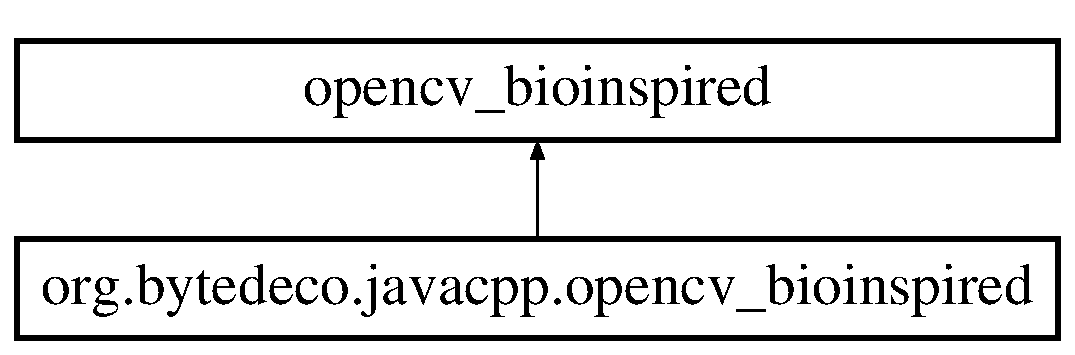
\includegraphics[height=2.000000cm]{classorg_1_1bytedeco_1_1javacpp_1_1opencv__bioinspired}
\end{center}
\end{figure}
\subsection*{Classes}
\begin{DoxyCompactItemize}
\item 
class {\bfseries Retina}
\begin{DoxyCompactList}\small\item\em class which allows the Gipsa/\+Listic Labs model to be used with Open\+CV. \end{DoxyCompactList}\item 
class {\bfseries Retina\+Fast\+Tone\+Mapping}
\item 
class {\bfseries Retina\+Parameters}
\begin{DoxyCompactList}\small\item\em retina model parameters structure \end{DoxyCompactList}\item 
class {\bfseries Segmentation\+Parameters}
\item 
class {\bfseries Transient\+Areas\+Segmentation\+Module}
\begin{DoxyCompactList}\small\item\em class which provides a transient/moving areas segmentation module \end{DoxyCompactList}\end{DoxyCompactItemize}
\subsection*{Static Public Attributes}
\begin{DoxyCompactItemize}
\item 
static final int \hyperlink{group__bioinspired_ga05a86ff7b93be7a4fe366bddc1b71e83}{R\+E\+T\+I\+N\+A\+\_\+\+C\+O\+L\+O\+R\+\_\+\+R\+A\+N\+D\+OM} = 0
\end{DoxyCompactItemize}
\subsection*{Related Functions}
(Note that these are not member functions.) \begin{DoxyCompactItemize}
\item 
static native Retina\+Fast\+Tone\+Mapping \hyperlink{group__bioinspired_ga8193701044bddfabf0e07b3e3a3a7f4c}{create\+Retina\+Fast\+Tone\+Mapping} (@By\+Val Size input\+Size)
\item 
static native Transient\+Areas\+Segmentation\+Module \hyperlink{group__bioinspired_gac278083089d25770df4077c91d0846a0}{create\+Transient\+Areas\+Segmentation\+Module} (@By\+Val Size input\+Size)
\begin{DoxyCompactList}\small\item\em allocator \end{DoxyCompactList}\end{DoxyCompactItemize}
\textbf{ }\par
\begin{DoxyCompactItemize}
\item 
static native Retina \hyperlink{group__bioinspired_gad50e4058a5005de5c1c5bdb255b02702}{create\+Retina} (@By\+Val Size input\+Size)
\item 
static native Retina \hyperlink{group__bioinspired_ga050dd55b35ef6df434cb1ce7a98b7954}{create\+Retina} (@By\+Val Size input\+Size, @Cast(\char`\"{}const bool\char`\"{}) boolean color\+Mode, int color\+Sampling\+Method, @Cast(\char`\"{}const bool\char`\"{}) boolean use\+Retina\+Log\+Sampling, float reduction\+Factor, float sampling\+Strenght)
\begin{DoxyCompactList}\small\item\em Constructors from standardized interfaces \+: retreive a smart pointer to a Retina instance. \end{DoxyCompactList}\item 
static native Retina {\bfseries create\+Retina} (@By\+Val Size input\+Size, @Cast(\char`\"{}const bool\char`\"{}) boolean color\+Mode)
\end{DoxyCompactItemize}



The documentation for this class was generated from the following file\+:\begin{DoxyCompactItemize}
\item 
\hyperlink{opencv__bioinspired_8java}{opencv\+\_\+bioinspired.\+java}\end{DoxyCompactItemize}

\hypertarget{classorg_1_1bytedeco_1_1javacpp_1_1opencv__calib3d}{}\section{org.\+bytedeco.\+javacpp.\+opencv\+\_\+calib3d Class Reference}
\label{classorg_1_1bytedeco_1_1javacpp_1_1opencv__calib3d}\index{org.\+bytedeco.\+javacpp.\+opencv\+\_\+calib3d@{org.\+bytedeco.\+javacpp.\+opencv\+\_\+calib3d}}
Inheritance diagram for org.\+bytedeco.\+javacpp.\+opencv\+\_\+calib3d\+:\begin{figure}[H]
\begin{center}
\leavevmode
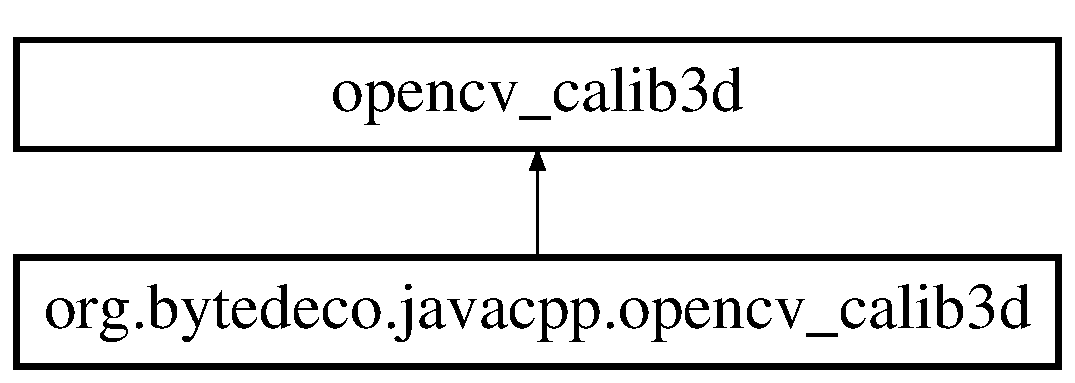
\includegraphics[height=2.000000cm]{classorg_1_1bytedeco_1_1javacpp_1_1opencv__calib3d}
\end{center}
\end{figure}
\subsection*{Classes}
\begin{DoxyCompactItemize}
\item 
class {\bfseries Cv\+Lev\+Marq}
\item 
class {\bfseries Cv\+P\+O\+S\+I\+T\+Object}
\item 
class {\bfseries Cv\+Stereo\+B\+M\+State}
\item 
class {\bfseries Stereo\+BM}
\begin{DoxyCompactList}\small\item\em Class for computing stereo correspondence using the block matching algorithm, introduced and contributed to Open\+CV by K. Konolige. \end{DoxyCompactList}\item 
class {\bfseries Stereo\+Matcher}
\begin{DoxyCompactList}\small\item\em The base class for stereo correspondence algorithms. \end{DoxyCompactList}\item 
class {\bfseries Stereo\+S\+G\+BM}
\begin{DoxyCompactList}\small\item\em The class implements the modified H. Hirschmuller algorithm {\bfseries [H\+H08]} that differs from the original one as follows\+: \end{DoxyCompactList}\end{DoxyCompactItemize}
\subsection*{Static Public Member Functions}
\begin{DoxyCompactItemize}
\item 
static native Cv\+P\+O\+S\+I\+T\+Object {\bfseries cv\+Create\+P\+O\+S\+I\+T\+Object} (Cv\+Point3\+D32f points, int point\+\_\+count)
\item 
static native Cv\+P\+O\+S\+I\+T\+Object {\bfseries cv\+Create\+P\+O\+S\+I\+T\+Object} ( @Cast(\char`\"{}Cv\+Point3\+D32f$\ast$\char`\"{}) Float\+Buffer points, int point\+\_\+count)
\item 
static native Cv\+P\+O\+S\+I\+T\+Object {\bfseries cv\+Create\+P\+O\+S\+I\+T\+Object} ( @Cast(\char`\"{}Cv\+Point3\+D32f$\ast$\char`\"{}) float\mbox{[}$\,$\mbox{]} points, int point\+\_\+count)
\item 
static native void {\bfseries cv\+P\+O\+S\+IT} (Cv\+P\+O\+S\+I\+T\+Object posit\+\_\+object, Cv\+Point2\+D32f image\+\_\+points, double focal\+\_\+length, @By\+Val Cv\+Term\+Criteria criteria, Float\+Pointer rotation\+\_\+matrix, Float\+Pointer translation\+\_\+vector)
\item 
static native void {\bfseries cv\+P\+O\+S\+IT} (Cv\+P\+O\+S\+I\+T\+Object posit\+\_\+object, @Cast(\char`\"{}Cv\+Point2\+D32f$\ast$\char`\"{}) Float\+Buffer image\+\_\+points, double focal\+\_\+length, @By\+Val Cv\+Term\+Criteria criteria, Float\+Buffer rotation\+\_\+matrix, Float\+Buffer translation\+\_\+vector)
\item 
static native void {\bfseries cv\+P\+O\+S\+IT} (Cv\+P\+O\+S\+I\+T\+Object posit\+\_\+object, @Cast(\char`\"{}Cv\+Point2\+D32f$\ast$\char`\"{}) float\mbox{[}$\,$\mbox{]} image\+\_\+points, double focal\+\_\+length, @By\+Val Cv\+Term\+Criteria criteria, float\mbox{[}$\,$\mbox{]} rotation\+\_\+matrix, float\mbox{[}$\,$\mbox{]} translation\+\_\+vector)
\item 
static native void {\bfseries cv\+Release\+P\+O\+S\+I\+T\+Object} ( @Cast(\char`\"{}Cv\+P\+O\+S\+I\+T\+Object$\ast$$\ast$\char`\"{}) Pointer\+Pointer posit\+\_\+object)
\item 
static native void {\bfseries cv\+Release\+P\+O\+S\+I\+T\+Object} ( @By\+Ptr\+Ptr Cv\+P\+O\+S\+I\+T\+Object posit\+\_\+object)
\item 
static native int {\bfseries cv\+R\+A\+N\+S\+A\+C\+Update\+Num\+Iters} (double p, double err\+\_\+prob, int model\+\_\+points, int max\+\_\+iters)
\item 
static native void {\bfseries cv\+Convert\+Points\+Homogeneous} ( @Const Cv\+Mat src, Cv\+Mat dst)
\item 
static native int {\bfseries cv\+Find\+Fundamental\+Mat} ( @Const Cv\+Mat points1, @Const Cv\+Mat points2, Cv\+Mat fundamental\+\_\+matrix, int method, double param1, double param2, Cv\+Mat status)
\item 
static native int {\bfseries cv\+Find\+Fundamental\+Mat} ( @Const Cv\+Mat points1, @Const Cv\+Mat points2, Cv\+Mat fundamental\+\_\+matrix)
\item 
static native void {\bfseries cv\+Compute\+Correspond\+Epilines} ( @Const Cv\+Mat points, int which\+\_\+image, @Const Cv\+Mat fundamental\+\_\+matrix, Cv\+Mat correspondent\+\_\+lines)
\item 
static native void {\bfseries cv\+Triangulate\+Points} (Cv\+Mat proj\+Matr1, Cv\+Mat proj\+Matr2, Cv\+Mat proj\+Points1, Cv\+Mat proj\+Points2, Cv\+Mat points4D)
\item 
static native void {\bfseries cv\+Correct\+Matches} (Cv\+Mat F, Cv\+Mat points1, Cv\+Mat points2, Cv\+Mat new\+\_\+points1, Cv\+Mat new\+\_\+points2)
\item 
static native void {\bfseries cv\+Get\+Optimal\+New\+Camera\+Matrix} ( @Const Cv\+Mat camera\+\_\+matrix, @Const Cv\+Mat dist\+\_\+coeffs, @By\+Val Cv\+Size image\+\_\+size, double alpha, Cv\+Mat new\+\_\+camera\+\_\+matrix, @By\+Val(null\+Value=\char`\"{}Cv\+Size(cv\+Size(0,0))\char`\"{}) Cv\+Size new\+\_\+imag\+\_\+size, Cv\+Rect valid\+\_\+pixel\+\_\+\+R\+OI, int center\+\_\+principal\+\_\+point)
\item 
static native void {\bfseries cv\+Get\+Optimal\+New\+Camera\+Matrix} ( @Const Cv\+Mat camera\+\_\+matrix, @Const Cv\+Mat dist\+\_\+coeffs, @By\+Val Cv\+Size image\+\_\+size, double alpha, Cv\+Mat new\+\_\+camera\+\_\+matrix)
\item 
static native int {\bfseries cv\+Rodrigues2} ( @Const Cv\+Mat src, Cv\+Mat dst, Cv\+Mat jacobian)
\item 
static native int {\bfseries cv\+Rodrigues2} ( @Const Cv\+Mat src, Cv\+Mat dst)
\item 
static native int {\bfseries cv\+Find\+Homography} ( @Const Cv\+Mat src\+\_\+points, @Const Cv\+Mat dst\+\_\+points, Cv\+Mat homography, int method, double ransac\+Reproj\+Threshold, Cv\+Mat mask, int max\+Iters, double confidence)
\item 
static native int {\bfseries cv\+Find\+Homography} ( @Const Cv\+Mat src\+\_\+points, @Const Cv\+Mat dst\+\_\+points, Cv\+Mat homography)
\item 
static native void {\bfseries cv\+R\+Q\+Decomp3x3} ( @Const Cv\+Mat matrixM, Cv\+Mat matrixR, Cv\+Mat matrixQ, Cv\+Mat matrix\+Qx, Cv\+Mat matrix\+Qy, Cv\+Mat matrix\+Qz, Cv\+Point3\+D64f euler\+Angles)
\item 
static native void {\bfseries cv\+R\+Q\+Decomp3x3} ( @Const Cv\+Mat matrixM, Cv\+Mat matrixR, Cv\+Mat matrixQ)
\item 
static native void {\bfseries cv\+R\+Q\+Decomp3x3} ( @Const Cv\+Mat matrixM, Cv\+Mat matrixR, Cv\+Mat matrixQ, Cv\+Mat matrix\+Qx, Cv\+Mat matrix\+Qy, Cv\+Mat matrix\+Qz, @Cast(\char`\"{}Cv\+Point3\+D64f$\ast$\char`\"{}) Double\+Buffer euler\+Angles)
\item 
static native void {\bfseries cv\+R\+Q\+Decomp3x3} ( @Const Cv\+Mat matrixM, Cv\+Mat matrixR, Cv\+Mat matrixQ, Cv\+Mat matrix\+Qx, Cv\+Mat matrix\+Qy, Cv\+Mat matrix\+Qz, @Cast(\char`\"{}Cv\+Point3\+D64f$\ast$\char`\"{}) double\mbox{[}$\,$\mbox{]} euler\+Angles)
\item 
static native void {\bfseries cv\+Decompose\+Projection\+Matrix} ( @Const Cv\+Mat proj\+Matr, Cv\+Mat calib\+Matr, Cv\+Mat rot\+Matr, Cv\+Mat pos\+Vect, Cv\+Mat rot\+MatrX, Cv\+Mat rot\+MatrY, Cv\+Mat rot\+MatrZ, Cv\+Point3\+D64f euler\+Angles)
\item 
static native void {\bfseries cv\+Decompose\+Projection\+Matrix} ( @Const Cv\+Mat proj\+Matr, Cv\+Mat calib\+Matr, Cv\+Mat rot\+Matr, Cv\+Mat pos\+Vect)
\item 
static native void {\bfseries cv\+Decompose\+Projection\+Matrix} ( @Const Cv\+Mat proj\+Matr, Cv\+Mat calib\+Matr, Cv\+Mat rot\+Matr, Cv\+Mat pos\+Vect, Cv\+Mat rot\+MatrX, Cv\+Mat rot\+MatrY, Cv\+Mat rot\+MatrZ, @Cast(\char`\"{}Cv\+Point3\+D64f$\ast$\char`\"{}) Double\+Buffer euler\+Angles)
\item 
static native void {\bfseries cv\+Decompose\+Projection\+Matrix} ( @Const Cv\+Mat proj\+Matr, Cv\+Mat calib\+Matr, Cv\+Mat rot\+Matr, Cv\+Mat pos\+Vect, Cv\+Mat rot\+MatrX, Cv\+Mat rot\+MatrY, Cv\+Mat rot\+MatrZ, @Cast(\char`\"{}Cv\+Point3\+D64f$\ast$\char`\"{}) double\mbox{[}$\,$\mbox{]} euler\+Angles)
\item 
static native void {\bfseries cv\+Calc\+Mat\+Mul\+Deriv} ( @Const Cv\+Mat A, @Const Cv\+Mat B, Cv\+Mat d\+A\+BdA, Cv\+Mat d\+A\+BdB)
\item 
static native void {\bfseries cv\+Compose\+RT} ( @Const Cv\+Mat \+\_\+rvec1, @Const Cv\+Mat \+\_\+tvec1, @Const Cv\+Mat \+\_\+rvec2, @Const Cv\+Mat \+\_\+tvec2, Cv\+Mat \+\_\+rvec3, Cv\+Mat \+\_\+tvec3, Cv\+Mat dr3dr1, Cv\+Mat dr3dt1, Cv\+Mat dr3dr2, Cv\+Mat dr3dt2, Cv\+Mat dt3dr1, Cv\+Mat dt3dt1, Cv\+Mat dt3dr2, Cv\+Mat dt3dt2)
\item 
static native void {\bfseries cv\+Compose\+RT} ( @Const Cv\+Mat \+\_\+rvec1, @Const Cv\+Mat \+\_\+tvec1, @Const Cv\+Mat \+\_\+rvec2, @Const Cv\+Mat \+\_\+tvec2, Cv\+Mat \+\_\+rvec3, Cv\+Mat \+\_\+tvec3)
\item 
static native void {\bfseries cv\+Project\+Points2} ( @Const Cv\+Mat object\+\_\+points, @Const Cv\+Mat rotation\+\_\+vector, @Const Cv\+Mat translation\+\_\+vector, @Const Cv\+Mat camera\+\_\+matrix, @Const Cv\+Mat distortion\+\_\+coeffs, Cv\+Mat image\+\_\+points, Cv\+Mat dpdrot, Cv\+Mat dpdt, Cv\+Mat dpdf, Cv\+Mat dpdc, Cv\+Mat dpddist, double aspect\+\_\+ratio)
\item 
static native void {\bfseries cv\+Project\+Points2} ( @Const Cv\+Mat object\+\_\+points, @Const Cv\+Mat rotation\+\_\+vector, @Const Cv\+Mat translation\+\_\+vector, @Const Cv\+Mat camera\+\_\+matrix, @Const Cv\+Mat distortion\+\_\+coeffs, Cv\+Mat image\+\_\+points)
\item 
static native void {\bfseries cv\+Find\+Extrinsic\+Camera\+Params2} ( @Const Cv\+Mat object\+\_\+points, @Const Cv\+Mat image\+\_\+points, @Const Cv\+Mat camera\+\_\+matrix, @Const Cv\+Mat distortion\+\_\+coeffs, Cv\+Mat rotation\+\_\+vector, Cv\+Mat translation\+\_\+vector, int use\+\_\+extrinsic\+\_\+guess)
\item 
static native void {\bfseries cv\+Find\+Extrinsic\+Camera\+Params2} ( @Const Cv\+Mat object\+\_\+points, @Const Cv\+Mat image\+\_\+points, @Const Cv\+Mat camera\+\_\+matrix, @Const Cv\+Mat distortion\+\_\+coeffs, Cv\+Mat rotation\+\_\+vector, Cv\+Mat translation\+\_\+vector)
\item 
static native void {\bfseries cv\+Init\+Intrinsic\+Params2D} ( @Const Cv\+Mat object\+\_\+points, @Const Cv\+Mat image\+\_\+points, @Const Cv\+Mat npoints, @By\+Val Cv\+Size image\+\_\+size, Cv\+Mat camera\+\_\+matrix, double aspect\+\_\+ratio)
\item 
static native void {\bfseries cv\+Init\+Intrinsic\+Params2D} ( @Const Cv\+Mat object\+\_\+points, @Const Cv\+Mat image\+\_\+points, @Const Cv\+Mat npoints, @By\+Val Cv\+Size image\+\_\+size, Cv\+Mat camera\+\_\+matrix)
\item 
static native int {\bfseries cv\+Check\+Chessboard} (Ipl\+Image src, @By\+Val Cv\+Size size)
\item 
static native int {\bfseries cv\+Find\+Chessboard\+Corners} ( @Const Pointer image, @By\+Val Cv\+Size pattern\+\_\+size, Cv\+Point2\+D32f corners, Int\+Pointer corner\+\_\+count, int flags)
\item 
static native int {\bfseries cv\+Find\+Chessboard\+Corners} ( @Const Pointer image, @By\+Val Cv\+Size pattern\+\_\+size, Cv\+Point2\+D32f corners)
\item 
static native int {\bfseries cv\+Find\+Chessboard\+Corners} ( @Const Pointer image, @By\+Val Cv\+Size pattern\+\_\+size, @Cast(\char`\"{}Cv\+Point2\+D32f$\ast$\char`\"{}) Float\+Buffer corners, Int\+Buffer corner\+\_\+count, int flags)
\item 
static native int {\bfseries cv\+Find\+Chessboard\+Corners} ( @Const Pointer image, @By\+Val Cv\+Size pattern\+\_\+size, @Cast(\char`\"{}Cv\+Point2\+D32f$\ast$\char`\"{}) Float\+Buffer corners)
\item 
static native int {\bfseries cv\+Find\+Chessboard\+Corners} ( @Const Pointer image, @By\+Val Cv\+Size pattern\+\_\+size, @Cast(\char`\"{}Cv\+Point2\+D32f$\ast$\char`\"{}) float\mbox{[}$\,$\mbox{]} corners, int\mbox{[}$\,$\mbox{]} corner\+\_\+count, int flags)
\item 
static native int {\bfseries cv\+Find\+Chessboard\+Corners} ( @Const Pointer image, @By\+Val Cv\+Size pattern\+\_\+size, @Cast(\char`\"{}Cv\+Point2\+D32f$\ast$\char`\"{}) float\mbox{[}$\,$\mbox{]} corners)
\item 
static native void {\bfseries cv\+Draw\+Chessboard\+Corners} (Cv\+Arr image, @By\+Val Cv\+Size pattern\+\_\+size, Cv\+Point2\+D32f corners, int count, int pattern\+\_\+was\+\_\+found)
\item 
static native void {\bfseries cv\+Draw\+Chessboard\+Corners} (Cv\+Arr image, @By\+Val Cv\+Size pattern\+\_\+size, @Cast(\char`\"{}Cv\+Point2\+D32f$\ast$\char`\"{}) Float\+Buffer corners, int count, int pattern\+\_\+was\+\_\+found)
\item 
static native void {\bfseries cv\+Draw\+Chessboard\+Corners} (Cv\+Arr image, @By\+Val Cv\+Size pattern\+\_\+size, @Cast(\char`\"{}Cv\+Point2\+D32f$\ast$\char`\"{}) float\mbox{[}$\,$\mbox{]} corners, int count, int pattern\+\_\+was\+\_\+found)
\item 
static native double {\bfseries cv\+Calibrate\+Camera2} ( @Const Cv\+Mat object\+\_\+points, @Const Cv\+Mat image\+\_\+points, @Const Cv\+Mat point\+\_\+counts, @By\+Val Cv\+Size image\+\_\+size, Cv\+Mat camera\+\_\+matrix, Cv\+Mat distortion\+\_\+coeffs, Cv\+Mat rotation\+\_\+vectors, Cv\+Mat translation\+\_\+vectors, int flags, @By\+Val(null\+Value=\char`\"{}Cv\+Term\+Criteria(cv\+Term\+Criteria(\char`\"{}+\char`\"{}C\+V\+\_\+\+T\+E\+R\+M\+C\+R\+I\+T\+\_\+\+I\+T\+ER+C\+V\+\_\+\+T\+E\+R\+M\+C\+R\+I\+T\+\_\+\+E\+PS,30,D\+B\+L\+\_\+\+E\+P\+S\+I\+L\+ON))\char`\"{}) Cv\+Term\+Criteria term\+\_\+crit)
\item 
static native double {\bfseries cv\+Calibrate\+Camera2} ( @Const Cv\+Mat object\+\_\+points, @Const Cv\+Mat image\+\_\+points, @Const Cv\+Mat point\+\_\+counts, @By\+Val Cv\+Size image\+\_\+size, Cv\+Mat camera\+\_\+matrix, Cv\+Mat distortion\+\_\+coeffs)
\item 
static native void {\bfseries cv\+Calibration\+Matrix\+Values} ( @Const Cv\+Mat camera\+\_\+matrix, @By\+Val Cv\+Size image\+\_\+size, double aperture\+\_\+width, double aperture\+\_\+height, Double\+Pointer fovx, Double\+Pointer fovy, Double\+Pointer focal\+\_\+length, Cv\+Point2\+D64f principal\+\_\+point, Double\+Pointer pixel\+\_\+aspect\+\_\+ratio)
\item 
static native void {\bfseries cv\+Calibration\+Matrix\+Values} ( @Const Cv\+Mat camera\+\_\+matrix, @By\+Val Cv\+Size image\+\_\+size)
\item 
static native void {\bfseries cv\+Calibration\+Matrix\+Values} ( @Const Cv\+Mat camera\+\_\+matrix, @By\+Val Cv\+Size image\+\_\+size, double aperture\+\_\+width, double aperture\+\_\+height, Double\+Buffer fovx, Double\+Buffer fovy, Double\+Buffer focal\+\_\+length, @Cast(\char`\"{}Cv\+Point2\+D64f$\ast$\char`\"{}) Double\+Buffer principal\+\_\+point, Double\+Buffer pixel\+\_\+aspect\+\_\+ratio)
\item 
static native void {\bfseries cv\+Calibration\+Matrix\+Values} ( @Const Cv\+Mat camera\+\_\+matrix, @By\+Val Cv\+Size image\+\_\+size, double aperture\+\_\+width, double aperture\+\_\+height, double\mbox{[}$\,$\mbox{]} fovx, double\mbox{[}$\,$\mbox{]} fovy, double\mbox{[}$\,$\mbox{]} focal\+\_\+length, @Cast(\char`\"{}Cv\+Point2\+D64f$\ast$\char`\"{}) double\mbox{[}$\,$\mbox{]} principal\+\_\+point, double\mbox{[}$\,$\mbox{]} pixel\+\_\+aspect\+\_\+ratio)
\item 
static native double {\bfseries cv\+Stereo\+Calibrate} ( @Const Cv\+Mat object\+\_\+points, @Const Cv\+Mat image\+\_\+points1, @Const Cv\+Mat image\+\_\+points2, @Const Cv\+Mat npoints, Cv\+Mat camera\+\_\+matrix1, Cv\+Mat dist\+\_\+coeffs1, Cv\+Mat camera\+\_\+matrix2, Cv\+Mat dist\+\_\+coeffs2, @By\+Val Cv\+Size image\+\_\+size, Cv\+Mat R, Cv\+Mat T, Cv\+Mat E, Cv\+Mat F, int flags, @By\+Val(null\+Value=\char`\"{}Cv\+Term\+Criteria(cv\+Term\+Criteria(\char`\"{}+\char`\"{}C\+V\+\_\+\+T\+E\+R\+M\+C\+R\+I\+T\+\_\+\+I\+T\+ER+C\+V\+\_\+\+T\+E\+R\+M\+C\+R\+I\+T\+\_\+\+E\+PS,30,1e-\/6))\char`\"{}) Cv\+Term\+Criteria term\+\_\+crit)
\item 
static native double {\bfseries cv\+Stereo\+Calibrate} ( @Const Cv\+Mat object\+\_\+points, @Const Cv\+Mat image\+\_\+points1, @Const Cv\+Mat image\+\_\+points2, @Const Cv\+Mat npoints, Cv\+Mat camera\+\_\+matrix1, Cv\+Mat dist\+\_\+coeffs1, Cv\+Mat camera\+\_\+matrix2, Cv\+Mat dist\+\_\+coeffs2, @By\+Val Cv\+Size image\+\_\+size, Cv\+Mat R, Cv\+Mat T)
\item 
static native void {\bfseries cv\+Stereo\+Rectify} ( @Const Cv\+Mat camera\+\_\+matrix1, @Const Cv\+Mat camera\+\_\+matrix2, @Const Cv\+Mat dist\+\_\+coeffs1, @Const Cv\+Mat dist\+\_\+coeffs2, @By\+Val Cv\+Size image\+\_\+size, @Const Cv\+Mat R, @Const Cv\+Mat T, Cv\+Mat R1, Cv\+Mat R2, Cv\+Mat P1, Cv\+Mat P2, Cv\+Mat Q, int flags, double alpha, @By\+Val(null\+Value=\char`\"{}Cv\+Size(cv\+Size(0,0))\char`\"{}) Cv\+Size new\+\_\+image\+\_\+size, Cv\+Rect valid\+\_\+pix\+\_\+\+R\+O\+I1, Cv\+Rect valid\+\_\+pix\+\_\+\+R\+O\+I2)
\item 
static native void {\bfseries cv\+Stereo\+Rectify} ( @Const Cv\+Mat camera\+\_\+matrix1, @Const Cv\+Mat camera\+\_\+matrix2, @Const Cv\+Mat dist\+\_\+coeffs1, @Const Cv\+Mat dist\+\_\+coeffs2, @By\+Val Cv\+Size image\+\_\+size, @Const Cv\+Mat R, @Const Cv\+Mat T, Cv\+Mat R1, Cv\+Mat R2, Cv\+Mat P1, Cv\+Mat P2)
\item 
static native int {\bfseries cv\+Stereo\+Rectify\+Uncalibrated} ( @Const Cv\+Mat points1, @Const Cv\+Mat points2, @Const Cv\+Mat F, @By\+Val Cv\+Size img\+\_\+size, Cv\+Mat H1, Cv\+Mat H2, double threshold)
\item 
static native int {\bfseries cv\+Stereo\+Rectify\+Uncalibrated} ( @Const Cv\+Mat points1, @Const Cv\+Mat points2, @Const Cv\+Mat F, @By\+Val Cv\+Size img\+\_\+size, Cv\+Mat H1, Cv\+Mat H2)
\item 
static native Cv\+Stereo\+B\+M\+State {\bfseries cv\+Create\+Stereo\+B\+M\+State} (int preset, int number\+Of\+Disparities)
\item 
static native Cv\+Stereo\+B\+M\+State {\bfseries cv\+Create\+Stereo\+B\+M\+State} ()
\item 
static native void {\bfseries cv\+Release\+Stereo\+B\+M\+State} ( @Cast(\char`\"{}Cv\+Stereo\+B\+M\+State$\ast$$\ast$\char`\"{}) Pointer\+Pointer state)
\item 
static native void {\bfseries cv\+Release\+Stereo\+B\+M\+State} ( @By\+Ptr\+Ptr Cv\+Stereo\+B\+M\+State state)
\item 
static native void {\bfseries cv\+Find\+Stereo\+Correspondence\+BM} ( @Const Cv\+Arr left, @Const Cv\+Arr right, Cv\+Arr disparity, Cv\+Stereo\+B\+M\+State state)
\item 
static native Cv\+Rect {\bfseries cv\+Get\+Valid\+Disparity\+R\+OI} ( @By\+Val Cv\+Rect roi1, @By\+Val Cv\+Rect roi2, int min\+Disparity, int number\+Of\+Disparities, int S\+A\+D\+Window\+Size)
\item 
static native void {\bfseries cv\+Validate\+Disparity} (Cv\+Arr disparity, @Const Cv\+Arr cost, int min\+Disparity, int number\+Of\+Disparities, int disp12\+Max\+Diff)
\item 
static native void {\bfseries cv\+Validate\+Disparity} (Cv\+Arr disparity, @Const Cv\+Arr cost, int min\+Disparity, int number\+Of\+Disparities)
\item 
static native void {\bfseries cv\+Reproject\+Image\+To3D} ( @Const Cv\+Arr disparity\+Image, Cv\+Arr \+\_\+3d\+Image, @Const Cv\+Mat Q, int handle\+Missing\+Values)
\item 
static native void {\bfseries cv\+Reproject\+Image\+To3D} ( @Const Cv\+Arr disparity\+Image, Cv\+Arr \+\_\+3d\+Image, @Const Cv\+Mat Q)
\item 
static native void \hyperlink{group__calib3d_ga20092873ec8f2850a2df8acb2648de68}{Rodrigues} ( @By\+Val Mat src, @By\+Val Mat dst, @By\+Val(null\+Value=\char`\"{}cv\+::\+Output\+Array(cv\+::no\+Array())\char`\"{}) Mat jacobian)
\begin{DoxyCompactList}\small\item\em Converts a rotation matrix to a rotation vector or vice versa. \end{DoxyCompactList}\item 
static native void {\bfseries Rodrigues} ( @By\+Val Mat src, @By\+Val Mat dst)
\item 
static native void {\bfseries Rodrigues} ( @By\+Val U\+Mat src, @By\+Val U\+Mat dst, @By\+Val(null\+Value=\char`\"{}cv\+::\+Output\+Array(cv\+::no\+Array())\char`\"{}) U\+Mat jacobian)
\item 
static native void {\bfseries Rodrigues} ( @By\+Val U\+Mat src, @By\+Val U\+Mat dst)
\item 
static native Mat \hyperlink{group__calib3d_ga2e20e41b600c13c08d376e5df367f480}{find\+Homography} ( @By\+Val Mat src\+Points, @By\+Val Mat dst\+Points, int method, double ransac\+Reproj\+Threshold, @By\+Val(null\+Value=\char`\"{}cv\+::\+Output\+Array(cv\+::no\+Array())\char`\"{}) Mat mask, int max\+Iters, double confidence)
\begin{DoxyCompactList}\small\item\em Finds a perspective transformation between two planes. \end{DoxyCompactList}\item 
static native Mat {\bfseries find\+Homography} ( @By\+Val Mat src\+Points, @By\+Val Mat dst\+Points)
\item 
static native Mat {\bfseries find\+Homography} ( @By\+Val U\+Mat src\+Points, @By\+Val U\+Mat dst\+Points, int method, double ransac\+Reproj\+Threshold, @By\+Val(null\+Value=\char`\"{}cv\+::\+Output\+Array(cv\+::no\+Array())\char`\"{}) U\+Mat mask, int max\+Iters, double confidence)
\item 
static native Mat {\bfseries find\+Homography} ( @By\+Val U\+Mat src\+Points, @By\+Val U\+Mat dst\+Points)
\item 
static native Mat \hyperlink{group__calib3d_ga7460fd1ec11b17261dc7b2208a1f2d9f}{find\+Homography} ( @By\+Val Mat src\+Points, @By\+Val Mat dst\+Points, @By\+Val Mat mask, int method, double ransac\+Reproj\+Threshold)
\item 
static native Mat {\bfseries find\+Homography} ( @By\+Val Mat src\+Points, @By\+Val Mat dst\+Points, @By\+Val Mat mask)
\item 
static native Mat {\bfseries find\+Homography} ( @By\+Val U\+Mat src\+Points, @By\+Val U\+Mat dst\+Points, @By\+Val U\+Mat mask, int method, double ransac\+Reproj\+Threshold)
\item 
static native Mat {\bfseries find\+Homography} ( @By\+Val U\+Mat src\+Points, @By\+Val U\+Mat dst\+Points, @By\+Val U\+Mat mask)
\item 
static native Point3d \hyperlink{group__calib3d_ga34838b4072f5a8e1eb0dc619c7ac8261}{R\+Q\+Decomp3x3} ( @By\+Val Mat src, @By\+Val Mat mtxR, @By\+Val Mat mtxQ, @By\+Val(null\+Value=\char`\"{}cv\+::\+Output\+Array(cv\+::no\+Array())\char`\"{}) Mat Qx, @By\+Val(null\+Value=\char`\"{}cv\+::\+Output\+Array(cv\+::no\+Array())\char`\"{}) Mat Qy, @By\+Val(null\+Value=\char`\"{}cv\+::\+Output\+Array(cv\+::no\+Array())\char`\"{}) Mat Qz)
\begin{DoxyCompactList}\small\item\em Computes an RQ decomposition of 3x3 matrices. \end{DoxyCompactList}\item 
static native Point3d {\bfseries R\+Q\+Decomp3x3} ( @By\+Val Mat src, @By\+Val Mat mtxR, @By\+Val Mat mtxQ)
\item 
static native Point3d {\bfseries R\+Q\+Decomp3x3} ( @By\+Val U\+Mat src, @By\+Val U\+Mat mtxR, @By\+Val U\+Mat mtxQ, @By\+Val(null\+Value=\char`\"{}cv\+::\+Output\+Array(cv\+::no\+Array())\char`\"{}) U\+Mat Qx, @By\+Val(null\+Value=\char`\"{}cv\+::\+Output\+Array(cv\+::no\+Array())\char`\"{}) U\+Mat Qy, @By\+Val(null\+Value=\char`\"{}cv\+::\+Output\+Array(cv\+::no\+Array())\char`\"{}) U\+Mat Qz)
\item 
static native Point3d {\bfseries R\+Q\+Decomp3x3} ( @By\+Val U\+Mat src, @By\+Val U\+Mat mtxR, @By\+Val U\+Mat mtxQ)
\item 
static native void \hyperlink{group__calib3d_gadf0e43ed7b680f17d039735e4a9f64c5}{decompose\+Projection\+Matrix} ( @By\+Val Mat proj\+Matrix, @By\+Val Mat camera\+Matrix, @By\+Val Mat rot\+Matrix, @By\+Val Mat trans\+Vect, @By\+Val(null\+Value=\char`\"{}cv\+::\+Output\+Array(cv\+::no\+Array())\char`\"{}) Mat rot\+MatrixX, @By\+Val(null\+Value=\char`\"{}cv\+::\+Output\+Array(cv\+::no\+Array())\char`\"{}) Mat rot\+MatrixY, @By\+Val(null\+Value=\char`\"{}cv\+::\+Output\+Array(cv\+::no\+Array())\char`\"{}) Mat rot\+MatrixZ, @By\+Val(null\+Value=\char`\"{}cv\+::\+Output\+Array(cv\+::no\+Array())\char`\"{}) Mat euler\+Angles)
\begin{DoxyCompactList}\small\item\em Decomposes a projection matrix into a rotation matrix and a camera matrix. \end{DoxyCompactList}\item 
static native void {\bfseries decompose\+Projection\+Matrix} ( @By\+Val Mat proj\+Matrix, @By\+Val Mat camera\+Matrix, @By\+Val Mat rot\+Matrix, @By\+Val Mat trans\+Vect)
\item 
static native void {\bfseries decompose\+Projection\+Matrix} ( @By\+Val U\+Mat proj\+Matrix, @By\+Val U\+Mat camera\+Matrix, @By\+Val U\+Mat rot\+Matrix, @By\+Val U\+Mat trans\+Vect, @By\+Val(null\+Value=\char`\"{}cv\+::\+Output\+Array(cv\+::no\+Array())\char`\"{}) U\+Mat rot\+MatrixX, @By\+Val(null\+Value=\char`\"{}cv\+::\+Output\+Array(cv\+::no\+Array())\char`\"{}) U\+Mat rot\+MatrixY, @By\+Val(null\+Value=\char`\"{}cv\+::\+Output\+Array(cv\+::no\+Array())\char`\"{}) U\+Mat rot\+MatrixZ, @By\+Val(null\+Value=\char`\"{}cv\+::\+Output\+Array(cv\+::no\+Array())\char`\"{}) U\+Mat euler\+Angles)
\item 
static native void {\bfseries decompose\+Projection\+Matrix} ( @By\+Val U\+Mat proj\+Matrix, @By\+Val U\+Mat camera\+Matrix, @By\+Val U\+Mat rot\+Matrix, @By\+Val U\+Mat trans\+Vect)
\item 
static native void \hyperlink{group__calib3d_ga54d99b18b60bd50e50e0de105d68003b}{mat\+Mul\+Deriv} ( @By\+Val Mat A, @By\+Val Mat B, @By\+Val Mat d\+A\+BdA, @By\+Val Mat d\+A\+BdB)
\begin{DoxyCompactList}\small\item\em Computes partial derivatives of the matrix product for each multiplied matrix. \end{DoxyCompactList}\item 
static native void {\bfseries mat\+Mul\+Deriv} ( @By\+Val U\+Mat A, @By\+Val U\+Mat B, @By\+Val U\+Mat d\+A\+BdA, @By\+Val U\+Mat d\+A\+BdB)
\item 
static native void \hyperlink{group__calib3d_ga04fb0a4a5daa37377b0aa4b4ed2d6774}{compose\+RT} ( @By\+Val Mat rvec1, @By\+Val Mat tvec1, @By\+Val Mat rvec2, @By\+Val Mat tvec2, @By\+Val Mat rvec3, @By\+Val Mat tvec3, @By\+Val(null\+Value=\char`\"{}cv\+::\+Output\+Array(cv\+::no\+Array())\char`\"{}) Mat dr3dr1, @By\+Val(null\+Value=\char`\"{}cv\+::\+Output\+Array(cv\+::no\+Array())\char`\"{}) Mat dr3dt1, @By\+Val(null\+Value=\char`\"{}cv\+::\+Output\+Array(cv\+::no\+Array())\char`\"{}) Mat dr3dr2, @By\+Val(null\+Value=\char`\"{}cv\+::\+Output\+Array(cv\+::no\+Array())\char`\"{}) Mat dr3dt2, @By\+Val(null\+Value=\char`\"{}cv\+::\+Output\+Array(cv\+::no\+Array())\char`\"{}) Mat dt3dr1, @By\+Val(null\+Value=\char`\"{}cv\+::\+Output\+Array(cv\+::no\+Array())\char`\"{}) Mat dt3dt1, @By\+Val(null\+Value=\char`\"{}cv\+::\+Output\+Array(cv\+::no\+Array())\char`\"{}) Mat dt3dr2, @By\+Val(null\+Value=\char`\"{}cv\+::\+Output\+Array(cv\+::no\+Array())\char`\"{}) Mat dt3dt2)
\begin{DoxyCompactList}\small\item\em Combines two rotation-\/and-\/shift transformations. \end{DoxyCompactList}\item 
static native void {\bfseries compose\+RT} ( @By\+Val Mat rvec1, @By\+Val Mat tvec1, @By\+Val Mat rvec2, @By\+Val Mat tvec2, @By\+Val Mat rvec3, @By\+Val Mat tvec3)
\item 
static native void {\bfseries compose\+RT} ( @By\+Val U\+Mat rvec1, @By\+Val U\+Mat tvec1, @By\+Val U\+Mat rvec2, @By\+Val U\+Mat tvec2, @By\+Val U\+Mat rvec3, @By\+Val U\+Mat tvec3, @By\+Val(null\+Value=\char`\"{}cv\+::\+Output\+Array(cv\+::no\+Array())\char`\"{}) U\+Mat dr3dr1, @By\+Val(null\+Value=\char`\"{}cv\+::\+Output\+Array(cv\+::no\+Array())\char`\"{}) U\+Mat dr3dt1, @By\+Val(null\+Value=\char`\"{}cv\+::\+Output\+Array(cv\+::no\+Array())\char`\"{}) U\+Mat dr3dr2, @By\+Val(null\+Value=\char`\"{}cv\+::\+Output\+Array(cv\+::no\+Array())\char`\"{}) U\+Mat dr3dt2, @By\+Val(null\+Value=\char`\"{}cv\+::\+Output\+Array(cv\+::no\+Array())\char`\"{}) U\+Mat dt3dr1, @By\+Val(null\+Value=\char`\"{}cv\+::\+Output\+Array(cv\+::no\+Array())\char`\"{}) U\+Mat dt3dt1, @By\+Val(null\+Value=\char`\"{}cv\+::\+Output\+Array(cv\+::no\+Array())\char`\"{}) U\+Mat dt3dr2, @By\+Val(null\+Value=\char`\"{}cv\+::\+Output\+Array(cv\+::no\+Array())\char`\"{}) U\+Mat dt3dt2)
\item 
static native void {\bfseries compose\+RT} ( @By\+Val U\+Mat rvec1, @By\+Val U\+Mat tvec1, @By\+Val U\+Mat rvec2, @By\+Val U\+Mat tvec2, @By\+Val U\+Mat rvec3, @By\+Val U\+Mat tvec3)
\item 
static native void \hyperlink{group__calib3d_gaa19528257b52c058dffc58aba4f6d751}{project\+Points} ( @By\+Val Mat object\+Points, @By\+Val Mat rvec, @By\+Val Mat tvec, @By\+Val Mat camera\+Matrix, @By\+Val Mat dist\+Coeffs, @By\+Val Mat image\+Points, @By\+Val(null\+Value=\char`\"{}cv\+::\+Output\+Array(cv\+::no\+Array())\char`\"{}) Mat jacobian, double aspect\+Ratio)
\begin{DoxyCompactList}\small\item\em Projects 3D points to an image plane. \end{DoxyCompactList}\item 
static native void {\bfseries project\+Points} ( @By\+Val Mat object\+Points, @By\+Val Mat rvec, @By\+Val Mat tvec, @By\+Val Mat camera\+Matrix, @By\+Val Mat dist\+Coeffs, @By\+Val Mat image\+Points)
\item 
static native void {\bfseries project\+Points} ( @By\+Val U\+Mat object\+Points, @By\+Val U\+Mat rvec, @By\+Val U\+Mat tvec, @By\+Val U\+Mat camera\+Matrix, @By\+Val U\+Mat dist\+Coeffs, @By\+Val U\+Mat image\+Points, @By\+Val(null\+Value=\char`\"{}cv\+::\+Output\+Array(cv\+::no\+Array())\char`\"{}) U\+Mat jacobian, double aspect\+Ratio)
\item 
static native void {\bfseries project\+Points} ( @By\+Val U\+Mat object\+Points, @By\+Val U\+Mat rvec, @By\+Val U\+Mat tvec, @By\+Val U\+Mat camera\+Matrix, @By\+Val U\+Mat dist\+Coeffs, @By\+Val U\+Mat image\+Points)
\item 
static native boolean \hyperlink{group__calib3d_ga4ed4dcff68153a9ec5eb087c0ee29913}{solve\+PnP} ( @By\+Val Mat object\+Points, @By\+Val Mat image\+Points, @By\+Val Mat camera\+Matrix, @By\+Val Mat dist\+Coeffs, @By\+Val Mat rvec, @By\+Val Mat tvec, @Cast(\char`\"{}bool\char`\"{}) boolean use\+Extrinsic\+Guess, int flags)
\begin{DoxyCompactList}\small\item\em Finds an object pose from 3\+D-\/2D point correspondences. \end{DoxyCompactList}\item 
static native boolean {\bfseries solve\+PnP} ( @By\+Val Mat object\+Points, @By\+Val Mat image\+Points, @By\+Val Mat camera\+Matrix, @By\+Val Mat dist\+Coeffs, @By\+Val Mat rvec, @By\+Val Mat tvec)
\item 
static native boolean {\bfseries solve\+PnP} ( @By\+Val U\+Mat object\+Points, @By\+Val U\+Mat image\+Points, @By\+Val U\+Mat camera\+Matrix, @By\+Val U\+Mat dist\+Coeffs, @By\+Val U\+Mat rvec, @By\+Val U\+Mat tvec, @Cast(\char`\"{}bool\char`\"{}) boolean use\+Extrinsic\+Guess, int flags)
\item 
static native boolean {\bfseries solve\+PnP} ( @By\+Val U\+Mat object\+Points, @By\+Val U\+Mat image\+Points, @By\+Val U\+Mat camera\+Matrix, @By\+Val U\+Mat dist\+Coeffs, @By\+Val U\+Mat rvec, @By\+Val U\+Mat tvec)
\item 
static native boolean \hyperlink{group__calib3d_ga87d56bc65d398f58897fa9bda35caef7}{solve\+Pn\+P\+Ransac} ( @By\+Val Mat object\+Points, @By\+Val Mat image\+Points, @By\+Val Mat camera\+Matrix, @By\+Val Mat dist\+Coeffs, @By\+Val Mat rvec, @By\+Val Mat tvec, @Cast(\char`\"{}bool\char`\"{}) boolean use\+Extrinsic\+Guess, int iterations\+Count, float reprojection\+Error, double confidence, @By\+Val(null\+Value=\char`\"{}cv\+::\+Output\+Array(cv\+::no\+Array())\char`\"{}) Mat inliers, int flags)
\begin{DoxyCompactList}\small\item\em Finds an object pose from 3\+D-\/2D point correspondences using the R\+A\+N\+S\+AC scheme. \end{DoxyCompactList}\item 
static native boolean {\bfseries solve\+Pn\+P\+Ransac} ( @By\+Val Mat object\+Points, @By\+Val Mat image\+Points, @By\+Val Mat camera\+Matrix, @By\+Val Mat dist\+Coeffs, @By\+Val Mat rvec, @By\+Val Mat tvec)
\item 
static native boolean {\bfseries solve\+Pn\+P\+Ransac} ( @By\+Val U\+Mat object\+Points, @By\+Val U\+Mat image\+Points, @By\+Val U\+Mat camera\+Matrix, @By\+Val U\+Mat dist\+Coeffs, @By\+Val U\+Mat rvec, @By\+Val U\+Mat tvec, @Cast(\char`\"{}bool\char`\"{}) boolean use\+Extrinsic\+Guess, int iterations\+Count, float reprojection\+Error, double confidence, @By\+Val(null\+Value=\char`\"{}cv\+::\+Output\+Array(cv\+::no\+Array())\char`\"{}) U\+Mat inliers, int flags)
\item 
static native boolean {\bfseries solve\+Pn\+P\+Ransac} ( @By\+Val U\+Mat object\+Points, @By\+Val U\+Mat image\+Points, @By\+Val U\+Mat camera\+Matrix, @By\+Val U\+Mat dist\+Coeffs, @By\+Val U\+Mat rvec, @By\+Val U\+Mat tvec)
\item 
static native Mat \hyperlink{group__calib3d_ga783c80e734c8368c9db31e3ad820f7fa}{init\+Camera\+Matrix2D} ( @By\+Val Mat\+Vector object\+Points, @By\+Val Mat\+Vector image\+Points, @By\+Val Size image\+Size, double aspect\+Ratio)
\begin{DoxyCompactList}\small\item\em Finds an initial camera matrix from 3\+D-\/2D point correspondences. \end{DoxyCompactList}\item 
static native Mat {\bfseries init\+Camera\+Matrix2D} ( @By\+Val Mat\+Vector object\+Points, @By\+Val Mat\+Vector image\+Points, @By\+Val Size image\+Size)
\item 
static native Mat {\bfseries init\+Camera\+Matrix2D} ( @By\+Val U\+Mat\+Vector object\+Points, @By\+Val U\+Mat\+Vector image\+Points, @By\+Val Size image\+Size, double aspect\+Ratio)
\item 
static native Mat {\bfseries init\+Camera\+Matrix2D} ( @By\+Val U\+Mat\+Vector object\+Points, @By\+Val U\+Mat\+Vector image\+Points, @By\+Val Size image\+Size)
\item 
static native boolean \hyperlink{group__calib3d_ga8736b25349ec9178b46c38128bd9d95a}{find\+Chessboard\+Corners} ( @By\+Val Mat image, @By\+Val Size pattern\+Size, @By\+Val Mat corners, int flags)
\begin{DoxyCompactList}\small\item\em Finds the positions of internal corners of the chessboard. \end{DoxyCompactList}\item 
static native boolean {\bfseries find\+Chessboard\+Corners} ( @By\+Val Mat image, @By\+Val Size pattern\+Size, @By\+Val Mat corners)
\item 
static native boolean {\bfseries find\+Chessboard\+Corners} ( @By\+Val U\+Mat image, @By\+Val Size pattern\+Size, @By\+Val U\+Mat corners, int flags)
\item 
static native boolean {\bfseries find\+Chessboard\+Corners} ( @By\+Val U\+Mat image, @By\+Val Size pattern\+Size, @By\+Val U\+Mat corners)
\item 
static native boolean \hyperlink{group__calib3d_ga10b6a054de67db7ef3a290871688b660}{find4\+Quad\+Corner\+Subpix} ( @By\+Val Mat img, @By\+Val Mat corners, @By\+Val Size region\+\_\+size)
\item 
static native boolean {\bfseries find4\+Quad\+Corner\+Subpix} ( @By\+Val U\+Mat img, @By\+Val U\+Mat corners, @By\+Val Size region\+\_\+size)
\item 
static native void \hyperlink{group__calib3d_ga71d497eb4a9eead84d1e4522d54ed580}{draw\+Chessboard\+Corners} ( @By\+Val Mat image, @By\+Val Size pattern\+Size, @By\+Val Mat corners, @Cast(\char`\"{}bool\char`\"{}) boolean pattern\+Was\+Found)
\begin{DoxyCompactList}\small\item\em Renders the detected chessboard corners. \end{DoxyCompactList}\item 
static native void {\bfseries draw\+Chessboard\+Corners} ( @By\+Val U\+Mat image, @By\+Val Size pattern\+Size, @By\+Val U\+Mat corners, @Cast(\char`\"{}bool\char`\"{}) boolean pattern\+Was\+Found)
\item 
static native boolean \hyperlink{group__calib3d_ga150470ce16ca1879fd1809729801803b}{find\+Circles\+Grid} ( @By\+Val Mat image, @By\+Val Size pattern\+Size, @By\+Val Mat centers, int flags, @Cast(\char`\"{}cv\+::\+Feature\+Detector$\ast$\char`\"{}) @Ptr Feature2D blob\+Detector)
\begin{DoxyCompactList}\small\item\em Finds centers in the grid of circles. \end{DoxyCompactList}\item 
static native boolean {\bfseries find\+Circles\+Grid} ( @By\+Val Mat image, @By\+Val Size pattern\+Size, @By\+Val Mat centers)
\item 
static native boolean {\bfseries find\+Circles\+Grid} ( @By\+Val U\+Mat image, @By\+Val Size pattern\+Size, @By\+Val U\+Mat centers, int flags, @Cast(\char`\"{}cv\+::\+Feature\+Detector$\ast$\char`\"{}) @Ptr Feature2D blob\+Detector)
\item 
static native boolean {\bfseries find\+Circles\+Grid} ( @By\+Val U\+Mat image, @By\+Val Size pattern\+Size, @By\+Val U\+Mat centers)
\item 
static native double \hyperlink{group__calib3d_ga9829f846450d1022f08716b7c20412d6}{calibrate\+Camera\+Extended} ( @By\+Val Mat\+Vector object\+Points, @By\+Val Mat\+Vector image\+Points, @By\+Val Size image\+Size, @By\+Val Mat camera\+Matrix, @By\+Val Mat dist\+Coeffs, @By\+Val Mat\+Vector rvecs, @By\+Val Mat\+Vector tvecs, @By\+Val Mat std\+Deviations\+Intrinsics, @By\+Val Mat std\+Deviations\+Extrinsics, @By\+Val Mat per\+View\+Errors, int flags, @By\+Val(null\+Value=\char`\"{}cv\+::\+Term\+Criteria(\char`\"{}+\char`\"{}cv\+::\+Term\+Criteria\+::\+C\+O\+U\+NT + cv\+::\+Term\+Criteria\+::\+E\+PS, 30, D\+B\+L\+\_\+\+E\+P\+S\+I\+L\+ON)\char`\"{}) Term\+Criteria criteria)
\begin{DoxyCompactList}\small\item\em Finds the camera intrinsic and extrinsic parameters from several views of a calibration pattern. \end{DoxyCompactList}\item 
static native double {\bfseries calibrate\+Camera\+Extended} ( @By\+Val Mat\+Vector object\+Points, @By\+Val Mat\+Vector image\+Points, @By\+Val Size image\+Size, @By\+Val Mat camera\+Matrix, @By\+Val Mat dist\+Coeffs, @By\+Val Mat\+Vector rvecs, @By\+Val Mat\+Vector tvecs, @By\+Val Mat std\+Deviations\+Intrinsics, @By\+Val Mat std\+Deviations\+Extrinsics, @By\+Val Mat per\+View\+Errors)
\item 
static native double {\bfseries calibrate\+Camera\+Extended} ( @By\+Val U\+Mat\+Vector object\+Points, @By\+Val U\+Mat\+Vector image\+Points, @By\+Val Size image\+Size, @By\+Val Mat camera\+Matrix, @By\+Val Mat dist\+Coeffs, @By\+Val U\+Mat\+Vector rvecs, @By\+Val U\+Mat\+Vector tvecs, @By\+Val Mat std\+Deviations\+Intrinsics, @By\+Val Mat std\+Deviations\+Extrinsics, @By\+Val Mat per\+View\+Errors, int flags, @By\+Val(null\+Value=\char`\"{}cv\+::\+Term\+Criteria(\char`\"{}+\char`\"{}cv\+::\+Term\+Criteria\+::\+C\+O\+U\+NT + cv\+::\+Term\+Criteria\+::\+E\+PS, 30, D\+B\+L\+\_\+\+E\+P\+S\+I\+L\+ON)\char`\"{}) Term\+Criteria criteria)
\item 
static native double {\bfseries calibrate\+Camera\+Extended} ( @By\+Val U\+Mat\+Vector object\+Points, @By\+Val U\+Mat\+Vector image\+Points, @By\+Val Size image\+Size, @By\+Val Mat camera\+Matrix, @By\+Val Mat dist\+Coeffs, @By\+Val U\+Mat\+Vector rvecs, @By\+Val U\+Mat\+Vector tvecs, @By\+Val Mat std\+Deviations\+Intrinsics, @By\+Val Mat std\+Deviations\+Extrinsics, @By\+Val Mat per\+View\+Errors)
\item 
static native double {\bfseries calibrate\+Camera\+Extended} ( @By\+Val Mat\+Vector object\+Points, @By\+Val Mat\+Vector image\+Points, @By\+Val Size image\+Size, @By\+Val U\+Mat camera\+Matrix, @By\+Val U\+Mat dist\+Coeffs, @By\+Val Mat\+Vector rvecs, @By\+Val Mat\+Vector tvecs, @By\+Val U\+Mat std\+Deviations\+Intrinsics, @By\+Val U\+Mat std\+Deviations\+Extrinsics, @By\+Val U\+Mat per\+View\+Errors, int flags, @By\+Val(null\+Value=\char`\"{}cv\+::\+Term\+Criteria(\char`\"{}+\char`\"{}cv\+::\+Term\+Criteria\+::\+C\+O\+U\+NT + cv\+::\+Term\+Criteria\+::\+E\+PS, 30, D\+B\+L\+\_\+\+E\+P\+S\+I\+L\+ON)\char`\"{}) Term\+Criteria criteria)
\item 
static native double {\bfseries calibrate\+Camera\+Extended} ( @By\+Val Mat\+Vector object\+Points, @By\+Val Mat\+Vector image\+Points, @By\+Val Size image\+Size, @By\+Val U\+Mat camera\+Matrix, @By\+Val U\+Mat dist\+Coeffs, @By\+Val Mat\+Vector rvecs, @By\+Val Mat\+Vector tvecs, @By\+Val U\+Mat std\+Deviations\+Intrinsics, @By\+Val U\+Mat std\+Deviations\+Extrinsics, @By\+Val U\+Mat per\+View\+Errors)
\item 
static native double {\bfseries calibrate\+Camera\+Extended} ( @By\+Val U\+Mat\+Vector object\+Points, @By\+Val U\+Mat\+Vector image\+Points, @By\+Val Size image\+Size, @By\+Val U\+Mat camera\+Matrix, @By\+Val U\+Mat dist\+Coeffs, @By\+Val U\+Mat\+Vector rvecs, @By\+Val U\+Mat\+Vector tvecs, @By\+Val U\+Mat std\+Deviations\+Intrinsics, @By\+Val U\+Mat std\+Deviations\+Extrinsics, @By\+Val U\+Mat per\+View\+Errors, int flags, @By\+Val(null\+Value=\char`\"{}cv\+::\+Term\+Criteria(\char`\"{}+\char`\"{}cv\+::\+Term\+Criteria\+::\+C\+O\+U\+NT + cv\+::\+Term\+Criteria\+::\+E\+PS, 30, D\+B\+L\+\_\+\+E\+P\+S\+I\+L\+ON)\char`\"{}) Term\+Criteria criteria)
\item 
static native double {\bfseries calibrate\+Camera\+Extended} ( @By\+Val U\+Mat\+Vector object\+Points, @By\+Val U\+Mat\+Vector image\+Points, @By\+Val Size image\+Size, @By\+Val U\+Mat camera\+Matrix, @By\+Val U\+Mat dist\+Coeffs, @By\+Val U\+Mat\+Vector rvecs, @By\+Val U\+Mat\+Vector tvecs, @By\+Val U\+Mat std\+Deviations\+Intrinsics, @By\+Val U\+Mat std\+Deviations\+Extrinsics, @By\+Val U\+Mat per\+View\+Errors)
\item 
static native double {\bfseries calibrate\+Camera} ( @By\+Val Mat\+Vector object\+Points, @By\+Val Mat\+Vector image\+Points, @By\+Val Size image\+Size, @By\+Val Mat camera\+Matrix, @By\+Val Mat dist\+Coeffs, @By\+Val Mat\+Vector rvecs, @By\+Val Mat\+Vector tvecs, int flags, @By\+Val(null\+Value=\char`\"{}cv\+::\+Term\+Criteria(\char`\"{}+\char`\"{}cv\+::\+Term\+Criteria\+::\+C\+O\+U\+NT + cv\+::\+Term\+Criteria\+::\+E\+PS, 30, D\+B\+L\+\_\+\+E\+P\+S\+I\+L\+ON)\char`\"{}) Term\+Criteria criteria)
\item 
static native double {\bfseries calibrate\+Camera} ( @By\+Val Mat\+Vector object\+Points, @By\+Val Mat\+Vector image\+Points, @By\+Val Size image\+Size, @By\+Val Mat camera\+Matrix, @By\+Val Mat dist\+Coeffs, @By\+Val Mat\+Vector rvecs, @By\+Val Mat\+Vector tvecs)
\item 
static native double {\bfseries calibrate\+Camera} ( @By\+Val U\+Mat\+Vector object\+Points, @By\+Val U\+Mat\+Vector image\+Points, @By\+Val Size image\+Size, @By\+Val Mat camera\+Matrix, @By\+Val Mat dist\+Coeffs, @By\+Val U\+Mat\+Vector rvecs, @By\+Val U\+Mat\+Vector tvecs, int flags, @By\+Val(null\+Value=\char`\"{}cv\+::\+Term\+Criteria(\char`\"{}+\char`\"{}cv\+::\+Term\+Criteria\+::\+C\+O\+U\+NT + cv\+::\+Term\+Criteria\+::\+E\+PS, 30, D\+B\+L\+\_\+\+E\+P\+S\+I\+L\+ON)\char`\"{}) Term\+Criteria criteria)
\item 
static native double {\bfseries calibrate\+Camera} ( @By\+Val U\+Mat\+Vector object\+Points, @By\+Val U\+Mat\+Vector image\+Points, @By\+Val Size image\+Size, @By\+Val Mat camera\+Matrix, @By\+Val Mat dist\+Coeffs, @By\+Val U\+Mat\+Vector rvecs, @By\+Val U\+Mat\+Vector tvecs)
\item 
static native double {\bfseries calibrate\+Camera} ( @By\+Val Mat\+Vector object\+Points, @By\+Val Mat\+Vector image\+Points, @By\+Val Size image\+Size, @By\+Val U\+Mat camera\+Matrix, @By\+Val U\+Mat dist\+Coeffs, @By\+Val Mat\+Vector rvecs, @By\+Val Mat\+Vector tvecs, int flags, @By\+Val(null\+Value=\char`\"{}cv\+::\+Term\+Criteria(\char`\"{}+\char`\"{}cv\+::\+Term\+Criteria\+::\+C\+O\+U\+NT + cv\+::\+Term\+Criteria\+::\+E\+PS, 30, D\+B\+L\+\_\+\+E\+P\+S\+I\+L\+ON)\char`\"{}) Term\+Criteria criteria)
\item 
static native double {\bfseries calibrate\+Camera} ( @By\+Val Mat\+Vector object\+Points, @By\+Val Mat\+Vector image\+Points, @By\+Val Size image\+Size, @By\+Val U\+Mat camera\+Matrix, @By\+Val U\+Mat dist\+Coeffs, @By\+Val Mat\+Vector rvecs, @By\+Val Mat\+Vector tvecs)
\item 
static native double {\bfseries calibrate\+Camera} ( @By\+Val U\+Mat\+Vector object\+Points, @By\+Val U\+Mat\+Vector image\+Points, @By\+Val Size image\+Size, @By\+Val U\+Mat camera\+Matrix, @By\+Val U\+Mat dist\+Coeffs, @By\+Val U\+Mat\+Vector rvecs, @By\+Val U\+Mat\+Vector tvecs, int flags, @By\+Val(null\+Value=\char`\"{}cv\+::\+Term\+Criteria(\char`\"{}+\char`\"{}cv\+::\+Term\+Criteria\+::\+C\+O\+U\+NT + cv\+::\+Term\+Criteria\+::\+E\+PS, 30, D\+B\+L\+\_\+\+E\+P\+S\+I\+L\+ON)\char`\"{}) Term\+Criteria criteria)
\item 
static native double {\bfseries calibrate\+Camera} ( @By\+Val U\+Mat\+Vector object\+Points, @By\+Val U\+Mat\+Vector image\+Points, @By\+Val Size image\+Size, @By\+Val U\+Mat camera\+Matrix, @By\+Val U\+Mat dist\+Coeffs, @By\+Val U\+Mat\+Vector rvecs, @By\+Val U\+Mat\+Vector tvecs)
\item 
static native void \hyperlink{group__calib3d_ga35bea5b10b8dfd23238f72e9a2e2ac27}{calibration\+Matrix\+Values} ( @By\+Val Mat camera\+Matrix, @By\+Val Size image\+Size, double aperture\+Width, double aperture\+Height, @By\+Ref Double\+Pointer fovx, @By\+Ref Double\+Pointer fovy, @By\+Ref Double\+Pointer focal\+Length, @By\+Ref Point2d principal\+Point, @By\+Ref Double\+Pointer aspect\+Ratio)
\begin{DoxyCompactList}\small\item\em Computes useful camera characteristics from the camera matrix. \end{DoxyCompactList}\item 
static native void {\bfseries calibration\+Matrix\+Values} ( @By\+Val Mat camera\+Matrix, @By\+Val Size image\+Size, double aperture\+Width, double aperture\+Height, @By\+Ref Double\+Buffer fovx, @By\+Ref Double\+Buffer fovy, @By\+Ref Double\+Buffer focal\+Length, @By\+Ref Point2d principal\+Point, @By\+Ref Double\+Buffer aspect\+Ratio)
\item 
static native void {\bfseries calibration\+Matrix\+Values} ( @By\+Val U\+Mat camera\+Matrix, @By\+Val Size image\+Size, double aperture\+Width, double aperture\+Height, @By\+Ref double\mbox{[}$\,$\mbox{]} fovx, @By\+Ref double\mbox{[}$\,$\mbox{]} fovy, @By\+Ref double\mbox{[}$\,$\mbox{]} focal\+Length, @By\+Ref Point2d principal\+Point, @By\+Ref double\mbox{[}$\,$\mbox{]} aspect\+Ratio)
\item 
static native void {\bfseries calibration\+Matrix\+Values} ( @By\+Val U\+Mat camera\+Matrix, @By\+Val Size image\+Size, double aperture\+Width, double aperture\+Height, @By\+Ref Double\+Pointer fovx, @By\+Ref Double\+Pointer fovy, @By\+Ref Double\+Pointer focal\+Length, @By\+Ref Point2d principal\+Point, @By\+Ref Double\+Pointer aspect\+Ratio)
\item 
static native double \hyperlink{group__calib3d_gab585e0688b9d7592dfe294c5179bdcae}{stereo\+Calibrate} ( @By\+Val Mat\+Vector object\+Points, @By\+Val Mat\+Vector image\+Points1, @By\+Val Mat\+Vector image\+Points2, @By\+Val Mat camera\+Matrix1, @By\+Val Mat dist\+Coeffs1, @By\+Val Mat camera\+Matrix2, @By\+Val Mat dist\+Coeffs2, @By\+Val Size image\+Size, @By\+Val Mat R, @By\+Val Mat T, @By\+Val Mat E, @By\+Val Mat F, int flags, @By\+Val(null\+Value=\char`\"{}cv\+::\+Term\+Criteria(cv\+::\+Term\+Criteria\+::\+C\+O\+U\+NT+cv\+::\+Term\+Criteria\+::\+E\+PS, 30, 1e-\/6)\char`\"{}) Term\+Criteria criteria)
\begin{DoxyCompactList}\small\item\em Calibrates the stereo camera. \end{DoxyCompactList}\item 
static native double {\bfseries stereo\+Calibrate} ( @By\+Val Mat\+Vector object\+Points, @By\+Val Mat\+Vector image\+Points1, @By\+Val Mat\+Vector image\+Points2, @By\+Val Mat camera\+Matrix1, @By\+Val Mat dist\+Coeffs1, @By\+Val Mat camera\+Matrix2, @By\+Val Mat dist\+Coeffs2, @By\+Val Size image\+Size, @By\+Val Mat R, @By\+Val Mat T, @By\+Val Mat E, @By\+Val Mat F)
\item 
static native double {\bfseries stereo\+Calibrate} ( @By\+Val U\+Mat\+Vector object\+Points, @By\+Val U\+Mat\+Vector image\+Points1, @By\+Val U\+Mat\+Vector image\+Points2, @By\+Val Mat camera\+Matrix1, @By\+Val Mat dist\+Coeffs1, @By\+Val Mat camera\+Matrix2, @By\+Val Mat dist\+Coeffs2, @By\+Val Size image\+Size, @By\+Val Mat R, @By\+Val Mat T, @By\+Val Mat E, @By\+Val Mat F, int flags, @By\+Val(null\+Value=\char`\"{}cv\+::\+Term\+Criteria(cv\+::\+Term\+Criteria\+::\+C\+O\+U\+NT+cv\+::\+Term\+Criteria\+::\+E\+PS, 30, 1e-\/6)\char`\"{}) Term\+Criteria criteria)
\item 
static native double {\bfseries stereo\+Calibrate} ( @By\+Val U\+Mat\+Vector object\+Points, @By\+Val U\+Mat\+Vector image\+Points1, @By\+Val U\+Mat\+Vector image\+Points2, @By\+Val Mat camera\+Matrix1, @By\+Val Mat dist\+Coeffs1, @By\+Val Mat camera\+Matrix2, @By\+Val Mat dist\+Coeffs2, @By\+Val Size image\+Size, @By\+Val Mat R, @By\+Val Mat T, @By\+Val Mat E, @By\+Val Mat F)
\item 
static native double {\bfseries stereo\+Calibrate} ( @By\+Val Mat\+Vector object\+Points, @By\+Val Mat\+Vector image\+Points1, @By\+Val Mat\+Vector image\+Points2, @By\+Val U\+Mat camera\+Matrix1, @By\+Val U\+Mat dist\+Coeffs1, @By\+Val U\+Mat camera\+Matrix2, @By\+Val U\+Mat dist\+Coeffs2, @By\+Val Size image\+Size, @By\+Val U\+Mat R, @By\+Val U\+Mat T, @By\+Val U\+Mat E, @By\+Val U\+Mat F, int flags, @By\+Val(null\+Value=\char`\"{}cv\+::\+Term\+Criteria(cv\+::\+Term\+Criteria\+::\+C\+O\+U\+NT+cv\+::\+Term\+Criteria\+::\+E\+PS, 30, 1e-\/6)\char`\"{}) Term\+Criteria criteria)
\item 
static native double {\bfseries stereo\+Calibrate} ( @By\+Val Mat\+Vector object\+Points, @By\+Val Mat\+Vector image\+Points1, @By\+Val Mat\+Vector image\+Points2, @By\+Val U\+Mat camera\+Matrix1, @By\+Val U\+Mat dist\+Coeffs1, @By\+Val U\+Mat camera\+Matrix2, @By\+Val U\+Mat dist\+Coeffs2, @By\+Val Size image\+Size, @By\+Val U\+Mat R, @By\+Val U\+Mat T, @By\+Val U\+Mat E, @By\+Val U\+Mat F)
\item 
static native double {\bfseries stereo\+Calibrate} ( @By\+Val U\+Mat\+Vector object\+Points, @By\+Val U\+Mat\+Vector image\+Points1, @By\+Val U\+Mat\+Vector image\+Points2, @By\+Val U\+Mat camera\+Matrix1, @By\+Val U\+Mat dist\+Coeffs1, @By\+Val U\+Mat camera\+Matrix2, @By\+Val U\+Mat dist\+Coeffs2, @By\+Val Size image\+Size, @By\+Val U\+Mat R, @By\+Val U\+Mat T, @By\+Val U\+Mat E, @By\+Val U\+Mat F, int flags, @By\+Val(null\+Value=\char`\"{}cv\+::\+Term\+Criteria(cv\+::\+Term\+Criteria\+::\+C\+O\+U\+NT+cv\+::\+Term\+Criteria\+::\+E\+PS, 30, 1e-\/6)\char`\"{}) Term\+Criteria criteria)
\item 
static native double {\bfseries stereo\+Calibrate} ( @By\+Val U\+Mat\+Vector object\+Points, @By\+Val U\+Mat\+Vector image\+Points1, @By\+Val U\+Mat\+Vector image\+Points2, @By\+Val U\+Mat camera\+Matrix1, @By\+Val U\+Mat dist\+Coeffs1, @By\+Val U\+Mat camera\+Matrix2, @By\+Val U\+Mat dist\+Coeffs2, @By\+Val Size image\+Size, @By\+Val U\+Mat R, @By\+Val U\+Mat T, @By\+Val U\+Mat E, @By\+Val U\+Mat F)
\item 
static native void \hyperlink{group__calib3d_ga10101a04b035018f2589ecc315d38ce5}{stereo\+Rectify} ( @By\+Val Mat camera\+Matrix1, @By\+Val Mat dist\+Coeffs1, @By\+Val Mat camera\+Matrix2, @By\+Val Mat dist\+Coeffs2, @By\+Val Size image\+Size, @By\+Val Mat R, @By\+Val Mat T, @By\+Val Mat R1, @By\+Val Mat R2, @By\+Val Mat P1, @By\+Val Mat P2, @By\+Val Mat Q, int flags, double alpha, @By\+Val(null\+Value=\char`\"{}cv\+::\+Size()\char`\"{}) Size new\+Image\+Size, Rect valid\+Pix\+R\+O\+I1, Rect valid\+Pix\+R\+O\+I2)
\begin{DoxyCompactList}\small\item\em Computes rectification transforms for each head of a calibrated stereo camera. \end{DoxyCompactList}\item 
static native void {\bfseries stereo\+Rectify} ( @By\+Val Mat camera\+Matrix1, @By\+Val Mat dist\+Coeffs1, @By\+Val Mat camera\+Matrix2, @By\+Val Mat dist\+Coeffs2, @By\+Val Size image\+Size, @By\+Val Mat R, @By\+Val Mat T, @By\+Val Mat R1, @By\+Val Mat R2, @By\+Val Mat P1, @By\+Val Mat P2, @By\+Val Mat Q)
\item 
static native void {\bfseries stereo\+Rectify} ( @By\+Val U\+Mat camera\+Matrix1, @By\+Val U\+Mat dist\+Coeffs1, @By\+Val U\+Mat camera\+Matrix2, @By\+Val U\+Mat dist\+Coeffs2, @By\+Val Size image\+Size, @By\+Val U\+Mat R, @By\+Val U\+Mat T, @By\+Val U\+Mat R1, @By\+Val U\+Mat R2, @By\+Val U\+Mat P1, @By\+Val U\+Mat P2, @By\+Val U\+Mat Q, int flags, double alpha, @By\+Val(null\+Value=\char`\"{}cv\+::\+Size()\char`\"{}) Size new\+Image\+Size, Rect valid\+Pix\+R\+O\+I1, Rect valid\+Pix\+R\+O\+I2)
\item 
static native void {\bfseries stereo\+Rectify} ( @By\+Val U\+Mat camera\+Matrix1, @By\+Val U\+Mat dist\+Coeffs1, @By\+Val U\+Mat camera\+Matrix2, @By\+Val U\+Mat dist\+Coeffs2, @By\+Val Size image\+Size, @By\+Val U\+Mat R, @By\+Val U\+Mat T, @By\+Val U\+Mat R1, @By\+Val U\+Mat R2, @By\+Val U\+Mat P1, @By\+Val U\+Mat P2, @By\+Val U\+Mat Q)
\item 
static native boolean \hyperlink{group__calib3d_ga2a00c796082466a7d1000418118e02d2}{stereo\+Rectify\+Uncalibrated} ( @By\+Val Mat points1, @By\+Val Mat points2, @By\+Val Mat F, @By\+Val Size img\+Size, @By\+Val Mat H1, @By\+Val Mat H2, double threshold)
\begin{DoxyCompactList}\small\item\em Computes a rectification transform for an uncalibrated stereo camera. \end{DoxyCompactList}\item 
static native boolean {\bfseries stereo\+Rectify\+Uncalibrated} ( @By\+Val Mat points1, @By\+Val Mat points2, @By\+Val Mat F, @By\+Val Size img\+Size, @By\+Val Mat H1, @By\+Val Mat H2)
\item 
static native boolean {\bfseries stereo\+Rectify\+Uncalibrated} ( @By\+Val U\+Mat points1, @By\+Val U\+Mat points2, @By\+Val U\+Mat F, @By\+Val Size img\+Size, @By\+Val U\+Mat H1, @By\+Val U\+Mat H2, double threshold)
\item 
static native boolean {\bfseries stereo\+Rectify\+Uncalibrated} ( @By\+Val U\+Mat points1, @By\+Val U\+Mat points2, @By\+Val U\+Mat F, @By\+Val Size img\+Size, @By\+Val U\+Mat H1, @By\+Val U\+Mat H2)
\item 
static native float \hyperlink{group__calib3d_ga44e3e2ed99710a5b0679459a2988bbd9}{rectify3\+Collinear} ( @By\+Val Mat camera\+Matrix1, @By\+Val Mat dist\+Coeffs1, @By\+Val Mat camera\+Matrix2, @By\+Val Mat dist\+Coeffs2, @By\+Val Mat camera\+Matrix3, @By\+Val Mat dist\+Coeffs3, @By\+Val Mat\+Vector imgpt1, @By\+Val Mat\+Vector imgpt3, @By\+Val Size image\+Size, @By\+Val Mat R12, @By\+Val Mat T12, @By\+Val Mat R13, @By\+Val Mat T13, @By\+Val Mat R1, @By\+Val Mat R2, @By\+Val Mat R3, @By\+Val Mat P1, @By\+Val Mat P2, @By\+Val Mat P3, @By\+Val Mat Q, double alpha, @By\+Val Size new\+Img\+Size, Rect roi1, Rect roi2, int flags)
\item 
static native float {\bfseries rectify3\+Collinear} ( @By\+Val Mat camera\+Matrix1, @By\+Val Mat dist\+Coeffs1, @By\+Val Mat camera\+Matrix2, @By\+Val Mat dist\+Coeffs2, @By\+Val Mat camera\+Matrix3, @By\+Val Mat dist\+Coeffs3, @By\+Val U\+Mat\+Vector imgpt1, @By\+Val U\+Mat\+Vector imgpt3, @By\+Val Size image\+Size, @By\+Val Mat R12, @By\+Val Mat T12, @By\+Val Mat R13, @By\+Val Mat T13, @By\+Val Mat R1, @By\+Val Mat R2, @By\+Val Mat R3, @By\+Val Mat P1, @By\+Val Mat P2, @By\+Val Mat P3, @By\+Val Mat Q, double alpha, @By\+Val Size new\+Img\+Size, Rect roi1, Rect roi2, int flags)
\item 
static native float {\bfseries rectify3\+Collinear} ( @By\+Val U\+Mat camera\+Matrix1, @By\+Val U\+Mat dist\+Coeffs1, @By\+Val U\+Mat camera\+Matrix2, @By\+Val U\+Mat dist\+Coeffs2, @By\+Val U\+Mat camera\+Matrix3, @By\+Val U\+Mat dist\+Coeffs3, @By\+Val Mat\+Vector imgpt1, @By\+Val Mat\+Vector imgpt3, @By\+Val Size image\+Size, @By\+Val U\+Mat R12, @By\+Val U\+Mat T12, @By\+Val U\+Mat R13, @By\+Val U\+Mat T13, @By\+Val U\+Mat R1, @By\+Val U\+Mat R2, @By\+Val U\+Mat R3, @By\+Val U\+Mat P1, @By\+Val U\+Mat P2, @By\+Val U\+Mat P3, @By\+Val U\+Mat Q, double alpha, @By\+Val Size new\+Img\+Size, Rect roi1, Rect roi2, int flags)
\item 
static native float {\bfseries rectify3\+Collinear} ( @By\+Val U\+Mat camera\+Matrix1, @By\+Val U\+Mat dist\+Coeffs1, @By\+Val U\+Mat camera\+Matrix2, @By\+Val U\+Mat dist\+Coeffs2, @By\+Val U\+Mat camera\+Matrix3, @By\+Val U\+Mat dist\+Coeffs3, @By\+Val U\+Mat\+Vector imgpt1, @By\+Val U\+Mat\+Vector imgpt3, @By\+Val Size image\+Size, @By\+Val U\+Mat R12, @By\+Val U\+Mat T12, @By\+Val U\+Mat R13, @By\+Val U\+Mat T13, @By\+Val U\+Mat R1, @By\+Val U\+Mat R2, @By\+Val U\+Mat R3, @By\+Val U\+Mat P1, @By\+Val U\+Mat P2, @By\+Val U\+Mat P3, @By\+Val U\+Mat Q, double alpha, @By\+Val Size new\+Img\+Size, Rect roi1, Rect roi2, int flags)
\item 
static native Mat \hyperlink{group__calib3d_ga70615047cb056a5e3787ce151ddef307}{get\+Optimal\+New\+Camera\+Matrix} ( @By\+Val Mat camera\+Matrix, @By\+Val Mat dist\+Coeffs, @By\+Val Size image\+Size, double alpha, @By\+Val(null\+Value=\char`\"{}cv\+::\+Size()\char`\"{}) Size new\+Img\+Size, Rect valid\+Pix\+R\+OI, @Cast(\char`\"{}bool\char`\"{}) boolean center\+Principal\+Point)
\begin{DoxyCompactList}\small\item\em Returns the new camera matrix based on the free scaling parameter. \end{DoxyCompactList}\item 
static native Mat {\bfseries get\+Optimal\+New\+Camera\+Matrix} ( @By\+Val Mat camera\+Matrix, @By\+Val Mat dist\+Coeffs, @By\+Val Size image\+Size, double alpha)
\item 
static native Mat {\bfseries get\+Optimal\+New\+Camera\+Matrix} ( @By\+Val U\+Mat camera\+Matrix, @By\+Val U\+Mat dist\+Coeffs, @By\+Val Size image\+Size, double alpha, @By\+Val(null\+Value=\char`\"{}cv\+::\+Size()\char`\"{}) Size new\+Img\+Size, Rect valid\+Pix\+R\+OI, @Cast(\char`\"{}bool\char`\"{}) boolean center\+Principal\+Point)
\item 
static native Mat {\bfseries get\+Optimal\+New\+Camera\+Matrix} ( @By\+Val U\+Mat camera\+Matrix, @By\+Val U\+Mat dist\+Coeffs, @By\+Val Size image\+Size, double alpha)
\item 
static native void \hyperlink{group__calib3d_gaaf5de214950c5c904cd996ac5f73bff6}{convert\+Points\+To\+Homogeneous} ( @By\+Val Mat src, @By\+Val Mat dst)
\begin{DoxyCompactList}\small\item\em Converts points from Euclidean to homogeneous space. \end{DoxyCompactList}\item 
static native void {\bfseries convert\+Points\+To\+Homogeneous} ( @By\+Val U\+Mat src, @By\+Val U\+Mat dst)
\item 
static native void \hyperlink{group__calib3d_ga8d818140f4ee16a68518f61d0dbc2de9}{convert\+Points\+From\+Homogeneous} ( @By\+Val Mat src, @By\+Val Mat dst)
\begin{DoxyCompactList}\small\item\em Converts points from homogeneous to Euclidean space. \end{DoxyCompactList}\item 
static native void {\bfseries convert\+Points\+From\+Homogeneous} ( @By\+Val U\+Mat src, @By\+Val U\+Mat dst)
\item 
static native void \hyperlink{group__calib3d_gaaf02e05437bf63217e14cc47531a387b}{convert\+Points\+Homogeneous} ( @By\+Val Mat src, @By\+Val Mat dst)
\begin{DoxyCompactList}\small\item\em Converts points to/from homogeneous coordinates. \end{DoxyCompactList}\item 
static native void {\bfseries convert\+Points\+Homogeneous} ( @By\+Val U\+Mat src, @By\+Val U\+Mat dst)
\item 
static native Mat \hyperlink{group__calib3d_gaceb84b17990bba04533d8fe02ab1a1d2}{find\+Fundamental\+Mat} ( @By\+Val Mat points1, @By\+Val Mat points2, int method, double param1, double param2, @By\+Val(null\+Value=\char`\"{}cv\+::\+Output\+Array(cv\+::no\+Array())\char`\"{}) Mat mask)
\begin{DoxyCompactList}\small\item\em Calculates a fundamental matrix from the corresponding points in two images. \end{DoxyCompactList}\item 
static native Mat {\bfseries find\+Fundamental\+Mat} ( @By\+Val Mat points1, @By\+Val Mat points2)
\item 
static native Mat {\bfseries find\+Fundamental\+Mat} ( @By\+Val U\+Mat points1, @By\+Val U\+Mat points2, int method, double param1, double param2, @By\+Val(null\+Value=\char`\"{}cv\+::\+Output\+Array(cv\+::no\+Array())\char`\"{}) U\+Mat mask)
\item 
static native Mat {\bfseries find\+Fundamental\+Mat} ( @By\+Val U\+Mat points1, @By\+Val U\+Mat points2)
\item 
static native Mat \hyperlink{group__calib3d_ga1a8446757231db93d44c99331ac4747d}{find\+Fundamental\+Mat} ( @By\+Val Mat points1, @By\+Val Mat points2, @By\+Val Mat mask, int method, double param1, double param2)
\item 
static native Mat {\bfseries find\+Fundamental\+Mat} ( @By\+Val Mat points1, @By\+Val Mat points2, @By\+Val Mat mask)
\item 
static native Mat {\bfseries find\+Fundamental\+Mat} ( @By\+Val U\+Mat points1, @By\+Val U\+Mat points2, @By\+Val U\+Mat mask, int method, double param1, double param2)
\item 
static native Mat {\bfseries find\+Fundamental\+Mat} ( @By\+Val U\+Mat points1, @By\+Val U\+Mat points2, @By\+Val U\+Mat mask)
\item 
static native Mat \hyperlink{group__calib3d_gad86954f592d1f99b0f8cdec7f4134c7a}{find\+Essential\+Mat} ( @By\+Val Mat points1, @By\+Val Mat points2, @By\+Val Mat camera\+Matrix, int method, double prob, double threshold, @By\+Val(null\+Value=\char`\"{}cv\+::\+Output\+Array(cv\+::no\+Array())\char`\"{}) Mat mask)
\begin{DoxyCompactList}\small\item\em Calculates an essential matrix from the corresponding points in two images. \end{DoxyCompactList}\item 
static native Mat {\bfseries find\+Essential\+Mat} ( @By\+Val Mat points1, @By\+Val Mat points2, @By\+Val Mat camera\+Matrix)
\item 
static native Mat {\bfseries find\+Essential\+Mat} ( @By\+Val U\+Mat points1, @By\+Val U\+Mat points2, @By\+Val U\+Mat camera\+Matrix, int method, double prob, double threshold, @By\+Val(null\+Value=\char`\"{}cv\+::\+Output\+Array(cv\+::no\+Array())\char`\"{}) U\+Mat mask)
\item 
static native Mat {\bfseries find\+Essential\+Mat} ( @By\+Val U\+Mat points1, @By\+Val U\+Mat points2, @By\+Val U\+Mat camera\+Matrix)
\item 
static native Mat \hyperlink{group__calib3d_gad36d1e3d84d08813292f71bad120f252}{find\+Essential\+Mat} ( @By\+Val Mat points1, @By\+Val Mat points2, double focal, @By\+Val(null\+Value=\char`\"{}cv\+::\+Point2d(0, 0)\char`\"{}) Point2d pp, int method, double prob, double threshold, @By\+Val(null\+Value=\char`\"{}cv\+::\+Output\+Array(cv\+::no\+Array())\char`\"{}) Mat mask)
\item 
static native Mat {\bfseries find\+Essential\+Mat} ( @By\+Val Mat points1, @By\+Val Mat points2)
\item 
static native Mat {\bfseries find\+Essential\+Mat} ( @By\+Val U\+Mat points1, @By\+Val U\+Mat points2, double focal, @By\+Val(null\+Value=\char`\"{}cv\+::\+Point2d(0, 0)\char`\"{}) Point2d pp, int method, double prob, double threshold, @By\+Val(null\+Value=\char`\"{}cv\+::\+Output\+Array(cv\+::no\+Array())\char`\"{}) U\+Mat mask)
\item 
static native Mat {\bfseries find\+Essential\+Mat} ( @By\+Val U\+Mat points1, @By\+Val U\+Mat points2)
\item 
static native void \hyperlink{group__calib3d_ga314b8ffe22b285bacf23b671e27d4495}{decompose\+Essential\+Mat} ( @By\+Val Mat E, @By\+Val Mat R1, @By\+Val Mat R2, @By\+Val Mat t)
\begin{DoxyCompactList}\small\item\em Decompose an essential matrix to possible rotations and translation. \end{DoxyCompactList}\item 
static native void {\bfseries decompose\+Essential\+Mat} ( @By\+Val U\+Mat E, @By\+Val U\+Mat R1, @By\+Val U\+Mat R2, @By\+Val U\+Mat t)
\item 
static native int \hyperlink{group__calib3d_gad7bafb76a3a077aa3ce1e3b98d475311}{recover\+Pose} ( @By\+Val Mat E, @By\+Val Mat points1, @By\+Val Mat points2, @By\+Val Mat camera\+Matrix, @By\+Val Mat R, @By\+Val Mat t, @By\+Val(null\+Value=\char`\"{}cv\+::\+Input\+Output\+Array(cv\+::no\+Array())\char`\"{}) Mat mask)
\begin{DoxyCompactList}\small\item\em Recover relative camera rotation and translation from an estimated essential matrix and the corresponding points in two images, using cheirality check. Returns the number of inliers which pass the check. \end{DoxyCompactList}\item 
static native int {\bfseries recover\+Pose} ( @By\+Val Mat E, @By\+Val Mat points1, @By\+Val Mat points2, @By\+Val Mat camera\+Matrix, @By\+Val Mat R, @By\+Val Mat t)
\item 
static native int {\bfseries recover\+Pose} ( @By\+Val U\+Mat E, @By\+Val U\+Mat points1, @By\+Val U\+Mat points2, @By\+Val U\+Mat camera\+Matrix, @By\+Val U\+Mat R, @By\+Val U\+Mat t, @By\+Val(null\+Value=\char`\"{}cv\+::\+Input\+Output\+Array(cv\+::no\+Array())\char`\"{}) U\+Mat mask)
\item 
static native int {\bfseries recover\+Pose} ( @By\+Val U\+Mat E, @By\+Val U\+Mat points1, @By\+Val U\+Mat points2, @By\+Val U\+Mat camera\+Matrix, @By\+Val U\+Mat R, @By\+Val U\+Mat t)
\item 
static native int \hyperlink{group__calib3d_gaf6412b75e2ce96f4461d17a09c09c8b9}{recover\+Pose} ( @By\+Val Mat E, @By\+Val Mat points1, @By\+Val Mat points2, @By\+Val Mat R, @By\+Val Mat t, double focal, @By\+Val(null\+Value=\char`\"{}cv\+::\+Point2d(0, 0)\char`\"{}) Point2d pp, @By\+Val(null\+Value=\char`\"{}cv\+::\+Input\+Output\+Array(cv\+::no\+Array())\char`\"{}) Mat mask)
\item 
static native int {\bfseries recover\+Pose} ( @By\+Val Mat E, @By\+Val Mat points1, @By\+Val Mat points2, @By\+Val Mat R, @By\+Val Mat t)
\item 
static native int {\bfseries recover\+Pose} ( @By\+Val U\+Mat E, @By\+Val U\+Mat points1, @By\+Val U\+Mat points2, @By\+Val U\+Mat R, @By\+Val U\+Mat t, double focal, @By\+Val(null\+Value=\char`\"{}cv\+::\+Point2d(0, 0)\char`\"{}) Point2d pp, @By\+Val(null\+Value=\char`\"{}cv\+::\+Input\+Output\+Array(cv\+::no\+Array())\char`\"{}) U\+Mat mask)
\item 
static native int {\bfseries recover\+Pose} ( @By\+Val U\+Mat E, @By\+Val U\+Mat points1, @By\+Val U\+Mat points2, @By\+Val U\+Mat R, @By\+Val U\+Mat t)
\item 
static native void \hyperlink{group__calib3d_ga7bf6bd2c5ee1b9d403fb85aa5dec095f}{compute\+Correspond\+Epilines} ( @By\+Val Mat points, int which\+Image, @By\+Val Mat F, @By\+Val Mat lines)
\begin{DoxyCompactList}\small\item\em For points in an image of a stereo pair, computes the corresponding epilines in the other image. \end{DoxyCompactList}\item 
static native void {\bfseries compute\+Correspond\+Epilines} ( @By\+Val U\+Mat points, int which\+Image, @By\+Val U\+Mat F, @By\+Val U\+Mat lines)
\item 
static native void \hyperlink{group__calib3d_ga12a47c5bb55266df7219c8f3e385f156}{triangulate\+Points} ( @By\+Val Mat proj\+Matr1, @By\+Val Mat proj\+Matr2, @By\+Val Mat proj\+Points1, @By\+Val Mat proj\+Points2, @By\+Val Mat points4D)
\begin{DoxyCompactList}\small\item\em Reconstructs points by triangulation. \end{DoxyCompactList}\item 
static native void {\bfseries triangulate\+Points} ( @By\+Val U\+Mat proj\+Matr1, @By\+Val U\+Mat proj\+Matr2, @By\+Val U\+Mat proj\+Points1, @By\+Val U\+Mat proj\+Points2, @By\+Val U\+Mat points4D)
\item 
static native void \hyperlink{group__calib3d_gad0d4f7daee2c8fda384311c1bce0965a}{correct\+Matches} ( @By\+Val Mat F, @By\+Val Mat points1, @By\+Val Mat points2, @By\+Val Mat new\+Points1, @By\+Val Mat new\+Points2)
\begin{DoxyCompactList}\small\item\em Refines coordinates of corresponding points. \end{DoxyCompactList}\item 
static native void {\bfseries correct\+Matches} ( @By\+Val U\+Mat F, @By\+Val U\+Mat points1, @By\+Val U\+Mat points2, @By\+Val U\+Mat new\+Points1, @By\+Val U\+Mat new\+Points2)
\item 
static native void \hyperlink{group__calib3d_ga18894b69acb224417c0f0a1afaded536}{filter\+Speckles} ( @By\+Val Mat img, double new\+Val, int max\+Speckle\+Size, double max\+Diff, @By\+Val(null\+Value=\char`\"{}cv\+::\+Input\+Output\+Array(cv\+::no\+Array())\char`\"{}) Mat buf)
\begin{DoxyCompactList}\small\item\em Filters off small noise blobs (speckles) in the disparity map. \end{DoxyCompactList}\item 
static native void {\bfseries filter\+Speckles} ( @By\+Val Mat img, double new\+Val, int max\+Speckle\+Size, double max\+Diff)
\item 
static native void {\bfseries filter\+Speckles} ( @By\+Val U\+Mat img, double new\+Val, int max\+Speckle\+Size, double max\+Diff, @By\+Val(null\+Value=\char`\"{}cv\+::\+Input\+Output\+Array(cv\+::no\+Array())\char`\"{}) U\+Mat buf)
\item 
static native void {\bfseries filter\+Speckles} ( @By\+Val U\+Mat img, double new\+Val, int max\+Speckle\+Size, double max\+Diff)
\item 
static native Rect \hyperlink{group__calib3d_ga9ebc646662642a921e82a8eb83151c7b}{get\+Valid\+Disparity\+R\+OI} ( @By\+Val Rect roi1, @By\+Val Rect roi2, int min\+Disparity, int number\+Of\+Disparities, int S\+A\+D\+Window\+Size)
\item 
static native void \hyperlink{group__calib3d_ga15aa38f118664fcfaccd489f47e33f0d}{validate\+Disparity} ( @By\+Val Mat disparity, @By\+Val Mat cost, int min\+Disparity, int number\+Of\+Disparities, int disp12\+Max\+Disp)
\item 
static native void {\bfseries validate\+Disparity} ( @By\+Val Mat disparity, @By\+Val Mat cost, int min\+Disparity, int number\+Of\+Disparities)
\item 
static native void {\bfseries validate\+Disparity} ( @By\+Val U\+Mat disparity, @By\+Val U\+Mat cost, int min\+Disparity, int number\+Of\+Disparities, int disp12\+Max\+Disp)
\item 
static native void {\bfseries validate\+Disparity} ( @By\+Val U\+Mat disparity, @By\+Val U\+Mat cost, int min\+Disparity, int number\+Of\+Disparities)
\item 
static native void \hyperlink{group__calib3d_ga523a57d6b7e1229eed6a1c88b22d0408}{reproject\+Image\+To3D} ( @By\+Val Mat disparity, @By\+Val Mat \+\_\+3d\+Image, @By\+Val Mat Q, @Cast(\char`\"{}bool\char`\"{}) boolean handle\+Missing\+Values, int ddepth)
\begin{DoxyCompactList}\small\item\em Reprojects a disparity image to 3D space. \end{DoxyCompactList}\item 
static native void {\bfseries reproject\+Image\+To3D} ( @By\+Val Mat disparity, @By\+Val Mat \+\_\+3d\+Image, @By\+Val Mat Q)
\item 
static native void {\bfseries reproject\+Image\+To3D} ( @By\+Val U\+Mat disparity, @By\+Val U\+Mat \+\_\+3d\+Image, @By\+Val U\+Mat Q, @Cast(\char`\"{}bool\char`\"{}) boolean handle\+Missing\+Values, int ddepth)
\item 
static native void {\bfseries reproject\+Image\+To3D} ( @By\+Val U\+Mat disparity, @By\+Val U\+Mat \+\_\+3d\+Image, @By\+Val U\+Mat Q)
\item 
static native double \hyperlink{group__calib3d_ga708b24ef9e230b1b82f146fb3e7b2377}{sampson\+Distance} (@By\+Val Mat pt1, @By\+Val Mat pt2, @By\+Val Mat F)
\begin{DoxyCompactList}\small\item\em Calculates the Sampson Distance between two points. \end{DoxyCompactList}\item 
static native double {\bfseries sampson\+Distance} (@By\+Val U\+Mat pt1, @By\+Val U\+Mat pt2, @By\+Val U\+Mat F)
\item 
static native int \hyperlink{group__calib3d_ga07eb86fa8ee181d1695f57b6b93955cd}{estimate\+Affine3D} (@By\+Val Mat src, @By\+Val Mat dst, @By\+Val Mat out, @By\+Val Mat inliers, double ransac\+Threshold, double confidence)
\begin{DoxyCompactList}\small\item\em Computes an optimal affine transformation between two 3D point sets. \end{DoxyCompactList}\item 
static native int {\bfseries estimate\+Affine3D} (@By\+Val Mat src, @By\+Val Mat dst, @By\+Val Mat out, @By\+Val Mat inliers)
\item 
static native int {\bfseries estimate\+Affine3D} (@By\+Val U\+Mat src, @By\+Val U\+Mat dst, @By\+Val U\+Mat out, @By\+Val U\+Mat inliers, double ransac\+Threshold, double confidence)
\item 
static native int {\bfseries estimate\+Affine3D} (@By\+Val U\+Mat src, @By\+Val U\+Mat dst, @By\+Val U\+Mat out, @By\+Val U\+Mat inliers)
\item 
static native Mat \hyperlink{group__calib3d_ga3ac5c98614a2c26448c68e407388473f}{estimate\+Affine2D} (@By\+Val Mat from, @By\+Val Mat to, @By\+Val(null\+Value=\char`\"{}cv\+::\+Output\+Array(cv\+::no\+Array())\char`\"{}) Mat inliers, int method, double ransac\+Reproj\+Threshold, @Cast(\char`\"{}size\+\_\+t\char`\"{}) long max\+Iters, double confidence, @Cast(\char`\"{}size\+\_\+t\char`\"{}) long refine\+Iters)
\begin{DoxyCompactList}\small\item\em Computes an optimal affine transformation between two 2D point sets. \end{DoxyCompactList}\item 
static native Mat {\bfseries estimate\+Affine2D} (@By\+Val Mat from, @By\+Val Mat to)
\item 
static native Mat {\bfseries estimate\+Affine2D} (@By\+Val U\+Mat from, @By\+Val U\+Mat to, @By\+Val(null\+Value=\char`\"{}cv\+::\+Output\+Array(cv\+::no\+Array())\char`\"{}) U\+Mat inliers, int method, double ransac\+Reproj\+Threshold, @Cast(\char`\"{}size\+\_\+t\char`\"{}) long max\+Iters, double confidence, @Cast(\char`\"{}size\+\_\+t\char`\"{}) long refine\+Iters)
\item 
static native Mat {\bfseries estimate\+Affine2D} (@By\+Val U\+Mat from, @By\+Val U\+Mat to)
\item 
static native Mat \hyperlink{group__calib3d_gab4e1d79cab0ae6448de411f9688836c8}{estimate\+Affine\+Partial2D} (@By\+Val Mat from, @By\+Val Mat to, @By\+Val(null\+Value=\char`\"{}cv\+::\+Output\+Array(cv\+::no\+Array())\char`\"{}) Mat inliers, int method, double ransac\+Reproj\+Threshold, @Cast(\char`\"{}size\+\_\+t\char`\"{}) long max\+Iters, double confidence, @Cast(\char`\"{}size\+\_\+t\char`\"{}) long refine\+Iters)
\begin{DoxyCompactList}\small\item\em Computes an optimal limited affine transformation with 4 degrees of freedom between two 2D point sets. \end{DoxyCompactList}\item 
static native Mat {\bfseries estimate\+Affine\+Partial2D} (@By\+Val Mat from, @By\+Val Mat to)
\item 
static native Mat {\bfseries estimate\+Affine\+Partial2D} (@By\+Val U\+Mat from, @By\+Val U\+Mat to, @By\+Val(null\+Value=\char`\"{}cv\+::\+Output\+Array(cv\+::no\+Array())\char`\"{}) U\+Mat inliers, int method, double ransac\+Reproj\+Threshold, @Cast(\char`\"{}size\+\_\+t\char`\"{}) long max\+Iters, double confidence, @Cast(\char`\"{}size\+\_\+t\char`\"{}) long refine\+Iters)
\item 
static native Mat {\bfseries estimate\+Affine\+Partial2D} (@By\+Val U\+Mat from, @By\+Val U\+Mat to)
\item 
static native int \hyperlink{group__calib3d_gac6a35d2f8ad957af40b439f4b0a6aad6}{decompose\+Homography\+Mat} (@By\+Val Mat H, @By\+Val Mat K, @By\+Val Mat\+Vector rotations, @By\+Val Mat\+Vector translations, @By\+Val Mat\+Vector normals)
\begin{DoxyCompactList}\small\item\em Decompose a homography matrix to rotation(s), translation(s) and plane normal(s). \end{DoxyCompactList}\item 
static native int {\bfseries decompose\+Homography\+Mat} (@By\+Val Mat H, @By\+Val Mat K, @By\+Val U\+Mat\+Vector rotations, @By\+Val U\+Mat\+Vector translations, @By\+Val U\+Mat\+Vector normals)
\item 
static native int {\bfseries decompose\+Homography\+Mat} (@By\+Val U\+Mat H, @By\+Val U\+Mat K, @By\+Val Mat\+Vector rotations, @By\+Val Mat\+Vector translations, @By\+Val Mat\+Vector normals)
\item 
static native int {\bfseries decompose\+Homography\+Mat} (@By\+Val U\+Mat H, @By\+Val U\+Mat K, @By\+Val U\+Mat\+Vector rotations, @By\+Val U\+Mat\+Vector translations, @By\+Val U\+Mat\+Vector normals)
\item 
static native void \hyperlink{group__calib3d__fisheye_gaf2fa76c626de207fce922dd3c2a1defc}{project\+Points} (@By\+Val Mat object\+Points, @By\+Val Mat image\+Points, @Const @By\+Ref Mat affine, @By\+Val Mat K, @By\+Val Mat D, double alpha, @By\+Val(null\+Value=\char`\"{}cv\+::\+Output\+Array(cv\+::no\+Array())\char`\"{}) Mat jacobian)
\begin{DoxyCompactList}\small\item\em Projects points using fisheye model. \end{DoxyCompactList}\item 
static native void {\bfseries project\+Points} (@By\+Val Mat object\+Points, @By\+Val Mat image\+Points, @Const @By\+Ref Mat affine, @By\+Val Mat K, @By\+Val Mat D)
\item 
static native void {\bfseries project\+Points} (@By\+Val U\+Mat object\+Points, @By\+Val U\+Mat image\+Points, @Const @By\+Ref Mat affine, @By\+Val U\+Mat K, @By\+Val U\+Mat D, double alpha, @By\+Val(null\+Value=\char`\"{}cv\+::\+Output\+Array(cv\+::no\+Array())\char`\"{}) U\+Mat jacobian)
\item 
static native void {\bfseries project\+Points} (@By\+Val U\+Mat object\+Points, @By\+Val U\+Mat image\+Points, @Const @By\+Ref Mat affine, @By\+Val U\+Mat K, @By\+Val U\+Mat D)
\item 
static native void \hyperlink{group__calib3d__fisheye_ga01c2fc60a861f2b9972e00c4837a315b}{project\+Points} (@By\+Val Mat object\+Points, @By\+Val Mat image\+Points, @By\+Val Mat rvec, @By\+Val Mat tvec, @By\+Val Mat K, @By\+Val Mat D, double alpha, @By\+Val(null\+Value=\char`\"{}cv\+::\+Output\+Array(cv\+::no\+Array())\char`\"{}) Mat jacobian)
\item 
static native void {\bfseries project\+Points} (@By\+Val U\+Mat object\+Points, @By\+Val U\+Mat image\+Points, @By\+Val U\+Mat rvec, @By\+Val U\+Mat tvec, @By\+Val U\+Mat K, @By\+Val U\+Mat D, double alpha, @By\+Val(null\+Value=\char`\"{}cv\+::\+Output\+Array(cv\+::no\+Array())\char`\"{}) U\+Mat jacobian)
\item 
static native void \hyperlink{group__calib3d__fisheye_gacc047f2a04ea647d5dd504de5b1b6ba3}{distort\+Points} (@By\+Val Mat undistorted, @By\+Val Mat distorted, @By\+Val Mat K, @By\+Val Mat D, double alpha)
\begin{DoxyCompactList}\small\item\em Distorts 2D points using fisheye model. \end{DoxyCompactList}\item 
static native void {\bfseries distort\+Points} (@By\+Val Mat undistorted, @By\+Val Mat distorted, @By\+Val Mat K, @By\+Val Mat D)
\item 
static native void {\bfseries distort\+Points} (@By\+Val U\+Mat undistorted, @By\+Val U\+Mat distorted, @By\+Val U\+Mat K, @By\+Val U\+Mat D, double alpha)
\item 
static native void {\bfseries distort\+Points} (@By\+Val U\+Mat undistorted, @By\+Val U\+Mat distorted, @By\+Val U\+Mat K, @By\+Val U\+Mat D)
\item 
static native void \hyperlink{group__calib3d__fisheye_ga76244e0842b37e17c2b00ef9a015b99a}{undistort\+Points} (@By\+Val Mat distorted, @By\+Val Mat undistorted, @By\+Val Mat K, @By\+Val Mat D, @By\+Val(null\+Value=\char`\"{}cv\+::\+Input\+Array(cv\+::no\+Array())\char`\"{}) Mat R, @By\+Val(null\+Value=\char`\"{}cv\+::\+Input\+Array(cv\+::no\+Array())\char`\"{}) Mat P)
\begin{DoxyCompactList}\small\item\em Undistorts 2D points using fisheye model. \end{DoxyCompactList}\item 
static native void {\bfseries undistort\+Points} (@By\+Val Mat distorted, @By\+Val Mat undistorted, @By\+Val Mat K, @By\+Val Mat D)
\item 
static native void {\bfseries undistort\+Points} (@By\+Val U\+Mat distorted, @By\+Val U\+Mat undistorted, @By\+Val U\+Mat K, @By\+Val U\+Mat D, @By\+Val(null\+Value=\char`\"{}cv\+::\+Input\+Array(cv\+::no\+Array())\char`\"{}) U\+Mat R, @By\+Val(null\+Value=\char`\"{}cv\+::\+Input\+Array(cv\+::no\+Array())\char`\"{}) U\+Mat P)
\item 
static native void {\bfseries undistort\+Points} (@By\+Val U\+Mat distorted, @By\+Val U\+Mat undistorted, @By\+Val U\+Mat K, @By\+Val U\+Mat D)
\item 
static native void \hyperlink{group__calib3d__fisheye_ga507f430243a293690d2c405dec6a0e82}{init\+Undistort\+Rectify\+Map} (@By\+Val Mat K, @By\+Val Mat D, @By\+Val Mat R, @By\+Val Mat P, @Const @By\+Ref Size size, int m1type, @By\+Val Mat map1, @By\+Val Mat map2)
\begin{DoxyCompactList}\small\item\em Computes undistortion and rectification maps for image transform by cv\+::remap(). If D is empty zero distortion is used, if R or P is empty identity matrixes are used. \end{DoxyCompactList}\item 
static native void {\bfseries init\+Undistort\+Rectify\+Map} (@By\+Val U\+Mat K, @By\+Val U\+Mat D, @By\+Val U\+Mat R, @By\+Val U\+Mat P, @Const @By\+Ref Size size, int m1type, @By\+Val U\+Mat map1, @By\+Val U\+Mat map2)
\item 
static native void \hyperlink{group__calib3d__fisheye_gaf721f1f961fe6feedb9ff6a1fc1b169d}{undistort\+Image} (@By\+Val Mat distorted, @By\+Val Mat undistorted, @By\+Val Mat K, @By\+Val Mat D, @By\+Val(null\+Value=\char`\"{}cv\+::\+Input\+Array(cv\+::no\+Array())\char`\"{}) Mat Knew, @Const @By\+Ref(null\+Value=\char`\"{}cv\+::\+Size()\char`\"{}) Size new\+\_\+size)
\begin{DoxyCompactList}\small\item\em Transforms an image to compensate for fisheye lens distortion. \end{DoxyCompactList}\item 
static native void {\bfseries undistort\+Image} (@By\+Val Mat distorted, @By\+Val Mat undistorted, @By\+Val Mat K, @By\+Val Mat D)
\item 
static native void {\bfseries undistort\+Image} (@By\+Val U\+Mat distorted, @By\+Val U\+Mat undistorted, @By\+Val U\+Mat K, @By\+Val U\+Mat D, @By\+Val(null\+Value=\char`\"{}cv\+::\+Input\+Array(cv\+::no\+Array())\char`\"{}) U\+Mat Knew, @Const @By\+Ref(null\+Value=\char`\"{}cv\+::\+Size()\char`\"{}) Size new\+\_\+size)
\item 
static native void {\bfseries undistort\+Image} (@By\+Val U\+Mat distorted, @By\+Val U\+Mat undistorted, @By\+Val U\+Mat K, @By\+Val U\+Mat D)
\item 
static native void \hyperlink{group__calib3d__fisheye_ga0ec51dc3cf450ad76b96b9b719237f2b}{estimate\+New\+Camera\+Matrix\+For\+Undistort\+Rectify} (@By\+Val Mat K, @By\+Val Mat D, @Const @By\+Ref Size image\+\_\+size, @By\+Val Mat R, @By\+Val Mat P, double balance, @Const @By\+Ref(null\+Value=\char`\"{}cv\+::\+Size()\char`\"{}) Size new\+\_\+size, double fov\+\_\+scale)
\begin{DoxyCompactList}\small\item\em Estimates new camera matrix for undistortion or rectification. \end{DoxyCompactList}\item 
static native void {\bfseries estimate\+New\+Camera\+Matrix\+For\+Undistort\+Rectify} (@By\+Val Mat K, @By\+Val Mat D, @Const @By\+Ref Size image\+\_\+size, @By\+Val Mat R, @By\+Val Mat P)
\item 
static native void {\bfseries estimate\+New\+Camera\+Matrix\+For\+Undistort\+Rectify} (@By\+Val U\+Mat K, @By\+Val U\+Mat D, @Const @By\+Ref Size image\+\_\+size, @By\+Val U\+Mat R, @By\+Val U\+Mat P, double balance, @Const @By\+Ref(null\+Value=\char`\"{}cv\+::\+Size()\char`\"{}) Size new\+\_\+size, double fov\+\_\+scale)
\item 
static native void {\bfseries estimate\+New\+Camera\+Matrix\+For\+Undistort\+Rectify} (@By\+Val U\+Mat K, @By\+Val U\+Mat D, @Const @By\+Ref Size image\+\_\+size, @By\+Val U\+Mat R, @By\+Val U\+Mat P)
\item 
static native double \hyperlink{group__calib3d__fisheye_ga4fd78a3672b06b47ba34e82e17824e9d}{calibrate} (@By\+Val Mat\+Vector object\+Points, @By\+Val Mat\+Vector image\+Points, @Const @By\+Ref Size image\+\_\+size, @By\+Val Mat K, @By\+Val Mat D, @By\+Val Mat\+Vector rvecs, @By\+Val Mat\+Vector tvecs, int flags, @By\+Val(null\+Value=\char`\"{}cv\+::\+Term\+Criteria(cv\+::\+Term\+Criteria\+::\+C\+O\+U\+NT + cv\+::\+Term\+Criteria\+::\+E\+PS, 100, D\+B\+L\+\_\+\+E\+P\+S\+I\+L\+ON)\char`\"{}) Term\+Criteria criteria)
\begin{DoxyCompactList}\small\item\em Performs camera calibaration. \end{DoxyCompactList}\item 
static native double {\bfseries calibrate} (@By\+Val Mat\+Vector object\+Points, @By\+Val Mat\+Vector image\+Points, @Const @By\+Ref Size image\+\_\+size, @By\+Val Mat K, @By\+Val Mat D, @By\+Val Mat\+Vector rvecs, @By\+Val Mat\+Vector tvecs)
\item 
static native double {\bfseries calibrate} (@By\+Val U\+Mat\+Vector object\+Points, @By\+Val U\+Mat\+Vector image\+Points, @Const @By\+Ref Size image\+\_\+size, @By\+Val Mat K, @By\+Val Mat D, @By\+Val U\+Mat\+Vector rvecs, @By\+Val U\+Mat\+Vector tvecs, int flags, @By\+Val(null\+Value=\char`\"{}cv\+::\+Term\+Criteria(cv\+::\+Term\+Criteria\+::\+C\+O\+U\+NT + cv\+::\+Term\+Criteria\+::\+E\+PS, 100, D\+B\+L\+\_\+\+E\+P\+S\+I\+L\+ON)\char`\"{}) Term\+Criteria criteria)
\item 
static native double {\bfseries calibrate} (@By\+Val U\+Mat\+Vector object\+Points, @By\+Val U\+Mat\+Vector image\+Points, @Const @By\+Ref Size image\+\_\+size, @By\+Val Mat K, @By\+Val Mat D, @By\+Val U\+Mat\+Vector rvecs, @By\+Val U\+Mat\+Vector tvecs)
\item 
static native double {\bfseries calibrate} (@By\+Val Mat\+Vector object\+Points, @By\+Val Mat\+Vector image\+Points, @Const @By\+Ref Size image\+\_\+size, @By\+Val U\+Mat K, @By\+Val U\+Mat D, @By\+Val Mat\+Vector rvecs, @By\+Val Mat\+Vector tvecs, int flags, @By\+Val(null\+Value=\char`\"{}cv\+::\+Term\+Criteria(cv\+::\+Term\+Criteria\+::\+C\+O\+U\+NT + cv\+::\+Term\+Criteria\+::\+E\+PS, 100, D\+B\+L\+\_\+\+E\+P\+S\+I\+L\+ON)\char`\"{}) Term\+Criteria criteria)
\item 
static native double {\bfseries calibrate} (@By\+Val Mat\+Vector object\+Points, @By\+Val Mat\+Vector image\+Points, @Const @By\+Ref Size image\+\_\+size, @By\+Val U\+Mat K, @By\+Val U\+Mat D, @By\+Val Mat\+Vector rvecs, @By\+Val Mat\+Vector tvecs)
\item 
static native double {\bfseries calibrate} (@By\+Val U\+Mat\+Vector object\+Points, @By\+Val U\+Mat\+Vector image\+Points, @Const @By\+Ref Size image\+\_\+size, @By\+Val U\+Mat K, @By\+Val U\+Mat D, @By\+Val U\+Mat\+Vector rvecs, @By\+Val U\+Mat\+Vector tvecs, int flags, @By\+Val(null\+Value=\char`\"{}cv\+::\+Term\+Criteria(cv\+::\+Term\+Criteria\+::\+C\+O\+U\+NT + cv\+::\+Term\+Criteria\+::\+E\+PS, 100, D\+B\+L\+\_\+\+E\+P\+S\+I\+L\+ON)\char`\"{}) Term\+Criteria criteria)
\item 
static native double {\bfseries calibrate} (@By\+Val U\+Mat\+Vector object\+Points, @By\+Val U\+Mat\+Vector image\+Points, @Const @By\+Ref Size image\+\_\+size, @By\+Val U\+Mat K, @By\+Val U\+Mat D, @By\+Val U\+Mat\+Vector rvecs, @By\+Val U\+Mat\+Vector tvecs)
\item 
static native void \hyperlink{group__calib3d__fisheye_ga8733df626f7839fe698cc024f4836938}{stereo\+Rectify} (@By\+Val Mat K1, @By\+Val Mat D1, @By\+Val Mat K2, @By\+Val Mat D2, @Const @By\+Ref Size image\+Size, @By\+Val Mat R, @By\+Val Mat tvec, @By\+Val Mat R1, @By\+Val Mat R2, @By\+Val Mat P1, @By\+Val Mat P2, @By\+Val Mat Q, int flags, @Const @By\+Ref(null\+Value=\char`\"{}cv\+::\+Size()\char`\"{}) Size new\+Image\+Size, double balance, double fov\+\_\+scale)
\begin{DoxyCompactList}\small\item\em Stereo rectification for fisheye camera model. \end{DoxyCompactList}\item 
static native void {\bfseries stereo\+Rectify} (@By\+Val Mat K1, @By\+Val Mat D1, @By\+Val Mat K2, @By\+Val Mat D2, @Const @By\+Ref Size image\+Size, @By\+Val Mat R, @By\+Val Mat tvec, @By\+Val Mat R1, @By\+Val Mat R2, @By\+Val Mat P1, @By\+Val Mat P2, @By\+Val Mat Q, int flags)
\item 
static native void {\bfseries stereo\+Rectify} (@By\+Val U\+Mat K1, @By\+Val U\+Mat D1, @By\+Val U\+Mat K2, @By\+Val U\+Mat D2, @Const @By\+Ref Size image\+Size, @By\+Val U\+Mat R, @By\+Val U\+Mat tvec, @By\+Val U\+Mat R1, @By\+Val U\+Mat R2, @By\+Val U\+Mat P1, @By\+Val U\+Mat P2, @By\+Val U\+Mat Q, int flags, @Const @By\+Ref(null\+Value=\char`\"{}cv\+::\+Size()\char`\"{}) Size new\+Image\+Size, double balance, double fov\+\_\+scale)
\item 
static native void {\bfseries stereo\+Rectify} (@By\+Val U\+Mat K1, @By\+Val U\+Mat D1, @By\+Val U\+Mat K2, @By\+Val U\+Mat D2, @Const @By\+Ref Size image\+Size, @By\+Val U\+Mat R, @By\+Val U\+Mat tvec, @By\+Val U\+Mat R1, @By\+Val U\+Mat R2, @By\+Val U\+Mat P1, @By\+Val U\+Mat P2, @By\+Val U\+Mat Q, int flags)
\item 
static native double \hyperlink{group__calib3d__fisheye_ga0134bbb31283b93ec8331c3b34923cd0}{stereo\+Calibrate} (@By\+Val Mat\+Vector object\+Points, @By\+Val Mat\+Vector image\+Points1, @By\+Val Mat\+Vector image\+Points2, @By\+Val Mat K1, @By\+Val Mat D1, @By\+Val Mat K2, @By\+Val Mat D2, @By\+Val Size image\+Size, @By\+Val Mat R, @By\+Val Mat T, int flags, @By\+Val(null\+Value=\char`\"{}cv\+::\+Term\+Criteria(cv\+::\+Term\+Criteria\+::\+C\+O\+U\+NT + cv\+::\+Term\+Criteria\+::\+E\+PS, 100, D\+B\+L\+\_\+\+E\+P\+S\+I\+L\+ON)\char`\"{}) Term\+Criteria criteria)
\begin{DoxyCompactList}\small\item\em Performs stereo calibration. \end{DoxyCompactList}\item 
static native double {\bfseries stereo\+Calibrate} (@By\+Val Mat\+Vector object\+Points, @By\+Val Mat\+Vector image\+Points1, @By\+Val Mat\+Vector image\+Points2, @By\+Val Mat K1, @By\+Val Mat D1, @By\+Val Mat K2, @By\+Val Mat D2, @By\+Val Size image\+Size, @By\+Val Mat R, @By\+Val Mat T)
\item 
static native double {\bfseries stereo\+Calibrate} (@By\+Val U\+Mat\+Vector object\+Points, @By\+Val U\+Mat\+Vector image\+Points1, @By\+Val U\+Mat\+Vector image\+Points2, @By\+Val Mat K1, @By\+Val Mat D1, @By\+Val Mat K2, @By\+Val Mat D2, @By\+Val Size image\+Size, @By\+Val Mat R, @By\+Val Mat T, int flags, @By\+Val(null\+Value=\char`\"{}cv\+::\+Term\+Criteria(cv\+::\+Term\+Criteria\+::\+C\+O\+U\+NT + cv\+::\+Term\+Criteria\+::\+E\+PS, 100, D\+B\+L\+\_\+\+E\+P\+S\+I\+L\+ON)\char`\"{}) Term\+Criteria criteria)
\item 
static native double {\bfseries stereo\+Calibrate} (@By\+Val U\+Mat\+Vector object\+Points, @By\+Val U\+Mat\+Vector image\+Points1, @By\+Val U\+Mat\+Vector image\+Points2, @By\+Val Mat K1, @By\+Val Mat D1, @By\+Val Mat K2, @By\+Val Mat D2, @By\+Val Size image\+Size, @By\+Val Mat R, @By\+Val Mat T)
\item 
static native double {\bfseries stereo\+Calibrate} (@By\+Val Mat\+Vector object\+Points, @By\+Val Mat\+Vector image\+Points1, @By\+Val Mat\+Vector image\+Points2, @By\+Val U\+Mat K1, @By\+Val U\+Mat D1, @By\+Val U\+Mat K2, @By\+Val U\+Mat D2, @By\+Val Size image\+Size, @By\+Val U\+Mat R, @By\+Val U\+Mat T, int flags, @By\+Val(null\+Value=\char`\"{}cv\+::\+Term\+Criteria(cv\+::\+Term\+Criteria\+::\+C\+O\+U\+NT + cv\+::\+Term\+Criteria\+::\+E\+PS, 100, D\+B\+L\+\_\+\+E\+P\+S\+I\+L\+ON)\char`\"{}) Term\+Criteria criteria)
\item 
static native double {\bfseries stereo\+Calibrate} (@By\+Val Mat\+Vector object\+Points, @By\+Val Mat\+Vector image\+Points1, @By\+Val Mat\+Vector image\+Points2, @By\+Val U\+Mat K1, @By\+Val U\+Mat D1, @By\+Val U\+Mat K2, @By\+Val U\+Mat D2, @By\+Val Size image\+Size, @By\+Val U\+Mat R, @By\+Val U\+Mat T)
\item 
static native double {\bfseries stereo\+Calibrate} (@By\+Val U\+Mat\+Vector object\+Points, @By\+Val U\+Mat\+Vector image\+Points1, @By\+Val U\+Mat\+Vector image\+Points2, @By\+Val U\+Mat K1, @By\+Val U\+Mat D1, @By\+Val U\+Mat K2, @By\+Val U\+Mat D2, @By\+Val Size image\+Size, @By\+Val U\+Mat R, @By\+Val U\+Mat T, int flags, @By\+Val(null\+Value=\char`\"{}cv\+::\+Term\+Criteria(cv\+::\+Term\+Criteria\+::\+C\+O\+U\+NT + cv\+::\+Term\+Criteria\+::\+E\+PS, 100, D\+B\+L\+\_\+\+E\+P\+S\+I\+L\+ON)\char`\"{}) Term\+Criteria criteria)
\item 
static native double {\bfseries stereo\+Calibrate} (@By\+Val U\+Mat\+Vector object\+Points, @By\+Val U\+Mat\+Vector image\+Points1, @By\+Val U\+Mat\+Vector image\+Points2, @By\+Val U\+Mat K1, @By\+Val U\+Mat D1, @By\+Val U\+Mat K2, @By\+Val U\+Mat D2, @By\+Val Size image\+Size, @By\+Val U\+Mat R, @By\+Val U\+Mat T)
\end{DoxyCompactItemize}
\subsection*{Static Public Attributes}
\begin{DoxyCompactItemize}
\item 
static final int {\bfseries C\+V\+\_\+\+F\+M\+\_\+7\+P\+O\+I\+NT} = 1
\item 
static final int {\bfseries C\+V\+\_\+\+F\+M\+\_\+8\+P\+O\+I\+NT} = 2
\item 
static final int {\bfseries C\+V\+\_\+\+L\+M\+E\+DS} = 4
\item 
static final int {\bfseries C\+V\+\_\+\+R\+A\+N\+S\+AC} = 8
\item 
static final int {\bfseries C\+V\+\_\+\+F\+M\+\_\+\+L\+M\+E\+D\+S\+\_\+\+O\+N\+LY} = C\+V\+\_\+\+L\+M\+E\+DS
\item 
static final int {\bfseries C\+V\+\_\+\+F\+M\+\_\+\+R\+A\+N\+S\+A\+C\+\_\+\+O\+N\+LY} = C\+V\+\_\+\+R\+A\+N\+S\+AC
\item 
static final int {\bfseries C\+V\+\_\+\+F\+M\+\_\+\+L\+M\+E\+DS} = C\+V\+\_\+\+L\+M\+E\+DS
\item 
static final int {\bfseries C\+V\+\_\+\+F\+M\+\_\+\+R\+A\+N\+S\+AC} = C\+V\+\_\+\+R\+A\+N\+S\+AC
\item 
static final int \hyperlink{group__calib3d__c_ga7bd331d354ffd666d56f3fdfc5937e91}{C\+V\+\_\+\+I\+T\+E\+R\+A\+T\+I\+VE} = 0
\item 
static final int {\bfseries C\+V\+\_\+\+C\+A\+L\+I\+B\+\_\+\+C\+B\+\_\+\+A\+D\+A\+P\+T\+I\+V\+E\+\_\+\+T\+H\+R\+E\+SH} = 1
\item 
static final int {\bfseries C\+V\+\_\+\+C\+A\+L\+I\+B\+\_\+\+C\+B\+\_\+\+N\+O\+R\+M\+A\+L\+I\+Z\+E\+\_\+\+I\+M\+A\+GE} = 2
\item 
static final int {\bfseries C\+V\+\_\+\+C\+A\+L\+I\+B\+\_\+\+C\+B\+\_\+\+F\+I\+L\+T\+E\+R\+\_\+\+Q\+U\+A\+DS} = 4
\item 
static final int {\bfseries C\+V\+\_\+\+C\+A\+L\+I\+B\+\_\+\+C\+B\+\_\+\+F\+A\+S\+T\+\_\+\+C\+H\+E\+CK} = 8
\item 
static final int {\bfseries C\+V\+\_\+\+C\+A\+L\+I\+B\+\_\+\+U\+S\+E\+\_\+\+I\+N\+T\+R\+I\+N\+S\+I\+C\+\_\+\+G\+U\+E\+SS} = 1
\item 
static final int {\bfseries C\+V\+\_\+\+C\+A\+L\+I\+B\+\_\+\+F\+I\+X\+\_\+\+A\+S\+P\+E\+C\+T\+\_\+\+R\+A\+T\+IO} = 2
\item 
static final int {\bfseries C\+V\+\_\+\+C\+A\+L\+I\+B\+\_\+\+F\+I\+X\+\_\+\+P\+R\+I\+N\+C\+I\+P\+A\+L\+\_\+\+P\+O\+I\+NT} = 4
\item 
static final int {\bfseries C\+V\+\_\+\+C\+A\+L\+I\+B\+\_\+\+Z\+E\+R\+O\+\_\+\+T\+A\+N\+G\+E\+N\+T\+\_\+\+D\+I\+ST} = 8
\item 
static final int {\bfseries C\+V\+\_\+\+C\+A\+L\+I\+B\+\_\+\+F\+I\+X\+\_\+\+F\+O\+C\+A\+L\+\_\+\+L\+E\+N\+G\+TH} = 16
\item 
static final int {\bfseries C\+V\+\_\+\+C\+A\+L\+I\+B\+\_\+\+F\+I\+X\+\_\+\+K1} = 32
\item 
static final int {\bfseries C\+V\+\_\+\+C\+A\+L\+I\+B\+\_\+\+F\+I\+X\+\_\+\+K2} = 64
\item 
static final int {\bfseries C\+V\+\_\+\+C\+A\+L\+I\+B\+\_\+\+F\+I\+X\+\_\+\+K3} = 128
\item 
static final int {\bfseries C\+V\+\_\+\+C\+A\+L\+I\+B\+\_\+\+F\+I\+X\+\_\+\+K4} = 2048
\item 
static final int {\bfseries C\+V\+\_\+\+C\+A\+L\+I\+B\+\_\+\+F\+I\+X\+\_\+\+K5} = 4096
\item 
static final int {\bfseries C\+V\+\_\+\+C\+A\+L\+I\+B\+\_\+\+F\+I\+X\+\_\+\+K6} = 8192
\item 
static final int {\bfseries C\+V\+\_\+\+C\+A\+L\+I\+B\+\_\+\+R\+A\+T\+I\+O\+N\+A\+L\+\_\+\+M\+O\+D\+EL} = 16384
\item 
static final int {\bfseries C\+V\+\_\+\+C\+A\+L\+I\+B\+\_\+\+T\+H\+I\+N\+\_\+\+P\+R\+I\+S\+M\+\_\+\+M\+O\+D\+EL} = 32768
\item 
static final int {\bfseries C\+V\+\_\+\+C\+A\+L\+I\+B\+\_\+\+F\+I\+X\+\_\+\+S1\+\_\+\+S2\+\_\+\+S3\+\_\+\+S4} = 65536
\item 
static final int {\bfseries C\+V\+\_\+\+C\+A\+L\+I\+B\+\_\+\+T\+I\+L\+T\+E\+D\+\_\+\+M\+O\+D\+EL} = 262144
\item 
static final int {\bfseries C\+V\+\_\+\+C\+A\+L\+I\+B\+\_\+\+F\+I\+X\+\_\+\+T\+A\+U\+X\+\_\+\+T\+A\+UY} = 524288
\item 
static final int {\bfseries C\+V\+\_\+\+C\+A\+L\+I\+B\+\_\+\+N\+I\+N\+T\+R\+I\+N\+S\+IC} = 18
\item 
static final int {\bfseries C\+V\+\_\+\+C\+A\+L\+I\+B\+\_\+\+F\+I\+X\+\_\+\+I\+N\+T\+R\+I\+N\+S\+IC} = 256
\item 
static final int {\bfseries C\+V\+\_\+\+C\+A\+L\+I\+B\+\_\+\+S\+A\+M\+E\+\_\+\+F\+O\+C\+A\+L\+\_\+\+L\+E\+N\+G\+TH} = 512
\item 
static final int {\bfseries C\+V\+\_\+\+C\+A\+L\+I\+B\+\_\+\+Z\+E\+R\+O\+\_\+\+D\+I\+S\+P\+A\+R\+I\+TY} = 1024
\item 
static final int {\bfseries C\+V\+\_\+\+S\+T\+E\+R\+E\+O\+\_\+\+B\+M\+\_\+\+N\+O\+R\+M\+A\+L\+I\+Z\+E\+D\+\_\+\+R\+E\+S\+P\+O\+N\+SE} = 0
\item 
static final int {\bfseries C\+V\+\_\+\+S\+T\+E\+R\+E\+O\+\_\+\+B\+M\+\_\+\+X\+S\+O\+B\+EL} = 1
\item 
static final int {\bfseries C\+V\+\_\+\+S\+T\+E\+R\+E\+O\+\_\+\+B\+M\+\_\+\+B\+A\+S\+IC} = 0
\item 
static final int {\bfseries C\+V\+\_\+\+S\+T\+E\+R\+E\+O\+\_\+\+B\+M\+\_\+\+F\+I\+S\+H\+\_\+\+E\+YE} = 1
\item 
static final int {\bfseries C\+V\+\_\+\+S\+T\+E\+R\+E\+O\+\_\+\+B\+M\+\_\+\+N\+A\+R\+R\+OW} = 2
\item 
static final int \hyperlink{group__calib3d_ga7e1c52453b9e9c9ab4bad14cda6c4bf0}{L\+M\+E\+DS} = 4
\item 
static final int \hyperlink{group__calib3d_ga6ffcad9be73e952b7d77514029955df4}{S\+O\+L\+V\+E\+P\+N\+P\+\_\+\+I\+T\+E\+R\+A\+T\+I\+VE} = 0
\item 
static final int \hyperlink{group__calib3d_gafb359ad540f439e22ec524accd18035a}{C\+A\+L\+I\+B\+\_\+\+C\+B\+\_\+\+A\+D\+A\+P\+T\+I\+V\+E\+\_\+\+T\+H\+R\+E\+SH} = 1
\item 
static final int \hyperlink{group__calib3d_gad2f624be59f3f688026e8da4a9fdd54f}{C\+A\+L\+I\+B\+\_\+\+C\+B\+\_\+\+S\+Y\+M\+M\+E\+T\+R\+I\+C\+\_\+\+G\+R\+ID} = 1
\item 
static final int \hyperlink{group__calib3d_gaf431715014a51d3ef90634667102d383}{C\+A\+L\+I\+B\+\_\+\+U\+S\+E\+\_\+\+I\+N\+T\+R\+I\+N\+S\+I\+C\+\_\+\+G\+U\+E\+SS} = 0x00001
\item 
static final int \hyperlink{group__calib3d_ga9409961aa623a3fc37210e6b332447fa}{F\+M\+\_\+7\+P\+O\+I\+NT} = 1
\item 
static final int \hyperlink{group__calib3d__fisheye_gac6c55e6235a136952116d157a197869c}{F\+I\+S\+H\+E\+Y\+E\+\_\+\+C\+A\+L\+I\+B\+\_\+\+U\+S\+E\+\_\+\+I\+N\+T\+R\+I\+N\+S\+I\+C\+\_\+\+G\+U\+E\+SS} = 1 $<$$<$ 0
\end{DoxyCompactItemize}


The documentation for this class was generated from the following file\+:\begin{DoxyCompactItemize}
\item 
opencv\+\_\+calib3d.\+java\end{DoxyCompactItemize}

\hypertarget{classorg_1_1bytedeco_1_1javacpp_1_1opencv__dnn}{}\section{org.\+bytedeco.\+javacpp.\+opencv\+\_\+dnn Class Reference}
\label{classorg_1_1bytedeco_1_1javacpp_1_1opencv__dnn}\index{org.\+bytedeco.\+javacpp.\+opencv\+\_\+dnn@{org.\+bytedeco.\+javacpp.\+opencv\+\_\+dnn}}
Inheritance diagram for org.\+bytedeco.\+javacpp.\+opencv\+\_\+dnn\+:\begin{figure}[H]
\begin{center}
\leavevmode
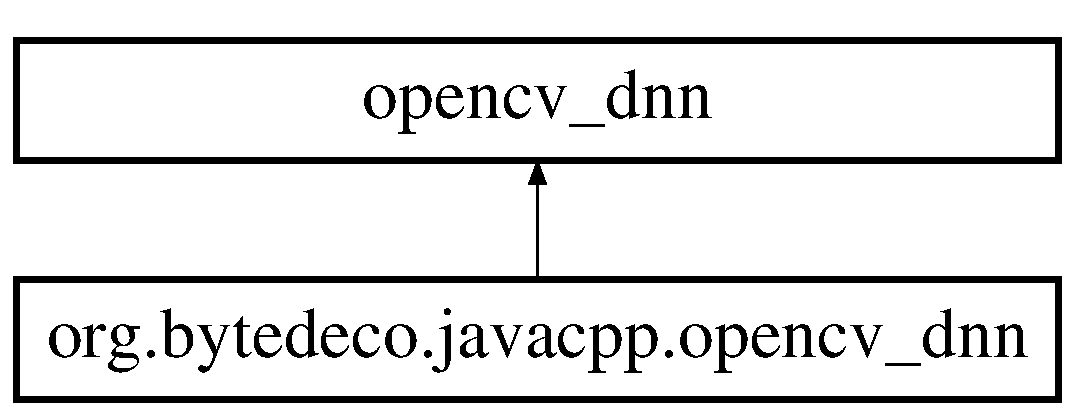
\includegraphics[height=2.000000cm]{classorg_1_1bytedeco_1_1javacpp_1_1opencv__dnn}
\end{center}
\end{figure}
\subsection*{Classes}
\begin{DoxyCompactItemize}
\item 
class {\bfseries \+\_\+\+Layer\+Static\+Registerer}
\item 
class {\bfseries Blob}
\begin{DoxyCompactList}\small\item\em This class provides methods for continuous n-\/dimensional C\+PU and G\+PU array processing. \end{DoxyCompactList}\item 
class {\bfseries Blob\+Pointer\+Vector}
\item 
class {\bfseries Blob\+Shape}
\item 
class {\bfseries Blob\+Vector}
\item 
class {\bfseries Dict}
\begin{DoxyCompactList}\small\item\em This class implements name-\/value dictionary, values are instances of Dict\+Value. \end{DoxyCompactList}\item 
class {\bfseries Dict\+Value}
\item 
class {\bfseries Importer}
\begin{DoxyCompactList}\small\item\em Small interface class for loading trained serialized models of different dnn-\/frameworks. \end{DoxyCompactList}\item 
class {\bfseries Layer}
\begin{DoxyCompactList}\small\item\em This interface class allows to build new Layers -\/ are building blocks of networks. \end{DoxyCompactList}\item 
class {\bfseries Layer\+Factory}
\item 
class {\bfseries Layer\+Params}
\begin{DoxyCompactList}\small\item\em This class provides all data needed to initialize layer. \end{DoxyCompactList}\item 
class {\bfseries Net}
\begin{DoxyCompactList}\small\item\em This class allows to create and manipulate comprehensive artificial neural networks. \end{DoxyCompactList}\end{DoxyCompactItemize}
\subsection*{Static Public Member Functions}
\begin{DoxyCompactItemize}
\item 
static native void {\bfseries init\+Module} ()
\item 
static native Importer \hyperlink{group__dnn_ga277fa41c30459c131b646bdb8951d82b}{create\+Caffe\+Importer} (@Str Byte\+Pointer prototxt, @Str Byte\+Pointer caffe\+Model)
\begin{DoxyCompactList}\small\item\em Creates the importer of \href{http://caffe.berkeleyvision.org}{\tt Caffe} framework network. \end{DoxyCompactList}\item 
static native Importer {\bfseries create\+Caffe\+Importer} (@Str Byte\+Pointer prototxt)
\item 
static native Importer {\bfseries create\+Caffe\+Importer} (@Str String prototxt, @Str String caffe\+Model)
\item 
static native Importer {\bfseries create\+Caffe\+Importer} (@Str String prototxt)
\item 
static native Net \hyperlink{group__dnn_ga228b1b00210018ec3f301f017a00949f}{read\+Net\+From\+Caffe} (@Str Byte\+Pointer prototxt, @Str Byte\+Pointer caffe\+Model)
\begin{DoxyCompactList}\small\item\em Reads a network model stored in Caffe model files. \end{DoxyCompactList}\item 
static native Net {\bfseries read\+Net\+From\+Caffe} (@Str Byte\+Pointer prototxt)
\item 
static native Net {\bfseries read\+Net\+From\+Caffe} (@Str String prototxt, @Str String caffe\+Model)
\item 
static native Net {\bfseries read\+Net\+From\+Caffe} (@Str String prototxt)
\item 
static native Importer \hyperlink{group__dnn_gafb21a0aa44b3feb934bcd5ad4fc708e3}{create\+Tensorflow\+Importer} (@Str Byte\+Pointer model)
\begin{DoxyCompactList}\small\item\em Creates the importer of \href{http://www.tensorflow.org}{\tt Tensor\+Flow} framework network. \end{DoxyCompactList}\item 
static native Importer {\bfseries create\+Tensorflow\+Importer} (@Str String model)
\item 
static native Importer \hyperlink{group__dnn_gae0f202e183aadc4ec86abda60b0e6adf}{create\+Torch\+Importer} (@Str Byte\+Pointer filename, @Cast(\char`\"{}bool\char`\"{}) boolean is\+Binary)
\begin{DoxyCompactList}\small\item\em Creates the importer of \href{http://torch.ch}{\tt Torch7} framework network. \end{DoxyCompactList}\item 
static native Importer {\bfseries create\+Torch\+Importer} (@Str Byte\+Pointer filename)
\item 
static native Importer {\bfseries create\+Torch\+Importer} (@Str String filename, @Cast(\char`\"{}bool\char`\"{}) boolean is\+Binary)
\item 
static native Importer {\bfseries create\+Torch\+Importer} (@Str String filename)
\end{DoxyCompactItemize}


The documentation for this class was generated from the following file\+:\begin{DoxyCompactItemize}
\item 
opencv\+\_\+dnn.\+java\end{DoxyCompactItemize}

\hypertarget{classorg_1_1bytedeco_1_1javacpp_1_1opencv__face}{}\section{org.\+bytedeco.\+javacpp.\+opencv\+\_\+face Class Reference}
\label{classorg_1_1bytedeco_1_1javacpp_1_1opencv__face}\index{org.\+bytedeco.\+javacpp.\+opencv\+\_\+face@{org.\+bytedeco.\+javacpp.\+opencv\+\_\+face}}
Inheritance diagram for org.\+bytedeco.\+javacpp.\+opencv\+\_\+face\+:\begin{figure}[H]
\begin{center}
\leavevmode
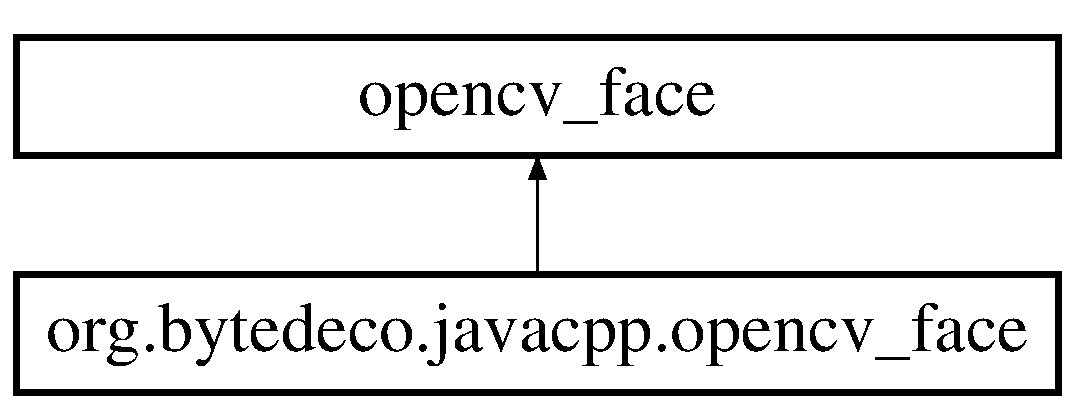
\includegraphics[height=2.000000cm]{classorg_1_1bytedeco_1_1javacpp_1_1opencv__face}
\end{center}
\end{figure}
\subsection*{Classes}
\begin{DoxyCompactItemize}
\item 
class {\bfseries Basic\+Face\+Recognizer}
\item 
class {\bfseries Face\+Recognizer}
\item 
class {\bfseries L\+B\+P\+H\+Face\+Recognizer}
\item 
class {\bfseries Predict\+Collector}
\item 
class {\bfseries Standard\+Collector}
\begin{DoxyCompactList}\small\item\em Default predict collector. \end{DoxyCompactList}\end{DoxyCompactItemize}
\subsection*{Static Public Member Functions}
\begin{DoxyCompactItemize}
\item 
static native Basic\+Face\+Recognizer \hyperlink{group__face_ga6f3a56396530d46af3fba9ad04fc80cf}{create\+Eigen\+Face\+Recognizer} (int num\+\_\+components, double fr.antproject.utils.threshold)
\item 
static native Basic\+Face\+Recognizer {\bfseries create\+Eigen\+Face\+Recognizer} ()
\item 
static native Basic\+Face\+Recognizer \hyperlink{group__face_ga80a98f353dd2ef661444e0d79bbe9daf}{create\+Fisher\+Face\+Recognizer} (int num\+\_\+components, double fr.antproject.utils.threshold)
\item 
static native Basic\+Face\+Recognizer {\bfseries create\+Fisher\+Face\+Recognizer} ()
\item 
static native L\+B\+P\+H\+Face\+Recognizer \hyperlink{group__face_ga970c161034e055fb56615aadba87ac4e}{create\+L\+B\+P\+H\+Face\+Recognizer} (int radius, int neighbors, int grid\+\_\+x, int grid\+\_\+y, double fr.antproject.utils.threshold)
\item 
static native L\+B\+P\+H\+Face\+Recognizer {\bfseries create\+L\+B\+P\+H\+Face\+Recognizer} ()
\end{DoxyCompactItemize}


The documentation for this class was generated from the following file\+:\begin{DoxyCompactItemize}
\item 
opencv\+\_\+face.\+java\end{DoxyCompactItemize}

\hypertarget{classorg_1_1bytedeco_1_1javacpp_1_1opencv__features2d}{}\section{org.\+bytedeco.\+javacpp.\+opencv\+\_\+features2d Class Reference}
\label{classorg_1_1bytedeco_1_1javacpp_1_1opencv__features2d}\index{org.\+bytedeco.\+javacpp.\+opencv\+\_\+features2d@{org.\+bytedeco.\+javacpp.\+opencv\+\_\+features2d}}
Inheritance diagram for org.\+bytedeco.\+javacpp.\+opencv\+\_\+features2d\+:\begin{figure}[H]
\begin{center}
\leavevmode
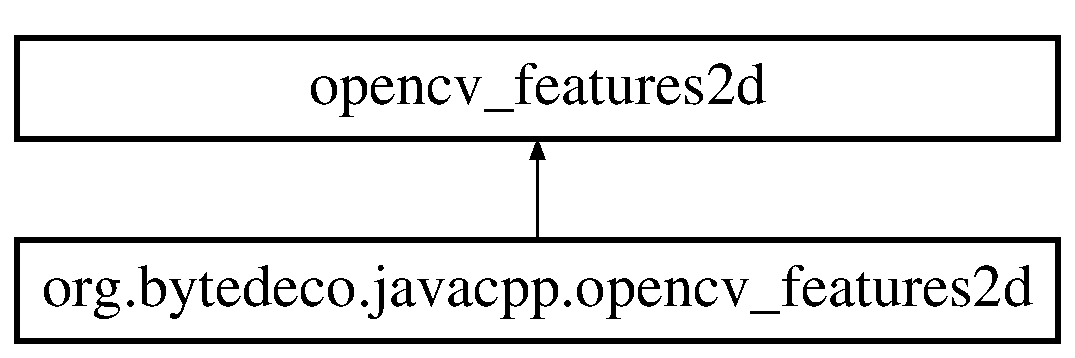
\includegraphics[height=2.000000cm]{classorg_1_1bytedeco_1_1javacpp_1_1opencv__features2d}
\end{center}
\end{figure}
\subsection*{Classes}
\begin{DoxyCompactItemize}
\item 
class {\bfseries Accumulator}
\item 
class {\bfseries Agast\+Feature\+Detector}
\item 
class {\bfseries A\+K\+A\+ZE}
\begin{DoxyCompactList}\small\item\em Class implementing the A\+K\+A\+ZE keypoint detector and descriptor extractor, described in {\bfseries [A\+N\+B13]} . \+: \end{DoxyCompactList}\item 
class {\bfseries B\+F\+Matcher}
\begin{DoxyCompactList}\small\item\em Brute-\/force descriptor matcher. \end{DoxyCompactList}\item 
class {\bfseries B\+O\+W\+Img\+Descriptor\+Extractor}
\begin{DoxyCompactList}\small\item\em Class to compute an image descriptor using the {\itshape bag of visual words}. \end{DoxyCompactList}\item 
class {\bfseries B\+O\+W\+K\+Means\+Trainer}
\begin{DoxyCompactList}\small\item\em kmeans -\/based class to train visual vocabulary using the {\itshape bag of visual words} approach. \+: \end{DoxyCompactList}\item 
class {\bfseries B\+O\+W\+Trainer}
\item 
class {\bfseries B\+R\+I\+SK}
\item 
class {\bfseries Descriptor\+Matcher}
\item 
class {\bfseries Draw\+Matches\+Flags}
\item 
class {\bfseries Fast\+Feature\+Detector}
\item 
class {\bfseries Feature2D}
\begin{DoxyCompactList}\small\item\em Abstract base class for 2D image feature detectors and descriptor extractors. \end{DoxyCompactList}\item 
class {\bfseries Flann\+Based\+Matcher}
\begin{DoxyCompactList}\small\item\em Flann-\/based descriptor matcher. \end{DoxyCompactList}\item 
class {\bfseries G\+F\+T\+T\+Detector}
\begin{DoxyCompactList}\small\item\em Wrapping class for feature detection using the good\+Features\+To\+Track function. \+: \end{DoxyCompactList}\item 
class {\bfseries K\+A\+ZE}
\item 
class {\bfseries Key\+Points\+Filter}
\begin{DoxyCompactList}\small\item\em A class filters a vector of keypoints. \end{DoxyCompactList}\item 
class {\bfseries M\+S\+ER}
\begin{DoxyCompactList}\small\item\em Maximally stable extremal region extractor. \end{DoxyCompactList}\item 
class {\bfseries O\+RB}
\begin{DoxyCompactList}\small\item\em Class implementing the O\+RB ({\itshape oriented B\+R\+I\+EF}) keypoint detector and descriptor extractor. \end{DoxyCompactList}\item 
class {\bfseries Simple\+Blob\+Detector}
\begin{DoxyCompactList}\small\item\em Class for extracting blobs from an image. \+: \end{DoxyCompactList}\end{DoxyCompactItemize}
\subsection*{Static Public Member Functions}
\begin{DoxyCompactItemize}
\item 
static native void \hyperlink{group__features2d__main_gabceff7e5d16ac9f888fa12e3e8a3f39e}{F\+A\+ST} ( @By\+Val Mat image, @By\+Ref Key\+Point\+Vector keypoints, int threshold, @Cast(\char`\"{}bool\char`\"{}) boolean nonmax\+Suppression)
\item 
static native void {\bfseries F\+A\+ST} ( @By\+Val Mat image, @By\+Ref Key\+Point\+Vector keypoints, int threshold)
\item 
static native void {\bfseries F\+A\+ST} ( @By\+Val U\+Mat image, @By\+Ref Key\+Point\+Vector keypoints, int threshold, @Cast(\char`\"{}bool\char`\"{}) boolean nonmax\+Suppression)
\item 
static native void {\bfseries F\+A\+ST} ( @By\+Val U\+Mat image, @By\+Ref Key\+Point\+Vector keypoints, int threshold)
\item 
static native void \hyperlink{group__features2d__main_ga7b940fc6d27c261d531040a7f8dd22af}{F\+A\+ST} ( @By\+Val Mat image, @By\+Ref Key\+Point\+Vector keypoints, int threshold, @Cast(\char`\"{}bool\char`\"{}) boolean nonmax\+Suppression, int type)
\begin{DoxyCompactList}\small\item\em Detects corners using the F\+A\+ST algorithm. \end{DoxyCompactList}\item 
static native void {\bfseries F\+A\+ST} ( @By\+Val U\+Mat image, @By\+Ref Key\+Point\+Vector keypoints, int threshold, @Cast(\char`\"{}bool\char`\"{}) boolean nonmax\+Suppression, int type)
\item 
static native void \hyperlink{group__features2d__main_ga849ee8acfb310ef13c3fd8a8f25327ed}{A\+G\+A\+ST} ( @By\+Val Mat image, @By\+Ref Key\+Point\+Vector keypoints, int threshold, @Cast(\char`\"{}bool\char`\"{}) boolean nonmax\+Suppression)
\item 
static native void {\bfseries A\+G\+A\+ST} ( @By\+Val Mat image, @By\+Ref Key\+Point\+Vector keypoints, int threshold)
\item 
static native void {\bfseries A\+G\+A\+ST} ( @By\+Val U\+Mat image, @By\+Ref Key\+Point\+Vector keypoints, int threshold, @Cast(\char`\"{}bool\char`\"{}) boolean nonmax\+Suppression)
\item 
static native void {\bfseries A\+G\+A\+ST} ( @By\+Val U\+Mat image, @By\+Ref Key\+Point\+Vector keypoints, int threshold)
\item 
static native void \hyperlink{group__features2d__main_ga2126ee1b1b70316ae0fd6ffb3d2d51bc}{A\+G\+A\+ST} ( @By\+Val Mat image, @By\+Ref Key\+Point\+Vector keypoints, int threshold, @Cast(\char`\"{}bool\char`\"{}) boolean nonmax\+Suppression, int type)
\begin{DoxyCompactList}\small\item\em Detects corners using the A\+G\+A\+ST algorithm. \end{DoxyCompactList}\item 
static native void {\bfseries A\+G\+A\+ST} ( @By\+Val U\+Mat image, @By\+Ref Key\+Point\+Vector keypoints, int threshold, @Cast(\char`\"{}bool\char`\"{}) boolean nonmax\+Suppression, int type)
\item 
static native void \hyperlink{group__features2d__draw_gab17ce5fe7286fa915dae6cdf8cb80740}{draw\+Keypoints} ( @By\+Val Mat image, @Const @By\+Ref Key\+Point\+Vector keypoints, @By\+Val Mat out\+Image, @Const @By\+Ref(null\+Value=\char`\"{}cv\+::\+Scalar\+::all(-\/1)\char`\"{}) Scalar color, int flags)
\begin{DoxyCompactList}\small\item\em Draws keypoints. \end{DoxyCompactList}\item 
static native void {\bfseries draw\+Keypoints} ( @By\+Val Mat image, @Const @By\+Ref Key\+Point\+Vector keypoints, @By\+Val Mat out\+Image)
\item 
static native void {\bfseries draw\+Keypoints} ( @By\+Val U\+Mat image, @Const @By\+Ref Key\+Point\+Vector keypoints, @By\+Val U\+Mat out\+Image, @Const @By\+Ref(null\+Value=\char`\"{}cv\+::\+Scalar\+::all(-\/1)\char`\"{}) Scalar color, int flags)
\item 
static native void {\bfseries draw\+Keypoints} ( @By\+Val U\+Mat image, @Const @By\+Ref Key\+Point\+Vector keypoints, @By\+Val U\+Mat out\+Image)
\item 
static native void \hyperlink{group__features2d__draw_gac84f37b93a8b6d5358211ec9b6d4799e}{draw\+Matches} ( @By\+Val Mat img1, @Const @By\+Ref Key\+Point\+Vector keypoints1, @By\+Val Mat img2, @Const @By\+Ref Key\+Point\+Vector keypoints2, @Const @By\+Ref D\+Match\+Vector matches1to2, @By\+Val Mat out\+Img, @Const @By\+Ref(null\+Value=\char`\"{}cv\+::\+Scalar\+::all(-\/1)\char`\"{}) Scalar match\+Color, @Const @By\+Ref(null\+Value=\char`\"{}cv\+::\+Scalar\+::all(-\/1)\char`\"{}) Scalar single\+Point\+Color, @Cast(\char`\"{}char$\ast$\char`\"{}) @Std\+Vector Byte\+Pointer matches\+Mask, int flags)
\begin{DoxyCompactList}\small\item\em Draws the found matches of keypoints from two images. \end{DoxyCompactList}\item 
static native void {\bfseries draw\+Matches} ( @By\+Val Mat img1, @Const @By\+Ref Key\+Point\+Vector keypoints1, @By\+Val Mat img2, @Const @By\+Ref Key\+Point\+Vector keypoints2, @Const @By\+Ref D\+Match\+Vector matches1to2, @By\+Val Mat out\+Img)
\item 
static native void {\bfseries draw\+Matches} ( @By\+Val Mat img1, @Const @By\+Ref Key\+Point\+Vector keypoints1, @By\+Val Mat img2, @Const @By\+Ref Key\+Point\+Vector keypoints2, @Const @By\+Ref D\+Match\+Vector matches1to2, @By\+Val Mat out\+Img, @Const @By\+Ref(null\+Value=\char`\"{}cv\+::\+Scalar\+::all(-\/1)\char`\"{}) Scalar match\+Color, @Const @By\+Ref(null\+Value=\char`\"{}cv\+::\+Scalar\+::all(-\/1)\char`\"{}) Scalar single\+Point\+Color, @Cast(\char`\"{}char$\ast$\char`\"{}) @Std\+Vector Byte\+Buffer matches\+Mask, int flags)
\item 
static native void {\bfseries draw\+Matches} ( @By\+Val U\+Mat img1, @Const @By\+Ref Key\+Point\+Vector keypoints1, @By\+Val U\+Mat img2, @Const @By\+Ref Key\+Point\+Vector keypoints2, @Const @By\+Ref D\+Match\+Vector matches1to2, @By\+Val U\+Mat out\+Img, @Const @By\+Ref(null\+Value=\char`\"{}cv\+::\+Scalar\+::all(-\/1)\char`\"{}) Scalar match\+Color, @Const @By\+Ref(null\+Value=\char`\"{}cv\+::\+Scalar\+::all(-\/1)\char`\"{}) Scalar single\+Point\+Color, @Cast(\char`\"{}char$\ast$\char`\"{}) @Std\+Vector byte\mbox{[}$\,$\mbox{]} matches\+Mask, int flags)
\item 
static native void {\bfseries draw\+Matches} ( @By\+Val U\+Mat img1, @Const @By\+Ref Key\+Point\+Vector keypoints1, @By\+Val U\+Mat img2, @Const @By\+Ref Key\+Point\+Vector keypoints2, @Const @By\+Ref D\+Match\+Vector matches1to2, @By\+Val U\+Mat out\+Img)
\item 
static native void {\bfseries draw\+Matches} ( @By\+Val U\+Mat img1, @Const @By\+Ref Key\+Point\+Vector keypoints1, @By\+Val U\+Mat img2, @Const @By\+Ref Key\+Point\+Vector keypoints2, @Const @By\+Ref D\+Match\+Vector matches1to2, @By\+Val U\+Mat out\+Img, @Const @By\+Ref(null\+Value=\char`\"{}cv\+::\+Scalar\+::all(-\/1)\char`\"{}) Scalar match\+Color, @Const @By\+Ref(null\+Value=\char`\"{}cv\+::\+Scalar\+::all(-\/1)\char`\"{}) Scalar single\+Point\+Color, @Cast(\char`\"{}char$\ast$\char`\"{}) @Std\+Vector Byte\+Pointer matches\+Mask, int flags)
\item 
static native void \hyperlink{group__features2d__draw_ga685267fdd3340d65fba4cf402d6dbe04}{draw\+Matches\+Knn} ( @By\+Val Mat img1, @Const @By\+Ref Key\+Point\+Vector keypoints1, @By\+Val Mat img2, @Const @By\+Ref Key\+Point\+Vector keypoints2, @Const @By\+Ref D\+Match\+Vector\+Vector matches1to2, @By\+Val Mat out\+Img, @Const @By\+Ref(null\+Value=\char`\"{}cv\+::\+Scalar\+::all(-\/1)\char`\"{}) Scalar match\+Color, @Const @By\+Ref(null\+Value=\char`\"{}cv\+::\+Scalar\+::all(-\/1)\char`\"{}) Scalar single\+Point\+Color, @Cast(\char`\"{}const std\+::vector$<$std\+::vector$<$char$>$ $>$$\ast$\char`\"{}) @By\+Ref(null\+Value=\char`\"{}std\+::vector$<$std\+::vector$<$char$>$ $>$()\char`\"{}) Byte\+Vector\+Vector matches\+Mask, int flags)
\item 
static native void {\bfseries draw\+Matches\+Knn} ( @By\+Val Mat img1, @Const @By\+Ref Key\+Point\+Vector keypoints1, @By\+Val Mat img2, @Const @By\+Ref Key\+Point\+Vector keypoints2, @Const @By\+Ref D\+Match\+Vector\+Vector matches1to2, @By\+Val Mat out\+Img)
\item 
static native void {\bfseries draw\+Matches\+Knn} ( @By\+Val U\+Mat img1, @Const @By\+Ref Key\+Point\+Vector keypoints1, @By\+Val U\+Mat img2, @Const @By\+Ref Key\+Point\+Vector keypoints2, @Const @By\+Ref D\+Match\+Vector\+Vector matches1to2, @By\+Val U\+Mat out\+Img, @Const @By\+Ref(null\+Value=\char`\"{}cv\+::\+Scalar\+::all(-\/1)\char`\"{}) Scalar match\+Color, @Const @By\+Ref(null\+Value=\char`\"{}cv\+::\+Scalar\+::all(-\/1)\char`\"{}) Scalar single\+Point\+Color, @Cast(\char`\"{}const std\+::vector$<$std\+::vector$<$char$>$ $>$$\ast$\char`\"{}) @By\+Ref(null\+Value=\char`\"{}std\+::vector$<$std\+::vector$<$char$>$ $>$()\char`\"{}) Byte\+Vector\+Vector matches\+Mask, int flags)
\item 
static native void {\bfseries draw\+Matches\+Knn} ( @By\+Val U\+Mat img1, @Const @By\+Ref Key\+Point\+Vector keypoints1, @By\+Val U\+Mat img2, @Const @By\+Ref Key\+Point\+Vector keypoints2, @Const @By\+Ref D\+Match\+Vector\+Vector matches1to2, @By\+Val U\+Mat out\+Img)
\item 
static native void \hyperlink{group__features2d_gaae7a705a66cbdd0ed99122fe183a0e03}{evaluate\+Feature\+Detector} ( @Const @By\+Ref Mat img1, @Const @By\+Ref Mat img2, @Const @By\+Ref Mat H1to2, Key\+Point\+Vector keypoints1, Key\+Point\+Vector keypoints2, @By\+Ref Float\+Pointer repeatability, @By\+Ref Int\+Pointer corresp\+Count, @Cast(\char`\"{}cv\+::\+Feature\+Detector$\ast$\char`\"{}) @Ptr Feature2D fdetector)
\item 
static native void {\bfseries evaluate\+Feature\+Detector} ( @Const @By\+Ref Mat img1, @Const @By\+Ref Mat img2, @Const @By\+Ref Mat H1to2, Key\+Point\+Vector keypoints1, Key\+Point\+Vector keypoints2, @By\+Ref Float\+Pointer repeatability, @By\+Ref Int\+Pointer corresp\+Count)
\item 
static native void {\bfseries evaluate\+Feature\+Detector} ( @Const @By\+Ref Mat img1, @Const @By\+Ref Mat img2, @Const @By\+Ref Mat H1to2, Key\+Point\+Vector keypoints1, Key\+Point\+Vector keypoints2, @By\+Ref Float\+Buffer repeatability, @By\+Ref Int\+Buffer corresp\+Count, @Cast(\char`\"{}cv\+::\+Feature\+Detector$\ast$\char`\"{}) @Ptr Feature2D fdetector)
\item 
static native void {\bfseries evaluate\+Feature\+Detector} ( @Const @By\+Ref Mat img1, @Const @By\+Ref Mat img2, @Const @By\+Ref Mat H1to2, Key\+Point\+Vector keypoints1, Key\+Point\+Vector keypoints2, @By\+Ref Float\+Buffer repeatability, @By\+Ref Int\+Buffer corresp\+Count)
\item 
static native void {\bfseries evaluate\+Feature\+Detector} ( @Const @By\+Ref Mat img1, @Const @By\+Ref Mat img2, @Const @By\+Ref Mat H1to2, Key\+Point\+Vector keypoints1, Key\+Point\+Vector keypoints2, @By\+Ref float\mbox{[}$\,$\mbox{]} repeatability, @By\+Ref int\mbox{[}$\,$\mbox{]} corresp\+Count, @Cast(\char`\"{}cv\+::\+Feature\+Detector$\ast$\char`\"{}) @Ptr Feature2D fdetector)
\item 
static native void {\bfseries evaluate\+Feature\+Detector} ( @Const @By\+Ref Mat img1, @Const @By\+Ref Mat img2, @Const @By\+Ref Mat H1to2, Key\+Point\+Vector keypoints1, Key\+Point\+Vector keypoints2, @By\+Ref float\mbox{[}$\,$\mbox{]} repeatability, @By\+Ref int\mbox{[}$\,$\mbox{]} corresp\+Count)
\item 
static native void {\bfseries compute\+Recall\+Precision\+Curve} ( @Const @By\+Ref D\+Match\+Vector\+Vector matches1to2, @Cast(\char`\"{}const std\+::vector$<$std\+::vector$<$uchar$>$ $>$$\ast$\char`\"{}) @By\+Ref Byte\+Vector\+Vector correct\+Matches1to2\+Mask, @By\+Ref Point2f\+Vector recall\+Precision\+Curve)
\item 
static native float {\bfseries get\+Recall} ( @Const @By\+Ref Point2f\+Vector recall\+Precision\+Curve, float l\+\_\+precision)
\item 
static native int {\bfseries get\+Nearest\+Point} ( @Const @By\+Ref Point2f\+Vector recall\+Precision\+Curve, float l\+\_\+precision)
\end{DoxyCompactItemize}


The documentation for this class was generated from the following file\+:\begin{DoxyCompactItemize}
\item 
opencv\+\_\+features2d.\+java\end{DoxyCompactItemize}

\hypertarget{classorg_1_1bytedeco_1_1javacpp_1_1opencv__flann}{}\section{org.\+bytedeco.\+javacpp.\+opencv\+\_\+flann Class Reference}
\label{classorg_1_1bytedeco_1_1javacpp_1_1opencv__flann}\index{org.\+bytedeco.\+javacpp.\+opencv\+\_\+flann@{org.\+bytedeco.\+javacpp.\+opencv\+\_\+flann}}
Inheritance diagram for org.\+bytedeco.\+javacpp.\+opencv\+\_\+flann\+:\begin{figure}[H]
\begin{center}
\leavevmode
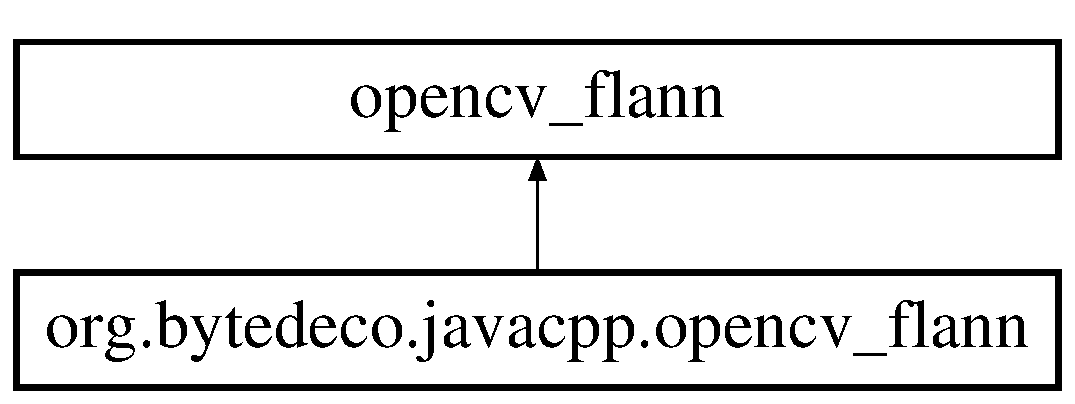
\includegraphics[height=2.000000cm]{classorg_1_1bytedeco_1_1javacpp_1_1opencv__flann}
\end{center}
\end{figure}
\subsection*{Classes}
\begin{DoxyCompactItemize}
\item 
class {\bfseries Autotuned\+Index\+Params}
\item 
class {\bfseries Composite\+Index\+Params}
\item 
class {\bfseries Hierarchical\+Clustering\+Index\+Params}
\item 
class {\bfseries Index}
\item 
class {\bfseries Index\+Params}
\item 
class {\bfseries K\+D\+Tree\+Index\+Params}
\item 
class {\bfseries K\+Means\+Index\+Params}
\item 
class {\bfseries Linear\+Index\+Params}
\item 
class {\bfseries Lsh\+Index\+Params}
\item 
class {\bfseries Saved\+Index\+Params}
\item 
class {\bfseries Search\+Params}
\end{DoxyCompactItemize}
\subsection*{Static Public Attributes}
\begin{DoxyCompactItemize}
\item 
static final int \hyperlink{classorg_1_1bytedeco_1_1javacpp_1_1opencv__flann_a80b83a1ebca7555000670593d6a0a800}{F\+L\+A\+N\+N\+\_\+\+I\+N\+D\+E\+X\+\_\+\+L\+I\+N\+E\+AR} = 0
\item 
static final int \hyperlink{classorg_1_1bytedeco_1_1javacpp_1_1opencv__flann_ab34e210d13724873f4b44027b519ae3a}{F\+L\+A\+N\+N\+\_\+\+C\+E\+N\+T\+E\+R\+S\+\_\+\+R\+A\+N\+D\+OM} = 0
\item 
static final int \hyperlink{classorg_1_1bytedeco_1_1javacpp_1_1opencv__flann_a4fe44f0983781d82a6e2d00737c18c2f}{F\+L\+A\+N\+N\+\_\+\+L\+O\+G\+\_\+\+N\+O\+NE} = 0
\item 
static final int \hyperlink{classorg_1_1bytedeco_1_1javacpp_1_1opencv__flann_a3b945a10789f97a6082ba476c3e78793}{F\+L\+A\+N\+N\+\_\+\+D\+I\+S\+T\+\_\+\+E\+U\+C\+L\+I\+D\+E\+AN} = 1
\item 
static final int \hyperlink{classorg_1_1bytedeco_1_1javacpp_1_1opencv__flann_ae6e313d1cef55a90ea0d609b7c8545c1}{F\+L\+A\+N\+N\+\_\+\+I\+N\+T8} = 0
\item 
static final int \hyperlink{classorg_1_1bytedeco_1_1javacpp_1_1opencv__flann_a0e34a977ed50ed742297acdf102028ca}{F\+L\+A\+N\+N\+\_\+\+C\+H\+E\+C\+K\+S\+\_\+\+U\+N\+L\+I\+M\+I\+T\+ED} = -\/1
\end{DoxyCompactItemize}


\subsection{Member Data Documentation}
\mbox{\Hypertarget{classorg_1_1bytedeco_1_1javacpp_1_1opencv__flann_ab34e210d13724873f4b44027b519ae3a}\label{classorg_1_1bytedeco_1_1javacpp_1_1opencv__flann_ab34e210d13724873f4b44027b519ae3a}} 
\index{org\+::bytedeco\+::javacpp\+::opencv\+\_\+flann@{org\+::bytedeco\+::javacpp\+::opencv\+\_\+flann}!F\+L\+A\+N\+N\+\_\+\+C\+E\+N\+T\+E\+R\+S\+\_\+\+R\+A\+N\+D\+OM@{F\+L\+A\+N\+N\+\_\+\+C\+E\+N\+T\+E\+R\+S\+\_\+\+R\+A\+N\+D\+OM}}
\index{F\+L\+A\+N\+N\+\_\+\+C\+E\+N\+T\+E\+R\+S\+\_\+\+R\+A\+N\+D\+OM@{F\+L\+A\+N\+N\+\_\+\+C\+E\+N\+T\+E\+R\+S\+\_\+\+R\+A\+N\+D\+OM}!org\+::bytedeco\+::javacpp\+::opencv\+\_\+flann@{org\+::bytedeco\+::javacpp\+::opencv\+\_\+flann}}
\subsubsection{\texorpdfstring{F\+L\+A\+N\+N\+\_\+\+C\+E\+N\+T\+E\+R\+S\+\_\+\+R\+A\+N\+D\+OM}{FLANN\_CENTERS\_RANDOM}}
{\footnotesize\ttfamily final int org.\+bytedeco.\+javacpp.\+opencv\+\_\+flann.\+F\+L\+A\+N\+N\+\_\+\+C\+E\+N\+T\+E\+R\+S\+\_\+\+R\+A\+N\+D\+OM = 0\hspace{0.3cm}{\ttfamily [static]}}

enum cvflann\+::flann\+\_\+centers\+\_\+init\+\_\+t \mbox{\Hypertarget{classorg_1_1bytedeco_1_1javacpp_1_1opencv__flann_a0e34a977ed50ed742297acdf102028ca}\label{classorg_1_1bytedeco_1_1javacpp_1_1opencv__flann_a0e34a977ed50ed742297acdf102028ca}} 
\index{org\+::bytedeco\+::javacpp\+::opencv\+\_\+flann@{org\+::bytedeco\+::javacpp\+::opencv\+\_\+flann}!F\+L\+A\+N\+N\+\_\+\+C\+H\+E\+C\+K\+S\+\_\+\+U\+N\+L\+I\+M\+I\+T\+ED@{F\+L\+A\+N\+N\+\_\+\+C\+H\+E\+C\+K\+S\+\_\+\+U\+N\+L\+I\+M\+I\+T\+ED}}
\index{F\+L\+A\+N\+N\+\_\+\+C\+H\+E\+C\+K\+S\+\_\+\+U\+N\+L\+I\+M\+I\+T\+ED@{F\+L\+A\+N\+N\+\_\+\+C\+H\+E\+C\+K\+S\+\_\+\+U\+N\+L\+I\+M\+I\+T\+ED}!org\+::bytedeco\+::javacpp\+::opencv\+\_\+flann@{org\+::bytedeco\+::javacpp\+::opencv\+\_\+flann}}
\subsubsection{\texorpdfstring{F\+L\+A\+N\+N\+\_\+\+C\+H\+E\+C\+K\+S\+\_\+\+U\+N\+L\+I\+M\+I\+T\+ED}{FLANN\_CHECKS\_UNLIMITED}}
{\footnotesize\ttfamily final int org.\+bytedeco.\+javacpp.\+opencv\+\_\+flann.\+F\+L\+A\+N\+N\+\_\+\+C\+H\+E\+C\+K\+S\+\_\+\+U\+N\+L\+I\+M\+I\+T\+ED = -\/1\hspace{0.3cm}{\ttfamily [static]}}

enum cvflann\+:\+: \mbox{\Hypertarget{classorg_1_1bytedeco_1_1javacpp_1_1opencv__flann_a3b945a10789f97a6082ba476c3e78793}\label{classorg_1_1bytedeco_1_1javacpp_1_1opencv__flann_a3b945a10789f97a6082ba476c3e78793}} 
\index{org\+::bytedeco\+::javacpp\+::opencv\+\_\+flann@{org\+::bytedeco\+::javacpp\+::opencv\+\_\+flann}!F\+L\+A\+N\+N\+\_\+\+D\+I\+S\+T\+\_\+\+E\+U\+C\+L\+I\+D\+E\+AN@{F\+L\+A\+N\+N\+\_\+\+D\+I\+S\+T\+\_\+\+E\+U\+C\+L\+I\+D\+E\+AN}}
\index{F\+L\+A\+N\+N\+\_\+\+D\+I\+S\+T\+\_\+\+E\+U\+C\+L\+I\+D\+E\+AN@{F\+L\+A\+N\+N\+\_\+\+D\+I\+S\+T\+\_\+\+E\+U\+C\+L\+I\+D\+E\+AN}!org\+::bytedeco\+::javacpp\+::opencv\+\_\+flann@{org\+::bytedeco\+::javacpp\+::opencv\+\_\+flann}}
\subsubsection{\texorpdfstring{F\+L\+A\+N\+N\+\_\+\+D\+I\+S\+T\+\_\+\+E\+U\+C\+L\+I\+D\+E\+AN}{FLANN\_DIST\_EUCLIDEAN}}
{\footnotesize\ttfamily final int org.\+bytedeco.\+javacpp.\+opencv\+\_\+flann.\+F\+L\+A\+N\+N\+\_\+\+D\+I\+S\+T\+\_\+\+E\+U\+C\+L\+I\+D\+E\+AN = 1\hspace{0.3cm}{\ttfamily [static]}}

enum cvflann\+::flann\+\_\+distance\+\_\+t \mbox{\Hypertarget{classorg_1_1bytedeco_1_1javacpp_1_1opencv__flann_a80b83a1ebca7555000670593d6a0a800}\label{classorg_1_1bytedeco_1_1javacpp_1_1opencv__flann_a80b83a1ebca7555000670593d6a0a800}} 
\index{org\+::bytedeco\+::javacpp\+::opencv\+\_\+flann@{org\+::bytedeco\+::javacpp\+::opencv\+\_\+flann}!F\+L\+A\+N\+N\+\_\+\+I\+N\+D\+E\+X\+\_\+\+L\+I\+N\+E\+AR@{F\+L\+A\+N\+N\+\_\+\+I\+N\+D\+E\+X\+\_\+\+L\+I\+N\+E\+AR}}
\index{F\+L\+A\+N\+N\+\_\+\+I\+N\+D\+E\+X\+\_\+\+L\+I\+N\+E\+AR@{F\+L\+A\+N\+N\+\_\+\+I\+N\+D\+E\+X\+\_\+\+L\+I\+N\+E\+AR}!org\+::bytedeco\+::javacpp\+::opencv\+\_\+flann@{org\+::bytedeco\+::javacpp\+::opencv\+\_\+flann}}
\subsubsection{\texorpdfstring{F\+L\+A\+N\+N\+\_\+\+I\+N\+D\+E\+X\+\_\+\+L\+I\+N\+E\+AR}{FLANN\_INDEX\_LINEAR}}
{\footnotesize\ttfamily final int org.\+bytedeco.\+javacpp.\+opencv\+\_\+flann.\+F\+L\+A\+N\+N\+\_\+\+I\+N\+D\+E\+X\+\_\+\+L\+I\+N\+E\+AR = 0\hspace{0.3cm}{\ttfamily [static]}}

enum cvflann\+::flann\+\_\+algorithm\+\_\+t \mbox{\Hypertarget{classorg_1_1bytedeco_1_1javacpp_1_1opencv__flann_ae6e313d1cef55a90ea0d609b7c8545c1}\label{classorg_1_1bytedeco_1_1javacpp_1_1opencv__flann_ae6e313d1cef55a90ea0d609b7c8545c1}} 
\index{org\+::bytedeco\+::javacpp\+::opencv\+\_\+flann@{org\+::bytedeco\+::javacpp\+::opencv\+\_\+flann}!F\+L\+A\+N\+N\+\_\+\+I\+N\+T8@{F\+L\+A\+N\+N\+\_\+\+I\+N\+T8}}
\index{F\+L\+A\+N\+N\+\_\+\+I\+N\+T8@{F\+L\+A\+N\+N\+\_\+\+I\+N\+T8}!org\+::bytedeco\+::javacpp\+::opencv\+\_\+flann@{org\+::bytedeco\+::javacpp\+::opencv\+\_\+flann}}
\subsubsection{\texorpdfstring{F\+L\+A\+N\+N\+\_\+\+I\+N\+T8}{FLANN\_INT8}}
{\footnotesize\ttfamily final int org.\+bytedeco.\+javacpp.\+opencv\+\_\+flann.\+F\+L\+A\+N\+N\+\_\+\+I\+N\+T8 = 0\hspace{0.3cm}{\ttfamily [static]}}

enum cvflann\+::flann\+\_\+datatype\+\_\+t \mbox{\Hypertarget{classorg_1_1bytedeco_1_1javacpp_1_1opencv__flann_a4fe44f0983781d82a6e2d00737c18c2f}\label{classorg_1_1bytedeco_1_1javacpp_1_1opencv__flann_a4fe44f0983781d82a6e2d00737c18c2f}} 
\index{org\+::bytedeco\+::javacpp\+::opencv\+\_\+flann@{org\+::bytedeco\+::javacpp\+::opencv\+\_\+flann}!F\+L\+A\+N\+N\+\_\+\+L\+O\+G\+\_\+\+N\+O\+NE@{F\+L\+A\+N\+N\+\_\+\+L\+O\+G\+\_\+\+N\+O\+NE}}
\index{F\+L\+A\+N\+N\+\_\+\+L\+O\+G\+\_\+\+N\+O\+NE@{F\+L\+A\+N\+N\+\_\+\+L\+O\+G\+\_\+\+N\+O\+NE}!org\+::bytedeco\+::javacpp\+::opencv\+\_\+flann@{org\+::bytedeco\+::javacpp\+::opencv\+\_\+flann}}
\subsubsection{\texorpdfstring{F\+L\+A\+N\+N\+\_\+\+L\+O\+G\+\_\+\+N\+O\+NE}{FLANN\_LOG\_NONE}}
{\footnotesize\ttfamily final int org.\+bytedeco.\+javacpp.\+opencv\+\_\+flann.\+F\+L\+A\+N\+N\+\_\+\+L\+O\+G\+\_\+\+N\+O\+NE = 0\hspace{0.3cm}{\ttfamily [static]}}

enum cvflann\+::flann\+\_\+log\+\_\+level\+\_\+t 

The documentation for this class was generated from the following file\+:\begin{DoxyCompactItemize}
\item 
opencv\+\_\+flann.\+java\end{DoxyCompactItemize}

\hypertarget{classorg_1_1bytedeco_1_1javacpp_1_1opencv__highgui}{}\section{org.\+bytedeco.\+javacpp.\+opencv\+\_\+highgui Class Reference}
\label{classorg_1_1bytedeco_1_1javacpp_1_1opencv__highgui}\index{org.\+bytedeco.\+javacpp.\+opencv\+\_\+highgui@{org.\+bytedeco.\+javacpp.\+opencv\+\_\+highgui}}
Inheritance diagram for org.\+bytedeco.\+javacpp.\+opencv\+\_\+highgui\+:\begin{figure}[H]
\begin{center}
\leavevmode
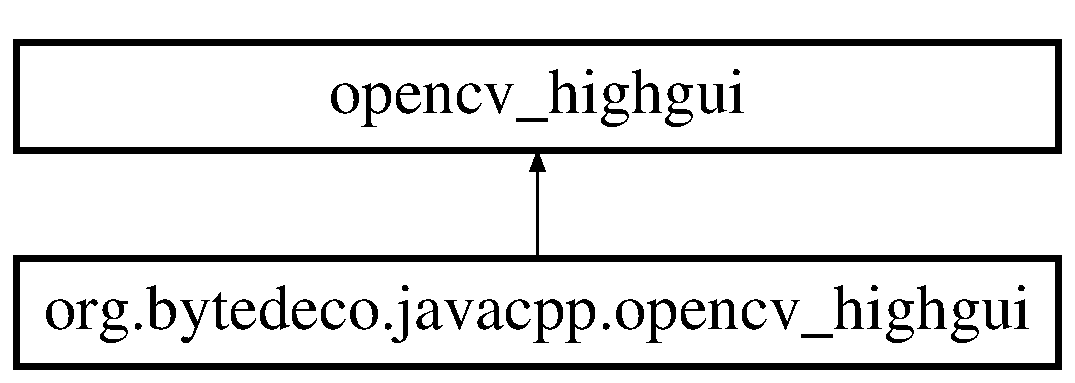
\includegraphics[height=2.000000cm]{classorg_1_1bytedeco_1_1javacpp_1_1opencv__highgui}
\end{center}
\end{figure}
\subsection*{Classes}
\begin{DoxyCompactItemize}
\item 
class {\bfseries Button\+Callback}
\begin{DoxyCompactList}\small\item\em Callback function for a button created by cv\+::create\+Button. \end{DoxyCompactList}\item 
class {\bfseries Cv\+Button\+Callback}
\item 
class {\bfseries Cv\+Mouse\+Callback}
\item 
class {\bfseries Cv\+Open\+Gl\+Draw\+Callback}
\item 
class {\bfseries Cv\+Trackbar\+Callback}
\item 
class {\bfseries Cv\+Trackbar\+Callback2}
\item 
class {\bfseries Mouse\+Callback}
\begin{DoxyCompactList}\small\item\em Callback function for mouse events. see cv\+::set\+Mouse\+Callback. \end{DoxyCompactList}\item 
class {\bfseries Open\+Gl\+Draw\+Callback}
\begin{DoxyCompactList}\small\item\em Callback function defined to be called every frame. See cv\+::set\+Open\+Gl\+Draw\+Callback. \end{DoxyCompactList}\item 
class {\bfseries Pt2\+Func\+\_\+int\+\_\+byte\+\_\+\+\_\+}
\item 
class {\bfseries Pt2\+Func\+\_\+int\+\_\+\+Byte\+Buffer}
\item 
class {\bfseries Pt2\+Func\+\_\+int\+\_\+\+Byte\+Pointer}
\item 
class {\bfseries Pt2\+Func\+\_\+int\+\_\+\+Pointer\+Pointer}
\item 
class {\bfseries Qt\+Font}
\item 
class {\bfseries Trackbar\+Callback}
\begin{DoxyCompactList}\small\item\em Callback function for Trackbar see cv\+::create\+Trackbar. \end{DoxyCompactList}\end{DoxyCompactItemize}
\subsection*{Static Public Member Functions}
\begin{DoxyCompactItemize}
\item 
static native Cv\+Font {\bfseries cv\+Font\+Qt} (@Cast(\char`\"{}const char$\ast$\char`\"{}) Byte\+Pointer name\+Font, int point\+Size, @By\+Val(null\+Value=\char`\"{}Cv\+Scalar(cv\+Scalar\+All(0))\char`\"{}) Cv\+Scalar color, int weight, int style, int spacing)
\item 
static native Cv\+Font {\bfseries cv\+Font\+Qt} (@Cast(\char`\"{}const char$\ast$\char`\"{}) Byte\+Pointer name\+Font)
\item 
static native Cv\+Font {\bfseries cv\+Font\+Qt} (String name\+Font, int point\+Size, @By\+Val(null\+Value=\char`\"{}Cv\+Scalar(cv\+Scalar\+All(0))\char`\"{}) Cv\+Scalar color, int weight, int style, int spacing)
\item 
static native Cv\+Font {\bfseries cv\+Font\+Qt} (String name\+Font)
\item 
static native void {\bfseries cv\+Add\+Text} (@Const Cv\+Arr img, @Cast(\char`\"{}const char$\ast$\char`\"{}) Byte\+Pointer text, @By\+Val Cv\+Point org, Cv\+Font arg2)
\item 
static native void {\bfseries cv\+Add\+Text} (@Const Cv\+Arr img, String text, @By\+Val @Cast(\char`\"{}Cv\+Point$\ast$\char`\"{}) Int\+Buffer org, Cv\+Font arg2)
\item 
static native void {\bfseries cv\+Add\+Text} (@Const Cv\+Arr img, @Cast(\char`\"{}const char$\ast$\char`\"{}) Byte\+Pointer text, @By\+Val @Cast(\char`\"{}Cv\+Point$\ast$\char`\"{}) int\mbox{[}$\,$\mbox{]} org, Cv\+Font arg2)
\item 
static native void {\bfseries cv\+Add\+Text} (@Const Cv\+Arr img, String text, @By\+Val Cv\+Point org, Cv\+Font arg2)
\item 
static native void {\bfseries cv\+Add\+Text} (@Const Cv\+Arr img, @Cast(\char`\"{}const char$\ast$\char`\"{}) Byte\+Pointer text, @By\+Val @Cast(\char`\"{}Cv\+Point$\ast$\char`\"{}) Int\+Buffer org, Cv\+Font arg2)
\item 
static native void {\bfseries cv\+Add\+Text} (@Const Cv\+Arr img, String text, @By\+Val @Cast(\char`\"{}Cv\+Point$\ast$\char`\"{}) int\mbox{[}$\,$\mbox{]} org, Cv\+Font arg2)
\item 
static native void {\bfseries cv\+Display\+Overlay} (@Cast(\char`\"{}const char$\ast$\char`\"{}) Byte\+Pointer name, @Cast(\char`\"{}const char$\ast$\char`\"{}) Byte\+Pointer text, int delayms)
\item 
static native void {\bfseries cv\+Display\+Overlay} (@Cast(\char`\"{}const char$\ast$\char`\"{}) Byte\+Pointer name, @Cast(\char`\"{}const char$\ast$\char`\"{}) Byte\+Pointer text)
\item 
static native void {\bfseries cv\+Display\+Overlay} (String name, String text, int delayms)
\item 
static native void {\bfseries cv\+Display\+Overlay} (String name, String text)
\item 
static native void {\bfseries cv\+Display\+Status\+Bar} (@Cast(\char`\"{}const char$\ast$\char`\"{}) Byte\+Pointer name, @Cast(\char`\"{}const char$\ast$\char`\"{}) Byte\+Pointer text, int delayms)
\item 
static native void {\bfseries cv\+Display\+Status\+Bar} (@Cast(\char`\"{}const char$\ast$\char`\"{}) Byte\+Pointer name, @Cast(\char`\"{}const char$\ast$\char`\"{}) Byte\+Pointer text)
\item 
static native void {\bfseries cv\+Display\+Status\+Bar} (String name, String text, int delayms)
\item 
static native void {\bfseries cv\+Display\+Status\+Bar} (String name, String text)
\item 
static native void {\bfseries cv\+Save\+Window\+Parameters} (@Cast(\char`\"{}const char$\ast$\char`\"{}) Byte\+Pointer name)
\item 
static native void {\bfseries cv\+Save\+Window\+Parameters} (String name)
\item 
static native void {\bfseries cv\+Load\+Window\+Parameters} (@Cast(\char`\"{}const char$\ast$\char`\"{}) Byte\+Pointer name)
\item 
static native void {\bfseries cv\+Load\+Window\+Parameters} (String name)
\item 
static native int {\bfseries cv\+Start\+Loop} (Pt2\+Func\+\_\+int\+\_\+\+Pointer\+Pointer pt2\+Func, int argc, @Cast(\char`\"{}char$\ast$$\ast$\char`\"{}) Pointer\+Pointer argv)
\item 
static native int {\bfseries cv\+Start\+Loop} (Pt2\+Func\+\_\+int\+\_\+\+Byte\+Pointer pt2\+Func, int argc, @Cast(\char`\"{}char$\ast$$\ast$\char`\"{}) @By\+Ptr\+Ptr Byte\+Pointer argv)
\item 
static native int {\bfseries cv\+Start\+Loop} (Pt2\+Func\+\_\+int\+\_\+\+Byte\+Buffer pt2\+Func, int argc, @Cast(\char`\"{}char$\ast$$\ast$\char`\"{}) @By\+Ptr\+Ptr Byte\+Buffer argv)
\item 
static native int {\bfseries cv\+Start\+Loop} (Pt2\+Func\+\_\+int\+\_\+byte\+\_\+\+\_\+ pt2\+Func, int argc, @Cast(\char`\"{}char$\ast$$\ast$\char`\"{}) @By\+Ptr\+Ptr byte\mbox{[}$\,$\mbox{]} argv)
\item 
static native void {\bfseries cv\+Stop\+Loop} ()
\item 
static native int {\bfseries cv\+Create\+Button} ( @Cast(\char`\"{}const char$\ast$\char`\"{}) Byte\+Pointer button\+\_\+name, Cv\+Button\+Callback on\+\_\+change, Pointer userdata, int button\+\_\+type, int initial\+\_\+button\+\_\+state)
\item 
static native int {\bfseries cv\+Create\+Button} ()
\item 
static native int {\bfseries cv\+Create\+Button} (String button\+\_\+name, Cv\+Button\+Callback on\+\_\+change, Pointer userdata, int button\+\_\+type, int initial\+\_\+button\+\_\+state)
\item 
static native int {\bfseries cv\+Init\+System} (int argc, @Cast(\char`\"{}char$\ast$$\ast$\char`\"{}) Pointer\+Pointer argv)
\item 
static native int {\bfseries cv\+Init\+System} (int argc, @Cast(\char`\"{}char$\ast$$\ast$\char`\"{}) @By\+Ptr\+Ptr Byte\+Pointer argv)
\item 
static native int {\bfseries cv\+Init\+System} (int argc, @Cast(\char`\"{}char$\ast$$\ast$\char`\"{}) @By\+Ptr\+Ptr Byte\+Buffer argv)
\item 
static native int {\bfseries cv\+Init\+System} (int argc, @Cast(\char`\"{}char$\ast$$\ast$\char`\"{}) @By\+Ptr\+Ptr byte\mbox{[}$\,$\mbox{]} argv)
\item 
static native int {\bfseries cv\+Start\+Window\+Thread} ()
\item 
static native int {\bfseries cv\+Named\+Window} ( @Cast(\char`\"{}const char$\ast$\char`\"{}) Byte\+Pointer name, int flags)
\item 
static native int {\bfseries cv\+Named\+Window} ( @Cast(\char`\"{}const char$\ast$\char`\"{}) Byte\+Pointer name)
\item 
static native int {\bfseries cv\+Named\+Window} (String name, int flags)
\item 
static native int {\bfseries cv\+Named\+Window} (String name)
\item 
static native void {\bfseries cv\+Set\+Window\+Property} (@Cast(\char`\"{}const char$\ast$\char`\"{}) Byte\+Pointer name, int prop\+\_\+id, double prop\+\_\+value)
\item 
static native void {\bfseries cv\+Set\+Window\+Property} (String name, int prop\+\_\+id, double prop\+\_\+value)
\item 
static native double {\bfseries cv\+Get\+Window\+Property} (@Cast(\char`\"{}const char$\ast$\char`\"{}) Byte\+Pointer name, int prop\+\_\+id)
\item 
static native double {\bfseries cv\+Get\+Window\+Property} (String name, int prop\+\_\+id)
\item 
static native void {\bfseries cv\+Show\+Image} ( @Cast(\char`\"{}const char$\ast$\char`\"{}) Byte\+Pointer name, @Const Cv\+Arr image)
\item 
static native void {\bfseries cv\+Show\+Image} (String name, @Const Cv\+Arr image)
\item 
static native void {\bfseries cv\+Resize\+Window} ( @Cast(\char`\"{}const char$\ast$\char`\"{}) Byte\+Pointer name, int width, int height)
\item 
static native void {\bfseries cv\+Resize\+Window} (String name, int width, int height)
\item 
static native void {\bfseries cv\+Move\+Window} ( @Cast(\char`\"{}const char$\ast$\char`\"{}) Byte\+Pointer name, int x, int y)
\item 
static native void {\bfseries cv\+Move\+Window} (String name, int x, int y)
\item 
static native void {\bfseries cv\+Destroy\+Window} ( @Cast(\char`\"{}const char$\ast$\char`\"{}) Byte\+Pointer name)
\item 
static native void {\bfseries cv\+Destroy\+Window} (String name)
\item 
static native void {\bfseries cv\+Destroy\+All\+Windows} ()
\item 
static native Pointer {\bfseries cv\+Get\+Window\+Handle} ( @Cast(\char`\"{}const char$\ast$\char`\"{}) Byte\+Pointer name)
\item 
static native Pointer {\bfseries cv\+Get\+Window\+Handle} (String name)
\item 
static native Byte\+Pointer {\bfseries cv\+Get\+Window\+Name} (Pointer window\+\_\+handle)
\item 
static native int {\bfseries cv\+Create\+Trackbar} ( @Cast(\char`\"{}const char$\ast$\char`\"{}) Byte\+Pointer trackbar\+\_\+name, @Cast(\char`\"{}const char$\ast$\char`\"{}) Byte\+Pointer window\+\_\+name, Int\+Pointer value, int count, Cv\+Trackbar\+Callback on\+\_\+change)
\item 
static native int {\bfseries cv\+Create\+Trackbar} ( @Cast(\char`\"{}const char$\ast$\char`\"{}) Byte\+Pointer trackbar\+\_\+name, @Cast(\char`\"{}const char$\ast$\char`\"{}) Byte\+Pointer window\+\_\+name, Int\+Pointer value, int count)
\item 
static native int {\bfseries cv\+Create\+Trackbar} (String trackbar\+\_\+name, String window\+\_\+name, Int\+Buffer value, int count, Cv\+Trackbar\+Callback on\+\_\+change)
\item 
static native int {\bfseries cv\+Create\+Trackbar} (String trackbar\+\_\+name, String window\+\_\+name, Int\+Buffer value, int count)
\item 
static native int {\bfseries cv\+Create\+Trackbar} ( @Cast(\char`\"{}const char$\ast$\char`\"{}) Byte\+Pointer trackbar\+\_\+name, @Cast(\char`\"{}const char$\ast$\char`\"{}) Byte\+Pointer window\+\_\+name, int\mbox{[}$\,$\mbox{]} value, int count, Cv\+Trackbar\+Callback on\+\_\+change)
\item 
static native int {\bfseries cv\+Create\+Trackbar} ( @Cast(\char`\"{}const char$\ast$\char`\"{}) Byte\+Pointer trackbar\+\_\+name, @Cast(\char`\"{}const char$\ast$\char`\"{}) Byte\+Pointer window\+\_\+name, int\mbox{[}$\,$\mbox{]} value, int count)
\item 
static native int {\bfseries cv\+Create\+Trackbar} (String trackbar\+\_\+name, String window\+\_\+name, Int\+Pointer value, int count, Cv\+Trackbar\+Callback on\+\_\+change)
\item 
static native int {\bfseries cv\+Create\+Trackbar} (String trackbar\+\_\+name, String window\+\_\+name, Int\+Pointer value, int count)
\item 
static native int {\bfseries cv\+Create\+Trackbar} ( @Cast(\char`\"{}const char$\ast$\char`\"{}) Byte\+Pointer trackbar\+\_\+name, @Cast(\char`\"{}const char$\ast$\char`\"{}) Byte\+Pointer window\+\_\+name, Int\+Buffer value, int count, Cv\+Trackbar\+Callback on\+\_\+change)
\item 
static native int {\bfseries cv\+Create\+Trackbar} ( @Cast(\char`\"{}const char$\ast$\char`\"{}) Byte\+Pointer trackbar\+\_\+name, @Cast(\char`\"{}const char$\ast$\char`\"{}) Byte\+Pointer window\+\_\+name, Int\+Buffer value, int count)
\item 
static native int {\bfseries cv\+Create\+Trackbar} (String trackbar\+\_\+name, String window\+\_\+name, int\mbox{[}$\,$\mbox{]} value, int count, Cv\+Trackbar\+Callback on\+\_\+change)
\item 
static native int {\bfseries cv\+Create\+Trackbar} (String trackbar\+\_\+name, String window\+\_\+name, int\mbox{[}$\,$\mbox{]} value, int count)
\item 
static native int {\bfseries cv\+Create\+Trackbar2} ( @Cast(\char`\"{}const char$\ast$\char`\"{}) Byte\+Pointer trackbar\+\_\+name, @Cast(\char`\"{}const char$\ast$\char`\"{}) Byte\+Pointer window\+\_\+name, Int\+Pointer value, int count, Cv\+Trackbar\+Callback2 on\+\_\+change, Pointer userdata)
\item 
static native int {\bfseries cv\+Create\+Trackbar2} ( @Cast(\char`\"{}const char$\ast$\char`\"{}) Byte\+Pointer trackbar\+\_\+name, @Cast(\char`\"{}const char$\ast$\char`\"{}) Byte\+Pointer window\+\_\+name, Int\+Pointer value, int count, Cv\+Trackbar\+Callback2 on\+\_\+change)
\item 
static native int {\bfseries cv\+Create\+Trackbar2} (String trackbar\+\_\+name, String window\+\_\+name, Int\+Buffer value, int count, Cv\+Trackbar\+Callback2 on\+\_\+change, Pointer userdata)
\item 
static native int {\bfseries cv\+Create\+Trackbar2} (String trackbar\+\_\+name, String window\+\_\+name, Int\+Buffer value, int count, Cv\+Trackbar\+Callback2 on\+\_\+change)
\item 
static native int {\bfseries cv\+Create\+Trackbar2} ( @Cast(\char`\"{}const char$\ast$\char`\"{}) Byte\+Pointer trackbar\+\_\+name, @Cast(\char`\"{}const char$\ast$\char`\"{}) Byte\+Pointer window\+\_\+name, int\mbox{[}$\,$\mbox{]} value, int count, Cv\+Trackbar\+Callback2 on\+\_\+change, Pointer userdata)
\item 
static native int {\bfseries cv\+Create\+Trackbar2} ( @Cast(\char`\"{}const char$\ast$\char`\"{}) Byte\+Pointer trackbar\+\_\+name, @Cast(\char`\"{}const char$\ast$\char`\"{}) Byte\+Pointer window\+\_\+name, int\mbox{[}$\,$\mbox{]} value, int count, Cv\+Trackbar\+Callback2 on\+\_\+change)
\item 
static native int {\bfseries cv\+Create\+Trackbar2} (String trackbar\+\_\+name, String window\+\_\+name, Int\+Pointer value, int count, Cv\+Trackbar\+Callback2 on\+\_\+change, Pointer userdata)
\item 
static native int {\bfseries cv\+Create\+Trackbar2} (String trackbar\+\_\+name, String window\+\_\+name, Int\+Pointer value, int count, Cv\+Trackbar\+Callback2 on\+\_\+change)
\item 
static native int {\bfseries cv\+Create\+Trackbar2} ( @Cast(\char`\"{}const char$\ast$\char`\"{}) Byte\+Pointer trackbar\+\_\+name, @Cast(\char`\"{}const char$\ast$\char`\"{}) Byte\+Pointer window\+\_\+name, Int\+Buffer value, int count, Cv\+Trackbar\+Callback2 on\+\_\+change, Pointer userdata)
\item 
static native int {\bfseries cv\+Create\+Trackbar2} ( @Cast(\char`\"{}const char$\ast$\char`\"{}) Byte\+Pointer trackbar\+\_\+name, @Cast(\char`\"{}const char$\ast$\char`\"{}) Byte\+Pointer window\+\_\+name, Int\+Buffer value, int count, Cv\+Trackbar\+Callback2 on\+\_\+change)
\item 
static native int {\bfseries cv\+Create\+Trackbar2} (String trackbar\+\_\+name, String window\+\_\+name, int\mbox{[}$\,$\mbox{]} value, int count, Cv\+Trackbar\+Callback2 on\+\_\+change, Pointer userdata)
\item 
static native int {\bfseries cv\+Create\+Trackbar2} (String trackbar\+\_\+name, String window\+\_\+name, int\mbox{[}$\,$\mbox{]} value, int count, Cv\+Trackbar\+Callback2 on\+\_\+change)
\item 
static native int {\bfseries cv\+Get\+Trackbar\+Pos} ( @Cast(\char`\"{}const char$\ast$\char`\"{}) Byte\+Pointer trackbar\+\_\+name, @Cast(\char`\"{}const char$\ast$\char`\"{}) Byte\+Pointer window\+\_\+name)
\item 
static native int {\bfseries cv\+Get\+Trackbar\+Pos} (String trackbar\+\_\+name, String window\+\_\+name)
\item 
static native void {\bfseries cv\+Set\+Trackbar\+Pos} ( @Cast(\char`\"{}const char$\ast$\char`\"{}) Byte\+Pointer trackbar\+\_\+name, @Cast(\char`\"{}const char$\ast$\char`\"{}) Byte\+Pointer window\+\_\+name, int pos)
\item 
static native void {\bfseries cv\+Set\+Trackbar\+Pos} (String trackbar\+\_\+name, String window\+\_\+name, int pos)
\item 
static native void {\bfseries cv\+Set\+Trackbar\+Max} (@Cast(\char`\"{}const char$\ast$\char`\"{}) Byte\+Pointer trackbar\+\_\+name, @Cast(\char`\"{}const char$\ast$\char`\"{}) Byte\+Pointer window\+\_\+name, int maxval)
\item 
static native void {\bfseries cv\+Set\+Trackbar\+Max} (String trackbar\+\_\+name, String window\+\_\+name, int maxval)
\item 
static native void {\bfseries cv\+Set\+Trackbar\+Min} (@Cast(\char`\"{}const char$\ast$\char`\"{}) Byte\+Pointer trackbar\+\_\+name, @Cast(\char`\"{}const char$\ast$\char`\"{}) Byte\+Pointer window\+\_\+name, int minval)
\item 
static native void {\bfseries cv\+Set\+Trackbar\+Min} (String trackbar\+\_\+name, String window\+\_\+name, int minval)
\item 
static native void {\bfseries cv\+Set\+Mouse\+Callback} ( @Cast(\char`\"{}const char$\ast$\char`\"{}) Byte\+Pointer window\+\_\+name, Cv\+Mouse\+Callback on\+\_\+mouse, Pointer param)
\item 
static native void {\bfseries cv\+Set\+Mouse\+Callback} ( @Cast(\char`\"{}const char$\ast$\char`\"{}) Byte\+Pointer window\+\_\+name, Cv\+Mouse\+Callback on\+\_\+mouse)
\item 
static native void {\bfseries cv\+Set\+Mouse\+Callback} (String window\+\_\+name, Cv\+Mouse\+Callback on\+\_\+mouse, Pointer param)
\item 
static native void {\bfseries cv\+Set\+Mouse\+Callback} (String window\+\_\+name, Cv\+Mouse\+Callback on\+\_\+mouse)
\item 
static native int {\bfseries cv\+Wait\+Key} (int delay)
\item 
static native int {\bfseries cv\+Wait\+Key} ()
\item 
static native void {\bfseries cv\+Set\+Open\+Gl\+Draw\+Callback} (@Cast(\char`\"{}const char$\ast$\char`\"{}) Byte\+Pointer window\+\_\+name, Cv\+Open\+Gl\+Draw\+Callback callback, Pointer userdata)
\item 
static native void {\bfseries cv\+Set\+Open\+Gl\+Draw\+Callback} (@Cast(\char`\"{}const char$\ast$\char`\"{}) Byte\+Pointer window\+\_\+name, Cv\+Open\+Gl\+Draw\+Callback callback)
\item 
static native void {\bfseries cv\+Set\+Open\+Gl\+Draw\+Callback} (String window\+\_\+name, Cv\+Open\+Gl\+Draw\+Callback callback, Pointer userdata)
\item 
static native void {\bfseries cv\+Set\+Open\+Gl\+Draw\+Callback} (String window\+\_\+name, Cv\+Open\+Gl\+Draw\+Callback callback)
\item 
static native void {\bfseries cv\+Set\+Open\+Gl\+Context} (@Cast(\char`\"{}const char$\ast$\char`\"{}) Byte\+Pointer window\+\_\+name)
\item 
static native void {\bfseries cv\+Set\+Open\+Gl\+Context} (String window\+\_\+name)
\item 
static native void {\bfseries cv\+Update\+Window} (@Cast(\char`\"{}const char$\ast$\char`\"{}) Byte\+Pointer window\+\_\+name)
\item 
static native void {\bfseries cv\+Update\+Window} (String window\+\_\+name)
\item 
static native void {\bfseries cv\+Add\+Search\+Path} (@Cast(\char`\"{}const char$\ast$\char`\"{}) Byte\+Pointer path)
\item 
static native void {\bfseries cv\+Add\+Search\+Path} (String path)
\item 
static native int {\bfseries cvv\+Init\+System} (int arg1, @Cast(\char`\"{}char$\ast$$\ast$\char`\"{}) Pointer\+Pointer arg2)
\item 
static native int {\bfseries cvv\+Init\+System} (int arg1, @Cast(\char`\"{}char$\ast$$\ast$\char`\"{}) @By\+Ptr\+Ptr Byte\+Pointer arg2)
\item 
static native int {\bfseries cvv\+Init\+System} (int arg1, @Cast(\char`\"{}char$\ast$$\ast$\char`\"{}) @By\+Ptr\+Ptr Byte\+Buffer arg2)
\item 
static native int {\bfseries cvv\+Init\+System} (int arg1, @Cast(\char`\"{}char$\ast$$\ast$\char`\"{}) @By\+Ptr\+Ptr byte\mbox{[}$\,$\mbox{]} arg2)
\item 
static native void {\bfseries cvv\+Named\+Window} (@Cast(\char`\"{}const char$\ast$\char`\"{}) Byte\+Pointer arg1, int arg2)
\item 
static native void {\bfseries cvv\+Named\+Window} (String arg1, int arg2)
\item 
static native void {\bfseries cvv\+Show\+Image} (@Cast(\char`\"{}const char$\ast$\char`\"{}) Byte\+Pointer arg1, Cv\+Arr arg2)
\item 
static native void {\bfseries cvv\+Show\+Image} (String arg1, Cv\+Arr arg2)
\item 
static native void {\bfseries cvv\+Resize\+Window} (@Cast(\char`\"{}const char$\ast$\char`\"{}) Byte\+Pointer arg1, int arg2, int arg3)
\item 
static native void {\bfseries cvv\+Resize\+Window} (String arg1, int arg2, int arg3)
\item 
static native void {\bfseries cvv\+Destroy\+Window} (@Cast(\char`\"{}const char$\ast$\char`\"{}) Byte\+Pointer arg1)
\item 
static native void {\bfseries cvv\+Destroy\+Window} (String arg1)
\item 
static native int {\bfseries cvv\+Create\+Trackbar} (@Cast(\char`\"{}const char$\ast$\char`\"{}) Byte\+Pointer arg1, @Cast(\char`\"{}const char$\ast$\char`\"{}) Byte\+Pointer arg2, Int\+Pointer arg3, int arg4, Cv\+Trackbar\+Callback arg5)
\item 
static native int {\bfseries cvv\+Create\+Trackbar} (String arg1, String arg2, Int\+Buffer arg3, int arg4, Cv\+Trackbar\+Callback arg5)
\item 
static native int {\bfseries cvv\+Create\+Trackbar} (@Cast(\char`\"{}const char$\ast$\char`\"{}) Byte\+Pointer arg1, @Cast(\char`\"{}const char$\ast$\char`\"{}) Byte\+Pointer arg2, int\mbox{[}$\,$\mbox{]} arg3, int arg4, Cv\+Trackbar\+Callback arg5)
\item 
static native int {\bfseries cvv\+Create\+Trackbar} (String arg1, String arg2, Int\+Pointer arg3, int arg4, Cv\+Trackbar\+Callback arg5)
\item 
static native int {\bfseries cvv\+Create\+Trackbar} (@Cast(\char`\"{}const char$\ast$\char`\"{}) Byte\+Pointer arg1, @Cast(\char`\"{}const char$\ast$\char`\"{}) Byte\+Pointer arg2, Int\+Buffer arg3, int arg4, Cv\+Trackbar\+Callback arg5)
\item 
static native int {\bfseries cvv\+Create\+Trackbar} (String arg1, String arg2, int\mbox{[}$\,$\mbox{]} arg3, int arg4, Cv\+Trackbar\+Callback arg5)
\item 
static native void {\bfseries cvv\+Add\+Search\+Path} (@Cast(\char`\"{}const char$\ast$\char`\"{}) Byte\+Pointer arg1)
\item 
static native void {\bfseries cvv\+Add\+Search\+Path} (String arg1)
\item 
static native int {\bfseries cvv\+Wait\+Key} (@Cast(\char`\"{}const char$\ast$\char`\"{}) Byte\+Pointer name)
\item 
static native int {\bfseries cvv\+Wait\+Key} (String name)
\item 
static native int {\bfseries cvv\+Wait\+Key\+Ex} (@Cast(\char`\"{}const char$\ast$\char`\"{}) Byte\+Pointer name, int delay)
\item 
static native int {\bfseries cvv\+Wait\+Key\+Ex} (String name, int delay)
\item 
static native void \hyperlink{group__highgui_gad8dcfc13dd30b1339b3fc7fb3fb19603}{named\+Window} (@Str Byte\+Pointer winname, int flags)
\begin{DoxyCompactList}\small\item\em Creates a window. \end{DoxyCompactList}\item 
static native void {\bfseries named\+Window} (@Str Byte\+Pointer winname)
\item 
static native void {\bfseries named\+Window} (@Str String winname, int flags)
\item 
static native void {\bfseries named\+Window} (@Str String winname)
\item 
static native void \hyperlink{group__highgui_ga3fd651e0fd7a9c3d290d4217cdcebbcf}{destroy\+Window} (@Str Byte\+Pointer winname)
\begin{DoxyCompactList}\small\item\em Destroys the specified window. \end{DoxyCompactList}\item 
static native void {\bfseries destroy\+Window} (@Str String winname)
\item 
static native void \hyperlink{group__highgui_gaff06efa4a5f234c304b6f498075abd1a}{destroy\+All\+Windows} ()
\begin{DoxyCompactList}\small\item\em Destroys all of the High\+G\+UI windows. \end{DoxyCompactList}\item 
static native int {\bfseries start\+Window\+Thread} ()
\item 
static native int \hyperlink{group__highgui_ga6a23d9d2816fcc0c96c3445b5969f5ac}{wait\+Key\+Ex} (int delay)
\begin{DoxyCompactList}\small\item\em Similar to \hyperlink{group__highgui_gaf924607bac022bb3603e459e3f2f3239}{wait\+Key}, but returns full key code. \end{DoxyCompactList}\item 
static native int {\bfseries wait\+Key\+Ex} ()
\item 
static native int \hyperlink{group__highgui_gaf924607bac022bb3603e459e3f2f3239}{wait\+Key} (int delay)
\begin{DoxyCompactList}\small\item\em Waits for a pressed key. \end{DoxyCompactList}\item 
static native int {\bfseries wait\+Key} ()
\item 
static native void \hyperlink{group__highgui_gaf05d46739d8a87edb7405e79c7207975}{imshow} (@Str Byte\+Pointer winname, @By\+Val Mat mat)
\begin{DoxyCompactList}\small\item\em Displays an image in the specified window. \end{DoxyCompactList}\item 
static native void {\bfseries imshow} (@Str String winname, @By\+Val Mat mat)
\item 
static native void {\bfseries imshow} (@Str Byte\+Pointer winname, @By\+Val U\+Mat mat)
\item 
static native void {\bfseries imshow} (@Str String winname, @By\+Val U\+Mat mat)
\item 
static native void \hyperlink{group__highgui_ga4e805fd30f0df6fd2b5715cf89f4f80e}{resize\+Window} (@Str Byte\+Pointer winname, int width, int height)
\begin{DoxyCompactList}\small\item\em Resizes window to the specified size. \end{DoxyCompactList}\item 
static native void {\bfseries resize\+Window} (@Str String winname, int width, int height)
\item 
static native void \hyperlink{group__highgui_ga7731f7680d8bb28a3e069616f3395907}{move\+Window} (@Str Byte\+Pointer winname, int x, int y)
\begin{DoxyCompactList}\small\item\em Moves window to the specified position. \end{DoxyCompactList}\item 
static native void {\bfseries move\+Window} (@Str String winname, int x, int y)
\item 
static native void \hyperlink{group__highgui_ga0c820fdf7575d2e62d3aed900aa534cd}{set\+Window\+Property} (@Str Byte\+Pointer winname, int prop\+\_\+id, double prop\+\_\+value)
\begin{DoxyCompactList}\small\item\em Changes parameters of a window dynamically. \end{DoxyCompactList}\item 
static native void {\bfseries set\+Window\+Property} (@Str String winname, int prop\+\_\+id, double prop\+\_\+value)
\item 
static native void \hyperlink{group__highgui_gaf4453988c16611eed72c58d647d6e31d}{set\+Window\+Title} (@Str Byte\+Pointer winname, @Str Byte\+Pointer title)
\begin{DoxyCompactList}\small\item\em Updates window title. \end{DoxyCompactList}\item 
static native void {\bfseries set\+Window\+Title} (@Str String winname, @Str String title)
\item 
static native double \hyperlink{group__highgui_gabedecb2109425cb553d605080ad980a9}{get\+Window\+Property} (@Str Byte\+Pointer winname, int prop\+\_\+id)
\begin{DoxyCompactList}\small\item\em Provides parameters of a window. \end{DoxyCompactList}\item 
static native double {\bfseries get\+Window\+Property} (@Str String winname, int prop\+\_\+id)
\item 
static native void \hyperlink{group__highgui_gae53ffbc47967af79b35268d57575d6b4}{set\+Mouse\+Callback} (@Str Byte\+Pointer winname, Mouse\+Callback on\+Mouse, Pointer userdata)
\begin{DoxyCompactList}\small\item\em Sets mouse handler for the specified window. \end{DoxyCompactList}\item 
static native void {\bfseries set\+Mouse\+Callback} (@Str Byte\+Pointer winname, Mouse\+Callback on\+Mouse)
\item 
static native void {\bfseries set\+Mouse\+Callback} (@Str String winname, Mouse\+Callback on\+Mouse, Pointer userdata)
\item 
static native void {\bfseries set\+Mouse\+Callback} (@Str String winname, Mouse\+Callback on\+Mouse)
\item 
static native int \hyperlink{group__highgui_gaf78c2cffa388987b42b78f0c122e5ef9}{get\+Mouse\+Wheel\+Delta} (int flags)
\begin{DoxyCompactList}\small\item\em Gets the mouse-\/wheel motion delta, when handling mouse-\/wheel events cv\+::\+E\+V\+E\+N\+T\+\_\+\+M\+O\+U\+S\+E\+W\+H\+E\+EL and cv\+::\+E\+V\+E\+N\+T\+\_\+\+M\+O\+U\+S\+E\+H\+W\+H\+E\+EL. \end{DoxyCompactList}\item 
static native int \hyperlink{group__highgui_ga727bcca32e6bc9d52ae86894538318fa}{create\+Trackbar} (@Str Byte\+Pointer trackbarname, @Str Byte\+Pointer winname, Int\+Pointer value, int count, Trackbar\+Callback on\+Change, Pointer userdata)
\begin{DoxyCompactList}\small\item\em Creates a trackbar and attaches it to the specified window. \end{DoxyCompactList}\item 
static native int {\bfseries create\+Trackbar} (@Str Byte\+Pointer trackbarname, @Str Byte\+Pointer winname, Int\+Pointer value, int count)
\item 
static native int {\bfseries create\+Trackbar} (@Str String trackbarname, @Str String winname, Int\+Buffer value, int count, Trackbar\+Callback on\+Change, Pointer userdata)
\item 
static native int {\bfseries create\+Trackbar} (@Str String trackbarname, @Str String winname, Int\+Buffer value, int count)
\item 
static native int {\bfseries create\+Trackbar} (@Str Byte\+Pointer trackbarname, @Str Byte\+Pointer winname, int\mbox{[}$\,$\mbox{]} value, int count, Trackbar\+Callback on\+Change, Pointer userdata)
\item 
static native int {\bfseries create\+Trackbar} (@Str Byte\+Pointer trackbarname, @Str Byte\+Pointer winname, int\mbox{[}$\,$\mbox{]} value, int count)
\item 
static native int {\bfseries create\+Trackbar} (@Str String trackbarname, @Str String winname, Int\+Pointer value, int count, Trackbar\+Callback on\+Change, Pointer userdata)
\item 
static native int {\bfseries create\+Trackbar} (@Str String trackbarname, @Str String winname, Int\+Pointer value, int count)
\item 
static native int {\bfseries create\+Trackbar} (@Str Byte\+Pointer trackbarname, @Str Byte\+Pointer winname, Int\+Buffer value, int count, Trackbar\+Callback on\+Change, Pointer userdata)
\item 
static native int {\bfseries create\+Trackbar} (@Str Byte\+Pointer trackbarname, @Str Byte\+Pointer winname, Int\+Buffer value, int count)
\item 
static native int {\bfseries create\+Trackbar} (@Str String trackbarname, @Str String winname, int\mbox{[}$\,$\mbox{]} value, int count, Trackbar\+Callback on\+Change, Pointer userdata)
\item 
static native int {\bfseries create\+Trackbar} (@Str String trackbarname, @Str String winname, int\mbox{[}$\,$\mbox{]} value, int count)
\item 
static native int \hyperlink{group__highgui_gad91f649b98c33cbfdbf3c995935facdc}{get\+Trackbar\+Pos} (@Str Byte\+Pointer trackbarname, @Str Byte\+Pointer winname)
\begin{DoxyCompactList}\small\item\em Returns the trackbar position. \end{DoxyCompactList}\item 
static native int {\bfseries get\+Trackbar\+Pos} (@Str String trackbarname, @Str String winname)
\item 
static native void \hyperlink{group__highgui_ga53b09172763cf63873f5ac01fef0154d}{set\+Trackbar\+Pos} (@Str Byte\+Pointer trackbarname, @Str Byte\+Pointer winname, int pos)
\begin{DoxyCompactList}\small\item\em Sets the trackbar position. \end{DoxyCompactList}\item 
static native void {\bfseries set\+Trackbar\+Pos} (@Str String trackbarname, @Str String winname, int pos)
\item 
static native void \hyperlink{group__highgui_ga7f8973f0842fd2c01aad396250da751a}{set\+Trackbar\+Max} (@Str Byte\+Pointer trackbarname, @Str Byte\+Pointer winname, int maxval)
\begin{DoxyCompactList}\small\item\em Sets the trackbar maximum position. \end{DoxyCompactList}\item 
static native void {\bfseries set\+Trackbar\+Max} (@Str String trackbarname, @Str String winname, int maxval)
\item 
static native void \hyperlink{group__highgui_gaf177a5a7400badc50be0ce11d404c74f}{set\+Trackbar\+Min} (@Str Byte\+Pointer trackbarname, @Str Byte\+Pointer winname, int minval)
\begin{DoxyCompactList}\small\item\em Sets the trackbar minimum position. \end{DoxyCompactList}\item 
static native void {\bfseries set\+Trackbar\+Min} (@Str String trackbarname, @Str String winname, int minval)
\item 
static native void {\bfseries imshow} (@Str Byte\+Pointer winname, @Const @By\+Ref Texture2D tex)
\item 
static native void {\bfseries imshow} (@Str String winname, @Const @By\+Ref Texture2D tex)
\item 
static native void \hyperlink{group__highgui__opengl_ga4a0f34ee4ef2378ca514ab2190004a9c}{set\+Open\+Gl\+Draw\+Callback} (@Str Byte\+Pointer winname, Open\+Gl\+Draw\+Callback on\+Open\+Gl\+Draw, Pointer userdata)
\begin{DoxyCompactList}\small\item\em Sets a callback function to be called to draw on top of displayed image. \end{DoxyCompactList}\item 
static native void {\bfseries set\+Open\+Gl\+Draw\+Callback} (@Str Byte\+Pointer winname, Open\+Gl\+Draw\+Callback on\+Open\+Gl\+Draw)
\item 
static native void {\bfseries set\+Open\+Gl\+Draw\+Callback} (@Str String winname, Open\+Gl\+Draw\+Callback on\+Open\+Gl\+Draw, Pointer userdata)
\item 
static native void {\bfseries set\+Open\+Gl\+Draw\+Callback} (@Str String winname, Open\+Gl\+Draw\+Callback on\+Open\+Gl\+Draw)
\item 
static native void \hyperlink{group__highgui__opengl_ga14e8539bd809672c266a0dc6c11e4b91}{set\+Open\+Gl\+Context} (@Str Byte\+Pointer winname)
\begin{DoxyCompactList}\small\item\em Sets the specified window as current Open\+GL context. \end{DoxyCompactList}\item 
static native void {\bfseries set\+Open\+Gl\+Context} (@Str String winname)
\item 
static native void \hyperlink{group__highgui__opengl_ga71eba7e13ffedf80c0d621ae9acacfb8}{update\+Window} (@Str Byte\+Pointer winname)
\begin{DoxyCompactList}\small\item\em Force window to redraw its context and call draw callback ( See cv\+::set\+Open\+Gl\+Draw\+Callback ). \end{DoxyCompactList}\item 
static native void {\bfseries update\+Window} (@Str String winname)
\item 
static native Qt\+Font \hyperlink{group__highgui__qt_gaee437fe91204f6d6d9016c6a7b78850d}{font\+Qt} (@Str Byte\+Pointer name\+Font, int point\+Size, @By\+Val(null\+Value=\char`\"{}cv\+::\+Scalar\+::all(0)\char`\"{}) Scalar color, int weight, int style, int spacing)
\begin{DoxyCompactList}\small\item\em Creates the font to draw a text on an image. \end{DoxyCompactList}\item 
static native Qt\+Font {\bfseries font\+Qt} (@Str Byte\+Pointer name\+Font)
\item 
static native Qt\+Font {\bfseries font\+Qt} (@Str String name\+Font, int point\+Size, @By\+Val(null\+Value=\char`\"{}cv\+::\+Scalar\+::all(0)\char`\"{}) Scalar color, int weight, int style, int spacing)
\item 
static native Qt\+Font {\bfseries font\+Qt} (@Str String name\+Font)
\item 
static native void \hyperlink{group__highgui__qt_gaccc5f5d89abe18bc7adfd650dccb265f}{add\+Text} ( @Const @By\+Ref Mat img, @Str Byte\+Pointer text, @By\+Val Point org, @Const @By\+Ref Qt\+Font font)
\begin{DoxyCompactList}\small\item\em Draws a text on the image. \end{DoxyCompactList}\item 
static native void {\bfseries add\+Text} ( @Const @By\+Ref Mat img, @Str String text, @By\+Val Point org, @Const @By\+Ref Qt\+Font font)
\item 
static native void \hyperlink{group__highgui__qt_ga7595781df35faa10eff729ed3e41b5fd}{add\+Text} (@Const @By\+Ref Mat img, @Str Byte\+Pointer text, @By\+Val Point org, @Str Byte\+Pointer name\+Font, int point\+Size, @By\+Val(null\+Value=\char`\"{}cv\+::\+Scalar\+::all(0)\char`\"{}) Scalar color, int weight, int style, int spacing)
\begin{DoxyCompactList}\small\item\em Draws a text on the image. \end{DoxyCompactList}\item 
static native void {\bfseries add\+Text} (@Const @By\+Ref Mat img, @Str Byte\+Pointer text, @By\+Val Point org, @Str Byte\+Pointer name\+Font)
\item 
static native void {\bfseries add\+Text} (@Const @By\+Ref Mat img, @Str String text, @By\+Val Point org, @Str String name\+Font, int point\+Size, @By\+Val(null\+Value=\char`\"{}cv\+::\+Scalar\+::all(0)\char`\"{}) Scalar color, int weight, int style, int spacing)
\item 
static native void {\bfseries add\+Text} (@Const @By\+Ref Mat img, @Str String text, @By\+Val Point org, @Str String name\+Font)
\item 
static native void \hyperlink{group__highgui__qt_ga70784449604551e57ffd968370f887a8}{display\+Overlay} (@Str Byte\+Pointer winname, @Str Byte\+Pointer text, int delayms)
\begin{DoxyCompactList}\small\item\em Displays a text on a window image as an overlay for a specified duration. \end{DoxyCompactList}\item 
static native void {\bfseries display\+Overlay} (@Str Byte\+Pointer winname, @Str Byte\+Pointer text)
\item 
static native void {\bfseries display\+Overlay} (@Str String winname, @Str String text, int delayms)
\item 
static native void {\bfseries display\+Overlay} (@Str String winname, @Str String text)
\item 
static native void \hyperlink{group__highgui__qt_ga50de3d06722cc9fbc0054f3c83902f1f}{display\+Status\+Bar} (@Str Byte\+Pointer winname, @Str Byte\+Pointer text, int delayms)
\begin{DoxyCompactList}\small\item\em Displays a text on the window statusbar during the specified period of time. \end{DoxyCompactList}\item 
static native void {\bfseries display\+Status\+Bar} (@Str Byte\+Pointer winname, @Str Byte\+Pointer text)
\item 
static native void {\bfseries display\+Status\+Bar} (@Str String winname, @Str String text, int delayms)
\item 
static native void {\bfseries display\+Status\+Bar} (@Str String winname, @Str String text)
\item 
static native void \hyperlink{group__highgui__qt_gac1ea25caaa8647ae67972ac417776344}{save\+Window\+Parameters} (@Str Byte\+Pointer window\+Name)
\begin{DoxyCompactList}\small\item\em Saves parameters of the specified window. \end{DoxyCompactList}\item 
static native void {\bfseries save\+Window\+Parameters} (@Str String window\+Name)
\item 
static native void \hyperlink{group__highgui__qt_gacabd2c2030cc1e76d6537ecf12821fbf}{load\+Window\+Parameters} (@Str Byte\+Pointer window\+Name)
\begin{DoxyCompactList}\small\item\em Loads parameters of the specified window. \end{DoxyCompactList}\item 
static native void {\bfseries load\+Window\+Parameters} (@Str String window\+Name)
\item 
static native int {\bfseries start\+Loop} (Pt2\+Func\+\_\+int\+\_\+\+Pointer\+Pointer pt2\+Func, int argc, @Cast(\char`\"{}char$\ast$$\ast$\char`\"{}) Pointer\+Pointer argv)
\item 
static native int {\bfseries start\+Loop} (Pt2\+Func\+\_\+int\+\_\+\+Byte\+Pointer pt2\+Func, int argc, @Cast(\char`\"{}char$\ast$$\ast$\char`\"{}) @By\+Ptr\+Ptr Byte\+Pointer argv)
\item 
static native int {\bfseries start\+Loop} (Pt2\+Func\+\_\+int\+\_\+\+Byte\+Buffer pt2\+Func, int argc, @Cast(\char`\"{}char$\ast$$\ast$\char`\"{}) @By\+Ptr\+Ptr Byte\+Buffer argv)
\item 
static native int {\bfseries start\+Loop} (Pt2\+Func\+\_\+int\+\_\+byte\+\_\+\+\_\+ pt2\+Func, int argc, @Cast(\char`\"{}char$\ast$$\ast$\char`\"{}) @By\+Ptr\+Ptr byte\mbox{[}$\,$\mbox{]} argv)
\item 
static native void {\bfseries stop\+Loop} ()
\item 
static native int \hyperlink{group__highgui__qt_ga5dc4aba06e0c07797e0dcc3dc0920d4c}{create\+Button} ( @Str Byte\+Pointer bar\+\_\+name, Button\+Callback on\+\_\+change, Pointer userdata, int type, @Cast(\char`\"{}bool\char`\"{}) boolean initial\+\_\+button\+\_\+state)
\begin{DoxyCompactList}\small\item\em Attaches a button to the control panel. \end{DoxyCompactList}\item 
static native int {\bfseries create\+Button} ( @Str Byte\+Pointer bar\+\_\+name, Button\+Callback on\+\_\+change)
\item 
static native int {\bfseries create\+Button} ( @Str String bar\+\_\+name, Button\+Callback on\+\_\+change, Pointer userdata, int type, @Cast(\char`\"{}bool\char`\"{}) boolean initial\+\_\+button\+\_\+state)
\item 
static native int {\bfseries create\+Button} ( @Str String bar\+\_\+name, Button\+Callback on\+\_\+change)
\end{DoxyCompactItemize}
\subsection*{Static Public Attributes}
\begin{DoxyCompactItemize}
\item 
static final int \hyperlink{group__highgui__c_ga997b89fc958011c83e9b4cc4d4ad4325}{C\+V\+\_\+\+F\+O\+N\+T\+\_\+\+L\+I\+G\+HT} = 25
\item 
static final int \hyperlink{group__highgui__c_ga56cd33d4cb9f9b515efedaead4248259}{C\+V\+\_\+\+S\+T\+Y\+L\+E\+\_\+\+N\+O\+R\+M\+AL} = 0
\item 
static final int \hyperlink{group__highgui__c_ga4a134d3b4944f55e83c58bc64ad00a74}{C\+V\+\_\+\+P\+U\+S\+H\+\_\+\+B\+U\+T\+T\+ON} = 0
\item 
static final int \hyperlink{group__highgui__c_ga831b812c11a02daadd9eb33d3254e2a1}{C\+V\+\_\+\+W\+N\+D\+\_\+\+P\+R\+O\+P\+\_\+\+F\+U\+L\+L\+S\+C\+R\+E\+EN} = 0
\item 
static final int \hyperlink{group__highgui__c_gaacb100056c747de1e17b2c216dc0c495}{C\+V\+\_\+\+E\+V\+E\+N\+T\+\_\+\+M\+O\+U\+S\+E\+M\+O\+VE} = 0
\item 
static final int \hyperlink{group__highgui__c_ga1d9ec028c68ce5bc18849288ec24ae36}{C\+V\+\_\+\+E\+V\+E\+N\+T\+\_\+\+F\+L\+A\+G\+\_\+\+L\+B\+U\+T\+T\+ON} = 1
\item 
static final int {\bfseries H\+G\+\_\+\+A\+U\+T\+O\+S\+I\+ZE} = C\+V\+\_\+\+W\+I\+N\+D\+O\+W\+\_\+\+A\+U\+T\+O\+S\+I\+ZE
\item 
static final int \hyperlink{group__highgui_ga2afebfdebe6ea3696f89b4a7628e72e3}{W\+I\+N\+D\+O\+W\+\_\+\+N\+O\+R\+M\+AL} = 0x00000000
\item 
static final int \hyperlink{group__highgui_ga600b654f3be9263c511b1588f7ea735d}{W\+N\+D\+\_\+\+P\+R\+O\+P\+\_\+\+F\+U\+L\+L\+S\+C\+R\+E\+EN} = 0
\item 
static final int \hyperlink{group__highgui_ga6d55d280d31ae69d883e955f615fda29}{E\+V\+E\+N\+T\+\_\+\+M\+O\+U\+S\+E\+M\+O\+VE} = 0
\item 
static final int \hyperlink{group__highgui_gac433101d8b17471ae4cc5161be63c257}{E\+V\+E\+N\+T\+\_\+\+F\+L\+A\+G\+\_\+\+L\+B\+U\+T\+T\+ON} = 1
\item 
static final int \hyperlink{group__highgui_gae35aa28b68ea30b61b8b4b740ceca6e3}{Q\+T\+\_\+\+F\+O\+N\+T\+\_\+\+L\+I\+G\+HT} = 25
\item 
static final int \hyperlink{group__highgui_ga7818f5f33d8fac97fbdba68143ec8bb7}{Q\+T\+\_\+\+S\+T\+Y\+L\+E\+\_\+\+N\+O\+R\+M\+AL} = 0
\item 
static final int \hyperlink{group__highgui_gaae4d93a303a93e9c2ecece3adad55dc4}{Q\+T\+\_\+\+P\+U\+S\+H\+\_\+\+B\+U\+T\+T\+ON} = 0
\end{DoxyCompactItemize}


The documentation for this class was generated from the following file\+:\begin{DoxyCompactItemize}
\item 
opencv\+\_\+highgui.\+java\end{DoxyCompactItemize}

\hypertarget{classorg_1_1bytedeco_1_1javacpp_1_1opencv__imgcodecs}{}\section{org.\+bytedeco.\+javacpp.\+opencv\+\_\+imgcodecs Class Reference}
\label{classorg_1_1bytedeco_1_1javacpp_1_1opencv__imgcodecs}\index{org.\+bytedeco.\+javacpp.\+opencv\+\_\+imgcodecs@{org.\+bytedeco.\+javacpp.\+opencv\+\_\+imgcodecs}}
Inheritance diagram for org.\+bytedeco.\+javacpp.\+opencv\+\_\+imgcodecs\+:\begin{figure}[H]
\begin{center}
\leavevmode
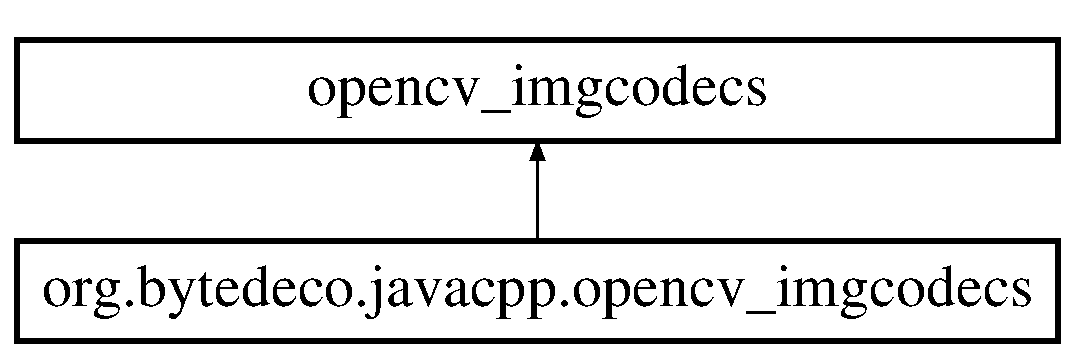
\includegraphics[height=2.000000cm]{classorg_1_1bytedeco_1_1javacpp_1_1opencv__imgcodecs}
\end{center}
\end{figure}
\subsection*{Static Public Member Functions}
\begin{DoxyCompactItemize}
\item 
static native Ipl\+Image {\bfseries cv\+Load\+Image} ( @Cast(\char`\"{}const char$\ast$\char`\"{}) Byte\+Pointer filename, int iscolor)
\item 
static native Ipl\+Image {\bfseries cv\+Load\+Image} ( @Cast(\char`\"{}const char$\ast$\char`\"{}) Byte\+Pointer filename)
\item 
static native Ipl\+Image {\bfseries cv\+Load\+Image} (String filename, int iscolor)
\item 
static native Ipl\+Image {\bfseries cv\+Load\+Image} (String filename)
\item 
static native Cv\+Mat {\bfseries cv\+Load\+ImageM} ( @Cast(\char`\"{}const char$\ast$\char`\"{}) Byte\+Pointer filename, int iscolor)
\item 
static native Cv\+Mat {\bfseries cv\+Load\+ImageM} ( @Cast(\char`\"{}const char$\ast$\char`\"{}) Byte\+Pointer filename)
\item 
static native Cv\+Mat {\bfseries cv\+Load\+ImageM} (String filename, int iscolor)
\item 
static native Cv\+Mat {\bfseries cv\+Load\+ImageM} (String filename)
\item 
static native int {\bfseries cv\+Save\+Image} ( @Cast(\char`\"{}const char$\ast$\char`\"{}) Byte\+Pointer filename, @Const Cv\+Arr image, @Const Int\+Pointer params)
\item 
static native int {\bfseries cv\+Save\+Image} ( @Cast(\char`\"{}const char$\ast$\char`\"{}) Byte\+Pointer filename, @Const Cv\+Arr image)
\item 
static native int {\bfseries cv\+Save\+Image} (String filename, @Const Cv\+Arr image, @Const Int\+Buffer params)
\item 
static native int {\bfseries cv\+Save\+Image} (String filename, @Const Cv\+Arr image)
\item 
static native int {\bfseries cv\+Save\+Image} ( @Cast(\char`\"{}const char$\ast$\char`\"{}) Byte\+Pointer filename, @Const Cv\+Arr image, @Const int\mbox{[}$\,$\mbox{]} params)
\item 
static native int {\bfseries cv\+Save\+Image} (String filename, @Const Cv\+Arr image, @Const Int\+Pointer params)
\item 
static native int {\bfseries cv\+Save\+Image} ( @Cast(\char`\"{}const char$\ast$\char`\"{}) Byte\+Pointer filename, @Const Cv\+Arr image, @Const Int\+Buffer params)
\item 
static native int {\bfseries cv\+Save\+Image} (String filename, @Const Cv\+Arr image, @Const int\mbox{[}$\,$\mbox{]} params)
\item 
static native Ipl\+Image {\bfseries cv\+Decode\+Image} ( @Const Cv\+Mat buf, int iscolor)
\item 
static native Ipl\+Image {\bfseries cv\+Decode\+Image} ( @Const Cv\+Mat buf)
\item 
static native Cv\+Mat {\bfseries cv\+Decode\+ImageM} ( @Const Cv\+Mat buf, int iscolor)
\item 
static native Cv\+Mat {\bfseries cv\+Decode\+ImageM} ( @Const Cv\+Mat buf)
\item 
static native Cv\+Mat {\bfseries cv\+Encode\+Image} ( @Cast(\char`\"{}const char$\ast$\char`\"{}) Byte\+Pointer ext, @Const Cv\+Arr image, @Const Int\+Pointer params)
\item 
static native Cv\+Mat {\bfseries cv\+Encode\+Image} ( @Cast(\char`\"{}const char$\ast$\char`\"{}) Byte\+Pointer ext, @Const Cv\+Arr image)
\item 
static native Cv\+Mat {\bfseries cv\+Encode\+Image} (String ext, @Const Cv\+Arr image, @Const Int\+Buffer params)
\item 
static native Cv\+Mat {\bfseries cv\+Encode\+Image} (String ext, @Const Cv\+Arr image)
\item 
static native Cv\+Mat {\bfseries cv\+Encode\+Image} ( @Cast(\char`\"{}const char$\ast$\char`\"{}) Byte\+Pointer ext, @Const Cv\+Arr image, @Const int\mbox{[}$\,$\mbox{]} params)
\item 
static native Cv\+Mat {\bfseries cv\+Encode\+Image} (String ext, @Const Cv\+Arr image, @Const Int\+Pointer params)
\item 
static native Cv\+Mat {\bfseries cv\+Encode\+Image} ( @Cast(\char`\"{}const char$\ast$\char`\"{}) Byte\+Pointer ext, @Const Cv\+Arr image, @Const Int\+Buffer params)
\item 
static native Cv\+Mat {\bfseries cv\+Encode\+Image} (String ext, @Const Cv\+Arr image, @Const int\mbox{[}$\,$\mbox{]} params)
\item 
static native void {\bfseries cv\+Convert\+Image} ( @Const Cv\+Arr src, Cv\+Arr dst, int flags)
\item 
static native void {\bfseries cv\+Convert\+Image} ( @Const Cv\+Arr src, Cv\+Arr dst)
\item 
static native int {\bfseries cv\+Have\+Image\+Reader} (@Cast(\char`\"{}const char$\ast$\char`\"{}) Byte\+Pointer filename)
\item 
static native int {\bfseries cv\+Have\+Image\+Reader} (String filename)
\item 
static native int {\bfseries cv\+Have\+Image\+Writer} (@Cast(\char`\"{}const char$\ast$\char`\"{}) Byte\+Pointer filename)
\item 
static native int {\bfseries cv\+Have\+Image\+Writer} (String filename)
\item 
static native Ipl\+Image {\bfseries cvv\+Load\+Image} (@Cast(\char`\"{}const char$\ast$\char`\"{}) Byte\+Pointer name)
\item 
static native Ipl\+Image {\bfseries cvv\+Load\+Image} (String name)
\item 
static native int {\bfseries cvv\+Save\+Image} (@Cast(\char`\"{}const char$\ast$\char`\"{}) Byte\+Pointer arg1, Cv\+Arr arg2, Int\+Pointer arg3)
\item 
static native int {\bfseries cvv\+Save\+Image} (String arg1, Cv\+Arr arg2, Int\+Buffer arg3)
\item 
static native int {\bfseries cvv\+Save\+Image} (@Cast(\char`\"{}const char$\ast$\char`\"{}) Byte\+Pointer arg1, Cv\+Arr arg2, int\mbox{[}$\,$\mbox{]} arg3)
\item 
static native int {\bfseries cvv\+Save\+Image} (String arg1, Cv\+Arr arg2, Int\+Pointer arg3)
\item 
static native int {\bfseries cvv\+Save\+Image} (@Cast(\char`\"{}const char$\ast$\char`\"{}) Byte\+Pointer arg1, Cv\+Arr arg2, Int\+Buffer arg3)
\item 
static native int {\bfseries cvv\+Save\+Image} (String arg1, Cv\+Arr arg2, int\mbox{[}$\,$\mbox{]} arg3)
\item 
static native void {\bfseries cvv\+Convert\+Image} (Cv\+Arr arg1, Cv\+Arr arg2, int arg3)
\item 
static native Mat \hyperlink{group__imgcodecs_gab0d3350cc2fd1d26eaae6aeb9df1f14e}{imread} ( @Str Byte\+Pointer filename, int flags)
\begin{DoxyCompactList}\small\item\em Loads an image from a file. \end{DoxyCompactList}\item 
static native Mat {\bfseries imread} ( @Str Byte\+Pointer filename)
\item 
static native Mat {\bfseries imread} ( @Str String filename, int flags)
\item 
static native Mat {\bfseries imread} ( @Str String filename)
\item 
static native boolean \hyperlink{group__imgcodecs_ga4e94bb9f788558a0b9eb892cc7a33bb9}{imreadmulti} (@Str Byte\+Pointer filename, @By\+Ref Mat\+Vector mats, int flags)
\begin{DoxyCompactList}\small\item\em Loads a multi-\/page image from a file. \end{DoxyCompactList}\item 
static native boolean {\bfseries imreadmulti} (@Str Byte\+Pointer filename, @By\+Ref Mat\+Vector mats)
\item 
static native boolean {\bfseries imreadmulti} (@Str String filename, @By\+Ref Mat\+Vector mats, int flags)
\item 
static native boolean {\bfseries imreadmulti} (@Str String filename, @By\+Ref Mat\+Vector mats)
\item 
static native boolean \hyperlink{group__imgcodecs_ga6a41cdd78ff2dd6fff47515e6d60212c}{imwrite} ( @Str Byte\+Pointer filename, @By\+Val Mat img, @Std\+Vector Int\+Pointer params)
\begin{DoxyCompactList}\small\item\em Saves an image to a specified file. \end{DoxyCompactList}\item 
static native boolean {\bfseries imwrite} ( @Str Byte\+Pointer filename, @By\+Val Mat img)
\item 
static native boolean {\bfseries imwrite} ( @Str String filename, @By\+Val Mat img, @Std\+Vector Int\+Buffer params)
\item 
static native boolean {\bfseries imwrite} ( @Str String filename, @By\+Val Mat img)
\item 
static native boolean {\bfseries imwrite} ( @Str Byte\+Pointer filename, @By\+Val U\+Mat img, @Std\+Vector int\mbox{[}$\,$\mbox{]} params)
\item 
static native boolean {\bfseries imwrite} ( @Str Byte\+Pointer filename, @By\+Val U\+Mat img)
\item 
static native boolean {\bfseries imwrite} ( @Str String filename, @By\+Val U\+Mat img, @Std\+Vector Int\+Pointer params)
\item 
static native boolean {\bfseries imwrite} ( @Str String filename, @By\+Val U\+Mat img)
\item 
static native boolean {\bfseries imwrite} ( @Str Byte\+Pointer filename, @By\+Val Mat img, @Std\+Vector Int\+Buffer params)
\item 
static native boolean {\bfseries imwrite} ( @Str String filename, @By\+Val Mat img, @Std\+Vector int\mbox{[}$\,$\mbox{]} params)
\item 
static native boolean {\bfseries imwrite} ( @Str Byte\+Pointer filename, @By\+Val U\+Mat img, @Std\+Vector Int\+Pointer params)
\item 
static native boolean {\bfseries imwrite} ( @Str String filename, @By\+Val U\+Mat img, @Std\+Vector Int\+Buffer params)
\item 
static native boolean {\bfseries imwrite} ( @Str Byte\+Pointer filename, @By\+Val Mat img, @Std\+Vector int\mbox{[}$\,$\mbox{]} params)
\item 
static native boolean {\bfseries imwrite} ( @Str String filename, @By\+Val Mat img, @Std\+Vector Int\+Pointer params)
\item 
static native boolean {\bfseries imwrite} ( @Str Byte\+Pointer filename, @By\+Val U\+Mat img, @Std\+Vector Int\+Buffer params)
\item 
static native boolean {\bfseries imwrite} ( @Str String filename, @By\+Val U\+Mat img, @Std\+Vector int\mbox{[}$\,$\mbox{]} params)
\item 
static native Mat \hyperlink{group__imgcodecs_gac13b3cea648e84cd2ead3c4849023497}{imdecode} ( @By\+Val Mat buf, int flags)
\begin{DoxyCompactList}\small\item\em Reads an image from a buffer in memory. \end{DoxyCompactList}\item 
static native Mat {\bfseries imdecode} ( @By\+Val U\+Mat buf, int flags)
\item 
static native Mat \hyperlink{group__imgcodecs_gaf794fdf6c3f9d68b53c283bc7ee3d8ef}{imdecode} ( @By\+Val Mat buf, int flags, Mat dst)
\item 
static native Mat {\bfseries imdecode} ( @By\+Val U\+Mat buf, int flags, Mat dst)
\item 
static native boolean \hyperlink{group__imgcodecs_ga99b838a1ddfa3318e2ba7d2dd5ef42cc}{imencode} ( @Str Byte\+Pointer ext, @By\+Val Mat img, @Cast(\char`\"{}uchar$\ast$\char`\"{}) @Std\+Vector Byte\+Pointer buf, @Std\+Vector Int\+Pointer params)
\begin{DoxyCompactList}\small\item\em Encodes an image into a memory buffer. \end{DoxyCompactList}\item 
static native boolean {\bfseries imencode} ( @Str Byte\+Pointer ext, @By\+Val Mat img, @Cast(\char`\"{}uchar$\ast$\char`\"{}) @Std\+Vector Byte\+Pointer buf)
\item 
static native boolean {\bfseries imencode} ( @Str String ext, @By\+Val Mat img, @Cast(\char`\"{}uchar$\ast$\char`\"{}) @Std\+Vector Byte\+Buffer buf, @Std\+Vector Int\+Buffer params)
\item 
static native boolean {\bfseries imencode} ( @Str String ext, @By\+Val Mat img, @Cast(\char`\"{}uchar$\ast$\char`\"{}) @Std\+Vector Byte\+Buffer buf)
\item 
static native boolean {\bfseries imencode} ( @Str Byte\+Pointer ext, @By\+Val U\+Mat img, @Cast(\char`\"{}uchar$\ast$\char`\"{}) @Std\+Vector byte\mbox{[}$\,$\mbox{]} buf, @Std\+Vector int\mbox{[}$\,$\mbox{]} params)
\item 
static native boolean {\bfseries imencode} ( @Str Byte\+Pointer ext, @By\+Val U\+Mat img, @Cast(\char`\"{}uchar$\ast$\char`\"{}) @Std\+Vector byte\mbox{[}$\,$\mbox{]} buf)
\item 
static native boolean {\bfseries imencode} ( @Str String ext, @By\+Val U\+Mat img, @Cast(\char`\"{}uchar$\ast$\char`\"{}) @Std\+Vector Byte\+Pointer buf, @Std\+Vector Int\+Pointer params)
\item 
static native boolean {\bfseries imencode} ( @Str String ext, @By\+Val U\+Mat img, @Cast(\char`\"{}uchar$\ast$\char`\"{}) @Std\+Vector Byte\+Pointer buf)
\item 
static native boolean {\bfseries imencode} ( @Str Byte\+Pointer ext, @By\+Val Mat img, @Cast(\char`\"{}uchar$\ast$\char`\"{}) @Std\+Vector Byte\+Buffer buf, @Std\+Vector Int\+Buffer params)
\item 
static native boolean {\bfseries imencode} ( @Str Byte\+Pointer ext, @By\+Val Mat img, @Cast(\char`\"{}uchar$\ast$\char`\"{}) @Std\+Vector Byte\+Buffer buf)
\item 
static native boolean {\bfseries imencode} ( @Str String ext, @By\+Val Mat img, @Cast(\char`\"{}uchar$\ast$\char`\"{}) @Std\+Vector byte\mbox{[}$\,$\mbox{]} buf, @Std\+Vector int\mbox{[}$\,$\mbox{]} params)
\item 
static native boolean {\bfseries imencode} ( @Str String ext, @By\+Val Mat img, @Cast(\char`\"{}uchar$\ast$\char`\"{}) @Std\+Vector byte\mbox{[}$\,$\mbox{]} buf)
\item 
static native boolean {\bfseries imencode} ( @Str Byte\+Pointer ext, @By\+Val U\+Mat img, @Cast(\char`\"{}uchar$\ast$\char`\"{}) @Std\+Vector Byte\+Pointer buf, @Std\+Vector Int\+Pointer params)
\item 
static native boolean {\bfseries imencode} ( @Str Byte\+Pointer ext, @By\+Val U\+Mat img, @Cast(\char`\"{}uchar$\ast$\char`\"{}) @Std\+Vector Byte\+Pointer buf)
\item 
static native boolean {\bfseries imencode} ( @Str String ext, @By\+Val U\+Mat img, @Cast(\char`\"{}uchar$\ast$\char`\"{}) @Std\+Vector Byte\+Buffer buf, @Std\+Vector Int\+Buffer params)
\item 
static native boolean {\bfseries imencode} ( @Str String ext, @By\+Val U\+Mat img, @Cast(\char`\"{}uchar$\ast$\char`\"{}) @Std\+Vector Byte\+Buffer buf)
\item 
static native boolean {\bfseries imencode} ( @Str Byte\+Pointer ext, @By\+Val Mat img, @Cast(\char`\"{}uchar$\ast$\char`\"{}) @Std\+Vector byte\mbox{[}$\,$\mbox{]} buf, @Std\+Vector int\mbox{[}$\,$\mbox{]} params)
\item 
static native boolean {\bfseries imencode} ( @Str Byte\+Pointer ext, @By\+Val Mat img, @Cast(\char`\"{}uchar$\ast$\char`\"{}) @Std\+Vector byte\mbox{[}$\,$\mbox{]} buf)
\item 
static native boolean {\bfseries imencode} ( @Str String ext, @By\+Val Mat img, @Cast(\char`\"{}uchar$\ast$\char`\"{}) @Std\+Vector Byte\+Pointer buf, @Std\+Vector Int\+Pointer params)
\item 
static native boolean {\bfseries imencode} ( @Str String ext, @By\+Val Mat img, @Cast(\char`\"{}uchar$\ast$\char`\"{}) @Std\+Vector Byte\+Pointer buf)
\item 
static native boolean {\bfseries imencode} ( @Str Byte\+Pointer ext, @By\+Val U\+Mat img, @Cast(\char`\"{}uchar$\ast$\char`\"{}) @Std\+Vector Byte\+Buffer buf, @Std\+Vector Int\+Buffer params)
\item 
static native boolean {\bfseries imencode} ( @Str Byte\+Pointer ext, @By\+Val U\+Mat img, @Cast(\char`\"{}uchar$\ast$\char`\"{}) @Std\+Vector Byte\+Buffer buf)
\item 
static native boolean {\bfseries imencode} ( @Str String ext, @By\+Val U\+Mat img, @Cast(\char`\"{}uchar$\ast$\char`\"{}) @Std\+Vector byte\mbox{[}$\,$\mbox{]} buf, @Std\+Vector int\mbox{[}$\,$\mbox{]} params)
\item 
static native boolean {\bfseries imencode} ( @Str String ext, @By\+Val U\+Mat img, @Cast(\char`\"{}uchar$\ast$\char`\"{}) @Std\+Vector byte\mbox{[}$\,$\mbox{]} buf)
\end{DoxyCompactItemize}
\subsection*{Static Public Attributes}
\begin{DoxyCompactItemize}
\item 
static final int \hyperlink{group__imgcodecs__c_ga98f1d87118e743ffeec57c7f3a10afd6}{C\+V\+\_\+\+L\+O\+A\+D\+\_\+\+I\+M\+A\+G\+E\+\_\+\+U\+N\+C\+H\+A\+N\+G\+ED} = -\/1
\item 
static final int \hyperlink{group__imgcodecs__c_ga6359737e32478705e367f06a0a4d14b1}{C\+V\+\_\+\+I\+M\+W\+R\+I\+T\+E\+\_\+\+J\+P\+E\+G\+\_\+\+Q\+U\+A\+L\+I\+TY} = 1
\item 
static final int \hyperlink{group__imgcodecs__c_ga9e58aa60c2a368479b56debeae227525}{C\+V\+\_\+\+C\+V\+T\+I\+M\+G\+\_\+\+F\+L\+IP} = 1
\item 
static final int \hyperlink{group__imgcodecs_gaba8d68ffadfa415aec1a51ee480143a7}{I\+M\+R\+E\+A\+D\+\_\+\+U\+N\+C\+H\+A\+N\+G\+ED} = -\/1
\item 
static final int \hyperlink{group__imgcodecs_gacc5cde2ea5764c3a523832a3d5c6c7e4}{I\+M\+W\+R\+I\+T\+E\+\_\+\+J\+P\+E\+G\+\_\+\+Q\+U\+A\+L\+I\+TY} = 1
\item 
static final int \hyperlink{group__imgcodecs_gabb28172fadcb5118b62c1e96ce65d7bd}{I\+M\+W\+R\+I\+T\+E\+\_\+\+P\+N\+G\+\_\+\+S\+T\+R\+A\+T\+E\+G\+Y\+\_\+\+D\+E\+F\+A\+U\+LT} = 0
\item 
static final int \hyperlink{group__imgcodecs_ga90aabdcbe963846b2645af3285b410b8}{I\+M\+W\+R\+I\+T\+E\+\_\+\+P\+A\+M\+\_\+\+F\+O\+R\+M\+A\+T\+\_\+\+N\+U\+LL} = 0
\end{DoxyCompactItemize}


The documentation for this class was generated from the following file\+:\begin{DoxyCompactItemize}
\item 
opencv\+\_\+imgcodecs.\+java\end{DoxyCompactItemize}

\hypertarget{classorg_1_1bytedeco_1_1javacpp_1_1opencv__imgproc}{}\section{org.\+bytedeco.\+javacpp.\+opencv\+\_\+imgproc Class Reference}
\label{classorg_1_1bytedeco_1_1javacpp_1_1opencv__imgproc}\index{org.\+bytedeco.\+javacpp.\+opencv\+\_\+imgproc@{org.\+bytedeco.\+javacpp.\+opencv\+\_\+imgproc}}
Inheritance diagram for org.\+bytedeco.\+javacpp.\+opencv\+\_\+imgproc\+:\begin{figure}[H]
\begin{center}
\leavevmode
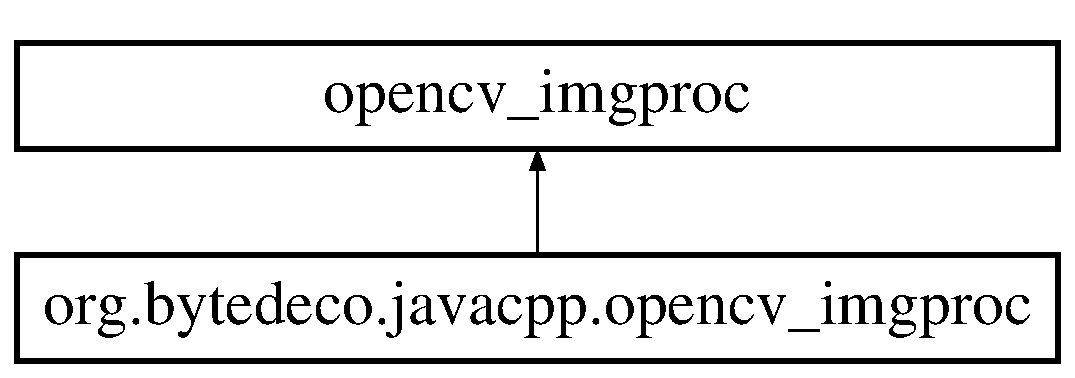
\includegraphics[height=2.000000cm]{classorg_1_1bytedeco_1_1javacpp_1_1opencv__imgproc}
\end{center}
\end{figure}
\subsection*{Classes}
\begin{DoxyCompactItemize}
\item 
class {\bfseries C\+L\+A\+HE}
\item 
class {\bfseries Cv\+Chain\+Pt\+Reader}
\item 
class {\bfseries Cv\+Connected\+Comp}
\item 
class {\bfseries Cv\+Contour\+Scanner}
\item 
class {\bfseries Cv\+Convexity\+Defect}
\item 
class {\bfseries Cv\+Distance\+Function}
\item 
class {\bfseries Cv\+Feature\+Tree}
\item 
class {\bfseries Cv\+Font}
\item 
class {\bfseries Cv\+Hu\+Moments}
\item 
class {\bfseries Cv\+L\+SH}
\item 
class {\bfseries Cv\+L\+S\+H\+Operations}
\item 
class {\bfseries Cv\+Moments}
\item 
class {\bfseries Generalized\+Hough}
\item 
class {\bfseries Generalized\+Hough\+Ballard}
\item 
class {\bfseries Generalized\+Hough\+Guil}
\item 
class {\bfseries Line\+Iterator}
\begin{DoxyCompactList}\small\item\em Line iterator. \end{DoxyCompactList}\item 
class {\bfseries Line\+Segment\+Detector}
\begin{DoxyCompactList}\small\item\em Line segment detector class. \end{DoxyCompactList}\item 
class {\bfseries Subdiv2D}
\end{DoxyCompactItemize}
\subsection*{Static Public Member Functions}
\begin{DoxyCompactItemize}
\item 
static native void \hyperlink{group__imgproc__c_ga59fe63bcfa209c1ced0035aca7d47f26}{cv\+Acc} ( @Const Cv\+Arr image, Cv\+Arr sum, @Const Cv\+Arr mask)
\begin{DoxyCompactList}\small\item\em Adds image to accumulator. \end{DoxyCompactList}\item 
static native void {\bfseries cv\+Acc} ( @Const Cv\+Arr image, Cv\+Arr sum)
\item 
static native void \hyperlink{group__imgproc__c_ga8c1d632da04d1ddc6e38b712f03adbe8}{cv\+Square\+Acc} ( @Const Cv\+Arr image, Cv\+Arr sqsum, @Const Cv\+Arr mask)
\begin{DoxyCompactList}\small\item\em Adds squared image to accumulator. \end{DoxyCompactList}\item 
static native void {\bfseries cv\+Square\+Acc} ( @Const Cv\+Arr image, Cv\+Arr sqsum)
\item 
static native void \hyperlink{group__imgproc__c_ga364a4081ca71e440b95082410d922f9c}{cv\+Multiply\+Acc} ( @Const Cv\+Arr image1, @Const Cv\+Arr image2, Cv\+Arr acc, @Const Cv\+Arr mask)
\begin{DoxyCompactList}\small\item\em Adds a product of two images to accumulator. \end{DoxyCompactList}\item 
static native void {\bfseries cv\+Multiply\+Acc} ( @Const Cv\+Arr image1, @Const Cv\+Arr image2, Cv\+Arr acc)
\item 
static native void \hyperlink{group__imgproc__c_gaf06fc48b42683511a2fc75d1fe34b2e8}{cv\+Running\+Avg} ( @Const Cv\+Arr image, Cv\+Arr acc, double alpha, @Const Cv\+Arr mask)
\begin{DoxyCompactList}\small\item\em Adds image to accumulator with weights\+: acc = acc$\ast$(1-\/alpha) + image$\ast$alpha. \end{DoxyCompactList}\item 
static native void {\bfseries cv\+Running\+Avg} ( @Const Cv\+Arr image, Cv\+Arr acc, double alpha)
\item 
static native void \hyperlink{group__imgproc__c_ga46ab19adc04378f8728b90f45240f5da}{cv\+Copy\+Make\+Border} ( @Const Cv\+Arr src, Cv\+Arr dst, @By\+Val Cv\+Point offset, int bordertype, @By\+Val(null\+Value=\char`\"{}Cv\+Scalar(cv\+Scalar\+All(0))\char`\"{}) Cv\+Scalar value)
\item 
static native void {\bfseries cv\+Copy\+Make\+Border} ( @Const Cv\+Arr src, Cv\+Arr dst, @By\+Val Cv\+Point offset, int bordertype)
\item 
static native void {\bfseries cv\+Copy\+Make\+Border} ( @Const Cv\+Arr src, Cv\+Arr dst, @By\+Val @Cast(\char`\"{}Cv\+Point$\ast$\char`\"{}) Int\+Buffer offset, int bordertype, @By\+Val(null\+Value=\char`\"{}Cv\+Scalar(cv\+Scalar\+All(0))\char`\"{}) Cv\+Scalar value)
\item 
static native void {\bfseries cv\+Copy\+Make\+Border} ( @Const Cv\+Arr src, Cv\+Arr dst, @By\+Val @Cast(\char`\"{}Cv\+Point$\ast$\char`\"{}) Int\+Buffer offset, int bordertype)
\item 
static native void {\bfseries cv\+Copy\+Make\+Border} ( @Const Cv\+Arr src, Cv\+Arr dst, @By\+Val @Cast(\char`\"{}Cv\+Point$\ast$\char`\"{}) int\mbox{[}$\,$\mbox{]} offset, int bordertype, @By\+Val(null\+Value=\char`\"{}Cv\+Scalar(cv\+Scalar\+All(0))\char`\"{}) Cv\+Scalar value)
\item 
static native void {\bfseries cv\+Copy\+Make\+Border} ( @Const Cv\+Arr src, Cv\+Arr dst, @By\+Val @Cast(\char`\"{}Cv\+Point$\ast$\char`\"{}) int\mbox{[}$\,$\mbox{]} offset, int bordertype)
\item 
static native void \hyperlink{group__imgproc__c_ga32746ef0800c2dfaad0e63fd8138362d}{cv\+Smooth} ( @Const Cv\+Arr src, Cv\+Arr dst, int smoothtype, int size1, int size2, double sigma1, double sigma2)
\begin{DoxyCompactList}\small\item\em Smooths the image in one of several ways. \end{DoxyCompactList}\item 
static native void {\bfseries cv\+Smooth} ( @Const Cv\+Arr src, Cv\+Arr dst)
\item 
static native void \hyperlink{group__imgproc__c_gaeb0ce4259621b5151099fcc7d4c25522}{cv\+Filter2D} ( @Const Cv\+Arr src, Cv\+Arr dst, @Const Cv\+Mat kernel, @By\+Val(null\+Value=\char`\"{}Cv\+Point(cv\+Point(-\/1,-\/1))\char`\"{}) Cv\+Point anchor)
\begin{DoxyCompactList}\small\item\em Convolves an image with the kernel. \end{DoxyCompactList}\item 
static native void {\bfseries cv\+Filter2D} ( @Const Cv\+Arr src, Cv\+Arr dst, @Const Cv\+Mat kernel)
\item 
static native void {\bfseries cv\+Filter2D} ( @Const Cv\+Arr src, Cv\+Arr dst, @Const Cv\+Mat kernel, @By\+Val(null\+Value=\char`\"{}Cv\+Point(cv\+Point(-\/1,-\/1))\char`\"{}) @Cast(\char`\"{}Cv\+Point$\ast$\char`\"{}) Int\+Buffer anchor)
\item 
static native void {\bfseries cv\+Filter2D} ( @Const Cv\+Arr src, Cv\+Arr dst, @Const Cv\+Mat kernel, @By\+Val(null\+Value=\char`\"{}Cv\+Point(cv\+Point(-\/1,-\/1))\char`\"{}) @Cast(\char`\"{}Cv\+Point$\ast$\char`\"{}) int\mbox{[}$\,$\mbox{]} anchor)
\item 
static native void \hyperlink{group__imgproc__c_ga08246108002aef3cbe4402ee61232191}{cv\+Integral} ( @Const Cv\+Arr image, Cv\+Arr sum, Cv\+Arr sqsum, Cv\+Arr tilted\+\_\+sum)
\begin{DoxyCompactList}\small\item\em Finds integral image\+: S\+U\+M(\+X,\+Y) = sum(x$<$\+X,y$<$\+Y)I(x,y) \end{DoxyCompactList}\item 
static native void {\bfseries cv\+Integral} ( @Const Cv\+Arr image, Cv\+Arr sum)
\item 
static native void \hyperlink{group__imgproc__c_ga728d5076e2233678be83cad3203472f9}{cv\+Pyr\+Down} ( @Const Cv\+Arr src, Cv\+Arr dst, int filter)
\begin{DoxyCompactList}\small\item\em Smoothes the input image with gaussian kernel and then down-\/samples it. \end{DoxyCompactList}\item 
static native void {\bfseries cv\+Pyr\+Down} ( @Const Cv\+Arr src, Cv\+Arr dst)
\item 
static native void \hyperlink{group__imgproc__c_ga08b1a7b3bf0f0c133345b307e6dfa952}{cv\+Pyr\+Up} ( @Const Cv\+Arr src, Cv\+Arr dst, int filter)
\begin{DoxyCompactList}\small\item\em Up-\/samples image and smoothes the result with gaussian kernel. \end{DoxyCompactList}\item 
static native void {\bfseries cv\+Pyr\+Up} ( @Const Cv\+Arr src, Cv\+Arr dst)
\item 
static native Pointer\+Pointer \hyperlink{group__imgproc__c_gad819c70ae44efaea82dfbf9745633179}{cv\+Create\+Pyramid} ( @Const Cv\+Arr img, int extra\+\_\+layers, double rate, @Const Cv\+Size layer\+\_\+sizes, Cv\+Arr bufarr, int calc, int filter)
\begin{DoxyCompactList}\small\item\em Builds pyramid for an image. \end{DoxyCompactList}\item 
static native Cv\+Mat {\bfseries cv\+Create\+Pyramid} ( @Const Cv\+Arr img, int extra\+\_\+layers, double rate)
\item 
static native void \hyperlink{group__imgproc__c_gafedcfec1793dc4d6dd6e5c97d4fb30a0}{cv\+Release\+Pyramid} ( @Cast(\char`\"{}Cv\+Mat$\ast$$\ast$$\ast$\char`\"{}) @By\+Ptr\+Ptr Pointer\+Pointer pyramid, int extra\+\_\+layers)
\begin{DoxyCompactList}\small\item\em Releases pyramid. \end{DoxyCompactList}\item 
static native void \hyperlink{group__imgproc__c_ga03ca86df80599c20db2980fb4a3eeed2}{cv\+Pyr\+Mean\+Shift\+Filtering} ( @Const Cv\+Arr src, Cv\+Arr dst, double sp, double sr, int max\+\_\+level, @By\+Val(null\+Value=\char`\"{}Cv\+Term\+Criteria(cv\+Term\+Criteria(C\+V\+\_\+\+T\+E\+R\+M\+C\+R\+I\+T\+\_\+\+I\+T\+ER+C\+V\+\_\+\+T\+E\+R\+M\+C\+R\+I\+T\+\_\+\+E\+PS,5,1))\char`\"{}) Cv\+Term\+Criteria termcrit)
\begin{DoxyCompactList}\small\item\em Filters image using meanshift algorithm. \end{DoxyCompactList}\item 
static native void {\bfseries cv\+Pyr\+Mean\+Shift\+Filtering} ( @Const Cv\+Arr src, Cv\+Arr dst, double sp, double sr)
\item 
static native void \hyperlink{group__imgproc__c_gae7b6a113cdd9df18a224597d7e034810}{cv\+Watershed} ( @Const Cv\+Arr image, Cv\+Arr markers)
\begin{DoxyCompactList}\small\item\em Segments image using seed \char`\"{}markers\char`\"{}. \end{DoxyCompactList}\item 
static native void \hyperlink{group__imgproc__c_ga8ef9469a1ca3c2940511a7f390eb6fb3}{cv\+Sobel} ( @Const Cv\+Arr src, Cv\+Arr dst, int xorder, int yorder, int aperture\+\_\+size)
\begin{DoxyCompactList}\small\item\em Calculates an image derivative using generalized Sobel. \end{DoxyCompactList}\item 
static native void {\bfseries cv\+Sobel} ( @Const Cv\+Arr src, Cv\+Arr dst, int xorder, int yorder)
\item 
static native void \hyperlink{group__imgproc__c_ga4b503d9c276d19dbced13ecd77b845a2}{cv\+Laplace} ( @Const Cv\+Arr src, Cv\+Arr dst, int aperture\+\_\+size)
\begin{DoxyCompactList}\small\item\em Calculates the image Laplacian\+: (d2/dx + d2/dy)I. \end{DoxyCompactList}\item 
static native void {\bfseries cv\+Laplace} ( @Const Cv\+Arr src, Cv\+Arr dst)
\item 
static native void \hyperlink{group__imgproc__c_gae45ba0b6ff1ccbe51ca42d2c6d6373bb}{cv\+Cvt\+Color} ( @Const Cv\+Arr src, Cv\+Arr dst, int code)
\begin{DoxyCompactList}\small\item\em Converts input array pixels from one color space to another. \end{DoxyCompactList}\item 
static native void \hyperlink{group__imgproc__c_ga45f9e0fb1d7c7f64227f5351c8e4bb2b}{cv\+Resize} ( @Const Cv\+Arr src, Cv\+Arr dst, int interpolation)
\begin{DoxyCompactList}\small\item\em Resizes image (input array is resized to fit the destination array) \end{DoxyCompactList}\item 
static native void {\bfseries cv\+Resize} ( @Const Cv\+Arr src, Cv\+Arr dst)
\item 
static native void \hyperlink{group__imgproc__c_gabf1cb9d4218222026652e60bea3c8b17}{cv\+Warp\+Affine} ( @Const Cv\+Arr src, Cv\+Arr dst, @Const Cv\+Mat map\+\_\+matrix, int flags, @By\+Val(null\+Value=\char`\"{}Cv\+Scalar(cv\+Scalar\+All(0))\char`\"{}) Cv\+Scalar fillval)
\begin{DoxyCompactList}\small\item\em Warps image with affine transform. \end{DoxyCompactList}\item 
static native void {\bfseries cv\+Warp\+Affine} ( @Const Cv\+Arr src, Cv\+Arr dst, @Const Cv\+Mat map\+\_\+matrix)
\item 
static native Cv\+Mat \hyperlink{group__imgproc__c_ga6deb33dc741b5402e8660d553cf299c3}{cv\+Get\+Affine\+Transform} ( @Const Cv\+Point2\+D32f src, @Const Cv\+Point2\+D32f dst, Cv\+Mat map\+\_\+matrix)
\begin{DoxyCompactList}\small\item\em Computes affine transform matrix for mapping src\mbox{[}i\mbox{]} to dst\mbox{[}i\mbox{]} (i=0,1,2) \end{DoxyCompactList}\item 
static native Cv\+Mat {\bfseries cv\+Get\+Affine\+Transform} ( @Cast(\char`\"{}const Cv\+Point2\+D32f$\ast$\char`\"{}) Float\+Buffer src, @Cast(\char`\"{}const Cv\+Point2\+D32f$\ast$\char`\"{}) Float\+Buffer dst, Cv\+Mat map\+\_\+matrix)
\item 
static native Cv\+Mat {\bfseries cv\+Get\+Affine\+Transform} ( @Cast(\char`\"{}const Cv\+Point2\+D32f$\ast$\char`\"{}) float\mbox{[}$\,$\mbox{]} src, @Cast(\char`\"{}const Cv\+Point2\+D32f$\ast$\char`\"{}) float\mbox{[}$\,$\mbox{]} dst, Cv\+Mat map\+\_\+matrix)
\item 
static native Cv\+Mat \hyperlink{group__imgproc__c_ga8808b742ceec81dac792c107ef82fe13}{cv2\+D\+Rotation\+Matrix} ( @By\+Val Cv\+Point2\+D32f center, double angle, double scale, Cv\+Mat map\+\_\+matrix)
\begin{DoxyCompactList}\small\item\em Computes rotation\+\_\+matrix matrix. \end{DoxyCompactList}\item 
static native Cv\+Mat {\bfseries cv2\+D\+Rotation\+Matrix} ( @By\+Val @Cast(\char`\"{}Cv\+Point2\+D32f$\ast$\char`\"{}) Float\+Buffer center, double angle, double scale, Cv\+Mat map\+\_\+matrix)
\item 
static native Cv\+Mat {\bfseries cv2\+D\+Rotation\+Matrix} ( @By\+Val @Cast(\char`\"{}Cv\+Point2\+D32f$\ast$\char`\"{}) float\mbox{[}$\,$\mbox{]} center, double angle, double scale, Cv\+Mat map\+\_\+matrix)
\item 
static native void \hyperlink{group__imgproc__c_ga77d2f4184f964c0a75b65d576b0fd417}{cv\+Warp\+Perspective} ( @Const Cv\+Arr src, Cv\+Arr dst, @Const Cv\+Mat map\+\_\+matrix, int flags, @By\+Val(null\+Value=\char`\"{}Cv\+Scalar(cv\+Scalar\+All(0))\char`\"{}) Cv\+Scalar fillval)
\begin{DoxyCompactList}\small\item\em Warps image with perspective (projective) transform. \end{DoxyCompactList}\item 
static native void {\bfseries cv\+Warp\+Perspective} ( @Const Cv\+Arr src, Cv\+Arr dst, @Const Cv\+Mat map\+\_\+matrix)
\item 
static native Cv\+Mat \hyperlink{group__imgproc__c_ga90db3b12f84ee1bea538d6d88bab49c3}{cv\+Get\+Perspective\+Transform} ( @Const Cv\+Point2\+D32f src, @Const Cv\+Point2\+D32f dst, Cv\+Mat map\+\_\+matrix)
\begin{DoxyCompactList}\small\item\em Computes perspective transform matrix for mapping src\mbox{[}i\mbox{]} to dst\mbox{[}i\mbox{]} (i=0,1,2,3) \end{DoxyCompactList}\item 
static native Cv\+Mat {\bfseries cv\+Get\+Perspective\+Transform} ( @Cast(\char`\"{}const Cv\+Point2\+D32f$\ast$\char`\"{}) Float\+Buffer src, @Cast(\char`\"{}const Cv\+Point2\+D32f$\ast$\char`\"{}) Float\+Buffer dst, Cv\+Mat map\+\_\+matrix)
\item 
static native Cv\+Mat {\bfseries cv\+Get\+Perspective\+Transform} ( @Cast(\char`\"{}const Cv\+Point2\+D32f$\ast$\char`\"{}) float\mbox{[}$\,$\mbox{]} src, @Cast(\char`\"{}const Cv\+Point2\+D32f$\ast$\char`\"{}) float\mbox{[}$\,$\mbox{]} dst, Cv\+Mat map\+\_\+matrix)
\item 
static native void \hyperlink{group__imgproc__c_ga5fc4449699da7b00973991b5b610efbb}{cv\+Remap} ( @Const Cv\+Arr src, Cv\+Arr dst, @Const Cv\+Arr mapx, @Const Cv\+Arr mapy, int flags, @By\+Val(null\+Value=\char`\"{}Cv\+Scalar(cv\+Scalar\+All(0))\char`\"{}) Cv\+Scalar fillval)
\begin{DoxyCompactList}\small\item\em Performs generic geometric transformation using the specified coordinate maps. \end{DoxyCompactList}\item 
static native void {\bfseries cv\+Remap} ( @Const Cv\+Arr src, Cv\+Arr dst, @Const Cv\+Arr mapx, @Const Cv\+Arr mapy)
\item 
static native void \hyperlink{group__imgproc__c_ga9e8c4e8b6609f6bad114d7a6e597d530}{cv\+Convert\+Maps} ( @Const Cv\+Arr mapx, @Const Cv\+Arr mapy, Cv\+Arr mapxy, Cv\+Arr mapalpha)
\begin{DoxyCompactList}\small\item\em Converts mapx \& mapy from floating-\/point to integer formats for cv\+Remap. \end{DoxyCompactList}\item 
static native void \hyperlink{group__imgproc__c_gaa181829e06fd0d2f59e112e2a5e27129}{cv\+Log\+Polar} ( @Const Cv\+Arr src, Cv\+Arr dst, @By\+Val Cv\+Point2\+D32f center, double M, int flags)
\begin{DoxyCompactList}\small\item\em Performs forward or inverse log-\/polar image transform. \end{DoxyCompactList}\item 
static native void {\bfseries cv\+Log\+Polar} ( @Const Cv\+Arr src, Cv\+Arr dst, @By\+Val Cv\+Point2\+D32f center, double M)
\item 
static native void {\bfseries cv\+Log\+Polar} ( @Const Cv\+Arr src, Cv\+Arr dst, @By\+Val @Cast(\char`\"{}Cv\+Point2\+D32f$\ast$\char`\"{}) Float\+Buffer center, double M, int flags)
\item 
static native void {\bfseries cv\+Log\+Polar} ( @Const Cv\+Arr src, Cv\+Arr dst, @By\+Val @Cast(\char`\"{}Cv\+Point2\+D32f$\ast$\char`\"{}) Float\+Buffer center, double M)
\item 
static native void {\bfseries cv\+Log\+Polar} ( @Const Cv\+Arr src, Cv\+Arr dst, @By\+Val @Cast(\char`\"{}Cv\+Point2\+D32f$\ast$\char`\"{}) float\mbox{[}$\,$\mbox{]} center, double M, int flags)
\item 
static native void {\bfseries cv\+Log\+Polar} ( @Const Cv\+Arr src, Cv\+Arr dst, @By\+Val @Cast(\char`\"{}Cv\+Point2\+D32f$\ast$\char`\"{}) float\mbox{[}$\,$\mbox{]} center, double M)
\item 
static native void \hyperlink{group__imgproc__c_gaea7618f99d98e843a4bd01f403a4995e}{cv\+Linear\+Polar} ( @Const Cv\+Arr src, Cv\+Arr dst, @By\+Val Cv\+Point2\+D32f center, double max\+Radius, int flags)
\item 
static native void {\bfseries cv\+Linear\+Polar} ( @Const Cv\+Arr src, Cv\+Arr dst, @By\+Val Cv\+Point2\+D32f center, double max\+Radius)
\item 
static native void {\bfseries cv\+Linear\+Polar} ( @Const Cv\+Arr src, Cv\+Arr dst, @By\+Val @Cast(\char`\"{}Cv\+Point2\+D32f$\ast$\char`\"{}) Float\+Buffer center, double max\+Radius, int flags)
\item 
static native void {\bfseries cv\+Linear\+Polar} ( @Const Cv\+Arr src, Cv\+Arr dst, @By\+Val @Cast(\char`\"{}Cv\+Point2\+D32f$\ast$\char`\"{}) Float\+Buffer center, double max\+Radius)
\item 
static native void {\bfseries cv\+Linear\+Polar} ( @Const Cv\+Arr src, Cv\+Arr dst, @By\+Val @Cast(\char`\"{}Cv\+Point2\+D32f$\ast$\char`\"{}) float\mbox{[}$\,$\mbox{]} center, double max\+Radius, int flags)
\item 
static native void {\bfseries cv\+Linear\+Polar} ( @Const Cv\+Arr src, Cv\+Arr dst, @By\+Val @Cast(\char`\"{}Cv\+Point2\+D32f$\ast$\char`\"{}) float\mbox{[}$\,$\mbox{]} center, double max\+Radius)
\item 
static native void \hyperlink{group__imgproc__c_ga2b891154762834fb030334ea95ebdce9}{cv\+Undistort2} ( @Const Cv\+Arr src, Cv\+Arr dst, @Const Cv\+Mat camera\+\_\+matrix, @Const Cv\+Mat distortion\+\_\+coeffs, @Const Cv\+Mat new\+\_\+camera\+\_\+matrix)
\begin{DoxyCompactList}\small\item\em Transforms the input image to compensate lens distortion. \end{DoxyCompactList}\item 
static native void {\bfseries cv\+Undistort2} ( @Const Cv\+Arr src, Cv\+Arr dst, @Const Cv\+Mat camera\+\_\+matrix, @Const Cv\+Mat distortion\+\_\+coeffs)
\item 
static native void \hyperlink{group__imgproc__c_gabf5495653e45cb87934afd107d253eba}{cv\+Init\+Undistort\+Map} ( @Const Cv\+Mat camera\+\_\+matrix, @Const Cv\+Mat distortion\+\_\+coeffs, Cv\+Arr mapx, Cv\+Arr mapy)
\begin{DoxyCompactList}\small\item\em Computes transformation map from intrinsic camera parameters that can used by cv\+Remap. \end{DoxyCompactList}\item 
static native void \hyperlink{group__imgproc__c_gab25847a22028fe0d1088d6572aca641a}{cv\+Init\+Undistort\+Rectify\+Map} ( @Const Cv\+Mat camera\+\_\+matrix, @Const Cv\+Mat dist\+\_\+coeffs, @Const Cv\+Mat R, @Const Cv\+Mat new\+\_\+camera\+\_\+matrix, Cv\+Arr mapx, Cv\+Arr mapy)
\begin{DoxyCompactList}\small\item\em Computes undistortion+rectification map for a head of stereo camera. \end{DoxyCompactList}\item 
static native void \hyperlink{group__imgproc__c_ga21444b957a9e68dffef016a844ff35a1}{cv\+Undistort\+Points} ( @Const Cv\+Mat src, Cv\+Mat dst, @Const Cv\+Mat camera\+\_\+matrix, @Const Cv\+Mat dist\+\_\+coeffs, @Const Cv\+Mat R, @Const Cv\+Mat P)
\begin{DoxyCompactList}\small\item\em Computes the original (undistorted) feature coordinates from the observed (distorted) coordinates. \end{DoxyCompactList}\item 
static native void {\bfseries cv\+Undistort\+Points} ( @Const Cv\+Mat src, Cv\+Mat dst, @Const Cv\+Mat camera\+\_\+matrix, @Const Cv\+Mat dist\+\_\+coeffs)
\item 
static native Ipl\+Conv\+Kernel \hyperlink{group__imgproc__c_ga8a9b8019d4c181721e0f3fbb6c87cb42}{cv\+Create\+Structuring\+Element\+Ex} (int cols, int rows, int anchor\+\_\+x, int anchor\+\_\+y, int shape, Int\+Pointer values)
\begin{DoxyCompactList}\small\item\em Returns a structuring element of the specified size and shape for morphological operations. \end{DoxyCompactList}\item 
static native Ipl\+Conv\+Kernel {\bfseries cv\+Create\+Structuring\+Element\+Ex} (int cols, int rows, int anchor\+\_\+x, int anchor\+\_\+y, int shape)
\item 
static native Ipl\+Conv\+Kernel {\bfseries cv\+Create\+Structuring\+Element\+Ex} (int cols, int rows, int anchor\+\_\+x, int anchor\+\_\+y, int shape, Int\+Buffer values)
\item 
static native Ipl\+Conv\+Kernel {\bfseries cv\+Create\+Structuring\+Element\+Ex} (int cols, int rows, int anchor\+\_\+x, int anchor\+\_\+y, int shape, int\mbox{[}$\,$\mbox{]} values)
\item 
static native void \hyperlink{group__imgproc__c_gaddb6b08638fde5f3641e96a7b033f774}{cv\+Release\+Structuring\+Element} ( @Cast(\char`\"{}Ipl\+Conv\+Kernel$\ast$$\ast$\char`\"{}) Pointer\+Pointer element)
\begin{DoxyCompactList}\small\item\em releases structuring element \end{DoxyCompactList}\item 
static native void {\bfseries cv\+Release\+Structuring\+Element} ( @By\+Ptr\+Ptr Ipl\+Conv\+Kernel element)
\item 
static native void \hyperlink{group__imgproc__c_ga8b958e2b5185910eba9b44400bb1d3b8}{cv\+Erode} ( @Const Cv\+Arr src, Cv\+Arr dst, Ipl\+Conv\+Kernel element, int iterations)
\begin{DoxyCompactList}\small\item\em erodes input image (applies minimum filter) one or more times. If element pointer is N\+U\+LL, 3x3 rectangular element is used \end{DoxyCompactList}\item 
static native void {\bfseries cv\+Erode} ( @Const Cv\+Arr src, Cv\+Arr dst)
\item 
static native void \hyperlink{group__imgproc__c_gae80f82cb5e9876985e59aec2267f7ad4}{cv\+Dilate} ( @Const Cv\+Arr src, Cv\+Arr dst, Ipl\+Conv\+Kernel element, int iterations)
\begin{DoxyCompactList}\small\item\em dilates input image (applies maximum filter) one or more times. \end{DoxyCompactList}\item 
static native void {\bfseries cv\+Dilate} ( @Const Cv\+Arr src, Cv\+Arr dst)
\item 
static native void \hyperlink{group__imgproc__c_ga09edd651f402b82f067e6de776bbd197}{cv\+Morphology\+Ex} ( @Const Cv\+Arr src, Cv\+Arr dst, Cv\+Arr temp, Ipl\+Conv\+Kernel element, int operation, int iterations)
\begin{DoxyCompactList}\small\item\em Performs complex morphological transformation. \end{DoxyCompactList}\item 
static native void {\bfseries cv\+Morphology\+Ex} ( @Const Cv\+Arr src, Cv\+Arr dst, Cv\+Arr temp, Ipl\+Conv\+Kernel element, int operation)
\item 
static native void \hyperlink{group__imgproc__c_gaebcdbe34c2a6e8811e34cb4fa10fcaaf}{cv\+Moments} ( @Const Cv\+Arr arr, Cv\+Moments moments, int binary)
\begin{DoxyCompactList}\small\item\em Calculates all spatial and central moments up to the 3rd order. \end{DoxyCompactList}\item 
static native void {\bfseries cv\+Moments} ( @Const Cv\+Arr arr, Cv\+Moments moments)
\item 
static native double \hyperlink{group__imgproc__c_ga4eb91f7795453d7e5d41a27a5a7dbeed}{cv\+Get\+Spatial\+Moment} (Cv\+Moments moments, int x\+\_\+order, int y\+\_\+order)
\begin{DoxyCompactList}\small\item\em Retrieve spatial moments. \end{DoxyCompactList}\item 
static native double \hyperlink{group__imgproc__c_ga190761deb92e902c8f377752e3b439e6}{cv\+Get\+Central\+Moment} (Cv\+Moments moments, int x\+\_\+order, int y\+\_\+order)
\begin{DoxyCompactList}\small\item\em Retrieve central moments. \end{DoxyCompactList}\item 
static native double \hyperlink{group__imgproc__c_ga6367a05304ca14f1b94119a52d5190a7}{cv\+Get\+Normalized\+Central\+Moment} (Cv\+Moments moments, int x\+\_\+order, int y\+\_\+order)
\begin{DoxyCompactList}\small\item\em Retrieve normalized central moments. \end{DoxyCompactList}\item 
static native void \hyperlink{group__imgproc__c_ga5cfeea3efab741f8674c0e28172e134f}{cv\+Get\+Hu\+Moments} (Cv\+Moments moments, Cv\+Hu\+Moments hu\+\_\+moments)
\begin{DoxyCompactList}\small\item\em Calculates 7 Hu\textquotesingle{}s invariants from precalculated spatial and central moments. \end{DoxyCompactList}\item 
static native int \hyperlink{group__imgproc__c_gaea92829f3b2b25c80d12aa39d189fd70}{cv\+Sample\+Line} ( @Const Cv\+Arr image, @By\+Val Cv\+Point pt1, @By\+Val Cv\+Point pt2, Pointer buffer, int connectivity)
\begin{DoxyCompactList}\small\item\em Fetches pixels that belong to the specified line segment and stores them to the buffer. \end{DoxyCompactList}\item 
static native int {\bfseries cv\+Sample\+Line} ( @Const Cv\+Arr image, @By\+Val Cv\+Point pt1, @By\+Val Cv\+Point pt2, Pointer buffer)
\item 
static native int {\bfseries cv\+Sample\+Line} ( @Const Cv\+Arr image, @By\+Val @Cast(\char`\"{}Cv\+Point$\ast$\char`\"{}) Int\+Buffer pt1, @By\+Val @Cast(\char`\"{}Cv\+Point$\ast$\char`\"{}) Int\+Buffer pt2, Pointer buffer, int connectivity)
\item 
static native int {\bfseries cv\+Sample\+Line} ( @Const Cv\+Arr image, @By\+Val @Cast(\char`\"{}Cv\+Point$\ast$\char`\"{}) Int\+Buffer pt1, @By\+Val @Cast(\char`\"{}Cv\+Point$\ast$\char`\"{}) Int\+Buffer pt2, Pointer buffer)
\item 
static native int {\bfseries cv\+Sample\+Line} ( @Const Cv\+Arr image, @By\+Val @Cast(\char`\"{}Cv\+Point$\ast$\char`\"{}) int\mbox{[}$\,$\mbox{]} pt1, @By\+Val @Cast(\char`\"{}Cv\+Point$\ast$\char`\"{}) int\mbox{[}$\,$\mbox{]} pt2, Pointer buffer, int connectivity)
\item 
static native int {\bfseries cv\+Sample\+Line} ( @Const Cv\+Arr image, @By\+Val @Cast(\char`\"{}Cv\+Point$\ast$\char`\"{}) int\mbox{[}$\,$\mbox{]} pt1, @By\+Val @Cast(\char`\"{}Cv\+Point$\ast$\char`\"{}) int\mbox{[}$\,$\mbox{]} pt2, Pointer buffer)
\item 
static native void \hyperlink{group__imgproc__c_gafdd84b3138aa7fa919555c124ccd6c0c}{cv\+Get\+Rect\+Sub\+Pix} ( @Const Cv\+Arr src, Cv\+Arr dst, @By\+Val Cv\+Point2\+D32f center)
\begin{DoxyCompactList}\small\item\em Retrieves the rectangular image region with specified center from the input array. \end{DoxyCompactList}\item 
static native void {\bfseries cv\+Get\+Rect\+Sub\+Pix} ( @Const Cv\+Arr src, Cv\+Arr dst, @By\+Val @Cast(\char`\"{}Cv\+Point2\+D32f$\ast$\char`\"{}) Float\+Buffer center)
\item 
static native void {\bfseries cv\+Get\+Rect\+Sub\+Pix} ( @Const Cv\+Arr src, Cv\+Arr dst, @By\+Val @Cast(\char`\"{}Cv\+Point2\+D32f$\ast$\char`\"{}) float\mbox{[}$\,$\mbox{]} center)
\item 
static native void \hyperlink{group__imgproc__c_gafb07651da746782b1b92bce7179079e1}{cv\+Get\+Quadrangle\+Sub\+Pix} ( @Const Cv\+Arr src, Cv\+Arr dst, @Const Cv\+Mat map\+\_\+matrix)
\begin{DoxyCompactList}\small\item\em Retrieves quadrangle from the input array. \end{DoxyCompactList}\item 
static native void \hyperlink{group__imgproc__c_ga6dda3f1745d471681378d2515509372a}{cv\+Match\+Template} ( @Const Cv\+Arr image, @Const Cv\+Arr templ, Cv\+Arr result, int method)
\begin{DoxyCompactList}\small\item\em Measures similarity between template and overlapped windows in the source image and fills the resultant image with the measurements. \end{DoxyCompactList}\item 
static native float \hyperlink{group__imgproc__c_ga9960ba1e43fe6c47233d8e0d0c6a37f2}{cv\+Calc\+E\+M\+D2} ( @Const Cv\+Arr signature1, @Const Cv\+Arr signature2, int distance\+\_\+type, Cv\+Distance\+Function distance\+\_\+func, @Const Cv\+Arr cost\+\_\+matrix, Cv\+Arr flow, Float\+Pointer lower\+\_\+bound, Pointer userdata)
\begin{DoxyCompactList}\small\item\em Computes earth mover distance between two weighted point sets (called signatures) \end{DoxyCompactList}\item 
static native float {\bfseries cv\+Calc\+E\+M\+D2} ( @Const Cv\+Arr signature1, @Const Cv\+Arr signature2, int distance\+\_\+type)
\item 
static native float {\bfseries cv\+Calc\+E\+M\+D2} ( @Const Cv\+Arr signature1, @Const Cv\+Arr signature2, int distance\+\_\+type, Cv\+Distance\+Function distance\+\_\+func, @Const Cv\+Arr cost\+\_\+matrix, Cv\+Arr flow, Float\+Buffer lower\+\_\+bound, Pointer userdata)
\item 
static native float {\bfseries cv\+Calc\+E\+M\+D2} ( @Const Cv\+Arr signature1, @Const Cv\+Arr signature2, int distance\+\_\+type, Cv\+Distance\+Function distance\+\_\+func, @Const Cv\+Arr cost\+\_\+matrix, Cv\+Arr flow, float\mbox{[}$\,$\mbox{]} lower\+\_\+bound, Pointer userdata)
\item 
static native int \hyperlink{group__imgproc__c_gaa4cfb26bdebe22cd9a83d79b429520ee}{cv\+Find\+Contours} (Cv\+Arr image, Cv\+Mem\+Storage storage, @Cast(\char`\"{}Cv\+Seq$\ast$$\ast$\char`\"{}) Pointer\+Pointer first\+\_\+contour, int header\+\_\+size, int mode, int method, @By\+Val(null\+Value=\char`\"{}Cv\+Point(cv\+Point(0,0))\char`\"{}) Cv\+Point offset)
\begin{DoxyCompactList}\small\item\em Retrieves outer and optionally inner boundaries of white (non-\/zero) connected components in the black (zero) background. \end{DoxyCompactList}\item 
static native int {\bfseries cv\+Find\+Contours} (Cv\+Arr image, Cv\+Mem\+Storage storage, @By\+Ptr\+Ptr Cv\+Seq first\+\_\+contour)
\item 
static native int {\bfseries cv\+Find\+Contours} (Cv\+Arr image, Cv\+Mem\+Storage storage, @By\+Ptr\+Ptr Cv\+Seq first\+\_\+contour, int header\+\_\+size, int mode, int method, @By\+Val(null\+Value=\char`\"{}Cv\+Point(cv\+Point(0,0))\char`\"{}) Cv\+Point offset)
\item 
static native int {\bfseries cv\+Find\+Contours} (Cv\+Arr image, Cv\+Mem\+Storage storage, @By\+Ptr\+Ptr Cv\+Seq first\+\_\+contour, int header\+\_\+size, int mode, int method, @By\+Val(null\+Value=\char`\"{}Cv\+Point(cv\+Point(0,0))\char`\"{}) @Cast(\char`\"{}Cv\+Point$\ast$\char`\"{}) Int\+Buffer offset)
\item 
static native int {\bfseries cv\+Find\+Contours} (Cv\+Arr image, Cv\+Mem\+Storage storage, @By\+Ptr\+Ptr Cv\+Seq first\+\_\+contour, int header\+\_\+size, int mode, int method, @By\+Val(null\+Value=\char`\"{}Cv\+Point(cv\+Point(0,0))\char`\"{}) @Cast(\char`\"{}Cv\+Point$\ast$\char`\"{}) int\mbox{[}$\,$\mbox{]} offset)
\item 
static native Cv\+Contour\+Scanner \hyperlink{group__imgproc__c_ga17ceae2468b1b23ece917fb982a377ff}{cv\+Start\+Find\+Contours} (Cv\+Arr image, Cv\+Mem\+Storage storage, int header\+\_\+size, int mode, int method, @By\+Val(null\+Value=\char`\"{}Cv\+Point(cv\+Point(0,0))\char`\"{}) Cv\+Point offset)
\begin{DoxyCompactList}\small\item\em Initializes contour retrieving process. \end{DoxyCompactList}\item 
static native Cv\+Contour\+Scanner {\bfseries cv\+Start\+Find\+Contours} (Cv\+Arr image, Cv\+Mem\+Storage storage)
\item 
static native Cv\+Contour\+Scanner {\bfseries cv\+Start\+Find\+Contours} (Cv\+Arr image, Cv\+Mem\+Storage storage, int header\+\_\+size, int mode, int method, @By\+Val(null\+Value=\char`\"{}Cv\+Point(cv\+Point(0,0))\char`\"{}) @Cast(\char`\"{}Cv\+Point$\ast$\char`\"{}) Int\+Buffer offset)
\item 
static native Cv\+Contour\+Scanner {\bfseries cv\+Start\+Find\+Contours} (Cv\+Arr image, Cv\+Mem\+Storage storage, int header\+\_\+size, int mode, int method, @By\+Val(null\+Value=\char`\"{}Cv\+Point(cv\+Point(0,0))\char`\"{}) @Cast(\char`\"{}Cv\+Point$\ast$\char`\"{}) int\mbox{[}$\,$\mbox{]} offset)
\item 
static native Cv\+Seq \hyperlink{group__imgproc__c_gab3ea632f49f741ef73888cd1ab8f9556}{cv\+Find\+Next\+Contour} (Cv\+Contour\+Scanner scanner)
\begin{DoxyCompactList}\small\item\em Retrieves next contour. \end{DoxyCompactList}\item 
static native void \hyperlink{group__imgproc__c_ga9d72a578b9f29589e8b85b100cd25e01}{cv\+Substitute\+Contour} (Cv\+Contour\+Scanner scanner, Cv\+Seq new\+\_\+contour)
\begin{DoxyCompactList}\small\item\em Substitutes the last retrieved contour with the new one. \end{DoxyCompactList}\item 
static native Cv\+Seq \hyperlink{group__imgproc__c_ga79913a8abbec2491176f92da28a62346}{cv\+End\+Find\+Contours} ( @By\+Ptr\+Ptr Cv\+Contour\+Scanner scanner)
\begin{DoxyCompactList}\small\item\em Releases contour scanner and returns pointer to the first outer contour. \end{DoxyCompactList}\item 
static native Cv\+Seq \hyperlink{group__imgproc__c_ga5c874856009b84fc0c3a9533f957516c}{cv\+Approx\+Chains} (Cv\+Seq src\+\_\+seq, Cv\+Mem\+Storage storage, int method, double parameter, int minimal\+\_\+perimeter, int recursive)
\begin{DoxyCompactList}\small\item\em Approximates Freeman chain(s) with a polygonal curve. \end{DoxyCompactList}\item 
static native Cv\+Seq {\bfseries cv\+Approx\+Chains} (Cv\+Seq src\+\_\+seq, Cv\+Mem\+Storage storage)
\item 
static native void \hyperlink{group__imgproc__c_gab6502128f5100580662a79a7326e50e0}{cv\+Start\+Read\+Chain\+Points} (Cv\+Chain chain, Cv\+Chain\+Pt\+Reader reader)
\begin{DoxyCompactList}\small\item\em Initializes Freeman chain reader. \end{DoxyCompactList}\item 
static native Cv\+Point \hyperlink{group__imgproc__c_ga60ca24d0d962737958150406351d91c7}{cv\+Read\+Chain\+Point} (Cv\+Chain\+Pt\+Reader reader)
\begin{DoxyCompactList}\small\item\em Retrieves the next chain point. \end{DoxyCompactList}\item 
static native Cv\+Seq \hyperlink{group__imgproc__c_ga04330d92548cde6503b33785252af580}{cv\+Approx\+Poly} ( @Const Pointer src\+\_\+seq, int header\+\_\+size, Cv\+Mem\+Storage storage, int method, double eps, int recursive)
\begin{DoxyCompactList}\small\item\em Approximates a single polygonal curve (contour) or a tree of polygonal curves (contours) \end{DoxyCompactList}\item 
static native Cv\+Seq {\bfseries cv\+Approx\+Poly} ( @Const Pointer src\+\_\+seq, int header\+\_\+size, Cv\+Mem\+Storage storage, int method, double eps)
\item 
static native double \hyperlink{group__imgproc__c_gaf095420cca062536116edaad5f0391ae}{cv\+Arc\+Length} ( @Const Pointer curve, @By\+Val(null\+Value=\char`\"{}Cv\+Slice(C\+V\+\_\+\+W\+H\+O\+L\+E\+\_\+\+S\+EQ)\char`\"{}) Cv\+Slice slice, int is\+\_\+closed)
\begin{DoxyCompactList}\small\item\em Calculates perimeter of a contour or length of a part of contour. \end{DoxyCompactList}\item 
static native double {\bfseries cv\+Arc\+Length} ( @Const Pointer curve)
\item 
static native double \hyperlink{group__imgproc__c_ga420bd05e2f839e52bdb1db41cea427af}{cv\+Contour\+Perimeter} ( @Const Pointer contour)
\item 
static native Cv\+Rect \hyperlink{group__imgproc__c_ga83c0146f56d5c70d0eb462023220933e}{cv\+Bounding\+Rect} (Cv\+Arr points, int update)
\begin{DoxyCompactList}\small\item\em Calculates contour bounding rectangle (update=1) or just retrieves pre-\/calculated rectangle (update=0) \end{DoxyCompactList}\item 
static native Cv\+Rect {\bfseries cv\+Bounding\+Rect} (Cv\+Arr points)
\item 
static native double \hyperlink{group__imgproc__c_gad23835119946d5ed21a357412881bb58}{cv\+Contour\+Area} ( @Const Cv\+Arr contour, @By\+Val(null\+Value=\char`\"{}Cv\+Slice(C\+V\+\_\+\+W\+H\+O\+L\+E\+\_\+\+S\+EQ)\char`\"{}) Cv\+Slice slice, int oriented)
\begin{DoxyCompactList}\small\item\em Calculates area of a contour or contour segment. \end{DoxyCompactList}\item 
static native double {\bfseries cv\+Contour\+Area} ( @Const Cv\+Arr contour)
\item 
static native Cv\+Box2D \hyperlink{group__imgproc__c_ga4c0de18f88f591ddd8e7c21559b28813}{cv\+Min\+Area\+Rect2} ( @Const Cv\+Arr points, Cv\+Mem\+Storage storage)
\begin{DoxyCompactList}\small\item\em Finds minimum area rotated rectangle bounding a set of points. \end{DoxyCompactList}\item 
static native Cv\+Box2D {\bfseries cv\+Min\+Area\+Rect2} ( @Const Cv\+Arr points)
\item 
static native int \hyperlink{group__imgproc__c_ga20312fae33ba176dda93b108421e4fc7}{cv\+Min\+Enclosing\+Circle} ( @Const Cv\+Arr points, Cv\+Point2\+D32f center, Float\+Pointer radius)
\begin{DoxyCompactList}\small\item\em Finds minimum enclosing circle for a set of points. \end{DoxyCompactList}\item 
static native int {\bfseries cv\+Min\+Enclosing\+Circle} ( @Const Cv\+Arr points, @Cast(\char`\"{}Cv\+Point2\+D32f$\ast$\char`\"{}) Float\+Buffer center, Float\+Buffer radius)
\item 
static native int {\bfseries cv\+Min\+Enclosing\+Circle} ( @Const Cv\+Arr points, @Cast(\char`\"{}Cv\+Point2\+D32f$\ast$\char`\"{}) float\mbox{[}$\,$\mbox{]} center, float\mbox{[}$\,$\mbox{]} radius)
\item 
static native double \hyperlink{group__imgproc__c_gab9210add45c3838c6939630bb55fa97f}{cv\+Match\+Shapes} ( @Const Pointer object1, @Const Pointer object2, int method, double parameter)
\begin{DoxyCompactList}\small\item\em Compares two contours by matching their moments. \end{DoxyCompactList}\item 
static native double {\bfseries cv\+Match\+Shapes} ( @Const Pointer object1, @Const Pointer object2, int method)
\item 
static native Cv\+Seq \hyperlink{group__imgproc__c_ga97e54b0658572d02cdef5ae91799499d}{cv\+Convex\+Hull2} ( @Const Cv\+Arr input, Pointer hull\+\_\+storage, int orientation, int return\+\_\+points)
\begin{DoxyCompactList}\small\item\em Calculates exact convex hull of 2d point set. \end{DoxyCompactList}\item 
static native Cv\+Seq {\bfseries cv\+Convex\+Hull2} ( @Const Cv\+Arr input)
\item 
static native int \hyperlink{group__imgproc__c_ga178a23955341ae86d5a45b1e1c71f7f7}{cv\+Check\+Contour\+Convexity} ( @Const Cv\+Arr contour)
\begin{DoxyCompactList}\small\item\em Checks whether the contour is convex or not (returns 1 if convex, 0 if not) \end{DoxyCompactList}\item 
static native Cv\+Seq \hyperlink{group__imgproc__c_ga186461d20f3b430d538560470ed76ea1}{cv\+Convexity\+Defects} ( @Const Cv\+Arr contour, @Const Cv\+Arr convexhull, Cv\+Mem\+Storage storage)
\begin{DoxyCompactList}\small\item\em Finds convexity defects for the contour. \end{DoxyCompactList}\item 
static native Cv\+Seq {\bfseries cv\+Convexity\+Defects} ( @Const Cv\+Arr contour, @Const Cv\+Arr convexhull)
\item 
static native Cv\+Box2D \hyperlink{group__imgproc__c_ga417295a4b5e1071f6af64972132cecac}{cv\+Fit\+Ellipse2} ( @Const Cv\+Arr points)
\begin{DoxyCompactList}\small\item\em Fits ellipse into a set of 2d points. \end{DoxyCompactList}\item 
static native Cv\+Rect \hyperlink{group__imgproc__c_ga3861a1015ad4bb47dd5ac88cf57b9cde}{cv\+Max\+Rect} ( @Const Cv\+Rect rect1, @Const Cv\+Rect rect2)
\begin{DoxyCompactList}\small\item\em Finds minimum rectangle containing two given rectangles. \end{DoxyCompactList}\item 
static native void \hyperlink{group__imgproc__c_ga9832ef1547e4d1a64768e2d09aefa8ce}{cv\+Box\+Points} ( @By\+Val Cv\+Box2D box, Cv\+Point2\+D32f pt)
\begin{DoxyCompactList}\small\item\em Finds coordinates of the box vertices. \end{DoxyCompactList}\item 
static native void {\bfseries cv\+Box\+Points} ( @By\+Val Cv\+Box2D box, @Cast(\char`\"{}Cv\+Point2\+D32f$\ast$\char`\"{}) Float\+Buffer pt)
\item 
static native void {\bfseries cv\+Box\+Points} ( @By\+Val Cv\+Box2D box, @Cast(\char`\"{}Cv\+Point2\+D32f$\ast$\char`\"{}) float\mbox{[}$\,$\mbox{]} pt)
\item 
static native Cv\+Seq \hyperlink{group__imgproc__c_ga75ebb68fece47bfb144af0ad2a86668e}{cv\+Point\+Seq\+From\+Mat} (int seq\+\_\+kind, @Const Cv\+Arr mat, Cv\+Contour contour\+\_\+header, Cv\+Seq\+Block block)
\begin{DoxyCompactList}\small\item\em Initializes sequence header for a matrix (column or row vector) of points. \end{DoxyCompactList}\item 
static native double \hyperlink{group__imgproc__c_ga9702f652ace9af304514bd89286968b5}{cv\+Point\+Polygon\+Test} ( @Const Cv\+Arr contour, @By\+Val Cv\+Point2\+D32f pt, int measure\+\_\+dist)
\begin{DoxyCompactList}\small\item\em Checks whether the point is inside polygon, outside, on an edge (at a vertex). \end{DoxyCompactList}\item 
static native double {\bfseries cv\+Point\+Polygon\+Test} ( @Const Cv\+Arr contour, @By\+Val @Cast(\char`\"{}Cv\+Point2\+D32f$\ast$\char`\"{}) Float\+Buffer pt, int measure\+\_\+dist)
\item 
static native double {\bfseries cv\+Point\+Polygon\+Test} ( @Const Cv\+Arr contour, @By\+Val @Cast(\char`\"{}Cv\+Point2\+D32f$\ast$\char`\"{}) float\mbox{[}$\,$\mbox{]} pt, int measure\+\_\+dist)
\item 
static native Cv\+Histogram \hyperlink{group__imgproc__c_ga35e0a34e834d2b6654992a0116be5253}{cv\+Create\+Hist} (int dims, Int\+Pointer sizes, int type, @Cast(\char`\"{}float$\ast$$\ast$\char`\"{}) Pointer\+Pointer ranges, int uniform)
\begin{DoxyCompactList}\small\item\em Creates a histogram. \end{DoxyCompactList}\item 
static native Cv\+Histogram {\bfseries cv\+Create\+Hist} (int dims, Int\+Pointer sizes, int type)
\item 
static native Cv\+Histogram {\bfseries cv\+Create\+Hist} (int dims, Int\+Pointer sizes, int type, @By\+Ptr\+Ptr Float\+Pointer ranges, int uniform)
\item 
static native Cv\+Histogram {\bfseries cv\+Create\+Hist} (int dims, Int\+Buffer sizes, int type, @By\+Ptr\+Ptr Float\+Buffer ranges, int uniform)
\item 
static native Cv\+Histogram {\bfseries cv\+Create\+Hist} (int dims, Int\+Buffer sizes, int type)
\item 
static native Cv\+Histogram {\bfseries cv\+Create\+Hist} (int dims, int\mbox{[}$\,$\mbox{]} sizes, int type, @By\+Ptr\+Ptr float\mbox{[}$\,$\mbox{]} ranges, int uniform)
\item 
static native Cv\+Histogram {\bfseries cv\+Create\+Hist} (int dims, int\mbox{[}$\,$\mbox{]} sizes, int type)
\item 
static native void \hyperlink{group__imgproc__c_ga0e759a50b0655297cb3cb3215bdb0f5b}{cv\+Set\+Hist\+Bin\+Ranges} (Cv\+Histogram hist, @Cast(\char`\"{}float$\ast$$\ast$\char`\"{}) Pointer\+Pointer ranges, int uniform)
\begin{DoxyCompactList}\small\item\em Sets the bounds of the histogram bins. \end{DoxyCompactList}\item 
static native void {\bfseries cv\+Set\+Hist\+Bin\+Ranges} (Cv\+Histogram hist, @By\+Ptr\+Ptr Float\+Pointer ranges)
\item 
static native void {\bfseries cv\+Set\+Hist\+Bin\+Ranges} (Cv\+Histogram hist, @By\+Ptr\+Ptr Float\+Pointer ranges, int uniform)
\item 
static native void {\bfseries cv\+Set\+Hist\+Bin\+Ranges} (Cv\+Histogram hist, @By\+Ptr\+Ptr Float\+Buffer ranges, int uniform)
\item 
static native void {\bfseries cv\+Set\+Hist\+Bin\+Ranges} (Cv\+Histogram hist, @By\+Ptr\+Ptr Float\+Buffer ranges)
\item 
static native void {\bfseries cv\+Set\+Hist\+Bin\+Ranges} (Cv\+Histogram hist, @By\+Ptr\+Ptr float\mbox{[}$\,$\mbox{]} ranges, int uniform)
\item 
static native void {\bfseries cv\+Set\+Hist\+Bin\+Ranges} (Cv\+Histogram hist, @By\+Ptr\+Ptr float\mbox{[}$\,$\mbox{]} ranges)
\item 
static native Cv\+Histogram \hyperlink{group__imgproc__c_ga2bdfb77a902cc0010861d3960e11a5c9}{cv\+Make\+Hist\+Header\+For\+Array} (int dims, Int\+Pointer sizes, Cv\+Histogram hist, Float\+Pointer data, @Cast(\char`\"{}float$\ast$$\ast$\char`\"{}) Pointer\+Pointer ranges, int uniform)
\begin{DoxyCompactList}\small\item\em Makes a histogram out of an array. \end{DoxyCompactList}\item 
static native Cv\+Histogram {\bfseries cv\+Make\+Hist\+Header\+For\+Array} (int dims, Int\+Pointer sizes, Cv\+Histogram hist, Float\+Pointer data)
\item 
static native Cv\+Histogram {\bfseries cv\+Make\+Hist\+Header\+For\+Array} (int dims, Int\+Pointer sizes, Cv\+Histogram hist, Float\+Pointer data, @By\+Ptr\+Ptr Float\+Pointer ranges, int uniform)
\item 
static native Cv\+Histogram {\bfseries cv\+Make\+Hist\+Header\+For\+Array} (int dims, Int\+Buffer sizes, Cv\+Histogram hist, Float\+Buffer data, @By\+Ptr\+Ptr Float\+Buffer ranges, int uniform)
\item 
static native Cv\+Histogram {\bfseries cv\+Make\+Hist\+Header\+For\+Array} (int dims, Int\+Buffer sizes, Cv\+Histogram hist, Float\+Buffer data)
\item 
static native Cv\+Histogram {\bfseries cv\+Make\+Hist\+Header\+For\+Array} (int dims, int\mbox{[}$\,$\mbox{]} sizes, Cv\+Histogram hist, float\mbox{[}$\,$\mbox{]} data, @By\+Ptr\+Ptr float\mbox{[}$\,$\mbox{]} ranges, int uniform)
\item 
static native Cv\+Histogram {\bfseries cv\+Make\+Hist\+Header\+For\+Array} (int dims, int\mbox{[}$\,$\mbox{]} sizes, Cv\+Histogram hist, float\mbox{[}$\,$\mbox{]} data)
\item 
static native void \hyperlink{group__imgproc__c_ga1b933b6d151c5e0f8f89ae1f445ed784}{cv\+Release\+Hist} ( @Cast(\char`\"{}Cv\+Histogram$\ast$$\ast$\char`\"{}) Pointer\+Pointer hist)
\begin{DoxyCompactList}\small\item\em Releases the histogram. \end{DoxyCompactList}\item 
static native void {\bfseries cv\+Release\+Hist} ( @By\+Ptr\+Ptr Cv\+Histogram hist)
\item 
static native void \hyperlink{group__imgproc__c_ga9591f26ede9fd9b7c61d24dc2016cfc9}{cv\+Clear\+Hist} (Cv\+Histogram hist)
\begin{DoxyCompactList}\small\item\em Clears the histogram. \end{DoxyCompactList}\item 
static native void \hyperlink{group__imgproc__c_gaea89123d846ba82154a4a53577e42ff3}{cv\+Get\+Min\+Max\+Hist\+Value} ( @Const Cv\+Histogram hist, Float\+Pointer min\+\_\+value, Float\+Pointer max\+\_\+value, Int\+Pointer min\+\_\+idx, Int\+Pointer max\+\_\+idx)
\begin{DoxyCompactList}\small\item\em Finds the minimum and maximum histogram bins. \end{DoxyCompactList}\item 
static native void {\bfseries cv\+Get\+Min\+Max\+Hist\+Value} ( @Const Cv\+Histogram hist, Float\+Pointer min\+\_\+value, Float\+Pointer max\+\_\+value)
\item 
static native void {\bfseries cv\+Get\+Min\+Max\+Hist\+Value} ( @Const Cv\+Histogram hist, Float\+Buffer min\+\_\+value, Float\+Buffer max\+\_\+value, Int\+Buffer min\+\_\+idx, Int\+Buffer max\+\_\+idx)
\item 
static native void {\bfseries cv\+Get\+Min\+Max\+Hist\+Value} ( @Const Cv\+Histogram hist, Float\+Buffer min\+\_\+value, Float\+Buffer max\+\_\+value)
\item 
static native void {\bfseries cv\+Get\+Min\+Max\+Hist\+Value} ( @Const Cv\+Histogram hist, float\mbox{[}$\,$\mbox{]} min\+\_\+value, float\mbox{[}$\,$\mbox{]} max\+\_\+value, int\mbox{[}$\,$\mbox{]} min\+\_\+idx, int\mbox{[}$\,$\mbox{]} max\+\_\+idx)
\item 
static native void {\bfseries cv\+Get\+Min\+Max\+Hist\+Value} ( @Const Cv\+Histogram hist, float\mbox{[}$\,$\mbox{]} min\+\_\+value, float\mbox{[}$\,$\mbox{]} max\+\_\+value)
\item 
static native void \hyperlink{group__imgproc__c_gaae040215ddf5f0582fd04464ea27495f}{cv\+Normalize\+Hist} (Cv\+Histogram hist, double factor)
\begin{DoxyCompactList}\small\item\em Normalizes the histogram. \end{DoxyCompactList}\item 
static native void \hyperlink{group__imgproc__c_ga1c1fb991e209c208c788ade579aacc5a}{cv\+Thresh\+Hist} (Cv\+Histogram hist, double threshold)
\begin{DoxyCompactList}\small\item\em Thresholds the histogram. \end{DoxyCompactList}\item 
static native double \hyperlink{group__imgproc__c_gae639bb492f6f6f8434a3bf4a6ae085c9}{cv\+Compare\+Hist} ( @Const Cv\+Histogram hist1, @Const Cv\+Histogram hist2, int method)
\item 
static native void \hyperlink{group__imgproc__c_ga8d6e92f294d7853bc6a9435443b56c5d}{cv\+Copy\+Hist} ( @Const Cv\+Histogram src, @Cast(\char`\"{}Cv\+Histogram$\ast$$\ast$\char`\"{}) Pointer\+Pointer dst)
\begin{DoxyCompactList}\small\item\em Copies a histogram. \end{DoxyCompactList}\item 
static native void {\bfseries cv\+Copy\+Hist} ( @Const Cv\+Histogram src, @By\+Ptr\+Ptr Cv\+Histogram dst)
\item 
static native void \hyperlink{group__imgproc__c_ga2c80ef0ae6c6bdbe45649905b8c8e462}{cv\+Calc\+Bayesian\+Prob} ( @Cast(\char`\"{}Cv\+Histogram$\ast$$\ast$\char`\"{}) Pointer\+Pointer src, int number, @Cast(\char`\"{}Cv\+Histogram$\ast$$\ast$\char`\"{}) Pointer\+Pointer dst)
\begin{DoxyCompactList}\small\item\em Calculates bayesian probabilistic histograms (each or src and dst is an array of {\itshape number} histograms. \end{DoxyCompactList}\item 
static native void {\bfseries cv\+Calc\+Bayesian\+Prob} ( @By\+Ptr\+Ptr Cv\+Histogram src, int number, @By\+Ptr\+Ptr Cv\+Histogram dst)
\item 
static native void \hyperlink{group__imgproc__c_gabbad99d1facb93d0701c7476e407a2f5}{cv\+Calc\+Arr\+Hist} ( @Cast(\char`\"{}Cv\+Arr$\ast$$\ast$\char`\"{}) Pointer\+Pointer arr, Cv\+Histogram hist, int accumulate, @Const Cv\+Arr mask)
\begin{DoxyCompactList}\small\item\em Calculates array histogram. \end{DoxyCompactList}\item 
static native void {\bfseries cv\+Calc\+Arr\+Hist} ( @By\+Ptr\+Ptr Cv\+Arr arr, Cv\+Histogram hist)
\item 
static native void {\bfseries cv\+Calc\+Arr\+Hist} ( @By\+Ptr\+Ptr Cv\+Arr arr, Cv\+Histogram hist, int accumulate, @Const Cv\+Arr mask)
\item 
static native void \hyperlink{group__imgproc__c_gacbc8dc98c5e08ad4a51431b276bd0044}{cv\+Calc\+Hist} ( @Cast(\char`\"{}Ipl\+Image$\ast$$\ast$\char`\"{}) Pointer\+Pointer image, Cv\+Histogram hist, int accumulate, @Const Cv\+Arr mask)
\item 
static native void {\bfseries cv\+Calc\+Hist} ( @By\+Ptr\+Ptr Ipl\+Image image, Cv\+Histogram hist)
\item 
static native void {\bfseries cv\+Calc\+Hist} ( @By\+Ptr\+Ptr Ipl\+Image image, Cv\+Histogram hist, int accumulate, @Const Cv\+Arr mask)
\item 
static native void \hyperlink{group__imgproc__c_ga579d781d25a70bccc1432e6c6d1fc95c}{cv\+Calc\+Arr\+Back\+Project} ( @Cast(\char`\"{}Cv\+Arr$\ast$$\ast$\char`\"{}) Pointer\+Pointer image, Cv\+Arr dst, @Const Cv\+Histogram hist)
\begin{DoxyCompactList}\small\item\em Calculates back project. \end{DoxyCompactList}\item 
static native void {\bfseries cv\+Calc\+Arr\+Back\+Project} ( @By\+Ptr\+Ptr Cv\+Arr image, Cv\+Arr dst, @Const Cv\+Histogram hist)
\item 
static native void {\bfseries cv\+Calc\+Back\+Project} (@Cast(\char`\"{}Ipl\+Image$\ast$$\ast$\char`\"{}) Pointer\+Pointer image, Cv\+Arr dst, Cv\+Histogram hist)
\item 
static native void {\bfseries cv\+Calc\+Back\+Project} (@By\+Ptr\+Ptr Ipl\+Image image, Cv\+Arr dst, Cv\+Histogram hist)
\item 
static native void \hyperlink{group__imgproc__c_ga31746133be041f7be11b46e7df88363e}{cv\+Calc\+Arr\+Back\+Project\+Patch} ( @Cast(\char`\"{}Cv\+Arr$\ast$$\ast$\char`\"{}) Pointer\+Pointer image, Cv\+Arr dst, @By\+Val Cv\+Size range, Cv\+Histogram hist, int method, double factor)
\begin{DoxyCompactList}\small\item\em Locates a template within an image by using a histogram comparison. \end{DoxyCompactList}\item 
static native void {\bfseries cv\+Calc\+Arr\+Back\+Project\+Patch} ( @By\+Ptr\+Ptr Cv\+Arr image, Cv\+Arr dst, @By\+Val Cv\+Size range, Cv\+Histogram hist, int method, double factor)
\item 
static native void {\bfseries cv\+Calc\+Back\+Project\+Patch} (@Cast(\char`\"{}Ipl\+Image$\ast$$\ast$\char`\"{}) Pointer\+Pointer image, Cv\+Arr dst, @By\+Val Cv\+Size range, Cv\+Histogram hist, int method, double factor)
\item 
static native void {\bfseries cv\+Calc\+Back\+Project\+Patch} (@By\+Ptr\+Ptr Ipl\+Image image, Cv\+Arr dst, @By\+Val Cv\+Size range, Cv\+Histogram hist, int method, double factor)
\item 
static native void \hyperlink{group__imgproc__c_ga4a08e20f0a1dc639f2d1052b77f9a024}{cv\+Calc\+Prob\+Density} ( @Const Cv\+Histogram hist1, @Const Cv\+Histogram hist2, Cv\+Histogram dst\+\_\+hist, double scale)
\begin{DoxyCompactList}\small\item\em Divides one histogram by another. \end{DoxyCompactList}\item 
static native void {\bfseries cv\+Calc\+Prob\+Density} ( @Const Cv\+Histogram hist1, @Const Cv\+Histogram hist2, Cv\+Histogram dst\+\_\+hist)
\item 
static native void \hyperlink{group__imgproc__c_gadeca2750f8eaf0fd4c145149f4e0ff00}{cv\+Equalize\+Hist} ( @Const Cv\+Arr src, Cv\+Arr dst)
\begin{DoxyCompactList}\small\item\em equalizes histogram of 8-\/bit single-\/channel image \end{DoxyCompactList}\item 
static native void \hyperlink{group__imgproc__c_ga1d40b29d515e71fe7026248f482923d6}{cv\+Dist\+Transform} ( @Const Cv\+Arr src, Cv\+Arr dst, int distance\+\_\+type, int mask\+\_\+size, @Const Float\+Pointer mask, Cv\+Arr labels, int label\+Type)
\begin{DoxyCompactList}\small\item\em Applies distance transform to binary image. \end{DoxyCompactList}\item 
static native void {\bfseries cv\+Dist\+Transform} ( @Const Cv\+Arr src, Cv\+Arr dst)
\item 
static native void {\bfseries cv\+Dist\+Transform} ( @Const Cv\+Arr src, Cv\+Arr dst, int distance\+\_\+type, int mask\+\_\+size, @Const Float\+Buffer mask, Cv\+Arr labels, int label\+Type)
\item 
static native void {\bfseries cv\+Dist\+Transform} ( @Const Cv\+Arr src, Cv\+Arr dst, int distance\+\_\+type, int mask\+\_\+size, @Const float\mbox{[}$\,$\mbox{]} mask, Cv\+Arr labels, int label\+Type)
\item 
static native double \hyperlink{group__imgproc__c_ga41525ded1f96706f6d9368df2a6f044a}{cv\+Threshold} ( @Const Cv\+Arr src, Cv\+Arr dst, double threshold, double max\+\_\+value, int threshold\+\_\+type)
\begin{DoxyCompactList}\small\item\em Applies fixed-\/level threshold to grayscale image. \end{DoxyCompactList}\item 
static native void \hyperlink{group__imgproc__c_ga3b50e19183ae4a5f9915eb3a30aab0fc}{cv\+Adaptive\+Threshold} ( @Const Cv\+Arr src, Cv\+Arr dst, double max\+\_\+value, int adaptive\+\_\+method, int threshold\+\_\+type, int block\+\_\+size, double param1)
\begin{DoxyCompactList}\small\item\em Applies adaptive threshold to grayscale image. \end{DoxyCompactList}\item 
static native void {\bfseries cv\+Adaptive\+Threshold} ( @Const Cv\+Arr src, Cv\+Arr dst, double max\+\_\+value)
\item 
static native void \hyperlink{group__imgproc__c_ga1e1597636792c696519945f9a56a0768}{cv\+Flood\+Fill} (Cv\+Arr image, @By\+Val Cv\+Point seed\+\_\+point, @By\+Val Cv\+Scalar new\+\_\+val, @By\+Val(null\+Value=\char`\"{}Cv\+Scalar(cv\+Scalar\+All(0))\char`\"{}) Cv\+Scalar lo\+\_\+diff, @By\+Val(null\+Value=\char`\"{}Cv\+Scalar(cv\+Scalar\+All(0))\char`\"{}) Cv\+Scalar up\+\_\+diff, Cv\+Connected\+Comp comp, int flags, Cv\+Arr mask)
\begin{DoxyCompactList}\small\item\em Fills the connected component until the color difference gets large enough. \end{DoxyCompactList}\item 
static native void {\bfseries cv\+Flood\+Fill} (Cv\+Arr image, @By\+Val Cv\+Point seed\+\_\+point, @By\+Val Cv\+Scalar new\+\_\+val)
\item 
static native void {\bfseries cv\+Flood\+Fill} (Cv\+Arr image, @By\+Val @Cast(\char`\"{}Cv\+Point$\ast$\char`\"{}) Int\+Buffer seed\+\_\+point, @By\+Val Cv\+Scalar new\+\_\+val, @By\+Val(null\+Value=\char`\"{}Cv\+Scalar(cv\+Scalar\+All(0))\char`\"{}) Cv\+Scalar lo\+\_\+diff, @By\+Val(null\+Value=\char`\"{}Cv\+Scalar(cv\+Scalar\+All(0))\char`\"{}) Cv\+Scalar up\+\_\+diff, Cv\+Connected\+Comp comp, int flags, Cv\+Arr mask)
\item 
static native void {\bfseries cv\+Flood\+Fill} (Cv\+Arr image, @By\+Val @Cast(\char`\"{}Cv\+Point$\ast$\char`\"{}) Int\+Buffer seed\+\_\+point, @By\+Val Cv\+Scalar new\+\_\+val)
\item 
static native void {\bfseries cv\+Flood\+Fill} (Cv\+Arr image, @By\+Val @Cast(\char`\"{}Cv\+Point$\ast$\char`\"{}) int\mbox{[}$\,$\mbox{]} seed\+\_\+point, @By\+Val Cv\+Scalar new\+\_\+val, @By\+Val(null\+Value=\char`\"{}Cv\+Scalar(cv\+Scalar\+All(0))\char`\"{}) Cv\+Scalar lo\+\_\+diff, @By\+Val(null\+Value=\char`\"{}Cv\+Scalar(cv\+Scalar\+All(0))\char`\"{}) Cv\+Scalar up\+\_\+diff, Cv\+Connected\+Comp comp, int flags, Cv\+Arr mask)
\item 
static native void {\bfseries cv\+Flood\+Fill} (Cv\+Arr image, @By\+Val @Cast(\char`\"{}Cv\+Point$\ast$\char`\"{}) int\mbox{[}$\,$\mbox{]} seed\+\_\+point, @By\+Val Cv\+Scalar new\+\_\+val)
\item 
static native void \hyperlink{group__imgproc__c_gacce65e2ae7f5717ed4e6606b5ace4c77}{cv\+Canny} ( @Const Cv\+Arr image, Cv\+Arr edges, double threshold1, double threshold2, int aperture\+\_\+size)
\begin{DoxyCompactList}\small\item\em Runs canny edge detector. \end{DoxyCompactList}\item 
static native void {\bfseries cv\+Canny} ( @Const Cv\+Arr image, Cv\+Arr edges, double threshold1, double threshold2)
\item 
static native void \hyperlink{group__imgproc__c_ga8412612edd153c979f48d7eab0f99cc7}{cv\+Pre\+Corner\+Detect} ( @Const Cv\+Arr image, Cv\+Arr corners, int aperture\+\_\+size)
\begin{DoxyCompactList}\small\item\em Calculates constraint image for corner detection. \end{DoxyCompactList}\item 
static native void {\bfseries cv\+Pre\+Corner\+Detect} ( @Const Cv\+Arr image, Cv\+Arr corners)
\item 
static native void \hyperlink{group__imgproc__c_gac7c346a2a54d8136a2e572578f029e62}{cv\+Corner\+Eigen\+Vals\+And\+Vecs} ( @Const Cv\+Arr image, Cv\+Arr eigenvv, int block\+\_\+size, int aperture\+\_\+size)
\begin{DoxyCompactList}\small\item\em Calculates eigen values and vectors of 2x2 gradient covariation matrix at every image pixel. \end{DoxyCompactList}\item 
static native void {\bfseries cv\+Corner\+Eigen\+Vals\+And\+Vecs} ( @Const Cv\+Arr image, Cv\+Arr eigenvv, int block\+\_\+size)
\item 
static native void \hyperlink{group__imgproc__c_ga2efab8d0a4755c7003c87d3fd64477bb}{cv\+Corner\+Min\+Eigen\+Val} ( @Const Cv\+Arr image, Cv\+Arr eigenval, int block\+\_\+size, int aperture\+\_\+size)
\begin{DoxyCompactList}\small\item\em Calculates minimal eigenvalue for 2x2 gradient covariation matrix at every image pixel. \end{DoxyCompactList}\item 
static native void {\bfseries cv\+Corner\+Min\+Eigen\+Val} ( @Const Cv\+Arr image, Cv\+Arr eigenval, int block\+\_\+size)
\item 
static native void \hyperlink{group__imgproc__c_ga9243e6554465c5fb66ff92e545d5d634}{cv\+Corner\+Harris} ( @Const Cv\+Arr image, Cv\+Arr harris\+\_\+response, int block\+\_\+size, int aperture\+\_\+size, double k)
\begin{DoxyCompactList}\small\item\em Harris corner detector\+: \end{DoxyCompactList}\item 
static native void {\bfseries cv\+Corner\+Harris} ( @Const Cv\+Arr image, Cv\+Arr harris\+\_\+response, int block\+\_\+size)
\item 
static native void \hyperlink{group__imgproc__c_ga8d2fc90c5a9c87db2df8e7253e320142}{cv\+Find\+Corner\+Sub\+Pix} ( @Const Cv\+Arr image, Cv\+Point2\+D32f corners, int count, @By\+Val Cv\+Size win, @By\+Val Cv\+Size zero\+\_\+zone, @By\+Val Cv\+Term\+Criteria criteria)
\begin{DoxyCompactList}\small\item\em Adjust corner position using some sort of gradient search. \end{DoxyCompactList}\item 
static native void {\bfseries cv\+Find\+Corner\+Sub\+Pix} ( @Const Cv\+Arr image, @Cast(\char`\"{}Cv\+Point2\+D32f$\ast$\char`\"{}) Float\+Buffer corners, int count, @By\+Val Cv\+Size win, @By\+Val Cv\+Size zero\+\_\+zone, @By\+Val Cv\+Term\+Criteria criteria)
\item 
static native void {\bfseries cv\+Find\+Corner\+Sub\+Pix} ( @Const Cv\+Arr image, @Cast(\char`\"{}Cv\+Point2\+D32f$\ast$\char`\"{}) float\mbox{[}$\,$\mbox{]} corners, int count, @By\+Val Cv\+Size win, @By\+Val Cv\+Size zero\+\_\+zone, @By\+Val Cv\+Term\+Criteria criteria)
\item 
static native void \hyperlink{group__imgproc__c_gafb9a4af821c06260d399dc2163af6727}{cv\+Good\+Features\+To\+Track} ( @Const Cv\+Arr image, Cv\+Arr eig\+\_\+image, Cv\+Arr temp\+\_\+image, Cv\+Point2\+D32f corners, Int\+Pointer corner\+\_\+count, double quality\+\_\+level, double min\+\_\+distance, @Const Cv\+Arr mask, int block\+\_\+size, int use\+\_\+harris, double k)
\begin{DoxyCompactList}\small\item\em Finds a sparse set of points within the selected region that seem to be easy to track. \end{DoxyCompactList}\item 
static native void {\bfseries cv\+Good\+Features\+To\+Track} ( @Const Cv\+Arr image, Cv\+Arr eig\+\_\+image, Cv\+Arr temp\+\_\+image, Cv\+Point2\+D32f corners, Int\+Pointer corner\+\_\+count, double quality\+\_\+level, double min\+\_\+distance)
\item 
static native void {\bfseries cv\+Good\+Features\+To\+Track} ( @Const Cv\+Arr image, Cv\+Arr eig\+\_\+image, Cv\+Arr temp\+\_\+image, @Cast(\char`\"{}Cv\+Point2\+D32f$\ast$\char`\"{}) Float\+Buffer corners, Int\+Buffer corner\+\_\+count, double quality\+\_\+level, double min\+\_\+distance, @Const Cv\+Arr mask, int block\+\_\+size, int use\+\_\+harris, double k)
\item 
static native void {\bfseries cv\+Good\+Features\+To\+Track} ( @Const Cv\+Arr image, Cv\+Arr eig\+\_\+image, Cv\+Arr temp\+\_\+image, @Cast(\char`\"{}Cv\+Point2\+D32f$\ast$\char`\"{}) Float\+Buffer corners, Int\+Buffer corner\+\_\+count, double quality\+\_\+level, double min\+\_\+distance)
\item 
static native void {\bfseries cv\+Good\+Features\+To\+Track} ( @Const Cv\+Arr image, Cv\+Arr eig\+\_\+image, Cv\+Arr temp\+\_\+image, @Cast(\char`\"{}Cv\+Point2\+D32f$\ast$\char`\"{}) float\mbox{[}$\,$\mbox{]} corners, int\mbox{[}$\,$\mbox{]} corner\+\_\+count, double quality\+\_\+level, double min\+\_\+distance, @Const Cv\+Arr mask, int block\+\_\+size, int use\+\_\+harris, double k)
\item 
static native void {\bfseries cv\+Good\+Features\+To\+Track} ( @Const Cv\+Arr image, Cv\+Arr eig\+\_\+image, Cv\+Arr temp\+\_\+image, @Cast(\char`\"{}Cv\+Point2\+D32f$\ast$\char`\"{}) float\mbox{[}$\,$\mbox{]} corners, int\mbox{[}$\,$\mbox{]} corner\+\_\+count, double quality\+\_\+level, double min\+\_\+distance)
\item 
static native Cv\+Seq \hyperlink{group__imgproc__c_gafc3c62ef34d90e0357c5599049a75b95}{cv\+Hough\+Lines2} (Cv\+Arr image, Pointer line\+\_\+storage, int method, double rho, double theta, int threshold, double param1, double param2, double min\+\_\+theta, double max\+\_\+theta)
\begin{DoxyCompactList}\small\item\em Finds lines on binary image using one of several methods. \end{DoxyCompactList}\item 
static native Cv\+Seq {\bfseries cv\+Hough\+Lines2} (Cv\+Arr image, Pointer line\+\_\+storage, int method, double rho, double theta, int threshold)
\item 
static native Cv\+Seq \hyperlink{group__imgproc__c_gadd18438ad841a7150a2ba920d52f2f38}{cv\+Hough\+Circles} (Cv\+Arr image, Pointer circle\+\_\+storage, int method, double dp, double min\+\_\+dist, double param1, double param2, int min\+\_\+radius, int max\+\_\+radius)
\begin{DoxyCompactList}\small\item\em Finds circles in the image. \end{DoxyCompactList}\item 
static native Cv\+Seq {\bfseries cv\+Hough\+Circles} (Cv\+Arr image, Pointer circle\+\_\+storage, int method, double dp, double min\+\_\+dist)
\item 
static native void \hyperlink{group__imgproc__c_ga2362098648e7207ce5c609585841cc9d}{cv\+Fit\+Line} ( @Const Cv\+Arr points, int dist\+\_\+type, double param, double reps, double aeps, Float\+Pointer line)
\begin{DoxyCompactList}\small\item\em Fits a line into set of 2d or 3d points in a robust way (M-\/estimator technique) \end{DoxyCompactList}\item 
static native void {\bfseries cv\+Fit\+Line} ( @Const Cv\+Arr points, int dist\+\_\+type, double param, double reps, double aeps, Float\+Buffer line)
\item 
static native void {\bfseries cv\+Fit\+Line} ( @Const Cv\+Arr points, int dist\+\_\+type, double param, double reps, double aeps, float\mbox{[}$\,$\mbox{]} line)
\item 
static native void \hyperlink{group__imgproc__c_ga98780c8da54f8a1c4de80969b71395fd}{cv\+Line} (Cv\+Arr img, @By\+Val Cv\+Point pt1, @By\+Val Cv\+Point pt2, @By\+Val Cv\+Scalar color, int thickness, int line\+\_\+type, int shift)
\begin{DoxyCompactList}\small\item\em Draws 4-\/connected, 8-\/connected or antialiased line segment connecting two points. \end{DoxyCompactList}\item 
static native void {\bfseries cv\+Line} (Cv\+Arr img, @By\+Val Cv\+Point pt1, @By\+Val Cv\+Point pt2, @By\+Val Cv\+Scalar color)
\item 
static native void {\bfseries cv\+Line} (Cv\+Arr img, @By\+Val @Cast(\char`\"{}Cv\+Point$\ast$\char`\"{}) Int\+Buffer pt1, @By\+Val @Cast(\char`\"{}Cv\+Point$\ast$\char`\"{}) Int\+Buffer pt2, @By\+Val Cv\+Scalar color, int thickness, int line\+\_\+type, int shift)
\item 
static native void {\bfseries cv\+Line} (Cv\+Arr img, @By\+Val @Cast(\char`\"{}Cv\+Point$\ast$\char`\"{}) Int\+Buffer pt1, @By\+Val @Cast(\char`\"{}Cv\+Point$\ast$\char`\"{}) Int\+Buffer pt2, @By\+Val Cv\+Scalar color)
\item 
static native void {\bfseries cv\+Line} (Cv\+Arr img, @By\+Val @Cast(\char`\"{}Cv\+Point$\ast$\char`\"{}) int\mbox{[}$\,$\mbox{]} pt1, @By\+Val @Cast(\char`\"{}Cv\+Point$\ast$\char`\"{}) int\mbox{[}$\,$\mbox{]} pt2, @By\+Val Cv\+Scalar color, int thickness, int line\+\_\+type, int shift)
\item 
static native void {\bfseries cv\+Line} (Cv\+Arr img, @By\+Val @Cast(\char`\"{}Cv\+Point$\ast$\char`\"{}) int\mbox{[}$\,$\mbox{]} pt1, @By\+Val @Cast(\char`\"{}Cv\+Point$\ast$\char`\"{}) int\mbox{[}$\,$\mbox{]} pt2, @By\+Val Cv\+Scalar color)
\item 
static native void \hyperlink{group__imgproc__c_gabbde03cf95490cf3931d4949242e7d23}{cv\+Rectangle} (Cv\+Arr img, @By\+Val Cv\+Point pt1, @By\+Val Cv\+Point pt2, @By\+Val Cv\+Scalar color, int thickness, int line\+\_\+type, int shift)
\begin{DoxyCompactList}\small\item\em Draws a rectangle given two opposite corners of the rectangle (pt1 \& pt2) \end{DoxyCompactList}\item 
static native void {\bfseries cv\+Rectangle} (Cv\+Arr img, @By\+Val Cv\+Point pt1, @By\+Val Cv\+Point pt2, @By\+Val Cv\+Scalar color)
\item 
static native void {\bfseries cv\+Rectangle} (Cv\+Arr img, @By\+Val @Cast(\char`\"{}Cv\+Point$\ast$\char`\"{}) Int\+Buffer pt1, @By\+Val @Cast(\char`\"{}Cv\+Point$\ast$\char`\"{}) Int\+Buffer pt2, @By\+Val Cv\+Scalar color, int thickness, int line\+\_\+type, int shift)
\item 
static native void {\bfseries cv\+Rectangle} (Cv\+Arr img, @By\+Val @Cast(\char`\"{}Cv\+Point$\ast$\char`\"{}) Int\+Buffer pt1, @By\+Val @Cast(\char`\"{}Cv\+Point$\ast$\char`\"{}) Int\+Buffer pt2, @By\+Val Cv\+Scalar color)
\item 
static native void {\bfseries cv\+Rectangle} (Cv\+Arr img, @By\+Val @Cast(\char`\"{}Cv\+Point$\ast$\char`\"{}) int\mbox{[}$\,$\mbox{]} pt1, @By\+Val @Cast(\char`\"{}Cv\+Point$\ast$\char`\"{}) int\mbox{[}$\,$\mbox{]} pt2, @By\+Val Cv\+Scalar color, int thickness, int line\+\_\+type, int shift)
\item 
static native void {\bfseries cv\+Rectangle} (Cv\+Arr img, @By\+Val @Cast(\char`\"{}Cv\+Point$\ast$\char`\"{}) int\mbox{[}$\,$\mbox{]} pt1, @By\+Val @Cast(\char`\"{}Cv\+Point$\ast$\char`\"{}) int\mbox{[}$\,$\mbox{]} pt2, @By\+Val Cv\+Scalar color)
\item 
static native void \hyperlink{group__imgproc__c_ga6f6dac8e752a1dfc964c31c7048e1eec}{cv\+RectangleR} (Cv\+Arr img, @By\+Val Cv\+Rect r, @By\+Val Cv\+Scalar color, int thickness, int line\+\_\+type, int shift)
\begin{DoxyCompactList}\small\item\em Draws a rectangle specified by a Cv\+Rect structure. \end{DoxyCompactList}\item 
static native void {\bfseries cv\+RectangleR} (Cv\+Arr img, @By\+Val Cv\+Rect r, @By\+Val Cv\+Scalar color)
\item 
static native void \hyperlink{group__imgproc__c_gab8c1b5f5ebf57e5afee16a409d0f4b18}{cv\+Circle} (Cv\+Arr img, @By\+Val Cv\+Point center, int radius, @By\+Val Cv\+Scalar color, int thickness, int line\+\_\+type, int shift)
\begin{DoxyCompactList}\small\item\em Draws a circle with specified center and radius. \end{DoxyCompactList}\item 
static native void {\bfseries cv\+Circle} (Cv\+Arr img, @By\+Val Cv\+Point center, int radius, @By\+Val Cv\+Scalar color)
\item 
static native void {\bfseries cv\+Circle} (Cv\+Arr img, @By\+Val @Cast(\char`\"{}Cv\+Point$\ast$\char`\"{}) Int\+Buffer center, int radius, @By\+Val Cv\+Scalar color, int thickness, int line\+\_\+type, int shift)
\item 
static native void {\bfseries cv\+Circle} (Cv\+Arr img, @By\+Val @Cast(\char`\"{}Cv\+Point$\ast$\char`\"{}) Int\+Buffer center, int radius, @By\+Val Cv\+Scalar color)
\item 
static native void {\bfseries cv\+Circle} (Cv\+Arr img, @By\+Val @Cast(\char`\"{}Cv\+Point$\ast$\char`\"{}) int\mbox{[}$\,$\mbox{]} center, int radius, @By\+Val Cv\+Scalar color, int thickness, int line\+\_\+type, int shift)
\item 
static native void {\bfseries cv\+Circle} (Cv\+Arr img, @By\+Val @Cast(\char`\"{}Cv\+Point$\ast$\char`\"{}) int\mbox{[}$\,$\mbox{]} center, int radius, @By\+Val Cv\+Scalar color)
\item 
static native void \hyperlink{group__imgproc__c_gadbdf06d39533d4e9a56ca2a3c6affe2c}{cv\+Ellipse} (Cv\+Arr img, @By\+Val Cv\+Point center, @By\+Val Cv\+Size axes, double angle, double start\+\_\+angle, double end\+\_\+angle, @By\+Val Cv\+Scalar color, int thickness, int line\+\_\+type, int shift)
\begin{DoxyCompactList}\small\item\em Draws ellipse outline, filled ellipse, elliptic arc or filled elliptic sector. \end{DoxyCompactList}\item 
static native void {\bfseries cv\+Ellipse} (Cv\+Arr img, @By\+Val Cv\+Point center, @By\+Val Cv\+Size axes, double angle, double start\+\_\+angle, double end\+\_\+angle, @By\+Val Cv\+Scalar color)
\item 
static native void {\bfseries cv\+Ellipse} (Cv\+Arr img, @By\+Val @Cast(\char`\"{}Cv\+Point$\ast$\char`\"{}) Int\+Buffer center, @By\+Val Cv\+Size axes, double angle, double start\+\_\+angle, double end\+\_\+angle, @By\+Val Cv\+Scalar color, int thickness, int line\+\_\+type, int shift)
\item 
static native void {\bfseries cv\+Ellipse} (Cv\+Arr img, @By\+Val @Cast(\char`\"{}Cv\+Point$\ast$\char`\"{}) Int\+Buffer center, @By\+Val Cv\+Size axes, double angle, double start\+\_\+angle, double end\+\_\+angle, @By\+Val Cv\+Scalar color)
\item 
static native void {\bfseries cv\+Ellipse} (Cv\+Arr img, @By\+Val @Cast(\char`\"{}Cv\+Point$\ast$\char`\"{}) int\mbox{[}$\,$\mbox{]} center, @By\+Val Cv\+Size axes, double angle, double start\+\_\+angle, double end\+\_\+angle, @By\+Val Cv\+Scalar color, int thickness, int line\+\_\+type, int shift)
\item 
static native void {\bfseries cv\+Ellipse} (Cv\+Arr img, @By\+Val @Cast(\char`\"{}Cv\+Point$\ast$\char`\"{}) int\mbox{[}$\,$\mbox{]} center, @By\+Val Cv\+Size axes, double angle, double start\+\_\+angle, double end\+\_\+angle, @By\+Val Cv\+Scalar color)
\item 
static native void {\bfseries cv\+Ellipse\+Box} (Cv\+Arr img, @By\+Val Cv\+Box2D box, @By\+Val Cv\+Scalar color, int thickness, int line\+\_\+type, int shift)
\item 
static native void {\bfseries cv\+Ellipse\+Box} (Cv\+Arr img, @By\+Val Cv\+Box2D box, @By\+Val Cv\+Scalar color)
\item 
static native void \hyperlink{group__imgproc__c_ga78d1444aef347e816876c749259ebcc2}{cv\+Fill\+Convex\+Poly} (Cv\+Arr img, @Const Cv\+Point pts, int npts, @By\+Val Cv\+Scalar color, int line\+\_\+type, int shift)
\begin{DoxyCompactList}\small\item\em Fills convex or monotonous polygon. \end{DoxyCompactList}\item 
static native void {\bfseries cv\+Fill\+Convex\+Poly} (Cv\+Arr img, @Const Cv\+Point pts, int npts, @By\+Val Cv\+Scalar color)
\item 
static native void {\bfseries cv\+Fill\+Convex\+Poly} (Cv\+Arr img, @Cast(\char`\"{}const Cv\+Point$\ast$\char`\"{}) Int\+Buffer pts, int npts, @By\+Val Cv\+Scalar color, int line\+\_\+type, int shift)
\item 
static native void {\bfseries cv\+Fill\+Convex\+Poly} (Cv\+Arr img, @Cast(\char`\"{}const Cv\+Point$\ast$\char`\"{}) Int\+Buffer pts, int npts, @By\+Val Cv\+Scalar color)
\item 
static native void {\bfseries cv\+Fill\+Convex\+Poly} (Cv\+Arr img, @Cast(\char`\"{}const Cv\+Point$\ast$\char`\"{}) int\mbox{[}$\,$\mbox{]} pts, int npts, @By\+Val Cv\+Scalar color, int line\+\_\+type, int shift)
\item 
static native void {\bfseries cv\+Fill\+Convex\+Poly} (Cv\+Arr img, @Cast(\char`\"{}const Cv\+Point$\ast$\char`\"{}) int\mbox{[}$\,$\mbox{]} pts, int npts, @By\+Val Cv\+Scalar color)
\item 
static native void \hyperlink{group__imgproc__c_gafaa4b2cde022d741d6efd5a6ae9a5ba9}{cv\+Fill\+Poly} (Cv\+Arr img, @Cast(\char`\"{}Cv\+Point$\ast$$\ast$\char`\"{}) Pointer\+Pointer pts, @Const Int\+Pointer npts, int contours, @By\+Val Cv\+Scalar color, int line\+\_\+type, int shift)
\begin{DoxyCompactList}\small\item\em Fills an area bounded by one or more arbitrary polygons. \end{DoxyCompactList}\item 
static native void {\bfseries cv\+Fill\+Poly} (Cv\+Arr img, @By\+Ptr\+Ptr Cv\+Point pts, @Const Int\+Pointer npts, int contours, @By\+Val Cv\+Scalar color)
\item 
static native void {\bfseries cv\+Fill\+Poly} (Cv\+Arr img, @By\+Ptr\+Ptr Cv\+Point pts, @Const Int\+Pointer npts, int contours, @By\+Val Cv\+Scalar color, int line\+\_\+type, int shift)
\item 
static native void {\bfseries cv\+Fill\+Poly} (Cv\+Arr img, @Cast(\char`\"{}Cv\+Point$\ast$$\ast$\char`\"{}) @By\+Ptr\+Ptr Int\+Buffer pts, @Const Int\+Buffer npts, int contours, @By\+Val Cv\+Scalar color, int line\+\_\+type, int shift)
\item 
static native void {\bfseries cv\+Fill\+Poly} (Cv\+Arr img, @Cast(\char`\"{}Cv\+Point$\ast$$\ast$\char`\"{}) @By\+Ptr\+Ptr Int\+Buffer pts, @Const Int\+Buffer npts, int contours, @By\+Val Cv\+Scalar color)
\item 
static native void {\bfseries cv\+Fill\+Poly} (Cv\+Arr img, @Cast(\char`\"{}Cv\+Point$\ast$$\ast$\char`\"{}) @By\+Ptr\+Ptr int\mbox{[}$\,$\mbox{]} pts, @Const int\mbox{[}$\,$\mbox{]} npts, int contours, @By\+Val Cv\+Scalar color, int line\+\_\+type, int shift)
\item 
static native void {\bfseries cv\+Fill\+Poly} (Cv\+Arr img, @Cast(\char`\"{}Cv\+Point$\ast$$\ast$\char`\"{}) @By\+Ptr\+Ptr int\mbox{[}$\,$\mbox{]} pts, @Const int\mbox{[}$\,$\mbox{]} npts, int contours, @By\+Val Cv\+Scalar color)
\item 
static native void \hyperlink{group__imgproc__c_ga6e673e2e62b461c739fd8ac6fef9d226}{cv\+Poly\+Line} (Cv\+Arr img, @Cast(\char`\"{}Cv\+Point$\ast$$\ast$\char`\"{}) Pointer\+Pointer pts, @Const Int\+Pointer npts, int contours, int is\+\_\+closed, @By\+Val Cv\+Scalar color, int thickness, int line\+\_\+type, int shift)
\begin{DoxyCompactList}\small\item\em Draws one or more polygonal curves. \end{DoxyCompactList}\item 
static native void {\bfseries cv\+Poly\+Line} (Cv\+Arr img, @By\+Ptr\+Ptr Cv\+Point pts, @Const Int\+Pointer npts, int contours, int is\+\_\+closed, @By\+Val Cv\+Scalar color)
\item 
static native void {\bfseries cv\+Poly\+Line} (Cv\+Arr img, @By\+Ptr\+Ptr Cv\+Point pts, @Const Int\+Pointer npts, int contours, int is\+\_\+closed, @By\+Val Cv\+Scalar color, int thickness, int line\+\_\+type, int shift)
\item 
static native void {\bfseries cv\+Poly\+Line} (Cv\+Arr img, @Cast(\char`\"{}Cv\+Point$\ast$$\ast$\char`\"{}) @By\+Ptr\+Ptr Int\+Buffer pts, @Const Int\+Buffer npts, int contours, int is\+\_\+closed, @By\+Val Cv\+Scalar color, int thickness, int line\+\_\+type, int shift)
\item 
static native void {\bfseries cv\+Poly\+Line} (Cv\+Arr img, @Cast(\char`\"{}Cv\+Point$\ast$$\ast$\char`\"{}) @By\+Ptr\+Ptr Int\+Buffer pts, @Const Int\+Buffer npts, int contours, int is\+\_\+closed, @By\+Val Cv\+Scalar color)
\item 
static native void {\bfseries cv\+Poly\+Line} (Cv\+Arr img, @Cast(\char`\"{}Cv\+Point$\ast$$\ast$\char`\"{}) @By\+Ptr\+Ptr int\mbox{[}$\,$\mbox{]} pts, @Const int\mbox{[}$\,$\mbox{]} npts, int contours, int is\+\_\+closed, @By\+Val Cv\+Scalar color, int thickness, int line\+\_\+type, int shift)
\item 
static native void {\bfseries cv\+Poly\+Line} (Cv\+Arr img, @Cast(\char`\"{}Cv\+Point$\ast$$\ast$\char`\"{}) @By\+Ptr\+Ptr int\mbox{[}$\,$\mbox{]} pts, @Const int\mbox{[}$\,$\mbox{]} npts, int contours, int is\+\_\+closed, @By\+Val Cv\+Scalar color)
\item 
static native void {\bfseries cv\+Draw\+Rect} (Cv\+Arr arg1, @By\+Val Cv\+Point arg2, @By\+Val Cv\+Point arg3, @By\+Val Cv\+Scalar arg4, int arg5, int arg6, int arg7)
\item 
static native void {\bfseries cv\+Draw\+Rect} (Cv\+Arr arg1, @By\+Val @Cast(\char`\"{}Cv\+Point$\ast$\char`\"{}) Int\+Buffer arg2, @By\+Val @Cast(\char`\"{}Cv\+Point$\ast$\char`\"{}) Int\+Buffer arg3, @By\+Val Cv\+Scalar arg4, int arg5, int arg6, int arg7)
\item 
static native void {\bfseries cv\+Draw\+Rect} (Cv\+Arr arg1, @By\+Val @Cast(\char`\"{}Cv\+Point$\ast$\char`\"{}) int\mbox{[}$\,$\mbox{]} arg2, @By\+Val @Cast(\char`\"{}Cv\+Point$\ast$\char`\"{}) int\mbox{[}$\,$\mbox{]} arg3, @By\+Val Cv\+Scalar arg4, int arg5, int arg6, int arg7)
\item 
static native void {\bfseries cv\+Draw\+Line} (Cv\+Arr arg1, @By\+Val Cv\+Point arg2, @By\+Val Cv\+Point arg3, @By\+Val Cv\+Scalar arg4, int arg5, int arg6, int arg7)
\item 
static native void {\bfseries cv\+Draw\+Line} (Cv\+Arr arg1, @By\+Val @Cast(\char`\"{}Cv\+Point$\ast$\char`\"{}) Int\+Buffer arg2, @By\+Val @Cast(\char`\"{}Cv\+Point$\ast$\char`\"{}) Int\+Buffer arg3, @By\+Val Cv\+Scalar arg4, int arg5, int arg6, int arg7)
\item 
static native void {\bfseries cv\+Draw\+Line} (Cv\+Arr arg1, @By\+Val @Cast(\char`\"{}Cv\+Point$\ast$\char`\"{}) int\mbox{[}$\,$\mbox{]} arg2, @By\+Val @Cast(\char`\"{}Cv\+Point$\ast$\char`\"{}) int\mbox{[}$\,$\mbox{]} arg3, @By\+Val Cv\+Scalar arg4, int arg5, int arg6, int arg7)
\item 
static native void {\bfseries cv\+Draw\+Circle} (Cv\+Arr arg1, @By\+Val Cv\+Point arg2, int arg3, @By\+Val Cv\+Scalar arg4, int arg5, int arg6, int arg7)
\item 
static native void {\bfseries cv\+Draw\+Circle} (Cv\+Arr arg1, @By\+Val @Cast(\char`\"{}Cv\+Point$\ast$\char`\"{}) Int\+Buffer arg2, int arg3, @By\+Val Cv\+Scalar arg4, int arg5, int arg6, int arg7)
\item 
static native void {\bfseries cv\+Draw\+Circle} (Cv\+Arr arg1, @By\+Val @Cast(\char`\"{}Cv\+Point$\ast$\char`\"{}) int\mbox{[}$\,$\mbox{]} arg2, int arg3, @By\+Val Cv\+Scalar arg4, int arg5, int arg6, int arg7)
\item 
static native void {\bfseries cv\+Draw\+Ellipse} (Cv\+Arr arg1, @By\+Val Cv\+Point arg2, @By\+Val Cv\+Size arg3, double arg4, double arg5, double arg6, @By\+Val Cv\+Scalar arg7, int arg8, int arg9, int arg10)
\item 
static native void {\bfseries cv\+Draw\+Ellipse} (Cv\+Arr arg1, @By\+Val @Cast(\char`\"{}Cv\+Point$\ast$\char`\"{}) Int\+Buffer arg2, @By\+Val Cv\+Size arg3, double arg4, double arg5, double arg6, @By\+Val Cv\+Scalar arg7, int arg8, int arg9, int arg10)
\item 
static native void {\bfseries cv\+Draw\+Ellipse} (Cv\+Arr arg1, @By\+Val @Cast(\char`\"{}Cv\+Point$\ast$\char`\"{}) int\mbox{[}$\,$\mbox{]} arg2, @By\+Val Cv\+Size arg3, double arg4, double arg5, double arg6, @By\+Val Cv\+Scalar arg7, int arg8, int arg9, int arg10)
\item 
static native void {\bfseries cv\+Draw\+Poly\+Line} (Cv\+Arr arg1, @Cast(\char`\"{}Cv\+Point$\ast$$\ast$\char`\"{}) Pointer\+Pointer arg2, Int\+Pointer arg3, int arg4, int arg5, @By\+Val Cv\+Scalar arg6, int arg7, int arg8, int arg9)
\item 
static native void {\bfseries cv\+Draw\+Poly\+Line} (Cv\+Arr arg1, @By\+Ptr\+Ptr Cv\+Point arg2, Int\+Pointer arg3, int arg4, int arg5, @By\+Val Cv\+Scalar arg6, int arg7, int arg8, int arg9)
\item 
static native void {\bfseries cv\+Draw\+Poly\+Line} (Cv\+Arr arg1, @Cast(\char`\"{}Cv\+Point$\ast$$\ast$\char`\"{}) @By\+Ptr\+Ptr Int\+Buffer arg2, Int\+Buffer arg3, int arg4, int arg5, @By\+Val Cv\+Scalar arg6, int arg7, int arg8, int arg9)
\item 
static native void {\bfseries cv\+Draw\+Poly\+Line} (Cv\+Arr arg1, @Cast(\char`\"{}Cv\+Point$\ast$$\ast$\char`\"{}) @By\+Ptr\+Ptr int\mbox{[}$\,$\mbox{]} arg2, int\mbox{[}$\,$\mbox{]} arg3, int arg4, int arg5, @By\+Val Cv\+Scalar arg6, int arg7, int arg8, int arg9)
\item 
static native int \hyperlink{group__imgproc__c_ga1bff7c65c8a997286cfb28f978c3d9f4}{cv\+Clip\+Line} ( @By\+Val Cv\+Size img\+\_\+size, Cv\+Point pt1, Cv\+Point pt2)
\begin{DoxyCompactList}\small\item\em Clips the line segment connecting $\ast$pt1 and $\ast$pt2 by the rectangular window. \end{DoxyCompactList}\item 
static native int {\bfseries cv\+Clip\+Line} ( @By\+Val Cv\+Size img\+\_\+size, @Cast(\char`\"{}Cv\+Point$\ast$\char`\"{}) Int\+Buffer pt1, @Cast(\char`\"{}Cv\+Point$\ast$\char`\"{}) Int\+Buffer pt2)
\item 
static native int {\bfseries cv\+Clip\+Line} ( @By\+Val Cv\+Size img\+\_\+size, @Cast(\char`\"{}Cv\+Point$\ast$\char`\"{}) int\mbox{[}$\,$\mbox{]} pt1, @Cast(\char`\"{}Cv\+Point$\ast$\char`\"{}) int\mbox{[}$\,$\mbox{]} pt2)
\item 
static native int \hyperlink{group__imgproc__c_gac6827dd42663e5c95d5c78bd9bce2470}{cv\+Init\+Line\+Iterator} ( @Const Cv\+Arr image, @By\+Val Cv\+Point pt1, @By\+Val Cv\+Point pt2, Cv\+Line\+Iterator line\+\_\+iterator, int connectivity, int left\+\_\+to\+\_\+right)
\begin{DoxyCompactList}\small\item\em Initializes line iterator. \end{DoxyCompactList}\item 
static native int {\bfseries cv\+Init\+Line\+Iterator} ( @Const Cv\+Arr image, @By\+Val Cv\+Point pt1, @By\+Val Cv\+Point pt2, Cv\+Line\+Iterator line\+\_\+iterator)
\item 
static native int {\bfseries cv\+Init\+Line\+Iterator} ( @Const Cv\+Arr image, @By\+Val @Cast(\char`\"{}Cv\+Point$\ast$\char`\"{}) Int\+Buffer pt1, @By\+Val @Cast(\char`\"{}Cv\+Point$\ast$\char`\"{}) Int\+Buffer pt2, Cv\+Line\+Iterator line\+\_\+iterator, int connectivity, int left\+\_\+to\+\_\+right)
\item 
static native int {\bfseries cv\+Init\+Line\+Iterator} ( @Const Cv\+Arr image, @By\+Val @Cast(\char`\"{}Cv\+Point$\ast$\char`\"{}) Int\+Buffer pt1, @By\+Val @Cast(\char`\"{}Cv\+Point$\ast$\char`\"{}) Int\+Buffer pt2, Cv\+Line\+Iterator line\+\_\+iterator)
\item 
static native int {\bfseries cv\+Init\+Line\+Iterator} ( @Const Cv\+Arr image, @By\+Val @Cast(\char`\"{}Cv\+Point$\ast$\char`\"{}) int\mbox{[}$\,$\mbox{]} pt1, @By\+Val @Cast(\char`\"{}Cv\+Point$\ast$\char`\"{}) int\mbox{[}$\,$\mbox{]} pt2, Cv\+Line\+Iterator line\+\_\+iterator, int connectivity, int left\+\_\+to\+\_\+right)
\item 
static native int {\bfseries cv\+Init\+Line\+Iterator} ( @Const Cv\+Arr image, @By\+Val @Cast(\char`\"{}Cv\+Point$\ast$\char`\"{}) int\mbox{[}$\,$\mbox{]} pt1, @By\+Val @Cast(\char`\"{}Cv\+Point$\ast$\char`\"{}) int\mbox{[}$\,$\mbox{]} pt2, Cv\+Line\+Iterator line\+\_\+iterator)
\item 
static native void \hyperlink{group__imgproc__c_ga7802f35f4ff9683ba622d633d5b17a25}{cv\+Init\+Font} (Cv\+Font font, int font\+\_\+face, double hscale, double vscale, double shear, int thickness, int line\+\_\+type)
\begin{DoxyCompactList}\small\item\em Initializes font structure (Open\+CV 1.\+x A\+PI). \end{DoxyCompactList}\item 
static native void {\bfseries cv\+Init\+Font} (Cv\+Font font, int font\+\_\+face, double hscale, double vscale)
\item 
static native Cv\+Font {\bfseries cv\+Font} (double scale, int thickness)
\item 
static native Cv\+Font {\bfseries cv\+Font} (double scale)
\item 
static native void \hyperlink{group__imgproc__c_gaa0527c4e076b98ec48324b7585ca98df}{cv\+Put\+Text} (Cv\+Arr img, @Cast(\char`\"{}const char$\ast$\char`\"{}) Byte\+Pointer text, @By\+Val Cv\+Point org, @Const Cv\+Font font, @By\+Val Cv\+Scalar color)
\begin{DoxyCompactList}\small\item\em Renders text stroke with specified font and color at specified location. Cv\+Font should be initialized with cv\+Init\+Font. \end{DoxyCompactList}\item 
static native void {\bfseries cv\+Put\+Text} (Cv\+Arr img, String text, @By\+Val @Cast(\char`\"{}Cv\+Point$\ast$\char`\"{}) Int\+Buffer org, @Const Cv\+Font font, @By\+Val Cv\+Scalar color)
\item 
static native void {\bfseries cv\+Put\+Text} (Cv\+Arr img, @Cast(\char`\"{}const char$\ast$\char`\"{}) Byte\+Pointer text, @By\+Val @Cast(\char`\"{}Cv\+Point$\ast$\char`\"{}) int\mbox{[}$\,$\mbox{]} org, @Const Cv\+Font font, @By\+Val Cv\+Scalar color)
\item 
static native void {\bfseries cv\+Put\+Text} (Cv\+Arr img, String text, @By\+Val Cv\+Point org, @Const Cv\+Font font, @By\+Val Cv\+Scalar color)
\item 
static native void {\bfseries cv\+Put\+Text} (Cv\+Arr img, @Cast(\char`\"{}const char$\ast$\char`\"{}) Byte\+Pointer text, @By\+Val @Cast(\char`\"{}Cv\+Point$\ast$\char`\"{}) Int\+Buffer org, @Const Cv\+Font font, @By\+Val Cv\+Scalar color)
\item 
static native void {\bfseries cv\+Put\+Text} (Cv\+Arr img, String text, @By\+Val @Cast(\char`\"{}Cv\+Point$\ast$\char`\"{}) int\mbox{[}$\,$\mbox{]} org, @Const Cv\+Font font, @By\+Val Cv\+Scalar color)
\item 
static native void \hyperlink{group__imgproc__c_gaadcbbe95eaad71798726cedfd442c08f}{cv\+Get\+Text\+Size} ( @Cast(\char`\"{}const char$\ast$\char`\"{}) Byte\+Pointer text\+\_\+string, @Const Cv\+Font font, Cv\+Size text\+\_\+size, Int\+Pointer baseline)
\begin{DoxyCompactList}\small\item\em Calculates bounding box of text stroke (useful for alignment) \end{DoxyCompactList}\item 
static native void {\bfseries cv\+Get\+Text\+Size} (String text\+\_\+string, @Const Cv\+Font font, Cv\+Size text\+\_\+size, Int\+Buffer baseline)
\item 
static native void {\bfseries cv\+Get\+Text\+Size} ( @Cast(\char`\"{}const char$\ast$\char`\"{}) Byte\+Pointer text\+\_\+string, @Const Cv\+Font font, Cv\+Size text\+\_\+size, int\mbox{[}$\,$\mbox{]} baseline)
\item 
static native void {\bfseries cv\+Get\+Text\+Size} (String text\+\_\+string, @Const Cv\+Font font, Cv\+Size text\+\_\+size, Int\+Pointer baseline)
\item 
static native void {\bfseries cv\+Get\+Text\+Size} ( @Cast(\char`\"{}const char$\ast$\char`\"{}) Byte\+Pointer text\+\_\+string, @Const Cv\+Font font, Cv\+Size text\+\_\+size, Int\+Buffer baseline)
\item 
static native void {\bfseries cv\+Get\+Text\+Size} (String text\+\_\+string, @Const Cv\+Font font, Cv\+Size text\+\_\+size, int\mbox{[}$\,$\mbox{]} baseline)
\item 
static native Cv\+Scalar \hyperlink{group__imgproc__c_ga740bdb87be7fa22bb0fda2e620a13777}{cv\+Color\+To\+Scalar} (double packed\+\_\+color, int arrtype)
\begin{DoxyCompactList}\small\item\em Unpacks color value. \end{DoxyCompactList}\item 
static native int \hyperlink{group__imgproc__c_ga4636892155a3d693c0906197d7777d0c}{cv\+Ellipse2\+Poly} ( @By\+Val Cv\+Point center, @By\+Val Cv\+Size axes, int angle, int arc\+\_\+start, int arc\+\_\+end, Cv\+Point pts, int delta)
\begin{DoxyCompactList}\small\item\em Returns the polygon points which make up the given ellipse. \end{DoxyCompactList}\item 
static native int {\bfseries cv\+Ellipse2\+Poly} ( @By\+Val @Cast(\char`\"{}Cv\+Point$\ast$\char`\"{}) Int\+Buffer center, @By\+Val Cv\+Size axes, int angle, int arc\+\_\+start, int arc\+\_\+end, @Cast(\char`\"{}Cv\+Point$\ast$\char`\"{}) Int\+Buffer pts, int delta)
\item 
static native int {\bfseries cv\+Ellipse2\+Poly} ( @By\+Val @Cast(\char`\"{}Cv\+Point$\ast$\char`\"{}) int\mbox{[}$\,$\mbox{]} center, @By\+Val Cv\+Size axes, int angle, int arc\+\_\+start, int arc\+\_\+end, @Cast(\char`\"{}Cv\+Point$\ast$\char`\"{}) int\mbox{[}$\,$\mbox{]} pts, int delta)
\item 
static native void \hyperlink{group__imgproc__c_ga225fad4fc8d41e9c4235b5b6e11de7c9}{cv\+Draw\+Contours} (Cv\+Arr img, Cv\+Seq contour, @By\+Val Cv\+Scalar external\+\_\+color, @By\+Val Cv\+Scalar hole\+\_\+color, int max\+\_\+level, int thickness, int line\+\_\+type, @By\+Val(null\+Value=\char`\"{}Cv\+Point(cv\+Point(0,0))\char`\"{}) Cv\+Point offset)
\begin{DoxyCompactList}\small\item\em Draws contour outlines or filled interiors on the image. \end{DoxyCompactList}\item 
static native void {\bfseries cv\+Draw\+Contours} (Cv\+Arr img, Cv\+Seq contour, @By\+Val Cv\+Scalar external\+\_\+color, @By\+Val Cv\+Scalar hole\+\_\+color, int max\+\_\+level)
\item 
static native void {\bfseries cv\+Draw\+Contours} (Cv\+Arr img, Cv\+Seq contour, @By\+Val Cv\+Scalar external\+\_\+color, @By\+Val Cv\+Scalar hole\+\_\+color, int max\+\_\+level, int thickness, int line\+\_\+type, @By\+Val(null\+Value=\char`\"{}Cv\+Point(cv\+Point(0,0))\char`\"{}) @Cast(\char`\"{}Cv\+Point$\ast$\char`\"{}) Int\+Buffer offset)
\item 
static native void {\bfseries cv\+Draw\+Contours} (Cv\+Arr img, Cv\+Seq contour, @By\+Val Cv\+Scalar external\+\_\+color, @By\+Val Cv\+Scalar hole\+\_\+color, int max\+\_\+level, int thickness, int line\+\_\+type, @By\+Val(null\+Value=\char`\"{}Cv\+Point(cv\+Point(0,0))\char`\"{}) @Cast(\char`\"{}Cv\+Point$\ast$\char`\"{}) int\mbox{[}$\,$\mbox{]} offset)
\item 
static native Line\+Segment\+Detector \hyperlink{group__imgproc__feature_ga19a371ab2269ddf309820d928394498d}{create\+Line\+Segment\+Detector} (int \+\_\+refine, double \+\_\+scale, double \+\_\+sigma\+\_\+scale, double \+\_\+quant, double \+\_\+ang\+\_\+th, double \+\_\+log\+\_\+eps, double \+\_\+density\+\_\+th, int \+\_\+n\+\_\+bins)
\begin{DoxyCompactList}\small\item\em Creates a smart pointer to a Line\+Segment\+Detector object and initializes it. \end{DoxyCompactList}\item 
static native Line\+Segment\+Detector {\bfseries create\+Line\+Segment\+Detector} ()
\item 
static native Mat {\bfseries get\+Gaussian\+Kernel} (int ksize, double sigma, int ktype)
\item 
static native Mat {\bfseries get\+Gaussian\+Kernel} (int ksize, double sigma)
\item 
static native void \hyperlink{group__imgproc__filter_ga6e163a3c7af7f53953629e3bc1a4d5ea}{get\+Deriv\+Kernels} ( @By\+Val Mat kx, @By\+Val Mat ky, int dx, int dy, int ksize, @Cast(\char`\"{}bool\char`\"{}) boolean normalize, int ktype)
\begin{DoxyCompactList}\small\item\em Returns filter coefficients for computing spatial image derivatives. \end{DoxyCompactList}\item 
static native void {\bfseries get\+Deriv\+Kernels} ( @By\+Val Mat kx, @By\+Val Mat ky, int dx, int dy, int ksize)
\item 
static native void {\bfseries get\+Deriv\+Kernels} ( @By\+Val U\+Mat kx, @By\+Val U\+Mat ky, int dx, int dy, int ksize, @Cast(\char`\"{}bool\char`\"{}) boolean normalize, int ktype)
\item 
static native void {\bfseries get\+Deriv\+Kernels} ( @By\+Val U\+Mat kx, @By\+Val U\+Mat ky, int dx, int dy, int ksize)
\item 
static native Mat \hyperlink{group__imgproc__filter_ga8c30992daccc2467cea3d7d2f016a9ab}{get\+Gabor\+Kernel} ( @By\+Val Size ksize, double sigma, double theta, double lambd, double gamma, double psi, int ktype)
\begin{DoxyCompactList}\small\item\em Returns Gabor filter coefficients. \end{DoxyCompactList}\item 
static native Mat {\bfseries get\+Gabor\+Kernel} ( @By\+Val Size ksize, double sigma, double theta, double lambd, double gamma)
\item 
static native Scalar \hyperlink{group__imgproc__filter_gaa77a7ec53d115ff76de4c8797d6d83f7}{morphology\+Default\+Border\+Value} ()
\item 
static native Mat \hyperlink{group__imgproc__filter_ga18af407581ba537b9095d14090cce31a}{get\+Structuring\+Element} (int shape, @By\+Val Size ksize, @By\+Val(null\+Value=\char`\"{}cv\+::\+Point(-\/1,-\/1)\char`\"{}) Point anchor)
\begin{DoxyCompactList}\small\item\em Returns a structuring element of the specified size and shape for morphological operations. \end{DoxyCompactList}\item 
static native Mat {\bfseries get\+Structuring\+Element} (int shape, @By\+Val Size ksize)
\item 
static native void \hyperlink{group__imgproc__filter_ga6a7fd362c0b073cd051d4fcb7a9904c9}{median\+Blur} ( @By\+Val Mat src, @By\+Val Mat dst, int ksize)
\begin{DoxyCompactList}\small\item\em Blurs an image using the median filter. \end{DoxyCompactList}\item 
static native void {\bfseries median\+Blur} ( @By\+Val U\+Mat src, @By\+Val U\+Mat dst, int ksize)
\item 
static native void \hyperlink{group__imgproc__filter_gaf8f0c37e9b9c420a8edfc2753c8fe966}{Gaussian\+Blur} ( @By\+Val Mat src, @By\+Val Mat dst, @By\+Val Size ksize, double sigmaX, double sigmaY, int border\+Type)
\begin{DoxyCompactList}\small\item\em Blurs an image using a Gaussian filter. \end{DoxyCompactList}\item 
static native void {\bfseries Gaussian\+Blur} ( @By\+Val Mat src, @By\+Val Mat dst, @By\+Val Size ksize, double sigmaX)
\item 
static native void {\bfseries Gaussian\+Blur} ( @By\+Val U\+Mat src, @By\+Val U\+Mat dst, @By\+Val Size ksize, double sigmaX, double sigmaY, int border\+Type)
\item 
static native void {\bfseries Gaussian\+Blur} ( @By\+Val U\+Mat src, @By\+Val U\+Mat dst, @By\+Val Size ksize, double sigmaX)
\item 
static native void \hyperlink{group__imgproc__filter_ga15d81db5deb10dd5c7f6ff4b6193a644}{bilateral\+Filter} ( @By\+Val Mat src, @By\+Val Mat dst, int d, double sigma\+Color, double sigma\+Space, int border\+Type)
\begin{DoxyCompactList}\small\item\em Applies the bilateral filter to an image. \end{DoxyCompactList}\item 
static native void {\bfseries bilateral\+Filter} ( @By\+Val Mat src, @By\+Val Mat dst, int d, double sigma\+Color, double sigma\+Space)
\item 
static native void {\bfseries bilateral\+Filter} ( @By\+Val U\+Mat src, @By\+Val U\+Mat dst, int d, double sigma\+Color, double sigma\+Space, int border\+Type)
\item 
static native void {\bfseries bilateral\+Filter} ( @By\+Val U\+Mat src, @By\+Val U\+Mat dst, int d, double sigma\+Color, double sigma\+Space)
\item 
static native void \hyperlink{group__imgproc__filter_ga479aa13dd62a69ab5b1a1eac3324ab23}{box\+Filter} ( @By\+Val Mat src, @By\+Val Mat dst, int ddepth, @By\+Val Size ksize, @By\+Val(null\+Value=\char`\"{}cv\+::\+Point(-\/1,-\/1)\char`\"{}) Point anchor, @Cast(\char`\"{}bool\char`\"{}) boolean normalize, int border\+Type)
\begin{DoxyCompactList}\small\item\em Blurs an image using the box filter. \end{DoxyCompactList}\item 
static native void {\bfseries box\+Filter} ( @By\+Val Mat src, @By\+Val Mat dst, int ddepth, @By\+Val Size ksize)
\item 
static native void {\bfseries box\+Filter} ( @By\+Val U\+Mat src, @By\+Val U\+Mat dst, int ddepth, @By\+Val Size ksize, @By\+Val(null\+Value=\char`\"{}cv\+::\+Point(-\/1,-\/1)\char`\"{}) Point anchor, @Cast(\char`\"{}bool\char`\"{}) boolean normalize, int border\+Type)
\item 
static native void {\bfseries box\+Filter} ( @By\+Val U\+Mat src, @By\+Val U\+Mat dst, int ddepth, @By\+Val Size ksize)
\item 
static native void \hyperlink{group__imgproc__filter_gac3bb5f90c81da13be223978755c103e2}{sqr\+Box\+Filter} ( @By\+Val Mat \+\_\+src, @By\+Val Mat \+\_\+dst, int ddepth, @By\+Val Size ksize, @By\+Val(null\+Value=\char`\"{}cv\+::\+Point(-\/1, -\/1)\char`\"{}) Point anchor, @Cast(\char`\"{}bool\char`\"{}) boolean normalize, int border\+Type)
\begin{DoxyCompactList}\small\item\em Calculates the normalized sum of squares of the pixel values overlapping the filter. \end{DoxyCompactList}\item 
static native void {\bfseries sqr\+Box\+Filter} ( @By\+Val Mat \+\_\+src, @By\+Val Mat \+\_\+dst, int ddepth, @By\+Val Size ksize)
\item 
static native void {\bfseries sqr\+Box\+Filter} ( @By\+Val U\+Mat \+\_\+src, @By\+Val U\+Mat \+\_\+dst, int ddepth, @By\+Val Size ksize, @By\+Val(null\+Value=\char`\"{}cv\+::\+Point(-\/1, -\/1)\char`\"{}) Point anchor, @Cast(\char`\"{}bool\char`\"{}) boolean normalize, int border\+Type)
\item 
static native void {\bfseries sqr\+Box\+Filter} ( @By\+Val U\+Mat \+\_\+src, @By\+Val U\+Mat \+\_\+dst, int ddepth, @By\+Val Size ksize)
\item 
static native void \hyperlink{group__imgproc__filter_ga2878e087c0294ad9e5f1996c07b303b4}{blur} ( @By\+Val Mat src, @By\+Val Mat dst, @By\+Val Size ksize, @By\+Val(null\+Value=\char`\"{}cv\+::\+Point(-\/1,-\/1)\char`\"{}) Point anchor, int border\+Type)
\begin{DoxyCompactList}\small\item\em Blurs an image using the normalized box filter. \end{DoxyCompactList}\item 
static native void {\bfseries blur} ( @By\+Val Mat src, @By\+Val Mat dst, @By\+Val Size ksize)
\item 
static native void {\bfseries blur} ( @By\+Val U\+Mat src, @By\+Val U\+Mat dst, @By\+Val Size ksize, @By\+Val(null\+Value=\char`\"{}cv\+::\+Point(-\/1,-\/1)\char`\"{}) Point anchor, int border\+Type)
\item 
static native void {\bfseries blur} ( @By\+Val U\+Mat src, @By\+Val U\+Mat dst, @By\+Val Size ksize)
\item 
static native void \hyperlink{group__imgproc__filter_gac272007b4c23c22cf0fd246522a2a34b}{filter2D} ( @By\+Val Mat src, @By\+Val Mat dst, int ddepth, @By\+Val Mat kernel, @By\+Val(null\+Value=\char`\"{}cv\+::\+Point(-\/1,-\/1)\char`\"{}) Point anchor, double delta, int border\+Type)
\begin{DoxyCompactList}\small\item\em Convolves an image with the kernel. \end{DoxyCompactList}\item 
static native void {\bfseries filter2D} ( @By\+Val Mat src, @By\+Val Mat dst, int ddepth, @By\+Val Mat kernel)
\item 
static native void {\bfseries filter2D} ( @By\+Val U\+Mat src, @By\+Val U\+Mat dst, int ddepth, @By\+Val U\+Mat kernel, @By\+Val(null\+Value=\char`\"{}cv\+::\+Point(-\/1,-\/1)\char`\"{}) Point anchor, double delta, int border\+Type)
\item 
static native void {\bfseries filter2D} ( @By\+Val U\+Mat src, @By\+Val U\+Mat dst, int ddepth, @By\+Val U\+Mat kernel)
\item 
static native void \hyperlink{group__imgproc__filter_ga716654f3d25206913e265bf388fd83d0}{sep\+Filter2D} ( @By\+Val Mat src, @By\+Val Mat dst, int ddepth, @By\+Val Mat kernelX, @By\+Val Mat kernelY, @By\+Val(null\+Value=\char`\"{}cv\+::\+Point(-\/1,-\/1)\char`\"{}) Point anchor, double delta, int border\+Type)
\begin{DoxyCompactList}\small\item\em Applies a separable linear filter to an image. \end{DoxyCompactList}\item 
static native void {\bfseries sep\+Filter2D} ( @By\+Val Mat src, @By\+Val Mat dst, int ddepth, @By\+Val Mat kernelX, @By\+Val Mat kernelY)
\item 
static native void {\bfseries sep\+Filter2D} ( @By\+Val U\+Mat src, @By\+Val U\+Mat dst, int ddepth, @By\+Val U\+Mat kernelX, @By\+Val U\+Mat kernelY, @By\+Val(null\+Value=\char`\"{}cv\+::\+Point(-\/1,-\/1)\char`\"{}) Point anchor, double delta, int border\+Type)
\item 
static native void {\bfseries sep\+Filter2D} ( @By\+Val U\+Mat src, @By\+Val U\+Mat dst, int ddepth, @By\+Val U\+Mat kernelX, @By\+Val U\+Mat kernelY)
\item 
static native void \hyperlink{group__imgproc__filter_ga99eaf057a0aad8f1ba5bc04ca0defe15}{Sobel} ( @By\+Val Mat src, @By\+Val Mat dst, int ddepth, int dx, int dy, int ksize, double scale, double delta, int border\+Type)
\begin{DoxyCompactList}\small\item\em Calculates the first, second, third, or mixed image derivatives using an extended Sobel operator. \end{DoxyCompactList}\item 
static native void {\bfseries Sobel} ( @By\+Val Mat src, @By\+Val Mat dst, int ddepth, int dx, int dy)
\item 
static native void {\bfseries Sobel} ( @By\+Val U\+Mat src, @By\+Val U\+Mat dst, int ddepth, int dx, int dy, int ksize, double scale, double delta, int border\+Type)
\item 
static native void {\bfseries Sobel} ( @By\+Val U\+Mat src, @By\+Val U\+Mat dst, int ddepth, int dx, int dy)
\item 
static native void \hyperlink{group__imgproc__filter_ga9263e9262b1d9a29e4dc3180d4ee2683}{spatial\+Gradient} ( @By\+Val Mat src, @By\+Val Mat dx, @By\+Val Mat dy, int ksize, int border\+Type)
\begin{DoxyCompactList}\small\item\em Calculates the first order image derivative in both x and y using a Sobel operator. \end{DoxyCompactList}\item 
static native void {\bfseries spatial\+Gradient} ( @By\+Val Mat src, @By\+Val Mat dx, @By\+Val Mat dy)
\item 
static native void {\bfseries spatial\+Gradient} ( @By\+Val U\+Mat src, @By\+Val U\+Mat dx, @By\+Val U\+Mat dy, int ksize, int border\+Type)
\item 
static native void {\bfseries spatial\+Gradient} ( @By\+Val U\+Mat src, @By\+Val U\+Mat dx, @By\+Val U\+Mat dy)
\item 
static native void \hyperlink{group__imgproc__filter_gabd4c276a8055604be5e13e061eee74a1}{Scharr} ( @By\+Val Mat src, @By\+Val Mat dst, int ddepth, int dx, int dy, double scale, double delta, int border\+Type)
\begin{DoxyCompactList}\small\item\em Calculates the first x-\/ or y-\/ image derivative using Scharr operator. \end{DoxyCompactList}\item 
static native void {\bfseries Scharr} ( @By\+Val Mat src, @By\+Val Mat dst, int ddepth, int dx, int dy)
\item 
static native void {\bfseries Scharr} ( @By\+Val U\+Mat src, @By\+Val U\+Mat dst, int ddepth, int dx, int dy, double scale, double delta, int border\+Type)
\item 
static native void {\bfseries Scharr} ( @By\+Val U\+Mat src, @By\+Val U\+Mat dst, int ddepth, int dx, int dy)
\item 
static native void \hyperlink{group__imgproc__filter_ga223106fa434e6e5dee1974eab81bbf26}{Laplacian} ( @By\+Val Mat src, @By\+Val Mat dst, int ddepth, int ksize, double scale, double delta, int border\+Type)
\begin{DoxyCompactList}\small\item\em Calculates the Laplacian of an image. \end{DoxyCompactList}\item 
static native void {\bfseries Laplacian} ( @By\+Val Mat src, @By\+Val Mat dst, int ddepth)
\item 
static native void {\bfseries Laplacian} ( @By\+Val U\+Mat src, @By\+Val U\+Mat dst, int ddepth, int ksize, double scale, double delta, int border\+Type)
\item 
static native void {\bfseries Laplacian} ( @By\+Val U\+Mat src, @By\+Val U\+Mat dst, int ddepth)
\item 
static native void \hyperlink{group__imgproc__feature_gae85c4c5d2fd8006e4194e3ee73d2277d}{Canny} ( @By\+Val Mat image, @By\+Val Mat edges, double threshold1, double threshold2, int aperture\+Size, @Cast(\char`\"{}bool\char`\"{}) boolean L2gradient)
\begin{DoxyCompactList}\small\item\em Finds edges in an image using the Canny algorithm {\bfseries [Canny86]} . \end{DoxyCompactList}\item 
static native void {\bfseries Canny} ( @By\+Val Mat image, @By\+Val Mat edges, double threshold1, double threshold2)
\item 
static native void {\bfseries Canny} ( @By\+Val U\+Mat image, @By\+Val U\+Mat edges, double threshold1, double threshold2, int aperture\+Size, @Cast(\char`\"{}bool\char`\"{}) boolean L2gradient)
\item 
static native void {\bfseries Canny} ( @By\+Val U\+Mat image, @By\+Val U\+Mat edges, double threshold1, double threshold2)
\item 
static native void \hyperlink{group__imgproc__feature_ga64af31e287f8de7a4fd3ee87c522add9}{Canny} ( @By\+Val Mat dx, @By\+Val Mat dy, @By\+Val Mat edges, double threshold1, double threshold2, @Cast(\char`\"{}bool\char`\"{}) boolean L2gradient)
\item 
static native void {\bfseries Canny} ( @By\+Val Mat dx, @By\+Val Mat dy, @By\+Val Mat edges, double threshold1, double threshold2)
\item 
static native void {\bfseries Canny} ( @By\+Val U\+Mat dx, @By\+Val U\+Mat dy, @By\+Val U\+Mat edges, double threshold1, double threshold2, @Cast(\char`\"{}bool\char`\"{}) boolean L2gradient)
\item 
static native void {\bfseries Canny} ( @By\+Val U\+Mat dx, @By\+Val U\+Mat dy, @By\+Val U\+Mat edges, double threshold1, double threshold2)
\item 
static native void \hyperlink{group__imgproc__feature_gac03777715e9e2aa616d310aa504b86c1}{corner\+Min\+Eigen\+Val} ( @By\+Val Mat src, @By\+Val Mat dst, int block\+Size, int ksize, int border\+Type)
\begin{DoxyCompactList}\small\item\em Calculates the minimal eigenvalue of gradient matrices for corner detection. \end{DoxyCompactList}\item 
static native void {\bfseries corner\+Min\+Eigen\+Val} ( @By\+Val Mat src, @By\+Val Mat dst, int block\+Size)
\item 
static native void {\bfseries corner\+Min\+Eigen\+Val} ( @By\+Val U\+Mat src, @By\+Val U\+Mat dst, int block\+Size, int ksize, int border\+Type)
\item 
static native void {\bfseries corner\+Min\+Eigen\+Val} ( @By\+Val U\+Mat src, @By\+Val U\+Mat dst, int block\+Size)
\item 
static native void \hyperlink{group__imgproc__feature_ga33bee1c8b89d7d1963fe5212170ab77b}{corner\+Harris} ( @By\+Val Mat src, @By\+Val Mat dst, int block\+Size, int ksize, double k, int border\+Type)
\begin{DoxyCompactList}\small\item\em Harris corner detector. \end{DoxyCompactList}\item 
static native void {\bfseries corner\+Harris} ( @By\+Val Mat src, @By\+Val Mat dst, int block\+Size, int ksize, double k)
\item 
static native void {\bfseries corner\+Harris} ( @By\+Val U\+Mat src, @By\+Val U\+Mat dst, int block\+Size, int ksize, double k, int border\+Type)
\item 
static native void {\bfseries corner\+Harris} ( @By\+Val U\+Mat src, @By\+Val U\+Mat dst, int block\+Size, int ksize, double k)
\item 
static native void \hyperlink{group__imgproc__feature_gaf0aa40bf8a841f8e468c41bb2d2583b4}{corner\+Eigen\+Vals\+And\+Vecs} ( @By\+Val Mat src, @By\+Val Mat dst, int block\+Size, int ksize, int border\+Type)
\begin{DoxyCompactList}\small\item\em Calculates eigenvalues and eigenvectors of image blocks for corner detection. \end{DoxyCompactList}\item 
static native void {\bfseries corner\+Eigen\+Vals\+And\+Vecs} ( @By\+Val Mat src, @By\+Val Mat dst, int block\+Size, int ksize)
\item 
static native void {\bfseries corner\+Eigen\+Vals\+And\+Vecs} ( @By\+Val U\+Mat src, @By\+Val U\+Mat dst, int block\+Size, int ksize, int border\+Type)
\item 
static native void {\bfseries corner\+Eigen\+Vals\+And\+Vecs} ( @By\+Val U\+Mat src, @By\+Val U\+Mat dst, int block\+Size, int ksize)
\item 
static native void \hyperlink{group__imgproc__feature_ga1c51e6cab3684b202f45967edc555f5c}{pre\+Corner\+Detect} ( @By\+Val Mat src, @By\+Val Mat dst, int ksize, int border\+Type)
\begin{DoxyCompactList}\small\item\em Calculates a feature map for corner detection. \end{DoxyCompactList}\item 
static native void {\bfseries pre\+Corner\+Detect} ( @By\+Val Mat src, @By\+Val Mat dst, int ksize)
\item 
static native void {\bfseries pre\+Corner\+Detect} ( @By\+Val U\+Mat src, @By\+Val U\+Mat dst, int ksize, int border\+Type)
\item 
static native void {\bfseries pre\+Corner\+Detect} ( @By\+Val U\+Mat src, @By\+Val U\+Mat dst, int ksize)
\item 
static native void \hyperlink{group__imgproc__feature_ga45fec6a2998978719aaedb9aad2cbae6}{corner\+Sub\+Pix} ( @By\+Val Mat image, @By\+Val Mat corners, @By\+Val Size win\+Size, @By\+Val Size zero\+Zone, @By\+Val Term\+Criteria criteria)
\begin{DoxyCompactList}\small\item\em Refines the corner locations. \end{DoxyCompactList}\item 
static native void {\bfseries corner\+Sub\+Pix} ( @By\+Val U\+Mat image, @By\+Val U\+Mat corners, @By\+Val Size win\+Size, @By\+Val Size zero\+Zone, @By\+Val Term\+Criteria criteria)
\item 
static native void \hyperlink{group__imgproc__feature_gac59ef9f79071cae35c509e388d80e4f5}{good\+Features\+To\+Track} ( @By\+Val Mat image, @By\+Val Mat corners, int max\+Corners, double quality\+Level, double min\+Distance, @By\+Val(null\+Value=\char`\"{}cv\+::\+Input\+Array(cv\+::no\+Array())\char`\"{}) Mat mask, int block\+Size, @Cast(\char`\"{}bool\char`\"{}) boolean use\+Harris\+Detector, double k)
\begin{DoxyCompactList}\small\item\em Determines strong corners on an image. \end{DoxyCompactList}\item 
static native void {\bfseries good\+Features\+To\+Track} ( @By\+Val Mat image, @By\+Val Mat corners, int max\+Corners, double quality\+Level, double min\+Distance)
\item 
static native void {\bfseries good\+Features\+To\+Track} ( @By\+Val U\+Mat image, @By\+Val U\+Mat corners, int max\+Corners, double quality\+Level, double min\+Distance, @By\+Val(null\+Value=\char`\"{}cv\+::\+Input\+Array(cv\+::no\+Array())\char`\"{}) U\+Mat mask, int block\+Size, @Cast(\char`\"{}bool\char`\"{}) boolean use\+Harris\+Detector, double k)
\item 
static native void {\bfseries good\+Features\+To\+Track} ( @By\+Val U\+Mat image, @By\+Val U\+Mat corners, int max\+Corners, double quality\+Level, double min\+Distance)
\item 
static native void \hyperlink{group__imgproc__feature_ga304555e089d6883caf9ac96ebef50718}{Hough\+Lines} ( @By\+Val Mat image, @By\+Val Mat lines, double rho, double theta, int threshold, double srn, double stn, double min\+\_\+theta, double max\+\_\+theta)
\begin{DoxyCompactList}\small\item\em Finds lines in a binary image using the standard Hough transform. \end{DoxyCompactList}\item 
static native void {\bfseries Hough\+Lines} ( @By\+Val Mat image, @By\+Val Mat lines, double rho, double theta, int threshold)
\item 
static native void {\bfseries Hough\+Lines} ( @By\+Val U\+Mat image, @By\+Val U\+Mat lines, double rho, double theta, int threshold, double srn, double stn, double min\+\_\+theta, double max\+\_\+theta)
\item 
static native void {\bfseries Hough\+Lines} ( @By\+Val U\+Mat image, @By\+Val U\+Mat lines, double rho, double theta, int threshold)
\item 
static native void \hyperlink{group__imgproc__feature_gaac39ae22179f4396e7034f6d2a4cce1e}{Hough\+LinesP} ( @By\+Val Mat image, @By\+Val Mat lines, double rho, double theta, int threshold, double min\+Line\+Length, double max\+Line\+Gap)
\begin{DoxyCompactList}\small\item\em Finds line segments in a binary image using the probabilistic Hough transform. \end{DoxyCompactList}\item 
static native void {\bfseries Hough\+LinesP} ( @By\+Val Mat image, @By\+Val Mat lines, double rho, double theta, int threshold)
\item 
static native void {\bfseries Hough\+LinesP} ( @By\+Val U\+Mat image, @By\+Val U\+Mat lines, double rho, double theta, int threshold, double min\+Line\+Length, double max\+Line\+Gap)
\item 
static native void {\bfseries Hough\+LinesP} ( @By\+Val U\+Mat image, @By\+Val U\+Mat lines, double rho, double theta, int threshold)
\item 
static native void \hyperlink{group__imgproc__feature_ga600228eea1d6673137492fb0d0c1b8d5}{Hough\+Circles} ( @By\+Val Mat image, @By\+Val Mat circles, int method, double dp, double min\+Dist, double param1, double param2, int min\+Radius, int max\+Radius)
\begin{DoxyCompactList}\small\item\em Finds circles in a grayscale image using the Hough transform. \end{DoxyCompactList}\item 
static native void {\bfseries Hough\+Circles} ( @By\+Val Mat image, @By\+Val Mat circles, int method, double dp, double min\+Dist)
\item 
static native void {\bfseries Hough\+Circles} ( @By\+Val U\+Mat image, @By\+Val U\+Mat circles, int method, double dp, double min\+Dist, double param1, double param2, int min\+Radius, int max\+Radius)
\item 
static native void {\bfseries Hough\+Circles} ( @By\+Val U\+Mat image, @By\+Val U\+Mat circles, int method, double dp, double min\+Dist)
\item 
static native void \hyperlink{group__imgproc__filter_ga8c0cbcc8dd271aada560698924d19cb2}{erode} ( @By\+Val Mat src, @By\+Val Mat dst, @By\+Val Mat kernel, @By\+Val(null\+Value=\char`\"{}cv\+::\+Point(-\/1,-\/1)\char`\"{}) Point anchor, int iterations, int border\+Type, @Const @By\+Ref(null\+Value=\char`\"{}cv\+::\+Scalar(cv\+::morphology\+Default\+Border\+Value())\char`\"{}) Scalar border\+Value)
\begin{DoxyCompactList}\small\item\em Erodes an image by using a specific structuring element. \end{DoxyCompactList}\item 
static native void {\bfseries erode} ( @By\+Val Mat src, @By\+Val Mat dst, @By\+Val Mat kernel)
\item 
static native void {\bfseries erode} ( @By\+Val U\+Mat src, @By\+Val U\+Mat dst, @By\+Val U\+Mat kernel, @By\+Val(null\+Value=\char`\"{}cv\+::\+Point(-\/1,-\/1)\char`\"{}) Point anchor, int iterations, int border\+Type, @Const @By\+Ref(null\+Value=\char`\"{}cv\+::\+Scalar(cv\+::morphology\+Default\+Border\+Value())\char`\"{}) Scalar border\+Value)
\item 
static native void {\bfseries erode} ( @By\+Val U\+Mat src, @By\+Val U\+Mat dst, @By\+Val U\+Mat kernel)
\item 
static native void {\bfseries resize} ( @By\+Val Mat src, @By\+Val Mat dst, @By\+Val Size dsize, double fx, double fy, int interpolation)
\item 
static native void {\bfseries resize} ( @By\+Val Mat src, @By\+Val Mat dst, @By\+Val Size dsize)
\item 
static native void {\bfseries resize} ( @By\+Val U\+Mat src, @By\+Val U\+Mat dst, @By\+Val Size dsize, double fx, double fy, int interpolation)
\item 
static native void {\bfseries resize} ( @By\+Val U\+Mat src, @By\+Val U\+Mat dst, @By\+Val Size dsize)
\item 
static native void \hyperlink{group__imgproc__transform_ga0f7c28988998c3ae473a6708bdeef114}{warp\+Affine} ( @By\+Val Mat src, @By\+Val Mat dst, @By\+Val Mat M, @By\+Val Size dsize, int flags, int border\+Mode, @Const @By\+Ref(null\+Value=\char`\"{}cv\+::\+Scalar()\char`\"{}) Scalar border\+Value)
\begin{DoxyCompactList}\small\item\em Applies an affine transformation to an image. \end{DoxyCompactList}\item 
static native void {\bfseries warp\+Affine} ( @By\+Val Mat src, @By\+Val Mat dst, @By\+Val Mat M, @By\+Val Size dsize)
\item 
static native void {\bfseries warp\+Affine} ( @By\+Val U\+Mat src, @By\+Val U\+Mat dst, @By\+Val U\+Mat M, @By\+Val Size dsize, int flags, int border\+Mode, @Const @By\+Ref(null\+Value=\char`\"{}cv\+::\+Scalar()\char`\"{}) Scalar border\+Value)
\item 
static native void {\bfseries warp\+Affine} ( @By\+Val U\+Mat src, @By\+Val U\+Mat dst, @By\+Val U\+Mat M, @By\+Val Size dsize)
\item 
static native void \hyperlink{group__imgproc__transform_ga75e1d893d7bf652cd99d608259c00c24}{warp\+Perspective} ( @By\+Val Mat src, @By\+Val Mat dst, @By\+Val Mat M, @By\+Val Size dsize, int flags, int border\+Mode, @Const @By\+Ref(null\+Value=\char`\"{}cv\+::\+Scalar()\char`\"{}) Scalar border\+Value)
\begin{DoxyCompactList}\small\item\em Applies a perspective transformation to an image. \end{DoxyCompactList}\item 
static native void {\bfseries warp\+Perspective} ( @By\+Val Mat src, @By\+Val Mat dst, @By\+Val Mat M, @By\+Val Size dsize)
\item 
static native void {\bfseries warp\+Perspective} ( @By\+Val U\+Mat src, @By\+Val U\+Mat dst, @By\+Val U\+Mat M, @By\+Val Size dsize, int flags, int border\+Mode, @Const @By\+Ref(null\+Value=\char`\"{}cv\+::\+Scalar()\char`\"{}) Scalar border\+Value)
\item 
static native void {\bfseries warp\+Perspective} ( @By\+Val U\+Mat src, @By\+Val U\+Mat dst, @By\+Val U\+Mat M, @By\+Val Size dsize)
\item 
static native void \hyperlink{group__imgproc__transform_gaa9d03105d426e5424af34452bee91554}{remap} ( @By\+Val Mat src, @By\+Val Mat dst, @By\+Val Mat map1, @By\+Val Mat map2, int interpolation, int border\+Mode, @Const @By\+Ref(null\+Value=\char`\"{}cv\+::\+Scalar()\char`\"{}) Scalar border\+Value)
\begin{DoxyCompactList}\small\item\em Applies a generic geometrical transformation to an image. \end{DoxyCompactList}\item 
static native void {\bfseries remap} ( @By\+Val Mat src, @By\+Val Mat dst, @By\+Val Mat map1, @By\+Val Mat map2, int interpolation)
\item 
static native void {\bfseries remap} ( @By\+Val U\+Mat src, @By\+Val U\+Mat dst, @By\+Val U\+Mat map1, @By\+Val U\+Mat map2, int interpolation, int border\+Mode, @Const @By\+Ref(null\+Value=\char`\"{}cv\+::\+Scalar()\char`\"{}) Scalar border\+Value)
\item 
static native void {\bfseries remap} ( @By\+Val U\+Mat src, @By\+Val U\+Mat dst, @By\+Val U\+Mat map1, @By\+Val U\+Mat map2, int interpolation)
\item 
static native void \hyperlink{group__imgproc__transform_ga5c40c7a1051387a05e1e30b6aaa6dbfd}{convert\+Maps} ( @By\+Val Mat map1, @By\+Val Mat map2, @By\+Val Mat dstmap1, @By\+Val Mat dstmap2, int dstmap1type, @Cast(\char`\"{}bool\char`\"{}) boolean nninterpolation)
\begin{DoxyCompactList}\small\item\em Converts image transformation maps from one representation to another. \end{DoxyCompactList}\item 
static native void {\bfseries convert\+Maps} ( @By\+Val Mat map1, @By\+Val Mat map2, @By\+Val Mat dstmap1, @By\+Val Mat dstmap2, int dstmap1type)
\item 
static native void {\bfseries convert\+Maps} ( @By\+Val U\+Mat map1, @By\+Val U\+Mat map2, @By\+Val U\+Mat dstmap1, @By\+Val U\+Mat dstmap2, int dstmap1type, @Cast(\char`\"{}bool\char`\"{}) boolean nninterpolation)
\item 
static native void {\bfseries convert\+Maps} ( @By\+Val U\+Mat map1, @By\+Val U\+Mat map2, @By\+Val U\+Mat dstmap1, @By\+Val U\+Mat dstmap2, int dstmap1type)
\item 
static native Mat \hyperlink{group__imgproc__transform_gab3d97da00a90c299d2899587dc60c4cd}{get\+Rotation\+Matrix2D} ( @By\+Val Point2f center, double angle, double scale)
\begin{DoxyCompactList}\small\item\em Calculates an affine matrix of 2D rotation. \end{DoxyCompactList}\item 
static native Mat \hyperlink{group__imgproc__transform_ga9c65e08c8634d7f7d24ab403dac41b26}{get\+Perspective\+Transform} ( @Const Point2f src, @Const Point2f dst)
\item 
static native Mat \hyperlink{group__imgproc__transform_ga6aff4eb184828799fb795a52309aa8e6}{get\+Affine\+Transform} ( @Const Point2f src, @Const Point2f dst)
\begin{DoxyCompactList}\small\item\em Calculates an affine transform from three pairs of the corresponding points. \end{DoxyCompactList}\item 
static native void \hyperlink{group__imgproc__transform_ga4905a785b488db4f1dbb485efa98356c}{invert\+Affine\+Transform} ( @By\+Val Mat M, @By\+Val Mat iM)
\begin{DoxyCompactList}\small\item\em Inverts an affine transformation. \end{DoxyCompactList}\item 
static native void {\bfseries invert\+Affine\+Transform} ( @By\+Val U\+Mat M, @By\+Val U\+Mat iM)
\item 
static native Mat \hyperlink{group__imgproc__transform_gaf64ca469bb365e0b906e40ecde6eefe5}{get\+Perspective\+Transform} ( @By\+Val Mat src, @By\+Val Mat dst)
\begin{DoxyCompactList}\small\item\em Calculates a perspective transform from four pairs of the corresponding points. \end{DoxyCompactList}\item 
static native Mat {\bfseries get\+Perspective\+Transform} ( @By\+Val U\+Mat src, @By\+Val U\+Mat dst)
\item 
static native Mat {\bfseries get\+Affine\+Transform} ( @By\+Val Mat src, @By\+Val Mat dst)
\item 
static native Mat {\bfseries get\+Affine\+Transform} ( @By\+Val U\+Mat src, @By\+Val U\+Mat dst)
\item 
static native void \hyperlink{group__imgproc__transform_gae176a226575415412c0b6ea67126e54e}{get\+Rect\+Sub\+Pix} ( @By\+Val Mat image, @By\+Val Size patch\+Size, @By\+Val Point2f center, @By\+Val Mat patch, int patch\+Type)
\begin{DoxyCompactList}\small\item\em Retrieves a pixel rectangle from an image with sub-\/pixel accuracy. \end{DoxyCompactList}\item 
static native void {\bfseries get\+Rect\+Sub\+Pix} ( @By\+Val Mat image, @By\+Val Size patch\+Size, @By\+Val Point2f center, @By\+Val Mat patch)
\item 
static native void {\bfseries get\+Rect\+Sub\+Pix} ( @By\+Val U\+Mat image, @By\+Val Size patch\+Size, @By\+Val Point2f center, @By\+Val U\+Mat patch, int patch\+Type)
\item 
static native void {\bfseries get\+Rect\+Sub\+Pix} ( @By\+Val U\+Mat image, @By\+Val Size patch\+Size, @By\+Val Point2f center, @By\+Val U\+Mat patch)
\item 
static native void \hyperlink{group__imgproc__transform_ga525e11d8b35ba086ca22b5ea9307c6a7}{log\+Polar} ( @By\+Val Mat src, @By\+Val Mat dst, @By\+Val Point2f center, double M, int flags)
\begin{DoxyCompactList}\small\item\em Remaps an image to semilog-\/polar coordinates space. \end{DoxyCompactList}\item 
static native void {\bfseries log\+Polar} ( @By\+Val U\+Mat src, @By\+Val U\+Mat dst, @By\+Val Point2f center, double M, int flags)
\item 
static native void \hyperlink{group__imgproc__transform_ga46939c6aff509b593336b89237a563d3}{linear\+Polar} ( @By\+Val Mat src, @By\+Val Mat dst, @By\+Val Point2f center, double max\+Radius, int flags)
\begin{DoxyCompactList}\small\item\em Remaps an image to polar coordinates space. \end{DoxyCompactList}\item 
static native void {\bfseries linear\+Polar} ( @By\+Val U\+Mat src, @By\+Val U\+Mat dst, @By\+Val Point2f center, double max\+Radius, int flags)
\item 
static native void {\bfseries integral} ( @By\+Val Mat src, @By\+Val Mat sum, int sdepth)
\item 
static native void {\bfseries integral} ( @By\+Val Mat src, @By\+Val Mat sum)
\item 
static native void {\bfseries integral} ( @By\+Val U\+Mat src, @By\+Val U\+Mat sum, int sdepth)
\item 
static native void {\bfseries integral} ( @By\+Val U\+Mat src, @By\+Val U\+Mat sum)
\item 
static native void \hyperlink{group__imgproc__misc_ga7c3e8cf075507c80c07a1fd8cd8969de}{integral2} ( @By\+Val Mat src, @By\+Val Mat sum, @By\+Val Mat sqsum, int sdepth, int sqdepth)
\item 
static native void {\bfseries integral2} ( @By\+Val Mat src, @By\+Val Mat sum, @By\+Val Mat sqsum)
\item 
static native void {\bfseries integral2} ( @By\+Val U\+Mat src, @By\+Val U\+Mat sum, @By\+Val U\+Mat sqsum, int sdepth, int sqdepth)
\item 
static native void {\bfseries integral2} ( @By\+Val U\+Mat src, @By\+Val U\+Mat sum, @By\+Val U\+Mat sqsum)
\item 
static native void \hyperlink{group__imgproc__misc_gaac16fc19a4025e3133ded033405c8e25}{integral3} ( @By\+Val Mat src, @By\+Val Mat sum, @By\+Val Mat sqsum, @By\+Val Mat tilted, int sdepth, int sqdepth)
\begin{DoxyCompactList}\small\item\em Calculates the integral of an image. \end{DoxyCompactList}\item 
static native void {\bfseries integral3} ( @By\+Val Mat src, @By\+Val Mat sum, @By\+Val Mat sqsum, @By\+Val Mat tilted)
\item 
static native void {\bfseries integral3} ( @By\+Val U\+Mat src, @By\+Val U\+Mat sum, @By\+Val U\+Mat sqsum, @By\+Val U\+Mat tilted, int sdepth, int sqdepth)
\item 
static native void {\bfseries integral3} ( @By\+Val U\+Mat src, @By\+Val U\+Mat sum, @By\+Val U\+Mat sqsum, @By\+Val U\+Mat tilted)
\item 
static native void {\bfseries accumulate} ( @By\+Val Mat src, @By\+Val Mat dst, @By\+Val(null\+Value=\char`\"{}cv\+::\+Input\+Array(cv\+::no\+Array())\char`\"{}) Mat mask)
\item 
static native void {\bfseries accumulate} ( @By\+Val Mat src, @By\+Val Mat dst)
\item 
static native void {\bfseries accumulate} ( @By\+Val U\+Mat src, @By\+Val U\+Mat dst, @By\+Val(null\+Value=\char`\"{}cv\+::\+Input\+Array(cv\+::no\+Array())\char`\"{}) U\+Mat mask)
\item 
static native void {\bfseries accumulate} ( @By\+Val U\+Mat src, @By\+Val U\+Mat dst)
\item 
static native void \hyperlink{group__imgproc__motion_ga84b3439df65475bcccdee5cd99171da8}{accumulate\+Square} ( @By\+Val Mat src, @By\+Val Mat dst, @By\+Val(null\+Value=\char`\"{}cv\+::\+Input\+Array(cv\+::no\+Array())\char`\"{}) Mat mask)
\begin{DoxyCompactList}\small\item\em Adds the square of a source image to the accumulator. \end{DoxyCompactList}\item 
static native void {\bfseries accumulate\+Square} ( @By\+Val Mat src, @By\+Val Mat dst)
\item 
static native void {\bfseries accumulate\+Square} ( @By\+Val U\+Mat src, @By\+Val U\+Mat dst, @By\+Val(null\+Value=\char`\"{}cv\+::\+Input\+Array(cv\+::no\+Array())\char`\"{}) U\+Mat mask)
\item 
static native void {\bfseries accumulate\+Square} ( @By\+Val U\+Mat src, @By\+Val U\+Mat dst)
\item 
static native void \hyperlink{group__imgproc__motion_ga651a79607dc72d0697ca3dc5df6e9033}{accumulate\+Product} ( @By\+Val Mat src1, @By\+Val Mat src2, @By\+Val Mat dst, @By\+Val(null\+Value=\char`\"{}cv\+::\+Input\+Array(cv\+::no\+Array())\char`\"{}) Mat mask)
\begin{DoxyCompactList}\small\item\em Adds the per-\/element product of two input images to the accumulator. \end{DoxyCompactList}\item 
static native void {\bfseries accumulate\+Product} ( @By\+Val Mat src1, @By\+Val Mat src2, @By\+Val Mat dst)
\item 
static native void {\bfseries accumulate\+Product} ( @By\+Val U\+Mat src1, @By\+Val U\+Mat src2, @By\+Val U\+Mat dst, @By\+Val(null\+Value=\char`\"{}cv\+::\+Input\+Array(cv\+::no\+Array())\char`\"{}) U\+Mat mask)
\item 
static native void {\bfseries accumulate\+Product} ( @By\+Val U\+Mat src1, @By\+Val U\+Mat src2, @By\+Val U\+Mat dst)
\item 
static native void \hyperlink{group__imgproc__motion_gaa66187536d891c9d8ceacafa73d2d247}{accumulate\+Weighted} ( @By\+Val Mat src, @By\+Val Mat dst, double alpha, @By\+Val(null\+Value=\char`\"{}cv\+::\+Input\+Array(cv\+::no\+Array())\char`\"{}) Mat mask)
\begin{DoxyCompactList}\small\item\em Updates a running average. \end{DoxyCompactList}\item 
static native void {\bfseries accumulate\+Weighted} ( @By\+Val Mat src, @By\+Val Mat dst, double alpha)
\item 
static native void {\bfseries accumulate\+Weighted} ( @By\+Val U\+Mat src, @By\+Val U\+Mat dst, double alpha, @By\+Val(null\+Value=\char`\"{}cv\+::\+Input\+Array(cv\+::no\+Array())\char`\"{}) U\+Mat mask)
\item 
static native void {\bfseries accumulate\+Weighted} ( @By\+Val U\+Mat src, @By\+Val U\+Mat dst, double alpha)
\item 
static native Point2d \hyperlink{group__imgproc__motion_gaa6db080ff5a1fc47bf09771158c47abb}{phase\+Correlate} (@By\+Val Mat src1, @By\+Val Mat src2, @By\+Val(null\+Value=\char`\"{}cv\+::\+Input\+Array(cv\+::no\+Array())\char`\"{}) Mat window, Double\+Pointer response)
\begin{DoxyCompactList}\small\item\em The function is used to detect translational shifts that occur between two images. \end{DoxyCompactList}\item 
static native Point2d {\bfseries phase\+Correlate} (@By\+Val Mat src1, @By\+Val Mat src2)
\item 
static native Point2d {\bfseries phase\+Correlate} (@By\+Val Mat src1, @By\+Val Mat src2, @By\+Val(null\+Value=\char`\"{}cv\+::\+Input\+Array(cv\+::no\+Array())\char`\"{}) Mat window, Double\+Buffer response)
\item 
static native Point2d {\bfseries phase\+Correlate} (@By\+Val U\+Mat src1, @By\+Val U\+Mat src2, @By\+Val(null\+Value=\char`\"{}cv\+::\+Input\+Array(cv\+::no\+Array())\char`\"{}) U\+Mat window, double\mbox{[}$\,$\mbox{]} response)
\item 
static native Point2d {\bfseries phase\+Correlate} (@By\+Val U\+Mat src1, @By\+Val U\+Mat src2)
\item 
static native Point2d {\bfseries phase\+Correlate} (@By\+Val U\+Mat src1, @By\+Val U\+Mat src2, @By\+Val(null\+Value=\char`\"{}cv\+::\+Input\+Array(cv\+::no\+Array())\char`\"{}) U\+Mat window, Double\+Pointer response)
\item 
static native void \hyperlink{group__imgproc__motion_ga219e0d1d1f1b5935a730317fc2f4d0d9}{create\+Hanning\+Window} (@By\+Val Mat dst, @By\+Val Size win\+Size, int type)
\begin{DoxyCompactList}\small\item\em This function computes a Hanning window coefficients in two dimensions. \end{DoxyCompactList}\item 
static native void {\bfseries create\+Hanning\+Window} (@By\+Val U\+Mat dst, @By\+Val Size win\+Size, int type)
\item 
static native double {\bfseries threshold} ( @By\+Val Mat src, @By\+Val Mat dst, double thresh, double maxval, int type)
\item 
static native double {\bfseries threshold} ( @By\+Val U\+Mat src, @By\+Val U\+Mat dst, double thresh, double maxval, int type)
\item 
static native void \hyperlink{group__imgproc__misc_ga7901ddcd72f108577c88250a35b9ccbd}{adaptive\+Threshold} ( @By\+Val Mat src, @By\+Val Mat dst, double max\+Value, int adaptive\+Method, int threshold\+Type, int block\+Size, double C)
\begin{DoxyCompactList}\small\item\em Applies an adaptive threshold to an array. \end{DoxyCompactList}\item 
static native void {\bfseries adaptive\+Threshold} ( @By\+Val U\+Mat src, @By\+Val U\+Mat dst, double max\+Value, int adaptive\+Method, int threshold\+Type, int block\+Size, double C)
\item 
static native void {\bfseries pyr\+Down} ( @By\+Val Mat src, @By\+Val Mat dst, @Const @By\+Ref(null\+Value=\char`\"{}cv\+::\+Size()\char`\"{}) Size dstsize, int border\+Type)
\item 
static native void {\bfseries pyr\+Down} ( @By\+Val Mat src, @By\+Val Mat dst)
\item 
static native void {\bfseries pyr\+Down} ( @By\+Val U\+Mat src, @By\+Val U\+Mat dst, @Const @By\+Ref(null\+Value=\char`\"{}cv\+::\+Size()\char`\"{}) Size dstsize, int border\+Type)
\item 
static native void {\bfseries pyr\+Down} ( @By\+Val U\+Mat src, @By\+Val U\+Mat dst)
\item 
static native void \hyperlink{group__imgproc__filter_ga3fc37612b218d8cee2f4b099a8d0a2aa}{pyr\+Up} ( @By\+Val Mat src, @By\+Val Mat dst, @Const @By\+Ref(null\+Value=\char`\"{}cv\+::\+Size()\char`\"{}) Size dstsize, int border\+Type)
\begin{DoxyCompactList}\small\item\em Upsamples an image and then blurs it. \end{DoxyCompactList}\item 
static native void {\bfseries pyr\+Up} ( @By\+Val Mat src, @By\+Val Mat dst)
\item 
static native void {\bfseries pyr\+Up} ( @By\+Val U\+Mat src, @By\+Val U\+Mat dst, @Const @By\+Ref(null\+Value=\char`\"{}cv\+::\+Size()\char`\"{}) Size dstsize, int border\+Type)
\item 
static native void {\bfseries pyr\+Up} ( @By\+Val U\+Mat src, @By\+Val U\+Mat dst)
\item 
static native void \hyperlink{group__imgproc__filter_ga418b215211fecb0c256c9db02d80dd0e}{build\+Pyramid} ( @By\+Val Mat src, @By\+Val Mat\+Vector dst, int maxlevel, int border\+Type)
\begin{DoxyCompactList}\small\item\em Constructs the Gaussian pyramid for an image. \end{DoxyCompactList}\item 
static native void {\bfseries build\+Pyramid} ( @By\+Val Mat src, @By\+Val Mat\+Vector dst, int maxlevel)
\item 
static native void {\bfseries build\+Pyramid} ( @By\+Val Mat src, @By\+Val U\+Mat\+Vector dst, int maxlevel, int border\+Type)
\item 
static native void {\bfseries build\+Pyramid} ( @By\+Val Mat src, @By\+Val U\+Mat\+Vector dst, int maxlevel)
\item 
static native void {\bfseries build\+Pyramid} ( @By\+Val U\+Mat src, @By\+Val Mat\+Vector dst, int maxlevel, int border\+Type)
\item 
static native void {\bfseries build\+Pyramid} ( @By\+Val U\+Mat src, @By\+Val Mat\+Vector dst, int maxlevel)
\item 
static native void {\bfseries build\+Pyramid} ( @By\+Val U\+Mat src, @By\+Val U\+Mat\+Vector dst, int maxlevel, int border\+Type)
\item 
static native void {\bfseries build\+Pyramid} ( @By\+Val U\+Mat src, @By\+Val U\+Mat\+Vector dst, int maxlevel)
\item 
static native void {\bfseries undistort} ( @By\+Val Mat src, @By\+Val Mat dst, @By\+Val Mat camera\+Matrix, @By\+Val Mat dist\+Coeffs, @By\+Val(null\+Value=\char`\"{}cv\+::\+Input\+Array(cv\+::no\+Array())\char`\"{}) Mat new\+Camera\+Matrix)
\item 
static native void {\bfseries undistort} ( @By\+Val Mat src, @By\+Val Mat dst, @By\+Val Mat camera\+Matrix, @By\+Val Mat dist\+Coeffs)
\item 
static native void {\bfseries undistort} ( @By\+Val U\+Mat src, @By\+Val U\+Mat dst, @By\+Val U\+Mat camera\+Matrix, @By\+Val U\+Mat dist\+Coeffs, @By\+Val(null\+Value=\char`\"{}cv\+::\+Input\+Array(cv\+::no\+Array())\char`\"{}) U\+Mat new\+Camera\+Matrix)
\item 
static native void {\bfseries undistort} ( @By\+Val U\+Mat src, @By\+Val U\+Mat dst, @By\+Val U\+Mat camera\+Matrix, @By\+Val U\+Mat dist\+Coeffs)
\item 
static native void \hyperlink{group__imgproc__transform_gaf3c4192c811a2204d996dacf82f23564}{init\+Undistort\+Rectify\+Map} ( @By\+Val Mat camera\+Matrix, @By\+Val Mat dist\+Coeffs, @By\+Val Mat R, @By\+Val Mat new\+Camera\+Matrix, @By\+Val Size size, int m1type, @By\+Val Mat map1, @By\+Val Mat map2)
\begin{DoxyCompactList}\small\item\em Computes the undistortion and rectification transformation map. \end{DoxyCompactList}\item 
static native void {\bfseries init\+Undistort\+Rectify\+Map} ( @By\+Val U\+Mat camera\+Matrix, @By\+Val U\+Mat dist\+Coeffs, @By\+Val U\+Mat R, @By\+Val U\+Mat new\+Camera\+Matrix, @By\+Val Size size, int m1type, @By\+Val U\+Mat map1, @By\+Val U\+Mat map2)
\item 
static native float \hyperlink{group__imgproc__transform_ga797a671a89ffc5375a87366fbbb86c13}{init\+Wide\+Angle\+Proj\+Map} ( @By\+Val Mat camera\+Matrix, @By\+Val Mat dist\+Coeffs, @By\+Val Size image\+Size, int dest\+Image\+Width, int m1type, @By\+Val Mat map1, @By\+Val Mat map2, int proj\+Type, double alpha)
\item 
static native float {\bfseries init\+Wide\+Angle\+Proj\+Map} ( @By\+Val Mat camera\+Matrix, @By\+Val Mat dist\+Coeffs, @By\+Val Size image\+Size, int dest\+Image\+Width, int m1type, @By\+Val Mat map1, @By\+Val Mat map2)
\item 
static native float {\bfseries init\+Wide\+Angle\+Proj\+Map} ( @By\+Val U\+Mat camera\+Matrix, @By\+Val U\+Mat dist\+Coeffs, @By\+Val Size image\+Size, int dest\+Image\+Width, int m1type, @By\+Val U\+Mat map1, @By\+Val U\+Mat map2, int proj\+Type, double alpha)
\item 
static native float {\bfseries init\+Wide\+Angle\+Proj\+Map} ( @By\+Val U\+Mat camera\+Matrix, @By\+Val U\+Mat dist\+Coeffs, @By\+Val Size image\+Size, int dest\+Image\+Width, int m1type, @By\+Val U\+Mat map1, @By\+Val U\+Mat map2)
\item 
static native Mat \hyperlink{group__imgproc__transform_gadf9fb3deefd512a073b449832fe60679}{get\+Default\+New\+Camera\+Matrix} ( @By\+Val Mat camera\+Matrix, @By\+Val(null\+Value=\char`\"{}cv\+::\+Size()\char`\"{}) Size imgsize, @Cast(\char`\"{}bool\char`\"{}) boolean center\+Principal\+Point)
\begin{DoxyCompactList}\small\item\em Returns the default new camera matrix. \end{DoxyCompactList}\item 
static native Mat {\bfseries get\+Default\+New\+Camera\+Matrix} ( @By\+Val Mat camera\+Matrix)
\item 
static native Mat {\bfseries get\+Default\+New\+Camera\+Matrix} ( @By\+Val U\+Mat camera\+Matrix, @By\+Val(null\+Value=\char`\"{}cv\+::\+Size()\char`\"{}) Size imgsize, @Cast(\char`\"{}bool\char`\"{}) boolean center\+Principal\+Point)
\item 
static native Mat {\bfseries get\+Default\+New\+Camera\+Matrix} ( @By\+Val U\+Mat camera\+Matrix)
\item 
static native void \hyperlink{group__imgproc__transform_gaacf4ed74dd09b28d673cc4b0f0257aa8}{undistort\+Points} ( @By\+Val Mat src, @By\+Val Mat dst, @By\+Val Mat camera\+Matrix, @By\+Val Mat dist\+Coeffs, @By\+Val(null\+Value=\char`\"{}cv\+::\+Input\+Array(cv\+::no\+Array())\char`\"{}) Mat R, @By\+Val(null\+Value=\char`\"{}cv\+::\+Input\+Array(cv\+::no\+Array())\char`\"{}) Mat P)
\begin{DoxyCompactList}\small\item\em Computes the ideal point coordinates from the observed point coordinates. \end{DoxyCompactList}\item 
static native void {\bfseries undistort\+Points} ( @By\+Val Mat src, @By\+Val Mat dst, @By\+Val Mat camera\+Matrix, @By\+Val Mat dist\+Coeffs)
\item 
static native void {\bfseries undistort\+Points} ( @By\+Val U\+Mat src, @By\+Val U\+Mat dst, @By\+Val U\+Mat camera\+Matrix, @By\+Val U\+Mat dist\+Coeffs, @By\+Val(null\+Value=\char`\"{}cv\+::\+Input\+Array(cv\+::no\+Array())\char`\"{}) U\+Mat R, @By\+Val(null\+Value=\char`\"{}cv\+::\+Input\+Array(cv\+::no\+Array())\char`\"{}) U\+Mat P)
\item 
static native void {\bfseries undistort\+Points} ( @By\+Val U\+Mat src, @By\+Val U\+Mat dst, @By\+Val U\+Mat camera\+Matrix, @By\+Val U\+Mat dist\+Coeffs)
\item 
static native void \hyperlink{group__imgproc__hist_ga5d3d264cae4eeaf1ffac100661154b5a}{calc\+Hist} ( @Const Mat images, int nimages, @Const Int\+Pointer channels, @By\+Val Mat mask, @By\+Val Mat hist, int dims, @Const Int\+Pointer hist\+Size, @Cast(\char`\"{}const float$\ast$$\ast$\char`\"{}) Pointer\+Pointer ranges, @Cast(\char`\"{}bool\char`\"{}) boolean uniform, @Cast(\char`\"{}bool\char`\"{}) boolean accumulate)
\begin{DoxyCompactList}\small\item\em Calculates a histogram of a set of arrays. \end{DoxyCompactList}\item 
static native void {\bfseries calc\+Hist} ( @Const Mat images, int nimages, @Const Int\+Pointer channels, @By\+Val Mat mask, @By\+Val Mat hist, int dims, @Const Int\+Pointer hist\+Size, @Const @By\+Ptr\+Ptr Float\+Pointer ranges)
\item 
static native void {\bfseries calc\+Hist} ( @Const Mat images, int nimages, @Const Int\+Pointer channels, @By\+Val Mat mask, @By\+Val Mat hist, int dims, @Const Int\+Pointer hist\+Size, @Const @By\+Ptr\+Ptr Float\+Pointer ranges, @Cast(\char`\"{}bool\char`\"{}) boolean uniform, @Cast(\char`\"{}bool\char`\"{}) boolean accumulate)
\item 
static native void {\bfseries calc\+Hist} ( @Const Mat images, int nimages, @Const Int\+Buffer channels, @By\+Val Mat mask, @By\+Val Mat hist, int dims, @Const Int\+Buffer hist\+Size, @Const @By\+Ptr\+Ptr Float\+Buffer ranges, @Cast(\char`\"{}bool\char`\"{}) boolean uniform, @Cast(\char`\"{}bool\char`\"{}) boolean accumulate)
\item 
static native void {\bfseries calc\+Hist} ( @Const Mat images, int nimages, @Const Int\+Buffer channels, @By\+Val Mat mask, @By\+Val Mat hist, int dims, @Const Int\+Buffer hist\+Size, @Const @By\+Ptr\+Ptr Float\+Buffer ranges)
\item 
static native void {\bfseries calc\+Hist} ( @Const Mat images, int nimages, @Const int\mbox{[}$\,$\mbox{]} channels, @By\+Val U\+Mat mask, @By\+Val U\+Mat hist, int dims, @Const int\mbox{[}$\,$\mbox{]} hist\+Size, @Const @By\+Ptr\+Ptr float\mbox{[}$\,$\mbox{]} ranges, @Cast(\char`\"{}bool\char`\"{}) boolean uniform, @Cast(\char`\"{}bool\char`\"{}) boolean accumulate)
\item 
static native void {\bfseries calc\+Hist} ( @Const Mat images, int nimages, @Const int\mbox{[}$\,$\mbox{]} channels, @By\+Val U\+Mat mask, @By\+Val U\+Mat hist, int dims, @Const int\mbox{[}$\,$\mbox{]} hist\+Size, @Const @By\+Ptr\+Ptr float\mbox{[}$\,$\mbox{]} ranges)
\item 
static native void {\bfseries calc\+Hist} ( @Const Mat images, int nimages, @Const Int\+Pointer channels, @By\+Val U\+Mat mask, @By\+Val U\+Mat hist, int dims, @Const Int\+Pointer hist\+Size, @Const @By\+Ptr\+Ptr Float\+Pointer ranges, @Cast(\char`\"{}bool\char`\"{}) boolean uniform, @Cast(\char`\"{}bool\char`\"{}) boolean accumulate)
\item 
static native void {\bfseries calc\+Hist} ( @Const Mat images, int nimages, @Const Int\+Pointer channels, @By\+Val U\+Mat mask, @By\+Val U\+Mat hist, int dims, @Const Int\+Pointer hist\+Size, @Const @By\+Ptr\+Ptr Float\+Pointer ranges)
\item 
static native void \hyperlink{group__imgproc__hist_ga09dcede19ebb0d3cc41d719fa761849c}{calc\+Hist} ( @Const Mat images, int nimages, @Const Int\+Pointer channels, @By\+Val Mat mask, @By\+Ref Sparse\+Mat hist, int dims, @Const Int\+Pointer hist\+Size, @Cast(\char`\"{}const float$\ast$$\ast$\char`\"{}) Pointer\+Pointer ranges, @Cast(\char`\"{}bool\char`\"{}) boolean uniform, @Cast(\char`\"{}bool\char`\"{}) boolean accumulate)
\item 
static native void {\bfseries calc\+Hist} ( @Const Mat images, int nimages, @Const Int\+Pointer channels, @By\+Val Mat mask, @By\+Ref Sparse\+Mat hist, int dims, @Const Int\+Pointer hist\+Size, @Const @By\+Ptr\+Ptr Float\+Pointer ranges)
\item 
static native void {\bfseries calc\+Hist} ( @Const Mat images, int nimages, @Const Int\+Pointer channels, @By\+Val Mat mask, @By\+Ref Sparse\+Mat hist, int dims, @Const Int\+Pointer hist\+Size, @Const @By\+Ptr\+Ptr Float\+Pointer ranges, @Cast(\char`\"{}bool\char`\"{}) boolean uniform, @Cast(\char`\"{}bool\char`\"{}) boolean accumulate)
\item 
static native void {\bfseries calc\+Hist} ( @Const Mat images, int nimages, @Const Int\+Buffer channels, @By\+Val Mat mask, @By\+Ref Sparse\+Mat hist, int dims, @Const Int\+Buffer hist\+Size, @Const @By\+Ptr\+Ptr Float\+Buffer ranges, @Cast(\char`\"{}bool\char`\"{}) boolean uniform, @Cast(\char`\"{}bool\char`\"{}) boolean accumulate)
\item 
static native void {\bfseries calc\+Hist} ( @Const Mat images, int nimages, @Const Int\+Buffer channels, @By\+Val Mat mask, @By\+Ref Sparse\+Mat hist, int dims, @Const Int\+Buffer hist\+Size, @Const @By\+Ptr\+Ptr Float\+Buffer ranges)
\item 
static native void {\bfseries calc\+Hist} ( @Const Mat images, int nimages, @Const int\mbox{[}$\,$\mbox{]} channels, @By\+Val U\+Mat mask, @By\+Ref Sparse\+Mat hist, int dims, @Const int\mbox{[}$\,$\mbox{]} hist\+Size, @Const @By\+Ptr\+Ptr float\mbox{[}$\,$\mbox{]} ranges, @Cast(\char`\"{}bool\char`\"{}) boolean uniform, @Cast(\char`\"{}bool\char`\"{}) boolean accumulate)
\item 
static native void {\bfseries calc\+Hist} ( @Const Mat images, int nimages, @Const int\mbox{[}$\,$\mbox{]} channels, @By\+Val U\+Mat mask, @By\+Ref Sparse\+Mat hist, int dims, @Const int\mbox{[}$\,$\mbox{]} hist\+Size, @Const @By\+Ptr\+Ptr float\mbox{[}$\,$\mbox{]} ranges)
\item 
static native void {\bfseries calc\+Hist} ( @Const Mat images, int nimages, @Const Int\+Pointer channels, @By\+Val U\+Mat mask, @By\+Ref Sparse\+Mat hist, int dims, @Const Int\+Pointer hist\+Size, @Const @By\+Ptr\+Ptr Float\+Pointer ranges, @Cast(\char`\"{}bool\char`\"{}) boolean uniform, @Cast(\char`\"{}bool\char`\"{}) boolean accumulate)
\item 
static native void {\bfseries calc\+Hist} ( @Const Mat images, int nimages, @Const Int\+Pointer channels, @By\+Val U\+Mat mask, @By\+Ref Sparse\+Mat hist, int dims, @Const Int\+Pointer hist\+Size, @Const @By\+Ptr\+Ptr Float\+Pointer ranges)
\item 
static native void \hyperlink{group__imgproc__hist_gaae5adf8a34c06197b68e79d8dcb9c9fd}{calc\+Hist} ( @By\+Val Mat\+Vector images, @Std\+Vector Int\+Pointer channels, @By\+Val Mat mask, @By\+Val Mat hist, @Std\+Vector Int\+Pointer hist\+Size, @Std\+Vector Float\+Pointer ranges, @Cast(\char`\"{}bool\char`\"{}) boolean accumulate)
\item 
static native void {\bfseries calc\+Hist} ( @By\+Val Mat\+Vector images, @Std\+Vector Int\+Pointer channels, @By\+Val Mat mask, @By\+Val Mat hist, @Std\+Vector Int\+Pointer hist\+Size, @Std\+Vector Float\+Pointer ranges)
\item 
static native void {\bfseries calc\+Hist} ( @By\+Val U\+Mat\+Vector images, @Std\+Vector Int\+Buffer channels, @By\+Val Mat mask, @By\+Val Mat hist, @Std\+Vector Int\+Buffer hist\+Size, @Std\+Vector Float\+Buffer ranges, @Cast(\char`\"{}bool\char`\"{}) boolean accumulate)
\item 
static native void {\bfseries calc\+Hist} ( @By\+Val U\+Mat\+Vector images, @Std\+Vector Int\+Buffer channels, @By\+Val Mat mask, @By\+Val Mat hist, @Std\+Vector Int\+Buffer hist\+Size, @Std\+Vector Float\+Buffer ranges)
\item 
static native void {\bfseries calc\+Hist} ( @By\+Val Mat\+Vector images, @Std\+Vector int\mbox{[}$\,$\mbox{]} channels, @By\+Val U\+Mat mask, @By\+Val U\+Mat hist, @Std\+Vector int\mbox{[}$\,$\mbox{]} hist\+Size, @Std\+Vector float\mbox{[}$\,$\mbox{]} ranges, @Cast(\char`\"{}bool\char`\"{}) boolean accumulate)
\item 
static native void {\bfseries calc\+Hist} ( @By\+Val Mat\+Vector images, @Std\+Vector int\mbox{[}$\,$\mbox{]} channels, @By\+Val U\+Mat mask, @By\+Val U\+Mat hist, @Std\+Vector int\mbox{[}$\,$\mbox{]} hist\+Size, @Std\+Vector float\mbox{[}$\,$\mbox{]} ranges)
\item 
static native void {\bfseries calc\+Hist} ( @By\+Val U\+Mat\+Vector images, @Std\+Vector Int\+Pointer channels, @By\+Val U\+Mat mask, @By\+Val U\+Mat hist, @Std\+Vector Int\+Pointer hist\+Size, @Std\+Vector Float\+Pointer ranges, @Cast(\char`\"{}bool\char`\"{}) boolean accumulate)
\item 
static native void {\bfseries calc\+Hist} ( @By\+Val U\+Mat\+Vector images, @Std\+Vector Int\+Pointer channels, @By\+Val U\+Mat mask, @By\+Val U\+Mat hist, @Std\+Vector Int\+Pointer hist\+Size, @Std\+Vector Float\+Pointer ranges)
\item 
static native void {\bfseries calc\+Hist} ( @By\+Val Mat\+Vector images, @Std\+Vector Int\+Buffer channels, @By\+Val Mat mask, @By\+Val Mat hist, @Std\+Vector Int\+Buffer hist\+Size, @Std\+Vector Float\+Buffer ranges, @Cast(\char`\"{}bool\char`\"{}) boolean accumulate)
\item 
static native void {\bfseries calc\+Hist} ( @By\+Val Mat\+Vector images, @Std\+Vector Int\+Buffer channels, @By\+Val Mat mask, @By\+Val Mat hist, @Std\+Vector Int\+Buffer hist\+Size, @Std\+Vector Float\+Buffer ranges)
\item 
static native void {\bfseries calc\+Hist} ( @By\+Val U\+Mat\+Vector images, @Std\+Vector int\mbox{[}$\,$\mbox{]} channels, @By\+Val Mat mask, @By\+Val Mat hist, @Std\+Vector int\mbox{[}$\,$\mbox{]} hist\+Size, @Std\+Vector float\mbox{[}$\,$\mbox{]} ranges, @Cast(\char`\"{}bool\char`\"{}) boolean accumulate)
\item 
static native void {\bfseries calc\+Hist} ( @By\+Val U\+Mat\+Vector images, @Std\+Vector int\mbox{[}$\,$\mbox{]} channels, @By\+Val Mat mask, @By\+Val Mat hist, @Std\+Vector int\mbox{[}$\,$\mbox{]} hist\+Size, @Std\+Vector float\mbox{[}$\,$\mbox{]} ranges)
\item 
static native void {\bfseries calc\+Hist} ( @By\+Val Mat\+Vector images, @Std\+Vector Int\+Pointer channels, @By\+Val U\+Mat mask, @By\+Val U\+Mat hist, @Std\+Vector Int\+Pointer hist\+Size, @Std\+Vector Float\+Pointer ranges, @Cast(\char`\"{}bool\char`\"{}) boolean accumulate)
\item 
static native void {\bfseries calc\+Hist} ( @By\+Val Mat\+Vector images, @Std\+Vector Int\+Pointer channels, @By\+Val U\+Mat mask, @By\+Val U\+Mat hist, @Std\+Vector Int\+Pointer hist\+Size, @Std\+Vector Float\+Pointer ranges)
\item 
static native void {\bfseries calc\+Hist} ( @By\+Val U\+Mat\+Vector images, @Std\+Vector Int\+Buffer channels, @By\+Val U\+Mat mask, @By\+Val U\+Mat hist, @Std\+Vector Int\+Buffer hist\+Size, @Std\+Vector Float\+Buffer ranges, @Cast(\char`\"{}bool\char`\"{}) boolean accumulate)
\item 
static native void {\bfseries calc\+Hist} ( @By\+Val U\+Mat\+Vector images, @Std\+Vector Int\+Buffer channels, @By\+Val U\+Mat mask, @By\+Val U\+Mat hist, @Std\+Vector Int\+Buffer hist\+Size, @Std\+Vector Float\+Buffer ranges)
\item 
static native void {\bfseries calc\+Hist} ( @By\+Val Mat\+Vector images, @Std\+Vector int\mbox{[}$\,$\mbox{]} channels, @By\+Val Mat mask, @By\+Val Mat hist, @Std\+Vector int\mbox{[}$\,$\mbox{]} hist\+Size, @Std\+Vector float\mbox{[}$\,$\mbox{]} ranges, @Cast(\char`\"{}bool\char`\"{}) boolean accumulate)
\item 
static native void {\bfseries calc\+Hist} ( @By\+Val Mat\+Vector images, @Std\+Vector int\mbox{[}$\,$\mbox{]} channels, @By\+Val Mat mask, @By\+Val Mat hist, @Std\+Vector int\mbox{[}$\,$\mbox{]} hist\+Size, @Std\+Vector float\mbox{[}$\,$\mbox{]} ranges)
\item 
static native void {\bfseries calc\+Hist} ( @By\+Val U\+Mat\+Vector images, @Std\+Vector Int\+Pointer channels, @By\+Val Mat mask, @By\+Val Mat hist, @Std\+Vector Int\+Pointer hist\+Size, @Std\+Vector Float\+Pointer ranges, @Cast(\char`\"{}bool\char`\"{}) boolean accumulate)
\item 
static native void {\bfseries calc\+Hist} ( @By\+Val U\+Mat\+Vector images, @Std\+Vector Int\+Pointer channels, @By\+Val Mat mask, @By\+Val Mat hist, @Std\+Vector Int\+Pointer hist\+Size, @Std\+Vector Float\+Pointer ranges)
\item 
static native void {\bfseries calc\+Hist} ( @By\+Val Mat\+Vector images, @Std\+Vector Int\+Buffer channels, @By\+Val U\+Mat mask, @By\+Val U\+Mat hist, @Std\+Vector Int\+Buffer hist\+Size, @Std\+Vector Float\+Buffer ranges, @Cast(\char`\"{}bool\char`\"{}) boolean accumulate)
\item 
static native void {\bfseries calc\+Hist} ( @By\+Val Mat\+Vector images, @Std\+Vector Int\+Buffer channels, @By\+Val U\+Mat mask, @By\+Val U\+Mat hist, @Std\+Vector Int\+Buffer hist\+Size, @Std\+Vector Float\+Buffer ranges)
\item 
static native void {\bfseries calc\+Hist} ( @By\+Val U\+Mat\+Vector images, @Std\+Vector int\mbox{[}$\,$\mbox{]} channels, @By\+Val U\+Mat mask, @By\+Val U\+Mat hist, @Std\+Vector int\mbox{[}$\,$\mbox{]} hist\+Size, @Std\+Vector float\mbox{[}$\,$\mbox{]} ranges, @Cast(\char`\"{}bool\char`\"{}) boolean accumulate)
\item 
static native void {\bfseries calc\+Hist} ( @By\+Val U\+Mat\+Vector images, @Std\+Vector int\mbox{[}$\,$\mbox{]} channels, @By\+Val U\+Mat mask, @By\+Val U\+Mat hist, @Std\+Vector int\mbox{[}$\,$\mbox{]} hist\+Size, @Std\+Vector float\mbox{[}$\,$\mbox{]} ranges)
\item 
static native void \hyperlink{group__imgproc__hist_gaf0312cafdf92e7baeb662d460281307e}{calc\+Back\+Project} ( @Const Mat images, int nimages, @Const Int\+Pointer channels, @By\+Val Mat hist, @By\+Val Mat back\+Project, @Cast(\char`\"{}const float$\ast$$\ast$\char`\"{}) Pointer\+Pointer ranges, double scale, @Cast(\char`\"{}bool\char`\"{}) boolean uniform)
\begin{DoxyCompactList}\small\item\em Calculates the back projection of a histogram. \end{DoxyCompactList}\item 
static native void {\bfseries calc\+Back\+Project} ( @Const Mat images, int nimages, @Const Int\+Pointer channels, @By\+Val Mat hist, @By\+Val Mat back\+Project, @Const @By\+Ptr\+Ptr Float\+Pointer ranges)
\item 
static native void {\bfseries calc\+Back\+Project} ( @Const Mat images, int nimages, @Const Int\+Pointer channels, @By\+Val Mat hist, @By\+Val Mat back\+Project, @Const @By\+Ptr\+Ptr Float\+Pointer ranges, double scale, @Cast(\char`\"{}bool\char`\"{}) boolean uniform)
\item 
static native void {\bfseries calc\+Back\+Project} ( @Const Mat images, int nimages, @Const Int\+Buffer channels, @By\+Val Mat hist, @By\+Val Mat back\+Project, @Const @By\+Ptr\+Ptr Float\+Buffer ranges, double scale, @Cast(\char`\"{}bool\char`\"{}) boolean uniform)
\item 
static native void {\bfseries calc\+Back\+Project} ( @Const Mat images, int nimages, @Const Int\+Buffer channels, @By\+Val Mat hist, @By\+Val Mat back\+Project, @Const @By\+Ptr\+Ptr Float\+Buffer ranges)
\item 
static native void {\bfseries calc\+Back\+Project} ( @Const Mat images, int nimages, @Const int\mbox{[}$\,$\mbox{]} channels, @By\+Val U\+Mat hist, @By\+Val U\+Mat back\+Project, @Const @By\+Ptr\+Ptr float\mbox{[}$\,$\mbox{]} ranges, double scale, @Cast(\char`\"{}bool\char`\"{}) boolean uniform)
\item 
static native void {\bfseries calc\+Back\+Project} ( @Const Mat images, int nimages, @Const int\mbox{[}$\,$\mbox{]} channels, @By\+Val U\+Mat hist, @By\+Val U\+Mat back\+Project, @Const @By\+Ptr\+Ptr float\mbox{[}$\,$\mbox{]} ranges)
\item 
static native void {\bfseries calc\+Back\+Project} ( @Const Mat images, int nimages, @Const Int\+Pointer channels, @By\+Val U\+Mat hist, @By\+Val U\+Mat back\+Project, @Const @By\+Ptr\+Ptr Float\+Pointer ranges, double scale, @Cast(\char`\"{}bool\char`\"{}) boolean uniform)
\item 
static native void {\bfseries calc\+Back\+Project} ( @Const Mat images, int nimages, @Const Int\+Pointer channels, @By\+Val U\+Mat hist, @By\+Val U\+Mat back\+Project, @Const @By\+Ptr\+Ptr Float\+Pointer ranges)
\item 
static native void \hyperlink{group__imgproc__hist_ga7b4e3550a98e1190b81817959e277fe0}{calc\+Back\+Project} ( @Const Mat images, int nimages, @Const Int\+Pointer channels, @Const @By\+Ref Sparse\+Mat hist, @By\+Val Mat back\+Project, @Cast(\char`\"{}const float$\ast$$\ast$\char`\"{}) Pointer\+Pointer ranges, double scale, @Cast(\char`\"{}bool\char`\"{}) boolean uniform)
\item 
static native void {\bfseries calc\+Back\+Project} ( @Const Mat images, int nimages, @Const Int\+Pointer channels, @Const @By\+Ref Sparse\+Mat hist, @By\+Val Mat back\+Project, @Const @By\+Ptr\+Ptr Float\+Pointer ranges)
\item 
static native void {\bfseries calc\+Back\+Project} ( @Const Mat images, int nimages, @Const Int\+Pointer channels, @Const @By\+Ref Sparse\+Mat hist, @By\+Val Mat back\+Project, @Const @By\+Ptr\+Ptr Float\+Pointer ranges, double scale, @Cast(\char`\"{}bool\char`\"{}) boolean uniform)
\item 
static native void {\bfseries calc\+Back\+Project} ( @Const Mat images, int nimages, @Const Int\+Buffer channels, @Const @By\+Ref Sparse\+Mat hist, @By\+Val Mat back\+Project, @Const @By\+Ptr\+Ptr Float\+Buffer ranges, double scale, @Cast(\char`\"{}bool\char`\"{}) boolean uniform)
\item 
static native void {\bfseries calc\+Back\+Project} ( @Const Mat images, int nimages, @Const Int\+Buffer channels, @Const @By\+Ref Sparse\+Mat hist, @By\+Val Mat back\+Project, @Const @By\+Ptr\+Ptr Float\+Buffer ranges)
\item 
static native void {\bfseries calc\+Back\+Project} ( @Const Mat images, int nimages, @Const int\mbox{[}$\,$\mbox{]} channels, @Const @By\+Ref Sparse\+Mat hist, @By\+Val U\+Mat back\+Project, @Const @By\+Ptr\+Ptr float\mbox{[}$\,$\mbox{]} ranges, double scale, @Cast(\char`\"{}bool\char`\"{}) boolean uniform)
\item 
static native void {\bfseries calc\+Back\+Project} ( @Const Mat images, int nimages, @Const int\mbox{[}$\,$\mbox{]} channels, @Const @By\+Ref Sparse\+Mat hist, @By\+Val U\+Mat back\+Project, @Const @By\+Ptr\+Ptr float\mbox{[}$\,$\mbox{]} ranges)
\item 
static native void {\bfseries calc\+Back\+Project} ( @Const Mat images, int nimages, @Const Int\+Pointer channels, @Const @By\+Ref Sparse\+Mat hist, @By\+Val U\+Mat back\+Project, @Const @By\+Ptr\+Ptr Float\+Pointer ranges, double scale, @Cast(\char`\"{}bool\char`\"{}) boolean uniform)
\item 
static native void {\bfseries calc\+Back\+Project} ( @Const Mat images, int nimages, @Const Int\+Pointer channels, @Const @By\+Ref Sparse\+Mat hist, @By\+Val U\+Mat back\+Project, @Const @By\+Ptr\+Ptr Float\+Pointer ranges)
\item 
static native void \hyperlink{group__imgproc__hist_ga08b1470561cb4171cc528b2bdba50764}{calc\+Back\+Project} ( @By\+Val Mat\+Vector images, @Std\+Vector Int\+Pointer channels, @By\+Val Mat hist, @By\+Val Mat dst, @Std\+Vector Float\+Pointer ranges, double scale)
\item 
static native void {\bfseries calc\+Back\+Project} ( @By\+Val U\+Mat\+Vector images, @Std\+Vector Int\+Buffer channels, @By\+Val Mat hist, @By\+Val Mat dst, @Std\+Vector Float\+Buffer ranges, double scale)
\item 
static native void {\bfseries calc\+Back\+Project} ( @By\+Val Mat\+Vector images, @Std\+Vector int\mbox{[}$\,$\mbox{]} channels, @By\+Val U\+Mat hist, @By\+Val U\+Mat dst, @Std\+Vector float\mbox{[}$\,$\mbox{]} ranges, double scale)
\item 
static native void {\bfseries calc\+Back\+Project} ( @By\+Val U\+Mat\+Vector images, @Std\+Vector Int\+Pointer channels, @By\+Val U\+Mat hist, @By\+Val U\+Mat dst, @Std\+Vector Float\+Pointer ranges, double scale)
\item 
static native void {\bfseries calc\+Back\+Project} ( @By\+Val Mat\+Vector images, @Std\+Vector Int\+Buffer channels, @By\+Val Mat hist, @By\+Val Mat dst, @Std\+Vector Float\+Buffer ranges, double scale)
\item 
static native void {\bfseries calc\+Back\+Project} ( @By\+Val U\+Mat\+Vector images, @Std\+Vector int\mbox{[}$\,$\mbox{]} channels, @By\+Val Mat hist, @By\+Val Mat dst, @Std\+Vector float\mbox{[}$\,$\mbox{]} ranges, double scale)
\item 
static native void {\bfseries calc\+Back\+Project} ( @By\+Val Mat\+Vector images, @Std\+Vector Int\+Pointer channels, @By\+Val U\+Mat hist, @By\+Val U\+Mat dst, @Std\+Vector Float\+Pointer ranges, double scale)
\item 
static native void {\bfseries calc\+Back\+Project} ( @By\+Val U\+Mat\+Vector images, @Std\+Vector Int\+Buffer channels, @By\+Val U\+Mat hist, @By\+Val U\+Mat dst, @Std\+Vector Float\+Buffer ranges, double scale)
\item 
static native void {\bfseries calc\+Back\+Project} ( @By\+Val Mat\+Vector images, @Std\+Vector int\mbox{[}$\,$\mbox{]} channels, @By\+Val Mat hist, @By\+Val Mat dst, @Std\+Vector float\mbox{[}$\,$\mbox{]} ranges, double scale)
\item 
static native void {\bfseries calc\+Back\+Project} ( @By\+Val U\+Mat\+Vector images, @Std\+Vector Int\+Pointer channels, @By\+Val Mat hist, @By\+Val Mat dst, @Std\+Vector Float\+Pointer ranges, double scale)
\item 
static native void {\bfseries calc\+Back\+Project} ( @By\+Val Mat\+Vector images, @Std\+Vector Int\+Buffer channels, @By\+Val U\+Mat hist, @By\+Val U\+Mat dst, @Std\+Vector Float\+Buffer ranges, double scale)
\item 
static native void {\bfseries calc\+Back\+Project} ( @By\+Val U\+Mat\+Vector images, @Std\+Vector int\mbox{[}$\,$\mbox{]} channels, @By\+Val U\+Mat hist, @By\+Val U\+Mat dst, @Std\+Vector float\mbox{[}$\,$\mbox{]} ranges, double scale)
\item 
static native double \hyperlink{group__imgproc__hist_ga2c5a33af2393e75272a7346241822627}{compare\+Hist} ( @By\+Val Mat H1, @By\+Val Mat H2, int method)
\begin{DoxyCompactList}\small\item\em Compares two histograms. \end{DoxyCompactList}\item 
static native double {\bfseries compare\+Hist} ( @By\+Val U\+Mat H1, @By\+Val U\+Mat H2, int method)
\item 
static native double \hyperlink{group__imgproc__hist_gadc2285df53903ac40eb1f3ac72136eb1}{compare\+Hist} ( @Const @By\+Ref Sparse\+Mat H1, @Const @By\+Ref Sparse\+Mat H2, int method)
\item 
static native void \hyperlink{group__imgproc__hist_gabfd0825b3947af498b1eecc64de2787c}{equalize\+Hist} ( @By\+Val Mat src, @By\+Val Mat dst)
\begin{DoxyCompactList}\small\item\em Equalizes the histogram of a grayscale image. \end{DoxyCompactList}\item 
static native void {\bfseries equalize\+Hist} ( @By\+Val U\+Mat src, @By\+Val U\+Mat dst)
\item 
static native float \hyperlink{group__imgproc__hist_ga754ea5294cd28cb142b11116e1c4d658}{E\+MD} ( @By\+Val Mat signature1, @By\+Val Mat signature2, int dist\+Type, @By\+Val(null\+Value=\char`\"{}cv\+::\+Input\+Array(cv\+::no\+Array())\char`\"{}) Mat cost, Float\+Pointer lower\+Bound, @By\+Val(null\+Value=\char`\"{}cv\+::\+Output\+Array(cv\+::no\+Array())\char`\"{}) Mat flow)
\begin{DoxyCompactList}\small\item\em Computes the \char`\"{}minimal work\char`\"{} distance between two weighted point configurations. \end{DoxyCompactList}\item 
static native float {\bfseries E\+MD} ( @By\+Val Mat signature1, @By\+Val Mat signature2, int dist\+Type)
\item 
static native float {\bfseries E\+MD} ( @By\+Val Mat signature1, @By\+Val Mat signature2, int dist\+Type, @By\+Val(null\+Value=\char`\"{}cv\+::\+Input\+Array(cv\+::no\+Array())\char`\"{}) Mat cost, Float\+Buffer lower\+Bound, @By\+Val(null\+Value=\char`\"{}cv\+::\+Output\+Array(cv\+::no\+Array())\char`\"{}) Mat flow)
\item 
static native float {\bfseries E\+MD} ( @By\+Val U\+Mat signature1, @By\+Val U\+Mat signature2, int dist\+Type, @By\+Val(null\+Value=\char`\"{}cv\+::\+Input\+Array(cv\+::no\+Array())\char`\"{}) U\+Mat cost, float\mbox{[}$\,$\mbox{]} lower\+Bound, @By\+Val(null\+Value=\char`\"{}cv\+::\+Output\+Array(cv\+::no\+Array())\char`\"{}) U\+Mat flow)
\item 
static native float {\bfseries E\+MD} ( @By\+Val U\+Mat signature1, @By\+Val U\+Mat signature2, int dist\+Type)
\item 
static native float {\bfseries E\+MD} ( @By\+Val U\+Mat signature1, @By\+Val U\+Mat signature2, int dist\+Type, @By\+Val(null\+Value=\char`\"{}cv\+::\+Input\+Array(cv\+::no\+Array())\char`\"{}) U\+Mat cost, Float\+Pointer lower\+Bound, @By\+Val(null\+Value=\char`\"{}cv\+::\+Output\+Array(cv\+::no\+Array())\char`\"{}) U\+Mat flow)
\item 
static native void \hyperlink{group__imgproc__misc_ga997b28508969435b04cb1bcb8ebc0841}{watershed} ( @By\+Val Mat image, @By\+Val Mat markers)
\begin{DoxyCompactList}\small\item\em Performs a marker-\/based image segmentation using the watershed algorithm. \end{DoxyCompactList}\item 
static native void {\bfseries watershed} ( @By\+Val U\+Mat image, @By\+Val U\+Mat markers)
\item 
static native void {\bfseries pyr\+Mean\+Shift\+Filtering} ( @By\+Val Mat src, @By\+Val Mat dst, double sp, double sr, int max\+Level, @By\+Val(null\+Value=\char`\"{}cv\+::\+Term\+Criteria(cv\+::\+Term\+Criteria\+::\+M\+A\+X\+\_\+\+I\+T\+ER+cv\+::\+Term\+Criteria\+::\+E\+PS,5,1)\char`\"{}) Term\+Criteria termcrit)
\item 
static native void {\bfseries pyr\+Mean\+Shift\+Filtering} ( @By\+Val Mat src, @By\+Val Mat dst, double sp, double sr)
\item 
static native void {\bfseries pyr\+Mean\+Shift\+Filtering} ( @By\+Val U\+Mat src, @By\+Val U\+Mat dst, double sp, double sr, int max\+Level, @By\+Val(null\+Value=\char`\"{}cv\+::\+Term\+Criteria(cv\+::\+Term\+Criteria\+::\+M\+A\+X\+\_\+\+I\+T\+ER+cv\+::\+Term\+Criteria\+::\+E\+PS,5,1)\char`\"{}) Term\+Criteria termcrit)
\item 
static native void {\bfseries pyr\+Mean\+Shift\+Filtering} ( @By\+Val U\+Mat src, @By\+Val U\+Mat dst, double sp, double sr)
\item 
static native void \hyperlink{group__imgproc__misc_gaa33f53e9a934a40de2e80d2cec508ba2}{grab\+Cut} ( @By\+Val Mat img, @By\+Val Mat mask, @By\+Val Rect rect, @By\+Val Mat bgd\+Model, @By\+Val Mat fgd\+Model, int iter\+Count, int mode)
\begin{DoxyCompactList}\small\item\em Runs the Grab\+Cut algorithm. \end{DoxyCompactList}\item 
static native void {\bfseries grab\+Cut} ( @By\+Val Mat img, @By\+Val Mat mask, @By\+Val Rect rect, @By\+Val Mat bgd\+Model, @By\+Val Mat fgd\+Model, int iter\+Count)
\item 
static native void {\bfseries grab\+Cut} ( @By\+Val U\+Mat img, @By\+Val U\+Mat mask, @By\+Val Rect rect, @By\+Val U\+Mat bgd\+Model, @By\+Val U\+Mat fgd\+Model, int iter\+Count, int mode)
\item 
static native void {\bfseries grab\+Cut} ( @By\+Val U\+Mat img, @By\+Val U\+Mat mask, @By\+Val Rect rect, @By\+Val U\+Mat bgd\+Model, @By\+Val U\+Mat fgd\+Model, int iter\+Count)
\item 
static native void \hyperlink{group__imgproc__misc_gaaaf8e9c28cfa3aa0fba026897d9ad6d8}{distance\+Transform\+With\+Labels} ( @By\+Val Mat src, @By\+Val Mat dst, @By\+Val Mat labels, int distance\+Type, int mask\+Size, int label\+Type)
\begin{DoxyCompactList}\small\item\em Calculates the distance to the closest zero pixel for each pixel of the source image. \end{DoxyCompactList}\item 
static native void {\bfseries distance\+Transform\+With\+Labels} ( @By\+Val Mat src, @By\+Val Mat dst, @By\+Val Mat labels, int distance\+Type, int mask\+Size)
\item 
static native void {\bfseries distance\+Transform\+With\+Labels} ( @By\+Val U\+Mat src, @By\+Val U\+Mat dst, @By\+Val U\+Mat labels, int distance\+Type, int mask\+Size, int label\+Type)
\item 
static native void {\bfseries distance\+Transform\+With\+Labels} ( @By\+Val U\+Mat src, @By\+Val U\+Mat dst, @By\+Val U\+Mat labels, int distance\+Type, int mask\+Size)
\item 
static native void \hyperlink{group__imgproc__misc_ga8d767320bf0a4f3bbeebe751dbd2f3d7}{distance\+Transform} ( @By\+Val Mat src, @By\+Val Mat dst, int distance\+Type, int mask\+Size, int dst\+Type)
\item 
static native void {\bfseries distance\+Transform} ( @By\+Val Mat src, @By\+Val Mat dst, int distance\+Type, int mask\+Size)
\item 
static native void {\bfseries distance\+Transform} ( @By\+Val U\+Mat src, @By\+Val U\+Mat dst, int distance\+Type, int mask\+Size, int dst\+Type)
\item 
static native void {\bfseries distance\+Transform} ( @By\+Val U\+Mat src, @By\+Val U\+Mat dst, int distance\+Type, int mask\+Size)
\item 
static native int \hyperlink{group__imgproc__misc_gacd62f4ba0b1bf1f4664bfd1a3dd1bd08}{flood\+Fill} ( @By\+Val Mat image, @By\+Val Point seed\+Point, @By\+Val Scalar new\+Val, Rect rect, @By\+Val(null\+Value=\char`\"{}cv\+::\+Scalar()\char`\"{}) Scalar lo\+Diff, @By\+Val(null\+Value=\char`\"{}cv\+::\+Scalar()\char`\"{}) Scalar up\+Diff, int flags)
\item 
static native int {\bfseries flood\+Fill} ( @By\+Val Mat image, @By\+Val Point seed\+Point, @By\+Val Scalar new\+Val)
\item 
static native int {\bfseries flood\+Fill} ( @By\+Val U\+Mat image, @By\+Val Point seed\+Point, @By\+Val Scalar new\+Val, Rect rect, @By\+Val(null\+Value=\char`\"{}cv\+::\+Scalar()\char`\"{}) Scalar lo\+Diff, @By\+Val(null\+Value=\char`\"{}cv\+::\+Scalar()\char`\"{}) Scalar up\+Diff, int flags)
\item 
static native int {\bfseries flood\+Fill} ( @By\+Val U\+Mat image, @By\+Val Point seed\+Point, @By\+Val Scalar new\+Val)
\item 
static native int \hyperlink{group__imgproc__misc_gae1a712c481241605487f34e3b969f49c}{flood\+Fill} ( @By\+Val Mat image, @By\+Val Mat mask, @By\+Val Point seed\+Point, @By\+Val Scalar new\+Val, Rect rect, @By\+Val(null\+Value=\char`\"{}cv\+::\+Scalar()\char`\"{}) Scalar lo\+Diff, @By\+Val(null\+Value=\char`\"{}cv\+::\+Scalar()\char`\"{}) Scalar up\+Diff, int flags)
\begin{DoxyCompactList}\small\item\em Fills a connected component with the given color. \end{DoxyCompactList}\item 
static native int {\bfseries flood\+Fill} ( @By\+Val Mat image, @By\+Val Mat mask, @By\+Val Point seed\+Point, @By\+Val Scalar new\+Val)
\item 
static native int {\bfseries flood\+Fill} ( @By\+Val U\+Mat image, @By\+Val U\+Mat mask, @By\+Val Point seed\+Point, @By\+Val Scalar new\+Val, Rect rect, @By\+Val(null\+Value=\char`\"{}cv\+::\+Scalar()\char`\"{}) Scalar lo\+Diff, @By\+Val(null\+Value=\char`\"{}cv\+::\+Scalar()\char`\"{}) Scalar up\+Diff, int flags)
\item 
static native int {\bfseries flood\+Fill} ( @By\+Val U\+Mat image, @By\+Val U\+Mat mask, @By\+Val Point seed\+Point, @By\+Val Scalar new\+Val)
\item 
static native void \hyperlink{group__imgproc__misc_gaab99985581c43cce9df680e6586cb9ef}{cvt\+Color} ( @By\+Val Mat src, @By\+Val Mat dst, int code, int dst\+Cn)
\begin{DoxyCompactList}\small\item\em Converts an image from one color space to another. \end{DoxyCompactList}\item 
static native void {\bfseries cvt\+Color} ( @By\+Val Mat src, @By\+Val Mat dst, int code)
\item 
static native void {\bfseries cvt\+Color} ( @By\+Val U\+Mat src, @By\+Val U\+Mat dst, int code, int dst\+Cn)
\item 
static native void {\bfseries cvt\+Color} ( @By\+Val U\+Mat src, @By\+Val U\+Mat dst, int code)
\item 
static native void {\bfseries demosaicing} (@By\+Val Mat \+\_\+src, @By\+Val Mat \+\_\+dst, int code, int dcn)
\item 
static native void {\bfseries demosaicing} (@By\+Val Mat \+\_\+src, @By\+Val Mat \+\_\+dst, int code)
\item 
static native void {\bfseries demosaicing} (@By\+Val U\+Mat \+\_\+src, @By\+Val U\+Mat \+\_\+dst, int code, int dcn)
\item 
static native void {\bfseries demosaicing} (@By\+Val U\+Mat \+\_\+src, @By\+Val U\+Mat \+\_\+dst, int code)
\item 
static native Moments {\bfseries moments} ( @By\+Val Mat array, @Cast(\char`\"{}bool\char`\"{}) boolean binary\+Image)
\item 
static native Moments {\bfseries moments} ( @By\+Val Mat array)
\item 
static native Moments {\bfseries moments} ( @By\+Val U\+Mat array, @Cast(\char`\"{}bool\char`\"{}) boolean binary\+Image)
\item 
static native Moments {\bfseries moments} ( @By\+Val U\+Mat array)
\item 
static native void \hyperlink{group__imgproc__shape_ga352b5f00f51966f12301dfd255d06189}{Hu\+Moments} ( @Const @By\+Ref Moments moments, Double\+Pointer hu)
\begin{DoxyCompactList}\small\item\em Calculates seven Hu invariants. \end{DoxyCompactList}\item 
static native void {\bfseries Hu\+Moments} ( @Const @By\+Ref Moments moments, Double\+Buffer hu)
\item 
static native void {\bfseries Hu\+Moments} ( @Const @By\+Ref Moments moments, double\mbox{[}$\,$\mbox{]} hu)
\item 
static native void \hyperlink{group__imgproc__shape_gab567ad055b6ac17d75b8f78044f7c2d4}{Hu\+Moments} ( @Const @By\+Ref Moments m, @By\+Val Mat hu)
\item 
static native void {\bfseries Hu\+Moments} ( @Const @By\+Ref Moments m, @By\+Val U\+Mat hu)
\item 
static native void \hyperlink{group__imgproc__object_ga9a21de5c468f2b954413017382a99d29}{match\+Template} ( @By\+Val Mat image, @By\+Val Mat templ, @By\+Val Mat result, int method, @By\+Val(null\+Value=\char`\"{}cv\+::\+Input\+Array(cv\+::no\+Array())\char`\"{}) Mat mask)
\begin{DoxyCompactList}\small\item\em Compares a template against overlapped image regions. \end{DoxyCompactList}\item 
static native void {\bfseries match\+Template} ( @By\+Val Mat image, @By\+Val Mat templ, @By\+Val Mat result, int method)
\item 
static native void {\bfseries match\+Template} ( @By\+Val U\+Mat image, @By\+Val U\+Mat templ, @By\+Val U\+Mat result, int method, @By\+Val(null\+Value=\char`\"{}cv\+::\+Input\+Array(cv\+::no\+Array())\char`\"{}) U\+Mat mask)
\item 
static native void {\bfseries match\+Template} ( @By\+Val U\+Mat image, @By\+Val U\+Mat templ, @By\+Val U\+Mat result, int method)
\item 
static native int {\bfseries connected\+Components\+With\+Algorithm} (@By\+Val Mat image, @By\+Val Mat labels, int connectivity, int ltype, int ccltype)
\item 
static native int {\bfseries connected\+Components\+With\+Algorithm} (@By\+Val U\+Mat image, @By\+Val U\+Mat labels, int connectivity, int ltype, int ccltype)
\item 
static native int \hyperlink{group__imgproc__shape_gad3b372e7de7a736c55ae6707238019cf}{connected\+Components} (@By\+Val Mat image, @By\+Val Mat labels, int connectivity, int ltype)
\item 
static native int {\bfseries connected\+Components} (@By\+Val Mat image, @By\+Val Mat labels)
\item 
static native int {\bfseries connected\+Components} (@By\+Val U\+Mat image, @By\+Val U\+Mat labels, int connectivity, int ltype)
\item 
static native int {\bfseries connected\+Components} (@By\+Val U\+Mat image, @By\+Val U\+Mat labels)
\item 
static native int \hyperlink{group__imgproc__shape_gaed0a27b064f9360aa2cdfc5368f6c81c}{connected\+Components\+With\+Stats\+With\+Algorithm} (@By\+Val Mat image, @By\+Val Mat labels, @By\+Val Mat stats, @By\+Val Mat centroids, int connectivity, int ltype, int ccltype)
\begin{DoxyCompactList}\small\item\em computes the connected components labeled image of boolean image and also produces a statistics output for each label \end{DoxyCompactList}\item 
static native int {\bfseries connected\+Components\+With\+Stats\+With\+Algorithm} (@By\+Val U\+Mat image, @By\+Val U\+Mat labels, @By\+Val U\+Mat stats, @By\+Val U\+Mat centroids, int connectivity, int ltype, int ccltype)
\item 
static native int \hyperlink{group__imgproc__shape_gab229ea94bd41ec2bbcda17ba9d2968fe}{connected\+Components\+With\+Stats} (@By\+Val Mat image, @By\+Val Mat labels, @By\+Val Mat stats, @By\+Val Mat centroids, int connectivity, int ltype)
\item 
static native int {\bfseries connected\+Components\+With\+Stats} (@By\+Val Mat image, @By\+Val Mat labels, @By\+Val Mat stats, @By\+Val Mat centroids)
\item 
static native int {\bfseries connected\+Components\+With\+Stats} (@By\+Val U\+Mat image, @By\+Val U\+Mat labels, @By\+Val U\+Mat stats, @By\+Val U\+Mat centroids, int connectivity, int ltype)
\item 
static native int {\bfseries connected\+Components\+With\+Stats} (@By\+Val U\+Mat image, @By\+Val U\+Mat labels, @By\+Val U\+Mat stats, @By\+Val U\+Mat centroids)
\item 
static native void \hyperlink{group__imgproc__shape_gad95c6aa001eb4a24cc898ff08dcb81da}{find\+Contours} ( @By\+Val Mat image, @By\+Val Mat\+Vector contours, @By\+Val Mat hierarchy, int mode, int method, @By\+Val(null\+Value=\char`\"{}cv\+::\+Point()\char`\"{}) Point offset)
\begin{DoxyCompactList}\small\item\em Finds contours in a binary image. \end{DoxyCompactList}\item 
static native void {\bfseries find\+Contours} ( @By\+Val Mat image, @By\+Val Mat\+Vector contours, @By\+Val Mat hierarchy, int mode, int method)
\item 
static native void {\bfseries find\+Contours} ( @By\+Val Mat image, @By\+Val U\+Mat\+Vector contours, @By\+Val Mat hierarchy, int mode, int method, @By\+Val(null\+Value=\char`\"{}cv\+::\+Point()\char`\"{}) Point offset)
\item 
static native void {\bfseries find\+Contours} ( @By\+Val Mat image, @By\+Val U\+Mat\+Vector contours, @By\+Val Mat hierarchy, int mode, int method)
\item 
static native void {\bfseries find\+Contours} ( @By\+Val U\+Mat image, @By\+Val Mat\+Vector contours, @By\+Val U\+Mat hierarchy, int mode, int method, @By\+Val(null\+Value=\char`\"{}cv\+::\+Point()\char`\"{}) Point offset)
\item 
static native void {\bfseries find\+Contours} ( @By\+Val U\+Mat image, @By\+Val Mat\+Vector contours, @By\+Val U\+Mat hierarchy, int mode, int method)
\item 
static native void {\bfseries find\+Contours} ( @By\+Val U\+Mat image, @By\+Val U\+Mat\+Vector contours, @By\+Val U\+Mat hierarchy, int mode, int method, @By\+Val(null\+Value=\char`\"{}cv\+::\+Point()\char`\"{}) Point offset)
\item 
static native void {\bfseries find\+Contours} ( @By\+Val U\+Mat image, @By\+Val U\+Mat\+Vector contours, @By\+Val U\+Mat hierarchy, int mode, int method)
\item 
static native void \hyperlink{group__imgproc__shape_ga9242b107e02badf32d704830cda84585}{find\+Contours} ( @By\+Val Mat image, @By\+Val Mat\+Vector contours, int mode, int method, @By\+Val(null\+Value=\char`\"{}cv\+::\+Point()\char`\"{}) Point offset)
\item 
static native void {\bfseries find\+Contours} ( @By\+Val Mat image, @By\+Val Mat\+Vector contours, int mode, int method)
\item 
static native void {\bfseries find\+Contours} ( @By\+Val Mat image, @By\+Val U\+Mat\+Vector contours, int mode, int method, @By\+Val(null\+Value=\char`\"{}cv\+::\+Point()\char`\"{}) Point offset)
\item 
static native void {\bfseries find\+Contours} ( @By\+Val Mat image, @By\+Val U\+Mat\+Vector contours, int mode, int method)
\item 
static native void {\bfseries find\+Contours} ( @By\+Val U\+Mat image, @By\+Val Mat\+Vector contours, int mode, int method, @By\+Val(null\+Value=\char`\"{}cv\+::\+Point()\char`\"{}) Point offset)
\item 
static native void {\bfseries find\+Contours} ( @By\+Val U\+Mat image, @By\+Val Mat\+Vector contours, int mode, int method)
\item 
static native void {\bfseries find\+Contours} ( @By\+Val U\+Mat image, @By\+Val U\+Mat\+Vector contours, int mode, int method, @By\+Val(null\+Value=\char`\"{}cv\+::\+Point()\char`\"{}) Point offset)
\item 
static native void {\bfseries find\+Contours} ( @By\+Val U\+Mat image, @By\+Val U\+Mat\+Vector contours, int mode, int method)
\item 
static native void \hyperlink{group__imgproc__shape_ga59b2a13c4f741e0898f8415d9436d8a0}{approx\+Poly\+DP} ( @By\+Val Mat curve, @By\+Val Mat approx\+Curve, double epsilon, @Cast(\char`\"{}bool\char`\"{}) boolean closed)
\begin{DoxyCompactList}\small\item\em Approximates a polygonal curve(s) with the specified precision. \end{DoxyCompactList}\item 
static native void {\bfseries approx\+Poly\+DP} ( @By\+Val U\+Mat curve, @By\+Val U\+Mat approx\+Curve, double epsilon, @Cast(\char`\"{}bool\char`\"{}) boolean closed)
\item 
static native double \hyperlink{group__imgproc__shape_gad6c8dc05432d5351a7480042bbbbe328}{arc\+Length} ( @By\+Val Mat curve, @Cast(\char`\"{}bool\char`\"{}) boolean closed)
\begin{DoxyCompactList}\small\item\em Calculates a contour perimeter or a curve length. \end{DoxyCompactList}\item 
static native double {\bfseries arc\+Length} ( @By\+Val U\+Mat curve, @Cast(\char`\"{}bool\char`\"{}) boolean closed)
\item 
static native Rect \hyperlink{group__imgproc__shape_ga8e749f0c2a90af2956b90b60689d6602}{bounding\+Rect} ( @By\+Val Mat points)
\begin{DoxyCompactList}\small\item\em Calculates the up-\/right bounding rectangle of a point set. \end{DoxyCompactList}\item 
static native Rect {\bfseries bounding\+Rect} ( @By\+Val U\+Mat points)
\item 
static native double \hyperlink{group__imgproc__shape_ga5de110872b0023d4176fcc7c3f2c6115}{contour\+Area} ( @By\+Val Mat contour, @Cast(\char`\"{}bool\char`\"{}) boolean oriented)
\begin{DoxyCompactList}\small\item\em Calculates a contour area. \end{DoxyCompactList}\item 
static native double {\bfseries contour\+Area} ( @By\+Val Mat contour)
\item 
static native double {\bfseries contour\+Area} ( @By\+Val U\+Mat contour, @Cast(\char`\"{}bool\char`\"{}) boolean oriented)
\item 
static native double {\bfseries contour\+Area} ( @By\+Val U\+Mat contour)
\item 
static native Rotated\+Rect \hyperlink{group__imgproc__shape_gae621046d95a8ba9f1e1ce112ab8de61a}{min\+Area\+Rect} ( @By\+Val Mat points)
\begin{DoxyCompactList}\small\item\em Finds a rotated rectangle of the minimum area enclosing the input 2D point set. \end{DoxyCompactList}\item 
static native Rotated\+Rect {\bfseries min\+Area\+Rect} ( @By\+Val U\+Mat points)
\item 
static native void \hyperlink{group__imgproc__shape_ga02ee8d410547c387ed348bbb9c2fc213}{box\+Points} (@By\+Val Rotated\+Rect box, @By\+Val Mat points)
\begin{DoxyCompactList}\small\item\em Finds the four vertices of a rotated rect. Useful to draw the rotated rectangle. \end{DoxyCompactList}\item 
static native void {\bfseries box\+Points} (@By\+Val Rotated\+Rect box, @By\+Val U\+Mat points)
\item 
static native void \hyperlink{group__imgproc__shape_ga6247e734952a578322d69260230c4a41}{min\+Enclosing\+Circle} ( @By\+Val Mat points, @By\+Ref Point2f center, @By\+Ref Float\+Pointer radius)
\begin{DoxyCompactList}\small\item\em Finds a circle of the minimum area enclosing a 2D point set. \end{DoxyCompactList}\item 
static native void {\bfseries min\+Enclosing\+Circle} ( @By\+Val Mat points, @By\+Ref Point2f center, @By\+Ref Float\+Buffer radius)
\item 
static native void {\bfseries min\+Enclosing\+Circle} ( @By\+Val U\+Mat points, @By\+Ref Point2f center, @By\+Ref float\mbox{[}$\,$\mbox{]} radius)
\item 
static native void {\bfseries min\+Enclosing\+Circle} ( @By\+Val U\+Mat points, @By\+Ref Point2f center, @By\+Ref Float\+Pointer radius)
\item 
static native double \hyperlink{group__imgproc__shape_ga789d0feac6b1ff1a2d13cfc58fa3e898}{min\+Enclosing\+Triangle} ( @By\+Val Mat points, @By\+Val Mat triangle)
\begin{DoxyCompactList}\small\item\em Finds a triangle of minimum area enclosing a 2D point set and returns its area. \end{DoxyCompactList}\item 
static native double {\bfseries min\+Enclosing\+Triangle} ( @By\+Val U\+Mat points, @By\+Val U\+Mat triangle)
\item 
static native double \hyperlink{group__imgproc__shape_gad14ba9809a9703bef3dbdcd1a487d2fb}{match\+Shapes} ( @By\+Val Mat contour1, @By\+Val Mat contour2, int method, double parameter)
\begin{DoxyCompactList}\small\item\em Compares two shapes. \end{DoxyCompactList}\item 
static native double {\bfseries match\+Shapes} ( @By\+Val U\+Mat contour1, @By\+Val U\+Mat contour2, int method, double parameter)
\item 
static native void \hyperlink{group__imgproc__shape_gad55038a508ccdb2a51346a9321039983}{convex\+Hull} ( @By\+Val Mat points, @By\+Val Mat hull, @Cast(\char`\"{}bool\char`\"{}) boolean clockwise, @Cast(\char`\"{}bool\char`\"{}) boolean return\+Points)
\begin{DoxyCompactList}\small\item\em Finds the convex hull of a point set. \end{DoxyCompactList}\item 
static native void {\bfseries convex\+Hull} ( @By\+Val Mat points, @By\+Val Mat hull)
\item 
static native void {\bfseries convex\+Hull} ( @By\+Val U\+Mat points, @By\+Val U\+Mat hull, @Cast(\char`\"{}bool\char`\"{}) boolean clockwise, @Cast(\char`\"{}bool\char`\"{}) boolean return\+Points)
\item 
static native void {\bfseries convex\+Hull} ( @By\+Val U\+Mat points, @By\+Val U\+Mat hull)
\item 
static native void \hyperlink{group__imgproc__shape_ga5947a188964bc225faa41c8281dd16a4}{convexity\+Defects} ( @By\+Val Mat contour, @By\+Val Mat convexhull, @By\+Val Mat convexity\+Defects)
\begin{DoxyCompactList}\small\item\em Finds the convexity defects of a contour. \end{DoxyCompactList}\item 
static native void {\bfseries convexity\+Defects} ( @By\+Val U\+Mat contour, @By\+Val U\+Mat convexhull, @By\+Val U\+Mat convexity\+Defects)
\item 
static native boolean \hyperlink{group__imgproc__shape_gad00ac2d87b83a753b5edcdbb2daf526f}{is\+Contour\+Convex} ( @By\+Val Mat contour)
\begin{DoxyCompactList}\small\item\em Tests a contour convexity. \end{DoxyCompactList}\item 
static native boolean {\bfseries is\+Contour\+Convex} ( @By\+Val U\+Mat contour)
\item 
static native float \hyperlink{group__imgproc__shape_ga1664076df6a9c8e2780c3650b12551a1}{intersect\+Convex\+Convex} ( @By\+Val Mat \+\_\+p1, @By\+Val Mat \+\_\+p2, @By\+Val Mat \+\_\+p12, @Cast(\char`\"{}bool\char`\"{}) boolean handle\+Nested)
\item 
static native float {\bfseries intersect\+Convex\+Convex} ( @By\+Val Mat \+\_\+p1, @By\+Val Mat \+\_\+p2, @By\+Val Mat \+\_\+p12)
\item 
static native float {\bfseries intersect\+Convex\+Convex} ( @By\+Val U\+Mat \+\_\+p1, @By\+Val U\+Mat \+\_\+p2, @By\+Val U\+Mat \+\_\+p12, @Cast(\char`\"{}bool\char`\"{}) boolean handle\+Nested)
\item 
static native float {\bfseries intersect\+Convex\+Convex} ( @By\+Val U\+Mat \+\_\+p1, @By\+Val U\+Mat \+\_\+p2, @By\+Val U\+Mat \+\_\+p12)
\item 
static native Rotated\+Rect \hyperlink{group__imgproc__shape_ga4e705f42eefa1224c87285653b6fb44d}{fit\+Ellipse} ( @By\+Val Mat points)
\begin{DoxyCompactList}\small\item\em Fits an ellipse around a set of 2D points. \end{DoxyCompactList}\item 
static native Rotated\+Rect {\bfseries fit\+Ellipse} ( @By\+Val U\+Mat points)
\item 
static native void \hyperlink{group__imgproc__shape_ga081f0e410b01a81bbfe62c828ebb3c6f}{fit\+Line} ( @By\+Val Mat points, @By\+Val Mat line, int dist\+Type, double param, double reps, double aeps)
\begin{DoxyCompactList}\small\item\em Fits a line to a 2D or 3D point set. \end{DoxyCompactList}\item 
static native void {\bfseries fit\+Line} ( @By\+Val U\+Mat points, @By\+Val U\+Mat line, int dist\+Type, double param, double reps, double aeps)
\item 
static native double \hyperlink{group__imgproc__shape_gaf6f02003be04d7a37eff3af25946ff77}{point\+Polygon\+Test} ( @By\+Val Mat contour, @By\+Val Point2f pt, @Cast(\char`\"{}bool\char`\"{}) boolean measure\+Dist)
\begin{DoxyCompactList}\small\item\em Performs a point-\/in-\/contour test. \end{DoxyCompactList}\item 
static native double {\bfseries point\+Polygon\+Test} ( @By\+Val U\+Mat contour, @By\+Val Point2f pt, @Cast(\char`\"{}bool\char`\"{}) boolean measure\+Dist)
\item 
static native int \hyperlink{group__imgproc__shape_gadcfa20fed89c804a31f05ae6e1023379}{rotated\+Rectangle\+Intersection} ( @Const @By\+Ref Rotated\+Rect rect1, @Const @By\+Ref Rotated\+Rect rect2, @By\+Val Mat intersecting\+Region)
\begin{DoxyCompactList}\small\item\em Finds out if there is any intersection between two rotated rectangles. \end{DoxyCompactList}\item 
static native int {\bfseries rotated\+Rectangle\+Intersection} ( @Const @By\+Ref Rotated\+Rect rect1, @Const @By\+Ref Rotated\+Rect rect2, @By\+Val U\+Mat intersecting\+Region)
\item 
static native C\+L\+A\+HE {\bfseries create\+C\+L\+A\+HE} (double clip\+Limit, @By\+Val(null\+Value=\char`\"{}cv\+::\+Size(8, 8)\char`\"{}) Size tile\+Grid\+Size)
\item 
static native C\+L\+A\+HE {\bfseries create\+C\+L\+A\+HE} ()
\item 
static native Generalized\+Hough\+Ballard \hyperlink{group__imgproc__filter_ga9184647c04f254c7cfa32edf2cb43bec}{create\+Generalized\+Hough\+Ballard} ()
\item 
static native Generalized\+Hough\+Guil \hyperlink{group__imgproc__filter_ga5b2d07c2bc26dfd8aa2daeae1b3adfac}{create\+Generalized\+Hough\+Guil} ()
\item 
static native void \hyperlink{group__imgproc__filter_gadbbb8985760a3feef02011466803a5a2}{blend\+Linear} (@By\+Val Mat src1, @By\+Val Mat src2, @By\+Val Mat weights1, @By\+Val Mat weights2, @By\+Val Mat dst)
\item 
static native void {\bfseries blend\+Linear} (@By\+Val U\+Mat src1, @By\+Val U\+Mat src2, @By\+Val U\+Mat weights1, @By\+Val U\+Mat weights2, @By\+Val U\+Mat dst)
\item 
static native void \hyperlink{group__imgproc__colormap_ga06d689b1055417421851333387c2b607}{apply\+Color\+Map} (@By\+Val Mat src, @By\+Val Mat dst, int colormap)
\begin{DoxyCompactList}\small\item\em Applies a G\+NU Octave/\+M\+A\+T\+L\+AB equivalent colormap on a given image. \end{DoxyCompactList}\item 
static native void {\bfseries apply\+Color\+Map} (@By\+Val U\+Mat src, @By\+Val U\+Mat dst, int colormap)
\item 
static native void {\bfseries line} (@By\+Val Mat img, @By\+Val Point pt1, @By\+Val Point pt2, @Const @By\+Ref Scalar color, int thickness, int line\+Type, int shift)
\item 
static native void {\bfseries line} (@By\+Val Mat img, @By\+Val Point pt1, @By\+Val Point pt2, @Const @By\+Ref Scalar color)
\item 
static native void {\bfseries line} (@By\+Val U\+Mat img, @By\+Val Point pt1, @By\+Val Point pt2, @Const @By\+Ref Scalar color, int thickness, int line\+Type, int shift)
\item 
static native void {\bfseries line} (@By\+Val U\+Mat img, @By\+Val Point pt1, @By\+Val Point pt2, @Const @By\+Ref Scalar color)
\item 
static native void \hyperlink{group__imgproc__draw_gae4f0557739b8a995e8297d30b3d8a00c}{arrowed\+Line} (@By\+Val Mat img, @By\+Val Point pt1, @By\+Val Point pt2, @Const @By\+Ref Scalar color, int thickness, int line\+\_\+type, int shift, double tip\+Length)
\begin{DoxyCompactList}\small\item\em Draws a arrow segment pointing from the first point to the second one. \end{DoxyCompactList}\item 
static native void {\bfseries arrowed\+Line} (@By\+Val Mat img, @By\+Val Point pt1, @By\+Val Point pt2, @Const @By\+Ref Scalar color)
\item 
static native void {\bfseries arrowed\+Line} (@By\+Val U\+Mat img, @By\+Val Point pt1, @By\+Val Point pt2, @Const @By\+Ref Scalar color, int thickness, int line\+\_\+type, int shift, double tip\+Length)
\item 
static native void {\bfseries arrowed\+Line} (@By\+Val U\+Mat img, @By\+Val Point pt1, @By\+Val Point pt2, @Const @By\+Ref Scalar color)
\item 
static native void \hyperlink{group__imgproc__draw_ga011e780e69d07eab5e5e6ac46d4d8dde}{rectangle} (@By\+Val Mat img, @By\+Val Point pt1, @By\+Val Point pt2, @Const @By\+Ref Scalar color, int thickness, int line\+Type, int shift)
\begin{DoxyCompactList}\small\item\em Draws a simple, thick, or filled up-\/right rectangle. \end{DoxyCompactList}\item 
static native void {\bfseries rectangle} (@By\+Val Mat img, @By\+Val Point pt1, @By\+Val Point pt2, @Const @By\+Ref Scalar color)
\item 
static native void {\bfseries rectangle} (@By\+Val U\+Mat img, @By\+Val Point pt1, @By\+Val Point pt2, @Const @By\+Ref Scalar color, int thickness, int line\+Type, int shift)
\item 
static native void {\bfseries rectangle} (@By\+Val U\+Mat img, @By\+Val Point pt1, @By\+Val Point pt2, @Const @By\+Ref Scalar color)
\item 
static native void \hyperlink{group__imgproc__draw_ga35715bd59f4d006c97366b20cdc4499e}{rectangle} (@By\+Ref Mat img, @By\+Val Rect rec, @Const @By\+Ref Scalar color, int thickness, int line\+Type, int shift)
\item 
static native void {\bfseries rectangle} (@By\+Ref Mat img, @By\+Val Rect rec, @Const @By\+Ref Scalar color)
\item 
static native void \hyperlink{group__imgproc__draw_ga6f8e5000cb25b63d5885b12d46f52e39}{circle} (@By\+Val Mat img, @By\+Val Point center, int radius, @Const @By\+Ref Scalar color, int thickness, int line\+Type, int shift)
\begin{DoxyCompactList}\small\item\em Draws a circle. \end{DoxyCompactList}\item 
static native void {\bfseries circle} (@By\+Val Mat img, @By\+Val Point center, int radius, @Const @By\+Ref Scalar color)
\item 
static native void {\bfseries circle} (@By\+Val U\+Mat img, @By\+Val Point center, int radius, @Const @By\+Ref Scalar color, int thickness, int line\+Type, int shift)
\item 
static native void {\bfseries circle} (@By\+Val U\+Mat img, @By\+Val Point center, int radius, @Const @By\+Ref Scalar color)
\item 
static native void \hyperlink{group__imgproc__draw_ga775ad50d707d4e99bd6f123f702e55a2}{ellipse} (@By\+Val Mat img, @By\+Val Point center, @By\+Val Size axes, double angle, double start\+Angle, double end\+Angle, @Const @By\+Ref Scalar color, int thickness, int line\+Type, int shift)
\begin{DoxyCompactList}\small\item\em Draws a simple or thick elliptic arc or fills an ellipse sector. \end{DoxyCompactList}\item 
static native void {\bfseries ellipse} (@By\+Val Mat img, @By\+Val Point center, @By\+Val Size axes, double angle, double start\+Angle, double end\+Angle, @Const @By\+Ref Scalar color)
\item 
static native void {\bfseries ellipse} (@By\+Val U\+Mat img, @By\+Val Point center, @By\+Val Size axes, double angle, double start\+Angle, double end\+Angle, @Const @By\+Ref Scalar color, int thickness, int line\+Type, int shift)
\item 
static native void {\bfseries ellipse} (@By\+Val U\+Mat img, @By\+Val Point center, @By\+Val Size axes, double angle, double start\+Angle, double end\+Angle, @Const @By\+Ref Scalar color)
\item 
static native void \hyperlink{group__imgproc__draw_gad8f98cdfda176a2e4e1560740c6b5adb}{ellipse} (@By\+Val Mat img, @Const @By\+Ref Rotated\+Rect box, @Const @By\+Ref Scalar color, int thickness, int line\+Type)
\item 
static native void {\bfseries ellipse} (@By\+Val Mat img, @Const @By\+Ref Rotated\+Rect box, @Const @By\+Ref Scalar color)
\item 
static native void {\bfseries ellipse} (@By\+Val U\+Mat img, @Const @By\+Ref Rotated\+Rect box, @Const @By\+Ref Scalar color, int thickness, int line\+Type)
\item 
static native void {\bfseries ellipse} (@By\+Val U\+Mat img, @Const @By\+Ref Rotated\+Rect box, @Const @By\+Ref Scalar color)
\item 
static native void \hyperlink{group__imgproc__draw_gaedc7348c70c6b2c486689107ee346af3}{draw\+Marker} (@By\+Ref Mat img, @By\+Val Point position, @Const @By\+Ref Scalar color, int marker\+Type, int marker\+Size, int thickness, int line\+\_\+type)
\begin{DoxyCompactList}\small\item\em Draws a marker on a predefined position in an image. \end{DoxyCompactList}\item 
static native void {\bfseries draw\+Marker} (@By\+Ref Mat img, @By\+Val Point position, @Const @By\+Ref Scalar color)
\item 
static native void \hyperlink{group__imgproc__draw_ga825cdf4013e0a71e60022826a5d47037}{fill\+Convex\+Poly} (@By\+Ref Mat img, @Const Point pts, int npts, @Const @By\+Ref Scalar color, int line\+Type, int shift)
\item 
static native void {\bfseries fill\+Convex\+Poly} (@By\+Ref Mat img, @Const Point pts, int npts, @Const @By\+Ref Scalar color)
\item 
static native void \hyperlink{group__imgproc__draw_gadde734279c0c012260b7bf8a33f44fff}{fill\+Convex\+Poly} (@By\+Val Mat img, @By\+Val Mat points, @Const @By\+Ref Scalar color, int line\+Type, int shift)
\begin{DoxyCompactList}\small\item\em Fills a convex polygon. \end{DoxyCompactList}\item 
static native void {\bfseries fill\+Convex\+Poly} (@By\+Val Mat img, @By\+Val Mat points, @Const @By\+Ref Scalar color)
\item 
static native void {\bfseries fill\+Convex\+Poly} (@By\+Val U\+Mat img, @By\+Val U\+Mat points, @Const @By\+Ref Scalar color, int line\+Type, int shift)
\item 
static native void {\bfseries fill\+Convex\+Poly} (@By\+Val U\+Mat img, @By\+Val U\+Mat points, @Const @By\+Ref Scalar color)
\item 
static native void \hyperlink{group__imgproc__draw_ga885773572ec9b1e9c138b4656851a82a}{fill\+Poly} (@By\+Ref Mat img, @Cast(\char`\"{}const cv\+::\+Point$\ast$$\ast$\char`\"{}) Pointer\+Pointer pts, @Const Int\+Pointer npts, int ncontours, @Const @By\+Ref Scalar color, int line\+Type, int shift, @By\+Val(null\+Value=\char`\"{}cv\+::\+Point()\char`\"{}) Point offset)
\item 
static native void {\bfseries fill\+Poly} (@By\+Ref Mat img, @Const @By\+Ptr\+Ptr Point pts, @Const Int\+Pointer npts, int ncontours, @Const @By\+Ref Scalar color)
\item 
static native void {\bfseries fill\+Poly} (@By\+Ref Mat img, @Const @By\+Ptr\+Ptr Point pts, @Const Int\+Pointer npts, int ncontours, @Const @By\+Ref Scalar color, int line\+Type, int shift, @By\+Val(null\+Value=\char`\"{}cv\+::\+Point()\char`\"{}) Point offset)
\item 
static native void {\bfseries fill\+Poly} (@By\+Ref Mat img, @Const @By\+Ptr\+Ptr Point pts, @Const Int\+Buffer npts, int ncontours, @Const @By\+Ref Scalar color, int line\+Type, int shift, @By\+Val(null\+Value=\char`\"{}cv\+::\+Point()\char`\"{}) Point offset)
\item 
static native void {\bfseries fill\+Poly} (@By\+Ref Mat img, @Const @By\+Ptr\+Ptr Point pts, @Const Int\+Buffer npts, int ncontours, @Const @By\+Ref Scalar color)
\item 
static native void {\bfseries fill\+Poly} (@By\+Ref Mat img, @Const @By\+Ptr\+Ptr Point pts, @Const int\mbox{[}$\,$\mbox{]} npts, int ncontours, @Const @By\+Ref Scalar color, int line\+Type, int shift, @By\+Val(null\+Value=\char`\"{}cv\+::\+Point()\char`\"{}) Point offset)
\item 
static native void {\bfseries fill\+Poly} (@By\+Ref Mat img, @Const @By\+Ptr\+Ptr Point pts, @Const int\mbox{[}$\,$\mbox{]} npts, int ncontours, @Const @By\+Ref Scalar color)
\item 
static native void \hyperlink{group__imgproc__draw_gaf4d0bf95bfbf1d3f0c4742d7486b3982}{fill\+Poly} (@By\+Val Mat img, @By\+Val Mat\+Vector pts, @Const @By\+Ref Scalar color, int line\+Type, int shift, @By\+Val(null\+Value=\char`\"{}cv\+::\+Point()\char`\"{}) Point offset)
\begin{DoxyCompactList}\small\item\em Fills the area bounded by one or more polygons. \end{DoxyCompactList}\item 
static native void {\bfseries fill\+Poly} (@By\+Val Mat img, @By\+Val Mat\+Vector pts, @Const @By\+Ref Scalar color)
\item 
static native void {\bfseries fill\+Poly} (@By\+Val Mat img, @By\+Val U\+Mat\+Vector pts, @Const @By\+Ref Scalar color, int line\+Type, int shift, @By\+Val(null\+Value=\char`\"{}cv\+::\+Point()\char`\"{}) Point offset)
\item 
static native void {\bfseries fill\+Poly} (@By\+Val Mat img, @By\+Val U\+Mat\+Vector pts, @Const @By\+Ref Scalar color)
\item 
static native void {\bfseries fill\+Poly} (@By\+Val U\+Mat img, @By\+Val Mat\+Vector pts, @Const @By\+Ref Scalar color, int line\+Type, int shift, @By\+Val(null\+Value=\char`\"{}cv\+::\+Point()\char`\"{}) Point offset)
\item 
static native void {\bfseries fill\+Poly} (@By\+Val U\+Mat img, @By\+Val Mat\+Vector pts, @Const @By\+Ref Scalar color)
\item 
static native void {\bfseries fill\+Poly} (@By\+Val U\+Mat img, @By\+Val U\+Mat\+Vector pts, @Const @By\+Ref Scalar color, int line\+Type, int shift, @By\+Val(null\+Value=\char`\"{}cv\+::\+Point()\char`\"{}) Point offset)
\item 
static native void {\bfseries fill\+Poly} (@By\+Val U\+Mat img, @By\+Val U\+Mat\+Vector pts, @Const @By\+Ref Scalar color)
\item 
static native void \hyperlink{group__imgproc__draw_ga12a242d17a2019ba1318b61c43b54c75}{polylines} (@By\+Ref Mat img, @Cast(\char`\"{}const cv\+::\+Point$\ast$const$\ast$\char`\"{}) Pointer\+Pointer pts, @Const Int\+Pointer npts, int ncontours, @Cast(\char`\"{}bool\char`\"{}) boolean is\+Closed, @Const @By\+Ref Scalar color, int thickness, int line\+Type, int shift)
\item 
static native void {\bfseries polylines} (@By\+Ref Mat img, @Const @By\+Ptr\+Ptr Point pts, @Const Int\+Pointer npts, int ncontours, @Cast(\char`\"{}bool\char`\"{}) boolean is\+Closed, @Const @By\+Ref Scalar color)
\item 
static native void {\bfseries polylines} (@By\+Ref Mat img, @Const @By\+Ptr\+Ptr Point pts, @Const Int\+Pointer npts, int ncontours, @Cast(\char`\"{}bool\char`\"{}) boolean is\+Closed, @Const @By\+Ref Scalar color, int thickness, int line\+Type, int shift)
\item 
static native void {\bfseries polylines} (@By\+Ref Mat img, @Const @By\+Ptr\+Ptr Point pts, @Const Int\+Buffer npts, int ncontours, @Cast(\char`\"{}bool\char`\"{}) boolean is\+Closed, @Const @By\+Ref Scalar color, int thickness, int line\+Type, int shift)
\item 
static native void {\bfseries polylines} (@By\+Ref Mat img, @Const @By\+Ptr\+Ptr Point pts, @Const Int\+Buffer npts, int ncontours, @Cast(\char`\"{}bool\char`\"{}) boolean is\+Closed, @Const @By\+Ref Scalar color)
\item 
static native void {\bfseries polylines} (@By\+Ref Mat img, @Const @By\+Ptr\+Ptr Point pts, @Const int\mbox{[}$\,$\mbox{]} npts, int ncontours, @Cast(\char`\"{}bool\char`\"{}) boolean is\+Closed, @Const @By\+Ref Scalar color, int thickness, int line\+Type, int shift)
\item 
static native void {\bfseries polylines} (@By\+Ref Mat img, @Const @By\+Ptr\+Ptr Point pts, @Const int\mbox{[}$\,$\mbox{]} npts, int ncontours, @Cast(\char`\"{}bool\char`\"{}) boolean is\+Closed, @Const @By\+Ref Scalar color)
\item 
static native void \hyperlink{group__imgproc__draw_ga00ed857a005204839489574ac441f9c6}{polylines} (@By\+Val Mat img, @By\+Val Mat\+Vector pts, @Cast(\char`\"{}bool\char`\"{}) boolean is\+Closed, @Const @By\+Ref Scalar color, int thickness, int line\+Type, int shift)
\begin{DoxyCompactList}\small\item\em Draws several polygonal curves. \end{DoxyCompactList}\item 
static native void {\bfseries polylines} (@By\+Val Mat img, @By\+Val Mat\+Vector pts, @Cast(\char`\"{}bool\char`\"{}) boolean is\+Closed, @Const @By\+Ref Scalar color)
\item 
static native void {\bfseries polylines} (@By\+Val Mat img, @By\+Val U\+Mat\+Vector pts, @Cast(\char`\"{}bool\char`\"{}) boolean is\+Closed, @Const @By\+Ref Scalar color, int thickness, int line\+Type, int shift)
\item 
static native void {\bfseries polylines} (@By\+Val Mat img, @By\+Val U\+Mat\+Vector pts, @Cast(\char`\"{}bool\char`\"{}) boolean is\+Closed, @Const @By\+Ref Scalar color)
\item 
static native void {\bfseries polylines} (@By\+Val U\+Mat img, @By\+Val Mat\+Vector pts, @Cast(\char`\"{}bool\char`\"{}) boolean is\+Closed, @Const @By\+Ref Scalar color, int thickness, int line\+Type, int shift)
\item 
static native void {\bfseries polylines} (@By\+Val U\+Mat img, @By\+Val Mat\+Vector pts, @Cast(\char`\"{}bool\char`\"{}) boolean is\+Closed, @Const @By\+Ref Scalar color)
\item 
static native void {\bfseries polylines} (@By\+Val U\+Mat img, @By\+Val U\+Mat\+Vector pts, @Cast(\char`\"{}bool\char`\"{}) boolean is\+Closed, @Const @By\+Ref Scalar color, int thickness, int line\+Type, int shift)
\item 
static native void {\bfseries polylines} (@By\+Val U\+Mat img, @By\+Val U\+Mat\+Vector pts, @Cast(\char`\"{}bool\char`\"{}) boolean is\+Closed, @Const @By\+Ref Scalar color)
\item 
static native void \hyperlink{group__imgproc__draw_ga7f6b348c865b74b400fb05f3ed22152c}{draw\+Contours} ( @By\+Val Mat image, @By\+Val Mat\+Vector contours, int contour\+Idx, @Const @By\+Ref Scalar color, int thickness, int line\+Type, @By\+Val(null\+Value=\char`\"{}cv\+::\+Input\+Array(cv\+::no\+Array())\char`\"{}) Mat hierarchy, int max\+Level, @By\+Val(null\+Value=\char`\"{}cv\+::\+Point()\char`\"{}) Point offset)
\begin{DoxyCompactList}\small\item\em Draws contours outlines or filled contours. \end{DoxyCompactList}\item 
static native void {\bfseries draw\+Contours} ( @By\+Val Mat image, @By\+Val Mat\+Vector contours, int contour\+Idx, @Const @By\+Ref Scalar color)
\item 
static native void {\bfseries draw\+Contours} ( @By\+Val Mat image, @By\+Val U\+Mat\+Vector contours, int contour\+Idx, @Const @By\+Ref Scalar color, int thickness, int line\+Type, @By\+Val(null\+Value=\char`\"{}cv\+::\+Input\+Array(cv\+::no\+Array())\char`\"{}) Mat hierarchy, int max\+Level, @By\+Val(null\+Value=\char`\"{}cv\+::\+Point()\char`\"{}) Point offset)
\item 
static native void {\bfseries draw\+Contours} ( @By\+Val Mat image, @By\+Val U\+Mat\+Vector contours, int contour\+Idx, @Const @By\+Ref Scalar color)
\item 
static native void {\bfseries draw\+Contours} ( @By\+Val U\+Mat image, @By\+Val Mat\+Vector contours, int contour\+Idx, @Const @By\+Ref Scalar color, int thickness, int line\+Type, @By\+Val(null\+Value=\char`\"{}cv\+::\+Input\+Array(cv\+::no\+Array())\char`\"{}) U\+Mat hierarchy, int max\+Level, @By\+Val(null\+Value=\char`\"{}cv\+::\+Point()\char`\"{}) Point offset)
\item 
static native void {\bfseries draw\+Contours} ( @By\+Val U\+Mat image, @By\+Val Mat\+Vector contours, int contour\+Idx, @Const @By\+Ref Scalar color)
\item 
static native void {\bfseries draw\+Contours} ( @By\+Val U\+Mat image, @By\+Val U\+Mat\+Vector contours, int contour\+Idx, @Const @By\+Ref Scalar color, int thickness, int line\+Type, @By\+Val(null\+Value=\char`\"{}cv\+::\+Input\+Array(cv\+::no\+Array())\char`\"{}) U\+Mat hierarchy, int max\+Level, @By\+Val(null\+Value=\char`\"{}cv\+::\+Point()\char`\"{}) Point offset)
\item 
static native void {\bfseries draw\+Contours} ( @By\+Val U\+Mat image, @By\+Val U\+Mat\+Vector contours, int contour\+Idx, @Const @By\+Ref Scalar color)
\item 
static native boolean \hyperlink{group__imgproc__draw_ga9d98310617bf29c67e01dc20803dd202}{clip\+Line} (@By\+Val Size img\+Size, @By\+Ref Point pt1, @By\+Ref Point pt2)
\begin{DoxyCompactList}\small\item\em Clips the line against the image rectangle. \end{DoxyCompactList}\item 
static native boolean \hyperlink{group__imgproc__draw_ga60ce28a31094506082868722f17f34b0}{clip\+Line} (@By\+Val Rect img\+Rect, @By\+Ref Point pt1, @By\+Ref Point pt2)
\item 
static native void \hyperlink{group__imgproc__draw_ga69f069419f265ead47a31a20ba9219f1}{ellipse2\+Poly} ( @By\+Val Point center, @By\+Val Size axes, int angle, int arc\+Start, int arc\+End, int delta, @By\+Ref Point\+Vector pts)
\begin{DoxyCompactList}\small\item\em Approximates an elliptic arc with a polyline. \end{DoxyCompactList}\item 
static native void \hyperlink{group__imgproc__draw_gacf46e6a2ce9943ea4af24a81325d17c1}{ellipse2\+Poly} (@By\+Val Point2d center, @By\+Val Size2d axes, int angle, int arc\+Start, int arc\+End, int delta, @By\+Ref Point2d\+Vector pts)
\item 
static native void \hyperlink{group__imgproc__draw_ga18902c6aaf4382fce2c9c0097906f49c}{put\+Text} ( @By\+Val Mat img, @Str Byte\+Pointer text, @By\+Val Point org, int font\+Face, double font\+Scale, @By\+Val Scalar color, int thickness, int line\+Type, @Cast(\char`\"{}bool\char`\"{}) boolean bottom\+Left\+Origin)
\begin{DoxyCompactList}\small\item\em Draws a text string. \end{DoxyCompactList}\item 
static native void {\bfseries put\+Text} ( @By\+Val Mat img, @Str Byte\+Pointer text, @By\+Val Point org, int font\+Face, double font\+Scale, @By\+Val Scalar color)
\item 
static native void {\bfseries put\+Text} ( @By\+Val Mat img, @Str String text, @By\+Val Point org, int font\+Face, double font\+Scale, @By\+Val Scalar color, int thickness, int line\+Type, @Cast(\char`\"{}bool\char`\"{}) boolean bottom\+Left\+Origin)
\item 
static native void {\bfseries put\+Text} ( @By\+Val Mat img, @Str String text, @By\+Val Point org, int font\+Face, double font\+Scale, @By\+Val Scalar color)
\item 
static native void {\bfseries put\+Text} ( @By\+Val U\+Mat img, @Str Byte\+Pointer text, @By\+Val Point org, int font\+Face, double font\+Scale, @By\+Val Scalar color, int thickness, int line\+Type, @Cast(\char`\"{}bool\char`\"{}) boolean bottom\+Left\+Origin)
\item 
static native void {\bfseries put\+Text} ( @By\+Val U\+Mat img, @Str Byte\+Pointer text, @By\+Val Point org, int font\+Face, double font\+Scale, @By\+Val Scalar color)
\item 
static native void {\bfseries put\+Text} ( @By\+Val U\+Mat img, @Str String text, @By\+Val Point org, int font\+Face, double font\+Scale, @By\+Val Scalar color, int thickness, int line\+Type, @Cast(\char`\"{}bool\char`\"{}) boolean bottom\+Left\+Origin)
\item 
static native void {\bfseries put\+Text} ( @By\+Val U\+Mat img, @Str String text, @By\+Val Point org, int font\+Face, double font\+Scale, @By\+Val Scalar color)
\item 
static native Size \hyperlink{group__imgproc__draw_ga089ad50b89bd5274c691876b4ec4a99e}{get\+Text\+Size} (@Str Byte\+Pointer text, int font\+Face, double font\+Scale, int thickness, Int\+Pointer base\+Line)
\begin{DoxyCompactList}\small\item\em Calculates the width and height of a text string. \end{DoxyCompactList}\item 
static native Size {\bfseries get\+Text\+Size} (@Str String text, int font\+Face, double font\+Scale, int thickness, Int\+Buffer base\+Line)
\item 
static native Size {\bfseries get\+Text\+Size} (@Str Byte\+Pointer text, int font\+Face, double font\+Scale, int thickness, int\mbox{[}$\,$\mbox{]} base\+Line)
\item 
static native Size {\bfseries get\+Text\+Size} (@Str String text, int font\+Face, double font\+Scale, int thickness, Int\+Pointer base\+Line)
\item 
static native Size {\bfseries get\+Text\+Size} (@Str Byte\+Pointer text, int font\+Face, double font\+Scale, int thickness, Int\+Buffer base\+Line)
\item 
static native Size {\bfseries get\+Text\+Size} (@Str String text, int font\+Face, double font\+Scale, int thickness, int\mbox{[}$\,$\mbox{]} base\+Line)
\end{DoxyCompactItemize}
\subsection*{Static Public Attributes}
\begin{DoxyCompactItemize}
\item 
static final int \hyperlink{group__imgproc__c_ga41b42253aaff66342934c5f37e1d2024}{C\+V\+\_\+\+B\+L\+U\+R\+\_\+\+N\+O\+\_\+\+S\+C\+A\+LE} = 0
\item 
static final int \hyperlink{group__imgproc__c_ga528289c1a7349496d926a9a2ddae3b51}{C\+V\+\_\+\+G\+A\+U\+S\+S\+I\+A\+N\+\_\+5x5} = 7
\item 
static final int \hyperlink{group__imgproc__c_gad680d8093fc7352b21881b08002d7698}{C\+V\+\_\+\+S\+C\+H\+A\+RR} = -\/1
\item 
static final int \hyperlink{group__imgproc__c_ga2a997fb46eb3c46bcb8c1a1af53baf03}{C\+V\+\_\+\+B\+G\+R2\+B\+G\+RA} = 0
\item 
static final int \hyperlink{group__imgproc__c_gabe5d6b644796472a88a9bc67bc7ec400}{C\+V\+\_\+\+I\+N\+T\+E\+R\+\_\+\+NN} = 0
\item 
static final int \hyperlink{group__imgproc__c_gab5f8b66bd10e5b45a6565b34cf8e490b}{C\+V\+\_\+\+W\+A\+R\+P\+\_\+\+F\+I\+L\+L\+\_\+\+O\+U\+T\+L\+I\+E\+RS} = 8
\item 
static final int \hyperlink{group__imgproc__c_gae9f68d923c5dff530693edea39e513af}{C\+V\+\_\+\+S\+H\+A\+P\+E\+\_\+\+R\+E\+CT} = 0
\item 
static final int \hyperlink{group__imgproc__c_gafa232583b0fa5354f919dc91623c4be9}{C\+V\+\_\+\+M\+O\+P\+\_\+\+E\+R\+O\+DE} = 0
\item 
static final int \hyperlink{group__imgproc__c_gacdf613bdd0296dad8c1c1e94fb42c93e}{C\+V\+\_\+\+T\+M\+\_\+\+S\+Q\+D\+I\+FF} = 0
\item 
static final int \hyperlink{group__imgproc__c_gae346e956c48bb671a642f55d8731797f}{C\+V\+\_\+\+R\+E\+T\+R\+\_\+\+E\+X\+T\+E\+R\+N\+AL} = 0
\item 
static final int \hyperlink{group__imgproc__c_ga805d058895793b75bdcfdfcf74cc6831}{C\+V\+\_\+\+C\+H\+A\+I\+N\+\_\+\+C\+O\+DE} = 0
\item 
static final int \hyperlink{group__imgproc__c_ga3508524a44f4fc55f4d5b4651dd27e0b}{C\+V\+\_\+\+P\+O\+L\+Y\+\_\+\+A\+P\+P\+R\+O\+X\+\_\+\+DP} = 0
\item 
static final int \hyperlink{group__imgproc__c_gacb3ea9232f2555aa0f32d0ac29c44414}{C\+V\+\_\+\+C\+O\+N\+T\+O\+U\+R\+S\+\_\+\+M\+A\+T\+C\+H\+\_\+\+I1} = 1
\begin{DoxyCompactList}\small\item\em Shape matching methods. \end{DoxyCompactList}\item 
static final int \hyperlink{group__imgproc__c_gae2c5ffaf8ec924eefd838dc3f2ce715c}{C\+V\+\_\+\+C\+L\+O\+C\+K\+W\+I\+SE} = 1
\item 
static final int \hyperlink{group__imgproc__c_ga19d630356bddcc778302f908259f7f05}{C\+V\+\_\+\+C\+O\+M\+P\+\_\+\+C\+O\+R\+R\+EL} = 0
\item 
static final int \hyperlink{group__imgproc__c_gaba3e402b3c0ce6821575a846d3473ff5}{C\+V\+\_\+\+D\+I\+S\+T\+\_\+\+M\+A\+S\+K\+\_\+3} = 3
\item 
static final int \hyperlink{group__imgproc__c_ga020e0b6cf0f5935cc6d68815b04f7651}{C\+V\+\_\+\+D\+I\+S\+T\+\_\+\+L\+A\+B\+E\+L\+\_\+\+C\+C\+O\+MP} = 0
\item 
static final int \hyperlink{group__imgproc__c_gad0b2f87dbc9bce7d2a18cf13cf1ccc79}{C\+V\+\_\+\+D\+I\+S\+T\+\_\+\+U\+S\+ER} = -\/1
\item 
static final int \hyperlink{group__imgproc__c_gaf5fab0d499ae9f3e639abf67052b7bc0}{C\+V\+\_\+\+T\+H\+R\+E\+S\+H\+\_\+\+B\+I\+N\+A\+RY} = 0
\item 
static final int \hyperlink{group__imgproc__c_ga6503a819d73170b078c6d83a7f160393}{C\+V\+\_\+\+A\+D\+A\+P\+T\+I\+V\+E\+\_\+\+T\+H\+R\+E\+S\+H\+\_\+\+M\+E\+A\+N\+\_\+C} = 0
\item 
static final int \hyperlink{group__imgproc__c_gac18e8679fec0c9c885f48bb38cab30d3}{C\+V\+\_\+\+F\+L\+O\+O\+D\+F\+I\+L\+L\+\_\+\+F\+I\+X\+E\+D\+\_\+\+R\+A\+N\+GE} = (1 $<$$<$ 16)
\item 
static final int \hyperlink{group__imgproc__c_gac8599b677d21172853e57b31a4240338}{C\+V\+\_\+\+C\+A\+N\+N\+Y\+\_\+\+L2\+\_\+\+G\+R\+A\+D\+I\+E\+NT} = (1 $<$$<$ 31)
\item 
static final int \hyperlink{group__imgproc__c_ga844fa35a2af5301ad52370b31aea2155}{C\+V\+\_\+\+H\+O\+U\+G\+H\+\_\+\+S\+T\+A\+N\+D\+A\+RD} = 0
\item 
static final int {\bfseries C\+V\+\_\+\+F\+I\+L\+L\+ED} = -\/1
\item 
static final int {\bfseries C\+V\+\_\+\+AA} = 16
\item 
static final int {\bfseries C\+V\+\_\+\+F\+O\+N\+T\+\_\+\+H\+E\+R\+S\+H\+E\+Y\+\_\+\+S\+I\+M\+P\+L\+EX} = 0
\item 
static final int {\bfseries C\+V\+\_\+\+F\+O\+N\+T\+\_\+\+H\+E\+R\+S\+H\+E\+Y\+\_\+\+P\+L\+A\+IN} = 1
\item 
static final int {\bfseries C\+V\+\_\+\+F\+O\+N\+T\+\_\+\+H\+E\+R\+S\+H\+E\+Y\+\_\+\+D\+U\+P\+L\+EX} = 2
\item 
static final int {\bfseries C\+V\+\_\+\+F\+O\+N\+T\+\_\+\+H\+E\+R\+S\+H\+E\+Y\+\_\+\+C\+O\+M\+P\+L\+EX} = 3
\item 
static final int {\bfseries C\+V\+\_\+\+F\+O\+N\+T\+\_\+\+H\+E\+R\+S\+H\+E\+Y\+\_\+\+T\+R\+I\+P\+L\+EX} = 4
\item 
static final int {\bfseries C\+V\+\_\+\+F\+O\+N\+T\+\_\+\+H\+E\+R\+S\+H\+E\+Y\+\_\+\+C\+O\+M\+P\+L\+E\+X\+\_\+\+S\+M\+A\+LL} = 5
\item 
static final int {\bfseries C\+V\+\_\+\+F\+O\+N\+T\+\_\+\+H\+E\+R\+S\+H\+E\+Y\+\_\+\+S\+C\+R\+I\+P\+T\+\_\+\+S\+I\+M\+P\+L\+EX} = 6
\item 
static final int {\bfseries C\+V\+\_\+\+F\+O\+N\+T\+\_\+\+H\+E\+R\+S\+H\+E\+Y\+\_\+\+S\+C\+R\+I\+P\+T\+\_\+\+C\+O\+M\+P\+L\+EX} = 7
\item 
static final int {\bfseries C\+V\+\_\+\+F\+O\+N\+T\+\_\+\+I\+T\+A\+L\+IC} = 16
\item 
static final int {\bfseries C\+V\+\_\+\+F\+O\+N\+T\+\_\+\+V\+E\+C\+T\+O\+R0} = C\+V\+\_\+\+F\+O\+N\+T\+\_\+\+H\+E\+R\+S\+H\+E\+Y\+\_\+\+S\+I\+M\+P\+L\+EX
\item 
static final int \hyperlink{group__imgproc__filter_ga0f22b83b4ad2465132087b8d059a2101}{M\+O\+R\+P\+H\+\_\+\+E\+R\+O\+DE} = 0
\item 
static final int \hyperlink{group__imgproc__filter_ga8380bc8d565b30f65b81f16987e9edeb}{M\+O\+R\+P\+H\+\_\+\+R\+E\+CT} = 0
\item 
static final int \hyperlink{group__imgproc__transform_ga6d084cc56ec2d2c46a7df1a2c0dad300}{I\+N\+T\+E\+R\+\_\+\+N\+E\+A\+R\+E\+ST} = 0
\item 
static final int \hyperlink{group__imgproc__transform_ga076a64e7bcb513b6ff755fccecf7d4bf}{I\+N\+T\+E\+R\+\_\+\+B\+I\+TS} = 5
\item 
static final int \hyperlink{group__imgproc__misc_ga8d734af618e38548a1a6a13d35f7764c}{D\+I\+S\+T\+\_\+\+U\+S\+ER} = -\/1
\item 
static final int \hyperlink{group__imgproc__misc_ga2891253337c4f4e497fe2c46d4580771}{D\+I\+S\+T\+\_\+\+M\+A\+S\+K\+\_\+3} = 3
\item 
static final int \hyperlink{group__imgproc__misc_ga4a5a1fd195b45fbfe4485dbb0a319fbb}{T\+H\+R\+E\+S\+H\+\_\+\+B\+I\+N\+A\+RY} = 0
\item 
static final int \hyperlink{group__imgproc__misc_gaa22bea46672d18b28cbb5f9ec927fca9}{A\+D\+A\+P\+T\+I\+V\+E\+\_\+\+T\+H\+R\+E\+S\+H\+\_\+\+M\+E\+A\+N\+\_\+C} = 0
\item 
static final int \hyperlink{group__imgproc__misc_ga019454ab3c5354908ba3f6ee474b67c7}{P\+R\+O\+J\+\_\+\+S\+P\+H\+E\+R\+I\+C\+A\+L\+\_\+\+O\+R\+T\+HO} = 0
\item 
static final int \hyperlink{group__imgproc__misc_gac0bdeb696070291d0e46d38bc031fe24}{G\+C\+\_\+\+B\+GD} = 0
\item 
static final int \hyperlink{group__imgproc__misc_ga524c8be4a39fddefb7b373e70f87751b}{G\+C\+\_\+\+I\+N\+I\+T\+\_\+\+W\+I\+T\+H\+\_\+\+R\+E\+CT} = 0
\item 
static final int \hyperlink{group__imgproc__misc_ga5df0759a4f8c3ca100ff1c8acc20f41e}{D\+I\+S\+T\+\_\+\+L\+A\+B\+E\+L\+\_\+\+C\+C\+O\+MP} = 0
\item 
static final int \hyperlink{group__imgproc__misc_gaf99f7c0156c9c4cca823004e9534ba96}{F\+L\+O\+O\+D\+F\+I\+L\+L\+\_\+\+F\+I\+X\+E\+D\+\_\+\+R\+A\+N\+GE} = 1 $<$$<$ 16
\item 
static final int \hyperlink{group__imgproc__shape_ga349952fcbf280ca92c36978312c607a6}{C\+C\+\_\+\+S\+T\+A\+T\+\_\+\+L\+E\+FT} = 0
\item 
static final int \hyperlink{group__imgproc__shape_ga9b0d3771ada15612aef51a25db60c21f}{C\+C\+L\+\_\+\+WU} = 0
\item 
static final int \hyperlink{group__imgproc__shape_ga94d7307a24949485303f94d555fd31c8}{R\+E\+T\+R\+\_\+\+E\+X\+T\+E\+R\+N\+AL} = 0
\item 
static final int \hyperlink{group__imgproc__shape_ga2e9681fae693a35abe17e8f4265acdbf}{C\+H\+A\+I\+N\+\_\+\+A\+P\+P\+R\+O\+X\+\_\+\+N\+O\+NE} = 1
\item 
static final int \hyperlink{group__imgproc_ga8a1f49c921b5f1321db39c707417054d}{H\+O\+U\+G\+H\+\_\+\+S\+T\+A\+N\+D\+A\+RD} = 0
\item 
static final int \hyperlink{group__imgproc__feature_ga878ecf12ede1cbc57e30e4e700c8385d}{L\+S\+D\+\_\+\+R\+E\+F\+I\+N\+E\+\_\+\+N\+O\+NE} = 0
\item 
static final int \hyperlink{group__imgproc__hist_ga191607eeab47aa090f1b49b4e1198f6a}{H\+I\+S\+T\+C\+M\+P\+\_\+\+C\+O\+R\+R\+EL} = 0
\item 
static final int \hyperlink{group__imgproc__misc_ga42b2263bdd1223c126d6102a1afc9cf4}{C\+O\+L\+O\+R\+\_\+\+B\+G\+R2\+B\+G\+RA} = 0
\item 
static final int \hyperlink{group__imgproc__shape_gae1ca9924d0a73e52ad45f660cc2160e4}{I\+N\+T\+E\+R\+S\+E\+C\+T\+\_\+\+N\+O\+NE} = 0
\item 
static final int \hyperlink{group__imgproc__object_ga715306af5ab35ada7a80b4af7b0eb0c3}{T\+M\+\_\+\+S\+Q\+D\+I\+FF} = 0
\item 
static final int \hyperlink{group__imgproc__colormap_ga2dc59cecee33f4918f54902eae297e0c}{C\+O\+L\+O\+R\+M\+A\+P\+\_\+\+A\+U\+T\+U\+MN} = 0
\item 
static final int \hyperlink{group__imgproc__draw_gad3b5af2fc44e8c67ac0c7f607d59d724}{M\+A\+R\+K\+E\+R\+\_\+\+C\+R\+O\+SS} = 0
\end{DoxyCompactItemize}


The documentation for this class was generated from the following file\+:\begin{DoxyCompactItemize}
\item 
opencv\+\_\+imgproc.\+java\end{DoxyCompactItemize}

\hypertarget{classorg_1_1bytedeco_1_1javacpp_1_1opencv__ml}{}\section{org.\+bytedeco.\+javacpp.\+opencv\+\_\+ml Class Reference}
\label{classorg_1_1bytedeco_1_1javacpp_1_1opencv__ml}\index{org.\+bytedeco.\+javacpp.\+opencv\+\_\+ml@{org.\+bytedeco.\+javacpp.\+opencv\+\_\+ml}}
Inheritance diagram for org.\+bytedeco.\+javacpp.\+opencv\+\_\+ml\+:\begin{figure}[H]
\begin{center}
\leavevmode
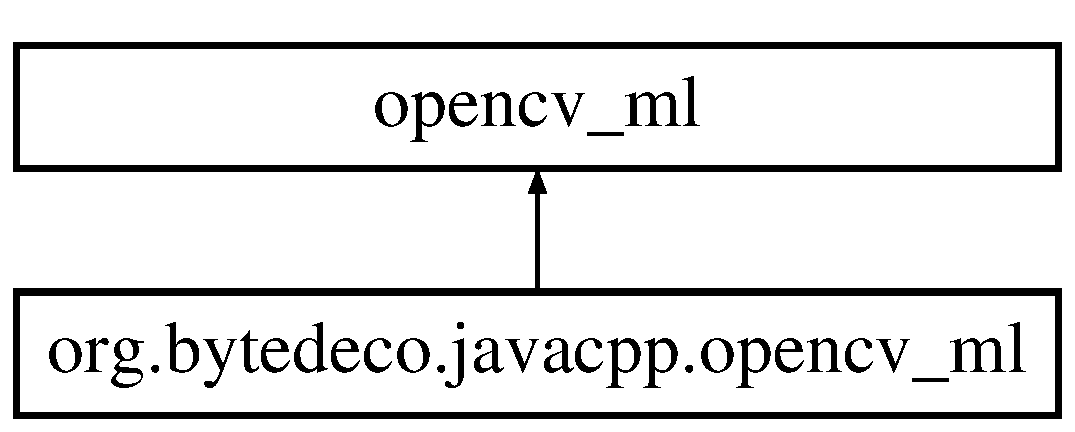
\includegraphics[height=2.000000cm]{classorg_1_1bytedeco_1_1javacpp_1_1opencv__ml}
\end{center}
\end{figure}
\subsection*{Classes}
\begin{DoxyCompactItemize}
\item 
class {\bfseries A\+N\+N\+\_\+\+M\+LP}
\begin{DoxyCompactList}\small\item\em Artificial Neural Networks -\/ Multi-\/\+Layer Perceptrons. \end{DoxyCompactList}\item 
class {\bfseries Boost}
\begin{DoxyCompactList}\small\item\em Boosted tree classifier derived from D\+Trees. \end{DoxyCompactList}\item 
class {\bfseries D\+Trees}
\begin{DoxyCompactList}\small\item\em The class represents a single decision tree or a collection of decision trees. \end{DoxyCompactList}\item 
class {\bfseries EM}
\begin{DoxyCompactList}\small\item\em The class implements the Expectation Maximization algorithm. \end{DoxyCompactList}\item 
class {\bfseries K\+Nearest}
\begin{DoxyCompactList}\small\item\em The class implements K-\/\+Nearest Neighbors model. \end{DoxyCompactList}\item 
class {\bfseries Logistic\+Regression}
\begin{DoxyCompactList}\small\item\em Implements Logistic Regression classifier. \end{DoxyCompactList}\item 
class {\bfseries Normal\+Bayes\+Classifier}
\begin{DoxyCompactList}\small\item\em Bayes classifier for normally distributed data. \end{DoxyCompactList}\item 
class {\bfseries Param\+Grid}
\begin{DoxyCompactList}\small\item\em The structure represents the logarithmic grid range of statmodel parameters. \end{DoxyCompactList}\item 
class {\bfseries R\+Trees}
\begin{DoxyCompactList}\small\item\em The class implements the random forest predictor. \end{DoxyCompactList}\item 
class {\bfseries Stat\+Model}
\begin{DoxyCompactList}\small\item\em Base class for statistical models in Open\+CV ML. \end{DoxyCompactList}\item 
class {\bfseries S\+VM}
\begin{DoxyCompactList}\small\item\em Support Vector Machines. \end{DoxyCompactList}\item 
class {\bfseries S\+V\+M\+S\+GD}
\begin{DoxyCompactList}\small\item\em Stochastic Gradient Descent S\+VM classifier. \end{DoxyCompactList}\item 
class {\bfseries Train\+Data}
\begin{DoxyCompactList}\small\item\em Class encapsulating training data. \end{DoxyCompactList}\end{DoxyCompactItemize}
\subsection*{Static Public Member Functions}
\begin{DoxyCompactItemize}
\item 
static native void \hyperlink{group__ml_gaeb2cdd5950f92be2f699b6ad5cf4a9ba}{rand\+M\+V\+Normal} ( @By\+Val Mat mean, @By\+Val Mat cov, int nsamples, @By\+Val Mat samples)
\begin{DoxyCompactList}\small\item\em Generates {\itshape sample} from multivariate normal distribution. \end{DoxyCompactList}\item 
static native void {\bfseries rand\+M\+V\+Normal} ( @By\+Val U\+Mat mean, @By\+Val U\+Mat cov, int nsamples, @By\+Val U\+Mat samples)
\item 
static native void \hyperlink{group__ml_ga800b1310714c638042e7cc627abab847}{create\+Concentric\+Spheres\+Test\+Set} (int nsamples, int nfeatures, int nclasses, @By\+Val Mat samples, @By\+Val Mat responses)
\begin{DoxyCompactList}\small\item\em Creates test set. \end{DoxyCompactList}\item 
static native void {\bfseries create\+Concentric\+Spheres\+Test\+Set} (int nsamples, int nfeatures, int nclasses, @By\+Val U\+Mat samples, @By\+Val U\+Mat responses)
\end{DoxyCompactItemize}
\subsection*{Static Public Attributes}
\begin{DoxyCompactItemize}
\item 
static final int \hyperlink{group__ml_ga4e7d272fa71d294a93e6a89edeacdec8}{V\+A\+R\+\_\+\+N\+U\+M\+E\+R\+I\+C\+AL} = 0
\item 
static final int \hyperlink{group__ml_gab8408e7a56e10d19a84684bb008d0e9f}{T\+E\+S\+T\+\_\+\+E\+R\+R\+OR} = 0
\begin{DoxyCompactList}\small\item\em Error types \end{DoxyCompactList}\item 
static final int \hyperlink{group__ml_gaa71abe7b3688e0e9b0b79af6e224286e}{R\+O\+W\+\_\+\+S\+A\+M\+P\+LE} = 0
\begin{DoxyCompactList}\small\item\em Sample types. \end{DoxyCompactList}\end{DoxyCompactItemize}


The documentation for this class was generated from the following file\+:\begin{DoxyCompactItemize}
\item 
opencv\+\_\+ml.\+java\end{DoxyCompactItemize}

\hypertarget{classorg_1_1bytedeco_1_1javacpp_1_1opencv__objdetect}{}\section{org.\+bytedeco.\+javacpp.\+opencv\+\_\+objdetect Class Reference}
\label{classorg_1_1bytedeco_1_1javacpp_1_1opencv__objdetect}\index{org.\+bytedeco.\+javacpp.\+opencv\+\_\+objdetect@{org.\+bytedeco.\+javacpp.\+opencv\+\_\+objdetect}}
Inheritance diagram for org.\+bytedeco.\+javacpp.\+opencv\+\_\+objdetect\+:\begin{figure}[H]
\begin{center}
\leavevmode
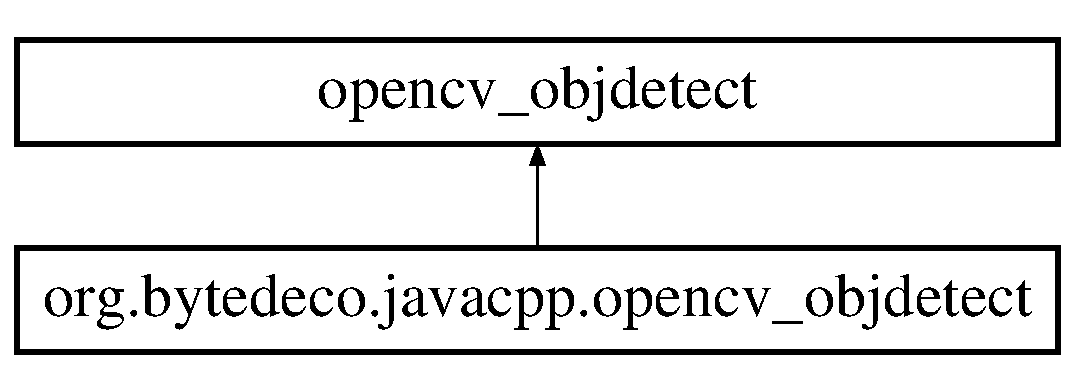
\includegraphics[height=2.000000cm]{classorg_1_1bytedeco_1_1javacpp_1_1opencv__objdetect}
\end{center}
\end{figure}
\subsection*{Classes}
\begin{DoxyCompactItemize}
\item 
class {\bfseries Base\+Cascade\+Classifier}
\item 
class {\bfseries Cascade\+Classifier}
\begin{DoxyCompactList}\small\item\em Cascade classifier class for object detection. \end{DoxyCompactList}\item 
class {\bfseries Cv\+Avg\+Comp}
\item 
class {\bfseries Cv\+Haar\+Classifier}
\item 
class {\bfseries Cv\+Haar\+Classifier\+Cascade}
\item 
class {\bfseries Cv\+Haar\+Feature}
\item 
class {\bfseries Cv\+Haar\+Stage\+Classifier}
\item 
class {\bfseries Cv\+Hid\+Haar\+Classifier\+Cascade}
\item 
class {\bfseries Detection\+Based\+Tracker}
\item 
class {\bfseries Detection\+R\+OI}
\item 
class {\bfseries H\+O\+G\+Descriptor}
\item 
class {\bfseries Similar\+Rects}
\end{DoxyCompactItemize}
\subsection*{Static Public Member Functions}
\begin{DoxyCompactItemize}
\item 
static native Cv\+Haar\+Classifier\+Cascade {\bfseries cv\+Load\+Haar\+Classifier\+Cascade} ( @Cast(\char`\"{}const char$\ast$\char`\"{}) Byte\+Pointer directory, @By\+Val Cv\+Size orig\+\_\+window\+\_\+size)
\item 
static native Cv\+Haar\+Classifier\+Cascade {\bfseries cv\+Load\+Haar\+Classifier\+Cascade} (String directory, @By\+Val Cv\+Size orig\+\_\+window\+\_\+size)
\item 
static native void {\bfseries cv\+Release\+Haar\+Classifier\+Cascade} ( @Cast(\char`\"{}Cv\+Haar\+Classifier\+Cascade$\ast$$\ast$\char`\"{}) Pointer\+Pointer cascade)
\item 
static native void {\bfseries cv\+Release\+Haar\+Classifier\+Cascade} ( @By\+Ptr\+Ptr Cv\+Haar\+Classifier\+Cascade cascade)
\item 
static native Cv\+Seq {\bfseries cv\+Haar\+Detect\+Objects} ( @Const Cv\+Arr image, Cv\+Haar\+Classifier\+Cascade cascade, Cv\+Mem\+Storage storage, double scale\+\_\+factor, int min\+\_\+neighbors, int flags, @By\+Val(null\+Value=\char`\"{}Cv\+Size(cv\+Size(0,0))\char`\"{}) Cv\+Size min\+\_\+size, @By\+Val(null\+Value=\char`\"{}Cv\+Size(cv\+Size(0,0))\char`\"{}) Cv\+Size max\+\_\+size)
\item 
static native Cv\+Seq {\bfseries cv\+Haar\+Detect\+Objects} ( @Const Cv\+Arr image, Cv\+Haar\+Classifier\+Cascade cascade, Cv\+Mem\+Storage storage)
\item 
static native void {\bfseries cv\+Set\+Images\+For\+Haar\+Classifier\+Cascade} (Cv\+Haar\+Classifier\+Cascade cascade, @Const Cv\+Arr sum, @Const Cv\+Arr sqsum, @Const Cv\+Arr tilted\+\_\+sum, double scale)
\item 
static native int {\bfseries cv\+Run\+Haar\+Classifier\+Cascade} ( @Const Cv\+Haar\+Classifier\+Cascade cascade, @By\+Val Cv\+fr.antproject.utils.Point pt, int start\+\_\+stage)
\item 
static native int {\bfseries cv\+Run\+Haar\+Classifier\+Cascade} ( @Const Cv\+Haar\+Classifier\+Cascade cascade, @By\+Val Cv\+fr.antproject.utils.Point pt)
\item 
static native int {\bfseries cv\+Run\+Haar\+Classifier\+Cascade} ( @Const Cv\+Haar\+Classifier\+Cascade cascade, @By\+Val @Cast(\char`\"{}Cv\+fr.antproject.utils.Point$\ast$\char`\"{}) Int\+Buffer pt, int start\+\_\+stage)
\item 
static native int {\bfseries cv\+Run\+Haar\+Classifier\+Cascade} ( @Const Cv\+Haar\+Classifier\+Cascade cascade, @By\+Val @Cast(\char`\"{}Cv\+fr.antproject.utils.Point$\ast$\char`\"{}) Int\+Buffer pt)
\item 
static native int {\bfseries cv\+Run\+Haar\+Classifier\+Cascade} ( @Const Cv\+Haar\+Classifier\+Cascade cascade, @By\+Val @Cast(\char`\"{}Cv\+fr.antproject.utils.Point$\ast$\char`\"{}) int\mbox{[}$\,$\mbox{]} pt, int start\+\_\+stage)
\item 
static native int {\bfseries cv\+Run\+Haar\+Classifier\+Cascade} ( @Const Cv\+Haar\+Classifier\+Cascade cascade, @By\+Val @Cast(\char`\"{}Cv\+fr.antproject.utils.Point$\ast$\char`\"{}) int\mbox{[}$\,$\mbox{]} pt)
\item 
\mbox{\Hypertarget{classorg_1_1bytedeco_1_1javacpp_1_1opencv__objdetect_a3f396019471198065ca4c2adcf8d7578}\label{classorg_1_1bytedeco_1_1javacpp_1_1opencv__objdetect_a3f396019471198065ca4c2adcf8d7578}} 
static native Cv\+Seq {\bfseries cv\+Haar\+Detect\+Objects\+For\+R\+OC} ( @Const Cv\+Arr image, Cv\+Haar\+Classifier\+Cascade cascade, Cv\+Mem\+Storage storage, @Std\+Vector Int\+Pointer reject\+Levels, @Std\+Vector Double\+Pointer level\+Weightds, double scale\+\_\+factor, int min\+\_\+neighbors, int flags, @By\+Val(null\+Value=\char`\"{}Cv\+Size(cv\+Size(0, 0))\char`\"{}) Cv\+Size min\+\_\+size, @By\+Val(null\+Value=\char`\"{}Cv\+Size(cv\+Size(0, 0))\char`\"{}) Cv\+Size max\+\_\+size, @Cast(\char`\"{}bool\char`\"{}) boolean output\+Reject\+Levels)
\item 
\mbox{\Hypertarget{classorg_1_1bytedeco_1_1javacpp_1_1opencv__objdetect_a5738c8863bb77cdbc3a80b65ec84477a}\label{classorg_1_1bytedeco_1_1javacpp_1_1opencv__objdetect_a5738c8863bb77cdbc3a80b65ec84477a}} 
static native Cv\+Seq {\bfseries cv\+Haar\+Detect\+Objects\+For\+R\+OC} ( @Const Cv\+Arr image, Cv\+Haar\+Classifier\+Cascade cascade, Cv\+Mem\+Storage storage, @Std\+Vector Int\+Pointer reject\+Levels, @Std\+Vector Double\+Pointer level\+Weightds)
\item 
\mbox{\Hypertarget{classorg_1_1bytedeco_1_1javacpp_1_1opencv__objdetect_abf70d5cee36ee3c19d24d4d96e1450a2}\label{classorg_1_1bytedeco_1_1javacpp_1_1opencv__objdetect_abf70d5cee36ee3c19d24d4d96e1450a2}} 
static native Cv\+Seq {\bfseries cv\+Haar\+Detect\+Objects\+For\+R\+OC} ( @Const Cv\+Arr image, Cv\+Haar\+Classifier\+Cascade cascade, Cv\+Mem\+Storage storage, @Std\+Vector Int\+Buffer reject\+Levels, @Std\+Vector Double\+Buffer level\+Weightds, double scale\+\_\+factor, int min\+\_\+neighbors, int flags, @By\+Val(null\+Value=\char`\"{}Cv\+Size(cv\+Size(0, 0))\char`\"{}) Cv\+Size min\+\_\+size, @By\+Val(null\+Value=\char`\"{}Cv\+Size(cv\+Size(0, 0))\char`\"{}) Cv\+Size max\+\_\+size, @Cast(\char`\"{}bool\char`\"{}) boolean output\+Reject\+Levels)
\item 
\mbox{\Hypertarget{classorg_1_1bytedeco_1_1javacpp_1_1opencv__objdetect_adcb451c7c152174cb18e52ae5bbc588d}\label{classorg_1_1bytedeco_1_1javacpp_1_1opencv__objdetect_adcb451c7c152174cb18e52ae5bbc588d}} 
static native Cv\+Seq {\bfseries cv\+Haar\+Detect\+Objects\+For\+R\+OC} ( @Const Cv\+Arr image, Cv\+Haar\+Classifier\+Cascade cascade, Cv\+Mem\+Storage storage, @Std\+Vector Int\+Buffer reject\+Levels, @Std\+Vector Double\+Buffer level\+Weightds)
\item 
\mbox{\Hypertarget{classorg_1_1bytedeco_1_1javacpp_1_1opencv__objdetect_accdbeae0c6f6c2cff705f49706f84865}\label{classorg_1_1bytedeco_1_1javacpp_1_1opencv__objdetect_accdbeae0c6f6c2cff705f49706f84865}} 
static native Cv\+Seq {\bfseries cv\+Haar\+Detect\+Objects\+For\+R\+OC} ( @Const Cv\+Arr image, Cv\+Haar\+Classifier\+Cascade cascade, Cv\+Mem\+Storage storage, @Std\+Vector int\mbox{[}$\,$\mbox{]} reject\+Levels, @Std\+Vector double\mbox{[}$\,$\mbox{]} level\+Weightds, double scale\+\_\+factor, int min\+\_\+neighbors, int flags, @By\+Val(null\+Value=\char`\"{}Cv\+Size(cv\+Size(0, 0))\char`\"{}) Cv\+Size min\+\_\+size, @By\+Val(null\+Value=\char`\"{}Cv\+Size(cv\+Size(0, 0))\char`\"{}) Cv\+Size max\+\_\+size, @Cast(\char`\"{}bool\char`\"{}) boolean output\+Reject\+Levels)
\item 
\mbox{\Hypertarget{classorg_1_1bytedeco_1_1javacpp_1_1opencv__objdetect_ad8eb86b6bc373468a5924701c0cb1a66}\label{classorg_1_1bytedeco_1_1javacpp_1_1opencv__objdetect_ad8eb86b6bc373468a5924701c0cb1a66}} 
static native Cv\+Seq {\bfseries cv\+Haar\+Detect\+Objects\+For\+R\+OC} ( @Const Cv\+Arr image, Cv\+Haar\+Classifier\+Cascade cascade, Cv\+Mem\+Storage storage, @Std\+Vector int\mbox{[}$\,$\mbox{]} reject\+Levels, @Std\+Vector double\mbox{[}$\,$\mbox{]} level\+Weightds)
\item 
static native void \hyperlink{group__objdetect_ga3036d2996cee06be22e0eccda95a671b}{group\+Rectangles} (@By\+Ref Rect\+Vector rect\+List, int group\+Threshold, double eps)
\begin{DoxyCompactList}\small\item\em Groups the object candidate rectangles. \end{DoxyCompactList}\item 
static native void {\bfseries group\+Rectangles} (@By\+Ref Rect\+Vector rect\+List, int group\+Threshold)
\item 
static native void \hyperlink{group__objdetect_gae1a108c813468189afc6756fdc5f4d33}{group\+Rectangles} (@By\+Ref Rect\+Vector rect\+List, @Std\+Vector Int\+Pointer weights, int group\+Threshold, double eps)
\item 
static native void {\bfseries group\+Rectangles} (@By\+Ref Rect\+Vector rect\+List, @Std\+Vector Int\+Pointer weights, int group\+Threshold)
\item 
static native void {\bfseries group\+Rectangles} (@By\+Ref Rect\+Vector rect\+List, @Std\+Vector Int\+Buffer weights, int group\+Threshold, double eps)
\item 
static native void {\bfseries group\+Rectangles} (@By\+Ref Rect\+Vector rect\+List, @Std\+Vector Int\+Buffer weights, int group\+Threshold)
\item 
static native void {\bfseries group\+Rectangles} (@By\+Ref Rect\+Vector rect\+List, @Std\+Vector int\mbox{[}$\,$\mbox{]} weights, int group\+Threshold, double eps)
\item 
static native void {\bfseries group\+Rectangles} (@By\+Ref Rect\+Vector rect\+List, @Std\+Vector int\mbox{[}$\,$\mbox{]} weights, int group\+Threshold)
\item 
static native void \hyperlink{group__objdetect_ga48da69f02f512561ce6524dfe4508d0d}{group\+Rectangles} (@By\+Ref Rect\+Vector rect\+List, int group\+Threshold, double eps, @Std\+Vector Int\+Pointer weights, @Std\+Vector Double\+Pointer level\+Weights)
\item 
static native void {\bfseries group\+Rectangles} (@By\+Ref Rect\+Vector rect\+List, int group\+Threshold, double eps, @Std\+Vector Int\+Buffer weights, @Std\+Vector Double\+Buffer level\+Weights)
\item 
static native void {\bfseries group\+Rectangles} (@By\+Ref Rect\+Vector rect\+List, int group\+Threshold, double eps, @Std\+Vector int\mbox{[}$\,$\mbox{]} weights, @Std\+Vector double\mbox{[}$\,$\mbox{]} level\+Weights)
\item 
static native void \hyperlink{group__objdetect_ga0a844bdf309e1f0b6a11e2622edf3548}{group\+Rectangles} (@By\+Ref Rect\+Vector rect\+List, @Std\+Vector Int\+Pointer reject\+Levels, @Std\+Vector Double\+Pointer level\+Weights, int group\+Threshold, double eps)
\item 
static native void {\bfseries group\+Rectangles} (@By\+Ref Rect\+Vector rect\+List, @Std\+Vector Int\+Pointer reject\+Levels, @Std\+Vector Double\+Pointer level\+Weights, int group\+Threshold)
\item 
static native void {\bfseries group\+Rectangles} (@By\+Ref Rect\+Vector rect\+List, @Std\+Vector Int\+Buffer reject\+Levels, @Std\+Vector Double\+Buffer level\+Weights, int group\+Threshold, double eps)
\item 
static native void {\bfseries group\+Rectangles} (@By\+Ref Rect\+Vector rect\+List, @Std\+Vector Int\+Buffer reject\+Levels, @Std\+Vector Double\+Buffer level\+Weights, int group\+Threshold)
\item 
static native void {\bfseries group\+Rectangles} (@By\+Ref Rect\+Vector rect\+List, @Std\+Vector int\mbox{[}$\,$\mbox{]} reject\+Levels, @Std\+Vector double\mbox{[}$\,$\mbox{]} level\+Weights, int group\+Threshold, double eps)
\item 
static native void {\bfseries group\+Rectangles} (@By\+Ref Rect\+Vector rect\+List, @Std\+Vector int\mbox{[}$\,$\mbox{]} reject\+Levels, @Std\+Vector double\mbox{[}$\,$\mbox{]} level\+Weights, int group\+Threshold)
\item 
static native void \hyperlink{group__objdetect_ga4dcd81c59aa342c781c93522088dc6be}{group\+Rectangles\+\_\+meanshift} (@By\+Ref Rect\+Vector rect\+List, @Std\+Vector Double\+Pointer found\+Weights, @Std\+Vector Double\+Pointer found\+Scales, double detect\+Threshold, @By\+Val(null\+Value=\char`\"{}cv\+::\+Size(64, 128)\char`\"{}) Size win\+Det\+Size)
\item 
static native void {\bfseries group\+Rectangles\+\_\+meanshift} (@By\+Ref Rect\+Vector rect\+List, @Std\+Vector Double\+Pointer found\+Weights, @Std\+Vector Double\+Pointer found\+Scales)
\item 
static native void {\bfseries group\+Rectangles\+\_\+meanshift} (@By\+Ref Rect\+Vector rect\+List, @Std\+Vector Double\+Buffer found\+Weights, @Std\+Vector Double\+Buffer found\+Scales, double detect\+Threshold, @By\+Val(null\+Value=\char`\"{}cv\+::\+Size(64, 128)\char`\"{}) Size win\+Det\+Size)
\item 
static native void {\bfseries group\+Rectangles\+\_\+meanshift} (@By\+Ref Rect\+Vector rect\+List, @Std\+Vector Double\+Buffer found\+Weights, @Std\+Vector Double\+Buffer found\+Scales)
\item 
static native void {\bfseries group\+Rectangles\+\_\+meanshift} (@By\+Ref Rect\+Vector rect\+List, @Std\+Vector double\mbox{[}$\,$\mbox{]} found\+Weights, @Std\+Vector double\mbox{[}$\,$\mbox{]} found\+Scales, double detect\+Threshold, @By\+Val(null\+Value=\char`\"{}cv\+::\+Size(64, 128)\char`\"{}) Size win\+Det\+Size)
\item 
static native void {\bfseries group\+Rectangles\+\_\+meanshift} (@By\+Ref Rect\+Vector rect\+List, @Std\+Vector double\mbox{[}$\,$\mbox{]} found\+Weights, @Std\+Vector double\mbox{[}$\,$\mbox{]} found\+Scales)
\item 
static native Base\+Cascade\+Classifier.\+Mask\+Generator {\bfseries create\+Face\+Detection\+Mask\+Generator} ()
\end{DoxyCompactItemize}
\subsection*{Static Public Attributes}
\begin{DoxyCompactItemize}
\item 
static final int {\bfseries C\+V\+\_\+\+H\+A\+A\+R\+\_\+\+M\+A\+G\+I\+C\+\_\+\+V\+AL} = 0x42500000
\item 
static final String {\bfseries C\+V\+\_\+\+T\+Y\+P\+E\+\_\+\+N\+A\+M\+E\+\_\+\+H\+A\+AR} = \char`\"{}opencv-\/haar-\/classifier\char`\"{}
\item 
static final int {\bfseries C\+V\+\_\+\+H\+A\+A\+R\+\_\+\+F\+E\+A\+T\+U\+R\+E\+\_\+\+M\+AX} = 3
\item 
static final int {\bfseries C\+V\+\_\+\+H\+A\+A\+R\+\_\+\+D\+O\+\_\+\+C\+A\+N\+N\+Y\+\_\+\+P\+R\+U\+N\+I\+NG} = 1
\item 
static final int {\bfseries C\+V\+\_\+\+H\+A\+A\+R\+\_\+\+S\+C\+A\+L\+E\+\_\+\+I\+M\+A\+GE} = 2
\item 
static final int {\bfseries C\+V\+\_\+\+H\+A\+A\+R\+\_\+\+F\+I\+N\+D\+\_\+\+B\+I\+G\+G\+E\+S\+T\+\_\+\+O\+B\+J\+E\+CT} = 4
\item 
static final int {\bfseries C\+V\+\_\+\+H\+A\+A\+R\+\_\+\+D\+O\+\_\+\+R\+O\+U\+G\+H\+\_\+\+S\+E\+A\+R\+CH} = 8
\item 
static final int \hyperlink{group__objdetect_ga470401e5de188ad94a16d0026658f405}{C\+A\+S\+C\+A\+D\+E\+\_\+\+D\+O\+\_\+\+C\+A\+N\+N\+Y\+\_\+\+P\+R\+U\+N\+I\+NG} = 1
\end{DoxyCompactItemize}


The documentation for this class was generated from the following file\+:\begin{DoxyCompactItemize}
\item 
opencv\+\_\+objdetect.\+java\end{DoxyCompactItemize}

\hypertarget{classorg_1_1bytedeco_1_1javacpp_1_1opencv__optflow}{}\section{org.\+bytedeco.\+javacpp.\+opencv\+\_\+optflow Class Reference}
\label{classorg_1_1bytedeco_1_1javacpp_1_1opencv__optflow}\index{org.\+bytedeco.\+javacpp.\+opencv\+\_\+optflow@{org.\+bytedeco.\+javacpp.\+opencv\+\_\+optflow}}
Inheritance diagram for org.\+bytedeco.\+javacpp.\+opencv\+\_\+optflow\+:\begin{figure}[H]
\begin{center}
\leavevmode
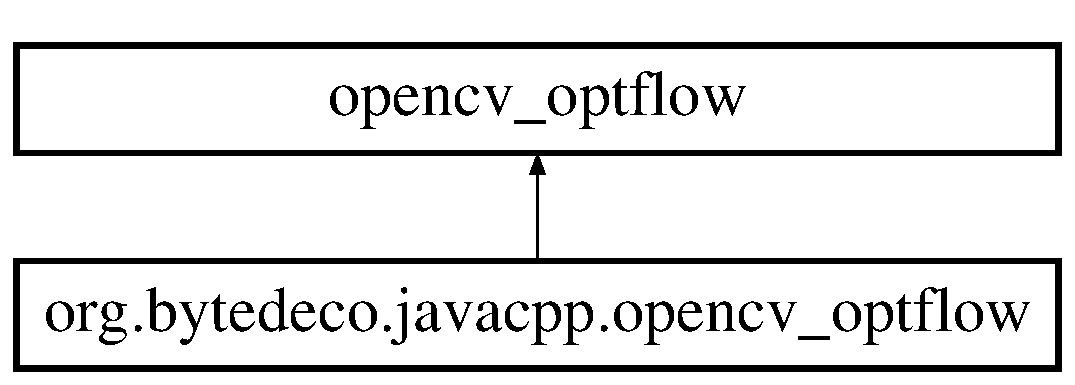
\includegraphics[height=2.000000cm]{classorg_1_1bytedeco_1_1javacpp_1_1opencv__optflow}
\end{center}
\end{figure}
\subsection*{Classes}
\begin{DoxyCompactItemize}
\item 
class {\bfseries D\+I\+S\+Optical\+Flow}
\begin{DoxyCompactList}\small\item\em D\+IS optical flow algorithm. \end{DoxyCompactList}\item 
class {\bfseries Variational\+Refinement}
\begin{DoxyCompactList}\small\item\em Variational optical flow refinement. \end{DoxyCompactList}\end{DoxyCompactItemize}
\subsection*{Static Public Member Functions}
\begin{DoxyCompactItemize}
\item 
static native void {\bfseries calc\+Optical\+Flow\+SF} ( @By\+Val Mat from, @By\+Val Mat to, @By\+Val Mat flow, int layers, int averaging\+\_\+block\+\_\+size, int max\+\_\+flow)
\item 
static native void {\bfseries calc\+Optical\+Flow\+SF} ( @By\+Val U\+Mat from, @By\+Val U\+Mat to, @By\+Val U\+Mat flow, int layers, int averaging\+\_\+block\+\_\+size, int max\+\_\+flow)
\item 
static native void \hyperlink{group__optflow_ga76902de70b538596bed7e39b7777384d}{calc\+Optical\+Flow\+SF} ( @By\+Val Mat from, @By\+Val Mat to, @By\+Val Mat flow, int layers, int averaging\+\_\+block\+\_\+size, int max\+\_\+flow, double sigma\+\_\+dist, double sigma\+\_\+color, int postprocess\+\_\+window, double sigma\+\_\+dist\+\_\+fix, double sigma\+\_\+color\+\_\+fix, double occ\+\_\+thr, int upscale\+\_\+averaging\+\_\+radius, double upscale\+\_\+sigma\+\_\+dist, double upscale\+\_\+sigma\+\_\+color, double speed\+\_\+up\+\_\+thr)
\begin{DoxyCompactList}\small\item\em Calculate an optical flow using \char`\"{}\+Simple\+Flow\char`\"{} algorithm. \end{DoxyCompactList}\item 
static native void {\bfseries calc\+Optical\+Flow\+SF} ( @By\+Val U\+Mat from, @By\+Val U\+Mat to, @By\+Val U\+Mat flow, int layers, int averaging\+\_\+block\+\_\+size, int max\+\_\+flow, double sigma\+\_\+dist, double sigma\+\_\+color, int postprocess\+\_\+window, double sigma\+\_\+dist\+\_\+fix, double sigma\+\_\+color\+\_\+fix, double occ\+\_\+thr, int upscale\+\_\+averaging\+\_\+radius, double upscale\+\_\+sigma\+\_\+dist, double upscale\+\_\+sigma\+\_\+color, double speed\+\_\+up\+\_\+thr)
\item 
static native void \hyperlink{group__optflow_gab202f6c782e9356cf2a96620732785a9}{calc\+Optical\+Flow\+Sparse\+To\+Dense} ( @By\+Val Mat from, @By\+Val Mat to, @By\+Val Mat flow, int grid\+\_\+step, int k, float sigma, @Cast(\char`\"{}bool\char`\"{}) boolean use\+\_\+post\+\_\+proc, float fgs\+\_\+lambda, float fgs\+\_\+sigma)
\begin{DoxyCompactList}\small\item\em Fast dense optical flow based on Pyr\+LK sparse matches interpolation. \end{DoxyCompactList}\item 
static native void {\bfseries calc\+Optical\+Flow\+Sparse\+To\+Dense} ( @By\+Val Mat from, @By\+Val Mat to, @By\+Val Mat flow)
\item 
static native void {\bfseries calc\+Optical\+Flow\+Sparse\+To\+Dense} ( @By\+Val U\+Mat from, @By\+Val U\+Mat to, @By\+Val U\+Mat flow, int grid\+\_\+step, int k, float sigma, @Cast(\char`\"{}bool\char`\"{}) boolean use\+\_\+post\+\_\+proc, float fgs\+\_\+lambda, float fgs\+\_\+sigma)
\item 
static native void {\bfseries calc\+Optical\+Flow\+Sparse\+To\+Dense} ( @By\+Val U\+Mat from, @By\+Val U\+Mat to, @By\+Val U\+Mat flow)
\item 
static native Mat \hyperlink{group__optflow_ga8adc9b054c1518ab41c20d8ada51b9b7}{read\+Optical\+Flow} ( @Str Byte\+Pointer path)
\begin{DoxyCompactList}\small\item\em Read a .flo file. \end{DoxyCompactList}\item 
static native Mat {\bfseries read\+Optical\+Flow} ( @Str String path)
\item 
static native boolean \hyperlink{group__optflow_ga41bea8c25211f346782adfb40129e96e}{write\+Optical\+Flow} ( @Str Byte\+Pointer path, @By\+Val Mat flow)
\begin{DoxyCompactList}\small\item\em Write a .flo to disk. \end{DoxyCompactList}\item 
static native boolean {\bfseries write\+Optical\+Flow} ( @Str String path, @By\+Val Mat flow)
\item 
static native boolean {\bfseries write\+Optical\+Flow} ( @Str Byte\+Pointer path, @By\+Val U\+Mat flow)
\item 
static native boolean {\bfseries write\+Optical\+Flow} ( @Str String path, @By\+Val U\+Mat flow)
\item 
static native Variational\+Refinement \hyperlink{group__optflow_ga6d7be52a57f2105050c7a7039ab1af2e}{create\+Variational\+Flow\+Refinement} ()
\begin{DoxyCompactList}\small\item\em Creates an instance of Variational\+Refinement. \end{DoxyCompactList}\item 
static native Dense\+Optical\+Flow \hyperlink{group__optflow_ga27f2a261b7f69f4eaaf2aa2552943a1a}{create\+Opt\+Flow\+\_\+\+Deep\+Flow} ()
\begin{DoxyCompactList}\small\item\em Deep\+Flow optical flow algorithm implementation. \end{DoxyCompactList}\item 
static native Dense\+Optical\+Flow \hyperlink{group__optflow_gace52b781a9780c4c9a20951a2bec314d}{create\+Opt\+Flow\+\_\+\+Simple\+Flow} ()
\item 
static native Dense\+Optical\+Flow \hyperlink{group__optflow_gabd230cc626a64515ec35ac6c6c7fc099}{create\+Opt\+Flow\+\_\+\+Farneback} ()
\item 
static native Dense\+Optical\+Flow \hyperlink{group__optflow_ga2033e98010d9ac8b150503a107601946}{create\+Opt\+Flow\+\_\+\+Sparse\+To\+Dense} ()
\item 
static native D\+I\+S\+Optical\+Flow \hyperlink{group__optflow_gac107283f5dba4f320df3d9894aad537b}{create\+Opt\+Flow\+\_\+\+D\+IS} (int preset)
\begin{DoxyCompactList}\small\item\em Creates an instance of D\+I\+S\+Optical\+Flow. \end{DoxyCompactList}\item 
static native D\+I\+S\+Optical\+Flow {\bfseries create\+Opt\+Flow\+\_\+\+D\+IS} ()
\item 
static native void {\bfseries update\+Motion\+History} ( @By\+Val Mat silhouette, @By\+Val Mat mhi, double timestamp, double duration)
\item 
static native void {\bfseries update\+Motion\+History} ( @By\+Val U\+Mat silhouette, @By\+Val U\+Mat mhi, double timestamp, double duration)
\item 
static native void \hyperlink{group__optflow_ga1df8e7b81e72fc2df163a156ec07b5ed}{calc\+Motion\+Gradient} ( @By\+Val Mat mhi, @By\+Val Mat mask, @By\+Val Mat orientation, double delta1, double delta2, int aperture\+Size)
\begin{DoxyCompactList}\small\item\em Calculates a gradient orientation of a motion history image. \end{DoxyCompactList}\item 
static native void {\bfseries calc\+Motion\+Gradient} ( @By\+Val Mat mhi, @By\+Val Mat mask, @By\+Val Mat orientation, double delta1, double delta2)
\item 
static native void {\bfseries calc\+Motion\+Gradient} ( @By\+Val U\+Mat mhi, @By\+Val U\+Mat mask, @By\+Val U\+Mat orientation, double delta1, double delta2, int aperture\+Size)
\item 
static native void {\bfseries calc\+Motion\+Gradient} ( @By\+Val U\+Mat mhi, @By\+Val U\+Mat mask, @By\+Val U\+Mat orientation, double delta1, double delta2)
\item 
static native double \hyperlink{group__optflow_gae09be23e6ebae54e6dad95914a82282d}{calc\+Global\+Orientation} ( @By\+Val Mat orientation, @By\+Val Mat mask, @By\+Val Mat mhi, double timestamp, double duration)
\begin{DoxyCompactList}\small\item\em Calculates a global motion orientation in a selected region. \end{DoxyCompactList}\item 
static native double {\bfseries calc\+Global\+Orientation} ( @By\+Val U\+Mat orientation, @By\+Val U\+Mat mask, @By\+Val U\+Mat mhi, double timestamp, double duration)
\item 
static native void \hyperlink{group__optflow_gad1ff5ca68f3f39b0547c8d249b99185b}{segment\+Motion} ( @By\+Val Mat mhi, @By\+Val Mat segmask, @By\+Ref Rect\+Vector bounding\+Rects, double timestamp, double seg\+Thresh)
\begin{DoxyCompactList}\small\item\em Splits a motion history image into a few parts corresponding to separate independent motions (for example, left hand, right hand). \end{DoxyCompactList}\item 
static native void {\bfseries segment\+Motion} ( @By\+Val U\+Mat mhi, @By\+Val U\+Mat segmask, @By\+Ref Rect\+Vector bounding\+Rects, double timestamp, double seg\+Thresh)
\end{DoxyCompactItemize}


The documentation for this class was generated from the following file\+:\begin{DoxyCompactItemize}
\item 
opencv\+\_\+optflow.\+java\end{DoxyCompactItemize}

\hypertarget{classorg_1_1bytedeco_1_1javacpp_1_1opencv__photo}{}\section{org.\+bytedeco.\+javacpp.\+opencv\+\_\+photo Class Reference}
\label{classorg_1_1bytedeco_1_1javacpp_1_1opencv__photo}\index{org.\+bytedeco.\+javacpp.\+opencv\+\_\+photo@{org.\+bytedeco.\+javacpp.\+opencv\+\_\+photo}}
Inheritance diagram for org.\+bytedeco.\+javacpp.\+opencv\+\_\+photo\+:\begin{figure}[H]
\begin{center}
\leavevmode
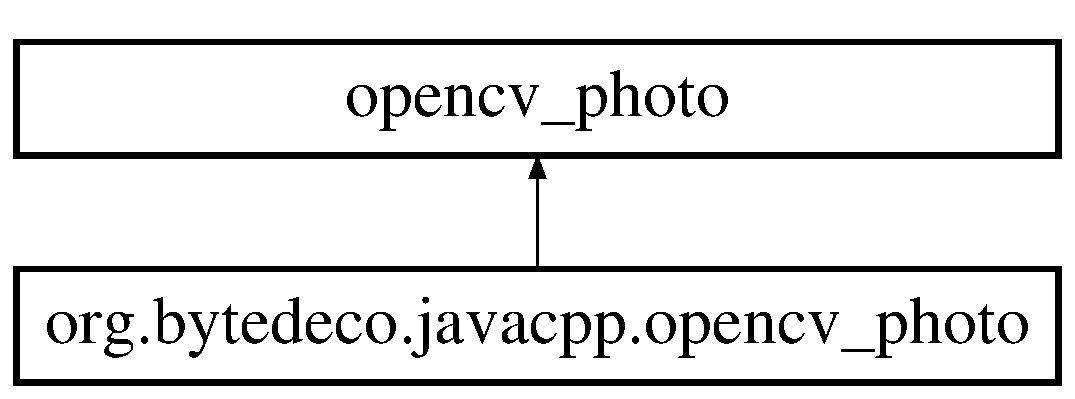
\includegraphics[height=2.000000cm]{classorg_1_1bytedeco_1_1javacpp_1_1opencv__photo}
\end{center}
\end{figure}
\subsection*{Classes}
\begin{DoxyCompactItemize}
\item 
class {\bfseries Align\+Exposures}
\begin{DoxyCompactList}\small\item\em The base class for algorithms that align images of the same scene with different exposures. \end{DoxyCompactList}\item 
class {\bfseries Align\+M\+TB}
\begin{DoxyCompactList}\small\item\em This algorithm converts images to median threshold bitmaps (1 for pixels brighter than median luminance and 0 otherwise) and than aligns the resulting bitmaps using bit operations. \end{DoxyCompactList}\item 
class {\bfseries Calibrate\+C\+RF}
\begin{DoxyCompactList}\small\item\em The base class for camera response calibration algorithms. \end{DoxyCompactList}\item 
class {\bfseries Calibrate\+Debevec}
\begin{DoxyCompactList}\small\item\em Inverse camera response function is extracted for each brightness value by minimizing an objective function as linear system. Objective function is constructed using pixel values on the same position in all images, extra term is added to make the result smoother. \end{DoxyCompactList}\item 
class {\bfseries Calibrate\+Robertson}
\begin{DoxyCompactList}\small\item\em Inverse camera response function is extracted for each brightness value by minimizing an objective function as linear system. This algorithm uses all image pixels. \end{DoxyCompactList}\item 
class {\bfseries Merge\+Debevec}
\begin{DoxyCompactList}\small\item\em The resulting H\+DR image is calculated as weighted average of the exposures considering exposure values and camera response. \end{DoxyCompactList}\item 
class {\bfseries Merge\+Exposures}
\begin{DoxyCompactList}\small\item\em The base class algorithms that can merge exposure sequence to a single image. \end{DoxyCompactList}\item 
class {\bfseries Merge\+Mertens}
\begin{DoxyCompactList}\small\item\em Pixels are weighted using contrast, saturation and well-\/exposedness measures, than images are combined using laplacian pyramids. \end{DoxyCompactList}\item 
class {\bfseries Merge\+Robertson}
\begin{DoxyCompactList}\small\item\em The resulting H\+DR image is calculated as weighted average of the exposures considering exposure values and camera response. \end{DoxyCompactList}\item 
class {\bfseries Tonemap}
\begin{DoxyCompactList}\small\item\em Base class for tonemapping algorithms -\/ tools that are used to map H\+DR image to 8-\/bit range. \end{DoxyCompactList}\item 
class {\bfseries Tonemap\+Drago}
\begin{DoxyCompactList}\small\item\em Adaptive logarithmic mapping is a fast global tonemapping algorithm that scales the image in logarithmic domain. \end{DoxyCompactList}\item 
class {\bfseries Tonemap\+Durand}
\begin{DoxyCompactList}\small\item\em This algorithm decomposes image into two layers\+: base layer and detail layer using bilateral filter and compresses contrast of the base layer thus preserving all the details. \end{DoxyCompactList}\item 
class {\bfseries Tonemap\+Mantiuk}
\begin{DoxyCompactList}\small\item\em This algorithm transforms image to contrast using gradients on all levels of gaussian pyramid, transforms contrast values to H\+VS response and scales the response. After this the image is reconstructed from new contrast values. \end{DoxyCompactList}\item 
class {\bfseries Tonemap\+Reinhard}
\begin{DoxyCompactList}\small\item\em This is a global tonemapping operator that models human visual system. \end{DoxyCompactList}\end{DoxyCompactItemize}
\subsection*{Static Public Member Functions}
\begin{DoxyCompactItemize}
\item 
static native void {\bfseries cv\+Inpaint} ( @Const Cv\+Arr src, @Const Cv\+Arr inpaint\+\_\+mask, Cv\+Arr dst, double inpaint\+Range, int flags)
\item 
static native void \hyperlink{group__photo_gac642f4ae1eabdce5624c07d7202b0a3e}{inpaint} ( @By\+Val Mat src, @By\+Val Mat inpaint\+Mask, @By\+Val Mat dst, double inpaint\+Radius, int flags)
\begin{DoxyCompactList}\small\item\em Restores the selected region in an image using the region neighborhood. \end{DoxyCompactList}\item 
static native void {\bfseries inpaint} ( @By\+Val U\+Mat src, @By\+Val U\+Mat inpaint\+Mask, @By\+Val U\+Mat dst, double inpaint\+Radius, int flags)
\item 
static native void {\bfseries fast\+Nl\+Means\+Denoising} ( @By\+Val Mat src, @By\+Val Mat dst, float h, int template\+Window\+Size, int search\+Window\+Size)
\item 
static native void {\bfseries fast\+Nl\+Means\+Denoising} ( @By\+Val Mat src, @By\+Val Mat dst)
\item 
static native void {\bfseries fast\+Nl\+Means\+Denoising} ( @By\+Val U\+Mat src, @By\+Val U\+Mat dst, float h, int template\+Window\+Size, int search\+Window\+Size)
\item 
static native void {\bfseries fast\+Nl\+Means\+Denoising} ( @By\+Val U\+Mat src, @By\+Val U\+Mat dst)
\item 
static native void \hyperlink{group__photo__denoise_gac9dd83e0192eaed8ea6aad42f98b138b}{fast\+Nl\+Means\+Denoising} ( @By\+Val Mat src, @By\+Val Mat dst, @Std\+Vector Float\+Pointer h, int template\+Window\+Size, int search\+Window\+Size, int norm\+Type)
\begin{DoxyCompactList}\small\item\em Perform image denoising using Non-\/local Means Denoising algorithm \href{http://www.ipol.im/pub/algo/bcm_non_local_means_denoising/}{\tt http\+://www.\+ipol.\+im/pub/algo/bcm\+\_\+non\+\_\+local\+\_\+means\+\_\+denoising/} with several computational optimizations. Noise expected to be a gaussian white noise. \end{DoxyCompactList}\item 
static native void {\bfseries fast\+Nl\+Means\+Denoising} ( @By\+Val Mat src, @By\+Val Mat dst, @Std\+Vector Float\+Pointer h)
\item 
static native void {\bfseries fast\+Nl\+Means\+Denoising} ( @By\+Val Mat src, @By\+Val Mat dst, @Std\+Vector Float\+Buffer h, int template\+Window\+Size, int search\+Window\+Size, int norm\+Type)
\item 
static native void {\bfseries fast\+Nl\+Means\+Denoising} ( @By\+Val Mat src, @By\+Val Mat dst, @Std\+Vector Float\+Buffer h)
\item 
static native void {\bfseries fast\+Nl\+Means\+Denoising} ( @By\+Val U\+Mat src, @By\+Val U\+Mat dst, @Std\+Vector float\mbox{[}$\,$\mbox{]} h, int template\+Window\+Size, int search\+Window\+Size, int norm\+Type)
\item 
static native void {\bfseries fast\+Nl\+Means\+Denoising} ( @By\+Val U\+Mat src, @By\+Val U\+Mat dst, @Std\+Vector float\mbox{[}$\,$\mbox{]} h)
\item 
static native void {\bfseries fast\+Nl\+Means\+Denoising} ( @By\+Val U\+Mat src, @By\+Val U\+Mat dst, @Std\+Vector Float\+Pointer h, int template\+Window\+Size, int search\+Window\+Size, int norm\+Type)
\item 
static native void {\bfseries fast\+Nl\+Means\+Denoising} ( @By\+Val U\+Mat src, @By\+Val U\+Mat dst, @Std\+Vector Float\+Pointer h)
\item 
static native void \hyperlink{group__photo__denoise_ga0e990dae474182098fcd723642e78888}{fast\+Nl\+Means\+Denoising\+Colored} ( @By\+Val Mat src, @By\+Val Mat dst, float h, float h\+Color, int template\+Window\+Size, int search\+Window\+Size)
\begin{DoxyCompactList}\small\item\em Modification of fast\+Nl\+Means\+Denoising function for colored images. \end{DoxyCompactList}\item 
static native void {\bfseries fast\+Nl\+Means\+Denoising\+Colored} ( @By\+Val Mat src, @By\+Val Mat dst)
\item 
static native void {\bfseries fast\+Nl\+Means\+Denoising\+Colored} ( @By\+Val U\+Mat src, @By\+Val U\+Mat dst, float h, float h\+Color, int template\+Window\+Size, int search\+Window\+Size)
\item 
static native void {\bfseries fast\+Nl\+Means\+Denoising\+Colored} ( @By\+Val U\+Mat src, @By\+Val U\+Mat dst)
\item 
static native void \hyperlink{group__photo__denoise_gac776302e2aaffca0e057b8715f7faa1d}{fast\+Nl\+Means\+Denoising\+Multi} ( @By\+Val Mat\+Vector src\+Imgs, @By\+Val Mat dst, int img\+To\+Denoise\+Index, int temporal\+Window\+Size, float h, int template\+Window\+Size, int search\+Window\+Size)
\begin{DoxyCompactList}\small\item\em Modification of fast\+Nl\+Means\+Denoising function for images sequence where consequtive images have been captured in small period of time. For example video. This version of the function is for grayscale images or for manual manipulation with colorspaces. For more details see \href{http://citeseerx.ist.psu.edu/viewdoc/summary?doi=10.1.1.131.6394}{\tt http\+://citeseerx.\+ist.\+psu.\+edu/viewdoc/summary?doi=10.\+1.\+1.\+131.\+6394} \end{DoxyCompactList}\item 
static native void {\bfseries fast\+Nl\+Means\+Denoising\+Multi} ( @By\+Val Mat\+Vector src\+Imgs, @By\+Val Mat dst, int img\+To\+Denoise\+Index, int temporal\+Window\+Size)
\item 
static native void {\bfseries fast\+Nl\+Means\+Denoising\+Multi} ( @By\+Val U\+Mat\+Vector src\+Imgs, @By\+Val Mat dst, int img\+To\+Denoise\+Index, int temporal\+Window\+Size, float h, int template\+Window\+Size, int search\+Window\+Size)
\item 
static native void {\bfseries fast\+Nl\+Means\+Denoising\+Multi} ( @By\+Val U\+Mat\+Vector src\+Imgs, @By\+Val Mat dst, int img\+To\+Denoise\+Index, int temporal\+Window\+Size)
\item 
static native void {\bfseries fast\+Nl\+Means\+Denoising\+Multi} ( @By\+Val Mat\+Vector src\+Imgs, @By\+Val U\+Mat dst, int img\+To\+Denoise\+Index, int temporal\+Window\+Size, float h, int template\+Window\+Size, int search\+Window\+Size)
\item 
static native void {\bfseries fast\+Nl\+Means\+Denoising\+Multi} ( @By\+Val Mat\+Vector src\+Imgs, @By\+Val U\+Mat dst, int img\+To\+Denoise\+Index, int temporal\+Window\+Size)
\item 
static native void {\bfseries fast\+Nl\+Means\+Denoising\+Multi} ( @By\+Val U\+Mat\+Vector src\+Imgs, @By\+Val U\+Mat dst, int img\+To\+Denoise\+Index, int temporal\+Window\+Size, float h, int template\+Window\+Size, int search\+Window\+Size)
\item 
static native void {\bfseries fast\+Nl\+Means\+Denoising\+Multi} ( @By\+Val U\+Mat\+Vector src\+Imgs, @By\+Val U\+Mat dst, int img\+To\+Denoise\+Index, int temporal\+Window\+Size)
\item 
static native void \hyperlink{group__photo__denoise_ga754f5006e8d8b4b484b29d01a8a993da}{fast\+Nl\+Means\+Denoising\+Multi} ( @By\+Val Mat\+Vector src\+Imgs, @By\+Val Mat dst, int img\+To\+Denoise\+Index, int temporal\+Window\+Size, @Std\+Vector Float\+Pointer h, int template\+Window\+Size, int search\+Window\+Size, int norm\+Type)
\begin{DoxyCompactList}\small\item\em Modification of fast\+Nl\+Means\+Denoising function for images sequence where consequtive images have been captured in small period of time. For example video. This version of the function is for grayscale images or for manual manipulation with colorspaces. For more details see \href{http://citeseerx.ist.psu.edu/viewdoc/summary?doi=10.1.1.131.6394}{\tt http\+://citeseerx.\+ist.\+psu.\+edu/viewdoc/summary?doi=10.\+1.\+1.\+131.\+6394} \end{DoxyCompactList}\item 
static native void {\bfseries fast\+Nl\+Means\+Denoising\+Multi} ( @By\+Val Mat\+Vector src\+Imgs, @By\+Val Mat dst, int img\+To\+Denoise\+Index, int temporal\+Window\+Size, @Std\+Vector Float\+Pointer h)
\item 
static native void {\bfseries fast\+Nl\+Means\+Denoising\+Multi} ( @By\+Val U\+Mat\+Vector src\+Imgs, @By\+Val Mat dst, int img\+To\+Denoise\+Index, int temporal\+Window\+Size, @Std\+Vector Float\+Buffer h, int template\+Window\+Size, int search\+Window\+Size, int norm\+Type)
\item 
static native void {\bfseries fast\+Nl\+Means\+Denoising\+Multi} ( @By\+Val U\+Mat\+Vector src\+Imgs, @By\+Val Mat dst, int img\+To\+Denoise\+Index, int temporal\+Window\+Size, @Std\+Vector Float\+Buffer h)
\item 
static native void {\bfseries fast\+Nl\+Means\+Denoising\+Multi} ( @By\+Val Mat\+Vector src\+Imgs, @By\+Val U\+Mat dst, int img\+To\+Denoise\+Index, int temporal\+Window\+Size, @Std\+Vector float\mbox{[}$\,$\mbox{]} h, int template\+Window\+Size, int search\+Window\+Size, int norm\+Type)
\item 
static native void {\bfseries fast\+Nl\+Means\+Denoising\+Multi} ( @By\+Val Mat\+Vector src\+Imgs, @By\+Val U\+Mat dst, int img\+To\+Denoise\+Index, int temporal\+Window\+Size, @Std\+Vector float\mbox{[}$\,$\mbox{]} h)
\item 
static native void {\bfseries fast\+Nl\+Means\+Denoising\+Multi} ( @By\+Val U\+Mat\+Vector src\+Imgs, @By\+Val U\+Mat dst, int img\+To\+Denoise\+Index, int temporal\+Window\+Size, @Std\+Vector Float\+Pointer h, int template\+Window\+Size, int search\+Window\+Size, int norm\+Type)
\item 
static native void {\bfseries fast\+Nl\+Means\+Denoising\+Multi} ( @By\+Val U\+Mat\+Vector src\+Imgs, @By\+Val U\+Mat dst, int img\+To\+Denoise\+Index, int temporal\+Window\+Size, @Std\+Vector Float\+Pointer h)
\item 
static native void {\bfseries fast\+Nl\+Means\+Denoising\+Multi} ( @By\+Val Mat\+Vector src\+Imgs, @By\+Val Mat dst, int img\+To\+Denoise\+Index, int temporal\+Window\+Size, @Std\+Vector Float\+Buffer h, int template\+Window\+Size, int search\+Window\+Size, int norm\+Type)
\item 
static native void {\bfseries fast\+Nl\+Means\+Denoising\+Multi} ( @By\+Val Mat\+Vector src\+Imgs, @By\+Val Mat dst, int img\+To\+Denoise\+Index, int temporal\+Window\+Size, @Std\+Vector Float\+Buffer h)
\item 
static native void {\bfseries fast\+Nl\+Means\+Denoising\+Multi} ( @By\+Val U\+Mat\+Vector src\+Imgs, @By\+Val Mat dst, int img\+To\+Denoise\+Index, int temporal\+Window\+Size, @Std\+Vector float\mbox{[}$\,$\mbox{]} h, int template\+Window\+Size, int search\+Window\+Size, int norm\+Type)
\item 
static native void {\bfseries fast\+Nl\+Means\+Denoising\+Multi} ( @By\+Val U\+Mat\+Vector src\+Imgs, @By\+Val Mat dst, int img\+To\+Denoise\+Index, int temporal\+Window\+Size, @Std\+Vector float\mbox{[}$\,$\mbox{]} h)
\item 
static native void {\bfseries fast\+Nl\+Means\+Denoising\+Multi} ( @By\+Val Mat\+Vector src\+Imgs, @By\+Val U\+Mat dst, int img\+To\+Denoise\+Index, int temporal\+Window\+Size, @Std\+Vector Float\+Pointer h, int template\+Window\+Size, int search\+Window\+Size, int norm\+Type)
\item 
static native void {\bfseries fast\+Nl\+Means\+Denoising\+Multi} ( @By\+Val Mat\+Vector src\+Imgs, @By\+Val U\+Mat dst, int img\+To\+Denoise\+Index, int temporal\+Window\+Size, @Std\+Vector Float\+Pointer h)
\item 
static native void {\bfseries fast\+Nl\+Means\+Denoising\+Multi} ( @By\+Val U\+Mat\+Vector src\+Imgs, @By\+Val U\+Mat dst, int img\+To\+Denoise\+Index, int temporal\+Window\+Size, @Std\+Vector Float\+Buffer h, int template\+Window\+Size, int search\+Window\+Size, int norm\+Type)
\item 
static native void {\bfseries fast\+Nl\+Means\+Denoising\+Multi} ( @By\+Val U\+Mat\+Vector src\+Imgs, @By\+Val U\+Mat dst, int img\+To\+Denoise\+Index, int temporal\+Window\+Size, @Std\+Vector Float\+Buffer h)
\item 
static native void {\bfseries fast\+Nl\+Means\+Denoising\+Multi} ( @By\+Val Mat\+Vector src\+Imgs, @By\+Val Mat dst, int img\+To\+Denoise\+Index, int temporal\+Window\+Size, @Std\+Vector float\mbox{[}$\,$\mbox{]} h, int template\+Window\+Size, int search\+Window\+Size, int norm\+Type)
\item 
static native void {\bfseries fast\+Nl\+Means\+Denoising\+Multi} ( @By\+Val Mat\+Vector src\+Imgs, @By\+Val Mat dst, int img\+To\+Denoise\+Index, int temporal\+Window\+Size, @Std\+Vector float\mbox{[}$\,$\mbox{]} h)
\item 
static native void {\bfseries fast\+Nl\+Means\+Denoising\+Multi} ( @By\+Val U\+Mat\+Vector src\+Imgs, @By\+Val Mat dst, int img\+To\+Denoise\+Index, int temporal\+Window\+Size, @Std\+Vector Float\+Pointer h, int template\+Window\+Size, int search\+Window\+Size, int norm\+Type)
\item 
static native void {\bfseries fast\+Nl\+Means\+Denoising\+Multi} ( @By\+Val U\+Mat\+Vector src\+Imgs, @By\+Val Mat dst, int img\+To\+Denoise\+Index, int temporal\+Window\+Size, @Std\+Vector Float\+Pointer h)
\item 
static native void {\bfseries fast\+Nl\+Means\+Denoising\+Multi} ( @By\+Val Mat\+Vector src\+Imgs, @By\+Val U\+Mat dst, int img\+To\+Denoise\+Index, int temporal\+Window\+Size, @Std\+Vector Float\+Buffer h, int template\+Window\+Size, int search\+Window\+Size, int norm\+Type)
\item 
static native void {\bfseries fast\+Nl\+Means\+Denoising\+Multi} ( @By\+Val Mat\+Vector src\+Imgs, @By\+Val U\+Mat dst, int img\+To\+Denoise\+Index, int temporal\+Window\+Size, @Std\+Vector Float\+Buffer h)
\item 
static native void {\bfseries fast\+Nl\+Means\+Denoising\+Multi} ( @By\+Val U\+Mat\+Vector src\+Imgs, @By\+Val U\+Mat dst, int img\+To\+Denoise\+Index, int temporal\+Window\+Size, @Std\+Vector float\mbox{[}$\,$\mbox{]} h, int template\+Window\+Size, int search\+Window\+Size, int norm\+Type)
\item 
static native void {\bfseries fast\+Nl\+Means\+Denoising\+Multi} ( @By\+Val U\+Mat\+Vector src\+Imgs, @By\+Val U\+Mat dst, int img\+To\+Denoise\+Index, int temporal\+Window\+Size, @Std\+Vector float\mbox{[}$\,$\mbox{]} h)
\item 
static native void \hyperlink{group__photo__denoise_ga689c12cd97213b5dd69ed55e0971f4b5}{fast\+Nl\+Means\+Denoising\+Colored\+Multi} ( @By\+Val Mat\+Vector src\+Imgs, @By\+Val Mat dst, int img\+To\+Denoise\+Index, int temporal\+Window\+Size, float h, float h\+Color, int template\+Window\+Size, int search\+Window\+Size)
\begin{DoxyCompactList}\small\item\em Modification of fast\+Nl\+Means\+Denoising\+Multi function for colored images sequences. \end{DoxyCompactList}\item 
static native void {\bfseries fast\+Nl\+Means\+Denoising\+Colored\+Multi} ( @By\+Val Mat\+Vector src\+Imgs, @By\+Val Mat dst, int img\+To\+Denoise\+Index, int temporal\+Window\+Size)
\item 
static native void {\bfseries fast\+Nl\+Means\+Denoising\+Colored\+Multi} ( @By\+Val U\+Mat\+Vector src\+Imgs, @By\+Val Mat dst, int img\+To\+Denoise\+Index, int temporal\+Window\+Size, float h, float h\+Color, int template\+Window\+Size, int search\+Window\+Size)
\item 
static native void {\bfseries fast\+Nl\+Means\+Denoising\+Colored\+Multi} ( @By\+Val U\+Mat\+Vector src\+Imgs, @By\+Val Mat dst, int img\+To\+Denoise\+Index, int temporal\+Window\+Size)
\item 
static native void {\bfseries fast\+Nl\+Means\+Denoising\+Colored\+Multi} ( @By\+Val Mat\+Vector src\+Imgs, @By\+Val U\+Mat dst, int img\+To\+Denoise\+Index, int temporal\+Window\+Size, float h, float h\+Color, int template\+Window\+Size, int search\+Window\+Size)
\item 
static native void {\bfseries fast\+Nl\+Means\+Denoising\+Colored\+Multi} ( @By\+Val Mat\+Vector src\+Imgs, @By\+Val U\+Mat dst, int img\+To\+Denoise\+Index, int temporal\+Window\+Size)
\item 
static native void {\bfseries fast\+Nl\+Means\+Denoising\+Colored\+Multi} ( @By\+Val U\+Mat\+Vector src\+Imgs, @By\+Val U\+Mat dst, int img\+To\+Denoise\+Index, int temporal\+Window\+Size, float h, float h\+Color, int template\+Window\+Size, int search\+Window\+Size)
\item 
static native void {\bfseries fast\+Nl\+Means\+Denoising\+Colored\+Multi} ( @By\+Val U\+Mat\+Vector src\+Imgs, @By\+Val U\+Mat dst, int img\+To\+Denoise\+Index, int temporal\+Window\+Size)
\item 
static native void \hyperlink{group__photo__denoise_ga69dacfb1b3386b1b2a2d270314c1b548}{denoise\+\_\+\+T\+V\+L1} (@Const @By\+Ref Mat\+Vector observations, @By\+Ref Mat result, double lambda, int niters)
\begin{DoxyCompactList}\small\item\em Primal-\/dual algorithm is an algorithm for solving special types of variational problems (that is, finding a function to minimize some functional). As the image denoising, in particular, may be seen as the variational problem, primal-\/dual algorithm then can be used to perform denoising and this is exactly what is implemented. \end{DoxyCompactList}\item 
static native void {\bfseries denoise\+\_\+\+T\+V\+L1} (@Const @By\+Ref Mat\+Vector observations, @By\+Ref Mat result)
\item 
static native Tonemap \hyperlink{group__photo__hdr_gafe2ea9dc47d0ec1d3a5ec361ab19de32}{create\+Tonemap} (float gamma)
\begin{DoxyCompactList}\small\item\em Creates simple linear mapper with gamma correction. \end{DoxyCompactList}\item 
static native Tonemap {\bfseries create\+Tonemap} ()
\item 
static native Tonemap\+Drago \hyperlink{group__photo__hdr_ga1850aec7f1cd1ea1bde49da2093275cd}{create\+Tonemap\+Drago} (float gamma, float saturation, float bias)
\begin{DoxyCompactList}\small\item\em Creates Tonemap\+Drago object. \end{DoxyCompactList}\item 
static native Tonemap\+Drago {\bfseries create\+Tonemap\+Drago} ()
\item 
static native Tonemap\+Durand \hyperlink{group__photo__hdr_ga797e4fa1a099e588d6ec45b1c87a772a}{create\+Tonemap\+Durand} (float gamma, float contrast, float saturation, float sigma\+\_\+space, float sigma\+\_\+color)
\begin{DoxyCompactList}\small\item\em Creates Tonemap\+Durand object. \end{DoxyCompactList}\item 
static native Tonemap\+Durand {\bfseries create\+Tonemap\+Durand} ()
\item 
static native Tonemap\+Reinhard \hyperlink{group__photo__hdr_gaa8a5689f2ff5c92529865de652f8cfba}{create\+Tonemap\+Reinhard} (float gamma, float intensity, float light\+\_\+adapt, float color\+\_\+adapt)
\begin{DoxyCompactList}\small\item\em Creates Tonemap\+Reinhard object. \end{DoxyCompactList}\item 
static native Tonemap\+Reinhard {\bfseries create\+Tonemap\+Reinhard} ()
\item 
static native Tonemap\+Mantiuk \hyperlink{group__photo__hdr_ga26b6108696f057aeaf49b8d9a454da00}{create\+Tonemap\+Mantiuk} (float gamma, float scale, float saturation)
\begin{DoxyCompactList}\small\item\em Creates Tonemap\+Mantiuk object. \end{DoxyCompactList}\item 
static native Tonemap\+Mantiuk {\bfseries create\+Tonemap\+Mantiuk} ()
\item 
static native Align\+M\+TB \hyperlink{group__photo__hdr_ga07eeedb34057b6d4d7c8679fda18175f}{create\+Align\+M\+TB} (int max\+\_\+bits, int exclude\+\_\+range, @Cast(\char`\"{}bool\char`\"{}) boolean cut)
\begin{DoxyCompactList}\small\item\em Creates Align\+M\+TB object. \end{DoxyCompactList}\item 
static native Align\+M\+TB {\bfseries create\+Align\+M\+TB} ()
\item 
static native Calibrate\+Debevec \hyperlink{group__photo__hdr_gada8b25f072e80141d53f66754675dbec}{create\+Calibrate\+Debevec} (int samples, float lambda, @Cast(\char`\"{}bool\char`\"{}) boolean random)
\begin{DoxyCompactList}\small\item\em Creates Calibrate\+Debevec object. \end{DoxyCompactList}\item 
static native Calibrate\+Debevec {\bfseries create\+Calibrate\+Debevec} ()
\item 
static native Calibrate\+Robertson \hyperlink{group__photo__hdr_ga1ac32f0f1042b3436bd7daf88bb48760}{create\+Calibrate\+Robertson} (int max\+\_\+iter, float threshold)
\begin{DoxyCompactList}\small\item\em Creates Calibrate\+Robertson object. \end{DoxyCompactList}\item 
static native Calibrate\+Robertson {\bfseries create\+Calibrate\+Robertson} ()
\item 
static native Merge\+Debevec \hyperlink{group__photo__hdr_ga90dac3606f6344e591968df25cd8ace6}{create\+Merge\+Debevec} ()
\begin{DoxyCompactList}\small\item\em Creates Merge\+Debevec object. \end{DoxyCompactList}\item 
static native Merge\+Mertens \hyperlink{group__photo__hdr_ga7f47cc9c6b5e72f9fbf7281271dfc426}{create\+Merge\+Mertens} (float contrast\+\_\+weight, float saturation\+\_\+weight, float exposure\+\_\+weight)
\begin{DoxyCompactList}\small\item\em Creates Merge\+Mertens object. \end{DoxyCompactList}\item 
static native Merge\+Mertens {\bfseries create\+Merge\+Mertens} ()
\item 
static native Merge\+Robertson \hyperlink{group__photo__hdr_ga658fdc1c45f60d70951e9364b7a974ae}{create\+Merge\+Robertson} ()
\begin{DoxyCompactList}\small\item\em Creates Merge\+Robertson object. \end{DoxyCompactList}\item 
static native void \hyperlink{group__photo_ga51c7b45dade866b4280660a0a0842dbc}{decolor} ( @By\+Val Mat src, @By\+Val Mat grayscale, @By\+Val Mat color\+\_\+boost)
\begin{DoxyCompactList}\small\item\em Transforms a color image to a grayscale image. It is a basic tool in digital printing, stylized black-\/and-\/white photograph rendering, and in many single channel image processing applications {\bfseries [C\+L12]} . \end{DoxyCompactList}\item 
static native void {\bfseries decolor} ( @By\+Val U\+Mat src, @By\+Val U\+Mat grayscale, @By\+Val U\+Mat color\+\_\+boost)
\item 
static native void {\bfseries seamless\+Clone} ( @By\+Val Mat src, @By\+Val Mat dst, @By\+Val Mat mask, @By\+Val Point p, @By\+Val Mat blend, int flags)
\item 
static native void {\bfseries seamless\+Clone} ( @By\+Val U\+Mat src, @By\+Val U\+Mat dst, @By\+Val U\+Mat mask, @By\+Val Point p, @By\+Val U\+Mat blend, int flags)
\item 
static native void \hyperlink{group__photo__clone_ga3560d162cd540795fe14ae7e98a7a9a2}{color\+Change} (@By\+Val Mat src, @By\+Val Mat mask, @By\+Val Mat dst, float red\+\_\+mul, float green\+\_\+mul, float blue\+\_\+mul)
\begin{DoxyCompactList}\small\item\em Given an original color image, two differently colored versions of this image can be mixed seamlessly. \end{DoxyCompactList}\item 
static native void {\bfseries color\+Change} (@By\+Val Mat src, @By\+Val Mat mask, @By\+Val Mat dst)
\item 
static native void {\bfseries color\+Change} (@By\+Val U\+Mat src, @By\+Val U\+Mat mask, @By\+Val U\+Mat dst, float red\+\_\+mul, float green\+\_\+mul, float blue\+\_\+mul)
\item 
static native void {\bfseries color\+Change} (@By\+Val U\+Mat src, @By\+Val U\+Mat mask, @By\+Val U\+Mat dst)
\item 
static native void \hyperlink{group__photo__clone_gab7df287c3db8bb77269a05cb1e758591}{illumination\+Change} (@By\+Val Mat src, @By\+Val Mat mask, @By\+Val Mat dst, float alpha, float beta)
\begin{DoxyCompactList}\small\item\em Applying an appropriate non-\/linear transformation to the gradient field inside the selection and then integrating back with a Poisson solver, modifies locally the apparent illumination of an image. \end{DoxyCompactList}\item 
static native void {\bfseries illumination\+Change} (@By\+Val Mat src, @By\+Val Mat mask, @By\+Val Mat dst)
\item 
static native void {\bfseries illumination\+Change} (@By\+Val U\+Mat src, @By\+Val U\+Mat mask, @By\+Val U\+Mat dst, float alpha, float beta)
\item 
static native void {\bfseries illumination\+Change} (@By\+Val U\+Mat src, @By\+Val U\+Mat mask, @By\+Val U\+Mat dst)
\item 
static native void \hyperlink{group__photo__clone_ga8d42433222e7742e59e275e148c3d4a5}{texture\+Flattening} (@By\+Val Mat src, @By\+Val Mat mask, @By\+Val Mat dst, float low\+\_\+threshold, float high\+\_\+threshold, int kernel\+\_\+size)
\begin{DoxyCompactList}\small\item\em By retaining only the gradients at edge locations, before integrating with the Poisson solver, one washes out the texture of the selected region, giving its contents a flat aspect. Here Canny Edge Detector is used. \end{DoxyCompactList}\item 
static native void {\bfseries texture\+Flattening} (@By\+Val Mat src, @By\+Val Mat mask, @By\+Val Mat dst)
\item 
static native void {\bfseries texture\+Flattening} (@By\+Val U\+Mat src, @By\+Val U\+Mat mask, @By\+Val U\+Mat dst, float low\+\_\+threshold, float high\+\_\+threshold, int kernel\+\_\+size)
\item 
static native void {\bfseries texture\+Flattening} (@By\+Val U\+Mat src, @By\+Val U\+Mat mask, @By\+Val U\+Mat dst)
\item 
static native void {\bfseries edge\+Preserving\+Filter} (@By\+Val Mat src, @By\+Val Mat dst, int flags, float sigma\+\_\+s, float sigma\+\_\+r)
\item 
static native void {\bfseries edge\+Preserving\+Filter} (@By\+Val Mat src, @By\+Val Mat dst)
\item 
static native void {\bfseries edge\+Preserving\+Filter} (@By\+Val U\+Mat src, @By\+Val U\+Mat dst, int flags, float sigma\+\_\+s, float sigma\+\_\+r)
\item 
static native void {\bfseries edge\+Preserving\+Filter} (@By\+Val U\+Mat src, @By\+Val U\+Mat dst)
\item 
static native void \hyperlink{group__photo__render_ga136c4678616b50ca67bb53ea951385fe}{detail\+Enhance} (@By\+Val Mat src, @By\+Val Mat dst, float sigma\+\_\+s, float sigma\+\_\+r)
\begin{DoxyCompactList}\small\item\em This filter enhances the details of a particular image. \end{DoxyCompactList}\item 
static native void {\bfseries detail\+Enhance} (@By\+Val Mat src, @By\+Val Mat dst)
\item 
static native void {\bfseries detail\+Enhance} (@By\+Val U\+Mat src, @By\+Val U\+Mat dst, float sigma\+\_\+s, float sigma\+\_\+r)
\item 
static native void {\bfseries detail\+Enhance} (@By\+Val U\+Mat src, @By\+Val U\+Mat dst)
\item 
static native void \hyperlink{group__photo__render_gafec8b96cb1b707bb2a5b2b2d3957f92d}{pencil\+Sketch} (@By\+Val Mat src, @By\+Val Mat dst1, @By\+Val Mat dst2, float sigma\+\_\+s, float sigma\+\_\+r, float shade\+\_\+factor)
\begin{DoxyCompactList}\small\item\em Pencil-\/like non-\/photorealistic line drawing. \end{DoxyCompactList}\item 
static native void {\bfseries pencil\+Sketch} (@By\+Val Mat src, @By\+Val Mat dst1, @By\+Val Mat dst2)
\item 
static native void {\bfseries pencil\+Sketch} (@By\+Val U\+Mat src, @By\+Val U\+Mat dst1, @By\+Val U\+Mat dst2, float sigma\+\_\+s, float sigma\+\_\+r, float shade\+\_\+factor)
\item 
static native void {\bfseries pencil\+Sketch} (@By\+Val U\+Mat src, @By\+Val U\+Mat dst1, @By\+Val U\+Mat dst2)
\item 
static native void \hyperlink{group__photo__render_ga2dc38eeaea6cfc1c83ed2bcc4236a830}{stylization} (@By\+Val Mat src, @By\+Val Mat dst, float sigma\+\_\+s, float sigma\+\_\+r)
\begin{DoxyCompactList}\small\item\em Stylization aims to produce digital imagery with a wide variety of effects not focused on photorealism. Edge-\/aware filters are ideal for stylization, as they can abstract regions of low contrast while preserving, or enhancing, high-\/contrast features. \end{DoxyCompactList}\item 
static native void {\bfseries stylization} (@By\+Val Mat src, @By\+Val Mat dst)
\item 
static native void {\bfseries stylization} (@By\+Val U\+Mat src, @By\+Val U\+Mat dst, float sigma\+\_\+s, float sigma\+\_\+r)
\item 
static native void {\bfseries stylization} (@By\+Val U\+Mat src, @By\+Val U\+Mat dst)
\item 
static native void {\bfseries non\+Local\+Means} (@By\+Val Mat src, @By\+Val Mat dst, float h, int search\+\_\+window, int block\+\_\+size, int border\+Mode, @By\+Ref(null\+Value=\char`\"{}cv\+::cuda\+::\+Stream\+::\+Null()\char`\"{}) Stream stream)
\item 
static native void {\bfseries non\+Local\+Means} (@By\+Val Mat src, @By\+Val Mat dst, float h)
\item 
static native void {\bfseries non\+Local\+Means} (@By\+Val U\+Mat src, @By\+Val U\+Mat dst, float h, int search\+\_\+window, int block\+\_\+size, int border\+Mode, @By\+Ref(null\+Value=\char`\"{}cv\+::cuda\+::\+Stream\+::\+Null()\char`\"{}) Stream stream)
\item 
static native void {\bfseries non\+Local\+Means} (@By\+Val U\+Mat src, @By\+Val U\+Mat dst, float h)
\item 
static native void \hyperlink{group__photo__denoise_gaec9cf0273a944c7f99b00f2766c93876}{fast\+Nl\+Means\+Denoising} (@By\+Val Mat src, @By\+Val Mat dst, float h, int search\+\_\+window, int block\+\_\+size, @By\+Ref(null\+Value=\char`\"{}cv\+::cuda\+::\+Stream\+::\+Null()\char`\"{}) Stream stream)
\begin{DoxyCompactList}\small\item\em Perform image denoising using Non-\/local Means Denoising algorithm \href{http://www.ipol.im/pub/algo/bcm_non_local_means_denoising}{\tt http\+://www.\+ipol.\+im/pub/algo/bcm\+\_\+non\+\_\+local\+\_\+means\+\_\+denoising} with several computational optimizations. Noise expected to be a gaussian white noise. \end{DoxyCompactList}\item 
static native void {\bfseries fast\+Nl\+Means\+Denoising} (@By\+Val Mat src, @By\+Val Mat dst, float h)
\item 
static native void {\bfseries fast\+Nl\+Means\+Denoising} (@By\+Val U\+Mat src, @By\+Val U\+Mat dst, float h, int search\+\_\+window, int block\+\_\+size, @By\+Ref(null\+Value=\char`\"{}cv\+::cuda\+::\+Stream\+::\+Null()\char`\"{}) Stream stream)
\item 
static native void {\bfseries fast\+Nl\+Means\+Denoising} (@By\+Val U\+Mat src, @By\+Val U\+Mat dst, float h)
\item 
static native void \hyperlink{group__photo__denoise_gacd4a3b55d6d09a6c95d4cc53f633968c}{fast\+Nl\+Means\+Denoising\+Colored} (@By\+Val Mat src, @By\+Val Mat dst, float h\+\_\+luminance, float photo\+\_\+render, int search\+\_\+window, int block\+\_\+size, @By\+Ref(null\+Value=\char`\"{}cv\+::cuda\+::\+Stream\+::\+Null()\char`\"{}) Stream stream)
\begin{DoxyCompactList}\small\item\em Modification of fast\+Nl\+Means\+Denoising function for colored images. \end{DoxyCompactList}\item 
static native void {\bfseries fast\+Nl\+Means\+Denoising\+Colored} (@By\+Val Mat src, @By\+Val Mat dst, float h\+\_\+luminance, float photo\+\_\+render)
\item 
static native void {\bfseries fast\+Nl\+Means\+Denoising\+Colored} (@By\+Val U\+Mat src, @By\+Val U\+Mat dst, float h\+\_\+luminance, float photo\+\_\+render, int search\+\_\+window, int block\+\_\+size, @By\+Ref(null\+Value=\char`\"{}cv\+::cuda\+::\+Stream\+::\+Null()\char`\"{}) Stream stream)
\item 
static native void {\bfseries fast\+Nl\+Means\+Denoising\+Colored} (@By\+Val U\+Mat src, @By\+Val U\+Mat dst, float h\+\_\+luminance, float photo\+\_\+render)
\end{DoxyCompactItemize}
\subsection*{Static Public Attributes}
\begin{DoxyCompactItemize}
\item 
static final int \hyperlink{group__photo__c_ga4a11abb5c18d99ce04f11105b1447eda}{C\+V\+\_\+\+I\+N\+P\+A\+I\+N\+T\+\_\+\+NS} = 0
\item 
static final int \hyperlink{group__photo_ga81c9fcd4663cdb43a1f8d9a782e57903}{I\+N\+P\+A\+I\+N\+T\+\_\+\+NS} = 0
\item 
static final int \hyperlink{group__photo_ga4e82340ea44373f9457dac4bd64bbf85}{N\+O\+R\+M\+A\+L\+\_\+\+C\+L\+O\+NE} = 1
\item 
static final int \hyperlink{group__photo_ga560c840660db719eb465b520ad603a00}{R\+E\+C\+U\+R\+S\+\_\+\+F\+I\+L\+T\+ER} = 1
\item 
static final int \hyperlink{group__photo__hdr_ga98c440e0fd8daec10e153e462ade0b28}{L\+D\+R\+\_\+\+S\+I\+ZE} = 256
\end{DoxyCompactItemize}


The documentation for this class was generated from the following file\+:\begin{DoxyCompactItemize}
\item 
opencv\+\_\+photo.\+java\end{DoxyCompactItemize}

\hypertarget{classorg_1_1bytedeco_1_1javacpp_1_1opencv__shape}{}\section{org.\+bytedeco.\+javacpp.\+opencv\+\_\+shape Class Reference}
\label{classorg_1_1bytedeco_1_1javacpp_1_1opencv__shape}\index{org.\+bytedeco.\+javacpp.\+opencv\+\_\+shape@{org.\+bytedeco.\+javacpp.\+opencv\+\_\+shape}}
Inheritance diagram for org.\+bytedeco.\+javacpp.\+opencv\+\_\+shape\+:\begin{figure}[H]
\begin{center}
\leavevmode
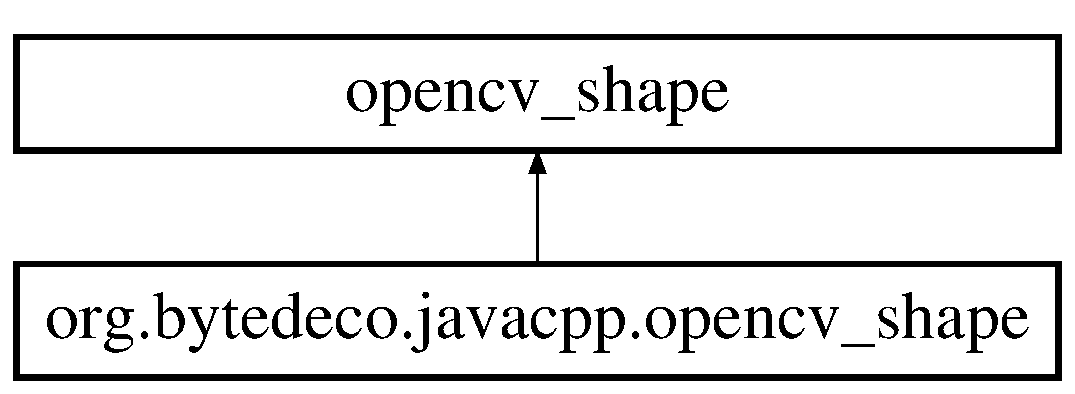
\includegraphics[height=2.000000cm]{classorg_1_1bytedeco_1_1javacpp_1_1opencv__shape}
\end{center}
\end{figure}
\subsection*{Classes}
\begin{DoxyCompactItemize}
\item 
class {\bfseries Affine\+Transformer}
\begin{DoxyCompactList}\small\item\em Wrapper class for the Open\+CV Affine Transformation algorithm. \+: \end{DoxyCompactList}\item 
class {\bfseries Chi\+Histogram\+Cost\+Extractor}
\begin{DoxyCompactList}\small\item\em An Chi based cost extraction. \+: \end{DoxyCompactList}\item 
class {\bfseries E\+M\+D\+Histogram\+Cost\+Extractor}
\begin{DoxyCompactList}\small\item\em An E\+MD based cost extraction. \+: \end{DoxyCompactList}\item 
class {\bfseries E\+M\+D\+L1\+Histogram\+Cost\+Extractor}
\begin{DoxyCompactList}\small\item\em An E\+M\+D-\/\+L1 based cost extraction. \+: \end{DoxyCompactList}\item 
class {\bfseries Hausdorff\+Distance\+Extractor}
\begin{DoxyCompactList}\small\item\em A simple Hausdorff distance measure between shapes defined by contours. \end{DoxyCompactList}\item 
class {\bfseries Histogram\+Cost\+Extractor}
\item 
class {\bfseries Norm\+Histogram\+Cost\+Extractor}
\begin{DoxyCompactList}\small\item\em A norm based cost extraction. \+: \end{DoxyCompactList}\item 
class {\bfseries Shape\+Context\+Distance\+Extractor}
\begin{DoxyCompactList}\small\item\em Implementation of the Shape Context descriptor and matching algorithm. \end{DoxyCompactList}\item 
class {\bfseries Shape\+Distance\+Extractor}
\item 
class {\bfseries Shape\+Transformer}
\item 
class {\bfseries Thin\+Plate\+Spline\+Shape\+Transformer}
\begin{DoxyCompactList}\small\item\em Definition of the transformation. \end{DoxyCompactList}\end{DoxyCompactItemize}
\subsection*{Static Public Member Functions}
\begin{DoxyCompactItemize}
\item 
static native float {\bfseries E\+M\+D\+L1} (@By\+Val Mat signature1, @By\+Val Mat signature2)
\item 
static native float {\bfseries E\+M\+D\+L1} (@By\+Val U\+Mat signature1, @By\+Val U\+Mat signature2)
\item 
static native Thin\+Plate\+Spline\+Shape\+Transformer \hyperlink{group__shape_ga409dbca0ecf803197cc29ec102f593fd}{create\+Thin\+Plate\+Spline\+Shape\+Transformer} (double regularization\+Parameter)
\item 
static native Thin\+Plate\+Spline\+Shape\+Transformer {\bfseries create\+Thin\+Plate\+Spline\+Shape\+Transformer} ()
\item 
static native Affine\+Transformer \hyperlink{group__shape_gaf6ba7c375194bc18e7f3212dfadfa68f}{create\+Affine\+Transformer} (@Cast(\char`\"{}bool\char`\"{}) boolean full\+Affine)
\item 
static native Histogram\+Cost\+Extractor {\bfseries create\+Norm\+Histogram\+Cost\+Extractor} (int flag, int n\+Dummies, float default\+Cost)
\item 
static native Histogram\+Cost\+Extractor {\bfseries create\+Norm\+Histogram\+Cost\+Extractor} ()
\item 
static native Histogram\+Cost\+Extractor {\bfseries create\+E\+M\+D\+Histogram\+Cost\+Extractor} (int flag, int n\+Dummies, float default\+Cost)
\item 
static native Histogram\+Cost\+Extractor {\bfseries create\+E\+M\+D\+Histogram\+Cost\+Extractor} ()
\item 
static native Histogram\+Cost\+Extractor {\bfseries create\+Chi\+Histogram\+Cost\+Extractor} (int n\+Dummies, float default\+Cost)
\item 
static native Histogram\+Cost\+Extractor {\bfseries create\+Chi\+Histogram\+Cost\+Extractor} ()
\item 
static native Histogram\+Cost\+Extractor {\bfseries create\+E\+M\+D\+L1\+Histogram\+Cost\+Extractor} (int n\+Dummies, float default\+Cost)
\item 
static native Histogram\+Cost\+Extractor {\bfseries create\+E\+M\+D\+L1\+Histogram\+Cost\+Extractor} ()
\item 
static native Shape\+Context\+Distance\+Extractor {\bfseries create\+Shape\+Context\+Distance\+Extractor} (int n\+Angular\+Bins, int n\+Radial\+Bins, float inner\+Radius, float outer\+Radius, int iterations, @Ptr Histogram\+Cost\+Extractor comparer, @Ptr Shape\+Transformer transformer)
\item 
static native Shape\+Context\+Distance\+Extractor {\bfseries create\+Shape\+Context\+Distance\+Extractor} ()
\item 
static native Hausdorff\+Distance\+Extractor {\bfseries create\+Hausdorff\+Distance\+Extractor} (int distance\+Flag, float rank\+Prop)
\item 
static native Hausdorff\+Distance\+Extractor {\bfseries create\+Hausdorff\+Distance\+Extractor} ()
\end{DoxyCompactItemize}


The documentation for this class was generated from the following file\+:\begin{DoxyCompactItemize}
\item 
opencv\+\_\+shape.\+java\end{DoxyCompactItemize}

\hypertarget{classorg_1_1bytedeco_1_1javacpp_1_1opencv__stitching}{}\section{org.\+bytedeco.\+javacpp.\+opencv\+\_\+stitching Class Reference}
\label{classorg_1_1bytedeco_1_1javacpp_1_1opencv__stitching}\index{org.\+bytedeco.\+javacpp.\+opencv\+\_\+stitching@{org.\+bytedeco.\+javacpp.\+opencv\+\_\+stitching}}
Inheritance diagram for org.\+bytedeco.\+javacpp.\+opencv\+\_\+stitching\+:\begin{figure}[H]
\begin{center}
\leavevmode
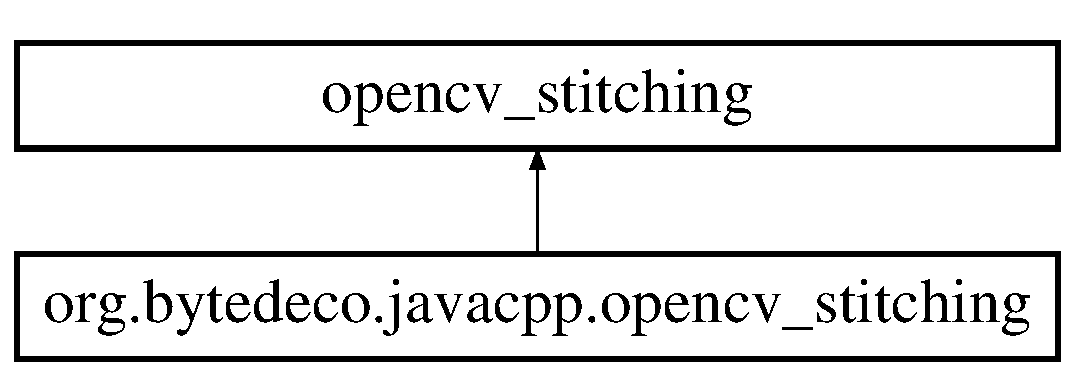
\includegraphics[height=2.000000cm]{classorg_1_1bytedeco_1_1javacpp_1_1opencv__stitching}
\end{center}
\end{figure}
\subsection*{Classes}
\begin{DoxyCompactItemize}
\item 
class {\bfseries Affine\+Based\+Estimator}
\begin{DoxyCompactList}\small\item\em Affine transformation based estimator. \end{DoxyCompactList}\item 
class {\bfseries Affine\+Best\+Of2\+Nearest\+Matcher}
\begin{DoxyCompactList}\small\item\em Features matcher similar to cv\+::detail\+::\+Best\+Of2\+Nearest\+Matcher which finds two best matches for each feature and leaves the best one only if the ratio between descriptor distances is greater than the fr.antproject.utils.threshold match\+\_\+conf. \end{DoxyCompactList}\item
class {\bfseries Affine\+Warper}
\begin{DoxyCompactList}\small\item\em Affine warper that uses rotations and translations. \end{DoxyCompactList}\item 
class {\bfseries A\+K\+A\+Z\+E\+Features\+Finder}
\begin{DoxyCompactList}\small\item\em A\+K\+A\+ZE features finder. \+: \end{DoxyCompactList}\item 
class {\bfseries Best\+Of2\+Nearest\+Matcher}
\begin{DoxyCompactList}\small\item\em Features matcher which finds two best matches for each feature and leaves the best one only if the ratio between descriptor distances is greater than the fr.antproject.utils.threshold match\+\_\+conf. \end{DoxyCompactList}\item
class {\bfseries Best\+Of2\+Nearest\+Range\+Matcher}
\item 
class {\bfseries Blender}
\item 
class {\bfseries Blocks\+Gain\+Compensator}
\begin{DoxyCompactList}\small\item\em Exposure compensator which tries to remove exposure related artifacts by adjusting image block intensities, see {\bfseries [U\+E\+S01]} for details. \end{DoxyCompactList}\item 
class {\bfseries Bundle\+Adjuster\+Affine}
\begin{DoxyCompactList}\small\item\em Bundle adjuster that expects affine transformation represented in homogeneous coordinates in R for each camera param. Implements camera parameters refinement algorithm which minimizes sum of the reprojection error squares. \end{DoxyCompactList}\item 
class {\bfseries Bundle\+Adjuster\+Affine\+Partial}
\begin{DoxyCompactList}\small\item\em Bundle adjuster that expects affine transformation with 4 D\+OF represented in homogeneous coordinates in R for each camera param. Implements camera parameters refinement algorithm which minimizes sum of the reprojection error squares. \end{DoxyCompactList}\item 
class {\bfseries Bundle\+Adjuster\+Base}
\begin{DoxyCompactList}\small\item\em Base class for all camera parameters refinement methods. \end{DoxyCompactList}\item 
class {\bfseries Bundle\+Adjuster\+Ray}
\begin{DoxyCompactList}\small\item\em Implementation of the camera parameters refinement algorithm which minimizes sum of the distances between the rays passing through the camera center and a feature. \+: \end{DoxyCompactList}\item 
class {\bfseries Bundle\+Adjuster\+Reproj}
\begin{DoxyCompactList}\small\item\em Implementation of the camera parameters refinement algorithm which minimizes sum of the reprojection error squares. \end{DoxyCompactList}\item 
class {\bfseries Camera\+Params}
\item 
class {\bfseries Compressed\+Rectilinear\+Portrait\+Projector}
\item 
class {\bfseries Compressed\+Rectilinear\+Portrait\+Warper}
\item 
class {\bfseries Compressed\+Rectilinear\+Projector}
\item 
class {\bfseries Compressed\+Rectilinear\+Warper}
\item 
class {\bfseries Cylindrical\+Portrait\+Projector}
\item 
class {\bfseries Cylindrical\+Portrait\+Warper}
\item 
class {\bfseries Cylindrical\+Projector}
\item 
class {\bfseries Cylindrical\+Warper}
\begin{DoxyCompactList}\small\item\em Affine warper factory class. \end{DoxyCompactList}\item 
class {\bfseries Detail\+Compressed\+Rectilinear\+Portrait\+Warper}
\item 
class {\bfseries Detail\+Compressed\+Rectilinear\+Warper}
\item 
class {\bfseries Detail\+Cylindrical\+Warper}
\begin{DoxyCompactList}\small\item\em Warper that maps an image onto the x$\ast$x + z$\ast$z = 1 cylinder. \end{DoxyCompactList}\item 
class {\bfseries Detail\+Cylindrical\+Warper\+Gpu}
\item 
class {\bfseries Detail\+Fisheye\+Warper}
\item 
class {\bfseries Detail\+Mercator\+Warper}
\item 
class {\bfseries Detail\+Panini\+Portrait\+Warper}
\item 
class {\bfseries Detail\+Panini\+Warper}
\item 
class {\bfseries Detail\+Plane\+Warper}
\begin{DoxyCompactList}\small\item\em Warper that maps an image onto the z = 1 plane. \end{DoxyCompactList}\item 
class {\bfseries Detail\+Plane\+Warper\+Gpu}
\item 
class {\bfseries Detail\+Spherical\+Warper}
\begin{DoxyCompactList}\small\item\em Warper that maps an image onto the unit sphere located at the origin. \end{DoxyCompactList}\item 
class {\bfseries Detail\+Spherical\+Warper\+Gpu}
\item 
class {\bfseries Detail\+Stereographic\+Warper}
\item 
class {\bfseries Detail\+Transverse\+Mercator\+Warper}
\item 
class {\bfseries Disjoint\+Sets}
\item 
class {\bfseries Dp\+Seam\+Finder}
\item 
class {\bfseries Estimator}
\item 
class {\bfseries Exposure\+Compensator}
\item 
class {\bfseries Feather\+Blender}
\begin{DoxyCompactList}\small\item\em Simple blender which mixes images at its borders. \end{DoxyCompactList}\item 
class {\bfseries Features\+Finder}
\begin{DoxyCompactList}\small\item\em Feature finders base class. \end{DoxyCompactList}\item 
class {\bfseries Features\+Matcher}
\begin{DoxyCompactList}\small\item\em Feature matchers base class. \end{DoxyCompactList}\item 
class {\bfseries Fisheye\+Projector}
\item 
class {\bfseries Fisheye\+Warper}
\item 
class {\bfseries Gain\+Compensator}
\begin{DoxyCompactList}\small\item\em Exposure compensator which tries to remove exposure related artifacts by adjusting image intensities, see {\bfseries [B\+L07]} and {\bfseries [W\+J10]} for details. \end{DoxyCompactList}\item 
class {\bfseries Graph}
\item 
class {\bfseries Graph\+Cut\+Seam\+Finder}
\begin{DoxyCompactList}\small\item\em Minimum graph cut-\/based seam estimator. See details in {\bfseries [V03]} . \end{DoxyCompactList}\item 
class {\bfseries Graph\+Cut\+Seam\+Finder\+Base}
\begin{DoxyCompactList}\small\item\em Base class for all minimum graph-\/cut-\/based seam estimators. \end{DoxyCompactList}\item 
class {\bfseries Graph\+Edge}
\item 
class {\bfseries Homography\+Based\+Estimator}
\begin{DoxyCompactList}\small\item\em Homography based rotation estimator. \end{DoxyCompactList}\item 
class {\bfseries Image\+Features}
\item 
class {\bfseries Matches\+Info}
\begin{DoxyCompactList}\small\item\em Structure containing information about matches between two images. \end{DoxyCompactList}\item 
class {\bfseries Mercator\+Projector}
\item 
class {\bfseries Mercator\+Warper}
\item 
class {\bfseries Multi\+Band\+Blender}
\begin{DoxyCompactList}\small\item\em Blender which uses multi-\/band blending algorithm (see {\bfseries [B\+A83]}). \end{DoxyCompactList}\item 
class {\bfseries No\+Bundle\+Adjuster}
\begin{DoxyCompactList}\small\item\em Stub bundle adjuster that does nothing. \end{DoxyCompactList}\item 
class {\bfseries No\+Exposure\+Compensator}
\begin{DoxyCompactList}\small\item\em Stub exposure compensator which does nothing. \end{DoxyCompactList}\item 
class {\bfseries No\+Seam\+Finder}
\begin{DoxyCompactList}\small\item\em Stub seam estimator which does nothing. \end{DoxyCompactList}\item 
class {\bfseries Orb\+Features\+Finder}
\begin{DoxyCompactList}\small\item\em O\+RB features finder. \+: \end{DoxyCompactList}\item 
class {\bfseries Pairwise\+Seam\+Finder}
\begin{DoxyCompactList}\small\item\em Base class for all pairwise seam estimators. \end{DoxyCompactList}\item 
class {\bfseries Panini\+Portrait\+Projector}
\item 
class {\bfseries Panini\+Portrait\+Warper}
\item 
class {\bfseries Panini\+Projector}
\item 
class {\bfseries Panini\+Warper}
\item 
class {\bfseries Plane\+Portrait\+Projector}
\item 
class {\bfseries Plane\+Portrait\+Warper}
\item 
class {\bfseries Plane\+Projector}
\begin{DoxyCompactList}\small\item\em Base class for rotation-\/based warper using a detail\+::\+Projector\+Base\+\_\+ derived class. \end{DoxyCompactList}\item 
class {\bfseries Plane\+Warper}
\begin{DoxyCompactList}\small\item\em Plane warper factory class. \end{DoxyCompactList}\item 
class {\bfseries Projector\+Base}
\begin{DoxyCompactList}\small\item\em Base class for warping logic implementation. \end{DoxyCompactList}\item 
class {\bfseries Rotation\+Warper}
\item 
class {\bfseries Seam\+Finder}
\item 
class {\bfseries Spherical\+Portrait\+Projector}
\item 
class {\bfseries Spherical\+Portrait\+Warper}
\item 
class {\bfseries Spherical\+Projector}
\item 
class {\bfseries Spherical\+Warper}
\begin{DoxyCompactList}\small\item\em Spherical warper factory class. \end{DoxyCompactList}\item 
class {\bfseries Stereographic\+Projector}
\item 
class {\bfseries Stereographic\+Warper}
\item 
class {\bfseries Stitcher}
\item 
class {\bfseries Surf\+Features\+Finder}
\begin{DoxyCompactList}\small\item\em S\+U\+RF features finder. \end{DoxyCompactList}\item 
class {\bfseries Timelapser}
\item 
class {\bfseries Timelapser\+Crop}
\item 
class {\bfseries Transverse\+Mercator\+Projector}
\item 
class {\bfseries Transverse\+Mercator\+Warper}
\item 
class {\bfseries Voronoi\+Seam\+Finder}
\begin{DoxyCompactList}\small\item\em Voronoi diagram-\/based seam estimator. \end{DoxyCompactList}\item 
class {\bfseries Warper\+Creator}
\end{DoxyCompactItemize}
\subsection*{Static Public Member Functions}
\begin{DoxyCompactItemize}
\item 
static native boolean {\bfseries overlap\+Roi} (@By\+Val fr.antproject.utils.Point tl1, @By\+Val fr.antproject.utils.Point tl2, @By\+Val Size sz1, @By\+Val Size sz2, @By\+Ref Rect roi)
\item 
static native Rect {\bfseries result\+Roi} (@Const @By\+Ref fr.antproject.utils.Point\+Vector corners, @Const @By\+Ref U\+Mat\+Vector images)
\item 
static native Rect {\bfseries result\+Roi} (@Const @By\+Ref fr.antproject.utils.Point\+Vector corners, @Const @By\+Ref Size\+Vector sizes)
\item 
static native Rect {\bfseries result\+Roi\+Intersection} (@Const @By\+Ref fr.antproject.utils.Point\+Vector corners, @Const @By\+Ref Size\+Vector sizes)
\item 
static native fr.antproject.utils.Point {\bfseries result\+Tl} (@Const @By\+Ref fr.antproject.utils.Point\+Vector corners)
\item 
static native void {\bfseries select\+Random\+Subset} (int count, int size, @Std\+Vector Int\+Pointer subset)
\item 
static native void {\bfseries select\+Random\+Subset} (int count, int size, @Std\+Vector Int\+Buffer subset)
\item 
static native void {\bfseries select\+Random\+Subset} (int count, int size, @Std\+Vector int\mbox{[}$\,$\mbox{]} subset)
\item 
static native Int\+Pointer {\bfseries stitching\+Log\+Level} ()
\item 
static native void \hyperlink{group__stitching__rotation_ga3bba1a4cfe47a38f2ef140a3bc6c0f0a}{wave\+Correct} (@By\+Ref Mat\+Vector rmats, @Cast(\char`\"{}cv\+::detail\+::\+Wave\+Correct\+Kind\char`\"{}) int kind)
\begin{DoxyCompactList}\small\item\em Tries to make panorama more horizontal (or vertical). \end{DoxyCompactList}\item 
static native Byte\+Pointer {\bfseries matches\+Graph\+As\+String} (@By\+Ref String\+Vector pathes, @Std\+Vector Matches\+Info pairwise\+\_\+matches, float conf\+\_\+fr.antproject.utils.threshold)
\item 
static native Int\+Pointer {\bfseries leave\+Biggest\+Component} ( @Std\+Vector Image\+Features features, @Std\+Vector Matches\+Info pairwise\+\_\+matches, float conf\+\_\+fr.antproject.utils.threshold)
\item 
static native void {\bfseries find\+Max\+Spanning\+Tree} (int num\+\_\+images, @Std\+Vector Matches\+Info pairwise\+\_\+matches, @By\+Ref Graph span\+\_\+tree, @Std\+Vector Int\+Pointer centers)
\item 
static native void {\bfseries find\+Max\+Spanning\+Tree} (int num\+\_\+images, @Std\+Vector Matches\+Info pairwise\+\_\+matches, @By\+Ref Graph span\+\_\+tree, @Std\+Vector Int\+Buffer centers)
\item 
static native void {\bfseries find\+Max\+Spanning\+Tree} (int num\+\_\+images, @Std\+Vector Matches\+Info pairwise\+\_\+matches, @By\+Ref Graph span\+\_\+tree, @Std\+Vector int\mbox{[}$\,$\mbox{]} centers)
\item 
static native void {\bfseries normalize\+Using\+Weight\+Map} (@By\+Val Mat weight, @By\+Val Mat src)
\item 
static native void {\bfseries normalize\+Using\+Weight\+Map} (@By\+Val U\+Mat weight, @By\+Val U\+Mat src)
\item 
static native void {\bfseries create\+Weight\+Map} (@By\+Val Mat mask, float sharpness, @By\+Val Mat weight)
\item 
static native void {\bfseries create\+Weight\+Map} (@By\+Val U\+Mat mask, float sharpness, @By\+Val U\+Mat weight)
\item 
static native void {\bfseries create\+Laplace\+Pyr} (@By\+Val Mat img, int num\+\_\+levels, @By\+Ref U\+Mat\+Vector pyr)
\item 
static native void {\bfseries create\+Laplace\+Pyr} (@By\+Val U\+Mat img, int num\+\_\+levels, @By\+Ref U\+Mat\+Vector pyr)
\item 
static native void {\bfseries create\+Laplace\+Pyr\+Gpu} (@By\+Val Mat img, int num\+\_\+levels, @By\+Ref U\+Mat\+Vector pyr)
\item 
static native void {\bfseries create\+Laplace\+Pyr\+Gpu} (@By\+Val U\+Mat img, int num\+\_\+levels, @By\+Ref U\+Mat\+Vector pyr)
\item 
static native void {\bfseries restore\+Image\+From\+Laplace\+Pyr} (@By\+Ref U\+Mat\+Vector pyr)
\item 
static native void {\bfseries restore\+Image\+From\+Laplace\+Pyr\+Gpu} (@By\+Ref U\+Mat\+Vector pyr)
\item 
static native void {\bfseries focals\+From\+Homography} (@Const @By\+Ref Mat H, @By\+Ref Double\+Pointer f0, @By\+Ref Double\+Pointer f1, @Cast(\char`\"{}bool$\ast$\char`\"{}) @By\+Ref Bool\+Pointer f0\+\_\+ok, @Cast(\char`\"{}bool$\ast$\char`\"{}) @By\+Ref Bool\+Pointer f1\+\_\+ok)
\item 
static native void {\bfseries focals\+From\+Homography} (@Const @By\+Ref Mat H, @By\+Ref Double\+Buffer f0, @By\+Ref Double\+Buffer f1, @Cast(\char`\"{}bool$\ast$\char`\"{}) @By\+Ref boolean\mbox{[}$\,$\mbox{]} f0\+\_\+ok, @Cast(\char`\"{}bool$\ast$\char`\"{}) @By\+Ref boolean\mbox{[}$\,$\mbox{]} f1\+\_\+ok)
\item 
static native void {\bfseries focals\+From\+Homography} (@Const @By\+Ref Mat H, @By\+Ref double\mbox{[}$\,$\mbox{]} f0, @By\+Ref double\mbox{[}$\,$\mbox{]} f1, @Cast(\char`\"{}bool$\ast$\char`\"{}) @By\+Ref Bool\+Pointer f0\+\_\+ok, @Cast(\char`\"{}bool$\ast$\char`\"{}) @By\+Ref Bool\+Pointer f1\+\_\+ok)
\item 
static native void {\bfseries focals\+From\+Homography} (@Const @By\+Ref Mat H, @By\+Ref Double\+Pointer f0, @By\+Ref Double\+Pointer f1, @Cast(\char`\"{}bool$\ast$\char`\"{}) @By\+Ref boolean\mbox{[}$\,$\mbox{]} f0\+\_\+ok, @Cast(\char`\"{}bool$\ast$\char`\"{}) @By\+Ref boolean\mbox{[}$\,$\mbox{]} f1\+\_\+ok)
\item 
static native void {\bfseries focals\+From\+Homography} (@Const @By\+Ref Mat H, @By\+Ref Double\+Buffer f0, @By\+Ref Double\+Buffer f1, @Cast(\char`\"{}bool$\ast$\char`\"{}) @By\+Ref Bool\+Pointer f0\+\_\+ok, @Cast(\char`\"{}bool$\ast$\char`\"{}) @By\+Ref Bool\+Pointer f1\+\_\+ok)
\item 
static native void {\bfseries focals\+From\+Homography} (@Const @By\+Ref Mat H, @By\+Ref double\mbox{[}$\,$\mbox{]} f0, @By\+Ref double\mbox{[}$\,$\mbox{]} f1, @Cast(\char`\"{}bool$\ast$\char`\"{}) @By\+Ref boolean\mbox{[}$\,$\mbox{]} f0\+\_\+ok, @Cast(\char`\"{}bool$\ast$\char`\"{}) @By\+Ref boolean\mbox{[}$\,$\mbox{]} f1\+\_\+ok)
\item 
static native void \hyperlink{group__stitching__autocalib_gab7c6c88fc60a136eb6f9faa46a32e660}{estimate\+Focal} (@Std\+Vector Image\+Features features, @Std\+Vector Matches\+Info pairwise\+\_\+matches, @Std\+Vector Double\+Pointer focals)
\begin{DoxyCompactList}\small\item\em Estimates focal lengths for each given camera. \end{DoxyCompactList}\item 
static native void {\bfseries estimate\+Focal} (@Std\+Vector Image\+Features features, @Std\+Vector Matches\+Info pairwise\+\_\+matches, @Std\+Vector Double\+Buffer focals)
\item 
static native void {\bfseries estimate\+Focal} (@Std\+Vector Image\+Features features, @Std\+Vector Matches\+Info pairwise\+\_\+matches, @Std\+Vector double\mbox{[}$\,$\mbox{]} focals)
\item 
static native boolean {\bfseries calibrate\+Rotating\+Camera} (@Const @By\+Ref Mat\+Vector Hs, @By\+Ref Mat K)
\item 
static native Stitcher {\bfseries create\+Stitcher} (@Cast(\char`\"{}bool\char`\"{}) boolean try\+\_\+use\+\_\+gpu)
\item 
static native Stitcher {\bfseries create\+Stitcher} ()
\end{DoxyCompactItemize}
\subsection*{Static Public Attributes}
\begin{DoxyCompactItemize}
\item 
static final int \hyperlink{group__stitching__rotation_ga5b86272961257cad2cfb216bf6ca414b}{W\+A\+V\+E\+\_\+\+C\+O\+R\+R\+E\+C\+T\+\_\+\+H\+O\+R\+IZ} = 0
\end{DoxyCompactItemize}


The documentation for this class was generated from the following file\+:\begin{DoxyCompactItemize}
\item 
opencv\+\_\+stitching.\+java\end{DoxyCompactItemize}

\hypertarget{classorg_1_1bytedeco_1_1javacpp_1_1opencv__superres}{}\section{org.\+bytedeco.\+javacpp.\+opencv\+\_\+superres Class Reference}
\label{classorg_1_1bytedeco_1_1javacpp_1_1opencv__superres}\index{org.\+bytedeco.\+javacpp.\+opencv\+\_\+superres@{org.\+bytedeco.\+javacpp.\+opencv\+\_\+superres}}
Inheritance diagram for org.\+bytedeco.\+javacpp.\+opencv\+\_\+superres\+:\begin{figure}[H]
\begin{center}
\leavevmode
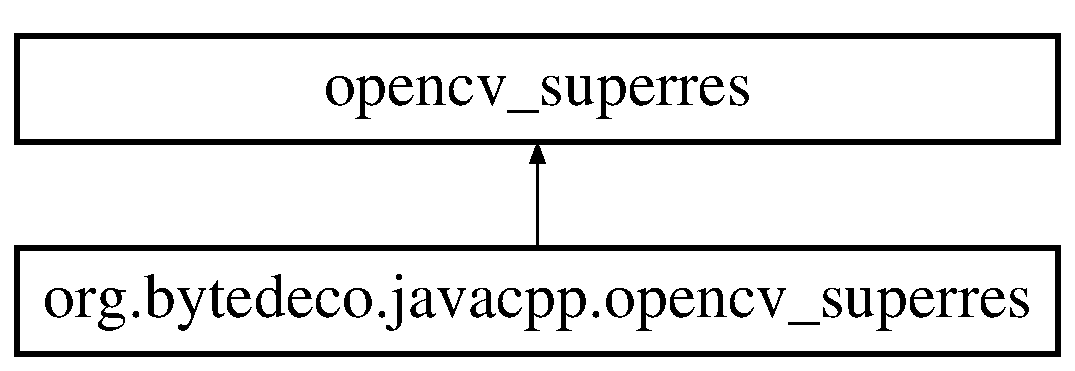
\includegraphics[height=2.000000cm]{classorg_1_1bytedeco_1_1javacpp_1_1opencv__superres}
\end{center}
\end{figure}
\subsection*{Classes}
\begin{DoxyCompactItemize}
\item 
class {\bfseries Brox\+Optical\+Flow}
\item 
class {\bfseries Dense\+Optical\+Flow\+Ext}
\item 
class {\bfseries Frame\+Source}
\item 
class {\bfseries Pyr\+L\+K\+Optical\+Flow}
\item 
class {\bfseries Super\+Res\+Dual\+T\+V\+L1\+Optical\+Flow}
\item 
class {\bfseries Super\+Res\+Farneback\+Optical\+Flow}
\item 
class {\bfseries Super\+Resolution}
\begin{DoxyCompactList}\small\item\em Base class for Super Resolution algorithms. \end{DoxyCompactList}\end{DoxyCompactItemize}
\subsection*{Static Public Member Functions}
\begin{DoxyCompactItemize}
\item 
static native Frame\+Source {\bfseries create\+Frame\+Source\+\_\+\+Empty} ()
\item 
static native Frame\+Source {\bfseries create\+Frame\+Source\+\_\+\+Video} (@Str Byte\+Pointer file\+Name)
\item 
static native Frame\+Source {\bfseries create\+Frame\+Source\+\_\+\+Video} (@Str String file\+Name)
\item 
static native Frame\+Source {\bfseries create\+Frame\+Source\+\_\+\+Video\+\_\+\+C\+U\+DA} (@Str Byte\+Pointer file\+Name)
\item 
static native Frame\+Source {\bfseries create\+Frame\+Source\+\_\+\+Video\+\_\+\+C\+U\+DA} (@Str String file\+Name)
\item 
static native Frame\+Source {\bfseries create\+Frame\+Source\+\_\+\+Camera} (int device\+Id)
\item 
static native Frame\+Source {\bfseries create\+Frame\+Source\+\_\+\+Camera} ()
\item 
static native Super\+Resolution \hyperlink{group__superres_gac2dfc5e8422832bbb249c6675e7cb851}{create\+Super\+Resolution\+\_\+\+B\+T\+V\+L1} ()
\begin{DoxyCompactList}\small\item\em Create Bilateral T\+V-\/\+L1 Super Resolution. \end{DoxyCompactList}\item 
static native Super\+Resolution {\bfseries create\+Super\+Resolution\+\_\+\+B\+T\+V\+L1\+\_\+\+C\+U\+DA} ()
\item 
static native Super\+Res\+Farneback\+Optical\+Flow {\bfseries create\+Opt\+Flow\+\_\+\+Farneback} ()
\item 
static native Super\+Res\+Farneback\+Optical\+Flow {\bfseries create\+Opt\+Flow\+\_\+\+Farneback\+\_\+\+C\+U\+DA} ()
\item 
static native Super\+Res\+Dual\+T\+V\+L1\+Optical\+Flow {\bfseries create\+Opt\+Flow\+\_\+\+Dual\+T\+V\+L1} ()
\item 
static native Super\+Res\+Dual\+T\+V\+L1\+Optical\+Flow {\bfseries create\+Opt\+Flow\+\_\+\+Dual\+T\+V\+L1\+\_\+\+C\+U\+DA} ()
\item 
static native Brox\+Optical\+Flow {\bfseries create\+Opt\+Flow\+\_\+\+Brox\+\_\+\+C\+U\+DA} ()
\item 
static native Pyr\+L\+K\+Optical\+Flow {\bfseries create\+Opt\+Flow\+\_\+\+Pyr\+L\+K\+\_\+\+C\+U\+DA} ()
\end{DoxyCompactItemize}


The documentation for this class was generated from the following file\+:\begin{DoxyCompactItemize}
\item 
opencv\+\_\+superres.\+java\end{DoxyCompactItemize}

\hypertarget{classorg_1_1bytedeco_1_1javacpp_1_1opencv__text}{}\section{org.\+bytedeco.\+javacpp.\+opencv\+\_\+text Class Reference}
\label{classorg_1_1bytedeco_1_1javacpp_1_1opencv__text}\index{org.\+bytedeco.\+javacpp.\+opencv\+\_\+text@{org.\+bytedeco.\+javacpp.\+opencv\+\_\+text}}
Inheritance diagram for org.\+bytedeco.\+javacpp.\+opencv\+\_\+text\+:\begin{figure}[H]
\begin{center}
\leavevmode
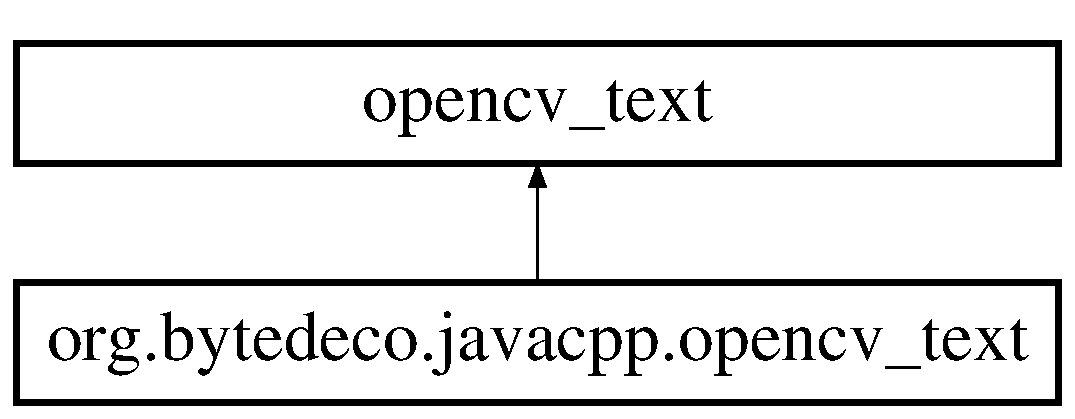
\includegraphics[height=2.000000cm]{classorg_1_1bytedeco_1_1javacpp_1_1opencv__text}
\end{center}
\end{figure}
\subsection*{Classes}
\begin{DoxyCompactItemize}
\item 
class {\bfseries Base\+O\+CR}
\item 
class {\bfseries Double\+Vector}
\item 
class {\bfseries E\+R\+Filter}
\begin{DoxyCompactList}\small\item\em Base class for 1st and 2nd stages of Neumann and Matas scene text detection algorithm \mbox{[}Neumann12\mbox{]}. \+: \end{DoxyCompactList}\item 
class {\bfseries E\+R\+Stat}
\item 
class {\bfseries E\+R\+Stat\+Vector}
\item 
class {\bfseries E\+R\+Stat\+Vector\+Vector}
\item 
class {\bfseries Int\+Deque}
\item 
class {\bfseries O\+C\+R\+Beam\+Search\+Decoder}
\begin{DoxyCompactList}\small\item\em O\+C\+R\+Beam\+Search\+Decoder class provides an interface for O\+CR using Beam Search algorithm. \end{DoxyCompactList}\item 
class {\bfseries O\+C\+R\+H\+M\+M\+Decoder}
\begin{DoxyCompactList}\small\item\em O\+C\+R\+H\+M\+M\+Decoder class provides an interface for O\+CR using Hidden Markov Models. \end{DoxyCompactList}\item 
class {\bfseries O\+C\+R\+Tesseract}
\begin{DoxyCompactList}\small\item\em O\+C\+R\+Tesseract class provides an interface with the tesseract-\/ocr A\+PI (v3.\+02.\+02) in C++. \end{DoxyCompactList}\item 
class {\bfseries Std\+String\+Vector}
\end{DoxyCompactItemize}
\subsection*{Static Public Member Functions}
\begin{DoxyCompactItemize}
\item 
static native E\+R\+Filter \hyperlink{group__text__detect_ga0c01c194688152f569f28f7845cbfbaf}{create\+E\+R\+Filter\+N\+M1} (@Ptr E\+R\+Filter.\+Callback cb, int fr.antproject.utils.threshold\+Delta, float min\+Area, float max\+Area, float min\+Probability, @Cast(\char`\"{}bool\char`\"{}) boolean non\+Max\+Suppression, float min\+Probability\+Diff)
\begin{DoxyCompactList}\small\item\em Create an Extremal Region Filter for the 1st stage classifier of N\&M algorithm \mbox{[}Neumann12\mbox{]}. \end{DoxyCompactList}\item 
static native E\+R\+Filter {\bfseries create\+E\+R\+Filter\+N\+M1} (@Ptr E\+R\+Filter.\+Callback cb)
\item 
static native E\+R\+Filter \hyperlink{group__text__detect_ga941eba7519bae9c44d6cbd21d21ad26e}{create\+E\+R\+Filter\+N\+M2} (@Ptr E\+R\+Filter.\+Callback cb, float min\+Probability)
\begin{DoxyCompactList}\small\item\em Create an Extremal Region Filter for the 2nd stage classifier of N\&M algorithm \mbox{[}Neumann12\mbox{]}. \end{DoxyCompactList}\item 
static native E\+R\+Filter {\bfseries create\+E\+R\+Filter\+N\+M2} (@Ptr E\+R\+Filter.\+Callback cb)
\item 
static native E\+R\+Filter.\+Callback \hyperlink{group__text__detect_gaa43a04b9408663608d30f5bcdaadac16}{load\+Classifier\+N\+M1} (@Str Byte\+Pointer filename)
\begin{DoxyCompactList}\small\item\em Allow to implicitly load the default classifier when creating an E\+R\+Filter object. \end{DoxyCompactList}\item 
static native E\+R\+Filter.\+Callback {\bfseries load\+Classifier\+N\+M1} (@Str String filename)
\item 
static native E\+R\+Filter.\+Callback \hyperlink{group__text__detect_gaa41f7358b2e47c7e2b2831ad76410221}{load\+Classifier\+N\+M2} (@Str Byte\+Pointer filename)
\begin{DoxyCompactList}\small\item\em Allow to implicitly load the default classifier when creating an E\+R\+Filter object. \end{DoxyCompactList}\item 
static native E\+R\+Filter.\+Callback {\bfseries load\+Classifier\+N\+M2} (@Str String filename)
\item 
static native void \hyperlink{group__text__detect_ga67163615b824817020e39c2738a0b122}{compute\+N\+M\+Channels} (@By\+Val Mat \+\_\+src, @By\+Val Mat\+Vector \+\_\+channels, int \+\_\+mode)
\begin{DoxyCompactList}\small\item\em Compute the different channels to be processed independently in the N\&M algorithm \mbox{[}Neumann12\mbox{]}. \end{DoxyCompactList}\item 
static native void {\bfseries compute\+N\+M\+Channels} (@By\+Val Mat \+\_\+src, @By\+Val Mat\+Vector \+\_\+channels)
\item 
static native void {\bfseries compute\+N\+M\+Channels} (@By\+Val Mat \+\_\+src, @By\+Val U\+Mat\+Vector \+\_\+channels, int \+\_\+mode)
\item 
static native void {\bfseries compute\+N\+M\+Channels} (@By\+Val Mat \+\_\+src, @By\+Val U\+Mat\+Vector \+\_\+channels)
\item 
static native void {\bfseries compute\+N\+M\+Channels} (@By\+Val U\+Mat \+\_\+src, @By\+Val Mat\+Vector \+\_\+channels, int \+\_\+mode)
\item 
static native void {\bfseries compute\+N\+M\+Channels} (@By\+Val U\+Mat \+\_\+src, @By\+Val Mat\+Vector \+\_\+channels)
\item 
static native void {\bfseries compute\+N\+M\+Channels} (@By\+Val U\+Mat \+\_\+src, @By\+Val U\+Mat\+Vector \+\_\+channels, int \+\_\+mode)
\item 
static native void {\bfseries compute\+N\+M\+Channels} (@By\+Val U\+Mat \+\_\+src, @By\+Val U\+Mat\+Vector \+\_\+channels)
\item 
static native void \hyperlink{group__text__detect_ga3198c558c08dac61bce863d430bf2da6}{er\+Grouping} (@By\+Val Mat img, @By\+Val Mat\+Vector channels, @By\+Ref E\+R\+Stat\+Vector\+Vector regions, @Cast(\char`\"{}std\+::vector$<$std\+::vector$<$cv\+::\+Vec2i$>$ $>$$\ast$\char`\"{}) @By\+Ref fr.antproject.utils.Point\+Vector\+Vector groups, @By\+Ref Rect\+Vector groups\+\_\+rects, int method, @Std\+String Byte\+Pointer filename, float min\+Probablity)
\begin{DoxyCompactList}\small\item\em Find groups of Extremal Regions that are organized as text blocks. \end{DoxyCompactList}\item 
static native void {\bfseries er\+Grouping} (@By\+Val Mat img, @By\+Val Mat\+Vector channels, @By\+Ref E\+R\+Stat\+Vector\+Vector regions, @Cast(\char`\"{}std\+::vector$<$std\+::vector$<$cv\+::\+Vec2i$>$ $>$$\ast$\char`\"{}) @By\+Ref fr.antproject.utils.Point\+Vector\+Vector groups, @By\+Ref Rect\+Vector groups\+\_\+rects)
\item 
static native void {\bfseries er\+Grouping} (@By\+Val Mat img, @By\+Val U\+Mat\+Vector channels, @By\+Ref E\+R\+Stat\+Vector\+Vector regions, @Cast(\char`\"{}std\+::vector$<$std\+::vector$<$cv\+::\+Vec2i$>$ $>$$\ast$\char`\"{}) @By\+Ref fr.antproject.utils.Point\+Vector\+Vector groups, @By\+Ref Rect\+Vector groups\+\_\+rects, int method, @Std\+String String filename, float min\+Probablity)
\item 
static native void {\bfseries er\+Grouping} (@By\+Val Mat img, @By\+Val U\+Mat\+Vector channels, @By\+Ref E\+R\+Stat\+Vector\+Vector regions, @Cast(\char`\"{}std\+::vector$<$std\+::vector$<$cv\+::\+Vec2i$>$ $>$$\ast$\char`\"{}) @By\+Ref fr.antproject.utils.Point\+Vector\+Vector groups, @By\+Ref Rect\+Vector groups\+\_\+rects)
\item 
static native void {\bfseries er\+Grouping} (@By\+Val U\+Mat img, @By\+Val Mat\+Vector channels, @By\+Ref E\+R\+Stat\+Vector\+Vector regions, @Cast(\char`\"{}std\+::vector$<$std\+::vector$<$cv\+::\+Vec2i$>$ $>$$\ast$\char`\"{}) @By\+Ref fr.antproject.utils.Point\+Vector\+Vector groups, @By\+Ref Rect\+Vector groups\+\_\+rects, int method, @Std\+String Byte\+Pointer filename, float min\+Probablity)
\item 
static native void {\bfseries er\+Grouping} (@By\+Val U\+Mat img, @By\+Val Mat\+Vector channels, @By\+Ref E\+R\+Stat\+Vector\+Vector regions, @Cast(\char`\"{}std\+::vector$<$std\+::vector$<$cv\+::\+Vec2i$>$ $>$$\ast$\char`\"{}) @By\+Ref fr.antproject.utils.Point\+Vector\+Vector groups, @By\+Ref Rect\+Vector groups\+\_\+rects)
\item 
static native void {\bfseries er\+Grouping} (@By\+Val U\+Mat img, @By\+Val U\+Mat\+Vector channels, @By\+Ref E\+R\+Stat\+Vector\+Vector regions, @Cast(\char`\"{}std\+::vector$<$std\+::vector$<$cv\+::\+Vec2i$>$ $>$$\ast$\char`\"{}) @By\+Ref fr.antproject.utils.Point\+Vector\+Vector groups, @By\+Ref Rect\+Vector groups\+\_\+rects, int method, @Std\+String String filename, float min\+Probablity)
\item 
static native void {\bfseries er\+Grouping} (@By\+Val U\+Mat img, @By\+Val U\+Mat\+Vector channels, @By\+Ref E\+R\+Stat\+Vector\+Vector regions, @Cast(\char`\"{}std\+::vector$<$std\+::vector$<$cv\+::\+Vec2i$>$ $>$$\ast$\char`\"{}) @By\+Ref fr.antproject.utils.Point\+Vector\+Vector groups, @By\+Ref Rect\+Vector groups\+\_\+rects)
\item 
static native void {\bfseries er\+Grouping} (@By\+Val Mat image, @By\+Val Mat channel, @By\+Val fr.antproject.utils.Point\+Vector\+Vector regions, @By\+Ref Rect\+Vector groups\+\_\+rects, int method, @Str Byte\+Pointer filename, float min\+Probablity)
\item 
static native void {\bfseries er\+Grouping} (@By\+Val Mat image, @By\+Val Mat channel, @By\+Val fr.antproject.utils.Point\+Vector\+Vector regions, @By\+Ref Rect\+Vector groups\+\_\+rects)
\item 
static native void {\bfseries er\+Grouping} (@By\+Val Mat image, @By\+Val Mat channel, @By\+Val fr.antproject.utils.Point\+Vector\+Vector regions, @By\+Ref Rect\+Vector groups\+\_\+rects, int method, @Str String filename, float min\+Probablity)
\item 
static native void {\bfseries er\+Grouping} (@By\+Val U\+Mat image, @By\+Val U\+Mat channel, @By\+Val fr.antproject.utils.Point\+Vector\+Vector regions, @By\+Ref Rect\+Vector groups\+\_\+rects, int method, @Str Byte\+Pointer filename, float min\+Probablity)
\item 
static native void {\bfseries er\+Grouping} (@By\+Val U\+Mat image, @By\+Val U\+Mat channel, @By\+Val fr.antproject.utils.Point\+Vector\+Vector regions, @By\+Ref Rect\+Vector groups\+\_\+rects)
\item 
static native void {\bfseries er\+Grouping} (@By\+Val U\+Mat image, @By\+Val U\+Mat channel, @By\+Val fr.antproject.utils.Point\+Vector\+Vector regions, @By\+Ref Rect\+Vector groups\+\_\+rects, int method, @Str String filename, float min\+Probablity)
\item 
static native void \hyperlink{group__text__detect_gad4c72b60ca712eeab78c52b946f649a2}{M\+S\+E\+Rs\+To\+E\+R\+Stats} (@By\+Val Mat image, @By\+Ref fr.antproject.utils.Point\+Vector\+Vector contours, @By\+Ref E\+R\+Stat\+Vector\+Vector regions)
\begin{DoxyCompactList}\small\item\em Converts M\+S\+ER contours (vector$<$fr.antproject.utils.Point$>$) to E\+R\+Stat regions. \end{DoxyCompactList}\item
static native void {\bfseries M\+S\+E\+Rs\+To\+E\+R\+Stats} (@By\+Val U\+Mat image, @By\+Ref fr.antproject.utils.Point\+Vector\+Vector contours, @By\+Ref E\+R\+Stat\+Vector\+Vector regions)
\item 
static native void {\bfseries detect\+Regions} (@By\+Val Mat image, @Ptr E\+R\+Filter er\+\_\+filter1, @Ptr E\+R\+Filter er\+\_\+filter2, @By\+Ref fr.antproject.utils.Point\+Vector\+Vector regions)
\item 
static native void {\bfseries detect\+Regions} (@By\+Val U\+Mat image, @Ptr E\+R\+Filter er\+\_\+filter1, @Ptr E\+R\+Filter er\+\_\+filter2, @By\+Ref fr.antproject.utils.Point\+Vector\+Vector regions)
\item 
static native O\+C\+R\+H\+M\+M\+Decoder.\+Classifier\+Callback \hyperlink{group__text__recognize_gabe00747d37f40a190b2970f14cdc4d60}{load\+O\+C\+R\+H\+M\+M\+Classifier\+NM} (@Str Byte\+Pointer filename)
\begin{DoxyCompactList}\small\item\em Allow to implicitly load the default character classifier when creating an O\+C\+R\+H\+M\+M\+Decoder object. \end{DoxyCompactList}\item 
static native O\+C\+R\+H\+M\+M\+Decoder.\+Classifier\+Callback {\bfseries load\+O\+C\+R\+H\+M\+M\+Classifier\+NM} (@Str String filename)
\item 
static native O\+C\+R\+H\+M\+M\+Decoder.\+Classifier\+Callback \hyperlink{group__text__recognize_ga03f0450934c0f48a89daa868f8ca9fcf}{load\+O\+C\+R\+H\+M\+M\+Classifier\+C\+NN} (@Str Byte\+Pointer filename)
\begin{DoxyCompactList}\small\item\em Allow to implicitly load the default character classifier when creating an O\+C\+R\+H\+M\+M\+Decoder object. \end{DoxyCompactList}\item 
static native O\+C\+R\+H\+M\+M\+Decoder.\+Classifier\+Callback {\bfseries load\+O\+C\+R\+H\+M\+M\+Classifier\+C\+NN} (@Str String filename)
\item 
static native void \hyperlink{classorg_1_1bytedeco_1_1javacpp_1_1opencv__text_ac23647f4572aeec4389d900bf01bf013}{create\+O\+C\+R\+H\+M\+M\+Transitions\+Table} (@Std\+String Byte\+Pointer vocabulary, @By\+Ref Std\+String\+Vector lexicon, @By\+Val Mat transition\+\_\+probabilities\+\_\+table)
\begin{DoxyCompactList}\small\item\em Utility function to create a tailored language model transitions table from a given list of words (lexicon). \end{DoxyCompactList}\item 
\mbox{\Hypertarget{classorg_1_1bytedeco_1_1javacpp_1_1opencv__text_aab24701d08ab8131f1f541388c56bdec}\label{classorg_1_1bytedeco_1_1javacpp_1_1opencv__text_aab24701d08ab8131f1f541388c56bdec}} 
static native void {\bfseries create\+O\+C\+R\+H\+M\+M\+Transitions\+Table} (@Std\+String String vocabulary, @By\+Ref Std\+String\+Vector lexicon, @By\+Val Mat transition\+\_\+probabilities\+\_\+table)
\item 
\mbox{\Hypertarget{classorg_1_1bytedeco_1_1javacpp_1_1opencv__text_abb5e6bd26a8a25684e3aef2c36433315}\label{classorg_1_1bytedeco_1_1javacpp_1_1opencv__text_abb5e6bd26a8a25684e3aef2c36433315}} 
static native void {\bfseries create\+O\+C\+R\+H\+M\+M\+Transitions\+Table} (@Std\+String Byte\+Pointer vocabulary, @By\+Ref Std\+String\+Vector lexicon, @By\+Val U\+Mat transition\+\_\+probabilities\+\_\+table)
\item 
\mbox{\Hypertarget{classorg_1_1bytedeco_1_1javacpp_1_1opencv__text_a1e99292b213c8d913b08cea827c68eb1}\label{classorg_1_1bytedeco_1_1javacpp_1_1opencv__text_a1e99292b213c8d913b08cea827c68eb1}} 
static native void {\bfseries create\+O\+C\+R\+H\+M\+M\+Transitions\+Table} (@Std\+String String vocabulary, @By\+Ref Std\+String\+Vector lexicon, @By\+Val U\+Mat transition\+\_\+probabilities\+\_\+table)
\item 
\mbox{\Hypertarget{classorg_1_1bytedeco_1_1javacpp_1_1opencv__text_a7a29e2f9486226f47cbcec670e8bf838}\label{classorg_1_1bytedeco_1_1javacpp_1_1opencv__text_a7a29e2f9486226f47cbcec670e8bf838}} 
static native Mat {\bfseries create\+O\+C\+R\+H\+M\+M\+Transitions\+Table} (@Str Byte\+Pointer vocabulary, @By\+Ref String\+Vector lexicon)
\item 
\mbox{\Hypertarget{classorg_1_1bytedeco_1_1javacpp_1_1opencv__text_a2432d5dfc513418ff6382020af067067}\label{classorg_1_1bytedeco_1_1javacpp_1_1opencv__text_a2432d5dfc513418ff6382020af067067}} 
static native Mat {\bfseries create\+O\+C\+R\+H\+M\+M\+Transitions\+Table} (@Str String vocabulary, @By\+Ref String\+Vector lexicon)
\item 
static native O\+C\+R\+Beam\+Search\+Decoder.\+Classifier\+Callback \hyperlink{classorg_1_1bytedeco_1_1javacpp_1_1opencv__text_ac5185baf5c06198df5eb4c500afcbcf0}{load\+O\+C\+R\+Beam\+Search\+Classifier\+C\+NN} (@Str Byte\+Pointer filename)
\begin{DoxyCompactList}\small\item\em Allow to implicitly load the default character classifier when creating an O\+C\+R\+Beam\+Search\+Decoder object. \end{DoxyCompactList}\item 
\mbox{\Hypertarget{classorg_1_1bytedeco_1_1javacpp_1_1opencv__text_ad5487feed505ad5441870766dc866000}\label{classorg_1_1bytedeco_1_1javacpp_1_1opencv__text_ad5487feed505ad5441870766dc866000}} 
static native O\+C\+R\+Beam\+Search\+Decoder.\+Classifier\+Callback {\bfseries load\+O\+C\+R\+Beam\+Search\+Classifier\+C\+NN} (@Str String filename)
\end{DoxyCompactItemize}
\subsection*{Static Public Attributes}
\begin{DoxyCompactItemize}
\item 
static final int \hyperlink{group__text__detect_gad0d3e0c8791f14093e736cd2da75632d}{E\+R\+F\+I\+L\+T\+E\+R\+\_\+\+N\+M\+\_\+\+R\+G\+B\+L\+Grad} = 0
\item 
static final int \hyperlink{group__text__detect_gab646588b9db6ae1e1aae89cc09ea4059}{E\+R\+G\+R\+O\+U\+P\+I\+N\+G\+\_\+\+O\+R\+I\+E\+N\+T\+A\+T\+I\+O\+N\+\_\+\+H\+O\+R\+IZ} = 0
\item 
static final int \hyperlink{group__text__recognize_gac4148e33328b79dbead3c33dac186540}{O\+C\+R\+\_\+\+L\+E\+V\+E\+L\+\_\+\+W\+O\+RD} = 0
\item 
static final int \hyperlink{group__text__recognize_gac1843f0d2e0e7136debaa46d45446b11}{O\+C\+R\+\_\+\+D\+E\+C\+O\+D\+E\+R\+\_\+\+V\+I\+T\+E\+R\+BI} = 0
\end{DoxyCompactItemize}


\subsection{Member Function Documentation}
\mbox{\Hypertarget{classorg_1_1bytedeco_1_1javacpp_1_1opencv__text_ac23647f4572aeec4389d900bf01bf013}\label{classorg_1_1bytedeco_1_1javacpp_1_1opencv__text_ac23647f4572aeec4389d900bf01bf013}} 
\index{org\+::bytedeco\+::javacpp\+::opencv\+\_\+text@{org\+::bytedeco\+::javacpp\+::opencv\+\_\+text}!create\+O\+C\+R\+H\+M\+M\+Transitions\+Table@{create\+O\+C\+R\+H\+M\+M\+Transitions\+Table}}
\index{create\+O\+C\+R\+H\+M\+M\+Transitions\+Table@{create\+O\+C\+R\+H\+M\+M\+Transitions\+Table}!org\+::bytedeco\+::javacpp\+::opencv\+\_\+text@{org\+::bytedeco\+::javacpp\+::opencv\+\_\+text}}
\subsubsection{\texorpdfstring{create\+O\+C\+R\+H\+M\+M\+Transitions\+Table()}{createOCRHMMTransitionsTable()}}
{\footnotesize\ttfamily static native void org.\+bytedeco.\+javacpp.\+opencv\+\_\+text.\+create\+O\+C\+R\+H\+M\+M\+Transitions\+Table (\begin{DoxyParamCaption}\item[{@Std\+String Byte\+Pointer}]{vocabulary,  }\item[{@By\+Ref Std\+String\+Vector}]{lexicon,  }\item[{@By\+Val Mat}]{transition\+\_\+probabilities\+\_\+table }\end{DoxyParamCaption})\hspace{0.3cm}{\ttfamily [static]}}



Utility function to create a tailored language model transitions table from a given list of words (lexicon). 

/$\ast$$\ast$ 
\begin{DoxyParams}{Parameters}
{\em vocabulary} & The language vocabulary (chars when ascii english text).\\
\hline
{\em lexicon} & The list of words that are expected to be found in a particular image.\\
\hline
{\em transition\+\_\+probabilities\+\_\+table} & Output table with transition probabilities between character pairs. cols == rows == vocabulary.\+size().\\
\hline
\end{DoxyParams}
The function calculate frequency statistics of character pairs from the given lexicon and fills the output transition\+\_\+probabilities\+\_\+table with them. The transition\+\_\+probabilities\+\_\+table can be used as input in the O\+C\+R\+H\+M\+M\+Decoder\+::create() and O\+C\+R\+Beam\+Search\+Decoder\+::create() methods. \begin{DoxyNote}{Note}

\begin{DoxyItemize}
\item (C++) An alternative would be to load the default generic language transition table provided in the text module samples folder (created from ispell 42869 english words list) \+: \href{https://github.com/opencv/opencv_contrib/blob/master/modules/text/samples/OCRHMM_transitions_table.xml}{\tt https\+://github.\+com/opencv/opencv\+\_\+contrib/blob/master/modules/text/samples/\+O\+C\+R\+H\+M\+M\+\_\+transitions\+\_\+table.\+xml} 
\end{DoxyItemize}
\end{DoxyNote}
\mbox{\Hypertarget{classorg_1_1bytedeco_1_1javacpp_1_1opencv__text_ac5185baf5c06198df5eb4c500afcbcf0}\label{classorg_1_1bytedeco_1_1javacpp_1_1opencv__text_ac5185baf5c06198df5eb4c500afcbcf0}} 
\index{org\+::bytedeco\+::javacpp\+::opencv\+\_\+text@{org\+::bytedeco\+::javacpp\+::opencv\+\_\+text}!load\+O\+C\+R\+Beam\+Search\+Classifier\+C\+NN@{load\+O\+C\+R\+Beam\+Search\+Classifier\+C\+NN}}
\index{load\+O\+C\+R\+Beam\+Search\+Classifier\+C\+NN@{load\+O\+C\+R\+Beam\+Search\+Classifier\+C\+NN}!org\+::bytedeco\+::javacpp\+::opencv\+\_\+text@{org\+::bytedeco\+::javacpp\+::opencv\+\_\+text}}
\subsubsection{\texorpdfstring{load\+O\+C\+R\+Beam\+Search\+Classifier\+C\+N\+N()}{loadOCRBeamSearchClassifierCNN()}}
{\footnotesize\ttfamily static native O\+C\+R\+Beam\+Search\+Decoder.\+Classifier\+Callback org.\+bytedeco.\+javacpp.\+opencv\+\_\+text.\+load\+O\+C\+R\+Beam\+Search\+Classifier\+C\+NN (\begin{DoxyParamCaption}\item[{@Str Byte\+Pointer}]{filename }\end{DoxyParamCaption})\hspace{0.3cm}{\ttfamily [static]}}



Allow to implicitly load the default character classifier when creating an O\+C\+R\+Beam\+Search\+Decoder object. 


\begin{DoxyParams}{Parameters}
{\em filename} & The X\+ML or Y\+A\+ML file with the classifier model (e.\+g. O\+C\+R\+Beam\+Search\+\_\+\+C\+N\+N\+\_\+model\+\_\+data.\+xml.\+gz) \\
\hline
\end{DoxyParams}
The C\+NN default classifier is based in the scene text recognition method proposed by Adam Coates \& Andrew NG in \mbox{[}Coates11a\mbox{]}. The character classifier consists in a Single Layer Convolutional Neural Network and a linear classifier. It is applied to the input image in a sliding window fashion, providing a set of recognitions at each window location. 

The documentation for this class was generated from the following file\+:\begin{DoxyCompactItemize}
\item 
opencv\+\_\+text.\+java\end{DoxyCompactItemize}

\hypertarget{classorg_1_1bytedeco_1_1javacpp_1_1opencv__video}{}\section{org.\+bytedeco.\+javacpp.\+opencv\+\_\+video Class Reference}
\label{classorg_1_1bytedeco_1_1javacpp_1_1opencv__video}\index{org.\+bytedeco.\+javacpp.\+opencv\+\_\+video@{org.\+bytedeco.\+javacpp.\+opencv\+\_\+video}}
Inheritance diagram for org.\+bytedeco.\+javacpp.\+opencv\+\_\+video\+:\begin{figure}[H]
\begin{center}
\leavevmode
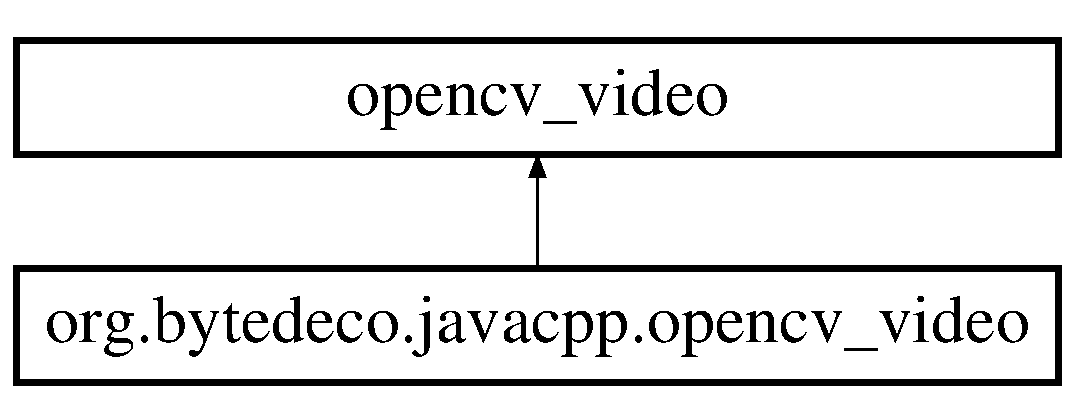
\includegraphics[height=2.000000cm]{classorg_1_1bytedeco_1_1javacpp_1_1opencv__video}
\end{center}
\end{figure}
\subsection*{Classes}
\begin{DoxyCompactItemize}
\item 
class {\bfseries Background\+Subtractor}
\item 
class {\bfseries Background\+Subtractor\+K\+NN}
\begin{DoxyCompactList}\small\item\em K-\/nearest neigbours -\/ based Background/\+Foreground Segmentation Algorithm. \end{DoxyCompactList}\item 
class {\bfseries Background\+Subtractor\+M\+O\+G2}
\begin{DoxyCompactList}\small\item\em Gaussian Mixture-\/based Background/\+Foreground Segmentation Algorithm. \end{DoxyCompactList}\item 
class {\bfseries Cv\+Kalman}
\item 
class {\bfseries Dense\+Optical\+Flow}
\item 
class {\bfseries Dual\+T\+V\+L1\+Optical\+Flow}
\begin{DoxyCompactList}\small\item\em \char`\"{}\+Dual T\+V L1\char`\"{} Optical Flow Algorithm. \end{DoxyCompactList}\item 
class {\bfseries Farneback\+Optical\+Flow}
\begin{DoxyCompactList}\small\item\em Class computing a dense optical flow using the Gunnar Farneback’s algorithm. \end{DoxyCompactList}\item 
class {\bfseries Kalman\+Filter}
\begin{DoxyCompactList}\small\item\em Kalman filter class. \end{DoxyCompactList}\item 
class {\bfseries Sparse\+Optical\+Flow}
\begin{DoxyCompactList}\small\item\em Base interface for sparse optical flow algorithms. \end{DoxyCompactList}\item 
class {\bfseries Sparse\+Pyr\+L\+K\+Optical\+Flow}
\begin{DoxyCompactList}\small\item\em Class used for calculating a sparse optical flow. \end{DoxyCompactList}\end{DoxyCompactItemize}
\subsection*{Static Public Member Functions}
\begin{DoxyCompactItemize}
\item 
static native void {\bfseries cv\+Calc\+Optical\+Flow\+Pyr\+LK} ( @Const Cv\+Arr prev, @Const Cv\+Arr curr, Cv\+Arr prev\+\_\+pyr, Cv\+Arr curr\+\_\+pyr, @Const Cv\+Point2\+D32f prev\+\_\+features, Cv\+Point2\+D32f curr\+\_\+features, int count, @By\+Val Cv\+Size win\+\_\+size, int level, @Cast(\char`\"{}char$\ast$\char`\"{}) Byte\+Pointer status, Float\+Pointer track\+\_\+error, @By\+Val Cv\+Term\+Criteria criteria, int flags)
\item 
static native void {\bfseries cv\+Calc\+Optical\+Flow\+Pyr\+LK} ( @Const Cv\+Arr prev, @Const Cv\+Arr curr, Cv\+Arr prev\+\_\+pyr, Cv\+Arr curr\+\_\+pyr, @Cast(\char`\"{}const Cv\+Point2\+D32f$\ast$\char`\"{}) Float\+Buffer prev\+\_\+features, @Cast(\char`\"{}Cv\+Point2\+D32f$\ast$\char`\"{}) Float\+Buffer curr\+\_\+features, int count, @By\+Val Cv\+Size win\+\_\+size, int level, @Cast(\char`\"{}char$\ast$\char`\"{}) Byte\+Buffer status, Float\+Buffer track\+\_\+error, @By\+Val Cv\+Term\+Criteria criteria, int flags)
\item 
static native void {\bfseries cv\+Calc\+Optical\+Flow\+Pyr\+LK} ( @Const Cv\+Arr prev, @Const Cv\+Arr curr, Cv\+Arr prev\+\_\+pyr, Cv\+Arr curr\+\_\+pyr, @Cast(\char`\"{}const Cv\+Point2\+D32f$\ast$\char`\"{}) float\mbox{[}$\,$\mbox{]} prev\+\_\+features, @Cast(\char`\"{}Cv\+Point2\+D32f$\ast$\char`\"{}) float\mbox{[}$\,$\mbox{]} curr\+\_\+features, int count, @By\+Val Cv\+Size win\+\_\+size, int level, @Cast(\char`\"{}char$\ast$\char`\"{}) byte\mbox{[}$\,$\mbox{]} status, float\mbox{[}$\,$\mbox{]} track\+\_\+error, @By\+Val Cv\+Term\+Criteria criteria, int flags)
\item 
static native int {\bfseries cv\+Estimate\+Rigid\+Transform} ( @Const Cv\+Arr A, @Const Cv\+Arr B, Cv\+Mat M, int full\+\_\+affine)
\item 
static native void {\bfseries cv\+Calc\+Optical\+Flow\+Farneback} ( @Const Cv\+Arr prev, @Const Cv\+Arr next, Cv\+Arr flow, double pyr\+\_\+scale, int levels, int winsize, int iterations, int poly\+\_\+n, double poly\+\_\+sigma, int flags)
\item 
static native int {\bfseries cv\+Cam\+Shift} ( @Const Cv\+Arr prob\+\_\+image, @By\+Val Cv\+Rect window, @By\+Val Cv\+Term\+Criteria criteria, Cv\+Connected\+Comp comp, Cv\+Box2D box)
\item 
static native int {\bfseries cv\+Cam\+Shift} ( @Const Cv\+Arr prob\+\_\+image, @By\+Val Cv\+Rect window, @By\+Val Cv\+Term\+Criteria criteria, Cv\+Connected\+Comp comp)
\item 
static native int {\bfseries cv\+Mean\+Shift} ( @Const Cv\+Arr prob\+\_\+image, @By\+Val Cv\+Rect window, @By\+Val Cv\+Term\+Criteria criteria, Cv\+Connected\+Comp comp)
\item 
static native Cv\+Kalman {\bfseries cv\+Create\+Kalman} (int dynam\+\_\+params, int measure\+\_\+params, int control\+\_\+params)
\item 
static native Cv\+Kalman {\bfseries cv\+Create\+Kalman} (int dynam\+\_\+params, int measure\+\_\+params)
\item 
static native void {\bfseries cv\+Release\+Kalman} ( @Cast(\char`\"{}Cv\+Kalman$\ast$$\ast$\char`\"{}) Pointer\+Pointer kalman)
\item 
static native void {\bfseries cv\+Release\+Kalman} ( @By\+Ptr\+Ptr Cv\+Kalman kalman)
\item 
static native Cv\+Mat {\bfseries cv\+Kalman\+Predict} (Cv\+Kalman kalman, @Const Cv\+Mat control)
\item 
static native Cv\+Mat {\bfseries cv\+Kalman\+Predict} (Cv\+Kalman kalman)
\item 
static native Cv\+Mat {\bfseries cv\+Kalman\+Correct} (Cv\+Kalman kalman, @Const Cv\+Mat measurement)
\item 
static native Cv\+Mat {\bfseries cv\+Kalman\+Update\+By\+Time} (Cv\+Kalman arg1, Cv\+Mat arg2)
\item 
static native Cv\+Mat {\bfseries cv\+Kalman\+Update\+By\+Measurement} (Cv\+Kalman arg1, Cv\+Mat arg2)
\item 
static native Rotated\+Rect \hyperlink{group__video__track_ga813283f225d7c4ce103da8b37981c69e}{Cam\+Shift} ( @By\+Val Mat prob\+Image, @By\+Ref Rect window, @By\+Val Term\+Criteria criteria)
\begin{DoxyCompactList}\small\item\em Finds an object center, size, and orientation. \end{DoxyCompactList}\item 
static native Rotated\+Rect {\bfseries Cam\+Shift} ( @By\+Val U\+Mat prob\+Image, @By\+Ref Rect window, @By\+Val Term\+Criteria criteria)
\item 
static native int \hyperlink{group__video__track_gad3336224aac304be4ee36ef146ec40d8}{mean\+Shift} ( @By\+Val Mat prob\+Image, @By\+Ref Rect window, @By\+Val Term\+Criteria criteria)
\begin{DoxyCompactList}\small\item\em Finds an object on a back projection image. \end{DoxyCompactList}\item 
static native int {\bfseries mean\+Shift} ( @By\+Val U\+Mat prob\+Image, @By\+Ref Rect window, @By\+Val Term\+Criteria criteria)
\item 
static native int \hyperlink{group__video__track_gafca5a72a408befa96e624e9d9704303b}{build\+Optical\+Flow\+Pyramid} ( @By\+Val Mat img, @By\+Val Mat\+Vector pyramid, @By\+Val Size win\+Size, int max\+Level, @Cast(\char`\"{}bool\char`\"{}) boolean with\+Derivatives, int pyr\+Border, int deriv\+Border, @Cast(\char`\"{}bool\char`\"{}) boolean try\+Reuse\+Input\+Image)
\begin{DoxyCompactList}\small\item\em Constructs the image pyramid which can be passed to calc\+Optical\+Flow\+Pyr\+LK. \end{DoxyCompactList}\item 
static native int {\bfseries build\+Optical\+Flow\+Pyramid} ( @By\+Val Mat img, @By\+Val Mat\+Vector pyramid, @By\+Val Size win\+Size, int max\+Level)
\item 
static native int {\bfseries build\+Optical\+Flow\+Pyramid} ( @By\+Val Mat img, @By\+Val U\+Mat\+Vector pyramid, @By\+Val Size win\+Size, int max\+Level, @Cast(\char`\"{}bool\char`\"{}) boolean with\+Derivatives, int pyr\+Border, int deriv\+Border, @Cast(\char`\"{}bool\char`\"{}) boolean try\+Reuse\+Input\+Image)
\item 
static native int {\bfseries build\+Optical\+Flow\+Pyramid} ( @By\+Val Mat img, @By\+Val U\+Mat\+Vector pyramid, @By\+Val Size win\+Size, int max\+Level)
\item 
static native int {\bfseries build\+Optical\+Flow\+Pyramid} ( @By\+Val U\+Mat img, @By\+Val Mat\+Vector pyramid, @By\+Val Size win\+Size, int max\+Level, @Cast(\char`\"{}bool\char`\"{}) boolean with\+Derivatives, int pyr\+Border, int deriv\+Border, @Cast(\char`\"{}bool\char`\"{}) boolean try\+Reuse\+Input\+Image)
\item 
static native int {\bfseries build\+Optical\+Flow\+Pyramid} ( @By\+Val U\+Mat img, @By\+Val Mat\+Vector pyramid, @By\+Val Size win\+Size, int max\+Level)
\item 
static native int {\bfseries build\+Optical\+Flow\+Pyramid} ( @By\+Val U\+Mat img, @By\+Val U\+Mat\+Vector pyramid, @By\+Val Size win\+Size, int max\+Level, @Cast(\char`\"{}bool\char`\"{}) boolean with\+Derivatives, int pyr\+Border, int deriv\+Border, @Cast(\char`\"{}bool\char`\"{}) boolean try\+Reuse\+Input\+Image)
\item 
static native int {\bfseries build\+Optical\+Flow\+Pyramid} ( @By\+Val U\+Mat img, @By\+Val U\+Mat\+Vector pyramid, @By\+Val Size win\+Size, int max\+Level)
\item 
static native void \hyperlink{group__video__track_ga5336cf64b4b2f82bf7c08551017fda66}{calc\+Optical\+Flow\+Pyr\+LK} ( @By\+Val Mat prev\+Img, @By\+Val Mat next\+Img, @By\+Val Mat prev\+Pts, @By\+Val Mat next\+Pts, @By\+Val Mat status, @By\+Val Mat err, @By\+Val(null\+Value=\char`\"{}cv\+::\+Size(21,21)\char`\"{}) Size win\+Size, int max\+Level, @By\+Val(null\+Value=\char`\"{}cv\+::\+Term\+Criteria(cv\+::\+Term\+Criteria\+::\+C\+O\+U\+NT+cv\+::\+Term\+Criteria\+::\+E\+PS, 30, 0.\+01)\char`\"{}) Term\+Criteria criteria, int flags, double min\+Eig\+Threshold)
\begin{DoxyCompactList}\small\item\em Calculates an optical flow for a sparse feature set using the iterative Lucas-\/\+Kanade method with pyramids. \end{DoxyCompactList}\item 
static native void {\bfseries calc\+Optical\+Flow\+Pyr\+LK} ( @By\+Val Mat prev\+Img, @By\+Val Mat next\+Img, @By\+Val Mat prev\+Pts, @By\+Val Mat next\+Pts, @By\+Val Mat status, @By\+Val Mat err)
\item 
static native void {\bfseries calc\+Optical\+Flow\+Pyr\+LK} ( @By\+Val U\+Mat prev\+Img, @By\+Val U\+Mat next\+Img, @By\+Val U\+Mat prev\+Pts, @By\+Val U\+Mat next\+Pts, @By\+Val U\+Mat status, @By\+Val U\+Mat err, @By\+Val(null\+Value=\char`\"{}cv\+::\+Size(21,21)\char`\"{}) Size win\+Size, int max\+Level, @By\+Val(null\+Value=\char`\"{}cv\+::\+Term\+Criteria(cv\+::\+Term\+Criteria\+::\+C\+O\+U\+NT+cv\+::\+Term\+Criteria\+::\+E\+PS, 30, 0.\+01)\char`\"{}) Term\+Criteria criteria, int flags, double min\+Eig\+Threshold)
\item 
static native void {\bfseries calc\+Optical\+Flow\+Pyr\+LK} ( @By\+Val U\+Mat prev\+Img, @By\+Val U\+Mat next\+Img, @By\+Val U\+Mat prev\+Pts, @By\+Val U\+Mat next\+Pts, @By\+Val U\+Mat status, @By\+Val U\+Mat err)
\item 
static native void \hyperlink{group__video__track_ga8296f2eaf7aa279b0c54a72350493258}{calc\+Optical\+Flow\+Farneback} ( @By\+Val Mat prev, @By\+Val Mat next, @By\+Val Mat flow, double pyr\+\_\+scale, int levels, int winsize, int iterations, int poly\+\_\+n, double poly\+\_\+sigma, int flags)
\begin{DoxyCompactList}\small\item\em Computes a dense optical flow using the Gunnar Farneback\textquotesingle{}s algorithm. \end{DoxyCompactList}\item 
static native void {\bfseries calc\+Optical\+Flow\+Farneback} ( @By\+Val U\+Mat prev, @By\+Val U\+Mat next, @By\+Val U\+Mat flow, double pyr\+\_\+scale, int levels, int winsize, int iterations, int poly\+\_\+n, double poly\+\_\+sigma, int flags)
\item 
static native Mat \hyperlink{group__video__track_ga2c14f71afdf82824dbdf781bbc041aa1}{estimate\+Rigid\+Transform} ( @By\+Val Mat src, @By\+Val Mat dst, @Cast(\char`\"{}bool\char`\"{}) boolean full\+Affine)
\begin{DoxyCompactList}\small\item\em Computes an optimal affine transformation between two 2D point sets. \end{DoxyCompactList}\item 
static native Mat {\bfseries estimate\+Rigid\+Transform} ( @By\+Val U\+Mat src, @By\+Val U\+Mat dst, @Cast(\char`\"{}bool\char`\"{}) boolean full\+Affine)
\item 
static native double \hyperlink{group__video__track_ga2438ed3ebc7ea014e11c93797e2aae7b}{find\+Transform\+E\+CC} ( @By\+Val Mat template\+Image, @By\+Val Mat input\+Image, @By\+Val Mat warp\+Matrix, int motion\+Type, @By\+Val(null\+Value=\char`\"{}cv\+::\+Term\+Criteria(cv\+::\+Term\+Criteria\+::\+C\+O\+U\+NT+cv\+::\+Term\+Criteria\+::\+E\+PS, 50, 0.\+001)\char`\"{}) Term\+Criteria criteria, @By\+Val(null\+Value=\char`\"{}cv\+::\+Input\+Array(cv\+::no\+Array())\char`\"{}) Mat input\+Mask)
\begin{DoxyCompactList}\small\item\em Finds the geometric transform (warp) between two images in terms of the E\+CC criterion {\bfseries [E\+P08]} . \end{DoxyCompactList}\item 
static native double {\bfseries find\+Transform\+E\+CC} ( @By\+Val Mat template\+Image, @By\+Val Mat input\+Image, @By\+Val Mat warp\+Matrix)
\item 
static native double {\bfseries find\+Transform\+E\+CC} ( @By\+Val U\+Mat template\+Image, @By\+Val U\+Mat input\+Image, @By\+Val U\+Mat warp\+Matrix, int motion\+Type, @By\+Val(null\+Value=\char`\"{}cv\+::\+Term\+Criteria(cv\+::\+Term\+Criteria\+::\+C\+O\+U\+NT+cv\+::\+Term\+Criteria\+::\+E\+PS, 50, 0.\+001)\char`\"{}) Term\+Criteria criteria, @By\+Val(null\+Value=\char`\"{}cv\+::\+Input\+Array(cv\+::no\+Array())\char`\"{}) U\+Mat input\+Mask)
\item 
static native double {\bfseries find\+Transform\+E\+CC} ( @By\+Val U\+Mat template\+Image, @By\+Val U\+Mat input\+Image, @By\+Val U\+Mat warp\+Matrix)
\item 
static native Dual\+T\+V\+L1\+Optical\+Flow \hyperlink{group__video__track_ga02df311817502c4c088084195093be2e}{create\+Opt\+Flow\+\_\+\+Dual\+T\+V\+L1} ()
\begin{DoxyCompactList}\small\item\em Creates instance of cv\+::\+Dense\+Optical\+Flow. \end{DoxyCompactList}\item 
static native Background\+Subtractor\+M\+O\+G2 \hyperlink{group__video__motion_ga0820edc51bf6a34fb6ec60e0bfa47770}{create\+Background\+Subtractor\+M\+O\+G2} (int history, double var\+Threshold, @Cast(\char`\"{}bool\char`\"{}) boolean detect\+Shadows)
\begin{DoxyCompactList}\small\item\em Creates M\+O\+G2 Background Subtractor. \end{DoxyCompactList}\item 
static native Background\+Subtractor\+M\+O\+G2 {\bfseries create\+Background\+Subtractor\+M\+O\+G2} ()
\item 
static native Background\+Subtractor\+K\+NN \hyperlink{group__video__motion_ga1376788db4935dd8798d7e087e7697c9}{create\+Background\+Subtractor\+K\+NN} (int history, double dist2\+Threshold, @Cast(\char`\"{}bool\char`\"{}) boolean detect\+Shadows)
\begin{DoxyCompactList}\small\item\em Creates K\+NN Background Subtractor. \end{DoxyCompactList}\item 
static native Background\+Subtractor\+K\+NN {\bfseries create\+Background\+Subtractor\+K\+NN} ()
\end{DoxyCompactItemize}
\subsection*{Static Public Attributes}
\begin{DoxyCompactItemize}
\item 
static final int {\bfseries C\+V\+\_\+\+L\+K\+F\+L\+O\+W\+\_\+\+P\+Y\+R\+\_\+\+A\+\_\+\+R\+E\+A\+DY} = 1
\item 
static final int {\bfseries C\+V\+\_\+\+L\+K\+F\+L\+O\+W\+\_\+\+P\+Y\+R\+\_\+\+B\+\_\+\+R\+E\+A\+DY} = 2
\item 
static final int {\bfseries C\+V\+\_\+\+L\+K\+F\+L\+O\+W\+\_\+\+I\+N\+I\+T\+I\+A\+L\+\_\+\+G\+U\+E\+S\+S\+ES} = 4
\item 
static final int {\bfseries C\+V\+\_\+\+L\+K\+F\+L\+O\+W\+\_\+\+G\+E\+T\+\_\+\+M\+I\+N\+\_\+\+E\+I\+G\+E\+N\+V\+A\+LS} = 8
\item 
static final int \hyperlink{group__video__track_ga7544170e893b4e8835522881418d396d}{O\+P\+T\+F\+L\+O\+W\+\_\+\+U\+S\+E\+\_\+\+I\+N\+I\+T\+I\+A\+L\+\_\+\+F\+L\+OW} = 4
\item 
static final int \hyperlink{group__video__track_gaf37f7c8ec20fc62ff4ba2f00de67f1b3}{M\+O\+T\+I\+O\+N\+\_\+\+T\+R\+A\+N\+S\+L\+A\+T\+I\+ON} = 0
\end{DoxyCompactItemize}


The documentation for this class was generated from the following file\+:\begin{DoxyCompactItemize}
\item 
opencv\+\_\+video.\+java\end{DoxyCompactItemize}

\hypertarget{classorg_1_1bytedeco_1_1javacpp_1_1opencv__videoio}{}\section{org.\+bytedeco.\+javacpp.\+opencv\+\_\+videoio Class Reference}
\label{classorg_1_1bytedeco_1_1javacpp_1_1opencv__videoio}\index{org.\+bytedeco.\+javacpp.\+opencv\+\_\+videoio@{org.\+bytedeco.\+javacpp.\+opencv\+\_\+videoio}}
Inheritance diagram for org.\+bytedeco.\+javacpp.\+opencv\+\_\+videoio\+:\begin{figure}[H]
\begin{center}
\leavevmode
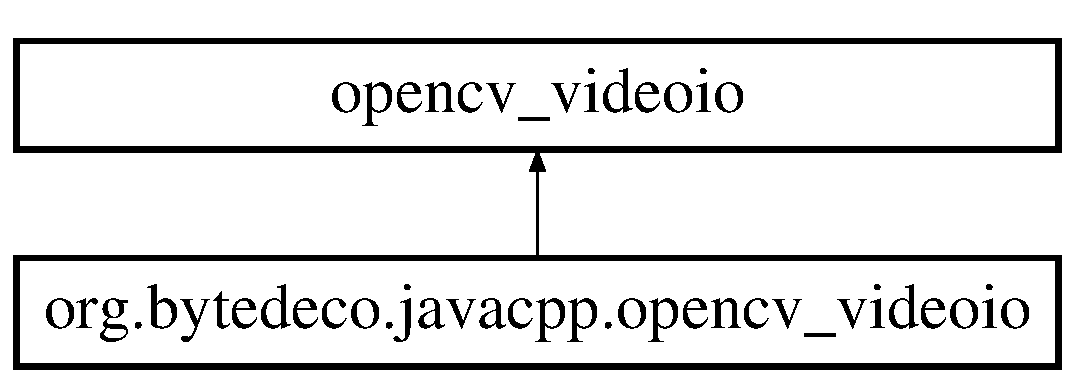
\includegraphics[height=2.000000cm]{classorg_1_1bytedeco_1_1javacpp_1_1opencv__videoio}
\end{center}
\end{figure}
\subsection*{Classes}
\begin{DoxyCompactItemize}
\item 
class {\bfseries Cv\+Capture}
\begin{DoxyCompactList}\small\item\em \char`\"{}black box\char`\"{} capture structure \end{DoxyCompactList}\item 
class {\bfseries Cv\+Video\+Writer}
\begin{DoxyCompactList}\small\item\em \char`\"{}black box\char`\"{} video file writer structure \end{DoxyCompactList}\item 
class {\bfseries I\+Video\+Capture}
\item 
class {\bfseries I\+Video\+Writer}
\item 
class {\bfseries Video\+Capture}
\begin{DoxyCompactList}\small\item\em Class for video capturing from video files, image sequences or cameras. \end{DoxyCompactList}\item 
class {\bfseries Video\+Writer}
\begin{DoxyCompactList}\small\item\em Video writer class. \end{DoxyCompactList}\end{DoxyCompactItemize}
\subsection*{Static Public Member Functions}
\begin{DoxyCompactItemize}
\item 
static native Cv\+Capture \hyperlink{group__videoio__c_gaf71dcb88fc0c7476076b298ed762ddca}{cv\+Create\+File\+Capture} ( @Cast(\char`\"{}const char$\ast$\char`\"{}) Byte\+Pointer filename)
\begin{DoxyCompactList}\small\item\em start capturing frames from video file \end{DoxyCompactList}\item 
static native Cv\+Capture {\bfseries cv\+Create\+File\+Capture} (String filename)
\item 
static native Cv\+Capture \hyperlink{group__videoio__c_ga11789f0474ae978b9ec17590706f9901}{cv\+Create\+File\+Capture\+With\+Preference} ( @Cast(\char`\"{}const char$\ast$\char`\"{}) Byte\+Pointer filename, int api\+Preference)
\begin{DoxyCompactList}\small\item\em start capturing frames from video file. allows specifying a preferred A\+PI to use \end{DoxyCompactList}\item 
static native Cv\+Capture {\bfseries cv\+Create\+File\+Capture\+With\+Preference} (String filename, int api\+Preference)
\item 
static native Cv\+Capture \hyperlink{group__videoio__c_ga43844b7ee876e73697163ae51ec617db}{cv\+Create\+Camera\+Capture} (int index)
\begin{DoxyCompactList}\small\item\em start capturing frames from camera\+: index = camera\+\_\+index + domain\+\_\+offset (C\+V\+\_\+\+C\+A\+P\+\_\+$\ast$) \end{DoxyCompactList}\item 
static native int \hyperlink{group__videoio__c_ga630e4d9ab3ff9f05ab4bc5ba1eb1d787}{cv\+Grab\+Frame} (Cv\+Capture capture)
\begin{DoxyCompactList}\small\item\em grab a frame, return 1 on success, 0 on fail. \end{DoxyCompactList}\item 
static native Ipl\+Image \hyperlink{group__videoio__c_ga0bb2a83d7a4cd242fae9561742b4af37}{cv\+Retrieve\+Frame} (Cv\+Capture capture, int stream\+Idx)
\begin{DoxyCompactList}\small\item\em get the frame grabbed with cv\+Grab\+Frame(..) \end{DoxyCompactList}\item 
static native Ipl\+Image {\bfseries cv\+Retrieve\+Frame} (Cv\+Capture capture)
\item 
static native Ipl\+Image \hyperlink{group__videoio__c_ga5c8fd8eb6b93a72085abecae04eebb12}{cv\+Query\+Frame} (Cv\+Capture capture)
\begin{DoxyCompactList}\small\item\em Just a combination of cv\+Grab\+Frame and cv\+Retrieve\+Frame. \end{DoxyCompactList}\item 
static native void \hyperlink{group__videoio__c_ga74708c3e2dd50838b8626b75a7ceaf1d}{cv\+Release\+Capture} ( @Cast(\char`\"{}Cv\+Capture$\ast$$\ast$\char`\"{}) Pointer\+Pointer capture)
\begin{DoxyCompactList}\small\item\em stop capturing/reading and free resources \end{DoxyCompactList}\item 
static native void {\bfseries cv\+Release\+Capture} ( @By\+Ptr\+Ptr Cv\+Capture capture)
\item 
static native double \hyperlink{group__videoio__c_ga98ef6dab996d6b3189fc3f18046d2a44}{cv\+Get\+Capture\+Property} (Cv\+Capture capture, int property\+\_\+id)
\begin{DoxyCompactList}\small\item\em retrieve capture properties \end{DoxyCompactList}\item 
static native int \hyperlink{group__videoio__c_ga1165012821c4296388a11df431414950}{cv\+Set\+Capture\+Property} (Cv\+Capture capture, int property\+\_\+id, double value)
\begin{DoxyCompactList}\small\item\em set capture properties \end{DoxyCompactList}\item 
static native int \hyperlink{group__videoio__c_ga907965e3aedaeeb293f6b781590fa8a9}{cv\+Get\+Capture\+Domain} (Cv\+Capture capture)
\begin{DoxyCompactList}\small\item\em Return the type of the capturer (eg, \+::\+C\+V\+\_\+\+C\+A\+P\+\_\+\+V\+FW, \+::\+C\+V\+\_\+\+C\+A\+P\+\_\+\+U\+N\+I\+C\+AP) \end{DoxyCompactList}\item 
static native int \hyperlink{group__videoio__c_ga30de218d6d68e6d7ede1b476f71f45db}{C\+V\+\_\+\+F\+O\+U\+R\+CC} (@Cast(\char`\"{}char\char`\"{}) byte c1, @Cast(\char`\"{}char\char`\"{}) byte c2, @Cast(\char`\"{}char\char`\"{}) byte c3, @Cast(\char`\"{}char\char`\"{}) byte c4)
\begin{DoxyCompactList}\small\item\em Constructs the fourcc code of the codec function. \end{DoxyCompactList}\item 
static native int \hyperlink{group__videoio__c_gaade4fde0859691fd56cdb50fd9bf62db}{C\+V\+\_\+\+F\+O\+U\+R\+C\+C\+\_\+\+D\+E\+F\+A\+U\+LT} ()
\item 
static native Cv\+Video\+Writer \hyperlink{group__videoio__c_ga707349ac4c6f16cecf119295374d1ef8}{cv\+Create\+Video\+Writer} ( @Cast(\char`\"{}const char$\ast$\char`\"{}) Byte\+Pointer filename, int fourcc, double fps, @By\+Val Cv\+Size frame\+\_\+size, int is\+\_\+color)
\begin{DoxyCompactList}\small\item\em initialize video file writer \end{DoxyCompactList}\item 
static native Cv\+Video\+Writer {\bfseries cv\+Create\+Video\+Writer} ( @Cast(\char`\"{}const char$\ast$\char`\"{}) Byte\+Pointer filename, int fourcc, double fps, @By\+Val Cv\+Size frame\+\_\+size)
\item 
static native Cv\+Video\+Writer {\bfseries cv\+Create\+Video\+Writer} (String filename, int fourcc, double fps, @By\+Val Cv\+Size frame\+\_\+size, int is\+\_\+color)
\item 
static native Cv\+Video\+Writer {\bfseries cv\+Create\+Video\+Writer} (String filename, int fourcc, double fps, @By\+Val Cv\+Size frame\+\_\+size)
\item 
static native int \hyperlink{group__videoio__c_ga167c75eb3f3ce8ddde13d364bb6fa69d}{cv\+Write\+Frame} (Cv\+Video\+Writer writer, @Const Ipl\+Image image)
\begin{DoxyCompactList}\small\item\em write frame to video file \end{DoxyCompactList}\item 
static native void \hyperlink{group__videoio__c_ga70d8b768ab059ff65f019d05036a7806}{cv\+Release\+Video\+Writer} ( @Cast(\char`\"{}Cv\+Video\+Writer$\ast$$\ast$\char`\"{}) Pointer\+Pointer writer)
\begin{DoxyCompactList}\small\item\em close video file writer \end{DoxyCompactList}\item 
static native void {\bfseries cv\+Release\+Video\+Writer} ( @By\+Ptr\+Ptr Cv\+Video\+Writer writer)
\end{DoxyCompactItemize}
\begin{Indent}\textbf{ Obsolete functions/synonyms}\par
\begin{DoxyCompactItemize}
\item 
static native Cv\+Capture \hyperlink{group__videoio__c_gafab92effdc81a1a2eb305dc69eb84bfd}{cv\+Capture\+From\+C\+AM} (int arg1)
\item 
static native Cv\+Capture \hyperlink{group__videoio__c_ga5fccc51ced33519e61c5687ca7b17fdb}{cv\+Capture\+From\+File} (@Cast(\char`\"{}const char$\ast$\char`\"{}) Byte\+Pointer arg1)
\item 
static native Cv\+Capture {\bfseries cv\+Capture\+From\+File} (String arg1)
\item 
static native Cv\+Capture \hyperlink{group__videoio__c_ga153463bfe93115b2ff7783a8c504d2a7}{cv\+Capture\+From\+A\+VI} (@Cast(\char`\"{}const char$\ast$\char`\"{}) Byte\+Pointer arg1)
\item 
static native Cv\+Capture {\bfseries cv\+Capture\+From\+A\+VI} (String arg1)
\item 
static native Cv\+Video\+Writer \hyperlink{group__videoio__c_ga7ac706f58e712a321ff4ed14d9c98dfc}{cv\+Create\+A\+V\+I\+Writer} (@Cast(\char`\"{}const char$\ast$\char`\"{}) Byte\+Pointer arg1, int arg2, double arg3, @By\+Val Cv\+Size arg4, int arg5)
\item 
static native Cv\+Video\+Writer {\bfseries cv\+Create\+A\+V\+I\+Writer} (String arg1, int arg2, double arg3, @By\+Val Cv\+Size arg4, int arg5)
\item 
static native int \hyperlink{group__videoio__c_ga3f795024cbed8966f3b006b1ccd99acc}{cv\+Write\+To\+A\+VI} (Cv\+Video\+Writer arg1, Ipl\+Image arg2)
\end{DoxyCompactItemize}
\end{Indent}
\subsection*{Static Public Attributes}
\begin{DoxyCompactItemize}
\item 
static final int \hyperlink{group__videoio__c_gab170df7f9f17e64c3642fbc2036c9d89}{C\+V\+\_\+\+C\+A\+P\+\_\+\+A\+NY} = 0
\item 
static final int \hyperlink{group__videoio__c_gab93e06d5b7823b93b958bffc1d6c5220}{C\+V\+\_\+\+C\+A\+P\+\_\+\+P\+R\+O\+P\+\_\+\+D\+C1394\+\_\+\+O\+FF} = -\/4
\item 
static final int \hyperlink{group__videoio__c_ga857b3fa265775f5d402c1e0a65ef254d}{C\+V\+\_\+\+C\+A\+P\+\_\+\+M\+O\+D\+E\+\_\+\+B\+GR} = 0
\item 
static final int \hyperlink{group__videoio__c_ga0614006f7159a4f38a5536d9afc6c841}{C\+V\+\_\+\+C\+A\+P\+\_\+\+O\+P\+E\+N\+N\+I\+\_\+\+D\+E\+P\+T\+H\+\_\+\+M\+AP} = 0
\item 
static final int \hyperlink{group__videoio__c_ga21913880c4cae25d1ff392c5fa2bb30f}{C\+V\+\_\+\+C\+A\+P\+\_\+\+O\+P\+E\+N\+N\+I\+\_\+\+V\+G\+A\+\_\+30\+HZ} = 0
\item 
static final int \hyperlink{group__videoio__c_ga24a1e5be05c39075c7d1f8564521f733}{C\+V\+\_\+\+C\+A\+P\+\_\+\+I\+N\+T\+E\+L\+P\+E\+R\+C\+\_\+\+D\+E\+P\+T\+H\+\_\+\+M\+AP} = 0
\item 
static final int \hyperlink{group__videoio__c_ga6e1f35a3b8dc5ab0fc4b7363821533d8}{C\+V\+\_\+\+C\+A\+P\+\_\+\+P\+R\+O\+P\+\_\+\+G\+P\+H\+O\+T\+O2\+\_\+\+P\+R\+E\+V\+I\+EW} = 17001
\item 
static final int \hyperlink{group__videoio__c_gaa801d0075e64846c5f858fafb7f7ba26}{C\+V\+\_\+\+F\+O\+U\+R\+C\+C\+\_\+\+P\+R\+O\+M\+PT} = -\/1
\item 
static final int {\bfseries C\+V\+\_\+\+F\+O\+U\+R\+C\+C\+\_\+\+D\+E\+F\+A\+U\+LT} = C\+V\+\_\+\+F\+O\+U\+R\+C\+C\+\_\+\+D\+E\+F\+A\+U\+LT()
\item 
static final int \hyperlink{group__videoio__flags__base_ga5919f622200581e7cc68b521cd528f3f}{C\+A\+P\+\_\+\+A\+NY} = 0
\item 
static final int \hyperlink{group__videoio__flags__base_ga0d261205f5852e23c0987e9a838e9f91}{C\+A\+P\+\_\+\+P\+R\+O\+P\+\_\+\+P\+O\+S\+\_\+\+M\+S\+EC} = 0
\begin{DoxyCompactList}\small\item\em Video\+Capture generic properties identifier. \end{DoxyCompactList}\item 
static final int \hyperlink{group__videoio__flags__base_gaadf3dff0251965990b45d02868b90b23}{C\+A\+P\+\_\+\+M\+O\+D\+E\+\_\+\+B\+GR} = 0
\begin{DoxyCompactList}\small\item\em Generic camera output modes identifier. \end{DoxyCompactList}\item 
static final int \hyperlink{group__videoio__flags__base_gac45c570604a0024fe45239139e0d4e5b}{V\+I\+D\+E\+O\+W\+R\+I\+T\+E\+R\+\_\+\+P\+R\+O\+P\+\_\+\+Q\+U\+A\+L\+I\+TY} = 1
\begin{DoxyCompactList}\small\item\em Video\+Writer generic properties identifier. \end{DoxyCompactList}\end{DoxyCompactItemize}
\begin{Indent}\textbf{ G\+Streamer}\par
{\em Open\+NI 

/$\ast$$\ast$ }\begin{DoxyCompactItemize}
\item 
static final int \hyperlink{group__videoio__flags__others_gafbbac7fafc3f6386e3234a007d25b25d}{C\+A\+P\+\_\+\+P\+R\+O\+P\+\_\+\+G\+S\+T\+R\+E\+A\+M\+E\+R\+\_\+\+Q\+U\+E\+U\+E\+\_\+\+L\+E\+N\+G\+TH} = 200
\end{DoxyCompactItemize}
\end{Indent}
\subsection*{I\+E\+EE 1394 drivers}
\begin{DoxyCompactItemize}
\item 
static final int \hyperlink{group__videoio__flags__others_gad6592d7bfce8b9138f5a334ae87a5ff9}{C\+A\+P\+\_\+\+P\+R\+O\+P\+\_\+\+D\+C1394\+\_\+\+O\+FF} = -\/4
\begin{DoxyCompactList}\small\item\em Modes of the I\+E\+EE 1394 controlling registers (can be\+: auto, manual, auto single push, absolute Latter allowed with any other mode) every feature can have only one mode turned on at a time. \end{DoxyCompactList}\end{DoxyCompactItemize}
\subsection*{Open\+NI (for Kinect)}
\label{_amgrp848bd3907cdb4b9cd483b8d19dbc52c3}%
 I\+E\+EE 1394 drivers 

/$\ast$$\ast$ \begin{DoxyCompactItemize}
\item 
static final int \hyperlink{group__videoio__flags__others_gae3c0e63f05b21774fe01e3e9f737e8a0}{C\+A\+P\+\_\+\+O\+P\+E\+N\+N\+I\+\_\+\+D\+E\+P\+T\+H\+\_\+\+G\+E\+N\+E\+R\+A\+T\+OR} = 1 $<$$<$ 31
\item 
static final int \hyperlink{group__videoio__flags__others_gac9fa35868d2fa304aee7d72f50bc9dae}{C\+A\+P\+\_\+\+P\+R\+O\+P\+\_\+\+O\+P\+E\+N\+N\+I\+\_\+\+O\+U\+T\+P\+U\+T\+\_\+\+M\+O\+DE} = 100
\item 
static final int \hyperlink{group__videoio__flags__others_ga94fffc0304ea99800662b4a89e79898e}{C\+A\+P\+\_\+\+O\+P\+E\+N\+N\+I\+\_\+\+I\+M\+A\+G\+E\+\_\+\+G\+E\+N\+E\+R\+A\+T\+O\+R\+\_\+\+P\+R\+E\+S\+E\+NT} = C\+A\+P\+\_\+\+O\+P\+E\+N\+N\+I\+\_\+\+I\+M\+A\+G\+E\+\_\+\+G\+E\+N\+E\+R\+A\+T\+OR + C\+A\+P\+\_\+\+P\+R\+O\+P\+\_\+\+O\+P\+E\+N\+N\+I\+\_\+\+G\+E\+N\+E\+R\+A\+T\+O\+R\+\_\+\+P\+R\+E\+S\+E\+NT
\item 
static final int \hyperlink{group__videoio__flags__others_ga34a12b8e99e76dfa25af8fed3c199d46}{C\+A\+P\+\_\+\+O\+P\+E\+N\+N\+I\+\_\+\+D\+E\+P\+T\+H\+\_\+\+M\+AP} = 0
\item 
static final int \hyperlink{group__videoio__flags__others_gab75d47d5fe56c9248b689bf463a5c96b}{C\+A\+P\+\_\+\+O\+P\+E\+N\+N\+I\+\_\+\+V\+G\+A\+\_\+30\+HZ} = 0
\end{DoxyCompactItemize}
\subsection*{Pv\+A\+PI, Prosilica GigE S\+DK}
\label{_amgrpad73e9ceb7c1dc02527eb584e89bd615}%
 G\+Streamer 

/$\ast$$\ast$ \begin{DoxyCompactItemize}
\item 
static final int \hyperlink{group__videoio__flags__others_gae525c9cc0da137af131406ca12fd92d7}{C\+A\+P\+\_\+\+P\+R\+O\+P\+\_\+\+P\+V\+A\+P\+I\+\_\+\+M\+U\+L\+T\+I\+C\+A\+S\+T\+IP} = 300
\item 
static final int \hyperlink{group__videoio__flags__others_ga013dd4a15cafb63c7a4934abce8aaeb7}{C\+A\+P\+\_\+\+P\+V\+A\+P\+I\+\_\+\+F\+S\+T\+R\+I\+G\+M\+O\+D\+E\+\_\+\+F\+R\+E\+E\+R\+UN} = 0
\item 
static final int \hyperlink{group__videoio__flags__others_gadc78e206f0eea9da651ff0c67a8d4f4c}{C\+A\+P\+\_\+\+P\+V\+A\+P\+I\+\_\+\+D\+E\+C\+I\+M\+A\+T\+I\+O\+N\+\_\+\+O\+FF} = 1
\item 
static final int \hyperlink{group__videoio__flags__others_ga1dfffd05aca0c220f753ce014bdeea0f}{C\+A\+P\+\_\+\+P\+V\+A\+P\+I\+\_\+\+P\+I\+X\+E\+L\+F\+O\+R\+M\+A\+T\+\_\+\+M\+O\+N\+O8} = 1
\end{DoxyCompactItemize}
\subsection*{X\+I\+M\+EA Camera A\+PI}
\label{_amgrp27700f107007c227ac22f266c008393b}%
 Pv\+A\+PI 

/$\ast$$\ast$ \begin{DoxyCompactItemize}
\item 
static final int \hyperlink{group__videoio__flags__others_ga8cffe0305b23ba68e84c3948d29ed9d7}{C\+A\+P\+\_\+\+P\+R\+O\+P\+\_\+\+X\+I\+\_\+\+D\+O\+W\+N\+S\+A\+M\+P\+L\+I\+NG} = 400
\end{DoxyCompactItemize}
\subsection*{A\+V\+Foundation framework for i\+OS}
\label{_amgrpa29adce7291c258c56920a735b90577a}%
 X\+I\+M\+EA 

/$\ast$$\ast$ OS X Lion will have the same A\+PI \begin{DoxyCompactItemize}
\item 
static final int \hyperlink{group__videoio__flags__others_gaf0a40895d86f9a304aefc2b1293ada0b}{C\+A\+P\+\_\+\+P\+R\+O\+P\+\_\+\+I\+O\+S\+\_\+\+D\+E\+V\+I\+C\+E\+\_\+\+F\+O\+C\+US} = 9001
\end{DoxyCompactItemize}
\subsection*{Smartek Giganetix Gig\+E\+Vision\+S\+DK}
\begin{DoxyCompactItemize}
\item 
static final int \hyperlink{group__videoio__flags__others_gab4ddba80d08c7d12c1cf05ad5f3182a0}{C\+A\+P\+\_\+\+P\+R\+O\+P\+\_\+\+G\+I\+G\+A\+\_\+\+F\+R\+A\+M\+E\+\_\+\+O\+F\+F\+S\+E\+T\+\_\+X} = 10001
\end{DoxyCompactItemize}
\subsection*{Intel Perceptual Computing S\+DK}
\label{_amgrpfb2ec7d2cacf22b3dd4fcd13264794c9}%
 Smartek 

/$\ast$$\ast$ \begin{DoxyCompactItemize}
\item 
static final int \hyperlink{group__videoio__flags__others_gaa9b3af0c8f28aea91749058639e286f7}{C\+A\+P\+\_\+\+P\+R\+O\+P\+\_\+\+I\+N\+T\+E\+L\+P\+E\+R\+C\+\_\+\+P\+R\+O\+F\+I\+L\+E\+\_\+\+C\+O\+U\+NT} = 11001
\item 
static final int \hyperlink{group__videoio__flags__others_gab66c209bfa351264f55727db980328f2}{C\+A\+P\+\_\+\+I\+N\+T\+E\+L\+P\+E\+R\+C\+\_\+\+D\+E\+P\+T\+H\+\_\+\+G\+E\+N\+E\+R\+A\+T\+OR} = 1 $<$$<$ 29
\item 
static final int \hyperlink{group__videoio__flags__others_ga81daac9eadb7d66e1f26c0d984b68c82}{C\+A\+P\+\_\+\+I\+N\+T\+E\+L\+P\+E\+R\+C\+\_\+\+D\+E\+P\+T\+H\+\_\+\+M\+AP} = 0
\end{DoxyCompactItemize}
\subsection*{g\+Photo2 connection}
\label{_amgrp190de4ba27ec870ae1edac91cdcae582}%
 Intel Perceptual 

/$\ast$$\ast$ \begin{DoxyCompactItemize}
\item 
static final int \hyperlink{group__videoio__flags__others_ga2d0e0d7cb640eb1dc635b6351fc64c42}{C\+A\+P\+\_\+\+P\+R\+O\+P\+\_\+\+G\+P\+H\+O\+T\+O2\+\_\+\+P\+R\+E\+V\+I\+EW} = 17001
\begin{DoxyCompactList}\small\item\em g\+Photo2 properties \end{DoxyCompactList}\end{DoxyCompactItemize}
\subsection*{Images backend}
\label{_amgrpf4bcbe1ab751845a9b3aa892849e1b20}%
 g\+Photo2 

/$\ast$$\ast$ \begin{DoxyCompactItemize}
\item 
static final int \hyperlink{group__videoio__flags__others_ga6a4667b5803848ad28674572fabd3557}{C\+A\+P\+\_\+\+P\+R\+O\+P\+\_\+\+I\+M\+A\+G\+E\+S\+\_\+\+B\+A\+SE} = 18000
\begin{DoxyCompactList}\small\item\em Images backend properties. \end{DoxyCompactList}\end{DoxyCompactItemize}


The documentation for this class was generated from the following file\+:\begin{DoxyCompactItemize}
\item 
opencv\+\_\+videoio.\+java\end{DoxyCompactItemize}

\hypertarget{classorg_1_1bytedeco_1_1javacpp_1_1opencv__videostab}{}\section{org.\+bytedeco.\+javacpp.\+opencv\+\_\+videostab Class Reference}
\label{classorg_1_1bytedeco_1_1javacpp_1_1opencv__videostab}\index{org.\+bytedeco.\+javacpp.\+opencv\+\_\+videostab@{org.\+bytedeco.\+javacpp.\+opencv\+\_\+videostab}}
Inheritance diagram for org.\+bytedeco.\+javacpp.\+opencv\+\_\+videostab\+:\begin{figure}[H]
\begin{center}
\leavevmode
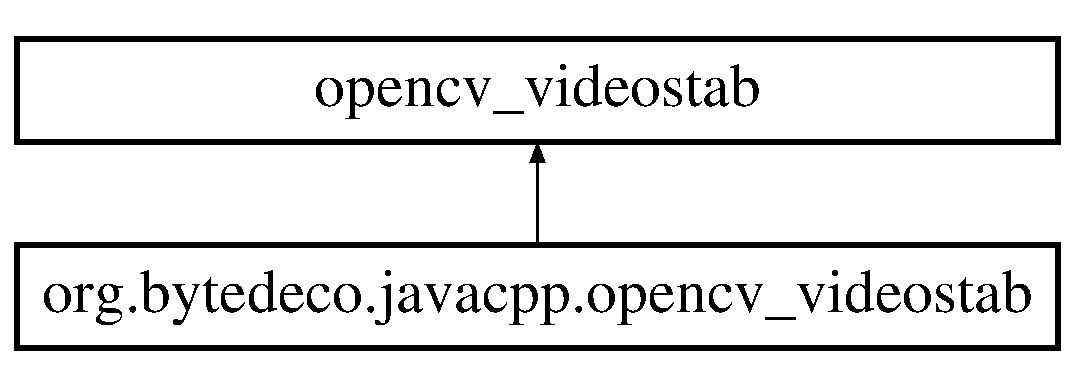
\includegraphics[height=2.000000cm]{classorg_1_1bytedeco_1_1javacpp_1_1opencv__videostab}
\end{center}
\end{figure}
\subsection*{Classes}
\begin{DoxyCompactItemize}
\item 
class {\bfseries Color\+Average\+Inpainter}
\item 
class {\bfseries Color\+Inpainter}
\item 
class {\bfseries Consistent\+Mosaic\+Inpainter}
\item 
class {\bfseries Deblurer\+Base}
\item 
class {\bfseries Fast\+Marching\+Method}
\item 
class {\bfseries From\+File\+Motion\+Reader}
\item 
class {\bfseries Gaussian\+Motion\+Filter}
\item 
class {\bfseries I\+Dense\+Opt\+Flow\+Estimator}
\item 
class {\bfseries I\+Frame\+Source}
\item 
class {\bfseries I\+Log}
\item 
class {\bfseries Image\+Motion\+Estimator\+Base}
\begin{DoxyCompactList}\small\item\em Base class for global 2D motion estimation methods which take frames as input. \end{DoxyCompactList}\item 
class {\bfseries I\+Motion\+Stabilizer}
\item 
class {\bfseries Inpainter\+Base}
\item 
class {\bfseries Inpainting\+Pipeline}
\item 
class {\bfseries I\+Outlier\+Rejector}
\item 
class {\bfseries I\+Sparse\+Opt\+Flow\+Estimator}
\item 
class {\bfseries Keypoint\+Based\+Motion\+Estimator}
\begin{DoxyCompactList}\small\item\em Describes a global 2D motion estimation method which uses keypoints detection and optical flow for matching. \end{DoxyCompactList}\item 
class {\bfseries Log\+To\+Stdout}
\item 
class {\bfseries Lp\+Motion\+Stabilizer}
\item 
class {\bfseries More\+Accurate\+Motion\+Wobble\+Suppressor}
\item 
class {\bfseries More\+Accurate\+Motion\+Wobble\+Suppressor\+Base}
\item 
class {\bfseries Motion\+Estimator\+Base}
\begin{DoxyCompactList}\small\item\em Base class for all global motion estimation methods. \end{DoxyCompactList}\item 
class {\bfseries Motion\+Estimator\+L1}
\begin{DoxyCompactList}\small\item\em Describes a global 2D motion estimation method which minimizes L1 error. \end{DoxyCompactList}\item 
class {\bfseries Motion\+Estimator\+Ransac\+L2}
\begin{DoxyCompactList}\small\item\em Describes a robust R\+A\+N\+S\+A\+C-\/based global 2D motion estimation method which minimizes L2 error. \end{DoxyCompactList}\item 
class {\bfseries Motion\+Filter\+Base}
\item 
class {\bfseries Motion\+Inpainter}
\item 
class {\bfseries Motion\+Stabilization\+Pipeline}
\item 
class {\bfseries Null\+Deblurer}
\item 
class {\bfseries Null\+Frame\+Source}
\item 
class {\bfseries Null\+Inpainter}
\item 
class {\bfseries Null\+Log}
\item 
class {\bfseries Null\+Outlier\+Rejector}
\item 
class {\bfseries Null\+Wobble\+Suppressor}
\item 
class {\bfseries One\+Pass\+Stabilizer}
\item 
class {\bfseries Pyr\+Lk\+Opt\+Flow\+Estimator\+Base}
\item 
class {\bfseries Ransac\+Params}
\begin{DoxyCompactList}\small\item\em Describes R\+A\+N\+S\+AC method parameters. \end{DoxyCompactList}\item 
class {\bfseries Sparse\+Pyr\+Lk\+Opt\+Flow\+Estimator}
\item 
class {\bfseries Stabilizer\+Base}
\item 
class {\bfseries To\+File\+Motion\+Writer}
\item 
class {\bfseries Translation\+Based\+Local\+Outlier\+Rejector}
\item 
class {\bfseries Two\+Pass\+Stabilizer}
\item 
class {\bfseries Video\+File\+Source}
\item 
class {\bfseries Weighting\+Deblurer}
\item 
class {\bfseries Wobble\+Suppressor\+Base}
\end{DoxyCompactItemize}
\subsection*{Static Public Member Functions}
\begin{DoxyCompactItemize}
\item 
static native Mat {\bfseries estimate\+Global\+Motion\+Least\+Squares} ( @By\+Val Mat points0, @By\+Val Mat points1, int model, Float\+Pointer rmse)
\item 
static native Mat {\bfseries estimate\+Global\+Motion\+Least\+Squares} ( @By\+Val Mat points0, @By\+Val Mat points1)
\item 
static native Mat {\bfseries estimate\+Global\+Motion\+Least\+Squares} ( @By\+Val Mat points0, @By\+Val Mat points1, int model, Float\+Buffer rmse)
\item 
static native Mat {\bfseries estimate\+Global\+Motion\+Least\+Squares} ( @By\+Val U\+Mat points0, @By\+Val U\+Mat points1, int model, float\mbox{[}$\,$\mbox{]} rmse)
\item 
static native Mat {\bfseries estimate\+Global\+Motion\+Least\+Squares} ( @By\+Val U\+Mat points0, @By\+Val U\+Mat points1)
\item 
static native Mat {\bfseries estimate\+Global\+Motion\+Least\+Squares} ( @By\+Val U\+Mat points0, @By\+Val U\+Mat points1, int model, Float\+Pointer rmse)
\item 
static native Mat \hyperlink{group__videostab__motion_gab1399e69e37b80626504e158be509601}{estimate\+Global\+Motion\+Ransac} ( @By\+Val Mat points0, @By\+Val Mat points1, int model, @Const @By\+Ref(null\+Value=\char`\"{}cv\+::videostab\+::\+Ransac\+Params\+::default2d\+Motion(cv\+::videostab\+::\+M\+M\+\_\+\+A\+F\+F\+I\+NE)\char`\"{}) Ransac\+Params params, Float\+Pointer rmse, Int\+Pointer ninliers)
\begin{DoxyCompactList}\small\item\em Estimates best global motion between two 2D point clouds robustly (using R\+A\+N\+S\+AC method). \end{DoxyCompactList}\item 
static native Mat {\bfseries estimate\+Global\+Motion\+Ransac} ( @By\+Val Mat points0, @By\+Val Mat points1)
\item 
static native Mat {\bfseries estimate\+Global\+Motion\+Ransac} ( @By\+Val Mat points0, @By\+Val Mat points1, int model, @Const @By\+Ref(null\+Value=\char`\"{}cv\+::videostab\+::\+Ransac\+Params\+::default2d\+Motion(cv\+::videostab\+::\+M\+M\+\_\+\+A\+F\+F\+I\+NE)\char`\"{}) Ransac\+Params params, Float\+Buffer rmse, Int\+Buffer ninliers)
\item 
static native Mat {\bfseries estimate\+Global\+Motion\+Ransac} ( @By\+Val U\+Mat points0, @By\+Val U\+Mat points1, int model, @Const @By\+Ref(null\+Value=\char`\"{}cv\+::videostab\+::\+Ransac\+Params\+::default2d\+Motion(cv\+::videostab\+::\+M\+M\+\_\+\+A\+F\+F\+I\+NE)\char`\"{}) Ransac\+Params params, float\mbox{[}$\,$\mbox{]} rmse, int\mbox{[}$\,$\mbox{]} ninliers)
\item 
static native Mat {\bfseries estimate\+Global\+Motion\+Ransac} ( @By\+Val U\+Mat points0, @By\+Val U\+Mat points1)
\item 
static native Mat {\bfseries estimate\+Global\+Motion\+Ransac} ( @By\+Val U\+Mat points0, @By\+Val U\+Mat points1, int model, @Const @By\+Ref(null\+Value=\char`\"{}cv\+::videostab\+::\+Ransac\+Params\+::default2d\+Motion(cv\+::videostab\+::\+M\+M\+\_\+\+A\+F\+F\+I\+NE)\char`\"{}) Ransac\+Params params, Float\+Pointer rmse, Int\+Pointer ninliers)
\item 
static native Mat \hyperlink{group__videostab__motion_ga1e73edce6a2ac4dee3f6a1ae7ec06d26}{get\+Motion} (int from, int to, @Const @By\+Ref Mat\+Vector motions)
\begin{DoxyCompactList}\small\item\em Computes motion between two frames assuming that all the intermediate motions are known. \end{DoxyCompactList}\item 
static native Mat {\bfseries ensure\+Inclusion\+Constraint} (@Const @By\+Ref Mat M, @By\+Val Size size, float trim\+Ratio)
\item 
static native float {\bfseries estimate\+Optimal\+Trim\+Ratio} (@Const @By\+Ref Mat M, @By\+Val Size size)
\item 
static native void {\bfseries calc\+Flow\+Mask} ( @Const @By\+Ref Mat flowX, @Const @By\+Ref Mat flowY, @Const @By\+Ref Mat errors, float max\+Error, @Const @By\+Ref Mat mask0, @Const @By\+Ref Mat mask1, @By\+Ref Mat flow\+Mask)
\item 
static native void {\bfseries complete\+Frame\+According\+To\+Flow} ( @Const @By\+Ref Mat flow\+Mask, @Const @By\+Ref Mat flowX, @Const @By\+Ref Mat flowY, @Const @By\+Ref Mat frame1, @Const @By\+Ref Mat mask1, float dist\+Thresh, @By\+Ref Mat frame0, @By\+Ref Mat mask0)
\item 
static native float {\bfseries calc\+Blurriness} (@Const @By\+Ref Mat frame)
\end{DoxyCompactItemize}
\subsection*{Static Public Attributes}
\begin{DoxyCompactItemize}
\item 
static final int \hyperlink{group__videostab__motion_ga1dfde997ecf6b23eb737a2b7461597cf}{M\+M\+\_\+\+T\+R\+A\+N\+S\+L\+A\+T\+I\+ON} = 0
\end{DoxyCompactItemize}


The documentation for this class was generated from the following file\+:\begin{DoxyCompactItemize}
\item 
opencv\+\_\+videostab.\+java\end{DoxyCompactItemize}

\hypertarget{classorg_1_1bytedeco_1_1javacpp_1_1opencv__xfeatures2d}{}\section{org.\+bytedeco.\+javacpp.\+opencv\+\_\+xfeatures2d Class Reference}
\label{classorg_1_1bytedeco_1_1javacpp_1_1opencv__xfeatures2d}\index{org.\+bytedeco.\+javacpp.\+opencv\+\_\+xfeatures2d@{org.\+bytedeco.\+javacpp.\+opencv\+\_\+xfeatures2d}}
Inheritance diagram for org.\+bytedeco.\+javacpp.\+opencv\+\_\+xfeatures2d\+:\begin{figure}[H]
\begin{center}
\leavevmode
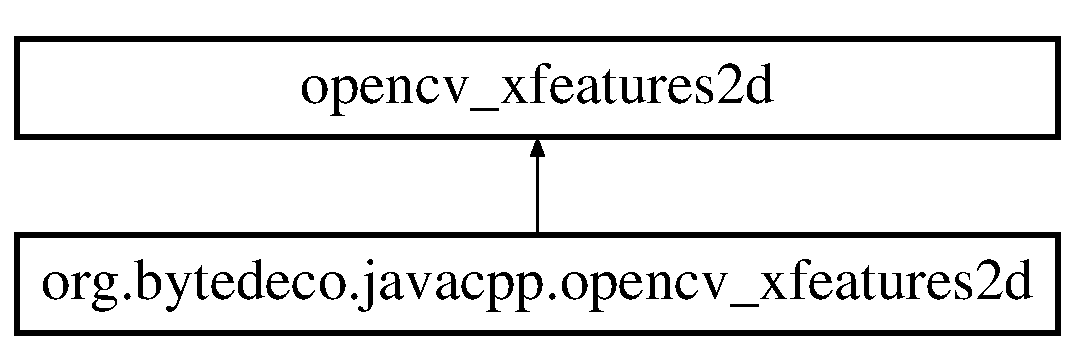
\includegraphics[height=2.000000cm]{classorg_1_1bytedeco_1_1javacpp_1_1opencv__xfeatures2d}
\end{center}
\end{figure}
\subsection*{Classes}
\begin{DoxyCompactItemize}
\item 
class {\bfseries Boost\+Desc}
\begin{DoxyCompactList}\small\item\em Class implementing Boost\+Desc (Learning Image Descriptors with Boosting), described in {\bfseries [Trzcinski13a]} and {\bfseries [Trzcinski13b]}. \end{DoxyCompactList}\item 
class {\bfseries Brief\+Descriptor\+Extractor}
\begin{DoxyCompactList}\small\item\em Class for computing B\+R\+I\+EF descriptors described in {\bfseries [calon2010]} . \end{DoxyCompactList}\item 
class {\bfseries D\+A\+I\+SY}
\begin{DoxyCompactList}\small\item\em Class implementing D\+A\+I\+SY descriptor, described in {\bfseries [Tola10]}. \end{DoxyCompactList}\item 
class {\bfseries F\+R\+E\+AK}
\item 
class {\bfseries L\+A\+T\+CH}
\item 
class {\bfseries L\+U\+C\+ID}
\begin{DoxyCompactList}\small\item\em Class implementing the locally uniform comparison image descriptor, described in {\bfseries [L\+U\+C\+ID]}. \end{DoxyCompactList}\item 
class {\bfseries M\+S\+D\+Detector}
\begin{DoxyCompactList}\small\item\em Class implementing the M\+SD ({\itshape Maximal Self-\/\+Dissimilarity}) keypoint detector, described in {\bfseries [Tombari14]}. \end{DoxyCompactList}\item 
class {\bfseries P\+C\+T\+Signatures}
\begin{DoxyCompactList}\small\item\em Class implementing P\+CT (position-\/color-\/texture) signature extraction as described in {\bfseries [Krulis\+L\+S16]}. The algorithm is divided to a feature sampler and a clusterizer. Feature sampler produces samples at given set of coordinates. Clusterizer then produces clusters of these samples using k-\/means algorithm. Resulting set of clusters is the signature of the input image. \end{DoxyCompactList}\item 
class {\bfseries P\+C\+T\+Signatures\+S\+Q\+FD}
\begin{DoxyCompactList}\small\item\em Class implementing Signature Quadratic Form Distance (S\+Q\+FD). \end{DoxyCompactList}\item 
class {\bfseries S\+I\+FT}
\item 
class {\bfseries Star\+Detector}
\begin{DoxyCompactList}\small\item\em The class implements the keypoint detector introduced by {\bfseries [Agrawal08]}, synonym of Star\+Detector. \+: \end{DoxyCompactList}\item 
class {\bfseries S\+U\+RF}
\begin{DoxyCompactList}\small\item\em Class for extracting Speeded Up Robust Features from an image {\bfseries [Bay06]} . \end{DoxyCompactList}\item 
class {\bfseries V\+GG}
\begin{DoxyCompactList}\small\item\em Class implementing V\+GG (Oxford Visual Geometry Group) descriptor trained end to end using \char`\"{}\+Descriptor Learning Using Convex Optimisation\char`\"{} (D\+L\+CO) aparatus described in {\bfseries [Simonyan14]}. \end{DoxyCompactList}\end{DoxyCompactItemize}


The documentation for this class was generated from the following file\+:\begin{DoxyCompactItemize}
\item 
opencv\+\_\+xfeatures2d.\+java\end{DoxyCompactItemize}

\hypertarget{classorg_1_1bytedeco_1_1javacpp_1_1opencv__ximgproc}{}\section{org.\+bytedeco.\+javacpp.\+opencv\+\_\+ximgproc Class Reference}
\label{classorg_1_1bytedeco_1_1javacpp_1_1opencv__ximgproc}\index{org.\+bytedeco.\+javacpp.\+opencv\+\_\+ximgproc@{org.\+bytedeco.\+javacpp.\+opencv\+\_\+ximgproc}}
Inheritance diagram for org.\+bytedeco.\+javacpp.\+opencv\+\_\+ximgproc\+:\begin{figure}[H]
\begin{center}
\leavevmode
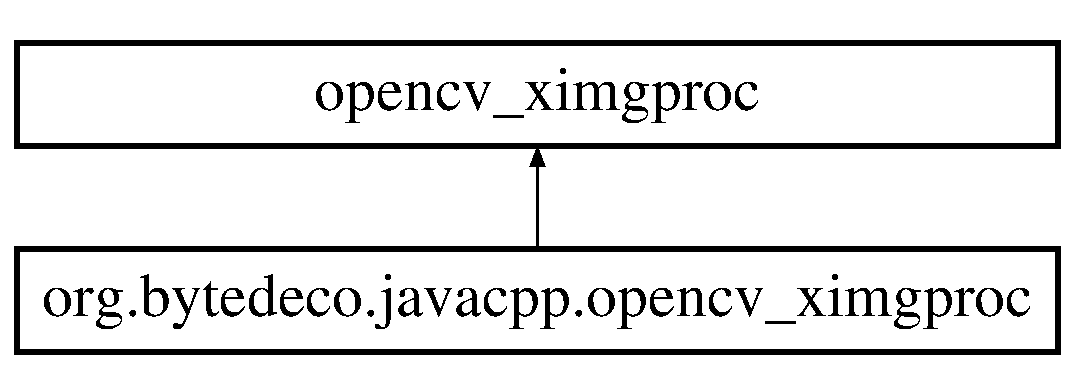
\includegraphics[height=2.000000cm]{classorg_1_1bytedeco_1_1javacpp_1_1opencv__ximgproc}
\end{center}
\end{figure}
\subsection*{Classes}
\begin{DoxyCompactItemize}
\item 
class {\bfseries Adaptive\+Manifold\+Filter}
\begin{DoxyCompactList}\small\item\em Interface for Adaptive Manifold Filter realizations. \end{DoxyCompactList}\item 
class {\bfseries Disparity\+Filter}
\item 
class {\bfseries Disparity\+W\+L\+S\+Filter}
\begin{DoxyCompactList}\small\item\em Disparity map filter based on Weighted Least Squares filter (in form of Fast Global Smoother that is a lot faster than traditional Weighted Least Squares filter implementations) and optional use of left-\/right-\/consistency-\/based confidence to refine the results in half-\/occlusions and uniform areas. \end{DoxyCompactList}\item 
class {\bfseries D\+T\+Filter}
\begin{DoxyCompactList}\small\item\em Interface for realizations of Domain Transform filter. \end{DoxyCompactList}\item 
class {\bfseries Edge\+Aware\+Interpolator}
\begin{DoxyCompactList}\small\item\em Sparse match interpolation algorithm based on modified locally-\/weighted affine estimator from {\bfseries [Revaud2015]} and Fast Global Smoother as post-\/processing filter. \end{DoxyCompactList}\item 
class {\bfseries Fast\+Global\+Smoother\+Filter}
\begin{DoxyCompactList}\small\item\em Interface for implementations of Fast Global Smoother filter. \end{DoxyCompactList}\item 
class {\bfseries Graph\+Segmentation}
\item 
class {\bfseries Guided\+Filter}
\begin{DoxyCompactList}\small\item\em Interface for realizations of Guided Filter. \end{DoxyCompactList}\item 
class {\bfseries R\+F\+Feature\+Getter}
\item 
class {\bfseries Selective\+Search\+Segmentation}
\begin{DoxyCompactList}\small\item\em Selective search segmentation algorithm The class implements the algorithm described in {\bfseries [uijlings2013selective]}. \end{DoxyCompactList}\item 
class {\bfseries Selective\+Search\+Segmentation\+Strategy}
\begin{DoxyCompactList}\small\item\em Strategie for the selective search segmentation algorithm The class implements a generic stragery for the algorithm described in {\bfseries [uijlings2013selective]}. \end{DoxyCompactList}\item 
class {\bfseries Selective\+Search\+Segmentation\+Strategy\+Color}
\begin{DoxyCompactList}\small\item\em Color-\/based strategy for the selective search segmentation algorithm The class is implemented from the algorithm described in {\bfseries [uijlings2013selective]}. \end{DoxyCompactList}\item 
class {\bfseries Selective\+Search\+Segmentation\+Strategy\+Fill}
\begin{DoxyCompactList}\small\item\em Fill-\/based strategy for the selective search segmentation algorithm The class is implemented from the algorithm described in {\bfseries [uijlings2013selective]}. \end{DoxyCompactList}\item 
class {\bfseries Selective\+Search\+Segmentation\+Strategy\+Multiple}
\begin{DoxyCompactList}\small\item\em Regroup multiple strategies for the selective search segmentation algorithm. \end{DoxyCompactList}\item 
class {\bfseries Selective\+Search\+Segmentation\+Strategy\+Size}
\begin{DoxyCompactList}\small\item\em Size-\/based strategy for the selective search segmentation algorithm The class is implemented from the algorithm described in {\bfseries [uijlings2013selective]}. \end{DoxyCompactList}\item 
class {\bfseries Selective\+Search\+Segmentation\+Strategy\+Texture}
\begin{DoxyCompactList}\small\item\em Texture-\/based strategy for the selective search segmentation algorithm The class is implemented from the algorithm described in {\bfseries [uijlings2013selective]}. \end{DoxyCompactList}\item 
class {\bfseries Sparse\+Match\+Interpolator}
\item 
class {\bfseries Structured\+Edge\+Detection}
\begin{DoxyCompactList}\small\item\em Class implementing edge detection algorithm from {\bfseries [Dollar2013]} \+: \end{DoxyCompactList}\item 
class {\bfseries Superpixel\+L\+SC}
\item 
class {\bfseries Superpixel\+S\+E\+E\+DS}
\item 
class {\bfseries Superpixel\+S\+L\+IC}
\end{DoxyCompactItemize}
\subsection*{Static Public Member Functions}
\begin{DoxyCompactItemize}
\item 
static native void {\bfseries ni\+Black\+Threshold} ( @By\+Val Mat \+\_\+src, @By\+Val Mat \+\_\+dst, double max\+Value, int type, int block\+Size, double delta)
\item 
static native void {\bfseries ni\+Black\+Threshold} ( @By\+Val U\+Mat \+\_\+src, @By\+Val U\+Mat \+\_\+dst, double max\+Value, int type, int block\+Size, double delta)
\item 
static native void \hyperlink{group__ximgproc_gaf281201400d757cb4921c49dcf729896}{thinning} ( @By\+Val Mat src, @By\+Val Mat dst, int thinning\+Type)
\begin{DoxyCompactList}\small\item\em Applies a binary blob thinning operation, to achieve a skeletization of the input image. \end{DoxyCompactList}\item 
static native void {\bfseries thinning} ( @By\+Val Mat src, @By\+Val Mat dst)
\item 
static native void {\bfseries thinning} ( @By\+Val U\+Mat src, @By\+Val U\+Mat dst, int thinning\+Type)
\item 
static native void {\bfseries thinning} ( @By\+Val U\+Mat src, @By\+Val U\+Mat dst)
\item 
static native D\+T\+Filter \hyperlink{group__ximgproc__filters_ga813031e38babc7f53070fcf67dbfea40}{create\+D\+T\+Filter} (@By\+Val Mat guide, double sigma\+Spatial, double sigma\+Color, int mode, int num\+Iters)
\begin{DoxyCompactList}\small\item\em Factory method, create instance of D\+T\+Filter and produce initialization routines. \end{DoxyCompactList}\item 
static native D\+T\+Filter {\bfseries create\+D\+T\+Filter} (@By\+Val Mat guide, double sigma\+Spatial, double sigma\+Color)
\item 
static native D\+T\+Filter {\bfseries create\+D\+T\+Filter} (@By\+Val U\+Mat guide, double sigma\+Spatial, double sigma\+Color, int mode, int num\+Iters)
\item 
static native D\+T\+Filter {\bfseries create\+D\+T\+Filter} (@By\+Val U\+Mat guide, double sigma\+Spatial, double sigma\+Color)
\item 
static native void \hyperlink{group__ximgproc__filters_ga7a3f493e82d0571f6a8ed61d005542d9}{dt\+Filter} (@By\+Val Mat guide, @By\+Val Mat src, @By\+Val Mat dst, double sigma\+Spatial, double sigma\+Color, int mode, int num\+Iters)
\begin{DoxyCompactList}\small\item\em Simple one-\/line Domain Transform filter call. If you have multiple images to filter with the same guided image then use D\+T\+Filter interface to avoid extra computations on initialization stage. \end{DoxyCompactList}\item 
static native void {\bfseries dt\+Filter} (@By\+Val Mat guide, @By\+Val Mat src, @By\+Val Mat dst, double sigma\+Spatial, double sigma\+Color)
\item 
static native void {\bfseries dt\+Filter} (@By\+Val U\+Mat guide, @By\+Val U\+Mat src, @By\+Val U\+Mat dst, double sigma\+Spatial, double sigma\+Color, int mode, int num\+Iters)
\item 
static native void {\bfseries dt\+Filter} (@By\+Val U\+Mat guide, @By\+Val U\+Mat src, @By\+Val U\+Mat dst, double sigma\+Spatial, double sigma\+Color)
\item 
static native Guided\+Filter \hyperlink{group__ximgproc__filters_gaa4f34319223da44cce2ad4e75b776287}{create\+Guided\+Filter} (@By\+Val Mat guide, int radius, double eps)
\begin{DoxyCompactList}\small\item\em Factory method, create instance of Guided\+Filter and produce initialization routines. \end{DoxyCompactList}\item 
static native Guided\+Filter {\bfseries create\+Guided\+Filter} (@By\+Val U\+Mat guide, int radius, double eps)
\item 
static native void \hyperlink{group__ximgproc__filters_ga7a63d78fbc962c2c9df0f525ae8083ff}{guided\+Filter} (@By\+Val Mat guide, @By\+Val Mat src, @By\+Val Mat dst, int radius, double eps, int d\+Depth)
\begin{DoxyCompactList}\small\item\em Simple one-\/line Guided Filter call. \end{DoxyCompactList}\item 
static native void {\bfseries guided\+Filter} (@By\+Val Mat guide, @By\+Val Mat src, @By\+Val Mat dst, int radius, double eps)
\item 
static native void {\bfseries guided\+Filter} (@By\+Val U\+Mat guide, @By\+Val U\+Mat src, @By\+Val U\+Mat dst, int radius, double eps, int d\+Depth)
\item 
static native void {\bfseries guided\+Filter} (@By\+Val U\+Mat guide, @By\+Val U\+Mat src, @By\+Val U\+Mat dst, int radius, double eps)
\item 
static native Adaptive\+Manifold\+Filter \hyperlink{group__ximgproc__filters_ga0b203de6ac4064c7dac99b1d5647b13d}{create\+A\+M\+Filter} (double sigma\+\_\+s, double sigma\+\_\+r, @Cast(\char`\"{}bool\char`\"{}) boolean adjust\+\_\+outliers)
\begin{DoxyCompactList}\small\item\em Factory method, create instance of Adaptive\+Manifold\+Filter and produce some initialization routines. \end{DoxyCompactList}\item 
static native Adaptive\+Manifold\+Filter {\bfseries create\+A\+M\+Filter} (double sigma\+\_\+s, double sigma\+\_\+r)
\item 
static native void \hyperlink{group__ximgproc__filters_ga0555fbee9503a53a6fcc0472db78f188}{am\+Filter} (@By\+Val Mat joint, @By\+Val Mat src, @By\+Val Mat dst, double sigma\+\_\+s, double sigma\+\_\+r, @Cast(\char`\"{}bool\char`\"{}) boolean adjust\+\_\+outliers)
\begin{DoxyCompactList}\small\item\em Simple one-\/line Adaptive Manifold Filter call. \end{DoxyCompactList}\item 
static native void {\bfseries am\+Filter} (@By\+Val Mat joint, @By\+Val Mat src, @By\+Val Mat dst, double sigma\+\_\+s, double sigma\+\_\+r)
\item 
static native void {\bfseries am\+Filter} (@By\+Val U\+Mat joint, @By\+Val U\+Mat src, @By\+Val U\+Mat dst, double sigma\+\_\+s, double sigma\+\_\+r, @Cast(\char`\"{}bool\char`\"{}) boolean adjust\+\_\+outliers)
\item 
static native void {\bfseries am\+Filter} (@By\+Val U\+Mat joint, @By\+Val U\+Mat src, @By\+Val U\+Mat dst, double sigma\+\_\+s, double sigma\+\_\+r)
\item 
static native void \hyperlink{group__ximgproc__filters_ga113d231f29873e22ea1778c17307a0b5}{joint\+Bilateral\+Filter} (@By\+Val Mat joint, @By\+Val Mat src, @By\+Val Mat dst, int d, double sigma\+Color, double sigma\+Space, int border\+Type)
\begin{DoxyCompactList}\small\item\em Applies the joint bilateral filter to an image. \end{DoxyCompactList}\item 
static native void {\bfseries joint\+Bilateral\+Filter} (@By\+Val Mat joint, @By\+Val Mat src, @By\+Val Mat dst, int d, double sigma\+Color, double sigma\+Space)
\item 
static native void {\bfseries joint\+Bilateral\+Filter} (@By\+Val U\+Mat joint, @By\+Val U\+Mat src, @By\+Val U\+Mat dst, int d, double sigma\+Color, double sigma\+Space, int border\+Type)
\item 
static native void {\bfseries joint\+Bilateral\+Filter} (@By\+Val U\+Mat joint, @By\+Val U\+Mat src, @By\+Val U\+Mat dst, int d, double sigma\+Color, double sigma\+Space)
\item 
static native void \hyperlink{group__ximgproc__filters_ga369c99e9a5e13c93042c670509e04dfc}{bilateral\+Texture\+Filter} (@By\+Val Mat src, @By\+Val Mat dst, int fr, int num\+Iter, double sigma\+Alpha, double sigma\+Avg)
\begin{DoxyCompactList}\small\item\em Applies the bilateral texture filter to an image. It performs structure-\/preserving texture filter. For more details about this filter see {\bfseries [Cho2014]}. \end{DoxyCompactList}\item 
static native void {\bfseries bilateral\+Texture\+Filter} (@By\+Val Mat src, @By\+Val Mat dst)
\item 
static native void {\bfseries bilateral\+Texture\+Filter} (@By\+Val U\+Mat src, @By\+Val U\+Mat dst, int fr, int num\+Iter, double sigma\+Alpha, double sigma\+Avg)
\item 
static native void {\bfseries bilateral\+Texture\+Filter} (@By\+Val U\+Mat src, @By\+Val U\+Mat dst)
\item 
static native void \hyperlink{group__ximgproc__filters_ga2ce496356d7b8cd485c04de402fdb8f5}{rolling\+Guidance\+Filter} (@By\+Val Mat src, @By\+Val Mat dst, int d, double sigma\+Color, double sigma\+Space, int num\+Of\+Iter, int border\+Type)
\begin{DoxyCompactList}\small\item\em Applies the rolling guidance filter to an image. \end{DoxyCompactList}\item 
static native void {\bfseries rolling\+Guidance\+Filter} (@By\+Val Mat src, @By\+Val Mat dst)
\item 
static native void {\bfseries rolling\+Guidance\+Filter} (@By\+Val U\+Mat src, @By\+Val U\+Mat dst, int d, double sigma\+Color, double sigma\+Space, int num\+Of\+Iter, int border\+Type)
\item 
static native void {\bfseries rolling\+Guidance\+Filter} (@By\+Val U\+Mat src, @By\+Val U\+Mat dst)
\item 
static native Fast\+Global\+Smoother\+Filter \hyperlink{group__ximgproc__filters_ga2464410b399f5f54dfce61987cfaa67e}{create\+Fast\+Global\+Smoother\+Filter} (@By\+Val Mat guide, double lambda, double sigma\+\_\+color, double lambda\+\_\+attenuation, int num\+\_\+iter)
\begin{DoxyCompactList}\small\item\em Factory method, create instance of Fast\+Global\+Smoother\+Filter and execute the initialization routines. \end{DoxyCompactList}\item 
static native Fast\+Global\+Smoother\+Filter {\bfseries create\+Fast\+Global\+Smoother\+Filter} (@By\+Val Mat guide, double lambda, double sigma\+\_\+color)
\item 
static native Fast\+Global\+Smoother\+Filter {\bfseries create\+Fast\+Global\+Smoother\+Filter} (@By\+Val U\+Mat guide, double lambda, double sigma\+\_\+color, double lambda\+\_\+attenuation, int num\+\_\+iter)
\item 
static native Fast\+Global\+Smoother\+Filter {\bfseries create\+Fast\+Global\+Smoother\+Filter} (@By\+Val U\+Mat guide, double lambda, double sigma\+\_\+color)
\item 
static native void \hyperlink{group__ximgproc__filters_gad387c802487ca58e07a45c896a13688f}{fast\+Global\+Smoother\+Filter} (@By\+Val Mat guide, @By\+Val Mat src, @By\+Val Mat dst, double lambda, double sigma\+\_\+color, double lambda\+\_\+attenuation, int num\+\_\+iter)
\begin{DoxyCompactList}\small\item\em Simple one-\/line Fast Global Smoother filter call. If you have multiple images to filter with the same guide then use Fast\+Global\+Smoother\+Filter interface to avoid extra computations. \end{DoxyCompactList}\item 
static native void {\bfseries fast\+Global\+Smoother\+Filter} (@By\+Val Mat guide, @By\+Val Mat src, @By\+Val Mat dst, double lambda, double sigma\+\_\+color)
\item 
static native void {\bfseries fast\+Global\+Smoother\+Filter} (@By\+Val U\+Mat guide, @By\+Val U\+Mat src, @By\+Val U\+Mat dst, double lambda, double sigma\+\_\+color, double lambda\+\_\+attenuation, int num\+\_\+iter)
\item 
static native void {\bfseries fast\+Global\+Smoother\+Filter} (@By\+Val U\+Mat guide, @By\+Val U\+Mat src, @By\+Val U\+Mat dst, double lambda, double sigma\+\_\+color)
\item 
static native void \hyperlink{group__ximgproc__filters_ga5a74b92ad3cd10d7809e4416c623610d}{l0\+Smooth} (@By\+Val Mat src, @By\+Val Mat dst, double lambda, double kappa)
\begin{DoxyCompactList}\small\item\em Global image smoothing via L0 gradient minimization. \end{DoxyCompactList}\item 
static native void {\bfseries l0\+Smooth} (@By\+Val Mat src, @By\+Val Mat dst)
\item 
static native void {\bfseries l0\+Smooth} (@By\+Val U\+Mat src, @By\+Val U\+Mat dst, double lambda, double kappa)
\item 
static native void {\bfseries l0\+Smooth} (@By\+Val U\+Mat src, @By\+Val U\+Mat dst)
\item 
static native Disparity\+W\+L\+S\+Filter \hyperlink{group__ximgproc__filters_ga5282f3f5ccb08ba470cae8c4b95cee3d}{create\+Disparity\+W\+L\+S\+Filter} (@Ptr Stereo\+Matcher matcher\+\_\+left)
\begin{DoxyCompactList}\small\item\em Convenience factory method that creates an instance of Disparity\+W\+L\+S\+Filter and sets up all the relevant filter parameters automatically based on the matcher instance. Currently supports only Stereo\+BM and Stereo\+S\+G\+BM. \end{DoxyCompactList}\item 
static native Stereo\+Matcher \hyperlink{group__ximgproc__filters_ga8d41bef5e1e848d7fa4b163459e79499}{create\+Right\+Matcher} (@Ptr Stereo\+Matcher matcher\+\_\+left)
\begin{DoxyCompactList}\small\item\em Convenience method to set up the matcher for computing the right-\/view disparity map that is required in case of filtering with confidence. \end{DoxyCompactList}\item 
static native Disparity\+W\+L\+S\+Filter \hyperlink{group__ximgproc__filters_ga4ecf158eb4378bda624a77b7afe92c9b}{create\+Disparity\+W\+L\+S\+Filter\+Generic} (@Cast(\char`\"{}bool\char`\"{}) boolean use\+\_\+confidence)
\begin{DoxyCompactList}\small\item\em More generic factory method, create instance of Disparity\+W\+L\+S\+Filter and execute basic initialization routines. When using this method you will need to set-\/up the R\+OI, matchers and other parameters by yourself. \end{DoxyCompactList}\item 
static native int \hyperlink{group__ximgproc__filters_ga98c3c9fc13d0d1e808c73c8a0ae91a09}{read\+GT} (@Str Byte\+Pointer src\+\_\+path, @By\+Val Mat dst)
\begin{DoxyCompactList}\small\item\em Function for reading ground truth disparity maps. Supports basic Middlebury and M\+P\+I-\/\+Sintel formats. Note that the resulting disparity map is scaled by 16. \end{DoxyCompactList}\item 
static native int {\bfseries read\+GT} (@Str String src\+\_\+path, @By\+Val Mat dst)
\item 
static native int {\bfseries read\+GT} (@Str Byte\+Pointer src\+\_\+path, @By\+Val U\+Mat dst)
\item 
static native int {\bfseries read\+GT} (@Str String src\+\_\+path, @By\+Val U\+Mat dst)
\item 
static native double \hyperlink{group__ximgproc__filters_ga0f224e6315d538e257cba2fb7ae0bbee}{compute\+M\+SE} (@By\+Val Mat GT, @By\+Val Mat src, @By\+Val Rect R\+OI)
\begin{DoxyCompactList}\small\item\em Function for computing mean square error for disparity maps. \end{DoxyCompactList}\item 
static native double {\bfseries compute\+M\+SE} (@By\+Val U\+Mat GT, @By\+Val U\+Mat src, @By\+Val Rect R\+OI)
\item 
static native double \hyperlink{group__ximgproc__filters_ga04b04ac57f6b8c53deacbb1d41d05766}{compute\+Bad\+Pixel\+Percent} (@By\+Val Mat GT, @By\+Val Mat src, @By\+Val Rect R\+OI, int thresh)
\begin{DoxyCompactList}\small\item\em Function for computing the percent of \char`\"{}bad\char`\"{} pixels in the disparity map (pixels where error is higher than a specified threshold) \end{DoxyCompactList}\item 
static native double {\bfseries compute\+Bad\+Pixel\+Percent} (@By\+Val Mat GT, @By\+Val Mat src, @By\+Val Rect R\+OI)
\item 
static native double {\bfseries compute\+Bad\+Pixel\+Percent} (@By\+Val U\+Mat GT, @By\+Val U\+Mat src, @By\+Val Rect R\+OI, int thresh)
\item 
static native double {\bfseries compute\+Bad\+Pixel\+Percent} (@By\+Val U\+Mat GT, @By\+Val U\+Mat src, @By\+Val Rect R\+OI)
\item 
static native void \hyperlink{group__ximgproc__filters_ga717daf2a9c80c6f731778cf45474ed2c}{get\+Disparity\+Vis} (@By\+Val Mat src, @By\+Val Mat dst, double scale)
\begin{DoxyCompactList}\small\item\em Function for creating a disparity map visualization (clamped C\+V\+\_\+8U image) \end{DoxyCompactList}\item 
static native void {\bfseries get\+Disparity\+Vis} (@By\+Val Mat src, @By\+Val Mat dst)
\item 
static native void {\bfseries get\+Disparity\+Vis} (@By\+Val U\+Mat src, @By\+Val U\+Mat dst, double scale)
\item 
static native void {\bfseries get\+Disparity\+Vis} (@By\+Val U\+Mat src, @By\+Val U\+Mat dst)
\item 
static native Edge\+Aware\+Interpolator \hyperlink{group__ximgproc__filters_ga2e4e024539c3de5affbf5c70b0baf30f}{create\+Edge\+Aware\+Interpolator} ()
\begin{DoxyCompactList}\small\item\em Factory method that creates an instance of the Edge\+Aware\+Interpolator. \end{DoxyCompactList}\item 
static native R\+F\+Feature\+Getter {\bfseries create\+R\+F\+Feature\+Getter} ()
\item 
static native Structured\+Edge\+Detection \hyperlink{group__ximgproc__edge_gafcb7c834ebdb82e5b362789a94b9e034}{create\+Structured\+Edge\+Detection} (@Str Byte\+Pointer model, @Const @Ptr R\+F\+Feature\+Getter how\+To\+Get\+Features)
\item 
static native Structured\+Edge\+Detection {\bfseries create\+Structured\+Edge\+Detection} (@Str Byte\+Pointer model)
\item 
static native Structured\+Edge\+Detection {\bfseries create\+Structured\+Edge\+Detection} (@Str String model, @Const @Ptr R\+F\+Feature\+Getter how\+To\+Get\+Features)
\item 
static native Structured\+Edge\+Detection {\bfseries create\+Structured\+Edge\+Detection} (@Str String model)
\item 
static native Superpixel\+S\+E\+E\+DS \hyperlink{group__ximgproc__superpixel_ga16f41a6ddd22daf4d1f1851a6f689466}{create\+Superpixel\+S\+E\+E\+DS} (int image\+\_\+width, int image\+\_\+height, int image\+\_\+channels, int num\+\_\+superpixels, int num\+\_\+levels, int prior, int histogram\+\_\+bins, @Cast(\char`\"{}bool\char`\"{}) boolean double\+\_\+step)
\begin{DoxyCompactList}\small\item\em Initializes a Superpixel\+S\+E\+E\+DS object. \end{DoxyCompactList}\item 
static native Superpixel\+S\+E\+E\+DS {\bfseries create\+Superpixel\+S\+E\+E\+DS} (int image\+\_\+width, int image\+\_\+height, int image\+\_\+channels, int num\+\_\+superpixels, int num\+\_\+levels)
\item 
static native Graph\+Segmentation \hyperlink{group__ximgproc__segmentation_ga51469520253d4dc38fd411763692c452}{create\+Graph\+Segmentation} (double sigma, float k, int min\+\_\+size)
\begin{DoxyCompactList}\small\item\em Creates a graph based segmentor. \end{DoxyCompactList}\item 
static native Graph\+Segmentation {\bfseries create\+Graph\+Segmentation} ()
\item 
static native Selective\+Search\+Segmentation\+Strategy\+Color \hyperlink{group__ximgproc__segmentation_ga9631bc8096ead6133e098623d8f1e664}{create\+Selective\+Search\+Segmentation\+Strategy\+Color} ()
\begin{DoxyCompactList}\small\item\em Create a new color-\/based strategy. \end{DoxyCompactList}\item 
static native Selective\+Search\+Segmentation\+Strategy\+Size \hyperlink{group__ximgproc__segmentation_gabe5aa072443fd8b40ea54141bd3628b7}{create\+Selective\+Search\+Segmentation\+Strategy\+Size} ()
\begin{DoxyCompactList}\small\item\em Create a new size-\/based strategy. \end{DoxyCompactList}\item 
static native Selective\+Search\+Segmentation\+Strategy\+Texture \hyperlink{group__ximgproc__segmentation_ga921f1030601ebcdad67662f016ebb6bf}{create\+Selective\+Search\+Segmentation\+Strategy\+Texture} ()
\begin{DoxyCompactList}\small\item\em Create a new size-\/based strategy. \end{DoxyCompactList}\item 
static native Selective\+Search\+Segmentation\+Strategy\+Fill \hyperlink{group__ximgproc__segmentation_ga6615570ea96beef3412287b4dddb312a}{create\+Selective\+Search\+Segmentation\+Strategy\+Fill} ()
\begin{DoxyCompactList}\small\item\em Create a new fill-\/based strategy. \end{DoxyCompactList}\item 
static native Selective\+Search\+Segmentation\+Strategy\+Multiple \hyperlink{group__ximgproc__segmentation_ga54fb05bc5e00a9a79578016f402c3a25}{create\+Selective\+Search\+Segmentation\+Strategy\+Multiple} ()
\begin{DoxyCompactList}\small\item\em Create a new multiple strategy. \end{DoxyCompactList}\item 
static native Selective\+Search\+Segmentation\+Strategy\+Multiple \hyperlink{group__ximgproc__segmentation_ga6efb6138175a12479bd02b85f242afa1}{create\+Selective\+Search\+Segmentation\+Strategy\+Multiple} (@Ptr Selective\+Search\+Segmentation\+Strategy s1)
\begin{DoxyCompactList}\small\item\em Create a new multiple strategy and set one subtrategy. \end{DoxyCompactList}\item 
static native Selective\+Search\+Segmentation\+Strategy\+Multiple \hyperlink{group__ximgproc__segmentation_gaf769336116a86e1107367e971033e25b}{create\+Selective\+Search\+Segmentation\+Strategy\+Multiple} (@Ptr Selective\+Search\+Segmentation\+Strategy s1, @Ptr Selective\+Search\+Segmentation\+Strategy s2)
\begin{DoxyCompactList}\small\item\em Create a new multiple strategy and set two subtrategies, with equal weights. \end{DoxyCompactList}\item 
static native Selective\+Search\+Segmentation\+Strategy\+Multiple \hyperlink{group__ximgproc__segmentation_ga83a457ff4067681d6ea93cf51b584b9d}{create\+Selective\+Search\+Segmentation\+Strategy\+Multiple} (@Ptr Selective\+Search\+Segmentation\+Strategy s1, @Ptr Selective\+Search\+Segmentation\+Strategy s2, @Ptr Selective\+Search\+Segmentation\+Strategy s3)
\begin{DoxyCompactList}\small\item\em Create a new multiple strategy and set three subtrategies, with equal weights. \end{DoxyCompactList}\item 
static native Selective\+Search\+Segmentation\+Strategy\+Multiple \hyperlink{group__ximgproc__segmentation_ga0c5302ec3882ad988a84158bc91186e1}{create\+Selective\+Search\+Segmentation\+Strategy\+Multiple} (@Ptr Selective\+Search\+Segmentation\+Strategy s1, @Ptr Selective\+Search\+Segmentation\+Strategy s2, @Ptr Selective\+Search\+Segmentation\+Strategy s3, @Ptr Selective\+Search\+Segmentation\+Strategy s4)
\begin{DoxyCompactList}\small\item\em Create a new multiple strategy and set four subtrategies, with equal weights. \end{DoxyCompactList}\item 
static native Selective\+Search\+Segmentation \hyperlink{group__ximgproc__segmentation_gadfa823f2a25d59aaf55b7e0ce50ca67a}{create\+Selective\+Search\+Segmentation} ()
\begin{DoxyCompactList}\small\item\em Create a new Selective\+Search\+Segmentation class. \end{DoxyCompactList}\item 
static native void \hyperlink{classorg_1_1bytedeco_1_1javacpp_1_1opencv__ximgproc_a86b1be8a4536cf9ee5613a180ab05731}{Fast\+Hough\+Transform} ( @By\+Val Mat src, @By\+Val Mat dst, int dst\+Mat\+Depth, int angle\+Range, int op, int make\+Skew)
\begin{DoxyCompactList}\small\item\em Calculates 2D Fast Hough transform of an image. \end{DoxyCompactList}\item 
\mbox{\Hypertarget{classorg_1_1bytedeco_1_1javacpp_1_1opencv__ximgproc_a7b460f03e6e846c1898c3b0bd3fe54b0}\label{classorg_1_1bytedeco_1_1javacpp_1_1opencv__ximgproc_a7b460f03e6e846c1898c3b0bd3fe54b0}} 
static native void {\bfseries Fast\+Hough\+Transform} ( @By\+Val Mat src, @By\+Val Mat dst, int dst\+Mat\+Depth)
\item 
\mbox{\Hypertarget{classorg_1_1bytedeco_1_1javacpp_1_1opencv__ximgproc_ada5b094b98a7cd9bb69a0d354ef5a1f6}\label{classorg_1_1bytedeco_1_1javacpp_1_1opencv__ximgproc_ada5b094b98a7cd9bb69a0d354ef5a1f6}} 
static native void {\bfseries Fast\+Hough\+Transform} ( @By\+Val U\+Mat src, @By\+Val U\+Mat dst, int dst\+Mat\+Depth, int angle\+Range, int op, int make\+Skew)
\item 
\mbox{\Hypertarget{classorg_1_1bytedeco_1_1javacpp_1_1opencv__ximgproc_afeffe7892b68efac640829342cd5fabf}\label{classorg_1_1bytedeco_1_1javacpp_1_1opencv__ximgproc_afeffe7892b68efac640829342cd5fabf}} 
static native void {\bfseries Fast\+Hough\+Transform} ( @By\+Val U\+Mat src, @By\+Val U\+Mat dst, int dst\+Mat\+Depth)
\item 
static native Scalar4i \hyperlink{classorg_1_1bytedeco_1_1javacpp_1_1opencv__ximgproc_a15b22eb13c2bff5ab308c1cc895e5f24}{Hough\+Point2\+Line} (@Const @By\+Ref Point hough\+Point, @By\+Val Mat src\+Img\+Info, int angle\+Range, int make\+Skew, int rules)
\begin{DoxyCompactList}\small\item\em Calculates coordinates of line segment corresponded by point in Hough space. \end{DoxyCompactList}\item 
\mbox{\Hypertarget{classorg_1_1bytedeco_1_1javacpp_1_1opencv__ximgproc_ad3b76262d53d6b53b310004575be9e84}\label{classorg_1_1bytedeco_1_1javacpp_1_1opencv__ximgproc_ad3b76262d53d6b53b310004575be9e84}} 
static native Scalar4i {\bfseries Hough\+Point2\+Line} (@Const @By\+Ref Point hough\+Point, @By\+Val Mat src\+Img\+Info)
\item 
\mbox{\Hypertarget{classorg_1_1bytedeco_1_1javacpp_1_1opencv__ximgproc_a5bc9b23054460b330913e82837f943fa}\label{classorg_1_1bytedeco_1_1javacpp_1_1opencv__ximgproc_a5bc9b23054460b330913e82837f943fa}} 
static native Scalar4i {\bfseries Hough\+Point2\+Line} (@Const @By\+Ref Point hough\+Point, @By\+Val U\+Mat src\+Img\+Info, int angle\+Range, int make\+Skew, int rules)
\item 
\mbox{\Hypertarget{classorg_1_1bytedeco_1_1javacpp_1_1opencv__ximgproc_ac089080292d003ff7dea8360e4b987e5}\label{classorg_1_1bytedeco_1_1javacpp_1_1opencv__ximgproc_ac089080292d003ff7dea8360e4b987e5}} 
static native Scalar4i {\bfseries Hough\+Point2\+Line} (@Const @By\+Ref Point hough\+Point, @By\+Val U\+Mat src\+Img\+Info)
\item 
static native void \hyperlink{classorg_1_1bytedeco_1_1javacpp_1_1opencv__ximgproc_a821e53d932bd411235484d70e890de32}{covariance\+Estimation} (@By\+Val Mat src, @By\+Val Mat dst, int window\+Rows, int window\+Cols)
\begin{DoxyCompactList}\small\item\em Computes the estimated covariance matrix of an image using the sliding window forumlation. \end{DoxyCompactList}\item 
\mbox{\Hypertarget{classorg_1_1bytedeco_1_1javacpp_1_1opencv__ximgproc_a88d11ec696a6f030dfefa7ddeeaf863b}\label{classorg_1_1bytedeco_1_1javacpp_1_1opencv__ximgproc_a88d11ec696a6f030dfefa7ddeeaf863b}} 
static native void {\bfseries covariance\+Estimation} (@By\+Val U\+Mat src, @By\+Val U\+Mat dst, int window\+Rows, int window\+Cols)
\item 
static native Superpixel\+S\+L\+IC {\bfseries create\+Superpixel\+S\+L\+IC} ( @By\+Val Mat image, int algorithm, int region\+\_\+size, float ruler)
\item 
static native Superpixel\+S\+L\+IC {\bfseries create\+Superpixel\+S\+L\+IC} ( @By\+Val Mat image)
\item 
static native Superpixel\+S\+L\+IC {\bfseries create\+Superpixel\+S\+L\+IC} ( @By\+Val U\+Mat image, int algorithm, int region\+\_\+size, float ruler)
\item 
static native Superpixel\+S\+L\+IC {\bfseries create\+Superpixel\+S\+L\+IC} ( @By\+Val U\+Mat image)
\item 
static native Superpixel\+L\+SC \hyperlink{group__ximgproc__superpixel_ga8bf6750a423a7f806993324e9b1a2276}{create\+Superpixel\+L\+SC} ( @By\+Val Mat image, int region\+\_\+size, float ratio)
\begin{DoxyCompactList}\small\item\em Class implementing the L\+SC (Linear Spectral Clustering) superpixels. \end{DoxyCompactList}\item 
static native Superpixel\+L\+SC {\bfseries create\+Superpixel\+L\+SC} ( @By\+Val Mat image)
\item 
static native Superpixel\+L\+SC {\bfseries create\+Superpixel\+L\+SC} ( @By\+Val U\+Mat image, int region\+\_\+size, float ratio)
\item 
static native Superpixel\+L\+SC {\bfseries create\+Superpixel\+L\+SC} ( @By\+Val U\+Mat image)
\end{DoxyCompactItemize}
\subsection*{Static Public Attributes}
\begin{DoxyCompactItemize}
\item 
static final int \hyperlink{classorg_1_1bytedeco_1_1javacpp_1_1opencv__ximgproc_a72f55e80b08dbd86f39919d518fda4fd}{T\+H\+I\+N\+N\+I\+N\+G\+\_\+\+Z\+H\+A\+N\+G\+S\+U\+EN} = 0
\item 
static final int \hyperlink{group__ximgproc__filters_ga23e2b57a77b596c717a878099310808e}{D\+T\+F\+\_\+\+NC} = 0
\item 
static final int \hyperlink{classorg_1_1bytedeco_1_1javacpp_1_1opencv__ximgproc_a6ed38d0dcc0c7f6bc43bba246c808e68}{A\+R\+O\+\_\+0\+\_\+45} = 0
\begin{DoxyCompactList}\small\item\em Specifies the part of Hough space to calculate. \end{DoxyCompactList}\item 
static final int \hyperlink{classorg_1_1bytedeco_1_1javacpp_1_1opencv__ximgproc_a59bbfb5aee70839b4d80fa69ed463326}{F\+H\+T\+\_\+\+M\+IN} = 0
\begin{DoxyCompactList}\small\item\em Specifies binary operations. \end{DoxyCompactList}\item 
static final int \hyperlink{classorg_1_1bytedeco_1_1javacpp_1_1opencv__ximgproc_af143ef22057c2fb15ae3cf5d6c55e484}{H\+D\+O\+\_\+\+R\+AW} = 0
\begin{DoxyCompactList}\small\item\em Specifies to do or not to do skewing of Hough transform image. \end{DoxyCompactList}\item 
static final int \hyperlink{classorg_1_1bytedeco_1_1javacpp_1_1opencv__ximgproc_a672ff08a885adecc6dfdab8968e4c369}{R\+O\+\_\+\+S\+T\+R\+I\+CT} = 0x00
\begin{DoxyCompactList}\small\item\em Specifies the degree of rules validation. \end{DoxyCompactList}\item 
static final int \hyperlink{group__ximgproc__superpixel_gad6647d487c2dfbf08f2a26f408f020c3}{S\+L\+IC} = 100
\begin{DoxyCompactList}\small\item\em Class implementing the S\+L\+IC (Simple Linear Iterative Clustering) superpixels. \end{DoxyCompactList}\end{DoxyCompactItemize}


\subsection{Member Function Documentation}
\mbox{\Hypertarget{classorg_1_1bytedeco_1_1javacpp_1_1opencv__ximgproc_a821e53d932bd411235484d70e890de32}\label{classorg_1_1bytedeco_1_1javacpp_1_1opencv__ximgproc_a821e53d932bd411235484d70e890de32}} 
\index{org\+::bytedeco\+::javacpp\+::opencv\+\_\+ximgproc@{org\+::bytedeco\+::javacpp\+::opencv\+\_\+ximgproc}!covariance\+Estimation@{covariance\+Estimation}}
\index{covariance\+Estimation@{covariance\+Estimation}!org\+::bytedeco\+::javacpp\+::opencv\+\_\+ximgproc@{org\+::bytedeco\+::javacpp\+::opencv\+\_\+ximgproc}}
\subsubsection{\texorpdfstring{covariance\+Estimation()}{covarianceEstimation()}}
{\footnotesize\ttfamily static native void org.\+bytedeco.\+javacpp.\+opencv\+\_\+ximgproc.\+covariance\+Estimation (\begin{DoxyParamCaption}\item[{@By\+Val Mat}]{src,  }\item[{@By\+Val Mat}]{dst,  }\item[{int}]{window\+Rows,  }\item[{int}]{window\+Cols }\end{DoxyParamCaption})\hspace{0.3cm}{\ttfamily [static]}}



Computes the estimated covariance matrix of an image using the sliding window forumlation. 


\begin{DoxyParams}{Parameters}
{\em src} & The source image. Input image must be of a complex type. \\
\hline
{\em dst} & The destination estimated covariance matrix. Output matrix will be size (window\+Rows$\ast$window\+Cols, window\+Rows$\ast$window\+Cols). \\
\hline
{\em window\+Rows} & The number of rows in the window. \\
\hline
{\em window\+Cols} & The number of cols in the window. The window size parameters control the accuracy of the estimation. The sliding window moves over the entire image from the top-\/left corner to the bottom right corner. Each location of the window represents a sample. If the window is the size of the image, then this gives the exact covariance matrix. For all other cases, the sizes of the window will impact the number of samples and the number of elements in the estimated covariance matrix. \\
\hline
\end{DoxyParams}
\mbox{\Hypertarget{classorg_1_1bytedeco_1_1javacpp_1_1opencv__ximgproc_a86b1be8a4536cf9ee5613a180ab05731}\label{classorg_1_1bytedeco_1_1javacpp_1_1opencv__ximgproc_a86b1be8a4536cf9ee5613a180ab05731}} 
\index{org\+::bytedeco\+::javacpp\+::opencv\+\_\+ximgproc@{org\+::bytedeco\+::javacpp\+::opencv\+\_\+ximgproc}!Fast\+Hough\+Transform@{Fast\+Hough\+Transform}}
\index{Fast\+Hough\+Transform@{Fast\+Hough\+Transform}!org\+::bytedeco\+::javacpp\+::opencv\+\_\+ximgproc@{org\+::bytedeco\+::javacpp\+::opencv\+\_\+ximgproc}}
\subsubsection{\texorpdfstring{Fast\+Hough\+Transform()}{FastHoughTransform()}}
{\footnotesize\ttfamily static native void org.\+bytedeco.\+javacpp.\+opencv\+\_\+ximgproc.\+Fast\+Hough\+Transform (\begin{DoxyParamCaption}\item[{@By\+Val Mat}]{src,  }\item[{@By\+Val Mat}]{dst,  }\item[{int}]{dst\+Mat\+Depth,  }\item[{int}]{angle\+Range,  }\item[{int}]{op,  }\item[{int}]{make\+Skew }\end{DoxyParamCaption})\hspace{0.3cm}{\ttfamily [static]}}



Calculates 2D Fast Hough transform of an image. 


\begin{DoxyParams}{Parameters}
{\em dst} & The destination image, result of transformation. \\
\hline
{\em src} & The source (input) image. \\
\hline
{\em dst\+Mat\+Depth} & The depth of destination image \\
\hline
{\em op} & The operation to be applied, see cv\+::\+Hough\+Op \\
\hline
{\em angle\+Range} & The part of Hough space to calculate, see cv\+::\+Angle\+Range\+Option \\
\hline
{\em make\+Skew} & Specifies to do or not to do image skewing, see cv\+::\+Hough\+Deskew\+Option\\
\hline
\end{DoxyParams}
The function calculates the fast Hough transform for full, half or quarter range of angles. \mbox{\Hypertarget{classorg_1_1bytedeco_1_1javacpp_1_1opencv__ximgproc_a15b22eb13c2bff5ab308c1cc895e5f24}\label{classorg_1_1bytedeco_1_1javacpp_1_1opencv__ximgproc_a15b22eb13c2bff5ab308c1cc895e5f24}} 
\index{org\+::bytedeco\+::javacpp\+::opencv\+\_\+ximgproc@{org\+::bytedeco\+::javacpp\+::opencv\+\_\+ximgproc}!Hough\+Point2\+Line@{Hough\+Point2\+Line}}
\index{Hough\+Point2\+Line@{Hough\+Point2\+Line}!org\+::bytedeco\+::javacpp\+::opencv\+\_\+ximgproc@{org\+::bytedeco\+::javacpp\+::opencv\+\_\+ximgproc}}
\subsubsection{\texorpdfstring{Hough\+Point2\+Line()}{HoughPoint2Line()}}
{\footnotesize\ttfamily static native Scalar4i org.\+bytedeco.\+javacpp.\+opencv\+\_\+ximgproc.\+Hough\+Point2\+Line (\begin{DoxyParamCaption}\item[{@Const @By\+Ref Point}]{hough\+Point,  }\item[{@By\+Val Mat}]{src\+Img\+Info,  }\item[{int}]{angle\+Range,  }\item[{int}]{make\+Skew,  }\item[{int}]{rules }\end{DoxyParamCaption})\hspace{0.3cm}{\ttfamily [static]}}



Calculates coordinates of line segment corresponded by point in Hough space. 


\begin{DoxyParams}{Parameters}
{\em hough\+Point} & Point in Hough space. \\
\hline
{\em src\+Img\+Info} & The source (input) image of Hough transform. \\
\hline
{\em angle\+Range} & The part of Hough space where point is situated, see cv\+::\+Angle\+Range\+Option \\
\hline
{\em make\+Skew} & Specifies to do or not to do image skewing, see cv\+::\+Hough\+Deskew\+Option \\
\hline
{\em rules} & Specifies strictness of line segment calculating, see cv\+::\+Rules\+Option \\
\hline
\end{DoxyParams}

\begin{DoxyRetVals}{Return values}
{\em \mbox{[}\+Vec4i\mbox{]}} & Coordinates of line segment corresponded by point in Hough space. \\
\hline
\end{DoxyRetVals}
\begin{DoxyRemark}{Remarks}
If rules parameter set to R\+O\+\_\+\+S\+T\+R\+I\+CT then returned line cut along the border of source image. 

If rules parameter set to R\+O\+\_\+\+W\+E\+AK then in case of point, which belongs the incorrect part of Hough image, returned line will not intersect source image.
\end{DoxyRemark}
The function calculates coordinates of line segment corresponded by point in Hough space. 

\subsection{Member Data Documentation}
\mbox{\Hypertarget{classorg_1_1bytedeco_1_1javacpp_1_1opencv__ximgproc_a6ed38d0dcc0c7f6bc43bba246c808e68}\label{classorg_1_1bytedeco_1_1javacpp_1_1opencv__ximgproc_a6ed38d0dcc0c7f6bc43bba246c808e68}} 
\index{org\+::bytedeco\+::javacpp\+::opencv\+\_\+ximgproc@{org\+::bytedeco\+::javacpp\+::opencv\+\_\+ximgproc}!A\+R\+O\+\_\+0\+\_\+45@{A\+R\+O\+\_\+0\+\_\+45}}
\index{A\+R\+O\+\_\+0\+\_\+45@{A\+R\+O\+\_\+0\+\_\+45}!org\+::bytedeco\+::javacpp\+::opencv\+\_\+ximgproc@{org\+::bytedeco\+::javacpp\+::opencv\+\_\+ximgproc}}
\subsubsection{\texorpdfstring{A\+R\+O\+\_\+0\+\_\+45}{ARO\_0\_45}}
{\footnotesize\ttfamily final int org.\+bytedeco.\+javacpp.\+opencv\+\_\+ximgproc.\+A\+R\+O\+\_\+0\+\_\+45 = 0\hspace{0.3cm}{\ttfamily [static]}}



Specifies the part of Hough space to calculate. 

The enum specifies the part of Hough space to calculate. Each member specifies primarily direction of lines (horizontal or vertical) and the direction of angle changes. Direction of angle changes is from multiples of 90 to odd multiples of 45. The image considered to be written top-\/down and left-\/to-\/right. Angles are started from vertical line and go clockwise. Separate quarters and halves are written in orientation they should be in full Hough space.\+enum cv\+::ximgproc\+::\+Angle\+Range\+Option \mbox{\Hypertarget{classorg_1_1bytedeco_1_1javacpp_1_1opencv__ximgproc_a59bbfb5aee70839b4d80fa69ed463326}\label{classorg_1_1bytedeco_1_1javacpp_1_1opencv__ximgproc_a59bbfb5aee70839b4d80fa69ed463326}} 
\index{org\+::bytedeco\+::javacpp\+::opencv\+\_\+ximgproc@{org\+::bytedeco\+::javacpp\+::opencv\+\_\+ximgproc}!F\+H\+T\+\_\+\+M\+IN@{F\+H\+T\+\_\+\+M\+IN}}
\index{F\+H\+T\+\_\+\+M\+IN@{F\+H\+T\+\_\+\+M\+IN}!org\+::bytedeco\+::javacpp\+::opencv\+\_\+ximgproc@{org\+::bytedeco\+::javacpp\+::opencv\+\_\+ximgproc}}
\subsubsection{\texorpdfstring{F\+H\+T\+\_\+\+M\+IN}{FHT\_MIN}}
{\footnotesize\ttfamily final int org.\+bytedeco.\+javacpp.\+opencv\+\_\+ximgproc.\+F\+H\+T\+\_\+\+M\+IN = 0\hspace{0.3cm}{\ttfamily [static]}}



Specifies binary operations. 

The enum specifies binary operations, that is such ones which involve two operands. Formally, a binary operation $ f $ on a set $ S $ is a binary relation that maps elements of the Cartesian product $ S \times S $ to $ S $\+: \[ f: S \times S \to S \]enum cv\+::ximgproc\+::\+Hough\+Op \mbox{\Hypertarget{classorg_1_1bytedeco_1_1javacpp_1_1opencv__ximgproc_af143ef22057c2fb15ae3cf5d6c55e484}\label{classorg_1_1bytedeco_1_1javacpp_1_1opencv__ximgproc_af143ef22057c2fb15ae3cf5d6c55e484}} 
\index{org\+::bytedeco\+::javacpp\+::opencv\+\_\+ximgproc@{org\+::bytedeco\+::javacpp\+::opencv\+\_\+ximgproc}!H\+D\+O\+\_\+\+R\+AW@{H\+D\+O\+\_\+\+R\+AW}}
\index{H\+D\+O\+\_\+\+R\+AW@{H\+D\+O\+\_\+\+R\+AW}!org\+::bytedeco\+::javacpp\+::opencv\+\_\+ximgproc@{org\+::bytedeco\+::javacpp\+::opencv\+\_\+ximgproc}}
\subsubsection{\texorpdfstring{H\+D\+O\+\_\+\+R\+AW}{HDO\_RAW}}
{\footnotesize\ttfamily final int org.\+bytedeco.\+javacpp.\+opencv\+\_\+ximgproc.\+H\+D\+O\+\_\+\+R\+AW = 0\hspace{0.3cm}{\ttfamily [static]}}



Specifies to do or not to do skewing of Hough transform image. 

The enum specifies to do or not to do skewing of Hough transform image so it would be no cycling in Hough transform image through borders of image.\+enum cv\+::ximgproc\+::\+Hough\+Deskew\+Option \mbox{\Hypertarget{classorg_1_1bytedeco_1_1javacpp_1_1opencv__ximgproc_a672ff08a885adecc6dfdab8968e4c369}\label{classorg_1_1bytedeco_1_1javacpp_1_1opencv__ximgproc_a672ff08a885adecc6dfdab8968e4c369}} 
\index{org\+::bytedeco\+::javacpp\+::opencv\+\_\+ximgproc@{org\+::bytedeco\+::javacpp\+::opencv\+\_\+ximgproc}!R\+O\+\_\+\+S\+T\+R\+I\+CT@{R\+O\+\_\+\+S\+T\+R\+I\+CT}}
\index{R\+O\+\_\+\+S\+T\+R\+I\+CT@{R\+O\+\_\+\+S\+T\+R\+I\+CT}!org\+::bytedeco\+::javacpp\+::opencv\+\_\+ximgproc@{org\+::bytedeco\+::javacpp\+::opencv\+\_\+ximgproc}}
\subsubsection{\texorpdfstring{R\+O\+\_\+\+S\+T\+R\+I\+CT}{RO\_STRICT}}
{\footnotesize\ttfamily final int org.\+bytedeco.\+javacpp.\+opencv\+\_\+ximgproc.\+R\+O\+\_\+\+S\+T\+R\+I\+CT = 0x00\hspace{0.3cm}{\ttfamily [static]}}



Specifies the degree of rules validation. 

The enum specifies the degree of rules validation. This can be used, for example, to choose a proper way of input arguments validation.\+enum cv\+::ximgproc\+::\+Rules\+Option Validate each rule in a proper way. \mbox{\Hypertarget{classorg_1_1bytedeco_1_1javacpp_1_1opencv__ximgproc_a72f55e80b08dbd86f39919d518fda4fd}\label{classorg_1_1bytedeco_1_1javacpp_1_1opencv__ximgproc_a72f55e80b08dbd86f39919d518fda4fd}} 
\index{org\+::bytedeco\+::javacpp\+::opencv\+\_\+ximgproc@{org\+::bytedeco\+::javacpp\+::opencv\+\_\+ximgproc}!T\+H\+I\+N\+N\+I\+N\+G\+\_\+\+Z\+H\+A\+N\+G\+S\+U\+EN@{T\+H\+I\+N\+N\+I\+N\+G\+\_\+\+Z\+H\+A\+N\+G\+S\+U\+EN}}
\index{T\+H\+I\+N\+N\+I\+N\+G\+\_\+\+Z\+H\+A\+N\+G\+S\+U\+EN@{T\+H\+I\+N\+N\+I\+N\+G\+\_\+\+Z\+H\+A\+N\+G\+S\+U\+EN}!org\+::bytedeco\+::javacpp\+::opencv\+\_\+ximgproc@{org\+::bytedeco\+::javacpp\+::opencv\+\_\+ximgproc}}
\subsubsection{\texorpdfstring{T\+H\+I\+N\+N\+I\+N\+G\+\_\+\+Z\+H\+A\+N\+G\+S\+U\+EN}{THINNING\_ZHANGSUEN}}
{\footnotesize\ttfamily final int org.\+bytedeco.\+javacpp.\+opencv\+\_\+ximgproc.\+T\+H\+I\+N\+N\+I\+N\+G\+\_\+\+Z\+H\+A\+N\+G\+S\+U\+EN = 0\hspace{0.3cm}{\ttfamily [static]}}

enum cv\+::ximgproc\+::\+Thinning\+Types 

The documentation for this class was generated from the following file\+:\begin{DoxyCompactItemize}
\item 
\hyperlink{opencv__ximgproc_8java}{opencv\+\_\+ximgproc.\+java}\end{DoxyCompactItemize}

\hypertarget{class_ptr_adapter}{}\section{Ptr\+Adapter$<$ T $>$ Class Template Reference}
\label{class_ptr_adapter}\index{Ptr\+Adapter$<$ T $>$@{Ptr\+Adapter$<$ T $>$}}
\subsection*{Public Member Functions}
\begin{DoxyCompactItemize}
\item 
\mbox{\Hypertarget{class_ptr_adapter_a4c05293dceffd5abb66453aa782e6b78}\label{class_ptr_adapter_a4c05293dceffd5abb66453aa782e6b78}} 
{\bfseries Ptr\+Adapter} (const T $\ast$ptr, int size, void $\ast$owner)
\item 
\mbox{\Hypertarget{class_ptr_adapter_aef2d827fc1309ca834873759fccde182}\label{class_ptr_adapter_aef2d827fc1309ca834873759fccde182}} 
{\bfseries Ptr\+Adapter} (const cv\+::\+Ptr$<$ T $>$ \&cv\+Ptr)
\item 
\mbox{\Hypertarget{class_ptr_adapter_a58d5c6c834ed33d409b2005b183c2b06}\label{class_ptr_adapter_a58d5c6c834ed33d409b2005b183c2b06}} 
{\bfseries Ptr\+Adapter} (cv\+::\+Ptr$<$ T $>$ \&cv\+Ptr)
\item 
\mbox{\Hypertarget{class_ptr_adapter_a6608d32d9f3d4986ac3c03c9d2fe48f1}\label{class_ptr_adapter_a6608d32d9f3d4986ac3c03c9d2fe48f1}} 
void {\bfseries assign} (T $\ast$ptr, int size, void $\ast$owner)
\item 
\mbox{\Hypertarget{class_ptr_adapter_ae71bc3f9ad889c5c917da5204250c095}\label{class_ptr_adapter_ae71bc3f9ad889c5c917da5204250c095}} 
{\bfseries operator T$\ast$} ()
\item 
\mbox{\Hypertarget{class_ptr_adapter_a6690cd0d20c26468c2c6d5c3f344a727}\label{class_ptr_adapter_a6690cd0d20c26468c2c6d5c3f344a727}} 
{\bfseries operator const T $\ast$} ()
\item 
\mbox{\Hypertarget{class_ptr_adapter_a64bf9a925ea5ed9635db964b09ec0e73}\label{class_ptr_adapter_a64bf9a925ea5ed9635db964b09ec0e73}} 
{\bfseries operator cv\+::\+Ptr$<$ T $>$ \&} ()
\item 
\mbox{\Hypertarget{class_ptr_adapter_a6f30531a717fbc6ce8fd1b81afd6cd5a}\label{class_ptr_adapter_a6f30531a717fbc6ce8fd1b81afd6cd5a}} 
{\bfseries operator cv\+::\+Ptr$<$ T $>$ $\ast$} ()
\end{DoxyCompactItemize}
\subsection*{Static Public Member Functions}
\begin{DoxyCompactItemize}
\item 
\mbox{\Hypertarget{class_ptr_adapter_abfd1c2188d5e7f99a101d20c264031da}\label{class_ptr_adapter_abfd1c2188d5e7f99a101d20c264031da}} 
static void {\bfseries deallocate} (void $\ast$owner)
\end{DoxyCompactItemize}
\subsection*{Public Attributes}
\begin{DoxyCompactItemize}
\item 
\mbox{\Hypertarget{class_ptr_adapter_a132d1522bcf885dfad9901551d8663f0}\label{class_ptr_adapter_a132d1522bcf885dfad9901551d8663f0}} 
T $\ast$ {\bfseries ptr}
\item 
\mbox{\Hypertarget{class_ptr_adapter_a6c73564e8729f201404f2a2a1a5b5cbc}\label{class_ptr_adapter_a6c73564e8729f201404f2a2a1a5b5cbc}} 
int {\bfseries size}
\item 
\mbox{\Hypertarget{class_ptr_adapter_a52caf0952aee1860d260029b09c3fa5f}\label{class_ptr_adapter_a52caf0952aee1860d260029b09c3fa5f}} 
void $\ast$ {\bfseries owner}
\item 
\mbox{\Hypertarget{class_ptr_adapter_a40d696a98c0ee842afaf686e79447333}\label{class_ptr_adapter_a40d696a98c0ee842afaf686e79447333}} 
cv\+::\+Ptr$<$ T $>$ {\bfseries cv\+Ptr2}
\item 
\mbox{\Hypertarget{class_ptr_adapter_a561b4b4598de9f1a9b2dbaa3045c3c32}\label{class_ptr_adapter_a561b4b4598de9f1a9b2dbaa3045c3c32}} 
cv\+::\+Ptr$<$ T $>$ \& {\bfseries cv\+Ptr}
\end{DoxyCompactItemize}


The documentation for this class was generated from the following file\+:\begin{DoxyCompactItemize}
\item 
opencv\+\_\+adapters.\+h\end{DoxyCompactItemize}

\hypertarget{class_str_adapter}{}\section{Str\+Adapter Class Reference}
\label{class_str_adapter}\index{Str\+Adapter@{Str\+Adapter}}
\subsection*{Public Member Functions}
\begin{DoxyCompactItemize}
\item 
\mbox{\Hypertarget{class_str_adapter_ae6ce77109507fa78ac3fcb8bcf7add39}\label{class_str_adapter_ae6ce77109507fa78ac3fcb8bcf7add39}} 
{\bfseries Str\+Adapter} (const char $\ast$ptr, size\+\_\+t size, void $\ast$owner)
\item 
\mbox{\Hypertarget{class_str_adapter_a6f51a770bb8289d326646ebe5fd15835}\label{class_str_adapter_a6f51a770bb8289d326646ebe5fd15835}} 
{\bfseries Str\+Adapter} (const signed char $\ast$ptr, size\+\_\+t size, void $\ast$owner)
\item 
\mbox{\Hypertarget{class_str_adapter_aa8c8ca6fb64a6f7a67366cbda92578ef}\label{class_str_adapter_aa8c8ca6fb64a6f7a67366cbda92578ef}} 
{\bfseries Str\+Adapter} (const unsigned char $\ast$ptr, size\+\_\+t size, void $\ast$owner)
\item 
\mbox{\Hypertarget{class_str_adapter_ab87f082a06b14a4970c6c99ab44b9378}\label{class_str_adapter_ab87f082a06b14a4970c6c99ab44b9378}} 
{\bfseries Str\+Adapter} (const cv\+::\+String \&str)
\item 
\mbox{\Hypertarget{class_str_adapter_acaa323ba77bfb07724103553e9cb9cc4}\label{class_str_adapter_acaa323ba77bfb07724103553e9cb9cc4}} 
{\bfseries Str\+Adapter} (cv\+::\+String \&str)
\item 
\mbox{\Hypertarget{class_str_adapter_a0a4095b7c5f864396eb560e1fd165a61}\label{class_str_adapter_a0a4095b7c5f864396eb560e1fd165a61}} 
void {\bfseries assign} (char $\ast$ptr, size\+\_\+t size, void $\ast$owner)
\item 
\mbox{\Hypertarget{class_str_adapter_a5539711ac64522bf5c2b303b00a75b46}\label{class_str_adapter_a5539711ac64522bf5c2b303b00a75b46}} 
{\bfseries operator char $\ast$} ()
\item 
\mbox{\Hypertarget{class_str_adapter_aaa47321ca0a89a07d2d0201068d111ba}\label{class_str_adapter_aaa47321ca0a89a07d2d0201068d111ba}} 
{\bfseries operator signed char $\ast$} ()
\item 
\mbox{\Hypertarget{class_str_adapter_a6add3da396262d47df2092910ed370d7}\label{class_str_adapter_a6add3da396262d47df2092910ed370d7}} 
{\bfseries operator unsigned char $\ast$} ()
\item 
\mbox{\Hypertarget{class_str_adapter_acf859f32607b3ea2f85ea35dba26ead6}\label{class_str_adapter_acf859f32607b3ea2f85ea35dba26ead6}} 
{\bfseries operator const char $\ast$} ()
\item 
\mbox{\Hypertarget{class_str_adapter_a37e14f172fc5ea6879ef33449b585b72}\label{class_str_adapter_a37e14f172fc5ea6879ef33449b585b72}} 
{\bfseries operator const signed char $\ast$} ()
\item 
\mbox{\Hypertarget{class_str_adapter_a84f92c67eaf4fde9fe765f66902c6a1a}\label{class_str_adapter_a84f92c67eaf4fde9fe765f66902c6a1a}} 
{\bfseries operator const unsigned char $\ast$} ()
\item 
\mbox{\Hypertarget{class_str_adapter_a5cd88c9d42b48c949ba06aff657309e2}\label{class_str_adapter_a5cd88c9d42b48c949ba06aff657309e2}} 
{\bfseries operator cv\+::\+String \&} ()
\item 
\mbox{\Hypertarget{class_str_adapter_a2b30d4a8f9f5951b0f91b90fd5669a1d}\label{class_str_adapter_a2b30d4a8f9f5951b0f91b90fd5669a1d}} 
{\bfseries operator cv\+::\+String $\ast$} ()
\end{DoxyCompactItemize}
\subsection*{Static Public Member Functions}
\begin{DoxyCompactItemize}
\item 
\mbox{\Hypertarget{class_str_adapter_a9dde21755976a5ea17117a0c63911b2b}\label{class_str_adapter_a9dde21755976a5ea17117a0c63911b2b}} 
static void {\bfseries deallocate} (void $\ast$owner)
\end{DoxyCompactItemize}
\subsection*{Public Attributes}
\begin{DoxyCompactItemize}
\item 
\mbox{\Hypertarget{class_str_adapter_a7e9b1f20a3e60a7de03d95b7ca5ea73c}\label{class_str_adapter_a7e9b1f20a3e60a7de03d95b7ca5ea73c}} 
char $\ast$ {\bfseries ptr}
\item 
\mbox{\Hypertarget{class_str_adapter_a9d57cab3675c09415d39964ef13ee08c}\label{class_str_adapter_a9d57cab3675c09415d39964ef13ee08c}} 
size\+\_\+t {\bfseries size}
\item 
\mbox{\Hypertarget{class_str_adapter_af65e5866df5d4f288f50f0a1b6f67958}\label{class_str_adapter_af65e5866df5d4f288f50f0a1b6f67958}} 
void $\ast$ {\bfseries owner}
\item 
\mbox{\Hypertarget{class_str_adapter_a22879dda622ae1c0dd00c30b0dc56503}\label{class_str_adapter_a22879dda622ae1c0dd00c30b0dc56503}} 
cv\+::\+String {\bfseries str2}
\item 
\mbox{\Hypertarget{class_str_adapter_ada62e226c7abc1ad6f31bcbfacea653c}\label{class_str_adapter_ada62e226c7abc1ad6f31bcbfacea653c}} 
cv\+::\+String \& {\bfseries str}
\end{DoxyCompactItemize}


The documentation for this class was generated from the following file\+:\begin{DoxyCompactItemize}
\item 
opencv\+\_\+adapters.\+h\end{DoxyCompactItemize}

\chapter{File Documentation}
\hypertarget{opencv__bioinspired_8java}{}\section{opencv\+\_\+bioinspired.\+java File Reference}
\label{opencv__bioinspired_8java}\index{opencv\+\_\+bioinspired.\+java@{opencv\+\_\+bioinspired.\+java}}
\subsection*{Classes}
\begin{DoxyCompactItemize}
\item 
class \hyperlink{classorg_1_1bytedeco_1_1javacpp_1_1opencv__bioinspired}{org.\+bytedeco.\+javacpp.\+opencv\+\_\+bioinspired}
\item 
class {\bfseries org.\+bytedeco.\+javacpp.\+opencv\+\_\+bioinspired.\+Retina\+Parameters}
\begin{DoxyCompactList}\small\item\em retina model parameters structure \end{DoxyCompactList}\item 
class {\bfseries org.\+bytedeco.\+javacpp.\+opencv\+\_\+bioinspired.\+Retina\+Parameters.\+O\+P\+Land\+Ipl\+Parvo\+Parameters}
\item 
class {\bfseries org.\+bytedeco.\+javacpp.\+opencv\+\_\+bioinspired.\+Retina\+Parameters.\+Ipl\+Magno\+Parameters}
\item 
class {\bfseries org.\+bytedeco.\+javacpp.\+opencv\+\_\+bioinspired.\+Retina}
\begin{DoxyCompactList}\small\item\em class which allows the Gipsa/\+Listic Labs model to be used with Open\+CV. \end{DoxyCompactList}\item 
class {\bfseries org.\+bytedeco.\+javacpp.\+opencv\+\_\+bioinspired.\+Retina\+Fast\+Tone\+Mapping}
\item 
class {\bfseries org.\+bytedeco.\+javacpp.\+opencv\+\_\+bioinspired.\+Segmentation\+Parameters}
\item 
class {\bfseries org.\+bytedeco.\+javacpp.\+opencv\+\_\+bioinspired.\+Transient\+Areas\+Segmentation\+Module}
\begin{DoxyCompactList}\small\item\em class which provides a transient/moving areas segmentation module \end{DoxyCompactList}\end{DoxyCompactItemize}


\subsection{Detailed Description}
\begin{DoxyDate}{Date}
Jul 19, 2011 
\end{DoxyDate}
\begin{DoxyAuthor}{Author}
Alexandre Benoit
\end{DoxyAuthor}
\begin{DoxyDate}{Date}
May 26, 2013 
\end{DoxyDate}
\begin{DoxyAuthor}{Author}
Alexandre Benoit
\end{DoxyAuthor}
\begin{DoxyDate}{Date}
2007-\/2013 
\end{DoxyDate}
\begin{DoxyAuthor}{Author}
Alexandre B\+E\+N\+O\+IT, benoit.\+alexandre.\+vision.com 
\end{DoxyAuthor}

\hypertarget{opencv__ximgproc_8java}{}\section{opencv\+\_\+ximgproc.\+java File Reference}
\label{opencv__ximgproc_8java}\index{opencv\+\_\+ximgproc.\+java@{opencv\+\_\+ximgproc.\+java}}
\subsection*{Classes}
\begin{DoxyCompactItemize}
\item 
class \hyperlink{classorg_1_1bytedeco_1_1javacpp_1_1opencv__ximgproc}{org.\+bytedeco.\+javacpp.\+opencv\+\_\+ximgproc}
\item 
class {\bfseries org.\+bytedeco.\+javacpp.\+opencv\+\_\+ximgproc.\+D\+T\+Filter}
\begin{DoxyCompactList}\small\item\em Interface for realizations of Domain Transform filter. \end{DoxyCompactList}\item 
class {\bfseries org.\+bytedeco.\+javacpp.\+opencv\+\_\+ximgproc.\+Guided\+Filter}
\begin{DoxyCompactList}\small\item\em Interface for realizations of Guided Filter. \end{DoxyCompactList}\item 
class {\bfseries org.\+bytedeco.\+javacpp.\+opencv\+\_\+ximgproc.\+Adaptive\+Manifold\+Filter}
\begin{DoxyCompactList}\small\item\em Interface for Adaptive Manifold Filter realizations. \end{DoxyCompactList}\item 
class {\bfseries org.\+bytedeco.\+javacpp.\+opencv\+\_\+ximgproc.\+Fast\+Global\+Smoother\+Filter}
\begin{DoxyCompactList}\small\item\em Interface for implementations of Fast Global Smoother filter. \end{DoxyCompactList}\item 
class {\bfseries org.\+bytedeco.\+javacpp.\+opencv\+\_\+ximgproc.\+Disparity\+Filter}
\item 
class {\bfseries org.\+bytedeco.\+javacpp.\+opencv\+\_\+ximgproc.\+Disparity\+W\+L\+S\+Filter}
\begin{DoxyCompactList}\small\item\em Disparity map filter based on Weighted Least Squares filter (in form of Fast Global Smoother that is a lot faster than traditional Weighted Least Squares filter implementations) and optional use of left-\/right-\/consistency-\/based confidence to refine the results in half-\/occlusions and uniform areas. \end{DoxyCompactList}\item 
class {\bfseries org.\+bytedeco.\+javacpp.\+opencv\+\_\+ximgproc.\+Sparse\+Match\+Interpolator}
\item 
class {\bfseries org.\+bytedeco.\+javacpp.\+opencv\+\_\+ximgproc.\+Edge\+Aware\+Interpolator}
\begin{DoxyCompactList}\small\item\em Sparse match interpolation algorithm based on modified locally-\/weighted affine estimator from {\bfseries [Revaud2015]} and Fast Global Smoother as post-\/processing filter. \end{DoxyCompactList}\item 
class {\bfseries org.\+bytedeco.\+javacpp.\+opencv\+\_\+ximgproc.\+R\+F\+Feature\+Getter}
\item 
class {\bfseries org.\+bytedeco.\+javacpp.\+opencv\+\_\+ximgproc.\+Structured\+Edge\+Detection}
\begin{DoxyCompactList}\small\item\em Class implementing edge detection algorithm from {\bfseries [Dollar2013]} \+: \end{DoxyCompactList}\item 
class {\bfseries org.\+bytedeco.\+javacpp.\+opencv\+\_\+ximgproc.\+Superpixel\+S\+E\+E\+DS}
\item 
class {\bfseries org.\+bytedeco.\+javacpp.\+opencv\+\_\+ximgproc.\+Graph\+Segmentation}
\item 
class {\bfseries org.\+bytedeco.\+javacpp.\+opencv\+\_\+ximgproc.\+Selective\+Search\+Segmentation\+Strategy}
\begin{DoxyCompactList}\small\item\em Strategie for the selective search segmentation algorithm The class implements a generic stragery for the algorithm described in {\bfseries [uijlings2013selective]}. \end{DoxyCompactList}\item 
class {\bfseries org.\+bytedeco.\+javacpp.\+opencv\+\_\+ximgproc.\+Selective\+Search\+Segmentation\+Strategy\+Color}
\begin{DoxyCompactList}\small\item\em Color-\/based strategy for the selective search segmentation algorithm The class is implemented from the algorithm described in {\bfseries [uijlings2013selective]}. \end{DoxyCompactList}\item 
class {\bfseries org.\+bytedeco.\+javacpp.\+opencv\+\_\+ximgproc.\+Selective\+Search\+Segmentation\+Strategy\+Size}
\begin{DoxyCompactList}\small\item\em Size-\/based strategy for the selective search segmentation algorithm The class is implemented from the algorithm described in {\bfseries [uijlings2013selective]}. \end{DoxyCompactList}\item 
class {\bfseries org.\+bytedeco.\+javacpp.\+opencv\+\_\+ximgproc.\+Selective\+Search\+Segmentation\+Strategy\+Texture}
\begin{DoxyCompactList}\small\item\em Texture-\/based strategy for the selective search segmentation algorithm The class is implemented from the algorithm described in {\bfseries [uijlings2013selective]}. \end{DoxyCompactList}\item 
class {\bfseries org.\+bytedeco.\+javacpp.\+opencv\+\_\+ximgproc.\+Selective\+Search\+Segmentation\+Strategy\+Fill}
\begin{DoxyCompactList}\small\item\em Fill-\/based strategy for the selective search segmentation algorithm The class is implemented from the algorithm described in {\bfseries [uijlings2013selective]}. \end{DoxyCompactList}\item 
class {\bfseries org.\+bytedeco.\+javacpp.\+opencv\+\_\+ximgproc.\+Selective\+Search\+Segmentation\+Strategy\+Multiple}
\begin{DoxyCompactList}\small\item\em Regroup multiple strategies for the selective search segmentation algorithm. \end{DoxyCompactList}\item 
class {\bfseries org.\+bytedeco.\+javacpp.\+opencv\+\_\+ximgproc.\+Selective\+Search\+Segmentation}
\begin{DoxyCompactList}\small\item\em Selective search segmentation algorithm The class implements the algorithm described in {\bfseries [uijlings2013selective]}. \end{DoxyCompactList}\item 
class {\bfseries org.\+bytedeco.\+javacpp.\+opencv\+\_\+ximgproc.\+Superpixel\+S\+L\+IC}
\item 
class {\bfseries org.\+bytedeco.\+javacpp.\+opencv\+\_\+ximgproc.\+Superpixel\+L\+SC}
\end{DoxyCompactItemize}


\subsection{Detailed Description}
\begin{DoxyDate}{Date}
Jun 17, 2014 
\end{DoxyDate}
\begin{DoxyAuthor}{Author}
Yury Gitman 
\end{DoxyAuthor}

\chapter{Example Documentation}
\hypertarget{contours2_8cpp-example}{}\section{contours2.\+cpp}
An example using the draw\+Contour functionality


\begin{DoxyCodeInclude}
\end{DoxyCodeInclude}
 
\hypertarget{convexhull_8cpp-example}{}\section{convexhull.\+cpp}
An example using the convex\+Hull functionality


\begin{DoxyCodeInclude}
\end{DoxyCodeInclude}
 
\hypertarget{demhist_8cpp-example}{}\section{demhist.\+cpp}
An example for creating histograms of an image


\begin{DoxyCodeInclude}
\end{DoxyCodeInclude}
 
\hypertarget{distrans_8cpp-example}{}\section{distrans.\+cpp}
An example on using the distance transform\textbackslash{}


\begin{DoxyCodeInclude}
\end{DoxyCodeInclude}
 
\hypertarget{edge_8cpp-example}{}\section{edge.\+cpp}
An example on using the canny edge detector


\begin{DoxyCodeInclude}
\end{DoxyCodeInclude}
 
\hypertarget{ffilldemo_8cpp-example}{}\section{ffilldemo.\+cpp}
An example using the Flood\+Fill technique


\begin{DoxyCodeInclude}
\end{DoxyCodeInclude}
 
\hypertarget{fitellipse_8cpp-example}{}\section{fitellipse.\+cpp}
An example using the fit\+Ellipse technique


\begin{DoxyCodeInclude}
\end{DoxyCodeInclude}
 
\hypertarget{grabcut_8cpp-example}{}\section{grabcut.\+cpp}
An example using the Grab\+Cut algorithm


\begin{DoxyCodeInclude}
\end{DoxyCodeInclude}
 
\hypertarget{houghcircles_8cpp-example}{}\section{houghcircles.\+cpp}
An example using the Hough circle detector


\begin{DoxyCodeInclude}
\end{DoxyCodeInclude}
 
\hypertarget{houghlines_8cpp-example}{}\section{houghlines.\+cpp}
An example using the Hough line detector


\begin{DoxyCodeInclude}
\end{DoxyCodeInclude}
 
\hypertarget{laplace_8cpp-example}{}\section{laplace.\+cpp}
An example using Laplace transformations for edge detection


\begin{DoxyCodeInclude}
\end{DoxyCodeInclude}
 
\hypertarget{lsd_lines_8cpp-example}{}\section{lsd\+\_\+lines.\+cpp}
An example using the Line\+Segment\+Detector


\begin{DoxyCodeInclude}
\end{DoxyCodeInclude}
 
\hypertarget{minarea_8cpp-example}{}\section{minarea.\+cpp}

\begin{DoxyCodeInclude}
\end{DoxyCodeInclude}
 
\hypertarget{morphology2_8cpp-example}{}\section{morphology2.\+cpp}
An example using the morphological operations


\begin{DoxyCodeInclude}
\end{DoxyCodeInclude}
 
\hypertarget{polar_transforms_8cpp-example}{}\section{polar\+\_\+transforms.\+cpp}
An example using the cv\+::linear\+Polar and cv\+::log\+Polar operations


\begin{DoxyCodeInclude}
\end{DoxyCodeInclude}
 
\hypertarget{segment_objects_8cpp-example}{}\section{segment\+\_\+objects.\+cpp}
An example using draw\+Contours to clean up a background segmentation result


\begin{DoxyCodeInclude}
\end{DoxyCodeInclude}
 
\hypertarget{watershed_8cpp-example}{}\section{watershed.\+cpp}
imgproc\+\_\+hist 

/$\ast$$\ast$ An example using the watershed algorithm


\begin{DoxyCodeInclude}
\end{DoxyCodeInclude}
 
%--- End generated contents ---

% Bibliography
\newpage
\phantomsection
\bibliographystyle{plain}
\bibliography{}
\addcontentsline{toc}{chapter}{Bibliography}

% Index
\backmatter
\newpage
\phantomsection
\clearemptydoublepage
\addcontentsline{toc}{chapter}{Index}
\printindex

\end{document}
